% இந்தியத் தமிழ்ப் பதிப்பின் முழு திருத்தத்தக்க வாசிப்பு மூலம்.
% கட்டமைப்பு மற்றும் பக்கச் சரிபார்ப்பின் விவரங்கள் முழு மூல ZIP இன் சான்றுகளில் உள்ளன.
% கணித உள்ளடக்கமும் மொழிபெயர்ப்பும் இக்கோப்பில் நேரடியாக உள்ளன.
% எழுத்துருக்கள், upstream styles/assets/bibliography மற்றும் translation styles முழு மூல ZIP இல் தேவை.
\documentclass[11pt,a4paper,openany]{memoir}
\newcommand{\olpath}{../upstream}
\usepackage[no-math]{fontspec}
\ifLuaTeX
\setmainfont{Nirmala UI}[Script=Tamil,Renderer=HarfBuzz,WordSpace=1.3,ItalicFont={Nirmala UI},ItalicFeatures={FakeSlant=0.15}]
\setsansfont{Nirmala UI}[Script=Tamil,Renderer=HarfBuzz,WordSpace=1.3]
\else
\setmainfont{Nirmala UI}[Script=Tamil,Renderer=OpenType,WordSpace=1.3,ItalicFont={Nirmala UI},ItalicFeatures={FakeSlant=0.15}]
\setsansfont{Nirmala UI}[Script=Tamil,Renderer=OpenType,WordSpace=1.3]
\fi
\setmonofont{Consolas}
\input{\olpath/sty/open-logic.sty}
\ifXeTeX
  \XeTeXlinebreaklocale "ta"
  \XeTeXlinebreakskip=0pt plus 1pt
  \XeTeXgenerateactualtext=1
\fi
\setlrmarginsandblock{25mm}{25mm}{*}
\setulmarginsandblock{22mm}{25mm}{*}
\checkandfixthelayout
\linespread{1.17}
\emergencystretch=2em
\input{../translation/tamil-config.sty}
\input{../translation/tamil-pdf-math.sty}
% Latin diacritics retain their spelling; Tamil remains in Nirmala UI.
% fontspec must be loaded with no-math so legacy mathematical accent fonts
% are not replaced by a text font lacking the mathematical bar glyph.
\newfontfamily\TALatinFont{Cambria}
\RenewDocumentCommand\L{}{{\TALatinFont\char"0141}}
\RenewDocumentCommand\l{}{{\TALatinFont\char"0142}}
\NewCommandCopy\TAOriginalAcute\'
\RenewDocumentCommand\'{m}{{\TALatinFont\TAOriginalAcute{#1}}}
\usepackage{newunicodechar}
\newunicodechar{Ł}{{\TALatinFont\char"0141}}
\newunicodechar{ł}{{\TALatinFont\char"0142}}
\newunicodechar{ś}{{\TALatinFont\char"015B}}
\AtBeginEnvironment{thebibliography}{\TALatinFont}
% cleveref's list joins and enumerate labels are generated prose; localize them
% after babel has selected the document language.
\AtBeginDocument{%
  \crefname{enumi}{படி}{படிகள்}%
  \Crefname{enumi}{படி}{படிகள்}%
  \crefname{enumii}{படி}{படிகள்}%
  \Crefname{enumii}{படி}{படிகள்}%
  \renewcommand{\crefpairconjunction}{ மற்றும் }%
  \renewcommand{\crefmiddleconjunction}{, }%
  \renewcommand{\creflastconjunction}{ மற்றும் }%
  \renewcommand{\crefpairgroupconjunction}{ மற்றும் }%
  \renewcommand{\crefmiddlegroupconjunction}{, }%
  \renewcommand{\creflastgroupconjunction}{, மற்றும் }%
  \renewcommand{\crefrangeconjunction}{--}%
}
% The upstream starred induction case and exercise marker contain hard-coded
% English even when their source arguments are translated.
\RenewDocumentCommand\indcase { s t{!} m m +m }{%
  \DeclareDocumentMacro \indfrm {#3}%
  \DeclareDocumentMacro \indfrmp {#3}%
  \DeclareDocumentMacro \indcomplex {#4}%
  \IfBooleanTF{#1}{$#3$ அணு வாய்பாடு: }{$#3 \ident #4$: }%
  \IfBooleanTF{#2}{பயிற்சி.}{#5}}

\tagtrue{novice,math,compsci,FOL,prvTrue,prvFalse,prvEx,prvAll}
\addto\captionsenglish{%
  \renewcommand{\chaptername}{அத்தியாயம்}%
  \renewcommand{\partname}{பகுதி}%
  \renewcommand{\appendixname}{இணைப்பு}%
  \renewcommand{\tablename}{அட்டவணை}%
}
\setlocalecaption{english}{photocredits}{படங்களுக்கான நன்றியுரை}
\setlocalecaption{english}{history}{வரலாற்றுக் குறிப்புகள்}
\setlocalecaption{english}{reading}{மேலும் படிக்க}
\setlocalecaption{english}{appendix}{இணைப்பு}
\setlocalecaption{english}{appendices}{இணைப்புகள்}
\setlocalecaption{english}{definition}{வரையறை}
\setlocalecaption{english}{example}{எடுத்துக்காட்டு}
\setlocalecaption{english}{lemma}{துணைத்தேற்றம்}
\setlocalecaption{english}{proposition}{கூற்று}
\setlocalecaption{english}{corollary}{தொடர்விளைவு}
\setlocalecaption{english}{problem}{பயிற்சி}
\setlocalecaption{english}{problems}{பயிற்சிகள்}
\setlocalecaption{english}{theorem}{தேற்றம்}
\setlocalecaption{english}{remark}{குறிப்பு}
\setlocalecaption{english}{axiom}{அடிகோள்}
\setlocalecaption{english}{note}{குறிப்பு}
\setlocalecaption{english}{case}{நிலை}
\setlocalecaption{english}{convention}{மரபு}
\addto\captionsenglish{\renewcommand{\proofname}{நிறுவல்}}
\addto\captionsenglish{\renewcommand{\figurename}{படம்}}
\crefname{page}{பக்கம்}{பக்கங்கள்}
\Crefname{page}{பக்கம்}{பக்கங்கள்}
\crefname{part}{பகுதி}{பகுதிகள்}
\Crefname{part}{பகுதி}{பகுதிகள்}
\crefname{chapter}{அத்தியாயம்}{அத்தியாயங்கள்}
\Crefname{chapter}{அத்தியாயம்}{அத்தியாயங்கள்}
\crefname{section}{பிரிவு}{பிரிவுகள்}
\Crefname{section}{பிரிவு}{பிரிவுகள்}
\crefname{subsection}{பிரிவு}{பிரிவுகள்}
\Crefname{subsection}{பிரிவு}{பிரிவுகள்}
\crefname{figure}{படம்}{படங்கள்}
\Crefname{figure}{படம்}{படங்கள்}
\crefname{table}{அட்டவணை}{அட்டவணைகள்}
\Crefname{table}{அட்டவணை}{அட்டவணைகள்}
\crefname{equation}{சமன்பாடு}{சமன்பாடுகள்}
\Crefname{equation}{சமன்பாடு}{சமன்பாடுகள்}
\crefname{defn}{வரையறை}{வரையறைகள்}
\Crefname{defn}{வரையறை}{வரையறைகள்}
\crefname{thm}{தேற்றம்}{தேற்றங்கள்}
\Crefname{thm}{தேற்றம்}{தேற்றங்கள்}
\crefname{ex}{எடுத்துக்காட்டு}{எடுத்துக்காட்டுகள்}
\Crefname{ex}{எடுத்துக்காட்டு}{எடுத்துக்காட்டுகள்}
\crefname{lem}{துணைத்தேற்றம்}{துணைத்தேற்றங்கள்}
\Crefname{lem}{துணைத்தேற்றம்}{துணைத்தேற்றங்கள்}
\crefname{prop}{கூற்று}{கூற்றுகள்}
\Crefname{prop}{கூற்று}{கூற்றுகள்}
\crefname{prob}{பயிற்சி}{பயிற்சிகள்}
\Crefname{prob}{பயிற்சி}{பயிற்சிகள்}
\crefname{rem}{குறிப்பு}{குறிப்புகள்}
\Crefname{rem}{குறிப்பு}{குறிப்புகள்}
\crefname{cor}{தொடர்விளைவு}{தொடர்விளைவுகள்}
\Crefname{cor}{தொடர்விளைவு}{தொடர்விளைவுகள்}
\crefname{axiom}{அடிகோள்}{அடிகோள்கள்}
\Crefname{axiom}{அடிகோள்}{அடிகோள்கள்}
\crefname{note}{குறிப்பு}{குறிப்புகள்}
\Crefname{note}{குறிப்பு}{குறிப்புகள்}
\crefname{case}{நிலை}{நிலைகள்}
\Crefname{case}{நிலை}{நிலைகள்}
\crefname{conv}{மரபு}{மரபுகள்}
\Crefname{conv}{மரபு}{மரபுகள்}
\AtBeginEnvironment{align*}{\fontsize{9.5}{12}\selectfont}
\hypersetup{pdftitle={திறந்த தருக்கவியல் — தமிழ் பதிப்பு},pdfauthor={Open Logic Project; தமிழ் மொழிபெயர்ப்புத் திட்டம்},pdfsubject={உறைந்த OpenLogic மூலத் தொகுப்பின் இயந்திரத் தமிழ் மொழிபெயர்ப்பு}}
\addto\captionsenglish{\renewcommand{\contentsname}{பொருளடக்கம்}\renewcommand{\bibname}{மேற்கோள் நூல்}}
\tagtrue{prfSC,prfND,prfTab,prfAX}
% Preserve the frozen editorial prose as visibly framed source notes.
\includeenv{editorial}
% Shared FOL proof chapters are loaded once by the FOL part. Starred
% content imports are routed to translated content, never English content.
\NewCommandCopy\TAOriginalImport\olimport
\makeatletter
\newcommand\TASectionCommand[1]{\def\ol@sectioncs{#1}}
\makeatother
\NewDocumentCommand\TAForwardImport{s o m o}{%
  \IfBooleanTF{#1}{%
    \IfNoValueTF{#2}{%
      \IfNoValueTF{#4}{\TAOriginalImport*{#3}}{\TAOriginalImport*{#3}[#4]}%
    }{%
      \begingroup
      \IfNoValueTF{#4}{\TASectionCommand{section}}{\TASectionCommand{#4}}%
      \subfile{../translation/content/#2/#3}%
      \endgroup
    }%
  }{%
    \IfNoValueTF{#2}{%
      \IfNoValueTF{#4}{\TAOriginalImport{#3}}{\TAOriginalImport{#3}[#4]}%
    }{%
      \IfNoValueTF{#4}{\TAOriginalImport[#2]{#3}}{\TAOriginalImport[#2]{#3}[#4]}%
    }%
  }%
}
\NewDocumentCommand\TASkipImport{s o m o}{%
  \typeout{TA-SHARED-CHAPTER: #3 retained in the first-order part}%
}
\RenewDocumentCommand\olimport{s o m o}{%
  \let\TASelectedImport\TAForwardImport
  \IfNoValueF{#2}{%
    \ifboolexpr{
      test{\ifstrequal{#2}{../first-order-logic/proof-systems}}
      or test{\ifstrequal{#2}{../first-order-logic/sequent-calculus}}
      or test{\ifstrequal{#2}{../first-order-logic/natural-deduction}}
      or test{\ifstrequal{#2}{../first-order-logic/tableaux}}
      or test{\ifstrequal{#2}{../first-order-logic/axiomatic-deduction}}
      or test{\ifstrequal{#2}{../first-order-logic/completeness}}
    }{\let\TASelectedImport\TASkipImport}{}%
  }%
  \IfBooleanTF{#1}{%
    \IfNoValueTF{#2}{%
      \IfNoValueTF{#4}{\TASelectedImport*{#3}}{\TASelectedImport*{#3}[#4]}%
    }{%
      \IfNoValueTF{#4}{\TASelectedImport*[#2]{#3}}{\TASelectedImport*[#2]{#3}[#4]}%
    }%
  }{%
    \IfNoValueTF{#2}{%
      \IfNoValueTF{#4}{\TASelectedImport{#3}}{\TASelectedImport{#3}[#4]}%
    }{%
      \IfNoValueTF{#4}{\TASelectedImport[#2]{#3}}{\TASelectedImport[#2]{#3}[#4]}%
    }%
  }%
}

\newcommand\TAIfTag[1]{\iftag{#1}{\iftrue}{\iffalse}}
\begin{document}
\raggedright
\pagestyle{plain}
\chapter*{திறந்த தருக்கவியல்}
\noindent இந்தியத் தமிழ்ப் பதிப்பு — ta-Taml-IN

\noindent மூல நூல்: Open Logic Project.
\href{https://github.com/OpenLogicProject/OpenLogic}{மூலத் திட்டம்},
\href{https://creativecommons.org/licenses/by/4.0/}{CC BY 4.0}.
மூலத் திருத்தம்: \texttt{9620cc73f9c8e0ad003c514a5d3748f29611c4c0}.

\noindent முதல் 570 அலகுகளின் இயந்திரத் தமிழாக்கமும் திருத்தங்களும்
OpenAI Codex — GPT-5.6 Sol, Ultra சிந்தனை நிலையில் செய்யப்பட்டன.
மீதமுள்ள 152 அலகுகளின் தமிழாக்கமும் பின்னைய பதிப்புத் திருத்தங்களும்
OpenAI Codex — GPT-6 Sol, Ultra சிந்தனை நிலையில் செய்யப்பட்டன.
சுயாதீனமான தாய்மொழி மதிப்புரை செய்யப்பட்டதாகக் கூறப்படவில்லை.
உறைந்த மூலத்திலுள்ள 722 அலகுகளுக்கும் தமிழாக்க மூலக் கோப்புகள் உள்ளன.
முதன்மை நூலின் 695 அலகுகளும் மூலத் துணைநூலின் 27 அலகுகளும்
சேர்ந்து உறைந்த மூலத்தின் 722 அலகுகளையும் கணக்கிடுகின்றன.

\noindent கூற்றுத் தருக்கத்திலும் முதல்தரத் தருக்கத்திலும் பயன்படுத்தப்படும்
பொது நிறுவல் அத்தியாயங்கள் முதல்தர வடிவத்தில் ஒருமுறை இடம்பெறுகின்றன.
மூலத்தின் பிற மாற்று வடிவங்களும் தனித்த பாடப்பகுதிகளும்
இணை வாசிப்பு நூலிலும் முழுமையான திருத்தத்தக்க மூலத் தொகுப்பிலும்
கணக்கிடப்படுகின்றன. உறைந்த மூலத்தின் ஆசிரியர் குறிப்புகள்
சுற்றுக்கோடிட்ட குறிப்புகளாகப் பாதுகாக்கப்பட்டுள்ளன.
அவற்றின் திட்டங்கள் மற்றும் எச்சரிக்கைகள் மூல ஆசிரியர்களின் குரல்.
\href{tamil-source-companion.pdf}{இணை வாசிப்பு நூலைத் திறக்க}.

\clearpage
\begingroup
\sloppy
\renewcommand{\cftsectionfont}{\small}
\tableofcontents*
\endgroup

% BEGIN SOURCE UNIT OLP-0001 content/open-logic-about.tex
% Exact modular target bytes: 4315; SHA256: 70525960bce70cdfc67fd741480e9e0682118bf4c22b53e5ad1b6dc9b55335b1
% SEGMENT OLP-0001-S01
\chapter*{Open Logic Project பற்றிய அறிமுகம்}
\addcontentsline{toc}{chapter}{Open Logic Project பற்றிய அறிமுகம்}

\textit{Open Logic Text} என்பது, முறைசார்ந்த மேல்தருக்கவியலையும்
முறைசார்ந்த வழிமுறைகளையும் பற்றிய, திறந்த மூலமாகக் கூட்டாக
உருவாக்கப்படும் பாடநூல். இது இடைநிலையிலிருந்து தொடங்குகிறது
(அதாவது, முறைசார்ந்த தருக்கத்திற்கான அறிமுகப் பாடத்திற்குப் பிறகு).
கணிதத் துறையைச் சாராத வாசகர்களை, குறிப்பாக மெய்யியல் மற்றும்
கணினி அறிவியல் மாணவர்களை, நோக்கமாகக் கொண்டிருந்தாலும்,
இந்நூல் துல்லியமான நிறுவல் முறையைக் கடைப்பிடிக்கிறது.

% SEGMENT OLP-0001-S02
தற்போது சேர்க்கப்பட்டுள்ள சில தலைப்புகளின் பாடப்பொருள் இன்னும்
முழுமை பெறாமல் இருக்கலாம்; பல பிரிவுகளுக்கு மேலும் விரிவான
திருத்தம் தேவைப்படுகிறது. எதிர்காலத்தில் மேலும் பல தலைப்புகளைச்
சேர்க்கத் திட்டமிடுகிறோம். கலைச்சொல் அகராதி, மேலும் வாசிப்பதற்கான
நூற்பட்டியல், வரலாற்றுக் குறிப்புகள், படங்கள், மேம்பட்ட விளக்கங்கள்,
முடிவுகள் மெய்யியல், கணினி அறிவியல் மற்றும் கணிதத்திற்கு எவ்வாறு
பொருந்துகின்றன என்பதை விளக்கும் பிரிவுகள், மேலும் பயிற்சிகளும்
எடுத்துக்காட்டுகளும் போன்றவற்றைச் சேர்க்கவும் திட்டமிடுகிறோம்.
பிழை ஒன்றைக் கண்டாலோ பரிந்துரை ஒன்றைத் தர விரும்பினாலோ,
\href{https://github.com/OpenLogicProject/OpenLogic/wiki/Contributing}{திட்டக் குழுவிற்குத் தெரிவிக்கவும்}.

% SEGMENT OLP-0001-S03
இத்திட்டம் திறந்த மூலக் கொள்கையின் அடிப்படையில் செயல்படுகிறது.
நூல் இலவசமாகக் கிடைப்பதுடன், அதன் LaTeX மூலத்தையும்
Creative Commons Attribution உரிமத்தின்கீழ் வழங்குகிறோம்.
உரிய படைப்பாளர் குறிப்பைத் தரும் நிபந்தனையுடன், எவரும்
எங்கள் படைப்பைப் பதிவிறக்கவும், பயன்படுத்தவும், மாற்றவும்,
மறுவரிசைப்படுத்தவும், வேறு வடிவத்திற்கு மாற்றவும், மறுபகிர்வு
செய்யவும் அந்த உரிமம் அனுமதிக்கிறது. மேலும் விவரங்களுக்கு,
Open Logic Project இணையதளமான
\href{http://openlogicproject.org/}{openlogicproject.org} ஐப் பார்க்கவும்.

% END SOURCE UNIT OLP-0001


% BEGIN SOURCE UNIT OLP-0002 content/content.tex
% Exact modular target bytes: 4802; SHA256: fc0e6aab825ded86580bac01120386203e449d9a9511494db84d577df5d7aa29
% SEGMENT OLP-0002-S01


\clearpage

\begin{editorial}
இந்தக் கோப்பு Open Logic Project இல் உள்ள அனைத்துப் பாடப்பொருளையும்
ஏற்றுகிறது. இது போன்ற ஆசிரியர் குறிப்புகள் காட்டப்பட்டால்,
பாடப்பொருளை எவ்வாறு வழங்குவது என்பதைக் கருத்தில் கொள்ளாமல்
கோப்பு தொகுக்கப்பட்டுள்ளது என்பதை அவை குறிக்கின்றன.
இதை நீங்கள் வாசிக்க முடிந்தால், இந்த PDF ஐப் பயன்படுத்திக்
கற்பிப்பதோ கற்பதோ \emph{பரிந்துரைக்கப்படுவதில்லை}.

% SEGMENT OLP-0002-S02
கற்பித்தலுக்கோ தற்கற்றலுக்கோ மேலும் பொருத்தமான நூலை
உருவாக்குவதற்குப் பல வழிமுறைகளை Open Logic Project தருகிறது.
எடுத்துக்காட்டாக, இயல்பான அமைப்பில் எல்லாத் தருக்கச் செயலிகளும்
அடிப்படையானவையாகக் கொள்ளப்படுகின்றன; நிறுவல்களில் எல்லாச்
செயலிகளுக்குமான எல்லா நிகழ்வுகளும் செய்து காட்டப்படுகின்றன.
ஆனால் இவற்றில் சில நிகழ்வுகளைப் பயிற்சிகளாக விடுவது மிகவும்
சிறந்தது. Open Logic Project தொடர்ந்து உருவாக்கப்பட்டுவரும்
பணியும் ஆகும். கூட்டுப் பணியையும் மேம்பாட்டையும் ஊக்குவிக்க,
வரைவு நிலையில் உள்ள பகுதிகளும் பயிற்சிகள் இல்லாத பகுதிகளும்
மற்றும் இதுபோன்றவையும் சேர்க்கப்படுகின்றன. ஒரு பாடத்திட்டத்திற்காக
உருவாக்கப்படும் PDF இல் இத்தகைய பிரிவுகள் விலக்கப்படும்.

கற்பித்தலுக்கும் கற்றலுக்கும் மேலும் பொருத்தமான PDF நூல்களைக்
காண, \href{http://builds.openlogicproject.org/}{OLP இணையதளத்தில் உள்ள மாதிரிப் பாடத்திட்டங்களைப்}
பார்க்கவும். உங்கள் சொந்த நூலை உருவாக்க,
\href{https://github.com/OpenLogicProject/OpenLogic/tree/master/courses/sample}{மாதிரி இயக்கிக் கோப்பிலிருந்து}
தொடங்கலாம்; அல்லது மேலும் விரிவான, மேம்பட்ட எடுத்துக்காட்டுகளுக்காக,
இத்திட்டத்திலிருந்து உருவாக்கப்பட்ட பாடநூல்களின் மூலங்களைப் பார்க்கலாம்.
\end{editorial}

% SEGMENT OLP-0002-S03
\begingroup
\makeatletter
\def\ol@sectioncs{section}
\makeatother
\def\olfilename{sets-functions-relations-complete}

% BEGIN SOURCE UNIT OLP-0003 content/sets-functions-relations/sets-functions-relations-complete.tex
% Exact modular target bytes: 1203; SHA256: 2fdcfba480ed32fe51243f2aecb51e0f61a68e6f11327e2f5c4e71f34ebd19cf
% SEGMENT OLP-0003-S01


\olpart{sfr}{முறைசாராத கணக்கோட்பாடு}

\begin{editorial}
இப்பகுதியின் பாடப்பொருள் அடிப்படை முறைசாராத கணக்கோட்பாட்டிற்கான
அறிமுகம். டிம் பட்டனின் Open Set Theory நூல் சேர்க்கப்பட்டுள்ளதால்,
எண் மண்டலங்களை அமைத்தலும் முடிவிலி பற்றிய விவாதமும் இதில்
அடங்குகின்றன. இவை OLP இன் தருக்கப் பகுதிகளுக்குத் தேவையானவை அல்ல.
\end{editorial}

% SEGMENT OLP-0003-S02
\begingroup
\makeatletter
\def\ol@sectioncs{section}
\makeatother
\def\olfilename{sets}

% BEGIN SOURCE UNIT OLP-0004 content/sets-functions-relations/sets/sets.tex
% Exact modular target bytes: 396; SHA256: 83e6eb0b4f1fe18338c34e4762150a5a7d4f8de32883b68febfa54f405494a44
% SEGMENT OLP-0004-S01


\olchapter{sfr}{set}{கணங்கள்}

\begingroup
\makeatletter
\def\ol@sectioncs{section}
\makeatother
\def\olfilename{basics}

% BEGIN SOURCE UNIT OLP-0005 content/sets-functions-relations/sets/basics.tex
% Exact modular target bytes: 10094; SHA256: 6292339c2df9599e0cb82ecd1a7dfc761152e7175b5bd822a669cd8b929a9d10
% SEGMENT OLP-0005-S01


\olfileid{sfr}{set}{bas}
\olsection{உறுப்புசார் சமத்துவம்}

பொருள்களின் ஒரு தொகுப்பை ஒரே பொருளாகக் கருதும்போது அது ஒரு \emph{கணம்}
எனப்படும். அக்கணத்தை உருவாக்கும் பொருள்கள் அதன் \emph{உறுப்புகள்} அல்லது
\emph{அங்கங்கள்} எனப்படும். $x$ என்பது $A$ என்னும் கணத்தின் !!a{element}
எனில் $x \in A$ என எழுதுகிறோம்; இல்லையெனில் $x \notin A$ என எழுதுகிறோம்.
!!{element}s எதுவும் இல்லாத கணம் \emph{வெற்றுக்} கணம் எனப்படும்;
அதனை ``$\emptyset$'' எனக் குறிக்கிறோம்.

% SEGMENT OLP-0005-S02
\begin{explain}
ஒரு கணத்தை எவ்வாறு \emph{குறிப்பிடுகிறோம்}, அதன் !!{element}s எந்த
\emph{வரிசையில்} அமைகின்றன, அல்லது அதன் !!{element}s ஒவ்வொன்றையும்
\emph{எத்தனை முறை} எண்ணுகிறோம் என்பவை பொருட்டல்ல. அதன் !!{element}s
எவை என்பது மட்டுமே பொருட்டாகும். இதைப் பின்வரும் கொள்கையாக வகுக்கிறோம்.
\end{explain}

% SEGMENT OLP-0005-S03
\begin{defn}[உறுப்புசார் சமத்துவம்]
  $A$, $B$ ஆகியவை கணங்கள் எனில், $A$ இன் ஒவ்வொரு !!{element}[um]
  $B$ இன் !!a{element}[pred] இருப்பதுடன், மறுதிசையிலும் இதே நிபந்தனை நிறைவேறவும்
  செய்யும்போது, அப்போதும் அப்போது மட்டுமே $A = B$.
\end{defn}

% SEGMENT OLP-0005-S04
உறுப்புசார் சமத்துவம் சில குறியீடுகளைப் பயன்படுத்த வழிவகுக்கிறது.
பொதுவாக, $a_{1}$, \dots, $a_{n}$ ஆகிய பொருள்கள் தரப்பட்டால்,
$\{a_{1}, \dots, a_{n}\}$ என்பது $a_1, \ldots, a_n$ ஆகியவற்றைத் தனது
!!{element}s[pred] கொண்ட \emph{அந்தக்} கணமாகும். இங்கு ``\emph{அந்தக்}''
என்பதை வலியுறுத்துகிறோம்; ஏனெனில் இத்தகைய கணம் \emph{ஒன்றே ஒன்று}
மட்டுமே இருக்க முடியும் என உறுப்புசார் சமத்துவம் கூறுகிறது.
உண்மையில், உறுப்புசார் சமத்துவம் பின்வருவதையும் நியாயப்படுத்துகிறது:
  \[
    \{a, a, b\} = \{a, b\} = \{b,a\}.
  \]
கணங்களைக் கருதும்போது, அவற்றின் !!{element}s அமையும் வரிசையையோ,
அவை எத்தனை முறை குறிப்பிடப்படுகின்றன என்பதையோ பொருட்படுத்துவதில்லை
என்பதை இது தெளிவாக்குகிறது.

% SEGMENT OLP-0005-S05
\begin{tagblock}{novice}
\begin{ex}
பல பொருள்கள் உங்களிடம் இருக்கும்போதெல்லாம், அவற்றை ஒன்றுதிரட்டி ஒரு
கணமாக அமைக்கலாம். எடுத்துக்காட்டாக, ரிச்சர்டின் உடன்பிறந்தோரை உறுப்புகளாகக்
கொண்ட கணத்தில் ஒருவர் உள்ளார்; அதனை $S=\{\textrm{ரூத்}\}$ என எழுதலாம்.
$4$ ஐவிடச் சிறிய நேர்ம முழுக்களின் கணம் $\{1, 2, 3\}$ ஆகும்;
அதனை $\{3, 2, 1\}$ என்றோ $\{1, 2, 1, 2, 3\}$ என்றோகூட எழுதலாம்.
உறுப்புசார் சமத்துவத்தின்படி இவை அனைத்தும் ஒரே கணமே.
ஏனெனில் $\{1, 2, 3\}$ இன் ஒவ்வொரு !!{element}[um]
$\{3, 2, 1\}$ இன் (மேலும் $\{1, 2, 1, 2, 3\}$ இன்) !!a{element}
ஆகும்; மறுதிசையிலும் இதுவே உண்மை.
\end{ex}
\end{tagblock}

% SEGMENT OLP-0005-S06
பல சமயங்களில், ஒரு கணத்தின் !!{element}s அனைத்துக்கும் பொதுவான ஒரு
பண்பைக் கொண்டு அக்கணத்தைக் குறிப்பிடுவோம். அதற்குப் பின்வரும் சுருக்கக்
குறியீட்டைப் பயன்படுத்துவோம்: $\Setabs{x}{\phi(x)}$.
இங்கு $\phi(x)$ என்பது, அக்கணத்தின் !!{element}s மத்தியில் $x$ இடம்பெற
வேண்டுமெனில் அது கொண்டிருக்க வேண்டிய பண்பைக் குறிக்கிறது.

% SEGMENT OLP-0005-S07
\begin{tagblock}{novice}
\begin{ex}
நமது எடுத்துக்காட்டில், $S$ ஐப் பின்வருமாறும் குறிப்பிட்டிருக்கலாம்:
\[
S = \Setabs{x}{x \text{ ரிச்சர்டின் உடன்பிறந்தவர்}}.
\]
\end{ex}
\end{tagblock}

% SEGMENT OLP-0005-S08
\begin{tagblock}{math}
\begin{ex}
ஒரு எண் அதன் தகு வகுத்திகளின் கூட்டுத்தொகைக்குச் சமமாக இருக்கும்போது,
அப்போதும் அப்போது மட்டுமே அது \emph{நிறைவெண்} எனப்படும்.
இங்கு தகு வகுத்திகள் என்பவை, அவ்வெண்ணை மீதியின்றி வகுக்கும்,
ஆனால் அவ்வெண்ணுக்குச் சமமாக இல்லாத எண்களாகும்.
எடுத்துக்காட்டாக, $6$ ஒரு நிறைவெண்; ஏனெனில் அதன் தகு வகுத்திகள்
$1$, $2$, $3$ ஆகியவை; மேலும் $6 = 1 + 2 + 3$.
உண்மையில், $10$ ஐவிடச் சிறிய நேர்ம முழுக்களில் $6$ மட்டுமே
நிறைவெண்ணாகும். ஆகவே, உறுப்புசார் சமத்துவத்தைப் பயன்படுத்தி,
பின்வருமாறு கூறலாம்:
\[
	\{6\} = \Setabs{x}{x\text{ நிறைவெண் மற்றும் }0 \leq x \leq 10}
\]
வலப்புறக் குறியீட்டை ``$x$ நிறைவெண்ணாகவும் $0 \leq x \leq 10$
என்ற நிபந்தனையை நிறைவேற்றுவதாகவும் உள்ள $x$ களின் கணம்'' என வாசிக்கிறோம்.
கணங்களைக் கருதும்போது, அவற்றை எவ்வாறு குறிப்பிடுகிறோம் என்பது
பொருட்டல்ல என்பதை இங்குள்ள சமத்துவம் உறுதிப்படுத்துகிறது.
மேலும் பொதுவாக, $\phi(x)$ என்ற நிபந்தனையை நிறைவேற்றும் $x$ களின்
கணம் எப்போதும் ஒன்றே ஒன்றாக இருக்கும் என்பதை உறுப்புசார் சமத்துவம்
உறுதிப்படுத்துகிறது. எனவே, $\Setabs{x}{\phi(x)}$ என்பதை
$\phi(x)$ என்ற நிபந்தனையை நிறைவேற்றும் $x$ களின் \emph{அந்தக்} கணம்
என அழைப்பதை உறுப்புசார் சமத்துவம் நியாயப்படுத்துகிறது.
\end{ex}
\end{tagblock}

% SEGMENT OLP-0005-S09
கணங்கள் ஒன்றே என்பதை நிறுவுவதற்கு உறுப்புசார் சமத்துவம் ஒரு வழியைத் தருகிறது:
$A = B$ என நிறுவ, $x \in A$ எனில் $x \in B$ என்பதையும்,
$y \in B$ எனில் $y \in A$ என்பதையும் நிறுவ வேண்டும்.

% SEGMENT OLP-0005-S10
\begin{prob}
வெற்றுக் கணம் அதிகபட்சம் ஒன்றே இருக்க முடியும் என நிறுவுக;
அதாவது, $A$, $B$ ஆகியவை !!{element}s இல்லாத கணங்கள் எனில்,
$A = B$ எனக் காட்டுக.
\end{prob}


% END SOURCE UNIT OLP-0005

\endgroup


\begingroup
\makeatletter
\def\ol@sectioncs{section}
\makeatother
\def\olfilename{subsets}

% BEGIN SOURCE UNIT OLP-0006 content/sets-functions-relations/sets/subsets.tex
% Exact modular target bytes: 8684; SHA256: 87b24c903c4c44b4a4caa0f570e4121eb0d667cd56b221edb9e3ce2675093399
% SEGMENT OLP-0006-S01


\olfileid{sfr}{set}{sub}
\olsection{உட்கணங்களும் அடுக்குக் கணங்களும்}

\begin{explain}
பல சமயங்களில் கணங்களை ஒப்பிட விரும்புவோம்.
அத்தகைய ஒப்பீடுகளில் இயல்பாகத் தோன்றுவது இதுவாகும்:
\emph{ஒரு கணத்தில் உள்ள அனைத்தும் மற்றொரு கணத்திலும் உள்ளன}.
இந்த நிலைமைக்குப் போதிய முக்கியத்துவம் இருப்பதால்,
அதற்கெனப் புதிய குறியீட்டை அறிமுகப்படுத்துகிறோம்.
\end{explain}

% SEGMENT OLP-0006-S02
\begin{defn}[உட்கணம்]
$A$ என்னும் கணத்தின் ஒவ்வொரு !!{element}[um] $B$ இன்
!!a{element} எனில், $A$ என்பது $B$ இன் \emph{உட்கணம்} எனக் கூறி,
$A \subseteq B$ என எழுதுகிறோம். $A$ என்பது $B$ இன் உட்கணம் அல்ல எனில்,
$A \not\subseteq B$ என எழுதுகிறோம்.
$A \subseteq B$ ஆகவும் $A \neq B$ ஆகவும் இருப்பின்,
$A \subsetneq B$ என எழுதி, $A$ என்பது $B$ இன் \emph{தகு உட்கணம்}
எனக் கூறுகிறோம்.
\end{defn}

% SEGMENT OLP-0006-S03
\begin{ex}
ஒவ்வொரு கணமும் தனக்குத்தானே உட்கணமாகும்; $\emptyset$ என்பது
ஒவ்வொரு கணத்திற்கும் உட்கணமாகும். இரட்டை இயல் எண்களின் கணம்,
இயல் எண்களின் கணத்தின் உட்கணமாகும். மேலும்,
$\{ a, b \} \subseteq \{ a, b, c \}$.
ஆனால் $\{ a, b, e \}$ என்பது $\{ a, b, c \}$ இன் உட்கணம் அல்ல.
\end{ex}

% SEGMENT OLP-0006-S04
\begin{ex}
$2$ என்ற எண் முழுக்களின் கணத்தின் ஓர் !!{element};
இரட்டை எண்களின் கணமோ முழுக்களின் கணத்தின் ஓர் உட்கணமாகும்.
எனினும், ஒரு கணம் மற்றொரு கணத்தின் !!a{element}[pred] இருப்பதுடன் உட்கணமாகவும்
\emph{ஒரே நேரத்தில்} இருக்கக்கூடும். எடுத்துக்காட்டாக,
$\{0\} \in \{0, \{0\}\}$ என்பதும்
$\{0\} \subseteq \{0, \{0\}\}$ என்பதும் உண்மை.
\end{ex}

% SEGMENT OLP-0006-S05
கணங்கள் ஒன்றே என்பதற்கான நிபந்தனையை உறுப்புசார் சமத்துவம் தருகிறது:
$A$ இன் ஒவ்வொரு !!{element}[um] $B$ இன் !!a{element}[pred] இருப்பதுடன்,
மறுதிசையிலும் இதே நிலை அமையவும் செய்யும்போது,
அப்போதும் அப்போது மட்டுமே $A = B$.
``உட்கணம்'' என்பதன் வரையறை, இந்த நிபந்தனையின் முதல் பாதியையே
$A \subseteq B$ என வரையறுக்கிறது: $A$ இன் ஒவ்வொரு !!{element}[um]
$B$ இன் !!a{element} ஆகும்.
$A$, $B$ ஆகியவற்றை இடமாற்றினாலும் இந்த வரையறை பொருந்தும்:
அதாவது, $B$ இன் ஒவ்வொரு !!{element}[um] $A$ இன் !!a{element}[pred]
இருக்கும்போது, அப்போதும் அப்போது மட்டுமே $B \subseteq A$.
இது உறுப்புசார் சமத்துவத்தின் ``மறுதிசையிலும்'' என்ற பகுதிக்குச்
சரியாகப் பொருந்துகிறது. வேறுவிதமாகச் சொன்னால், கணங்கள் ஒன்றுக்கொன்று
உட்கணங்களாக இருக்கும்போது, அப்போதும் அப்போது மட்டுமே அவை சமம்
என்பது உறுப்புசார் சமத்துவத்திலிருந்து பின்வருகிறது.

% SEGMENT OLP-0006-S06
\begin{prop}
$A \subseteq B$, $B \subseteq A$ ஆகிய இரண்டும் நிறைவேறும்போது,
அப்போதும் அப்போது மட்டுமே $A = B$.
\end{prop}

% SEGMENT OLP-0006-S07
பயனுள்ள மேலும் சில குறியீடுகளை அறிமுகப்படுத்த இதுவும் ஏற்ற தருணமாகும்.
$A$ எப்போது $B$ இன் உட்கணமாகிறது என்பதை வரையறுக்கையில்,
``$A$ இன் ஒவ்வொரு !!{element}[um] \dots'' எனக் கூறி,
``$\dots$'' என்ற இடத்தில் ``$B$ இன் !!a{element}'' என்பதை நிரப்பினோம்.
ஆனால் இந்த வெளிப்பாட்டு \emph{வடிவம்} மிகவும் அடிக்கடி பயன்படுவதால்,
இதற்கென முறையான குறியீட்டை அறிமுகப்படுத்துவது பயனுள்ளதாக இருக்கும்.

% SEGMENT OLP-0006-S08
\begin{defn}\ollabel{forallxina}
$(\forall x \in A)\phi$ என்பது $\forall x(x \in A \lif
\phi)$ என்பதன் சுருக்கமாகும். அதேபோல், $(\exists x \in A)\phi$ என்பது
$\exists x(x \in A \land \phi)$ என்பதன் சுருக்கமாகும்.
\end{defn}

% SEGMENT OLP-0006-S09
இந்தக் குறியீட்டைப் பயன்படுத்தி, $(\forall x \in A)x \in B$
என்பது நிறைவேறும்போது, அப்போதும் அப்போது மட்டுமே $A \subseteq B$
எனக் கூறலாம்.

இப்போது ஒரு குறிப்பிட்ட வகைக் கணத்தைக் கருதுவோம்:
தரப்பட்ட கணத்தின் அனைத்து உட்கணங்களையும் கொண்ட கணமே அது.

% SEGMENT OLP-0006-S10
\begin{defn}[அடுக்குக் கணம்]
$A$ என்னும் கணத்தின் அனைத்து உட்கணங்களையும் உறுப்புகளாகக் கொண்ட கணம்
$A$ இன் \emph{அடுக்குக் கணம்} எனப்படும்; அதனை $\Pow{A}$ என எழுதுகிறோம்.
  \[
    \Pow{A} = \Setabs{B}{B \subseteq A}
  \]
\end{defn}

% SEGMENT OLP-0006-S11
\begin{ex}
$\{ a, b, c \}$ இன் சாத்தியமான உட்கணங்கள் அனைத்தும் யாவை?
அவை: $\emptyset$, $\{a \}$, $\{b\}$, $\{c\}$, $\{a, b\}$,
$\{a, c\}$, $\{b, c\}$, $\{a, b, c\}$.
இந்த உட்கணங்கள் அனைத்தையும் கொண்ட கணம் $\Pow{\{a,b,c\}}$ ஆகும்:
\[
\Pow{\{ a, b, c \}} = \{\emptyset, \{a \}, \{b\}, \{c\}, \{a, b\},
\{b, c\}, \{a, c\}, \{a, b, c\}\}
\]
\end{ex}

% SEGMENT OLP-0006-S12
\begin{prob}
$\{a, b, c, d\}$ இன் அனைத்து உட்கணங்களையும் பட்டியலிடுக.
\end{prob}

% SEGMENT OLP-0006-S13
\begin{prob}
$A$ இல் $n$ !!{element}s இருந்தால், $\Pow{A}$ இல் $2^n$
!!{element}s இருக்கும் எனக் காட்டுக.
\end{prob}


% END SOURCE UNIT OLP-0006

\endgroup


\begingroup
\makeatletter
\def\ol@sectioncs{section}
\makeatother
\def\olfilename{important-sets}

% BEGIN SOURCE UNIT OLP-0007 content/sets-functions-relations/sets/important-sets.tex
% Exact modular target bytes: 5745; SHA256: 65fa7f1388ab2b604af79f7ca6bfaf42125e7f39fe24ddc5983ea018731c4adb
% SEGMENT OLP-0007-S01


\olfileid{sfr}{set}{imp}
\olsection{முக்கியமான சில கணங்கள்}

\begin{ex}
நாம் பெரும்பாலும் கணிதப் பொருள்களை !!{element}s ஆகக் கொண்ட கணங்களையே
கையாளுவோம். அவற்றில் நான்கு கணங்கள் தனிப்பெயர்கள் பெறும் அளவுக்கு முக்கியமானவை:
\begin{multline*}
    \Nat = \{0, 1, 2, 3, \ldots\} \\
    \shoveright{\text{இயல் எண்களின் கணம்}}\\
    \shoveleft{\Int = \{\ldots, -2, -1, 0, 1, 2, \ldots\}} \\
    \shoveright{\text{முழுக்களின் கணம்}}\\
    \shoveleft{\Rat = \Setabs{\nicefrac{m}{n}}{m, n \in \Int\text{ மற்றும் }n \neq 0}}\\
    \shoveright{\text{விகிதமுறு எண்களின் கணம்}}\\
    \shoveleft{\Real = (-\infty, \infty)}\\
    \text{மெய்யெண்களின் கணம் (தொடர்ச்சித் தொகுதி)}
\end{multline*}
இவை அனைத்தும் \emph{முடிவுறாக்} கணங்கள்; அதாவது, இவை ஒவ்வொன்றிலும்
முடிவிலா எண்ணிக்கையில் !!{element}s உள்ளன.

% SEGMENT OLP-0007-S02
இந்தக் கணங்களின் வழியே செல்லச்செல்ல, நம்மிடம் உள்ள எண்களுடன்
\emph{மேலும்} எண்களைச் சேர்க்கிறோம். உண்மையில்,
$\Nat \subseteq \Int \subseteq \Rat \subseteq \Real$ என்பது தெளிவாக இருக்க வேண்டும்:
ஒவ்வோர் இயல் எண்ணும் ஒரு முழு; ஒவ்வொரு முழுவும் ஒரு விகிதமுறு எண்;
ஒவ்வொரு விகிதமுறு எண்ணும் ஒரு மெய்யெண்.
அதேபோல், $\Nat \subsetneq \Int \subsetneq \Rat$ என்பதும் தெளிவாக இருக்க வேண்டும்;
ஏனெனில் $-1$ ஒரு முழு, ஆனால் இயல் எண் அல்ல;
$\nicefrac{1}{2}$ ஒரு விகிதமுறு எண், ஆனால் முழு அல்ல.
$\Rat \subsetneq \Real$ என்பது அவ்வளவு வெளிப்படையானதல்ல;
அதாவது, விகிதமுறு எண்களாக இல்லாத மெய்யெண்கள் சில உள்ளன
\oliflabeldef{sfr:arith:real:realline}{; இதனை \olref[arith][real]{realline} இல் மீண்டும் காண்போம்}{}.

% SEGMENT OLP-0007-S03
சில சமயங்களில் நேர்ம முழுக்களின் கணமான
$\PosInt = \{1, 2, 3, \dots\}$ என்பதையும், முதல் இரண்டு இயல் எண்களை மட்டும்
கொண்ட கணமான $\Bin = \{0, 1\}$ என்பதையும் பயன்படுத்துவோம்.
\end{ex}

% SEGMENT OLP-0007-S04
\begin{tagblock}{compsci}
\begin{ex}[சரங்கள்]
மற்றொரு சுவையான எடுத்துக்காட்டு, $A$ என்னும் எழுத்துக்கணத்தின் மீதான
\emph{முடிவுறு சரங்கள்} அனைத்தையும் கொண்ட $A^{*}$ என்னும் கணமாகும்:
$A$ இன் உறுப்புகளால் ஆன எந்த ஒரு முடிவுறு தொடர்முறையும் $A$ இன் மீதான ஒரு சரமாகும்.
ஒவ்வொரு எழுத்துக்கணம் $A$ க்கும், $A$ இன் மீதான சரங்களில்
\emph{வெற்றுச் சரம் $\Lambda$} என்பதையும் சேர்த்துக்கொள்கிறோம்.
எடுத்துக்காட்டாக,
\begin{multline*}
\Bin^*
=\{\Lambda,0,1,00,01,10,11,\\
000,001,010,011,100,101,110,111,0000,\ldots\}.
\end{multline*}
$x=x_{1}\ldots x_{n}\in A^{*}$ என்பது $A$ இன் $n$ ``எழுத்துகளால்'' ஆன
ஒரு சரம் எனில், அந்தச் சரத்தின் \emph{நீளம்} $n$ எனக் கூறி,
$\len{x}=n$ என எழுதுகிறோம்.
\end{ex}
\end{tagblock}

% SEGMENT OLP-0007-S05
\begin{ex}[முடிவுறாத் தொடர்முறைகள்]
எந்த ஒரு கணம் $A$ க்கும், $A$ இன் !!{element}s கொண்டு அமையும் முடிவுறாத்
தொடர்முறைகளின் கணமான $A^\omega$ என்பதையும் கருதலாம்.
$a_1a_2a_3a_4\dots$ என்னும் முடிவுறாத் தொடர்முறை என்பது
ஒரு திசையில் முடிவின்றி நீளும் பொருள்களின் பட்டியலாகும்;
அவற்றில் ஒவ்வொன்றும் $A$ இன் !!a{element} ஆகும்.
\end{ex}


% END SOURCE UNIT OLP-0007

\endgroup


\begingroup
\makeatletter
\def\ol@sectioncs{section}
\makeatother
\def\olfilename{unions-and-intersections}

% BEGIN SOURCE UNIT OLP-0008 content/sets-functions-relations/sets/unions-and-intersections.tex
% Exact modular target bytes: 12543; SHA256: d815e9f2cb9fd84e49b6a781ee84ccbe80a988cefdf665fc012b4a9992eaa41c
% SEGMENT OLP-0008-S01


\olfileid{sfr}{set}{uni}
\olsection{சேர்ப்புகளும் வெட்டுகளும்}

\begin{explain}
\olref[sfr][set][bas]{sec} இல், பண்பைக் கொண்டு கணங்களை வரையறுக்கும் முறையை,
அதாவது $\Setabs{x}{\phi(x)}$ என்ற வடிவிலான வரையறைகளை அறிமுகப்படுத்தினோம்.
இங்கு ஒரு பண்பு $\phi$ ஐப் பயன்படுத்துகிறோம்; அந்தப் பண்பு நாம் ஏற்கெனவே
வரையறுத்த கணங்களைக் குறிப்பிடலாம். எடுத்துக்காட்டாக, $A$, $B$ ஆகியவை
கணங்கள் எனில், $\Setabs{x}{x \in A \lor x \in B}$ என்னும் கணத்தில்,
$A$ அல்லது $B$ இன் !!{element}s ஆக உள்ள அனைத்துப் பொருள்களும் அடங்கும்.
அதாவது, இது $A$, $B$ ஆகியவற்றின் !!{element}s[acc] ஒன்றுசேர்க்கும் கணமாகும்.
\olref{fig:union} இல் காட்டியுள்ளபடி இதனைக் காட்சிப்படுத்தலாம்;
அங்கு சிறப்பித்துக் காட்டப்பட்டுள்ள பகுதி, $A$, $B$ என்னும் இரு கணங்களின்
!!{element}s[acc] ஒன்றாகக் குறிக்கிறது.

\begin{figure}
  \olasset{assets/diagrams/union.tikz}
  \caption{இரு கணங்களின் சேர்ப்பான $A \cup B$ என்பது, $A$ இன்
  !!{element}s உடன் $B$ இன் உறுப்புகளையும் கொண்ட கணமாகும்.}
  \ollabel{fig:union}
\end{figure}

கணங்களை ஒன்றுசேர்க்கும் இந்தச் செயல் மிகவும் பயனுள்ளதும் பொதுவானதும் ஆகும்.
எனவே அதற்கு முறையான பெயரும் குறியீடும் தருகிறோம்.
\end{explain}

% SEGMENT OLP-0008-S02
\begin{defn}[சேர்ப்பு]
$A$, $B$ என்னும் இரு கணங்களின் \emph{சேர்ப்பு} $A \cup B$ என எழுதப்படும்.
இது $A$ இன் அல்லது $B$ இன் அல்லது இரண்டின் !!{element}s ஆக உள்ள
அனைத்துப் பொருள்களின் கணமாகும்.
\[
A \cup B = \Setabs{x}{x \in A \lor x \in B}
\]
\end{defn}

% SEGMENT OLP-0008-S03
\begin{ex}
!!{element}s மீண்டும் மீண்டும் இடம்பெறுவது பொருட்டல்ல.
எனவே, பொதுவான !!a{element}[acc]க் கொண்ட இரு கணங்களின் சேர்ப்பில்
அந்த !!{element} ஒருமுறை மட்டுமே இடம்பெறும். எடுத்துக்காட்டாக,
$\{ a, b, c\} \cup \{ a, 0, 1\} = \{a, b, c, 0, 1\}$.

ஒரு கணத்தையும் அதன் உட்கணங்களில் ஒன்றையும் சேர்த்தால்,
பெரிய கணமே கிடைக்கும்:
$\{a, b, c \} \cup \{a \} = \{a, b, c\}$.

ஒரு கணத்தை வெற்றுக் கணத்துடன் சேர்த்தால், அதே கணமே கிடைக்கும்:
$\{a, b, c \} \cup \emptyset = \{a, b, c \}$.
\end{ex}

% SEGMENT OLP-0008-S04
\begin{prob}
$A \subseteq B$ எனில் $A \cup B = B$ என நிறுவுக.
\end{prob}

% SEGMENT OLP-0008-S05
\begin{explain}
சேர்ப்புக்கு ``இருமையான'' ஒரு செயலையும் கருதலாம்.
$A$ இன் !!{element}s ஆகவும் $B$ இன் !!{element}s ஆகவும் உள்ள
அனைத்து !!{element}s[acc] கொண்டு கணம் அமைக்கும் செயலே அது.
இந்தச் செயல் \emph{வெட்டு} எனப்படும்;
இதனை \olref{fig:intersection} இல் காட்டியுள்ளபடி சித்தரிக்கலாம்.
\begin{figure}
  \olasset{assets/diagrams/intersection.tikz}
  \caption{இரு கணங்களின் வெட்டான $A \cap B$ என்பது,
  அவற்றுக்குப் பொதுவான !!{element}s கொண்ட கணமாகும்.}
  \ollabel{fig:intersection}
\end{figure}
\end{explain}

% SEGMENT OLP-0008-S06
\begin{defn}[வெட்டு]
$A$, $B$ என்னும் இரு கணங்களின் \emph{வெட்டு} $A \cap B$ என எழுதப்படும்.
இது $A$, $B$ ஆகிய இரண்டின் !!{element}s ஆக உள்ள அனைத்துப் பொருள்களின் கணமாகும்.
\[
A \cap B = \Setabs{x}{x \in A \land x \in B}
\]
இரு கணங்களின் வெட்டு வெற்றாக இருந்தால், அவை \emph{வெட்டாக் கணங்கள்} எனப்படும்.
அதாவது, அவற்றுக்குப் பொதுவான !!{element}s எதுவும் இல்லை.
\end{defn}

% SEGMENT OLP-0008-S07
\begin{ex}
இரு கணங்களுக்குப் பொதுவான !!{element}s எதுவும் இல்லையெனில்,
அவற்றின் வெட்டு வெற்றாகும்:
$\{ a, b, c\} \cap \{ 0, 1\} = \emptyset$.

இரு கணங்களுக்குப் பொதுவான !!{element}s இருந்தால்,
அவை அனைத்தையும் கொண்ட கணமே அவற்றின் வெட்டாகும்:
$\{a, b, c \} \cap \{a, b, d \} = \{a, b\}$.

ஒரு கணத்திற்கும் அதன் உட்கணங்களில் ஒன்றிற்கும் இடையிலான வெட்டு,
சிறிய கணமே ஆகும்:
$\{a, b, c\} \cap \{a, b\} = \{a, b\}$.

எந்த ஒரு கணத்திற்கும் வெற்றுக் கணத்திற்கும் இடையிலான வெட்டு வெற்றாகும்:
$\{a, b, c \} \cap \emptyset = \emptyset$.
\end{ex}

% SEGMENT OLP-0008-S08
\begin{prob}
$A \subseteq B$ எனில் $A \cap B = A$ எனத் துல்லியமாக நிறுவுக.
\end{prob}

% SEGMENT OLP-0008-S09
\begin{explain}
இரண்டுக்கும் மேற்பட்ட கணங்களின் சேர்ப்பையோ வெட்டையோ அமைக்கலாம்.
இதனைப் பொதுவாகக் கையாள ஓர் அழகிய வழி பின்வருமாறு:
சேர்ப்பையோ வெட்டையோ காண விரும்பும் கணங்கள் அனைத்தையும் ஒரே கணமாகத் திரட்டுக.
அப்போது, முதலில் இருந்த அனைத்துக் கணங்களின் சேர்ப்பை,
திரட்டிய கணத்தின் குறைந்தபட்சம் ஓர் !!{element} கொண்டிருக்கும் அனைத்துப்
பொருள்களின் கணமாக வரையறுக்கலாம். வெட்டை, அக்கணத்தின் ஒவ்வோர்
!!{element} கொண்டிருக்கும் அனைத்துப் பொருள்களின் கணமாக வரையறுக்கலாம்.
\end{explain}

% SEGMENT OLP-0008-S10
\begin{defn}
$A$ என்பது கணங்களின் கணம் எனில், $\bigcup A$ என்பது
$A$ இன் !!{element}s கொண்டிருக்கும் !!{element}s அனைத்தையும் திரட்டிய கணமாகும்:
\begin{align*}
\bigcup A & = \Setabs{x}{x \text{ என்பது } A\text{ இன் !!a{element} கொண்டிருக்கும் பொருள்}},
\text{ அதாவது,}\\
& = \Setabs{x}{\text{ஒரு } B \in A
  \text{ உள்ளது; அதற்கு } x \in B}
\end{align*}
\end{defn}

% SEGMENT OLP-0008-S11
\begin{defn}
$A$ என்பது கணங்களின் கணம் எனில், $\bigcap A$ என்பது
$A$ இன் அனைத்து உறுப்புகளுக்கும் பொதுவான பொருள்களின் கணமாகும்:
\begin{align*}
\bigcap A & = \Setabs{x}{x \text{ என்பது } A\text{ இன் ஒவ்வொரு !!{element}[um] கொண்டிருக்கும் பொருள்}},
\text{ அதாவது,}\\
 & = \Setabs{x}{\text{ஒவ்வொரு } B \in A, x \in B}
\end{align*}
\end{defn}

% SEGMENT OLP-0008-S12
\begin{ex}
$A = \{ \{ a, b \}, \{ a, d, e \}, \{ a, d \} \}$ என்க.
அப்போது $\bigcup A = \{ a, b, d, e \}$;
மேலும் $\bigcap A = \{ a \}$.
\end{ex}
\begin{prob}
$A$ ஒரு கணமாகவும் $A \in B$ ஆகவும் இருந்தால்,
$A \subseteq \bigcup B$ எனக் காட்டுக.
\end{prob}

% SEGMENT OLP-0008-S13
$A_1$, $A_2$, \dots என்னும் கணங்களின் தொடர்முறைக்கும் இதையே செய்யலாம்:
\begin{align*}
\bigcup_i A_i & = \Setabs{x}{x \text{ இருப்பது } A_i\text{ கணங்களில் ஒன்றில்}}\\
\bigcap_i A_i & = \Setabs{x}{x \text{ இருப்பது ஒவ்வொரு } A_i\text{ இலும்}}.
\end{align*}

% SEGMENT OLP-0008-S14
கணங்களுக்கான ஓர் \emph{குறியீட்டுக் கணம்} நம்மிடம் இருக்கும்போது,
அதாவது, ஒரு கணம் $I$ தரப்பட்டு ஒவ்வொரு $i \in I$ க்கும்
$A_i$ என்பதைக் கருதும்போது, பின்வரும் சுருக்கங்களையும் பயன்படுத்தலாம்:
\begin{align*}
	\bigcup_{i \in I} A_i & = \bigcup \Setabs{A_i }{i \in I}\\
	\bigcap_{i \in I} A_i & = \bigcap\Setabs{A_i}{i \in I}
\end{align*}

% SEGMENT OLP-0008-S15
இறுதியாக, $A$ இல் உள்ள, ஆனால் $B$ இல் இல்லாத அனைத்து
!!{element}s கொண்ட கணத்தைக் கருத விரும்பலாம்.
இதனை \olref{difference} இல் காட்டியுள்ளபடி சித்தரிக்கலாம்.

\begin{figure}
  \olasset{assets/diagrams/difference.tikz}
  \caption{இரு கணங்களின் வேறுபாடான $A \setminus B$ என்பது,
  $A$ இன் !!{element}s ஆக இருந்தும் $B$ இன் !!{element}s ஆக இல்லாதவற்றின் கணமாகும்.}
  \ollabel{difference}
\end{figure}

% SEGMENT OLP-0008-S16
\begin{defn}[வேறுபாடு]
\emph{கண வேறுபாடான} $A \setminus B$ என்பது,
$A$ இன் !!{element}s ஆக இருந்தும் $B$ இன் !!{element}s ஆக இல்லாத
அனைத்தையும் கொண்ட கணமாகும். அதாவது,
\[
A\setminus B = \Setabs{x}{x\in A \text{ மற்றும் } x \notin B}.
\]
\end{defn}

% SEGMENT OLP-0008-S17
\begin{prob}
$A \subsetneq B$ எனில் $B \setminus A \neq \emptyset$ என நிறுவுக.
\end{prob}


% END SOURCE UNIT OLP-0008

\endgroup


\begingroup
\makeatletter
\def\ol@sectioncs{section}
\makeatother
\def\olfilename{pairs-and-products}

% BEGIN SOURCE UNIT OLP-0009 content/sets-functions-relations/sets/pairs-and-products.tex
% Exact modular target bytes: 10414; SHA256: 02fbb8f168a2106fd0b40b8fb8fc8f00b868356cfb51b321e3437dbf02f5f120
% SEGMENT OLP-0009-S01


\olfileid{sfr}{set}{pai}
\olsection{ஜோடிகள், வரிசைத் தொகுதிகள், கார்டீசியன் பெருக்கங்கள்}

\begin{explain}
கணங்களின் உறுப்புகளுக்கு வரிசை இல்லை என்பது உறுப்புசார் சமத்துவத்திலிருந்து
பின்வருகிறது. எனவே வரிசையைக் குறிப்பிட விரும்பினால்,
$\tuple{x, y}$ என்னும் \emph{வரிசைப்படுத்தப்பட்ட ஜோடிகளைப்} பயன்படுத்துகிறோம்.
$\{x, y\}$ என்னும் வரிசைப்படுத்தப்படாத ஜோடியில் வரிசை பொருட்டல்ல:
$\{x, y\} = \{y, x\}$. வரிசைப்படுத்தப்பட்ட ஜோடியில் அது பொருட்டாகும்:
$x \neq y$ எனில் $\tuple{x, y} \neq \tuple{y, x}$.

கணக்கோட்பாட்டில் வரிசைப்படுத்தப்பட்ட ஜோடிகளை எவ்வாறு கருதுவது?
அவற்றின் முதல் உறுப்புகள் ஒன்றாகவும் இரண்டாம் உறுப்புகள் ஒன்றாகவும்
இருக்கும்போது, அப்போதும் அப்போது மட்டுமே அந்த ஜோடிகள் ஒன்றே என்ற
கருத்தைக் காக்க வேண்டும். அதாவது:
\[
  \tuple{a, b}= \tuple{c, d}\text{ அப்போதும் அப்போது மட்டுமே }a = c \text{ மற்றும் }b=d.
\]
வீனர்--குரடோவ்ஸ்கி வரையறையைப் பயன்படுத்திக் கணக்கோட்பாட்டில்
வரிசைப்படுத்தப்பட்ட ஜோடிகளை வரையறுக்கலாம்.
\end{explain}

% SEGMENT OLP-0009-S02
\begin{defn}[வரிசைப்படுத்தப்பட்ட ஜோடி]\ollabel{wienerkuratowski}
	$\tuple{a, b} = \{\{a\}, \{a, b\}\}$.
\end{defn}

% SEGMENT OLP-0009-S03
\begin{prob}
\olref[sfr][set][pai]{wienerkuratowski} ஐப் பயன்படுத்தி,
$a = c$, $b=d$ ஆகிய இரண்டும் நிறைவேறும்போது, அப்போதும் அப்போது மட்டுமே
$\tuple{a, b}= \tuple{c, d}$ என நிறுவுக.
\end{prob}

% SEGMENT OLP-0009-S04
\begin{explain}
வரிசைப்படுத்தப்பட்ட ஜோடிக்கு ஒரு வரையறையை நிர்ணயித்த பிறகு,
அதனைக் கொண்டு மேலும் கணங்களை வரையறுக்கலாம்.
எடுத்துக்காட்டாக, சில சமயங்களில் இரண்டு பொருள்களுக்கு மேற்பட்ட
வரிசைப்படுத்தப்பட்ட தொடர்முறைகளும் தேவைப்படும்:
$\tuple{x, y, z}$ என்னும் \emph{மூன்று-தொகுதிகள்},
$\tuple{x, y, z, u}$ என்னும் \emph{நான்கு-தொகுதிகள்} போன்றவை.
மூன்று-தொகுதிகளைச் சிறப்புவகை வரிசைப்படுத்தப்பட்ட ஜோடிகளாகக் கருதலாம்;
அவற்றின் முதல் உறுப்பே ஒரு வரிசைப்படுத்தப்பட்ட ஜோடியாக இருக்கும்:
$\tuple{x, y, z}$ என்பது $\tuple{\tuple{x, y},z}$ ஆகும்.
நான்கு-தொகுதிகளுக்கும் இதுவே பொருந்தும்:
$\tuple{x,y,z,u}$ என்பது $\tuple{\tuple{\tuple{x,y},z},u}$ ஆகும்;
இப்படியே தொடரலாம். பொதுவாக, $\tuple{x_1, \dots, x_n}$ என்னும்
\emph{வரிசைப்படுத்தப்பட்ட $n$-தொகுதிகள்} பற்றிப் பேசுகிறோம்.

வரிசைப்படுத்தப்பட்ட ஜோடிகளையோ பிற வரிசைப்படுத்தப்பட்ட
$n$-தொகுதிகளையோ கொண்ட சில கணங்கள் பயனுள்ளதாக இருக்கும்.
\end{explain}

% SEGMENT OLP-0009-S05
\begin{defn}[கார்டீசியன் பெருக்கம்]
$A$, $B$ ஆகிய கணங்கள் தரப்பட்டால், அவற்றின் \emph{கார்டீசியன் பெருக்கமான}
$A \times B$ பின்வருமாறு வரையறுக்கப்படுகிறது:
\[
  A \times B = \Setabs{\tuple{x, y}}{x \in A \text{ மற்றும் } y \in B}.
\]
\end{defn}

% SEGMENT OLP-0009-S06
\begin{ex}
$A = \{0, 1\}$, $B = \{1, a, b\}$ எனில், அவற்றின் பெருக்கம்
\[
A \times B = \{ \tuple{0, 1}, \tuple{0, a}, \tuple{0, b},
    \tuple{1, 1}, \tuple{1, a}, \tuple{1, b} \}.
\]
\end{ex}

% SEGMENT OLP-0009-S07
\begin{ex}
$A$ ஒரு கணம் எனில், $A$ ஐ அதனுடனேயே பெருக்கும் $A \times A$
என்பதை $A^2$ என்றும் எழுதுகிறோம். இது $x, y \in A$ என்ற நிபந்தனையை
நிறைவேற்றும் $\tuple{x, y}$ என்னும் \emph{அனைத்து} ஜோடிகளின் கணமாகும்.
$\tuple{x, y, z}$ என்னும் அனைத்து மூன்று-தொகுதிகளின் கணம் $A^3$ ஆகும்;
இப்படியே தொடரலாம். ஒரு மறுநிகழ்வு வரையறையைத் தரலாம்:
\begin{align*}
  A^1 & = A\\
  A^{k+1} & = A^k \times A
\end{align*}
\end{ex}

% SEGMENT OLP-0009-S08
\begin{prob}
$\{1, 2, 3\}^3$ இன் அனைத்து !!{element}s[acc] பட்டியலிடுக.
\end{prob}

% SEGMENT OLP-0009-S09
\begin{prop}\ollabel{cardnmprod}
$A$ இல் $n$ !!{element}s[um] $B$ இல் $m$ !!{element}s[um] இருந்தால்,
$A \times B$ இல் $n\cdot m$ உறுப்புகள் இருக்கும்.
\end{prop}

% SEGMENT OLP-0009-S10
\begin{proof}
$A$ இல் உள்ள ஒவ்வோர் !!{element} $x$ க்கும்,
$\tuple{x, y} \in A \times B$ என்ற வடிவில் $m$ !!{element}s உள்ளன.
$B_x = \Setabs{\tuple{x, y}}{y \in B}$ என்க.
$x_1 \neq x_2$ எனும்போதெல்லாம் $\tuple{x_1, y} \neq \tuple{x_2, y}$
என்பதால், $B_{x_1} \cap B_{x_2} = \emptyset$.
ஆனால் $A = \{x_1, \dots, x_n\}$ எனில்,
$A \times B = B_{x_1} \cup \dots \cup B_{x_n}$ ஆகும்;
ஆகவே அதில் $n\cdot m$ !!{element}s உள்ளன.

% SEGMENT OLP-0009-S11
இதனைக் காட்சிப்படுத்த, $A \times B$ இன் !!{element}s[acc]
ஒரு கட்ட அமைப்பில் வரிசைப்படுத்துக:
\[
\begin{array}{rcccc}
  B_{x_1} = & \{\tuple{x_1, y_1} & \tuple{x_1, y_2} & \dots & \tuple{x_1, y_m}\}\\
  B_{x_2} = & \{\tuple{x_2, y_1} & \tuple{x_2, y_2} & \dots & \tuple{x_2, y_m}\}\\
  \vdots & & \vdots\\
  B_{x_n} = & \{\tuple{x_n, y_1} & \tuple{x_n, y_2} & \dots & \tuple{x_n, y_m}\}
\end{array}
\]
$x_i$ அனைத்தும் வெவ்வேறானவை; $y_j$ அனைத்தும் வெவ்வேறானவை.
எனவே இந்தக் கட்ட அமைப்பில் எந்த இரு ஜோடிகளும் ஒன்றாக இல்லை;
அவற்றின் எண்ணிக்கை $n\cdot m$ ஆகும்.
\end{proof}

% SEGMENT OLP-0009-S12
\begin{prob}
$k$ மீதான தொகுத்தறிதலைப் பயன்படுத்தி, அனைத்து $k \ge 1$ க்கும்,
$A$ இல் $n$ !!{element}s இருந்தால் $A^k$ இல் $n^k$ !!{element}s
இருக்கும் எனக் காட்டுக.
\end{prob}

% SEGMENT OLP-0009-S13
\begin{ex}
$A$ ஒரு கணம் எனில், $A$ இன் !!{element}s கொண்டு அமைந்த எந்தத் தொடர்முறையும்
$A$ இன் மீதான ஒரு \emph{சொல்} எனப்படும்.
ஒரு தொடர்முறையை $A$ இன் !!{element}s கொண்டு அமைந்த $n$-தொகுதியாகக் கருதலாம்.
எடுத்துக்காட்டாக, $A = \{a, b, c\}$ எனில்,
``$bac$'' என்னும் தொடர்முறையை $\tuple{b, a, c}$ என்னும் மூன்று-தொகுதியாகக் கருதலாம்.
சொற்கள், அதாவது குறியீடுகளின் தொடர்முறைகள், கணினி அறிவியலில் மிக முக்கியமானவை.
வழக்கப்படி, $A$ இன் !!{element}s[acc] நீளம் $1$ உடைய தொடர்முறைகளாகவும்,
$\emptyset$ ஐ நீளம் $0$ உடைய தொடர்முறையாகவும் எண்ணுகிறோம்.
அப்போது $A$ இன் மீதான \emph{அனைத்துச்} சொற்களின் கணம்
\[
A^* = \{\emptyset\} \cup A \cup A^2 \cup A^3 \cup \dots
\]
ஆகும்.
\end{ex}


% END SOURCE UNIT OLP-0009

\endgroup


\begingroup
\makeatletter
\def\ol@sectioncs{section}
\makeatother
\def\olfilename{russells-paradox}

% BEGIN SOURCE UNIT OLP-0010 content/sets-functions-relations/sets/russells-paradox.tex
% Exact modular target bytes: 9742; SHA256: f031a5fd125f97fedb63a3d2b264de2e71d707468aaeab69b0d129d64dc763da
% SEGMENT OLP-0010-S01


\olfileid{sfr}{set}{rus}
\olsection{ரஸ்ஸலின் முரண்பாடு}

$\phi(x)$ என்ற நிபந்தனையை நிறைவேற்றும் $x$ களின் \emph{அந்தக்} கணத்தைக்
குறிக்க $\Setabs{x}{\phi(x)}$ என்ற குறியீட்டைப் பயன்படுத்த
உறுப்புசார் சமத்துவம் வழிவகுக்கிறது. எனினும், அது \emph{உண்மையில்}
நியாயப்படுத்துவது பின்வரும் கருத்தை மட்டுமே.
$\phi$ என்ற பண்புடைய அனைத்தையும், அவற்றை மட்டுமே, உறுப்புகளாகக் கொண்ட
ஒரு கணம் \emph{இருந்தால்}, \emph{அப்போது} அத்தகைய கணம் ஒன்றே ஒன்றாக இருக்கும்.
வேறுவிதமாகச் சொன்னால், ஒரு $\phi$ ஐ நிர்ணயித்த பிறகு,
$\Setabs{x}{\phi(x)}$ என்னும் கணம் \emph{இருக்குமானால்}, அது தனித்ததாகும்.

% SEGMENT OLP-0010-S02
ஆனால் இந்த நிபந்தனை முக்கியமானது! எல்லாப் பண்புகளும்
\emph{பண்புவழிக் கணமாக்கலுக்கு} இடமளிப்பதில்லை.
அதாவது, சில பண்புகள் கணங்களை வரையறுப்பது \emph{இல்லை}.
அனைத்துப் பண்புகளும் அவ்வாறு வரையறுத்தால், நேரடியான முரண்கள் ஏற்படும்.
இதன் மிகவும் புகழ்பெற்ற எடுத்துக்காட்டு ரஸ்ஸலின் முரண்பாடாகும்.

% SEGMENT OLP-0010-S03
கணங்கள் பிற கணங்களின் !!{element}s ஆக இருக்கலாம்;
எடுத்துக்காட்டாக, $A$ என்னும் கணத்தின் அடுக்குக் கணம் கணங்களால் ஆனது.
ஆகவே, ஒரு கணம் மற்றொரு கணத்தின் !!a{element} ஆக இருக்கிறதா எனக் கேட்பதற்கும்
ஆராய்வதற்கும் பொருள் உண்டு. ஒரு கணம் தனக்குத்தானே உறுப்பாக இருக்க முடியுமா?
கணம் என்ற கருத்தில் எதுவும் இதை விலக்குவதாகத் தெரியவில்லை.
எடுத்துக்காட்டாக, \emph{அனைத்துக்} கணங்களும் பொருள்களின் ஒரு தொகுப்பாக
அமைந்தால், அவற்றை ஒரே கணமாக, அதாவது அனைத்துக் கணங்களின் கணமாக,
ஒன்றுதிரட்டலாம் என ஒருவர் நினைக்கக்கூடும். அதுவும் ஒரு கணமாக இருப்பதால்,
அனைத்துக் கணங்களின் கணத்தில் அதுவே !!a{element} ஆக இருக்கும்.

% SEGMENT OLP-0010-S04
தன்னைத்தானே !!a{element} ஆகக் கொண்டிராத பண்பை, அதாவது
\emph{தன்னுறுப்பில்லாததாக} இருக்கும் பண்பைக் கருதும்போது
ரஸ்ஸலின் முரண்பாடு எழுகிறது. தம்மைத்தாமே !!a{element} ஆகக் கொண்டிராத
அனைத்துக் கணங்களையும் கொண்ட ஒரு கணம் இருப்பதாகக் கொண்டால் என்ன ஆகும்?
\[
R = \Setabs{x}{x \notin x}
\]
என்பது இருக்கிறதா? அது இல்லை என்பதை நிறுவ முடியும்.

% SEGMENT OLP-0010-S05
\begin{thm}[ரஸ்ஸலின் முரண்பாடு]\ollabel{thm:russells-paradox}
	$R = \Setabs{x}{x \notin x}$ எனும் கணம் எதுவும் இல்லை.
\end{thm}

% SEGMENT OLP-0010-S06
\begin{proof}
$R = \Setabs{x}{x \notin x}$ இருந்தால்,
$R \notin R$ ஆக இருக்கும்போது, அப்போதும் அப்போது மட்டுமே $R \in R$.
இது ஒரு முரணாகும்.
\end{proof}

% SEGMENT OLP-0010-S07
\begin{tagblock}{novice}
\begin{explain}
இந்த நிறுவலை மேலும் மெதுவாகப் பார்ப்போம். $R$ இருந்தால்,
$R \in R$ ஆகிறதா இல்லையா எனக் கேட்பதற்குப் பொருள் உண்டு.
$R \in R$ என்பதே உண்மை எனக் கொள்வோம்.
தம்மைத்தாமே !!{element}s ஆகக் கொண்டிராத அனைத்துக் கணங்களின் கணமாக
$R$ வரையறுக்கப்பட்டது. எனவே, $R \in R$ எனில்,
$R$ ஐ வரையறுக்கும் பண்பு $R$ க்கே இல்லை.
ஆனால் அந்தப் பண்பைக் கொண்ட கணங்கள் மட்டுமே $R$ இல் உள்ளன.
ஆகவே $R$ என்பது $R$ இன் !!a{element} ஆக இருக்க முடியாது;
அதாவது $R \notin R$. ஆனால் $R$ என்பது $R$ இன் !!a{element} ஆகவும்
அவ்வாறு இல்லாமலும் ஒரே நேரத்தில் இருக்க முடியாது.
எனவே ஒரு முரண் கிடைக்கிறது.

% SEGMENT OLP-0010-S08
$R \in R$ என்ற எடுகோள் முரணுக்கு இட்டுச் செல்வதால், $R \notin R$.
ஆனால் இதுவும் முரணுக்கு இட்டுச் செல்கிறது!
ஏனெனில் $R \notin R$ எனில், $R$ ஐ வரையறுக்கும் பண்பு $R$ க்கே உள்ளது.
எனவே தன்னுறுப்பில்லாத பிற கணங்களைப் போலவே, $R$ என்பதும் $R$ இன்
!!a{element} ஆக இருக்கும். மீண்டும், அது $R$ இன் !!a{element} ஆக இல்லாமலும்
அவ்வாறு இருக்கவும் ஒரே நேரத்தில் முடியாது.
\end{explain}
\end{tagblock}

% SEGMENT OLP-0010-S09
\begin{digress}
ரஸ்ஸலின் முரண்பாட்டில் சிக்காத ஒரு கணக்கோட்பாட்டை எவ்வாறு அமைப்பது?
அதாவது, $R = \Setabs{x}{x \notin x}$ இருக்கிறது என்ற
\emph{முரணுடைய} கூற்றைத் தவிர்ப்பது எப்படி?
கணங்கள் எப்போது இருக்கின்றன, எப்போது இருப்பதில்லை என்பதைச் சொல்லும்
மிகத் துல்லியமான நிபந்தனைகளைத் தரும் அடிகோள்களை வகுக்க வேண்டும்.

% SEGMENT OLP-0010-S10
இந்த அத்தியாயத்தில் சுருக்கமாக விவரிக்கப்பட்ட கணக்கோட்பாடு அவ்வாறு செய்யவில்லை.
அது \emph{உண்மையிலேயே முறைசாராதது}.
கணங்கள் உறுப்புசார் சமத்துவத்தை நிறைவேற்றுகின்றன என்பதையும்,
சில கணங்கள் தரப்பட்டால் அவற்றின் சேர்ப்பு, வெட்டு முதலியவற்றை
அமைக்கலாம் என்பதையும் மட்டுமே அது கூறுகிறது.
இதைக் காட்டிலும் அதிகத் துல்லியத்துடன் கணக்கோட்பாட்டை உருவாக்க முடியும்.
\oliflabeldef{cumul:::part}{அந்தத் துல்லியமான அணுகுமுறையை
\olref[cumul][][]{part} என்னும் பகுதிக்கு ஒதுக்குவோம்.
இப்போதைக்கு முறைசாராமல் தொடர்ந்து, முரண்களை கவனமாகத் தவிர்க்க முயல்வோம்.}{}
\end{digress}


% END SOURCE UNIT OLP-0010

\endgroup


\OLEndChapterHook


% END SOURCE UNIT OLP-0004

\endgroup


\begingroup
\makeatletter
\def\ol@sectioncs{section}
\makeatother
\def\olfilename{relations-complete}

% BEGIN SOURCE UNIT OLP-0011 content/sets-functions-relations/relations/relations-complete.tex
% Exact modular target bytes: 454; SHA256: f9ba3f67a9b4316b0a85bbb47b8fa93819526d0f70391cfc0636e53fa8c26556
% SEGMENT OLP-0011-S01


\olchapter{sfr}{rel}{தொடர்புகள்}

\begingroup
\makeatletter
\def\ol@sectioncs{section}
\makeatother
\def\olfilename{relations-as-sets}

% BEGIN SOURCE UNIT OLP-0012 content/sets-functions-relations/relations/relations-as-sets.tex
% Exact modular target bytes: 12415; SHA256: e627c7b02b07e134c4df8db98896ab084bd39a93e40c1816942a29a5470ad3be
% SEGMENT OLP-0012-S01


\olfileid{sfr}{rel}{set}
\olsection{கணங்களாகத் தொடர்புகள்}

\begin{explain}
\olref[sfr][set][imp]{sec} இல் $\Nat$, $\Int$, $\Rat$, $\Real$ ஆகிய
முக்கியமான கணங்களைக் குறிப்பிட்டோம். இவற்றில் சில கணங்களின்
!!{element}s இடையிலான சுவையான தொடர்புகள் சில உங்களுக்கு நினைவிருக்கும்.
எடுத்துக்காட்டாக, இக்கணங்கள் ஒவ்வொன்றிலும் வழக்கமான ஒரு
\emph{வரிசைத் தொடர்பு} உள்ளது. மேலும், ஒவ்வொரு பொருளும் தனக்குத்தானே
கொண்டிருக்கும், வேறு எந்தப் பொருளுடனும் கொண்டிராத
\emph{ஒன்றே ஆதல்} என்னும் தொடர்பும் உள்ளது.
இன்னும் பல சுவையான தொடர்புகளை நாம் காணவிருக்கிறோம்;
சாத்தியமான தொடர்புகள் அவற்றைவிடவும் அதிகம்.
அவற்றைப் பார்ப்பதற்கு முன், தொடர்புகளை ஒரு சிறப்புவகைக் கணமாகக்
கருதலாம் என்பதைச் சுட்டிக்காட்டித் தொடங்குவோம்.

% SEGMENT OLP-0012-S02
இதற்காக, \olref[sfr][set][pai]{sec} இலிருந்து இரண்டு கருத்துகளை நினைவுகூர்க.
முதலாவது, \emph{வரிசைப்படுத்தப்பட்ட ஜோடி} என்ற கருத்து:
$a$, $b$ தரப்பட்டால் $\tuple{a, b}$ ஐ அமைக்கலாம்.
இங்கு உறுப்புகளின் வரிசை \emph{முக்கியமானது}.
எனவே $a \neq b$ எனில் $\tuple{a, b} \neq \tuple{b, a}$.
(இதனை வரிசைப்படுத்தப்படாத ஜோடிகளுடன், அதாவது $2$-உறுப்புக் கணங்களுடன்,
ஒப்பிடுக; அவற்றில் $\{a, b\}=\{b, a\}$.)
இரண்டாவது, \emph{கார்டீசியன் பெருக்கம்} என்ற கருத்து:
$A$, $B$ கணங்கள் எனில் $A \times B$ ஐ அமைக்கலாம்.
இது $x \in A$, $y \in B$ என்ற நிபந்தனைகளை நிறைவேற்றும்
$\tuple{x, y}$ என்னும் அனைத்து ஜோடிகளின் கணமாகும்.
குறிப்பாக, $A^{2}= A \times A$ என்பது $A$ இலிருந்து பெறப்படும்
அனைத்து வரிசைப்படுத்தப்பட்ட ஜோடிகளின் கணமாகும்.

% SEGMENT OLP-0012-S03
இப்போது ஒரு கணத்தின் மீதான குறிப்பிட்ட தொடர்பைக் கருதுவோம்:
இயல் எண்களின் கணமான $\Nat$ இன் மீதான $<$-தொடர்பே அது.
$n<m$ என்ற நிபந்தனையை நிறைவேற்றும் $\tuple{n, m}$ என்னும் எண்களின்
அனைத்து ஜோடிகளையும் கொண்ட கணத்தைக் கருதுக. அதாவது,
\[
  R=\Setabs{\tuple{n, m}}{n, m \in \Nat \text{ மற்றும் } n<m}.
\]
$n$ என்பது $m$ ஐவிடச் சிறியதாக இருப்பதற்கும்,
$\tuple{n, m}$ என்னும் ஜோடி $R$ இன் உறுப்பாக இருப்பதற்கும்
நெருங்கிய தொடர்பு உள்ளது. அதாவது:
\[
      n<m\text{ அப்போதும் அப்போது மட்டுமே }\tuple{n, m} \in R.
\]
உண்மையில், தகவல் எதையும் இழக்காமல், $R$ என்னும் கணமே
$\Nat$ இன் மீதான $<$-தொடர்பு \emph{எனக்} கருதலாம்.

% SEGMENT OLP-0012-S04
இதேபோல், எண்களுக்கு இடையிலான எந்தத் தொடர்புக்கும்
$\Nat^{2}$ இன் ஓர் உட்கணத்தை அமைக்கலாம்.
மறுதிசையில், எண்களின் ஜோடிகளைக் கொண்ட ஏதாவது ஒரு கணம்
$S \subseteq \Nat^{2}$ தரப்பட்டால், அதற்குரிய தொடர்பு எண்களுக்கு இடையே உள்ளது:
$\tuple{n, m} \in S$ ஆக இருக்கும்போது, அப்போதும் அப்போது மட்டுமே
$n$ என்பது $m$ உடன் கொண்டிருக்கும் தொடர்பே அது.
இது பின்வரும் வரையறையை நியாயப்படுத்துகிறது:
\end{explain}

% SEGMENT OLP-0012-S05
\begin{defn}[இருமத் தொடர்பு]
$A$ என்னும் கணத்தின் மீதான \emph{இருமத் தொடர்பு} என்பது
$A^{2}$ இன் ஓர் உட்கணமாகும்.
$R \subseteq A^{2}$ என்பது $A$ இன் மீதான இருமத் தொடர்பாகவும்
$x, y \in A$ ஆகவும் இருந்தால், $\tuple{x, y} \in R$ என்பதற்குப் பதிலாக
சில சமயங்களில் $Rxy$ (அல்லது $xRy$) என எழுதுகிறோம்.
\end{defn}

% SEGMENT OLP-0012-S06
\begin{ex}
  \ollabel{relations}
இயல் எண்களின் ஜோடிகளைக் கொண்ட $\Nat^{2}$ என்னும் கணத்தை,
பின்வருமாறு இருபரிமாண அணியில் பட்டியலிடலாம்:
\[
  \begin{array}{ccccc}
  \mathbf{\tuple{ 0,0 }} & \tuple{ 0,1 } &
    \tuple{ 0,2 } & \tuple{ 0,3 } & \ldots\\
  \tuple{ 1,0 } & \mathbf{\tuple{ 1,1 }} &
    \tuple{ 1,2 } & \tuple{ 1,3 } & \ldots\\
  \tuple{ 2,0 } & \tuple{ 2,1 } &
    \mathbf{\tuple{ 2,2 }} & \tuple{ 2,3 } & \ldots\\
  \tuple{ 3,0 } & \tuple{ 3,1 } & \tuple{ 3,2 } &
    \mathbf{\tuple{ 3,3 }} & \ldots\\
  \vdots & \vdots & \vdots & \vdots & \mathbf{\ddots}
  \end{array}
\]
இங்கு மூலைவிட்டத்தைத் தடித்த எழுத்தில் காட்டியுள்ளோம்.
ஏனெனில், மூலைவிட்டத்தில் உள்ள ஜோடிகளைக் கொண்ட $\Nat^2$ இன் உட்கணமான
\[
  \{\tuple{0,0 }, \tuple{ 1,1 }, \tuple{ 2,2 }, \dots\},
  \]
என்பது $\Nat$ இன் மீதான \emph{ஒன்றாதல் தொடர்பு} ஆகும்.
(ஒன்றாதல் தொடர்பு அடிக்கடி பயன்படுவதால், எந்த ஒரு கணம் $A$ க்கும்
$\Id{A}=\Setabs{\tuple{ x,x }}{x \in A}$ என வரையறுப்போம்.)
மூலைவிட்டத்திற்கு மேலே உள்ள அனைத்து ஜோடிகளின் உட்கணமான
\[
  L = \{\tuple{ 0,1 },\tuple{ 0,2 },\ldots,\tuple{ 1,2 },
  \tuple{ 1,3 }, \dots, \tuple{ 2,3 }, \tuple{ 2,4 },\ldots\},
\]
என்பது \emph{சிறியது} என்ற தொடர்பாகும்; அதாவது,
$n<m$ ஆக இருக்கும்போது, அப்போதும் அப்போது மட்டுமே $Lnm$.
மூலைவிட்டத்திற்குக் கீழே உள்ள ஜோடிகளின் உட்கணமான
\[
  G=\{ \tuple{ 1,0 },\tuple{ 2,0 },\tuple{
    2,1 }, \tuple{ 3,0 },\tuple{ 3,1 },\tuple{ 3,2 }, \dots\},
\]
என்பது \emph{பெரியது} என்ற தொடர்பாகும்; அதாவது,
$n>m$ ஆக இருக்கும்போது, அப்போதும் அப்போது மட்டுமே $Gnm$.
$L$ உடன் $I$ ஐச் சேர்த்துக் கிடைப்பதை $K=L\cup I$ என அழைக்கலாம்.
இது \emph{சிறியது அல்லது சமமானது} என்ற தொடர்பாகும்:
$n \le m$ ஆக இருக்கும்போது, அப்போதும் அப்போது மட்டுமே $Knm$.
அதேபோல், $H=G \cup I$ என்பது \emph{பெரியது அல்லது சமமானது என்ற தொடர்பு} ஆகும்.
$L$, $G$, $K$, $H$ ஆகிய இத்தொடர்புகள் \emph{வரிசைகள்}
எனப்படும் சிறப்புவகைத் தொடர்புகளாகும்.
எந்த எண்ணும் தனக்குத்தானே $L$ அல்லது $G$ என்ற தொடர்பைக் கொண்டிருப்பதில்லை
என்ற பண்பு $L$, $G$ ஆகியவற்றுக்கு உள்ளது
(அதாவது, அனைத்து $n$ க்கும் $Lnn$, $Gnn$ ஆகிய இரண்டும் பொய்).
இந்தப் பண்பைக் கொண்ட தொடர்புகள் \emph{எங்கும் தற்சுட்டற்றவை} எனப்படும்;
அவை வரிசைகளாகவும் இருந்தால், \emph{கண்டிப்பான வரிசைகள்} எனப்படும்.
\end{ex}

% SEGMENT OLP-0012-S07
\begin{explain}
வரிசைகளும் ஒன்றாதலும் முக்கியமான, இயல்பான தொடர்புகளாக இருந்தாலும்,
நமது வரையறையின்படி $A^{2}$ இன் \emph{எந்த} உட்கணமும்
$A$ இன் மீதான ஒரு தொடர்பாகும் என்பதை வலியுறுத்த வேண்டும்;
அது எவ்வளவு இயல்பற்றதாகவோ செயற்கையானதாகவோ தோன்றினாலும் இதுவே உண்மை.
குறிப்பாக, $\emptyset$ என்பது எந்தக் கணத்தின் மீதும் ஒரு தொடர்பாகும்
(எந்த உறுப்புஜோடியும் கொண்டிராத \emph{வெற்றுத் தொடர்பு} அது).
மேலும், $A^{2}$ என்பதே $A$ இன் மீதான ஒரு தொடர்பாகும்
(ஒவ்வொரு ஜோடியும் கொண்டிருக்கும் தொடர்பு அது);
அது \emph{அனைத்துத் தொடர்பு} எனப்படும்.
ஆனால் $E=\Setabs{\tuple{n, m}}{n>5 \text{ அல்லது } m \times n \ge 34}$
போன்ற ஒன்றும் தொடர்பாகவே கருதப்படுகிறது.
\end{explain}

% SEGMENT OLP-0012-S08
\begin{prob}
$\Pow{\{a, b, c\}}$ என்னும் கணத்தின் மீதான $\subseteq$ தொடர்பின்
!!{element}s[acc] பட்டியலிடுக.
\end{prob}


% END SOURCE UNIT OLP-0012

\endgroup


\begingroup
\makeatletter
\def\ol@sectioncs{section}
\makeatother
\def\olfilename{reflections}

% BEGIN SOURCE UNIT OLP-0013 content/sets-functions-relations/relations/reflections.tex
% Exact modular target bytes: 9880; SHA256: a00ab6c19db86438ebf575a9af051a4987b7b09a95800b59a66c97b03d26f572
% SEGMENT OLP-0013-S01


\olfileid{sfr}{rel}{ref}
\olsection{மெய்யியல் சிந்தனைகள்}

\olref[set]{sec} இல், தொடர்புகளைச் சில வகைக் கணங்களாக வரையறுத்தோம்.
சற்றே நின்று ஒரு சிறிய மெய்யியல் கேள்வியைக் கேட்போம்:
அத்தகைய வரையறை என்ன \emph{செய்கிறது}?
மெய்ப்பொருளியல் சார்ந்த ஒன்றாதல் உண்மைகள் சிலவற்றை நாம்
\emph{கண்டுபிடித்துவிட்டோம்} எனக் கூற விரும்புவது மிகவும் ஐயத்திற்குரியது.
எடுத்துக்காட்டாக, $\Nat$ இன் மீதான வரிசைத் தொடர்பு,
\olref[set]{sec} இல் வரையறுத்த
$R=\Setabs{\tuple{n,m}}{n, m \in \Nat\text{ மற்றும் } n < m}$
என்னும் கணமே \emph{எனத் தெரியவந்தது} என்று கூறுவதை எடுத்துக்கொள்வோம்.
இதனை ஐயுறுவதற்கு மூன்று காரணங்கள் உள்ளன.

% SEGMENT OLP-0013-S02
முதலாவது: \olref[set][pai]{wienerkuratowski} இல்
$\tuple{a, b} = \{\{a\}, \{a, b\}\}$ என வரையறுத்தோம்.
இதற்குப் பதிலாக $\lVert a, b\rVert = \{\{b\}, \{a, b\}\} = \tuple{b,a}$
என்னும் வரையறையைக் கருதுக. $a \neq b$ எனில்,
$\tuple{a, b} \neq \lVert a,b\rVert$.
ஆனால் வரிசைப்படுத்தப்பட்ட ஜோடிக்கான நமது வரையறையாக
$\tuple{a,b}$ என்பதற்குப் பதிலாக $\lVert a,b\rVert$ என்பதையும்
அதே அளவு பொருத்தத்துடன் எடுத்திருக்கலாம்.
இரண்டு வரையறைகளும் ஒரே அளவுக்கு நன்றாகச் செயல்பட்டிருக்கும்.
எனவே இயல் எண்களின் மீதான வரிசைத் தொடர்பாக ``இருப்பதற்கு''
இப்போது சமமான தகுதியுள்ள இரண்டு வாய்ப்புகள் உள்ளன. அவை:
\begin{align*}
		R &= \Setabs{\tuple{n,m}}{n, m \in \Nat \text{ மற்றும் }n < m}\\
		S &= \Setabs{\lVert n,m\rVert}{n, m \in \Nat \text{ மற்றும் }n < m}.
\end{align*}
உறுப்புசார் சமத்துவத்தின்படி $R \neq S$ என்பதால்,
இவை \emph{இரண்டுமே} $\Nat$ இன் மீதான வரிசைத் தொடர்புடன் ஒன்றாக இருக்க
முடியாது என்பது தெளிவு. ஆனால் $S$ என்பதற்குப் பதிலாக $R$
(அல்லது மறுதிசையில்) உண்மையில் வரிசைத் தொடர்பாக \emph{இருக்கிறது}
எனக் கூறுவது தன்னிச்சையானதாகவும், எனவே சற்றே சங்கடமானதாகவும் இருக்கும்.
(கணக்கோட்பாட்டுச் சுருக்கவாதத்திற்கு எதிராக பெனசெராஃப்
\citeyear{Benacerraf1965} இல் புகழ்பெறச் செய்த வாதத்தின் மிக எளிய
எடுத்துக்காட்டு இது. இதனைப் பலமுறை மீண்டும் காண்போம்.)

% SEGMENT OLP-0013-S03
இரண்டாவது: \emph{ஒவ்வொரு} தொடர்பையும் ஒரு கணத்துடன் ஒன்றாகக் கருத வேண்டும்
என்று நினைத்தால், கண-உறுப்பாதல் தொடர்பான $\in$ என்பதே ஒரு குறிப்பிட்ட
கணமாக இருக்க வேண்டும். உண்மையில், அது
$\Setabs{\tuple{x,y}}{x \in y}$ என்ற கணமாக இருக்க வேண்டும்.
ஆனால் இந்தக் கணம் இருக்கிறதா? ரஸ்ஸலின் முரண்பாட்டைக் கருத்தில் கொண்டால்,
இத்தகைய கணம் இருக்கிறது என்பது சாதாரணமான கூற்றல்ல.
உண்மையில், \oliflabeldef{cumul:::part}{\olref[cumul][][]{part} இல்
நாம் உருவாக்கும் கணக்கோட்பாடு, இந்தக் கணம் இருப்பதை
\emph{மறுக்கும்}.\footnote{முன்னோக்கிச் சென்று அதன் காரணத்தைச் சொல்வோம்.
முரண்பாட்டின் மூலம் நிறுவுவதற்காக,
$I = \Setabs{\tuple{x,y}}{x \in y}$ இருப்பதாகக் கொள்வோம்.
அப்போது $\bigcup \bigcup I$ அனைத்துக் கணமாகும்;
இது \olref[sfr][z][sep]{thm:NoUniversalSet} க்கு முரணாகும்.}}{கணக்கோட்பாட்டை
ஓர் அடிகோள் கோட்பாடாகத் துல்லியமாக உருவாக்க முடியும்;
அக்கோட்பாடு இந்தக் கணம் இருப்பதை மறுக்கும்.}
எனவே சில தொடர்புகளைக் கணங்களாகக் கருத முடிந்தாலும்,
கண-உறுப்பாதல் தொடர்பு ஒரு தனிச்சிறப்பு நிலையாக இருக்க வேண்டியிருக்கும்.

% SEGMENT OLP-0013-S04
மூன்றாவது: தொடர்புகளைக் கணங்களுடன் ``ஒன்றாகக் கருதும்போது'',
$\tuple{x,y} \in R$ என்பதற்குப் பதிலாக $Rxy$ என எழுதிக்கொள்ளலாம் என்றோம்.
``$\in$'' என்னும் உறுப்பாதல் தொடர்பை ஒரு \emph{பயனிலையாகக்} கருதினால்,
இது சரியே. ஆனால் ``$\in$'' என்பது ஒரு குறிப்பிட்ட வகைக் கணத்தைக் குறிக்கிறது
என்று நினைத்தால், ``$\tuple{x,y} \in R$'' என்னும் வெளிப்பாடு,
கணங்களைக் குறிக்கும் மூன்று தனிப்பொருட் சொற்களை மட்டுமே கொண்டதாகிவிடும்:
``$\tuple{x,y}$'', ``$\in$'', ``$R$'' ஆகியவையே அவை.
இத்தகைய பெயர்ப்பட்டியல் ஒரு கூற்றை வெளிப்படுத்துவதில்,
``அந்தக் கோப்பை பேனாதாங்கி அந்த மேசை'' என்னும் பொருளற்ற சரத்தைவிட
மேம்பட்டதல்ல. மீண்டும், சில தொடர்புகளைக் கணங்களாகக் கருத முடிந்தாலும்,
கண-உறுப்பாதல் தொடர்பு தனிச்சிறப்பு நிலையாக இருக்க வேண்டும்.
(ஃப்ரேகேயின் கருத்து \emph{குதிரை} முரண்பாட்டின் ஓர் எளிய வடிவத்தையும்,
விட்கன்ஸ்டைன் ஒருமுறை ரஸ்ஸலுக்கு எதிராக எழுப்பிய புகழ்பெற்ற
மறுப்பையும் இது ஒன்றிணைக்கிறது.)

% SEGMENT OLP-0013-S05
ஆக, இதிலிருந்து நாம் பெறுவது என்ன?
எண்களின் மீதான தொடர்புகள் கணங்களாகும் எனக் கூறுவதில்
\emph{தவறு} எதுவும் இல்லை. அந்தக் கருத்து எந்த நோக்கில் சொல்லப்படுகிறது
என்பதை மட்டும் புரிந்துகொள்ள வேண்டும்.
மெய்ப்பொருளியல் சார்ந்த ஒன்றாதல் உண்மையை நாம் கூறவில்லை.
சில சூழல்களில், சில தொடர்புகளைச் சில கணங்களாகக்
\emph{கருதலாம்}, அவ்வாறே கருதுவோம் என்பதையே குறிப்பிடுகிறோம்.


% END SOURCE UNIT OLP-0013

\endgroup


\begingroup
\makeatletter
\def\ol@sectioncs{section}
\makeatother
\def\olfilename{special-properties}

% BEGIN SOURCE UNIT OLP-0014 content/sets-functions-relations/relations/special-properties.tex
% Exact modular target bytes: 9596; SHA256: 84cddf69fa27cd7b152351fb37caf890d2e9b487f5831573666de293a00c93a6
% SEGMENT OLP-0014-S01


\olfileid{sfr}{rel}{prp}
\olsection{தொடர்புகளின் சிறப்புப் பண்புகள்}

\begin{intro}
சில வகைத் தொடர்புகள் மிகவும் பொதுவாகப் பயன்படுவதால்,
அவற்றுக்குச் சிறப்புப் பெயர்கள் வழங்கப்பட்டுள்ளன.
எடுத்துக்காட்டாக, $\le$, $\subseteq$ ஆகிய இரண்டும் தத்தமது
சார்பகங்களை ஒத்த முறைகளில் தொடர்புபடுத்துகின்றன
($\le$ க்கு $\Nat$ என்பதையும், $\subseteq$ க்கு $\Pow{A}$ என்பதையும்
சார்பகங்களாகக் கொள்ளலாம்).
இத்தொடர்புகள் எவ்வாறு ஒத்திருக்கின்றன, எவ்வாறு வேறுபடுகின்றன என்பதைத்
துல்லியமாக அறிய, தொடர்புகள் கொண்டிருக்கக்கூடிய சில சிறப்புப் பண்புகளின்படி
அவற்றை வகைப்படுத்துகிறோம். இந்தச் சிறப்புப் பண்புகளில் சிலவும் அவற்றின்
சேர்க்கைகளும் குறிப்பாக முக்கியமானவையாகின்றன:
வரிசைகளும் சமானத் தொடர்புகளும் அவற்றில் அடங்கும்.
\end{intro}

% SEGMENT OLP-0014-S02
\begin{defn}[தற்சுட்டுப் பண்பு]
ஒவ்வொரு $x \in A$ க்கும் $Rxx$ ஆக இருக்கும்போது,
அப்போதும் அப்போது மட்டுமே $R \subseteq A^2$ என்னும் தொடர்பு
\emph{தற்சுட்டுப் பண்புடையது} எனப்படும்.
\end{defn}

% SEGMENT OLP-0014-S03
\begin{defn}[கடப்புப் பண்பு]
$Rxy$, $Ryz$ ஆகியவை உண்மையாக இருக்கும்போதெல்லாம் $Rxz$ என்பதும்
உண்மையாக இருக்கும்போது, அப்போதும் அப்போது மட்டுமே
$R \subseteq A^2$ என்னும் தொடர்பு \emph{கடப்புப் பண்புடையது} எனப்படும்.
\end{defn}

% SEGMENT OLP-0014-S04
\begin{defn}[சமச்சீர்ப் பண்பு]
$Rxy$ ஆக இருக்கும்போதெல்லாம் $Ryx$ என்பதும் உண்மையாக இருக்கும்போது,
அப்போதும் அப்போது மட்டுமே $R \subseteq A^2$ என்னும் தொடர்பு
\emph{சமச்சீர்ப் பண்புடையது} எனப்படும்.
\end{defn}

% SEGMENT OLP-0014-S05
\begin{defn}[எதிர்சமச்சீர்ப் பண்பு]
$Rxy$, $Ryx$ ஆகிய இரண்டும் உண்மையாக இருக்கும்போதெல்லாம் $x=y$
என இருக்கும்போது, அப்போதும் அப்போது மட்டுமே $R \subseteq A^2$
என்னும் தொடர்பு \emph{எதிர்\-சமச்\-சீர்ப் பண்புடையது} எனப்படும்
(வேறுவிதமாகச் சொன்னால், $x\neq y$ எனில் $\lnot Rxy$ அல்லது $\lnot Ryx$).
\end{defn}

% SEGMENT OLP-0014-S06
\begin{explain}
சமச்சீர்த் தொடர்பில் $Rxy$, $Ryx$ ஆகியவை எப்போதும் ஒன்றாக உண்மையாகும்,
அல்லது இரண்டும் பொய்யாகும். எதிர்சமச்சீர்த் தொடர்பில்,
$Rxy$, $Ryx$ ஆகிய இரண்டும் ஒரே நேரத்தில் உண்மையாக இருக்க வேண்டுமெனில்,
$x = y$ ஆக இருக்க வேண்டும்.
ஆனால் $x = y$ ஆக இருக்கும்போது $Rxy$, $Ryx$ ஆகியவை உண்மையாக
\emph{இருக்க வேண்டும்} என இது கோருவதில்லை;
அவை உண்மையாக இருப்பதை இது விலக்கவில்லை என்பதே பொருள்.
எனவே எதிர்சமச்சீர்த் தொடர்பு தற்சுட்டுப் பண்புடையதாக இருக்கலாம்;
ஆனால் ஒவ்வோர் எதிர்சமச்சீர்த் தொடர்பும் தற்சுட்டுப் பண்புடையதல்ல.
எதிர்சமச்சீராக இருப்பதும், வெறுமனே சமச்சீராக இல்லாதிருப்பதும்
வெவ்வேறு நிபந்தனைகள் என்பதையும் கவனிக்கவும்.
உண்மையில், ஒரு தொடர்பு ஒரே நேரத்தில் சமச்சீராகவும் எதிர்சமச்சீராகவும்
இருக்கலாம் (எடுத்துக்காட்டாக, ஒன்றாதல் தொடர்பு அத்தகையது).
\end{explain}

% SEGMENT OLP-0014-S07
\begin{defn}[ஒப்பிடத்தக்க பண்பு]
அனைத்து $x,y\in A$ க்கும், $x \neq y$ எனில் $Rxy$ அல்லது $Ryx$
ஆக இருந்தால், $R \subseteq A^2$ என்னும் தொடர்பு
\emph{ஒப்பிடத்தக்க பண்புடையது} எனப்படும்.
\end{defn}

% SEGMENT OLP-0014-S08
\begin{prob}
பின்வரும் பண்புகளைக் கொண்ட தொடர்புகளுக்கு எடுத்துக்காட்டுகள் தருக:
(a) தற்சுட்டு, சமச்சீர் ஆகிய பண்புகள் உள்ளன, ஆனால் கடப்புப் பண்பு இல்லை;
(b) தற்சுட்டு, எதிர்சமச்சீர் ஆகிய பண்புகள் உள்ளன;
(c) எதிர்சமச்சீர், கடப்பு ஆகிய பண்புகள் உள்ளன, ஆனால் தற்சுட்டுப் பண்பு இல்லை;
(d) தற்சுட்டு, சமச்சீர், கடப்பு ஆகிய மூன்று பண்புகளும் உள்ளன.
எண்கள் அல்லது கணங்களின் மீதான தொடர்புகளைப் பயன்படுத்த வேண்டாம்.
\end{prob}

% SEGMENT OLP-0014-S09
\begin{defn}[எங்கும் தற்சுட்டின்மை]
அனைத்து $x \in A$ க்கும் $Rxx$ என்பது பொய்யாக இருந்தால்,
$R \subseteq A^2$ என்னும் தொடர்பு \emph{எங்கும் தற்சுட்டற்றது} எனப்படும்.
\end{defn}

% SEGMENT OLP-0014-S10
\begin{defn}[முழுச் சமச்சீரின்மை]
எந்த ஒரு ஜோடி $x,y\in A$ க்கும் $Rxy$, $Ryx$ ஆகிய இரண்டும்
உண்மையாக இருப்பதில்லை எனில், $R \subseteq A^2$ என்னும் தொடர்பு
\emph{முழுச் சமச்சீரின்மை உடையது} எனப்படும்.
\end{defn}

% SEGMENT OLP-0014-S11
$A \neq \emptyset$ எனில், $A$ இன் மீதான எங்கும் தற்சுட்டற்ற எந்தத்
தொடர்பும் தற்சுட்டுப் பண்புடையதாக இருக்காது என்பதைக் கவனிக்கவும்.
மேலும், $A$ இன் மீதான முழுச் சமச்சீரின்மை உடைய ஒவ்வொரு தொடர்பும்
எதிர்சமச்சீர்ப் பண்புடையதாகவும் இருக்கும்.
எனினும், தற்சுட்டுப் பண்பும் இல்லாமல் எங்கும் தற்சுட்டற்றதாகவும் இல்லாத
$R \subseteq A^2$ என்ற தொடர்புகள் உள்ளன.
முழுச் சமச்சீரின்மை இல்லாத எதிர்சமச்சீர்த் தொடர்புகளும் உள்ளன.


% END SOURCE UNIT OLP-0014

\endgroup


\begingroup
\makeatletter
\def\ol@sectioncs{section}
\makeatother
\def\olfilename{equivalence-relations}

% BEGIN SOURCE UNIT OLP-0015 content/sets-functions-relations/relations/equivalence-relations.tex
% Exact modular target bytes: 7733; SHA256: ce164cce8a95d9e2d99d337cc3b38757e3138f33557350b48664b1f91a74e06c
% SEGMENT OLP-0015-S01


\olfileid{sfr}{rel}{eqv}

\olsection{சமானத் தொடர்புகள்}

ஒரு கணத்தின் மீதான ஒன்றாதல் தொடர்பு தற்சுட்டு, சமச்சீர், கடப்பு
ஆகிய பண்புகளைக் கொண்டது. இந்த மூன்று பண்புகளையும் கொண்ட
$R$ என்னும் தொடர்புகள் மிகவும் பொதுவானவை.

% SEGMENT OLP-0015-S02
\begin{defn}[சமானத் தொடர்பு]
தற்சுட்டு, சமச்சீர், கடப்பு ஆகிய பண்புகளைக் கொண்ட
$R \subseteq A^2$ என்னும் தொடர்பு ஒரு \emph{சமானத் தொடர்பு} எனப்படும்.
$A$ இன் !!^{element}s ஆன $x$, $y$ ஆகியவற்றுக்கு $Rxy$
என்பது உண்மையெனில், அவை \emph{$R$-சமானமானவை} எனப்படும்.
\end{defn}

% SEGMENT OLP-0015-S03
சமானத் தொடர்புகளிலிருந்து \emph{சமான வகுப்பு} என்ற கருத்து எழுகிறது.
ஒரு சமானத் தொடர்பு சார்பகத்தை வெவ்வேறு பிரிவுகளாகப் ``பகுக்கிறது''.
ஒவ்வொரு பிரிவிலும் உள்ள அனைத்துப் பொருள்களும் ஒன்றுக்கொன்று தொடர்புடையவை;
வெவ்வேறு பிரிவுகளில் உள்ள எந்தப் பொருள்களும் ஒன்றுக்கொன்று தொடர்புடையவை அல்ல.
சில சமயங்களில் இந்தப் பிரிவுகளைப் பற்றி \emph{நேரடியாகப்} பேசுவது பயனுள்ளதாகும்.
அதற்காக ஒரு வரையறையை அறிமுகப்படுத்துகிறோம்:

% SEGMENT OLP-0015-S04
\begin{defn}\ollabel{def:equivalenceclass}
$R \subseteq A^2$ ஒரு சமானத் தொடர்பாக இருக்கட்டும்.
ஒவ்வொரு $x \in A$ க்கும், $A$ இல் $x$ இன் \emph{சமான வகுப்பு} என்பது
$\equivrep{x}{R} = \Setabs{y \in A}{Rxy}$ என்னும் கணமாகும்.
$R$ ஐப் பொறுத்து $A$ இன் \emph{ஈவுக் கணம்} என்பது
$\equivclass{A}{R} = \Setabs{\equivrep{x}{R}}{x \in A}$ ஆகும்;
அதாவது, இந்தச் சமான வகுப்புகளைக் கொண்ட கணமே அது.
\end{defn}

% SEGMENT OLP-0015-S05
அடுத்த முடிவு, சமான வகுப்புகள் உண்மையில் $A$ இன் பிரிவுகளே என்பதை
நிறுவுவதன் மூலம், சமான வகுப்பின் வரையறையை நியாயப்படுத்துகிறது:

\begin{prop}
$R \subseteq A^2$ ஒரு சமானத் தொடர்பு எனில், $Rxy$ என்பது
$\equivrep{x}{R} = \equivrep{y}{R}$ ஆக இருக்கும்போதும்
அப்போது மட்டுமே உண்மை.
\end{prop}

% SEGMENT OLP-0015-S06
\begin{proof}
இடமிருந்து வலமாகச் செல்லும் திசைக்கு, $Rxy$ எனக் கொண்டு,
$z \in \equivrep{x}{R}$ என்க. அப்போது வரையறையின்படி $Rxz$.
$R$ ஒரு சமானத் தொடர்பு என்பதால் $Ryz$.
(விரிவாகச் சொன்னால்: $Rxy$ ஆகவும் $R$ சமச்சீராகவும் இருப்பதால் $Ryx$;
$Rxz$ ஆகவும் $R$ கடப்புப் பண்புடையதாகவும் இருப்பதால் $Ryz$.)
எனவே $z \in \equivrep{y}{R}$. இதனைப் பொதுமைப்படுத்தினால்,
$\equivrep{x}{R} \subseteq \equivrep{y}{R}$.
ஆனால் இதே முறையில் $\equivrep{y}{R} \subseteq \equivrep{x}{R}$.
எனவே உறுப்புசார் சமத்துவத்தின்படி
$\equivrep{x}{R} = \equivrep{y}{R}$.

% SEGMENT OLP-0015-S07
வலமிருந்து இடமாகச் செல்லும் திசைக்கு,
$\equivrep{x}{R} = \equivrep{y}{R}$ எனக் கொள்வோம்.
$R$ தற்சுட்டுப் பண்புடையது என்பதால் $Ryy$;
ஆகவே $y \in \equivrep{y}{R}$.
$\equivrep{x}{R} = \equivrep{y}{R}$ என்ற எடுகோளின்படி,
$y \in \equivrep{x}{R}$ என்பதும் உண்மை. எனவே $Rxy$.
\end{proof}

% SEGMENT OLP-0015-S08
\begin{ex}
மட்டு எண்கணிதத்திலிருந்து சமானத் தொடர்புகளுக்கு ஓர் அழகிய எடுத்துக்காட்டு கிடைக்கிறது.
எந்த $a$, $b$, $n \in \PosInt$ ஆகியவற்றுக்கும்,
$a$ ஐ $n$ ஆல் வகுக்கும்போது கிடைக்கும் மீதியும்,
$b$ ஐ $n$ ஆல் வகுக்கும்போது கிடைக்கும் மீதியும் ஒன்றாக இருக்கும்போது,
அப்போதும் அப்போது மட்டுமே $a \equiv_n b$ எனக் கூறுவோம்.
(சற்று அதிகக் குறியீடுகளுடன்: ஏதாவது ஒரு $k \in \Int$ க்கு
$a - b = kn$ ஆக இருக்கும்போது, அப்போதும் அப்போது மட்டுமே $a \equiv_n b$.)
இப்போது எந்த $n$ க்கும் $\equiv_n$ ஒரு சமானத் தொடர்பாகும்.
$\equiv_n$ உருவாக்கும் வெவ்வேறு சமான வகுப்புகள் சரியாக $n$ உள்ளன;
அதாவது, $\equivclass{\Nat}{\equiv_n}$ இல் $n$ !!{element}s உள்ளன.
அவை: $n$ ஆல் மீதியின்றி வகுபடும் எண்களின் கணமான
$\equivrep{0}{\equiv_n}$; $n$ ஆல் வகுக்கும்போது மீதி $1$ தரும் எண்களின்
கணமான $\equivrep{1}{\equiv_n}$; \ldots;
$n$ ஆல் வகுக்கும்போது மீதி $n-1$ தரும் எண்களின் கணமான
$\equivrep{n-1}{\equiv_n}$.
\end{ex}

% SEGMENT OLP-0015-S09
\begin{prob}
எந்த $n \in \PosInt$ க்கும் $\equiv_n$ ஒரு சமானத் தொடர்பாகும் என்பதையும்,
$\equivclass{\Nat}{\equiv_n}$ இல் சரியாக $n$ உறுப்புகள் உள்ளன என்பதையும் நிறுவுக.
\end{prob}


% END SOURCE UNIT OLP-0015

\endgroup


\begingroup
\makeatletter
\def\ol@sectioncs{section}
\makeatother
\def\olfilename{orders}

% BEGIN SOURCE UNIT OLP-0016 content/sets-functions-relations/relations/orders.tex
% Exact modular target bytes: 15678; SHA256: 04139c1175dde4abec30319a14b4188befbe62c8e0f5822dbb97a668246f1989
% SEGMENT OLP-0016-S01


\olfileid{sfr}{rel}{ord}
\olsection{வரிசைகள்}

\begin{explain}
நாம் செய்யும் பல ஒப்பீடுகளில், ஏதோ ஒரு வகையில் சில பொருள்கள் மற்றவற்றைவிட
“சிறியவை”, அவற்றுக்கு “சமமானவை”, அல்லது அவற்றைவிட “பெரியவை” என்று
விவரிக்கிறோம். இவற்றில் \emph{வரிசைத்} தொடர்புகள் இடம்பெறுகின்றன. ஆனால்
வரிசைத் தொடர்புகள் பல வகைப்படும். எடுத்துக்காட்டாக, எந்த இரு பொருள்களையும்
ஒப்பிட இயல வேண்டும் என்று சில வகைகள் கோருகின்றன; மற்றவை அவ்வாறு
கோருவதில்லை. சில ஒன்றாதலை உள்ளடக்குகின்றன ($\le$ போல); சில அதை
விலக்குகின்றன ($<$ போல). இங்கு ஒரு வகைப்பாடு நமக்குப் பயன்படும்.
\end{explain}

% SEGMENT OLP-0016-S02
\begin{defn}[முன்வரிசை]
தற்சுட்டுப் பண்பையும் கடப்புப் பண்பையும் கொண்ட ஒரு தொடர்பு
\emph{முன்வரிசை} எனப்படும்.
\end{defn}

% SEGMENT OLP-0016-S03
\begin{defn}[பகுதி வரிசை]
எதிர்சமச்சீர்ப் பண்பையும் கொண்ட ஒரு முன்வரிசை \emph{பகுதி வரிசை}
எனப்படும்.
\end{defn}

% SEGMENT OLP-0016-S04
\begin{defn}[நேரியல் வரிசை]\ollabel{def:linearorder}
ஒப்பிடத்தக்க பண்பையும் கொண்ட ஒரு பகுதி வரிசை \emph{முழு வரிசை}
அல்லது \emph{நேரியல் வரிசை} எனப்படும்.
\end{defn}

% SEGMENT OLP-0016-S05
\begin{ex}
ஒவ்வொரு நேரியல் வரிசையும் ஒரு பகுதி வரிசையாகும்; ஒவ்வொரு பகுதி வரிசையும்
ஒரு முன்வரிசையாகும். ஆனால் இவற்றின் மறுதலைகள் உண்மையல்ல.
$A$ மீதான அனைத்துத் தொடர்பு தற்சுட்டுப் பண்பையும் கடப்புப் பண்பையும்
கொண்டதால் அது ஒரு முன்வரிசை. ஆனால் $A$ ஒன்றுக்கு மேற்பட்ட
!!{element}[acc]க் கொண்டிருந்தால், அனைத்துத் தொடர்புக்கு எதிர்சமச்சீர்ப்
பண்பு இல்லை; எனவே அது பகுதி வரிசையல்ல.
\end{ex}

% SEGMENT OLP-0016-S06
\begin{ex}
$\Bin^*$ மீதான \emph{நீளம் மிகாத} தொடர்பான $\preccurlyeq$ ஐக்
கருதுவோம்: $x \preccurlyeq y$ என்பது $\len{x} \le \len{y}$ ஆக
இருக்கும்போது, அப்போதும் அப்போது மட்டுமே, உண்மையாகும். இது ஒரு
முன்வரிசை (தற்சுட்டுப் பண்பும் கடப்புப் பண்பும் உள்ளது); மேலும்
ஒப்பிடத்தக்க பண்பும் உள்ளது. ஆனால் எதிர்சமச்சீர்ப் பண்பு இல்லாததால் இது
பகுதி வரிசையல்ல. எடுத்துக்காட்டாக, $01
\preccurlyeq 10$, $10 \preccurlyeq 01$ ஆகிய இரண்டும் உண்மை; ஆனால் $01 \neq 10$.
\end{ex}

% SEGMENT OLP-0016-S07
\begin{ex}
கணங்களைக் கொண்ட ஒரு கணத்தின் மீதான $\subseteq$ தொடர்பு ஒரு முக்கியமான
பகுதி வரிசை. பொதுவாக இது நேரியல் வரிசையல்ல. ஏனெனில் $a \neq b$
என வைத்து $\Pow{\{a, b\}} = \{\emptyset, \{a\}, \{b\}, \{a,b\}\}$
ஐக் கருதினால், $\{a\} \nsubseteq \{b\}$, $\{a\} \neq \{b\}$,
$\{b\} \nsubseteq \{a\}$ ஆகியவற்றைக் காணலாம்.
\end{ex}

% SEGMENT OLP-0016-S08
\begin{ex}
\emph{மீதியின்றி வகுபடும்} தொடர்பு, நேரியல் வரிசையாக இல்லாத ஒரு பகுதி
வரிசையைத் தருகிறது. முழுக்களான $n$, $m$ க்கு, $n$ என்பது $m$ ஐ
மீதியின்றி வகுக்கிறது என்பதைக் குறிக்க $n \mid m$ என்று எழுதுகிறோம்.
அதாவது $m = kn$ என அமையும் ஒரு முழு $k$ இருக்கும்போது,
அப்போதும் அப்போது மட்டுமே, இவ்வாறு எழுதுகிறோம். $\Nat$ மீது இது
பகுதி வரிசை; ஆனால் நேரியல் வரிசையல்ல: எடுத்துக்காட்டாக, $2 \nmid 3$,
அதேபோல $3 \nmid 2$. $\Int$ மீதான தொடர்பாகக் கருதும்போது, வகுபடுதல்
ஒரு முன்வரிசை மட்டுமே. ஏனெனில் அதற்கு எதிர்சமச்சீர்ப் பண்பு இல்லை:
$1 \mid -1$, $-1 \mid 1$ ஆகிய இரண்டும் உண்மை; ஆனால் $1 \neq -1$.
\end{ex}

% SEGMENT OLP-0016-S09
\begin{ex}
தொடர்முறைகளின் கணமான $A^*$ மீதான \emph{நீட்டிப்புத்} தொடர்பு
பின்வருமாறு அமைகிறது: $s = \emptyseq$ (வெற்றுத் தொடர்முறை), $s = s'$,
அல்லது $s = \tuple{s_1, \dots, s_n}$ மற்றும் $s' =
\tuple{s_1, \dots, s_n, s_{n+1}, \dots, s_m}$ ஆகிய நிலைகளில் ஒன்று
இருக்கும்போது, அப்போதும் அப்போது மட்டுமே, $s \sqsubseteq s'$.
$s \sqsubseteq s'$ எனில், $s$ என்பது $s'$ இன் \emph{தொடக்கத் துண்டு}
என்றும் கூறுகிறோம். $A^*$ மீதான நீட்டிப்புத் தொடர்பு ஒரு பகுதி வரிசை;
ஆனால் நேரியல் வரிசையல்ல. எ.கா., $a \neq b$ எனில்,
$ab \not\sqsubseteq ba$, $ba \not\sqsubseteq ab$.
\end{ex}

% SEGMENT OLP-0016-S10
\begin{defn}[கண்டிப்பான வரிசை]
எங்கும் தற்சுட்டற்ற பண்பு, முழுச் சமச்சீரின்மை, கடப்புப் பண்பு ஆகியவற்றைக்
கொண்ட ஒரு தொடர்பு \emph{கண்டிப்பான வரிசை} ஆகும்.
\end{defn}

% SEGMENT OLP-0016-S11
\begin{defn}[கண்டிப்பான நேரியல் வரிசை]\ollabel{def:strictlinearorder}
ஒப்பிடத்தக்க பண்பையும் கொண்ட ஒரு கண்டிப்பான வரிசை,
\emph{கண்டிப்பான முழு வரிசை} அல்லது \emph{கண்டிப்பான நேரியல் வரிசை}
எனப்படும்.
\end{defn}

% SEGMENT OLP-0016-S12
\begin{ex}
$\le$ என்பது கண்டிப்பான நேரியல் வரிசையான $<$ க்கு உரிய நேரியல் வரிசை.
$\subseteq$ என்பது கண்டிப்பான வரிசையான $\subsetneq$ க்கு உரிய பகுதி வரிசை.
\end{ex}

% SEGMENT OLP-0016-S13
$A$ மீதான எந்தக் கண்டிப்பான வரிசை $R$ ஐயும், மூலைவிட்டமான $\Id{A}$
ஐச் சேர்ப்பதன் மூலம், அதாவது $\tuple{x, x}$ என்ற அனைத்து
ஜோடிகளையும் சேர்ப்பதன் மூலம், பகுதி வரிசையாக மாற்றலாம்.
(இது $R$ இன் \emph{தற்சுட்டு அடைவு} எனப்படுகிறது.)
மறுதலையாக, ஒரு பகுதி வரிசையிலிருந்து $\Id{A}$ ஐ நீக்கினால் ஒரு
கண்டிப்பான வரிசை கிடைக்கும். அடுத்து வரும் இரு முடிவுகள் இதைத்
துல்லியமாகக் கூறுகின்றன.

% SEGMENT OLP-0016-S14
\begin{prop}\ollabel{prop:stricttopartial}
$R$ என்பது $A$ மீதான ஒரு கண்டிப்பான வரிசை எனில்,
$R^+ = R \cup \Id{A}$ ஒரு பகுதி வரிசை. மேலும், $R$ ஒரு கண்டிப்பான
நேரியல் வரிசை எனில், $R^+$ ஒரு நேரியல் வரிசை.
\end{prop}

% SEGMENT OLP-0016-S15
\begin{proof}
$R$ ஒரு கண்டிப்பான வரிசை எனக் கொள்வோம்; அதாவது $R \subseteq A^2$,
மேலும் $R$ எங்கும் தற்சுட்டற்ற பண்பு, முழுச் சமச்சீரின்மை, கடப்புப் பண்பு
ஆகியவற்றைக் கொண்டுள்ளது. $R^+ = R \cup \Id{A}$ என வைப்போம்.
$R^+$ தற்சுட்டுப் பண்பு, எதிர்சமச்சீர்ப் பண்பு, கடப்புப் பண்பு
ஆகியவற்றைக் கொண்டுள்ளது எனக் காட்ட வேண்டும்.

எல்லா $x \in A$ க்கும் $\tuple{x, x} \in \Id{A} \subseteq
R^+$ என்பதால், $R^+$ தற்சுட்டுப் பண்பைக் கொண்டுள்ளது என்பது தெளிவு.

% SEGMENT OLP-0016-S16
$R^+$ எதிர்சமச்சீர்ப் பண்பைக் கொண்டுள்ளது எனக் காட்ட, முரண் மூலம்
நிறுவும் பொருட்டு $R^+xy$, $R^+yx$, ஆனால் $x \neq y$ எனக் கொள்வோம்.
$\tuple{x,y} \in R \cup \Id{A}$, ஆனால்
$\tuple{x, y} \notin \Id{A}$ என்பதால்,
$\tuple{x, y} \in R$, அதாவது $Rxy$, இருக்க வேண்டும். அதேபோல
$Ryx$. ஆனால் இது $R$ முழுச் சமச்சீரின்மையைக் கொண்டுள்ளது என்ற
அனுமானத்துடன் முரண்படுகிறது.

% SEGMENT OLP-0016-S17
கடப்புப் பண்பை நிறுவ, $R^+xy$, $R^+yz$ எனக் கொள்வோம்.
$\tuple{x, y} \in R$, $\tuple{y,z} \in R$ ஆகிய இரண்டும் உண்மையெனில்,
$R$ கடப்புப் பண்பைக் கொண்டுள்ளதால் $\tuple{x, z} \in
R$. இல்லாவிட்டால், $\tuple{x, y} \in
\Id{A}$, அதாவது $x = y$, அல்லது $\tuple{y, z} \in \Id{A}$,
அதாவது $y = z$. முதல் நிலையில், அனுமானத்தின்படி $R^+yz$; மேலும்
$x = y$ என்பதால் $R^+xz$. இரண்டாம் நிலையிலும் இதேபோலக் காட்டலாம்.
இரு நிலைகளிலும் $R^+xz$; ஆகவே $R^+$ கடப்புப் பண்பையும் கொண்டுள்ளது.

% SEGMENT OLP-0016-S18
“மேலும்” என்ற பகுதிக்காக, $R$ ஒப்பிடத்தக்க பண்பையும் கொண்டுள்ளது
எனக் கொள்வோம். அப்போது எல்லா $x \neq y$ க்கும் $Rxy$ அல்லது $Ryx$;
அதாவது $\tuple{x, y} \in R$ அல்லது $\tuple{y, x} \in R$.
$R \subseteq R^+$ என்பதால், $R^+$ க்கும் இது உண்மையாகவே உள்ளது.
எனவே $R^+$ ஒப்பிடத்தக்க பண்பையும் கொண்டுள்ளது.
\end{proof}

% SEGMENT OLP-0016-S19
\begin{prop}\ollabel{prop:partialtostrict}
$R$ என்பது $A$ மீதான ஒரு பகுதி வரிசை எனில்,
$R^- = R \setminus \Id{A}$ ஒரு கண்டிப்பான வரிசை. மேலும், $R$ ஒரு
நேரியல் வரிசை எனில், $R^-$ ஒரு கண்டிப்பான நேரியல் வரிசை.
\end{prop}

% SEGMENT OLP-0016-S20
\begin{proof}
இது ஒரு பயிற்சியாக விடப்படுகிறது.
\end{proof}

\begin{prob}
\olref[sfr][rel][ord]{prop:partialtostrict} க்கு ஒரு நிறுவல் தருக.
\end{prob}

% SEGMENT OLP-0016-S21
பின்வரும் எளிய முடிவு, கண்டிப்பான நேரியல் வரிசைகள் உறுப்புசார் சமத்துவம்
போன்ற ஒரு பண்பை நிறைவு செய்கின்றன என்பதை நிறுவுகிறது:

\begin{prop}\ollabel{prop:extensionality-strictlinearorders}
$<$ என்பது $A$ மீதான ஒரு கண்டிப்பான நேரியல் வரிசை எனில்:
\[
  (\forall a, b \in A)((\forall x \in A)(x < a \liff x < b) \lif a = b).
\]
\end{prop}

% SEGMENT OLP-0016-S22
\begin{proof}
$(\forall x \in A)(x < a \liff x < b)$ எனக் கொள்வோம். $a < b$ எனில்,
$a < a$ ஆகிறது; இது $<$ எங்கும் தற்சுட்டற்றது என்பதுடன் முரண்படுகிறது.
எனவே $a \nless b$. முற்றிலும் இதேபோல $b \nless a$.
$<$ ஒப்பிடத்தக்க பண்பைக் கொண்டுள்ளதால் $a = b$.
\end{proof}


% END SOURCE UNIT OLP-0016

\endgroup


\begingroup
\makeatletter
\def\ol@sectioncs{section}
\makeatother
\def\olfilename{graphs}

% BEGIN SOURCE UNIT OLP-0017 content/sets-functions-relations/relations/graphs.tex
% Exact modular target bytes: 6501; SHA256: f9ec31e242fcb2d1eda7df01ef9bf97efea8d6dece8a5dbb5a1178df6b75f53a
% SEGMENT OLP-0017-S01


\olfileid{sfr}{rel}{grp}
\olsection{கோட்டுருக்கள்}

“கணுக்கள்” அல்லது “முனைகள்” (“முனை” என்பதன் பன்மை) எனப்படும் புள்ளிகள்
விளிம்புகளால் இணைக்கப்பட்டுள்ள ஒரு படம் \emph{கோட்டுரு} ஆகும்.
தனிநிலைக் கணிதத்திலும் கணினி அறிவியலிலும் கோட்டுருக்கள் பரவலாகப்
பயன்படுகின்றன. பல்வேறு வகையான வலையமைப்புகள் போன்ற குறிப்பிட்ட
பொருள்களிலிருந்து, முடிவெடுப்பதால் ஏற்படக்கூடிய விளைவுகள் போன்ற
அருவமான அமைப்புகள் வரை, தொடர்புகளையும் அமைப்புகளையும் குறிக்கவும்
காட்சிப்படுத்தவும் இவை மிகவும் பயனுள்ளவை. ஆய்வு நூல்களில் பல வகையான
கோட்டுருக்கள் உள்ளன. எடுத்துக்காட்டாக, விளிம்புகளுக்குத் திசை உள்ளதா
இல்லையா, குறியடையாளங்கள் உள்ளனவா இல்லையா, ஒரு கணுவிலிருந்து அதே
கணுவுக்கு விளிம்பு இருக்கலாமா, அதே கணுக்களுக்கு இடையில் ஒன்றுக்கு
மேற்பட்ட விளிம்புகள் இருக்கலாமா என்பவற்றைப் பொறுத்து அவை வேறுபடுகின்றன.
\emph{திசை கோட்டுருக்களுக்கும்} தொடர்புகளுக்கும் ஒரு சிறப்பான இணைப்பு
உள்ளது.

% SEGMENT OLP-0017-S02
\begin{defn}[திசை கோட்டுரு]
ஒரு \emph{திசை கோட்டுரு} $G = \tuple{V, E}$ என்பது
\emph{முனைகளின்} கணம் $V$ மற்றும் \emph{விளிம்புகளின்} கணம்
$E \subseteq V^2$ ஆகியவற்றால் ஆனது.
\end{defn}

% SEGMENT OLP-0017-S03
\begin{explain}
நமது வரையறையின்படி, ஒரு கோட்டுரு என்பது ஒரு கணமும் அந்தக் கணத்தின் மீதான
ஒரு தொடர்பும் சேர்ந்ததே. கோட்டுருக்களைப் பற்றிப் பேசும்போது அவை
படங்களாகக் காட்டப்பட வேண்டும் என்று எதிர்பார்ப்பது இயல்பானதே:
$\tuple{v_1, v_2} \in E$ ஆக இருக்கும்போது, அப்போதும் அப்போது மட்டுமே,
$v_1$, $v_2$ என்ற இரு முனைகளை ஓர் அம்பால் இணைத்துக் கோட்டுருவை வரையலாம்.
ஒரு தொடர்புக்கும் ஒரு கோட்டுருவுக்கும் உள்ள ஒரே வேறுபாடு, கோட்டுரு
முனைகளின் கணத்தைத் தனியாகக் குறிப்பிடுகிறது என்பதே; அதாவது ஒரு
கோட்டுருவில் தனித்த முனைகள் இருக்கலாம். முக்கியமான கருத்து என்னவெனில்,
$X$ என்ற கணத்தின் மீதான ஒவ்வொரு தொடர்பு $R$ ஐயும்
$\tuple{X, R}$ என்ற திசை கோட்டுருவாகக் கருதலாம். மறுதலையாக,
$\tuple{V, E}$ என்ற திசை கோட்டுருவை, $V$ என்ற கணம் வெளிப்படையாகக்
குறிப்பிடப்பட்டுள்ள $E \subseteq V^2$ என்ற தொடர்பாகக் கருதலாம்.
\end{explain}

% SEGMENT OLP-0017-S04
\begin{ex}
$V = \{1, 2, 3, 4\}$, $E =
\{\tuple{1,1}, \allowbreak \tuple{1, 2}, \allowbreak \tuple{1, 3},
\allowbreak \tuple{2, 3}\}$ ஆகியவற்றைக் கொண்ட $\tuple{V, E}$
என்ற கோட்டுரு பின்வருமாறு தோன்றும்:
\begin{align*}
& 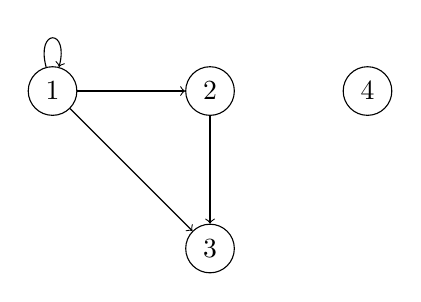
\begin{tikzpicture}[->,node distance=2cm]
  \node[draw,circle] (A) {$1$};
  \node[draw,circle] (B) [right of=A] {$2$};
  \node[draw,circle] (C) [below of=B] {$3$};
  \node[draw,circle] (D) [right of=B] {$4$};
  \draw (A) to [loop above]  (A);
  \draw (A) to  (B);
  \draw (A) to  (C);
  \draw (B) to  (C);
  \end{tikzpicture}
\intertext{இது $\tuple{V', E}$ என்ற கோட்டுருவிலிருந்து வேறுபட்டது;
  அங்கு $V' = \{1, 2, 3\}$. அந்தக் கோட்டுரு பின்வருமாறு தோன்றும்:}
& 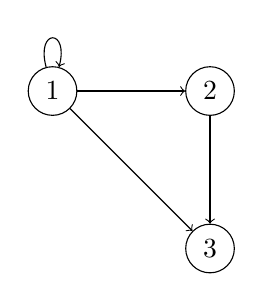
\begin{tikzpicture}[->,node distance=2cm]
  \node[draw,circle] (A) {$1$};
  \node[draw,circle] (B) [right of=A] {$2$};
  \node[draw,circle] (C) [below of=B] {$3$};
  \draw (A) to [loop above]  (A);
  \draw (A) to  (B);
  \draw (A) to  (C);
  \draw (B) to  (C);
  \end{tikzpicture}
\end{align*}
\end{ex}

% SEGMENT OLP-0017-S05
\begin{prob}
  $\{1, 2, 3, 4\}$ என்ற கணத்தின் மீதான, சிறியதாக அல்லது சமமாக இருக்கும்
  தொடர்பு $\le$ ஐ ஒரு கோட்டுருவாகக் கருதி அதற்குரிய படத்தை வரைக.
\end{prob}


% END SOURCE UNIT OLP-0017

\endgroup


\begingroup
\makeatletter
\def\ol@sectioncs{section}
\makeatother
\def\olfilename{trees}

% BEGIN SOURCE UNIT OLP-0018 content/sets-functions-relations/relations/trees.tex
% Exact modular target bytes: 13153; SHA256: 2bf2740542b0f6f4d8ba75adb46bb027d6effafcd5d10b2529e06b7efc8353a2
% SEGMENT OLP-0018-S01


\olfileid{sfr}{rel}{tre}
\olsection{மரவுருக்கள்}

தருக்கவியலின் அனைத்துப் பகுதிகளிலும் முக்கியப் பங்காற்றும் ஒரு குறிப்பிட்ட
வகைப் பகுதி வரிசை \emph{மரவுரு} ஆகும். தருக்கவியலின் தொடக்கநிலைப்
பகுதிகளிலேயே முடிவுறு மரவுருக்கள் வருகின்றன: எடுத்துக்காட்டாக,
!!{formula}s சிதைக்கப்பட்டு ஓர் இலக்கண அமைப்பு மரவுருவாக
அமைவதைக் கொண்டு அவற்றைப் புரிந்துகொள்ளலாம். அதேபோல, பல
!!{derivation} அமைப்புகளில் !!{derivation}s முடிவுறு மரவுருக்களின்
வடிவத்தைக் கொள்கின்றன.
%
கூற்றுத் தருக்கவியல், முதல்நிலைத் தருக்கவியல் ஆகியவற்றின் நிறைவுத்
தேற்றங்களின் நிறுவலிலேயே முடிவிலி மரவுருக்கள் தோன்றுகின்றன;
கணிதத் தருக்கவியல் முழுவதும் அவை பயன்படுகின்றன.

% SEGMENT OLP-0018-S02
கணக்கோட்பாட்டில் மரவுரு என்ற கருத்துக்கும், கோட்டுருக் கோட்பாட்டில் மரவுரு
என்ற கருத்துக்கும் நெருங்கிய தொடர்பு உள்ளது. ஒரு (முடிவுறு) மரவுருவின்
படம் இங்கே தரப்படுகிறது:

\begin{center}
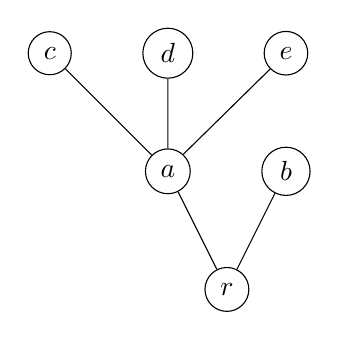
\begin{tikzpicture}[nodes={draw, circle}, -]
\node{$r$} [grow'=up]
    child { node {$a$}
        child { node {$c$} }
        child { node {$d$} }
        child { node {$e$} }
    }
    child { node {$b$} };
\end{tikzpicture}
\end{center}

மிகவும் கீழே உள்ள கணு $r$ தான் வேர். $r$ தவிர ஒவ்வொரு கணுவுக்கும்,
அதற்கு உடனே கீழே, சரியாக ஒரு பெற்றோர் கணு உள்ளது.
விளிம்புகளைப் பின்பற்றி மேல்நோக்கிச் செல்வதன் மூலம் $x$ இலிருந்து $y$ ஐ
அடைய முடியும்போது, கணு $x$ க்கும் கணு $y$ க்கும் இடையிலுள்ள தொடர்பை,
$x$ என்பது $y$ இன் \emph{முன்னோர்} என்பதாகக் கருதலாம்.

% SEGMENT OLP-0018-S03
ஒரு மரவுருவில் முன்னோர் தொடர்பு ஒரு கண்டிப்பான பகுதி வரிசையாகும்.
இது கணக்கோட்பாட்டு வரையறைக்குத் தூண்டுதலாக அமைகிறது. அந்த வரையறையைக்
கூற இரு கருத்துகள் தேவை. $\le$ மூலம் பகுதி வரிசைப்படுத்தப்பட்டுள்ள
$A$ என்ற கணத்தில் ஒரு \emph{மீச்சிறு உறுப்பு} என்பது, எல்லா
$y \in A$ க்கும் $x \le y$ என அமையும் !!a{element} $x \in A$ ஆகும்.
ஒரு கணத்தின் ஒவ்வொரு வெற்றற்ற உட்கணத்திற்கும் ஒரு மீச்சிறு உறுப்பு
இருந்தால், அக்கணம் $\le$ மூலம் \emph{நன்கு வரிசைப்படுத்தப்பட்டுள்ளது}
என்கிறோம்.

% SEGMENT OLP-0018-S04
\begin{defn}[மரவுரு]
ஒரு \emph{மரவுரு} என்பது $T = \tuple{A, \le}$ என்ற ஜோடி.
இங்கு $A$ ஒரு கணம்; $\le$ என்பது $A$ மீதான ஒரு பகுதி வரிசை.
அதற்கு (\emph{வேர்} எனப்படும்) ஒரே ஒரு மீச்சிறு உறுப்பு
$r \in A$ இருக்க வேண்டும்; மேலும் எல்லா $x \in A$ க்கும்
$\Setabs{y}{y \le x}$ என்ற கணம் $\le$ மூலம் நன்கு வரிசைப்படுத்தப்பட்டிருக்க
வேண்டும்.
\end{defn}

% SEGMENT OLP-0018-S05
\begin{defn}[அடுத்துறுப்புகள்]
$T = \tuple{A, \le}$ ஒரு மரவுரு எனக் கொள்வோம்.
$x,y \in A$, $x < y$ எனவும், $x < z < y$ என அமையும்
$z \in A$ எதுவும் இல்லை எனவும் இருந்தால், $y$ என்பது $x$ இன்
\emph{அடுத்துறுப்பு} என்கிறோம்.
\end{defn}

% SEGMENT OLP-0018-S06
$x \in A$ இன் அடுத்துறுப்புகள் அதன் \emph{பிள்ளைகள்} என்றும்
அழைக்கப்படுகின்றன. $y$ என்பது $x$ இன் அடுத்துறுப்பு எனில், $x$ ஐ
$y$ இன் \emph{முந்துறுப்பு} அல்லது \emph{பெற்றோர்} என்கிறோம்.

% SEGMENT OLP-0018-S07
\begin{prop}
$\tuple{A,\le}$ ஒரு மரவுரு எனில், வேர் தவிர ஒவ்வொரு $x \in A$ க்கும்
அதிகபட்சம் ஒரு முந்துறுப்பு மட்டுமே உள்ளது.
\end{prop}

% SEGMENT OLP-0018-S08
\begin{proof}
  $y_1 < x$, $y_2 < x$, $y_1 \neq y_2$ எனக் கொள்வோம். அப்போது
  $\{y_1, y_2\} \subseteq \Setabs{z}{z<x}$.
  $\Setabs{z}{z<x}$ என்பது $\le$ மூலம் நன்கு வரிசைப்படுத்தப்பட்டுள்ளதால்,
  அதன் உட்கணமான $\{y_1, y_2\}$ க்கு ஒரு மீச்சிறு உறுப்பு உள்ளது.
  அது $y_1$ அல்லது $y_2$ ஆகத்தான் இருக்க வேண்டும் என்பது தெளிவு.
  எனவே $y_1 \le y_2$ அல்லது $y_2 \le y_1$.
  $y_1 \neq y_2$ என அனுமானித்துள்ளதால், உண்மையில்
  $y_1 < y_2$ அல்லது $y_2 < y_1$.
  மேலும் $y_1 < x$, $y_2 < x$ என அனுமானித்துள்ளதால்,
  $y_1 < y_2 < x$ அல்லது $y_2 < y_1 < x$.
  எனவே $y_1$, $y_2$ ஆகிய இரண்டும் $x$ இன் முந்துறுப்புகளாக இருக்க முடியாது.
\end{proof}

% SEGMENT OLP-0018-S09
\begin{defn}
$T = \tuple{A, \le}$ என்ற மரவுருவில் $A$ ஒரு முடிவிலிக் கணமாக
இருந்தால் $T$ \emph{முடிவிலியானது} என்றும், இல்லாவிட்டால்
\emph{முடிவுறுவது} என்றும் கூறப்படுகிறது. $T$ இல் ஒவ்வொரு
$x \in A$ க்கும் முடிவுறு எண்ணிக்கையிலான அடுத்துறுப்புகள் மட்டுமே
இருந்தால், $T$ \emph{முடிவுறு கிளைப்புடையது} என்கிறோம்.
\end{defn}

% SEGMENT OLP-0018-S10
\begin{defn}[கிளைகள்]
$T = \tuple{A, \le}$ என்ற மரவுருவின் ஒரு \emph{கிளை} என்பது $T$
இல் மேலும் விரிவாக்க முடியாத ஒரு சங்கிலி. அதாவது அது
$B \subseteq A$ என்ற கணம்; எந்த $x, y \in B$ க்கும்
$x \le y$ அல்லது $y \le x$ இருக்க வேண்டும்; மேலும் எந்த
$z \in X \setminus B$ க்கும், $z \le u$, $u \le z$ ஆகிய இரண்டும்
இல்லாதவாறு ஒரு $u \in B$ இருக்க வேண்டும்.
%
$T$ இன் அனைத்துக் கிளைகளின் கணத்தைக் குறிக்க $[T]$ ஐப் பயன்படுத்துகிறோம்.
\end{defn}

% SEGMENT OLP-0018-S11
\begin{ex}
$0$, $1$ ஆகியவற்றின் முடிவுறு தொடர்முறைகளை, நீட்டிப்புத் தொடர்பு
$\sqsubseteq$ மூலம் வரிசைப்படுத்துவதால் கிடைக்கும்
\emph{முடிவிலி இரும மரவுரு}, முடிவுறு கிளைப்புடைய மரவுருவுக்கு
ஒரு வழக்கமான எடுத்துக்காட்டு. இது சில நேரங்களில் $\{0,1\}^*$ அல்லது
$\Bin^*$ எனக் குறிக்கப்படுகிறது (எ.கா., $101 \sqsubseteq 101101$).
எந்த இருமச் சரத்தையும் அதன் இறுதியில் ஒரு $0$ அல்லது ஒரு $1$ ஐச்
சேர்த்து நீட்டிக்க முடிவதால், இம்மரவுருவில் முடிவிலா உறுப்புகள் உள்ளன:
ஒவ்வொரு உறுப்பு $s$ க்கும் சரியாக இரண்டு அடுத்துறுப்புகள் உள்ளன;
அவை $s0$, $s1$. இதன் வேர் வெற்றுத் தொடர்முறை $\emptyseq$ ஆகும்.
\end{ex}

% SEGMENT OLP-0018-S12
\begin{ex}
சற்றுப் பொதுவாக, இயல் எண்களின் முடிவுறு தொடர்முறைகளின் கணமான
$\Nat^*$, நீட்டிப்புத் தொடர்பு $\sqsubseteq$ உடன் சேர்ந்து ஒரு
மரவுருவாகிறது. இது முடிவுறு கிளைப்புடையதல்ல என்பது தெளிவு:
ஒவ்வொரு $s \in \Nat^*$ க்கும் முடிவிலா அடுத்துறுப்புகள் $sn$ உள்ளன;
ஒவ்வொரு $n \in \Nat$ க்கும் ஒன்று உள்ளது.
$\sqsubseteq$ இன் கீழ் அடைவு கொண்ட ஒவ்வொரு $A
\subseteq \Nat^*$ உம் $\Nat^*$ இன் ஒரு \emph{உள்மரவுரு}.
(அதாவது $s \in A$, $s' \sqsubseteq s$ எனில் $s' \in A$
என்பதும் உண்மையாகும் வகையில் $A$ அமைகிறது.)
அனைத்து முடிவுறு மரவுருக்களையும் $\Nat^*$ இன் முடிவுறு உள்மரவுருக்களாகக்
குறிக்கலாம்.
\end{ex}

% SEGMENT OLP-0018-S13
\begin{prop}[K\H{o}nig இன் துணைத்தேற்றம்]
$T = \tuple{A,\le}$ ஒரு முடிவுறு கிளைப்புடைய முடிவிலி மரவுரு எனில்,
$T$ க்கு ஒரு முடிவிலிக் கிளை உள்ளது.
\end{prop}

% SEGMENT OLP-0018-S14
கணிப்புத்தன்மைக் கோட்பாட்டில் பரவலாகப் பயன்படும் K\H{o}nig இன்
துணைத்தேற்றத்தின் ஒரு சிறப்பு நிலை,
\emph{வலுக்குறைந்த K\H{o}nig துணைத்தேற்றம்} என அறியப்படுகிறது.
அது பின்வருமாறு: $\{0,1\}^*$ இன் எந்த முடிவிலி உள்மரவுருவுக்கும்
ஒரு முடிவிலிக் கிளை உள்ளது.


% END SOURCE UNIT OLP-0018

\endgroup


\begingroup
\makeatletter
\def\ol@sectioncs{section}
\makeatother
\def\olfilename{operations}

% BEGIN SOURCE UNIT OLP-0019 content/sets-functions-relations/relations/operations.tex
% Exact modular target bytes: 4939; SHA256: c147683a6c2ec8c795c3b53f00312eb448a2e9fa8e3d965d48ce013f1951a22f
% SEGMENT OLP-0019-S01


\olfileid{sfr}{rel}{ops}
\olsection{தொடர்புகள் மீதான செயல்கள்}

தொடர்புகளை மாற்றுவதோ ஒன்றிணைப்பதோ பல நேரங்களில் பயனுள்ளதாக இருக்கிறது.
\olref[sfr][rel][ord]{prop:stricttopartial} இல் தொடர்புகளின்
\emph{சேர்ப்பை} நாம் கருதினோம். இரு தொடர்புகளை ஜோடிகளின் கணங்களாகக்
கருதி எடுக்கும் சேர்ப்பே அது. அதேபோல,
\olref[sfr][rel][ord]{prop:partialtostrict} இல் தொடர்புகளின் சார்பு
வேறுபாட்டைக் கருதினோம். தொடர்புகள் மீது செய்யக்கூடிய வேறு சில செயல்கள்
இங்கே தரப்படுகின்றன.

% SEGMENT OLP-0019-S02
\begin{defn}\ollabel{relationoperations}
$R$, $S$ ஆகியவை தொடர்புகளாகவும், $A$ ஏதேனும் ஒரு கணமாகவும் இருக்கட்டும்.

$R$ இன் \emph{தலைகீழ்த் தொடர்பு}
$R^{-1} = \Setabs{\tuple{y, x}}{\tuple{x,
    y} \in R}$ ஆகும்.

$R$, $S$ ஆகியவற்றின் \emph{சார்புப் பெருக்கம்}
$(R \mid S) =
\{\tuple{x, z} : \exists y(Rxy \land Syz)\}$ ஆகும்.

$R$ ஐ $A$ க்குக் \emph{கட்டுப்படுத்துவது}
$\funrestrictionto{R}{A}= R
\cap A^2$ ஆகும்.

$R$ ஐ $A$ மீது \emph{செயல்படுத்துவதால்} கிடைப்பது
$\funimage{R}{A} = \{y :
(\exists x \in A)Rxy\}$ ஆகும்.
\end{defn}

% SEGMENT OLP-0019-S03
\begin{ex}
$S \subseteq \Int^2$ என்பது $\Int$ மீதான அடுத்துறுப்புத் தொடர்பாக
இருக்கட்டும். அதாவது
$S = \Setabs{\tuple{x, y} \in \Int^2}{x + 1 = y}$; எனவே
$x + 1 = y$ ஆக இருக்கும்போது, அப்போதும் அப்போது மட்டுமே, $Sxy$.

$S^{-1}$ என்பது $\Int$ மீதான முந்துறுப்புத் தொடர்பு; அதாவது
$\Setabs{\tuple{x,y}\in\Int^2}{x -1 =y}$.

$S\mid S$ என்பது
$ \Setabs{\tuple{x,y}\in\Int^2}{x + 2 =y}$.

$\funrestrictionto{S}{\Nat}$ என்பது $\Nat$ மீதான அடுத்துறுப்புத் தொடர்பு.

$\funimage{S}{\{1,2,3\}}$ என்பது $\{2, 3, 4\}$.
\end{ex}

% SEGMENT OLP-0019-S04
\begin{defn}[கடப்பு அடைவு]
$R \subseteq A^2$ ஒரு இருமத் தொடர்பாக இருக்கட்டும்.

$R$ இன் \emph{கடப்பு அடைவு}
$R^+ = \bigcup_{0 < n \in
\Nat} R^n$ ஆகும். இங்கு $R^1 = R$, $R^{n+1} = R^n
\mid R$ என்று மறுநிகழ்வு முறையில் வரையறுக்கிறோம்.

$R$ இன் \emph{தற்சுட்டுக் கடப்பு அடைவு}
$R^* = R^+ \cup
\Id{A}$ ஆகும்.
\end{defn}

% SEGMENT OLP-0019-S05
\begin{ex}
அடுத்துறுப்புத் தொடர்பு $S \subseteq \Int^2$ ஐ எடுத்துக்கொள்வோம்.
$x + 2 =
y$ ஆக இருக்கும்போது, அப்போதும் அப்போது மட்டுமே, $S^2xy$;
$x + 3 = y$ ஆக இருக்கும்போது, அப்போதும் அப்போது மட்டுமே, $S^3xy$;
இவ்வாறே தொடரும். எனவே ஏதேனும் $n \geq 1$ க்கு $x + n = y$ ஆக
இருக்கும்போது, அப்போதும் அப்போது மட்டுமே, $S^+xy$.
வேறு சொற்களில், $x < y$ ஆக இருக்கும்போது, அப்போதும் அப்போது மட்டுமே,
$S^+xy$; மேலும் $x \le
y$ ஆக இருக்கும்போது, அப்போதும் அப்போது மட்டுமே, $S^*xy$.
\end{ex}

% SEGMENT OLP-0019-S06
\begin{prob}
$R$ இன் கடப்பு அடைவு உண்மையிலேயே கடப்புப் பண்பைக் கொண்டுள்ளது எனக் காட்டுக.
\end{prob}


% END SOURCE UNIT OLP-0019

\endgroup


\OLEndChapterHook


% END SOURCE UNIT OLP-0011

\endgroup


\begingroup
\makeatletter
\def\ol@sectioncs{section}
\makeatother
\def\olfilename{functions}

% BEGIN SOURCE UNIT OLP-0020 content/sets-functions-relations/functions/functions.tex
% Exact modular target bytes: 440; SHA256: f7a7ba39e713d59e2eb993cabf6e61e8efa6d5bfaf3b9b534f2a695d06385e42
% SEGMENT OLP-0020-S01


\olchapter{sfr}{fun}{சார்புகள்}

\begingroup
\makeatletter
\def\ol@sectioncs{section}
\makeatother
\def\olfilename{function-basics}

% BEGIN SOURCE UNIT OLP-0021 content/sets-functions-relations/functions/function-basics.tex
% Exact modular target bytes: 14024; SHA256: aad1c03fd6159f409eed2606538c8537fe181829c0cd8d56a4d20ab5a9f3a2e3
% SEGMENT OLP-0021-S01


\olfileid{sfr}{fun}{bas}
\olsection{அடிப்படைகள்}

\begin{explain}
ஒரு \emph{சார்பு} என்பது, கொடுக்கப்பட்ட ஒரு கணத்தின் ஒவ்வொரு
!!{element}[acc]யும், கொடுக்கப்பட்ட ஏதோ ஒரு (வேறு) கணத்தின் குறிப்பிட்ட
!!{element} ஒன்றுடன் இணைக்கும் ஒரு இணைப்பு. எடுத்துக்காட்டாக,
$1$ ஐக் கூட்டும் செயல் ஒரு சார்பை வரையறுக்கிறது: ஒவ்வொரு எண் $n$ உம்
ஒரே ஒரு எண் $n+1$ உடன் இணைக்கப்படுகிறது.

இன்னும் பொதுவாக, சார்புகள் ஜோடிகள், மூன்று-தொகுதிகள் முதலியவற்றை
உள்ளீடுகளாகப் பெற்று ஏதோ ஒரு வகையான வெளியீட்டைத் தரலாம்.
அடிப்படை எண்கணிதத்திலிருந்து பல சார்புகளை நாம் அறிவோம்.
எடுத்துக்காட்டாக, கூட்டலும் பெருக்கலும் சார்புகளே. அவை இரண்டு எண்களைப்
பெற்று மூன்றாவது ஓர் எண்ணைத் தருகின்றன.

இந்த அருவமான கணிதப் பொருளில், ஒரு சார்பு ஒரு \emph{கருப்புப் பெட்டி}:
எந்த உள்ளீட்டுடன் எந்த வெளியீடு இணைக்கப்படுகிறது என்பதே முக்கியம்;
வெளியீட்டைக் கணக்கிடும் முறை முக்கியமல்ல.
\end{explain}

% SEGMENT OLP-0021-S02
\begin{defn}[சார்பு]
ஒரு \emph{சார்பு} $f \colon A \to B$ என்பது $A$ இன் ஒவ்வொரு
!!{element}[acc]யும் $B$ இன் ஓர் !!{element} உடன் இணைக்கும் இணைப்பாகும்.

$A$ ஐ $f$ இன் \emph{சார்பகம்} என்றும், $B$ ஐ $f$ இன்
\emph{துணைச்சார்பகம்} என்றும் அழைக்கிறோம்.
$A$ இன் !!{element}s, $f$ இன் உள்ளீடுகள் அல்லது
\emph{உள்ளீட்டுறுப்புகள்} எனப்படும். ஓர் உள்ளீட்டுறுப்பு $x$ உடன்
$f$ இணைக்கும் $B$ இன் !!{element}, உள்ளீட்டுறுப்பு $x$ க்கான
\emph{$f$ இன் மதிப்பு} எனப்படும்; அது $f(x)$ என எழுதப்படுகிறது.

$f$ இன் \emph{வீச்சகம்} $\ran{f}$ என்பது, ஏதாவது ஓர்
உள்ளீட்டுறுப்புக்கான $f$ இன் மதிப்புகளைக் கொண்ட துணைச்சார்பகத்தின்
உட்கணமாகும்; $\ran{f} =
\Setabs{f(x)}{x \in A}$.
\end{defn}

% SEGMENT OLP-0021-S03
\olref{fig:function} இல் உள்ள படம் சார்புகளைப் பற்றிச் சிந்திக்க உதவலாம்.
இடப்புற நீள்வட்டம் சார்பின் \emph{சார்பகத்தைக்} குறிக்கிறது;
வலப்புற நீள்வட்டம் அதன் \emph{துணைச்சார்பகத்தைக்} குறிக்கிறது.
சார்பகத்தில் உள்ள ஓர் \emph{உள்ளீட்டுறுப்பிலிருந்து}, துணைச்சார்பகத்தில்
அதற்குரிய \emph{மதிப்பை} நோக்கி ஓர் அம்பு செல்கிறது.

\begin{figure}
  \olasset{assets/diagrams/function.tikz}
  \caption{ஒரு சார்பு என்பது ஒரு கணத்தின் ஒவ்வொரு !!{element}[acc]யும்
    மற்றொரு கணத்தின் !!a{element} உடன் இணைக்கும் இணைப்பாகும்.
    சார்பகத்தில் உள்ள ஓர் உள்ளீட்டுறுப்பிலிருந்து, துணைச்சார்பகத்தில்
    அதற்குரிய மதிப்பை நோக்கி ஓர் அம்பு செல்கிறது.}
  \ollabel{fig:function}
\end{figure}

% SEGMENT OLP-0021-S04
\begin{ex}
பெருக்கல் இயல் எண்களின் ஜோடிகளை உள்ளீடுகளாகப் பெற்று, இயல் எண்களை
வெளியீடுகளாகத் தருகிறது. எனவே அது $\Nat \times \Nat$ என்ற சார்பகத்திலிருந்து
$\Nat$ என்ற துணைச்சார்பகத்திற்குச் செல்கிறது.
வீச்சகமும் $\Nat$ ஆகவே அமைகிறது. ஏனெனில் ஒவ்வொரு $n \in \Nat$ உம்
$n \times 1$ ஆகும்.
\end{ex}

% SEGMENT OLP-0021-S05
\begin{ex}
பெருக்கல் ஒவ்வொரு உள்ளீட்டையும், அதாவது இயல் எண்களின் ஒவ்வொரு ஜோடியையும்,
ஒரே ஒரு வெளியீட்டுடன் இணைப்பதால் அது ஒரு சார்பு:
$\times \colon \Nat^2 \to
\Nat$. ஆனால் ஓர் இயல் எண் $n$ ஐ, $x^2 = n$ என அமையும் மெய்யெண்
$x$ உடன் இணைப்பது சார்பாக அமையாது. ஏனெனில் ஒவ்வொரு நேர்ம முழு $n$ க்கும்
இரண்டு வர்க்க மூலங்கள் உள்ளன: $\sqrt{n}$, $-\sqrt{n}$.
எதிர்மமற்ற முதன்மை வர்க்க மூலத்தை மட்டும் திருப்பித் தருவதன் மூலம் இதைச் சார்பாக
மாற்றலாம்: $\sqrt{\phantom{X}} \colon
\Nat \to \Real$.
\end{ex}

% SEGMENT OLP-0021-S06
\begin{ex}
ஒரு வகுப்பிலுள்ள ஒவ்வொரு மாணவரையும் அவருடைய இறுதி மதிப்பெண்ணுடன்
இணைக்கும் தொடர்பு ஒரு சார்பாகும். ஒரே வகுப்பில் எந்த மாணவருக்கும்
இரண்டு வெவ்வேறு இறுதி மதிப்பெண்கள் கிடைக்க முடியாது.
ஒரு வகுப்பிலுள்ள ஒவ்வொரு மாணவரையும் அவருடைய பெற்றோருடன் இணைக்கும்
தொடர்பு சார்பல்ல: மாணவர்களுக்குப் பெற்றோர் இல்லாமலும் இருக்கலாம்;
இருவர் அல்லது அதற்கு மேற்பட்டவர்கள் இருக்கலாம்.
\end{ex}

% SEGMENT OLP-0021-S07
\begin{explain}
சாத்தியமான ஒவ்வொரு உள்ளீட்டுறுப்புக்கும் சார்பின் மதிப்பு என்ன என்பதை
ஏதாவது ஒரு துல்லியமான முறையில் குறிப்பிடுவதன் மூலம் சார்புகளை
வரையறுக்கலாம். ஒரு வாய்பாட்டைத் தருவது, மதிப்பைக் கணக்கிடும் முறையை
விவரிப்பது, அல்லது ஒவ்வொரு உள்ளீட்டுறுப்புக்கும் உரிய மதிப்பைப்
பட்டியலிடுவது ஆகியவை இதற்கான வெவ்வேறு வழிகள். எந்த முறையில் சார்பை
வரையறுத்தாலும், ஒவ்வொரு உள்ளீட்டுறுப்புக்கும் ஒரே ஒரு மதிப்பை மட்டுமே
குறிப்பிடுகிறோம் என்பதை உறுதிசெய்ய வேண்டும்.
\end{explain}

% SEGMENT OLP-0021-S08
\begin{ex}
$f \colon \Nat \to \Nat$ என்பதை $f(x) = x+1$ என வரையறுப்போம்.
இந்த வரையறை $f$ ஐ, இயல் எண்களை உள்ளீடுகளாகப் பெற்று இயல் எண்களை
வெளியீடுகளாகத் தரும் சார்பாகக் குறிப்பிடுகிறது.
ஓர் இயல் எண் $x$ தரப்பட்டால், $f$ அதன் தொடரி $x+1$ ஐ வெளியீடாகத்
தரும் என இது கூறுகிறது. இங்கு துணைச்சார்பகம் $\Nat$ என்பது $f$ இன்
வீச்சகம் அல்ல. ஏனெனில் இயல் எண் $0$ எந்த இயல் எண்ணின் தொடரியும் அல்ல.
$f$ இன் வீச்சகம் அனைத்து நேர்ம முழுக்களின் கணமான $\Int^{+}$ ஆகும்.
\end{ex}

% SEGMENT OLP-0021-S09
\begin{ex}\ollabel{examplefunext}
$g \colon \Nat \to \Nat$ என்பதை $g(x) = x+2-1$ என வரையறுப்போம்.
$g$ இயல் எண்களை உள்ளீடுகளாகப் பெற்று இயல் எண்களை வெளியீடுகளாகத் தரும்
சார்பு என இது கூறுகிறது. ஓர் இயல் எண் உள்ளீடாகத் தரப்பட்டால், $g$ என்பது
$x$ இன் தொடரியின் தொடரிக்கு உரிய முன்னியை, அதாவது $x+1$ ஐ,
வெளியீடாகத் தரும்.
\end{ex}

% SEGMENT OLP-0021-S10
\begin{explain}
வெவ்வேறு \emph{வரையறைகளைக்} கொண்ட $f$, $g$ என்ற இரு சார்புகளைக்
கருதினோம். எனினும் இவை \emph{ஒரே சார்புதான்}.
ஏனெனில் எந்த இயல் எண் $n$ க்கும் $f(n) = n+1 = n+2-1 =
g(n)$. வேறு சொற்களில், $f$, $g$ ஆகியவற்றுக்கான நமது வரையறைகள்
வெவ்வேறு சமன்பாடுகளின் மூலம் ஒரே இணைப்பைக் குறிப்பிடுகின்றன.
எனவே சார்புகளுக்கான மதிப்புசார் சமத்துவக் கொள்கையை மறைமுகமாகப்
பயன்படுத்துகிறோம்:
\[
  \forall x\, f(x) = g(x)\text{ எனில் }f = g
\]
இங்கு $f$, $g$ ஆகியவற்றுக்கு ஒரே சார்பகமும் ஒரே துணைச்சார்பகமும்
இருக்க வேண்டும்.
\end{explain}

% SEGMENT OLP-0021-S11
\begin{ex}
நிலைகளைப் பிரித்தும் சார்புகளை வரையறுக்கலாம். எடுத்துக்காட்டாக,
$h \colon \Nat \to \Nat$ என்பதைப் பின்வருமாறு வரையறுக்கலாம்:
\[
h(x) =
\begin{cases}
  \frac{x}{2} & \text{$x$ இரட்டை எனில்} \\
  \frac{x+1}{2} & \text{$x$ ஒற்றை எனில்.}
\end{cases}
\]
ஒவ்வொரு இயல் எண்ணும் இரட்டையாகவோ ஒற்றையாகவோ இருப்பதால், இந்தச்
சார்பின் வெளியீடு எப்போதும் ஓர் இயல் எண்ணாக இருக்கும்.
நிலைகளைப் பிரித்து ஒரு சார்பை வரையறுக்கும்போது, சாத்தியமான ஒவ்வொரு
உள்ளீடும் சரியாக ஒரு நிலையில் இடம்பெற வேண்டும் என்பதை நினைவில் கொள்க.
சில சமயங்களில், நிலைகள் அனைத்துச் சாத்தியங்களையும் உள்ளடக்குகின்றன
என்பதையும் ஒன்றுக்கொன்று விலக்கானவை என்பதையும் நிறுவ வேண்டியிருக்கும்.
\end{ex}


% END SOURCE UNIT OLP-0021

\endgroup


\begingroup
\makeatletter
\def\ol@sectioncs{section}
\makeatother
\def\olfilename{function-kinds}

% BEGIN SOURCE UNIT OLP-0022 content/sets-functions-relations/functions/function-kinds.tex
% Exact modular target bytes: 9084; SHA256: 8a495041a746bd59b05a33903966e9a091e19fb9ffcb76b540ff2dadbcc1dcbc
% SEGMENT OLP-0022-S01


\olfileid{sfr}{fun}{kin}
\olsection{சார்புகளின் வகைகள்}

\begin{explain}
நாம் அடிக்கடி காணும் சில வகைச் சார்புகளுக்கு ஒரு வகைப்பாட்டை
அறிமுகப்படுத்துவது பயனுள்ளதாக இருக்கும்.

முதலில், துணைச்சார்பகத்தின் ஒவ்வோர் உறுப்பும் சார்பின் ஒரு மதிப்பாக
அமையும் பண்பைக் கொண்ட சார்புகளைக் கருதலாம். இத்தகைய சார்புகள்
!!{surjective} சார்புகள் எனப்படும். அவற்றை \olref{fig:surjective}
இல் உள்ளதுபோலப் படமாகக் காட்டலாம்.

\begin{figure}
  \olasset{assets/diagrams/surjective.tikz}
  \caption{!!^a{surjective} சார்பு, துணைச்சார்பகத்தின் ஒவ்வொரு
    !!{element}[acc]யும் ஒரு மதிப்பாகக் கொண்டிருக்கும்.}
  \ollabel{fig:surjective}
\end{figure}
\end{explain}

% SEGMENT OLP-0022-S02
\begin{defn}[!!^{surjective} சார்பு]
$f \colon A \rightarrow B$ என்ற சார்புக்கு, $f$ இன் வீச்சகமும் $B$ ஆக
இருக்கும்போது, அப்போதும் அப்போது மட்டுமே, அது
\emph{!!{surjective}} பண்புடையது எனப்படும்.
அதாவது, ஒவ்வொரு $y \in B$ க்கும் $f(x) = y$ என அமையும் குறைந்தது
ஓர் $x \in A$ இருக்க வேண்டும். குறியீடுகளில்:
\[
  (\forall y \in B)(\exists x \in A)f(x) = y.
\]
இத்தகைய சார்பை $A$ இலிருந்து $B$ க்குச் செல்லும்
!!a{surjection} என்கிறோம்.
\end{defn}

% SEGMENT OLP-0022-S03
\begin{explain}
$f$ என்பது !!a{surjection} எனக் காட்ட வேண்டுமெனில், $f$ இன்
துணைச்சார்பகத்தில் உள்ள ஒவ்வொரு பொருளும் ஏதாவது ஓர் உள்ளீடு $x$ க்கான
$f(x)$ இன் மதிப்பாக அமைகிறது எனக் காட்ட வேண்டும்.

எந்தச் சார்பும் !!a{surjection} ஐ \emph{உருவாக்குகிறது} என்பதைக்
கவனிக்கவும். ஏனெனில் $f \colon A \to B$ என்ற சார்பு தரப்பட்டால்,
$f' \colon A \to \ran{f}$ என்பதை $f'(x) = f(x)$ என வரையறுப்போம்.
$\ran{f}$ என்பது $\Setabs{f(x) \in B}{x \in A}$ எனவே
\emph{வரையறுக்கப்பட்டுள்ளதால்}, இந்தச் சார்பு $f'$ நிச்சயமாக
!!a{surjection} ஆகும்.
\end{explain}

% SEGMENT OLP-0022-S04
\begin{explain}
எந்தச் சார்பும் சாத்தியமான ஒவ்வொரு உள்ளீட்டையும் ஒரே ஒரு வெளியீட்டுடன்
இணைக்கிறது. ஆனால் வெவ்வேறு உள்ளீடுகளை ஒரே வெளியீட்டுடன் ஒருபோதும்
இணைக்காத சார்புகளும் உள்ளன. அவை !!{injective} சார்புகள் எனப்படும்.
அவற்றை \olref{fig:injective} இல் உள்ளதுபோலப் படமாகக் காட்டலாம்.
\begin{figure}
  \olasset{assets/diagrams/injective.tikz}
  \caption{!!^a{injective} சார்பு இரண்டு வெவ்வேறு உள்ளீட்டுறுப்புகளை
    ஒரே மதிப்புடன் ஒருபோதும் இணைக்காது.}
  \ollabel{fig:injective}
\end{figure}
\end{explain}

% SEGMENT OLP-0022-S05
\begin{defn}[!!^{injective} சார்பு]
ஒவ்வொரு $y \in B$ க்கும், $f(x) = y$ என அமையும் $x \in A$
அதிகபட்சம் ஒன்று மட்டுமே இருக்கும்போது, அப்போதும் அப்போது மட்டுமே,
$f \colon A \rightarrow B$ என்ற சார்பு \emph{!!{injective}}
பண்புடையது எனப்படும். இத்தகைய சார்பை $A$ இலிருந்து $B$ க்குச்
செல்லும் !!a{injection} என்கிறோம்.
\end{defn}

% SEGMENT OLP-0022-S06
\begin{explain}
$f$ என்பது !!a{injection} எனக் காட்ட வேண்டுமெனில், $f$ இன்
சார்பகத்தைச் சேர்ந்த எந்த !!{element}s ஆன $x$, $y$ க்கும்,
$f(x)=f(y)$ எனில் $x=y$ எனக் காட்ட வேண்டும்.
\end{explain}

% SEGMENT OLP-0022-S07
\begin{ex}
$f(x) = 1$ எனக் கொடுக்கப்படும் மாறிலிச் சார்பு
$f\colon \Nat \to \Nat$ என்பது !!{injective} பண்பையும்
!!{surjective} பண்பையும் கொண்டிருக்கவில்லை.

$f(x) = x$ எனக் கொடுக்கப்படும் ஒன்றாதல் சார்பு
$f\colon \Nat \to \Nat$ என்பது !!{injective} பண்பையும்
!!{surjective} பண்பையும் கொண்டுள்ளது.

$f(x) = x+1$ எனக் கொடுக்கப்படும் தொடரிச் சார்பு
$f \colon \Nat \to \Nat$ என்பது !!{injective} பண்புடையது;
ஆனால் !!{surjective} பண்புடையதல்ல.

பின்வருமாறு வரையறுக்கப்படும் $f \colon \Nat \to \Nat$ என்ற சார்பு:
\[
  f(x) =
  \begin{cases}
    \frac{x}{2} & \text{$x$ இரட்டை எனில்} \\
    \frac{x+1}{2} & \text{$x$ ஒற்றை எனில்.}
  \end{cases}
\]
!!{surjective} பண்புடையது; ஆனால் !!{injective} பண்புடையதல்ல.
\end{ex}

% SEGMENT OLP-0022-S08
\begin{explain}
பல நேரங்களில் !!{injective}, !!{surjective} ஆகிய இரண்டு
பண்புகளையும் கொண்ட சார்புகளைக் கருத விரும்புகிறோம்.
இத்தகைய சார்புகளை !!{bijective} சார்புகள் என்கிறோம்.
அவை \olref{fig:bijective} இல் காட்டப்பட்டுள்ள சார்பைப் போலிருக்கும்.
!!^{bijection}s சில சமயங்களில் \emph{ஒன்றுக்கொன்று ஒத்திசைவுகள்}
என்றும் அழைக்கப்படுகின்றன. ஏனெனில் அவை துணைச்சார்பகத்தின் உறுப்புகளைச்
சார்பகத்தின் உறுப்புகளுடன் தனித்தனியாக இணைக்கின்றன.
\begin{figure}
  \olasset{assets/diagrams/bijective.tikz}
  \caption{!!^a{bijective} சார்பு துணைச்சார்பகத்தின் உறுப்புகளைச்
    சார்பகத்தின் உறுப்புகளுடன் தனித்தனியாக இணைக்கிறது.}
  \ollabel{fig:bijective}
\end{figure}
\end{explain}

% SEGMENT OLP-0022-S09
\begin{defn}[!!^{bijection}]
$f \colon A \to B$ என்ற சார்பு !!{surjective}, !!{injective}
ஆகிய இரு பண்புகளையும் கொண்டிருக்கும்போது, அப்போதும் அப்போது மட்டுமே,
அது \emph{!!{bijective}} பண்புடையது எனப்படும்.
இத்தகைய சார்பை $A$ இலிருந்து $B$ க்குச் செல்லும் (அல்லது $A$,
$B$ ஆகியவற்றுக்கு இடையிலுள்ள) !!a{bijection} என்கிறோம்.
\end{defn}


% END SOURCE UNIT OLP-0022

\endgroup


\begingroup
\makeatletter
\def\ol@sectioncs{section}
\makeatother
\def\olfilename{functions-relations}

% BEGIN SOURCE UNIT OLP-0023 content/sets-functions-relations/functions/functions-relations.tex
% Exact modular target bytes: 9828; SHA256: 543cc3836a812964e07c6280a0a77b3d0d59128a5ed7c06d2821b5153995d870
% SEGMENT OLP-0023-S01


\olfileid{sfr}{fun}{rel}

\olsection{தொடர்புகளாகச் சார்புகள்}

\begin{explain}
$A$ இன் !!{element}s[acc] $B$ இன் !!{element}s உடன் இணைக்கும் ஒரு சார்பு,
$A$, $B$ ஆகியவற்றுக்கு இடையில் ஒரு தொடர்பை வரையறுக்கிறது என்பது தெளிவு.
$f(x) = y$ ஆக இருக்கும்போது, அப்போதும் அப்போது மட்டுமே, $x$, $y$
ஆகியவற்றுக்கு இடையில் அமையும் தொடர்பே அது.
உண்மையில், எடுத்துக்காட்டாகக் கணிதத்தின் அடிப்படைக் கூறுகளின் வகைகளைக்
குறைக்க விரும்பினால், சார்பு $f$ ஐ இந்தத் தொடர்புடன், அதாவது ஜோடிகளின்
ஒரு கணத்துடன், \emph{ஒன்றாகக் கருதவும்} முடியும்.
இதனால் ஒரு கேள்வி எழுகிறது: எந்தத் தொடர்புகள் இவ்விதமாகச் சார்புகளை
வரையறுக்கின்றன?
\end{explain}

% SEGMENT OLP-0023-S02
\begin{defn}[சார்பின் கோட்டுரு]
$f\colon A \to B$ ஒரு சார்பாக இருக்கட்டும்.
$f$ இன் \emph{கோட்டுரு} என்பது பின்வருமாறு வரையறுக்கப்படும்
$R_f \subseteq A \times B$ என்ற தொடர்பாகும்:
\[
R_f = \Setabs{\tuple{x,y}}{f(x) = y}.
\]
\end{defn}

% SEGMENT OLP-0023-S03
\begin{explain}
உறுப்புசார் சமத்துவத்தின்படி, ஒரு சார்பின் கோட்டுரு தனித்ததாக
நிர்ணயிக்கப்படுகிறது. மேலும், கணங்களுக்கான உறுப்புசார் சமத்துவம்,
சார்புகளுக்கான மறைமுக மதிப்புசார் சமத்துவக் கொள்கையை உடனடியாக
நியாயப்படுத்துகிறது: $f$, $g$ ஆகியவற்றுக்கு ஒரே சார்பகமும்
துணைச்சார்பகமும் இருந்தால், எல்லா மதிப்புகளிலும் அவை ஒத்திருக்கும்போது
அவை ஒரே சார்பாகும்.

அதேபோல, ஒரு தொடர்பு “சார்பாக அமையும்” தன்மையைக் கொண்டிருந்தால்,
அது ஒரு சார்பின் கோட்டுருவாகும்.
\end{explain}

% SEGMENT OLP-0023-S04
\begin{prop}\ollabel{prop:graph-function}
$R \subseteq A \times B$ பின்வரும் நிபந்தனைகளை நிறைவேற்றுவதாக இருக்கட்டும்:
\begin{enumerate}
\item $Rxy$, $Rxz$ எனில் $y = z$; மேலும்
\item ஒவ்வொரு $x \in A$ க்கும், $\tuple{x,
y} \in R$ என அமையும் ஏதாவது ஓர் $y \in B$ உள்ளது.
\end{enumerate}
அப்போது $R$ என்பது, $Rxy$ ஆக இருக்கும்போது அப்போதும் அப்போது மட்டுமே
$f(x) = y$ என வரையறுக்கப்படும் $f\colon A \to B$ என்ற சார்பின் கோட்டுருவாகும்.
\end{prop}

% SEGMENT OLP-0023-S05
\begin{proof}
$Rxy$ என அமையும் ஒரு $y$ இருப்பதாகக் கொள்வோம்.
$Rxz$ என அமையும் வேறொரு $z \neq
y$ இருந்தால், $R$ மீதான நிபந்தனை மீறப்படும்.
எனவே $Rxy$ என அமையும் ஒரு $y$ இருந்தால், இந்த $y$ தனித்ததாகும்;
ஆகவே $f$ தெளிவாக வரையறுக்கப்பட்டுள்ளது. $R_f = R$ என்பது தெளிவு.
\end{proof}

% SEGMENT OLP-0023-S06
\begin{explain}
ஒவ்வொரு சார்பு $f\colon A \to B$ க்கும் ஒரு கோட்டுரு உள்ளது.
அதாவது, $f(x) = y$ என்பதால் வரையறுக்கப்படும்,
$A \times B$ இல் அடங்கிய ஒரு தொடர்பு உள்ளது.
மறுபுறம், \olref{prop:graph-function} இல் கொடுக்கப்பட்ட பண்புகளைக்
கொண்ட ஒவ்வொரு தொடர்பு $R
\subseteq A \times B$ உம் ஒரு சார்பு $f \colon A \to
B$ இன் கோட்டுருவாகும்.
சார்புகளுக்கும் அவற்றின் கோட்டுருக்களுக்கும் உள்ள இந்த நெருங்கிய
தொடர்பால், ஒரு சார்பை அதன் கோட்டுருவாகவே கருதலாம்.
வேறு சொற்களில், சார்புகளைச் சில குறிப்பிட்ட தொடர்புகளுடன், அதாவது
வரிசைத் தொகுதிகளின் சில குறிப்பிட்ட கணங்களுடன், ஒன்றாகக் கருதலாம்.
\oliflabeldef{sfr:rel:ref:sec}{ஆனால் இந்த “ஒன்றாகக் கருதுதல்” என்பதன்
நோக்கம் \olref[sfr][rel][ref]{sec} இல் உள்ளதைப் போன்றதே என்பதைக்
கவனிக்கவும். இது சார்புகளின் மெய்ப்பொருளியல் பற்றிய கூற்று அல்ல;
சார்புகளைச் சில கணங்களாகக் \emph{கருதுவது} வசதியாக உள்ளது என்ற
கருத்தே ஆகும். இதன் வசதிக்கான ஒரு காரணத்தை இப்போது காணலாம்.}{}
தொடர்புகள் மீது செய்த செயல்களைப் போன்ற செயல்களைச் சார்புகள் மீதும்
செய்வதைக் கருதலாம் (\olref[sfr][rel][ops]{sec} ஐக் காண்க).
குறிப்பாக:
\end{explain}

% SEGMENT OLP-0023-S07
\begin{defn}\ollabel{defn:funimage}
$f \colon A \to B$ ஒரு சார்பாகவும் $C\subseteq A$ ஆகவும் இருக்கட்டும்.

$f$ ஐ $C$ க்குக் \emph{கட்டுப்படுத்துவதால்} கிடைப்பது,
அனைத்து $x \in C$ க்கும் $(\funrestrictionto{f}{C})(x) = f(x)$
என வரையறுக்கப்படும் $\funrestrictionto{f}{C}\colon C \to B$
என்ற சார்பாகும். வேறு சொற்களில்,
$\funrestrictionto{f}{C} = \Setabs{\tuple{x, y} \in R_f}{x \in
C}$.

$f$ ஐ $C$ மீது \emph{செயல்படுத்துவதால்} கிடைப்பது
$\funimage{f}{C} =
\Setabs{f(x)}{x \in C}$ ஆகும். இதை $f$ இன் கீழ் $C$ இன்
\emph{பிம்பம்} என்றும் அழைக்கிறோம்.
\end{defn}

% SEGMENT OLP-0023-S08
\begin{explain}
இந்த வரையறைகளிலிருந்து, எந்தச் சார்பு $f$ க்கும்
$\ran{f} =
\funimage{f}{\dom{f}}$ என்பது பின்தொடர்கிறது.
\oliflabeldef{sfr:rel:ops:sec}{\olref[sfr][rel][ops]{sec} இல் உள்ள
வரையறைகளையும் சார்புகளைத் தொடர்புகளாகக் கருதுவதையும் எடுத்துக்கொண்டால்,
இந்தக் கருத்துகள் ஒப்பானவையாக அமைகின்றன.
ஆயினும் இங்குள்ள சார்புக் கட்டுப்படுத்தல் உள்ளீட்டை மட்டும்
கட்டுப்படுத்துகிறது; முந்தைய இருமத் தொடர்புக்கான கட்டுப்படுத்தல்
இரு ஆயங்களையும் கட்டுப்படுத்துகிறது.
ஆனால் வேறு இரண்டு செயல்களான நேர்மாறுகளுக்கும் சார்புப் பெருக்கங்களுக்கும்
சற்று கூடுதல் விளக்கம் தேவை. அதனை \olref[inv]{sec},
\olref[cmp]{sec} ஆகியவற்றில் தருவோம்.}{}
\end{explain}


% END SOURCE UNIT OLP-0023

\endgroup


\begingroup
\makeatletter
\def\ol@sectioncs{section}
\makeatother
\def\olfilename{inverses}

% BEGIN SOURCE UNIT OLP-0024 content/sets-functions-relations/functions/inverses.tex
% Exact modular target bytes: 16488; SHA256: a991798fcb2f1c7168ac02ea1d4fdbfd04684375523be618afda2df857d62ea5
% SEGMENT OLP-0024-S01


\olfileid{sfr}{fun}{inv}
\olsection{சார்புகளின் நேர்மாறுகள்}

\begin{explain}
சார்புகளை இணைப்புகளாகக் கருதுகிறோம். எனவே ஒரு சார்பு ஏற்படுத்தும்
இணைப்பை “திருப்ப முடியுமா” என்ற இயல்பான கேள்வி எழுகிறது.
எடுத்துக்காட்டாக, $f(x) = x + 1$ என்ற தொடரிச் சார்பு $f$ செய்வதை
$g(y) = y - 1$ என்ற சார்பு “மீட்டுவிடுகிறது” என்ற பொருளில்,
அந்தத் தொடரிச் சார்பைத் திருப்ப முடியும்.

ஆனால் கவனம் தேவை. $g$ இன் வரையறை $\Int \to \Int$ என்ற
ஒரு சார்பை வரையறுத்தாலும், அது $\Nat
\to \Nat$ என்ற ஒரு \emph{சார்பை} வரையறுக்கவில்லை.
ஏனெனில் $g(0) \notin \Nat$.
ஆகவே எளிய எடுத்துக்காட்டுகளில்கூட ஒரு சார்பைத் திருப்ப முடியுமா
என்பது முற்றிலும் வெளிப்படையானதல்ல; அது சார்பகத்தையும்
துணைச்சார்பகத்தையும் பொறுத்திருக்கலாம்.

ஒரு சார்பின் நேர்மாறு என்ற கருத்து இதனை மேலும் துல்லியமாக்குகிறது.
\end{explain}

% SEGMENT OLP-0024-S02
\begin{defn}
அனைத்து $x \in A$, $y \in B$ ஆகியவற்றுக்கும்
$f(g(y)) = y$, $g(f(x)) = x$ என அமையுமானால்,
$g \colon B \to A$ என்ற சார்பு, $f
\colon A \to B$ என்ற சார்பின் ஒரு \emph{நேர்மாறு} ஆகும்.
\end{defn}

$f$ க்கு ஒரு நேர்மாறு $g$ இருந்தால், $g$ என்பதற்குப் பதிலாக
அடிக்கடி $f^{-1}$ என எழுதுகிறோம்.

% SEGMENT OLP-0024-S03
\begin{explain}
சார்புகளுக்கு எப்போது நேர்மாறுகள் உள்ளன என்பதை இப்போது காண்போம்.
$f\colon A \to B$ இன் நேர்மாறாக அமையக்கூடிய ஒரு நல்ல தேர்வு,
பின்வருமாறு “வரையறுக்கப்படும்” $g\colon B \to A$ ஆகும்:
\[
g(y) = \text{“அந்த” $x$; இங்கு $f(x) = y$.}
\]
ஆனால் “வரையறுக்கப்படும்”, “அந்த” என்பவற்றைச் சுற்றியுள்ள மேற்கோள்
குறிகள், இது இன்னும் ஒரு வரையறை அல்ல என்பதைக் காட்டுகின்றன.
குறைந்தபட்சம், முழுப் பொதுமையுடன் இது எப்போதும் செயல்படாது.
ஏனெனில் இந்த வரையறை ஒரு சார்பைக் குறிப்பிட வேண்டுமானால்,
$f(x) =
y$ என அமையும் ஒரே ஓர் $x$ இருக்க வேண்டும்:
$g$ இன் வெளியீடு தனித்ததாகக் குறிப்பிடப்பட வேண்டும்.
மேலும், ஒவ்வொரு $y \in B$ க்கும் அது குறிப்பிடப்பட வேண்டும்.
$x_1$, $x_2 \in
A$ ஆகியவை $x_1 \neq x_2$ எனவும், ஆனால்
$f(x_1) = f(x_2)$ எனவும் இருந்தால்,
$y = f(x_1) = f(x_2)$ என்பதற்கு $g(y)$ தனித்ததாகக்
குறிப்பிடப்படாது. மேலும், $f(x) = y$ என அமையும்
$x$ எதுவுமே இல்லை எனில், $g(y)$ குறிப்பிடப்படவே இல்லை.
வேறு சொற்களில், $g$ வரையறுக்கப்பட வேண்டுமானால்,
$f$ என்பது !!{injective}, !!{surjective} ஆகிய இரு பண்புகளையும்
கொண்டிருக்க வேண்டும்.

படிப்படியாகப் பார்ப்போம். கேள்வியை இரண்டாகப் பிரிப்போம்.
$f\colon A \to B$ என்ற சார்பு தரப்பட்டிருக்கும்போது,
$g(f(x)) = x$ என அமையும் $g\colon B \to A$ என்ற சார்பு
எப்போது உள்ளது? இத்தகைய $g$, $f$ செய்வதை “மீட்டுவிடுகிறது”;
அது $f$ இன் \emph{இடது நேர்மாறு} எனப்படும்.
இரண்டாவதாக, $f(h(y)) = y$ என அமையும்
$h\colon B \to A$ என்ற சார்பு எப்போது உள்ளது?
இத்தகைய $h$, $f$ இன் \emph{வலது நேர்மாறு} எனப்படும்:
$h$ செய்வதை $f$ “மீட்டுவிடுகிறது”.
\end{explain}

% SEGMENT OLP-0024-S04
\begin{prop}
சார்பகம் வெற்றுக் கணமல்ல எனவும் $f\colon A \to B$ என்பது
!!{injective} பண்புடையது எனவும் இருந்தால்,
அனைத்து $x
\in A$ க்கும் $g(f(x)) = x$ என அமையும்
$f$ இன் \emph{இடது நேர்மாறு} $g\colon B \to A$ ஒன்று உள்ளது.
\end{prop}

% SEGMENT OLP-0024-S05
\begin{proof}
சார்பகம் வெற்றுக் கணமல்ல எனவும் $f\colon A \to B$ என்பது
!!{injective} பண்புடையது எனவும் கொள்வோம்.
ஒரு $y \in B$ ஐக் கருதுவோம்.
$y \in \ran{f}$ எனில், $f(x) = y$ என அமையும்
ஒரு $x \in A$ உள்ளது. $f$ என்பது !!{injective} பண்புடையதால்,
இத்தகைய $x \in A$ ஒன்றே உள்ளது. எனவே
$g(y) = x$ என வரையறுக்கலாம்; அதாவது,
$g(y)$ என்பது $f(x)
= y$ என அமையும் “அந்த” $x \in A$ ஆகும்.
$y \notin \ran{f}$ எனில், அதை ஏதேனும் ஓர் $a \in A$ உடன்
இணைக்கலாம். ஆகவே ஓர் $a \in A$ ஐத் தேர்ந்தெடுத்து,
$g\colon B \to A$ என்பதைப் பின்வருமாறு வரையறுக்கலாம்:
\[
g(y) = \begin{cases}
    x & \text{$f(x) = y$ எனில்}\\
    a & \text{$y \notin \ran{f}$ எனில்.}
\end{cases}
\]
இது அனைத்து $y \in B$ க்கும் வரையறுக்கப்பட்டுள்ளது.
ஏனெனில் இத்தகைய ஒவ்வொரு $y \in \ran{f}$ க்கும்,
$f(x) = y$ என அமையும் ஒரே ஓர் $x \in A$ உள்ளது.
வரையறையின்படி, $y = f(x)$ எனில் $g(y) = x$;
அதாவது $g(f(x)) = x$.
\end{proof}

% SEGMENT OLP-0024-S06
\begin{prob}
$f\colon A \to B$ க்கு ஓர் இடது நேர்மாறு $g$ இருந்தால்,
$f$ என்பது !!{injective} பண்புடையது எனக் காட்டுக.
\end{prob}

% SEGMENT OLP-0024-S07
\begin{prop}
$f\colon A \to B$ என்பது !!{surjective} பண்புடையது எனில்,
அனைத்து $y \in B$ க்கும் $f(h(y)) =
y$ என அமையும் $f$ இன் \emph{வலது நேர்மாறு}
$h\colon B \to A$ ஒன்று உள்ளது.
\end{prop}

% SEGMENT OLP-0024-S08
\begin{proof}
$f\colon A \to B$ என்பது !!{surjective} பண்புடையதாகக் கொள்வோம்.
ஒரு $y \in
B$ ஐக் கருதுவோம். $f$ என்பது !!{surjective} பண்புடையதால்,
$f(x_y)
= y$ என அமையும் ஒரு $x_y \in A$ உள்ளது.
எனவே $h(y) = x_y$ என வரையறுக்கலாம்; அதாவது,
ஒவ்வொரு $y \in B$ க்கும் $f(x) = y$ என அமையும்
ஏதேனும் ஓர் $x \in A$ ஐத் தேர்ந்தெடுக்கிறோம்.
$f$ என்பது !!{surjective} பண்புடையதால், தேர்ந்தெடுப்பதற்குக்
குறைந்தபட்சம் ஒன்று எப்போதும் உள்ளது.\footnote{$f$ என்பது
!!{surjective} பண்புடையதால், ஒவ்வொரு $y \in B$ க்கும்
$\Setabs{x}{f(x) = y}$ என்ற கணம் வெற்றுக் கணமல்ல.
$h$ பற்றிய நமது வரையறை, இந்தக் கணங்கள் ஒவ்வொன்றிலிருந்தும்
ஒரே ஒரு $x$ ஐத் தேர்ந்தெடுக்க வேண்டியுள்ளது.
இது எப்போதும் சாத்தியம் என்பது உண்மையில் வெளிப்படையானதல்ல:
இந்தத் தேர்வுகளைச் செய்ய முடியும் என்பது ஓர் அடிக்கோளாகவே
ஏற்றுக்கொள்ளப்படுகிறது. வேறு சொற்களில், இந்த முன்மொழிவு
தேர்வு அடிகோள் எனப்படுவதை முன்கொள்கிறது.
இந்தச் சிக்கலை \oliflabeldef{sth:choice::chap}{\olref[sth][choice][]{chap}
இல் மீண்டும் ஆராய்வோம்}{இங்கு விரிவாக ஆராயாமல் கடந்து செல்கிறோம்}.
ஆயினும், பல குறிப்பிட்ட நிலைகளில், எடுத்துக்காட்டாக
$A = \Nat$ ஆகவோ முடிவுறு கணமாகவோ இருக்கும்போது,
அல்லது $f$ என்பது !!{bijective} பண்புடையதாக இருக்கும்போது,
தேர்வு அடிகோள் தேவையில்லை.
(குறிப்பாக $f$ என்பது !!{bijective} பண்புடைய நிலையில்,
ஒவ்வொரு $y \in B$ க்கும் $\Setabs{x}{f(x) = y}$ என்ற கணத்தில்
ஒரே ஓர் !!{element} உள்ளது; ஆகவே தேர்ந்தெடுப்பதற்கு
மாற்று உறுப்புகள் ஏதும் இல்லை.)}
வரையறையின்படி, $x = h(y)$ எனில் $f(x) = y$;
அதாவது எந்த $y \in B$ க்கும் $f(h(y)) = y$.
\end{proof}

% SEGMENT OLP-0024-S09
\begin{prob}
$f\colon A \to B$ க்கு ஒரு வலது நேர்மாறு $h$ இருந்தால்,
$f$ என்பது !!{surjective} பண்புடையது எனக் காட்டுக.
\end{prob}

% SEGMENT OLP-0024-S10
\begin{explain}
முந்தைய நிறுவலில் உள்ள கருத்துகளை இணைப்பதால்,
ஒவ்வொரு !!{bijection} க்கும் ஒரு நேர்மாறு உள்ளது என இப்போது பெறுகிறோம்.
அதாவது, $f$ இன் இடது நேர்மாறாகவும் வலது நேர்மாறாகவும்
அமையும் ஒரே சார்பு ஒன்று உள்ளது.
\end{explain}

% SEGMENT OLP-0024-S11
\begin{prop}\ollabel{prop:bijection-inverse}
$f\colon A \to B$ என்பது !!{bijective} பண்புடையது எனில்,
அனைத்து $x \in A$ க்கும் $f^{-1}(f(x)) = x$ எனவும்,
அனைத்து $y \in B$ க்கும் $f(f^{-1}(y)) = y$ எனவும் அமையும்
$f^{-1}\colon B \to A$ என்ற சார்பு ஒன்று உள்ளது.
\end{prop}

% SEGMENT OLP-0024-S12
\begin{proof}
பயிற்சி.
\end{proof}

% SEGMENT OLP-0024-S13
\begin{prob}
\olref[sfr][fun][inv]{prop:bijection-inverse} ஐ நிறுவுக.
நீங்கள் $f^{-1}$ ஐ வரையறுத்து, அது ஒரு சார்பு எனக் காட்டி,
அது $f$ இன் நேர்மாறு எனவும் காட்ட வேண்டும்;
அதாவது, அனைத்து $x \in A$, $y \in B$ ஆகியவற்றுக்கும்
$f^{-1}(f(x)) = x$, $f(f^{-1}(y)) = y$ எனக் காட்ட வேண்டும்.
\end{prob}

% SEGMENT OLP-0024-S14
\begin{explain}
நேர்மாறுகளைப் பெறுவதற்குச் சற்றே பொதுவான மற்றொரு வழியும் உள்ளது.
அனைத்து $x \in A$ க்கும் $f'(x) = f(x)$ என அமைப்பதால்,
ஒவ்வொரு சார்பு $f$ உம் $f'
\colon A \to \ran{f}$ என்ற !!a{surjection} ஐ உருவாக்குகிறது
என்பதை \olref[kin]{sec} இல் கண்டோம்.
தெளிவாக, $f$ என்பது !!{injective} பண்புடையது எனில்,
$f'$ என்பது !!{bijective} பண்புடையதாகும்;
எனவே \olref{prop:bijection-inverse} இன்படி அதற்குத் தனித்த
நேர்மாறு உள்ளது. குறியீட்டை மிகச் சிறிய அளவில் தளர்த்திப் பயன்படுத்தி,
சில சமயங்களில் $f'$ இன் நேர்மாறை வெறுமனே
“$f$ இன் நேர்மாறு” என அழைக்கிறோம்.
\end{explain}

% SEGMENT OLP-0024-S15
\begin{prop}\ollabel{prop:left-right}%
$f\colon A \to B$ க்கு ஓர் இடது நேர்மாறு $g$ உம்
ஒரு வலது நேர்மாறு $h$ உம் இருந்தால், $h = g$ எனக் காட்டுக.
\end{prop}

% SEGMENT OLP-0024-S16
\begin{proof}
பயிற்சி.
\end{proof}

% SEGMENT OLP-0024-S17
\begin{prob}
\olref[sfr][fun][inv]{prop:left-right} ஐ நிறுவுக.
\end{prob}

% SEGMENT OLP-0024-S18
\begin{prop}\ollabel{prop:inverse-unique}
ஒவ்வொரு சார்பு $f$ க்கும் அதிகபட்சம் ஒரே ஒரு நேர்மாறு உள்ளது.
\end{prop}

% SEGMENT OLP-0024-S19
\begin{proof}
$g$, $h$ ஆகிய இரண்டும் $f$ இன் நேர்மாறுகள் எனக் கொள்வோம்.
அப்போது குறிப்பாக, $g$ என்பது $f$ இன் இடது நேர்மாறு;
$h$ என்பது வலது நேர்மாறு.
\olref{prop:left-right} இன்படி, $g = h$.
\end{proof}


% END SOURCE UNIT OLP-0024

\endgroup


\begingroup
\makeatletter
\def\ol@sectioncs{section}
\makeatother
\def\olfilename{composition}

% BEGIN SOURCE UNIT OLP-0025 content/sets-functions-relations/functions/composition.tex
% Exact modular target bytes: 5325; SHA256: 95637ec04cd0a27f40c62397a31b700f94c11114b1975d52d358417c670d27c6
% SEGMENT OLP-0025-S01


\olfileid{sfr}{fun}{cmp}
\olsection{சார்புகளின் சேர்ப்பு}

\begin{explain}
\oliflabeldef{sfr:fun:inv:sec}{!!a{bijection} $f$ இன்
நேர்மாறு $f^{-1}$ உம் ஒரு சார்பே என்பதை \olref[inv]{sec} இல் கண்டோம்.
சார்புகளின் மீதான மற்றொரு செயல் சேர்ப்பு ஆகும்.}{}
$f$, $g$ ஆகிய இரண்டு சார்புகளைச் சேர்ப்பதன் மூலம்,
அதாவது முதலில் $f$ ஐயும் பின்னர் $g$ ஐயும் செயல்படுத்துவதன் மூலம்,
ஒரு புதிய சார்பை வரையறுக்கலாம்.
வீச்சகங்களும் சார்பகங்களும் பொருந்தினால் மட்டுமே இது சாத்தியம்:
அதாவது, $f$ இன் வீச்சகம் $g$ இன் சார்பகத்தின் ஓர் உட்கணமாக
இருக்க வேண்டும்.
\oliflabeldef{sfr:rel:ops:sec}{சார்புகளின் மீதான இந்தச் செயல்,
\olref[rel][ops]{sec} இல் கண்ட தொடர்புகளின் சார்புப் பெருக்கம்
என்ற செயலுக்கு ஒப்பானதாகும்.}{}

சேர்ப்பு என்ற கருத்தை விளக்க ஒரு படம் உதவும்.
\olref{fig:composition} இல் $f \colon A \to B$,
$g \colon B \to C$ ஆகிய இரண்டு சார்புகளையும் அவற்றின்
சேர்ப்பான $(\comp{f}{g})$ ஐயும் காட்டுகிறோம்.
$(\comp{f}{g}) \colon A \to C$ என்ற சார்பு,
$A$ இன் ஒவ்வோர் !!{element}[acc] $C$ இன் !!a{element} உடன்
இணைக்கிறது. $A$ இன் !!a{element} ஆனது $C$ இன் எந்த
!!{element} உடன் இணைக்கப்படுகிறது என்பதைப் பின்வருமாறு
குறிப்பிடுகிறோம்: $x \in
A$ என்ற உள்ளீடு தரப்பட்டால், முதலில் $x$ மீது $f$ என்ற
சார்பைச் செயல்படுத்துகிறோம். அது ஏதாவது ஒரு
$f(x)
= y \in B$ ஐ வெளியீடாகத் தருகிறது.
பின்னர் $y$ மீது $g$ என்ற சார்பைச் செயல்படுத்துகிறோம்.
அது ஏதாவது ஒரு $g(f(x)) = g(y) = z \in C$ ஐ வெளியீடாகத் தருகிறது.
\begin{figure}
  \olasset[2\olphotowidth]{assets/diagrams/composition.tikz}
  \caption{$f$, $g$ ஆகிய இரண்டு சார்புகளின் சேர்ப்பு $g \circ f$.}
  \ollabel{fig:composition}
\end{figure}
\end{explain}

% SEGMENT OLP-0025-S02
\begin{defn}[சேர்ப்பு]
$f\colon A \to B$, $g\colon B \to C$ ஆகியவை சார்புகளாக இருக்கட்டும்.
$f$ ஐ $g$ உடன் \emph{சேர்ப்பதால்} கிடைப்பது
$\comp{f}{g} \colon A \to C$ ஆகும்;
இங்கு $(\comp{f}{g})(x) = g(f(x))$.
\end{defn}

% SEGMENT OLP-0025-S03
\begin{ex}
$f(x) = x + 1$, $g(x) = 2x$ ஆகிய சார்புகளைக் கருதுவோம்.
$(\comp{f}{g})(x) = g(f(x))$ என்பதால்,
ஒவ்வோர் உள்ளீடு $x$ க்கும் முதலில் அதன் தொடரியை எடுத்துக்கொண்டு,
பின்னர் கிடைப்பதை இரண்டால் பெருக்க வேண்டும்.
ஆகவே அவற்றின் சேர்ப்பு $(\comp{f}{g})(x) = 2(x+1)$ எனக்
கொடுக்கப்படுகிறது.
\end{ex}

% SEGMENT OLP-0025-S04
\begin{prob}
$f \colon A \to B$, $g \colon B \to C$ ஆகிய இரண்டும்
!!{injective} பண்புடையவை எனில்,
$\comp{f}{g}\colon A \to C$ என்பதும் !!{injective} பண்புடையது
எனக் காட்டுக.
\end{prob}

% SEGMENT OLP-0025-S05
\begin{prob}
$f \colon A \to B$, $g \colon B \to C$ ஆகிய இரண்டும்
!!{surjective} பண்புடையவை எனில்,
$\comp{f}{g}\colon A \to C$ என்பதும் !!{surjective} பண்புடையது
எனக் காட்டுக.
\end{prob}

% SEGMENT OLP-0025-S06
\begin{prob}
$f \colon A \to B$, $g \colon B \to C$ எனக் கொள்வோம்.
$\comp{f}{g}$ இன் கோட்டுரு $R_f \mid R_g$ எனக் காட்டுக.
\end{prob}


% END SOURCE UNIT OLP-0025

\endgroup


%\olimport{isomorphic-functions}

\begingroup
\makeatletter
\def\ol@sectioncs{section}
\makeatother
\def\olfilename{partial-functions}

% BEGIN SOURCE UNIT OLP-0026 content/sets-functions-relations/functions/partial-functions.tex
% Exact modular target bytes: 6238; SHA256: 21c2d70c911829665c9cb73c83a9a15c4f189e000a6992d9e4e985730e9ac9cc
% SEGMENT OLP-0026-S01


\olfileid{sfr}{fun}{par}

\olsection{பகுதிச் சார்புகள்}

\begin{explain}
சில சமயங்களில் சார்பின் வரையறையைத் தளர்த்துவது பயனுள்ளது:
சாத்தியமான எல்லா உள்ளீடுகளுக்கும் சார்பின் வெளியீடு வரையறுக்கப்பட்டிருக்க
வேண்டும் என்ற தேவையை நீக்கலாம்.
இத்தகைய இணைப்புகள் \emph{பகுதிச் சார்புகள்} எனப்படும்.
\end{explain}

% SEGMENT OLP-0026-S02
\begin{defn}
ஒரு \emph{பகுதிச் சார்பு} $f \colon A \pto B$ என்பது
$A$ இன் ஒவ்வோர் !!{element} உடனும் $B$ இன் அதிகபட்சம்
ஓர் !!{element}[acc] இணைக்கும் ஓர் இணைப்பாகும்.
$x \in A$ உடன் $B$ இன் ஓர் உறுப்பை $f$ இணைக்குமானால்,
$f(x)$ \emph{வரையறுக்கப்பட்டுள்ளது} என்கிறோம்;
இல்லையெனில் அது \emph{வரையறுக்கப்படவில்லை} என்கிறோம்.
$f(x)$ வரையறுக்கப்பட்டிருந்தால் $f(x) \fdefined$ எனவும்,
இல்லையெனில் $f(x) \fundefined$ எனவும் எழுதுகிறோம்.
ஒரு பகுதிச் சார்பு $f$ இன் \emph{சார்பகம்} என்பது,
அது வரையறுக்கப்பட்டுள்ள $A$ இன் உட்கணமாகும்;
அதாவது $\dom{f} = \Setabs{x \in A}{f(x) \fdefined}$.
\end{defn}

% SEGMENT OLP-0026-S03
\begin{ex}
ஒவ்வொரு சார்பு $f\colon A \to B$ உம் ஒரு பகுதிச் சார்பாகவும் உள்ளது.
$A$ முழுவதிலும் வரையறுக்கப்பட்ட பகுதிச் சார்புகள்,
அதாவது இதுவரை நாம் வெறுமனே சார்புகள் என அழைத்தவை,
\emph{முழுச்} சார்புகள் என்றும் அழைக்கப்படுகின்றன.
\end{ex}

% SEGMENT OLP-0026-S04
\begin{ex}
$f(x) = 1/x$ எனக் கொடுக்கப்படும்
$f \colon \Real \pto \Real$ என்ற பகுதிச் சார்பு,
$x = 0$ என்பதில் வரையறுக்கப்படவில்லை;
மற்ற எல்லா இடங்களிலும் வரையறுக்கப்பட்டுள்ளது.
\end{ex}

% SEGMENT OLP-0026-S05
\begin{prob}
$f\colon A \pto B$ தரப்பட்டிருக்க, $g\colon B \pto
A$ என்ற பகுதிச் சார்பைப் பின்வருமாறு வரையறுப்போம்:
எந்த $y \in B$ க்கும், $f(x) = y$ என அமையும்
தனித்த $x \in A$ இருந்தால் $g(y) = x$;
இல்லையெனில் $g(y) \fundefined$.
$f$ என்பது ஒன்றுக்கொன்றானது எனில்,
அனைத்து $x \in \dom{f}$ க்கும் $g(f(x)) = x$ எனவும்,
அனைத்து $y \in \ran{f}$ க்கும் $f(g(y)) = y$ எனவும் காட்டுக.
\end{prob}

% SEGMENT OLP-0026-S06
\begin{defn}[பகுதிச் சார்பின் கோட்டுரு]
$f\colon A \pto B$ ஒரு பகுதிச் சார்பாக இருக்கட்டும்.
$f$ இன் \emph{கோட்டுரு} என்பது பின்வருமாறு வரையறுக்கப்படும்
$R_f \subseteq A \times B$ என்ற தொடர்பாகும்:
\[
R_f = \Setabs{\tuple{x,y}}{f(x) = y}.
\]
\end{defn}

% SEGMENT OLP-0026-S07
\begin{prop}
$R \subseteq A \times B$ என்பது, $Rxy$, $Rxy'$ என அமையும்
போதெல்லாம் $y = y'$ என்ற பண்பைக் கொண்டிருப்பதாகக் கொள்வோம்.
அப்போது $R$ என்பது பின்வருமாறு வரையறுக்கப்படும்
$f\colon A \pto B$ என்ற பகுதிச் சார்பின் கோட்டுருவாகும்:
$Rxy$ என அமையும் ஒரு $y$ இருந்தால் $f(x) = y$;
இல்லையெனில் $f(x) \fundefined$.
$R$ மேலும் \emph{தொடர் பண்புடையதாக}, அதாவது ஒவ்வொரு
$x \in A$ க்கும் $Rxy$ என அமையும் ஒரு $y \in B$ உள்ளது
என்ற பண்புடையதாக, இருந்தால் $f$ முழுச் சார்பாகும்.
\end{prop}

% SEGMENT OLP-0026-S08
\begin{proof}
$Rxy$ என அமையும் ஒரு $y$ இருப்பதாகக் கொள்வோம்.
$Rxy'$ என அமையும் வேறொரு $y'
\neq y$ இருந்தால், $R$ மீதான நிபந்தனை மீறப்படும்.
எனவே $Rxy$ என அமையும் ஒரு $y$ இருந்தால், அந்த $y$ தனித்ததாகும்;
ஆகவே $f$ தெளிவாக வரையறுக்கப்பட்டுள்ளது.
$R_f = R$ என்பதும், $R$ தொடர் பண்புடையது எனில் $f$ முழுச் சார்பு
என்பதும் தெளிவு.
\end{proof}


% END SOURCE UNIT OLP-0026

\endgroup


\OLEndChapterHook


% END SOURCE UNIT OLP-0020

\endgroup


\begingroup
\makeatletter
\def\ol@sectioncs{section}
\makeatother
\def\olfilename{size-of-sets-complete}

% BEGIN SOURCE UNIT OLP-0027 content/sets-functions-relations/size-of-sets/size-of-sets-complete.tex
% Exact modular target bytes: 3187; SHA256: 72efa08a421e646ba339595a9421c6ac3bc92c6c9fadbe9ba9860406aa02a3f9
% SEGMENT OLP-0027-S01


\olchapter{sfr}{siz}{கணங்களின் அளவு}

\begin{editorial}
இந்த அத்தியாயம் பட்டியலாக்கங்கள், எண்ணிடத்தக்க தன்மை,
எண்ணிடத்தகாத தன்மை ஆகியவற்றை விவாதிக்கிறது.
பல பிரிவுகள் இரண்டு வடிவங்களில் உள்ளன:
பட்டியலாக்கங்களைப் பட்டியல்களாகவோ $\PosInt$ இலிருந்து செல்லும்
மேற்கோர்த்தல் சார்புகளாகவோ கொள்ளும் தொடக்கநிலை வடிவம் ஒன்று;
பட்டியலாக்கங்களை $\Nat$ உடனான இருபுறச் சார்புகளாக வரையறுக்கும்,
மேலும் அருவமான வடிவம் மற்றொன்று.
\end{editorial}

\begingroup
\makeatletter
\def\ol@sectioncs{section}
\makeatother
\def\olfilename{introduction}

% BEGIN SOURCE UNIT OLP-0028 content/sets-functions-relations/size-of-sets/introduction.tex
% Exact modular target bytes: 2995; SHA256: 76bffd78b24e6059c421ea44cad2f657f019de815081ea7e62d997b78c89dfba
% SEGMENT OLP-0028-S01


\olfileid{sfr}{siz}{int}

\olsection{அறிமுகம்}

1870களில் ஜியோர்க் காண்டோர் கணக்கோட்பாட்டை உருவாக்கியபோது,
முடிவுறாத ஒரு தொகுப்பு என்ற கருத்தை ஏற்கத்தக்கதாக்குவது
அவரது நோக்கங்களில் ஒன்றாக இருந்தது.
இடைக்காலச் சிந்தனையாளர்களின் சொல்வழக்கில், இது மெய்யாக அமைந்த
ஒரு முடிவிலி ஆகும். இதில் ஒரு முக்கியப் பகுதி,
வெவ்வேறு கணங்களின் \emph{அளவை} அவர் கையாண்ட விதமாகும்.
$a$, $b$, $c$ ஆகியவை அனைத்தும் வெவ்வேறானவை எனில்,
$\{a, b, c\}$ என்ற கணம் $\{a, b\}$ ஐ விடப்
\emph{பெரியது} என்பது உள்ளுணர்வுக்கு இயல்பாகத் தோன்றுகிறது.
ஆனால் முடிவுறாத கணங்களைப் பற்றிய நிலை என்ன?
அவை அனைத்தும் ஒன்றுக்கொன்று சம அளவுடையவையா?
அவ்வாறு இல்லை என்பது தெரியவருகிறது.

% SEGMENT OLP-0028-S02
இங்கு முதல் முக்கியமான கருத்து பட்டியலாக்கம் ஆகும்.
ஒவ்வொரு முடிவுறு கணத்தின் எல்லா !!{element}s[acc] பட்டியலிடுவதன்
மூலம் அந்தக் கணத்தைப் பட்டியலிடலாம்.
பட்டியலே முடிவுறாததாக இருக்க அனுமதித்தால்,
சில முடிவுறாத கணங்களின் எல்லா !!{element}s[acc]யும்
பட்டியலிடலாம். இத்தகைய கணங்கள் !!{enumerable} கணங்கள் எனப்படும்.
சில முடிவுறாத கணங்கள் !!{enumerable} தன்மையற்றவை என்பதே
காண்டோரின் வியப்பூட்டும் முடிவு.
இந்த அத்தியாயத்தின் முடிவில் அந்த முடிவை முழுமையாகப் புரிந்துகொள்வோம்.


% END SOURCE UNIT OLP-0028

\endgroup


\begingroup
\makeatletter
\def\ol@sectioncs{section}
\makeatother
\def\olfilename{enumerability}

% BEGIN SOURCE UNIT OLP-0029 content/sets-functions-relations/size-of-sets/enumerability.tex
% Exact modular target bytes: 30087; SHA256: 05594eb5cae8fff6d0c8f864d4d6fb8866c7b739e8f64b859e8890936f7868b8
% SEGMENT OLP-0029-S01


\olfileid{sfr}{siz}{enm}

\olsection{பட்டியலாக்கங்களும் \usetoken{S}{enumerable} கணங்களும்}

\begin{editorial}
இந்தப் பிரிவு கணங்களின் பட்டியலாக்கங்களை,
$\PosInt$ இலிருந்து செல்லும் மேற்கோர்த்தல் சார்புகளாக வரையறுத்து
விவாதிக்கிறது. கணிதப் பின்னணி குறைவாக உள்ள வாசகர்களுக்காக
விளக்கம் படிப்படியாகச் செல்கிறது.
சுருக்கமான மாற்று வடிவம் \olref[enm-alt]{sec} இல் கொடுக்கப்பட்டுள்ளது.
அதில் பட்டியலாக்கங்கள் வேறு விதமாக,
$\Nat$ உடனான (அல்லது அதன் ஒரு தொடக்கத் துண்டுடனான)
இருபுறச் சார்புகளாக வரையறுக்கப்படுகின்றன.
\end{editorial}

% SEGMENT OLP-0029-S02
\begin{explain}
கணங்களின் !!{element}s[acc] பட்டியலிட்டு அவற்றிற்கு ஏற்கெனவே
எடுத்துக்காட்டுகள் கொடுத்துள்ளோம்.
ஒரு கணம் முடிவுறாததாக இருந்தால்கூட, அதன் !!{element}s[acc]
எவ்வாறு, எப்போது பட்டியலிடலாம் என்பதை மேலும் பொதுவாக விவாதிப்போம்.
\end{explain}

% SEGMENT OLP-0029-S03
\begin{defn}[பட்டியலாக்கம் — முறைசாரா விளக்கம்]
முறைசாரா விளக்கத்தின்படி, ஒரு கணம் $A$ இன் \emph{பட்டியலாக்கம்}
என்பது, $A$ இன் !!{element}s கொண்ட ஒரு பட்டியலாகும்
(அது முடிவுறாததாகவும் இருக்கலாம்);
அதில் $A$ இன் ஒவ்வோர் !!{element}[um] ஏதாவது ஒரு முடிவுறு
இடத்தில் இடம்பெற வேண்டும்.
$A$ க்கு ஒரு பட்டியலாக்கம் இருந்தால்,
$A$ என்பது \emph{!!{enumerable}} எனப்படும்.
\end{defn}

% SEGMENT OLP-0029-S04
\begin{explain}
பட்டியலாக்கங்களைப் பற்றிய சில குறிப்புகள்:
\begin{enumerate}
\item ஒரு தொடக்கத்தைக் கொண்டதும், முதலாவதைத் தவிர
  ஒவ்வோர் !!{element}[um] தனக்கு உடனே முன்பாக ஒரே ஓர்
  !!{element}[acc]க் கொண்டதுமான பட்டியல்களையே
  பட்டியலாக்கங்களாகக் கருதுகிறோம்.
  வேறு சொற்களில், பட்டியலின் முதல் !!{element} க்கும்
  வேறு எந்த !!{element} க்கும் இடையில் முடிவுறு எண்ணிக்கையிலான
  உறுப்புகள் மட்டுமே உள்ளன.
  குறிப்பாக, ஒரு பட்டியலாக்கத்தின் ஒவ்வோர் !!{element}[um]
  முடிவுறு இடத்தைக் கொண்டுள்ளது: முதல் !!{element} இன் இடம் $1$,
  இரண்டாவதன் இடம் $2$, இவ்வாறே தொடர்கிறது.
\item ஒரே கணம் $A$ க்கு, !!{element}s இடம்பெறும் வரிசையில்
  வேறுபடும் வெவ்வேறு பட்டியலாக்கங்கள் இருக்கலாம்:
  $4$, $1$, $25$, $16$, $9$ என்பது முதல் ஐந்து வர்க்க எண்களின்
  கணத்தைப் பட்டியலாக்குவது போலவே,
  $1$, $4$, $9$, $16$, $25$ என்பதும் பட்டியலாக்குகிறது.
\item மீள இடம்பெறுதல்கள் உள்ள பட்டியலாக்கங்களும் பட்டியலாக்கங்களே:
  $1$, $1$, $2$, $2$, $3$, $3$, \dots{} என்பது,
  $1$, $2$, $3$, \dots{} பட்டியலாக்கும் அதே கணத்தைப் பட்டியலாக்குகிறது.
\item ஒரு பட்டியலாக்கத்தைக் குறிப்பிடும்போது வரிசையும்
  மீள இடம்பெறுதலும் \emph{முக்கியமானவை}.
  நேர்ம முழுக்களை $1$, $2$, $3$, $1$, \dots{} எனத் தொடங்கிப்
  பட்டியலாக்கலாம். ஆனால் வழக்கமான முறையில்
  $1$, $2$, $3$, $4$, \dots எனப் பட்டியலாக்கும்போது
  அதன் அமைப்பை எளிதில் காணலாம்.
\item பட்டியலாக்கங்களுக்கு ஒரு தொடக்கம் இருக்க வேண்டும்:
  \dots, $3$, $2$, $1$ என்பது நேர்ம முழுக்களின் பட்டியலாக்கமல்ல;
  ஏனெனில் அதற்கு முதல் !!{element} இல்லை.
  முறைசாரா வரையறையிலிருந்து இது எவ்வாறு பின்தொடர்கிறது
  என்பதைப் புரிந்துகொள்ள, “இந்தப் பட்டியலில் 76 என்ற எண்
  எந்த இடத்தில் வருகிறது?” என்று உங்களையே கேட்டுக்கொள்ளுங்கள்.
\item பின்வருவது நேர்ம முழுக்களின் பட்டியலாக்கமல்ல:
  $1$, $3$, $5$, \dots, $2$, $4$, $6$, \dots\@
  இங்குள்ள சிக்கல் என்னவெனில், இரட்டை எண்கள் முடிவுறு இடங்களில்
  இடம்பெறாமல், $\infty + 1$, $\infty + 2$, $\infty +
  3$ ஆகிய இடங்களில் இடம்பெறுகின்றன.
\item வெற்றுக் கணம் எண்ணிடத்தக்கது:
  அது வெற்றுப் பட்டியலால் பட்டியலாக்கப்படுகிறது!{}
\end{enumerate}
\end{explain}

% SEGMENT OLP-0029-S05
\begin{prop}
$A$ க்கு ஒரு பட்டியலாக்கம் இருந்தால்,
மீள இடம்பெறுதல்கள் இல்லாத ஒரு பட்டியலாக்கமும் அதற்கு உள்ளது.
\end{prop}

% SEGMENT OLP-0029-S06
\begin{proof}
$A$ க்கு $x_1$, $x_2$, \dots{} என்ற ஒரு பட்டியலாக்கம் இருப்பதாகவும்,
அதில் ஒவ்வொரு $x_i$ உம் $A$ இன் ஓர் !!{element} எனவும் கொள்வோம்.
மீண்டும் இடம்பெறும் !!{element}s[acc] நீக்குவதன் மூலம்,
ஒரு பட்டியலாக்கத்திலிருந்து மீள இடம்பெறுதல்களை நீக்கலாம்.
எடுத்துக்காட்டாக, $x_i$ என்பது $x_1$, \dots, $x_{i-1}$ ஆகியவற்றில்
இல்லாத $A$ இன் !!a{element} எனில், அதைப் பட்டியலில்
இடம்பெறச் செய்யலாம். அது ஏற்கெனவே $x_1$, \dots, $x_{i-1}$
ஆகியவற்றில் இடம்பெற்றிருந்தால், $x_i$ ஐப் பட்டியலிலிருந்து நீக்கலாம்.
இவ்வாறு புதிய பட்டியலாக்கம் ஒன்றைப் பெறலாம்.
\end{proof}

பட்டியலாக்கங்களையும் !!{enumerable} கணங்களையும் நன்கு புரிந்துகொண்டு,
அவற்றைப் பற்றிய முடிவுகளை நிறுவுவதற்கு மேலும் துல்லியமான
வரையறை தேவை என்பதை முந்தைய வாதம் காட்டுகிறது.
பின்வரும் வரையறை அதனை வழங்குகிறது.

% SEGMENT OLP-0029-S07
\begin{defn}[பட்டியலாக்கம் — முறையான வரையறை]
$A \neq \emptyset$ என்ற கணத்தின் \emph{பட்டியலாக்கம்} என்பது,
!!{surjective} பண்புடைய ஏதேனும் ஒரு
$f \colon \PosInt \to A$ என்ற சார்பாகும்.
\end{defn}

% SEGMENT OLP-0029-S08
\begin{explain}
முறையான வரையறையும், முடிவுறாததாகவும் இருக்கக்கூடிய பட்டியலைப்
பயன்படுத்தும் முறைசாரா வரையறையும் சமானமானவை என்பதைப் பார்ப்போம்.
முதலில், $\PosInt$ இலிருந்து ஒரு கணம் $A$ க்குச் செல்லும்
எந்த !!{surjective} சார்பும் $A$ ஐப் பட்டியலாக்குகிறது.
அத்தகைய சார்பு, மேலே முறைசாரா வகையில் வரையறுத்தபடி,
$f(1)$, $f(2)$, $f(3)$, \dots என்ற பட்டியலாக்கத்தை நிர்ணயிக்கிறது.
$f$ என்பது !!{surjective} பண்புடையதால்,
$A$ இன் ஒவ்வோர் !!{element}[um] ஏதேனும் ஒரு
$n \in \PosInt$ க்கு $f(n)$ இன் மதிப்பாக இருப்பது உறுதி.
எனவே $A$ இன் ஒவ்வோர் !!{element}[um] பட்டியலில் ஏதாவது ஒரு
முடிவுறு இடத்தில் இடம்பெறுகிறது.
சார்பு !!{injective} பண்புடையதாக இல்லாமல் இருக்கக்கூடும் என்பதால்,
பட்டியலில் மீள இடம்பெறுதல்கள் இருக்கலாம்.
ஆனால் மேலே குறிப்பிட்டபடி அது ஏற்கத்தக்கதே.

மறுபுறம், $A$ இன் எல்லா !!{element}s[acc]யும் பட்டியலாக்கும்
ஒரு பட்டியல் தரப்பட்டால், பின்வருமாறு
!!a{surjective} சார்பு $f\colon \PosInt \to A$ ஐ வரையறுக்கலாம்:
$f(n)$ என்பதைப் பட்டியலின் $n$ ஆவது !!{element} ஆகவும்,
$n$ ஆவது !!{element} இல்லையெனில் பட்டியலின் இறுதி
!!{element} ஆகவும் அமைக்கலாம்.
இது !!a{surjective} சார்பை உருவாக்காத ஒரே நிலை,
$A$ வெற்றுக் கணமாகவும் அதன் காரணமாகப் பட்டியல் வெற்றாகவும்
இருக்கும் நிலையே.
எனவே ஒவ்வொரு வெற்றற்ற பட்டியலும்
!!a{surjective} சார்பு $f\colon \PosInt \to A$ ஐ நிர்ணயிக்கிறது.
\end{explain}

% SEGMENT OLP-0029-S09
\begin{defn}
\ollabel{defn:enumerable}
ஒரு கணம் $A$ வெற்றுக் கணமாக இருக்கும்போது அல்லது அதற்கு
ஒரு பட்டியலாக்கம் இருக்கும்போது, அப்போதும் அப்போது மட்டுமே,
அது !!{enumerable} ஆகும்.
\end{defn}

% SEGMENT OLP-0029-S10
\begin{ex}
நேர்ம முழுக்களை ($\PosInt$) பட்டியலாக்கும் ஒரு சார்பு,
$f(n) = n$ எனக் கொடுக்கப்படும் ஒன்றாதல் சார்பே ஆகும்.
இயல் எண்கள் $\Nat$ ஐப் பட்டியலாக்கும் ஒரு சார்பு,
$g(n) = n - 1$ என்ற சார்பாகும்.
\end{ex}

% SEGMENT OLP-0029-S11
\begin{ex}
பின்வருமாறு கொடுக்கப்படும்
$f\colon \PosInt \to \PosInt$, $g \colon \PosInt \to
\PosInt$ ஆகிய சார்புகள்:
\begin{align*}
f(n) & = 2n \text{ மற்றும்}\\
g(n) & = 2n - 1
\end{align*}
முறையே இரட்டை நேர்ம முழுக்களையும் ஒற்றை நேர்ம முழுக்களையும்
பட்டியலாக்குகின்றன.
ஆயினும், இந்த இரு சார்புகளில் எதுவும் $\PosInt$ இன்
பட்டியலாக்கமல்ல; ஏனெனில் எதுவும் !!{surjective} பண்புடையதல்ல.
\end{ex}

% SEGMENT OLP-0029-S12
\begin{prob}
நேர்ம வர்க்க எண்கள் $1$, $4$, $9$, $16$, \dots ஆகியவற்றின்
ஒரு பட்டியலாக்கத்தை வரையறுக்கவும்.
\end{prob}

% SEGMENT OLP-0029-S13
\begin{ex}
$f(n) = (-1)^{n} \lceil \frac{(n-1)}{2}\rceil$ என்ற சார்பு,
முழுக்களின் கணம் $\Int$ ஐப் பட்டியலாக்குகிறது.
இங்கு $\lceil x \rceil$ என்பது \emph{மேல்முழுச்} சார்பைக் குறிக்கிறது:
அது $x$ ஐ, அதற்குச் சமமாகவோ பெரியதாகவோ உள்ள மிக அருகிலுள்ள
முழுவுக்கு மேல்நோக்கி முழுமைப்படுத்துகிறது.
$f$ ஆனது நேர்ம, எதிர்ம முழுக்களுக்கு இடையில் முன்னும் பின்னும்
“தாவி”, $\Int$ இன் மதிப்புகளை எவ்வாறு உருவாக்குகிறது என்பதைக் கவனிக்கவும்:
% SOURCE CORRECTION OLSIZ-001; see translation/size-notes.tex.
\[
\begin{array}{c c c c c c c c}
f(1) & f(2) & f(3) & f(4) & f(5) & f(6) & f(7) & \dots \\ \\
- \lceil \tfrac{0}{2} \rceil & \lceil \tfrac{1}{2}\rceil & - \lceil \tfrac{2}{2} \rceil & \lceil \tfrac{3}{2} \rceil & - \lceil \tfrac{4}{2} \rceil  & \lceil \tfrac{5}{2}
\rceil & - \lceil \tfrac{6}{2} \rceil & \dots \\ \\
0 & 1 & -1 & 2 & -2 & 3 & -3 & \dots
\end{array}
\]
$f$ பின்வருமாறு வகைப்பிரிவுகளால் வரையறுக்கப்பட்டதாகவும் கருதலாம்:
\[
f(n) = \begin{cases}
  0 & \text{$n = 1$ எனில்}\\
  n/2 & \text{$n$ இரட்டை எனில்}\\
  -(n-1)/2 & \text{$n$ ஒற்றையாகவும் $>1$ ஆகவும் எனில்}
  \end{cases}
\]
\end{ex}

% SEGMENT OLP-0029-S14
\begin{prob}
$A$, $B$ ஆகியவை !!{enumerable} எனில்,
$A \cup B$ என்பதும் எண்ணிடத்தக்கது எனக் காட்டுக.
இதற்கு, !!{surjective} சார்புகள் $f\colon \PosInt \to
A$, $g\colon \PosInt \to B$ உள்ளன எனக் கொண்டு,
!!a{surjective} சார்பு $h\colon \PosInt \to A \cup B$ ஐ
வரையறுத்து, அது !!{surjective} பண்புடையது என நிறுவுக.
$A$ வெற்றுக் கணமாக இருக்கும் நிலையையும்,
$B = \emptyset$ என்ற நிலையையும் கருதுக.
\end{prob}

% SEGMENT OLP-0029-S15
\begin{prob}
$B \subseteq A$ எனவும் $A$ என்பது !!{enumerable} எனவும் இருந்தால்,
$B$ உம் எண்ணிடத்தக்கது எனக் காட்டுக.
இதற்கு, !!a{surjective} சார்பு $f\colon \PosInt \to
A$ உள்ளது எனக் கொள்க.
!!a{surjective} சார்பு $g\colon \PosInt \to B$ ஐ வரையறுத்து,
அது !!{surjective} பண்புடையது என நிறுவுக.
$B = \emptyset$ எனில் என்ன நிகழ்கிறது?
\end{prob}

% SEGMENT OLP-0029-S16
\begin{prob}
$A_1$, $A_2$, \dots, $A_n$ ஆகிய அனைத்தும் !!{enumerable} எனில்,
$A_1 \cup \dots \cup A_n$ என்பதும் எண்ணிடத்தக்கது என்பதை,
$n$ மீதான தொகுத்தறிதல் மூலம் காட்டுக.
இரு கணங்கள் $A$, $B$ ஆகியவை !!{enumerable} எனில்,
$A \cup
B$ என்பதும் எண்ணிடத்தக்கது என்ற உண்மையை நீங்கள் முன்கொள்ளலாம்.
\end{prob}

% SEGMENT OLP-0029-S17
ஒரு கணத்தின் !!{element}s[acc] பட்டியலிடும்போது,
$1$ ஆவது !!{element} இலிருந்து எண்ணத் தொடங்குவது மேலும்
இயல்பாகத் தோன்றலாம். ஆயினும், கணிதவியலாளர்கள் பொருள்களை
எண்ணுவதற்கு இயல் எண்கள் $\Nat$ ஐப் பயன்படுத்த விரும்புகிறார்கள்.
அவர்கள் ஒரு பட்டியலின் $0$ ஆவது, $1$ ஆவது, $2$ ஆவது,
இவ்வாறான !!{element}s பற்றிப் பேசுகிறார்கள்.
அதற்கேற்ப, ஒரு பட்டியலாக்கத்தை $\Nat$ இலிருந்து $A$ க்குச் செல்லும்
!!a{surjective} சார்பாக வரையறுக்கலாம்.
இந்த இரண்டு வரையறைகளும் சமானமானவையே.

% SEGMENT OLP-0029-S18
\begin{prop}\ollabel{prop:enum-shift}
!!a{surjection} $g\colon \Nat \to A$ இருக்கும்போது,
அப்போதும் அப்போது மட்டுமே,
!!a{surjection} $f\colon \PosInt \to A$ உள்ளது.
\end{prop}

% SEGMENT OLP-0029-S19
\begin{proof}
!!a{surjection} $f\colon \PosInt \to A$ தரப்பட்டால்,
அனைத்து $n \in \Nat$ க்கும் $g(n) =
f(n+1)$ என வரையறுக்கலாம்.
$g\colon \Nat
\to A$ என்பது !!{surjective} பண்புடையது என்பதை எளிதில் காணலாம்.
மறுதிசையில், !!a{surjection} $g\colon
\Nat \to A$ தரப்பட்டால், $f(n) = g(n-1)$ என வரையறுக்கவும்.
\end{proof}

இது பின்வரும் முடிவைத் தருகிறது:

% SEGMENT OLP-0029-S20
\begin{cor}\ollabel{cor:enum-nat}
ஒரு கணம் $A$ வெற்றுக் கணமாக இருக்கும்போது அல்லது
!!a{surjective} சார்பு $f\colon \Nat \to A$ இருக்கும்போது,
அப்போதும் அப்போது மட்டுமே, அந்தக் கணம் !!{enumerable} ஆகும்.
\end{cor}

% SEGMENT OLP-0029-S21
ஒரு கணம் $A$ இன் !!{element}s கொண்ட பட்டியலை,
மீள இடம்பெறுதல்கள் இல்லாத பட்டியலாக மாற்ற முடியும் என்று
மேலே விவாதித்தோம். இது பட்டியலாக்கங்களுக்கும் பொருந்தும்;
ஆனால் இதைத் துல்லியமாகக் கூறி நிறுவுவது சற்றுக் கடினமானது.
எந்தச் சார்பு $f\colon \PosInt \to A$ உம்
அனைத்து $n \in
\PosInt$ க்கும் வரையறுக்கப்பட்டிருக்க வேண்டும்.
$A$ இல் முடிவுறு எண்ணிக்கையிலான !!{element}s மட்டுமே இருந்தால்,
$\PosInt$ இன் முடிவுறாத எண்ணிக்கையிலான !!{element}s மீது
வரையறுக்கப்பட்டு, $A$ இன் எல்லா !!{element}s[acc]யும் மதிப்புகளாக
எடுத்துக்கொண்டு, அதே மதிப்பை இருமுறை எடுக்காத சார்பு
இருக்க முடியாது என்பது தெளிவு.
அந்த நிலையில், அதாவது மீள இடம்பெறுதல்கள் இல்லாத பட்டியல்
முடிவுறுவதாக உள்ள நிலையில், $f$ க்கு வேறு சார்பகத்தைத்
தேர்ந்தெடுக்க வேண்டும்; அதில் முடிவுறு எண்ணிக்கையிலான
!!{element}s மட்டுமே இருக்க வேண்டும்.
மீள இடம்பெறுதல்கள் இல்லை என்பது $f$ ஆனது !!{injective}
பண்புடையதாக இருக்க வேண்டும் என்பதைக் குறிக்கிறது.
அது !!{surjective} பண்பையும் கொண்டிருப்பதால்,
ஏதேனும் ஒரு முடிவுறு கணம் $\{1, \dots, n\}$ அல்லது
$\PosInt$ என்பதற்கும் $A$ க்கும் இடையிலான
!!a{bijection} ஐத் தேடுகிறோம்.

% SEGMENT OLP-0029-S22
\begin{prop}\ollabel{prop:enum-bij}
$f\colon \PosInt \to A$ என்பது !!{surjective} பண்புடையது
(அதாவது $A$ இன் பட்டியலாக்கம்) எனில்,
!!a{bijection} $g\colon Z \to A$ உள்ளது.
இங்கு $Z$ என்பது $\PosInt$ அல்லது ஏதேனும்
$n \in \PosInt$ க்கு $\{1, \dots, n\}$ ஆகும்.
\end{prop}

% SEGMENT OLP-0029-S23
\begin{proof}
$g$ என்ற சார்பை மறுநிகழ்வு முறையில் வரையறுக்கிறோம்:
$g(1) = f(1)$ என அமைப்போம்.
$g(i)$ ஏற்கெனவே வரையறுக்கப்பட்டிருந்தால்,
$f(1)$, $f(2)$, \dots{} ஆகியவற்றில்,
$g(1)$, \dots, $g(i)$ ஆகியவற்றில் ஏற்கெனவே இடம்பெறாத
முதல் மதிப்பு ஏதாவது இருந்தால், அதை $g(i+1)$ என அமைப்போம்.
$A$ இல் சரியாக $n$ !!{element}s இருந்தால்,
$g(1)$, \dots, $g(n)$ ஆகிய அனைத்தும் வரையறுக்கப்பட்டுள்ளன;
எனவே $g\colon \{1, \dots, n\}
\to A$ என்ற சார்பை வரையறுத்துள்ளோம்.
$A$ இல் முடிவுறாத எண்ணிக்கையிலான !!{element}s இருந்தால்,
எந்த $i$ க்கும், $f(1)$, $f(2)$, \dots{} என்ற பட்டியலாக்கத்தில்,
$g(1)$, \dots, $g(i)$ ஆகியவற்றில் ஏற்கெனவே இடம்பெறாத
$A$ இன் !!a{element} இருக்க வேண்டும்.
இந்த நிலையில் $g\colon \PosInt \to A$ என்ற சார்பை வரையறுத்துள்ளோம்.

$g$ என்ற சார்பு !!{surjective} பண்புடையது.
ஏனெனில் $A$ இன் எந்த உறுப்பும் $f(1)$, $f(2)$, \dots{} ஆகியவற்றில்
இடம்பெறுகிறது ($f$ என்பது !!{surjective} பண்புடையதால்);
எனவே இறுதியில் ஏதாவது ஒரு $i$ க்கு $g(i)$ இன் மதிப்பாக இருக்கும்.
அது !!{injective} பண்பையும் கொண்டுள்ளது.
ஏனெனில் $g(j) = g(i)$ என அமையும் $j < i$ இருந்தால்,
$g(i)$ என்பது $g(1)$, \dots, $g(i-1)$ ஆகியவற்றில்
ஏற்கெனவே இடம்பெற்றிருக்கும்.
இது நாம் $g$ ஐ வரையறுத்த விதத்திற்கு முரணாகும்.
\end{proof}

% SEGMENT OLP-0029-S24
\begin{cor}\ollabel{cor:enum-nat-bij}
ஒரு கணம் $A$ வெற்றுக் கணமாக இருக்கும்போது அல்லது
!!a{bijection} $f\colon N \to A$ இருக்கும்போது,
அப்போதும் அப்போது மட்டுமே, அது !!{enumerable} ஆகும்.
இங்கு $N = \Nat$ அல்லது ஏதேனும் $n \in \Nat$ க்கு
$N = \{0, \dots, n\}$ ஆகும்.
\end{cor}

% SEGMENT OLP-0029-S25
\begin{proof}
$A$ வெற்றுக் கணமாக இருக்கும்போது அல்லது
!!a{surjective} சார்பு $f\colon \PosInt \to A$ இருக்கும்போது,
அப்போதும் அப்போது மட்டுமே, $A$ என்பது !!{enumerable} ஆகும்.
\olref{prop:enum-bij} இன்படி, பிந்தைய நிபந்தனை நிறைவேறுவதற்குத்
தேவையானதும் போதுமானதுமான நிபந்தனை,
!!a{bijective} சார்பு $f\colon Z \to A$ இருப்பதாகும்.
இங்கு $Z =
\PosInt$ அல்லது ஏதேனும் $n \in \PosInt$ க்கு
$Z = \{1, \dots, n\}$ ஆகும்.
\olref{prop:enum-shift} இன் நிறுவலில் பயன்படுத்திய அதே வாதத்தின்படி,
இது நிறைவேறுவதற்குத் தேவையானதும் போதுமானதுமான நிபந்தனை,
!!a{bijection} $g\colon N \to A$ இருப்பதாகும்;
இங்கு $N = \Nat$ அல்லது $N = \{0, \dots, n-1\}$ ஆகும்.
\end{proof}

% SEGMENT OLP-0029-S26
\begin{prob}
\olref[sfr][siz][enm]{defn:enumerable} இன்படி,
$A = \emptyset$ என இருக்கும்போது அல்லது
!!a{surjective} சார்பு $f\colon
\PosInt \to A$ இருக்கும்போது, அப்போதும் அப்போது மட்டுமே,
ஒரு கணம் $A$ எண்ணிடத்தக்கதாகும்.
“!!{enumerable} கணம்” என்பதைத் துல்லியமாகப் பின்வருமாறும்
வரையறுக்கலாம்: !!a{injective} சார்பு
$g\colon A \to \PosInt$ இருக்கும்போது,
அப்போதும் அப்போது மட்டுமே, ஒரு கணம் எண்ணிடத்தக்கதாகும்.
இந்த வரையறைகள் சமானமானவை எனக் காட்டுக.
அதாவது, $A = \emptyset$ என இருக்கும்போது அல்லது
!!a{surjective} சார்பு $f\colon \PosInt \to A$ இருக்கும்போது,
அப்போதும் அப்போது மட்டுமே,
!!a{injective} சார்பு $g\colon A \to \PosInt$ உள்ளது எனக் காட்டுக.
\end{prob}


% END SOURCE UNIT OLP-0029

\endgroup


\begingroup
\makeatletter
\def\ol@sectioncs{section}
\makeatother
\def\olfilename{zig-zag}

% BEGIN SOURCE UNIT OLP-0030 content/sets-functions-relations/size-of-sets/zig-zag.tex
% Exact modular target bytes: 7464; SHA256: 69a6658892e46a1ccc1b821ba0d52333a54462a000b497b6dce31cceb21a29a6
% SEGMENT OLP-0030-S01


\olfileid{sfr}{siz}{zigzag}

\olsection{காண்டோரின் வளைவழி முறை}

\begin{explain}
சில “எளிய” பட்டியலாக்கங்களை ஏற்கெனவே கருதினோம்.
இப்போது சற்றுக் கடினமான ஒன்றைக் கருதுவோம்.
இயல் எண்களின் ஜோடிகளைக் கொண்ட கணத்தைக் கருதுக.
\oliflabeldef{sfr:set:pai:sec}{இதனை \olref[set][pai]{sec} இல்
பின்வருமாறு வரையறுத்தோம்:}{இதன் வரையறை:}
\[
\Nat \times \Nat = \Setabs{\tuple{n,m}}{n,m \in \Nat}
\]
இந்த வரிசைப்படுத்தப்பட்ட ஜோடிகளைப் பின்வருமாறு ஓர்
\emph{அட்டவணையில்} அமைக்கலாம்:
\[
\begin{array}{ c | c | c | c | c | c}
& \mathbf 0 & \mathbf 1 & \mathbf 2 & \mathbf 3 & \dots \\
\hline
\mathbf 0 & \tuple{0,0} & \tuple{0,1} & \tuple{0,2} & \tuple{0,3} & \dots \\
\hline
\mathbf 1 & \tuple{1,0} & \tuple{1,1} & \tuple{1,2} & \tuple{1,3} & \dots \\
\hline
\mathbf 2 & \tuple{2,0} & \tuple{2,1} & \tuple{2,2} & \tuple{2,3} & \dots \\
\hline
\mathbf 3 & \tuple{3,0} & \tuple{3,1} & \tuple{3,2} & \tuple{3,3} & \dots \\
\hline
\vdots & \vdots & \vdots & \vdots & \vdots & \ddots\\
\end{array}
\]
$\Nat \times \Nat$ இல் உள்ள ஒவ்வொரு வரிசைப்படுத்தப்பட்ட ஜோடியும்
அட்டவணையில் சரியாக ஒருமுறை இடம்பெறும் என்பது தெளிவு.
குறிப்பாக, $\tuple{n,m}$ என்பது $n$ ஆவது கிடைவரிசையிலும்
$m$ ஆவது நெடுவரிசையிலும் இடம்பெறும்.
ஆனால் இத்தகைய அட்டவணையின் உறுப்புகளை “ஒருபரிமாணப்”
பட்டியலாக எவ்வாறு அமைப்பது?
கீழுள்ள அட்டவணையின் முறை இதைச் செய்வதற்கான ஒரு வழியைக் காட்டுகிறது
(வேறு பல வழிகளும் உள்ளன):
\[
\begin{array}{ c | c | c | c | c | c | c}
& \mathbf 0 & \mathbf 1 & \mathbf 2 & \mathbf 3 & \mathbf 4 &\dots \\
\hline
\mathbf 0 & 0  & 1& 3 & 6& 10 &\ldots \\
\hline
\mathbf 1 &2 & 4& 7 & 11 & \dots &\ldots \\
\hline
\mathbf 2 & 5 & 8 & 12 & \ldots & \dots&\ldots \\
\hline
\mathbf 3 & 9 & 13 & \ldots & \ldots & \dots & \ldots \\
\hline
\mathbf 4 & 14 & \ldots & \ldots & \ldots & \dots & \ldots \\
\hline
\vdots & \vdots & \vdots & \vdots & \vdots&\ldots & \ddots\\
\end{array}
\]\noindent
இந்த முறை \emph{காண்டோரின் வளைவழி முறை} எனப்படுகிறது.
அது $\Nat \times \Nat$ ஐப் பின்வருமாறு பட்டியலாக்குகிறது:
\[
\tuple{0,0}, \tuple{0,1}, \tuple{1,0}, \tuple{0,2}, \tuple{1,1},
\tuple{2,0}, \tuple{0,3}, \tuple{1,2}, \tuple{2,1}, \tuple{3,0}, \dots
\]
இது பின்வரும் முடிவை நிறுவுகிறது:
\end{explain}

% SEGMENT OLP-0030-S02
\begin{prop}\ollabel{natsquaredenumerable}
$\Nat \times \Nat$ என்பது !!{enumerable}.
\end{prop}

% SEGMENT OLP-0030-S03
\begin{proof}
$f \colon \Nat \to \Nat\times\Nat$ என்பது,
ஒவ்வொரு $k \in \Nat$ ஐயும் காண்டோரின் வளைவழி அட்டவணையில்
$n$ ஆவது கிடைவரிசை, $m$ ஆவது நெடுவரிசை ஆகியவற்றின் மதிப்பாக
$k$ அமையும் $\tuple{n,m} \in \Nat \times \Nat$ உடன் இணைக்கட்டும்.
\end{proof}

% SEGMENT OLP-0030-S04
\begin{explain}
இந்த உத்தியை நேர்த்தியாகப் பொதுமைப்படுத்தவும் முடியும்.
எடுத்துக்காட்டாக, இயல் எண்களின் வரிசைப்படுத்தப்பட்ட மும்மடிகளைக்
கொண்ட பின்வரும் கணத்தைப் பட்டியலாக்க இதைப் பயன்படுத்தலாம்:
\[
\Nat \times \Nat \times \Nat = \Setabs{\tuple{n,m,k}}{n,m,k \in \Nat}
\]
$\Nat \times \Nat \times \Nat$ என்பதை,
$\Nat \times \Nat$ உடன் $\Nat$ இன் கார்டீசியன் பெருக்கமாகக்
கருதுகிறோம்; அதாவது,
\[
\Nat^3 = (\Nat \times \Nat) \times \Nat =
\Setabs{\tuple{\tuple{n,m},k}}{n, m, k
  \in \Nat }
\]
ஆகவே ஒரு அச்சை $\Nat$ இன் பட்டியலாக்கத்தாலும்,
மற்றொரு அச்சை $\Nat^2$ இன் பட்டியலாக்கத்தாலும் குறியிடுவதன் மூலம்,
ஓர் அட்டவணையைக் கொண்டு $\Nat^3$ ஐப் பட்டியலாக்கலாம்:
\[
\begin{array}{ c | c | c | c | c | c}
& \mathbf 0 & \mathbf 1 & \mathbf 2 & \mathbf 3 & \dots \\
\hline
\mathbf{\tuple{0,0}} & \tuple{0,0,0} & \tuple{0,0,1} & \tuple{0,0,2} & \tuple{0,0,3} & \dots \\
\hline
\mathbf{\tuple{0,1}} & \tuple{0,1,0} & \tuple{0,1,1} & \tuple{0,1,2} & \tuple{0,1,3} & \dots \\
\hline
\mathbf{\tuple{1,0}} & \tuple{1,0,0} & \tuple{1,0,1} & \tuple{1,0,2} & \tuple{1,0,3} & \dots \\
\hline
\mathbf{\tuple{0,2}} & \tuple{0,2,0} & \tuple{0,2,1} & \tuple{0,2,2} & \tuple{0,2,3} & \dots\\
\hline
\vdots & \vdots & \vdots & \vdots & \vdots & \ddots \\
\end{array}
\]
இவ்வாறு, காண்டோரின் வளைவழி முறை போன்ற ஒன்றைப் பயன்படுத்தி,
$\Nat^3$ இன் ஒரு பட்டியலாக்கத்தைப் பெறலாம்.
இதைத் தொடர்ந்து செய்து, எந்த இயல் எண் $n$ க்கும்
$\Nat^n$ இன் பட்டியலாக்கங்களைப் பெறலாம்.
எனவே பின்வரும் முடிவைப் பெறுகிறோம்:
\end{explain}

% SEGMENT OLP-0030-S05
\begin{prop}
ஒவ்வொரு $n \in \Nat$ க்கும் $\Nat^n$ என்பது !!{enumerable}.
\end{prop}

% SEGMENT OLP-0030-S06
\begin{prob}\label{sfr:siz:zigzag:prob:posint-n}
ஒவ்வொரு $n \in \Nat$ க்கும் $(\PosInt)^n$ என்பது
!!{enumerable} எனக் காட்டுக.
\end{prob}

% SEGMENT OLP-0030-S07
\begin{prob}\label{sfr:siz:zigzag:prob:posint-star}
$(\PosInt)^*$ என்பது !!{enumerable} எனக் காட்டுக.
\cref{sfr:siz:zigzag:prob:posint-n} ஐ நீங்கள் முன்கொள்ளலாம்.
\end{prob}


% END SOURCE UNIT OLP-0030

\endgroup


\begingroup
\makeatletter
\def\ol@sectioncs{section}
\makeatother
\def\olfilename{pairing}

% BEGIN SOURCE UNIT OLP-0031 content/sets-functions-relations/size-of-sets/pairing.tex
% Exact modular target bytes: 10419; SHA256: 4cd2e81a59cebc08b22485b5880c098137d437713a082d1af04e4c8ddf5c8518
% SEGMENT OLP-0031-S01


\olfileid{sfr}{siz}{pai}
\olsection{ஜோடியாக்கச் சார்புகளும் குறியெண்களும்}

\begin{explain}
காண்டோரின் வளைவழி முறை $\Nat^n$ இன் எண்ணிடத்தக்க தன்மையைப்
பார்வைக்குத் தெளிவாக்குகிறது.
ஆனால் $\Nat^2$ ஐக் காட்டும் நமது அட்டவணையில் கவனம் செலுத்துவோம்.
அட்டவணையிலுள்ள வளைவழியைப் பின்தொடர்ந்து இடங்களை எண்ணினால்,
$\tuple{1,2}$ என்பது $7$ என்ற எண்ணுடன் இணைக்கப்பட்டிருப்பதைக் காணலாம்.
ஆயினும் இதனை மேலும் நேரடியாகக் கணக்கிட முடிந்தால் நன்றாக இருக்கும்.
அதாவது வளைவழிப் பட்டியலாக்கத்தின் \emph{நேர்மாறான}
$g\colon \Nat^2 \to \Nat$ பின்வருமாறு நம்மிடம் இருந்தால் உதவியாக இருக்கும்:
\[
g(\tuple{0,0}) = 0, \;
g(\tuple{0,1}) = 1, \;
g(\tuple{1,0}) = 2, \; \dots,
g(\tuple{1,2}) = 7, \; \dots
\]
நமது பட்டியலாக்கத்தில் $\tuple{n, m}$ சரியாக எந்த இடத்தில்
இடம்பெறும் என்பதைக் கணக்கிட இது உதவும்.

உண்மையில், இரண்டு கவனிப்புகளின் மூலம் $g$ ஐ நேரடியாக வரையறுக்கலாம்.
முதலில், $n$ ஆவது கிடைவரிசையிலும் $m$ ஆவது நெடுவரிசையிலும்
$v$ என்ற மதிப்பு இருந்தால், $(n+1)$ ஆவது கிடைவரிசையிலும்
$(m-1)$ ஆவது நெடுவரிசையிலும் $v + 1$ என்ற மதிப்பு இருக்கும்.
இரண்டாவதாக, நமது பட்டியலாக்கத்தின் முதல் கிடைவரிசை,
$0$, $1$, $3$, $6$ என்று தொடங்கும் முக்கோண எண்களைக் கொண்டுள்ளது.
$k$ ஆவது முக்கோண எண், $< k$ என அமையும் இயல் எண்களின் கூட்டுத்தொகை;
அதை $k(k+1)/2$ எனக் கணக்கிடலாம்.
இந்த இரண்டு கவனிப்புகளையும் இணைத்து, பின்வரும் சார்பைக் கருதுக:
\[
  g(n,m) = \frac{(n+m+1)(n+m)}{2} + n
\]
$g(\tuple{n, m})$ என்பதற்குப் பதிலாகப் பெரும்பாலும்
$g(n, m)$ என்றே எழுதுகிறோம்; அது பார்ப்பதற்கு எளிதாக உள்ளது.
முதலில் $(n+m)^\text{ஆம்}$ முக்கோண எண்ணைக் கண்டறிந்து,
பின்னர் அதனுடன் $n$ ஐக் கூட்ட வேண்டும் என்று இது கூறுகிறது.
இது அட்டவணையை நாம் விரும்பியபடியே நிரப்புகிறது.
குறிப்பாக, $\tuple{1, 2}$ என்ற ஜோடி
$\frac{4 \times 3}{2} +
1 = 7$ க்கு அனுப்பப்படுகிறது.

இந்தச் சார்பு $g$, ஜோடிகளைக் கொண்ட ஒரு கணத்தின்
பட்டியலாக்கத்திற்கு \emph{நேர்மாறானது}.
இத்தகைய சார்புகள் \emph{ஜோடியாக்கச் சார்புகள்} எனப்படும்.
\end{explain}

% SEGMENT OLP-0031-S02
\begin{defn}[ஜோடியாக்கச் சார்பு]
$f\colon A \times B \to \Nat$ என்ற சார்பு $f$ ஒன்றுக்கொன்றானதாக இருந்தால்,
அது ஒரு கணக்கியல் \emph{ஜோடியாக்கச் சார்பு} ஆகும்.
$f$ ஆனது $A \times B$ ஐ \emph{குறியாக்குகிறது} என்றும்,
$f(x,y)$ என்பது $\tuple{x,y}$ இன் \emph{குறியெண்} என்றும் கூறுகிறோம்.
\end{defn}

% SEGMENT OLP-0031-S03
\begin{explain}
எடுத்துக்காட்டாக, இயல் எண்களின் ஜோடிகளைக் குறியாக்க
ஜோடியாக்கச் சார்புகளைப் பயன்படுத்தலாம்.
வேறு சொற்களில், உறுப்புகளின் ஒவ்வொரு \emph{ஜோடியையும்}
ஒரே ஒரு \emph{எண்ணால்} குறிக்கலாம்.
ஜோடியாக்கச் சார்பின் நேர்மாறைப் பயன்படுத்தி அந்த எண்ணைக்
\emph{குறிவிலக்கலாம்}; அதாவது அது எந்த ஜோடியைக் குறிக்கிறது
என்பதைக் கண்டறியலாம்.
\end{explain}

% SEGMENT OLP-0031-S04
\begin{prob}
எல்லா எதிர்மமற்ற விகிதமுறு எண்களையும் கொண்ட கணத்தின்
ஒரு பட்டியலாக்கத்தைக் கொடுக்கவும்.
\end{prob}

% SEGMENT OLP-0031-S05
\begin{prob}
$\Rat$ என்பது !!{enumerable} எனக் காட்டுக.
எந்த விகிதமுறு எண்ணையும் $z \in \Int$, $m \in \Nat^+$ ஆகியவற்றைக் கொண்டு
$z/m$ என்ற பின்னமாக எழுதலாம் என்பதை நினைவுகொள்க.
\end{prob}

% SEGMENT OLP-0031-S06
\begin{prob}
$\Bin^*$ இன் ஒரு பட்டியலாக்கத்தை வரையறுக்கவும்.
\end{prob}

% SEGMENT OLP-0031-S07
\begin{prob}
ஒவ்வொரு சாத்தியமான வாய்மை அட்டவணையும் ஒரு வாய்மைச் சார்பை
வெளிப்படுத்துகிறது என்பதை உங்கள் அறிமுகத் தருக்கவியல் பாடத்திலிருந்து
நினைவுகொள்க. வேறு சொற்களில், ஏதேனும் ஓர் $k$ க்கு
$\Bin^k \to \Bin$ என அமையும் சார்புகள் அனைத்துமே வாய்மைச் சார்புகள்.
எல்லா வாய்மைச் சார்புகளையும் கொண்ட கணம் எண்ணிடத்தக்கது என நிறுவுக.
\end{prob}

% SEGMENT OLP-0031-S08
\begin{prob}
!!{enumerable} ஆன ஏதேனும் ஒரு முடிவுறாத கணத்தின் எல்லா முடிவுறு
உட்கணங்களையும் கொண்ட கணம் !!{enumerable} எனக் காட்டுக.
\end{prob}

% SEGMENT OLP-0031-S09
\begin{prob}
% SOURCE CORRECTION OLSIZ-002; see translation/size-notes.tex.
$\Nat$ இன் ஓர் உட்கணம் \emph{இணைமுடிவுறு} எனப்படுவதற்குத்
தேவையானதும் போதுமானதுமான நிபந்தனை,
அது $\Nat$ இன் ஒரு முடிவுறு உட்கணத்திற்கு, இயல் எண்களின்
கணத்திற்குள்ளான நிரப்பியாக இருப்பதாகும்.
அதாவது, $A \subseteq \Nat$ என்பது இணைமுடிவுறு எனப்படுவதற்குத்
தேவையானதும் போதுமானதுமான நிபந்தனை,
$\Nat\setminus A$ முடிவுறுவதாகும்.
$I$ என்ற கணத்தின் !!{element}s, $\Nat$ இன் முடிவுறு மற்றும்
இணைமுடிவுறு உட்கணங்கள் அனைத்துமாக இருக்கட்டும்.
$I$ என்பது !!{enumerable} எனக் காட்டுக.
\end{prob}

% SEGMENT OLP-0031-S10
\begin{prob}
!!{enumerable} கணங்களின் !!{enumerable} சேர்ப்பு
!!{enumerable} எனக் காட்டுக.
அதாவது, $A_1$, $A_2$, \dots{} ஆகியவை கணங்களாகவும்,
ஒவ்வொரு $A_i$ உம் !!{enumerable} ஆகவும் இருந்தால்,
அவை அனைத்தின் சேர்ப்பான $\bigcup_{i=1}^\infty
A_i$ என்பதும் !!{enumerable} ஆகும். [குறிப்பு: இது கடினமானது!]
\end{prob}

% SEGMENT OLP-0031-S11
\begin{prob}
$f \colon A \times B \to \Nat$ என்பது ஏதேனும் ஒரு ஜோடியாக்கச்
சார்பாக இருக்கட்டும். $f$ இன் நேர்மாறு,
$A \times B$ இன் ஒரு பட்டியலாக்கம் எனக் காட்டுக.
\end{prob}

% SEGMENT OLP-0031-S12
\begin{prob}
$\Nat^3$ ஐக் குறியாக்கும் ஒரு சார்பைக் குறிப்பிடுக.
\end{prob}


% END SOURCE UNIT OLP-0031

\endgroup


\begingroup
\makeatletter
\def\ol@sectioncs{section}
\makeatother
\def\olfilename{pairing-alt}

% BEGIN SOURCE UNIT OLP-0032 content/sets-functions-relations/size-of-sets/pairing-alt.tex
% Exact modular target bytes: 9272; SHA256: 7ca1ac5af48fd82d1728064432eac67b0483b2696bc2840ea528b5ffe7351732
% SEGMENT OLP-0032-S01


\olfileid{sfr}{siz}{pai-alt}

\olsection{ஒரு மாற்று ஜோடியாக்கச் சார்பு}

\begin{explain}
$\Nat^2$ இன் வேறு சில பட்டியலாக்கங்களின் நேர்மாறுகளைக் கண்டறிவது
மேலும் எளிதாக இருக்கும். அவற்றில் ஒன்று இதோ.
பட்டியலாக்கத்தை ஓர் அட்டவணையில் காட்சிப்படுத்துவதற்குப் பதிலாக,
(தொடக்கத்தில்) வெற்றாக உள்ள இடங்களுடன் இணைக்கப்பட்ட நேர்ம முழுக்களின்
பட்டியலிலிருந்து தொடங்குக.
இந்த இடங்களை $\tuple{n,m}$ என்ற ஜோடிகளால் பின்வருமாறு
அடுத்தடுத்து நிரப்புவதாகக் கற்பனை செய்க.
முதல் இடத்தில் $0$ ஐக் கொண்ட ஜோடிகளிலிருந்து
(அதாவது $\tuple{0,m}$ என்ற ஜோடிகளிலிருந்து) தொடங்குக.
முதலாவதை (அதாவது $\tuple{0,0}$ ஐ) முதல் வெற்று இடத்தில் வைக்கவும்;
பின்னர் ஒரு வெற்று இடத்தைத் தாண்டி,
% LOCAL SOURCE CORRECTION TA-SIZ-LOCAL-002; see translation/size-notes.tex.
இரண்டாவதை (அதாவது $\tuple{0,1}$ ஐ) அடுத்த வெற்று இடத்தில் வைக்கவும்;
மீண்டும் ஒன்றைத் தாண்டவும்; இவ்வாறே தொடர்க.
நமது பட்டியலாக்கத்தின் (முழுமையடையாத) தொடக்கம் இப்போது பின்வருமாறு:
\[\small
\begin{array}{@{}c c c c c c c c c c c@{}}
\mathbf 1 & \mathbf 2 & \mathbf 3 & \mathbf 4 & \mathbf 5 & \mathbf 6 & \mathbf 7 & \mathbf 8 & \mathbf 9 & \mathbf{10} & \dots \\ \\
\tuple{0,0} &  & \tuple{0,1} &  & \tuple{0,2} &  & \tuple{0,3} & & \tuple{0,4} &  & \dots \\
\end{array}
\]
இன்னும் வெற்றாக உள்ள இடங்களில் $\tuple{1,m}$ என்ற ஜோடிகளைக் கொண்டு
இதை மீண்டும் செய்க; ஒவ்வொரு மாற்று வெற்று இடத்தையும் மீண்டும் தாண்டுக:
\[\small
\begin{array}{@{}c c c c c c c c c c c@{}}
\mathbf 1 & \mathbf 2 & \mathbf 3 & \mathbf 4 & \mathbf 5 & \mathbf 6 & \mathbf 7 & \mathbf 8 & \mathbf 9 & \mathbf{10} & \dots \\ \\
\tuple{0,0} & \tuple{1,0} & \tuple{0,1} &  & \tuple{0,2} & \tuple{1,1} &
\tuple{0,3} & & \tuple{0,4} &  \tuple{1,2} & \dots \\
\end{array}
\]
% SOURCE CORRECTION OLSIZ-003; see translation/size-notes.tex.
$\tuple{2,m}$, $\tuple{3,m}$ ஆகிய ஜோடிகள் முதலானவற்றையும்
இதே முறையில் உள்ளிடுக.
இவ்வாறு நிறைவடைந்த நமது பட்டியலாக்கம் பின்வருமாறு தொடங்குகிறது:
\[\small
\begin{array}{@{}cc c c c c c c c c c@{}}
\mathbf 1 & \mathbf 2 & \mathbf 3 & \mathbf 4 & \mathbf 5 & \mathbf 6 & \mathbf 7 & \mathbf 8 & \mathbf 9 & \mathbf{10} & \dots \\ \\
\tuple{0,0} & \tuple{1,0} & \tuple{0,1} & \tuple{2,0}  & \tuple{0,2} &
\tuple{1,1} & \tuple{0,3} & \tuple{3,0}  & \tuple{0,4} &  \tuple{1,2} & \dots \\
\end{array}
\]
மேலுள்ள அட்டவணையின் அறைகளுக்கு இந்தப் பட்டியலாக்கத்தின்படி
எண்களிட்டால், நேர்த்தியான வளைவழிக் கோடு கிடைக்காது;
பின்வரும் அமைப்பு கிடைக்கும்:
\[
\begin{array}{ c | c | c | c | c | c | c | c }
& \mathbf 0 & \mathbf 1 & \mathbf 2 & \mathbf 3 & \mathbf 4 & \mathbf 5 & \dots \\
\hline
\mathbf 0 & 1 & 3 & 5 & 7 & 9 & 11 & \dots \\
\hline
\mathbf 1 & 2 & 6 & 10 & 14 & 18 & \dots & \dots \\
\hline
\mathbf 2 & 4 & 12 & 20 & 28 & \dots & \dots & \dots \\
\hline
\mathbf 3 & 8 & 24 & 40 & \dots & \dots & \dots & \dots \\
\hline
\mathbf 4 & 16 & 48 & \dots & \dots & \dots & \dots & \dots \\
\hline
\mathbf 5 & 32 & \dots & \dots & \dots & \dots & \dots & \dots \\
\hline
\vdots & \vdots & \vdots & \vdots & \vdots & \vdots & \vdots & \ddots\\
\end{array}
\]
கிடைவரிசை $0$ இல் உள்ள ஜோடிகள் நமது பட்டியலாக்கத்தின்
ஒற்றைப்படை எண்களுடைய இடங்களில் உள்ளன.
அதாவது $\tuple{0,m}$ என்ற ஜோடி $2m+1$ ஆவது இடத்தில் உள்ளது.
இரண்டாவது கிடைவரிசையில் உள்ள $\tuple{1,m}$ என்ற ஜோடிகள்,
ஓர் ஒற்றைப்படை எண்ணின் இருமடங்கு எண் கொண்ட இடங்களில்,
குறிப்பாக $2 \cdot (2m+1)$ என்ற இடங்களில், உள்ளன.
மூன்றாவது கிடைவரிசையில் உள்ள $\tuple{2,m}$ என்ற ஜோடிகள்,
ஓர் ஒற்றைப்படை எண்ணின் நான்கு மடங்கான
$4 \cdot (2m+1)$ என்ற இடங்களில் உள்ளன; இவ்வாறே தொடர்கிறது.
ஒவ்வொரு கிடைவரிசைக்கும் $(2m+1)$ ஐப் பெருக்கும்
$1$, $2$, $4$, $8$, \dots ஆகிய காரணிகள்,
சரியாக $2$ இன் அடுக்குகளாகும்:
$1= 2^0$, $2 = 2^1$, $4 = 2^2$, $8 = 2^3$, \dots\@
உண்மையில், பொருத்தமான அடுக்குக்குறி எப்போதும் அந்த ஜோடியின்
முதல் உறுப்பு ஆகும்.
ஆகவே $\tuple{n,m}$ என்ற ஜோடிக்குரிய காரணி $2^n$.
இது $2^n \cdot (2m+1)$ என்ற பொதுவாய்பாட்டைத் தருகிறது.
ஆனால் இது ஜோடிகளை \emph{நேர்ம} முழுக்களுக்கு அனுப்பும் ஓர் இணைப்பு;
அதாவது, $\tuple{0,0}$ இன் இடம் $1$.
$0$ ஆவது இடத்திலிருந்து தொடங்க வேண்டுமானால்,
முடிவிலிருந்து $1$ ஐக் கழிக்க வேண்டும்.
இதனால் பின்வருவதைப் பெறுகிறோம்:
\end{explain}

% SEGMENT OLP-0032-S02
\begin{ex}
பின்வருமாறு கொடுக்கப்படும் $h\colon \Nat^2 \to \Nat$ என்ற சார்பு:
\[
h(n,m) = 2^n (2m+1) - 1
\]
இயல் எண்களின் ஜோடிகளைக் கொண்ட $\Nat^2$ கணத்திற்கான
ஒரு ஜோடியாக்கச் சார்பாகும்.
\end{ex}

% SEGMENT OLP-0032-S03
\begin{explain}
அதற்கேற்ப, $\Nat^2$ இன் நமது இரண்டாவது பட்டியலாக்கத்தில்,
$\tuple{0,0}$ இன் குறியெண் $h(0,0) = 2^0(2\cdot 0+1) - 1 = 0$;
$\tuple{1,2}$ இன் குறியெண் $2^{1} \cdot (2 \cdot 2 + 1) - 1 = 2
\cdot 5 - 1 = 9$;
$\tuple{2,6}$ இன் குறியெண் $2^{2} \cdot (2
\cdot 6 + 1) - 1 = 51$.
\end{explain}

% SEGMENT OLP-0032-S04
சில சமயங்களில், குறியாக்கம் மேற்கோர்த்தல் பண்புடையதாக இருக்க வேண்டும்
என்று கோராமல், இயல் எண்களின் ஜோடிகள் $\Nat^2$ ஐக்
குறியாக்கினாலே போதுமானது.
இத்தகைய குறியாக்கங்களின் நேர்மாறுகள் பகுதிச் சார்புகளாக மட்டுமே இருக்கும்.

% SEGMENT OLP-0032-S05
\begin{ex}
பின்வருமாறு கொடுக்கப்படும் $j\colon \Nat^2 \to \Nat^+$ என்ற சார்பு:
\[
j(n,m) = 2^n3^m
\]
$\Nat^2 \to \Nat$ என்ற !!a{injective} சார்பாகும்.
\end{ex}


% END SOURCE UNIT OLP-0032

\endgroup


\begingroup
\makeatletter
\def\ol@sectioncs{section}
\makeatother
\def\olfilename{non-enumerability}

% BEGIN SOURCE UNIT OLP-0033 content/sets-functions-relations/size-of-sets/non-enumerability.tex
% Exact modular target bytes: 21383; SHA256: e54078883c5cde11d24244ab8efa57fb780b397f2eb2706a12551776d07a6dfb
% SEGMENT OLP-0033-S01


\olfileid{sfr}{siz}{nen}

\olsection{\printtoken{S}{nonenumerable} கணங்கள்}

\begin{editorial}
இந்தப் பிரிவு \olref[enm]{sec} இன் வரையறையைப் பயன்படுத்தி,
$\Bin^\omega$, $\Pow{\PosInt}$ ஆகியவற்றின் எண்ணிடத்தகாத
தன்மையை நிறுவுகிறது.
\olref[enm-alt]{sec} இல் உள்ள வடிவத்தை விட இது சற்றே
தொடக்கநிலையிலும் மேலும் விரிவாகவும் அமைக்கப்பட்டுள்ளது.
\end{editorial}

நேர்ம முழுக்களின் கணமான $\PosInt$ போன்ற சில கணங்கள் முடிவுறாதவை.
இதுவரை கண்ட முடிவுறாத கணங்களின் எடுத்துக்காட்டுகள் அனைத்தும்
!!{enumerable} ஆக இருந்தன. ஆனால் இந்தப் பண்பில்லாத முடிவுறாத
கணங்களும் உள்ளன. இத்தகைய கணங்கள்
\emph{!!{nonenumerable}} எனப்படும்.

முதலில், !!{nonenumerable} கணங்கள் இருக்கின்றன என்பதே
வியப்பாகத் தோன்றலாம்.
எந்த !!{enumerable} கணம் $A$ க்கும்
!!a{surjective} சார்பு $f \colon \PosInt \to A$ உள்ளது.
ஒரு கணம் !!{nonenumerable} எனில், இத்தகைய சார்பு இல்லை.
அதாவது, $\PosInt$ இன் முடிவுறாத எண்ணிக்கையிலான !!{element}s[acc]
$A$ க்கு அனுப்பும் எந்தச் சார்பாலும் $A$ முழுவதையும் அடைய முடியாது.
எனவே, முடிவுறாத எண்ணிக்கையிலான நேர்ம முழுக்களைவிட
$A$ இல் “மேலும்” !!{element}s உள்ளன.

ஒரு கணம் !!{nonenumerable} என்பதை எவ்வாறு நிறுவுவது?
இத்தகைய மேற்கோர்த்தல் சார்பு எதுவும் இருக்க முடியாது எனக் காட்ட வேண்டும்.
இதற்குச் சமானமாக, $A$ இன் உறுப்புகளை ஒரு திசையில் முடிவுறாமல்
செல்லும் பட்டியலில் பட்டியலாக்க முடியாது எனக் காட்ட வேண்டும்.
இதற்கான சிறந்த வழி, $A$ இன் !!{element}s கொண்ட ஒவ்வொரு பட்டியலும்
குறைந்தபட்சம் ஓர் உறுப்பை விட்டுவிட வேண்டும் என்று காட்டுவதாகும்;
அல்லது எந்தச் சார்பு $f\colon \PosInt \to A$ உம்
!!{surjective} பண்புடையதாக இருக்க முடியாது எனக் காட்டுவதாகும்.
காண்டோரின் \emph{மூலைவிட்ட முறையைப்} பயன்படுத்தி இதைச் செய்யலாம்.
$A$ இன் !!{element}s கொண்ட $x_1$, $x_2$, \dots என்ற
ஒரு பட்டியல் தரப்பட்டால், அதன் கட்டுமானத்தாலேயே அந்தப் பட்டியலில்
இடம்பெற முடியாத $A$ இன் மற்றோர் உறுப்பைக் கட்டமைக்கிறோம்.

நமது முதல் எடுத்துக்காட்டு, $0$, $1$ ஆகியவற்றின் எல்லா முடிவுறாத,
இடைவெளியற்ற தொடர்களையும் கொண்ட $\Bin^\omega$ என்ற கணமாகும்.

% SEGMENT OLP-0033-S02
\begin{thm}
\ollabel{thm:nonenum-bin-omega}
$\Bin^\omega$ என்பது !!{nonenumerable}.
\end{thm}

% SEGMENT OLP-0033-S03
\begin{proof}
முரண் பெறும் நோக்கில், $\Bin^\omega$ என்பது !!{enumerable} எனக் கொள்வோம்.
அதாவது, $\Bin^\omega$ இன் எல்லா !!{element}s கொண்ட
$s_{1}$, $s_{2}$, $s_{3}$, $s_{4}$, \dots{} என்ற பட்டியல்
ஒன்று உள்ளதாகக் கொள்வோம்.
இந்த $s_i$ ஒவ்வொன்றும் $0$, $1$ ஆகியவற்றின் முடிவுறாத தொடராகும்.
இந்தப் பட்டியலின் $i$ ஆவது தொடரின் $j$ ஆவது உறுப்பை
$s_i(j)$ என அழைப்போம்.
அப்போது $i$ ஆவது தொடர் $s_i$ என்பது:
\[
s_i(1), s_i(2), s_i(3), \dots
\]

இந்தப் பட்டியலையும், அதிலுள்ள ஒவ்வொரு தொடர் $s_i$ இன் உறுப்புகளையும்
ஓர் அட்டவணையில் அமைக்கலாம்:
\[
\begin{array}{c|c|c|c|c|c}
& 1 & 2 & 3 & 4 & \dots \\\hline
1 & \mathbf{s_{1}(1)} & s_{1}(2) & s_{1}(3) & s_1(4) & \dots \\\hline
2 & s_{2}(1)& \mathbf{s_{2}(2)} & s_2(3) & s_2(4) & \dots \\\hline
3 & s_{3}(1)& s_{3}(2) & \mathbf{s_3(3)} & s_3(4) & \dots \\\hline
4 & s_{4}(1)& s_{4}(2) & s_4(3) & \mathbf{s_4(4)} & \dots \\\hline
\vdots & \vdots & \vdots & \vdots & \vdots & \mathbf{\ddots}
\end{array}
\]
பக்கவாட்டில் உள்ள குறிகள் $s_1$, $s_2$, \dots என்ற பட்டியலிலுள்ள
தொடரின் எண்ணைக் காட்டுகின்றன.
மேற்புற எண்கள் ஒவ்வொரு தனித்த தொடரின் !!{element}s[acc]க் குறிக்கின்றன.
எடுத்துக்காட்டாக, $s_{1}(1)$ என்பது $s_{1}$ என்ற தொடரின்
முதல் !!{element} ஆக உள்ள எண், அதாவது $0$ அல்லது $1$, எதுவோ
அதற்கான பெயர்; இவ்வாறே தொடர்கிறது.

% SEGMENT OLP-0033-S04
இப்போது இந்தப் பட்டியலில் இடம்பெற முடியாத,
$0$, $1$ ஆகியவற்றின் ஒரு முடிவுறாத தொடர் $\overline{s}$ ஐக்
கட்டமைக்கிறோம். $\overline{s}$ இன் வரையறை
$s_1$, $s_2$, \dots என்ற பட்டியலைப் பொறுத்திருக்கும்.
$0$, $1$ ஆகியவற்றின் முடிவுறாத தொடர்களைக் கொண்ட எந்த முடிவுறாத
பட்டியலும், அந்தப் பட்டியலில் இடம்பெறாது என்பது உறுதியான
ஒரு முடிவுறாத தொடர் $\overline{s}$ ஐ உருவாக்குகிறது.

% SEGMENT OLP-0033-S05
$\overline{s}$ ஐ வரையறுக்க, அதன் எல்லா !!{element}s என்னவென்று,
அதாவது அனைத்து $n \in \PosInt$ க்கும் $\overline{s}(n)$ என்னவென்று,
குறிப்பிடுகிறோம்.
மேலுள்ள அட்டவணையின் மூலைவிட்டத்தில் கீழ்நோக்கிப் படித்து
(இதனாலேயே “மூலைவிட்ட முறை” என்ற பெயர் வருகிறது),
ஒவ்வொரு $1$ ஐயும் $0$ ஆகவும் ஒவ்வொரு $0$ ஐயும் $1$ ஆகவும்
மாற்றுவதன் மூலம் இதைச் செய்கிறோம்.
மேலும் அருவமாக, மூலைவிட்டத்தின் $n$ ஆவது !!{element} ஆன
$s_n(n)$ என்பது $1$ அல்லது $0$ ஆக இருப்பதைப் பொறுத்து,
$\overline{s}(n)$ ஐ $0$ அல்லது $1$ என வரையறுக்கிறோம்:
\[
\overline{s}(n) =
\begin{cases}
1 & \text{$s_{n}(n) = 0$ எனில்}\\
0 & \text{$s_{n}(n) = 1$ எனில்}.
\end{cases}
\]
வகைப்பிரிவு வரையறைகளைவிட வாய்பாடுகளை விரும்பினால்,
$\overline{s}(n) = 1 - s_n(n)$ எனவும் வரையறுக்கலாம்.

% SEGMENT OLP-0033-S06
$\overline{s}$ என்பது $0$, $1$ ஆகியவற்றின் ஒரு முடிவுறாத தொடர்
என்பது தெளிவு. ஏனெனில் அது நமது அட்டவணையின் மூலைவிட்டத்தில்
இடம்பெறும் $0$, $1$ ஆகியவற்றின் தொடரை எதிர்மாற்றிய தொடர் மட்டுமே.
எனவே $\overline{s}$ என்பது $\Bin^\omega$ இன் !!a{element}.
ஆனால் அது $s_1$, $s_2$, \dots{} என்ற பட்டியலில் இடம்பெற முடியாது.
ஏன்?

% SEGMENT OLP-0033-S07
அது பட்டியலின் முதல் தொடரான $s_1$ ஆக இருக்க முடியாது;
ஏனெனில் முதல் !!{element} இல் அது $s_1$ இலிருந்து வேறுபடுகிறது.
$s_1(1)$ எதுவாக இருந்தாலும், $\overline{s}(1)$ அதற்கு எதிரானதாக
இருக்குமாறு வரையறுத்தோம்.
அது பட்டியலின் இரண்டாவது தொடராகவும் இருக்க முடியாது;
ஏனெனில் இரண்டாவது உறுப்பில் $\overline{s}$ என்பது $s_2$ இலிருந்து
வேறுபடுகிறது: $s_2(2)$ என்பது $0$ எனில்,
$\overline{s}(2)$ என்பது $1$; மறுதிசையிலும் அவ்வாறே.
இவ்வாறே தொடர்கிறது.

% SEGMENT OLP-0033-S08
மேலும் துல்லியமாகக் கூறுவோம்:
$\overline{s}$ பட்டியலில் இருந்தால், ஏதாவது ஒரு $k$ க்கு
$\overline{s} = s_{k}$ என இருக்கும்.
இரண்டு தொடர்கள் ஒவ்வொரு இடத்திலும் ஒத்திருந்தால்,
அப்போதும் அப்போது மட்டுமே, அவை ஒன்றே.
அதாவது எந்த $n$ க்கும் $\overline{s}(n) =
s_{k}(n)$ ஆகும்.
குறிப்பாக $n = k$ என்ற சிறப்பு நிலையை எடுத்தால்,
$\overline{s}(k) = s_{k}(k)$ என இருக்க வேண்டும்.
$s_k(k)$ என்பது $0$ அல்லது $1$.
அது $0$ எனில், $\overline{s}(k)$ என்பது $1$ ஆக இருக்க வேண்டும்:
$\overline{s}$ ஐ அவ்வாறே வரையறுத்தோம்.
ஆனால் $s_k(k) = 1$ எனில், மீண்டும் $\overline{s}$ ஐ
நாம் வரையறுத்த விதத்தின்படி,
$\overline{s}(k) = 0$.
இரண்டு நிலைகளிலும் $\overline{s}(k) \neq s_{k}(k)$.

% SEGMENT OLP-0033-S09
$\Bin^\omega$ இன் !!{element}s கொண்ட
$s_1$, $s_2$, \dots{} என்ற பட்டியல் உள்ளது எனத் தொடக்கத்தில்
முன்கொண்டோம். இந்தப் பட்டியலிலிருந்து, பட்டியலில் இடம்பெற முடியாது
என நாம் நிறுவிய $\overline{s}$ என்ற தொடரைக் கட்டமைத்தோம்.
ஆனால் எல்லா $s_i$ களும் $0$, $1$ ஆகியவற்றின் தொடர்கள் எனில்,
அதுவும் நிச்சயமாக $0$, $1$ ஆகியவற்றின் தொடர்தான்;
அதாவது $\overline{s} \in
\Bin^\omega$.
குறிப்பாக, $\Bin^\omega$ இன் \emph{எல்லா} !!{element}s கொண்ட
பட்டியல் எதுவும் இருக்க முடியாது என்பதை இது காட்டுகிறது.
ஏனெனில் இத்தகைய எந்தப் பட்டியலுக்கும், அதில் இடம்பெறாது என்பது
உறுதியான $\overline{s}$ என்ற தொடரை மேலும் கட்டமைக்கலாம்.
ஆகவே $\Bin^\omega$ இன் எல்லாத் தொடர்களையும் கொண்ட
பட்டியல் இருக்கிறது என்ற முன்கோள் ஒரு முரணுக்கு வழிவகுக்கிறது.
\end{proof}

% SEGMENT OLP-0033-S10
\begin{explain}
இந்த நிறுவல் முறை அட்டவணையின் மூலைவிட்டத்தைப் பயன்படுத்தி
$\overline{s}$ ஐ வரையறுப்பதால் “மூலைவிட்டமாக்கம்” எனப்படுகிறது.
மூலைவிட்டமாக்கத்தில் ஓர் அட்டவணை இருக்க வேண்டும் என்பதில்லை.
அட்டவணையோ உண்மையான மூலைவிட்டமோ இல்லாதபோதும்,
ஒத்த கருத்தைப் பயன்படுத்திக் கணங்கள் !!{enumerable} அல்ல
எனக் காட்டலாம்.
\end{explain}

% SEGMENT OLP-0033-S11
\begin{thm}
\ollabel{thm:nonenum-pownat}
$\Pow{\PosInt}$ என்பது !!{enumerable} அல்ல.
\end{thm}

% SEGMENT OLP-0033-S12
\begin{proof}
$\PosInt$ இன் உட்கணங்களைக் கொண்ட ஒவ்வொரு பட்டியலுக்கும்,
அந்தப் பட்டியலில் இடம்பெற முடியாத $\PosInt$ இன் ஓர் உட்கணம்
உள்ளது எனக் காட்டி, அதே வழியில் செல்கிறோம்.
$\PosInt$ இன் உட்கணங்களைக் கொண்ட பின்வரும் பட்டியல்
தரப்பட்டுள்ளதாகக் கொள்வோம்:
\[
Z_{1}, Z_{2}, Z_{3}, \dots
\]
இப்போது எந்த $n \in \PosInt$ க்கும்,
$n \in \overline{Z}$ ஆக இருக்கும்போது, அப்போதும் அப்போது மட்டுமே,
$n \notin Z_{n}$ என அமையும் $\overline{Z}$ என்ற கணத்தை
வரையறுக்கிறோம்:
\[
\overline{Z} = \Setabs{n \in \PosInt}{n \notin Z_n}
\]
ஒவ்வொரு $Z_n$ உம் நேர்ம முழுக்களைக் கொண்ட கணம் என்பது முன்கோள்.
ஆகவே $\overline{Z}$ உம் நேர்ம முழுக்களைக் கொண்ட ஒரு கணம்;
இதனால் $\overline{Z} \in
\Pow{\PosInt}$.
ஆனால் $\overline{Z}$ பட்டியலில் இடம்பெற முடியாது.
இதைக் காட்ட, ஒவ்வொரு $k \in \PosInt$ க்கும்
$\overline{Z} \neq
Z_k$ என நிறுவுவோம்.

% SEGMENT OLP-0033-S13
எனவே ஏதேனும் ஒரு $k \in \PosInt$ ஐக் கொள்க.
எந்த $n \in \PosInt$ க்கும்,
$n \in \overline{Z}$ ஆக இருக்கும்போது, அப்போதும் அப்போது மட்டுமே,
$n \notin Z_n$ என அமையுமாறு $\overline{Z}$ ஐ வரையறுத்தோம்.
குறிப்பாக $n=k$ என எடுத்தால்,
$k \in \overline{Z}$ ஆக இருக்கும்போது, அப்போதும் அப்போது மட்டுமே,
$k \notin Z_k$.
ஆனால் $k$ என்பது இந்த இரு கணங்களில் ஒன்றின் !!a{element} ஆகவும்
மற்றொன்றின் உறுப்பு அல்லாததாகவும் இருப்பதால்,
$\overline{Z} \neq Z_k$ என்பதை இது காட்டுகிறது;
$\overline{Z}$, $Z_k$ ஆகியவற்றின் !!{element}s வெவ்வேறானவை.
$k$ ஏதேனும் ஒன்றாக இருந்ததால்,
$\overline{Z}$ என்பது $Z_1$, $Z_2$, \dots என்ற பட்டியலில் இல்லை.
\end{proof}

% SEGMENT OLP-0033-S14
\begin{explain}
முந்தைய நிறுவல் மூலைவிட்டத்தைக் குறிப்பிடவில்லை.
ஆனால் பின்வருமாறு காட்சிப்படுத்தினால், அதில் ஒரு மூலைவிட்டம்
இருப்பதாகக் கருதலாம்:
$Z_1$, $Z_2$, \dots என்ற கணங்கள் ஓர் அட்டவணையில் எழுதப்பட்டுள்ளதாகவும்,
ஒவ்வோர் !!{element} $j \in Z_i$ உம் $j$ ஆவது நெடுவரிசையில்
இடம்பெறுவதாகவும் கற்பனை செய்க.
அந்தப் பட்டியலின் முதல் நான்கு கணங்கள்
$\{1,2,3,\dots\}$, $\{2, 4, 6, \dots\}$,
$\{1,2,5\}$, $\{3,4,5,\dots\}$ எனக் கொள்வோம்.
அப்போது அட்டவணை பின்வருமாறு தொடங்கும்:
\[
\begin{array}{r@{}rrrrrrr}
  Z_1 = \{ & \mathbf{1}, & 2, & 3, & 4, & 5, & 6, & \dots\}\\
  Z_2 = \{ &  & \mathbf{2}, &  & 4, &  & 6, & \dots\}\\
  Z_3 = \{ & 1, & 2, &  &  & 5\phantom{,} &  & \}\\
  Z_4 = \{ &  &  & 3, & \mathbf{4}, & 5, & 6, & \dots\}\\
  \vdots & & & & & \ddots
\end{array}
\]
மூலைவிட்டத்தில் கீழ்நோக்கிச் சென்று, அங்கு இடம்பெறும் எண்களை
விட்டுவிட்டு, $j$ ஆவது கிடைவரிசை/நெடுவரிசையில் அட்டவணை
இடைவெளியாக உள்ள $j$ களைச் சேர்ப்பதால் கிடைக்கும் கணமே
$\overline{Z}$.
மேலுள்ள நிலையில், $1$, $2$ ஆகியவற்றை விட்டுவிட்டு,
$3$ ஐச் சேர்த்து, $4$ ஐ விட்டுவிடுவோம்; இவ்வாறே தொடர்கிறது.
\end{explain}

% SEGMENT OLP-0033-S15
\begin{prob}
ஒரு மூலைவிட்ட வாதத்தின் மூலம் $\Pow{\Nat}$ என்பது
!!{nonenumerable} எனக் காட்டுக.
\end{prob}

% SEGMENT OLP-0033-S16
\begin{prob}\label{sfr:siz:nen:prob:f-posint}
$f \colon \PosInt \to \PosInt$ என அமையும் எல்லாச் சார்புகளையும்
கொண்ட கணம் !!{nonenumerable} என்பதை ஒரு வெளிப்படையான
மூலைவிட்ட வாதத்தின் மூலம் காட்டுக.
அதாவது, $f_1$, $f_2$, \dots என்பது சார்புகளின் ஒரு பட்டியலாகவும்,
ஒவ்வொரு $f_i\colon
\PosInt \to \PosInt$ ஆகவும் இருந்தால்,
இந்தப் பட்டியலில் இல்லாத ஏதாவது ஒரு
$\overline{f}\colon \PosInt \to
\PosInt$ உள்ளது எனக் காட்டுக.
\end{prob}


% END SOURCE UNIT OLP-0033

\endgroup


\begingroup
\makeatletter
\def\ol@sectioncs{section}
\makeatother
\def\olfilename{reduction}

% BEGIN SOURCE UNIT OLP-0034 content/sets-functions-relations/size-of-sets/reduction.tex
% Exact modular target bytes: 12972; SHA256: 70c5498c3491c66150026302bd1cf5791d2a50d2177e49581ae675c2afc5df47
% SEGMENT OLP-0034-S01


\olfileid{sfr}{siz}{red}

\olsection{குறைத்தல்}

\begin{editorial}
இந்தப் பிரிவு, \olref[nen]{sec} இல் உள்ள முடிவுகளுக்கு இணையாக,
குறைத்தல் மூலம் எண்ணிடத்தகாத தன்மையை நிறுவுகிறது.
\olref[nen-alt]{sec} இல் உள்ள முடிவுகளுக்கு இணையான,
சற்று மேலும் சுருக்கமான மாற்று வடிவம்
\olref[red-alt]{sec} இல் கொடுக்கப்பட்டுள்ளது.
\end{editorial}

$\Pow{\PosInt}$ என்பது !!{nonenumerable} என ஒரு
மூலைவிட்டமாக்க வாதத்தின் மூலம் காட்டினோம்.
எல்லா முடிவுறாத $0$, $1$ தொடர்களின் கணமான $\Bin^\omega$
என்பது !!{nonenumerable} என்பதற்கான நிறுவல் ஏற்கெனவே நம்மிடம் இருந்தது.
$\Pow{\PosInt}$ என்பது !!{nonenumerable} என நிறுவுவதற்கான
மற்றொரு வழி இதோ:
\emph{$\Pow{\PosInt}$ என்பது !!{enumerable} எனில்,
$\Bin^\omega$ உம் !!{enumerable}} எனக் காட்டுக.
$\Bin^\omega$ என்பது !!{enumerable} அல்ல என்பது நமக்குத் தெரிவதால்,
$\Pow{\PosInt}$ உம் அவ்வாறு இருக்க முடியாது.
இது ஒரு சிக்கலை மற்றொரு சிக்கலாகக் \emph{குறைத்தல்} எனப்படுகிறது.
இங்கு $\Bin^\omega$ ஐப் பட்டியலாக்கும் சிக்கலை,
$\Pow{\PosInt}$ ஐப் பட்டியலாக்கும் சிக்கலாகக் குறைக்கிறோம்.
பிந்தையதற்கான ஒரு தீர்வு, அதாவது $\Pow{\PosInt}$ இன் பட்டியலாக்கம்,
முந்தையதற்கான ஒரு தீர்வை, அதாவது $\Bin^\omega$ இன் பட்டியலாக்கத்தை,
வழங்கும்.

ஒரு கணம் $B$ ஐப் பட்டியலாக்கும் சிக்கலை,
ஒரு கணம் $A$ ஐப் பட்டியலாக்கும் சிக்கலாக எவ்வாறு குறைப்பது?
$A$ இன் ஒரு பட்டியலாக்கத்தை $B$ இன் பட்டியலாக்கமாக மாற்றும்
ஒரு வழியை வழங்குகிறோம்.
இதற்கான எளிய வழி, !!a{surjective} சார்பு
$f\colon A \to B$ ஐ வரையறுப்பதாகும்.
$x_1$, $x_2$, \dots{} என்பது $A$ ஐப் பட்டியலாக்கினால்,
$f(x_1)$, $f(x_2)$, \dots{} என்பது $B$ ஐப் பட்டியலாக்கும்.
நமது நிலையில், ஒரு மேற்கோர்த்தல் சார்பு
$f\colon \Pow{\PosInt} \to \Bin^\omega$ ஐத் தேடுகிறோம்.

% SEGMENT OLP-0034-S02
\begin{prob}
!!{injective} சார்பு $g\colon B \to A$ ஒன்று இருந்தும்,
$B$ என்பது !!{nonenumerable} ஆகவும் இருந்தால்,
$A$ உம் அவ்வாறே எனக் காட்டுக.
$A$ இன் ஒரு பட்டியலாக்கத்தை $B$ இன் பட்டியலாக்கமாக மாற்றுவதற்கு
$g$ ஐ எவ்வாறு பயன்படுத்தலாம் எனக் காட்டி இதைச் செய்க.
\end{prob}

% SEGMENT OLP-0034-S03
\begin{proof}[{\olref[nen]{thm:nonenum-pownat}} இன் குறைத்தல் நிறுவல்]
$\Pow{\PosInt}$ என்பது !!{enumerable} எனவும், எனவே அதன்
$Z_{1}$, $Z_{2}$, $Z_{3}$, \dots என்ற ஒரு பட்டியலாக்கம்
இருப்பதாகவும் கொள்வோம்.

% SOURCE CORRECTION OLSIZ-004; see translation/size-notes.tex.
$f \colon \Pow{\PosInt} \to \Bin^\omega$ என்ற சார்பை,
$f(Z)$ என்பது பின்வரும் $s$ தொடராக இருக்குமாறு வரையறுப்போம்:
$n \in Z$ ஆக இருக்கும்போது, அப்போதும் அப்போது மட்டுமே,
$s(n) = 1$; மற்ற நிலைகளில் $s(n) = 0$.
இது தெளிவாக ஒரு சார்பை வரையறுக்கிறது.
ஏனெனில் $Z \subseteq \PosInt$ எனும்போது,
எந்த $n \in \PosInt$ உம் $Z$ இன் !!a{element} ஆக இருக்கிறது
அல்லது அதன் உறுப்பு அல்ல.
எடுத்துக்காட்டாக, நேர்ம இரட்டை எண்களின் கணமான
$2\PosInt = \{2,
4, 6, \dots\}$ என்பது $010101\dots$ என்ற தொடருக்கும்,
வெற்றுக் கணம் $0000\dots$ என்ற தொடருக்கும்,
$\PosInt$ என்ற கணமே $1111\dots$ என்ற தொடருக்கும் அனுப்பப்படுகிறது.

இது !!{surjective} பண்பையும் கொண்டுள்ளது:
$0$, $1$ ஆகியவற்றின் ஒவ்வொரு தொடரும், ஏதாவது ஒரு நேர்ம முழுக்களின்
கணத்திற்கு ஒத்திருக்கிறது.
அந்தக் கணத்தின் உறுப்புகள், தொடரில் $1$ உள்ள இடங்களுக்கு
ஒத்த முழுக்களாகும்.
மேலும் துல்லியமாக, $s \in \Bin^\omega$ எனக் கொள்வோம்.
$Z \subseteq \PosInt$ ஐப் பின்வருமாறு வரையறுப்போம்:
\[
Z = \Setabs{n \in \PosInt}{s(n) = 1}
\]
அப்போது $f$ இன் வரையறையைப் பார்த்து,
$f(Z) = s$ என்பதைச் சரிபார்க்கலாம்.

இப்போது பின்வரும் பட்டியலைக் கருதுக:
\[
f(Z_1), f(Z_2), f(Z_3), \dots
\]
$f$ என்பது !!{surjective} பண்புடையதால்,
$\Bin^\omega$ இன் ஒவ்வோர் உறுப்பும் ஏதாவது ஓர் உள்ளீட்டிற்கு
$f$ இன் மதிப்பாகவும், எனவே பட்டியலில் இடம்பெறவும் வேண்டும்.
ஆகவே இந்தப் பட்டியல் $\Bin^\omega$ முழுவதையும் பட்டியலாக்க வேண்டும்.

எனவே $\Pow{\PosInt}$ என்பது !!{enumerable} எனில்,
$\Bin^\omega$ உம் !!{enumerable} ஆகும்.
ஆனால் $\Bin^\omega$ என்பது !!{nonenumerable}
(\olref[nen]{thm:nonenum-bin-omega}).
எனவே $\Pow{\PosInt}$ என்பது !!{nonenumerable}.
\end{proof}

% SEGMENT OLP-0034-S04
\begin{explain}
குறைத்தல் எந்தத் திசையில் செல்கிறது என்பதில் குழப்பமடைவது எளிது.
எடுத்துக்காட்டாக, !!a{surjective} சார்பு
$g \colon \Bin^\omega \to B$ இருப்பது,
$B$ என்பது !!{nonenumerable} என \emph{நிறுவாது}.
($g(s) = s(1)$ என வரையறுக்கப்படும்
$g \colon \Bin^\omega \to \Bin$ ஐக் கருதுக.
இந்தச் சார்பு $0$, $1$ தொடர்களை அவற்றின் முதல் !!{element} க்கு
அனுப்புகிறது.
சில தொடர்கள் $0$ இலும் சில தொடர்கள் $1$ இலும் தொடங்குவதால்,
இது !!{surjective} பண்புடையது.
ஆனால் $\Bin$ முடிவுறு கணமாகும்.)
$f$ என்ற சார்பு !!{surjective} பண்புடையதாக இருக்க வேண்டும்
என்பதையும் கவனிக்கவும்; இல்லையெனில் வாதம் செயல்படாது.
அவ்வாறு இல்லையெனில், $f(x_1)$, $f(x_2)$, \dots{} என்பது
$B$ இன் எல்லா !!{element}s[acc]யும் கொண்டிருப்பது உறுதியாகாது.
எடுத்துக்காட்டாக,
% SOURCE CORRECTION OLSIZ-005; see translation/size-notes.tex.
\[
h(n) = \underbrace{000\dots0}_{\text{$n$ $0$கள்}}111\dots
\]
என்பது $h\colon \PosInt \to
\Bin^\omega$ என்ற சார்பை வரையறுக்கிறது;
ஆனால் $\PosInt$ என்பது !!{enumerable}.
\end{explain}

% SEGMENT OLP-0034-S05
\begin{prob}
நேர்ம முழுக்களின் ஜோடிகளைக் கொண்ட எல்லாக்
\emph{கணங்களையும்} கொண்ட கணம் !!{nonenumerable} என்பதை
ஒரு குறைத்தல் வாதத்தின் மூலம் காட்டுக.
\end{prob}

% SEGMENT OLP-0034-S06
\begin{prob}\label{sfr:siz:red:prob:nat-nat}
$f\colon \Nat \to \Nat$ என அமையும் எல்லாச் சார்புகளையும் கொண்ட
கணம் $X$ என்பது !!{nonenumerable} என்பதை ஒரு குறைத்தல் வாதத்தின்
மூலம் காட்டுக.
(குறிப்பு: $X$ இலிருந்து $\Bin^\omega$ க்குச் செல்லும்
ஒரு மேற்கோர்த்தல் சார்பைக் கொடுக்கவும்.)
\end{prob}

% SEGMENT OLP-0034-S07
\begin{prob}
இயல் எண்களின் எல்லா முடிவுறாத தொடர்களையும் கொண்ட
$\Nat^\omega$ என்ற கணம் !!{nonenumerable} என்பதை
ஒரு குறைத்தல் வாதத்தின் மூலம் காட்டுக.
\end{prob}

% SEGMENT OLP-0034-S08
\begin{prob}
நேர்ம முழுக்களின் கணத்திலிருந்து $\{0\}$ என்ற கணத்திற்குச் செல்லும்
சார்புகளின் கணம் $P$ ஆகவும்,
நேர்ம முழுக்களின் கணத்திலிருந்து $\{0\}$ க்குச் செல்லும்
\emph{பகுதிச்} சார்புகளின் கணம் $Q$ ஆகவும் இருக்கட்டும்.
$P$ என்பது !!{enumerable} எனவும், $Q$ அவ்வாறு இல்லை எனவும் காட்டுக.
(குறிப்பு: $\Bin^\omega$ ஐப் பட்டியலாக்கும் சிக்கலை,
$Q$ ஐப் பட்டியலாக்கும் சிக்கலாகக் குறைக்கவும்.)
\end{prob}

% SEGMENT OLP-0034-S09
\begin{prob}
நேர்ம முழுக்களின் கணத்திலிருந்து \{0,1\} என்ற கணத்திற்குச் செல்லும்
எல்லா !!{surjective} சார்புகளையும் கொண்ட கணம் $S$ ஆக இருக்கட்டும்.
அதாவது, எல்லா !!{surjective} சார்புகள்
$f\colon \PosInt \to \Bin$ உம் $S$ இல் உள்ளன.
$S$ என்பது !!{nonenumerable} எனக் காட்டுக.
\end{prob}

% SEGMENT OLP-0034-S10
\begin{prob}
எல்லா மெய்யெண்களையும் கொண்ட கணம் $\Real$ என்பது
!!{nonenumerable} எனக் காட்டுக.
\end{prob}


% END SOURCE UNIT OLP-0034

\endgroup


\begingroup
\makeatletter
\def\ol@sectioncs{section}
\makeatother
\def\olfilename{equinumerous-sets}

% BEGIN SOURCE UNIT OLP-0035 content/sets-functions-relations/size-of-sets/equinumerous-sets.tex
% Exact modular target bytes: 9414; SHA256: 61d270a4227bed44e652661245e3a9457ba79fb6558d54473ae0ab7e5a2c698d
% SEGMENT OLP-0035-S01


\olfileid{sfr}{siz}{equ}

\olsection{எண்ணொத்த தன்மை}

கணங்களின் “அளவு” பற்றிய ஓர் உள்ளுணர்வுக் கருத்து நம்மிடம் உள்ளது;
அது முடிவுறு கணங்களுக்கு நன்றாகச் செயல்படுகிறது.
ஆனால் முடிவுறாத கணங்களின் நிலை என்ன?
\emph{எந்த} அளவைக் கொண்ட இரண்டு கணங்களின் அளவுகளையும் ஒப்பிடுவதற்கான
முறையான ஒரு வழியை உருவாக்க வேண்டுமானால்,
கணங்கள் எப்போது ஒரே அளவைக் கொண்டுள்ளன என்பதை வரையறுப்பதிலிருந்து
தொடங்குவது நல்லது. ஃப்ரேகே கூறுவது இதோ:
\begin{quote}
ஒரு பணியாளர், மேசையில் தட்டுகளின் எண்ணிக்கைக்குச் சரியாகச் சமமான
எண்ணிக்கையில் கத்திகளை வைத்திருக்கிறாரா என்பதை உறுதிசெய்ய விரும்பினால்,
அவற்றில் எதையும் அவர் எண்ண வேண்டியதில்லை.
ஒவ்வொரு தட்டின் வலப்புறத்திலும் ஒரு கத்தியை வைத்து,
மேசையின் ஒவ்வொரு கத்தியும் ஏதாவது ஒரு தட்டின் வலப்புறத்தில்
இருக்குமாறு செய்தால் போதும்.
இவ்வாறு தட்டுகளும் கத்திகளும் ஒன்றுடன் ஒன்று தனித்தனியாகத்
தொடர்புபடுத்தப்படுகின்றன; அதுவும் அதே இடம்சார் தொடர்பின் வழியாகவே.
\citep[\S70]{Frege1884}
\end{quote}
இந்தப் பத்தியின் உட்பார்வையை ஒரு முறையான வரையறையின் மூலம்
வெளிப்படுத்தலாம்:

% SEGMENT OLP-0035-S02
\begin{defn}\ollabel{comparisondef}
!!a{bijection} $f \colon A \to B$ இருக்கும்போது,
அப்போதும் அப்போது மட்டுமே, $A$ ஆனது $B$ உடன்
\emph{எண்ணொத்தது} எனப்படும்; இதனை $\cardeq{A}{B}$ என எழுதுகிறோம்.
\end{defn}

% SEGMENT OLP-0035-S03
\begin{prop}\ollabel{equinumerosityisequi}
எண்ணொத்த தன்மை ஒரு சமானத் தொடர்பாகும்.
\end{prop}

% SEGMENT OLP-0035-S04
\begin{proof}
எண்ணொத்த தன்மை தற்சுட்டு, சமச்சீர், கடப்பு ஆகிய பண்புகளைக்
கொண்டுள்ளது எனக் காட்ட வேண்டும்.
$A, B$, $C$ ஆகியவை கணங்களாக இருக்கட்டும்.

\emph{தற்சுட்டுப் பண்பு.}
அனைத்து $x \in A$ க்கும் $\Id{A} (x) = x$ என அமையும்
ஒன்றாதல் சார்பு $\Id{A} \colon A \to A$ என்பது !!a{bijection}.
எனவே $\cardeq{A}{A}$.

\emph{சமச்சீர்ப் பண்பு.}
$\cardeq{A}{B}$ எனக் கொள்வோம்;
அதாவது !!a{bijection} $f\colon A \to B$ உள்ளது.
$f$ என்பது !!{bijective} பண்புடையதால்,
அதன் நேர்மாறு $f^{-1}$ உள்ளது; அதுவும் !!{bijective} பண்புடையது.
எனவே $f^{-1}\colon B \to A$ என்பது !!a{bijection};
ஆகவே $\cardeq{B}{A}$.

\emph{கடப்புப் பண்பு.}
$\cardeq{A}{B}$, $\cardeq{B}{C}$ எனக் கொள்வோம்.
அதாவது, !!{bijection}s $f\colon A \to B$,
$g\colon B \to
C$ ஆகியவை உள்ளன.
அப்போது சேர்ப்பு $\comp{f}{g}\colon A \to C$ என்பது
!!{bijective} பண்புடையது; ஆகவே $\cardeq{A}{C}$.
\end{proof}

% SEGMENT OLP-0035-S05
\begin{prop}
$\cardeq{A}{B}$ எனில், $A$ என்பது !!{enumerable} ஆக இருக்கும்போது,
அப்போதும் அப்போது மட்டுமே, $B$ உம் அவ்வாறு இருக்கும்.
\end{prop}

% SEGMENT OLP-0035-S06
\begin{editorial}
பின்வரும் நிறுவல் \olref[enm]{defn:enumerable} ஐப் பயன்படுத்துகிறது,
\olref[enm]{sec} சேர்க்கப்பட்டிருந்தால்;
இல்லையெனில் \olref[enm-alt]{defn:enumerable} ஐப் பயன்படுத்துகிறது.
\end{editorial}

% SEGMENT OLP-0035-S07
\begin{proof}
$\cardeq{A}{B}$ எனக் கொள்வோம்.
எனவே ஏதோ ஒரு !!{bijection} $f \colon A
\to B$ உள்ளது; மேலும் $A$ என்பது !!{enumerable} எனக் கொள்வோம்.
% SOURCE CORRECTION OLSIZ-006; both branches use f; see translation/size-notes.tex.
\oliflabeldef{sfr:siz:enm:defn:enumerable}{
  அப்போது $A = \emptyset$ அல்லது
  !!a{surjective} சார்பு $g\colon \PosInt \to A$ உள்ளது.
  $A = \emptyset$ எனில், $B = \emptyset$ உம் ஆகும்.
  ஏனெனில் அவ்வாறு இல்லையெனில், ஏதாவது ஓர் !!a{element}
  $y \in B$ இருக்கும்; ஆனால் $f(x) = y$ என அமையும்
  $x \in A$ இருக்காது.
  மறுபுறம், $g\colon \PosInt \to A$ என்பது !!{surjective}
  பண்புடையது எனில்,
  $\comp{g}{f} \colon \PosInt \to B$ என்பதும் !!{surjective}
  பண்புடையது.
  இதைக் காண, $y \in B$ எனக் கொள்க.
  $f$ என்பது !!{surjective} பண்புடையதால்,
  $f(x) = y$ என அமையும் ஒரு $x \in A$ உள்ளது.
  $g$ என்பது !!{surjective} பண்புடையதால்,
  $g(n) =
  x$ என அமையும் ஒரு $n \in \PosInt$ உள்ளது. எனவே,
\[
(\comp{g}{f})(n) = f(g(n)) = f(x) = y
\]
  ஆகவே $\comp{g}{f}$ என்பது !!{surjective} பண்புடையது.
  $\comp{g}{f}$ என்பது $B$ இன் ஒரு பட்டியலாக்கம்;
  எனவே $B$ என்பது !!{enumerable}.}
{
  அப்போது $A = \emptyset$ அல்லது,
  !!a{bijection} $g$ ஒன்று உள்ளது.
  அதன் வீச்சகம் $A$; அதன் சார்பகம் $\Nat$ அல்லது இயல் எண்களின்
  ஒரு தொடக்கத் தொடராகும்.
  $A = \emptyset$ எனில், $B =
  \emptyset$ உம் ஆகும்.
  ஏனெனில் அவ்வாறு இல்லையெனில், $f(x) = y$ என அமையும்
  $x \in A$ இல்லாத ஏதாவது ஒரு $y \in B$ இருக்கும்.
  ஆகவே நமது !!{bijection} $g$ இருப்பதாகக் கொள்வோம்.
  அப்போது $\comp{g}{f}$ என்பது !!a{bijection}.
  அதன் வீச்சகம் $B$; அதன் சார்பகம் $g$ இன் சார்பகமே
  (அதாவது $\Nat$ அல்லது அதன் ஒரு தொடக்கத் துண்டு).
  எனவே $B$ என்பது !!{enumerable}.}

$B$ என்பது !!{enumerable} எனில்,
$f$ என்பதற்குப் பதிலாக !!{bijection}
$f^{-1}\colon B \to A$ ஐப் பயன்படுத்தி அதே வாதத்தை மீண்டும் செய்வதால்,
$A$ என்பது !!{enumerable} எனப் பெறுகிறோம்.
\end{proof}

% SEGMENT OLP-0035-S08
\begin{prob}
$\cardeq{A}{C}$, $\cardeq{B}{D}$ எனவும்,
$A \cap B =
C \cap D = \emptyset$ எனவும் இருந்தால்,
$\cardeq{A \cup B}{C \cup D}$ எனக் காட்டுக.
\end{prob}

% SEGMENT OLP-0035-S09
\begin{prob}
$A$ முடிவுறாததாகவும் !!{enumerable} ஆகவும் இருந்தால்,
$\cardeq{A}{\Nat}$ எனக் காட்டுக.
\end{prob}


% END SOURCE UNIT OLP-0035

\endgroup


\begingroup
\makeatletter
\def\ol@sectioncs{section}
\makeatother
\def\olfilename{comparing-size}

% BEGIN SOURCE UNIT OLP-0036 content/sets-functions-relations/size-of-sets/comparing-size.tex
% Exact modular target bytes: 16261; SHA256: 52938e79100c8f388398299baf29e8df52db0163b1d4a2a553798a6e22261d0b
% SEGMENT OLP-0036-S01


\olfileid{sfr}{siz}{car}

\olsection{வெவ்வேறு அளவுள்ள கணங்களும் காண்டோரின் தேற்றமும்}

\begin{explain}
இரண்டு கணங்கள் ஒரே அளவைக் கொண்டுள்ளன என்ற கருத்தைத்
துல்லியமாகக் கூறியுள்ளோம்.
ஒரு கணம் மற்றொன்றைவிடச் சிறியது என்ற கருத்தையும் துல்லியமாகக் கூறலாம்.
“சிறியது (அல்லது எண்ணொத்தது)” என்பதற்கான நமது வரையறையில்,
கணங்களுக்கு இடையிலான !!a{bijection} க்குப் பதிலாக,
முதல் கணத்திலிருந்து இரண்டாவது கணத்திற்குச் செல்லும்
!!a{injection} தேவைப்படும்.
இத்தகைய சார்பு இருந்தால், முதல் கணத்தின் அளவு இரண்டாவது கணத்தின்
அளவுக்குச் சமமாகவோ சிறியதாகவோ இருக்கும்.
உள்ளுணர்வின்படி, ஒரு கணத்திலிருந்து மற்றொன்றிற்குச் செல்லும்
!!a{injection}, சார்பின் வீச்சகத்தில் அதன் சார்பகத்தில் உள்ள அளவுக்குக்
குறைவில்லாத எண்ணிக்கையில் !!{element}s இருப்பதை உறுதிசெய்கிறது.
ஏனெனில் சார்பகத்தின் இரு !!{element}s வீச்சகத்தின் ஒரே
!!{element} க்கு அனுப்பப்படுவதில்லை.
\end{explain}

% SEGMENT OLP-0036-S02
\begin{defn}
!!a{injection} $f \colon A \to B$ இருக்கும்போது,
அப்போதும் அப்போது மட்டுமே, $A$ என்பது $B$ ஐ
\emph{விடப் பெரிதல்ல} எனப்படும்; இதனை $\cardle{A}{B}$ என எழுதுகிறோம்.
\end{defn}

% SEGMENT OLP-0036-S03
இது தற்சுட்டு, கடப்பு ஆகிய பண்புகளைக் கொண்ட தொடர்பு;
ஆனால் சமச்சீர்ப் பண்புடையதல்ல என்பது தெளிவு
(இது ஒரு பயிற்சியாக விடப்பட்டுள்ளது).
ஒரு கணம் மற்றொன்றைவிட (கண்டிப்பாகச்) சிறியது என்பதைக் கூறும்
ஒரு கருத்தையும் அறிமுகப்படுத்தலாம்.

\begin{defn}
!!a{injection} $f\colon A \to B$ இருந்தும்,
!!{bijection} $g\colon A
\to B$ எதுவும் இல்லாதபோது, அப்போதும் அப்போது மட்டுமே,
$A$ என்பது $B$ ஐ \emph{விடச் சிறியது} எனப்படும்.
இதனை $\cardless{A}{B}$ என எழுதுகிறோம்;
அதாவது $\cardle{A}{B}$ மற்றும் $\cardneq{A}{B}$.
\end{defn}

% SEGMENT OLP-0036-S04
இந்தத் தொடர்பு எங்கும் தற்சுட்டற்றது, கடப்புப் பண்புடையது என்பது தெளிவு.
(இது ஒரு பயிற்சியாக விடப்பட்டுள்ளது.)
இந்தக் குறியீட்டைப் பயன்படுத்தி,
$\cardle{A}{\Nat}$ என இருக்கும்போது, அப்போதும் அப்போது மட்டுமே,
ஒரு கணம் $A$ என்பது !!{enumerable} எனவும்,
$\cardless{\Nat}{A}$ என இருக்கும்போது, அப்போதும் அப்போது மட்டுமே,
$A$ என்பது !!{nonenumerable} எனவும் கூறலாம்.
இதனால் பின்வருவதை மீண்டும் கூற முடிகிறது:
\oliflabeldef{sfr:siz:nen-alt:thm:nonenum-pownat}{%
\olref[sfr][siz][nen-alt]{thm:nonenum-pownat}
என்பது
$\cardless{\Nat}{\Pow{\Nat}}$ என்ற கவனிப்பாகும்}{%
\olref[sfr][siz][nen]{thm:nonenum-pownat}
என்பது $\cardless{\PosInt}{\Pow{\PosInt}}$ என்ற கவனிப்பாகும்}.
உண்மையில், இந்தப் பிந்தைய கருத்து \emph{முழுப் பொதுமையுடையது}
என்று \citet{Cantor1892} நிறுவினார்:

% SEGMENT OLP-0036-S05
\begin{thm}[காண்டோர்]\ollabel{thm:cantor}
எந்தக் கணம் $A$ க்கும் $\cardless{A}{\Pow{A}}$.
\end{thm}

% SEGMENT OLP-0036-S06
\begin{proof}
$f(x) = \{x\}$ என்ற இணைப்பு,
!!a{injection} $f \colon A \to \Pow{A}$ ஆகும்.
ஏனெனில் $x \neq y$ எனில், உறுப்புசார் சமத்துவத்தின்படி
$\{x\} \neq \{y\}$ உம், எனவே $f(x) \neq f(y)$ உம் ஆகும்.
ஆகவே $\cardle{A}{\Pow{A}}$ எனப் பெற்றோம்.

\begin{editorial}
\olref[nen]{sec} இருந்தால் மெதுவான நிறுவலையும்,
இல்லையெனில் \olref[nen-alt]{sec} உடன் பொருந்தும் வேகமான
நிறுவலையும் தருகிறோம்.
\end{editorial}

\oliflabeldef{sfr:siz:nen:sec}{%
  !!a{surjective} சார்பு $g\colon A \to
  \Pow{A}$ இருக்கவே முடியாது, !!a{bijective} சார்பைப் பற்றிச்
  சொல்லவே வேண்டியதில்லை, என இப்போது காட்டுவோம்.
  இதனால் $\cardneq{A}{\Pow{A}}$.
  $g\colon A \to \Pow{A}$ எனக் கொள்வோம்.
  $g$ முழுச் சார்பாக இருப்பதால்,
  ஒவ்வொரு $x \in A$ உம் ஒரு உட்கணம் $g(x)
  \subseteq A$ க்கு அனுப்பப்படுகிறது.
  $g$ என்பது மேற்கோர்த்தல் பண்புடையதாக இருக்க முடியாது எனக் காட்டலாம்.
  இதற்கு, வரையறையின்படியே $g$ இன் வீச்சகத்தில் இருக்க முடியாத
  ஓர் உட்கணம் $\overline{A} \subseteq A$ ஐ வரையறுக்கிறோம்.
  பின்வருமாறு அமைக்க:
  \[
  \overline{A} = \Setabs{x \in A}{x \notin g(x)}.
  \]
  அனைத்து $x \in A$ க்கும் $g(x)$ வரையறுக்கப்பட்டுள்ளதால்,
  $\overline{A}$ என்பது தெளிவாக நன்கு வரையறுக்கப்பட்ட $A$ இன் உட்கணம்.
  ஆனால் அது $g$ இன் வீச்சகத்தில் இருக்க முடியாது.
  ஏதேனும் ஒரு $x \in A$ ஐக் கொண்டு,
  $\overline{A} \neq
  g(x)$ எனக் காட்டுவோம்.
  $x \in g(x)$ எனில், அது $x \notin g(x)$ என்பதை நிறைவேற்றாது.
  ஆகவே $\overline{A}$ இன் வரையறையின்படி,
  $x \notin
  \overline{A}$.
  $x \in \overline{A}$ எனில், அது $\overline{A}$ இன்
  வரையறுக்கும் பண்பை நிறைவேற்ற வேண்டும்;
  அதாவது $x \in A$, $x \notin
  g(x)$.
  % SOURCE CORRECTION OLSIZ-007; see translation/size-notes.tex.
  $x$ ஏதேனும் ஒன்றாக இருந்ததால், ஒவ்வொரு $x \in
  A$ க்கும், $x \in g(x)$ ஆக இருக்கும்போது, அப்போதும் அப்போது மட்டுமே,
  $x \notin \overline{A}$ என அமைகிறது;
  எனவே $g(x) \neq \overline{A}$.
  வேறு சொற்களில், $\overline{A}$ என்பது $g$ இன் வீச்சகத்தில்
  இருக்க முடியாது. இது $g$ மேற்கோர்த்தல் பண்புடையது என்ற
  முன்கோளுக்கு முரணாகும்.}{%
  $\cardneq{A}{\Pow{A}}$ எனக் காட்டுவது மீதமுள்ளது.
  முரண் பெறும் நோக்கில் $\cardeq{A}{\Pow{A}}$ எனக் கொள்வோம்.
  அதாவது ஏதோ ஓர் !!{bijection} $g \colon A \to \Pow{A}$ உள்ளது.
  இப்போது பின்வருவதைக் கருதுக:
  \[
    D = \Setabs{x \in A}{x \notin g(x)}
  \]
  $D \subseteq A$ என்பதையும், எனவே $D \in \Pow{A}$ என்பதையும் கவனிக்கவும்.
  $g$ என்பது !!a{bijection} என்பதால்,
  $g(y) = D$ என அமையும் ஏதோ ஒரு $y \in A$ உள்ளது.
  ஆனால் இப்போது:
  \[
    y \in g(y) \text{ அப்போதும் அப்போது மட்டுமே } y \in D
    \text{ அப்போதும் அப்போது மட்டுமே } y \notin g(y).
  \]
  இது ஒரு முரண்; ஆகவே $\cardneq{A}{\Pow{A}}$.}{}
\end{proof}

% SEGMENT OLP-0036-S07
\begin{explain}
\oliflabeldef{sfr:siz:nen:thm:nonenum-pownat}{%
  \olref{thm:cantor} இன் நிறுவலை,
  \olref[nen]{thm:nonenum-pownat} இன் நிறுவலுடன் ஒப்பிடுவது பயனுள்ளது.
  அங்கு $\PosInt$ இன் உட்கணங்களைக் கொண்ட எந்தப் பட்டியல்
  $Z_1$, $Z_2$, \dots க்கும்,
  அந்தப் பட்டியலில் இடம்பெறாது என்பது உறுதியான
  $\overline{Z}$ என்ற எண்களின் கணத்தைக் கட்டமைக்க முடியும் எனக் காட்டினோம்.
  ஒவ்வொரு $n \in
  \PosInt$ க்கும், $n \in Z_n$ ஆக இருக்கும்போது,
  அப்போதும் அப்போது மட்டுமே, $n \notin \overline{Z}$ என
  இருந்ததால் அது பட்டியலில் இல்லை என்பது உறுதியாயிற்று.
  இவ்வாறு, $Z_n$, $\overline{Z}$ ஆகியவற்றில் ஒன்றின்
  !!a{element} ஆகவும் மற்றொன்றின் உறுப்பு அல்லாததாகவும்
  ஏதாவது ஓர் எண் எப்போதும் உள்ளது.
  இங்கும் அதே கருத்தைப் பின்பற்றுகிறோம்;
  ஆனால் குறியீடுகள் $n$ இப்போது $\PosInt$ இன் உறுப்புகளாக இல்லாமல்,
  $A$ இன் !!{element}s ஆக உள்ளன.
  ஒவ்வொரு $x \in A$ க்கும் $\overline{A}$ என்பது $g(x)$ இலிருந்து
  வேறுபடுமாறு வரையறுக்கப்பட்டுள்ளது;
  ஏனெனில் $x \in g(x)$ ஆக இருக்கும்போது, அப்போதும் அப்போது மட்டுமே,
  $x \notin \overline{A}$.
  மீண்டும், $g(x)$, $\overline{A}$ ஆகியவற்றில் ஒன்றின்
  !!a{element} ஆகவும் மற்றொன்றின் உறுப்பு அல்லாததாகவும்
  $A$ இன் ஓர் !!a{element} எப்போதும் உள்ளது.
  எனவே $\overline{Z}$ என்பது $Z_1$, $Z_2$, \dots என்ற பட்டியலில்
  இடம்பெற முடியாததைப் போலவே,
  $\overline{A}$ என்பது $g$ இன் வீச்சகத்தில் இருக்க முடியாது.}{}

\oliflabeldef{sfr:siz:nen-alt:thm:nonenum-pownat}{%
  \olref{thm:cantor} இன் நிறுவலை,
  \olref[nen-alt]{thm:nonenum-pownat} இன் நிறுவலுடன் ஒப்பிடுவது பயனுள்ளது.
  அங்கு $\Nat$ இன் உட்கணங்களைக் கொண்ட எந்தப் பட்டியல்
  $N_0$, $N_1$, $N_2$, \dots க்கும்,
  அந்தப் பட்டியலில் இடம்பெறாது என்பது உறுதியான
  $D$ என்ற எண்களின் கணத்தைக் கட்டமைக்க முடியும் எனக் காட்டினோம்.
  ஒவ்வொரு $n \in \Nat$ க்கும்,
  $n \in N_n$ ஆக இருக்கும்போது, அப்போதும் அப்போது மட்டுமே,
  $n \notin
  D$ என இருந்ததால் அது பட்டியலில் இல்லை என்பது உறுதியாயிற்று.
  இங்கும் அதே கருத்தைப் பின்பற்றுகிறோம்;
  ஆனால் குறியீடுகள் $n$ இப்போது $\Nat$ இன் உறுப்புகளாக இல்லாமல்,
  $A$ இன் !!{element}s ஆக உள்ளன.
  ஒவ்வொரு $x
  \in A$ க்கும் $D$ என்பது $g(x)$ இலிருந்து வேறுபடுமாறு
  வரையறுக்கப்பட்டுள்ளது;
  ஏனெனில் $x \in g(x)$ ஆக இருக்கும்போது, அப்போதும் அப்போது மட்டுமே,
  $x \notin D$.}{}

இந்த நிறுவலை ரஸ்ஸலின் முரண்பாட்டின் நிறுவலான
\olref[sfr][set][rus]{thm:russells-paradox} உடன் ஒப்பிடுவதும் பயனுள்ளது.
உண்மையில், காண்டோரின் தேற்றமே ரஸ்ஸலின் முரண்பாட்டிற்கு
உந்துதலாக அமைந்தது.
\end{explain}

% SEGMENT OLP-0036-S08
\begin{prob}
எந்தக் கணம் $A$ க்கும் !!a{injection}
$g\colon \Pow{A} \to
A$ இருக்க முடியாது எனக் காட்டுக.
குறிப்பு: $g\colon \Pow{A} \to A$ என்பது !!{injective}
பண்புடையது எனக் கொள்க.
$D = \Setabs{g(B)}{B \subseteq A \text{ மற்றும்
} g(B) \notin B}$ என்பதைக் கருதுக.
$x = g(D)$ என அமைக்க.
$g$ என்பது !!{injective} பண்புடையது என்ற உண்மையைப் பயன்படுத்தி
ஒரு முரணைப் பெறுக.
\end{prob}


% END SOURCE UNIT OLP-0036

\endgroup


\begingroup
\makeatletter
\def\ol@sectioncs{section}
\makeatother
\def\olfilename{schroder-bernstein}

% BEGIN SOURCE UNIT OLP-0037 content/sets-functions-relations/size-of-sets/schroder-bernstein.tex
% Exact modular target bytes: 4750; SHA256: 91f7850a9f38b495656b20a531dfa4d747c9838b0c3831b94fff027133bae055
% SEGMENT OLP-0037-S01


\olfileid{sfr}{siz}{sb}

\olsection{அளவு என்ற கருத்தும் ஷ்ரோடர்--பெர்ன்ஸ்டைன் தேற்றமும்}

\begin{explain}
ஓர் உள்ளுணர்வுக் கருத்தை எடுத்துக்கொள்வோம்:
$A$ என்பது $B$ ஐ விடப் பெரிதல்ல என்றும்,
$B$ என்பது $A$ ஐ விடப் பெரிதல்ல என்றும் இருந்தால்,
$A$, $B$ ஆகியவை எண்ணொத்தவை.
உண்மையாகச் சொன்னால், இந்தக் கருத்து \emph{தவறாக} இருந்தால்,
நாம் வரையறுத்த எண்ணொத்த தன்மைக்கும் கணங்களின் ``அளவுகளை''
ஒப்பிடுவதற்கும் தொடர்புண்டு என்ற எண்ணத்தை நியாயப்படுத்துவது
மிகவும் கடினமாகிவிடும்!{}
நல்வாய்ப்பாக, அந்த உள்ளுணர்வுக் கருத்து சரியானது.
ஷ்ரோடர்--பெர்ன்ஸ்டைன் தேற்றம் இதனை நியாயப்படுத்துகிறது.
\end{explain}

% SEGMENT OLP-0037-S02
\begin{thm}[ஷ்ரோடர்--பெர்ன்ஸ்டைன்]
	\ollabel{thm:schroder-bernstein}
	$\cardle{A}{B}$ மற்றும் $\cardle{B}{A}$ எனில்,
	$\cardeq{A}{B}$.
\end{thm}

% SEGMENT OLP-0037-S03
\begin{explain}
வேறு சொற்களில், $A$ இலிருந்து $B$ க்கு !!a{injection} உம்,
$B$ இலிருந்து $A$ க்கு !!a{injection} உம் இருந்தால்,
$A$ இலிருந்து $B$ க்கு !!a{bijection} இருக்கும்.

ஆயினும், இந்த முடிவை நிறுவுவது உண்மையில் மிகவும் \emph{கடினம்}.
காண்டோர் இந்த முடிவைக் கூறியிருந்தாலும், பிறரே அதனை நிறுவினர்.
\footnote{வரலாற்றைப் பற்றி மேலும் அறிய, எடுத்துக்காட்டாக,
\citet[pp.~165--6]{Potter2004} ஐப் பார்க்கவும்.}
\oliflabeldef{sfr:cardinals:card-sb:sec}{ஷ்ரோடர்--பெர்ன்ஸ்டைன்
தேற்றத்தை \emph{நிறுவும்} நிலையில் நாம்
\olref[sfr][cardinals][card-sb]{sec} இல் மட்டுமே இருப்போம்.}{}%
இப்போதைக்கு, அதனை நம்பி ஏற்றுக்கொள்ளலாம் (ஏற்றுக்கொள்ளவும் வேண்டும்).

நல்வாய்ப்பாக, ஷ்ரோடர்--பெர்ன்ஸ்டைன் தேற்றம் \emph{சரியானது};
மேலும் நாம் வரையறுத்த $\cardeq{A}{B}$, $\cardle{A}{B}$ ஆகிய
தொடர்புகளுக்கு ``அளவுடன்'' ஏதோ தொடர்புண்டு என்று கருதுவதை
அது உறுதிப்படுத்துகிறது.
அதோடு, ஷ்ரோடர்--பெர்ன்ஸ்டைன் தேற்றம் மிகவும் \emph{பயனுள்ளது}.
எண்ணொத்த இரண்டு கணங்களுக்கு இடையில் !!a{bijection} ஒன்றைச்
சிந்தித்துக் கண்டறிவது கடினமாக இருக்கலாம்.
ஷ்ரோடர்--பெர்ன்ஸ்டைன் தேற்றம் ஒப்பீட்டை இரண்டு திசைகளாகப் பிரிக்கிறது:
முதல் கணத்திலிருந்து இரண்டாவது கணத்திற்குச் செல்லும் !!a{injection}
ஒன்றையும், மறுதிசையில் அவ்வாறே செல்லும் ஒன்றையும் மட்டும் சிந்தித்தால் போதும்.
\end{explain}

% END SOURCE UNIT OLP-0037

\endgroup


% SEGMENT OLP-0027-S02
\begin{editorial}
பின்வரும் \olref[sfr][siz][enm-alt]{sec},
\olref[sfr][siz][nen-alt]{sec}, \olref[sfr][siz][red-alt]{sec} ஆகியவை,
\olref[sfr][siz][enm]{sec}, \olref[sfr][siz][nen]{sec},
\olref[sfr][siz][red]{sec} ஆகியவற்றின் மாற்று வடிவங்கள்.
டிம் பட்டன் தனது Open Set Theory நூலில் பயன்படுத்துவதற்காக
இவற்றை உருவாக்கினார்.
இவை சற்றே மேம்பட்ட நிலையில் அமைந்தவை; கணக்கோட்பாட்டுச் சூழலுக்கு
மேலும் பொருத்தமான, பட்டியலாக்கத்திற்கான வேறுபட்ட வரையறையைப்
பயன்படுத்துகின்றன.
அதாவது, பட்டியலிடக்கூடியதாக இருப்பது அல்லது $\PosInt$ இலிருந்து
செல்லும் மேற்கோர்த்தல் சார்பின் வீச்சகமாக இருப்பது என்பதற்குப் பதிலாக,
$\Nat$ உடனோ அதன் ஒரு தொடக்கத் துண்டுடனோ இருபுறச் சார்பு இருப்பது
என்ற வரையறையைப் பயன்படுத்துகின்றன.
\end{editorial}

\begingroup
\makeatletter
\def\ol@sectioncs{section}
\makeatother
\def\olfilename{enumerability-alt}

% BEGIN SOURCE UNIT OLP-0038 content/sets-functions-relations/size-of-sets/enumerability-alt.tex
% Exact modular target bytes: 11005; SHA256: f30a4cf2bc1d7290f521a87037b7f248991c36a07aedfaa39c0efc305ac74fae
% SEGMENT OLP-0038-S01


\olfileid{sfr}{siz}{enm-alt}

\olsection{பட்டியலாக்கங்களும் \usetoken{S}{enumerable} கணங்களும்}

\begin{editorial}
  கணக்கோட்பாட்டில் செய்வதுபோல, இந்தப் பிரிவு பட்டியலாக்கங்களை
  $\Nat$ இன் (தொடக்கத் துண்டுகளுடனான) இருபுறச் சார்புகளாக
  வரையறுக்கிறது.
  எனவே \olref[enm]{sec} இன் வரையறைகளுடன் சிறிதளவு முரண்படுகிறது;
  அங்குள்ள எடுத்துக்காட்டுகள் அனைத்தையும் மீண்டும் கூறுகிறது.
  அந்தப் பிரிவைவிட இதன் விளக்கமும் சற்றுச் சுருக்கமானது.
\end{editorial}

% SEGMENT OLP-0038-S02
ஒரு முடிவுறு கணத்தின் !!{element}s[acc] பட்டியலிடுவதன் மூலம்
அதனை எளிதாகக் குறிப்பிடலாம். எடுத்துக்காட்டாக ஒரு கணத்தைப்
பின்வருமாறு வரையறுக்கும்போது இதையே செய்கிறோம்:
\[
  A = \{a_1, a_2, \ldots, a_n\}.
\]
!!{element}s $a_1$, \dots, $a_n$ அனைத்தும் வெவ்வேறானவை எனக் கொண்டால்,
இது $A$ க்கும் முதல் $n$ இயல் எண்களான
$0$, \dots, $n-1$ க்கும் இடையில் !!a{bijection} ஐத் தருகிறது.
மறுதிசையில், ஒவ்வொரு முடிவுறு கணத்திலும் முடிவுறு எண்ணிக்கையிலான
!!{element}s மட்டுமே இருப்பதால், ஒவ்வொரு முடிவுறு கணத்தையும்
இத்தகைய ஒத்திசைவில் வைக்கலாம்.
வேறு சொற்களில், $A$ முடிவுறு கணமாக இருந்தால்,
$A$ க்கும் $\{0, \dots, n-1\}$ க்கும் இடையில் !!a{bijection} உள்ளது;
இங்கு $n$ என்பது $A$ இன் !!{element}s எண்ணிக்கை.

சில வகை முடிவுறாத கணங்களையும் அனுமதித்தால்,
அவற்றில் சிலவற்றையும் பட்டியலிட அனுமதிப்போம்.
ஒரு முடிவுறாத கணத்திற்கும் முழு $\Nat$ க்கும் இடையில்
!!a{bijection} இருப்பதையே அந்தக் கணத்தின் பட்டியலாக்கம் என்று கூறி,
இதனைத் துல்லியமாக்கலாம்.

\begin{defn}[பட்டியலாக்கம் — கணக்கோட்பாட்டு வரையறை]
ஒரு கணம் $A$ இன் \emph{பட்டியலாக்கம்} என்பது,
அதன் வீச்சகம் $A$ ஆகவும் அதன் சார்பகம்
$\{0, 1, \ldots, n\}$ என்ற இயல் எண்களின் தொடக்கக் கணமாகவோ
முழு இயல் எண்களின் கணம் $\Nat$ ஆகவோ உள்ள !!a{bijection} ஆகும்.
\end{defn}

% SEGMENT OLP-0038-S03
\begin{explain}
\emph{பட்டியலாக்கம்} என்ற சொல்லின் இந்தப் பயன்பாட்டிற்கு
ஓர் உள்ளுணர்வு அடிப்படை உள்ளது.
ஒரு கணம் $A$ ஐப் பட்டியலிட்டுள்ளோம் என்று சொல்வது,
$A$ இன் உறுப்புகளை எண்ணிச் செல்ல உதவும் !!a{bijection} $f$
உள்ளது என்று சொல்வதாகும்.
$0$ ஆவது உறுப்பு $f(0)$, $1$ ஆவது $f(1)$, \ldots,
$n$ ஆவது $f(n)$, \ldots{} ஆகும்.
\footnote{ஆம், $0$ இலிருந்து எண்ணுகிறோம்.
நிச்சயமாக ஒன்றிலிருந்தும் தொடங்கலாம். அதனால் பெரிய வேறுபாடு ஏதுமில்லை;
$\Nat$ க்குப் பதிலாக $\PosInt$ ஐ மட்டும் பயன்படுத்த வேண்டியிருக்கும்.}
பின்வருவதைச் சேர்ப்பதன் மூலம் இதற்கான காரணத்தை மேலும் தெளிவாக்கலாம்:
\end{explain}

% SEGMENT OLP-0038-S04
\begin{defn}
  \ollabel{defn:enumerable}
  ஒரு கணம் $A$ என்பது $A = \emptyset$ ஆக இருக்கும்போது அல்லது
  $A$ க்கு ஒரு பட்டியலாக்கம் இருக்கும்போது, அப்போதும் அப்போது மட்டுமே,
  !!{enumerable} ஆகும்.
  $A$ ஆனது !!{enumerable} ஆக இல்லாதபோது, அப்போதும் அப்போது மட்டுமே,
  $A$ என்பது !!{nonenumerable} என்கிறோம்.
\end{defn}

% SEGMENT OLP-0038-S05
\begin{explain}
எனவே ஒரு கணம் வெற்றுக் கணமாக இருக்கும்போது அல்லது
ஒரு பட்டியலாக்கத்தைக் கொண்டு அதன் !!{element}s[acc]
எண்ணிச் செல்ல முடியும் போது, அப்போதும் அப்போது மட்டுமே,
அது !!{enumerable} ஆகும்.
\end{explain}

% SEGMENT OLP-0038-S06
\begin{ex}
இயல் எண்களைப் பட்டியலாக்கும் ஒரு சார்பு,
$\Id{\Nat}(n) = n$ எனக் கொடுக்கப்படும்
ஒன்றாதல் சார்பு $\Id{\Nat} \colon \Nat \to \Nat$ ஆகும்.
\emph{நேர்ம} இயல் எண்களான $\Nat^+ =
\Nat \setminus \{0\}$ ஐப் பட்டியலாக்கும் சார்பு,
$g(n) = n + 1$ என்ற தொடரிச் சார்பாகும்.
\end{ex}

% SEGMENT OLP-0038-S07
\begin{prob}
ஒரு கணம் $A$ என்பது $A = \emptyset$ ஆக இருக்கும்போது அல்லது
!!a{surjection} $f\colon \Nat \to A$ இருக்கும்போது,
அப்போதும் அப்போது மட்டுமே, !!{enumerable} ஆகும் எனக் காட்டுக.
!!a{injection} $g\colon A \to \Nat$ இருக்கும்போது,
அப்போதும் அப்போது மட்டுமே, $A$ என்பது !!{enumerable} ஆகும் எனக் காட்டுக.
\end{prob}

% SEGMENT OLP-0038-S08
\begin{ex}
பின்வருமாறு கொடுக்கப்படும்
$f\colon \Nat \to \Nat$, $g \colon \Nat \to \Nat$ ஆகிய சார்புகள்:
\begin{align*}
  f(n) & = 2n \text{ மற்றும்}\\
  g(n) & = 2n+1
\end{align*}
முறையே இரட்டை இயல் எண்களையும் ஒற்றை இயல் எண்களையும்
பட்டியலாக்குகின்றன.
ஆனால் இவற்றில் எதுவும் !!{surjective} பண்புடையதல்ல;
எனவே எதுவும் $\Nat$ இன் பட்டியலாக்கமல்ல.
\end{ex}

% SEGMENT OLP-0038-S09
\begin{prob}
வர்க்க எண்கள் $1$, $4$, $9$, $16$, \dots ஆகியவற்றின்
ஒரு பட்டியலாக்கத்தை வரையறுக்கவும்.
\end{prob}

% SEGMENT OLP-0038-S10
\begin{ex}
$\lceil x \rceil$ என்பது $x$ ஐ மிக அருகிலுள்ள முழுவுக்கு
மேல்நோக்கி முழுமைப்படுத்தும் \emph{மேல்முழுச்} சார்பு என்க.
பின்வருமாறு கொடுக்கப்படும் $f \colon \Nat \to \Int$ என்ற சார்பு:
\[
  f(n) = (-1)^{n} \left\lceil\tfrac{n}{2}\right\rceil
\]
முழுக்களின் கணம் $\Int$ ஐப் பின்வருமாறு பட்டியலாக்குகிறது:
\[
\begin{array}{c c c c c c c c}
f(0) & f(1) & f(2) & f(3) & f(4) & f(5) & f(6) & \dots \\ \\
\big\lceil \tfrac{0}{2} \big\rceil & -\big\lceil \tfrac{1}{2}\big\rceil &  \big\lceil \tfrac{2}{2} \big\rceil & -\big\lceil \tfrac{3}{2} \big\rceil & \big\lceil \tfrac{4}{2} \big\rceil  & -\big\lceil \tfrac{5}{2}\big\rceil & \big\lceil \tfrac{6}{2} \big\rceil & \dots \\ \\
0 & -1 & 1 & -2 & 2 & -3 & 3& \dots
\end{array}
\]
நேர்ம, எதிர்ம முழுக்களுக்கு இடையில் முன்னும் பின்னும் ``தாவி'',
$\Int$ இன் மதிப்புகளை $f$ எவ்வாறு உருவாக்குகிறது என்பதைக் கவனிக்கவும்.
$f$ பின்வருமாறு வகைப்பிரிவுகளால் வரையறுக்கப்பட்டதாகவும் கருதலாம்:
\[
f(n) = \begin{cases}
  \frac{n}{2} & \text{$n$ இரட்டை எனில்}\\
  -\frac{n+1}{2} & \text{$n$ ஒற்றை எனில்}
  \end{cases}
\]
\end{ex}

% SEGMENT OLP-0038-S11
\begin{prob}
$A$, $B$ ஆகியவை !!{enumerable} எனில்,
$A \cup B$ என்பதும் எண்ணிடத்தக்கது எனக் காட்டுக.
\end{prob}

% SEGMENT OLP-0038-S12
\begin{prob}
$A_1$, $A_2$, \dots, $A_n$ ஆகிய அனைத்தும் !!{enumerable} எனில்,
$A_1 \cup \dots \cup A_n$ என்பதும் எண்ணிடத்தக்கது என்பதை,
$n$ மீதான தொகுத்தறிதல் மூலம் காட்டுக.
\end{prob}


% END SOURCE UNIT OLP-0038

\endgroup

\begingroup
\makeatletter
\def\ol@sectioncs{section}
\makeatother
\def\olfilename{non-enumerability-alt}

% BEGIN SOURCE UNIT OLP-0039 content/sets-functions-relations/size-of-sets/non-enumerability-alt.tex
% Exact modular target bytes: 15538; SHA256: 850ae1c53d16df56ce4f63024ade6ce779fe8aeb5e6082e91ca431955c5e8ea8
% SEGMENT OLP-0039-S01


\olfileid{sfr}{siz}{nen-alt}

\olsection{\printtoken{S}{nonenumerable} கணங்கள்}

\begin{editorial}
  இந்தப் பிரிவு \olref[enm-alt]{sec} இன் வரையறைகளைப் பயன்படுத்தி
  $\Bin^\omega$, $\Pow{\Nat}$ ஆகியவற்றின் எண்ணிடத்தகாத தன்மையை
  நிறுவுகிறது; அதாவது $\PosInt$ இலிருந்து வரும் மேற்கோர்த்தலுக்குப்
  பதிலாக $\Nat$ உடனான இருபுறச் சார்பு தேவைப்படுகிறது.
\end{editorial}

% SEGMENT OLP-0039-S02
\begin{explain}
இயல் எண்களின் கணம் $\Nat$ முடிவுறாதது.
அது தெளிவாகவே !!{enumerable} ஆகவும் உள்ளது.
ஆனால் \emph{!!{nonenumerable}} கணங்கள், அதாவது !!{enumerable}
ஆக இல்லாத கணங்கள், இருக்கின்றன என்பது வியப்பூட்டும் உண்மை
(\olref[sfr][siz][enm-alt]{defn:enumerable} ஐப் பார்க்கவும்).

இது வியப்பாகத் தோன்றலாம்.
ஏனெனில் $A$ என்பது !!{nonenumerable} என்று கூறுவது,
!!{bijection} $f \colon \Nat \to A$ \emph{எதுவும் இல்லை} என்று
கூறுவதாகும்; அதாவது, $\Nat$ இன் முடிவுறாத எண்ணிக்கையிலான
!!{element}s[acc] $A$ க்கு அனுப்பும் எந்தச் சார்பும்
$A$ முழுவதையும் தீர்த்துவிடுவதில்லை.
எனவே $A$ என்பது !!{nonenumerable} எனில்,
இயல் எண்களின் எண்ணிக்கையைவிட ``அதிகமான'' !!{element}s
$A$ இல் உள்ளன.

ஒரு கணம் !!{nonenumerable} என நிறுவுவதற்கு,
தகுந்த !!{bijection} எதுவும் இருக்க முடியாது எனக் காட்ட வேண்டும்.
இதற்கான சிறந்த வழி, $A$ இன் !!{element}s[acc] பட்டியலிடும் ஒவ்வொரு
முயற்சியும் குறைந்தது ஓர் !!{element}[acc]யாவது விட்டுவிட வேண்டும்
எனக் காட்டுவதாகும்; $f\colon \Nat \to A$ என்ற எந்தச் சார்பும்
!!{surjective} பண்புடையதல்ல என்பதை இது காட்டுகிறது.
இதனை நிறுவுவதற்கான ஒரு பொதுவான உத்தி,
காண்டோரின் \emph{மூலைவிட்ட முறையைப்} பயன்படுத்துவதாகும்.
$A$ இன் !!{element}s கொண்ட $x_1$, $x_2$, \dots என்ற ஒரு பட்டியல்
தரப்பட்டால், அதன் கட்டுமானத்தினாலேயே அந்தப் பட்டியலில் இடம்பெற
முடியாத $A$ இன் மற்றோர் !!{element}[acc]க் கட்டமைக்கிறோம்.

இவை அனைத்தையும் ஓர் எடுத்துக்காட்டின் மூலம் மிகச் சிறப்பாகப்
புரிந்துகொள்ளலாம்.
எனவே நமது முதல் எடுத்துக்காட்டு, $0$ களாலும் $1$ களாலும் ஆன எல்லா
முடிவுறாத தொடர்களின் கணம் $\Bin^\omega$ ஆகும்.
(`$\Bin$' என்பது இருமத்தைக் குறிக்கிறது; அதை $\{0,1\}$ என்ற
இரண்டு உறுப்புக் கணமாகவே கருதலாம்.)
\oliflabeldef{sfr:card-arithmetic:card-opps:sec}{\footnote{மேலும்
துல்லியமாகச் சொன்னால், $\Bin^\omega$ என்பது $0$ களாலும் $1$s
ஆலும் ஆன எல்லா $\omega$-தொடர்களின் கணம், அதாவது
$\funfromto{\omega}{\{0,1\}}$ என்ற கணம், என வரையறுக்க வேண்டும்.
ஆனால் இதன் பொருள் \olref[sfr][card-arithmetic][card-opps]{sec}
இல் மட்டுமே தெளிவாகும்.}}{}
இருப்பினும், இப்போதைக்கு இந்தச் சற்றுத் தளர்வான சொல்லாக்கம்
குழப்பம் எதையும் ஏற்படுத்தாது.
\end{explain}

% SEGMENT OLP-0039-S03
\begin{thm}
\ollabel{thm:nonenum-bin-omega}
$\Bin^\omega$ என்பது !!{nonenumerable} ஆகும்.
\end{thm}

% SEGMENT OLP-0039-S04
\begin{proof}
$\Bin^\omega$ இன் ஓர் உட்கணத்திற்கான எந்தப் பட்டியலாக்கத்தையும்
கருதுக. எனவே $s_{0}$, $s_{1}$, $s_{2}$, \dots{} என்ற ஏதோ ஒரு
பட்டியல் நமக்கு உள்ளது; ஒவ்வொரு $s_n$ உம் $0$ களாலும் $1$ களாலும்
ஆன ஒரு முடிவுறாத தொடராகும்.
% SOURCE CORRECTION OLSIZ-008; see translation/size-notes.tex.
இந்தப் பட்டியலில் உள்ள $n$ ஆவது தொடரின் $m$ ஆவது இலக்கத்தை
$s_n(m)$ என்க.
இப்போது நமது பட்டியலை ஓர் அட்டவணையாகக் கருதலாம்;
அதில் $s_n(m)$ என்பது $n$ ஆவது கிடைவரிசையிலும்
$m$ ஆவது நெடுவரிசையிலும் வைக்கப்பட்டுள்ளது:
\[
\begin{array}{c|c|c|c|c|c}
& 0 & 1 & 2 & 3 & \dots \\ \hline
0 & \mathbf{s_{0}(0)} & s_{0}(1) & s_{0}(2) & s_0(3) & \dots \\ \hline
1 & s_{1}(0)& \mathbf{s_{1}(1)} & s_1(2) & s_1(3) & \dots \\ \hline
2 & s_{2}(0)& s_{2}(1) & \mathbf{s_2(2)} & s_2(3) & \dots \\ \hline
3 & s_{3}(0)& s_{3}(1) & s_3(2) & \mathbf{s_3(3)} & \dots \\ \hline
\vdots & \vdots & \vdots & \vdots & \vdots & \mathbf{\ddots}
\end{array}
\]
இந்தப் பட்டியலில் இல்லாத, $0$ களாலும் $1$ களாலும் ஆன
$d$ என்ற ஒரு முடிவுறாத தொடரை இப்போது கட்டமைப்போம்.
அதன் ஒவ்வோர் உள்ளீட்டையும் குறிப்பிடுவதன் மூலம்,
அதாவது அனைத்து $n \in \Nat$ க்கும் $d(n)$ ஐக் குறிப்பிடுவதன் மூலம்,
இதனைச் செய்வோம்.
உள்ளுணர்வின்படி, மேலுள்ள அட்டவணையின் மூலைவிட்டத்தில் கீழ்நோக்கிப்
படித்து (இதனால்தான் ``மூலைவிட்ட முறை'' என்ற பெயர்),
% SOURCE CORRECTION OLSIZ-009; see translation/size-notes.tex.
ஒவ்வொரு $1$ ஐயும் $0$ ஆகவும், ஒவ்வொரு $0$ ஐயும் $1$ ஆகவும்
மாற்றுகிறோம்.
மேலும் அருவமாகச் சொன்னால், மூலைவிட்டத்தின் $n$ ஆவது !!{element}
$s_n(n)$ ஆனது $1$ அல்லது $0$ ஆக இருப்பதைப் பொறுத்து,
$d(n)$ ஐ $0$ அல்லது $1$ ஆகப் பின்வருமாறு வரையறுக்கிறோம்:
\[
d(n) =
\begin{cases}
1 & \text{$s_{n}(n) = 0$ எனில்}\\
0 & \text{$s_{n}(n) = 1$ எனில்}
\end{cases}
\]
இந்தத் தொடர் $0$ களாலும் $1$ களாலும் ஆன ஒரு முடிவுறாத தொடர் என்பதால்,
$d \in \Bin^\omega$ என்பது தெளிவு.
ஆனால் எந்த $n \in \Nat$ க்கும் $d(n) \neq s_n(n)$ ஆகுமாறு
$d$ ஐக் கட்டமைத்துள்ளோம்.
அதாவது, $s_n$ இன் $n$ ஆவது உள்ளீட்டிலிருந்து $d$ வேறுபடுகிறது.
எனவே எந்த $n\in \Nat$ க்கும் $d \neq s_n$.
ஆகவே $s_0$, $s_1$, $s_2$, \dots என்ற பட்டியலில் $d$ இருக்க முடியாது.

$\Bin^\omega$ இன் ஏதோ ஓர் உட்கணத்திற்கான எந்தப் பட்டியலாக்கமும்
$\Bin^\omega$ இன் ஏதாவது ஓர் !!{element}[acc] விட்டுவிடும் என்று
காட்டியுள்ளோம்.
எனவே $\Bin^\omega$ என்ற கணத்திற்குப் பட்டியலாக்கம் இல்லை;
அதாவது $\Bin^\omega$ என்பது !!{nonenumerable} ஆகும்.
\end{proof}

% SEGMENT OLP-0039-S05
\begin{explain}
இந்த நிறுவல் முறை, $d$ ஐ வரையறுக்க அட்டவணையின் மூலைவிட்டத்தைப்
பயன்படுத்துவதால் ``மூலைவிட்டமாக்கம்'' எனப்படும்.
ஆயினும், மூலைவிட்டமாக்கத்திற்கு ஓர் அட்டவணை இருக்க வேண்டியதில்லை.
உண்மையில், அட்டவணையோ உண்மையான மூலைவிட்டமோ இல்லாதபோதும்,
இதே போன்ற கருத்தைப் பயன்படுத்தி ஒரு கணம் !!{nonenumerable}
எனக் காட்டலாம். பின்வரும் முடிவு இதனை விளக்குகிறது.
\end{explain}

% SEGMENT OLP-0039-S06
\begin{thm}
\ollabel{thm:nonenum-pownat}
$\Pow{\Nat}$ என்பது !!{enumerable} அல்ல.
\end{thm}

% SEGMENT OLP-0039-S07
\begin{proof}
$\Nat$ இன் உட்கணங்களைக் கொண்ட ஒவ்வொரு பட்டியலும்
$\Nat$ இன் ஏதாவது ஓர் உட்கணத்தை விட்டுவிடுகிறது எனக் காட்டி,
அதே முறையில் தொடர்கிறோம்.
எனவே $\Nat$ இன் உட்கணங்களைக் கொண்ட
$N_0, N_1, N_2, \ldots$ என்ற ஏதோ ஒரு பட்டியல் நமக்கு உள்ளது எனக் கொள்க.
$n \in D$ ஆக இருக்கும்போது, அப்போதும் அப்போது மட்டுமே,
$n \notin N_{n}$ ஆகும் வகையில் $D$ என்ற கணத்தைப் பின்வருமாறு
வரையறுக்கிறோம்:
\[
D = \Setabs{n \in \Nat}{n \notin N_n}
\]
$D\subseteq \Nat$ என்பது தெளிவு.
ஆனால் $D$ பட்டியலில் இருக்க முடியாது.
ஏனெனில் கட்டுமானத்தின்படி, $n \in D$ ஆக இருக்கும்போது,
அப்போதும் அப்போது மட்டுமே, $n\notin N_n$;
எனவே எந்த $n \in \Nat$ க்கும் $D \neq N_n$.
\end{proof}

% SEGMENT OLP-0039-S08
\begin{explain}
முந்தைய நிறுவலில் மூலைவிட்டம் குறிப்பிடப்படவில்லை.
இருப்பினும், அதில் ஒரு மூலைவிட்டம் இருப்பதாகப் பின்வருமாறு
காட்சிப்படுத்திக் கொள்ளலாம்:
$N_0$, $N_1$, \dots என்ற கணங்கள் ஓர் அட்டவணையில் எழுதப்பட்டுள்ளதாகக்
கற்பனை செய்க; $m \in N_n$ ஆக இருக்கும்போது, அப்போதும் அப்போது மட்டுமே,
$n$ ஆவது கிடைவரிசையின் $m$ ஆவது நெடுவரிசையில் $m$ ஐ எழுதி,
$N_n$ ஐ அந்தக் கிடைவரிசையில் எழுதுகிறோம்.
எடுத்துக்காட்டாக, அந்தப் பட்டியலின் முதல் நான்கு கணங்கள்
$\{0,1,2,\dots\}$, $\{1, 3, 5, \dots\}$, $\{0,1,4\}$,
$\{2,3,4,\dots\}$ என்க; அப்போது நமது அட்டவணை பின்வருமாறு தொடங்கும்:
\[
\begin{array}{r@{}rrrrrrr}
  N_0 = \{ & \mathbf{0}, & 1, & 2, & & & & \dots\}\\
  N_1 = \{ &  & \mathbf{1}, &  & 3, &  & 5, & \dots\}\\
  N_2 = \{ & 0, & 1, &  &  & 4\phantom{,} &  & \}\\
  N_3 = \{ &  &  & 2, & \mathbf{3}, & 4, & & \dots\}\\
  &\vdots & & & & & & \ddots\phantom{\}}
  \end{array}
\]
பின்னர், மூலைவிட்டத்தில் கீழ்நோக்கிச் சென்று,
$n$ மூலைவிட்டத்தில் \emph{இல்லாதபோது}, அப்போதும் அப்போது மட்டுமே,
$n \in D$ ஆகுமாறு பெறப்படும் கணமே $D$.
எனவே மேலுள்ள நிலையில், $0$, $1$ ஆகியவற்றை விட்டுவிடுவோம்;
$2$ ஐச் சேர்ப்போம்; $3$ ஐ விட்டுவிடுவோம்; இவ்வாறே தொடர்வோம்.
\end{explain}

% SEGMENT OLP-0039-S09
\begin{prob}
$f \colon \Nat \to \Nat$ என்ற எல்லாச் சார்புகளின் கணமும்
!!{nonenumerable} என்பதை வெளிப்படையான மூலைவிட்ட வாதத்தால் காட்டுக.
அதாவது, $f_1$, $f_2$, \dots என்பது சார்புகளின் ஒரு பட்டியலாகவும்,
ஒவ்வொரு $f_i\colon \Nat \to \Nat$ எனவும் இருந்தால்,
அந்தப் பட்டியலில் இல்லாத ஏதோ ஒரு $g \colon \Nat \to \Nat$
உள்ளது எனக் காட்டுக.
\end{prob}


% END SOURCE UNIT OLP-0039

\endgroup

\begingroup
\makeatletter
\def\ol@sectioncs{section}
\makeatother
\def\olfilename{reduction-alt}

% BEGIN SOURCE UNIT OLP-0040 content/sets-functions-relations/size-of-sets/reduction-alt.tex
% Exact modular target bytes: 12819; SHA256: 52870e87c86afa4b07255a38915a7aaafc2dce57e1d0d8a532ac086ddae129f6
% SEGMENT OLP-0040-S01


\olfileid{sfr}{siz}{red-alt}

\olsection{குறைத்தல்}

\begin{editorial}
  இந்தப் பிரிவு \olref[nen-alt]{sec} இன் முடிவுகளுக்கு ஏற்ப,
  குறைத்தல் மூலம் எண்ணிடத்தகாத தன்மையை நிறுவுகிறது.
  \olref[nen]{sec} இன் முடிவுகளுக்கு ஏற்ப அமைந்த,
  சற்றே விரிவான மாற்று வடிவம் \olref[red]{sec} இல் தரப்பட்டுள்ளது.
\end{editorial}

% SEGMENT OLP-0040-S02
$\Bin^\omega$ என்பது !!{nonenumerable} என்பதை
ஒரு மூலைவிட்டமாக்க வாதத்தின் மூலம் நிறுவினோம்.
$\Pow{\Nat}$ என்பது !!{nonenumerable} எனக் காட்டவும்
இதே போன்ற ஒரு மூலைவிட்டமாக்க வாதத்தைப் பயன்படுத்தினோம்.
ஆனால் $\Pow{\Nat}$ என்பது !!{nonenumerable} என நிறுவுவதற்கு
மற்றொரு வழியும் உள்ளது:
\emph{$\Pow{\Nat}$ என்பது !!{enumerable} எனில்,
$\Bin^\omega$ உம் !!{enumerable}} எனக் காட்டலாம்.
$\Bin^\omega$ என்பது !!{nonenumerable} என்று ஏற்கெனவே
அறிந்திருப்பதால், $\Pow{\Nat}$ உம் அவ்வாறே எனப் பின்தொடரும்.

இது ஒரு சிக்கலை மற்றொரு சிக்கலாகக் \emph{குறைத்தல்} எனப்படும்.
இந்த நிலையில், $\Bin^\omega$ ஐப் பட்டியலாக்கும் சிக்கலை,
$\Pow{\Nat}$ ஐப் பட்டியலாக்கும் சிக்கலாகக் குறைக்கிறோம்.
பின்னைய சிக்கலுக்கான ஒரு தீர்வு---$\Pow{\Nat}$ இன் பட்டியலாக்கம்---
முன்னைய சிக்கலுக்கான ஒரு தீர்வை---$\Bin^\omega$ இன்
பட்டியலாக்கத்தை---வழங்கும்.

ஒரு கணம் $B$ ஐப் பட்டியலாக்கும் சிக்கலை,
ஒரு கணம் $A$ ஐப் பட்டியலாக்கும் சிக்கலாகக் குறைப்பதற்கு,
$A$ இன் ஒரு பட்டியலாக்கத்தை $B$ இன் பட்டியலாக்கமாக மாற்றும்
ஒரு வழியைத் தருகிறோம்.
இதனைச் செய்வதற்கான எளிய வழி,
!!a{surjection} $f\colon A \to B$ ஐ வரையறுப்பதாகும்.
$x_1$, $x_2$, \dots{} என்பது $A$ ஐப் பட்டியலாக்கினால்,
$f(x_1)$, $f(x_2)$, \dots{} என்பது $B$ ஐப் பட்டியலாக்கும்.
நமது நிலையில், !!a{surjection} $f\colon \Pow{\Nat}
\to \Bin^\omega$ ஐத் தேடுகிறோம்.

% SEGMENT OLP-0040-S03
\begin{prob}
!!{injective} பண்புடைய சார்பு $g\colon B \to A$ இருந்து,
$B$ என்பது !!{nonenumerable} எனில்,
$A$ உம் அவ்வாறே எனக் காட்டுக.
$A$ இன் ஒரு பட்டியலாக்கத்தை $B$ இன் பட்டியலாக்கமாக மாற்ற
$g$ ஐ எவ்வாறு பயன்படுத்தலாம் எனக் காட்டி இதனைச் செய்க.
\end{prob}

% SEGMENT OLP-0040-S04
\begin{proof}[{\olref[nen-alt]{thm:nonenum-pownat}} ஐக் குறைத்தல் மூலம் நிறுவுதல்]
ஒரு குறைத்தலுக்காக, $\Pow{\Nat}$ என்பது !!{enumerable} எனவும்,
எனவே அதற்கு $N_{1}$, $N_{2}$, $N_{3}$, \dots என்ற
ஒரு பட்டியலாக்கம் உள்ளது எனவும் கொள்க.

% SOURCE CORRECTION OLSIZ-010; see translation/size-notes.tex.
$f(N)$ என்பது பின்வரும் நிபந்தனையை நிறைவேற்றும் $s$ என்ற
தொடராக இருக்குமாறு $f \colon \Pow{\Nat} \to \Bin^\omega$
என்ற சார்பை வரையறுக்கவும்:
$s(n) = 1$ ஆக இருக்கும்போது, அப்போதும் அப்போது மட்டுமே,
$n \in N$; இல்லையெனில் $s(n) = 0$.

இது தெளிவாக ஒரு சார்பை வரையறுக்கிறது;
ஏனெனில் $N \subseteq \Nat$ என இருக்கும்போதெல்லாம்,
எந்த $n \in \Nat$ உம் $N$ இன் !!a{element} ஆக இருக்கும் அல்லது இருக்காது.
எடுத்துக்காட்டாக, இரட்டை இயல் எண்களின் கணம்
$2\Nat = \Setabs{2n}{n \in \Nat} = \{0,2, 4, 6,
\dots\}$ ஆனது $1010101\dots$ என்ற தொடருக்கு அனுப்பப்படுகிறது;
$\emptyset$ என்பது $0000\dots$ க்கும்,
$\Nat$ என்பது $1111\dots$ க்கும் அனுப்பப்படுகின்றன.

இது !!{surjective} பண்பையும் கொண்டுள்ளது:
$0$s, $1$s ஆகியவற்றாலான ஒவ்வொரு தொடரும் ஏதோ ஓர் இயல் எண் கணத்துடன்
ஒத்துள்ளது; அதாவது, தொடரில் $1$s உள்ள இடங்களுக்கு ஒத்த இயல் எண்களை
உறுப்புகளாகக் கொண்ட கணத்துடன் ஒத்துள்ளது.
மேலும் துல்லியமாக, $s \in \Bin^\omega$ எனில்,
$N \subseteq \Nat$ என்பதைப் பின்வருமாறு வரையறுக்கவும்:
\[
N = \Setabs{n \in \Nat}{s(n) = 1}
\]
அப்போது $f$ இன் வரையறையைப் பார்த்து உறுதிசெய்யக்கூடியவாறு,
$f(N) = s$.

இப்போது பின்வரும் பட்டியலைக் கருதுக:
\[
f(N_1), f(N_2), f(N_3), \dots
\]
$f$ என்பது !!{surjective} பண்புடையதால்,
$\Bin^\omega$ இன் ஒவ்வோர் உறுப்பும் ஏதாவது ஓர் உள்ளீட்டிற்கு
$f$ இன் மதிப்பாக இருக்க வேண்டும்; எனவே பட்டியலில் இடம்பெற வேண்டும்.
ஆகவே இந்தப் பட்டியல் $\Bin^\omega$ முழுவதையும் பட்டியலாக்க வேண்டும்.

எனவே $\Pow{\Nat}$ என்பது !!{enumerable} ஆக இருந்தால்,
$\Bin^\omega$ உம் !!{enumerable} ஆக இருக்கும்.
ஆனால் $\Bin^\omega$ என்பது !!{nonenumerable}
(\olref[nen-alt]{thm:nonenum-bin-omega}).
ஆகவே $\Pow{\Nat}$ என்பது !!{nonenumerable}.
\end{proof}

% SEGMENT OLP-0040-S05
%\begin{explain}
%குறைத்தல் எந்தத் திசையில் செல்கிறது என்பதில் குழப்பமடைவது எளிது.
%எடுத்துக்காட்டாக, !!a{surjective} சார்பு $g \colon \Bin^\omega \to X$
%ஒன்று இருப்பது, $X$ என்பது !!{nonenumerable} என நிறுவாது.
%($g(s) = s(1)$ என வரையறுக்கப்படும் $g
%\colon \Bin^\omega \to \Bin$ ஐக் கருதுக;
%இது $0$ களாலும் $1$ களாலும் ஆன ஒரு தொடரை அதன் முதல்
%!!{element} க்கு அனுப்பும் சார்பாகும்.
%சில தொடர்கள் $0$ இலும் சில தொடர்கள் $1$ இலும் தொடங்குவதால்,
%அது மேற்கோர்த்தல் பண்புடையது. ஆனால் $\Bin$ முடிவுறு கணம்.)
%மேலும் $f$ என்பது மேற்கோர்த்தல் பண்புடையதாக இருக்க வேண்டும்;
%இல்லையெனில் வாதம் செயல்படாது:
%$f(x_1)$, $f(x_2)$, \dots{} என்பதில் $Y$ இன் எல்லா
%!!{element}s உம் இடம்பெறும் என்பது அப்போது உறுதியாகாது.
%எடுத்துக்காட்டாக, பின்வருமாறு வரையறுக்கப்படும் $h\colon \Nat \to
%\Bin^\omega$ ஐக் கருதுக:
%\[
%h(n) = \underbrace{000\dots0}_{\text{$n$ $0$'s}}
%\]
%இது ஒரு சார்பு; ஆனால் $\Nat$ என்பது !!{enumerable}.
%\end{explain}

% SEGMENT OLP-0040-S06
% LOCAL SOURCE CORRECTION TA-SIZ-LOCAL-003; see translation/size-notes.tex.
\begin{prob}\label{sfr:siz:red-alt:prob:nat-nat}
  $f\colon \Nat \to \Nat$ என்ற எல்லாச் சார்புகளின் கணம் $X$ என்பது
  !!{nonenumerable} என்பதை ஒரு குறைத்தல் வாதத்தின் மூலம் காட்டுக
  (குறிப்பு: $X$ இலிருந்து $\Bin^\omega$ க்குச் செல்லும்
  ஒரு மேற்கோர்த்தல் சார்பைத் தருக).
\end{prob}

% SEGMENT OLP-0040-S07
\begin{prob}
இயல் எண் ஜோடிகளின் எல்லாக் \emph{கணங்களுடைய} கணம்,
அதாவது $\Pow{\Nat \times \Nat}$, !!{nonenumerable} என்பதை
ஒரு குறைத்தல் வாதத்தின் மூலம் காட்டுக.
\end{prob}

% SEGMENT OLP-0040-S08
\begin{prob}
இயல் எண்களின் முடிவுறாத தொடர்களுடைய கணம் $\Nat^\omega$ என்பது
!!{nonenumerable} என்பதை ஒரு குறைத்தல் வாதத்தின் மூலம் காட்டுக.
\end{prob}

% SEGMENT OLP-0040-S09
%\begin{prob}
%$P$ என்பது $\Nat$ இலிருந்து $\{0\}$ க்குச் செல்லும் சார்புகளின் கணம் என்க;
%$Q$ என்பது நேர்ம முழுக்களின் கணத்திலிருந்து $\{0\}$ க்குச் செல்லும்
%\emph{பகுதி}ச் சார்புகளின் கணம் என்க.
%$P$ என்பது !!{enumerable} என்றும் $Q$ அவ்வாறல்ல என்றும் காட்டுக.
%(குறிப்பு: $\Bin^\omega$ ஐப் பட்டியலாக்கும் சிக்கலை,
%$Q$ ஐப் பட்டியலாக்கும் சிக்கலாகக் குறைக்கவும்.)
%\end{prob}

% SEGMENT OLP-0040-S10
\begin{prob}
$S$ என்பது $\Nat$ இலிருந்து $\{0,1\}$ என்ற கணத்திற்குச் செல்லும்
எல்லா !!{surjection}s இன் கணம் என்க;
அதாவது, $S$ என்பது எல்லா !!{surjection}s~$f \colon \Nat
\to \Bin$ ஐயும் கொண்டுள்ளது.
$S$ என்பது !!{nonenumerable} எனக் காட்டுக.
\end{prob}

% SEGMENT OLP-0040-S11
\begin{prob}
எல்லா மெய்யெண்களின் கணம் $\Real$ என்பது !!{nonenumerable} எனக் காட்டுக.
\end{prob}


% END SOURCE UNIT OLP-0040

\endgroup


\OLEndChapterHook


% END SOURCE UNIT OLP-0027

\endgroup


\begingroup
\makeatletter
\def\ol@sectioncs{section}
\makeatother
\def\olfilename{arithmetization}

% BEGIN SOURCE UNIT OLP-0041 content/sets-functions-relations/arithmetization/arithmetization.tex
% Exact modular target bytes: 979; SHA256: 21c117956e52039d1f32404ff025399094817b1f918da346813808bdcda517ff
% SEGMENT OLP-0041-S01

	
\olchapter{sfr}{arith}{எண்முறைமைகளின் கணக்கோட்பாட்டுக் கட்டமைப்பு}

\begin{editorial}
இந்த அத்தியாயத்தின் உள்ளடக்கம், முறைசாராத கணக்கோட்பாட்டில்
எண்முறைமைகள் கட்டமைக்கப்படுவதை முன்வைக்கிறது.
இது டிம் பட்டனின் Open Set Theory நூலிலிருந்து எடுக்கப்பட்டுள்ளது.
\end{editorial}

\begingroup
\makeatletter
\def\ol@sectioncs{section}
\makeatother
\def\olfilename{integers}

% BEGIN SOURCE UNIT OLP-0042 content/sets-functions-relations/arithmetization/integers.tex
% Exact modular target bytes: 11597; SHA256: 5bc42a52506d314c61b4810e4a15979a8db00b4b6ee867678d52d71d263c18cc
% SEGMENT OLP-0042-S01


\olfileid{sfr}{arith}{int}
\olsection{$\Nat$ இலிருந்து $\Int$ க்கு}

இரண்டு அடிப்படை உணர்தல்கள் இதோ:
	\begin{enumerate}
		\item ஒவ்வொரு முழுவையும் $n - m$ என்ற வடிவில் எழுதலாம்;
        இங்கு $n, m \in\Nat$.
		\item $n - m$ என்ற கோவையில் குறியாக்கப்பட்டுள்ள தகவலை,
        $\tuple{n, m}$ என்ற வரிசைப்படுத்தப்பட்ட ஜோடியாலும்
        அதேபோலக் குறியாக்கலாம்.
	\end{enumerate}
இயல் எண்களின் வரிசைப்படுத்தப்பட்ட ஜோடிகள் $\Nat^2$ இன்
!!{element}s என்பது நமக்கு ஏற்கெனவே தெரியும்.
$\Nat$ ஐ நாம் புரிந்துகொண்டுள்ளோம் என்றும் முன்கொள்கிறோம்.
எனவே இந்த இரண்டு உணர்தல்களின் அடிப்படையில் ஒரு முறைசாராத முன்மொழிவு:
\emph{முழுக்களை இயல் எண்களின் வரிசைப்படுத்தப்பட்ட ஜோடிகளாகக் கொள்வோம்}.

உண்மையில், இந்த முன்மொழிவு அளவுக்கு அதிகமாக முறைசாராதது.
$0- 2 = 4 - 6$ ஆக இருக்க வேண்டும் என்பது தெளிவு.
ஆனால் $\tuple{0, 2 }\neq \tuple{4, 6}$ என்பதும் தெளிவு.
எனவே $\Nat^2$ தான் முழுக்களின் கணம் என்று நேரடியாகக் கூற முடியாது.

% SEGMENT OLP-0042-S02
முந்தைய சிக்கலிலிருந்து பொதுமைப்படுத்தினால், நமக்குத் தேவையானது:
	$$a - b = c - d \text{ ஆக இருக்கும்போது, அப்போதும் அப்போது மட்டுமே, }a + d = c + b$$
(முழுக்கள் இவ்வாறுதான் \emph{செயல்பட வேண்டியவை} என்பது தெளிவாக
இருக்க வேண்டும்: இரு பக்கங்களிலும் $b$, $d$ ஆகியவற்றைக் கூட்டினால் போதும்.)
இந்தச் செயல்பாட்டை உறுதிசெய்வதற்கான எளிய வழி,
வரிசைப்படுத்தப்பட்ட ஜோடிகளுக்கு இடையில் $\Intequiv$ என்ற
சமானத் தொடர்பைப் பின்வருமாறு வரையறுப்பதாகும்:
$$\tuple{ a, b } \Intequiv \tuple{c, d}\text{ ஆக இருக்கும்போது, அப்போதும் அப்போது மட்டுமே, }a + d = c + b$$
இது ஒரு சமானத் தொடர்பு என்று இப்போது காட்ட வேண்டும்.

% SEGMENT OLP-0042-S03
\begin{prop}
$\Intequiv$ என்பது ஒரு சமானத் தொடர்பாகும்.
\end{prop}

% SEGMENT OLP-0042-S04
	\begin{proof}
	$\Intequiv$ தற்சுட்டு, சமச்சீர், கடப்பு ஆகிய பண்புகளைக் கொண்டது
    எனக் காட்ட வேண்டும்.
	
	\emph{தற்சுட்டுப் பண்பு:}
    $a + b = b + a$ என்பதால்,
    $\tuple{a, b} \Intequiv \tuple{a, b}$ என்பது தெளிவு.
	
	\emph{சமச்சீர்ப் பண்பு:}
    $\tuple{a, b} \Intequiv \tuple{c, d}$ எனக் கொள்க;
    எனவே $a + d = c + b$.
    அப்போது $c + b = a + d$;
    எனவே $\tuple{c, d} \Intequiv \tuple{a, b}$.
	
	\emph{கடப்புப் பண்பு:}
    $\tuple{a, b} \Intequiv \tuple{c, d}\Intequiv \tuple{m, n}$
    எனக் கொள்க.
    எனவே $a + d = c + b$, $c + n = m + d$.
    ஆகவே $a + d + c + n = c + b + m + d$;
    எனவே $a + n = m + b$.
    ஆதலால் $\tuple{a, b } \Intequiv \tuple{m, n}$.
\end{proof}

% SEGMENT OLP-0042-S05
இப்போது இந்தச் சமானத் தொடர்பைப் பயன்படுத்திச் சமான வகுப்புகளை
எடுத்துக்கொள்ளலாம்:

\begin{defn}
		முழுக்கள் என்பவை, இயல் எண்களின் வரிசைப்படுத்தப்பட்ட ஜோடிகளுக்கு
        $\Intequiv$ இன் கீழ் கிடைக்கும் சமான வகுப்புகள்;
        அதாவது $\Int = \equivclass{\Nat^2}{\Intequiv}$.
\end{defn}

% SEGMENT OLP-0042-S06
இந்த நிர்ணய வரையறையைப் பற்றி பல்வேறு \emph{மெய்யியல்} எதிர்வினைகள்
ஒருவருக்கு இருக்கலாம். அந்த எதிர்வினைகளைக் கருதுவதற்கு முன்,
சில தொழில்நுட்ப விவரங்களைத் தொடர்வது பயனுள்ளது.

முழுக்கள் எவை என்று கூறியபின், அவற்றின் மீதான அடிப்படைச் சார்புகளையும்
தொடர்புகளையும் வரையறுக்க வேண்டும்.
$\tuple{m, n}$ ஐ ஓர் !!a{element} ஆகக் கொண்ட,
$\Intequiv$ இன் கீழான சமான வகுப்பை
$\equivrep{m, n}{\Intequiv}$ என எழுதுவோம்.
\footnote{குறிப்பு: \olref[sfr][rel][eqv]{def:equivalenceclass} இல்
அறிமுகப்படுத்திய குறியீட்டைப் பயன்படுத்தினால், இதையே
$\equivrep{\tuple{m,n}}{\Intequiv}$ என எழுதியிருப்போம்.
ஆனால் அதைப் படிப்பது சற்றுக் கடினம்.}
அதாவது:
	$$\equivrep{m, n}{\Intequiv} = \Setabs{\tuple{a, b} \in \Nat^2}{\tuple{a, b}\Intequiv \tuple{m, n}}$$
இப்போது சில வரையறைகளை முன்வைக்கிறோம்:
	\begin{align*}
		\equivrep{a, b}{\Intequiv} + \equivrep{c, d}{\Intequiv} &= \equivrep{a + c, b + d}{\Intequiv}\\
		\equivrep{a, b}{\Intequiv} \times \equivrep{c, d}{\Intequiv} &= \equivrep{a c + b  d, a  d + b c}{\Intequiv}\\
		\equivrep{a, b}{\Intequiv} \leq \equivrep{c, d}{\Intequiv} &\text{ ஆக இருக்கும்போது, அப்போதும் அப்போது மட்டுமே, }a + d \leq b + c
	\end{align*}
(வழக்கத்திற்கேற்ப, அடிகோள்களை எளிதாகப் படிக்குமாறு,
`$(a \times b)$' என்பதைக் குறிக்க `$ab$' ஐப் பயன்படுத்துகிறேன்.)
இந்த வரையறைகள் \emph{செயல்பட வேண்டிய} விதத்தில் செயல்படுகின்றனவா
என்பதை இப்போது உறுதிசெய்ய வேண்டும்.
இதன் பொருளை விரித்துரைத்து முழுவதும் சரிபார்ப்பது மிகவும் உழைப்பானது;
அந்த விவரங்களை \olref[check]{sec} இல் தருகிறோம்.
ஆனால் சுருக்கமான முடிவு: அனைத்தும் செயல்படுகின்றன!

% SEGMENT OLP-0042-S07
இறுதியாக இன்னொரு செயல் மீதமுள்ளது.
இயல் எண்களைப் பயன்படுத்தி முழுக்களைக் கட்டமைத்துள்ளோம்.
ஆனால் இதனால் இயல் எண்கள் \emph{தாமே முழுக்களாக இல்லை} என்று ஆகிறது.
இதன் மெய்யியல் முக்கியத்துவத்தை \olref[ref]{sec} இல் மீண்டும் கருதுவோம்.
ஆனால் முற்றிலும் தொழில்நுட்ப நோக்கில்,
இயல் எண்களை \emph{முழுக்களாகக்} கருதுவதற்கு ஏதாவது ஒரு வழி தேவை.
கருத்து மிகவும் எளியது: ஒவ்வொரு $n \in \Nat$ க்கும்,
$n_\Int = \equivrep{n, 0}{\Intequiv}$ என நிர்ணயிக்கிறோம்.
இந்த வரையறை ஒழுங்காகச் செயல்படுகிறது என்பதை உறுதிசெய்ய வேண்டும்;
அதாவது எந்த $m, n \in \Nat$ க்கும்:
\begin{align*}
	(m + n)_\Int &= m_\Int + n_\Int\\
	(m \times n)_\Int &= m_\Int \times n_\Int\\
	m \leq n &\liff m_\Int \leq n_\Int
\end{align*}
ஆனால் இவை அனைத்தும் நேரடியானவை.
எடுத்துக்காட்டாக, இவற்றில் இரண்டாவது நிறைவேறுகிறது எனக் காட்ட,
இயல் எண்களின் செயல்பாட்டைப் பயன்படுத்திப் பின்வருமாறு காரணப்படுத்தலாம்:
%\begin{proof}
%	இயல் எண்களின் செயல்பாட்டைப் பயன்படுத்தினால், தெளிவாக:
	\begin{align*}
%		(m + n)_\Int  = \equivrep{m + n, 0}{\Intequiv} = \equivrep{m + n, 0 + 0}{\Intequiv} = \equivrep{m, 0}{\Intequiv} + \equivrep{n, 0}{\Intequiv} = m_\Int + n_\Int\\
		(m \times n)_\Int  &= \equivrep{m \times n, 0}{\Intequiv} \\
		&= \equivrep{m \times n + 0 \times 0, m \times 0 + 0 \times n}{\Intequiv} \\
		&= \equivrep{m, 0}{\Intequiv} \times \equivrep{n, 0}{\Intequiv} \\
		&= m_\Int \times n_\Int
	\end{align*}
%\end{proof}
மற்ற இரண்டு நிபந்தனைகள் நிறைவேறுகின்றன என்பதை உறுதிசெய்வதைப்
பயிற்சியாக விடுகிறோம்.

% SEGMENT OLP-0042-S08
\begin{prob}
	எந்த $m, n \in \Nat$ க்கும்,
    $(m + n)_\Int = m_\Int + n_\Int$ மற்றும்
    $m \leq n \liff m_\Int \leq n_\Int$ எனக் காட்டுக.
\end{prob}

% END SOURCE UNIT OLP-0042

\endgroup

\begingroup
\makeatletter
\def\ol@sectioncs{section}
\makeatother
\def\olfilename{rationals}

% BEGIN SOURCE UNIT OLP-0043 content/sets-functions-relations/arithmetization/rationals.tex
% Exact modular target bytes: 7200; SHA256: f1e3f35899682ae6f89c3c536d2a3b852dde3a6513c3412777948152412147b1
% SEGMENT OLP-0043-S01


\olfileid{sfr}{arith}{rat}
\olsection{$\Int$ இலிருந்து $\Rat$ க்கு}

முறைசாராத கணக்கோட்பாட்டைப் பயன்படுத்தி இயல் எண்களிலிருந்து
முழுக்களை எவ்வாறு கட்டமைப்பது என இப்போதுதான் கண்டோம்.
அதே போன்ற முறையில் முழுக்களிலிருந்து விகிதமுறு எண்களை எவ்வாறு
கட்டமைப்பது என இப்போது காண்போம். நமது தொடக்க உணர்தல்கள்:
\begin{enumerate}
	\item ஒவ்வொரு விகிதமுறு எண்ணையும் $\nicefrac{i}{j}$ என்ற
    வடிவில் எழுதலாம்; இங்கு $i$, $j$ இரண்டும் முழுக்கள்,
    ஆனால் $j$ பூச்சியமற்றது.
	\item $\nicefrac{i}{j}$ என்ற கோவையில் குறியாக்கப்பட்டுள்ள தகவலை,
    $\tuple{ i, j}$ என்ற வரிசைப்படுத்தப்பட்ட ஜோடியாலும்
    அதேபோலக் குறியாக்கலாம்.
\end{enumerate}
$\Int \times (\Int \setminus \{0_\Int\})$ இலிருந்து எடுக்கப்பட்ட
வரிசைப்படுத்தப்பட்ட ஜோடிகளாகவே விகிதமுறு எண்களைக் \emph{கருதுவது}
தெளிவான அணுகுமுறையாக இருக்கும்.
ஆனால் முன்புபோல, அது அளவுக்கு அதிகமாக முறைசாராதது;
ஏனெனில் $\nicefrac{3}{2} = \nicefrac{6}{4}$ என நமக்குத் தேவை,
ஆனால் $\tuple{ 3, 2}\neq \tuple{ 6, 4}$.
மேலும் பொதுவாக, பின்வருவது நமக்குத் தேவை:
\[
	\nicefrac{a}{b} = \nicefrac{c}{d} \text{ ஆக இருக்கும்போது, அப்போதும் அப்போது மட்டுமே, } a \times d = b \times c
\]
இதனைப் பெற, $\Int \times (\Int \setminus \{0_\Int\})$ மீது
ஒரு சமானத் தொடர்பைப் பின்வருமாறு வரையறுக்கிறோம்:
\[
	\tuple{ a, b }\Ratequiv \tuple{ c, d} \text{ ஆக இருக்கும்போது, அப்போதும் அப்போது மட்டுமே, }a \times d = b \times c
\]
இது ஒரு சமானத் தொடர்பு எனச் சரிபார்க்க வேண்டும்.
இது $\Intequiv$ இன் நிலையைப் பெரிதும் ஒத்துள்ளது;
இதனை ஒரு பயிற்சியாக விடுகிறோம்.

% SEGMENT OLP-0043-S02
\begin{prob}
$\Ratequiv$ என்பது ஒரு சமானத் தொடர்பு எனக் காட்டுக.
\end{prob}

% SEGMENT OLP-0043-S03
ஆனால் இது பின்வருமாறு கூற அனுமதிக்கிறது:
\begin{defn}
விகிதமுறு எண்கள் என்பவை, முழு ஜோடிகளுக்கு
(இரண்டாவது உறுப்பு பூச்சியமற்றதாக உள்ள ஜோடிகளுக்கு)
$\Ratequiv$ இன் கீழ் கிடைக்கும் சமான வகுப்புகள்.
அதாவது, $\Rat =
\equivclass{(\Int \times (\Int\setminus \{0_\Int\}))}{\Ratequiv}$.
\end{defn}

% SEGMENT OLP-0043-S04
முழுக்களைப் போலவே, சில அடிப்படைச் செயல்களையும் வரையறுக்க விரும்புகிறோம்.
$\equivrep{i,j}{\Ratequiv}$ என்பது $\tuple{i, j}$ ஐ ஓர்
!!a{element} ஆகக் கொண்ட, $\Ratequiv$ இன் கீழான சமான வகுப்பாக
இருக்கும்போது, பின்வருமாறு கூறுகிறோம்:
\begin{align*}
	\equivrep{a, b}{\Ratequiv} + \equivrep{c, d}{\Ratequiv} &= \equivrep{ad + bc,  bd}{\Ratequiv}\\
	\equivrep{a, b}{\Ratequiv} \times \equivrep{c, d}{\Ratequiv} &= \equivrep{a  c, b d}{\Ratequiv}.
\intertext{இந்த விகிதமுறு எண்கள் மீது $r \leq s$ என்பதை வரையறுக்க,
$r \le s$ ஆக இருக்கும்போது, அப்போதும் அப்போது மட்டுமே,
$s - r$ எதிர்மமற்றது என்ற உண்மையைப் பயன்படுத்துகிறோம்;
அதாவது, $s - r$ என்பதை $\nicefrac{i}{j}$ என்ற வடிவில் எழுதலாம்;
இங்கு $i$ எதிர்மமற்றதும் $j$ நேர்மமானதும் ஆகும்:}
	\equivrep{a, b}{\Ratequiv} \leq \equivrep{c, d}{\Ratequiv} &\text{ ஆக இருக்கும்போது, அப்போதும் அப்போது மட்டுமே, }
	\equivrep{c, d}{\Ratequiv} - \equivrep{a, b}{\Ratequiv} =
	\equivrep{i_\Int, j_\Int}{\Ratequiv}
\end{align*}
இங்கு ஏதோ ஒரு $i \in \Nat$, $0 \neq j \in \Nat$ உள்ளன.

இந்த வரையறைகள் \emph{செயல்பட வேண்டிய} விதத்தில் செயல்படுகின்றனவா
எனப் பிறகு சரிபார்க்க வேண்டும்; இதனை \olref[check]{sec} இல் தருகிறோம்.
அவை உண்மையில் அவ்வாறே செயல்படுகின்றன!{}
இறுதியாக, முழுக்களை விகிதமுறு எண்களாகக் \emph{கருதுவதற்கு}
ஒரு வழி தேவை; எனவே ஒவ்வொரு $i \in \Int$ க்கும்,
$i_\Rat = \equivrep{i, 1_\Int}{\Ratequiv}$ என நிர்ணயிக்கிறோம்.
இவை அனைத்தும் சரியாகச் செயல்படுகின்றன என்பதை மீண்டும்
\olref[check]{sec} இல் சரிபார்க்கிறோம்.

% SEGMENT OLP-0043-S05
\begin{prob}
எந்த $i, j \in \Int$ க்கும்,
$(i + j)_\Rat = i_\Rat+ j_\Rat$ மற்றும் $(i \times j)_\Rat =
i_\Rat \times j_\Rat$ மற்றும் $i \leq j \liff i_\Rat \leq j_\Rat$
எனக் காட்டுக.
\end{prob}


% END SOURCE UNIT OLP-0043

\endgroup

\begingroup
\makeatletter
\def\ol@sectioncs{section}
\makeatother
\def\olfilename{reals}

% BEGIN SOURCE UNIT OLP-0044 content/sets-functions-relations/arithmetization/reals.tex
% Exact modular target bytes: 11297; SHA256: 38a6b22958ec35fbc4e290b9ceb3ad70df6cb9247f4db7d1205304fa572dd90d
% SEGMENT OLP-0044-S01


\olfileid{sfr}{arith}{real}
\olsection{மெய்யெண் கோடு}

விகிதமுறு எண்களிலிருந்து மெய்யெண்களை எவ்வாறு கட்டமைப்பது எனக்
காட்டுவது அடுத்த படி. அதற்கு முன், மெய்யெண்களின்
\emph{தனிச்சிறப்பை} நாம் புரிந்துகொள்ள வேண்டும்.

மெய்யெண்கள் விகிதமுறு எண்களைப் பெரிதும் ஒத்துச் செயல்படுகின்றன.
(தொழில்நுட்பமாக, இரண்டுமே \emph{வரிசைப்படுத்தப்பட்ட புலங்களுக்கான}
எடுத்துக்காட்டுகள்; இதன் வரையறைக்கு \olref[check]{orderedfield} ஐப்
பார்க்கவும்.)
\olref[sfr][siz][]{chap} இன் பயிற்சிகளை நீங்கள் செய்திருந்தால்,
விகிதமுறு எண்களைவிடக் கண்டிப்பாக அதிகமான மெய்யெண்கள் உள்ளன,
அதாவது $\cardless{\Rat}{\Real}$, என்பது உங்களுக்குத் தெரியும்.
இதனை முதன்முதலில் காண்டோர் நிறுவினார்.
ஆனால் விகிதமுறா எண்கள், அதாவது விகிதமுறு எண்களாக இல்லாத மெய்யெண்கள்,
இருப்பது ஏறத்தாழ இரண்டாயிரத்து ஐந்நூறு ஆண்டுகளாக அறியப்பட்டுள்ளது.
உண்மையில்:
%\footnote{இப்போது: ``$\sqrt{2}$'' என்பது நேர்ம, எதிர்ம மூலங்கள் இரண்டையும் சமமாகக் குறிக்கிறது; ஆனால் அடுத்த சில பக்கங்களில் இதனை மறந்து, நேர்ம மூலத்தை மட்டும் கருதுவேன்.}

% SEGMENT OLP-0044-S02
\begin{thm}\ollabel{root2irrational}
$\sqrt{2}$ என்பது விகிதமுறு எண் அல்ல;
அதாவது $\sqrt{2} \notin \Rat$.
\end{thm}

% SEGMENT OLP-0044-S03
\begin{proof}
முரண் பெறும் நோக்கில், $\sqrt{2}$ விகிதமுறு எண் எனக் கொள்க.
எனவே ஏதோ இயல் எண்கள் $m$, $n$ ஆகியவற்றுக்கு
$\sqrt{2} = \nicefrac{m}{n}$.
உண்மையில், அந்தப் பின்னத்தை மேலும் சுருக்க முடியாதவாறு
$m$, $n$ ஆகியவற்றைத் தேர்ந்தெடுக்கலாம்.
மறுசீரமைத்தால், $m^{2} = 2n^{2}$.
இங்கிருந்து நிறுவலை இரண்டு வழிகளில் முடிக்கலாம்:

\emph{முதலில், வடிவியலாக} (டென்னன்பாமைப் பின்பற்றி).
\footnote{இந்த நிறுவலை \cite{Conway2006} பதிவுசெய்கிறது.}
இந்த வர்க்கங்களைக் கருதுக:
\begin{center}	
	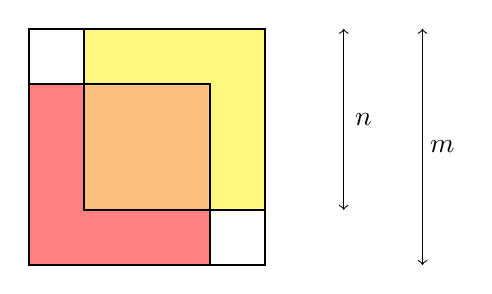
\begin{tikzpicture}
		\draw[thick] (0,0) rectangle (3,3);
		\draw[thick, fill=red!50] (0,0) rectangle (2.3,2.3);
		\draw[thick, fill=yellow!50] (0.7,0.7) rectangle (3, 3);
		\draw[thick, fill=orange!50] (0.7,0.7) rectangle (2.3, 2.3);
		\draw[<->] (4, 0.7)--(4, 3);
		\node at (4.25, 1.85) (n) {$n$};
		\draw[<->] (5, 0)--(5, 3);
		\node at (5.25, 1.5) (m) {$m$};
	\end{tikzpicture}
\end{center}
$m^2 = 2n^2$ என்பதால், $n$ பக்க அளவுள்ள இரண்டு வர்க்கங்களும்
ஒன்றின்மேல் ஒன்று படியும் பகுதியின் பரப்பளவு,
அந்த இரு வர்க்கங்களும் மூடாத பகுதியின் பரப்பளவுக்குச் சமமாகும்;
அதாவது, செம்மஞ்சள் வர்க்கத்தின் பரப்பளவு,
நிறமிடாத இரு வர்க்கங்களின் பரப்பளவுகளின் கூட்டுத்தொகைக்குச் சமம்.
எனவே செம்மஞ்சள் வர்க்கத்தின் பக்க அளவு $p$ ஆகவும்,
நிறமிடாத ஒவ்வொரு வர்க்கத்தின் பக்க அளவு $q$ ஆகவும் இருந்தால்,
$p^2 = 2q^2$.
ஆனால் இப்போது $\sqrt{2} = \nicefrac{p}{q}$;
மேலும் $p < m$, $q < n$, $p, q \in \Nat$.
$m$, $n$ ஆகியவை இயன்றளவு சிறியவையாகத் தேர்ந்தெடுக்கப்பட்டன
என்ற உண்மைக்கு இது முரணாகும்.
		
\emph{இரண்டாவதாக, முறைப்படியாக.}
$m^{2} = 2n^{2}$ என்பதால், $m$ இரட்டை எண் எனப் பின்தொடரும்.
($x$ ஒற்றை எனில், $x^2$ உம் ஒற்றை எனக் காட்டுவது எளிது.)
எனவே ஏதோ ஒரு $r \in \Nat$ க்கு $m = 2r$.
மறுசீரமைத்தால், $2r^2 = n^2$,
		% 				\begin{align*}
		% 					(2q)^{2} &= 2n^{2}\\
		% 					4q^{2} &= 2n^{2}\\
		% 					2q^{2} &= n^{2}
		% 				\end{align*}
எனவே $n$ உம் இரட்டை எண்.
ஆகவே $m$, $n$ இரண்டும் இரட்டை எண்கள்;
இதனால் $\nicefrac{m}{n}$ என்ற பின்னத்தை மேலும் \emph{சுருக்க முடியும்}.
முரண்!
\end{proof}

% SEGMENT OLP-0044-S04
% READER FALLBACK TA-READER-REF-001; absent history chapter gets descriptive text.
இடைச்செய்தியாக, இந்தப் படவிளக்க நிறுவல்
\oliflabeldef{his:set:mythology:sec}{%
  \olref[his][set][mythology]{sec} இன் உள்ளடக்கத்தை}{%
  கணக்கோட்பாட்டு வரலாற்றுக் கதைகள் பற்றிய பின்னைய பிரிவின் உள்ளடக்கத்தை}
மீண்டும் கருத
அனுமதிக்கிறது.
டென்னன்பாம் (1927--2006) முற்றிலும் நவீன கணிதவியலாளர்;
ஆனால் இந்த நிறுவல் மறுக்க முடியாத அளவு அழகானது,
முழுமையாகக் கடுமையானது, வடிவியல் உள்ளுணர்வைப் பயன்படுத்துவது!

% SEGMENT OLP-0044-S05
எப்படியாயினும், மெய்யெண்கள் விகிதமுறு எண்களைவிட
``மேலும் விரிவானவை''.
ஒரு பொருளில், விகிதமுறு எண்களில் ``இடைவெளிகள்'' உள்ளன;
மெய்யெண்கள் அவற்றை நிரப்புகின்றன.
இது விகிதமுறு எண்களிலிருந்து மெய்யெண்களை வேறுபடுத்தும்
மெய்யெண்களின் ஒரே ஒரு பண்பை விவரிப்பதாக வயர்ஸ்ட்ராஸ் உணர்ந்தார்;
அதுவே முழுமைப் பண்பு:
\emph{மேல்வரம்பைக் கொண்ட, வெற்றற்ற மெய்யெண் கணம் ஒவ்வொன்றும்
ஒரு மீச்சிறு மேல்வரம்பைக் கொண்டுள்ளது.}

% SEGMENT OLP-0044-S06
விகிதமுறு எண்களுக்கு முழுமைப் பண்பு இல்லை என்பதை எளிதில் காணலாம்.
எடுத்துக்காட்டாக, $\sqrt{2}$ ஐ விடச் சிறிய விகிதமுறு எண்களைக் கொண்ட
பின்வரும் கணத்தைக் கருதுக:
\[
	\Setabs{p \in \Rat}{p^2 < 2 \text{ அல்லது }p < 0}
\]
இதற்கு விகிதமுறு எண்களில் ஒரு மேல்வரம்பு உள்ளது;
எடுத்துக்காட்டாக, அதன் !!{element}s< அனைத்தும் $3$ ஐ விடச் சிறியவை.
ஆனால் இதன் மீச்சிறு மேல்வரம்பு எது?
அது `$\sqrt{2}$' என்று கூற விரும்புகிறோம்;
ஆனால் $\sqrt{2}$ \emph{விகிதமுறு எண் அல்ல} என்பதை இப்போதுதான் கண்டோம்.
$\sqrt{2}$ ஐ விடப் பெரிய விகிதமுறு எண்களில் \emph{மீச்சிறியது} எதுவும் இல்லை.
எனவே அந்தக் கணத்திற்கு ஒரு மேல்வரம்பு உள்ளது;
ஆனால் மீச்சிறு மேல்வரம்பு இல்லை.
ஆகவே விகிதமுறு எண்களுக்கு முழுமைப் பண்பு இல்லை.

% SEGMENT OLP-0044-S07
இதற்கு மாறாக, தொடரகம் முழுமைப் பண்பைக் கொண்டிருக்க
``கருத்தளவில் வேண்டும்''.
$\sqrt{2}$ ஒரு மெய்யெண்ணாக இருக்க வேண்டும் என்பது மட்டும் நமது நோக்கமல்ல;
விகிதமுறு எண் கோட்டிலுள்ள எல்லா ``இடைவெளிகளையும்'' நிரப்ப விரும்புகிறோம்.
உண்மையில், தொடரகத்திலேயே ``இடைவெளிகள்'' எதுவும் இருக்கக்கூடாது
என விரும்புகிறோம். முழுமை நமக்குத் தருவது இதுவே.


% END SOURCE UNIT OLP-0044

\endgroup

\begingroup
\makeatletter
\def\ol@sectioncs{section}
\makeatother
\def\olfilename{cuts}

% BEGIN SOURCE UNIT OLP-0045 content/sets-functions-relations/arithmetization/cuts.tex
% Exact modular target bytes: 12268; SHA256: 9c80cbe1d294b26750573ae7fd53d59e84898e110dc98a0ffa1bc0a83bd0cc82
% SEGMENT OLP-0045-S01


\olfileid{sfr}{arith}{cuts}
\olsection{$\Rat$ இலிருந்து $\Real$ க்கு}

சாரத்தில், மெய்யெண் கோட்டின் எந்தப் புள்ளி $\alpha$ உம்
அந்தக் கோட்டை மிகச்சரியாக இரு பாதிகளாகப் பிரிக்கிறது என்பதை
முழுமைப் பண்பு காட்டுகிறது: ஒன்றிற்கு $\alpha$ மீச்சிறு மேல்வரம்பாகவும்,
மற்றொன்றிற்கு $\alpha$ மீப்பெரு கீழ்வரம்பாகவும் உள்ளது.
விகிதமுறு எண்களிலிருந்து மெய்யெண்களைக் \emph{கட்டமைக்க},
விகிதமுறு எண்களைப் பிரிக்கும் \emph{வெட்டுகளாகவே} மெய்யெண்களைக்
கருதலாம் என்று டெடெகிண்ட் முன்மொழிந்தார்.
அதாவது, $< \sqrt{2}$ என அமையும் விகிதமுறு எண்களை
$> \sqrt{2}$ என அமையும் விகிதமுறு எண்களிலிருந்து பிரிக்கும்
\emph{வெட்டுடன்} $\sqrt{2}$ ஐ அடையாளப்படுத்துகிறோம்.

இதனை ஒழுங்குபடுத்துவோம்.
விகிதமுறு எண்களை இரு பாதிகளாக வெட்டினால்,
நாம் உருவாக்கிய பிரிப்பை அதன் \emph{கீழ்ப்} பாதியை மட்டும் கொண்டு
தனித்துவமாக அடையாளப்படுத்தலாம்.
எனவே இதனைத் துல்லியமாகப் பின்வருமாறு வரையறுக்கிறோம்:

% SEGMENT OLP-0045-S02
\begin{defn}[வெட்டு]
ஒரு \emph{வெட்டு} $\alpha$ என்பது,
மீப்பெரு உறுப்பு இல்லாத, விகிதமுறு எண்களின் எந்தவொரு
வெற்றற்ற தகு தொடக்கத் துண்டும் ஆகும்.
அதாவது, $\alpha$ ஒரு வெட்டாக இருக்கும்போது,
அப்போதும் அப்போது மட்டுமே:
\begin{enumerate}
	\item \emph{வெற்றற்றது, தகுவானது}: $\emptyset \neq \alpha \subsetneq \Rat$
	\item \emph{தொடக்கத் துண்டு}: அனைத்து $p,q \in \Rat$ க்கும்,
    $p < q \in \alpha$ எனில் $p \in \alpha$
	\item \emph{மீப்பெரு உறுப்பு இல்லை}: அனைத்து $p \in \alpha$ க்கும்,
    $p < q$ என அமையும் ஒரு $q \in \alpha$ உள்ளது
\end{enumerate}
பின்னர் $\Real$ என்பது வெட்டுகளின் கணமாகும்.
\end{defn}

% SEGMENT OLP-0045-S03
இப்போது $\sqrt{2} = \Setabs{p \in \Rat}{p^2 < 2\text{
அல்லது }p < 0}$ என்று கூறலாம்.
நிச்சயமாக, இது \emph{ஒரு வெட்டுதான்} எனச் சரிபார்க்க வேண்டும்;
அதனை \olref[check]{sec} இல் தருகிறோம்.

% SEGMENT OLP-0045-S04
முன்புபோல, சில பொருள்களை வரையறுத்த பிறகு,
அவற்றின் மீதான அடிப்படைச் சார்புகளையும் தொடர்புகளையும்
அடுத்து வரையறுக்க வேண்டும். எளிய ஒன்றிலிருந்து தொடங்குகிறோம்:
\begin{align*}
	\alpha \leq \beta \text{ ஆக இருக்கும்போது, அப்போதும் அப்போது மட்டுமே, }\alpha \subseteq \beta
\end{align*}
வரிசையின் இந்த வரையறை, வெட்டுகளின் கணம் முழுமைப் பண்பைக் கொண்டுள்ளது
என்ற மைய முடிவைக் \emph{கூற} அனுமதிக்கிறது.
முழுமையாக விரித்தால், கூற்றின் வடிவம் இதுவாகும்.
$S$ என்பது மேல்வரம்பைக் கொண்ட வெற்றற்ற வெட்டுகளின் கணம் எனில்,
$S$ ஒரு மீச்சிறு மேல்வரம்பைக் கொண்டுள்ளது.
மேலும் விரிவாக: $S$ இன் மேல்வரம்பாக உள்ள ஒரு வெட்டு $\lambda$ உள்ளது;
அதாவது $(\forall \alpha \in S)\alpha \subseteq
\lambda$; மேலும் $\lambda$ இத்தகைய மீச்சிறு வெட்டு;
அதாவது $(\forall \beta \in \Real)((\forall \alpha \in S)\alpha
\subseteq \beta \lif \lambda \subseteq \beta)$.
இந்த முடிவின் நிறுவல் இதோ:

% SEGMENT OLP-0045-S05
\begin{thm}\ollabel{realcompleteness}
வெட்டுகளின் கணம் முழுமைப் பண்பைக் கொண்டுள்ளது.
\end{thm}

% SEGMENT OLP-0045-S06
\begin{proof}
$S$ என்பது மேல்வரம்பைக் கொண்ட எந்தவொரு வெற்றற்ற வெட்டுகளின்
கணமாகவும் இருக்கட்டும். $\lambda = \bigcup S$ என்க.
%\Setabs{p \in \Rat}{(\exists \alpha \in S)p \in \alpha}$$
முதலில் $\lambda$ ஒரு வெட்டு என வாதிடுகிறோம்:
\begin{enumerate}
\item $S$ வெற்றற்றதால், குறைந்தது ஒரு வெட்டு $S$ இல் உள்ளது;
எனவே $\emptyset \neq \lambda$.
$S$ என்பது வெட்டுகளின் கணம் என்பதால், $\lambda \subseteq \Rat$.
$S$ க்கு ஒரு மேல்வரம்பு இருப்பதால்,
ஒவ்வொரு வெட்டு $\alpha \in S$ இலிருந்தும் விடுபட்ட ஏதோ ஒரு
$p \in \Rat$ உள்ளது.
எனவே $p\notin \lambda$; ஆதலால் $\lambda \subsetneq \Rat$.
\item $p < q \in \lambda$ எனக் கொள்க.
அப்போது $q \in \alpha$ என அமையும் ஏதோ ஒரு $\alpha \in S$ உள்ளது.
$\alpha$ ஒரு வெட்டு என்பதால், $p \in \alpha$.
எனவே $p \in \lambda$.
\item $p \in \lambda$ எனக் கொள்க.
அப்போது $p \in \alpha$ என அமையும் ஏதோ ஒரு $\alpha \in S$ உள்ளது.
$\alpha$ ஒரு வெட்டு என்பதால், $p < q$ என அமையும் ஏதோ ஒரு
$q \in \alpha$ உள்ளது. எனவே $q \in \lambda$.
\end{enumerate}
இது வாதத்தை நிறுவுகிறது.
மேலும், $(\forall \alpha \in S)\alpha
\subseteq \bigcup S = \lambda$ என்பது தெளிவு;
அதாவது $\lambda$ என்பது $S$ இன் ஒரு மேல்வரம்பு.
இப்போது $\beta \in \mathbb{R}$ உம் ஒரு மேல்வரம்பு எனக் கொள்க;
அதாவது $(\forall \alpha \in S)\alpha \subseteq \beta$.
எந்த $p \in \Rat$ க்கும், $p \in \lambda$ எனில்,
$p \in \alpha$ என அமையும் ஒரு $\alpha \in S$ உள்ளது;
எனவே $p \in \beta$.
பொதுமைப்படுத்தினால், $\lambda \subseteq \beta$.
ஆகவே $\lambda$ என்பது $S$ இன் \emph{மீச்சிறு} மேல்வரம்பு.
\end{proof}

% SEGMENT OLP-0045-S07
எனவே முழுமைப் பண்பை நிறைவேற்றும் பல பொருள்கள் நமக்குக் கிடைத்துள்ளன.
இதனை மற்றொரு வகையில் சொன்னால், நமது வெட்டுகளில் ``இடைவெளிகள்'' இல்லை.
(எனவே, விகிதமுறு எண்களுக்குப் பதிலாக மெய்யெண்களில் மேலும்
``வெட்டுகளை'' எடுத்தால், சுவையான புதிய பொருள்கள் எதுவும் கிடைக்காது.)

% SEGMENT OLP-0045-S08
அடுத்து, மெய்யெண்களின் மீது சில செயல்களை வரையறுக்க வேண்டும்.
ஒவ்வொரு $p \in \Rat$ க்கும் $p_\Real =
\Setabs{q \in \Rat}{q < p}$ என நிர்ணயித்து,
விகிதமுறு எண்களை மெய்யெண்களுக்குள் பதிப்பதிலிருந்து தொடங்குகிறோம்.
பின்னர் பின்வருமாறு வரையறுக்கிறோம்:
\begin{align*}
	\alpha + \beta &= \Setabs{p + q}{p \in \alpha \land q \in \beta}\\
%	\alpha - \beta &\defis \Setabs{p - q}{p \in \alpha \land q \in \Rat \setminus \beta}\\
	\alpha \times \beta &=
	\Setabs{p \times q}{0 \leq p \in \alpha \land 0 \leq q \in \beta} \cup 0^\mathbb{R} & \text{எனில் }\alpha, \beta \geq 0_\Real
%	\alpha \div \beta &\defis
%	\Setabs{\nicefrac{p}{q}}{p \in \alpha \land q \in \Rat \setminus \beta}  & \text{எனில் }\alpha \geq 0_\Real, \beta > 0_\Real
\end{align*}
பிற பெருக்கல் நிலைகளைக் கையாள, முதலில் பின்வருமாறு அமைக்க:
%$0_\Real \times \alpha = 0_\Real = \alpha \times 0_\Real$ எனவும், மேலும் பின்வருமாறும் அமைக்க:
\begin{align*}
	-\alpha &= \Setabs{p - q}{p < 0 \land q \notin \alpha}
\end{align*}
பின்னர் பின்வருமாறு நிர்ணயிக்க:
\begin{align*}
	\alpha \times \beta &\defis
	\begin{cases}
		\mathord{-}\alpha \times \mathord{-}\beta &\text{எனில் }\alpha < 0_\Real\text{ மற்றும் }\beta < 0_\Real\\
		\mathord{-}(\mathord{-}\alpha \times \beta) &\text{எனில் }\alpha < 0_\Real \text{ மற்றும் }\beta > 0_\Real\\
		\mathord{-}(\alpha \times \mathord{-}\beta) &\text{எனில் }\alpha > 0_\Real \text{ மற்றும் }\beta < 0_\Real
	\end{cases}
\end{align*}
இந்த வரையறைகள் ஒவ்வொன்றும் எப்போதும் ஒரு வெட்டைத் தருகின்றனவா
எனப் பின்னர் சரிபார்க்க வேண்டும்.
இறுதியாக, இவ்வாறு வரையறுக்கப்பட்ட வெட்டுகள்,
அவை செயல்பட வேண்டியவாறே செயல்படுகின்றன என்பதை எளிய
(ஆனால் நீண்ட) விளக்கத்தின் மூலம் சரிபார்க்க வேண்டும்.
இவை அனைத்தையும் \olref[check]{sec} இல் தருகிறோம்.

% END SOURCE UNIT OLP-0045

\endgroup

\begingroup
\makeatletter
\def\ol@sectioncs{section}
\makeatother
\def\olfilename{reflections}

% BEGIN SOURCE UNIT OLP-0046 content/sets-functions-relations/arithmetization/reflections.tex
% Exact modular target bytes: 14115; SHA256: 425ff00b227c720a06bb5291b44812a7b85df08ef7e078cfa04bc50b99ecb83b
% SEGMENT OLP-0046-S01


\olfileid{sfr}{arith}{ref}
\olsection{சில மெய்யியல் சிந்தனைகள்}

தொழில்நுட்ப விவரங்கள் இவ்வளவே. ஆனால் அவை எதைச் சாதித்தன?

மறுப்பதற்கு இடமில்லாத வகையில், அவை சில {அழகிய} தூய கணிதத்தை
நமக்குத் தந்தன. மேலும், சில ஆழமான கருத்தியல் சாதனைகளும் இருந்தன.
மெய்யெண்களுக்கும் விகிதமுறு எண்களுக்கும் இடையிலான முக்கிய வேறுபாட்டை
முழுமைப் பண்பு வெளிப்படுத்துகிறது என்று கண்டது ஓர் ஆழமான உட்பார்வை.
மேலும், மெய்யெண்களை டெடெகிண்ட் வெட்டுகளாக வெளிப்படையாகக்
கட்டமைப்பது, பகுப்பாய்வியலின் பாடப்பொருளுக்கு உறுதியான அடித்தளத்தைத்
தருகிறது. \emph{முழுமையான வரிசைப்படுத்தப்பட்ட புலம்} என்ற கருத்து
முரணற்றது என்பதை அறிவோம்; ஏனெனில் வெட்டுகள் அத்தகைய ஒரு புலமாக அமைகின்றன.

% SEGMENT OLP-0046-S02
இவை அனைத்தையும் ஏற்றாலும், இந்தச் சாதனைகளைப் பற்றி நமக்குள்ள
சில ஐயங்களையும் வெளிப்படுத்த வேண்டும்.

% SEGMENT OLP-0046-S03
மெய்யெண்களை அவற்றின் பழக்கமான (முடிவுறாததாக இருக்கக்கூடிய)
தசம விரிவாக்கங்களாகக் கருதுவதைவிட, வெட்டுகளாகக் கருதுவது
\emph{மேலும்} கடுமையானதா என்பது தெளிவில்லை.
மெய்யெண்களுக்கான இந்தப் பிந்தைய ``கட்டமைப்பு'',
கோஷி தொடர் மூலம் செய்யப்படும் மெய்யெண் கட்டமைப்புடன் சில ஒற்றுமைகளைக்
கொண்டுள்ளது; ஆனால் உண்மையில், அது 17ஆம் நூற்றாண்டின் தொடக்கத்திலிருந்தே
கணிதவியலாளர்களுக்குச் சாரத்தில் தெரிந்திருந்தது
(\olref[cauchy]{sec} ஐப் பார்க்கவும்).
மெய்யெண்களுக்கு முழுமைப் பண்பு உள்ளது என்பதை உணர்ந்ததிலிருந்தே
கடுமையில் உண்மையான உயர்வு வந்தது;
குறிப்பிட்ட கணங்களாக மெய்யெண்களைக் கட்டமைக்கும் திறன் மட்டும்,
அவ்வளவு சுவையானதாக இல்லாமல் இருக்கலாம்.

% SEGMENT OLP-0046-S04
முழுக்களையோ விகிதமுறு எண்களையோ (மிக எளிதாகச் செய்யப்படும்)
எண்முறைமைக் கட்டமைப்பு, அந்தப் பகுதிகளில் கடுமையை அதிகரிக்கிறது
என்பது இன்னும் தெளிவற்றது.
இங்கு ஓர் எளிய கவனிப்பைக் கூறுவது பயனுள்ளது.
முழுக்களை இயல் எண்களின் வரிசைப்படுத்தப்பட்ட ஜோடிகளின் சமான
வகுப்புகளாக \emph{கட்டமைத்து}, பின்னர் விகிதமுறு எண்களை முழு ஜோடிகளின்
சமான வகுப்புகளாகக் கட்டமைத்து, அதன்பின் மெய்யெண்களை விகிதமுறு எண்களின்
கணங்களாகக் கட்டமைத்தவுடன், அந்தக் கட்டமைப்புகளை உடனே
\emph{மறந்துவிடுகிறோம்}.
குறிப்பாக, அந்தக் கட்டமைப்புகள் செயல்பட வேண்டியவாறு செயல்படுகின்றன
என்பதை நிறுவுவதைத் தவிர, ஒரு கணித நிறுவலின்போது யாரும் அவற்றை
\emph{பயன்படுத்த} விரும்பமாட்டார்கள்.
இயல் எண்களின் கணங்களின் கணங்களின் கணங்களின் கணங்களின் கணங்களின்
கணங்களின் ஏதோ ஒரு கணத்தைப் பற்றிப் பேசுவதைவிட,
ஒரு மெய்யெண்ணைப் பற்றி நேரடியாகப் பேசுவது மிகவும் எளிது.
%(மெய்யெண்கள் விகிதமுறு எண்களின் கணங்களாகக் கட்டமைக்கப்பட்டன; அவை முழு ஜோடிகளின் சமான வகுப்புகளாக, அதாவது முழுக்களின் கணங்களின் கணங்களின் கணங்களாகக் கட்டமைக்கப்பட்டன; இவ்வாறே தொடர்கிறது.)
%2/3 = [2,3]
%	அதாவது {<2,3>, ... }
%	{ {{2},{2,3}}, ... }
%
%மெய்யெண்கள்
%	விகிதமுறு எண்களின் கணங்கள்
%
%விகிதமுறு எண்கள்
%	முழுக்களின் கணங்களின் கணங்களின் கணங்கள்
%
%முழுக்கள்
%	இயல் எண்களின் கணங்களின் கணங்களின் கணங்கள்
	
% SEGMENT OLP-0046-S05
இந்த வரையறைகள் முழுக்கள், விகிதமுறு எண்கள் அல்லது மெய்யெண்கள்
\emph{மெய்ப்பொருளியல் நோக்கில்} \emph{எவை} என்பதைச் சொல்கின்றனவா என்பதே
எல்லாவற்றையும்விட அதிக ஐயத்திற்குரியது.
அதாவது, மெய்யெண்கள் (எடுத்துக்காட்டாக) குறிப்பிட்ட
(கணங்களின் கணங்களின் \ldots) கணங்களாகவே \emph{உள்ளன} என்பது ஐயத்திற்குரியது.
இந்தக் கருத்திற்கான முக்கியத் தடை, கட்டமைப்பை வெவ்வேறு பல வழிகளில்
செய்திருக்க முடியும் என்பதாகும்.
மெய்யெண்களைப் பொறுத்தவரை, உண்மையாகவே சுவையான பல வேறுபட்ட
கட்டமைப்புகள் உள்ளன (\olref[cauchy]{sec} ஐப் பார்க்கவும்).
ஆனால் வேறுபட்ட கட்டமைப்புகளைப் பெறுவதற்கான மிக அற்பமான வழி இதோ:
\olref[sfr][rel][ref]{sec} இல் செய்ததுபோல,
வரிசைப்படுத்தப்பட்ட ஜோடிகளைச் சற்றே வேறுவிதமாக வரையறுத்திருக்கலாம்.
வரிசைப்படுத்தப்பட்ட ஜோடிக்கான இந்த மாற்றுக் கருத்தைப் பயன்படுத்தியிருந்தால்,
நமது கட்டமைப்புகள் முன்புபோலவே மிகச்சரியாகச் செயல்பட்டிருக்கும்;
ஆனால் இறுதியில் வேறு பொருள்கள் கிடைத்திருக்கும்.
எனவே முழுக்கள், விகிதமுறு எண்கள், மெய்யெண்கள் ஆகியவற்றுக்குப்
போட்டியான பல கணக்கோட்பாட்டுக் கட்டமைப்புகள் உள்ளன.
இப்போது முழுக்கள் (எடுத்துக்காட்டாக) \emph{இந்தக்} கணங்கள்தான்,
\emph{அந்தக்} கணங்கள் அல்ல என்று கூறுவது தன்னிச்சையானதாகவும்
தர்மசங்கடமூட்டுவதாகவும் இருக்கும்.
(\olref[sfr][rel][ref]{sec} இல் கண்டதுபோல,
இது \citealt{Benacerraf1965} புகழ்பெறச் செய்த ஒரு வாதத்தின் எடுத்துக்காட்டு.)

% SEGMENT OLP-0046-S06
மேலும் ஒரு கருத்தை எழுப்புவது பயனுள்ளது:
நமது கட்டமைப்புகளில் முற்றிலும் \emph{விநோதமான} ஒன்று உள்ளது.
இயல் எண்களிலிருந்து தொடங்கினோம்.
பின்னர் முழுக்களையும், ``முழுக்களின் $0$'' என்பதையும்,
அதாவது $ \equivrep{0,0}{\Intequiv}$ ஐயும் கட்டமைக்கிறோம்.
ஆனால் $0 \neq \equivrep{0,0}{\Intequiv}$.
உண்மையில், நமது கட்டமைப்புகளின்படி \emph{எந்த} இயல் எண்ணும் முழு அல்ல.
ஆனால் இது உள்ளுணர்விற்கு முற்றிலும் எதிரானதாகத் தோன்றுகிறது.
மேலும், \olref[sfr][set][imp]{sec} இல்,
$\Nat \subseteq \Rat$ என்று அதிக வாதமின்றிக் கூறினோம்.
எண்கள் மிகச்சரியாக \emph{எவை} என்பதை அந்தக் கட்டமைப்புகள் சொல்கின்றன
எனில், இந்தக் கூற்று அற்பமாகவே பொய்யானது.

% SEGMENT OLP-0046-S07
சற்று விலகி நின்று பார்த்தால், நாம் எங்கு வந்துள்ளோம்?
முறைசாராத கணக்கோட்பாட்டில் வேலைசெய்து,
இயல் எண்களை நமக்குத் தரப்பட்டவையாகப் பயன்படுத்தி,
முழுக்கள், விகிதமுறு எண்கள், மெய்யெண்கள் ஆகியவற்றைக் குறிப்பிட்ட
கணங்களாகக் \emph{கருத} முடிகிறது.
அந்தப் பொருளில், இந்தப் பொருள்களின் கோட்பாடுகளை ஒரு
கணக்கோட்பாட்டுக்குள் \emph{பதிக்க} முடிகிறது.
ஆனால் இந்தப் பதித்தலின் மெய்யியல் பொருள் அவ்வளவு நேரடியானதல்ல.

% SEGMENT OLP-0046-S08
நிச்சயமாக, இவை எதுவும் இறுதி முடிவல்ல!{}
கருத்து இதுமட்டுமே.
மெய்யெண்களின் எண்முறைமைக் கட்டமைப்பு ஆழமான மெய்யியல் முக்கியத்துவம்
\emph{கொண்டுள்ளது} எனக் காட்டுவதற்கு,
மேலும் சில \emph{மெய்யியல்} வாதங்கள் தேவைப்படும்.

%மேலும்: இந்த அத்தியாயம் முழுவதிலும், இயல் எண்கள் நமக்கு வெறுமனே
%\emph{தரப்பட்டவை} எனக் கருதியுள்ளோம். ஆனால் அவற்றை வைத்து என்ன செய்யலாம்?
%அதுவே அடுத்த அத்தியாயத்தின் பாடப்பொருள்.


% END SOURCE UNIT OLP-0046

\endgroup

\begingroup
\makeatletter
\def\ol@sectioncs{section}
\makeatother
\def\olfilename{checking-details}

% BEGIN SOURCE UNIT OLP-0047 content/sets-functions-relations/arithmetization/checking-details.tex
% Exact modular target bytes: 17992; SHA256: 0f42bf8b99c135dd4ec4766dc89cfb0ef3fcc72e536960e5ac7989b87d7d6a08
% SEGMENT OLP-0047-S01

	
\olfileid{sfr}{arith}{check}
\olsection{வரிசைப்படுத்தப்பட்ட வளையங்களும் புலங்களும்}

இந்த அத்தியாயம் முழுவதிலும், சில வரையறைகள் ``செயல்பட வேண்டியவாறே''
செயல்படுகின்றன என்று கூறினோம்.
இந்தத் தொழில்நுட்ப இணைப்பில், அதனால் நாம் குறிப்பது என்ன என்பதை
விரித்துரைத்து, வரையறைகள் ``சரியாகச்'' செயல்படுகின்றன என
(எவ்வாறு நிறுவுவது என்பதன் வரைவைக்) காட்டுவோம்.

\olref[int]{sec} இல், $\Int$ மீது கூட்டலையும் பெருக்கலையும்
வரையறுத்தோம். அவை வரையறுக்கப்பட்ட விதத்தில்,
$\Int$ க்கு நாம் ``விரும்பும்'' அமைப்பைத் தருகின்றன எனக் காட்ட வேண்டும்.
குறிப்பாக, கேள்விக்குரிய அமைப்பு ஒரு பரிமாற்று வளையத்தின் அமைப்பாகும்.

% SEGMENT OLP-0047-S02
\begin{defn}
	ஒரு \emph{பரிமாற்று வளையம்} என்பது, குறிப்பிட்ட $0$, $1$ என்ற
    உறுப்புகளையும் $+$, $\times$ என்ற செயல்களையும் கொண்ட ஒரு கணம் $S$;
    அது பின்வரும் எட்டு வாய்பாடுகளை நிறைவேற்றுகிறது:
	\begin{align*}
		\emph{சேர்ப்புப் பண்பு}&&a + (b+ c) & = (a + b) + c \\
		&& (a \times b) \times c & = a \times (b\times c)\\
		\emph{பரிமாற்றுப் பண்பு}&&a + b &= b+ a  \\
		&&  a \times b&= b\times a\\
		\emph{சமனிகள்}&&a + 0 &= a \\
		&& a \times 1 &= a\\
		\emph{கூட்டல் நேர்மாறு}&&(\exists b\in S)0&=a + b\\
		\emph{பங்கீட்டுப் பண்பு}&&a \times (b+ c ) &= (a \times b) + (a \times c)
	\end{align*}
	மறைமுகமாக, இவை அனைத்தும் $S$ க்கு வரம்பிடப்பட்ட அனைத்துப்
    பொதுநிலையளவிகளால் பிணைக்கப்பட்டுள்ளன.
    மேலும், இங்குள்ள $0$, $1$ என்ற உறுப்புகள்,
    அதே பெயருள்ள இயல் எண்களாக இருக்க வேண்டியதில்லை.
\end{defn}

% SEGMENT OLP-0047-S03
எனவே முழுக்கள் ஒரு பரிமாற்று வளையத்தை உருவாக்குகின்றனவா எனச்
சரிபார்க்க, இந்த எட்டு நிபந்தனைகளும் நிறைவேறுகின்றனவா என்று மட்டும்
சரிபார்க்க வேண்டும்.
எந்த நிபந்தனையையும் நிறுவுவது {கடினம்} அல்ல; ஆனால் இது சற்று உழைப்பானது.
எடுத்துக்காட்டாக, கூட்டலுக்கான \emph{சேர்ப்புப் பண்பை}
எவ்வாறு நிறுவுவது என்பது இதோ:

\begin{proof}
$i, j, k \in \Int$ என்பதை நிலைப்படுத்துக.
அப்போது $i = \equivrep{a_1, b_1}{}$, $j =
\equivrep{a_2,b_2}{}$, $k = \equivrep{a_3, b_3}{}$ என அமையும்
$a_1, b_1, a_2, b_2, a_3, b_3 \in \Nat$ உள்ளன.
(எளிதாகப் படிப்பதற்காக ``$\equivrep{x, y}{\Intequiv}$'' என்பதற்குப்
பதிலாக ``$\equivrep{x, y}{}$'' என எழுதுகிறோம்;
இந்தப் பிரிவு முழுவதிலும் இவ்வாறு செய்வோம்.) இப்போது:
\begin{align*}
	i + (j + k) &= \equivrep{a_1, b_1}{}+(\equivrep{a_2, b_2}{} + \equivrep{a_3, b_3}{}) \\
	&= \equivrep{a_1,  b_1}{} + \equivrep{a_2+a_3, b_2+b_3}{}\\
	&= \equivrep{a_1 + (a_2 + a_3), b_1 + (b_2 + b_3)}{}\\
	&= \equivrep{(a_1 + a_2) + a_3, (b_1 + b_2) + b_3}{}\\
	&= \equivrep{a_1 + a_2, b_1 + b_2}{} + \equivrep{a_3, b_3}{}\\
	&= (\equivrep{a_1, b_1}{} + \equivrep{a_2, b_2}{}) + \equivrep{a_3, b_3}{}\\
	&= (i+j) + k
\end{align*}
இங்கு $\Nat$ மீதான கூட்டலின் செயல்பாட்டைத் தடையின்றிப் பயன்படுத்தினோம்.
\end{proof}

% SEGMENT OLP-0047-S04
அதேபோல, \emph{கூட்டல் நேர்மாறை} எவ்வாறு நிறுவுவது என்பது இதோ:

\begin{proof}
$i \in \Int$ என்பதை நிலைப்படுத்துக;
ஏதோ $a,b \in \Nat$ க்கு $i = \equivrep{a,b}{}$.
$j = \equivrep{b,a}{} \in \Int$ என்க.
இயல் எண்களின் செயல்பாட்டைப் பயன்படுத்தினால்,
$(a+b) + 0 = 0 + (a+b)$; எனவே வரையறையின்படி
$\tuple{a+b, b+a} \sim_\Int \tuple{0,0}$;
ஆகவே $\equivrep{a+b, b+a}{} = \equivrep{0, 0}{} = 0_\Int$.
இப்போது $i + j =
\equivrep{a,b}{}+\equivrep{b,a}{}=\equivrep{a+b, b+a}{}= \equivrep{0,
0}{} = 0_\Int$.
\end{proof}

% SEGMENT OLP-0047-S05
\emph{பங்கீட்டுப் பண்பிற்கான} ஒரு நிறுவல் இதோ:

\begin{proof}
மேலே செய்ததுபோல, $i = \equivrep{a_1, b_1}{}$, $j =
\equivrep{a_2,b_2}{}$, $k = \equivrep{a_3, b_3}{}$ என
நிலைப்படுத்துக. இப்போது:
\begin{align*}
	i \times (j + k)
	&= \equivrep{a_1, b_1}{} \times (\equivrep{a_2,b_2}{} + \equivrep{a_3, b_3}{})\\
	&= \equivrep{a_1, b_1}{} \times \equivrep{a_2 + a_3,b_2+b_3}{}\\
	&= \equivrep{a_1  (a_2 + a_3) + b_1  (b_2+b_3), a_1  (b_2 + b_3) + b_1 (a_2 + a_3)}{}\\
	&= \equivrep{a_1 a_2 + a_1a_3 + b_1 b_2+b_1b_3, a_1 b_2 + a_1b_3 + a_2b_1 + a_3b_1}{}\\		
%		&= \equivrep{a_1 a_2 + b_1b_2 + a_1a_3 + b_1 b_2+b_1b_3, a_1 b_2 + a_1b_3 + a_2b_1 + a_3b_1}{}\\		
	&= \equivrep{a_1a_2 + b_1b_2, a_1b_2 + a_2b_1}{} + \equivrep{a_1a_3 + b_1b_3, a_1b_3 + a_3b_1}{}\\
	&= (\equivrep{a_1, b_1}{} \times \equivrep{a_2,b_2}{}) + (\equivrep{a_1, b_1}{} \times  \equivrep{a_3, b_3}{})\\
	&= (i \times j) + (i \times k)
\end{align*}
\end{proof}

% SEGMENT OLP-0047-S06
மீதமுள்ள ஐந்து நிபந்தனைகளை நிறுவுவதை ஒரு பயிற்சியாக விடுகிறோம்.
அவற்றைச் செய்தபின், $\Int$ ஒரு பரிமாற்று வளையத்தை அமைக்கிறது,
அதாவது கூட்டலும் பெருக்கலும் (வரையறுக்கப்பட்டவாறு)
செயல்பட வேண்டியவாறே செயல்படுகின்றன, எனக் காட்டியிருப்போம்.

\begin{prob}
$\Int$ ஒரு பரிமாற்று வளையம் என நிறுவுக.
\end{prob}

% SEGMENT OLP-0047-S07
ஆனால் நமது பணி முடிந்துவிடவில்லை.
$\Int$ மீது கூட்டலையும் பெருக்கலையும் வரையறுத்ததோடு,
$\leq$ என்ற ஒரு வரிசைத் தொடர்பையும் வரையறுத்தோம்;
இதுவும் செயல்பட வேண்டியவாறு செயல்படுகிறதா எனச் சரிபார்க்க வேண்டும்.
மேலும் விரிவாக, $\Int$ ஒரு \emph{வரிசைப்படுத்தப்பட்ட} வளையத்தை
அமைக்கிறது எனக் காட்ட வேண்டும்.
\footnote{\olref[sfr][rel][ord]{def:linearorder} இலிருந்து நினைவுகொள்க:
	ஒரு முழு வரிசை என்பது தற்சுட்டு, கடப்பு, எதிர்சமச்சீர்,
    ஒப்பிடத்தக்க ஆகிய பண்புகளைக் கொண்ட தொடர்பாகும்.
	வரிசைத் தொடர்புகளின் சூழலில், ஒப்பிடத்தக்க பண்பு சில நேரங்களில்
	\emph{முக்கூற்றுப் பண்பு} எனப்படும்; ஏனெனில் எந்த $a$, $b$ க்கும்
    $a \leq b \lor a = b \lor a \geq b$.}

% SEGMENT OLP-0047-S08
\begin{defn}
ஒரு \emph{வரிசைப்படுத்தப்பட்ட வளையம்} என்பது,
$\leq$ என்ற முழு வரிசைத் தொடர்பையும் கொண்ட ஒரு பரிமாற்று வளையம்;
அது பின்வருவனவற்றை நிறைவேற்றுகிறது:
\begin{align*}
	a \leq b &\lif a + c \leq b + c\\
	(a \leq b \land 0 \leq c) &\lif a \times c \leq b \times c
\end{align*}
\end{defn}

% SEGMENT OLP-0047-S09
\begin{prob}
$\Int$ ஒரு வரிசைப்படுத்தப்பட்ட வளையம் என நிறுவுக.
\end{prob}

% SEGMENT OLP-0047-S10
முன்புபோல, கட்டமைக்கப்பட்ட $\Int$ ஒரு வரிசைப்படுத்தப்பட்ட வளையம்
எனக் காட்டுவது உழைப்பானது, ஆனால் வழக்கமானது.
அதனை உங்களுக்கே விட்டுவிடுகிறோம்.

இது முழுக்களைக் கவனித்துக்கொள்கிறது.
ஆனால் இப்போது விகிதமுறு எண்களைப் பற்றி இதே போன்றவற்றைக் காட்ட வேண்டும்.
குறிப்பாக, $+$, $\times$, $\leq$ ஆகியவற்றுக்கு நாம் கொடுத்த
வரையறைகளின் கீழ், விகிதமுறு எண்கள் ஒரு வரிசைப்படுத்தப்பட்ட
\emph{புலத்தை} அமைக்கின்றன எனக் காட்ட வேண்டும்:
\begin{defn}\ollabel{orderedfield}
ஒரு \emph{வரிசைப்படுத்தப்பட்ட புலம்} என்பது,
பின்வருவதையும் நிறைவேற்றும் வரிசைப்படுத்தப்பட்ட வளையமாகும்:
\begin{align*}
	\emph{பெருக்கல் நேர்மாறு}& & (\forall a \in S \setminus \{0\})(\exists b \in S) a\times b& = 1
\end{align*}
\end{defn}

% SEGMENT OLP-0047-S11
$\Int$ ஒரு வரிசைப்படுத்தப்பட்ட வளையம் என்று காட்டியவுடன்,
$\Rat$ ஒரு வரிசைப்படுத்தப்பட்ட புலம் என்று காட்டுவது எளிதானது,
ஆனால் உழைப்பானது.

\begin{prob}
$\Rat$ ஒரு வரிசைப்படுத்தப்பட்ட புலம் என நிறுவுக.
\end{prob}

% SEGMENT OLP-0047-S12
முழுக்களையும் விகிதமுறு எண்களையும் கவனித்தபின்,
மெய்யெண்களை மட்டும் கவனிக்க வேண்டியுள்ளது.
குறிப்பாக, $\Real$ ஒரு \emph{முழுமையான} வரிசைப்படுத்தப்பட்ட புலம்,
அதாவது முழுமைப் பண்பைக் கொண்ட வரிசைப்படுத்தப்பட்ட புலம்,
என்று காட்ட வேண்டும்.
\olref[cuts]{realcompleteness} ஆனது $\Real$ முழுமைப் பண்பைக்
கொண்டுள்ளது என நிறுவியது.
ஆயினும், $\Real$ ஒரு வரிசைப்படுத்தப்பட்ட புலம் என்பதைச் சரிபார்க்கும்
(சலிப்பூட்டும்) பணியை இன்னும் முழுவதும் செய்ய வேண்டும்.

\emph{அந்த} உழைப்பான பயிற்சியை நோக்கி விரைவதற்கு முன்,
மேலும் சில ``உடனடியான'' உண்மைகளைச் சரிபார்க்க வேண்டும்.
எடுத்துக்காட்டாக, எந்த வெட்டுகள் $\alpha$, $\beta$ க்கும்,
வரையறுக்கப்பட்ட $\alpha + \beta$ உண்மையில் ஒரு \emph{வெட்டு}
என்பதற்கான உறுதி தேவை. அந்த உண்மைக்கான நிறுவல் இதோ:

% SEGMENT OLP-0047-S13
\begin{proof}	
$\alpha$, $\beta$ இரண்டும் வெட்டுகள் என்பதால்,
$\alpha + \beta = \Setabs{p
+ q}{p \in \alpha \land q \in \beta}$ என்பது $\Rat$ இன்
வெற்றற்ற தகு உட்கணம்.
இப்போது ஏதோ $p \in \alpha$, $q \in \beta$ க்கு
$x < p + q$ எனக் கொள்க.
அப்போது $x - p < q$; எனவே $x - p \in \beta$;
மேலும் $x = p + (x - p) \in \alpha + \beta$.
ஆகவே $\alpha + \beta$ என்பது $\Rat$ இன் ஒரு தொடக்கத் துண்டு.
இறுதியாக, எந்த $p + q \in \alpha + \beta$ க்கும்,
$\alpha$, $\beta$ இரண்டும் வெட்டுகள் என்பதால்,
$p < p_1$, $q < q_1$ என அமையும் $p_1 \in \alpha$, $q_1 \in \beta$
உள்ளன; எனவே $p + q < p_1 + q_1 \in \alpha +
\beta$; ஆகவே $\alpha + \beta$ க்கு மீப்பெரு உறுப்பு இல்லை.
\end{proof}

% SEGMENT OLP-0047-S14
இதே போன்ற முயற்சிகள், $\alpha - \beta$, $\alpha \times \beta$,
$\alpha \div \beta$ ஆகியவை வெட்டுகள் எனச் சரிபார்க்க உதவும்
(இறுதி நிலையில், $\beta$ பூச்சிய வெட்டாக இருக்கும் நிலையைத் தவிர்க்கவும்).
ஆனால் இதையும் உங்களுக்கே விட்டுவிடுகிறோம்.

\begin{prob}
$\Real$ ஒரு வரிசைப்படுத்தப்பட்ட புலம் என நிறுவுக.
\end{prob}

% SEGMENT OLP-0047-S15
சரிசெய்ய வேண்டிய ஒரு சிறிய எஞ்சிய பகுதி உள்ளது.
\olref[cuts]{sec} இல், $\sqrt{2} =
\Setabs{p \in \Rat}{p < 0 \text{ அல்லது }p^2 < 2}$ எனக் கொள்ளலாம்
என்று முன்மொழிகிறோம்.
ஆனால் இந்தக் கணம் ஒரு \emph{வெட்டு} என்று காட்ட வேண்டும்.
அந்த உண்மைக்கான நிறுவல் இதோ:

% SEGMENT OLP-0047-S16
\begin{proof}
இது விகிதமுறு எண்களின் வெற்றற்ற தகு தொடக்கத் துண்டு என்பது தெளிவு;
எனவே இதற்கு மீப்பெரு உறுப்பு இல்லை எனக் காட்டினால் போதும்.
குறிப்பாக, $p$ என்பது $p^2 < 2$ என அமையும் நேர்ம விகிதமுறு எண்ணாகவும்,
$q = \frac{2p+2}{p+2}$ ஆகவும் இருந்தால்,
$p < q$, $q^2 < 2$ இரண்டையும் காட்டினால் போதும்.
$p < q$ என்பதைக் காண, பின்வருவதை மட்டும் கவனிக்கவும்:
\begin{align*}
	p^2 &< 2\\
	p^2 + 2p &< 2 + 2p\\
	p(p + 2) &< 2 + 2p\\
	p &< \tfrac{2+2p}{p+2} = q
\end{align*}
$q^2 < 2$ என்பதைக் காண, பின்வருவதை மட்டும் கவனிக்கவும்:
\begin{align*}
	p^2 &< 2\\
	2p^2 + 4p + 2 &< p^2 + 4p+ 4\\
	4p^2 + 8p + 4 &< 2(p^2 + 4p + 4)\\
	(2p+2)^2 & <2(p+2)^2\\
	\tfrac{(2p+2)^2}{(p+2)^2} &< 2\\
	q^2 &< 2
\end{align*}
\end{proof}

% END SOURCE UNIT OLP-0047

\endgroup

\begingroup
\makeatletter
\def\ol@sectioncs{section}
\makeatother
\def\olfilename{cauchy}

% BEGIN SOURCE UNIT OLP-0048 content/sets-functions-relations/arithmetization/cauchy.tex
% Exact modular target bytes: 25561; SHA256: 553ac5511a18533ae36b923779b55d929df20f8b00332099fe2c66eafee6b439
% SEGMENT OLP-0048-S01


\olfileid{sfr}{arith}{cauchy}

\olsection{இணைப்பு: கோஷி தொடர்களாக மெய்யெண்கள்}

\olref[cuts]{sec} இல், மெய்யெண்களை டெடெகிண்ட் வெட்டுகளாகக்
கட்டமைத்தோம். இந்தப் பிரிவில், ஒரு மாற்றுக் கட்டமைப்பை விளக்குகிறோம்.
அது கோஷி (இப்போது நாம் அழைப்பதன்படி) கோஷி தொடருக்குக் கொடுத்த
வரையறையின் அடிப்படையில் அமைகிறது;
ஆனால் இந்த வரையறையைப் பயன்படுத்தி மெய்யெண்களைக் \emph{கட்டமைத்தவர்கள்},
குறிப்பாக வயர்ஸ்ட்ராஸ், ஹைனே, மெரே, காண்டோர் ஆகிய
19ஆம் நூற்றாண்டின் பிற ஆசிரியர்கள்.
(சிறந்த வரலாற்றுக்கு, \citeauthor{OConnorRobertson:RN}
\citeyear{OConnorRobertson:RN} ஐப் பார்க்கவும்.)

% SEGMENT OLP-0048-S02
19ஆம் நூற்றாண்டை அடைவதற்கு முன், சைமன் ஸ்டெவினை (1548--1620)
கருதுவது பயனுள்ளது.
சுருக்கமாக, ஒவ்வொரு மெய்யெண்ணையும் அதன் தசம விரிவாக்கத்தைக் கொண்டு
கருதலாம் என்பதை ஸ்டெவின் உணர்ந்தார்.
எனவே $\sqrt{2}$ போன்ற ஒரு விகிதமுறா எண்ணுக்குக்கூட,
பின்வருமாறு தொடங்கும் ஒரு நேர்த்தியான தசம விரிவாக்கம் உள்ளது:
\[
	1.41421356237\ldots
\]
தசம விரிவாக்கங்களைக் கணக்கோட்பாட்டில் உருவகப்படுத்துவது மிகவும் எளிது:
அவற்றை $d \colon \Nat \to \Nat$ என்ற சார்புகளாக மட்டும் கருதுக;
நாம் கவனிக்கும் $n$ ஆவது தசம இடம் $d(n)$ ஆகும்.
தசமப் புள்ளிக்கு முன் வரும் மெய்யெண்ணின் பகுதியைக் கையாள
சிறிய மாற்றம் தேவைப்படும் (இங்கு அது $1$ மட்டுமே).
எடுத்துக்காட்டாக, $0.999\ldots = 1$ என்பதை உறுதிசெய்ய,
மேலும் ஒரு மாற்றமும் (ஒரு சமானத் தொடர்பும்) தேவைப்படும்.
ஆனால் ஸ்டெவினின் முறையில், கணக்கோட்பாட்டிற்குள் மெய்யெண்களுக்கான
முழுமையாகக் கடுமையான ஒரு கட்டமைப்பை முன்வைப்பது கடினமல்ல.

% SEGMENT OLP-0048-S03
ஸ்டெவின் நமது கவனப்பொருள் அல்ல.
(ஸ்டெவினைப் பற்றி மேலும் அறிய, \citealt{KatzKatz2012} ஐப் பார்க்கவும்.)
ஆனால் நெருங்கிய தொடர்புடைய ஒரு கருத்து இதோ.
$\sqrt{2}$ இன் தசம விரிவாக்கத்தை நேரடியாகக் கருதுவதற்குப் பதிலாக,
மேன்மேலும் துல்லியமாகும் பின்வரும் விரிவாக்கங்களைக் கொண்டு,
$\sqrt{2}$ ஐ மேன்மேலும் துல்லியமாகத் தோராயப்படுத்தும்
விகிதமுறு எண்களின் ஒரு \emph{தொடரைக்} கருதலாம்:
\[
1, 1.4, 1.414, 1.4142, 1.41421,\ldots
\]

% SEGMENT OLP-0048-S04
``மேன்மேலும் சிறந்த தோராயங்கள்'' மூலம் மெய்யெண்களைக் கருதலாம்
என்ற கருத்து, மற்றொரு தொடர் உட்பார்வைகளுக்கு அடிப்படையைத் தருகிறது
($\Int$ இலிருந்து $\Rat$ ஐயோ, $\Nat$ இலிருந்து $\Int$ ஐயோ
கட்டமைக்கப் பயன்படுத்திய உணர்தல்களைப் போன்றவை).
அடிப்படை உட்பார்வைகள் இவை:
\begin{enumerate}
	\item ஒவ்வொரு மெய்யெண்ணையும் ஒரு (முடிவுறாததாக இருக்கக்கூடிய)
	தசம விரிவாக்கமாக எழுதலாம்.
	\item ஒரு (முடிவுறாததாக இருக்கக்கூடிய) தசம விரிவாக்கத்தால்
	குறியாக்கப்படும் தகவலை, விகிதமுறு எண்களின் ஒரு தொடராலும்
    அதேபோலக் குறியாக்கலாம்.
	\item விகிதமுறு எண்களின் ஒரு தொடரை $\Nat$ இலிருந்து $\Rat$ க்குச்
    செல்லும் ஒரு சார்பாகக் கருதலாம்; தொடரின் $n$ ஆவது விகிதமுறு
    எண்ணாக $f(n)$ ஐ அமைத்தால் போதும்.
\end{enumerate}
நிச்சயமாக, $\Nat$ இலிருந்து $\Rat$ க்குச் செல்லும் \emph{எந்தச்}
சார்பும் ஒரு மெய்யெண்ணை நமக்குத் தராது.
எடுத்துக்காட்டாக, இந்தச் சார்பைக் கருதுக:
\[
	f(n) =\begin{cases}
			1 & \text{எனில் }n\text{ ஒற்றை}\\
			0 &\text{எனில் }n\text{ இரட்டை}
		\end{cases}
\]
இங்குள்ள அடிப்படைச் சிக்கல், $0,1,0,1,0,1,0,\ldots$ என்ற தொடர்
எந்த மெய்யெண்ணையும் ``நெருங்குவதாகத்'' தெரியவில்லை என்பதாகும்.
எனவே ஏதாவது ஒரு மெய்யெண்ணை நெருங்கும் தொடர்களை மட்டும் கருதுவதை
உறுதிசெய்ய, ஏதாவது ஓர் \emph{எல்லையைக்} கொண்ட தொடர்களுக்கு
நமது கவனத்தை வரம்பிட வேண்டும்.

% SEGMENT OLP-0048-S05
% READER FALLBACK TA-READER-REF-002; absent limits section gets descriptive text.
\oliflabeldef{his:set:limits:sec}{%
  \olref[his][set][limits]{sec} இல் எல்லை என்ற கருத்தை ஏற்கெனவே கண்டுள்ளோம்.}{%
  எல்லை என்ற கருத்தை முன்பே விவாதித்துள்ளோம்.}
ஆனால் அங்கு பயன்படுத்திய அதே வரையறையை \emph{முற்றிலும்}
பயன்படுத்த முடியாது.
அங்குள்ள ``$(\forall \epsilon>0)$'' என்ற கோவை,
மெய்யெண்கள் மீதான அளவையிடலை மறைமுகமாகக் கொண்டிருந்தது;
மேலும் மெய்யெண்கள் மீதான சார்புகளின் எல்லைகளைக் கருதினோம்.
எனவே அந்த வரையறையைப் பயன்படுத்துவது,
மெய்யெண்களை நமக்குத் தரப்பட்டவையாகப் பயன்படுத்துவதாகும்;
ஆனால் அவற்றையே \emph{கட்டமைப்பது} நமது நோக்கம்.
நல்வாய்ப்பாக, நெருங்கிய தொடர்புடைய ஓர் எல்லைக் கருத்தைப் பயன்படுத்தலாம்.
\begin{defn}\ollabel{def:CauchySequence}
  எந்த நேர்ம $\epsilon \in \Rat$ க்கும் $(\exists \ell \in
  \Nat)(\forall m, n > \ell)|f(m) - f(n)| < \epsilon$ என
  இருக்கும்போது, அப்போதும் அப்போது மட்டுமே,
  $f: \Nat \to \Rat$ என்ற சார்பு ஒரு \emph{கோஷி தொடர்} ஆகும்.
\end{defn}

% SEGMENT OLP-0048-S06
ஓர் எல்லையின் பொதுக் கருத்து முன்புபோலவே உள்ளது:
ஒரு குறிப்பிட்ட துல்லிய அளவு ($\epsilon$ ஆல் அளக்கப்படுவது) வேண்டுமெனில்,
பார்க்க வேண்டிய ஒரு ``பகுதி'' உள்ளது ($\ell$ ஐ விடப் பெரிய எந்த உள்ளீடும்).
நமது $1$, $1.4$, $1.414$, $1.4142$, $1.41421$\ldots என்ற தொடருக்கு
ஓர் எல்லை உள்ளது என்பதை எளிதில் காணலாம்:
$\sqrt{2}$ ஐ $\nicefrac{1}{10^{n}}$ என்ற பிழைக்குள் தோராயப்படுத்த
விரும்பினால், $n$ ஆவது உறுப்புக்குப் பிந்தைய எந்த உறுப்பையும் பார்க்கலாம்.

அப்படியானால், ஒரு மெய்யெண் எந்தவொரு கோஷி தொடராகவும் \emph{உள்ளது}
என்று கூறுவது தெளிவான எண்ணமாக இருக்கும்.
ஆனால் $\Int$, $\Rat$ ஆகியவற்றின் கட்டமைப்புகளைப் போலவே,
இது அளவுக்கு அதிகமாக முறைசாராதது:
கொடுக்கப்பட்ட எந்த மெய்யெண்ணையும் பல வெவ்வேறு கோஷி தொடர்கள் குறிக்கின்றன.
இதைக் காண்பதற்கான எளிய வழி இதோ.
ஒரு கோஷி தொடர் $f$ தரப்பட்டால், $g(0)\neq f(0)$ என்பதைத் தவிர்த்து,
$f$ ஐ மிகச்சரியாக ஒத்த அதே சார்பாக $g$ ஐ வரையறுக்கவும்.
முதல் எண்ணுக்குப் பிறகு இரு தொடர்களும் எல்லா இடங்களிலும் ஒத்துப்போவதால்,
\olref{def:CauchySequence} இல் பயன்படுத்திய பொருளில் அவை ஒரே
எல்லையைக் கொண்டுள்ளன என்றும், எனவே ஒரே மெய்யெண்ணை
``வரையறுப்பவையாகக்'' கருத வேண்டும் என்றும் (இறுதியில்) கூற விரும்புவோம்.
ஆகவே இந்தக் கோஷி தொடர்களை உண்மையில் ஒரே மெய்யெண்ணாகக் கருத வேண்டும்.

% SEGMENT OLP-0048-S07
இதன் விளைவாக, கோஷி தொடர்கள் மீது மீண்டும் ஒரு சமானத் தொடர்பை
வரையறுத்து, மெய்யெண்களைச் சமான வகுப்புகளுடன் அடையாளப்படுத்த வேண்டும்.
முதலில், எல்லையில் $0$ ஐ அணுகும் சார்பு என்ற கருத்து தேவை.
எந்தச் சார்பு $h : \Nat \to \Rat$ க்கும்,
எந்த நேர்ம $\epsilon \in \Rat$ க்கும் $(\exists \ell \in
\Nat)(\forall n > \ell)|h(n)| < \epsilon$ என இருக்கும்போது,
அப்போதும் அப்போது மட்டுமே, \emph{$h$ ஆனது $0$ ஐ அணுகுகிறது} என்க.
\footnote{இதனை \oliflabeldef{his:set:limits:sec}{%
\olref[his][set][limits]{sec} இல் உள்ள}{பின்னைய எல்லைகள் பிரிவில் வரும்}
$\lim_{x \mathord{\rightarrow}\infty}f(x) = 0$ என்ற வரையறையுடன் ஒப்பிடுக.}
மேலும், $f$, $g$ என்பவை $\Nat \to \Rat$ என்ற சார்புகளாக இருக்கும்போது,
$(f-g)(n) = f(n) - g(n)$ என்க. இப்போது பின்வருமாறு வரையறுக்க:
\[
	f \Realequiv g \text{ என்பது $(f-g)$ $0$ ஐ அணுகினால், அப்போது மட்டுமே}.
\]
$\Realequiv$ ஒரு சமானத் தொடர்பு எனச் சரிபார்க்க வேண்டும்; அது அவ்வாறே.
பின்னர் நாம் விரும்பினால், $\Nat \to \Rat$ என்ற எல்லாக் கோஷி
தொடர்களுக்கும் $\Realequiv$ இன் கீழ் கிடைக்கும் சமான வகுப்புகளாக
மெய்யெண்களை வரையறுக்கலாம்.

% SEGMENT OLP-0048-S08
\begin{prob}
ஒவ்வொரு $n$ க்கும் $f(n) = 0$ என்க.
$g(n) = \frac{1}{(n+1)^2}$ என்க.
இரண்டும் கோஷி தொடர்கள் எனவும், உண்மையில் இரு சார்புகளின் எல்லையும்
$0$ எனவும், ஆகவே $f \sim_\Real g$ எனவும் காட்டுக.
\end{prob}

% SEGMENT OLP-0048-S09
இதனைச் செய்தபின், வழக்கம்போல $f$ ஐ ஓர் !!a{element} ஆகக் கொண்ட
சமான வகுப்பை $\equivrep{f}{\Realequiv}$ என எழுதுவோம்.
ஆனால் எளிதாகப் படிப்பதற்கு, பின்வருவதில் கீழ்க்குறியை விட்டுவிட்டு
$\equivrep{f}{}$ என மட்டும் எழுதுவோம்.
மேலும் ஒவ்வொரு $q \in \Rat$ க்கும்,
$q_{\Real} = \equivrep{c_{q}}{}$ என நிர்ணயிக்கிறோம்;
இங்கு $c_{q}$ என்பது அனைத்து $n \in \Nat$ க்கும்
$c_q(n) = q$ என அமையும் மாறிலிச் சார்பு.
பின்னர் மெய்யெண்களின் மீதான அடிப்படைத் தொடர்புகளையும் செயல்களையும்,
எடுத்துக்காட்டாகப் பின்வருமாறு வரையறுக்கிறோம்:
\begin{align*}
	\equivrep{f}{} + \equivrep{g}{} &= 	\equivrep{(f + g)}{} \\
	\equivrep{f}{} \times 	\equivrep{g}{} &= \equivrep{(f \times g)}{}
\end{align*}
இங்கு $(f + g)(n) = f(n) + g(n)$, $(f \times g)(n) = f(n) \times
g(n)$.
நிச்சயமாக, $f$, $g$ ஆகியவை கோஷி தொடர்களாக இருக்கும்போது,
$(f + g)$, $(f-g)$, $(f\times g)$ ஒவ்வொன்றும் கோஷி தொடராக உள்ளதா
என்றும் சரிபார்க்க வேண்டும்; அவை அவ்வாறே உள்ளன,
இதனை உங்களுக்கே விட்டுவிடுகிறோம்.

% SEGMENT OLP-0048-S10
இறுதியாக, வரிசை என்ற ஒரு கருத்தை வரையறுக்கிறோம்.
$\equivrep{f}{}\neq 0_\Real$, $(\exists
\ell \in \Nat)(\forall n > \ell)0 < f(n)$ ஆகிய இரண்டும்
நிறைவேறும்போது, அப்போதும் அப்போது மட்டுமே,
$\equivrep{f}{}$ \emph{நேர்மமானது} என்க.
பின்னர் $\equivrep{(g - f)}{}$ நேர்மமாக இருக்கும்போது,
அப்போதும் அப்போது மட்டுமே,
$\equivrep{f}{} < \equivrep{g}{}$ என்க.
இது நன்கு வரையறுக்கப்பட்டுள்ளது எனச் சரிபார்க்க வேண்டும்
(அதாவது சமான வகுப்பிலிருந்து தேர்ந்தெடுக்கும் ``பிரதிநிதிச்'' சார்பை
இது சார்ந்திருக்கவில்லை எனச் சரிபார்க்க வேண்டும்).
%\begin{align*}
%	\equivrep{f}{} \leq \equivrep{g}{} \text{ ஆக இருக்கும்போது, அப்போதும் அப்போது மட்டுமே, }&\equivrep{f}{} = \equivrep{g}{} \text{ அல்லது }\\
%	&(\exists \ell \in \Nat)(\forall n \in \Nat)(\ell < n \lif f(n) \leq g(n))
%\end{align*}
ஆனால் இதைச் செய்தபின், இவை சரியான இயற்கணிதப் பண்புகளைத் தருகின்றன
எனக் காட்டுவது மிகவும் எளிது; அதாவது:

% SEGMENT OLP-0048-S11
\begin{thm}\ollabel{thm:cauchyorderedfield}
கோஷி தொடர்களின் சமான வகுப்புகள் ஒரு வரிசைப்படுத்தப்பட்ட புலத்தை அமைக்கின்றன.
\end{thm}

% SEGMENT OLP-0048-S12
\begin{proof}
பயிற்சி.
\end{proof}

% SEGMENT OLP-0048-S13
\begin{prob}
கோஷி தொடர்களின் சமான வகுப்புகள் ஒரு வரிசைப்படுத்தப்பட்ட புலத்தை
அமைக்கின்றன என நிறுவுக.
\end{prob}

% SEGMENT OLP-0048-S14
இவ்வாறு கட்டமைக்கப்பட்ட மெய்யெண்களுக்கு முழுமைப் பண்பு உள்ளது என
நிறுவுவது மேலும் கடினம்; எனவே நிறுவலைத் தருவோம்.

% SEGMENT OLP-0048-S15
\begin{thm}
மேல்வரம்பைக் கொண்ட கோஷி தொடர்களின் ஒவ்வொரு வெற்றற்ற கணமும்
ஒரு மீச்சிறு மேல்வரம்பைக் கொண்டுள்ளது.
\end{thm}

% SEGMENT OLP-0048-S16
\begin{proof}[நிறுவல் வரைவு]
$S$ என்பது மேல்வரம்பைக் கொண்ட கோஷி தொடர்களின் எந்தவொரு வெற்றற்ற
கணமாகவும் இருக்கட்டும்.
அப்போது $p_{\Real}$ என்பது $S$ இன் மேல்வரம்பாக அமையும் ஏதோ ஒரு
$p \in \Rat$ உள்ளது.
$r \in S$ என்க; அப்போது $q_{\Real} < r$ என அமையும் ஏதோ ஒரு
$q \in \Rat$ உள்ளது.
எனவே $S$ க்கு ஒரு மீச்சிறு மேல்வரம்பு இருந்தால்,
அது $q_\Real$, $p_\Real$ ஆகியவற்றுக்கு இடையில் (அவை உட்பட) இருக்கும்.

மீச்சிறு மேல்வரம்பை ஒரே நேரத்தில் கீழிருந்தும் மேலிருந்தும் அணுகி,
அதனை நெருங்குவோம்.
குறிப்பாக, $f$ மேலிருந்தும் $g$ கீழிருந்தும் மீச்சிறு மேல்வரம்பை
நெருங்க வேண்டும் என்ற நோக்கில், $f, g \colon
\Nat \to \Rat$ என்ற இரண்டு சார்புகளை வரையறுக்கிறோம்.
பின்வருமாறு வரையறுத்துத் தொடங்குகிறோம்:
\begin{align*}
	f(0) &= p \\
	g(0) &= q
\end{align*}
பின்னர் $a_n = \frac{f(n) + g(n)}{2}$ ஆக இருக்கும்போது,
பின்வருமாறு அமைக்க:
\footnote{இது ஒரு மறுநிகழ்வு வரையறை.
ஆனால் மறுநிகழ்வு வரையறைகள் ஏற்கத்தக்கவை எனக் கருதுவதற்கு
\emph{இன்னும்} எந்தக் காரணமும் தரவில்லை.}
\begin{align*}
	f(n+1) &=
	\begin{cases}
		a_n &\text{எனில் }(\forall h \in S)\equivrep{h}{} \leq (a_n)_\Real\\
		f(n)&\text{மற்ற நிலைகளில்}
	\end{cases}\\
	g(n+1) &=
	\begin{cases}
		a_n &\text{எனில் }(\exists h \in S)\equivrep{h}{} \geq (a_n)_\Real\\
	 	g(n) &\text{மற்ற நிலைகளில்}
	\end{cases}
\end{align*}
$f$, $g$ இரண்டும் கோஷி தொடர்கள்.
(இதனை எளிதாகச் சரிபார்க்கலாம்; ஆனால் ஒரு பயிற்சியாக விடுகிறோம்.)
ஒவ்வொரு படியிலும் $f$, $g$ ஆகியவற்றுக்கு இடையிலான வேறுபாடு
பாதியாகக் குறைவதால், $(f-g)$ என்ற சார்பு $0$ ஐ அணுகுகிறது.
எனவே $\equivrep{f}{} = \equivrep{g}{}$.

முதலில் $\equivrep{f}{}$ என்பது $S$ இன் ஒரு மேல்வரம்பு எனக் காட்டுகிறோம்;
அதாவது $(\forall h \in S)\equivrep{h}{} \leq \equivrep{f}{}$.
(தொடரும்போது \olref{thm:cauchyorderedfield} ஐப் பயன்படுத்துவோம்.)
$h \in S$ என்க; முரண் பெறும் நோக்கில்,
$\equivrep{f}{} < \equivrep{h}{}$ எனக் கொள்க;
எனவே $0_\Real < \equivrep{(h-f)}{}$.
$f$ என்பது ஒருபோக்காகக் குறையும் கோஷி தொடர் என்பதால்,
$\equivrep{(c_{f(n)} - f)}{} < \equivrep{(h-f)}{}$ என அமையும்
ஏதோ ஒரு $n \in \Nat$ உள்ளது. எனவே:
\[
	(f(n))_\Real = \equivrep{c_{f(n)}}{} < \equivrep{f}{} + \equivrep{(h-f)}{} = \equivrep{h}{},
\]
ஆனால் கட்டுமானத்தின்படி $\equivrep{h}{} \leq (f(n))_\Real$;
இதற்கு அது முரணாகிறது.

அடுத்து $\equivrep{f}{} = \equivrep{g}{}$ என்பது $S$ இன்
\emph{மீச்சிறு} மேல்வரம்பு எனக் காட்டுகிறோம்.
$j$ என்பது எந்தவொரு கோஷி தொடராகவும் இருக்கட்டும்;
$\equivrep{j}{} < \equivrep{g}{}$ எனக் கொள்க.
மேலே செய்ததுபோலக் காரணப்படுத்தினால் ($g$ \emph{அதிகரிக்கிறது}
என்ற உண்மையைப் பயன்படுத்தி),
$\equivrep{j}{} < (g(n))_\Real$ என அமையும் $n \in \Nat$ உள்ளது.
ஆனால் கட்டுமானத்தின்படி $(g(n))_\Real \leq \equivrep{h}{}$ என
அமையும் $h \in S$ உள்ளது; எனவே $\equivrep{j}{} < \equivrep{h}{}$;
ஆகவே $\equivrep{j}{}$ என்பது $S$ இன் மேல்வரம்பு அல்ல.
\end{proof}


% END SOURCE UNIT OLP-0048

\endgroup


\OLEndChapterHook


% END SOURCE UNIT OLP-0041

\endgroup


\begingroup
\makeatletter
\def\ol@sectioncs{section}
\makeatother
\def\olfilename{infinite}

% BEGIN SOURCE UNIT OLP-0049 content/sets-functions-relations/infinite/infinite.tex
% Exact modular target bytes: 691; SHA256: 611ab8eca2f3e1114a8d3a61e06fc02544d5f08675705b637f93b1514f717874
% SEGMENT OLP-0049-S01


\olchapter{sfr}{infinite}{முடிவுறாத கணங்கள்}

\begin{editorial}
முடிவுறாத கணங்களைப் பற்றிய இந்த அத்தியாயம்,
டிம் பட்டனின் \emph{Open Set Theory} நூலிலிருந்து எடுக்கப்பட்டுள்ளது.
\end{editorial}

\begingroup
\makeatletter
\def\ol@sectioncs{section}
\makeatother
\def\olfilename{hilberts-hotel}

% BEGIN SOURCE UNIT OLP-0050 content/sets-functions-relations/infinite/hilberts-hotel.tex
% Exact modular target bytes: 5663; SHA256: 8d046f4a4e76faacdd44f347ec5f6a10210e551e1d9b3f918e49900cf8073087
% SEGMENT OLP-0050-S01


\olfileid{sfr}{infinite}{hilbert}
\olsection{ஹில்பர்ட்டின் விடுதி}

இயல் எண்களின் கணம் முடிவுறாதது என்பது தெளிவு.
எனவே இயல் எண்களை \emph{முன்கொள்ள} விரும்பவில்லை எனில்,
இயல் எண்களையே குறிப்பிடத் தேவையில்லாத சொற்களைக் கொண்டு
ஒரு முடிவுறாத கணத்தைப் பண்புரைப்பதே நமது முதல் படியாக இருக்க வேண்டும்.
1924ஆம் ஆண்டுச் சொற்பொழிவு ஒன்றில் ஹில்பர்ட் முன்வைத்த நேர்த்தியான
ஓர் அணுகுமுறை இதோ. பின்வருமாறு கற்பனை செய்யுமாறு அவர் கேட்கிறார்:
\begin{quote}
[\ldots] முடிவுறு எண்ணிக்கையிலான அறைகளைக் கொண்ட ஒரு விடுதி.
இந்த அறைகள் ஒவ்வொன்றிலும் சரியாக ஒரு விருந்தினர் தங்கியிருக்க வேண்டும்.
இப்போது விருந்தினர்கள் தங்கள் அறைகளை ஏதாவது ஒரு வகையில் மாற்றிக்கொண்டு,
[ஆனால்] ஒவ்வோர் அறையிலும் இன்னும் அதிகபட்சம் ஒருவரே இருக்குமாறு செய்தால்,
எந்த அறையும் காலியாகாது; இவ்வாறு விடுதி உரிமையாளரால் புதிதாக வரும்
விருந்தினருக்கு ஒரு புதிய இடத்தை உருவாக்க முடியாது [\ldots
\textparagraph \ldots]

இப்போது விடுதியில் $1$, $2$, $3$, $4$, $5$, \dots என்று
எண்களிடப்பட்ட முடிவுறாத எண்ணிக்கையிலான அறைகள் இருக்கட்டும்;
ஒவ்வொன்றிலும் சரியாக ஒரு விருந்தினர் தங்கியிருக்கிறார்.
ஒரு புதிய விருந்தினர் வந்தவுடன், பழைய விருந்தினர்கள் ஒவ்வொருவரையும்
அவர்களது அறை எண்ணைவிட ஒன்று அதிகமான எண்ணுடைய அறைக்கு உரிமையாளர்
மாற்றினால் போதும்; புதிதாக வரும் விருந்தினருக்காக அறை~$1$ காலியாகும்.
	\begin{center}
		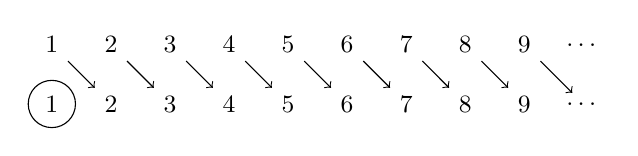
\begin{tikzpicture}[scale = .75]
		\foreach \x in {1, 2, 3, 4, 5, 6, 7, 8, 9}
		{
			\node (\x a) at (\x, 1) {\small{\x}};
			\node (\x b) at (\x, 2) {\small{\x}};
		}
		\node (dotsa) at (10, 1) {\small{\ldots}};
		\node (dotsb) at (10, 2) {\small{\ldots}};
		\draw[->] (1b)--(2a);
		\draw[->] (2b)--(3a);
		\draw[->] (3b)--(4a);
		\draw[->] (4b)--(5a);
		\draw[->] (5b)--(6a);
		\draw[->] (6b)--(7a);
		\draw[->] (7b)--(8a);
		\draw[->] (8b)--(9a);
		\draw[->] (9b)--(dotsa);
		\draw (1,1) circle (.4);
		\end{tikzpicture}
	\end{center}
	(\citealt[730]{EwaldSieg2013} இல் வெளியிடப்பட்டது;
    OpenLogic ஆசிரியர்களின் மொழிபெயர்ப்பு)
\end{quote}

% SEGMENT OLP-0050-S02
ஹில்பர்ட்டின் விடுதியில் முடிவுறாத எண்ணிக்கையிலான அறைகள் உள்ளன
என்பதே முக்கியக் கருத்து; அவ்வாறு கூறுவதன் பொருளை வரையறுப்பதாக
அவரது விளக்கத்தை எடுத்துக்கொள்ளலாம்.
உண்மையில் இதுவே டெடெகிண்டின் அணுகுமுறை
(நிச்சயமாக, இங்கு பெரும் காலப்பொருத்தமின்மையுடன் வழங்கப்பட்டுள்ளது;
டெடெகிண்டின் வரையறை \citeyear{Dedekind1888} ஆண்டைச் சேர்ந்தது):

% SEGMENT OLP-0050-S03
\begin{defn}\ollabel{defn:DedekindInfinite}
$A$ இலிருந்து $A$ இன் ஒரு தகு உட்கணத்திற்குச் செல்லும்
!!a{injection} இருக்கும்போது, அப்போதும் அப்போது மட்டுமே,
ஒரு கணம் $A$ என்பது \emph{டெடெகிண்ட்-முடிவுறாதது} ஆகும்.
அதாவது, $o \notin \ran{f}$ என அமையும் ஏதோ ஒரு $o \in A$ உம்
!!a{injection} $f \colon A \to A$ உம் உள்ளன.
\end{defn}


% END SOURCE UNIT OLP-0050

\endgroup

\begingroup
\makeatletter
\def\ol@sectioncs{section}
\makeatother
\def\olfilename{dedekind-algebra}

% BEGIN SOURCE UNIT OLP-0051 content/sets-functions-relations/infinite/dedekind-algebra.tex
% Exact modular target bytes: 10814; SHA256: 2318ef85ef56791ffd40cc9bebf56b344be1981fb0d6f4957b54c5ce8ce53c78
% SEGMENT OLP-0051-S01


\olfileid{sfr}{infinite}{dedekind}
\olsection{டெடெகிண்ட் இயற்கணிதங்கள்}

இயல் எண்கள் முடிவுறாதவையாக மட்டும் இருக்க வேண்டும் என்று விரும்பவில்லை;
அவை சில (இயற்கணித) பண்புகளையும் கொண்டிருக்க வேண்டும் என்று விரும்புகிறோம்:
கூட்டல், பெருக்கல் முதலியவற்றின் கீழ் அவை ஒழுங்காகச் செயல்பட வேண்டும்.

\emph{தொடரிச் சார்பு} என்ற கருத்தை அடிப்படையாக எடுத்துக்கொண்டு,
பின்வரும் பண்புகளைக் கொண்டவையாக எண்களைப் பண்புரைப்பதே
டெடெகிண்டின் கருத்து:
\begin{enumerate}
	\item எந்த எண்ணின் தொடரியும் அல்லாத $0$ என்ற ஓர் எண் உள்ளது
	\\ அதாவது, $0 \notin \ran{s}$
	\\ அதாவது, $\forall x\ s(x) \neq 0$
	\item வெவ்வேறு எண்களுக்கு வெவ்வேறு தொடரிகள் உள்ளன
	\\ அதாவது, $s$ ஓர் !!a{injection}
	\\ அதாவது, $\forall x \forall y (s(x) = s(y) \lif x = y)$
	\item\ollabel{repeatedapplication} தொடரிச் சார்பை $0$ மீது
    மீண்டும் மீண்டும் பயன்படுத்துவதன் மூலம் ஒவ்வோர் எண்ணும் பெறப்படுகிறது.
\end{enumerate}
முதலிரண்டு நிபந்தனைகளையும் முதல்தரத் தருக்கவியலைப் பயன்படுத்தி
எளிதாகக் கையாளலாம் (மேலே பார்க்கவும்).
ஆனால் முதல்தரத் தருக்கவியலை மட்டும் கொண்டு
\olref{repeatedapplication} ஐக் கையாள முடியாது.
\olref{repeatedapplication} என்ற நிபந்தனையைப் பின்வருமாறு
கணக்கோட்பாட்டு முறையில் மறுவடிவமைத்ததே டெடெகிண்டின் முன்னேற்றம்:
\begin{enumerate}
	\item[3$'$.] இயல் எண்கள், தொடரிச் சார்பின் கீழ்
	\emph{மூடப்பட்டுள்ள} மீச்சிறு கணம்;
    அதாவது, அந்தக் கணத்தின் எந்த !!{element} மீதும் $s$ ஐப்
    பயன்படுத்தினால், அந்தக் கணத்தின் மற்றோர் !!{element}[acc]ப் பெறுகிறோம்.
\end{enumerate}
ஆனால் இதனை மெதுவாக விரித்துரைக்க வேண்டும்.

% SEGMENT OLP-0051-S02
\begin{defn}\ollabel{Closure}
	எந்தச் சார்பு $f$ க்கும், $(\forall x \in X)f(x) \in X$ என
    இருக்கும்போது, அப்போதும் அப்போது மட்டுமே, கணம் $X$ ஆனது
    $f$-\emph{மூடப்பட்டது} ஆகும்.
    இப்போது எந்த $o$ க்கும் பின்வருமாறு வரையறுக்க:
	$$\closureofunder{f}{o} = \bigcap\Setabs{X}{o \in X\text{ மற்றும் }X
\text{ ஆனது $f$-மூடப்பட்டது}}$$
\end{defn}

% SEGMENT OLP-0051-S03
எனவே $\closureofunder{f}{o}$ என்பது, $o$ ஐ ஓர் !!a{element} ஆகக்
கொண்ட எல்லா $f$-மூடிய கணங்களின் வெட்டாகும்.
அப்படியானால், உள்ளுணர்வின்படி, $\closureofunder{f}{o}$ என்பது
$o$ ஐ ஓர் !!a{element} ஆகக் கொண்ட \emph{மீச்சிறு} $f$-மூடிய கணம்.
பின்வரும் முடிவு அந்த உள்ளுணர்வைத் துல்லியமாக்குகிறது:
\begin{lem}\ollabel{closureproperties}
	எந்தச் சார்பு $f$ க்கும், அதன் சார்பகமும் வீச்சகமும் ஒரே கணம்
    $A$ ஆகவும், எந்த $o \in A$ க்கும்:
	\begin{enumerate}
		\item\ollabel{closurehaselem} $o \in \closureofunder{f}{o}$; மேலும்
		\item\ollabel{closureclosed} $\closureofunder{f}{o}$ ஆனது $f$-மூடப்பட்டது; மேலும்
		\item\ollabel{closuresmallest} $X$ ஆனது $f$-மூடப்பட்டும் $o \in
		X$ எனவும் இருந்தால், $\closureofunder{f}{o} \subseteq X$
	\end{enumerate}
\end{lem}

% SEGMENT OLP-0051-S04
\begin{proof}
$o$ ஐ ஓர் !!a{element} ஆகக் கொண்ட குறைந்தது ஒரு $f$-மூடிய கணம்
உள்ளது என்பதை கவனிக்கவும்; அது $\ran{f}\cup \{o\}$.
எனவே இத்தகைய கணங்கள் \emph{அனைத்தின்} வெட்டான
$\closureofunder{f}{o}$ உள்ளது.
இப்போது \olref{closurehaselem}--\olref{closuresmallest} ஐச்
சரிபார்க்க வேண்டும்.

\olref{closurehaselem} ஐப் பொறுத்தவரை:
$o$ ஐ ஓர் !!a{element} ஆகக் கொண்ட கணங்களின் வெட்டாக இருப்பதால்,
$o \in \closureofunder{f}{o}$.

\olref{closureclosed} ஐப் பொறுத்தவரை:
$x \in \closureofunder{f}{o}$ எனக் கொள்க.
எனவே $o \in X$ என்றும் $X$ ஆனது $f$-மூடப்பட்டது என்றும் இருந்தால்,
$x \in X$; மேலும் $X$ ஆனது $f$-மூடப்பட்டது என்பதால் $f(x) \in X$.
ஆகவே $f(x) \in \closureofunder{f}{o}$.

\olref{closuresmallest} ஐப் பொறுத்தவரை:
பொதுவாகவே, $X \in C$ எனில் $\bigcap C \subseteq X$.
\end{proof}

% SEGMENT OLP-0051-S05
இதனைப் பயன்படுத்தி பின்வருமாறு கூறலாம்:

\begin{defn}
ஒரு \emph{டெடெகிண்ட் இயற்கணிதம்} என்பது,
$f \colon A \to A$ என்ற ஒரு சார்பையும் ஏதோ ஓர் $o \in A$ ஐயும்
கொண்ட ஒரு கணம் $A$; அது பின்வருவனவற்றை நிறைவேற்றுகிறது:
	\begin{enumerate}
		\item \ollabel{ded:proper} $o \notin \ran{f}$
		\item \ollabel{ded:injection} $f$ ஓர் !!a{injection}
		\item \ollabel{ded:closure} $A = \closureofunder{f}{o}$
	\end{enumerate}
\end{defn}

% SEGMENT OLP-0051-S06
$A = \closureofunder{f}{o}$ என்பதால், $A$ என்பது $o$ ஐ ஓர்
!!a{element} ஆகக் கொண்ட மீச்சிறு $f$-மூடிய கணம் என நமது முந்தைய
முடிவு கூறுகிறது.
ஒரு டெடெகிண்ட் இயற்கணிதம் டெடெகிண்ட்-முடிவுறாதது என்பது தெளிவு;
வரையறையின் \olref{ded:proper}, \olref{ded:injection} என்ற
கூறுகளை மட்டும் பார்க்கவும்.
ஆனால் எந்த டெடெகிண்ட்-முடிவுறாத கணத்தையும் ஒரு டெடெகிண்ட்
இயற்கணிதமாக மாற்றலாம் என்பது மேலும் சுவையான உண்மை.

% SEGMENT OLP-0051-S07
\begin{thm}\ollabel{thm:DedekindInfiniteAlgebra}
ஒரு டெடெகிண்ட்-முடிவுறாத கணம் இருக்குமானால்,
ஒரு டெடெகிண்ட் இயற்கணிதம் உள்ளது.
\end{thm}

% SEGMENT OLP-0051-S08
\begin{proof}
$D$ டெடெகிண்ட்-முடிவுறாததாக இருக்கட்டும்.
எனவே $g \colon D \to D$ என்ற ஓர் உட்செலுத்தலும்
$o  \in D \setminus \ran{g}$ என்ற ஓர் உறுப்பும் உள்ளன.
இப்போது $A = \closureofunder{g}{o}$ என்க;
\olref{closureproperties} இன்படி $A$ உள்ளது, $o \in A$.
$f = \funrestrictionto{g}{A}$ என்க.
$A, f, o$ ஆகியவை ஒரு டெடெகிண்ட் இயற்கணிதத்தை அமைக்கின்றன
எனக் காட்டுவோம்.

\olref{ded:proper} ஐப் பொறுத்தவரை:
$o \notin \ran{g}$, $\ran{f} \subseteq \ran{g}$;
எனவே $o\notin \ran{f}$.

\olref{ded:injection} ஐப் பொறுத்தவரை:
$g$ என்பது $D$ மீதான ஓர் உட்செலுத்தல்;
எனவே $f \subseteq g$ உம் ஓர் உட்செலுத்தலாக இருக்க வேண்டும்.

\olref{ded:closure} ஐப் பொறுத்தவரை:
\olref{closureproperties} இன்படி $A$ ஆனது $g$-மூடப்பட்டது;
எனவே இன்னும் வலுவாக, $A$ ஆனது $f$-மூடப்பட்டது.
ஆகவே \olref{closureproperties} இன்படி
$\closureofunder{f}{o} \subseteq A$.
மேலும் $\closureofunder{f}{o}$ ஆனது $f$-மூடப்பட்டது;
$f = \funrestrictionto{g}{A}$ என்பதால்,
$\closureofunder{f}{o}$ ஆனது $g$-மூடப்பட்டது எனப் பின்தொடரும்.
எனவே \olref{closureproperties} இன்படி
$A \subseteq \closureofunder{f}{o}$.
\end{proof}


% END SOURCE UNIT OLP-0051

\endgroup

\begingroup
\makeatletter
\def\ol@sectioncs{section}
\makeatother
\def\olfilename{dedekind-induction}

% BEGIN SOURCE UNIT OLP-0052 content/sets-functions-relations/infinite/dedekind-induction.tex
% Exact modular target bytes: 7670; SHA256: c590efcf2c4d5d85dcacc9a42dd10c63c27b0deed5a758510cafff107baf44ba
% SEGMENT OLP-0052-S01


\olfileid{sfr}{infinite}{induction}
\olsection[கணிதத் தொகுத்தறிதல்]{டெடெகிண்ட் இயற்கணிதங்களும் கணிதத் தொகுத்தறிதலும்}

மிக முதன்மையாக, இப்போது ஒரு டெடெகிண்ட் இயற்கணிதம்---உண்மையில்,
\emph{எந்த} டெடெகிண்ட் இயற்கணிதமும்---இயல் எண்களுக்கான பதிலியாகச்
செயல்படும். பின்வரும் நேரடி விளைவே இதற்குக் காரணம்:

% SEGMENT OLP-0052-S02
\begin{thm}[கணிதத் தொகுத்தறிதல்]\ollabel{thm:dedinfiniteinduction}
$N, s, o$ ஆகியவை ஒரு டெடெகிண்ட் இயற்கணிதத்தை அமைக்கட்டும்.
அப்போது எந்தக் கணம் $X$ க்கும்:
	\begin{center}
		$o \in X$ எனவும் $(\forall {n} \in N \cap X){s}({n}) \in X$
        எனவும் இருந்தால், $N \subseteq X$.
	\end{center}
\end{thm}

% SEGMENT OLP-0052-S03
\begin{proof}
டெடெகிண்ட் இயற்கணிதத்தின் வரையறைப்படி,
$N = \closureofunder{s}{o}$.
இப்போது ${o} \in X$ எனவும் $(\forall {n} \in N)(n \in X \lif
{s}({n}) \in X)$ எனவும் இருந்தால்,
$N = \closureofunder{s}{o} \subseteq X$.
\end{proof}

தொகுத்தறிதல் இயல் எண்களின் இயல்புக்கூறாக இருப்பதால், கருத்து இதுதான்.
எந்த டெடெகிண்ட்-முடிவுறாத கணம் கொடுக்கப்பட்டாலும், ஒரு டெடெகிண்ட்
இயற்கணிதத்தை அமைத்து, அந்த இயற்கணிதத்தை இயல் எண்களுக்கான பதிலியாகப்
பயன்படுத்தலாம்.

% SEGMENT OLP-0052-S04
ஒப்புக்கொள்ள வேண்டுமெனில், \olref{thm:dedinfiniteinduction} ஆனது
தொகுத்தறிதலைக் \emph{கணக்கோட்பாட்டு} சொற்களில் வாய்பாடாக்குகிறது.
ஆனால் அதே நெறியை இன்னும் பழக்கமான சொற்களில் எளிதாகக் கூறலாம்:

\begin{cor}\ollabel{natinductionschema}
$N, s, o$ ஆகியவை ஒரு டெடெகிண்ட் இயற்கணிதத்தை அமைக்கட்டும்.
அப்போது அளபுருக்களைக் கொண்டிருக்கக்கூடிய எந்த வாய்பாடு
$\phi(x)$ க்கும்:
\begin{center}
	$\phi(o)$ எனவும் $(\forall {n} \in N)(\phi(n)\lif
	\phi({s}({n})))$ எனவும் இருந்தால், $(\forall n \in N)\phi(n)$.
\end{center}
\end{cor}

% SEGMENT OLP-0052-S05
\begin{proof}
$X = \Setabs{n \in N}{\phi(n)}$ என்க; இப்போது
\olref{thm:dedinfiniteinduction} ஐப் பயன்படுத்துக.
\end{proof}

% SEGMENT OLP-0052-S06
% READER FALLBACK TA-READER-REF-003; absent set-theory destinations get descriptive text.
இந்த முடிவில், ஒரு வாய்பாடு ``அளபுருக்களைக் கொண்டிருப்பது'' பற்றிப்
பேசினோம். இதன் தோராயமான பொருள்: எந்தப் பொருள்கள்
$c_1, \ldots, c_k$ க்கும், நாம் $\phi(x, c_1, \ldots, c_k)$ உடன்
வேலை செய்யலாம் என்பதாகும். இன்னும் துல்லியமாக, ``அளபுருக்கள்'' என்று
குறிப்பிடாமலேயே முடிவைப் பின்வருமாறு கூறலாம். கட்டற்ற மாறிகள் அனைத்தும்
காட்டப்பட்டுள்ள எந்த வாய்பாடு $\phi(x, v_1, \ldots, v_k)$ க்கும்:
	\begin{align*}
			\forall v_1 \ldots \forall v_k((&\phi(o, v_1,\ldots, v_k) \land {}\\
			&	(\forall x \in N)(\phi(x,v_1, \ldots, v_k) \lif \phi(s(x), v_1,\ldots, v_k))) \lif {}\\
			&\hspace{3em} (\forall x \in N)\phi(x, v_1,\ldots, v_k))
	\end{align*}
``அளபுருக்களைக் கொண்டிருப்பது'' என்று பேசுவது வாசிப்பை மிகவும்
எளிதாக்கும் என்பது தெளிவு.
(\oliflabeldef{sth:::part}{\olref[sth][][]{part} இல்}{%
கணக்கோட்பாடு பற்றிய பின்னைய பகுதியில்}, இந்த உத்தியை அடிக்கடி
பயன்படுத்துவோம்.)

% SEGMENT OLP-0052-S07
டெடெகிண்ட் இயற்கணிதங்களுக்குத் திரும்புவோம்: எந்த டெடெகிண்ட்
இயற்கணிதம் கொடுக்கப்பட்டாலும், கூட்டல், பெருக்கல், அடுக்கேற்றம் என்ற
வழக்கமான எண்கணிதச் சார்புகளையும் வரையறுக்கலாம். ஆனால் இது
எளியதன்று; \emph{மறுநிகழ்வு வரையறை} என்ற உத்தி இதில் பயன்படுகிறது.
இந்த உத்தியை மிகவும் பின்னர், இன்னும் பொதுவான சூழலில் அறிமுகப்படுத்தி
நியாயப்படுத்துவோம். (ஆர்வமுள்ளோர்
\oliflabeldef{sth:ord-arithmetic::chap}{%
\olref[sth][ord-arithmetic][]{chap} க்குப் பிறகு}{%
வரிசை எண்கணிதம் பற்றிய பின்னைய அத்தியாயத்திற்குப் பிறகு}
இதனை மீண்டும் பார்க்க விரும்பலாம்; அல்லது
\citealt[pp.~95--8]{Potter2004} போன்ற மாற்று விளக்கத்தைப் படிக்கலாம்.)
ஆனால் $N, s, o$ ஆகியவை ஒரு டெடெகிண்ட் இயற்கணிதத்தை அமைக்கும்போது,
இறுதியில் பின்வருவனவற்றை விதித்து:
\begin{align*}
	{a} + {o} &= {a} & & & {a} \times {o} &= {o} & & & {a}^{o} &= s(o)\\
{a} + {s}({b}) &= {s}({a}+{b}) &&& {a} \times {s}({b}) &= ({a}\times {b}) + {a}  & & & {a}^{{s}({b})} &= {a}^{b} \times {a}
\end{align*}
அவை எதிர்பார்த்தபடி செயல்படுகின்றன என்று காட்ட முடியும்.


% END SOURCE UNIT OLP-0052

\endgroup

\begingroup
\makeatletter
\def\ol@sectioncs{section}
\makeatother
\def\olfilename{dedekinds-proof}

% BEGIN SOURCE UNIT OLP-0053 content/sets-functions-relations/infinite/dedekinds-proof.tex
% Exact modular target bytes: 15912; SHA256: badf643f73c683a8b5e1c2f53b8b821b99b82fd870cb4e647a607ebda65f2614
% SEGMENT OLP-0053-S01


\olfileid{sfr}{infinite}{dedekindsproof}

\olsection[டெடெகிண்டின் ``நிறுவல்'']{முடிவுறாத கணமொன்று இருப்பதற்கான
டெடெகிண்டின் ``நிறுவல்''}

இந்த அத்தியாயத்தில், டெடெகிண்ட் இயற்கணிதங்களின் வழியாக இயல் எண்களைக்
கணக்கோட்பாட்டு முறையில் கையாண்டோம். \olref[arith][ref]{sec} இல்,
பகுப்பாய்வியலின் எண்முறைமைக் கட்டமைப்பின் மெய்யியல் முக்கியத்துவத்தைப்
(பிறவற்றுடன்) பற்றி சிந்தித்தோம். இங்கு நாம் சாதித்திருப்பதன்
முக்கியத்துவத்தை இப்போது சிந்திக்க வேண்டும்.

% SEGMENT OLP-0053-S02
\olref[sfr][arith][]{chap} முழுவதிலும், இயல் எண்களை நமக்குத்
தரப்பட்டவையாக ஏற்றுக்கொண்டு, அவற்றைப் பயன்படுத்தி முழுக்கள்,
விகிதமுறு எண்கள், மெய்யெண்கள் ஆகியவற்றை வெளிப்படையாகக் கட்டமைத்தோம்.
இந்த அத்தியாயத்தில், இயல் எண்களை வெளிப்படையாகக் கட்டமைக்கவில்லை.
\emph{எந்த டெடெகிண்ட்-முடிவுறாத கணமும் தரப்பட்டால்}, $\Nat$ எவ்வாறு
செயல்பட வேண்டும் என்று நாம் விரும்புகிறோமோ அவ்வாறே செயல்படும் ஒரு
கணத்தை வரையறுக்கலாம் என்று மட்டுமே காட்டியுள்ளோம்.

% SEGMENT OLP-0053-S03
எனவே, \emph{எந்தப் பொருள்களே இயல் எண்கள்} என்பது போன்ற ஒரு
மெய்ப்பொருளியல் வினாவுக்கு விடையளித்துவிட்டோம் என்று நாம் கூற முடியாது
என்பது தெளிவு. அது நல்லதும்கூட. ஏனெனில், $\Real$ ஐ டெடெகிண்ட்
வெட்டுகளின் கணம் என்று வரையறுப்பதை ஒரு வசதியான விதிப்பாகக் கொள்ளாமல்,
ஒரு \emph{கண்டுபிடிப்பாகக்} கொள்வது தவறு என்று
\olref[sfr][arith][ref]{sec} இல் வலியுறுத்தினோம்.
மெய்யெண்களின் முதன்மையான கணிதப் பண்புகளுக்கு டெடெகிண்ட் வெட்டுகள்
எடுத்துக்காட்டுகளாக அமைகின்றன என்பதே தீர்மானமான கவனிப்பு.
இங்கும் அவ்வாறே: இயல் எண்களின் முதன்மையான கணிதப் பண்புகளுக்கு
\emph{எந்த} டெடெகிண்ட் இயற்கணிதமும் எடுத்துக்காட்டாக அமைகிறது என்பதே
தீர்மானமான கவனிப்பு. (உண்மையில், எல்லா டெடெகிண்ட் இயற்கணிதங்களும்
\emph{சமவடிவமானவை} என்று நிறுவி, டெடெகிண்ட் இந்தக் கருத்தை
வலுவுறுத்தினார் (\citeyear[Theorems
132--3]{Dedekind1888}).
எனவே, தற்கால ``அமைப்பியலாளர்கள்'' பலர் டெடெகிண்டை ஒரு முன்னோடியாகக்
குறிப்பிடுவதில் வியப்பில்லை.)

% SEGMENT OLP-0053-S04
மேலும், இன்னும் ஓரளவு நெறிப்படுத்தப்படாததாகவே உள்ள, ஆனால் இயல்
எண்களை நமக்குத் தரப்பட்டவையாகக் (வெளிப்படையாக) கருதாத முறைசாராத
எளிய கணக்கோட்பாட்டிற்குள் இயல் எண்களின் கோட்பாட்டை எவ்வாறு பதிக்கலாம்
என்பதைக் காட்டியுள்ளோம். ஆகவே, டெடெகிண்ட் பின்வருமாறு விளக்கிய அவரது
சொந்த உயர்நோக்குத் திட்டத்தை நிறைவேற்றும் பாதையில் நாம் இருக்கலாம்:

% SEGMENT OLP-0053-S05
\begin{quote}
	அறிவியலில் நிறுவக்கூடிய எதையும் நிறுவல் இல்லாமல் நம்பக் கூடாது.
	இந்தக் கோரிக்கை நியாயமானதாகத் தோன்றினாலும், மிக எளிய அறிவியலுக்கு
	அடித்தளம் அமைக்கும் அண்மைக்கால முறைகளில்கூட அது நிறைவேற்றப்பட்டுள்ளது
	என்று என்னால் கருத முடியாது; அதாவது, எண்களின் கோட்பாட்டைக் கையாளும்
	தருக்கவியலின் அந்தப் பகுதியில். எண்கணிதத்தை (இயற்கணிதம்,
	பகுப்பாய்வியல்) தருக்கவியலின் ஒரு பகுதி மட்டுமே என்று கூறுவதன் மூலம்,
	எண்-கருத்தை வெளி, காலம் பற்றிய கருத்துகளிலிருந்தோ உள்ளுணர்வுகளிலிருந்தோ
	முற்றிலும் சார்பற்றதாக நான் கருதுகிறேன் என்பதையே உணர்த்துகிறேன்---
	அதனைத் தூய சிந்தனை விதிகளின் நேரடி விளைபொருளாகவே கருதுகிறேன்.
	\citep[preface]{Dedekind1888}
\end{quote}

% SEGMENT OLP-0053-S06
டெடெகிண்டின் துணிவான கருத்து இதுதான். முறைசாராத கணக்கோட்பாட்டை
மட்டுமே பயன்படுத்தி இயல் எண்களை எவ்வாறு அமைப்பது என்று இப்போதுதான்
காட்டினோம். இயல் எண்களும் சிறிது கணக்கோட்பாடும் தரப்பட்டால்
மெய்யெண்களை எவ்வாறு கட்டமைப்பது என்று \olref[sfr][arith][]{chap} இல்
கண்டோம். ஆகவே, ஒருவேளை, ``எண்கணிதம் (இயற்கணிதம், பகுப்பாய்வியல்)''
என்பது ``தருக்கவியலின் ஒரு பகுதி மட்டுமே'' என்று திகழலாம்
(டெடெகிண்ட் ``தருக்கவியல்'' என்ற சொல்லுக்கு அளித்த விரிவான பொருளில்).

% SEGMENT OLP-0053-S07
கருத்து இதுதான். ஆனால் சற்று நிறுத்துங்கள். ஒரு டெடெகிண்ட் இயற்கணிதத்தை
(இயல் எண்களுக்கான நமது பதிலியை) நாம் கட்டமைப்பது, ஒரு
டெடெகிண்ட்-முடிவுறாத கணம் இருப்பதை நிபந்தனையாகக் கொண்டுள்ளது.
(\olref[sfr][infinite][dedekind]{thm:DedekindInfiniteAlgebra} ஐத்
திரும்பிப் பாருங்கள்.) ஒரு டெடெகிண்ட்-முடிவுறாத கணம் இருப்பதைத்
``தருக்கவியல்'' அல்லது ``தூய சிந்தனை விதிகள்'' கொண்டு நிறுவ
முடியாவிட்டால், இந்தத் திட்டம் நின்றுவிடும்.

% SEGMENT OLP-0053-S08
அப்படியானால், ஒரு டெடெகிண்ட்-முடிவுறாத கணம் இருப்பதைத்
``தூய சிந்தனை விதிகள்'' கொண்டு நிறுவ \emph{முடியுமா}?
டெடெகிண்டின் முயற்சி இதோ:

% SEGMENT OLP-0053-S09
\begin{quote}
  என் சொந்தச் சிந்தனைகளின் மண்டலம், அதாவது என் சிந்தனைக்குப்
  பொருள்களாக இருக்கக்கூடிய அனைத்துப் பொருள்களின் ஒட்டுமொத்தம் $S$,
  முடிவுறாதது. ஏனெனில் $s$ என்பது $S$ இன் ஓர் உறுப்பு எனில்,
  $s$ என் சிந்தனைக்குப் பொருளாக இருக்க முடியும் என்ற சிந்தனை $s'$
  ஆனதும் $S$ இன் ஓர் உறுப்பாகும். இதனை உறுப்பு $s$ இன் படிமம்
  $\phi(s)$ எனக் கொண்டால், அப்போது \dots~$S$ ஆனது [டெடெகிண்ட்]
  முடிவுறாதது; நிறுவ வேண்டியது இதுவே.
	\citep[\S66]{Dedekind1888}
\end{quote}

% SEGMENT OLP-0053-S10
மிகவும் கடுமையான கணித நிறுவல்களையே பெரும்பாலும் கொண்ட ஒரு நூலின்
நடுவில் இதனைக் காண்பது மிகவும் வியப்பூட்டுகிறது. இரண்டு குறிப்புகளைக்
கூறுவது பயனுள்ளது.

% SEGMENT OLP-0053-S11
முதலாவது: இந்த ``நிறுவல்'' இன்று நாம் ``கணிதத்தன்மை'' என்று
அடையாளம் காணக்கூடிய பண்பை ஏறத்தாழக் கொண்டிருக்கவில்லை.
இது உளவியல் பொருள்களைப் (சிந்தனைகளைப்) பேசுகிறது; அதிலும் வெறும்
\emph{இருக்கக்கூடிய} பொருள்களையே பேசுகிறது.

% SEGMENT OLP-0053-S12
இரண்டாவது: டெடெகிண்ட் இயற்கணிதங்களை நாம் வழங்கியுள்ள விதத்திலாவது,
இந்த ``நிறுவலில்'' ஒரு நேரடியான தொழில்நுட்பக் குறைபாடு உள்ளது.
டெடெகிண்டின் வாதம் வெற்றிபெற்றால், முடிவுறாத அளவு பல பொருள்கள்
(குறிப்பாக, முடிவுறாத அளவு பல சிந்தனைகள்) உள்ளன என்று மட்டுமே
அது நிறுவுகிறது. ஆனால் $S$ ஐ, பன்மையில் $S$ என்பதை
\emph{சில பொருள்கள்} என்று
கருதாமல், முடிவுறாத அளவு பல !!{element}s கொண்ட ஒரே \emph{கணமாகக்}
கருதுவதற்கான காரணத்தையும் டெடெகிண்ட் நமக்குத் தர வேண்டும்.

% SEGMENT OLP-0053-S13
டெடெகிண்ட் இங்கு ஒரு இடைவெளியைக் காணவில்லை என்ற உண்மை, அவர்
``ஒட்டுமொத்தம்'' என்ற சொல்லைப் பயன்படுத்திய விதம், \emph{நாம்} ``கணம்'' என்ற
சொல்லைப் பயன்படுத்தும் விதத்தைத் துல்லியமாகப் பின்பற்றவில்லை என்று
உணர்த்தலாம்.\footnote{அவ்வாறு பின்பற்றவில்லை என்று எண்ணுவதற்கு வேறு
காரணங்களும் நமக்கு உள்ளன; \citet[p.~23]{Potter2004} ஐப் பார்க்கவும்.}
ஆனால் இது மிகுந்த வியப்பிற்குரியதன்று. கடந்த இரண்டு அத்தியாயங்களில்
நாம் மேற்கொண்ட திட்டம்---இயல் எண்களின் ஒரு ``கட்டமைப்பு'', அவற்றிலிருந்து
முழுக்கள், மெய்யெண்கள், விகிதமுறு எண்கள் ஆகியவற்றின் ஒரு
``கட்டமைப்பு''---முழுவதும் முறைசாராத விதத்தில் மேற்கொள்ளப்பட்டது.
எந்தக் கணங்கள் எப்போது உள்ளன என்பது பற்றிய பல பொதுக் கொள்கைகளை
வகுக்காமலேயே, நமக்குத் தேவைப்பட்டபோதெல்லாம் இந்தக் கணம் அல்லது அந்தக்
கணம் உள்ளதாக எடுத்துக்கொண்டோம். ஆனால் \emph{சில} பொதுக் கொள்கைகள்
நமக்குத் தேவை என்பது தெரியும்; இல்லாவிட்டால் ரசலின் முரண்பாட்டில்
விழுந்துவிடுவோம்.

நமது முறைசாராமையைக் கடந்து வளர வேண்டிய நேரம் வந்துவிட்டது.


% END SOURCE UNIT OLP-0053

\endgroup

\begingroup
\makeatletter
\def\ol@sectioncs{section}
\makeatother
\def\olfilename{card-sb}

% BEGIN SOURCE UNIT OLP-0054 content/sets-functions-relations/infinite/card-sb.tex
% Exact modular target bytes: 8351; SHA256: 37877cbcb2538c4e44b42ca5c664146d4f762d105d1de0791f3ad234a73349b9
% SEGMENT OLP-0054-S01


\olfileid{sfr}{infinite}{card-sb}

\olsection{இணைப்பு: ஷ்ரோடர்--பெர்ன்ஸ்டைன் தேற்றத்தை நிறுவுதல்}

முறைசாராத கணக்கோட்பாட்டிலிருந்து விடைபெறும்முன், கடைசியாக ஒரு
முறைசாராத (ஆனால் நுணுக்கமான!{}) நிறுவலைக் கருத வேண்டும்.
இது ஷ்ரோடர்--பெர்ன்ஸ்டைன் தேற்றத்தின்
(\olref[sfr][siz][sb]{thm:schroder-bernstein}) நிறுவல்:
$\cardle{A}{B}$ மற்றும் $\cardle{B}{A}$ எனில் $\cardeq{A}{B}$;
அதாவது, $f \colon A \to B$, $g \colon B \to A$ என்ற
!!{injection}s கொடுக்கப்பட்டால், $h \colon A \to B$ என்ற
!!a{bijection} உள்ளது.

இந்த அத்தியாயத்தில் டெடெகிண்டின் \emph{மூடல்கள்} என்ற கருத்தைப்
பின்பற்றினோம். உண்மையில், இந்தக் கருத்தைப் பயன்படுத்தி டெடெகிண்ட்
ஷ்ரோடர்--பெர்ன்ஸ்டைன் தேற்றத்திற்கு ஓர் அழகிய நிறுவலைத் தந்தார்;
அதனை இங்கு வழங்குவோம். சற்றே வேறுபட்டாலும் சாரத்தில் இதே போன்ற
விளக்கம் வேண்டுமெனில், இந்த நிறுவல் \citet[pp.~157--8]{Potter2004} ஐ
நெருக்கமாகப் பின்பற்றுகிறது. இணையத்தில் சிறிது தேடுவதும்கூட,
$\sqrt{2}$ இன் விகிதமுறாமையைப் போலவே, \emph{பல} சுவையான,
வேறுபட்ட நிறுவல்கள் உள்ள ஒரு தேற்றம் இது என்று உங்களை நம்பவைக்கும்.

% SEGMENT OLP-0054-S02
\olref[sfr][infinite][dedekind]{Closure} இல் உள்ளதுபோன்ற குறியீட்டைப்
பயன்படுத்தி, ஒவ்வொரு கணம் $B$ க்கும் சார்பு~$f$ க்கும்
பின்வருமாறு கொள்க:
\[
\Closureofunder{f}{B} = \bigcap \Setabs{X}{B \subseteq X
\text{ மற்றும் $X$ ஆனது $f$-மூடப்பட்டது}}
\]
இவ்வாறு வரையறுக்கப்படும் $\Closureofunder{f}{B}$ என்பது $B$ ஐக்
கொண்ட மீச்சிறு $f$-மூடிய கணம்; அதாவது:

% SEGMENT OLP-0054-S03
\begin{lem}\ollabel{Closureprops}
	எந்தச் சார்பு $f$ க்கும், எந்த $B$ க்கும்:
	\begin{enumerate}
		\item\ollabel{Closurehaselem} $B \subseteq \Closureofunder{f}{B}$; மேலும்
		\item\ollabel{Closureclosed} $\Closureofunder{f}{B}$ ஆனது $f$-மூடப்பட்டது; மேலும்
		\item\ollabel{Closuresmallest} $X$ ஆனது $f$-மூடப்பட்டும் $B
		\subseteq X$ எனவும் இருந்தால், $\Closureofunder{f}{B} \subseteq X$.
	\end{enumerate}
\end{lem}

% SEGMENT OLP-0054-S04
\begin{proof}
\olref[sfr][infinite][dedekind]{closureproperties} இல் உள்ளதைப்
போலவே நிறுவலாம்.
\end{proof}

ஷ்ரோடர்--பெர்ன்ஸ்டைன் தேற்றத்தை அடைவதற்கு இன்னும் ஒரு உண்மை தேவை:

% SEGMENT OLP-0054-S05
\begin{prop}\ollabel{sbhelper}
$A \subseteq B \subseteq C$ மற்றும் $A \approx C$ எனில்,
$\cardeq{\cardeq{A}{B}}{C}$.
\end{prop}

% SEGMENT OLP-0054-S06
\begin{proof}
$f \colon C \to A$ என்ற !!a{bijection} கொடுக்கப்பட்டுள்ளதாகக் கொள்க.
$F = \Closureofunder{f}{C \setminus B}$ என வைத்து, சார்பகம் $C$ ஆகக்
கொண்ட ஒரு சார்பு $g$ ஐப் பின்வருமாறு வரையறுக்க:
\[
	g(x) =
	\begin{cases}
			f(x) &\text{$x \in F$ எனில்}\\
			x & \text{மற்றபடி}
	\end{cases}
\]
$g$ ஆனது $C \to B$ என்ற !!a{bijection} எனக் காட்டுவோம்.
அதிலிருந்து $\comp{f^{-1}}{g} \colon A \to B$ என்பது
!!a{bijection} எனப் பின்தொடரும்; இது நிறுவலை நிறைவுசெய்யும்.

% SEGMENT OLP-0054-S07
முதலில், $x \in F$ ஆனால் $y\notin F$ எனில் $g(x) \neq g(y)$ என்று
கூறுகிறோம். இதற்கு மாறாக இருப்பதாக முரண்வழியாகக் கொள்க; அப்போது
$y = g(y) = g(x) = f(x)$. $x \in F$ என்பதாலும்,
\olref{Closureprops} இன்படி $F$ ஆனது $f$-மூடப்பட்டது என்பதாலும்,
$y = f(x) \in F$; இது ஒரு முரண்.

% SEGMENT OLP-0054-S08
இப்போது $g(x) = g(y)$ எனக் கொள்க. மேலுள்ளதன்படி,
$x \in F$ எனின், அப்போதும் அப்போது மட்டுமே, $y \in F$.
$x, y \in F$ எனில், $f(x) = g (x) = g(y) = f(y)$;
$f$ ஒரு !!a{bijection} என்பதால் $x = y$.
$x, y \notin F$ எனில், $x = g(x) = g(y) = y$.
ஆகவே $g$ ஓர் !!a{injection}.

% SEGMENT OLP-0054-S09
$\ran{g} = B$ என இன்னும் காட்ட வேண்டும். ஆகவே
$x \in B \subseteq C$ ஐ நிலைநிறுத்துக. $x \notin F$ எனில்,
$g(x) = x$. $x \in F$ எனில், ஏதோ $y \in F$ க்கு $x = f(y)$;
ஏனெனில் அவ்வாறு இல்லாவிட்டால் $F \setminus \{x\}$ ஆனது
$f$-மூடப்பட்டு $C\setminus B$ ஐ உள்ளடக்கியிருக்கும்; இது
\olref{Closureprops} இன்படி இயலாதது. இப்போது $g(y) = f(y) = x$.
\end{proof}

% SEGMENT OLP-0054-S10
இறுதியாக, முதன்மை முடிவின் நிறுவல் இதோ. ஒரு சார்பு $h$ உம் கணம்
$D$ உம் கொடுக்கப்பட்டால், $\funimage{h}{D} = \Setabs{h(x)}{x
\in D}$ என வரையறுக்கிறோம் என்பதை நினைவுகூர்க.

% SEGMENT OLP-0054-S11
\begin{proof}[ஷ்ரோடர்--பெர்ன்ஸ்டைன் தேற்றத்தின் நிறுவல்]
$f \colon A \to B$, $g \colon B \to A$ ஆகியவை !!{injection}s
ஆக இருக்கட்டும். $\funimage{f}{A} \subseteq B$ என்பதால்,
$\funimage{g}{\funimage{f}{A}} \subseteq g[B] \subseteq A$.
மேலும் $g$, $f$ இரண்டும் உட்செலுத்தல்கள் என்பதால்,
$\comp{f}{g} \colon A \to \funimage{g}{\funimage{f}{A}}$ ஆனதும்
ஓர் !!{injection}; உண்மையில், அதன் வீச்சகத்தை நாம் வரையறுத்த
விதத்தினாலேயே $\comp{f}{g}$ ஓர் !!a{bijection}.
ஆகவே $\cardeq{\funimage{g}{\funimage{f}{A}}}{A}$;
எனவே \olref{sbhelper} இன்படி $h \colon A \to \funimage{g}{B}$ என்ற
!!a{bijection} உள்ளது. மேலும் $g^{-1}$ ஆனது
$\funimage{g}{B} \to B$ என்ற !!a{bijection}.
ஆகவே $\comp{h}{g^{-1}} \colon A \to B$ ஓர் !!a{bijection}.
\end{proof}


% END SOURCE UNIT OLP-0054

\endgroup



% END SOURCE UNIT OLP-0049

\endgroup


\OLEndPartHook

% END SOURCE UNIT OLP-0003

\endgroup


\begingroup
\makeatletter
\def\ol@sectioncs{section}
\makeatother
\def\olfilename{propositional-logic}

% BEGIN SOURCE UNIT OLP-0055 content/propositional-logic/propositional-logic.tex
% Exact modular target bytes: 2772; SHA256: 4ab90bce479b5ef2ea36bce5c3e9943d39ddd817e906f1886d190829e09c1921
% SEGMENT OLP-0055-S01


\olpart{pl}{கூற்றுத் தருக்கவியல்}

\begin{editorial}
  இந்தப் பகுதியில் செவ்வியல் கூற்றுத் தருக்கவியல் பற்றிய உள்ளடக்கம்
  இடம்பெறுகிறது. முதல் அத்தியாயம் ஒப்பீட்டளவில் தொடக்கநிலையானது; அது
  வரையறைகளையும் முடிவுகளையும் பட்டியலிடுகிறது. பல நிறுவல்கள் செய்து
  காட்டப்படாமல் பயிற்சிகளாக விடப்பட்டுள்ளன. நிறுவல் முறைமைகள் மற்றும்
  நிறைவுத் தேற்றம் பற்றிய உள்ளடக்கம், முதல்தரத் தருக்கவியல் பகுதியிலிருந்து
  ``FOL'' குறிச்சொல்லைப் பொய்யாக அமைத்து சேர்க்கப்படுகிறது. இதனால்
  பயனிலைகள், பதங்கள், அளவையீட்டிகள் தொடர்பான அனைத்தும் விலக்கப்பட்டு,
  !!{structure}s~$\Struct{M}$ பற்றிய உரை !!{valuation}s~$\pAssign{v}$
  பற்றிய உரையாக மாற்றப்படுகிறது.

  இப்பகுதிக்கு மேலும் விவரங்களைச் சேர்த்து விரிவுபடுத்தவும்,
  மெய்மதிப்புசார் நிறைவு போன்ற கூடுதல் தலைப்புகளையும் முடிவுகளையும்
  சேர்க்கவும் திட்டமிடப்பட்டுள்ளது.
\end{editorial}

\begingroup
\makeatletter
\def\ol@sectioncs{section}
\makeatother
\def\olfilename{syntax-and-semantics}

% BEGIN SOURCE UNIT OLP-0056 content/propositional-logic/syntax-and-semantics/syntax-and-semantics.tex
% Exact modular target bytes: 1035; SHA256: 170f00f16333ccbc750fb556fe900ed153bfb2eed9225d955384dbf1b655916e
% SEGMENT OLP-0056-S01


\olchapter{pl}{syn}{தொடரமைப்பும் பொருண்மையும்}

\begin{editorial}
  இது வரையறைகளை மட்டும் மிகச் சுருக்கமாகத் தொகுக்கிறது. வாய்பாடுகள்மீதான
  தொகுத்தறிதல் நிறுவல்களை மெதுவாக அறிமுகப்படுத்தவும் இன்னும் பல
  எடுத்துக்காட்டுகளை வழங்கவும் இது விரிவுபடுத்தப்பட வேண்டும்.
\end{editorial}

\begingroup
\makeatletter
\def\ol@sectioncs{section}
\makeatother
\def\olfilename{introduction}

% BEGIN SOURCE UNIT OLP-0057 content/propositional-logic/syntax-and-semantics/introduction.tex
% Exact modular target bytes: 10625; SHA256: 1b5c99401dd3e39424f0fbad1c61bdce1afb9c5e845fdc639b5a41584f658a5e
% SEGMENT OLP-0057-S01


\olfileid{pl}{syn}{int}

\olsection{அறிமுகம்}

கூற்றுத் தருக்கவியலின் !!{formula}s, !!{propositional variable}s
மற்றும் $\lnot$, $\land$, $\lor$, $\lif$, $\liff$ ஆகிய கூற்று
இணைப்புகளைப் பயன்படுத்திக் கட்டமைக்கப்படுகின்றன. உள்ளுணர்வுப்படி,
!!a{propositional variable}~$p$ என்பது மெய்யோ பொய்யோ ஆன ஒரு
வாக்கியம் அல்லது கூற்றைக் குறிக்கிறது. ஒரு !!a{formula}வில் வரும்
!!{propositional variable}களின் ``மெய்மதிப்பு'' தீர்மானிக்கப்பட்டவுடன்,
அவற்றிலிருந்து கூற்று இணைப்புகளால் கட்டமைக்கப்பட்ட ஒவ்வொரு
!!a{formula}வின் மெய்மதிப்பும் தீர்மானிக்கப்படுகிறது. ஆகவே அதன்
பொருண்மை மெய்மதிப்புகளின் சார்புகளால் தரப்படுவதால், கூற்றுத் தருக்கவியல்
\emph{மெய்மதிப்புசார்} என்று கூறுகிறோம். குறிப்பாக, ஒரு கூற்று வெறுமனே
சூழ்நிலைசார் மெய்யாக இல்லாமல் இன்றியமையாமல் மெய்யா, அது மெய்யென்று
அறியப்பட்டுள்ளதா, அல்லது அது முன்பு மெய்யாக இருந்ததா பின்னர் மெய்யாகுமா
என்பதற்குப் பதிலாக இப்போது மெய்யா போன்ற மெய்மை--பொய்மை பற்றிய மேலதிக
வேறுபாடுகளைக் கூற்றுத் தருக்கவியலில் கருத்தில் கொள்ளமாட்டோம். மெய்
($\True$), பொய் ($\False$) என்ற இரு மெய்மதிப்புகளை மட்டுமே கருதுகிறோம்;
எனவே ஒரு கூற்று மெய்யுமல்ல பொய்யுமல்ல என்றோ அரைமெய் என்றோ அமையும்
சாத்தியத்தை விவாதத்திலிருந்து விலக்குகிறோம். மேலும், ஒரு !!a{formula}வின்
மெய்மதிப்பு அதன் பகுதிகளின் மெய்மதிப்புகளால் முற்றிலும் தீர்மானிக்கப்படும்
இணைப்புகளையே கவனிக்கிறோம்; அதன் பொருளால் தீர்மானிக்கப்படுவதை அல்ல.
குறிப்பாக, ஆங்கில நிபந்தனைக்கூற்றுகளின் மெய்மதிப்பு இவ்வகையில்
மெய்மதிப்புசார் தானா என்பது சர்ச்சைக்குரியது. பொருட்சார் நிபந்தனையான
$\lif$ மெய்மதிப்புசார்; மெய்மதிப்புசார் அல்லாத நிபந்தனைகளை வேறு
தருக்கவியல்கள் கையாளுகின்றன.

% SEGMENT OLP-0057-S02
மெய்மதிப்புசார் கூற்றுத் தருக்கவியலின் கோட்பாட்டையும் மீக்கோட்பாட்டையும்
வளர்க்க, முதலில் அதன் கோவைகளின் தொடரமைப்பையும் பொருண்மையையும் வரையறுக்க
வேண்டும். இணைப்புகளைப் பயன்படுத்தி !!{propositional variable}s இலிருந்து
!!{formula}s கட்டமைக்கும் ஒரு முறையை விவரிப்போம். வேறு வரையறைகளும்
சாத்தியம். பிற முறைமைகள் வேறு குறியீடுகளைத் தேர்ந்தெடுக்கலாம்; வேறு
இணைப்புக் கணங்களை மூல இணைப்புகளாகக் கொள்ளலாம்; அடைப்புக்குறிகளை வேறுபடப்
பயன்படுத்தலாம். போலந்து குறிமுறை எனப்படும் முறையில் அடைப்புக்குறிகளே
இல்லாமலும் இருக்கலாம். ஆனாலும் எல்லா அணுகுமுறைகளிலும், அமைப்பு விதிகள்
!!{formula}s இன் கணத்தை \emph{தொகுத்தறிதலாக} வரையறுக்கின்றன. அவை சரியாக
அமைக்கப்பட்டால், ஒவ்வொரு கோவையும் அமைப்பு விதிகளிலிருந்து அடிப்படையில்
ஒரே ஒரு வழியில் மட்டுமே உருவாகும். கோவைகளுக்குத் \emph{தனித்த
வாசிப்புத்தன்மையை} அளிக்கும் இந்தத் தொகுத்தறிதல் வரையறையால், அதே
முறையான தொகுத்தறிதல் வரையறையைப் பயன்படுத்தி அவற்றிற்குப் பொருள் தரலாம்.

% SEGMENT OLP-0057-S03
கோவைகளுக்குப் பொருள் தருவது பொருண்மையின் துறை. கூற்றுத் தருக்கவியலின்
பொருண்மையில் மையக் கருத்து, ஒரு !!a{valuation}வில் நிறைவுறுத்துதல்.
!!^a{valuation}~$\pAssign{v}$, !!{propositional variable}s க்கு
$\True$, $\False$ என்ற மெய்மதிப்புகளை ஒதுக்குகிறது. எந்த
!!a{valuation}வும் ஒவ்வொரு !!a{formula}~$!A$ க்கும் ஒரு மெய்மதிப்பு
$\pValue{v}(!A)$ ஐத் தீர்மானிக்கிறது. $\pValue{v}(!A) = \True$ எனில்,
அப்போதும் அப்போது மட்டுமே, !!^a{formula} ஆனது
!!a{valuation}~$\pAssign{v}$ இல் நிறைவுறுத்தப்படுகிறது; இதை
$\pSat{v}{!A}$ என்று எழுதுகிறோம். தருக்க இணைப்புகளுக்கான மெய்மதிப்புச்
சார்புகளைப் பயன்படுத்தி, எடுத்துக்காட்டாக $!A \land !B$ நிறைவுறுவது
$!A$, $!B$ ஆகியவை நிறைவுறுவது அல்லது நிறைவுறாதது ஆகியவற்றின் வழியாக,
இந்தத் தொடர்பையும் $!A$ இன் கட்டமைப்பின்மீதான தொகுத்தறிதலால் வரையறுக்கலாம்.

% SEGMENT OLP-0057-S04
வாக்கியங்களுக்கான நிறைவுறுத்தல் தொடர்பான $\pSat{v}{!A}$ ஐ அடிப்படையாகக்
கொண்டு, மெய்மம், பொருண்மைப் பின்விளைவு, நிறைவுறத்தக்க தன்மை ஆகிய அடிப்படை
பொருண்மைக் கருத்துகளை வரையறுக்கலாம். ஒவ்வொரு !!a{valuation}வும் ஒரு
!!a{formula}வை நிறைவுறுத்தினால், அதாவது எந்த~$\pAssign{v}$ க்கும்
$\pValue{v}(!A) = \True$ எனில், அந்த !!^a{formula} ஒரு மெய்மம்;
$\Entails !A$ என்று எழுதுகிறோம். $\Gamma$ இல் உள்ள எல்லா !!{formula}s
ஐயும் நிறைவுறுத்தும் ஒவ்வொரு !!a{valuation}வும் $!A$ ஐ நிறைவுறுத்தினால்,
!!{formula}s கொண்ட அந்தக் கணத்திலிருந்து அந்த வாய்பாடு பொருண்மைப்படிப்
பின்விளைகிறது;
$\Gamma \Entails !A$ என்று எழுதுகிறோம். ஏதோ ஒரு !!a{valuation} ஒரே
நேரத்தில் ஒரு !!{formula}s கணத்தின் எல்லா உறுப்புகளையும் நிறைவுறுத்தினால்,
அந்தக் கணம் நிறைவுறத்தக்கது. !!{formula}s தொகுத்தறிதலாக
வரையறுக்கப்படுவதாலும், !!{formula}s இன் கட்டமைப்பின்மீதான தொகுத்தறிதலால்
நிறைவுறுத்தல் வரையறுக்கப்படுவதாலும், நமது பொருண்மையின் பண்புகளை நிறுவவும்
வரையறுக்கப்பட்ட பொருண்மைக் கருத்துகளைத் தொடர்புபடுத்தவும் தொகுத்தறிதலைப்
பயன்படுத்தலாம்.



% END SOURCE UNIT OLP-0057

\endgroup


\begingroup
\makeatletter
\def\ol@sectioncs{section}
\makeatother
\def\olfilename{formulas}

% BEGIN SOURCE UNIT OLP-0058 content/propositional-logic/syntax-and-semantics/formulas.tex
% Exact modular target bytes: 14254; SHA256: 6cf6bf76b5e781008643898106b689fd27b5261492977bae90ec7991bc9ef661
% SEGMENT OLP-0058-S01


\olfileid{pl}{syn}{fml}

\olsection{கூற்றுத் தருக்க \usetoken{P}{formula}}

கூற்றுத் தருக்கவியலின் !!^{formula}s,
\emph{!!{propositional
    variable}s}
\iftag{prvFalse}{\iftag{prvTrue}{,}{ மற்றும்} பொய்மைக்கான
  கூற்று மாறிலி~$\lfalse$}{}
\iftag{prvTrue}{\iftag{prvFalse}{
    மற்றும்}{} மெய்மைக்கான கூற்று மாறிலி~$\ltrue$}{} ஆகியவற்றிலிருந்து
\emph{தருக்க இணைப்புகளைப்} பயன்படுத்திக் கட்டமைக்கப்படுகின்றன.

\begin{enumerate}
\item !!^a{denumerable} கணமான~$\PVar$ இல் உள்ள !!{propositional variable}s
  $\Obj p_0$, $\Obj p_1$, \dots
\tagitem{prvFalse}{!!{falsity}க்கான கூற்று மாறிலி~$\lfalse$.}{}
\tagitem{prvTrue}{!!{truth}க்கான கூற்று மாறிலி~$\ltrue$.}{}
\item தருக்க இணைப்புகள்:
  \startycommalist
  \iftag{prvNot}{\ycomma $\lnot$ (மறுப்பு)}{}%
  \iftag{prvAnd}{\ycomma $\land$ (இணையல்)}{}%
  \iftag{prvOr}{\ycomma $\lor$ (பிரிப்பிணைவு)}{}%
  \iftag{prvIf}{\ycomma $\lif$ (!!{conditional})}{}%
  \iftag{prvIff}{\ycomma $\liff$ (!!{biconditional})}{}%
\item குறியிடல் குறிகள்: (, ), மற்றும் காற்புள்ளி.
\end{enumerate}

கூற்றுத் தருக்கவியலின் இந்த மொழியை $\Lang L_0$ என்று குறிக்கிறோம்.

% SEGMENT OLP-0058-S02
\iftag{defNot,defOr,defAnd,defIf,defIff,defTrue,defFalse,defEx,defAll}{%
மேலே அறிமுகப்படுத்தப்பட்ட மூல இணைப்புகளுடன், பின்வரும்
\emph{வரையறுக்கப்பட்ட} குறியீடுகளையும் பயன்படுத்துகிறோம்:
\startycommalist
  \iftag{defNot}{\ycomma $\lnot$ (மறுப்பு)}{}%
  \iftag{defAnd}{\ycomma $\land$ (இணையல்)}{}%
  \iftag{defOr}{\ycomma $\lor$ (பிரிப்பிணைவு)}{}%
  \iftag{defIf}{\ycomma $\lif$ (!!{conditional})}{}%
  \iftag{defIff}{\ycomma $\liff$ (!!{biconditional})}{}%
  \iftag{defFalse}{\ycomma $\lfalse$ (!!{falsity})}{}%
  \iftag{defTrue}{\ycomma $\ltrue$ (!!{truth})}}{}.

\begin{tagblock}{defNot,defOr,defAnd,defIf,defIff,defTrue,defFalse,defEx,defAll}
\begin{explain}
வரையறுக்கப்பட்ட குறியீடு அதிகாரப்பூர்வமாக மொழியின் பகுதியன்று; அது ஒரு
முறையற்ற சுருக்கக்குறியாக அறிமுகப்படுத்தப்படுகிறது. மூலக் குறியீடுகளை
மட்டுமே பயன்படுத்தினால் மிகவும் நீளமாகிவிடும் வாய்பாடுகளைச் சுருக்கமாக
எழுத அது உதவுகிறது. இது தெளிவான நன்மை. ஆனால் நிறுவல்கள் சுருங்குவது
இதைவிடப் பெரிய நன்மை. ஒரு குறியீடு மூலக் குறியீடாக இருந்தால், நிறுவல்களில்
அதைத் தனியாகக் கையாள வேண்டும். எனவே மூலக் குறியீடுகள் அதிகமானால் நமது
நிறுவல்களும் நீளமாகும்.
\end{explain}
\end{tagblock}

% SEGMENT OLP-0058-S03
% Alternate symbols

\begin{intro}
மேலே நாம் பயன்படுத்தியவற்றிலிருந்து வேறுபட்ட கலைச்சொற்களையும்
குறியீடுகளையும் நீங்கள் அறிந்திருக்கலாம். தருக்கவியல் நூல்களும்
ஆசிரியர்களும் ``மறுப்பு'' என்பதற்கு பொதுவாக $\sim$, $\neg$, மற்றும்~!\
ஆகியவற்றையும், ``இணையல்'' என்பதற்கு $\wedge$, $\cdot$, மற்றும் $\&$
ஆகியவற்றையும் பயன்படுத்துகின்றனர். ``நிபந்தனைக்கூற்று'' அல்லது
``உட்குறிப்பு'' என்பதற்குப் பொதுவாகப் பயன்படுத்தப்படும் குறியீடுகள்
$\rightarrow$, $\Rightarrow$, மற்றும் $\supset$ ஆகும்.
\iftag{prvIff,defIff}{``இரு நிபந்தனைக்கூற்று,'' ``இருவழி உட்குறிப்பு,''
  அல்லது ``(பொருட்சார்) சமானம்'' என்பதற்கான குறியீடுகள்
  $\leftrightarrow$, $\Leftrightarrow$, மற்றும் $\equiv$ ஆகும்.}{}
\iftag{prvFalse,defFalse}{$\lfalse$ குறியீடு ``பொய்மை,'' ``பொய்யம்,''
  ``முரண்பாடு,'' அல்லது ``கீழ்'' என்றும் பலவாறு அழைக்கப்படுகிறது.}{}
\iftag{prvTrue,defTrue}{$\ltrue$ குறியீடு ``மெய்மை,'' ``மெய்யம்,''
  அல்லது ``மேல்'' என்றும் பலவாறு அழைக்கப்படுகிறது.}{}
\end{intro}

% SEGMENT OLP-0058-S04
\begin{defn}[வாய்பாடு]
\ollabel{defn:formulas}
கூற்றுத் தருக்கவியலின் \emph{!!{formula}s} கணம்~$\Frm[L_0]$ பின்வருமாறு
தொகுத்தறிதலாக வரையறுக்கப்படுகிறது:
\begin{enumerate}
\tagitem{prvFalse}{$\lfalse$ ஓர் அணு !!{formula}.}{}

\tagitem{prvTrue}{$\ltrue$ ஓர் அணு !!{formula}.}{}

\item ஒவ்வொரு !!{propositional variable}~$\Obj p_i$ உம் ஓர் அணு
  !!{formula}.

\tagitem{prvNot}{$!A$ !!a{formula} எனில், $\lnot !A$ உம்
  !!a{formula}.}{}

\tagitem{prvAnd}{$!A$, $!B$ ஆகியவை !!{formula}s எனில், $(!A \land
  !B)$ உம் !!a{formula}.}{}

\tagitem{prvOr}{$!A$, $!B$ ஆகியவை !!{formula}s எனில், $(!A \lor !B)$
  உம் !!a{formula}.}{}

\tagitem{prvIf}{$!A$, $!B$ ஆகியவை !!{formula}s எனில், $(!A \lif !B)$
  உம் !!a{formula}.}{}

\tagitem{prvIff}{$!A$, $!B$ ஆகியவை !!{formula}s எனில், $(!A \liff !B)$
  உம் !!a{formula}.}{}

\tagitem{limitClause}{வேறெதுவும் !!a{formula} அன்று.}{}
\end{enumerate}
\end{defn}

% SEGMENT OLP-0058-S05
\begin{explain}
!!{formula}s இன் வரையறை ஒரு \emph{தொகுத்தறிதல் வரையறை}. அடிப்படையில்,
!!{formula}s இன் கணத்தை முடிவிலாப் பல நிலைகளில் கட்டமைக்கிறோம். தொடக்க
நிலையில் எல்லா அணு வாய்பாடுகளையும் வாய்பாடுகளாக அறிவிக்கிறோம்; இது
வரையறையின் முதல் சில நேர்வுகளான
\iftag{prvTrue}{$\ltrue$, }{}%
\iftag{prvFalse}{$\lfalse$, }{}%
$\Obj p_i$ ஆகிய நேர்வுகளுக்கு ஒத்தது. ஆகவே ``அணு !!{formula}'' என்பது
இந்த வடிவங்களில் ஏதேனும் ஒன்றில் உள்ள !!{formula}வைக் குறிக்கும்.

வரையறையின் பிற நேர்வுகள், ஏற்கெனவே கட்டமைக்கப்பட்ட !!{formula}s
இலிருந்து புதிய !!{formula}s ஐக் கட்டமைப்பதற்கான விதிகளைத் தருகின்றன.
இரண்டாம் நிலையில் அவற்றைப் பயன்படுத்தி அணு !!{formula}s இலிருந்து
!!{formula}s ஐக் கட்டமைக்கலாம். மூன்றாம் நிலையில் அணு வாய்பாடுகளிலிருந்தும்
இரண்டாம் நிலையில் பெறப்பட்டவற்றிலிருந்தும் புதிய வாய்பாடுகளைக்
கட்டமைக்கிறோம்; இவ்வாறு தொடர்கிறோம். இறுதியில் அத்தகைய ஏதோ ஒரு நிலையில்
கட்டமைக்கப்படுவது மட்டுமே !!{formula} ஆகும்.
\end{explain}

% SEGMENT OLP-0058-S06
$!B$, $!C$ ஆகியவற்றிலிருந்து இரு இட இணைப்பு~$\ast$ ஐப் பயன்படுத்திக்
கட்டமைக்கப்பட்ட வாய்பாடு $(!B \ast !C)$ ஐ எழுதும்போது, பெரும்பாலும்
வெளிப்புற அடைப்புக்குறிச் சோடியை விட்டுவிட்டு $!B \ast !C$ என்று மட்டும்
எழுதுவோம்.

% SEGMENT OLP-0058-S07
\begin{tagblock}{defNot,defOr,defAnd,defIf,defIff,defTrue,defFalse,defEx,defAll}
\begin{defn}
வரையறுக்கப்பட்ட செயலிகளைப் பயன்படுத்திக் கட்டமைக்கப்படும் வாய்பாடுகளைப்
பின்வருமாறு புரிந்துகொள்ள வேண்டும்:

\begin{tagenumerate}{defTrue,defFalse,defNot,defOr,defAnd,defIf,defIff,defEx,defAll}

\tagitem{defTrue}{$\ltrue$ என்பது
  \iftag{prvFalse}{$\lnot\lfalse$}{ஏதோ ஒரு நிலையான அணு
    !!{formula}~$!A$ க்கான $(!A \lor \lnot !A)$} என்பதன் சுருக்கம்.}{}

\tagitem{defFalse}{$\lfalse$ என்பது
  \iftag{prvTrue}{$\lnot\ltrue$}{ஏதோ ஒரு நிலையான அணு
    !!{formula}~$!A$ க்கான $(!A \land \lnot !A)$} என்பதன் சுருக்கம்.}{}

\tagitem{defNot}{$\lnot !A$ என்பது $!A \lif \lfalse$ என்பதன் சுருக்கம்.}{}

\tagitem{defOr}{$!A \lor !B$ என்பது
  \iftag{prvAnd}{$\lnot(\lnot !A \land \lnot !B)$}{$\lnot !A \lif
    !B$} என்பதன் சுருக்கம்.}{}

\tagitem{defAnd}{$!A \land !B$ என்பது
  \iftag{prvOr}{$\lnot(\lnot !A \lor \lnot !B)$}{$\lnot (!A \lif
    \lnot !B)$} என்பதன் சுருக்கம்.}{}

\tagitem{defIf}{$!A \lif !B$ என்பது
  \iftag{prvOr}{$\lnot !A \lor !B)$}{$\lnot (!A \land \lnot !B)$}
  என்பதன் சுருக்கம்.}{}

\tagitem{defIff}{$!A \liff !B$ என்பது $(!A \lif !B) \land (!B
  \lif !A)$ என்பதன் சுருக்கம்.}{}
\end{tagenumerate}
\end{defn}
\end{tagblock}

% SEGMENT OLP-0058-S08
\begin{defn}[தொடரமைப்புசார் ஒரேதன்மை]
$\ident$ குறியீடு குறியீட்டுச் சரங்களுக்கு இடையிலான தொடரமைப்புசார்
ஒரேதன்மையைக் குறிக்கிறது. அதாவது $!A \ident !B$ என்பது, அப்போதும்
அப்போது மட்டுமே, $!A$, $!B$ ஆகியவை ஒரே நீளமுள்ள குறியீட்டுச் சரங்களாகவும்
ஒவ்வொரு இடத்திலும் ஒரே குறியீட்டைக் கொண்டவையாகவும் இருப்பதைக் குறிக்கும்.
\end{defn}

தொடரிணைப்பால் பெறப்பட்ட சரங்கள் $\ident$ குறியீட்டின் இருபுறமும் வரலாம்.
எடுத்துக்காட்டாக, $!A \ident (!B \lor !C)$ என்பது: தொடக்க அடைப்புக்குறி,
$!B$ சரம், $\lor$ குறியீடு, $!C$ சரம், நிறைவு அடைப்புக்குறி ஆகியவற்றை
இந்த வரிசையில் தொடரிணைத்துப் பெறப்படும் சரமும் $!A$ குறியீட்டுச் சரமும்
ஒரே சரம் என்று பொருள்படும். இது உண்மையானால், $!A$ இன் முதல் குறியீடு
தொடக்க அடைப்புக்குறி என்றும், $!A$ ஆனது $!B$ ஐ ஓர் உட்சரமாகக்
கொண்டுள்ளது என்றும் (இரண்டாம் குறியீட்டிலிருந்து தொடங்கி), அந்த உட்சரத்தை
$\lor$ தொடர்ந்து வருகிறது என்றும், இன்ன பிறவும் அறிகிறோம்.


% END SOURCE UNIT OLP-0058

\endgroup


\begingroup
\makeatletter
\def\ol@sectioncs{section}
\makeatother
\def\olfilename{preliminaries}

% BEGIN SOURCE UNIT OLP-0059 content/propositional-logic/syntax-and-semantics/preliminaries.tex
% Exact modular target bytes: 8215; SHA256: 0a8c66c986e1b2feab34d65a0b23ec5b2b98aad68c0614af58451daebc39cbe4
% SEGMENT OLP-0059-S01


\olfileid{pl}{syn}{pre}

\olsection{முன்தயாரிப்புகள்}

\begin{thm}[\emph{!!{formula}s இன்மீதான தொகுத்தறிதல் நெறி}]
  \ollabel{thm:induction}
  ஏதோ ஒரு பண்பு~$P$ எல்லா அணு !!{formula}s க்கும் பொருந்துவதாகவும்,
  பின்வருமாறு அமைவதாகவும் இருக்கட்டும்:
  \begin{enumerate}
    \tagitem{prvNot}{$!A$ க்கு அது பொருந்தும்போதெல்லாம் $\lnot !A$
      க்கும் பொருந்துகிறது; }{}
    \tagitem{prvAnd}{$!A$, $!B$ ஆகியவற்றுக்கு அது பொருந்தும்போதெல்லாம்
      $(!A \land !B)$ க்கும் பொருந்துகிறது; }{}
    \tagitem{prvOr}{$!A$, $!B$ ஆகியவற்றுக்கு அது பொருந்தும்போதெல்லாம்
      $(!A \lor !B)$ க்கும் பொருந்துகிறது; }{}
    \tagitem{prvIf}{$!A$, $!B$ ஆகியவற்றுக்கு அது பொருந்தும்போதெல்லாம்
      $(!A \lif !B)$ க்கும் பொருந்துகிறது; }{}
    \tagitem{prvIff}{$!A$, $!B$ ஆகியவற்றுக்கு அது பொருந்தும்போதெல்லாம்
      $(!A \liff !B)$ க்கும் பொருந்துகிறது. }{}
  \end{enumerate}
  அப்போது $P$ எல்லா !!{formula}s க்கும் பொருந்தும்.
\end{thm}

\begin{proof}
  பண்பு~$P$ ஐக் கொண்ட எல்லா !!{formula}s இன் தொகுப்பு $S$ என்க.
  தெளிவாக $S \subseteq \Frm[L_0]$. $S$ ஆனது
  \olref[fml]{defn:formulas} இன் எல்லா நிபந்தனைகளையும் நிறைவேற்றுகிறது:
  அது எல்லா அணு !!{formula}s ஐயும் கொண்டுள்ளது; !!{operator}s இன்கீழ்
  மூடியுள்ளது. அத்தகைய வகுப்புகளில் $\Frm[L_0]$ மிகச் சிறியது; எனவே
  $\Frm[L_0] \subseteq S$. ஆகவே $\Frm[L_0] = S$; ஒவ்வொரு வாய்பாடும்
  பண்பு~$P$ ஐக் கொண்டுள்ளது.
\end{proof}

% SEGMENT OLP-0059-S02
\begin{prop}\ollabel{prop:balanced}
   $\Frm[L_0]$ இல் உள்ள எந்த !!{formula}வும் \emph{சமநிலையுடையது};
   அதாவது அதிலுள்ள இடது அடைப்புக்குறிகளின் எண்ணிக்கையும் வலது
   அடைப்புக்குறிகளின் எண்ணிக்கையும் சமம்.
\end{prop}

\begin{prob}
\olref[pl][syn][pre]{prop:balanced} ஐ நிறுவுக.
\end{prob}

\begin{prop} \ollabel{prop:noinit}
!!a{formula}வின் எந்த மெய்யான தொடக்கத் துண்டும் !!a{formula} அன்று.
\end{prop}

\begin{prob}
  \olref[pl][syn][pre]{prop:noinit} ஐ நிறுவுக.
\end{prob}

% SEGMENT OLP-0059-S03
\begin{prop}[தனித்த வாசிப்புத்தன்மை]
$ \Frm[L_0]$ இல் உள்ள எந்த !!{formula}~$!A$ உம் பின்வருவனவற்றுள் ஒன்றாக
ஒரே ஒரு கட்டமைப்புப் பகுப்பாய்வைக் கொண்டுள்ளது:
\begin{enumerate}
\tagitem{prvFalse}{$\lfalse$.}{}

\tagitem{prvTrue}{$\ltrue$.}{}

\item ஏதோ ஒரு $\Obj p_n \in  \PVar$ க்கான $\Obj p_n$.

\tagitem{prvNot}{ஏதோ ஒரு !!{formula}~$!B$ க்கான $\lnot !B$.}{}

\tagitem{prvAnd}{ஏதோ சில !!{formula}s $!B$, $!C$ க்கான
  $(!B \land !C)$.}{}

\tagitem{prvOr}{ஏதோ சில !!{formula}s $!B$, $!C$ க்கான
  $(!B \lor !C)$.}{}

\tagitem{prvIf}{ஏதோ சில !!{formula}s $!B$, $!C$ க்கான
  $(!B \lif !C)$.}{}

\tagitem{prvIff}{ஏதோ சில !!{formula}s $!B$, $!C$ க்கான
  $(!B \liff !C)$.}{}
\end{enumerate}
மேலும், இந்தக் கட்டமைப்புப் பகுப்பாய்வு \emph{தனித்தது}.
\end{prop}

% SEGMENT OLP-0059-S04
\begin{proof}
$!A$ இன்மீது தொகுத்தறிதலால் நிறுவுக. எடுத்துக்காட்டாக, $!A$ ஆனது
$(!B \lif !C)$ என்றும் $(!B' \lif !C')$ என்றும் இரு வேறுபட்ட
வாசிப்புகளைக் கொண்டுள்ளதாகக் கொள்க. அப்போது $!B$, $!B'$ இரண்டும் ஒன்றாக
இருக்க வேண்டும் (இல்லையெனில் அவற்றுள் ஒன்று மற்றதன் மெய்யான தொடக்கத்
துண்டாக இருக்கும்). எனவே $!A$ இன் இரு வாசிப்புகளும் வேறுபட்டால், ஒரே
குறியீட்டுத் தொடரின் வேறுபட்ட வாசிப்புகளாக $!C$, $!C'$ இருப்பதே அதற்குக்
காரணமாக வேண்டும். தொகுத்தறிதல் கருதுகோளின்படி இது இயலாது.
\end{proof}


% SEGMENT OLP-0059-S05
\begin{defn}[ஒரேசீரான பதிலீடு]
$!A$, $!B$ ஆகியவை !!{formula}s ஆகவும், $\Obj p_i$ ஒரு !!{propositional
variable} ஆகவும் இருந்தால், $!A$ இல் வரும் $\Obj p_i$ இன் ஒவ்வொரு
நிகழ்வையும் $!B$ இன் ஒரு நிகழ்வால் பதிலிடுவதன் விளைவை
$\Subst{!A}{!B}{\Obj p_i}$ குறிக்கும். அதேபோல், $\Obj p_1$, \dots,~$\Obj p_n$
ஆகியவற்றுக்குப் பதிலாக !!{formula}s $!B_1$, \dots,~$!B_n$ ஆகியவற்றை
ஒரேநேரத்தில் பதிலிடுவதை
$\SSubst{!A}{\subst{!B_1}{\Obj p_1},\dots,\subst{!B_n}{\Obj p_n}}$ குறிக்கும்.
\end{defn}

% SEGMENT OLP-0059-S06
\begin{prob} கீழே உள்ள ஐந்து !!{formula}s ஒவ்வொன்றுக்கும், அந்த
 !!{formula}வை \( \Subst{!A}{!B}{\Obj p_i} \) என்ற பதிலீடாக எழுத
 முடியுமா எனத் தீர்மானிக்க; இங்கு \( !A \) என்பது
 (i)~\( \Obj p_0 \); (ii)~\( ( \lnot \Obj p_0 \land \Obj
 p_1) \); மற்றும் (iii)~\( ( ( \lnot \Obj p_0 \lif \Obj p_1 ) \land \Obj
 p_2 ) \). ஒவ்வொரு நேர்விலும் உரிய பதிலீட்டைக் குறிப்பிடுக.
  \begin{enumerate}
    \item \( \Obj p_1 \)
    \item \( ( \lnot \Obj p_0 \land \Obj p_0 ) \)
    \item \( ( ( \Obj p_0 \lor \Obj p_1 ) \land \Obj p_2 )  \)
    \item \( \lnot ( ( \Obj p_0 \lif \Obj p_1 ) \land \Obj p_2 ) \)
    \item \( (( \lnot ( \Obj p_0 \lif \Obj p_1 ) \lif ( \Obj p_0 \lor \Obj p_1 )) \land \lnot ( \Obj p_0 \land \Obj p_1 )) \)
  \end{enumerate}
\end{prob}

% SEGMENT OLP-0059-S07
\begin{prob}
$\Subst{!A}{!B}{p}$ க்குத் தொகுத்தறிதலால் கணிதவியல்ரீதியான ஒரு
துல்லியமான வரையறையைக் கொடுக்க.
\end{prob}


% END SOURCE UNIT OLP-0059

\endgroup


\begingroup
\makeatletter
\def\ol@sectioncs{section}
\makeatother
\def\olfilename{formation-sequences}

% BEGIN SOURCE UNIT OLP-0060 content/propositional-logic/syntax-and-semantics/formation-sequences.tex
% Exact modular target bytes: 10465; SHA256: 873452de49cee5df20c337a49a6b677f5b6cbe8908ea24d4eaf3072b747b4d2d
% SEGMENT OLP-0060-S01


\olfileid{pl}{syn}{fseq}

\olsection{அமைப்புத் தொடர்முறைகள்}

!!{formula}s ஐத் தொகுத்தறிதல் வரையறையால் வரையறுப்பதும், அதற்கு
நிறைவாக !!{formula}s இன் பண்புகளைத் தொகுத்தறிதலால் நிறுவுவதும் நேர்த்தியான,
செயல்திறமிக்க அணுகுமுறையாகும். எனினும், !!{formula}s இன் கட்டமைப்பை
அடிமட்டத்திலிருந்து மேல்நோக்கிப் படிப்படியாக அணுகுவதும் பயனுள்ளதாக
இருக்கலாம். இங்கு இதனை \emph{அமைப்புத் தொடர்முறை} என்ற கருத்தைப்
பயன்படுத்திச் செய்கிறோம்.

\begin{defn}[வாய்பாடுகளுக்கான அமைப்புத் தொடர்முறைகள்]
\ollabel{defn:fseq-frm}
$\Lang L_0$ மொழியின் குறியீட்டுச் சரங்களாலான முடிவுறு தொடர்முறை
$\tuple{!A_0,\dotsc,!A_n}$, $!A$ க்கான ஓர் \emph{அமைப்புத்
தொடர்முறை} என்பதற்கான நிபந்தனைகள்: $!A \ident !A_n$; மேலும் ஒவ்வொரு
$i \leq n$ க்கும், $!A_i$ ஓர் அணு வாய்பாடாக இருக்க வேண்டும் அல்லது
பின்வருவனவற்றுள் ஒன்று பொருந்துமாறு $j,k < i$ இருக்க வேண்டும்:
\begin{enumerate}
    \tagitem{prvNot}{$!A_i \ident \lnot !A_j$.}{}%
    \tagitem{prvAnd}{$!A_i \ident (!A_j \land !A_k)$.}{}%
    \tagitem{prvOr}{$!A_i \ident (!A_j \lor !A_k)$.}{}%
    \tagitem{prvIf}{$!A_i \ident (!A_j \lif !A_k)$.}{}%
    \tagitem{prvIff}{$!A_i \ident (!A_j \liff !A_k)$.}{}%
\end{enumerate}
\end{defn}

% SEGMENT OLP-0060-S02
\begin{ex}
\[
\tuple{
    \Obj p_0,
    \Obj p_1,
    (\Obj p_1 \land \Obj p_0),
    \lnot (\Obj p_1 \land \Obj p_0)
}
\]
என்பது $\lnot (\Obj p_1 \land \Obj p_0)$ இன் ஓர் அமைப்புத்
தொடர்முறை; பின்வருவதும் அத்தகையதே:
\[
\tuple{
    \Obj p_0,
    \Obj p_1,
    \Obj p_0,
    (\Obj p_1 \land \Obj p_0),
    (\Obj p_0 \lif \Obj p_1),
    \lnot (\Obj p_1 \land \Obj p_0)
}.
\]
%
இரண்டாம் எடுத்துக்காட்டிலிருந்து காணக்கூடியதுபோல், அமைப்புத்
தொடர்முறைகளில் ``தேவையற்றவை'' இருக்கலாம்: மிகையான அல்லது கட்டமைப்புக்குப்
பங்களிக்காத வாய்பாடுகள் இவ்வாறு அமையலாம்.
\end{ex}

% SEGMENT OLP-0060-S03
\begin{prop}
\ollabel{prop:formed}
$\Frm[L_0]$ இல் உள்ள ஒவ்வொரு !!{formula}~$!A$ உம் ஓர் அமைப்புத்
தொடர்முறையைக் கொண்டுள்ளது.
\end{prop}

\begin{proof}
$!A$ அணு வாய்பாடு எனக் கொள்க. அப்போது தொடர்முறை~$\tuple{!A}$ ஆனது
$!A$ க்கான அமைப்புத் தொடர்முறை.
%
இப்போது $!B$, $!C$ ஆகியவை முறையே $\tuple{!B_0,\dotsc,!B_n}$,
$\tuple{!C_0,\dotsc,!C_m}$ என்ற அமைப்புத் தொடர்முறைகளைக் கொண்டுள்ளதாகக்
கொள்க.
%
\begin{enumerate}
  \tagitem{prvNot}{$!A \ident \lnot !B$ எனில்,
      $\tuple{!B_0,\dotsc,!B_n,\lnot !B_n}$ ஆனது $!A$ க்கான அமைப்புத்
      தொடர்முறை.}{}
  \tagitem{prvAnd}{$!A \ident (!B \land !C)$ எனில்,
      $\tuple{!B_0,\dotsc,!B_n,!C_0,\dotsc,!C_m,(!B_n \land !C_m)}$
      ஆனது $!A$ க்கான அமைப்புத் தொடர்முறை.}{}
  \tagitem{prvOr}{$!A \ident (!B \lor !C)$ எனில்,
      $\tuple{!B_0,\dotsc,!B_n,!C_0,\dotsc,!C_m,(!B_n \lor !C_m)}$
      ஆனது $!A$ க்கான அமைப்புத் தொடர்முறை.}{}
  \tagitem{prvIf}{$!A \ident (!B \lif !C)$ எனில்,
      $\tuple{!B_0,\dotsc,!B_n,!C_0,\dotsc,!C_m,(!B_n \lif !C_m)}$
      ஆனது $!A$ க்கான அமைப்புத் தொடர்முறை.}{}
  \tagitem{prvIff}{$!A \ident (!B \liff !C)$ எனில்,
      $\tuple{!B_0,\dotsc,!B_n,!C_0,\dotsc,!C_m,(!B_n \liff !C_m)}$
      ஆனது $!A$ க்கான அமைப்புத் தொடர்முறை.}{}
\end{enumerate}
!!{formula}s இன்மீதான தொகுத்தறிதல் நெறியின்படி, ஒவ்வொரு !!{formula}வும்
ஓர் அமைப்புத் தொடர்முறையைக் கொண்டுள்ளது.
\end{proof}

% SEGMENT OLP-0060-S04
மறுதிசையையும் நிறுவலாம். வாய்பாடுகளை வரையறுக்கும் நமது இரு முறைகளும்
சமானமானவை, அதாவது அவை ஒரே விளைவுகளைத் தருகின்றன, என்பதை இது காட்டுவதால்
இது முக்கியமானது. அமைப்புத் தொடர்முறைகளின் நீளத்தின்மீதான வழக்கமான
தொகுத்தறிதலைப் பயன்படுத்தி வாய்பாடுகளைப் பற்றிய தேற்றங்களை நிறுவலாம்
என்பதும் இதன் பொருள்.

\begin{lem}
\ollabel{lem:fseq-init}
$\tuple{!A_0,\dotsc,!A_n}$ ஆனது $!A_n$ க்கான ஓர் அமைப்புத்
தொடர்முறையாகவும், $k \leq n$ ஆகவும் இருக்கட்டும். அப்போது
$\tuple{!A_0,\dotsc,!A_k}$ ஆனது $!A_k$ க்கான ஓர் அமைப்புத் தொடர்முறை.
\end{lem}

\begin{proof}
பயிற்சி.
\end{proof}

% SEGMENT OLP-0060-S05
\begin{thm}
\ollabel{thm:fseq-frm-equiv}
$\Frm[L_0]$ என்பது அமைப்புத் தொடர்முறையைக் கொண்ட $\Lang L_0$ மொழியின்
எல்லா குறியீட்டுச் சரங்களின் கணமாகும்.
\end{thm}

% SEGMENT OLP-0060-S06
\begin{proof}
$\Lang L_0$ மொழியில் அமைப்புத் தொடர்முறையைக் கொண்ட எல்லா குறியீட்டுச்
சரங்களின் கணம் $F$ என்க. \olref[pl][syn][fseq]{prop:formed} இல்
$\Frm[L_0] \subseteq F$ என்று கண்டுள்ளோம்; இப்போது மறுதிசையை நிறுவுகிறோம்.

$!A$ ஆனது $\tuple{!A_0,\dotsc,!A_n}$ என்ற அமைப்புத் தொடர்முறையைக்
கொண்டிருக்கட்டும். $n$ இன்மீதான வலுத் தொகுத்தறிதலால்
$!A \in \Frm[L_0]$ என்று நிறுவுகிறோம். $m < n$ நீளமுள்ள அமைப்புத்
தொடர்முறையைக் கொண்ட ஒவ்வொரு குறியீட்டுச் சரமும் $\Frm[L_0]$ இல் உள்ளது
என்பதே நமது தொகுத்தறிதல் கருதுகோள். அமைப்புத் தொடர்முறையின்
வரையறையின்படி, $!A_n$ அணு வாய்பாடாக இருக்க வேண்டும் அல்லது
பின்வருவனவற்றுள் ஒன்று பொருந்துமாறு $j,k < n$ இருக்க வேண்டும்:
\begin{enumerate}
    \tagitem{prvNot}{$!A_n \ident \lnot !A_j$.}{}%
    \tagitem{prvAnd}{$!A_n \ident (!A_j \land !A_k)$.}{}%
    \tagitem{prvOr}{$!A_n \ident (!A_j \lor !A_k)$.}{}%
    \tagitem{prvIf}{$!A_n \ident (!A_j \lif !A_k)$.}{}%
    \tagitem{prvIff}{$!A_n \ident (!A_j \liff !A_k)$.}{}%
\end{enumerate}

% SEGMENT OLP-0060-S07
இப்போது நேர்வுகளால் காரணங்காட்டுவோம். $!A_n$ அணு வாய்பாடு எனில்,
$!A_n \in \Frm[L_0]$. மாறாக $!A \equiv (!A_j \land !A_k)$ எனக்
கொள்க. \olref[pl][syn][fseq]{lem:fseq-init} இன்படி,
$\tuple{!A_0,\dotsc,!A_j}$, $\tuple{!A_0,\dotsc,!A_k}$ ஆகியவை முறையே
$!A_j$, $!A_k$ க்கான அமைப்புத் தொடர்முறைகள். இவை $!A$ க்கான அமைப்புத்
தொடர்முறையின் மெய்யான தொடக்கத் துணைத்தொடர்முறைகள் என்பதால், இரண்டின்
நீளமும் $n$ ஐவிடக் குறைவு. எனவே தொகுத்தறிதல் கருதுகோளின்படி $!A_j$,
$!A_k$ ஆகியவை $\Frm[L_0]$ இல் உள்ளன. ஆகவே !!a{formula}வின்
வரையறையின்படி $(!A_j \land !A_k)$ உம் அதில் உள்ளது. மற்ற நேர்வுகளும்
இணையான காரணங்காட்டலைப் பின்பற்றுகின்றன.
\end{proof}


% END SOURCE UNIT OLP-0060

\endgroup


\begingroup
\makeatletter
\def\ol@sectioncs{section}
\makeatother
\def\olfilename{valuations-sat}

% BEGIN SOURCE UNIT OLP-0061 content/propositional-logic/syntax-and-semantics/valuations-sat.tex
% Exact modular target bytes: 8946; SHA256: da4712227fd6b5609183441b3f88600569a61a7daf7a593b52d843c0cd2a9499
% SEGMENT OLP-0061-S01


\olfileid{pl}{syn}{val}

\olsection{\usetoken{P}{valuation} மற்றும் நிறைவுறுத்தல்}

\begin{defn}[!!^{valuation}s]
``மெய்'', ``பொய்'' என்ற இரு மெய்மதிப்புகளின் கணம் $\{\True, \False\}$
என்க. $\Lang{L_0}$ க்கான \emph{!!{valuation}} என்பது மொழியின்
!!{propositional variable}s க்கு $\True$ அல்லது $\False$ ஐ ஒதுக்கும்
சார்பு~$\pAssign{v}$; அதாவது $\pAssign{v} \colon
\PVar \to \{\True, \False \}$.
\end{defn}

% SEGMENT OLP-0061-S02
\begin{defn}
  !!a{valuation}~$\pAssign{v}$ தரப்பட்டால், மதிப்பீட்டுச் சார்பு
  $\pValue{v} \colon \Frm[L_0] \to \{\True, \False \}$ ஐப் பின்வருமாறு
  தொகுத்தறிதலாக வரையறுக்க:
  \begin{align*}
    \iftag{prvFalse}{\pValue{v}(\lfalse) & = \False; \\}{}
    \iftag{prvTrue}{\pValue{v}(\ltrue) & = \True; \\}{}
    \pValue{v}(\Obj p_n) & = \pAssign{v}(\Obj p_n); \\
    \iftag{prvNot}{\pValue{v}(\lnot !A) & = \begin{cases}
        \True & \text{பின்வரும் நிலையில்: } \pValue{v}(!A) = \False;\\
        \False & \text{இல்லையெனில்.}
      \end{cases} \\ }{}
    \iftag{prvAnd}{\pValue{v}(!A \land !B) & = \begin{cases}
        \True &
        \text{$\pValue{v}(!A) = \True$ மற்றும் $\pValue{v}(!B) = \True$ எனில்;}\\
        \False &
        \text{$\pValue{v}(!A) = \False$ அல்லது $\pValue{v}(!B) = \False$ எனில்}.
      \end{cases}\\}{}
    \iftag{prvOr}{\pValue{v}(!A \lor !B) & = \begin{cases}
        \True &
        \text{$\pValue{v}(!A) = \True$ அல்லது $\pValue{v}(!B) = \True$ எனில்;}\\
        \False &
        \text{$\pValue{v}(!A) = \False$ மற்றும் $\pValue{v}(!B) = \False$ எனில்}.
      \end{cases}\\}{}
    \iftag{prvIf}{\pValue{v}(!A \lif !B) & = \begin{cases}
        \True &
        \text{$\pValue{v}(!A) = \False$ அல்லது $\pValue{v}(!B) = \True$ எனில்;}\\
        \False &
        \text{$\pValue{v}(!A) = \True$ மற்றும் $\pValue{v}(!B) = \False$ எனில்}.
      \end{cases}\\}{}
    \iftag{prvIff}{\pValue{v}(!A \liff !B) & = \begin{cases}
        \True &
        \text{$\pValue{v}(!A) = \pValue{v}(!B)$ எனில்;}\\
        \False &
        \text{$\pValue{v}(!A) \neq \pValue{v}(!B)$ எனில்}.
      \end{cases}}{}
\end{align*}
\end{defn}

% SEGMENT OLP-0061-S03
\begin{explain}
இந்தக் கூறுகள் பின்வரும் மெய்மை அட்டவணைகளுக்கு ஒத்தவை:
\begin{center}
\iftag{prvNot}{
  \begin{tabular}{|c||c|} \hline
    $!A$ & $ \lnot !A$ \\
    \hline \hline
    $\True$ & $\False$ \\
    $\False$ & $\True$ \\
    \hline
  \end{tabular}
}{}
\iftag{prvAnd}{
  \begin{tabular}{|cc||c|} \hline
    $!A$ & $!B$ & $!A \land !B$ \\
    \hline \hline
    $\True$ & $\True$ & $\True$ \\
    $\True$ & $\False$ & $\False$ \\
    $\False$ & $\True$ & $\False$ \\
    $\False$ & $\False$ & $\False$ \\
    \hline
  \end{tabular}
}{}
\iftag{prvOr}{
  \begin{tabular}{|cc||c|} \hline
    $!A$ & $!B$ & $!A \lor !B$ \\
    \hline \hline
    $\True$ & $\True$ & $\True$ \\
    $\True$ & $\False$ & $\True$ \\
    $\False$ & $\True$ & $\True$ \\
    $\False$ & $\False$ & $\False$ \\
    \hline
  \end{tabular}
}{}%
\iftag{notprvNot,notprvAnd,notprvOr,notprvIf}{}{\\[1em]}
\iftag{prvIf}{
  \begin{tabular}{|cc||c|} \hline
    $!A$ & $!B$ & $!A \lif !B$ \\
    \hline \hline
    $\True$ & $\True$ & $\True$ \\
    $\True$ & $\False$ & $\False$ \\
    $\False$ & $\True$ & $\True$ \\
    $\False$ & $\False$ & $\True$ \\
    \hline
  \end{tabular}
}{}
\iftag{prvIff}{
  \begin{tabular}{|cc||c|} \hline
    $!A$ & $!B$ & $!A \liff !B$ \\
    \hline \hline
    $\True$ & $\True$ & $\True$ \\
    $\True$ & $\False$ & $\False$ \\
    $\False$ & $\True$ & $\False$ \\
    $\False$ & $\False$ & $\True$ \\
    \hline
  \end{tabular}
}{}
\end{center}
\end{explain}

% SEGMENT OLP-0061-S04
\begin{prob}
$\Lang{L_0}$ இல் $\diamondsuit$ என்ற மூவிட இணைப்பைப் பின்வரும்
மதிப்பீட்டுடன் சேர்ப்பதைக் கருதுக:
\begin{gather*}
  \pValue{v}(\diamondsuit( !A , !B , !C ) ) = \begin{cases}
    \pValue{v}( !B ) &
    \text{$\pValue{v}(!A) = \True$ எனில்;}\\
    \pValue{v}( !C ) &
    \text{$\pValue{v}(!A) = \False $ எனில்.}
  \end{cases}
\end{gather*}
இந்த இணைப்பிற்கான மெய்மை அட்டவணையை எழுதுக.
\end{prob}

% SEGMENT OLP-0061-S05
\begin{thm}[உள்ளூர்த் தீர்மானிப்பு]
\ollabel{thm:LocalDetermination} !!{valuation}s $\pAssign{v_1}$,
$\pAssign{v_2}$ ஆகியவை $!A$ இல் வரும் !!{propositional
variable}s
மீது ஒத்திருக்கட்டும். அதாவது, ஏதோ ஒரு !!{formula}~$!A$ இல்
$\Obj p_n$ வரும்போதெல்லாம் $\pAssign{v_1}(\Obj p_n) =
\pAssign{v_2}(\Obj p_n)$ என இருக்கட்டும். அப்போது $\pValue{v_1}$,
$\pValue{v_2}$ ஆகியவையும் $!A$ மீது ஒத்திருக்கும்; அதாவது
$\pValue{v_1}(!A) = \pValue{v_2}(!A)$.
\end{thm}

\begin{proof}
$!A$ இன்மீதான தொகுத்தறிதலால் நிறுவுக.
\end{proof}

% SEGMENT OLP-0061-S06
\begin{defn}[நிறைவுறுத்தல்]
\ollabel{defn:satisfaction} \emph{!!a{formula}~$!A$ ஐ
  !!a{valuation}~$\pAssign{v}$ நிறைவுறுத்துதல்} என்ற கருத்தை
  $\pSat{v}{!A}$ எனப் பின்வருமாறு தொகுத்தறிதலாக வரையறுக்கலாம்.
  (``$\pSat{v}{!A}$ அன்று'' என்பதைக் குறிக்க $\pSat/{v}{!A}$ என்று
  எழுதுகிறோம்.)
\begin{enumerate}
\tagitem{prvFalse}{%
  \indcase{!A}{\lfalse}{$\pSat/{v}{\indfrm}$.}}{}

\tagitem{prvTrue}{%
  \indcase{!A}{\ltrue}{$\pSat{v}{\indfrm}$.}}{}

\item \indcase{!A}{\Obj p_i}{$\pSat{v}{\indfrm}$ என்பது, அப்போதும்
  அப்போது மட்டுமே, $\pAssign{v}(\Obj p_i) = \True$.}

\tagitem{prvNot}{%
  \indcase{!A}{\lnot !B}{$\pSat{v}{\indfrm}$ என்பது, அப்போதும் அப்போது
    மட்டுமே, $\pSat/{v}{!B}$.}}{}

\tagitem{prvAnd}{%
  \indcase{!A}{(!B \land !C)}{$\pSat{v}{\indfrm}$ என்பது, அப்போதும்
    அப்போது மட்டுமே, $\pSat{v}{!B}$ மற்றும் $\pSat{v}{!C}$.}}{}

\tagitem{prvOr}{%
  \indcase{!A}{(!B \lor !C)}{$\pSat{v}{\indfrm}$ என்பது, அப்போதும்
    அப்போது மட்டுமே, $\pSat{v}{!B}$ அல்லது $\pSat{v}{!C}$ (அல்லது
    இரண்டும்).}}{}

\tagitem{prvIf}{%
  \indcase{!A}{(!B \lif !C)}{$\pSat{v}{\indfrm}$ என்பது, அப்போதும்
    அப்போது மட்டுமே, $\pSat/{v}{!B}$ அல்லது $\pSat{v}{!C}$ (அல்லது
    இரண்டும்).}}{}

\tagitem{prvIff}{%
  \indcase{!A}{(!B \liff !C)}{$\pSat{v}{\indfrm}$ என்பது, அப்போதும்
    அப்போது மட்டுமே, $\pSat{v}{!B}$ மற்றும் $\pSat{v}{!C}$ இரண்டும்
    பொருந்தும், அல்லது $\pSat{v}{!B}$ மற்றும் $\pSat{v}{!C}$ இரண்டுமே
    பொருந்தாது.}}{}
\end{enumerate}
$\Gamma$ என்பது !!{formula}s இன் கணம் எனில், ஒவ்வொரு~$!A \in \Gamma$
க்கும் $\pSat{v}{!A}$ என இருப்பது, அப்போதும் அப்போது மட்டுமே,
$\pSat{v}{\Gamma}$ என்க.
\end{defn}

% SEGMENT OLP-0061-S07
\begin{prop}\ollabel{prop:sat-value}
  $\pSat{v}{!A}$ என்பது, அப்போதும் அப்போது மட்டுமே,
  $\pValue{v}(!A) = \True$.
\end{prop}

\begin{proof}
  $!A$ இன்மீதான தொகுத்தறிதலால் நிறுவுக.
\end{proof}

\begin{prob}
  \olref[pl][syn][val]{prop:sat-value} ஐ நிறுவுக.
\end{prob}


% END SOURCE UNIT OLP-0061

\endgroup


\begingroup
\makeatletter
\def\ol@sectioncs{section}
\makeatother
\def\olfilename{semantic-notions}

% BEGIN SOURCE UNIT OLP-0062 content/propositional-logic/syntax-and-semantics/semantic-notions.tex
% Exact modular target bytes: 4858; SHA256: 973aa3dcd3bd6629e95a601a4a2a3e162abd6c687efd3887b6ddb4e2588a3446
% SEGMENT OLP-0062-S01


\olfileid{pl}{syn}{sem}

\olsection{பொருண்மைக் கருத்துகள்}

பின்வரும் பொருண்மைக் கருத்துகளை வரையறுக்கிறோம்:

\begin{defn}
\begin{enumerate}
\item ஏதோ ஒரு~$\pAssign{v}$ க்கு $\pSat{v}{!A}$ எனில்,
  !!^a{formula}~$!A$ \emph{நிறைவுறத்தக்கது}; எந்த $\pAssign{v}$ க்கும்
  $\pSat{v}{!A}$ இல்லை எனில் அது \emph{நிறைவுறத்தகாதது};
\item எல்லா !!{valuation}s~$\pAssign{v}$ க்கும் $\pSat{v}{!A}$ எனில்,
  !!^a{formula}~$!A$ ஒரு \emph{மெய்மம்};
\item !!^a{formula}~$!A$ நிறைவுறத்தக்கதாகவும் மெய்மமாக இல்லாமலும்
  இருந்தால், அது \emph{நிச்சயமற்றது};
\item $\Gamma$ என்பது !!{formula}s இன் கணம் எனில், $\pSat{v}{\Gamma}$
  ஆக உள்ள ஒவ்வொரு !!{valuation}~$\pAssign{v}$ க்கும் $\pSat{v}{!A}$
  என இருப்பது, அப்போதும் அப்போது மட்டுமே, $\Gamma \Entails !A$
  (``$\Gamma$ இலிருந்து $!A$ பொருண்மைப்படிப் பின்விளைகிறது'') என்க.
\item $\Gamma$ என்பது !!{formula}s இன் கணம் எனில், $\pSat{v}{\Gamma}$
  ஆக இருக்குமாறு !!a{valuation}~$\pAssign{v}$ இருந்தால் $\Gamma$
  \emph{நிறைவுறத்தக்கது}; இல்லையெனில் $\Gamma$
  \emph{நிறைவுறத்தகாதது}.
\end{enumerate}
\end{defn}

% SEGMENT OLP-0062-S02
\begin{prob}
 பின்வரும் நான்கு !!{formula}s ஒவ்வொன்றும் (a)~நிறைவுறத்தக்கதா,
 (b)~மெய்மமா, (c)~நிச்சயமற்றதா எனத் தீர்மானிக்க.
\begin{enumerate}
  \item \( ( \Obj p_0 \lif ( \lnot \Obj p_1 \lif \lnot \Obj p_0 ) ) \).
  \item \( ( ( \Obj p_0 \land \lnot \Obj p_1 ) \lif ( \lnot \Obj p_0 \land \Obj p_2 )) \liff ( ( \Obj p_2 \lif \Obj p_0 ) \lif ( \Obj p_0 \lif \Obj p_1 )) \).
  \item \( ( \Obj p_0 \liff \Obj p_1 ) \lif ( \Obj p_2 \liff \lnot \Obj p_1 ) \).
  \item \( (( \Obj p_0 \liff ( \lnot \Obj p_1 \land \Obj p_2 )) \lor ( \Obj p_2 \lif ( \Obj p_0 \liff \Obj p_1 ))) \).
\end{enumerate}
\end{prob}

% SEGMENT OLP-0062-S03
\begin{prop}
\ollabel{prop:semanticalfacts}
\begin{enumerate}
\item $!A$ ஒரு மெய்மம் என்பது, அப்போதும் அப்போது மட்டுமே,
  $\emptyset \Entails !A$;
\item $\Gamma \Entails !A$ மற்றும் $\Gamma \Entails !A \lif !B$ எனில்,
  $\Gamma \Entails !B$;
\item $\Gamma$ நிறைவுறத்தக்கது எனில், $\Gamma$ வின் ஒவ்வொரு முடிவுறு
  உட்கணமும் நிறைவுறத்தக்கது;
\item \ollabel{def:monotonicity} ஒருபோக்குத்தன்மை: $\Gamma \subseteq \Delta$
  மற்றும் $\Gamma \Entails !A$ எனில், $\Delta \Entails !A$ உம்;
\item \ollabel{def:Cut} கடப்புப் பண்பு: $\Gamma \Entails !A$ மற்றும்
  $\Delta \cup \{ !A\} \Entails !B$ எனில், $\Gamma \cup \Delta \Entails
  !B$.
\end{enumerate}
\end{prop}

\begin{proof}
பயிற்சி.
\end{proof}

\begin{prob}
\olref[pl][syn][sem]{prop:semanticalfacts} ஐ நிறுவுக.
\end{prob}

% SEGMENT OLP-0062-S04
\begin{prop}\ollabel{prop:entails-unsat}
  $\Gamma \Entails !A$ என்பது, அப்போதும் அப்போது மட்டுமே,
  $\Gamma \cup \{\lnot !A\}$ நிறைவுறத்தகாதது.
\end{prop}

\begin{proof}
பயிற்சி.
\end{proof}

\begin{prob}
\olref[pl][syn][sem]{prop:entails-unsat} ஐ நிறுவுக.
\end{prob}

\begin{thm}[பொருண்மைக் கழித்தல் தேற்றம்]
  \ollabel{thm:sem-deduction} $\Gamma \Entails !A \lif !B$ என்பது,
  அப்போதும் அப்போது மட்டுமே, $\Gamma \cup \{!A\} \Entails !B$.
\end{thm}

\begin{proof}
பயிற்சி.
\end{proof}

\begin{prob}
\olref[pl][syn][sem]{thm:sem-deduction} ஐ நிறுவுக.
\end{prob}


% END SOURCE UNIT OLP-0062

\endgroup


\OLEndChapterHook


% END SOURCE UNIT OLP-0056

\endgroup


\tagfalse{FOL}

% Shared chapter retained once in the first-order part.


\iftag{prfSC}{%
  % Shared chapter retained once in the first-order part.

}{}

\iftag{prfND}{%
  % Shared chapter retained once in the first-order part.

}{}

\iftag{prfTab}{%
  % Shared chapter retained once in the first-order part.

}{}

\iftag{prfAX}{%
  % Shared chapter retained once in the first-order part.

}{}

% Shared chapter retained once in the first-order part.


\tagtrue{FOL}

\OLEndPartHook


% END SOURCE UNIT OLP-0055

\endgroup


\begingroup
\makeatletter
\def\ol@sectioncs{section}
\makeatother
\def\olfilename{first-order-logic}

% BEGIN SOURCE UNIT OLP-0138 content/first-order-logic/first-order-logic.tex
% Exact modular target bytes: 3093; SHA256: 12f8455c5543c9010057236e3239c3826e8845236d6525829660cea00341c88a



% SEGMENT OLP-0138-S01
\olpart{fol}{முதல்தர தருக்கம்}

\begin{editorial}
  இப்பகுதி முதல்தர தருக்கத்தின் மேல்கோட்பாட்டை நிறைவு வரை எடுத்துரைக்கிறது.
  தற்போது இது கூற்றுத் தருக்கத்திற்கான தனி எடுத்துரைப்பைச் சார்ந்திருக்கவில்லை;
  ஒவ்வொன்றும் நிறுவப்படுகிறது. ``FOL'' என்ற குறிச்சொல் பொய்யாக இருந்தால்,
  மூலக் கோப்புகள் அளவையடைகள் பற்றிய உள்ளடக்கத்தை விலக்கி
  (மேலும் ``!!{structure}'' என்பதற்குப் பதில் ``!!{valuation}'',
  $\Struct{M}$ என்பதற்குப் பதில் $\pAssign{v}$ போன்றவற்றை அமைத்து) வெளியிடும்.
  உண்மையில், கூற்றுத் தருக்கப் பகுதியிலுள்ள பெரும்பாலான உள்ளடக்கம் ``FOL''
  குறிச்சொல் அணைக்கப்பட்ட முதல்தர உள்ளடக்கமே.

  கூற்றுத் தருக்கப் பகுதியையும் சேர்த்தால், இது பெருமளவு மீளுரைப்பை உருவாக்கும்.
  இருப்பினும், இப்பகுதி கூற்றுத் தருக்க உள்ளடக்கத்தைக் கணக்கில் கொள்ளவும்,
  ஏற்கெனவே எடுத்துரைக்கப்பட்ட உள்ளடக்கத்தை விலக்கவும், கூற்றுத் தருக்கப்
  பகுதியின் இணையான இடங்களை மேற்கோளிட்டு நிறுவல்களைச் சுருக்கவும் இயலுமாறு
  செய்வது திட்டமிடப்பட்டுள்ளது.
\end{editorial}

% SEGMENT OLP-0138-S02
\begingroup
\makeatletter
\def\ol@sectioncs{section}
\makeatother
\def\olfilename{introduction}

% BEGIN SOURCE UNIT OLP-0139 content/first-order-logic/introduction/introduction.tex
% Exact modular target bytes: 512; SHA256: 55f6f4f49f36b6cc41a15067004303c4d1d66a1bc3256c25e53534378a94b530



% SEGMENT OLP-0139-S01
\olchapter{fol}{int}{முதல்தர தருக்க அறிமுகம்}

\begingroup
\makeatletter
\def\ol@sectioncs{section}
\makeatother
\def\olfilename{first-order-logic}

% BEGIN SOURCE UNIT OLP-0140 content/first-order-logic/introduction/first-order-logic.tex
% Exact modular target bytes: 12213; SHA256: c1c824e923345437bfe48c015526ec80e468574f24bc55ffd3adb9a2a66579dd



\olfileid{fol}{int}{fol}

% SEGMENT OLP-0140-S01
\olsection{முதல்தர தருக்கம்}

முறையிய தருக்கத்தை முதலில் அறிமுகப்படுத்திய பாடத்திலிருந்து முதல்தர தருக்கத்தை
நீங்கள் அறிந்திருக்க வாய்ப்புள்ளது.\footnote{உண்மையில், நீங்கள் அறிந்திருப்பதாகவே
ஏறத்தாழக் கருதுகிறோம்!{} அறியவில்லை எனில், \emph{forall x}
\citep{Magnus2021} போன்ற இன்னும் தொடக்கநிலையிலான பாடநூலைப் படித்து
மீள்பார்வையிடலாம்.} இதை ``அளவையடைத் தருக்கம்'' அல்லது ``பயனிலைத் தருக்கம்''
என்றும் நீங்கள் அறிந்திருக்கலாம். முதலாவதாக, முதல்தர தருக்கம் ஒரு முறையிய
மொழி. அதாவது, அதற்கு ஒரு குறிப்பிட்ட சொற்கோவை உண்டு; அதன் கோவைகள் அந்தச்
சொற்கோவையிலிருந்து உருவான குறித்தொடர்கள். ஆனால் ஒவ்வொரு குறித்தொடரும்
அனுமதிக்கப்படுவதில்லை. அனுமதிக்கப்பட்ட கோவைகளில் சொற்கள், !!{formula}s,
!!{sentence}s என வெவ்வேறு வகைகள் உள்ளன. முதல்தர தருக்கத்தின் !!{sentence}s
தான் நமது முதன்மை ஆர்வம்: அவை இயல்மொழி வாக்கியங்களுக்கான முறையிய இணையைத்
தருகின்றன; தருக்கவியலாளர் பொதுவாக ஆர்வம் கொள்ளும் கேள்விகளை அவற்றைப் பற்றிக்
கேட்கலாம். எடுத்துக்காட்டாக:

% SEGMENT OLP-0140-S02
\begin{itemize}
    \item $!B$ ஆனது~$!A$ இலிருந்து தருக்க முறையில் பின்வருகிறதா?
    \item $!A$ தருக்க முறையில் மெய்யா, பொய்யா, அல்லது
    வாய்ப்புநிலையானதா?
    \item $!A$ மற்றும் $!B$ சமானமானவையா?
\end{itemize}

% SEGMENT OLP-0140-S03
இக்கேள்விகள் முதன்மையாக முதல்தர தருக்கத்தின் !!{sentence}s இன்
``பொருள்'' பற்றியவை. எடுத்துக்காட்டாக, $!B$ ஆனது~$!A$ இலிருந்து தருக்க
முறையில் பின்வருகிறதா என்ற கேள்வியை ஒரு மெய்யியலாளர் பின்வருமாறு பகுப்பாய்வு
செய்வார்: $!A$ மெய்யாகவும்~$!B$ பொய்யாகவும் இருக்கும் நிலை ஏதேனும் உள்ளதா
($!B$ ஆனது~$!A$ இலிருந்து பின்வரவில்லை), அல்லது $!A$ ஐ மெய்யாக்கும் ஒவ்வொரு
நிலையும்~$!B$ ஐயும் மெய்யாக்குகிறதா ($!B$ ஆனது~$!A$ இலிருந்து பின்வருகிறது)?
ஆனால் ஒரு ``நிலை'' என்றால் என்ன என்பது இன்னும் நமக்குக் கூறப்படவில்லை---அதை
வழங்குவது \emph{பொருண்மையியலின்} பணி. முதல்தர தருக்கத்தின் பொருண்மையியல்,
மெய்யியலாளரின் உள்ளுணர்வுசார் ``நிலை'' என்ற கருத்துக்கும், ஒரு நிலையில்
!!a{sentence}~$!A$ \emph{மெய்யாக இருப்பது} என்றால் என்ன என்பதற்கும்
கணிதத் துல்லியமான மாதிரியை வழங்குகிறது. நாம் உருவாக்கவுள்ள அந்தக் கணிதத்
துல்லியமான மாதிரியை !!a{structure} என்கிறோம். ``இதில் மெய்'' என்பதைத்
துல்லியமாக்கும் உறவை \emph{நிறைவுறுத்தல்} உறவு என்கிறோம். ஆகவே
!!{sentence}s~$!A$ மற்றும் !!{structure}s~$\Struct{M}$ க்கு,
``$!A$ ஆனது~$\Struct{M}$ இல் நிறைவுறுத்தப்படுகிறது'' என்பதை (குறிகளில்:
$\Sat{M}{!A}$) வரையறுப்போம். இதைச் செய்தபின், ``இதிலிருந்து பின்வருகிறது''
அல்லது ``தருக்க முறையில் மெய்'' போன்ற மற்ற பொருண்மையியல் சொற்களுக்கும்
துல்லியமான வரையறைகளை வழங்கலாம். எடுத்துக்காட்டாக,
% SOURCE CORRECTION TA-INT-001: close the universal formula before the premise separator and remove the stray final bracket.
$\lforall[x][(!A(x) \lif !B(x))], \lexists[x][!A(x)] \Entails
\lexists[x][!B(x)]$ என்பது பொருந்துகிறதா என்பதை மீண்டும் கணிதத் துல்லியத்துடன்
இவ்வரையறைகள் தீர்மானிக்க உதவும். விடை நிச்சயமாக ``ஆம்.'' இயல்மொழி
வாக்கியங்களை முதல்தர தருக்கத்தில் குறியாக்க நீங்கள் ஏற்கெனவே பயிற்சி
பெற்றிருந்தால், ``எல்லா எறும்புகளும் பூச்சிகள்; எறும்புகள் உள்ளன; எனவே
பூச்சிகள் உள்ளன'' என்பதன் குறியாக்கமாக இதை அடையாளம் காண்பீர்கள். இது
வெளிப்படையாகச் செல்லுபடியான தருக்கவாதம்; ஆகவே நமது முறையிய மொழிக்கான
``இதிலிருந்து பின்வருகிறது'' என்பதன் கணித மாதிரியும் அதே விடையைத் தர வேண்டும்.

% SEGMENT OLP-0140-S04
முறையிய தருக்கத்தின் முதல் அறிமுகத்திலிருந்து உங்களுக்கு நினைவிருக்கக்கூடிய
மற்றொரு தலைப்பு \emph{!!{derivation}s} இருப்பது. முதல் முறையிய தருக்கப்
பாடத்தைப் படித்திருந்தால், அத்தகைய !!{derivation}s ஐக் கண்டறிய உங்கள்
ஆசிரியர் பயிற்சி அளித்திருப்பார்; மேலுள்ள உட்கிடை பொருந்துகிறது என்பதைக்
காட்டும் !!a{derivation} ஐக்கூடக் கண்டிருக்கலாம். !!{derivation}s ஐ வழங்கப்
பல வழிகள் உள்ளன: ``இயல்பான வருவித்தல்'' அல்லது ``மெய்மை மரங்கள்'' எனப்படும்
ஒன்றை நீங்கள் செய்திருக்கலாம்; இன்னும் பல முறைகளும் உள்ளன. மேலுள்ள
தருக்கவியலாளரின் கேள்விகளுக்குப் பதிலளிக்க உதவும் கருவிகளை வழங்குவதே
!!{derivation} முறைமைகளின் நோக்கம். எடுத்துக்காட்டாக,
% SOURCE CORRECTION TA-INT-002: balance the quantified premise and conclusion formulas in the derivation example.
$\lforall[x][(!A(x) \lif !B(x))]$ மற்றும் $\lexists[x][!A(x)]$ ஆகியவற்றை
முன்கூற்றுகளாகவும், $\lexists[x][!B(x)]$ ஐ முடிவாகவும் (கடைசி வரியாகவும்)
கொண்ட இயல்பான வருவித்தல் !!{derivation} ஒன்று, $\lforall[x][(!A(x) \lif
!B(x))]$ மற்றும் $\lexists[x][!A(x)]$ ஆகியவற்றிலிருந்து
$\lexists[x][!B(x)]$ தருக்க முறையில் பின்வருகிறது என்பதை \emph{சரிபார்க்கிறது}.

% SEGMENT OLP-0140-S05
ஆனால் அது ஏன்? முதல் பார்வையில், !!{derivation} முறைமைகளுக்கும்
பொருண்மையியலுக்கும் தொடர்பே இல்லை: ஒரு முறையிய !!{derivation} ஐ வழங்குவது,
சில விதிகளால் ஆளப்படும் முறைகளில் குறிகளை அடுக்குவதை மட்டுமே கொண்டது;
``நிலைகள்'' அல்லது ``இதில் மெய்'' என்பதை அவை குறிப்பிடவே இல்லை.
!!{derivation} முறைமைகளுக்கும் பொருண்மையியலுக்கும் இடையிலான தொடர்பு ஒரு
மேல்தருக்கவியல் ஆய்வால் நிறுவப்பட வேண்டும். எடுத்துக்காட்டாக,
% SOURCE CORRECTION TA-INT-003: balance the quantified premise and conclusion formulas in the metalogical biconditional.
$\lforall[x][(!A(x) \lif !B(x))]$ மற்றும் $\lexists[x][!A(x)]$ என்ற
முன்கூற்றுகளிலிருந்து $\lexists[x][!B(x)]$ ஐ வருவிக்கும் ஒரு முறையிய
!!{derivation} இருப்பது அப்போதும் அப்போது மட்டுமே
$\lforall[x][(!A(x) \lif !B(x))]$ மற்றும் $\lexists[x][!A(x)]$ ஆகியவை
சேர்ந்து~$\lexists[x][!B(x)]$ ஐ உட்கிடையச் செய்கின்றன என்ற கணித நிறுவல்
தேவை. ஆனால் இதைச் செய்வதற்கு முன், தொடரமைப்பு மற்றும் பொருண்மையியலின்
வரையறைகளைச் சரியாக அமைக்கும் பெரும் நுணுக்கமான பணியை முடிக்க வேண்டும்.


% END SOURCE UNIT OLP-0140

\endgroup


\begingroup
\makeatletter
\def\ol@sectioncs{section}
\makeatother
\def\olfilename{syntax}

% BEGIN SOURCE UNIT OLP-0141 content/first-order-logic/introduction/syntax.tex
% Exact modular target bytes: 6820; SHA256: 6cdcce64612755c39123be9a99defe983c6c6c490d7570043b7aeb55f5e22aad



\olfileid{fol}{int}{syn}

% SEGMENT OLP-0141-S01
\olsection{தொடரமைப்பு}

எந்தக் குறித்தொடர்கள் முதல்தர தருக்கத்தின் !!{sentence}s ஆகக் கணக்கிடப்படும்
என்பதை முதலில் துல்லியமாக்க வேண்டும். இதைப் பின்னர் செய்வோம்; இப்போது
எடுத்துக்காட்டுகள் வழியாக மட்டும் தொடர்வோம். முதல்தர தருக்கத்தின் அடிப்படைக்
கட்டுமானக் கூறுகளான சொற்கோவை இரண்டு பகுதிகளாகப் பிரிகிறது. குறிப்பிட்டவற்றைப்
பற்றிக் கூறவும் குறிப்பிட்டவற்றைச் சுட்டவும் நாம் பயன்படுத்தும் குறிகள் முதல்
பகுதி. !!{constant}s ஐப் பயன்படுத்திப் பொருள்களைச் சுட்டுகிறோம்; நாம் சுட்டும்
பொருள்களைப் பற்றி !!{predicate}s ஐப் பயன்படுத்திக் கூறுகிறோம். எடுத்துக்காட்டாக,
ஒரு தனிப் பொருளைச் சுட்ட~$\Obj a$ ஐ !!a{constant} ஆகப் பயன்படுத்தி, பின்னர்
!!{sentence}~$\Atom{\Obj P}{\Obj a}$ ஐப் பயன்படுத்தி அதைப் பற்றிய ஒன்றைக்
கூறலாம். ``$\Obj a$'' மற்றும் ``$\Obj P$'' என்பவற்றுக்கான பொருள்களை மனத்தில்
கொண்டிருந்தால், $\Atom{\Obj P}{\Obj a}$ ஐ ஓர் இயல்மொழி வாக்கியமாகப்
படிக்கலாம் (முறையிய தருக்கத்தை முதன்முதலில் கற்றபோது அவ்வாறே செய்திருக்கவும்
வாய்ப்புள்ளது). முதல்தர தருக்கத்தின் இத்தகைய எளிய !!{sentence}s கிடைத்ததும்,
சொற்கோவையின் இரண்டாம் பகுதியான தருக்கக் குறிகளைப் (இணைப்பிகள் மற்றும்
அளவையடைகள்) பயன்படுத்தி இன்னும் சிக்கலானவற்றைக் கட்டமைக்கலாம். எடுத்துக்காட்டாக,
$(\Atom{\Obj P}{\Obj a} \land \Atom{\Obj Q}{\Obj b})$ அல்லது
$\lexists[\Obj x][\Atom{\Obj P}{\Obj x}]$ போன்ற கோவைகளை உருவாக்கலாம்.

% SEGMENT OLP-0141-S02
கடுமையான மேல்தருக்கவியல் ஆய்வுக்குத் தேவையான பொருண்மையியல் வரையறைகளையும்
நமது !!{derivation} முறைமைகளின் விதிகளையும் வழங்க, முதல்தர தருக்கத்தின்
!!a{sentence} ஆக எது கணக்கிடப்படும் என்பதற்குத் துல்லியமான வரையறையை முதலில்
தர வேண்டும். அடிப்படைக் கருத்தைப் புரிந்துகொள்வது எளிது: !!{predicate}s மற்றும்
!!{constant}s ஐ மட்டும் கொண்டு~$\Atom{\Obj P}{\Obj a}$ போன்ற சில எளிய
!!{sentence}s ஐ உருவாக்கலாம். பின்னர் இணைப்பிகளையும் அளவையடைகளையும்
பயன்படுத்தி அவற்றிலிருந்து இன்னும் சிக்கலானவற்றை உருவாக்கலாம். ஆனால் அவ்வாறு
சிக்கலான !!{sentence}s ஐ உருவாக்க அனுமதிக்கும் விதிகள் துல்லியமாக யாவை?
இவற்றைக் குறிப்பிடாவிட்டால், ``முதல்தர தருக்கத்தின் !!{sentence}'' என்பதைப்
போதுமான துல்லியத்துடன் வரையறுக்கவில்லை. இதில் சில சிக்கல்கள் உள்ளன. சரியான
சரியான !!{sentence}s ஆகக் கணக்கிடப்படும் குறித்தொடர்களைத் தேர்ந்தெடுப்பது
முதலாவது. \emph{எல்லா}
!!{sentence}s ஐயும் பற்றிய கணித நிறுவல்களை வழங்கக்கூடியவாறு இதைச் செய்வது
இரண்டாவது. இறுதியாக, ``$!A$ இலுள்ள ஒவ்வொரு~$\Obj x$ ஐயும்~$\Obj b$ ஆல்
மாற்றுக'' என்பது போன்ற, !!{sentence}s மீதான சில அடிப்படைச் செயல்களுக்கும்
துல்லியமான வரையறைகள் தர வேண்டும். முதல்தர தருக்கத்திலுள்ள அளவையடைகளும்
!!{variable}s உம் இதை எவ்வாறு செய்ய வேண்டும் என்பதை முற்றிலும் வெளிப்படையாக
விடாததே சிக்கல். எடுத்துக்காட்டாக, $\lexists[\Obj x][\Atom{\Obj P}{\Obj a}]$
!!a{sentence} ஆகக் கணக்கிடப்பட வேண்டுமா? $\lexists[\Obj x][\lexists[\Obj
x][\Atom{\Obj P}{\Obj x}]]$ பற்றி என்ன? ``$(\Atom{\Obj P}{\Obj x} \land
\lexists[\Obj x][\Atom{\Obj P}{\Obj x}])$ இல்~$\Obj x$ ஐ~$\Obj b$ ஆல்
மாற்றுக'' என்பதன் விளைவு என்னவாக இருக்க வேண்டும்?


% END SOURCE UNIT OLP-0141

\endgroup


\begingroup
\makeatletter
\def\ol@sectioncs{section}
\makeatother
\def\olfilename{formulas}

% BEGIN SOURCE UNIT OLP-0142 content/first-order-logic/introduction/formulas.tex
% Exact modular target bytes: 8950; SHA256: c976405d31a7f8b7e682c0a4c78ee341f5fb4426608a89c1dfb12b89f61df929



\olfileid{fol}{int}{fml}

% SEGMENT OLP-0142-S01
\section{\usetoken{P}{formula}}

முதல்தர தருக்கத்தின் !!{sentence}s ஐக் கடுமையாகக் குறிப்பிடவும்,
!!{variable}s பயன்பாட்டால் எழும் சிக்கல்களைக் கையாளவும் நாம் பின்வரும்
அணுகுமுறையைப் பயன்படுத்துவோம். முதலில் \emph{வேறொரு} கோவைகளின் கணத்தை,
அதாவது !!{formula}s ஐ வரையறுக்கிறோம். அதைச் செய்ததும், அவற்றில்
!!{variable}s வகிக்கும் பங்கைக் கருதலாம்; ``கட்டற்ற'' மற்றும் ``கட்டுண்ட''
!!{variable}s என்ற வேறு சில கருத்துகளின் அடிப்படையில் !!a{sentence} என்பதை
வரையறுக்கலாம் (அதாவது, கட்டற்ற !!{variable}s இல்லாத !!a{formula}).
``!!{sentence}'' என்பதன் வரையறையை இது எளிதாக்குவதால் மட்டுமல்லாமல்,
நிறைவுறுத்தல் என்ற பொருண்மையியல் கருத்தை நாம் வரையறுக்கும் முறைக்கு இது
இன்றியமையாதது என்பதாலும் இவ்வாறு செய்கிறோம்.

% SEGMENT OLP-0142-S02
ஒரே ஒரு !!{predicate}~$\Obj P$, ஒரே ஒரு !!{constant}~$\Obj a$ மற்றும்
$\lnot$, $\land$, $\lexists$ ஆகிய தருக்கக் குறிகளை மட்டும் கொண்ட ஓர் எளிய
முதல்தர மொழிக்காக ``!!{formula}'' என்பதை வரையறுப்போம். நமது முழு வரையறைகள்
இதைவிட மிகவும் பொதுவானவை: முடிவிலி எண்ணிக்கையிலான !!{predicate}s மற்றும்
!!{constant}s ஐ அனுமதிப்போம். உண்மையில், ``சொற்கள்'' உருவாகுமாறு
!!{constant}s மற்றும் !!{variable}s உடன் சேர்க்கக்கூடிய !!{function}s ஐயும்
கருதுவோம். இப்போதைக்கு~$\Obj a$ மற்றும் மாறிகள் மட்டுமே நமது சொற்கள்.
!!{variable}s மட்டும் முடிவிலி எண்ணிக்கையில் தேவை. $\Obj v_0$, $\Obj v_1$,
\dots{} என்ற குறிகளை அதிகாரபூர்வமாக மாறிகளாகப் பயன்படுத்துவோம்.

% SEGMENT OLP-0142-S03
\begin{defn}
\emph{!!{formula}s} கணம்~$\Frm$ பின்வருமாறு வரையறுக்கப்படுகிறது:
\begin{enumerate}
\item\ollabel{fmls-atom} $\Atom{\Obj P}{\Obj a}$ மற்றும் $\Atom{\Obj
  P}{\Obj v_i}$ ஆகியவை !!{formula}s ($i \in \Nat$).

\tagitem{prvNot}{\ollabel{fmls-not}$!A$ ஓர் !!a{formula} எனில், $\lnot !A$
  ஒரு !!{formula}.}{}

\tagitem{prvAnd}{$!A$ மற்றும் $!B$ ஆகியவை !!{formula}s எனில், $(!A \land
  !B)$ ஓர் !!a{formula}.}{}

\tagitem{prvEx}{\ollabel{fmls-ex}$!A$ ஓர் !!a{formula} ஆகவும், $x$ ஓர்
  !!a{variable} ஆகவும் இருந்தால், $\lexists[x][!A]$ ஓர் !!a{formula}.}{}

\tagitem{limitClause}{\ollabel{fmls-limit}வேறெதுவும் !!a{formula} அல்ல.}{}
\end{enumerate}
\end{defn}

% SEGMENT OLP-0142-S04
எந்த $i \in \Nat$ க்கும் $\Atom{\Obj P}{\Obj a}$ மற்றும்
$\Atom{\Obj P}{\Obj v_i}$ ஆகியவை !!{formula}s என்று~\olref{fmls-atom}
கூறுகிறது. இவை \emph{அணு} !!{formula}s எனப்படுகின்றன. இவை நமக்குத்
தொடக்கப் புள்ளியைத் தருகின்றன. மற்ற கூறுகள், நாம் ஏற்கெனவே உருவாக்கிய
கோவைகளிலிருந்து புதிய !!{formula}s ஐ உருவாக்கும் வழிகளைத் தருகின்றன.
எடுத்துக்காட்டாக, $\Atom{\Obj P}{\Obj v_2}$ ஏற்கெனவே !!a{formula} என்பதால்,
$\lnot \Atom{\Obj P}{\Obj v_2}$ உம் !!a{formula} என்று~\olref{fmls-not}
படி கிடைக்கிறது; இது~\olref{fmls-atom} படி அடிப்படை ஆகும்.
பின்னர்
$\lexists[\Obj v_2][\lnot \Atom{\Obj P}{\Obj v_2}]$ வேறொரு !!{formula}
என்று~\olref{fmls-ex} படி கிடைக்கிறது; இவ்வாறே தொடரலாம். இவ்வழியில் உருவாக்க
முடியும் குறித்தொடர்கள் \emph{மட்டுமே} !!{formula}s ஆகக் கணக்கிடப்படும்
என்று~\olref{fmls-limit} கூறுகிறது. குறிப்பாக,
$\lexists[\Obj v_0][\Atom{\Obj P}{\Obj a}]$ மற்றும் $\lexists[\Obj
  v_0][\lexists[\Obj v_0][\Atom{\Obj P}{\Obj a}]]$ ஆகியவை
!!{formula}s ஆக \emph{உண்மையிலேயே} கணக்கிடப்படும். ஆனால்
$(\lnot \Atom{\Obj P}{\Obj a})$ மிகையாக வெளிப்புற அடைப்புக்குறிகளைக்
கொண்டிருப்பதால் அவ்வாறு கணக்கிடப்படாது.

% SEGMENT OLP-0142-S05
!!{formula}s ஐ இவ்வாறு வரையறுப்பது \emph{தொகுத்தறிதல் வழி வரையறை}
எனப்படுகிறது. \emph{கட்டமைப்புத் தொகுத்தறிதல்} எனப்படும் தொகுத்தறிதல் நிறுவல்
வடிவத்தைப் பயன்படுத்தி !!{formula}s பற்றியவற்றை நிறுவ இது உதவுகிறது.
இவை~\olref[mth][ind][idf]{sec} மற்றும் \olref[mth][ind][sti]{sec} ஆகியவற்றில்
பொதுவாக விவாதிக்கப்பட்டுள்ளன; பிந்தைய நிறுவல்களை ஆழமாகப் படிப்பதற்கு முன்
அவற்றை மீள்பார்வையிட வேண்டும். அடிப்படையில், எல்லா !!{formula}s க்கும் ஒன்று
மெய் என்று நிறுவ விரும்பினால், முதலில் அது அணு !!{formula}s க்கு மெய் எனக்
காட்டுகிறோம். பின்னர் எந்த !!{formula}~$!A$ க்கும் (மற்றும்~$!B$ க்கும்) அது
மெய் \emph{எனில்}, $\lnot !A$, $(!A \land !B)$ மற்றும் $\lexists[x][!A]$
ஆகியவற்றுக்கும் அது \emph{மெய்} எனக் காட்டுகிறோம். எடுத்துக்காட்டாக, இது
$\lexists[\Obj v_2][\lnot \Atom{\Obj P}{\Obj v_2}]$ க்கு மெய் என்று
நிறுவுகிறது: முதல் பகுதியிலிருந்து அணு !!{formula}~$\Atom{\Obj P}{\Obj v_2}$
க்கு அது மெய் என அறிவோம். பின்னர் இரண்டாம் பகுதியால்
$\lnot \Atom{\Obj P}{\Obj v_2}$ க்கு அது மெய் என்றும், மீண்டும் அதனால்
$\lexists[\Obj v_2][\lnot \Atom{\Obj P}{\Obj v_2}]$ க்கே அது மெய் என்றும்
கிடைக்கிறது. எல்லா !!{formula}s உம் அணு !!{formula}s இலிருந்து தொகுத்தறிதல்
வழியாக உருவாக்கப்படுவதால், அவற்றில் எதற்கும் இது செயல்படும்.


% END SOURCE UNIT OLP-0142

\endgroup


\begingroup
\makeatletter
\def\ol@sectioncs{section}
\makeatother
\def\olfilename{satisfaction}

% BEGIN SOURCE UNIT OLP-0143 content/first-order-logic/introduction/satisfaction.tex
% Exact modular target bytes: 13711; SHA256: 8c5505dabb71744e022031bd09e2dbb3b3dee51b98982466f621ed1b38917c27



\olfileid{fol}{int}{sat}

% SEGMENT OLP-0143-S01
\olsection{நிறைவுறுத்தல்}

!!{formula}s என்றால் என்ன என்பதை அறிந்ததும், முதல்தர தருக்கத்தின்
பொருண்மையியலுக்கு இப்போதே முன்னேறலாம்: இங்கு அடிப்படை வரையறை
!!a{structure} பற்றியது. நமது எளிய மொழிக்கு, !!a{structure}~$\Struct M$
மூன்று கூறுகளை மட்டுமே கொண்டது: \emph{!!{domain}} எனப்படும் வெற்றல்லாத
கணம்~$\Domain{M}$, $\Struct M$ இல்~$\Obj a$ சுட்டும் பொருள், மேலும்
$\Struct M$ இல்~$\Obj P$ மெய்யாக இருக்கும் பொருள்கள். $\Obj a$ சுட்டும்
பொருள்~$\Assign{\Obj a}{M}$ என்றும், $\Obj P$ மெய்யாக இருக்கும் பொருள்களின்
கணம்~$\Assign{\Obj P}{M}$ என்றும் குறிக்கப்படுகின்றன.
!!^a{structure}~$\Struct{M}$ இம்மூன்றை மட்டுமே கொண்டது:
$\Domain{M}$, $\Assign{\Obj a}{M} \in \Domain{M}$ மற்றும்
$\Assign{\Obj P}{M} \subseteq \Domain{M}$. பொதுவான நிலை இன்னும் சிக்கலானது;
ஏனெனில் பல !!{predicate}s மற்றும் !!{constant}s இருக்கும். மூலத்தில் மீண்டும்
!!{constant}s என்று உள்ள இடத்தின் சரியான வேறுபாடு இதுவே: மாறிலிக் குறிகள்
பல இடங்களைக் கொண்டவை அல்ல; பயனிலைக் குறிகள் ஒன்றுக்கு மேற்பட்ட இடங்களைக்
கொண்டிருக்கலாம். மேலும் !!{function}s உம் இருக்கும்.
% SOURCE CORRECTION TA-INT-004: predicates, rather than constants, may have more than one place.

% SEGMENT OLP-0143-S02
!!{variable}s ஐக் கொண்டிராத !!{formula}s க்கான நிறைவுறுத்தலை வரையறுக்க
இது போதும். !!{formula}s ஐ நாம் வரையறுத்த முறையைப் பிரதிபலிக்கும்
தொகுத்தறிதல் வழி வரையறையைத் தருவதே கருத்து. ஓர் அணு வாய்பாடு எப்போது
$\Struct{M}$ இல் நிறைவுறுத்தப்படுகிறது என்றும், பின்னர் எடுத்துக்காட்டாக
$!A$ ஆனது~$\Struct{M}$ இல் நிறைவுறுத்தப்படுகிறதா இல்லையா என்பதன் அடிப்படையில்
$\lnot !A$ எப்போது~$\Struct{M}$ இல் நிறைவுறுத்தப்படுகிறது என்றும்
குறிப்பிடுகிறோம். எடுத்துக்காட்டாக, பின்வருமாறு வரையறுக்கலாம்:
\begin{enumerate}
  \item $\Atom{\Obj P}{\Obj a}$ ஆனது~$\Struct{M}$ இல் நிறைவுறுத்தப்படுவது
  அப்போதும் அப்போது மட்டுமே $\Assign{\Obj a}{M} \in \Assign{\Obj P}{M}$.
  \item $\lnot !A$ ஆனது~$\Struct{M}$ இல் நிறைவுறுத்தப்படுவது அப்போதும்
  அப்போது மட்டுமே $!A$ ஆனது~$\Struct{M}$ இல் நிறைவுறுத்தப்படுவதில்லை.
  \item $(!A \land !B)$ ஆனது~$\Struct{M}$ இல் நிறைவுறுத்தப்படுவது அப்போதும்
  அப்போது மட்டுமே $!A$ ஆனது~$\Struct{M}$ இல் நிறைவுறுத்தப்படுகிறது, மேலும்
  $!B$ உம்~$\Struct{M}$ இல் நிறைவுறுத்தப்படுகிறது.
\end{enumerate}
$\Domain{M} = \{0, 1, 2\}$, $\Assign{\Obj a}{M} = 1$ மற்றும்
$\Assign{\Obj P}{M} = \{1, 2\}$ என்க. $\Atom{\Obj P}{\Obj a}$ ஆனது
$\Struct{M}$ இல் நிறைவுறுத்தப்படுகிறது என்று இந்த வரையறை கூறும் (ஏனெனில்
$\Assign{\Obj a}{M} =  1 \in \{1,2\} = \Assign{\Obj P}{M}$). மேலும்
$\lnot \Atom{\Obj P}{\Obj a}$ ஆனது~$\Struct{M}$ இல் நிறைவுறுத்தப்படவில்லை
என்றும், அதன் தொடர்ச்சியாக $\lnot\lnot \Atom{\Obj P}{\Obj a}$
நிறைவுறுத்தப்படுகிறது என்றும், $(\lnot \Atom{\Obj P}{\Obj a} \land
\Atom{\Obj P}{\Obj a})$ நிறைவுறுத்தப்படவில்லை என்றும், இவ்வாறே தொடர்ந்தும்
அது கூறுகிறது.

% SEGMENT OLP-0143-S03
அளவையடைகளுக்கு வரையறை தர முயலும்போது சிக்கல் எழுகிறது:
``$\lexists[\Obj v_0][\Atom{\Obj P}{\Obj v_0}]$ நிறைவுறுத்தப்படுவது அப்போதும்
அப்போது மட்டுமே $\Atom{\Obj P}{\Obj v_0}$ நிறைவுறுத்தப்படுகிறது'' என்பது
போல் கூற விரும்புகிறோம். ஆனால் !!{variable}s குறித்து என்ன செய்ய வேண்டும்
என்பதை !!{structure}~$\Struct{M}$ நமக்குக் கூறுவதில்லை. உண்மையில் நாம் கூற
விரும்புவது, $\Atom{\Obj P}{\Obj v_0}$ ஆனது~\emph{$\Obj v_0$ இன் ஏதோ ஒரு
மதிப்புக்கு} நிறைவுறுத்தப்படுகிறது என்பதே. இதைத் துல்லியமாக்க,~$\Obj a$ க்கு
மட்டுமல்லாமல்~$\Obj v_0$ க்கும்~$\Domain{M}$ இன் !!{element}s ஐ ஒதுக்க ஒரு
வழி தேவை. இதற்காக !!{variable} \emph{ஒதுக்கீடுகளை} அறிமுகப்படுத்துகிறோம்.
!!^a{variable} ஒதுக்கீடு என்பது !!{variable}s ஐ~$\Domain{M}$ இன்
!!{element}s க்கு அனுப்பும் ஒரு சார்பு~$s$ மட்டுமே (நமது எடுத்துக்காட்டில்,
% SOURCE CORRECTION TA-INT-005: use the actual domain values zero, one, and two.
$0$, $1$ அல்லது~$2$ இவற்றில் ஒன்று). !!a{formula} இல் எந்த !!{variable}s
வரலாம் என்பதை முன்கூட்டியே அறியாததால், $s$ மதிப்புகளை ஒதுக்கும்
!!{variable}s ஐ வரம்பிட முடியாது. \emph{எல்லா} !!{variable}s~$\Obj v_0$,
$\Obj v_1$, \dots\@ க்கும் $s$ மதிப்புகளை ஒதுக்க வேண்டும் என்று கோருவது
எளிய தீர்வு. தேவையானவற்றை மட்டுமே நாம் பயன்படுத்துவோம்.

% SEGMENT OLP-0143-S04
!!{formula}s இன் நிறைவுறுத்தலை !!a{structure} சார்ந்து மட்டும் வரையறுக்காமல்,
!!a{structure}~$\Struct{M}$ \emph{மற்றும்} !!a{variable} ஒதுக்கீடு~$s$
ஆகிய இரண்டையும் சார்ந்து வரையறுத்து, சுருக்கமாக $\Sat{M}{!A}[s]$ என்று
எழுதுவோம். !!{variable}s ஐக் கொண்ட அணு !!{formula}s ஐக் கையாள நமது வரையறை
இப்போது ஒரு கூடுதல் கூறை உள்ளடக்கும்:
\begin{enumerate}
  \item $\Sat{M}{\Atom{\Obj P}{\Obj a}}[s]$ அப்போதும் அப்போது மட்டுமே
  $\Assign{\Obj a}{M} \in \Assign{\Obj P}{M}$.
  \item $\Sat{M}{\Atom{\Obj P}{\Obj v_i}}[s]$ அப்போதும் அப்போது மட்டுமே
  $s(\Obj v_i) \in \Assign{\Obj P}{M}$.
  \item $\Sat{M}{\lnot !A}[s]$ அப்போதும் அப்போது மட்டுமே
  $\Sat{M}{!A}[s]$ பொருந்தாது.
  \item $\Sat{M}{(!A \land !B)}[s]$ அப்போதும் அப்போது மட்டுமே
  $\Sat{M}{!A}[s]$ மற்றும் $\Sat{M}{!B}[s]$ இரண்டும் பொருந்தும்.
\end{enumerate}

% SEGMENT OLP-0143-S05
இது ஒரு சிக்கலைத் தீர்க்கிறது: $s(\Obj v_0)$ என்ற மதிப்புக்கு
$\Struct{M}$ எப்போது $\Atom{\Obj P}{\Obj v_0}$ ஐ நிறைவுறுத்துகிறது என்று
இப்போது கூறலாம். $\lexists[\Obj v_0][\Atom{\Obj P}{\Obj v_0}]$ க்கான
வரையறையைச் சரியாக்க மேலும் ஒன்றைச் செய்ய வேண்டும்:
$\Sat{M}{\lexists[\Obj v_0][\Atom{\Obj P}{\Obj v_0}]}[s]$ அப்போதும் அப்போது
மட்டுமே,~$\Obj v_0$ க்கு ஒரு மதிப்பை ஒதுக்கும் \emph{ஏதோ ஒரு} முறை~$s'$ க்கு
$\Sat{M}{\Atom{\Obj P}{\Obj v_0}}[s']$ ஆக இருக்க வேண்டும். ஆனால்~$\Obj v_0$
க்கு ஒதுக்கப்படும் மதிப்பு, $s(\Obj v_0)$ சுட்டும் மதிப்பாகவே இருக்க வேண்டும்
என்ற தேவையில்லை. அதற்கான குறியீட்டை அறிமுகப்படுத்துவோம்: $m \in \Domain{M}$
எனில், $\Obj v_0$ அல்லாத எல்லா !!{variable}s க்கும்~$s$ ஐப் போலவே இருந்து,
$\Obj v_0$ க்கு மட்டும்~$m$ ஐ ஒதுக்கும் ஒதுக்கீடு
$\Subst{s}{m}{\Obj v_0}$ என வைக்கிறோம். இப்போது நமது வரையறை பின்வருமாறு:
\begin{enumerate}\setcounter{enumi}{4}
  \item $\Sat{M}{\lexists[\Obj v_i][!A]}[s]$ அப்போதும் அப்போது மட்டுமே,
  ஏதோ ஒரு~$m \in \Domain{M}$ க்கு
  $\Sat{M}{!A}[\Subst{s}{m}{\Obj v_i}]$.
\end{enumerate}
இது செயல்படுகிறதா? எல்லா~$i \in \Nat$ க்கும் $s(\Obj v_i) = 0$ என
வைக்கிறோம் என்க. $\Sat{M}{\lexists[\Obj v_0][\Atom{\Obj P}{\Obj v_0}]}[s]$
அப்போதும் அப்போது மட்டுமே, $\Sat{M}{\Atom{\Obj P}{\Obj
v_0}}[\Subst{s}{m}{\Obj v_0}]$ ஆக இருக்குமாறு ஓர் $m \in \Domain{M}$ உள்ளது.
அத்தகைய மதிப்பு உள்ளது: $m = 1$ அல்லது $m = 2$ ஐத் தேர்ந்தெடுக்கலாம்.
$s$ தானே~$\Obj v_0$ க்கு ஒதுக்கிய $s(\Obj v_0)$ என்ற மதிப்பு---இந்நிலையில்
$0$---இதைச் செய்யாவிட்டாலும் இந்தக் கூற்று மெய் என்பதைக் கவனிக்க.
$\Sat{M}{\Atom{\Obj P}{\Obj v_0}}[\Subst{s}{1}{\Obj v_0}]$ பொருந்துகிறது;
ஆனால் $\Sat{M}{\Atom{\Obj P}{\Obj v_0}}[s]$ பொருந்தவில்லை.

% SEGMENT OLP-0143-S06
இது குழப்பமாகவும் கடினமாகவும் தோன்றினால், உண்மையில் அப்படித்தான். ஆனால் எல்லா
!!{formula}s க்குமான நிறைவுறுத்தலுக்குத் துல்லியமான, தொகுத்தறிதல் வழி
வரையறையை வழங்க இக்கூடுதல் சிக்கல்தன்மை தேவை; பொருண்மையியல் கருத்துகளைத்
துல்லியமாக வரையறுக்கவும் இது போன்ற ஒன்று தேவை. இதைச் செய்ய வேறு வழிகளும்
உள்ளன; ஆனால் அவை அனைத்தும் சம அளவு நேர்த்தியானவை அல்லது நேர்த்தியற்றவை.


% END SOURCE UNIT OLP-0143

\endgroup


\begingroup
\makeatletter
\def\ol@sectioncs{section}
\makeatother
\def\olfilename{sentences}

% BEGIN SOURCE UNIT OLP-0144 content/first-order-logic/introduction/sentences.tex
% Exact modular target bytes: 6141; SHA256: 03af877ce5e8a29f46d70db33afb60fa2b663de8b84c338c0a699cee9f6fc93e



\olfileid{fol}{int}{snt}

% SEGMENT OLP-0144-S01
\olsection{\usetoken{P}{sentence}}

இப்போது !!{structure}s மற்றும் !!{formula}s க்கான நிறைவுறுத்தலின் (``இதில்
மெய்'') ஒரு (வரைபடமான) வரையறை நமக்குக் கிடைத்துள்ளது. ஆனால் அதற்கு இந்தக்
கூடுதல் கூறு---!!a{variable} ஒதுக்கீடு---தேவைப்படுகிறது; நமக்கு வேண்டியது
!!{sentence}s இன் வரையறை. ஒதுக்கீடுகளை எவ்வாறு நீக்குவது, !!{sentence}s
எவை?

முறையிய தருக்கத்திற்கான உங்கள் முதல் அறிமுகத்தில் !!{variable}s மற்றும்
அளவையடைகளுக்கு இடையிலான உறவைப் பற்றிய விவாதம் உங்களுக்கு நினைவிருக்கலாம்.
ஒரு அளவையடையைத் தொடர்ந்து எப்போதும் !!a{variable} வரும்; அந்த அளவையடை
பொருந்தும் !!{sentence} இன் பகுதியில் (அதன் ``வீச்சில்''), அந்த !!{variable}
அளவையடையால் ``கட்டுண்டது'' என்று புரிந்துகொள்கிறோம். !!{formula}s இல்
ஒவ்வொரு !!{variable} க்கும் இணையான அளவையடை இருக்க வேண்டும் என்று
கட்டாயமில்லை; இணையான அளவையடை இல்லாத !!{variable}s ``கட்டற்ற'' அல்லது
``கட்டுண்டிராத'' மாறிகள். கட்டற்ற !!{variable}s இல்லாத எல்லா !!{formula}s ஐயும்
!!{sentence}s எனக் கொள்வோம்.

மீண்டும், !!a{formula}~$!A$ இல் !!a{variable} ஒன்றின் நிகழ்வு எப்போது
கட்டுண்டது, எந்த அளவையடை அதை கட்டுகிறது, எப்போது கட்டற்றது என்பதற்கான
உள்ளுணர்வுக் கருத்து கடினமல்ல. இதைச் சோதிக்க நீங்கள் ஒரு முறையைக் கற்றிருக்கலாம்;
அதில் அடைப்புக்குறிகளை எண்ணுவதும் இருக்கலாம். இருந்தாலும் துல்லியமான
வரையறையை வலியுறுத்த வேண்டும். மேலும் !!{formula}s ஐத் தொகுத்தறிதலால்
வரையறுத்திருப்பதால், !!a{formula}~$!A$ இல் !!a{variable}~$x$ இன் கட்டற்ற மற்றும்
கட்டுண்ட நிகழ்வுகளையும் தொகுத்தறிதலால் வரையறுக்கலாம். நமது எளிய மொழிக்கு இது
பின்வருமாறு அமையலாம்:
\begin{enumerate}
  \item $!A$ அணுவாய்பாடாக இருந்தால், அதிலுள்ள~$x$ இன் எல்லா நிகழ்வுகளும்
  கட்டற்றவை (அதாவது,~$\Atom{\Obj P}{x}$ இல்~$x$ இன் நிகழ்வு கட்டற்றது).
  \item $!A$ ஆனது~$\lnot !B$ வடிவில் இருந்தால், $\lnot !B$ இல்~$x$ இன்
  நிகழ்வு கட்டற்றது அப்போதும் அப்போது மட்டுமே, அதற்குரிய~$x$ இன் நிகழ்வு
  $!B$ இல் கட்டற்றதாகும் (அதாவது,~$!B$ இல் உள்ள மாறிகளின் கட்டற்ற நிகழ்வுகள்
  எவையோ அவற்றுக்குரிய நிகழ்வுகளே~$\lnot !B$ இல் உள்ளன).
  \item $!A$ ஆனது $(!B \land !C)$ வடிவில் இருந்தால்,
  $(!B \land !C)$ இல்~$x$ இன் நிகழ்வு கட்டற்றது அப்போதும் அப்போது மட்டுமே,
  அதற்குரிய~$x$ இன் நிகழ்வு~$!B$ இல் அல்லது~$!C$ இல் கட்டற்றதாகும்.
  \item $!A$ ஆனது~$\lexists[x][!B]$ வடிவில் இருந்தால்,~$!A$ இல்~$x$ இன்
  எந்த நிகழ்வும் கட்டற்றதல்ல. அது~$\lexists[y][!B]$ வடிவில் இருந்து, $y$
  என்பது~$x$ இலிருந்து வேறுபட்ட !!{variable} எனில், $\lexists[y][!B]$ இல்
  $x$ இன் நிகழ்வு கட்டற்றது அப்போதும் அப்போது மட்டுமே, அதற்குரிய~$x$ இன்
  நிகழ்வு~$!B$ இல் கட்டற்றதாகும்.
\end{enumerate}

கட்டற்ற மற்றும் கட்டுண்ட நிகழ்வுகளுக்கான துல்லியமான வரையறை கிடைத்ததும்,
கட்டற்ற !!{variable}s இன் நிகழ்வுகள் இல்லாத !!{formula} எதுவும் !!a{sentence}
என்று எளிதாகக் கூறலாம்.


% END SOURCE UNIT OLP-0144

\endgroup


\begingroup
\makeatletter
\def\ol@sectioncs{section}
\makeatother
\def\olfilename{semantic-notions}

% BEGIN SOURCE UNIT OLP-0145 content/first-order-logic/introduction/semantic-notions.tex
% Exact modular target bytes: 5823; SHA256: 6d9dffa8184fdd38ddc0695e8c185cb181b91b49024e4255f6ee9e55fd89725a



\olfileid{fol}{int}{sem}

% SEGMENT OLP-0145-S01
\olsection{பொருண்மையியல் கருத்துகள்}

முன்னர் $\Sat{M}{!A}[s]$ பொருந்துகிறதா என்று கருதும்போது, வசதிக்காக $s$
எல்லா !!{variable}s க்கும் மதிப்புகளை ஒதுக்குமாறு வைத்தோம்; ஆனால்~$!A$ இல்
வரும் !!{variable}s க்கு அது ஒதுக்கும் மதிப்புகள் மட்டுமே பயன்படுகின்றன.
உண்மையில்,~$!A$ இல் உள்ள \emph{கட்டற்ற} மாறிகளின் மதிப்புகளே முக்கியம்.
நாம் கவனமாக இருப்பதால், இந்த உண்மையை நிறுவப் போகிறோம். !!{sentence}s க்கு
கட்டற்ற மாறிகள் எதுவும் இல்லாததால், அவை !!a{structure} இல்
நிறைவுறுத்தப்படுகிறதா இல்லையா என்பதில்~$s$ சிறிதும் முக்கியமல்ல. ஆகவே, $!A$
!!a{sentence} ஆக இருக்கும்போது, $\Sat{M}{!A}$ என்பதை
``எல்லா~$s$ களுக்கும் $\Sat{M}{!A}[s]$'' என்று வரையறுக்கலாம்; நிகழ்வாக,
இது குறைந்தது ஒரு~$s$ க்கு $\Sat{M}{!A}[s]$ என்பதற்கு அப்போதும் அப்போது
மட்டுமே பொருந்தும். !!{formula}s க்கான நிறைவுறுத்தலைச் செயல்படத்தக்கவாறு
வரையறுக்க !!{variable} ஒதுக்கீடுகளை அறிமுகப்படுத்த வேண்டும்; ஆனால்
!!{sentence}s க்கு நிறைவுறுத்தல் !!{variable} ஒதுக்கீடுகளைச் சார்ந்ததல்ல.

ஒருமுறை ``$\Sat{M}{!A}$'' என்பதன் வரையறை கிடைத்ததும், முதல்தர தருக்கத்தின்
!!{sentence}s குறித்து ``நிலை'' மற்றும் ``இதில் மெய்'' என்பவற்றின் பொருள்
நமக்குத் தெரியும். $\Sat{M}{!A}$ இன் வரையறையை அடிப்படையாகக் கொண்டு,
செல்லுபடியாகும் தன்மை, உட்கிடை, நிறைவுசெய்யத்தக்க தன்மை ஆகிய அடிப்படைப்
பொருண்மையியல் கருத்துகளை வரையறுக்கலாம். ஒரு !!a{sentence} செல்லுபடியானது,
$\Entails !A$, எனில் ஒவ்வொரு !!{structure} உம் அதை நிறைவுறுத்தும்.
!!{sentence}s கொண்ட ஒரு கணத்திலிருந்து அது உட்கிடையாகிறது,
$\Gamma \Entails !A$, எனில்~$\Gamma$ இல் உள்ள எல்லா !!{sentence}s ஐயும்
நிறைவுறுத்தும் ஒவ்வொரு !!{structure} உம்~$!A$ ஐயும் நிறைவுறுத்தும். மேலும்,
!!{sentence}s கொண்ட கணம் ஒன்று நிறைவுசெய்யத்தக்கது எனில், அதிலுள்ள எல்லா
!!{sentence}s ஐயும் ஒரே நேரத்தில் நிறைவுறுத்தும் !!a{structure} ஒன்று உள்ளது.

!!{formula}s தொகுத்தறிதலால் வரையறுக்கப்பட்டுள்ளன; நிறைவுறுத்தலும்
!!{formula}s இன் கட்டமைப்பின் மீது தொகுத்தறிதலால் வரையறுக்கப்படுகிறது.
எனவே நமது பொருண்மையியலின் பண்புகளை நிறுவவும், வரையறுக்கப்பட்ட
பொருண்மையியல் கருத்துகளை ஒன்றோடொன்று தொடர்புபடுத்தவும் தொகுத்தறிதலைப்
பயன்படுத்தலாம். சில பண்புகளைத் தனித்தனியாக ஆர்வமூட்டுவதால் மட்டும் அல்லாமல்,
பொருண்மையியலுக்கும் !!{derivation} முறைமைகளுக்கும் இடையிலான உறவை ஆராயும்
போது அவற்றில் பல உதவியாக இருக்கும் என்பதாலும் அவற்றைச் சேகரித்து நிறுவுவோம்.
இதற்காக, இதுவரை குறிப்பிடாத சில தொடரமைப்புக் கருத்துகளையும் செயல்களையும்
(துல்லியமாக, தொகுத்தறிதலால்) வரையறுக்க வேண்டும்.


% END SOURCE UNIT OLP-0145

\endgroup


\begingroup
\makeatletter
\def\ol@sectioncs{section}
\makeatother
\def\olfilename{substitution}

% BEGIN SOURCE UNIT OLP-0146 content/first-order-logic/introduction/substitution.tex
% Exact modular target bytes: 5290; SHA256: fdd3d755d0a371f11c8c6283183c14d0a2a4027fb2bdf7ee8cbccbd452c8a3e5



\olfileid{fol}{int}{sub}

% SEGMENT OLP-0146-S01
\olsection{மாற்றீடு}

விஷயங்கள் எவ்வாறு ஒன்றோடொன்று பொருந்துகின்றன என்பதையும், தொடரமைப்பு மற்றும்
பொருண்மையியலின் வளர்ச்சி பின்னர் வரும் நமது மேம்பட்ட ஆய்வுகளுக்கு எவ்வாறு
அடித்தளமிடுகிறது என்பதையும் காட்ட ஓர் எடுத்துக்காட்டைப் பார்ப்போம். நமது
!!{derivation} முறைமைகள், $\lforall[\Obj v_0][\Atom{\Obj P}]{\Obj v_0}$
என்பதிலிருந்து $\Atom{\Obj P}{\Obj a}$ ஐ !!{derive} செய்ய அனுமதிக்க வேண்டும்.
இதை ஒரு வருவித்தல் விதியாகக் கூடக் கூற விரும்பலாம். ஆனால் அவ்வாறு செய்ய,
மிகவும் பொதுவான சொற்களில் இதைக் கூற இயல வேண்டும்: $\Obj P$, $\Obj a$,
மற்றும்~$\Obj v_0$ க்கு மட்டும் அல்லாமல், எந்த !!{formula}~$!A$ க்கும்,
சொல்~$t$ க்கும், !!{variable}~$x$ க்கும். (!!{constant}s சொற்கள் என்பதை
நினைவுகூர்க; ஆனால் !!{constant}s மற்றும் !!{function}s இலிருந்து உருவாகும்
இன்னும் சிக்கலான சொற்களையும் கருதுவோம்.) ஆகவே, ``எப்போதெல்லாம்
$\lforall[x][!A(x)]$ ஐ !!{derive} செய்திருக்கிறாயோ, அப்போதெல்லாம்
$!A(t)$ ஐ வருவிக்கலாம்---$\lforall[x]$ ஐ நீக்கி~$x$ ஐ~$t$ ஆல் மாற்றிய
விளைவு'' என்று கூற விரும்புகிறோம். ஆனால் ``$x$ ஐ~$t$ ஆல் மாற்றுவது'' என்றால்
என்ன? $!A(x)$ க்கும்~$!A(t)$ க்கும் இடையிலான உறவு என்ன? இது எப்போதும்
செயல்படுமா?

% SEGMENT OLP-0146-S02
இதனைத் துல்லியமாக்க, \emph{மாற்றீடு} என்ற செயல்பாட்டை வரையறுக்கிறோம்.
மாற்றீடு உண்மையில் நுட்பமானது:~$!A$ இல் வரும் எல்லா~$x$ களையும்~$t$ ஆல்
மாற்றிவிட முடியாது; மேலும் எந்த~$x$ க்கும் எந்த~$t$ ஐயும் மாற்றீடாகப்
பயன்படுத்த முடியாது. இதையும் தொகுத்தறிதல் வழி வரையறைகளைப் பயன்படுத்தியே
கையாள்வோம். ஆனால் இதைச் செய்தவுடன், ``$\lforall[x][!A(x)]$ இலிருந்து
$!A(t)$ ஐ வருவிக்க'' என்ற வருவித்தல் விதியைத் துல்லியமாக வரையறுக்கலாம்.
மேலும், $\lforall[x][!A(x)]$ ஆனது~$!A(t)$ ஐ உட்கிடையச் செய்கிறது என்பதால்,
இது ஒரு நல்ல வருவித்தல் விதி என்றும் காட்ட முடியும். ஆனால் இதை நிறுவ,
முதல் பார்வையில் ``இதை ஏன் செய்கிறோம்?'' என்று கேட்கத் தூண்டும் ஒன்றை
மீண்டும் நிறுவ வேண்டும். $\lforall[x][!A(x)]$ ஆனது~$!A(t)$ ஐ உட்கிடையச்
செய்கிறது என்பது, $\Sat{M}{!A(t)}$ இன் நிறைவுறுத்தல், சொல்~$t$ சுட்டும் மதிப்பை மட்டுமே
சார்ந்திருப்பதைப் பொறுத்தது. அதாவது, $t$ சுட்டும்~$\Domain{M}$ இன் !!{element}
எதுவோ அதை~$m$ எனில்,
$\Sat{M}{!A(t)}[s]$ அப்போதும் அப்போது மட்டுமே
$\Sat{M}{!A(x)}[\Subst{s}{m}{x}]$. $t$ இல் !!{variable}s இருந்தாலும் இது
பொருந்தும்; ஆனால் முடிவை எவ்வாறு துல்லியமாகக் கூறுவது என்பதில் கவனமாக இருக்க
வேண்டும்.


% END SOURCE UNIT OLP-0146

\endgroup


\begingroup
\makeatletter
\def\ol@sectioncs{section}
\makeatother
\def\olfilename{models-theories}

% BEGIN SOURCE UNIT OLP-0147 content/first-order-logic/introduction/models-theories.tex
% Exact modular target bytes: 8458; SHA256: cf42fc79b9a5611df25278fcc1c1267111257ced0cc2697b79eb0f4ccdac376f



\olfileid{fol}{int}{mod}

% SEGMENT OLP-0147-S01
\olsection{மாதிரிகளும் கோட்பாடுகளும்}

முதல்தர தருக்கத்தின் தொடரமைப்பையும் பொருண்மையியலையும் வரையறுத்துவிட்டதும்,
!!{structure}s மற்றும் பொருண்மையியல் கருத்துகளின் பண்புகளை ஆராயும் பணியைத்
தொடங்கலாம். !!{derivation} முறைமைகளையும் வரையறுத்து அவற்றையும் ஆராயலாம்.
!!{sentence}s கொண்ட ஒரு கணத்திற்கு, அந்தக் கணத்திலுள்ள எல்லா !!{sentence}s ஐயும்
மெய்யாக்கும் !!{structure}s எவை என்று கேட்கலாம். !!{sentence}s கணம்~$\Gamma$
ஒன்று கொடுக்கப்பட்டால், அவற்றை நிறைவுறுத்தும் !!a{structure}~$\Struct{M}$
``$\Gamma$ இன் \emph{மாதிரி}'' எனப்படுகிறது. $\Gamma$ இலிருந்து தொடங்கி
அதன் மாதிரிகளைத் தேடலாம்---அவை எவ்வாறு இருக்கும்? அவை எவ்வளவு பெரியதாகவோ
சிறியதாகவோ இருக்க வேண்டும்? ஆனால் ஒரு !!{structure} அல்லது !!{structure}s
தொகுப்பிலிருந்து தொடங்கி, அவற்றில் எந்த !!{sentence}s மெய்யாக இருக்கின்றன
என்றும் கேட்கலாம். இவ்வ!!{structure}s ஐ, அவற்றில் மட்டுமே அவை மெய்யாக இருக்கும்
வகையில், ஏதேனும் !!{sentence}s \emph{வரையறுக்கின்றனவா}? இவ்வகைக் கேள்விகள்
\emph{மாதிரிக் கோட்பாட்டின்} களமாகும். அவை \emph{அடிகோள் முறை}க்கும்
அடித்தளமாக உள்ளன: ஒரு கோட்பாட்டின் அடிகோள்களான !!{sentence}s கணத்தால்
!!{structure}s தொகுப்பை விவரித்தல். அடிகோள்களால் முதல்தர தருக்கத்தில்
உட்கிடையாகும் !!{sentence}s மட்டுமே அடிகோள்களின் எல்லா மாதிரிகளிலும்
மெய்யாகின்றன என்ற கவனிப்பே இதைச் சாத்தியமாக்குகிறது.

% SEGMENT OLP-0147-S02
மிக எளிய எடுத்துக்காட்டாக, முன்வரிசைகளைக் கருதுக. முன்வரிசை என்பது ஏதோ ஒரு
கணம்~$A$ மீது உள்ள தொடர்பு~$R$; அது தற்சுட்டானதாகவும் கடப்புநிலையானதாகவும்
இருக்கும். $A$ மீது $R \subseteq A \times A$ என்ற இரு-இடத் தொடர்பு கொண்ட
கணம், ஒரே இரு-இடத் தொடர்புக் குறி~$\Obj P$ கொண்ட முதல்தர மொழிக்கான
!!a{structure} ஒன்றை வழங்கத் தேவையானதே: $\Domain{M} = A$ என்றும்
$\Assign{\Obj P}{M} = R$ என்றும் வைப்போம். $R$ முன்வரிசை என்பதால் அது
தற்சுட்டானதும் கடப்புநிலையானதுமாகும்; இதைக் கூறும் முதல்தர தருக்கத்தின்
!!{sentence}s கணம்~$\Gamma$ ஒன்றைக் கண்டறியலாம்:
\begin{align*}
  & \lforall[\Obj v_0][\Atom{\Obj P}{\Obj v_0,\Obj v_0}]\\
  & \lforall[\Obj v_0][\lforall[\Obj v_1][\lforall[\Obj v_2][((\Atom{\Obj P}{\Obj v_0,\Obj v_1} \land \Atom{\Obj P}{\Obj v_1,\Obj v_2}) \lif \Atom{\Obj P}{\Obj v_0,\Obj v_2})]]]
\end{align*}
இவ்வ!!{sentence}s, ``எந்த~$x$ க்கும் $Rxx$'' ($R$ தற்சுட்டானது) மற்றும்
``$Rxy$ மற்றும் $Ryz$ எப்போதெல்லாம் உள்ளனவோ அப்போதெல்லாம் $Rxz$ உம்''
($R$ கடப்புநிலையானது) என்பவற்றின் குறியாக்கங்கள் மட்டுமே. இந்த இரு
!!{sentence}s கொண்ட~$\Gamma$ இன் மாதிரி !!a{structure}~$\Struct{M}$ என்பது அப்போதும் அப்போது
மட்டுமே $R$ (அதாவது, $\Assign{\Obj P}{M}$) ஆனது~$A$ மீது ஒரு முன்வரிசை
($\Domain{M}$) ஆகும். வேறு சொற்களில்,~$\Gamma$ இன் மாதிரிகள் சரியாக
முன்வரிசைகளே. $\Obj P$ ஐ !!{predicate} ஆகக் கொண்ட முதல்தர மொழியில்
வெளிப்படுத்தக்கூடிய எல்லா முன்வரிசைப் பண்புகளும் (மேலுள்ள தற்சுட்டுத் தன்மை,
கடப்புநிலை போன்றவை)~$\Gamma$ இன் இரு !!{sentence}s களால் உட்கிடையாகின்றன;
மாறாகவும் அதே. எனவே~$\Gamma$ இன் மாதிரிகளைப் பற்றி நாம் நிறுவக்கூடிய எதையும்
எல்லா முன்வரிசைகளைப் பற்றியும் நிறுவியுள்ளோம்.

% SEGMENT OLP-0147-S03
எந்தக் குறிப்பிட்ட கோட்பாட்டுக்கும் மாதிரிகளின் வகுப்புக்கும் (உதாரணமாக,
$\Gamma$ மற்றும் எல்லா முன்வரிசைகள்), அதற்குரிய முதல்தர மொழியில் எதை
வெளிப்படுத்த முடியும், எதை முடியாது என்பவை பற்றிய ஆர்வமூட்டும் கேள்விகள்
இருக்கும். எல்லா மொழிகளுக்கும் மாதிரி வகுப்புகளுக்கும் சுவாரசியமான சில
!!{structure} பண்புகள், அவற்றின் !!{domain} அளவைப் பற்றியவை. உதாரணமாக,
எந்த~$n \in \PosInt$ க்கும் !!{domain} இல் சரியாக~$n$ !!{element}s உள்ளன
என்று வெளிப்படுத்தலாம். முடிவிலி எண்ணிக்கையிலான !!{sentence}s ஐப் பயன்படுத்தி
!!{domain} முடிவிலியானது என்றும் வெளிப்படுத்தலாம். ஆனால் பொருட்களம்
இறுதிக்குட்பட்டது என்றும், அல்லது !!{nonenumerable} என்றும் வெளிப்படுத்த
முடியாது. முதல்தர மொழிகளின் வரம்புகள் பற்றிய இம்முடிவுகள் இறுதிக்குட்பட்ட
தன்மை மற்றும் லோவென்ஹைம்--ஸ்கோலம் தேற்றங்களின் விளைவுகள்.


% END SOURCE UNIT OLP-0147

\endgroup


\begingroup
\makeatletter
\def\ol@sectioncs{section}
\makeatother
\def\olfilename{soundness-completeness}

% BEGIN SOURCE UNIT OLP-0148 content/first-order-logic/introduction/soundness-completeness.tex
% Exact modular target bytes: 8318; SHA256: e64486d0b0026475c02dc80559599776b062ed1029f174515664ebbed332a7d5



\olfileid{fol}{int}{scp}

% SEGMENT OLP-0148-S01
\olsection{சரித்தன்மையும் நிறைவும்}

முதல்தர தருக்கத்திற்கான !!{derivation} முறைமைகளையும் அறிமுகப்படுத்துவோம்.
தருக்கவியலாளர்கள் உருவாக்கிய !!{derivation} முறைமைகள் பல உள்ளன; ஆனால்
அவை அனைத்தும் !!{sentence}s க்கு இடையிலான ஒரே !!{derivability} உறவையே
வரையறுக்கின்றன. ஏதோ ஒரு துல்லியமாக வரையறுக்கப்பட்ட வகையான !!a{derivation}
இருந்தால், $\Gamma$ \emph{!!{derive}s}~$!A$, அதாவது $\Gamma \Proves !A$ என்று
கூறுகிறோம். !!^{derivation}s எப்போதும் குறிகளின் இறுதிக்குட்பட்ட
அமைப்புகள்---ஒரு !!{sentence}s பட்டியலாகவோ அல்லது இன்னும் சிக்கலான
கட்டமைப்பாகவோ இருக்கலாம். சில கணம்~$\Gamma$ இலிருந்து ஒரு !!a{sentence}
உட்கிடையாகிறதா என்பதைத் தீர்மானிக்கும் கருவியை வழங்குவதே !!{derivation}
முறைமைகளின் நோக்கம். அந்த நோக்கத்திற்கு ஏற்றவாறு, $\Gamma \Entails !A$
அப்போதும் அப்போது மட்டுமே $\Gamma \Proves !A$ ஆக வேண்டும்.

% SEGMENT OLP-0148-S02
$\Gamma \Proves !A$ ஆனால் $\Gamma \Entails !A$ அல்ல எனில், நமது
!!{derivation} முறைமை மிக வலிமையானது; அது அளவுக்கு மீறி நிறுவுகிறது. $\Gamma
\Proves !A$ எனில் $\Gamma \Entails !A$ என்பதே \emph{சரித்தன்மை}; இது
எந்த நல்ல !!{derivation} முறைமைக்கும் குறைந்தபட்சத் தேவை. மறுபுறம்,
$\Gamma \Entails !A$ ஆனால் $\Gamma \Proves !A$ அல்ல எனில், நமது !!{derivation}
முறைமை மிகவும் பலவீனமானது; அது போதுமானவற்றை நிறுவுவதில்லை. $\Gamma
\Entails !A$ எனில் $\Gamma \Proves !A$ என்பதே \emph{நிறைவு}. சரித்தன்மையை
பொதுவாக எளிதாக நிறுவலாம் (தொகுத்தறிதலால் வரையறுக்கப்பட்ட !!{derivation}s இன்
கட்டமைப்பின் மீது தொகுத்தறிதலைப் பயன்படுத்தி). நிறைவை நிறுவுவது கடினம்.

% SEGMENT OLP-0148-S03
சரித்தன்மைக்கும் நிறைவுக்கும் பல முக்கிய விளைவுகள் உள்ளன. !!{sentence}s
கொண்ட கணம்~$\Gamma$, $!A \land \lnot !A$ போன்ற ஒரு முரண்பாட்டை !!{derive}
செய்தால், அது \emph{முரணுடையது}. முரணுடைய~$\Gamma$s க்கு மாதிரிகள் எதுவும்
இருக்க முடியாது; அவை நிறைவுற இயலாதவை. நிறைவிலிருந்து மறுதிசை கிடைக்கிறது:
முரணுடையதல்லாத, அதாவது நாம் \emph{முரணற்றது} என்று அழைக்கும் எந்த~$\Gamma$
க்கும் ஒரு மாதிரி உண்டு. உண்மையில், இது நிறைவுக்குச் சமமானது; நாம் உண்மையில்
நிறுவப் போகும் நிறைவு வடிவமும் இதுவே. இது ஆழமானதும் ஆச்சரியமானதுமான முடிவு:
$\Gamma$ இலிருந்து $!A \land \lnot !A$ ஐ நிறுவ முடியாது என்பது,~$\Gamma$
விவரிப்பதைப் போன்ற !!a{structure} ஒன்று இருப்பதை உறுதிசெய்கிறது. ஆகவே,
மாதிரிகள் உள்ள !!{sentence}s கணங்கள் எவை என்ற கேள்விக்கு நிறைவு விடை தருகிறது:
முரணற்ற கணங்கள் அனைத்தும், அவை மட்டுமே.

% SEGMENT OLP-0148-S04
சரித்தன்மை மற்றும் நிறைவு தேற்றங்களுக்கு இன்னும் இரண்டு முக்கிய விளைவுகள்
உள்ளன: இறுதிக்குட்பட்ட தன்மைத் தேற்றமும் லோவென்ஹைம்--ஸ்கோலம் தேற்றமும்.
இவை மாதிரிக் கோட்பாட்டில் முக்கியமான முடிவுகள்; பல ஆர்வமூட்டும் முடிவுகளை
நிறுவ அவற்றைப் பயன்படுத்தலாம். இரண்டை ஏற்கெனவே குறிப்பிட்டுள்ளோம்:
முதல்தர தருக்கத்தால் !!a{structure} இன் !!{domain} இறுதிக்குட்பட்டது அல்லது
!!{nonenumerable} என்று வெளிப்படுத்த முடியாது.

வரலாற்றில், இவை அனைத்தும்---முதல்தர தருக்கத்தின் தொடரமைப்பையும்
பொருண்மையியலையும் எவ்வாறு வரையறுப்பது, நல்ல !!{derivation} முறைமைகளை
எவ்வாறு வரையறுப்பது, அவை சரித்தன்மையும் நிறைவும் கொண்டவை என்பதை எவ்வாறு
நிறுவுவது, முதல்தர மொழிகளில் எதை வெளிப்படுத்தலாம், எதை முடியாது என்பதைத்
தெளிவுபடுத்துவது---சரியாகப் புரிந்துகொள்ளவும் அமைக்கவும் நீண்ட காலம் எடுத்தது.
இப்போது இதை எவ்வாறு செய்வது என்று நமக்குத் தெரியும்; இருப்பினும் எல்லா
விவரங்களையும் கடந்து செல்வது குழப்பமாகவும் சலிப்பாகவும் இருக்கலாம். ஆனால்
அது முக்கியம்; ஏனெனில் முதல்தர தருக்கத்தின் முறையிய மொழிக்காக இங்கு
உருவாக்கப்பட்ட முறைகள் தருக்கம், கணினியியல், மொழியியல் ஆகிய துறைகளில்
எங்கும் பயன்படுத்தப்படுகின்றன. ஆகவே விவரங்களைப் பயின்று செல்வது நீண்ட காலத்தில்
பலன் தரும்.


% END SOURCE UNIT OLP-0148

\endgroup


\OLEndChapterHook


% END SOURCE UNIT OLP-0139

\endgroup


\begingroup
\makeatletter
\def\ol@sectioncs{section}
\makeatother
\def\olfilename{syntax}

% BEGIN SOURCE UNIT OLP-0149 content/first-order-logic/syntax-and-semantics/syntax.tex
% Exact modular target bytes: 552; SHA256: 9d1dd2756443254d4e37107aaa2979dead46a71f9dac2f4636a7e9f580b540fd



% SEGMENT OLP-0149-S01
\olchapter{fol}{syn}{முதல்தர தருக்கத்தின் தொடரமைப்பு}

\begingroup
\makeatletter
\def\ol@sectioncs{section}
\makeatother
\def\olfilename{intro-syntax}

% BEGIN SOURCE UNIT OLP-0150 content/first-order-logic/syntax-and-semantics/intro-syntax.tex
% Exact modular target bytes: 3690; SHA256: 0de69e293556636d824e9fd1855c9c751454f203cd5d792551835f21cdebceb6



% SEGMENT OLP-0150-S01
\olfileid{fol}{syn}{itx}

\olsection{அறிமுகம்}

முதல்தர தருக்கத்தின் கோட்பாட்டையும் மேல்கோட்பாட்டையும் வளர்க்க, அதன்
வெளிப்பாடுகளின் தொடரமைப்பையும் பொருண்மையியலையும் முதலில் வரையறுக்க வேண்டும்.
முதல்தர தருக்கத்தின் வெளிப்பாடுகள் சொற்களும் !!{formula}s உம் ஆகும். சொற்கள்
!!{variable}s, !!{constant}s மற்றும் !!{function}s ஆகியவற்றிலிருந்து
உருவாக்கப்படுகின்றன. !!^{formula}s, மறுபுறம், !!{predicate}s மற்றும் சொற்களுடன்
சேர்ந்து உருவாகின்றன (இவை மிகச் சிறிய, ``அணு'' !!{formula}s); பின்னர் அணு
!!{formula}s இலிருந்து தருக்கத் தொடுப்புக்குறிகளையும் அளவையடைகளையும் கொண்டு
மிகச் சிக்கலானவற்றை உருவாக்கலாம். உருவாக்க விதிகளை எழுதுவதற்குப் பல வழிகள்
உள்ளன; அவற்றில் ஒரு சாத்தியமான வழியை மட்டுமே தருகிறோம். பிற அமைப்புகள்
வேறு குறிகளைத் தேர்ந்தெடுக்கலாம், முதன்மையான தொடுப்புக்குறிகளின் வேறு
தொகுப்பைத் தேர்ந்தெடுக்கலாம், அடைப்புக்குறிகளை வேறுவிதமாகப் பயன்படுத்தலாம்
(அல்லது போலிஷ் குறியீட்டில் போல அவற்றைப் பயன்படுத்தாமலும் இருக்கலாம்).
எல்லா அணுகுமுறைகளுக்கும் பொதுவானது என்னவென்றால், உருவாக்க விதிகள் சொற்களின்
மற்றும் !!{formula}s இன் தொகுப்பை \emph{தொகுத்தறிதல் வழியாக} வரையறுக்கின்றன.
அது முறையாகச் செய்யப்பட்டால், ஒவ்வொரு வெளிப்பாடும் உருவாக்க விதிகளின்படி
அடிப்படையில் ஒரே ஒரு வழியில் மட்டுமே பெறப்படும். வெளிப்பாடுகள்
\emph{தனித்த வாசிப்புடையவை} ஆகும் என்ற இந்தத் தொகுத்தறிதல் வரையறை,
அதே முறையை---தொகுத்தறிதல் வரையறையைப் பயன்படுத்தி---அவற்றுக்கு
பொருள்களையும் வழங்க வழி செய்கிறது.


% END SOURCE UNIT OLP-0150

\endgroup


\begingroup
\makeatletter
\def\ol@sectioncs{section}
\makeatother
\def\olfilename{first-order-languages}

% BEGIN SOURCE UNIT OLP-0151 content/first-order-logic/syntax-and-semantics/first-order-languages.tex
% Exact modular target bytes: 13273; SHA256: 08e76645f83e1bb2fae2c6dafaca008b3c73b333c5beb18a211968ae3d79e5b0



% SEGMENT OLP-0151-S01
\olfileid{fol}{syn}{fol}

\olsection{முதல்தர மொழிகள்}

முதல்தர தருக்கத்தின் வெளிப்பாடுகள், \emph{!!{variable}s},
\emph{!!{constant}s}, \emph{!!{predicate}s}, சில வேளைகளில்
\emph{!!{function}s} ஆகியவற்றைக் கொண்ட அடிப்படைச் சொற்களஞ்சியத்திலிருந்து
உருவாக்கப்படுகின்றன. இவற்றுடன் தருக்கத் தொடுப்புக்குறிகள், அளவையடைகள்,
அடைப்புக்குறிகள் மற்றும் காற்புள்ளி போன்ற நிறுத்தக் குறிகளையும் சேர்த்து
\emph{சொற்களும்} \emph{!!{formula}s} உம் உருவாகின்றன.

\begin{explain}
முறைசாரா வகையில், !!{predicate}s பண்புகளுக்கும் தொடர்புகளுக்கும் பெயர்களாகவும்,
!!{constant}s தனிப்பட்ட பொருட்களுக்குப் பெயர்களாகவும், !!{function}s
வரைபடங்களுக்கு பெயர்களாகவும் உள்ளன. !!{identity}~$\eq$ ஐத் தவிர இவை
\emph{தருக்கமல்லாத குறிகள்}; இவை சேர்ந்து ஒரு மொழியை உருவாக்குகின்றன.
எந்த முதல்தர மொழி~$\Lang L$ உம் அதன் தருக்கமல்லாத குறிகளால் தீர்மானிக்கப்படுகிறது.
மிகப் பொதுவான நிலையில், $\Lang L$ ஒவ்வொரு வகையிலும் எண்ணற்ற குறிகளைக் கொண்டிருக்கலாம்.
\end{explain}

பொதுவான நிலையில், முதல்தர தருக்கத்தில் பின்வரும் குறிகளைப் பயன்படுத்துகிறோம்:

\begin{enumerate}
\item தருக்கக் குறிகள்
\begin{enumerate}
\item தருக்கத் தொடுப்புக்குறிகள்:
  \startycommalist
  \iftag{prvNot}{\ycomma $\lnot$ (மறுப்பு)}{}%
  \iftag{prvAnd}{\ycomma $\land$ (இணையல்)}{}%
  \iftag{prvOr}{\ycomma $\lor$ (பிரிப்பிணைவு)}{}%
  \iftag{prvIf}{\ycomma $\lif$ (!!{conditional})}{}%
  \iftag{prvIff}{\ycomma $\liff$ (!!{biconditional})}{}%
  \iftag{prvAll}{\ycomma $\lforall$ (பொதுஅளவையடை)}{}%
  \iftag{prvEx}{\ycomma $\lexists$ (இருப்பியல் அளவையடை)}{}.
\tagitem{prvFalse}{!!{falsity}~$\lfalse$ க்கான கூற்றுத் தருக்க மாறிலி.}{}
\tagitem{prvTrue}{!!{truth}~$\ltrue$ க்கான கூற்றுத் தருக்க மாறிலி.}{}
\item இரு-இட !!{identity}~$\eq$.
\item !!{variable}s இன் !!{denumerable} தொகுப்பு: $\Obj v_0$, $\Obj v_1$, $\Obj
  v_2$, \dots
\end{enumerate}
\item தருக்கமல்லாத குறிகள்; இவை முதல்தர தருக்கத்தின் \emph{நிலையான
  மொழியை} உருவாக்குகின்றன.
\begin{enumerate}
\item ஒவ்வொரு $n>0$ க்கும் $n$-இட !!{predicate}s இன் !!{denumerable} தொகுப்பு:
  $\Obj A^n_0$, $\Obj A^n_1$, $\Obj A^n_2$, \dots
\item !!{constant}s இன் !!{denumerable} தொகுப்பு: $\Obj c_0$, $\Obj c_1$, $\Obj
  c_2$, \dots.
\item ஒவ்வொரு $n>0$ க்கும் $n$-இட !!{function}s இன் !!{denumerable} தொகுப்பு:
  $\Obj f^n_0$, $\Obj f^n_1$, $\Obj f^n_2$, \dots
\end{enumerate}
\item நிறுத்தக் குறிகள்: (, ), மற்றும் காற்புள்ளி.
\end{enumerate}

நமது வரையறைகளும் முடிவுகளும் பெரும்பாலும் முதல்தர தருக்கத்தின் முழு நிலையான
மொழிக்காக வடிவமைக்கப்படும். இருப்பினும், பயன்பாட்டைப் பொறுத்து மொழியைச் சில
!!{predicate}s, !!{constant}s மற்றும் !!{function}s களுக்கு மட்டுமே கட்டுப்படுத்தலாம்.

\begin{ex}
கணிதத்தின்~$\Lang L_A$ மொழியில் ஒரே ஒரு இரு-இட !!{predicate}~$<$,
ஒரே ஒரு !!{constant}~$\Obj 0$, ஒரு ஓரிட !!{function}~$\prime$, மற்றும்
இரண்டு இரு-இட !!{function}s~$+$ மற்றும்~$\times$ உள்ளன.
\end{ex}

\begin{ex}
கணக்குத்தொகுப்புக் கோட்பாட்டின்~$\Lang L_Z$ மொழியில் ஒரே ஒரு இரு-இட
!!{predicate}~$\in$ மட்டுமே உள்ளது.
\end{ex}

\begin{ex}
வரிசைகளின்~$\Lang L_\le$ மொழியில் ஒரே ஒரு இரு-இட !!{predicate}~$\le$ மட்டுமே உள்ளது.
\end{ex}

மீண்டும், இவை மரபுகள் மட்டுமே: அதிகாரப்பூர்வமாக இவை மாற்றுப் பெயர்கள்.
உதாரணமாக, $<$, $\in$, $\le$ ஆகியவை முறையே $\Obj A^2_0$,
$\Obj 0$ என்பது $\Obj c_0$ க்கும், $\prime$ என்பது $\Obj f^1_0$ க்கும்,
$+$ என்பது $\Obj f^2_0$ க்கும், $\times$ என்பது $\Obj f^2_1$ க்கும் மாற்றுப் பெயர்கள்.

\iftag{defNot,defOr,defAnd,defIf,defIff,defTrue,defFalse,defEx,defAll}{%
முன்னர் அறிமுகப்படுத்திய முதன்மைத் தொடுப்புக்குறிகளுக்கும்
\iftag{notprvEx,notprvAll}{அளவையடைக்கும்}{அளவையடைகளுக்கும்} மேலாக,
பின்வரும் \emph{வரையறுக்கப்பட்ட} குறிகளையும் பயன்படுத்துகிறோம்:
\startycommalist
  \iftag{defNot}{\ycomma $\lnot$ (மறுப்பு)}{}%
  \iftag{defAnd}{\ycomma $\land$ (இணையல்)}{}%
  \iftag{defOr}{\ycomma $\lor$ (பிரிப்பிணைவு)}{}%
  \iftag{defIf}{\ycomma $\lif$ (!!{conditional})}{}%
  \iftag{defIff}{\ycomma $\liff$ (!!{biconditional})}{}%
  \iftag{defAll}{\ycomma $\lforall$ (பொதுஅளவையடை)}{}%
  \iftag{defEx}{\ycomma $\lexists$ (இருப்பியல் அளவையடை)}{}%
  \iftag{defFalse}{\ycomma !!{falsity}~$\lfalse$}{}%
  \iftag{defTrue}{\ycomma !!{truth}~$\ltrue$}}{}.

\begin{tagblock}{defNot,defOr,defAnd,defIf,defIff,defTrue,defFalse,defEx,defAll}
\begin{explain}
வரையறுக்கப்பட்ட குறி அதிகாரப்பூர்வமாக மொழியின் பகுதியல்ல; அது முறைசாரா
சுருக்கமாக அறிமுகப்படுத்தப்படுகிறது. முதன்மைக் குறிகளை மட்டும் பயன்படுத்தினால்
நீளமாகிவிடும் சூத்திரங்களைச் சுருக்க இது உதவுகிறது. அதைவிடப் பெரிய நன்மை,
நிறுவல்கள் சுருங்குகின்றன என்பதே. ஒரு குறி முதன்மையானதாக இருந்தால், நிறுவலில்
அதற்கெனத் தனி நிலை தேவைப்படும்; ஆகவே முதன்மைக் குறிகள் அதிகமானால் நிறுவல்களும்
நீளமாகும்.
\end{explain}
\end{tagblock}

% Alternate symbols

\begin{intro}
மேலே பயன்படுத்திய சொற்களும் குறிகளும் மாறுபட்டதாக உங்களுக்கு அறிமுகமாகி
இருக்கலாம். தருக்க நூல்களும் ஆசிரியர்களும் ``மறுப்பு''க்கு $\sim$, $\neg$,
அல்லது~! ஐயும், ``இணையல்''க்கு $\wedge$, $\cdot$, அல்லது~$\&$ ஐயும்
பொதுவாகப் பயன்படுத்துகின்றனர். ``நிபந்தனை'' அல்லது ``உட்கிடை''க்கான
பொதுக் குறிகள் $\rightarrow$, $\Rightarrow$, $\supset$ ஆகும்.
\iftag{prvIff,defIff}{``இருநிபந்தனை'', ``இரு-உட்கிடை'' அல்லது
  ``(பொருள்சார்) சமத்துவம்'' என்பவற்றுக்கு $\leftrightarrow$,
  $\Leftrightarrow$, $\equiv$ ஆகிய குறிகள் பயன்படுகின்றன.}{}
\iftag{prvFalse,defFalse}{$\lfalse$ குறி ``falsity'', ``falsum'',
  ``absurdity'' அல்லது ``bottom'' என்றும் அழைக்கப்படுகிறது.}{}
\iftag{prvTrue,defTrue}{$\ltrue$ குறி ``truth'', ``verum'' அல்லது
  ``top'' என்றும் அழைக்கப்படுகிறது.}{}

!!{constant}s (சில நேரம் பெயர்கள் என்றும் அழைக்கப்படுபவை) க்கு இலத்தீன்
எழுத்துமாலையின் தொடக்கத்திலுள்ள சிறிய எழுத்துக்களையும் (எ.கா. $a$, $b$, $c$),
!!{variable}s க்கு முடிவிலுள்ள சிறிய எழுத்துக்களையும் (எ.கா. $x$, $y$, $z$)
பயன்படுத்துவது மரபு. அளவையடைகள் !!{variable}s உடன் சேர்கின்றன; உதாரணமாக
$x$. பொதுஅளவையடைக்கு $\forall x$, $(\forall x)$, $(x)$, $\Pi x$,
$\bigwedge_x$ என்றும், இருப்பியல் அளவையடைக்கு $\exists x$, $(\exists
x)$, $(Ex)$, $\Sigma x$, $\bigvee_x$ என்றும் குறியீட்டு மாறுபாடுகள் உள்ளன.
\end{intro}

\begin{explain}
கூற்றுத் தருக்கத்தின் எல்லா இயக்கிகளையும் இரு அளவையடைகளையும் மொழியின்
முதன்மைக் குறிகளாகக் கருதலாம். அல்லது குறைந்த முதன்மைக் குறிகளின் தொகுப்பைத்
தேர்ந்தெடுத்து, பிற !!{operator}s ஐ வரையறுக்கப்பட்டவையாகக் கருதலாம்.
``மெய்மைச் சார்பில் முழுமையான'' பூலிய இயக்கிகளின் தொகுப்புகளில்
$\{ \lnot, \lor \}$, $\{ \lnot, \land \}$ மற்றும் $\{ \lnot,
\lif\}$ அடங்கும்---இவற்றை ஏதேனும் ஒரு அளவையடையுடன் சேர்த்தால்
வெளிப்பாட்டில் முழுமையான முதல்தர மொழி கிடைக்கும்.

ஷெஃபர் கோடு~$|$ (ஹென்றி ஷெஃபரின் பெயரால்) மற்றும் பியர்ஸின்
அம்பு~$\downarrow$, குவைனின் குத்துவாள் என்றும் அழைக்கப்படுவது, ஆகிய இரு
!!{operator}s உங்களுக்குத் தெரிந்திருக்கலாம். அவற்றின் வழக்கமான ``nand'' மற்றும்
``nor'' வாசிப்புகளில், இவ்வியக்கிகள் ஒவ்வொன்றும் தனியாகவே மெய்மைச் சார்பில்
முழுமையானவை.
\end{explain}


% END SOURCE UNIT OLP-0151

\endgroup


\begingroup
\makeatletter
\def\ol@sectioncs{section}
\makeatother
\def\olfilename{terms-formulas}

% BEGIN SOURCE UNIT OLP-0152 content/first-order-logic/syntax-and-semantics/terms-formulas.tex
% Exact modular target bytes: 17351; SHA256: bd2bb07454783d5b49d29da003f948ca39c1ef1775b3b96eb54c26418689b6ea



% SEGMENT OLP-0152-S01
\olfileid{fol}{syn}{frm}

\olsection{சொற்களும் \printtoken{P}{formula}s உம்}

ஒரு முதல்தர மொழி~$\Lang L$ கொடுக்கப்பட்டவுடன், $\Lang L$ இன் அடிப்படைச்
சொற்களஞ்சியத்திலிருந்து உருவாகும் வெளிப்பாடுகளை வரையறுக்கலாம். அவற்றில்
குறிப்பாக \emph{சொற்களும்} \emph{!!{formula}s} உம் அடங்கும்.

\begin{defn}[பதங்கள்]
\ollabel{defn:terms}
$\Lang L$ இன் \emph{சொற்களின்} தொகுப்பு~$\Trm[L]$ பின்வருமாறு
தொகுத்தறிதல் வழியில் வரையறுக்கப்படுகிறது:
\begin{enumerate}
\item ஒவ்வொரு !!{variable} உம் ஒரு சொல்.
\item $\Lang L$ இன் ஒவ்வொரு !!{constant} உம் ஒரு சொல்.
\item $f$ ஒரு $n$-இட !!{function} ஆகவும், $t_1$, \dots, $t_n$ சொற்களாகவும்
  இருந்தால், $\Atom{f}{t_1, \ldots, t_n}$ ஒரு சொல்.
\tagitem{limitClause}{வேறு எதுவும் சொல் அல்ல.}{}
\end{enumerate}
!!{variable}s எதுவும் இல்லாத சொல் \emph{மூடிய சொல்} எனப்படுகிறது.
\end{defn}

\begin{explain}
நமது மொழி வரையறையிலும் சொல் வரையறையிலும் !!{constant}s தனிப் பிரிவு
குறிகளாகத் தோன்றுகின்றன; ஆனால் அவற்றை பூஜ்ய-இட !!{function}s ஆகவும்
சேர்க்கலாம். அப்படியானால் சொல் வரையறையின் இரண்டாவது விதி தேவையில்லை.
$n=0$ ஆக இருக்கும்போது $\Atom{f}{t_1, \ldots, t_n}$ ஐத் தனித்த
$f$ ஆகப் புரிந்துகொண்டால் போதும்.
\end{explain}

\begin{defn}[வாய்பாடுகள்]
\ollabel{defn:formulas}
மொழி~$\Lang L$ இன் \emph{!!{formula}s} தொகுப்பு~$\Frm[L]$ பின்வருமாறு
தொகுத்தறிதல் வழியில் வரையறுக்கப்படுகிறது:
\begin{enumerate}
\tagitem{prvFalse}{$\lfalse$ ஒரு அணு !!{formula}.}{}

\tagitem{prvTrue}{$\ltrue$ ஒரு அணு !!{formula}.}{}

\item $R$ என்பது $\Lang L$ இன் $n$-இட !!{predicate} ஆகவும், $t_1$, \dots,
  $t_n$ என்பது $\Lang L$ இன் சொற்களாகவும் இருந்தால்,
  $\Atom{R}{t_1,\ldots, t_n}$ ஒரு அணு !!{formula}.

\item $t_1$, $t_2$ ஆகியவை $\Lang L$ இன் சொற்களாக இருந்தால்,
  $\Atom{\eq}{t_1, t_2}$ ஒரு அணு !!{formula}.

\tagitem{prvNot}{$!A$ ஒரு !!a{formula} என்றால், $\lnot !A$ ஒரு
  !!a{formula}.}{}

\tagitem{prvAnd}{$!A$, $!B$ ஆகியவை !!{formula}s என்றால்,
  $(!A \land !B)$ ஒரு !!a{formula}.}{}

\tagitem{prvOr}{$!A$, $!B$ ஆகியவை !!{formula}s என்றால்,
  $(!A \lor !B)$ ஒரு !!a{formula}.}{}

\tagitem{prvIf}{$!A$, $!B$ ஆகியவை !!{formula}s என்றால்,
  $(!A \lif !B)$ ஒரு !!a{formula}.}{}

\tagitem{prvIff}{$!A$, $!B$ ஆகியவை !!{formula}s என்றால்,
  $(!A \liff !B)$ ஒரு !!a{formula}.}{}

\tagitem{prvAll}{$!A$ ஒரு !!a{formula} ஆகவும் $x$ ஒரு !!a{variable} ஆகவும்
  இருந்தால், $\lforall[x][!A]$ ஒரு !!a{formula}.}{}

\tagitem{prvEx}{$!A$ ஒரு !!a{formula} ஆகவும் $x$ ஒரு !!a{variable} ஆகவும்
  இருந்தால், $\lexists[x][!A]$ ஒரு !!a{formula}.}{}

\tagitem{limitClause}{வேறு எதுவும் !!a{formula} அல்ல.}{}
\end{enumerate}
\end{defn}

\begin{explain}
சொற்களின் தொகுப்புக்கும் !!{formula}s தொகுப்புக்கும் அளித்த வரையறைகள்
\emph{தொகுத்தறிதல் வரையறைகள்}. அடிப்படையில், !!{formula}s தொகுப்பை எண்ணற்ற
நிலைகளில் உருவாக்குகிறோம். ஆரம்ப நிலையில் எல்லா அணு சூத்திரங்களையும்
சூத்திரங்களாக அறிவிக்கிறோம்; இது வரையறையின் முதல் சில நிகழ்வுகளான
\iftag{prvTrue}{$\ltrue$, }{}%
\iftag{prvFalse}{$\lfalse$, }{}%
$\Atom{R}{t_1,\dots,t_n}$ மற்றும் $\Atom{\eq}{t_1,t_2}$ ஆகியவற்றுக்கு
ஒத்ததாகும். எனவே ``அணு !!{formula}'' என்பது இந்த வடிவிலுள்ள எந்த !!{formula}
என்றும் பொருள்.

வரையறையின் பிற நிகழ்வுகள் ஏற்கெனவே உருவாக்கப்பட்ட !!{formula}s இலிருந்து
புதிய !!{formula}s ஐ உருவாக்கும் விதிகளைத் தருகின்றன. இரண்டாவது நிலையில்
அணு சூத்திரங்களிலிருந்து புதிய !!{formula}s ஐ உருவாக்கலாம். மூன்றாவது
நிலையில் அணு !!{formula}s மற்றும் இரண்டாவது நிலையில் உருவானவற்றிலிருந்து
புதிய சூத்திரங்களை உருவாக்கலாம்; இவ்வாறு தொடர்கிறது. அத்தகைய ஒரு நிலையில்
இறுதியில் உருவாக்கப்படும், வேறு எதுவும் அல்லாத ஒவ்வொன்றும் ஒரு !!{formula}.
\end{explain}

மரபுப்படி, $\eq$ ஐ அதன் இரு உறுப்புகளுக்கு இடையில் எழுதி அடைப்புக்குறிகளை
விடுகிறோம்: $\eq[t_1][t_2]$ என்பது $\Atom{\eq}{t_1,t_2}$ க்கான சுருக்கம்.
மேலும், $\lnot \Atom{\eq}{t_1,t_2}$ என்பது $\eq/[t_1][t_2]$ எனச்
சுருக்கப்படுகிறது. $!B$, $!C$ ஆகியவற்றிலிருந்து இரு-இடத் தொடுப்புக்குறி
$\ast$ கொண்டு உருவாக்கப்படும் $(!B \ast !C)$ வடிவில் வெளிப்புற அடைப்புக்குறிகளை
பல நேரம் விட்டு, வெறுமனே~$!B \ast !C$ என்று எழுதுவோம்.

\begin{intro}
சில தருக்க நூல்கள், !!{variable}~$x$ ஆனது $!A$ இல் தோன்ற வேண்டும் என்று
வலியுறுத்துகின்றன; அப்போதுதான்
\iftag{prvEx}{$\lexists[x][!A]$ }{}%
\iftag{notprvEx,notprvAll}{}{மற்றும் }%
\iftag{prvAll}{$\lforall[x][!A]$ }{}%
ஆகியவை
\iftag{notprvEx,notprvAll}{!!a{formula}}{!!{formula}s} எனக் கருதப்படும்.
இந்த நிபந்தனையை விதிக்காவிட்டாலும் எந்தத் தீங்கும் இல்லை; அது வேலைகளை
எளிதாக்குகிறது.
\end{intro}

\begin{tagblock}{defNot,defOr,defAnd,defIf,defIff,defTrue,defFalse,defEx,defAll}
\begin{defn}
வரையறுக்கப்பட்ட இயக்கிகளைக் கொண்டு உருவாக்கப்படும் சூத்திரங்கள் பின்வருமாறு
புரிந்துகொள்ளப்பட வேண்டும்:

\begin{tagenumerate}{defTrue,defFalse,defNot,defOr,defAnd,defIf,defIff,defEx,defAll}

\tagitem{defTrue}{$\ltrue$ என்பது
  \iftag{prvFalse}{$\lnot\lfalse$}{$(!A \lor \lnot !A)$ இன் சுருக்கம்; இங்கு
    $!A$ ஒரு நிலையான அணு !!{formula}.}}{}

\tagitem{defFalse}{$\lfalse$ என்பது
  \iftag{prvTrue}{$\lnot\ltrue$}{$(!A \land \lnot !A)$ இன் சுருக்கம்; இங்கு
    $!A$ ஒரு நிலையான அணு !!{formula}.}}{}

\tagitem{defNot}{$\lnot !A$ என்பது $!A \lif \lfalse$ என்பதன் சுருக்கம்.}{}

\tagitem{defOr}{$!A \lor !B$ என்பது
  \iftag{prvAnd}{$\lnot(\lnot !A \land \lnot !B)$}{$\lnot !A \lif
    !B$} என்பதன் சுருக்கம்.}{}

\tagitem{defAnd}{$!A \land !B$ என்பது
  \iftag{prvOr}{$\lnot(\lnot !A \lor \lnot !B)$}{$\lnot (!A \lif
    \lnot !B)$} என்பதன் சுருக்கம்.}{}

\tagitem{defIf}{$!A \lif !B$ என்பது
  \iftag{prvOr}{$\lnot !A \lor !B)$}{$\lnot (!A \land \lnot !B)$} என்பதன்
  சுருக்கம்.}{}

\tagitem{defIff}{$!A \liff !B$ என்பது $(!A \lif !B) \land (!B
  \lif !A)$ என்பதன் சுருக்கம்.}{}

\tagitem{defAll}{$\lforall[x][!A]$ என்பது
  $\lnot\lexists[x][\lnot !A]$ என்பதன் சுருக்கம்.}{}

\tagitem{defEx}{$\lexists[x][!A]$ என்பது
  $\lnot\lforall[x][\lnot !A]$ என்பதன் சுருக்கம்.}{}
\end{tagenumerate}
\end{defn}
\end{tagblock}

குறிப்பிட்ட பயன்பாட்டுக்கான மொழியில் வேலை செய்தால், இரு-இட !!{predicate}s
மற்றும் !!{function}s ஐ அவற்றின் சொற்களுக்கு இடையில் எழுதுவோம்; உதாரணமாக,
கணித மொழியில் $t_1 < t_2$, $(t_1 + t_2)$ என்றும், கணக்குத்தொகுப்புக்
கோட்பாட்டின் மொழியில் $t_1 \in t_2$ என்றும் எழுதலாம். கணித மொழியின்
வாரிசுச் சார்பு வழக்கமாக அதன் வாதத்திற்குப் \emph{பிறகு}:~$t'$ என்று
எழுதப்படுகிறது. அதிகாரப்பூர்வமாக, இவை முறையே
$\Atom{\Obj A^2_0}{t_1, t_2}$, $\Obj f^2_0(t_1, t_2)$,
$\Atom{\Obj A^2_0}{t_1, t_2}$ மற்றும் $f^1_0(t)$ ஆகியவற்றுக்கான
மரபுச் சுருக்கங்கள்.

\begin{defn}[தொடரமைப்பு அடையாளம்]
$\ident$ குறி குறியீடுகளின் சரங்களுக்கிடையிலான தொடரமைப்பு அடையாளத்தை
வெளிப்படுத்துகிறது; அதாவது, $!A \ident !B$ என்பது $!A$, $!B$ இரண்டும் ஒரே
நீளமுள்ள குறியீட்டு சரங்களாக இருந்து ஒவ்வொரு இடத்திலும் ஒரே குறியைக்
கொண்டிருக்கும்போது, அப்போதும் அப்போது மட்டுமே.
\end{defn}

$\ident$ குறியின் இருபுறமும் இணைப்பால் பெறப்பட்ட சரங்கள் இருக்கலாம்.
உதாரணமாக, $!A \ident (!B \lor !C)$ என்றால்: $!A$ என்ற குறியீட்டு சரம்,
திறப்பு அடைப்புக்குறி, $!B$ சரம், $\lor$ குறி, $!C$ சரம், மூடு
அடைப்புக்குறி ஆகியவற்றை இந்த வரிசையில் இணைத்துப் பெறப்படும் சரத்துடன்
ஒன்றே. இந்நிலையில் $!A$ இன் முதல் குறி திறப்பு அடைப்புக்குறி என்றும்,
இரண்டாவது குறியிலிருந்து தொடங்கி $!A$ இல் $!B$ துணைச்சரம் இருப்பதாகவும்,
அதனைத் தொடர்ந்து $\lor$ வருவதாகவும் நமக்குத் தெரியும்.

சொற்களும் !!{formula}s உம் தொகுத்தறிதல் வரையறைகளால் அடிப்படை உறுப்புகளிலிருந்து
உருவாக்கப்படுவதால், அவற்றைப் பற்றிய கூற்றுகளை நிறுவப் பின்வரும்
தொகுத்தறிதல் கொள்கைகளைப் பயன்படுத்தலாம்.

\begin{lem}[\emph{பதங்கள் மீதான தொகுத்தறிதல் கொள்கை}]
    \ollabel{lem:trmind}
    $\Lang L$ ஒரு முதல்தர மொழியாக இருக்கட்டும்.
    ஒரு பண்பு~$P$ பின்வருமாறு இருந்தால்:
    %
    \begin{enumerate}
        \item அது ஒவ்வொரு !!{variable}~$v$ க்கும் பொருந்தும்,
        %
        \item அது $\Lang L$ இன் ஒவ்வொரு !!{constant}~$a$ க்கும் பொருந்தும்,
        மற்றும்
        %
        \item $f$ என்பது $\Lang L$ இன் $n$-இட !!{function} ஆகவும்,
            $t_1$,~\dots, $t_n$ க்குப் பண்பு பொருந்தும்போதும்
            $f(t_1,\dotsc,t_n)$ க்குப் பொருந்தும்
    \end{enumerate}
    ($t_1$,~\dots, $t_n$ ஆகியவை $\Lang{L}$ இன் சொற்கள் என்ற நிபந்தனையில்),
    அப்போது $\Trm[L]$ இன் ஒவ்வொரு சொல்லுக்கும்~$P$ பொருந்தும்.
\end{lem}

\begin{prob}
    \olref[fol][syn][frm]{lem:trmind} ஐ நிறுவுக.
\end{prob}

\begin{lem}[\emph{!!{formula}s மீதான தொகுத்தறிதல் கொள்கை}]
    \ollabel{thm:frmind}
    $\Lang L$ ஒரு முதல்தர மொழியாக இருக்கட்டும்.
    சில பண்பு~$P$ எல்லா அணு !!{formula}s க்கும் பொருந்தி,
    %
    \begin{enumerate}
        \tagitem{prvNot}{$!A$ க்குப் பொருந்தும்போது $\lnot !A$ க்கும்
            பொருந்தும்;}{}
        \tagitem{prvAnd}{$!A$, $!B$ இரண்டுக்கும் பொருந்தும்போது
            $(!A \land !B)$ க்கும் பொருந்தும்;}{}
        \tagitem{prvOr}{$!A$, $!B$ இரண்டுக்கும் பொருந்தும்போது
            $(!A \lor !B)$ க்கும் பொருந்தும்;}{}
        \tagitem{prvIf}{$!A$, $!B$ இரண்டுக்கும் பொருந்தும்போது
            $(!A \lif !B)$ க்கும் பொருந்தும்;}{}
        \tagitem{prvIff}{$!A$, $!B$ இரண்டுக்கும் பொருந்தும்போது
            $(!A \liff !B)$ க்கும் பொருந்தும்;}{}
        \tagitem{prvEx}{$!A$ க்குப் பொருந்தும்போது
            $\lexists[x][!A]$ க்கும் பொருந்தும்;}{}
        \tagitem{prvAll}{$!A$ க்குப் பொருந்தும்போது
            $\lforall[x][!A]$ க்கும் பொருந்தும்;}{}
  \end{enumerate}
  ($!A$, $!B$ ஆகியவை $\Lang{L}$ இன் !!{formula}s என்ற நிபந்தனையில்),
  அப்போது $\Frm[L]$ இன் எல்லா சூத்திரங்களுக்கும்~$P$ பொருந்தும்.
\end{lem}


% END SOURCE UNIT OLP-0152

\endgroup


\begingroup
\makeatletter
\def\ol@sectioncs{section}
\makeatother
\def\olfilename{unique-readability}

% BEGIN SOURCE UNIT OLP-0153 content/first-order-logic/syntax-and-semantics/unique-readability.tex
% Exact modular target bytes: 14641; SHA256: e794582ce6203a239a92ad75107fa2c8a90a869ebed91d28c1ed71033d4cc220



% SEGMENT OLP-0153-S01
\olfileid{fol}{syn}{unq}

\olsection{தனித்த வாசிப்பு}

\begin{explain}
நாம் வரையறுத்த விதம் ஒவ்வொரு !!{formula} க்கும் ஒரு \emph{தனித்த வாசிப்பை}
உறுதிசெய்கிறது; அதாவது, நமது உருவாக்க விதிகளின்படி அதை உருவாக்குவதற்கும்
அதை ``பொருள்படுத்துவதற்கும்'' அடிப்படையில் ஒரே ஒரு வழி மட்டுமே உள்ளது.
இது இல்லையென்றால், ஒன்றுக்கு மேற்பட்ட வாசிப்பு அல்லது பொருள்படுத்தல் கொண்ட
தெளிவற்ற !!{formula}s கிடைக்கும்; அவற்றைத் தவிர்க்கவே விரும்புகிறோம்.
மேலும், இந்தப் பண்பு இல்லாமல் நாம் வழங்கப் போகும் பெரும்பாலான வரையறைகளும்
நிறுவல்களும் இயங்காது.

இதைத் தெளிவாகக் காட்ட, தனித்த வாசிப்பை உறுதிசெய்யாத தவறான உருவாக்க
விதிகளை வைத்திருந்தால் என்ன நடக்கும் என்பதைப் பார்ப்போம். உதாரணமாக,
தொடுப்புக்குறிகளுக்கான உருவாக்க விதிகளில் அடைப்புக்குறிகளை மறந்துவிட்டு,
இதை அனுமதித்திருக்கலாம்:
\begin{quote}
$!A$, $!B$ ஆகியவை !!{formula}s என்றால், $!A \lif !B$ உம் !!{formula}.
\end{quote}
அணு சூத்திரம் $!D$ இலிருந்து $!D \lif !D$ ஐ உருவாக்கலாம். இதனுடன்
$!D$ ஐச் சேர்த்தால் $!D \lif !D \lif !D$ கிடைக்கும். ஆனால் இதைச் செய்ய
இரண்டு வழிகள் உள்ளன:
\begin{enumerate}
\item $!D$ ஐ $!A$ ஆகவும் $!D \lif !D$ ஐ $!B$ ஆகவும் எடுத்துக்கொள்வது.
\item $!A$ ஐ $!D \lif !D$ ஆகவும் $!B$ ஐ~$!D$ ஆகவும் எடுத்துக்கொள்வது.
\end{enumerate}
இதற்கேற்ப, !!{formula}~$!D \lif !D \lif !D$ ஐ ``வாசிக்க'' இரண்டு
வழிகள் உண்டு. இது $!B \lif !C$ வடிவில் உள்ளது; ஒரு வழியில் $!B$ என்பது
$!D$, $!C$ என்பது $!D \lif !D$. ஆனால் \emph{இதுவும்} $!B \lif !C$
வடிவில் உள்ளது; மற்றொரு வழியில் $!B$ என்பது $!D \lif !D$, $!C$ என்பது~$!D$.

இப்படி நடந்தால் நமது வரையறைகள் எப்போதும் சரியாக இயங்காது. உதாரணமாக,
ஒரு !!{formula} வின் !!{main operator} ஐ வரையறுக்கும் போது,
$!B \lif !C$ வடிவிலுள்ள !!{formula} இல் குறிப்பிடப்பட்ட $\lif$ நிகழ்வே
!!{main operator} என்று சொல்கிறோம். ஆனால் $!D \lif !D \lif !D$ ஐ மேலே
கூறிய இரண்டு வழிகளிலும் $!B \lif !C$ ஆகப் பொருத்த முடிந்தால், முதல்
வழியில் முதல் $\lif$ நிகழ்வும், இரண்டாவது வழியில் இரண்டாவது நிகழ்வும்
!!{main operator} ஆகிவிடும். !!{main operator} என்பது !!{formula} இன்
\emph{சார்பு} ஆக இருக்க வேண்டும்; அதாவது ஒவ்வொரு !!{formula} வும்
சரியாக ஒரு !!{main operator} நிகழ்வைக் கொண்டிருக்க வேண்டும்.
\end{explain}

\begin{lem}
!!a{formula}~$!A$ இல் இடது மற்றும் வலது அடைப்புக்குறிகளின் எண்ணிக்கை சமம்.
\end{lem}

\begin{proof}
$!A$ உருவாக்கப்பட்ட விதியின் மீது தொகுத்தறிதலால் இதை நிறுவுகிறோம். இதற்கு
இரண்டு அம்சங்கள் தேவை: (a) எல்லா அணு சூத்திரங்களுக்கும் இப்பண்பு உண்டு
என்பதை முதலில் நிறுவ வேண்டும் (அடிப்படை நிலை); (b) கொடுக்கப்பட்ட
!!{formula}s இலிருந்து புதிய சூத்திரங்களை உருவாக்கும்போது, பழையவற்றுக்கு
இப்பண்பு இருந்தால் புதியதற்கும் உண்டு என்பதை நிறுவ வேண்டும்.

$!A$ இல் இடது அடைப்புக்குறிகளின் எண்ணிக்கையை $l(!A)$ என்றும், வலது
அடைப்புக்குறிகளின் எண்ணிக்கையை $r(!A)$ என்றும், சொல்~$t$ க்கு இதேபோல்
$l(t)$, $r(t)$ என்றும் குறிக்கலாம்.

\begin{prob}
    எந்தச் சொல்லாக இருந்தாலும்~$t$, $l(t) = r(t)$ என்பதை நிறுவுக.
\end{prob}

\begin{enumerate}
\tagitem{prvFalse}{\indcase{!A}{\lfalse}{$\indfrm$ இல் இடது அடைப்புக்குறிகளின் எண்ணிக்கை $0$,
    வலது அடைப்புக்குறிகளின் எண்ணிக்கையும் $0$.}}{}

\tagitem{prvTrue}{\indcase{!A}{\ltrue}{$\indfrm$ இல் இடது அடைப்புக்குறிகளின் எண்ணிக்கை $0$,
    வலது அடைப்புக்குறிகளின் எண்ணிக்கையும் $0$.}}{}

\item \indcase{!A}{\Atom{R}{t_1,\dots,t_n}}{$l(\indfrm) = 1 + l(t_1) +
  \dots + l(t_n) = 1 + r(t_1) + \dots + r(t_n) = r(\indfrm)$. இங்கு
  எந்தச் சொல்லாக இருந்தாலும்~$t$, $l(t) = r(t)$ என்ற பயிற்சியில் விடப்பட்ட
  உண்மையைப் பயன்படுத்துகிறோம்.}

\item \indcase{!A}{\eq[t_1][t_2]}{$l(\indfrm) = l(t_1) + l(t_2) =
  r(t_1) + r(t_2) = r(\indfrm)$.}

\tagitem{prvNot}{\indcase{!A}{\lnot !B}{தொகுத்தறிதல் கருதுகோளால்,
    $l(!B) = r(!B)$. ஆகவே $l(\indfrm) = l(!B) = r(!B) =
    r(\indfrm)$.}}{}

\item \indcase{!A}{(!B \ast !C)}{தொகுத்தறிதல் கருதுகோளால், $l(!B) =
  r(!B)$ மற்றும் $l(!C) = r(!C)$. ஆகவே $l(\indfrm) = 1 + l(!B) + l(!C) =
  1 + r(!B) + r(!C) = r(\indfrm)$.}

\tagitem{prvAll}{\indcase{!A}{\lforall[x][!B]}{தொகுத்தறிதல் கருதுகோளால்,
    $l(!B) = r(!B)$. ஆகவே $l(\indfrm) = l(!B) = r(!B) =
    r(\indfrm)$.}}{}

% Print case for \lexists if prvEx and not prvAll
\tagitem{prvAll,notprvEx}{}{\indcase{!A}{\lexists[x][!B]}{தொகுத்தறிதல்
    கருதுகோளால், $l(!B) = r(!B)$. ஆகவே $l(\indfrm) = l(!B) = r(!B) =
    r(\indfrm)$.}}

% Just say similarly if prvEx and prvAll
\tagitem{notprvAll,notprvEx}{}{\indcase{!A}{\lexists[x][!B]}{அதேபோல்.}}
\end{enumerate}
\end{proof}

\begin{defn}[சரியான முன்னொட்டு]
குறியீடுகளின் சரம்~$!B$, குறியீடுகளின் சரம்~$!A$ இன் \emph{சரியான
முன்னொட்டு} ஆகும் எனில், $!B$ ஐ ஒரு வெறுமையற்ற குறியீட்டு சரத்துடன்
இணைத்தால்~$!A$ கிடைக்கும்.
\end{defn}

\begin{lem}\ollabel{lem:no-prefix}
$!A$ ஒரு !!a{formula} ஆகவும், $!B$ என்பது $!A$ இன் சரியான முன்னொட்டாகவும்
இருந்தால், $!B$ ஒரு !!a{formula} அல்ல.
\end{lem}

\begin{proof}
பயிற்சி.
\end{proof}

\begin{prob}
\olref[fol][syn][unq]{lem:no-prefix} ஐ நிறுவுக.
\end{prob}

\begin{prop}
\ollabel{prop:unique-atomic}
$!A$ ஒரு அணு !!{formula} என்றால், பின்வரும் நிபந்தனைகளில் ஒன்றும் ஒன்றே
ஒன்று மட்டுமே அதற்குப் பொருந்தும்.
\begin{enumerate}
\tagitem{prvFalse}{$!A \ident \lfalse$.}{}
\tagitem{prvTrue}{$!A \ident \ltrue$.}{}
\item $!A \ident \Atom{R}{t_1,\dots,t_n}$; இங்கு $R$ ஒரு $n$-இட
  !!{predicate}, $t_1$, \dots, $t_n$ சொற்கள், மேலும் $R$, $t_1$, \dots,
  $t_n$ ஒவ்வொன்றும் தனித்துவமாகத் தீர்மானிக்கப்படுகின்றன.
\item $!A \ident \eq[t_1][t_2]$; இங்கு $t_1$, $t_2$ தனித்துவமாகத்
  தீர்மானிக்கப்படும் சொற்கள்.
\end{enumerate}
\end{prop}

\begin{proof}
பயிற்சி.
\end{proof}

\begin{prob}
\olref[fol][syn][unq]{prop:unique-atomic} ஐ நிறுவுக (குறிப்பு:
சொற்களுக்கான \olref[fol][syn][unq]{lem:no-prefix} இன் பதிப்பை
உருவாக்கி நிறுவுக.)
\end{prob}

\begin{prop}[தனித்த வாசிப்புத்தன்மை]
ஒவ்வொரு !!{formula} வும் பின்வரும் நிபந்தனைகளில் ஒன்றும் ஒன்றே ஒன்று
மட்டுமே கொண்டுள்ளது.
\begin{enumerate}
\item $!A$ அணுவாயுள்ளது.

\tagitem{prvNot}{$!A$ என்பது $\lnot !B$ வடிவில் உள்ளது.}{}

\tagitem{prvAnd}{$!A$ என்பது $(!B \land !C)$ வடிவில் உள்ளது.}{}

\tagitem{prvOr}{$!A$ என்பது $(!B \lor !C)$ வடிவில் உள்ளது.}{}

\tagitem{prvIf}{$!A$ என்பது $(!B \lif !C)$ வடிவில் உள்ளது.}{}

\tagitem{prvIff}{$!A$ என்பது $(!B \liff !C)$ வடிவில் உள்ளது.}{}

\tagitem{prvAll}{$!A$ என்பது $\lforall[x][!B]$ வடிவில் உள்ளது.}{}

\tagitem{prvEx}{$!A$ என்பது $\lexists[x][!B]$ வடிவில் உள்ளது.}{}
\end{enumerate}
மேலும், ஒவ்வொரு நிலையிலும் $!B$, அல்லது $!B$, $!C$, தனித்துவமாகத்
தீர்மானிக்கப்படுகின்றன. உதாரணமாக, வெவ்வேறு $!B$, $!C$ மற்றும் $!B'$, $!C'$
இருந்து $!A$ ஒரே நேரத்தில் இரண்டு வடிவங்களைப் பெற முடியாது:
\iftag{prvIf}{$(!B \lif !C)$ மற்றும் $(!B' \lif !C')$.}{
    \iftag{prvOr}{$(!B \lor !C)$ மற்றும் $(!B' \lor !C')$.}{
      \iftag{prvAnd}{$(!B \land !C)$ மற்றும் $(!B' \land !C')$.}{}}}
\end{prop}

\begin{proof}
உருவாக்க விதிகளின்படி, !!a{formula} அணுவாக இல்லாவிட்டால் அது திறப்பு
அடைப்புக்குறி~(, \iftag{prvNot}{$\lnot$,}{} அல்லது ஓர் அளவையடையுடன்
தொடங்க வேண்டும். மறுபுறம், பின்வரும் குறிகளில் ஒன்றால் தொடங்கும் ஒவ்வொரு
!!{formula} வும் அணுவாக இருக்க வேண்டும்: !!a{predicate}, !!a{function},
!!a{constant}\iftag{prvFalse}{, $\lfalse$}{}\iftag{prvTrue}{, $\ltrue$}{}.

ஆகவே, $!A$ என்பது $(!B \ast !C)$ வடிவிலும் $(!B' \mathbin{\ast'} !C')$
வடிவிலும் உள்ளது என்றால் $!B \ident !B'$, $!C \ident !C'$, மற்றும்
$\ast = {\ast'}$ என்பதை மட்டுமே காட்ட வேண்டும்.

$!A \ident (!B \ast !C)$ மற்றும் $!A \ident (!B' \mathbin{\ast'} !C')$
இரண்டும் உண்மை எனக் கொள்வோம். அப்போது $!B \ident !B'$ அல்லது இல்லை.
உண்மை என்றால், $\ast = {\ast'}$ மற்றும் $!C \ident !C'$ என்பது தெளிவு;
ஏனெனில் அவை $!A$ இன் ஒரே இடத்தில் தொடங்கி ஒரே நீளமுள்ள துணைச்சரங்கள்.
மற்ற நிகழ்வு $!B \not\ident !B'$. $!B$, $!B'$ இரண்டும் ஒரே இடத்தில்
தொடங்கும் $!A$ இன் துணைச்சரங்கள் என்பதால், ஒன்றாவது மற்றொன்றின் சரியான
முன்னொட்டாக இருக்க வேண்டும். ஆனால் இது \olref{lem:no-prefix} க்கு முரணானது.
\end{proof}


% END SOURCE UNIT OLP-0153

\endgroup


\begingroup
\makeatletter
\def\ol@sectioncs{section}
\makeatother
\def\olfilename{main-operator}

% BEGIN SOURCE UNIT OLP-0154 content/first-order-logic/syntax-and-semantics/main-operator.tex
% Exact modular target bytes: 6083; SHA256: 8e91ad1a8c0a406244344438f018ce41340c570b68192a2f3b38a810cec62392



% SEGMENT OLP-0154-S01
\olfileid{fol}{syn}{mai}

\olsection{\printtoken{S}{main operator} ஒரு சூத்திரத்தில்}

\begin{explain}
!!a{formula}~$!A$ ஐ உருவாக்கப் பயன்படுத்திய கடைசி இயக்கியைப் பற்றி பேசுவது
பல நேரங்களில் பயனுள்ளதாக இருக்கும். இந்த இயக்கி~$!A$ இன் \emph{முதன்மை
இயக்கி} எனப்படுகிறது. உள்ளுணர்வாக, இது $!A$ இன் ``வெளிப்புற'' இயக்கி.
உதாரணமாக, $\lnot !A$ இன் முதன்மை இயக்கி $\lnot$; $(!A \lor !B)$ இன்
முதன்மை இயக்கி $\lor$; இவ்வாறே.
\end{explain}

\begin{defn}[!!^{main operator}]
\ollabel{def:main-op}
!!a{formula}~$!A$ இன் \emph{!!{main operator}} பின்வருமாறு வரையறுக்கப்படுகிறது:
\begin{enumerate}
\item \indcase*{!A}{!A}{$\indfrm$ க்கு !!{main operator} இல்லை.}

\tagitem{prvNot}{\indcase{!A}{\lnot !B}{$\indfrm$ இன் !!{main operator}
  $\lnot$.}}{}

\tagitem{prvAnd}{\indcase{!A}{(!B \land !C)}{$\indfrm$ இன் !!{main operator}
  $\land$.}}{}

\tagitem{prvOr}{\indcase{!A}{(!B \lor !C)}{$\indfrm$ இன் !!{main operator}
  $\lor$.}}{}

\tagitem{prvIf}{\indcase{!A}{(!B \lif !C)}{$\indfrm$ இன் !!{main operator}
  $\lif$.}}{}

\tagitem{prvIff}{\indcase{!A}{(!B \liff !C)}{$\indfrm$ இன் !!{main operator}
  $\liff$.}}{}

\tagitem{prvAll}{\indcase{!A}{\lforall[x][!B]}{$\indfrm$ இன் !!{main operator}
  $\lforall$.}}{}

\tagitem{prvEx}{\indcase{!A}{\lexists[x][!B]}{$\indfrm$ இன் !!{main operator}
  $\lexists$.}}{}
\end{enumerate}
\end{defn}

ஒவ்வொரு நிலையிலும், சூத்திரத்தில் சுட்டிக்காட்டப்பட்ட !!{main operator} இன்
குறிப்பிட்ட \emph{நிகழ்வையே} குறிக்கிறோம். உதாரணமாக,
$((!D \lif !E) \lif (!E \lif !D))$ என்பது $(!B \lif !C)$ வடிவில் உள்ளது;
இங்கு $!B$ என்பது $(!D \lif !E)$, $!C$ என்பது $(!E \lif !D)$. ஆகவே
$\lif$ இன் இரண்டாவது நிகழ்வே !!{main operator}.

\begin{explain}
இது அணுவல்லாத !!{formula}s அனைத்தையும் அவற்றின் !!{main operator}
நிகழ்வுகளுக்கு மாற்றும் ஒரு சார்பின் \emph{மறுநிகழ்வு} வரையறை. !!{formula}s
தொகுத்தறிதல் வழியில் வரையறுக்கப்பட்ட விதத்தால், ஒவ்வொரு !!{formula}~$!A$ வும்
\olref{def:main-op} இன் ஏதாவது ஒரு நிலையில் அடங்கும். எனவே அணுவல்லாத
ஒவ்வொரு !!{formula}~$!A$ க்கும் !!a{main
  operator} இருப்பது உறுதி.
ஒவ்வொரு !!{formula} வும் இந்நிபந்தனைகளில் ஒன்றை மட்டுமே பூர்த்தி செய்கிறது;
மேலும் ஒவ்வொரு நிலையில் $!A$ உருவாக்கப்பட்ட சிறிய !!{formula}s தனித்துவமாகத்
தீர்மானிக்கப்படுகின்றன. ஆகவே $!A$ இன் !!{main
  operator} நிகழ்வு தனித்துவமானது;
இதனால் ஒரு சார்பை வரையறுத்துள்ளோம்.
\end{explain}

!!{formula}s இன் !!{main operator} எந்தக் குறி என்பதைப் பொறுத்து,
\olref{tab:main-op} இல் உள்ள பெயர்களால் அழைக்கிறோம்.\iftag{defNot,defOr,defAnd,defIf,defIff,defTrue,defFalse,defEx,defAll}
{ ஆனால் வரையறுக்கப்பட்ட இயக்கிகள் அதிகாரப்பூர்வமாக !!{formula}s இல்
தோன்றுவதில்லை என்பதை நினைவில் கொள்ளுங்கள். அவை சுருக்கங்கள் மட்டுமே; எனவே
அதிகாரப்பூர்வமாக ஒரு சூத்திரத்தின் முதன்மை இயக்கியாக இருக்க முடியாது.
அனைத்து !!{formula}s பற்றிய நிறுவல்களில் அவற்றைத் தனித்தனியாகக் கருதத்
தேவையில்லை.}

\begin{table}[!h]
\centering
\begin{tabular}{c | c | c}
!!^{main operator} & !!{formula} இன் வகை & எடுத்துக்காட்டு\\
\hline
இல்லை & அணு (!!{formula}) &
\iftag{prvFalse}{$\lfalse$,}{}
\iftag{prvTrue}{$\ltrue$,}{}
$\Atom{R}{t_1, \dots, t_n}$,
$\eq[t_1][t_2]$\\
$\lnot$ & மறுப்பு & $\lnot !A$ \\
$\land$ & இணையல் & $(!A \land !B$) \\
$\lor$ & பிரிப்பிணைவு & $(!A \lor !B$) \\
$\lif$ & !!{conditional} & $(!A \lif !B$) \\
$\liff$ & !!{biconditional} & $(!A \liff !B)$ \\
$\lforall[][]$ & universal (!!{formula})& $\lforall[x][!A]$ \\
$\lexists[][]$ & existential (!!{formula})& $\lexists[x][!A]$
\end{tabular}
\caption{முதன்மை இயக்கியும் !!{formula}s இன் பெயர்களும்}
\ollabel{tab:main-op}
\end{table}


% END SOURCE UNIT OLP-0154

\endgroup


\begingroup
\makeatletter
\def\ol@sectioncs{section}
\makeatother
\def\olfilename{subformulas}

% BEGIN SOURCE UNIT OLP-0155 content/first-order-logic/syntax-and-semantics/subformulas.tex
% Exact modular target bytes: 7519; SHA256: 532d9b5979b84f6d4ce02b0c0300c698ce4304e696c85a03793d5041d23843ad



% SEGMENT OLP-0155-S01
\olfileid{fol}{syn}{sbf}

\olsection{\printtoken{P}{subformula}}

\begin{explain}
கொடுக்கப்பட்ட ஒரு !!{formula} வை ``உருவாக்கும்'' !!{formula}s பற்றி பேசுவது
பல நேரங்களில் பயனுள்ளதாக இருக்கும். இவற்றை அதன்
\emph{!!{subformula}s} என்கிறோம். எந்த !!{formula} வும் தன்னையே !!a{subformula}
ஆகக் கொண்டுள்ளது; $!A$ இன் $!A$ அல்லாத துணைச்சூத்திரம்
\emph{சரியான !!{subformula}}.
\end{explain}

\begin{defn}[உடனடி !!^{subformula}]
$!A$ ஒரு !!a{formula} ஆக இருந்தால், $!A$ இன்
\emph{உடனடி !!{subformula}s} பின்வருமாறு தொகுத்தறிதல் வழியில்
வரையறுக்கப்படுகின்றன:
\begin{enumerate}
\item அணு !!{formula}s க்கு உடனடி !!{subformula}s எதுவும் இல்லை.

\tagitem{prvNot}{\indcase{!A}{\lnot !B}{$\indfrm$ இன் ஒரே உடனடி
    !!{subformula}~$!B$.}}{}

\item \indcase{!A}{(!B \ast !C)}{$\indfrm$ இன் உடனடி !!{subformula}s
  $!B$, $!C$ (இங்கு $\ast$ என்பது ஏதேனும் ஒரு இரு-இடத் தொடுப்புக்குறி).}

\tagitem{prvAll}{\indcase{!A}{\lforall[x][!B]}{$\indfrm$ இன் ஒரே உடனடி
    !!{subformula}~$!B$.}}{}

\tagitem{prvEx}{\indcase{!A}{\lexists[x][!B]}{$\indfrm$ இன் ஒரே உடனடி
    !!{subformula}~$!B$.}}{}
\end{enumerate}
\end{defn}

\begin{defn}[சரியான !!^{subformula}]
$!A$ ஒரு !!a{formula} ஆக இருந்தால், $!A$ இன்
\emph{சரியான !!{subformula}s} பின்வருமாறு மறுநிகழ்வு வழியில்
வரையறுக்கப்படுகின்றன:
\begin{enumerate}
\item அணு !!{formula}s க்கு சரியான !!{subformula}s எதுவும் இல்லை.

\tagitem{prvNot}{\indcase{!A}{\lnot !B}{$\indfrm$ இன் சரியான !!{subformula}s
    $!B$ மற்றும் $!B$ இன் அனைத்து சரியான !!{subformula}s உம் ஆகும்.}}{}

\item \indcase{!A}{(!B \ast !C)}{$\indfrm$ இன் சரியான !!{subformula}s
  $!B$, $!C$, மேலும் $!B$ மற்றும்~$!C$ இன் அனைத்து சரியான
  !!{subformula}s உம் ஆகும்.}

\tagitem{prvAll}{\indcase{!A}{\lforall[x][!B]}{$\indfrm$ இன் சரியான
    !!{subformula}s~$!B$ மற்றும்~$!B$ இன் அனைத்து சரியான !!{subformula}s உம்
    ஆகும்.}}{}

\tagitem{prvEx}{\indcase{!A}{\lexists[x][!B]}{$\indfrm$ இன் சரியான
    !!{subformula}s~$!B$ மற்றும்~$!B$ இன் அனைத்து சரியான !!{subformula}s உம்
    ஆகும்.}}{}
\end{enumerate}
\end{defn}

\begin{defn}[!!^{subformula}]
$!A$ இன் !!{subformula}s என்பது $!A$ தானும் அதன் அனைத்து சரியான
!!{subformula}s உம் சேர்ந்த தொகுப்பு.
\end{defn}

\begin{explain}
உடனடி !!{subformula}s மற்றும் சரியான !!{subformula}s ஆகியவற்றை நாம்
வரையறுத்த விதத்தில் உள்ள நுண்ணிய வேறுபாட்டைக் கவனியுங்கள். முதல் நிலையில்,
ஒரு சூத்திரம்~$!A$ இன் உடனடி !!{subformula}s ஐ நேரடியாக வரையறுத்தோம்;
$!A$ இன் சாத்தியமான ஒவ்வொரு வடிவிற்கும் இது நிகழ்வுகளால் அளிக்கப்பட்ட வெளிப்படையான
வரையறை; நிகழ்வுகள் !!{formula}s தொகுப்பின் தொகுத்தறிதல் வரையறையை
பின்பற்றுகின்றன. இரண்டாவது நிலையில், எல்லா !!{formula}s தொகுப்பு
வரையறுக்கப்படும் முறையையே பின்பற்றுகிறோம்; ஆனால் ஒவ்வொரு நிகழ்விலும்
சிறிய !!{formula}s $!B$, $!C$ தாமாக இருப்பதுடன் இந்த !!{formula}s இன்
சரியான !!{subformula}s ஐயும் சேர்க்கிறோம். இதனால் வரையறை
\emph{மறுநிகழ்வு} ஆகிறது. பொதுவாக, தொகுத்தறிதல் வழியில் வரையறுக்கப்பட்ட
ஒரு தொகுப்பில் (இங்கு !!{formula}s) ஒரு சார்பை வரையறுக்கும் போது, அந்த
சார்பின் வரையறை நிகழ்வுகளே அதே சார்பைப் பயன்படுத்தினால் அது மறுநிகழ்வு
வரையறை. இருப்பினும் நன்கு வரையறுக்கப்பட, நாம் வரையறுக்கும் வாதத்திற்கு
``முன்'' வரும் வாதங்களுக்கான சார்பு மதிப்புகளை மட்டுமே பயன்படுத்துகிறோம்
என்பதை உறுதிசெய்ய வேண்டும். இங்கு $(!B \ast !C)$ க்கான ``சரியான
!!{subformula}'' ஐ வரையறுக்கும் போது ``முந்தைய'' !!{formula}s $!B$, $!C$
இன் சரியான !!{subformula}s ஐ மட்டுமே பயன்படுத்துகிறோம்.
\end{explain}

\begin{prop}
\ollabel{prop:subfrm-trans}
$!B$ என்பது $!A$ இன் ஒரு subformula என்றும், $!C$ என்பது $!B$ இன் ஒரு
subformula என்றும் வைத்துக்கொள்வோம். அப்போது $!C$ என்பது $!A$ இன் ஒரு
subformula. வேறு சொற்களில், subformula தொடர்பு கடப்புநிலையானது.
\end{prop}

\begin{prob}
\olref[fol][syn][sbf]{prop:subfrm-trans} ஐ நிறுவுக.
\end{prob}

\begin{prop}
\ollabel{prop:count-subfrms}
$!A$ என்பது $n$ தொடுப்புக்குறிகளும் அளவையடைகளும் கொண்ட ஒரு சூத்திரம் எனில்,
$!A$ இல் அதிகபட்சம் $2n+1$ துணைச்சூத்திரங்கள் உள்ளன.
\end{prop}

\begin{prob}
\olref[fol][syn][sbf]{prop:count-subfrms} ஐ நிறுவுக.
\end{prob}


% END SOURCE UNIT OLP-0155

\endgroup


\begingroup
\makeatletter
\def\ol@sectioncs{section}
\makeatother
\def\olfilename{formation-sequences}

% BEGIN SOURCE UNIT OLP-0156 content/first-order-logic/syntax-and-semantics/formation-sequences.tex
% Exact modular target bytes: 18646; SHA256: bb78d629fe93104364c5b509a229f7302a088d061831746a3d49669f16a6592a



% SEGMENT OLP-0156-S01
\olfileid{fol}{syn}{fseq}

\olsection{உருவாக்க வரிசைகள்}

தொகுத்தறிதல் வரையறையைப் பயன்படுத்தி !!{formula}s ஐ வரையறுப்பதும்,
அவற்றின் பண்புகளைத் தொகுத்தறிதல் வழியாக நிறுவுவதும் நேர்த்தியானதும்
திறமையானதுமான அணுகுமுறை. இருப்பினும், !!{formula}s உருவாக்கத்தை மேலும்
கீழிருந்து மேலாக, படிப்படியாகக் கருதுவதும் பயனுள்ளதாக இருக்கலாம். இதற்காக
இங்கு \emph{உருவாக்க வரிசை} என்ற கருத்தைப் பயன்படுத்துகிறோம்.
%
சொற்களையும் !!{formula}s உம் அவற்றின் தொகுத்தறிதல் வரையறைகளைக் குறிப்பிடாமல்
இவ்வாறு அறிமுகப்படுத்தலாம் என்பதை காட்ட, முதலில் ஏதேனும் ஒரு மொழி~$\Lang L$
இலிருந்து எடுக்கப்பட்ட குறியீடுகளின் தன்னிச்சையான சரம் என்ற கருத்தை
அறிமுகப்படுத்துவோம்.

\begin{defn}[சரங்கள்]
\ollabel{defn:string}
$\Lang L$ ஒரு முதல்தர மொழி எனக் கொள்வோம். \emph{$\Lang
L$-சரம்} என்பது $\Lang L$ இன் குறியீடுகளைக் கொண்ட ஒரு இறுதி வரிசை.
சூழலால் மொழி~$\Lang L$ தெளிவாக நிர்ணயிக்கப்பட்டிருக்கும் போது,
$\Lang L$-சரத்தை வெறுமனே \emph{சரம்} என்று அழைப்போம்.
\end{defn}

\begin{ex}
எந்த முதல்தர மொழி~$\Lang L$ க்கும், எல்லா
$\Lang L$-!!{formula}s உம் $\Lang L$-சரங்களே; ஆனால் இதன் மாறுபக்கம்
உண்மை அல்ல. உதாரணமாக, \[)(\Obj v_0\lif\lexists\] என்பது ஒரு
$\Lang L$-சரம்; ஆனால் $\Lang L$-!!{formula} அல்ல.
\end{ex}

\begin{defn}[பதங்களுக்கான உருவாக்க வரிசைகள்]
\ollabel{defn:fseq-trm}
$\Lang L$-சரங்களின் இறுதி வரிசை~$\tuple{t_0,\dotsc,t_n}$,
$t \ident t_n$ ஆகவும், ஒவ்வொரு $i \leq n$ க்கும் பின்வருவனவற்றில் ஒன்று
நடந்தாலும், சொல்~$t$ க்கான ஒரு \emph{உருவாக்க வரிசை}:
$t_i$ ஒரு !!a{variable} அல்லது !!a{constant}; அல்லது $\Lang L$ இல் ஒரு
$k$-இட !!{function}~$f$ இருந்து, $m_0,\dotsc,m_k < i$ ஆகியவை இருக்கும்,
அவற்றால் $t_i \ident f(t_{m_0},\dotsc,t_{m_k})$.
வேறுபாடு தேவைப்படும் போது, சொற்களுக்கான உருவாக்க வரிசைகளை
\emph{சொல் உருவாக்க வரிசைகள்} என்று அழைப்போம்.
\end{defn}

\begin{ex}
பின்வரும் வரிசை
\[
    \tuple{\Obj c_0, \Obj v_0, \Atom{\Obj f^2_0}{\Obj c_0, \Obj v_0}, \Atom{\Obj f^1_0}{\Atom{\Obj f^2_0}{\Obj c_0, \Obj v_0}}}
\]
சொல்~$\Atom{\Obj f^1_0}{\Atom{\Obj f^2_0}{\Obj c_0, \Obj v_0}}$ க்கான
உருவாக்க வரிசை. அதே சொல்லுக்கு பின்வரும் வரிசையும் ஒரு உருவாக்க வரிசை:
\[
    \tuple{\Obj v_0, \Obj c_0, \Atom{\Obj f^2_0}{\Obj c_0, \Obj v_0}, \Atom{\Obj f^1_0}{\Atom{\Obj f^2_0}{\Obj c_0, \Obj v_0}}}.
\]
\end{ex}

\begin{defn}[வாய்பாடுகளுக்கான உருவாக்க வரிசைகள்]
\ollabel{defn:fseq-frm}
$\Lang L$-சரங்களின் இறுதி வரிசை~$\tuple{!A_0,\dotsc,!A_n}$,
$!A \ident !A_n$ ஆகவும், ஒவ்வொரு $i \leq n$ க்கும் $!A_i$ ஒரு அணு
!!{formula} ஆகவோ, அல்லது $j,k < i$ மற்றும் !!a{variable}~$x$ இருந்து
பின்வருவனவற்றில் ஒன்று உண்மையாகவோ இருந்தால், $!A$ க்கான ஒரு
\emph{உருவாக்க வரிசை}:
\begin{enumerate}
    \tagitem{prvNot}{$!A_i \ident \lnot !A_j$.}{}%
    \tagitem{prvAnd}{$!A_i \ident (!A_j \land !A_k)$.}{}%
    \tagitem{prvOr}{$!A_i \ident (!A_j \lor !A_k)$.}{}%
    \tagitem{prvIf}{$!A_i \ident (!A_j \lif !A_k)$.}{}%
    \tagitem{prvIff}{$!A_i \ident (!A_j \liff !A_k)$.}{}%
    \tagitem{prvAll}{$!A_i \ident \lforall[x][!A_j]$.}{}%
    \tagitem{prvEx}{$!A_i \ident \lexists[x][!A_j]$.}{}%
\end{enumerate}
வேறுபாடு தேவைப்படும் போது, சூத்திரங்களுக்கான உருவாக்க வரிசைகளை
\emph{சூத்திர உருவாக்க வரிசைகள்} என்று அழைப்போம்.
\end{defn}

\begin{ex}
\[
\tuple{
    \Atom{\Obj A^1_0}{\Obj v_0},
    \Atom{\Obj A^1_1}{\Obj c_1},
    (\Atom{\Obj A^1_1}{\Obj c_1} \land \Atom{\Obj A^1_0}{\Obj v_0}),
    \lexists[\Obj v_0][(\Atom{\Obj A^1_1}{\Obj c_1} \land \Atom{\Obj A^1_0}{\Obj v_0})]
}
\]
என்பது $\lexists[\Obj v_0][(\Atom{\Obj A^1_1}{\Obj c_1} \land
\Atom{\Obj A^1_0}{\Obj v_0})]$ க்கான உருவாக்க வரிசை. பின்வரும்
\begin{multline*}
\tuple{
    \Atom{\Obj A^1_0}{\Obj v_0},
    \Atom{\Obj A^1_1}{\Obj c_1},
    (\Atom{\Obj A^1_1}{\Obj c_1} \land \Atom{\Obj A^1_0}{\Obj v_0}),
    \Atom{\Obj A^1_1}{\Obj c_1},\\
    \lforall[\Obj v_1][\Atom{\Obj A^1_0}{\Obj v_0}],
    \lexists[\Obj v_0][(\Atom{\Obj A^1_1}{\Obj c_1} \land \Atom{\Obj A^1_0}{\Obj v_0})]
}.
\end{multline*}
வரிசையும் அதற்கானதே.
%
இரண்டாவது எடுத்துக்காட்டிலிருந்து தெரியும் போல், உருவாக்க வரிசைகளில்
``தேவையற்ற கூறுகள்'' இருக்கலாம்: மீண்டும் வரும் அல்லது கட்டுமானத்திற்கு
பங்களிக்காத !!{formula}s.
\end{ex}

\begin{prop}\ollabel{prop:formed}
$\Frm[L]$ இல் உள்ள ஒவ்வொரு !!{formula}~$!A$ க்கும் ஒரு உருவாக்க வரிசை உண்டு.
\end{prop}

\begin{proof}
$!A$ அணுவாக இருக்கட்டும். அப்போது $\tuple{!A}$ என்பது $!A$ க்கான உருவாக்க
வரிசை.
%
இப்போது $!B$,~$!C$ ஆகியவற்றுக்கு முறையே
$\tuple{!B_0,\dotsc,!B_n}$, $\tuple{!C_0,\dotsc,!C_m}$ என்ற உருவாக்க
வரிசைகள் இருப்பதாகக் கொள்வோம்.
%
\begin{enumerate}
  \tagitem{prvNot}{$!A \ident \lnot !B$ என்றால்,
      $\tuple{!B_0,\dotsc,!B_n,\lnot !B_n}$ என்பது $!A$ க்கான உருவாக்க
      வரிசை.}{}
  \tagitem{prvAnd}{$!A \ident (!B \land !C)$ என்றால்,
      $\tuple{!B_0,\dotsc,!B_n,!C_0,\dotsc,!C_m,(!B_n \land !C_m)}$
      என்பது $!A$ க்கான உருவாக்க வரிசை.}{}
  \tagitem{prvOr}{$!A \ident (!B \lor !C)$ என்றால்,
      $\tuple{!B_0,\dotsc,!B_n,!C_0,\dotsc,!C_m,(!B_n \lor !C_m)}$
      என்பது $!A$ க்கான உருவாக்க வரிசை.}{}
  \tagitem{prvIf}{$!A \ident (!B \lif !C)$ என்றால்,
      $\tuple{!B_0,\dotsc,!B_n,!C_0,\dotsc,!C_m,(!B_n \lif !C_m)}$
      என்பது $!A$ க்கான உருவாக்க வரிசை.}{}
  \tagitem{prvIff}{$!A \ident (!B \liff !C)$ என்றால்,
      $\tuple{!B_0,\dotsc,!B_n,!C_0,\dotsc,!C_m,(!B_n \liff !C_m)}$
      என்பது $!A$ க்கான உருவாக்க வரிசை.}{}
  \tagitem{prvAll}{$!A \ident \lforall[x][!B]$ என்றால்,
      $\tuple{!B_0,\dotsc,!B_n,\lforall[x][!B_n]}$ என்பது $!A$ க்கான
      உருவாக்க வரிசை.}{}
  \tagitem{prvEx}{$!A \ident \lexists[x][!B]$ என்றால்,
      $\tuple{!B_0,\dotsc,!B_n,\lexists[x][!B_n]}$ என்பது $!A$ க்கான
      உருவாக்க வரிசை.}{}
\end{enumerate}
!!{formula}s மீது தொகுத்தறிதல் கொள்கையின்படி, ஒவ்வொரு !!{formula} வுக்கும்
ஒரு உருவாக்க வரிசை உண்டு.
\end{proof}

இதன் மறுதிசையையும் நிறுவலாம். இது முக்கியம்; ஏனெனில் சூத்திரங்களை
வரையறுக்கும் நமது இரு முறைகளும் சமமானவை, அதாவது ஒரே முடிவுகளைக் கொடுக்கின்றன
என்பதை இது காட்டுகிறது. மேலும், உருவாக்க வரிசைகளின் நீளத்தின் மீது சாதாரண
தொகுத்தறிதலைப் பயன்படுத்தி சூத்திரங்களைப் பற்றிய தேற்றங்களை நிறுவலாம்.

\begin{lem}
\ollabel{lem:fseq-init}
$\tuple{!A_0,\dotsc,!A_n}$ என்பது $!A_n$ க்கான உருவாக்க வரிசை என்றும்,
$k \leq n$ என்றும் கொள்வோம். அப்போது $\tuple{!A_0,\dotsc,!A_k}$ என்பது
$!A_k$ க்கான உருவாக்க வரிசை.
\end{lem}

\begin{proof}
பயிற்சி.
\end{proof}

\begin{prob}
\olref[fol][syn][fseq]{lem:fseq-init} ஐ நிறுவுக.
\end{prob}

\begin{thm}
\ollabel{thm:fseq-frm-equiv}
$\Frm[L]$ என்பது, $!A$ க்கான ஒரு !!{formula} உருவாக்க வரிசை இருக்கும் என்ற நிபந்தனையைப்
பூர்த்தி செய்யும் எல்லா $\Lang L$-சரங்களான~$!A$ களின் தொகுப்பு.
\end{thm}

\begin{proof}
$F$ என்பது $\Lang L$ மொழியிலுள்ள, உருவாக்க வரிசை கொண்ட அனைத்து குறியீட்டு
சரங்களின் தொகுப்பாக இருக்கட்டும். \olref[fol][syn][fseq]{prop:formed} இல்
பார்த்தபடி $\Frm[L] \subseteq F$; எனவே இப்போது மாறுபக்கத்தை நிறுவுகிறோம்.

$!A$ க்கு $\tuple{!A_0,\dotsc,!A_n}$ என்ற உருவாக்க வரிசை இருக்கட்டும்.
$n$ மீது வலுவான தொகுத்தறிதலால் $!A \in \Frm[L]$ என்பதை நிறுவுவோம்.
$m < n$ நீளமுள்ள உருவாக்க வரிசை கொண்ட ஒவ்வொரு குறியீட்டு சரமும்
$\Frm[L]$ இல் உள்ளது என்பதே தொகுத்தறிதல் கருதுகோள்.
உருவாக்க வரிசையின் வரையறைப்படி, $!A \ident !A_n$ அணுவாக இருக்கலாம்;
அல்லது $j,k < n$ இருந்து பின்வருவனவற்றில் ஒன்று நிகழலாம்:
\begin{enumerate}
    \tagitem{prvNot}{$!A \ident \lnot !A_j$.}{}%
    \tagitem{prvAnd}{$!A \ident (!A_j \land !A_k)$.}{}%
    \tagitem{prvOr}{$!A \ident (!A_j \lor !A_k)$.}{}%
    \tagitem{prvIf}{$!A \ident (!A_j \lif !A_k)$.}{}%
    \tagitem{prvIff}{$!A \ident (!A_j \liff !A_k)$.}{}%
    \tagitem{prvAll}{$!A \ident \lforall[x][!A_j]$.}{}%
    \tagitem{prvEx}{$!A \ident \lexists[x][!A_j]$.}{}%
\end{enumerate}
இப்போது நிகழ்வுகளாகப் பிரித்து காரணமிடுவோம். $!A$ அணுவாக இருந்தால்
$!A_n \in \Frm[L_0]$. மாறாக $!A \equiv (!A_j \land !A_k)$ எனக் கொள்வோம்.
\olref[fol][syn][fseq]{lem:fseq-init} படி,
$\tuple{!A_0,\dotsc,!A_j}$ மற்றும் $\tuple{!A_0,\dotsc,!A_k}$ ஆகியவை
முறையே $!A_j$,~$!A_k$ க்கான உருவாக்க வரிசைகள். இவை $!A$ க்கான
உருவாக்க வரிசையின் சரியான தொடக்க உபவரிசைகள் என்பதால், இரண்டின் நீளமும்
$n$ ஐ விடக் குறைவு. ஆகவே தொகுத்தறிதல் கருதுகோளால் $!A_j$,~$!A_k$
ஆகியவை $\Frm[L_0]$ இல் உள்ளன; !!a{formula} வரையறையால்
$(!A_j \land !A_k)$ உம் அங்கே உள்ளது. மற்ற நிகழ்வுகளும் இதே முறையில்.
\end{proof}

சொற்களுக்கான உருவாக்க வரிசைகளுக்கும் !!{formula}s க்கான வரிசைகளின் பண்புகளைப்
போன்ற பண்புகள் உள்ளன.

\begin{prop}
\ollabel{prop:fseq-trm-equiv}
$\Trm[L]$ என்பது, $t$ க்கான ஒரு சொல் உருவாக்க வரிசை இருக்கும் என்ற நிபந்தனையைப்
பூர்த்தி செய்யும் எல்லா $\Lang L$-சரங்களான $t$ களின் தொகுப்பு.
\end{prop}

\begin{proof}
பயிற்சி.
\end{proof}

\begin{prob}
\olref[fol][syn][fseq]{prop:fseq-trm-equiv} ஐ நிறுவுக.
\olref[fol][syn][fseq]{thm:fseq-frm-equiv} இன் நிறுவலில் பயன்படுத்திய
முறையைப் போன்ற உத்தியைப் பயன்படுத்துக.
\end{prob}

உருவாக்க வரிசைகளில் தோன்றக்கூடிய ``தேவையற்ற கூறுகள்'' இரண்டு வகை:
மீண்டும் வரும் உறுப்புகள், மற்றும் உருவாக்கம் அல்லது சொல்லைக் கட்டுவதற்கு
பொருத்தமில்லாத உறுப்புகள். குறைந்தபட்ச உருவாக்க வரிசைகளைப் பார்ப்பதன் மூலம்
இரண்டையும் நீக்கலாம்.

\begin{defn}[குறைந்தபட்ச உருவாக்க வரிசைகள்]
\ollabel{defn:minimal-fseq}
$\tuple{!A_0, \ldots, !A_n}$ என்ற $!A$ க்கான உருவாக்க வரிசை,
$!A$ க்கான வேறு ஒவ்வொரு உருவாக்க வரிசை~$s$ க்கும், $s$ இன் நீளம் $n+1$ ஐ விடக்
குறைவாக இல்லாவிட்டால், $!A$ க்கான ஒரு \emph{குறைந்தபட்ச உருவாக்க வரிசை}.

அதேபோல், $t$ க்கான $\tuple{t_0, \ldots, t_n}$ என்ற உருவாக்க வரிசை,
$t$ க்கான வேறு ஒவ்வொரு உருவாக்க வரிசை~$s$ க்கும், $s$ இன் நீளம் $n+1$ ஐ விடக்
குறைவாக இல்லாவிட்டால், $t$ க்கான ஒரு \emph{குறைந்தபட்ச உருவாக்க வரிசை}.
\end{defn}

ஒரு சூத்திரம் அல்லது சொல்லுக்கு ஒன்றுக்கு மேற்பட்ட குறைந்தபட்ச உருவாக்க
வரிசைகள் இருக்கலாம்; ஆனால் அவற்றில் சரியாக ஒரே குறியீட்டு சரங்கள் இருக்கும்.

\begin{prop}
\ollabel{prop:subformula-equivs}
பின்வருவன சமமானவை:
\begin{enumerate}
    \item $!B$ என்பது~$!A$ இன் ஒரு sub-!!{formula}.
    \item $!A$ இன் ஒவ்வொரு உருவாக்க வரிசையிலும் $!B$ தோன்றுகிறது.
    \item $!A$ இன் ஒரு குறைந்தபட்ச உருவாக்க வரிசையில் $!B$ தோன்றுகிறது.
\end{enumerate}
\end{prop}

\begin{proof}
பயிற்சி.
\end{proof}

\begin{prob}
\olref[fol][syn][fseq]{prop:subformula-equivs} ஐ நிறுவுக.
\end{prob}

\begin{history}
உருவாக்க வரிசைகளை ரேமண்ட் ஸ்மல்லியன் தனது பாடநூல்
\emph{First-Order Logic} \citep{Smullyan1968} இல் அறிமுகப்படுத்தினார்.
உருவாக்க வரிசைகளின் கூடுதல் பண்புகளை \citet{Zuckerman1973} நிறுவினார்.
\end{history}


% END SOURCE UNIT OLP-0156

\endgroup


\begingroup
\makeatletter
\def\ol@sectioncs{section}
\makeatother
\def\olfilename{free-vars-sentences}

% BEGIN SOURCE UNIT OLP-0157 content/first-order-logic/syntax-and-semantics/free-vars-sentences.tex
% Exact modular target bytes: 6575; SHA256: f7ffa62b381d8786522194176981d4b26b764246931e2ee8aa7abc3e5b4055fb



% SEGMENT OLP-0157-S01
\olfileid{fol}{syn}{fvs}

\olsection{கட்டற்ற \printtoken{P}{variable} மற்றும் \printtoken{P}{sentence}}

\begin{defn}[!!a{variable} இன் கட்டற்ற நிகழ்வுகள்]
\ollabel{defn:free-occ}
ஒரு !!a{formula} இல் !!a{variable} இன் \emph{கட்டற்ற} நிகழ்வுகள்
பின்வருமாறு தொகுத்தறிதல் வழியில் வரையறுக்கப்படுகின்றன:
\begin{enumerate}
\item \indcase*{!A}{$!A$ is atomic}{$\indfrm$ இல் உள்ள அனைத்து !!{variable}
  நிகழ்வுகளும் கட்டற்றவை.}

\tagitem{prvNot}{\indcase{!A}{\lnot !B}{$\indfrm$ இன் கட்டற்ற !!{variable}
  நிகழ்வுகள், $!B$ இல் உள்ளவற்றுடன் சரியாக ஒத்தவை.}}{}

\item \indcase{!A}{(!B \ast !C)}{$\indfrm$ இன் கட்டற்ற !!{variable}
  நிகழ்வுகள் $!B$ இல் உள்ளவையும்~$!C$ இல் உள்ளவையும் ஆகும்.}

\tagitem{prvAll}{\indcase{!A}{\lforall[x][!B]}{$\indfrm$ இல் உள்ள கட்டற்ற
  !!{variable} நிகழ்வுகள், $!B$ இல் உள்ள $x$ நிகழ்வுகளைத் தவிர மற்றவை.}}{}

\tagitem{prvEx}{\indcase{!A}{\lexists[x][!B]}{$\indfrm$ இல் உள்ள கட்டற்ற
  !!{variable} நிகழ்வுகள், $!B$ இல் உள்ள $x$ நிகழ்வுகளைத் தவிர மற்றவை.}}{}
\end{enumerate}
\end{defn}

\begin{defn}[கட்டுண்ட மாறிகள்]
ஒரு சூத்திரம்~$!A$ இல் !!a{variable} இன் ஒரு நிகழ்வு \emph{கட்டுண்டது}
எனில் அது கட்டற்றதல்ல.
\end{defn}

\begin{prob}
\olref[fol][syn][fvs]{defn:free-occ} இன் வழியில் கட்டுண்ட மாறி
நிகழ்வுகளுக்கான ஒரு தொகுத்தறிதல் வரையறையைத் தருக.
\end{prob}

\begin{defn}[வீச்சு]
\iftag{prvAll}{ஒரு சூத்திரம்~$!A$ இல் உள்ள துணைச்சூத்திரத்தின் நிகழ்வு
  $\lforall[x][!B]$ ஆக இருந்தால், $!A$ இல் அதற்குரிய $!B$ நிகழ்வு,
  $\lforall[x]$ இன் அதற்குரிய நிகழ்வின் \emph{வீச்சு}. 
  \iftag{prvEx}{$\lexists[x]$ க்கும் இதேபோல்.}{}}{ஒரு
  சூத்திரம்~$!A$ இல் $\lexists[x][!B]$ துணைச்சூத்திரத்தின் நிகழ்வு
  இருந்தால், $!A$ இல் அதற்குரிய $!B$ நிகழ்வு, $\lexists[x]$ இன்
  அதற்குரிய நிகழ்வின் \emph{வீச்சு}.}

$!B$ ஒரு அளவையடை நிகழ்வின் வீச்சாக இருந்தால்
\iftag{prvAll}{$\lforall[x]$\iftag{prvEx}{ அல்லது
    $\lexists[x]$}{}}{$\lexists[x]$} இல்~$!A$, அப்போது~$!B$ இல் $x$ இன்
கட்டற்ற நிகழ்வுகள்
\iftag{prvAll}{$\lforall[x][!B]$\iftag{prvEx}{ மற்றும்
$\lexists[x][!B]$}{}}{$\lexists[x][!B]$} இல் கட்டுண்டவை. இந்நிகழ்வுகள்
குறிப்பிட்ட அளவையடை நிகழ்வால் \emph{கட்டுண்டவை} என்று சொல்கிறோம்.
\end{defn}

\begin{ex}
பின்வரும் சூத்திரத்தைக் கருதுக:
\[
\lexists[\Obj v_0][\underbrace{\Atom{\Obj A^2_0}{\Obj v_0,\Obj v_1}}_{!B}] 
\]
$!B$ என்பது $\lexists[\Obj v_0]$ இன் வீச்சு. இந்த அளவையடை $!B$ இல்
$\Obj v_0$ இன் நிகழ்வைக் கட்டுகிறது; ஆனால் $\Obj v_1$ இன் நிகழ்வைக்
கட்டுவதில்லை. எனவே இந்நிலையில் $\Obj v_1$ ஒரு கட்டற்ற மாறி.


இது இன்னும் சிக்கலான !!{formula}~$!A$ இல் எவ்வாறு இயங்கும் என்பதைப்
பார்க்கலாம்:
\[
\lforall[\Obj v_0][\underbrace{(\Atom{\Obj A^1_0}{\Obj v_0} \lif
    \Atom{\Obj A^2_0}{\Obj v_0, \Obj v_1})}_{!B}] \lif \lexists[\Obj
  v_1][\underbrace{(\Atom{\Obj A^2_1}{\Obj v_0, \Obj v_1} \lor \lforall[\Obj v_0][\overbrace{\lnot \Atom{\Obj A^1_1}{\Obj v_0}}^{!D}])}_{!C}]
\]
$!B$ என்பது முதல் $\lforall[\Obj v_0]$ இன் வீச்சு; $!C$ என்பது
$\lexists[\Obj v_1]$ இன் வீச்சு; $!D$ என்பது இரண்டாவது
$\lforall[\Obj v_0]$ இன் வீச்சு. முதல் $\lforall[\Obj v_0]$,
$!B$ இல் உள்ள $\Obj v_0$ நிகழ்வுகளைக் கட்டுகிறது; $\lexists[\Obj v_1]$,
$!C$ இல் உள்ள $\Obj v_1$ நிகழ்வைக் கட்டுகிறது; இரண்டாவது
$\lforall[\Obj v_0]$, $!D$ இல் உள்ள $\Obj v_0$ நிகழ்வைக் கட்டுகிறது.
$\Obj v_1$ இன் முதல் நிகழ்வும் $\Obj v_0$ இன் நான்காவது நிகழ்வும் $!A$ இல்
கட்டற்றவை. $\Obj v_0$ இன் கடைசி நிகழ்வு $!D$ இல் கட்டற்றது; ஆனால் $!C$
மற்றும்~$!A$ இல் கட்டுண்டது.
\end{ex}

\begin{defn}[வாக்கியம்]
!!^a{formula}~$!A$ ஒரு \article{sentence} \emph{!!{sentence}} ஆகும்
அப்போதும் அப்போது மட்டுமே, அதில் !!{variable}s இன் கட்டற்ற நிகழ்வுகள்
எதுவும் இல்லாவிட்டால்.
\end{defn}

% add examples!


% END SOURCE UNIT OLP-0157

\endgroup


\begingroup
\makeatletter
\def\ol@sectioncs{section}
\makeatother
\def\olfilename{substitution}

% BEGIN SOURCE UNIT OLP-0158 content/first-order-logic/syntax-and-semantics/substitution.tex
% Exact modular target bytes: 8275; SHA256: 206dda95bfc36991f72db766bfb80439779073f34fc23b043c2ded0df8eb532a



% SEGMENT OLP-0158-S01
\olfileid{fol}{syn}{sub}

\olsection{மாற்றீடு}

\begin{defn}[ஒரு சொல்லில் மாற்றீடு]
$\Subst{s}{t}{x}$ என்பதை, $s$ இல் வரும் ஒவ்வொரு~$x$ நிகழ்வுக்கும் $t$ ஐ
\emph{மாற்றீடு} செய்த பின் கிடைக்கும் விளைவாக, மறுநிகழ்வு வழியில்
வரையறுக்கிறோம்:
\begin{enumerate}
\item \indcase{s}{c}{$\Subst{\indfrm}{t}{x}$ என்பது $s$ தானே.}

\item \indcase{s}{y}{$\Subst{\indfrm}{t}{x}$ என்பதும்~$s$ தானே; $y$ ஒரு
  மாறியாகவும் $y \not\ident x$ ஆகவும் இருந்தால்.}

\item \indcase{s}{x}{$\Subst{\indfrm}{t}{x}$ என்பது~$t$.}

\item\indcase{s}{\Atom{f}{t_1, \dots, t_n}}{$\Subst{\indfrmp}{t}{x}$ என்பது
  $\Atom{f}{\Subst{t_1}{t}{x}, \dots, \Subst{t_n}{t}{x}}$.}
\end{enumerate}
\end{defn}

\begin{defn}
ஒரு சொல்லாகிய~$t$, $!A$ இல் $x$ க்காக \emph{!!{free for}} ஆகும் எனில்,
$!A$ இல் $x$ இன் எந்தக் கட்டற்ற நிகழ்வும், $t$ இல் உள்ள ஒரு மாறியைக்
கட்டும் அளவையடையின் வீச்சில் இடம்பெறாது.
\end{defn}

\begin{ex} ~
\begin{enumerate}
\item $\Obj v_8$, $\lexists[\Obj
  v_3]\Atom{\Obj A^2_4}{\Obj v_3,\Obj v_1}$ இல் $\Obj v_1$ க்காக
  கட்டற்றது.

\item $\Obj f^2_1(\Obj v_1, \Obj v_2)$, $\lforall[\Obj v_2]\Atom{\Obj A^2_4}{\Obj v_0,\Obj v_2}$
  இல் $\Obj v_0$ க்காக \emph{கட்டற்றதல்ல}.
\end{enumerate}
\end{ex}

\begin{defn}[ஒரு !!a{formula} வில் மாற்றீடு]
$!A$ ஒரு !!a{formula}, $x$ ஒரு !!a{variable}, $t$ ஒரு சொல், மேலும்
$!A$ இல் $x$ க்காக !!{free for} ஆக இருக்கட்டும். அப்போது
$\Subst{!A}{t}{x}$ என்பது $!A$ இல் $x$ இன் அனைத்து கட்டற்ற நிகழ்வுகளுக்கும்
$t$ ஐ மாற்றிய பின் கிடைக்கும் விளைவு.
\begin{enumerate}
\tagitem{prvFalse}{\indcase{!A}{\lfalse}{$\Subst{\indfrm}{t}{x}$ என்பது
    $\lfalse$.}}{}

\tagitem{prvTrue}{\indcase{!A}{\ltrue}{$\Subst{\indfrm}{t}{x}$ என்பது
    $\ltrue$.}}{}

\item \indcase{!A}{\Atom{P}{t_1,\dots,
    t_n}}{$\Subst{\indfrm}{t}{x}$ என்பது $\Atom{P}{\Subst{t_1}{t}{x},
    \dots, \Subst{t_n}{t}{x}}$.}

\item \indcase{!A}{\eq[t_1][t_2]}{$\Subst{\indfrmp}{t}{x}$ என்பது
  $\Subst{t_1}{t}{x} = \Subst{t_2}{t}{x}$.}

\tagitem{prvNot}{\indcase{!A}{\lnot !B}{$\Subst{\indfrmp}{t}{x}$ என்பது
    $\lnot \Subst{!B}{t}{x}$.}}{}

\tagitem{prvAnd}{\indcase{!A}{(!B \land
    !C)}{$\Subst{\indfrmp}{t}{x}$ என்பது $(\Subst{!B}{t}{x} \land
    \Subst{!C}{t}{x})$.}}{}

\tagitem{prvOr}{\indcase{!A}{(!B \lor
    !C)}{$\Subst{\indfrmp}{t}{x}$ என்பது $(\Subst{!B}{t}{x} \lor
    \Subst{!C}{t}{x})$.}}{}

\tagitem{prvIf}{\indcase{!A}{(!B \lif
    !C)}{$\Subst{\indfrmp}{t}{x}$ என்பது $(\Subst{!B}{t}{x} \lif
    \Subst{!C}{t}{x})$.}}{}

\tagitem{prvIff}{\indcase{!A}{(!B \liff
    !C)}{$\Subst{\indfrmp}{t}{x}$ என்பது $(\Subst{!B}{t}{x} \liff
    \Subst{!C}{t}{x})$.}}{}

\tagitem{prvAll}{
\indcase{!A}{\lforall[y][!B]}{$\Subst{\indfrmp}{t}{x}$
    என்பது $\lforall[y][\Subst{!B}{t}{x}]$; $y$ என்பது $x$ இலிருந்து
    வேறுபட்ட மாறியாக இருந்தால். இல்லையெனில் $\Subst{\indfrmp}{t}{x}$
    என்பது $\indfrm$ தானே.}}{}

\tagitem{prvEx}{
\indcase{!A}{\lexists[y][!B]}{$\Subst{\indfrmp}{t}{x}$
    என்பது $\lexists[y][\Subst{!B}{t}{x}]$; $y$ என்பது $x$ இலிருந்து
    வேறுபட்ட மாறியாக இருந்தால். இல்லையெனில் $\Subst{\indfrmp}{t}{x}$
    என்பது $\indfrm$ தானே.}}{}
\end{enumerate}
\end{defn}

\begin{explain}
மாற்றீடு வெறுமையானதாக இருக்கலாம் என்பதை கவனியுங்கள்: $x$ என்பது $!A$ இல்
முற்றிலும் தோன்றவில்லை என்றால், $\Subst{!A}{t}{x}$ என்பது~$!A$ தானே.

$t$, $!A$ இல் $x$ க்காக !!{free for} ஆக இருக்க வேண்டும் என்ற கட்டுப்பாடு
பின்வரும் நிகழ்வுகளைத் தவிர்க்க அவசியம். $!A \ident \lexists[y][x < y]$,
$t \ident y$ என்றால், $\Subst{!A}{t}{x}$ என்பது $\lexists[y][y <
  y]$ ஆகிவிடும். இங்கு கட்டற்ற மாறி $y$, மாற்றீட்டின் போது
$\lexists[y]$ அளவையடையால் ``பிடிக்கப்படுகிறது''; இது விரும்பத்தகாதது.
உதாரணமாக, $\lforall[x][!B]$ உண்மையாக இருக்கும்போது
$\Subst{!B}{t}{x}$ உம் உண்மையாக இருக்க வேண்டும் என்று விரும்புகிறோம்.
ஆனால் $\lforall[x][\lexists[y][x < y]]$ ஐக் கருதுக (இங்கு $!B$ என்பது
$\lexists[y][x < y]$). இது இயற்கை எண்களைப் பற்றி உண்மையான ஒரு வாக்கியம்:
ஒவ்வொரு எண்~$x$ க்கும் அதைவிடப் பெரிய எண்~$y$ ஒன்று உள்ளது. $x$ க்கான
சாத்தியமான மாற்றீடாக $y$ ஐ அனுமதித்தால்,
$\Subst{!B}{y}{x} \ident \lexists[y][y < y]$ கிடைக்கும்; இது பொய்.
$t$ இன் கட்டற்ற மாறிகள் எதுவும் $!A$ இல் ஒரு அளவையடையால் கட்டுண்டு
விடாதபடி கேட்பதன் மூலம் இதைத் தடுக்கிறோம்.
\end{explain}

சிக்கலான குறியீட்டைத் தவிர்க்க பின்வரும் மரபைப் பயன்படுத்துகிறோம். $!A$ ஒரு
!!a{formula} என்றும் அதில் !!{variable}~$x$ கட்டற்றதாகத் தோன்றலாம் என்றும்
இருந்தால், இதைச் சுட்ட $!A(x)$ என்றும் எழுதுவோம். எந்த $!A$, $x$ ஆகியவற்றை
குறிக்கிறோம் என்பது தெளிவாகவும், $t$ ஒரு சொலாகவும் (அது $!A(x)$ இல் $x$
க்காக கட்டற்றது எனக் கருதி) இருந்தால், $!A(t)$ என்பது
$\Subst{!A}{t}{x}$ க்கான சுருக்கம். ஆகவே, ``$!A(t)$ என்பது
$\lforall[x][!A(x)]$ இன் ஒரு நிகழ்வு'' என்று சொல்லலாம். இதன் பொருள்:
$!A$ எந்த !!{formula} ஆகவும், $x$ ஒரு !!a{variable} ஆகவும், $t$ ஒரு
சொல்லாகவும் இருந்து $!A$ இல் $x$ க்காக கட்டற்றதாக இருந்தால்,
$\Subst{!A}{t}{x}$ என்பது $\lforall[x][!A]$ இன் ஒரு நிகழ்வு.


% END SOURCE UNIT OLP-0158

\endgroup


\OLEndChapterHook


% END SOURCE UNIT OLP-0149

\endgroup


\begingroup
\makeatletter
\def\ol@sectioncs{section}
\makeatother
\def\olfilename{semantics}

% BEGIN SOURCE UNIT OLP-0159 content/first-order-logic/syntax-and-semantics/semantics.tex
% Exact modular target bytes: 495; SHA256: 575bc220b9e38ce5be5974638d9af0b35a2f146ffce8f7bc8faa42445db1cdd2



% SEGMENT OLP-0159-S01
\olchapter{fol}{sem}{முதல்தர தருக்கத்தின் பொருண்மையியல்}

\begingroup
\makeatletter
\def\ol@sectioncs{section}
\makeatother
\def\olfilename{intro-semantics}

% BEGIN SOURCE UNIT OLP-0160 content/first-order-logic/syntax-and-semantics/intro-semantics.tex
% Exact modular target bytes: 5925; SHA256: 32f5baf5e07f4e7c230867aa2a7c7122fbeef19505f3e2e45583be507bf1b16d



% SEGMENT OLP-0160-S01
\olfileid{fol}{syn}{its}

\olsection{அறிமுகம்}

வெளிப்பாடுகளுக்குப் பொருள் வழங்குவது பொருண்மையியலின் களம். பொருண்மையியலின்
மையக் கருத்து !!a{structure} இல் நிறைவுறுத்தல். !!^a{structure} மொழியின்
கட்டுமானக் கூறுகளுக்குப் பொருள் வழங்குகிறது: !!a{domain} என்பது வெறுமையற்ற
பொருட்களின் தொகுப்பு. அளவையடைகள் இப்பொருட்களத்தில் இயங்குவதாகப்
பொருள்படுத்தப்படுகின்றன; !!{constant}s பொருட்களத்தின் உறுப்புகளுக்கு
ஒதுக்கப்படுகின்றன; !!{function}s !!{domain} இலிருந்து அதற்கே செல்லும்
சார்புகளுக்கு ஒதுக்கப்படுகின்றன; !!{predicate}s !!{domain} மீது உள்ள
தொடர்புகளுக்கு ஒதுக்கப்படுகின்றன. !!{domain} மற்றும் அடிப்படைச்
சொற்களஞ்சியத்திற்கான ஒதுக்கீடுகள் சேர்ந்து !!a{structure} ஐ உருவாக்குகின்றன.
!!^{variable}s !!{formula}s இல் தோன்றலாம்; அவற்றுக்கு பொருண்மையியல்
வழங்க, !!{domain} இன் !!{element}s ஐ அவற்றுக்கும் ஒதுக்க வேண்டும்---இதுவே
மாறி ஒதுக்கீடு. இறுதியாக, நிறைவுறுத்தல் தொடர்பு இக்கூறுகளை ஒன்றிணைக்கிறது.
!!^a{formula} ஒன்று !!a{structure}~$\Struct{M}$ இல்,
!!a{variable} ஒதுக்கீடு~$s$ சார்பாக நிறைவுறுத்தப்படலாம்; இதை
$\Sat{M}{!A}[s]$ என்று எழுதுகிறோம். இத்தொடர்பும்~$!A$ இன் கட்டமைப்பின்
மீது தொகுத்தறிதலால் வரையறுக்கப்படுகிறது; உதாரணமாக, தருக்கத் தொடுப்புக்குறிகளின்
மெய்மை அட்டவணைகளைப் பயன்படுத்தி $(!A \land !B)$ இன் நிறைவுறுத்தலை
$!A$ மற்றும் ~$!B$ ஆகியவற்றின் நிறைவுறுத்தல் (அல்லது நிறைவுறுத்தாமை) அடிப்படையில்
வரையறுக்கிறோம். !!{variable} ஒதுக்கீடு, !!{formula}~$!A$
!!a{sentence} ஆக, அதாவது கட்டற்ற மாறிகள் இல்லாததாக, இருந்தால் பொருத்தமற்றது
என்பது பின்னர் தெரியவரும்; எனவே !!{sentence}s !!{structure}s இல்
வெறுமனே நிறைவுறுத்தப்படுகின்றனவா இல்லையா என்று பேசலாம்.

!!{sentence}s க்கான நிறைவுறுத்தல் தொடர்பு~$\Sat{M}{!A}$ அடிப்படையில்,
செல்லுபடியாகும் தன்மை, உட்கிடை, நிறைவுசெய்யத்தக்க தன்மை ஆகிய அடிப்படைப்
பொருண்மையியல் கருத்துகளை வரையறுக்கலாம். !!^a{sentence} செல்லுபடியாகும்,
$\Entails !A$, எனில் ஒவ்வொரு !!{structure} உம் அதை நிறைவுறுத்தும்.
!!{sentence}s கொண்ட ஒரு கணத்தால் அது உட்கிடையாகிறது,
$\Gamma \Entails !A$, எனில்~$\Gamma$ இல் உள்ள எல்லா !!{sentence}s ஐயும்
நிறைவுறுத்தும் ஒவ்வொரு !!{structure} உம்~$!A$ ஐயும் நிறைவுறுத்தும்.
மேலும், !!{sentence}s கொண்ட ஒரு கணம் நிறைவுசெய்யத்தக்கது எனில், அதிலுள்ள
எல்லா !!{sentence}s ஐயும் ஒரே நேரத்தில் நிறைவுறுத்தும் !!{structure} ஒன்று
உள்ளது. !!{formula}s தொகுத்தறிதலால் வரையறுக்கப்பட்டுள்ளன; நிறைவுறுத்தலும்
!!{formula}s இன் கட்டமைப்பின் மீது தொகுத்தறிதலால் வரையறுக்கப்படுகிறது.
எனவே, நமது பொருண்மையியலின் பண்புகளை நிறுவவும் வரையறுக்கப்பட்ட
பொருண்மையியல் கருத்துகளைத் தொடர்புபடுத்தவும் தொகுத்தறிதலைப் பயன்படுத்தலாம்.


% END SOURCE UNIT OLP-0160

\endgroup


\begingroup
\makeatletter
\def\ol@sectioncs{section}
\makeatother
\def\olfilename{structures}

% BEGIN SOURCE UNIT OLP-0161 content/first-order-logic/syntax-and-semantics/structures.tex
% Exact modular target bytes: 9748; SHA256: e180e18a1b0828b17b354b39d270fa248ca66aed710b3d88b0733562ddaadcc9



% SEGMENT OLP-0161-S01
\olfileid{fol}{syn}{str}

\olsection{முதல்தர மொழிகளுக்கான \printtoken{P}{structure}}

\begin{explain}
முதல்தர மொழிகள் தாமாகவே \emph{பொருள்படுத்தப்படாதவை}: அவற்றிலுள்ள
!!{constant}s, !!{function}s, !!{predicate}s ஆகியவற்றுக்கு குறிப்பிட்ட
பொருள் இணைக்கப்படவில்லை. பொருள் ஒரு \article{structure}
\emph{!!{structure}} ஐக் குறிப்பிடுவதன் மூலம் வழங்கப்படுகிறது. அது
\emph{பொருட்களத்தை}, அதாவது !!{constant}s சுட்டும், !!{function}s இயங்கும்,
அளவையடைகள் இயங்கும் பொருட்களின் தொகுப்பை, குறிப்பிடுகிறது. மேலும் எந்த
!!{constant}s எந்தப் பொருட்களைச் சுட்டுகின்றன, !!a{function} பொருட்களைப்
பொருட்களுக்கு எவ்வாறு மாற்றுகிறது, !!{predicate}s எந்தப் பொருட்களுக்குப்
பொருந்துகின்றன என்பதையும் குறிப்பிடுகிறது. !!^{structure}s தருக்கத்தின்
\emph{பொருண்மையியல்} கருத்துகளுக்கு அடிப்படை; எடுத்துக்காட்டாக உட்கிடை,
செல்லுபடியாகும் தன்மை, நிறைவுசெய்யத்தக்க தன்மை. இலக்கியத்தில் இவை
``கட்டமைப்புகள்'', ``பொருள்படுத்தல்கள்'' அல்லது ``மாதிரிகள்'' என்றும்
அழைக்கப்படுகின்றன.
\end{explain}

\begin{defn}[!!^{structure}s]
ஒரு முதல்தர தருக்க மொழி~$\Lang{L}$ க்கான
\Article{structure} \emph{!!{structure}}~$\Struct M$ பின்வரும்
உறுப்புகளைக் கொண்டது:
\begin{enumerate}
\item \emph{பொருட்களம்:} வெறுமையற்ற தொகுப்பு, $\Domain M$
\item \emph{!!{constant}s இன் பொருள்படுத்தல்:} $\Lang{L}$ இன் ஒவ்வொரு
  !!{constant}~$c$ க்கும், !!a{element} $\Assign{c}{M} \in \Domain M$
\item \emph{!!{predicate}s இன் பொருள்படுத்தல்:} $\Lang{L}$ இன் ஒவ்வொரு
  $n$-இட !!{predicate}~$R$ க்கும் ($\eq$ ஐத் தவிர),
  $n$-இடத் தொடர்பு $\Assign{R}{M} \subseteq \Domain{M}^n$
\item \emph{!!{function}s இன் பொருள்படுத்தல்:} $\Lang{L}$ இன் ஒவ்வொரு
  $n$-இட !!{function}~$f$ க்கும், $n$-இடச் சார்பு
  $\Assign{f}{M} \colon \Domain{M}^n \to \Domain{M}$
\end{enumerate}
\end{defn}

\begin{ex}
கணித மொழிக்கான !!^a{structure}~$\Struct M$ ஒரு தொகுப்பு, அதன்
$\Domain M$ இல் உள்ள ஓர் உறுப்பு $\Assign{\Obj 0}{M}$ (இது
!!{constant}~$\Obj 0$ இன் பொருள்படுத்தல்), ஒரு-இடச் சார்பு
$\Assign{\Obj \prime}{M} \colon \Domain{M} \to \Domain M$,
இரண்டு இரு-இடச் சார்புகள் $\Assign{\Obj +}{M}$ மற்றும்
$\Assign{\Obj \times}{M}$ (இரண்டும் $\Domain M^2 \to \Domain M$),
மற்றும் இரு-இடத் தொடர்பு $\Assign{\Obj <}{M} \subseteq \Domain{M}^2$
ஆகியவற்றைக் கொண்டுள்ளது.

இத்தகைய ஒரு கட்டமைப்பின் வெளிப்படையான எடுத்துக்காட்டு:
\begin{enumerate}
\item $\Domain N = \Nat$
\item $\Assign{\Obj 0}{N} = 0$
\item $\Assign{\Obj \prime}{N}(n) = n + 1$ for all $n \in \Nat$
\item $\Assign{\Obj +}{N}(n, m) = n + m$ for all $n, m \in \Nat$
\item $\Assign{\Obj \times}{N}(n, m) = n\cdot m$ for all $n, m \in \Nat$
\item $\Assign{\Obj <}{N} = \Setabs{\tuple{n, m}}{n \in \Nat, m \in
  \Nat, n < m}$
\end{enumerate}
$\Lang L_A$ க்காக இவ்வாறு வரையறுக்கப்பட்ட~$\Struct N$,
\emph{கணிதத்தின் நிலையான மாதிரி} எனப்படுகிறது; ஏனெனில் $\Lang L_A$ இன்
தருக்கமல்லாத மாறில்களை எதிர்பார்ப்பது போலவே அது பொருள்படுத்துகிறது.

இருப்பினும் $\Lang L_A$ க்கு வேறு பல !!{structure}s இருக்கலாம். உதாரணமாக,
$\Nat$ க்குப் பதிலாக முழு எண்களின் தொகுப்பு~$\Int$ ஐப் பொருட்களமாக எடுத்து,
$\Obj 0$, $\Obj \prime$, $\Obj +$, $\Obj \times$, $\Obj <$ ஆகியவற்றின்
பொருள்படுத்தல்களை அதற்கேற்ப வரையறுக்கலாம். எண்ணங்களுடன் தொலைவான தொடர்பும்
இல்லாத $\Lang L_A$ கட்டமைப்புகளையும் வரையறுக்க முடியும்.
\end{ex}

\begin{ex}
கணக்குத்தொகுப்புக் கோட்பாட்டின் மொழி~$\Lang L_Z$ க்கான
ஒரு கட்டமைப்பு~$\Struct M$ க்கு ஒரு தொகுப்பும் ஒரே ஒரு இரு-இடத் தொடர்பும் போதும்.
எனவே, உதாரணமாக, மக்களின் தொகுப்பும் ``$x$ என்பது $y$ ஐ விட வயதானது''
என்ற தொடர்பும் $\Lang L_Z$ க்கான !!a{structure} ஆகப் பயன்படலாம்; அதுபோலவே
$n,m \in \Nat$ களுக்கான $n \ge m$ தொடர்புடன் $\Nat$ உம் பயன்படலாம்.

$\Lang L_Z$ க்கான குறிப்பாக ஆர்வமூட்டும் !!{structure} ஒன்றில்
!!{element}s ஆகப் பொருட்களத்தின் உறுப்புகள் உண்மையில் தொகுப்புகளாகவும்,
$\Obj \in$ இன் பொருள்படுத்தல் ``$x$ என்பது~$y$ இன் !!a{element}'' என்ற
தொடர்பாகவும் இருக்கிறது. இது \emph{மரபுரீதியாக இறுதிக்குட்பட்ட
தொகுப்புகளின்} !!{structure}~$\Struct{{HF}}$:
\begin{enumerate}
\item $\Domain{{{HF}}} = \emptyset \cup \Pow{\emptyset} \cup
  \Pow{\Pow{\emptyset}} \cup \Pow{\Pow{\Pow{\emptyset}}} \cup \dots$;
\item $\Assign{\Obj \in}{{{HF}}} = \Setabs{\tuple{x, y}}{x, y \in
  \Domain{{{HF}}}, x \in y}$.
\end{enumerate}
\end{ex}

\begin{digress}
எதை !!a{structure} என்று கருதுகிறோம் என்பதற்கான நிபந்தனைகள் நமது
தருக்கத்தைப் பாதிக்கின்றன. உதாரணமாக, வெறுமைப் பொருட்களங்களைத் தடை செய்வது,
அளவையிடப்பட்ட வாக்கியங்களின் நிறைவுறுத்தலுக்கான வழக்கமான கணக்கின்படி,
$\lexists[x][(!A(x) \lor \lnot !A(x))]$ செல்லுபடியாகும்---ஒரு தருக்க
உண்மை---என்பதை உறுதிசெய்கிறது. அதேபோல், எல்லா !!{constant}s உம்
பொருட்களத்திலுள்ள ஒரு பொருளைக் குறிக்க வேண்டும் என்ற நிபந்தனை,
இருப்பியல் பொதுமைப்படுத்தல் சரியான அனுமான வடிவம் என்பதை உறுதிசெய்கிறது:
$!A(a)$, ஆகவே $\lexists[x][!A(x)]$. பெயர்கள் பொருட்களத்திற்கு வெளியே
சுட்டலாம் அல்லது எதையும் சுட்டாமல் இருக்கலாம் என்று அனுமதித்தால்,
\emph{கட்டற்ற தருக்கம்} நோக்கி நகர்வோம்; அங்கு இருப்பியல் பொதுமைப்படுத்தலுக்கு
கூடுதல் முன்னனுமானம் தேவைப்படும்: $!A(a)$ மற்றும்
$\lexists[x][\eq[x][a]]$, ஆகவே $\lexists[x][!A(x)]$.
\end{digress}


% END SOURCE UNIT OLP-0161

\endgroup


\begingroup
\makeatletter
\def\ol@sectioncs{section}
\makeatother
\def\olfilename{covered-structures}

% BEGIN SOURCE UNIT OLP-0162 content/first-order-logic/syntax-and-semantics/covered-structures.tex
% Exact modular target bytes: 4153; SHA256: 6e54afc365bbcb10a137c3116b5bc5fd3e9d86af9d5344b7284415c281ab7757



% SEGMENT OLP-0162-S01
\olfileid{fol}{syn}{cov}

\olsection{முதல்தர மொழிகளுக்கான மூடப்பட்ட \printtoken{P}{structure}}

\begin{explain}
ஒரு சொல் !!{variable}s எதையும் கொண்டிருக்கவில்லை என்றால் அது
\emph{மூடியது} என்பதை நினைவுகூர்க.
\end{explain}

\begin{defn}[மூடிய சொற்களின் !!^{value}]
$t$ என்பது மொழி~$\Lang L$ இன் மூடிய சொல் என்றும், $\Struct M$ என்பது
$\Lang L$ க்கான ஒரு !!{structure} என்றும் கொள்வோம். அப்போது
\emph{!!{value}}~$\Value{t}{M}$ பின்வருமாறு வரையறுக்கப்படுகிறது:
\begin{enumerate}
\item $t$ என்பது !!{constant}~$c$ மட்டும் என்றால்,
  $\Value{c}{M} = \Assign{c}{M}$.
\item $t$ என்பது $\Atom{f}{t_1, \ldots, t_n}$ வடிவில் இருந்தால்,
  \[
  \Value{t}{M} = \Assign{f}{M}(\Value{t_1}{M}, \ldots,
  \Value{t_n}{M}).
  \]
\end{enumerate}
\end{defn}

\begin{defn}[மூடப்பட்ட !!{structure}]
ஒரு !!{structure} \emph{மூடப்பட்டது} எனில், பொருட்களத்தின் ஒவ்வொரு
உறுப்பும் ஏதேனும் ஒரு மூடிய சொல்லின் !!{value} ஆகும்.
\end{defn}

\begin{ex}
!!{constant}s $\Obj{zero}$, $\Obj{one}$, $\Obj{two}$, \dots, இரு-இட
!!{predicate}~$<$, மற்றும் இரு-இட !!{function}s $+$, $\times$ கொண்ட மொழி
~$\Lang L$ ஆக இருக்கட்டும். அப்போது $\Lang L$ க்கான !!a{structure}~$\Struct
M$ இன் பொருட்களம் $\Domain M = \{0, 1, 2, \ldots\}$; மேலும்
$\Assign{\Obj{zero}}{M} = 0$, $\Assign{\Obj{one}}{M} = 1$,
$\Assign{\Obj{two}}{M} = 2$, இவ்வாறே தொடர்கிறது. இரு-இடத் தொடர்புக் குறி
$<$ க்கு, $\Assign{<}{M}$ என்பது $\tuple{c_1, c_2} \in \Domain{M}^2$ என்ற
அனைத்து சோடிகளின் தொகுப்பு; இதில் $c_1$ என்பது~$c_2$ ஐ விடச் சிறியது.
உதாரணமாக,
$\tuple{1, 3} \in \Assign{<}{M}$, ஆனால்
$\tuple{2, 2} \notin \Assign{<}{M}$. இரு-இட !!{function} $+$ க்கு,
$\Assign{+}{M}$ ஐ வழக்கமான முறையில் வரையறுக்கலாம்---உதாரணமாக,
$\Assign{+}{M}(2,3)$ ஆனது~$5$ க்கு செல்கிறது; இரு-இட !!{function}~$\times$
க்கும் இதேபோல். ஆகவே, $\Obj{four}$ இன் !!{value} வெறுமனே~$4$; மேலும்
$\times(\Obj{two}, + (\Obj{three},\Obj{zero}))$ (அல்லது இடைச்செருகல்
குறியீட்டில், $\Obj{two} \times (\Obj{three} + \Obj{zero})$) இன் !!{value}
\begin{multline*}
\Value{\times(\Obj{two}, +(\Obj{three},\Obj{zero}))}{M} =\\
\begin{aligned}
& =\Assign{\times}{M}(\Value{\Obj{two}}{M}, \Value{+(\Obj{three}, \Obj{zero})}{M})\\
& = \Assign{\times}{M}(\Value{\Obj{two}}{M}, \Assign{+}{M}(\Value{\Obj{three}}{M},
\Value{\Obj{zero}}{M})) \\
& = \Assign{\times}{M}(\Assign{\Obj{two}}{M}, \Assign{+}{M}(\Assign{\Obj{three}}{M},
\Assign{\Obj{zero}}{M})) \\
& = \Assign{\times}{M}(2, \Assign{+}{M}(3, 0)) \\
& = \Assign{\times}{M}(2, 3) \\
& = 6
\end{aligned}
\end{multline*}
\end{ex}

\begin{prob}
கணிதத்தின் நிலையான மாதிரியான $\Struct N$ மூடப்பட்டதா? விளக்குக.
\end{prob}


% END SOURCE UNIT OLP-0162

\endgroup


\begingroup
\makeatletter
\def\ol@sectioncs{section}
\makeatother
\def\olfilename{satisfaction}

% BEGIN SOURCE UNIT OLP-0163 content/first-order-logic/syntax-and-semantics/satisfaction.tex
% Exact modular target bytes: 30756; SHA256: 5a541bbb5244a7157ec907fe94ba32631fddb26d486e3e940b2ecb201e6b2609



% SEGMENT OLP-0163-S01

\olfileid{fol}{syn}{sat}

\olsection{\article{formula} \printtoken{S}{formula} ஒன்றின்
  \article{structure} \printtoken{S}{structure} இல் நிறைவுறுத்தல்}

\begin{explain}
ஒருபுறம் சொற்கள், !!{formula}s போன்ற வெளிப்பாடுகளையும் மறுபுறம்
!!{structure}s-ஐயும் தொடர்புபடுத்தும் அடிப்படைக் கருத்துகள், ஒரு சொல்லின்
\emph{!!{value}} மற்றும் !!a{formula} இன் \emph{நிறைவுறுத்தல்} ஆகும்.
முறைசாராமல் கூறினால், ஒரு சொல்லின் !!{value} என்பது !!a{structure} இன்
!!a{element} ஆகும்---சொல் ஒரு மாறிலி மட்டும் என்றால் அதன் !!{value} அந்த
மாறிலிக்கு !!{structure} ஒதுக்கும் பொருளாகும்; அது !!{function}s மூலம்
உருவாக்கப்பட்டிருந்தால், சொல்லிலுள்ள மாறிலிகளின் !!{value}s மற்றும்
செயற்குறிகளுக்கு ஒதுக்கப்பட்ட சார்புகளிலிருந்து அதன் !!{value}
கணக்கிடப்படுகிறது. !!^a{formula} ஒன்று !!a{structure} இல்
\emph{நிறைவுறுத்தப்படுகிறது} என்றால், பயனிலைக் குறிகளுக்கு வழங்கப்பட்ட
பொருள்படுத்தல் அந்த !!{formula} ஐ !!{structure} இன் பொருட்களத்தில்
மெய்யாக்குகிறது. நிறைவுறுத்தல் என்ற இந்தக் கருத்து தொகுத்தறிதல் முறையில்
குறிப்பிடப்படுகிறது: அணு !!{formula}s எப்போது நிறைவுறுத்தப்படுகின்றன
என்பதை !!{structure} இன் வரையறை நேரடியாகக் கூறுகிறது; சிக்கலான
!!{formula} எப்போது நிறைவுறுத்தப்படுகிறது என்பதை அதன் முதன்மை இணைப்பி
அல்லது அளவையடை, மேலும் அதன் உடனடி !!{subformula}s நிறைவுறுத்தப்படுகின்றனவா
என்பதன் அடிப்படையில் வரையறுக்கிறோம்.

இங்கே அளவையடைகளின் நிலை சற்றுச் சிக்கலானது; ஏனெனில் அளவையிடப்பட்ட
!!{subformula} கொண்ட !!{formula} ஒன்றின் உடனடி துணைப்பகுதியில் ஒரு கட்டற்ற
!!{variable} இருக்கும், ஆனால் !!{structure}s !!{variable}s இன் !!{value}s ஐ
குறிப்பிடுவதில்லை. இந்தச் சிக்கலைச் சமாளிக்க
\emph{மாறி ஒதுக்கீடுகளை} அறிமுகப்படுத்துகிறோம்; நிறைவுறுத்தலை
!!a{structure} ஒன்றை மட்டும் சார்ந்து வரையறுப்பதற்குப் பதிலாக,
!!a{structure} மற்றும் !!a{variable} ஒதுக்கீடு இரண்டையும் சார்ந்து
வரையறுக்கிறோம்.
\end{explain}

\begin{defn}[மாறி ஒதுக்கீடு]
!!a{structure}~$\Struct{M}$ க்கான \emph{மாறி ஒதுக்கீடு}~$s$ என்பது
ஒவ்வொரு !!{variable} ஐயும் $\Domain M$ இன் !!a{element} ஒன்றுக்கு
அனுப்பும் ஒரு சார்பாகும்; அதாவது, $s\colon \Var \to \Domain M$.
\end{defn}

\begin{explain}
!!^a{structure} ஒவ்வொரு !!{constant} க்கும் !!a{value} ஒன்றை ஒதுக்குகிறது;
மாறி ஒதுக்கீடு ஒவ்வொரு மாறிக்கும் ஒன்றை ஒதுக்குகிறது. ஆனால் இவற்றிலிருந்து
உருவாக்கப்படும் சொற்களையும் !!{element}s இன் !!{domain} க்கு பெயர்களாகப்
பயன்படுத்த விரும்புகிறோம். இதற்காகச் சொற்களின் !!{value} ஐத் தொகுத்தறிதல்
முறையில் வரையறுக்கிறோம். !!{constant}s மற்றும் மாறிகளின் மதிப்பு
!!{structure} அல்லது மாறி ஒதுக்கீடு குறிப்பிடுவது போலவே இருக்கும்;
மேலும் சிக்கலான சொற்களின் மதிப்பு, !!{structure} !!{function}s க்கு
ஒதுக்கும் சார்புகளைப் பயன்படுத்தி மீளுருவாக்கமாகக் கணக்கிடப்படுகிறது.
\end{explain}

\begin{defn}[சொற்களின் !!^{value}]
$t$ என்பது $\Lang L$ மொழியின் ஒரு சொல், $\Struct M$ என்பது $\Lang L$ க்கான
!!{structure}, மேலும் $s$ என்பது $\Struct M$ க்கான !!a{variable} ஒதுக்கீடு
எனில், \emph{!!{value}}~$\Value{t}{M}[s]$ பின்வருமாறு வரையறுக்கப்படுகிறது:
\begin{enumerate}
\item \indcase{t}{c}{$\Value{\indfrm}{M}[s] = \Assign{\indcomplex}{M}$.}
\item \indcase{t}{x}{$\Value{\indfrm}{M}[s] = s(\indcomplex)$.}
\item \indcase{t}{\Atom{f}{t_1, \ldots, t_n}}{
\[
\Value{\indfrm}{M}[s] = \Assign{f}{M}(\Value{t_1}{M}[s], \ldots,
\Value{t_n}{M}[s]).
\]}
\end{enumerate}
\end{defn}

\begin{defn}[$x$-மாறுபாடு]
$s$ என்பது !!a{variable} ஒதுக்கீடு கொண்ட !!a{structure}~$\Struct M$ எனில்,
$s$ இலிருந்து $x$ க்கு ஒதுக்கும் மதிப்பில் மட்டும் அதிகபட்சம் வேறுபடும்
!!{variable} ஒதுக்கீடு~$s'$ ஐ, $\Struct M$ க்கானதாகவும்,
$s$ இன் \emph{$x$-மாறுபாடு} என்கிறோம்.
$s'$ என்பது $s$ இன் $x$-மாறுபாடு என்றால்
$\varAssign{s'}{s}{x}$ என்று எழுதுகிறோம்.
\end{defn}

\begin{explain}
ஒரு ஒதுக்கீடு~$s$ இன் $x$-மாறுபாடு, $x$ க்கு \emph{வேறுபட்ட ஒன்றையே}
ஒதுக்க வேண்டும் என்ற கட்டாயம் இல்லை என்பதை நினைவில் கொள்க. உண்மையில்,
ஒவ்வொரு ஒதுக்கீடும் தன்னுடைய ஒரு $x$-மாறுபாடாகும்.
\end{explain}

\begin{defn}
  $s$ என்பது !!a{variable} ஒதுக்கீடு கொண்ட !!a{structure}~$\Struct M$
  என்றும் $m \in \Domain{M}$ என்றும் கொள்வோம். அப்போது
  $\Subst{s}{m}{x}$ என்பது பின்வருமாறு வரையறுக்கப்படும் மாறி ஒதுக்கீடு:
  \[\Subst{s}{m}{x}(y) = \begin{cases}
    m & y \ident x\text{ எனில்}\\
    s(y) & \text{இல்லையெனில்}.
  \end{cases}\]
\end{defn}

வேறு விதமாகச் சொன்னால், $\Subst{s}{m}{x}$ என்பது $s$ இன் அந்தச்
சிறப்பான $x$-மாறுபாடு; அது பொருட்களத்தின் !!{element}~$m$ ஐ $x$ க்கு
ஒதுக்குகிறது, மேலும் $x$ ஐத் தவிர்ந்த !!{variable}s க்கு $s$ ஒதுக்கும்
அதே பொருட்களை ஒதுக்குகிறது.

\begin{defn}[நிறைவுறுத்தல்]
\ollabel{defn:satisfaction}
!!a{formula}~$!A$ இன் !!a{structure}~$\Struct M$ இல்
!!a{variable} ஒதுக்கீடு~$s$ ஐச் சார்ந்து, குறியீட்டில்:
$\Sat{M}{!A}[s]$, பின்வருமாறு மீளுருவாக்கமாக வரையறுக்கப்படுகிறது. 
$\Sat/{M}{!A}[s]$ என்பது `$\Sat{M}{!A}[s]$ அல்ல` என்பதைக் குறிக்கும்.
\begin{enumerate}
\tagitem{prvFalse}{%
  \indcase{!A}{\lfalse}{$\Sat/{M}{\indfrm}[s]$.}}{}

\tagitem{prvTrue}{%
  \indcase{!A}{\ltrue}{$\Sat{M}{\indfrm}[s]$.}}{}

\item \indcase{!A}{\Atom{R}{t_1, \dots, t_n}}{$\Sat{M}{\indfrm}[s]$
  அப்போதும் அப்போது மட்டுமே $\langle \Value{t_1}{M}[s], \dots,
  \Value{t_n}{M}[s] \rangle \in \Assign{R}{M}$.}

\item \indcase{!A}{\eq[t_1][t_2]}{$\Sat{M}{\indfrm}[s]$ அப்போதும்
  அப்போது மட்டுமே $\Value{t_1}{M}[s] = \Value{t_2}{M}[s]$.}

\tagitem{prvNot}{%
  \indcase{!A}{\lnot !B}{$\Sat{M}{\indfrm}[s]$ அப்போதும் அப்போது மட்டுமே
    $\Sat/{M}{!B}[s]$.}}{}

\tagitem{prvAnd}{%
  \indcase{!A}{(!B \land !C)}{$\Sat{M}{\indfrm}[s]$ அப்போதும் அப்போது
    மட்டுமே $\Sat{M}{!B}[s]$ மற்றும் $\Sat{M}{!C}[s]$.}}{}

\tagitem{prvOr}{%
  \indcase{!A}{(!B \lor !C)}{$\Sat{M}{\indfrm}[s]$ அப்போதும் அப்போது மட்டுமே
    $\Sat{M}{!B}[s]$ அல்லது $\Sat{M}{!C}[s]$ (அல்லது இரண்டும்).}}{}

\tagitem{prvIf}{%
  \indcase{!A}{(!B \lif !C)}{$\Sat{M}{\indfrm}[s]$ அப்போதும் அப்போது
    மட்டுமே $\Sat/{M}{!B}[s]$ அல்லது $\Sat{M}{!C}[s]$ (அல்லது இரண்டும்).}}{}

\tagitem{prvIff}{%
  \indcase{!A}{(!B \liff !C)}{$\Sat{M}{\indfrm}[s]$ அப்போதும் அப்போது
    மட்டுமே இரண்டும், $\Sat{M}{!B}[s]$ மற்றும் $\Sat{M}{!C}[s]$, அல்லது
    இரண்டுமே அல்ல, $\Sat{M}{!B}[s]$ மற்றும் $\Sat{M}{!C}[s]$ எதுவும் அல்ல.}}{}

\tagitem{prvAll}{%
  \indcase{!A}{\lforall[x][!B]}{$\Sat{M}{\indfrm}[s]$ அப்போதும் அப்போது
    மட்டுமே ஒவ்வொரு !!{element}~$m \in \Domain M$ க்கும்
    $\Sat{M}{!B}[\Subst{s}{m}{x}]$.}}{}

\tagitem{prvEx}{%
  \indcase{!A}{\lexists[x][!B]}{$\Sat{M}{\indfrm}[s]$ அப்போதும் அப்போது
  மட்டுமே குறைந்தது ஒரு !!{element}~$m \in \Domain M$ க்கு
  $\Sat{M}{!B}[\Subst{s}{m}{x}]$.}}{}
\end{enumerate}
\end{defn}

\begin{explain}
கடைசி
\iftag{notprvEx,notprvAll}{உட்பிரிவில்}{இரண்டு உட்பிரிவுகளில்} மாறி
ஒதுக்கீடுகள் முக்கியமானவை.\iftag{prvAll}{ நாம்
 $\lforall[x][!B(x)]$ இன் நிறைவுறுத்தலை ``ஒவ்வொரு $m \in
\Domain{M}$ க்கும் $\Sat{M}{!B(m)}$`` என்று வரையறுக்க முடியாது.}{}\iftag{prvEx}{ நாம்
 $\lexists[x][!B(x)]$ இன் நிறைவுறுத்தலை ``குறைந்தது ஒரு $m \in
\Domain{M}$ க்கும் $\Sat{M}{!B(m)}$`` என்று வரையறுக்க முடியாது.}{} காரணம், $m \in
\Domain M$ என்பது மொழியின் குறியீடு அல்ல; ஆகவே $!B(m)$ ஒரு
!!a{formula} அல்ல (அதாவது, $\Subst{!B}{m}{x}$ வரையறுக்கப்படவில்லை).
மேலும் !!{constant}s அல்லது சொற்கள் ஒவ்வொரு !!{element} ஐயும்
$\Struct{M}$ இல் பெயரிடும் அளவுக்கு உள்ளன என்று கருத முடியாது; !!{structure}s
இன் வரையறை அத்தகைய தேவையை விதிப்பதில்லை. நிலையான மொழியில்
!!{constant}s இன் தொகுப்பு !!{denumerable}; எனவே $\Domain{M}$ !!{enumerable}
ஆக இல்லாவிட்டால் ஒவ்வொரு பொருளுக்கும் பெயரிடப் போதுமான !!{constant}s
கூட இருக்காது.

இந்தச் சிக்கலை !!{variable} ஒதுக்கீடுகளை அறிமுகப்படுத்துவதன் மூலம்
தீர்க்கிறோம்; அவை மாறிகளை பொருட்களத்தின் !!{element}s உடன் நேரடியாக
இணைக்கின்றன. ஆகவே, எடுத்துக்காட்டாக,
\iftag{prvEx}{$\lexists[x][!B(x)]$}{$\lforall[x][!B(x)]$} என்பது நிறைவுறுத்தப்படுகிறது
$\Struct M$ இல் அப்போதும் அப்போது மட்டுமே \iftag{prvEx}{குறைந்தது ஒரு $m \in
\Domain{M}$ க்கு}{ஒவ்வொரு $m \in \Domain{M}$ க்கும், $\Sat{M}{!B(m)}$},
என்று சொல்வதற்குப் பதிலாக, அது
$\Struct M$ இல் $s$ ஐ \emph{சார்ந்து} நிறைவுறுத்தப்படுகிறது அப்போதும் அப்போது மட்டுமே
$!B(x)$ ஆனது $\Subst{s}{m}{x}$ ஐச் சார்ந்து
\iftag{prvEx}{குறைந்தது ஒரு}{ஒவ்வொரு} $m \in \Domain M$ க்கும்
நிறைவுறுத்தப்படுகிறது என்று சொல்கிறோம்.
\end{explain}

\begin{ex}
$a$ மற்றும் $b$ !!{constant}s, $f$ இரு-இட !!{function}, $R$ இரு-இட
!!{predicate} ஆக இருக்கும் $\Lang{L} = \{a, b, f, R\}$ என்க.
பின்வருமாறு வரையறுக்கப்பட்ட !!{structure}~$\Struct{M}$ ஐக் கருதுக:
\begin{enumerate}
\item $\Domain M = \{1, 2, 3, 4\}$
\item $\Assign{a}{M} = 1$
\item $\Assign{b}{M} = 2$
\item $x+y \le 3$ எனில் $\Assign{f}{M}(x, y) = x+y$;
  மற்ற நிலைகளில் சார்பின் மதிப்பு $= 3$.
\item $\Assign{R}{M} = \{\tuple{1, 1}, \tuple{1, 2}, \tuple{2, 3}, \tuple{2, 4}\}$
\end{enumerate}
ஒவ்வொரு !!{variable} க்கும் $1 \in \Domain{M}$ ஐ ஒதுக்கும்
$s(x) = 1$ என்ற சார்பு, $\Struct{M}$ க்கான மாறி ஒதுக்கீடாகும்.

அப்போது
\begin{align*}
\Value{f(a,b)}{M}[s] & = \Assign{f}{M}(\Value{a}{M}[s], \Value{b}{M}[s]).
\intertext{$a$ மற்றும் $b$ !!{constant}s என்பதால்
  $\Value{a}{M}[s] = \Assign{a}{M} = 1$ என்றும்
  $\Value{b}{M}[s] = \Assign{b}{M} = 2$ என்றும் கிடைக்கிறது. ஆகவே}
\Value{f(a,b)}{M}[s] & = \Assign{f}{M}(1, 2) = 1+2 = 3.
\intertext{$f(f(a,b),a)$ இன் மதிப்பைக் கணக்கிட, பின்வருவதைக் கருத வேண்டும்:}
\Value{f(f(a,b),a)}{M}[s] & = \Assign{f}{M}(\Value{f(a, b)}{M}[s],
\Value{a}{M}[s]) = \Assign{f}{M}(3, 1) = 3,
\intertext{$3+1 > 3$ என்பதால். மேலும் $s(x) = 1$ என்றும்
  $\Value{x}{M}[s] = s(x)$ என்றும் இருப்பதால்,}
\Value{f(f(a,b),x)}{M}[s] & = \Assign{f}{M}(\Value{f(a, b)}{M}[s],
\Value{x}{M}[s]) = \Assign{f}{M}(3, 1) = 3,
\end{align*}

ஒரு அணு !!{formula}~$R(t_1, t_2)$ நிறைவுறுத்தப்படுவது, அதன்
வாதங்களின் மதிப்புகளான
$\tuple{\Value{t_1}{M}[s], \Value{t_2}{M}[s]}$ என்ற சோடி
$\Assign{R}{M}$ இன் !!a{element} ஆக இருக்கும்போதுதான். எனவே,
எடுத்துக்காட்டாக, $\Sat{M}{R(b,f(a,b))}[s]$; ஏனெனில்
$\tuple{\Value{b}{M}, \Value{f(a,b)}{M}} = \tuple{2, 3} \in
\Assign{R}{M}$. ஆனால் $\Sat/{M}{R(x, f(a,b))}[s]$; ஏனெனில்
$\tuple{1, 3} \notin \Assign{R}{M}[s]$.

அணுவல்லாத !!{formula}~$!A$ நிறைவுறுத்தப்படுகிறதா என்பதைத் தீர்மானிக்க,
முதன்மை இணைப்பிக்குப் பொருந்தும் தொகுத்தறிதல் வரையறையின் உட்பிரிவைப்
பயன்படுத்த வேண்டும். உதாரணமாக, $R(a, a) \lif (R(b,
x) \lor R(x, b))$ இன் முதன்மை இணைப்பி~$\lif$; மேலும்
\begin{align*}
  & \Sat{M}{R(a, a) \lif (R(b, x) \lor R(x, b))}[s] \text{ அப்போதும் அப்போது மட்டுமே }\\
  & \qquad
  \Sat/{M}{R(a,a)}[s] \text{ அல்லது } \Sat{M}{R(b, x) \lor R(x, b)}[s]
  \intertext{$\Sat{M}{R(a,a)}[s]$ (ஏனெனில் $\tuple{1,1} \in
    \Assign{R}{M}$) என்பதால் விடையை இன்னும் தீர்மானிக்க முடியாது;
    முதலில் $\Sat{M}{R(b, x) \lor R(x, b)}[s]$ உண்மையா என்பதை அறிய வேண்டும்:}
  & \Sat{M}{R(b, x) \lor R(x, b)}[s] \text{ அப்போதும் அப்போது மட்டுமே }\\
  & \qquad \Sat{M}{R(b,x)}[s] \text{ அல்லது } \Sat{M}{R(x, b)}[s]
  \intertext{இது உண்மை; ஏனெனில் $\Sat{M}{R(x, b)}[s]$
    (மற்றும் $\tuple{1,2} \in \Assign{R}{M}$).}
\end{align*}

$s$ இன் $x$-மாறுபாடு என்பது, $x$ க்கு ஒதுக்கும் மதிப்பில் அதிகபட்சம்
வேறுபடும் ஒரு மாறி ஒதுக்கீடு என்பதை நினைவுகூர்க. $\Domain{M}$ இன் ஒவ்வொரு
!!{element} க்கும் $s$ இன் ஒரு $x$-மாறுபாடு உள்ளது:
\begin{align*}
  s_1 & = \Subst{s}{1}{x}, &
  s_2 & = \Subst{s}{2}{x},\\
  s_3 & = \Subst{s}{3}{x}, &
  s_4 & = \Subst{s}{4}{x}.
\end{align*}
உதாரணமாக, $s_2(x) = 2$ மற்றும் $s_2(y) = s(y) = 1$ என்பது
$x$ ஐத் தவிர்ந்த எல்லா மாறி~$y$ களுக்கும் பொருந்தும்.
கட்டமைப்பு~$\Struct{M}$ க்கான $s$ இன் $x$-மாறுபாடுகள்~$s$ இவையே;
$\Domain{M} = \{1, 2, 3, 4\}$. குறிப்பாக, $s_1 = s$ என்பதை நினைவில் கொள்க
($s$ எப்போதும் தன்னுடைய ஒரு $x$-மாறுபாடாகும்).

\iftag{prvEx}{%
வாய்பாடு~$\lexists[x][!A(x)]$ நிறைவுறுத்தப்படுகிறதா என்பதைத்
தீர்மானிக்க, குறைந்தது ஒரு $m \in \Domain M$ க்கு
$\Sat{M}{!A(x)}[\Subst{s}{m}{x}]$ ஆகிறதா என்பதைப் பார்க்க வேண்டும். ஆகவே,
  \[
  \Sat{M}{\lexists[x][(R(b,x) \lor R(x,b))]}[s],
  \]
  $\Sat{M}{R(b,x) \lor R(x, b)}[\Subst{s}{1}{x}]$ என்பதால்
  ($\Subst{s}{3}{x}$ ஐயும் தேர்ந்தெடுக்கலாம்). ஆனால்,
  \[
  \Sat/{M}{\lexists[x][(R(b,x) \land R(x,b))]}[s]
  \]
  எந்த $m \in \Domain{M}$ ஐத் தேர்ந்தெடுத்தாலும்
  $\Sat/{M}{R(b,x) \land R(x,b)}[\Subst{s}{m}{x}]$.}{}

\iftag{prvAll}{அனைத்தளவையிடப்பட்ட
  !!{formula}~$\lforall[x][!A(x)]$ நிறைவுறுத்தப்படுகிறதா என்பதைத்
  தீர்மானிக்க, எல்லா $m \in \Domain M$ க்கும்
  $\Sat{M}{!A(x)}[\Subst{s}{m}{x}]$ ஆகிறதா என்பதைப் பார்க்க வேண்டும். ஆகவே,
  \[
  \Sat{M}{\lforall[x][(R(x,a) \lif R(a,x))]}[s],
  \]
  ஏனெனில் எல்லா $m \in \Domain M$ க்கும்
  $\Sat{M}{R(x,a) \lif R(a,x)}[\Subst{s}{m}{x}]$ ஆகும்.
  $m = 1$ க்கு $\Sat{M}{R(a,x)}[\Subst{s}{1}{x}]$ ஆகும்;
  எனவே பின்விளைவு மெய். $m = 2$, $3$, மற்றும்~$4$ க்கு
  $\Sat/{M}{R(x,a)}[\Subst{s}{m}{x}]$ ஆகும்;
  எனவே முன்னிலை பொய். ஆனால்,
  \[
  \Sat/{M}{\lforall[x][(R(a,x) \lif R(x,a))]}[s]
  \]
  ஏனெனில் $\Sat/{M}{R(a,x) \lif R(x,a)}[\Subst{s}{2}{x}]$
  (இங்கு $\Sat{M}{R(a, x)}[\Subst{s}{2}{x}]$ ஆகவும்
  $\Sat/{M}{R(x,
  a)}[\Subst{s}{2}{x}]$ ஆகவும் இருப்பதால்).}{}

\iftag{defEx}{%
!!{formula}~$\lexists[x][!A(x)]$ நிறைவுறுத்தப்படுகிறதா என்பதைத்
தீர்மானிக்க, $\Sat{M}{\lnot \lforall[x][\lnot !A(x)]}[s]$ ஆகிறதா
என்பதைப் பார்க்க வேண்டும். எடுத்துக்காட்டாக,
  \[
  \Sat{M}{\lexists[x][(R(b,x) \lor R(x,b))]}[s].
  \]
  முதலில், $\Sat{M}{R(b,x) \lor R(x, b)}[\Subst{s}{1}{x}]$
  ($\Subst{s}{3}{x}$ ஐயும் தேர்ந்தெடுக்கலாம்). ஆகவே,
  $\Sat/{M}{\lnot(R(b,x) \lor R(x,b))}[\Subst{s}{1}{x}]$; எனவே
  $\Sat/{M}{\lforall[x][\lnot((R(b,x) \lor R(x,b))]}[s]$, மேலும்
  $\Sat{M}{\lnot\lforall[x][\lnot((R(b,x) \lor
  R(x,b))]}[s]$. மறுபுறம்,
  \[
  \Sat/{M}{\lexists[x][(R(b,x) \land R(x,b))],}[s].
  \]
  ஏனெனில் $\Sat{M}{\lforall[x][\lnot(R(b,x) \land
  R(x,b))]}[s]$; எந்த $m \in \Domain M$ க்கும்
  $\Sat{M}{R(b,x) \land R(x,b)}[\Subst{s}{m}{x}]$ ஆகாது. இந்த
  எடுத்துக்காட்டுகளிலிருந்து, $\Sat{M}{\lexists[x][!A(x)]}[s]$ அப்போதும் அப்போது மட்டுமே
  $\Sat{M}{!A(x)}[\Subst{s}{m}{x}]$ குறைந்தது ஒரு $m \in \Domain
  M$ க்கு என்பதை ஊகிக்கலாம்.}{}

\iftag{defAll}{%
!!{formula}~$\lforall[x][!A(x)]$ நிறைவுறுத்தப்படுகிறதா என்பதைத்
தீர்மானிக்க, $\Sat{M}{\lnot\lexists[x][\lnot !A(x)]}[s]$ ஆகிறதா
என்பதைப் பார்க்க வேண்டும். எடுத்துக்காட்டாக,
  \[
  \Sat{M}{\lforall[x][(R(x,a) \lif R(a,x))]}[s],
  \]
  முதலில், ஒவ்வொரு $m \in \Domain M$ க்கும்
  $\Sat{M}{R(x,a) \lif R(a,x)}[\Subst{s}{m}{x}]$
  ($\Sat{M}{R(a,x)}[\Subst{s}{1}{x}]$ மற்றும்
  $\Sat/{M}{R(a,x)}[\Subst{s}{m}{x}]$ என்பது $m = 2$, $3$, அல்லது~$4$).
  ஆகவே, $\Sat{M}{\lnot(R(x,a) \lif R(a,x))}[\Subst{s}{m}{x}]$ ஆகும்
  $m \in \Domain M$ எதுவும் இல்லை; எனவே
  $\Sat/{M}{\lexists[x][\lnot(R(x,a) \lif R(a,x))]}[s]$. இதனால்
  $\Sat{M}{\lnot\lexists[x][\lnot(R(x,a) \lif R(a,x))]}[s]$. மறுபுறம்,
  \[
  \Sat/{M}{\lforall[x][(R(a,x) \lif R(x,a))]}[s],
  \]
  ஏனெனில் $\Sat/{M}{R(a,x) \lif R(x,a)}[\Subst{s}{2}{x}]$; ஆகவே
  $\Sat{M}{\lexists[x][\lnot(R(a,x) \lif R(x,a))]}[s]$. இந்த
  எடுத்துக்காட்டுகளிலிருந்து, $\Sat{M}{\lforall[x][!A(x)]}[s]$
  அப்போதும் அப்போது மட்டுமே $\Sat{M}{!A(x)}[\Subst{s}{m}{x}]$ ஒவ்வொரு $m \in \Domain
  M$ க்கும் என்பதை ஊகிக்கலாம்.}{}

இன்னும் சிக்கலான நிலையாக, பின்வருவதைக் கருதுக:
\[
\lforall[x][(R(a,x) \lif \lexists[y][R(x,y)])].
\]
$\Sat/{M}{R(a,x)}[\Subst{s}{3}{x}]$ மற்றும்
$\Sat/{M}{R(a,x)}[\Subst{s}{4}{x}]$ என்பதால், நிபந்தனையின்
பின்விளைவைப் பற்றி கவலைப்பட வேண்டிய சுவையான நிலைகள் $m = 1$
மற்றும் $ = 2$ மட்டுமே. $\Sat{M}{\lexists[y][R(x,y)]}[\Subst{s}{1}{x}]$
மெய்யா? குறைந்தது ஒரு $n \in \Domain M$ க்கு
$\Sat{M}{R(x,y)}[\Subst{\Subst{s}{1}{x}}{n}{y}]$ என்றால் அது மெய்.
உண்மையில், $n = 1$ என்று எடுத்தால்,
$\Subst{\Subst{s}{1}{x}}{n}{y} = \Subst{s}{1}{y} =
s$. $s(x) = 1$, $s(y) = 1$, மேலும்
$\tuple{1,1} \in \Assign{R}{M}$ என்பதால் விடை ஆம்.

$\Sat{M}{\lexists[y][R(x,y)]}[\Subst{s}{2}{x}]$ மெய்யா என்பதை
தீர்மானிக்க, !!{variable} ஒதுக்கீடுகளான
$\Subst{\Subst{s}{2}{x}}{n}{y}$ ஐப் பார்க்க வேண்டும். இங்கே $n = 1$
என்றால், இந்த ஒதுக்கீடு~$s_2 = \Subst{s}{2}{x}$; இது $R(x,y)$ ஐ
நிறைவுறுத்தாது ($s_2(x) =
2$, $s_2(y) = 1$, மேலும் $\tuple{2,1}\notin \Assign{R}{M}$). ஆனால்,
$\Subst{\Subst{s}{2}{x}}{3}{y} = \Subst{s_2}{3}{y}$ என்பதைக் கருதுக.
$\Sat{M}{R(x,y)}[\Subst{s_2}{3}{y}]$; ஏனெனில் $\tuple{2,3} \in
\Assign{R}{M}$, ஆகவே $\Sat{M}{\lexists[y][R(x,y)]}[s_2]$.

எனவே, ஒவ்வொரு $n \in \Domain M$ க்கும்,
$\Sat/{M}{R(a,x)}[\Subst{s}{m}{x}]$ ($m = 3$, $4$ என்றால்) அல்லது
$\Sat{M}{\lexists[y][R(x,y)]}[\Subst{s}{m}{x}]$ ($m = 1$, $2$ என்றால்)
என்பது பொருந்தும்; ஆகவே
\[
\Sat{M}{\lforall[x][(R(a,x) \lif \lexists[y][R(x,y)])]}[s].
\]
மறுபுறம்,
\[
\Sat/{M}{\lexists[x][(R(a,x) \land \lforall[y][R(x,y)])]}[s].
\]
$\Sat{M}{R(a,x)}[\Subst{s}{m}{x}]$ என்பது $m = 1$ மற்றும் $m =
2$ க்கு மட்டுமே. ஆனால் இந்த இரு $m$ மதிப்புகளுக்கும், ஒரு $n \in
\Domain M$, அதாவது $n = 4$, உள்ளது; அதனால்
$\Sat/{M}{R(x,y)}[\Subst{\Subst{s}{m}{x}}{n}{y}]$; எனவே
$\Sat/{M}{\lforall[y][R(x,y)]}[\Subst{s}{m}{x}]$ என்பது $m = 1$ மற்றும் $m =
2$ க்கு. மொத்தத்தில், $\Sat{M}{R(a,x)
\land \lforall[y][R(x,y)]}[\Subst{s}{m}{x}]$ ஆகும்
$m \in \Domain M$ எதுவும் இல்லை.
\end{ex}

\iftag{defEx}{%
\begin{prop}\ollabel{prop:sat-ex}
$\Sat{M}{\lexists[x][!B(x)]}[s]$ அப்போதும் அப்போது மட்டுமே $s$ இன் ஒரு $x$-மாறுபாடு~$s'$
    உள்ளது; அதற்கு $\Sat{M}{!B(x)}[s']$.
\end{prop}

\begin{proof}
  பயிற்சி.
\end{proof}
}{}

\tagprob{defEx}
\begin{prob}
  \olref[fol][syn][sat]{prop:sat-ex} ஐ நிரூபிக்க.
\end{prob}
\tagendprob

\iftag{defAll}{%
\begin{prop}\ollabel{prop:sat-all}
$\Sat{M}{\lforall[x][!B(x)]}[s]$ அப்போதும் அப்போது மட்டுமே $s$ இன் ஒவ்வொரு
$x$-மாறுபாடு~$s'$ க்கும் $\Sat{M}{!B(x)}[s']$.
\end{prop}

\begin{proof}
  பயிற்சி.
\end{proof}
}{}

\tagprob{defAll}
\begin{prob}
  \olref[fol][syn][sat]{prop:sat-all} ஐ நிரூபிக்க.
\end{prob}
\tagendprob

\begin{prob}
$\Lang L = \{c, f, A\}$ என்க; இதில் ஒரு !!{constant}, ஒரு-இட
!!{function}, இரு-இட !!{predicate} ஆகியவை உள்ளன. மேலும்
!!{structure}~$\Struct{M}$ பின்வருமாறு கொடுக்கப்பட்டுள்ளது:
\begin{enumerate}
\item $\Domain M = \{1, 2, 3\}$
\item $\Assign{c}{M} = 3$
\item $\Assign{f}{M}(1) = 2, \Assign{f}{M}(2) = 3, \Assign{f}{M}(3) = 2$
\item $\Assign{A}{M} = \{\tuple{1, 2}, \tuple{2, 3}, \tuple{3, 3}\}$
\end{enumerate}
(a) எல்லா !!{variable}s~$v$ க்கும் $s(v) = 1$ என்க. பின்வரும்
வாய்பாடு மெய்யா என்பதைத் தீர்மானிக்க:
\[
\Sat{M}{\lexists[x][(A(f(z), c) \lif \lforall[y][(A(y, x) \lor A(f(y),
      x))])]}[s]
\]
ஏன் அல்லது ஏன் இல்லை என்பதை விளக்குக.

(b) இந்த !!{formula} நிறைவுறுத்தப்படாத ஒரு வேறுபட்ட
கட்டமைப்பு மற்றும் !!{variable} ஒதுக்கீட்டைக் கொடுக்க.
\end{prob}


% END SOURCE UNIT OLP-0163

\endgroup


\begingroup
\makeatletter
\def\ol@sectioncs{section}
\makeatother
\def\olfilename{assignments}

% BEGIN SOURCE UNIT OLP-0164 content/first-order-logic/syntax-and-semantics/assignments.tex
% Exact modular target bytes: 26316; SHA256: 8fed12a0187c06848cdf605dc6c21b807c876507e7f8b5e4d21ce4a42301de55



% SEGMENT OLP-0164-S01

\olfileid{fol}{syn}{ass}

\olsection{மாறி ஒதுக்கீடுகள்}

\begin{explain}
ஒரு !!{variable} ஒதுக்கீடு~$s$, \emph{ஒவ்வொரு} மாறிக்கும் ஒரு
மதிப்பை வழங்குகிறது---மேலும் மாறிகள் முடிவிலா எண்ணிக்கையில் உள்ளன.
இது உண்மையில் அவசியமில்லை. !!{variable} ஒதுக்கீடுகள் அனைத்து
!!{variable}s க்கும் மதிப்புகளை ஒதுக்க வேண்டும் என்று கூறுவது,
கணக்கீடுகளை மிகவும் எளிதாக்குவதற்காகவே.
ஒரு சொல்~$t$ இன் மதிப்பும், ஒரு !!{structure} இல் $s$ ஐச் சார்ந்து
ஒரு !!a{formula}~$!A$ நிறைவுறுத்தப்படுகிறதா என்பதும், $t$ இல் உள்ள
!!{variable}s மற்றும் $!A$ இன் கட்டற்ற !!{variable}s க்கு $s$ வழங்கும்
ஒதுக்கீடுகளை மட்டுமே சார்ந்துள்ளன. அடுத்த இரண்டு கூற்றுகள் இதையே
வெளிப்படுத்துகின்றன. ``சார்ந்துள்ளது'' என்ற கருத்தைத் துல்லியமாக்க,
$t$ இல் உள்ள எல்லா மாறிகளிலும் ஒத்துப்போகும் எந்த இரண்டு மாறி
ஒதுக்கீடுகளும் ஒரே மதிப்பைத் தருகின்றன என்றும், $!A$ இன் எல்லாக்
கட்டற்ற மாறிகளிலும் இரண்டு ஒதுக்கீடுகள் ஒத்துப்போனால் ஒன்றைச் சார்ந்து
$!A$ நிறைவுறுத்தப்படுவது மற்றொன்றைச் சார்ந்து நிறைவுறுத்தப்படுவதற்கு
அப்போதும் அப்போது மட்டுமே என்றும் காட்டுகிறோம்.
\end{explain}

\begin{prop}\ollabel{prop:valindep}
ஒரு சொல்~$t$ இல் உள்ள !!{variable}s, $x_1$, \dots,~$x_n$ ஆகியவற்றுள்
இருந்து, $i = 1$, \dots,~$n$ ஒவ்வொன்றுக்கும்
$s_1(x_i) = s_2(x_i)$ எனில், $\Value{t}{M}[s_1]
= \Value{t}{M}[s_2]$.
\end{prop}

\begin{proof}
$t$ இன் சிக்கல்தன்மையின் மீதான தொகுத்தறிதலால் நிரூபிப்போம். அடிப்படை
நிலையில், $t$ ஒரு !!a{constant} ஆகவோ $x_1$, \dots,~$x_n$ ஆகிய
மாறிகளுள் ஒன்றாகவோ இருக்கலாம். $t = c$ எனில்,
$\Value{t}{M}[s_1] = \Assign{c}{M} = \Value{t}{M}[s_2]$. $t = x_i$
எனில், கூற்றின் கருதுகோளின்படி $s_1(x_i) = s_2(x_i)$; ஆகவே
$\Value{t}{M}[s_1] = s_1(x_i) = s_2(x_i) = \Value{t}{M}[s_2]$.

தொகுத்தறிதல் படியில், $t = \Atom{f}{t_1, \dots, t_k}$ என்றும்
$t_1$, \dots, $t_k$ ஒவ்வொன்றுக்கும் கூற்று பொருந்துகிறது என்றும் கொள்க.
அப்போது
\begin{align*}
  \Value{t}{M}[s_1] & = \Value{\Atom{f}{t_1, \dots, t_k}}{M}[s_1] \\
  & = \Assign{f}{M}(\Value{t_1}{M}[s_1], \dots, \Value{t_k}{M}[s_1]).
\intertext{$j = 1$, \dots,~$k$ ஒவ்வொன்றுக்கும், $t_j$ இன்
    !!{variable}s, $x_1$, \dots,~$x_n$ ஆகியவற்றுள் உள்ளன.
    தொகுத்தறிதல் கருதுகோளின்படி,
    $\Value{t_j}{M}[s_1] = \Value{t_j}{M}[s_2]$. ஆகவே,}
\Value{t}{M}[s_1] & = \Value{\Atom{f}{t_1, \dots, t_k}}{M}[s_1] \\
  & = \Assign{f}{M}(\Value{t_1}{M}[s_1], \dots, \Value{t_k}{M}[s_1]) \\
  & = \Assign{f}{M}(\Value{t_1}{M}[s_2], \dots, \Value{t_k}{M}[s_2]) \\
  & = \Value{\Atom{f}{t_1, \dots, t_k}}{M}[s_2] = \Value{t}{M}[s_2].
\end{align*}
\end{proof}

\begin{prop}\ollabel{prop:satindep}
$!A$ இன் கட்டற்ற !!{variable}s, $x_1$, \dots,~$x_n$ ஆகியவற்றுள்
இருந்து, $i = 1$, \dots,~$n$ ஒவ்வொன்றுக்கும்
$s_1(x_i) = s_2(x_i)$ எனில், $\Sat{M}{!A}[s_1]$
அப்போதும் அப்போது மட்டுமே $\Sat{M}{!A}[s_2]$.
\end{prop}

\begin{proof}
$!A$ இன் சிக்கல்தன்மையின் மீதான தொகுத்தறிதலைப் பயன்படுத்துகிறோம்.
$!A$ அணுவாக இருக்கும் அடிப்படை நிலையில், $!A$ பின்வருவனுள் ஒன்றாகலாம்:
\iftag{prvTrue}{$\ltrue$,}{}
\iftag{prvFalse}{$\lfalse$,}{}
$k$-இடப் பயனிலை $R$ மற்றும் சொற்கள் $t_1$, \dots,~$t_k$ க்கான
$\Atom{R}{t_1, \dots, t_k}$, அல்லது சொற்கள் $t_1$ மற்றும்~$t_2$
க்கான $\eq[t_1][t_2]$. கடைசி இரண்டு நிலைகளில், !!{biconditional} இன்
முன்னோக்கு திசையை மட்டுமே காட்டுகிறோம்; பின்னோக்கு திசையின் நிரூபணம்
சமச்சீரானது.

\begin{enumerate}
\tagitem{prvTrue}{%
  \indcase{!A}{\ltrue}{$\Sat{M}{\indfrm}[s_1]$ மற்றும்
    $\Sat{M}{\indfrm}[s_2]$ இரண்டுமே பொருந்தும்.}}{}

\tagitem{prvFalse}{%
  \indcase{!A}{\lfalse}{$\Sat/{M}{!A}[s_1]$ மற்றும்
    $\Sat/{M}{!A}[s_2]$ இரண்டுமே பொருந்தும்.}}{}

\item
  \indcase{!A}{\Atom{R}{t_1, \ldots, t_k}}{
    $\Sat{M}{\indfrm}[s_1]$ என்க. அப்போது
    \[
    \langle \Value{t_1}{M}[s_1], \ldots, \Value{t_k}{M}[s_1] \rangle
    \in \Assign{R}{M}.
    \]
    $i = 1$, \dots,~$k$ ஒவ்வொன்றுக்கும், \olref{prop:valindep} இன்படி
    $\Value{t_i}{M}[s_1] = \Value{t_i}{M}[s_2]$. ஆகவே
    $\langle \Value{t_i}{M}[s_2], \ldots, \Value{t_k}{M}[s_2] \rangle
    \in \Assign{R}{M}$ என்பதும், எனவே $\Sat{M}{\indfrm}[s_2]$ என்பதும்
    கிடைக்கும்.}
\item
  \indcase{!A}{\eq[t_1][t_2]}{$\Sat{M}{\indfrm}[s_1]$ எனக் கொள்க.
    அப்போது $\Value{t_1}{M}[s_1] = \Value{t_2}{M}[s_1]$. ஆகவே,
    \begin{align*}
      \Value{t_1}{M}[s_2] & = \Value{t_1}{M}[s_1]
      & \text{(\olref{prop:valindep} இன்படி)} \\
      & = \Value{t_2}{M}[s_1] 
      & \text{($\Sat{M}{\eq[t_1][t_2]}[s_1]$ என்பதால்)}\\
      &= \Value{t_2}{M}[s_2]
      & \text{(\olref{prop:valindep} இன்படி),}
    \end{align*}
    எனவே $\Sat{M}{\eq[t_1][t_2]}[s_2]$.}
\end{enumerate}

இப்போது, $!A$ ஐவிடக் குறைந்த சிக்கல்தன்மையுள்ள எல்லா !!{formula}s
$!B$ க்கும் $\Sat{M}{!B}[s_1]$ அப்போதும் அப்போது மட்டுமே $\Sat{M}{!B}[s_2]$ எனக் கொள்க.
$!A$ இன் முதன்மை இணைப்பியால் தீர்மானிக்கப்படும் நிலைகளாகத்
தொகுத்தறிதல் படி அமைகிறது. ஒவ்வொரு நிலையிலும் !!{biconditional} இன்
முன்னோக்கு திசையை மட்டுமே காட்டுகிறோம்; பின்னோக்கு திசையின் நிரூபணம்
சமச்சீரானது. அளவையீட்டுக்குறிகளுக்கான நிலைகளைத் தவிர மற்ற எல்லா
நிலைகளிலும், $!A$ இன் துணை-!!{formula}s~$!B$ க்குத் தொகுத்தறிதல்
கருதுகோளைப் பயன்படுத்துகிறோம். $!B$ இன் கட்டற்ற மாறிகள் $!A$ இன்
கட்டற்ற மாறிகளுள் உள்ளன. ஆகவே, $s_1$ மற்றும் $s_2$ ஆகியவை $!A$ இன்
கட்டற்ற மாறிகளில் ஒத்துப்போனால், $!B$ இன் மாறிகளிலும் ஒத்துப்போகும்;
எனவே $!B$ க்குத் தொகுத்தறிதல் கருதுகோள் பொருந்தும்.

\begin{enumerate}
\tagitem{defNot}{}{%
  \iftag{probNot}{%
    \indcase!{!A}{\lnot !B}{}}{%
    \indcase{!A}{\lnot !B}{$\Sat{M}{\indfrm}[s_1]$ எனில்,
      $\Sat/{M}{!B}[s_1]$; எனவே தொகுத்தறிதல் கருதுகோளின்படி
      $\Sat/{M}{!B}[s_2]$; ஆகவே $\Sat{M}{\indfrm}[s_2]$.}}}

\tagitem{defAnd}{}{%
  \iftag{probAnd}{%
    \indcase!{!A}{!B \land !C}{}}{%
    \indcase{!A}{!B \land !C}{$\Sat{M}{\indfrm}[s_1]$ எனில்,
      $\Sat{M}{!B}[s_1]$ மற்றும் $\Sat{M}{!C}[s_1]$; எனவே தொகுத்தறிதல்
      கருதுகோளின்படி $\Sat{M}{!B}[s_2]$ மற்றும் $\Sat{M}{!C}[s_2]$.
      ஆகவே, $\Sat{M}{\indfrm}[s_2]$.}}}

\tagitem{defOr}{}{%
  \iftag{probOr}{%
    \indcase!{!A}{!B \lor !C}{}}{%
    \indcase{!A}{!B \lor !C}{$\Sat{M}{\indfrm}[s_1]$ எனில்,
      $\Sat{M}{!B}[s_1]$ அல்லது $\Sat{M}{!C}[s_1]$. தொகுத்தறிதல்
      கருதுகோளின்படி, $\Sat{M}{!B}[s_2]$ அல்லது $\Sat{M}{!C}[s_2]$;
      எனவே $\Sat{M}{\indfrm}[s_2]$.}}}

\tagitem{defIf}{}{%
  \iftag{probIf}{%
    \indcase!{!A}{!B \lif !C}{}}{%
    \indcase{!A}{!B \lif !C}{$\Sat{M}{\indfrm}[s_1]$ எனில்,
    $\Sat/{M}{!B}[s_1]$ அல்லது $\Sat{M}{!C}[s_1]$. தொகுத்தறிதல்
    கருதுகோளின்படி, $\Sat/{M}{!B}[s_2]$ அல்லது $\Sat{M}{!C}[s_2]$;
    எனவே $\Sat{M}{\indfrm}[s_2]$.}}}

\tagitem{defIff}{}{%
  \iftag{probIff}{%
    \indcase!{!A}{!B \liff !C}{}}{%
    \indcase{!A}{!B \liff !C}{$\Sat{M}{\indfrm}[s_1]$ எனில்,
      $\Sat{M}{!B}[s_1]$ மற்றும் $\Sat{M}{!C}[s_1]$ இரண்டுமோ, அல்லது
      $\Sat/{M}{!B}[s_1]$ மற்றும் $\Sat/{M}{!C}[s_1]$ இரண்டுமோ பொருந்தும்.
      தொகுத்தறிதல் கருதுகோளின்படி, $\Sat{M}{!B}[s_2]$ மற்றும்
      $\Sat{M}{!C}[s_2]$ இரண்டுமோ, அல்லது $\Sat/{M}{!B}[s_2]$ மற்றும்
      $\Sat/{M}{!C}[s_2]$ இரண்டுமோ பொருந்தும். இரு நிலைகளிலும்
      $\Sat{M}{\indfrm}[s_2]$.}}}

\tagitem{defEx}{}{%
  \iftag{probEx}{%
    \indcase!{!A}{\lexists[x][!B]}{}}{%
    \indcase{!A}{\lexists[x][!B]}{$\Sat{M}{\indfrm}[s_1]$ எனில்,
      $\Sat{M}{!B}[\Subst{s_1}{m}{x}]$ ஆகும் ஓர் $m \in \Domain{M}$
      உள்ளது. $s_1' = \Subst{s_1}{m}{x}$ மற்றும் $s_2' =
      \Subst{s_2}{m}{x}$ என்க. $!B$ இன் கட்டற்ற மாறிகள் $x_1$,
      \dots, $x_n$, மற்றும் $x$ ஆகியவற்றுள் உள்ளன. $s_1'$ மற்றும்
      $s_2'$ முறையே $s_1$ மற்றும்~$s_2$ இன் $x$-மாறுபாடுகள் என்பதாலும்,
      கருதுகோளின்படி $s_1(x_i) = s_2(x_i)$ என்பதாலும்,
      $s_1'(x_i) = s_2'(x_i)$. $s_1'$ மற்றும்~$s_2'$ ஐ நாம் வரையறுத்த
      விதத்தால் $s_1'(x) = s_2'(x) = m$. அப்போது $!B$, $s_1'$ மற்றும்
      $s_2'$ க்குத் தொகுத்தறிதல் கருதுகோள் பொருந்துவதால்
      $\Sat{M}{!B}[s_2']$. மேலும் $s_2' = \Subst{s_2}{m}{x}$ என்பதால்,
      $\Sat{M}{!B}[\Subst{s_2}{m}{x}]$ ஆகும் ஓர்
      $m \in \Domain{M}$ உள்ளது; எனவே $\Sat{M}{\indfrm}[s_2]$.}}}

\tagitem{defAll}{}{%
  \iftag{probAll}{%
    \indcase!{!A}{\lforall[x][!B]}{}}{%
    \indcase{!A}{\lforall[x][!B]}{$\Sat{M}{\indfrm}[s_1]$ எனில்,
      ஒவ்வொரு $m \in \Domain{M}$ க்கும்
      $\Sat{M}{!B}[\Subst{s_1}{m}{x}]$. ஒவ்வொரு
      $m \in \Domain{M}$ க்கும் $\Sat{M}{!B}[\Subst{s_2}{m}{x}]$
      என்பதையும் காட்ட வேண்டும். ஆகவே, ஏதேனும் ஒரு
      $m \in \Domain{M}$ ஐ எடுத்துக்கொண்டு, $s_1' = \Subst{s}{m}{x}$
      மற்றும் $s_2' = \Subst{s}{m}{x}$ ஆகியவற்றைக் கருதுக.
      $\Sat{M}{!B}[s_1']$. $!B$ இன் கட்டற்ற மாறிகள் $x_1$, \dots,
      $x_n$, மற்றும் $x$ ஆகியவற்றுள் உள்ளன. $s_1'$ மற்றும் $s_2'$
      முறையே $s_1$ மற்றும்~$s_2$ இன் $x$-மாறுபாடுகள் என்பதாலும்,
      கருதுகோளின்படி $s_1(x_i) = s_2(x_i)$ என்பதாலும்
      $s_1'(x_i) = s_2'(x_i)$. $s_1'$ மற்றும்~$s_2'$ ஐ வரையறுத்த
      விதத்தால் $s_1'(x) = s_2'(x) = m$. அப்போது $!B$, $s_1'$, $s_2'$
      ஆகியவற்றுக்குத் தொகுத்தறிதல் கருதுகோள் பொருந்துவதால்
      $\Sat{M}{!B}[s_2']$. இது ஒவ்வொரு $m \in \Domain{M}$ க்கும்
      பொருந்துகிறது; அதாவது, எல்லா~$m \in \Domain{M}$ க்கும்
      $\Sat{M}{!B}[\Subst{s_2}{m}{x}]$; எனவே
      $\Sat{M}{\indfrm}[s_2]$.}}}
\end{enumerate}
தொகுத்தறிதலால், $!A$ இன் கட்டற்ற !!{variable}s $x_1$, \dots, $x_n$
ஆகியவற்றுள் இருந்து, $i = 1$, \dots,~$n$ ஒவ்வொன்றுக்கும்
$s_1(x_i)=s_2(x_i)$ எனும்போதெல்லாம்
$\Sat{M}{!A}[s_1]$ அப்போதும் அப்போது மட்டுமே $\Sat{M}{!A}[s_2]$ என்று கிடைக்கிறது.
\end{proof}

\begin{probtag}{probNot,probOr,probAnd,probIf,probIff,probEx,probAll}
\olref[fol][syn][ass]{prop:satindep} இன் நிரூபணத்தை நிறைவுசெய்க.
\end{probtag}

\begin{explain}
!!^{sentence}s இல் கட்டற்ற மாறிகள் இல்லை; எனவே எந்த இரண்டு மாறி
ஒதுக்கீடுகளும், ஒரு வாக்கியத்தின் எல்லாக் கட்டற்ற மாறிகளுக்கும்
(அவற்றின் எண்ணிக்கை பூச்சியம்) ஒரேவற்றையே ஒதுக்குகின்றன.
இப்போது நிரூபித்த கூற்றின்படி, ஒரு மாறி ஒதுக்கீட்டைச் சார்ந்து ஒரு
!!a{sentence} ஒரு கட்டமைப்பில் நிறைவுறுத்தப்படுகிறதா என்பது அந்த
ஒதுக்கீட்டிலிருந்து முற்றிலும் சார்பற்றது. இவ்வுண்மையைப் பதிவு
செய்கிறோம். அடுத்து வரும், ஒரு மாறி ஒதுக்கீட்டைக் குறிப்பிடாத,
!!a{structure} இல் !!a{sentence} நிறைவுறுத்தலின் வரையறையை இது
நியாயப்படுத்துகிறது.
\end{explain}

\begin{cor}
\ollabel{cor:sat-sentence}
$!A$ ஒரு !!a{sentence} ஆகவும் $s$ ஒரு மாறி ஒதுக்கீடாகவும் இருந்தால்,
ஒவ்வொரு மாறி ஒதுக்கீடு~$s'$ க்கும் $\Sat{M}{!A}[s]$ அப்போதும் அப்போது மட்டுமே
$\Sat{M}{!A}[s']$.
\end{cor}

\begin{proof}
  $s'$ ஏதேனும் ஒரு மாறி ஒதுக்கீடாக இருக்கட்டும். $!A$ ஒரு
  !!a{sentence} என்பதால் அதில் கட்டற்ற மாறிகள் இல்லை. ஆகவே ஒவ்வொரு
  மாறி ஒதுக்கீடு~$s'$ உம், $s$ போலவே, $!A$ இன் எல்லாக் கட்டற்ற
  மாறிகளுக்கும் அற்பமாக ஒரேவற்றை ஒதுக்குகிறது. எனவே
  \olref{prop:satindep} இன் நிபந்தனை நிறைவேறுகிறது; இதனால்
  $\Sat{M}{!A}[s]$ அப்போதும் அப்போது மட்டுமே $\Sat{M}{!A}[s']$.
\end{proof}

\begin{defn}
\ollabel{defn:satisfaction}
$!A$ ஒரு !!a{sentence} எனில், எல்லா மாறி ஒதுக்கீடுகள்~$s$ க்கும்
$\Sat{M}{!A}[s]$ அப்போதும் அப்போது மட்டுமே, !!a{structure}~$\Struct M$ ஆனது $!A$ ஐ
\emph{நிறைவுறுத்துகிறது}, $\Sat{M}{!A}$, என்கிறோம்.
\end{defn}

$\Sat{M}{!A}$ எனில், \emph{$!A$ ஆனது $\Struct{M}$ இல் மெய்} என்றும்
சுருக்கமாகச் சொல்கிறோம். நிறைவுறுத்தல் என்ற கருத்து தனித்தனி
!!{sentence}s இலிருந்து !!{sentence}s இன் தொகுப்புகளுக்கு இயல்பாக
விரிகிறது.

\begin{defn}
\ollabel{defn:sat}
$\Gamma$ என்பது !!{sentence}s~$\Gamma$ இன் தொகுப்பு எனில், எல்லா
$!A \in \Gamma$ க்கும் $\Sat{M}{!A}$ அப்போதும் அப்போது மட்டுமே, !!a{structure}~$\Struct M$
ஆனது $\Gamma$ ஐ \emph{நிறைவுறுத்துகிறது}, $\Sat{M}{\Gamma}$, என்கிறோம்.
\end{defn}

\begin{prop}\ollabel{prop:sentence-sat-true}
  $\Struct{M}$ ஒரு !!a{structure} ஆகவும், $!A$ ஒரு !!a{sentence}
  ஆகவும், $s$ ஒரு மாறி ஒதுக்கீடாகவும் இருக்கட்டும்.
  $\Sat{M}{!A}$ அப்போதும் அப்போது மட்டுமே $\Sat{M}{!A}[s]$.
\end{prop}

\begin{proof}
பயிற்சி.
\end{proof}

\begin{prob}
\olref[fol][syn][ass]{prop:sentence-sat-true} ஐ நிரூபிக்க.
\end{prob}

\begin{prop}\ollabel{prop:sat-quant}
  $!A(x)$ இல் $x$ மட்டுமே கட்டற்றதாக உள்ளது என்றும், $\Struct M$
  ஒரு !!a{structure} என்றும் கொள்க. அப்போது:
  \begin{tagenumerate}{prvEx,prvAll}
    \tagitem{prvEx}{$\Sat{M}{\lexists[x][!A(x)]}$ அப்போதும் அப்போது மட்டுமே $\Sat{M}{!A(x)}[s]$
      குறைந்தது ஒரு மாறி ஒதுக்கீடு~$s$ க்கு.}{}
    \tagitem{prvAll}{$\Sat{M}{\lforall[x][!A(x)]}$ அப்போதும் அப்போது மட்டுமே $\Sat{M}{!A(x)}[s]$
  எல்லா மாறி ஒதுக்கீடுகள்~$s$ க்கும்.}{}
\end{tagenumerate}
\end{prop}

\begin{proof}
பயிற்சி.
\end{proof}

\begin{prob}
\olref[fol][syn][ass]{prop:sat-quant} ஐ நிரூபிக்க.
\end{prob}

\begin{prob}
\DeclareRobustCommand{\VDash}{\mathrel{||}\joinrel\Relbar}  
!!{function}s இல்லாத மொழி $\Lang L$ எனக் கொள்க. ஒரு
!!{structure}~$\Struct M$, !!a{constant}~$c$ மற்றும்
$a \in \Domain M$ கொடுக்கப்பட்டால், $\Assign{c}{M[a/c]} = a$
என்பதைத் தவிர மற்றபடி $\Struct M$ போலவே இருக்கும் !!{structure} ஐ
$\Struct M[a/c]$ என வரையறுக்க. !!{sentence}s~$!A$ க்கான
$\Struct M \VDash !A$ ஐப் பின்வருமாறு வரையறுக்க:
\begin{enumerate}
\tagitem{prvFalse}{%
  \indcase{!A}{\lfalse}{$\Struct{M} \VDash \indfrm$ அன்று.}}{}

\tagitem{prvTrue}{%
  \indcase{!A}{\ltrue}{$\Struct{M} \VDash \indfrm$.}}{}

\item \indcase{!A}{\Atom{R}{d_1, \dots, d_n}}{$\Struct M \VDash \indfrm$
  அப்போதும் அப்போது மட்டுமே $\langle \Assign{d_1}{M}, \dots, \Assign{d_n}{M} \rangle \in
  \Assign{R}{M}$.}

\item \indcase{!A}{\eq[d_1][d_2]}{$\Struct M \VDash \indfrm$ அப்போதும் அப்போது மட்டுமே
  $\Assign{d_1}{M} = \Assign{d_2}{M}$.}

\tagitem{prvNot}{%
  \indcase{!A}{\lnot !B}{$\Struct{M} \VDash \indfrm$ அப்போதும் அப்போது மட்டுமே
    $\Struct{M} \VDash {!B}$ அன்று.}}{}

\tagitem{prvAnd}{%
  \indcase{!A}{(!B \land !C)}{$\Struct{M} \VDash
    \indfrm$ அப்போதும் அப்போது மட்டுமே $\Struct{M} \VDash!B$ மற்றும்
    $\Struct{M} \VDash !C$.}}{}

\tagitem{prvOr}{%
  \indcase{!A}{(!B \lor !C)}{$\Struct{M} \VDash \indfrm$ அப்போதும் அப்போது மட்டுமே
    $\Struct{M} \VDash !B$ அல்லது $\Struct{M} \VDash !C$
    (அல்லது இரண்டுமே).}}{}

\tagitem{prvIf}{%
  \indcase{!A}{(!B \lif !C)}{$\Struct{M} \VDash \indfrm$ அப்போதும் அப்போது மட்டுமே
    $\Struct {M} \VDash !B$ அன்று அல்லது $\Struct M \VDash !C$
    (அல்லது இரண்டுமே).}}{}

\tagitem{prvIff}{%
  \indcase{!A}{(!B \liff !C)}{$\Struct{M} \VDash {\indfrm}$ அப்போதும் அப்போது மட்டுமே
    $\Struct{M} \VDash {!B}$ மற்றும் $\Struct{M} \VDash {!C}$ இரண்டுமே,
    அல்லது $\Struct{M} \VDash {!B}$ மற்றும் $\Struct{M} \VDash {!C}$
    இரண்டுமே அல்ல.}}{}

\tagitem{prvAll}{%
  \indcase{!A}{\lforall[x][!B]}{$c$ ஆனது $!B$ இல் தோன்றவில்லை எனில்,
    $\Struct{M} \VDash {\indfrm}$ அப்போதும் அப்போது மட்டுமே எல்லா $a \in \Domain{M}$ க்கும்
    $\Struct{M[a/c]} \VDash \Subst{!B}{c}{x}$.}}{}

\tagitem{prvEx}{%
  \indcase{!A}{\lexists[x][!B]}{$\Struct{M} \VDash
  {\indfrm}$ அப்போதும் அப்போது மட்டுமே, $c$ ஆனது $!B$ இல் தோன்றவில்லை எனில்,
  $\Struct{M[a/c]} \VDash \Subst{!B}{c}{x}$ ஆகும் ஓர்
  $a \in \Domain M$ உள்ளது.}}{}
\end{enumerate}
$x_1$, \dots, $x_n$ ஆகியவை $!A$ இன் எல்லாக் கட்டற்ற !!{variable}s
ஆகவும், $c_1$, \dots, $c_n$ ஆகியவை $!A$ இல் இல்லாத மாறிலிக்
குறியீடுகளாகவும், $a_1$, \dots, $a_n \in \Domain M$ ஆகவும்,
$s(x_i) = a_i$ ஆகவும் இருக்கட்டும்.

$\Sat{M}{!A}[s]$ அப்போதும் அப்போது மட்டுமே $\Struct M[a_1/c_1,\dots,a_n/c_n]
\VDash \Subst{\Subst{!A}{c_1}{x_1}\dots}{c_n}{x_n}$ என்று காட்டுக.

(மாறி ஒதுக்கீடுகள் இல்லாமலே முதல்தர தர்க்கத்திற்கு ஒரு பொருளியலை
வழங்குவது சாத்தியம் என்பதை இக்கணக்கு காட்டுகிறது.)
\end{prob}

\begin{prob}
$f$ ஆனது $!A(x,y)$ இல் இல்லாத ஒரு சார்புக் குறியீடு எனக் கொள்க.
$\Sat{M}{\lforall[x][\lexists[y][!A(x,y)]]}$ ஆகும் ஒரு
!!a{structure}~$\Struct{M}$ உள்ளது அப்போதும் அப்போது மட்டுமே
$\Sat{M'}{\lforall[x][!A(x,f(x))]}$ ஆகும் ஓர்~$\Struct M'$ உள்ளது
என்று காட்டுக.

(இக்கணக்கு ஸ்கோலெமின் தேற்றம் என அறியப்படுவதன் ஒரு சிறப்பு நிலை;
$\lforall[x][!A(x,f(x))]$ என்பது
$\lforall[x][\lexists[y][!A(x,y)]]$ இன் \emph{ஸ்கோலெம் இயல்பு வடிவம்}
எனப்படுகிறது.)
\end{prob}


% END SOURCE UNIT OLP-0164

\endgroup


\begingroup
\makeatletter
\def\ol@sectioncs{section}
\makeatother
\def\olfilename{extensionality}

% BEGIN SOURCE UNIT OLP-0165 content/first-order-logic/syntax-and-semantics/extensionality.tex
% Exact modular target bytes: 9202; SHA256: f64a2aca190fdcc29a3a37a34a88c8fe85a6280a3e98238732864a8dab4b1d5b



% SEGMENT OLP-0165-S01

\olfileid{fol}{syn}{ext}

\olsection{விரிவுநிலை}

\begin{explain}
சிலவேளைகளில் பொருத்தம் எனவும் அழைக்கப்படும் விரிவுநிலையை
முறைசாராமல் பின்வருமாறு கூறலாம்: !!a{variable} ஒதுக்கீடு~$s$ ஐச்
சார்ந்து !!a{structure}~$\Struct M$ இல் !!{formula}~$!A$ இன்
நிறைவுறுத்தலைப் பாதிக்கும் காரணிகள், !!{domain} இன் அளவும் $!A$ இல்
உண்மையில் தோன்றும் மொழிக்கூறுகளுக்கு~$\Struct M$ மற்றும்~$s$ செய்யும்
ஒதுக்கீடுகளும் மட்டுமே.

விரிவுநிலையின் உடனடி விளைவு ஒன்று இதுவாகும்: ஒரு வாக்கியம்~$!A$ இல்
தோன்றும் மொழியின் எல்லாக் கூறுகளிலும் இரண்டு !!{structure}s~$\Struct M$
மற்றும்~$\Struct M'$ ஒத்திருந்து ஒரே பொருட்களத்தைக் கொண்டிருந்தால்,
$!A$ மெய்யா என்பதிலும்~$\Struct M$ மற்றும்~$\Struct M'$ ஒத்திருக்க
வேண்டும்.
\end{explain}

\begin{prop}[விரிவுநிலை]
  \ollabel{prop:extensionality}
  $!A$ ஒரு !!a{formula} ஆகவும், $\Domain{M_1} = \Domain{M_2}$ கொண்ட
  $\Struct M_1$ மற்றும் $\Struct M_2$ ஆகியவை !!{structure}s ஆகவும்,
  $s$ ஆனது $\Domain{M_1} = \Domain{M_2}$ மீதான மாறி ஒதுக்கீடாகவும்
  இருக்கட்டும். $!A$ இல் தோன்றும் ஒவ்வொரு !!{constant}~$c$, தொடர்புக்
  குறியீடு~$R$, மற்றும் !!{function}~$f$ க்கும்
  $\Assign{c}{M_1} = \Assign{c}{M_2}$, $\Assign{R}{M_1}=\Assign{R}{M_2}$,
  மற்றும் $\Assign{f}{M_1} = \Assign{f}{M_2}$ எனில்,
  $\Sat{M_1}{!A}[s]$ அப்போதும் அப்போது மட்டுமே $\Sat{M_2}{!A}[s]$.
\end{prop}

\begin{proof}
  முதலில், ஒவ்வொரு சொல்லுக்கும்
  $\Value{t}{M_1}[s] = \Value{t}{M_2}[s]$ என்று $t$ மீதான
  தொகுத்தறிதலால் நிரூபிக்க. பின்னர், $!A$ அணுவாக உள்ள தொகுத்தறிதல்
  அடிப்படை நிலையில் இப்போது நிரூபித்த கூற்றைப் பயன்படுத்தி, $!A$
  மீதான தொகுத்தறிதலால் இக்கூற்றை நிரூபிக்க.
\end{proof}

\begin{prob}
\olref[fol][syn][ext]{prop:extensionality} இன் நிரூபணத்தை விரிவாக
எழுதுக.
\end{prob}

\begin{cor}[!!^{sentence}s க்கான விரிவுநிலை]
  \ollabel{cor:extensionality-sent}
  $!A$ ஒரு !!a{sentence} ஆகவும், $\Struct{M_1}$, $\Struct{M_2}$ ஆகியவை
  \olref{prop:extensionality} இல் உள்ளவையாகவும் இருக்கட்டும். அப்போது
  $\Sat{M_1}{!A}$ அப்போதும் அப்போது மட்டுமே $\Sat{M_2}{!A}$.
\end{cor}

\begin{proof}
\olref{prop:extensionality} இலிருந்து,
\olref[ass]{cor:sat-sentence} ஐப் பயன்படுத்திக் கிடைக்கிறது.
\end{proof}

மேலும், ஒரு சொல்லின் மதிப்பும், !!a{structure} ஒரு !!a{formula} ஐ
நிறைவுறுத்துகிறதா என்பதும் அதன் துணைச்சொற்களின் மதிப்புகளை மட்டுமே
சார்ந்துள்ளன.

\begin{prop}\ollabel{prop:ext-terms}
$\Struct M$ ஒரு !!a{structure} ஆகவும், $t$ மற்றும் $t'$ சொற்களாகவும்,
$s$ ஒரு மாறி ஒதுக்கீடாகவும் இருக்கட்டும். அப்போது
$\Value{\Subst{t}{t'}{x}}{M}[s] =
\Value{t}{M}[\Subst{s}{\Value{t'}{M}[s]}{x}]$.
\end{prop}

\begin{proof}
$t$ மீதான தொகுத்தறிதலால்.
\begin{enumerate}
\item $t$ ஒரு மாறிலி, அதாவது $t\ident c$, எனில்
  $\Subst{t}{t'}{x} = c$; மேலும் $\Value{c}{M}[s] = \Assign{c}{M} =
  \Value{c}{M}[\Subst{s}{\Value{t'}{M}[s]}{x}]$.

\item $t$ ஆனது $x$ அல்லாத ஒரு மாறி, அதாவது $t \ident y$, எனில்
  $\Subst{t}{t'}{x} = y$; மேலும்
  $\varAssign{s}{\Subst{s}{\Value{t'}{M}[s]}{x}}{x}$.
  என்பதால் $\Value{y}{M}[s] =
  \Value{y}{M}[\Subst{s}{\Value{t'}{M}[s]}{x}]$.

\item $t \ident x$ எனில், $\Subst{t}{t'}{x} = t'$. ஆனால்
  $\Subst{s}{\Value{t'}{M}[s]}{x}$ இன் வரையறையின்படி
  $\Value{x}{M}[\Subst{s}{\Value{t'}{M}[s]}{x}] = \Value{t'}{M}[s]$.

\item $t \ident \Atom{f}{t_1,\dots,t_n}$ எனில்:
\begin{multline*}
  \Value{\Subst{t}{t'}{x}}{M}[s]  = \\
  \begin{aligned}[b]
& = \Value{\Atom{f}{\Subst{t_1}{t'}{x}, \dots, \Subst{t_n}{t'}{x}}}{M}[s]\\
& \qquad    \text{$\Subst{t}{t'}{x}$ இன் வரையறையின்படி}\\
& = \Assign{f}{M}(\Value{\Subst{t_1}{t'}{x}}{M}[s], \dots,
    \Value{\Subst{t_n}{t'}{x}}{M}[s])\\
    & \qquad  \text{$\Value{\Atom{f}{\dots}}{M}[s]$ இன் வரையறையின்படி}\\
& = \Assign{f}{M}(\Value{t_1}{M}[\Subst{s}{\Value{t'}{M}[s]}{x}], \dots,
   \Value{t_n}{M}[\Subst{s}{\Value{t'}{M}[s]}{x}])\\
& \qquad    \text{தொகுத்தறிதல் கருதுகோளின்படி}\\
& = \Value{t}{M}[\Subst{s}{\Value{t'}{M}[s]}{x}]
    \text{$\Value{\Atom{f}{\dots}}{M}[\Subst{s}{\Value{t'}{M}[s]}{x}]$ இன் வரையறையின்படி}
  \end{aligned}
\end{multline*}
\end{enumerate}
\end{proof}

\begin{prop}\ollabel{prop:ext-formulas} $\Struct M$ ஒரு
!!a{structure} ஆகவும், $!A$ ஒரு !!a{formula} ஆகவும், $t'$ ஒரு
சொல்லாகவும், $s$ ஒரு மாறி ஒதுக்கீடாகவும் இருக்கட்டும். அப்போது
$\Sat{M}{\Subst{!A}{t'}{x}}[s]$ அப்போதும் அப்போது மட்டுமே
$\Sat{M}{!A}[\Subst{s}{\Value{t'}{M}[s]}{x}]$.
\end{prop}

\begin{proof}
பயிற்சி.
\end{proof}

\begin{prob}
\olref[fol][syn][ext]{prop:ext-formulas} ஐ நிரூபிக்க.
\end{prob}

\begin{explain}
  \cref{fol:syn:ext:prop:ext-terms,fol:syn:ext:prop:ext-formulas} இன்
  கருத்து பின்வருவது.
  நம்மிடம் ஒரு சொல் $t$ அல்லது !!a{formula}~$!A$, மேலும் ஏதேனும்
  சொல்~$t'$ உள்ளன என்க. $\Subst{t}{t'}{x}$ இன் மதிப்பையோ,
  !!a{variable} ஒதுக்கீடு~$s$ ஐச் சார்ந்து
  !!a{structure}~$\Struct M$ இல் $\Subst{!A}{t'}{x}$
  நிறைவுறுத்தப்படுகிறதா என்பதையோ அறிய விரும்புகிறோம். அப்போது முதலில்
  பதிலீட்டைச் செய்து, பின்னர் $\Struct{M}$ மற்றும்~$s$ ஐச் சார்ந்த
  மதிப்பு அல்லது நிறைவுறுத்தலைக் கருதலாம். அல்லது முதலில்
  $\Struct{M}$ இல்~$s$ ஐச் சார்ந்த $t'$ இன்
  மதிப்பு~$m = \Value{t'}{M}[s]$ ஐக் கண்டறிந்து, !!{variable}
  ஒதுக்கீட்டை~$\Subst{s}{m}{x}$ ஆக மாற்றி, பின்னர் $\Struct{M}$ மற்றும்
  ~$\Subst{s}{m}{x}$ ஐச் சார்ந்த~$t$ இன் மதிப்பையோ,
  $\Sat{M}{!A}[\Subst{s}{m}{x}]$ பொருந்துகிறதா என்பதையோ கருதலாம்.
  \Cref{fol:syn:ext:prop:ext-terms,fol:syn:ext:prop:ext-formulas}
  இவ்விரு வழிகளில் எதைப் பயன்படுத்தினாலும் விடை ஒன்றே என்பதை
  உறுதிப்படுத்துகின்றன.
\end{explain}


% END SOURCE UNIT OLP-0165

\endgroup


\begingroup
\makeatletter
\def\ol@sectioncs{section}
\makeatother
\def\olfilename{semantic-notions}

% BEGIN SOURCE UNIT OLP-0166 content/first-order-logic/syntax-and-semantics/semantic-notions.tex
% Exact modular target bytes: 11514; SHA256: 57325b030be351cd2c1a6c667fab2952f71e1bd10c98a63db997a91b49ba488c



% SEGMENT OLP-0166-S01

\olfileid{fol}{syn}{sem}
\olsection{பொருண்மையியல் கருத்துகள்}

\begin{explain}
முதல்தர மொழிகளுக்கான !!{structure}s இன் வரையறையைக் கொண்டு,
வாக்கியங்களின் சில அடிப்படைப் பொருண்மையியல் பண்புகளையும் அவற்றுக்கு
இடையிலான உறவுகளையும் வரையறுக்கலாம். இவற்றுள் எளிமையானது ஒரு வாக்கியத்தின்
\emph{செல்லுபடித்தன்மை}. ஒரு வாக்கியம் ஒவ்வொரு !!{structure} இலும்
நிறைவுறுத்தப்பட்டால் அது செல்லுபடியாகும். செல்லுபடியான வாக்கியங்கள்,
அவற்றிலுள்ள தருக்கமல்லாக் குறியீடுகள் எவ்வாறு பொருள்கொள்ளப்பட்டாலும்
நிறைவுறுத்தப்படுகின்றன. எனவே செல்லுபடியான வாக்கியங்கள்
\emph{தருக்க மெய்மங்கள்} என்றும் அழைக்கப்படுகின்றன---அவை எந்த
!!{structure} இலும் மெய்யானவை, அதாவது நிறைவுறுத்தப்படுபவை. ஆகவே அவற்றின்
மெய்மை, அவற்றில் தோன்றும் தருக்கக் குறியீடுகளையும் அவற்றின் தொடரமைப்பு
!!{structure} ஐயும் மட்டுமே சார்ந்தது; தருக்கமல்லாக் குறியீடுகளையோ
அவற்றின் பொருள்கோளையோ சார்ந்ததல்ல.
\end{explain}

\begin{defn}[செல்லுபடித்தன்மை]
ஒவ்வொரு !!{structure}~$\Struct M$ க்கும் $\Sat{M}{!A}$ அப்போதும் அப்போது மட்டுமே, வாக்கியம்
$!A$ \emph{செல்லுபடியாகும்}, $\Entails !A$, என்கிறோம்.
\end{defn}

\begin{defn}[உட்கிடை]
$\Sat{M}{\Gamma}$ ஆகும் ஒவ்வொரு !!{structure}~$\Struct M$ க்கும்
$\Sat{M}{!A}$ அப்போதும் அப்போது மட்டுமே, வாக்கியங்களின் தொகுப்பு~$\Gamma$ ஆனது
வாக்கியம்~$!A$ ஐ \emph{உட்கிடையச் செய்கிறது}, $\Gamma
\Entails !A$, என்கிறோம்.
\end{defn}


\begin{defn}[நிறைவுசெய்யத்தக்க தன்மை]
ஏதேனும் ஒரு !!{structure}~$\Struct M$ க்கு $\Sat{M}{\Gamma}$ எனில்,
வாக்கியங்களின் தொகுப்பு~$\Gamma$ \emph{நிறைவுசெய்யத்தக்கது}.
$\Gamma$ நிறைவுசெய்யத்தக்கதல்ல எனில், அது
\emph{நிறைவுசெய்யத்தக்கதல்லாதது} எனப்படுகிறது.
\end{defn}

\begin{prop}
ஒவ்வொரு வாக்கியத் தொகுப்பு~$\Gamma$ க்கும்
$\Gamma \Entails !A$ அப்போதும் அப்போது மட்டுமே, வாக்கியம் $!A$ செல்லுபடியாகும்.
\end{prop}

\begin{proof}
முன்னோக்கு திசைக்கு, $!A$ செல்லுபடியாகட்டும்; $\Gamma$ ஒரு வாக்கியத்
தொகுப்பாக இருக்கட்டும். $\Sat{M}{\Gamma}$ ஆகும்
!!a{structure}~$\Struct M$ ஒன்றை எடுத்துக்கொள்க. $!A$ செல்லுபடியானதால்
$\Sat{M}{!A}$; எனவே $\Gamma \Entails !A$.

பின்னோக்கு திசையின் எதிர்நிலைமாற்றத்திற்கு, $!A$ செல்லுபடியாகாதது என்க.
அப்போது $\Sat/{M}{!A}$ ஆகும் !!a{structure}~$\Struct M$ ஒன்று உள்ளது.
$\Gamma = \{ \ltrue \}$ எனும்போது, $\ltrue$ செல்லுபடியானதால்
$\Sat{M}{\Gamma}$. ஆகவே, $\Sat{M}{\Gamma}$ ஆனால் $\Sat/{M}{!A}$ ஆகும்
!!a{structure}~$\Struct M$ ஒன்று உள்ளது; எனவே $\Gamma$ ஆனது $!A$ ஐ
உட்கிடையச் செய்யாது.
\end{proof}

\begin{prop}
\ollabel{prop:entails-unsat}
$\Gamma \Entails !A$ அப்போதும் அப்போது மட்டுமே $\Gamma \cup \{\lnot !A\}$
நிறைவுசெய்யத்தக்கதல்ல.
\end{prop}

\begin{proof}
முன்னோக்கு திசைக்கு, $\Gamma \Entails !A$ என்க. இதற்கு மாறாக
$\Sat{M}{\Gamma \cup \{ \lnot !A \}}$ ஆகும்
!!a{structure}~$\Struct M$ ஒன்று உள்ளது என்றும் கொள்க.
$\Sat{M}{\Gamma}$ மற்றும் $\Gamma \Entails !A$ என்பதால்
$\Sat{M}{!A}$. மேலும் $\Sat{M}{\Gamma\cup \{ \lnot !A \}}$ என்பதால்
$\Sat{M}{\lnot !A}$; எனவே $\Sat{M}{!A}$ மற்றும் $\Sat/{M}{!A}$ இரண்டுமே
கிடைக்கின்றன; இது ஒரு முரண்பாடு. ஆகவே, அத்தகைய !!{structure}~$\Struct M$
இருக்க முடியாது; எனவே $\Gamma \cup \{ \lnot !A \}$
நிறைவுசெய்யத்தக்கதல்ல.

பின்னோக்கு திசைக்கு, $\Gamma \cup \{ \lnot !A \}$
நிறைவுசெய்யத்தக்கதல்ல என்க. எனவே ஒவ்வொரு
!!{structure}~$\Struct M$ க்கும் $\Sat/{M}{\Gamma}$ அல்லது
$\Sat{M}{!A}$. ஆகவே $\Sat{M}{\Gamma}$ ஆகும் ஒவ்வொரு !!{structure}
$\Struct M$ க்கும் $\Sat{M}{!A}$; எனவே $\Gamma \Entails !A$.
\end{proof}

\begin{prob}
\begin{enumerate}
\item $\Gamma \Entails \bot$ அப்போதும் அப்போது மட்டுமே $\Gamma$ நிறைவுசெய்யத்தக்கதல்ல என்று
  காட்டுக.
\item $\Gamma \cup \{!A\} \Entails \bot$ அப்போதும் அப்போது மட்டுமே
  $\Gamma \Entails \lnot !A$ என்று காட்டுக.
\item $c$ ஆனது $!A$ அல்லது $\Gamma$ இல் தோன்றவில்லை என்க.
  $\Gamma \Entails \lforall[x][!A]$ அப்போதும் அப்போது மட்டுமே
  $\Gamma \Entails \Subst{!A}{c}{x}$ என்று காட்டுக.
\end{enumerate}
\end{prob}

\begin{prop}
$\Gamma \subseteq \Gamma'$ மற்றும் $\Gamma \Entails !A$ எனில்,
$\Gamma' \Entails !A$.
\end{prop}

\begin{proof}
$\Gamma \subseteq \Gamma'$ மற்றும் $\Gamma \Entails !A$ என்க.
$\Sat{M}{\Gamma'}$ ஆகும் கட்டமைப்பு $\Struct M$ ஒன்றை எடுத்துக்கொள்க;
அப்போது $\Sat{M}{\Gamma}$. மேலும் $\Gamma \Entails !A$ என்பதால்
$\Sat{M}{!A}$ கிடைக்கிறது. ஆகவே, $\Sat{M}{\Gamma'}$ எனும்போதெல்லாம்
$\Sat{M}{!A}$; எனவே $\Gamma' \Entails !A$.
\end{proof}


\begin{thm}[பொருண்மை நிறுவல் தேற்றம்]
\ollabel{thm:sem-deduction}
$\Gamma \cup \{!A\} \Entails !B$ அப்போதும் அப்போது மட்டுமே $\Gamma \Entails !A \lif !B$.
\end{thm}

\begin{proof}
முன்னோக்கு திசைக்கு, $\Gamma \cup \{ !A \} \Entails !B$ என்க.
$\Sat{M}{\Gamma}$ ஆகும் !!a{structure}~$\Struct M$ ஒன்றை எடுத்துக்கொள்க.
$\Sat{M}{!A}$ எனில், $\Sat{M}{\Gamma \cup \{ !A \} }$. மேலும்
$\Gamma \cup \{ !A \}$ ஆனது $!B$ ஐ உட்கிடையச் செய்வதால்
$\Sat{M}{!B}$ கிடைக்கிறது. ஆகவே $\Sat{M}{!A \lif !B}$; எனவே
$\Gamma \Entails !A \lif !B$.

பின்னோக்கு திசைக்கு, $\Gamma \Entails !A \lif !B$ என்க. மேலும்
$\Sat{M}{\Gamma \cup \{ !A \}}$ ஆகும் !!a{structure}~$\Struct M$
ஒன்றை எடுத்துக்கொள்க. அப்போது $\Sat{M}{\Gamma}$; எனவே
$\Sat{M}{!A \lif !B}$. மேலும் $\Sat{M}{!A}$ என்பதால் $\Sat{M}{!B}$.
ஆகவே, $\Sat{M}{\Gamma \cup \{ !A \} }$ எனும்போதெல்லாம்
$\Sat{M}{!B}$; எனவே $\Gamma \cup \{ !A \} \Entails !B$.
\end{proof}

\begin{prop}\ollabel{prop:quant-terms}
  $\Struct{M}$ ஒரு !!a{structure} ஆகவும், $!A(x)$ ஆனது ஒரே கட்டற்ற
  மாறி~$x$ ஐக் கொண்ட !!a{formula} ஆகவும், $t$ ஒரு மூடிய சொல்லாகவும்
  இருக்கட்டும். அப்போது:
  \begin{tagenumerate}{prvEx,prvAll}
    \tagitem{prvEx}{$!A(t) \Entails \lexists[x][!A(x)]$}{}
    \tagitem{prvAll}{$\lforall[x][!A(x)] \Entails !A(t)$}{}
  \end{tagenumerate}
\end{prop}

\begin{proof}
  \begin{tagenumerate}{prvEx,prvAll}
    \tagitem{prvEx}{%
      \iftag{probEx}{பயிற்சி.}{$\Sat{M}{!A(t)}$ என்க.
        $s(x) = \Value{t}{M}$ ஆகும் மாறி ஒதுக்கீடு $s$ ஒன்றை எடுத்துக்கொள்க.
        $!A(t)$ ஒரு !!a{sentence} என்பதால் $\Sat{M}{!A(t)}[s]$.
        \olref[ext]{prop:ext-formulas} இன்படி $\Sat{M}{!A(x)}[s]$.
        \olref[ass]{prop:sat-quant},
        $\Sat{M}{\lexists[x][!A(x)]}$.}}{}
    \tagitem{prvAll}{%
      \iftag{probAll}{பயிற்சி.}{
        $\Sat{M}{\lforall[x][!A(x)]}$ என்க.
        $s(x) = \Value{t}{M}$ ஆகும் மாறி ஒதுக்கீடு~$s$ ஒன்றை எடுத்துக்கொள்க.
        \olref[ass]{prop:sat-quant} இன்படி $\Sat{M}{!A(x)}[s]$.
        \olref[ext]{prop:ext-formulas} இன்படி $\Sat{M}{!A(t)}[s]$.
        $!A(t)$ ஒரு !!a{sentence} என்பதால்
        \olref[ass]{prop:sentence-sat-true} இன்படி $\Sat{M}{!A(t)}$.}}{}
  \end{tagenumerate}
\end{proof}

\begin{probtag}{probEx,probAll}
  \olref[fol][syn][sem]{prop:quant-terms} இன் நிரூபணத்தை நிறைவுசெய்க.
\end{probtag} 


% END SOURCE UNIT OLP-0166

\endgroup


\OLEndChapterHook


% END SOURCE UNIT OLP-0159

\endgroup


\begingroup
\makeatletter
\def\ol@sectioncs{section}
\makeatother
\def\olfilename{models-theories}

% BEGIN SOURCE UNIT OLP-0167 content/first-order-logic/models-theories/models-theories.tex
% Exact modular target bytes: 491; SHA256: 8f29e972b682d5ed3023b62cb2ecc794b49130ca9dca3c9a23827c44a964d4a8



% SEGMENT OLP-0167-S01

\olchapter{fol}{mat}{கோட்பாடுகளும் அவற்றின் மாதிரிகளும்}

\begingroup
\makeatletter
\def\ol@sectioncs{section}
\makeatother
\def\olfilename{introduction}

% BEGIN SOURCE UNIT OLP-0168 content/first-order-logic/models-theories/introduction.tex
% Exact modular target bytes: 12998; SHA256: 41093161ea1f31186289a6ab70a1e27964fdf93f7a77cef9b23095086d49cabf



% SEGMENT OLP-0168-S01

\olfileid{fol}{mat}{int}
\olsection{அறிமுகம்}

\begin{explain}
அடிகோள் முறையின் வளர்ச்சி அறிவியல் வரலாற்றில் ஒரு குறிப்பிடத்தக்க
சாதனை; கணித வரலாற்றில் அது தனிச் சிறப்புடையது. ஒரு துறையின் அடிகோள்
வழி வளர்ச்சி பல கேள்விகளைத் தெளிவாக்குகிறது: அந்தத் துறை எதைப்
பற்றியது? மிக அடிப்படையான கருத்துகள் எவை? அவை எவ்வாறு தொடர்புடையவை?
அந்தத் துறையின் எல்லாக் கருத்துகளையும் இவ்வடிப்படைக் கருத்துகளைக் கொண்டு
வரையறுக்க முடியுமா? இக்கருத்துகள் எந்த விதிகளுக்குக் கீழ்ப்படிகின்றன,
எவற்றுக்குக் கீழ்ப்படிந்தே ஆக வேண்டும்?

அடிகோள் முறையும் தருக்கமும் ஒன்றுக்கொன்று இயல்பாகப் பொருந்துகின்றன.
அடிகோள் கோட்பாடுகளை உருவாக்கவும், கோட்பாட்டின் அடிகோள்களிலிருந்து
தேற்றங்களைத் துல்லியமாகக் குறிப்பிடப்பட்ட முறையில் நிரூபிக்கவும்,
அடிகோள்களை நிறைவுறுத்தும் எல்லா அமைப்புகளின் பண்புகளை முறையாக
ஆராயவும் முறையிய தருக்கம் கருவிகளை வழங்குகிறது.
\end{explain}

\begin{defn}
!!{sentence}s இன் தொகுப்பு~$\Gamma$ \emph{மூடியது} அப்போதும் அப்போது மட்டுமே,
$\Gamma \Entails !A$ எனும்போதெல்லாம் $!A \in \Gamma$.
!!{sentence}s இன் தொகுப்பு~$\Gamma$ இன் \emph{மூடல்}
$\Setabs{!A}{\Gamma \Entails !A}$ ஆகும்.

$\Gamma$ ஆனது $\Delta$ ஆல் \emph{அடிகோளாக்கப்படுகிறது} என்கிறோம் அப்போதும் அப்போது மட்டுமே,
$\Gamma$ ஆனது வாக்கியங்களின் தொகுப்பு~$\Delta$ இன் மூடலாக இருக்கும்.
\end{defn}

\begin{explain}
ஒரு அடிகோள் கோட்பாட்டை, அதன் அடிகோள்களின் தொகுப்பு~$\Delta$ ஆல்
அடிகோளாக்கப்படும் வாக்கியங்களின் தொகுப்பாகக் கருதலாம். அதாவது, நாம்
ஆராய விரும்பும் அடிகோள் வழி வளர்க்கப்பட்ட அறிவியலின் அடிப்படைக்
கருத்துகளுக்கான தருக்கமல்லாக் குறியீடுகளைக் கொண்ட ஒரு முதல்தர மொழியும்,
அந்த அறிவியலின் அடிப்படை விதிகளை வெளிப்படுத்தும் !!{sentence}s இன்
தொகுப்பும் நம்மிடம் இருக்கும்போது, அடிகோள்களால் உட்கிடையச் செய்யப்படும்
அந்த மொழியின் எல்லா !!{sentence}s உம் கோட்பாட்டைப் பிரதிநிதித்துவப்படுத்துகின்றன
என்று கருதலாம். பகுதி வரிசைகளின் கோட்பாடு போன்ற ஒரே அடிப்படைக் கருத்தும்
எளிய அடிகோள்களும் கொண்ட எடுத்துக்காட்டுகளிலிருந்து நியூட்டனிய இயந்திரவியல்
போன்ற சிக்கலான கோட்பாடுகள் வரை இது விரிகிறது.

அடிகோள் முறைக்கான இம்முறையிய அணுகுமுறையை முக்கியமாக்கும் தருக்க
உண்மைகள் பின்வருவன. $\Gamma$ என்பது ஒரு கோட்பாட்டுக்கான அடிகோள்
அமைப்பு, அதாவது வாக்கியங்களின் தொகுப்பு, என்க.
\begin{enumerate}
\item ஓர் அடிகோள் அமைப்பு, நோக்கமாகக் கொண்ட !!{structure}s இன் ஒரு
  வகுப்பை எப்போது சரியாகப் பிடிக்கிறது என்பதைத் துல்லியமாகக் கூறலாம்.
  அதாவது, !!{structure}s இன் ஒரு குறிப்பிட்ட வகுப்பில் நாம் ஆர்வம்
  கொண்டிருந்தால், $\Sat{M}{\Gamma}$ ஆகும்~$\Struct M$ களே அந்த
  !!{structure}s அப்போதும் அப்போது மட்டுமே, அடிகோள் அமைப்பு~$\Gamma$ அவ்வகுப்பை வெற்றிகரமாகப்
  பிடிக்கிறது.
\item $\Sat{M}{\Gamma}$ ஆகும் $\Struct M$ ஒன்று இருந்தும், அந்த
  $\Struct M$ நாம் நோக்கமாகக் கொண்ட !!{structure}s இல் ஒன்றாக இல்லாததால்
  இவ்வகையில் நாம்
  தோல்வியடையலாம். அப்போது~$\Struct M$ இல் மெய்யாக இல்லாத அடிகோள்களைச்
  சேர்க்க நேரலாம்.
\item நோக்கமாகக் கொண்ட எல்லா !!{structure}s இலும் $\Gamma$ மெய் என்ற
  அளவிற்காவது நாம் வெற்றிபெற்றால், $\Gamma \Entails !A$ எனும்போதெல்லாம்
  வாக்கியம்~$!A$ நோக்கமாகக் கொண்ட எல்லா !!{structure}s இலும் மெய்யாகும்.
  எனவே, வாக்கியங்கள் அடிகோள்களால் உட்கிடையச் செய்யப்படுகின்றன என்று
  காட்டுவதன் மூலமே, தருக்கக் கருவிகளைப் (எடுத்துக்காட்டாக,
  !!{derivation} முறைகளைப்) பயன்படுத்தி அவை நோக்கமாகக் கொண்ட எல்லா
  !!{structure}s இலும் மெய்யானவை என்று காட்டலாம்.
\item சிலவேளைகளில் நோக்கமாகக் கொண்ட !!{structure}s எதையும் மனத்தில்
  கொள்ளாமல், அடிகோள்களிலிருந்தே தொடங்குகிறோம்: சில விதிகளை
  நிறைவுறுத்த வேண்டும் என்று விரும்பும் சில அடிப்படைக் கருத்துகளை
  எடுத்துக்கொண்டு, அவ்விதிகளை ஓர் அடிகோள் அமைப்பாகக் குறிமுறைப்படுத்துகிறோம்.
  அடிகோள்கள் ஒன்றோடொன்று முரண்படவில்லை என்பதை உடனே சரிபார்க்க விரும்புவோம்.
  அவை முரண்பட்டால், அவ்விதிகளுக்குக் கீழ்ப்படியும் கருத்துகள் எதுவும்
  இருக்க முடியாது; அப்போது நாம் ஒத்திசைவற்ற ஒரு கோட்பாட்டை அமைக்க
  முயன்றிருப்போம். $\Gamma$ இன் ஒரு மாதிரியைக் கண்டறிவதன் மூலம் இது
  நிகழவில்லை என்பதைச் சரிபார்க்கலாம். நமது கோட்பாட்டிற்கு மாதிரிகள்
  இருந்தால், தருக்க முறைகளால் அவற்றை ஆராயவும் புதிய மாதிரிகளை
  உருவாக்கவும் முடியும்.
\item அடிகோள்களின் சார்பின்மையும் ஒரு முக்கியமான கேள்வி. ஓர் அடிகோள்
  மற்றவற்றின் பின்விளைவாக இருந்து, எனவே தேவையற்றதாக இருக்கலாம்.
  $\Gamma$ இல் உள்ள அடிகோள் $!A$ தேவையற்றது என்பதை
  $\Gamma \setminus \{!A\} \Entails !A$ என்று நிரூபித்துக் காட்டலாம்.
  ஓர் அடிகோள் தேவையானது என்பதை $(\Gamma \setminus \{!A\}) \cup \{\lnot
  !A\}$ நிறைவுசெய்யத்தக்கது என்று காட்டியும் நிரூபிக்கலாம்.
  எடுத்துக்காட்டாக, வடிவியலின் மற்ற அடிகோள்களிலிருந்து இணைநேர்க்கோட்டு
  அடிகோள் சார்பற்றது என்பது இவ்வாறே காட்டப்பட்டது.
\item ஒரு கோட்பாட்டில் கருத்துகளை வரையறுக்க முடியுமா என்பதும் மற்றொரு
  முக்கியமான கேள்வி. மொழியின் தேர்வு, ஒரு கோட்பாட்டின் மாதிரிகளில்
  என்னென்ன உள்ளன என்பதைத் தீர்மானிக்கிறது. ஆனால் கோட்பாட்டின் ஒவ்வோர்
  அம்சமும் அதன் மாதிரிகளில் தனியாகப் பிரதிநிதித்துவப்படுத்தப்பட வேண்டியதில்லை.
  எடுத்துக்காட்டாக, ஒவ்வொரு வரிசை~$\le$ உம் அதற்குரிய கடு வரிசை~$<$
  ஐத் தீர்மானிக்கிறது---ஒன்று கொடுக்கப்பட்டால் மற்றதை வரையறுக்கலாம்.
  ஆகவே அத்தகைய வரிசையைக் கொண்ட கோட்பாட்டின் மாதிரி, அதற்குரிய கடு
  வரிசையையும் \emph{கூடுதலாகக்} கொண்டிருக்க வேண்டியதில்லை. பொதுவாக,
  ஒரு தொடர்பை மற்ற தொடர்புகளைக் கொண்டு எப்போது வரையறுக்க முடியும்?
  எப்போது ஒரு தொடர்பை மற்றவற்றைக் கொண்டு வரையறுக்க முடியாது
  (அதனால் அதை மொழியின் அடிப்படைக் குறியீடுகளில் சேர்க்க வேண்டும்)?
\end{enumerate}
\end{explain}



% END SOURCE UNIT OLP-0168

\endgroup


\begingroup
\makeatletter
\def\ol@sectioncs{section}
\makeatother
\def\olfilename{expressing-props-of-structures}

% BEGIN SOURCE UNIT OLP-0169 content/first-order-logic/models-theories/expressing-props-of-structures.tex
% Exact modular target bytes: 6409; SHA256: 6a850b70f32dd9357ff7ad01b3a20ab10d96b729ffdbb65291a26533caf6e0d8



% SEGMENT OLP-0169-S01

\olfileid{fol}{mat}{exs}

\olsection{\printtoken{P}{structure} இன் பண்புகளை வெளிப்படுத்துதல்}

\begin{explain}
சார்புகள் மற்றும் தொடர்புகள் மீதான நிபந்தனைகளை, அல்லது பொதுவாக ஒரு
கட்டமைப்பில் உள்ள சார்புகளும் தொடர்புகளும் இந்நிபந்தனைகளை
நிறைவுறுத்துகின்றன என்பதை வெளிப்படுத்துவது பல நேரங்களில் பயனுள்ளதும்
முக்கியமானதும் ஆகும். எடுத்துக்காட்டாக, !!{predicate}s எதைக்
``குறிக்க'' வேண்டும் என்று நாம் விரும்புகிறோமோ அதை ``பிடிக்கும்'' ஒரு
மொழிக்கான !!{structure}s ஐ, அவ்வாறு செய்யாதவற்றிலிருந்து வேறுபடுத்த
வழிகள் வேண்டும். எந்த !!{structure}s ஐ நாம் ``நோக்கமாகக் கொள்கிறோம்''
என்று குறிப்பிட நமக்கு முழுச் சுதந்திரம் உண்டு. எடுத்துக்காட்டாக,
!!{predicate}~$\le$ இன் பொருள்கோள் ஒரு வரிசையாக இருக்க வேண்டும் என்று
குறிப்பிடலாம். அல்லது பொருட்களம் கணங்களைக் கொண்டிருந்து, $\Obj \in$
ஆனது ``ஓர் !!a{element} ஆக இருத்தல்'' என்ற தொடர்பாகப்
பொருள்கொள்ளப்படும்~$\Lang L$ இன் பொருள்கோள்களில் மட்டுமே ஆர்வம் உள்ளது
என்று குறிப்பிடலாம். ஆனால் மொழியின் !!{sentence}s கொண்டு இதைச் செய்ய
முடியுமா? வேறுவிதமாகச் சொன்னால்,~$\Struct M$ இன் மொழியில்
!!a{sentence} ஒன்றால் (அல்லது !!{sentence}s இன் ஒரு தொகுப்பால்)
!!a{structure}~$\Struct M$ மீதான எந்த நிபந்தனைகளை வெளிப்படுத்தலாம்?
சில நிபந்தனைகளை நாம் வெளிப்படுத்த முடியாது. எடுத்துக்காட்டாக,
$\Domain M = \Nat$ எனில் மட்டுமே ஒரு !!{structure}~$\Struct M$ இல்
மெய்யாகும்~$\Lang L_A$ இன் வாக்கியம் எதுவும் இல்லை.
``பொருட்களம் இயல் எண்களை மட்டுமே கொண்டுள்ளது'' என்பதை வெளிப்படுத்த
முடியாது. ஆனால் !!{structure}s இன் சில ``கட்டமைப்புப் பண்புகளை''
நாம் வெளிப்படுத்தக்கூடும். !!{structure}s இன் எந்தப் பண்புகளை
!!{sentence}s கொண்டு வெளிப்படுத்தலாம்? வேறுவிதமாகச் சொன்னால்,
!!a{sentence} ஒன்றை (அல்லது !!{sentence}s இன் தொகுப்பை) மெய்யாக்கும்
!!{structure}s என எந்தத் தொகுப்புகளை விவரிக்கலாம்?
\end{explain}

\begin{defn}[ஒரு தொகுப்பின் மாதிரி]
$\Gamma$ ஆனது மொழி~$\Lang L$ இன் !!{sentence}s கொண்ட தொகுப்பாக
இருக்கட்டும். எல்லா $!A \in \Gamma$ க்கும் $\Sat{M}{!A}$ எனில்,
!!a{structure}~$\Struct M$ ஆனது $\Gamma$ இன்
\emph{ஒரு மாதிரி} என்கிறோம்.
\end{defn}

\begin{ex}
வாக்கியம் $\lforall[x][x \le x]$ ஆனது~$\Struct M$ இல் மெய் அப்போதும் அப்போது மட்டுமே
$\Assign{\le}{M}$ ஒரு தற்சுட்டுத் தொடர்பு. வாக்கியம்
$\lforall[x][\lforall[y][((x \le y \land y \le x) \lif x = y)]]$ ஆனது
~$\Struct M$ இல் மெய் அப்போதும் அப்போது மட்டுமே $\Assign{\le}{M}$ எதிர்சமச்சீர்த் தொடர்பு.
வாக்கியம் $\lforall[x][\lforall[y][\lforall[z][((x \le y \land y \le z)
      \lif x \le z)]]]$ ஆனது~$\Struct M$ இல் மெய் அப்போதும் அப்போது மட்டுமே $\Assign{\le}{M}$
கடப்புத் தொடர்பு. ஆகவே, பின்வருவதன் மாதிரிகள்
\begin{align*}
\{\quad &\lforall[x][x \le x], \\
   & \lforall[x][\lforall[y][((x \le y \land y \le
    x) \lif x = y)]], \\
   &\lforall[x][\lforall[y][\lforall[z][((x \le y
      \land y \le z) \lif x \le z)]]] \quad \}
\end{align*}
~$\Assign{\le}{M}$ தற்சுட்டு, எதிர்சமச்சீர் மற்றும் கடப்பு ஆகிய
பண்புகளைக் கொண்டிருக்கும் கட்டமைப்புகளே; அதாவது அது ஒரு பகுதி வரிசை.
எனவே இவற்றைப் \emph{பகுதி வரிசைகளின் முதல்தரக் கோட்பாட்டுக்கான}
அடிகோள்களாக எடுத்துக்கொள்ளலாம்.
\end{ex}


% END SOURCE UNIT OLP-0169

\endgroup


\begingroup
\makeatletter
\def\ol@sectioncs{section}
\makeatother
\def\olfilename{theories}

% BEGIN SOURCE UNIT OLP-0170 content/first-order-logic/models-theories/theories.tex
% Exact modular target bytes: 12757; SHA256: 4bfe0f0a06ce2909a35624ca445ac772abfb5d70ec6d143dffce9f3c0d8eb4b2



% SEGMENT OLP-0170-S01

\olfileid{fol}{mat}{the}

\olsection{முதல்தரக் கோட்பாடுகளின் எடுத்துக்காட்டுகள்}

\begin{ex}
மொழி~$\Lang L_<$ இல் கடு நேரியல் வரிசைகளின் கோட்பாடு பின்வரும்
தொகுப்பால் அடிகோளாக்கப்படுகிறது:
\begin{align*}
\{\quad & \lforall[x][\lnot x < x], \\
& \lforall[x][\lforall[y][((x < y \lor y <
    x) \lor x = y)]], \\
& \lforall[x][\lforall[y][\lforall[z][((x < y
      \land y < z) \lif x < z)]]] \quad \}
\end{align*}
இது நோக்கமாகக் கொண்ட !!{structure}s ஐ முழுமையாகப் பிடிக்கிறது:
ஒவ்வொரு கடு நேரியல் வரிசையும் இந்த அடிகோள் அமைப்பின் மாதிரி; மறுதலையாக,
$R$ ஆனது தொகுப்பு $X$ மீதான நேரியல் வரிசை எனில்,
$\Domain M = X$ மற்றும் $\Assign{<}{M} = R$ கொண்ட கட்டமைப்பு
$\Struct M$ இந்தக் கோட்பாட்டின் மாதிரி.
\end{ex}

\begin{ex}
$\Obj 1$ (!!{constant}), $\cdot$ (இரு-இட !!{function}) ஆகியவற்றைக்
கொண்ட மொழியில் குழுக்களின் கோட்பாடு பின்வருவனவற்றால் அடிகோளாக்கப்படுகிறது:
\begin{align*}
& \lforall[x][\eq[(x \cdot \Obj 1)][x]]\\
& \lforall[x][\lforall[y][\lforall[z][\eq[(x \cdot (y \cdot z))][((x
          \cdot y) \cdot z)]]]]\\
& \lforall[x][\lexists[y][\eq[(x \cdot y)][\Obj 1]]]
\end{align*}
\end{ex}

\begin{ex}
பெயானோ எண்கணிதத்தின் கோட்பாடு, எண்கணித மொழி~$\Lang L_A$ இன் பின்வரும்
வாக்கியங்களால் அடிகோளாக்கப்படுகிறது:
\begin{align*}
& \lforall[x][\lforall[y][(\eq[x'][y'] \lif \eq[x][y])]]\\
& \lforall[x][\eq/[\Obj 0][x']]\\
& \lforall[x][\eq[(x + \Obj 0)][x]]\\
& \lforall[x][\lforall[y][\eq[(x + y')][(x + y)']]]\\
& \lforall[x][\eq[(x \times \Obj 0)][\Obj 0]]\\
& \lforall[x][\lforall[y][\eq[(x \times y')][((x \times y) + x)]]]\\
& \lforall[x][\lforall[y][(x < y \liff \lexists[z][\eq[(z' + x)][y])]]]\\
\intertext{மேலும் பின்வரும் வடிவிலான எல்லா வாக்கியங்களும்}
& (!A(\Obj 0) \land \lforall[x][(!A(x) \lif !A(x'))]) \lif \lforall[x][!A(x)]
\end{align*}
கடைசி வடிவத்தில் முடிவிலா எண்ணிக்கையிலான வாக்கியங்கள் இருப்பதால்,
இந்த அடிகோள் அமைப்பு முடிவிலியானது. கடைசி வடிவம்
\emph{தொகுத்தறிதல் திட்டம்} எனப்படுகிறது. (உண்மையில், தொகுத்தறிதல்
திட்டம் இங்கே கூறியதைவிடச் சற்று சிக்கலானது.)

கடைசி அடிகோள்~$<$ இன் \emph{வெளிப்படையான வரையறை}.
\end{ex}

\begin{ex}
தூய கணங்களின் கோட்பாடு கணிதத்தின் அடித்தளங்களில் (மற்றும் அதன்
மெய்யியலில்) முக்கியப் பங்கு வகிக்கிறது. ஒரு கணத்தின் எல்லா
!!{element}s உம் தூய கணங்களாக இருந்தால் அது தூயது. எனவே வெற்றுக் கணம்
தூயதாகும்; ஆனால் கணமாக இல்லாத ஒன்று !!a{element} ஆக உள்ள கணம் தூயதல்ல.
ஆகவே தூய கணங்கள், வெற்றுக் கணத்திலிருந்து மட்டும், தாமே கணங்களாக
இல்லாத பொருட்களான ``அடிப்படையுறுப்புகள்'' எதுவுமின்றி உருவாக்கப்பட்டவை.

பின்வருவதைத் தூய கணங்களின் கோட்பாட்டுக்கான அடிகோள் அமைப்பாகக்
கருதலாம்:
\begin{align*}
& \lexists[x][\lnot \lexists[y][y \in x]]\\
& \lforall[x][\lforall[y][(\lforall[z](z \in x \liff z \in y) \lif 
\eq[x][y])]]\\
& \lforall[x][\lforall[y][\lexists[z][\lforall[u][(u \in z \liff
(\eq[u][x] \lor \eq[u][y]))]]]]\\
& \lforall[x][\lexists[y][\lforall[z][(z \in y \liff \lexists[u][(z \in
        u \land u \in x)])]]]\\
\intertext{மேலும் பின்வரும் வடிவிலான எல்லா வாக்கியங்களும்} &
\lexists[x][\lforall[y][(y \in x \liff !A(y))]]
\end{align*}
முதல் அடிகோள், !!{element}s எதுவுமில்லாத ஒரு கணம் உள்ளது (அதாவது,
$\emptyset$ உள்ளது) என்கிறது. இரண்டாவது, கணங்கள் விரிவுநிலைப்
பண்புடையவை என்கிறது. மூன்றாவது, எந்தக் கணங்கள் $X$ மற்றும் $Y$ க்கும்
கணம் $\{X, Y\}$ உள்ளது என்கிறது. நான்காவது, எந்தக் கணம் $X$ க்கும்
கணம் $\cup X$ உள்ளது என்கிறது; இங்கு $\cup X$ என்பது $X$ இன் எல்லா
உறுப்புகளின் ஒன்றியம்.

கடைசியாகக் குறிப்பிடப்பட்ட !!{sentence}s அனைத்தும் சேர்ந்து
\emph{அப்பாவி உட்கொள்ளல் திட்டம்} எனப்படுகின்றன. சாரமாக, ஒவ்வொரு
$!A(x)$ க்கும் கணம் $\Setabs{x}{!A(x)}$ உள்ளது என்று அது கூறுகிறது;
எனவே முதல் பார்வையில் அது மெய்யான, பயனுள்ள, ஒருவேளை அவசியமான
அடிகோளாகவும் தோன்றுகிறது. ஆனால் அது இக்கோட்பாட்டை
நிறைவுசெய்யத்தக்கதல்லாததாக ஆக்குவதால் ``அப்பாவி'' எனப்படுகிறது:
$!A(y)$ ஐ $\lnot y \in y$ ஆக எடுத்தால், பின்வரும் !!{sentence} கிடைக்கும்:
\[
\lexists[x][\lforall[y][(y \in x \liff \lnot y \in y)]]
\]
இந்த !!{sentence} எந்த !!{structure} இலும் நிறைவுறுத்தப்படாது.
\end{ex}

\begin{ex}
\emph{பகுதியியல்} துறையில், \emph{பகுதியாக இருத்தல்} என்ற தொடர்பு ஓர்
அடிப்படைத் தொடர்பாகும். கணங்களின் கோட்பாடுகளைப் போலவே, இத்தொடர்பைப்
பற்றிய பல்வேறு (சிலவேளைகளில் முரண்படும்) கருத்தாக்கங்களை
அடிகோளாக்கும் பகுதியியல் கோட்பாடுகள் உள்ளன.

பகுதியியலின் மொழி ஒரே இரு-இடப் பயனிலைக் குறியீடு~$\Obj P$ ஐக்
கொண்டுள்ளது; $\Atom{\Obj P}{x, y}$ என்பது $x$,~$y$ இன் ``ஒரு பகுதி''
என்று ``குறிக்கிறது''. இந்தப் பொருள்கோளை மனத்தில் கொண்டிருக்கும்போது,
இம்மொழிக்கான !!a{structure} ஒரு \emph{பகுதியியல் கட்டமைப்பு} எனப்படுகிறது.
ஒரே இரு-இடப் பயனிலைக்கான ஒவ்வொரு கட்டமைப்பும் உண்மையில் இந்தப் பெயருக்குத்
தகுதியாகாது. ``பகுதியாக இருத்தலை'' பிடிக்க வேண்டுமெனில்,
$\Assign{\Obj P}{M}$ சில நிபந்தனைகளை நிறைவுறுத்த வேண்டும்; அவற்றைப்
பகுதியியல் கோட்பாட்டின் அடிகோள்களாக விதிக்கலாம். எடுத்துக்காட்டாக,
பொருட்கள் மீதான பகுதியாக இருத்தல் ஒரு பகுதி வரிசை: ஒவ்வொரு பொருளும்
தன்னுடைய ஒரு பகுதி (என்றாலும் \emph{முறையற்ற} பகுதி); வேறுபட்ட இரண்டு
பொருட்கள் ஒன்றுக்கொன்று பகுதிகளாக இருக்க முடியாது; ஒரு பொருளின் ஒரு
பகுதியின் பகுதியும் அந்தப் பொருளின் பகுதியே. இவ்வுணர்வில் ``ஒரு பகுதி''
என்பது ``ஓர் உட்கணம்'' என்பதை ஒத்திருக்கிறது; ஆனால் தற்சுட்டோ
கடப்போ அல்லாத ``ஓர் உறுப்பு'' என்பதை ஒத்திருக்கவில்லை.
\begin{align*}
& \lforall[x][\Atom{\Obj P}{x,x}] \\
& \lforall[x][\lforall[y][((\Part{x}{y} \land \Part{y}{x})
      \lif \eq[x][y])]] \\
& \lforall[x][\lforall[y][\lforall[z][((\Part{x}{y} \land
        \Part{y}{z}) \lif \Part{x}{z})]]]\\
\intertext{மேலும், எந்த இரண்டு பொருட்களுக்கும் ஒரு பகுதியியல் கூட்டுத்தொகை
  உள்ளது (இரு பொருட்களையும் பகுதிகளாகக் கொண்டு, இவ்வகையில் மிகச்சிறியதாக
  இருக்கும் ஒரு பொருள்).}  &
\lforall[x][\lforall[y][\lexists[z][\lforall[u][(\Part{z}{u} \liff
        (\Part{x}{u} \land \Part{y}{u}))]]]]
\end{align*}
இவை மெய்யியலாளர்கள் கருதும் பகுதியாக இருத்தலின் அடிப்படைக் கொள்கைகளுள்
சில மட்டுமே. ஆனால் வரையறுக்கப்பட்ட சில தொடர்புகளை முதலில்
அறிமுகப்படுத்தாமல் மேலதிகக் கொள்கைகளை உருவாக்கவோ எழுதவோ விரைவிலேயே
கடினமாகிறது. எடுத்துக்காட்டாக, பகுதியியலில் ஆர்வமுள்ள பெரும்பாலான
மெய்யியலாளர்கள் பின்வருவதையும் செல்லுபடியான கொள்கையாகக் கருதுகின்றனர்:
ஒரு பொருள்~$x$ க்கு முறையான பகுதி~$y$ இருக்கும்போதெல்லாம்,~$y$ உடன்
பொதுவான பகுதிகள் எதுவுமில்லாத பகுதி~$z$ உம் அதற்கு உண்டு; மேலும் $y$
மற்றும் $z$ இன் இணைவு~$x$ ஆகும்.
\end{ex}


% END SOURCE UNIT OLP-0170

\endgroup


\begingroup
\makeatletter
\def\ol@sectioncs{section}
\makeatother
\def\olfilename{expressing-relations}

% BEGIN SOURCE UNIT OLP-0171 content/first-order-logic/models-theories/expressing-relations.tex
% Exact modular target bytes: 10774; SHA256: 9a478495a5f1f2204fad7582dd1d627eb19488995b5f367ab5ec00c84fe89c4f



% SEGMENT OLP-0171-S01

\olfileid{fol}{mat}{exr}

\olsection{\article{structure}
  \printtoken{S}{structure} இல் தொடர்புகளை வெளிப்படுத்துதல்}

\begin{explain}
!!{formula}s இன் முக்கியப் பயன்பாடுகளில் ஒன்று, !!a{structure}~$\Struct M$
இல் உள்ள பண்புகளையும் தொடர்புகளையும்,~$\Struct M$ இன் மொழி~$\Lang L$
இன் அடிப்படைக் குறியீடுகளைக் கொண்டு வெளிப்படுத்துதல். இதன் பொருள்
பின்வருவது. $\Struct M$ இன் !!{domain} ஒரு பொருட் தொகுப்பு.
!!{constant}s, !!{function}s மற்றும் !!{predicate}s ஆகியவை~$\Struct M$
இல் முறையே~$\Domain M$ இன் சில பொருட்கள்,~$\Domain M$ மீதான சார்புகள்,
~$\Domain M$ மீதான தொடர்புகள் ஆகியவற்றால் பொருள்கொள்ளப்படுகின்றன.
எடுத்துக்காட்டாக, $\Obj A^2_0$ ஆனது $\Lang L$ இல் இருந்தால்,
$\Struct M$ அதற்கு தொடர்பு~$R = \Assign{{\Obj A^2_0}}{M}$ ஐ ஒதுக்குகிறது.
அப்போது வாய்பாடு $\Atom{\Obj A^2_0}{\Obj v_1, \Obj v_2}$ பின்வரும்
பொருளில் அதே தொடர்பை \emph{வெளிப்படுத்துகிறது}: ஒரு மாறி ஒதுக்கீடு~$s$
ஆனது $\Obj v_1$ ஐ $a \in \Domain{M}$ க்கும் $\Obj v_2$ ஐ
$b \in \Domain M$ க்கும் கொண்டு சென்றால்,
\[
Rab \text{\quad அப்போதும் அப்போது மட்டுமே\quad} \Sat{M}{\Atom{\Obj A^2_0}{\Obj v_1, \Obj v_2}}[s].
\]
இங்கு மாறி ஒதுக்கீடுகளைப் பயன்படுத்தியே ஆக வேண்டும் என்பதை கவனிக்க.
``$Rab$ அப்போதும் அப்போது மட்டுமே $\Sat{M}{\Atom{\Obj A^2_0}{a, b}}$'' என்று மட்டும்
கூற முடியாது; ஏனெனில் $a$ மற்றும் $b$ நமது மொழியின் குறியீடுகள் அல்ல:
அவை~$\Domain{M}$ இன் !!{element}s.

நம்மிடம் அணு !!{formula}s மட்டும் இல்லை; அவற்றைத் தருக்க இணைப்பிகளாலும்
அளவையீட்டுக்குறிகளாலும் இணைக்கலாம். எனவே மேலும் சிக்கலான !!{formula}s,
~$\Struct M$ இல் நேரடியாக அமைக்கப்படாத பிற தொடர்புகளை வரையறுக்கலாம்.
இதை எவ்வாறு செய்வது என்பதிலும், குறிப்பாக !!a{structure} ஒன்றில் எந்தத்
தொடர்புகளை வரையறுக்க முடியும் என்பதிலும் நாம் ஆர்வம் கொண்டுள்ளோம்.
\end{explain}

\begin{defn}
$!A(\Obj v_1,\dots, \Obj v_n)$ ஆனது $\Obj v_1$,\dots, $\Obj v_n$
மட்டுமே கட்டற்றதாகத் தோன்றும் $\Lang L$ இன் !!a{formula} ஆகவும்,
$\Struct M$ ஆனது~$\Lang L$ க்கான !!a{structure} ஆகவும் இருக்கட்டும்.
$s(\Obj v_i) = a_i$ ($i = 1, \dots, n$) ஆகும் எந்த மாறி
ஒதுக்கீடு~$s$ க்கும் பின்வருவது பொருந்தினால்,
$!A(\Obj v_1,\dots, \Obj v_n)$ ஆனது
$R \subseteq \Domain M^n$ என்ற \emph{தொடர்பை வெளிப்படுத்துகிறது}:
\[
Ra_1\dots a_n \text{\quad அப்போதும் அப்போது மட்டுமே\quad} \Sat{M}{\Atom{!A}{\Obj
    v_1,\dots, \Obj v_n}}[s]
\]
\end{defn}

\begin{ex}
எண்கணிதத்தின் நிலையான மாதிரி~$\Struct N$ இல், !!{formula}
$\Obj v_1 < \Obj v_2 \lor \eq[\Obj v_1][\Obj v_2]$ ஆனது~$\Nat$ மீதான
$\le$ தொடர்பை வெளிப்படுத்துகிறது. !!{formula}
$\eq[\Obj v_2][\Obj v_1']$ தொடர்வுறுப்புத் தொடர்பை வெளிப்படுத்துகிறது;
அதாவது, $m$ ஆனது~$n$ இன் தொடர்வுறுப்பு எனில் $Rnm$ பொருந்தும்
$R \subseteq \Nat^2$ என்ற தொடர்பை. வாய்பாடு
$\eq[\Obj v_1][\Obj v_2']$ முன்னுறுப்புத் தொடர்பை வெளிப்படுத்துகிறது.
!!{formula}s $\lexists[\Obj v_3][(\eq/[\Obj v_3][\Obj 0] \land
  \eq[\Obj v_2][(\Obj v_1 + \Obj v_3)])]$ மற்றும் $\lexists[\Obj
  v_3][\eq[(\Obj v_1 + {\Obj v_3}')][v_2]]$ இரண்டுமே $\Obj <$
தொடர்பை வெளிப்படுத்துகின்றன. இதனால் பயனிலைக் குறியீடு~$<$ உண்மையில்
எண்கணித மொழியில் தேவையற்றது; அதை வரையறுக்க முடியும்.
\end{ex}

\begin{explain}
இக்கருத்து குறிப்பிட்ட !!{structure}s இல் மட்டும் ஆர்வமூட்டுவதல்ல.
ஒரு மொழியைக் கொண்டு நோக்கமாகக் கொண்ட ஒரு மாதிரியையோ பல மாதிரிகளையோ
விவரிக்கும்போதெல்லாம், அதாவது கோட்பாடுகளைக் கருதும்போதெல்லாம், பொதுவாகவும்
ஆர்வமூட்டுகிறது. இக்கோட்பாடுகள் பெரும்பாலும் சில !!{predicate}s ஐ மட்டுமே
அடிப்படைக் குறியீடுகளாகக் கொண்டுள்ளன; ஆனால் அவை விவரிக்கும் பொருட்களத்தில்
வேறு பல தொடர்புகள் முக்கியப் பங்கு வகிக்கின்றன. மொழியின் அடிப்படை
!!{predicate}s ஐப் பொருள்கொள்ளும் தொடர்புகளைக் கொண்டு இப்பிற தொடர்புகளை
முறையாக வெளிப்படுத்த முடிந்தால், அவற்றை மொழியில் \emph{வரையறுக்க}
முடியும் என்கிறோம்.
\end{explain}

\begin{prob}
பின்வரும் தொடர்புகளை வரையறுக்கும் $\Lang L_A$ இன் !!{formula}s ஐக் காண்க:
\begin{enumerate}
\item $n$ ஆனது $i$ மற்றும் $j$ க்கு இடையில் உள்ளது;
\item $n$ ஆனது $m$ ஐ மீதமின்றி வகுக்கிறது (அதாவது, $m$ ஆனது $n$ இன்
  மடங்கு);
\item $n$ ஒரு பகா எண் (அதாவது, $1$ மற்றும் $n$ தவிர வேறு எந்த எண்ணும்
  ~ $n$ ஐ மீதமின்றி வகுக்காது).
\end{enumerate}
\end{prob}

\begin{prob}
வாய்பாடு $!A(\Obj v_1, \Obj v_2)$ ஆனது !!a{structure}~$\Struct M$
இல் தொடர்பு $R \subseteq \Domain M^2$ ஐ வெளிப்படுத்துகிறது என்க.
பின்வரும் தொடர்புகளை வெளிப்படுத்தும் வாய்பாடுகளைக் காண்க:
\begin{enumerate}
\item $R$ இன் நேர்மாறு $R^{-1}$;
\item சார்புப் பெருக்கல் $R \mid R$;
\end{enumerate}
$R$ இன் கடப்பு மூடல் $R^+$ ஐ வெளிப்படுத்த ஒரு வழியைக் காண முடியுமா?
\end{prob}

\begin{prob}
இரு-இடப் பயனிலைக் குறியீடு $<$ ஐ மட்டுமே கொண்ட மொழி $\Lang{L}$ ஆக
இருக்கட்டும் (வேறு !!{constant}s, !!{function}s அல்லது !!{predicate}s
இல்லை---நிச்சயமாக~$\eq$ மட்டும் உண்டு). பின்வருமாறு அமையும் கட்டமைப்பு
$\Struct{N}$ ஐக் கொள்க:
$\Domain{N} = \Nat$, மேலும் $\Assign{<}{N} = \Setabs{\tuple{n,m}}{n <
  m}$. பின்வருவனவற்றை நிரூபிக்க:
\begin{enumerate}
\item $\{ 0 \}$ ஆனது $\Struct{N}$ இல் வரையறுக்கத்தக்கது;
\item $\{ 1 \}$ ஆனது $\Struct{N}$ இல் வரையறுக்கத்தக்கது;
\item $\{ 2 \}$ ஆனது $\Struct{N}$ இல் வரையறுக்கத்தக்கது;
\item ஒவ்வொரு $n \in \Nat$ க்கும், தொகுப்பு $\{ n \}$ ஆனது
  $\Struct{N}$ இல் வரையறுக்கத்தக்கது;
\item $\Domain{N}$ இன் ஒவ்வொரு இறுதிக்குட்பட்ட உட்கணமும்
  $\Struct{N}$ இல் வரையறுக்கத்தக்கது;
\item $\Domain{N}$ இன் ஒவ்வொரு இணை-இறுதியான உட்கணமும்
  $\Struct{N}$ இல் வரையறுக்கத்தக்கது ($X \subseteq \Nat$ இணை-இறுதியானது
  அப்போதும் அப்போது மட்டுமே $\Nat \setminus X$ இறுதிக்குட்பட்டது).
\end{enumerate}
\end{prob}



% END SOURCE UNIT OLP-0171

\endgroup


\begingroup
\makeatletter
\def\ol@sectioncs{section}
\makeatother
\def\olfilename{set-theory}

% BEGIN SOURCE UNIT OLP-0172 content/first-order-logic/models-theories/set-theory.tex
% Exact modular target bytes: 17441; SHA256: 777cd114d92ecfdc19b5150176c3ee2ce9264afd807ca0da558f7fcf6b194da1



% SEGMENT OLP-0172-S01

\olfileid{fol}{mat}{set}

\olsection{கணங்களின் கோட்பாடு}

கணங்களின் கோட்பாட்டில் கிட்டத்தட்ட எல்லாக் கணிதத்தையும் வளர்க்கலாம்.
இக்கோட்பாட்டில் கணிதத்தை வளர்ப்பதில் பல பணிகள் அடங்குகின்றன. முதலில்,
தொடர்பு~$\in$ க்கான அடிகோள்களின் தொகுப்பு தேவை. சிலவேளைகளில்~$\in$
க்கு முரண்படும் பண்புகளை வழங்கும் பல அடிகோள் அமைப்புகள் உருவாக்கப்பட்டுள்ளன.
தேர்வு அடிகோளுடன் கூடிய செர்மெலோ--ஃபிராங்கெல் கணக் கோட்பாடான
$\Log{ZFC}$ என்ற அடிகோள் அமைப்பு தனித்து நிற்கிறது. கணிதவியலாளர்கள்
நிரூபிக்க எதிர்பார்க்கும் ஏறத்தாழ அனைத்தையும் நிரூபிக்க அதன் அடிகோள்கள்
போதும் என்பதால், அதுவே மிகப் பரவலாகப் பயன்படுத்தப்பட்டும்
ஆராயப்பட்டும் வருகிறது. ஆனால் இதை நிறுவுவதற்கு முன், கணிதவியலாளர்கள்
கூற விரும்பும் அனைத்தையும் எவ்வாறு \emph{வெளிப்படுத்த} முடியும் என்பதைத்
தெளிவாக்க வேண்டும். தொடக்கமாக, மொழியில் !!{constant}s அல்லது
!!{function}s இல்லை. ஆகவே குறிப்பிட்ட கணங்களைப் (எடுத்துக்காட்டாக,
$\emptyset$ அல்லது $\Nat$) பற்றியோ, கணங்கள் மீதான செயல்களைப்
(எடுத்துக்காட்டாக, $X \cup Y$ மற்றும் $\Pow{X}$) பற்றியோ, தொடர்புகள்
மற்றும் சார்புகள் போன்ற கணங்கள் அல்லாதவற்றை உள்ளடக்கிய பிற
கட்டுமானங்களைப் பற்றியோ பேச முடியுமா என்பது முதல் பார்வையில் தெளிவில்லை.

முதலில், ``ஓர் உறுப்பு'' என்பது மட்டுமே நமக்கு வேண்டிய தொடர்பல்ல;
``ஓர் உட்கணம்'' என்பதும் ஏறத்தாழ அதே அளவு முக்கியமானது. ஆனால்
``ஓர் உறுப்பு'' என்பதைக் கொண்டு ``ஓர் உட்கணம்'' என்பதை
\emph{வரையறுக்க} முடியும். இதற்காக, கணக் கோட்பாட்டின் மொழியில்
!!a{formula}~$!A(x, y)$ ஒன்றைக் கண்டறிய வேண்டும்; கணங்களின் சோடி
~$\tuple{X, Y}$ அதை நிறைவுறுத்துவது அப்போதும் அப்போது மட்டுமே $X \subseteq Y$. $X$ இன்
எல்லா !!{element}s உம்~$Y$ இன் !!{element}s ஆக இருந்தால் மட்டுமே
$X$ ஆனது $Y$ இன் உட்கணம். எனவே பின்வரும் வாய்பாட்டால் $\subseteq$ ஐ
வரையறுக்கலாம்:
\[
\lforall[z][(z \in x \lif z \in y)]
\]
இப்போது, ஒரு வாய்பாட்டில் தொடர்பு~$\subseteq$ ஐப் பயன்படுத்த
விரும்பும்போதெல்லாம், அதற்குப் பதிலாக அந்த வாய்பாட்டையே பயன்படுத்தலாம்
($x$ மற்றும் $y$ ஐ ஏற்றவாறு மாற்றியும், தேவைப்பட்டால் கட்டுண்ட
மாறி~$z$ ஐ மறுபெயரிட்டும்). எடுத்துக்காட்டாக, கணங்களின் விரிவுநிலை
என்பது எந்தக் கணங்கள்~$x$ மற்றும் $y$ ஒன்றையொன்று கொண்டிருந்தாலும்,
$x$ மற்றும் $y$ ஒரே கணமாக இருக்க வேண்டும் என்பதாகும். இதை
$\lforall[x][\lforall[y][((x \subseteq y \land y
    \subseteq x) \lif x = y)]]$ என்று வெளிப்படுத்தலாம். அல்லது மேலுள்ள
வரையறையால் $\subseteq$ ஐ மாற்றினால், பின்வருமாறு எழுதலாம்:
\[
\lforall[x][\lforall[y][((\lforall[z][(z \in x \lif z \in y)] \land
    \lforall[z][(z \in y \lif z \in x)]) \lif x = y)]].
\]
உண்மையில் இது $\Log{ZFC}$ இன் அடிகோள்களில் ஒன்றான
``விரிவுநிலை அடிகோள்''.

$\emptyset$ க்கான !!{constant} எதுவுமில்லை; ஆனால் ``$x$ வெறுமையானது''
என்பதை $\lnot \lexists[y][y \in x]$ என்று வெளிப்படுத்தலாம். அப்போது
``$\emptyset$ உள்ளது'' என்பது !!{sentence}~$\lexists[x][\lnot
\lexists[y][y \in x]]$ ஆகிறது. இது~$\Log{ZFC}$ இன் மற்றோர் அடிகோள்.
(ஒரே ஒரு வெற்றுக் கணம் மட்டுமே உள்ளது என்பதை விரிவுநிலை அடிகோள்
உட்கிடையச் செய்கிறது.) கணக் கோட்பாட்டின் மொழியில் $\emptyset$ ஐப்
பற்றிப் பேச விரும்பும்போதெல்லாம், ``வெறுமையான ஒரு கணம் உள்ளது,
மேலும் \dots'' என்று எழுதுவோம். எடுத்துக்காட்டாக, $\emptyset$ ஒவ்வொரு
கணத்தின் உட்கணம் என்பதை வெளிப்படுத்த, பின்வருமாறு எழுதலாம்:
\[
\lexists[x][(\lnot\lexists[y][y \in x] \land \lforall[z][x \subseteq
    z])]
\]
இங்கு $x \subseteq z$ என்பதையும் அதன் வரையறையால் மாற்ற வேண்டும்.

$X \cup Y$ மற்றும் $\Pow{X}$ போன்ற கணங்கள் மீதான செயல்களைப் பற்றிப்
பேச, இதேபோன்ற உத்தியைப் பயன்படுத்த வேண்டும். கணக் கோட்பாட்டின் மொழியில்
சார்புக் குறியீடுகள் இல்லை. ஆனால் சார்புத் தொடர்புகளான $X \cup Y = Z$
மற்றும் $\Pow{X} = Y$ ஆகியவற்றைப் பின்வருமாறு வெளிப்படுத்தலாம்:
\begin{align*}
& \lforall[u][((u \in x \lor u \in y) \liff u \in z)]\\
& \lforall[u][(u \subseteq x \liff u \in y )]
\end{align*}
$X \cup Y$ இன் !!{element}s என்பவை~$X$ இன் !!{element}s அல்லது~$Y$ இன்
!!{element}s ஆக இருக்கும் கணங்களே; மேலும் $\Pow{X}$ இன் !!{element}s
என்பவை~$X$ இன் உட்கணங்களே. இருப்பினும், $x \cup y$ அல்லது $\Pow{x}$
ஆகியவற்றைச் சொற்களைப் போலப் பயன்படுத்த இதனால் முடியாது; $X \cup Y = Z$
மற்றும் $\Pow{X} = Y$ என்ற தொடர்புகளை வரையறுக்கும் முழு !!{formula}s
ஐ மட்டுமே பயன்படுத்த முடியும். உண்மையில் இத்தொடர்புகள் எப்போதாவது
நிறைவுறுத்தப்படுகின்றனவா, அதாவது ஒன்றியங்களும் அடுக்குக் கணங்களும்
எப்போதும் உள்ளனவா, என்பது நமக்குத் தெரியாது. எடுத்துக்காட்டாக,
!!{sentence} $\lforall[x][\lexists[y][\Pow{x} = y]]$ என்பது~$\Log{ZFC}$
இன் மற்றோர் அடிகோள் (அடுக்குக் கண அடிகோள்).

இப்போது வரிசைச் சோடிகள் அல்லது சார்புகள் பற்றிப் பேசுவது எப்படி?
வரிசைச் சோடிகளையும் சார்புகளையும் சிறப்புவகைக் கணங்களாக எவ்வாறு
கருதலாம் என்பதை விளக்க வேண்டும். வரிசைச் சோடி $\tuple{x, y}$ ஐக்
கணம் $\{\{x\}, \{x, y\}\}$ ஆக வரையறுப்பது ஒரு வழி. ஆனால் முன்புபோல,
இக்கணத்திற்குப் பெயரிடும் !!a{function} ஒன்றை அறிமுகப்படுத்த முடியாது;
தொடர்பு $\tuple{x, y} = z$, அதாவது $\{\{x\}, \{x, y\}\} = z$ ஐ மட்டுமே
வரையறுக்க முடியும்:
\[
\lforall[u][(u \in z \liff (\lforall[v][(v \in u \liff v = x)] \lor
  \lforall[v][(v \in u \liff (v = x \lor v = y))]))]
\]
இது,~$z$ இன் !!{element}s~$u$ என்பவை $x$ ஐ மட்டுமே !!{element} ஆகக்
கொண்ட அல்லது $x$ மற்றும்~$y$ ஆகியவற்றை மட்டுமே !!{element}s ஆகக் கொண்ட
கணங்களே என்று கூறுகிறது (அதாவது, $\{x\}$ அல்லது $\{x, y\}$ உடன்
முற்றொத்த கணங்கள்). இது கிடைத்ததும், $X \times Y = Z$ போன்ற மேலதிக
கூற்றுகளைச் சொல்லலாம்:
\[
\lforall[z][(z \in Z \liff \lexists[x][\lexists[y][(x \in
        X \land y \in Y \land \tuple{x, y} = z)]])]
\]

சார்பு $f \colon X \to Y$ ஐத் தொடர்பு $f(x) = y$ ஆக, அதாவது சோடிகளின்
தொகுப்பு~$\Setabs{\tuple{x,y}}{f(x) = y}$ ஆகக் கருதலாம். அப்போது
கணம்~$f$ ஆனது $X$ இலிருந்து $Y$ க்கான சார்பு எனக் கூறுவதற்கான
நிபந்தனைகள்: (a) அது $\subseteq X \times Y$ என்ற தொடர்பு; (b) அது
முழுமையானது, அதாவது எல்லா $x \in X$ க்கும்
$\tuple{x, y} \in f$ ஆகும் ஏதேனும் $y \in Y$ உள்ளது; (c) அது
சார்புத்தன்மையுடையது, அதாவது $\tuple{x, y}, \tuple{x, y'} \in f$
எனும்போதெல்லாம் $y = y'$ (சார்பின் மதிப்புகள் தனித்திருக்க வேண்டும்).
எனவே ``$f$ ஆனது $X$ இலிருந்து $Y$ க்கான சார்பு'' என்பதைப் பின்வருமாறு
எழுதலாம்:
\begin{align*}
 \lforall[u][(u \in f \lif {}] & \lexists[x][\lexists[y][(x \in X \land y \in
      Y \land \tuple{x, y} = u)]]) \land {}\\
 \lforall[x][(x \in X \lif {}] &
      (\lexists[y][(y \in Y \land \mathrm{maps}(f, x, y))] \land {}\\
& (\lforall[y][\lforall[y'][((\mathrm{maps}(f, x, y) \land
    \mathrm{maps}(f, x, y')) \lif y = y')]]))
\end{align*}
இங்கு $\mathrm{maps}(f, x, y)$ என்பது
$\lexists[v][(v \in f \land \tuple{x, y} = v)]$ இன் சுருக்கம்
(இந்த !!{formula} ஆனது ``$f(x) = y$'' என்பதை வெளிப்படுத்துகிறது).

$f\colon X \to Y$ ஆனது !!{injective} என்பதை வெளிப்படுத்துவதும் இப்போது
கடினமல்ல; எடுத்துக்காட்டாக:
\begin{multline*}
 f \colon X \to Y \land \lforall[x][\lforall[x'][((x \in X \land x' \in
     X \land {}]] \\
 \lexists[y][(\mathrm{maps}(f, x, y) \land \mathrm{maps}(f,
        x', y))]) \lif x = x')
\end{multline*}
சார்பு~$f\colon X \to Y$ ஆனது !!{injective} அப்போதும் அப்போது மட்டுமே, $f$ ஆனது
$x, x' \in X$ இரண்டையும் ஒரே~$y$ க்கு அனுப்பும்போதெல்லாம் $x = x'$.
இந்த வாய்பாட்டை $\mathrm{inj}(f, X, Y)$ என்று சுருக்கினால், கான்டரின்
தேற்றம் போன்ற சிக்கலான ஒன்றைக் கணக் கோட்பாட்டின் மொழியிலேயே கூறலாம்:
$\Pow{X}$ இலிருந்து $X$ க்கு !!{injective} சார்பு எதுவும் இல்லை:
\[
\lforall[X][\lforall[Y][(\Pow{X} = Y \lif
    \lnot\lexists[f][\mathrm{inj}(f, Y, X)])]]
\]

ஒவ்வொரு வரையறுக்கும் பண்புக்கும் ஒரு கணத்தின் இருப்பை உறுதிசெய்யும்
மற்றோர் அடிகோள் கணக் கோட்பாட்டிற்குத் தேவை என்று ஒருவர் நினைக்கலாம்.
$!A(x)$ ஆனது மாறி~$x$ கட்டற்றதாக உள்ள கணக் கோட்பாட்டு வாய்பாடு எனில்,
பின்வரும் !!{sentence} ஐக் கருதலாம்:
\[
\lexists[y][\lforall[x][(x \in y \liff !A(x))]].
\]
இந்த !!{sentence},~$!A(x)$ ஐ நிறைவுறுத்தும் அந்த~$x$ களை மட்டுமே
!!{element}s ஆகக் கொண்ட கணம்~$y$ ஒன்று உள்ளது என்று கூறுகிறது.
இத்திட்டம் ``உட்கொள்ளல் கொள்கை'' எனப்படுகிறது. இது மிகவும் பயனுள்ளதாகத்
தோன்றுகிறது; ஆனால் முரணுடையது. $!A(x) \ident \lnot x \in x$ என்று
எடுத்தால், உட்கொள்ளல் கொள்கை பின்வருமாறு கூறுகிறது:
\[
\lexists[y][\lforall[x][(x \in y \liff x \notin x)]],
\]
அதாவது, தமக்குத்தாமே !!{element}s ஆக இல்லாத எல்லாக் கணங்களின் கணம்
உள்ளது என்று கூறுகிறது. அத்தகைய கணம் இருக்க முடியாது---இதுவே ரசலின்
முரண்புதிர். உண்மையில் $\Log{ZFC}$ இக்கொள்கையின் கட்டுப்படுத்தப்பட்ட,
முரணற்ற வடிவமான பிரித்தல் கொள்கையைக் கொண்டுள்ளது:
\[
\lforall[z][\lexists[y][\lforall[x][(x \in y \liff (x \in z \land
      !A(x))]]].
\]

\begin{prob}
பின்வருவதைக் காட்டும் !!a{derivation} ஒன்றைக் கொடுத்து, உட்கொள்ளல்
கொள்கை முரணுடையது என்று காட்டுக:
\[
\lexists[y][\lforall[x][(x \in y \liff x \notin x)]] \Proves \lfalse.
\]
முதலில் $(A \lif \lnot A) \land (\lnot A \lif A)
\Proves \lfalse$ என்று காட்டுவது உதவக்கூடும்.
\end{prob}

% END SOURCE UNIT OLP-0172

\endgroup


\begingroup
\makeatletter
\def\ol@sectioncs{section}
\makeatother
\def\olfilename{size-of-structures}

% BEGIN SOURCE UNIT OLP-0173 content/first-order-logic/models-theories/size-of-structures.tex
% Exact modular target bytes: 4280; SHA256: 208bacb5be8d18ab16f4bae0f646f465f0696d0bee46f287fff99bff01778948



% SEGMENT OLP-0173-S01

\olfileid{fol}{mat}{siz}

\olsection{\printtoken{P}{structure} இன் அளவை வெளிப்படுத்துதல்}

\begin{explain}
ஒரு மொழியின் தருக்கமல்லாக் குறியீடுகளைப் பயன்படுத்தாமலேயே
கட்டமைப்புகளின் சில பண்புகளை வெளிப்படுத்த முடியும். எடுத்துக்காட்டாக,
ஒரு !!a{structure} இன், அதாவது அந்த !!{structure} இன், !!{domain} இல்
ஒரு குறிப்பிட்ட எண்ணிக்கை~$n$
!!{element}s குறைந்தது, அதிகபட்சம், அல்லது சரியாக இருந்தால் மட்டுமே
அதில் மெய்யாகும் !!{sentence}s உள்ளன.
\end{explain}

\begin{prop}
!!{sentence}
\begin{multline*}
  !A_{\ge n} \ident \lexists[x_1][\lexists[x_2][\dots\lexists[x_n][{}]]]\\
  \begin{aligned}
  (\eq/[x_1][x_2] \land {}
  \eq/[x_1][x_3] \land \eq/[x_1][x_4] \land \dots \land \eq/[x_1][x_n] \land {}\\
\eq/[x_2][x_3] \land \eq/[x_2][x_4] \land \dots \land {} \eq/[x_2][x_n] \land {} \\
\vdots\\
\eq/[x_{n-1}][x_n])
\end{aligned}
\end{multline*}
ஆனது !!a{structure}~$\Struct M$ இல் மெய் அப்போதும் அப்போது மட்டுமே $\Domain M$ இல் குறைந்தது
$n$ !!{element}s உள்ளன. இதனால், $\Sat{M}{\lnot !A_{\ge n+1}}$ அப்போதும் அப்போது மட்டுமே
$\Domain M$ இல் அதிகபட்சம்~$n$ !!{element}s உள்ளன.

\end{prop}

\begin{prop}
!!{sentence}
\begin{multline*}
!A_{= n} \ident \lexists[x_1][\lexists[x_2][\dots\lexists[x_n][{}]]] \\
\begin{aligned}
  (\eq/[x_1][x_2] \land {}
  \eq/[x_1][x_3] \land \eq/[x_1][x_4] \land \dots \land \eq/[x_1][x_n] \land {}\\
\eq/[x_2][x_3] \land \eq/[x_2][x_4] \land \dots \land {} \eq/[x_2][x_n] \land {} \\
\vdots\\
\eq/[x_{n-1}][x_n] \land {} \\
\lforall[y][(\eq[y][x_1] \lor \dots \lor \eq[y][x_n]]))
\end{aligned}
\end{multline*}
ஆனது !!a{structure}~$\Struct M$ இல் மெய் அப்போதும் அப்போது மட்டுமே $\Domain M$ இல் சரியாக
$n$ !!{element}s உள்ளன.
\end{prop}

\begin{prop}
ஒரு !!{structure} முடிவிலியானது அப்போதும் அப்போது மட்டுமே அது பின்வருவதன் மாதிரி:
\[
\{!A_{\ge 1}, !A_{\ge 2}, !A_{\ge 3}, \dots \}.
\]
\end{prop}

~$\Struct M$ இல் மெய் அப்போதும் அப்போது மட்டுமே $\Domain M$ முடிவிலியானது என்று அமையும்
ஒரே முற்றிலும் தருக்க வாக்கியம் எதுவுமில்லை. ஆனால் முடிவிலி மாதிரிகளை
மட்டுமே கொண்ட, தருக்கமல்லாத !!{predicate}s உடைய !!{sentence}s ஐ வழங்க
முடியும் (ஒவ்வொரு முடிவிலி !!{structure} உம் அவற்றின் மாதிரி அல்ல).
ஓர் இறுதிக்குட்பட்ட கட்டமைப்பாக இருத்தல் என்ற பண்பையும்,
!!{nonenumerable} கட்டமைப்பாக இருத்தல் என்ற பண்பையும், முடிவிலா
!!{sentence}s தொகுப்பால் கூட வெளிப்படுத்த முடியாது. இவ்வுண்மைகள்
இறுதிக்குட்பட்ட தன்மை மற்றும் L\"owenheim--Skolem தேற்றங்களிலிருந்து
கிடைக்கின்றன.


% END SOURCE UNIT OLP-0173

\endgroup


\OLEndChapterHook


% END SOURCE UNIT OLP-0167

\endgroup


\begingroup
\makeatletter
\def\ol@sectioncs{section}
\makeatother
\def\olfilename{proof-systems}

% BEGIN SOURCE UNIT OLP-0063 content/first-order-logic/proof-systems/proof-systems.tex
% Exact modular target bytes: 1235; SHA256: 1f7a80625eb412f908f72bfbc52b1a57f837ea82869ff73ea049def5ca95d722
% SEGMENT OLP-0063-S01


\iftag{FOL}
      {\olchapter{fol}{prf}{\usetoken{S}{derivation} முறைமைகள்}}
      {\olchapter{pl}{prf}{\usetoken{S}{derivation} முறைமைகள்}}

\begin{editorial}
இந்த அதிகாரம் !!{derivation} முறைமைகளைப் பற்றிய பொதுவான உள்ளடக்கத்தைத்
தொகுக்கிறது. ஒரு குறிப்பிட்ட முறைமையைப் பயன்படுத்தும் பாடநூல், அந்த
முறைமையை அறிமுகப்படுத்தும் அதிகாரத்தின் தொடக்கத்தில் இவ்வறிமுகப் பிரிவையும்
அதற்குரிய மேலோட்டப் பிரிவையும் சேர்க்கலாம்.
\end{editorial}

\begingroup
\makeatletter
\def\ol@sectioncs{section}
\makeatother
\def\olfilename{introduction}

% BEGIN SOURCE UNIT OLP-0064 content/first-order-logic/proof-systems/introduction.tex
% Exact modular target bytes: 13402; SHA256: b761cfb74350ff5647d05c8a44b935eb3fe6f7cc50a8a414b2058130023bb4c1
% SEGMENT OLP-0064-S01


\iftag{FOL}
      {\olfileid{fol}{prf}{int}}
      {\olfileid{pl}{prf}{int}}

\olsection{அறிமுகம்}

தருக்கவியல்களில் பொதுவாக ஒரு பொருண்மையியலும் !!a{derivation}
முறைமையும் உள்ளன. பொருண்மையியல் மெய்மை, நிறைவுறத்தக்கதன்மை,
செல்லுபடித்தன்மை, பின்விளைவு போன்ற கருத்துகளைப் பற்றியது.
!!{derivation} முறைமைகளின் நோக்கம், பின்விளைவையும் செல்லுபடித்தன்மையையும்
நிறுவுவதற்கு முற்றிலும் தொடரமைப்பு சார்ந்த ஒரு முறையை வழங்குவதாகும்.
இத்தகைய முறைமையில் !!a{derivation} என்பது முடிவுறு தொடரமைப்புப் பொருள்;
பொதுவாக அது !!{sentence}s அல்லது !!{formula}s இன் தொடர் (அல்லது வேறொரு
முடிவுறு ஒழுங்கமைப்பு) ஆகும். எந்தவொரு !!{sentence}s அல்லது
!!{formula}s தொடரோ ஒழுங்கமைப்போ ``சரியானதா'' என்பதை இயந்திர முறையில்
சரிபார்க்க முடியும் என்ற பண்பு நல்ல !!{derivation} முறைமைகளுக்கு உண்டு.

% SEGMENT OLP-0064-S02
முதல்-வரிசைத் தருக்கவியலுக்கான மிக எளிய (வரலாற்றிலும் முதலில் தோன்றிய)
!!{derivation} முறைமைகள் \emph{அடிகோள் சார்ந்தவை}. அத்தகைய முறைமையில்
!!{formula}s இன் ஒரு தொடர் !!a{derivation} ஆகக் கருதப்பட வேண்டுமெனில்,
அதிலுள்ள ஒவ்வொரு !!{formula}வும் நிலையான ``அடிகோள்கள்'' கணத்தில்
ஒன்றாகவோ, தொடரில் அதற்கு முன் வரும் !!{formula}s இலிருந்து நிலையான
எண்ணிக்கையிலான ``அனுமான விதிகள்'' ஒன்றால் பின்வருவதாகவோ இருக்க வேண்டும்.
மேலும், !!a{formula} ஓர் அடிகோளா என்பதையும், ஓர் அனுமான விதியால் பிற
!!{formula}s இலிருந்து அது சரியாகப் பின்வருகிறதா என்பதையும் இயந்திர
முறையில் சரிபார்க்க முடியும். அடிகோள் சார்ந்த !!{derivation} முறைமைகளை
விவரிப்பதும் அவற்றை மேற்கோட்பாட்டளவில் கையாள்வதும் எளிது; ஆனால் அவற்றின்
!!{derivation}s ஐ வாசித்துப் புரிந்துகொள்வதும் உருவாக்குவதும் கடினம்.

% SEGMENT OLP-0064-S03
முழுமையான !!{derivation}s ஐ எளிதாக அமைக்கவும், அமைத்த பிறகு
!!{derivation}s ஐ எளிதாகப் புரிந்துகொள்ளவும் வேறு !!{derivation} முறைமைகள்
உருவாக்கப்பட்டன.
இயல்பான வருவித்தல், அட்டவணைமர நிறுவல்கள் என்றும் அழைக்கப்படும் மெய்மை
மரங்கள், தொடரணிக் கணியம் ஆகியவை எடுத்துக்காட்டுகள். சில !!{derivation}
முறைமைகள் குறிப்பாக இயந்திரமயமாக்கலை நோக்கமாகக் கொண்டு வடிவமைக்கப்பட்டவை;
எடுத்துக்காட்டாக, தீர்வாக்க முறையை மென்பொருளில் செயல்படுத்துவது எளிது
(ஆனால் அதன் !!{derivation}s ஐப் புரிந்துகொள்வது கிட்டத்தட்ட இயலாது).
இந்த மற்ற !!{derivation} முறைமைகளில் பெரும்பாலானவை !!{derivation}s ஐ
!!{formula}s இன் தொடர்களாக அல்லாமல் மரங்களாகக் காட்டுகின்றன. இதனால்
!!a{derivation}வின் எந்தப் பகுதிகள் எந்த மற்றப் பகுதிகளைச் சார்ந்துள்ளன
என்பதைக் காண்பது எளிதாகிறது.

% SEGMENT OLP-0064-S04
ஆகவே முதல்-வரிசைத் தருக்கவியல் போன்ற ஒரு தருக்கவியலுக்கு, வெவ்வேறு
!!{derivation} முறைமைகள் !!a{sentence} ஒரு \emph{தேற்றம்} என்பது
என்னவென்றும், !!a{sentence} சில மற்ற வாக்கியங்களிலிருந்து
!!{derivable} என்பது என்னவென்றும் வெவ்வேறு துல்லிய விளக்கங்களைத் தரும்.
அதை எவ்வாறு செய்தாலும் (அடிகோள் சார்ந்த !!{derivation}s, இயல்பான
வருவித்தல்கள், தொடரணி !!{derivation}s, மெய்மை மரங்கள், தீர்வாக்க
மறுப்புகள் ஆகியவற்றின் வழியாக), அந்த உறவுகள் செல்லுபடித்தன்மை மற்றும்
பின்விளைவு என்னும் பொருண்மைக் கருத்துகளுடன் பொருந்த வேண்டும். ``$!A$~ஒரு
தேற்றம்'' என்பதற்கு $\Proves !A$ என்றும், ``$\Gamma$ இலிருந்து $!A$
!!{derivable}'' என்பதற்கு ``$\Gamma \Proves !A$'' என்றும் எழுதுவோம்.
$\Proves$ எவ்வாறு வரையறுக்கப்பட்டாலும், அது $\Entails$ உடன் பின்வருமாறு
பொருந்த வேண்டும்:
\begin{enumerate}
\item $\Proves !A$ என்பது, அப்போதும் அப்போது மட்டுமே, $\Entails !A$
\item $\Gamma \Proves !A$ என்பது, அப்போதும் அப்போது மட்டுமே,
  $\Gamma \Entails !A$
\end{enumerate}

% SEGMENT OLP-0064-S05
மேலுள்ளவற்றின் ``அப்போது மட்டுமே'' திசை \emph{சரித்தன்மை} எனப்படுகிறது.
!!{derivability} பின்விளைவை (அல்லது செல்லுபடித்தன்மையை) உறுதிசெய்தால்,
!!^a{derivation} முறைமை சரித்தன்மையுடையது. பயன்படத்தக்க ஒவ்வொரு
!!{derivation} முறைமையும் சரித்தன்மையுடையதாக இருக்க வேண்டும்;
சரித்தன்மையற்ற !!{derivation} முறைமைகள் முற்றிலும் பயனற்றவை. ஏனெனில்
செல்லுபடித்தன்மை அல்லது பின்விளைவுக்குத் தொடரமைப்பு சார்ந்த உத்தரவாதம்
வழங்குவதே !!a{derivation}வின் முழு நோக்கம். நாம் வழங்கும் !!{derivation}
முறைமைகளின் சரித்தன்மையை நிறுவுவோம்.

% SEGMENT OLP-0064-S06
மறுதிசையான ``எனில்'' திசையும் முக்கியமானது; அது \emph{நிறைவு}
எனப்படுகிறது. $!A$~செல்லுபடியாகும் போதெல்லாம் $!A$~ஒரு தேற்றம் என்பதை
காட்டவும், $\Gamma \Entails !A$ எனும் போதெல்லாம் $\Gamma \Proves !A$
என்பதைக் காட்டவும் நிறைவான !!{derivation} முறைமை போதிய வலிமை கொண்டது.
நிறைவை நிறுவுவது கடினமானது; சில தருக்கவியல்களுக்கு நிறைவான
!!{derivation} முறைமைகளே இல்லை. முதல்-வரிசைத் தருக்கவியலுக்கு அத்தகைய
முறைமை உண்டு. கூர்ட் கேடல் தமது 1929 ஆய்வேட்டில் முதல்-வரிசைத்
தருக்கவியலுக்கான !!a{derivation} முறைமையின் நிறைவை முதன்முதலில்
நிறுவினார்.

% SEGMENT OLP-0064-S07
!!{derivation} முறைமைகளோடு தொடர்புடைய மற்றொரு கருத்து
\emph{முரணின்மை}. !!{sentence}s இன் ஒரு கணத்திலிருந்து எதை
வேண்டுமானாலும் !!{derive} இயலுமானால் அது முரணுடையது என்றும், இல்லையெனில்
முரணற்றது என்றும் கூறப்படும். முரணுடைமை என்பது நிறைவுறத்தகாமைக்கு
தொடரமைப்பு சார்ந்த இணைக்கருத்து. நிறைவுறத்தகாத கணங்களைப் போலவே,
!!{sentence}s இன் முரணுடைய கணங்களும் நல்ல கோட்பாடுகளாக அமையாது; அவற்றில்
அடிப்படையான குறைபாடு உள்ளது. !!{sentence}s இன் முரணற்ற கணங்கள் மெய்யாகவோ
பயனுள்ளதாகவோ இருக்க வேண்டியதில்லை; ஆனால் தருக்கப் பயன்பாட்டிற்கான அந்தக்
குறைந்தபட்சத் தகுதியையாவது அவை அடைகின்றன. வெவ்வேறு !!{derivation}
முறைமைகளில் !!{sentence}s கணங்களின் முரணின்மைக்கான குறிப்பிட்ட வரையறை
மாறலாம். ஆனால் $\Proves$ போலவே, முரணின்மையும் அதன் பொருண்மை இணையான
நிறைவுறத்தக்கதன்மையும் ஒன்றுபட வேண்டும். $\Gamma$ முரணற்றது என்பது,
அப்போதும் அப்போது மட்டுமே, அது நிறைவுறத்தக்கது என்பதாக எப்போதும் இருக்க
வேண்டும். இங்கு ``அப்போது மட்டுமே'' திசை நிறைவைக் குறிக்கும் (முரணின்மை
நிறைவுறத்தக்கதன்மையை உறுதிசெய்கிறது); ``எனில்'' திசை சரித்தன்மையைக்
குறிக்கும் (நிறைவுறத்தக்கதன்மை முரணின்மையை உறுதிசெய்கிறது). உண்மையில்,
செவ்வியல் முதல்-வரிசைத் தருக்கவியலுக்கு சரித்தன்மை மற்றும் நிறைவின்
இரண்டு வடிவங்களும் ஒன்றுக்கொன்று நிகரானவை.


% END SOURCE UNIT OLP-0064

\endgroup


\begingroup
\makeatletter
\def\ol@sectioncs{section}
\makeatother
\def\olfilename{sequent-calculus}

% BEGIN SOURCE UNIT OLP-0065 content/first-order-logic/proof-systems/sequent-calculus.tex
% Exact modular target bytes: 6445; SHA256: 3b42171b4319037bba21cecd70d1d1019949f8df368d353b008c530207dd708b
% SEGMENT OLP-0065-S01


\iftag{FOL}
      {\olfileid{fol}{prf}{seq}}
      {\olfileid{pl}{prf}{seq}}

\olsection{தொடரணிக் கணியம்}

பல !!{derivation} முறைமைகள் !!{sentence}s இன் ஒழுங்கமைப்புகளைக் கொண்டு
செயல்படுகின்றன; தொடரணிக் கணியம் \emph{தொடரணிகளைக்} கொண்டு செயல்படுகிறது.
ஒரு தொடரணி பின்வரும் வடிவிலான கோவை:
\[
!A_1, \dots, !A_m \Sequent !B_1, \dots, !B_m,
\]
அதாவது, தொடரணிக் குறி~$\Sequent$ ஆல் பிரிக்கப்பட்ட !!{sentence}s இன்
இரண்டு தொடர்களைக் கொண்ட சோடி. இவ்விரு தொடர்களில் எதுவும் வெறுமையாக
இருக்கலாம். தொடரணிக் கணியத்தில் !!^a{derivation} என்பது தொடரணிகளின் மரம்.
அதன் உச்சியிலுள்ள தொடரணிகள் சிறப்பு வடிவில் இருக்கும் (அவை ``தொடக்கத்
தொடரணிகள்'' அல்லது ``அடிகோள்கள்'' எனப்படுகின்றன); மற்ற ஒவ்வொரு தொடரணியும்
தனக்கு உடனடியாக மேலுள்ள தொடரணிகளிலிருந்து ஓர் அனுமான விதியால் பின்வரும்.
அனுமான விதிகள், தொடரணிகளிலுள்ள !!{sentence}s ஐ இடப்புறத்திலோ
வலப்புறத்திலோ சேர்த்து, நீக்கி அல்லது மறுவரிசைப்படுத்திக் கையாளும்;
அல்லது விதியின் முடிவில் ஒரு கூட்டு !!{formula}வை அறிமுகப்படுத்தும்.
எடுத்துக்காட்டாக, $!A, \Gamma \Sequent \Delta$ இலிருந்து $!A \land !B,
\Gamma \Sequent \Delta$ ஐ அனுமானிக்க $\LeftR{\land}$ விதி அனுமதிக்கிறது;
எந்த $\Gamma$, $\Delta$, $!A$, மற்றும்~$!B$ க்கும், $!A, \Gamma \Sequent
\Delta, !B$ இலிருந்து $\Gamma \Sequent \Delta, !A \lif !B$ ஐ அனுமானிக்க
$\RightR{\lif}$ அனுமதிக்கிறது. (குறிப்பாக, $\Gamma$ மற்றும்~$\Delta$
வெறுமையாக இருக்கலாம்.)

% SEGMENT OLP-0065-S02
தொடரணிக் கணியத்தை அடிப்படையாகக் கொண்ட $\Proves$ உறவு பின்வருமாறு
வரையறுக்கப்படுகிறது: $\Gamma_0$ இல் உள்ள ஒவ்வொரு $!A$ உம்~$\Gamma$ இல்
இருக்குமாறும், $\Gamma_0 \Sequent !A$ என்ற தொடரணியை வேராகக் கொண்ட
!!a{derivation} இருக்குமாறும் ஏதோ ஒரு தொடர் $\Gamma_0$ இருந்தால், அப்போதும்
அப்போது மட்டுமே, $\Gamma \Proves !A$. தொடரணிக் கணியத்தில் $!A$ ஒரு
தேற்றம் என்பது, அப்போதும் அப்போது மட்டுமே, $\Sequent !A$ என்ற தொடரணிக்கு
!!a{derivation} உண்டு. எடுத்துக்காட்டாக, $\Proves (!A \land !B) \lif !A$
என்பதைக் காட்டும் !!a{derivation} இதோ:
\begin{prooftree}
  \Axiom$!A \fCenter !A$
  \RightLabel{\LeftR{\land}}
  \UnaryInf$!A \land !B \fCenter !A$
  \RightLabel{\RightR{\lif}}
  \UnaryInf$\fCenter (!A \land !B) \lif !A$
\end{prooftree}

% SEGMENT OLP-0065-S03
ஒவ்வொரு $!A \in \Gamma_0$ உம்~$\Gamma$ இல் உள்ளதாகவும், தொடரணியின்
வலப்புறம் வெறுமையாக உள்ள $\Gamma_0 \Sequent$ க்கு !!a{derivation}
உள்ளதாகவும் இருந்தால்,
கணம் $\Gamma$ தொடரணிக் கணியத்தில் முரணுடையது. \RightR{\Weakening}
விதியைப் பயன்படுத்தி, முரணுடைய கணத்திலிருந்து எந்த !!{sentence}வையும்
!!{derive} இயலும்.

% SEGMENT OLP-0065-S04
தொடரணிக் கணியத்தை 1930களில் கெர்ஹார்ட் கென்ட்சன் உருவாக்கினார். அதன்
முறையான, சமச்சீரான வடிவமைப்பினால், !!{derivation}s பற்றிய கோட்பாட்டை
உருவாக்க அது மிகவும் பயனுள்ள வடிவமுறை. தொடரணிக் கணியத்தில்
!!{derivation}s ஐக் கண்டறிவது ஒப்பீட்டளவில் எளிது; ஆனால்
!!{derivation}s ஐ வாசிப்பது பெரும்பாலும் கடினம், மேலும் நிறுவல்களுடன்
அவற்றுக்குள்ள தொடர்பையும்
சிலவேளைகளில் எளிதாகக் காண முடியாது. இருப்பினும், அது !!{derivation}
முறைமைகளுக்கான மிகவும் நேர்த்தியான அணுகுமுறையாகத் திகழ்ந்துள்ளது; பல
தருக்கவியல்களுக்கு தொடரணிக் கணிய முறைமைகள் உள்ளன.


% END SOURCE UNIT OLP-0065

\endgroup


\begingroup
\makeatletter
\def\ol@sectioncs{section}
\makeatother
\def\olfilename{natural-deduction}

% BEGIN SOURCE UNIT OLP-0066 content/first-order-logic/proof-systems/natural-deduction.tex
% Exact modular target bytes: 11135; SHA256: 3e74a8e3809b0ccd4f7545968d197db18ec9afc26d56b52306fc17dff9c54577
% SEGMENT OLP-0066-S01


\iftag{FOL}
      {\olfileid{fol}{prf}{ntd}}
      {\olfileid{pl}{prf}{ntd}}

\olsection{இயல்பான வருவித்தல்}

இயல்பான வருவித்தல் என்பது நடைமுறைப் பகுத்தறிதலை (குறிப்பாகக் கணிதவியலார்
பயன்படுத்தும் ஒழுங்குபடுத்தப்பட்ட பகுத்தறிதலை) பிரதிபலிக்க நோக்கம்கொண்ட
!!a{derivation} முறைமை. நடைமுறைப் பகுத்தறிதல் பல ``இயல்பான''
பாங்குகளில் நடைபெறுகிறது. எடுத்துக்காட்டாக, ஒரு பிரிப்பிணைவு முன்கோளின்
ஒவ்வொரு பிரிப்புறுப்பிலிருந்தும் முடிவு பின்வருகிறது என்று நிறுவுவதன் மூலம்,
அந்த முன்கோளை அடிப்படையாகக் கொண்டு முடிவை நிறுவ நேர்வுவாரி நிறுவல்
அனுமதிக்கிறது. ஒரு முடிவின் மறுப்பு முரண்பாட்டிற்கு இட்டுச்செல்கிறது என்று
காட்டுவதன் மூலம், அந்த முடிவை நிறுவ மறைமுக நிறுவல் அனுமதிக்கிறது. முன்னிலையிலிருந்து
பின்னிலை பின்வருகிறது என்று காட்டுவதன் மூலம் ``எனில் \dots அப்போது \dots''
என்ற நிபந்தனைக் கூற்றை நிபந்தனை நிறுவல் நிறுவுகிறது. இத்தகைய இயல்பான
அனுமானங்களில் சிலவற்றின் முறையாக்கமே இயல்பான வருவித்தல். ஒவ்வொரு தருக்க
இணைப்பிற்கும் அளவையடைக்கும் இரண்டு விதிகள் உள்ளன: ஓர் அறிமுக விதியும்
ஒரு நீக்கல் விதியும். அவை ஒவ்வொன்றும் இத்தகைய இயல்பான அனுமானப் பாங்கு
ஒன்றுக்கு ஒத்திருக்கின்றன. எடுத்துக்காட்டாக, $\Intro{\lif}$ நிபந்தனை
நிறுவலுக்கும், $\Elim{\lor}$ நேர்வுவாரி நிறுவலுக்கும் ஒத்திருக்கின்றன.
$!A \land !B$ இலிருந்து~$!A$ ஐ (அல்லது $!B$ ஐ) அனுமானிக்க அனுமதிக்கும்
$\Elim{\land}$ குறிப்பாக எளிய விதி.

% SEGMENT OLP-0066-S02
எடுகோள்களைப் பயன்படுத்துவது இயல்பான வருவித்தலை மற்ற !!{derivation}
முறைமைகளிலிருந்து வேறுபடுத்தும் ஒரு பண்பு. இயல்பான வருவித்தலில்
!!^a{derivation} என்பது !!{formula}s இன் மரம். !!{formula}s இன் மரத்தின்
வேரில் ஒரு !!{formula} இருக்கும்; மரத்தின் ``இலைகள்'', முடிவு
வருவிக்கப்படும் !!{formula}s ஆகும். இயல்பான வருவித்தலில் சில இலை
!!{formula}s, !!{derivation}வினுள் பங்காற்றினாலும், !!{derivation} முடிவை
அடையும் நேரத்திற்குள் அவற்றின் ``பயன் தீர்ந்துவிடும்.'' குறுகிய நேரத்திற்கு
மட்டுமே செயலிலிருக்கும் கருதுகோள்களை நடைமுறைப் பகுத்தறிதலில் அறிமுகப்படுத்தும்
வழக்கை இது பிரதிபலிக்கிறது. எடுத்துக்காட்டாக, நேர்வுவாரி நிறுவலில் ஒவ்வொரு
பிரிப்புறுப்பும் மெய் என்று எடுகொள்கிறோம்; நிபந்தனை நிறுவலில் முன்னிலை மெய்
என்று எடுகொள்கிறோம்; மறைமுக நிறுவலில் முடிவின் மறுப்பு மெய் என்று
எடுகொள்கிறோம். ஓர் இடைநிலைப் படியை நிறுவுவதற்காகக் கருதுகோள் எடுகோள்களை
அறிமுகப்படுத்திப் பின்னர் அவற்றை நீக்கும் இம்முறை இயல்பான வருவித்தலின்
தனிச்சிறப்பு. இயல்பான வருவித்தல் !!{derivation}வின் இலைகளிலுள்ள
வாய்பாடுகள் எடுகோள்கள் எனப்படுகின்றன; சில அனுமான விதிகளில் அவற்றின்
``!!{discharge}'' நிகழலாம். எடுத்துக்காட்டாக,~$!A$ ஐ உள்ளடக்கிய சில
எடுகோள்களிலிருந்து~$!B$ க்கு !!a{derivation} நம்மிடம் இருந்தால்,
$!A \lif !B$ ஐ அனுமானிக்கவும் $!A$ வடிவிலுள்ள எந்த எடுகோளையும்
விடுவிக்கவும் $\Intro{\lif}$ விதி அனுமதிக்கிறது. (எந்த அனுமானங்களில் எந்த
எடுகோள்கள் விடுவிக்கப்படுகின்றன என்பதைக் கண்காணிக்க, அனுமானத்திற்கும் அது
விடுவிக்கும் எடுகோள்களுக்கும் ஓர் எண்ணால் பெயரிடுகிறோம்.) !!{derivation}வின்
முடிவில் !!{undischarged} எடுகோள்கள் அனைத்தும் சேர்ந்து முடிவின் மெய்மைக்குப்
போதுமானவை. ஆகவே !!a{derivation}, அதன் !!{undischarged} எடுகோள்கள் அதன்
முடிவைப் பொருண்மைப்படிப் பின்விளைவிக்கின்றன என்பதை நிறுவுகிறது.

% SEGMENT OLP-0066-S03
இயல்பான வருவித்தலை அடிப்படையாகக் கொண்ட $\Gamma \Proves !A$ உறவு
பொருந்துவது, அப்போதும் அப்போது மட்டுமே, $!A$~மரத்தின் கடைசி
!!{sentence} ஆகவும், !!{undischarged} ஒவ்வொரு இலையும்~$\Gamma$ இல்
உள்ளதாகவும் இருக்கும் !!a{derivation} ஒன்று உண்டு. இயல்பான வருவித்தலில்
$!A$~ஒரு தேற்றம் என்பது, அப்போதும் அப்போது மட்டுமே, $!A$~கடைசி
!!{sentence} ஆகவும் எல்லா எடுகோள்களும் !!{discharged} ஆகவும் இருக்கும்
!!a{derivation} ஒன்று உண்டு. எடுத்துக்காட்டாக, $\Proves (!A
\land !B) \lif !A$ என்பதைக் காட்டும் !!a{derivation} இதோ:
\begin{prooftree}
  \AxiomC{$\Discharge{!A \land !B}{1}$}
  \RightLabel{\Elim{\land}}
  \UnaryInfC{$!A$}
  \DischargeRule{\Intro{\lif}}{1}
  \UnaryInfC{$(!A \land !B) \lif !A$}
\end{prooftree}
$!A \land !B$ என்ற எடுகோள் \Intro{\lif} அனுமானத்தில்
!!{discharged} என்பதைப் பெயர்~$1$ குறிக்கிறது.

% SEGMENT OLP-0066-S04
கணம்~$\Gamma$ இயல்பான வருவித்தலில் முரணுடையது என்பது, அப்போதும் அப்போது
மட்டுமே, $\Gamma \Proves \lfalse$. முரணுடைய கணத்திலிருந்து எந்த
!!{sentence}வையும் !!{derive} இயலுமாறு \FalseInt{} விதி செய்கிறது.

% SEGMENT OLP-0066-S05
இயல்பான வருவித்தல் முறைமைகளை 1930களில் கெர்ஹார்ட் கென்ட்சன் மற்றும்
% RENDER LOCALIZATION TA-RENDER-001: transliterate the Polish name in Tamil.
ஸ்டானிஸ்லாவ் யாஸ்கோவ்ஸ்கி உருவாக்கினர்; பின்னர் டாக் ப்ராவிட்ஸ் மற்றும்
ஃப்ரெடெரிக் ஃபிட்ச் அவற்றை மேலும் வளர்த்தனர். அவற்றின் அனுமானங்கள் இயல்பான
நிறுவல் முறைகளைப் பிரதிபலிப்பதால், மெய்யியலார் அவற்றை விரும்புகின்றனர்.
ஃபிட்ச் உருவாக்கிய வடிவங்கள் அறிமுகத் தருக்கவியல் பாடநூல்களில் அடிக்கடி
பயன்படுகின்றன. தருக்க மெய்யியலில், இயல்பான வருவித்தலின் விதிகளே தருக்கச்
செயலிகளின் பொருள்களைத் தருவதாகச் சிலவேளைகளில் கொள்ளப்பட்டுள்ளன
(``நிறுவல் கோட்பாட்டுப் பொருண்மையியல்'').


% END SOURCE UNIT OLP-0066

\endgroup


\begingroup
\makeatletter
\def\ol@sectioncs{section}
\makeatother
\def\olfilename{tableaux}

% BEGIN SOURCE UNIT OLP-0067 content/first-order-logic/proof-systems/tableaux.tex
% Exact modular target bytes: 8326; SHA256: c310424b10bda5ceda8d2c7dddf113ae4a75f43abee9b9dd0ebf41bbe5ec548f
% SEGMENT OLP-0067-S01


\iftag{FOL}
      {\olfileid{fol}{prf}{tab}}
      {\olfileid{pl}{prf}{tab}}

\olsection{\usetoken{P}{tableau}}

பல !!{derivation} முறைமைகள் !!{sentence}s இன் ஒழுங்கமைப்புகளைக் கொண்டு
செயல்படுகின்றன; !!{tableau}s, !!{signed formula}s ஐக் கொண்டு
செயல்படுகின்றன. !!^a{signed formula} என்பது ஒரு மெய்மதிப்புக் குறியையும்
($\True$ அல்லது $\False$) !!a{sentence}வையும் கொண்ட சோடி:
\[
\sFmla{\True}{!A} \text{ அல்லது } \sFmla{\False}{!A}.
\]
!!^a{tableau} என்பது கீழ்நோக்கிக் கிளைக்கும் ஒரு மரத்தில் ஒழுங்கமைக்கப்பட்ட
!!{signed formula}s ஐக் கொண்டது. அது சில \emph{எடுகோள்களுடன்} தொடங்கி,
அவற்றுக்கு மேலுள்ள !!{signed formula}s ஒன்றிற்கு அனுமான விதி ஒன்றைப்
பயன்படுத்துவதால் கிடைக்கும் !!{signed formula}s உடன் தொடர்கிறது. ஒவ்வொரு
விதியும் ஒரு கிளையின் முடிவில் ஒன்று அல்லது அதற்கு மேற்பட்ட !!{signed
  formula}s ஐச் சேர்க்க அனுமதிக்கும்; அல்லது இரண்டு !!{signed formula}s ஐ
அருகருகே சேர்க்க அனுமதிக்கும். பின்னைய நேர்வில், ஒரு கிளை இரண்டாகப்
பிரிந்து, சேர்க்கப்பட்ட இரண்டு !!{signed formula}s அந்த இரு கிளைகளின்
முடிவுகளாகின்றன.

% SEGMENT OLP-0067-S02
ஒரு கூட்டு !!{signed formula}வுக்குப் பயன்படுத்தப்படும் விதி, அதன் உடனடித்
துணை-!!{formula}s ஆன !!{signed formula}s ஐச் சேர்க்கிறது. அவை சோடிகளாக
வருகின்றன: இரு குறிகளில் ஒவ்வொன்றுக்கும் ஒரு விதி. எடுத்துக்காட்டாக,
$\TRule{\True}{\land}$ விதி $\sFmla{\True}{!A \land !B}$ க்குப்
பொருந்துகிறது; $\sFmla{\True}{!A}$ மற்றும்~$\sFmla{\True}{!B}$ என்ற இரு
!!{signed formula}s ஐயும், $\sFmla{\True}{!A \land !B}$ ஐக் கொண்ட எந்தக்
கிளையின் முடிவிலும் சேர்க்க அது அனுமதிக்கிறது. $\TRule{\False}{!A \land !B}$
விதி $\sFmla{\False}{!A}$ மற்றும் $\sFmla{\False}{!B}$ ஐ அருகருகே
சேர்த்துக் கிளையைப் பிரிக்க அனுமதிக்கிறது. ஓர் !!^{tableau}வின் ஒவ்வொரு
கிளையிலும் $\sFmla{\True}{!A}$ மற்றும் $\sFmla{\False}{!A}$ என்ற
பொருந்தும் !!{signed formula}s சோடி இருந்தால் அந்த அட்டவணை மரம் மூடியது.

% SEGMENT OLP-0067-S03
!!{tableau}s ஐ அடிப்படையாகக் கொண்ட $\Proves$ உறவு பின்வருமாறு
வரையறுக்கப்படுகிறது: எடுகோள்களின்
\[
\{\sFmla{\False}{!A}, \sFmla{\True}{!B_1}, \dots, \sFmla{\True}{!B_n}\}
\]
கணத்திற்காக ஒரு மூடிய !!{tableau} இருக்குமாறும், $\Gamma_0 = \{!B_1,
\dots, !B_n\} \subseteq \Gamma$ ஆகுமாறும் ஏதோ ஒரு முடிவுறு கணம்
இருந்தால், அப்போதும் அப்போது மட்டுமே, $\Gamma \Proves !A$.
எடுத்துக்காட்டாக, $\Proves (!A \land !B) \lif !A$ என்பதைக் காட்டும் ஒரு
மூடிய !!{tableau} இதோ:
\begin{oltableau}
  [\sFmla{\False}{(\formula{A} \land \formula{B}) \lif \formula{A}}, just = \TAss
    [\sFmla{\True}{\formula{A} \land \formula{B}}, just = {\TRule{\False}{\lif}[1]}
      [\sFmla{\False}{\formula{A}}, just = {\TRule{\False}{\lif}[1]}
        [\sFmla{\True}{\formula{A}}, just = {\TRule{\True}{\lif}[2]}
          [\sFmla{\True}{\formula{B}}, just = {\TRule{\True}{\lif}[2]}, close]
        ]
      ]
    ]
  ]
\end{oltableau}

% SEGMENT OLP-0067-S04
ஏதோ சில $!B_i \in \Gamma$ க்காக, எடுகோள்களின்
\[
\{\sFmla{\True}{!B_1}, \dots, \sFmla{\True}{!B_n}\}
\]
கணத்திற்கு ஒரு மூடிய !!{tableau} இருந்தால், கணம் $\Gamma$ !!{tableau}
சார்ந்த கணியத்தில் முரணுடையது.

% SEGMENT OLP-0067-S05
!!^{tableau}s ஐ 1950களில் எவர்ட் பெத் மற்றும் யாக்கோ ஹிண்டிக்கா தனித்தனியே
உருவாக்கினர்; ரேமண்ட் ஸ்முல்லியன் அவற்றை எளிமைப்படுத்திப் பரவலாக்கினார்.
!!a{tableau}வை அமைப்பது மிகவும் முறையான செயல்முறை என்பதால், அவற்றைப்
பயன்படுத்துவது மிக எளிது. !!{tableau}s இன் முறையான இயல்பினால், அவற்றைக்
கணினியிலும் செயல்படுத்த முடியும். இருப்பினும், !!a{tableau}வை வாசிப்பது
பெரும்பாலும் கடினம்; நிறுவல்களுடன் அவற்றுக்குள்ள தொடர்பையும் சிலவேளைகளில்
எளிதாகக் காண முடியாது. இந்த அணுகுமுறை மிகவும் பொதுவானது; பல வெவ்வேறு
தருக்கவியல்களுக்கு !!{tableau} முறைமைகள் உள்ளன. கொடுக்கப்பட்ட !!{sentence}s
கணத்தை நிறைவுறுத்தும் !!{structure}s ஐக் கண்டறியவும் !!^{tableau}s
உதவுகின்றன: அந்தக் கணம் நிறைவுறத்தக்கது எனில், அதற்கு ஒரு மூடிய
!!{tableau} இருக்காது; அதாவது, எந்த !!{tableau}விலும் ஒரு திறந்த கிளை
இருக்கும். அந்தக் கிளையில் பயன்படுத்தக்கூடிய ஒவ்வொரு விதியும் அதில்
பயன்படுத்தப்பட்டிருந்தால், நிறைவுறுத்தும் !!{structure}வை அந்தத் திறந்த
கிளையிலிருந்து ``வாசித்தெடுக்கலாம்.'' தொடரணிக் கணியத்துடனும் மிக நெருங்கிய
தொடர்பு உண்டு: சாரத்தில், ஒரு மூடிய !!{tableau} என்பது தலைகீழாக எழுதப்பட்ட,
தொடரணிக் கணியத்தின் சுருக்கப்பட்ட !!{derivation} ஆகும்.


% END SOURCE UNIT OLP-0067

\endgroup


\begingroup
\makeatletter
\def\ol@sectioncs{section}
\makeatother
\def\olfilename{axiomatic-deduction}

% BEGIN SOURCE UNIT OLP-0068 content/first-order-logic/proof-systems/axiomatic-deduction.tex
% Exact modular target bytes: 9536; SHA256: 1f5edc68e64e281937bf32b86b7bdb2ad91bb7c8714b8f0a83feb0ae0b15c636
% SEGMENT OLP-0068-S01


\iftag{FOL}
      {\olfileid{fol}{prf}{axd}}
      {\olfileid{pl}{prf}{axd}}

\olsection{அடிகோள் \usetoken{P}{derivation}}

அடிகோள் சார்ந்த !!{derivation}s மிகப் பழமையான, மிக எளிய தருக்க
!!{derivation} முறைமைகள். அவற்றின் !!{derivation}s வெறுமனே
!!{sentence}s இன் தொடர்கள். !!{sentence}s இன் ஒரு தொடர் சரியான
!!{derivation} ஆகக் கருதப்பட வேண்டுமெனில், அதிலுள்ள ஒவ்வொரு
!!{sentence}~$!A$ உம் பின்வரும் நிபந்தனைகளில் ஒன்றை நிறைவேற்ற வேண்டும்:
\begin{enumerate}
\item $!A$ ஓர் அடிகோள்; அல்லது
\item $!A$, கொடுக்கப்பட்ட !!{sentence}s கணம்~$\Gamma$ வின்
  !!a{element}; அல்லது
\item $!A$ ஓர் அனுமான விதியால் நியாயப்படுத்தப்படுகிறது.
\end{enumerate}
$!A$ ஓர் அடிகோளாக இருக்க, அது நிலையான !!{sentence} வார்ப்புருக்கள்
சிலவற்றில் ஒன்றின் வடிவில் இருக்க வேண்டும். முதல்-வரிசைத் தருக்கவியலுக்கான
சரித்தன்மையும் நிறைவும் கொண்ட !!{derivation} முறைமையைத் தரும் அடிகோள்
வார்ப்புருக்களின் கணங்கள் பல உள்ளன. சில கணங்கள் அவை கட்டுப்படுத்தும் தருக்க
இணைப்புகளுக்கு ஏற்ப ஒழுங்கமைக்கப்படுகின்றன. எடுத்துக்காட்டாக,
\[
!A \lif (!B \lif !A) \qquad !B \lif (!B \lor !C) \qquad (!B \land !C) \lif !B
\]
என்ற வார்ப்புருக்கள் $\lif$, $\lor$ மற்றும்~$\land$ ஐக் கட்டுப்படுத்தும்
பொதுவான அடிகோள்கள். சில அடிகோள் முறைமைகள் அடிகோள்களின் எண்ணிக்கையைக்
குறைந்தபட்சமாக்க நோக்கம்கொள்கின்றன. எந்த இணைப்புகள் முதன்மையானவையாகக்
கொள்ளப்படுகின்றன என்பதைப் பொறுத்து, ஒரே ஓர் அடிகோளைக் கொண்ட அடிகோள்
முறைமைகளையும் காண முடியும்.

% SEGMENT OLP-0068-S02
ஓர் அனுமான விதி என்பது, !!a{derivation}வில் !!a{sentence} ஒன்று
நியாயப்படுத்தப்படுவதற்கான போதிய நிபந்தனையை வழங்கும் நிபந்தனைக் கூற்று.
மோடஸ் போனென்ஸ் அத்தகைய மிகப் பொதுவான விதி: $!A$ மற்றும் $!A \lif
!B$ ஏற்கெனவே நியாயப்படுத்தப்பட்டிருந்தால், $!B$ நியாயப்படுத்தப்படுகிறது
என்று அது கூறுகிறது. அதாவது, !!a{derivation}வில் !!{sentence}~$!B$ ஐக்
கொண்ட ஒரு வரி நியாயப்படுத்தப்பட வேண்டுமெனில், $!A$ மற்றும் $!A \lif !B$
ஆகிய இரண்டும் (ஏதோ ஒரு !!{sentence}~$!A$ க்கு)~$!B$ க்கு முன்னரே அந்த
!!{derivation}வில் இடம்பெற்றிருப்பது போதுமானது.

% SEGMENT OLP-0068-S03
அடிகோள் சார்ந்த !!{derivation}s ஐ அடிப்படையாகக் கொண்ட $\Proves$ உறவு
பின்வருமாறு வரையறுக்கப்படுகிறது: !!{sentence}~$!A$ ஐக் கடைசி வாய்பாடாகக்
கொண்ட !!a{derivation} இருந்தால், அப்போதும் அப்போது மட்டுமே,
$\Gamma \Proves !A$ (மேலுள்ள~(2) ஆல் நியாயப்படுத்தப்படும் அந்த
!!{derivation}வின் !!{sentence}s கணமாக $\Gamma$ கொள்ளப்படுகிறது).
$\Gamma$ வெறுமையாக உள்ள, அதாவது !!{derivation}வின் ஒவ்வொரு !!{sentence}வும்
(1) அல்லது~(3) ஆல் நியாயப்படுத்தப்படும், !!a{derivation} $!A$ க்கு
இருந்தால் $!A$ ஒரு தேற்றம். எடுத்துக்காட்டாக, $\Proves
!A  \lif (!B \lif (!B \lor !A))$ என்பதைக் காட்டும் !!a{derivation} இதோ:
\begin{derivation}
  1. & $!B \lif (!B \lor !A)$ \\
  2. & $(!B \lif (!B \lor !A)) \lif (!A  \lif (!B \lif (!B \lor !A)))$\\
  3. & $!A  \lif (!B \lif (!B \lor !A))$
\end{derivation}

% SEGMENT OLP-0068-S04
வரி~1 இல் உள்ள !!{sentence}, $!A \lif (!A \lor !B)$ என்ற அடிகோளின்
வடிவில் உள்ளது ($!A$ மற்றும் $!B$ ஆகியவற்றின் பங்குகள் இடமாற்றப்பட்டுள்ளன).
வரி~2 இல் உள்ள வாக்கியம் $!A \lif (!B \lif !A)$ என்ற அடிகோளின் வடிவில்
உள்ளது. ஆகவே இரு வரிகளும் நியாயப்படுத்தப்பட்டுள்ளன. வரி~3 மோடஸ்
போனென்ஸால் நியாயப்படுத்தப்படுகிறது: அதை $!D$ என்று சுருக்கினால், வரி~2
$!C \lif !D$ என்ற வடிவில் இருக்கும்; இங்கு $!C$ என்பது $!B \lif (!B
\lor !A)$, அதாவது வரி~1.

% SEGMENT OLP-0068-S05
$\Gamma \Proves \lfalse$ எனில் கணம் $\Gamma$ முரணுடையது. நிறைவான
அடிகோள் முறைமை எந்த~$!A$ க்கும் $\lfalse \lif !A$ என்பதையும் நிறுவும்.
ஆகவே $\Gamma$ முரணுடையது எனில், எந்த~$!A$ க்கும் $\Gamma \Proves !A$.

% SEGMENT OLP-0068-S06
தருக்கவியலுக்கான அடிகோள் சார்ந்த !!{derivation} முறைமைகளை முதன்முதலில்
காட்லோப் ஃபிரேக தமது 1879 ஆம் ஆண்டின் \emph{Begriffsschrift} நூலில்
வழங்கினார்; அதனால் அந்நூல் நவீன தருக்கவியலின் முதல் படைப்பாக அடிக்கடி
கருதப்படுகிறது. ஆல்ஃபிரட் நார்த் வைட்ஹெட் மற்றும் பெர்ட்ரண்டு ரஸ்ஸல் தமது
\emph{Principia Mathematica} நூலிலும், டேவிட் ஹில்பர்ட்டும் அவரது
மாணவர்களும் 1920களிலும் அவற்றைச் செம்மைப்படுத்தினர். ஆகவே அவை அடிக்கடி
``ஃபிரேக முறைமைகள்'' அல்லது ``ஹில்பர்ட் முறைமைகள்'' எனப்படுகின்றன.
ஒரு தருக்கவியலுக்கான அடிகோள் முறைமையைக் கண்டறிவது பெரும்பாலும் எளிது;
அந்த வகையில் அவை பலவகைப் பயன்பாட்டுத் திறன் கொண்டவை. !!{derivation}s
மிக எளிய கட்டமைப்பையும் ஒன்று அல்லது இரண்டு அனுமான விதிகளையும் மட்டுமே
கொண்டிருப்பதால், அவற்றைப் \emph{பற்றிய} கருத்துகளை நிறுவுவதும்
ஒப்பீட்டளவில் எளிது. ஆனால் நடைமுறையில் அவற்றைப் பயன்படுத்துவது மிகவும்
கடினம்; அதாவது, நிறுவல்களைக் கண்டறிந்து எழுதுவது கடினம்.


% END SOURCE UNIT OLP-0068

\endgroup


\OLEndChapterHook


% END SOURCE UNIT OLP-0063

\endgroup


\TAIfTag{prfSC}
%
  \begingroup
\makeatletter
\def\ol@sectioncs{section}
\makeatother
\def\olfilename{sequent-calculus}

% BEGIN SOURCE UNIT OLP-0069 content/first-order-logic/sequent-calculus/sequent-calculus.tex
% Exact modular target bytes: 1736; SHA256: 03777a936f205f3248d2f2780c82f1aaad6c2e3b971be9730ff8c224489ff07e
% SEGMENT OLP-0069-S01


\iftag{FOL}
      {\olchapter{fol}{seq}{தொடரணிக் கணியம்}}
      {\olchapter{pl}{seq}{தொடரணிக் கணியம்}}

\begin{editorial}
  இந்த அதிகாரம் செவ்வியல் முதல்-வரிசைத் தருக்கவியலுக்கான கென்ட்சனின்
  நிலையான தொடரணிக் கணியம் LK ஐ வழங்குகிறது. இதற்கு இன்னும் பல
  எடுத்துக்காட்டுகளும் பயிற்சிகளும் சேர்க்கப்படலாம். தொடரணிக் கணியத்தை ஒரு
  நிறுவல் முறைமையாகக் கருதுவதற்குரிய உள்ளடக்கத்தைச் சேர்க்கவோ விலக்கவோ
  ``prfLK'' குறிச்சொல்லைப் பயன்படுத்துக.
\end{editorial}

\begingroup
\makeatletter
\def\ol@sectioncs{section}
\makeatother
\def\olfilename{rules-and-proofs}

% BEGIN SOURCE UNIT OLP-0070 content/first-order-logic/sequent-calculus/rules-and-proofs.tex
% Exact modular target bytes: 6235; SHA256: 7036eeeb2198d98d6daaa05acd898ecb8c477099e98f86427398eea7a23d7991
% SEGMENT OLP-0070-S01


\iftag{FOL}
      {\olfileid{fol}{seq}{rul}}
      {\olfileid{pl}{seq}{rul}}

\olsection{விதிகள் மற்றும் \usetoken{P}{derivation}}

பின்வருவனவற்றில், $\Gamma, \Delta, \Pi, \Lambda$ ஆகியவை
!!{sentence}s[gen] முடிவுறு தொடர்களைக் குறிப்பனவாக இருக்கட்டும்.

\begin{defn}[தொடரணி]
\emph{தொடரணி} என்பது
\[
\Gamma \Sequent \Delta
\]
என்ற வடிவிலான கோவை; இங்கு $\Gamma$, $\Delta$ ஆகியவை மொழி $\Lang L$ இன்
!!{sentence}s[acc] கொண்ட முடிவுறு (வெறுமையாகவும் இருக்கக்கூடிய) தொடர்கள்.
$\Gamma$ \emph{முன்தொடர்} என்றும், $\Delta$ \emph{பின்தொடர்} என்றும்
அழைக்கப்படுகின்றன.
\end{defn}

% SEGMENT OLP-0070-S02
\begin{explain}
ஒரு தொடரணியின் உள்ளுணர்வுக் கருத்து இதுவே: முன்தொடரிலுள்ள !!{sentence}s
அனைத்தும் மெய்யெனில், பின்தொடரிலுள்ள !!{sentence}s[loc] குறைந்தது ஒன்றாவது
மெய். அதாவது, $\Gamma = \tuple{!A_1, \dots, !A_m}$ என்றும்
$\Delta = \tuple{!B_1, \dots, !B_n}$ என்றும் இருந்தால், $\Gamma \Sequent
\Delta$ மெய்யாவது, அப்போதும் அப்போது மட்டுமே,
\[
(!A_1 \land \cdots \land !A_m) \lif (!B_1 \lor \cdots \lor
!B_n)
\]
மெய். இரண்டு சிறப்பு நேர்வுகள் உள்ளன: $\Gamma$ வெறுமையாக இருப்பதும்
$\Delta$ வெறுமையாக இருப்பதும். $\Gamma$ வெறுமையாக, அதாவது $m = 0$ ஆக
இருந்தால், $\quad \Sequent \Delta$ மெய்யாவது, அப்போதும் அப்போது மட்டுமே,
$!B_1 \lor \dots \lor !B_n$ மெய். $\Delta$ வெறுமையாக, அதாவது $n = 0$
ஆக இருந்தால், $\Gamma \Sequent \quad$ மெய்யாவது, அப்போதும் அப்போது மட்டுமே,
$\lnot(!A_1 \land \dots \land !A_m)$ மெய். தொடர்புடைய !!{sentence}
செல்லுபடியாக இருந்தால், அப்போதும் அப்போது மட்டுமே, அந்தத் தொடரணி
செல்லுபடியாகும் என்கிறோம்.
\end{explain}

% SEGMENT OLP-0070-S03
$\Gamma$ என்பது !!{sentence}s[gen] ஒரு தொடர் எனில், $\Gamma$ தொடரின் வலது முனையில்
$!A$ ஐச் சேர்ப்பதால் கிடைப்பதை $\Gamma, !A$ என்றும் ($\Gamma$ தொடரின் இடது முனையில் $!A$
ஐச் சேர்ப்பதால் கிடைப்பதை $!A, \Gamma$ என்றும்) எழுதுகிறோம். $\Delta$வும்
!!{sentence}s[gen] ஒரு தொடர் எனில், $\Gamma, \Delta$ என்பது அவ்விரு
தொடர்களின் இணைத்தொடர்.

% SEGMENT OLP-0070-S04
\begin{defn}[தொடக்கத் தொடரணி]
\emph{தொடக்கத் தொடரணி} என்பது எந்த !!{sentence} $!A$ க்கும்
\iftag{prvFalse,prvTrue}{பின்வரும் வடிவங்களில் ஒன்றிலுள்ள தொடரணி:
  \begin{enumerate}
    \item $!A \Sequent !A$
    \tagitem{prvTrue}{$\quad \Sequent \ltrue$}{}
    \tagitem{prvFalse}{$\lfalse \Sequent \quad$}{}
  \end{enumerate}}
{$!A \Sequent !A$ என்ற வடிவிலுள்ள தொடரணி}.
\end{defn}

% SEGMENT OLP-0070-S05
தொடரணிக் கணியத்தின் !!^{derivation}s தொடரணிகளின் சில குறிப்பிட்ட மரங்கள்.
அவற்றின் உச்சியிலுள்ள தொடரணிகள் தொடக்கத் தொடரணிகளாக இருக்கும்; ஒரு தொடரணி
வேறு ஒன்று அல்லது இரண்டு தொடரணிகளுக்குக் கீழே இருந்தால், அது ஓர் அனுமான
விதியால் அவற்றிலிருந்து சரியாகப் பின்வர வேண்டும். $\Log{LK}$ க்கான விதிகள்
இரு முதன்மை வகைகளாகப் பிரிக்கப்படுகின்றன: \emph{தருக்க} விதிகள் மற்றும்
\emph{கட்டமைப்பு} விதிகள். கீழ்த் தொடரணியில் $!A$ மற்றும்/அல்லது $!B$ ஐக்
கொண்ட !!{sentence} ஒன்றுக்குரிய !!{main operator} பெயரால் தருக்க விதிகள்
அழைக்கப்படுகின்றன. ஒவ்வொரு விதிக்கும் இரண்டு வடிவங்கள் உண்டு: !!{operator}
கொண்ட !!{sentence} இடப்புறத்தில் உள்ள தொடரணியை அனுமானிக்கும் ஒரு வடிவமும்,
அந்த !!{sentence} வலப்புறத்தில் உள்ள தொடரணியை அனுமானிக்கும் ஒரு வடிவமும்.


% END SOURCE UNIT OLP-0070

\endgroup


\begingroup
\makeatletter
\def\ol@sectioncs{section}
\makeatother
\def\olfilename{propositional-rules}

% BEGIN SOURCE UNIT OLP-0071 content/first-order-logic/sequent-calculus/propositional-rules.tex
% Exact modular target bytes: 2172; SHA256: 54f8e931ac6423c4aae47983d521fc4c6ef980de382c9b6691c09ae3e8ce0a47
% SEGMENT OLP-0071-S01


\iftag{FOL}
      {\olfileid{fol}{seq}{prl}}
      {\olfileid{pl}{seq}{prl}}

\olsection{கூற்று விதிகள்}

\subsection{$\lnot$ க்கான விதிகள்}

\begin{defish}
\Axiom$ \Gamma \fCenter \Delta, !A $
\RightLabel{\LeftR{\lnot}}
\UnaryInf$ \lnot !A, \Gamma \fCenter \Delta$
\DisplayProof
\hfill
\Axiom$!A, \Gamma \fCenter \Delta$
\RightLabel{\RightR{\lnot}}
\UnaryInf$ \Gamma \fCenter \Delta, \lnot !A $
\DisplayProof
\end{defish}

\subsection{$\land$ க்கான விதிகள்}

\begin{defish}\noindent
\begin{tabular}{l}
\Axiom$ !A, \Gamma \fCenter \Delta$
\RightLabel{\LeftR{\land}}
\UnaryInf$ !A \land !B, \Gamma \fCenter \Delta$
\DisplayProof
\\[3ex]
\Axiom$!B, \Gamma \fCenter \Delta$
\RightLabel{\LeftR{\land}}
\UnaryInf$!A \land !B, \Gamma \fCenter \Delta$
\DisplayProof
\end{tabular}
\hfill
\Axiom$\Gamma \fCenter \Delta, !A$
\Axiom$ \Gamma \fCenter \Delta, !B$
\RightLabel{\RightR{\land}}
\BinaryInf$ \Gamma \fCenter \Delta, !A \land !B $
\DisplayProof
\end{defish}

\subsection{$\lor$ க்கான விதிகள்}

\begin{defish}
\Axiom$!A, \Gamma \fCenter \Delta$
\Axiom$!B, \Gamma \fCenter \Delta$
\RightLabel{\LeftR{\lor}}
\BinaryInf$!A \lor !B, \Gamma \fCenter \Delta$
\DisplayProof
\hfill
\begin{tabular}{r}
\Axiom$\Gamma \fCenter \Delta, !A$
\RightLabel{\RightR{\lor}}
\UnaryInf$ \Gamma \fCenter \Delta, !A \lor !B$
\DisplayProof
\\[3ex]
\Axiom$ \Gamma \fCenter \Delta, !B$
\RightLabel{\RightR{\lor}}
\UnaryInf$ \Gamma \fCenter \Delta, !A \lor !B$
\DisplayProof
\end{tabular}
\end{defish}

\subsection{$\lif$ க்கான விதிகள்}

\begin{defish}
\Axiom$ \Gamma \fCenter \Delta, !A$
\Axiom$ !B, \Pi \fCenter \Lambda$
\RightLabel{\LeftR{\lif}}
\BinaryInf$ !A \lif !B, \Gamma, \Pi \fCenter \Delta, \Lambda$
\DisplayProof
\hfill
\Axiom$ !A, \Gamma \fCenter \Delta, !B$
\RightLabel{\RightR{\lif}}
\UnaryInf$ \Gamma \fCenter \Delta, !A \lif !B $
\DisplayProof
\end{defish}


% END SOURCE UNIT OLP-0071

\endgroup


\TAIfTag{FOL}
%
  \begingroup
\makeatletter
\def\ol@sectioncs{section}
\makeatother
\def\olfilename{quantifier-rules}

% BEGIN SOURCE UNIT OLP-0072 content/first-order-logic/sequent-calculus/quantifier-rules.tex
% Exact modular target bytes: 6475; SHA256: a8069f98b8140624df665eaebcd25abddc1f1f8d666c1caa34fa3729e1b43931
% SEGMENT OLP-0072-S01


\olfileid{fol}{seq}{qrl}

\olsection{அளவையடை விதிகள்}

\subsection{$\lforall$ க்கான விதிகள்}

\begin{defish}
\Axiom$ !A(t), \Gamma \fCenter \Delta$
\RightLabel{\LeftR{\lforall}}
\UnaryInf$ \lforall[x][!A(x)],\Gamma \fCenter \Delta$
\DisplayProof
\hfill
\Axiom$ \Gamma \fCenter \Delta, !A(a) $
\RightLabel{\RightR{\lforall}}
\UnaryInf$ \Gamma \fCenter \Delta, \lforall[x][!A(x)]$
\DisplayProof
\end{defish}

% SEGMENT OLP-0072-S02
\LeftR{\lforall} இல், $t$ என்பது ஒரு மூடிய சொல் (அதாவது, மாறிகள் இல்லாத
சொல்). \RightR{\lforall} இல், $a$ என்பது \RightR{\lforall} விதியின் கீழ்த்
தொடரணியில் எங்கும் இடம்பெறக் கூடாத !!a{constant}. \RightR{\forall} அனுமானத்தின் $a$ ஐ
\emph{தனிமாறி} என்கிறோம்.\footnote{மேலுள்ள விதியில் $a$ என்பது
!!a{constant} ஆக இருந்தாலும், வரலாற்றுக் காரணங்களால் ``தனிமாறி'' என்ற
சொல்லையே பயன்படுத்துகிறோம்.}

% SEGMENT OLP-0072-S03
\subsection{$\lexists$ க்கான விதிகள்}

\begin{defish}
\Axiom$ !A(a), \Gamma \fCenter \Delta $
\RightLabel{\LeftR{\lexists}}
\UnaryInf$ \lexists[x][!A(x)], \Gamma \fCenter \Delta$
\DisplayProof
\hfill
\Axiom$ \Gamma \fCenter \Delta, !A(t) $
\RightLabel{\RightR{\lexists}}
\UnaryInf$ \Gamma \fCenter \Delta, \lexists[x][!A(x)]$
\DisplayProof
\end{defish}

இங்கும் $t$ என்பது ஒரு மூடிய சொல்; $a$ என்பது \LeftR{\lexists} விதியின்
கீழ்த் தொடரணியில் இடம்பெறாத !!a{constant}. \LeftR{\lexists} அனுமானத்தின்
$a$ ஐ \emph{தனிமாறி} என்கிறோம்.

\RightR{\lforall} அல்லது \LeftR{\lexists} அனுமானத்தின் தனிமாறி கீழ்த்
தொடரணியில் இடம்பெறக் கூடாது என்ற நிபந்தனை \emph{தனிமாறி நிபந்தனை}
எனப்படுகிறது.

% SEGMENT OLP-0072-S04
\begin{explain}
$!A$ என்பது !!{variable}~$x$ கட்டின்றி இடம்பெறும் !!a{formula} எனில்,
அதை~$!A(x)$ என்று எழுதுகிறோம் என்ற மரபை நினைவுகூர்க. அதே சூழலில், $!A(t)$
என்பது~$\Subst{!A}{t}{x}$ என்பதன் சுருக்கம். ஆகவே \RightR{\lexists} விதியை
இவ்வாறும் எழுதலாம்:
\begin{prooftree}
  \Axiom$\Gamma \fCenter \Delta, \Subst{!A}{t}{x}$
  \RightLabel{\RightR{\lexists}}
  \UnaryInf$\Gamma \fCenter \Delta, \lexists[x][!A]$
\end{prooftree}
$t$ ஏற்கெனவே~$!A$ இல் இடம்பெறலாம் என்பதைக் கவனிக்க; எடுத்துக்காட்டாக,
$!A$ என்பது~$\Atom{\Obj P}{t,x}$ ஆக இருக்கலாம். ஆகவே, $\Gamma \Sequent
\Delta, \Atom{\Obj P}{t,t}$ இலிருந்து~$\Gamma \Sequent \Delta,
\lexists[x][\Atom{\Obj P}{t,x}]$ ஐ அனுமானிப்பது \RightR{\lexists} இன்
சரியான பயன்பாடு. முன்கோளில் இடம்பெறும்~$t$ இன் ஒன்று அல்லது அதற்கு மேற்பட்ட
இடங்களை, கட்டுண்ட !!{variable}~$x$ ஆல் ``பிரதியிடலாம்''; எல்லா இடங்களையும்
அவ்வாறு பிரதியிட வேண்டியதில்லை. ஆனால் \RightR{\lforall} மற்றும்
\LeftR{\lexists} இன் தனிமாறி நிபந்தனைகள், !!{constant}~$a$ என்பது~$!A$ இல்
இடம்பெறக் கூடாது எனக் கோருகின்றன. ஆகவே~$\Gamma \Sequent \Delta,
\Atom{\Obj P}{a,a}$ இலிருந்து $\Gamma \Sequent \Delta,
\lforall[x][\Atom{\Obj P}{a,x}]$ ஐ~$\RightR{\lforall}$ கொண்டு சரியாக
அனுமானிக்க முடியாது.
\end{explain}

% SEGMENT OLP-0072-S05
\begin{explain}
\RightR{\lexists} மற்றும் \LeftR{\lforall} இல் சொல்~$t$ மீது எந்தக்
கட்டுப்பாடும் இல்லை. மறுபுறம், \LeftR{\lexists} மற்றும்
\RightR{\lforall} விதிகளில், மேல்த் தொடரணியிலுள்ள~$!A(a)$ க்கு வெளியே
!!{constant}~$a$ எங்கும் இடம்பெறக் கூடாது எனத் தனிமாறி நிபந்தனை கோருகிறது.
முறைமை சரித்தன்மையுடையதாக, அதாவது செல்லுபடித் தொடரணிகளை மட்டுமே
!!{derive} இயலுமாறு இருப்பதை உறுதிசெய்ய இது தேவை. இந்த நிபந்தனை இல்லாவிட்டால்,
பின்வருவன அனுமதிக்கப்படும்:
\begin{prooftree}
  \Axiom$!A(a) \fCenter !A(a)$
  \RightLabel{*\LeftR{\lexists}}
  \UnaryInf$\lexists[x][!A(x)] \fCenter !A(a)$
  \RightLabel{\RightR{\lforall}}
  \UnaryInf$\lexists[x][!A(x)] \fCenter \lforall[x][!A(x)]$
  \DisplayProof\bottomAlignProof
  \qquad
  \Axiom$!A(a) \fCenter !A(a)$
  \RightLabel{*\RightR{\lforall}}
  \UnaryInf$!A(a) \fCenter \lforall[x][!A(x)]$
  \RightLabel{\LeftR{\lexists}}
  \UnaryInf$\lexists[x][!A(x)] \fCenter \lforall[x][!A(x)]$
\end{prooftree}
ஆனால் $\lexists[x][!A(x)] \Sequent \lforall[x][!A(x)]$ செல்லுபடியாகாது.
\end{explain}


% END SOURCE UNIT OLP-0072

\endgroup


\else

\fi


\begingroup
\makeatletter
\def\ol@sectioncs{section}
\makeatother
\def\olfilename{structural-rules}

% BEGIN SOURCE UNIT OLP-0073 content/first-order-logic/sequent-calculus/structural-rules.tex
% Exact modular target bytes: 3429; SHA256: c5d299bb94ea5bd0884773ab459c355ce0c0c8bb38e4647103adfdfb4e0116d4
% SEGMENT OLP-0073-S01


\iftag{FOL}
      {\olfileid{fol}{seq}{srl}}
      {\olfileid{pl}{seq}{srl}}

\olsection{கட்டமைப்பு விதிகள்}

ஒரு தொடரணியின் இடப்புறத்திலும் வலப்புறத்திலும் உள்ள !!{sentence}s[acc]
மறுவரிசைப்படுத்த மேலும் சில விதிகள் தேவை. ஒரு தருக்க விதி செயல்படும்
முன்கோளிலுள்ள !!{sentence}s முற்றிலும் இடது முனையிலோ வலது முனையிலோ இருக்க
வேண்டும் என்பதால், !!{sentence}s[acc] தேவையான இடத்திற்கு நகர்த்தும்
``இடமாற்ற'' விதி தேவை. சிலவேளைகளில் ஒரே மாதிரியான இரண்டு !!{sentence}s[acc]
ஒன்றாகச் சுருக்கவும், இரு புறங்களில் எதிலாவது !!a{sentence} ஒன்றைச்
சேர்க்கவும் இயல்வதும் முக்கியம்.

% SEGMENT OLP-0073-S02
\subsection{தளர்த்தல்}

\begin{defish}
\Axiom$ \Gamma \fCenter \Delta $
\RightLabel{\LeftR{\Weakening}}
\UnaryInf$ !A, \Gamma \fCenter \Delta$
\DisplayProof
\hfill
\Axiom$ \Gamma \fCenter \Delta$
\RightLabel{\RightR{\Weakening}}
\UnaryInf$ \Gamma \fCenter \Delta, !A$
\DisplayProof
\end{defish}

% SEGMENT OLP-0073-S03
\subsection{சுருக்கல்}

\begin{defish}
\Axiom$ !A, !A, \Gamma \fCenter \Delta $
\RightLabel{\LeftR{\Contraction}}
\UnaryInf$ !A, \Gamma \fCenter \Delta$
\DisplayProof
\hfill
\Axiom$ \Gamma \fCenter \Delta, !A, !A$
\RightLabel{\RightR{\Contraction}}
\UnaryInf$ \Gamma \fCenter \Delta, !A$
\DisplayProof
\end{defish}

\subsection{இடமாற்றம்}

\begin{defish}
\Axiom$ \Gamma, !A, !B, \Pi \fCenter \Delta $
\RightLabel{\LeftR{\Exchange}}
\UnaryInf$ \Gamma, !B, !A, \Pi \fCenter \Delta$
\DisplayProof
\hfill
\Axiom$ \Gamma \fCenter \Delta, !A, !B, \Lambda$
\RightLabel{\RightR{\Exchange}}
\UnaryInf$ \Gamma \fCenter \Delta, !B, !A, \Lambda$
\DisplayProof
\end{defish}

தளர்த்தல், சுருக்கல், இடமாற்றம் ஆகிய அனுமானங்களின் தொடர் பெரும்பாலும்
இரட்டை அனுமானக் கோடுகளால் குறிக்கப்படும்.

% SEGMENT OLP-0073-S04
``வெட்டு'' எனப்படும் பின்வரும் விதி கண்டிப்பாகத் தேவைப்படுவதில்லை; ஆனால்
!!{derivation}s[acc] மீண்டும் பயன்படுத்துவதையும் இணைப்பதையும் மிகவும்
எளிதாக்குகிறது.
\begin{defish}
\[
\Axiom$ \Gamma \fCenter \Delta, !A$
\Axiom$ !A, \Pi \fCenter \Lambda $
\RightLabel{\Cut}
\BinaryInf$ \Gamma, \Pi \fCenter \Delta, \Lambda$
\DisplayProof
\]
\end{defish}


% END SOURCE UNIT OLP-0073

\endgroup


\begingroup
\makeatletter
\def\ol@sectioncs{section}
\makeatother
\def\olfilename{derivations}

% BEGIN SOURCE UNIT OLP-0074 content/first-order-logic/sequent-calculus/derivations.tex
% Exact modular target bytes: 7308; SHA256: 22b776858aa3c277105513b2cd4ae63b4bb56b732406430e94a40f876533c137
% SEGMENT OLP-0074-S01


\iftag{FOL}
      {\olfileid{fol}{seq}{der}}
      {\olfileid{pl}{seq}{der}}

\olsection{\usetoken{P}{derivation}}

\begin{explain}
ஒரு தொடக்கத் தொடரணி எப்படி இருக்கும் என்று கூறி, அனுமான விதிகளையும்
வழங்கியுள்ளோம். தொடரணிக் கணியத்தின் !!^{derivation}s இவற்றிலிருந்து
மீள்வரையறையாக உருவாக்கப்படுகின்றன: ஒவ்வொரு !!{derivation}வும் தனித்த ஒரு
தொடக்கத் தொடரணியாக இருக்கும்; அல்லது ஓர் அனுமானத்தைத் தொடர்ந்து வரும் ஒன்று
அல்லது இரண்டு !!{derivation}s ஐக் கொண்டிருக்கும்.
\end{explain}

% SEGMENT OLP-0074-S02
\begin{defn}[$\Log{LK}$ !!{derivation}]
ஒரு தொடரணி~$S$ இன் \emph{$\Log{LK}$-!!{derivation}} என்பது பின்வரும்
நிபந்தனைகளை நிறைவேற்றும் தொடரணிகளின் முடிவுறு மரம்:
\begin{enumerate}
\item மரத்தின் உச்சியிலுள்ள தொடரணிகள் தொடக்கத் தொடரணிகள்.
\item மரத்தின் அடியிலுள்ள தொடரணி~$S$.
\item மரத்தில் $S$ தவிர உள்ள ஒவ்வொரு தொடரணியும், அந்தத் தொடரணிக்கு நேராகக்
  கீழே நிற்கும் முடிவைக் கொண்ட ஓர் அனுமான விதியின் சரியான பயன்பாட்டுக்கு
  முன்கோளாக இருக்கும்.
\end{enumerate}
அப்போது $S$ ஐ அந்த !!{derivation}[gen] \emph{இறுதித் தொடரணி} என்றும், $S$
\emph{$\Log{LK}$ இல் !!{derivable}} (அல்லது $\Log{LK}$-!!{derivable}) என்றும்
கூறுகிறோம்.
\end{defn}

% SEGMENT OLP-0074-S03
\begin{ex}
ஒவ்வொரு தொடக்கத் தொடரணியும், எடுத்துக்காட்டாக $!C \Sequent !C$,
!!a{derivation}. இதற்கு, எடுத்துக்காட்டாக, $\LeftR{\Weakening}$ விதியைப்
பயன்படுத்தி ஒரு புதிய !!{derivation}[acc] பெறலாம்:
\begin{prooftree}
\Axiom$ \Gamma \fCenter \Delta $
\RightLabel{\LeftR{\Weakening}}
\UnaryInf$ !A, \Gamma \fCenter \Delta$
\end{prooftree}
ஆனால் இந்த விதி பொதுவானது: விதியிலுள்ள $!A$ ஐ எந்தவொரு !!{sentence}[ins],
எடுத்துக்காட்டாக~$!D$ ஆலும், மாற்றலாம். அதன் முன்கோள் நமது தொடக்கத்
தொடரணி $!C \Sequent !C$ உடன் பொருந்தினால், $\Gamma$, $\Delta$ ஆகிய இரண்டும்
வெறுமனே~$!C$ என்றும், முடிவு $!D, !C \Sequent !C$ என்றும் அமையும். ஆகவே
பின்வருவது !!a{derivation}:
\begin{prooftree}
\Axiom$ !C \fCenter !C $
\RightLabel{\LeftR{\Weakening}}
\UnaryInf$ !D, !C \fCenter !C$
\end{prooftree}
இப்போது இடப்புறத்திலுள்ள இரண்டு !!{sentence}s[acc] இடமாற்ற அனுமதிக்கும்
$\LeftR{\Exchange}$ போன்ற மற்றொரு விதியைப் பயன்படுத்தலாம். ஆகவே பின்வருவதும்
சரியான !!{derivation}:
\begin{prooftree}
\Axiom$ !C \fCenter !C $
\RightLabel{\LeftR{\Weakening}}
\UnaryInf$ !D, !C \fCenter !C$
\RightLabel{\LeftR{\Exchange}}
\UnaryInf$ !C, !D \fCenter !C$
\end{prooftree}
இந்த விதியின் பயன்பாட்டில், விதி
\begin{prooftree}
\Axiom$ \Gamma, !A, !B, \Pi \fCenter \Delta $
\RightLabel{\LeftR{\Exchange}}
\UnaryInf$ \Gamma, !B, !A, \Pi \fCenter \Delta,$
\end{prooftree}
என்று வழங்கப்பட்டது; $\Gamma$, $\Pi$ ஆகிய இரண்டும் வெறுமையாகவும், $\Delta$
என்பது $!C$ ஆகவும், $!A$, $!B$ ஆகியவற்றின் பங்குகளை முறையே $!D$, $!C$
ஆகியவை வகிப்பனவாகவும் இருந்தன. இதேபோன்ற முறையில்,
\begin{prooftree}
\Axiom$ !D \fCenter !D $
\RightLabel{\LeftR{\Weakening}}
\UnaryInf$ !C, !D \fCenter !D$
\end{prooftree}
என்பதும் !!a{derivation} என்று காண்கிறோம்.

% SEGMENT OLP-0074-S04
இப்போது இந்த இரண்டு !!{derivation}s[acc] எடுத்து $\RightR{\land}$ கொண்டு
இணைக்கலாம். அந்த விதி:
\begin{prooftree}
\Axiom$\Gamma \fCenter \Delta, !A$
\Axiom$ \Gamma \fCenter \Delta, !B$
\RightLabel{\RightR{\land}}
\BinaryInf$ \Gamma \fCenter \Delta, !A \land !B $
\end{prooftree}
நமது நேர்வில், முன்கோள்களுடன் முடியும் !!{derivation}s[gen] இறுதித்
தொடரணிகளோடு விதியின் முன்கோள்கள் பொருந்த வேண்டும். இதன் பொருள் $\Gamma$
என்பது $!C, !D$, $\Delta$ வெறுமை, $!A$ என்பது $!C$, $!B$ என்பது $!D$.
ஆகவே அனுமானம் சரியாக இருக்க வேண்டுமெனில், அதன் முடிவு $!C, !D \Sequent !C
\land !D$.
\begin{prooftree}
\Axiom$ !C \fCenter !C $
\RightLabel{\LeftR{\Weakening}}
\UnaryInf$ !D, !C \fCenter !C$
\RightLabel{\LeftR{\Exchange}}
\UnaryInf$ !C, !D \fCenter !C$
\Axiom$ !D \fCenter !D $
\RightLabel{\LeftR{\Weakening}}
\UnaryInf$ !C, !D \fCenter !D$
\RightLabel{\RightR{\land}}
\BinaryInf$ !C, !D \fCenter !C \land !D $
\end{prooftree}
முன்கோள்களை மறுவரிசையிலும் அமைக்கலாம்; அப்போது $!A$ என்பது $!D$ ஆகவும்,
$!B$ என்பது~$!C$ ஆகவும் இருக்கும்.
\begin{prooftree}
\Axiom$ !D \fCenter !D $
\RightLabel{\LeftR{\Weakening}}
\UnaryInf$ !C, !D \fCenter !D$
\Axiom$ !C \fCenter !C $
\RightLabel{\LeftR{\Weakening}}
\UnaryInf$ !D, !C \fCenter !C$
\RightLabel{\LeftR{\Exchange}}
\UnaryInf$ !C, !D \fCenter !C$
\RightLabel{\RightR{\land}}
\BinaryInf$ !C, !D \fCenter !D \land !C $
\end{prooftree}
\end{ex}


% END SOURCE UNIT OLP-0074

\endgroup


\begingroup
\makeatletter
\def\ol@sectioncs{section}
\makeatother
\def\olfilename{proving-things}

% BEGIN SOURCE UNIT OLP-0075 content/first-order-logic/sequent-calculus/proving-things.tex
% Exact modular target bytes: 18967; SHA256: e27124c0278693fa0dea1e3298dc2b977a4a1b338fcf1bd7ab2d7e7ad053cb1e
% SEGMENT OLP-0075-S01


\iftag{FOL}
      {\olfileid{fol}{seq}{pro}}
      {\olfileid{pl}{seq}{pro}}

\olsection{\usetoken{P}{derivation} எடுத்துக்காட்டுகள்}

\begin{ex}
$!A \land !B \Sequent !A$ என்ற தொடரணிக்கு ஓர் $\Log{LK}$-!!{derivation}
தருக.

விரும்பிய இறுதித் தொடரணியை !!{derivation}[gen] அடியில் எழுதுவதிலிருந்து
தொடங்குகிறோம்.
\begin{prooftree}
\AxiomC{}
\UnaryInf$!A\land !B \fCenter !A$
\end{prooftree}
அடுத்து, இந்த வடிவிலான கீழ்த் தொடரணியைக் கொண்டிருக்கக்கூடிய அனுமான வகை எது
என்பதைக் கண்டறிய வேண்டும். அது ஒரு கட்டமைப்பு விதியாக இருக்கலாம்; எனினும்
முதலில் ஒரு தருக்க விதியைத் தேடுவது நல்லது. கீழ்த் தொடரணியில் இடம்பெறும் ஒரே
தருக்க இணைப்பு $\land$. ஆகவே நாம் ஓர் $\land$ விதியைத் தேடுகிறோம்; மேலும்
$\land$ குறி முன்தொடரில் இருப்பதால் \LeftR{\land} விதியைப் பார்க்கிறோம்.
\begin{prooftree}
\AxiomC{}
\RightLabel{\LeftR{\land}}
\UnaryInf$!A\land !B \fCenter !A$
\end{prooftree}
\LeftR{\land} அனுமானத்தின் மேல்த் தொடரணி எதுவாக இருக்கலாம் என்பதற்கு இரண்டு
வாய்ப்புகள் உள்ளன: $!A \Sequent !A$ அல்லது $!B \Sequent !A$. தெளிவாக,
$!A \Sequent !A$ ஒரு தொடக்கத் தொடரணி; இது நமக்கு வேண்டிய நல்ல முடிவு. ஆனால்
$!B \Sequent !A$ பொதுவாக வருவிக்கத்தக்கதல்ல. மேல்த் தொடரணியை நிரப்புகிறோம்:
\begin{prooftree}
\Axiom$!A \fCenter !A$
\RightLabel{\LeftR{\land}}
\UnaryInf$!A\land !B \fCenter !A$
\end{prooftree}
இப்போது $!A \land !B \Sequent !A$ தொடரணிக்குச் சரியான
$\Log{LK}$-!!{derivation} கிடைத்துவிட்டது.
\end{ex}

% SEGMENT OLP-0075-S02
\begin{ex}
$\lnot !A \lor !B \Sequent !A \lif !B$ தொடரணிக்கு ஓர்
$\Log{LK}$-!!{derivation} தருக.

விரும்பிய இறுதித் தொடரணியை !!{derivation}[gen] அடியில் எழுதுவதிலிருந்து
தொடங்குக.
\begin{prooftree}
\AxiomC{}
\UnaryInf$\lnot !A \lor !B \fCenter !A \lif !B$
\end{prooftree}
இந்த இறுதித் தொடரணியைத் தரக்கூடிய ஒரு தருக்க விதியைக் கண்டறிய, அதிலுள்ள
$\lnot$, $\lor$, $\lif$ ஆகிய தருக்க இணைப்புகளைப் பார்க்கிறோம். இப்போது
$\lor$, $\lif$ ஆகியவற்றை மட்டுமே கவனிக்கிறோம்; ஏனெனில் அவை இறுதித்
தொடரணியிலுள்ள !!{sentence}s[gen] !!{main operator}s. $\lnot$ மற்றோர்
இணைப்பின் எல்லைக்குள் இருப்பதால் அதை பிறகு கையாளலாம். ஆகவே இறுதி
அனுமானத்திற்கான தருக்க விதிகளாக \LeftR{\lor}, \RightR{\lif} ஆகியவை நமக்கு
உள்ளன. உண்மையில் எதையும் தேர்ந்தெடுக்கலாம்; ஆனால் இரண்டு கிளைகளாகப் பிரிவதைச்
சற்றுத் தள்ளிப்போட உதவுகிறது என்பதற்காகவேனும் \RightR{\lif} விதியைத்
தேர்ந்தெடுப்போம். இந்தக் கீழ்த் தொடரணியை விளைவிக்கக்கூடிய
\RightR{\lif} அனுமானங்களின் வடிவத்தின்படி, அது பின்வருமாறு இருக்க வேண்டும்:
\begin{prooftree}
\AxiomC{}
\UnaryInf$ !A, \lnot !A \lor !B \fCenter !B $
\RightLabel{\RightR{\lif}} \UnaryInf$ \lnot !A \lor !B \fCenter !A \lif !B $
\end{prooftree}

$\lnot !A \lor !B$ ஐ முன்தொடரின் வெளி முனைக்கு நகர்த்தினால்,
\LeftR{\lor} விதியைப் பயன்படுத்தலாம். அதன் படிவத்தின்படி இது பின்வருமாறு
இரண்டு மேல்த் தொடரணிகளாகப் பிரிய வேண்டும்:
\begin{prooftree}
\AxiomC{}
\UnaryInf$\lnot !A, !A \fCenter !B$
\AxiomC{}
\UnaryInf$!B, !A \fCenter !B$
\RightLabel{\LeftR{\lor}}
\BinaryInf$ \lnot !A \lor !B, !A \fCenter !B $
\RightLabel{\RightR{\Exchange}}
\UnaryInf$ !A, \lnot !A \lor !B \fCenter !B $
\RightLabel{\RightR{\lif}}
\UnaryInf$ \lnot !A \lor !B \fCenter !A \lif !B $
\end{prooftree}
தொடக்கத் தொடரணிகளை நோக்கி மேலே செல்ல முயல்கிறோம் என்பதை நினைவில் கொள்க;
நாம் அவற்றுக்கு மிக அருகில் வந்துவிட்டோம்!{} வலது கிளை, ஒரு தொடக்கத்
தொடரணியிலிருந்து ஒரு தளர்த்தலும் ஓர் இடமாற்றமும் செய்தால் போதும்; அத்துடன்
அது முடிந்துவிடும்:
\begin{prooftree}
\AxiomC{}
\UnaryInf$\lnot !A, !A \fCenter !B$
\Axiom$!B \fCenter !B$
\RightLabel{\LeftR{\Weakening}}
\UnaryInf$!A, !B \fCenter !B$
\RightLabel{\LeftR{\Exchange}}
\UnaryInf$!B, !A \fCenter !B$
\RightLabel{\LeftR{\lor}}
\BinaryInf$\lnot !A \lor !B, !A \fCenter !B $
\RightLabel{\RightR{\Exchange}}
\UnaryInf$ !A, \lnot !A \lor !B \fCenter !B $
\RightLabel{\RightR{\lif}}
\UnaryInf$ \lnot !A \lor !B \fCenter !A \lif !B $
\end{prooftree}

இப்போது இடது கிளையைப் பார்ப்போம். எந்தவொரு !!{sentence}[loc] இடம்பெறும் ஒரே
தருக்க இணைப்பு, முன்தொடர் !!{sentence}s[loc] உள்ள $\lnot$ குறியே. எனவே
\LeftR{\lnot} விதியின் ஒரு நேர்வைத் தேடுகிறோம்.
\begin{prooftree}
\AxiomC{}
\UnaryInf$ !A \fCenter !B, !A$
\RightLabel{\LeftR{\lnot}}
\UnaryInf$\lnot !A, !A \fCenter !B$
\Axiom$!B \fCenter !B$
\RightLabel{\LeftR{\Weakening}}
\UnaryInf$!A, !B \fCenter !B$
\RightLabel{\LeftR{\Exchange}}
\UnaryInf$!B, !A \fCenter !B$
\RightLabel{\LeftR{\lor}}
\BinaryInf$\lnot !A \lor !B, !A \fCenter !B $
\RightLabel{\RightR{\Exchange}}
\UnaryInf$ !A, \lnot !A \lor !B \fCenter !B $
\RightLabel{\RightR{\lif}}
\UnaryInf$ \lnot !A \lor !B \fCenter !A \lif !B $
\end{prooftree}
வலது கிளையை முடித்ததைப் போலவே, இந்த இடது கிளையையும் முடிக்க ஒரு தளர்த்தலும்
ஓர் இடமாற்றமும் மட்டுமே தேவை.
\begin{prooftree}
\Axiom$!A \fCenter !A$
\RightLabel{\RightR{\Weakening}}
\UnaryInf$ !A \fCenter !A, !B$
\RightLabel{\RightR{\Exchange}}
\UnaryInf$ !A \fCenter !B, !A$
\RightLabel{\LeftR{\lnot}}
\UnaryInf$\lnot !A, !A \fCenter !B$
\Axiom$!B \fCenter !B$
\RightLabel{\LeftR{\Weakening}}
\UnaryInf$!A, !B \fCenter !B$
\RightLabel{\LeftR{\Exchange}}
\UnaryInf$!B, !A \fCenter !B$
\RightLabel{\LeftR{\lor}}
\BinaryInf$\lnot !A \lor !B, !A \fCenter !B $
\RightLabel{\RightR{\Exchange}}
\UnaryInf$ !A, \lnot !A \lor !B \fCenter !B $
\RightLabel{\RightR{\lif}}
\UnaryInf$ \lnot !A \lor !B \fCenter !A \lif !B $
\end{prooftree}
\end{ex}

% SEGMENT OLP-0075-S03
\begin{ex}
$\lnot !A \lor \lnot !B \Sequent \lnot (!A \land !B)$ தொடரணிக்கு ஓர்
$\Log{LK}$-!!{derivation} தருக.

மேலே பயன்படுத்திய முறைகளைப் பின்பற்றி, விரும்பிய இறுதித் தொடரணியை அடியில்
எழுதுவதிலிருந்து தொடங்குகிறோம்.
\begin{prooftree}
\AxiomC{}
\UnaryInf$ \lnot !A \lor \lnot !B \fCenter \lnot (!A \land !B) $
\end{prooftree}
இறுதித் தொடரணியிலுள்ள !!{sentence}s[gen] பயன்படுத்தத்தக்க முதன்மை இணைப்புகள்
$\lor$ குறியும் $\lnot$ குறியும். இங்கு \LeftR{\lor} அல்லது
\RightR{\lnot} விதிகளில் எதைப் பயன்படுத்தினாலும் இயலும்; ஆனால் உடனே இரண்டு
கிளைகளாகப் பிரிவதைத் தவிர்க்க \RightR{\lnot} விதியிலிருந்து தொடங்குகிறோம்:
\begin{prooftree}
\AxiomC{}
\UnaryInf$!A \land !B, \lnot !A \lor \lnot !B \fCenter $
\RightLabel{\RightR{\lnot}}
\UnaryInf$\lnot !A \lor \lnot !B \fCenter \lnot (!A \land !B)$
\end{prooftree}
இப்போது \LeftR{\land}, \LeftR{\lor} ஆகியவற்றில் எதைப் பார்ப்பது என்ற தேர்வு
உள்ளது. \LeftR{\land} விதியைப் பயன்படுத்தினால் என்ன நிகழ்கிறது என்று
பார்ப்போம்: $!A, \lnot !A \lor !B \Sequent \quad$ தொடரணியிலிருந்தோ
$!B, \lnot !A \lor !B \Sequent \quad$ தொடரணியிலிருந்தோ தொடங்கலாம்.
இந்த !!{derivation} $!A$, $!B$ ஆகியவற்றைப் பொறுத்தவரை சமச்சீராக இருப்பதால்,
முந்தையதைத் தேர்ந்தெடுப்போம்:
\begin{prooftree}
\AxiomC{}
\UnaryInf$!A, \lnot !A \lor \lnot !B \fCenter $
\RightLabel{\LeftR{\land}}
\UnaryInf$!A \land !B, \lnot !A \lor \lnot !B \fCenter $
\RightLabel{\RightR{\lnot}}
\UnaryInf$\lnot !A \lor \lnot !B \fCenter \lnot (!A \land !B)$
\end{prooftree}
!!{derivation}[acc] தொடர்ந்து நிரப்பும்போது ஒரு சிக்கல் தோன்றுகிறது:
\begin{prooftree}
\Axiom$!A \fCenter !A$
\RightLabel{\LeftR{\lnot}}
\UnaryInf$ \lnot !A, !A \fCenter$
\AxiomC{}
\RightLabel{?}
\UnaryInf$!A \fCenter !B$
\RightLabel{\LeftR{\lnot}}
\UnaryInf$ \lnot !B, !A \fCenter$
\RightLabel{\LeftR{\lor}}
\BinaryInf$\lnot !A \lor \lnot !B, !A \fCenter $
\RightLabel{\LeftR{\Exchange}}
\UnaryInf$!A, \lnot !A \lor \lnot !B \fCenter $
\RightLabel{\LeftR{\land}}
\UnaryInf$!A \land !B, \lnot !A \lor \lnot !B \fCenter $
\RightLabel{\RightR{\lnot}}
\UnaryInf$\lnot !A \lor \lnot !B \fCenter \lnot (!A \land !B)$
\end{prooftree}
வலது கிளையின் உச்சியை மேலும் குறைக்க இயலாது; கட்டமைப்பு அனுமானங்கள் வழியாகவும்
அதை ஒரு தொடக்கத் தொடரணியாக மாற்ற இயலாது. ஆகவே இது சரியான பாதையல்ல. எனவே
மேலே \LeftR{\land} விதியைப் பயன்படுத்தியது பிழை. அதற்கு முந்தைய நிலைக்குத்
திரும்பி, அதற்கு மாற்றாக \LeftR{\lor} விதியைச் செயல்படுத்தினால் கிடைப்பது:
\begin{prooftree}
\AxiomC{}
\UnaryInf$\lnot !A, !A \land !B \fCenter $

\AxiomC{}
\UnaryInf$\lnot !B, !A \land !B \fCenter $

\RightLabel{\LeftR{\lor}}
\BinaryInf$\lnot !A \lor \lnot !B, !A \land !B \fCenter $
\RightLabel{\LeftR{\Exchange}}
\UnaryInf$!A \land !B, \lnot !A \lor \lnot !B \fCenter $
\RightLabel{\RightR{\lnot}}
\UnaryInf$\lnot !A \lor \lnot !B \fCenter \lnot (!A \land !B)$
\end{prooftree}
முன்பு செய்ததுபோல் ஒவ்வொரு கிளையையும் நிறைவுசெய்தால் கிடைப்பது:
\begin{prooftree}
\Axiom$ !A \fCenter!A$
\RightLabel{\LeftR{\land}}
\UnaryInf$!A \land !B \fCenter !A$
\RightLabel{\LeftR{\lnot}}
\UnaryInf$\lnot !A, !A \land !B \fCenter $

\Axiom$ !B \fCenter !B$
\RightLabel{\LeftR{\land}}
\UnaryInf$!A \land !B \fCenter !B$
\RightLabel{\LeftR{\lnot}}
\UnaryInf$\lnot !B, !A \land !B \fCenter $

\RightLabel{\LeftR{\lor}}
\BinaryInf$\lnot !A \lor \lnot !B, !A \land !B \fCenter $
\RightLabel{\LeftR{\Exchange}}
\UnaryInf$!A \land !B, \lnot !A \lor \lnot !B \fCenter $
\RightLabel{\RightR{\lnot}}
\UnaryInf$\lnot !A \lor \lnot !B \fCenter \lnot (!A \land !B)$
\end{prooftree}
(இந்தப் படிகளில் $\land$ விதிகளை $\lnot$ விதிகளுக்குக் கீழே
செயல்படுத்தியிருந்தாலும் சரியான !!{derivation} ஒன்றைப் பெற்றிருப்போம்.)
\end{ex}

% SEGMENT OLP-0075-S04
\begin{ex}
இதுவரை சுருக்கல் விதியைப் பயன்படுத்தவில்லை; ஆனால் சில நேரங்களில் அது தேவை.
அதற்கான எடுத்துக்காட்டு இதோ. $\quad \Sequent !A \lor \lnot !A$ ஐ நிறுவ
விரும்புகிறோம் என்க. $\RightR{\lor}$ ஐ எதிர்த்திசையில் பயன்படுத்தினால்
பின்வரும் இரண்டு !!{derivation}s[loc] ஒன்று கிடைக்கும்:
\begin{prooftree}
\AxiomC{}
\UnaryInf$ \fCenter !A$
\RightLabel{\RightR{\lor}}
\UnaryInf$ \fCenter !A \lor \lnot !A$
\DisplayProof\qquad\bottomAlignProof
\AxiomC{}
\UnaryInf$!A \fCenter $
\RightLabel{\RightR{\lnot}}
\UnaryInf$ \fCenter \lnot !A$
\RightLabel{\RightR{\lor}}
\UnaryInf$ \fCenter !A \lor \lnot !A$
\end{prooftree}
இவற்றில் எதுவும் தொடக்கத் தொடரணியில் முடிவதில்லை. !!a{sentence} ஒன்றின்
இரண்டு படிகளை ஒன்றாக இணைக்கச் சுருக்கல் விதி உதவுகிறது என்பதை உணர்வதே உத்தி.
ஒரு நிறுவலைத் தேடும்போது, அதாவது அடியிலிருந்து உச்சிக்குச் செல்லும்போது,
முன்கோளில் $!A \lor \lnot !A$ இன் ஒரு படியைத் தக்கவைக்கலாம்; எடுத்துக்காட்டாக,
\begin{prooftree}
\AxiomC{}
\UnaryInf$ \fCenter !A \lor \lnot !A, !A$
\RightLabel{\RightR{\lor}}
\UnaryInf$ \fCenter !A \lor \lnot !A, !A \lor \lnot !A$
\RightLabel{\RightR{\Contraction}}
\UnaryInf$ \fCenter !A \lor \lnot !A$
\end{prooftree}
இப்போது $\RightR{\lor}$ ஐ இரண்டாவது முறையாகப் பயன்படுத்தி~$\lnot !A$ ஐயும்
பெறலாம்; இது முழுமையான !!{derivation} ஒன்றுக்கு இட்டுச்செல்கிறது.
\begin{prooftree}
\Axiom$!A \fCenter !A$
\RightLabel{\RightR{\lnot}}
\UnaryInf$\fCenter !A, \lnot !A$
\RightLabel{\RightR{\lor}}
\UnaryInf$\fCenter !A, !A \lor \lnot !A$
\RightLabel{\RightR{\Exchange}}
\UnaryInf$ \fCenter !A \lor \lnot !A, !A$
\RightLabel{\RightR{\lor}}
\UnaryInf$ \fCenter !A \lor \lnot !A, !A \lor \lnot !A$
\RightLabel{\RightR{\Contraction}}
\UnaryInf$ \fCenter !A \lor \lnot !A$
\end{prooftree}
\end{ex}

% SEGMENT OLP-0075-S05
\begin{prob}
பின்வரும் தொடரணிகளுக்கு !!{derivation}s தருக:
\begin{enumerate}
\item $!A \land (!B \land !C) \Sequent (!A \land !B) \land !C$.
\item $!A \lor (!B \lor !C) \Sequent (!A \lor !B) \lor !C$.
\item $!A \lif (!B \lif !C) \Sequent !B \lif (!A \lif !C)$.
\item $!A \Sequent \lnot\lnot !A$.
\end{enumerate}
\end{prob}

% SEGMENT OLP-0075-S06
\begin{prob}
பின்வரும் தொடரணிகளுக்கு !!{derivation}s தருக:
\begin{enumerate}
\item $(!A \lor !B) \lif !C \Sequent !A \lif !C$.
\item $(!A \lif !C) \land (!B \lif !C) \Sequent (!A \lor !B) \lif !C$.
\item $\Sequent \lnot(!A \land \lnot !A)$.
\item $!B \lif !A \Sequent \lnot !A \lif \lnot !B$.
\item $\Sequent (!A \lif \lnot !A) \lif \lnot !A$.
\item $\Sequent \lnot(!A \lif !B) \lif \lnot !B$.
\item $!A \lif !C \Sequent \lnot (!A \land \lnot !C)$.
\item $!A \land \lnot !C \Sequent \lnot (!A \lif !C)$.
\item $!A \lor !B, \lnot !B \Sequent !A$.
\item $\lnot !A \lor \lnot !B \Sequent \lnot(!A \land !B)$.
\item $\Sequent (\lnot !A \land \lnot !B) \lif\lnot(!A \lor !B)$.
\item $\Sequent \lnot(!A \lor !B) \lif (\lnot !A \land \lnot !B)$.
\end{enumerate}
\end{prob}

% SEGMENT OLP-0075-S07
\begin{prob}
பின்வரும் தொடரணிகளுக்கு !!{derivation}s தருக:
\begin{enumerate}
\item $\lnot(!A \lif !B) \Sequent !A$.
\item $\lnot(!A \land !B) \Sequent \lnot !A \lor \lnot !B$.
\item $!A \lif !B \Sequent \lnot !A \lor !B$.
\item $\Sequent \lnot \lnot !A \lif !A$.
\item $!A \lif !B, \lnot !A \lif !B \Sequent !B$.
\item $(!A \land !B) \lif !C \Sequent (!A \lif !C) \lor (!B \lif !C)$.
\item $(!A \lif !B) \lif !A \Sequent !A$.
\item $\Sequent (!A \lif !B) \lor (!B \lif !C)$.
\end{enumerate}
(இவை அனைத்திற்கும் $\RightR{\Contraction}$~விதி தேவை.)
\end{prob}

% END SOURCE UNIT OLP-0075

\endgroup


\TAIfTag{FOL}
%
  \begingroup
\makeatletter
\def\ol@sectioncs{section}
\makeatother
\def\olfilename{proving-things-quant}

% BEGIN SOURCE UNIT OLP-0076 content/first-order-logic/sequent-calculus/proving-things-quant.tex
% Exact modular target bytes: 7345; SHA256: 5208d4e895f93dbb2118ce9b600d18e61dee7a05d7ec825d9364c79293c79c54
% SEGMENT OLP-0076-S01


\olfileid{fol}{seq}{prq}

\olsection{அளவையடைகளைக் கொண்ட \usetoken{P}{derivation}}

\begin{ex}
$\lexists[x][\lnot !A(x)] \Sequent \lnot \lforall[x][!A(x)]$
தொடரணிக்கு ஓர் $\Log{LK}$-!!{derivation} தருக.

அளவையடைகளைக் கையாளும்போது தனிமாறி நிபந்தனையை மீறாமல் இருப்பதை உறுதிசெய்ய
வேண்டும்; சில நேரங்களில் குறிப்பிட்ட அனுமானங்களைச் செயல்படுத்தும் வரிசையை
மாற்றிப் பார்க்க வேண்டியிருக்கும். பொதுவாகத் தனிமாறி நிபந்தனைக்குட்பட்ட விதிகளை
முதலில் கையாள முயல்வது உதவும்; முடிக்கப்பட்ட நிறுவலில் அவை கீழே இருக்கும்.
மேலும், அடுத்து வருவதை முன்கூட்டியே பார்த்து, தொடக்கத் தொடரணி எவ்வாறு இருக்கும்
என்று ஊகிக்க முயல்வதும் நல்லது. நமது நேர்வில் அது $!A(a) \Sequent !A(a)$
போன்று இருக்க வேண்டும். ஆகவே அளவையடை விதிகளை ``எதிர்த்திசையில்''
பயன்படுத்தும்போது, $\lforall$ விதிக்கும் $\lexists$ விதிக்கும் ஒரே சொல்லைத்
தேர்ந்தெடுக்க வேண்டும்; அதை $a$ என்று அழைப்போம். ஒவ்வொரு விதிக்கும் வேறு
சொற்களைத் தேர்ந்தெடுத்தால் $!A(a) \Sequent !A(b)$ போன்ற ஒன்று கிடைக்கும்;
அது வருவிக்கத்தக்கதல்ல என்பது தெளிவு.

வழக்கம்போல் பின்வருமாறு எழுதத் தொடங்குகிறோம்:
\begin{prooftree}
\AxiomC{}
\UnaryInf$\lexists[x][\lnot !A(x)] \fCenter \lnot \lforall[x][!A(x)]$
\end{prooftree}
\LeftR{\exists} விதியையோ \RightR{\lnot} விதியையோ செயல்படுத்தலாம்.
\LeftR{\exists} விதி தனிமாறி நிபந்தனைக்குட்பட்டது என்பதால் அதைத் தாமதிக்காமல்
கையாள்வது நல்லது; ஆகவே முதலில் அதையே செய்வோம்.
\begin{prooftree}
\AxiomC{}
\UnaryInf$ \lnot !A(a) \fCenter \lnot \lforall[x][!A(x)]$
\RightLabel{\LeftR{\lexists}}
\UnaryInf$ \lexists[x][\lnot !A(x)] \fCenter \lnot \lforall[x][!A(x)]$
\end{prooftree}
\LeftR{\lnot}, \RightR{\lnot} விதிகளை எதிர்த்திசையில் பயன்படுத்தினால்
கிடைப்பது:
\begin{prooftree}
\AxiomC{}
\UnaryInf$\lforall[x][!A(x)] \fCenter !A(a)$
\RightLabel{\LeftR{\lnot}}
\UnaryInf$\lnot !A(a), \lforall[x][!A(x)] \fCenter $
\RightLabel{\LeftR{\Exchange}}
\UnaryInf$\lforall[x][!A(x)], \lnot !A(a) \fCenter $
\RightLabel{\RightR{\lnot}}
\UnaryInf$ \lnot !A(a) \fCenter \lnot \lforall[x] !A(x)$
\RightLabel{\LeftR{\lexists}}
\UnaryInf$ \lexists[x] \lnot !A(x) \fCenter \lnot \lforall[x] !A(x)$
\end{prooftree}
இப்போது நமக்குள்ள ஒரே தேர்வு \LeftR{\forall} விதியைச் செயல்படுத்துவதுதான்.
இந்த விதி தனிமாறிக் கட்டுப்பாட்டுக்கு உட்படாததால் எந்தத் தடையும் இல்லை.
$!A(a) \Sequent !A(a)$ என்ற வடிவிலான ஒரு தொடக்கத் தொடரணியைப் பெற
முயல்கிறோம் என்பதை நினைவில் கொள்க. ஆகவே விதியைப் பயன்படுத்தும்போது $!A$ இன்
இடுமதிப்பாக $a$ ஐத் தேர்ந்தெடுக்க வேண்டும்.
\begin{prooftree}
\Axiom$!A(a) \fCenter !A(a)$
\RightLabel{\LeftR{\lforall}}
\UnaryInf$\lforall[x][!A(x)] \fCenter !A(a)$
\RightLabel{\LeftR{\lnot}}
\UnaryInf$\lnot !A(a), \lforall[x][!A(x)] \fCenter $
\RightLabel{\LeftR{\Exchange}}
\UnaryInf$\lforall[x][!A(x)], \lnot !A(a) \fCenter $
\RightLabel{\RightR{\lnot}}
\UnaryInf$ \lnot !A(a) \fCenter \lnot \lforall[x][!A(x)]$
\RightLabel{\LeftR{\lexists}}
\UnaryInf$ \lexists[x][ \lnot !A(x)] \fCenter \lnot \lforall[x][!A(x)]$
\end{prooftree}
குறிப்பாக அளவையடைகளைக் கையாளும்போது, இந்த நிலையில் தனிமாறி நிபந்தனை
மீறப்படவில்லை என்பதை இருமுறை சரிபார்ப்பது அவசியம். நாம் பயன்படுத்திய விதிகளில்
\LeftR{\exists} மட்டுமே தனிமாறி நிபந்தனைக்குட்பட்டது; மேலும் அதன்
தனிமாறி~$a$ அதன் கீழ்த் தொடரணியில், அதாவது இறுதித் தொடரணியில், இடம்பெறவில்லை.
எனவே இது சரியான !!{derivation}.
\end{ex}

% SEGMENT OLP-0076-S02
\begin{prob}
பின்வரும் தொடரணிகளுக்கு !!{derivation}s தருக:
\begin{enumerate}
\item $\Sequent (\lforall[x][!A(x)] \land \lforall[y][!B(y)]) \lif
\lforall[z][(!A(z) \land !B(z))]$.
\item $\Sequent (\lexists[x][!A(x)] \lor \lexists[y][!B(y)]) \lif
\lexists[z][(!A(z) \lor !B(z))]$.
\item $\lforall[x][(!A(x) \lif !B)] \Sequent \lexists[y][!A(y)] \lif !B$.
\item $\lforall[x][\lnot !A(x)] \Sequent \lnot\lexists[x][!A(x)]$.
\item $\Sequent \lnot\lexists[x][!A(x)] \lif \lforall[x][\lnot !A(x)]$.
\item $\Sequent \lnot\lexists[x][\lforall[y][((!A(x,y) \lif \lnot
!A(y,y)) \land (\lnot !A(y,y) \lif !A(x,y)))]]$.
\end{enumerate}
\end{prob}

% SEGMENT OLP-0076-S03
\begin{prob}
பின்வரும் தொடரணிகளுக்கு !!{derivation}s தருக:
\begin{enumerate}
\item $\Sequent \lnot\lforall[x][!A(x)] \lif \lexists[x][\lnot!A(x)]$.
\item $(\lforall[x][!A(x)] \lif !B) \Sequent \lexists[y][(!A(y) \lif !B)]$.
\item $\Sequent \lexists[x][(!A(x) \lif \lforall[y][!A(y)])]$.
\end{enumerate}
(இவை அனைத்திற்கும் $\RightR{\Contraction}$~விதி தேவை.)
\end{prob}


% END SOURCE UNIT OLP-0076

\endgroup


\else

\fi


\begingroup
\makeatletter
\def\ol@sectioncs{section}
\makeatother
\def\olfilename{proof-theoretic-notions}

% BEGIN SOURCE UNIT OLP-0077 content/first-order-logic/sequent-calculus/proof-theoretic-notions.tex
% Exact modular target bytes: 11031; SHA256: 5688c9ee16e9f6d956fc7e6f5f31671d9120284083173c6e73926dcd00ee142d
% SEGMENT OLP-0077-S01


\begin{editorial}
  இந்தப் பிரிவு தொடரணிக் கணியத்திற்கான வருவிக்கத்தக்கதன்மை உறவு மற்றும்
  முரணின்மை ஆகியவற்றின் வரையறைகளைத் தொகுக்கிறது.
\end{editorial}

\iftag{FOL}
      {\olfileid{fol}{seq}{ptn}}
      {\olfileid{pl}{seq}{ptn}}

\olsection{நிறுவல்-கோட்பாட்டுக் கருத்துகள்}

\begin{explain}
பல முக்கியமான பொருண்மைக் கருத்துகளை (செல்லுபடித்தன்மை, பின்விளைவு,
நிறைவுறத்தக்கதன்மை) நாம் வரையறுத்ததைப் போலவே, அவற்றுடன் தொடர்புடைய
\emph{நிறுவல்-கோட்பாட்டுக் கருத்துகளை} இப்போது வரையறுக்கிறோம். இவை
!!{structure}s[loc] !!{sentence}s நிறைவுறுவதைச் சார்ந்து வரையறுக்கப்படாமல்,
குறிப்பிட்ட தொடரணிகளின் !!{derivability} அல்லது !!{nonderivability} ஐச்
சார்ந்து வரையறுக்கப்படுகின்றன. இந்தக் கருத்துகள் ஒன்றுபடுகின்றன என்பது ஒரு
முக்கியமான கண்டுபிடிப்பு. அவை ஒன்றுபடுவதே \emph{சரித்தன்மைத் தேற்றம்} மற்றும்
\emph{நிறைவுத் தேற்றம்} ஆகியவற்றின் உள்ளடக்கம்.
\end{explain}

% SEGMENT OLP-0077-S02
\begin{defn}[தேற்றங்கள்]
!!^a{sentence}~$!A$ க்கு $\quad \Sequent !A$ தொடரணியின்
!!a{derivation} ஒன்று~$\Log{LK}$ இல் இருந்தால், அந்த வாக்கியம் ஒரு \emph{தேற்றம்}.
$!A$ தேற்றமாக இருந்தால் $\Proves !A$ என்றும், இல்லையெனில் $\Proves/ !A$
என்றும் எழுதுகிறோம்.
\end{defn}

% SEGMENT OLP-0077-S03
\begin{defn}[!!^{derivability}]
!!^a{sentence}~$!A$ என்பது !!{sentence}s கொண்ட~$\Gamma$ கணத்திலிருந்து
\emph{!!{derivable}} என்பதை $\Gamma \Proves !A$ என்று எழுதுகிறோம். இதன்
பொருள், $\Gamma_0 \subseteq \Gamma$ என்ற முடிவுறு உட்கணமும்,
$\Gamma_0$ விலுள்ள !!{sentence}s[gen] $\Gamma_0'$ என்ற தொடரும் இருந்து,
$\Log{LK}$ ஆனது $\Gamma_0' \Sequent !A$ ஐ !!{derive}s என்பதாகும். $!A$
ஆனது $\Gamma$ இலிருந்து !!{derivable} அல்ல என்றால் $\Gamma \Proves/ !A$
என்று எழுதுகிறோம்.
\end{defn}

% SEGMENT OLP-0077-S04
சுருக்கல், தளர்த்தல், இடமாற்றம் ஆகிய விதிகளால்~$\Gamma_0'$ இல் உள்ள
!!{sentence}s[gen] வரிசையும் எண்ணிக்கையும் பொருட்டல்ல: $\Gamma_0' \Sequent
!A$ என்ற தொடரணி !!{derivable} எனில்,~$\Gamma_0'$ இலுள்ள அதே !!{sentence}s[acc]
கொண்ட எந்த $\Gamma_0''$ க்கும் $\Gamma_0'' \Sequent !A$ தொடரணியும்
!!{derivable}. எடுத்துக்காட்டாக, $\Gamma_0 = \{!B, !C\}$ எனில்,
$\Gamma_0' = \tuple{!B, !B, !C}$, $\Gamma_0'' = \tuple{!C, !C, !B}$
ஆகிய இரண்டும்~$\Gamma_0$ விலுள்ள !!{sentence}s[acc] மட்டுமே கொண்ட தொடர்கள்.
ஒன்றைக் கொண்ட ஒரு தொடரணி வருவிக்கத்தக்கது எனில் மற்றொன்றைக் கொண்ட தொடரணியும்
அவ்வாறே; எடுத்துக்காட்டாக:
\begin{prooftree}
  \AxiomC{}
  \Deduce$!B, !B, !C \fCenter !A$
  \RightLabel{\LeftR{\Contraction}}
  \UnaryInf$!B, !C \fCenter !A$
  \RightLabel{\LeftR{\Exchange}}
  \UnaryInf$!C, !B \fCenter !A$
  \RightLabel{\LeftR{\Weakening}}
  \UnaryInf$!C, !C, !B \fCenter !A$
\end{prooftree}
இனிமேல் $\Gamma_0$ என்பது !!{sentence}s கொண்ட ஒரு முடிவுறு கணமாக இருந்தால்,
$\Gamma_0 \Sequent !A$ என்பது முன்தொடரில்~$\Gamma_0$ விலுள்ள !!{sentence}s[gen]
ஒரு தொடரைக் கொண்ட ஏதேனும் ஒரு தொடரணி என்று கூறுவோம்; தேவையான சுருக்கல்கள்,
இடமாற்றங்கள், தளர்த்தல்கள் ஆகியவற்றை மறைமுகமாகச் சேர்த்துக்கொள்வோம்.

% SEGMENT OLP-0077-S05
\begin{defn}[முரணின்மை]
$\Gamma$ என்ற வாக்கியக் கணம் \emph{முரணுடையது} என்பது, $\Gamma_0 \subseteq
\Gamma$ என்ற ஏதோவொரு முடிவுறு உட்கணம் இருந்து, $\Log{LK}$ ஆனது $\Gamma_0
\Sequent \quad$ ஐ !!{derive}s என்பதாகும். $\Gamma$ முரணுடையதல்ல எனில்,
அதாவது ஒவ்வொரு முடிவுறு $\Gamma_0 \subseteq \Gamma$ க்கும் $\Log{LK}$ ஆனது
$\Gamma_0 \Sequent \quad$ ஐ !!{derive} இயலாது எனில், அது \emph{முரணற்றது}
என்கிறோம்.
\end{defn}

% SEGMENT OLP-0077-S06
\begin{prop}[தற்சுட்டுப் பண்பு]
\ollabel{prop:reflexivity}
$!A \in \Gamma$ எனில், $\Gamma \Proves !A$.
\end{prop}

\begin{proof}
தொடக்கத் தொடரணி $!A \Sequent !A$ !!{derivable}; மேலும் $\{!A\}
\subseteq \Gamma$.
\end{proof}
  
% SEGMENT OLP-0077-S07
\begin{prop}[ஒருபோக்குத்தன்மை]
\ollabel{prop:monotonicity}
$\Gamma \subseteq \Delta$ மற்றும் $\Gamma \Proves !A$ எனில், $\Delta
\Proves !A$.
\end{prop}

\begin{proof}
$\Gamma \Proves !A$ என்க. அதாவது, $\Gamma_0 \subseteq \Gamma$ என்ற ஒரு
முடிவுறு உட்கணம் இருந்து, $\Gamma_0 \Sequent !A$ !!{derivable}. $\Gamma
\subseteq \Delta$ என்பதால், $\Gamma_0$ ஆனது~$\Delta$ வின் முடிவுறு உட்கணமும்
ஆகும். ஆகவே $\Gamma_0 \Sequent !A$ இன் !!{derivation} ஆனது $\Delta
\Proves !A$ என்பதையும் காட்டுகிறது.
\end{proof}

% SEGMENT OLP-0077-S08
\begin{prop}[கடப்புப் பண்பு]
\ollabel{prop:transitivity}
$\Gamma \Proves !A$ மற்றும் $\{!A\} \cup \Delta \Proves !B$ எனில்,
$\Gamma \cup \Delta \Proves !B$.
\end{prop}

\begin{proof}
$\Gamma \Proves !A$ எனில், ஒரு முடிவுறு $\Gamma_0 \subseteq \Gamma$ உம்,
$\Gamma_0 \Sequent !A$ இன் !!a{derivation}~$\pi_0$ உம் உள்ளன. $\{!A\}
\cup \Delta \Proves !B$ எனில், ஏதோவொரு முடிவுறு $\Delta_0 \subseteq
\Delta$ க்கு $!A, \Delta_0 \Sequent !B$ இன் !!a{derivation}~$\pi_1$
உள்ளது. பின்வரும் !!{derivation}[acc] கருதுக:
\begin{prooftree}
  \AxiomC{}
  \RightLabel{$\pi_0$}
  \Deduce$\Gamma_0 \fCenter !A$
  \AxiomC{}
  \RightLabel{$\pi_1$}
  \Deduce$!A, \Delta_0 \fCenter !B$
  \RightLabel{\Cut}
  \BinaryInf$\Gamma_0, \Delta_0 \fCenter !B$
\end{prooftree}
$\Gamma_0 \cup \Delta_0 \subseteq \Gamma \cup \Delta$ என்பதால், இது
$\Gamma \cup \Delta \Proves !B$ என்பதைக் காட்டுகிறது.
\end{proof}

குறிப்பாக, $\Gamma \Proves !A$ மற்றும் $!A \Proves !B$ எனில் $\Gamma
\Proves !B$ என்பது இதன் பொருள் என்பதைக் கவனிக்கவும். மேலும் $!A_1,
\dots, !A_n \Proves !B$ என்றும், ஒவ்வொரு~$i$ க்கும் $\Gamma \Proves !A_i$
என்றும் இருந்தால், $\Gamma \Proves !B$ என்பதும் பின்வருகிறது.

% SEGMENT OLP-0077-S09
\begin{prop}
\ollabel{prop:incons}
$\Gamma$ முரணுடையது என்பது, அப்போதும் அப்போது மட்டுமே, ஒவ்வொரு
வாக்கியம்~$!A$ க்கும் $\Gamma \Proves {!A}$.
\end{prop}

\begin{proof}
பயிற்சி.
\end{proof}

\begin{prob}
\olref[fol][seq][ptn]{prop:incons} ஐ நிறுவுக.
\end{prob}

% SEGMENT OLP-0077-S10
\begin{prop}[இறுக்கத்தன்மை]
  \ollabel{prop:proves-compact}
  \begin{enumerate}
  \item $\Gamma \Proves !A$ எனில், $\Gamma_0 \subseteq \Gamma$ என்ற ஒரு
    முடிவுறு உட்கணம் இருந்து, $\Gamma_0 \Proves !A$.
  \item $\Gamma$ வின் ஒவ்வொரு முடிவுறு உட்கணமும் முரணற்றது எனில்,
    $\Gamma$ முரணற்றது.
  \end{enumerate}
\end{prop}

\begin{proof}
  \begin{enumerate}
    \item $\Gamma \Proves !A$ எனில், $\Gamma_0 \subseteq \Gamma$ என்ற ஒரு
      முடிவுறு உட்கணம் இருந்து, $\Gamma_0 \Sequent !A$ தொடரணிக்கு
      !!a{derivation} உள்ளது. இதனால் $\Gamma_0 \Proves !A$.
    \item $\Gamma$ முரணுடையது எனில், $\Gamma_0 \subseteq \Gamma$ என்ற ஒரு
      முடிவுறு உட்கணம் இருந்து, $\Log{LK}$ ஆனது $\Gamma_0 \Sequent \quad$ ஐ
      !!{derive}s. ஆனால் அப்போது~$\Gamma_0$, $\Gamma$ வின் முரணுடைய ஒரு
      முடிவுறு உட்கணமாகும்.
  \end{enumerate}
\end{proof}


% END SOURCE UNIT OLP-0077

\endgroup


\begingroup
\makeatletter
\def\ol@sectioncs{section}
\makeatother
\def\olfilename{provability-consistency}

% BEGIN SOURCE UNIT OLP-0078 content/first-order-logic/sequent-calculus/provability-consistency.tex
% Exact modular target bytes: 5744; SHA256: 0dca04cc2a7897c18da377d29bb801fa45cd7ae89cee937e651623365e8346c8
% SEGMENT OLP-0078-S01


\iftag{FOL}
      {\olfileid{fol}{seq}{prv}}
      {\olfileid{pl}{seq}{prv}}

\olsection{\usetoken{S}{derivability} மற்றும் முரணின்மை}

!!{derivability} உறவின் பல பண்புகளை இப்போது நிறுவுவோம். அவை தனித்தும்
சுவையானவை; மேலும் அவை ஒவ்வொன்றும் நிறைவுத் தேற்றத்தின் நிறுவலில் ஒரு பங்கு
வகிக்கும்.

% SEGMENT OLP-0078-S02
\begin{prop}\ollabel{prop:provability-contr}
  $\Gamma \Proves !A$ என்றும், $\Gamma \cup \{!A\}$ முரணுடையது என்றும்
  இருந்தால், $\Gamma$ முரணுடையது.
\end{prop}

\begin{proof}
$\Log{LK}$ ஆனது $\Gamma_0 \Sequent !A$, $!A, \Gamma_1 \Sequent \quad$
ஆகியவற்றை !!{derive}s எனுமாறு முடிவுறு $\Gamma_0$, $\Gamma_1 \subseteq
\Gamma$ உள்ளன. $\Gamma_0 \Sequent !A$ இன் $\Log{LK}$-!!{derivation}[acc]
~$\pi_0$ என்றும், $\Gamma_1, !A \Sequent \quad$ இன்
$\Log{LK}$-!!{derivation}[acc]~$\pi_1$ என்றும் கொள்க. அப்போது பின்வருமாறு
!!{derive} இயலும்:
\begin{prooftree}
\AxiomC{}
\RightLabel{$\pi_0$}
\Deduce$ \Gamma_0 \fCenter !A $
\AxiomC{}
\RightLabel{$\pi_1$}
\Deduce$!A, \Gamma_1 \fCenter $
\RightLabel{\Cut}
\BinaryInf$ \Gamma_0,\Gamma_1 \fCenter $
\end{prooftree}

$\Gamma_0 \subseteq \Gamma$, $\Gamma_1 \subseteq \Gamma$ என்பதால்,
$\Gamma_0 \cup \Gamma_1 \subseteq \Gamma$; ஆகவே $\Gamma$ முரணுடையது.
\end{proof}

% SEGMENT OLP-0078-S03
\begin{prop}
\ollabel{prop:prov-incons}
$\Gamma \Proves !A$ என்பது, அப்போதும் அப்போது மட்டுமே, $\Gamma \cup
\{\lnot !A\}$ முரணுடையது.
\end{prop}

\begin{proof}
முதலில் $\Gamma \Proves !A$ என்க; அதாவது, $\Gamma \Sequent !A$ இன்
!!a{derivation}~$\pi_0$ உள்ளது. ஒரு $\LeftR{\lnot}$ விதியைச் சேர்ப்பதன்
மூலம்~$\lnot !A, \Gamma \Sequent \quad$ இன் !!a{derivation} ஒன்றைப்
பெறுகிறோம்; அதாவது, $\Gamma \cup \{\lnot !A\}$ முரணுடையது.

$\Gamma \cup \{\lnot !A\}$ முரணுடையது எனில், $\lnot !A, \Gamma
\Sequent \quad$ இன் !!a{derivation}~$\pi_1$ உள்ளது. பின்வருவது $\Gamma
\Sequent !A$ இன் !!a{derivation}:
\begin{prooftree}
  \Axiom$!A \fCenter !A$
  \RightLabel{\RightR{\lnot}}
  \UnaryInf$\fCenter !A, \lnot !A$
  \AxiomC{}
  \RightLabel{$\pi_1$}
  \Deduce$\lnot !A, \Gamma \fCenter$
  \RightLabel{\Cut}
  \BinaryInf$\Gamma \fCenter !A$
\end{prooftree}
\end{proof}

% SEGMENT OLP-0078-S04
\begin{prob}
$\Gamma \Proves \lnot !A$ என்பது, அப்போதும் அப்போது மட்டுமே, $\Gamma
\cup \{!A\}$ முரணுடையது என்பதை நிறுவுக.
\end{prob}

% SEGMENT OLP-0078-S05
\begin{prop}\ollabel{prop:explicit-inc}
  $\Gamma \Proves !A$ என்றும் $\lnot !A \in \Gamma$ என்றும் இருந்தால்,
  $\Gamma$ முரணுடையது.
\end{prop}

\begin{proof}
  $\Gamma \Proves !A$ என்றும் $\lnot !A \in \Gamma$ என்றும் கொள்க.
  $\Gamma_0 \Sequent !A$ என்ற தொடரணியின் !!a{derivation}~$\pi$ ஒன்று
  உள்ளது. $\lnot !A, \Gamma_0 \Sequent \quad$ தொடரணியும்
  !!{derivable}:
  \begin{prooftree}
    \AxiomC{}
    \RightLabel{$\pi$}
    \Deduce$\Gamma_0 \fCenter !A$
    \Axiom$!A \fCenter !A$
    \RightLabel{\LeftR{\lnot}}
    \UnaryInf$\lnot !A, !A \fCenter$
    \RightLabel{\LeftR{\Exchange}}
    \UnaryInf$!A, \lnot !A \fCenter$
    \RightLabel{\Cut}
    \BinaryInf$\Gamma_0, \lnot !A \fCenter$
  \end{prooftree}
  $\lnot !A \in \Gamma$, $\Gamma_0 \subseteq \Gamma$ என்பதால், இது
  $\Gamma$ முரணுடையது என்பதைக் காட்டுகிறது.
\end{proof}

% SEGMENT OLP-0078-S06
\begin{prop}\ollabel{prop:provability-exhaustive}
  $\Gamma \cup \{!A\}$, $\Gamma \cup \{\lnot !A\}$ ஆகிய இரண்டும்
  முரணுடையவை எனில், $\Gamma$ முரணுடையது.
\end{prop}

\begin{proof}
$\Gamma_0 \subseteq \Gamma$, $\Gamma_1 \subseteq \Gamma$ என்ற முடிவுறு
கணங்களும், முறையே $!A, \Gamma_0 \Sequent \quad$, $\lnot !A, \Gamma_1
\Sequent \quad$ ஆகியவற்றின் $\Log{LK}$-!!{derivation}s $\pi_0$, $\pi_1$
உம் உள்ளன. அப்போது பின்வருமாறு !!{derive} இயலும்:
\begin{prooftree}
\AxiomC{}
\RightLabel{$\pi_0$}
\Deduce$ !A, \Gamma_0 \fCenter $
\RightLabel{\RightR{\lnot}}
\UnaryInf$ \Gamma_0 \fCenter \lnot !A$
\AxiomC{}
\RightLabel{$\pi_1$}
\Deduce$\lnot !A, \Gamma_1 \fCenter  $
\RightLabel{\Cut}
\BinaryInf$ \Gamma_0, \Gamma_1 \fCenter $
\end{prooftree}
$\Gamma_0 \subseteq \Gamma$, $\Gamma_1 \subseteq \Gamma$ என்பதால்,
$\Gamma_0 \cup \Gamma_1 \subseteq \Gamma$. ஆகவே $\Gamma$ முரணுடையது.
\end{proof}


% END SOURCE UNIT OLP-0078

\endgroup


\begingroup
\makeatletter
\def\ol@sectioncs{section}
\makeatother
\def\olfilename{provability-propositional}

% BEGIN SOURCE UNIT OLP-0079 content/first-order-logic/sequent-calculus/provability-propositional.tex
% Exact modular target bytes: 5527; SHA256: 635f22bf93f3a685337effb4ee907c6a48074f8ec2928e260989bd198aaa8e64
% SEGMENT OLP-0079-S01


\iftag{FOL}
      {\olfileid{fol}{seq}{ppr}}
      {\olfileid{pl}{seq}{ppr}}

\olsection{\usetoken{S}{derivability} மற்றும் கூற்று இணைப்புகள்}

\begin{explain}
  தொடரணிக் கணியத்தின் !!{derivability} உறவு~$\Proves$, கூற்று இணைப்புகள்
  தொடர்பான சில அடிப்படை உண்மைகளை நிறுவும் அளவுக்கு வலிமையானது என்பதை
  நிறுவுகிறோம். எடுத்துக்காட்டாக, $!A \land !B \Proves !A$ மற்றும் $!A,
  !A \lif !B \Proves !B$ (முன்நிலையுறுத்தல்). நிறைவுத் தேற்றத்தின்
  நிறுவலுக்கு இந்த உண்மைகள் தேவை.
\end{explain}

% SEGMENT OLP-0079-S02
\begin{prop}\ollabel{prop:provability-land}
  \begin{enumerate}
  \item \ollabel{prop:provability-land-left} $!A \land !B \Proves !A$,
    $!A \land !B \Proves !B$ ஆகிய இரண்டும்.
  \item \ollabel{prop:provability-land-right} $!A, !B \Proves !A \land
    !B$.
  \end{enumerate}
\end{prop}

\begin{proof}
  \begin{enumerate}
  \item $!A \land !B \Sequent !A$, $!A \land !B \Sequent !B$ ஆகிய இரு
    தொடரணிகளும் !!{derivable}:
    \begin{prooftree}
      \Axiom$!A \fCenter !A$
      \RightLabel{\LeftR{\land}}
      \UnaryInf$!A \land !B \fCenter !A$
      \DisplayProof\qquad\bottomAlignProof
      \Axiom$!B \fCenter !B$
      \RightLabel{\LeftR{\land}}
      \UnaryInf$!A \land !B \fCenter !B$
    \end{prooftree}
    \item $!A, !B \Sequent !A \land !B$ தொடரணியின் !!a{derivation} இதோ:
    \begin{prooftree}
      \Axiom$!A \fCenter !A$
      \Axiom$!B \fCenter !B$
      \RightLabel{\RightR{\land}}
      \BinaryInf$!A, !B \fCenter !A \land !B$
    \end{prooftree}
  \end{enumerate}
\end{proof}

% SEGMENT OLP-0079-S03
\begin{prop}\ollabel{prop:provability-lor}
  \begin{enumerate}
  \item $!A \lor !B, \lnot !A, \lnot !B$ முரணுடையது.
  \item $!A \Proves !A \lor !B$, $!B \Proves !A \lor !B$ ஆகிய இரண்டும்.
  \end{enumerate}
\end{prop}

\begin{proof}
  \begin{enumerate}
  \item $!A \lor !B, \lnot !A, \lnot !B \Sequent$ தொடரணியின்
    !!a{derivation} ஒன்றைத் தருகிறோம்:
    \begin{prooftree}
      \Axiom$!A \fCenter !A$
      \RightLabel{\LeftR{\lnot}}
      \UnaryInf$\lnot !A, !A \fCenter$
      \doubleLine
      \UnaryInf$!A, \lnot !A, \lnot !B \fCenter$
      \Axiom$!B \fCenter !B$
      \RightLabel{\LeftR{\lnot}}
      \UnaryInf$\lnot !B, !B \fCenter$
      \doubleLine
      \UnaryInf$!B, \lnot !A, \lnot !B \fCenter$
      \RightLabel{\LeftR{\lor}}
      \BinaryInf$ !A \lor !B, \lnot !A, \lnot !B \fCenter $
    \end{prooftree}
    (இரட்டைப் அனுமானக் கோடுகள் பல தளர்த்தல், சுருக்கல், இடமாற்ற
    அனுமானங்களைக் குறிக்கின்றன என்பதை நினைவில் கொள்க.)
  \item $!A \Sequent !A \lor !B$, $!B \Sequent !A \lor !B$ ஆகிய இரு
    தொடரணிகளுக்கும் !!{derivation}s உள்ளன:
    \begin{prooftree}
      \Axiom$!A \fCenter !A$
      \RightLabel{\RightR{\lor}}
      \UnaryInf$!A \fCenter !A \lor !B$
      \DisplayProof\qquad\bottomAlignProof
      \Axiom$!B \fCenter !B$
      \RightLabel{\RightR{\lor}}
      \UnaryInf$!B \fCenter !A \lor !B$
    \end{prooftree}
  \end{enumerate}
\end{proof}

% SEGMENT OLP-0079-S04
\begin{prop}\ollabel{prop:provability-lif}
  \begin{enumerate}
  \item \ollabel{prop:provability-lif-left} $!A, !A \lif !B \Proves !B$.
  \item \ollabel{prop:provability-lif-right}
    $\lnot !A \Proves !A \lif !B$, $!B \Proves !A \lif !B$ ஆகிய இரண்டும்.
  \end{enumerate}
\end{prop}

\begin{proof}
  \begin{enumerate}
    \item $!A \lif !B, !A \Sequent !B$ தொடரணி !!{derivable}:
      \begin{prooftree}
        \Axiom$!A \fCenter !A$
        \Axiom$!B \fCenter !B$
        \RightLabel{\LeftR{\lif}}
        \BinaryInf$!A \lif !B, !A  \fCenter !B$
      \end{prooftree}
    \item $\lnot !A \Sequent !A \lif !B$, $!B \Sequent !A \lif !B$
      ஆகிய இரு தொடரணிகளும் !!{derivable}:
      \begin{prooftree}
        \Axiom$!A \fCenter !A$
        \RightLabel{\LeftR{\lnot}}
        \UnaryInf$\lnot !A, !A \fCenter$
        \RightLabel{\LeftR{\Exchange}}
        \UnaryInf$!A, \lnot !A \fCenter$
        \RightLabel{\RightR{\Weakening}}
        \UnaryInf$!A, \lnot !A \fCenter !B$
        \RightLabel{\RightR{\lif}}
        \UnaryInf$\lnot !A \fCenter !A \lif !B$
        \DisplayProof\qquad\bottomAlignProof
        \Axiom$!B \fCenter !B$
        \RightLabel{\LeftR{\Weakening}}
        \UnaryInf$!A, !B \fCenter !B$
        \RightLabel{\RightR{\lif}}
        \UnaryInf$!B \fCenter !A \lif !B$
      \end{prooftree}
  \end{enumerate}
\end{proof}


% END SOURCE UNIT OLP-0079

\endgroup


\TAIfTag{FOL}
%
  \begingroup
\makeatletter
\def\ol@sectioncs{section}
\makeatother
\def\olfilename{provability-quantifiers}

% BEGIN SOURCE UNIT OLP-0080 content/first-order-logic/sequent-calculus/provability-quantifiers.tex
% Exact modular target bytes: 2562; SHA256: dfe3ecdd20fe144757ad6802e825720040b040380e82707aa5fd961d90143138
% SEGMENT OLP-0080-S01


\olfileid{fol}{seq}{qpr}
\olsection{\usetoken{S}{derivability} மற்றும் அளவையடைகள்}

\begin{explain}
  இந்தப் பிரிவில் நிறுவப்படும்~$\Proves$ தொடர்பான உண்மைகளைத் தொடரணிக் கணிய
  விதிகள் தர வேண்டும் என்பதும் நிறைவுத் தேற்றத்திற்குத் தேவை.
\end{explain}

% SEGMENT OLP-0080-S02
\begin{thm}
\ollabel{thm:strong-generalization} $c$ என்பது $\Gamma$ அல்லது $!A(x)$ இல்
இடம்பெறாத ஒரு மாறிலிக் குறி என்றும், $\Gamma \Proves !A(c)$ என்றும் இருந்தால்,
$\Gamma \Proves \lforall[x][!A(x)]$.
\end{thm}

\begin{proof}
ஏதோவொரு முடிவுறு $\Gamma_0 \subseteq \Gamma$ க்கு $\Gamma_0 \Sequent
!A(c)$ இன் $\Log{LK}$-!!{derivation} ஒன்றை $\pi_0$ என்க. ஒரு
$\RightR{\lforall}$ அனுமானத்தைச் சேர்ப்பதன் மூலம் $\Gamma_0 \Sequent
\lforall[x][!A(x)]$ இன் !!a{derivation} ஒன்றைப் பெறுகிறோம். ஏனெனில் $c$ ஆனது
$\Gamma$ அல்லது $!A(x)$ இல் இடம்பெறாததால் தனிமாறி நிபந்தனை நிறைவுறுகிறது.
\end{proof}

% SEGMENT OLP-0080-S03
\begin{prop}
\ollabel{prop:provability-quantifiers}
\begin{tagenumerate}{prvEx,prvAll}
\tagitem{prvEx}{$!A(t) \Proves \lexists[x][!A(x)]$.}{}
\tagitem{prvAll}{$\lforall[x][!A(x)] \Proves !A(t)$.}{}
\end{tagenumerate}
\end{prop}

\begin{proof}
\begin{tagenumerate}{prvEx,prvAll}
\tagitem{prvEx}{$!A(t) \Sequent \lexists[x][!A(x)]$ தொடரணி
  !!{derivable}:
  \begin{prooftree}
    \Axiom$!A(t) \fCenter !A(t)$
    \RightLabel{\RightR{\lexists}}
    \UnaryInf$!A(t) \fCenter \lexists[x][!A(x)]$
    \end{prooftree}}{}
\tagitem{prvAll}{$\lforall[x][!A(x)] \Sequent !A(t)$ தொடரணி
  !!{derivable}:
  \begin{prooftree}
    \Axiom$!A(t) \fCenter !A(t)$
    \RightLabel{\LeftR{\lforall}}
    \UnaryInf$\lforall[x][!A(x)] \fCenter !A(t)$
    \end{prooftree}}{}
\end{tagenumerate}
\end{proof}


% END SOURCE UNIT OLP-0080

\endgroup


\else

\fi


\begingroup
\makeatletter
\def\ol@sectioncs{section}
\makeatother
\def\olfilename{soundness}

% BEGIN SOURCE UNIT OLP-0081 content/first-order-logic/sequent-calculus/soundness.tex
% Exact modular target bytes: 32849; SHA256: f1cc590dd95f493dc167595743ad198561eef3926ff7d1b48bf9868d344b096f
% SEGMENT OLP-0081-S01


\iftag{FOL}
      {\olfileid{fol}{seq}{sou}}
      {\olfileid{pl}{seq}{sou}}

\olsection{சரித்தன்மை}

\begin{explain}
தொடரணிக் கணியம் போன்ற !!^a{derivation} முறைமை, உண்மையில் நிலவாதவற்றை
!!{derive} இயலாது எனில் \emph{சரித்தன்மையுடையது}. ஆகவே சரித்தன்மை என்பது
!!{derivation} முறைமைகளுக்கான உத்தரவாதப் பாதுகாப்புப் பண்பாகும். எந்த நிறுவல்
கோட்பாட்டுப் பண்பைக் குறித்துப் பேசுகிறோம் என்பதைப் பொறுத்து, எடுத்துக்காட்டாகப்
பின்வருவனவற்றை அறிய விரும்புகிறோம்:
\begin{enumerate}
\item !!{derivable} ஒவ்வொரு~$!A$ உம் \iftag{FOL}{செல்லுபடியாகும்}{ஒரு
  மெய்மம்};
\item !!a{sentence} வேறு சிலவற்றிலிருந்து !!{derivable} எனில், அது அவற்றின்
  பின்விளைவும் ஆகும்;
\item !!{sentence}s கொண்ட ஒரு கணம் முரணுடையது எனில், அது நிறைவுறத்தகாதது.
\end{enumerate}
இவை !!a{derivation} முறைமையின் முக்கியமான பண்புகள். இவற்றில் ஏதேனும் ஒன்று
நிலவாவிட்டால், அந்த !!{derivation} முறைமை குறைபாடுடையது; அது அளவுக்கு மீறி
!!{derive} செய்யும். எனவே !!a{derivation} முறைமையின் சரித்தன்மையை நிறுவுவது
மிகவும் இன்றியமையாதது.

இந்த நிறுவல்-கோட்பாட்டுப் பண்புகள் அனைத்தும் குறிப்பிட்ட தொடரணிகளின் தொடரணிக்
கணிய !!{derivability} வழியாக வரையறுக்கப்பட்டுள்ளன. எனவே மேலுள்ள (1)--(3) ஐ
நிறுவ, !!{derivable} தொடரணிகளின் பொருண்மைப் பண்புகள் குறித்த ஒன்றை நிறுவ
வேண்டும். ஒரு தொடரணி \emph{செல்லுபடியாகும்} என்பதன் பொருளை முதலில் வரையறுத்து,
ஒவ்வொரு !!{derivable} தொடரணியும் செல்லுபடியாகும் என்பதைக் காட்டுவோம். பின்னர்
இந்த முடிவிலிருந்து (1)--(3) துணைவிளைவுகளாகப் பின்வரும்.
\end{explain}

% SEGMENT OLP-0081-S02
\begin{defn}
\iftag{FOL}{!!^a{structure}~$\Struct
  M$}{!!^a{valuation}~$\pAssign{v}$} ஆனது $\Gamma \Sequent \Delta$ என்ற
தொடரணியை \emph{நிறைவுறுத்துகிறது} என்பது, ஏதோவொரு $!A \in \Gamma$ க்கு
$\iftag{FOL}{\Sat/{M}}{\pSat/{v}}{!A}$ அல்லது ஏதோவொரு $!A \in \Delta$ க்கு
$\iftag{FOL}{\Sat{M}}{\pSat{v}}{!A}$ என்பதாகும்.

ஒவ்வொரு \iftag{FOL}{!!{structure}~$\Struct
  M$}{!!{valuation}~$\pAssign{v}$} உம் ஒரு தொடரணியை நிறைவுறுத்தினால், அந்தத்
தொடரணி \emph{செல்லுபடியாகும்}.
\end{defn}

% SEGMENT OLP-0081-S03
\begin{thm}[சரித்தன்மை]
\ollabel{thm:sequent-soundness} $\Log{LK}$ ஆனது $\Theta \Sequent \Xi$ ஐ
!!{derive}s எனில், $\Theta \Sequent \Xi$ செல்லுபடியாகும்.
\end{thm}

\begin{proof}
$\Theta \Sequent \Xi$ இன் !!a{derivation} ஒன்றை $\pi$ என்க. $\pi$ இலுள்ள
அனுமானங்களின் எண்ணிக்கை~$n$ மீது தொகுத்தறிகிறோம்.

அனுமானங்களின் எண்ணிக்கை~$0$ எனில், $\pi$ ஒரு தொடக்கத் தொடரணியை மட்டுமே
கொண்டிருக்கும். ஒவ்வொரு தொடக்கத் தொடரணி $!A \Sequent !A$ உம் வெளிப்படையாகச்
செல்லுபடியாகும். ஏனெனில் ஒவ்வொரு \iftag{FOL}{$\Struct M$}{$\pAssign{v}$}
க்கும், $\iftag{FOL}{\Sat/{M}}{\pSat/{v}}{!A}$ அல்லது
$\iftag{FOL}{\Sat{M}}{\pSat{v}}{!A}$.

அனுமானங்களின் எண்ணிக்கை~0 ஐவிடப் பெரியது எனில், அடிமட்ட அனுமானத்தின் வகைக்கு
ஏற்ப நேர்வுகளைப் பிரிக்கிறோம். எந்த முன்கோளின் !!{derivation}[loc] உள்ள
அனுமானங்களின் எண்ணிக்கையும்~$n$ ஐவிடச் சிறியது. ஆகவே தொகுத்தறிதல் கருதுகோளால்,
அந்த அனுமானத்தின் முன்கோள்கள் செல்லுபடியாகும் என்று கொள்ளலாம்.

முதலில் ஒரே முன்கோளைக் கொண்டிருக்கக்கூடிய அனுமானங்களைப் பார்ப்போம்.
\begin{enumerate}
% SEGMENT OLP-0081-S04
\item கடைசி அனுமானம் ஒரு தளர்த்தல். அப்போது $\Theta \Sequent \Xi$ என்பது,
  கடைசி அனுமானம் \LeftR{\Weakening} எனில் $!A, \Gamma \Sequent \Delta$;
  அது \RightR{\Weakening} எனில் $\Gamma \Sequent \Delta, !A$. மேலும்
  !!{derivation} பின்வருவனவற்றில் ஒன்றில் முடியும்:
  \begin{prooftree}
    \AxiomC{}
    \Deduce$\Gamma \fCenter \Delta$
    \RightLabel{\LeftR{\Weakening}}
    \UnaryInf$!A, \Gamma \fCenter \Delta$
    \DisplayProof\qquad\bottomAlignProof
    \AxiomC{}
    \Deduce$\Gamma \fCenter \Delta$
    \RightLabel{\RightR{\Weakening}}
    \UnaryInf$\Gamma \fCenter \Delta, !A$
  \end{prooftree}
  தொகுத்தறிதல் கருதுகோளால் $\Gamma \Sequent \Delta$ செல்லுபடியாகும். அதாவது,
  ஒவ்வொரு
  \iftag{FOL}{!!{structure}~$\Struct{M}$}{!!{valuation}~$\pAssign{v}$}
  க்கும், $\iftag{FOL}{\Sat/{M}}{\pSat/{v}}{!C}$ எனுமாறு ஏதோவொரு $!C \in
  \Gamma$ உள்ளது, அல்லது $\iftag{FOL}{\Sat{M}}{\pSat{v}}{!C}$ எனுமாறு
  ஏதோவொரு $!C \in \Delta$ உள்ளது.
  
  ஏதோவொரு $!C \in \Gamma$ க்கு
  $\iftag{FOL}{\Sat/{M}}{\pSat/{v}}{!C}$ எனில், $\Theta = !A, \Gamma$
  என்பதால் $!C \in \Theta$ உம் ஆகும்; எனவே ஏதோவொரு $!C \in \Theta$ க்கு
  $\iftag{FOL}{\Sat/{M}}{\pSat/{v}}{!C}$. அதேபோல், ஏதோவொரு $!C \in
  \Delta$ க்கு $\iftag{FOL}{\Sat{M}}{\pSat{v}}{!C}$ எனில், $!C \in \Xi$
  என்பதால் ஏதோவொரு $!C \in \Xi$ க்கு
  $\iftag{FOL}{\Sat{M}}{\pSat{v}}{!C}$. எனவே $\Theta \Sequent \Xi$
  செல்லுபடியாகும்.
% SEGMENT OLP-0081-S05
\item கடைசி அனுமானம் \LeftR{\lnot}: அப்போது கடைசி அனுமானத்தின் முன்கோள்
  $\Gamma \Sequent \Delta, !A$; அதன் முடிவு $\lnot !A, \Gamma \Sequent
  \Delta$. அதாவது, !!{derivation} பின்வருமாறு முடியும்:
  \begin{prooftree}
    \AxiomC{}
    \Deduce$\Gamma \fCenter \Delta, !A$
    \RightLabel{\LeftR{\lnot}}
    \UnaryInf$\lnot !A, \Gamma \fCenter \Delta$
  \end{prooftree}
  மேலும் $\Theta = \lnot !A, \Gamma$, $\Xi = \Delta$.

  தொகுத்தறிதல் கருதுகோளின்படி $\Gamma \Sequent \Delta, !A$
  செல்லுபடியாகும். அதாவது ஒவ்வொரு \iftag{FOL}{$\Struct{M}$}{$\pAssign{v}$}
  க்கும், (a) ஏதோவொரு $!C \in \Gamma$ க்கு
  $\iftag{FOL}{\Sat/{M}}{\pSat/{v}}{!C}$, அல்லது (b) ஏதோவொரு $!C \in
  \Delta$ க்கு $\iftag{FOL}{\Sat{M}}{\pSat{v}}{!C}$, அல்லது (c)
  $\iftag{FOL}{\Sat{M}}{\pSat{v}}{!A}$. $\Theta \Sequent \Xi$ உம்
  செல்லுபடியாகும் என்று காட்ட வேண்டும். \iftag{FOL}{$\Struct{M}$ என்ற
    !!a{structure}}{$\pAssign{v}$ என்ற !!a{valuation}} ஒன்றைக் கொள்க. (a)
  நிலவினால், $\iftag{FOL}{\Sat/{M}}{\pSat/{v}}{!C}$ எனுமாறு $!C \in
  \Gamma$ உள்ளது; ஆனால் $!C \in \Theta$ உம் ஆகும். (b) நிலவினால்,
  $\iftag{FOL}{\Sat{M}}{\pSat{v}}{!C}$ எனுமாறு $!C \in \Delta$ உள்ளது;
  ஆனால் $!C \in \Xi$ உம் ஆகும். இறுதியாக,
  $\iftag{FOL}{\Sat{M}}{\pSat{v}}{!A}$ எனில்,
  $\iftag{FOL}{\Sat/{M}}{\pSat/{v}}{\lnot !A}$. $\lnot !A \in \Theta$
  என்பதால், $\iftag{FOL}{\Sat/{M}}{\pSat/{v}}{!C}$ எனுமாறு $!C \in
  \Theta$ உள்ளது. எனவே $\Theta \Sequent \Xi$ செல்லுபடியாகும்.
% SEGMENT OLP-0081-S06
\item கடைசி அனுமானம் \RightR{\lnot}: பயிற்சி.
\item கடைசி அனுமானம் \LeftR{\land}: இதில் இரண்டு வடிவங்கள் உள்ளன. முன்கோளின்
  இடப்புறத்திலுள்ள $!A$ இலிருந்தோ $!B$ இலிருந்தோ இடப்புறத்தில் $!A \land !B$
  ஐ அனுமானிக்கலாம். முதல் நேர்வில் $\pi$ பின்வருமாறு முடியும்:
  \begin{prooftree}
    \AxiomC{}
    \Deduce$!A, \Gamma \fCenter \Delta$
    \RightLabel{\LeftR{\land}}
    \UnaryInf$!A \land !B, \Gamma \fCenter \Delta$
  \end{prooftree}
  இங்கு $\Theta = !A \land !B, \Gamma$, $\Xi = \Delta$.
  \iftag{FOL}{!!a{structure}~$\Struct
    M$}{!!a{valuation}~$\pAssign{v}$} ஒன்றைக் கருதுக. தொகுத்தறிதல்
  கருதுகோளின்படி $!A, \Gamma \Sequent \Delta$ செல்லுபடியாகும் என்பதால்,
  (a) $\iftag{FOL}{\Sat/{M}}{\pSat/{v}}{!A}$, அல்லது (b) ஏதோவொரு $!C \in
  \Gamma$ க்கு $\iftag{FOL}{\Sat/{M}}{\pSat/{v}}{!C}$, அல்லது (c)
  ஏதோவொரு $!C \in \Delta$ க்கு
  $\iftag{FOL}{\Sat{M}}{\pSat{v}}{!C}$.
  (a) நேர்வில் $\iftag{FOL}{\Sat/{M}}{\pSat/{v}}{!A \land !B}$; ஆகவே
  $\iftag{FOL}{\Sat/{M}}{\pSat/{v}}{!C}$ எனுமாறு $!C \in \Theta$ உள்ளது;
  அந்த வாக்கியம் $!A \land !B$. (b) நேர்வில்,
  $\iftag{FOL}{\Sat/{M}}{\pSat/{v}}{!C}$ எனுமாறு $!C \in \Gamma$ உள்ளது;
  மேலும் $!C \in \Theta$ உம் ஆகும். (c) நேர்வில்,
  $\iftag{FOL}{\Sat{M}}{\pSat{v}}{!C}$ எனுமாறு $!C \in \Delta$ உள்ளது;
  $\Xi = \Delta$ என்பதால் $!C \in \Xi$ உம் ஆகும். ஆகவே ஒவ்வொரு நேர்விலும்,
  \iftag{FOL}{$\Struct M$}{$\pAssign{v}$} ஆனது $!A \land !B, \Gamma
  \Sequent \Delta$ ஐ நிறைவுறுத்துகிறது. \iftag{FOL}{$\Struct{M}$}{$\pAssign{v}$}
  தன்னிச்சையாகத் தேர்ந்தெடுக்கப்பட்டதால், $!A \land !B, \Gamma \Sequent
  \Delta$ செல்லுபடியாகும். $!B$ இலிருந்து $!A \land !B$ அனுமானிக்கப்படும் நேர்வும்
  இதேபோல் கையாளப்படுகிறது; $!A$ க்குப் பதிலாக $!B$ வருகிறது.
% SEGMENT OLP-0081-S07
\item கடைசி அனுமானம் \RightR{\lor}: இதில் இரண்டு வடிவங்கள் உள்ளன. முன்கோளின்
  வலப்புறத்திலுள்ள $!A$ இலிருந்தோ $!B$ இலிருந்தோ வலப்புறத்தில் $!A \lor !B$
  ஐ அனுமானிக்கலாம். முதல் நேர்வில் $\pi$ பின்வருமாறு முடியும்:
  \begin{prooftree}
    \AxiomC{}
    \Deduce$\Gamma \fCenter \Delta, !A$
    \RightLabel{\RightR{\lor}}
    \UnaryInf$\Gamma \fCenter \Delta, !A \lor !B$
  \end{prooftree}
  இப்போது $\Theta = \Gamma$, $\Xi = \Delta, !A \lor !B$.
  \iftag{FOL}{!!a{structure}~$\Struct{M}$}{!!a{valuation}~$\pAssign{v}$}
  ஒன்றைக் கருதுக. $\Gamma \Sequent \Delta, !A$ செல்லுபடியாகும் என்பதால்,
  (a) $\iftag{FOL}{\Sat{M}}{\pSat{v}}{!A}$, அல்லது (b)
  $\iftag{FOL}{\Sat/{M}}{\pSat/{v}}{!C}$ எனுமாறு ஏதோவொரு $!C \in
  \Gamma$ உள்ளது, அல்லது (c)~$\iftag{FOL}{\Sat{M}}{\pSat{v}}{!C}$ எனுமாறு
  ஏதோவொரு $!C \in \Delta$ உள்ளது. (a) நேர்வில்,
  $\iftag{FOL}{\Sat{M}}{\pSat{v}}{!A \lor !B}$. (b) நேர்வில்,
  $\iftag{FOL}{\Sat/{M}}{\pSat/{v}}{!C}$ எனுமாறு $!C \in \Gamma$ உள்ளது.
  (c) நேர்வில், $\iftag{FOL}{\Sat{M}}{\pSat{v}}{!C}$ எனுமாறு $!C \in
  \Delta$ உள்ளது. ஆகவே ஒவ்வொரு நேர்விலும்,
  \iftag{FOL}{$\Struct{M}$}{$\pAssign{v}$} ஆனது $\Gamma \Sequent \Delta,
  !A \lor !B$ ஐ, அதாவது $\Theta \Sequent \Xi$ ஐ, நிறைவுறுத்துகிறது.
  \iftag{FOL}{$\Struct{M}$}{$\pAssign{v}$} தன்னிச்சையாகத்
  தேர்ந்தெடுக்கப்பட்டதால், $\Theta \Sequent \Xi$ செல்லுபடியாகும். $!B$
  இலிருந்து $!A \lor !B$ அனுமானிக்கப்படும் நேர்வும் இதேபோல் கையாளப்படுகிறது;
  $!A$ க்குப் பதிலாக $!B$ வருகிறது.
% SEGMENT OLP-0081-S08
\item கடைசி அனுமானம் \RightR{\lif}: அப்போது $\pi$ பின்வருமாறு முடியும்:
  \begin{prooftree}
    \AxiomC{}
    \Deduce$!A, \Gamma \fCenter \Delta, !B$
    \RightLabel{\RightR{\lif}}
    \UnaryInf$\Gamma \fCenter \Delta, !A \lif !B$
  \end{prooftree}
  மீண்டும், முன்கோள் செல்லுபடியாகும் என்று தொகுத்தறிதல் கருதுகோள் கூறுகிறது;
  முடிவும் செல்லுபடியாகும் என்று காட்ட வேண்டும். தன்னிச்சையான
  \iftag{FOL}{$\Struct{M}$}{$\pAssign{v}$} ஒன்றைக் கொள்க. $!A, \Gamma
  \Sequent \Delta, !B$ செல்லுபடியாகும் என்பதால், பின்வரும் நேர்வுகளில்
  குறைந்தது ஒன்று நிலவும்: (a) $\iftag{FOL}{\Sat/{M}}{\pSat/{v}}{!A}$,
  (b) $\iftag{FOL}{\Sat{M}}{\pSat{v}}{!B}$, (c) ஏதோவொரு~$~!C \in
  \Gamma$ க்கு $\iftag{FOL}{\Sat/{M}}{\pSat/{v}}{!C}$, அல்லது (d)
  ஏதோவொரு $!C \in \Delta$ க்கு $\iftag{FOL}{\Sat{M}}{\pSat{v}}{!C}$.
  (a), (b) நேர்வுகளில் $\iftag{FOL}{\Sat{M}}{\pSat{v}}{!A \lif !B}$;
  ஆகவே $\iftag{FOL}{\Sat{M}}{\pSat{v}}{!C}$ எனுமாறு $!C \in \Delta,
  !A \lif !B$ உள்ளது. (c) நேர்வில் ஏதோவொரு $!C \in \Gamma$ க்கு
  $\iftag{FOL}{\Sat/{M}}{\pSat/{v}}{!C}$. (d) நேர்வில் ஏதோவொரு $!C \in
  \Delta$ க்கு $\iftag{FOL}{\Sat{M}}{\pSat{v}}{!C}$. ஒவ்வொரு நேர்விலும்,
  \iftag{FOL}{$\Struct{M}$}{$\pAssign{v}$} ஆனது $\Gamma \Sequent \Delta,
  !A \lif !B$ ஐ நிறைவுறுத்துகிறது. \iftag{FOL}{$\Struct{M}$}{$\pAssign{v}$}
  தன்னிச்சையாகத் தேர்ந்தெடுக்கப்பட்டதால், $\Gamma \Sequent \Delta, !A \lif
  !B$ செல்லுபடியாகும். \iftag{FOL}{%
% SEGMENT OLP-0081-S09
\item கடைசி அனுமானம் \LeftR{\lforall}: அப்போது !!a{formula}~$!A(x)$ உம்
  மூடிய சொல்~$t$ உம் இருந்து, $\pi$ பின்வருமாறு முடியும்:
  \begin{prooftree}
    \AxiomC{}
    \Deduce$!A(t), \Gamma \fCenter \Delta$
    \RightLabel{\LeftR{\lforall}}
    \UnaryInf$\lforall[x][!A(x)], \Gamma \fCenter \Delta$
  \end{prooftree}
  $\lforall[x][!A(x)], \Gamma \Sequent \Delta$ என்ற முடிவு செல்லுபடியாகும்
  என்று காட்ட வேண்டும். !!a{structure}~$\Struct M$ ஒன்றைக் கருதுக. முன்கோள்
  $!A(t), \Gamma \Sequent \Delta$ செல்லுபடியாகும் என்பதால், (a)
  $\Sat/{M}{!A(t)}$, அல்லது (b) ஏதோவொரு $!C \in \Gamma$ க்கு
  $\Sat/{M}{!C}$, அல்லது (c)~ஏதோவொரு $!C \in \Delta$ க்கு
  $\Sat{M}{!C}$. (a) நேர்வில்
  % READER FALLBACK TA-READER-REF-004; absent semantics results get descriptive text.
  \oliflabeldef{syn:sem:prop:quant-terms}{\olref[syn][sem]{prop:quant-terms}}{மூடிய
  சொல் இடைநிறுத்தலுக்கான அளவையடை மெய்ப்பொருளியல் விதி} படி,
  $\Sat{M}{\lforall[x][!A(x)]}$ எனில் $\Sat{M}{!A(t)}$. ஆனால்
  $\Sat/{M}{!A(t)}$ என்பதால், $\Sat/{M}{\lforall[x][!A(x)]}$ . (b), (c)
  நேர்வுகளிலும் $\Struct{M}$ ஆனது $\lforall[x][!A(x)], \Gamma \Sequent
  \Delta$ ஐ நிறைவுறுத்துகிறது. $\Struct M$ தன்னிச்சையாகத்
  தேர்ந்தெடுக்கப்பட்டதால், $\lforall[x][!A(x)], \Gamma \Sequent \Delta$
  செல்லுபடியாகும்.
\item கடைசி அனுமானம் \RightR{\lexists}: பயிற்சி.
% SEGMENT OLP-0081-S10
\item கடைசி அனுமானம் \RightR{\lforall}: அப்போது !!a{formula}~$!A(x)$ உம்
  !!a{constant}~$a$ உம் இருந்து, $\pi$ பின்வருமாறு முடியும்:
  \begin{prooftree}
    \AxiomC{}
    \Deduce$\Gamma \fCenter \Delta, !A(a)$
    \RightLabel{\RightR{\lforall}}
    \UnaryInf$\Gamma \fCenter \Delta, \lforall[x][!A(x)]$
  \end{prooftree}
  இங்கு தனிமாறி நிபந்தனை நிறைவுறுகிறது; அதாவது $a$ ஆனது $!A(x)$,
  $\Gamma$, $\Delta$ ஆகியவற்றில் இடம்பெறாது. தொகுத்தறிதல் கருதுகோளால் கடைசி
  அனுமானத்தின் முன்கோள் செல்லுபடியாகும். முடிவும் செல்லுபடியாகும் என்று காட்ட
  வேண்டும். அதாவது எந்த !!{structure}~$\Struct M$ க்கும், (a)
  $\Sat{M}{\lforall[x][!A(x)]}$, அல்லது (b) ஏதோவொரு $!C \in \Gamma$ க்கு
  $\Sat/{M}{!C}$, அல்லது (c)~ஏதோவொரு $!C \in \Delta$ க்கு
  $\Sat{M}{!C}$ என்று காட்ட வேண்டும்.

  $\Struct{M}$ தன்னிச்சையான !!{structure} என்க. (b) அல்லது (c) நிலவினால்
  முடிந்தது. இரண்டும் நிலவவில்லை என்க: ஒவ்வொரு $!C \in \Gamma$ க்கும்
  $\Sat{M}{!C}$; ஒவ்வொரு $!C \in \Delta$ க்கும் $\Sat/{M}{!C}$. (a),
  அதாவது $\Sat{M}{\lforall[x][!A(x)]}$, நிலவுகிறது என்று காட்ட வேண்டும்.
  \oliflabeldef{syn:ass:prop:sat-quant}{\olref[syn][ass]{prop:sat-quant}}{அளவையடைகளுக்கான
  நிறைவுறுத்தல் விதி} படி, ஒவ்வொரு மாறி ஒதுக்கீடு~$s$ க்கும்
  $\Sat{M}{!A(x)}[s]$ என்று காட்டினால் போதும். ஆகவே தன்னிச்சையான மாறி
  ஒதுக்கீடு $s$ ஒன்றைக் கொள்க. $\Assign{a}{M'} = s(x)$ என்பதைத்தவிர
  $\Struct{M}$ போலவே இருக்கும் கட்டமைப்பு~$\Struct{M'}$ ஐக் கருதுக.
  \oliflabeldef{syn:ext:cor:extensionality-sent}{\olref[syn][ext]{cor:extensionality-sent}}{ஒரு
  வாக்கியத்தின் மெய்மை அதில் வரும் குறிகளின் விளக்கங்களை மட்டுமே சாரும் என்ற
  துணைவிளைவு} படி, $a$ ஆனது~$\Gamma$ வில்
  இடம்பெறாததால் ஒவ்வொரு $!C \in \Gamma$ க்கும் $\Sat{M'}{!C}$; மேலும்
  ஒவ்வொரு $!C \in \Delta$ க்கும் $\Sat/{M'}{!C}$. ஆனால் முன்கோள்
  செல்லுபடியாகும்; ஆகவே $\Sat{M'}{!A(a)}$. $!A(a)$ ஒரு வாக்கியம் என்பதால்,
  \oliflabeldef{syn:ass:prop:sentence-sat-true}{\olref[syn][ass]{prop:sentence-sat-true}}{ஒரு
  வாக்கியத்தின் நிறைவுறுத்தல் மாறி ஒதுக்கீட்டைச் சாராது என்ற முன்மொழிவு} படி
  $\Sat{M'}{!A(a)}[s]$.
  $\Struct{M'}$ ஐ இவ்வாறே வரையறுத்துள்ளதால், $s(x) = \Value{a}{M'}[s]$
  உடன் $\varAssign{s}{s}{x}$. ஆகவே
  \oliflabeldef{syn:ext:prop:ext-formulas}{\olref[syn][ext]{prop:ext-formulas}}{சொல்
  இடைநிறுத்தலுக்கும் மாறி ஒதுக்கீட்டுக்கும் இடையிலான முன்மொழிவு}
  பொருந்துகிறது; $\Sat{M'}{!A(x)}[s]$ கிடைக்கிறது. $a$ ஆனது~$!A(x)$ இல்
  இடம்பெறாததால்,
  \oliflabeldef{syn:ext:prop:extensionality}{\olref[syn][ext]{prop:extensionality}}{ஒரு
  வாய்பாட்டின் மெய்மை அதில் வரும் மொழிக் குறிகளின் விளக்கங்களை மட்டுமே சாரும்
  என்ற முன்மொழிவு} படி
  $\Sat{M}{!A(x)}[s]$. $s$ தன்னிச்சையாகத் தேர்ந்தெடுக்கப்பட்டதால், ஒவ்வொரு
  மாறி ஒதுக்கீட்டிற்கும் $\Sat{M}{!A(x)}[s]$ என்பதை நிறுவிவிட்டோம்.
\item கடைசி அனுமானம் \LeftR{\lexists}: பயிற்சி.
}{}
\end{enumerate}
% SEGMENT OLP-0081-S11
இப்போது இரண்டு முன்கோள்களைக் கொண்டிருக்கக்கூடிய அனுமானங்களைப் பார்ப்போம்.
\begin{enumerate}
% SEGMENT OLP-0081-S12
\item கடைசி அனுமானம் ஒரு வெட்டு: அப்போது $\pi$ பின்வருமாறு முடியும்:
  \begin{prooftree}
    \AxiomC{}
    \Deduce$\Gamma \fCenter \Delta, !A$
    \AxiomC{}
    \Deduce$!A, \Pi \fCenter \Lambda$
    \RightLabel{\Cut}
    \BinaryInf$\Gamma, \Pi \fCenter \Delta, \Lambda$
  \end{prooftree}
  \iftag{FOL}{$\Struct{M}$ என்ற !!a{structure}}{$\pAssign{v}$ என்ற
    !!a{valuation}} ஒன்றைக் கொள்க. தொகுத்தறிதல் கருதுகோளால் முன்கோள்கள்
  செல்லுபடியாகும்; ஆகவே \iftag{FOL}{$\Struct{M}$}{$\pAssign{v}$} அவை
  இரண்டையும் நிறைவுறுத்துகிறது. இரண்டு நேர்வுகளைப் பிரிக்கிறோம்: (a)
  $\iftag{FOL}{\Sat/{M}}{\pSat/{v}}{!A}$, (b)
  $\iftag{FOL}{\Sat{M}}{\pSat{v}}{!A}$. (a) நேர்வில், இடது முன்கோளை
  \iftag{FOL}{$\Struct{M}$}{$\pAssign{v}$} நிறைவுறுத்த வேண்டுமெனில் அது
  $\Gamma \Sequent \Delta$ ஐ நிறைவுறுத்த வேண்டும். அப்போது அது முடிவையும்
  நிறைவுறுத்துகிறது. (b) நேர்வில், வலது முன்கோளை
  \iftag{FOL}{$\Struct{M}$}{$\pAssign{v}$} நிறைவுறுத்த வேண்டுமெனில் அது
  $\Pi \Sequent \Lambda$ ஐ நிறைவுறுத்த வேண்டும். மீண்டும்,
  \iftag{FOL}{$\Struct{M}$}{$\pAssign{v}$} முடிவை நிறைவுறுத்துகிறது.
% SEGMENT OLP-0081-S13
\item கடைசி அனுமானம் \RightR{\land}. அப்போது $\pi$ பின்வருமாறு முடியும்:
  \begin{prooftree}
    \AxiomC{}
    \Deduce$\Gamma \fCenter \Delta, !A$
    \AxiomC{}
    \Deduce$\Gamma \fCenter \Delta, !B$
    \RightLabel{\RightR{\land}}
    \BinaryInf$\Gamma \fCenter \Delta, !A \land !B$
  \end{prooftree}
  \iftag{FOL}{!!a{structure}~$\Struct
    M$}{!!a{valuation}~$\pAssign{v}$} ஒன்றைக் கருதுக.
  \iftag{FOL}{$\Struct{M}$}{$\pAssign{v}$} ஆனது $\Gamma \Sequent \Delta$
  ஐ நிறைவுறுத்தினால் முடிந்தது. அது நிறைவுறுத்தவில்லை என்க. தொகுத்தறிதல்
  கருதுகோளால் $\Gamma \fCenter \Delta, !A$ செல்லுபடியாகும் என்பதால்,
  $\iftag{FOL}{\Sat{M}}{\pSat{v}}{!A}$. அதேபோல் $\Gamma \Sequent \Delta,
  !B$ செல்லுபடியாகும் என்பதால் $\iftag{FOL}{\Sat{M}}{\pSat{v}}{!B}$. எனவே
  $\iftag{FOL}{\Sat{M}}{\pSat{v}}{!A \land !B}$.
% SEGMENT OLP-0081-S14
\item கடைசி அனுமானம் \LeftR{\lor}: பயிற்சி.
\item கடைசி அனுமானம் \LeftR{\lif}. அப்போது $\pi$ பின்வருமாறு முடியும்:
  \begin{prooftree}
    \AxiomC{}
    \Deduce$\Gamma \fCenter \Delta, !A$
    \AxiomC{}
    \Deduce$!B, \Pi \fCenter \Lambda$
    \RightLabel{\LeftR{\lif}}
    \BinaryInf$!A \lif !B, \Gamma, \Pi \fCenter \Delta, \Lambda$
  \end{prooftree}
  மீண்டும்,
  \iftag{FOL}{!!a{structure}~$\Struct{M}$}{!!a{valuation}~$\pAssign{v}$}
  ஒன்றைக் கருதி, \iftag{FOL}{$\Struct{M}$}{$\pAssign{v}$} ஆனது $\Gamma,
  \Pi \Sequent \Delta, \Lambda$ ஐ நிறைவுறுத்தவில்லை என்க. அப்போது
  $\iftag{FOL}{\Sat/{M}}{\pSat/{v}}{!A \lif !B}$ என்று காட்ட வேண்டும்.
  \iftag{FOL}{$\Struct{M}$}{$\pAssign{v}$} ஆனது $\Gamma, \Pi \Sequent
  \Delta, \Lambda$ ஐ நிறைவுறுத்தவில்லை எனில், $\Gamma \Sequent \Delta$,
  $\Pi \Sequent \Lambda$ ஆகிய இரண்டையும் நிறைவுறுத்தாது. $\Gamma \Sequent
  \Delta, !A$ செல்லுபடியாகும் என்பதால்
  $\iftag{FOL}{\Sat{M}}{\pSat{v}}{!A}$. $!B, \Pi \Sequent \Lambda$
  செல்லுபடியாகும் என்பதால் $\iftag{FOL}{\Sat/{M}}{\pSat/{v}}{!B}$. ஆகவே
  $\iftag{FOL}{\Sat/{M}}{\pSat/{v}}{!A \lif !B}$; இதையே காட்ட வேண்டியிருந்தது.
\end{enumerate}
\end{proof}

% SEGMENT OLP-0081-S15
\tagprob{FOL}
\begin{prob}
\olref[fol][seq][sou]{thm:sequent-soundness} இன் நிறுவலை நிறைவுசெய்க.
\end{prob}
\tagendprob

\tagprob{notFOL}
\begin{prob}
\olref[pl][seq][sou]{thm:sequent-soundness} இன் நிறுவலை நிறைவுசெய்க.
\end{prob}
\tagendprob

\begin{cor}
\ollabel{cor:weak-soundness}
$\Proves !A$ எனில், $!A$ ஒரு \iftag{FOL}{செல்லுபடியான வாக்கியம்}{மெய்மம்}.
\end{cor}

% SEGMENT OLP-0081-S16
\begin{cor}
\ollabel{cor:entailment-soundness}
$\Gamma \Proves !A$ எனில், $\Gamma \Entails !A$.
\end{cor}

\begin{proof}
$\Gamma \Proves !A$ எனில், ஏதோவொரு முடிவுறு உட்கணம் $\Gamma_0 \subseteq
\Gamma$ க்கு $\Gamma_0 \Sequent !A$ இன் !!a{derivation} உள்ளது.
\olref{thm:sequent-soundness} படி, ஒவ்வொரு
\iftag{FOL}{!!{structure}~$\Struct{M}$}{!!{valuation}~$\pAssign{v}$} உம்
ஏதோவொரு $!B \in \Gamma_0$ ஐப் பொய்யாக்குகிறது அல்லது $!A$ ஐ மெய்யாக்குகிறது.
எனவே $\iftag{FOL}{\Sat{M}}{\pSat{v}}{\Gamma}$ எனில்,
$\iftag{FOL}{\Sat{M}}{\pSat{v}}{!A}$ உம் ஆகும்.
\end{proof}

% SEGMENT OLP-0081-S17
\begin{cor}
\ollabel{cor:consistency-soundness}
$\Gamma$ நிறைவுறத்தக்கது எனில், அது முரணற்றது.
\end{cor}

\begin{proof}
எதிர்மாற்றத்தை நிறுவுகிறோம். $\Gamma$ முரணற்றதல்ல என்க. அப்போது முடிவுறு
$\Gamma_0 \subseteq \Gamma$ ஒன்றும், $\Gamma_0 \Sequent \quad$ இன்
!!a{derivation} ஒன்றும் உள்ளன. \olref{thm:sequent-soundness} படி,
$\Gamma_0 \Sequent \quad$ செல்லுபடியாகும். வேறு சொற்களில், ஒவ்வொரு
\iftag{FOL}{!!{structure}~$\Struct{M}$}{!!{valuation}~$\pAssign{v}$} க்கும்,
$\iftag{FOL}{\Sat/{M}}{\pSat/{v}}{!C}$ எனுமாறு $!C \in \Gamma_0$ ஒன்று
உள்ளது; $\Gamma_0 \subseteq \Gamma$ என்பதால் அந்த $!C$ ஆனது~$\Gamma$ விலும்
உள்ளது. எனவே எந்த \iftag{FOL}{$\Struct{M}$}{$\pAssign{v}$} உம்~$\Gamma$ ஐ
நிறைவுறுத்தாது; ஆகவே $\Gamma$ நிறைவுறத்தக்கதல்ல.
\end{proof}


% END SOURCE UNIT OLP-0081

\endgroup


\TAIfTag{FOL}
%
  \begingroup
\makeatletter
\def\ol@sectioncs{section}
\makeatother
\def\olfilename{identity}

% BEGIN SOURCE UNIT OLP-0082 content/first-order-logic/sequent-calculus/identity.tex
% Exact modular target bytes: 3272; SHA256: 6e044c4eb5ec1cce6a5e81b3d17e56890fd03e3dbfd1f0b455ee51a1c3a5f5c1
% SEGMENT OLP-0082-S01


\olfileid{fol}{seq}{ide}

\olsection{\usetoken{S}{identity} உடன் \usetoken{P}{derivation}}

!!{identity} உடைய !!^{derivation}s க்குக் கூடுதல் தொடக்கத் தொடரணிகளும்
அனுமான விதிகளும் தேவை.

\begin{defn}[$\eq$ க்கான தொடக்கத் தொடரணிகள்]
$t$ ஒரு மூடிய சொல் எனில், ${} \Sequent \eq[t][t]$ ஒரு தொடக்கத் தொடரணி.
\end{defn}

$\eq$ க்கான விதிகள் பின்வருமாறு ($t_1$, $t_2$ ஆகியவை மூடிய சொற்கள்):

\begin{defish}
\Axiom$ \eq[t_1][t_2], \Gamma \fCenter \Delta, !A(t_1) $
\RightLabel{$\eq$}
\UnaryInf$\eq[t_1][t_2], \Gamma \fCenter \Delta, !A(t_2)$
\DisplayProof
\hfill
\Axiom$\eq[t_1][t_2], \Gamma \fCenter \Delta, !A(t_2) $
\RightLabel{$\eq$}
\UnaryInf$\eq[t_1][t_2], \Gamma  \fCenter \Delta, !A(t_1)$
\DisplayProof
\end{defish}

% SEGMENT OLP-0082-S02
\begin{ex}
$s$, $t$ ஆகியவை மூடிய சொற்கள் எனில், $\eq[s][t], !A(s) \Proves !A(t)$:
\begin{prooftree}
\Axiom$ !A(s) \fCenter !A(s)$
\RightLabel{\LeftR{\Weakening}}
\UnaryInf$\eq[s][t], !A(s)  \fCenter !A(s)$
\RightLabel{$\eq$}
\UnaryInf$\eq[s][t], !A(s)  \fCenter !A(t)$
\end{prooftree}
இது ஒன்றானவற்றின் பிரதியிடத்தக்கதன்மை நெறி அல்லது லைப்னிட்சின் விதி என்று
அறியப்பட்டிருக்கலாம்.

% SEGMENT OLP-0082-S03
$\Log{LK}$ ஆனது $\eq$ சமச்சீர் மற்றும் கடப்புப் பண்புடையது என்று நிறுவுகிறது:
\begin{prooftree}
\Axiom$ \fCenter \eq[t_1][t_1] $
\RightLabel{\LeftR{\Weakening}}
\UnaryInf$ \eq[t_1][t_2] \fCenter \eq[t_1][t_1] $
\RightLabel{$\eq$}
\UnaryInf$ \eq[t_1][t_2] \fCenter \eq[t_2][t_1]$
\DisplayProof\qquad\bottomAlignProof
\Axiom$ \eq[t_1][t_2] \fCenter \eq[t_1][t_2] $
\RightLabel{\LeftR{\Weakening}}
\UnaryInf$\eq[t_2][t_3], \eq[t_1][t_2]  \fCenter \eq[t_1][t_2] $
\RightLabel{$\eq$}
\UnaryInf$\eq[t_2][t_3], \eq[t_1][t_2]  \fCenter \eq[t_1][t_3]$
\RightLabel{\LeftR{\Exchange}}
\UnaryInf$\eq[t_1][t_2], \eq[t_2][t_3]  \fCenter \eq[t_1][t_3]$
\end{prooftree}
இடப்புற !!{derivation}[loc], நமது $!A(x)$ என்பது !!{formula}~$\eq[x][t_1]$.
வலப்புறம் $!A(x)$ ஐ~$\eq[t_1][x]$ என்று கொள்கிறோம்.
\end{ex}

% SEGMENT OLP-0082-S04
\begin{prob}
பின்வரும் தொடரணிகளுக்கு !!{derivation}s தருக:
\begin{enumerate}
\item $\Sequent \lforall[x][\lforall[y][((x = y \land !A(x)) \lif !A(y))]]$
\item $\lexists[x][!A(x)] \land \lforall[y][\lforall[z][((!A(y) \land
    !A(z)) \lif y = z)]] \Sequent 
\lexists[x][(!A(x) \land \lforall[y][(!A(y) \lif y = x)])]$
\end{enumerate}
\end{prob}


% END SOURCE UNIT OLP-0082

\endgroup

  \begingroup
\makeatletter
\def\ol@sectioncs{section}
\makeatother
\def\olfilename{soundness-identity}

% BEGIN SOURCE UNIT OLP-0083 content/first-order-logic/sequent-calculus/soundness-identity.tex
% Exact modular target bytes: 4071; SHA256: 44693bd9b2ed6b574c863530d99f146e35c8adefdbe5b49ef2249ee100e3fca9
% SEGMENT OLP-0083-S01


\olfileid{fol}{seq}{sid}

\olsection{\usetoken{S}{identity} உடன் சரித்தன்மை}

\begin{prop}
ஒன்றாதலுக்கான தொடக்கத் தொடரணிகளையும் விதிகளையும் கொண்ட $\Log{LK}$
சரித்தன்மையுடையது.
\end{prop}

% SEGMENT OLP-0083-S02
\begin{proof}
${} \Sequent \eq[t][t]$ என்ற வடிவிலான தொடக்கத் தொடரணிகள் செல்லுபடியாகும்;
ஏனெனில் ஒவ்வொரு !!{structure}~$\Struct M$ க்கும்
$\Sat{M}{\eq[t][t]}$. ($t$ என்ற சொல் மூடியது, அதாவது அதில் மாறிகள் இல்லை,
என்று கருதுகிறோம்; எனவே மாறி ஒதுக்கீடுகள் பொருட்டல்ல என்பதைக் கவனிக்கவும்.)

!!a{derivation} ஒன்றின் கடைசி அனுமானம் $=$ என்க. அப்போது அதன் முன்கோள்
$\eq[t_1][t_2], \Gamma \Sequent \Delta, !A(t_1)$; அதன் முடிவு
$\eq[t_1][t_2], \Gamma \Sequent \Delta, !A(t_2)$. !!a{structure}~$\Struct M$
ஒன்றைக் கருதுக. முடிவு செல்லுபடியாகும் என்று காட்ட வேண்டும். அதாவது,
$\Sat{M}{\eq[t_1][t_2]}$, $\Sat{M}{\Gamma}$ எனில், ஏதோவொரு $!C \in
\Delta$ க்கு $\Sat{M}{!C}$ அல்லது $\Sat{M}{!A(t_2)}$.

தொகுத்தறிதல் கருதுகோளால் முன்கோள் செல்லுபடியாகும். இதன் பொருள்,
$\Sat{M}{\eq[t_1][t_2]}$, $\Sat{M}{\Gamma}$ எனில், (a) ஏதோவொரு $!C \in
\Delta$ க்கு $\Sat{M}{!C}$ அல்லது (b) $\Sat{M}{!A(t_1)}$. (a) நேர்வில்
முடிந்தது. (b) நேர்வைக் கருதுக. $s(x) = \Value{t_1}{M}$ என்ற மாறி ஒதுக்கீடு
$s$ ஒன்றைக் கொள்க.
% READER FALLBACK TA-READER-REF-005; absent semantics results get descriptive text.
\oliflabeldef{syn:ass:prop:sentence-sat-true}{\olref[syn][ass]{prop:sentence-sat-true}}{ஒரு
வாக்கியத்தின் நிறைவுறுத்தல் மாறி ஒதுக்கீட்டைச் சாராது என்ற முன்மொழிவு} படி,
$\Sat{M}{!A(t_1)}[s]$. $\varAssign{s}{s}{x}$ என்பதால்,
\oliflabeldef{syn:ext:prop:ext-formulas}{\olref[syn][ext]{prop:ext-formulas}}{சொல்
இடைநிறுத்தலுக்கும் மாறி ஒதுக்கீட்டுக்கும் இடையிலான முன்மொழிவு} படி
$\Sat{M}{!A(x)}[s]$.
$\Sat{M}{\eq[t_1][t_2]}$ என்பதால், $\Value{t_1}{M} = \Value{t_2}{M}$;
ஆகவே $s(x) = \Value{t_2}{M}$.
\oliflabeldef{syn:ext:prop:ext-formulas}{\olref[syn][ext]{prop:ext-formulas}}{சொல்
இடைநிறுத்தலுக்கும் மாறி ஒதுக்கீட்டுக்கும் இடையிலான முன்மொழிவை} மீண்டும்
பயன்படுத்தினால் $\Sat{M}{!A(t_2)}[s]$ உம் கிடைக்கிறது.
\oliflabeldef{syn:ass:prop:sentence-sat-true}{\olref[syn][ass]{prop:sentence-sat-true}}{ஒரு
வாக்கியத்தின் நிறைவுறுத்தல் மாறி ஒதுக்கீட்டைச் சாராது என்ற முன்மொழிவு} படி
$\Sat{M}{!A(t_2)}$.
\end{proof}


% END SOURCE UNIT OLP-0083

\endgroup


\else

\fi


\OLEndChapterHook


% END SOURCE UNIT OLP-0069

\endgroup


\else

\fi


\TAIfTag{prfND}
%
  \begingroup
\makeatletter
\def\ol@sectioncs{section}
\makeatother
\def\olfilename{natural-deduction}

% BEGIN SOURCE UNIT OLP-0084 content/first-order-logic/natural-deduction/natural-deduction.tex
% Exact modular target bytes: 1493; SHA256: 36f23211e1639dfb8989f65cbbe3a032b218159f0e2d7f616a293934cf3e7146
% SEGMENT OLP-0084-S01


\iftag{FOL}
      {\olchapter{fol}{ntd}{இயல்பான வருவித்தல்}}
      {\olchapter{pl}{ntd}{இயல்பான வருவித்தல்}}

% SEGMENT OLP-0084-S02
\begin{editorial}
இந்த அதிகாரம் ஜென்ட்சன்/ப்ராவிட்ஸ் பாணியிலான இயல்பான வருவித்தல்
முறைமையை வழங்குகிறது.

இயல்பான வருவித்தலை ஒரு நிறுவல் முறைமையாகக் கருதுவதற்குரிய உள்ளடக்கத்தைச்
சேர்க்கவோ விலக்கவோ ``prfND'' குறிச்சொல்லைப் பயன்படுத்துக.
\end{editorial}

\begingroup
\makeatletter
\def\ol@sectioncs{section}
\makeatother
\def\olfilename{rules-and-proofs}

% BEGIN SOURCE UNIT OLP-0085 content/first-order-logic/natural-deduction/rules-and-proofs.tex
% Exact modular target bytes: 4426; SHA256: c7625a8915cc9a9c8ae85877a0f97ba5d15ddc91adf9f2a6cdf9dc5f4d1fc4f2
% SEGMENT OLP-0085-S01


\iftag{FOL}
      {\olfileid{fol}{ntd}{rul}}
      {\olfileid{pl}{ntd}{rul}}

\olsection{விதிகளும் \usetoken{P}{derivation}}

\begin{explain}
இயல்பான வருவித்தல் முறைமைகள், கணித நிறுவலில் பயன்படுத்தப்படும் முறைசாரா
காரணியத்தை நெருக்கமாக ஒத்திருக்க நோக்கமுடையவை (எனவே இது ஓரளவு
``இயல்பானது''). இயல்பான வருவித்தல் நிறுவல்கள் எடுகோள்களுடன் தொடங்குகின்றன.
பிறகு அனுமான விதிகள் பயன்படுத்தப்படுகின்றன. \Intro{\lnot}, \Intro{\lif},
\iftag{FOL}{\Elim{\lor}, \Elim{\lexists}}{\Elim{\lor}} அனுமான விதிகளால்
எடுகோள்கள் ``!!{discharged}'' ஆகின்றன; தெளிவுக்காக, !!{discharged} எடுகோளின்
பெயர் அனுமானத்தின் அருகே வைக்கப்படுகிறது.
\end{explain}

% SEGMENT OLP-0085-S02
\begin{defn}[எடுகோள்]
எந்தக் கிளையிலும் மிக மேலுள்ள நிலையில் இருக்கும் எந்த !!{sentence} உம்
ஓர் \emph{எடுகோள்} ஆகும்.
\end{defn}

% SEGMENT OLP-0085-S03
% SOURCE CORRECTION TA-ND-001: “sequents” is corrected to sentences.
இயல்பான வருவித்தலில் உள்ள !!^{derivation}s, !!{sentence}s[gen] குறிப்பிட்ட
மரவுருக்கள் ஆகும். அவற்றின் மிக மேலுள்ள !!{sentence}s எடுகோள்கள்; ஒரு
!!{sentence} ஒன்று, இரண்டு அல்லது மூன்று மற்ற வாக்கியங்களின் கீழ் இருந்தால்,
அது ஓர் அனுமான விதியால் சரியாகப் பின்தொடர வேண்டும். அனுமானத்தின் மேலுள்ள
!!{sentence}s அதன் \emph{முன்கோள்கள்} என்றும், கீழுள்ள !!{sentence} அதன்
\emph{முடிவு} என்றும் அழைக்கப்படுகின்றன. ஒவ்வோர் !!{operator} க்கும் ஓர்
அறிமுக விதியும் ஒரு நீக்கல் விதியும் என விதிகள் இணைகளாக வருகின்றன. அவை
முடிவில் ஓர் !!{operator} ஐ அறிமுகப்படுத்துகின்றன அல்லது விதியின் முன்கோளில்
இருந்து ஓர் !!{operator} ஐ நீக்குகின்றன. சில விதிகள், குறிப்பிட்ட வகையான
எடுகோளை \emph{!!{discharged}} செய்ய அனுமதிக்கின்றன. எந்த அனுமானம் எந்த
எடுகோளை !!{discharged} செய்கிறது என்பதைக் காட்ட, எடுகோளுக்கும் அனுமானத்திற்கும்
பெயர்கள் இடுகிறோம். எடுகோளை ``$\Discharge{!A}{n}$'' என்று எழுதுவது இதனைக்
குறிக்கிறது.

% SEGMENT OLP-0085-S04
% Only include this sentence is on of \land, lor, lif or lnot is defined.

\iftag{notprvNot,notprvAnd,notprvOr,notprvIf}{}%
	{$\land$, $\lor$, $\lif$, $\lnot$, $\lfalse$ ஆகிய !!{operator}s[dat]
அவற்றில் சில வரையறுக்கப்பட்டிருந்தாலும் எல்லாவற்றிற்கும் விதிகளைக் கருதுவது
வழக்கம்.}




% END SOURCE UNIT OLP-0085

\endgroup


\begingroup
\makeatletter
\def\ol@sectioncs{section}
\makeatother
\def\olfilename{propositional-rules}

% BEGIN SOURCE UNIT OLP-0086 content/first-order-logic/natural-deduction/propositional-rules.tex
% Exact modular target bytes: 3425; SHA256: 8ae3c0826195b015c2ac056d57366b80e129e0aa71407d62d60213e3634dcc86
% SEGMENT OLP-0086-S01


\iftag{FOL}
      {\olfileid{fol}{ntd}{prl}}
      {\olfileid{pl}{ntd}{prl}}

\olsection{கூற்றுத் தருக்க விதிகள்}


\subsection{$\land$ க்கான விதிகள்}

\begin{defish}
\AxiomC{$!A$}
\AxiomC{$!B$}
\RightLabel{\Intro{\land}}
\BinaryInfC{$!A \land !B$}
\DisplayProof
\hfill
\begin{tabular}{r}
\AxiomC{$!A \land !B$}
\RightLabel{\Elim{\land}}
\UnaryInfC{$!A$}
\DisplayProof
\\[3ex]
\AxiomC{$!A \land !B$}
\RightLabel{\Elim{\land}}
\UnaryInfC{$!B$}
\DisplayProof
\end{tabular}
\end{defish}

% SEGMENT OLP-0086-S02
\subsection{$\lor$ க்கான விதிகள்}

\begin{defish}
\begin{tabular}{r}
\AxiomC{$!A$}
\RightLabel{\Intro{\lor}}
\UnaryInfC{$!A \lor !B$}
\DisplayProof
\\[3ex]
\AxiomC{$!B$}
\RightLabel{\Intro{\lor}}
\UnaryInfC{$!A \lor !B$}
\DisplayProof
\end{tabular}
\hfill
\AxiomC{$!A \lor !B$}
\AxiomC{$\Discharge{!A}{n}$}
\DeduceC{$!C$}
\AxiomC{$\Discharge{!B}{n}$}
\DeduceC{$!C$}
\DischargeRule{\Elim{\lor}}{n}
\TrinaryInfC{$!C$}
\DisplayProof
\end{defish}

% SEGMENT OLP-0086-S03
\subsection{$\lif$ க்கான விதிகள்}

\begin{defish}
\AxiomC{$\Discharge{!A}{n}$}
\DeduceC{$!B$}
\DischargeRule{\Intro{\lif}}{n}
\UnaryInfC{$!A \lif !B$}
\DisplayProof
\hfill
\AxiomC{$!A \lif !B$}
\AxiomC{$!A$}
\RightLabel{\Elim{\lif}}
\BinaryInfC{$!B$}
\DisplayProof
\end{defish}

% SEGMENT OLP-0086-S04
\subsection{$\lnot$ க்கான விதிகள்}

\begin{defish}
\AxiomC{$\Discharge{!A}{n}$}
\noLine
\DeduceC{$\lfalse$}
\DischargeRule{\Intro{\lnot}}{n}
\UnaryInfC{$\lnot !A$}
\DisplayProof
\hfill
\AxiomC{$\lnot !A$}
\AxiomC{$!A$}
\RightLabel{\Elim{\lnot}}
\BinaryInfC{$\lfalse$}
\DisplayProof
\end{defish}

% SEGMENT OLP-0086-S05
\subsection{$\lfalse$ க்கான விதிகள்}

\begin{defish}
\AxiomC{$\lfalse$}
\RightLabel{\FalseInt}
\UnaryInfC{$!A$}
\DisplayProof
\hfill
\AxiomC{$\Discharge{\lnot !A}{n}$}
\DeduceC{$\lfalse$}
\DischargeRule{\FalseCl}{n}
\UnaryInfC{$!A$}
\DisplayProof
\end{defish}

% SEGMENT OLP-0086-S06
$\Intro{\lnot}$ உம் $\FalseCl$ உம் மிகவும் ஒத்தவை என்பதை கவனிக்கவும்.
வேறுபாடு இதுவே: $\Intro{\lnot}$ மறுக்கப்பட்ட !!{sentence}~$\lnot !A$ ஐ
வருவிக்கிறது; ஆனால் $\FalseCl$ உடன்பாட்டு !!{sentence}~$!A$ ஐ வருவிக்கிறது.

% SEGMENT OLP-0086-S07
ஏதேனும் ஓர் எடுகோளை விடுவிக்கலாம் என்று ஒரு விதி குறிப்பிட்டால், அதனை ஓர்
அனுமதியாகவே எடுத்துக்கொள்கிறோம்; கட்டாயமாக அல்ல. எடுத்துக்காட்டாக,
$\Intro{\lif}$ விதியில், முன்கோள்~$!B$ இன் !!{derivation}[loc] $!A$ வடிவிலான
எந்த எண்ணிக்கையிலான எடுகோள்களையும்—பூச்சியத்தையும் சேர்த்து—விடுவிக்கலாம்.


% END SOURCE UNIT OLP-0086

\endgroup


\TAIfTag{FOL}
%
  \begingroup
\makeatletter
\def\ol@sectioncs{section}
\makeatother
\def\olfilename{quantifier-rules}

% BEGIN SOURCE UNIT OLP-0087 content/first-order-logic/natural-deduction/quantifier-rules.tex
% Exact modular target bytes: 7346; SHA256: c54dd664f178615c742db833d811b4bac40c8a1db42dea12430234b89df86da6
% SEGMENT OLP-0087-S01


\olfileid{fol}{ntd}{qrl}

\olsection{அளவையடை விதிகள்}

\subsection{$\lforall$ க்கான விதிகள்}

\begin{defish}
\AxiomC{$!A(a)$}
\RightLabel{\Intro{\lforall}}
\UnaryInfC{$\lforall[x][\Atom{!A}{x}]$}
\DisplayProof
\hfill
\AxiomC{$\lforall[x][\Atom{!A}{x}]$}
\RightLabel{\Elim{\lforall}}
\UnaryInfC{$!A(t)$}
\DisplayProof
\end{defish}

$\lforall$ க்கான விதிகளில், $t$ ஒரு மூடிய சொல் (எந்த மாறியையும் கொண்டிராத
சொல்); $a$ ஆனது முடிவு~$\lforall[x][!A(x)]$ இலும், முன்கோள்~$!A(a)$ உடன்
முடியும் !!{derivation}[loc] !!{undischarged} ஆக இருக்கும் எந்த எடுகோளிலும்
இடம்பெறாத !!a{constant}. $a$ ஐ \Intro{\lforall} அனுமானத்தின்
\emph{தனிமாறி} என்கிறோம்.\footnote{மேலுள்ள விதியில் $a$ ஒரு மாறிலிக்
குறியாக இருந்தபோதும், ``தனிமாறி'' என்ற சொல்லைப் பயன்படுத்துகிறோம். இதற்கு
வரலாற்றுக் காரணங்கள் உள்ளன.}

% SEGMENT OLP-0087-S02
\subsection{$\lexists$ க்கான விதிகள்}

\begin{defish}
\AxiomC{$\Atom{!A}{t}$}
\RightLabel{\Intro{\lexists}}
\UnaryInfC{$\lexists[x][\Atom{!A}{x}]$}
\DisplayProof
\hfill
\AxiomC{$\lexists[x][\Atom{!A}{x}]$}
\AxiomC{[$\Atom{!A}{a}$]$^n$}
\DeduceC{$!C$}
\DischargeRule{\Elim{\lexists}}{n}
\BinaryInfC{$!C$}
\DisplayProof
\end{defish}

% SEGMENT OLP-0087-S03
இங்கும் $t$ ஒரு மூடிய சொல். மேலும் $a$ ஆனது முன்கோள்
$\lexists[x][!A(x)]$ இலும், முடிவு~$!C$ இலும், இரு முன்கோள்களுடன் முடியும்
!!{derivation}s[loc] !!{undischarged} ஆக இருக்கும் எந்த எடுகோளிலும்
($!A(a)$ என்ற எடுகோள்களைத் தவிர) இடம்பெறாத !!a{constant}. $a$ ஐ
\Elim{\lexists} அனுமானத்தின் \emph{தனிமாறி} என்கிறோம்.

% SEGMENT OLP-0087-S04
\Intro{\lforall} அல்லது \Elim{\lexists} அனுமானத்திற்கான முன்கோள்களுக்கு
இட்டுச் செல்லும் !!{derivation}s[loc], தனிமாறி முன்கோள்களிலோ எந்த
!!{undischarged} எடுகோளிலோ இடம்பெறக்கூடாது என்ற நிபந்தனை
\emph{தனிமாறி நிபந்தனை} எனப்படுகிறது.

% SEGMENT OLP-0087-S05
\begin{explain}
$!A$ என்பது !!{variable}~$x$ ஐ கட்டற்றதாகக் கொண்ட !!a{formula} எனில், இதனை
$!A(x)$ என்று எழுதிக் காட்டும் மரபை நினைவுகூர்க. அதே சூழலில், $!A(t)$ என்பது
$\Subst{!A}{t}{x}$ என்பதன் சுருக்கம். எனவே $\Intro\lexists$ விதியைப்
பின்வருமாறும் எழுதலாம்:
\begin{prooftree}
\AxiomC{$\Subst{!A}{t}{x}$}
\RightLabel{\Intro{\lexists}}
\UnaryInfC{$\lexists[x][!A]$}
\end{prooftree}
$t$ ஏற்கெனவே~$!A$ இல் இடம்பெறலாம் என்பதை கவனிக்கவும்; எடுத்துக்காட்டாக,
$!A$ ஆனது~$\Atom{\Obj P}{t,x}$ ஆக இருக்கலாம். ஆகவே,
$\Atom{\Obj P}{t,t}$ இலிருந்து $\lexists[x][\Atom{\Obj P}{t,x}]$ ஐ
அனுமானிப்பது $\Intro\lexists$ இன் சரியான பயன்பாடு—முன்கோளில் வரும் $t$ இன்
ஒன்று அல்லது அதற்கு மேற்பட்ட இடம்பெறுதல்களை, கட்டுண்ட !!{variable}~$x$ ஆல்
``மாற்றலாம்''; அவை அனைத்தையும் மாற்ற வேண்டியதில்லை. எனினும்,
$\Intro\lforall$, $\Elim\lexists$ ஆகியவற்றின் தனிமாறி நிபந்தனைகள்,
!!{constant}~$a$ ஆனது~$!A$ இல் இடம்பெறக்கூடாது என்று கோருகின்றன. எனவே,
$\Atom{\Obj P}{a,a}$ இலிருந்து $\lforall[x][\Atom{\Obj P}{a,x}]$ ஐ
$\Intro\lforall$ பயன்படுத்தி சரியாக அனுமானிக்க முடியாது.
\end{explain}

% SEGMENT OLP-0087-S06
\begin{explain}
\Intro{\lexists}, \Elim{\lforall} ஆகியவற்றில் கட்டுப்பாடுகள் இல்லை;
சொல்~$t$ எதுவாகவும் இருக்கலாம். ஆகவே எந்த நிபந்தனையையும் பற்றி கவலைப்பட
வேண்டியதில்லை. மறுபுறம், \Elim{\lexists}, \Intro{\lforall} விதிகளில்,
!!{constant}~$a$ முடிவிலோ ஓர் !!{undischarged} எடுகோளிலோ எங்கும்
இடம்பெறக்கூடாது என்று தனிமாறி நிபந்தனை கோருகிறது. முறைமை சரித்தன்மை
உடையதாக, அதாவது எந்த !!{undischarged} எடுகோள்களிலிருந்து !!{sentence}s
பின்தொடர்கின்றனவோ அவற்றிலிருந்து மட்டுமே அவற்றை !!{derive} செய்வதாக இருப்பதை
உறுதிசெய்ய இந்நிபந்தனை தேவை. இந்நிபந்தனை இல்லையெனில் பின்வருவது
அனுமதிக்கப்படும்:
\begin{prooftree}
  \AxiomC{$\lexists[x][!A(x)]$}
  \AxiomC{$\Discharge{!A(a)}{1}$}
  \RightLabel{*\Intro{\lforall}}
  \UnaryInfC{$\lforall[x][!A(x)]$}
  \RightLabel{\Elim{\lexists}}
  \BinaryInfC{$\lforall[x][!A(x)]$}
\end{prooftree}
ஆனால் $\lexists[x][!A(x)] \Entails/ \lforall[x][!A(x)]$.

அளவையடைகளுக்கான நீக்கல் விதிகள், !!{variable}s[dat] பதிலாக மூடிய சொற்களை
மட்டுமே இட அனுமதிப்பதால், !!{sentence}s[gen] ஒரு கணத்திலிருந்து வருவிக்கப்படும்
எந்த !!{formula} உம் தானே !!a{sentence} என்பது பின்தொடர்கிறது.
\end{explain}



% END SOURCE UNIT OLP-0087

\endgroup


\else

\fi


\begingroup
\makeatletter
\def\ol@sectioncs{section}
\makeatother
\def\olfilename{derivations}

% BEGIN SOURCE UNIT OLP-0088 content/first-order-logic/natural-deduction/derivations.tex
% Exact modular target bytes: 7048; SHA256: c2cbc90481c4e4815c2d18f53460f31f3c3e5927f9d08d43db9f117d355d9b25
% SEGMENT OLP-0088-S01


\iftag{FOL}
      {\olfileid{fol}{ntd}{der}}
      {\olfileid{pl}{ntd}{der}}

\olsection{\usetoken{P}{derivation}}

\begin{explain}
எடுகோள் என்றால் என்ன என்று கூறி, அனுமான விதிகளையும் கொடுத்துள்ளோம். இயல்பான
வருவித்தலில் உள்ள !!^{derivation}s இவற்றிலிருந்து தொகுத்தறிதல் முறையில்
உருவாக்கப்படுகின்றன: ஒவ்வொரு !!{derivation} உம் தனியே ஓர் எடுகோளாகவோ,
சரியான ஓர் அனுமானத்தைத் தொடர்ந்து வரும் ஒன்று, இரண்டு அல்லது மூன்று
!!{derivation}s ஆகவோ இருக்கும்.
\end{explain}

% SEGMENT OLP-0088-S02
\begin{defn}[!!^{derivation}]
எடுகோள்கள்~$\Gamma$ இலிருந்து !!a{sentence}~$!A$ இன்
\Article{derivation} \emph{!!{derivation}} என்பது பின்வரும் நிபந்தனைகளை
நிறைவுறுத்தும் !!{sentence}s[gen] ஒரு முடிவுறு மரவுரு:
\begin{enumerate}
\item மரவுருவின் மிக மேலுள்ள !!{sentence}s, $\Gamma$ வில் உள்ளன அல்லது
  மரவுருவிலுள்ள ஓர் அனுமானத்தால் !!{discharged} ஆகின்றன.
\item மரவுருவின் மிகக் கீழுள்ள !!{sentence} ஆனது~$!A$.
\item மரவுருவின் கீழுள்ள !!{sentence}~$!A$ ஐத் தவிர அதிலுள்ள ஒவ்வொரு
  !!{sentence} உம், அதற்கு நேரடியாகக் கீழே முடிவு அமைந்திருக்கும் அனுமான
  விதியின் சரியான பயன்பாடு ஒன்றின் முன்கோளாகும்.
\end{enumerate}
அப்போது $!A$ ஐ அந்த !!{derivation}[gen] \emph{முடிவு} என்றும், $\Gamma$ வை
அதன் !!{undischarged} எடுகோள்கள் என்றும் சொல்கிறோம்.

$\Gamma$ இலிருந்து $!A$ இன் !!a{derivation} இருந்தால், $!A$ ஆனது
$\Gamma$ இலிருந்து \emph{!!{derivable}} என்கிறோம்; குறியீட்டில்:
$\Gamma \Proves !A$. ஒவ்வோர் எடுகோளும் !!{discharged} ஆகும் $!A$ இன்
!!a{derivation} இருந்தால், $\Proves !A$ என்று எழுதுகிறோம்.
\end{defn}

% SEGMENT OLP-0088-S03
\begin{ex}
ஒவ்வோர் எடுகோளும் தனியே !!a{derivation}. ஆகவே, எடுத்துக்காட்டாக, $!A$ தனியே
!!a{derivation}; $!B$ உம் தனியே அப்படியே. இவற்றிற்கு, எடுத்துக்காட்டாக,
$\Intro{\land}$ விதியைப் பயன்படுத்தி ஒரு புதிய !!{derivation} ஐப் பெறலாம்:
\begin{prooftree}
\AxiomC{$!A$}
\AxiomC{$!B$}
\RightLabel{\Intro{\land}}
\BinaryInfC{$!A \land !B$}
\end{prooftree}
இந்த விதிகள் பொதுவானவையாக இருக்க நோக்கமுடையவை: அதிலுள்ள $!A$, $!B$ ஐ எந்த
!!{sentence}s ஆலும், எடுத்துக்காட்டாக $!C$, $!D$ ஆலும் மாற்றலாம். அப்போது
முடிவு $!C \land !D$ ஆகும்; எனவே
\begin{prooftree}
\AxiomC{$!C$}
\AxiomC{$!D$}
\RightLabel{\Intro{\land}}
\BinaryInfC{$!C \land !D$}
\end{prooftree}
ஒரு சரியான !!{derivation}. நிச்சயமாக, எடுகோள்களை இடமாற்றவும் முடியும்; அப்போது
$!D$ ஆனது~$!A$ இன் பங்கையும் $!C$ ஆனது~$!B$ இன் பங்கையும் வகிக்கும். ஆகவே,
\begin{prooftree}
\AxiomC{$!D$}
\AxiomC{$!C$}
\RightLabel{\Intro{\land}}
\BinaryInfC{$!D \land !C$}
\end{prooftree}
உம் ஒரு சரியான !!{derivation}.

% SEGMENT OLP-0088-S04
இப்போது மற்றொரு விதியை, எடுத்துக்காட்டாக $\Intro{\lif}$ ஐப் பயன்படுத்தலாம்.
இது ஒரு நிபந்தனைவாக்கியத்தை முடிவாகக் கொள்ள அனுமதிப்பதுடன், அந்த
நிபந்தனைவாக்கியத்தின் முன்னிலைக்கு ஒன்றான எந்த எடுகோளையும் !!{discharge}
செய்ய அனுமதிக்கிறது. ஆகவே பின்வரும் இரண்டும் சரியான !!{derivation}s ஆகும்:
\begin{prooftree}
\AxiomC{$\Discharge{!C}{1}$}
\AxiomC{$!D$}
\RightLabel{\Intro{\land}}
\BinaryInfC{$!C \land !D$}
\DischargeRule{\Intro{\lif}}{1}
\UnaryInfC{$!C \lif (!C \land !D)$}
\DisplayProof\bottomAlignProof
\AxiomC{$!C$}
\AxiomC{$\Discharge{!D}{1}$}
\RightLabel{\Intro{\land}}
\BinaryInfC{$!C \land !D$}
\DischargeRule{\Intro{\lif}}{1}
\UnaryInfC{$!D \lif (!C \land !D)$}
\end{prooftree}
அவை முறையே, $!D \Proves !C \lif (!C \land !D)$ என்றும்
$!C \Proves !D \lif (!C \land !D)$ என்றும் காட்டுகின்றன.

% SEGMENT OLP-0088-S05
எடுகோள்களை விடுவித்தல் ஓர் அனுமதியே அன்றி, கட்டாயம் அல்ல என்பதை நினைவுகூர்க:
எடுகோள்களை விடுவிக்க வேண்டியதில்லை. குறிப்பாக, விடுவிக்க வேண்டிய எடுகோள்கள்
!!{derivation}[loc] இல்லாதபோதும் ஒரு விதியைப் பயன்படுத்தலாம். எடுத்துக்காட்டாக,
!!{discharged} செய்யப்பட வேண்டிய எடுகோள்~$!A$ எதுவும் இல்லாதபோதும்,
பின்வருவது முறையானது:
\begin{prooftree}
  \AxiomC{$!B$}
  \DischargeRule{\Intro{\lif}}{1}
  \UnaryInfC{$!A \lif !B$}
\end{prooftree}
\end{ex}


% END SOURCE UNIT OLP-0088

\endgroup


\begingroup
\makeatletter
\def\ol@sectioncs{section}
\makeatother
\def\olfilename{proving-things}

% BEGIN SOURCE UNIT OLP-0089 content/first-order-logic/natural-deduction/proving-things.tex
% Exact modular target bytes: 17432; SHA256: 282af3510f1ad7fff42c4302ae6dd249f828c5992a54ec8920bfcacfa013360a
% SEGMENT OLP-0089-S01


\iftag{FOL}
      {\olfileid{fol}{ntd}{pro}}
      {\olfileid{pl}{ntd}{pro}}

\olsection{\usetoken{P}{derivation} எடுத்துக்காட்டுகள்}

\begin{ex}
!!{sentence}~$(!A \land !B) \lif !A$ இன் !!a{derivation} ஐக் கொடுப்போம்.

!!{derivation}[gen] அடியில் வேண்டிய முடிவை முதலில் எழுதுகிறோம்.
\begin{prooftree}
\AxiomC{}
\UnaryInfC{$(!A\land !B) \lif !A$}
\end{prooftree}

இவ்வடிவிலான !!a{sentence} ஐ எந்தவகை அனுமானம் விளைவிக்கக்கூடும் என்பதை
அடுத்து கண்டறிய வேண்டும். முடிவின் !!{main operator} ஆனது~$\lif$; எனவே
\Intro{\lif} விதியைப் பயன்படுத்தி முடிவை அடைய முயல்வோம். நிறுவலின் இறுதியில்
எல்லா எடுகோள்களும் !!{discharged} ஆகியுள்ளனவா என்பதை எளிதில் காணும் பொருட்டு,
முன்னேறும்போதே தொடர்புடைய எடுகோள்களை எழுதி அனுமான விதிகளுக்குப் பெயரிடுவது
சிறந்தது.
\begin{prooftree}
\AxiomC{$\Discharge{!A \land !B}{1}$}
\DeduceC{$!A$}
\DischargeRule{\Intro{\lif}}{1} 
\UnaryInfC{$(!A\land !B) \lif !A$}
\end{prooftree}

இப்போது $!A \land !B$ என்ற எடுகோளிலிருந்து $!A$ வரையிலான படிகளை நிரப்ப
வேண்டும். கையாள வேண்டிய ஒரே இணைப்பி~$\land$ என்பதால், $\land$ நீக்கல் விதியைப்
பயன்படுத்த வேண்டும். இதனால் பின்வரும் நிறுவல் கிடைக்கிறது:
\begin{prooftree}
\AxiomC{$\Discharge{!A \land !B}{1}$}
\RightLabel{\Elim{\land}}
\UnaryInfC{$!A$}
\DischargeRule{\Intro{\lif}}{1} 
\UnaryInfC{$(!A\land !B) \lif !A$}
\end{prooftree}
இப்போது $(!A \land !B) \lif !A$ இன் சரியான !!{derivation} நம்மிடம் உள்ளது.
\end{ex}

% SEGMENT OLP-0089-S02
\begin{ex}
இப்போது $(\lnot !A \lor !B) \lif (!A \lif !B)$ இன் !!a{derivation} ஐக்
கொடுப்போம்.

!!{derivation}[gen] அடியில் வேண்டிய முடிவை முதலில் எழுதுகிறோம்.
\begin{prooftree}
\AxiomC{}
\UnaryInfC{$(\lnot !A \lor !B) \lif (!A \lif !B)$}
\end{prooftree}
இம்முடிவைத் தரக்கூடிய தருக்க விதியைக் கண்டறிய, முடிவிலுள்ள தருக்க
இணைப்பிகளான~$\lnot$, $\lor$, $\lif$ ஆகியவற்றைப் பார்க்கிறோம். இப்போது
முதலில் இடம்பெறும்~$\lif$ மட்டுமே பொருத்தமானது; ஏனெனில் அதுவே இறுதி
% SOURCE CORRECTION TA-ND-003: “end-sequent” is corrected to final sentence.
!!{sentence}[gen] !!{main operator}. $\lnot$, $\lor$, இரண்டாவதாக இடம்பெறும்
$\lif$ ஆகியவை மற்றோர் இணைப்பியின் ஆட்சியெல்லைக்குள் இருப்பதால், அவற்றைப்
பின்னர் கவனிப்போம். ஆகவே \Intro{\lif} விதியுடன் தொடங்குகிறோம். அதன் சரியான
பயன்பாடு பின்வருமாறு அமைய வேண்டும்:
\begin{prooftree}
\AxiomC{$\Discharge{\lnot !A \lor !B}{1}$}
\DeduceC{$!A \lif !B$}
\DischargeRule{\Intro{\lif}}{1}
\UnaryInfC{$(\lnot !A \lor !B) \lif (!A \lif !B)$}
\end{prooftree}

% SEGMENT OLP-0089-S03
இதிலிருந்து தொடர இரண்டு வழிகள் உள்ளன. அடியிலிருந்து மேல்நோக்கித் தொடர்ந்து
மற்றொரு \Intro{\lif} விதிப் பயன்பாட்டைத் தேடலாம்; அல்லது மேலிருந்து
கீழ்நோக்கிச் சென்று \Elim{\lor} விதியைப் பயன்படுத்தலாம். இரண்டாவது வழியைப்
பயன்படுத்துவோம். $\lnot !A \lor !B$ என்ற எடுகோளை \Elim{\lor} இன் இடதுகோடி
முன்கோளாகப் பயன்படுத்துவோம். \Elim{\lor} இன் செல்லுபடியான பயன்பாட்டில் மற்ற
இரு முன்கோள்களும் முடிவு~$!A \lif !B$ க்கு ஒத்தவையாக இருக்க வேண்டும்; ஆனால்
ஒவ்வொன்றையும் $\lnot !A \lor !B$ இன் இரு பிரிநிலைகளில் ஒன்றான மற்றோர்
எடுகோளிலிருந்து வருவிக்கலாம். ஆகவே நமது !!{derivation} பின்வருமாறு அமையும்:
\begin{prooftree}
\AxiomC{$\Discharge{\lnot !A \lor !B}{1}$}
\AxiomC{$\Discharge{\lnot !A}{2}$}
\DeduceC{$!A \lif !B$}
\AxiomC{$\Discharge{!B}{2}$}
\DeduceC{$!A \lif !B$}
\DischargeRule{\Elim{\lor}}{2}
\TrinaryInfC{$!A \lif !B$}
\DischargeRule{\Intro{\lif}}{1} 
\UnaryInfC{$(\lnot !A \lor !B) \lif (!A \lif !B)$}
\end{prooftree}

% SEGMENT OLP-0089-S04
வலப்புற இரு கிளைகளிலும் $!A \lif !B$ ஐ !!{derive} செய்ய விரும்புகிறோம்;
இதற்கு \Intro{\lif} ஐப் பயன்படுத்துவது சிறந்தது.
\begin{prooftree}
\AxiomC{$\Discharge{\lnot !A \lor !B}{1}$}
\AxiomC{$\Discharge{\lnot !A}{2}, \Discharge{!A}{3}$}
\DeduceC{$!B$}
\DischargeRule{\Intro{\lif}}{3}
\UnaryInfC{$!A \lif !B$}
\AxiomC{$\Discharge{!B}{2}, \Discharge{!A}{4}$}
\DeduceC{$!B$}
\DischargeRule{\Intro{\lif}}{4}
\UnaryInfC{$!A \lif !B$}
\DischargeRule{\Elim{\lor}}{2}
\TrinaryInfC{$!A \lif !B$}
\DischargeRule{\Intro{\lif}}{1} 
\UnaryInfC{$(\lnot !A \lor !B) \lif (!A \lif !B)$}
\end{prooftree}

% SEGMENT OLP-0089-S05
!!{derivation}[gen] விடுபட்ட இரு பகுதிகளுக்காக, நடுக் கிளையில் $\lnot !A$,
$!A$ ஆகியவற்றிலிருந்து $!B$ இன் !!{derivation} ஒன்றும், இடப்புறக் கிளையில்
$!A$, $!B$ ஆகியவற்றிலிருந்து மற்றொன்றும் வேண்டும். முதலாவதை முதலில்
எடுத்துக்கொள்வோம். $\lnot !A$ உம் $!A$ உம் \Elim{\lnot} இன் இரு முன்கோள்கள்:
\begin{prooftree}
\AxiomC{$\Discharge{\lnot !A}{2}$}
\AxiomC{$\Discharge{!A}{3}$}
\RightLabel{\Elim{\lnot}}
\BinaryInfC{$\lfalse$}
\DeduceC{$!B$}
\end{prooftree}
\FalseInt ஐப் பயன்படுத்தி $!B$ ஐ முடிவாகப் பெற்று, கிளையை நிறைவுசெய்யலாம்.
\begin{prooftree}
\AxiomC{$\Discharge{\lnot !A \lor !B}{1}$}
\AxiomC{$\Discharge{\lnot !A}{2}$}
\AxiomC{$\Discharge{!A}{3}$}
% SOURCE CORRECTION TA-ND-002: false introduction is corrected to negation elimination.
\RightLabel{\Elim{\lnot}}
\BinaryInfC{$\lfalse$}
\RightLabel{\FalseInt}
\UnaryInfC{$!B$}
\DischargeRule{\Intro{\lif}}{3}
\UnaryInfC{$!A \lif !B$}
\AxiomC{$\Discharge{!B}{2}, \Discharge{!A}{4}$}
\DeduceC{$!B$}
\DischargeRule{\Intro{\lif}}{4}
\UnaryInfC{$!A \lif !B$}
\DischargeRule{\Elim{\lor}}{2}
\TrinaryInfC{$!A \lif !B$}
\DischargeRule{\Intro{\lif}}{1} 
\UnaryInfC{$(\lnot !A \lor !B) \lif (!A \lif !B)$}
\end{prooftree}

% SEGMENT OLP-0089-S06
இப்போது வலதுகோடிக் கிளையைப் பார்ப்போம். !!{derivation}[gen] வரையறை,
\emph{எடுகோள்களை விடுவிக்க அனுமதிக்கிறது}; ஆனால் அவற்றை விடுவிக்க
\emph{கட்டாயப்படுத்துவதில்லை} என்பதை இங்கு உணர்வது முக்கியம். வேறு சொற்களில்,
$!A$, $!B$ ஆகிய எடுகோள்களில் ஒன்றைப் பயன்படுத்தாமல் மற்றொன்றிலிருந்து $!B$ ஐ
வருவிக்க முடிந்தால் அதுவும் சரியே. $!B$ இலிருந்து~$!B$ ஐ !!{derive} செய்வது
எளியது: $!B$ தனியே அத்தகைய !!a{derivation}; அனுமானங்கள் எவையும் தேவையில்லை.
ஆகவே எடுகோள்~$!A$ ஐ அப்படியே நீக்கலாம்.
\begin{prooftree}
\AxiomC{$\Discharge{\lnot !A \lor !B}{1}$}
\AxiomC{$\Discharge{\lnot !A}{2}$}
\AxiomC{$\Discharge{!A}{3}$}
\RightLabel{\Elim{\lnot}}
\BinaryInfC{$\lfalse$}
\RightLabel{\FalseInt}
\UnaryInfC{$!B$}
\DischargeRule{\Intro{\lif}}{3}
\UnaryInfC{$!A \lif !B$}
\AxiomC{$\Discharge{!B}{2}$}
\RightLabel{\Intro{\lif}}
\UnaryInfC{$!A \lif !B$}
\DischargeRule{\Elim{\lor}}{2}
\TrinaryInfC{$!A \lif !B$}
\DischargeRule{\Intro{\lif}}{1} 
\UnaryInfC{$(\lnot !A \lor !B) \lif (!A \lif !B)$}
\end{prooftree}
நிறைவுற்ற !!{derivation}[loc] வலதுகோடி \Intro{\lif} அனுமானம் உண்மையில் எந்த
எடுகோளையும் விடுவிக்கவில்லை என்பதைக் கவனிக்கவும்.
\end{ex}

% SEGMENT OLP-0089-S07
\begin{ex}
இதுவரை \FalseCl{} விதி நமக்குத் தேவைப்படவில்லை. விதியின் முடிவின்
உள்-!!{formula} ஆக இல்லாத எடுகோளை விடுவிக்க இது அனுமதிப்பது அதன் சிறப்பு.
இது \FalseInt{} விதியுடன் நெருங்கிய தொடர்புடையது. உண்மையில் \FalseInt{} விதி,
\FalseCl{} விதியின் ஒரு சிறப்புநிலை—\FalseInt{} மட்டுமே அனுமதிக்கப்படும் ஒரு
தருக்கம் ``உள்ளுணர்வுவாதத் தருக்கம்'' எனப்படுகிறது. வேறு எதுவும் பலிக்காதபோது
கடைசி வழியாக \FalseCl{} விதியைப் பயன்படுத்தலாம். எடுத்துக்காட்டாக,
$!A \lor \lnot !A$ ஐ !!{derive} செய்ய விரும்புகிறோம் என்க. நமது வழக்கமான உத்தி,
$\Intro{\lor}$ ஐப் பயன்படுத்தி $!A \lor \lnot !A$ ஐ !!{derive} செய்ய முயல்வது.
ஆனால் எடுகோள்களே இல்லாமல் $!A$ அல்லது $\lnot !A$ இவற்றில் ஒன்றை !!{derive}
செய்ய இது கோரும்; அதனைச் செய்ய முடியாது. இப்போது \FalseCl{} உதவுகிறது!
\begin{prooftree}
  \AxiomC{$\Discharge{\lnot(!A \lor \lnot !A)}{1}$}
  \DeduceC{$\lfalse$}
  \DischargeRule{\FalseCl}{1}
  \UnaryInfC{$!A \lor \lnot !A$}
\end{prooftree}

% SEGMENT OLP-0089-S08
இப்போது $\lnot(!A \lor \lnot !A)$ இலிருந்து $\lfalse$ இன் !!a{derivation} ஐத்
தேடுகிறோம். $\lfalse$ ஆனது $\Elim{\lnot}$ இன் முடிவு என்பதால் அதனை முயலலாம்:
\begin{prooftree}
  \AxiomC{$\Discharge{\lnot(!A \lor \lnot !A)}{1}$}
  \DeduceC{$\lnot !A$}
  \AxiomC{$\Discharge{\lnot(!A \lor \lnot !A)}{1}$}
  \DeduceC{$!A$}
  \RightLabel{\Elim{\lnot}}
  \BinaryInfC{$\lfalse$}
  \DischargeRule{\FalseCl}{1}
  \UnaryInfC{$!A \lor \lnot !A$}
\end{prooftree}

% SEGMENT OLP-0089-S09
$\lnot !A$ இன் !!a{derivation} ஐக் கண்டறியும் உத்தி~$\Intro{\lnot}$ இன்
பயன்பாட்டைக் கோருகிறது:
\begin{prooftree}
  \AxiomC{$\Discharge{\lnot(!A \lor \lnot !A)}{1}, \Discharge{!A}{2}$}
  \DeduceC{$\lfalse$}
  \DischargeRule{\Intro{\lnot}}{2}
  \UnaryInfC{$\lnot !A$}
  \AxiomC{$\Discharge{\lnot(!A \lor \lnot !A)}{1}$}
  \DeduceC{$!A$}
  \RightLabel{\Elim{\lnot}}
  \BinaryInfC{$\lfalse$}
  \DischargeRule{\FalseCl}{1}
  \UnaryInfC{$!A \lor \lnot !A$}
\end{prooftree}

% SEGMENT OLP-0089-S10
இங்கு எடுகோள்~$\lnot(!A \lor \lnot !A)$ க்கும், நமது புதிய எடுகோள்~$!A$
இலிருந்து~$\Intro{\lor}$ ஆல் பின்தொடரும் $!A \lor \lnot !A$ க்கும்
$\Elim{\lnot}$ ஐப் பயன்படுத்தி $\lfalse$ ஐ எளிதில் பெறலாம்:
\begin{prooftree}
  \AxiomC{$\Discharge{\lnot(!A \lor \lnot !A)}{1}$}
  \AxiomC{$\Discharge{!A}{2}$}
  \RightLabel{\Intro{\lor}}
  \UnaryInfC{$!A \lor \lnot !A$}
  \RightLabel{\Elim{\lnot}}
  \BinaryInfC{$\lfalse$}
  \DischargeRule{\Intro{\lnot}}{2}
  \UnaryInfC{$\lnot !A$}
  \AxiomC{$\Discharge{\lnot(!A \lor \lnot !A)}{1}$}
  \DeduceC{$!A$}
  \RightLabel{\Elim{\lnot}}
  \BinaryInfC{$\lfalse$}
  \DischargeRule{\FalseCl}{1}
  \UnaryInfC{$!A \lor \lnot !A$}
\end{prooftree}

% SEGMENT OLP-0089-S11
வலப்புறத்திலும் இதே உத்தியைப் பயன்படுத்துகிறோம்; இங்கு மட்டும்~\FalseCl மூலம்
$!A$ ஐப் பெறுகிறோம்:
\begin{prooftree}
  \AxiomC{$\Discharge{\lnot(!A \lor \lnot !A)}{1}$}
  \AxiomC{$\Discharge{!A}{2}$}
  \RightLabel{\Intro{\lor}}
  \UnaryInfC{$!A \lor \lnot !A$}
  \RightLabel{\Elim{\lnot}}
  \BinaryInfC{$\lfalse$}
  \DischargeRule{\Intro{\lnot}}{2}
  \UnaryInfC{$\lnot !A$}
  \AxiomC{$\Discharge{\lnot(!A \lor \lnot !A)}{1}$}
  \AxiomC{$\Discharge{\lnot !A}{3}$}
  \RightLabel{\Intro{\lor}}
  \UnaryInfC{$!A \lor \lnot !A$}
  \RightLabel{\Elim{\lnot}}
  \BinaryInfC{$\lfalse$}
  \DischargeRule{\FalseCl}{3}
  \UnaryInfC{$!A$}
  \RightLabel{\Elim{\lnot}}
  \BinaryInfC{$\lfalse$}
  \DischargeRule{\FalseCl}{1}
  \UnaryInfC{$!A \lor \lnot !A$}
\end{prooftree}
\end{ex}

% SEGMENT OLP-0089-S12
\begin{prob}
பின்வருவனவற்றைக் காட்டும் !!{derivation}s ஐக் கொடுக்கவும்:
\begin{enumerate}
\item $!A \land (!B \land !C) \Proves (!A \land !B) \land !C$.
\item $!A \lor (!B \lor !C) \Proves (!A \lor !B) \lor !C$.
\item $!A \lif (!B \lif !C) \Proves !B \lif (!A \lif !C)$.
\item $!A \Proves \lnot\lnot !A$.
\end{enumerate}
\end{prob}

% SEGMENT OLP-0089-S13
\begin{prob}
பின்வருவனவற்றைக் காட்டும் !!{derivation}s ஐக் கொடுக்கவும்:
\begin{enumerate}
\item $(!A \lor !B) \lif !C \Proves !A \lif !C$.
\item $(!A \lif !C) \land (!B \lif !C) \Proves (!A \lor !B) \lif !C$.
\item $\Proves \lnot(!A \land \lnot !A)$.
\item $!B \lif !A \Proves \lnot !A \lif \lnot !B$.
\item $\Proves (!A \lif \lnot !A) \lif \lnot !A$.
\item $\Proves \lnot(!A \lif !B) \lif \lnot !B$.
\item $!A \lif !C \Proves \lnot (!A \land \lnot !C)$.
\item $!A \land \lnot !C \Proves \lnot (!A \lif !C)$.
\item $!A \lor !B, \lnot !B \Proves !A$.
\item $\lnot !A \lor \lnot !B \Proves \lnot(!A \land !B)$.
\item $\Proves (\lnot !A \land \lnot !B) \lif\lnot(!A \lor !B)$.
\item $\Proves \lnot(!A \lor !B) \lif (\lnot !A \land \lnot !B)$.
\end{enumerate}
\end{prob}

% SEGMENT OLP-0089-S14
\begin{prob}
பின்வருவனவற்றைக் காட்டும் !!{derivation}s ஐக் கொடுக்கவும்:
\begin{enumerate}
\item $\lnot(!A \lif !B) \Proves !A$.
\item $\lnot(!A \land !B) \Proves \lnot !A \lor \lnot !B$.
\item $!A \lif !B \Proves \lnot !A \lor !B$.
\item $\Proves \lnot \lnot !A \lif !A$.
\item $!A \lif !B, \lnot !A \lif !B \Proves !B$.
\item $(!A \land !B) \lif !C \Proves (!A \lif !C) \lor (!B \lif !C)$.
\item $(!A \lif !B) \lif !A \Proves !A$.
\item $\Proves (!A \lif !B) \lor (!B \lif !C)$.
\end{enumerate}
(இவை அனைத்திற்கும் $\FalseCl$~விதி தேவை.)
\end{prob}


% END SOURCE UNIT OLP-0089

\endgroup


\TAIfTag{FOL}
%
  \begingroup
\makeatletter
\def\ol@sectioncs{section}
\makeatother
\def\olfilename{proving-things-quant}

% BEGIN SOURCE UNIT OLP-0090 content/first-order-logic/natural-deduction/proving-things-quant.tex
% Exact modular target bytes: 15573; SHA256: 5bf2dc5e481afbcd580472dc7cf18c45c90f85f53bcfbf46d0760c0b4f8e9400
% SEGMENT OLP-0090-S01


\olfileid{fol}{ntd}{prq}

\olsection{அளவையடைகளைக் கொண்ட \usetoken{P}{derivation}}

\begin{ex}
அளவையடைகளைக் கையாளும்போது தனிமாறி நிபந்தனையை மீறாமல் இருப்பதை உறுதிசெய்ய
வேண்டும். சில அனுமானங்களைச் செயல்படுத்தும் வரிசையை மாற்றிப் பார்க்கவும்
சிலவேளைகளில் இது நம்மைக் கோருகிறது. பொதுவாக, தனிமாறி நிபந்தனைக்கு உட்பட்ட
விதிகளை முதலில் கவனிக்க முயல்வது உதவும் (நிறைவுற்ற நிறுவலில் அவை கீழ்ப்பகுதியில்
இருக்கும்).

% SEGMENT OLP-0090-S02
!!{formula}~$\lexists[x][\lnot !A(x)] \lif \lnot \lforall[x][!A(x)]$ இன்
!!a{derivation} ஐ எவ்வாறு கொடுப்போம் எனப் பார்ப்போம். வழக்கம்போல் தொடங்கி,
பின்வருமாறு எழுதுகிறோம்:
\begin{prooftree}
\AxiomC{}
\UnaryInfC{$\lexists[x][\lnot !A(x)]\lif \lnot \lforall[x][!A(x)]$}
\end{prooftree}
அந்தக் கடைசிப் படியை \Intro{\lif} விதியால் நியாயப்படுத்த என்ன தேவைப்படும்
என்பதை முதலில் எழுதுகிறோம்.
\begin{prooftree}
\AxiomC{$\Discharge{\lexists[x][\lnot !A(x)]}{1}$}
\DeduceC{$\lnot \lforall[x][!A(x)]$}
\DischargeRule{\Intro{\lif}}{1}
\UnaryInfC{$\lexists[x][\lnot !A(x)]\lif \lnot \lforall[x][!A(x)]$}
\end{prooftree}
$\lnot \lforall[x][!A(x)]$ க்கு நேரடியாகப் பயன்படுத்தத்தக்க விதி தெளிவாகத்
தெரியாததால், \Elim{\lexists} விதியைப் பயன்படுத்தும் வகையில் !!{derivation} ஐ
அமைப்போம். இங்கு தனிமாறி நிபந்தனையைக் கவனித்து,
$\lexists[x][!A(x)]$ இலோ அது சார்ந்திருக்கும் எந்த எடுகோளிலோ இடம்பெறாத ஒரு
மாறிலிக் குறியைத் தேர்ந்தெடுக்க வேண்டும். (ஆனால் !!{constant}s எவையும்
இடம்பெறாததால் எந்தத் தேர்வும் பொருந்தும்.)
\begin{prooftree}
\AxiomC{$\Discharge{\lexists[x][\lnot !A(x)]}{1}$}
\AxiomC{$\Discharge{\lnot !A(a)}{2}$}
\DeduceC{$\lnot \lforall[x][!A(x)]$}
\DischargeRule{\Elim{\lexists}}{2}
\BinaryInfC{$\lnot \lforall[x][!A(x)]$}
\DischargeRule{\Intro{\lif}}{1}
\UnaryInfC{$\lexists[x][\lnot !A(x)] \lif \lnot \lforall[x][!A(x)]$}
\end{prooftree}

% SEGMENT OLP-0090-S03
$\lnot \lforall[x][!A(x)]$ ஐ வருவிக்க \Intro{\lnot} விதியைப் பயன்படுத்த
முயல்வோம். கூடுதல் எடுகோளாக $\lforall[x][!A(x)]$ ஐப் பயன்படுத்தியும் இருக்கக்
கூடிய ஒரு முரண்பாட்டை நாம் வருவிக்க வேண்டும். இந்த முரண்பாடு,
\Elim{\lexists} அனுமானத்தால் விடுவிக்கப்படும் எடுகோள்~$\lnot !A(a)$ ஐயும்
உள்ளடக்கலாம். பின்வருமாறு அமைக்கலாம்:
\begin{prooftree}
\AxiomC{$\Discharge{\lexists[x][\lnot !A(x)]}{1}$}
\AxiomC{$\Discharge{\lnot !A(a)}{2}, \Discharge{\lforall[x][!A(x)]}{3}$}
\DeduceC{$\lfalse$}
\DischargeRule{\Intro{\lnot}}{3}
\UnaryInfC{$\lnot \lforall[x][!A(x)]$}
\DischargeRule{\Elim{\lexists}}{2}
\BinaryInfC{$\lnot \lforall[x][!A(x)]$}
\DischargeRule{\Intro{\lif}}{1}
\UnaryInfC{$\lexists[x][\lnot !A(x)]\lif \lnot \lforall[x][!A(x)]$}
\end{prooftree}

% SEGMENT OLP-0090-S04
முரண்பாட்டைப் பெறுவதற்கு நெருங்கிவிட்டதாகத் தெரிகிறது. பயன்படுத்துவதற்கு
மிக எளிய விதி தனிமாறி நிபந்தனை ஏதும் இல்லாத \Elim{\lforall}. அனைத்தளவிட்ட
$x$ க்குப் பதிலாக நாம் விரும்பும் எந்தச் சொல்லையும் பயன்படுத்தலாம்; ஆகவே
முரண்பாட்டை அடையும் வகையில்~$a$ ஐயே தொடர்ந்து பயன்படுத்துவது பொருத்தமானது.
\begin{prooftree}
\AxiomC{$\Discharge{\lexists[x][\lnot !A(x)]}{1}$}
\AxiomC{$\Discharge{\lnot !A(a)}{2}$}
\AxiomC{$\Discharge{\lforall[x][!A(x)]}{3}$}
\RightLabel{\Elim{\lforall}}
\UnaryInfC{$!A(a)$}
\RightLabel{\Elim{\lnot}}
\BinaryInfC{$\lfalse$}
\DischargeRule{\Intro{\lnot}}{3}
\UnaryInfC{$\lnot \lforall[x][!A(x)]$}
\DischargeRule{\Elim{\lexists}}{2}
\BinaryInfC{$\lnot \lforall[x][!A(x)]$}
\DischargeRule{\Intro{\lif}}{1}
\UnaryInfC{$\lexists[x][\lnot !A(x)]\lif \lnot \lforall[x][!A(x)]$}
\end{prooftree}

% SEGMENT OLP-0090-S05
குறிப்பாக அளவையடைகளைக் கையாளும்போது, தனிமாறி நிபந்தனை மீறப்படவில்லை என்பதை
இந்த நிலையில் மீண்டும் சரிபார்ப்பது முக்கியம். தனிமாறி நிபந்தனைக்கு உட்பட்டு
நாம் பயன்படுத்திய ஒரே விதி \Elim{\lexists}; அதன் தனிமாறி~$a$ அது சார்ந்த எந்த
% SOURCE CORRECTION TA-ND-004: raw \exists is corrected to \lexists.
எடுகோளிலும் இடம்பெறவில்லை. ஆகவே இது சரியான !!{derivation}.
\end{ex}

% SEGMENT OLP-0090-S06
\begin{ex}
சிலவேளைகளில் சில !!{formula}s இலிருந்து மற்றோர் !!a{formula} ஐ வருவிக்கலாம்.
இந்நிலைகளில் விடுவிக்கப்படாத எடுகோள்கள் இருக்கலாம். நமது இறுதி இலக்குடன்
சேர்த்து எடுகோள்களையும் கண்காணிப்பது முக்கியம்.

எடுகோள்கள்~$\lexists[x][(!A(x) \land !B(x))]$ மற்றும்
$\lforall[x][(!B(x) \lif !C(x,b))]$ ஆகியவற்றிலிருந்து
!!{formula}~$\lexists[x][!C(x,b)]$ இன் !!a{derivation} ஐ எவ்வாறு கொடுப்போம்
எனப் பார்ப்போம். வழக்கம்போல் முடிவை அடியில் எழுதுகிறோம்.
\begin{prooftree}
\AxiomC{}
\UnaryInfC{$\lexists[x][!C(x,b)]$}
\end{prooftree}

% SEGMENT OLP-0090-S07
நாம் பயன்படுத்துவதற்கு இரண்டு முன்கோள்கள் உள்ளன. முதலாவதைப் பயன்படுத்த,
அதாவது $\lexists[x][(!A(x) \land !B(x))]$ இலிருந்து
$\lexists[x][!C(x, b)]$ இன் !!a{derivation} ஐக் கண்டறிய முயல, \Elim{\lexists}
விதியைப் பயன்படுத்துவோம். அதற்குத் தனிமாறி நிபந்தனை இருப்பதால் அவ்விதியை
முதலில் பயன்படுத்துகிறோம். பின்வருவது கிடைக்கிறது:
\begin{prooftree}
\AxiomC{$\lexists[x][(!A(x) \land !B(x))]$}
\AxiomC{$\Discharge{!A(a) \land !B(a)}{1}$}
\DeduceC{$\lexists[x][!C(x,b)]$}
\DischargeRule{\Elim{\lexists}}{1}
\BinaryInfC{$\lexists[x][!C(x,b)]$}
\end{prooftree}

% SEGMENT OLP-0090-S08
நாம் கையாளும் இரு எடுகோள்களிலும்~$!B$ பொதுவாக உள்ளது. இப்போது
\Elim{\land} ஐப் பயன்படுத்தி~$!B(a)$ ஐத் தனியாகப் பிரித்தெடுப்பது பயனுள்ளதாக
இருக்கலாம்.
\begin{prooftree}
\AxiomC{$\lexists[x][(!A(x) \land !B(x)])$}
\AxiomC{$\Discharge{!A(a) 
\land !B(a)}{1}$}
\RightLabel{\Elim{\land}}
\UnaryInfC{$!B(a)$}
\DeduceC{$\lexists[x][!C(x,b)]$}
\DischargeRule{\Elim{\lexists}}{1}
\BinaryInfC{$\lexists[x][!C(x,b)]$}
\end{prooftree}

% SEGMENT OLP-0090-S09
நாம் பயன்படுத்த வேண்டிய இரண்டாம் எடுகோள்
$\lforall[x][(!B(x) \lif !C(x,b))]$. தனிமாறி நிபந்தனை இல்லாததால்,
\Elim{\lforall} ஐப் பயன்படுத்தி $x$ க்கு !!{constant}~$a$ ஐ இட்டு
$!B(a) \lif !C(a, b)$ ஐப் பெறலாம். இப்போது $!B(a) \lif !C(a,b)$,
$!B(a)$ இரண்டும் நம்மிடம் உள்ளன. அடுத்த படியாக \Elim{\lif} விதியை
நேரடியாகப் பயன்படுத்த வேண்டும்.
\begin{prooftree}
\AxiomC{$\lexists[x][(!A(x) \land !B(x))]$}
\AxiomC{$\lforall[x][(!B(x) \lif !C(x,b))]$}
\RightLabel{\Elim{\lforall}}
\UnaryInfC{$!B(a) \lif !C(a,b)$}
\AxiomC{$\Discharge{!A(a) 
\land !B(a)}{1}$}
\RightLabel{\Elim{\land}}
\UnaryInfC{$!B(a)$}
\RightLabel{\Elim{\lif}}
\BinaryInfC{$!C(a,b)$}
\DeduceC{$\lexists[x][!C(x,b)]$}
\DischargeRule{\Elim{\lexists}}{1}
\insertBetweenHyps{\hspace{-5em}}
\BinaryInfC{$\lexists[x][!C(x,b)]$}
\end{prooftree}

% SEGMENT OLP-0090-S10
இலக்கிற்கு மிக அருகில் வந்துவிட்டோம்!{} \Intro{\lexists} இன் ஒரே பயன்பாட்டில்
இலக்கை அடைகிறோம்.
\begin{prooftree}
\AxiomC{$\lexists[x][(!A(x) \land !B(x))]$}
\AxiomC{$\lforall[x][(!B(x) \lif !C(x,b))]$}
\RightLabel{\Elim{\lforall}}
\UnaryInfC{$!B(a) \lif !C(a,b)$}
\AxiomC{$\Discharge{!A(a) 
\land !B(a)}{1}$}
\RightLabel{\Elim{\land}}
\UnaryInfC{$!B(a)$}
\RightLabel{\Elim{\lif}}
\BinaryInfC{$!C(a,b)$}
\RightLabel{\Intro{\lexists}}
\UnaryInfC{$\lexists[x][!C(x,b)]$}
\DischargeRule{\Elim{\lexists}}{1}
\insertBetweenHyps{\hspace{-5em}}
\BinaryInfC{$\lexists[x][!C(x,b)]$}
\end{prooftree}
ஒவ்வொரு படியிலும் தனிமாறி நிபந்தனைகள் மீறப்படவில்லை என்பதை உறுதிசெய்ததால்,
இது சரியான !!{derivation} என நம்பலாம்.
\end{ex}

% SEGMENT OLP-0090-S11
\begin{ex}
எடுகோள்கள்~$\lforall[x][!A(x)] \lif \lexists[y][!B(y)]$ மற்றும்
$\lnot\lexists[y][!B(y)]$ ஆகியவற்றிலிருந்து
!!{formula}~$\lnot\lforall[x][!A(x)]$ இன் !!a{derivation} ஐக் கொடுக்கவும்.
வழக்கம்போல் இலக்கு !!{formula} வை அடியில் எழுதுகிறோம்.
\begin{prooftree}
\AxiomC{}
\UnaryInfC{$\lnot\lforall[x][!A(x)]$}
\end{prooftree}

% SEGMENT OLP-0090-S12
!!{derivation}[gen] கடைசி வரி ஒரு மறுப்பு; ஆகவே \Intro{\lnot} ஐப் பயன்படுத்த
முயல்வோம். இதற்கு ஒரு முரண்பாட்டை எவ்வாறு !!{derive} செய்வது என்று கண்டறிய
வேண்டும்.
\begin{prooftree}
\AxiomC{$\Discharge{\lforall[x][!A(x)]}{1}$}
\DeduceC{$\lfalse$}
\DischargeRule{\Intro{\lnot}}{1}
\UnaryInfC{$\lnot\lforall[x][!A(x)]$}
\end{prooftree}

% SEGMENT OLP-0090-S13
இதுவரை சரியாக உள்ளது. \Elim{\lforall} ஐப் பயன்படுத்தலாம்; ஆனால் இலக்கை
அடைய அது உதவுமா என்பது தெளிவில்லை. அதற்குப் பதிலாக நமது எடுகோள்களில் ஒன்றைப்
பயன்படுத்துவோம். $\lforall[x][!A(x)] \lif \lexists[y][!B(y)]$ உடன்
$\lforall[x][!A(x)]$ ஐச் சேர்த்தால் \Elim{\lif} விதியைப் பயன்படுத்தலாம்.
\begin{prooftree}
\AxiomC{$\lforall[x][!A(x)] \lif \lexists[y][!B(y)]$}
\AxiomC{$\Discharge{\lforall[x][!A(x)]}{1}$}
\RightLabel{\Elim{\lif}}
\BinaryInfC{$\lexists[y][!B(y)]$}
\DeduceC{$\lfalse$}
\DischargeRule{\Intro{\lnot}}{1}
\UnaryInfC{$\lnot\lforall[x][!A(x)]$}
\end{prooftree}

% SEGMENT OLP-0090-S14
இப்போது பயன்படுத்துவதற்கு ஓர் இறுதி எடுகோள் உள்ளது; \Elim{\lnot} ஐப்
பயன்படுத்தி முரண்பாட்டை அடைய அது உதவும் எனத் தெரிகிறது.
\begin{prooftree}
\AxiomC{$\lnot\lexists[y][!B(y)]$}
\AxiomC{$\lforall[x][!A(x)] \lif \lexists[y][!B(y)]$}
\AxiomC{$\Discharge{\lforall[x][!A(x)]}{1}$}
\RightLabel{\Elim{\lif}}
\BinaryInfC{$\lexists[y][!B(y)]$}
\RightLabel{\Elim{\lnot}}
\BinaryInfC{$\lfalse$}
\DischargeRule{\Intro{\lnot}}{1}
\UnaryInfC{$\lnot\lforall[x][!A(x)]$}
\end{prooftree}
\end{ex}

% SEGMENT OLP-0090-S15
\begin{prob}
பின்வருவனவற்றைக் காட்டும் !!{derivation}s ஐக் கொடுக்கவும்:
\begin{enumerate}
\item $\Proves (\lforall[x][!A(x)] \land \lforall[y][!B(y)]) \lif
\lforall[z][(!A(z) \land !B(z))]$.
\item $\Proves (\lexists[x][!A(x)] \lor \lexists[y][!B(y)]) \lif
\lexists[z][(!A(z) \lor !B(z))]$.
\item $\lforall[x][(!A(x) \lif !B)] \Proves \lexists[y][!A(y)] \lif !B$.
\item $\lforall[x][\lnot !A(x)] \Proves \lnot\lexists[x][!A(x)]$.
\item $\Proves \lnot\lexists[x][!A(x)] \lif \lforall[x][\lnot !A(x)]$.
\item $\Proves \lnot\lexists[x][\lforall[y][((!A(x,y) \lif \lnot
!A(y,y)) \land (\lnot !A(y,y) \lif !A(x,y)))]]$.
\end{enumerate}
\end{prob}

% SEGMENT OLP-0090-S16
\begin{prob}
பின்வருவனவற்றைக் காட்டும் !!{derivation}s ஐக் கொடுக்கவும்:
\begin{enumerate}
\item $\Proves \lnot\lforall[x][!A(x)] \lif \lexists[x][\lnot!A(x)]$.
\item $(\lforall[x][!A(x)] \lif !B) \Proves \lexists[y][(!A(y) \lif !B)]$.
\item $\Proves \lexists[x][(!A(x) \lif \lforall[y][!A(y)])]$.
\end{enumerate}
(இவை அனைத்திற்கும் $\FalseCl$~விதி தேவை.)
\end{prob}


% END SOURCE UNIT OLP-0090

\endgroup


\else

\fi


\begingroup
\makeatletter
\def\ol@sectioncs{section}
\makeatother
\def\olfilename{proof-theoretic-notions}

% BEGIN SOURCE UNIT OLP-0091 content/first-order-logic/natural-deduction/proof-theoretic-notions.tex
% Exact modular target bytes: 9505; SHA256: 37828106adbc105ca070615902c4af98d6fb08ddbc8cc86a12cd22407c18a9e8
% SEGMENT OLP-0091-S01


\iftag{FOL}
      {\olfileid{fol}{ntd}{ptn}}
      {\olfileid{pl}{ntd}{ptn}}

\olsection{நிறுவல்-கோட்பாட்டுக் கருத்துகள்}

\begin{editorial}
இந்தப் பிரிவு இயல்பான வருவித்தலுக்கான வருவிக்கத்தக்கதன்மை உறவு மற்றும்
முரணின்மை ஆகியவற்றின் வரையறைகளைத் தொகுக்கிறது.
\end{editorial}

\begin{explain}
பல முக்கியமான பொருண்மைக் கருத்துகளை (செல்லுபடித்தன்மை, பின்விளைவு,
நிறைவுறத்தக்கதன்மை) நாம் வரையறுத்ததைப் போலவே, அவற்றுடன் தொடர்புடைய
\emph{நிறுவல்-கோட்பாட்டுக் கருத்துகளை} இப்போது வரையறுக்கிறோம். இவை
!!{structure}s[loc] !!{sentence}s நிறைவுறுவதைச் சார்ந்து வரையறுக்கப்படாமல்,
குறிப்பிட்ட !!{sentence}s மற்றவற்றிலிருந்து !!{derivability} அல்லது
!!{nonderivability} உடையனவாக இருப்பதைச் சார்ந்து வரையறுக்கப்படுகின்றன.
இந்தக் கருத்துகள் ஒன்றுபடுகின்றன என்பது ஒரு முக்கியமான கண்டுபிடிப்பு. அவை
ஒன்றுபடுவதே \emph{சரித்தன்மைத் தேற்றம்} மற்றும் \emph{நிறைவுத் தேற்றம்}
ஆகியவற்றின் உள்ளடக்கம்.
\end{explain}

% SEGMENT OLP-0091-S02
\begin{defn}[தேற்றங்கள்]
ஒவ்வோர் எடுகோளும் !!{discharged} ஆகும் வகையில், இயல்பான வருவித்தலில்
!!{sentence}~$!A$ இன் !!a{derivation} இருந்தால், $!A$ ஒரு \emph{தேற்றம்}.
$!A$ தேற்றமாக இருந்தால் $
\Proves !A$ என்றும், இல்லையெனில் $\Proves/ !A$ என்றும் எழுதுகிறோம்.
\end{defn}

% SEGMENT OLP-0091-S03
\begin{defn}[!!^{derivability}]
!!{sentence}s கொண்ட~$\Gamma$ கணத்திலிருந்து !!^a{sentence}~$!A$ ஆனது
\emph{!!{derivable}} என்பதை $\Gamma \Proves !A$ என்று எழுதுகிறோம். இதன்
பொருள், முடிவு~$!A$ ஐக் கொண்டதும், ஒவ்வோர் எடுகோளும் !!{discharged} ஆகவோ
$\Gamma$ வில் இருக்கவோ செய்கின்றதுமான !!a{derivation} ஒன்று உள்ளது என்பதாகும்.
$!A$ ஆனது~$\Gamma$ இலிருந்து !!{derivable} அல்ல எனில் $\Gamma \Proves/ !A$
என்று எழுதுகிறோம்.
\end{defn}

% SEGMENT OLP-0091-S04
\begin{defn}[முரணின்மை]
!!{sentence}s கொண்ட~$\Gamma$ கணம், $\Gamma \Proves \lfalse$ எனில், அப்போதும்
அப்போது மட்டுமே \emph{முரணுடையது}. $\Gamma$ முரணுடையதல்ல எனில், அதாவது
$\Gamma \Proves/ \lfalse$ எனில், அது \emph{முரணற்றது} என்கிறோம்.
\end{defn}

% SEGMENT OLP-0091-S05
\begin{prop}[தற்சுட்டுப் பண்பு]
\ollabel{prop:reflexivity}
$!A \in \Gamma$ எனில், $\Gamma \Proves !A$.
\end{prop}

\begin{proof}
எடுகோள்~$!A$ தனியே~$!A$ இன் !!a{derivation}; அதன் ஒவ்வொரு
!!{undischarged} எடுகோளும் (அதாவது $!A$)~$\Gamma$ வில் உள்ளது.
\end{proof}
  
% SEGMENT OLP-0091-S06
\begin{prop}[ஒருபோக்குத்தன்மை]
\ollabel{prop:monotonicity}
$\Gamma \subseteq \Delta$ மற்றும் $\Gamma \Proves !A$ எனில், $\Delta
\Proves !A$.
\end{prop}

\begin{proof}
$\Gamma$ இலிருந்து $!A$ இன் எந்த !!{derivation} உம்~$\Delta$ இலிருந்து
$!A$ இன் !!a{derivation} உம் ஆகும்.
\end{proof}

% SEGMENT OLP-0091-S07
\begin{prop}[கடப்புப் பண்பு]
\ollabel{prop:transitivity}
$\Gamma \Proves !A$ மற்றும் $\{!A\} \cup \Delta \Proves
!B$ எனில், $\Gamma \cup \Delta \Proves !B$.
\end{prop}

\begin{proof}
$\Gamma \Proves !A$ எனில், ஒவ்வொரு !!{undischarged} எடுகோளும்~$\Gamma$ வில்
இருக்குமாறு $!A$ இன் !!a{derivation}~$\delta_0$ உள்ளது. $\{!A\} \cup
\Delta \Proves !B$ எனில், ஒவ்வொரு !!{undischarged} எடுகோளும்
$\{!A\} \cup \Delta$ வில் இருக்குமாறு $!B$ இன்
!!a{derivation}~$\delta_1$ உள்ளது. இப்போது பின்வருவதைக் கருதுக:
\begin{prooftree}
  \AxiomC{$\Delta, \Discharge{!A}{1}$}
  \RightLabel{$\delta_1$}
  \DeduceC{$!B$}
  \DischargeRule{\Intro{\lif}}{1}
  \UnaryInfC{$!A \lif !B$}
  \AxiomC{$\Gamma$}
  \RightLabel{$\delta_0$}
  \DeduceC{$!A$}
  \RightLabel{\Elim{\lif}}
  \BinaryInfC{$!B$}
\end{prooftree}
இப்போது !!{undischarged} எடுகோள்கள் அனைத்தும் $\Gamma \cup \Delta$ வில்
உள்ளன; ஆகவே இது $\Gamma \cup \Delta \Proves !B$ என்பதைக் காட்டுகிறது.
\end{proof}

% SEGMENT OLP-0091-S08
$\Gamma = \{!A_1, !A_2, \ldots, !A_k\}$ ஒரு முடிவுறு கணமாக இருக்கும்போது,
$\Gamma \Proves !B$ என்பதற்கு எளிய குறியீடாக $!A_1,!A_2,\ldots,!A_k
\Proves !B$ ஐப் பயன்படுத்தலாம். குறிப்பாக $!A \Proves !B$ என்பது
$\{!A\} \Proves !B$ என்பதைக் குறிக்கும்.

$\Gamma \Proves !A$ மற்றும் $!A \Proves !B$ எனில், $\Gamma \Proves !B$
என்பதைக் கவனிக்கவும். மேலும் $!A_1, \dots, !A_n \Proves !B$ என்றும்,
ஒவ்வொரு~$i$ க்கும் $\Gamma \Proves !A_i$ என்றும் இருந்தால், $\Gamma
\Proves !B$ என்பதும் பின்வருகிறது.

% SEGMENT OLP-0091-S09
\begin{prop}
\ollabel{prop:incons}
பின்வருவன சமானமானவை.
    \begin{enumerate}
      \item \( \Gamma \) முரணுடையது.
      \item ஒவ்வொரு !!{sentence}~\( {!A} \) க்கும் \( \Gamma \Proves {!A} \).
      \item ஏதோவொரு !!{sentence}~\( {!A} \) க்கு \( \Gamma \Proves {!A} \)
        மற்றும் \( \Gamma \Proves \lnot {!A} \).
    \end{enumerate}
\end{prop}

\begin{proof}
பயிற்சி.
\end{proof}

\tagprob{FOL}
\begin{prob}
\olref[fol][ntd][ptn]{prop:incons} ஐ நிறுவுக.
\end{prob}
\tagendprob

\tagprob{notFOL}
\begin{prob}
\olref[pl][ntd][ptn]{prop:incons} ஐ நிறுவுக.
\end{prob}
\tagendprob

% SEGMENT OLP-0091-S10
\begin{prop}[இறுக்கத்தன்மை]
  \ollabel{prop:proves-compact}
  \begin{enumerate}
  \item $\Gamma \Proves !A$ எனில், $\Gamma_0 \subseteq \Gamma$ என்ற ஒரு
    முடிவுறு உட்கணம் இருந்து, $\Gamma_0 \Proves !A$.
  \item $\Gamma$ வின் ஒவ்வொரு முடிவுறு உட்கணமும் முரணற்றது எனில்,
    $\Gamma$ முரணற்றது.
  \end{enumerate}
\end{prop}

\begin{proof}
  \begin{enumerate}
    \item $\Gamma \Proves !A$ எனில், $\Gamma$ இலிருந்து~$!A$ இன்
      !!a{derivation}~$\delta$ உள்ளது. $\delta$ வின் !!{undischarged}
      எடுகோள்களின் கணத்தை~$\Gamma_0$ என்க. எந்த !!{derivation} உம்
      முடிவுறுவதால், $\Gamma_0$ வில் முடிவுறு எண்ணிக்கையிலான
      !!{sentence}s மட்டுமே இருக்க முடியும். ஆகவே $\delta$ ஆனது
      $\Gamma_0 \subseteq \Gamma$ என்ற முடிவுறு கணத்திலிருந்து~$!A$ இன்
      !!a{derivation}.
    \item இது $!A \ident \lfalse$ என்ற சிறப்புநிலையில் (1) இன்
      எதிர்மறைநேர்மாற்று.
  \end{enumerate}
\end{proof}


% END SOURCE UNIT OLP-0091

\endgroup


\begingroup
\makeatletter
\def\ol@sectioncs{section}
\makeatother
\def\olfilename{provability-consistency}

% BEGIN SOURCE UNIT OLP-0092 content/first-order-logic/natural-deduction/provability-consistency.tex
% Exact modular target bytes: 5969; SHA256: 8f28ee4f6395c6491a7a4677de8428ad21d832d196aa6d0388ba0121b54c2b6b
% SEGMENT OLP-0092-S01


\iftag{FOL}
      {\olfileid{fol}{ntd}{prv}}
      {\olfileid{pl}{ntd}{prv}}
      
\olsection{\usetoken{S}{derivability} மற்றும் முரணின்மை}

!!{derivability} உறவின் பல பண்புகளை இப்போது நிறுவுவோம். அவை தனித்தும்
சுவையானவை; மேலும் அவை ஒவ்வொன்றும் நிறைவுத் தேற்றத்தின் நிறுவலில் ஒரு பங்கு
வகிக்கும்.

\begin{prop}\ollabel{prop:provability-contr}
  $\Gamma \Proves !A$ என்றும், $\Gamma \cup \{!A\}$ முரணுடையது என்றும்
  இருந்தால், $\Gamma$ முரணுடையது.
\end{prop}

\begin{proof}
$\Gamma$ இலிருந்து~$!A$ இன் !!{derivation} ஐ~$\delta_1$ என்றும்,
$\Gamma \cup \{!A\}$ இலிருந்து~$\lfalse$ இன் !!{derivation} ஐ~$\delta_2$
என்றும் கொள்க. அப்போது பின்வருமாறு !!{derive} இயலும்:
\begin{prooftree}
\AxiomC{$\Gamma, \Discharge{!A}{1}$}
\RightLabel{$\delta_2$}
\DeduceC{$\lfalse$}
\DischargeRule{\Intro{\lnot}}{1}
\UnaryInfC{$\lnot !A$}
\AxiomC{$\Gamma$}
\RightLabel{$\delta_1$}
\DeduceC{$!A$}
\RightLabel{\Elim{\lnot}}
\BinaryInfC{$\lfalse$}
\end{prooftree}
புதிய !!{derivation}[loc] எடுகோள்~$!A$ ஆனது !!{discharged}; ஆகவே இது
$\Gamma$ இலிருந்து !!a{derivation}.
\end{proof}

% SEGMENT OLP-0092-S02
\begin{prop}
\ollabel{prop:prov-incons}
$\Gamma \Proves !A$ என்பது, அப்போதும் அப்போது மட்டுமே, $\Gamma \cup
\{\lnot !A\}$ முரணுடையது.
\end{prop}

\begin{proof}
முதலில் $\Gamma \Proves !A$ என்க; அதாவது, !!{undischarged}
எடுகோள்கள்~$\Gamma$ இலிருந்து~$!A$ இன் !!a{derivation}~$\delta_0$ உள்ளது.
$\Gamma \cup \{\lnot !A\}$ இலிருந்து~$\lfalse$ இன் !!a{derivation} ஒன்றைப்
பின்வருமாறு பெறுகிறோம்:
\begin{prooftree}
  \AxiomC{$\lnot !A$}
  \AxiomC{$\Gamma$}
  \RightLabel{$\delta_0$}
  \DeduceC{$!A$}
  \RightLabel{\Elim{\lnot}}
  \BinaryInfC{$\lfalse$}
\end{prooftree}

இப்போது $\Gamma \cup \{\lnot !A\}$ முரணுடையது என்க; அதற்குரிய
$\Gamma \cup \{\lnot !A\}$ விலுள்ள !!{undischarged} எடுகோள்களிலிருந்து
$\lfalse$ இன் !!{derivation} ஐ~$\delta_1$ என்க. $\FalseCl$ ஐப் பயன்படுத்தி
$\Gamma$ விலிருந்து மட்டும்~$!A$ இன் !!a{derivation} ஒன்றைப் பெறுகிறோம்:
\begin{prooftree}
  \AxiomC{$\Gamma, \Discharge{\lnot !A}{1}$}
  \RightLabel{$\delta_1$}
  \DeduceC{$\lfalse$}
  \RightLabel{\FalseCl}
  \DischargeRule{\FalseCl}{1}
  \UnaryInfC{$!A$}
\end{prooftree}
\end{proof}

% SEGMENT OLP-0092-S03
\begin{prob}
$\Gamma \Proves \lnot !A$ என்பது, அப்போதும் அப்போது மட்டுமே, $\Gamma
\cup \{!A\}$ முரணுடையது என்பதை நிறுவுக.
\end{prob}

% SEGMENT OLP-0092-S04
\begin{prop}\ollabel{prop:explicit-inc}
  $\Gamma \Proves !A$ என்றும் $\lnot !A \in \Gamma$ என்றும் இருந்தால்,
  $\Gamma$ முரணுடையது.
\end{prop}

\begin{proof}
  $\Gamma \Proves !A$ என்றும் $\lnot !A \in \Gamma$ என்றும் கொள்க.
  $\Gamma$ இலிருந்து~$!A$ இன் !!a{derivation}~$\delta$ உள்ளது.
  $\Elim{\lnot}$ விதியின் இந்த எளிய பயன்பாட்டைக் கருதுக:
  \begin{prooftree}
    \AxiomC{$\lnot !A$}
    \AxiomC{$\Gamma$}
    \RightLabel{$\delta$}
    \DeduceC{$!A$}
    \RightLabel{\Elim{\lnot}}
    \BinaryInfC{$\lfalse$}
  \end{prooftree}
  $\lnot !A \in \Gamma$ என்பதால், அனைத்து !!{undischarged} எடுகோள்களும்
  $\Gamma$ வில் உள்ளன; ஆகவே இது $\Gamma \Proves \lfalse$ என்பதைக் காட்டுகிறது.
\end{proof}

% SEGMENT OLP-0092-S05
\begin{prop}\ollabel{prop:provability-exhaustive}
  $\Gamma \cup \{!A\}$, $\Gamma \cup \{\lnot !A\}$ ஆகிய இரண்டும்
  முரணுடையவை எனில், $\Gamma$ முரணுடையது.
\end{prop}

\begin{proof}
$\Gamma \cup \{ !A \}$ இலிருந்து~$\lfalse$ உம், $\Gamma \cup \{ \lnot !A
\}$ இலிருந்து~$\lfalse$ உம் ஆகியவற்றின் !!{derivation}s முறையே~$\delta_1$,
$\delta_2$ உள்ளன. அப்போது பின்வருமாறு !!{derive} இயலும்:
\begin{prooftree}
\AxiomC{$\Gamma, \Discharge{\lnot !A}{2}$}
\RightLabel{$\delta_2$}
\DeduceC{$\lfalse$}
\DischargeRule{\Intro{\lnot}}{2}
\UnaryInfC{$\lnot \lnot !A$}
\AxiomC{$\Gamma, \Discharge{!A}{1}$}
\RightLabel{$\delta_1$}
\DeduceC{$\lfalse$}
\DischargeRule{\Intro{\lnot}}{1}
\UnaryInfC{$\lnot !A$}
\RightLabel{\Elim{\lnot}}
\BinaryInfC{$\lfalse$}
\end{prooftree}
எடுகோள்கள்~$!A$, $\lnot !A$ ஆகியவை !!{discharged} ஆவதால், இது
$\Gamma$ இலிருந்து மட்டும்~$\lfalse$ இன் !!a{derivation}. ஆகவே $\Gamma$
முரணுடையது.
\end{proof}


% END SOURCE UNIT OLP-0092

\endgroup


\begingroup
\makeatletter
\def\ol@sectioncs{section}
\makeatother
\def\olfilename{provability-propositional}

% BEGIN SOURCE UNIT OLP-0093 content/first-order-logic/natural-deduction/provability-propositional.tex
% Exact modular target bytes: 4981; SHA256: 04c71358a6f65b5fee69b004495a4311b03cc40f293725c8633049c8a9ea85cc
% SEGMENT OLP-0093-S01


\iftag{FOL}
      {\olfileid{fol}{ntd}{ppr}}
      {\olfileid{pl}{ntd}{ppr}}

\olsection{\usetoken{S}{derivability} மற்றும் கூற்று இணைப்புகள்}

\begin{explain}
  இயல்பான வருவித்தலின் !!{derivability} உறவு~$\Proves$, கூற்று இணைப்புகள்
  தொடர்பான சில அடிப்படை உண்மைகளை நிறுவும் அளவுக்கு வலிமையானது என்பதை
  நிறுவுகிறோம். எடுத்துக்காட்டாக, $!A \land !B \Proves !A$ மற்றும் $!A,
  !A \lif !B \Proves !B$ (முன்நிலையுறுத்தல்). நிறைவுத் தேற்றத்தின்
  நிறுவலுக்கு இந்த உண்மைகள் தேவை.
\end{explain}

\begin{prop}\ollabel{prop:provability-land}
  \begin{enumerate}
  \item \ollabel{prop:provability-land-left} $!A \land !B \Proves
    !A$, $!A \land !B \Proves !B$ ஆகிய இரண்டும்.
  \item \ollabel{prop:provability-land-right} $!A, !B \Proves !A \land !B$.
  \end{enumerate}
\end{prop}

\begin{proof}
  \begin{enumerate}
  \item பின்வரும் இரண்டையும் !!{derive} இயலும்:
    \begin{prooftree}
      \AxiomC{$!A \land !B$}
      \RightLabel{\Elim{\land}}
      \UnaryInfC{$!A$}
      \DisplayProof\qquad\bottomAlignProof
      \AxiomC{$!A \land !B$}
      \RightLabel{\Elim{\land}}
      \UnaryInfC{$!B$}
    \end{prooftree}
  \item பின்வருமாறு !!{derive} இயலும்:
    \begin{prooftree}
      \AxiomC{$!A$}
      \AxiomC{$!B$}
      \RightLabel{\Intro{\land}}
      \BinaryInfC{$!A \land !B$}
    \end{prooftree}
  \end{enumerate}
\end{proof}

% SEGMENT OLP-0093-S02
\begin{prop}\ollabel{prop:provability-lor}
  \begin{enumerate}
  \item $!A \lor !B, \lnot !A, \lnot !B$ முரணுடையது.
  \item $!A \Proves !A \lor !B$, $!B \Proves !A \lor !B$ ஆகிய இரண்டும்.
  \end{enumerate}
\end{prop}

\begin{proof}
  \begin{enumerate}
  \item பின்வரும் !!{derivation}[acc] கருதுக:
    \begin{prooftree}
      \AxiomC{$!A \lor !B$}
      \AxiomC{$\lnot !A$}
      \AxiomC{$\Discharge{!A}{1}$}
      \RightLabel{\Elim{\lnot}}
      \BinaryInfC{$\lfalse$}
      \AxiomC{$\lnot !B$}
      \AxiomC{$\Discharge{!B}{1}$}
      \RightLabel{\Elim{\lnot}}
      \BinaryInfC{$\lfalse$}
      \DischargeRule{\Elim{\lor}}{1}
      \TrinaryInfC{$\lfalse$}
    \end{prooftree}
    இது !!{undischarged} எடுகோள்கள்~$!A \lor !B$, $\lnot !A$,
    $\lnot !B$ ஆகியவற்றிலிருந்து~$\lfalse$ இன் !!a{derivation}.
  \item பின்வரும் இரண்டையும் !!{derive} இயலும்:
    \begin{prooftree}
      \AxiomC{$!A$}
      \RightLabel{\Intro{\lor}}
      \UnaryInfC{$!A \lor !B$}
      \DisplayProof\qquad\bottomAlignProof
      \AxiomC{$!B$}
      \RightLabel{\Intro{\lor}}
      \UnaryInfC{$!A \lor !B$}
    \end{prooftree}
  \end{enumerate}
\end{proof}

% SEGMENT OLP-0093-S03
\begin{prop}\ollabel{prop:provability-lif}
  \begin{enumerate}
  \item \ollabel{prop:provability-lif-left} $!A, !A \lif !B \Proves !B$.
  \item \ollabel{prop:provability-lif-right}
    $\lnot !A \Proves !A \lif !B$, $!B \Proves !A \lif !B$ ஆகிய இரண்டும்.
  \end{enumerate}
\end{prop}

\begin{proof}
  \begin{enumerate}
  \item பின்வருமாறு !!{derive} இயலும்:
    \begin{prooftree}
      \AxiomC{$!A \lif !B$}
      \AxiomC{$!A$}
      \RightLabel{\Elim{\lif}}
      \BinaryInfC{$!B$}
    \end{prooftree}
    
  \item பின்வரும் இரு !!{derivation}s இதனைக் காட்டுகின்றன:
    \begin{prooftree}
      \AxiomC{$\lnot !A$}
      \AxiomC{$\Discharge{!A}{1}$}
      \RightLabel{\Elim{\lnot}}
      \BinaryInfC{$\lfalse$}
      \RightLabel{\FalseInt}
      \UnaryInfC{$!B$}
      \DischargeRule{\Intro{\lif}}{1}
      \UnaryInfC{$!A \lif !B$}
      \DisplayProof\qquad\bottomAlignProof
      \AxiomC{$!B$}
      \RightLabel{\Intro{\lif}}
      \UnaryInfC{$!A \lif !B$}
    \end{prooftree}
    $\Intro{\lif}$ ஆனது எடுகோள்~$!A$ ஐ !!{discharge} செய்யலாம்; ஆனால்
    அவ்வாறு செய்ய வேண்டிய கட்டாயமில்லை என்பதைக் கவனிக்கவும்.
  \end{enumerate}
\end{proof}


% END SOURCE UNIT OLP-0093

\endgroup


\TAIfTag{FOL}
%
  \begingroup
\makeatletter
\def\ol@sectioncs{section}
\makeatother
\def\olfilename{provability-quantifiers}

% BEGIN SOURCE UNIT OLP-0094 content/first-order-logic/natural-deduction/provability-quantifiers.tex
% Exact modular target bytes: 2536; SHA256: 6580f3256882ae3fedad0f3b571d3ac6a8d959987c7835b57d71d54b407fb636
% SEGMENT OLP-0094-S01


\olfileid{fol}{ntd}{qpr}

\olsection{\usetoken{S}{derivability} மற்றும் அளவையடைகள்}

\begin{explain}
  இந்தப் பிரிவில் நிறுவப்படும்~$\Proves$ தொடர்பான உண்மைகளை இயல்பான வருவித்தல்
  விதிகள் தர வேண்டும் என்பதும் நிறைவுத் தேற்றத்திற்குத் தேவை.
\end{explain}

\begin{thm}
\ollabel{thm:strong-generalization} $c$ என்பது $\Gamma$ அல்லது $!A(x)$ இல்
இடம்பெறாத ஒரு மாறிலிக் குறி என்றும், $\Gamma \Proves !A(c)$ என்றும் இருந்தால்,
$\Gamma \Proves \lforall[x][!A(x)]$.
\end{thm}

\begin{proof}
$\Gamma$ இலிருந்து~$!A(c)$ இன் !!a{derivation} ஐ~$\delta$ என்க. ஒரு
\Intro{\lforall} அனுமானத்தைச் சேர்ப்பதன் மூலம்
$\lforall[x][!A(x)]$ இன் !!a{derivation} ஒன்றைப் பெறுகிறோம். $c$ ஆனது
$\Gamma$ அல்லது $!A(x)$ இல் இடம்பெறாததால் தனிமாறி நிபந்தனை நிறைவுறுகிறது.
\end{proof}

% SEGMENT OLP-0094-S02
\begin{prop}
\ollabel{prop:provability-quantifiers}
\begin{tagenumerate}{prvEx,prvAll}
\tagitem{prvEx}{$!A(t) \Proves \lexists[x][!A(x)]$.}{}

\tagitem{prvAll}{$\lforall[x][!A(x)] \Proves !A(t)$.}{}
\end{tagenumerate}
\end{prop}

\begin{proof}
\begin{tagenumerate}{prvEx,prvAll}
\tagitem{prvEx}{பின்வருவது~$!A(t)$ இலிருந்து
  $\lexists[x][!A(x)]$ இன் !!a{derivation}:
\begin{prooftree}
\AxiomC{$!A(t)$}
\RightLabel{\Intro{\lexists}}
\UnaryInfC{$\lexists[x][!A(x)]$}
\end{prooftree}}{}

\tagitem{prvAll}{பின்வருவது~$\lforall[x][!A(x)]$ இலிருந்து~$!A(t)$ இன்
  !!a{derivation}:
\begin{prooftree}
\AxiomC{$\lforall[x][!A(x)]$}
\RightLabel{\Elim{\lforall}}
\UnaryInfC{$!A(t)$}
\end{prooftree}}{}
\end{tagenumerate}
\end{proof}


% END SOURCE UNIT OLP-0094

\endgroup


\else

\fi


\begingroup
\makeatletter
\def\ol@sectioncs{section}
\makeatother
\def\olfilename{soundness}

% BEGIN SOURCE UNIT OLP-0095 content/first-order-logic/natural-deduction/soundness.tex
% Exact modular target bytes: 24328; SHA256: f25b3d69e72c57ae22b2b7b72759174b49a712e2cefeb8256e5f6ead94642e2b
% SEGMENT OLP-0095-S01


\iftag{FOL}
      {\olfileid{fol}{ntd}{sou}}
      {\olfileid{pl}{ntd}{sou}}
      
\olsection{சரித்தன்மை}

\begin{explain}
இயல்பான வருவித்தல் போன்ற !!^a{derivation} முறைமை, உண்மையில் பின்தொடராதவற்றை
!!{derive} செய்ய இயலாது எனில் \emph{சரித்தன்மையுடையது}. எனவே சரித்தன்மை
என்பது !!{derivation} முறைமைகளுக்கான உறுதிசெய்யப்பட்ட பாதுகாப்புப் பண்பின்
ஒரு வகை. எந்த நிறுவல்-கோட்பாட்டுப் பண்பைப் பற்றிக் கேட்கிறோம் என்பதைப் பொறுத்து,
எடுத்துக்காட்டாகப் பின்வருவனவற்றை அறிய விரும்புகிறோம்:
\begin{enumerate}
\item ஒவ்வொரு !!{derivable} !!{sentence} உம் \iftag{FOL}{செல்லுபடியானது}{ஒரு மெய்மம்};
\item சிலவற்றிலிருந்து !!a{sentence} !!{derivable} எனில், அது அவற்றின்
  பின்விளைவும் ஆகும்;
\item !!{sentence}s கொண்ட ஒரு கணம் முரணுடையது எனில், அது நிறைவுறத்தக்கதல்ல.
\end{enumerate}
இவை !!a{derivation} முறைமையின் முக்கியமான பண்புகள். இவற்றில் எதுவொன்றும்
நிலவாவிட்டால், அந்த !!{derivation} முறைமை குறைபாடுடையது—அது அளவுக்கு அதிகமாக
!!{derive} செய்யும். எனவே !!a{derivation} முறைமையின் சரித்தன்மையை நிறுவுவது
மிகவும் முக்கியம்.
\end{explain}

% SEGMENT OLP-0095-S02
\begin{thm}[சரித்தன்மை]
\ollabel{thm:soundness}
!!{undischarged} எடுகோள்கள்~$\Gamma$ இலிருந்து $!A$ !!{derivable} எனில்,
$\Gamma \Entails !A$.
\end{thm}

\begin{proof}
$!A$ இன் !!a{derivation} ஐ~$\delta$ என்க. $\delta$ விலுள்ள அனுமானங்களின்
எண்ணிக்கை மீது தொகுத்தறிதல் முறையில் செல்கிறோம்.

அனுமானங்களின் எண்ணிக்கை~$0$ ஆக இருக்கும்போது கூற்றைக் காட்டுவது தொகுத்தறிதல்
அடிநிலை. இந்நிலையில் $\delta$ ஒரே !!{sentence}~$!A$ ஐ, அதாவது ஓர் எடுகோளை,
மட்டுமே கொண்டிருக்கும். எடுகோள்களை அனுமானங்களால் மட்டுமே !!{discharged} செய்ய
முடியும்; இங்கு அனுமானங்களே இல்லாததால், அந்த எடுகோள் !!{undischarged} ஆகும்.
ஆகவே நிறுவலின் அனைத்து !!{undischarged} எடுகோள்களையும் நிறைவுறுத்தும் எந்த
\iftag{FOL}{!!{structure}~$\Struct{M}$}{!!{valuation}~$\pAssign{v}$} உம்
$!A$ ஐயும் நிறைவுறுத்தும்.

இப்போது தொகுத்தறிதல் படியைப் பார்ப்போம். $\delta$ ஆனது~$n$ அனுமானங்களைக்
கொண்டுள்ளது என்க. மிகக் கீழுள்ள அனுமானத்தின் முன்கோள் அல்லது முன்கோள்கள்,
ஒவ்வொன்றும்~$n$ ஐவிடக் குறைவான அனுமானங்களைக் கொண்ட துணை-!!{derivation}s மூலம்
!!{derive} செய்யப்படுகின்றன. தொகுத்தறிதல் கருதுகோளை ஏற்கிறோம்: மிகக் கீழுள்ள
அனுமானத்தின் முன்கோள்கள், அவற்றில் முடியும் துணை-!!{derivation}s[gen]
!!{undischarged} எடுகோள்களிலிருந்து பின்தொடர்கின்றன. முடிவு~$!A$ ஆனது முழு
நிறுவலின் !!{undischarged} எடுகோள்களிலிருந்து பின்தொடர்கிறது என்று காட்ட
வேண்டும்.

மிகக் கீழுள்ள அனுமானத்தின் வகைக்கேற்ப நேர்வுகளைப் பிரிக்கிறோம். முதலில் ஒரே
முன்கோளைக் கொண்டிருக்கக்கூடிய அனுமானங்களைப் பார்ப்போம்.

\begin{enumerate}

% SEGMENT OLP-0095-S03
\item கடைசி அனுமானம் \Intro{\lnot} என்க. !!{derivation} பின்வரும் வடிவில்
  இருக்கும்:
  \begin{prooftree}
    \AxiomC{$\Gamma, \Discharge{!A}{n}$}
    \RightLabel{$\delta_1$}
    \DeduceC{$\lfalse$}
    \DischargeRule{\Intro{\lnot}}{n}
    \UnaryInfC{$\lnot !A$}
  \end{prooftree}
  தொகுத்தறிதல் கருதுகோளால், $\delta_1$ இன் !!{undischarged} எடுகோள்கள்
  $\Gamma \cup \{!A\}$ இலிருந்து~$\lfalse$ பின்தொடர்கிறது.
  \iftag{FOL}{!!a{structure}~$\Struct{M}$}{!!a{valuation}~$\pAssign{v}$}
  ஒன்றைக் கருதுக. $\iftag{FOL}{\Sat{M}}{\pSat{v}}{\Gamma}$ எனில்
  $\iftag{FOL}{\Sat{M}}{\pSat{v}}{\lnot !A}$ என்று காட்ட வேண்டும்.
  மறுப்புக்கொணர்வுக்காக $\iftag{FOL}{\Sat{M}}{\pSat{v}}{\Gamma}$ என்றும்,
  ஆனால் $\iftag{FOL}{\Sat/{M}}{\pSat/{v}}{\lnot !A}$ என்றும், அதாவது
  $\iftag{FOL}{\Sat{M}}{\pSat{v}}{!A}$ என்றும் கொள்க. அப்போது
  $\iftag{FOL}{\Sat{M}}{\pSat{v}}{\Gamma \cup \{!A\}}$ ஆகும். இது நமது
  தொகுத்தறிதல் கருதுகோளுக்கு முரணானது. ஆகவே
  $\iftag{FOL}{\Sat{M}}{\pSat{v}}{\lnot !A}$.

% SEGMENT OLP-0095-S04
\item கடைசி அனுமானம் \Elim{\land}. இரண்டு வகைகள் உள்ளன: முன்கோள்~$!A \land
  !B$ இலிருந்து $!A$ அல்லது $!B$ ஐ அனுமானிக்கலாம். முதல் நேர்வைக் கருதுக.
  !!{derivation}~$\delta$ பின்வருமாறு அமையும்:
  \begin{prooftree}
    \AxiomC{$\Gamma$}
    \RightLabel{$\delta_1$}
    \DeduceC{$!A \land !B$}
    \RightLabel{\Elim{\land}}
    \UnaryInfC{$!A$}
  \end{prooftree}
  தொகுத்தறிதல் கருதுகோளால், $!A \land !B$ ஆனது~$\delta_1$ இன்
  !!{undischarged} எடுகோள்கள்~$\Gamma$ இலிருந்து பின்தொடர்கிறது.
  \iftag{FOL}{$\Struct{M}$}{$\pAssign{v}$} என்ற !!a{structure} ஒன்றைக்
  கருதுக. $\iftag{FOL}{\Sat{M}}{\pSat{v}}{\Gamma}$ எனில்
  $\iftag{FOL}{\Sat{M}}{\pSat{v}}{!A}$ என்று காட்ட வேண்டும்.
  $\iftag{FOL}{\Sat{M}}{\pSat{v}}{\Gamma}$ என்க. தொகுத்தறிதல் கருதுகோளான
  $\Gamma \Entails !A \land !B$ படி,
  $\iftag{FOL}{\Sat{M}}{\pSat{v}}{!A \land !B}$. வரையறைப்படி,
  $\iftag{FOL}{\Sat{M}}{\pSat{v}}{!A \land !B}$ என்பது, அப்போதும் அப்போது
  மட்டுமே, $\iftag{FOL}{\Sat{M}}{\pSat{v}}{!A}$ மற்றும்
  $\iftag{FOL}{\Sat{M}}{\pSat{v}}{!B}$. ($!A \land !B$ இலிருந்து~$!B$
  அனுமானிக்கப்படும் நேர்வும் இதேபோல் கையாளப்படுகிறது.)
  
% SEGMENT OLP-0095-S05
\item கடைசி அனுமானம் \Intro{\lor}. இரண்டு வகைகள் உள்ளன: முன்கோள்~$!A$
  அல்லது முன்கோள்~$!B$ இலிருந்து $!A \lor !B$ ஐ அனுமானிக்கலாம். முதல்
  நேர்வைக் கருதுக. !!{derivation} பின்வரும் வடிவில் இருக்கும்:
  \begin{prooftree}
    \AxiomC{$\Gamma$}
    \RightLabel{$\delta_1$}
    \DeduceC{$!A$}
    \RightLabel{\Intro{\lor}}
    \UnaryInfC{$!A \lor !B$}
  \end{prooftree}
  தொகுத்தறிதல் கருதுகோளால், $!A$ ஆனது~$\delta_1$ இன் !!{undischarged}
  எடுகோள்கள்~$\Gamma$ இலிருந்து பின்தொடர்கிறது.
  \iftag{FOL}{!!a{structure}~$\Struct{M}$}{!!a{valuation}~$\pAssign{v}$}
  ஒன்றைக் கருதுக. $\iftag{FOL}{\Sat{M}}{\pSat{v}}{\Gamma}$ எனில்
  $\iftag{FOL}{\Sat{M}}{\pSat{v}}{!A \lor !B}$ என்று காட்ட வேண்டும்.
  $\iftag{FOL}{\Sat{M}}{\pSat{v}}{\Gamma}$ என்க. தொகுத்தறிதல் கருதுகோளான
  $\Gamma \Entails !A$ படி, $\iftag{FOL}{\Sat{M}}{\pSat{v}}{!A}$.
  ஆகவே $\iftag{FOL}{\Sat{M}}{\pSat{v}}{!A \lor !B}$ ஆகவும் இருக்க வேண்டும்.
  ($!B$ இலிருந்து $!A \lor !B$ அனுமானிக்கப்படும் நேர்வும் இதேபோல்
  கையாளப்படுகிறது.)
  
% SEGMENT OLP-0095-S06
\item கடைசி அனுமானம் \Intro{\lif}. $!A$ என்ற எடுகோளையும் $!B$ என்ற
  முடிவையும் கொண்ட துணைநிறுவலிலிருந்து $!A \lif !B$ அனுமானிக்கப்படுகிறது:
  \begin{prooftree}
    \AxiomC{$\Gamma, \Discharge{!A}{n}$}
    \RightLabel{$\delta_1$}
    \DeduceC{$!B$}
    \DischargeRule{\Intro{\lif}}{n}
    \UnaryInfC{$!A \lif !B$}
  \end{prooftree}
  தொகுத்தறிதல் கருதுகோளால், $!B$ ஆனது~$\delta_1$ இன் !!{undischarged}
  எடுகோள்களிலிருந்து பின்தொடர்கிறது; அதாவது $\Gamma \cup \{!A\} \Entails
  !B$. \iftag{FOL}{!!a{structure}~$\Struct{M}$}{!!a{valuation}~$\pAssign{v}$}
  ஒன்றைக் கருதுக. கடைசி அனுமானத்தில் $!A$ விடுவிக்கப்படுவதால், $\delta$ வின்
  !!{undischarged} எடுகோள்கள் $\Gamma$ மட்டுமே. எனவே $\Gamma \Entails !A
  \lif !B$ என்று காட்ட வேண்டும். மறுப்புக்கொணர்வுக்காக, ஏதோவொரு
  \iftag{FOL}{!!{structure}~$\Struct{M}$}{!!{valuation}~$\pAssign{v}$} க்கு
  $\iftag{FOL}{\Sat{M}}{\pSat{v}}{\Gamma}$ ஆனால்
  $\iftag{FOL}{\Sat/{M}}{\pSat/{v}}{!A \lif !B}$ என்க. அப்போது
  $\iftag{FOL}{\Sat{M}}{\pSat{v}}{!A}$ மற்றும்
  $\iftag{FOL}{\Sat/{M}}{\pSat/{v}}{!B}$. ஆனால் கருதுகோளால் $!B$ ஆனது
  $\Gamma \cup \{!A\}$ இன் பின்விளைவு; அதாவது
  $\iftag{FOL}{\Sat{M}}{\pSat{v}}{!B}$. இது ஒரு முரண்பாடு. ஆகவே
  $\Gamma \Entails !A \lif !B$.

% SEGMENT OLP-0095-S07
\item கடைசி அனுமானம் \FalseInt. இங்கு $\delta$ பின்வருமாறு முடியும்:
  \begin{prooftree}
    \AxiomC{$\Gamma$}
    \RightLabel{$\delta_1$}
    \DeduceC{$\lfalse$}
    \RightLabel{\FalseInt}
    \UnaryInfC{$!A$}
  \end{prooftree}
  தொகுத்தறிதல் கருதுகோளால் $\Gamma \Entails \lfalse$. $\Gamma \Entails !A$
  என்று காட்ட வேண்டும். அவ்வாறில்லை என்க; அப்போது ஏதோவொரு
  $\iftag{FOL}{\Struct{M}}{\pAssign{v}}$ க்கு
  $\iftag{FOL}{\Sat{M}}{\pSat{v}}{\Gamma}$ மற்றும்
  $\iftag{FOL}{\Sat/{M}}{\pSat/{v}}{!A}$. ஆனால் எப்போதும்
  $\iftag{FOL}{\Sat/{M}}{\pSat/{v}}{\lfalse}$; ஆகவே தொகுத்தறிதல்
  கருதுகோளுக்கு முரணாக $\Gamma \Entails/ \lfalse$ ஆகிவிடும்.

\item கடைசி அனுமானம் \FalseCl: பயிற்சி.

% SEGMENT OLP-0095-S08
\iftag{FOL}{
\item கடைசி அனுமானம் \Intro{\lforall}. அப்போது $\delta$ பின்வரும் வடிவில்
  இருக்கும்:
  \begin{prooftree}
    \AxiomC{$\Gamma$}
    \RightLabel{$\delta_1$}
    \DeduceC{$!A(a)$}
    \RightLabel{\Intro{\lforall}}
    \UnaryInfC{$\lforall[x][!A(x)]$}
  \end{prooftree}
  தொகுத்தறிதல் கருதுகோளால் முன்கோள்~$!A(a)$ ஆனது !!{undischarged}
  எடுகோள்கள்~$\Gamma$ வின் பின்விளைவு. $\Sat{M}{\Gamma}$ ஆகுமாறு ஏதோவொரு
  கட்டமைப்பு~$\Struct{M}$ ஐக் கருதுக. $\Sat{M}{\lforall[x][!A(x)]}$ என்று
  காட்ட வேண்டும். $\lforall[x][!A(x)]$ !!a{sentence} என்பதால், இதற்காக
  ஒவ்வொரு மாறி ஒதுக்கீடு~$s$ க்கும் $\Sat{M}{!A(x)}[s]$ என்று காட்ட வேண்டும்
  (\oliflabeldef{syn:ass:prop:sat-quant}{\olref[syn][ass]{prop:sat-quant}}{அளவையடைகளுக்கான
  நிறைவுறுத்தல் விதி}). $\Gamma$ முழுவதும் வாக்கியங்களைக் கொண்டுள்ளதால்,
  ஒவ்வொரு $!B \in \Gamma$ க்கும் $\Sat{M}{!B}[s]$ என்று
  \oliflabeldef{syn:sat:defn:satisfaction}{\olref[syn][sat]{defn:satisfaction}}{வாக்கியக்
  கணத்திற்கான நிறைவுறுத்தல் வரையறை} படி கிடைக்கிறது. $\Assign{a}{M'} = s(x)$
  என்பதைத்தவிர $\Struct{M}$ போலவே இருக்கும் கட்டமைப்பு~$\Struct{M'}$ ஐக்
  கொள்க. $a$ ஆனது~$\Gamma$ வில் இடம்பெறாததால்,
  \oliflabeldef{syn:ext:cor:extensionality-sent}{\olref[syn][ext]{cor:extensionality-sent}}{ஒரு
  வாக்கியத்தின் மெய்மை அதில் வரும் குறிகளின் விளக்கங்களை மட்டுமே சாரும் என்ற
  துணைவிளைவு} படி $\Sat{M'}{\Gamma}$. $\Gamma \Entails !A(a)$ என்பதால்
  $\Sat{M'}{!A(a)}$. $!A(a)$ !!a{sentence} என்பதால்,
  \oliflabeldef{syn:ass:prop:sentence-sat-true}{\olref[syn][ass]{prop:sentence-sat-true}}{ஒரு
  வாக்கியத்தின் நிறைவுறுத்தல் மாறி ஒதுக்கீட்டைச் சாராது என்ற முன்மொழிவு} படி
  $\Sat{M'}{!A(a)}[s]$. $!A(a)$ என்பது $\Subst{!A(x)}{a}{x}$ மட்டுமே என்பதை
  நினைவுகூர்க; ஆகவே
  \oliflabeldef{syn:ext:prop:ext-formulas}{\olref[syn][ext]{prop:ext-formulas}}{சொல்
  இடைநிறுத்தலுக்கும் மாறி ஒதுக்கீட்டுக்கும் இடையிலான முன்மொழிவு} படி
  $\Sat{M'}{!A(x)}[s]$ என்பது, அப்போதும் அப்போது மட்டுமே,
  $\Sat{M'}{!A(a)}$. எனவே $\Sat{M'}{!A(x)}[s]$. $a$ ஆனது~$!A(x)$ இல்
  இடம்பெறாததால்,
  \oliflabeldef{syn:ext:prop:extensionality}{\olref[syn][ext]{prop:extensionality}}{ஒரு
  வாய்பாட்டின் மெய்மை அதில் வரும் மொழிக் குறிகளின் விளக்கங்களை மட்டுமே சாரும்
  என்ற முன்மொழிவு} படி $\Sat{M}{!A(x)}[s]$. ஆனால் $s$ தன்னிச்சையான மாறி
  ஒதுக்கீடு; ஆகவே $\Sat{M}{\lforall[x][!A(x)]}$.
  
% SEGMENT OLP-0095-S09
\item கடைசி அனுமானம் \Intro{\lexists}: பயிற்சி.

% SOURCE CORRECTION TA-ND-005: raw \forall is corrected to \lforall.
\item கடைசி அனுமானம் \Elim{\lforall}: பயிற்சி.
}{}
\end{enumerate}

% SEGMENT OLP-0095-S10
இப்போது பல முன்கோள்களைக் கொண்டிருக்கக்கூடிய அனுமானங்களைப் பார்ப்போம்:
\Elim{\lor}, \Intro{\land}, \iftag{FOL}{\Elim{\lif}, மற்றும்
  \Elim{\lexists}}{மற்றும் \Elim{\lif}}.
\begin{enumerate}

% SEGMENT OLP-0095-S11
\item கடைசி அனுமானம் \Intro{\land}. முன்கோள்கள்~$!A$, $!B$ ஆகியவற்றிலிருந்து
  $!A \land !B$ அனுமானிக்கப்படுகிறது; $\delta$ பின்வரும் வடிவில் இருக்கும்:
  \begin{prooftree}
    \AxiomC{$\Gamma_1$}
    \RightLabel{$\delta_1$}
    \DeduceC{$!A$}
    \AxiomC{$\Gamma_2$}
    \RightLabel{$\delta_2$}
    \DeduceC{$!B$}
    \RightLabel{\Intro{\land}}
    \BinaryInfC{$!A \land !B$}
  \end{prooftree}
  தொகுத்தறிதல் கருதுகோளால், $!A$ ஆனது~$\delta_1$ இன் !!{undischarged}
  எடுகோள்கள்~$\Gamma_1$ இலிருந்து பின்தொடர்கிறது; $!B$ ஆனது~$\delta_2$ இன்
  !!{undischarged} எடுகோள்கள்~$\Gamma_2$ இலிருந்து பின்தொடர்கிறது. $\delta$
  வின் !!{undischarged} எடுகோள்கள் $\Gamma_1 \cup \Gamma_2$; ஆகவே
  $\Gamma_1 \cup \Gamma_2 \Entails !A \land !B$ என்று காட்ட வேண்டும்.
  $\iftag{FOL}{\Sat{M}}{\pSat{v}}{\Gamma_1 \cup \Gamma_2}$ ஆகுமாறு
  \iftag{FOL}{!!a{structure}~$\Struct{M}$}{!!a{valuation}~$\pAssign{v}$}
  ஒன்றைக் கருதுக. $\iftag{FOL}{\Sat{M}}{\pSat{v}}{\Gamma_1}$ என்பதாலும்
  $\Gamma_1 \Entails !A$ என்பதாலும்
  $\iftag{FOL}{\Sat{M}}{\pSat{v}}{!A}$. மேலும்
  $\iftag{FOL}{\Sat{M}}{\pSat{v}}{\Gamma_2}$ என்பதாலும் $\Gamma_2 \Entails
  !B$ என்பதாலும் $\iftag{FOL}{\Sat{M}}{\pSat{v}}{!B}$. இரண்டையும் சேர்த்து,
  $\iftag{FOL}{\Sat{M}}{\pSat{v}}{!A \land !B}$.
  
% SEGMENT OLP-0095-S12
\item கடைசி அனுமானம் \Elim{\lor}: பயிற்சி.

% SEGMENT OLP-0095-S13
\item கடைசி அனுமானம் \Elim{\lif}. முன்கோள்கள்~$!A \lif !B$, $!A$
  ஆகியவற்றிலிருந்து $!B$ அனுமானிக்கப்படுகிறது. !!{derivation}~$\delta$
  பின்வருமாறு அமையும்:
  \begin{prooftree}
    \AxiomC{$\Gamma_1$}
    \RightLabel{$\delta_1$}
    \DeduceC{$!A \lif !B$}
    \AxiomC{$\Gamma_2$}
    \RightLabel{$\delta_2$}
    \DeduceC{$!A$}
    \RightLabel{\Elim{\lif}}
    \BinaryInfC{$!B$}
  \end{prooftree}
  தொகுத்தறிதல் கருதுகோளால், $!A \lif !B$ ஆனது~$\delta_1$ இன்
  !!{undischarged} எடுகோள்கள்~$\Gamma_1$ இலிருந்தும், $!A$ ஆனது~$\delta_2$
  இன் !!{undischarged} எடுகோள்கள்~$\Gamma_2$ இலிருந்தும் பின்தொடர்கின்றன.
  \iftag{FOL}{!!a{structure}~$\Struct{M}$}{!!a{valuation}~$\pAssign{v}$}
  ஒன்றைக் கருதுக. $\iftag{FOL}{\Sat{M}}{\pSat{v}}{\Gamma_1 \cup
    \Gamma_2}$ எனில், $\iftag{FOL}{\Sat{M}}{\pSat{v}}{!B}$ என்று காட்ட
  வேண்டும். $\iftag{FOL}{\Sat{M}}{\pSat{v}}{\Gamma_1 \cup \Gamma_2}$ என்க.
  $\Gamma_1 \Entails !A \lif !B$ என்பதால்
  $\iftag{FOL}{\Sat{M}}{\pSat{v}}{!A \lif !B}$. $\Gamma_2 \Entails !A$
  என்பதால் $\iftag{FOL}{\Sat{M}}{\pSat{v}}{!A}$. ஆகவே
  $\iftag{FOL}{\Sat{M}}{\pSat{v}}{!B}$. (இல்லையெனில்,
  $\iftag{FOL}{\Sat/{M}}{\pSat/{v}}{!B}$ மற்றும்
  $\iftag{FOL}{\Sat{M}}{\pSat{v}}{!A}$ என்பவற்றால்
  $\iftag{FOL}{\Sat/{M}}{\pSat/{v}}{!A \lif !B}$ கிடைத்து,
  $\iftag{FOL}{\Sat{M}}{\pSat{v}}{!A \lif !B}$ என்பதுடன் முரண்படும்.)

% SEGMENT OLP-0095-S14
\item கடைசி அனுமானம் \Elim{\lnot}: பயிற்சி.
  
\tagitem{FOL}{கடைசி அனுமானம் \Elim{\lexists}: பயிற்சி.}{}
\end{enumerate}
\end{proof}

% SEGMENT OLP-0095-S15
\tagprob{FOL}
\begin{prob}
\olref[fol][ntd][sou]{thm:soundness} இன் நிறுவலை நிறைவுசெய்க.
\end{prob}
\tagendprob

\tagprob{notFOL}
\begin{prob}
\olref[pl][ntd][sou]{thm:soundness} இன் நிறுவலை நிறைவுசெய்க.
\end{prob}
\tagendprob

\begin{cor}
\ollabel{cor:weak-soundness}
$\Proves !A$ எனில், $!A$ ஒரு \iftag{FOL}{செல்லுபடியான வாக்கியம்}{மெய்மம்}.
\end{cor}

% SEGMENT OLP-0095-S16
\begin{cor}
\ollabel{cor:consistency-soundness}
$\Gamma$ நிறைவுறத்தக்கது எனில், அது முரணற்றது.
\end{cor}

\begin{proof}
எதிர்மறைநேர்மாற்றை நிறுவுகிறோம். $\Gamma$ முரணற்றதல்ல என்க. அப்போது
$\Gamma \Proves \lfalse$; அதாவது, $\Gamma$ விலுள்ள !!{undischarged}
எடுகோள்களிலிருந்து $\lfalse$ இன் !!a{derivation} உள்ளது.
\olref{thm:soundness} படி, $\Gamma$ வை நிறைவுறுத்தும் எந்த
\iftag{FOL}{!!{structure}~$\Struct{M}$}{!!{valuation}~$\pAssign{v}$} உம்
$\lfalse$ ஐ நிறைவுறுத்த வேண்டும். ஒவ்வொரு
\iftag{FOL}{!!{structure}~$\Struct{M}$}{!!{valuation}~$\pAssign{v}$} க்கும்
$\iftag{FOL}{\Sat/{M}}{\pSat/{v}}{\lfalse}$ என்பதால், எந்த
\iftag{FOL}{$\Struct{M}$}{$\pAssign{v}$} உம்~$\Gamma$ வை நிறைவுறுத்தாது;
அதாவது $\Gamma$ நிறைவுறத்தக்கதல்ல.
\end{proof}


% END SOURCE UNIT OLP-0095

\endgroup


\TAIfTag{FOL}
%
  \begingroup
\makeatletter
\def\ol@sectioncs{section}
\makeatother
\def\olfilename{identity}

% BEGIN SOURCE UNIT OLP-0096 content/first-order-logic/natural-deduction/identity.tex
% Exact modular target bytes: 5530; SHA256: b691b2d96e5b902f6753893cc0c072a1e6110ca285153aed6fa7d106cb0e0e5c
% SEGMENT OLP-0096-S01


\olfileid{fol}{ntd}{ide}

\olsection{\usetoken{S}{identity} கொண்ட \usetoken{P}{derivation}}

!!{identity} கொண்ட !!^{derivation}s க்குக் கூடுதல் அனுமான விதிகள் தேவை.

\begin{defish}
\AxiomC{}
\RightLabel{\Intro{\eq}}
\UnaryInfC{$\eq[t][t]$}
\DisplayProof
\hfill
\begin{tabular}{r}
\AxiomC{$\eq[t_1][t_2]$}
\AxiomC{$!A(t_1)$}
\RightLabel{\Elim{\eq}}
\BinaryInfC{$!A(t_2)$}
\DisplayProof
\\[3ex]
\AxiomC{$\eq[t_1][t_2]$}
\AxiomC{$!A(t_2)$}
\RightLabel{\Elim{\eq}}
\BinaryInfC{$!A(t_1)$}
\DisplayProof
\end{tabular}
\end{defish}

% SEGMENT OLP-0096-S02
மேலுள்ள விதிகளில் $t$, $t_1$, $t_2$ ஆகியவை மூடிய சொற்கள். எடுகோள்கள்
எவையும் இல்லாமல், $\eq[t][t]$ வடிவிலான எந்த அடையாளக் கூற்றையும் நேரடியாக
!!{derive} செய்ய \Intro{\eq} விதி அனுமதிக்கிறது.

\begin{ex}
$s$, $t$ ஆகியவை மூடிய சொற்கள் எனில், $!A(s), \eq[s][t] \Proves !A(t)$:
\begin{prooftree}
\AxiomC{$\eq[s][t]$}
\AxiomC{$!A(s)$}
\RightLabel{$\Elim{\eq}$}
\BinaryInfC{$!A(t)$}
\end{prooftree}
இது ``ஒத்தனவற்றின் பதிலிடத்தக்கதன்மைக் கொள்கை'' அல்லது லைப்னிட்சின் விதி
என்ற பெயர்களில் அறிமுகமானதாக இருக்கலாம்.
\end{ex}

% SEGMENT OLP-0096-S03
\begin{prob}
$=$ ஆனது சமச்சீரும் கடப்புடையதும் என்பதை நிறுவுக; அதாவது,
$\lforall[x][\lforall[y][(\eq[x][y] \lif
    \eq[y][x])]]$ மற்றும் $\lforall[x][\lforall[y][\lforall[z]((\eq[x][y]
    \land \eq[y][z]) \lif \eq[x][z])]]$ ஆகியவற்றின் !!{derivation}s ஐக்
கொடுக்கவும்.
\end{prob}

% SEGMENT OLP-0096-S04
\begin{ex}
பின்வரும் !!{sentence}[acc] நாம் !!{derive} செய்கிறோம்:
\begin{align*}
& \lforall[x][\lforall[y][((!A(x) \land !A(y)) \lif \eq[x][y])]]
\intertext{பின்வரும் !!{sentence} இலிருந்து:}
& \lexists[x][\lforall[y][(!A(y) \lif \eq[y][x])]]
\end{align*}
!!{derivation}[acc] பின்னோக்கி உருவாக்குகிறோம்:
\begin{prooftree}
\AxiomC{$\lexists[x][\lforall[y][(!A(y) \lif \eq[y][x])]]
\quad \Discharge{!A(a) \land !A(b)}{1}$}
\DeduceC{$\eq[a][b]$}
\DischargeRule{\Intro{\lif}}{1}
\UnaryInfC{$((!A(a) \land !A(b)) \lif \eq[a][b])$}
\RightLabel{\Intro{\lforall}}
\UnaryInfC{$\lforall[y][((!A(a) \land !A(y)) \lif \eq[a][y])]$}
\RightLabel{\Intro{\lforall}}
\UnaryInfC{$\lforall[x][\lforall[y][((!A(x) \land !A(y)) \lif \eq[x][y])]]$}
\end{prooftree}

% SEGMENT OLP-0096-S05
இப்போது முதன்மை எடுகோளைப் பயன்படுத்த வேண்டும். அது ஓர் இருத்தலளவை
!!{formula} என்பதால், இடைநிலை முடிவு~$\eq[a][b]$ ஐ !!{derive} செய்ய
\Elim{\lexists} ஐப் பயன்படுத்துகிறோம்.
\begin{prooftree}
\AxiomC{$\lexists[x][\lforall[y][(!A(y) \lif \eq[y][x])]]$}
\AxiomC{$\Discharge{\lforall[y][(!A(y) \lif \eq[y][c]])}{2}$}
\noLine
\UnaryInfC{$\Discharge{!A(a) \land !A(b)}{1}$}
\DeduceC{$\eq[a][b]$}
\DischargeRule{\Elim{\lexists}}{2}
\BinaryInfC{$\eq[a][b]$}
\DischargeRule{\Intro{\lif}}{1}
\UnaryInfC{$((!A(a) \land !A(b)) \lif \eq[a][b])$}
\RightLabel{\Intro{\lforall}}
\UnaryInfC{$\lforall[y][((!A(a) \land !A(y)) \lif \eq[a][y])]$}
\RightLabel{\Intro{\lforall}}
\UnaryInfC{$\lforall[x][\lforall[y][((!A(x) \land !A(y)) \lif \eq[x][y])]]$}
\end{prooftree}

% SEGMENT OLP-0096-S06
மேல் வலப்புறத் துணை-!!{derivation} ஐ நிறைவுசெய்ய, அதன் எடுகோள்களைப்
பயன்படுத்தி $\eq[a][c]$, $\eq[b][c]$ ஆகியவற்றைக் காட்டுகிறோம். இதற்கு இரு
தனித்த !!{derivation}s தேவை. $\eq[a][c]$ க்கான !!{derivation} பின்வருமாறு:
\begin{prooftree}
\AxiomC{$\Discharge{\lforall[y][(!A(y) \lif \eq[y][c]])}{2}$}
\RightLabel{\Elim{\lforall}}
\UnaryInfC{$!A(a) \lif \eq[a][c]$}
\AxiomC{$\Discharge{!A(a) \land !A(b)}{1}$}
\RightLabel{\Elim{\land}}
\UnaryInfC{$!A(a)$}
\RightLabel{\Elim{\lif}}
\BinaryInfC{$\eq[a][c]$}
\end{prooftree}
$\eq[a][c]$, $\eq[b][c]$ ஆகியவற்றிலிருந்து \Elim{\eq} ஆல் $\eq[a][b]$ ஐ
!!{derive} செய்கிறோம்.
\end{ex}

% SEGMENT OLP-0096-S07
\begin{prob}
பின்வரும் !!{formula}s[gen] !!{derivation}s ஐக் கொடுக்கவும்:
\begin{enumerate}
\item $\lforall[x][\lforall[y][((\eq[x][y] \land !A(x)) \lif !A(y))]]$
\item $\lexists[x][!A(x)] \land \lforall[y][\lforall[z][((!A(y) \land
    !A(z)) \lif \eq[y][z])]] \lif \lexists[x][(!A(x) \land
  \lforall[y][(!A(y) \lif \eq[y][x])])]$
\end{enumerate}
\end{prob}


% END SOURCE UNIT OLP-0096

\endgroup

  \begingroup
\makeatletter
\def\ol@sectioncs{section}
\makeatother
\def\olfilename{soundness-identity}

% BEGIN SOURCE UNIT OLP-0097 content/first-order-logic/natural-deduction/soundness-identity.tex
% Exact modular target bytes: 3085; SHA256: 2910f4793cec7f1db86bbcb4075d6fcbf35c66a6e39e6624c03fa395401e5f94
% SEGMENT OLP-0097-S01


\olfileid{fol}{ntd}{sid}

\olsection{\usetoken{S}{identity} கொண்ட சரித்தன்மை}

\begin{prop}
$\eq$ க்கான விதிகளைக் கொண்ட இயல்பான வருவித்தல் சரித்தன்மையுடையது.
\end{prop}

\begin{proof}
$\eq[t][t]$ வடிவிலான எந்த !!{formula} உம் செல்லுபடியாகும்; ஏனெனில் ஒவ்வொரு
!!{structure}~$\Struct M$ க்கும் $\Sat{M}{\eq[t][t]}$. (சொல்~$t$ மூடியது,
அதாவது எந்த மாறியையும் கொண்டிருக்காது என்று எடுத்துக்கொள்கிறோம்; எனவே மாறி
ஒதுக்கீடுகள் பொருட்டல்ல.)

% SEGMENT OLP-0097-S02
!!a{derivation}[gen] கடைசி அனுமானம் \Elim{\eq} என்க; அதாவது !!{derivation}
பின்வரும் வடிவில் உள்ளது:
\begin{prooftree}
  \AxiomC{$\Gamma_1$}
  \RightLabel{$\delta_1$}
  \DeduceC{$\eq[t_1][t_2]$}
  \AxiomC{$\Gamma_2$}
  \RightLabel{$\delta_2$}
  \DeduceC{$!A(t_1)$}
  \RightLabel{\Elim{\eq}}
  \BinaryInfC{$!A(t_2)$}
\end{prooftree}
முன்கோள்கள்~$\eq[t_1][t_2]$, $!A(t_1)$ ஆகியவை முறையே !!{undischarged}
எடுகோள்கள்~$\Gamma_1$, $\Gamma_2$ இலிருந்து !!{derive} செய்யப்படுகின்றன.
$!A(t_2)$ ஆனது $\Gamma_1 \cup \Gamma_2$ இலிருந்து பின்தொடர்கிறது என்று காட்ட
விரும்புகிறோம். $\Sat{M}{\Gamma_1 \cup \Gamma_2}$ ஆகுமாறு
!!a{structure}~$\Struct{M}$ ஐக் கருதுக. தொகுத்தறிதல் கருதுகோளால்
$\Sat{M}{!A(t_1)}$ மற்றும் $\Sat{M}{\eq[t_1][t_2]}$. ஆகவே
$\Value{t_1}{M} = \Value{t_2}{M}$. $s$ ஏதேனும் ஒரு மாறி ஒதுக்கீடு என்றும்,
$m = \Value{t_1}{M} = \Value{t_2}{M}$ என்றும் கொள்க.
\oliflabeldef{fol:syn:ext:prop:ext-formulas}{\olref[fol][syn][ext]{prop:ext-formulas}}{சொல்
இடைநிறுத்தலுக்கும் மாறி ஒதுக்கீட்டுக்கும் இடையிலான முன்மொழிவு} படி,
$\Sat{M}{!A(t_1)}[s]$ என்பது, அப்போதும் அப்போது மட்டுமே,
$\Sat{M}{!A(x)}[\Subst{s}{m}{x}]$; அதுவும், அப்போதும் அப்போது மட்டுமே,
$\Sat{M}{!A(t_2)}[s]$. $\Sat{M}{!A(t_1)}$ என்பதால்,
$\Sat{M}{!A(t_2)}$.
\end{proof}


% END SOURCE UNIT OLP-0097

\endgroup


\else

\fi


\OLEndChapterHook


% END SOURCE UNIT OLP-0084

\endgroup


\else

\fi


\TAIfTag{prfTab}
%
  \begingroup
\makeatletter
\def\ol@sectioncs{section}
\makeatother
\def\olfilename{tableaux}

% BEGIN SOURCE UNIT OLP-0098 content/first-order-logic/tableaux/tableaux.tex
% Exact modular target bytes: 1501; SHA256: 938c31f7888abf64a35d3909ace527f415e3f7de960df09e7ad42db026b57448
% SEGMENT OLP-0098-S01


\iftag{FOL}
      {\olchapter{fol}{tab}{அட்டவணை மரங்கள்}}
      {\olchapter{pl}{tab}{அட்டவணை மரங்கள்}}

% SEGMENT OLP-0098-S02
\begin{editorial}
இந்த அதிகாரம் குறியிட்ட பகுப்பாய்வு அட்டவணை-மர முறைமை ஒன்றை வழங்குகிறது.
  
% SOURCE CORRECTION TA-TAB-001: prfTab governs tableaux, not natural deduction.
அட்டவணை மரங்களை ஒரு நிறுவல் முறைமையாகக் கருதுவதற்குரிய உள்ளடக்கத்தைச்
சேர்க்கவோ விலக்கவோ ``prfTab'' குறிச்சொல்லைப் பயன்படுத்துக.
\end{editorial}

\begingroup
\makeatletter
\def\ol@sectioncs{section}
\makeatother
\def\olfilename{rules-and-proofs}

% BEGIN SOURCE UNIT OLP-0099 content/first-order-logic/tableaux/rules-and-proofs.tex
% Exact modular target bytes: 5730; SHA256: 96f7aa5c8acee55a75f9b2b2f635fdbb6af18f6843a908459f085e5f599d99b5
% SEGMENT OLP-0099-S01


\iftag{FOL}
      {\olfileid{fol}{tab}{rul}}
      {\olfileid{pl}{tab}{rul}}

\olsection{விதிகளும் \usetoken{P}{tableau}களும்}

!!^a{tableau} என்பது !!a{sentence} !!a{structure}வில் மெய்யாகவோ
பொய்யாகவோ அமையக்கூடிய வழிகளை முறையாக ஆய்வதாகும். ஓர் அட்டவணை மரத்தின்
கட்டுமானக் கூறுகள் !!{signed formula}s: ஒரு !!{sentence} உடன்
$\True$ அல்லது~$\False$ என்ற மெய்மதிப்புக் ``குறி'' ஒன்றை இணைத்தவை. இந்தக்
குறியிட்ட !!{formula}s கீழ்நோக்கி வளரும் மரவுரு ஒன்றில் ஒழுங்கமைக்கப்படுகின்றன.

% SEGMENT OLP-0099-S02
\begin{defn}
  \emph{!!^a{signed formula}} என்பது ஒரு மெய்மதிப்பும் !!a{sentence} உம்
  கொண்ட சோடி; அதாவது பின்வரும் இரண்டில் ஒன்று:
  \[
  \sFmla{\True}{!A} \text{ அல்லது } \sFmla{\False}{!A}.
  \]
\end{defn}

% SEGMENT OLP-0099-S03
உள்ளுணர்வு நோக்கில், $\sFmla{\True}{!A}$ என்பதை ``$!A$ மெய்யாக இருக்கலாம்''
என்றும், $\sFmla{\False}{!A}$ என்பதை ``$!A$ பொய்யாக இருக்கலாம்'' என்றும்
(ஏதோவொரு !!{structure}வில்) வாசிக்கலாம்.

% SEGMENT OLP-0099-S04
மரவுருவிலுள்ள ஒவ்வொரு !!{signed formula} உம் ஓர் \emph{எடுகோள்}
(மரவுருவின் மிக மேலே பட்டியலிடப்படும்) அல்லது அதற்கு மேலுள்ள
!!a{signed formula}விலிருந்து பல அனுமான விதிகளில் ஒன்றால் பெறப்படுவது. முந்தைய
!!{formula}வின் ஒவ்வொரு சாத்தியமான !!{main operator}க்கும் இரண்டு விதிகள்
உள்ளன: குறி~$\True$ ஆகும் நேர்வுக்கு ஒன்றும், குறி~$\False$ ஆகும் நேர்வுக்கு
ஒன்றும். சில விதிகள் மரவுருவைக் கிளைக்கச் செய்கின்றன; மற்றவை கிளையில்
!!{signed formula}s ஐ மட்டும் சேர்க்கின்றன. ஒரு விதியை அதற்கு உடனடியாக
முந்திய !!{signed formula}விற்கே பயன்படுத்த வேண்டியதில்லை; வேரிலிருந்து விதி
பயன்படுத்தப்படும் இடம்வரை உள்ள கிளையின் எந்த !!{signed formula}விற்கும் அது
பயன்படுத்தப்படலாம் (பெரும்பாலும் பயன்படுத்தப்பட வேண்டும்).

% SEGMENT OLP-0099-S05
ஒரு கிளையில் $\sFmla{\True}{!A}$, $\sFmla{\False}{!A}$ ஆகிய இரண்டும்
இருந்தால் அது \emph{மூடியது}. ஒவ்வொரு கிளையும் மூடியுள்ள !!a{tableau}
மூடிய அட்டவணை மரமாகும். உள்ளுணர்வு விளக்கத்தின்படி, ஒவ்வொரு கிளையும்
ஒருங்கே நிகழக்கூடிய வாய்ப்பு ஒன்றை விவரிக்கிறது; ஆனால்
$\sFmla{\True}{!A}$ உம் $\sFmla{\False}{!A}$ உம் ஒருங்கே நிகழ முடியாது.
வேறு சொற்களில், ஒரு கிளை மூடியிருந்தால் அது விவரிக்கும் வாய்ப்பு நீக்கப்பட்டு
விட்டது. குறிப்பாக, $\sFmla{\True}{!A}$ வடிவிலுள்ள ஒவ்வோர் எடுகோளையும்
மெய்யாக்கியும் $\sFmla{\False}{!A}$ வடிவிலுள்ள ஒவ்வோர் எடுகோளையும்
பொய்யாக்கியும் ஒரே நேரத்தில் அமையும் அனைத்து வாய்ப்புகளையும் ஒரு மூடிய
!!{tableau} நீக்குகிறது.

% SEGMENT OLP-0099-S06
$!A$ \emph{க்கான மூடிய !!a{tableau}} என்பது
$\sFmla{\False}{!A}$ ஐ வேராகக் கொண்ட மூடிய !!a{tableau}. அத்தகைய மூடிய
!!a{tableau} இருந்தால், $!A$ பொய்யாக இருக்கக்கூடிய எல்லா வாய்ப்புகளும்
நீக்கப்பட்டுள்ளன; அதாவது ஒவ்வொரு !!{structure}விலும் $!A$ மெய்யாகவே இருக்க
வேண்டும்.


% END SOURCE UNIT OLP-0099

\endgroup


\begingroup
\makeatletter
\def\ol@sectioncs{section}
\makeatother
\def\olfilename{propositional-rules}

% BEGIN SOURCE UNIT OLP-0100 content/first-order-logic/tableaux/propositional-rules.tex
% Exact modular target bytes: 3086; SHA256: 58737c8768ab5905b71ad0674d92dd27324218aeeb606a693c530652716c859c
% SEGMENT OLP-0100-S01


\iftag{FOL}
      {\olfileid{fol}{tab}{prl}}
      {\olfileid{pl}{tab}{prl}}

\olsection{கூற்றுத் தருக்க விதிகள்}

\subsection{$\lnot$ க்கான விதிகள்}

\begin{defish}
\AxiomC{\sFmla{\True}{\lnot !A}}
\RightLabel{\TRule{\True}{\lnot}}
\UnaryInfC{\sFmla{\False}{!A}}
\DisplayProof
\hfill
\AxiomC{\sFmla{\False}{\lnot !A}}
\RightLabel{\TRule{\False}{\lnot}}
\UnaryInfC{\sFmla{\True}{!A}}
\DisplayProof
\end{defish}

% SEGMENT OLP-0100-S02
\subsection{$\land$ க்கான விதிகள்}

\begin{defish}\noindent
\AxiomC{\sFmla{\True}{!A \land !B}}
\RightLabel{\TRule{\True}{\land}}
\UnaryInfC{\sFmla{\True}{!A}}
\noLine
\UnaryInfC{\sFmla{\True}{!B}}
\DisplayProof
\hfill
\AxiomC{\sFmla{\False}{!A \land !B}}
\RightLabel{\TRule{\False}{\land}}
\UnaryInfC{$\sFmla{\False}{!A} \quad \mid \quad \sFmla{\False}{!B}$}
\DisplayProof
\end{defish}

% SEGMENT OLP-0100-S03
\subsection{$\lor$ க்கான விதிகள்}

\begin{defish}
\AxiomC{\sFmla{\True}{!A \lor !B}}
\RightLabel{\TRule{\True}{\lor}}
\UnaryInfC{$\sFmla{\True}{!A} \quad \mid \quad \sFmla{\True}{!B}$}
\DisplayProof
\hfill
\AxiomC{\sFmla{\False}{!A \lor !B}}
\RightLabel{\TRule{\False}{\lor}}
\UnaryInfC{\sFmla{\False}{!A}}
\noLine
\UnaryInfC{\sFmla{\False}{!B}}
\DisplayProof
\end{defish}

% SEGMENT OLP-0100-S04
\subsection{$\lif$ க்கான விதிகள்}

\begin{defish}
\AxiomC{\sFmla{\True}{!A \lif !B}}
\RightLabel{\TRule{\True}{\lif}}
\UnaryInfC{$\sFmla{\False}{!A} \quad \mid \quad \sFmla{\True}{!B}$}
\DisplayProof
\hfill
\AxiomC{\sFmla{\False}{!A \lif !B}}
\RightLabel{\TRule{\False}{\lif}}
\UnaryInfC{\sFmla{\True}{!A}}
\noLine
\UnaryInfC{\sFmla{\False}{!B}}
\DisplayProof
\end{defish}

% SEGMENT OLP-0100-S05
\subsection{வெட்டு விதி}

\begin{defish}
\AxiomC{}
\RightLabel{\Cut}
\UnaryInfC{$\sFmla{\True}{!A} \quad \mid \quad \sFmla{\False}{!A}$}
\DisplayProof
\end{defish}

% SEGMENT OLP-0100-S06
\Cut{} விதி முந்தைய !!a{signed formula}விற்கு ``பயன்படுத்தப்படுவது'' அல்ல;
மாறாக, !!a{tableau}விலுள்ள ஒவ்வொரு கிளையையும் இரண்டாகப் பிரிக்க அது
அனுமதிக்கிறது: ஒரு கிளையில் $\sFmla{\True}{!A}$ உம், மற்றதில்
$\sFmla{\False}{!A}$ உம் இருக்கும். இந்த விதி இன்றியமையாததல்ல---மூடிய
!!a{tableau} உடைய எந்த !!{signed formula}s கணத்திற்கும் \Cut{} ஐப்
பயன்படுத்தாத ஒன்றும் உண்டு---ஆனால் !!{tableau}s ஐ
வசதியாக இணைக்க இது உதவுகிறது.


% END SOURCE UNIT OLP-0100

\endgroup


\TAIfTag{FOL}
%
  \begingroup
\makeatletter
\def\ol@sectioncs{section}
\makeatother
\def\olfilename{quantifier-rules}

% BEGIN SOURCE UNIT OLP-0101 content/first-order-logic/tableaux/quantifier-rules.tex
% Exact modular target bytes: 6232; SHA256: ecbc38e4558b5f3cdaf5a065ddabdf0aca12330ab194b5c23352d02b848e80d7
% SEGMENT OLP-0101-S01


\olfileid{fol}{tab}{qrl}

\olsection{அளவையடை விதிகள்}

\subsection{$\lforall$ க்கான விதிகள்}

\begin{defish}
\AxiomC{\sFmla{\True}{\lforall[x][!A(x)]}}
% SOURCE CORRECTION TA-TAB-002: use the edition's logical quantifier macro.
\RightLabel{\TRule{\True}{\lforall}}
\UnaryInfC{\sFmla{\True}{!A(t)}}
\DisplayProof
\hfill
\AxiomC{\sFmla{\False}{\lforall[x][!A(x)]}}
\RightLabel{\TRule{\False}{\lforall}}
\UnaryInfC{\sFmla{\False}{!A(a)}}
\DisplayProof
\end{defish}

\TRule{\True}{\lforall} இல், $t$ ஒரு மூடிய சொல் (அதாவது மாறிகள் இல்லாத
சொல்). \TRule{\False}{\lforall} இல், $a$ என்பது
\TRule{\False}{\lforall} விதிக்கு மேலுள்ள கிளையில் எங்கும் இடம்பெறாத
!!a{constant}. $a$ ஐ \TRule{\False}{\lforall} அனுமானத்தின்
\emph{தனிமாறி} என்கிறோம்.\footnote{மேலுள்ள விதியில் $a$ !!a{constant}
ஆக இருந்தாலும் ``தனிமாறி'' என்ற சொல்லையே பயன்படுத்துகிறோம். இதற்கு வரலாற்றுக்
காரணங்கள் உள்ளன.}

% SEGMENT OLP-0101-S02
\subsection{$\lexists$ க்கான விதிகள்}

\begin{defish}
\AxiomC{\sFmla{\True}{\lexists[x][!A(x)]}}
\RightLabel{\TRule{\True}{\lexists}}
\UnaryInfC{\sFmla{\True}{!A(a)}}
\DisplayProof
\hfill
\AxiomC{\sFmla{\False}{\lexists[x][!A(x)]}}
\RightLabel{\TRule{\False}{\lexists}}
\UnaryInfC{\sFmla{\False}{!A(t)}}
\DisplayProof
\end{defish}

மீண்டும், $t$ ஒரு மூடிய சொல்; $a$ என்பது \TRule{\True}{\lexists}
விதிக்கு மேலுள்ள கிளையில் இடம்பெறாத !!a{constant}. $a$ ஐ
\TRule{\True}{\lexists} அனுமானத்தின் \emph{தனிமாறி} என்கிறோம்.

% SEGMENT OLP-0101-S03
\TRule{\False}{\lforall} அல்லது \TRule{\True}{\lexists} அனுமானத்திற்கு
மேலுள்ள கிளையில் ஒரு தனிமாறி இடம்பெறக்கூடாது என்ற நிபந்தனை
\emph{தனிமாறி நிபந்தனை} எனப்படுகிறது.

% SEGMENT OLP-0101-S04
\begin{explain}
$!A$ என்பது !!{variable}~$x$ ஐக் கட்டற்றதாகக் கொண்ட !!a{formula} என்றால், அதை $!A(x)$
என்று எழுதிக் குறிப்போம் என்ற மரபை நினைவுகூர்க. அதே சூழலில் $!A(t)$ என்பது
$\Subst{!A}{t}{x}$ என்பதன் சுருக்கம். ஆகவே \TRule{\False}{\lexists}
விதியைப் பின்வருமாறும் எழுதலாம்:
\begin{prooftree}
  \AxiomC{\sFmla{\False}{\lexists[x][!A]}}
  \RightLabel{\TRule{\False}{\lexists}}
  \UnaryInfC{\sFmla{\False}{\Subst{!A}{t}{x}}}
\end{prooftree}
$t$ ஏற்கெனவே~$!A$ இல் இடம்பெறலாம் என்பதை கவனிக்கவும்; எடுத்துக்காட்டாக,
$!A$ ஆனது~$\Atom{\Obj P}{t,x}$ ஆக இருக்கலாம். எனவே
$\sFmla{\False}{\lexists[x][\Atom{\Obj P}{t,x}]}$ இலிருந்து
$\sFmla{\False}{\Atom{\Obj P}{t,t}}$ ஐ அனுமானிப்பது
\TRule{\False}{\lexists} இன் சரியான பயன்பாடாகும். ஆனால்
\TRule{\False}{\lforall}, \TRule{\True}{\lexists} ஆகியவற்றின்
தனிமாறி நிபந்தனைகள் !!{constant}~$a$ ஆனது~$!A$ இல் இடம்பெறக்கூடாது எனக்
கோருகின்றன. ஆகவே $\TRule{\False}{\lforall}$ ஐப் பயன்படுத்தி
$\sFmla{\False}{\lforall[x][\Atom{\Obj P}{a,x}]}$ இலிருந்து
$\sFmla{\False}{\Atom{\Obj P}{a,a}}$ ஐச் சரியாக அனுமானிக்க முடியாது.
\end{explain}

% SEGMENT OLP-0101-S05
\begin{explain}
\TRule{\True}{\lforall}, \TRule{\False}{\lexists} ஆகியவற்றில்
சொல்~$t$ மீது எந்தக் கட்டுப்பாடும் இல்லை. மறுபுறம்,
\TRule{\True}{\lexists}, \TRule{\False}{\lforall} விதிகளில்,
அந்தந்த அனுமானத்திற்கு மேலுள்ள கிளைகளில் !!{constant}~$a$ எங்கும்
இடம்பெறக்கூடாது என்று தனிமாறி நிபந்தனை கோருகிறது. முறைமை சரித்தன்மையுடையதாக
இருப்பதை உறுதிசெய்ய இது தேவை. இந்நிபந்தனை இல்லையெனில்,
$\lexists[x][\formula{A}(x)] \lif \lforall[x][\formula{A}(x)]$ க்குப்
பின்வரும் மூடிய !!a{tableau} கிடைக்கும்:
\begin{center}
\begin{tableau}{}
  [\sFmla{\False}{\lexists[x][\formula{A}(x)] \lif \lforall[x][\formula{A}(x)]}, just=\TAss
    [\sFmla{\True}{\lexists[x][\formula{A}(x)]},
      just={\TRule{\False}{\lif}[1]}
      [\sFmla{\False}{\lforall[x][\formula{A}(x)]},
        just={\TRule{\False}{\lif}[1]}
        [\sFmla{\True}{\formula{A}(a)},
          just={\TRule{\True}{\lexists}[2]}
          [\sFmla{\False}{\formula{A}(a)},
            just={\TRule{\False}{\lforall}[3]}, close]
        ]
      ]
    ]
  ]
\end{tableau}
\end{center}
ஆனால் $\lexists[x][\formula{A}(x)] \lif
\lforall[x][\formula{A}(x)]$ செல்லுபடியாகாது.
\end{explain}


% END SOURCE UNIT OLP-0101

\endgroup


\else

\fi


\begingroup
\makeatletter
\def\ol@sectioncs{section}
\makeatother
\def\olfilename{derivations}

% BEGIN SOURCE UNIT OLP-0102 content/first-order-logic/tableaux/derivations.tex
% Exact modular target bytes: 7159; SHA256: dafc71d3c5f97ffd3b6c4c8fef399c1db488524c102207ee134012d2e188370c
% SEGMENT OLP-0102-S01


\iftag{FOL}
      {\olfileid{fol}{tab}{der}}
      {\olfileid{pl}{tab}{der}}

\olsection{\usetoken{P}{tableau}}

\begin{explain}
எடுகோள் என்றால் என்ன என்று கூறி, அனுமான விதிகளையும் கொடுத்துள்ளோம்.
!!^{tableau}s இவற்றிலிருந்து தொகுத்தறிதல் முறையில் உருவாக்கப்படுகின்றன:
ஒவ்வோர் !!{tableau} உம் ஒன்று அல்லது அதற்கு மேற்பட்ட எடுகோள்களைக் கொண்ட
ஒற்றைக் கிளையாகவோ, ஒரு கிளையில் அனுமான விதிகளில் ஒன்றைப் பயன்படுத்தி
!!a{tableau}விலிருந்து பெறப்படுவதாகவோ இருக்கும்.
\end{explain}

% SEGMENT OLP-0102-S02
\begin{defn}[!!^{tableau}]
$\sFmla{S_1}{!A_1}$, \dots, $\sFmla{S_n}{!A_n}$ என்ற எடுகோள்களுக்கான
(இங்கு ஒவ்வொரு $S_i$ உம் $\True$ அல்லது~$\False$) !!^a{tableau} என்பது
பின்வரும் நிபந்தனைகளை நிறைவுறுத்தும் !!{signed formula}s இன் ஒரு முடிவுறு
மரவுரு:
\begin{enumerate}
\item மரவுருவின் மிக மேலுள்ள $n$ !!{signed formula}s, ஒன்றன்கீழ் ஒன்றாக
  $\sFmla{S_i}{!A_i}$ ஆகும்.
\item எடுகோள்களில் ஒன்றாக இல்லாத மரவுருவின் ஒவ்வொரு !!{signed formula} உம்,
  அதற்கு மேலுள்ள கிளையிலுள்ள !!a{signed formula}விற்கு அனுமான விதி ஒன்றைச்
  சரியாகப் பயன்படுத்துவதால் கிடைக்கிறது.
\end{enumerate}
!!a{tableau}வின் ஒரு கிளையில் $\sFmla{\True}{!A}$,
$\sFmla{\False}{!A}$ ஆகிய இரண்டும் இருந்தால், அப்போதும் அப்போது மட்டுமே, அது
\emph{மூடியது}; இல்லையெனில் அது \emph{திறந்தது}. ஒவ்வொரு கிளையும் மூடியுள்ள
!!^a{tableau} அதன் எடுகோள் கணத்திற்கான \emph{மூடிய !!{tableau}} ஆகும்.
!!^a{tableau} மூடியதல்ல என்றால், அதாவது அதில் குறைந்தது ஒரு திறந்த கிளையாவது
இருந்தால், அது \emph{திறந்தது}.
\end{defn}

% SEGMENT OLP-0102-S03
\begin{ex}
  எந்த எடுகோள் கணமும் தனியே !!a{tableau}; ஆனால் பொதுவாக அது மூடியதாக
  இருக்காது. (எடுகோள்களிலேயே $\sFmla{\True}{!A}$,
  $\sFmla{\False}{!A}$ என்ற !!{signed formula}s சோடி ஏற்கெனவே இருந்தால்
  மட்டுமே அது மூடியிருக்கும் என்பது தெளிவு.)

  திறந்ததோ மூடியதோ ஆன !!a{tableau}விலுள்ள !!a{signed formula}~$!A$ க்கு
  ஓர் அனுமான விதியைப் பயன்படுத்தி, அதிலிருந்து புதிய பெரிய அட்டவணை மரம் ஒன்றைப்
  பெறலாம். விதி பயன்படுத்தப்படும்~$!A$ இன் அந்த நிகழ்வைக் கொண்ட ஒவ்வொரு
  கிளையின் முடிவிலும் ஒன்று அல்லது அதற்கு மேற்பட்ட !!{signed formula}s ஐ
  அவ்விதி சேர்க்கும்.

  எடுத்துக்காட்டாக $\sFmla{\True}{!A \land \lnot !A}$ என்ற எடுகோளைக்
  கருதுக. அந்த எடுகோளை மட்டும் கொண்ட (திறந்த) !!{tableau} இதோ:
  \begin{center}
    \begin{tableau}{}
      [\sFmla{\True}{\formula{A} \land \lnot \formula{A}}, just=\TAss]
    \end{tableau}{}
  \end{center}
  இந்த எடுகோளுக்கு $\TRule{\True}{\land}$ விதியைப் பயன்படுத்தி அதிலிருந்து
  புதிய !!a{tableau} ஒன்றைப் பெறுகிறோம். $\sFmla{\True}{!A}$,
  $\sFmla{\True}{\lnot !A}$ என்ற இரண்டு புதிய வரிகளை !!{tableau}வில் சேர்க்க
  அந்த விதி அனுமதிக்கிறது:
  \begin{center}
    \begin{tableau}{}
      [\sFmla{\True}{\formula{A} \land \lnot \formula{A}}, just=\TAss
        [\sFmla{\True}{\formula{A}}, just={\TRule{\True}{\land}[1]},
          [\sFmla{\True}{\lnot \formula{A}}, just={\TRule{\True}{\land}[1]}
          ]
        ]
      ]
    \end{tableau}{}
  \end{center}
  !!{tableau}s ஐ எழுதும்போது, பயன்படுத்திய விதிகளை வலப்புறத்தில் பதிவு
  செய்கிறோம் (எடுத்துக்காட்டாக, $\TRule{\True}{\land} 1$ என்பது அந்த வரியிலுள்ள
  !!{signed formula}, வரி~$1$ இலுள்ள !!{signed formula}விற்கு
  $\TRule{\True}{\land}$ விதியைப் பயன்படுத்துவதால் கிடைத்தது என்று பொருள்).
  இந்தப் புதிய !!{tableau}வில் இப்போது கூடுதல் !!{signed formula}s உள்ளன;
  ஆனால் அவற்றில் ஒன்றிற்கு மட்டுமே ($\sFmla{\True}{\lnot !A}$) ஒரு விதியைப்
  பயன்படுத்த முடியும் (இங்கு $\TRule{\True}{\lnot}$ விதி). அதனால் பின்வரும்
  மூடிய !!{tableau} கிடைக்கிறது:
  \begin{center}
    \begin{tableau}{}
      [\sFmla{\True}{\formula{A} \land \lnot \formula{A}}, just=\TAss
        [\sFmla{\True}{\formula{A}}, just={\TRule{\True}{\land}[1]}
          [\sFmla{\True}{\lnot \formula{A}}, just={\TRule{\True}{\land}[1]}
            [\sFmla{\False}{\formula{A}}, just={\TRule{\True}{\lnot}[3]}, close]
          ]
        ]
      ]
    \end{tableau}{}
  \end{center}
\end{ex}


% END SOURCE UNIT OLP-0102

\endgroup


\begingroup
\makeatletter
\def\ol@sectioncs{section}
\makeatother
\def\olfilename{proving-things}

% BEGIN SOURCE UNIT OLP-0103 content/first-order-logic/tableaux/proving-things.tex
% Exact modular target bytes: 24683; SHA256: 7a3194c266749e4f7983f9f7e4caa89e61d4ea7b8085be2f5319955ee6b965f7
% SEGMENT OLP-0103-S01


\iftag{FOL}
      {\olfileid{fol}{tab}{pro}}
      {\olfileid{pl}{tab}{pro}}

\olsection{\usetoken{P}{tableau} எடுத்துக்காட்டுகள்}

% SEGMENT OLP-0103-S02
\begin{ex}
!!{sentence} $(!A \land !B) \lif !A$ க்கான மூடிய !!a{tableau} ஒன்றைக்
கண்டுபிடிப்போம்.

அதற்குரிய எடுகோளை !!{tableau}[gen] மேலே எழுதித் தொடங்குகிறோம்.
\begin{oltableau}
  [\sFmla{\False}{(\formula{A} \land \formula{B}) \lif \formula{A}},
    just = \TAss]
\end{oltableau}

ஒரே ஓர் எடுகோள்தான் உள்ளது; ஆகவே ஒரு விதியைப் பயன்படுத்தக்கூடிய ஒரே
!!a{signed formula}தான் உள்ளது. (ஒவ்வொரு !!{signed formula}விற்கும்
அதிகபட்சம் ஒரு விதியையே பயன்படுத்த முடியும்: அது தொடர்புடைய குறிக்கும்
!!{sentence}[gen] !!{main operator}க்கும் உரிய விதியாகும்.) இந்நேர்வில்
$\TRule{\False}{\lif}$ ஐப் பயன்படுத்த வேண்டும்.
\begin{oltableau}
  [\sFmla{\False}{(\formula{A} \land \formula{B}) \lif \formula{A}},
    checked, just = \TAss
    [\sFmla{\True}{\formula{A} \land \formula{B}},
      just={\TRule{\False}{\lif}[1]}
      [\sFmla{\False}{\formula{A}}, just={\TRule{\False}{\lif}[1]}]
    ]
  ]
\end{oltableau}
எந்த !!{signed formula}s க்கு அவற்றிற்குரிய விதிகளைப் பயன்படுத்தியுள்ளோம்
என்பதைக் கண்காணிக்க, அந்த வாக்கியத்துக்கு அருகில் ஒரு சரிக்குறி எழுதுகிறோம்.
ஆனால் எல்லாத் திறந்த கிளைகளிலும் விதி பயன்படுத்தப்பட்டிருந்தால்
\emph{மட்டுமே} சரிக்குறி எழுதுக. ஒவ்வொரு திறந்த கிளையிலும்
!!a{signed formula}விற்குரிய விதி பயன்படுத்தப்பட்டதும், அதற்குத் திரும்பி வந்து மீண்டும்
விதியைப் பயன்படுத்த வேண்டியதில்லை. இங்கு ஒரே கிளைதான் உள்ளதால் விதியை ஒருமுறை
மட்டுமே பயன்படுத்த வேண்டும். (சரிக்குறிகள் அட்டவணை மரங்களைக் கட்டுவதற்கான
வசதி மட்டுமே; அவை அட்டவணை மரங்களின் தொடரமைப்பில் அதிகாரப்பூர்வப் பகுதிகள் அல்ல.)

ஒரு விதியைப் பயன்படுத்தக்கூடிய புதிய !!a{signed formula} உள்ளது: வரி~$2$
இலுள்ள $\sFmla{\True}{!A \land !B}$. $\TRule{\True}{\land}$ விதியைப்
பயன்படுத்தினால் பின்வருவது கிடைக்கிறது:
\begin{oltableau}
  [\sFmla{\False}{(\formula{A} \land \formula{B}) \lif \formula{A}},
    checked, just = \TAss
    [\sFmla{\True}{\formula{A} \land \formula{B}},
      just={\TRule{\False}{\lif}[1]}, checked
      [\sFmla{\False}{\formula{A}}, just={\TRule{\False}{\lif}[1]}
        [\sFmla{\True}{\formula{A}}, just={\TRule{\True}{\land}[2]}
          [\sFmla{\True}{\formula{B}}, just={\TRule{\True}{\land}[2]}, close
          ]
        ]
      ]
    ]
  ]
\end{oltableau}
இப்போது கிளையில் $\sFmla{\True}{!A}$ (வரி~$4$ இல்),
$\sFmla{\False}{!A}$ (வரி~$3$ இல்) ஆகிய இரண்டும் இருப்பதால் கிளை மூடியது.
அது ஒரே கிளை என்பதால் !!{tableau}வும் மூடியது. $(!A \land !B) \lif !A$
க்கான மூடிய !!a{tableau} ஒன்றைக் கண்டுபிடித்துவிட்டோம்.
\end{ex}

% SEGMENT OLP-0103-S03
\begin{ex}
இப்போது $(\lnot !A \lor !B) \lif (!A \lif !B)$ க்கான மூடிய !!a{tableau}
ஒன்றைக் கண்டுபிடிப்போம்.

அதற்குரிய எடுகோளுடன் தொடங்குகிறோம்:
\begin{oltableau}
  [\sFmla{\False}{(\lnot \formula{A} \lor \formula{B}) \lif
      (\formula{A} \lif \formula{B})}, just=\TAss]
\end{oltableau}
இந்த !!{tableau}விலுள்ள ஒரே !!{signed formula}வின் !!{main operator}~$\lif$;
அதன் குறி~$\False$. எனவே அதற்கு $\TRule{\False}{\lif}$ விதியைப் பயன்படுத்தி
பின்வருவதைப் பெறுகிறோம்:
\begin{oltableau}
  [\sFmla{\False}{(\lnot \formula{A} \lor \formula{B})
      \lif (\formula{A} \lif \formula{B})}, just=\TAss, checked
    [\sFmla{\True}{\lnot \formula{A} \lor \formula{B}},
      just={\TRule{\False}{\lif}[1]}
      [\sFmla{\False}{(\formula{A} \lif \formula{B})},
        just={\TRule{\False}{\lif}[1]}
      ]
    ]
  ]
\end{oltableau}
இப்போது வரி~$2$ க்கு~$\TRule{\True}{\lor}$ ஐப் பயன்படுத்துவதா அல்லது
வரி~$3$ க்கு $\TRule{\False}{\lif}$ ஐப் பயன்படுத்துவதா என்ற தெரிவு உள்ளது.
ஒவ்வொரு கிளையிலும் ஒவ்வொரு !!{signed formula}விற்குரிய விதியும்
பயன்படுத்தப்படும் வரை, எந்த வரிசையைத் தேர்ந்தெடுக்கிறோம் என்பது உண்மையில்
பொருட்டல்ல. ஆகவே முதலாவதைத் தேர்ந்தெடுப்போம். $\TRule{\True}{\lor}$ விதி
!!{tableau}வைக் கிளைக்க அனுமதிக்கிறது; விதியின் இரண்டு முடிவுகளும் இரு புதிய
கிளைகளில் சேர்க்கப்படும் புதிய !!{signed formula}s ஆகும். இதனால் பின்வருவது
கிடைக்கிறது:
\begin{oltableau}
  [\sFmla{\False}{(\lnot \formula{A} \lor \formula{B}) \lif
      (\formula{A} \lif \formula{B})}, just=\TAss, checked
    [\sFmla{\True}{\lnot \formula{A} \lor \formula{B}},
      just={\TRule{\False}{\lif}[1]}, checked
      [\sFmla{\False}{(\formula{A} \lif \formula{B})},
        just={\TRule{\False}{\lif}[1]}
        [\sFmla{\True}{\lnot \formula{A}}, just={\TRule{\True}{\lor}[2]}]
        [\sFmla{\True}{\formula{B}}, just={\TRule{\True}{\lor}[2]}]
      ]
    ]
  ]
\end{oltableau}
வரி~$3$ க்கு $\TRule{\False}{\lif}$ விதியை இன்னும் பயன்படுத்தவில்லை; இப்போது
அதைச் செய்வோம். நேரத்தை மிச்சப்படுத்த இரு கிளைகளிலும் அதைப் பயன்படுத்துகிறோம்.
ஒவ்வொரு திறந்த கிளையிலும் தொடர்புடைய விதியைப் பயன்படுத்தியிருந்தால் மட்டுமே
!!a{signed formula}விற்கு அருகில் சரிக்குறி எழுதுகிறோம் என்பதை நினைவுகூர்க.
ஆகவே விதி பொருந்தும் !!{signed formula}வைக் கொண்ட ஒவ்வொரு கிளையின் முடிவிலும்
அவ்விதியைப் பயன்படுத்துவது நல்ல உத்தி. அப்படிச் செய்தால் வெவ்வேறு கிளைகளின்
கீழ்ப்பகுதியில் அந்த !!{signed formula}விற்குத் திரும்ப வேண்டியதில்லை.
\begin{oltableau}
  [\sFmla{\False}{(\lnot \formula{A} \lor \formula{B}) \lif
      (\formula{A} \lif \formula{B})}, just=\TAss, checked
    [\sFmla{\True}{\lnot \formula{A} \lor \formula{B}},
      just={\TRule{\False}{\lif}[1]}, checked
      [\sFmla{\False}{(\formula{A} \lif \formula{B})},
        just={\TRule{\False}{\lif}[1]}, checked
        [\sFmla{\True}{\lnot \formula{A}}, just={\TRule{\True}{\lor}[2]}
          [\sFmla{\True}{\formula{A}}, just={\TRule{\False}{\lif}[3]}
            [\sFmla{\False}{\formula{B}}, just={\TRule{\False}{\lif}[3]}]
          ]
        ]
        [\sFmla{\True}{\formula{B}}, just={\TRule{\True}{\lor}[2]}
          [\sFmla{\True}{\formula{A}}, just={\TRule{\False}{\lif}[3]}
            [\sFmla{\False}{\formula{B}}, just={\TRule{\False}{\lif}[3]}, close]
          ]
        ]
      ]
    ]
  ]
\end{oltableau}
வலப்புறக் கிளை இப்போது மூடியது. இடப்புறக் கிளையில் வரி~$4$ க்கு
$\TRule{\True}{\lnot}$ விதியை இன்னும் பயன்படுத்தலாம். இதனால்
$\sFmla{\False}{!A}$ கிடைத்து இடப்புறக் கிளை மூடுகிறது:
\begin{oltableau}
  [\sFmla{\False}{(\lnot \formula{A} \lor \formula{B}) \lif
      (\formula{A} \lif \formula{B})}, just=\TAss, checked
    [\sFmla{\True}{\lnot \formula{A} \lor \formula{B}},
      just={\TRule{\False}{\lif}[1]}, checked
      [\sFmla{\False}{(\formula{A} \lif \formula{B})},
        just={\TRule{\False}{\lif}[1]}, checked
        [\sFmla{\True}{\lnot \formula{A}}, just={\TRule{\True}{\lor}[2]}
          [\sFmla{\True}{\formula{A}}, just={\TRule{\False}{\lif}[3]}
            [\sFmla{\False}{\formula{B}}, just={\TRule{\False}{\lif}[3]}
              [\sFmla{\False}{\formula{A}},
                just={\TRule{\True}{\lnot}[4]}, close]
            ]
          ]
        ]
        [\sFmla{\True}{\formula{B}}, just={\TRule{\True}{\lor}[2]}
          [\sFmla{\True}{\formula{A}}, just={\TRule{\False}{\lif}[3]}
            [\sFmla{\False}{\formula{B}},
              just={\TRule{\False}{\lif}[3]}, close]
          ]
        ]
      ]
    ]
  ]
\end{oltableau}
\end{ex}

% SEGMENT OLP-0103-S04
\begin{ex}
எத்தனை !!{signed formula}s ஐ வேண்டுமானாலும் எடுகோள்களாகக் கொண்டு
!!{tableau}s அமைக்கலாம். கிளைக்க அனுமதிக்கும் ஒன்றுக்கு மேற்பட்ட விதிகளைப்
பயன்படுத்துவதும் அடிக்கடி தேவைப்படுகிறது; பொதுவாக !!a{tableau} எத்தனை
கிளைகளை வேண்டுமானாலும் கொண்டிருக்கலாம். எடுத்துக்காட்டாக,
$\{\sFmla{\True}{!A \lor (!B \land !C)}, \sFmla{\False}{(!A \lor !B) \land (!A
  \lor !C)}\}$ க்கான !!a{tableau}வைக் கருதுக. முதல் எடுகோளுக்கு
$\TRule{\True}{\lor}$ ஐப் பயன்படுத்தித் தொடங்குகிறோம்:
\begin{oltableau}
  [\sFmla{\True}{\formula{A} \lor (\formula{B} \land \formula{C})},
    just=\TAss, checked
    [\sFmla{\False}{(\formula{A} \lor \formula{B}) \land
        (\formula{A} \lor \formula{C})}, just=\TAss
      [\sFmla{\True}{\formula{A}}, just={\TRule{\True}{\lor}[1]}]
      [\sFmla{\True}{\formula{B} \land \formula{C}},
        just={\TRule{\True}{\lor}[1]}]
    ]
  ]
\end{oltableau}

% SEGMENT OLP-0103-S05
இப்போது வரி~$2$ க்கு $\TRule{\False}{\land}$ விதியைப் பயன்படுத்தலாம். இரு
கிளைகளிலும் ஒரே நேரத்தில் இதைச் செய்வதால் வரி~$2$ இல் சரிக்குறியிடலாம்:
\begin{oltableau}
  [\sFmla{\True}{\formula{A} \lor (\formula{B} \land \formula{C})},
    just=\TAss, checked
    [\sFmla{\False}{(\formula{A} \lor \formula{B}) \land
        (\formula{A} \lor \formula{C})}, just=\TAss, checked
      [\sFmla{\True}{\formula{A}}, just={\TRule{\True}{\lor}[1]}
        [\sFmla{\False}{\formula{A} \lor \formula{B}},
          just={\TRule{\False}{\land}[2]}]
        [\sFmla{\False}{\formula{A} \lor \formula{C}},
          just={\TRule{\False}{\land}[2]}]
      ]
      [\sFmla{\True}{\formula{B} \land \formula{C}},
        just={\TRule{\True}{\lor}[1]}
        [\sFmla{\False}{\formula{A} \lor \formula{B}},
          just={\TRule{\False}{\land}[2]}]
        [\sFmla{\False}{\formula{A} \lor \formula{C}},
          just={\TRule{\False}{\land}[2]}]
      ]
    ]
  ]
\end{oltableau}

% SEGMENT OLP-0103-S06
இப்போது $!A \lor !B$ ஐக் கொண்ட எல்லாக் கிளைகளிலும்
$\TRule{\False}{\lor}$ ஐப் பயன்படுத்தலாம்:
\begin{oltableau}
  [\sFmla{\True}{\formula{A} \lor (\formula{B} \land \formula{C})},
    just=\TAss, checked
    [\sFmla{\False}{(\formula{A} \lor \formula{B}) \land
        (\formula{A} \lor \formula{C})}, just=\TAss, checked
      [\sFmla{\True}{\formula{A}}, just={\TRule{\True}{\lor}[1]}
        [\sFmla{\False}{\formula{A} \lor \formula{B}},
          just={\TRule{\False}{\land}[2]}, checked
          [\sFmla{\False}{\formula{A}}, just={\TRule{\False}{\lor}[4]}
            [\sFmla{\False}{\formula{B}},
              just={\TRule{\False}{\lor}[4]}, close]
          ]
        ]
        [\sFmla{\False}{\formula{A} \lor \formula{C}},
          just={\TRule{\False}{\land}[2]}]
      ]
      [\sFmla{\True}{\formula{B} \land \formula{C}},
        just={\TRule{\True}{\lor}[1]}
        [\sFmla{\False}{\formula{A} \lor \formula{B}},
          just={\TRule{\False}{\land}[2]}, checked
          [\sFmla{\False}{\formula{A}}, just={\TRule{\False}{\lor}[4]}
            [\sFmla{\False}{\formula{B}},
              just={\TRule{\False}{\lor}[4]}]
          ]
        ]
        [\sFmla{\False}{\formula{A} \lor \formula{C}},
          just={\TRule{\False}{\land}[2]}]
      ]
    ]
  ]
\end{oltableau}

% SEGMENT OLP-0103-S07
மிக இடப்புறக் கிளை இப்போது மூடியது. அடுத்து $!A \lor !C$ க்கு
$\TRule{\False}{\lor}$ ஐப் பயன்படுத்துவோம்:
\begin{oltableau}
  [\sFmla{\True}{\formula{A} \lor (\formula{B} \land \formula{C})},
    just=\TAss, checked
    [\sFmla{\False}{(\formula{A} \lor \formula{B}) \land
        (\formula{A} \lor \formula{C})}, just=\TAss, checked
      [\sFmla{\True}{\formula{A}}, just={\TRule{\True}{\lor}[1]}
        [\sFmla{\False}{\formula{A} \lor \formula{B}},
          just={\TRule{\False}{\land}[2]}, checked
          [\sFmla{\False}{\formula{A}},
            just={\TRule{\False}{\lor}[4]}
            [\sFmla{\False}{\formula{B}},
              just={\TRule{\False}{\lor}[4]}, close]
          ]
        ]
        [\sFmla{\False}{\formula{A} \lor \formula{C}},
          just={\TRule{\False}{\land}[2]}, checked
          [\sFmla{\False}{\formula{A}},
            just={\TRule{\False}{\lor}[4]}, move by=2
            [\sFmla{\False}{\formula{C}},
              just={\TRule{\False}{\lor}[4]}, close]
          ]
        ]
      ]
      [\sFmla{\True}{\formula{B} \land \formula{C}},
        just={\TRule{\True}{\lor}[1]}
        [\sFmla{\False}{\formula{A} \lor \formula{B}},
          just={\TRule{\False}{\land}[2]}, checked
          [\sFmla{\False}{\formula{A}},
            just={\TRule{\False}{\lor}[4]}
            [\sFmla{\False}{\formula{B}},
              just={\TRule{\False}{\lor}[4]}
            ]
          ]
        ]
        [\sFmla{\False}{\formula{A} \lor \formula{C}},
          just={\TRule{\False}{\land}[2]}, checked
          [\sFmla{\False}{\formula{A}},
            just={\TRule{\False}{\lor}[4]}, move by=2
            [\sFmla{\False}{\formula{C}},
              just={\TRule{\False}{\lor}[4]}]
          ]
        ]
      ]
    ]
  ]
\end{oltableau}

% SEGMENT OLP-0103-S08
தெளிவுக்காக, $\TRule{\False}{\lor}$ ஐ இரண்டாம் முறை பயன்படுத்தியதன் முடிவைக்
கீழே நகர்த்தியுள்ளோம் என்பதை கவனிக்கவும். இந்நேர்வில் அது தேவைப்பட்டிருக்காது;
ஏனெனில் நியாயங்கள் ஒரேவிதமாகவே இருந்திருக்கும்.

% SEGMENT OLP-0103-S09
இரண்டு கிளைகள் இன்னும் திறந்துள்ளன; வரி~$3$ இலுள்ள
$\sFmla{\True}{!B \land !C}$ இன்னும் சரிக்குறியிடப்படவில்லை. அதற்கு
$\TRule{\True}{\land}$ ஐப் பயன்படுத்தி மூடிய !!a{tableau}வைப் பெறுகிறோம்:
\begin{oltableau}
  [\sFmla{\True}{\formula{A} \lor (\formula{B} \land \formula{C})},
    just=\TAss, checked
    [\sFmla{\False}{(\formula{A} \lor \formula{B}) \land
        (\formula{A} \lor \formula{C})}, just=\TAss, checked
      [\sFmla{\True}{\formula{A}}, just={\TRule{\True}{\lor}[1]}
        [\sFmla{\False}{\formula{A} \lor \formula{B}},
          just={\TRule{\False}{\land}[2]}, checked
          [\sFmla{\False}{\formula{A}},
            just={\TRule{\False}{\lor}[4]}
            [\sFmla{\False}{\formula{B}},
              just={\TRule{\False}{\lor}[4]}, close]
          ]
        ]
        [\sFmla{\False}{\formula{A} \lor \formula{C}},
          just={\TRule{\False}{\land}[2]}, checked
          [\sFmla{\False}{\formula{A}},
            just={\TRule{\False}{\lor}[4]}
            [\sFmla{\False}{\formula{C}},
              just={\TRule{\False}{\lor}[4]}, close]
          ]
        ]
      ]
      [\sFmla{\True}{\formula{B} \land \formula{C}},
        just={\TRule{\True}{\lor}[1]}, checked
        [\sFmla{\False}{\formula{A} \lor \formula{B}},
          just={\TRule{\False}{\land}[2]}, checked
          [\sFmla{\False}{\formula{A}},
            just={\TRule{\False}{\lor}[4]}
            [\sFmla{\False}{\formula{B}},
              just={\TRule{\False}{\lor}[4]}
              [\sFmla{\True}{\formula{B}},
                just={\TRule{\True}{\land}[3]}
                [\sFmla{\True}{\formula{C}},
                  just={\TRule{\True}{\land}[3]},close
                ]
              ]
            ]
          ]
        ]
        [\sFmla{\False}{\formula{A} \lor \formula{C}},
          just={\TRule{\False}{\land}[2]}, checked
          [\sFmla{\False}{\formula{A}},
            just={\TRule{\False}{\lor}[4]}
            [\sFmla{\False}{\formula{C}},
              just={\TRule{\False}{\lor}[4]}
              [\sFmla{\True}{\formula{B}},
                just={\TRule{\True}{\land}[3]}
                [\sFmla{\True}{\formula{C}},
                  just={\TRule{\True}{\land}[3]},close
                ]
              ]
            ]
          ]
        ]
      ]
    ]
  ]
\end{oltableau}

% SEGMENT OLP-0103-S10
ஒப்பிடுவதற்காக, அதே எடுகோள் கணத்திற்காக விதிகள் வேறொரு வரிசையில்
பயன்படுத்தப்பட்டுள்ள மூடிய !!a{tableau} இதோ:
\begin{oltableau}
  [\sFmla{\True}{\formula{A} \lor (\formula{B} \land \formula{C})},
    just=\TAss, checked
    [\sFmla{\False}{(\formula{A} \lor \formula{B}) \land
        (\formula{A} \lor \formula{C})}, just=\TAss, checked
      [\sFmla{\False}{\formula{A} \lor \formula{B}},
        just={\TRule{\False}{\land}[2]}, checked
        [\sFmla{\False}{\formula{A}},
          just={\TRule{\False}{\lor}[3]}
          [\sFmla{\False}{\formula{B}},
            just={\TRule{\False}{\lor}[3]}
            [\sFmla{\True}{\formula{A}},
              just={\TRule{\True}{\lor}[1]},close
            ]
            [\sFmla{\True}{\formula{B} \land \formula{C}},
              just={\TRule{\True}{\lor}[1]}, checked
              [\sFmla{\True}{\formula{B}},
                just={\TRule{\True}{\land}[6]}
                [\sFmla{\True}{\formula{C}},
                  just={\TRule{\True}{\land}[6]},close
                ]
              ]
            ]
          ]
        ]
      ]
      [\sFmla{\False}{\formula{A} \lor \formula{C}},
        just={\TRule{\False}{\land}[2]}, checked
        [\sFmla{\False}{\formula{A}},
          just={\TRule{\False}{\lor}[3]}
          [\sFmla{\False}{\formula{C}},
            just={\TRule{\False}{\lor}[3]}
            [\sFmla{\True}{\formula{A}},
              just={\TRule{\True}{\lor}[1]},close
            ]
            [\sFmla{\True}{\formula{B} \land \formula{C}},
              just={\TRule{\True}{\lor}[1]}, checked
              [\sFmla{\True}{\formula{B}},
                just={\TRule{\True}{\land}[6]}
                [\sFmla{\True}{\formula{C}},
                  just={\TRule{\True}{\land}[6]},close
                ]
              ]
            ]
          ]
        ]
      ]
    ]
  ]
\end{oltableau}
\end{ex}

% SEGMENT OLP-0103-S11
\begin{prob}
பின்வருவனவற்றிற்கான மூடிய !!{tableau}s ஐக் கொடுக்கவும்:
\begin{enumerate}
\item $\sFmla{\True}{!A \land (!B \land !C)}, \sFmla{\False}{(!A \land !B) \land !C}$.
\item $\sFmla{\True}{!A \lor (!B \lor !C)}, \sFmla{\False}{(!A \lor !B) \lor !C}$.
\item $\sFmla{\True}{!A \lif (!B \lif !C)}, \sFmla{\False}{!B \lif (!A \lif !C)}$.
\item $\sFmla{\True}{!A}, \sFmla{\False}{\lnot\lnot !A}$.
\end{enumerate}
\end{prob}

% SEGMENT OLP-0103-S12
\begin{prob}
பின்வருவனவற்றிற்கான மூடிய !!{tableau}s ஐக் கொடுக்கவும்:
\begin{enumerate}
\item $\sFmla{\True}{(!A \lor !B) \lif !C}, \sFmla{\False}{!A \lif !C}$.
\item $\sFmla{\True}{(!A \lif !C) \land (!B \lif !C)}, \sFmla{\False}{(!A \lor !B) \lif !C}$.
\item $\sFmla{\False}{\lnot(!A \land \lnot !A)}$.
\item $\sFmla{\True}{!B \lif !A}, \sFmla{\False}{\lnot !A \lif \lnot !B}$.
\item $\sFmla{\False}{(!A \lif \lnot !A) \lif \lnot !A}$.
\item $\sFmla{\False}{\lnot(!A \lif !B) \lif \lnot !B}$.
\item $\sFmla{\True}{!A \lif !C}, \sFmla{\False}{\lnot (!A \land \lnot !C)}$.
\item $\sFmla{\True}{!A \land \lnot !C}, \sFmla{\False}{\lnot (!A \lif !C)}$.
\item $\sFmla{\True}{!A \lor !B, \lnot !B}, \sFmla{\False}{!A}$.
\item $\sFmla{\True}{\lnot !A \lor \lnot !B}, \sFmla{\False}{\lnot(!A \land !B)}$.
\item $\sFmla{\False}{(\lnot !A \land \lnot !B) \lif\lnot(!A \lor !B)}$.
\item $\sFmla{\False}{\lnot(!A \lor !B) \lif (\lnot !A \land \lnot !B)}$.
\end{enumerate}
\end{prob}

% SEGMENT OLP-0103-S13
\begin{prob}
பின்வருவனவற்றிற்கான மூடிய !!{tableau}s ஐக் கொடுக்கவும்:
\begin{enumerate}
\item $\sFmla{\True}{\lnot(!A \lif !B)}, \sFmla{\False}{!A}$.
\item $\sFmla{\True}{\lnot(!A \land !B)}, \sFmla{\False}{\lnot !A \lor \lnot !B}$.
\item $\sFmla{\True}{!A \lif !B}, \sFmla{\False}{\lnot !A \lor !B}$.
\item $\sFmla{\False}{\lnot \lnot !A \lif !A}$.
\item $\sFmla{\True}{!A \lif !B}, \sFmla{\True}{\lnot !A \lif !B}, \sFmla{\False}{!B}$.
\item $\sFmla{\True}{(!A \land !B) \lif !C}, \sFmla{\False}{(!A \lif !C) \lor (!B \lif !C)}$.
\item $\sFmla{\True}{(!A \lif !B) \lif !A}, \sFmla{\False}{!A}$.
\item $\sFmla{\False}{(!A \lif !B) \lor (!B \lif !C)}$.
\end{enumerate}
\end{prob}


% END SOURCE UNIT OLP-0103

\endgroup


\TAIfTag{FOL}
%
  \begingroup
\makeatletter
\def\ol@sectioncs{section}
\makeatother
\def\olfilename{proving-things-quant}

% BEGIN SOURCE UNIT OLP-0104 content/first-order-logic/tableaux/proving-things-quant.tex
% Exact modular target bytes: 18076; SHA256: 35937b4577b7afb0bef96b40bb4e7db4a17d086b9ee67c462aa8f91857a5e461
% SEGMENT OLP-0104-S01


\olfileid{fol}{tab}{prq}

\olsection{அளவையடைகளுடன் \usetoken{P}{tableau}}

% SEGMENT OLP-0104-S02
\begin{ex}
அளவையடைகளைக் கையாளும்போது தனிமாறி நிபந்தனையை மீறாமல் இருப்பதை உறுதிசெய்ய
வேண்டும்; இதற்காகச் சில அனுமானங்களைச் செயல்படுத்தும் வரிசையை மாற்றித் தேர்ந்து
பார்க்க வேண்டியிருக்கும். பொதுவாகத் தனிமாறி நிபந்தனைக்குட்பட்ட விதிகளை முதலில்
செய்துமுடிக்க முயல்வது உதவும் (நிறைவுற்ற !!{tableau}வில் அவை மேலே அமையும்).

!!{sentence} $\lexists[x][\lnot !A(x)] \lif \lnot \lforall[x][!A(x)]$
க்கான !!a{tableau}வை எவ்வாறு கொடுப்போம் என்று பார்ப்போம். வழக்கம்போல எடுகோளைப்
பதிவு செய்தே தொடங்குகிறோம்:
\begin{oltableau}
[\sFmla{\False}{\lexists[x][\lnot \formula{A}(x)]\lif \lnot
    \lforall[x][\formula{A}(x)]}, just=\TAss]
\end{oltableau}
!!{main operator}~$\lif$ என்பதால் $\TRule{\False}{\lif}$ ஐப் பயன்படுத்துகிறோம்:
\begin{oltableau}
[\sFmla{\False}{\lexists[x][\lnot \formula{A}(x)]\lif \lnot
    \lforall[x][\formula{A}(x)]}, just=\TAss, checked
  [\sFmla{\True}{\lexists[x][\lnot \formula{A}(x)]},
    just={\TRule{\False}{\lif}[1]}
    [\sFmla{\False}{\lnot\lforall[x][\formula{A}(x)]},
      just={\TRule{\False}{\lif}[1]}]
  ]
]
\end{oltableau}

% SEGMENT OLP-0104-S03
அடுத்து கையாள வேண்டியது வரி~$2$. $\TRule{\True}{\lexists}$ ஐப்
பயன்படுத்துகிறோம். இதற்கு ஒரு புதிய !!{constant} தேவை; இதுவரை எந்த
!!{constant}s உம் இடம்பெறாததால், எதை வேண்டுமானாலும் தேர்ந்தெடுக்கலாம்;
எடுத்துக்காட்டாக~$a$.
\begin{oltableau}
[\sFmla{\False}{\lexists[x][\lnot \formula{A}(x)]\lif \lnot
    \lforall[x][\formula{A}(x)]}, just=\TAss, checked
  [\sFmla{\True}{\lexists[x][\lnot \formula{A}(x)]},
    just={\TRule{\False}{\lif}[1]}, checked
    [\sFmla{\False}{\lnot\lforall[x][\formula{A}(x)]},
      just={\TRule{\False}{\lif}[1]}
      [\sFmla{\True}{\lnot\formula{A}(a)}, just={\TRule{\True}{\lexists}[2]}]
    ]
  ]
]
\end{oltableau}

% SEGMENT OLP-0104-S04
இப்போது வரி~$3$ க்கு $\TRule{\False}{\lnot}$ ஐப் பயன்படுத்துகிறோம்:
\begin{oltableau}
[\sFmla{\False}{\lexists[x][\lnot \formula{A}(x)]\lif \lnot
    \lforall[x][\formula{A}(x)]}, just=\TAss, checked
  [\sFmla{\True}{\lexists[x][\lnot \formula{A}(x)]},
    just={\TRule{\False}{\lif}[1]}, checked
    [\sFmla{\False}{\lnot\lforall[x][\formula{A}(x)]},
      just={\TRule{\False}{\lif}[1]}, checked
      [\sFmla{\True}{\lnot\formula{A}(a)}, just={\TRule{\True}{\lexists}[2]}
        [\sFmla{\True}{\lforall[x][\formula{A}(x)]},
          just = {\TRule{\False}{\lnot}[3]}
        ]
      ]
    ]
  ]
]
\end{oltableau}

% SEGMENT OLP-0104-S05
வரி~$4$ க்கு $\TRule{\True}{\lnot}$ ஐயும், அதைத் தொடர்ந்து வரி~$5$ க்கு
$\TRule{\True}{\lforall}$ ஐயும் பயன்படுத்தி மூடிய !!a{tableau}வைப் பெறுகிறோம்.
\begin{oltableau}
[\sFmla{\False}{\lexists[x][\lnot \formula{A}(x)]\lif \lnot
    \lforall[x][\formula{A}(x)]}, just=\TAss, checked
  [\sFmla{\True}{\lexists[x][\lnot \formula{A}(x)]},
    just={\TRule{\False}{\lif}[1]}, checked
    [\sFmla{\False}{\lnot\lforall[x][\formula{A}(x)]},
      just={\TRule{\False}{\lif}[1]}, checked
      [\sFmla{\True}{\lnot\formula{A}(a)}, just={\TRule{\True}{\lexists}[2]}
        [\sFmla{\True}{\lforall[x][\formula{A}(x)]},
          just = {\TRule{\False}{\lnot}[3]}
          [\sFmla{\False}{\formula{A}(a)}, just={\TRule{\True}{\lnot}[4]}
            [\sFmla{\True}{\formula{A}(a)},
              just={\TRule{\True}{\lforall}[5]}, close
            ]
          ]
        ]
      ]
    ]
  ]
]
\end{oltableau}
\end{ex}

% SEGMENT OLP-0104-S06
\begin{ex}
பின்வரும் கணத்திற்கான !!a{tableau}வை எவ்வாறு கொடுப்போம் என்று பார்ப்போம்:
\[
\sFmla{\False}{\lexists[x][!C(x,b)]},
\sFmla{\True}{\lexists[x][(!A(x) \land !B(x))]},
\sFmla{\True}{\lforall[x][(!B(x) \lif !C(x,b))]}.
\]
வழக்கம்போல எடுகோள்களுடன் தொடங்குகிறோம்:
\begin{oltableau}
  [\sFmla{\False}{\lexists[x][\formula{C}(x,b)]}, just=\TAss
    [\sFmla{\True}{\lexists[x][(\formula{A}(x) \land \formula{B}(x))]},
      just=\TAss
      [\sFmla{\True}{\lforall[x][(\formula{B}(x) \lif \formula{C}(x,b))]},
        just=\TAss]
    ]
  ]
\end{oltableau}

% SEGMENT OLP-0104-S07
தனிமாறி நிபந்தனையுள்ள விதியை எப்போதும் முதலில் பயன்படுத்த வேண்டும்; இங்கு
அது வரி~$2$ க்கான $\TRule{\True}{\lexists}$. எடுகோள்களில்
!!{constant}~$b$ இருப்பதால் வேறொன்றைப் பயன்படுத்த வேண்டும்; மீண்டும்~$a$ ஐத்
தேர்ந்தெடுப்போம்.
\begin{oltableau}
  [\sFmla{\False}{\lexists[x][\formula{C}(x,b)]}, just=\TAss
    [\sFmla{\True}{\lexists[x][(\formula{A}(x) \land \formula{B}(x))]},
      just=\TAss, checked
      [\sFmla{\True}{\lforall[x][(\formula{B}(x) \lif \formula{C}(x,b))]},
        just=\TAss
        [\sFmla{\True}{\formula{A}(a) \land \formula{B}(a)},
          just={\TRule{\True}{\lexists}[2]}]
      ]
    ]
  ]
\end{oltableau}

% SEGMENT OLP-0104-S08
இப்போது வரி~$1$ க்கு $\TRule{\False}{\lexists}$ ஐயோ, வரி~$3$ க்கு
$\TRule{\True}{\lforall}$ ஐயோ பயன்படுத்தினால், $x$ க்குப் பதிலாக எந்தச்
சொல்~$t$ ஐ இடுவது என்று தீர்மானிக்க வேண்டும். இவ்விதிகளுக்குத் தனிமாறி
நிபந்தனை இல்லாததால் விரும்பிய சொல்லைத் தேர்ந்தெடுக்கலாம். சில நேர்வுகளில்
வெவ்வேறு~$t$ களுடன் விதியைப் பலமுறை பயன்படுத்தவும் வேண்டியிருக்கலாம். ஆனால்
பொதுவிதியாக, !!{tableau}வில் ஏற்கெனவே இடம்பெறும் சொற்களில் ஒன்றை---இங்கு
$a$, $b$---தேர்ந்தெடுப்பது பயனளிக்கும்; இந்நேர்வில் $a$ ஒரு மூடிய கிளையைத்
தர அதிக வாய்ப்புள்ளது என்று ஊகிக்கலாம்.
\begin{oltableau}
  [\sFmla{\False}{\lexists[x][\formula{C}(x,b)]}, just=\TAss
    [\sFmla{\True}{\lexists[x][(\formula{A}(x) \land \formula{B}(x))]},
      just=\TAss, checked
      [\sFmla{\True}{\lforall[x][(\formula{B}(x) \lif \formula{C}(x,b))]}, just=\TAss
        [\sFmla{\True}{\formula{A}(a) \land \formula{B}(a)}, just={\TRule{\True}{\lexists}[2]}
          [\sFmla{\False}{\formula{C}(a,b)}, just={\TRule{\False}{\lexists}[1]}
            [\sFmla{\True}{\formula{B}(a) \lif \formula{C}(a,b)},
              just={\TRule{\True}{\lforall}[3]}
            ]
          ]
        ]
      ]
    ]
  ]
\end{oltableau}

% SEGMENT OLP-0104-S09
வரி $1$, $3$ இலுள்ள !!{signed formula}s ஐச் சரிக்குறியிடுவதில்லை; ஏனெனில்
அவற்றை மீண்டும் பயன்படுத்த வேண்டியிருக்கலாம். இப்போது வரி~$4$ க்கு
$\TRule{\True}{\land}$ ஐப் பயன்படுத்துக:
\begin{oltableau}
  [\sFmla{\False}{\lexists[x][\formula{C}(x,b)]}, just=\TAss
    [\sFmla{\True}{\lexists[x][(\formula{A}(x) \land \formula{B}(x))]},
      just=\TAss, checked
      [\sFmla{\True}{\lforall[x][(\formula{B}(x) \lif \formula{C}(x,b))]}, just=\TAss
        [\sFmla{\True}{\formula{A}(a) \land \formula{B}(a)},
          just={\TRule{\True}{\lexists}[2]}, checked
          [\sFmla{\False}{\formula{C}(a,b)}, just={\TRule{\False}{\lexists}[1]}
            [\sFmla{\True}{\formula{B}(a) \lif \formula{C}(a,b)},
              just={\TRule{\True}{\lforall}[3]}
              [\sFmla{\True}{\formula{A}(a)}, just={\TRule{\True}{\land}[4]}
                [\sFmla{\True}{\formula{B}(a)}, just={\TRule{\True}{\land}[4]}
                ]
              ]
            ]
          ]
        ]
      ]
    ]
  ]
\end{oltableau}

% SEGMENT OLP-0104-S10
இப்போது வரி~$6$ க்கு $\TRule{\True}{\lif}$ ஐப் பயன்படுத்தினால் !!{tableau}
மூடுகிறது:
\begin{oltableau}
  [\sFmla{\False}{\lexists[x][\formula{C}(x,b)]}, just=\TAss
    [\sFmla{\True}{\lexists[x][(\formula{A}(x) \land \formula{B}(x))]},
      just=\TAss, checked
      [\sFmla{\True}{\lforall[x][(\formula{B}(x) \lif \formula{C}(x,b))]},
        just=\TAss
        [\sFmla{\True}{\formula{A}(a) \land \formula{B}(a)},
          just={\TRule{\True}{\lexists}[2]}, checked
          [\sFmla{\False}{\formula{C}(a,b)},
            just={\TRule{\False}{\lexists}[1]}
            [\sFmla{\True}{\formula{B}(a) \lif \formula{C}(a,b)},
              just={\TRule{\True}{\lforall}[3]}, checked
              [\sFmla{\True}{\formula{A}(a)},
                just={\TRule{\True}{\land}[4]}
                [\sFmla{\True}{\formula{B}(a)},
                  just={\TRule{\True}{\land}[4]}
                  [\sFmla{\False}{\formula{B}(a)},
                    just={\TRule{\True}{\lif}[6]},close
                  ]
                  [\sFmla{\True}{\formula{C}(a,b)},
                    just={\TRule{\True}{\lif}[6]},close
                  ]
                ]
              ]
            ]
          ]
        ]
      ]
    ]
  ]
\end{oltableau}


\end{ex}

% SEGMENT OLP-0104-S11
\begin{ex}
பின்வரும் கணத்திற்கான !!a{tableau}வை அமைக்கிறோம்:
\[
\sFmla{\True}{\lforall[x][!A(x)]}, \sFmla{\True}{\lforall[x][!A(x)] 
  \lif \lexists[y][!B(y)]}, \sFmla{\True}{\lnot\lexists[y][!B(y)]}.
\]
வழக்கம்போல எடுகோள்களை எழுதுகிறோம்:
\begin{oltableau}
  [\sFmla{\True}{\lforall[x][\formula{A}(x)]}, just=\TAss
    [\sFmla{\True}{\lforall[x][\formula{A}(x)] \lif
        \lexists[y][\formula{B}(y)]}, just=\TAss
      [\sFmla{\True}{\lnot\lexists[y][\formula{B}(y)]}, just=\TAss
      ]
    ]
  ]
\end{oltableau}

% SEGMENT OLP-0104-S12
வரி~$3$ க்கு $\TRule{\True}{\lnot}$ விதியைப் பயன்படுத்தித் தொடங்குகிறோம்.
``தனிமாறி நிபந்தனையுள்ள விதிகளை எப்போதும் முதலில் பயன்படுத்துக'' என்ற விதியின்
ஒரு பின்விளைவு, ``தனிமாறி நிபந்தனையில்லாத அளவையடை விதிகள் தேவைப்படும் வரை
அவற்றைப் பயன்படுத்துவதை ஒத்திவைக்கவும்'' என்பதாகும். கிளைப்பை விளைவிக்கும்
விதிகளையும் ஒத்திவைக்கவும்.
\begin{oltableau}
  [\sFmla{\True}{\lforall[x][\formula{A}(x)]}, just=\TAss
    [\sFmla{\True}{\lforall[x][\formula{A}(x)] \lif
        \lexists[y][\formula{B}(y)]}, just=\TAss
      [\sFmla{\True}{\lnot\lexists[y][\formula{B}(y)]}, just=\TAss, checked
        [\sFmla{\False}{\lexists[y][\formula{B}(y)]}, just={\TRule{\True}{\lnot}[3]}]
      ]
    ]
  ]
\end{oltableau}

% SEGMENT OLP-0104-S13
புதிய வரி~$4$ க்குத் தனிமாறி நிபந்தனையில்லாத அளவையடை விதியான
$\TRule{\False}{\lexists}$ தேவை. ஆகவே இதை ஒத்திவைத்து, வரி~$2$ இல்
$\TRule{\True}{\lif}$ ஐப் பயன்படுத்துகிறோம்.
\begin{oltableau}
  [\sFmla{\True}{\lforall[x][\formula{A}(x)]}, just=\TAss
    [\sFmla{\True}{\lforall[x][\formula{A}(x)] \lif
        \lexists[y][\formula{B}(y)]}, just=\TAss, checked
      [\sFmla{\True}{\lnot\lexists[y][\formula{B}(y)]}, just=\TAss, checked
        [\sFmla{\False}{\lexists[y][\formula{B}(y)]},
          just={\TRule{\True}{\lnot}[3]},
          [\sFmla{\False}{\lforall[x][\formula{A}(x)]}, just={\TRule{\True}{\lif}[2]}]
          [\sFmla{\True}{\lexists[y][\formula{B}(y)]}, just={\TRule{\True}{\lif}[2]}]
        ]
      ]
    ]
  ]
\end{oltableau}

% SEGMENT OLP-0104-S14
புதிய !!{signed formula}s இரண்டிற்கும் தனிமாறி நிபந்தனையுள்ள விதிகள் தேவை;
ஆகவே அவற்றை அடுத்து பயன்படுத்த வேண்டும்:
\begin{oltableau}
  [\sFmla{\True}{\lforall[x][\formula{A}(x)]}, just=\TAss
    [\sFmla{\True}{\lforall[x][\formula{A}(x)] \lif
        \lexists[y][\formula{B}(y)]}, just=\TAss, checked
      [\sFmla{\True}{\lnot\lexists[y][\formula{B}(y)]}, just=\TAss, checked
        [\sFmla{\False}{\lexists[y][\formula{B}(y)]},
          just={\TRule{\True}{\lnot}[3]}
          [\sFmla{\False}{\lforall[x][\formula{A}(x)]}, just={\TRule{\True}{\lif}[2]},checked
            [\sFmla{\False}{\formula{A}(b)}, just={\TRule{\False}{\lforall}[5]}]
          ]
          [\sFmla{\True}{\lexists[y][\formula{B}(y)]}, just={\TRule{\True}{\lif}[2]},checked
            [\sFmla{\True}{\formula{B}(c)}, just={\TRule{\True}{\lexists}[5]}]
          ]
        ]
      ]
    ]
  ]
\end{oltableau}

% SEGMENT OLP-0104-S15
கிளைகளை மூட, வரி $1$, $3$ இலுள்ள !!{signed formula}s ஐப் பயன்படுத்த வேண்டும்.
அவற்றிற்குரிய விதிகளுக்கு (\TRule{\True}{\lforall},
\TRule{\False}{\lexists}) தனிமாறி நிபந்தனைகள் இல்லை; எனவே பொருத்தமான எந்தச்
சொற்களையும் தேர்ந்தெடுக்கலாம். இங்கு அவை முறையே $b$, $c$.
\begin{oltableau}
  [\sFmla{\True}{\lforall[x][\formula{A}(x)]}, just=\TAss
    [\sFmla{\True}{\lforall[x][\formula{A}(x)] \lif
        \lexists[y][\formula{B}(y)]}, just=\TAss, checked
      [\sFmla{\True}{\lnot\lexists[y][\formula{B}(y)]}, just=\TAss, checked
        [\sFmla{\False}{\lexists[y][\formula{B}(y)]},
          just={\TRule{\True}{\lnot}[3]}
          [\sFmla{\False}{\lforall[x][\formula{A}(x)]},
            just={\TRule{\True}{\lif}[2]},checked
            [\sFmla{\False}{\formula{A}(b)},
              just={\TRule{\False}{\lforall}[5]}
              [\sFmla{\True}{\formula{A}(b)},
                just={\TRule{\True}{\lforall}[1]},close
              ]
            ]
          ]
          [\sFmla{\True}{\lexists[y][\formula{B}(y)]},
            just={\TRule{\True}{\lif}[2]},checked
            [\sFmla{\True}{\formula{B}(c)},
              just={\TRule{\True}{\lexists}[5]}
              [\sFmla{\False}{\formula{B}(c)},
                just={\TRule{\False}{\lexists}[4]},close
              ]
            ]
          ]
        ]
      ]
    ]
  ]
\end{oltableau}
\end{ex}

% SEGMENT OLP-0104-S16
\begin{prob}
பின்வருவனவற்றிற்கான மூடிய !!{tableau}s ஐக் கொடுக்கவும்:
\begin{enumerate}
\item $\sFmla{\False}{(\lforall[x][!A(x)] \land \lforall[y][!B(y)])
\lif \lforall[z][(!A(z) \land !B(z))]}$.
\item $\sFmla{\False}{(\lexists[x][!A(x)] \lor \lexists[y][!B(y)])
\lif \lexists[z][(!A(z) \lor !B(z))]}$.
\item $\sFmla{\True}{\lforall[x][(!A(x) \lif !B)]},
\sFmla{\False}{\lexists[y][!A(y)] \lif !B}$.
\item $\sFmla{\True}{\lforall[x][\lnot !A(x)]},
\sFmla{\False}{\lnot\lexists[x][!A(x)]}$.
\item $\sFmla{\False}{\lnot\lexists[x][!A(x)] \lif \lforall[x][\lnot
!A(x)]}$.
\item $\sFmla{\False}{\lnot\lexists[x][\lforall[y][((!A(x,y) \lif
\lnot !A(y,y)) \land (\lnot !A(y,y) \lif !A(x,y)))]]}$.
\end{enumerate}
\end{prob}

% SEGMENT OLP-0104-S17
\begin{prob}
பின்வருவனவற்றிற்கான மூடிய !!{tableau}s ஐக் கொடுக்கவும்:
\begin{enumerate}
\item $\sFmla{\False}{\lnot\lforall[x][!A(x)] \lif \lexists[x][\lnot!A(x)]}$.
\item $\sFmla{\True}{(\lforall[x][!A(x)] \lif !B)}, \sFmla{\False}{\lexists[y][(!A(y) \lif !B)]}$.
\item $\sFmla{\False}{\lexists[x][(!A(x) \lif \lforall[y][!A(y)])]}$.
\end{enumerate}
\end{prob}


% END SOURCE UNIT OLP-0104

\endgroup


\else

\fi


\begingroup
\makeatletter
\def\ol@sectioncs{section}
\makeatother
\def\olfilename{proof-theoretic-notions}

% BEGIN SOURCE UNIT OLP-0105 content/first-order-logic/tableaux/proof-theoretic-notions.tex
% Exact modular target bytes: 10225; SHA256: df508affe5017702de2d5e605fd51805b06f544d4c4519128dee3eba011dcb5b
% SEGMENT OLP-0105-S01


\iftag{FOL}
      {\olfileid{fol}{tab}{ptn}}
      {\olfileid{pl}{tab}{ptn}}
      
\olsection{நிறுவல்-கோட்பாட்டுக் கருத்துகள்}

\begin{editorial}
இந்தப் பிரிவு அட்டவணை மரங்களுக்கான நிறுவத்தக்கதன்மை உறவு மற்றும் முரணின்மை
ஆகியவற்றின் வரையறைகளைத் தொகுக்கிறது.
\end{editorial}

\begin{explain}
பல முக்கியமான பொருண்மைக் கருத்துகளை (செல்லுபடித்தன்மை, பின்விளைவு,
நிறைவுறத்தக்கதன்மை) நாம் வரையறுத்ததைப் போலவே, அவற்றுடன் தொடர்புடைய
\emph{நிறுவல்-கோட்பாட்டுக் கருத்துகளை} இப்போது வரையறுக்கிறோம். இவை
!!{structure}s[loc] !!{sentence}s நிறைவுறுவதைச் சார்ந்து வரையறுக்கப்படாமல்,
குறிப்பிட்ட மூடிய !!{tableau}s இருப்பதைச் சார்ந்து வரையறுக்கப்படுகின்றன.
இந்தக் கருத்துகள் ஒன்றுபடுகின்றன என்பது ஒரு முக்கியமான கண்டுபிடிப்பு. அவை
ஒன்றுபடுவதே \emph{சரித்தன்மைத் தேற்றம்} மற்றும் \emph{நிறைவுத் தேற்றம்}
ஆகியவற்றின் உள்ளடக்கம்.
\end{explain}


% SEGMENT OLP-0105-S02
\begin{defn}[தேற்றங்கள்]
$\sFmla{\False}{!A}$ க்கான மூடிய !!a{tableau} இருந்தால் !!{sentence}~$!A$
ஒரு \emph{தேற்றம்}. $!A$ தேற்றமாக இருந்தால் $\Proves !A$ என்றும்,
இல்லையெனில் $\Proves/ !A$ என்றும் எழுதுகிறோம்.
\end{defn}

% SEGMENT OLP-0105-S03
\begin{defn}[!!^{derivability}]
!!{sentence}s கொண்ட~$\Gamma$ கணத்திலிருந்து !!^a{sentence}~$!A$ ஆனது
\emph{!!{derivable}} என்பதை $\Gamma \Proves !A$ என்று எழுதுகிறோம்; இதன்
பொருள் $\{!B_1, \dots, !B_n\} \subseteq \Gamma$ என்ற முடிவுறு கணமும்,
பின்வரும் கணத்திற்கான மூடிய !!a{tableau} ஒன்றும் உள்ளன என்பதாகும்:
\[
\{
  \sFmla{\False}{!A},
  \sFmla{\True}{!B_1}, \dots,
  \sFmla{\True}{!B_n}
  \}.
\]
$!A$ ஆனது~$\Gamma$ இலிருந்து !!{derivable} அல்ல எனில் $\Gamma \Proves/
!A$ என்று எழுதுகிறோம்.
\end{defn}

% SEGMENT OLP-0105-S04
\begin{defn}[முரணின்மை]
!!{sentence}s கொண்ட~$\Gamma$ கணம், $\{!B_1, \dots, !B_n\} \subseteq
\Gamma$ என்ற முடிவுறு கணமும் பின்வரும் கணத்திற்கான மூடிய !!a{tableau} ஒன்றும்
இருந்தால், அப்போதும் அப்போது மட்டுமே \emph{முரணுடையது}:
\[
\{
  \sFmla{\True}{!B_1}, \dots,
  \sFmla{\True}{!B_n}  
  \}.
\]
$\Gamma$ முரணுடையதல்ல எனில், அது \emph{முரணற்றது} என்கிறோம்.
\end{defn}

% SEGMENT OLP-0105-S05
\begin{prop}[தற்சுட்டுப் பண்பு]
\ollabel{prop:reflexivity}
$!A \in \Gamma$ எனில், $\Gamma \Proves !A$.
\end{prop}

\begin{proof}
$!A \in \Gamma$ எனில், $\{!A\}$ ஆனது~$\Gamma$ வின் முடிவுறு உட்கணம்;
பின்வரும் !!{tableau} மூடியது:
\begin{oltableau}
  [\sFmla{\False}{\formula{A}}, just = \TAss
    [\sFmla{\True}{\formula{A}}, just = \TAss,close]
  ]
\end{oltableau}
\end{proof}
  

% SEGMENT OLP-0105-S06
\begin{prop}[ஒருபோக்குத்தன்மை]
\ollabel{prop:monotonicity}
$\Gamma \subseteq \Delta$ மற்றும் $\Gamma \Proves !A$ எனில், $\Delta
\Proves !A$.
\end{prop}

\begin{proof}
$\Gamma$ வின் எந்த முடிவுறு உட்கணமும்~$\Delta$ வின் முடிவுறு உட்கணமாகும்.
\end{proof}

% SEGMENT OLP-0105-S07
\begin{prop}[கடப்புப் பண்பு]
\ollabel{prop:transitivity}
$\Gamma \Proves !A$ மற்றும் $\{!A\} \cup
\Delta \Proves !B$ எனில், $\Gamma \cup \Delta \Proves !B$.
\end{prop}

\begin{proof}
$\{!A\} \cup \Delta \Proves !B$ எனில், $\Delta_0 =
\{!C_1, \dots, !C_n\} \subseteq \Delta$ என்ற முடிவுறு உட்கணம் இருந்து,
\begin{align*}
\{\sFmla{\False}{!B}, & \sFmla{\True}{!A}, \sFmla{\True}{!C_1},
\dots, \sFmla{\True}{!C_n}\}
\intertext{என்பதற்கு மூடிய !!a{tableau} உள்ளது. $\Gamma \Proves !A$ எனில்,
  பின்வருவதற்கு மூடிய !!a{tableau} இருக்குமாறு $!D_1$, \dots,
  $!D_m \subseteq \Gamma$ உள்ளன:}
\{\sFmla{\False}{!A}, & \sFmla{\True}{!D_1},
\dots, \sFmla{\True}{!D_m}\}
\end{align*}

இப்போது பின்வரும் எடுகோள்களையுடைய !!{tableau}வைக் கருதுக:
\[
\sFmla{\False}{!B},
\sFmla{\True}{!C_1}, \dots, \sFmla{\True}{!C_n},
\sFmla{\True}{!D_1}, \dots, \sFmla{\True}{!D_m}.
\]
$!A$ மீது \Cut{} விதியைப் பயன்படுத்துக. இது இரு கிளைகளை உருவாக்குகிறது;
ஒன்றில் $\sFmla{\True}{!A}$ உம், மற்றதில் $\sFmla{\False}{!A}$ உம் உள்ளன.
எனவே ஒரு கிளையில் பின்வரும் அனைத்தும் கிடைக்கின்றன:
\[
\{\sFmla{\False}{!B}, \sFmla{\True}{!A},
\sFmla{\True}{!C_1}, \dots, \sFmla{\True}{!C_n}\}
\]
இந்த எடுகோள்களுக்கு மூடிய !!a{tableau} இருப்பதால், அதை அந்தக் கிளையில்
இணைக்கலாம்; $\sFmla{\True}{!A}$ வழியாகச் செல்லும் ஒவ்வொரு கிளையும் மூடுகிறது.
மற்ற கிளையில் பின்வரும் அனைத்தும் கிடைக்கின்றன:
\[
\{\sFmla{\False}{!A}, \sFmla{\True}{!D_1}, \dots,
\sFmla{\True}{!D_m}\}
\]
எனவே மறுபக்கத்தையும் நிறைவுசெய்து மூடிய !!a{tableau}வைப் பெறலாம். இது
$\Gamma \cup \Delta \Proves !B$ என்பதைக் காட்டுகிறது.
\end{proof}

% SEGMENT OLP-0105-S08
குறிப்பாக $\Gamma \Proves !A$ மற்றும் $!A \Proves !B$ எனில், $\Gamma
\Proves !B$ என்பது இதன் பொருள். மேலும் $!A_1, \dots, !A_n \Proves !B$
என்றும், ஒவ்வொரு~$i$ க்கும் $\Gamma \Proves !A_i$ என்றும் இருந்தால்,
$\Gamma \Proves !B$ என்பதும் பின்வருகிறது.

% SEGMENT OLP-0105-S09
\begin{prop}
\ollabel{prop:incons}
$\Gamma$ முரணுடையது என்பது, அப்போதும் அப்போது மட்டுமே, ஒவ்வொரு
!!{sentence}~$!A$ க்கும் $\Gamma \Proves !A$.
\end{prop}

\begin{proof}
பயிற்சி.
\end{proof}

\tagprob{FOL}
\begin{prob}
\olref[fol][tab][ptn]{prop:incons} ஐ நிறுவுக.
\end{prob}
\tagendprob

\tagprob{notFOL}
\begin{prob}
\olref[pl][tab][ptn]{prop:incons} ஐ நிறுவுக.
\end{prob}
\tagendprob

% SEGMENT OLP-0105-S10
\begin{prop}[இறுக்கத்தன்மை]
  \ollabel{prop:proves-compact}
  \begin{enumerate}
  \item $\Gamma \Proves !A$ எனில், $\Gamma_0 \subseteq \Gamma$ என்ற ஒரு
    முடிவுறு உட்கணம் இருந்து, $\Gamma_0 \Proves !A$.
  \item $\Gamma$ வின் ஒவ்வொரு முடிவுறு உட்கணமும் முரணற்றது எனில்,
    $\Gamma$ முரணற்றது.
  \end{enumerate}
\end{prop}

\begin{proof}
  \begin{enumerate}
    \item $\Gamma \Proves !A$ எனில், $\Gamma_0 = \{!B_1, \dots, !B_n\}$
      என்ற முடிவுறு உட்கணமும் பின்வருவதற்கான மூடிய !!a{tableau}வும் உள்ளன:
      \[
      \{\sFmla{\False}{!A}, \sFmla{\True}{!B_1}, \dots, \sFmla{\True}{!B_n}\}
      \]
      இந்த !!{tableau} $\Gamma_0 \Proves !A$ என்பதையும் காட்டுகிறது.
    \item $\Gamma$ முரணுடையது எனில், $\Gamma_0 = \{!B_1, \dots, !B_n\}$
      என்ற ஏதோவொரு முடிவுறு உட்கணத்திற்குப் பின்வருவதற்கான மூடிய
      !!a{tableau} உள்ளது:
      \[
      \{\sFmla{\True}{!B_1}, \dots, \sFmla{\True}{!B_n}\}
      \]
      இந்த மூடிய !!{tableau}, $\Gamma_0$ முரணுடையது என்பதைக் காட்டுகிறது.
  \end{enumerate}
\end{proof}


% END SOURCE UNIT OLP-0105

\endgroup


\begingroup
\makeatletter
\def\ol@sectioncs{section}
\makeatother
\def\olfilename{provability-consistency}

% BEGIN SOURCE UNIT OLP-0106 content/first-order-logic/tableaux/provability-consistency.tex
% Exact modular target bytes: 11392; SHA256: 0bc1259960ad8ea19459a8d245eacefe92c4242e0f8c06122b22cfa2d2e18d55
% SEGMENT OLP-0106-S01


\iftag{FOL}
      {\olfileid{fol}{tab}{prv}}
      {\olfileid{pl}{tab}{prv}}

\olsection{\usetoken{S}{derivability} மற்றும் முரணின்மை}

!!{derivability} உறவின் பல பண்புகளை இப்போது நிறுவுவோம். அவை தனித்தும்
சுவையானவை; மேலும் அவை ஒவ்வொன்றும் நிறைவுத் தேற்றத்தின் நிறுவலில் ஒரு பங்கு
வகிக்கும்.

\begin{prop}\ollabel{prop:provability-contr}
  $\Gamma \Proves !A$ என்றும், $\Gamma \cup \{!A\}$ முரணுடையது என்றும்
  இருந்தால், $\Gamma$ முரணுடையது.
\end{prop}

\begin{proof}
$\Gamma_0 = \{!B_1, \dots, !B_n\}$, $\Gamma_1
  =\{!C_1, \dots, !C_n\} \subseteq \Gamma$ என்ற முடிவுறு கணங்கள் இருந்து,
  \begin{align*}
    \{\sFmla{\False}{!A}, &
    \sFmla{\True}{!B_1}, \dots, \sFmla{\True}{!B_n}\} \\
    \{\sFmla{\True}{!A}, &
    \sFmla{\True}{!C_1}, \dots, \sFmla{\True}{!C_m}\}
  \end{align*}
  ஆகியவற்றுக்கு மூடிய !!{tableau}s உள்ளன. $!A$ மீது \Cut{} விதியைப்
  பயன்படுத்தி இவற்றை ஒற்றை மூடிய !!a{tableau}வாக இணைக்கலாம்; அது $\Gamma_0
  \cup \Gamma_1$ முரணுடையது என்பதைக் காட்டுகிறது. $\Gamma_0
  \subseteq \Gamma$, $\Gamma_1 \subseteq \Gamma$ என்பதால் $\Gamma_0 \cup
  \Gamma_1 \subseteq \Gamma$; ஆகவே $\Gamma$ முரணுடையது.
\end{proof}

% SEGMENT OLP-0106-S02
\begin{prop}
\ollabel{prop:prov-incons}
$\Gamma \Proves !A$ என்பது, அப்போதும் அப்போது மட்டுமே, $\Gamma \cup
\{\lnot !A\}$ முரணுடையது.
\end{prop}

\begin{proof}
முதலில் $\Gamma \Proves !A$ என்க; அதாவது பின்வருவதற்கு மூடிய
!!a{tableau} உள்ளது:
\[
\{\sFmla{\False}{!A},
\sFmla{\True}{!B_1}, \dots, \sFmla{\True}{!B_n}\}
\]
$\TRule{\True}{\lnot}$ விதியைப் பயன்படுத்தி இதைப் பின்வருவதற்கான மூடிய
!!a{tableau}வாக மாற்றலாம்:
\[
\{\sFmla{\True}{\lnot !A},
\sFmla{\True}{!B_1}, \dots, \sFmla{\True}{!B_n}\}.
\]

மறுபுறம், பின்னையதற்கு மூடிய !!a{tableau} இருந்தால், முதல் எடுகோளான
$\sFmla{\True}{\lnot !A}$ க்கு \TRule{\True}{\lnot} ஐப் பயன்படுத்தியதால்
கிடைக்கும் ஒவ்வொரு வாய்பாட்டையும் அந்த எடுகோளையும் நீக்கி,
$\sFmla{\False}{!A}$ என்ற எடுகோளைச் சேர்ப்பதன் மூலம் அதை முன்னையதற்கான மூடிய
!!a{tableau}வாக மாற்றலாம். ஏனெனில் முன்பு ஒரு கிளை,
$\sFmla{\True}{\lnot !A}$ க்கு \TRule{\True}{\lnot} ஐப் பயன்படுத்தியதன்
முடிவான $\sFmla{\False}{!A}$ ஐக் கொண்டதால் மூடியிருந்தால், புதிய
!!{tableau}விலுள்ள தொடர்புடைய கிளையும் மூடியிருக்கும். பழைய அட்டவணை மரத்தில்
$\sFmla{\True}{\lnot !A}$ என்ற எடுகோளையும் $\sFmla{\False}{\lnot !A}$ ஐயும்
கொண்டதால் ஒரு கிளை மூடியிருந்தால், $\sFmla{\False}{\lnot !A}$ க்கு
$\TRule{\False}{\lnot}$ ஐப் பயன்படுத்தி $\sFmla{\True}{!A}$ ஐப் பெற்று அதை
மூடிய கிளையாக மாற்றலாம். நாம் $\sFmla{\False}{!A}$ ஐ எடுகோளாகச்
சேர்த்திருப்பதால் இது கிளையை மூடுகிறது.
\end{proof}

% SEGMENT OLP-0106-S03
\begin{prob}
$\Gamma \Proves \lnot !A$ என்பது, அப்போதும் அப்போது மட்டுமே, $\Gamma
\cup \{!A\}$ முரணுடையது என்பதை நிறுவுக.
\end{prob}

% SEGMENT OLP-0106-S04
\begin{prop}\ollabel{prop:explicit-inc}
  $\Gamma \Proves !A$ என்றும் $\lnot !A \in \Gamma$ என்றும் இருந்தால்,
  $\Gamma$ முரணுடையது.
\end{prop}

\begin{proof}
  $\Gamma \Proves !A$ என்றும் $\lnot !A \in \Gamma$ என்றும் கொள்க. அப்போது
  பின்வருவதற்கு மூடிய அட்டவணை மரம் இருக்குமாறு $!B_1$, \dots,
  $!B_n \in \Gamma$ உள்ளன:
  \[
  \{\sFmla{\False}{!A}, \sFmla{\True}{!B_1}, \dots, \sFmla{\True}{!B_n}\}
  \]
  % SOURCE CORRECTION TA-TAB-003: apply T-not to the replacement assumption.
  \sFmla{\False}{!A} என்ற எடுகோளை \sFmla{\True}{\lnot !A} ஆல்
  மாற்றி, \sFmla{\True}{\lnot !A} க்கு \TRule{\True}{\lnot} ஐப்
  பயன்படுத்தியதன் முடிவை எடுகோள்களுக்குப் பின் செருகுக. இவ்வாறு அமைந்த
  !!{tableau}வில், பழைய !!{tableau}வின் வரி~$1$ ஐச் சார்ந்து
  நியாயப்படுத்தப்பட்ட எந்த !!{sentence} உம்
  இப்போது வரி~$n+1$ ஐச் சார்ந்து நியாயப்படுத்தப்படுகிறது. ஆகவே பழைய
  !!{tableau} மூடியிருந்தால் புதியதும் மூடியிருக்கும். அனைத்து எடுகோள்களும்
  $\Gamma$ வில் இருப்பதால் இது $\Gamma$ முரணுடையது என்பதைக் காட்டுகிறது.
\end{proof}

% SEGMENT OLP-0106-S05
\begin{prop}\ollabel{prop:provability-exhaustive}
  $\Gamma \cup \{!A\}$, $\Gamma \cup \{\lnot !A\}$ ஆகிய இரண்டும்
  முரணுடையவை எனில், $\Gamma$ முரணுடையது.
\end{prop}

\begin{proof}
  $!B_1$, \dots, $!B_n \in \Gamma$ மற்றும் $!C_1$, \dots,
  $!C_m \in \Gamma$ இருந்து,
  \begin{align*}
    \{\sFmla{\True}{!A}, &
    \sFmla{\True}{!B_1}, \dots, \sFmla{\True}{!B_n}\} \text{ மற்றும்}\\
    \{\sFmla{\True}{\lnot !A}, &
    \sFmla{\True}{!C_1}, \dots, \sFmla{\True}{!C_m}\}
  \end{align*}
  ஆகிய இரண்டிற்கும் மூடிய !!{tableau}s இருந்தால், $\sFmla{\True}{!B_1}$,
  \dots, $\sFmla{\True}{!B_n}$ ஆகியவற்றுடன் $\sFmla{\True}{!C_1}$,
  \dots, $\sFmla{\True}{!C_m}$ ஆகியவற்றையும் எடுகோள்களாகக் கொண்டு, பின்னர்
  \Cut{} விதியைப் பயன்படுத்துவதன் மூலம் $\Gamma$ முரணுடையது என்பதைக் காட்டும்
  ஒற்றை இணைந்த !!a{tableau}வை அமைக்கலாம். இதனால் இரண்டு கிளைகள் கிடைக்கின்றன;
  ஒன்று $\sFmla{\True}{!A}$ உடனும், மற்றது $\sFmla{\False}{!A}$ உடனும்
  தொடங்குகின்றன.
  
  இடப்புறத்தில், முதல் !!{tableau}வின் எடுகோள்களுக்குக் கீழுள்ள பகுதியைச்
  சேர்க்கவும். முதல் !!{tableau}வின் ஒவ்வோர் எடுகோளும், அவற்றுள்
  $\sFmla{\True}{!A}$ உம், கிடைப்பதால் இங்குள்ள ஒவ்வொரு விதிப் பயன்பாடும்
  இன்னும் சரியானதே. ஆகவே $\sFmla{\True}{!A}$ க்குக் கீழுள்ள ஒவ்வொரு கிளையும்
  மூடுகிறது.
  
  வலப்புறத்தில், இரண்டாவது !!{tableau}வின் எடுகோளுக்குக் கீழுள்ள பகுதியை,
  $\sFmla{\True}{\lnot !A}$ க்கு~$\TRule{\True}{\lnot}$ ஐப் பயன்படுத்தியதன்
  முடிவுகளை நீக்கிவிட்டுச் சேர்க்கவும். $\sFmla{\True}{\lnot !A}$ க்கு
  $\TRule{\True}{\lnot}$ ஐப் பயன்படுத்தியதன் முடிவு
  $\sFmla{\False}{!A}$; இருப்பினும் இணைந்த !!{tableau}வின் வலப்பக்கத்தில்
  \Cut{} விதியின் முடிவாக அது கிடைக்கிறது.

  இரண்டாவது அட்டவணை மரத்தில் ஒரு கிளை $\sFmla{\True}{\lnot !A}$ என்ற
  எடுகோளையும் (இணைந்த !!{tableau}வில் அது இப்போது எடுகோளாகத் தோன்றாது)
  $\sFmla{\False}{\lnot !A}$ ஐயும் கொண்டதால் மூடியிருந்தால்,
  $\sFmla{\False}{\lnot !A}$ க்கு $\TRule{\False}{\lnot}$ ஐப் பயன்படுத்தி
  $\sFmla{\True}{!A}$ ஐப் பெறலாம். இணைந்த !!{tableau}விலுள்ள தொடர்புடைய
  கிளை இப்போது மூடுகிறது; ஏனெனில் அது \Cut{} விதியின் வலப்பக்க முடிவான
  $\sFmla{\False}{!A}$ ஐக் கொண்டுள்ளது. இரண்டாவது !!{tableau}விலுள்ள ஒரு கிளை
  வேறு காரணத்திற்காக மூடியிருந்தால், இணைந்த !!{tableau}விலுள்ள தொடர்புடைய
  கிளையும் மூடுகிறது; ஏனெனில் பழைய இரண்டாவது !!{tableau}வின் கிளையில்
  $\sFmla{\True}{\lnot !A}$ ஐத் தவிர இடம்பெறும் எந்த !!{signed formula}s உம்
  இணைந்த !!{tableau}வின் தொடர்புடைய கிளையிலும் இடம்பெறுகின்றன.
  \end{proof}


% END SOURCE UNIT OLP-0106

\endgroup


\begingroup
\makeatletter
\def\ol@sectioncs{section}
\makeatother
\def\olfilename{provability-propositional}

% BEGIN SOURCE UNIT OLP-0107 content/first-order-logic/tableaux/provability-propositional.tex
% Exact modular target bytes: 7286; SHA256: 8af5a5515a223e4226c6f493264cce05f3721765524b9df2650c9399ee13d60d
% SEGMENT OLP-0107-S01


\iftag{FOL}
      {\olfileid{fol}{tab}{ppr}}
      {\olfileid{pl}{tab}{ppr}}

\olsection{\usetoken{S}{derivability} மற்றும் கூற்று இணைப்புகள்}

\begin{explain}
  அட்டவணை மரங்களின் !!{derivability} உறவு~$\Proves$, கூற்று இணைப்புகள்
  தொடர்பான சில அடிப்படை உண்மைகளை நிறுவும் அளவுக்கு வலிமையானது என்பதை
  நிறுவுகிறோம். எடுத்துக்காட்டாக, $!A \land !B \Proves !A$ மற்றும் $!A,
  !A \lif !B \Proves !B$ (முன்நிலையுறுத்தல்). நிறைவுத் தேற்றத்தின்
  நிறுவலுக்கு இந்த உண்மைகள் தேவை.
\end{explain}

\begin{prop}\ollabel{prop:provability-land}
  \begin{enumerate}
  \item \ollabel{prop:provability-land-left} $!A \land !B \Proves
    !A$, $!A \land !B \Proves !B$ ஆகிய இரண்டும்.
  \item \ollabel{prop:provability-land-right} $!A, !B \Proves !A \land
    !B$.
  \end{enumerate}
\end{prop}

\begin{proof}
  \begin{enumerate}
  \item $\{\sFmla{\False}{!A}, \sFmla{\True}{!A \land !B}\}$,
    $\{\sFmla{\False}{!B}, \sFmla{\True}{!A \land !B}\}$ ஆகிய இரண்டிற்கும்
    மூடிய !!{tableau}s உள்ளன:
    \begin{oltableau}{}
      [\sFmla{\False}{\formula{A}}, just=\TAss
        [\sFmla{\True}{\formula{A} \land \formula{B}}, just=\TAss
          % SOURCE CORRECTION TA-TAB-004: restore the two arguments of sFmla.
          [\sFmla{\True}{\formula{A}},just={\TRule{\True}{\land}[2]}
            [\sFmla{\True}{\formula{B}},just={\TRule{\True}{\land}[2]}, close
            ]
          ]
        ]
      ]
    \end{oltableau}
    \begin{oltableau}{}
      [\sFmla{\False}{\formula{B}}, just=\TAss
        [\sFmla{\True}{\formula{A} \land \formula{B}}, just=\TAss
          [\sFmla{\True}{\formula{A}},just={\TRule{\True}{\land}[2]}
            [\sFmla{\True}{\formula{B}},just={\TRule{\True}{\land}[2]}, close
            ]
          ]
        ]
      ]
    \end{oltableau}
    \item $\{\sFmla{\True}{!A},
      \sFmla{\True}{!B}, \sFmla{\False}{!A \land !B}\}$ க்கான மூடிய
      !!a{tableau} இதோ:
      \begin{oltableau}
        [\sFmla{\False}{\formula{A} \land \formula{B}}, just = \TAss
          [\sFmla{\True}{\formula{A}}, just = \TAss
            [\sFmla{\True}{\formula{B}}, just=\TAss
              [\sFmla{\False}{\formula{A}}, just = {\TRule{\False}{\land}[1]}, close]
              [\sFmla{\False}{\formula{B}}, just = {\TRule{\False}{\land}[1]}, close]
            ]
          ]
        ]
      \end{oltableau}     
  \end{enumerate}
\end{proof}

% SEGMENT OLP-0107-S02
\begin{prop}\ollabel{prop:provability-lor}
  \begin{enumerate}
  \item $\{!A \lor !B, \lnot !A, \lnot !B\}$ முரணுடையது.
  \item $!A \Proves !A \lor !B$, $!B \Proves !A \lor !B$ ஆகிய இரண்டும்.
  \end{enumerate}
\end{prop}

\begin{proof}
  \begin{enumerate}
  \item $\{\sFmla{\True}{!A \lor !B},
    \sFmla{\True}{\lnot !A}, \sFmla{\True}{\lnot !B}\}$ க்கான மூடிய
    !!a{tableau}வைக் கொடுக்கிறோம்:
    \begin{oltableau}
      [\sFmla{\True}{\formula{A} \lor \formula{B}}, just = \TAss
        [\sFmla{\True}{\lnot \formula{A}}, just = \TAss
          [\sFmla{\True}{\lnot \formula{B}}, just = \TAss
            [\sFmla{\False}{\formula{A}}, just = {\TRule{\True}{\lnot}[2]}
              [\sFmla{\False}{\formula{B}}, just = {\TRule{\True}{\lnot}[3]}
                [\sFmla{\True}{\formula{A}}, just = {\TRule{\True}{\lor}[1]}, close]
                [\sFmla{\True}{\formula{B}}, just = {\TRule{\True}{\lor}[1]}, close]
              ]
            ]
          ]
        ]
      ]
    \end{oltableau}
  \item $\{\sFmla{\False}{!A \lor !B}, \sFmla{\True}{!A}\}$,
    $\{\sFmla{\False}{!A \lor !B}, \sFmla{\True}{!B}\}$ ஆகிய இரண்டிற்கும்
    மூடிய !!{tableau}s உள்ளன:
    \begin{oltableau}{}
      [\sFmla{\False}{\formula{A} \lor \formula{B}}, just=\TAss
        [\sFmla{\True}{\formula{A}}, just=\TAss
          [\sFmla{\False}{\formula{A}},just={\TRule{\False}{\lor}[1]}
            [\sFmla{\False}{\formula{B}},just={\TRule{\False}{\lor}[1]}, close
            ]
          ]
        ]
      ]
    \end{oltableau}
    \begin{oltableau}{}
      [\sFmla{\False}{\formula{A} \lor \formula{B}}, just=\TAss
        [\sFmla{\True}{\formula{B}}, just=\TAss
          [\sFmla{\False}{\formula{A}},just={\TRule{\False}{\lor}[1]}
            [\sFmla{\False}{\formula{B}},just={\TRule{\False}{\lor}[1]}, close
            ]
          ]
        ]
      ]
    \end{oltableau}
  \end{enumerate}
\end{proof}

% SEGMENT OLP-0107-S03
\begin{prop}\ollabel{prop:provability-lif}
  \begin{enumerate}
  \item \ollabel{prop:provability-lif-left} $!A, !A \lif !B \Proves !B$.
  \item \ollabel{prop:provability-lif-right}
    $\lnot !A \Proves !A \lif !B$, $!B \Proves !A \lif !B$ ஆகிய இரண்டும்.
  \end{enumerate}
\end{prop}

\begin{proof}
  \begin{enumerate}
    \item $\{\sFmla{\False}{!B}, \sFmla{\True}{!A \lif !B},
      \sFmla{\True}{!A}\}$ க்கான மூடிய !!a{tableau} உள்ளது:
      \begin{oltableau}
        [\sFmla{\False}{\formula{B}}, just=\TAss
          [\sFmla{\True}{\formula{A} \lif \formula{B}}, just=\TAss
            [\sFmla{\True}{\formula{A}}, just=\TAss
              [\sFmla{\False}{\formula{A}}, just = {\TRule{\True}{\lif}[2]}, close]
              [\sFmla{\True}{\formula{B}}, just = {\TRule{\True}{\lif}[2]}, close]
            ]
          ]
        ]
      \end{oltableau}
    \item $\{\sFmla{\False}{!A \lif !B},
      \sFmla{\True}{\lnot !A}\}$, $\{\sFmla{\False}{!A \lif !B},
      \sFmla{\True}{!B}\}$ ஆகிய இரண்டிற்கும் மூடிய !!{tableau}s உள்ளன:
      \begin{oltableau}
        [\sFmla{\False}{\formula{A} \lif \formula{B}}, just = \TAss
          [\sFmla{\True}{\lnot \formula{A}}, just = \TAss
            [\sFmla{\True}{\formula{A}}, just = {\TRule{\False}{\lif}[1]}
              [\sFmla{\False}{\formula{B}}, just = {\TRule{\False}{\lif}[1]}
                [\sFmla{\False}{\formula{A}}, just = {\TRule{\True}{\lnot}[2]}, close]
              ]
            ]
          ]
        ]
      \end{oltableau}
      \begin{oltableau}
        [\sFmla{\False}{\formula{A} \lif \formula{B}}, just = \TAss
          [\sFmla{\True}{\formula{B}}, just = \TAss
            [\sFmla{\True}{\formula{A}}, just = {\TRule{\False}{\lif}[1]}
              [\sFmla{\False}{\formula{B}}, just = {\TRule{\False}{\lif}[1]},close
              ]
            ]
          ]
        ]
      \end{oltableau}
  \end{enumerate}
\end{proof}


% END SOURCE UNIT OLP-0107

\endgroup


\TAIfTag{FOL}
%
  \begingroup
\makeatletter
\def\ol@sectioncs{section}
\makeatother
\def\olfilename{provability-quantifiers}

% BEGIN SOURCE UNIT OLP-0108 content/first-order-logic/tableaux/provability-quantifiers.tex
% Exact modular target bytes: 4326; SHA256: d6c41fb6babeb757799e660719770a9adc3690fbd90ffcbc5e1b41c1437207bb
% SEGMENT OLP-0108-S01


\olfileid{fol}{tab}{qpr}
\olsection{\usetoken{S}{derivability} மற்றும் அளவையடைகள்}

\begin{explain}
  இந்தப் பிரிவில் நிறுவப்படும்~$\Proves$ தொடர்பான உண்மைகளை அட்டவணை-மர விதிகள்
  தர வேண்டும் என்பதும் நிறைவுத் தேற்றத்திற்குத் தேவை.
\end{explain}

\begin{thm}
\ollabel{thm:strong-generalization} $c$ என்பது $\Gamma$ அல்லது~$!A(x)$ இல்
இடம்பெறாத ஒரு மாறிலிக் குறி என்றும், $\Gamma \Proves !A(c)$ என்றும் இருந்தால்,
$\Gamma \Proves \lforall[x][!A(x)]$.
\end{thm}

\begin{proof}
$\Gamma \Proves !A(c)$ என்க; அதாவது $!B_1$, \dots, $!B_n
\in \Gamma$ இருந்து, பின்வருவதற்கு மூடிய !!a{tableau} உள்ளது:
\begin{align*}
\{ \sFmla{\False}{!A(c)}, &
\sFmla{\True}{!B_1}, \dots, \sFmla{\True}{!B_n} \}.
\intertext{பின்வருவதற்கும் மூடிய !!a{tableau} உள்ளது என்று காட்ட வேண்டும்:}
\{ \sFmla{\False}{\lforall[x][!A(x)]}, &
\sFmla{\True}{!B_1}, \dots, \sFmla{\True}{!B_n} \}.
\end{align*}
மூடிய !!{tableau}வை எடுத்துக்கொண்டு, முதல் எடுகோளை
$\sFmla{\False}{\lforall[x][!A(x)]}$ ஆல் மாற்றி, எடுகோள்களுக்குப் பின்
$\sFmla{\False}{!A(c)}$ ஐச் செருகுக.
\begin{center}
\begin{tableau}{not line numbering}
  [\sFmla{\False}{\formula{A}(c)}
    [\sFmla{\True}{\formula{B}_1}
      [\vdots
      [\sFmla{\True}{\formula{B}_n}, 
        [][][]]]]]
\end{tableau}\qquad
\begin{tableau}{not line numbering}
  [\sFmla{\False}{\lforall[x][\formula{A}(x)]}
    [\sFmla{\True}{\formula{B}_1}
      [\vdots
        [\sFmla{\True}{\formula{B}_n},
          [\sFmla{\False}{\formula{A}(c)}
        [][][]]]]]]
\end{tableau}
\end{center}
முன்பு எடுகோள்களாகக் கிடைத்த எல்லா !!{sentence}s உம் இன்னும்
!!{tableau}[gen] மேலே கிடைப்பதால் அட்டவணை மரம் தொடர்ந்து மூடியதாக உள்ளது.
செருகப்பட்ட வரி $\TRule{\False}{\lforall}$ இன் சரியான பயன்பாட்டின் முடிவு;
ஏனெனில் !!{constant}~$c$ ஆனது $!B_1$, \dots, $!B_n$ அல்லது
$\lforall[x][!A(x)]$ இல் இடம்பெறாது; அதாவது புதிய !!{tableau}வில் செருகப்பட்ட
வரிக்கு மேலே அது இடம்பெறாது.
\end{proof}

% SEGMENT OLP-0108-S02
\begin{prop}
\ollabel{prop:provability-quantifiers}
\begin{tagenumerate}{prvEx,prvAll}
\tagitem{prvEx}{$!A(t) \Proves \lexists[x][!A(x)]$.}{}
\tagitem{prvAll}{$\lforall[x][!A(x)] \Proves !A(t)$.}{}
\end{tagenumerate}
\end{prop}

\begin{proof}
\begin{tagenumerate}{prvEx,prvAll}
\tagitem{prvEx}{பின்வருவதற்கான மூடிய !!a{tableau}:
  $\sFmla{\False}{\lexists[x][!A(x)]}, \sFmla{\True}{!A(t)}$.
  \begin{oltableau}
    [\sFmla{\False}{\lexists[x][\formula{A}(x)]}, just = \TAss
      [\sFmla{\True}{\formula{A}(t)}, just = \TAss
        [\sFmla{\False}{\formula{A}(t)}, just = {\TRule{\False}{\lexists}[1]}, close]]]
    \end{oltableau}}{}
\tagitem{prvAll}{பின்வருவதற்கான மூடிய !!a{tableau}:
  $\sFmla{\False}{\formula{A}(t)}, \sFmla{\True}{\lforall[x][!A(x)]}, $.
  \begin{oltableau}
    [\sFmla{\False}{\formula{A}(t)}, just = \TAss
      [\sFmla{\True}{\lforall[x][\formula{A}(x)]}, just = \TAss
        [\sFmla{\True}{\formula{A}(t)}, just = {\TRule{\True}{\lforall}[2]}, close]]]
    \end{oltableau}}{}
\end{tagenumerate}
\end{proof}


% END SOURCE UNIT OLP-0108

\endgroup


\else

\fi


\begingroup
\makeatletter
\def\ol@sectioncs{section}
\makeatother
\def\olfilename{soundness}

% BEGIN SOURCE UNIT OLP-0109 content/first-order-logic/tableaux/soundness.tex
% Exact modular target bytes: 23318; SHA256: 45ef333b9bf81ce94646d42762125729c36e7be9acb1825c0092ee3b0088e6a8
% SEGMENT OLP-0109-S01


\iftag{FOL}
      {\olfileid{fol}{tab}{sou}}
      {\olfileid{pl}{tab}{sou}}
      
\olsection{சரித்தன்மை}

\begin{explain}
அட்டவணை மரங்கள் போன்ற !!^a{derivation} முறைமை, உண்மையில் நிலவாதவற்றை
!!{derive} செய்ய இயலாது எனில் \emph{சரித்தன்மையுடையது}. எனவே சரித்தன்மை
என்பது !!{derivation} முறைமைகளுக்கான உறுதிசெய்யப்பட்ட பாதுகாப்புப் பண்பின்
ஒரு வகை. எந்த நிறுவல்-கோட்பாட்டுப் பண்பைப் பற்றிக் கேட்கிறோம் என்பதைப்
பொறுத்து, எடுத்துக்காட்டாகப் பின்வருவனவற்றை அறிய விரும்புகிறோம்:
\begin{enumerate}
\item !!{derivable} ஆன ஒவ்வொரு~$!A$ உம் \iftag{FOL}{செல்லுபடியானது}{ஒரு மெய்மம்};
\item சிலவற்றிலிருந்து !!a{sentence} !!{derivable} எனில், அது அவற்றின்
  பின்விளைவும் ஆகும்;
\item !!{sentence}s கொண்ட ஒரு கணம் முரணுடையது எனில், அது நிறைவுறத்தக்கதல்ல.
\end{enumerate}
இவை !!a{derivation} முறைமையின் முக்கியமான பண்புகள். இவற்றில் எதுவொன்றும்
நிலவாவிட்டால், அந்த !!{derivation} முறைமை குறைபாடுடையது—அது அளவுக்கு
அதிகமாக !!{derive} செய்யும். எனவே !!a{derivation} முறைமையின் சரித்தன்மையை
நிறுவுவது மிகவும் முக்கியம்.

மேற்கண்ட நிறுவல்-கோட்பாட்டுப் பண்புகள் அனைத்தும் ஏதாவதொரு வகையான மூடிய
!!{tableau}s மூலம் வரையறுக்கப்படுவதால், மேலுள்ள (1)--(3) ஐ நிறுவுவதற்கு
மூடிய !!{tableau}s இன் பொருளியல் பண்புகள் பற்றிய ஒன்றை நிறுவ வேண்டும்.
முதலில், !!a{signed formula} ஒரு கட்டமைப்பில் நிறைவுறுத்தப்படுவது என்றால் என்ன என்பதை
வரையறுப்போம்; பின்னர் ஓர் !!{tableau} மூடியது எனில், அதன் எல்லா
எடுகோள்களையும் எந்தக் கட்டமைப்பும் நிறைவுறுத்தாது என்று காட்டுவோம். இதன்
துணைவிளைவுகளாக (1)--(3) பின்தொடரும்.
\end{explain}

% SEGMENT OLP-0109-S02
\begin{defn}
\iftag{FOL}{!!^a{structure}}{!!^a{valuation}}~$\iftag{FOL}{\Struct{M}}{\pAssign{v}}$
ஆனது !!a{signed formula}~$\sFmla{\True}{!A}$ ஐ, அப்போதும் அப்போது மட்டுமே,
$\iftag{FOL}{\Sat{M}}{\pSat{v}}{!A}$ எனில் \emph{நிறைவுறுத்துகிறது}; மேலும்
$\sFmla{\False}{!A}$ ஐ, அப்போதும் அப்போது மட்டுமே,
$\iftag{FOL}{\Sat/{M}}{\pSat/{v}}{!A}$ எனில் நிறைவுறுத்துகிறது.
$\iftag{FOL}{\Struct{M}}{\pAssign{v}}$ ஆனது !!{signed formula}s கொண்ட
கணம்~$\Gamma$ வை, அப்போதும் அப்போது மட்டுமே, ஒவ்வொரு
$\sFmla{S}{!A} \in \Gamma$ ஐயும் நிறைவுறுத்துகிறது. $\Gamma$ வை
நிறைவுறுத்தும் \iftag{FOL}{!!a{structure}}{!!a{valuation}} ஒன்று இருந்தால்
இக்கணம்~\emph{நிறைவுறத்தக்கது}; இல்லையெனில் அது
\emph{நிறைவுறத்தக்கதல்ல}.
\end{defn}

% SEGMENT OLP-0109-S03
\begin{thm}[சரித்தன்மை]
  \ollabel{thm:tableau-soundness}
  $\Gamma$ விற்கு மூடிய !!a{tableau} இருந்தால், $\Gamma$ நிறைவுறத்தக்கதல்ல.
\end{thm}

% SEGMENT OLP-0109-S04
\begin{proof}
!!a{tableau}வின் கிளையிலுள்ள !!{signed formula}s கணம் நிறைவுறத்தக்கது
எனில், அந்தக் கிளையை நிறைவுறத்தக்கது என்று அழைப்போம்; மேலும் குறைந்தது ஒரு
நிறைவுறத்தக்க கிளையைக் கொண்ட !!a{tableau}வை நிறைவுறத்தக்கது என்று அழைப்போம்.

பின்வருவதை நாம் காட்டுகிறோம்: நிறைவுறத்தக்க !!a{tableau}வை அனுமான
விதிகளுள் ஒன்றால் விரிவாக்கினால், அதன் விளைவாக எப்போதும் நிறைவுறத்தக்க
!!a{tableau}வே கிடைக்கும். இது தேற்றத்தை நிறுவும்: எடுகோள்களாக~$\Gamma$
வை மட்டுமே கொண்ட !!{tableau}விற்கு அனுமான விதிகளைப் பயன்படுத்தியே எந்த
மூடிய !!a{tableau}வும் கிடைக்கிறது. ஆகவே $\Gamma$
நிறைவுறத்தக்கதாக இருந்தால், அதற்கான ஒவ்வோர் !!{tableau}வும்
நிறைவுறத்தக்கதாக இருக்கும். ஆனால் ஒரு மூடிய !!a{tableau} தெளிவாகவே
நிறைவுறத்தக்கதல்ல: அதன் ஒவ்வொரு கிளையும் $\sFmla{\True}{!A}$,
$\sFmla{\False}{!A}$ ஆகிய இரண்டையும் கொண்டிருக்கும்; எந்தக் கட்டமைப்பாலும்
$!A$ ஐ ஒரே நேரத்தில் நிறைவுறுத்தவும் நிறைவுறுத்தாமலும் இருக்க முடியாது.

% SEGMENT OLP-0109-S05
நிறைவுறத்தக்க ஓர் !!{tableau}, அதாவது குறைந்தது ஒரு நிறைவுறத்தக்க கிளையைக்
கொண்ட !!a{tableau}, நம்மிடம் உள்ளது என்க. ஓர் அனுமான விதியைப் பயன்படுத்துவது
ஒரு கிளையில் !!{signed formula}s ஐச் சேர்க்கும் அல்லது ஒரு கிளையை இரண்டாகப்
பிரிக்கும். இப்போது பயன்படுத்தப்படும் விதியால் விரிவாக்கப்படாத நிறைவுறத்தக்க
கிளை அந்த !!{tableau}வில் இருந்தால், விரிவாக்கப்பட்ட !!{tableau}விலும் அது
நிறைவுறத்தக்க கிளையாகவே இருக்கும்; எனவே விரிவாக்கப்பட்ட அட்டவணை மரம்
நிறைவுறத்தக்கது. ஆகவே ஒரு விதி நிறைவுறத்தக்க கிளைக்குப் பயன்படுத்தப்படும்
நேர்வை மட்டுமே நாம் ஆராய வேண்டும்.

% SEGMENT OLP-0109-S06
அந்தக் கிளையிலுள்ள !!{signed formula}s கணத்தை~$\Gamma$ எனவும், விதி
பயன்படுத்தப்படும் !!{signed formula}வை $\sFmla{S}{!A} \in \Gamma$ எனவும்
கொள்க. விதியின் விளைவாகக் கிளை பிரியவில்லை எனில், விரிவாக்கப்பட்ட கிளை,
அதாவது விதியின் முடிவுகளைச் சேர்த்த~$\Gamma$, இன்னும் நிறைவுறத்தக்கது என்று
காட்ட வேண்டும். விதியின் விளைவாகக் கிளை பிரிந்தால், கிடைக்கும் இரு கிளைகளில்
குறைந்தது ஒன்று நிறைவுறத்தக்கது என்று காட்ட வேண்டும்.
  
% SEGMENT OLP-0109-S07
முதலில் கிளையைப் பிரிக்காத சாத்தியமான அனுமானங்களைப் பார்ப்போம்.
\begin{enumerate}
\item $\sFmla{\True}{\lnot !B} \in \Gamma$ க்கு
  $\TRule{\True}{\lnot}$ ஐப் பயன்படுத்திக் கிளை விரிவாக்கப்படுகிறது.
  அப்போது விரிவாக்கப்பட்ட கிளை $\Gamma \cup
  \{\sFmla{\False}{!B}\}$ என்ற !!{signed formula}s ஐக் கொண்டிருக்கும்.
  $\iftag{FOL}{\Sat{M}}{\pSat{v}}{\Gamma}$ என்க. குறிப்பாக,
  $\iftag{FOL}{\Sat{M}}{\pSat{v}}{\lnot !B}$. ஆகவே
  $\iftag{FOL}{\Sat/{M}}{\pSat/{v}}{!B}$; அதாவது
  $\iftag{FOL}{\Struct{M}}{\pAssign{v}}$ ஆனது
  $\sFmla{\False}{!B}$ ஐ நிறைவுறுத்துகிறது.

% SEGMENT OLP-0109-S08
\item $\sFmla{\False}{\lnot !B} \in \Gamma$ க்கு
  $\TRule{\False}{\lnot}$ ஐப் பயன்படுத்திக் கிளை விரிவாக்கப்படுகிறது:
  பயிற்சி.
\item $\sFmla{\True}{!B \land !C} \in \Gamma$ க்கு
  $\TRule{\True}{\land}$ ஐப் பயன்படுத்திக் கிளை விரிவாக்கப்படுகிறது;
  இதன் விளைவாக $\sFmla{\True}{!B}$, $\sFmla{\True}{!C}$ என்ற இரண்டு புதிய
  !!{signed formula}s கிளையில் சேர்கின்றன. குறிப்பாக
  $\iftag{FOL}{\Sat{M}}{\pSat{v}}{!B \land !C}$ ஆகுமாறு
  $\iftag{FOL}{\Sat{M}}{\pSat{v}}{\Gamma}$ என்க. அப்போது
  $\iftag{FOL}{\Sat{M}}{\pSat{v}}{!B}$ மற்றும்
  $\iftag{FOL}{\Sat{M}}{\pSat{v}}{!C}$. அதாவது
  $\iftag{FOL}{\Struct{M}}{\pAssign{v}}$ ஆனது
  $\sFmla{\True}{!B}$, $\sFmla{\True}{!C}$ ஆகிய இரண்டையும்
  நிறைவுறுத்துகிறது.
\item $\sFmla{\False}{!B \lor !C} \in \Gamma$ க்கு
  $\TRule{\False}{\lor}$ ஐப் பயன்படுத்திக் கிளை விரிவாக்கப்படுகிறது:
  பயிற்சி.
\item $\sFmla{\False}{!B \lif !C} \in \Gamma$ க்கு
  $\TRule{\False}{\lif}$ ஐப் பயன்படுத்திக் கிளை விரிவாக்கப்படுகிறது:
  இதன் விளைவாக $\sFmla{\True}{!B}$, $\sFmla{\False}{!C}$ என்ற இரண்டு புதிய
  !!{signed formula}s கிளையில் சேர்கின்றன. குறிப்பாக
  $\iftag{FOL}{\Sat/{M}}{\pSat/{v}}{!B \lif !C}$ ஆகுமாறு
  $\iftag{FOL}{\Sat{M}}{\pSat{v}}{\Gamma}$ என்க. அப்போது
  $\iftag{FOL}{\Sat{M}}{\pSat{v}}{!B}$ மற்றும்
  $\iftag{FOL}{\Sat/{M}}{\pSat/{v}}{!C}$. அதாவது
  $\iftag{FOL}{\Struct{M}}{\pAssign{v}}$ ஆனது
  $\sFmla{\True}{!B}$, $\sFmla{\False}{!C}$ ஆகிய இரண்டையும்
  நிறைவுறுத்துகிறது.

% SEGMENT OLP-0109-S09
\iftag{FOL}{%
% SOURCE CORRECTION TA-TAB-005: use the same schematic formula A throughout.
\item $\sFmla{\True}{\lforall[x][!A(x)]} \in \Gamma$ க்கு
  $\TRule{\True}{\lforall}$ ஐப் பயன்படுத்திக் கிளை விரிவாக்கப்படுகிறது;
  இதன் விளைவாகப் புதிய !!{signed formula}~$\sFmla{\True}{!A(t)}$ கிளையில்
  சேர்கிறது. $\Sat{M}{\Gamma}$, குறிப்பாக
  $\Sat{M}{\lforall[x][!A(x)]}$, என்க.
  \oliflabeldef{syn:sem:prop:quant-terms}{\olref[syn][sem]{prop:quant-terms}}{மூடிய
  சொல் இடைநிறுத்தலுக்கான அளவையடை நிறைவுறுத்தல் முன்மொழிவு} படி,
  $\Sat{M}{!A(t)}$. எனவே $\Struct{M}$ ஆனது
  $\sFmla{\True}{!A(t)}$ ஐ நிறைவுறுத்துகிறது.

\item $\sFmla{\False}{\lforall[x][!A(x)]} \in \Gamma$ க்கு
  $\TRule{\False}{\lforall}$ ஐப் பயன்படுத்திக் கிளை விரிவாக்கப்படுகிறது;
  இதன் விளைவாக~$\Gamma$ வில் இடம்பெறாத !!a{constant}~$a$ வைக் கொண்ட புதிய
  !!{signed formula}~$\sFmla{\False}{!A(a)}$ கிளையில் சேர்கிறது.
  $\Gamma$ நிறைவுறத்தக்கது என்பதால், $\Sat{M}{\Gamma}$ ஆகுமாறு ஒரு
  $\Struct{M}$ உள்ளது; குறிப்பாக $\Sat/{M}{\lforall[x][!A(x)]}$. $\Gamma
  \cup \{\sFmla{\False}{!A(a)}\}$ நிறைவுறத்தக்கது என்று காட்ட வேண்டும்.
  இதற்குப் பொருத்தமான~$\Struct{M'}$ ஐப் பின்வருமாறு வரையறுக்கிறோம்.

  \oliflabeldef{syn:ass:prop:sat-quant}{\olref[syn][ass]{prop:sat-quant}}{அளவையடைகளுக்கான
  நிறைவுறுத்தல் விதி} படி, $\Sat/{M}{\lforall[x][!A(x)]}$ என்பது,
  அப்போதும் அப்போது மட்டுமே, ஏதோவொரு $s$ க்கு
  $\Sat/{M}{!A(x)}[s]$. இப்போது $\Struct{M}$ போலவே இருந்து,
  $\Assign{a}{M'} = s(x)$ என்பதை மட்டும் வேறுபாடாகக் கொண்ட
  $\Struct{M'}$ ஐக் கொள்க. $a$ ஆனது~$\Gamma$ வில் இடம்பெறாததால்,
  \oliflabeldef{syn:ext:cor:extensionality-sent}{\olref[syn][ext]{cor:extensionality-sent}}{ஒரு
  வாக்கியத்தின் மெய்மை அதில் வரும் குறிகளின் விளக்கங்களை மட்டுமே சாரும் என்ற
  துணைவிளைவு} படி, ஒவ்வொரு $\sFmla{\True}{!C} \in \Gamma$ க்கும்
  $\Sat{M'}{!C}$; ஒவ்வொரு $\sFmla{\False}{!C} \in \Gamma$ க்கும்
  $\Sat/{M'}{!C}$.

  \oliflabeldef{syn:ext:prop:extensionality}{\olref[syn][ext]{prop:extensionality}}{ஒரு
  வாய்பாட்டின் மெய்மை அதில் வரும் மொழிக் குறிகளின் விளக்கங்களை மட்டுமே சாரும்
  என்ற முன்மொழிவு} படி, $\Sat/{M'}{!A(x)}[s]$.
  \oliflabeldef{syn:ext:prop:ext-formulas}{\olref[syn][ext]{prop:ext-formulas}}{சொல்
  இடைநிறுத்தலுக்கும் மாறி ஒதுக்கீட்டுக்கும் இடையிலான முன்மொழிவு} படி,
  $\Sat/{M'}{!A(a)}[s]$. $!A(a)$ !!a{sentence} என்பதால்,
  \oliflabeldef{syn:ass:prop:sentence-sat-true}{\olref[syn][ass]{prop:sentence-sat-true}}{ஒரு
  வாக்கியத்தின் நிறைவுறுத்தல் மாறி ஒதுக்கீட்டைச் சாராது என்ற முன்மொழிவு} படி,
  $\Sat/{M'}{!A(a)}$; அதாவது $\Struct{M'}$ ஆனது
  $\sFmla{\False}{!A(a)}$ ஐ நிறைவுறுத்துகிறது.
\item $\sFmla{\True}{\lexists[x][!B(x)]} \in \Gamma$ க்கு
  $\TRule{\True}{\lexists}$ ஐப் பயன்படுத்திக் கிளை விரிவாக்கப்படுகிறது:
  பயிற்சி.
\item $\sFmla{\False}{\lexists[x][!B(x)]} \in \Gamma$ க்கு
  $\TRule{\False}{\lexists}$ ஐப் பயன்படுத்திக் கிளை விரிவாக்கப்படுகிறது:
  பயிற்சி.}{}
\end{enumerate}

% SEGMENT OLP-0109-S10
இப்போது கிளையைப் பிரிக்கும் சாத்தியமான அனுமானங்களைப் பார்ப்போம்.
\begin{enumerate}
\item $\sFmla{\False}{!B \land !C} \in \Gamma$ க்கு
  $\TRule{\False}{\land}$ ஐப் பயன்படுத்திக் கிளை விரிவாக்கப்படுகிறது;
  இதன் விளைவாக இரு கிளைகள் கிடைக்கின்றன: இடப்புறக் கிளை
  $\sFmla{\False}{!B}$ வழியாகவும் வலப்புறக் கிளை
  $\sFmla{\False}{!C}$ வழியாகவும் தொடர்கின்றன. குறிப்பாக
  $\iftag{FOL}{\Sat/{M}}{\pSat/{v}}{!B \land !C}$ ஆகுமாறு
  $\iftag{FOL}{\Sat{M}}{\pSat{v}}{\Gamma}$ என்க. அப்போது
  $\iftag{FOL}{\Sat/{M}}{\pSat/{v}}{!B}$ அல்லது
  $\iftag{FOL}{\Sat/{M}}{\pSat/{v}}{!C}$. முதல் நேர்வில்,
  $\iftag{FOL}{\Struct{M}}{\pAssign{v}}$ ஆனது
  $\sFmla{\False}{!B}$ ஐ நிறைவுறுத்துகிறது; அதாவது
  $\iftag{FOL}{\Struct{M}}{\pAssign{v}}$ ஆனது இடப்புறக் கிளையிலுள்ள
  வாய்பாடுகளை நிறைவுறுத்துகிறது. இரண்டாம் நேர்வில்,
  $\iftag{FOL}{\Struct{M}}{\pAssign{v}}$ ஆனது
  $\sFmla{\False}{!C}$ ஐ நிறைவுறுத்துகிறது; அதாவது
  $\iftag{FOL}{\Struct{M}}{\pAssign{v}}$ ஆனது வலப்புறக் கிளையிலுள்ள
  வாய்பாடுகளை நிறைவுறுத்துகிறது.
\item $\sFmla{\True}{!B \lor !C} \in \Gamma$ க்கு
  $\TRule{\True}{\lor}$ ஐப் பயன்படுத்திக் கிளை விரிவாக்கப்படுகிறது:
  பயிற்சி.
\item $\sFmla{\True}{!B \lif !C} \in \Gamma$ க்கு
  $\TRule{\True}{\lif}$ ஐப் பயன்படுத்திக் கிளை விரிவாக்கப்படுகிறது:
  பயிற்சி.
\item கிளை \Cut{} விதியால் விரிவாக்கப்படுகிறது: இதன் விளைவாக இரு கிளைகள்
  கிடைக்கின்றன; ஒன்று $\sFmla{\True}{!B}$ ஐயும் மற்றது
  $\sFmla{\False}{!B}$ ஐயும் கொண்டிருக்கும்.
  $\iftag{FOL}{\Sat{M}}{\pSat{v}}{\Gamma}$ என்பதோடு,
  $\iftag{FOL}{\Sat{M}}{\pSat{v}}{!B}$ அல்லது
  $\iftag{FOL}{\Sat/{M}}{\pSat/{v}}{!B}$ என்பதால்,
  $\iftag{FOL}{\Struct{M}}{\pAssign{v}}$ ஆனது இடப்புற அல்லது வலப்புறக்
  கிளையை நிறைவுறுத்துகிறது.
\end{enumerate}
\end{proof}

% SEGMENT OLP-0109-S11
\tagprob{FOL}
\begin{prob}
\olref[fol][tab][sou]{thm:tableau-soundness} இன் நிறுவலை நிறைவுசெய்க.
\end{prob}
\tagendprob

\tagprob{notFOL}
\begin{prob}
\olref[pl][tab][sou]{thm:tableau-soundness} இன் நிறுவலை நிறைவுசெய்க.
\end{prob}
\tagendprob

% SEGMENT OLP-0109-S12
\begin{cor}
\ollabel{cor:weak-soundness}
$\Proves !A$ எனில், $!A$ \iftag{FOL}{செல்லுபடியானது}{ஒரு மெய்மம்}.
\end{cor}

% SEGMENT OLP-0109-S13
\begin{cor}
\ollabel{cor:entailment-soundness}
$\Gamma \Proves !A$ எனில், $\Gamma \Entails !A$.
\end{cor}

\begin{proof}
  $\Gamma \Proves !A$ எனில், ஏதோவொரு $!B_1$, \dots, $!B_n \in
  \Gamma$ க்கு $\{\sFmla{\False}{!A}, \sFmla{\True}{!B_1}, \dots,
  \sFmla{\True}{!B_n}\}$ ஒரு மூடிய !!{tableau}வைக் கொண்டிருக்கும்.
  \olref{thm:tableau-soundness} படி, ஒவ்வொரு
  \iftag{FOL}{!!{structure}}{!!{valuation}}~$\iftag{FOL}{\Struct{M}}{\pAssign{v}}$
  உம் ஏதோவொரு $!B_i$ ஐப் பொய்யாக்கும் அல்லது $!A$ ஐ மெய்யாக்கும். ஆகவே
  $\iftag{FOL}{\Sat{M}}{\pSat{v}}{\Gamma}$ எனில்,
  $\iftag{FOL}{\Sat{M}}{\pSat{v}}{!A}$ ஆகவும் இருக்கும்.
\end{proof}

% SEGMENT OLP-0109-S14
\begin{cor}
\ollabel{cor:consistency-soundness}
$\Gamma$ நிறைவுறத்தக்கது எனில், அது முரணற்றது.
\end{cor}

\begin{proof}
இதன் மறுதலையை நிறுவுகிறோம். $\Gamma$ முரணற்றதல்ல என்க. அப்போது
$!B_1$, \dots, $!B_n \in \Gamma$ இருந்து,
$\{\sFmla{\True}{!B_1}, \dots, \sFmla{\True}{!B_n}\}$ க்கான மூடிய
!!{tableau} ஒன்று இருக்கும். \olref{thm:tableau-soundness} படி, எல்லா
$i=1$, \dots,~$n$ க்கும் $\iftag{FOL}{\Sat{M}}{\pSat{v}}{!B_i}$ ஆகுமாறு
$\iftag{FOL}{\Struct{M}}{\pAssign{v}}$ எதுவும் இல்லை. ஆனால் அப்போது
$\Gamma$ நிறைவுறத்தக்கதல்ல.
\end{proof}


% END SOURCE UNIT OLP-0109

\endgroup


\TAIfTag{FOL}
%
  \begingroup
\makeatletter
\def\ol@sectioncs{section}
\makeatother
\def\olfilename{identity}

% BEGIN SOURCE UNIT OLP-0110 content/first-order-logic/tableaux/identity.tex
% Exact modular target bytes: 5396; SHA256: 7c0be0cdba04ce255b3880904dd3c9f66375c5c142c6f5c93288785422e35d15
% SEGMENT OLP-0110-S01


\olfileid{fol}{tab}{ide}

\olsection{\usetoken{S}{identity} கொண்ட \usetoken{P}{tableau}}

!!^{identity} கொண்ட !!^{tableau}s க்குக் கூடுதல் அனுமான விதிகள் தேவை.
$\eq$ க்கான விதிகள் பின்வருமாறு ($t$, $t_1$, $t_2$ ஆகியவை மூடிய சொற்கள்):

\begin{defish}
\AxiomC{}
\RightLabel{$\eq$}
\UnaryInfC{\sFmla{\True}{\eq[t][t]}}
\DisplayProof
\hfill
\AxiomC{\sFmla{\True}{\eq[t_1][t_2]}}
\noLine
\UnaryInfC{\sFmla{\True}{!A(t_1)}}
\RightLabel{$\TRule{\True}{\eq}$}
\UnaryInfC{\sFmla{\True}{!A(t_2)}}
\DisplayProof
\hfill
\AxiomC{\sFmla{\True}{\eq[t_1][t_2]}}
\noLine
\UnaryInfC{\sFmla{\False}{!A(t_1)}}
\RightLabel{$\TRule{\False}{\eq}$}
\UnaryInfC{\sFmla{\False}{!A(t_2)}}
\DisplayProof
\end{defish}
மற்ற எல்லா விதிகளுக்கும் மாறாக, $\TRule{\True}{\eq}$,
$\TRule{\False}{\eq}$ ஆகியவற்றைப் பயன்படுத்தக் கிளையில் ஏற்கெனவே
\emph{இரண்டு} குறியிட்ட !!{formula}s இருக்க வேண்டும் என்பதைக் கவனிக்கவும்;
அவை $\sFmla{\True}{\eq[t_1][t_2]}$, $\sFmla{S}{!A(t_1)}$ ஆகிய இரண்டும்.

% SEGMENT OLP-0110-S02
\begin{ex}
$s$, $t$ ஆகியவை மூடிய சொற்கள் எனில், $\eq[s][t], !A(s)
\Proves !A(t)$:
\begin{oltableau}
  [\sFmla{\False}{\formula{A}(t)}, just = \TAss
    [\sFmla{\True}{\eq[s][t]}, just = \TAss
      [\sFmla{\True}{\formula{A}(s)}, just = \TAss
        [\sFmla{\True}{\formula{A}(t)}, just={\TRule{\True}{\eq}[2, 3]}, close]
      ]
    ]
  ]
\end{oltableau}
இது ஒன்றானவற்றின் பிரதியிடத்தக்கதன்மைக் கொள்கை அல்லது லைப்னிட்சின் விதி
என்று அறிமுகமானதாக இருக்கலாம்.

% SEGMENT OLP-0110-S03
!!^{tableau}s, $\eq$ சமச்சீரானது என்பதை, அதாவது $\eq[s_1][s_2]
\Proves \eq[s_2][s_1]$ என்பதை, நிறுவுகின்றன:
\begin{oltableau}
  [\sFmla{\False}{\eq[s_2][s_1]}, just = \TAss
    [\sFmla{\True}{\eq[s_1][s_2]}, just = \TAss
      [\sFmla{\True}{\eq[s_1][s_1]}, just = {$\eq$}
        [\sFmla{\True}{\eq[s_2][s_1]}, just = {\TRule{\True}{\eq}[2, 3]}, close]
      ]
    ]
  ]
\end{oltableau}
இங்கு வரி~$2$, $\TRule{\True}{\eq}$ க்குத் தேவையான முதல்
!!{formula}~$\sFmla{\True}{\eq[s_1][s_2]}$. வரி~$3$ அதற்குத் தேவையான
இரண்டாவது வாய்பாடு; அது $\sFmla{\True}{!A(s_1)}$ என்ற வடிவிலுள்ளது—
% SOURCE CORRECTION TA-TAB-007: the second premise is A(s_1), not A(s_2).
$!A(x)$ ஐ $\eq[x][s_1]$ எனக் கருதுக; அப்போது $!A(s_1)$ என்பது
$\eq[s_1][s_1]$, $!A(s_2)$ என்பது $\eq[s_2][s_1]$.

% SEGMENT OLP-0110-S04
$\eq$ கடப்புப் பண்புடையது என்பதையும், அதாவது $\eq[s_1][s_2],
\eq[s_2][s_3] \Proves \eq[s_1][s_3]$ என்பதையும், அவை நிறுவுகின்றன:
\begin{oltableau}
  [\sFmla{\False}{\eq[s_1][s_3]}, just = \TAss
    [\sFmla{\True}{\eq[s_1][s_2]}, just = \TAss
      [\sFmla{\True}{\eq[s_2][s_3]}, just = \TAss
        [\sFmla{\True}{\eq[s_1][s_3]}, just = {\TRule{\True}{\eq}[3, 2]}, close]
      ]
    ]
  ]
\end{oltableau}
இந்த !!{tableau}வில் $\TRule{\True}{\eq}$ க்குத் தேவையான முதல் !!{formula},
வரி~$3$ இலுள்ள $\sFmla{\True}{\eq[s_2][s_3]}$ ஆகும் ($s_2$ ஆனது~$t_1$
இன் பாத்திரத்தையும் $s_3$ ஆனது~$t_2$ இன் பாத்திரத்தையும் வகிக்கின்றன).
தேவையான இரண்டாவது வாய்பாடு வரி~$2$; அது
$\sFmla{\True}{!A(s_2)}$ என்ற வடிவிலுள்ளது. இங்கு $!A(x)$ ஐ
$\eq[s_1][x]$ எனக் கருதுக; அப்போது $!A(s_2)$ என்பது
% SOURCE CORRECTION TA-TAB-007: instantiate the displayed schema as eq[s_1][s_2].
$\eq[s_1][s_2]$ (அதாவது வரி~$2$) ஆகவும், $!A(s_3)$ என்பது முடிவிலுள்ள
!!{formula}~$\eq[s_1][s_3]$ ஆகவும் அமைகின்றன.
\end{ex}

% SEGMENT OLP-0110-S05
\begin{prob}
பின்வருவனவற்றுக்கு மூடிய !!{tableau}s தருக:
\begin{enumerate}
\item $\sFmla{\False}{\lforall[x][\lforall[y][((x = y \land !A(x))
      \lif !A(y))]]}$
\item $\sFmla{\False}{\lexists[x][(!A(x) \land
    \lforall[y][(!A(y) \lif y = x)])]}$,\\
  $\sFmla{\True}{\lexists[x][!A(x)] \land
    \lforall[y][\lforall[z][((!A(y) \land !A(z)) \lif y = z)]]}$
\end{enumerate}
\end{prob}


% END SOURCE UNIT OLP-0110

\endgroup

  \begingroup
\makeatletter
\def\ol@sectioncs{section}
\makeatother
\def\olfilename{soundness-identity}

% BEGIN SOURCE UNIT OLP-0111 content/first-order-logic/tableaux/soundness-identity.tex
% Exact modular target bytes: 4289; SHA256: 4f2e32606163d02a5256d98cb7a9e7f51f430d8f1bf594dc4e3756a51b2d5716
% SEGMENT OLP-0111-S01


\olfileid{fol}{tab}{sid}

\olsection{\usetoken{S}{identity} கொண்ட சரித்தன்மை}

\begin{prop}
ஒன்றாதலுக்கான விதிகளைக் கொண்ட !!^{tableau}s சரித்தன்மையுடையவை: எந்த மூடிய
!!{tableau}வும் நிறைவுறத்தக்கதல்ல.
\end{prop}

% SEGMENT OLP-0111-S02
\begin{proof}
முன்புபோலப் பின்வருவதை மட்டும் காட்ட வேண்டும்: !!a{tableau} ஒன்றுக்கு
நிறைவுறத்தக்க கிளை இருக்கும்போது, அந்தக் கிளையில்~$\eq$ க்கான விதிகளுள்
ஒன்றைப் பயன்படுத்துவதால் கிடைக்கும் கிளையும் நிறைவுறத்தக்கது. கிளையிலுள்ள
குறியிட்ட !!{formula}s கணத்தை~$\Gamma$ எனவும், $\Gamma$ வை நிறைவுறுத்தும்
!!a{structure} ஒன்றை~$\Struct{M}$ எனவும் கொள்க.

$\eq$ ஐப் பயன்படுத்தி, அதாவது குறியிட்ட
!!{formula}~$\sFmla{\True}{\eq[t][t]}$ ஐச் சேர்த்து, கிளை
விரிவாக்கப்படுகிறது என்க. தெளிவாகவே $\Sat{M}{\eq[t][t]}$; ஆகவே
$\Struct{M}$ ஆனது $\Gamma \cup \{\sFmla{\True}{\eq[t][t]}\}$ ஐயும்
நிறைவுறுத்துகிறது.

% SEGMENT OLP-0111-S03
$\TRule{\True}{\eq}$ ஐப் பயன்படுத்திக் கிளை விரிவாக்கப்பட்டால், குறியிட்ட
% SOURCE CORRECTION TA-TAB-006: the T-identity conclusion has the True sign.
!!{formula}~$\sFmla{\True}{!A(t_2)}$ ஐச் சேர்க்கிறோம்; மேலும் $\Gamma$ ஆனது
$\sFmla{\True}{\eq[t_1][t_2]}$, $\sFmla{\True}{!A(t_1)}$ ஆகிய இரண்டையும்
கொண்டுள்ளது. எனவே $\Sat{M}{\eq[t_1][t_2]}$ மற்றும்
$\Sat{M}{!A(t_1)}$. $s(x) = \Value{t_1}{M}$ ஆகுமாறு ஒரு மாறி
ஒதுக்கீட்டை~$s$ என்க.
\oliflabeldef{syn:ass:prop:sentence-sat-true}{\olref[syn][ass]{prop:sentence-sat-true}}{ஒரு
வாக்கியத்தின் நிறைவுறுத்தல் மாறி ஒதுக்கீட்டைச் சாராது என்ற முன்மொழிவு} படி,
$\Sat{M}{!A(t_1)}[s]$. $\varAssign{s}{s}{x}$ என்பதால்,
\oliflabeldef{syn:ext:prop:ext-formulas}{\olref[syn][ext]{prop:ext-formulas}}{சொல்
இடைநிறுத்தலுக்கும் மாறி ஒதுக்கீட்டுக்கும் இடையிலான முன்மொழிவு} படி,
$\Sat{M}{!A(x)}[s]$. $\Sat{M}{\eq[t_1][t_2]}$ என்பதால்,
$\Value{t_1}{M} = \Value{t_2}{M}$; எனவே $s(x) = \Value{t_2}{M}$.
\oliflabeldef{syn:ext:prop:ext-formulas}{\olref[syn][ext]{prop:ext-formulas}}{சொல்
இடைநிறுத்தலுக்கும் மாறி ஒதுக்கீட்டுக்கும் இடையிலான முன்மொழிவு} ஐ மீண்டும்
பயன்படுத்தினால், $\Sat{M}{!A(t_2)}[s]$ என்றும் கிடைக்கிறது.
\oliflabeldef{syn:ass:prop:sentence-sat-true}{\olref[syn][ass]{prop:sentence-sat-true}}{ஒரு
வாக்கியத்தின் நிறைவுறுத்தல் மாறி ஒதுக்கீட்டைச் சாராது என்ற முன்மொழிவு} படி,
$\Sat{M}{!A(t_2)}$. $\TRule{\False}{\eq}$ நேர்வும் இதேபோல்
கையாளப்படுகிறது.
\end{proof}


% END SOURCE UNIT OLP-0111

\endgroup


\else

\fi


\OLEndChapterHook


% END SOURCE UNIT OLP-0098

\endgroup


\else

\fi


\TAIfTag{prfAX}
%
  \begingroup
\makeatletter
\def\ol@sectioncs{section}
\makeatother
\def\olfilename{axiomatic-deduction}

% BEGIN SOURCE UNIT OLP-0112 content/first-order-logic/axiomatic-deduction/axiomatic-deduction.tex
% Exact modular target bytes: 2176; SHA256: f8fed74c9923b38044762359acf29870343bb7f776814a8033aead6376a6585c
% SEGMENT OLP-0112-S01


\iftag{FOL}
      {\olchapter{fol}{axd}{அடிகோள் \usetoken{P}{derivation}}}
      {\olchapter{pl}{axd}{அடிகோள் \usetoken{P}{derivation}}}

% SEGMENT OLP-0112-S02
\begin{editorial}
இந்த அதிகாரத்திலுள்ள உள்ளடக்கம், எந்தத் தருக்க இணைப்புகளும்
அளவையடைகளும் ஆதிநிலையானவை அல்லது வரையறுக்கப்பட்டவை எனக் காட்டும்
பல்வேறு குறிச்சொற்களை மதிக்கிறதா என்பதை உறுதிப்படுத்த இதுவரை எந்த
முயற்சியும் மேற்கொள்ளப்படவில்லை. வரையறுக்கப்பட்டதாகக் கருதப்படும்
$\liff$ ஐத் தவிர, அனைத்தும் ஆதிநிலையானவை எனக் கருதப்படுகின்றன. FOL
குறிச்சொல் மெய்யானால் அளவையடைகளைக் கொண்ட ஒரு பதிப்பையும், இல்லையெனில்
அளவையடைகள் இல்லாத பதிப்பையும் உருவாக்குகிறோம்.
\end{editorial}

% SEGMENT OLP-0112-S03
\begingroup
\makeatletter
\def\ol@sectioncs{section}
\makeatother
\def\olfilename{rules-and-proofs}

% BEGIN SOURCE UNIT OLP-0113 content/first-order-logic/axiomatic-deduction/rules-and-proofs.tex
% Exact modular target bytes: 7657; SHA256: 5e6d162bc60b07d0b670a84a3b15bb8b09df60e9d96b3c841f68580b31705005
% SEGMENT OLP-0113-S01


\iftag{FOL}
      {\olfileid{fol}{axd}{rul}}
      {\olfileid{pl}{axd}{rul}}

\olsection{விதிகளும் \usetoken{P}{derivation}}

% SEGMENT OLP-0113-S02
\begin{explain}
அடிகோள் சார்ந்த !!{derivation}s தருக்கவியலுக்கான மிக எளிய
!!{derivation} முறைமையாக இருக்கலாம். !!^a{derivation} என்பது
!!{formula}s இன் ஒரு தொடர் மட்டுமே. !!a{derivation} ஆகக் கருதப்பட,
தொடரிலுள்ள ஒவ்வொரு !!{formula}வும் ஓர் அடிகோளின் நிகழ்வாக இருக்க
வேண்டும்; அல்லது அதற்கு முன் தொடரில் வரும் ஒன்று அல்லது அதற்கு மேற்பட்ட
!!{formula}s இலிருந்து ஓர் அனுமான விதியால் பின்வர வேண்டும்.
!!^a{derivation} அதன் கடைசி !!{formula}வை !!{derive} செய்கிறது.
\end{explain}

% SEGMENT OLP-0113-S03
\begin{defn}[!!^{derivability}]
$\Gamma$ என்பது $\Lang L$ இன் !!{formula}s கணம் எனில்,
$\Gamma$ இலிருந்து ஒரு \emph{!!{derivation}} என்பது $!A_1$,
\dots,~$!A_n$ என்ற !!{formula}s இன் முடிவுறு தொடராகும்; ஒவ்வொரு
$i \le n$ க்கும் பின்வருவனவற்றில் ஒன்று பொருந்தும்:
\begin{enumerate}
\item $!A_i \in \Gamma$; அல்லது
\item $!A_i$ ஓர் அடிகோள்; அல்லது
\item $j < i$ (மற்றும் $k < i$) ஆகிய ஏதோ $!A_j$ (மற்றும் $!A_k$)
  இலிருந்து ஓர் அனுமான விதியால் $!A_i$ பின்வருகிறது.
\end{enumerate}
\end{defn}

% SEGMENT OLP-0113-S04
எது சரியான !!{derivation} ஆகக் கருதப்படுகிறது என்பது நாம் எந்த அனுமான
விதிகளை அனுமதிக்கிறோம் என்பதையும் (மேலும், எவற்றை அடிகோள்களாகக்
கொள்கிறோம் என்பதையும்) சார்ந்தது. சில நிபந்தனைகளின்கீழ்,
!!a{derivation} இல் உள்ள படி~$A_i$ சரியான அனுமானப் படி என்று கூறும்
எனில்--அப்போது கூற்றே ஓர் அனுமான விதி.

% SEGMENT OLP-0113-S05
\begin{defn}[அனுமான விதி]
$\Gamma$ இலிருந்து !!a{derivation} இல் எது சரியான அனுமானப் படியாகக்
கருதப்படுகிறது என்பதற்குப் போதுமான நிபந்தனையை ஓர் \emph{அனுமான விதி}
தருகிறது.
\end{defn}

% SEGMENT OLP-0113-S06
எடுத்துக்காட்டாக, $!A \in \Gamma$ எனும் ஓருறுப்புத் தொடர் $!A$ எதுவும்
அற்பமாகவே !!a{derivation} ஆகக் கருதப்படுவதால், பின்வருவது மிக எளிய
அனுமான விதியாக இருக்கலாம்:
\begin{quote}
  $!A \in \Gamma$ எனில், $\Gamma$ இலிருந்து எந்த !!{derivation} இலும்
  $!A$ எப்போதும் ஒரு சரியான அனுமானப் படி.
\end{quote}

% SEGMENT OLP-0113-S07
அதேபோல், $!A$ அடிகோள்களில் ஒன்று எனில், $!A$ மட்டுமே
!!a{derivation}; எனவே இதுவும் ஓர் அனுமான விதி:
\begin{quote}
  $!A$ ஓர் அடிகோள் எனில், $!A$ ஒரு சரியான அனுமானப் படி.
\end{quote}

% SEGMENT OLP-0113-S08
கருதப்படும் படிக்கு முன் வரும் !!{formula}s ஐ அனுமான விதி பயன்படுத்தும்
போது விவரம் மேலும் சுவையாகிறது. பின்வரும் விதி \emph{மோடஸ்
போனென்ஸ்} எனப்படுகிறது:
\begin{quote}
  $!B \lif !A$ மற்றும் $!B$ ஆகியவை !!{derivation} இல் மேலே வந்தால்,
  $!A$ ஒரு சரியான அனுமானப் படி.
\end{quote}

% SEGMENT OLP-0113-S09
இதுவே ஒரே அனுமான விதி எனில், மேலுள்ள !!{derivation} வரையறை பின்வருமாறு
அமைகிறது: ஒவ்வொரு $i \le n$ க்கும் பின்வருவனவற்றில் ஒன்று பொருந்தினால்,
அப்போதும் அப்போது மட்டுமே, $!A_1$, \dots,~$!A_n$ என்பது
!!a{derivation}:
\begin{enumerate}
\item $!A_i \in \Gamma$; அல்லது
\item $!A_i$ ஓர் அடிகோள்; அல்லது
\item ஏதோ $j < i$ க்கு $!A_j$ என்பது $!B \lif !A_i$ ஆகவும், ஏதோ
  $k < i$ க்கு $!A_k$ என்பது~$!B$ ஆகவும் உள்ளது.
\end{enumerate}
கடைசி உட்கூறு, $!A_i$ என்பது~$!A_j$ ($!B \lif !A_i$) மற்றும் $!A_k$
($!B$) ஆகியவற்றிலிருந்து மோடஸ் போனென்ஸ் விதியால் பின்வருகிறது என்கிறது.
$1$ இலிருந்து~$n$ வரை செல்ல முடிந்து, ஒவ்வொரு முறையும்~$\Gamma$ இல்
உள்ள, ஓர் அடிகோளாக உள்ள, அல்லது ஓர் அனுமான விதி சரியான அனுமானப் படி எனக்
கூறும் !!a{formula}~$!A_i$ ஐக் கண்டால், முழுத் தொடரும் சரியான
!!{derivation} ஆகக் கருதப்படும்.

% SEGMENT OLP-0113-S10
\begin{defn}[!!^{derivability}]
$\Gamma$ இலிருந்து தொடங்கி $!A$ இல் முடியும் !!a{derivation} இருந்தால்,
!!a{formula}~$!A$ ஆனது $\Gamma$ இலிருந்து \emph{!!{derivable}};
இதனை $\Gamma \Proves !A$ என எழுதுகிறோம்.
\end{defn}

% SEGMENT OLP-0113-S11
\begin{defn}[தேற்றங்கள்]
வெற்றுக் கணத்திலிருந்து~$!A$ இன் !!a{derivation} இருந்தால்,
!!^a{formula}~$!A$ ஒரு \emph{தேற்றம்}. $!A$ ஒரு தேற்றம் எனில்
$\Proves !A$ என்றும், இல்லையெனில் $\Proves/ !A$ என்றும் எழுதுகிறோம்.
\end{defn}



% END SOURCE UNIT OLP-0113

\endgroup


\begingroup
\makeatletter
\def\ol@sectioncs{section}
\makeatother
\def\olfilename{axioms-rules-propositional}

% BEGIN SOURCE UNIT OLP-0114 content/first-order-logic/axiomatic-deduction/axioms-rules-propositional.tex
% Exact modular target bytes: 2077; SHA256: d6a33875e0a9f7797b296f0a8fbb9784fe61c66a378b72578b1f224096a9d753
% SEGMENT OLP-0114-S01


\iftag{FOL}
      {\olfileid{fol}{axd}{prp}}
      {\olfileid{pl}{axd}{prp}}

\olsection{கூற்று இணைப்புகளுக்கான அடிகோள்களும் விதிகளும்}

% SEGMENT OLP-0114-S02
\begin{defn}[அடிகோள்கள்]
கூற்று இணைப்புகளுக்கான \emph{அடிகோள்களின்} கணம் $\PAx$, பின்வரும்
வடிவங்களைக் கொண்ட எல்லா !!{formula}s ஐயும் உள்ளடக்குகிறது:
\begin{align}
  & (!A \land !B) \lif !A \ollabel{ax:land1}\\
  & (!A \land !B) \lif !B \ollabel{ax:land2}\\
  & !A \lif (!B \lif (!A \land !B)) \ollabel{ax:land3}\\
  & !A \lif (!A \lor !B) \ollabel{ax:lor1}\\
  & !A \lif (!B \lor !A) \ollabel{ax:lor2}\\
  & (!A \lif !C) \lif ((!B \lif !C) \lif ((!A \lor !B) \lif !C)) \ollabel{ax:lor3}\\
  & !A \lif (!B \lif !A) \ollabel{ax:lif1}\\
  & (!A \lif (!B \lif !C)) \lif ((!A \lif !B) \lif (!A \lif !C)) \ollabel{ax:lif2}\\
  & (!A \lif !B) \lif ((!A \lif \lnot !B) \lif \lnot !A) \ollabel{ax:lnot1}\\
  & \lnot !A \lif (!A \lif !B) \ollabel{ax:lnot2}\\
  & \ltrue \ollabel{ax:ltrue}\\
  & \lfalse \lif !A \ollabel{ax:lfalse1}\\
  & (!A \lif \lfalse) \lif \lnot !A \ollabel{ax:lfalse2}\\
  & \lnot\lnot !A \lif !A \ollabel{ax:dne}
\end{align}
\end{defn}

% SEGMENT OLP-0114-S03
\begin{defn}[மோடஸ் போனென்ஸ்]
  $!B$ மற்றும் $!B \lif !A$ ஆகியவை ஏற்கெனவே !!a{derivation} இல்
  வந்திருந்தால், $!A$ ஒரு சரியான அனுமானப் படி.
\end{defn}

% SEGMENT OLP-0114-S04
மோடஸ் போனென்ஸ் விதியை ``\MP'' எனச் சுருக்கி எழுதுவோம்.


% END SOURCE UNIT OLP-0114

\endgroup


\TAIfTag{FOL}
%
  \begingroup
\makeatletter
\def\ol@sectioncs{section}
\makeatother
\def\olfilename{axioms-rules-quantifiers}

% BEGIN SOURCE UNIT OLP-0115 content/first-order-logic/axiomatic-deduction/axioms-rules-quantifiers.tex
% Exact modular target bytes: 1795; SHA256: d4f2575f3d0896c5862b5f9546001dfb6cbb62bdd38069f51b02b5fb215951a3
% SEGMENT OLP-0115-S01


\olfileid{fol}{axd}{qua}

\olsection{அளவையடைகளுக்கான அடிகோள்களும் விதிகளும்}

% SEGMENT OLP-0115-S02
\begin{defn}[அளவையடைகளுக்கான அடிகோள்கள்]
அளவையடைகளை ஆளும் \emph{அடிகோள்கள்} பின்வருவனவற்றின் அனைத்து
நிகழ்வுகளும் ஆகும்:
\begin{align}
\ollabel{ax:q1} & \lforall[x][!B] \lif !B(t), \\
\ollabel{ax:q2} & !B(t) \lif \lexists[x][!B].
\end{align}
இங்கு $t$ எந்த மூடிய உறுப்பாகவும் இருக்கலாம்.
\end{defn}

% SEGMENT OLP-0115-S03
\begin{defn}[அளவையடைகளுக்கான விதிகள்]
\item $!B \lif !A(a)$ ஏற்கெனவே !!{derivation} இல் வந்து, $a$ ஆனது
  $\Gamma$ அல்லது~$!B$ இல் வரவில்லை எனில், $!B \lif
  \lforall[x][!A(x)]$ ஒரு சரியான அனுமானப் படி.
\item $!A(a) \lif !B$ ஏற்கெனவே !!{derivation} இல் வந்து, $a$ ஆனது
  $\Gamma$ அல்லது~$!B$ இல் வரவில்லை எனில், $\lexists[x][!A(x)] \lif
  !B$ ஒரு சரியான அனுமானப் படி.
\end{defn}

% SEGMENT OLP-0115-S04
இவ்விரண்டில் எதனையும் ``\QR'' எனச் சுருக்கி எழுதுவோம்.


% END SOURCE UNIT OLP-0115

\endgroup


\else

\fi


\begingroup
\makeatletter
\def\ol@sectioncs{section}
\makeatother
\def\olfilename{proving-things}

% BEGIN SOURCE UNIT OLP-0116 content/first-order-logic/axiomatic-deduction/proving-things.tex
% Exact modular target bytes: 9801; SHA256: 2200028e3b7655c8044450f9520d088834bac9061d6371f1502faac0ab2c996a
% SEGMENT OLP-0116-S01


\iftag{FOL}
      {\olfileid{fol}{axd}{pro}}
      {\olfileid{pl}{axd}{pro}}

\olsection{\usetoken{P}{derivation} எடுத்துக்காட்டுகள்}


% SEGMENT OLP-0116-S02
\begin{ex}
$(\lnot !D \lor !E) \lif (!D \lif !E)$ என்பதை நிறுவ விரும்புகிறோம்
என்க. இது நமது அடிகோள்களில் எதனுடைய நிகழ்வும் அல்ல என்பது தெளிவு;
எனவே இதனை !!{derive} செய்ய \MP{} விதியைப் பயன்படுத்த வேண்டும். நமது ஒரே
விதியான~MP, $!A$ மற்றும் $!A \lif !B$ கொடுக்கப்பட்டால்~$!B$ ஐ
நியாயப்படுத்த அனுமதிக்கிறது. $!A$ ஐ $\lnot !D$ ஆகவும், $!B$ ஐ $!E$
ஆகவும், $!C$ ஐ $!D \lif !E$ ஆகவும் கொண்டு \olref[prp]{ax:lor3} ஐப்
பயன்படுத்துவது ஒரு உத்தியாகும்; அதாவது பின்வரும் நிகழ்வைப் பயன்படுத்தலாம்:
\[
(\lnot !D \lif (!D \lif !E)) \lif ((!E \lif (!D \lif !E)) \lif ((\lnot
!D \lor !E) \lif (!D \lif !E))).
\]
ஏன்? MP ஐ இருமுறை பயன்படுத்தினால் நாம் விரும்பும் கடைசிப் பகுதி கிடைக்கும்.
மேலும், $\lnot !D \lif (!D \lif !E)$ என்பது
\olref[prp]{ax:lnot2} இன் நிகழ்வு என்றும், $!E \lif (!D \lif !E)$
என்பது \olref[prp]{ax:lif1} இன் நிகழ்வு என்றும் எளிதாகக் காணலாம். ஆகவே
நமது !!{derivation}:
\begin{derivation}
  1. &  $\lnot !D \lif (!D \lif !E)$ & \olref[prp]{ax:lnot2} \\
  2. & $(\lnot !D \lif (!D \lif !E)) \lif {}$\\
  &\qquad $((!E \lif (!D \lif !E)) \lif ((\lnot !D \lor !E) \lif (!D \lif !E)))$ & \olref[prp]{ax:lor3}\\
  3. & $(!E \lif (!D \lif !E)) \lif ((\lnot !D \lor !E) \lif (!D \lif !E))$ & 1, 2, \MP\\
  4. & $!E \lif (!D \lif !E)$ & \olref[prp]{ax:lif1}\\
  5. & $(\lnot !D \lor !E) \lif (!D \lif !E)$ & 3, 4, \MP
\end{derivation}
\end{ex}

% SEGMENT OLP-0116-S03
\begin{ex}\ollabel{ex:identity}
$!D \lif !D$ இன் !!a{derivation} ஒன்றைக் கண்டுபிடிக்க முயல்வோம். இது ஓர்
அடிகோளின் நிகழ்வு அல்ல; எனவே இதனை !!{derive} செய்ய \MP{} ஐப் பயன்படுத்த
வேண்டும். \olref[prp]{ax:lif1} என்பது~$!A \lif !B$ வடிவிலுள்ள ஓர்
அடிகோள்; அதற்கு~\MP ஐப் பயன்படுத்தலாம். இந்நிலையில் \MP{} ஒரு சரியான
படியாக நியாயப்படுத்தும் $!B$, நாம் !!{derive} செய்ய விரும்பும்~$!D \lif
!D$ ஆக இருக்க வேண்டும்; அப்போதுதான் அது பயனுள்ளதாகும். எனவே $!A$ உம்
$!D$ ஆக இருக்க வேண்டும்; அதாவது \olref[prp]{ax:lif1} இன் பின்வரும்
நிகழ்வைக் கருதலாம்:
\[
!D \lif (!D \lif !D)
\]
\MP ஐப் பயன்படுத்த, அதற்குரிய இரண்டாம் எடுகூற்றாகிய~$!A$ ஐயும்
நியாயப்படுத்த வேண்டும். ஆனால் நமது நிலையில் அது~$!D$ ஆகும்; $!D$ ஐத்
தனியாக !!{derive} செய்ய இயலாது. எனவே வேறு உத்தி தேவை.

% SEGMENT OLP-0116-S04
வெறும்~$\lif$ ஐ மட்டும் கொண்ட மற்ற அடிகோள் \olref[prp]{ax:lif2}; அதாவது,
\[
(!A \lif (!B \lif !C)) \lif ((!A \lif !B) \lif (!A \lif !C))
\]
\MP{} ஐ இருமுறை பயன்படுத்தி கடைசியில் உள்ள உள்ளமை நிபந்தனைக் கூற்றை
அடையலாம். மீண்டும், நாம் நோக்கும் !!{formula}வான $!A \lif !C$ என்பது
$!D \lif !D$ ஆக இருக்கும் \olref[prp]{ax:lif2} இன் நிகழ்வை விரும்புகிறோம்
என்பதே இதன் பொருள். எனவே $!A$ மற்றும் $!C$ இரண்டும்~$!D$. $!A \lif
(!B \lif !C)$ மற்றும் $!A \lif !B$, அதாவது நமது நிலையில் $!D \lif
(!B \lif !D)$ மற்றும் $!D \lif !B$, ஆகிய இரண்டும் !!{derivable} ஆகுமாறு
$!B$ ஐ எவ்வாறு தேர்ந்தெடுப்பது? $!B$ ஐ எவ்வாறு தேர்ந்தெடுத்தாலும்,
இவற்றில் முதலாவது ஏற்கெனவே \olref[prp]{ax:lif1} இன் நிகழ்வு. $!B$ என்பது
$(!D \lif !D)$ ஆக இருந்தால், $!D \lif !B$ உம்
\olref[prp]{ax:lif1} இன் மற்றொரு நிகழ்வாகும். ஆகவே நமது !!{derivation}:
\begin{derivation}
  1. & $!D \lif ((!D \lif !D) \lif !D)$ & \olref[prp]{ax:lif1}\\
  2. & $(!D \lif ((!D \lif !D) \lif !D)) \lif {}$\\
  & \qquad $((!D \lif (!D \lif !D)) \lif (!D \lif !D))$ & \olref[prp]{ax:lif2}\\
  3. & $(!D \lif (!D \lif !D)) \lif (!D \lif !D)$ & 1, 2, \MP\\
  4. & $!D \lif (!D \lif !D)$ & \olref[prp]{ax:lif1}\\
  5. & $!D \lif !D$ & 3, 4, \MP
\end{derivation}
\end{ex}

% SEGMENT OLP-0116-S05
\begin{ex}\ollabel{ex:chain}
சில நேரங்களில் வேறு சில !!{formula}s~$\Gamma$ இலிருந்து ஒரு குறிப்பிட்ட
!!a{formula}வின் !!a{derivation} உள்ளது எனக் காட்ட விரும்புகிறோம்.
எடுத்துக்காட்டாக, $\Gamma = \{!A \lif !B, !B \lif !C\}$ இலிருந்து
$!A \lif !C$ ஐ !!{derive} செய்ய முடியும் எனக் காட்டுவோம்.
\begin{derivation}
  1. & $!A \lif !B$ & \Hyp\\
  2. & $!B \lif !C$ & \Hyp\\
  3. & $(!B \lif !C) \lif (!A \lif (!B \lif !C))$ & \olref[prp]{ax:lif1} \\
  4. & $!A \lif (!B \lif !C)$ & 2, 3, \MP\\
  5. & $(!A \lif (!B \lif !C)) \lif {}$\\
  & \qquad $((!A \lif !B) \lif (!A \lif !C))$ & \olref[prp]{ax:lif2}\\
  6. & $((!A \lif !B) \lif (!A \lif !C))$ & 4, 5, \MP\\
  7. & $!A \lif !C$ & 1, 6, \MP
\end{derivation}
``கருதுகோள்'' என்பதற்கான ``\Hyp'' குறி உள்ள வரிகள், அந்த வரியிலுள்ள
!!{formula} ஆனது~$\Gamma$ வின் !!a{element} என்பதைக் காட்டுகின்றன.
\end{ex}

% SEGMENT OLP-0116-S06
\begin{prop}
  \ollabel{prop:chain} $\Gamma \Proves !A \lif !B$ மற்றும் $\Gamma
  \Proves !B \lif !C$ எனில், $\Gamma \Proves !A \lif !C$.
\end{prop}

% SEGMENT OLP-0116-S07
\begin{proof}
  $\Gamma \Proves !A \lif !B$ மற்றும் $\Gamma \Proves !B \lif !C$
  என்க. அப்போது~$\Gamma$ இலிருந்து $!A \lif !B$ இன் !!a{derivation}வும்,
  $\Gamma$ இலிருந்து~$!B \lif !C$ இன் !!a{derivation}வும் உள்ளன. அவற்றைப்
  பின்னிணைத்து ஒரே !!{derivation} ஆக இணைக்கவும். இப்போது முந்தைய
  எடுத்துக்காட்டின் !!{derivation} இல் உள்ள வரிகள் 3--7 ஐச் சேர்க்கவும்.
  புதிய !!{derivation}வின் கடைசி வரியாகிய $!A \lif !C$ இன்
  !!a{derivation} இது; இது~$\Gamma$ இலிருந்து தொடங்குகிறது. வரி~4 ஐ
  நியாயப்படுத்தும்போது வரி எண்~2 பற்றிய குறிப்பை~$!B \lif !C$ இன்
  !!{derivation}வின் கடைசி வரி பற்றிய குறிப்பால் மாற்றலாம்; வரி~7 ஐ
  நியாயப்படுத்தும்போது வரி எண்~1 பற்றிய குறிப்பை~$!A \lif !B$ இன்
  !!{derivation}வின் கடைசி வரி பற்றிய குறிப்பால் மாற்றலாம். ஆகவே அந்த
  நியாயப்படுத்தல்கள் தொடர்ந்து செல்லுபடியாகின்றன.
\end{proof}

% SEGMENT OLP-0116-S08
\begin{prob} 
அடிகோள்களிலிருந்து !!{derivation}s ஐக் காட்சிப்படுத்தி பின்வருவனவற்றைக்
காட்டுக:
\begin{enumerate} 
\item $(!A \land !B) \lif (!B \land !A)$
\item $((!A \land !B) \lif !C) \lif (!A \lif (!B \lif !C))$
\item $\lnot(!A \lor !B) \lif \lnot !A$
\end{enumerate} 
\end{prob}




% END SOURCE UNIT OLP-0116

\endgroup


\TAIfTag{FOL}
%
  \begingroup
\makeatletter
\def\ol@sectioncs{section}
\makeatother
\def\olfilename{proving-things-quant}

% BEGIN SOURCE UNIT OLP-0117 content/first-order-logic/axiomatic-deduction/proving-things-quant.tex
% Exact modular target bytes: 2307; SHA256: a4d1d9535a4da55e56e2822816b413f254ac2d5d945cd983f5ae409d380c48e9
% SEGMENT OLP-0117-S01


\olfileid{fol}{axd}{prq}

\olsection{அளவையடைகளைக் கொண்ட \usetoken{P}{derivation}}

% SEGMENT OLP-0117-S02
\begin{ex}
$(\lforall[x][!A(x)] \land \lforall[y][!B(y)]) \lif
\lforall[x][(!A(x) \land !B(x))]$ இன் !!a{derivation} ஒன்றைத் தருவோம்.

முதலில், பின்வருவதைக் கவனிக்கவும்:
\begin{align*}
  (\lforall[x][!A(x)] \land \lforall[y][!B(y)]) & \lif \lforall[x][!A(x)]\\
  \intertext{என்பது \olref[prp]{ax:land1} இன் ஒரு நிகழ்வு; மேலும்}
  \lforall[x][!A(x)] & \lif !A(a) \\
  \intertext{என்பது \olref[qua]{ax:q1} இன் ஒரு நிகழ்வு. ஆகவே \olref[pro]{prop:chain} ஆல்}
  (\lforall[x][!A(x)] \land \lforall[y][!B(y)]) & \lif !A(a) \\
  \intertext{!!{derivable} என்று அறிகிறோம். அதேபோல்,}
  (\lforall[x][!A(x)] \land \lforall[y][!B(y)]) & \lif \lforall[y][!B(y)] \qquad\text{மற்றும்}\\
    \lforall[y][!B(y)] & \lif !B(a)\\
    \intertext{ஆகியவை முறையே \olref[prp]{ax:land2} மற்றும் \olref[qua]{ax:q1} இன் நிகழ்வுகள் என்பதால்,}
    (\lforall[x][!A(x)] \land \lforall[y][!B(y)]) & \lif !B(a)\\
    \intertext{என்பது \olref[pro]{prop:chain} ஆல் வருவிக்கத்தக்கது. \olref[prp]{ax:land3} இன் பொருத்தமான நிகழ்வையும்~\MP ஐ இருமுறையும் பயன்படுத்தினால்,}
    (\lforall[x][!A(x)] \land \lforall[y][!B(y)]) & \lif (!A(a) \land !B(a))\\
    \intertext{என்பது வருவிக்கத்தக்கது எனக் காணலாம். இப்போது \QR{} ஐப் பயன்படுத்தி பின்வருவதைப் பெறலாம்:}
(\lforall[x][!A(x)] \land \lforall[y][!B(y)]) & \lif \lforall[x][(!A(x) \land !B(x))].
\end{align*}
\end{ex}


% END SOURCE UNIT OLP-0117

\endgroup


\else

\fi


\begingroup
\makeatletter
\def\ol@sectioncs{section}
\makeatother
\def\olfilename{proof-theoretic-notions}

% BEGIN SOURCE UNIT OLP-0118 content/first-order-logic/axiomatic-deduction/proof-theoretic-notions.tex
% Exact modular target bytes: 8317; SHA256: 30245b47e3898e04fdc76e6143693fde9b61e14b45c08f91a882b4ed17fc419e
% SEGMENT OLP-0118-S01


\iftag{FOL}
      {\olfileid{fol}{axd}{ptn}}
      {\olfileid{pl}{axd}{ptn}}

\olsection{நிறுவல்-கோட்பாட்டுக் கருத்துகள்}

% SEGMENT OLP-0118-S02
\begin{explain}
பல முக்கியமான பொருண்மைக் கருத்துகளை
(\iftag{FOL}{செல்லுபடித்தன்மை}{மெய்மம்}, பின்விளைவு,
நிறைவுறத்தக்கதன்மை) நாம் வரையறுத்ததைப் போலவே, அவற்றுடன் தொடர்புடைய
\emph{நிறுவல்-கோட்பாட்டுக் கருத்துகளை} இப்போது வரையறுக்கிறோம். இவை
!!{structure}s[loc] !!{sentence}s நிறைவுறுவதைச் சார்ந்து வரையறுக்கப்படாமல்,
குறிப்பிட்ட வாய்பாடுகளின் !!{derivability} அல்லது !!{nonderivability}
ஆகியவற்றைச் சார்ந்து வரையறுக்கப்படுகின்றன. இந்தக் கருத்துகள் ஒன்றுபடுகின்றன
என்பது ஒரு முக்கியமான கண்டுபிடிப்பு. அவை ஒன்றுபடுவதே \emph{சரித்தன்மைத்
தேற்றம்} மற்றும் \emph{நிறைவுத் தேற்றம்} ஆகியவற்றின் உள்ளடக்கம்.
\end{explain}

% SEGMENT OLP-0118-S03
\begin{defn}[!!^{derivability}]
!!^a{formula}~$!A$ இல் முடியும், $\Gamma$ இலிருந்து ஒரு
!!{derivation} இருந்தால், $!A$ ஆனது~$\Gamma$ இலிருந்து
\emph{!!{derivable}}; இதனை $\Gamma \Proves !A$ என்று எழுதுகிறோம்.
\end{defn}

% SEGMENT OLP-0118-S04
\begin{defn}[தேற்றங்கள்]
வெற்றுக் கணத்திலிருந்து !!^a{formula}~$!A$ இன் !!a{derivation} இருந்தால்,
$!A$ ஒரு \emph{தேற்றம்}. $!A$ தேற்றமாக இருந்தால் $\Proves !A$ என்றும்,
இல்லையெனில் $\Proves/ !A$ என்றும் எழுதுகிறோம்.
\end{defn}

% SEGMENT OLP-0118-S05
\begin{defn}[முரணின்மை]
!!{formula}s கொண்ட ஒரு கணம்~$\Gamma$, $\Gamma\Proves/ \lfalse$ எனில்,
அப்போதும் அப்போது மட்டுமே \emph{முரணற்றது}; இல்லையெனில் அது
\emph{முரணுடையது}.
\end{defn}

% SEGMENT OLP-0118-S06
\begin{prop}[தற்சுட்டுப் பண்பு]
\ollabel{prop:reflexivity}
$!A \in \Gamma$ எனில், $\Gamma \Proves !A$.
\end{prop}

\begin{proof}
  !!{formula}~$!A$ தனியே~$\Gamma$ இலிருந்து~$!A$ இன்
  !!a{derivation}.
\end{proof}

% SEGMENT OLP-0118-S07
\begin{prop}[ஒருபோக்குத்தன்மை]
\ollabel{prop:monotonicity}
$\Gamma \subseteq \Delta$ மற்றும் $\Gamma \Proves !A$ எனில், $\Delta
\Proves !A$.
\end{prop}

\begin{proof}
$\Gamma$ இலிருந்து~$!A$ இன் எந்த !!{derivation} உம்~$\Delta$ இலிருந்து
$!A$ இன் !!a{derivation} உம் ஆகும்.
\end{proof}

% SEGMENT OLP-0118-S08
\begin{prop}[கடப்புப் பண்பு]
\ollabel{prop:transitivity}
$\Gamma \Proves !A$ மற்றும் $\{!A\} \cup \Delta \Proves
!B$ எனில், $\Gamma \cup \Delta \Proves !B$.
\end{prop}

\begin{proof}
  $\{!A\} \cup \Delta \Proves !B$ என்க. அப்போது~$\{!A\} \cup
  \Delta$ இலிருந்து !!a{derivation} $!B_1$, \dots, $!B_l = !B$ உள்ளது.
  அந்த !!{derivation}வின் சில படிகள், முந்தைய வரி~$!B_i = !A$ ஐக்
  குறிப்பிடும் ஒரு விதியால் சரியானவையாக இருக்கும். கருதுகோளின்படி,
  $\Gamma$ இலிருந்து~$!A$ இன் !!a{derivation} உள்ளது; அதாவது,
  $!A_1$, \dots, $!A_k = !A$ என்ற !!a{derivation} உள்ளது, இதில் ஒவ்வொரு
  $!A_i$ உம் ஓர் அடிகோள், $\Gamma$ வின் !!a{element}, அல்லது ஓர் அனுமான
  விதியால் சரியானது. இப்போது பின்வரும் தொடரைக் கருதுக:
  \[
  !A_1, \dots, !A_k = !A, !B_1, \dots, !B_l = !B.
  \]
  இது $\Gamma \cup \Delta$ இலிருந்து~$!B$ இன் சரியான !!a{derivation};
  % SOURCE CORRECTION TA-AXD-001: restore the formula metavariable marker on B_i.
  ஏனெனில் ஒவ்வொரு $!B_i = !A$ உம் இப்போது~$!A_k = !A$ ஐ நியாயப்படுத்தும்
  அதே விதியால் நியாயப்படுத்தப்படுகிறது.
\end{proof}

% SEGMENT OLP-0118-S09
$\Gamma \Proves !A$ மற்றும் $!A \Proves !B$ எனில், குறிப்பாக $\Gamma
\Proves !B$ என்பதே இதன் பொருள் என்பதைக் கவனிக்கவும். மேலும் $!A_1,
\dots, !A_n \Proves !B$ என்றும், ஒவ்வொரு~$i$ க்கும் $\Gamma \Proves !A_i$
என்றும் இருந்தால், $\Gamma \Proves !B$ என்பதும் பின்வருகிறது.

% SEGMENT OLP-0118-S10
\begin{prop}
\ollabel{prop:incons}
ஒவ்வொரு~$!A$ க்கும் $\Gamma \Proves !A$ எனில், அப்போதும் அப்போது மட்டுமே
$\Gamma$ முரணுடையது.
\end{prop}

\begin{proof}
பயிற்சி.
\end{proof}

\tagprob{FOL}
\begin{prob}
\olref[fol][axd][ptn]{prop:incons} ஐ நிறுவுக.
\end{prob}
\tagendprob

\tagprob{notFOL}
\begin{prob}
\olref[pl][axd][ptn]{prop:incons} ஐ நிறுவுக.
\end{prob}
\tagendprob

% SEGMENT OLP-0118-S11
\begin{prop}[இறுக்கத்தன்மை]
\ollabel{prop:proves-compact}
  \begin{enumerate}
  \item $\Gamma \Proves !A$ எனில், $\Gamma_0 \subseteq \Gamma$ என்ற ஒரு
    முடிவுறு உட்கணம் இருந்து, $\Gamma_0 \Proves !A$.
  \item $\Gamma$ வின் ஒவ்வொரு முடிவுறு உட்கணமும் முரணற்றது எனில்,
    $\Gamma$ முரணற்றது.
  \end{enumerate}
\end{prop}

\begin{proof}
  \begin{enumerate}
    \item $\Gamma \Proves !A$ எனில், $!A \ident !A_n$ ஆகவும், ஒவ்வொரு
      $!A_i$ உம் ஒரு தருக்க அடிகோளாகவோ, $\Gamma$ வின் !!a{element} ஆகவோ,
      முந்தைய !!{formula}s இலிருந்து மோடஸ் போனென்ஸ் மூலம் பின்தொடர்வதாகவோ
      இருக்குமாறு $!A_1$, \dots,~$!A_n$ என்ற முடிவுறு !!{formula}s தொடர்
      உள்ளது. $\Gamma$ வில் உள்ள அந்த $!A_i$ களையே~$\Gamma_0$ என்க.
      அப்போது அந்த !!{derivation} ஆனது~$\Gamma_0$ இலிருந்தும்
      !!a{derivation}; எனவே $\Gamma_0 \Proves !A$.
    \item இது $!A \ident \lfalse$ என்ற சிறப்புநிலையில் (1) இன்
      எதிர்மறைநேர்மாற்று.
\end{enumerate}
\end{proof}


% END SOURCE UNIT OLP-0118

\endgroup


\begingroup
\makeatletter
\def\ol@sectioncs{section}
\makeatother
\def\olfilename{deduction-theorem}

% BEGIN SOURCE UNIT OLP-0119 content/first-order-logic/axiomatic-deduction/deduction-theorem.tex
% Exact modular target bytes: 8559; SHA256: ba627277b63bdb5ec329aae279b7424c6831d077b62a6bbc38330c662c9eadca
% SEGMENT OLP-0119-S01


\iftag{FOL}
      {\olfileid{fol}{axd}{ded}}
      {\olfileid{pl}{axd}{ded}}

\olsection{கழித்தல் தேற்றம்}

% SEGMENT OLP-0119-S02
நாம் கண்டபடி, அடிகோள் அமைப்பில் !!{derivation}s கொடுப்பது கடினமானது;
!!{derivation}s ஐக் கண்டுபிடிப்பதும் கடினமாக இருக்கலாம். நீண்ட !!{formula}s பட்டியல்களை
உண்மையில் எழுதுவதற்குப் பதிலாக, சில எளிய முடிவுகளைப் பயன்படுத்தி அத்தகைய
!!{derivation}s இருப்பதாக வாதிடுவது பொதுவாக எளிது. அத்தகைய மூன்று முடிவுகளை
ஏற்கெனவே நிறுவியுள்ளோம்: $!A \in \Gamma$ என்று அறியும்போது எப்போதும்
$\Gamma \Proves !A$ என்று உறுதிப்படுத்தலாம் என
\olref[ptn]{prop:reflexivity} கூறுகிறது. $\Gamma \Proves !A$ எனில்
$\Gamma \cup \{!B\} \Proves !A$ உம் என்று
\olref[ptn]{prop:monotonicity} கூறுகிறது. மேலும் $\Gamma \Proves !A$ மற்றும்
$!A \Proves !B$ எனில் $\Gamma \Proves !B$ என்று
\olref[ptn]{prop:transitivity} உட்கிடையாகத் தருகிறது. இதோ மற்றோர் எளிய
முடிவு; மோடஸ் போனென்ஸின் ஓர் ``மேல்நிலை'' வடிவம்:

% SEGMENT OLP-0119-S03
\begin{prop}
  \ollabel{prop:mp} $\Gamma \Proves !A$ மற்றும் $\Gamma \Proves !A \lif
  !B$ எனில், $\Gamma \Proves !B$.
\end{prop}

\begin{proof}
  $\{!A, !A \lif !B\} \Proves !B$ என்பது நமக்குத் தெரியும்:
  \begin{derivation}
    1. & $!A$ & Hyp.\\
    2. & $!A \lif !B$ & Hyp.\\
    3. & $!B$ & 1, 2, MP
  \end{derivation}
  \olref[ptn]{prop:transitivity} படி, $\Gamma \Proves !B$.
\end{proof}

% SEGMENT OLP-0119-S04
இந்தச் சூழலில் நாம் பயன்படுத்தவிருக்கும் மிக முக்கியமான முடிவு கழித்தல்
தேற்றம்:

% SEGMENT OLP-0119-S05
\begin{thm}[கழித்தல் தேற்றம்]
\ollabel{thm:deduction-thm} $\Gamma \cup \{!A\} \Proves !B$ எனில்,
அப்போதும் அப்போது மட்டுமே $\Gamma \Proves !A \lif !B$.
\end{thm}

% SEGMENT OLP-0119-S06
\begin{proof}
போதுமான நிபந்தனையை நிறுவும் திசை உடனடியாகப் பின்தொடர்கிறது. $\Gamma \Proves !A \lif !B$ எனில்,
\olref[ptn]{prop:monotonicity} படி $\Gamma \cup \{!A\} \Proves !A \lif
!B$ உம். மேலும் \olref[ptn]{prop:reflexivity} படி $\Gamma \cup \{!A\}
\Proves !A$. எனவே \olref{prop:mp} படி $\Gamma \cup \{!A\} \Proves !B$.

மறுதிசைக்கு, $\Gamma \cup \{!A\}$ இலிருந்து~$!B$ இன் !!{derivation}
நீளத்தின் மீது தொகுத்தறிதல் செய்கிறோம்.

தொகுத்தறிதல் அடிப்படையில், நீளம்~$1$ கொண்ட ஒவ்வொரு !!{derivation} க்கும்
கூற்றை நிறுவுகிறோம். $\Gamma \cup \{!A\}$ இலிருந்து~$!B$ இன் நீளம்~$1$
கொண்ட !!^a{derivation} ஆனது~$!B$ ஐ மட்டுமே கொண்டது; அது சரியானது எனில்
$!B$ ஆனது~$\in \Gamma \cup \{!A\}$ அல்லது ஓர் அடிகோள். $!B \in \Gamma$
அல்லது அது ஓர் அடிகோள் எனில், $\Gamma \Proves !B$. மேலும்
\olref[prp]{ax:lif1} படி $\Gamma \Proves !B \lif (!A \lif !B)$;
\olref{prop:mp} ஆனது $\Gamma \Proves !A \lif !B$ ஐத் தருகிறது. $!B \in
\{ !A\}$ எனில், $\Gamma \Proves !A \lif !B$; ஏனெனில் கடைசி
!!{sentence}~$!A \lif !B$ ஆனது~$!A \lif !A$ க்கு ஒன்றே; இதனை
\olref[pro]{ex:identity} இல் நாம் ஏற்கெனவே !!{derive} செய்துள்ளோம்.

தொகுத்தறிதல் படியில், $\Gamma \cup \{!A\}$ இலிருந்து~$!B$ இன்
!!a{derivation} ஆனது மோடஸ் போனென்ஸால் நியாயப்படுத்தப்பட்ட படி~$!B$ உடன்
முடிகிறது என்க. (அது மோடஸ் போனென்ஸால் நியாயப்படுத்தப்படவில்லை எனில்,
$!B \in \Gamma$, $!B \ident !A$, அல்லது $!B$ ஓர் அடிகோள்; தொகுத்தறிதல்
அடிப்படையில் பயன்படுத்திய அதே வாதம் பொருந்தும்.) அப்போது ஏதோவொரு
!!{formula}~$!C$ க்கு, அந்த !!{derivation}வின் முந்தைய படிகள்~$!C \lif !B$
மற்றும்~$!C$; அதாவது, $\Gamma \cup \{!A\} \Proves !C \lif !B$ மற்றும்
$\Gamma \cup \{!A\} \Proves !C$. அவற்றுக்குரிய !!{derivation}s குறுகியவை;
எனவே தொகுத்தறிதல் கருதுகோள் அவற்றுக்குப் பொருந்தும். ஆகவே பின்வரும்
இரண்டும் கிடைக்கின்றன:
\begin{align*}
  & \Gamma \Proves !A \lif (!C \lif !B); \\
  & \Gamma \Proves !A \lif !C.
\end{align*}
மேலும் \olref[prp]{ax:lif2} படி
\[
\Gamma \Proves (!A \lif (!C \lif !B)) \lif
((!A\lif !C)  \lif (!A \lif !B)),
\]
என்பதும் கிடைக்கிறது. \olref{prop:mp} ஐ இருமுறை பயன்படுத்தினால்,
தேவையானபடி $\Gamma \Proves !A \lif !B$ கிடைக்கும்.
\end{proof}

% SEGMENT OLP-0119-S07
கழித்தல் தேற்றம் செல்லுபடியாகுமாறு துல்லியமாகவே \olref[prp]{ax:lif1},
\olref[prp]{ax:lif2} ஆகியவை தேர்ந்தெடுக்கப்பட்டன என்பதைக் கவனிக்கவும்.

% SEGMENT OLP-0119-S08
!!{derivability} பற்றிய பின்வரும் பயனுள்ள உண்மைகளைப் பயிற்சிகளாக விடுகிறோம்.

% SEGMENT OLP-0119-S09
\begin{prop}
  \ollabel{prop:derivfacts}
\begin{enumerate}
% SOURCE CORRECTION TA-AXD-002: close the outer conditional's parenthesis.
\item $\Proves (!A \lif !B) \lif ((!B \lif !C)
  \lif (!A \lif !C))$; \ollabel{derivfacts:a}
\item $\Gamma \cup \{ \lnot !A\}
  \Proves \lnot !B$ எனில், $\Gamma \cup \{ !B\} \Proves
  !A$ (எதிர்மறைநேர்மாற்று); \ollabel{derivfacts:b}
\item  $\{ !A, \lnot!A\} \Proves
    !B$ (எக்ஸ் ஃபால்சோ குவோட்லிபெட், வெடிப்புக் கொள்கை); \ollabel{derivfacts:c}
\item  $\{ \lnot\lnot!A\} \Proves
  !A$ (இரட்டை மறுப்பு நீக்கம்);\ollabel{derivfacts:d}
\item $\Gamma \Proves \lnot\lnot!A$ எனில், $\Gamma \Proves
  !A$;\ollabel{derivfacts:e}
\end{enumerate}
\end{prop}

% SEGMENT OLP-0119-S10
\tagprob{FOL}
\begin{prob}
  \olref[fol][axd][ded]{prop:derivfacts} ஐ நிறுவுக.
\end{prob}
\tagendprob

\tagprob{notFOL}
\begin{prob}
  \olref[pl][axd][ded]{prop:derivfacts} ஐ நிறுவுக.
\end{prob}
\tagendprob


% END SOURCE UNIT OLP-0119

\endgroup


\TAIfTag{FOL}
%
  \begingroup
\makeatletter
\def\ol@sectioncs{section}
\makeatother
\def\olfilename{deduction-theorem-quantifiers}

% BEGIN SOURCE UNIT OLP-0120 content/first-order-logic/axiomatic-deduction/deduction-theorem-quantifiers.tex
% Exact modular target bytes: 4028; SHA256: a30ca4cb58c7318c72d5c1e2a77abc3bc2cea47a6430e1d8bcd4b858c13be23a
% SEGMENT OLP-0120-S01


\olfileid{fol}{axd}{ddq}

\olsection{அளவையடைகளுடன் கழித்தல் தேற்றம்}

% SEGMENT OLP-0120-S02
\begin{thm}[கழித்தல் தேற்றம்]
\ollabel{thm:deduction-thm-q} $\Gamma \cup \{!A\} \Proves !B$ எனில்,
$\Gamma \Proves !A \lif !B$.
\end{thm}

% SEGMENT OLP-0120-S03
\begin{proof}
$\Gamma \cup \{!A\}$ இலிருந்து~$!B$ இன் !!{derivation} நீளத்தின் மீது
மீண்டும் தொகுத்தறிதல் செய்கிறோம்.

தொகுத்தறிதல் அடிப்படைக்கான நிறுவல், \olref[ded]{thm:deduction-thm} இன்
நிறுவலில் உள்ளதற்கு ஒன்றே.

தொகுத்தறிதல் படியில், $\Gamma \cup \{!A\}$ இலிருந்து~$!B$ இன்
!!{derivation} ஆனது ஓர் அனுமான விதியால் நியாயப்படுத்தப்பட்ட படி~$!B$ உடன்
முடிகிறது என மீண்டும் கொள்க. அந்த அனுமான விதி மோடஸ் போனென்ஸ் எனில்,
\olref[ded]{thm:deduction-thm} இன் நிறுவலில் செய்தபடியே தொடர்கிறோம். அந்த
அனுமான விதி \QR{} எனில், $!B \ident !C \lif \lforall[x][!D(x)]$ என்றும்,
$a$ ஆனது~$!C$, $!A$, அல்லது $\Gamma$ வில் இடம்பெறாத நிலையில், $!C \lif
!D(a)$ வடிவிலான !!a{formula} அந்த !!{derivation}வில் முன்பே வருகிறது என்றும்
அறிகிறோம். ஆகவே
% SOURCE CORRECTION TA-AXD-003: close the outer conditional's parenthesis.
\begin{align*}
  \Gamma \cup \{!A\} & \Proves !C \lif !D(a),\\
  \intertext{மேலும் தொகுத்தறிதல் கருதுகோள் பொருந்துவதால்,}
    \Gamma & \Proves !A \lif (!C \lif !D(a)).\\
  \intertext{பின்வருவதாலும்}
  & \Proves (!A \lif (!C \lif !D(a))) \lif ((!A \land !C) \lif !D(a))\\
  \intertext{மோடஸ் போனென்ஸாலும் கிடைப்பது}
  \Gamma & \Proves (!A \land !C) \lif !D(a).\\
  \intertext{தனிமாறி நிபந்தனை தொடர்ந்து பொருந்துவதால், இந்த !!{derivation}வில் \QR{} ஆல் நியாயப்படுத்தப்பட்ட ஒரு படியைச் சேர்த்து நாம் பெறுவது}
    \Gamma & \Proves (!A \land !C) \lif \lforall[x][!D(x)].\\
    \intertext{மேலும் நமக்கு இருப்பது}
    & \Proves ((!A \land !C) \lif \lforall[x][!D(x)]) \lif (!A \lif (!C \lif \lforall[x][!D(x)])),\\
    \intertext{எனவே மோடஸ் போனென்ஸால்,}
    \Gamma & \Proves !A \lif (!C \lif \lforall[x][!D(x)]),
\end{align*}
% SOURCE CORRECTION TA-AXD-004: state the deduction-theorem conclusion confirmed upstream.
அதாவது, $\Gamma \Proves !A \lif !B$.

% SEGMENT OLP-0120-S04
$!B$ ஆனது~\QR{} விதியால் நியாயப்படுத்தப்பட்டும், $\lexists[x][!D(x)]
\lif !C$ வடிவில் இருக்கும் நிலையையும் பயிற்சியாக விடுகிறோம்.
\end{proof}

% SEGMENT OLP-0120-S05
\begin{prob}
  \olref[fol][axd][ddq]{thm:deduction-thm-q} இன் நிறுவலை நிறைவுசெய்க.
\end{prob}


% END SOURCE UNIT OLP-0120

\endgroup


\else

\fi


\begingroup
\makeatletter
\def\ol@sectioncs{section}
\makeatother
\def\olfilename{provability-consistency}

% BEGIN SOURCE UNIT OLP-0121 content/first-order-logic/axiomatic-deduction/provability-consistency.tex
% Exact modular target bytes: 4362; SHA256: 042a7cb92e1a94c57f65235c7cae487589f7fe8029c228264bd3be9c1f98efa1
% SEGMENT OLP-0121-S01


\iftag{FOL}
      {\olfileid{fol}{axd}{prv}}
      {\olfileid{pl}{axd}{prv}}

\olsection{\usetoken{S}{derivability} மற்றும் முரணின்மை}

!!{derivability} உறவின் பல பண்புகளை இப்போது நிறுவுவோம். அவை தனித்தும்
சுவையானவை; மேலும் அவை ஒவ்வொன்றும் நிறைவுத் தேற்றத்தின் நிறுவலில் ஒரு பங்கு
வகிக்கும்.

% SEGMENT OLP-0121-S02
\begin{prop}\ollabel{prop:provability-contr}
  $\Gamma \Proves !A$ என்றும், $\Gamma \cup \{!A\}$ முரணுடையது என்றும்
  இருந்தால், $\Gamma$ முரணுடையது.
\end{prop}

\begin{proof}
  $\Gamma \cup \{!A\}$ முரணுடையது எனில், $\Gamma \cup \{!A\}
  \Proves \lfalse$. \olref[ptn]{prop:reflexivity} படி, ஒவ்வொரு $!B \in
  \Gamma$ க்கும் $\Gamma \Proves !B$. கருதுகோளின்படி $\Gamma \Proves !A$
  உம் என்பதால், ஒவ்வொரு $!B \in \Gamma \cup \{!A\}$ க்கும் $\Gamma
  \Proves !B$. \olref[ptn]{prop:transitivity} படி $\Gamma \Proves
  \lfalse$; அதாவது, $\Gamma$ முரணுடையது.
\end{proof}

% SEGMENT OLP-0121-S03
\begin{prop}
\ollabel{prop:prov-incons}
$\Gamma \Proves !A$ என்பது, அப்போதும் அப்போது மட்டுமே, $\Gamma \cup
\{\lnot !A\}$ முரணுடையது.
\end{prop}

\begin{proof}
முதலில் $\Gamma \Proves !A$ என்க. அப்போது \olref[ptn]{prop:monotonicity}
படி $\Gamma \cup \{\lnot !A\} \Proves !A$. மேலும்
\olref[ptn]{prop:reflexivity} படி $\Gamma \cup \{\lnot !A\} \Proves
\lnot !A$. \olref[prp]{ax:lnot2} படி $\Proves \lnot !A \lif (!A \lif
\lfalse)$ உம். ஆகவே \olref[ded]{prop:mp} ஐ இருமுறை பயன்படுத்தினால்,
$\Gamma \cup \{\lnot !A\} \Proves \lfalse$.

இப்போது $\Gamma \cup \{\lnot !A\}$ முரணுடையது என்க; அதாவது, $\Gamma
\cup \{\lnot !A\} \Proves \lfalse$. கழித்தல் தேற்றத்தால் $\Gamma
\Proves \lnot !A \lif \lfalse$. \olref[prp]{ax:lfalse2} படி $\Gamma
\Proves (\lnot !A \lif \lfalse) \lif \lnot\lnot !A$; ஆகவே
\olref[ded]{prop:mp} படி $\Gamma \Proves \lnot\lnot !A$. $\Gamma \Proves
\lnot\lnot !A \lif !A$ (\olref[prp]{ax:dne}) என்பதால்,
\olref[ded]{prop:mp} ஐ மீண்டும் பயன்படுத்தி $\Gamma \Proves !A$ பெறுகிறோம்.
\end{proof}

% SEGMENT OLP-0121-S04
\begin{prob}
$\Gamma \Proves \lnot !A$ என்பது, அப்போதும் அப்போது மட்டுமே, $\Gamma
\cup \{!A\}$ முரணுடையது என்பதை நிறுவுக.
\end{prob}

% SEGMENT OLP-0121-S05
\begin{prop}\ollabel{prop:explicit-inc}
  $\Gamma \Proves !A$ என்றும் $\lnot !A \in \Gamma$ என்றும் இருந்தால்,
  $\Gamma$ முரணுடையது.
\end{prop}

\begin{proof}
  \olref[prp]{ax:lnot2} படி $\Gamma \Proves \lnot !A \lif (!A \lif
  \lfalse)$. \olref[ded]{prop:mp} ஐ இருமுறை பயன்படுத்தினால் $\Gamma
  \Proves \lfalse$.
\end{proof}

% SEGMENT OLP-0121-S06
\begin{prop}\ollabel{prop:provability-exhaustive}
  $\Gamma \cup \{!A\}$, $\Gamma \cup \{\lnot !A\}$ ஆகிய இரண்டும்
  முரணுடையவை எனில், $\Gamma$ முரணுடையது.
\end{prop}

\begin{proof}
பயிற்சி.
\end{proof}

\tagprob{FOL}
\begin{prob}
  \olref[fol][axd][prv]{prop:provability-exhaustive} ஐ நிறுவுக.
\end{prob}
\tagendprob

\tagprob{notFOL}
\begin{prob}
  \olref[pl][axd][prv]{prop:provability-exhaustive} ஐ நிறுவுக.
\end{prob}
\tagendprob


% END SOURCE UNIT OLP-0121

\endgroup


\begingroup
\makeatletter
\def\ol@sectioncs{section}
\makeatother
\def\olfilename{provability-propositional}

% BEGIN SOURCE UNIT OLP-0122 content/first-order-logic/axiomatic-deduction/provability-propositional.tex
% Exact modular target bytes: 3994; SHA256: baed94a424cdcaf52211fb03583ac75da81974875a0ad32833e9ab3ddc14404a
% SEGMENT OLP-0122-S01


\iftag{FOL}
      {\olfileid{fol}{axd}{ppr}}
      {\olfileid{pl}{axd}{ppr}}

\olsection{\usetoken{S}{derivability} மற்றும் கூற்று இணைப்புகள்}

% SEGMENT OLP-0122-S02
\begin{explain}
  அடிகோள் வருவித்தலின் !!{derivability} உறவு~$\Proves$, கூற்று இணைப்புகள்
  தொடர்பான சில அடிப்படை உண்மைகளை நிறுவும் அளவுக்கு வலிமையானது என்பதை
  நிறுவுகிறோம். எடுத்துக்காட்டாக, $!A \land !B \Proves !A$ மற்றும் $!A,
  !A \lif !B \Proves !B$ (மோடஸ் போனென்ஸ்). நிறைவுத் தேற்றத்தின்
  நிறுவலுக்கு இந்த உண்மைகள் தேவை.
\end{explain}

% SEGMENT OLP-0122-S03
\begin{prop}\ollabel{prop:provability-land}
  \begin{enumerate}
  \item \ollabel{prop:provability-land-left} $!A \land !B \Proves
    !A$, $!A \land !B \Proves !B$ ஆகிய இரண்டும்.
  \item \ollabel{prop:provability-land-right} $!A, !B \Proves !A \land !B$.
  \end{enumerate}
\end{prop}

\begin{proof}
  \begin{enumerate}
    % SOURCE CORRECTION TA-AXD-005: the second projection uses ax:land2.
    \item \olref[prp]{ax:land1}, \olref[prp]{ax:land2} ஆகியவற்றிலிருந்து
      மோடஸ் போனென்ஸால்.
  \item \olref[prp]{ax:land3} இலிருந்து மோடஸ் போனென்ஸை இருமுறை
    பயன்படுத்துவதால்.
  \end{enumerate}
\end{proof}


% SEGMENT OLP-0122-S04
\begin{prop}\ollabel{prop:provability-lor}
  \begin{enumerate}
  \item $!A \lor !B, \lnot !A, \lnot !B$ முரணுடையது.
  \item $!A \Proves !A \lor !B$, $!B \Proves !A \lor !B$ ஆகிய இரண்டும்.
  \end{enumerate}
\end{prop}

\begin{proof}
  \begin{enumerate}
  % SOURCE CORRECTION TA-AXD-006: this displayed instance is ax:lnot2.
  \item \olref[prp]{ax:lnot2} இலிருந்து $\Proves \lnot !A \lif (!A
    \lif \lfalse)$ மற்றும் $\Proves \lnot !B \lif (!B \lif \lfalse)$
    கிடைக்கின்றன. எனவே கழித்தல் தேற்றத்தால் $\{\lnot !A\} \Proves !A
    \lif \lfalse$ மற்றும் $\{\lnot !B\} \Proves !B \lif \lfalse$
    கிடைக்கின்றன. \olref[prp]{ax:lor3} இலிருந்து $\{\lnot !A, \lnot
    !B\} \Proves (!A \lor !B) \lif \lfalse$ கிடைக்கிறது. கழித்தல்
    தேற்றத்தால் $\{!A \lor !B, \lnot !A, \lnot !B\} \Proves \lfalse$.
  \item \olref[prp]{ax:lor1}, \olref[prp]{ax:lor2} ஆகியவற்றிலிருந்து
    மோடஸ் போனென்ஸால்.
  \end{enumerate}
\end{proof}

% SEGMENT OLP-0122-S05
\begin{prop}\ollabel{prop:provability-lif}
  \begin{enumerate}
  \item \ollabel{prop:provability-lif-left}  $!A, !A \lif !B \Proves !B$.
  \item \ollabel{prop:provability-lif-right}
    $\lnot !A \Proves !A \lif !B$, $!B \Proves !A \lif !B$ ஆகிய இரண்டும்.
  \end{enumerate}
\end{prop}

\begin{proof}
  \begin{enumerate}
  \item பின்வருமாறு !!{derive} இயலும்:
    \begin{derivation}
      1. & $!A$ & \Hyp\\
      2. & $!A \lif !B$ & \Hyp\\
      3. & $!B$ & 1, 2, \MP
    \end{derivation}
    
  \item முறையே \olref[prp]{ax:lnot2}, \olref[prp]{ax:lif1}, மற்றும்
    கழித்தல் தேற்றத்தால்.
  \end{enumerate}
\end{proof}


% END SOURCE UNIT OLP-0122

\endgroup


\TAIfTag{FOL}
%
  \begingroup
\makeatletter
\def\ol@sectioncs{section}
\makeatother
\def\olfilename{provability-quantifiers}

% BEGIN SOURCE UNIT OLP-0123 content/first-order-logic/axiomatic-deduction/provability-quantifiers.tex
% Exact modular target bytes: 2197; SHA256: 6990d99223ab6b43646e7f2fc1679eced74d2fba7d402356d0fe3390b7accdab
% SEGMENT OLP-0123-S01


\olfileid{fol}{axd}{qpr}

\olsection{\usetoken{S}{derivability} மற்றும் அளவையடைகள்}

\begin{explain}
  இந்தப் பிரிவில் நிறுவப்படும்~$\Proves$ தொடர்பான உண்மைகளை அடிகோள்
  வருவித்தல்கள் தர வேண்டும் என்பதும் நிறைவுத் தேற்றத்திற்குத் தேவை.
\end{explain}

% SEGMENT OLP-0123-S02
\begin{thm}
\ollabel{thm:strong-generalization} $c$ என்பது $\Gamma$ அல்லது $!A(x)$ இல்
இடம்பெறாத !!a{constant} என்றும், $\Gamma \Proves !A(c)$ என்றும் இருந்தால்,
$\Gamma \Proves \lforall[x][!A(x)]$.
\end{thm}

\begin{proof}
கழித்தல் தேற்றத்தால் $\Gamma \Proves \ltrue \lif !A(c)$. $c$ ஆனது
$\Gamma$ அல்லது~$\top$ இல் இடம்பெறாததால், $\Gamma \Proves \ltrue \lif
\lforall[x][!A(x)]$ கிடைக்கிறது. கழித்தல் தேற்றத்தை மீண்டும் பயன்படுத்தினால்,
$\Gamma \Proves \lforall[x][!A(x)]$.
\end{proof}

% SEGMENT OLP-0123-S03
\begin{prop}
\ollabel{prop:provability-quantifiers}
\begin{tagenumerate}{prvEx,prvAll}
\tagitem{prvEx}{$!A(t) \Proves \lexists[x][!A(x)]$.}{}

\tagitem{prvAll}{$\lforall[x][!A(x)] \Proves !A(t)$.}{}
\end{tagenumerate}
\end{prop}

\begin{proof}
\begin{tagenumerate}{prvEx,prvAll}
\tagitem{prvEx}{\olref[qua]{ax:q2} மற்றும் கழித்தல் தேற்றத்தால்.}{}
\tagitem{prvAll}{\olref[qua]{ax:q1} மற்றும் கழித்தல் தேற்றத்தால்.}{}
\end{tagenumerate}
\end{proof}


% END SOURCE UNIT OLP-0123

\endgroup


\else

\fi


\begingroup
\makeatletter
\def\ol@sectioncs{section}
\makeatother
\def\olfilename{soundness}

% BEGIN SOURCE UNIT OLP-0124 content/first-order-logic/axiomatic-deduction/soundness.tex
% Exact modular target bytes: 13431; SHA256: ab6c55e111e87fefedf992be8284cf3a70c397d0e6fb99c307728f7bed291ab5
% SEGMENT OLP-0124-S01


\iftag{FOL}
      {\olfileid{fol}{axd}{sou}}
      {\olfileid{pl}{axd}{sou}}
      
\olsection{சரித்தன்மை}

% SEGMENT OLP-0124-S02
\begin{explain}
அடிகோள் வருவித்தல் போன்ற !!^a{derivation} அமைப்பு, உண்மையில் நிலவாதவற்றை
!!{derive} செய்ய இயலாது எனில் \emph{சரியானது}. ஆகவே சரித்தன்மை என்பது
!!{derivation} அமைப்புகளுக்கான ஒருவகை உறுதிப்படுத்தப்பட்ட பாதுகாப்புப் பண்பு.
எந்த நிறுவல்-கோட்பாட்டுப் பண்பைப் பற்றி ஆராய்கிறோம் என்பதைப் பொறுத்து,
எடுத்துக்காட்டாகப் பின்வருவனவற்றை அறிய விரும்புகிறோம்:
\begin{enumerate}
\item !!{derivable} ஆன ஒவ்வொரு~$!A$ உம் செல்லுபடியாகும்;
\item மற்ற சில~$\Gamma$ இலிருந்து $!A$ !!{derivable} எனில், அது அவற்றின்
  பின்விளைவும் ஆகும்;
\item !!{formula}s கொண்ட ஒரு கணம்~$\Gamma$ முரணுடையது எனில், அது
  நிறைவுற இயலாதது.
\end{enumerate}
இவை !!a{derivation} அமைப்பின் முக்கியமான பண்புகள். அவற்றில் ஏதேனும் ஒன்று
செல்லுபடியாகவில்லை எனில், அந்த !!{derivation} அமைப்பு குறைபாடுடையது---அது
மிக அதிகமானவற்றை !!{derive} செய்யும். எனவே !!a{derivation} அமைப்பின்
சரித்தன்மையை நிறுவுவது மிக உயர்ந்த முக்கியத்துவம் உடையது.
\end{explain}

% SEGMENT OLP-0124-S03
\begin{prop}
  $!A$ ஓர் அடிகோள் எனில்,
  \iftag{FOL}
    {ஒவ்வொரு !!{structure}~$\Struct{M}$ மற்றும் ஒதுக்கீடு~$s$ க்கும் $\Sat{M}{!A}[s]$.}
    {ஒவ்வொரு !!{valuation}~$\pAssign{v}$ க்கும் $\pSat{v}{!A}$.}
\end{prop}

% SEGMENT OLP-0124-S04
\begin{proof}
\iftag{FOL}{அடிகோள்கள் அனைத்தும் செல்லுபடியானவை என்பதைச் சரிபார்க்க வேண்டும்.
  எடுத்துக்காட்டாக, \olref[qua]{ax:q1} க்கான நிலை இதோ: $t$ ஆனது~$!A$ இல்
  $x$ க்காக !!{free for} என்க; மேலும்
  $\Sat{M}{\lforall[x][!A]}[s]$ எனக் கொள்க. அப்போது நிறைவுறுத்தலின்
  வரையறைப்படி, ஒவ்வொரு $\varAssign{s'}{s}{x}$ க்கும்
  $\Sat{M}{!A}[s']$; குறிப்பாக $s'(x) = \Value{t}{M}[s]$ ஆகும்போதும் இது
  செல்லுபடியாகும். \oliflabeldef{syn:ext:prop:ext-formulas}{\olref[syn][ext]{prop:ext-formulas}}{சொல்
  இடைநிறுத்தலுக்கும் மாறி ஒதுக்கீட்டுக்கும் இடையிலான முன்மொழிவு} படி,
  $\Sat{M}{\Subst{!A}{t}{x}}[s]$. இது
  $\Sat{M}{(\lforall[x][!A] \lif \Subst{!A}{t}{x})}[s]$ என்பதைக்
  காட்டுகிறது.}{ஒவ்வோர் அடிகோளுக்கும் மெய்மை அட்டவணைகள் அமைத்து அவை
  மெய்மங்கள் என்பதைச் சரிபார்க்கவும்.}
\end{proof}

% SEGMENT OLP-0124-S05
\begin{thm}[சரித்தன்மை]
\ollabel{thm:soundness}
$\Gamma \Proves !A$ எனில், $\Gamma \Entails !A$.
\end{thm}

% SEGMENT OLP-0124-S06
\begin{proof}
$\Gamma$ இலிருந்து~$!A$ இன் !!{derivation} நீளத்தின் மீது தொகுத்தறிதல்
செய்கிறோம். அனுமானங்களால் நியாயப்படுத்தப்பட்ட படிகள் எவையும் இல்லையெனில்,
அந்த !!{derivation}வில் உள்ள அனைத்து !!{formula}s உம் அடிகோள்களின்
நிகழ்வுகளாகவோ~$\Gamma$ வில் உள்ளனவாகவோ இருக்கும். முந்தைய முன்மொழிவின்படி,
அடிகோள்கள் அனைத்தும் \iftag{FOL}{செல்லுபடியானவை}{மெய்மங்கள்}; ஆகவே $!A$
ஓர் அடிகோள் எனில் $\Gamma \Entails !A$. $!A \in \Gamma$ எனில், வெளிப்படையாக
$\Gamma \Entails !A$.

$!A$ இன் !!{derivation}வின் கடைசிப் படி மோடஸ் போனென்ஸால்
நியாயப்படுத்தப்படுகிறது எனில், அந்த !!{derivation}வில் $!B$ மற்றும் $!B
\lif !A$ என்ற !!{formula}s உள்ளன. அந்த !!{formula}s இல் முடியும் !!{derivation}வின்
பகுதிகளுக்குத் தொகுத்தறிதல் கருதுகோள் பொருந்தும்; ஏனெனில் அவற்றில்
அனுமானத்தால் நியாயப்படுத்தப்பட்ட படி குறைந்தது ஒன்று குறைவு. எனவே தொகுத்தறிதல்
கருதுகோளின்படி, $\Gamma \Entails !B$ மற்றும் $\Gamma \Entails !B \lif
!A$. பின்னர்
\iftag{FOL}
      {\oliflabeldef{syn:sem:thm:sem-deduction}{\olref[syn][sem]{thm:sem-deduction}}{பொருண்மைக் கழித்தல் தேற்றம்}}
      {\oliflabeldef{pl:syn:sem:thm:sem-deduction}{\olref[pl][syn][sem]{thm:sem-deduction}}{பொருண்மைக் கழித்தல் தேற்றம்}}
படி $\Gamma \Entails !A$.

% SEGMENT OLP-0124-S07
\iftag{FOL}{இப்போது கடைசிப் படி~\QR{} ஆல் நியாயப்படுத்தப்படுகிறது என்க.
% SOURCE CORRECTION TA-AXD-007: use one formula schema B throughout the QR case.
அப்போது அந்தப் படி $!C \lif \lforall[x][!B(x)]$ வடிவில் இருக்கும்; மேலும்
$c$ ஆனது~$\Gamma$, $!C$, அல்லது $\lforall[x][!B(x)]$ இல் இடம்பெறாத நிலையில்,
முந்தைய படியாக $!C \lif !B(c)$ இருக்கும். தொகுத்தறிதல் கருதுகோளின்படி,
$\Gamma \Entails !C \lif !B(c)$. \oliflabeldef{syn:sem:thm:sem-deduction}{\olref[syn][sem]{thm:sem-deduction}}{பொருண்மைக்
கழித்தல் தேற்றம்}
படி $\Gamma \cup \{!C\} \Entails !B(c)$.

$\Sat{M}{\Gamma \cup \{!C\}}$ ஆகுமாறு ஏதோவொரு கட்டமைப்பு~$\Struct{M}$
ஐக் கருதுக. $\Sat{M}{\lforall[x][!B(x)]}$ என்று காட்ட வேண்டும்.
$\lforall[x][!B(x)]$ !!a{sentence} என்பதால், ஒவ்வொரு மாறி
ஒதுக்கீடு~$s$ க்கும் $\Sat{M}{!B(x)}[s]$ என்று காட்ட வேண்டும்
(\oliflabeldef{syn:ass:prop:sat-quant}{\olref[syn][ass]{prop:sat-quant}}{அளவையடைகளுக்கான
நிறைவுறுத்தல் விதி}). $\Gamma \cup \{!C\}$ முழுவதும்
வாக்கியங்களைக் கொண்டுள்ளதால், ஒவ்வொரு $!D \in \Gamma$ க்கும்
\oliflabeldef{syn:sat:defn:satisfaction}{\olref[syn][sat]{defn:satisfaction}}{வாக்கியக்
கணத்திற்கான நிறைவுறுத்தல் வரையறை} படி $\Sat{M}{!D}[s]$. $\Assign{c}{M'}
= s(x)$ என்பதைத்தவிர $\Struct{M}$ போலவே இருக்கும் கட்டமைப்பு~$\Struct{M'}$
ஐக் கொள்க. $c$ ஆனது~$\Gamma$ அல்லது~$!C$ இல் இடம்பெறாததால்,
\oliflabeldef{syn:ext:cor:extensionality-sent}{\olref[syn][ext]{cor:extensionality-sent}}{ஒரு
வாக்கியத்தின் மெய்மை அதில் வரும் குறிகளின் விளக்கங்களை மட்டுமே சாரும் என்ற
துணைவிளைவு} படி $\Sat{M'}{\Gamma \cup
\{!C\}}$. $\Gamma \cup \{!C\} \Entails !B(c)$ என்பதால்
$\Sat{M'}{!B(c)}$. $!B(c)$ !!a{sentence} என்பதால்,
\oliflabeldef{syn:ass:prop:sentence-sat-true}{\olref[syn][ass]{prop:sentence-sat-true}}{ஒரு
வாக்கியத்தின் நிறைவுறுத்தல் மாறி ஒதுக்கீட்டைச் சாராது என்ற முன்மொழிவு} படி
$\Sat{M'}{!B(c)}[s]$.
$!B(c)$ என்பது $\Subst{!B(x)}{c}{x}$ மட்டுமே என்பதை நினைவுகூர்க;
\oliflabeldef{syn:ext:prop:ext-formulas}{\olref[syn][ext]{prop:ext-formulas}}{சொல்
இடைநிறுத்தலுக்கும் மாறி ஒதுக்கீட்டுக்கும் இடையிலான முன்மொழிவு} படி
$\Sat{M'}{!B(x)}[s]$ என்பது,
அப்போதும் அப்போது மட்டுமே, $\Sat{M'}{!B(c)}[s]$. எனவே
$\Sat{M'}{!B(x)}[s]$. $c$ ஆனது~$!B(x)$ இல் இடம்பெறாததால்,
\oliflabeldef{syn:ext:prop:extensionality}{\olref[syn][ext]{prop:extensionality}}{ஒரு
வாய்பாட்டின் மெய்மை அதில் வரும் மொழிக் குறிகளின் விளக்கங்களை மட்டுமே சாரும்
என்ற முன்மொழிவு} படி $\Sat{M}{!B(x)}[s]$. ஆனால் $s$
தன்னிச்சையான மாறி ஒதுக்கீடு; ஆகவே $\Sat{M}{\lforall[x][!B(x)]}$.
எனவே $\Gamma \cup \{!C\} \Entails \lforall[x][!B(x)]$.
\oliflabeldef{syn:sem:thm:sem-deduction}{\olref[syn][sem]{thm:sem-deduction}}{பொருண்மைக்
கழித்தல் தேற்றம்} படி $\Gamma \Entails !C \lif
\lforall[x][!B(x)]$.

% SEGMENT OLP-0124-S08
$!A$ ஆனது~\QR{} ஆல் நியாயப்படுத்தப்பட்டும், $\lexists[x][!B(x)] \lif
!C$ வடிவில் இருக்கும் நிலையையும் பயிற்சியாக விடுகிறோம்.}{}
\end{proof}

% SEGMENT OLP-0124-S09
\tagprob{FOL}
\begin{prob}
  \olref[fol][axd][sou]{thm:soundness} இன் நிறுவலை நிறைவுசெய்க.
\end{prob}
\tagendprob

% SEGMENT OLP-0124-S10
\begin{cor}
\ollabel{cor:weak-soundness}
$\Proves !A$ எனில், $!A$ ஒரு \iftag{FOL}{செல்லுபடியான வாய்பாடு}{மெய்மம்}.
\end{cor}

% SEGMENT OLP-0124-S11
\begin{cor}
\ollabel{cor:consistency-soundness}
$\Gamma$ நிறைவுறத்தக்கது எனில், அது முரணற்றது.
\end{cor}

\begin{proof}
எதிர்மறைநேர்மாற்றை நிறுவுகிறோம். $\Gamma$ முரணற்றதல்ல என்க. அப்போது
$\Gamma \Proves \lfalse$; அதாவது, $\Gamma$ இலிருந்து~$\lfalse$ இன்
!!a{derivation} உள்ளது. \olref{thm:soundness} படி, $\Gamma$ வை
நிறைவுறுத்தும் எந்த
\iftag{FOL}{!!{structure}~$\Struct{M}$}{!!{valuation}~$\pAssign{v}$} உம்
$\lfalse$ ஐ நிறைவுறுத்த வேண்டும். ஒவ்வொரு
\iftag{FOL}{$\Sat/{M}{\lfalse}$ ஆகும் !!{structure}~$\Struct{M}$
  எதுவும் இல்லை}{$\pSat/{v}{\lfalse}$ ஆகும் !!{valuation}~$\pAssign{v}$
  எதுவும் இல்லை} என்பதால், எந்த
\iftag{FOL}{$\Struct{M}$}{$\pAssign{v}$} உம்~$\Gamma$ வை நிறைவுறுத்தாது;
அதாவது, $\Gamma$ நிறைவுறத்தக்கதல்ல.
\end{proof}



% END SOURCE UNIT OLP-0124

\endgroup


\TAIfTag{FOL}

  \begingroup
\makeatletter
\def\ol@sectioncs{section}
\makeatother
\def\olfilename{identity}

% BEGIN SOURCE UNIT OLP-0125 content/first-order-logic/axiomatic-deduction/identity.tex
% Exact modular target bytes: 2384; SHA256: 875d4639a6cc01905f7c14ec9e5df406ca7107903bccb8a51254e3d67c773f12
% SEGMENT OLP-0125-S01


\olfileid{fol}{axd}{ide}

\olsection{\usetoken{S}{identity} கொண்ட \usetoken{P}{derivation}}

% SEGMENT OLP-0125-S02
!!{derivation}s இல்~$\eq$ ஐ இடம்பெறச் செய்ய, புதிய அடிகோள் திட்டங்களைச்
சேர்க்கிறோம். !!{derivation} மற்றும்~$\Proves$ ஆகியவற்றின் வரையறை மாறாமல்
இருக்கும்; புதிய அடிகோள்களையும் இப்போது அனுமதிக்கிறோம்.

% SEGMENT OLP-0125-S03
\begin{defn}[!!{identity}க்கான அடிகோள்கள்]
\begin{align}
\ollabel{ax:id1} & \eq[t][t], \\
\ollabel{ax:id2} & \eq[t_1][t_2] \lif (!B(t_1) \lif
  !B(t_2)),
\end{align}
எந்த மூடிய சொற்கள் $t$, $t_1$, $t_2$ ஆகியவற்றுக்கும்.
\end{defn}

% SEGMENT OLP-0125-S04
\begin{prop}\ollabel{prop:sound}
  \olref{ax:id1}, \olref{ax:id2} ஆகிய அடிகோள்கள் செல்லுபடியானவை.
\end{prop}

\begin{proof}
  பயிற்சி.
\end{proof}

\begin{prob}
\olref[fol][axd][ide]{prop:sound} ஐ நிறுவுக.
\end{prob}

% SEGMENT OLP-0125-S05
\begin{prop}\ollabel{prop:iden1}
 % SOURCE CORRECTION TA-AXD-008: retain the closed-term scope of the identity axioms.
 எந்த மூடிய சொல்~$t$ மற்றும் கணம்~$\Gamma$ க்கும் $\Gamma \Proves \eq[t][t]$.
\end{prop}

% SEGMENT OLP-0125-S06
\begin{prop}\ollabel{prop:iden2}
  கீழுள்ள இரு சொற்களும் மூடியவை என்றும், $\Gamma \Proves !A(t_1)$ மற்றும் $\Gamma \Proves
  \eq[t_1][t_2]$ எனில், $\Gamma \Proves !A(t_2)$.
\end{prop}

\begin{proof}
பின்வரும் !!{formula}
\[
(\eq[t_1][t_2] \lif (!A(t_1) \lif !A(t_2)))
\]
ஆனது~\olref{ax:id2} இன் ஒரு நிகழ்வு. \MP{} ஐ இருமுறை பயன்படுத்தினால்
முடிவு பின்தொடர்கிறது.
\end{proof}


% END SOURCE UNIT OLP-0125

\endgroup


\else

\fi


\OLEndChapterHook


% END SOURCE UNIT OLP-0112

\endgroup


\else

\fi


\begingroup
\makeatletter
\def\ol@sectioncs{section}
\makeatother
\def\olfilename{completeness}

% BEGIN SOURCE UNIT OLP-0126 content/first-order-logic/completeness/completeness.tex
% Exact modular target bytes: 732; SHA256: df21e411bfe01fc30a22247fd87323c834a60a91109f0f47fee572dd7ef6846a
% SEGMENT OLP-0126-S01


\iftag{FOL}
      {\olchapter{fol}{com}{நிறைவு தேற்றம்}}
      {\olchapter{pl}{com}{நிறைவு தேற்றம்}}

% SEGMENT OLP-0126-S02
\begingroup
\makeatletter
\def\ol@sectioncs{section}
\makeatother
\def\olfilename{introduction}

% BEGIN SOURCE UNIT OLP-0127 content/first-order-logic/completeness/introduction.tex
% Exact modular target bytes: 9325; SHA256: 3f56beb3d6db2def00f85eab0cd6cf53269aa788a217aa6a22dc82d91d613d54
% SEGMENT OLP-0127-S01


\iftag{FOL}
      {\olfileid{fol}{com}{int}}
      {\olfileid{pl}{com}{int}}

\olsection{அறிமுகம்}

% SEGMENT OLP-0127-S02
நிறைவு தேற்றம் தருக்கவியலின் மிக அடிப்படையான முடிவுகளில் ஒன்று. அதற்கு
இரண்டு வடிவங்கள் உள்ளன; அவை சமானமானவை என்பதை நாம் நிறுவுவோம். அதன் முதல்
வடிவம் பொருண்மைப் பின்விளைவுக்கும் நமது !!{derivation} அமைப்புக்கும் இடையிலான
அடிப்படை உறவைக் கூறுகிறது: !!a{sentence}~$!A$ ஆனது $\Gamma$ என்ற சில
!!{sentence}s இலிருந்து பின்வருமெனில், $\Gamma \Proves !A$ என்பதை நிறுவும்
!!a{derivation} உண்டு. எனவே, உண்மையில் பின்வராதவற்றை நிறுவாமல் இருக்கும்போது
எவ்வளவு வலிமையாக இருக்க முடியுமோ அவ்வளவு வலிமையானதாக அந்த !!{derivation}
அமைப்பு உள்ளது.

% SEGMENT OLP-0127-S03
அதன் இரண்டாம் வடிவத்தை ஒரு மாதிரி இருப்பு முடிவாகக் கூறலாம்: முரணற்ற
!!{sentence}s கொண்ட ஒவ்வொரு கணமும் நிறைவுறத்தக்கது. முரணின்மை என்பது ஒரு
நிறுவல்-கோட்பாட்டுக் கருத்து: சில வகையான !!{derivation}s ஐ உருவாக்க நமது
!!{derivation} அமைப்பால் இயலாது என்று அது கூறுகிறது. ஆனால்~$\Gamma$ இலிருந்து
ஒரு குறிப்பிட்ட வகை !!{derivation}s இல்லை என்பதால் மட்டுமே,
\iftag{FOL}{!!a{structure}~$\Struct{M}$}{!!{valuation}{~$\pAssign{v}$}
ஒன்று இருந்து $\iftag{FOL}{\Sat{M}}{\pSat{v}}{\Gamma}$} என்பதற்கு என்ன
உத்தரவாதம்? நிறைவு தேற்றம் முதன்முதலில் நிறுவப்படுவதற்கு முன்பே---உண்மையில்,
நாம் இப்போது பயன்படுத்தும் !!{derivation} அமைப்புகள் உருவாவதற்கு முன்பே---ஒரு
கணிதக் கோட்பாட்டின் முரணின்மை, அது பேசும் பொருள்கள் இருப்பதை உறுதிப்படுத்தும்
என்று சிறந்த செருமானியக் கணிதவியலாளர் டேவிட் ஹில்பர்ட் கருதினார். கோட்லோப்
ஃபிரேகேவுக்கு எழுதிய கடிதத்தில் அவர் இதைப் பின்வருமாறு கூறினார்:
\begin{quote}
  தன்னிச்சையாகத் தரப்பட்ட அடிகோள்கள், அவற்றின் எல்லாப் பின்விளைவுகளோடும்,
  ஒன்றுக்கொன்று முரண்படவில்லையெனில் அவை மெய்யானவை; அந்த அடிகோள்களால்
  வரையறுக்கப்படும் பொருள்கள் இருக்கின்றன. எனக்கு இதுவே மெய்மைக்கும்
  இருப்புக்கும் அளவுகோல்.
\end{quote}
ஃபிரேகே இதைக் கடுமையாக மறுத்தார். அடிகோள்கள் முரணற்றவையாக இருந்தால்,
அவை அனைத்தையும் மெய்யாக்கும் \emph{ஏதோவொரு}
\iftag{FOL}{!!{structure}}{!!{valuation}} இருக்கிறது என்ற பொருளிலாவது
ஹில்பர்ட் சரியே என்பதை நிறைவு தேற்றத்தின் இரண்டாம் வடிவம் காட்டுகிறது.

% SEGMENT OLP-0127-S04
நிறைவு தேற்றம்---இன்னும் துல்லியமாகச் சொன்னால் அதன் நிறுவல்---முக்கியமானதற்கு
இவை மட்டுமே காரணங்கள் அல்ல. அதற்கு முக்கியமான பல துணைவிளைவுகள் உள்ளன;
அவற்றில் சிலவற்றைத் தனித்தனியாக விவாதிப்போம். எடுத்துக்காட்டாக,
$\Gamma \Proves !A$ என்பதைக் காட்டும் ஒவ்வொரு !!{derivation} உம்
இறுதிக்குட்பட்டது; எனவே அது~$\Gamma$ விலுள்ள இறுதிக்குட்பட்ட எண்ணிக்கையிலான
!!{sentence}s ஐ மட்டுமே பயன்படுத்த முடியும். ஆதலால் $!A$ ஆனது~$\Gamma$ வின்
பின்விளைவு எனில், அது ஏற்கெனவே~$\Gamma$ வின் ஓர் இறுதிக்குட்பட்ட உட்கணத்தின்
பின்விளைவு என்பது நிறைவு தேற்றத்திலிருந்து கிடைக்கிறது. இதை
\emph{இறுக்கத்தன்மை} என்கிறோம். சமானமாக, $\Gamma$ வின் ஒவ்வோர்
இறுதிக்குட்பட்ட உட்கணமும் முரணற்றது எனில், $\Gamma$ உம் முரணற்றதாக இருக்க
வேண்டும்.

% SEGMENT OLP-0127-S05
!!{derivation}s வழியாகச் சுற்றிச் சென்று நிறைவு தேற்றத்திலிருந்து
இறுக்கத்தன்மைத் தேற்றத்தைப் பெறலாம். அதேவேளையில், நிறைவு தேற்றத்தின்
\emph{நிறுவலைப்} பயன்படுத்தி அதை நேரடியாகவும் நிறுவலாம். ஏனெனில் ஒரு
குறிப்பிட்ட பண்பைக்---முரணின்மையைக்---கொண்ட !!{sentence}s கணத்தை அந்த
நிறுவல் எடுத்துக்கொண்டு, அதிலிருந்து சில பண்புகளைக் கொண்ட !!a{structure}
ஐக் கட்டமைக்கிறது (இங்கு அந்தக் கட்டமைப்பு கணத்தை நிறைவுறுத்துகிறது).
முரணற்ற !!{sentence}s கணங்களுக்குப் பதிலாக ``ஒவ்வோர் இறுதிக்குட்பட்ட
உட்கணமும் நிறைவுறத்தக்க'' கணங்களிலிருந்து தொடங்கினால், ஏறத்தாழ அதே
கட்டமைப்பைப் பயன்படுத்தி இறுக்கத்தன்மையை நேரடியாக நிறுவலாம்.
\iftag{FOL}{இந்தக் கட்டமைப்பு வேறு துணைவிளைவுகளையும் தருகிறது. எடுத்துக்காட்டாக,
  நிறைவுறத்தக்க !!{sentence}s கொண்ட ஒவ்வொரு கணத்துக்கும் இறுதிக்குட்பட்ட அல்லது
  !!{denumerable}s மாதிரி ஒன்று உள்ளது. (இந்த முடிவை
  லோவென்ஹைம்--ஸ்கோலம் தேற்றம் என்கிறோம்.) பொதுவாக, !!{sentence}s கணங்களிலிருந்து
  !!{structure}s ஐக் கட்டமைக்கும் முறை தருக்கவியலில் அடிக்கடியும், சிலவேளைகளில்
  மெய்யியலிலும்கூடப் பயன்படுத்தப்படுகிறது.}{}


% END SOURCE UNIT OLP-0127

\endgroup


\begingroup
\makeatletter
\def\ol@sectioncs{section}
\makeatother
\def\olfilename{outline}

% BEGIN SOURCE UNIT OLP-0128 content/first-order-logic/completeness/outline.tex
% Exact modular target bytes: 21181; SHA256: 397a6763a1020dc0c6d22c2327f7adb8aefd4682efe25fb69dc9f4c80ff581b1
% SEGMENT OLP-0128-S01


\iftag{FOL}
      {\olfileid{fol}{com}{out}}
      {\olfileid{pl}{com}{out}}

\olsection{நிறுவலின் உருவரை}

% SEGMENT OLP-0128-S02
நிறைவு தேற்றத்தின் நிறுவல் சற்றுச் சிக்கலானது; அதை முதன்முறையாகப்
படிக்கும்போது வழி தவறுவது எளிது. ஆகவே, நிறுவலின் உருவரையை முதலில்
காண்போம். நிறுவலுக்கான வழியைக் காண உதவும் ஒரு பார்வை மாற்றமே முதல் படி.
நிறைவை, ``$\Gamma \Entails !A$ எனில் $\Gamma \Proves !A$'' என்று
கருதும்போது, ஓர் எண்ணத்தை உருவாக்குவதுகூடக் கடினமாக இருக்கலாம்:
$\Gamma \Proves !A$ என்பதைக் காட்ட நாம் !!a{derivation} ஒன்றைக் கண்டுபிடிக்க
வேண்டும்; ஆனால் $\Gamma \Entails !A$ என்ற கருதுகோள் அதற்கு எந்தவகையிலும்
உதவுவது போலத் தெரியவில்லை. சில நிறுவல் அமைப்புகளில் !!a{derivation} ஐ
நேரடியாகக் கட்டமைக்க முடியும்; நாம் சற்றே வேறொரு அணுகுமுறையைப் பின்பற்றுவோம்.
தேவையான பார்வை மாற்றம் இதுதான்: ``$\Gamma$ முரணற்றது எனில், அது
நிறைவுறத்தக்கது'' என்றும் நிறைவை வகுக்கலாம். $\Gamma$ விலுள்ள தகவலையும் அது
முரணற்றது என்ற கருதுகோளையும் சேர்த்துப் பயன்படுத்தி, $\Gamma$ விலுள்ள ஒவ்வொரு
\iftag{FOL}{!!{sentence}}{!!{formula}} ஐயும் நிறைவுறுத்தும்
\iftag{FOL}{!!a{structure}}{!!a{valuation}} ஐ நாம் கட்டமைக்க முடியலாம்.
எப்படிப்பட்ட \iftag{FOL}{!!{structure}}{!!{valuation}} தேவை என்பது நமக்குத்
தெரியும்: $\Gamma$ விவரிப்பதைப் போலவே உள்ள ஒன்று!{}

% SEGMENT OLP-0128-S03
$\Gamma$ வில் \iftag{FOL}{அணு !!{sentence}s}{!!{propositional variable}s}
மட்டுமே இருந்தால், அதற்கான மாதிரியைக் கட்டமைப்பது எளிது.\iftag{FOL}{ அந்த அணு
  !!{sentence}s அனைத்தும் $\Atom{P}{a_1,\dots,a_n}$ என்ற வடிவில் உள்ளன என்றும்,
  இதில் $a_i$ கள் !!{constant}s என்றும் கொள்க.}{} நாம் செய்ய வேண்டியது
\iftag{FOL}{%
  !!a{domain}~$\Domain{M}$ ஐயும், $\Sat{M}{\Atom{P}{a_1,\ldots,a_n}}$
  ஆகுமாறு $P$ க்கான ஓர் ஒதுக்கீட்டையும் தருவதுதான். இது கடினமல்ல:
  $\Domain{M} = \Nat$, $\Assign{\Obj c_i}{M} = i$ என வைக்க; மேலும் ஒவ்வொரு
  $\Atom{P}{a_1,\ldots,a_n} \in \Gamma$ க்கும், $\tuple{k_1, \dots, k_n}$
  ஐ $\Assign{P}{M}$ இல் வைக்க; இங்கு $k_i$ என்பது $a_i$ என்ற மாறிலிக்
  குறியின் சுட்டெண் (அதாவது, $a_i \ident \Obj c_{k_i}$).}{%
  எல்லா $p \in \Gamma$ க்கும் $\pSat{v}{p}$ ஆகுமாறு !!a{valuation}~$\pAssign{v}$
  ஐத் தருவதுதான். $\pAssign{v}(p) = \True$ அப்போதும் அப்போது மட்டுமே
  $p \in \Gamma$ என வைப்போம்.}

% SEGMENT OLP-0128-S04
இப்போது $\Gamma$ வில் $\lnot !B$ என்ற ஏதோ !!{formula} இருப்பதாகவும், $!B$
அணுவாய்பாடு என்றும் கொள்க. $\iftag{FOL}{\Struct{M}}{\pAssign{v}}$ இன்
கட்டமைப்பு $\lnot !B$ ஐ மெய்யாக்க இயலாமல் செய்துவிடுமோ என்று நாம் கவலைப்படலாம்.
இங்குதான்~$\Gamma$ வின் முரணின்மை உதவுகிறது: $\lnot !B \in \Gamma$ எனில்,
$!B \notin \Gamma$; இல்லையெனில் $\Gamma$ முரணுடையதாகிவிடும். மேலும்
$!B \notin \Gamma$ எனில், நமது
$\iftag{FOL}{\Struct{M}}{\pAssign{v}}$ கட்டமைப்பின்படி
$\iftag{FOL}{\Sat/{M}}{\pSat/{v}}{!B}$; ஆகவே
$\iftag{FOL}{\Sat{M}}{\pSat{v}}{\lnot !B}$. இதுவரை எல்லாம் சரியாக உள்ளது.

% SEGMENT OLP-0128-S05
$\Gamma$ வில் சிக்கலான, அணுவல்லாத வாய்பாடுகள் இருந்தால் என்ன செய்வது?
$!A \land !B$ அதில் உள்ளது என்க. அதை மெய்யாக்க, $!A$, $!B$ இரண்டும்
$\Gamma$ வில் இருப்பதுபோல் செயல்பட வேண்டும். $!A \lor !B \in \Gamma$ எனில்,
அவற்றில் குறைந்தது ஒன்றை மெய்யாக்க வேண்டும்; அதாவது, அவற்றில் ஒன்று
$\Gamma$ வில் இருப்பதுபோல் செயல்பட வேண்டும்.

% SEGMENT OLP-0128-S06
இது பின்வரும் எண்ணத்தைத் தருகிறது: (a)~கிடைக்கும் கணத்தை முரணற்றதாக வைத்திருக்கவும்,
(b)~சாத்தியமான ஒவ்வோர் அணு !!{sentence}~$!A$ க்கும், $!A$ அல்லது $\lnot !A$
கிடைக்கும் கணத்தில் இருப்பதை உறுதிசெய்யவும், (c)~$!A \land !B$ கணத்தில்
இருக்கும்போதெல்லாம் $!A$, $!B$ இரண்டும் அதில் இருக்கவும், $!A \lor !B$
கணத்தில் இருந்தால் $!A$, $!B$ இவற்றில் குறைந்தது ஒன்றாவது அதில் இருக்கவும்,
இதுபோலத் தொடரவும் ஏற்ற கூடுதல் !!{formula}s ஐ~$\Gamma$ வுடன் சேர்க்கிறோம்.
இதை (முடிவில்லாமல்கூட) தொடர்ந்து செய்கிறோம். இவ்வாறு சேர்க்கப்பட்ட எல்லா
!!{formula}s இன் கணத்தை~$\Gamma^*$ என அழைப்போம். மேலுள்ள நமது கட்டமைப்பு,
\iftag{FOL}{!!a{structure}~$\Struct{M}$}{!!a{valuation}~$\pAssign{v}$} ஐத்
தரும். அது~$\Gamma^*$ விலுள்ள எல்லா வாக்கியங்களையும் நிறைவுறுத்துகிறது
என்பதைத் தொகுத்தறிதலால் நிறுவ முடியும்; $\Gamma \subseteq \Gamma^*$ ஆதலால்,
அது~$\Gamma$ விலுள்ள எல்லா வாக்கியங்களையும் நிறைவுறுத்துகிறது. (a), (b)
ஆகியவற்றை உறுதிசெய்வதே போதும் எனத் தெரியவருகிறது. (b) ஐ நிறைவுசெய்யும்
வாக்கியக் கணத்தை \emph{நிறைவானது} என்கிறோம். ஆகவே, முரணற்ற
கணம்~$\Gamma$ ஐ முரணற்ற, நிறைவான கணம்~$\Gamma^*$ ஆக விரிவாக்குவதே நமது பணி.

% SEGMENT OLP-0128-S07
\iftag{FOL}{%
இந்தத் திட்டத்தில் ஒரு சிக்கல் உள்ளது: $\lexists[x][!A(x)] \in \Gamma$ எனில்,
ஏதோ !!{constant}~$c$ ஐத் தேர்ந்து, இந்தச் செயல்முறையில் $!A(c)$ ஐச் சேர்க்க
விரும்புவோம். இதை எப்போதும் செய்ய முடியும் என்பது எப்படித் தெரியும்? நமது
மொழியில் சில !!{constant}s மட்டுமே இருந்து, அவை ஒவ்வொன்றுக்கும்
$\lnot !A(c) \in \Gamma$ ஆக இருக்கலாம். $!A(c)$ ஐயும் சேர்க்க முடியாது;
அப்படிச் செய்தால் கணம் முரணுடையதாகிவிடும்; $\Struct{M}$ ஆனது $!A(c)$ ஐயா,
$\lnot !A(c)$ ஐயா மெய்யாக்க வேண்டும் எனத் தீர்மானிக்க இயலாது. மேலும்,
$\Gamma$ ஆனது மாறிலிக் குறிகளே இல்லாத ஒரு மொழியின் வாக்கியங்களை மட்டுமே
கொண்டிருக்கலாம் (எடுத்துக்காட்டாக, கணக்கோட்பாட்டின் மொழி).

% SEGMENT OLP-0128-S08
இந்தச் சிக்கலுக்கான தீர்வு எளியது: தொடக்கத்திலேயே முடிவிலா எண்ணிக்கையிலான
மாறிலிக் குறிகளையும், அவற்றை அளவையடைகளுடன் சரியான முறையில் இணைக்கும்
வாக்கியங்களையும் சேர்த்துவிடுகிறோம். (இது ஒரு முரண்பாட்டை அறிமுகப்படுத்தாது
என்பதை நிச்சயமாக நாம் சரிபார்க்க வேண்டும்.)

% SEGMENT OLP-0128-S09
அணு வாக்கியங்களில் !!{constant}s மட்டுமே இருந்தால் நமது முதற் கட்டமைப்பு
நன்றாகச் செயல்படுகிறது. ஆனால் மொழியில் !!{function}s உம் இருக்கலாம். அப்போது,
எல்லாம் செயல்படுமாறு அந்த !!{function}s க்கு ஒதுக்க வேண்டிய சரியான
$\Nat$-மீதான சார்புகளைக் கண்டுபிடிப்பது கடினமாக இருக்கலாம். எனவே இன்னொரு
உத்தியைப் பயன்படுத்துவோம்: $\Obj c_i$ ஐ விளக்க $i$ ஐப் பயன்படுத்துவதற்குப்
பதிலாக, !!{constant}s இன் கணத்தையே பொருட்களமாக எடுத்துக்கொள்வோம். அப்போது
$\Struct M$ ஒவ்வொரு !!{constant} ஐயும் அதற்கே ஒதுக்கலாம்:
$\Assign{\Obj c_i}{M} = \Obj c_i$. இதை இன்னும் முழுமையாகச் செய்யலாம்:
$\Domain{M}$ ஐ மொழியின் எல்லாச் \emph{சொற்களின்} கணமாகவே கொள்வோம்!{} இவ்வாறு
செய்தால், சொற்களை உள்ளீடுகளாகவும் சொற்களை மதிப்புகளாகவும் கொண்ட சார்புகளை
!!{function}s க்கு ஒதுக்க ஒரு வெளிப்படையான முறை கிடைக்கிறது: $n$ சொற்கள்
$t_1$, \dots,~$t_n$ உள்ளீடாகத் தரப்படும்போது $\Obj f^n_i(t_1, \dots, t_n)$
என்ற சொல்லை மதிப்பாகத் தரும் சார்பை !!{function}~$\Obj f^n_i$ க்கு
ஒதுக்குகிறோம்.

% SEGMENT OLP-0128-S10
புதிரின் கடைசிப் பகுதி~$\eq$ ஐ எவ்வாறு கையாள்வது என்பதாகும்.
!!{predicate}~$\eq$ க்கு நிலையான பொருள்விளக்கம் உண்டு:
$\Sat{M}{\eq[t][t']}$ அப்போதும் அப்போது மட்டுமே
$\Value{t}{M} = \Value{t'}{M}$. ஒரு சொல்~$t$ இன் !!{value} $t$ தானே ஆகுமாறு
அமைத்தால், $t$, $t'$ ஆகியவை ஒரே சொல்லாக இல்லாதவரை $\eq[t][t']$ வடிவிலுள்ள
\emph{எந்த} வாக்கியத்தையும் இந்த !!{structure} மெய்யாக்காது. இது ஒரு சிக்கலே;
ஏனெனில் !!{function}s கொண்ட மொழியில் அமைந்த பெரும்பாலும் ஒவ்வொரு சுவையான
கோட்பாட்டிலும், ஒரே சொல்லாக இல்லாத $t$, $t'$ களுக்கான $\eq[t][t']$ என்ற
தேற்றங்கள் இருக்கும் (எடுத்துக்காட்டாக, எண்கணிதக் கோட்பாடுகளில்:
$\eq[(\Obj 0+ \Obj 0)][\Obj 0]$). இதைத் தீர்க்க~$\Struct M$ இன் பொருட்களத்தை
மாற்றுகிறோம்: $\Domain{M}$ இல் சொற்களைப் பொருள்களாகப் பயன்படுத்துவதற்குப்
பதிலாக, சொற்களின் கணங்களைப் பயன்படுத்துகிறோம்; ஒவ்வொரு கணமும்~$\Gamma$
விலுள்ள வாக்கியங்கள் ஒன்றானவை எனக் கோரும் எல்லாச் சொற்களையும் கொண்டிருக்கும்.
எடுத்துக்காட்டாக, $\Gamma$ ஓர் எண்கணிதக் கோட்பாடு எனில், இந்தக் கணங்களில்
ஒன்று $\Obj 0$, $(\Obj 0 + \Obj 0)$, $(\Obj 0 \times \Obj 0)$ முதலியவற்றைக்
கொண்டிருக்கும். இந்தக் கணத்தையே $\Obj 0$ க்கு ஒதுக்குவோம்; அந்தக் கணத்திலுள்ள
எல்லாச் சொற்களுக்கும், எடுத்துக்காட்டாக $(\Obj 0 + \Obj 0)$ க்கும், இதுவே
மதிப்பாக அமையும். எனவே, திருத்திய இந்த !!{structure} இல்
$\eq[(\Obj 0+ \Obj 0)][\Obj 0]$ என்ற வாக்கியம் மெய்யாகும்.}{}

% SEGMENT OLP-0128-S11
இப்போது நாம் செய்யப்போவதைத் தொகுத்துக் கூறலாம். முதலில் !!{complete} முரணற்ற
கணங்களின் பண்புகளை ஆராய்வோம். குறிப்பாக, !!a{complete} முரணற்ற கணம்
$!A \land !B$ ஐக் கொண்டிருக்கும் அப்போதும் அப்போது மட்டுமே அது $!A$,~$!B$
இரண்டையும் கொண்டிருக்கும்; $!A \lor !B$ ஐக் கொண்டிருக்கும் அப்போதும் அப்போது
மட்டுமே அவற்றில் குறைந்தது ஒன்றைக் கொண்டிருக்கும்; இதுபோல மற்ற
இணைப்புகளுக்கும் அமையும் என்பதை நிறுவுவோம் (\olref[ccs]{prop:ccs}).\iftag{FOL}{
  அடுத்து, ``செறிவுற்ற'' வாக்கியக் கணங்களை வரையறுத்து ஆராய்வோம். ஒவ்வொரு
  அளவையிட்ட !!{sentence} ஐயும் அதன் நிகழ்வுகளுடன் இணைக்கும் நிபந்தனைக்
  கூற்றுகளைக் கொண்ட கணமே செறிவுற்ற கணம் (\olref[hen]{defn:henkin-exp}).
  எந்த முரணற்ற கணம்~$\Gamma$ ஐயும் ஒரு செறிவுற்ற கணம்~$\Gamma'$ ஆக
  எப்போதும் விரிவாக்க முடியும் என்பதைக் காட்டுவோம் (\olref[hen]{lem:henkin}).
  ஒரு கணம் முரணற்றதாகவும், செறிவுற்றதாகவும், !!{complete} ஆகவும் இருந்தால்,
  அது \iftag{prvEx}{$\lexists[x][!A(x)]$ ஐக் கொண்டிருக்கும் அப்போதும் அப்போது
    மட்டுமே ஏதோ மூடிய சொல்~$t$ க்கு $!A(t)$ ஐக் கொண்டிருக்கும்}{}\iftag{defEx,defAll}{}{
  மேலும் }\iftag{prvAll}{$\lforall[x][!A(x)]$ ஐக் கொண்டிருக்கும் அப்போதும்
    அப்போது மட்டுமே எல்லா மூடிய சொற்கள்~$t$ க்கும் $!A(t)$ ஐக் கொண்டிருக்கும்}{}
  என்ற பண்பையும் பெறும் (\olref[hen]{prop:saturated-instances}).}{}
பிறகு, \iftag{FOL}{செறிவுற்ற}{} முரணற்ற கணம்~$\iftag{FOL}{\Gamma'}{\Gamma}$
ஐ ஒரு \iftag{FOL}{செறிவுற்ற, முரணற்ற,}{முரணற்ற} !!{complete}
கணம்~$\Gamma^*$ ஆக விரிவாக்கலாம் என்பதைக் காட்டுவோம்
(\olref[lin]{lem:lindenbaum}). இந்த~$\Gamma^*$ ஐப் பயன்படுத்தி நமது
\iftag{FOL}{சொல் மாதிரி~$\Struct M(\Gamma^*)$}{!!{valuation}~$\pAssign v(\Gamma^*)$}
ஐ வரையறுப்போம். \iftag{FOL}{சொல் மாதிரியின் பொருட்களம் மூடிய சொற்களின்
  கணமாகும்; அதன் !!{predicate}s இன் பொருள்விளக்கத்தைக் கொடுக்கும் அணு
  !!{sentence}s}{மெய்மதிப்பு ஒதுக்கீட்டைக் கொடுக்கும் !!{propositional
    variable}s}~$\Gamma^*$ வில் உள்ளன (\olref[mod]{defn:termmodel}).
\iftag{FOL}{செறிவுற்ற,}{} நிறைவான முரணற்ற கணங்களின் பண்புகளைப் பயன்படுத்தி,
$\iftag{FOL}{\Sat{M(\Gamma^*)}}{\pSat{v(\Gamma^*)}}{!A}$ அப்போதும் அப்போது
மட்டுமே $!A \in \Gamma^*$ என்பதை நிறுவுவோம் (\olref[mod]{lem:truth});
ஆகவே குறிப்பாக,
$\iftag{FOL}{\Sat{M(\Gamma^*)}}{\pSat{v(\Gamma^*)}}{\Gamma}$.
\iftag{FOL}{இறுதியாக, $\Gamma$ ஆனது~$\eq$ ஐயும் கொண்டிருக்கும்போது சொல்
  மாதிரியை எவ்வாறு வரையறுப்பது என்று ஆராய்ந்து
  (\olref[ide]{defn:term-model-factor}), அது~$\Gamma^*$ ஐ நிறைவுறுத்துகிறது
  என்பதைக் காட்டுவோம் (\olref[ide]{lem:truth}).}{}


% END SOURCE UNIT OLP-0128

\endgroup


\begingroup
\makeatletter
\def\ol@sectioncs{section}
\makeatother
\def\olfilename{complete-consistent-sets}

% BEGIN SOURCE UNIT OLP-0129 content/first-order-logic/completeness/complete-consistent-sets.tex
% Exact modular target bytes: 13762; SHA256: 041e5480d1fdcf77198b161c06bfad917bd284ba2d6f74260cf11d9ac6fd2d51
% SEGMENT OLP-0129-S01


\iftag{FOL}
      {\olfileid{fol}{com}{ccs}}
      {\olfileid{pl}{com}{ccs}}

\olsection{நிறைவான முரணற்ற \usetoken{P}{sentence}-கணங்கள்}

% SEGMENT OLP-0129-S02
\begin{defn}[நிறைவான கணம்]
\ollabel{def:complete-set} !!{sentence}s கொண்ட கணம்~$\Gamma$,
ஒவ்வொரு !!{sentence}~$!A$ க்கும் $!A \in \Gamma$ அல்லது
$\lnot !A \in \Gamma$ எனில், அப்போதும் அப்போது மட்டுமே
\emph{!!{complete}} ஆனது.
\end{defn}

% SEGMENT OLP-0129-S03
\begin{explain}
!!^{complete} வாக்கியக் கணங்கள் எந்தக் கேள்வியையும் விடையளிக்காமல் விடுவதில்லை.
ஒவ்வொரு !!{sentence}~$!A$ க்கும், $!A$ மெய்யா பொய்யா என்பதை~$\Gamma$
``கூறுகிறது.'' நிறைவு தேற்றத்தின் நிறுவலுக்கு அப்பாலும் !!{complete} கணங்கள்
முக்கியமானவை. எடுத்துக்காட்டாக, !!{complete} ஆகவும் அடிகோளாக்கத்தக்கதாகவும்
உள்ள ஒரு கோட்பாடு எப்போதும் தீர்மானிக்கத்தக்கது.
\end{explain}

% SEGMENT OLP-0129-S04
\begin{explain}
!!^{complete} முரணற்ற கணங்கள் நிறைவு நிறுவலில் முக்கியமானவை. ஏனெனில்,
முரணற்ற !!{sentence}s கொண்ட ஒவ்வொரு கணம்~$\Gamma$ உம் !!a{complete} முரணற்ற
கணம்~$\Gamma^*$ இல் அடங்கியுள்ளது என்பதை உறுதிசெய்ய முடியும்.
!!^a{complete} முரணற்ற கணம் ஒவ்வொரு !!{sentence}~$!A$ க்கும் $!A$ அல்லது
அதன் மறுப்பு~$\lnot !A$ ஐக் கொண்டிருக்கும்; இரண்டையும் கொண்டிருக்காது.
குறிப்பாக, \iftag{FOL}{அணு !!{sentence}s}{கூற்று மாறிகள்} ஒவ்வொன்றுக்கும்
இது பொருந்தும். ஆகவே, \iftag{FOL}{!!{constant}s ஐ ஏற்றவாறு சேர்த்து
விரிவாக்கிய மொழியிலுள்ள}{} !!a{complete} முரணற்ற கணத்திலிருந்து,
\iftag{FOL}{!!{predicate}s இன் பொருள்விளக்கம்}{கூற்று மாறிகளுக்கு ஒதுக்கப்படும்
மெய்மதிப்பு} $\Gamma^*$ விலுள்ள \iftag{FOL}{அணு !!{sentence}s}{!!{propositional variable}s}
எவை என்பதன்படி வரையறுக்கப்படும் ஒரு
\iftag{FOL}{!!a{structure}}{!!a{valuation}} ஐக் கட்டமைக்கலாம். இந்த
\iftag{FOL}{!!{structure}}{!!{valuation}} ஆனது~$\Gamma^*$ விலுள்ள எல்லா
!!{sentence}s ஐயும் (ஆகவே~$\Gamma$ விலுள்ள அனைத்தையும்) மெய்யாக்கும் என்று
பின்னர் காட்டலாம். இதை நிறுவ, $\lnot !A \in \Gamma^*$ அப்போதும் அப்போது
மட்டுமே $!A \notin \Gamma^*$, $(!A \lor !B) \in \Gamma^*$ அப்போதும்
அப்போது மட்டுமே $!A \in \Gamma^*$ அல்லது $!B \in \Gamma^*$, இதுபோன்ற
பண்புகள் தேவைப்படும்.
\end{explain}

% SEGMENT OLP-0129-S05
அடுத்து வருவதில் $\Proves$ இன் தற்சுட்டுப் பண்பு, ஒருபோக்குத்தன்மை,
கடப்புப் பண்பு ஆகியவற்றை மறைமுகமாகப் பலமுறை பயன்படுத்துவோம் (காண்க
\iftag{FOL}{%
  \tagrefs{prfSC/{fol:seq:ptn:sec},prfND/{fol:ntd:ptn:sec},prfAX/{fol:axd:ptn:sec},prfTab/{fol:tab:ptn:sec}}}{%
  \tagrefs{prfSC/{pl:seq:ptn:sec},prfND/{pl:ntd:ptn:sec},prfAX/{pl:axd:ptn:sec},prfTab/{pl:tab:ptn:sec}}}).

% SEGMENT OLP-0129-S06
\begin{prop}
\ollabel{prop:ccs}
$\Gamma$ ஆனது !!{complete} ஆகவும் முரணற்றதாகவும் உள்ளது என்க. அப்போது:
\begin{enumerate}
\item \ollabel{prop:ccs-prov-in} $\Gamma \Proves !A$ எனில்,
  $!A \in \Gamma$.

\tagitem{prvAnd}{\ollabel{prop:ccs-and} $!A \land !B \in \Gamma$
  அப்போதும் அப்போது மட்டுமே $!A \in \Gamma$, $!B \in \Gamma$ இரண்டும்.}{}

\tagitem{prvOr}{\ollabel{prop:ccs-or} $!A \lor !B \in \Gamma$ அப்போதும்
  அப்போது மட்டுமே $!A \in \Gamma$ அல்லது $!B \in \Gamma$.}{}

\tagitem{prvIf}{\ollabel{prop:ccs-if} $!A \lif !B \in \Gamma$ அப்போதும்
  அப்போது மட்டுமே $!A \notin \Gamma$ அல்லது $!B \in \Gamma$.}{}
\end{enumerate}
\end{prop}

% SEGMENT OLP-0129-S07
\begin{proof}
பின்வரும் அனைத்திலும் $\Gamma$ ஆனது !!{complete} ஆகவும் முரணற்றதாகவும் உள்ளது
எனக் கொள்வோம்.
\begin{enumerate}
\item $\Gamma \Proves !A$ எனில், $!A \in \Gamma$.

$\Gamma \Proves !A$ என்க. இதற்கு மாறாக $!A \notin \Gamma$ எனக் கொள்வோம்.
$\Gamma$ ஆனது !!{complete} ஆதலால், $\lnot !A \in \Gamma$. பின்வரும்
மேற்கோளின்படி,
\iftag{FOL}{%
  \tagrefs{prfSC/{fol:seq:prv:prop:explicit-inc},
    prfND/{fol:ntd:prv:prop:explicit-inc},
    prfAX/{fol:axd:prv:prop:explicit-inc},
    prfTab/{fol:tab:prv:prop:explicit-inc}}}{%
  \tagrefs{prfSC/{pl:seq:prv:prop:explicit-inc},
    prfND/{pl:ntd:prv:prop:explicit-inc},
    prfAX/{pl:axd:prv:prop:explicit-inc},
    prfTab/{pl:tab:prv:prop:explicit-inc}}},
$\Gamma$ முரணுடையது. இது $\Gamma$ முரணற்றது என்ற கருதுகோளுக்கு முரணாகும்.
எனவே $!A \notin \Gamma$ என்பது இயலாது; ஆகவே $!A \in \Gamma$.

% SEGMENT OLP-0129-S08
\tagitem{defAnd}{}{%
\iftag{probAnd}{பயிற்சி.}{%
$!A \land !B \in \Gamma$ அப்போதும் அப்போது மட்டுமே $!A \in \Gamma$,
$!B \in \Gamma$ இரண்டும்:

முன்னோக்கிய திசைக்கு $!A \land !B \in \Gamma$ என்க. அப்போது
\iftag{FOL}{%
  \tagrefs{prfSC/{fol:seq:ppr:prop:provability-land},
    prfND/{fol:ntd:ppr:prop:provability-land},
    prfAX/{fol:axd:ppr:prop:provability-land},
    prfTab/{fol:tab:ppr:prop:provability-land}}}{%
  \tagrefs{prfSC/{pl:seq:ppr:prop:provability-land},
    prfND/{pl:ntd:ppr:prop:provability-land},
    prfAX/{pl:axd:ppr:prop:provability-land},
    prfTab/{pl:tab:ppr:prop:provability-land}}}, உருப்படி~(1) படி,
$\Gamma \Proves !A$, $\Gamma \Proves !B$. \olref{prop:ccs-prov-in} படி,
தேவையானவாறு $!A \in \Gamma$, $!B \in \Gamma$.

மறுதிசைக்கு $!A \in \Gamma$, $!B \in \Gamma$ என்க. பின்வரும்
மேற்கோளின் உருப்படி~(2) படி,
\iftag{FOL}{%
  \tagrefs{prfSC/{fol:seq:ppr:prop:provability-land},
    prfND/{fol:ntd:ppr:prop:provability-land},
    prfAX/{fol:axd:ppr:prop:provability-land},
    prfTab/{fol:tab:ppr:prop:provability-land}}}{%
  \tagrefs{prfSC/{pl:seq:ppr:prop:provability-land},
    prfND/{pl:ntd:ppr:prop:provability-land},
    prfAX/{pl:axd:ppr:prop:provability-land},
    prfTab/{pl:tab:ppr:prop:provability-land}}},
$\Gamma \Proves !A \land !B$. \olref{prop:ccs-prov-in} படி,
$!A \land !B \in \Gamma$.}}

% SEGMENT OLP-0129-S09
\tagitem{defOr}{}{%
\iftag{probOr}{பயிற்சி.}{%
முதலில், $!A \lor !B \in \Gamma$ எனில் $!A \in \Gamma$ அல்லது
$!B \in \Gamma$ என்பதைக் காட்டுவோம். $!A \lor !B \in \Gamma$ என்றும்,
ஆனால் $!A \notin \Gamma$, $!B \notin \Gamma$ என்றும் கொள்வோம்.
$\Gamma$ ஆனது !!{complete} ஆதலால், $\lnot !A \in \Gamma$,
$\lnot !B \in \Gamma$. பின்வரும் மேற்கோளின் உருப்படி~(1) படி,
\iftag{FOL}{%
  \tagrefs{prfSC/{fol:seq:ppr:prop:provability-lor},
    prfND/{fol:ntd:ppr:prop:provability-lor},
    prfAX/{fol:axd:ppr:prop:provability-lor},
    prfTab/{fol:tab:ppr:prop:provability-lor}}}{%
  \tagrefs{prfSC/{pl:seq:ppr:prop:provability-lor},
    prfND/{pl:ntd:ppr:prop:provability-lor},
    prfAX/{pl:axd:ppr:prop:provability-lor},
    prfTab/{pl:tab:ppr:prop:provability-lor}}},
$\Gamma$ முரணுடையது; இது ஒரு முரண்பாடு. எனவே $!A \in \Gamma$ அல்லது
$!B \in \Gamma$.

மறுதிசைக்கு $!A \in \Gamma$ அல்லது $!B \in \Gamma$ என்க. பின்வரும்
மேற்கோளின் உருப்படி~(2) படி,
\iftag{FOL}{%
  \tagrefs{prfSC/{fol:seq:ppr:prop:provability-lor},
    prfND/{fol:ntd:ppr:prop:provability-lor},
    prfAX/{fol:axd:ppr:prop:provability-lor},
    prfTab/{fol:tab:ppr:prop:provability-lor}}}{%
  \tagrefs{prfSC/{pl:seq:ppr:prop:provability-lor},
    prfND/{pl:ntd:ppr:prop:provability-lor},
    prfAX/{pl:axd:ppr:prop:provability-lor},
    prfTab/{pl:tab:ppr:prop:provability-lor}}},
$\Gamma \Proves !A \lor !B$. \olref{prop:ccs-prov-in} படி,
தேவையானவாறு $!A \lor !B \in \Gamma$.}}

% SEGMENT OLP-0129-S10
\tagitem{defIf}{}{%
\iftag{probIf}{பயிற்சி.}{%
முன்னோக்கிய திசைக்கு $!A \lif !B \in \Gamma$ என்க. இதற்கு மாறாக
$!A \in \Gamma$, $!B \notin \Gamma$ எனக் கொள்வோம். இந்தக்
கருதுகோள்களின்படி $!A \lif !B \in \Gamma$, $!A \in \Gamma$.
பின்வரும் மேற்கோளின் உருப்படி~(1) படி,
\iftag{FOL}{%
  \tagrefs{prfSC/{fol:seq:ppr:prop:provability-lif},
    prfND/{fol:ntd:ppr:prop:provability-lif},
    prfAX/{fol:axd:ppr:prop:provability-lif},
    prfTab/{fol:tab:ppr:prop:provability-lif}}}{%
  \tagrefs{prfSC/{pl:seq:ppr:prop:provability-lif},
    prfND/{pl:ntd:ppr:prop:provability-lif},
    prfAX/{pl:axd:ppr:prop:provability-lif},
    prfTab/{pl:tab:ppr:prop:provability-lif}}},
$\Gamma \Proves !B$. ஆனால் \olref{prop:ccs-prov-in} படி
$!B \in \Gamma$; இது $!B \notin \Gamma$ என்ற கருதுகோளுக்கு முரணாகும்.

மறுதிசையில் முதலில் $!A \notin \Gamma$ என்ற நிலையை எடுத்துக்கொள்வோம்.
$\Gamma$ ஆனது !!{complete} ஆதலால் $\lnot !A \in \Gamma$. பின்வரும்
மேற்கோளின் உருப்படி~(2) படி,
\iftag{FOL}{%
  \tagrefs{prfSC/{fol:seq:ppr:prop:provability-lif},
    prfND/{fol:ntd:ppr:prop:provability-lif},
    prfAX/{fol:axd:ppr:prop:provability-lif},
    prfTab/{fol:tab:ppr:prop:provability-lif}}}{%
  \tagrefs{prfSC/{pl:seq:ppr:prop:provability-lif},
    prfND/{pl:ntd:ppr:prop:provability-lif},
    prfAX/{pl:axd:ppr:prop:provability-lif},
    prfTab/{pl:tab:ppr:prop:provability-lif}}},
$\Gamma \Proves !A \lif !B$. மீண்டும் \olref{prop:ccs-prov-in} படி,
தேவையானவாறு $!A \lif !B \in \Gamma$.

இப்போது $!B \in \Gamma$ என்ற நிலையை எடுத்துக்கொள்வோம். பின்வரும்
மேற்கோளின் உருப்படி~(2) ஐ மீண்டும் பயன்படுத்தினால்,
\iftag{FOL}{%
  \tagrefs{prfSC/{fol:seq:ppr:prop:provability-lif},
    prfND/{fol:ntd:ppr:prop:provability-lif},
    prfTab/{fol:tab:ppr:prop:provability-lif},
    prfAX/{fol:axd:ppr:prop:provability-lif}}}{%
  \tagrefs{prfSC/{pl:seq:ppr:prop:provability-lif},
    prfND/{pl:ntd:ppr:prop:provability-lif},
    prfTab/{pl:tab:ppr:prop:provability-lif},
    prfAX/{pl:axd:ppr:prop:provability-lif}}},
$\Gamma \Proves !A \lif !B$. \olref{prop:ccs-prov-in} படி,
$!A \lif !B \in \Gamma$.}}
\end{enumerate}
\end{proof}

% SEGMENT OLP-0129-S11
\tagprob{FOL}
\begin{prob}
\olref[fol][com][ccs]{prop:ccs} இன் நிறுவலை முடிக்கவும்.
\end{prob}
\tagendprob

\tagprob{notFOL}
\begin{prob}
\olref[pl][com][ccs]{prop:ccs} இன் நிறுவலை முடிக்கவும்.
\end{prob}
\tagendprob


% END SOURCE UNIT OLP-0129

\endgroup


\TAIfTag{FOL}
%
  \begingroup
\makeatletter
\def\ol@sectioncs{section}
\makeatother
\def\olfilename{henkin-expansions}

% BEGIN SOURCE UNIT OLP-0130 content/first-order-logic/completeness/henkin-expansions.tex
% Exact modular target bytes: 15921; SHA256: 2033a22a79453b6fdfe03c8c7dab5133feaad4f0904d9254e1835c10d6c62189
% SEGMENT OLP-0130-S01


\olfileid{fol}{com}{hen}

\olsection{ஹென்கின் விரிவாக்கம்}

\begin{explain}
நிறைவு தேற்றத்தை நிறுவுவதிலுள்ள சவாலின் ஒரு பகுதி இதுதான்: நிறைவான முரணற்ற
கணம்~$\Gamma$ இலிருந்து நாம் கட்டமைக்கும் மாதிரி, $\Gamma$ விலுள்ள எல்லா
அளவையிட்ட !!{formula}s ஐயும் மெய்யாக்க வேண்டும். இதை உறுதிசெய்ய லியோன்
ஹென்கின் உருவாக்கிய ஓர் உத்தியைப் பயன்படுத்துகிறோம். முடிவிலா எண்ணிக்கையிலான
!!{constant}s ஐ மொழியுடன் சேர்த்து அதை விரிவாக்குவதே இந்த உத்தியின் சாரம்.
மேலும், $!A(x)$ என்ற ஒரு கட்டற்ற !!{variable} கொண்ட ஒவ்வொரு !!{formula}
க்கும் பின்வரும் வடிவிலுள்ள ஒரு வாய்பாட்டைச் சேர்க்கிறோம்:
\iftag{prvEx}
      {$\lexists[x][!A(x)] \lif !A(c)$}
      {$\lnot\lforall[x][!A(x)] \lif \lnot !A(c)$},
இங்கு $c$ என்பது புதிய !!{constant}s இல் ஒன்று. $\Gamma$ ஐ நிறைவுறுத்தும்
!!{structure} ஐக் கட்டமைக்கும்போது, புதிய மாறிலிக் குறிகளுள்
\iftag{prvEx}
{ஒவ்வொரு மெய்யான இருப்பளவை வாக்கியத்துக்கும் ஒரு சான்று இருப்பதை}
{ஒவ்வொரு பொய்யான அனைத்தளவை வாக்கியத்துக்கும் ஓர் எதிரெடுத்துக்காட்டு இருப்பதை}
இது உறுதிசெய்யும்.
\end{explain}

% SEGMENT OLP-0130-S02
\begin{prop}
\ollabel{prop:lang-exp}
$\Lang L$ இல் $\Gamma$ முரணற்றது என்றும், புதிய !!{constant}s
$\Obj d_0$, $\Obj d_1$, \dots{} கொண்ட !!a{denumerable} கணத்தை~$\Lang L$
உடன் சேர்த்ததால் $\Lang L'$ கிடைக்கிறது என்றும் கொள்க. அப்போது~$\Lang L'$
இலும் $\Gamma$ முரணற்றது.
\end{prop}

% SEGMENT OLP-0130-S03
\begin{defn}[செறிவுற்ற கணம்]
$\Lang {L}$ என்ற மொழியின் !!{formula}s கொண்ட ஒரு கணம்~$\Gamma$, ஒரு
கட்டற்ற !!{variable}~$x$ ஐக் கொண்ட ஒவ்வொரு
!!{formula}~$!A(x) \in \Frm[L]$ க்கும், பின்வரும் நிபந்தனையை நிறைவுசெய்யும்
!!a{constant}~$c \in \Lang{L}$ ஒன்று இருந்தால், அப்போதும் அப்போது மட்டுமே
\emph{செறிவுற்றது}:
\iftag{prvEx}
      {$\lexists[x][!A(x)] \lif !A(c) \in \Gamma$}
      {$\lnot\lforall[x][!A(x)] \lif \lnot !A(c) \in \Gamma$}.
\end{defn}

% SEGMENT OLP-0130-S04
பின்வரும் வரையறையை அடுத்த தேற்றத்தின் நிறுவலில் பயன்படுத்துவோம்.

\begin{defn}
\ollabel{defn:henkin-exp}
$\Lang L'$ ஆனது \olref{prop:lang-exp} இல் உள்ளவாறு இருக்கட்டும். ஒரே மாறி
($x_i$) கட்டற்று வரும்~$\Lang L'$ இன் எல்லா
!!{formula}s~$!A_i(x_i)$ களையும் $!A_0(x_0)$, $!A_1(x_1)$, \dots{} என
எண்ணிடுவோம். !!{sentence}s~$!D_n$ ஐ~$n$ மீது தொகுத்தறிதலால் வரையறுப்போம்.

$\Lang{L}$ உடன் நாம் சேர்த்த $\Obj d_i$ களில், $!A_0(x_0)$ இல் வராத முதல்
!!{constant} ஐ~$c_0$ என்க. $!D_0$, \dots,~$!D_{n-1}$ ஏற்கெனவே
வரையறுக்கப்பட்டுள்ளன எனக் கொண்டு, $!D_0$, \dots,~$!D_{n-1}$ இலும்
$!A_n(x_n)$ இலும் வராத புதிய !!{constant}s~$\Obj d_i$ இல் முதலில் வருவதை
$c_n$ என்க.

இப்போது $!D_{n}$ ஐப் பின்வரும் !!{formula} என வரையறுக்கவும்:
\iftag{prvEx}
{$\lexists[x_{n}][!A_{n}(x_{n})] \lif
  !A_{n}(c_{n})$}{$\lnot\lforall[x_{n}][!A_{n}(x_{n})] \lif \lnot
  !A_{n}(c_{n})$}.
\end{defn}

% SEGMENT OLP-0130-S05
\begin{lem}
\ollabel{lem:henkin}
ஒவ்வொரு முரணற்ற கணம்~$\Gamma$ ஐயும் செறிவுற்ற முரணற்ற கணம்~$\Gamma'$ ஆக
விரிவாக்கலாம்.
\end{lem}

\begin{proof}
$\Lang{L}$ என்ற மொழியில் முரணற்ற வாக்கியக் கணம்~$\Gamma$ தரப்பட்டிருக்கிறது
என்க. புதிய !!{constant}s கொண்ட !!a{denumerable} கணத்தைச் சேர்த்து
மொழியை~$\Lang{L'}$ ஆக விரிவாக்குக. \olref{prop:lang-exp} படி, விரிவான
மொழியிலும் $\Gamma$ முரணற்றதாகவே உள்ளது. மேலும், $!D_i$ ஆனது
\olref{defn:henkin-exp} இல் உள்ளவாறு இருக்கட்டும். பின்வருமாறு வைக்கவும்:
\begin{align*}
\Gamma_0 & = \Gamma \\
\Gamma_{n+1} & = \Gamma_n \cup \{!D_n \}
\end{align*}
அதாவது, $\Gamma_{n+1} = \Gamma \cup \{ !D_0, \dots, !D_n \}$; மேலும்
$\Gamma' = \bigcup_{n} \Gamma_n$ என்க. $\Gamma'$ செறிவுற்றது என்பது
தெளிவு.

% SEGMENT OLP-0130-S06
$\Gamma'$ முரணுடையது எனில், ஏதோ $n$ க்கு $\Gamma_n$ முரணுடையதாக இருக்கும்
(பயிற்சி: ஏன் என்று விளக்குக). ஆகவே $\Gamma'$ முரணற்றது என்பதைக் காட்ட,
ஒவ்வொரு கணம்~$\Gamma_n$ உம் முரணற்றது என்பதை~$n$ மீது தொகுத்தறிதலால்
காட்டினால் போதும்.

தொகுத்தறிதலின் அடிநிலை, $\Gamma_0 = \Gamma$ முரணற்றது என்ற கூற்றே; இது
தேற்றத்தின் கருதுகோள். தொகுத்தறிதல் படிக்கு, $\Gamma_{n}$ முரணற்றது என்றும்,
ஆனால் $\Gamma_{n+1} = \Gamma_n \cup \{!D_n\}$ முரணுடையது என்றும் கொள்வோம்.

% SEGMENT OLP-0130-S07
$!D_n$ என்பது
\iftag{prvEx}
{$\lexists[x_{n}][!A_{n}(x_n)] \lif !A_{n}(c_{n})$}
{$\lnot\lforall[x_{n}][!A_{n}(x_n)] \lif \lnot !A_{n}(c_{n})$}
என்பதை நினைவுகூர்க; இங்கு $!A_n(x_n)$ ஆனது~$\Lang{L'}$ இன் !!a{formula};
அதில் $x_n$ என்ற மாறி மட்டுமே கட்டற்று வருகிறது. $c_n$ ஐ நாம் தேர்ந்த
முறையால் (காண்க \olref{defn:henkin-exp}), $c_n$ ஆனது~$!A_n(x_n)$ இலும்
$\Gamma_n$ இலும் வராது.

% SEGMENT OLP-0130-S08
$\Gamma_n \cup \{!D_n\}$ முரணுடையது எனில், $\Gamma_n
\Proves \lnot !D_n$; ஆகவே பின்வருவன இரண்டும் அமையும்:
\iftag{prvEx}{
\[
\Gamma_n \Proves \lexists[x_n][!A_n(x_n)]
\qquad
\Gamma_n \Proves \lnot !A_n(c_n)
\]}{
\[
\Gamma_n \Proves \lnot\lforall[x_n][!A_n(x_n)]
\qquad
\Gamma_n \Proves !A_n(c_n)
\]}
$c_n$ ஆனது $\Gamma_n$ இலும்~$!A_n(x_n)$ இலும் வராததால்,
\tagrefs{prfAX/{fol:axd:qpr:thm:strong-generalization},prfSC/{fol:seq:qpr:thm:strong-generalization},prfND/{fol:ntd:qpr:thm:strong-generalization},prfTab/{fol:tab:qpr:thm:strong-generalization}}
பொருந்தும். பின்வருவனவற்றிலிருந்து
\iftag{prvEx}
{$\Gamma_n \Proves \lnot !A_n(c_n)$}
{$\Gamma_n \Proves !A_n(c_n)$},
பின்வருவனவற்றைப் பெறுகிறோம்:
\iftag{prvEx}
{$\Gamma_n \Proves \lforall[x_n][\lnot !A_n(x_n)]$}
{$\Gamma_n \Proves \lforall[x_n][!A_n(x_n)]$}.
எனவே, பின்வரும் இரு கூற்றுகளும் நமக்குக் கிடைக்கின்றன:
\iftag{prvEx}
{$\Gamma_n \Proves \lexists[x_n][!A_n(x_n)]$ மற்றும்
$\Gamma_n \Proves \lforall[x_n][\lnot !A_n(x_n)]$}
{$\Gamma_n \Proves \lnot\lforall[x_n][!A_n(x_n)]$ மற்றும்
$\Gamma_n \Proves \lforall[x_n][!A_n(x_n)]$};
ஆகவே $\Gamma_n$ தானே முரணுடையது.

% SEGMENT OLP-0130-S09
\iftag{prvEx}
{(பின்வருவதைக் கவனிக்கவும்:
\iftag{prvAll}
{$\lforall[x_n][\lnot !A_n(x_n)] \Proves
  \lnot\lexists[x_n][!A_n(x_n)]$}
{$\lforall[x_n][\lnot !A_n]$ என்பது
  $\lnot\lexists[x_n][\lnot\lnot !A_n(x_n)]$ என வரையறுக்கப்படுகிறது; மேலும்
  $\lnot\lexists[x_n][\lnot\lnot !A_n(x_n)] \Proves
  \lnot\lexists[x_n][!A_n(x_n)]$}.)}{}
இது ஒரு முரண்பாடு: $\Gamma_n$ முரணற்றது எனக் கொண்டிருந்தோம். எனவே
$\Gamma_n \cup \{ !D_n\}$ முரணற்றது.
\end{proof}

% SEGMENT OLP-0130-S10
\begin{explain}
செறிவுற்ற \emph{நிறைவான}, முரணற்ற கணங்கள் பின்வரும் பண்பைக் கொண்டுள்ளன
என்பதை இப்போது காட்டுவோம்: \iftag{prvAll}{ஓர் அனைத்தளவையிட்ட !!{sentence}
அதில் இருக்கும் அப்போதும் அப்போது மட்டுமே அதன் எல்லா நிகழ்வுகளும் அதில்
இருக்கும்}{}\iftag{defAll,defEx}{}{; மேலும் }\iftag{prvAll}{ஓர்
இருப்பளவையிட்ட !!{sentence} அதில் இருக்கும் அப்போதும் அப்போது மட்டுமே அதன்
குறைந்தது ஒரு நிகழ்வு அதில் இருக்கும்}{}. நிறைவான, முரணற்ற, செறிவுற்ற ஒரு
கணத்திலிருந்து நாம் உருவாக்கும் !!{structure} ஆனது அதன் எல்லா அளவையிட்ட
வாக்கியங்களையும் மெய்யாக்குகிறது என்பதைக் காட்ட இதைப் பயன்படுத்துவோம்.
\end{explain}

% SEGMENT OLP-0130-S11
\begin{prop}\ollabel{prop:saturated-instances}
$\Gamma$ நிறைவானதாகவும், முரணற்றதாகவும், செறிவுற்றதாகவும் உள்ளது என்க.
\begin{tagenumerate}{prvEx,prvAll}
\tagitem{prvEx}{$\lexists[x][!A(x)] \in \Gamma$ அப்போதும் அப்போது மட்டுமே
  குறைந்தது ஒரு மூடிய சொல்~$t$ க்கு $!A(t) \in \Gamma$.}{}
\tagitem{prvAll}{$\lforall[x][!A(x)] \in \Gamma$ அப்போதும் அப்போது மட்டுமே
  எல்லா மூடிய சொற்கள்~$t$ க்கும் $!A(t) \in \Gamma$.}{}
\end{tagenumerate}
\end{prop}

% SEGMENT OLP-0130-S12
\begin{proof}
  \begin{tagenumerate}{prvEx,prvAll}
  \tagitem{prvEx}{%
    \iftag{probEx}{பயிற்சி.}{முதலில் $\lexists[x][!A(x)] \in \Gamma$ என்க.
      $\Gamma$ செறிவுற்றது ஆதலால், ஏதோ !!{constant}~$c$ க்கு
      $(\lexists[x][!A(x)] \lif !A(c)) \in \Gamma$. பின்வரும் மேற்கோளின்
      உருப்படி~(1) படியும்,
      \tagrefs{prfAX/{fol:axd:ppr:prop:provability-lif},prfSC/{fol:seq:ppr:prop:provability-lif},prfND/{fol:ntd:ppr:prop:provability-lif},prfTab/{fol:tab:ppr:prop:provability-lif}},
      \olref[ccs]{prop:ccs}\olref[ccs]{prop:ccs-prov-in} படியும்,
      $!A(c) \in \Gamma$.

    மறுதிசைக்கு செறிவுறுதல் தேவையில்லை: $!A(t) \in \Gamma$ என்க. பின்வரும்
    மேற்கோளின் உருப்படி~(1) படி,
      \tagrefs{prfAX/{fol:axd:qpr:prop:provability-quantifiers},prfSC/{fol:seq:qpr:prop:provability-quantifiers},prfND/{fol:ntd:qpr:prop:provability-quantifiers},prfTab/{fol:tab:qpr:prop:provability-quantifiers}},
    $\Gamma \Proves \lexists[x][!A(x)]$. மேலும்
    \olref[ccs]{prop:ccs}\olref[ccs]{prop:ccs-prov-in} படி,
    $\lexists[x][!A(x)] \in \Gamma$.}}{}

% SEGMENT OLP-0130-S13
  \tagitem{prvAll}{%
    \iftag{probAll}{பயிற்சி.}{எல்லா மூடிய சொற்கள்~$t$ க்கும்
      $!A(t) \in \Gamma$ என்க. இதற்கு மாறாக,
      $\lforall[x][!A(x)] \notin \Gamma$ எனக் கொள்வோம். $\Gamma$ நிறைவானது
      ஆதலால் $\lnot\lforall[x][!A(x)] \in \Gamma$. செறிவுறுதலால், ஏதோ
      !!{constant}~$c$ க்கு
      \iftag{prvEx}{$(\lexists[x][\lnot !A(x)] \lif \lnot !A(c)) \in
        \Gamma$}{$(\lnot\lforall[x][!A(x)] \lif \lnot !A(c)) \in
        \Gamma$}. கருதுகோளின்படி $c$ ஒரு மூடிய சொல் ஆதலால்,
      $!A(c) \in \Gamma$. ஆனால் இது $\Gamma$ ஐ முரணுடையதாக்கும்.
      (பயிற்சி: பின்வரும் கணம் முரணுடையது என்பதைக் காட்டும் !!{derivation} ஐத்
      தருக:
      \[
      \lnot \lforall[x][!A(x)],
      \iftag{prvEx}{\lexists[x][\lnot !A(x)] \lif \lnot
        !A(c)}{\lnot\lforall[x][!A(x)] \lif \lnot
        !A(c)}, !A(c)
      \]
      )

      மறுதிசைக்கு செறிவுறுதல் தேவையில்லை: $\lforall[x][!A(x)] \in \Gamma$
      என்க. பின்வரும் மேற்கோளின் உருப்படி~(2) படி,
      \tagrefs{prfAX/{fol:axd:qpr:prop:provability-quantifiers},prfSC/{fol:seq:qpr:prop:provability-quantifiers},prfND/{fol:ntd:qpr:prop:provability-quantifiers},prfTab/{fol:tab:qpr:prop:provability-quantifiers}},
      $\Gamma \Proves !A(t)$. \olref[ccs]{prop:ccs} படி
      $!A(t) \in \Gamma$.}}{}
  \end{tagenumerate}
\end{proof}


% END SOURCE UNIT OLP-0130

\endgroup


\else

\fi


\begingroup
\makeatletter
\def\ol@sectioncs{section}
\makeatother
\def\olfilename{lindenbaums-lemma}

% BEGIN SOURCE UNIT OLP-0131 content/first-order-logic/completeness/lindenbaums-lemma.tex
% Exact modular target bytes: 8268; SHA256: 7f27cc30f14f7b3ddb9bded878bfbec5eb0bbc518a5f8c28dd9ca14880d94375
% SEGMENT OLP-0131-S01


\iftag{FOL}
      {\olfileid{fol}{com}{lin}}
      {\olfileid{pl}{com}{lin}}

\olsection{லிண்டன்பாமின் துணைத்தேற்றம்}

% SEGMENT OLP-0131-S02
\begin{explain}
முரணற்ற எந்த !!{sentence}s கணமும், முரணற்றதாக மட்டுமன்றி !!{complete}
ஆகவும் உள்ள ஏதோவொரு வாக்கியக் கணத்தில் அடங்கியுள்ளது என்பதைக் காட்டும்
துணைத்தேற்றத்தை இப்போது நிறுவுவோம். ஒவ்வொரு படியிலும் கணம் முரணற்றதாகவே
இருப்பதை உறுதிசெய்து, ஒரு நேரத்தில் ஒரு !!{sentence} ஐச் சேர்ப்பதன் மூலம்
நிறுவல் செயல்படுகிறது. ஒவ்வொரு $!A$ க்கும், ஏதோவொரு கட்டத்தில் $!A$ அல்லது
$\lnot !A$ சேர்க்கப்படுமாறு இதைச் செய்கிறோம். அந்தக் கட்டமைப்பின் எல்லாப்
படிநிலைகளின் ஒன்றிப்பு $!A$ அல்லது அதன் மறுப்பு~$\lnot !A$ ஐக் கொண்டிருக்கும்;
ஆகவே அது நிறைவானது. ஒவ்வொரு படிநிலையிலும் ஒரு முரண்பாட்டை அறிமுகப்படுத்தாமல்
இருப்பதை உறுதிசெய்வதால், அது முரணற்றதாகவும் உள்ளது.
\end{explain}

% SEGMENT OLP-0131-S03
\begin{lem}[லிண்டன்பாமின் துணைத்தேற்றம்]
\ollabel{lem:lindenbaum} $\Lang{L}$ என்ற மொழியிலுள்ள ஒவ்வொரு முரணற்ற
கணம்~$\Gamma$ ஐயும் !!a{complete}, முரணற்ற கணம்~$\Gamma^*$ ஆக
விரிவாக்கலாம்.
\end{lem}

% SEGMENT OLP-0131-S04
\begin{proof}
$\Gamma$ முரணற்றது என்க. $\Lang L$ இன் எல்லா !!{sentence}s ஐயும்
$!A_0$, $!A_1$, \dots{} என எண்ணிடுக. $\Gamma_0 = \Gamma$ என வரையறுத்து,
\[
\Gamma_{n+1} =
\begin{cases}
\Gamma_n \cup \{ !A_n \} & \textrm{$\Gamma_n \cup \{!A_n\}$
  முரணற்றது எனில்;} \\
\Gamma_n \cup \{ \lnot !A_n \} & \textrm{இல்லையெனில்.}
\end{cases}
\]
என வைக்கவும். $\Gamma^* = \bigcup_{n \geq 0} \Gamma_n$ என்க.

% SEGMENT OLP-0131-S05
ஒவ்வொரு $\Gamma_n$ உம் முரணற்றது: வரையறைப்படி $\Gamma_0$ முரணற்றது.
$\Gamma_{n+1} = \Gamma_n \cup \{!A_n\}$ எனில், வலப்புறக் கணம் முரணற்றது
என்பதால்தான் அவ்வாறு வரையறுக்கப்பட்டது. அது முரணுடையது எனில்,
$\Gamma_{n+1} = \Gamma_n \cup \{\lnot !A_n\}$. அப்போது
$\Gamma_n \cup \{\lnot !A_n\}$ முரணற்றது என்பதைச் சரிபார்க்க வேண்டும்.
அது முரணுடையது எனக் கொள்வோம். அப்படியானால் $\Gamma_n \cup \{!A_n\}$,
$\Gamma_n \cup \{\lnot !A_n\}$ ஆகிய \emph{இரண்டுமே} முரணுடையவை. பின்வரும்
மேற்கோளின்படி இது $\Gamma_n$ முரணுடையதாக இருக்க வேண்டும் என்பதைக் குறிக்கும்:
\iftag{FOL}{%
  \tagrefs{prfAX/{fol:axd:prv:prop:provability-exhaustive},
    prfSC/{fol:seq:prv:prop:provability-exhaustive},
    prfND/{fol:ntd:prv:prop:provability-exhaustive},
    prfTab/{fol:tab:prv:prop:provability-exhaustive}}}{%
  \tagrefs{prfAX/{pl:axd:prv:prop:provability-exhaustive},
    prfSC/{pl:seq:prv:prop:provability-exhaustive},
    prfND/{pl:ntd:prv:prop:provability-exhaustive},
    prfTab/{pl:tab:prv:prop:provability-exhaustive}}}.
இது தொகுத்தறிதல் கருதுகோளுக்கு முரணாகும்.

% SEGMENT OLP-0131-S06
ஒவ்வொரு~$n$ க்கும், ஒவ்வொரு $i < n$ க்கும்,
$\Gamma_i \subseteq \Gamma_n$. இது~$n$ மீதான எளிய தொகுத்தறிதலால் கிடைக்கும்.
$n=0$ எனில் $i < 0$ ஆகும் $i$ எதுவும் இல்லை; ஆகவே கூற்று தானாகவே
செல்லுபடியாகும். தொகுத்தறிதல் படிக்கு, $n$ க்கு இது மெய் என்க. $i < n+1$
எனில் $\Gamma_i \subseteq \Gamma_{n+1}$ என்பதைக் காட்டுவோம். கட்டமைப்பின்படி
$\Gamma_{n+1} = \Gamma_n \cup \{!A_n\}$ அல்லது
$= \Gamma_n \cup \{\lnot !A_n\}$. எனவே
$\Gamma_n \subseteq \Gamma_{n+1}$. $i < n+1$ எனில், தொகுத்தறிதல்
கருதுகோளால் ($i < n$ எனில்) அல்லது $\Gamma_n \subseteq \Gamma_n$ என்ற
தெளிவான உண்மையால் ($i = n$ எனில்), $\Gamma_i \subseteq \Gamma_n$.
$\subseteq$ இன் கடப்புப் பண்பால் $\Gamma_i \subseteq \Gamma_{n+1}$.

% SEGMENT OLP-0131-S07
இதிலிருந்து $\Gamma^*$ முரணற்றது என்பது பின்வருமாறு கிடைக்கிறது:
$\Gamma' \subseteq \Gamma^*$ ஓர் இறுதிக்குட்பட்ட கணம் என்க. அது வெற்றுக்
% SOURCE CORRECTION TA-COM-001: handle the empty finite subset before choosing a largest index.
கணம் எனில் முரணற்றது என்பது தெளிவு. இல்லையெனில், ஒவ்வொரு
$!B \in \Gamma'$ உம் ஏதோ~$\Gamma_i$ இல் உள்ளது. இந்தச் சுட்டெண்களில்
மீப்பெரியதை~$n$ என்க. $i \le n$ எனில் $\Gamma_i \subseteq \Gamma_n$;
ஆகவே ஒவ்வொரு $!B \in \Gamma'$ உம்~$\in \Gamma_n$; அதாவது,
$\Gamma' \subseteq \Gamma_n$; மேலும் $\Gamma_n$ முரணற்றது. ஆகவே
ஒவ்வோர் இறுதிக்குட்பட்ட உட்கணம்~$\Gamma' \subseteq \Gamma^*$ உம் முரணற்றது.
பின்வரும் மேற்கோளின்படி $\Gamma^*$ முரணற்றது:
\iftag{FOL}{%
  \tagrefs{prfAX/{fol:axd:ptn:prop:proves-compact},
    prfSC/{fol:seq:ptn:prop:proves-compact},
    prfND/{fol:ntd:ptn:prop:proves-compact},
    prfTab/{fol:tab:ptn:prop:proves-compact}}}{%
  \tagrefs{prfAX/{pl:axd:ptn:prop:proves-compact},
    prfSC/{pl:seq:ptn:prop:proves-compact},
    prfND/{pl:ntd:ptn:prop:proves-compact},
    prfTab/{pl:tab:ptn:prop:proves-compact}}}.

% SEGMENT OLP-0131-S08
$\Frm[L]$ இன் ஒவ்வொரு !!{sentence} உம்~$\Gamma^*$ ஐ வரையறுக்கப் பயன்படுத்திய
பட்டியலில் வருகிறது. $!A_n \notin \Gamma^*$ எனில், அதற்குக் காரணம்
$\Gamma_n \cup \{!A_n\}$ முரணுடையதாக இருந்ததே. ஆனால் அப்போது
$\lnot !A_n \in \Gamma^*$; ஆகவே $\Gamma^*$ ஆனது !!{complete}.
\end{proof}


% END SOURCE UNIT OLP-0131

\endgroup


\begingroup
\makeatletter
\def\ol@sectioncs{section}
\makeatother
\def\olfilename{construction-of-model}

% BEGIN SOURCE UNIT OLP-0132 content/first-order-logic/completeness/construction-of-model.tex
% Exact modular target bytes: 20333; SHA256: c277eb65cec397f6f369e153dc262a5586d012ee485eb135e073eee91b10e1ae



\iftag{FOL}
      {\olfileid{fol}{com}{mod}}
      {\olfileid{pl}{com}{mod}}

% SEGMENT OLP-0132-S01
\olsection{ஒரு மாதிரியின் கட்டமைப்பு}

% SEGMENT OLP-0132-S02
\begin{explain}
\iftag{FOL}{இப்போது நாம்~$\eq$ குறித்துக் கவலைப்படவில்லை; அதாவது,~$\eq$ ஐக்
  கொண்டிராத முரணற்ற !!{sentence}s கணம்~$\Gamma$ நிறைவுசெய்யத்தக்கது என்பதை
  மட்டும் காட்ட விரும்புகிறோம். முதலில்~$\Gamma$ ஐ முரணற்ற, !!{complete},
  செறிவுற்ற கணம்~$\Gamma^*$ ஆக விரிவாக்குகிறோம். இந்நிலையில்
  மாதிரி~$\Struct{M(\Gamma^*)}$ இன் வரையறை எளியது:~$\Lang{L'}$ இன்
  மூடிய சொற்களின் கணத்தைப் பொருட்களமாக எடுத்துக்கொள்கிறோம். ஒவ்வொரு
  !!{constant} ஐயும் அதற்கே ஒதுக்குகிறோம்; மேலும் பொதுவாக ஒவ்வொரு மூடிய
  சொல்~$t$ க்கும் $\Value{t}{M(\Gamma^*)} = t$ என்பதை உறுதிசெய்கிறோம்.
  !!{predicate}s களுக்கான விரிவுகள், ஓர் அணு !!{sentence} ஆனது
  $\Struct{M(\Gamma^*)}$ இல் மெய்யாக இருப்பது அப்போதும் அப்போது மட்டுமே அது
  $\Gamma^*$ இல் இருக்குமாறு ஒதுக்கப்படுகின்றன. இதனால்~$\Gamma^*$ இலுள்ள
  எல்லா அணு !!{sentence}s உம் $\Struct{M(\Gamma^*)}$ இல் மெய்யாவது
  வெளிப்படை. நாம் தொடங்கும்~$\Gamma^*$ முரணற்றதாகவும் நிறைவானதாகவும்
  செறிவுற்றதாகவும் இருந்தால், மீதமுள்ளவையும் மெய்யாகும்.}{இப்போது எல்லா
  $!A \in \Gamma$ களையும் மெய்யாக்கும் !!a{valuation} ஐ வரையறுக்கத் தயாராக
  உள்ளோம். இதற்காக முதலில் லிண்டன்பாமின் துணைத்தேற்றத்தைப் பயன்படுத்துகிறோம்:
  $\Gamma^* \supseteq \Gamma$ ஆக இருக்கும் நிறைவான முரணற்ற கணத்தைப்
  பெறுகிறோம். $\Gamma^*$ இலுள்ள !!{propositional variable}s ஆனவை
  $\pAssign v(\Gamma^*)$ ஐத் தீர்மானிக்குமாறு செய்கிறோம்.}
\end{explain}

% SEGMENT OLP-0132-S03
\iftag{FOL}{%
\begin{defn}[சொல் மாதிரி]
\ollabel{defn:termmodel}
$\Gamma^*$ ஆனது~$\Lang L$ என்ற மொழியிலுள்ள !!{sentence}s கொண்ட !!a{complete},
முரணற்ற, செறிவுற்ற கணம் என்க. $\Gamma^*$ இன் \emph{சொல்
  மாதிரி}~$\Struct M(\Gamma^*)$ என்பது பின்வருமாறு வரையறுக்கப்படும்
!!{structure} ஆகும்:
\begin{enumerate}
\item !!{domain}~$\Domain{M(\Gamma^*)}$ என்பது~$\Lang L$ இன் எல்லா மூடிய
  சொற்களின் கணம்.
\item !!a{constant}~$c$ இன் பொருள்விளக்கம் $c$ தானே:
  $\Assign{c}{M(\Gamma^*)} = c$.
\item !!{function}~$f$ க்கு ஒதுக்கப்படும் சார்பு, மூடிய சொற்கள் $t_1$,
  \dots, $t_n$ ஐ உள்ளீடுகளாகக் கொண்டால், மூடிய சொல் $f(t_1, \dots, t_n)$
  ஐ மதிப்பாகக் கொண்டது:
\[
\Assign{f}{M(\Gamma^*)}(t_1, \dots, t_n) = f(t_1,\dots, t_n)
\]
\item $R$ ஓர் $n$-இட !!{predicate} எனில்,
  \[
  \tuple{t_1, \dots,
  t_n} \in \Assign{R}{M(\Gamma^*)} \text{ அப்போதும் அப்போது மட்டுமே } \Atom{R}{t_1, \dots,
    t_n} \in \Gamma^*.
  \]
\end{enumerate}
\end{defn}
}{%
\begin{defn}
\ollabel{defn:termmodel}
$\Gamma^*$ ஆனது !!{formula}s கொண்ட நிறைவான முரணற்ற கணம் என்க. அப்போது
\[
\pAssign v(\Gamma^*)(p) = \begin{cases}
  \True & \text{$p \in \Gamma^*$ எனில்}\\
  \False & \text{$p \notin \Gamma^*$ எனில்}
  \end{cases}
\]
என வைக்கிறோம்.
\end{defn}
}

% SEGMENT OLP-0132-S04
\iftag{FOL}{%
$\Value{t}{M(\Gamma^*)} = t$ என்பது உண்மையிலேயே பொருந்துகிறது என்பதை இப்போது
சரிபார்ப்போம்.

\begin{lem}
\ollabel{lem:val-in-termmodel} $\Struct M(\Gamma^*)$ ஆனது
\olref{defn:termmodel} இன் சொல் மாதிரி எனில், $\Value{t}{M(\Gamma^*)} = t$.
\end{lem}
\begin{proof}
 நிறுவல்~$t$ மீது தொகுத்தறிதலால் அமைகிறது. $t$ ஓர் !!a{constant} ஆகும்
 அடிப்படை நிலை, சொல் மாதிரியின் வரையறையிலிருந்து நேரடியாகக் கிடைக்கிறது.
 தொகுத்தறிதல் படிக்கு, $t_1, \ldots, t_n$ என்பவை
 $\Value{t_i}{M(\Gamma^*)} = t_i$ ஆக இருக்கும் மூடிய சொற்கள் என்றும், $f$
 ஓர் $n$-இட !!{function} என்றும் கொள்க. அப்போது
\begin{align*}
\Value{f(t_1,\ldots,t_n)}{M(\Gamma^*)} &= \Assign{f}{M(\Gamma^*)}(\Value{t_1}
 {M(\Gamma^*)},
\ldots, \Value{t_n}{M(\Gamma^*)}) \\
&= \Assign{f}{M(\Gamma^*)}(t_1, \dots, t_n) \\
&= f(t_1,\dots, t_n),
\end{align*}
எனவே தொகுத்தறிதலால் இது ஒவ்வொரு மூடிய சொல்~$t$ க்கும் பொருந்தும்.
\end{proof}
}

% SEGMENT OLP-0132-S05
\iftag{FOL}{%
\begin{explain}
  \iftag{prvEx}{!!^a{structure}~$\Struct{M}$, இருப்பளவையிட்ட
    !!{sentence}~$\lexists[x][!A(x)]$ ஐ மெய்யாக்கினாலும், அது மெய்யாக்கும்
    நிகழ்வு~$!A(t)$ எதுவும் இல்லாமல் இருக்கலாம்.}{}
  \iftag{prvAll}{!!^a{structure}~$\Struct{M}$, அனைத்தளவையிட்ட
    !!{sentence}~$\lforall[x][!A(x)]$ இன் எல்லா நிகழ்வுகள்~$!A(t)$ ஐயும்
    மெய்யாக்கினாலும்,~$\lforall[x][!A(x)]$ ஐ மெய்யாக்காமல் இருக்கலாம்.}{}
  ஏனெனில் பொதுவாக~$\Domain{M}$ இன் ஒவ்வோர் !!{element} உம் ஒரு மூடிய சொல்லின்
  மதிப்பாக இருப்பதில்லை ($\Struct{M}$ முழுதும் மூடிய சொற்களின் மதிப்புகளால்
  எட்டப்படாமல் இருக்கலாம்). இதனால்தான் நிறைவுறுத்தல் உறவு மாறி ஒதுக்கீடுகள்
  வழியாக வரையறுக்கப்படுகிறது. ஆனால் நமது சொல் மாதிரி~$\Struct{M(\Gamma^*)}$
  முழுதும் அவ்வாறு எட்டப்படுவதால், இது தேவையில்லை. அடுத்த முடிவு இதையே கூறுகிறது.
\end{explain}

% SEGMENT OLP-0132-S06
\begin{prop}
\ollabel{prop:quant-termmodel}
$\Struct M(\Gamma^*)$ ஆனது~\olref{defn:termmodel} இன் சொல் மாதிரி என்க.
\begin{tagenumerate}{prvEx,prvAll}
\tagitem{prvEx}{$\Sat{M(\Gamma^*)}{\lexists[x][!A(x)]}$ அப்போதும் அப்போது
  மட்டுமே, குறைந்தது ஒரு மூடிய சொல்~$t$ க்கு
  $\Sat{M(\Gamma^*)}{!A(t)}$.}{}
\tagitem{prvAll}{$\Sat{M(\Gamma^*)}{\lforall[x][!A(x)]}$ அப்போதும் அப்போது
  மட்டுமே, எல்லா மூடிய சொற்கள்~$t$ க்கும்
  $\Sat{M(\Gamma^*)}{!A(t)}$.}{}
\end{tagenumerate}
\end{prop}

% SEGMENT OLP-0132-S07
\begin{proof}
\begin{tagenumerate}{prvEx,prvAll}
\tagitem{prvEx}{%
  \iftag{probEx}{பயிற்சி.}{\olref[syn][ass]{prop:sat-quant} படி,
    குறைந்தது ஒரு மாறி ஒதுக்கீடு~$s$ க்கு
    $\Sat{M(\Gamma^*)}{!A(x)}[s]$ என்பது அப்போதும் அப்போது மட்டுமே
    $\Sat{M(\Gamma^*)}{\lexists[x][!A(x)]}$. $\Domain{M(\Gamma^*)}$ ஆனது
    $\Lang{L}$ இன் மூடிய சொற்களைக் கொண்டிருப்பதால், $s(x) = t$ ஆகவும்
    $\Sat{M(\Gamma^*)}{!A(x)}[s]$ ஆகவும் இருக்குமாறு குறைந்தது ஒரு மூடிய
    சொல்~$t$ இருப்பது அப்போதும் அப்போது மட்டுமே இதுவும் பொருந்தும்.
    \olref[fol][syn][ext]{prop:ext-formulas} படி, $s(x) = t$ எனில்,
    $\Sat{M(\Gamma^*)}{!A(x)}[s]$ அப்போதும் அப்போது மட்டுமே
    $\Sat{M(\Gamma^*)}{!A(t)}[s]$. $!A(t)$ ஒரு வாக்கியம் என்பதால்,
    \olref[fol][syn][ass]{prop:sentence-sat-true} படி,
    $\Sat{M(\Gamma^*)}{!A(t)}[s]$ அப்போதும் அப்போது மட்டுமே
    $\Sat{M(\Gamma^*)}{!A(t)}$.}}{}
\tagitem{prvAll}{%
  \iftag{probAll}{பயிற்சி.}{\olref[syn][ass]{prop:sat-quant} படி, ஒவ்வொரு
    மாறி ஒதுக்கீடு $s$ க்கும் $\Sat{M(\Gamma^*)}{!A(x)}[s]$ என்பது அப்போதும்
    அப்போது மட்டுமே $\Sat{M(\Gamma^*)}{\lforall[x][!A(x)]}$.
    $\Domain{M(\Gamma^*)}$ ஆனது~$\Lang{L}$ இன் மூடிய சொற்களைக் கொண்டிருப்பதை
    நினைவுகூர்க. ஆகவே ஒவ்வொரு மூடிய சொல்~$t$ க்கும் $s(x) = t$ என்பது
    அத்தகைய ஒரு மாறி ஒதுக்கீடு; எந்த மாறி ஒதுக்கீட்டுக்கும் $s(x)$ என்பது
    ஏதோ ஒரு மூடிய சொல்~$t$. \olref[fol][syn][ext]{prop:ext-formulas} படி,
    $s(x) = t$ எனில், $\Sat{M(\Gamma^*)}{!A(x)}[s]$ அப்போதும் அப்போது
    மட்டுமே $\Sat{M(\Gamma^*)}{!A(t)}[s]$. $!A(t)$ ஒரு வாக்கியம் என்பதால்,
    \olref[fol][syn][ass]{prop:sentence-sat-true} படி,
    $\Sat{M(\Gamma^*)}{!A(t)}[s]$ அப்போதும் அப்போது மட்டுமே
    $\Sat{M(\Gamma^*)}{!A(t)}$.}}{}
\end{tagenumerate}
\end{proof}
}{}

% SEGMENT OLP-0132-S08
\tagprob[FOL]{probEx,probAll}
\begin{prob}
\olref[fol][com][mod]{prop:quant-termmodel} இன் நிறுவலை நிறைவுசெய்க.
\end{prob}
\tagendprob

% SEGMENT OLP-0132-S09
\begin{lem}[மெய்மை துணைத்தேற்றம்]
\ollabel{lem:truth} \iftag{FOL}{$!A$ ஆனது~$\eq$ ஐக் கொண்டிருக்கவில்லை என்க.
அப்போது}{}
$\iftag{FOL}{\Sat{M(\Gamma^*)}}{\pSat{v(\Gamma^*)}}{!A}$ அப்போதும் அப்போது
மட்டுமே $!A \in \Gamma^*$.
\end{lem}

% SEGMENT OLP-0132-S10
\begin{proof}
இரு திசைகளையும் ஒரே நேரத்தில், $!A$ மீது தொகுத்தறிதலால் நிறுவுகிறோம்.
\begin{enumerate}
\tagitem{prvFalse}{\indcase{!A}{\lfalse}
  {$\iftag{FOL}{\Sat/{M(\Gamma^*)}{\lfalse}}{\pSat/{v(\Gamma^*)}{\lfalse}}$
    என்பது நிறைவுறுத்தலின் வரையறையால். மறுபுறம், $\Gamma^*$ முரணற்றதால்
    $\lfalse \notin \Gamma^*$.}}{}

\tagitem{prvTrue}{\indcase{!A}{\ltrue}
  {$\iftag{FOL}{\Sat{M(\Gamma^*)}}{\pSat{v(\Gamma^*)}}{\ltrue}$
    என்பது நிறைவுறுத்தலின் வரையறையால். மறுபுறம், $\Gamma^*$ முரணற்றதாகவும்
    !!{complete} ஆகவும் இருந்து, $\Gamma^* \Proves \ltrue$ என்பதால்,
    $\ltrue \in \Gamma^*$.}}{}

\tagitem{FOL}{\indcase{!A}{R(t_1, \dots, t_n)}
  {$\Sat{M(\Gamma^*)}{\Atom{R}{t_1, \dots, t_n}}$ அப்போதும் அப்போது மட்டுமே
    $\tuple{t_1, \dots, t_n} \in \Assign{R}{M(\Gamma^*)}$ (நிறைவுறுத்தலின்
    வரையறையால்); அப்போதும் அப்போது மட்டுமே $R(t_1, \dots, t_n) \in
    \Gamma^*$ ($\Struct M(\Gamma^*)$ இன் கட்டமைப்பால்).}}{\indcase{!A}{p}
    {$\pSat{v(\Gamma^*)}{p}$ அப்போதும் அப்போது மட்டுமே
    $\pAssign v(\Gamma^*)(p) = \True$ (நிறைவுறுத்தலின் வரையறையால்);
    அப்போதும் அப்போது மட்டுமே $p \in \Gamma^*$
    ($\pAssign v(\Gamma^*)$ இன் கட்டமைப்பால்).}}

% SEGMENT OLP-0132-S11
\tagitem{prvNot}{%
  \indcase{!A}{\lnot !B}
    {$\iftag{FOL}{\Sat{M(\Gamma^*)}}{\pSat{v(\Gamma^*)}}{\indfrm}$ அப்போதும்
    அப்போது மட்டுமே
    $\iftag{FOL}{\Sat/{M(\Gamma^*)}{!B}}{\pSat/{v(\Gamma^*)}{!B}}$
    (நிறைவுறுத்தலின் வரையறையால்). தொகுத்தறிதல் கருதுகோளின்படி,
    $\iftag{FOL}{\Sat/{M(\Gamma^*)}{!B}}{\pSat/{v(\Gamma^*)}{!B}}$ அப்போதும்
    அப்போது மட்டுமே $!B \notin \Gamma^*$. $\Gamma^*$ முரணற்றதாகவும்
    !!{complete} ஆகவும் இருப்பதால், $!B \notin \Gamma^*$ அப்போதும் அப்போது
    மட்டுமே $\lnot !B \in \Gamma^*$.}}{}

% SEGMENT OLP-0132-S12
\tagitem{prvAnd}{%
\iftag{probAnd}{%
  \indcase!{!A}{!B \land !C}{}}{%
  \indcase{!A}{!B \land
    !C}{$\iftag{FOL}{\Sat{M(\Gamma^*)}}{\pSat{v(\Gamma^*)}}{\indfrm}$
    அப்போதும் அப்போது மட்டுமே
    $\iftag{FOL}{\Sat{M(\Gamma^*)}}{\pSat{v(\Gamma^*)}}{!B}$ மற்றும்
    $\iftag{FOL}{\Sat{M(\Gamma^*)}}{\pSat{v(\Gamma^*)}}{!C}$ இரண்டும்
    பொருந்தும் (நிறைவுறுத்தலின் வரையறையால்); அப்போதும் அப்போது மட்டுமே
    $!B \in \Gamma^*$ மற்றும் $!C \in \Gamma^*$ இரண்டும் பொருந்தும்
    (தொகுத்தறிதல் கருதுகோளின்படி). \olref[ccs]{prop:ccs}\olref[ccs]{prop:ccs-and}
    படி, அப்போதும் அப்போது மட்டுமே $(!B \land !C) \in \Gamma^*$.}}}{}

% SEGMENT OLP-0132-S13
\tagitem{prvOr}{%
\iftag{probOr}{%
  \indcase!{!A}{!B \lor !C}{}}{%
  \indcase{!A}{!B \lor !C}
    {$\iftag{FOL}{\Sat{M(\Gamma^*)}}{\pSat{v(\Gamma^*)}}{\indfrm}$ அப்போதும்
    அப்போது மட்டுமே $\iftag{FOL}{\Sat{M(\Gamma^*)}}{\pSat{v(\Gamma^*)}}{!B}$
    அல்லது $\iftag{FOL}{\Sat{M(\Gamma^*)}}{\pSat{v(\Gamma^*)}}{!C}$
    (நிறைவுறுத்தலின் வரையறையால்); அப்போதும் அப்போது மட்டுமே
    $!B \in \Gamma^*$ அல்லது $!C \in \Gamma^*$ (தொகுத்தறிதல்
    கருதுகோளின்படி). \olref[ccs]{prop:ccs}\olref[ccs]{prop:ccs-or} படி,
    அப்போதும் அப்போது மட்டுமே $(!B \lor !C) \in \Gamma^*$.}}}{}

% SEGMENT OLP-0132-S14
\tagitem{prvIf}{%
\iftag{probIf}{%
  \indcase!{!A}{!B \lif !C}{}}{%
  \indcase{!A}{!B \lif !C}
    {$\iftag{FOL}{\Sat{M(\Gamma^*)}}{\pSat{v(\Gamma^*)}}{\indfrm}$ அப்போதும்
    அப்போது மட்டுமே $\iftag{FOL}{\Sat/{M(\Gamma^*)}}{\pSat/{v(\Gamma^*)}}{!B}$
    அல்லது $\iftag{FOL}{\Sat{M (\Gamma^*)}}{\pSat{v(\Gamma^*)}}{!C}$
    (நிறைவுறுத்தலின் வரையறையால்); அப்போதும் அப்போது மட்டுமே
    $!B \notin \Gamma^*$ அல்லது $!C \in \Gamma^*$ (தொகுத்தறிதல்
    கருதுகோளின்படி). \olref[ccs]{prop:ccs}\olref[ccs]{prop:ccs-if} படி,
    அப்போதும் அப்போது மட்டுமே $(!B \lif !C) \in \Gamma^*$.}}}{}

% SEGMENT OLP-0132-S15
\iftag{FOL}{%
\tagitem{prvAll}{%
  \iftag{probAll}{%
    \indcase!{!A}{\lforall[x][!B(x)]}{}}{%
    \indcase{!A}{\lforall[x][!B(x)]}{$\Sat{M(\Gamma^*)}{\indfrm}$ அப்போதும்
      அப்போது மட்டுமே எல்லா சொற்கள்~$t$ க்கும்
      $\Sat{M(\Gamma^*)}{!B(t)}$ (\olref{prop:quant-termmodel}).
      தொகுத்தறிதல் கருதுகோளின்படி, அப்போதும் அப்போது மட்டுமே எல்லா
      சொற்கள்~$t$ க்கும் $!B(t) \in \Gamma^*$; மேலும்
      \olref[hen]{prop:saturated-instances} படி, அப்போதும் அப்போது மட்டுமே
      % SOURCE CORRECTION TA-COM-002: retain the quantified induction formula B consistently.
      $\lforall[x][!B(x)] \in \Gamma^*$.}}}{}

\tagitem{prvEx}{%
  \iftag{probEx}{%
    \indcase!{!A}{\lexists[x][!B(x)]}{}}{%
    \indcase{!A}{\lexists[x][!B(x)]}{$\Sat{M(\Gamma^*)}{\indfrm}$ அப்போதும்
      அப்போது மட்டுமே குறைந்தது ஒரு சொல்~$t$ க்கு
      $\Sat{M(\Gamma^*)}{!B(t)}$ (\olref{prop:quant-termmodel}).
      தொகுத்தறிதல் கருதுகோளின்படி, அப்போதும் அப்போது மட்டுமே குறைந்தது ஒரு
      சொல்~$t$ க்கு $!B(t) \in \Gamma^*$. மேலும்
      \olref[hen]{prop:saturated-instances} படி, அப்போதும் அப்போது மட்டுமே
      $\lexists[x][!B(x)] \in \Gamma^*$.}}}{}
}{}
\end{enumerate}
\end{proof}

% SEGMENT OLP-0132-S16
\tagprob[FOL]{probOr,probAnd,probIf,probEx,probAll}

\begin{prob}
\olref[fol][com][mod]{lem:truth} இன் நிறுவலை நிறைவுசெய்க.
\end{prob}

\tagendprob

\tagprob[notFOL]{probOr,probAnd,probIf}

\begin{prob}
\olref[pl][com][mod]{lem:truth} இன் நிறுவலை நிறைவுசெய்க.
\end{prob}

\tagendprob


% END SOURCE UNIT OLP-0132

\endgroup


\TAIfTag{FOL}
%
  \begingroup
\makeatletter
\def\ol@sectioncs{section}
\makeatother
\def\olfilename{identity}

% BEGIN SOURCE UNIT OLP-0133 content/first-order-logic/completeness/identity.tex
% Exact modular target bytes: 14128; SHA256: 2b54bedd2971295741c211a700856b5a5fd43c7684a31621ae4509fff2f49447



\olfileid{fol}{com}{ide}

% SEGMENT OLP-0133-S01
\olsection{சமனியம்}

% SEGMENT OLP-0133-S02
\begin{explain}
முந்தைய பிரிவில் தரப்பட்ட சொல் மாதிரியின் கட்டமைப்பு,~$\eq$ ஐக் கொண்டிராத
கணங்கள்~$\Gamma$ க்கான முதல்தர தருக்கத்தின் நிறைவை நிறுவப் போதுமானது. அந்தச்
சொல் மாதிரி~$\eq$ ஐக் கொண்டிராத ஒவ்வொரு $!A \in \Gamma^*$ ஐயும் (அதனால்
எல்லா $!A \in \Gamma$ களையும்) நிறைவுறுத்துகிறது. ஆனால்~$\eq$ இடம்பெற்றால்
அது செயல்படாது. ஏனெனில் அப்போது~$\Gamma^*$, !!a{sentence}~$\eq[t][t']$ ஐக்
கொண்டிருக்கலாம்; ஆனால் சொல் மாதிரியில் எந்தச் சொல்லின் மதிப்பும் அந்தச்
சொல்லே. ஆகவே $t$ மற்றும் $t'$ வெவ்வேறு சொற்கள் எனில், சொல் மாதிரியில்
அவற்றின் மதிப்புகளான முறையே $t$ மற்றும் $t'$ வெவ்வேறானவை; எனவே
$\eq[t][t']$ பொய். இருப்பினும், ``பகுத்தொகுதியாக்கல்'' எனப்படும்
கட்டமைப்பைப் பயன்படுத்தி இதைச் சரிசெய்யலாம்.
\end{explain}

% SEGMENT OLP-0133-S03
\begin{defn}
  $\Gamma^*$ ஆனது~$\Lang L$ இலுள்ள வாக்கியங்களைக் கொண்ட முரணற்ற,
  !!{complete} கணம் என்க. $\Lang L$ இன் மூடிய சொற்களின் கணத்தின் மீது
  $\approx$ என்ற உறவைப் பின்வருமாறு வரையறுக்கிறோம்:
  \[
  t \approx t' \text{\quad அப்போதும் அப்போது மட்டுமே \quad} \eq[t][t'] \in \Gamma^*
  \]
\end{defn}

% SEGMENT OLP-0133-S04
\begin{prop}
\ollabel{prop:approx-equiv}
$\approx$ என்ற உறவு பின்வரும் பண்புகளைக் கொண்டுள்ளது:
\begin{enumerate}
\item $\approx$ தற்சுட்டானது.
\item $\approx$ சமச்சீரானது.
\item $\approx$ கடப்புநிலையானது.
\item $t \approx t'$ எனவும், $f$ ஓர் !!a{function} எனவும், $t_1$, \dots,
  $t_{i-1}$, $t_{i+1}$, \dots, $t_n$ ஆகியவை மூடிய சொற்கள் எனவும் இருந்தால்,
\[
\Atom{f}{t_1,\dots, t_{i-1}, t, t_{i+1}, \dots, t_n} \approx
\Atom{f}{t_1,\dots, t_{i-1}, t', t_{i+1}, \dots, t_n}.
\]
\item $t \approx t'$ எனவும், $R$ ஓர் !!a{predicate} எனவும், $t_1$, \dots,
  $t_{i-1}$, $t_{i+1}$, \dots, $t_n$ ஆகியவை மூடிய சொற்கள் எனவும் இருந்தால்,
\begin{multline*}
\Atom{R}{t_1,\dots, t_{i-1}, t, t_{i+1}, \dots, t_n} \in \Gamma^* \text{ அப்போதும் அப்போது மட்டுமே } \\
\Atom{R}{t_1,\dots, t_{i-1}, t', t_{i+1}, \dots, t_n} \in \Gamma^*.
\end{multline*}
\end{enumerate}
\end{prop}

% SEGMENT OLP-0133-S05
\begin{proof}
$\Gamma^*$ முரணற்றதாகவும் !!{complete} ஆகவும் இருப்பதால், $\eq[t][t'] \in
\Gamma^*$ அப்போதும் அப்போது மட்டுமே $\Gamma^* \Proves \eq[t][t']$. ஆகவே
பின்வருவனவற்றைக் காட்டினால் போதும்:
\begin{enumerate}
\item எல்லா மூடிய சொற்கள்~$t$ க்கும் $\Gamma^* \Proves \eq[t][t]$.
\item $\Gamma^* \Proves \eq[t][t']$ எனில் $\Gamma^* \Proves \eq[t'][t]$.
\item $\Gamma^* \Proves \eq[t][t']$ மற்றும் $\Gamma^* \Proves
  \eq[t'][t'']$ எனில், $\Gamma^* \Proves \eq[t][t'']$.
\item $\Gamma^* \Proves \eq[t][t']$ எனில்,
% SOURCE CORRECTION TA-COM-003: remove the duplicated comma from the function term.
\[
\Gamma^* \Proves
\eq[\Atom{f}{t_1,\dots,t_{i-1},t,t_{i+1},\dots,t_n}][\Atom{f}{t_1,\dots,t_{i-1},t',t_{i+1},\dots,t_n}]
\]
என்பது ஒவ்வொரு $n$-இட !!{function}~$f$ க்கும், மூடிய சொற்கள் $t_1$, \dots,
$t_{i-1}$, $t_{i+1}$, \dots,~$t_n$ க்கும் பொருந்தும்.
\item $\Gamma^* \Proves \eq[t][t']$ மற்றும்
$\Gamma^* \Proves
\Atom{R}{t_1,\dots,t_{i-1},t,t_{i+1},\dots,t_n}$ எனில்,
$\Gamma^* \Proves \Atom{R}{t_1,\dots,t_{i-1},t',t_{i+1},\dots,t_n}$
என்பது ஒவ்வொரு $n$-இட !!{predicate}~$R$ க்கும், மூடிய சொற்கள் $t_1$, \dots,
$t_{i-1}$, $t_{i+1}$, \dots,~$t_n$ க்கும் பொருந்தும்.
\end{enumerate}
\end{proof}

% SEGMENT OLP-0133-S06
\begin{prob}
\olref[fol][com][ide]{prop:approx-equiv} இன் நிறுவலை நிறைவுசெய்க.
\end{prob}

% SEGMENT OLP-0133-S07
\begin{defn}
$\Gamma^*$ ஆனது~$\Lang L$ என்ற மொழியிலுள்ள முரணற்ற, !!{complete} கணம்
எனவும், $t$ ஒரு மூடிய சொல் எனவும், $\approx$ முந்தைய வரையறையில்
உள்ளவாறு எனவும் கொள்க. அப்போது:
\[
\equivrep{t}{\approx} = \Setabs{t'}{t'\in \Trm[L], t \approx t'}
\]
மேலும் $\equivclass{\Trm[L]}{\approx} = \Setabs{\equivrep{t}{\approx}}{t \in \Trm[L]}$.
\end{defn}

% SEGMENT OLP-0133-S08
\begin{defn}
\ollabel{defn:term-model-factor}
$\Struct M = \Struct M(\Gamma^*)$ என்பது~\olref[mod]{defn:termmodel} இல்
தரப்பட்ட~$\Gamma^*$ இன் சொல் மாதிரி என்க. அப்போது
$\Struct{\equivclass{M}{\approx}}$ என்பது பின்வரும் !!{structure}:
\begin{enumerate}
\item $\Domain{\equivclass{M}{\approx}} = \equivclass{\Trm[L]}{\approx}$.
\item $\Assign{c}{\equivclass{M}{\approx}} = \equivrep{c}{\approx}$
\item $\Assign{f}{\equivclass{M}{\approx}}(\equivrep{t_1}{\approx}, \dots,
  \equivrep{t_n}{\approx}) = \equivrep{\Atom{f}{t_1,\dots, t_n}}{\approx}$
\item $\tuple{\equivrep{t_1}{\approx}, \dots, \equivrep{t_n}{\approx}} \in
  \Assign{R}{\equivclass{M}{\approx}}$ அப்போதும் அப்போது மட்டுமே
  $\Sat{M}{\Atom{R}{t_1,\dots, t_n}}$; அதாவது, அப்போதும் அப்போது மட்டுமே
  $\Atom{R}{t_1,\dots, t_n} \in \Gamma^*$.
\end{enumerate}
\end{defn}

% SEGMENT OLP-0133-S09
\begin{explain}
$\equivclass{\Trm[L]}{\approx}$ இன் உறுப்புகளை
$\equivrep{t}{\approx}$ என்று குறிப்பிட்டு, அதாவது
$t \in \equivrep{t}{\approx}$ என்ற \emph{பிரதிநிதிகள்} வழியாக,
$\Assign{f}{\equivclass{M}{\approx}}$ மற்றும்
$\Assign{R}{\equivclass{M}{\approx}}$ ஆகியவற்றை வரையறுத்துள்ளோம் என்பதைக்
கவனிக்க. இந்த வரையறைகள் அப்பிரதிநிதிகளின் தேர்வைச் சார்ந்திருக்கவில்லை
என்பதை உறுதிசெய்ய வேண்டும். அதாவது, அதே சமான வகுப்புகளைத் தீர்மானிக்கும்
வேறு தேர்வுகள்~$t'$ க்கு
($\equivrep{t}{\approx} = \equivrep{t'}{\approx}$), வரையறைகள் அதே முடிவைத்
தர வேண்டும். எடுத்துக்காட்டாக, $R$ ஓர் ஓரிட !!{predicate} எனில், வரையறையின்
கடைசி கூறின்படி $\equivrep{t}{\approx} \in
\Assign{R}{\equivclass{M}{\approx}}$ அப்போதும் அப்போது மட்டுமே
$\Sat{M}{\Atom{R}{t}}$. $t \approx t'$ ஆக இருக்கும் வேறொரு சொல்~$t'$ க்கு
$\Sat/{M}{\Atom{R}{t}}$ எனில், வரையறை
$\equivrep{t'}{\approx} \notin \Assign{R}{\equivclass{M}{\approx}}$ ஐக்
கோரிவிடும். $t \approx t'$ எனில், $\equivrep{t}{\approx} =
\equivrep{t'}{\approx}$; ஆனால் $\equivrep{t}{\approx} \in
\Assign{R}{\equivclass{M}{\approx}}$ மற்றும் $\equivrep{t}{\approx}
\notin \Assign{R}{\equivclass{M}{\approx}}$ இரண்டும் ஒருங்கே இருக்க முடியாது.
இது நிகழாது என்பதை~\olref{prop:approx-equiv} உறுதிசெய்கிறது.
\end{explain}

% SEGMENT OLP-0133-S10
\begin{prop}
$\Struct{\equivclass{M}{\approx}}$ நன்கு வரையறுக்கப்பட்டுள்ளது. அதாவது,
$t_1$, \dots, $t_n$, $t_1'$, \dots, $t_n'$ ஆகியவை மூடிய சொற்களாகவும்,
$t_i \approx t_i'$ ஆகவும் இருந்தால்,
\begin{enumerate}
\item $\equivrep{\Atom{f}{t_1,\dots, t_n}}{\approx} =
    \equivrep{\Atom{f}{t_1',\dots, t_n'}}{\approx}$; அதாவது,
  \[
  \Atom{f}{t_1,\dots, t_n} \approx \Atom{f}{t_1',\dots, t_n'}
  \]
  மற்றும்
\item $\Sat{M}{\Atom{R}{t_1,\dots, t_n}}$ அப்போதும் அப்போது மட்டுமே
  $\Sat{M}{\Atom{R}{t_1',\dots, t_n'}}$; அதாவது,
  \[
    \Atom{R}{t_1,\dots, t_n} \in \Gamma^* \text{ அப்போதும் அப்போது மட்டுமே }
    \Atom{R}{t_1',\dots, t_n'} \in \Gamma^*.
  \]
\end{enumerate}
\end{prop}

\begin{proof}
$n$ மீதான தொகுத்தறிதலாலும்~\olref{prop:approx-equiv} இலிருந்தும் கிடைக்கிறது.
\end{proof}

% SEGMENT OLP-0133-S11
சொல் மாதிரியைப் போலவே, மெய்மை துணைத்தேற்றத்தை நிறுவுவதற்கு முன் பின்வரும்
துணைத்தேற்றம் தேவை.

\begin{lem}
\ollabel{lem:val-in-termmodel-factored} $\Struct M = \Struct M
 (\Gamma^*)$ என்க. அப்போது $\Value{t}{\equivclass{M}{\approx}} = \equivrep{t}
 {\approx}$.
\end{lem}
\begin{proof}
இந்த நிறுவல்~\olref[mod]{lem:val-in-termmodel} இன் நிறுவலை ஒத்தது.
\end{proof}

\begin{prob}
\olref[fol][com][ide]{lem:val-in-termmodel-factored} இன் நிறுவலை நிறைவுசெய்க.
\end{prob}

% SEGMENT OLP-0133-S12
\begin{lem}
\ollabel{lem:truth}
எல்லா வாக்கியங்கள்~$!A$ க்கும், $\Sat{\equivclass{M}{\approx}}{!A}$ அப்போதும்
அப்போது மட்டுமே $!A \in \Gamma^*$.
\end{lem}

\begin{proof}
\olref[mod]{lem:truth} இன் நிறுவலைப் போலவே,~$!A$ மீது தொகுத்தறிதலால்
நிறுவுகிறோம். $!A \ident \eq[t][t']$ ஆக இருக்கும் நிலை மட்டுமே கூடுதல்
கவனம் கோருகிறது.
\begin{align*}
\Sat{\equivclass{M}{\approx}}{\eq[t][t']} & \text{ அப்போதும் அப்போது மட்டுமே } \equivrep{t}{\approx} = \equivrep{t'}{\approx}
\text{ ($\Struct{\equivclass{M}{\approx}}$ இன் வரையறையால்)}\\
& \text{ அப்போதும் அப்போது மட்டுமே } t \approx t' \text{ ($\equivrep{t}{\approx}$ இன் வரையறையால்)}\\
& \text{ அப்போதும் அப்போது மட்டுமே } \eq[t][t'] \in \Gamma^* \text{ ($\approx$ இன் வரையறையால்).}
\end{align*}
\end{proof}

% SEGMENT OLP-0133-S13
\begin{digress}
$\Struct{M(\Gamma^*)}$ எப்போதும் !!{enumerable} ஆகவும் முடிவிலியாகவும்
இருந்தாலும், $\Struct{\equivclass{M}{\approx}}$ இறுதிக்குட்பட்டதாக இருக்கலாம்
என்பதைக் கவனிக்க. ஏனெனில் $\equivrep{t}{\approx}$ என்ற வகுப்புகள்
இறுதிக்குட்பட்ட எண்ணிக்கையில் மட்டுமே இருக்கலாம். இதுவே எதிர்பார்க்கத்தக்கது;
ஏனெனில், அவை மெய்யாக இருக்கும் எந்த !!{structure} உம் இறுதிக்குட்பட்டதாக
இருக்க வேண்டும் என்று கோரும் !!{sentence}s ஐ~$\Gamma$ கொண்டிருக்கலாம்.
எடுத்துக்காட்டாக, $\lforall[x][\lforall[y][x = y]]$ ஒரு முரணற்ற
!!{sentence}; ஆனால் சரியாக ஓர் !!{element} ஐக் கொண்ட !!a{domain} உடைய
!!{structure}s இல் மட்டுமே அது நிறைவுறுத்தப்படுகிறது.
\end{digress}


% END SOURCE UNIT OLP-0133

\endgroup


\else

\fi


\begingroup
\makeatletter
\def\ol@sectioncs{section}
\makeatother
\def\olfilename{completeness-thm}

% BEGIN SOURCE UNIT OLP-0134 content/first-order-logic/completeness/completeness-thm.tex
% Exact modular target bytes: 9188; SHA256: b79732f26f39abbe906f54f9487c1eaf03f76e6dbd73dc96b154f800b6435c49



\iftag{FOL}
      {\olfileid{fol}{com}{cth}}
      {\olfileid{pl}{com}{cth}}

% SEGMENT OLP-0134-S01
\olsection{நிறைவு தேற்றம்}

% SEGMENT OLP-0134-S02
\begin{explain}
நமது முடிவுகளை ஒன்றிணைப்போம்: நிறைவு தேற்றத்தை அடைகிறோம்.
\end{explain}

% SEGMENT OLP-0134-S03
\begin{thm}[நிறைவு தேற்றம்]
\ollabel{thm:completeness}
$\Gamma$ என்பது !!{sentence}s கொண்ட ஒரு கணம் என்க. $\Gamma$ முரணற்றது எனில்,
அது நிறைவுசெய்யத்தக்கது.
\end{thm}

\begin{proof}
$\Gamma$ முரணற்றது என்க.\iftag{FOL}{ \olref[hen]{lem:henkin} படி,
$\Gamma' \supseteq \Gamma$ ஆக இருக்கும் செறிவுற்ற முரணற்ற கணம் ஒன்று
உள்ளது.}{} \olref[lin]{lem:lindenbaum} படி,
$\Gamma^* \supseteq \iftag{FOL}{\Gamma'}{\Gamma}$ ஆகவும் முரணற்றதாகவும்
!!{complete} ஆகவும் இருக்கும் கணம் ஒன்று உள்ளது.
\iftag{FOL}{
  $\Gamma' \subseteq \Gamma^*$ என்பதால், ஒவ்வொரு !!{formula}~$!A(x)$ க்கும்
  பின்வரும் வடிவிலான !!a{sentence} ஐ~$\Gamma^*$ கொண்டுள்ளது:
  \iftag{prvEx}
        {$\lexists[x][!A(x)] \lif !A(c)$}
        {$\lnot\lforall[x][!A(x)] \lif \lnot !A(c)$}.
  ஆகவே~$\Gamma^*$ செறிவுற்றது. $\Gamma$ ஆனது~$\eq$ ஐக் கொண்டிருக்கவில்லை
  எனில்,}{அப்போது} \olref[mod]{lem:truth} படி,
$\iftag{FOL}{\Sat{M(\Gamma^*)}}{\pSat{v(\Gamma^*)}}{!A}$ அப்போதும் அப்போது
மட்டுமே $!A \in \Gamma^*$. குறிப்பாக, எல்லா $!A \in \Gamma$ களுக்கும்
$\iftag{FOL}{\Sat{M(\Gamma^*)}}{\pSat{v(\Gamma^*)}}{!A}$ என்பது இதிலிருந்து
கிடைக்கிறது; ஆகவே~$\Gamma$ நிறைவுசெய்யத்தக்கது.\iftag{FOL}{
  $\Gamma$ ஆனது~$\eq$ ஐக் கொண்டிருந்தால், \olref[ide]{lem:truth} படி எல்லா
  !!{sentence}s~$!A$ க்கும் $\Sat{\equivclass{M}{\approx}}{!A}$ அப்போதும்
  அப்போது மட்டுமே $!A \in \Gamma^*$. குறிப்பாக, எல்லா $!A \in \Gamma$
  களுக்கும் $\Sat{\equivclass{M}{\approx}}{!A}$; ஆகவே~$\Gamma$
  நிறைவுசெய்யத்தக்கது.}{}
\end{proof}

% SEGMENT OLP-0134-S04
\begin{cor}[நிறைவு தேற்றம், இரண்டாம் வடிவம்]
\ollabel{cor:completeness}
எல்லா~$\Gamma$ களுக்கும் !!{sentence}s~$!A$ க்கும்: $\Gamma \Entails !A$
எனில் $\Gamma \Proves !A$.
\end{cor}

% SEGMENT OLP-0134-S05
\begin{proof}
\olref{cor:completeness} மற்றும் \olref{thm:completeness} ஆகியவற்றிலுள்ள
$\Gamma$ கள் அனைத்தளவையிடப்பட்டுள்ளன என்பதைக் கவனிக்க. குழப்பத்தைத்
தவிர்ப்பதற்காக, \olref{thm:completeness} ஐ வேறொரு மாறியைப் பயன்படுத்தி
மீண்டும் கூறுவோம்: !!{sentence}s கொண்ட எந்தக் கணம்~$\Delta$ க்கும்,
$\Delta$ முரணற்றது எனில் அது நிறைவுசெய்யத்தக்கது. எதிர்நிலைமாற்றத்தால்,
$\Delta$ நிறைவுசெய்யத்தக்கதல்ல எனில், $\Delta$ முரணுடையது. இதைப் பயன்படுத்தி
முடிவுரையை நிறுவுவோம்.

$\Gamma \Entails !A$ என்க. அப்போது \olref[syn][sem]{prop:entails-unsat}
படி, $\Gamma \cup \{\lnot !A\}$ நிறைவுசெய்யத்தக்கதல்ல. $\Gamma \cup
\{\lnot !A\}$ ஐ நமது~$\Delta$ ஆக எடுத்துக்கொண்டால்,
\olref{thm:completeness} இன் முந்தைய வடிவம் $\Gamma \cup \{\lnot !A\}$
முரணுடையது எனத் தருகிறது. பின்வரும் மேற்கோளின்படி
\iftag{FOL}{%
  \tagrefs{prfAX/{fol:axd:prv:prop:prov-incons},
    prfSC/{fol:seq:prv:prop:prov-incons},
    prfND/{fol:ntd:prv:prop:prov-incons},
    prfTab/{fol:tab:prv:prop:prov-incons}}}{%
  \tagrefs{prfAX/{pl:axd:prv:prop:prov-incons},
    prfSC/{pl:seq:prv:prop:prov-incons},
    prfND/{pl:ntd:prv:prop:prov-incons},
    prfTab/{pl:tab:prv:prop:prov-incons}}},
$\Gamma \Proves !A$.
\end{proof}

% SEGMENT OLP-0134-S06
\tagprob{FOL}
\begin{prob}
\olref[fol][com][cth]{cor:completeness} ஐப் பயன்படுத்தி
\olref[fol][com][cth]{thm:completeness} ஐ நிறுவுக; இதன்மூலம் நிறைவு
தேற்றத்தின் இரு வடிவங்களும் சமானமானவை எனக் காட்டுக.
\end{prob}
\tagendprob

% SEGMENT OLP-0134-S07
\tagprob{notFOL}
\begin{prob}
\olref[pl][com][cth]{cor:completeness} ஐப் பயன்படுத்தி
\olref[pl][com][cth]{thm:completeness} ஐ நிறுவுக; இதன்மூலம் நிறைவு
தேற்றத்தின் இரு வடிவங்களும் சமானமானவை எனக் காட்டுக.
\end{prob}
\tagendprob

% SEGMENT OLP-0134-S08
\tagprob{FOL}
\begin{prob}
!!a{derivation} முறைமை நிறைவானதாக இருப்பதற்கு, நிறைவுசெய்யத்தக்கதல்லாத
ஒவ்வொரு கணமும் முரணுடையது என நிறுவுமளவுக்கு அதன் விதிகள் வலுவாக இருக்க
வேண்டும். நிறைவை நிறுவுவதற்கு !!{derivation} விதிகளில் எவை தேவைப்பட்டன?
அவ்விதிகளில் ஏதேனும் நிறுவலில் எங்கும் பயன்படுத்தப்படவில்லையா? இக்கேள்விகளுக்கு
விடையளிக்க, \olref[fol][com][cth]{thm:completeness} இன் நிறுவலுக்கு இட்டுச்
செல்லும் எந்த முடிவுகளில் எந்த !!{derivation} விதிகள் பயன்படுத்தப்பட்டன
என்பதைக் காட்டும் பட்டியல் அல்லது வரைபடத்தை உருவாக்குக. இந்நிறுவல்களில்
வெளிப்படையாகக் கூறப்படாத விதிப் பயன்பாடுகளையும் குறிப்பிடுக.
\end{prob}
\tagendprob

% SEGMENT OLP-0134-S09
\tagprob{notFOL}
\begin{prob}
!!a{derivation} முறைமை நிறைவானதாக இருப்பதற்கு, நிறைவுசெய்யத்தக்கதல்லாத
ஒவ்வொரு கணமும் முரணுடையது என நிறுவுமளவுக்கு அதன் விதிகள் வலுவாக இருக்க
வேண்டும். நிறைவை நிறுவுவதற்கு !!{derivation} விதிகளில் எவை தேவைப்பட்டன?
அவ்விதிகளில் ஏதேனும் நிறுவலில் எங்கும் பயன்படுத்தப்படவில்லையா? இக்கேள்விகளுக்கு
விடையளிக்க, \olref[pl][com][cth]{thm:completeness} இன் நிறுவலுக்கு இட்டுச்
செல்லும் எந்த முடிவுகளில் எந்த !!{derivation} விதிகள் பயன்படுத்தப்பட்டன
என்பதைக் காட்டும் பட்டியல் அல்லது வரைபடத்தை உருவாக்குக. இந்நிறுவல்களில்
வெளிப்படையாகக் கூறப்படாத விதிப் பயன்பாடுகளையும் குறிப்பிடுக.
\end{prob}
\tagendprob


% END SOURCE UNIT OLP-0134

\endgroup


\begingroup
\makeatletter
\def\ol@sectioncs{section}
\makeatother
\def\olfilename{compactness}

% BEGIN SOURCE UNIT OLP-0135 content/first-order-logic/completeness/compactness.tex
% Exact modular target bytes: 20609; SHA256: e12cae15b3101a79e74e7a994e099e88457d70340b472f3d21d1230b8305a599



\iftag{FOL}
      {\olfileid{fol}{com}{com}}
      {\olfileid{pl}{com}{com}}

% SEGMENT OLP-0135-S01
\olsection{இறுதிக்குட்பட்ட தன்மைத் தேற்றம்}

நிறைவு தேற்றத்தின் ஒரு முக்கிய விளைவு இறுதிக்குட்பட்ட தன்மைத் தேற்றம்.
!!{sentence}s கொண்ட ஒரு கணத்தின் ஒவ்வோர் \emph{இறுதிக்குட்பட்ட} உட்கணமும்
நிறைவுசெய்யத்தக்கது எனில், முழுக் கணமும் நிறைவுசெய்யத்தக்கது என்று இத்தேற்றம்
கூறுகிறது; அந்தக் கணமே முடிவிலியாக இருந்தாலும் இது பொருந்தும். இது
வெளிப்படையான உண்மை அல்ல. முதல் பார்வையிலாவது, முரண்பாடான முடிவிலி வாக்கியக்
கணங்கள் இருந்து, அவற்றின் முடிவிலி எண்ணிக்கையால்தான் அந்த முரண்பாடு எழும்
வாய்ப்பை எதுவும் விலக்குவது போலத் தெரியவில்லை. அத்தகைய நிலைமை விலக்கப்படுகிறது
என்று இறுதிக்குட்பட்ட தன்மைத் தேற்றம் கூறுகிறது: ஒவ்வோர் இறுதிக்குட்பட்ட
உட்கணமும் நிறைவுசெய்யத்தக்கதாக இருந்து, முழுதாக நிறைவுசெய்யத்தக்கதல்லாத
முடிவிலி !!{sentence}s கணங்கள் இல்லை. நிறைவு தேற்றத்தைப் போலவே,
இதற்கும் பொருண்மை உட்கிடையுடன் தொடர்புடைய ஒரு வடிவம் உண்டு: முடிவிலி
!!{sentence}s கணம் ஒன்றை உட்கிடையச் செய்தால், அதன் ஓர் இறுதிக்குட்பட்ட
உட்கணமே அதை உட்கிடையச் செய்கிறது.

% SEGMENT OLP-0135-S02
\begin{defn}
  !!{formula}s கொண்ட கணம்~$\Gamma$, ஒவ்வொரு இறுதிக்குட்பட்ட
  $\Gamma_0 \subseteq \Gamma$ உம் நிறைவுசெய்யத்தக்கது எனில், அப்போதும்
  அப்போது மட்டுமே \emph{இறுதிக்குட்பட்டவாறு நிறைவுசெய்யத்தக்கது}.
\end{defn}

% SEGMENT OLP-0135-S03
\begin{thm}[இறுதிக்குட்பட்ட தன்மைத் தேற்றம்]
\ollabel{thm:compactness}
எந்த வாக்கியங்கள்~$\Gamma$ மற்றும்~$!A$ க்கும் பின்வருவன பொருந்தும்:
\begin{enumerate}
  \item $\Gamma \Entails !A$ அப்போதும் அப்போது மட்டுமே,
    $\Gamma_0 \Entails !A$ ஆக இருக்குமாறு இறுதிக்குட்பட்ட
    $\Gamma_0 \subseteq \Gamma$ ஒன்று உள்ளது.
  \item $\Gamma$ நிறைவுசெய்யத்தக்கது அப்போதும் அப்போது மட்டுமே அது
    இறுதிக்குட்பட்டவாறு நிறைவுசெய்யத்தக்கது.
\end{enumerate}
\end{thm}

% SEGMENT OLP-0135-S04
\begin{proof}
(2) ஐ நிறுவுகிறோம். $\Gamma$ நிறைவுசெய்யத்தக்கது எனில், எல்லா
$!A \in \Gamma$ களுக்கும் $\iftag{FOL}{\Sat{M}}{\pSat{v}}{!A}$ ஆக
இருக்குமாறு
\iftag{FOL}{!!a{structure}~$\Struct{M}$}{!!a{valuation}~$\pAssign{v}$}
ஒன்று உள்ளது. அதே $\iftag{FOL}{\Struct{M}}{\pAssign{v}}$,~$\Gamma$ இன்
ஒவ்வோர் இறுதிக்குட்பட்ட உட்கணத்தையும் நிறைவுறுத்தும்; ஆகவே~$\Gamma$
இறுதிக்குட்பட்டவாறு நிறைவுசெய்யத்தக்கது.

இப்போது~$\Gamma$ இறுதிக்குட்பட்டவாறு நிறைவுசெய்யத்தக்கது என்க. அப்போது
ஒவ்வோர் இறுதிக்குட்பட்ட உட்கணம்~$\Gamma_0 \subseteq \Gamma$ உம்
நிறைவுசெய்யத்தக்கது. பின்வரும் ஒலிப்பின்படி
(\iftag{FOL}{%
  \tagrefs{prfAX/{fol:axd:sou:cor:consistency-soundness},
    prfSC/{fol:seq:sou:cor:consistency-soundness},
    prfND/{fol:ntd:sou:cor:consistency-soundness},
    prfTab/{fol:tab:sou:cor:consistency-soundness}}}{%
  \tagrefs{prfAX/{pl:axd:sou:cor:consistency-soundness},
    prfSC/{pl:seq:sou:cor:consistency-soundness},
    prfND/{pl:ntd:sou:cor:consistency-soundness},
    prfTab/{pl:tab:sou:cor:consistency-soundness}}}),
ஒவ்வோர் இறுதிக்குட்பட்ட உட்கணமும் முரணற்றது. பின்னர் பின்வரும்
மேற்கோளின்படி~$\Gamma$ தானும் முரணற்றதாக இருக்க வேண்டும்:
\iftag{FOL}{%
  \tagrefs{prfAX/{fol:axd:ptn:prop:proves-compact},
    prfSC/{fol:seq:ptn:prop:proves-compact},
    prfND/{fol:ntd:ptn:prop:proves-compact},
    prfTab/{fol:tab:ptn:prop:proves-compact}}}{%
  \tagrefs{prfAX/{pl:axd:ptn:prop:proves-compact},
    prfSC/{pl:seq:ptn:prop:proves-compact},
    prfND/{pl:ntd:ptn:prop:proves-compact},
    prfTab/{pl:tab:ptn:prop:proves-compact}}}.
நிறைவு தேற்றத்தின்படி (\olref[cth]{thm:completeness}), $\Gamma$ முரணற்றதால்
அது நிறைவுசெய்யத்தக்கது.
\end{proof}

% SEGMENT OLP-0135-S05
\tagprob{FOL}
\begin{prob}
\olref[fol][com][com]{thm:compactness} இன் (1) ஐ நிறுவுக.
\end{prob}
\tagendprob

% SEGMENT OLP-0135-S06
\tagprob{notFOL}
\begin{prob}
\olref[pl][com][com]{thm:compactness} இன் (1) ஐ நிறுவுக.
\end{prob}
\tagendprob

% SEGMENT OLP-0135-S07
\iftag{FOL}{%
\begin{ex}
ஒரு கோட்பாடு~$\Gamma$ இன் ஒவ்வொரு மாதிரி~$\Struct{M}$ இலும், ஒவ்வொரு
சொல்~$t$ உம் நிச்சயமாக~$\Domain{M}$ இன் ஓர் !!a{element} ஐக் குறிக்கிறது.
இதன் மறுதிசையும் மெய்யென்று, அதாவது~$\Domain{M}$ இன் ஒவ்வோர் !!{element} உம்
ஏதோ ஒரு சொல்லால் குறிக்கப்படுகிறது என்று உறுதிசெய்ய முடியுமா? வேறு விதமாகக்
கேட்டால், அவற்றின் எல்லா மாதிரிகளும் மூடிய சொற்களின் மதிப்புகளால் முழுவதும்
எட்டப்படும் கோட்பாடுகள்~$\Gamma$ உள்ளனவா? $\Gamma$ க்கு முடிவிலி மாதிரிகள்
இருந்தால் இது பொருந்தாது என்பதை இறுதிக்குட்பட்ட தன்மைத் தேற்றம் காட்டுகிறது.
இதைக் காண்பது பின்வருமாறு: $\Struct{M}$ ஆனது~$\Gamma$ இன் ஒரு முடிவிலி
மாதிரி என்க; $c$ ஆனது~$\Gamma$ இன் மொழியில் இல்லாத !!a{constant} என்க.
$\Delta$ என்பது~$\Gamma$ இன் மொழி~$\Lang{L}$ இலுள்ள ஒவ்வொரு சொல்~$t$ க்குமான
$\eq/[c][t]$ வாக்கியங்களின் கணம் என்க; அதாவது,
  \[
  \Delta = \Setabs{\eq/[c][t]}{t \in \Trm[L]}.
  \]
$\Gamma \cup \Delta$ இன் ஓர் இறுதிக்குட்பட்ட உட்கணத்தை $\Gamma'
\cup \Delta'$ என எழுதலாம்; இங்கு $\Gamma' \subseteq \Gamma$ மற்றும்
$\Delta' \subseteq \Delta$. $\Delta'$ இறுதிக்குட்பட்டது என்பதால், அது
இறுதிக்குட்பட்ட எண்ணிக்கையிலான சொற்களை மட்டுமே கொண்டிருக்க முடியும்.
அவற்றில் எதனாலும் குறிக்கப்படாத~$\Domain{M}$ இன் ஓர் !!a{element}
$a \in \Domain{M}$ ஐத் தேர்க. $\Struct{M'}$ ஆனது~$\Struct{M}$ ஐப் போலவே
இருந்து, கூடுதலாக $\Assign{c}{M'} = a$ ஆக இருக்கும் !!{structure} என்க.
$\Delta'$ இல் வரும் எல்லா~$t$ க்கும் $a \neq \Value{t}{M}$ என்பதால்,
$\Sat{M'}{\Delta'}$. $\Sat{M}{\Gamma}$, $\Gamma' \subseteq \Gamma$ மற்றும்
$c$ ஆனது~$\Gamma$ இல் வருவதில்லை என்பதால், $\Sat{M'}{\Gamma'}$ உம்.
ஆகவே~$\Gamma \cup \Delta$ இன் ஒவ்வோர் இறுதிக்குட்பட்ட உட்கணம்
$\Gamma' \cup \Delta'$ க்கும் $\Sat{M'}{\Gamma' \cup \Delta'}$.
எனவே~$\Gamma \cup \Delta$ இன் ஒவ்வோர் இறுதிக்குட்பட்ட உட்கணமும்
நிறைவுசெய்யத்தக்கது. இறுதிக்குட்பட்ட தன்மையால், $\Gamma \cup \Delta$
தானும் நிறைவுசெய்யத்தக்கது. எனவே $\Sat{M}{\Gamma \cup \Delta}$ ஆக இருக்கும்
மாதிரிகள் உள்ளன. அத்தகைய ஒவ்வொரு~$\Struct{M}$ உம்~$\Gamma$ இன்
மாதிரி; ஆனால்~$\Lang{L}$ இன் எல்லா சொற்கள்~$t$ க்கும்
$\Value{c}{M} \neq \Value{t}{M}$ என்பதால், அது மூடிய சொற்களின் மதிப்புகளால்
முழுவதும் எட்டப்படுவதில்லை.
\end{ex}

% SEGMENT OLP-0135-S08
\begin{ex}
!!a{language}~$\Lang{L}$ ஆனது !!{predicate}~$<$, !!{constant}s $\Obj{0}$,
$\Obj{1}$ மற்றும் !!{function}s $+$, $\times$, $-$ ஆகியவற்றைக் கொண்டிருக்க
என்க. பொருட்களம்~$\Rat$ மற்றும் இயல்பான பொருள்விளக்கங்களைக் கொண்ட
!!{structure}~$\Struct{Q}$ இல் மெய்யாக இருக்கும் இந்த !!{language} இன் எல்லா
!!{sentence}s கணம்~$\Gamma$ என்க. அதாவது, $\Gamma$ என்பது விகிதமுறு எண்களைப்
பற்றி மெய்யான~$\Lang{L}$ இன் எல்லா !!{sentence}s கணம். $\Rat$ இல்
(மேலும்~$\Real$ இலும்),~$0$ ஐவிடப் பெரியதாகவும் எல்லா
$k \in \PosInt$ க்கும் $1/k$ ஐவிடச் சிறியதாகவும் இருக்கும் எண்கள்~$r$ இல்லை.
அத்தகைய எண் இருந்தால், அது \emph{நுண்ணிலி}: பூச்சியமல்லாத ஆனால் முடிவிலியளவு
சிறிய எண். நுண்ணிலிகள் இருக்கும்~$\Gamma$ இன் மாதிரிகள் உள்ளன என்பதைக் காட்ட
இறுதிக்குட்பட்ட தன்மைத் தேற்றத்தைப் பயன்படுத்தலாம். நமது மொழியில்
வகுத்தலுக்கான !!a{function} இல்லை (பூச்சியத்தால் வகுத்தல் வரையறுக்கப்படாதது;
!!{function}s முழுச் சார்புகளால் பொருள்விளக்கப்பட வேண்டும்). ஆயினும்,
$r \cdot k < 1$ அப்போதும் அப்போது மட்டுமே $r < 1/k$ என்பதால், பிந்தையதை
இன்னும் வெளிப்படுத்த முடியும். இப்போது $c$ ஒரு புதிய !!{constant} எனவும்,
$\Delta$ பின்வருமாறும் இருக்கட்டும்:
\[
\{\Obj{0} < c\}
\cup \Setabs{ c \times \num k < \Obj{1} }{k \in \PosInt}
\]
(இங்கு $\num{k} = (\Obj{1} + (\Obj{1} + \dots + (\Obj{1} +
\Obj{1})\dots))$ என்பதில் $k$ எண்ணிக்கையிலான~$\Obj{1}$ கள் உள்ளன).
$\Delta$ இன் எந்த இறுதிக்குட்பட்ட உட்கணம்~$\Delta_0$ க்கும்,~$\Delta_0$
இலுள்ள எல்லா !!{sentence}s $c \times \num{k} < \Obj{1}$ களும் $k < K$
ஆக இருக்குமாறு~$K$ ஒன்று உள்ளது. $\Assign{c}{Q'} = 1/K$ ஆகுமாறு
$\Struct{Q}$ ஐ~$\Struct{Q'}$ ஆக விரிவாக்கினால், எந்த இறுதிக்குட்பட்ட
$\Gamma_0 \subseteq \Gamma$ க்கும் $\Sat{Q'}{\Gamma_0 \cup \Delta_0}$;
ஆகவே~$\Gamma \cup \Delta$ இறுதிக்குட்பட்டவாறு நிறைவுசெய்யத்தக்கது
(பயிற்சி: இதை விரிவாக நிறுவுக). இறுதிக்குட்பட்ட தன்மையால்,
$\Gamma \cup \Delta$ நிறைவுசெய்யத்தக்கது. $\Gamma \cup \Delta$ இன் எந்த
மாதிரி~$\Struct{S}$ உம் ஒரு நுண்ணிலியான~$\Assign{c}{S}$ ஐக் கொண்டுள்ளது.
\end{ex}
}{}

% SEGMENT OLP-0135-S09
\tagprob{FOL}
\begin{prob}
எண்கணிதத்தின் செந்தர மாதிரி~$\Struct{N}$ இல், ஒவ்வொரு வாய்பாடு
$\num{n} < x$ ஐயும் நிறைவுறுத்தும் !!{element}~$k \in \Domain{N}$ இல்லை
(இங்கு~$\num{n}$ என்பது $n$ எண்ணிக்கையிலான~$\prime$ குறிகளைக் கொண்ட
$\Obj{0}^{\prime\dots\prime}$). எண்கணிதத்தின் செந்தர மாதிரி~$\Struct{N}$
இல் மெய்யாக இருக்கும் எண்கணித மொழியின் !!{sentence}s, ஒவ்வொரு வாய்பாடு
$\num{n} < x$ ஐயும் \emph{உண்மையிலேயே} நிறைவுறுத்தும் !!a{element} ஐக்
கொண்ட !!a{structure}~$\Struct{N'}$ இலும் மெய்யாக உள்ளன என்பதைக் காட்ட
இறுதிக்குட்பட்ட தன்மைத் தேற்றத்தைப் பயன்படுத்துக.
\end{prob}
\tagendprob

% SEGMENT OLP-0135-S10
\iftag{FOL}{
\begin{ex}
!!{identity} உடைய முதல்தர தருக்கத்தால்~!!{domain} இன் அளவு ஒரு குறிப்பிட்ட
குறைந்தபட்ச அளவைக் கொண்டிருக்க வேண்டும் என்பதை வெளிப்படுத்த முடியும் என்பதை
அறிவோம்: !!{sentence}~$!A_{\ge n}$ (``குறைந்தது $n$ வெவ்வேறு பொருள்கள்
உள்ளன'' என்று அது கூறுகிறது) என்பது~$\Domain{M}$ குறைந்தது~$n$ பொருள்களைக்
கொண்ட அமைப்புகளில் மட்டுமே மெய். ஆகவே
  \[
  \Delta = \Setabs{!A_{\ge n}}{n \ge 1}
  \]
என எடுத்தால்,~$\Delta$ இன் எந்த மாதிரியும் முடிவிலியாக இருக்க வேண்டும்.
எனவே ஒரு கோட்பாட்டுக்கு முடிவிலி மாதிரிகள் மட்டுமே இருக்குமாறு செய்ய,
அதனுடன்~$\Delta$ ஐச் சேர்க்கலாம்: $\Gamma \cup \Delta$ இன் மாதிரிகள்
அப்போதும் அப்போது மட்டுமே~$\Gamma$ இன் முடிவிலி மாதிரிகள்.

ஆக, முதல்தர தருக்கத்தால் முடிவிலித்தன்மையை வெளிப்படுத்த முடியும். ஆனால்
இறுதிக்குட்பட்ட தன்மைத் தேற்றம், அதனால் இறுதிக்குட்பட்ட தன்மையை
வெளிப்படுத்த முடியாது எனக் காட்டுகிறது. வாக்கியங்களின் ஏதோ ஒரு கணம்
$\Lambda$, இறுதிக்குட்பட்ட !!{structure}s எல்லாவற்றிலும், அவற்றில் மட்டுமே,
நிறைவுறுத்தப்படுகிறது எனக் கொள்க. அப்போது $\Delta \cup \Lambda$
இறுதிக்குட்பட்டவாறு நிறைவுசெய்யத்தக்கது. ஏன்? $\Delta' \cup \Lambda'
\subseteq \Delta \cup \Lambda$ இறுதிக்குட்பட்டது எனவும்,
$\Delta' \subseteq \Delta$ மற்றும் $\Lambda' \subseteq \Lambda$ எனவும்
கொள்க. மேலுள்ள முதற் கணம் வெற்றாக இருந்தால் சுட்டெண்ணை ஒன்று என வைக்கவும்;
இல்லையெனில்,
% SOURCE CORRECTION TA-COM-004: handle an empty Delta-prime before choosing a largest n.
$!A_{\ge n} \in \Delta'$ ஆக இருக்கும் மீப்பெரிய எண்~$n$ என்க. எல்லா
இறுதிக்குட்பட்ட அமைப்புகளிலும் நிறைவுறுத்தப்படும்~$\Lambda$ க்கு,
இறுதிக்குட்பட்ட எண்ணிக்கையிலான ஆனால்~$\ge n$ !!{element}s கொண்ட
மாதிரி~$\Struct{M}$ ஒன்று உள்ளது. அப்போது $\Sat{M}{\Delta' \cup \Lambda'}$.
இறுதிக்குட்பட்ட தன்மையால், $\Delta \cup \Lambda$ க்கு ஒரு முடிவிலி மாதிரி
உண்டு; இது~$\Lambda$ இறுதிக்குட்பட்ட !!{structure}s இல் மட்டுமே
நிறைவுறுத்தப்படுகிறது என்ற கருதுகோளுக்கு முரணாகும்.
\end{ex}
}{}


% END SOURCE UNIT OLP-0135

\endgroup


\begingroup
\makeatletter
\def\ol@sectioncs{section}
\makeatother
\def\olfilename{compactness-direct}

% BEGIN SOURCE UNIT OLP-0136 content/first-order-logic/completeness/compactness-direct.tex
% Exact modular target bytes: 11999; SHA256: 556e21337167333c813d0c973b3c8ca67bdda9632d3938d08aa9d3446b573ee0



\iftag{FOL}
      {\olfileid{fol}{com}{cpd}}
      {\olfileid{pl}{com}{cpd}}

% SEGMENT OLP-0136-S01
\olsection{இறுதிக்குட்பட்ட தன்மைத் தேற்றத்தின் நேரடி நிறுவல்}

நிறைவு தேற்றத்தைப் பயன்படுத்தாமல், அதன் நிறுவலில் பயன்படுத்திய அதே
கருத்துகளால் இறுதிக்குட்பட்ட தன்மைத் தேற்றத்தை நேரடியாக நிறுவலாம். நிறைவு
தேற்றத்தின் நிறுவலில், !!{sentence}s கொண்ட முரணற்ற கணம்~$\Gamma$ இலிருந்து
தொடங்கி, அதை !!{sentence}s கொண்ட முரணற்ற\iftag{FOL}{, செறிவுற்ற}{} மற்றும்
!!{complete} கணம்~$\Gamma^*$ ஆக விரிவாக்கினோம். பின்னர்~$\Gamma^*$ இலிருந்து
கட்டமைக்கப்பட்ட
\iftag{FOL}{சொல் மாதிரி~$\Struct{M(\Gamma^*)}$}{!!{valuation}~$\pAssign{v(\Gamma^*)}$}
இல்~$\Gamma$ இன் எல்லா !!{sentence}s உம் மெய் எனக் காட்டினோம்; ஆகவே
$\Gamma$ நிறைவுசெய்யத்தக்கது.

இறுதிக்குட்பட்டவாறு நிறைவுசெய்யத்தக்க வாக்கியக் கணம் நிறைவுசெய்யத்தக்கது
எனக் காட்டவும் இதே முறையைப் பயன்படுத்தலாம். மெய்மை துணைத்தேற்றத்திற்கு
இட்டுச் செல்லும் முடிவுகளில் ``முரணற்ற'' என்பதற்குப் பதில்
``இறுதிக்குட்பட்டவாறு நிறைவுசெய்யத்தக்க'' என்பதைப் பயன்படுத்தும் இணையான
வடிவங்களை மட்டும் நிறுவ வேண்டும்.

% SEGMENT OLP-0136-S02
\begin{prop}
\ollabel{prop:fsat-ccs}
$\Gamma$ ஆனது !!{complete} ஆகவும் இறுதிக்குட்பட்டவாறு
நிறைவுசெய்யத்தக்கதாகவும் இருக்கிறது என்க. அப்போது:
\begin{enumerate}
\tagitem{prvAnd}{$(!A \land !B) \in \Gamma$ அப்போதும் அப்போது மட்டுமே
  $!A \in \Gamma$ மற்றும் $!B \in \Gamma$ இரண்டும்.}{}

\tagitem{prvOr}{$(!A \lor !B) \in \Gamma$ அப்போதும் அப்போது மட்டுமே
  $!A \in \Gamma$ அல்லது $!B \in \Gamma$.}{}

\tagitem{prvIf}{$(!A \lif !B) \in \Gamma$ அப்போதும் அப்போது மட்டுமே
  $!A \notin \Gamma$ அல்லது $!B \in \Gamma$.}{}
\end{enumerate}
\end{prop}

% SEGMENT OLP-0136-S03
\tagprob{FOL}
\begin{prob}
\olref[fol][com][cpd]{prop:fsat-ccs} ஐ நிறுவுக. $\Proves$ ஐப்
பயன்படுத்துவதைத் தவிர்க்க.
\end{prob}
\tagendprob

% SEGMENT OLP-0136-S04
\tagprob{notFOL}
\begin{prob}
\olref[pl][com][cpd]{prop:fsat-ccs} ஐ நிறுவுக. $\Proves$ ஐப்
பயன்படுத்துவதைத் தவிர்க்க.
\end{prob}
\tagendprob

% SEGMENT OLP-0136-S05
\iftag{FOL}{%
\begin{lem}
\ollabel{lem:fsat-henkin} இறுதிக்குட்பட்டவாறு நிறைவுசெய்யத்தக்க ஒவ்வொரு
கணம்~$\Gamma$ ஐயும், செறிவுற்றதும் இறுதிக்குட்பட்டவாறு
நிறைவுசெய்யத்தக்கதுமான கணம்~$\Gamma'$ ஆக விரிவாக்கலாம்.
\end{lem}
}{}

% SEGMENT OLP-0136-S06
\tagprob{FOL}
\begin{prob}
\olref[fol][com][cpd]{lem:fsat-henkin} ஐ நிறுவுக. (குறிப்பு: $\Gamma_n$
இறுதிக்குட்பட்டவாறு நிறைவுசெய்யத்தக்கது எனில், $\Gamma_n \cup \{!D_n\}$ உம்
அவ்வாறே என்பதை, !!{derivation}s அல்லது முரணின்மையைச் சிறிதும் பயன்படுத்தாமல்
காட்டுவதே முக்கியமான படி.)
\end{prob}
\tagendprob

% SEGMENT OLP-0136-S07
\iftag{FOL}{
\begin{prop}\ollabel{prop:fsat-instances}
$\Gamma$ நிறைவானதாகவும், இறுதிக்குட்பட்டவாறு நிறைவுசெய்யத்தக்கதாகவும்,
செறிவுற்றதாகவும் இருக்கிறது என்க.
\begin{tagenumerate}{prvEx,prvAll}
\tagitem{prvEx}{$\lexists[x][!A(x)] \in \Gamma$ அப்போதும் அப்போது மட்டுமே,
  குறைந்தது ஒரு மூடிய சொல்~$t$ க்கு $!A(t) \in \Gamma$.}{}
\tagitem{prvAll}{$\lforall[x][!A(x)] \in \Gamma$ அப்போதும் அப்போது மட்டுமே,
  எல்லா மூடிய சொற்கள்~$t$ க்கும் $!A(t) \in \Gamma$.}{}
\end{tagenumerate}
\end{prop}
}{}

% SEGMENT OLP-0136-S08
\tagprob{FOL}
\begin{prob}
\olref[fol][com][cpd]{prop:fsat-instances} ஐ நிறுவுக.
\end{prob}
\tagendprob

% SEGMENT OLP-0136-S09
\begin{lem}
\ollabel{lem:fsat-lindenbaum} இறுதிக்குட்பட்டவாறு நிறைவுசெய்யத்தக்க ஒவ்வொரு
கணம்~$\Gamma$ ஐயும், !!a{complete} ஆகவும் இறுதிக்குட்பட்டவாறு
நிறைவுசெய்யத்தக்கதாகவும் இருக்கும் கணம்~$\Gamma^*$ ஆக விரிவாக்கலாம்.
\end{lem}

% SEGMENT OLP-0136-S10
\tagprob{FOL}
\begin{prob}
\olref[fol][com][cpd]{lem:fsat-lindenbaum} ஐ நிறுவுக. (குறிப்பு:
$\Gamma_n$ இறுதிக்குட்பட்டவாறு நிறைவுசெய்யத்தக்கது எனில்,
$\Gamma_n \cup \{!A_n\}$ அல்லது $\Gamma_n \cup \{\lnot !A_n\}$
இறுதிக்குட்பட்டவாறு நிறைவுசெய்யத்தக்கது என்பதைக் காட்டுவதே முக்கியமான படி.)
\end{prob}
\tagendprob

% SEGMENT OLP-0136-S11
\tagprob{notFOL}
\begin{prob}
\olref[pl][com][cpd]{lem:fsat-lindenbaum} ஐ நிறுவுக. (குறிப்பு:
$\Gamma_n$ இறுதிக்குட்பட்டவாறு நிறைவுசெய்யத்தக்கது எனில்,
$\Gamma_n \cup \{!A_n\}$ அல்லது $\Gamma_n \cup \{\lnot !A_n\}$
இறுதிக்குட்பட்டவாறு நிறைவுசெய்யத்தக்கது என்பதைக் காட்டுவதே முக்கியமான படி.)
\end{prob}
\tagendprob

% SEGMENT OLP-0136-S12
\begin{thm}[இறுதிக்குட்பட்ட தன்மை]
\ollabel{thm:compactness-direct} $\Gamma$ நிறைவுசெய்யத்தக்கது அப்போதும்
அப்போது மட்டுமே அது இறுதிக்குட்பட்டவாறு நிறைவுசெய்யத்தக்கது.
\end{thm}

% SEGMENT OLP-0136-S13
\begin{proof}
$\Gamma$ நிறைவுசெய்யத்தக்கது எனில், எல்லா $!A \in \Gamma$ களுக்கும்
$\iftag{FOL}{\Sat{M}}{\pSat{v}}{!A}$ ஆக இருக்குமாறு
\iftag{FOL}{!!a{structure}~$\Struct{M}$}{!!a{valuation}~$\pAssign{v}$}
ஒன்று உள்ளது. அதே \iftag{FOL}{$\Struct{M}$}{$\pAssign{v}$},~$\Gamma$ இன்
ஒவ்வோர் இறுதிக்குட்பட்ட உட்கணத்தையும் நிறைவுறுத்தும்; ஆகவே~$\Gamma$
இறுதிக்குட்பட்டவாறு நிறைவுசெய்யத்தக்கது.

இப்போது~$\Gamma$ இறுதிக்குட்பட்டவாறு நிறைவுசெய்யத்தக்கது என்க.\iftag{FOL}{
  \olref{lem:fsat-henkin} படி, $\Gamma' \supseteq \Gamma$ ஆக இருக்கும்,
  இறுதிக்குட்பட்டவாறு நிறைவுசெய்யத்தக்க செறிவுற்ற கணம் ஒன்று உள்ளது.}{}
\olref{lem:fsat-lindenbaum} படி, $\iftag{FOL}{\Gamma'}{\Gamma}$ ஐ
!!a{complete} ஆகவும் இறுதிக்குட்பட்டவாறு நிறைவுசெய்யத்தக்கதாகவும் இருக்கும்
கணம்~$\Gamma^*$ ஆக விரிவாக்கலாம்\iftag{FOL}{; மேலும்~$\Gamma^*$ தொடர்ந்து
  செறிவுற்றதாகவே உள்ளது}{}. \olref[mod]{defn:termmodel} இல் உள்ளவாறு
\iftag{FOL}{சொல் மாதிரி~$\Struct{M(\Gamma^*)}$}{!!{valuation}~$\pAssign{v(\Gamma^*)}$}
ஐக் கட்டமைக்க.\iftag{FOL}{ \olref[mod]{prop:quant-termmodel} ஆனது
$\Gamma^*$ முரணற்றது (அல்லது !!{complete} அல்லது செறிவுற்றது) என்ற உண்மையைச்
சார்ந்திருக்கவில்லை; $\Struct{M(\Gamma^*)}$ இன் ஒவ்வோர் உறுப்பும் ஒரு மூடிய
சொல்லின் மதிப்பு என்ற உண்மையை மட்டுமே சார்ந்தது என்பதைக் கவனிக்க.}{}
மெய்மை துணைத்தேற்றத்தின் (\olref[mod]{lem:truth}) நிறுவலில்,
\olref[ccs]{prop:ccs}\iftag{FOL}{ மற்றும்
\olref[hen]{prop:saturated-instances} ஆகியவற்றுக்கான மேற்கோள்களுக்குப் பதில்
\olref{prop:fsat-ccs} மற்றும் \olref{prop:fsat-instances} ஆகியவற்றுக்கான
மேற்கோள்களைப் பயன்படுத்தினால்} நிறுவல் மாறாமல் பொருந்தும்.
\end{proof}

% SEGMENT OLP-0136-S14
\tagprob{FOL}
\begin{prob}
மெய்மை துணைத்தேற்றத்தின் (\olref[fol][com][mod]{lem:truth}) முழு நிறுவலையும்,
\olref[fol][com][cpd]{thm:compactness-direct} இன் நிறுவலுக்குத் தேவையான
வடிவத்தில் எழுதுக.
\end{prob}
\tagendprob

% SEGMENT OLP-0136-S15
\tagprob{notFOL}
\begin{prob}
மெய்மை துணைத்தேற்றத்தின் (\olref[pl][com][mod]{lem:truth}) முழு நிறுவலையும்,
\olref[pl][com][cpd]{thm:compactness-direct} இன் நிறுவலுக்குத் தேவையான
வடிவத்தில் எழுதுக.
\end{prob}
\tagendprob


% END SOURCE UNIT OLP-0136

\endgroup


\TAIfTag{FOL}
%
  \begingroup
\makeatletter
\def\ol@sectioncs{section}
\makeatother
\def\olfilename{downward-ls}

% BEGIN SOURCE UNIT OLP-0137 content/first-order-logic/completeness/downward-ls.tex
% Exact modular target bytes: 5593; SHA256: 94e39355227c05a38f0be212407e975958caa2b9f753c8822eecc3ec49fd4a68



\olfileid{fol}{com}{dls}

% SEGMENT OLP-0137-S01
\olsection{லோவென்ஹைம்--ஸ்கோலம் தேற்றம்}

ஒரு கோட்பாட்டுக்கு முடிவிலி மாதிரி இருந்தால், அதற்கு அதிகபட்சம்
!!{denumerable} ஆக இருக்கும் மாதிரியும் உண்டு என்று லோவென்ஹைம்--ஸ்கோலம்
தேற்றம் கூறுகிறது. !!a{structure} இன் அளவு !!{nonenumerable} என்று முதல்தர
தருக்கத்தால் வெளிப்படுத்த முடியாது என்பது இதன் உடனடி விளைவு: எல்லா
!!{nonenumerable} !!{structure}s இலும் நிறைவுறுத்தப்படும் எந்த !!{sentence}
அல்லது !!{sentence}s கணமும், ஏதோ ஓர் !!{enumerable} அமைப்பிலும்
நிறைவுறுத்தப்படுகிறது.

% SEGMENT OLP-0137-S02
\begin{thm}
\ollabel{thm:downward-ls} $\Gamma$ முரணற்றது எனில், அதற்கு
!!a{enumerable} மாதிரி உண்டு; அதாவது, இறுதிக்குட்பட்ட அல்லது
!!{denumerable} பொருட்களம் கொண்ட !!a{structure} இல் அது
நிறைவுசெய்யத்தக்கது.
\end{thm}

\begin{proof}
$\Gamma$ முரணற்றது எனில், நிறைவு தேற்றத்தின் நிறுவல் தரும்
!!{structure}~$\Struct M$ இன் பொருட்களம்~$\Domain{M}$, மொழி~$\Lang L$ இன்
சொற்களின் கணத்தைவிடப் பெரியதல்ல. ஆகவே~$\Struct M$ அதிகபட்சம்
!!{denumerable}.
\end{proof}

% SEGMENT OLP-0137-S03
\begin{thm}
\ollabel{noidentity-ls} $\Gamma$ ஆனது சமனியம் இல்லாத முதல்தர தருக்க மொழியில்
!!{sentence}s கொண்ட முரணற்ற கணம் எனில், அதற்கு !!a{denumerable} மாதிரி
உண்டு; அதாவது, முடிவிலியாகவும் !!{enumerable} ஆகவும் இருக்கும் பொருட்களம்
கொண்ட !!a{structure} இல் அது நிறைவுசெய்யத்தக்கது.
\end{thm}

% SEGMENT OLP-0137-S04
\begin{proof}
$\Gamma$ முரணற்றதாகவும், சமனியம் வரும் எந்த வாக்கியத்தையும் கொண்டிராமலும்
இருந்தால், நிறைவு தேற்றத்தின் நிறுவல் தரும் !!{structure}~$\Struct M$ இன்
பொருட்களம்~$\Domain{M}$, மொழி~$\Lang L'$ இன் சொற்களின் கணத்தோடு ஒன்றானது.
$\Trm[L']$ எண்ணிடத்தக்கது என்பதால், $\Struct{M}$ உம் !!{denumerable}.
\end{proof}

% SEGMENT OLP-0137-S05
\begin{ex}[ஸ்கோலமின் முரண்புதிர்]
செர்மெலோ--ஃபிராங்கல் கணக் கோட்பாடு~$\Log{ZFC}$, கணங்களின் அளவுகள் பற்றிய
உண்மைகள் உட்பட, நடைமுறையில் எல்லாக் கணிதக் கூற்றுகளையும் வெளிப்படுத்தக்கூடிய
மிக வலிமையான சட்டகம். எடுத்துக்காட்டாக, மெய்யெண்களின் கணம்~$\Real$
!!{nonenumerable} என்று~$\Log{ZFC}$ நிறுவ முடியும்; எந்தக் கணத்தின் அடுக்குக்
கணமும் அக்கணத்தைவிடப் பெரியது என்ற காண்டரின் தேற்றத்தை நிறுவ முடியும்;
இதுபோன்ற பிற முடிவுகளையும் நிறுவ முடியும். $\Log{ZFC}$ முரணற்றது எனில்,
அதன் மாதிரிகள் அனைத்தும் முடிவிலியானவை. மேலும் இயல் எண்களின் அடுக்குக் கணம்
உள்ளது என்ற~$\Log{ZFC}$ இன் தேற்றத்தை மெய்யாக்கும் உறுப்பு போன்ற,
!!{nonenumerable} என்று கோட்பாடு கூறும் !!{element}s ஐ அவை அனைத்தும்
கொண்டுள்ளன. லோவென்ஹைம்--ஸ்கோலம் தேற்றத்தின்படி, $\Log{ZFC}$ க்கு
!!{enumerable} மாதிரிகளும் உள்ளன---``!!{nonenumerable}'' கணங்களைக்
கொண்டிருந்தாலும், தாமே !!{enumerable} ஆக இருக்கும் மாதிரிகள்.
\end{ex}


% END SOURCE UNIT OLP-0137

\endgroup


\else

\fi


\OLEndChapterHook


% END SOURCE UNIT OLP-0126

\endgroup


\begingroup
\makeatletter
\def\ol@sectioncs{section}
\makeatother
\def\olfilename{beyond}

% BEGIN SOURCE UNIT OLP-0174 content/first-order-logic/beyond/beyond.tex
% Exact modular target bytes: 1650; SHA256: c38425c7f899a6b3f40e4ce088878fd106d32bb5e465cddd8a99238b6ee2b652



% SEGMENT OLP-0174-S01

\olchapter{fol}{byd}{முதல்தரத் தருக்கத்திற்கு அப்பால்}

\begin{editorial}
  ஜெரெமி அவிகாட்டின் தருக்கக் குறிப்புகளிலிருந்து தழுவப்பட்ட இவ்வத்தியாயம்,
  வேறு எந்தத் தருக்க அமைப்புகள் உள்ளன என்பதை மிகச் சுருக்கமாகக்
  காட்டுகிறது. இத்தலைப்புகளை உள்ளடக்காத பாடத்தில் மேற்கொண்டு படிக்க
  வேண்டியவற்றைப் பரிந்துரைக்கும் அத்தியாயமாக இது அமைந்துள்ளது. இங்கு
  குறிப்பிடப்படும் ஒவ்வொரு தலைப்பும், எதிர்காலத்தில் ஓபன் லாஜிக்
  திட்டத்தில் தனித்த பாகமாக விரிவாகக் கையாளப்படும் என நம்புகிறோம்.
\end{editorial}

\begingroup
\makeatletter
\def\ol@sectioncs{section}
\makeatother
\def\olfilename{introduction}

% BEGIN SOURCE UNIT OLP-0175 content/first-order-logic/beyond/introduction.tex
% Exact modular target bytes: 6900; SHA256: b65f9c2f6332566cf7c9985e4a8def1c78508c0ab72470ca269f7edc4f08c788



% SEGMENT OLP-0175-S01

\olfileid{fol}{byd}{int}

\olsection{மேலோட்டம்}

ஆர்வமூட்டும் ஒரே தருக்க அமைப்பு முதல்தரத் தருக்கம் அல்ல; முதல்தரத்
தருக்கத்திற்கு பல விரிவாக்கங்களும் மாறுபாடுகளும் உள்ளன. ஒரு தருக்கம்
பொதுவாக ஒரு மொழியின் முறையிய விவரிப்பையும், பெரும்பாலும் (ஆனால்
எப்போதும் அல்ல) ஓர் நிறுவல் அமைப்பையும், பெரும்பாலும் (ஆனால் எப்போதும்
அல்ல) நோக்கமாகக் கொண்ட பொருண்மையியலையும் கொண்டிருக்கும். ஆனால்
இச்சொல்லின் தொழில்நுட்பப் பயன்பாடு இயல்பான கேள்வி ஒன்றை எழுப்புகிறது:
முதல்தரத் தருக்கம் அல்லாத தருக்கங்கள், உள்ளுணர்வு அல்லது மெய்யியல்
பொருளில் பயன்படுத்தப்படும் ``தருக்கம்'' என்ற சொல்லுடன் எவ்வாறு
தொடர்புடையவை? கீழே விவரிக்கப்படும் எல்லா அமைப்புகளும் ஏதோ ஒரு வகை
காரணியத்தை மாதிரிப்பதற்காக வடிவமைக்கப்பட்டவை; அவற்றைத் தருக்கமானவையாக
ஆக்குவது எது என்று கூற முடியுமா?

இதற்கு எளிய விடைகள் இல்லை. ``தருக்கம்'' என்ற சொல் வெவ்வேறு
வழிகளிலும் சூழல்களிலும் பயன்படுத்தப்படுகிறது; ``மெய்மை'' என்ற
கருத்தைப் போலவே, பல மெய்யியல் நிலைப்பாடுகளிலிருந்து அது
பகுப்பாயப்பட்டுள்ளது. எடுத்துக்காட்டாக, எந்தக் கூற்றுகள் அவசியமாக
மெய், அனுபவத்திற்கு முன்னதாகவே மெய், தருக்கமல்லாச் சொற்களின்
பொருள்கோளிலிருந்து சார்பின்றி மெய், அவற்றின் வடிவத்தால் மெய், அல்லது
மொழி மரபால் மெய் என்பதைத் தீர்மானிப்பதே தருக்கக் காரணியத்தின் நோக்கம்
என்று ஒருவர் கொள்ளலாம். இக்கருத்தாக்கங்கள் ஒவ்வொன்றுக்கும் மிகுந்த
தெளிவாக்கம் தேவை. கணிதத்தில் பயன்படுத்தப்படும் தருக்கவகைக்கு மட்டும்
கவனத்தைச் சுருக்கினாலும், அதன் வரம்பு குறித்த ஒப்புமை மிகக் குறைவு.
எடுத்துக்காட்டாக, ஃபிரேகே தொடங்கிய {\em தருக்கவாத} மரபில், ரசலும்
வைட்ஹெட்டும் \textit{பிரின்சிப்பியா மாத்தமாட்டிக்கா} நூலில் தருக்கத்தை
அடிப்படையாகக் கொண்டு கணிதத்தை வளர்க்க முயன்றனர். அவர்களுடைய தருக்க
அமைப்பு கீழே விவரிக்கப்படுவதை ஒத்த உயர்வகைத் தருக்க வடிவமாக இருந்தது.
இறுதியில், பெரும்பாலான அளவுகோல்களின்படி முற்றிலும் தருக்கமானவையாகத்
தோன்றாத அடிகோள்களை (குறிப்பாக முடிவிலி அடிகோளையும் குறைப்புத்தன்மை
அடிகோளையும்) அறிமுகப்படுத்த வேண்டிய நிலை ஏற்பட்டது. இருந்தாலும்
உயர்வரிசைக் காரணியத்தின் சில வடிவங்களைத் தருக்கமானவையாக ஏற்க வேண்டும்
என்று ஒருவர் கொள்ளலாம். மாறாக, ``கூற்றுகளை'' உரையாடலுக்குரிய
சட்டபூர்வப் பொருட்களாக ஏற்காத மெய்ப்பொருளியலைக் கொண்ட குவைன்,
இரண்டாம்வரிசை மற்றும் உயர்வரிசைத் தருக்கங்கள் ஆட்டுத்தோல் போர்த்திய
கணக் கோட்பாடுகளே என்று வாதிடுகிறார். வேறுவிதமாகச் சொன்னால்,
பயனிலைகள் மீதான அளவீட்டைக் கொண்ட அமைப்புகள் முற்றிலும் தருக்கமானவை அல்ல.

இப்போதைக்கு இத்தகைய மெய்யியல் சிக்கல்களைப் பின்னர் கருதுவதற்காக
விட்டுவிட்டு, கீழுள்ள அமைப்புகளைத் தருக்கமானவையோ அல்லாதவையோ ஆன பலவகைக்
காரணியங்களின் முறையியக் கருத்தியலாக்கங்களாக மட்டும் கருதுவது சிறந்தது.


% END SOURCE UNIT OLP-0175

\endgroup


\begingroup
\makeatletter
\def\ol@sectioncs{section}
\makeatother
\def\olfilename{many-sorted-logic}

% BEGIN SOURCE UNIT OLP-0176 content/first-order-logic/beyond/many-sorted-logic.tex
% Exact modular target bytes: 7589; SHA256: b90b5ad5fcc5debef3604cb83e95a4ffe784b4205b3d8ef3d315a848eddb2376



% SEGMENT OLP-0176-S01

\olfileid{fol}{byd}{msl}

\olsection{பல-வகைத் தருக்கம்}

முதல்தரத் தருக்கத்தில் மாறிகளும் அளவையீட்டுக்குறிகளும் ஒரே
!!{domain} மீது வீச்சுறுகின்றன. ஆனால் பல (ஒன்றையொன்று வெட்டாத)
!!{domain}s இருப்பது பல நேரங்களில் பயனுள்ளது. எடுத்துக்காட்டாக,
எண்களின் !!a{domain}, வடிவியல் பொருட்களின் !!a{domain}, எண்களிலிருந்து
எண்களுக்கான சார்புகளின் !!a{domain}, ஆபெலியக் குழுக்களின் !!a{domain}
ஆகியவற்றை ஒருவர் விரும்பலாம்.

பல-வகைத் தருக்கம் இத்தகைய சட்டகத்தை வழங்குகிறது. முதலில் ``வகைகளின்''
பட்டியலை எடுத்துக்கொள்கிறோம்---ஒரு பொருளின் ``வகை'', அது வாழ வேண்டிய
``!!{domain}'' ஐக் குறிக்கிறது. பின்னர் ஒவ்வொரு வகைக்கும்
!!{variable}s மற்றும் அளவையீட்டுக்குறிகளும், பொதுவாக ஒவ்வொரு வகைக்கும்
ஓர் !!{identity} உம் இருக்கும். சார்புகளும் தொடர்புகளும் தங்கள்
உள்ளீடாக ஏற்கும் பொருட்களின் வகைகளால் ``வகையிடப்படுகின்றன''. மற்றபடி,
ஒவ்வொரு வகைக்கும் அளவையீட்டு விதிகளின் வடிவங்களைத் திரும்பக் கொடுத்து,
முதல்தரத் தருக்கத்தின் வழக்கமான விதிகளையே வைத்துக்கொள்கிறோம்.

எடுத்துக்காட்டாக, பன்னாட்டு உறவுகளைப் படிக்க, பிரெஞ்சுக் குடிமக்கள்,
ஜெர்மானியக் குடிமக்கள் என இருவகைப் பொருட்களைக் கொண்ட மொழியைத்
தேர்ந்தெடுக்கலாம். முதல் வகைப் பொருட்களுக்கு ``திராட்சை மது அருந்துகிறார்''
என்ற ஓரிடத் தொடர்பும், இரண்டாம் வகைப் பொருட்களுக்கு ``வுர்ஸ்ட்
உண்கிறார்'' என்ற மற்றோர் ஓரிடத் தொடர்பும், முதல் உள்ளீடு முதல் வகையையும்
இரண்டாம் உள்ளீடு இரண்டாம் வகையையும் சார்ந்த ``பன்னாட்டுத் திருமண
இணையாக உள்ளனர்'' என்ற இரு-இடத் தொடர்பும் இருக்கலாம். மாறிகள் $a$, $b$,
$c$ பிரெஞ்சுக் குடிமக்கள் மீதும், $x$, $y$, $z$ ஜெர்மானியக் குடிமக்கள்
மீதும் வீச்சுறுவதாக எடுத்தால்,
\[
\lforall[a][\lforall x][(\Atom{\Obj{MarriedTo}}{a,x} \lif
(\Atom{\Obj{DrinksWine}}{a} \lor \lnot \Atom{\Obj{EatsWurst}}{x})]]
\]
எந்தப் பிரெஞ்சு நபரும் ஒரு ஜெர்மானியரை மணந்திருந்தால், அந்தப் பிரெஞ்சு
நபர் திராட்சை மது அருந்துகிறார் அல்லது அந்த ஜெர்மானியர் வுர்ஸ்ட்
உண்பதில்லை என்று இது கூறுகிறது.

பலவகை !!{domain}s இன் எல்லாப் பொருட்களையும் ஒன்றாகச் சேர்த்து ஒரே
முதல்தர !!{domain} ஆக்கி, வகைகளைப் பதிவுசெய்ய ஓரிட
!!{predicate}s ஐப் பயன்படுத்தி, அளவையீட்டுக்குறிகளைச் சார்புறுத்துவதன்
மூலம் பல-வகைத் தருக்கத்தை இயல்பாக முதல்தரத் தருக்கத்தில் பதிக்கலாம்.
எடுத்துக்காட்டாக, மேலுள்ள எடுத்துக்காட்டிற்குரிய முதல்தர மொழி, விவரிக்கப்பட்ட
பிற தொடர்புகளுடன், வகைத் தேவைகள் நீக்கப்பட்ட ஓரிட !!{predicate}s
``$\Obj{German}$'' மற்றும் ``$\Obj{French}$'' ஆகியவற்றைக்
கொண்டிருக்கும். $x$ ஜெர்மானிய வகையின் !!a{variable} ஆக உள்ள வகையிட்ட
அளவையீடு $\lforall[x][!A]$, பின்வருமாறு மொழிபெயர்க்கப்படுகிறது:
\[
\lforall[x][(\Atom{\Obj{German}}{x} \lif !A)].
\]
வகைகள் தனித்திருக்கின்றன என்பதை உறுதிசெய்யும் அடிகோள்களையும்---எ.கா.,
$\lforall[x][\lnot (\Atom{\Obj{German}}{x} \land
  \Atom{\Obj{French}}{x})]$---மேலும் ``திராட்சை மது அருந்துகிறார்''
என்பது பயனிலை $\Atom{\Obj{French}}{x}$ ஐ நிறைவுறுத்தும் பொருட்களுக்கு
மட்டுமே பொருந்துகிறது என்பதை உறுதிசெய்யும் அடிகோள்களையும் சேர்க்க
வேண்டும். இம்மரபுகளாலும் அடிகோள்களாலும், பல-வகை !!{sentence}s முதல்தர
!!{sentence}s ஆகவும், பல-வகை !!{derivation}s முதல்தர !!{derivation}s
ஆகவும் மொழிபெயர்கின்றன என்று காட்டுவது கடினமல்ல. மேலும், பல-வகை
!!{structure}s உரிய முதல்தர !!{structure}s ஆக ``மொழிபெயர்கின்றன'';
மறுதலையும் பொருந்தும். ஆகவே பல-வகைத் தருக்கத்திற்கும் ஒரு நிறைவுத்
தேற்றம் உள்ளது.


% END SOURCE UNIT OLP-0176

\endgroup


\begingroup
\makeatletter
\def\ol@sectioncs{section}
\makeatother
\def\olfilename{second-order-logic}

% BEGIN SOURCE UNIT OLP-0177 content/first-order-logic/beyond/second-order-logic.tex
% Exact modular target bytes: 28912; SHA256: e37bbb1bb98cdb9fbb2e826cd1dc5f7b8ba9e33eb1eeac7827185a395f228c42



% SEGMENT OLP-0177-S01

\olfileid{fol}{byd}{sol}

\olsection{இரண்டாம்வரிசைத் தருக்கம்}

இரண்டாம்வரிசைத் தருக்கத்தின் மொழி, தனிப்பட்ட பொருட்களின்
!!a{domain} மீது மட்டுமல்லாமல், அந்த !!{domain} மீதான தொடர்புகளின்
மீதும் அளவிட அனுமதிக்கிறது. முதல்தர மொழி $\Lang{L}$ கொடுக்கப்பட்டால்,
ஒவ்வொரு $k$ க்கும் $k$-இடத் தொடர்புகள் மீது வீச்சுறும்
!!{variable}s~$R$ ஐச் சேர்த்து, அவற்றின் மீதும் அளவிட அனுமதிக்கிறோம்.
$R$ ஆனது $k$-இடத் தொடர்புக்கான !!a{variable} ஆகவும், $t_1$,
\dots,~$t_k$ ஆகியவை சாதாரண (முதல்தர) சொற்களாகவும் இருந்தால்,
$\Atom{R}{t_1,\dots,t_k}$ ஓர் அணு !!{formula}. மற்றபடி,
இரண்டாம்வரிசை அளவீட்டுக்கான கூடுதல் உட்பிரிவுகளுடன், !!{formula}s இன்
தொகுப்பு முதல்தரத் தருக்கத்தில் உள்ளதுபோலவே வரையறுக்கப்படுகிறது.
முதல்தரச் சொற்களுக்கு மட்டுமே !!{identity} உள்ளது என்பதை கவனிக்க.
$R$ மற்றும் $S$ ஒரே இடஎண்~$k$ கொண்ட தொடர்பு !!{variable}s எனில்,
$\eq[R][S]$ ஐப் பின்வருவதன் சுருக்கமாக வரையறுக்கலாம்:
\[
\lforall[x_1 \dots][\lforall[x_k][(\Atom{R}{x_1, \dots, x_k} \liff
  \Atom{S}{x_1, \dots, x_k})]].
\]

இரண்டாம்வரிசைத் தருக்கத்தின் விதிகள், புதிய இரண்டாம்வரிசை மாறிகளுக்கு
அளவையீட்டு விதிகளை நீட்டிக்கின்றன. ஆனால் இம்மாறிகள்~$\Lang{L}$ இன்
!!{predicate}s உடனும், பொதுவாக~$\Lang{L}$ இன் !!{formula}s உடனும்
எவ்வாறு தொடர்புகொள்கின்றன என்பதைச் சற்று கவனமாக விளக்க வேண்டும்.
குறைந்தபட்சமாக, தொடர்பு மாறிகள் சொற்களாகக் கணிக்கப்படுவதால்,
பின்வரும் வடிவிலான அனுமானங்கள் கிடைக்கின்றன:
\[
!A(R) \Proves \lexists[R][!A(R)]
\]
ஆனால் $\Lang{L}$ ஆனது நிலையான தொடர்புக் குறியீடு~$<$ ஐக் கொண்ட
எண்கணித மொழி எனில், பின்வரும் அனுமானமும் செல்லுபடியாகும் என்று
எதிர்பார்ப்போம்:
\[
x < y \Proves \lexists[R][\Atom{R}{x,y}]
\]
அல்லது கொடுக்கப்பட்ட !!{formula}~$!A$ க்கு,
\[
!A(x_1, \dots, x_k) \Proves \lexists[R][\Atom{R}{x_1,\dots,x_k}]
\]
மேலும் பொதுவாக, பின்வரும் வடிவிலான அனுமானங்களை அனுமதிக்க விரும்பலாம்:
\[
\Subst{!A}{\lambd[\vec x][!B(\vec x)]}{R} \Proves
\lexists[R][!A]
\]
இங்கு $\Subst{!A}{\lambd[\vec x][!B(\vec x)]}{R}$ என்பது~$!A$ இல்
$\Obj{R}{t_1,\dots,t_k}$ வடிவிலான ஒவ்வோர் அணு !!{formula} ஐயும்
$!B(t_1, \dots, t_k)$ ஆல் மாற்றுவதன் விளைவு. இந்தக் கடைசி விதி,
பின்வரும் வடிவிலான அடிகோளை, அதாவது {\em உட்கொள்ளல் திட்டத்தை}, கொண்டிருப்பதற்கு
இணையானது:
\[
\lexists[R][\lforall[x_1, \dots, x_k][(!A(x_1, \dots, x_k) \liff
\Atom{R}{x_1, \dots, x_k})]],
\]
இரண்டாம்வரிசை மொழியின் ஒவ்வொரு !!{formula}~$!A$ க்கும் இவ்வடிவிலான
ஓர் அடிகோள் உண்டு; அதில் $R$ ஒரு கட்டற்ற மாறி அல்ல. (பயிற்சி:
$R$ ஆனது~$!A$ இல் தோன்ற அனுமதிக்கப்பட்டால் இத்திட்டம் முரணுடையது
என்று காட்டுக!)

தருக்கவியலாளர்கள் ``இரண்டாம்வரிசைத் தருக்கத்தின் அடிகோள்கள்'' என்று
குறிப்பிடும்போது, பொதுவாக இரண்டாம்வரிசை அளவையீட்டு விதிகளாலும்
உட்கொள்ளல் திட்டத்தாலும் முதல்தரத் தருக்கத்திற்கு அளிக்கப்படும்
குறைந்தபட்ச விரிவாக்கத்தைக் குறிக்கின்றனர். ஆனால் இவ்வடிகோள்கள் மற்றும்
விதிகளின் வலுக்குறைந்த துணையமைப்புகளை ஆராய்வதும் பல நேரங்களில்
ஆர்வமூட்டுகிறது. எடுத்துக்காட்டாக, உட்கொள்ளல் அடிகோள் திட்டம் அதன் முழுப்
பொதுமையில் \emph{முன்கணிப்பற்றது}: இரண்டாம்வரிசை அளவையீட்டுக்குறிகளைக்
கொண்ட !!a{formula} ஒன்றால் ``வரையறுக்கப்படும்''
தொடர்பு $\Atom{R}{x_1, \dots, x_k}$ ஒன்றின் இருப்பைக் கூற அது
அனுமதிக்கிறது; இந்த அளவையீட்டுக்குறிகள் அத்தகைய எல்லாத் தொடர்புகளின்
தொகுப்பு மீது வீச்சுறுகின்றன---அத்தொகுப்பில் $R$ தானும் உள்ளது!{}
இருபதாம் நூற்றாண்டின் தொடக்கத்தில், ரசலின் முரண்புதிருக்கு இத்தகைய
வரையறைகளே காரணம் எனக் குற்றம் சாட்டி, கணிதத்தின் அடித்தளங்களை
வளர்க்கும்போது அவற்றைத் தவிர்ப்பது பொதுவான எதிர்வினையாக இருந்தது.
!!{formula}~$!A$ இல் இரண்டாம்வரிசை அளவையீட்டுக்குறிகளைப் பயன்படுத்தத்
தடை செய்தால், சற்றே வலுக்குறைந்த {\em முன்கணிப்புடைய} உட்கொள்ளல் வடிவம்
கிடைக்கிறது.

பொருண்மையியல் பார்வையில், இரண்டாம்வரிசை !!{structure} ஒன்றை மொழிக்கான
முதல்தர !!{structure} ஒன்றும், இரண்டாம்வரிசை அளவையீட்டுக்குறிகள்
வீச்சுறும் !!{domain} மீதான தொடர்புகளின் தொகுப்பும் சேர்ந்ததாகக்
கருதலாம் (துல்லியமாக, ஒவ்வொரு $k$ க்கும் இடஎண்~$k$ கொண்ட தொடர்புகளின்
தொகுப்பு ஒன்று உண்டு). உட்கொள்ளல் !!{derivation} அமைப்பில்
சேர்க்கப்பட்டால், ``இரண்டாம்வரிசைப் பகுதியில்'' உட்கொள்ளல் அடிகோள்களை
நிறைவுறுத்தப் போதுமான தொடர்புகள் இருக்க வேண்டும் என்ற கூடுதல் தேவை
உண்டு---இல்லாவிட்டால் !!{derivation} அமைப்பு சரித்தன்மையுடையதல்ல!{}
போதுமான தொடர்புகள் உள்ளன என்பதை உறுதிசெய்யும் எளிய வழி,
இரண்டாம்வரிசைப் பகுதி முதல்தரப் பகுதி மீதான \emph{எல்லா} தொடர்புகளையும்
கொண்டதாக எடுத்துக்கொள்வது. அத்தகைய !!a{structure}
\emph{முழுமையானது} எனப்படுகிறது; ஒரு பொருளில் அதுவே மொழிக்கான
``நோக்கமாகக் கொண்ட !!{structure}''. முழுமையான !!{structure}s மீது மட்டும்
கவனத்தைச் செலுத்தினால், \emph{முழு} இரண்டாம்வரிசைப் பொருண்மையியல்
என்று அறியப்படுவது கிடைக்கிறது. அந்நிலையில், ஓர் !!{structure} ஐக்
குறிப்பிடுவது அதன் முதல்தரப் பகுதியைக் குறிப்பிடுவதற்குச் சுருங்குகிறது;
ஏனெனில் இரண்டாம்வரிசைப் பகுதியின் உள்ளடக்கம் அதிலிருந்து மறைமுகமாக
நிர்ணயிக்கப்படுகிறது.

சுருக்கமாக, இரண்டாம்வரிசைத் தருக்கத்தைப் பற்றிப் பேசும்போது சில
தெளிவின்மை உள்ளது. !!{derivation} அமைப்பைப் பொறுத்தவரை, பின்வருவனவற்றுள்
ஒன்றை மனத்தில் கொண்டிருக்கலாம்:
\begin{enumerate}
\item சில உட்கொள்ளல் அடிகோள்களுடன் கூடிய ``குறைந்தபட்ச''
  இரண்டாம்வரிசை !!{derivation} அமைப்பு.
\item முழு உட்கொள்ளலைக் கொண்ட ``நிலையான'' இரண்டாம்வரிசை
  !!{derivation} அமைப்பு.
\end{enumerate}
பொருண்மையியலைப் பொறுத்தவரை, பின்வருவனவற்றுள் ஒன்றில் ஆர்வம் இருக்கலாம்:
\begin{enumerate}
\item ஒரு முதல்தரப் பகுதியும், உட்கொள்ளல் அடிகோள்களை நிறைவுறுத்தும்
  அளவுக்குப் பெரிய இரண்டாம்வரிசைப் பகுதியும் சேர்ந்த !!a{structure}
  கொண்ட ``வலுக்குறைந்த'' பொருண்மையியல்.
\item முழுமையான !!{structure}s ஐ மட்டுமே கருதும் ``நிலையான''
  இரண்டாம்வரிசைப் பொருண்மையியல்.
\end{enumerate}
தருக்கவியலாளர்கள் மனத்தில் கொண்டுள்ள !!{derivation} அமைப்பையோ
பொருண்மையியலையோ குறிப்பிடாவிட்டால், பொதுவாக ஒவ்வொரு பட்டியலின்
இரண்டாவது உருப்படியையே குறிக்கின்றனர். இப்பொருண்மையியலைப் பயன்படுத்துவதன்
நன்மை என்னவென்றால், நாம் காணப்போவதுபோல், அது பல இயல்பான கணிதக்
கட்டமைப்புகளுக்கு வகைப்படுத்தும் விவரிப்புகளைத் தருகிறது; அதேநேரத்தில்
!!{derivation} அமைப்பு மிகவும் வலுவானதும் இப்பொருண்மையியலுக்குச்
சரித்தன்மையுடையதும் ஆகும். குறை என்னவென்றால், !!{derivation} அமைப்பு
இப்பொருண்மையியலுக்கு \emph{நிறைவானதல்ல}; உண்மையில், செயற்படத்தக்கவாறு
கொடுக்கப்பட்ட \emph{எந்த} !!{derivation} அமைப்பும் முழு
இரண்டாம்வரிசைப் பொருண்மையியலுக்கு நிறைவானதல்ல. மறுபுறம்,
வலுக்குறைந்த பொருண்மையியலுக்கு !!{derivation} அமைப்பு
\emph{நிறைவானது} என்று காண்போம். எனவே ஒரு வாக்கியம்
நிரூபிக்கப்படத்தக்கதல்ல எனில், அது பொய்யாகும் \emph{ஏதேனும் ஒரு}
!!{structure} உள்ளது; அது முழுமையானதாக இருக்க வேண்டியதில்லை.

இரண்டாம்வரிசைத் தருக்கத்தின் மொழி மிகவும் செறிவானது. ஓரிடத்
தொடர்புகளை !!{domain} இன் உட்கணங்களுடன் ஒன்றாகக் காணலாம்; எனவே
குறிப்பாக இக்கணங்கள் மீது அளவிடலாம். எடுத்துக்காட்டாக, இயல் எண்களுக்கான
தொகுத்தறிதலை ஒரே அடிகோளால் வெளிப்படுத்தலாம்:
\[
\lforall[R][((\Atom{R}{\Obj{0}} \land \lforall[x][(\Atom{R}{x} \lif
    \Atom{R}{x'})]) \lif \lforall[x][\Atom{R}{x}])].
\]
எண்கணித மொழி $\Obj 0, \Obj \prime, +, \times$ மற்றும் $<$ ஆகிய
குறியீடுகளைக் கொண்டதாக எடுத்தால், அவற்றின் நடத்தையை விவரிக்கப்
பின்வரும் அடிகோள்களைச் சேர்க்கலாம்:
\begin{enumerate}
\item $\lforall[x][\lnot x' = \Obj 0]$
\item $\lforall[x][\lforall[y][(s(x) = s(y) \lif x = y)]]$
\item $\lforall[x][(x + \Obj 0) = x]$
\item $\lforall[x][\lforall[y][(x + y') = (x + y)']]$
\item $\lforall[x][(x \times \Obj 0) = \Obj 0]$
\item $\lforall[x][\lforall[y][(x \times y') = ((x \times y) + x)]]$
\item $\lforall[x][\lforall[y][(x < y \liff \lexists[z][y = (x + z')])]]$
\end{enumerate}
முழு இரண்டாம்வரிசைப் பொருண்மையியலைப் பயன்படுத்தினால், இவ்வடிகோள்கள்
மேலுள்ள தொகுத்தறிதல் அடிகோளுடன் சேர்ந்து எண்கணிதத்தின் நிலையான
மாதிரியான !!{structure}~$\Struct{N}$ க்கு வகைப்படுத்தும் விவரிப்பைத்
தருகின்றன என்று காட்டுவது கடினமல்ல. இவ்வடிகோள்கள் மெய்யாகும் ஏதேனும்
ஒரு !!{structure}~$\Struct{M}$ கொடுக்கப்பட்டால், $\Nat$ மீதான சாதாரண
மீள்வரையறையால் $\Nat$ இலிருந்து $\Struct{M}$ இன் !!{domain} க்கான
சார்பு~$f$ ஐ வரையறுக்க; இதில் $f(0) = \Assign{\Obj 0}{M}$ மற்றும்
$f(x+1) = \Assign{\prime}{M}(f(x))$. $\Nat$ மீதான சாதாரண
தொகுத்தறிதலையும், அடிகோள்கள் (1) மற்றும்~(2)~$\Struct M$ இல்
பொருந்துகின்றன என்பதையும் கொண்டு, $f$ !!{injective} என்று காண்கிறோம்.
$f$ !!{surjective} என்று காண,~$f$ இன் வீச்சில் உள்ள~$\Domain{M}$ இன்
உறுப்புகளின் தொகுப்பு~$P$ ஆக இருக்கட்டும். $\Struct M$ முழுமையானதால்,
$P$ இரண்டாம்வரிசை !!{domain} இல் உள்ளது. $f$ இன் கட்டுமானத்தின்படி,
$\Assign{\Obj 0}{M}$ ஆனது~$P$ இல் உள்ளது; மேலும்
$P$ ஆனது~$\Assign{\prime}{M}$ இன் கீழ் மூடியது. $\Struct M$ இல்
(குறிப்பாக~$P$ க்கு) தொகுத்தறிதல் அடிகோள் பொருந்துவதால், $P$ ஆனது
~$\Struct M$ இன் முழு முதல்தர !!{domain} க்குச் சமம். இதனால் $f$
ஒரு !!a{bijection}. சாதாரணத் தொகுத்தறிதலை $\Nat$ மீது மீண்டும்
மீண்டும் பயன்படுத்தி, $f$ ஒரு ஓரினச்சார்பு என்று காட்டுவதும் கடினமல்ல.

கணக் கோட்பாட்டு மொழியில், சார்பு என்பது ஒரு சிறப்புவகைத் தொடர்பு
மட்டுமே. எடுத்துக்காட்டாக, ஓரிடச் சார்பு~$f$ ஐ
$\lforall[x][\lexists![y][R(x,y)]]$ ஐ நிறைவுறுத்தும் இரு-இடத்
தொடர்பு~$R$ உடன் ஒன்றாகக் காணலாம். எனவே சார்புகள் மீதும் அளவிடலாம்.
முழுப் பொருண்மையியலைப் பயன்படுத்தி, முடிவிலி !!{structure}s இன் வகுப்பை,
~$\Struct M$ இன் !!{domain} இலிருந்து அதன் ஒரு முறையான உட்கணத்திற்குச்
செல்லும் உட்செலுத்துச் சார்பு உள்ள !!{structure}s~$\Struct M$ இன்
வகுப்பாக வரையறுக்கலாம்:
\[
\lexists[f][(\lforall[x][\lforall[y][(\eq[f(x)][f(y)] \lif \eq[x][y])]]
  \land \lexists[y][\lforall[x][\eq/[f(x)][y]]])].
\]
இவ்வாக்கியத்தின் மறுப்பு இறுதிக்குட்பட்ட !!{structure}s இன் வகுப்பை
வரையறுக்கிறது.

மேலும், நேரியல் வரிசையின் வரையறையில் பின்வருவதைச் சேர்த்து,
நன்கு-வரிசைகளின் வகுப்பை வரையறுக்கலாம்:
\[
\lforall[P][(\lexists[x][\Atom{P}{x}] \lif \lexists[x][(\Atom{P}{x}
    \land \lforall[y][(y < x \lif \lnot \Atom{P}{y})])])].
\]
``கணத்தை'' ``ஓரிடத் தொடர்புடன்'' ஒன்றாகக் காண்பதற்கு உட்பட்டு,
ஒவ்வொரு வெற்றல்லாத கணத்திற்கும் ஒரு மீச்சிறு உறுப்பு உள்ளது என்று இது
கூறுகிறது. மற்றோர் எடுத்துக்காட்டாக, உச்சிகளைத் தொடர்பற்ற பகுதிகளாகப்
பிரிக்கும் அற்பமல்லாப் பிரிவு இல்லை என்று கூறி, வரைபடங்களுக்கான
இணைப்புத் தன்மையை வெளிப்படுத்தலாம்:
\[
\lnot \lexists[A][(\lexists[x][A(x)] \land \lexists[y][\lnot A(y)]
  \land \lforall[w][\lforall[z][((\Atom{A}{w} \land \lnot \Atom{A}{z})
      \lif \lnot \Atom{R}{w,z})]])].
\]
மேலும் ஓர் எடுத்துக்காட்டாக, !!{domain} இரட்டைப்படை அளவைக் கொண்ட
இறுதிக்குட்பட்ட !!{structure}s இன் வகுப்பை வரையறுப்பதைப் பயிற்சியாக
முயலலாம். இன்னும் குறிப்பிடத்தக்கதாக, விகிதமுறு எண்களைக் கொண்ட நிறைவான
வரிசையிட்ட களமாக மெய்யெண்களுக்கு ஒரு வகைப்படுத்தும் விவரிப்பை வழங்கலாம்.

சுருக்கமாக, இரண்டாம்வரிசைத் தருக்கம் முதல்தரத் தருக்கத்தைவிட மிகுந்த
வெளிப்பாட்டாற்றல் கொண்டது. இது நன்மை; இப்போது குறையைப் பார்ப்போம்.
முழு இரண்டாம்வரிசைப் பொருண்மையியலுக்கு நிறைவான செயற்படத்தக்க
!!{derivation} அமைப்பு எதுவும் இல்லை என்று ஏற்கெனவே குறிப்பிட்டோம்.
நன்மையோ தீமையோ, இறுதிக்குட்பட்ட தன்மையும் L\"owenheim--Skolem
தேற்றங்களும் உட்பட முதல்தரத் தருக்கத்தின் பல பண்புகள் இதில் இல்லை.

மறுபுறம், முழு இரண்டாம்வரிசைப் பொருண்மையியலை விட்டுவிட்டு வலுக்குறைந்த
பொருண்மையியலை ஏற்க ஒருவர் தயாராக இருந்தால், குறைந்தபட்ச இரண்டாம்வரிசை
!!{derivation} அமைப்பு இப்பொருண்மையியலுக்கு நிறைவானது. வேறுவிதமாகச்
சொன்னால், $\Proves$ ஐ ``குறைந்தபட்ச அமைப்பில் நிறுவுகிறது'' என்றும்
$\Entails$ ஐ ``வலுக்குறைந்த பொருண்மையியலில் தருக்கமுறையாக
உட்கிடையச் செய்கிறது'' என்றும் படித்தால், $\Gamma \Entails !A$
எனும்போதெல்லாம் $\Gamma \Proves !A$ என்று காட்டலாம். குறிப்பிட்ட
உட்கொள்ளல் அடிகோள்களை !!{derivation} அமைப்பில் சேர்க்க விரும்பினால்,
இவ்வடிகோள்களை நிறைவுறுத்தும் இரண்டாம்வரிசைக் கட்டமைப்புகளுக்குப்
பொருண்மையியலைக் கட்டுப்படுத்த வேண்டும். எடுத்துக்காட்டாக, $\Delta$
உட்கொள்ளல் அடிகோள்களின் தொகுப்பைக் கொண்டிருந்தால் (ஒருவேளை அவை
அனைத்தையும்), $\Gamma \cup \Delta \Entails !A$ எனில்
$\Gamma \cup \Delta \Proves !A$. குறிப்பாக, நாம் கருதும் உட்கொள்ளல்
அடிகோள்களால் $!A$ நிரூபிக்கப்படத்தக்கதல்ல எனில், அவ்வடிகோள்கள்
பொருந்தினாலும் $\lnot !A$ இன் மாதிரியாக இருக்கும் ஒரு கட்டமைப்பு உள்ளது.

வலுக்குறைந்த பொருண்மையியலுக்கு நிறைவுத் தேற்றம் பொருந்துகிறது என்பதை
எளிதாகக் காண, இரண்டாம்வரிசைத் தருக்கத்தைப் பின்வரும் பல-வகைத் தருக்கமாகக்
கருதலாம். ஒரு வகை சாதாரண ``முதல்தர'' !!{domain} ஆகப்
பொருள்கொள்ளப்படுகிறது; பின்னர் ஒவ்வொரு $k$ க்கும் ``இடஎண் $k$ கொண்ட
தொடர்புகளின்'' !!a{domain} உள்ளது. மொழியில் கட்டமைந்த தொடர்புக்
குறியீடுகள் ``$\Atom{\Obj{true}_k}{R,x_1,\dots,x_k}$'' இருப்பதாக
எடுத்துக்கொள்கிறோம். இங்கு $R$ ஆனது ``$k$-இடத் தொடர்பு'' வகையின்
மாறியாகவும், $x_1$, \dots,~$x_k$ முதல்தர வகைப் பொருட்களாகவும் உள்ளபோது,
$x_1$, \dots,~$x_k$ க்கு $R$ பொருந்துகிறது என்று இது கூறுகிறது.

இவ்வொன்றாக்கத்துடன், வலுக்குறைந்த இரண்டாம்வரிசைப் பொருண்மையியல் சாரமாக
பல-வகைத் தருக்கத்தின் வழக்கமான பொருண்மையியலே; மேலும் பல-வகைத் தருக்கத்தை
முதல்தரத் தருக்கத்தில் பதிக்க முடியும் என்று ஏற்கெனவே கண்டோம். முன்னும்
பின்னுமான மொழிபெயர்ப்புகளுக்கு உட்பட்டு, இரண்டாம்வரிசைத் தருக்கத்தின்
வலுக்குறைந்த கருத்தாக்கம் உண்மையில் மறைமுகமான முதல்தரத் தருக்க வடிவமே;
அதில் உரிய அடிகோள்களால் கட்டுப்படுத்தப்படும் ``பொருட்களையும்''
``தொடர்புகளையும்'' !!{domain} கொண்டுள்ளது.


% END SOURCE UNIT OLP-0177

\endgroup


\begingroup
\makeatletter
\def\ol@sectioncs{section}
\makeatother
\def\olfilename{higher-order-logic}

% BEGIN SOURCE UNIT OLP-0178 content/first-order-logic/beyond/higher-order-logic.tex
% Exact modular target bytes: 16188; SHA256: a0c21d33e8ba01fb1e9b6e7a1ff7242f49aac642476be0f0a909f8ff464ec6fa



% SEGMENT OLP-0178-S01

\olfileid{fol}{byd}{hol}

\olsection{உயர்வரிசைத் தருக்கம்}

முதல்வரிசைத் தருக்கத்திலிருந்து இரண்டாம்வரிசைத் தருக்கத்திற்குச் சென்றது,
முறைசார் மொழிக்குள்ளேயே முதல்வரிசை !!{domain} இலுள்ள பொருட்களின்
கணங்களைப் பற்றிப் பேச நமக்கு வழிவகுத்தது. ஏன் அத்துடன் நிறுத்த வேண்டும்?
எடுத்துக்காட்டாக, மூன்றாம்வரிசைத் தருக்கம் பொருட்களின் கணங்களின்
கணங்களையோ, பொருட்களையும் பொருட்களின் கணங்களையும் ஒருங்கே கொண்ட
கணங்களையோகூட கையாள நமக்கு வழிவகுக்க வேண்டும். நான்காம்வரிசைத் தருக்கம்
அவ்வகைப் பொருட்களின் கணங்களைப் பற்றிப் பேச அனுமதிக்கும். நீங்கள்
ஊகித்திருக்கக்கூடியபடி, இக்கருத்தை எத்தனை முறையும் தொடரலாம்.

நடைமுறையில், உயர்வரிசைத் தருக்கம் தொடர்புகளுக்குப் பதிலாகச் சார்புகளைக்
கொண்டு அடிக்கடி !!{formula}க்கப்படுகிறது. (இயல்பான ஒன்றாக்கங்களைப்
பொறுத்தவரை, இவ்வேறுபாடு சாரமற்றது.) சில அடிப்படை ``வகைகள்'' $A$, $B$,
$C$,~\dots (இனி இவற்றை ``வகைப்பாடுகள்'' என்று அழைப்போம்) கொடுக்கப்பட்டால்,
பின்வருமாறு விதித்து புதியவற்றை உருவாக்கலாம்:
\begin{quote}
$\sigma$ மற்றும் $\tau$ இறுதிக்குட்பட்ட வகைப்பாடுகள் எனில்,
$\sigma \to \tau$ உம் அவ்வாறே.
\end{quote}
வகைப்பாடுகளை, நமது !!{domain} இல் வேண்டிய பொருட்களை வகைப்படுத்தும்
தொடரியல் ``சீட்டுகள்'' எனக் கருதுக; வகைப்பாடு~$\sigma$ இன்
பொருட்களை வகைப்பாடு~$\tau$ இன் பொருட்களுக்கு எடுத்துச்செல்லும்
சார்புகளான பொருட்களை $\sigma \to \tau$ விவரிக்கிறது. எடுத்துக்காட்டாக,
``மெய்'', ``பொய்'' என்ற உண்மை மதிப்புகளின் வகைப்பாடு~$\Omega$ ஒன்றையும்,
இயல் எண்களின் வகைப்பாடு~$\Nat$ ஒன்றையும் நாம் கொள்ளலாம். அப்போது
$\Nat \to \Omega$ வகைப்பாட்டின் பொருட்களை ஓரிடத் தொடர்புகளாகவோ
$\Nat$ இன் உட்கணங்களாகவோ கருதலாம்; $\Nat \to \Nat$ வகைப்பாட்டின்
பொருட்கள் இயல் எண்களிலிருந்து இயல் எண்களுக்கான சார்புகள்; மேலும்
$(\Nat \to \Nat) \to \Nat$ வகைப்பாட்டின் பொருட்கள் ``சார்பிகள்'',
அதாவது சார்புகளை எண்களுக்கு எடுத்துச்செல்லும் உயர்வகைப்பாட்டுச் சார்புகள்.

இரண்டாம்வரிசைத் தருக்கத்தைப் போலவே, நாம் கருத விரும்பும் ஒவ்வொரு
வகைப்பாட்டுப் பொருளுக்கும் ஒரு வகை உள்ள பல-வகைத் தருக்கமாக
உயர்வரிசைத் தருக்கத்தைக் கருதலாம். ஆனால் உயர்வகைப்பாட்டுத் தருக்கத்தின்
தொடரியலை அடிப்படையிலிருந்தே வரையறுப்பது பொதுவாகத் தெளிவானது.
எடுத்துக்காட்டாக, இறுதிக்குட்பட்ட வகைப்பாடுகளின் கணத்தைப் பின்வருமாறு
தொகுத்தறிவாக வரையறுக்கலாம்:
\begin{enumerate}
\item $\Nat$ ஓர் இறுதிக்குட்பட்ட வகைப்பாடு.
\item $\sigma$ மற்றும் $\tau$ இறுதிக்குட்பட்ட வகைப்பாடுகள் எனில்,
  $\sigma \to \tau$ உம் அவ்வாறே.
\item $\sigma$ மற்றும் $\tau$ இறுதிக்குட்பட்ட வகைப்பாடுகள் எனில்,
  $\sigma \times \tau$ உம் அவ்வாறே.
\end{enumerate}
உள்ளுணர்வாக, $\Nat$ இயல் எண்களின் வகைப்பாட்டைக் குறிக்கிறது;
$\sigma \to \tau$ ஆனது $\sigma$ இலிருந்து $\tau$ க்கான சார்புகளின்
வகைப்பாட்டையும், $\sigma \times \tau$ ஆனது $\sigma$ இலிருந்து ஒன்றும்
$\tau$ இலிருந்து ஒன்றுமாக இரு பொருட்களின் சோடிகளின் வகைப்பாட்டையும்
குறிக்கின்றன. பின்னர் சொற்களின் கணத்தைப் பின்வருமாறு தொகுத்தறிவாக
வரையறுக்கலாம்:
\begin{enumerate}
\item ஒவ்வொரு வகைப்பாடு~$\sigma$ க்கும், அவ்வகைப்பாட்டின்
  மாறிகள் $x$, $y$, $z$, \dots ஆகியவற்றின் கையிருப்பு உண்டு; அவை
  வகைப்பாடு $\sigma$ இற்குரியவை.
\item $\Obj 0$ ஆனது $\Nat$ வகைப்பாட்டின் ஒரு சொல்.
\item $\Obj S$ (அடுத்தெண்) ஆனது $\Nat \to \Nat$ வகைப்பாட்டின் ஒரு சொல்.
\item $s$ ஆனது $\sigma$ வகைப்பாட்டின் சொல்லாகவும், $t$ ஆனது
  $\Nat \to (\sigma \to \sigma)$ வகைப்பாட்டின் சொல்லாகவும் இருந்தால்,
  $\Obj{R}_{st}$ ஆனது $\Nat \to \sigma$ வகைப்பாட்டின் ஒரு சொல்.
\item $s$ ஆனது $\tau \to \sigma$ வகைப்பாட்டின் சொல்லாகவும், $t$ ஆனது
  வகைப்பாடு~$\tau$ இன் சொல்லாகவும் இருந்தால், $s(t)$ ஆனது
  $\sigma$ வகைப்பாட்டின் ஒரு சொல்.
\item $s$ ஆனது வகைப்பாடு~$\sigma$ இன் சொல்லாகவும், $x$ ஆனது
  வகைப்பாடு~$\tau$ இன் மாறியாகவும் இருந்தால், $\lambd[x][s]$ ஆனது
  $\tau \to \sigma$ வகைப்பாட்டின் ஒரு சொல்.
\item $s$ ஆனது வகைப்பாடு~$\sigma$ இன் சொல்லாகவும், $t$ ஆனது
  வகைப்பாடு~$\tau$ இன் சொல்லாகவும் இருந்தால், $\tuple{s, t}$ ஆனது
  $\sigma \times \tau$ வகைப்பாட்டின் ஒரு சொல்.
\item $s$ ஆனது வகைப்பாடு~$\sigma \times \tau$ இன் சொல்லாக இருந்தால்,
  $p_1(s)$ ஆனது வகைப்பாடு~$\sigma$ இன் சொல்லும், $p_2(s)$ ஆனது
  வகைப்பாடு~$\tau$ இன் சொல்லும் ஆகும்.
\end{enumerate}
உள்ளுணர்வாக, $\Obj{R}_{st}$ ஆனது பின்வருமாறு மீள்வரையறுக்கப்பட்ட
சார்பைக் குறிக்கிறது:
\begin{align*}
\Obj{R}_{st}(0) & = s \\
\Obj{R}_{st}(x+1) & = t(x, R_{st}(x)),
\end{align*}
$\tuple{s, t}$ ஆனது முதல் கூறு~$s$ ஆகவும் இரண்டாம் கூறு~$t$ ஆகவும்
உள்ள சோடியைக் குறிக்கிறது; $p_1(s)$ மற்றும்~$p_2(s)$ ஆகியவை~$s$ இன்
முதல், இரண்டாம் உறுப்புகளை (``வீழ்த்தல்களை'') குறிக்கின்றன. இறுதியாக,
$\lambd[x][s]$ ஆனது வகைப்பாடு~$\sigma$ இன் ஏதேனும்~$x$ க்கும்
\[
f(x) = s
\]
என்று வரையறுக்கப்படும் சார்பு~$f$ ஐக் குறிக்கிறது; ஆகவே உருப்படி (6)
சொற்களைக் கொண்டு சார்புகளை வரையறுக்க நமக்கு வழிவகுக்கும் உட்கொள்ளலின்
ஒரு வடிவத்தைத் தருகிறது. ஒரே வகைப்பாட்டுச் சொற்களுக்கிடையிலான
!!{identity} கூற்றுகள் $\eq[s][t]$, வழக்கமான கூற்றுக்கணிப்பு
இணைப்பிகள், உயர்வகைப்பாட்டு அளவையீடு ஆகியவற்றிலிருந்து
!!^{formula}s கட்டப்படுகின்றன. மேலே வரையறுக்கப்பட்ட சொற்களை ஆளும்
அடிப்படைச் சமன்பாடுகளையும், அளவையீட்டுக்குறிகள் மற்றும் !!{identity}
உடைய வழக்கமான தருக்க விதிகளையும் அமைப்பின் அடிகோள்களாகக் கொள்ளலாம்.

இறுதிக்குட்பட்ட வகைப்பாட்டு அமைப்புடன் உண்மை மதிப்புகளின்
வகைப்பாடு~$\Omega$ ஒன்றைச் சேர்த்தால், அதன் பயன்பாட்டை ஆளும்
அடிகோள்களையும் சேர்க்க வேண்டும். உண்மையில், திறமையாகச் செய்தால்,
சிக்கலான !!{formula}s ஐ முற்றிலும் நீக்கி, அவற்றை வகைப்பாடு~$\Omega$
இன் சொற்களால் மாற்றலாம்!{} அதற்கேற்ப நிரூபிப்பு அமைப்பையும் மாற்றலாம்.
இதன் விளைவு, 1930களில் அலோன்சோ சர்ச் முன்வைத்த
\emph{வகைப்பாடுகளின் எளிய கோட்பாடு} சாரமாகும்.

இரண்டாம்வரிசைத் தருக்கத்தைப் போலவே, பயன்படுத்த விரும்பத்தக்க
உயர்வகைப்பாட்டுப் பொருண்மையியலின் வெவ்வேறு வடிவங்கள் உண்டு. முழு
வடிவத்தில், $\sigma \to \tau$ வகைப்பாட்டின் மாறிகள்
வகைப்பாடு~$\sigma$ இன் பொருட்களிலிருந்து வகைப்பாடு~$\tau$ இன்
பொருட்களுக்கான \emph{எல்லா} சார்புகளின் கணத்தின் மீதும் வீச்சுறுகின்றன.
எதிர்பார்க்கக்கூடியபடி, இப்பொருண்மையியல் நிறைவான, செயற்படத்தக்க
!!{derivation} அமைப்பை அனுமதிக்க முடியாத அளவுக்கு வலுவானது. ஆனால்,
ஒவ்வொரு வகைப்பாடு $\tau$ க்குமான உறுப்புகளின் கணங்கள் $T_\tau$ உடனும்,
சார்புப் பயன்பாடு, வீழ்த்தல் முதலியவற்றுக்கான உரிய செயல்களுடனும் சேர்ந்த
!!a{structure} கொண்ட வலுக்குறைந்த பொருண்மையியலைக் கருதலாம். விவரங்களைச்
சரியாக அமைத்தால், மேலே விவரித்த வகை !!{derivation} அமைப்புகளுக்கான
நிறைவுத் தேற்றங்களைப் பெறலாம்.

கணிதத்தின் பெரும்பகுதியை இயல்பான முறையில் பதிக்கக்கூடிய சட்டகத்தை
உயர்வகைப்பாட்டுத் தருக்கம் வழங்குவதால் அது ஈர்ப்புடையது: $\Nat$ இல்
தொடங்கி, மெய்யெண்கள், தொடர்ச்சியான சார்புகள் முதலியவற்றை வரையறுக்கலாம்.
வகைப்பாடுகளுக்குத் தெளிவான ``கட்டுமான'' பொருள்கோள்கள் இருப்பதால்,
உள்ளுணர்வுவாதத் தருக்கச் சூழலிலும் இது குறிப்பாக ஈர்ப்புடையது.
உண்மையில், இக்கட்டுமானப் பொருள்கோள்களை மிகத் தெளிவாக விளக்கும்
உயர்வகைப்பாட்டுப் பொருண்மையியலின் கட்டுமான வடிவங்களை (செவ்வியல்
தருக்கத்திற்குப் பதிலாக உள்ளுணர்வுவாதத் தருக்கத்தைச் சார்ந்தவற்றை)
உருவாக்கலாம்; பலவிதங்களில் அவை செவ்வியல் இணையுருக்களைவிடச்
சுவையானவையாகும்.


% END SOURCE UNIT OLP-0178

\endgroup


\begingroup
\makeatletter
\def\ol@sectioncs{section}
\makeatother
\def\olfilename{intuitionistic-logic}

% BEGIN SOURCE UNIT OLP-0179 content/first-order-logic/beyond/intuitionistic-logic.tex
% Exact modular target bytes: 26599; SHA256: e1653a917f6c1f7b17b27597cb478f4aac02fc404833980bb3dd8dd87c433a32



% SEGMENT OLP-0179-S01

\olfileid{fol}{byd}{il}

\olsection{உள்ளுணர்வுவாதத் தருக்கம்}

இரண்டாம்வரிசை மற்றும் உயர்வரிசைத் தருக்கங்களுக்கு மாறாக,
உள்ளுணர்வுவாத முதல்வரிசைத் தருக்கம் செவ்வியல் வடிவத்தின் ஒரு
கட்டுப்படுத்தப்பட்ட வடிவமாகும்; மேலும் ``கட்டுமான'' வகையைச் சேர்ந்த
ஆய்வுமுறையை மாதிரியாக்குவதே அதன் நோக்கம். அடிப்படையான சில
உந்துதல்களைப் பின்வரும் எடுத்துக்காட்டுகள் விளக்கலாம்.

ஒருநாள் ஒருவர் உங்களிடம் வந்து, இயல் எண்~$x$ ஒன்றைக் கண்டுபிடித்ததாக
அறிவிப்பதாகக் கொள்வோம். $x$ பகா எண் எனில் ரீமான் கருதுகோள் மெய்;
$x$ பகு எண் எனில் ரீமான் கருதுகோள் பொய் என்ற பண்பு அந்த எண்ணுக்கு
உள்ளது. என்ன அருமையான செய்தி!{} ரீமான் கருதுகோள் மெய்யா இல்லையா என்பது
கணிதத்தின் பெரும் தீர்க்கப்படாத வினாக்களுள் ஒன்று; இங்கே அந்தச் சிக்கலை
ஒரு கணக்கீட்டுச் சிக்கலாக, அதாவது குறிப்பிட்ட ஓர் எண் பகா எண்ணா
இல்லையா என்று தீர்மானிக்கும் சிக்கலாக அவர் குறைத்துவிட்டதாகத் தெரிகிறது.

$x$ இன் அந்த மாய மதிப்பு என்ன? அவர் அதை இவ்வாறு விவரிக்கிறார்:
ரீமான் கருதுகோள் மெய் எனில் $7$ க்குச் சமமாகவும், இல்லையெனில்
$9$ க்குச் சமமாகவும் இருக்கும் இயல் எண்ணே $x$.

சினத்துடன் உங்கள் பணத்தைத் திருப்பித் தரக் கோருகிறீர்கள். செவ்வியல்
பார்வையில், மேலுள்ள விவரிப்பு உண்மையிலேயே $x$ இன் ஒரேயொரு மதிப்பைத்
தீர்மானிக்கிறது; ஆனால் நீங்கள் உண்மையில் விரும்புவது
\emph{வெளிப்படையாகக்} கொடுக்கப்படும் $x$ இன் மதிப்பு.

சற்றுக் குறைவாகச் செயற்கையாய் அமைந்த மற்றோர் எடுத்துக்காட்டாகப் பின்வரும்
வினாவைக் கருதுக. ஒரு விகிதமுறா எண்ணை விகிதமுறு அடுக்கிற்கு உயர்த்தி
விகிதமுறு விளைவைப் பெற முடியும் என்பதை அறிவோம். எடுத்துக்காட்டாக,
$\sqrt{2}^2 = 2$. ஆனால் ஒரு விகிதமுறா எண்ணை \emph{விகிதமுறா}
அடுக்கிற்கு உயர்த்தி விகிதமுறு விளைவைப் பெற முடியுமா என்பது அவ்வளவு
தெளிவாக இல்லை. பின்வரும் தேற்றம் இதற்கு ஆம் என்று விடையளிக்கிறது:

\begin{thm}
$a^b$ விகிதமுறு எண்ணாக இருக்குமாறு விகிதமுறா எண்கள் $a$ மற்றும் $b$
உள்ளன.
\end{thm}

\begin{proof}
$\sqrt{2}^{\sqrt{2}}$ ஐக் கருதுக. இது விகிதமுறு எண் எனில் முடிந்தது:
$a = b = \sqrt{2}$ எனக் கொள்ளலாம். இல்லையெனில், அது விகிதமுறா எண்.
அப்போது
\[
(\sqrt{2}^{\sqrt{2}})^{\sqrt{2}} = \sqrt{2}^{\sqrt{2} \cdot
  \sqrt{2}} = \sqrt{2}^2 = 2,
\]
என்று கிடைக்கிறது; இது உறுதியாக விகிதமுறு எண். எனவே இந்நிலையில்,
$a$ ஐ $\sqrt{2}^{\sqrt{2}}$ எனவும், $b$ ஐ~$\sqrt 2$ எனவும் கொள்க.
\end{proof}

இது செல்லுபடியான நிரூபிப்பா? பெரும்பாலான கணிதவியலாளர்கள் ஆம் என்றே
கருதுகின்றனர். ஆனால் இங்கே மீண்டும் சிறு நிறைவின்மை இருக்கிறது:
ஒரு குறிப்பிட்ட பண்புடைய மெய்யெண் சோடி இருப்பதை நிரூபித்திருக்கிறோம்;
ஆனால் அது \emph{எந்தச்} சோடி என்று சொல்ல முடியவில்லை. அதே முடிவை,
சோடி $a$, $b$ நிரூபிப்பிலேயே \emph{கொடுக்கப்படும்} வகையில்
நிரூபிக்கலாம்: $a = \sqrt{3}$ என்றும் $b = \log_3 4$ என்றும் கொள்க.
அப்போது
\[
a^b = \sqrt{3}^{\log_3 4} = 3^{1/2 \cdot \log_3 4} = (3^{\log_3
  4})^{1/2} = 4^{1/2}= 2,
\]
ஏனெனில் $3^{\log_3 x} = x$.

முதல் நிரூபிப்பில் உள்ளதுபோன்ற நகர்வுகளை அனுமதிக்காத ஓர் ஆய்வுமுறையை
மாதிரியாக்கவே உள்ளுணர்வுவாதத் தருக்கம் வடிவமைக்கப்பட்டுள்ளது.
$!A(x)$ ஐ நிறைவுறுத்தும் $x$ ஒன்று இருப்பதை நிரூபிக்கும்போது,
இரண்டாம் நிரூபிப்பைப் போல, குறிப்பிட்ட~$x$ ஒன்றையும் அது $!A$ ஐ
நிறைவுறுத்துகிறது என்பதற்கான நிரூபிப்பையும் தர வேண்டும். $!A$ அல்லது
$!B$ மெய்யாகிறது என்று நிரூபிக்க, அவற்றுள் ஒன்றை நிரூபிக்க இயல வேண்டும்.

முறைசாராகச் சொன்னால், முதல்வரிசைத் தருக்கத்தின் !!a{derivation}
அமைப்பை ஒரு குறிப்பிட்ட முறையில் கட்டுப்படுத்துவதால் கிடைப்பதே
உள்ளுணர்வுவாத முதல்வரிசைத் தருக்கம். அவ்வாறே, இரண்டாம்வரிசை அல்லது
உயர்வரிசைத் தருக்கங்களுக்கும் உள்ளுணர்வுவாத வடிவங்கள் உண்டு.
கணிதப் பார்வையில் இவை முறைசார் உய்த்தறி அமைப்புகளே; ஆனால் ஏற்கெனவே
குறிப்பிட்டபடி, ஒரு வகைக் கணித ஆய்வுமுறையை மாதிரியாக்குவதே அவற்றின்
நோக்கம். இதை, கணிதம் குறித்த ஒரு குறிப்பிட்ட மெய்யியல் பார்வையால்
(பிரௌவரின் உள்ளுணர்வுவாதத்தைப் போல) நியாயப்படுத்தப்படும் ஆய்வுமுறை
என்று கொள்ளலாம்; அதிக ``பருப்பொருள்சார்ந்த'', நிறைவளிக்கும் கணித
ஆய்வுமுறை (பிஷப்பின் கட்டுமானவாத வழியில்) என்று கொள்ளலாம்; அல்லது
முறைசார் விவரிப்பு முறைசாரா உந்துதலைப் பற்றிக்கொள்கிறதா என்று
விவாதிக்கலாம். ஆனால் நாம் எந்த மெய்யியல் நிலைப்பாட்டைக் கொண்டிருந்தாலும்,
முறைசாராக வழங்கப்பட்ட தருக்கமாக உள்ளுணர்வுவாதத் தருக்கத்தைப் படிக்கலாம்;
பல கணிதத் தருக்கவியலாளர்கள் பல்வேறு காரணங்களுக்காக அப்படிச் செய்வதில்
ஆர்வம் காட்டுகின்றனர்.

உள்ளுணர்வுவாத இணைப்பிகளுக்கு முறைசாரா கட்டுமானப் பொருள்கோள் ஒன்று
உள்ளது; பிரௌவர், ஹெய்ட்டிங், கொல்மொகோரோவ் ஆகியோரின் பெயர்களால் அது
பொதுவாக BHK பொருள்கோள் எனப்படுகிறது. அது பின்வருமாறு அமைகிறது:
$!A \land !B$ இன் நிரூபிப்பு என்பது $!A$ இன் நிரூபிப்புடன் $!B$ இன்
நிரூபிப்பை இணைத்தது; $!A \lor !B$ இன் நிரூபிப்பு என்பது $!A$ இன்
நிரூபிப்போ $!B$ இன் நிரூபிப்போ ஆகும், இதில் எது நிகழ்கிறது என்ற
வெளிப்படையான தகவலும் நம்மிடம் இருக்கும்; $!A \lif !B$ இன் நிரூபிப்பு
என்பது $!A$ இன் நிரூபிப்பை~$!B$ இன் நிரூபிப்பாக மாற்றும் ஒரு செய்முறை;
$\lforall[x][!A(x)]$ இன் நிரூபிப்பு என்பது~$x$ இன் எந்த மதிப்பிற்கும்
$!A(x)$ இன் நிரூபிப்பைத் தரும் ஒரு செய்முறை; மேலும்
$\lexists[x][!A(x)]$ இன் நிரூபிப்பு என்பது~$x$ இன் ஒரு மதிப்புடன்,
அம்மதிப்பு~$!A$ ஐ நிறைவுறுத்துகிறது என்பதற்கான நிரூபிப்பும் சேர்ந்தது.
இப்பொருள்கோளை ``கரி--ஹவார்ட் ஓரினத்தன்மை'' அல்லது
``!!{formula}s-ஐ-வகைப்பாடுகளாகக் காணும் கருத்துமுறை'' எனப்படும்
கணிப்பியல் மொழியில் விவரிக்கலாம்: !!a{formula} ஒன்று குறிப்பிட்ட
வகைத் தரவு வகைப்பாட்டைக் குறிப்பிடுகிறது என்றும், அதற்குரிய
!!{formula} மெய் என்பதை நாம் அறியச் செய்யும் அத்தரவு வகைப்பாடுகளின்
கணிப்பியல் பொருட்களே நிரூபிப்புகள் என்றும் கருதுக.

விலக்கப்பட்ட நடுவின் விதியைக் கழித்த செவ்வியல் தருக்கமே
உள்ளுணர்வுவாதத் தருக்கம் என்று அடிக்கடி கருதப்படுகிறது. பின்வரும்
தேற்றம் இதை இன்னும் துல்லியமாக்குகிறது.
\begin{thm}
உள்ளுணர்வுவாதப்படி, பின்வரும் அடிகோள் திட்டங்கள் சமானமானவை:
\begin{enumerate}
\item $(\lnot !A \lif \lfalse) \lif !A$.
\item $!A \lor \lnot !A$
\item $\lnot \lnot !A \lif !A$
\end{enumerate}
\end{thm}
இத்திட்டங்களுள் ஏதேனும் ஒன்றிலிருந்து மற்ற இரண்டில் ஒவ்வொன்றின்
நிகழ்வுகளையும் பெறுவது உள்ளுணர்வுவாதத் தருக்கத்தில் ஒரு நல்ல பயிற்சி.

பிரௌவரின் உள்ளுணர்வுவாதத்தை முறைசாராக்கங்களாக முன்வைத்த முதல்
உள்ளுணர்வுவாதக் கூற்றுக்கணிப்புத் தருக்க உய்த்தறி அமைப்புகளை
கொல்மொகோரோவ், கிளிவென்கோ, ஹெய்ட்டிங் ஆகியோர் தனித்தனியாக வழங்கினர்.
உள்ளுணர்வுவாத முதல்வரிசைத் தருக்கத்தின் (மற்றும் உள்ளுணர்வுவாதக்
கணிதத்தின் சில பகுதிகளின்) முதல் முறைசாராக்கத்தை ஹெய்ட்டிங் வழங்கினார்.
செவ்வியல் தருக்கத்தில் செல்லுபடியாகும் பல திட்டங்கள் உள்ளுணர்வுவாதத்தில்
செல்லுபடியாகாவிட்டாலும், பல திட்டங்கள் செல்லுபடியாகின்றன.

\emph{இரட்டை மறுப்பு மொழிபெயர்ப்பு} செவ்வியல் தருக்கத்திற்கும்
உள்ளுணர்வுவாதத் தருக்கத்திற்கும் இடையிலான ஒரு முக்கிய உறவை
விவரிக்கிறது. அது பின்வருமாறு தொகுத்தறிவாக வரையறுக்கப்படுகிறது
($!A^N$ ஐச் செவ்வியல் !!{formula}~$!A$ இன் ``உள்ளுணர்வுவாத''
மொழிபெயர்ப்பாகக் கருதுக):
\begin{align*}
!A^N & \ident \lnot\lnot !A \quad \text{அணு !!{formula}s $!A$ அனைத்துக்கும்} \\
(!A \land !B)^N & \ident (!A^N \land !B^N) \\
(!A \lor !B)^N & \ident  \lnot\lnot (!A^N \lor !B^N) \\
(!A \lif !B)^N & \ident (!A^N \lif !B^N) \\
(\lforall[x][!A])^N & \ident \lforall[x][!A^N] \\
(\lexists[x][!A])^N & \ident \lnot\lnot\lexists[x][!A^N]
\end{align*}
இம்மொழிபெயர்ப்பின் கூற்றுக்கணிப்பு வடிவங்களை கொல்மொகோரோவ் மற்றும்
கிளிவென்கோ வழங்கினர்; பயனிலைக் கணிப்புக்கான வடிவத்தை G\"odel மற்றும்
கென்ட்சன் தனித்தனியாக வழங்கினர். பின்வருவது நமக்குக் கிடைக்கிறது.

\begin{thm}
\begin{enumerate}
\item $!A \liff !A^N$ செவ்வியல் முறையில் நிரூபிக்கத்தக்கது.
\item $!A$ செவ்வியல் முறையில் நிரூபிக்கத்தக்கது எனில், $!A^N$
  உள்ளுணர்வுவாத முறையில் நிரூபிக்கத்தக்கது.
\end{enumerate}
\end{thm}

இப்போது பின்வரும் உரையாடலைக் கற்பனை செய்யலாம். செவ்வியல்
கணிதவியலாளர்: ``நான் $!A$ ஐ நிரூபித்துவிட்டேன்!'' உள்ளுணர்வுவாதக்
கணிதவியலாளர்: ``உங்கள் நிரூபிப்பு செல்லாது. நீங்கள் உண்மையில்
நிரூபித்தது $!A^N$.'' செவ்வியல் கணிதவியலாளர்: ``எனக்கு அது போதும்!''
செவ்வியல் கணிதவியலாளரைப் பொறுத்தவரை, இவை இரண்டும் சமானமானவை என்பதால்,
உள்ளுணர்வுவாதி மிக நுண்ணிய வேறுபாட்டைப் பெரிதுபடுத்துகிறார். ஆனால்
வேறுபாடு ஒன்று இருப்பதாக உள்ளுணர்வுவாதி வலியுறுத்துகிறார்.

மேலுள்ள மொழிபெயர்ப்பு தூய தருக்கத்தை மட்டுமே சார்ந்தது என்பதை
கவனிக்க; செவ்வியல் மற்றும் உள்ளுணர்வுவாதக் கணிதங்களுக்கான உரிய
\emph{தருக்கமல்லா} அடிகோள்கள் எவை என்ற வினாவையோ, அவற்றுக்கிடையிலான
உறவு என்ன என்ற வினாவையோ அது கையாளவில்லை. ஆனால் மேலுள்ள தேற்றத்தின்
பின்வரும் சிறு நீட்சி பயனுள்ள சில தகவல்களை வழங்குகிறது:

\begin{thm}
$\Gamma$ ஆனது $!A$ ஐச் செவ்வியல் முறையில் நிரூபித்தால், $\Gamma^N$
ஆனது $!A^N$ ஐ உள்ளுணர்வுவாத முறையில் நிரூபிக்கும்.
\end{thm}

வேறுவிதமாகச் சொன்னால், சில கருதுகோள்களிலிருந்து $!A$ செவ்வியல்
முறையில் நிரூபிக்கத்தக்கது எனில், அவற்றின் இரட்டை மறுப்பு
மொழிபெயர்ப்புகளிலிருந்து $!A^N$ நிரூபிக்கத்தக்கது.

ஒரு வாக்கியமோ கூற்றுக்கணிப்பு !!{formula} வோ உள்ளுணர்வுவாதத்தில்
செல்லுபடியாகிறது என்று காட்ட, ஒரு நிரூபிப்பை வழங்கினால் போதும்.
ஆனால் அது செல்லுபடியாகவில்லை என்று எவ்வாறு காட்டுவது? அதற்கு
சரித்தன்மையுடைய, இயன்றால் நிறைவான, பொருண்மையியல் வேண்டும்.
கிரிப்கே வழங்கிய பொருண்மையியல் இதற்கு மிகப் பொருத்தமானது.

செவ்வியல் தருக்கத்தில் செய்த அதே செயல்முறையை இங்கும் பின்பற்றலாம்:
பொருண்மையியலை வரையறுத்து, சரித்தன்மையையும் நிறைவையும் நிரூபிக்கலாம்.
எனினும், பின்வரும் வேறுபாட்டைக் கவனிப்பது பயனுடையது. செவ்வியல்
தருக்கத்தில், இணைப்பிகளின் பொருளில் ஒரு விதத்தில் மறைந்திருந்த
``வெளிப்படையான'' பொருண்மையியலையே பயன்படுத்தினோம். கிரிப்கே
பொருண்மையியலுக்கு உள்ளுணர்வு சார்ந்த ஓர் உந்துதலை வழங்க முடியுமென்றாலும்,
அதே தவிர்க்கவியலாத் தன்மை இதில் புலப்படுவதில்லை. மேலும், செவ்வியல்
!!{structure} என்ற கருத்துரு இயல்பான கணிதக் கருத்துரு; எனவே
!!a{structure} என்ற கருத்துருவைச் செவ்வியல் முதல்வரிசைத் தருக்கத்தைப்
படிப்பதற்கான கருவியாகவோ, செவ்வியல் முதல்வரிசைத் தருக்கத்தைக் கணித
!!{structure}s ஐப் படிப்பதற்கான கருவியாகவோ கொள்ளலாம். மாறாக,
கிரிப்கே !!{structure}s ஐத் தருக்கவியல் கட்டமைப்பாக மட்டுமே காண
முடியும்; அவற்றுக்குத் தனிப்பட்ட கணித ஆர்வம் இருப்பதாகத் தெரியவில்லை.

ஒரு கூற்றுக்கணிப்பு மொழிக்கான கிரிப்கே !!{structure}
~$\mModel M = \tuple{W, R, V}$ என்பது கணம்~$W$, மீச்சிறு
!!{element} ஒன்றைக் கொண்ட~$W$ மீதான பகுதி வரிசை~$R$, கூற்றுக்கணிப்பு
மாறிகளை~$W$ இன் !!{element}s க்கு ஒதுக்கும் ``ஓரியக்க'' ஒதுக்கீடு
ஆகியவற்றைக் கொண்டுள்ளது. $W$ இன் !!{element}s ``உலகங்கள்'' அல்லது
``அறிவு நிலைகள்'' என்பவற்றைக் குறிக்கின்றன; உறுப்பு $v \geq
u$ ஆனது~$u$ இன் ``சாத்தியமான எதிர்கால நிலையை'' குறிக்கிறது; மேலும்
~$u$ க்கு ஒதுக்கப்பட்ட கூற்றுக்கணிப்பு மாறிகள் நிலை~$u$ இல் மெய் என்று
அறியப்படும் கூற்றுகள் என்பதே உள்ளுணர்வு. பின்னர் வலியுறுத்தல் உறவு
$\mSat{M}{!A}[w]$ இவ்வுறவை மொழியிலுள்ள தன்னிச்சையான !!{formula}s க்கு
நீட்டிக்கிறது; $\mSat{M}{!A}[w]$ என்பதை ``நிலை~$w$ இல் $!A$ மெய்''
என்று படிக்க. இவ்வுறவு பின்வருமாறு தொகுத்தறிவாக வரையறுக்கப்படுகிறது:
\begin{enumerate}
\item $\mSat{M}{\Obj p_i}[w]$ எனில், எனில் மட்டுமே, $\Obj p_i$ ஆனது
  ~ $w$ க்கு ஒதுக்கப்பட்ட கூற்றுக்கணிப்பு மாறிகளுள் ஒன்று.
\item $\mSat/{M}{\lfalse}[w]$ இல்லை.
\item $\mSat{M}{(!A \land !B)}[w]$ எனில், எனில் மட்டுமே,
  $\mSat{M}{!A}[w]$ மற்றும் $\mSat{M}{!B}[w]$.
\item $\mSat{M}{(!A \lor !B)}[w]$ எனில், எனில் மட்டுமே,
  $\mSat{M}{!A}[w]$ அல்லது $\mSat{M}{!B}[w]$.
\item $\mSat{M}{(!A \lif !B)}[w]$ எனில், எனில் மட்டுமே,
  $w' \geq w$ மற்றும் $\mSat{M}{!A}[w']$ ஆகும் போதெல்லாம்
  $\mSat{M}{!B}[w']$.
\end{enumerate}
$\lnot (p \land q) \lif
(\lnot p \lor \lnot q)$ ஆனது உள்ளுணர்வுவாதத்தில் செல்லுபடியாகாது
என்பதற்கு ஓர் எதிரெடுத்துக்காட்டைத் தரும் கிரிப்கே !!{structure}
ஒன்றை உருவாக்கிக் காட்ட முயல்வது ஒரு நல்ல பயிற்சி.


% END SOURCE UNIT OLP-0179

\endgroup


\begingroup
\makeatletter
\def\ol@sectioncs{section}
\makeatother
\def\olfilename{modal-logics}

% BEGIN SOURCE UNIT OLP-0180 content/first-order-logic/beyond/modal-logics.tex
% Exact modular target bytes: 11545; SHA256: fb9b3b013373807d71a2bdee0b056a1d0f0075fca56bce633dd72a126ee2c29c



% SEGMENT OLP-0180-S01

\olfileid{fol}{byd}{mod}

\olsection{வாய்ப்புநிலைத் தருக்கங்கள்}

பின்வரும் நிபந்தனை வாக்கிய எடுத்துக்காட்டைக் கருதுக:
\begin{quote}
  அந்த அறையில் ஜெரமி தனியாக இருந்தால், அவர் குடிபோதையில் ஆடையின்றி
  நாற்காலிகளின் மீது ஆடிக்கொண்டிருக்கிறார்.
\end{quote}
இது பொருள்சார் நோக்கில் மெய்யாகவும், இருந்தும் தவறான எண்ணத்தை
ஏற்படுத்துவதாகவும் இருக்கக்கூடிய ஒரு நிபந்தனைக் கூற்றுக்கு எடுத்துக்காட்டு.
முன்னுறுப்பு பொய்யாகவோ பின்னுறுப்பு மெய்யாகவோ இருப்பதை மட்டும் கடந்து,
முன்னுறுப்புக்கும் முடிவுக்கும் இடையே வலுவான தொடர்பு இருப்பதாக இது
உணர்த்துவதுபோல் தெரிகிறது. அதாவது, இந்தக் குறிப்பிட்ட உலகத்தில்
(ஜெரமி அந்த அறையில் தனியாக இல்லாததால் அற்பமான முறையில் மெய்யாக
இருக்கக்கூடிய நிலையில்) மட்டும் இக்கூற்று மெய்யல்ல; முன்னுறுப்பு
மெய்யாக \emph{இருந்திருந்தால்}, முடிவும் மெய்யாக
\emph{இருந்திருக்கும்} என்பதையும் சொற்கள் உணர்த்துகின்றன. வேறுவிதமாகச்
சொன்னால், இவ்வுலகத்தில் மட்டுமல்லாமல் எந்த ``சாத்தியமான'' உலகத்திலும்
இக்கூற்று மெய் என்றும், அல்லது இக்குறிப்பிட்ட உலகத்தில் மட்டும் மெய்
என்பதற்கு மாறாக அது \emph{இன்றியமையாமுறையில்} மெய் என்றும் இக்கூற்றைப்
பொருள்கொள்ளலாம்.

இவ்வகை இன்றியமையாமைக்குப் பொருள் வழங்க வாய்ப்புநிலைத் தருக்கம்
வடிவமைக்கப்பட்டது. வழக்கமான கூற்றுக்கணிப்புத் தருக்கத்துடன் பெட்டி
செயற்குறியைச் சேர்ப்பதன் மூலம் வாய்ப்புநிலைக் கூற்றுக்கணிப்புத் தருக்கம்
கிடைக்கிறது; அதாவது $!A$ ஓர் !!a{formula} எனில், $\Box !A$ உம்
அவ்வாறே. உள்ளுணர்வாக, $\Box !A$ ஆனது $!A$
\emph{இன்றியமையாமுறையில்} மெய், அல்லது சாத்தியமான எந்த உலகத்திலும்
மெய் என்று கூறுகிறது. $\Diamond !A$ என்பது வழக்கமாக
$\lnot \Box \lnot !A$ என்பதன் சுருக்கமாகக் கொள்ளப்பட்டு, $!A$
\emph{சாத்தியமாக} மெய் என்று கூறுவதாகப் படிக்கப்படுகிறது. வாய்ப்புநிலையைப்
பயனிலைக் கணிப்புத் தருக்கத்துடனும் சேர்க்கலாம்.

வாய்ப்புநிலைத் தருக்கத்திற்குப் பொருண்மையியலை வழங்க கிரிப்கே
!!{structure}s ஐப் பயன்படுத்தலாம்; உண்மையில், வாய்ப்புநிலைத்
தருக்கத்தையே மனத்தில் கொண்டு கிரிப்கே இப்பொருண்மையியலை முதலில்
வடிவமைத்தார். பகுதி வரிசைகளுக்கு மட்டும் கட்டுப்படுத்துவதற்குப் பதிலாக,
பொதுவாக ``சாத்தியமான உலகங்களின்'' கணம் $P$ ஒன்றும், உலகங்களுக்கிடையிலான
இரும ``அணுகுறவு'' $\Atom{R}{x,y}$ ஒன்றும் இருக்கும். உள்ளுணர்வாக,
$\Atom{R}{p,q}$ என்பது உலகம்~$q$ ஆனது~$p$ உடன் ஒத்திசைவானது என்று
கூறுகிறது; அதாவது நாம் உலகம்~$p$ இல் ``இருந்தால்'', உலகம்~$q$ போலவும்
இருந்திருக்கக்கூடிய சாத்தியத்தை நாம் கருத வேண்டும்.

``விரிநிலை'' தருக்கத்திற்கு மாறாக வாய்ப்புநிலைத் தருக்கம் சிலவேளைகளில்
``கருத்துநிலை'' தருக்கம் என்று அழைக்கப்படுகிறது. செவ்வியல் தருக்கம்
போன்ற விரிநிலைத் தருக்கத்திற்கான நோக்கம்கொண்ட பொருண்மையியல்,
``நடப்பு'' உலகமான ஒரே உலகத்தை மட்டுமே சுட்டும்; ஆனால்
``கருத்துநிலை'' தருக்கத்தின் பொருண்மையியல் இன்னும் விரிவான
மெய்ப்பொருளியலைச் சார்ந்துள்ளது. இன்றியமையாமையை !!{structure}ப்பதுடன்,
பயன்பாட்டுக்கு ஏற்ப $\Box$ மற்றும் $\Diamond$ ஐ மறுபொருள்கொண்டு,
பிற மொழியியல் கட்டமைப்புகளை !!{structure}க்கவும் வாய்ப்புநிலையைப்
பயன்படுத்தலாம். எடுத்துக்காட்டாக:
\begin{enumerate}
\item நிரூபிக்கத்தக்கமைத் தருக்கத்தில், $\Box !A$ என்பது
  ``$!A$ நிரூபிக்கத்தக்கது'' என்றும், $\Diamond !A$ என்பது
  ``$!A$ முரணின்மையுடையது'' என்றும் படிக்கப்படுகின்றன.
\item அறிவுநிலைத் தருக்கத்தில், $\Box !A$ என்பதை
  ``நான் $!A$ ஐ அறிவேன்'' அல்லது ``நான் $!A$ ஐ நம்புகிறேன்''
  என்று படிக்கலாம்.
\item காலநிலைத் தருக்கத்தில், $\Box !A$ என்பதை ``$!A$ எப்போதும்
  மெய்'' என்றும், $\Diamond !A$ என்பதை ``$!A$ சிலவேளைகளில் மெய்''
  என்றும் படிக்கலாம்.
\end{enumerate}

வாய்ப்புநிலையைக் கையாளும் விதிகளையும் அடிகோள்களையும் தருக்கத்துடன்
சேர்க்க விரும்புகிறோம். எடுத்துக்காட்டாக, வழக்கமான கூற்றுக்கணிப்புத்
தருக்க அடிகோள்கள் மற்றும் விதிகளுடன் பின்வரும் அடிகோள்களையும்
$\Log{S4}$ அமைப்பு கொண்டுள்ளது:
\begin{align*}
& \Box (!A \lif !B) \lif (\Box !A \lif \Box !B)\\
& \Box !A \lif !A \\
& \Box !A \lif \Box \Box !A
\intertext{அத்துடன் ``$!A$ இலிருந்து $\Box !A$ என்று முடிவுகொள்க''
  என்ற விதியும் உண்டு. $\Log{S5}$ பின்வரும் அடிகோளைச் சேர்க்கிறது:}
& \Diamond !A \lif \Box \Diamond !A
\end{align*}
இவ்வடிகோள்களின் மாற்றுவடிவங்கள் வெவ்வேறு பயன்பாடுகளுக்கு ஏற்றவையாக
இருக்கலாம்; எடுத்துக்காட்டாக, S5 என்பது தருக்க இன்றியமையாமைக்
கருத்துருவின் தன்மையைப் பொதுவாகக் குறிப்பதாகக் கொள்ளப்படுகிறது.
கிரிப்கே !!{structure}s இலுள்ள அணுகுறவை இயல்பான முறைகளில்
கட்டுப்படுத்துவதன் மூலம், !!{derivation} அமைப்பு சரித்தன்மையுடனும்
நிறைவுடனும் இருக்கும் பொருண்மையியலைப் பொதுவாகக் கண்டறிய முடிவது இதன்
சிறப்பு. எடுத்துக்காட்டாக, அணுகுறவு தற்பின்னோக்கியதாகவும் கடப்புநிலை
உடையதாகவும் இருக்கும் கிரிப்கே !!{structure}s இன் வகுப்பிற்கு
$\Log{S4}$ ஒத்துள்ளது. அணுகுறவு {\em பொதுமையானதாக}, அதாவது ஒவ்வோர்
உலகத்தையும் மற்ற ஒவ்வோர் உலகத்திலிருந்தும் அணுகக்கூடியதாக, இருக்கும்
கிரிப்கே !!{structure}s இன் வகுப்பிற்கு $\Log{S5}$ ஒத்துள்ளது; எனவே
ஒவ்வோர் உலகத்திலும் $!A$ மெய்யானால், எனில் மட்டுமே, $\Box !A$
மெய்யாகிறது.


% END SOURCE UNIT OLP-0180

\endgroup


\begingroup
\makeatletter
\def\ol@sectioncs{section}
\makeatother
\def\olfilename{other-logics}

% BEGIN SOURCE UNIT OLP-0181 content/first-order-logic/beyond/other-logics.tex
% Exact modular target bytes: 5367; SHA256: dc8fe5d206976a8ae309799162e61c668da8596a43ab2b8e42cc22fe8ded126b



% SEGMENT OLP-0181-S01

\olfileid{fol}{byd}{oth}

\olsection{பிற தருக்கங்கள்}

இதற்குள் நீங்கள் உணர்ந்திருக்கக்கூடியபடி, புதிய தருக்கம் ஒன்றை
வடிவமைப்பது கடினமல்ல. நீங்களும்கூட உங்களுக்கென ஒரு தொடரியலை
உருவாக்கி, ஓர் உய்த்தறி அமைப்பைப் புனைந்து, அதனுடன் பொருந்தும்
பொருண்மையியலை அமைக்கலாம். அப்பொருண்மையியலுக்கு !!{derivation}
அமைப்பு நிறைவானதாக இருக்க வேண்டுமெனில் நீங்கள் சற்றுத் திறமையாகச்
செயல்பட வேண்டியிருக்கலாம்; உங்கள் தருக்கம் உண்மையிலேயே சுவையானது என்று
உலகெங்கும் உள்ளவர்களை நம்பச் செய்யவும் முயற்சி தேவைப்படலாம். ஆனால்
அதற்குப் பலனாக, உங்கள் தருக்கத்தின் கணித மற்றும் கணிப்பியல் பண்புகளை
ஆராய்ந்து பல மணிநேரம் நல்ல, தூய மகிழ்ச்சியை அனுபவிக்கலாம்.

அண்மைப் பத்தாண்டுகளில் முறைசார் தருக்கங்கள் உண்மையிலேயே வெடித்துப்
பெருகியுள்ளன. தெளிவற்ற பண்புகளைப் பற்றிய ஆய்வுமுறையை மாதிரியாக்க
தெளிவிலித் தருக்கம் வடிவமைக்கப்பட்டுள்ளது. ஐயப்பாட்டைப் பற்றிய
ஆய்வுமுறையை மாதிரியாக்க நிகழ்தகவுத் தருக்கம் வடிவமைக்கப்பட்டுள்ளது.
புதுத் தகவலை எதிர்கொள்ளும்போது பின்னர் மாற்றிவிடக்கூடிய
``நியாயமான'' உய்த்தறிதல்களாகிய முறியக்கூடிய ஆய்வுமுறைகளை மாதிரியாக்க,
இயல்புநிலைத் தருக்கங்களும் ஓரியக்கமற்ற தருக்கங்களும்
வடிவமைக்கப்பட்டுள்ளன. அறிவைப் பற்றிய ஆய்வுமுறையை மாதிரியாக்க
அறிவுநிலைத் தருக்கங்கள் உள்ளன; காரண உறவுகளைப் பற்றிய ஆய்வுமுறையை
மாதிரியாக்க காரணத் தருக்கங்கள் உள்ளன; அறம் மற்றும் ஒழுக்கக்
கடப்பாடுகளைப் பற்றிய ஆய்வுமுறையை மாதிரியாக்க வடிவமைக்கப்பட்ட
``கடப்பாட்டியல்'' தருக்கங்களும்கூட உள்ளன. இவ்வமைப்புகளை அறிமுகப்படுத்தும்
முதன்மை உந்துதல் மெய்யியல்சார்ந்ததா, கணிதம்சார்ந்ததா,
கணிப்பியல்சார்ந்ததா என்பதைப் பொறுத்து, கணிதத் தருக்கம், மெய்யியல்
தருக்கம், செயற்கை நுண்ணறிவு, அறிவாற்றல் அறிவியல் அல்லது வேறொரு
துறையின் கீழ் இவ்வுயிரினங்கள் படிக்கப்படுவதை நீங்கள் காணலாம்.

பட்டியல் நீண்டுகொண்டே செல்கிறது; சாத்தியப்பாடுகள் முடிவற்றவையாகத்
தோன்றுகின்றன. மனித ஆய்வுமுறை அனைத்தையும் கணக்கீடாகக் குறைக்க வேண்டும்
என்ற லைப்னிட்சின் கனவை நாம் ஒருவேளை எப்போதும் அடையாமல் போகலாம்---ஆனால்
முயற்சி செய்வதிலிருந்து அது நம்மைத் தடுக்க முடியாது.


% END SOURCE UNIT OLP-0181

\endgroup


\OLEndChapterHook


% END SOURCE UNIT OLP-0174

\endgroup


\OLEndPartHook


% END SOURCE UNIT OLP-0138

\endgroup


\begingroup
\makeatletter
\def\ol@sectioncs{section}
\makeatother
\def\olfilename{model-theory}

% BEGIN SOURCE UNIT OLP-0182 content/model-theory/model-theory.tex
% Exact modular target bytes: 1692; SHA256: 296fd28d51db8c63fb0af6da3667d9c9ca56c948113d9b58d450d7dccf7e1735



% SEGMENT OLP-0182-S01

\olpart{mod}{மாதிரிக் கோட்பாடு}

\begin{editorial}
  மாதிரிக் கோட்பாடு குறித்த உள்ளடக்கம் நிறைவுறாததும் சோதனைநிலையில்
  உள்ளதும் ஆகும். தற்போது இது ஆல்டோ ஆன்டோனெல்லியின் மாதிரிக் கோட்பாட்டுக்
  குறிப்புகளின் தழுவல் மட்டுமே; முதல்வரிசைத் தருக்கப் பகுதியில்
  கையாளப்பட்ட தலைப்புகள் (கோட்பாடுகள், நிறைவு, இறுதிக்குட்பட்ட தன்மை)
  இதில் விடப்பட்டுள்ளன. பாடநூலுக்குப் பயனுள்ளதாக இருக்க இன்னும் மிகுந்த
  அறிமுகம், உந்துதல், விளக்கம், பயிற்சிகள் ஆகியவை தேவை. ஆண்டி அரானா
  குறிப்பாக இப்பகுதியில் பணிபுரியத் திட்டமிட்டுள்ளார் (\gitissue{65}).
\end{editorial}

\begingroup
\makeatletter
\def\ol@sectioncs{section}
\makeatother
\def\olfilename{basics}

% BEGIN SOURCE UNIT OLP-0183 content/model-theory/basics/basics.tex
% Exact modular target bytes: 505; SHA256: 0896080ca7a9c8a37bfc0ebf50fea7e7bc22bc3b4c8638015dc83166a4b1764e



% SEGMENT OLP-0183-S01

\olchapter{mod}{bas}{மாதிரிக் கோட்பாட்டின் அடிப்படைகள்}

\begingroup
\makeatletter
\def\ol@sectioncs{section}
\makeatother
\def\olfilename{reducts-and-expansions}

% BEGIN SOURCE UNIT OLP-0184 content/model-theory/basics/reducts-and-expansions.tex
% Exact modular target bytes: 4043; SHA256: 70790780cbe0327b085fbde49618c371c5b0afdb794c4c31d04231e885579c7e



% SEGMENT OLP-0184-S01

\olfileid{mod}{bas}{red}
\section{குறைப்புகளும் விரிவாக்கங்களும்}

பொதுவான குறியீடுகளைக் கொண்ட மொழிகளையும் அவற்றுக்கான !!{structure}s
ஐயும் ஒப்பிடுவது பல நேரங்களில் பயனுள்ளதோ தேவையானதோ ஆகிறது.
!!a{language}~$\Lang{L}$ இலுள்ள எல்லாக் குறியீடுகளும்
!!a{language}~$\Lang{L'}$ இன் பகுதியாகவும் இருக்கும் நிலையே மிகவும்
பொதுவானது; அதாவது $\Lang{L} \subseteq \Lang{L'}$.
கூடுதல் குறியீடுகளுக்குப் பொருள்கோள்களைச் சேர்த்தும், பொதுவான
குறியீடுகளின் பொருள்கோள்களை மாற்றாமலும், ஓர் $\Lang{L}$-!!{structure}
~$\Struct{M}$ ஐ எப்போதும் ஓர் $\Lang{L'}$-!!{structure} ஆக
விரிவாக்கலாம். மறுபுறம், $\Lang{L'}$-structure~$\Struct{M'}$
ஒன்றிலிருந்து,~$\Lang{L}$ இல் இடம்பெறாத குறியீடுகளின் பொருள்கோள்களை
``மறப்பதன்'' மூலம் ஓர் $\Lang{L}$-structure ஐப் பெறலாம்.

\begin{defn}
\ollabel{defn:reduct}
$\Lang L \subseteq \Lang L'$ என்றும், $\Struct M$ ஓர்
$\Lang L$-!!{structure} என்றும், $\Struct M'$ ஓர்
$\Lang L'$-!!{structure} என்றும் கொள்க. பின்வருபவை பொருந்தினால், எனில்
மட்டுமே, $\Struct M$ என்பது $\Struct M'$ இன் $\Lang L$ க்கான
\emph{குறைப்பு}; $\Struct M'$ என்பது $\Struct M$ இன் $\Lang L'$
க்கான \emph{விரிவாக்கம்}:
\begin{enumerate}
\item $\Domain{M} = \Domain{M'}$
\item ஒவ்வொரு !!{constant}~$c \in \Lang L$ க்கும்,
  $\Assign{c}{M} = \Assign{c}{M'}$.
\item ஒவ்வொரு !!{function}~$f \in \Lang L$ க்கும்,
  $\Assign{f}{M} = \Assign{f}{M'}$.
\item ஒவ்வொரு !!{predicate}~$P \in \Lang L$ க்கும்,
  $\Assign{P}{M} = \Assign{P}{M'}$.
\end{enumerate}
\end{defn}

\begin{prop}
\ollabel{prop:reduct}
ஓர் $\Lang{L}$-!!{structure}~$\Struct{M}$ ஆனது ஓர்
$\Lang{L'}$-!!{structure}~$\Struct{M'}$ இன் குறைப்பு எனில்,
எல்லா $\Lang{L}$-!!{sentence}s~$!A$ க்கும்,
\[
\Sat{M}{!A} \text{ அப்போதும் அப்போது மட்டுமே } \Sat{M'}{!A}.
\]
\end{prop}

\begin{proof}
  பயிற்சி.
\end{proof}

\begin{prob}
\olref[mod][bas][red]{prop:reduct} ஐ நிரூபிக்க.
\end{prob}

\begin{defn}
ஓர் $\Lang{L}$-structure $\Struct{M}$ நம்மிடம் உள்ளது என்றும்,
$\Lang{L'} = \Lang{L} \cup \{P\}$ ஆனது ஒரே ஒரு $n$-இட
!!{predicate}~$P$ ஐச் சேர்ப்பதால் பெறப்படும் $\Lang{L}$ இன்
விரிவாக்கம் என்றும், $R \subseteq \Domain{M}^n$ ஓர் $n$-இடத்
தொடர்பு என்றும் கொள்க. அப்போது, $\Assign{P}{M'} = R$ ஆகுமாறு
~$\Struct{M}$ இன் விரிவாக்கம்~$\Struct{M'}$ ஐக் குறிக்க
$\Expan{M}{R}$ என எழுதுகிறோம்.
\end{defn}


% END SOURCE UNIT OLP-0184

\endgroup


\begingroup
\makeatletter
\def\ol@sectioncs{section}
\makeatother
\def\olfilename{substructures}

% BEGIN SOURCE UNIT OLP-0185 content/model-theory/basics/substructures.tex
% Exact modular target bytes: 2996; SHA256: e71fc03fbac84132b6d5a75e8895d67bead8bb42d94995da41aff983c1a16f3a



% SEGMENT OLP-0185-S01

\olfileid{mod}{bas}{sub}
\olsection{உட்\printtoken{p}{structure}}

!!a{structure}~$\Struct{M}$ இன் !!{domain} மற்றொரு~$\Struct{M'}$
இன் உட்கணமாக இருக்கலாம். ஆனால் $\Domain{M} \subseteq \Domain{M'}$
என்பதுடன், குறைந்தபட்சம் பொதுப் பகுதியான~$\Domain{M}$ மீது மொழியின்
குறியீடுகளை எவ்வாறு பொருள்கொள்கின்றன என்பதிலும் $\Struct{M}$ மற்றும்
$\Struct{M'}$ ``உடன்பட்டால்'' மட்டுமே, $\Struct{M}$ ஐ
$\Struct{M'}$ இன் ``பகுதி'' என்று கருத வேண்டும்.

\begin{defn}
\ollabel{defn:substructure}
ஒரே மொழி~$\Lang L$ க்கான !!{structure}s $\Struct M$ மற்றும்
$\Struct M'$ கொடுக்கப்பட்டால், பின்வருபவை பொருந்தினால், எனில் மட்டுமே,
$\Struct M$ ஐ $\Struct M'$ இன் \emph{உட்!!{structure}} என்றும்,
$\Struct M'$ ஐ $\Struct M$ இன் \emph{நீட்சி} என்றும் அழைக்கிறோம்;
இதை $\Struct M \substruct \Struct M'$ என எழுதுகிறோம்:
\begin{enumerate}
\item $\Domain{M} \subseteq \Domain{M'}$,
\item ஒவ்வொரு மாறிலி $c \in \Lang L$ க்கும், $\Assign{c}{M} =
    \Assign{c}{M'}$;
\item ஒவ்வொரு $n$-இட !!{function} $f \in \Lang L$ க்கும்,
  எல்லா $a_1$, \dots, $a_n \in \Domain{M}$ க்கும்
  $\Assign{f}{M}(a_1, \dots, a_n) = \Assign{f}{M'}(a_1, \dots, a_n)$.
\item ஒவ்வொரு $n$-இட !!{predicate} $R \in \Lang L$ க்கும்,
  எல்லா $a_1$, \dots, $a_n \in \Domain{M}$ க்கும், $\langle
  a_1, \dots, a_n\rangle \in \Assign{R}{M}$ எனில், எனில் மட்டுமே,
  $\langle a_1, \dots, a_n\rangle \in \Assign{R}{M'}$.
\end{enumerate}
\end{defn}

\begin{rem}
\ollabel{rem:substructure}
மொழியில் மாறிலிகளோ !!{function}s ஓ இல்லையெனில், எந்த $N
\subseteq \Domain{M}$ உம், $\Assign{R}{N} =
\Assign{R}{M} \cap N^n$ என்று வைப்பதன் மூலம், !!{domain}
~$\Domain{N} = N$ உடைய $\Struct M$ இன் உட்!!{structure}
~$\Struct{N}$ ஒன்றைத் தீர்மானிக்கிறது.
\end{rem}

% இதைப் பற்றி ஏதேனும் நிரூபிக்கவா? எடுத்துக்காட்டுகள்?


% END SOURCE UNIT OLP-0185

\endgroup


\begingroup
\makeatletter
\def\ol@sectioncs{section}
\makeatother
\def\olfilename{overspill}

% BEGIN SOURCE UNIT OLP-0186 content/model-theory/basics/overspill.tex
% Exact modular target bytes: 3289; SHA256: e6c7d267f87bb4c5cda32a123a138da4930f56745405edb027c80536ae5e424e



% SEGMENT OLP-0186-S01

\olfileid{mod}{bas}{ove}
\olsection{மீறிப்பரவல்}

\begin{thm}
\ollabel{overspill} வாக்கியங்களின் கணம் $\Gamma$ தன்னிச்சையாகப் பெரிய
இறுதிக்குட்பட்ட மாதிரிகளைக் கொண்டிருந்தால், அதற்கு ஒரு முடிவிலி மாதிரி
உண்டு.
\end{thm}

\begin{proof}
$\Gamma$ இன் மொழியுடன் எண்ணத்தக்க அளவு புதிய மாறிலிகள்
$c_0$, $c_1$, \dots ஆகியவற்றைச் சேர்த்து விரிவாக்கி, கணம்
$\Gamma \cup \{c_i \neq c_j :
i \neq j\}$ ஐக் கருதுக. $\Gamma$ தன்னிச்சையாகப் பெரிய
இறுதிக்குட்பட்ட மாதிரிகளைக் கொண்டுள்ளது என்று சொல்வது, ஒவ்வொரு
$m >0$ க்கும், $\Gamma$ ஆனது எண்ணளவு~$n$ கொண்ட ஒரு மாதிரியைக்
கொண்டிருக்குமாறு $n\ge m$ ஒன்று உள்ளது என்பதாகும். இதனால்
$\Gamma \cup \{c_i \neq
c_j : i \neq j\}$ இறுதிக்குட்பட்டவாறு நிறைவுறத்தக்கது.
இறுதிக்குட்பட்ட தன்மையின்படி, $\Gamma
\cup \{c_i \neq c_j : i \neq j\}$ ஆனது மாதிரி $\Struct M$ ஒன்றைக்
கொண்டுள்ளது. அது எல்லா சமனின்மைகள் $c_i \neq c_j$ ஐயும்
நிறைவுறுத்துவதால், அதன் ஆட்களம் முடிவிலியாக இருக்க வேண்டும்.
\end{proof}

\begin{prop}
\ollabel{inf-not-fo}
எந்த முதல்வரிசை மொழியின் வாக்கியம் $!A$ உம், !!a{structure}
~$\Struct M$ இன் ஆட்களம் $\Domain{M}$ முடிவிலியாக இருந்தால், எனில்
மட்டுமே, அந்த !!{structure} இல் மெய்யாகும் வகையில் இல்லை.
\end{prop}

\begin{proof}
அத்தகைய $!A$ ஒன்று இருந்தால், அதன் மறுப்பு $\lnot !A$ ஆனது
இறுதிக்குட்பட்ட !!{structure}s அனைத்திலும் அவற்றில் மட்டுமே மெய்யாகும்.
எனவே அதற்குத் தன்னிச்சையாகப் பெரிய இறுதிக்குட்பட்ட மாதிரிகள் இருக்கும்;
ஆனால் முடிவிலி மாதிரி இருக்காது. இது \olref{overspill} உடன் முரண்படும்.
\end{proof}


% END SOURCE UNIT OLP-0186

\endgroup


\begingroup
\makeatletter
\def\ol@sectioncs{section}
\makeatother
\def\olfilename{isomorphism}

% BEGIN SOURCE UNIT OLP-0187 content/model-theory/basics/isomorphism.tex
% Exact modular target bytes: 9131; SHA256: 12dd5e05f7b02218aca812d931a002cd48ce9c8abbeceedf256f627bcf0ecbab



% SEGMENT OLP-0187-S01

\olfileid{mod}{bas}{iso}
\olsection{ஓரினக்கட்டமைப்புகள்}

முதல்வரிசை !!{structure}s இரண்டு வழிகளில் ஒத்திருக்கலாம். அவை ஒரே
!!{sentence}s ஐ மெய்யாக்குவது ஓர் ஒற்றுமை. அத்தகைய !!{structure}s
ஐ \emph{அடிப்படையாகச் சமானமானவை} என்று அழைக்கிறோம். ஆனால் ஒரே
!!{sentence}s ஐ மெய்யாக்கினாலும் கட்டமைப்புகள் மிகவும்
வேறுபட்டிருக்கலாம்---எடுத்துக்காட்டாக, ஒன்று !!{enumerable} ஆகவும்
மற்றொன்று அவ்வாறு இல்லாமலும் இருக்கலாம். ஏனெனில், மொழி போதுமான
செறிவுடையதாக இல்லாததாலோ L\"owenheim--Skolem தேற்றம் போன்ற
முதல்வரிசைத் தருக்கத்தின் அடிப்படைக் கட்டுப்பாடுகளாலோ, !!a{structure}
இன் பல பண்புகளை முதல்வரிசை மொழிகளில் வெளிப்படுத்த இயலாது.
எனவே !!{structure}s இன் பொருட்கள் மட்டும் வேறுபட்டு, அவற்றின்
கட்டமைப்புப் பண்புகள் வேறுபடாமல், அடிப்படையில் அவை ஒன்றாகவே இருப்பது
இன்னொரு கண்டிப்பான ஒற்றுமை. இதைத் துல்லியமாக்கும் வழியே
\emph{ஓரினச்சார்பு} என்ற கருத்துரு.

\begin{defn}
\ollabel{defn:elem-equiv}
ஒரே !!{language}~$\Lang{L}$ க்கான இரு !!{structure}s
$\Struct{M}$ மற்றும் $\Struct M'$ கொடுக்கப்பட்டால்,~$\Lang{L}$ இன்
ஒவ்வொரு !!{sentence}~$!A$ க்கும், $\Sat{M}{!A}$ எனில், எனில் மட்டுமே,
$\Sat{M'}{!A}$ என்றால், $\Struct{M}$ ஆனது $\Struct M'$ க்கு
\emph{அடிப்படையாகச் சமானமானது} என்று கூறி, $\Struct{M} \equiv
\Struct M'$ என எழுதுகிறோம்.
\end{defn}

\begin{defn}
\ollabel{defn:isomorphism} ஒரே !!{language}~$\Lang L$ க்கான இரு
!!{structure}s $\Struct{M}$ மற்றும் $\Struct M'$ கொடுக்கப்பட்டால்,
பின்வருவனவற்றை நிறைவுறுத்தும் சார்பு $h \colon
\Domain{M} \to \Domain{M'}$ ஒன்று இருந்தால், எனில் மட்டுமே,
$\Struct{M}$ ஆனது~$\Struct M'$ க்கு \emph{ஓரினமானது} என்று கூறி,
$\Struct{M} \simeq \Struct M'$ என எழுதுகிறோம்:
\begin{enumerate}
\item $h$ !!{injective}: $h(x) =
  h(y)$ எனில் $x = y$;
\item $h$ !!{surjective}: ஒவ்வொரு $y \in \Domain{M'}$ க்கும்,
  $h(x) = y$ ஆகுமாறு $x \in \Domain{M}$ ஒன்று உண்டு;
\item \ollabel{defn:iso-const}ஒவ்வொரு !!{constant} $c$ க்கும்:
  $h(\Assign{c}{M}) = \Assign{c}{M'}$;
\item \ollabel{defn:iso-pred}ஒவ்வொரு $n$-இட !!{predicate}~$P$ க்கும்:
  \[
  \tuple{a_1, \dots, a_n}\in \Assign{P}{M} \quad\text{அப்போதும் அப்போது மட்டுமே}\quad
  \tuple{h(a_1), \dots, h(a_n)} \in \Assign{P}{M'};
  \]
\item \ollabel{defn:iso-func}ஒவ்வொரு $n$-இட !!{function} $f$ க்கும்:
  \[
  h(\Assign{f}{M}(a_1, \dots, a_n)) =
  \Assign{f}{M'}(h(a_1), \dots, h(a_n)).
  \]
\end{enumerate}
\end{defn}

\begin{thm}
\ollabel{thm:isom}
$\Struct{M} \iso \Struct M'$ எனில் $\Struct{M} \elemequiv
\Struct{M'}$.
\end{thm}

\begin{proof}
$\Struct{M}$ இலிருந்து $\Struct M'$ க்கான ஓரினச்சார்பு $h$ ஆகட்டும்.
எந்த ஒதுக்கீடு~$s$ க்கும், $h \circ s$ என்பது $h$ மற்றும் $s$ இன்
சேர்ப்பு; அதாவது $(h \circ s)(x) = h(s(x))$ ஆகுமாறு
$\Struct{M'}$ இலுள்ள ஒதுக்கீடு. $t$ மற்றும் $!A$ மீது தொகுத்தறிந்து
பின்வரும் வலுவான கூற்றுகளை நிரூபிக்கலாம்:
\begin{enumerate}
  \item[a.] $h(\Value{t}{M}[s]) = \Value{t}{M'}[h\circ s]$.
  \item[b.] $\Sat{M}{!A}[s]$ எனில், எனில் மட்டுமே,
  $\Sat{M'}{!A}[h \circ s]$.
\end{enumerate}
முதலாவது கூற்று~$t$ இன் சிக்கலின்மீது தொகுத்தறிந்து நிரூபிக்கப்படுகிறது.
\begin{enumerate}
\item $t \ident c$ எனில், $\Value{c}{M}[s] = \Assign{c}{M}$ மற்றும்
  $\Value{c}{M'}[h \circ s] = \Assign{c}{M'}$. ஆகவே,
  $h(\Value{t}{M}[s]) = h(\Assign{c}{M}) = \Assign{c}{M'}$
  (\olref{defn:iso-const} என்ற \olref{defn:isomorphism} இன் விதிப்படி) $=
  \Value{t}{M'}[h \circ s]$.
\item $t \ident x$ எனில், $\Value{x}{M}[s] = s(x)$ மற்றும்
  $\Value{x}{M'}[h \circ s] = h(s(x))$. ஆகவே,
  $h(\Value{x}{M}[s]) =
  h(s(x)) = \Value{x}{M'}[h \circ s]$.
\item $t \ident f(t_1, \dots, t_n)$ எனில்,
  \begin{align*}
    \Value{t}{M}[s] & = \Assign{f}{M}(\Value{t_1}{M}[s], \dots, \Value{t_n}{M}[s]) \quad\text{மற்றும்}\\
  \Value{t}{M'}[h \circ s] & = \Assign{f}{M}(\Value{t_1}{M'}[h \circ
    s], \dots, \Value{t_n}{M'}[h \circ s]).
  \end{align*}
  ஒவ்வொரு $i$ க்கும், $h(\Value{t_i}{M}[s])
  = \Value{t_i}{M'}[h\circ s]$ என்பதே தொகுத்தறிதல் கருதுகோள். எனவே,
  \begin{align}
    h(\Value{t}{M}[s])
    & = h(\Assign{f}{M}(\Value{t_1}{M}[s], \dots, \Value{t_n}{M}[s]) \notag\\
    & = \Assign{f}{M'}(h(\Value{t_1}{M}[s]), \dots,
    h(\Value{t_n}{M}[s])) \ollabel{iso-1}\\
    & = \Assign{f}{M'}(\Value{t_1}{M'}[h \circ s], \dots,
    \Value{t_n}{M'}[h \circ s]) \ollabel{iso-2}\\
    & = \Value{t}{M'}[h\circ s] \notag
  \end{align}
  இங்கே \olref{iso-1} ஆனது \olref{defn:iso-func} என்ற
  \olref{defn:isomorphism} இன் விதியிலிருந்தும், \olref{iso-2} தொகுத்தறிதல்
  கருதுகோளிலிருந்தும் பின்வருகின்றன.
\end{enumerate}
பகுதி (b) ஒரு பயிற்சியாக விடப்படுகிறது.

$!A$ ஒரு வாக்கியம் எனில், ஒதுக்கீடுகள்~$s$ மற்றும் $h \circ s$
பொருத்தமற்றவை; மேலும் $\Sat{M}{!A}$ எனில், எனில் மட்டுமே,
$\Sat{M'}{!A}$.
\end{proof}

\begin{prob}
\olref[mod][bas][iso]{thm:isom} இன் (b) பகுதி நிரூபிப்பை விரிவாகச்
செய்க. \olref[mod][bas][iso]{defn:isomorphism} இல் ஓரினச்சார்புகளைத்
தன்மைப்படுத்தும் ஐந்து பண்புகளில் ஒவ்வொன்றும் எங்கே பயன்படுத்தப்படுகிறது
என்பதைக் குறிப்பிடுவதை உறுதிசெய்க.
\end{prob}

\begin{defn}
ஒரு கட்டமைப்பு $\Struct{M}$ இன் \emph{தன்னோரினச்சார்பு} என்பது
$\Struct{M}$ இலிருந்து அதற்கே செல்லும் ஓரினச்சார்பு.
\end{defn}

\begin{prob}
எந்தக் கட்டமைப்பு $\Struct{M}$ க்கும், $X$ ஆனது $\Struct{M}$ இன்
வரையறுக்கத்தக்க உட்கணம் என்றும், $h$ ஆனது $\Struct{M}$ இன்
தன்னோரினச்சார்பு என்றும் இருந்தால், $X
= \Setabs{h(x)}{x \in X}$ (அதாவது, $X$ ஆனது $h$ இன் கீழ் மாறாது)
என்று காட்டுக.
\end{prob}



% END SOURCE UNIT OLP-0187

\endgroup


\begingroup
\makeatletter
\def\ol@sectioncs{section}
\makeatother
\def\olfilename{theory-of-m}

% BEGIN SOURCE UNIT OLP-0188 content/model-theory/basics/theory-of-m.tex
% Exact modular target bytes: 4104; SHA256: 9de3017d3e6f13d62d560cef9bae7145a6155d6aa653f165e8e8c5b562bf0932



% SEGMENT OLP-0188-S01

\olfileid{mod}{bas}{thm}

\section{ஒரு \printtoken{S}{structure} இன் கோட்பாடு}

ஒவ்வோர் !!{structure}~$\Struct{M}$ உம் சில !!{sentence}s ஐ
மெய்யாக்கி, சிலவற்றைப் பொய்யாக்குகிறது. அது மெய்யாக்கும் எல்லா
!!{sentence}s இன் கணம் அதன் \emph{கோட்பாடு} எனப்படுகிறது.
அந்தக் கணம் உண்மையில் ஒரு கோட்பாடே; ஏனெனில் அதிலிருந்து தருக்கமுறையாக
உட்கிடைக்கும் எதுவும்~$\Struct{M}$ உட்பட அதன் எல்லா மாதிரிகளிலும்
மெய்யாக வேண்டும்.

\begin{defn}
  !!a{structure}~$\Struct M$ கொடுக்கப்பட்டால், $\Struct{M}$ இன்
  \emph{கோட்பாடு} என்பது $\Struct{M}$ இல் மெய்யான !!{sentence}s இன்
  கணம் $\Theory{M}$; அதாவது $\Theory{M} =
  \Setabs{!A}{\Sat{M}{!A}}$.
\end{defn}

உய்த்தறிவாக மூடியிருந்தாலும் இல்லாவிட்டாலும், நோக்கமாகக் கொண்ட
பொருள்கோளைக் கொண்ட !!{sentence}s இன் கணங்களைச் சுட்டவும் ``கோட்பாடு''
என்ற சொல்லை முறைசாராமல் பயன்படுத்துகிறோம்.

\begin{prop}
எந்த $\Struct{M}$ க்கும், $\Theory{M}$ நிறைவானது.
\end{prop}

\begin{proof}
எந்த !!{sentence}~$!A$ க்கும், $\Sat{M}{!A}$ அல்லது
$\Sat{M}{\lnot !A}$; எனவே $!A \in \Theory{M}$ அல்லது
$\lnot !A \in \Theory{M}$.
\end{proof}

\begin{prop}\ollabel{prop:equiv}
  ஒவ்வொரு $!A \in \Theory{M}$ க்கும் $\Struct{N} \models !A$
  எனில், $\Struct{M} \elemequiv \Struct{N}$.
\end{prop}

\begin{proof}
எல்லா $!A \in \Theory{M}$ க்கும் $\Sat{N}{!A}$ என்பதால்,
$\Theory{M} \subseteq
\Theory{N}$. $\Sat{N}{!A}$ எனில், $\Sat/{N}{\lnot !A}$; எனவே
$\lnot !A
\notin \Theory{M}$. $\Theory{M}$ நிறைவானது என்பதால், $!A \in
\Theory{M}$. ஆகவே, $\Theory{N} \subseteq \Theory{M}$; எனவே
$\Struct{M} \elemequiv \Struct{N}$.
\end{proof}

\begin{rem}\ollabel{remark:R}
  $\Struct{R} = \langle\Real, <\rangle$ ஐக் கருதுக. இது, மெய்யெண்களின்
  கணம் $\Real$ ஐ ஆட்களமாகக் கொண்ட !!{structure}; மெய்யெண்கள் மீதான
  $<$ உறவாகப் பொருள்கொள்ளப்படும் ஒரே ஒரு 2-இட !!{predicate} ஐ மட்டும்
  கொண்ட !!{language} இற்குரியது. தெளிவாக $\Struct{R}$
  !!{nonenumerable}; எனினும், $\Theory{R}$ வெளிப்படையாக முரணின்மையுடையது
  என்பதால், L\"owenheim--Skolem தேற்றப்படி அதற்கு ஓர் !!a{enumerable}
  மாதிரி உண்டு; அதை $\Struct{S}$ என்க. மேலும் \olref{prop:equiv} படி,
  $\Struct{R}
  \equiv \Struct{S}$. அதோடு, $\Struct{R}$ மற்றும் $\Struct{S}$
  ஓரினமல்ல என்பதால், \olref[iso]{thm:isom} இன் மறுதலை பொதுவாகப்
  பொருந்தாது என்பதை இது காட்டுகிறது.
\end{rem}


% END SOURCE UNIT OLP-0188

\endgroup


\begingroup
\makeatletter
\def\ol@sectioncs{section}
\makeatother
\def\olfilename{partial-iso}

% BEGIN SOURCE UNIT OLP-0189 content/model-theory/basics/partial-iso.tex
% Exact modular target bytes: 19953; SHA256: 6150718c0b5e69da1952c4e7d0cdf82b8d4fe6240c52da4555101876e9a8025b



% SEGMENT OLP-0189-S01

\olfileid{mod}{bas}{pis}
\section{பகுதி ஓரினச்சார்புகள்}

\begin{defn}
  இரு !!{structure}s $\Struct{M}$ மற்றும் $\Struct{N}$ கொடுக்கப்பட்டால்,
  $\Struct{M}$ இலிருந்து $\Struct{N}$ க்கான \emph{பகுதி ஓரினச்சார்பு}
  என்பது $\Domain M$ இலிருந்து உள்ளீடுகளை ஏற்று $\Domain N$ இல்
  மதிப்புகளைத் தரும் இறுதிக்குட்பட்ட பகுதிச் சார்பு $p$; அதன்
  வரையறைக்களத்தில் \olref[iso]{defn:isomorphism} இன் ஓரினச்சார்பு
  நிபந்தனைகளை அது நிறைவுறுத்தும்:
  \begin{enumerate}
  \item $p$ !!{injective};
  \item ஒவ்வொரு !!{constant}~$c$ க்கும்: $p(\Assign{c}{M})$
    வரையறுக்கப்பட்டால், $p(\Assign{c}{M}) = \Assign{c}{N}$;
  \item ஒவ்வொரு $n$-இட !!{predicate} $P$ க்கும்: $a_1$, \dots, $a_n$
    ஆகியவை $p$ இன் வரையறைக்களத்தில் இருந்தால், $\langle a_1, \dots,
    a_n\rangle \in \Assign P M$ எனில், எனில் மட்டுமே,
    $\langle p(a_1), \dots, p(a_n) \rangle
    \in \Assign P N$;
  \item ஒவ்வொரு $n$-இட !!{function} $f$ க்கும்: $a_1$, \dots, $a_n$
    ஆகியவை $p$ இன் வரையறைக்களத்தில் இருந்தால்,
    $p(\Assign f M (a_1, \dots,a_n))
    = \Assign f N (p(a_1), \dots, p(a_n))$.
  \end{enumerate}
  $p$ இறுதிக்குட்பட்டது என்பதன் பொருள் $\dom{p}$ இறுதிக்குட்பட்டது.
\end{defn}

வெற்றுச் சார்பு~$\emptyset$ எப்போதும் எந்த இரு !!{structure}s
இடையிலும் ஒரு பகுதி ஓரினச்சார்பு என்பதைக் கவனிக்க.

\begin{defn}\ollabel{defn:partialisom}
  இரு !!{structure}s $\Struct{M}$ மற்றும் $\Struct{N}$ இடையிலான
  பகுதி ஓரினச்சார்புகளின் வெற்றல்லாக் கணம் $I$ ஒன்று பின்வரும்
  \emph{முன்னும் பின்னும்} பண்பை நிறைவுறுத்தினால், எனில் மட்டுமே,
  $\Struct{M}$ மற்றும் $\Struct{N}$ ஆகியவை \emph{பகுதியாக
  ஓரினமானவை} என்று கூறி, $\Struct{M} \iso[p]
  \Struct{N}$ என எழுதுகிறோம்:
  \begin{enumerate}
  \item (\emph{முன்னும்}) ஒவ்வொரு $p \in I$ மற்றும்
    $a \in \Domain M$ க்கும், $p \subseteq q$ என்றும் $a$ ஆனது
    $q$ இன் வரையறைக்களத்தில் உள்ளது என்றும் அமையுமாறு $q \in I$
    ஒன்று உண்டு;
  \item (\emph{பின்னும்}) ஒவ்வொரு $p \in I$ மற்றும்
    $b \in \Domain N$ க்கும், $p \subseteq q$ என்றும் $b$ ஆனது
    $q$ இன் வீச்சில் உள்ளது என்றும் அமையுமாறு $q \in I$ ஒன்று உண்டு.
  \end{enumerate}
\end{defn}

\begin{thm}\ollabel{thm:p-isom1}
  $\Struct{M} \iso[p] \Struct{N}$ என்றும் $\Struct{M}$ மற்றும்
  $\Struct{N}$ ஆகியவை !!{enumerable} என்றும் இருந்தால்,
  $\Struct{M} \iso
  \Struct{N}$.
\end{thm}

\begin{proof}
  $\Struct{M}$ மற்றும் $\Struct{N}$ ஆகியவை !!{enumerable} என்பதால்,
  $\Domain{M} =
  \{a_0, a_1, \ldots \}$ என்றும் $\Domain{N} = \{b_0, b_1, \ldots \}$
  என்றும் கொள்க. தன்னிச்சையான $p_0 \in I$ ஒன்றில் தொடங்கி, பகுதி
  ஓரினச்சார்புகளின் ஏறு தொடர் $p_0 \subseteq p_1 \subseteq p_2
  \subseteq \cdots$ ஐப் பின்வருமாறு வரையறுக்கிறோம்:
  \begin{enumerate}
  \item $n+1$ ஒற்றைப்படை எனில், அதாவது $n = 2r$ எனில், முன்னும்
    பண்பைப் பயன்படுத்தி $p_n \subseteq p_{n+1}$ என்றும் $a_r$ ஆனது
    $p_{n+1}$ இன் வரையறைக்களத்தில் உள்ளது என்றும் அமையுமாறு
    $p_{n+1} \in I$ ஒன்றைக் கண்டறிக;
  \item $n+1$ இரட்டைப்படை எனில், அதாவது $n+1 =2r$ எனில், பின்னும்
    பண்பைப் பயன்படுத்தி $p_n \subseteq p_{n+1}$ என்றும் $b_r$ ஆனது
    $p_{n+1}$ இன் வீச்சில் உள்ளது என்றும் அமையுமாறு $p_{n+1} \in I$
    ஒன்றைக் கண்டறிக.
  \end{enumerate}
இப்போது
\[
p = \bigcup_{n\ge 0} p_n,
\]
என்று வைத்தால், $p$ ஆனது $\Struct{M}$ மற்றும் $\Struct{N}$ இடையிலான
ஓர் ஓரினச்சார்பு ஆகிறது.
\end{proof}

\begin{prob}
  \olref[mod][bas][pis]{thm:p-isom1} இல் வரையறுக்கப்பட்ட $p$
  உண்மையிலேயே ஓர் ஓரினச்சார்பு என்று விரிவாகக் காட்டுக.
\end{prob}

\begin{thm}\ollabel{thm:p-isom2}
  $\Struct{M}$ மற்றும் $\Struct{N}$ ஆகியவை முற்றிலும் தொடர்புசார்
  !!{language} ஒன்றிற்கான !!{structure}s என்று கொள்க
  (!!a{language} என்பது !!{predicate}s ஐ மட்டுமே கொண்டு,
  !!{function}s அல்லது மாறிலிகளைக் கொண்டிருக்காது). அப்போது
  $\Struct{M} \iso[p] \Struct{N}$ எனில்,
  $\Struct{M} \elemequiv
  \Struct{N}$ உம் பொருந்தும்.
\end{thm}

\begin{proof}
  !!{formula}s மீது தொகுத்தறிவதன் மூலம் பின்வருவதைக் காட்டலாம்:
  $a_1$, \dots, $a_n$ மற்றும் $b_1$, \dots, $b_n$ ஆகியவற்றுக்கு,
  ஒவ்வொரு $a_i$ ஐயும் $b_i$ க்கு எடுத்துச்செல்லும் பகுதி
  ஓரினச்சார்பு $p$ ஒன்று இருந்து, $s_1(x_i) =a_i$ மற்றும்
  $s_2(x_i) =b_i$ ($i =1$, \dots,~$n$ க்கு) எனில்,
  $\Sat{M}{!A}[s_1]$ எனில், எனில் மட்டுமே,
  $\Sat{N}{!A}[s_2]$. $n=0$ எனும் நிலை
  $\Struct{M} \elemequiv \Struct{N}$ என்பதைக் கொடுக்கிறது.
\end{proof}

\begin{rem}
!!{function}s இருந்தாலும் முந்தைய முடிவு மெய்யே; ஆனால் $a_1$, \dots,
$a_n$ ஆல் உருவாக்கப்படும் $\Struct{M}$ இன் உட்!!{structure} க்கும்,
$b_1$, \dots, $b_n$ ஆல் உருவாக்கப்படும் $\Struct{N}$ இன்
உட்!!{structure} க்கும் இடையில் $p$ தூண்டும் ஓரினச்சார்பைக் கருத வேண்டும்.
\end{rem}

!!a{formula} ஒன்றிலுள்ள ஒன்றினுள் ஒன்றான அளவையீட்டுக்குறிகளின்
எண்ணிக்கைக்கும் தொடர்புடைய பகுதி ஓரினச்சார்புகளை எத்தனை முறை நீட்டிக்க
முடியும் என்பதற்கும் இடையே இணைப்பை நிறுவி, முந்தைய முடிவைப் படிநிலைகளாக
``பிரிக்கலாம்''.

\begin{defn}
  எந்த !!{formula}~$!A$ க்கும், $!A$ இன் \emph{அளவையீட்டுத்
  தரவரிசை}, $\QuantRank{!A} \in \Nat$ எனக் குறிக்கப்படுவது,
  $!A$ இலுள்ள ஒன்றினுள் ஒன்றான அளவையீட்டுக்குறிகளின் மிகப்பெரிய
  எண்ணிக்கையாக மீள்வரையறுக்கப்படுகிறது. இரு !!{structure}s
  $\Struct{M}$ மற்றும் $\Struct{N}$ ஆகியவை~$n$ ஐவிடக் குறைந்த அல்லது
  அதற்குச் சமமான அளவையீட்டுத் தரவரிசையுள்ள எல்லா வாக்கியங்களிலும்
  உடன்பட்டால், அவை \emph{$n$-சமானமானவை} என்று கூறி,
  $\Struct{M} \elemequiv[n] \Struct{N}$ என எழுதுகிறோம்.
\end{defn}

\begin{prop}\ollabel{prop:qr-finite}
  $\Lang{L}$ ஓர் இறுதிக்குட்பட்ட முற்றிலும் தொடர்புசார்
  !!{language} ஆகட்டும்; அதாவது இறுதிக்குட்பட்ட எண்ணிக்கையிலான
  !!{predicate}s மற்றும் !!{constant}s ஐக் கொண்டும், !!{function}s
  எதையும் கொண்டிராத !!{language}. அப்போது ஒவ்வொரு $n \in \Nat$
  க்கும், தருக்கச் சமானத்தன்மை வரையில், $n$ ஐவிடப் பெரியதல்லாத
  அளவையீட்டுத் தரவரிசையுள்ள முதல்வரிசை !!{sentence}s இறுதிக்குட்பட்ட
  எண்ணிக்கையில் மட்டுமே !!{language} $\Lang{L}$ இல் உள்ளன.
\end{prop}

\begin{proof}
  $n$ மீது தொகுத்தறிக.
\end{proof}

\begin{defn}
  !!a{structure}~$\Struct{M}$ கொடுக்கப்பட்டால், $\Domain M^{<\omega}$
  ஆனது $\Domain{M}$ மீதான எல்லா இறுதிக்குட்பட்ட தொடர்களின் கணமாகட்டும்.
  உறுப்புகளின் இறுதிக்குட்பட்ட தொடர்கள்மீது வீச்சுற
  $\mathbf{a}, \mathbf{b}, \mathbf{c}, \ldots$ ஐப் பயன்படுத்துகிறோம்.
  $\mathbf{a} \in \Domain{M}^{<\omega}$ மற்றும் $a \in \Domain{M}$
  எனில், $\mathbf{a}a$ ஆனது $\mathbf{a}$ உடன் $a$ ஐச் சேர்த்த
  \emph{தொடரிணைப்பைக்} குறிக்கிறது.
\end{defn}

\begin{defn}
  !!{structure}s $\Struct{M}$ மற்றும் $\Struct{N}$ கொடுக்கப்பட்டால்,
  சம நீளமுள்ள தொடர்களுக்கிடையிலான உறவுகள்
  $I_n \subseteq \Domain M^{<\omega} \times \Domain N^{<\omega}$ ஐ
  $n$ மீது பின்வருமாறு மீள்வரையறுக்கிறோம்:
   \begin{enumerate}
   \item $I_0(\mathbf{a},\mathbf{b})$ எனில், எனில் மட்டுமே,
     $\mathbf{a}$ மற்றும் $\mathbf{b}$ ஆகியவை $\Struct{M}$ மற்றும்
     $\Struct{N}$ இல் ஒரே அணு !!{formula}s ஐ நிறைவுறுத்துகின்றன;
     அதாவது $s_1(x_i) = a_i$ மற்றும் $s_2(x_i) =
     b_i$ என்றும், எல்லா !!{variable}s உம்
     $x_1$, \dots,~$x_n$ ஆகியவற்றுள் இருந்து $!A$ அணுவாகவும் இருந்தால்,
     $\Sat{M}{!A}[s_1]$ எனில், எனில் மட்டுமே,
     ~$\Sat{N}{!A}[s_2]$.
   \item $I_{n+1} (\mathbf{a},\mathbf{b})$ எனில், எனில் மட்டுமே,
     ஒவ்வொரு $a\in \Domain M$ க்கும் $I_n
     (\mathbf{a}a,\mathbf{b}b)$ ஆகுமாறு $b\in \Domain N$ ஒன்று
     உள்ளது; மறுதலையும் பொருந்தும்.
   \end{enumerate}
\end{defn}


\begin{defn}
  $\Struct{M}$ மற்றும் $\Struct{N}$ க்கு
  $I_n(\emptyseq,\emptyseq)$ பொருந்தினால் ($\emptyseq$ வெற்றுத் தொடர்),
  $\Struct{M} \approx_n \Struct{N}$ என எழுதுக.
\end{defn}

\begin{thm}\ollabel{thm:b-n-f}
  $\Lang{L}$ ஒரு முற்றிலும் தொடர்புசார் !!{language} ஆகட்டும். அப்போது
  $I_n
  (\mathbf{a},\mathbf{b})$ என்பது, $\QuantRank{!A} \le n$ ஆகும்
  ஒவ்வொரு $!A$ க்கும், $\Sat{M}{!A}[\mathbf{a}]$ எனில், எனில் மட்டுமே,
  $\Sat{N}{!A}[\mathbf{b}]$ என்பதைக் குறிக்கிறது (இங்கேயும்
  $s(x_i) = a_i$ ஆகும் எந்த $s$ உம் $!A$ ஐ நிறைவுறுத்தினால்,
  $\mathbf{a}$ ஆனது $!A$ ஐ நிறைவுறுத்துகிறது). மேலும்,
  $\Lang{L}$ இறுதிக்குட்பட்டது எனில், மறுதலையும் பொருந்தும்.
\end{thm}

\begin{proof}
  $I_n(\mathbf{a},\mathbf{b})$ என்பது $\mathbf{a}$ மற்றும்
  $\mathbf{b}$ ஆகியவை $n$ ஐவிடப் பெரியதல்லாத அளவையீட்டுத்
  தரவரிசையுள்ள ஒரே !!{formula}s ஐ நிறைவுறுத்துகின்றன என்பதைக்
  குறிக்கிறது என்ற நிரூபிப்பு, $!A$ மீதான எளிய தொகுத்தறிதல்.
  மறுதலுக்கு, ஒவ்வொரு $n$ க்கும் அந்த அளவையீட்டுத் தரவரிசையில்
  சமானமல்லாத !!{formula}s இறுதிக்குட்பட்ட எண்ணிக்கையிலேயே உள்ளன
  என்பதை உறுதிசெய்யும் \olref{prop:qr-finite} ஐப் பயன்படுத்தி,
  $n$ மீது தொகுத்தறிகிறோம்.

  $n=0$ க்கு, $\mathbf{a}$ மற்றும் $\mathbf{b}$ ஒரே
  அளவையீட்டுக்குறியற்ற !!{formula}s ஐ நிறைவுறுத்துகின்றன என்ற
  கருதுகோள், அவை ஒரே அணுவானவற்றை நிறைவுறுத்துகின்றன என்பதைக் கொடுக்கிறது;
  எனவே $I_0(\mathbf{a},\mathbf{b})$.

  $n+1$ நிலைக்கு, $\mathbf{a}$ மற்றும் $\mathbf{b}$ ஆகியவை
  $n+1$ ஐவிடப் பெரியதல்லாத அளவையீட்டுத் தரவரிசையுள்ள ஒரே
  !!{formula}s ஐ நிறைவுறுத்துகின்றன என்று கொள்க;
  $I_{n+1}(\mathbf{a},\mathbf{b})$ என்று காட்ட, ஒவ்வொரு
  $a \in \Domain M$ க்கும் $I_n(\mathbf{a}a,\mathbf{b}b)$ ஆகுமாறு
  $b \in
  \Domain N$ ஒன்று உள்ளது என்று காட்டினால் போதும். தொகுத்தறிதல்
  கருதுகோளின்படி, ஒவ்வொரு $a \in
  \Domain M$ க்கும், $\mathbf{a}a$ மற்றும் $\mathbf{b}b$ ஆகியவை
  $n$ ஐவிடப் பெரியதல்லாத அளவையீட்டுத் தரவரிசையுள்ள ஒரே
  !!{formula}s ஐ நிறைவுறுத்துமாறு $b \in \Domain N$ ஒன்று உள்ளது
  என்று காட்டினால் மீண்டும் போதும்.

  $a \in \Domain M$ கொடுக்கப்பட்டால், $!T^a_n$ ஆனது
  $\Struct{M}$ இல் $\mathbf{a}a$ நிறைவுறுத்தும், $n$ ஐவிடப்
  பெரியதல்லாத தரவரிசையுள்ள !!{formula}s $!B(x,\mathbf{y})$ இன்
  கணமாகட்டும்; $!T^a_n$ இறுதிக்குட்பட்டது, எனவே அது ஒரே முதல்வரிசை
  !!{formula} என்று கொள்ளலாம். இதனால் $\mathbf{a}$ ஆனது
  $\lexists[x][!T^a_n(x,\mathbf{y})]$ ஐ நிறைவுறுத்துகிறது; இதன்
  அளவையீட்டுத் தரவரிசை $n+1$ ஐவிடப் பெரியதல்ல. கருதுகோளின்படி,
  $\Struct{N}$ இல் $\mathbf{b}$ அதே !!{formula} ஐ நிறைவுறுத்துகிறது;
  எனவே $\mathbf{b}b$ ஆனது $!T^a_n$ ஐ நிறைவுறுத்துமாறு
  $b \in \Domain N$ ஒன்று உண்டு; குறிப்பாக, $\mathbf{b}b$ மற்றும்
  $\mathbf{a}a$ ஆகியவை $n$ ஐவிடப் பெரியதல்லாத அளவையீட்டுத்
  தரவரிசையுள்ள ஒரே !!{formula}s ஐ நிறைவுறுத்துகின்றன. அவ்வாறே,
  ஒவ்வொரு $b \in \Domain N$ க்கும் $\mathbf{a}a$ மற்றும்
  $\mathbf{b}b$ ஆகியவை $n$ ஐவிடப் பெரியதல்லாத அளவையீட்டுத்
  தரவரிசையுள்ள ஒரே !!{formula}s ஐ நிறைவுறுத்துமாறு
  $a\in \Domain M$ ஒன்று உண்டு என்று காட்டலாம்; இதனால் நிரூபிப்பு
  நிறைவடைகிறது.
\end{proof}

\begin{cor}\ollabel{cor:b-n-f}
  $\Struct{M}$ மற்றும் $\Struct{N}$ ஆகியவை ஓர் இறுதிக்குட்பட்ட
  !!{language} இலுள்ள முற்றிலும் தொடர்புசார் !!{structure}s எனில்,
  $\Struct{M} \approx_n\Struct{N}$ எனில், எனில் மட்டுமே,
  $\Struct{M} \elemequiv[n] \Struct{N}$. குறிப்பாக, ஒவ்வொரு $n$
  க்கும் $\Struct{M} \approx_n \Struct{N}$ எனில், எனில் மட்டுமே,
  $\Struct{M} \elemequiv \Struct{N}$.
\end{cor}


% END SOURCE UNIT OLP-0189

\endgroup


\begingroup
\makeatletter
\def\ol@sectioncs{section}
\makeatother
\def\olfilename{dlo}

% BEGIN SOURCE UNIT OLP-0190 content/model-theory/basics/dlo.tex
% Exact modular target bytes: 6122; SHA256: f237d236f010662d67c72c494118fbe5ccc53bdc407ee0284c2eb21e7106dcd3



% SEGMENT OLP-0190-S01

\olfileid{mod}{bas}{dlo}
\section{செறிந்த நேரியல் வரிசைகள்}

\begin{defn}
  \emph{முனைகளற்ற செறிந்த நேரியல் வரிசை} என்பது ஒரே ஒரு 2-இட
  !!{predicate}~$<$ ஐக் கொண்ட !!{language} க்கான, பின்வரும்
  வாக்கியங்களை நிறைவுறுத்தும் !!a{structure} $\Struct{M}$:
  \begin{enumerate}
  \item $\lforall[x][\lnot x < x]$;
  \item $\lforall[x][\lforall[y][\lforall[z][(x < y \lif (y < z \lif x
    <z ))]]]$;
  \item $\lforall[x][\lforall[y][(x< y \lor \eq[x][y] \lor y < x)]]$;
  \item $\lforall[x][\lexists[y][x < y]]$;
  \item $\lforall[x][\lexists[y][y < x]]$;
  \item $\lforall[x][\lforall[y][(x < y \lif \lexists[z][(x < z \land
        z < y))]]]$.
 \end{enumerate}
\end{defn}

\begin{thm}\ollabel{thm:cantorQ}
  எந்த இரு !!{enumerable} முனைகளற்ற செறிந்த நேரியல் வரிசைகளும்
  ஓரினமானவை.
\end{thm}

\begin{proof}
  $\Struct{M_1}$ மற்றும் $\Struct{M_2}$ ஆகியவை !!{enumerable}
  முனைகளற்ற செறிந்த நேரியல் வரிசைகள் ஆகட்டும்; ${<_1} =
  \Assign{<}{M_1}$ மற்றும் ${<_2} =
  \Assign{<}{M_2}$ என்றும், அவற்றுக்கிடையிலான எல்லாப் பகுதி
  ஓரினச்சார்புகளின் கணம் $\PIso{I}$ என்றும் கொள்க. குறைந்தபட்சம்
  $\emptyset \in \PIso{I}$ என்பதால் $\PIso{I}$ வெற்றல்ல.
  $\PIso{I}$ முன்னும் பின்னும் பண்பை நிறைவுறுத்துகிறது என்று காட்டுவோம்.
  அப்போது $\Struct{M_1} \iso[p] \Struct{M_2}$; எனவே
  \olref[pis]{thm:p-isom1} படி தேற்றம் பின்வரும்.

  $\PIso{I}$ முன்னும் பண்பை நிறைவுறுத்துகிறது என்று காட்ட,
  $p \in
  \PIso{I}$ என்றும், $i = 1$, \dots,~$n$ க்கு $p(a_i) = b_i$ என்றும்
  கொள்க; பொதுமை இழப்பின்றி $a_1 <_1 a_2 <_1 \cdots <_1
  a_n$ என்று கொள்க. $a \in \Domain{M_1}$ கொடுக்கப்பட்டால்,
  $b \in \Domain{M_2}$ ஐப் பின்வருமாறு கண்டறிக:
  \begin{enumerate}
  \item $a <_1 a_1$ எனில், $b <_2
    b_1$ ஆகுமாறு $b \in \Domain{M_2}$ ஐக் கொள்க;
  \item $a_n <_1 a$ எனில், $b_n <_2 b$ ஆகுமாறு
    $b \in \Domain{M_2}$ ஐக் கொள்க;
 \item ஏதேனும் $i$ க்கு $a_i <_1 a <_1 a_{i+1}$ எனில்,
   $b_i <_2 b <_2 b_{i+1}$ ஆகுமாறு $b \in
   \Domain{M_2}$ ஐக் கொள்க.
  \end{enumerate}
  $\Struct{M_2}$ ஒரு முனைகளற்ற செறிந்த நேரியல் வரிசை என்பதால்,
  வேண்டிய பண்புடைய $b$ ஒன்றை எப்போதும் கண்டறியலாம்.
  $q \in \PIso{I}$ ஆனது $p$ இன் வேண்டிய நீட்சியாக இருக்குமாறு
  $q = p \cup \{ \langle a, b \rangle \}$ என்று வரையறுக்க.
  இதனால் முன்னும் பண்பு நிறுவப்படுகிறது. பின்னும் பண்பு இதே போன்றது.
  எனவே $\Struct{M_1} \iso[p] \Struct{M_2}$; மேலும்
  \olref[pis]{thm:p-isom1} படி, $\Struct{M_1} \iso
  \Struct{M_2}$.
\end{proof}

\begin{prob}
  $\PIso{I}$ பின்னும் பண்பை நிறைவுறுத்துகிறது என்று சரிபார்த்து,
  \olref[mod][bas][dlo]{thm:cantorQ} இன் நிரூபிப்பை நிறைவுசெய்க.
\end{prob}

\begin{rem}
  $\Struct{S}$ ஏதேனும் ஓர் !!{enumerable} முனைகளற்ற செறிந்த நேரியல்
  வரிசையாகட்டும். அப்போது (\olref{thm:cantorQ} படி)
  $\Struct{S} \iso
  \Struct{Q}$; இங்கே $\Struct{Q} = (\Rat, <)$ என்பது விகிதமுறு எண்களின்
  கணம் $\Rat$ ஐ ஆட்களமாகக் கொண்ட !!{enumerable} செறிந்த நேரியல் வரிசை.
  இப்போது \olref[thm]{remark:R} இலிருந்து !!{structure}
  ~$\Struct{R} =
  (\Real, <)$ ஐ மீண்டும் கருதுக. $\Struct{R}
  \elemequiv \Struct{S}$ ஆகுமாறு !!a{enumerable} !!{structure}
  ~$\Struct{S}$ ஒன்று உள்ளது என்று கண்டோம். ஆனால் $\Struct{S}$ ஒரு
  !!a{enumerable} முனைகளற்ற செறிந்த நேரியல் வரிசை; எனவே அது
  !!{structure}~$\Struct{Q}$ க்கு ஓரினமானது (ஆகவே அடிப்படையாகச்
  சமானமானது). அடிப்படைச் சமானத்தின் கடப்புநிலைப் பண்பின்படி,
  $\Struct{R} \elemequiv
  \Struct{Q}$. (அதே முன்னும் பின்னும் வாதத்தால்
  $\Struct{R} \iso[p] \Struct{Q}$ என்பதை நிறுவி, இதை நேரடியாகவும்
  காட்டியிருக்கலாம்.)
\end{rem}

% END SOURCE UNIT OLP-0190

\endgroup


%\olimport{nonstandard-arithmetic}

\OLEndChapterHook


% END SOURCE UNIT OLP-0183

\endgroup


\begingroup
\makeatletter
\def\ol@sectioncs{section}
\makeatother
\def\olfilename{models-of-arithmetic}

% BEGIN SOURCE UNIT OLP-0191 content/model-theory/models-of-arithmetic/models-of-arithmetic.tex
% Exact modular target bytes: 448; SHA256: fe2c5835d67e70c01fad2fe5febfe1d068d3d12a3b2eb831ff30197db1f954aa



% SEGMENT OLP-0191-S01

\olchapter{mod}{mar}{எண்கணிதத்தின் மாதிரிகள்}

\begingroup
\makeatletter
\def\ol@sectioncs{section}
\makeatother
\def\olfilename{introduction}

% BEGIN SOURCE UNIT OLP-0192 content/model-theory/models-of-arithmetic/introduction.tex
% Exact modular target bytes: 6205; SHA256: a50938b8fdd6864d31c604f2a216206aacea4fb7a908c6645bb521580f6b1e1d



% SEGMENT OLP-0192-S01

\olfileid{mod}{mar}{int}
\section{அறிமுகம்}

எண்கணிதத்தின் \emph{நிலையான மாதிரி} என்பது
$\Domain{N} = \Nat$ ஆக உள்ள !!{structure}~$\Struct{N}$; அதில்
$\Obj{0}$, $\prime$, $+$, $\times$, $<$ ஆகியவை எதிர்பார்க்கும்
வகையில் பொருள்கொள்ளப்படுகின்றன. அதாவது, $\Obj{0}$ என்பது $0$;
$\prime$ என்பது அடுத்தெண் சார்பு; $+$ என்பது~$\Nat$ இலுள்ள எண்களின்
கூட்டலாகவும் $\times$ அவற்றின் பெருக்கலாகவும் பொருள்கொள்ளப்படுகின்றன.
குறிப்பாக,
\begin{align*}
  \Assign{\Obj{0}}{N} & = 0\\
  \Assign{\prime}{N}(n) & = n + 1\\
  \Assign{+}{N}(n, m) & = n + m\\
  \Assign{\times}{N}(n, m) & = nm
\end{align*}
ஆகும். உறுதியாக,~$\Nat$ அல்லாத ஆட்களங்களைக் கொண்ட
$\Lang{L_A}$-கட்டமைப்புகளும் உள்ளன. எடுத்துக்காட்டாக,
$\Domain{M} = \{a\}^*$ (ஒரே குறியீடு~$a$ இன் இறுதிக்குட்பட்ட
தொடர்கள், அதாவது $\emptyset$, $a$, $aa$, $aaa$, \dots) என்ற
ஆட்களமுடைய $\Struct{M}$ ஐயும் பின்வரும் பொருள்கோள்களையும் கொள்ளலாம்:
\begin{align*}
  \Assign{\Obj{0}}{M} & = \emptyset\\
  \Assign{\prime}{M}(s) & = s \concat a\\
  \Assign{+}{M}(n, m) & = a^{n + m}\\
  \Assign{\times}{M}(n, m) & = a^{nm}
\end{align*}
இவ்விரு கட்டமைப்புகளும் ``சாரமாக ஒன்றே'': !!{domain}s இன்
!!{element}s மட்டுமே வேறுபடுகின்றன; பொருள்கோள் சார்புகளால் அந்த
!!{domain}s இன் !!{element}s ஒன்றுக்கொன்று தொடர்புபடுத்தப்படும் முறை
வேறுபடுவதில்லை. இவ்விரு !!{structure}s
\emph{ஓரினமானவை} என்று கூறுகிறோம்.

~$\Struct{N}$ இல் மெய்யான எந்தக் கோட்பாட்டிற்கும்~$\Struct{N}$ க்கு
ஓரினமல்லாத மாதிரிகளும் உள்ளன என்பது இறுதிக்குட்பட்ட தன்மைத்
தேற்றத்தின் எளிய விளைவு. அத்தகைய கட்டமைப்புகள் \emph{நிலையற்றவை}
எனப்படுகின்றன. ஒரு நிலையான மாதிரியின் (அதாவது $\Struct{N}$ இன்,
ஆனால் அதற்கு ஓரினமான எல்லா !!{structure}s இன் கூட) !!{element}s
நிலையான எண்குறிகள்~$\num{n}$ இன் மதிப்புகளால் முழுவதும் அடங்குகின்றன;
அதாவது,
\[
\Domain{N} = \Setabs{\Value{\num{n}}{N}}{n \in \Nat}
\]
என்பது அவற்றின் சுவையான தன்மை. நிலையற்ற மாதிரிகளில் அவ்வாறில்லை:
$\Struct{M}$ நிலையற்றது எனில், எல்லா~$n$ க்கும்
$x \neq \Value{\num{n}}{M}$ ஆகுமாறு குறைந்தபட்சம் ஒரு
$x \in \Domain{M}$ உள்ளது.

இந்நிலையற்ற உறுப்புகள் மிகவும் சுவையானவை: அவை ``முடிவிலி இயல்
எண்கள்''. ஆனால் அவற்றின் இருப்பு, ஒரு பொருளில், நிறைவின்மை நிகழ்வுகளையும்
விளக்குகிறது. எடுத்துக்காட்டாக, பியானோ எண்கணிதத்தின் முரணின்மைக் கூற்று
$\OCon[\Th{PA}]$, அதாவது $\lnot
\lexists[x][\OPrf[\Th{PA}](x, \gn{\lfalse})]$ ஐக் கருதுக.
$\Th{PA}$ ஆனது $\OCon[\Th{PA}]$ ஐயும் $\lnot \OCon[\Th{PA}]$ ஐயும்
நிரூபிக்காததால், அவற்றுள் எதையும் $\Th{PA}$ உடன் முரணின்றிச் சேர்க்கலாம்.
$\Th{PA}$ முரணின்மையுடையது என்பதால், $\Sat{N}{\OCon[\Th{PA}]}$;
அதன் விளைவாக $\Sat/{N}{\lnot
  \OCon[\Th{PA}]}$. எனவே $\Struct{N}$ ஆனது $\Th{PA}
\cup \{\lnot \OCon[\Th{PA}]\}$ இன் மாதிரி \emph{அல்ல}; அதன் எல்லா
மாதிரிகளும் நிலையற்றவையாக இருக்க வேண்டும். $\Th{PA} \cup
\{\lnot \OCon[\Th{PA}]\}$ இன் மாதிரிகள்,
$\lexists[x][\OPrf[\Th{PA}](\gn{\lfalse})]$ ஐ மெய்யாக்கும் சாட்சியாகப்
பணியாற்றும் ஓர் !!{element} ஐக் கொண்டிருக்க வேண்டும்; அதாவது
~$\Th{PA}$ இலிருந்து ஒரு முரண்பாட்டிற்கான !!a{derivation} இன்
G\"odel எண். அத்தகைய !!a{element} நிலையானதாக இருக்க முடியாது---ஏனெனில்
ஒவ்வொரு~$n$ க்கும் $\Th{PA} \Proves \lnot
\OPrf[\Th{PA}](\num{n}, \gn{\lfalse})$.


% END SOURCE UNIT OLP-0192

\endgroup


\begingroup
\makeatletter
\def\ol@sectioncs{section}
\makeatother
\def\olfilename{standard-models}

% BEGIN SOURCE UNIT OLP-0193 content/model-theory/models-of-arithmetic/standard-models.tex
% Exact modular target bytes: 13886; SHA256: d6dbd9fde0323d223fcd273f9f174a033e83d700d4aba03602845ab71ce08c8e



% SEGMENT OLP-0193-S01

\olfileid{mod}{mar}{stm}
\olsection{எண்கணிதத்தின் நிலையான மாதிரிகள்}

எண்கணித மொழி~$\Lang{L_A}$ வெளிப்படையாக எண்களை, குறிப்பாக இயல்
எண்களைப் பற்றிப் பேசவே நோக்கம்கொண்டுள்ளது. எனவே ``அந்த'' நிலையான
மாதிரி~$\Struct{N}$ சிறப்பானது: நாம் பேச விரும்பும் மாதிரி அதுவே.
ஆனால் தருக்கத்தில் கட்டமைப்புப் பண்புகளிலேயே நாம் அடிக்கடி ஆர்வம்
கொள்கிறோம்; ஓரினமான எந்த இரு !!{structure}s உம் அவற்றைப் பகிர்கின்றன.
எனவே சற்றுத் தாராளமாக,~$\Struct{N}$ க்கு ஓரினமான எந்த
!!{structure} ஐயும் ``நிலையானது'' என்று கருதலாம்.

\begin{defn}
$\Lang{L_A}$ க்கான ஓர் !!{structure},~$\Struct{N}$ க்கு ஓரினமாக
இருந்தால் \emph{நிலையானது}.
\end{defn}

\begin{prop}
\ollabel{prop:standard-domain} !!a{structure}~$\Struct{M}$ நிலையானது
எனில், அதன் ஆட்களம் நிலையான எண்குறிகளின் மதிப்புகளின் கணம்; அதாவது,
\[
\Domain{M} = \Setabs{\Value{\num{n}}{M}}{n \in \Nat}
\]
\end{prop}

\begin{proof}
தெளிவாக, ஒவ்வொரு $\Value{\num{n}}{M} \in \Domain{M}$. ஒவ்வொரு
$x \in \Domain{M}$ உம் ஏதேனும்~$n$ க்கு
$\Value{\num{n}}{M}$ உடன் சமம் என்று மட்டுமே காட்ட வேண்டும்.
$\Struct{M}$ நிலையானது என்பதால் அது~$\Struct{N}$ க்கு ஓரினமானது.
$g\colon \Nat \to \Domain{M}$ ஓர் ஓரினச்சார்பு என்று கொள்க. அப்போது
$g(n) = g(\Value{\num{n}}{N}) =
\Value{\num{n}}{M}$. ஆனால் $g$ !!{surjective} என்பதால், ஒவ்வொரு
$x \in \Domain{M}$ க்கும் $g(n) = x$ ஆகுமாறு ஓர்~$n
\in \Nat$ உண்டு.
\end{proof}

\begin{explain}
$\Lang{L_A}$ க்கான கட்டமைப்பு~$\Struct{M}$ நிலையானது எனில், அதன்
!!{domain} இன் எல்லா உறுப்புகளையும் நிலையான எண்குறிகள் $\num{0}$,
$\num{1}$, $\num{2}$, \dots, அதாவது சொற்கள் $\Obj{0}$, $\Obj{0}'$,
$\Obj{0}''$ முதலியவற்றால் பெயரிடலாம். இதனால் $\Domain{M}$ இன்
!!{element}s எண்களாகவே \emph{உள்ளன} என்று பொருளல்ல;~$\Domain{N}$
இலுள்ள எண்களைத் தனித்தெடுப்பதுபோலவே அவற்றையும் தனித்தெடுக்கலாம்
என்பதே பொருள்.
\end{explain}

\begin{prob}
\olref[mod][mar][stm]{prop:standard-domain} இன் மறுதலை பொய் என்று
காட்டுக; அதாவது $\Domain{M} =
\Setabs{\Value{\num{n}}{M}}{n \in \Nat}$ ஆகியும்~$\Struct{N}$ க்கு
ஓரினமல்லாத !!a{structure}~$\Struct{M}$ ஒன்றின் எடுத்துக்காட்டைத் தருக.
\end{prob}

\begin{prop}
\ollabel{prop:thq-standard}
$\Sat{M}{\Th{Q}}$ மற்றும் $\Domain{M} =
\Setabs{\Value{\num{n}}{M}}{n
  \in \Nat}$ எனில், $\Struct{M}$ நிலையானது.
\end{prop}

\begin{proof}
$\Struct{M}$ ஆனது~$\Struct{N}$ க்கு ஓரினமானது என்று காட்ட வேண்டும்.
$g(n) = \Value{\num{n}}{M}$ என வரையறுக்கப்பட்ட சார்பு
$g\colon \Nat \to \Domain{M}$ ஐக் கருதுக. கருதுகோளின்படி $g$
!!{surjective}. அது !!{injective} உம் ஆகும்: $n \neq m$ ஆகும்போதெல்லாம்
$\Th{Q} \Proves
\eq/[\num{n}][\num{m}]$. எனவே $\Sat{M}{\Th{Q}}$ என்பதால்,
$n \neq
m$ ஆகும்போதெல்லாம் $\Sat{M}{\eq/[\num{n}][\num{m}]}$. ஆகவே
$n \neq m$ எனில், $\Value{\num{n}}{M} \neq
\Value{\num{m}}{M}$; அதாவது $g(n) \neq g(m)$.

$g$ ஓர் ஓரினச்சார்பு என்றும் சரிபார்க்க வேண்டும்.
\begin{enumerate}
\item $\Assign{\Obj{0}}{N} = 0$ என்பதால்,
  $g(\Assign{\Obj{0}}{N}) = g(0)$. மேலும்~$g$ இன் வரையறைப்படி,
  $g(0) =
  \Value{\num{0}}{M}$. ஆனால் $\num{0}$ என்பது $\Obj{0}$ தான்;
  !!a{constant} ஆக நேரும் ஒரு சொல்லின் மதிப்பு, அந்த !!{structure}
  அந்த !!{constant} இற்கு ஒதுக்குவதால் கொடுக்கப்படுகிறது; அதாவது,
  $\Value{\Obj{0}}{M} = \Assign{\Obj{0}}{M}$. எனவே வேண்டியபடி
  $g(\Assign{\Obj{0}}{N}) = \Assign{\Obj{0}}{M}$.
\item $\Struct{N}$ இல் $\prime$ ஆனது~$\Nat$ மீதான அடுத்தெண் சார்பு
  என்பதால், $g(\Assign{\prime}{N}(n)) = g(n+1)$. பிறகு~$g$ இன்
  வரையறைப்படி, $g(n+1) =
  \Value{\num{n+1}}{M}$. ஆனால் $\num{n+1}$ உம் $\num{n}'$ உம் ஒரே
  சொல்; எனவே $\Value{\num{n+1}}{M} =
  \Value{\num{n}'}{M}$. மதிப்புச் சார்பின் வரையறைப்படி இது
  $= \Assign{\prime}{M}(\Value{\num{n}}{M})$. மேலும்
  $\Value{\num{n}}{M} = g(n)$ என்பதால்
  $g(\Assign{\prime}{N}(n)) =
  \Assign{\prime}{M}(g(n))$ கிடைக்கிறது.
\item $\Struct{N}$ இல் $+$ ஆனது~$\Nat$ மீதான கூட்டல் சார்பு என்பதால்,
  $g(\Assign{+}{N}(n,m)) = g(n+m)$. பிறகு~$g$ இன் வரையறைப்படி,
  $g(n+m) =
  \Value{\num{n+m}}{M}$. ஆனால் $\Th{Q} \Proves
  \num{n+m} = (\num{n} + \num{m})$; எனவே
  $\Value{\num{n+m}}{M} =
  \Value{\num{n}+\num{m}}{M}$. மதிப்புச் சார்பின் வரையறைப்படி இது
  $=
  \Assign{+}{M}(\Value{\num{n}}{M},\Value{\num{m}}{M})$.
  $\Value{\num{n}}{M} = g(n)$ மற்றும் $\Value{\num{m}}{M} = g(m)$
  என்பதால், $g(\Assign{+}{N}(n, m)) =
  \Assign{+}{M}(g(n), g(m))$ கிடைக்கிறது.
\item $g(\Assign{\times}{N}(n, m)) =
  \Assign{\times}{M}(g(n), g(m))$: பயிற்சி.
\item $\tuple{n,m} \in \Assign{<}{N}$ எனில், எனில் மட்டுமே,
  $n < m$. $n < m$ எனில், $\Th{Q} \Proves \num{n} < \num{m}$;
  மேலும் $\Sat{M}{\num{n} <
  \num{m}}$. ஆகவே
  $\tuple{\Value{\num{n}}{M}, \Value{\num{m}}{M}} \in
  \Assign{<}{M}$; அதாவது $\tuple{g(n), g(m)} \in \Assign{<}{M}$.
  $n
  \not< m$ எனில், $\Th{Q} \Proves \lnot \num{n} < \num{m}$;
  அதன் விளைவாக $\Sat/{M}{\num{n} < \num{m}}$. முன்போலவே,
  $\tuple{g(n), g(m)} \notin \Assign{<}{M}$. இரண்டையும் சேர்த்தால்,
  $\tuple{n,m} \in \Assign{<}{N}$ எனில், எனில் மட்டுமே,
  $\tuple{g(n), g(m)} \in
  \Assign{<}{M}$.
\end{enumerate}
\end{proof}

\begin{explain}
$\Lang{L_A}$ க்கான வேறெந்த !!{structure}~$\Struct{M}$ இன்
ஆட்களத்திற்கும்~$\Nat$ இலிருந்து ஒரு பொருத்தத்தை வரையறுக்கும் மிக
வெளிப்படையான வழி சார்பு~$g$; ஏனெனில் அத்தகைய ஒவ்வொரு $\Struct{M}$ உம்
$\num{0}$, $\num{1}$, $\num{2}$ முதலியவற்றால் பெயரிடப்பட்ட
!!{element}s ஐக் கொண்டுள்ளது. எனவே~$\Struct{N}$ மெய்யாக்கும்
$\num{n}$ குறித்த குறைந்தபட்சம் சில அடிப்படைக் கூற்றுகளை
$\Struct{M}$ உம் அதே வகையில் மெய்யாக்கி, $g$ இருபுற ஒருமைச்சார்பாகவும்
இருந்தால், $g$ ஓர் ஓரினச்சார்பாக மாறுவது வியப்பல்ல. உண்மையில்,
$\num{n}$ குறிகள் பெயரிடுபவற்றைத் தவிர வேறு !!{element}s எதையும்
$\Domain{M}$ கொண்டிருக்காவிட்டால், அது மட்டுமே ஓரினச்சார்பு.
\end{explain}

\begin{prop}
\ollabel{prop:thq-unique-iso} $\Struct{M}$ நிலையானது எனில்,
\olref{prop:thq-standard} இன் நிரூபிப்பிலுள்ள $g$ தான்
$\Struct{N}$ இலிருந்து~$\Struct{M}$ க்கான ஒரே ஓரினச்சார்பு.
\end{prop}

\begin{proof}
$h\colon \Nat \to \Domain{M}$ ஆனது $\Struct{N}$ மற்றும்~$\Struct{M}$
இடையிலான ஓரினச்சார்பு என்று கொள்க. $n$ மீது தொகுத்தறிந்து
$g = h$ என்று காட்டுகிறோம். $n = 0$ எனில்,~$g$ இன் வரையறைப்படி
$g(0) = \Assign{\Obj{0}}{M}$. ஆனால் $h$ ஓர் ஓரினச்சார்பு என்பதால்,
$h(0) =
h(\Assign{\Obj{0}}{N}) =\Assign{\Obj{0}}{M}$; எனவே $g(0) = h(0)$.

இப்போது $n+1$ நிலையைப் பார்க்க:
\begin{align*}
  g(n+1) & = \Value{\num{n+1}}{M} \text{ $g$ இன் வரையறைப்படி}\\
  & = \Value{\num{n}'}{M} \text{ $\num{n+1}\ident \num{n}'$ என்பதால்}\\
  & = \Assign{\prime}{M}(\Value{\num{n}}{M})
    \text{ $\Value{t'}{M}$ இன் வரையறைப்படி}\\
  & = \Assign{\prime}{M}(g(n))  \text{ $g$ இன் வரையறைப்படி}\\
  & = \Assign{\prime}{M}(h(n)) \text{ தொகுத்தறிதல் கருதுகோளின்படி}\\
  & = h(\Assign{\prime}{N}(n)) \text{ $h$ ஓர் ஓரினச்சார்பு என்பதால்}\\
  & = h(n+1)
\end{align*}
\end{proof}

\begin{explain}
எந்த !!{denumerable} கணம்~$M$ க்கும்,~$\Nat$ மற்றும் $M$ இடையே
!!a{bijection} ஒன்று உண்டு; எனவே ஒவ்வோர் அத்தகைய கணம்~$M$ உம் ஒரு
நிலையான மாதிரி~$\Struct{M}$ இன் சாத்தியமான !!{domain}. உண்மையில்,
$z \in
M$ என்ற ஒரு பொருளையும் ஏற்ற சார்பு $s$ ஒன்றையும்
$\Assign{\Obj{0}}{M}$ மற்றும் $\Assign{\prime}{M}$ ஆகத்
தேர்ந்தெடுத்தவுடன், $+$, $\times$, $<$ ஆகியவற்றின் பொருள்கோள்களும்
தீர்மானிக்கப்பட்டுவிடுகின்றன. !!{injective} ஆகவும் !!{surjective}
ஆகவும் உள்ள சார்புகள்~$s\colon M \to M \setminus \{z\}$ மட்டுமே
நிலையான மாதிரியில்~$\Assign{\prime}{M}$ ஆக ஏற்றவை. $s$ இன் வீச்சு
~$z$ ஐக் கொண்டிருக்க முடியாது; இல்லையெனில்
$\lforall[x][\eq/[\Obj 0][x']]$ பொய்யாகும். அந்த !!{sentence}
~$\Struct{N}$ இல் மெய்; எனவே $\Struct{M}$ உம் அதை மெய்யாக்க வேண்டும்.
~$\Struct{N}$ இலுள்ள அடுத்தெண் சார்பு~$\Assign{\prime}{N}$
உட்செலுத்துவதாக இருப்பதால், சார்பு~$s$ உம் !!{injective} ஆக இருக்க வேண்டும்;
$\Assign{\prime}{N}$ !!{injective} என்பது~$\Struct{N}$ இல் மெய்யான
!!a{sentence} ஆல் வெளிப்படுத்தப்படுகிறது. அது !!{surjective} ஆகவும்
இருக்க வேண்டும்; இல்லையெனில்~$s$ இன் வரையறைக்களத்தில் இல்லாத
$x \in M \setminus \{z\}$ ஒன்று இருக்கும்; அதாவது !!{sentence}
$\lforall[x][(\eq[x][\Obj 0] \lor
\lexists[y][\eq[y'][x]])]$ ஆனது~$\Struct{M}$ இல் பொய்யாகும்---ஆனால்
அது~$\Struct{N}$ இல் மெய்.
\end{explain}



% END SOURCE UNIT OLP-0193

\endgroup


\begingroup
\makeatletter
\def\ol@sectioncs{section}
\makeatother
\def\olfilename{non-standard-models}

% BEGIN SOURCE UNIT OLP-0194 content/model-theory/models-of-arithmetic/non-standard-models.tex
% Exact modular target bytes: 9433; SHA256: dffcacace489fc11345d4b8743431aa053c884f181f53e5bd29919e13fc01e52



% SEGMENT OLP-0194-S01

\olfileid{mod}{mar}{nst}
\section{நிலையற்ற மாதிரிகள்}

\begin{explain}
$\Lang{L_A}$ க்கான !!a{structure},~$\Struct{N}$ க்கு ஓரினமானது
எனில் அதை நிலையானது என்று அழைக்கிறோம். !!a{structure} ஒன்று
~$\Struct{N}$ க்கு ஓரினமல்ல எனில் அது நிலையற்றது எனப்படுகிறது.
\end{explain}

\begin{defn}
$\Lang{L_A}$ க்கான !!{structure}~$\Struct{M}$,~$\Struct{N}$ க்கு
ஓரினமல்ல எனில் \emph{நிலையற்றது}. ஏதேனும் $n \in
\Nat$ க்கு $\Value{\num{n}}{M}$ உடன் சமமான !!{element}s
$x \in \Domain{M}$, $\Struct{M}$ இன் \emph{நிலையான எண்கள்}
எனப்படுகின்றன; அவ்வாறு இல்லாதவை \emph{நிலையற்ற எண்கள்}.
\end{defn}

\begin{explain}
\olref[stm]{prop:standard-domain} படி,~$\Lang{L_A}$ க்கான எந்த
நிலையான !!{structure} உம் நிலையான !!{element}s ஐ மட்டுமே கொண்டுள்ளது.
எனவே, நிலையற்ற !!{structure} ஒன்று குறைந்தபட்சம் ஒரு நிலையற்ற
உறுப்பைக் கொண்டிருக்க வேண்டும். உண்மையில், நிலையற்ற !!{element}
ஒன்று இருப்பதே !!{structure} நிலையற்றது என்பதை உறுதிசெய்கிறது.
\end{explain}

\begin{prop}
$\Lang{L_A}$ க்கான !!a{structure}~$\Struct{M}$ ஒரு நிலையற்ற எண்ணைக்
கொண்டிருந்தால், $\Struct{M}$ நிலையற்றது.
\end{prop}

\begin{proof}
அவ்வாறில்லை என்று கொள்க; அதாவது $\Struct{M}$ நிலையானதாக இருந்தும்
நிலையற்ற எண்~$x$ ஒன்றைக் கொண்டுள்ளதாகக் கொள்க.
$g\colon \Nat \to \Domain{M}$ ஓர் ஓரினச்சார்பாகட்டும். $n$ மீது
தொகுத்தறிவதால் $g(\Value{\num{n}}{N}) =
\Value{\num{n}}{M}$ என்பதை எளிதாகக் காணலாம். வேறுவிதமாகச் சொன்னால்,
$g$ ஆனது~$\Struct{N}$ இன் நிலையான எண்களை~$\Struct{M}$ இன் நிலையான
எண்களுக்கு எடுத்துச்செல்கிறது. $\Struct{M}$ ஒரு நிலையற்ற எண்ணைக்
கொண்டிருந்தால், கருதுகோளுக்கு மாறாக $g$ !!{surjective} ஆக முடியாது.
\end{proof}

\begin{prob}
$\Th{Q}$ பின்வரும் அடிகோள்களைக் கொண்டிருப்பதை நினைவுகூர்க:
\begin{align*}
& \lforall[x][\lforall[y][(\eq[x'][y'] \lif \eq[x][y])]] \tag{$!Q_1$}\\
& \lforall[x][\eq/[\Obj 0][x']] \tag{$!Q_2$}\\
& \lforall[x][(\eq[x][\Obj 0] \lor \lexists[y][\eq[x][y']])] \tag{$!Q_3$}
\end{align*}
பின்வருமாறு அமையும் !!{structure}s~$\Struct{M_1}$, $\Struct{M_2}$,
$\Struct{M_3}$ ஆகியவற்றைத் தருக:
\begin{enumerate}
\item $\Sat{M_1}{!Q_1}$, $\Sat{M_1}{!Q_2}$, $\Sat/{M_1}{!Q_3}$;
\item $\Sat{M_2}{!Q_1}$, $\Sat/{M_2}{!Q_2}$, $\Sat{M_2}{!Q_3}$; மற்றும்
\item $\Sat/{M_3}{!Q_1}$, $\Sat{M_3}{!Q_2}$, $\Sat{M_3}{!Q_3}$;
\end{enumerate}
ஒவ்வொன்றுக்கும்~$\Assign{\Obj{0}}{M_i}$ மற்றும்
$\Assign{\prime}{M_i}$ ஐ மட்டும் குறிப்பிட வேண்டும் என்பது தெளிவு.
\end{prob}

\begin{explain}
$\Lang{L_A}$ க்கான நிலையற்ற !!{structure}s ஐக் குறிப்பிடுவது
எளிதானதே. எடுத்துக்காட்டாக, !!{domain}~$\Int$ உடைய கட்டமைப்பை எடுத்துக்
கொண்டு, தருக்கமல்லாக் குறியீடுகள் அனைத்தையும் வழக்கம்போல் பொருள்கொள்க.
எந்த~$n$ க்கும் எதிர்ம எண்கள் $\num{n}$ இன் மதிப்புகள் அல்ல என்பதால்,
இக்கட்டமைப்பு நிலையற்றது. உறுதியாக, இது~$\Struct{N}$ மெய்யாக்கும்
அதே வாக்கியங்களை மெய்யாக்கும் என்ற பொருளில் எண்கணிதத்தின்
\emph{மாதிரி} அல்ல. எடுத்துக்காட்டாக,
$\lforall[x][\eq/[x'][\Obj{0}]]$ பொய். எனினும், இறுதிக்குட்பட்ட
தன்மைத் தேற்றத்தைப் பயன்படுத்தி எண்கணிதத்தின் நிலையற்ற மாதிரிகள்
இருப்பதை எளிதாக நிரூபிக்கலாம்.
\end{explain}

\begin{prop}
$\Th{TA} = \Setabs{!A}{\Sat{N}{!A}}$ ஆனது~$\Struct{N}$ இன்
கோட்பாடாகட்டும். $\Th{TA}$ ஓர் !!a{enumerable} நிலையற்ற மாதிரியைக்
கொண்டுள்ளது.
\end{prop}

\begin{proof}
புதிய !!{constant}~$c$ ஒன்றால் $\Lang{L_A}$ ஐ விரிவாக்கி,
பின்வரும் !!{sentence}s இன் கணத்தைக் கருதுக:
\[
\Gamma = \Th{TA} \cup \{\eq/[c][\num{0}], \eq/[c][\num{1}],
\eq/[c][\num{2}], \dots\}
\]
$\Gamma$ இன் எந்த மாதிரி~$\Struct{M^c}$ உம் நிலையற்ற
!!a{element}~$x =
\Assign{c}{M}$ ஒன்றைக் கொண்டிருக்கும்; ஏனெனில் எல்லா
$n \in \Nat$ க்கும் $x \neq
\Value{\num{n}}{M}$. மேலும் $\Th{TA} \subseteq \Gamma$ என்பதால்
வெளிப்படையாக $\Sat{M^c}{\Th{TA}}$.~$c$ ஐ மறப்பதன் மூலம் மட்டும்
$\Struct{M^c}$ ஐ $\Lang{L_A}$ க்கான !!a{structure}~$\Struct{M}$
ஆக மாற்றினால், அதன் ஆட்களம் இன்னும் நிலையற்ற~$x$ ஐக் கொண்டிருக்கும்;
மேலும்~$\Sat{M}{\Th{TA}}$. $\Th{TA}$ இல் $c$ இடம்பெறாததால் பிந்தையது
உறுதிசெய்யப்படுகிறது. எனவே $\Gamma$ ஒரு மாதிரியைக் கொண்டுள்ளது என்று
காட்டினால் போதும்.

~$\Gamma$ ஒரு மாதிரியைக் கொண்டுள்ளது என்று காட்ட இறுதிக்குட்பட்ட
தன்மைத் தேற்றத்தைப் பயன்படுத்துகிறோம். ~$\Gamma$ இன் ஒவ்வொரு
இறுதிக்குட்பட்ட உட்கணமும் நிறைவுறத்தக்கது எனில்,~$\Gamma$ உம்
நிறைவுறத்தக்கது. ஏதேனும் இறுதிக்குட்பட்ட உட்கணம்
$\Gamma_0 \subseteq
\Gamma$ ஐக் கருதுக. $\Gamma_0$ ஆனது~$\Th{TA}$ இன் சில
!!{sentence}s ஐயும்~$\eq/[c][\num{n}]$ வடிவிலான சிலவற்றையும்
கொண்டுள்ளது; ஆனால் இறுதிக்குட்பட்ட எண்ணிக்கையில் மட்டுமே. இப்போது
$\eq/[c][\num{k}] \in \Gamma_0$ ஆகும் மிகப்பெரிய எண் $k$ என்று கொள்க.
பொருள்கோள்~$\Assign{c}{N_k} = k+1$ ஐச் சேர்க்கும் வகையில்
~$\Struct{N}$ ஐ விரிவாக்கி $\Struct{N_k}$ ஐ வரையறுக்க.
$\Sat{N_k}{\Gamma_0}$: $!A
\in \Th{TA}$ எனில், $c$ தவிர மற்றெல்லா வகையிலும்
~$\Struct{N_k}$ ஆனது~$\Struct{N}$ போலவே இருப்பதாலும்~$!A$ இல் $c$
இடம்பெறாததாலும், $\Sat{N_k}{!A}$. மேலும், $n \le k$ மற்றும்
$\Value{c}{N_k} = k+1$ என்பதால்,
$\Sat{N_k}{\eq/[c][\num{n}]}$. ஆகவே~$\Gamma$ இன் ஒவ்வொரு
இறுதிக்குட்பட்ட உட்கணமும் நிறைவுறத்தக்கது.
\end{proof}


% END SOURCE UNIT OLP-0194

\endgroup


\begingroup
\makeatletter
\def\ol@sectioncs{section}
\makeatother
\def\olfilename{models-of-q}

% BEGIN SOURCE UNIT OLP-0195 content/model-theory/models-of-arithmetic/models-of-q.tex
% Exact modular target bytes: 13295; SHA256: d6a8a158fa68d17351461fe2a3346cb84ee0ccdcbeed5c5abe306def504606d5



% SEGMENT OLP-0195-S01

\olfileid{mod}{mar}{mdq}
\section{$\Th{Q}$ இன் மாதிரிகள்}

\begin{explain}
~$\Struct{N}$ மெய்யாக்கும் அதே !!{sentence}s ஐ மெய்யாக்கும், அதாவது
~$\Th{TA}$ இன் மாதிரியாக உள்ள, நிலையற்ற !!{structure}s உள்ளன என்பதை
அறிவோம். $\Sat{N}{\Th{Q}}$ என்பதால்,~$\Th{TA}$ இன் எந்த மாதிரியும்
~$\Th{Q}$ இன் மாதிரியும் ஆகும். $\Th{Q}$ ஆனது~$\Th{TA}$ ஐவிட
மிகவும் வலுக்குறைந்தது; எடுத்துக்காட்டாக,
$\Th{Q} \Proves/ \lforall[x][\lforall[y][\eq[(x +
      y)][(y+x)]]]$. வலுக்குறைந்த கோட்பாடுகளை நிறைவுறுத்துவது எளிது:
அவற்றுக்கு அதிக மாதிரிகள் உண்டு. எடுத்துக்காட்டாக,
$\lforall[x][\lforall[y][\eq[(x + y)][(y+x)]]]$ ஐப் பொய்யாக்கும்
மாதிரிகள் $\Th{Q}$ க்கு உள்ளன; ஆனால் அவை~$\Th{TA}$ இன் மாதிரிகளாகவோ,
அல்லது அதற்காகச் சொன்னால் $\Th{PA}$ இன் மாதிரிகளாகவோகூட இருக்க
முடியாது. $\Th{Q}$ இன் மாதிரிகள் ஒப்பளவில் எளிமையானவையும் ஆகும்:
அவற்றை வெளிப்படையாகக் குறிப்பிடலாம்.
\end{explain}

\begin{ex}
\ollabel{ex:model-K-of-Q}
ஆட்களம் $\Domain{K} = \Nat
\cup \{a\}$ உடைய !!{structure}~$\Struct{K}$ ஐயும் பின்வரும்
பொருள்கோள்களையும் கருதுக:
\begin{align*}
  \Assign{\Obj{0}}{K} & = 0\\
  \Assign{\prime}{K}(x) & =
  \begin{cases}
    x+1 & \text{$x\in \Nat$ எனில்}\\
    a & \text{$x = a$ எனில்}
  \end{cases}\\
  \Assign{+}{K}(x, y) & =
  \begin{cases}
    x+y & \text{$x$, $y \in\Nat$ எனில்}\\
    a & \text{இல்லையெனில்}
  \end{cases}\\
  \Assign{\times}{K}(x, y) & =
  \begin{cases}
    xy & \text{$x$, $y \in\Nat$ எனில்}\\
    0 & \text{$x = 0$ அல்லது $y = 0$ எனில்}\\
    a & \text{இல்லையெனில்}\\
  \end{cases}\\
  \Assign{<}{K} & =
  \Setabs{\tuple{x,y}}{x, y \in \Nat \text{ மற்றும் } x<y} \cup
  \Setabs{\tuple{x,a}}{x \in \Domain{K}}
\end{align*}
$\Sat{K}{\Th{Q}}$ என்று காட்ட,~$\Th{Q}$ இன் எல்லா அடிகோள்களும்
~$\Struct{K}$ இல் மெய் என்று சரிபார்க்க வேண்டும். வசதிக்காக,
~$\Struct{K}$ இலுள்ள $x$ இன் ``அடுத்தெண்ணான''
$\Assign{\prime}{K}(x)$ க்கு $x^\nssucc$ என்றும்,~$\Struct{K}$
இலுள்ள $x$ மற்றும் $y$ இன் ``கூட்டுத்தொகையான''
$\Assign{+}{K}(x, y)$ க்கு $x \nsplus y$ என்றும்,~$\Struct{K}$
இலுள்ள $x$ மற்றும்~$y$ இன் ``பெருக்கற்பலனான''
$\Assign{\times}{K}(x, y)$ க்கு $x \nstimes y$ என்றும்,
$\tuple{x,y} \in
\Assign{<}{K}$ என்பதற்கு $x \nsless y$ என்றும் எழுதுவோம்.
இச்சுருக்கங்களால்~$\Struct{K}$ இலுள்ள செயல்களை இன்னும் தெளிவாக
பின்வருமாறு தரலாம்:
\[
\begin{array}{c|c}
  x & x^\nssucc \\
  \hline
  n & n+1 \\
  a & a
\end{array}
\qquad
\begin{array}{c|ccc}
  x \nsplus y & 0 & m & a \\
  \hline
  0 & 0 & m & a \\
  n & n & n+m & a \\
  a & a & a & a \\
\end{array}
\qquad
\begin{array}{c|ccc}
  x \nstimes y & 0 & m & a \\
  \hline
  0 & 0 & 0 & 0 \\
  n & 0 & nm & a \\
  a & 0 & a & a \\
\end{array}
\]
$n$, $m \in \Nat$ க்கு $n \nsless m$ எனில், எனில் மட்டுமே, $n<m$;
மேலும் எல்லா~$x \in \Domain{K}$ க்கும் $x \nsless
a$.

$\nssucc$ !!{injective} என்பதால்,
$\Sat{K}{\lforall[x][\lforall[y][(\eq[x'][y'] \lif \eq[x][y])]]}$.
~$\Struct{K}$ இல் $0$ ஓர் $\nssucc$-அடுத்தெண் அல்ல என்பதால்,
$\Sat{K}{\lforall[x][\eq/[\Obj
0][x']]}$. ஒவ்வொரு $n>0$ க்கும் $n = (n-1)^\nssucc$ என்றும்
$a = a^\nssucc$ என்றும் இருப்பதால்,
$\Sat{K}{\lforall[x][(\eq[x][\Obj 0] \lor \lexists[y][\eq[x][y']])]}$.

$n \nsplus 0 = n+0
= n$ மற்றும்~$\nsplus$ இன் வரையறைப்படி $a\nsplus 0 = a$ என்பதால்,
$\Sat{K}{\lforall[x][\eq[(x + \Obj 0)][x]]}$.
$\Sat{K}{\lforall[x][\lforall[y][\eq[(x + y')][(x + y)']]]}$ சற்றுச்
சிக்கலானது. $n$, $m$ ஆகிய இரண்டும் நிலையானவை எனில்:
\begin{align*}
(n \nsplus m^\nssucc) & = (n+(m+1)) = (n+m)+1 = (n \nsplus m)^\nssucc
\intertext{ஏனெனில் நிலையான எண்களில் $\nsplus$ மற்றும் $^\nssucc$
  ஆகியவை $+$ மற்றும் $\prime$ உடன் ஒத்துப்போகின்றன.
  இப்போது $x \in \Domain{K}$ என்க. அப்போது}
(x \nsplus a^\nssucc) & = (x \nsplus a) = a = a^\nssucc = (x \nsplus a)^\nssucc
\intertext{மீதமுள்ள நிலை, $y \in \Domain{K}$ ஆகவும் $x =
  a$ ஆகவும் இருப்பது. இங்கும் $y =
  n$ என்பது நிலையான எண்ணா அல்லது $y = a$ ஆகிறதா என்பதற்கேற்ப
  நிலைகளைப் பிரிக்க வேண்டும்:}
(a \nsplus n^\nssucc) & = (a \nsplus (n+1)) = a = a^\nssucc = (a \nsplus n)^\nssucc\\
(a \nsplus a^\nssucc) & = (a \nsplus a) = a = a^\nssucc = (a \nsplus a)^\nssucc
\end{align*}
இது தேவையைவிடச் சற்று விரிவானதே. எடுத்துக்காட்டாக, $z$ எதுவாக
இருந்தாலும் $a \nsplus z = a$ என்பதால், $a \nsplus
a^\nssucc = a$ என்று உடனே முடிவுகொள்ளலாம். மீதமுள்ள அடிகோள்களையும்
இதே வழியில் சரிபார்க்கலாம்.

எனவே $\Struct{K}$ ஆனது~$\Th{Q}$ இன் ஒரு மாதிரி. அதன்
``கூட்டல்''~$\nsplus$ பரிமாற்றுத்தன்மையுடையதும் ஆகும். ஆனால்
~$\Struct{N}$ இல் மெய்யாகவும்~$\Struct{K}$ இல் பொய்யாகவும் உள்ள
பிற வாக்கியங்களும், மறுதலையாக உள்ளவையும் உண்டு. எடுத்துக்காட்டாக,
$a \nsless a$; எனவே $\Sat{K}{\lexists[x][x < x]}$ மற்றும்
$\Sat/{K}{\lforall[x][\lnot x<x]}$. இதனால்
$\Th{Q} \Proves/
\lforall[x][\lnot x < x]$ என்று தெரிகிறது.
\end{ex}

\begin{prob}
\olref[mod][mar][mdq]{ex:model-K-of-Q} இலுள்ள $\Struct{K}$ ஆனது
~$\Th{Q}$ இன் மீதமுள்ள அடிகோள்களை நிறைவுறுத்துகிறது என்று நிரூபிக்க:
\begin{align*}
  & \lforall[x][\eq[(x \times \Obj 0)][\Obj 0]] \tag{$!Q_6$}\\
  & \lforall[x][\lforall[y][\eq[(x \times y')][((x \times y) + x)]]] \tag{$!Q_7$}\\
  & \lforall[x][\lforall[y][(x < y \liff \lexists[z][\eq[(z' + x)][y]])]] \tag{$!Q_8$}
\end{align*}
~$\Struct{N}$ இல் மெய்யாகவும்~$\Struct{K}$ இல் பொய்யாகவும் உள்ள,
~$\prime$ ஐ மட்டும் கொண்ட !!a{sentence} ஒன்றைக் கண்டறிக.
\end{prob}

\begin{ex}
\ollabel{ex:model-L-of-Q} ஆட்களம் $\Domain{L} = \Nat \cup \{a, b\}$
உடைய !!{structure}~$\Struct{L}$ ஐக் கருதுக. பொருள்கோள்கள்
$\Assign{\prime}{L} = \nssucc$, $\Assign{+}{L} = \nsplus$ பின்வருமாறு:
\[
\begin{array}{c|c}
  x & x^\nssucc \\
  \hline
  n & n+1 \\
  a & a\\
  b & b
\end{array}
\qquad
\begin{array}{c|ccc}
  x \nsplus y & m & a & b\\
  \hline
  n & n+m & b & a\\
  a & a & b & a\\
  b & b & b & a
\end{array}
\]
$\nssucc$ !!{injective} ஆகவும், $0$ அதன் வீச்சில் இல்லாமலும்,
~$0$ தவிர ஒவ்வொரு $x \in \Domain{L}$ உம் அதன் வீச்சில் இருப்பதாலும்,
அடிகோள்கள் $!Q_1$--$!Q_3$ ஆனவை~$\Struct{L}$ இல் மெய். எந்த
$x$ க்கும் $x \nsplus 0 = x$; எனவே $!Q_4$ உம் மெய். $!Q_5$ க்கு,
$x \nsplus y^\nssucc$ மற்றும் $(x \nsplus
y)^\nssucc$ ஐக் கருதுக. $x$ மற்றும் $y$ இரண்டும் நிலையானவை எனில்,
$\nssucc$ மற்றும் $\nsplus$ ஆனவை $\prime$ மற்றும் $+$ உடன்
உடன்படுவதால் அவை சமம். $x$ நிலையற்றதாகவும் $y$ நிலையானதாகவும்
இருந்தால், $x \nsplus y^\nssucc = x =
x^\nssucc = (x \nsplus y)^\nssucc$. $x$ மற்றும் $y$ இரண்டும்
நிலையற்றவை எனில், நான்கு நிலைகள் உள்ளன:
\begin{align*}
&  a \nsplus a^\nssucc  = b = b^\nssucc = (a \nsplus a)^\nssucc\\
&  b \nsplus b^\nssucc  = a = a^\nssucc = (b \nsplus b)^\nssucc\\
&  b \nsplus a^\nssucc  = b = b^\nssucc = (b \nsplus y)^\nssucc\\
&  a \nsplus b^\nssucc  = a = a^\nssucc = (a \nsplus b)^\nssucc\\
\intertext{$x$ நிலையானதாகவும் $y$ நிலையற்றதாகவும் இருந்தால், பின்வருவது கிடைக்கும்}
&  n \nsplus a^\nssucc  = n \nsplus a = b = b^\nssucc = (n \nsplus a)^\nssucc\\
&  n \nsplus b^\nssucc  = n \nsplus b = a = a^\nssucc = (n \nsplus b)^\nssucc
\end{align*}
எனவே $\Sat{L}{!Q_5}$. ஆனால் $a \nsplus 0 \neq 0 \nsplus a$;
எனவே $\Sat/{L}{\lforall[x][\lforall[y][\eq[(x+y)][(y+x)]]]}$.
\end{ex}

\begin{prob}
\olref[mod][mar][mdq]{ex:model-L-of-Q} இலுள்ள $\Struct{L}$ உடன்,
~$\times$ மற்றும் $<$ ஐப் பொருள்கொள்ளும் $\nstimes$ மற்றும்
$\nsless$ ஐச் சேர்த்து விரிவாக்குக. உங்கள் கட்டமைப்பு~$\Th{Q}$ இன்
மீதமுள்ள அடிகோள்களை நிறைவுறுத்துகிறது என்று காட்டுக:
\begin{align*}
& \lforall[x][\eq[(x \times \Obj 0)][\Obj 0]] \tag{$!Q_6$}\\ &
  \lforall[x][\lforall[y][\eq[(x \times y')][((x \times y) + x)]]]
  \tag{$!Q_7$}\\ & \lforall[x][\lforall[y][(x < y \liff \lexists[z][\eq[(z'+x)][y]])]] \tag{$!Q_8$}
\end{align*}
\end{prob}

\begin{prob}
\olref[mod][mar][mdq]{ex:model-L-of-Q} இலுள்ள $\Struct{L}$ இல்,
$a^\nssucc
= a$ மற்றும் $b^\nssucc = b$. $a^\nssucc = b$ மற்றும்
$b^\nssucc = a$ ஆகும்~$\Th{Q}$ இன் மாதிரி ஒன்று உள்ளதா?
\end{prob}

\begin{explain}
நிலையற்ற !!{element}s, நிலையான உறுப்புகளுக்கு ``அப்பால்'' வாழும்
~$\Th{Q}$ இன் மாதிரிகளை வெளிப்படையாகக் கட்டமைத்துள்ளோம். உண்மையில்,
அடிகோள்கள் இதைத் தேவைப்படுத்துகின்றன. நிலையற்ற !!{element}~$x$
ஆனது ${} \nsless 0$ ஆக முடியாது; ஏனெனில்
$\Th{Q} \Proves
\lforall[x][\lnot x<0]$ (\olref[inc][req][min]{lem:less-zero} ஐப்
பார்க்க). மேலும், ஒவ்வொரு $n$ க்கும்,
$\Th{Q} \Proves \lforall[x][(x < \num{n}' \lif
(\eq[x][\num{0}] \lor \eq[x][\num{1}] \lor \dots \lor
\eq[x][\num{n}]))]$ (\olref[inc][req][min]{lem:less-nsucc}); எனவே
எந்த~$n>0$ க்கும் $a \nsless n$ ஆக முடியாது.
\end{explain}


% END SOURCE UNIT OLP-0195

\endgroup


\begingroup
\makeatletter
\def\ol@sectioncs{section}
\makeatother
\def\olfilename{models-of-pa}

% BEGIN SOURCE UNIT OLP-0196 content/model-theory/models-of-arithmetic/models-of-pa.tex
% Exact modular target bytes: 20116; SHA256: 93eb95c3d09ee85eb7ca9edb260e8c4954f570c3e697d7b995ebb3bb1c4b2a69



% SEGMENT OLP-0196-S01

\olfileid{mod}{mar}{mpa}
\section{$\Th{PA}$ இன் மாதிரிகள்}

\begin{explain}
~$\Th{TA}$ இன் எந்த நிலையற்ற மாதிரியும்~$\Th{PA}$ இன் மாதிரியும்
ஆகும். ~$\Th{TA}$ இன், எனவே~$\Th{PA}$ இன், நிலையற்ற மாதிரிகள்
உள்ளன என்பதை அறிவோம். அத்தகைய நிலையற்ற மாதிரிகள், நிலையான
``எண்கள்'' அனைத்திற்கும் ``அப்பால்'' உள்ள ஆட்களத்தின் !!{element}s
ஆகிய நிலையற்ற ``எண்களைக்'' கொண்டுள்ளன என்பதையும் அறிவோம். ஆனால் அவை
எவ்வாறு ஒழுங்கமைந்துள்ளன? அவற்றின் எண்ணிக்கை என்ன? வலுக்குறைந்த
கோட்பாடு~$\Th{Q}$ இன் மாதிரிகள் ஒரே ஒரு நிலையற்ற எண்ணைக்கூடக்
கொண்டிருக்கலாம் என்று கண்டோம். ஆனால் அவ்வெளிய !!{structure}s ஆனவை
$\Th{PA}$ அல்லது $\Th{TA}$ இன் மாதிரிகள் அல்ல.

$\Th{PA}$ அல்லது $\Th{TA}$ இன் மாதிரிகளின் கட்டமைப்பைப் புரிந்துகொள்ள,
இக்கோட்பாடுகளில் எவ்வுண்மைகள் !!{derivable} என்று காண வேண்டும்.
எடுத்துக்காட்டாக, $\lforall[x][\eq/[x][x']]$ மற்றும்
$\lforall[x][\lforall[y][\eq[(x+y)][(y+x)]]]$ ஆகியவற்றை
$\Th{PA}$ ஏற்கெனவே நிரூபிக்கிறது; எனவே இவை போன்ற !!{sentence}s ஐப்
பொய்யாக்கும் எளிய கட்டமைப்புகள்~$\Th{PA}$ இன் மாதிரிகளாக முடியாது.

~$\Struct{M}$ ஆனது~$\Th{PA}$ இன் மாதிரி என்று கொள்க. அப்போது
$\Th{PA} \Proves
!A$ எனில், $\Sat{M}{!A}$. மீண்டும் $\Assign{\Obj{0}}{M}$ க்கு
$\nszero$ என்றும், $\Assign{\prime}{M}$ க்கு $\nssucc$ என்றும்,
$\Assign{+}{M}$ க்கு $\nsplus$ என்றும், $\Assign{\times}{M}$ க்கு
$\nstimes$ என்றும், $\Assign{<}{M}$ க்கு $\nsless$ என்றும்
பயன்படுத்துவோம். அப்போது எந்த !!{sentence}~$!A$ உம் $\nszero$,
$\nssucc$, $\nsplus$, $\nstimes$, $\nsless$ குறித்த ஒரு நிபந்தனையைக்
கூறுகிறது; $\Sat{M}{!A}$ எனில் அந்நிபந்தனை நிறைவுற வேண்டும்.
எடுத்துக்காட்டாக, $\Sat{M}{!Q_1}$, அதாவது
$\Sat{M}{\lforall[x][\lforall[y][(\eq[x'][y'] \lif \eq[x][y])]]}$
எனில், $\nssucc$ !!{injective} ஆக இருக்க வேண்டும்.
\end{explain}

\begin{prop}
$\Struct{M}$ இல், $\nsless$ ஒரு நேரியல் கண்டிப்பான வரிசை; அதாவது
அது பின்வருவனவற்றை நிறைவுறுத்துகிறது:
\begin{enumerate}
\item எந்த~$x \in \Domain{M}$ க்கும் $x \nsless x$ அல்ல.
\item $x \nsless y$ மற்றும் $y \nsless z$ எனில் $x \nsless z$.
\item எந்த $x \neq y$ க்கும், $x \nsless y$ அல்லது $y \nsless x$
\end{enumerate}
\end{prop}

\begin{proof}
$\Th{PA}$ பின்வருவனவற்றை நிரூபிக்கிறது:
\begin{enumerate}
\item $\lforall[x][\lnot x < x]$
\item $\lforall[x][\lforall[y][\lforall[z][((x < y \land y < z) \lif x < z)]]]$
\item $\lforall[x][\lforall[y][((x < y \lor y < x) \lor \eq[x][y]))]]$
\end{enumerate}
\end{proof}

\begin{prop}
\ollabel{prop:M-discrete} $\nsless$-வரிசையில்~$\Domain{M}$ இன்
மீச்சிறு !!{element} $\nszero$. எந்த $x$ க்கும்,
$x \nsless
x^\nssucc$; இப்பண்புடைய $\nsless$-மீச்சிறு !!{element}
$x^\nssucc$. எந்த $x$ க்கும் $y^\nssucc = x$ ஆகுமாறு ஒரேயொரு
$y$ உள்ளது. ($y$ ஐ~$\Struct{M}$ இல்~$x$ இன் ``முன்னெண்'' என்று
அழைத்து, அதை~$^\nssucc x$ எனக் குறிக்கிறோம்.)
\end{prop}

\begin{proof}
பயிற்சி.
\end{proof}

\begin{prob}
\olref[mod][mar][mpa]{prop:M-discrete} இலுள்ள $\nszero$, $\nssucc$,
$\nsless$ ஆகியவற்றின் பண்புகளை உறுதிசெய்யும்,~$\Th{PA}$ இல்
!!{derivable} (எனவே~$\Struct{N}$ இல் மெய்யான)~$\Lang{L_A}$ இன்
!!{sentence}s ஐக் கண்டறிக.
\end{prob}

\begin{prop}
~$\Struct{M}$ இன் எல்லா நிலையான !!{element}s உம்
(~$\nsless$ படி) எல்லா நிலையற்ற !!{element}s ஐவிடக் குறைவானவை.
\end{prop}

\begin{proof}
~$\Struct{M}$ இன் நிலையான !!{element} ஆன
$\Value{\num{n}}{M}$ என்பதற்குச் சுருக்கமாக $n$ ஐப் பயன்படுத்துவோம்.
எந்த~$n
\in \Nat$ க்கும், $\lforall[x][(x < \num{n}' \lif
(\eq[x][\num{0}] \lor
  \eq[x][\num{1}] \lor \dots \lor \eq[x][\num{n}]))]$ என்பதை
$\Th{Q}$ ஏற்கெனவே நிரூபிக்கிறது. $\nsless \nszero$ ஆகும்
!!{element}s எதுவும் இல்லை. எனவே $n$ நிலையானதாகவும் $x$
நிலையற்றதாகவும் இருந்தால், $x \nsless n$ ஆக முடியாது. வரையறைப்படி,
எந்த~$n
\in \Nat$ க்கும் $\Value{\num{n}}{M}$ ஆக இல்லாத உறுப்பே நிலையற்ற
உறுப்பு; எனவே $x \neq n$ உம் பொருந்தும். $\nsless$ ஒரு நேரியல் வரிசை
என்பதால் $n \nsless x$ ஆக வேண்டும்.
\end{proof}

\begin{prop}
~$\Domain{M}$ இன் ஒவ்வொரு நிலையற்ற !!{element}~$x$ உம் பின்வரும்
உட்கணத்தின் உறுப்பு:
\[
\dots ^{\nssucc\nssucc\nssucc}x \nsless ^{\nssucc\nssucc}x \nsless
^{\nssucc}x \nsless x \nsless x^{\nssucc} \nsless x^{\nssucc\nssucc}
\nsless x^{\nssucc\nssucc\nssucc} \nsless \dots
\]
இவ்வுட்கணத்தை \emph{~$x$ இன் தொகுதி} என்று அழைத்து, அதை $[x]$ என
எழுதுகிறோம். அதற்கு மீச்சிறு உறுப்பும் மீப்பெரு !!{element} உம்
இல்லை. ஏதேனும் நிலையான~$n$ க்கு $x \nsplus n = y$ அல்லது
$y \nsplus n = x$ ஆகும் $y \in \Domain{M}$ அனைத்தின் கணமாக
இதனைத் தன்மைப்படுத்தலாம்.
\end{prop}

\begin{proof}
~$\Domain{M}$ இன் ஒவ்வோர் !!{element}~$y$ உம் ஒரேயொரு
அடுத்தெண்~$y^\nssucc$ ஐயும் ஒரேயொரு முன்னெண்~$^\nssucc y$ ஐயும்
கொண்டிருப்பதால், அத்தகைய கணம்~$[x]$ எப்போதும் உள்ளது என்பது தெளிவு.
அடுத்தடுத்த !!{element}s $y$, $y^\nssucc$ க்கு
$y \nsless y^\nssucc$; மேலும் $y$ ஐவிட $\nsless$-பெரிதான
~$\Domain{M}$ இன் $\nsless$-மீச்சிறு !!{element} $y^\nssucc$.
எப்போதும் $^\nssucc y \nsless y$ மற்றும் $y \nsless y^\nssucc$
என்பதால், $[x]$ க்கு மீச்சிறு அல்லது மீப்பெரு !!{element} இல்லை.
$y \in [x]$ எனில் $x \in [y]$; ஏனெனில் அப்போது
$y^{\nssucc\dots\nssucc} = x$ அல்லது
$x^{\nssucc\dots\nssucc} = y$. $y^{\nssucc\dots\nssucc} = x$
($n$ எண்ணிக்கையிலான $\nssucc$-களுடன்) எனில், $y \nsplus n = x$;
மறுதலையும் பொருந்தும். ஏனெனில் ($n$ என்பது~$\prime$-களின் எண்ணிக்கை
எனில்) $\Th{PA} \Proves \lforall[x][\eq[x^{\prime\dots\prime}][(x +
    \num{n})]]$.
\end{proof}

\begin{prop}
$[x] \neq [y]$ மற்றும் $x \nsless y$ எனில், எந்த
$u \in [x]$ மற்றும் எந்த $v \in [y]$ க்கும் $u \nsless v$.
\end{prop}

\begin{proof}
$\Th{PA} \Proves \lforall[x][\lforall[y][(x < y \lif (x' < y
    \lor x' = y))]]$ என்பதைக் கவனிக்க. எனவே $u \nsless v$ எனில்,
$[u] \neq [v]$ ஆகும்போது எந்த~$n$ க்கும்
$u \nsplus
n^\nssucc \nsless v$ உம் பொருந்தும்.

எந்த $u \in [x]$ உம் $\nsless y$: கருதுகோளின்படி
$x \nsless y$. $u
\nsless x$ எனில், கடப்புநிலையால் $u \nsless y$. மேலும்
$x \nsless u$ ஆனால் $u
\in [x]$ எனில், ஏதேனும்~$n$ க்கு $u = x\nsplus n^\nssucc$;
எனவே இப்போது நிரூபித்த உண்மையால் $u \nsless y$.

இப்போது $v \in [y]$ ஆனது $\nsless y$ என்று, அதாவது ஏதேனும்
நிலையான~$m$ க்கு $v \nsplus
m^\nssucc = y$ என்று கொள்க. $v \nsless x$ ஆக முடியாது; இல்லையெனில்
$y = v \nsplus m^\nssucc \nsless x$. தெளிவாக $x \neq
v$ உம் ஆகும்; இல்லையெனில்
$x \nsplus m^\nssucc = v \nsplus m^\nssucc = y$ என்பதால்
$[x] = [y]$ கிடைக்கும். எனவே $x \nsless v$. ஆனால் அப்போது எந்த
~$n$ க்கும் $x \nsplus
n^\nssucc \nsless v$ உம் பொருந்தும். எனவே $x \nsless u$ மற்றும்
$u \in
[x]$ எனில், $u \nsless v$. $u \nsless x$ எனில், கடப்புநிலையால்
$u \nsless v$.

இறுதியாக, $y \nsless v$ எனில், நாம் காட்டியபடி $u
\nsless y$ என்பதாலும் $y \nsless v$ என்பதாலும் $u \nsless v$.
\end{proof}

\begin{cor}
$[x] \neq [y]$ எனில், $[x] \cap [y] = \emptyset$.
\end{cor}

\begin{proof}
$z \in [x]$ மற்றும் $x \nsless y$ என்று கொள்க. அப்போது எல்லா
$u
\in [y]$ க்கும் $z \nsless u$. $z \in [y]$ எனில்,
$z \nsless z$ கிடைக்கும். $y
\nsless x$ எனும்போதும் இதே போன்றது.
\end{proof}

\begin{explain}
இதன் பொருள், தொகுதிகளையே $\nsless$ ஐ மதிக்கும் வகையில்
வரிசைப்படுத்தலாம்: $[x] \nsless [y]$ எனில், எனில் மட்டுமே,
$x \nsless y$; அல்லது சமானமாக, எந்த $u \in [x]$ மற்றும்
$v \in [y]$ க்கும் $u \nsless v$. தெளிவாக, நிலையான தொகுதி $[0]$
மீச்சிறு தொகுதி. அது எந்த நிலையற்ற தொகுதியுடனும் வெட்டாது; எந்த இரு
நிலையற்ற தொகுதிகளும் வெட்டுவதில்லை. குறிப்பாக, அடுத்தெண்களையோ
முன்னெண்களையோ மீண்டும் மீண்டும் எடுத்து வேறொரு தொகுதியை
``அடைய'' முடியாது.
\end{explain}

\begin{prop}
$x$ மற்றும் $y$ நிலையற்றவை எனில், $x \nsless x \nsplus y$ மற்றும்
$x
\nsplus y \notin [x]$.
\end{prop}

\begin{proof}
$y$ நிலையற்றது எனில், $y \neq \nszero$.
$\Th{PA} \Proves
\lforall[x][(y \neq \Obj{0} \lif x < (x+y))]$. இப்போது
$x
\nsplus y \in [x]$ என்று கொள்க. $x \nsless x \nsplus y$ என்பதால்,
$x
\nsplus n^\nssucc = x \nsplus y$ ஆகும். ஆனால்
$\Th{PA} \Proves
\lforall[x][\lforall[y][\lforall[z][(\eq[(x+y)][(x+z)] \lif y = z)]]]$
(கூட்டலுக்கான நீக்கல் விதி). இதனால் ஏதேனும் நிலையான~$n$ க்கு
$y = n^\nssucc$ என்று கிடைக்கும்; ஆனால் $y$ நிலையற்றது எனக்
கருதப்பட்டுள்ளது.
\end{proof}

\begin{prop}
மீச்சிறு நிலையற்ற தொகுதி இல்லை.
\end{prop}

\begin{proof}
$\Th{PA} \Proves \lforall[x][\lexists[y][(\eq[(y+y)][x] \lor
      \eq[(y+y)'][x])]]$; அதாவது ஒவ்வொரு $x$ உம்~$2$ ஆல்
வகுபடும் (ஒருவேளை மீதி~$1$ உடன்). $x$ நிலையற்றது எனில்~$y$ உம்
நிலையற்றது. முந்தைய கூற்றின்படி, $y \nsless y \nsplus y$ மற்றும்
$y \nsplus y
  \notin [y]$. அப்போது $y \nsless (y \nsplus y)^\nssucc$ மற்றும்
$(y
  \nsplus y)^\nssucc \notin [y]$ உம் பொருந்தும். ஆனால்
$x = y \nsplus y$ அல்லது $x = (y
  \nsplus y)^\nssucc$; எனவே $y \nsless x$ மற்றும் $y \notin [x]$.
\end{proof}

\begin{prop}
மீப்பெரு தொகுதி இல்லை.
\end{prop}

\begin{proof}
பயிற்சி.
\end{proof}

\begin{prob}
~$\Th{PA}$ இன் நிலையற்ற மாதிரியில் மீப்பெரு தொகுதி இல்லை என்று
காட்டுக.
\end{prob}

\begin{prop}
\ollabel{prop:blocks-dense}
தொகுதிகளின் வரிசை செறிந்தது. அதாவது $x \nsless y$ மற்றும்
$[x] \neq [y]$ எனில், அவற்றுக்கிடையில் அவை இரண்டிலிருந்தும் வேறுபட்ட
தொகுதி $[z]$ ஒன்று உள்ளது.
\end{prop}

\begin{proof}
$x \nsless y$ என்று கொள்க. முன்போலவே, $x \nsplus y$ இரண்டால்
வகுபடும் (ஒருவேளை மீதியுடன்): $x \oplus y = z \oplus z$ அல்லது
$x \oplus y = (z \oplus
z)^\nssucc$ ஆகுமாறு $z \in \Domain{M}$ ஒன்று உண்டு. உறுப்பு $z$
ஆனது $x$ மற்றும்~$y$ இன் ``சராசரி''; மேலும் $x
\nsless z$ மற்றும் $z \nsless y$.
\end{proof}

\begin{prob}
\olref[mod][mar][mpa]{prop:blocks-dense} இன் விரிவான நிரூபிப்பை
எழுதுக. ~ $z$ இன் இருப்பை உறுதிசெய்ய $\Th{PA}$ எந்த !!{sentence}
ஐ !!{derive} செய்ய வேண்டும்? ஏன் $x \nsless z$ மற்றும்
$z \nsless y$? ஏன் $[x] \neq [z]$ மற்றும் $[z]
\neq [y]$?
\end{prob}

\begin{explain}
எனவே நிலையற்ற தொகுதிகள் விகிதமுறு எண்களைப் போல வரிசைப்படுத்தப்பட்டுள்ளன:
அவை முனைகளற்ற !!a{denumerable} செறிந்த நேரியல் வரிசையை உருவாக்குகின்றன.
அத்தகைய எந்த இரு !!{denumerable} வரிசைகளும் ஓரினமானவை என்று காட்டலாம்.
இதனால், மெய் எண்கணிதத்தின் எந்த இரு !!{enumerable} நிலையற்ற மாதிரிகள்
$\Struct{M}_1$ மற்றும் $\Struct{M_2}$ க்கும், $<$ மற்றும் $=$ ஐ மட்டும்
கொண்ட மொழிக்கான அவற்றின் குறைப்புகள் ஓரினமானவை என்று பின்வருகிறது.
உண்மையில், ஓரினச்சார்பு $h$ ஐப் பின்வருமாறு வரையறுக்கலாம்:
$\Struct{M_1}$ மற்றும் $\Struct{M_2}$ இன் நிலையான பகுதிகள் நிலையான
மாதிரி $\Struct{N}$ க்கு ஓரினமானவை; எனவே ஒன்றுக்கொன்றும் ஓரினமானவை.
நிலையற்ற பகுதியை உருவாக்கும் தொகுதிகள் தாமே விகிதமுறு எண்களைப் போல
வரிசைப்படுத்தப்பட்டுள்ளன; எனவே ஓரினமானவை. தொகுதிகளின் ஓரினச்சார்பை,
ஒவ்வொன்றிலும் தன்னிச்சையான உறுப்புகளை இணைத்தும், பின்னர்
$\Struct{M_1}$ இல் $x$ இன் அடுத்தெண்ணின் படிமத்தை $\Struct{M_2}$ இல்
$x$ இன் படிமத்தின் அடுத்தெண்ணாக எடுத்தும், தொகுதிகளுக்கு
\emph{உள்ளேயும்} ஓர் ஓரினச்சார்பாக நீட்டிக்கலாம்.
$\mathfrak{M}_1$ மற்றும் $\mathfrak{M}_2$ ஆகியவை எண்கணிதத்தின் முழு
மொழியில் ஓரினமானவை என்று இதிலிருந்து \emph{பின்வராது} என்பதைக்
கவனிக்க (உண்மையில், ஓரினத்தன்மை எப்போதும் !!a{language} ஐச் சார்ந்தது);
ஏனெனில் $\Domain{M_1}$ மற்றும் $\Domain{M_2}$ மீது கூட்டலையும்
பெருக்கலையும் ஓரினமற்ற வழிகளில் வரையறுக்கலாம். (ஒரு நிறைவான
கோட்பாட்டின் எண்ணத்தக்க மாதிரிகளின் எண்ணிக்கை~2 ஆக இருக்க முடியாது
என்ற வாட்டின் புகழ்பெற்ற தேற்றத்திலிருந்தும் இது பின்வருகிறது.)
\end{explain}

% END SOURCE UNIT OLP-0196

\endgroup


\begingroup
\makeatletter
\def\ol@sectioncs{section}
\makeatother
\def\olfilename{computable-models}

% BEGIN SOURCE UNIT OLP-0197 content/model-theory/models-of-arithmetic/computable-models.tex
% Exact modular target bytes: 9235; SHA256: 7a59d9c7ce1ef753932331e625978e7af061f77f18e174de219cc6176517f5f5



% SEGMENT OLP-0197-S01

\olfileid{mod}{mar}{cmp}
\section{எண்கணிதத்தின் கணிக்கத்தக்க மாதிரிகள்}

\begin{explain}
நிலையான மாதிரி~$\Struct{N}$ இரண்டு சிறந்த பண்புகளைக் கொண்டுள்ளது.
அதன் ஆட்களம் இயல் எண்கள்~$\Nat$; அதாவது, எண்கணித மொழியைப் பயன்படுத்தி
நாம் பேச விரும்பும் வகைப் பொருட்களே அதன் உறுப்புகள்; நிலையான
எண்குறி~$\num{n}$ உண்மையிலேயே~$n$ ஐத் தனித்தெடுக்கிறது. மற்றொரு
சிறந்த பண்பு,~$\Lang{L_A}$ இன் தருக்கமல்லாக் குறியீடுகளின் பொருள்கோள்கள்
அனைத்தும் \emph{கணிக்கத்தக்கவை}. $\Assign{\prime}{N}$,
$\Assign{+}{N}$, $\Assign{\times}{N}$ ஆகப் பணியாற்றும் அடுத்தெண்,
கூட்டல், பெருக்கல் சார்புகள் எண்களின் கணிக்கத்தக்க சார்புகள்.
(எடுத்துக்காட்டாக, டியூரிங் பொறிகளால் கணிக்கத்தக்கவை, அல்லது முதன்மை
மீள்வரையறையால் வரையறுக்கத்தக்கவை.) மேலும்~$\Struct{N}$ மீதான
குறைவுறவு, அதாவது $\Assign{<}{N}$, தீர்மானிக்கத்தக்கது.

$\Th{Q}$ மற்றும் $\Th{PA}$ போன்ற எண்கணிதக் கோட்பாடுகளின் நிலையற்ற
மாதிரிகள் நிலையற்ற உறுப்புகளைக் கொண்டிருக்க வேண்டும். எனவே அவற்றின்
ஆட்களங்கள்~$\Nat$ உடன் கூடுதலாக !!{element}s ஐப் பொதுவாகக் கொண்டுள்ளன.
எனினும் எந்த எண்ணத்தக்க !!{structure} ஐயும்~$\Nat$ உட்பட எந்த
!!{denumerable} கணத்தின் மீதும் கட்டலாம். எனவே ஆட்களம்~$\Nat$ உடைய
நிலையற்ற மாதிரிகளும் உள்ளன. அத்தகைய மாதிரிகள்~$\Struct{M}$ இல்,
குறைந்தபட்சம் சில எண்கள் அவை வழக்கமாகப் பணியாற்றும் வகையில் பணியாற்ற
முடியாது; ஏனெனில் எல்லா~$n \in \Nat$ க்கும்
~$\Value{\num{n}}{M}$ இலிருந்து வேறுபட்ட சில~$k$ இருக்க வேண்டும்.
\end{explain}

\begin{defn}
~$\Lang{L_A}$ க்கான !!^a{structure}~$\Struct{M}$,
$\Domain{M} = \Nat$ என்றும், $\Assign{\prime}{M}$, $\Assign{+}{M}$,
$\Assign{\times}{M}$ கணிக்கத்தக்க சார்புகள் என்றும்,
$\Assign{<}{M}$ தீர்மானிக்கத்தக்க உறவு என்றும் இருந்தால், எனில்
மட்டுமே, \emph{கணிக்கத்தக்கது}.
\end{defn}

\begin{ex}\ollabel{ex:comp-model-q}
\olref[mdq]{ex:model-K-of-Q} இலுள்ள கட்டமைப்பு $\Struct{K}$ ஐ
நினைவுகூர்க. அதன் ஆட்களம் $\Domain{K} = \Nat
\cup \{a\}$; பொருள்கோள்கள் பின்வருமாறு இருந்தன:
\begin{align*}
  \Assign{\Obj{0}}{K} & = 0\\
  \Assign{\prime}{K}(x) & =
  \begin{cases}
    x+1 & \text{$x\in \Nat$ எனில்}\\
    a & \text{$x = a$ எனில்}
  \end{cases}\\
  \Assign{+}{K}(x, y) & =
  \begin{cases}
    x+y & \text{$x$, $y \in\Nat$ எனில்}\\
    a & \text{இல்லையெனில்}
  \end{cases}\\
  \Assign{\times}{K}(x, y) & =
  \begin{cases}
    xy & \text{$x$, $y \in\Nat$ எனில்}\\
    0 & \text{$x=0$ அல்லது $y=0$ எனில்}\\
    a & \text{இல்லையெனில்}\\
  \end{cases}\\
  \Assign{<}{K} & =
  \Setabs{\tuple{x,y}}{x, y \in \Nat \text{ மற்றும் } x<y} \cup
  \Setabs{\tuple{x,a}}{n \in \Domain{K}}
\end{align*}
ஆனால் $\Domain{K}$ !!{denumerable}; எனவே~$\Nat$ உடன் சமஎண்ணளவுடையது.
எடுத்துக்காட்டாக, $g(0) =
a$ மற்றும் $n>0$ க்கு $g(n) = n+1$ ஆக உள்ள
$g\colon \Nat \to \Domain{K}$ ஓர் !!a{bijection}. அதை,~$\Th{Q}$ இன்
புதிய மாதிரி~$\Struct{K'}$ க்கும் $\Struct{K}$ க்கும் இடையிலான
ஓரினச்சார்பாக மாற்றலாம். $\Struct{K'}$ இல்,~$\Lang{L_A}$ இன்
குறியீடுகளுக்கு வேறு சார்புகளையும் உறவுகளையும் ஒதுக்க வேண்டும்;
ஏனெனில்~$\Nat$ இன் வேறு !!{element}s நிலையான மற்றும் நிலையற்ற
எண்களின் பணிகளை வகிக்கின்றன.

குறிப்பாக, இப்போது $0$ மிகச்சிறிய நிலையான எண்ணின் பணியை வகிக்காமல்,
~$a$ இன் பணியை வகிக்கிறது. மிகச்சிறிய நிலையான எண் இப்போது~$1$.
எனவே $\Assign{\Obj{0}}{K'} = 1$ என்று ஒதுக்குகிறோம். அடுத்தெண்
சார்பும் இப்போது வேறுபட்டது: நிலையான எண், அதாவது $n > 0$, கொடுக்கப்பட்டால்
அது இன்னும் $n+1$ ஐத் தருகிறது. ஆனால் இப்போது $0$ ஆனது தானே தன்
அடுத்தெண்ணாக இருக்கும்~$a$ இன் பணியை வகிக்கிறது. எனவே
$\Assign{\prime}{K'}(0) = 0$. கூட்டலுக்கும் பெருக்கலுக்கும் அவ்வாறே:
\begin{align*}
\Assign{+}{K'}(x, y) & =
  \begin{cases}
    x+y-1 & \text{$x$, $y >0$ எனில்}\\
    0 & \text{இல்லையெனில்}
  \end{cases}\\
  \Assign{\times}{K'}(x, y) & =
  \begin{cases}
    1 & \text{$x = 1$ அல்லது $y = 1$ எனில்}\\
    xy - x - y + 2 & \text{$x$, $y > 1$ எனில்}\\
    0 & \text{இல்லையெனில்}\\
  \end{cases}
\end{align*}
மேலும் $\tuple{x, y} \in \Assign{<}{K'}$ எனில், எனில் மட்டுமே,
$x < y$ மற்றும் $x > 0$ மற்றும் $y > 0$, அல்லது $y = 0$.

இச்சார்புகள் அனைத்தும் இயல் எண்களின் கணிக்கத்தக்க சார்புகள்;
$\Assign{<}{K'}$ ஆனது~$\Nat$ மீதான தீர்மானிக்கத்தக்க உறவு---ஆனால்
அவை~$\Nat$ மீதான அடுத்தெண், கூட்டல், பெருக்கல் ஆகிய அதே சார்புகள் அல்ல;
$\Assign{<}{K'}$ உம்~$\Nat$ மீதான~$<$ என்ற அதே உறவு அல்ல.
\end{ex}

\begin{prob}
\olref[mod][mar][mdq]{ex:model-L-of-Q} இலுள்ள~$\Struct{L}$ க்கு
ஓரினமாகவும், $\Domain{L'} = \Nat$ ஆகவும் உள்ள !!a{structure}
~$\Struct{L'}$ ஒன்றைத் தருக.
\end{prob}

\begin{explain}
\Olref{ex:comp-model-q} ஆனது~$\Th{Q}$ க்கு ஆட்களம்~$\Nat$ உடைய
கணிக்கத்தக்க நிலையற்ற மாதிரிகள் உள்ளன என்று காட்டுகிறது. எனினும்,
~$\Th{PA}$ இன் (எனவே~$\Th{TA}$ இன் கூட) மாதிரிகளுக்கு இது மெய்யல்ல
என்பதைப் பின்வரும் முடிவு காட்டுகிறது.
\end{explain}

\begin{thm}[டென்னன்பாம் தேற்றம்]
~$\Th{PA}$ இன் ஒரே கணிக்கத்தக்க மாதிரி $\Struct{N}$.
\end{thm}


% END SOURCE UNIT OLP-0197

\endgroup


\OLEndChapterHook


% END SOURCE UNIT OLP-0191

\endgroup


\begingroup
\makeatletter
\def\ol@sectioncs{section}
\makeatother
\def\olfilename{interpolation}

% BEGIN SOURCE UNIT OLP-0198 content/model-theory/interpolation/interpolation.tex
% Exact modular target bytes: 370; SHA256: 326a007f75e072bd73f2c8f68f33439daf90fe716ef15d0fab51215fbcb330d9



% SEGMENT OLP-0198-S01

\olchapter{mod}{int}{இடையீட்டுத் தேற்றம்}

\begingroup
\makeatletter
\def\ol@sectioncs{section}
\makeatother
\def\olfilename{introduction}

% BEGIN SOURCE UNIT OLP-0199 content/model-theory/interpolation/introduction.tex
% Exact modular target bytes: 2135; SHA256: 35902e2d51831e0f684b2db582a62894dc25768e7b37b9c0d7773854e9597177



% SEGMENT OLP-0199-S01

\olfileid{mod}{int}{int}

\olsection{அறிமுகம்}

இடையீட்டுத் தேற்றம் பின்வரும் முடிவு: $\Entails !A \lif !B$ என்று
கொள்க. அப்போது $\Entails !A \lif !C$ மற்றும்
$\Entails !C \lif !B$ ஆகுமாறு !!a{sentence} $!C$ ஒன்று உள்ளது.
மேலும், $!C$ இலுள்ள ஒவ்வொரு !!{constant}, !!{function},
!!{predicate} உம் ($\eq$ தவிர) $!A$ மற்றும்~$!B$ ஆகிய இரண்டிலும்
இடம்பெறும். !!{sentence} $!C$ ஆனது $!A$ மற்றும்~$!B$ இன்
\emph{இடையீட்டி} எனப்படுகிறது.

இடையீட்டுத் தேற்றம் தன்னளவிலேயே சுவையானது; ஆனால் ஒரு கோட்பாட்டில்
வரையறுக்கத்தக்கமை குறித்த முடிவுகளையும், முரணின்மையுடைய இரு
கோட்பாடுகளை இணைத்தால் எந்நிபந்தனைகளில் முரணின்மையுடைய கோட்பாடு
கிடைக்கும் என்பது குறித்த முடிவுகளையும் நிரூபிக்க அதைப் பயன்படுத்த
முடிவதே அதன் முதன்மைச் சிறப்பு. முதலாவது பெத்தின் வரையறுக்கத்தக்கமைத்
தேற்றம் என்றும், இரண்டாவது ராபின்சனின் கூட்டு முரணின்மைத் தேற்றம்
என்றும் அறியப்படுகின்றன.


% END SOURCE UNIT OLP-0199

\endgroup


\begingroup
\makeatletter
\def\ol@sectioncs{section}
\makeatother
\def\olfilename{separation}

% BEGIN SOURCE UNIT OLP-0200 content/model-theory/interpolation/separation.tex
% Exact modular target bytes: 9147; SHA256: 341737aa3efbb4c3aecd49e989c913b72a887adada266ade18b5aba89c84decc



% SEGMENT OLP-0200-S01

\olfileid{mod}{int}{sep}

\olsection{\printtoken{P}{sentence}களைப் பிரித்தல்}

இடையீட்டுத் தேற்றத்தின் நிரூபிப்பைத் தொடர்வதற்கு முன் சில அடிப்படை
வேலைகள் தேவை. $!A$ மற்றும் $!B$ இன் இடையீட்டி என்பது
$!A \Entails !C$ மற்றும் $!C \Entails !B$ ஆகுமாறு !!a{sentence}~$!C$.
முரண்நிலைப்படி, பிந்தையது $\lnot !B \Entails \lnot
!C$ எனில், எனில் மட்டுமே, மெய். இப்பண்புடைய !!^a{sentence}~$!C$
ஆனது $!A$ மற்றும் $\lnot !B$ ஐ \emph{பிரிக்கிறது} எனப்படுகிறது.
எனவே $!A$ மற்றும் $!B$ க்கான இடையீட்டியைக் கண்டறிவது, $!A$ மற்றும்
$\lnot !B$ ஐப் பிரிக்கும் !!a{sentence} ஒன்றைக் கண்டறிவதற்குச் சமம்.
அடிக்கடி செய்வதுபோல, ஒரு பொதுமைப்படுத்தலைக் கருதுவது பயனுடையது:
!!{sentence}s இன் இரு \emph{கணங்களைப்} பிரிக்கும் ஒரு வாக்கியம்.

\begin{defn}
$\Gamma \Entails !C$ மற்றும் $\Delta \Entails
\lnot !C$ எனில், எனில் மட்டுமே, வாக்கியம் $!C$ ஆனது வாக்கியங்களின்
கணங்கள் $\Gamma$ மற்றும் $\Delta$ ஐ \emph{பிரிக்கிறது}. அத்தகைய
!!{sentence} இல்லையெனில், $\Gamma$ மற்றும் $\Delta$
\emph{பிரிக்கவியலாதவை}.
\end{defn}

$\Gamma$, $\Delta$, $!C$ ஆகியவற்றின் மாதிரி வகுப்புகளுக்கு இடையிலான
உள்ளடக்க உறவுகள் கீழே காட்டப்பட்டுள்ளன:
\begin{figure}[h]
  \centering
  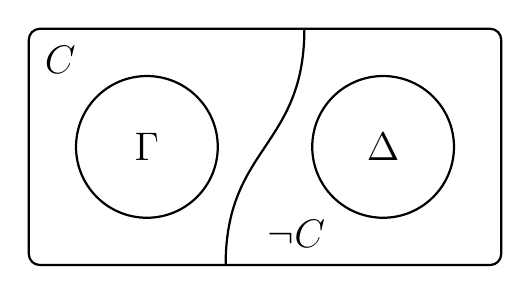
\begin{tikzpicture}[node distance=2cm, auto, thick]
    \draw [rounded corners] (0,0) -- (6,0) -- (6,3) -- (0,3) --  cycle;
    \draw (1.5,1.5) circle (0.9cm);
    \draw (4.5,1.5) circle (0.9cm);
    \path node at (1.5,1.5) {\Large $\Gamma$};
    \path node at (4.5,1.5) {\Large $\Delta$};
    \path node at (0.4,2.6) {\Large $\formula{C}$};
    \path node at (3.4,0.4) {\Large $\lnot \formula{C}$};
    \draw (2.5,0) .. controls (2.5,1.5) and (3.5,1.5) .. (3.5,3);
  \end{tikzpicture}
  \caption{$!C$ ஆனது $\Gamma$ மற்றும் $\Delta$ ஐப் பிரிக்கிறது}
  \ollabel{fig:sep}
\end{figure}


\begin{lem}\ollabel{lem:sep1}
$\Gamma$ மற்றும் $\Delta$ ஆகிய \emph{இரண்டிலும்} இடம்பெறும் ஒவ்வொரு
!!{constant}, !!{function}, !!{predicate} ஐயும் ($\doteq$ தவிர)
கொண்ட மொழி $\Lang{L}_0$ என்று கொள்க; மேலும் $n
\ge 0$ க்கான எண்ணிலடங்கா புதிய !!{constant}s $\Obj c_n$ ஐச்
சேர்ப்பதன் மூலம் $\Lang{L}'_0$ பெறப்படுகிறது என்று கொள்க. அப்போது
$\Gamma$ மற்றும் $\Delta$ ஆகியவை $\Lang{L}_0$ இல் பிரிக்கவியலாதவை
எனில், அவை $\Lang{L}'_0$ இலும் பிரிக்கவியலாதவை.
\end{lem}

\begin{proof}
மறைமுகமாகச் செல்கிறோம்: முரண்பாட்டிற்காக $\Gamma$ மற்றும் $\Delta$
ஆகியவை $\Lang{L}'_0$ இல் பிரிக்கப்படுகின்றன என்று கொள்க. அப்போது
ஏதேனும் $!C \in
\Lang{L}_0$ க்கு $\Gamma \Entails
\Subst{!C}{c}{x}$ மற்றும் $\Delta \Entails \lnot
\Subst{!C}{c}{x}$ (இங்கே $c$ ஒரு புதிய !!{constant}---$!C$ ஒன்றுக்கு
மேற்பட்ட அத்தகைய புதிய !!{constant} ஐக் கொண்ட நிலையும் இதே போன்றது).
இறுதிக்குட்பட்ட தன்மையின்படி,
$\Gamma_0 \Entails \Subst{!C}{c}{x}$ மற்றும்
$\Delta_0 \Entails \lnot \Subst{!C}{c}{x}$ ஆகுமாறு $\Gamma$ இன்
\emph{இறுதிக்குட்பட்ட} உட்கணம் $\Gamma_0$ உம் $\Delta$ இன்
உட்கணம் $\Delta_0$ உம் உள்ளன. $\Gamma_0$ இலுள்ள எல்லா
!!{formula}s இன் இணைப்பை $!G$ என்றும், $\Delta_0$ இலுள்ள எல்லா
!!{formula}s இன் இணைப்பை $!H$ என்றும் கொள்க. அப்போது
\begin{align*}
  !G & \Entails \Subst{!C}{c}{x}, & !H  \Entails \lnot \Subst{!C}{c}{x}.
\end{align*}
முந்தையதிலிருந்து பொதுமைப்படுத்தலால் $!G \Entails
\lforall[x][!C]$ கிடைக்கிறது; பிந்தையதிலிருந்து முரண்நிலைப்படி
$\Subst{!C}{c}{x} \Entails \lnot !H$; எனவே
$\lforall[x][!C]
\Entails \lnot \delta$ உம் கிடைக்கிறது. மீண்டும் முரண்நிலை
$!H \Entails
\lnot \lforall[x][!C]$ என்பதைக் கொடுக்கிறது. ஓரியக்கத்தன்மையின்படி,
\begin{align*}
  \Gamma &\Entails \lforall[x][!C], &
  \Delta & \Entails \lnot \lforall[x][!C],
\end{align*}
எனவே $\lforall[x][!C]$ ஆனது $\Lang{L}_0$ இல் $\Gamma$ மற்றும்
$\Delta$ ஐப் பிரிக்கிறது.
\end{proof}

\begin{lem}\ollabel{lem:sep2}
$\Gamma \cup \{ \lexists[x][!S] \}$ மற்றும் $\Delta$
பிரிக்கவியலாதவை என்றும், $c$ ஆனது $\Gamma$, $\Delta$, $!S$
ஆகியவற்றில் இல்லாத புதிய !!{constant} என்றும் கொள்க. அப்போது
$\Gamma \cup \{ \lexists[x][!S], \Subst{!S}{c}{x} \}$ மற்றும்
$\Delta$ உம் பிரிக்கவியலாதவை.
\end{lem}

\begin{proof}
ஒரே நேரத்தில் $\Gamma \cup \{\lexists[x]{!S} \}$ மற்றும் $\Delta$
பிரிக்கவியலாதவையாக இருக்க, $!C$ ஆனது
$\Gamma \cup \{
\lexists[x][!S], \Subst{!S}{c}{x}\}$ மற்றும் $\Delta$ ஐப் பிரிக்கிறது
என்று முரண்பாட்டிற்காகக் கொள்க. இரு நிலைகளை வேறுபடுத்துகிறோம்:
\begin{enumerate}
\item $!C$ இல் $c$ இடம்பெறவில்லை: இந்நிலையில்
$\Gamma \cup
  \{\lexists[x][!S], \lnot!C \}$ நிறைவுறத்தக்கது
(இல்லையெனில் $!C$ ஆனது $\Gamma \cup \{\lexists[x][!S] \}$ மற்றும்
$\Delta$ ஐப் பிரிக்கிறது). $\Subst{!S}{c}{x}$ ஐச் சேர்த்தாலும் அது
நிறைவுறத்தக்கதாகவே உள்ளது; எனவே இறுதியில் $!C$ ஆனது
$\Gamma \cup \{ \lexists[x][!S], \Subst{!S}{c}{x} \}$ மற்றும்
$\Delta$ ஐப் பிரிக்கவில்லை.
\item $!C$ இல் $c$ இடம்பெறுகிறது; எனவே $!C$ ஆனது
  $\Subst{!C}{c}{x}$ வடிவில் உள்ளது. அப்போது
  \[
  \Gamma \cup \{ \lexists[x][!S], \Subst{!S}{c}{x}\} \Entails \Subst{!C}{c}{x},
  \]
  என்று கிடைக்கிறது. இதிலிருந்து உய்த்தறிதல் தேற்றம் மற்றும்
  பொதுமைப்படுத்தலால்
  $\Gamma, \lexists[x][!S] \Entails \lforall[x][(!S \lif !C)]$;
  இறுதியாக $\Gamma
  \cup \{ \lexists[x][!S] \} \Entails \lexists[x][!C]$. மறுபுறம்,
  $\Delta \Entails \lnot \Subst{!C}{c}{x}$; எனவே
  பொதுமைப்படுத்தலால் $\Delta \Entails \lnot \lexists[x][!C]$.
  ஆகவே $\Gamma
  \cup \{\lexists[x][!S] \}$ மற்றும் $\Delta$ பிரிக்கத்தக்கவை;
  இது முரண்பாடு.
\end{enumerate}
\end{proof}


% END SOURCE UNIT OLP-0200

\endgroup


\begingroup
\makeatletter
\def\ol@sectioncs{section}
\makeatother
\def\olfilename{interpolation-proof}

% BEGIN SOURCE UNIT OLP-0201 content/model-theory/interpolation/interpolation-proof.tex
% Exact modular target bytes: 17683; SHA256: 9d0c842fd9e41054de5ad052d71b8fe7fb6a8f919b6c292bf9f110bdeaf249f7



% SEGMENT OLP-0201-S01

\olfileid{mod}{int}{prf}

\olsection{கிரெய்கின் இடையீட்டுத் தேற்றம்}

\begin{thm}[கிரெய்கின் இடையீட்டுத் தேற்றம்]
\ollabel{thm:interpol}
$\Entails !A \lif !B$ எனில், $\Entails !A \lif !C$ மற்றும்
$\Entails !C \lif !B$ ஆகுமாறு !!a{sentence} $!C$ ஒன்று உள்ளது;
மேலும் $!C$ இலுள்ள ஒவ்வொரு !!{constant}, !!{function},
!!{predicate} உம் ($\eq$ தவிர) $!A$ மற்றும்~$!B$ ஆகிய இரண்டிலும்
இடம்பெறும். !!{sentence} $!C$ ஆனது $!A$ மற்றும்~$!B$ இன்
\emph{இடையீட்டி} எனப்படுகிறது.
\end{thm}

\begin{proof}
$!A$ இன் மொழி $\Lang{L}_1$ என்றும், $!B$ இன் மொழி $\Lang{L}_2$
என்றும் கொள்க. $\Lang{L}_0 = \Lang{L}_1 \cap \Lang{L}_2$ என்க.
ஒவ்வொரு $i \in \{0, 1, 2 \}$ க்கும், எண்ணிலடங்கா புதிய
!!{constant}s $\Obj c_0,
\Obj c_1, \Obj c_2, \dots$ ஐ $\Lang{L}_i$ உடன் சேர்ப்பதன் மூலம்
$\Lang{L}'_i$ பெறப்படட்டும்.

$!A$ நிறைவுறத்தகாதது எனில், $\lexists[x][\eq/[x][x]]$ ஓர் இடையீட்டி.
$\lnot !B$ நிறைவுறத்தகாதது எனில் (எனவே $!B$ செல்லுபடியானது எனில்),
$\lexists[x][\eq[x][x]]$ ஓர் இடையீட்டி. ஆகவே $!A$ மற்றும்
$\lnot !B$ ஆகிய இரண்டும் நிறைவுறத்தக்கவை என்றும் கொள்ளலாம்.

இடையீட்டுத் தேற்றத்தின் முரண்நிலையை நிரூபிக்க, $!A$ மற்றும் $!B$
க்கான இடையீட்டி இல்லை என்று கொள்க. வேறுவிதமாகச் சொன்னால்,
$\{!A\}$ மற்றும் $\{\lnot !B\}$ ஆகியவை $\Lang{L}_0$ இல்
பிரிக்கவியலாதவை என்று கொள்க.

சோடி $(\{ !A \}, \{\lnot!B\})$ ஐ மீப்பெருமப் பிரிக்கவியலாச் சோடி
$(\Gamma^*, \Delta^*)$ ஆக நீட்டிப்பதே நமது இலக்கு. $\Lang{L}_1$
இன் !!{sentence}s ஐ $!A_0$, $!A_1$, $!A_2$, \dots உம்,
~$\Lang{L}_2$ இன் !!{sentence}s ஐ $!B_0$, $!B_1$, $!B_2$, \dots உம்
வரிசைப்படுத்தட்டும். !!{sentence}s இன் கணங்களின் இரு ஏறு தொடர்கள்
$(\Gamma_n, \Delta_n)$ ஐ $n \ge 0$ க்கு பின்வருமாறு வரையறுக்கிறோம்.
$\Gamma_0 = \{ !A\}$ மற்றும் $\Delta_0 = \{\lnot !B \}$ என்க.
$(\Gamma_n, \Delta_n)$ ஏற்கெனவே வரையறுக்கப்பட்டதாகக் கொண்டு,
$\Gamma_{n+1}$ மற்றும் $\Delta_{n+1}$ ஐப் பின்வருமாறு வரையறுக்க:
\begin{enumerate}
\item $\Gamma_n \cup \{!A_n \}$ மற்றும் $\Delta_n$ ஆகியவை
  $\Lang{L}'_0$ இல் பிரிக்கவியலாதவை எனில், $!A_n$ ஐ
  $\Gamma_{n+1}$ இல் இடுக. மேலும் $!A_n$ ஆனது இருத்தலளவையீட்டு
  !!{formula} $\lexists[x][!S]$ எனில், $\Gamma_n$, $\Delta_n$,
  $!A_n$, $!B_n$ ஆகியவற்றில் இடம்பெறாத புதிய !!{constant} $c$
  ஒன்றைத் தேர்ந்து, $\Subst{!S}{c}{x}$ ஐ $\Gamma_{n+1}$ இல் இடுக.
\item $\Gamma_{n+1}$ மற்றும் $\Delta_n \cup \{!B_n \}$ ஆகியவை
  $\Lang{L}'_0$ இல் பிரிக்கவியலாதவை எனில், $!B_n$ ஐ
  $\Delta_{n+1}$ இல் இடுக. மேலும் $!B_n$ ஆனது இருத்தலளவையீட்டு
  !!{formula} $\lexists[x][!S]$ எனில், $\Gamma_{n+1}$, $\Delta_n$,
  $!A_n$, $!B_n$ ஆகியவற்றில் இடம்பெறாத புதிய !!{constant} $c$
  ஒன்றைத் தேர்ந்து, $\Subst{!S}{c}{x}$ ஐ $\Delta_{n+1}$ இல் இடுக.
\end{enumerate}
இறுதியாக, பின்வருமாறு வரையறுக்க:
\begin{align*}
  \Gamma^* & = \bigcup_{n\ge 0} \Gamma_n, &
  \Delta^* & = \bigcup_{n\ge 0} \Delta_n.
\end{align*}
$n$ மீதான ஒருங்குநிகழ் தொகுத்தறிதலால் இப்போது பின்வருவனவற்றை
நிரூபிக்கலாம்:
\begin{enumerate}
\item\ollabel{part-a} $\Gamma_n$ மற்றும் $\Delta_n$ ஆகியவை
  $\Lang{L}'_0$ இல் பிரிக்கவியலாதவை;
\item\ollabel{part-b} $\Gamma_{n+1}$ மற்றும் $\Delta_n$ ஆகியவை
  $\Lang{L}'_0$ இல் பிரிக்கவியலாதவை.
\end{enumerate}
\olref{part-a} இன் அடிப்படை நிலையை \olref[sep]{lem:sep1} தருகிறது.
\olref{part-b} பகுதிக்கு மூன்று நிலைகளை வேறுபடுத்த வேண்டும்:
\begin{enumerate}
\item $\Gamma_0 \cup \{!A_0 \}$ மற்றும் $\Delta_0$ பிரிக்கத்தக்கவை
  எனில், $\Gamma_1 = \Gamma_0$; அப்போது \olref{part-b} என்பது
  \olref{part-a} மட்டுமே;
\item $\Gamma_1 = \Gamma_0 \cup\{ !A_0\}$ எனில், கட்டுமானத்தின்படி
  $\Gamma_1$ மற்றும் $\Delta_0$ பிரிக்கவியலாதவை.
\item $!A_0$ இருத்தலளவையீட்டுடையதாக இருந்து,
  $\Gamma_1 = \Gamma_0 \cup \{ \lexists[x][!S], \Subst{!S}{c}{x}
  \}$ ஆகும் நிலையை இன்னும் கருத வேண்டும். கட்டுமானத்தின்படி,
  $\Gamma_0 \cup \{ \lexists[x][!S]\}$ மற்றும் $\Delta_0$
  பிரிக்கவியலாதவை; ஆகவே \olref[sep]{lem:sep2} படி,
  $\Gamma_0 \cup \{ \lexists[x][!S], \Subst{!S}{c}{x} \}$ மற்றும்
  $\Delta_0$ உம் பிரிக்கவியலாதவை.
\end{enumerate}
இதனால் மேலுள்ள \olref{part-a} மற்றும் \olref{part-b} க்கான
தொகுத்தறிதலின் அடிப்படை நிலை நிறைவடைகிறது. இப்போது தொகுத்தறிதல் படி.
\olref{part-a} க்கு, $\Delta_{n+1} = \Delta_n \cup \{ !B_n \}$
எனில், $\Gamma_{n+1}$ மற்றும் $\Delta_{n+1}$ கட்டுமானத்தின்படி
பிரிக்கவியலாதவை ($!B_n$ இருத்தலளவையீட்டுடையதாக இருந்தாலும்கூட
\olref[sep]{lem:sep2} படி); $\Delta_{n+1} = \Delta_n$ எனில்
($\Gamma_{n+1}$ மற்றும் $\Delta_n \cup \{!B_n\}$ பிரிக்கத்தக்கவை
என்பதால்), \olref{part-b} மீதான தொகுத்தறிதல் கருதுகோளைப்
பயன்படுத்துகிறோம். \olref{part-b} க்கான தொகுத்தறிதல் படியில்,
$\Gamma_{n+2} = \Gamma_{n+1} \cup
\{!A_{n+1} \}$ எனில், $\Gamma_{n+2}$ மற்றும் $\Delta_{n+1}$
கட்டுமானத்தின்படி பிரிக்கவியலாதவை ($!A_{n+1}$
இருத்தலளவையீட்டுடையதாக இருந்தாலும்கூட \olref[sep]{lem:sep2} படி);
$\Gamma_{n+2} = \Gamma_{n+1}$ எனில், இப்போது நிரூபித்த
\olref{part-a} க்கான தொகுத்தறிதல் நிலையைப் பயன்படுத்துகிறோம்.
இதனால் \olref{part-a} மற்றும் \olref{part-b} மீதான தொகுத்தறிதல்
நிறைவடைகிறது.

இதிலிருந்து $\Gamma^*$ மற்றும் $\Delta^*$ பிரிக்கவியலாதவை என்று
பின்வருகிறது; இல்லையெனில் இறுதிக்குட்பட்ட தன்மையின்படி,
$\Gamma_n$ மற்றும் $\Delta_n$ ஐப் பிரிக்கும் $n \ge 0$ ஒன்று
இருக்கும்; இது \olref{part-a} க்கு மாறானது. குறிப்பாக,
$\Gamma^*$ மற்றும் $\Delta^*$ முரணின்மையுடையவை: முதலாவதோ
பிந்தையதோ முரண்பட்டதாக இருந்தால், முறையே
$\lexists[x][\eq/[x][x]]$ அல்லது
$\lforall[x][\eq[x][x]]$ அவற்றைப் பிரிக்கும்.

இப்போது $\Gamma^*$ ஆனது $\Lang{L}'_1$ இல் மீப்பெரும
முரணின்மையுடையது என்றும், அவ்வாறே $\Delta^*$ ஆனது
$\Lang{L}'_2$ இல் மீப்பெரும முரணின்மையுடையது என்றும் காட்டுவோம்.
முதலாவதற்கு, ஏதேனும் $n \ge 0$ க்கு $!A_n \notin \Gamma^*$ மற்றும்
$\lnot !A_n
\notin \Gamma^*$ என்று கொள்க. $!A_n \notin \Gamma^*$ எனில்,
$\Gamma_n \cup \{!A_n \}$ ஆனது $\Delta_n$ இலிருந்து பிரிக்கத்தக்கது;
எனவே பின்வரும் இரண்டும் பொருந்துமாறு $!C \in \Lang{L}'_0$ ஒன்று உண்டு:
\begin{align*}
  \Gamma^* & \Entails !A_n \lif !C, &
  \Delta^* & \Entails \lnot !C.
\end{align*}
அவ்வாறே, $\lnot !A_n \notin \Gamma^*$ எனில், பின்வரும் இரண்டும்
பொருந்துமாறு $!C' \in
\Lang{L}'_0$ ஒன்று உண்டு:
\begin{align*}
  \Gamma^* & \Entails \lnot !A_n \lif !C', &
  \Delta^* & \Entails \lnot !C'.
\end{align*}
கூற்றுக்கணிப்புத் தருக்கப்படி, $\Gamma^* \Entails !C \lor !C'$ மற்றும்
$\Delta^* \Entails \lnot (!C \lor !C')$; எனவே $!C \lor
!C'$ ஆனது $\Gamma^*$ மற்றும் $\Delta^*$ ஐப் பிரிக்கிறது.
இதேபோன்ற வாதம் $\Delta^*$ மீப்பெருமமானது என்று நிறுவுகிறது.

இறுதியாக, $\Gamma^* \cap \Delta^*$ ஆனது $\Lang{L}'_0$ இல்
மீப்பெரும முரணின்மையுடையது என்று காட்டுவோம். அது முரணின்மையுடைய
கணங்களின் வெட்டு என்பதால் வெளிப்படையாக முரணின்மையுடையது.
மீப்பெருமத்தை காட்ட, $!S \in
\Lang{L}'_0$ என்க. இப்போது $\Gamma^*$ ஆனது $\Lang{L'_1}
\supseteq \Lang{L'_0}$ இல் மீப்பெருமமானது; அவ்வாறே $\Delta^*$ ஆனது
$\Lang{L'_2} \supseteq \Lang{L'_0}$ இல் மீப்பெருமமானது. எனவே
$!S \in \Gamma^*$ அல்லது $\lnot !S \in \Gamma^*$; மேலும்
$!S \in \Delta^*$ அல்லது $\lnot !S \in \Delta^*$. $!S \in
\Gamma^*$ மற்றும் $\lnot !S \in \Delta^*$ எனில், $!S$ ஆனது
$\Gamma^*$ மற்றும் $\Delta^*$ ஐப் பிரிக்கும்; $\lnot !S \in
\Gamma^*$ மற்றும் $!S \in \Delta^*$ எனில், $\lnot !S$ ஆனது
$\Gamma^*$ மற்றும் $\Delta^*$ ஐப் பிரிக்கும். எனவே $!S \in
\Gamma^* \cap \Delta^*$ அல்லது $\lnot !S \in \Gamma^* \cap \Delta^*$;
ஆகவே $\Gamma^* \cap \Delta^*$ மீப்பெருமமானது.

$\Gamma^*$ மீப்பெரும முரணின்மையுடையது என்பதால், நிறைவுத் தேற்றத்தின்
நிரூபிப்பைப் போலவே (\olref[fol][com][cth]{thm:completeness}),
!!{constant}s ஐப் பொருள்கொள்ளும் உறுப்புகள் $\Assign{c}{M'_1}$
அனைத்தையும் அவற்றை மட்டுமே கொண்ட !!{domain} $\Domain{M'_1}$ உடைய
மாதிரி $\Struct{M}'_1$ அதற்கு உண்டு. அவ்வாறே, $\Delta^*$ க்கு,
!!{constant}s இன் பொருள்கோள்கள் $\Assign{c}{M'_2}$ ஆல் தரப்படும்
!!{domain} $\Domain{M'_2}$ உடைய மாதிரி $\Struct{M}'_2$ உள்ளது.

$\Lang{L'_1} \setminus \Lang{L'_0}$ இலுள்ள !!{constant}s,
!!{function}s, !!{predicate}s ஆகியவற்றின் பொருள்கோள்களை நீக்குவதன்
மூலம் $\Struct{M'_1}$ இலிருந்து $\Struct{M_1}$ பெறப்படட்டும்;
$\Struct{M_2}$ உம் அவ்வாறே. அப்போது
$h(\Assign{c}{M'_1}) = \Assign{c}{M'_2}$ என்று வரையறுக்கப்படும்
$h \colon M_1 \to M_2$ ஆனது $\Lang{L}'_0$ இல் ஓர் ஓரினச்சார்பு;
ஏனெனில் காட்டியபடி $\Gamma^* \cap \Delta^*$ ஆனது $\Lang{L}'_0$
இல் மீப்பெரும முரணின்மையுடையது. எந்த $\Lang{L}'_0$-!!{sentence} உம்
$\Gamma^*$ மற்றும் $\Delta^*$ ஆகிய இரண்டிலும் இடம்பெறும் அல்லது
இரண்டிலும் இடம்பெறாது என்பதால் இது பின்வருகிறது: எனவே
$\Assign{c}{M'_1} \in
\Assign{P}{M'_1}$ எனில், எனில் மட்டுமே, $\Atom{P}{c} \in \Gamma^*$;
எனில், எனில் மட்டுமே, $\Atom{P}{c} \in \Delta^*$; எனில், எனில்
மட்டுமே, $\Assign{c}{M'_2} \in
\Assign{P}{M'_2}$. ஓரினச்சார்புகள் நிறைவுறுத்தும் பிற நிபந்தனைகளையும்
இதேபோல் நிறுவலாம்.

இப்போது !!{language} $\Lang{L_1} \cup \Lang{L_2}$ க்கான மாதிரி
$\Struct{M}$ ஒன்றைப் பின்வருமாறு வரையறுப்போம்:
\begin{enumerate}
\item !!{domain} $\Domain{M}$ என்பது $\Domain{M_2}$ தான்; அதாவது
  எல்லா உறுப்புகள் $\Assign{c}{M'_2}$ இன் கணம்;
\item !!a{predicate}~$P$ ஆனது $\Lang{L_2} \setminus
  \Lang{L_1}$ இல் இருந்தால், $\Assign{P}{M} = \Assign{P}{M'_2}$;
\item பயனிலை $P$ ஆனது $\Lang{L}_1\setminus \Lang{L}_2$ இல் இருந்தால்,
  $\Assign{P}{M} = h(\Assign{P}{M'_2})$; அதாவது,
  $\tuple{\Assign{c_1}{M'_2}, \dots, \Assign{c_n}{M'_2}} \in
  \Assign{P}{M}$ எனில், எனில் மட்டுமே,
  $\tuple{\Assign{c_1}{M'_1}, \dots,
  \Assign{c_n}{M'_1}} \in \Assign{P}{M'_1}$.
\item !!a{predicate} $P$ ஆனது $\Lang{L}_0$ இல் இருந்தால்,
  $\Assign{P}{M} =
  \Assign{P}{M'_2} = h(\Assign{P}{M'_1})$.
\item !!^{function}s மற்றும் !!{constant}s உட்பட,
  $\Lang{L}_1 \cup \Lang{L}_2$ இன் சார்புகள் இதேபோல் கையாளப்படுகின்றன.
\end{enumerate}

இறுதியாக, $\Struct{M}$ ஆனது $\Lang{L'_1}$ இன் எல்லா !!{formula}s
மீதும் $\Struct{M'_1}$ உடனும், $\Lang{L'_2}$ இன் எல்லா !!{formula}s
மீதும் $\Struct{M'_2}$ உடனும் உடன்படுகிறது என்பதை !!{formula}s மீது
தொகுத்தறிந்து காட்டலாம். குறிப்பாக,
$\Struct{M} \Entails \Gamma^* \cup \Delta^*$; எனவே $\Struct{M}
\Entails !A$ மற்றும் $\Struct{M} \Entails \lnot!B$; ஆகவே
$\not\Entails !A \lif !B$. இதனால் கிரெய்கின் இடையீட்டுத் தேற்றத்தின்
நிரூபிப்பு நிறைவடைகிறது.
\end{proof}


% END SOURCE UNIT OLP-0201

\endgroup


\begingroup
\makeatletter
\def\ol@sectioncs{section}
\makeatother
\def\olfilename{definability}

% BEGIN SOURCE UNIT OLP-0202 content/model-theory/interpolation/definability.tex
% Exact modular target bytes: 8996; SHA256: 638f3c7537c563434aae3e41343ddaf09cd6bef8645ebe88914410c1d64da0a2



% SEGMENT OLP-0202-S01

\olfileid{mod}{int}{def}

\olsection{வரையறுக்கத்தக்கமைத் தேற்றம்}

இடையீட்டுத் தேற்றத்தின் ஒரு முக்கியப் பயன்பாடு பெத்தின்
வரையறுக்கத்தக்கமைத் தேற்றம். $n$-இடத் தொடர்பு~$R$ ஐ வரையறுக்க,
$R$ இடம்பெறாத, $n$ கட்டிலா !!{variable}s கொண்ட !!a{formula}~$!C$
ஒன்றைத் தரலாம். இது~$!C$ ஐக் கொண்டு~$R$ இன் \emph{வெளிப்படையான}
வரையறையாக இருக்கும். பின்னர் $n$-இட !!{predicate}~$P$ ஐக் கொண்ட
!!{language} ஒன்றின் கோட்பாடு~$\Sigma(P)$, முறைசாராக்கப்பட்ட
வெளிப்படையான வரையறையை உட்கொண்டால் (அல்லது குறைந்தபட்சம் தருக்கமுறையாக
உட்கிடையச் செய்தால்),~$P$ ஐ வெளிப்படையாக வரையறுக்கிறது என்றும்
கூறலாம்; அதாவது,
\[
\Sigma(P) \Entails \lforall[x_1][\dots
  \lforall[x_n][(\Atom{P}{x_1,\dots, x_n} \liff !C(x_1, \dots,
    x_n))]].
\]
ஆனால் ஒரு தொடர்பை வரையறுக்க---முழுமையாகத் தீர்மானிக்க என்ற
பொருளில்---வெளிப்படையான வரையறை ஒரு வழி மட்டுமே. எந்த மாதிரியிலும்
~$P$ இன் பொருள்கோள், மீதமுள்ள !!{language} இன் பொருள்கோளால்
நிலைநிறுத்தப்படுமாறும் ஒரு கோட்பாடு இருக்கலாம். ஒரு கோட்பாடு~$P$ இன்
பொருள்கோளை இவ்வழியில் நிலைநிறுத்தும் போதெல்லாம்---~$P$ ஐ
\emph{மறைமுகமாக வரையறுக்கும்} போதெல்லாம்---அது அப்பயனிலையை வெளிப்படையாகவும்
வரையறுக்கிறது என்று வரையறுக்கத்தக்கமைத் தேற்றம் கூறுகிறது.

\begin{defn}
$\Lang{L}$ ஆனது !!{predicate}~$P$ ஐக் கொண்டிராத !!a{language}
என்று கொள்க. $\Lang{L}
\cup \{P\}$ இன் !!{sentence}s இன் கணம் $\Sigma(P)$, பின்வருமாறு
அமையுமாறு $\Lang{L}$ இன் !!a{formula}~$!C(x_1, \dots, x_n)$ ஒன்று
இருந்தால், எனில் மட்டுமே,~$P$ ஐ \emph{வெளிப்படையாக வரையறுக்கிறது}:
\[
\Sigma(P) \Entails \lforall[x_1][\dots
  \lforall[x_n][(\Atom{P}{x_1,\dots, x_n} \liff !C(x_1, \dots,
    x_n))]].
\]
\end{defn}

\begin{defn}
$\Lang{L}$ ஆனது !!{predicate}s~$P$ மற்றும்~$P'$ ஐக் கொண்டிராத
!!a{language} என்று கொள்க. $\Lang{L} \cup \{P\}$ இன்
!!{sentence}s இன் கணம் $\Sigma(P)$, பின்வருமாறு அமையுமானால், எனில்
மட்டுமே, $P$ ஐ \emph{மறைமுகமாக வரையறுக்கிறது}:
\[
\Sigma(P) \cup \Sigma(P') \Entails \lforall[x_1][\dots
  \lforall[x_n][(\Atom{P}{x_1,\dots, x_n} \liff \Atom{P'}{x_1,\dots,
      x_n})]],
\]
இங்கே $\Sigma(P')$ என்பது $\Sigma(P)$ முழுவதிலும் $P$ ஐ $P'$ ஆல்
ஒரே சீராக மாற்றுவதன் விளைவு.
\end{defn}

வேறுவிதமாகச் சொன்னால், எந்த மாதிரி $\Struct{M}$ மற்றும்
$R, R' \subseteq
\Domain{M}^n$ க்கும், $\Expan{M}{R} \Entails \Sigma(P)$ மற்றும்
$\Expan{M}{R'} \Entails \Sigma(P')$ ஆகிய இரண்டும் பொருந்தினால்,
$R=R'$; இங்கே $\Expan{M}{R}$ என்பது
$\Assign{P}{M'} = R$ ஆகுமாறு $\Lang{L}$ ஐ
$\Lang{L} \cup \{P\}$ ஆக விரிவாக்குவதற்கான
!!{structure}~$\Struct{M'}$; $\Expan{M}{R'}$ உம் இதே போன்றது.

\begin{thm}[பெத் வரையறுக்கத்தக்கமைத் தேற்றம்]
$\Lang{L}
  \cup\{P\}$-!!{formula}s இன் கணம் $\Sigma(P)$, $P$ ஐ மறைமுகமாக
வரையறுத்தால், எனில் மட்டுமே, $\Sigma(P)$ ஆனது $P$ ஐ வெளிப்படையாக
வரையறுக்கிறது.
\end{thm}

\begin{proof}
$\Sigma(P)$ ஆனது $P$ ஐ வெளிப்படையாக வரையறுக்கிறது எனில்,
\begin{align*}
  \Sigma(P) & \Entails & \lforall[x_1][\dots \lforall[x_n]
    [(\Atom{P}{x_1,\dots, x_n} \liff !C(x_1,\dots,x_n))]]\\
  \Sigma(P') & \Entails & \lforall[x_1][\dots \lforall[x_n]
    [(\Atom{P'}{x_1,\dots, x_n} \liff !C(x_1,\dots,x_n))]]
\end{align*}
ஆகிய இரண்டும் பொருந்துகின்றன; முடிவு பின்வருகிறது. மறுதலுக்கு,
$\Sigma(P)$ ஆனது $P$ ஐ மறைமுகமாக வரையறுக்கிறது என்று கொள்க.
முதலில் !!{constant}s $c_1$, \dots,~$c_n$ ஐ $\Lang{L}$ உடன்
சேர்க்கிறோம். அப்போது
\[
\Sigma(P) \cup \Sigma(P') \Entails
\Atom{P}{c_1, \dots, c_n} \to  \Atom{P'}{c_1, \dots, c_n}.
\]
இறுதிக்குட்பட்ட தன்மையின்படி, $\Delta_0 \subseteq \Sigma(P)$ மற்றும்
$\Delta_1 \subseteq \Sigma(P')$ ஆகிய இறுதிக்குட்பட்ட கணங்கள்
பின்வருமாறு உள்ளன:
\[
\Delta_0 \cup \Delta_1 \Entails
\Atom{P}{c_1, \dots, c_n} \to \Atom{P'}{c_1, \dots, c_n}.
\]
$!A(P) \in \Delta_0$ அல்லது $!A(P') \in \Delta_1$ ஆகும் எல்லா
!!{sentence}s $!A(P)$ இன் இணைப்பு $!D(P)$ ஆகட்டும்; மேலும்
$!A(P) \in \Delta_0$ அல்லது $!A(P') \in \Delta_1$ ஆகும் எல்லா
!!{sentence}s $!A(P')$ இன் இணைப்பு $!D(P')$ ஆகட்டும். அப்போது
$!D(P) \land
!D(P') \Entails \Atom{P}{c_1, \dots, c_n} \to P'c_1\dots c_n$.
ஒவ்வொரு !!{predicate} உம் $\Entails$ இன் ஒரு பக்கத்தில் இடம்பெறுமாறு
இதை மறுசீரமைக்கலாம்:
\[
!D(P) \land \Atom{P}{c_1, \dots, c_n} \Entails
!D(P') \to \Atom{P'}{c_1, \dots, c_n}.
\]
கிரெய்கின் இடையீட்டுத் தேற்றப்படி, $P$ அல்லது $P'$ ஐக் கொண்டிராத
!!a{sentence} $!C(c_1,\dots, c_n)$ ஒன்று பின்வருமாறு உள்ளது:
\begin{align*}
  !D(P) \land \Atom{P}{c_1, \dots, c_n} & \Entails !C(c_1,\dots, c_n); \\
  !C(c_1,\dots, c_n) & \Entails !D(P') \to \Atom{P'}{c_1, \dots, c_n}.
\end{align*}
இவ்விரு உட்கிடத்தல்களில் முதலாவதிலிருந்து,
$!D(P) \Entails
\Atom{P}{c_1,\dots, c_n} \lif !C(c_1,\dots, c_n)$ கிடைக்கிறது.
பிந்தையதிலிருந்து, $\Lang{L} \cup \{P\}$-மாதிரி
$\Expan{M}{R}
\Entails !A(P)$ எனில், எனில் மட்டுமே, அதற்குரிய
$\Lang{L} \cup
\{P'\}$-மாதிரி $\Expan{M}{R} \models !A(P')$ என்பதால்,
$!C(c_1,\dots, c_n) \Entails !D(P) \lif \Atom{P}{c_1,\dots, c_n}$
கிடைக்கிறது; இதிலிருந்து
\[
!D(P) \Entails !C(c_1,\dots,c_n) \to \Atom{P}{c_1,\dots, c_n}.
\]
இரண்டையும் சேர்த்தால்,
$!D(P) \Entails \Atom{P}{c_1,\dots, c_n}
\liff !C(c_1, \dots, c_n)$; ஓரியக்கத்தன்மை மற்றும்
பொதுமைப்படுத்தலால்,
\[
\Sigma(P) \Entails
\lforall[x_1][\dots\lforall[x_n][(\Atom{P}{x_1,\dots, x_n} \liff
    !C(x_1,\dots, x_n))]].
\]
\end{proof}


% END SOURCE UNIT OLP-0202

\endgroup


\OLEndChapterHook


% END SOURCE UNIT OLP-0198

\endgroup


\begingroup
\makeatletter
\def\ol@sectioncs{section}
\makeatother
\def\olfilename{lindstrom}

% BEGIN SOURCE UNIT OLP-0203 content/model-theory/lindstrom/lindstrom.tex
% Exact modular target bytes: 344; SHA256: 61740f0fd36930d4b6a21ab0489f3e7803e06f32ff161b738f808c74a87f5f9c



% SEGMENT OLP-0203-S01

\olchapter{mod}{lin}{Lindstr\"om தேற்றம்}

\begingroup
\makeatletter
\def\ol@sectioncs{section}
\makeatother
\def\olfilename{introduction}

% BEGIN SOURCE UNIT OLP-0204 content/model-theory/lindstrom/introduction.tex
% Exact modular target bytes: 1747; SHA256: bc5520497af0f2810b50ee47ee4fd968df7de76ca1dd19c6ac37c462abc27cc6



% SEGMENT OLP-0204-S01

\olfileid{mod}{lin}{int}
\section{அறிமுகம்}

(குறிப்பிட்ட சில கூடுதல் கட்டுப்பாடுகளுக்கு உட்பட்டு) இறுதிக்குட்பட்ட
தன்மைத் தேற்றமும் கீழ்நோக்கிய L\"owenheim--Skolem தேற்றமும் பொருந்தும்
மீப்பெருமத் தருக்கமாக முதல்வரிசைத் தருக்கத்தைத் தன்மைப்படுத்தும்
Lindstr\"om தேற்றத்தை இவ்வத்தியாயத்தில் நிரூபிப்பதே நமது நோக்கம்
(\olref[fol][com][com]{thm:compactness} மற்றும்
\olref[fol][com][dls]{thm:downward-ls}). முதலில், தேற்றம் பொருந்தும்
தருக்கங்களின் பொதுவான வகுப்பிற்கு இன்னும் பொதுவான தன்மைப்படுத்தல்
ஒன்று தேவை. !!{predicate}s மற்றும் தனிப்பட்ட மாறிலிகளை மட்டும்
கொண்டு, !!{function}s எதையும் கொண்டிராத மொழிகளான
\emph{தொடர்புசார்} மொழிகளுக்கு நம்மைக் கட்டுப்படுத்திக்கொள்வோம்.


% END SOURCE UNIT OLP-0204

\endgroup


\begingroup
\makeatletter
\def\ol@sectioncs{section}
\makeatother
\def\olfilename{abstract-logics}

% BEGIN SOURCE UNIT OLP-0205 content/model-theory/lindstrom/abstract-logics.tex
% Exact modular target bytes: 12900; SHA256: 25728b29f71a65b8c07e14faffba0e2dc0052c462d3da82762367fba970df583



% SEGMENT OLP-0205-S01

\olfileid{mod}{lin}{alg}
\olsection{அருவத் தருக்கங்கள்}

\begin{defn}
\emph{அருவத் தருக்கம்} என்பது சோடி $\tuple{L, \models_L}$; இங்கே
$L$ என்பது ஒவ்வொரு !!{language}~$\Lang{L}$ க்கும் !!{sentence}s இன்
கணம் $L(\Lang{L})$ ஐ ஒதுக்கும் சார்பு; மேலும் $\models_L$ என்பது
!!{language}~$\Lang{L}$ க்கான !!{structure}s க்கும்
$L(\Lang{L})$ இன் !!{element}s க்கும் இடையிலான உறவு. குறிப்பாக,
$\tuple{F, \models}$ என்பது வழக்கமான முதல்வரிசைத் தருக்கம்; அதாவது,
!!{language}~$\Lang{L}$ க்கு $\Lang{L}$ இலுள்ள மாறிலிகளிலிருந்து
கட்டப்பட்ட முதல்வரிசை !!{sentence}s இன் கணத்தை ஒதுக்கும் சார்பு $F$;
$\models$ என்பது முதல்வரிசைத் தருக்கத்தின் நிறைவுறுத்தல் உறவு.
\end{defn}

கொடுக்கப்பட்ட !!{language} இற்காக முதல்வரிசைத் தருக்கத்தில்
பயன்படுத்தும் அதே !!{structure} கருத்துருவையே இன்னும் பயன்படுத்துகிறோம்
என்பதைக் கவனிக்க. ஆனால் $ \Lang{L}$ இன் அடிப்படைக் குறியீடுகளிலிருந்து
வழக்கமான முறையில் !!{sentence}s கட்டப்பட்டுள்ளன என்றோ, முதல்வரிசைத்
தருக்கத்தைப் போலவே $\models_L$ உறவு மீள்வரையறுக்கப்பட்டுள்ளது என்றோ
முன்கொள்வதில்லை. எனவே, முற்றிலும் பொதுவான இவ்வரையறை, எடுத்துக்காட்டாக,
$\tuple{L,\models_L}$ இலுள்ள !!{sentence}s முடிவிலி நீள இணைப்புகளையோ
பிரிப்புகளையோ, $\lexists$ மற்றும் $\lforall$ அல்லாத
அளவையீட்டுக்குறிகளையோ (எ.கா., ``\dots ஆகுமாறு முடிவிலி எண்ணிக்கையில்
$x$ உள்ளன''), அல்லது ஒருவேளை முடிவிலி நீள அளவையீட்டு முன்னொட்டுகளையோ
கொண்டிருக்கும் நிலையையும் பற்றிக்கொள்ள நோக்கம்கொண்டது.
$L(\Lang{L})$ இலுள்ள ``!!{sentence}s'' வழக்கமான முதல்வரிசைத்
தருக்க !!{sentence}s ஆக இருக்கத் தேவையில்லை என்பதை வலியுறுத்த,
இவ்வத்தியாயத்தில் அவற்றின்மீது வீச்சுற !!{variable}s $!E$,
$!F$,~\dots ஆகியவற்றைப் பயன்படுத்தி, வழக்கமான முதல்வரிசை
!!{formula}s க்கு $!A$, $!B$,~\dots ஆகியவற்றை ஒதுக்கிவைக்கிறோம்.

\begin{defn}
$\Mod(L){!E}$ என்பது வகுப்பு $\Setabs{\Struct{M}}{\Struct{M}
  \models_L !E}$ ஐக் குறிக்கட்டும். !!{language} ஐ வெளிப்படையாகக்
காட்ட வேண்டுமெனில் $\Mod[L](L){!E}$ என எழுதுகிறோம். $\Lang{L}$
க்கான இரு !!{structure}s $\Struct{M}$ மற்றும் $\Struct{N}$ ஆகியவற்றில்
$L(\Lang{L})$ இலிருந்து ஒரே !!{sentence}s மெய்யாக இருந்தால், அவை
$\tuple{L, \models_L}$ இல் \emph{அடிப்படையாகச் சமானமானவை} என்று கூறி,
$\Struct{M} \elemequiv[L] \Struct{N}$ என எழுதுகிறோம்.
\end{defn}

\begin{defn}
!!{language} $\Lang{L}$ க்கான அருவத் தருக்கம்
$\tuple{L,\models_L}$, பின்வரும் பண்புகளை நிறைவுறுத்தினால்
\emph{இயல்பானது}:
\begin{enumerate}
\item (\emph{$L$-ஓரியக்கத்தன்மை}) !!{language}s $\Lang{L}$ மற்றும்
  $\Lang{L'}$ க்கு, $\Lang{L} \subseteq \Lang{L'}$ எனில்,
  $L(\Lang{L}) \subseteq L(\Lang{L'})$.
\item (\emph{விரிவாக்கப் பண்பு}) ஒவ்வொரு $!E \in L(\Lang{L})$
  க்கும், $\Struct{M} \models_L !E$ என்ற உறவு
  $\Struct{M}$ இன் $\Lang{L'}$ க்கான குறைப்பை மட்டுமே சாருமாறு
  $\Lang{L}$ இன் \emph{இறுதிக்குட்பட்ட} உட்கணம் $\Lang{L'}$
  ஒன்று உள்ளது; அதாவது $\Struct{M}$ மற்றும் $\Struct{N}$ ஆகியவை
  $\Lang{L'}$ க்கான ஒரே குறைப்பைக் கொண்டால்,
  $\Struct{M}
  \models_L !E$ எனில், எனில் மட்டுமே, $\Struct{N} \models_L !E$.
\item (\emph{ஓரினப் பண்பு}) $\Struct{M} \models_L !E$ மற்றும்
  $\Struct{M} \simeq \Struct{N}$ எனில், $\Struct{N} \models_L
  !E$ உம் பொருந்தும்.
\item (\emph{மறுபெயரிடல் பண்பு}) மறுபெயரிடலின் கீழ் $\models_L$
  உறவு மாறாது: $\Lang{L}$ இலுள்ள ஒவ்வொரு குறியீடு $P$ ஐயும் அதே
  இடஎண் கொண்ட குறியீடு $P'$ ஆலும், ஒவ்வொரு மாறிலி $c$ ஐயும் வேறொரு
  மாறிலி $c'$ ஆலும் மாற்றுவதன் மூலம் !!{language} $\Lang{L}'$
  பெறப்பட்டால், ஒவ்வொரு !!{structure}~$\Struct{M}$ மற்றும்
  !!{sentence}~$!E$ க்கும், $\Struct{M}
  \models_L !E$ எனில், எனில் மட்டுமே, $\Struct{M}' \models_L !E'$;
  இங்கே $\Struct{M}'$ என்பது $\Lang{L}$ க்கு ஒத்த
  $\Lang{L}'$-!!{structure}; மேலும் $!E' \in L(\Lang{L}')$.
\item (\emph{பூலியப் பண்பு}) அருவத் தருக்கம் $\tuple{L,
  \models_L}$ பூலிய இணைப்பிகளின் கீழ் பின்வரும் பொருளில் மூடியது:
  ஒவ்வொரு $!E \in L(\Lang{L})$ க்கும்,
  $\Struct{M} \models_L !F$ எனில், எனில் மட்டுமே,
  $\Struct{M} \not\models_L !E$ ஆகுமாறு $!F \in
  L(\Lang{L})$ ஒன்று உண்டு; மேலும் ஒவ்வொரு $!E$ மற்றும் $!F$ க்கும்,
  $\Mod(L){!G} = \Mod(L){!E} \cap
  \Mod(L){!F}$ ஆகுமாறு $!G$ ஒன்று உண்டு. அணு !!{formula}s மற்றும்
  பிற இணைப்பிகளுக்கும் இதேபோல்.
\item (\emph{அளவையீட்டுப் பண்பு}) $\Lang{L}$ இலுள்ள ஒவ்வொரு மாறிலி
  $c$ மற்றும் $!E \in L(\Lang{L})$ க்கும், பின்வருமாறு அமையுமாறு
  $!F \in L(\Lang{L})$ ஒன்று உண்டு:
  \[
  \Mod[L'](L){!F} = \Setabs{\Struct{M}}{\Expan{M}{a} \in
  \Mod[L](L){!E} \text{ ஏதோ ஓர் } a \in \Domain{M}},
  \]
  இங்கே $\Lang{L'} = \Lang{L} \setminus \{c\}$; மேலும்
  $\Expan{M}{a}$ என்பது $a$ ஐ~$c$ க்கு ஒதுக்கி, $\Struct{M}$ ஐ
  $\Lang{L}$ ஆக விரிவாக்குவது.
\item (\emph{சார்பாக்கப் பண்பு}) !!a{sentence}
  $!E \in L(\Lang{L})$ உம் $\Lang{L}$ இல் இல்லாத குறியீடுகள்
  $R$, $c_1$, \dots, $c_n$ உம் கொடுக்கப்பட்டால்,
  $!E$ ஐ $\Atom{R}{x, c_1, \dots c_n}$ க்குச்
  \emph{சார்பாக்கியது} எனப்படும் !!a{sentence}
  $!F \in L(\Lang{L} \cup \{R,c_1,\ldots,c_n\})$ ஒன்று உள்ளது;
  ஒவ்வொரு !!{structure}~$\Struct{M}$ க்கும் அது பின்வருமாறு அமையும்:
  \[
  \Expan{M}{X, b_1, \ldots, b_n} \models_L !F \text{ அப்போதும்
    அப்போது மட்டுமே } \Struct{N} \models_L !E,
  \]
  இங்கே $\Struct{N}$ என்பது !!{domain}
  $\Domain{N} = \Setabs{a\in \Domain{M}}{\Assign{R}{M}(a, b_1, \dots, b_n)}$
  உடைய $\Struct{M}$ இன் உட்கட்டமைப்பு
  (\olref[bas][sub]{rem:substructure} ஐப் பார்க்க); மேலும்
  $\Expan{M}{X, b_1, \ldots,
    b_n}$ என்பது $R$, $c_1$, \dots, $c_n$ ஆகியவற்றை முறையே
  $X$, $b_1,$ \dots, $b_n$ ஆகப் பொருள்கொள்ளும் $\Struct{M}$ இன்
  விரிவாக்கம் ($X
  \subseteq M^{n+1}$ உடன்).
\end{enumerate}
\end{defn}

\begin{defn}
இரு அருவத் தருக்கங்கள் $\tuple{L_1, \models_{L_1}}$ மற்றும்
$\tuple{L_2, \models_{L_2}}$ கொடுக்கப்பட்டால், ஒவ்வொரு !!{language}
$\Lang{L}$ மற்றும் !!{sentence} $!E \in L_1(\Lang{L})$ க்கும்
$\Mod[L](L_1){!E} =
\Mod[L](L_2){!F}$ ஆகுமாறு !!a{sentence} $!F
\in L_2(\Lang{L})$ ஒன்று இருந்தால், பிந்தையது முந்தையதைவிட
\emph{குறைந்தபட்சம் அதே வெளிப்பாட்டாற்றலுடையது} என்று கூறி,
$\tuple{L_1, \models_{L_1}}
\leq \tuple{L_2, \models_{L_2}}$ என எழுதுகிறோம். தருக்கங்கள்
$\tuple{L_1, \models_{L_1}}$ மற்றும்
$\tuple{L_2, \models_{L_2}}$ ஆகியவை
$\tuple{L_1,
  \models_{L_1}} \leq \tuple{L_2, \models_{L_2}}$ மற்றும்
$\tuple{L_2,
  \models_{L_2}} \leq \tuple{L_1, \models_{L_1}}$ ஆகிய இரண்டும்
பொருந்தினால் \emph{சமானமானவை}.
\end{defn}

\begin{rem}
  முதல்வரிசைத் தருக்கம், அதாவது அருவத் தருக்கம்
  $\tuple{F, \models}$, இயல்பானது. உண்மையில் மேலுள்ள பண்புகள்
  முதல்வரிசைத் தருக்கத்திற்கு பெரும்பாலும் நேரடியானவை. விரிவாக்கப்
  பண்பு விரிநிலைத்தன்மையாகக் குறைகிறது என்றும், !!a{sentence} $!E$
  ஐ $\Atom{R}{x, c_1, \dots, c_n}$ க்குச் சார்பாக்க,
  ஒவ்வொரு !!{subformula} $\lforall[x][!F]$ ஐயும்
  $\lforall[x][(\Atom{R}{x, c_1, \dots, c_n} \lif \ !F)]$ ஆல்
  மாற்ற வேண்டும் என்றும் மட்டும் குறிப்பிடுகிறோம். மேலும்,
  $\tuple{L, \models_L}$ இயல்பானது எனில்,
  $\tuple{F, \models} \leq \tuple{L, \models_{L}}$; இதை முதல்வரிசை
  !!{formula}s மீது தொகுத்தறிந்து காட்டலாம். எனவே பொதுமை இழப்பின்றி,
  ஒவ்வொரு முதல்வரிசை !!{sentence} உம் ஒவ்வோர் இயல்பான தருக்கத்திலும்
  உள்ளது என்று கொள்ளலாம்.
\end{rem}


% END SOURCE UNIT OLP-0205

\endgroup


\begingroup
\makeatletter
\def\ol@sectioncs{section}
\makeatother
\def\olfilename{ls-property}

% BEGIN SOURCE UNIT OLP-0206 content/model-theory/lindstrom/ls-property.tex
% Exact modular target bytes: 10338; SHA256: 758f4c3f630ca3738636b5c0b4842fee0912f0ebd44b74441802d8ad88a66205



% SEGMENT OLP-0206-S01

\olfileid{mod}{lin}{lsp}

\olsection{இறுதிக்குட்பட்ட தன்மை மற்றும் L\"owenheim--Skolem பண்புகள்}

இப்போது இறுதிக்குட்பட்ட தன்மையையும் L\"owenheim--Skolem ஐயும்
அருவத் தருக்கங்களின் நிலைக்கு நேரடியாக நீட்டிக்கிறோம்.

\begin{defn}
ஒவ்வொரு இறுதிக்குட்பட்ட $\Gamma_0 \subseteq \Gamma$ உம்
நிறைவுறத்தக்கதாக இருக்கும்போதெல்லாம், $L(\Lang{L})$-!!{sentence}s
இன் ஒவ்வொரு கணம் $\Gamma$ உம் நிறைவுறத்தக்கதாக இருந்தால்,
அருவத் தருக்கம் $\tuple{L, \models_L}$ ஆனது
\emph{இறுதிக்குட்பட்ட தன்மைப் பண்பைக்} கொண்டுள்ளது.
\end{defn}

\begin{defn}
நிறைவுறத்தக்க எந்த $\Gamma$ உம் ஓர் !!a{enumerable} மாதிரியைக்
கொண்டிருந்தால், $\tuple{L, \models_L}$ ஆனது
\emph{கீழ்நோக்கிய L\"owenheim--Skolem பண்பைக்} கொண்டுள்ளது.
\end{defn}


\olref[bas][pis]{defn:partialisom} இலுள்ள பகுதி ஓரினச்சார்புக் கருத்துரு
முற்றிலும் ``இயற்கணிதவியல்'' சார்ந்தது (அதாவது, மொழியின்
!!{sentence}s ஐச் சுட்டாமல், !!{structure}s இன்
!!{language}~$\Lang{L}$ வழங்கும் மாறிலிகளை மட்டுமே கொண்டு
தரப்பட்டுள்ளது); எனவே அது அருவத் தருக்கங்களுக்கும் பொருந்துகிறது.
முதல்வரிசைத் தருக்கத்தில், இரு !!{structure}s பகுதியாக ஓரினமானவை
எனில் அவை அடிப்படையாகச் சமானமானவை என்று
\olref[bas][pis]{thm:p-isom2} இலிருந்து அறிவோம். தன்னிச்சையான
$!E \in L(\Lang{L})$ க்கு !!{formula}s மீதான தொகுத்தறிதல் கிடைக்காமல்
போகலாம் என்பதால், அந்த நிரூபிப்பு அருவத் தருக்கங்களுக்குப் பொருந்தாது.
இருந்தும் L\"owenheim--Skolem பண்பு பொருந்தினால் தேற்றம் மெய்யாகும்.

\begin{thm}
\ollabel{thm:abstract-p-isom}
$\tuple{L, \models_L}$ ஆனது L\"owenheim--Skolem பண்புடைய இயல்பான
தருக்கம் என்று கொள்க. அப்போது பகுதியாக ஓரினமான எந்த இரு
!!{structure}s உம் $\tuple{L,
  \models_L}$ இல் அடிப்படையாகச் சமானமானவை.
\end{thm}

\begin{proof}
$\Struct{M} \simeq_p \Struct{N}$; ஆனால் ஏதேனும் $!E$ க்கு
$\Struct{M} \models_L !E$ மற்றும் $\Struct{N} \not\models_L !E$
என்று கொள்க. ஓரினப் பண்பின்படி $\Domain{M}$ மற்றும் $\Domain{N}$
வெட்டாதவை என்று கொள்ளலாம்; விரிவாக்கப் பண்பின்படி,
இறுதிக்குட்பட்ட !!{language}~$\Lang{L}$ ஒன்றிற்கு
$!E \in L(\Lang{L})$ என்று கொள்ளலாம். $\Struct{M}$ மற்றும்
$\Struct{N}$ இடையிலான பகுதி ஓரினச்சார்புகளின் கணம்
$\mathcal{I}$ ஆகட்டும்; பொதுமை இழப்பின்றி, $p
\in \mathcal{I}$ மற்றும் $q \subseteq p$ எனில்
$q \in \mathcal{I}$ உம் பொருந்துகிறது என்று கொள்க.

$\Domain{M}^{<\omega}$ என்பது~$\Domain{M}$ இன் !!{element}s இன்
இறுதிக்குட்பட்ட தொடர்களின் கணம். $S$ என்பது
$\Domain{M}^{<\omega}$ மீதான தொடரிணைப்பைக் குறிக்கும் மும்மை உறவாகட்டும்;
அதாவது $\mathbf{a}, \mathbf{b},
\mathbf{c} \in \Domain{M}^{<\omega}$ எனில், $\mathbf{c}$ ஆனது
$\mathbf{a}$ மற்றும் $\mathbf{b}$ இன் தொடரிணைப்பாக இருந்தால், எனில்
மட்டுமே, $S(\mathbf{a}, \mathbf{b},
\mathbf{c})$ பொருந்தும். மேலும், $b \in M$ மற்றும்
$\mathbf{a}, \mathbf{c} \in \Domain{M}^{<\omega}$ க்கு,
$\mathbf{a} =
a_1, \dots a_n$ மற்றும் $\mathbf{c} = a_1, \dots a_n, b$ எனில்,
எனில் மட்டுமே, $T(\mathbf{a}, b, \mathbf{c})$ பொருந்துமாறு
$T$ ஒரு மும்மை உறவாகட்டும். புதிய 3-இட !!{predicate}s $P$ மற்றும்
$Q$ ஐத் தேர்க. பேரண்டம் $\Domain{M} \cup \Domain{M}^{<\omega}$ உடைய,
$\Struct{M}$ ஐ உட்கட்டமைப்பாகக் கொண்ட, $P$ மற்றும் $Q$ ஐ
தொடரிணைப்பு உறவுகள் $S$ மற்றும் $T$ ஆகப் பொருள்கொள்ளும்
!!{structure} $\Struct{M}^*$ ஐ அமைக்க (எனவே $\Struct{M}^*$ ஆனது
!!{language} $\Lang{L} \cup \{ P, Q\}$ இல் உள்ளது).

$\Domain{N}^{<\omega}$, $S'$, $T'$, $P'$, $Q'$ மற்றும்
$\Struct{N}^*$ ஐ ஒத்தவாறு வரையறுக்க. கருதுகோளின்படி
$\Struct{M} \simeq_p
\Struct{N}$ என்பதால், $\Domain{M}^{<\omega}$ மற்றும்
$\Domain{N}^{<\omega}$ இடையில் பின்வருமாறு அமையும் உறவு $I$ உள்ளது:
$\mathbf{a}$ மற்றும் $\mathbf{b}$ ஓரினமாக இருந்து
\olref[bas][pis]{defn:partialisom} இன் முன்னும் பின்னும் நிபந்தனையை
நிறைவுறுத்தினால், எனில் மட்டுமே, $I(\mathbf{a}, \mathbf{b})$
பொருந்தும். இப்போது $\Struct{M}^*$ மற்றும் $\Struct{N}^*$ இன்
!!{domain}s இன் ஒன்றிப்பை !!{domain} ஆகக் கொண்டு,
$\Struct{M}^*$ மற்றும் $\Struct{N}^*$ ஐ உட்!!{structure}s ஆகக் கொண்ட
!!{structure} $\Struct{M}$ ஐக் கொள்க.
அதன் !!{language} கூடுதல் இரும !!{predicate}~$R$ ஒன்றைக் கொண்டு,
அதை உறவு~$I$ ஆகப் பொருள்கொள்கிறது; மேலும் !!{domain}s
$\Domain{M}^*$ மற்றும்~$\Domain{N}*$ ஐக் குறிக்கும் !!{predicate}s
ஐயும் கொண்டுள்ளது.

\begin{figure}[h]
  \centering
  \begin{tikzpicture}[node distance=2cm, auto, thick, >=stealth']
    \draw [rounded corners] (0,0) -- (8,0) -- (8,4) -- (0,4) --  cycle;
    \draw (2,2) circle (0.5cm);
    \draw (2,2) circle (1.25cm);
    \draw (6,2) circle (0.5cm);
    \draw (6,2) circle (1.25cm);
    \path node at (0.75,3.5) {\large $\Struct{M}$};
    \path node at (2,2) {\large $\Struct{M}$};
    \path node at (6,2) {\large $\Struct{N}$};
    \path node at (3.5,1) {\large $\Struct{M}^*$};
    \path node at (7.5,1) {\large $\Struct{N}^*$};
    \node (Idom) at (2.8,2) {};
    \node (Irng) at (5.2,2) {};
    \draw[<->, bend left] (Idom) to node {\large $I$} (Irng) ;
  \end{tikzpicture}
  \caption{உள்ளார்ந்த பகுதி ஓரினச்சார்புடன் கூடிய
    !!{structure}~$\Struct{M}$.}
\end{figure}

!!{structure}~$\Struct{M}$ இன் !!{language} இல், பின்வரும்
முக்கியமான இரண்டு \emph{முதல்வரிசை} !!{sentence}s உள்ளன:
$\Struct{M} \models_L !E$ மற்றும் $\Struct{N} \not\models_L !E$
என்று கூறி~$\Struct{M}$ இல் மெய்யாகும் $!D_1$ (இதற்குச்
சார்பாக்கப் பண்பு தேவை); பகுதி ஓரினச்சார்பு~$I$ வழியாக
$\Struct{M} \simeq_p \Struct{N}$ என்று கூறி~$\Struct{M}$ இல்
மெய்யாகும் \emph{முதல்வரிசை} !!{sentence} $!D_2$.
L\"owenheim--Skolem பண்பின்படி, $!D_1$ மற்றும் $!D_2$ ஆகிய இரண்டும்,
$\Struct{M}_0 \models_L !E$ மற்றும் $\Struct{N}_0
\not\models_L !E$ ஆகும் பகுதியாக ஓரினமான உட்கட்டமைப்புகள்
$\Struct{M}_0$, $\Struct{N}_0$ கொண்ட ஓர் !!a{enumerable} மாதிரி
$\Struct{M}_0$ இல் ஒருங்கே மெய்யாகின்றன. ஆனால்
\olref[bas][pis]{thm:p-isom1} படி, !!{enumerable} பகுதியாக ஓரினமான
!!{structure}s உண்மையில் ஓரினமானவை; இது இயல்பான அருவத் தருக்கங்களின்
ஓரினப் பண்புடன் முரண்படுகிறது.
\end{proof}


% END SOURCE UNIT OLP-0206

\endgroup


\begingroup
\makeatletter
\def\ol@sectioncs{section}
\makeatother
\def\olfilename{lindstrom-proof}

% BEGIN SOURCE UNIT OLP-0207 content/model-theory/lindstrom/lindstrom-proof.tex
% Exact modular target bytes: 11834; SHA256: 543e6efedadd3ed27ef067b08f2c6ffeccf187c8a9a979d7159e7a43d9df4ad7



% SEGMENT OLP-0207-S01

\olfileid{mod}{lin}{prf}

\olsection{Lindstr\"om தேற்றம்}

\begin{lem}
\ollabel{lem:lindstrom}
$!E \in L(\Lang{L})$ என்றும், $\Lang{L}$ இறுதிக்குட்பட்டது என்றும்
கொள்க; மேலும் ஏதேனும் இரு !!{structure}s $\Struct{M}$ மற்றும்
~$\Struct{N}$ க்கு, $\Struct{M} \equiv_n \Struct{N}$ மற்றும்
$\Struct{M} \models_L !E$ எனில் $\Struct{N} \models_L !E$ உம்
பொருந்துமாறு $n \in \Nat$ ஒன்று உள்ளது என்றும் கொள்க. அப்போது
$!E$ ஆனது ஒரு முதல்வரிசை !!{sentence} க்குச் சமானமானது; அதாவது,
$\Mod(L){!E} = \Mod(L){!D}$ ஆகுமாறு முதல்வரிசை $!D$ ஒன்று உள்ளது.
\end{lem}

\begin{proof}
எந்த இரு $n$-சமானமான !!{structure}s $\Struct{M}$ மற்றும்
$\Struct{N}$ உம் $!E$ க்கு ஒதுக்கப்படும் மதிப்பில் உடன்படுமாறு
$n$ ஐக் கொள்க. \olref[bas][pis]{prop:qr-finite} ஐ நினைவுகூர்க:
ஓர் இறுதிக்குட்பட்ட !!{language} இல், தருக்கச் சமானம் வரையில்,
அளவையீட்டு படிநிலை $n$ ஐவிடப் பெரிதாக இல்லாத முதல்வரிசை
!!{sentence}s இறுதிக்குட்பட்ட எண்ணிக்கையிலேயே உள்ளன. இப்போது
ஒவ்வொரு நிலையான !!{structure}~$\Struct{M}$ க்கும்,
$\QuantRank{!E} \le n$ உடன் $\Struct{M}$ இல் மெய்யாகும் அனைத்து
முதல்வரிசை !!{sentence}s~$!E$ இன் இணைப்பாக
$!D_{\Struct{M}}$ இருக்கட்டும் (இந்த இணைப்பு இறுதிக்குட்பட்டது);
அப்போது $\Struct{N} \models !D_{\Struct{M}}$ எனில், எனில் மட்டுமே,
$\Struct{N} \equiv_n \Struct{M}$. பிறகு $!D = \textstyle\bigvee
\Setabs{!D_{\Struct{M}}}{\Struct{M} \models_L !E}$ என வைக்க;
இந்தப் பிரிப்பும் தருக்கச் சமானம் வரையில் இறுதிக்குட்பட்டதே.

இதிலிருந்து $\Mod(L){!E} = \Mod(L){!D}$ என்ற முடிவு கிடைக்கிறது.
உண்மையில், $\Struct{N} \models_L !D$ எனில், ஏதேனும்
$\Struct{M} \models_L !E$ க்கு $\Struct{N} \models
!D_{\Struct{M}}$; எனவே, இக்கருதுகோளால், $\Struct{N} \models_L !E$
உம் பொருந்தும். மாறாக, $\Struct{N} \models_L !E$ எனில்
$!D_\Struct{N}$ ஆனது $!D$ இன் ஒரு பிரிப்புறுப்பு; மேலும்
$\Struct{N} \models !D_\Struct{N}$ என்பதால்,
$\Struct{N} \models_L !D$ உம் பொருந்தும்.
\end{proof}

\begin{thm}[Lindstr\"om தேற்றம்]
  \ollabel{thm:lindstrom} $\tuple{L, \models_L}$ ஆனது
  இறுதிக்குட்பட்ட தன்மை மற்றும் L\"owenheim--Skolem பண்புகளைக்
  கொண்டுள்ளது என்று கொள்க. அப்போது $\tuple{L, \models_L} \le
  \tuple{F, \models}$ (எனவே $\tuple{L, \models_L}$ முதல்வரிசைத்
  தருக்கத்திற்குச் சமானமானது).
\end{thm}

\begin{proof}
\olref{lem:lindstrom} படி, $\Lang{L}$ இறுதிக்குட்பட்டதாக இருக்கும்
எந்த $!E \in L(\Lang{L})$ க்கும், ஏதேனும் இரு !!{structure}s
$\Struct{M}$ மற்றும்~$\Struct{N}$ குறித்து பின்வருமாறு அமையும்
$n \in \Nat$ ஒன்று உள்ளது எனக் காட்டினால் போதும்:
$\Struct{M} \equiv_n \Struct{N}$ எனில், $\Struct{M}$ மற்றும்
$\Struct{N}$ ஆகியவை $!E$ இல் உடன்படுகின்றன. ஏனெனில் அப்போது
$!E$ ஒரு முதல்வரிசை !!{sentence} க்குச் சமானமானது; அதிலிருந்து
$\tuple{L, \models_L} \le \tuple{F, \models}$ கிடைக்கிறது.
நாம் இறுதிக்குட்பட்ட, முற்றிலும் உறவுசார் !!{language} ஒன்றில்
பணியாற்றுவதால், \olref[bas][pis]{thm:b-n-f} படி
$\Struct{M} \equiv_n \Struct{N}$ என்ற கூற்றை, அதற்கொத்த
$I_n(\emptyset,\emptyset)$ என்ற இயற்கணிதவியல் கூற்றால் மாற்றலாம்.

$!E$ கொடுக்கப்பட்டிருக்க, ஒவ்வொரு $n$ க்கும்
$I_n(\emptyset, \emptyset)$ பொருந்தும்; ஆனால், எடுத்துக்காட்டாக,
$\Struct{M}_n \models_L !E$ ஆகவும் $\Struct{N}_n \not\models_L !E$
ஆகவும் இருக்கும் !!{structure}s $\Struct{M}_n$ மற்றும்
$\Struct{N}_n$ உள்ளன என்று முரண்பாட்டிற்காகக் கொள்க.
ஓரினப் பண்பின்படி, அனைத்து $\Struct{M}_n$ களும் மொழியின்
மாறிலிகளை ஒரே பொருள்களாகப் பொருள்கொள்கின்றன என்று கொள்ளலாம்;
மேலும் மொழியில் அணு !!{sentence}s இறுதிக்குட்பட்ட எண்ணிக்கையில்
மட்டுமே இருப்பதால், அவை ஒரே அணு !!{sentence}s ஐ நிறைவுறுத்துகின்றன
என்றும் கொள்ளலாம் (இல்லையெனில் $\Struct{M}$ களின் ஒரு
உட்தொடரை எடுத்துக்கொள்ளலாம்). அனைத்து $\Struct{M}_n$ களின்
ஒன்றிப்பு, அதாவது ஒவ்வொரு $\Struct{M}_n$ ஐயும் உட்கட்டமைப்பாகக்
கொண்ட ஒரே குறைந்தபட்ச !!{structure}, $\Struct{M}$ ஆகட்டும்.
\olref[lsp]{thm:abstract-p-isom} இன் நிரூபிப்பில் செய்ததுபோல்,
தொடரிணைப்புச் சார்புகள் $P$ மற்றும்~$Q$ அடங்கிய விரிவாக்கப்பட்ட
!!{language} இல், !!{domain} $\Domain{M} \cup
\Domain{M}^{<\omega}$ உடைய $\Struct{M}$ இன் விரிவாக்கமாக
$\Struct{M}^*$ இருக்கட்டும்.

அதேபோல், $\Struct{N}_n$, $\Struct{N}$ மற்றும் $\Struct{N}^*$ ஐ
வரையறுக்க. இப்போது $\Struct{M}^*$ மற்றும் $\Struct{N}^*$ இன்
!!{domain}s உடன், இயலெண்கள்~$\Nat$ மற்றும் அவற்றின் இயல்பான
வரிசை~$\le$ ஆகியவற்றையும் தனது !!{domain} இல் கொண்ட
!!{structure} $\Struct{M}$ ஐக் கொள்க. அதன் !!{language} ஆனது
$\Domain{M}$, $\Domain{N}$, $\Domain{M}^{<\omega}$ மற்றும்
$\Domain{N}^{<\omega}$ ஆகிய !!{domain}s ஐக் குறிக்கும் கூடுதல்
சார்புகளுடன், $\Struct{M}_n$ மற்றும் $\Struct{N}_n$ இன்
ஆட்சிப்புலங்களைப் பின்வரும் பொருளில் குறியீடாக்கும் சார்புகளையும்
ஐயும் கொண்டுள்ளது:
\begin{align*}
  \Domain{M_n} & = \Setabs{a \in \Domain{M}}{R(a, n)}; & 
  \Domain{N_n} & = \Setabs{a \in \Domain{N}}{S(a,n)}; \\
  \Domain{M}^{<\omega}_n & = \Setabs{a \in \Domain{M}^{<\omega}}{R(a,n)}; &
  \Domain{N}^{<\omega}_n & = \Setabs{a \in \Domain{N}^{<\omega}}{S(a,n)}. 
\end{align*}
மேலும், $J(n, \mathbf{a}, \mathbf{b})$ எனில், எனில் மட்டுமே,
$I_n(\mathbf{a}, \mathbf{b})$ பொருந்துமாறு அமைந்த மும்மை உறவு
$J$ ஐயும் !!{structure}~$\Struct{M}$ கொண்டுள்ளது.

இப்போது $R$, $S$, $J$ முதலியவற்றால் விரிவாக்கப்பட்ட
!!{language}~$\Lang{L}$ இல் !!a{sentence}~$!D$ ஒன்று உள்ளது.
$\le$ என்பது முதல் உறுப்பு கொண்டதும் கடைசி உறுப்பு
இல்லாததுமான தனித்த நேரியல் வரிசை என்றும், $\Struct{M}_n \models
!E$, $\Struct{N}_n \not\models !E$ என்றும், வரிசையிலுள்ள ஒவ்வொரு
$n$ க்கும் $J(n, \mathbf{a}, \mathbf{b})$ எனில், எனில் மட்டுமே,
$I_n(\mathbf{a}, \mathbf{b})$ என்றும் அது கூறுகிறது.

இறுதிக்குட்பட்ட தன்மைப் பண்பைப் பயன்படுத்தி, வரிசை தரமற்ற
உறுப்பு~$n^*$ ஒன்றைக் கொண்டிருக்கும் $!D$ இன் மாதிரி
$\Struct{M}^*$ ஒன்றைக் காணலாம். அப்போது குறிப்பாக,
$\Struct{M_{n^*}} \models_L !E$ மற்றும் $\Struct{N_{n^*}}
\not\models_L !E$ ஆகுமாறு உட்!!{structure}s
$\Struct{M_{n^*}}$ மற்றும் $\Struct{N_{n^*}}$ ஐ
$\Struct{M^*}$ கொண்டிருக்கும். ஆனால் இப்போது
$\Domain{M_{n^*}}$ மற்றும் $\Domain{N_{n^*}}$ இலிருந்து வரும்
$k$-சோடிகளின் சோடிகளைக் கொண்ட கணம் $\mathcal{I}$ ஐப்
பின்வருமாறு வரையறுக்கலாம்: $\mathbf{a}$ மற்றும் $\mathbf{b}$ இன்
நீளம் $k$ எனில், $\tuple{\mathbf{a}, \mathbf{b}} \in \mathcal{I}$
எனில், எனில் மட்டுமே, $J(n^*-k, \mathbf{a}, \mathbf{b})$.
$n^*$ தரமற்றது என்பதால், ஒவ்வொரு தரமான $k$ க்கும்
$n^* - k >0$; மேலும் $\Struct{M_{n^*}} \simeq_p
\Struct{N_{n^*}}$ என்ற உண்மைக்கு கணம் $\mathcal{I}$ சான்றளிக்கிறது.
ஆனால் \olref[lsp]{thm:abstract-p-isom} படி,
$\Struct{M_{n^*}}$ ஆனது $\Struct{N_{n^*}}$ க்கு $L$-சமானமானது;
இது ஒரு முரண்பாடு.
\end{proof}


% END SOURCE UNIT OLP-0207

\endgroup


\OLEndChapterHook


% END SOURCE UNIT OLP-0203

\endgroup


\OLEndPartHook


% END SOURCE UNIT OLP-0182

\endgroup


\begingroup
\makeatletter
\def\ol@sectioncs{section}
\makeatother
\def\olfilename{computability}

% BEGIN SOURCE UNIT OLP-0208 content/computability/computability.tex
% Exact modular target bytes: 1157; SHA256: 064010174c70d10460e39f0a78f499f56b254293c13ddfc273682794f4f229bb



% SEGMENT OLP-0208-S01

\olpart{cmp}{கணிப்புத்தன்மை}

\begin{editorial}
  இப்பகுதி கணிப்புத்தன்மைக் கோட்பாடு குறித்த ஜெரமி அவிகாட்டின்
  குறிப்புகளை அடிப்படையாகக் கொண்டது. மீள்வரையறைச் சார்புகள் பற்றிய
  அத்தியாயம் மட்டுமே இதுவரை பயிற்சிகளைக் கொண்டுள்ளது; உள்நோக்கம்,
  எடுத்துக்காட்டுகள், விவரங்கள் மற்றும் பயிற்சிகளைக் கொண்டு அனைத்தையும்
  விரிவாக்க வேண்டியுள்ளது.
\end{editorial}

\begingroup
\makeatletter
\def\ol@sectioncs{section}
\makeatother
\def\olfilename{recursive-functions}

% BEGIN SOURCE UNIT OLP-0209 content/computability/recursive-functions/recursive-functions.tex
% Exact modular target bytes: 1517; SHA256: 81d17f1702aa70bd62100dc9ced8e7bb12904d9b6349b99fdcea60d86c612e55



% SEGMENT OLP-0209-S01

\olchapter{cmp}{rec}{மீள்வரையறைச் சார்புகள்}

\begin{editorial}
  இவை மீள்வரையறைச் சார்புகள் குறித்த ஜெரமி அவிகாட்டின் குறிப்புகள்;
  ரிச்சர்ட் சாக் இவற்றைத் திருத்தி விரிவாக்கினார். இவ்வத்தியாயம் சில
  பயிற்சிகளைக் கொண்டுள்ளது; தொடரியலின் எண்கணிதப்படுத்தல் குறித்த
  உரையாடலுக்கு அடிப்படையாக இதைத் தனியாகவும் சேர்க்கலாம்.
\end{editorial}



\begingroup
\makeatletter
\def\ol@sectioncs{section}
\makeatother
\def\olfilename{introduction}

% BEGIN SOURCE UNIT OLP-0210 content/computability/recursive-functions/introduction.tex
% Exact modular target bytes: 7107; SHA256: b8bc364ec6182593d9e31e39be43e9f2895a87d192b549506edbcc375d56d3b0



% SEGMENT OLP-0210-S01

\olfileid{cmp}{rec}{int}
\olsection{அறிமுகம்}

கணிப்புத்தன்மைக்கான ஒரு கணிதக் கோட்பாட்டை உருவாக்க, முதலில்
கணிப்புத்தன்மைக்கான ஒரு \emph{மாதிரியை} உருவாக்க வேண்டும். இப்போது,
கணிப்புத்தன்மையைக் கணினிகள் செய்யும் வகைச் செயலாகக் கருதுகிறோம்;
கணினிகள் குறியீடுகளைக் கொண்டு பணியாற்றுகின்றன. ஆனால் கணிப்புத்தன்மைக்
கோட்பாடுகளின் தொடக்க வளர்ச்சியில், கணக்கீட்டின் நெறிமுறை
எடுத்துக்காட்டு \emph{எண்ணியல்} கணக்கீடாக இருந்தது. கணிதவியலாளர்கள்
எப்போதும் எண்-கோட்பாட்டுச் சார்புகளில், அதாவது கணிக்கக்கூடிய
$f\colon \Nat^n \to \Nat$ என்ற சார்புகளில், ஆர்வம் கொண்டிருந்தனர்.
எனவே கணிப்புத்தன்மைக் கோட்பாட்டின் தொடக்கத்தில் இத்தகைய சார்புகளே
ஆராயப்பட்டன என்பது வியப்பன்று. இயல் எண்களின் கூட்டல், பெருக்கல்,
அடுக்கேற்றம் போன்ற மிகப் பழக்கமான கணிக்கத்தக்க எண்ணியல் சார்புகள்
ஒரு சுவையான பண்பைப் பகிர்கின்றன: அவற்றை
\emph{மீள்வரையறை முறையில்} வரையறுக்கலாம். எனவே மீள்வரையறைகளின்
அடிப்படையில் \emph{கணிக்கத்தக்க சார்பு} என்பதற்குப் பொது வரையறை
ஒன்றைத் தர முயல்வது இயல்பானது. எண்-கோட்பாட்டுச் சார்புகளை
மீள்வரையறை முறையில் வரையறுப்பதற்கான பல வழிகளுள், குறிப்பாக எளிய
ஒரு வரையறை முறை இங்கே மையமாகிறது: அது
\emph{முதன்மை மீள்வரையறை} எனப்படும்.

கணிக்கத்தக்க சார்புகளுடன், கணிக்கத்தக்க கணங்களிலும் உறவுகளிலும் நாம்
ஆர்வம் கொள்ளலாம். கொடுக்கப்பட்ட எண் ஒரு கணத்தின் !!a{element} ஆகுமா
இல்லையா என்ற விடையைக் கணிக்க முடிந்தால் அந்தக் கணம் கணிக்கத்தக்கது;
வரிசைத் தொகுதி $\tuple{n_1, \dots, n_k}$ ஓர் உறவின்
!!a{element} ஆகுமா இல்லையா என்பதைக் கணிக்க முடிந்தால், எனில் மட்டுமே,
அந்த உறவு கணிக்கத்தக்கது. ஒரு கணம் அல்லது உறவின்
\emph{சிறப்பியல்புச் சார்பை} கருதுவதன் மூலம், கணிக்கத்தக்க கணங்கள்
மற்றும் உறவுகள் பற்றிய உரையாடலைக் கணிக்கத்தக்க சார்புகள் பற்றிய
உரையாடலுக்குள் அடக்கலாம். எனவே முதன்மை மீள்வரையறை உறவுகளையும்
வரையறுக்கலாம்; எடுத்துக்காட்டாக, ``$n$ ஆனது $m$ ஐ மீதியின்றி
வகுக்கிறது'' என்ற உறவு ஒரு முதன்மை மீள்வரையறை உறவு.

முதன்மை மீள்வரையறையை மட்டுமே பயன்படுத்தி வரையறுக்கக்கூடிய முதன்மை
மீள்வரையறைச் சார்புகள் மட்டுமே கணிக்கத்தக்க எண்-கோட்பாட்டுச்
சார்புகள் அல்ல. முதன்மை மீள்வரையறையின் பல பொதுமைப்படுத்தல்கள்
கருதப்பட்டுள்ளன; ஆனால் சார்புகளைக் கணிப்பதற்கான மிக வலிமையானதும்
பரவலாக ஏற்கப்பட்டதுமான கூடுதல் வழி, வரம்பற்ற தேடல். இது
\emph{பகுதி மீள்வரையறைச் சார்புகள்} என்ற வரையறைக்கும், அதனுடன்
தொடர்புடைய \emph{பொது மீள்வரையறைச் சார்புகள்} என்ற வரையறைக்கும்
இட்டுச் செல்கிறது. பொது மீள்வரையறைச் சார்புகள் கணிக்கத்தக்க
முழுச் சார்புகள்; முழுச் சார்புகளாக அமையும் பகுதி மீள்வரையறைச்
சார்புகளையே இவ்வரையறை துல்லியமாக வகைப்படுத்துகிறது. மீள்வரையறைச்
சார்புகள் கணக்கீட்டின் ஒவ்வொரு பிற மாதிரியையும் (டியூரிங் பொறிகள்,
லாம்டா கலனம் முதலியவை) உருவகப்படுத்த முடியும்; எனவே அவை
கணக்கீட்டுக்கான ஏற்கப்பட்ட பல மாதிரிகளுள் ஒன்றைப் பிரதிநிதிக்கின்றன.



% END SOURCE UNIT OLP-0210

\endgroup


\begingroup
\makeatletter
\def\ol@sectioncs{section}
\makeatother
\def\olfilename{primitive-recursion}

% BEGIN SOURCE UNIT OLP-0211 content/computability/recursive-functions/primitive-recursion.tex
% Exact modular target bytes: 12724; SHA256: dc0a7ea1233a9e668a364a63b2d7e7f7459a41a4ce5590eb0f952e88ebe47120



% SEGMENT OLP-0211-S01

\olfileid{cmp}{rec}{pre}
\olsection{முதன்மை மீள்வரையறை}

அடுத்தெண் செயல்~$+1$ ஐ இறுதிக்குட்பட்ட எண்ணிக்கையில் பயன்படுத்தி
ஒவ்வொரு இயல் எண்ணையும்~$0$ இலிருந்து அடையலாம் என்பது இயல் எண்களின்
ஒரு சிறப்பியல்பு---எந்த இயல் எண்ணும்~$0$ அல்லது $0$ இன் அடுத்தெண்
\dots{} அடுத்தெண். இவ்வுண்மையைப் பயன்படுத்தும்
சார்பு~$h\colon\Nat \to \Nat$ ஒன்றைக் குறிப்பிடுவதற்கான ஒரு வழி:
(a)~உள்ளீடு~$0$ க்கான $h$ இன் மதிப்பு என்னவென்று குறிப்பிடுக;
(b)~$h(x)$ இன் மதிப்பு கொடுக்கப்பட்டால், $h(x+1)$ இன் மதிப்பை
எவ்வாறு கணிப்பது என்றும் குறிப்பிடுக. ஏனெனில் (a), $h(0)$ என்னவென்று
நேரடியாகக் கூறுவதால், $h$ ஆனது~$0$ க்கு வரையறுக்கப்பட்டுள்ளது.
இப்போது (b) தந்த அறிவுறுத்தலை $x=0$ க்குப் பயன்படுத்தி,
~$h(0)$ இலிருந்து $h(1) = h(0+1)$ ஐக் கணிக்கலாம். அதே
அறிவுறுத்தலை $x=1$ க்குப் பயன்படுத்தி,~$h(1)$ இலிருந்து
$h(2) = h(1+1)$ ஐக் கணிக்கிறோம்; இவ்வாறே தொடர்கிறது. ஒவ்வொரு
இயல் எண்~$x$ க்கும், $h(x+1)$ இலிருந்து $h(x)$ ஐ வரையறுக்கும்
படியை இறுதியில் அடைவோம்; எனவே அனைத்து $x \in \Nat$ க்கும்
$h(x)$ வரையறுக்கப்பட்டுள்ளது.

எடுத்துக்காட்டாக, பின்வரும் இரு சமன்பாடுகளால்
$h\colon \Nat \to \Nat$ ஐக் குறிப்பிடுகிறோம் என்று கொள்க:
\begin{align*}
h(0) & =  1\\
h(x+1) & =  2 \cdot h(x)
\end{align*}
எவ்வாறு பெருக்குவது என்பது ஏற்கெனவே தெரிந்தால், மேலுள்ள (a) மற்றும்
~(b) க்குத் தேவையான தகவல்களை இச்சமன்பாடுகள் தருகின்றன. இரண்டாம்
சமன்பாட்டை அடுத்தடுத்து பயன்படுத்துவதால் பின்வருவன கிடைக்கின்றன:
\begin{align*}
  h(1) & = 2\cdot h(0) = 2,\\
  h(2) & = 2\cdot h(1) = 2\cdot 2,\\
  h(3) & = 2 \cdot h(2) = 2\cdot 2 \cdot 2,\\
  & \vdots
\end{align*}
நாம் குறிப்பிட்ட சார்பு~$h$ ஆனது $h(x) = 2^x$ என்பதைக் காண்கிறோம்.

இவ்விரு நெறிகளையும் நிறைவுறுத்தும் ஒரே சார்பு~$h$ மட்டுமே உள்ளது
என்பதை இயல் எண்களின் சிறப்பியல்பு உறுதிசெய்கிறது. இவற்றைப் போன்ற
ஒரு சோடி சமன்பாடுகள், சார்பு~$h$ இன்
\emph{முதன்மை மீள்வரையறை வழி வரையறை} எனப்படும். நாம்~$h$ ஐ
“மீள்வரையறை முறையில்” வரையறுப்பதால் இப்பெயர் பெறுகிறது; அதாவது,
வரையறையில், குறிப்பாக இரண்டாம் சமன்பாட்டின் வலப்பக்கத்தில்,
$h$ தானே இடம்பெறுகிறது. $h(x+1)$ ஐ வரையறுக்கும்போது அதற்கு
உடனடியாக முந்திய மதிப்பு~$h(x)$ ஐ மட்டுமே பயன்படுத்துவதால் அது
“முதன்மை” ஆகும். ~$\Nat$ மீது ஒரு சார்பை மீள்வரையறை முறையில்
வரையறுப்பதற்கான மிக எளிய வழி இது.

கூட்டல், பெருக்கல் போன்ற இன்னும் அடிப்படையான சார்புகளையும் முதன்மை
மீள்வரையறையால் வரையறுக்கலாம். எனினும் இந்நேர்வுகளில் தொடர்புடைய
சார்புகள் $2$-இடச் சார்புகள். உள்ளீட்டு இடங்களில் ஒன்றை நிலையாகக்
கொண்டு, மற்றொன்றை மீள்வரையறைக்குப் பயன்படுத்துகிறோம். எடுத்துக்காட்டாக,
$\Add(x, y)$ ஐ வரையறுக்க,~$x$ ஐ நிலையாகக் கொண்டு, முதலில்
$y=0$ க்கான மதிப்பையும், பின்னர்~$y$ ஐக் கொண்டு $y+1$ க்கான
மதிப்பையும் வரையறுக்கலாம். $x$ நிலையானது என்பதால், வரையறுக்கும்
சமன்பாடுகளின் இடப்பக்கத்திலும் வலப்பக்கத்திலும் அது இடம்பெறும்.
\begin{align*}
\Add(x,0) & =  x\\
\Add(x,y+1) & =  \Add(x,y)+1
\end{align*}
இச்சமன்பாடுகள் அனைத்து $x$ \emph{மற்றும்}~$y$ க்குமான
$\Add$ இன் மதிப்பைக் குறிப்பிடுகின்றன. எடுத்துக்காட்டாக,
$\Add(2,3)$ ஐக் காண, $x = 2$ க்கான வரையறுக்கும் சமன்பாடுகளைப்
பயன்படுத்துகிறோம்: முதலாவதைக் கொண்டு $\Add(2,0) = 2$ ஐக் கண்டு,
பின்னர் இரண்டாவதை அடுத்தடுத்துப் பயன்படுத்தி
$\Add(2,1) = 2 + 1 = 3$, $\Add(2, 2) = 3 + 1 = 4$, $\Add(2,
3) = 4 + 1 = 5$ ஆகியவற்றைக் காண்கிறோம்.

$\Add$ இன் வரையறையில் இரண்டாம் சமன்பாட்டின் வலப்பக்கத்தில்
$+$ ஐப் பயன்படுத்தினோம்; ஆனால்~$1$ ஐக் கூட்ட மட்டுமே பயன்படுத்தினோம்.
வேறுவிதமாகக் கூறினால், அடுத்தெண் சார்பு $\Succ(z) = z+1$ ஐப்
பயன்படுத்தி, $\Add(x,y+1)$ ஐ வரையறுக்க முந்தைய மதிப்பு
$\Add(x,y)$ க்கு அதனைச் செயல்படுத்தினோம். எனவே முந்தைய மதிப்பின்மீது
நாம் செயல்படுத்தும் தனிச் சார்பைக் கொண்டு மீள்வரையறை தரப்பட்டுள்ளது
என்று கருதலாம். எனினும், அச்சார்பு முந்தைய மதிப்பை மட்டுமல்லாமல்
$x$ மற்றும்~$y$ ஐயும் சார்ந்திருக்க அனுமதிப்பதில் தீங்கில்லை;
சிலவேளைகளில் அது தேவைப்படுகிறது. பின்வருவதைப் பார்க்க:
\begin{align*}
  \Mult(x,0) & =  0 \\
  \Mult(x,y+1) & =  \Add(\Mult(x,y),x)
\end{align*}
முந்தைய மதிப்பு $\Mult(x,y)$ மற்றும் முதல் உள்ளீடு~$x$ ஆகிய
இரண்டிற்கும் சார்பு $\Add$ ஐச் செயல்படுத்துவதன் மூலம்
சார்பு $\Mult$ ஐ வரையறுக்கும் முதன்மை மீள்வரையறை இது.
அனைத்து உள்ளீடுகள் $x$ மற்றும்~$y$ க்குமான
சார்பு~$\Mult(x,y)$ ஐயும் இது வரையறுக்கிறது. எடுத்துக்காட்டாக,
$\Mult(2,0)$, $\Mult(2,1)$, $\Mult(2,2)$ மற்றும்~$\Mult(2,3)$
ஆகியவற்றை அடுத்தடுத்துக் கணிப்பதால் $\Mult(2,3)$ தீர்மானிக்கப்படுகிறது:
\begin{align*}
  \Mult(2,0) & = 0\\
  \Mult(2,1) & = \Mult(2,0+1) =
  \Add(\Mult(2,0), 2) = \Add(0, 2) = 2\\
  \Mult(2,2) & = \Mult(2,1+1) =
  \Add(\Mult(2,1), 2) = \Add(2, 2) = 4\\
  \Mult(2,3) & = \Mult(2,2+1) =
  \Add(\Mult(2,2), 2) = \Add(4, 2) = 6
\end{align*}

பொது முறை பின்வருமாறு: சார்பு~$h(x_0, \dots, x_{k-1}, y)$
ஒன்றின் முதன்மை மீள்வரையறையைத் தர, இரு சமன்பாடுகளை வழங்குகிறோம்.
முதலாவது,~$h$ ஐச் சுட்டாமல் $h(x_0, \dots, x_{k-1}, 0)$ இன்
மதிப்பை வரையறுக்கிறது. இரண்டாவது, $h(x_0,
\dots, x_{k-1}, y+1)$ இன் மதிப்பை $h(x_0, \dots, x_{k-1}, y)$,
பிற உள்ளீடுகள் $x_0$, \dots,~$x_{k-1}$ மற்றும்~$y$ ஆகியவற்றைக்
கொண்டு வரையறுக்கிறது. இரண்டாம் சமன்பாட்டில்~$h$ இன் உடனடியாக
முந்திய மதிப்பை மட்டுமே பயன்படுத்தலாம். இவ்விரு சமன்பாடுகளின்
வலப்பக்கங்கள் தரும் செயல்கள் தாமே சார்புகள் $f$ மற்றும்~$g$
என்று கருதினால், முதன்மை மீள்வரையறையால் புதிய சார்பு~$h$ ஒன்றை
வரையறுக்கும் பொது முறை இதுவாகும்:
\begin{align*}
  h(x_0, \dots, x_{k-1}, 0) & = f(x_0, \dots, x_{k-1})\\
  h(x_0, \dots, x_{k-1}, y+1) & =
  g(x_0, \dots, x_{k-1}, y, h(x_0, \dots, x_{k-1}, y))
\end{align*}  
$\Add$ இன் நேர்வில், $k=1$ மற்றும் $f(x_0) = x_0$
(ஒன்றாதல் சார்பு); மேலும் $g(x_0, y, z) = z + 1$ (தன் மூன்றாம்
உள்ளீட்டின் அடுத்தெண்ணைத் தரும் $3$-இடச் சார்பு):
\begin{align*}
  \Add(x_0, 0) & = f(x_0) = x_0\\
  \Add(x_0, y+1) & = g(x_0, y, \Add(x_0, y)) =
  \Succ(\Add(x_0, y))
\end{align*}
$\Mult$ இன் நேர்வில், $f(x_0) = 0$ (எப்போதும்~$0$ ஐத் தரும்
மாறிலிச் சார்பு) மற்றும் $g(x_0, y, z) = \Add(z,x_0)$
(தன் கடைசி மற்றும் முதல் உள்ளீடுகளின் கூட்டுத்தொகையைத் தரும்
$3$-இடச் சார்பு):
\begin{align*}
  \Mult(x_0,0) & =  f(x_0) = 0 \\
  \Mult(x_0,y+1) & =  g(x_0, y, \Mult(x_0,y)) =
  \Add(\Mult(x_0,y), x_0)
\end{align*}


% END SOURCE UNIT OLP-0211

\endgroup


\begingroup
\makeatletter
\def\ol@sectioncs{section}
\makeatother
\def\olfilename{composition}

% BEGIN SOURCE UNIT OLP-0212 content/computability/recursive-functions/composition.tex
% Exact modular target bytes: 7540; SHA256: 65e7902a6c0f193830188fe4fb9cce8571be97f7777c304b8918eddcd234cf95



% SEGMENT OLP-0212-S01

\olfileid{cmp}{rec}{com}
\olsection{சார்புகளின் சேர்ப்பு}

$f$ மற்றும் $g$ இயல் எண்களின் இரு ஓரிடச் சார்புகள் எனில்,
அவற்றைச் சேர்க்கலாம்: $h(x) = f(g(x))$. அப்போது புதிய
சார்பு~$h(x)$, சார்புகள் $f$ மற்றும்~$g$ இலிருந்து
\emph{சேர்ப்பால்} வரையறுக்கப்படுகிறது. ஒன்றுக்கு மேற்பட்ட
உள்ளீடுகளைக் கொண்ட சார்புகளுக்கும் இதைப் பொதுமைப்படுத்த விரும்புகிறோம்.

இதைச் செய்வதற்கான ஒரு வழி பின்வருமாறு: $f$ ஒரு $k$-இடச் சார்பு
என்றும், $g_0$, \dots, $g_{k-1}$ ஆகியவை அனைத்தும் $n$-இடச்
சார்புகளான $k$ சார்புகள் என்றும் கொள்க. அப்போது புதிய $n$-இடச்
சார்பு $h$ ஐப் பின்வருமாறு வரையறுக்கலாம்:
\[
h(x_0, \dots, x_{n-1}) =
f(g_0(x_0, \dots, x_{n-1}), \dots, g_{k-1}(x_0, \dots, x_{n-1}))
\]
$f$ மற்றும் அனைத்து $g_i$ உம் கணிக்கத்தக்கவை எனில், $h$ உம்
கணிக்கத்தக்கது: $h(x_0, \dots, x_{n-1})$ ஐக் கணிக்க, முதலில்
ஒவ்வொரு $i = 0$, \dots,~$k-1$ க்கும் $y_i = g_i(x_0, \dots,
x_{n-1})$ என்ற மதிப்புகளைக் கணிக்க. பின்னர் இம்மதிப்புகளை $f$ க்கு
உள்ளீடாக அளித்து $h(x_0, \dots, x_{k-1}) = f(y_0, \dots, y_{k-1})$
ஐக் கணிக்க.

ஏற்கெனவே உள்ள சில சார்புகளைப் பயன்படுத்தி ஒரு புதிய சார்பைக்
கணிக்கும்போது நிகழ்வதை இது மிகக் கட்டுப்படுத்திய முறையில்
வகைப்படுத்துவதுபோல் தோன்றலாம். முதன்மை மீள்வரையறை வழி~$\Add$ ஐ
வரையறுப்பதில் $g(x, y, z) = \Succ(z)$ ஐப் பயன்படுத்தியதைப் போல,
சிலவேளைகளில் ஒரு சார்பின் எல்லா உள்ளீடுகளையும் நாம் பயன்படுத்துவதில்லை.
பின்வரும் சார்புகளைப் பயன்படுத்த நமக்கு அனுமதி உண்டு என்று கொள்க:
\[
\Proj{n}{i}(x_0, \dots, x_{n-1}) = x_i
\]
சார்புகள்~$\Proj{k}{i}$ \emph{வீழ்த்தல்} சார்புகள் எனப்படுகின்றன:
$\Proj{n}{i}$ ஓர் $n$-இடச் சார்பு. அப்போது $g$ ஐப் பின்வருமாறு
வரையறுக்கலாம்:
\[
g(x, y, z) = \Succ(\Proj{3}{2}(x, y, z)).
\]
இங்கே $f$ இன் பணியை $1$-இடச் சார்பு $\Succ$ வகிக்கிறது; எனவே
$k=1$. மேலும் $g_0$ இன் பணியை வகிக்கும் ஒரு $3$-இடச் சார்பு
$\Proj{3}{2}$ நம்மிடம் உள்ளது. விளைவு, மூன்றாம் உள்ளீட்டின்
அடுத்தெண்ணைத் தரும் $3$-இடச் சார்பு.

உள்ளீடுகளை மறுவரிசைப்படுத்தியோ ஒன்றாக அடையாளப்படுத்தியோ புதிய
சார்புகளை வரையறுக்கவும் வீழ்த்தல் சார்புகள் நம்மை அனுமதிக்கின்றன.
எடுத்துக்காட்டாக, சார்பு $h(x) = \Add(x, x)$ ஐப் பின்வருமாறு
வரையறுக்கலாம்:
\[
h(x_0) = \Add(\Proj{1}{0}(x_0),\Proj{1}{0}(x_0)).
\]
இங்கே $k=2$, $n=1$; $f(y_0,y_1)$ இன் பணியை $\Add$ வகிக்கிறது;
$g_0(x_0)$ மற்றும் $g_1(x_0)$ ஆகிய இரண்டின் பணிகளையும்
~$\Proj{1}{0}(x_0)$ என்ற ஓரிட வீழ்த்தல் சார்பு (அதாவது ஒன்றாதல்
சார்பு) வகிக்கிறது.

$f(y_0, y_1)$ என்பது ஏற்கெனவே நம்மிடம் உள்ள சார்பு எனில்,
சார்பு $h(x_0, x_1) = f(x_1, x_0)$ ஐப் பின்வருமாறு வரையறுக்கலாம்:
\[
h(x_0, x_1) = f(\Proj{2}{1}(x_0, x_1),\Proj{2}{0}(x_0, x_1)).
\]
இங்கே $k=2$, $n = 2$; $g_0$ மற்றும் $g_1$ இன் பணிகளை முறையே
$\Proj{2}{1}$ மற்றும்~$\Proj{2}{0}$ வகிக்கின்றன.

$g_0$, \dots,~$g_{k-1}$ அனைத்தும் ஒரே இடஎண்~$n$ ஐக்
கொண்டிருக்க வேண்டும் என்பதும் கவலையளிக்கலாம். (ஒரு சார்பின்
\emph{இடஎண்} என்பது அதன் உள்ளீடுகளின் எண்ணிக்கை என்பதை நினைவுகூர்க;
ஓர் $n$-இடச் சார்பின் இடஎண்~$n$.) ஆனால் வீழ்த்தல் சார்புகளைச்
சேர்ப்பது விரும்பிய நெகிழ்வைத் தருகிறது. எடுத்துக்காட்டாக,
$f$ மற்றும்~$g$ ஆகியவை $3$-இடச் சார்புகள் என்றும், பின்வருமாறு
வரையறுக்கப்படும் $2$-இடச் சார்பு~$h$ என்றும் கொள்க:
\[
h(x,y) = f(x,g(x,x,y),y).
\]
வீழ்த்தல் சார்புகளைக் கொண்டு~$h$ இன் வரையறையைப் பின்வருமாறு
மீண்டும் எழுதலாம்:
\[
h(x,y) = f(\Proj{2}{0}(x,y), g(\Proj{2}{0}(x,y), \Proj{2}{0}(x,y),
\Proj{2}{1}(x,y)), \Proj{2}{1}(x,y)).
\]
அப்போது $h$ ஆனது $f$ உடன் $\Proj{2}{0}$, $l$ மற்றும்
$\Proj{2}{1}$ ஆகியவற்றின் சேர்ப்பு; இங்கே
\[
l(x,y) = g(\Proj{2}{0}(x,y),\Proj{2}{0}(x,y),\Proj{2}{1}(x,y)),
\]
அதாவது $l$ ஆனது $g$ உடன் $\Proj{2}{0}$, $\Proj{2}{0}$ மற்றும்
~$\Proj{2}{1}$ ஆகியவற்றின் சேர்ப்பு.


% END SOURCE UNIT OLP-0212

\endgroup


\begingroup
\makeatletter
\def\ol@sectioncs{section}
\makeatother
\def\olfilename{pr-functions}

% BEGIN SOURCE UNIT OLP-0213 content/computability/recursive-functions/pr-functions.tex
% Exact modular target bytes: 12819; SHA256: 0252654787df6d6111c8062338e7cd9e2cf5018b832b7439e1b28ec40926c78d



% SEGMENT OLP-0213-S01

\olfileid{cmp}{rec}{prf}
\olsection{முதன்மை மீள்வரையறைச் சார்புகள்}

முதன்மை மீள்வரையறையையும் சேர்ப்பையும் பயன்படுத்தி, ஏற்கெனவே உள்ள
சார்புகளிலிருந்து புதிய சார்புகளை எவ்வாறு வரையறுக்கலாம் என்பதை மீண்டும்
பதிவுசெய்வோம்.

\begin{defn}
  \ollabel{defn:primitive-recursion} $f$ ஒரு $k$-இடச் சார்பு
  ($k\ge 1$) என்றும், $g$ ஒரு $(k+2)$-இடச் சார்பு என்றும் கொள்க.
  \emph{$f$ மற்றும் $g$ இலிருந்து முதன்மை மீள்வரையறையால்}
  வரையறுக்கப்படும் சார்பு, பின்வரும் சமன்பாடுகளால் வரையறுக்கப்படும்
  $(k+1)$-இடச் சார்பு~$h$:
  \begin{align*}
    h(x_0,\dots,x_{k-1},0) & =  f(x_0,\dots,x_{k-1}) \\
    h(x_0,\dots,x_{k-1},y+1) & = g(x_0,\dots,x_{k-1}, y, h(x_0,\dots,x_{k-1}, y))
  \end{align*}
\end{defn}

\begin{defn}
  \ollabel{defn:composition} $f$ ஒரு $k$-இடச் சார்பு என்றும்,
  $g_0$, \dots, $g_{k-1}$ ஆகியவை அனைத்தும் $n$-இடச் சார்புகளான
  $k$ சார்புகள் என்றும் கொள்க.
  \emph{$f$ உடன் $g_0$, \dots,~$g_{k-1}$ ஆகியவற்றின் சேர்ப்பால்}
  வரையறுக்கப்படும் சார்பு, பின்வருமாறு வரையறுக்கப்படும் $n$-இடச்
  சார்பு~$h$:
  \[
  h(x_0, \dots, x_{n-1}) =
  f(g_0(x_0, \dots, x_{n-1}), \dots, g_{k-1}(x_0, \dots, x_{n-1})).
  \]
\end{defn}

$\Succ$ மற்றும் வீழ்த்தல் சார்புகள்
\[
\Proj{n}{i}(x_0,\dots,x_{n-1}) = x_i,
\]
ஆகியவற்றுடன், ஒவ்வொரு இயல் எண் $n$ மற்றும் $i < n$ க்கும்
சார்பு~$\Zero(x) = 0$ ஐயும் முதன்மை மீள்வரையறைச் சார்புகளில்
சேர்த்துக்கொள்வோம்.

\begin{defn}
  முதன்மை மீள்வரையறைச் சார்புகளின் கணம் என்பது
  $\Nat^n$ இலிருந்து $\Nat$ க்குச் செல்லும் சார்புகளின் கணம்;
  அது பின்வரும் கூறுகளால் தொகுத்தறிதல் முறையில் வரையறுக்கப்படுகிறது:
  \begin{enumerate}
  \item $\Zero$ முதன்மை மீள்வரையறைச் சார்பு.
  \item $\Succ$ முதன்மை மீள்வரையறைச் சார்பு.
  \item ஒவ்வொரு வீழ்த்தல் சார்பு $\Proj{n}{i}$ உம் முதன்மை
    மீள்வரையறைச் சார்பு.
  \item $f$ ஒரு $k$-இட முதன்மை மீள்வரையறைச் சார்பு என்றும்,
    $g_0$, \dots,~$g_{k-1}$ ஆகியவை $n$-இட முதன்மை
    மீள்வரையறைச் சார்புகள் என்றும் இருந்தால், $f$ உடன் $g_0$,
    \dots,~$g_{k-1}$ ஆகியவற்றின் சேர்ப்பு ஒரு முதன்மை
    மீள்வரையறைச் சார்பு.
  \item $f$ ஒரு $k$-இட முதன்மை மீள்வரையறைச் சார்பு என்றும்,
    $g$ ஒரு $k+2$-இட முதன்மை மீள்வரையறைச் சார்பு என்றும்
    இருந்தால், $f$ மற்றும் $g$ இலிருந்து முதன்மை மீள்வரையறையால்
    வரையறுக்கப்படும் சார்பு ஒரு முதன்மை மீள்வரையறைச் சார்பு.
\end{enumerate}
\end{defn}

\begin{explain}
இன்னும் சுருக்கமாக, முதன்மை மீள்வரையறைச் சார்புகளின் கணம் என்பது
$\Zero$, $\Succ$, வீழ்த்தல் சார்புகள்~$\Proj{n}{j}$ ஆகியவற்றைக்
கொண்டதும், சேர்ப்பு மற்றும் முதன்மை மீள்வரையறையின் கீழ் மூடியதுமான
மிகச்சிறிய கணம்.

முதன்மை மீள்வரையறைச் சார்புகளின் கணத்தை “படிநிலைகள்” கொண்டு
வரையறுப்பது அதை விவரிப்பதற்கான மற்றொரு வழி. தொடக்கச் சார்புகளான
$\Zero$, $\Succ$, வீழ்த்தல்கள் ஆகியவற்றின் கணத்தை $S_0$ குறிக்கட்டும்.
இவை படிநிலை~$0$ இன் முதன்மை மீள்வரையறைச் சார்புகள். ஒரு படிநிலை
$S_i$ வரையறுக்கப்பட்டதும்,~$S_i$ இல் ஏற்கெனவே உள்ள சார்புகளுக்கு
சேர்ப்பு அல்லது முதன்மை மீள்வரையறையின் ஒற்றை நிகழ்வைப் பயன்படுத்திக்
கிடைக்கும் அனைத்து சார்புகளின் கணம் $S_{i+1}$ ஆகட்டும். அப்போது
\[
S = \bigcup_{i \in \Nat} S_i
\]
என்பது அனைத்து முதன்மை மீள்வரையறைச் சார்புகளின் கணம்.
\end{explain}

$\Add$ ஒரு முதன்மை மீள்வரையறைச் சார்பு என்பதைச் சரிபார்ப்போம்.

\begin{prop}
  கூட்டல் சார்பு $\Add(x,y) = x+y$ ஒரு முதன்மை மீள்வரையறைச் சார்பு.
\end{prop}

\begin{proof}
$f$ மற்றும்~$g$ என்ற இரு சார்புகளைக் கொண்டு
\olref{defn:primitive-recursion} இன் வடிவத்துடன் பொருந்தும்
$\Add$ இன் முதன்மை மீள்வரையறை ஏற்கெனவே நம்மிடம் உள்ளது:
\begin{align*}
  \Add(x_0, 0) & = f(x_0) = x_0\\
  \Add(x_0, y+1) & = g(x_0, y, \Add(x_0, y)) =
  \Succ(\Add(x_0, y))
\end{align*}
எனவே $f$ மற்றும் $g$ ஆகியவையும் முதன்மை மீள்வரையறைச் சார்புகள்
எனில் $\Add$ அவ்வாறே அமையும். $f(x_0) = x_0 =
\Proj{1}{0}(x_0)$; வீழ்த்தல் சார்புகள் முதன்மை மீள்வரையறைச்
சார்புகளாகக் கணக்கிடப்படுவதால், $f$ ஒரு முதன்மை மீள்வரையறைச்
சார்பு. சார்பு $g$ என்பது $g(x_0, y, z)$ எனும் மூவிடச் சார்பு;
அது பின்வருமாறு வரையறுக்கப்படுகிறது:
\[
g(x_0, y, z) = \Succ(z).
\]
$g$ உம் $\Succ$ உம் முற்றிலும் ஒரே சார்பு அல்ல என்பதால், இது
$g$ முதன்மை மீள்வரையறைச் சார்பு என்று இன்னும் நமக்குக் கூறவில்லை:
$\Succ$ ஓரிடச் சார்பு; $g$ மூவிடச் சார்பாக இருக்க வேண்டும்.
ஆனால் சேர்ப்பால் $g$ ஐ “முறைப்படி” பின்வருமாறு வரையறுக்கலாம்:
\[
g(x_0, y, z) = \Succ(\Proj{3}{2}(x_0, y, z))
\]
$\Succ$ மற்றும் $\Proj{3}{2}$ ஆகியவை முதன்மை மீள்வரையறைச்
சார்புகளாகக் கணக்கிடப்படுவதால், $g$ உம் அவ்வாறே அமைகிறது;
ஏனெனில் முதன்மை மீள்வரையறைச் சார்புகளிலிருந்து சேர்ப்பால் அதை
வரையறுக்கலாம்.
\end{proof}

\begin{prop}
  \ollabel{prop:mult-pr}
  பெருக்கல் சார்பு $\Mult(x,y) = x \cdot y$ ஒரு முதன்மை
  மீள்வரையறைச் சார்பு.
\end{prop}

\begin{proof}
  பயிற்சி.
\end{proof}

\begin{prob}
  \olref[cmp][rec][prf]{prop:mult-pr} ஐ நிரூபிக்க: $\Mult$ இன்
  முதன்மை மீள்வரையறையை
  \olref[cmp][rec][prf]{defn:primitive-recursion} கோரும் வடிவத்தில்
  அமைக்கலாம் என்று காட்டியும், அதற்குரிய சார்புகள் $f$ மற்றும்~$g$
  முதன்மை மீள்வரையறைச் சார்புகள் என்று காட்டுக.
\end{prob}

\begin{ex}
முதன்மை மீள்வரையறைக்கான நமது முதல் எடுத்துக்காட்டு இதோ:
\begin{align*}
h(0) & =  1 \\
h(y+1) & =  2 \cdot h(y).
\end{align*}
$k=0$ என்பதால், இச்சார்பு \olref{defn:primitive-recursion} கோரும்
வடிவத்தில் அமைய முடியாது. இவ்வரையறை மாறிலிகள் $1$ மற்றும் $2$
ஆகியவற்றையும் கொண்டுள்ளது. முதல் சிக்கலைத் தவிர்க்க, போலி உள்ளீடு
ஒன்றை அறிமுகப்படுத்தி, சார்பு~$h'$ ஐ வரையறுப்போம்:
\begin{align*}
h'(x_0, 0) & =  f(x_0) = 1 \\
h'(x_0, y+1) & =  g(x_0, y, h'(x_0, y)) = 2 \cdot h'(x_0, y).
\end{align*}
சார்பு $f(x_0) = 1$ ஐ $\Succ$ மற்றும் $\Zero$ இலிருந்து
சேர்ப்பால் வரையறுக்கலாம்: $f(x_0) = \Succ(\Zero(x_0))$.
சார்பு $g$ ஐ $g'(z) = 2 \cdot z$ மற்றும் வீழ்த்தல்களிலிருந்து
சேர்ப்பால் வரையறுக்கலாம்:
\begin{align*}
g(x_0, y, z) & = g'(\Proj{3}{2}(x_0, y, z))
\intertext{மேலும் $g'$ ஐச் சேர்ப்பால் பின்வருமாறு வரையறுக்கலாம்:}
g'(z) & = \Mult(g''(z), \Proj{1}{0}(z))
\intertext{மேலும்}
g''(z) & = \Succ(f(z)),
\end{align*}
இங்கே $f$ மேலுள்ளவாறு உள்ளது: $f(z) = \Succ(\Zero(z))$.
இப்போது~$h'$ நம்மிடம் இருப்பதால், மீண்டும் சேர்ப்பைப் பயன்படுத்தி
$h(y) = h'(\Proj{1}{0}(y),\Proj{1}{0}(y))$ என வைக்கலாம்.
அடிப்படைச் சார்புகளிலிருந்து சேர்ப்புகள் மற்றும் முதன்மை
மீள்வரையறைகளின் ஒரு தொடரைப் பயன்படுத்தி $h$ ஐ வரையறுக்கலாம்
என்பதை இது காட்டுகிறது; எனவே $h$ ஒரு முதன்மை மீள்வரையறைச் சார்பு.
\end{ex}


% END SOURCE UNIT OLP-0213

\endgroup


\begingroup
\makeatletter
\def\ol@sectioncs{section}
\makeatother
\def\olfilename{notation-pr-functions}

% BEGIN SOURCE UNIT OLP-0214 content/computability/recursive-functions/notation-pr-functions.tex
% Exact modular target bytes: 4696; SHA256: 0bac8da7c0e00d812ae07227f0fbff270c1e00c7af904b698751ab63d4b66427



% SEGMENT OLP-0214-S01

\olfileid{cmp}{rec}{not}
\olsection{முதன்மை மீள்வரையறைக் குறிமுறைகள்}

முதன்மை மீள்வரையறைச் சார்புகளின் துல்லியமான தொகுத்தறிதல் விளக்கத்தைக்
கொண்டிருப்பதன் ஒரு நன்மை, அவற்றை முறையாக விவரிக்க முடிவதாகும்.
எடுத்துக்காட்டாக, அத்தகைய ஒவ்வொரு சார்புக்கும் பின்வருமாறு ஒரு
“குறிமுறையை” ஒதுக்கலாம். சுழியம், அடுத்தெண், வீழ்த்தல்கள் ஆகியவற்றுக்கு
முறையே $\Zero$, $\Succ$ மற்றும் $\Proj{n}{i}$ குறியீடுகளைப் பயன்படுத்துக.
இப்போது $k$-இடச் சார்பு~$f$ மற்றும் $n$-இடச் சார்புகள் $g_0$,
\dots,~$g_{k-1}$ ஆகியவற்றிலிருந்து சேர்ப்பால் $h$
வரையறுக்கப்படுகிறது என்றும், பிந்தைய சார்புகளுக்கு $F$, $G_0$,
\dots,~$G_{k-1}$ என்ற குறிமுறைகளை ஒதுக்கியுள்ளோம் என்றும் கொள்க.
அப்போது புதிய குறியீடு $\fn{Comp}_{k,n}$ ஐப் பயன்படுத்தி,
சார்பு $h$ ஐ $\fn{Comp}_{k,n}[F,G_0,\dots,G_{k-1}]$ எனக் குறிக்கலாம்.

முதன்மை மீள்வரையறையால் வரையறுக்கப்படும் சார்புகளுக்கு ஒத்த
குறிமுறைகளைப் பயன்படுத்தலாம். $(k+1)$-இடச் சார்பு~$h$ ஆனது
$k$-இடச் சார்பு~$f$ மற்றும் $(k+2)$-இடச் சார்பு~$g$ இலிருந்து
முதன்மை மீள்வரையறையால் வரையறுக்கப்படுகிறது என்றும், $f$ மற்றும்
~$g$ க்கு ஒதுக்கப்பட்ட குறிமுறைகள் முறையே $F$ மற்றும்~$G$
என்றும் கொள்க. அப்போது~$h$ க்கு ஒதுக்கப்படும் குறிமுறை
$\fn{Rec}_k[F,G]$.

கூட்டல் சார்பு முதன்மை மீள்வரையறையால் பின்வருமாறு வரையறுக்கப்படுவதை
நினைவுகூர்க:
\begin{align*}
  \Add(x_0, 0) & = \Proj{1}{0}(x_0) = x_0\\
  \Add(x_0, y+1) & = \Succ(\Proj{3}{2}(x_0, y, \Add(x_0, y))) = \Add(x_0, y) +1
\end{align*}
இங்கே~$f$ இன் பணியை $\Proj{1}{0}$ வகிக்கிறது;~$g$ இன் பணியை
$\Succ(\Proj{3}{2}(x_0, y, z))$ வகிக்கிறது. பிந்தையது
$1$-இடச் சார்பு~$\Succ$ மற்றும் $3$-இடச் சார்பு~$\Proj{3}{2}$
ஆகியவற்றிலிருந்து சேர்ப்பால் வரையறுக்கப்படும் சார்பின் விளைவு என்பதால்,
அதற்கு $\fn{Comp}_{1,3}[\Succ,\Proj{3}{2}]$ என்ற குறிமுறை
ஒதுக்கப்படுகிறது. இவ்வமைப்பில், கூட்டல் சார்பைப் பின்வருமாறு குறிக்கலாம்:
\[
\fn{Rec}_1[\Proj{1}{0},\fn{Comp}_{1,3}[\Succ,\Proj{3}{2}]].
\]
இக்குறிமுறைகள் சிலவேளைகளில் பயனளிக்கின்றன; எடுத்துக்காட்டாக,
முதன்மை மீள்வரையறைச் சார்புகளை எண்ணிடும்போது.

\begin{prob}
  ~$\Mult$ க்கான முழுமையான முதன்மை மீள்வரையறைக் குறிமுறையைத் தருக.
\end{prob}


% END SOURCE UNIT OLP-0214

\endgroup


\begingroup
\makeatletter
\def\ol@sectioncs{section}
\makeatother
\def\olfilename{pr-functions-computable}

% BEGIN SOURCE UNIT OLP-0215 content/computability/recursive-functions/pr-functions-computable.tex
% Exact modular target bytes: 3606; SHA256: 33eba89cba9623ce6079882c57a9b23c475b17ac15d46ef6e2468c3a9dc2818d



% SEGMENT OLP-0215-S01

\olfileid{cmp}{rec}{cmp}
\olsection{முதன்மை மீள்வரையறைச் சார்புகள் கணிக்கத்தக்கவை}

சார்பு $h$ பின்வரும் முதன்மை மீள்வரையறையால் வரையறுக்கப்படுகிறது என்று
கொள்க:
\begin{eqnarray*}
h(\vec x, 0)     & = & f(\vec x) \\
h(\vec x, y + 1) & = & g(\vec x, y, h(\vec x, y))
\end{eqnarray*}
மேலும் சார்புகள் $f$ மற்றும் $g$ கணிக்கத்தக்கவை என்றும் கொள்க.
($x_0$, \dots, $x_{k-1}$ ஆகியவற்றைச் சுருக்கமாகக் குறிக்க
$\vec x$ ஐப் பயன்படுத்துகிறோம்.) அப்போது $h(\vec x, 0)$ ஐத்
தெளிவாகவே கணிக்கலாம்; ஏனெனில் அது $f(\vec x)$ மட்டுமே, அதைக்
கணிக்கத்தக்கது என்று முன்கொண்டுள்ளோம். $h(\vec x, 1)$ ஐயும்
கணிக்கலாம்; ஏனெனில் $1 = 0 + 1$; எனவே $h(\vec x, 1)$ என்பது
பின்வருவதே:
\begin{align*}
 h(\vec x, 1) & = g(\vec x, 0, h(\vec x, 0)) =  g(\vec x, 0, f(\vec x)).
\intertext{இம்முறையில் தொடர்ந்து பின்வருவனவற்றைக் கணிக்கலாம்:}
h(\vec x, 2) & = g(\vec x, 1, h(\vec x, 1)) = g(\vec x, 1, g(\vec x, 0, f(\vec x)))\\
h(\vec x, 3) & = g(\vec x, 2, h(\vec x, 2)) = g(\vec x, 2, g(\vec x, 1, g(\vec x, 0, f(\vec x))))\\
h(\vec x, 4) & = g(\vec x, 3, h(\vec x, 3)) = g(\vec x, 3, g(\vec x, 2, g(\vec x, 1, g(\vec x, 0, f(\vec x)))))\\
& \vdots
\end{align*}
எனவே, பொதுவாக $h(\vec x, y)$ ஐக் கணிக்க, முதலில்
$h(\vec x, 0)$, பின்னர் $h(\vec x, 1)$, \dots, என அடுத்தடுத்து
$h(\vec x, y)$ ஐ அடையும் வரை கணிக்க.

ஆகவே சார்புகள் $f$ மற்றும் $g$ கணிக்கத்தக்கவை எனில், முதன்மை
மீள்வரையறை ஒரு புதிய கணிக்கத்தக்க சார்பை விளைவிக்கிறது. சார்புகள்
$f$ மற்றும் $g_i$ கணிக்கத்தக்கவை எனில், சார்புகளின் சேர்ப்பும்
ஒரு கணிக்கத்தக்க சார்பை விளைவிக்கிறது.

அடிப்படைச் சார்புகள் $\Zero$, $\Succ$, $\Proj{n}{i}$ ஆகியவை
கணிக்கத்தக்கவை; மேலும் சேர்ப்பும் முதன்மை மீள்வரையறையும் கணிக்கத்தக்க
சார்புகளிலிருந்து கணிக்கத்தக்க சார்புகளை விளைவிக்கின்றன. எனவே ஒவ்வொரு
முதன்மை மீள்வரையறைச் சார்பும் கணிக்கத்தக்கது.


% END SOURCE UNIT OLP-0215

\endgroup


\begingroup
\makeatletter
\def\ol@sectioncs{section}
\makeatother
\def\olfilename{examples}

% BEGIN SOURCE UNIT OLP-0216 content/computability/recursive-functions/examples.tex
% Exact modular target bytes: 11576; SHA256: c049b292032beb7cc931ef9479685bfb0e506e88a375c89217e17e756c4616f8



% SEGMENT OLP-0216-S01

\olfileid{cmp}{rec}{exa}
\olsection{முதன்மை மீள்வரையறைச் சார்புகளின் எடுத்துக்காட்டுகள்}


முதன்மை மீள்வரையறைச் சார்புகளுக்குச் சில எடுத்துக்காட்டுகள் ஏற்கெனவே
நம்மிடம் உள்ளன: கூட்டல் மற்றும் பெருக்கல் சார்புகள்~$\Add$ மற்றும்
$\Mult$. ஒன்றாதல் சார்பு $\fn{id}(x) = x$ ஒரு முதன்மை மீள்வரையறைச்
சார்பு; ஏனெனில் அது~$\Proj{1}{0}$ மட்டுமே. மாறிலிச் சார்புகள்
$\fn{const}_n(x) = n$ முதன்மை மீள்வரையறைச் சார்புகள்; ஏனெனில்
$\Zero$ மற்றும் $\Succ$ இலிருந்து அடுத்தடுத்த சேர்ப்புகளால் அவற்றை
வரையறுக்கலாம். முதன்மை மீள்வரையறைகளில் மாறிலிகளைப் பயன்படுத்த
விரும்பும்போது இது பயனுள்ளதாகும். எடுத்துக்காட்டாக, சார்பு
$f(x) = 2 \cdot x$ ஐ வரையறுக்க விரும்பினால்,
$\fn{const}_n(x)$ மற்றும் பெருக்கலிலிருந்து சேர்ப்பால்
$f(x) = \Mult(\fn{const}_2(x), \Proj{1}{0}(x))$ என அதைப் பெறலாம்.
இனி இத்தந்திரத்தைப் பயன்படுத்துவோம்.

\begin{prop}
  அடுக்கேற்றச் சார்பு $\fn{exp}(x, y) = x^y$ ஒரு முதன்மை
  மீள்வரையறைச் சார்பு.
\end{prop}

\begin{proof}
  $\fn{exp}$ ஐ முதன்மை மீள்வரையறை முறையில் பின்வருமாறு வரையறுக்கலாம்:
  \begin{align*}
    \fn{exp}(x, 0) & = 1\\
    \fn{exp}(x, y+1) & = \Mult(x, \fn{exp}(x,y)).
    \intertext{துல்லியமாகக் கூறினால், இது முதன்மை மீள்வரையறைச்
      சார்புகளிலிருந்து தரப்பட்ட மீள்வரையறை அல்ல. எனினும் முறைப்படி
      நம்மிடம் பின்வருவது உள்ளது:}
    \fn{exp}(x, 0) & = f(x)\\
    \fn{exp}(x, y+1) & = g(x, y, \fn{exp}(x,y)).
    \intertext{இங்கே}
    f(x) & = \Succ(\Zero(x)) = 1\\
    g(x, y, z) & = \Mult(\Proj{3}{0}(x, y, z), \Proj{3}{2}(x, y, z)) = x \cdot z
  \end{align*}
  எனவே $f$ மற்றும் $g$ முதன்மை மீள்வரையறைச் சார்புகளிலிருந்து
  சேர்ப்பால் வரையறுக்கப்படுகின்றன.
\end{proof}

\begin{prop}
  பின்வருமாறு வரையறுக்கப்படும் முன்னெண் சார்பு $\fn{pred}(y)$:
  \[
  \fn{pred}(y) = \begin{cases}
    0 & \text{$y=0$ எனில்}\\
    y-1 & \text{இல்லையெனில்}
  \end{cases}
  \]
  ஒரு முதன்மை மீள்வரையறைச் சார்பு.
\end{prop}

\begin{proof}
 பின்வருவனவற்றைக் கவனிக்க:
 \begin{align*}
   \fn{pred}(0) & = 0 \text{ மற்றும்}\\
   \fn{pred}(y+1) & = y.
 \end{align*}
 இது கிட்டத்தட்ட ஒரு முதன்மை மீள்வரையறை. துல்லியமாகக் கூறினால்,
 முதன்மை மீள்வரையறை வழி வரையறையின் முறை இதற்குப் பொருந்தவில்லை;
 ஏனெனில் அம்முறைக்கு குறைந்தபட்சம் ஒரு கூடுதல் உள்ளீடு~$x$
 தேவைப்படுகிறது. $\fn{pred}(y+1)$ இன் வரையறையில்
 $\fn{pred}(y)$ உண்மையில் பயன்படுத்தப்படாததும் வழக்கத்திற்கு மாறானது.
 ஆனால் முதலில் $\fn{pred}'(x, y)$ ஐப் பின்வருமாறு வரையறுக்கலாம்:
 \begin{align*}
   \fn{pred}'(x, 0) & = \Zero(x) = 0,\\
   \fn{pred}'(x, y+1) & = \Proj{3}{1}(x, y, \fn{pred'}(x, y)) = y.
 \end{align*}
பின்னர் அதிலிருந்து சேர்ப்பால் $\fn{pred}$ ஐ, எடுத்துக்காட்டாக,
$\fn{pred}(x) = \fn{pred}'(\Zero(x), \Proj{1}{0}(x))$ என
வரையறுக்கலாம்.
\end{proof}

\begin{prop}
  காரணியச் சார்பு $\fn{fac}(x) = \fact{x} = 1 \cdot 2 \cdot 3
  \cdot \dots \cdot x$ ஒரு முதன்மை மீள்வரையறைச் சார்பு.
\end{prop}

\begin{proof}
  தெளிவான முதன்மை மீள்வரையறை:
  \begin{align*}
    \fn{fac}(0) &= 1\\
    \fn{fac}(y+1) & = \fn{fac}(y) \cdot (y+1).
    \intertext{முறைப்படி, முதலில் ஓர் இருவிடச் சார்பு $h$ ஐ வரையறுக்க வேண்டும்:}
    h(x, 0) & = \fn{const}_1(x)\\
    h(x, y+1) & = g(x, y, h(x, y))
    \intertext{இங்கே $g(x, y, z) = \Mult(\Proj{3}{2}(x, y, z),
      \Succ(\Proj{3}{1}(x, y, z)))$; பின்னர் பின்வருமாறு வைக்க:}
    \fn{fac}(y) & = h(\Proj{1}{0}(y), \Proj{1}{0}(y)) = h(y,y).
  \end{align*}
  இனி சற்றுத் தளர்வாகச் செயல்பட்டு, சேர்ப்பு மற்றும் முதன்மை
  மீள்வரையறை வழியான முறைப்படியான வரையறைகளைத் தராமல் விடுவோம்.
\end{proof}

\begin{prop}
  பின்வருமாறு வரையறுக்கப்படும் குறைக்கப்பட்ட கழித்தல், $x \tsub y$:
  \[
  x \tsub y = \begin{cases}
    0 & \text{$x < y$ எனில்}\\
    x-y & \text{இல்லையெனில்}
  \end{cases}
  \]
  ஒரு முதன்மை மீள்வரையறைச் சார்பு.
\end{prop}

\begin{proof}
  நம்மிடம் பின்வருவன உள்ளன:
  \begin{align*}
    x \tsub 0 & = x\\
    x \tsub (y+1) & = \fn{pred}(x \tsub y) 
  \end{align*}
\end{proof}

\begin{prop}
 $x$ மற்றும் $y$ இடையிலான தொலைவு, $\left|x-y\right|$, ஒரு
 முதன்மை மீள்வரையறைச் சார்பு.
\end{prop}

\begin{proof}
  $\left| x-y \right| = (x \tsub y) + (y \tsub x)$ நம்மிடம்
  உள்ளது. எனவே முதன்மை மீள்வரையறைச் சார்புகளான $+$ மற்றும்
  $\tsub$ இலிருந்து சேர்ப்பால் தொலைவை வரையறுக்கலாம்.
\end{proof}

\begin{prop}
  $x$ மற்றும் $y$ இன் மீப்பெரு மதிப்பு, $\fn{max}(x,y)$, ஒரு
  முதன்மை மீள்வரையறைச் சார்பு.
\end{prop}

\begin{proof}
  $+$ மற்றும் $\tsub$ இலிருந்து சேர்ப்பால் $\fn{max}(x,y)$ ஐப்
  பின்வருமாறு வரையறுக்கலாம்:
  \[
  \fn{max}(x,y) \defis x + (y \tsub x).
  \]
  $x$ மீப்பெரு மதிப்பு, அதாவது $x \ge y$, எனில்
  $y \tsub x = 0$; எனவே $x + (y \tsub x) = x + 0 = x$.
  $y$ மீப்பெரு மதிப்பு எனில், $y \tsub x = y - x$; எனவே
  $x + (y \tsub x) = x + (y - x) = y$.
\end{proof}

\begin{prop}
  \ollabel{prop:min-pr}
  $x$ மற்றும் $y$ இன் மீச்சிறு மதிப்பு, $\fn{min}(x,y)$, ஒரு
  முதன்மை மீள்வரையறைச் சார்பு.
\end{prop}

\begin{proof}
  பயிற்சி.
\end{proof}

\begin{prob}
  \olref[cmp][rec][exa]{prop:min-pr} ஐ நிரூபிக்க.
\end{prob}

\begin{prob}
\[
f(x, y) =
2^{(2^{\iddots^{2^{x}}})}\raisebox{1ex}{\bigg\rbrace}
\raisebox{1ex}{\text {$y$ $2$'s}}\] ஒரு முதன்மை
மீள்வரையறைச் சார்பு என்று காட்டுக.
\end{prob}

\begin{prob}
முழுஎண் வகுத்தல் $d(x, y) = \lfloor x/y \rfloor$ (அதாவது, பதின்மப்
புள்ளிக்குப் பின்னுள்ள அனைத்தையும் புறக்கணிக்கும் வகுத்தல்) ஒரு
முதன்மை மீள்வரையறைச் சார்பு என்று காட்டுக. $y = 0$ எனில்,
$d(x, y) = 0$ என்று விதிக்கிறோம். முதன்மை மீள்வரையறை மற்றும்
சேர்ப்பைப் பயன்படுத்தி~$d$ இன் வெளிப்படையான வரையறையைத் தருக.
\end{prob}

\begin{prop}
முதன்மை மீள்வரையறைச் சார்புகளின் கணம் பின்வரும் இரு செயல்களின்
கீழ் மூடியது:
\begin{enumerate}
\item இறுதிக்குட்பட்ட கூட்டுத்தொகைகள்: $f(\vec x, z)$ ஒரு முதன்மை
மீள்வரையறைச் சார்பு எனில், பின்வரும் சார்பும் அவ்வாறே அமையும்:
\[
g(\vec x, y) \defis \sum_{z = 0}^y f(\vec x, z).
\]
\item இறுதிக்குட்பட்ட பெருக்குத்தொகைகள்: $f(\vec x, z)$ ஒரு முதன்மை
மீள்வரையறைச் சார்பு எனில், பின்வரும் சார்பும் அவ்வாறே அமையும்:
\[
h(\vec x, y) \defis \prod_{z = 0}^y f(\vec x, z).
\]
\end{enumerate}
\end{prop}

\begin{proof}
எடுத்துக்காட்டாக, இறுதிக்குட்பட்ட கூட்டுத்தொகைகள் பின்வரும்
சமன்பாடுகளால் மீள்வரையறை முறையில் வரையறுக்கப்படுகின்றன:
\begin{align*}
  g(\vec x, 0) & = f(\vec x, 0)\\
  g(\vec x, y+1) & = g(\vec x, y) + f(\vec x, y+1).
\end{align*}
\end{proof}



% END SOURCE UNIT OLP-0216

\endgroup


\begingroup
\makeatletter
\def\ol@sectioncs{section}
\makeatother
\def\olfilename{pr-relations}

% BEGIN SOURCE UNIT OLP-0217 content/computability/recursive-functions/pr-relations.tex
% Exact modular target bytes: 10740; SHA256: 73f8db1af54e097752617b16df8cd800ed0a0a8a223e53de0bf1cbdc322ab5f4



% SEGMENT OLP-0217-S01

\olfileid{cmp}{rec}{prr}
\olsection{முதன்மை மீள்வரையறை உறவுகள்}


\begin{defn}
ஓர் உறவு $R(\vec x)$ இன் சிறப்பியல்புச் சார்பு
\[
\Char{R}(\vec x) = \left\{
  \begin{array}{ll}
  1 & \mbox{$R(\vec x)$ எனில்} \\
  0 & \mbox{இல்லையெனில்}
  \end{array}
\right.
\]
முதன்மை மீள்வரையறைச் சார்பாக இருந்தால், அந்த உறவு முதன்மை
மீள்வரையறை உறவு எனப்படும்.
\end{defn}

வேறுவிதமாகக் கூறினால், முதன்மை மீள்வரையறை உறவு $R(\vec x)$
ஒன்றைக் குறிப்பிடும்போது, $\Char{R}(\vec x) = 1$ என்ற வடிவிலான
உறவையே குறிப்பிடுகிறோம்; இங்கே $\Char{R}$ ஒவ்வோர் உள்ளீட்டுக்கும்
1 அல்லது 0 ஐத் திருப்பித்தரும் ஒரு முதன்மை மீள்வரையறைச் சார்பு.
எடுத்துக்காட்டாக, $x = 0$ எனில், எனில் மட்டுமே, பொருந்தும் உறவு
$\fn{IsZero}(x)$ ஆனது, முதன்மை மீள்வரையறையைப் பயன்படுத்திப்
பின்வருமாறு வரையறுக்கப்படும் சார்பு $\Char{\fn{IsZero}}$ க்கு ஒத்தது:
\begin{align*}
\Char{\fn{IsZero}}(0) & = 1,\\
\Char{\fn{IsZero}}(x+1) & = 0.
\end{align*}

உறவுகளைப் பிற முதன்மை மீள்வரையறைச் சார்புகளுடன் சேர்க்கலாம் என்பது
தெளிவாக இருக்க வேண்டும். எனவே பின்வருவனவும் முதன்மை
மீள்வரையறை உறவுகள்:
\begin{enumerate}
\item $\fn{IsZero}(\left|x - y\right|)$ ஆல் வரையறுக்கப்படும் சம
உறவு, $x = y$
\item $\fn{IsZero}(x \tsub y)$ ஆல் வரையறுக்கப்படும் குறைவு-அல்லது-சம
உறவு, $x \leq y$
\end{enumerate}


\begin{prop}
  முதன்மை மீள்வரையறை உறவுகளின் கணம் பூலியச் செயல்களின் கீழ்
  மூடியது; அதாவது, $P(\vec x)$ மற்றும் $Q(\vec x)$ முதன்மை
  மீள்வரையறை உறவுகள் எனில், பின்வருவனவும் அவ்வாறே அமையும்:
  \begin{enumerate}
  \item $\lnot P(\vec x)$
  \item $P(\vec x) \land Q(\vec x)$
  \item $P(\vec x) \lor Q(\vec x)$
  \item $P(\vec x) \lif Q(\vec x)$
  \end{enumerate}
\end{prop}

\begin{proof}
  $P(\vec x)$ மற்றும் $Q(\vec x)$ முதன்மை மீள்வரையறை உறவுகள்,
  அதாவது அவற்றின் சிறப்பியல்புச் சார்புகள் $\Char{P}$ மற்றும்
  $\Char{Q}$ அவ்வாறானவை, என்று கொள்க. $\lnot P(\vec x)$
  முதலியவற்றின் சிறப்பியல்புச் சார்புகளும் முதன்மை மீள்வரையறைச்
  சார்புகள் என்று காட்ட வேண்டும்.
  \[
  \Char{\lnot P}(\vec x) = \begin{cases}
    0 & \text{$\Char{P}(\vec x) = 1$ எனில்}\\
    1 & \text{இல்லையெனில்}
  \end{cases}
  \]
  $\Char{\lnot P}(\vec x)$ ஐ $1 \tsub \Char{P}(\vec x)$ என
  வரையறுக்கலாம்.
  \[
  \Char{P \land Q}(\vec x) = \begin{cases}
    1 & \text{$\Char{P}(\vec x) = \Char{Q}(\vec x) = 1$ எனில்}\\
    0 & \text{இல்லையெனில்}
  \end{cases}
  \]
  $\Char{P \land Q}(\vec x)$ ஐ $\Char{P}(\vec x) \cdot
  \Char{Q}(\vec x)$ எனவோ, $\fn{min}(\Char{P}(\vec x), \Char{Q}(\vec
  x))$ எனவோ வரையறுக்கலாம். அதேபோல்,
  \begin{align*}
    \Char{P \lor Q}(\vec x) & = \fn{max}(\Char{P}(\vec x), \Char{Q}(\vec x)) \text{ மற்றும்}\\
    \Char{P \lif Q}(\vec x) & = \fn{max}(1 \tsub
  \Char{P}(\vec x), \Char{Q}(\vec x)).
  \end{align*}
\end{proof}

\begin{prop}
  முதன்மை மீள்வரையறை உறவுகளின் கணம் வரம்பிட்ட அளவையிடலின் கீழ்
  மூடியது; அதாவது, $R(\vec x, z)$ ஒரு முதன்மை மீள்வரையறை உறவு
  எனில், பின்வரும் உறவுகளும் அவ்வாறே அமையும்:
  \begin{align*}
    & \bforall{z < y}{R(\vec x, z)} \text{ மற்றும்}\\
    & \bexists{z < y}{R(\vec x, z)}.
  \end{align*}
  ஒவ்வொரு~$y$ ஐவிடக் குறைந்த~$z$ க்கும் $R(\vec x, z)$
  பொருந்தினால், எனில் மட்டுமே, $\bforall{z < y}{R(\vec x, z)}$
  ஆனது $\vec x$ மற்றும் $y$ க்குப் பொருந்தும்; இதேபோல்
  $\bexists{z < y}{R(\vec x, z)}$ க்கும்.
\end{prop}

\begin{proof}
  மரபின்படி, $\bforall{z < 0}{R(\vec x, z)}$ மெய் என்று கொள்கிறோம்
  (~$0$ ஐவிடக் குறைந்த $z$ எதுவும் இல்லை என்ற எளிய காரணத்தால்);
  மேலும் $\bexists{z < 0}{R(\vec x, z)}$ பொய் என்று கொள்கிறோம்.
  வரம்பிட்ட அனைத்தளவையீட்டுக்குறி ஓர் இறுதிக்குட்பட்ட பெருக்குத்தொகை
  அல்லது மீண்டும் மீண்டும் எடுக்கப்படும் மீச்சிறு மதிப்பு போலவே
  செயல்படுகிறது. அதாவது, $P(\vec x, y) \defiff \bforall{z <
  y}{R(\vec x, z)}$ எனில், $\Char{P}(\vec x, y)$ ஐப் பின்வருமாறு
  வரையறுக்கலாம்:
  \begin{align*}
    \Char{P}(\vec x, 0) & = 1\\
    \Char{P}(\vec x, y+1) & =
    \fn{min}(\Char{P}(\vec x, y), \Char{R}(\vec x, y)).
  \end{align*}
  வரம்பிட்ட உளதளவையிடலை ஒத்தவாறு $\fn{max}$ ஐப் பயன்படுத்தி
  வரையறுக்கலாம். மாறாக, சமானம் $\bexists{z < y}{R(\vec x, z)}
  \liff \lnot \bforall{z < y}{\lnot R(\vec x, z)}$ ஐப் பயன்படுத்தி,
  வரம்பிட்ட அனைத்தளவையிடலிலிருந்தும் அதை வரையறுக்கலாம்.
  எடுத்துக்காட்டாக, $\bexists{x \leq y}{\dots x\dots}$ என்ற
  வடிவிலான வரம்பிட்ட அளவையீட்டுக்குறி
  $\bexists{x < y+1}{\dots x \dots}$ குச் சமானமானது என்பதைக் கவனிக்க.
\end{proof}

\begin{prob}
  மூவிட உறவு $x \equiv y \mod n$ (மாடுலோ~$n$ ஒப்புமை) ஒரு
  முதன்மை மீள்வரையறை உறவு என்று காட்டுக.
\end{prob}

பின்வருமாறு வரையறுக்கப்படும் நிபந்தனைச் சார்பு
$\fn{cond}(x,y,z)$ மற்றொரு பயனுள்ள முதன்மை மீள்வரையறைச் சார்பு:
\begin{align*}
  \fn{cond}(x,y,z) & = \begin{cases}
  y & \text{$x = 0$ எனில்} \\
  z & \text{இல்லையெனில்}.
\end{cases}
\intertext{இது பின்வருமாறு மீள்வரையறை முறையில் வரையறுக்கப்படுகிறது:}
\fn{cond}(0,y,z) & = y,\\
\fn{cond}(x+1,y,z) & = z.
\end{align*}
முதன்மை மீள்வரையறை உறவுகளிலிருந்து நேர்வுவாரியாக முதன்மை
மீள்வரையறைச் சார்புகளை வரையறுப்பதை நியாயப்படுத்த இதைப் பயன்படுத்தலாம்:

\begin{prop}
$g_0(\vec x)$, \dots,~$g_m(\vec x)$ ஆகியவை முதன்மை
மீள்வரையறைச் சார்புகள் என்றும், $R_0(\vec x)$, \dots,
$R_{m-1}(\vec x)$ ஆகியவை முதன்மை மீள்வரையறை உறவுகள் என்றும்
இருந்தால், பின்வருமாறு வரையறுக்கப்படும் சார்பு $f$:
\[
f(\vec x) = \begin{cases}
    g_0(\vec x) & \text{$R_0(\vec{x})$ எனில்} \\
    g_1(\vec x) & \text{$R_1(\vec{x})$ பொருந்தி $R_0(\vec{x})$ பொருந்தாவிடில்} \\
    \vdots & \\
    g_{m-1}(\vec x) & \text{$R_{m-1}(\vec{x})$ பொருந்தி முந்தையவை
      எதுவும் பொருந்தாவிடில்}
    \\
    g_m(\vec x) & \mbox{இல்லையெனில்}
\end{cases}
\]
ஒரு முதன்மை மீள்வரையறைச் சார்பாகவும் அமையும்.
\end{prop}

\begin{proof}
  $m = 1$ எனில், இது பின்வருமாறு வரையறுக்கப்படும் சார்பு மட்டுமே:
  \[
  f(\vec x) = \fn{cond}(\Char{\lnot R_0}(\vec x),g_0(\vec x),g_1(\vec
  x)).
  \]
  $m$ ஆனது $1$ ஐவிடப் பெரியதாக இருந்தால், இவ்வடிவிலான
  வரையறைகளைச் சேர்த்தால் போதும்.
\end{proof}

% END SOURCE UNIT OLP-0217

\endgroup


\begingroup
\makeatletter
\def\ol@sectioncs{section}
\makeatother
\def\olfilename{bounded-minimization}

% BEGIN SOURCE UNIT OLP-0218 content/computability/recursive-functions/bounded-minimization.tex
% Exact modular target bytes: 5681; SHA256: 87bf8adaf7cfe1856c7bff99746a97bed91af106b6dc8a504a3a251d4a84c193



% SEGMENT OLP-0218-S01

\olfileid{cmp}{rec}{bmi}
\olsection{வரம்பிட்ட சிறுமமாக்கல்}

\begin{explain}
ஏதேனும் பண்பு அல்லது உறவு~$P$ ஐ நிறைவுறுத்தும் மிகச்சிறிய எண்ணாக
ஒரு சார்பை வரையறுப்பது பலவேளைகளில் பயனுள்ளதாகும். $P$
தீர்மானிக்கத்தக்கது எனில்,~$P$ ஐ நிறைவுறுத்தும் மிகச்சிறிய எண்ணைக்
காணும் வரை சாத்தியமான அனைத்து எண்களையும் $0$, $1$, $2$, \dots,
எனச் சோதிப்பதன் மூலம் இச்சார்பைக் கணிக்கலாம். இத்தகைய வரம்பற்ற தேடல்
நம்மை முதன்மை மீள்வரையறைச் சார்புகளின் எல்லைக்கு வெளியே கொண்டு
செல்கிறது. எனினும், \emph{சார்பின்றித் தரப்பட்ட ஏதேனும் வரம்பைவிடக்
குறைந்த} மிகச்சிறிய எண்ணில் மட்டும் ஆர்வம் இருந்தால், நாம் முதன்மை
மீள்வரையறைக்குள் இருக்கிறோம். வேறுவிதமாகவும் சற்றுப் பொதுவாகவும்
கூறினால், முதன்மை மீள்வரையறை உறவு~$R(x,z)$ ஒன்று நம்மிடம் உள்ளது
என்று கொள்க. $R(x, z)$ பொருந்தும் மிகச்சிறிய $z < y$ க்கு
$x$ மற்றும்~$y$ ஐக் கொண்டுசெல்லும் சார்பைக் கருதுக. $R(x, 0)$,
$R(x, 1)$, \dots, $R(x, y-1)$ ஆகியவை பொருந்துகின்றனவா என்று
சோதிப்பதன் மூலம் இதையும் கணிக்கலாம். ஆனால் இது ஏன் முதன்மை
மீள்வரையறைச் சார்பாகிறது?
\end{explain}

\begin{prop}
$R(\vec x, z)$ ஒரு முதன்மை மீள்வரையறை உறவு எனில்,
$R(\vec x, z)$ பொருந்தும் மிகச்சிறிய~$z$ ஆனது~$y$ ஐவிடக் குறைந்து
இருந்தால்
அதையும், இல்லையெனில் $y$ ஐயும் திருப்பித்தரும்
$m_R(\vec{x}, y)$ என்ற சார்பும் முதன்மை மீள்வரையறைச் சார்பாகும்.
சார்பு~$m_R$ ஐப் பின்வருமாறு எழுதுவோம்:
\[
\bmin{z < y}{R(\vec{x}, z)},
\]
\end{prop}

\begin{proof}
$R(\vec{x}, z)$ பொருந்துமாறு~$z < 0$ எதுவும் இருக்க முடியாது;
ஏனெனில் $z < 0$ என்பதே எதுவும் இல்லை. எனவே
$m_R(\vec x, 0) = 0$.

வரம்பு $y + 1$ என்ற வடிவில் இருக்கும்போது நமக்கு மூன்று நேர்வுகள்
உள்ளன:
\begin{enumerate}
\item $R(\vec{x}, z)$ பொருந்துமாறு $z < y$ ஒன்று உள்ளது; இந்நேர்வில்
$m_R(\vec{x}, y+1) = m_R(\vec{x}, y)$.
\item அத்தகைய~$z<y$ இல்லை; ஆனால் $R(\vec{x}, y)$ பொருந்துகிறது;
அப்போது $m_R(\vec{x}, y+1) = y$.
\item $R(\vec{x}, z)$ பொருந்துமாறு $z < y+1$ எதுவும் இல்லை;
அப்போது $m_R(\vec{z}, y+1) = y+1$.
\end{enumerate}
எனவே முதன்மை மீள்வரையறையால் $m_R(\vec x, 0)$ ஐப் பின்வருமாறு
வரையறுக்கலாம்:
\begin{align*}
m_R(\vec{x}, 0) & = 0\\
m_R(\vec{x}, y+1) & =
\begin{cases}
m_R(\vec{x}, y) & \text{$m_R(\vec x, y) \neq y$ எனில்}\\
y & \text{$m_R(\vec x, y) = y$ மற்றும் $R(\vec{x}, y)$ எனில்}\\
y+1 & \text{இல்லையெனில்.}
\end{cases}
\end{align*}
$R(\vec x, z)$ பொருந்துமாறு $z<y$ ஒன்று உள்ளது எனில், எனில்
மட்டுமே, $m_R(\vec x, y) \neq y$ என்பதைக் கவனிக்க.
\end{proof}

\begin{prob}
$R(\vec x, z)$ ஒரு முதன்மை மீள்வரையறை உறவு என்று கொள்க.
$R(\vec{x}, z)$ பொருந்தும் மிகச்சிறிய~$z$ ஆனது~$y$ ஐவிடக் குறைந்து
இருந்தால்
அதையும், இல்லையெனில் $0$ ஐயும் திருப்பித்தரும்
$m'_R(\vec{x}, y)$ என்ற சார்பை~$\Char{R}$ இலிருந்து முதன்மை
மீள்வரையறையால் வரையறுக்க.
\end{prob}


% END SOURCE UNIT OLP-0218

\endgroup


\begingroup
\makeatletter
\def\ol@sectioncs{section}
\makeatother
\def\olfilename{primes}

% BEGIN SOURCE UNIT OLP-0219 content/computability/recursive-functions/primes.tex
% Exact modular target bytes: 7885; SHA256: a513b42f6ccdb695ec1142a0a47936a2cd591d174106091954ca7c7056a4d636



% SEGMENT OLP-0219-S01

\olfileid{cmp}{rec}{pri}
\olsection{பகா எண்கள்}

இயல்பான சார்புகளும் உறவுகளும் முதன்மை மீள்வரையறைக்குரியவை என்று
காட்டுவதற்குப் பெருமளவு கருவிகளை வரம்பிட்ட அளவையிடலும் வரம்பிட்ட
சிறுமமாக்கலும் வழங்குகின்றன. எடுத்துக்காட்டாக, “$x$ ஆனது $y$ ஐ
வகுக்கிறது” என்ற உறவைக் கருதுக; இதை $x \mid y$ என எழுதுகிறோம்.
மீதியின்றி $y$ ஐ~$x$ ஆல் வகுக்க முடிந்தால், அதாவது $y$ ஆனது
~$x$ இன் ஒரு முழுஎண் மடங்காக இருந்தால், $x \mid y$ பொருந்தும்.
(அது பொருந்தாவிட்டால், அதாவது $x$ ஐ $y$ ஆல் வகுக்கும்போது கிடைக்கும்
மீதி $> 0$ எனில், $x \nmid y$ என எழுதுகிறோம்.) வேறுவிதமாகக்
கூறினால், ஏதேனும்~$z$ க்கு $x \cdot z = y$ எனில், எனில் மட்டுமே,
$x \mid y$. அத்தகைய $z$ இருந்தால் அது $\leq y$ ஆகவே இருக்க வேண்டும்
என்பது தெளிவு. எனவே ஏதேனும் $z \le y$ க்கு $x \cdot z = y$ எனில்,
எனில் மட்டுமே, $x \mid y$. பின்வருமாறு $=$ மற்றும் பெருக்கலிலிருந்து
வரம்பிட்ட உளதளவையிடலால் $x \mid y$ என்ற உறவை வரையறுக்கலாம்:
\[
x \mid y \defiff \bexists{z \leq y}{(x \cdot z) = y}.
\]
இவ்வாறு $x \mid y$ ஒரு முதன்மை மீள்வரையறை உறவு என்று காட்டியுள்ளோம்.

இயல் எண்~$x$, அது $0$ உம் $1$ உம் அல்லாமல், $1$ ஆலும் தன்னாலும்
மட்டுமே வகுபட்டால் \emph{பகா எண்} ஆகும். வேறுவிதமாகக் கூறினால்,
$y \mid x$ பொருந்தும்போதெல்லாம் $y = 1$ அல்லது~$y=x$ என அமையும்
எண்களே பகா எண்கள். $x$ பகா எண்ணா என்று சோதிக்க, அனைத்து
$y \le x$ க்கும் $y \mid x$ பொருந்துகிறதா என்று மட்டும் பார்க்க
வேண்டும்; ஏனெனில் $y > x$ எனில் தானாகவே~$y \nmid x$.
எனவே $x$ பகா எண்ணாக இருந்தால், எனில் மட்டுமே, பொருந்தும் உறவு
$\fn{Prime}(x)$ ஐப் பின்வருமாறு வரையறுக்கலாம்:
\[
\fn{Prime}(x) \defiff x \geq 2 \land \bforall{y \leq x}{(y \mid x \lif y
  = 1 \lor y = x)}
\]
ஆகவே அது ஒரு முதன்மை மீள்வரையறை உறவு.

பகா எண்கள் $2$, $3$, $5$, $7$, $11$, முதலியவை. இத்தொடரில்
$x$-ஆவதாக வரும் பகா எண்ணைத் திருப்பித்தரும் சார்பு $p(x)$ ஐக்
கருதுக; அதாவது $p(0) = 2$, $p(1) = 3$, $p(2) = 5$, முதலியவை.
(வசதிக்காக $p(x)$ ஐப் பலவேளைகளில் $p_x$ என எழுதுவோம்
($p_0=2$, $p_1=3$, முதலியவை.)

~$x$ ஐவிடப் பெரிய முதல் பகா எண்ணைத் திருப்பித்தரும் சார்பு
$\fn{nextPrime(x)}$ நம்மிடம் இருந்தால், முதன்மை மீள்வரையறையைப்
பயன்படுத்தி~$p$ ஐ எளிதாக வரையறுக்கலாம்:
\begin{align*}
  p(0) & = 2\\
  p(x+1) & = \fn{nextPrime}(p(x))
\end{align*}
$\fn{nextPrime}(x)$ என்பது $y > x$ ஆகவும்~$y$ பகா எண்ணாகவும்
இருக்கும் மிகச்சிறிய $y$ என்பதால், வரம்பற்ற தேடலால் அதை எளிதாகக்
கணிக்கலாம். ஆனால் யூக்ளிடின் ஒரு முடிவினால், வரம்பிட்ட சிறுமமாக்கலைப்
பயன்படுத்தியும் அதை வரையறுக்கலாம்: $x$ க்கும் $\fact{x}+1$ க்கும்
இடையில் எப்போதும் ஒரு பகா எண் உள்ளது.
\[
  \fn{nextPrime(x)} =
  \bmin{y \leq \fact{x}+1}{(y > x \land \fn{Prime}(y))}.
\]
இதிலிருந்து $\fn{nextPrime}(x)$ உம், எனவே $p(x)$ உம்
(கணிக்கத்தக்கவை மட்டுமன்றி) முதன்மை மீள்வரையறைச் சார்புகள் என்று
தெரிகிறது.

(ஆர்வம் இருந்தால், யூக்ளிடின் தேற்றத்திற்கான விரைவான நிரூபிப்பு இதோ.
$p_n$ ஆனது $\le x$ ஆக உள்ள மிகப்பெரிய பகா எண் என்றும்,
$p = p_0\cdot p_1 \cdot \dots \cdot p_n$ ஆனது~$\le x$ ஆக உள்ள
அனைத்துப் பகா எண்களின் பெருக்குத்தொகை என்றும் கொள்க. $p+1$ ஒரு
பகா எண்ணாக இருக்கும், அல்லது $x$ க்கும்~$p+1$ க்கும் இடையில்
ஒரு பகா எண் இருக்கும். ஏன்? $p+1$ ஒரு பகா எண் அல்ல என்று கொள்க.
அப்போது $q < p+1$ ஆக உள்ள ஏதேனும் பகா எண் $q \mid p+1$.
$\le x$ ஆக உள்ள பகா எண்களுள் எதுவும் $p+1$ ஐ வகுக்காது.
(~$p$ இன் வரையறைப்படி, $p_i \le x$ ஆக உள்ள ஒவ்வொரு பகா எண்ணும்
~$p$ ஐ வகுக்கிறது; அதாவது மீதி~$0$. எனவே $p_i \le x$ ஆக உள்ள
ஒவ்வொரு பகா எண்ணாலும் $p+1$ ஐ வகுக்கும்போது மீதி~$1$; ஆகவே
$p_i \nmid p+1$.) இதனால் $q$ என்பது $> x$ மற்றும் $< p+1$
ஆக உள்ள ஒரு பகா எண். மேலும் $p \le \fact{x}$; எனவே $> x$ மற்றும்
$\le \fact{x}+1$ ஆக உள்ள ஒரு பகா எண் இருக்கிறது.)

\begin{prob}
வரம்பிட்ட சிறுமமாக்கலைப் பயன்படுத்தி முழுஎண் வகுத்தல் $d(x, y)$ ஐ
வரையறுக்க.
\end{prob}


% END SOURCE UNIT OLP-0219

\endgroup


\begingroup
\makeatletter
\def\ol@sectioncs{section}
\makeatother
\def\olfilename{sequences}

% BEGIN SOURCE UNIT OLP-0220 content/computability/recursive-functions/sequences.tex
% Exact modular target bytes: 13803; SHA256: 2f8d19b08eb5d93c188c6f1502e01fc755d8ed68eb87635fbc24e5d8c499cdf9



% SEGMENT OLP-0220-S01

\olfileid{cmp}{rec}{seq}
\olsection{தொடர்கள்}

முதன்மை மீள்வரையறைச் சார்புகளின் கணம் குறிப்பிடத்தக்க அளவு
வலுவானது. ஆனால் \emph{தொடர்களைக்} கையாள்வதற்குப் போதுமான வழிமுறையை
உருவாக்கியதும் இன்னும் அதிகமாகச் செய்ய முடியும். இயல் எண்களின்
இறுதிக்குட்பட்ட தொடர்களைப் பின்வருமாறு இயல் எண்களுடன் அடையாளப்படுத்துவோம்:
தொடர் $\langle a_0, a_1, a_2, \dots, a_k \rangle$ பின்வரும்
எண்ணுக்கு ஒத்தது:
\[
p_0^{a_0+1} \cdot p_1^{a_1+1} \cdot p_2^{a_2+1} \cdot \dots \cdot
p_k^{a_k+1}.
\]
எடுத்துக்காட்டாக, தொடர்கள் $\langle 2, 7, 3\rangle$ மற்றும்
$\langle 2, 7, 3, 0, 0 \rangle$ வெவ்வேறு எண் குறியீடுகளைக்
கொண்டிருப்பதை உறுதிசெய்ய அடுக்குக்குறிகளுடன் ஒன்றைக் கூட்டுகிறோம்.
வெற்றுத் தொடரை $0$ மற்றும்~$1$ ஆகிய இரண்டாலும் குறியீடாக்கலாம்;
உறுதிப்பாட்டிற்காக $\emptyseq$ ஆனது~$0$ ஐக் குறிக்கட்டும்.

இத்தொடர் குறியீடாக்கம் செயல்படுவதற்கான காரணம், எண்கணிதத்தின்
அடிப்படைத் தேற்றம் எனப்படுவது: ஒவ்வொரு இயல் எண் $n \ge 2$ ஐயும்
$a_k \ge 1$ உடன் பின்வரும் வடிவத்தில் ஒரேயொரு வழியில் எழுதலாம்:
\[
n = p_0^{a_0} \cdot p_1^{a_1} \cdot \dots \cdot p_k^{a_k}
\]
இதனால் சார்பு $\tuple{}(a_0, \dots, a_k) =
\tuple{a_0, \dots, a_k}$ ஓருறுப்புள்ளதாக இருப்பது உறுதியாகிறது:
வெவ்வேறு தொடர்கள் வெவ்வேறு எண்களுக்குக் கொண்டுசெல்லப்படுகின்றன;
ஒவ்வோர் எண்ணுக்கும் அதிகபட்சம் ஒரு தொடர் மட்டுமே ஒத்துள்ளது.

ஒரு தொடரின் நீளத்தைத் தீர்மானித்தல், அதன் $i$-ஆவது உறுப்பைத்
தீர்மானித்தல், ஒரு தொடருடன் ஓர் உறுப்பைச் சேர்த்தல், இரு தொடர்களைத்
தொடரிணைத்தல் ஆகிய செயல்கள் அனைத்தும் முதன்மை மீள்வரையறைக்குரியவை
என்று இப்போது காட்டுவோம்.

\begin{prop}
  தொடர் $s$ இன் நீளத்தைத் திருப்பித்தரும் சார்பு $\len{s}$ ஒரு
  முதன்மை மீள்வரையறைச் சார்பு.
\end{prop}

\begin{proof}
  உறவு $R(i, s)$ பின்வருமாறு வரையறுக்கப்படட்டும்:
  \[
  R(i, s) \text{ அப்போதும் அப்போது மட்டுமே }
  p_i \mid s \land p_{i+1} \nmid s.
  \]
  $R$ ஒரு முதன்மை மீள்வரையறை உறவு என்பது தெளிவு. $s$ ஒரு
  வெற்றல்லாத தொடரின் குறியீடாக இருக்கும்போதெல்லாம், அதாவது
  \[
  s = p_0^{a_0+1} \cdot \dots \cdot p_{k}^{a_{k}+1},
  \]
  $p_i \mid s$ ஆக உள்ள மிகப்பெரிய பகா எண் $p_i$ எனில், அதாவது
  $i = k$ எனில், $R(i,s)$ பொருந்தும். ஆகவே $s$ இன் நீளம்
  $i+1$ எனில், எனில் மட்டுமே,~$s$ ஐ வகுக்கும் மிகப்பெரிய பகா எண்
  $p_i$; எனவே பின்வருமாறு வைக்கலாம்:
  \[
  \len{s} =
  \begin{cases}
    0 & \text{$s = 0$ அல்லது $s = 1$ எனில்} \\
    1 + \bmin{i < s}{R(i, s)} & \text{இல்லையெனில்}
  \end{cases}
  \]
  $s$ ஒரு தொடரின் குறியீடாக இருக்கும்போது $R(i,s)$ ஐ நிறைவுறுத்தும்
  $i$ ஒன்றே ஒன்று; மேலும் $i$ இருந்தால் அது~$s$ ஐவிடக் குறைவு.
  எனவே இங்கே வரம்பிட்ட சிறுமமாக்கலைப் பயன்படுத்தலாம்.
\end{proof}

\begin{prop}
  தொடர் $s$ உடன் $a$ ஐச் சேர்ப்பதன் விளைவைத் திருப்பித்தரும்
  சார்பு $\fn{append}(s,a)$ ஒரு முதன்மை மீள்வரையறைச் சார்பு.
\end{prop}

\begin{proof}
  $\fn{append}$ ஐப் பின்வருமாறு வரையறுக்கலாம்:
  \[
  \fn{append}(s,a) =
  \begin{cases}
    2^{a+1} & \text{$s = 0$ அல்லது $s = 1$ எனில்} \\
    s \cdot p_{\len{s}}^{a+1} & \text{இல்லையெனில்.}
  \end{cases}
  \]
\end{proof}

\begin{prop}
  $s$ இன் $i$-ஆவது உறுப்பை (முதல் உறுப்பு $0$-ஆவது எனப்படும்)
  அல்லது $i$ ஆனது $s$ இன் நீளத்தைவிடப் பெரிதாகவோ சமமாகவோ
  இருந்தால் $0$ ஐத் திருப்பித்தரும் சார்பு $\fn{element}(s,i)$
  ஒரு முதன்மை மீள்வரையறைச் சார்பு.
\end{prop}

\begin{proof}
~$s$ ஐ வகுக்கும்~$p_i$ இன் மிகப்பெரிய அடுக்கு $p_i^{a+1}$ எனில்,
எனில் மட்டுமே,~$a$ ஆனது~$s$ இன் $i$-ஆவது உறுப்பு என்பதைக் கவனிக்க;
அதாவது $p_i^{a+1} \mid s$ ஆனால் $p_i^{a+2} \nmid s$. எனவே:
  \[
  \fn{element}(s,i) =
  \begin{cases}
    0 & \mbox{$i \geq \len{s}$ எனில்} \\
    \bmin{a < s}{(p_i^{a+2} \nmid s)} & \text{இல்லையெனில்.}
  \end{cases}
  \]
\end{proof}

மேலே வரையறுக்கப்பட்ட சார்புகளின் முறைப்படியான பெயர்களைப் பயன்படுத்தாமல்,
மேலும் சுருக்கமான குறிமுறையை அறிமுகப்படுத்துகிறோம்.
$\fn{element}(s,i)$ க்குப் பதிலாக $(s)_i$ ஐயும், பின்வருவதைச்
சுருக்கமாகக் குறிக்க $\tuple{s_0, \dots, s_k}$ ஐயும் பயன்படுத்துவோம்:
\[
\fn{append}(\fn{append}(\dots \fn{append}(\emptyseq,s_0)
\dots),s_k).
\]
$s$ இன் நீளம்~$k$ எனில், $s$ இன் உறுப்புகள்
$(s)_0$, \dots,~$(s)_{k-1}$ என்பதைக் கவனிக்க.

\begin{prop}
இரு தொடர்களைத் தொடரிணைக்கும் சார்பு $\fn{concat}(s,t)$ ஒரு முதன்மை
மீள்வரையறைச் சார்பு.
\end{prop}

\begin{proof}
  பின்வரும் பண்புடைய சார்பு $\fn{concat}$ நமக்குத் தேவை:
  \[
    \fn{concat}(\tuple{a_0, \dots, a_k}, \tuple{b_0, \dots, b_l}) =
    \tuple{a_0, \dots, a_k, b_0, \dots, b_l}.
  \]
  $t$ இன் முதல் $n$ உறுப்புகளை~$s$ உடன் தொடரிணைக்கும்
  “துணை” சார்பு $\fn{hconcat}(s,t,n)$ ஐப் பயன்படுத்துவோம்.
  இச்சார்பை முதன்மை மீள்வரையறையால் பின்வருமாறு வரையறுக்கலாம்:
  \begin{align*}
    \fn{hconcat}(s,t,0) & = s\\
    \fn{hconcat}(s,t,n+1) & = \fn{append}(\fn{hconcat}(s,t,n),(t)_n)
    \intertext{பின்னர் $\fn{concat}$ ஐப் பின்வருமாறு வரையறுக்கலாம்:}
    \fn{concat}(s,t) & = \fn{hconcat}(s,t,\len{t}).
  \end{align*}
\end{proof}

$\fn{concat}(s,t)$ க்குப் பதிலாக $s \concat t$ என எழுதுவோம்.

ஒரு தொடரின் நீளத்தையும் அதன் மிகப்பெரிய உறுப்பையும் கொண்டு அத்தொடரின்
எண் குறியீட்டிற்கு ஒரு வரம்பைத் தருவது நமக்குப் பயனுள்ளதாக இருக்கும்.
$s$ என்பது நீளம்~$k$ உடைய தொடர் என்றும், அதன் ஒவ்வோர் உறுப்பும்
ஏதேனும் எண்~$x$ ஐவிடக் குறைவாகவோ சமமாகவோ உள்ளது என்றும் கொள்க.
அப்போது~$s$ இன் பகாக்காரணி பிரிப்பில், $s$ அதிகபட்சம் $k$ பகா
காரணிகளைக் கொண்டுள்ளது; ஒவ்வொன்றும் அதிகபட்சம்~$p_{k-1}$; மேலும்
ஒவ்வொன்றும் அதிகபட்சம் $x+1$ அடுக்குக்கு உயர்த்தப்பட்டுள்ளது.
வேறுவிதமாகக் கூறினால், பின்வருமாறு வரையறுத்தால்:
\[
\fn{sequenceBound}(x,k) = p_{k-1}^{k \cdot (x+1)},
\]
மேலே விவரிக்கப்பட்ட தொடர்~$s$ இன் எண் குறியீடு அதிகபட்சம்
~$\fn{sequenceBound}(x,k)$.

தொடர்களுக்கு இத்தகைய வரம்பு இருப்பது, வரம்பிட்ட தேடலைப் பயன்படுத்திப்
புதிய சார்புகளை வரையறுப்பதற்கான வழியைத் தருகிறது. எடுத்துக்காட்டாக,
வரம்பிட்ட தேடலைப் பயன்படுத்தி $\fn{concat}$ ஐ வரையறுக்கலாம்.
நாம் தேடும் பொருளின் (தொடரிணைக்கப்பட்ட தொடரின் எண்ணின்) முதன்மை
மீள்வரையறைக்குரிய \emph{விவரக்குறிப்பையும்}, எவ்வளவு தொலைவு தேட
வேண்டும் என்பதற்கான ஒரு வரம்பையும் எழுதினால் போதும். பின்வருவது
செயல்படுகிறது:
\begin{align*}
  \fn{concat}(s,t) = {} & \bmin{v < \fn{sequenceBound}(s+t,\len{s} +
    \len{t})}{} \\
  & \quad(\len{v} = \len{s} + \len{t} \land {}\\
    & \qquad \bforall{i < \len{s}}{((v)_i = (s)_i) \land {} \\
      & \qquad \bforall{j < \len{t}}{((v)_{\len{s}+j} = (t)_j)})}
\end{align*}

\begin{prob}
பின்வரும் பண்புடைய முதன்மை மீள்வரையறைச் சார்பு~$\fn{sconcat}(s)$
ஒன்று உள்ளது என்று காட்டுக:
\[
\fn{sconcat}(\tuple{s_0, \dots, s_k}) = s_0 \concat \dots \concat s_k.
\]
\end{prob}

\begin{prob}
பின்வரும் பண்புடைய முதன்மை மீள்வரையறைச் சார்பு~$\fn{tail}(s)$
ஒன்று உள்ளது என்று காட்டுக:
\begin{align*}
  \fn{tail}(\emptyseq) & = 0 \text{ மற்றும்}\\
  \fn{tail}(\tuple{s_0, \dots, s_{k}}) & = \tuple{s_1, \dots, s_{k}}.
\end{align*}
\end{prob}

\begin{prop}
  \ollabel{prop:subseq}
  $s$ இன் $i$-ஆவது உறுப்பில் தொடங்கும் நீளம்~$n$ உடைய உட்தொடரைத்
  திருப்பித்தரும் சார்பு $\fn{subseq}(s, i, n)$ ஒரு முதன்மை
  மீள்வரையறைச் சார்பு.
\end{prop}

\begin{proof}
  பயிற்சி.
\end{proof}

\begin{prob}
  \olref[cmp][rec][seq]{prop:subseq} ஐ நிரூபிக்க.
\end{prob}
  

% END SOURCE UNIT OLP-0220

\endgroup


\begingroup
\makeatletter
\def\ol@sectioncs{section}
\makeatother
\def\olfilename{trees}

% BEGIN SOURCE UNIT OLP-0221 content/computability/recursive-functions/trees.tex
% Exact modular target bytes: 8232; SHA256: 9a2efab899939de65c47ddfb7f9e39a62dae201426decf7c78fafdeba3272a91



% SEGMENT OLP-0221-S01

\olfileid{cmp}{rec}{tre}
\olsection{மரவுருக்கள்}

தொடர்களை எண்களாலும், அவற்றின் பண்புகளையும் அவற்றின்மீதான செயல்களையும்
அவற்றின் குறியீடுகள்மீதான முதன்மை மீள்வரையறை உறவுகள் மற்றும்
சார்புகளாலும் குறிக்க முடிவதைப் போலவே, சிலவேளைகளில் மரவுருக்களை
இயல் எண்களாகக் குறிப்பது பயனுள்ளது. இதைச் செய்ய தொடர்களையும் அவற்றின்
குறியீடுகளையும் பயன்படுத்துவோம். ஒரு மரவுரு, ஒரு தனிக் கணுவாக
(குறிச்சீட்டுடன் இருக்கலாம்) அல்லது பல உட்மரவுருக்களுடன் இணைக்கப்பட்ட
ஒரு கணுவாக (குறிச்சீட்டுடன் இருக்கலாம்) இருக்கலாம். அந்தக் கணு
மரவுருவின் \emph{வேர்} என்றும், அதனுடன் இணைக்கப்பட்ட உட்மரவுருக்கள்
அதன் \emph{உடனடி உட்மரவுருக்கள்} என்றும் அழைக்கப்படுகின்றன.

மரவுருக்களை $\tuple{k, d_1, \dots, d_k}$ என்ற தொடராக மீள்வரையறை
முறையில் குறியீடாக்குகிறோம்; இங்கே $k$ என்பது உடனடி
உட்மரவுருக்களின் எண்ணிக்கை; $d_1$, \dots,~$d_k$ என்பவை உடனடி
உட்மரவுருக்களின் குறியீடுகள். கணுக்கள் குறிச்சீட்டுகளைக் கொண்டிருந்தால்,
உடனடி உட்மரவுருக்களுக்குப் பின்னர் அவற்றைச் சேர்க்கலாம். எனவே
குறிச்சீட்டு~$l$ உடைய ஒரே கணுவை மட்டும் கொண்ட மரவுரு
$\tuple{0,l}$ ஆல் குறியீடாக்கப்படும்; குறிச்சீட்டு~$l_1$ உடைய
ஒரு வேருடன் இணைக்கப்பட்ட, குறிச்சீட்டுகள் $l_2$, $l_3$ உடைய இரு
தனிக் கணுக்களைக் கொண்ட மரவுரு $\tuple{2,
  \tuple{0, l_2}, \tuple{0, l_3}, l_1}$ ஆல் குறியீடாக்கப்படும்.

\begin{prop}
  \ollabel{prop:subtreeseq}
  குறியீடு~$t$ உடைய மரவுருவின் அனைத்து உட்மரவுருக்களின்
  குறியீடுகளை உறுப்புகளாகக் கொண்ட ஒரு தொடரின் குறியீட்டைத்
  திருப்பித்தரும் சார்பு $\fn{SubtreeSeq}(t)$ ஒரு முதன்மை
  மீள்வரையறைச் சார்பு.
\end{prop}

\begin{proof}
  $\fn{ISubtrees}(t) = \fn{subseq}(t, 1, (t)_0)$ ஒரு முதன்மை
  மீள்வரையறைச் சார்பு என்பதையும், மரவுரு~$t$ இன் உடனடி
  உட்மரவுருக்களின் குறியீடுகளை அது திருப்பித்தருகிறது என்பதையும்
  முதலில் கவனிக்க. இப்போது வேரிலிருந்து $n$ கணுக்கள் தொலைவிலுள்ள
  அனைத்து உட்மரவுருக்களின் தொடரைக் கணிக்கும் துணைச் சார்பு
  $\fn{hSubtreeSeq}(t,n)$ ஐ வரையறுக்கலாம். வேரிலிருந்து $0$
  கணுக்கள் தொலைவிலுள்ள~$t$ இன் உட்மரவுருக்களின் தொடர்---வேறுவிதமாகக்
  கூறினால்,~$t$ இன் வேரில் தொடங்குவது---~$t$ ஐ மட்டும் கொண்ட
  தொடராகும். $t$ இன் நிலை~$n+1$ இலுள்ள அனைத்து
  உட்மரவுருக்களின் தொடரைப் பெற, நிலை $n$ உட்மரவுருக்களுடன்,
  நிலை $n$ உட்மரவுருக்களின் அனைத்து உடனடி உட்மரவுருக்களையும் கொண்ட
  ஒரு தொடரைத் தொடரிணைக்கிறோம். இவை அனைத்தின் பட்டியலைப் பெற,
  $f(x)$ என்பது
  தொடர்களின் குறியீடுகளைத் திருப்பித்தரும் முதன்மை மீள்வரையறைச்
  சார்பு எனில், $g_f(s, k) = f((s)_0) \concat \dots \concat
  f((s)_k)$ உம் ஒரு முதன்மை மீள்வரையறைச் சார்பு என்பதைக் கவனிக்க:
    \begin{align*}
      g(s, 0) & = f((s)_0)\\
      g(s, k+1) & = g(s, k) \concat f((s)_{k+1})
    \end{align*}
    எடுத்துக்காட்டாக, $s$ ஒரு மரவுருக்களின் தொடர் எனில்,
    $h(s) = g_{\fn{ISubtrees}}(s, \len{s})$ ஆனது~$s$ இன்
    உறுப்புகளுடைய உடனடி உட்மரவுருக்களின் தொடரைத் தருகிறது. அதைப்
    பயன்படுத்தி $\fn{hSubtreeSeq}$ ஐப் பின்வருமாறு வரையறுக்கலாம்:
    \begin{align*}
      \fn{hSubtreeSeq}(t, 0) & = \tuple{t} \\
      \fn{hSubtreeSeq}(t, n+1) & = \fn{hSubtreeSeq}(t, n) \concat
      h(\fn{hSubtreeSeq}(t, n)).
    \end{align*}
    குறியீடு~$t$ உடைய மரவுருவிலுள்ள உட்மரவுருக்களின் மிகப்பெரிய
    நிலை, அதாவது வேருக்கும் ஓர் இலைக் கணுவுக்கும் இடையிலான
    மிகப்பெரிய தொலைவு, குறியீடு~$t$ ஆல் வரம்பிடப்படுகிறது.
    எனவே குறியீடு~$t$ உடைய மரவுருவின் அனைத்து உட்மரவுருக்களின்
    குறியீடுகளைக் கொண்ட ஒரு தொடர் $\fn{hSubtreeSeq}(t, t)$ ஆல்
    தரப்படுகிறது.
\end{proof}

\begin{prob}
  \olref[cmp][rec][tre]{prop:subtreeseq} இன் நிரூபிப்பிலுள்ள
  $\fn{hSubtreeSeq}$ இன் வரையறை பொதுவாக மீள்தோற்றங்களைக் கொண்டுள்ளது.
  விளைவுப் பட்டியலில் ஓர் உட்மரவுருவின் குறியீடு ஒருமுறை மட்டுமே
  தோன்றுவதை உறுதிசெய்யும் மாற்று வரையறையைத் தருக.
\end{prob}


% END SOURCE UNIT OLP-0221

\endgroup


\begingroup
\makeatletter
\def\ol@sectioncs{section}
\makeatother
\def\olfilename{other-recursions}

% BEGIN SOURCE UNIT OLP-0222 content/computability/recursive-functions/other-recursions.tex
% Exact modular target bytes: 5622; SHA256: ee1add3c9c0b571baab74bdf483d97c06539f6bba805f9ef025c4417508c061c



% SEGMENT OLP-0222-S01

\olfileid{cmp}{rec}{ore}
\olsection{பிற மீள்வரையறைகள்}

சோடியாக்கத்தையும் தொடராக்கத்தையும் பயன்படுத்தி, மேலும் வழக்கத்திற்கு
மாறானதும் பயனுள்ளதுமான முதன்மை மீள்வரையறை வடிவங்களை நியாயப்படுத்தலாம்.
எடுத்துக்காட்டாக, பின்வரும் வரையறையில் இருப்பதுபோல், இரு சார்புகளை
ஒரேநேரத்தில் வரையறுப்பது பலவேளைகளில் பயனுள்ளதாகும்:
\begin{align*}
h_0(\vec x, 0) & = f_0(\vec x) \\
h_1(\vec x, 0) & = f_1(\vec x) \\
h_0(\vec x, y+1) & = g_0(\vec x, y, h_0(\vec x, y), h_1(\vec x, y)) \\
h_1(\vec x, y+1) & = g_1(\vec x, y, h_0(\vec x, y), h_1(\vec x, y))
\end{align*}
இது \emph{ஒரேநேர மீள்வரையறையின்} ஒரு நிகழ்வு. சார்புகளை
வரையறுப்பதற்கான மற்றொரு பயனுள்ள வழி, பின்வரும் வரையறையில் உள்ளதுபோல்,
$h(\vec x, y+1)$ இன் மதிப்பை $h(\vec x, 0)$, \dots,
~$h(\vec x, y)$ ஆகிய \emph{அனைத்து} மதிப்புகளையும் கொண்டு தருவதாகும்:
\begin{align*}
h(\vec x, 0) & = f(\vec x) \\
h(\vec x, y+1) & = g(\vec x, y, \tuple{h(\vec x, 0), \dots, h(\vec x, y)}).
\end{align*}
இக்கருத்தை மேலும் சுருக்கமாகப் பின்வரும் திட்டம் பற்றிக்கொள்கிறது:
\[
h(\vec x, y) = g(\vec x, y, \tuple{h(\vec x, 0), \dots, h(\vec x, y-1)})
\]
$y$ ஆனது $0$ ஆக இருக்கும்போது $g$ இன் கடைசி உள்ளீடு வெற்றுத்
தொடர் மட்டுமே என்ற புரிதலுடன் இதைப் பயன்படுத்துகிறோம். இரு
வடிவாக்கங்களிலும், “அடுத்தெண் படி”யைக் கணிக்கும்போது, இதுவரை
கணிக்கப்பட்ட மதிப்புகளின் முழுத் தொடரையும் சார்பு $h$ பயன்படுத்தலாம்
என்பதே கருத்து. இது \emph{மதிப்புப்பாதை மீள்வரையறை} என அறியப்படுகிறது.
ஒரு குறிப்பிட்ட எடுத்துக்காட்டாக, பின்வரும் வகை வரையறையை நியாயப்படுத்த
இதைப் பயன்படுத்தலாம்:
\begin{align*}
h(\vec x, y) & = \begin{cases}
  g(\vec x, y, h(\vec x, k(\vec x, y))) & \text{$k(\vec x, y) < y$ எனில்} \\
  f(\vec x) & \text{இல்லையெனில்}
\end{cases}
\end{align*}
வேறுவிதமாகக் கூறினால்,~$k$ தரும் \emph{எந்தவொரு} முந்தைய
மதிப்பிலுள்ள $h$ இன் மதிப்பைக் கொண்டு, $y$ இலுள்ள $h$ இன்
மதிப்பைக் கணிக்கலாம்.


\begin{prob}
  மீதிச் சார்பு $r(x,y)$ ஐ மதிப்புப்பாதை மீள்வரையறையால் வரையறுக்க.
  ($x$, $y$ இயல் எண்களாகவும் $y > 0$ ஆகவும் இருந்தால்,
  ஏதேனும்~$z$ க்கு $x = z\times y + r(x,y)$ என அமையும்
  ~$y$ ஐவிடக் குறைந்த எண் $r(x,y)$. உறுதிப்பாட்டிற்காக,
  $y=0$ எனில் $r(x,0) = 0$ என்று கொள்வோம்.)
\end{prob}

வழக்கமான முதன்மை மீள்வரையறையைப் பயன்படுத்தி இச்சார்புகளை எவ்வாறு
பெறுவது என்று சிந்திக்க வேண்டும். முதன்மை மீள்வரையறையின் ஓர் இறுதி
வடிவம், செல்லும் வழியில் \emph{அளபுருக்களை} (பக்க மதிப்புகளை)
மாற்ற அனுமதிப்பதால் மேலும் நெகிழ்வானது:
\begin{align*}
h(\vec x, 0) & = f(\vec x) \\
h(\vec x, y+1) & = g(\vec x, y, h(k(\vec x), y))
\end{align*}
இதையும் வழக்கமான முதன்மை மீள்வரையறையால் உருவகப்படுத்தலாம்.
(அவ்வாறு செய்வது சிக்கலானது. ஒரு குறிப்புக்கு, கணக்கீட்டை கையால்
பின்னோக்கி விரித்துப் பார்க்க.)


% END SOURCE UNIT OLP-0222

\endgroup


\begingroup
\makeatletter
\def\ol@sectioncs{section}
\makeatother
\def\olfilename{non-pr-functions}

% BEGIN SOURCE UNIT OLP-0223 content/computability/recursive-functions/non-pr-functions.tex
% Exact modular target bytes: 11008; SHA256: 662f437f686e78e695d0447486085b4d52b3073b5c3a78863300696515464e0b



% SEGMENT OLP-0223-S01

\olfileid{cmp}{rec}{npr}
\olsection{முதன்மை மீள்வரையறைக்குரியவை அல்லாத சார்புகள்}

உள்ளுணர்வாகக் கணிக்கத்தக்க அனைத்து சார்புகளையும் முதன்மை
மீள்வரையறைச் சார்புகள் தீர்த்துவிடுவதில்லை. அனைத்து ஓரிட முதன்மை
மீள்வரையறைச் சார்புகளையும் $f_0$, $f_1$, $f_2$,~\dots என,
உள்ளீடு $y$ இல் $f_x$ இன் மதிப்பை விளைவுறக் கணிக்கக்கூடியவாறு,
ஒரு பட்டியலாக்கலாம் என்பது உள்ளுணர்வாகத் தெளிவாக இருக்க வேண்டும்.
வேறுவிதமாகக் கூறினால், பின்வருமாறு வரையறுக்கப்படும் சார்பு $g(x,y)$
கணிக்கத்தக்கது:
\[
g(x,y) = f_x(y)
\]
ஆனால் அப்போது பின்வரும் சார்பும் கணிக்கத்தக்கது:
\begin{eqnarray*}
h(x) & = & g(x,x) + 1 \\
& = & f_x(x) +1.
\end{eqnarray*}
ஒவ்வொரு முதன்மை மீள்வரையறைச் சார்பு $f_i$ க்கும், $h$ மற்றும்
$f_i$ இன் மதிப்புகள் $i$ இல் வேறுபடுகின்றன. எனவே $h$
கணிக்கத்தக்கது; ஆனால் முதன்மை மீள்வரையறைச் சார்பு அல்ல;
$g$ குறித்தும் இதையே கூறலாம். இது கான்டரின் மூலைவிட்டமாக்கல்
வாதத்தின் “விளைவுறு” வடிவம்.

முதன்மை மீள்வரையறைக்குரியவை அல்லாத கணிக்கத்தக்க சார்புகளுக்கு மேலும்
வெளிப்படையான எடுத்துக்காட்டுகளை வழங்கலாம். எடுத்துக்காட்டாக,
$g^n(x)$ என்ற குறிமுறை, மொத்தமாக $n$ எண்ணிக்கையிலான $g$ களைக்
கொண்ட $g(g(\dots g(x)))$ ஐக் குறிக்கட்டும்; மேலும் சார்புகளின்
தொடர் $g_0,g_1,\dots$ ஐப் பின்வருமாறு வரையறுக்க:
\begin{eqnarray*}
g_0(x) & = & x+1 \\
g_{n + 1}(x) & = & g_n^x(x)
\end{eqnarray*}
ஒவ்வொரு சார்பு $g_n$ உம் முதன்மை மீள்வரையறைச் சார்பு என்பதை
உறுதிசெய்யலாம். அடுத்தடுத்து வரும் ஒவ்வொரு சார்பும் அதற்கு
முந்தியதைவிட மிக வேகமாக வளர்கிறது; $g_1(x)$ ஆனது $2x$ க்குச் சமம்;
$g_2(x)$ ஆனது $2^x \cdot x$ க்குச் சமம்; மேலும் $g_3(x)$ ஆனது
$x$ எண்ணிக்கையிலான $2$ களைக் கொண்ட அடுக்குக் கோபுரம் போலத்
தோராயமாக வளர்கிறது. அக்கர்மன்--P\'eter சார்பு சாரத்தில்
$G(x) = g_x(x)$ என்ற சார்பு; இது எந்த முதன்மை மீள்வரையறைச்
சார்பையும்விட வேகமாக வளர்கிறது என்று காட்டலாம்.

முதன்மை மீள்வரையறைச் சார்புகளை எண்ணிடும் சிக்கலுக்குத் திரும்புவோம்.
ஒவ்வொரு முதன்மை மீள்வரையறைச் சார்புக்கும் குறியீட்டுக் குறிமுறைகளை
ஒதுக்கியுள்ளோம் என்பதை நினைவுகூர்க; எனவே குறிமுறைகளை எண்ணிட்டால்
போதும். ஒவ்வொரு குறிமுறை $F$ க்கும் இயல் எண் $\#(F)$ ஒன்றைப்
பின்வருமாறு மீள்வரையறை முறையில் ஒதுக்கலாம்:
\begin{eqnarray*}
\#(0) & = & \langle 0 \rangle \\
\#(S) & = & \langle 1 \rangle \\
\#(\Proj{n}{i}) & = & \langle 2, n, i \rangle \\
\#(\fn{Comp}_{k,l}[H,G_0,\dots,G_{k-1}]) & = & \langle
3,k,l,\#(H),\#(G_0),\dots,\#(G_{k-1}) \rangle \\
\#(\fn{Rec}_l[G,H]) & = & \langle 4, l, \#(G), \#(H) \rangle
\end{eqnarray*}
முந்தைய பிரிவின் குறியீடுகளைப் பயன்படுத்தி, எண்களின் ஒவ்வொரு தொடரையும்
ஓர் இயல் எண்ணாகக் கருதலாம் என்ற உண்மையை இங்கே பயன்படுத்துகிறோம்.
இதன் விளைவாக ஒவ்வொரு குறியீட்டுக்கும் ஓர் இயல் எண் ஒதுக்கப்படுகிறது.
சில தொடர்கள், எனவே சில எண்கள், குறிமுறைகளுக்கு ஒத்திருக்காது என்பது
உண்மை; ஆனால் $i$ அத்தகைய ஒரு குறிமுறையைக் குறியீடாக்கினால்,
குறியீடு $i$ உடைய குறிமுறைக்கான ஓரிட முதன்மை மீள்வரையறைச் சார்பு
$f_i$ ஆகட்டும்; இல்லையெனில் அது மாறிலி $0$ சார்பாகட்டும்.
மொத்த விளைவாக, ஓரிட முதன்மை மீள்வரையறைச் சார்புகளை எண்ணிடுவதற்கான
வெளிப்படையான வழி நமக்குக் கிடைக்கிறது.

(உண்மையில், மாறிலிச் சுழியச் சார்பு போன்ற சில சார்புகள் பட்டியலில்
ஒன்றுக்கு மேற்பட்ட முறை தோன்றும். இது நமது குறியீடாக்கத்தின்
விளைவு மட்டுமல்ல; மாறிலிச் சுழியச் சார்பு ஒன்றுக்கு மேற்பட்ட
குறிமுறைகளைக் கொண்டிருப்பதன் விளைவுமாகும். இம்மீள்தோற்றங்களைக்
கணிக்கத்தக்க வகையில் தவிர்க்க முடியாது என்பதைப் பின்னர் காண்போம்;
எடுத்துக்காட்டாக, கொடுக்கப்பட்ட குறிமுறை மாறிலிச் சுழியச் சார்பைக்
குறிக்கிறதா இல்லையா என்று தீர்மானிக்கும் கணிக்கத்தக்க சார்பு இல்லை.)

இப்போது $g(x,y)$ என்ற சார்பை $f_x(y)$ ஆல் தரலாம்; இங்கே $f_x$
என்பது நாம் இப்போது விவரித்த எண்ணிடலைச் சுட்டுகிறது. $g(x,y)$
கணிக்கத்தக்கது என்பது நமக்கு எவ்வாறு தெரியும்? உள்ளுணர்வாக இது
தெளிவு: $g(x,y)$ ஐக் கணிக்க, முதலில் $x$ ஐ “பிரித்தெடுத்து”,
அது ஓரிடச் சார்புக்கான குறிமுறையா என்று பார்க்க. அவ்வாறெனில்,
உள்ளீடு~$y$ இல் அச்சார்பின் மதிப்பைக் கணிக்க.

\begin{tagblock}{TMs}
\begin{digress}
இதைச் செய்யும் நிரல் ஒன்றை (எடுத்துக்காட்டாக, Java அல்லது C++ இல்)
எழுத முடியும் என்று நீங்கள் ஏற்கெனவே நம்பியிருக்கலாம்---அதற்குச்
சிறிது வேலை தேவைப்படும்! இப்போது உள்ளுணர்வாகக் கணிக்கத்தக்க எதையும்
ஒரு டியூரிங் பொறியால் கணிக்கலாம் என்று கூறும் சர்ச்--டியூரிங்
முன்வைப்பைப் பயன்படுத்தலாம்.

$g(x,y)$ கணிக்கத்தக்கது என்று காட்டுவதற்கான மேலும் நேரடியான வழி,
அதைக் கணிக்கும் டியூரிங் பொறியை வெளிப்படையாக விவரிப்பதாகும்.
இது குறிப்பாக சர்ச்--டியூரிங் முன்வைப்பையும் உள்ளுணர்வுக்கான
முறையீடுகளையும் தவிர்க்கும். டியூரிங் பொறியில்
\emph{உருவகப்படுத்தக்கூடிய} கணக்கீட்டு மாதிரி ஒன்றைப் பயன்படுத்தி
$g(x,y)$ கணிக்கத்தக்கது என்று காட்டுவதற்குப் போதுமான கருவிகளை விரைவில்
உருவாக்கியிருப்போம்; அந்த மாதிரி மீள்வரையறைச் சார்புகள்.
\end{digress}
\end{tagblock}


% END SOURCE UNIT OLP-0223

\endgroup


\begingroup
\makeatletter
\def\ol@sectioncs{section}
\makeatother
\def\olfilename{partial-functions}

% BEGIN SOURCE UNIT OLP-0224 content/computability/recursive-functions/partial-functions.tex
% Exact modular target bytes: 13130; SHA256: 8875adc7cd476a806357f0e21b538bd4aca5de11c07badb64928bced5a61b84d



% SEGMENT OLP-0224-S01

\olfileid{cmp}{rec}{par}
\olsection{பகுதி மீள்வரையறைச் சார்புகள்}


மீள்வரையறைச் சார்புகளின் வரையறைக்கு உள்நோக்கம் தர, முதன்மை
மீள்வரையறைக்குரியவை அல்லாத கணிக்கத்தக்க சார்புகள் உள்ளன என்ற நமது
நிரூபிப்பு உண்மையில் மேலும் வலுவான ஒன்றை நிறுவுகிறது என்பதைக் கவனிக்க.
வாதம் எளியது: $x$ மற்றும் $y$ இன் சார்பாக $f_x(y)$ கணிக்கத்தக்கதாக
இருக்குமாறு சார்புகள் $f_0,f_1,\dots$ ஐ எண்ணிட முடியும் என்ற உண்மையை
மட்டுமே பயன்படுத்தினோம். எனவே இவ்வாதம்
\emph{இவ்வாறு எண்ணிடக்கூடிய எந்தச் சார்பு வகுப்புக்கும்} பொருந்தும்.
இது நம்மை இடர்ப்பாட்டில் வைக்கிறது: கணிக்கத்தக்க சார்புகளை
வெளிப்படையாக விவரிக்க விரும்புகிறோம்; ஆனால் கணிக்கத்தக்க சார்புகளின்
ஒரு திரட்டுக்கான எந்த வெளிப்படையான விளக்கமும் முழுமையானதாக இருக்க
முடியாது!

இதிலிருந்து வெளியேறும் வழி, \emph{பகுதிச்} சார்புகளைப் பயன்படுத்த
அனுமதிப்பதாகும். பகுதியான கணிக்கத்தக்க சார்புகளை எண்ணிடுவது
\emph{சாத்தியம்} என்பதைப் பார்ப்போம்.\iftag{TMs}{ உண்மையில் இது
  அவ்வாறே என்று கிட்டத்தட்ட ஏற்கெனவே அறிந்துள்ளோம்; ஏனெனில் டியூரிங்
  பொறிகளை முறையாக எண்ணிட முடியும்.}{} நமது மூலைவிட்ட வாதத்திற்குப்
பின்னர் திரும்பி, பகுதிச் சார்புகளைச் சேர்க்கும்போது அது ஏன்
செயல்படுவதில்லை என்று ஆராய்வோம்.

இப்போது கேள்வி இதுதான்: அனைத்து பகுதி மீள்வரையறைச் சார்புகளையும்
பெற, முதன்மை மீள்வரையறைச் சார்புகளுடன் எதைச் சேர்க்க வேண்டும்?
இரு செயல்களைச் செய்ய வேண்டும்:
\begin{enumerate}
\item பகுதிச் சார்புகளையும் அனுமதிக்குமாறு முதன்மை மீள்வரையறைச்
  சார்புகளின் வரையறையை மாற்றுக.
\item சில புதிய பகுதிச் சார்புகளும் சேருமாறு வரையறையில் ஏதோ ஒன்றை
  \emph{சேர்க்க}.
\end{enumerate}

முதலாவது எளிது. முன்புபோல் சுழியம், அடுத்தெண், வீழ்த்தல்கள்
ஆகியவற்றில் தொடங்கி, சேர்ப்பு மற்றும் முதன்மை மீள்வரையறையின் கீழ்
மூடுவோம். வரையறையிலுள்ள சில கோவைகள் வரையறுக்கப்படாமல் இருக்கக்கூடிய
சாத்தியத்தை அனுமதிக்க, சேர்ப்பு மற்றும் முதன்மை மீள்வரையறையின்
வரையறைகளை மாற்ற வேண்டும் என்பதே ஒரே வேறுபாடு. $f$ மற்றும் $g$
பகுதிச் சார்புகள் எனில், $f$ ஆனது $x$ இல் வரையறுக்கப்பட்டுள்ளது,
அதாவது $x$ ஆனது $f$ இன் சார்பகத்தில் உள்ளது, என்பதைக் குறிக்க
$f(x) \fdefined$ என எழுதுவோம்; எதிர்மாறாக, $f$ ஆனது~$x$ இல்
வரையறுக்கப்படவில்லை என்பதைக் குறிக்க $f(x) \fundefined$ என எழுதுவோம்.
$f(x)$ மற்றும் $g(x)$ இரண்டும் வரையறுக்கப்படாமல் இருக்கின்றன,
அல்லது இரண்டும் வரையறுக்கப்பட்டுச் சமமாக உள்ளன, என்பதைக் குறிக்க
$f(x) \simeq g(x)$ ஐப் பயன்படுத்துவோம். மேலும் சிக்கலான கோவைகளுக்கும்
இக்குறிமுறைகளைப் பயன்படுத்துவோம். $h$ மற்றும் $g_0$, \dots,~$g_k$
அனைத்தும் பகுதிச் சார்புகள் எனில், பின்வருவதை
\[
h(g_0(\vec x),\dots,g_k(\vec x))
\]
ஒவ்வொரு $g_i$ உம் $\vec x$ இல் வரையறுக்கப்பட்டும், $h$ ஆனது
$g_0(\vec x)$, \dots,~$g_k(\vec x)$ இல் வரையறுக்கப்பட்டும் இருந்தால்,
எனில் மட்டுமே, வரையறுக்கப்பட்டுள்ளது என்ற மரபை ஏற்போம். இப்புரிதலுடன்,
பகுதிச் சார்புகளுக்கான சேர்ப்பு மற்றும் முதன்மை மீள்வரையறையின்
வரையறைகள் மேலே உள்ளவை போன்றவையே; ஆனால் “$=$” என்பதற்குப் பதிலாக
“$\simeq$” ஐ இட வேண்டும்.

பகுதிச் சார்புகளைப் பெறுவதற்கான முதன்மை மீள்வரையறைச் சார்புகளின்
வரையறையில் நாம் சேர்ப்பது \emph{வரம்பற்ற தேடல் செயற்குறி}.
$f(x,\vec z)$ இயல் எண்கள்மீதான ஏதேனும் பகுதிச் சார்பு எனில்,
$\mu x \; f(x,\vec z)$ ஐப் பின்வருமாறு வரையறுக்க:
\begin{quote}
  $f(0,\vec z), f(1,\vec z), \dots, f(x,\vec z)$ அனைத்தும்
  வரையறுக்கப்பட்டும் $f(x,\vec z) = 0$ ஆகவும் இருக்குமாறு
  மிகச்சிறிய $x$ ஒன்று இருந்தால், அந்த $x$
\end{quote}
இல்லையெனில் $\mu x \; f(x,\vec z)$ வரையறுக்கப்படவில்லை என்ற
புரிதலுடன் இதைப் பயன்படுத்துகிறோம். இது $\mu x \; f(x,\vec z)$ ஐத்
தனித்தவாறு வரையறுக்கிறது.

\begin{explain}
நமது வரையறை\iftag{TMs}{ டியூரிங் பொறிகளையோ,}{} வழிமுறைகளையோ,
வேறு எந்தக் குறிப்பிட்ட கணக்கீட்டு மாதிரியையோ சுட்டவில்லை என்பதைக்
கவனிக்க. ஆனால் சேர்ப்பு மற்றும் முதன்மை மீள்வரையறையைப் போலவே,
வரம்பற்ற தேடலுக்குப் பின்னாலும் செயல்முறைசார் கணக்கீட்டு உள்ளுணர்வு
உள்ளது. ஒரு பகுதிச் சார்பின் கணிப்புத்தன்மையைப் பொறுத்தவரை, சார்பு
வரையறுக்கப்படாத உள்ளீடுகள், கணக்கீடு நிற்காத உள்ளீடுகளுக்கு ஒத்தவை.
$\mu x \; f(x,\vec z)$ ஐக் கணிக்கும் செயல்முறை இதுதான்:
0 என்ற மதிப்பு திருப்பித்தரப்படும் வரை $f(0,\vec z), f(1,\vec z),
f(2,\vec z)$ ஆகியவற்றைக் கணிக்க. எனினும் இடைப்பட்ட கணக்கீடுகளில்
ஏதேனும் ஒன்று நிற்காவிட்டால், $\mu x \; f(x,\vec z)$ இன் கணக்கீடும்
நிற்காது.
\end{explain}

$R(x,\vec z)$ ஏதேனும் உறவு எனில், $\mu x \; R(x,\vec z)$ என்பது
$\mu x \; (1 \tsub \Char{R}(x,\vec z))$ என்று வரையறுக்கப்படுகிறது.
வேறுவிதமாகக் கூறினால், $R(x,\vec z)$ பொருந்துமாறு அமையும் மிகச்சிறிய
$x$ மதிப்பை $\mu x \; R(x,\vec z)$ திருப்பித்தருகிறது. எனவே
$f(x,\vec z)$ ஒரு முழுச் சார்பு எனில், $\mu x \; f(x,\vec z)$ ஆனது
$\mu x \; (f(x,\vec z) = 0)$ போன்றதே. ஆனால் நமது மூல வரையறை
மேலும் பொதுவானது என்பதைக் கவனிக்க; ஏனெனில் $f(x,\vec z)$ எல்லா
இடங்களிலும் வரையறுக்கப்படாமல் இருக்கும் சாத்தியத்தை அது அனுமதிக்கிறது
(இதற்கு மாறாக, ஓர் உறவின் சிறப்பியல்புச் சார்பு எப்போதும் முழுச் சார்பு).

\begin{defn}
\emph{பகுதி மீள்வரையறைச் சார்புகளின்} கணம் என்பது, இயல்
எண்களிலிருந்து இயல் எண்களுக்குச் செல்லும் பல்வேறு இடஎண்களுடைய
பகுதிச் சார்புகளின் மிகச்சிறிய கணம்; அது சுழியம், அடுத்தெண்,
வீழ்த்தல்கள் ஆகியவற்றைக் கொண்டு, சேர்ப்பு, முதன்மை மீள்வரையறை,
வரம்பற்ற தேடல் ஆகியவற்றின் கீழ் மூடியது.
\end{defn}

பகுதி மீள்வரையறைச் சார்புகளில் சில, ஒவ்வோர் உள்ளீட்டுக்கும்
வரையறுக்கப்பட்ட முழுச் சார்புகளாகவும் அமையும்.

\begin{defn}
\ollabel{defn:recursive-fn}
\emph{மீள்வரையறைச் சார்புகளின்} கணம் என்பது முழுச் சார்புகளாக
இருக்கும் பகுதி மீள்வரையறைச் சார்புகளின் கணம்.
\end{defn}

ஒரு மீள்வரையறைச் சார்பு எல்லா இடங்களிலும் வரையறுக்கப்பட்டிருப்பதை
வலியுறுத்த, சிலவேளைகளில் “முழு மீள்வரையறைச் சார்பு” எனப்படுகிறது.


% END SOURCE UNIT OLP-0224

\endgroup


\begingroup
\makeatletter
\def\ol@sectioncs{section}
\makeatother
\def\olfilename{normal-form}

% BEGIN SOURCE UNIT OLP-0225 content/computability/recursive-functions/normal-form.tex
% Exact modular target bytes: 4706; SHA256: 9f7abf67400da97aa18e2c0193909cf4c37a46654d0372a49391cd3a590d058c



% SEGMENT OLP-0225-S01

\olfileid{cmp}{rec}{nft}
\olsection{இயல்புவடிவத் தேற்றம்}

\begin{thm}[க்ளீனியின் இயல்புவடிவத் தேற்றம்]
\ollabel{thm:kleene-nf}
பின்வரும் பண்புடைய முதன்மை மீள்வரையறை உறவு $T(e, x, s)$ ஒன்றும்
முதன்மை மீள்வரையறைச் சார்பு $U(s)$ ஒன்றும் உள்ளன: $f$ ஏதேனும்
பகுதி மீள்வரையறைச் சார்பு எனில், ஏதேனும்~$e$ க்கு, ஒவ்வொரு
$x$ க்கும்
\[
f(x) \simeq U(\umin{s}{T(e, x, s)})
\]
பொருந்தும்.
\end{thm}

\begin{explain}
இயல்புவடிவத் தேற்றத்தின் நிரூபிப்பு சிக்கலானது; ஆனால் அடிப்படைக்
கருத்து எளியது. ஒவ்வொரு பகுதி மீள்வரையறைச் சார்புக்கும் ஓர்
\emph{சுட்டெண்}~$e$ உண்டு; உள்ளுணர்வாக, அது அச்சார்பின் நிரலை
அல்லது வரையறையைக் குறியீடாக்கும் எண். $f(x) \fdefined$ எனில்,
கணக்கீட்டை முறையாகப் பதிவுசெய்து ஏதேனும் எண்~$s$ ஆல் குறியீடாக்கலாம்;
மேலும் $s$ ஆனது உள்ளீடு~$x$ இல்~$f$ இன் கணக்கீட்டைக் குறியீடாக்குகிறது
என்ற உண்மையை $x$ மற்றும் வரையறை~$e$ ஆகியவற்றை மட்டும் பயன்படுத்தி
முதன்மை மீள்வரையறை முறையில் சோதிக்கலாம். இதன் விளைவாக, உறவு~$T$,
“சுட்டெண்~$e$ உடைய சார்புக்கு உள்ளீடு~$x$ இல் ஒரு கணக்கீடு உள்ளது;
மேலும் $s$ இக்கணக்கீட்டைக் குறியீடாக்குகிறது,” என்பது முதன்மை
மீள்வரையறை உறவு. கணக்கீட்டின் முழுப் பதிவு~$s$ தரப்பட்டால்,
~$s$ இன் “விளைவு”~$f(x)$ இன் மதிப்பு; அதையும்~$s$ இலிருந்து
முதன்மை மீள்வரையறை முறையில் பெறலாம்.

எந்த பகுதி மீள்வரையறைச் சார்பின் வரையறைக்கும் ஒரே ஒரு வரம்பற்ற
தேடல் மட்டும் தேவை என்பதை இயல்புவடிவத் தேற்றம் காட்டுகிறது.
அடிப்படையில், சுட்டெண்~$e$ உடைய சார்பின் உள்ளீடு~$x$ க்கான
கணக்கீட்டைக் குறியீடாக்கும் எண்ணைக் காணும் வரை எல்லா எண்களிலும்
தேடலாம். எண்கள்~$e$ ஐப் பகுதி மீள்வரையறைச் சார்புகளின்
“பெயர்களாகப்” பயன்படுத்தி, தேற்றத்திலுள்ள சமன்பாட்டால் வரையறுக்கப்படும்
சார்பு~$f$ க்கு $\cfind{e}$ என எழுதலாம். எந்த பகுதி மீள்வரையறைச்
சார்பும் ஒன்றுக்கு மேற்பட்ட சுட்டெண்களைக் கொண்டிருக்கலாம் என்பதைக்
கவனிக்க---உண்மையில் ஒவ்வொரு பகுதி மீள்வரையறைச் சார்பும் முடிவிலி
எண்ணிக்கையிலான சுட்டெண்களைக் கொண்டுள்ளது.
\end{explain}

% END SOURCE UNIT OLP-0225

\endgroup


\begingroup
\makeatletter
\def\ol@sectioncs{section}
\makeatother
\def\olfilename{halting-problem}

% BEGIN SOURCE UNIT OLP-0226 content/computability/recursive-functions/halting-problem.tex
% Exact modular target bytes: 7313; SHA256: 590cf3381b27f6dcc0d76fa598f0bdf1f4b1f174d7a872648e04f1b39d5459b7



% SEGMENT OLP-0226-S01

\olfileid{cmp}{rec}{hlt}
\olsection{நிற்றல் சிக்கல்}

பொதுவாக \emph{நிற்றல் சிக்கல்} என்பது, ஒரு கணிக்கத்தக்க சார்பின்
விவரக்குறிப்பு~$e$ (எடுத்துக்காட்டாக, நிரல்) மற்றும் ஓர் எண்~$n$
தரப்பட்டால், உள்ளீடு~$n$ இல் அச்சார்பின் கணக்கீடு நிற்கிறதா,
அதாவது ஒரு விளைவை உண்டாக்குகிறதா, என்று தீர்மானிக்கும் சிக்கல்.
இச்சிக்கலையே ஒரு கணிக்கத்தக்க சார்பால் தீர்க்க முடியாது என்று
ஆலன் டியூரிங் புகழ்பெற்ற வகையில் நிரூபித்தார்; அதாவது பின்வரும்
சார்பு கணிக்கத்தக்கதல்ல:
\[
h(e, n) =
\begin{cases}
1 & \text{கணக்கீடு $e$, உள்ளீடு $n$ இல் நிறுத்தினால்}\\
0 & \text{இல்லையெனில்,}
\end{cases}
\]

பகுதி மீள்வரையறைச் சார்புகளின் சூழலில், நிரலின் விவரக்குறிப்பின்
பணியை க்ளீனியின் இயல்புவடிவத் தேற்றம் தரும் சுட்டெண்~$e$ வகிக்கலாம்.
$f$ ஒரு பகுதி மீள்வரையறைச் சார்பு எனில், இயல்புவடிவத் தேற்றத்திலுள்ள
சமன்பாடு பொருந்தும் எந்த $e$ உம்~$f$ இன் ஒரு சுட்டெண்.
ஓர் எண்~$e$ தரப்பட்டால், பின்வருவது ஒரு பகுதி மீள்வரையறைச் சார்பு
என்று இயல்புவடிவத் தேற்றம் கூறுகிறது:
\[
\cfind{e}(x) \simeq U(\mu s \; T(e, x, s))
\]
மேலும் ஒவ்வொரு பகுதி மீள்வரையறைச் சார்பு $f\colon \Nat
\to \Nat$ க்கும், அனைத்து~$x \in \Nat$ க்கும்
$\cfind{e}(x) \simeq f(x)$ ஆகுமாறு $e \in \Nat$ ஒன்று உள்ளது.
உண்மையில் அத்தகைய ஒவ்வொரு $f$ க்கும், அத்தகைய~$e$ ஒன்றல்ல,
முடிவிலி எண்ணிக்கையில் உள்ளன. \emph{நிற்றல் சார்பு}~$h$
பின்வருமாறு வரையறுக்கப்படுகிறது:
\[
h(e, x) =
\begin{cases}
1 & \text{$\cfind{e}(x) \fdefined$ எனில்}\\
0 & \text{இல்லையெனில்.}
\end{cases}
\]
$\cfind{e}(x) \fundefined$ எனில் $h(e, x) = 0$ என்பதைக் கவனிக்க;
ஆனால்~$e$ ஆனது ஒரு பகுதி மீள்வரையறைச் சார்பின் சுட்டெண்ணாகவே
இல்லாதபோதும் அவ்வாறே அமையும்.

\begin{thm}
\ollabel{thm:halting-problem}
நிற்றல் சார்பு~$h$ ஒரு பகுதி மீள்வரையறைச் சார்பு அல்ல.
\end{thm}

\begin{proof}
$h$ ஒரு பகுதி மீள்வரையறைச் சார்பு எனில், பின்வரும் சார்பை
வரையறுக்கலாம்:
\[
d(y) =
\begin{cases}
1 & \text{$h(y, y) = 0$ எனில்}\\
\umin{x}{x \neq x} & \text{இல்லையெனில்.}
\end{cases}
\]
$x \neq x$ ஐ எந்த எண் $x$ உம் நிறைவுறுத்தாததால்,
$\umin{x}{x \neq x}$ எதுவும் இல்லை; எனவே
$h(y,y) \neq 0$ எனில், எனில் மட்டுமே, $d(y) \fundefined$.
இவ்வரையறையிலிருந்து பின்வருவன கிடைக்கின்றன:
\begin{enumerate}
\item $\cfind{y}(y) \fundefined$ அல்லது $y$ ஒரு பகுதி
  மீள்வரையறைச் சார்பின் சுட்டெண் அல்ல எனில், எனில் மட்டுமே,
  $d(y) \fdefined$.
\item $\cfind{y}(y) \fdefined$ எனில், எனில் மட்டுமே,
  $d(y) \fundefined$.
\end{enumerate}
$h$ ஒரு பகுதி மீள்வரையறைச் சார்பு எனில், $d$ உம் அவ்வாறே அமையும்.
எனவே க்ளீனியின் இயல்புவடிவத் தேற்றப்படி, அதற்கு ஒரு
சுட்டெண்~$e_d$ உண்டு. $h(e_d, e_d)$ இன் மதிப்பைக் கருதுக.
$0$ மற்றும்~$1$ என இரு சாத்தியமான நேர்வுகள் உள்ளன.
\begin{enumerate}
\item $h(e_d, e_d) = 1$ எனில் $\cfind{e_d}(e_d) \fdefined$.
  ஆனால் $\cfind{e_d} \simeq d$; மேலும் $h(e_d, e_d) = 0$ எனில்,
  எனில் மட்டுமே, $d(e_d)$ வரையறுக்கப்பட்டுள்ளது. எனவே
  $h(e_d, e_d) \neq 1$.
\item $h(e_d, e_d) = 0$ எனில், $e_d$ ஒரு பகுதி மீள்வரையறைச்
  சார்பின் சுட்டெண் அல்ல; அல்லது அது சுட்டெண்ணாக இருந்து
  $\cfind{e_d}(e_d) \fundefined$. ஆனால் மீண்டும்,
  $\cfind{e_d} \simeq d$; மேலும் $\cfind{e_d}(e_d) \fdefined$
  எனில், எனில் மட்டுமே, $d(e_d)$ வரையறுக்கப்படவில்லை.
\end{enumerate}
இதன் விளைவாக, $e_d$ ஒரு பகுதி மீள்வரையறைச் சார்பின் சுட்டெண்ணாக
இருக்க முடியாது. ஆனால் $h$ ஒரு பகுதி மீள்வரையறைச் சார்பு எனில்,
$d$ உம் அவ்வாறே அமையும்; எனவே அதன் சுட்டெண்ணாக $e_d$ ஐ நாம்
வரையறுத்தது ஏற்கத்தக்கதாக இருக்கும். $h$ ஒரு பகுதி மீள்வரையறைச்
சார்பாக இருக்க முடியாது என்று முடிவுசெய்ய வேண்டும்.
\end{proof}


% END SOURCE UNIT OLP-0226

\endgroup


\begingroup
\makeatletter
\def\ol@sectioncs{section}
\makeatother
\def\olfilename{general-recursive-functions}

% BEGIN SOURCE UNIT OLP-0227 content/computability/recursive-functions/general-recursive-functions.tex
% Exact modular target bytes: 4011; SHA256: 968541b27aea2a93052695549feec1119bc1c2c2f6ebce212dcf11d6936b9177



% SEGMENT OLP-0227-S01

\olfileid{cmp}{rec}{gen}
\olsection{பொதுவான மீள்வரையறைச் சார்புகள்}

முழுச் சார்புகளின் ஒரு கணத்தைப் பெறுவதற்கு மற்றொரு வழி உள்ளது.
இயல் எண்களின் ஒவ்வொரு தொடர் $\vec z$ க்கும்,
$f(x,\vec z) = 0$ ஆகுமாறு $x$ ஒன்று இருந்தால், முழுச் சார்பு
$f(x,\vec z)$ ஐ \emph{ஒழுங்கானது} என்க. வேறுவிதமாகக் கூறினால்,
வரம்பற்ற தேடலைப் பயன்படுத்தி ஒரு முழுச் சார்புடன் முடிக்கக்கூடிய
சார்புகளே துல்லியமாக ஒழுங்கான சார்புகள். மரபைப் பாதுகாக்கும்
வகையில், வரம்பற்ற தேடலை ஒழுங்கான சார்புகளுக்குக் கட்டுப்படுத்தலாம்:

\begin{defn}
\ollabel{defn:general-recursive}
\emph{பொதுவான மீள்வரையறைச் சார்புகளின்} கணம் என்பது இயல்
எண்களிலிருந்து இயல் எண்களுக்குச் செல்லும் பல்வேறு இடஎண்களுடைய
சார்புகளின் மிகச்சிறிய கணம்; அது சுழியம், அடுத்தெண், வீழ்த்தல்கள்
ஆகியவற்றைக் கொண்டு, சேர்ப்பு, முதன்மை மீள்வரையறை, மேலும்
\emph{ஒழுங்கான} சார்புகளுக்குப் பயன்படுத்தப்படும் வரம்பற்ற தேடல்
ஆகியவற்றின் கீழ் மூடியது.
\end{defn}

ஒவ்வொரு பொதுவான மீள்வரையறைச் சார்பும் முழுச் சார்பு என்பது தெளிவு.
\olref{defn:general-recursive} க்கும்
\olref[par]{defn:recursive-fn} க்கும் உள்ள வேறுபாடு என்னவெனில்,
பிந்தையதில் செல்லும் வழியில் பகுதி மீள்வரையறைச் சார்புகளைப் பயன்படுத்த
அனுமதிக்கப்படுகிறது; இறுதியில் கிடைக்கும் சார்பு முழுச் சார்பாக
இருக்க வேண்டும் என்பதே ஒரே தேவை. எனவே வரலாற்றின் எச்சமான
“பொதுவான” என்ற சொல் பொருத்தமற்ற பெயர்; மேலோட்டமாகப் பார்த்தால்,
\olref{defn:general-recursive} ஆனது
\olref[par]{defn:recursive-fn} ஐவிட \emph{குறைவான} பொதுமை கொண்டது.
ஆனால் நல்வாய்ப்பாக, இவ்வேறுபாடு தோற்றமட்டுமே; வரையறைகள்
வேறுபட்டிருந்தாலும், பொதுவான மீள்வரையறைச் சார்புகளின் கணமும்
மீள்வரையறைச் சார்புகளின் கணமும் ஒன்றே.


% END SOURCE UNIT OLP-0227

\endgroup


\OLEndChapterHook


% END SOURCE UNIT OLP-0209

\endgroup


\begingroup
\makeatletter
\def\ol@sectioncs{section}
\makeatother
\def\olfilename{computability-theory}

% BEGIN SOURCE UNIT OLP-0228 content/computability/computability-theory/computability-theory.tex
% Exact modular target bytes: 1267; SHA256: e63582522017cae6b8908d8449796daa936a072fc7334a2963106679ba2f7bd9



% SEGMENT OLP-0228-S01

\olchapter{cmp}{thy}{கணிப்புத்தன்மைக் கோட்பாடு}

\begin{editorial}
  இவ்வத்தியாயத்திலுள்ள உள்ளடக்கத்தை மறுஆய்வு செய்து விரிவாக்க வேண்டும்.
  குறிப்பாக, இதுவரை பயிற்சிகள் எதுவும் இல்லை.
\end{editorial}

\begingroup
\makeatletter
\def\ol@sectioncs{section}
\makeatother
\def\olfilename{introduction}

% BEGIN SOURCE UNIT OLP-0229 content/computability/computability-theory/introduction.tex
% Exact modular target bytes: 8038; SHA256: dbed3e4ea7f6a7bb7b7fd0f8f0369515e49d12bb3837671b9fd1ae3bad585bc5



% SEGMENT OLP-0229-S01

\olfileid{cmp}{thy}{int}
\olsection{அறிமுகம்}

\emph{கணிப்புத்தன்மைக் கோட்பாடு} என்று அறியப்படும் தருக்கவியலின்
கிளை, சார்புகள் மற்றும் கணங்களின் கணிப்புத்தன்மை அல்லது சார்புக்
கணிப்புத்தன்மை குறித்த சிக்கல்களைக் கையாள்கிறது. இத்துறை முன்பு
\emph{மீள்வரையறைக் கோட்பாடு} என்று அறியப்பட்டதும், இன்று இரு
பெயர்களுமே பொதுவாகப் பயன்படுத்தப்படுவதும் க்ளீனியின் செல்வாக்குக்குச்
சான்று.

ஏதேனும் கணக்கீட்டு மாதிரியில் கணிக்கக்கூடிய சார்பு
~$f\colon \Nat \pto \Nat$ ஐ \emph{பகுதியாகக் கணிக்கத்தக்கது}
என அழைப்போம். $f$ முழுச் சார்பு எனில், $f$ ஆனது
\emph{கணிக்கத்தக்கது} என்று மட்டும் கூறுவோம். கணிக்கத்தக்க
சிறப்பியல்புச் சார்பு~$\Char{R}$ உடைய உறவு~$R$ உம்
கணிக்கத்தக்கது எனப்படும். $f$ மற்றும்~$g$ பகுதிச் சார்புகள் எனில்,
$f$ ஆனது~$x$ இல் வரையறுக்கப்பட்டுள்ளது, அதாவது~$x$ ஆனது~$f$ இன்
சார்பகத்தில் உள்ளது, என்பதைக் குறிக்க $f(x) \fdefined$ என எழுதுவோம்;
எதிர்மாறாக, $f$ ஆனது~$x$ இல் வரையறுக்கப்படவில்லை என்பதைக் குறிக்க
$f(x) \fundefined$ என எழுதுவோம். $f(x)$ மற்றும் $g(x)$ இரண்டும்
வரையறுக்கப்படாமல் இருக்கின்றன, அல்லது இரண்டும் வரையறுக்கப்பட்டுச்
சமமாக உள்ளன, என்பதைக் குறிக்க $f(x) \simeq g(x)$ ஐப் பயன்படுத்துவோம்.

குறிப்பிட்ட ஒரு கணக்கீட்டு மாதிரியைச் சுட்டாமல் கணிப்புத்தன்மைக்
கோட்பாட்டை ஆராயலாம். இதைச் செய்ய, அனைத்தளாவிய பகுதியாகக் கணிக்கத்தக்க
சார்பு~$\fn{Un}(k, x)$ ஒன்று உள்ளது என்று காட்ட வேண்டும்.
இது பகுதியாகக் கணிக்கத்தக்க சார்புகளை எண்ணிட அனுமதிக்கிறது.
$k$-ஆவது ஓரிட பகுதியாகக் கணிக்கத்தக்க சார்பைக் குறிக்க
~$\cfind{k}$ என்ற குறிமுறையை ஏற்போம்; அது
$\cfind{k}(x) \simeq \fn{Un}(k, x)$ ஆல் வரையறுக்கப்படுகிறது.
(இந்நோக்கத்திற்காக க்ளீனி $\{ k \}$ ஐப் பயன்படுத்தினார்; ஆனால்
அண்மையில் இக்குறிமுறை அவ்வளவாகப் பயன்படுத்தப்படவில்லை.)
சற்றுப் பொதுவாக, தன்னிச்சையான இடஎண்களுடைய பகுதியாகக் கணிக்கத்தக்க
சார்புகளை ஒரே சீராக எண்ணிடலாம்; $k$-ஆவது $n$-இட பகுதி
மீள்வரையறைச் சார்பைக் குறிக்க $\cfind{k}[n]$ ஐப் பயன்படுத்துவோம்.

$f(\vec x, y)$ ஒரு முழுச் சார்பாகவோ பகுதிச் சார்பாகவோ இருந்தால்,
~$f(\vec x, 0)$, \dots, $f(\vec x, y-1)$ அனைத்தும்
வரையறுக்கப்பட்டுள்ளன என்ற நிபந்தனையுடன், $f(\vec x, y) = 0$
ஆகுமாறு உள்ள மிகச்சிறிய~$y$ ஐத் திருப்பித்தரும்~$\vec x$ இன்
சார்பே $\umin{y}{f (\vec x, y)}$; அத்தகைய $y$ எதுவும் இல்லையெனில்,
$\umin{y}{f (\vec x, y)}$ வரையறுக்கப்படவில்லை. $R(\vec x, y)$
ஓர் உறவு எனில், $R(\vec x, y)$ மெய்யாகுமாறு உள்ள மிகச்சிறிய~$y$
ஆக $\umin{y}{R(\vec x, y)}$ வரையறுக்கப்படுகிறது; வேறுவிதமாகக்
கூறினால், $1 \tsub \Char{R}(\vec x, y) = 0$ ஆகுமாறு உள்ள
மிகச்சிறிய~$y$.

ஒரு சார்பு கணிக்கத்தக்கது என்று காட்ட இரு வழிகளில் செயல்படலாம்:
\begin{enumerate}
\item துல்லியமாக: ஒரு டியூரிங் பொறி அல்லது பகுதி மீள்வரையறைச்
  சார்பை வெளிப்படையாக விவரித்து, மனத்தில் கொண்டுள்ள சார்பை அது
  கணிக்கிறது என்று காட்டுக;
\item முறைசாராமல்: அதைக் கணிக்கும் வழிமுறையை விவரித்து,
  சர்ச்சின் முன்வைப்பைப் பயன்படுத்துக.
\end{enumerate}
இவ்விரண்டிற்கும் இடையில் கூர்மையான எல்லை இல்லை; ஒரு வழிமுறையின்
விரிவான விளக்கம், கோட்பாட்டளவில் உரிய டியூரிங் பொறியையோ பகுதி
மீள்வரையறை வரையறைகளின் தொடரையோ எவ்வாறு வடிவமைக்கலாம் என்பது
ஓரளவு தெளிவாக இருக்கப் போதுமான தகவலைத் தர வேண்டும். முழுத்
துல்லியமான வரையறைகள் தகவலளிப்பவையாக இருக்க வாய்ப்பில்லை; எனவே
இவ்விரு அணுகுமுறைகளுக்கும் இடையில் பொருத்தமான நடுவழியைக் காண
முயல்வோம். அதாவது, துல்லியமான வரையறைகளைப் பெற முடியும் என்பதற்கான
உள்ளுணர்வான, அதேவேளை துல்லியமான நிரூபிப்புகளைக் காண முயல்வோம்.


% END SOURCE UNIT OLP-0229

\endgroup


\begingroup
\makeatletter
\def\ol@sectioncs{section}
\makeatother
\def\olfilename{coding-computations}

% BEGIN SOURCE UNIT OLP-0230 content/computability/computability-theory/coding-computations.tex
% Exact modular target bytes: 5101; SHA256: 467d4cf0b29c5c319ed05f0814cf756c8245e499539968369923a016eb5ba856



% SEGMENT OLP-0230-S01

\olfileid{cmp}{thy}{cod}
\olsection{கணக்கீடுகளைக் குறியீடாக்குதல்}

ஒவ்வொரு கணக்கீட்டு மாதிரியிலும் பின்வருவனவற்றைச் செய்ய முடியும்:
\begin{enumerate}
\item கணிக்கத்தக்க சார்புகளின் \emph{வரையறைகளை} முறையாக விவரிக்க.
  எடுத்துக்காட்டாக, டியூரிங் பொறி விவரக்குறிப்புகள், மீள்வரையறைகள்
  அல்லது ஒரு நிரலாக்க மொழியிலுள்ள நிரல்கள் இவ்வரையறைகளைத் தருவதாகக்
  கருதலாம்.
\item ஏதேனும் ஒரு வரையறை தரும் சார்பின், கொடுக்கப்பட்ட உள்ளீட்டிற்கான
  கணக்கீட்டின் முழுப் பதிவை விவரிக்க. எடுத்துக்காட்டாக, ஒரு டியூரிங்
  பொறிக் கணக்கீட்டை, கணக்கீட்டின் ஒவ்வொரு படிக்குமான அமைவுகளின்
  தொடரால் (பொறியின் நிலை, நாடாவின் உள்ளடக்கம்) விவரிக்கலாம்.
\item ஒரு கணக்கீட்டின் சாத்தியப் பதிவு, கொடுக்கப்பட்ட வரையறையுடைய
  கணிக்கத்தக்க சார்பு ஒன்று கொடுக்கப்பட்ட உள்ளீட்டில் எவ்வாறு
  கணிக்கப்படும் என்பதன் பதிவுதானா என்று சோதிக்க (அவ்வுள்ளீட்டில்
  சார்பு வரையறுக்கப்பட்டுள்ளது; அதாவது கணக்கீடு நிற்கிறது).
\item ஒரு கணக்கீட்டின் முழுப் பதிவுக்கான அத்தகைய விளக்கத்திலிருந்து,
  கொடுக்கப்பட்ட உள்ளீட்டிற்கான சார்பின் மதிப்பைப் பிரித்தெடுக்க.
  எடுத்துக்காட்டாக, நிற்கும் ஒரு டியூரிங் பொறிக் கணக்கீட்டின்
  மிகக் கடைசிப் படியிலுள்ள நாடாவின் உள்ளடக்கமே மதிப்பு.
\end{enumerate}

குறியீடாக்கத்தைப் பயன்படுத்தி, அறிவுறுத்தல்களைக் குறியீட்டிலிருந்து
கணிக்கத்தக்க வகையில் மீட்கக்கூடியவாறு, ஒரு கணிக்கத்தக்க சார்பின்
ஒவ்வொரு விளக்கத்திற்கும் எண்ணியல் \emph{சுட்டெண்} ஒன்றை ஒதுக்கலாம்.
அதேபோல், ஒரு கணக்கீட்டின் முழுப் பதிவையும் ஒரு தனி எண்ணால்
குறியீடாக்கலாம். இவ்வாறு கிடைக்கும் எண்கணித உறவு “$s$ ஆனது
சுட்டெண்~$e$ உடைய சார்பின் உள்ளீடு~$x$ க்கான கணக்கீட்டுப் பதிவைக்
குறியீடாக்குகிறது” என்பதும், “குறியீடு~$s$ உடைய கணக்கீட்டுத்
தொடரின் வெளியீடு” என்ற சார்பும் கணிக்கத்தக்கவை; உண்மையில் அவை
முதன்மை மீள்வரையறைக்குரியவை.

இந்த அடிப்படை உண்மை மிகவும் வலிமையானது; தேர்ந்தெடுக்கப்பட்ட
கணக்கீட்டு மாதிரியைச் சாராமல், கணிப்புத்தன்மை குறித்த பல வியப்பூட்டும்
முக்கிய முடிவுகளை நிரூபிக்க இது அனுமதிக்கிறது.


% END SOURCE UNIT OLP-0230

\endgroup


\begingroup
\makeatletter
\def\ol@sectioncs{section}
\makeatother
\def\olfilename{normal-form}

% BEGIN SOURCE UNIT OLP-0231 content/computability/computability-theory/normal-form.tex
% Exact modular target bytes: 9667; SHA256: f657fc69fb3aa64f8f55d3ac646411004f92f848514acc36f515a6391ba06629



% SEGMENT OLP-0231-S01

\olfileid{cmp}{thy}{nfm}
\olsection{இயல்புவடிவத் தேற்றம்}

கணிக்கத்தக்க சார்புகளின் வரையறைகளை நம்மால் விவரிக்கவும், ஏதேனும்
உள்ளீட்டில் அச்சார்பின் கணக்கீட்டின் முழுப் பதிவுக்கான சாத்தியமான
விளக்கம் சரியா என்று சோதிக்கவும் முடிகிறது என்று கொள்க. அப்போது
கணக்கீட்டு மாதிரியைச் சாராமல், எந்த உள்ளீடு~$x$ இலுள்ள எந்த
கணிக்கத்தக்க சார்பு~$f$ இன் மதிப்பையும் பின்வருமாறு தீர்மானிக்கலாம்
என்பது நியாயமானது:
\begin{enumerate}
  \item கணக்கீட்டுப் பதிவுகளின் சாத்தியமான அனைத்து விளக்கங்களிலும்
  தேடுக.
  \item கொடுக்கப்பட்ட பதிவு~$f(x)$ இன் கணக்கீட்டுப் பதிவா என்று
  சோதிக்க.
  \item சரியான பதிவைக் கண்டிருந்தால் அதிலிருந்து~$f(x)$ இன்
  மதிப்பைப் பிரித்தெடுக்க.
\end{enumerate}
இது உண்மையில் மெய் என்பதே க்ளீனியின் இயல்புவடிவத் தேற்றத்தின்
உள்ளடக்கம்.

\begin{thm}[க்ளீனியின் இயல்புவடிவத் தேற்றம்]
\ollabel{thm:normal-form}
பின்வரும் பண்புடைய முதன்மை மீள்வரையறை உறவு~$T(e, x, s)$ ஒன்றும்
முதன்மை மீள்வரையறைச் சார்பு~$U(s)$ ஒன்றும் உள்ளன: $f$ ஏதேனும்
பகுதியாகக் கணிக்கத்தக்க சார்பு எனில், ஏதேனும்~$e$ க்கு, ஒவ்வொரு~$x$
க்கும்
\[
f(x) \simeq U(\umin{s}{T(e, x, s)})
\]
பொருந்தும்.
\end{thm}

\begin{proof}[நிரூபிப்பு வரைவு]
எந்தக் கணக்கீட்டு மாதிரிக்கும், கணிக்கத்தக்க சார்பு~$f$ இன் விளக்கத்தைத்
துல்லியமாக வரையறுத்து, அத்தகைய விளக்கத்தை இயல் எண்~$e$ கொண்டு
குறியீடாக்கலாம். சுட்டெண்~$e$ உடைய சார்பை உள்ளீடு~$x$ இல்
கணிக்கும் செயல்முறையைப் பதிவுசெய்யும் “கணக்கீட்டுத் தொடர்”
என்ற கருத்தையும் துல்லியமாக வரையறுக்கலாம். அத்தகைய கணக்கீட்டுத்
தொடரையும் ஓர் எண்~$s$ ஆகக் குறியீடாக்கலாம். பின்வருவன அமையுமாறு
இதைச் செய்யலாம்:
\begin{enumerate}
  \item சுட்டெண்~$e$ உடைய சார்பின் உள்ளீடு~$x$ க்கான கணக்கீட்டுத்
  தொடரை ஓர் எண்~$s$ குறியீடாக்கினால், எனில் மட்டுமே, பொருந்தும்
  உறவு $T(e, x, s)$; மேலும்
  \item குறியீடு~$s$ உடைய கணக்கீட்டுத் தொடரை அக்கணக்கீட்டின்
  இறுதி விளைவுக்குக் கொண்டுசெல்லும் சார்பு $U(s)$
\end{enumerate}
ஆகிய இரண்டும் கணிக்கத்தக்கவை. உண்மையில் உறவு~$T$ மற்றும்
சார்பு~$U$ ஆகியவை முதன்மை மீள்வரையறைக்குரியவை.
\end{proof}

\begin{explain}
இயல்புவடிவத் தேற்றத்தின் துல்லியமான நிரூபிப்பைத் தர, ஒரு கணக்கீட்டு
மாதிரியை நிலைப்படுத்தி, கணிக்கத்தக்க சார்புகளின் விளக்கங்களையும்
கணக்கீட்டுத் தொடர்களையும் விரிவாகக் குறியீடாக்கி, உறவு~$T$ மற்றும்
சார்பு~$U$ முதன்மை மீள்வரையறைக்குரியவை என்று சரிபார்க்க வேண்டும்.
பெரும்பாலான பயன்பாடுகளுக்கு, $T$ மற்றும்~$U$ கணிக்கத்தக்கவை என்றும்
$U$ முழுச் சார்பு என்றும் இருந்தால் போதும்.

இயல்புவடிவத் தேற்றத்தின் நிரூபிப்பைப் பின்வரும் முழக்க வடிவில்
நினைவில் கொள்வது சிறந்தது: $\umin{s}{T(e, x, s)}$ ஆனது
சுட்டெண்~$e$ உடைய சார்பின் உள்ளீடு~$x$ க்கான கணக்கீட்டுத் தொடரைத்
தேடுகிறது; அத்தொடரைக் கண்டால் கணக்கீட்டுத் தொடரின் வெளியீட்டை
$U$ திருப்பித்தருகிறது.
\end{explain}

கணக்கீட்டு மாதிரி பகுதி மீள்வரையறைச் சார்புகளாக இருந்தால்
(க்ளீனி முதலில் பயன்படுத்தியது இதுவே), எந்தச் சார்பின் வரையறைக்கும்
வரம்பற்ற தேடலின் ஒரே ஒரு பயன்பாடு, அதாவது ஒரே ஒரு
$\umin{y}{f(\vec x, y)}$ செயற்குறி மட்டுமே தேவை என்பதை இது
காட்டுகிறது. இப்பொருளில், எந்த பகுதி மீள்வரையறைச் சார்புக்கும் ஓர்
இயல்புவடிவம் உள்ளது என்று இது காட்டுகிறது.

$T$ மற்றும் $U$ ஐப் பயன்படுத்தி $\cfind{0}$, $\cfind{1}$,
$\cfind{2}$, \dots என்ற எண்ணிடலை வரையறுக்கலாம். இனி,
$T$ மற்றும்~$U$ க்கு ஏற்ற ஒரு தேர்வை நிலைப்படுத்தியுள்ளோம் என்று
கொண்டு, பின்வரும் சமன்பாட்டை $\cfind{e}$ இன்
\emph{வரையறையாகக்} கொள்வோம்:
\[
\cfind{e}(x) \simeq U(\umin{s}{T(e,x,s)})
\]

மற்றொரு பயனுள்ள உண்மை இதோ:

\begin{thm}
ஒவ்வொரு பகுதியாகக் கணிக்கத்தக்க சார்பும் முடிவிலி எண்ணிக்கையிலான
சுட்டெண்களைக் கொண்டுள்ளது.
\end{thm}

மீண்டும், இது உள்ளுணர்வாகத் தெளிவு. ஒரு கணிக்கத்தக்க சார்பின்
(விளக்கம்) எதுவும் தரப்பட்டால், அதே சார்பைக் (அதே உள்ளீடு--வெளியீட்டுச்
சோடியை) கணிக்கும் வேறு விளக்கத்தை உருவாக்கலாம்; எடுத்துக்காட்டாக,
கணக்கீட்டின்மீது எந்த விளைவுமில்லாத ஒன்றை முதலில் செய்யலாம்
($0 = 0$ எனச் சோதித்தல், அல்லது $5$ வரை எண்ணுதல் முதலியவை).
மாற்றப்பட்ட விளக்கத்தின் சுட்டெண் மூலச் சுட்டெண்ணிலிருந்து எப்போதும்
வேறுபடும். இரண்டும் சற்றே வேறுபட்ட முறையில் கணிக்கப்பட்ட அதே சார்பின்
சுட்டெண்கள்.


% END SOURCE UNIT OLP-0231

\endgroup


\begingroup
\makeatletter
\def\ol@sectioncs{section}
\makeatother
\def\olfilename{s-m-n}

% BEGIN SOURCE UNIT OLP-0232 content/computability/computability-theory/s-m-n.tex
% Exact modular target bytes: 2957; SHA256: f44f205b5520bce03b52312f506fd9a7980af6f71a662ea1c0130dd4c3ec988e



% SEGMENT OLP-0232-S01

\olfileid{cmp}{thy}{smn}
\olsection{$s$-$m$-$n$ தேற்றம்}

\begin{explain}
அடுத்த தேற்றம் இன்னும் ஒரு கணத்தில் தெளிவாகும் காரணத்தால்
“$s$-$m$-$n$ தேற்றம்” என அறியப்படுகிறது. தேற்றம் என்ன கூறுகிறது
என்பதைப் புரிந்துகொள்வதே கடினமான பகுதி; கூற்றைப் புரிந்துகொண்டதும்
அது ஓரளவு தெளிவாகத் தோன்றும்.
\end{explain}

\begin{thm}
\ollabel{thm:s-m-n}
  இயல் எண்கள் $n$ மற்றும்~$m$ இன் ஒவ்வொரு சோடிக்கும், ஒவ்வொரு
  தொடர் $e$, $a_0$, \dots, $a_{m-1}$, $y_0$ ,\dots,
  $y_{n-1}$ க்கும் பின்வருவது பொருந்துமாறு ஒரு முதன்மை
  மீள்வரையறைச் சார்பு~$s^m_n$ உள்ளது:
  \[
  \cfind{s^m_n(e, a_0, \dots, a_{m-1})}[n](y_0, \dots, y_{n-1}) \simeq
  \cfind{e}[m+n](a_0, \dots, a_{m-1}, y_0, \dots, y_{n-1}).
  \]
\end{thm}

\begin{explain}
$s^m_n$ ஆனது \emph{நிரல்கள்மீது} செயல்படுவதாகக் கருதுவது உதவும்.
அதாவது $(m+n)$-இடச் சார்புக்கான நிரல்~$e$ ஒன்றையும், நிலையான
உள்ளீடுகள் $a_0$, \dots, $a_{m-1}$ ஆகியவற்றையும் $s^m_n$
பெற்றுக்கொள்கிறது; மீதமுள்ள உள்ளீடுகளின் $n$-இடச் சார்புக்கான
நிரல் $s^m_n(x, a_0, \dots, a_{m-1})$ ஐத் திருப்பித்தருகிறது.
\iftag{TMs}{$x$ ஐ ஒரு டியூரிங் பொறியின் விளக்கம் என்று கருதினால்,
$s^m_n(e, a_0, \dots, a_{m-1})$ என்பது, உள்ளீடு $y_0$,
\dots,~$y_{n-1}$ க்கு முன்னால் $a_0$, \dots,~$a_{m-1}$ ஐ
உள்ளீட்டுச் சரத்தில் இணைத்து,~$e$ ஐ இயக்கும் டியூரிங் பொறி.
அப்போது ஒவ்வொரு $s^m_n$ உம் உரிய டியூரிங் பொறிக்கான குறியீட்டைக்
காணும் முதன்மை மீள்வரையறைச் சார்பு மட்டுமே.}{}
\end{explain}


% END SOURCE UNIT OLP-0232

\endgroup


\begingroup
\makeatletter
\def\ol@sectioncs{section}
\makeatother
\def\olfilename{universal-part-function}

% BEGIN SOURCE UNIT OLP-0233 content/computability/computability-theory/universal-part-function.tex
% Exact modular target bytes: 3299; SHA256: d272dbb1dec87be7f3ac5cf315782ceebfaa6f5ff9acbbd8462e6cc7e790d42c



% SEGMENT OLP-0233-S01

\olfileid{cmp}{thy}{uni}
\olsection{அனைத்தளாவிய பகுதியாகக் கணிக்கத்தக்க சார்பு}

\begin{thm}
\ollabel{thm:univ-comp}
அனைத்தளாவிய பகுதியாகக் கணிக்கத்தக்க சார்பு~$\fn{Un}(e,x)$ ஒன்று
உள்ளது. வேறுவிதமாகக் கூறினால், பின்வருமாறு அமையும் சார்பு
$\fn{Un}(e,x)$ ஒன்று உள்ளது:
\begin{enumerate}
\item $\fn{Un}(e,x)$ பகுதியாகக் கணிக்கத்தக்கது.
\item $f(x)$ ஏதேனும் பகுதியாகக் கணிக்கத்தக்க சார்பு எனில், ஒவ்வொரு
~$x$ க்கும் $f(x) \simeq \fn{Un}(e,x)$ ஆகுமாறு இயல் எண் $e$
ஒன்று உள்ளது.
\end{enumerate}
\end{thm}

\begin{proof}
க்ளீனியின் இயல்புவடிவத் தேற்றத்தில் உள்ளவாறு
(\olref[nfm]{thm:normal-form}), $U$ மற்றும் $T$ இருக்க,
$\fn{Un}(e,x) \simeq U(\umin{s}{T(e,x,s)})$ என வைக்க.
\end{proof}

\begin{explain}
பகுதியாகக் கணிக்கத்தக்க சார்புகளின் விளைவுறு எண்ணிடல் ஒன்று நம்மிடம்
உள்ளது என்று கூறுவதற்கான துல்லியமான வழி இது. சார்பு
$f_e(x) = \fn{Un}(e,x)$ ஆல் வரையறுக்கப்படும் சார்புக்கு $f_e$
என எழுதினால், தொடர் $f_0$, $f_1$, $f_2$, \dots ஆனது பகுதியாகக்
கணிக்கத்தக்க அனைத்து சார்புகளையும் கொண்டுள்ளது; மேலும் $f_e(x)$ ஐ
$e$ மற்றும்~$x$ இல் “ஒரே சீராகக்” கணிக்கலாம் என்பதே கருத்து.
எளிமைக்காக, ஓரிடச் சார்புகளுக்காக அனைத்தளாவிய ஓர் இருவிடச் சார்பைப்
பயன்படுத்துகிறோம்; ஆனால் எண்களின் தொடர்களைக் குறியீடாக்கி இதை மேலும்
பல உள்ளீடுகளுக்கு எளிதாகப் பொதுமைப்படுத்தலாம். எடுத்துக்காட்டாக,
$f(x,y,z)$ ஒரு $3$-இட பகுதி மீள்வரையறைச் சார்பு எனில்,
$g(x) \simeq f((x)_0, (x)_1, (x)_2)$ என்ற சார்பு ஓரிட
மீள்வரையறைச் சார்பு என்பதைக் கவனிக்க.
\end{explain}


% END SOURCE UNIT OLP-0233

\endgroup


\begingroup
\makeatletter
\def\ol@sectioncs{section}
\makeatother
\def\olfilename{no-universal-function}

% BEGIN SOURCE UNIT OLP-0234 content/computability/computability-theory/no-universal-function.tex
% Exact modular target bytes: 4142; SHA256: a001cf832607f07e28ccf2278b9f4897bce376a66c108fd8f75fb0760a09d848



% SEGMENT OLP-0234-S01

\olfileid{cmp}{thy}{nou}
\olsection{அனைத்தளாவிய கணிக்கத்தக்க சார்பு இல்லை}

பகுதியாகக் கணிக்கத்தக்க சார்புகளுக்காக முழுச் சார்பாக இருக்கும் ஒரு
பகுதியாகக் கணிக்கத்தக்க சார்பு இருந்தாலும், முழுக் கணிக்கத்தக்க
சார்புகளுக்காக அனைத்தளாவிய முழுக் கணிக்கத்தக்க சார்பு எதுவும் இல்லை.

\begin{thm}
\ollabel{thm:no-univ}
அனைத்தளாவிய கணிக்கத்தக்க சார்பு எதுவும் இல்லை. வேறுவிதமாகக் கூறினால்,
$f(x)$ ஏதேனும் முழுக் கணிக்கத்தக்க சார்பு எனில், ஒவ்வொரு~$x$ க்கும்
$f(x) = \fn{Un}'(k,x)$ ஆகுமாறு இயல் எண்~$k$ ஒன்று இருக்கும்
பண்புடைய எந்த சார்பு $\fn{Un}'(k, x)$ உம் கணிக்கத்தக்கதல்ல.
\end{thm}

\begin{proof}
இந்நிரூபிப்பு ஓர் எளிய மூலைவிட்டமாக்கல்:
$\fn{Un}'(k,x)$ முழுச் சார்பாகவும் கணிக்கத்தக்கதாகவும் இருந்தால்,
பின்வருவதும் முழுச் சார்பாகவும் கணிக்கத்தக்கதாகவும் இருக்கும்:
\[
d(x) = \fn{Un}'(x, x) + 1
\]
ஆனால் வரையறைப்படி, $d(k)$ ஆனது $\fn{Un}'(k,k)$ க்குச் சமமல்ல.
எனவே ஒவ்வொரு $k$ க்கும், $d(x)$ மற்றும்~$\fn{Un}'(k, x)$ இன்
மதிப்புகள் குறைந்தபட்சம் ஓர்~$x$ இல், அதாவது $x = k$ இல்,
வேறுபடுகின்றன.
\end{proof}

\begin{explain}
இம்மூலைவிட்டமாக்கல் வாதத்தைத் தவிர்க்க முடியும் என்பதை மேலுள்ள
\olref[uni]{thm:univ-comp} காட்டுகிறது; ஆனால் அனைத்தளாவிய சார்பைப்
பகுதிச் சார்பாக அனுமதிக்கும் விலையைச் செலுத்தினால் மட்டுமே.
அதாவது, முழுக் கணிக்கத்தக்க சார்புகளுக்காக $\fn{Un}$
அனைத்தளாவியது; அது முழுச் சார்பாக மட்டும் இல்லை.
மூலைவிட்டமாக்கல் வாதம் பகுதி நேர்வில் செயல்படுவதில்லை.
\end{explain}

\begin{prob}
  \olref{thm:no-univ} இன் நிரூபிப்பிலுள்ள மூலைவிட்டமாக்கல் வாதம்
  பகுதி நேர்வில் ஏன் செயல்படுவதில்லை என்பதைப் புரிந்துகொள்ள,
  சார்பு $f(x) \simeq \fn{Un}(x,x)+1$ ஐக் கருதுக. அது பகுதியாகக்
  கணிக்கத்தக்கதா? அவ்வாறெனில், அதற்கு ஒரு சுட்டெண்~$e$ உண்டு;
  அதாவது $f(x) \simeq \fn{Un}(e,x)$. ~ $f(e)$ குறித்து என்ன
  கூறலாம்?
\end{prob}



% END SOURCE UNIT OLP-0234

\endgroup


\begingroup
\makeatletter
\def\ol@sectioncs{section}
\makeatother
\def\olfilename{halting-problem}

% BEGIN SOURCE UNIT OLP-0235 content/computability/computability-theory/halting-problem.tex
% Exact modular target bytes: 8483; SHA256: d5a1ce95f72d378612676f6b6597ea1e8b5577da186df95d33600bd0270bd500



% SEGMENT OLP-0235-S01

\olfileid{cmp}{thy}{hlt}
\olsection{நிற்றல் சிக்கல்}

அமைப்பின்படி, அனைத்தளாவிய பகுதியாகக் கணிக்கத்தக்க
சார்பு~$\fn{Un}(e,x)$ ஆனது, குறியீடு~$e$ கொண்ட சார்பின் கணக்கீடு
உள்ளீடு~$x$ க்கு ஒரு மதிப்பை உண்டாக்கினால், எனில் மட்டுமே,
வரையறுக்கப்பட்டுள்ளது. இது நிகழ்கிறதா என்று தீர்மானிக்க முடியுமா
எனக் கேட்பது இயல்பானது. உண்மையில் முடியாது. கணக்கீட்டின் டியூரிங்
பொறி மாதிரியைப் பொறுத்தவரை, கொடுக்கப்பட்ட டியூரிங் பொறி கொடுக்கப்பட்ட
உள்ளீட்டில் நிற்கிறதா என்பது கணிப்பியல் முறையில் தீர்மானிக்கவியலாதது.
எனவே பின்வரும் தேற்றம் “நிற்றல் சிக்கலின் தீர்மானிக்கவியலாமை”
என அறியப்படுகிறது. கீழே இரு நிரூபிப்புகளைத் தருவோம். முதலாவது நமது
முந்தைய உரையாடலின் இழையைத் தொடர்கிறது; இரண்டாவது மேலும் நேரடியானது.

\begin{thm}
\ollabel{thm:halting-problem}
பின்வருமாறு இருக்கட்டும்:
\[
h(e, x)  =
\begin{cases}
1 & \text{\/ $\fn{Un}(e, x)$ வரையறுக்கப்பட்டிருந்தால்} \\
0 & \text{இல்லையெனில்.}
\end{cases}
\]
அப்போது $h$ கணிக்கத்தக்கதல்ல.
\end{thm}

\begin{proof}
$h$ கணிக்கத்தக்கது என்று கொள்க. இது அனைத்தளாவிய கணிக்கத்தக்க சார்பு
ஒன்றை வரையறுக்க அனுமதிக்கும் என்று காட்டுவோம். பின்வருமாறு வரையறுக்க:
\[
\fn{Un'}(e,x) =
\begin{cases}
\fn{Un}(e,x) & \text{$h(e,x) = 1$ எனில்} \\
0 & \text{இல்லையெனில்.}
\end{cases}
\]
ஆனால் இப்போது $\fn{Un'}(e, x)$ ஒரு முழுச் சார்பு;~$h$
கணிக்கத்தக்கது எனில் அதுவும் கணிக்கத்தக்கது. எடுத்துக்காட்டாக,
முதன்மை மீள்வரையறையைப் பயன்படுத்தி $g$ ஐப் பின்வருமாறு
வரையறுக்கலாம்:
\begin{align*}
g(0, e, x) & \simeq 0 \\
g(y+1, e, x) & \simeq \fn{Un}(e,x);
\end{align*}
பின்னர்
\[
\fn{Un'}(e,x) \simeq g(h(e,x),e,x).
\]
பிந்தைய சார்பு வரையறுக்கப்பட்டுள்ள ஒவ்வோர் இடத்திலும்
$\fn{Un'}(e,x)$ ஆனது $\fn{Un}(e,x)$ உடன் உடன்படுவதால்,
முழுச் சார்புகளாக அமையும் பகுதியாகக் கணிக்கத்தக்க சார்புகளுக்காக
$\fn{Un'}$ அனைத்தளாவியது. ஆனால் இது
\olref[nou]{thm:no-univ} உடன் முரண்படுகிறது.
\end{proof}

\begin{proof}
$h(e,x)$ கணிக்கத்தக்கது என்று கொள்க. சார்பு $g$ ஐப் பின்வருமாறு
வரையறுக்க:
\[
g(x) =
\begin{cases}
  0                & \text{$h(x,x) = 0$ எனில்} \\
  \fundefined & \text{இல்லையெனில்.}
\end{cases}
\]
சார்பு $g$ பகுதியாகக் கணிக்கத்தக்கது. எடுத்துக்காட்டாக, அதை
$\umin{y}{h(x,x) = 0}$ என வரையறுக்கலாம். எனவே ஏதேனும்~$e$ க்கு,
ஒவ்வொரு~$x$ க்கும் $g(x) \simeq \fn{Un}(e, x)$. $g$ ஆனது $e$
இல் வரையறுக்கப்பட்டுள்ளதா? அவ்வாறெனில்,~$g$ இன் வரையறைப்படி
$h(e,e) = 0$ (~$h$ வரையறுக்கப்பட்டிருந்தால் மட்டுமே அது மதிப்பு~$0$
ஐ எடுக்க முடியும்).~$h$ இன் வரையறைப்படி, இது
$\fn{Un}(e, e)$ வரையறுக்கப்படவில்லை என்று பொருள்.
ஒவ்வொரு~$x$ க்கும் $g(x) \simeq \fn{Un}(e, x)$ என்ற நமது
அனுமானத்தின்படி, $g(e)$ வரையறுக்கப்படவில்லை; இது ஒரு முரண்பாடு.
மறுபுறம், $g(e)$ வரையறுக்கப்படவில்லை எனில் $h(e,e) \neq 0$;
எனவே $h(e,e) = 1$. இதிலிருந்து $\fn{Un}(e, e)$ வரையறுக்கப்பட்டுள்ளது
என்று கிடைக்கிறது. ஆனால் $g(x) \simeq \fn{Un}(e, x)$ என்பதால்,
$g(e)$ உம் வரையறுக்கப்பட்டிருக்கும். மீண்டும் ஒரு முரண்பாடு.
\end{proof}

\begin{tagblock}{TMs}
\begin{explain}
இவ்வாதத்தை டியூரிங் பொறிகளைக் கொண்டு விவரிக்கலாம். டியூரிங்
பொறி~$E$ ஒன்றின் விளக்கம் மற்றும் உள்ளீடு~$x$ ஒன்றை உள்ளீடாகப்
பெற்று, உள்ளீடு~$x$ இல் $E$ நிற்கிறதா இல்லையா என்று தீர்மானிக்கும்
டியூரிங் பொறி~$H$ ஒன்று உள்ளது என்று கொள்க. அப்போது தனி
உள்ளீடு~$x$ ஒன்றைப் பெற்று, சுட்டெண்~$x$ உடைய பொறி $M_x$ ஆனது
உள்ளீடு~$x$ இல் நிற்கிறதா என்று தீர்மானிக்க $H$ ஐ இயக்கி,
அதற்கு எதிர்மாறாகச் செய்யும் மற்றொரு டியூரிங் பொறி~$G$ ஐ அமைக்கலாம்.
வேறுவிதமாகக் கூறினால், உள்ளீடு~$x$ இல் $M_x$ நிற்கிறது என்று
$H$ அறிவித்தால் $G$ ஒரு முடிவிலிச் சுழற்சிக்குள் செல்கிறது;
உள்ளீடு~$x$ இல் $M_x$ நிற்பதில்லை என்று $H$ அறிவித்தால்,
$G$ வெறுமனே நிற்கிறது. தன் சுட்டெண்ணையே உள்ளீடாகக் கொண்டால்
$G$ நிற்கிறதா? அது நிற்காவிட்டால், எனில் மட்டுமே, நிற்கிறது என்று
மேலுள்ள வாதம் காட்டுகிறது---இது ஒரு முரண்பாடு. எனவே அத்தகைய
டியூரிங் பொறி~$H$ உள்ளது என்ற நமது அனுமானம் பொய்யாக வேண்டும்.
\end{explain}
\end{tagblock}


% END SOURCE UNIT OLP-0235

\endgroup


\begingroup
\makeatletter
\def\ol@sectioncs{section}
\makeatother
\def\olfilename{russells-paradox}

% BEGIN SOURCE UNIT OLP-0236 content/computability/computability-theory/russells-paradox.tex
% Exact modular target bytes: 6641; SHA256: 5d074e408df66a63545bf53d98afe036527ab09784ec5d29708cbcde207dac2d



% SEGMENT OLP-0236-S01

\olfileid{cmp}{thy}{rus}
\olsection{ரசலின் முரண்புதிருடன் ஒப்பீடு}

இப்பிரிவிலுள்ள வாதங்களை ரசலின் முரண்புதிருடன் ஒப்பிட்டும்
வேறுபடுத்தியும் பார்ப்பது பயனளிக்கும்:
\begin{enumerate}
\item ரசலின் முரண்புதிர்: $S = \Setabs{x}{x \notin x}$ என்க.
அப்போது $S \in S$ எனில், எனில் மட்டுமே, $X \notin S$; இது ஒரு
முரண்பாடு.

  \emph{முடிவு:} அத்தகைய கணம்~$S$ எதுவும் இல்லை. “அனைத்துக்
  கணங்களின் கணம்” ஒன்று உள்ளது என்று அனுமானிப்பது கணக் கோட்பாட்டின்
  பிற அடிகோள்களுடன் முரணானது.

\item ரசலின் முரண்புதிரின் ஒரு மாற்றம்: அனைத்துச் சார்புகளின்
  கணத்திலிருந்து $\{ 0, 1 \}$ க்குச் செல்லும் “சார்பு” $F$
  பின்வருமாறு வரையறுக்கப்படட்டும்:
  \[
  F(f) =
  \begin{cases}
    1 & \text{$f$ ஆனது $f$ இன் சார்பகத்தில் இருந்து, $f(f) = 0$ எனில்} \\
    0 & \text{இல்லையெனில்}
  \end{cases}
  \]
  $F(F) = 0$ எனில், எனில் மட்டுமே, $F(F) = 1$ என்று ஒத்த
  வாதம் காட்டுகிறது; இது ஒரு முரண்பாடு.

  \emph{முடிவு:} $F$ ஒரு சார்பு அல்ல. “அனைத்துச் சார்புகளின் கணம்”
  ஒரு சார்பின் சார்பகமாக இருக்க முடியாத அளவு பெரியது.

\item மூலைவிட்டமாக்கல் வாதம்: $f_0$, $f_1$, \dots என்பது பகுதியாகக்
  கணிக்கத்தக்க சார்புகளின் எண்ணிடல் ஆகட்டும்; மேலும்
  $G \colon \Nat \to \{ 0, 1 \}$ பின்வருமாறு வரையறுக்கப்படட்டும்:
  \[
  G(x) =
  \begin{cases}
    1 & \text{$f_x(x)\downarrow = 0$ எனில்} \\
    0 & \text{இல்லையெனில்}
  \end{cases}
  \]
  $G$ கணிக்கத்தக்கது எனில், அது ஏதேனும் $k$ க்கான சார்பு $f_k$.
  ஆனால் அப்போது $G(k) = 1$ எனில், எனில் மட்டுமே, $G(k) = 0$;
  இது ஒரு முரண்பாடு.

  \emph{முடிவு:} $G$ கணிக்கத்தக்கதல்ல. கணக் கோட்பாட்டின்
  அடிகோள்களின்படி $G$ இன்னும் ஒரு சார்பே என்பதைக் கவனிக்க;
  இங்கே முரண்புதிர் எதுவும் இல்லை, ஒரு தெளிவுபடுத்தல் மட்டுமே.
\end{enumerate}

பகுதிச் சார்புகள், கணிக்கத்தக்க சார்புகள், பகுதியாகக் கணிக்கத்தக்க
சார்புகள் முதலியவற்றைப் பற்றிய பேச்சு குழப்பமளிக்கலாம்.
$\Nat$ இலிருந்து $\Nat$ க்குச் செல்லும் அனைத்துப் பகுதிச்
சார்புகளின் கணம் ஒரு பெரிய பொருட்திரட்டு. அவற்றுள் சில முழுச்
சார்புகள், சில கணிக்கத்தக்கவை, சில முழுச் சார்புகளாகவும்
கணிக்கத்தக்கவையாகவும் உள்ளன, சில இரண்டுமல்ல. “சார்பு” என்று
மட்டும் கூறும்போது, இயல்பாக முழுச் சார்பையே குறிக்கிறோம் என்பதை
மனத்தில் கொள்க. எனவே நம்மிடம் பின்வருவன உள்ளன:
\begin{enumerate}
\item கணிக்கத்தக்க சார்புகள்
\item முழுச் சார்புகள் அல்லாத பகுதியாகக் கணிக்கத்தக்க சார்புகள்
\item கணிக்கத்தக்கவை அல்லாத சார்புகள்
\item முழுச் சார்புகளாகவும் கணிக்கத்தக்கவையாகவும் இல்லாத பகுதிச்
சார்புகள்
\end{enumerate}
இதை ஒழுங்குபடுத்த, $\Nat$ இலிருந்து $\Nat$ க்குச் செல்லும் அனைத்துப்
பகுதிச் சார்புகளையும் குறிக்கும் ஒரு பெரிய சதுரத்தை வரைந்து,
முறையே முழுச் சார்புகளுக்கும் கணிக்கத்தக்க பகுதிச் சார்புகளுக்கும்
ஒத்த இரு ஒன்றன்மேலொன்று படியும் பகுதிகளைக் குறித்துக் காட்டுவது
உதவலாம். படத்தில் இவ்வாறு கிடைக்கும் ஒவ்வொரு பகுதியிலும் ஓர்
எடுத்துக்காட்டை விவரிக்க முடியுமா என்று பார்ப்பது ஒரு நல்ல பயிற்சி.


% END SOURCE UNIT OLP-0236

\endgroup


\begingroup
\makeatletter
\def\ol@sectioncs{section}
\makeatother
\def\olfilename{computable-sets}

% BEGIN SOURCE UNIT OLP-0237 content/computability/computability-theory/computable-sets.tex
% Exact modular target bytes: 3132; SHA256: 372f927d65fc2419deaecfeca4e7523e40f06cd9184c94dc892f3195590777be



% SEGMENT OLP-0237-S01

\olfileid{cmp}{thy}{cps}
\olsection{கணிக்கத்தக்க கணங்கள்}

கணிப்புத்தன்மை என்ற கருத்தைக் கணிக்கத்தக்க சார்புகளிலிருந்து
கணிக்கத்தக்க கணங்களுக்கு நீட்டிக்கலாம்:

\begin{defn}
  $S$ இயல் எண்களின் ஒரு கணம் ஆகட்டும். அதன் சிறப்பியல்புச்
  சார்பு~$\Char{S}$ கணிக்கத்தக்கது எனில், எனில் மட்டுமே,
  $S$ \emph{கணிக்கத்தக்கது}. வேறுவிதமாகக் கூறினால், பின்வரும்
  சார்பு கணிக்கத்தக்கது எனில், எனில் மட்டுமே,~$S$ கணிக்கத்தக்கது:
\[
\Char{S}(x) =
\begin{cases}
1 & \text{$x \in S$ எனில்} \\
0 & \text{இல்லையெனில்}
\end{cases}
\]
அதேபோல், உறவு $R(x_0, \dots, x_{k-1})$ அதன் சிறப்பியல்புச்
சார்பு கணிக்கத்தக்கதாக இருந்தால், எனில் மட்டுமே, கணிக்கத்தக்கது.

கணிக்கத்தக்க கணங்களும் உறவுகளும் \emph{தீர்மானிக்கத்தக்கவை}
என்றும் அழைக்கப்படுகின்றன.
\end{defn}

\begin{explain}
இப்போது பகுதிச் சார்புகள், சார்புகள், கணங்கள் ஆகியவற்றுக்கான பல
கணிப்புத்தன்மைக் கருத்துகள் நம்மிடம் உள்ளன என்பதைக் கவனிக்க.
அவற்றைக் குழப்பிக்கொள்ள வேண்டாம்!{} \iftag{TMs}{ஒரு பகுதிச்
சார்பைக் கணிக்கும் டியூரிங் பொறி, சார்பு வரையறுக்கப்பட்டுள்ள
உள்ளீட்டு மதிப்புகளுக்கு அச்சார்பின் வெளியீட்டைத் திருப்பித்தருகிறது;
ஒரு கணத்தைக் கணிக்கும் டியூரிங் பொறி, உள்ளீட்டு மதிப்பு அக்கணத்தில்
உள்ளதா இல்லையா என்று தீர்மானித்த பின் $1$ அல்லது~$0$ ஐத்
திருப்பித்தருகிறது.}{}
\end{explain}


% END SOURCE UNIT OLP-0237

\endgroup


\begingroup
\makeatletter
\def\ol@sectioncs{section}
\makeatother
\def\olfilename{ce-sets}

% BEGIN SOURCE UNIT OLP-0238 content/computability/computability-theory/ce-sets.tex
% Exact modular target bytes: 3774; SHA256: f8a1b0539f4331d50fb88b82ef1302b4c4dd4b8298ff610f6fe9c3b22177b632



% SEGMENT OLP-0238-S01

\olfileid{cmp}{thy}{ces}
\olsection{கணிக்கத்தக்கவாறு எண்ணிடத்தக்க கணங்கள்}

\begin{defn}
ஒரு கணம் வெற்றுக் கணமாகவோ ஒரு கணிக்கத்தக்க சார்பின் வீச்சாகவோ இருந்தால்
அது \emph{கணிக்கத்தக்கவாறு எண்ணிடத்தக்கது}.
\end{defn}

\begin{history}
கணிக்கத்தக்கவாறு எண்ணிடத்தக்க கணங்கள்
\emph{மீள்வரையறை முறையில் எண்ணிடத்தக்கவை} என்றும் அழைக்கப்படுகின்றன.
இதுவே மூலக் கலைச்சொல்; இன்று இரு பெயர்களும், “c.e.” மற்றும் “r.e.”
என்ற சுருக்கங்களும் பொதுவாகப் பயன்படுத்தப்படுகின்றன.
\end{history}

\begin{explain}
இவ்வரையறை எதைக் குறிக்கிறது என்றும், கலைச்சொல் ஏன் பொருத்தமானது
என்றும் சிந்திக்க வேண்டும். $S$ என்பது கணிக்கத்தக்க
சார்பு~$f$ இன் வீச்சு எனில்,
\[
S = \{ f(0), f(1), f(2), \dots \},
\]
எனவே~$S$ இன் உறுப்புகளை $f$ “எண்ணிடுவதாகக்” கருதலாம் என்பதே
கருத்து. வரையறைப்படி, $f$ ஓர் ஏறு சார்பாக இருக்கத் தேவையில்லை;
அதாவது எண்ணிடல் ஏறு வரிசையில் இருக்கத் தேவையில்லை என்பதைக் கவனிக்க.
உண்மையில் $f$ ஓருறுப்புச் சார்பாகவும் இருக்கத் தேவையில்லை;
அதாவது~$S$ இன் எண்ணிடல் $f(0)$, $f(1)$, $f(2)$, \dots{}
இல் மீள்தோற்றங்கள் அனுமதிக்கப்படுகின்றன. எடுத்துக்காட்டாக,
மாறிலிச் சார்பு $f(x) = 0$ ஆனது கணம் $\{ 0 \}$ ஐ எண்ணிடுகிறது.
\end{explain}

ஒவ்வொரு கணிக்கத்தக்க கணமும் கணிக்கத்தக்கவாறு எண்ணிடத்தக்கது.
இதைக் காண,~$S$ கணிக்கத்தக்கது என்று கொள்க. $S$ வெற்றுக் கணம்
எனில், வரையறைப்படி அது கணிக்கத்தக்கவாறு எண்ணிடத்தக்கது.
இல்லையெனில்,~$S$ இன் ஏதேனும் உறுப்பு $a$ ஐக் கொள்க. $f$ ஐப்
பின்வருமாறு வரையறுக்க:
\[
f(x) =
\begin{cases}
x & \text{$\Char{S}(x) = 1$ எனில்} \\
a & \text{இல்லையெனில்.}
\end{cases}
\]
அப்போது $f$ ஒரு கணிக்கத்தக்க சார்பு; மேலும்~$S$ ஆனது~$f$ இன் வீச்சு.


% END SOURCE UNIT OLP-0238

\endgroup


\begingroup
\makeatletter
\def\ol@sectioncs{section}
\makeatother
\def\olfilename{equiv-ce-defs}

% BEGIN SOURCE UNIT OLP-0239 content/computability/computability-theory/equiv-ce-defs.tex
% Exact modular target bytes: 14694; SHA256: 4caa3f0dac9462b319af339f7de68962b8ccf96282a0263a8c82599c302defa9



% SEGMENT OLP-0239-S01

\olfileid{cmp}{thy}{eqc}

\olsection[க. எ. கணங்களின் வரையறைகள்]{கணிக்கத்தக்கவாறு
  எண்ணிடத்தக்க கணங்களின் சமான வரையறைகள்}


கணிக்கத்தக்கவாறு எண்ணிடத்தக்கது என்பதன் பொருளைக் கூறும் முக்கியமான
பல சமான கூற்றுகளைப் பின்வரும் தேற்றம் வழங்குகிறது.

\begin{thm}
\ollabel{thm:ce-equiv}
$S$ இயல் எண்களின் ஒரு கணம் ஆகட்டும். அப்போது பின்வருவன சமானவை:
\begin{enumerate}
\item\ollabel{case:ce} $S$ கணிக்கத்தக்கவாறு எண்ணிடத்தக்கது.
\item\ollabel{case:ran-pc} $S$ ஒரு \emph{பகுதி} கணிக்கத்தக்க சார்பின் வீச்சு.
\item\ollabel{case:ran-prim} $S$ வெற்றுக்கணம், அல்லது ஒரு முதன்மை
  மீள்வரையறைச் சார்பின் வீச்சு.
\item\ollabel{case:ce-domain} $S$ ஒரு பகுதி கணிக்கத்தக்க சார்பின்
  \emph{வரையறைப்புலம்}.
\end{enumerate}
\end{thm}

\begin{explain}
முதல் மூன்று கூறுகளும், வெற்றல்லாத எந்தக் கணிக்கத்தக்கவாறு
எண்ணிடத்தக்க கணத்தையும் ஒரு கணிக்கத்தக்க சார்பாலோ, பகுதி
கணிக்கத்தக்க சார்பாலோ, முதன்மை மீள்வரையறைச் சார்பாலோ எண்ணிடலாம்
என்று சமானமாக எடுத்துக்கொள்ளலாம் என்கின்றன. நான்காவது கூறு,
$S$ கணிக்கத்தக்கவாறு எண்ணிடத்தக்கது எனில், ஏதோ ஒரு சுட்டெண்~$e$ க்கு
\[
S = \Setabs{x}{\cfind{e}(x) \fdefined}.
\]
என்று கூறுகிறது. வேறுவிதமாகக் கூறினால், $\cfind{e}$ இன் கணிப்பு
எந்த உள்ளீடுகளில் நிற்கிறதோ, அவற்றின் கணமே~$S$. இதனால்,
கணிக்கத்தக்கவாறு எண்ணிடத்தக்க கணங்கள் சில நேரங்களில்
\emph{அரைத் தீர்மானிக்கத்தக்கவை} என்று அழைக்கப்படுகின்றன:
ஒரு எண் கணத்தில் இருந்தால் இறுதியில் ``ஆம்,'' என்ற விடை கிடைக்கும்;
அது இல்லாவிட்டால் ஒருபோதும் ``இல்லை'' என்ற விடை கிடைக்காது!{}
\end{explain}

\begin{proof}
ஒவ்வொரு முதன்மை மீள்வரையறைச் சார்பும் கணிக்கத்தக்கது; ஒவ்வொரு
கணிக்கத்தக்க சார்பும் பகுதி கணிக்கத்தக்கது. எனவே
\olref{case:ran-prim} ஆனது \olref{case:ce} ஐ உட்கிடையாக்குகிறது;
\olref{case:ce} ஆனது~\olref{case:ran-pc} ஐ உட்கிடையாக்குகிறது.
($S$ வெற்றுக்கணம் எனில், எங்குமே வரையறுக்கப்படாத பகுதி கணிக்கத்தக்க
சார்பின் வீச்சாக~$S$ உள்ளது என்பதைக் கவனிக்க.) \olref{case:ran-pc}
ஆனது \olref{case:ran-prim} ஐ உட்கிடையாக்குகிறது என்று காட்டினால்,
முதல் மூன்று கூறுகளும் சமானவை என்று காட்டியிருப்போம்.

ஆகவே, பகுதி கணிக்கத்தக்க சார்பு $\cfind{e}$ இன் வீச்சாக~$S$
இருக்கிறது எனக் கொள்க. $S$ வெற்றுக்கணம் எனில் நிரூபணம் முடிந்தது.
இல்லையெனில், $a$ ஆனது~$S$ இன் ஏதாவது ஓர் உறுப்பு ஆகட்டும்.
க்ளீனியின் இயல்பு வடிவத் தேற்றத்தால்,
\[
\cfind{e}(x) = U(\umin{s}{T(e, x, s)}).
\]
என்று எழுதலாம். குறிப்பாக, ஏதாவது~$s$ க்கு $T(e, x, s)$ உம்
$U(s) = y$ உம் இருந்தால், எனில் மட்டுமே,
$\cfind{e}(x) \fdefined$ மற்றும் $= y$. $f(z)$ ஐப் பின்வருமாறு வரையறுக்க:
\[
f(z) = \begin{cases}
  U((z)_1) & \text{$T(e, (z)_0, (z)_1)$ எனில்} \\
  a        & \text{இல்லையெனில்.}
\end{cases}
\]
$T$ உம் $U$ உம் முதன்மை மீள்வரையறைச் சார்புகளாக இருப்பதால்,
$f$ உம் அவ்வாறே உள்ளது. \iftag{TMs}{டியூரிங் பொறிகளின் மொழியில்:
$z$ ஆனது $\tuple{(z)_0, (z)_1}$ என்ற சோடியை குறிமுறையாக்குகிறது என்றும்,
$(z)_1$ ஆனது உள்ளீடு $(z)_0$ இல் பொறி~$M_e$ இன் நிற்கும் கணிப்பு
என்றும் கொள்க. அப்போது $f$ அந்தக் கணிப்பின் வெளியீட்டைத் தருகிறது;
இல்லையெனில் அது~$a$ ஐத் தருகிறது.}

$S$ ஆனது~$f$ இன் வீச்சு என்று, அதாவது ஒவ்வோர் இயல் எண்~$y$ க்கும்
$y \in S$ எனில், எனில் மட்டுமே, அது~$f$ இன் வீச்சில் இருக்கும்
என்று நாம் காட்ட வேண்டும். முன்னோக்குத் திசையில் $y \in S$ எனக்
கொள்க. அப்போது $y$ ஆனது $\cfind{e}$ இன் வீச்சில் இருப்பதால்,
ஏதோ $x$ மற்றும்~$s$ க்கு $T(e,x,s)$ மெய்யாகவும் $U(s) = y$
ஆகவும் இருக்கும். ஆனால் அப்போது $y = f(\tuple{x,s})$. மறுதிசையில்,
$y$ ஆனது~$f$ இன் வீச்சில் உள்ளது எனக் கொள்க. அப்போது $y = a$,
அல்லது ஏதோ~$z$ க்கு $T(e,(z)_0,(z)_1)$ உம்
$U((z)_1) = y$ உம் இருக்கும். பிந்தைய நேர்வில்
$\cfind{e}(x) \fdefined = y$ என்பதால், இரு நேர்வுகளிலும் $y$ ஆனது~$S$ இல் உள்ளது.

($\cfind{e}(x) \fdefined = y$ என்ற குறியீடு
``$\cfind{e}(x)$ வரையறுக்கப்பட்டு $y$ க்குச் சமம்'' என்று
பொருள்படும். $\cfind{e}(x) = y$ என்றே பயன்படுத்தியிருக்கலாம்;
ஆனால் நாம் ஒரு பகுதிச் சார்பைக் கையாள்கிறோம் என்பதை நினைவூட்டக்
கூடுதல் அம்புக்குறி சில நேரங்களில் உதவுகிறது.)

\olref{thm:ce-equiv} இன் நிரூபணத்தை முடிக்க, \olref{case:ce} உம்
~\olref{case:ce-domain} உம் சமானவை என்று காட்டினால் போதும். முதலில்
\olref{case:ce} ஆனது~\olref{case:ce-domain} ஐ உட்கிடையாக்குகிறது
என்று காட்டுவோம். கணிக்கத்தக்க சார்பு~$f$ ஆல் $S$ எண்ணிடப்படுகிறது,
அதாவது
\[
S = \Setabs{y}{\text{ஏதோ $x$ க்கு, } f(x) = y}.
\]
எனக் கொள்க. இப்போது
\[
g(y) = \umin{x}{(f(x) = y)}.
\]
என்க. அப்போது $g$ ஒரு பகுதி கணிக்கத்தக்க சார்பு; மேலும்
ஏதோ~$x$ க்கு $f(x) = y$ எனில், எனில் மட்டுமே, $g(y)$
வரையறுக்கப்பட்டுள்ளது. வேறுவிதமாகக் கூறினால், $g$ இன் வரையறைப்புலம்
~$f$ இன் வீச்சாகும். \iftag{TMs}{டியூரிங் பொறிகளின் மொழியில்:
~$S$ இன் உறுப்புகளை எண்ணிடும் டியூரிங் பொறி~$F$ கொடுக்கப்பட்டால்,
ஒரு கொடுக்கப்பட்ட உறுப்பு கணத்தில் உள்ளதா என்று அறிய~$F$ இன்
வெளியீடுகளில் தேடி, இருந்தால் நின்று, இல்லாவிட்டால் என்றென்றும்
தேடிக்கொண்டிருப்பதன் மூலம்~$S$ ஐ அரைத் தீர்மானிக்கும் டியூரிங்
பொறியாக~$G$ ஐ எடுத்துக்கொள்க.}{}

இறுதியாக, \olref{case:ce-domain} ஆனது~\olref{case:ce} ஐ
உட்கிடையாக்குகிறது என்று காட்ட, பகுதி கணிக்கத்தக்க சார்பு
~$\cfind{e}$ இன் வரையறைப்புலமாக~$S$ உள்ளது, அதாவது
\[
S = \Setabs{x}{\cfind{e}(x) \fdefined}.
\]
எனக் கொள்க. $S$ வெற்றுக்கணம் எனில் நிரூபணம் முடிந்தது;
இல்லையெனில் $a$ ஆனது~$S$ இன் ஏதாவது ஓர் உறுப்பு ஆகட்டும்.
$f$ ஐப் பின்வருமாறு வரையறுக்க:
\[
f(z) = \begin{cases}
(z)_0 & \text{$T(e,(z)_0,(z)_1)$ எனில்} \\
a & \text{இல்லையெனில்.}
\end{cases}
\]
அப்போது மேலே கண்டபடி, $\cfind{e}(x) \fdefined$ எனில், எனில்
மட்டுமே, அதாவது $x \in S$ எனில், எனில் மட்டுமே, எண்~$x$ ஆனது
~$f$ இன் வீச்சில் உள்ளது. \iftag{TMs}{டியூரிங் பொறிகளின் மொழியில்:
~$S$ ஐ அரைத் தீர்மானிக்கும் பொறி $M_e$ கொடுக்கப்பட்டால், சாத்தியமான
எல்லா டியூரிங் பொறிக் கணிப்புகளையும் ஒன்றன்பின் ஒன்றாக ஆராய்ந்து,
நிற்கும் கணிப்புகளுக்குரிய உள்ளீடுகளைத் தருவதன் மூலம்~$S$ இன்
உறுப்புகளை எண்ணிடுக.}{}
\end{proof}

கணிக்கத்தக்கவாறு எண்ணிடத்தக்க கணங்களை எண்ணிடுவதற்கான வசதியான
முறையை, \olref{case:ce-domain} என்ற கூறு~\olref{thm:ce-equiv} இல்
வழங்குகிறது:
ஒவ்வொரு~$e$ க்கும், $\cfind{e}$ இன் வரையறைப்புலத்தை $W_e$ குறிக்கட்டும்,
அதாவது
\[
W_e = \Setabs{x}{\cfind{e}(x) \fdefined}.
\]
அப்போது $A$ எந்தக் கணிக்கத்தக்கவாறு எண்ணிடத்தக்க கணமாக இருந்தாலும்,
ஏதோ~$e$ க்கு $A = W_e$.

கணிக்கத்தக்கவாறு எண்ணிடத்தக்க கணங்களுக்கான மற்றொரு இயல்பாக்கத்தைப்
பின்வரும் தேற்றம் வழங்குகிறது.

\begin{thm}
\ollabel{thm:exists-char}
கணிக்கத்தக்க உறவு $R(x,y)$ ஒன்று இருந்து
\[
S = \Setabs{ x }{ \lexists[y][R(x,y)] }.
\]
எனில், எனில் மட்டுமே, கணம் $S$ கணிக்கத்தக்கவாறு எண்ணிடத்தக்கது.
\end{thm}

\begin{proof}
முன்னோக்குத் திசையில், $S$ கணிக்கத்தக்கவாறு எண்ணிடத்தக்கது எனக்
கொள்க. அப்போது ஏதோ $e$ க்கு $S = W_e$. இந்த~$e$ மதிப்புக்கு,
$S$ ஐ
\[
S = \Setabs{ x }{ \lexists[y][T(e, x, y)] }.
\]
என்று எழுதலாம். மறுதிசையில்,
$S = \Setabs{ x }{ \lexists[y][R(x, y)] }$ எனக் கொள்க.
$f$ ஐப் பின்வருமாறு வரையறுக்க:
\[
f(x) \simeq \umin{y}{R(x, y)}.
\]
அப்போது $f$ ஒரு பகுதி கணிக்கத்தக்க சார்பு; $S$ ஆனது~$f$ இன்
வரையறைப்புலம்.
\end{proof}



% END SOURCE UNIT OLP-0239

\endgroup


\begingroup
\makeatletter
\def\ol@sectioncs{section}
\makeatother
\def\olfilename{non-comp-set}

% BEGIN SOURCE UNIT OLP-0240 content/computability/computability-theory/non-comp-set.tex
% Exact modular target bytes: 4552; SHA256: 92c1e3e92ea77259703c880eb1a8d1b0ea79de81587ef20a2cf32a3e29662d02



% SEGMENT OLP-0240-S01

\olfileid{cmp}{thy}{ncp}
\olsection{கணிக்கத்தகாத கணங்கள் உள்ளன}


ஒவ்வொரு கணிக்கத்தக்க கணமும் கணிக்கத்தக்கவாறு எண்ணிடத்தக்கது என்பதை
மேலே கண்டோம். இதன் மறுதலை உண்மையா? பொதுவாக அது உண்மையல்ல என்பதைப்
பின்வரும் தேற்றம் காட்டுகிறது.

\begin{thm}\ollabel{thm:K-0}
$K_0$ என்பது $\Setabs{\tuple{e, x}}{\cfind{e}(x) \fdefined}$ என்ற
கணம் ஆகட்டும். அப்போது $K_0$ கணிக்கத்தக்கவாறு எண்ணிடத்தக்கது;
ஆனால் கணிக்கத்தக்கது அல்ல.
\end{thm}

\begin{proof}
$K_0$ கணிக்கத்தக்கவாறு எண்ணிடத்தக்கது என்பதைக் காண, பின்வருமாறு
வரையறுக்கப்பட்ட சார்பு~$f$ இன் வரையறைப்புலமாக அது இருப்பதைக் கவனிக்க:
\[
f(z) = \umin{y}{(\len{z} = 2 \land T((z)_0, (z)_1, y))}.
\]
ஏனெனில், $\cfind{e}(x)$ வரையறுக்கப்பட்டிருந்தால்,
$f(\tuple{e, x})$ ஒரு நிற்கும் கணிப்புத் தொடரைக் கண்டுபிடிக்கிறது;
$\cfind{e}(x)$ வரையறுக்கப்படவில்லை எனில் $f(\tuple{e, x})$ உம்
வரையறுக்கப்படவில்லை; $z$ ஒரு சோடியைக்கூட குறிமுறையாக்கவில்லை எனில்,
$f(z)$ உம் வரையறுக்கப்படவில்லை.

$K_0$ கணிக்கத்தக்கது அல்ல என்பது நிற்றல் சிக்கலின்
தீர்மானிக்கவியலாமையே; காண்க \olref[hlt]{thm:halting-problem}.
\end{proof}

$K_0$ என்பது $\cfind{e}(x) \fdefined$ ஆகும் சோடிகள்
$\tuple{e,x}$ இன் கணம்; அதாவது $\cfind{e}$ ஆனது உள்ளீடு~$x$ இல்
வரையறுக்கப்பட்டு (நின்று) இருந்தால், எனில் மட்டுமே,
$\tuple{e,x} \in K_0$. எனவே அது ``நிற்கும் கணம்'' என்றும்
அழைக்கப்படுகிறது. $K = \Setabs{e}{\cfind{e}(e) \fdefined}$ என்பது
``தன்னிலேயே நிற்கும் கணம்.'' இது ஒரு நியமமான
தீர்மானிக்கவியலாத கணமாக அடிக்கடி பயன்படுத்தப்படுகிறது.

\begin{thm}\ollabel{thm:K}
தன்னிலேயே நிற்கும் கணம்
$K = \Setabs{e}{\cfind{e}(e) \fdefined}$ ஆனது !!{c.e.};
ஆனால் தீர்மானிக்கத்தக்கது அல்ல.
\end{thm}

\begin{proof}
  $K$ தீர்மானிக்கத்தக்கது, அதாவது அதன் சிறப்பியல்புச் சார்பு
  $\Char{K}$ கணிக்கத்தக்கது எனக் கொள்க.
  \[d(e) = \begin{cases}
  1 & \text{$\Char{K}(e) = 0$ எனில்}\\
  \fundefined & \text{இல்லையெனில்.}
  \end{cases}
  \]
  $k$ ஆனது~$d$ இன் சுட்டெண், அதாவது
  $d \simeq \cfind{k}$ ஆகட்டும். அப்போது
  $d(k) \simeq \cfind{k}(k)$. ஆனால் $d$ இன் வரையறையிலிருந்து,
  $\cfind{k}(k) \fundefined$ எனில், எனில் மட்டுமே,
  $d(k) \fdefined$ என்பது கிடைக்கிறது; இது முரண்பாடு.

  $K$ ஆனது $f(x) = \umin{y}{T(x,x,y)}$ இன் வரையறைப்புலம்;
  எனவே அது !!{c.e.}
\end{proof}


% END SOURCE UNIT OLP-0240

\endgroup


\begingroup
\makeatletter
\def\ol@sectioncs{section}
\makeatother
\def\olfilename{ce-closed-cup-cap}

% BEGIN SOURCE UNIT OLP-0241 content/computability/computability-theory/ce-closed-cup-cap.tex
% Exact modular target bytes: 7244; SHA256: 197ae35ef9274f10dbca0cd38fff6ec81ae38723423afaeb0924685e62aab732



% SEGMENT OLP-0241-S01

\olfileid{cmp}{thy}{clo}

\olsection[க. எ. கணங்களின் ஒன்றிப்பும் வெட்டும்]{கணிக்கத்தக்கவாறு
  எண்ணிடத்தக்க கணங்கள் ஒன்றிப்பின்கீழும் வெட்டின்கீழும் மூடியவை}

கணிக்கத்தக்கவாறு எண்ணிடத்தக்க கணங்களின் சில மூடுகைப் பண்புகளைப்
பின்வரும் தேற்றம் வழங்குகிறது.

\begin{thm}
$A$ உம் $B$ உம் கணிக்கத்தக்கவாறு எண்ணிடத்தக்கவை எனக் கொள்க.
அப்போது $A \cap B$ உம் $A \cup B$ உம் அவ்வாறே உள்ளன.
\end{thm}

\begin{proof}
கணிக்கத்தக்கவாறு எண்ணிடத்தக்க கணங்களின் பல்வேறு இயல்பாக்கங்களைப்
பயன்படுத்த \olref[eqc]{thm:ce-equiv} அனுமதிக்கிறது. விளக்கத்திற்காக,
சில வெவ்வேறு நிரூபணங்களை வழங்குவோம்.

முதல் நிரூபணத்திற்கு, $A$ ஆனது கணிக்கத்தக்க சார்பு~$f$ ஆலும்
$B$ ஆனது கணிக்கத்தக்க சார்பு~$g$ ஆலும் எண்ணிடப்படுகின்றன எனக் கொள்க.
பின்வருமாறு எடுத்துக்கொள்க:
\begin{align*}
h(x) & = \umin{y}{(f(y) = x \lor g(y) = x)} \text{ மற்றும்}\\
j(x) & = \umin{y}{(f((y)_0) = x \land g((y)_1) = x)}.
\end{align*}
அப்போது $A \cup B$ ஆனது $h$ இன் வரையறைப்புலம்; $A \cap B$
ஆனது~$j$ இன் வரையறைப்புலம்.

\begin{explain}
கணிப்பியல் மொழியில் இங்கு நடப்பது இதுவே: $A$, $B$ இரண்டையும்
எண்ணிடும் செயல்முறைகள் கொடுக்கப்பட்டால், ஏதாவது ஓர் எண்ணீட்டில்
உறுப்பு~$x$ ஐத் தேடுவதன் மூலம் $x$ ஆனது $A \cup B$ இல் உள்ளதா
என்று அரைத் தீர்மானிக்கலாம்; இரு எண்ணீடுகளிலும் ஒரே நேரத்தில்
$x$ ஐத் தேடுவதன் மூலம் உறுப்பு~$x$ ஆனது $A \cap B$ இல் உள்ளதா என்று
அரைத் தீர்மானிக்கலாம்.
\end{explain}

இரண்டாவது நிரூபணத்திற்கு, மீண்டும் $A$ ஆனது~$f$ ஆலும் $B$ ஆனது~$g$
ஆலும் எண்ணிடப்படுகின்றன எனக் கொள்க. பின்வருமாறு எடுத்துக்கொள்க:
\[
k(x) = \begin{cases}
f(x/2) & \text{$x$ இரட்டை எண் எனில்} \\
g((x-1)/2) & \text{$x$ ஒற்றை எண் எனில்.}
\end{cases}
\]
அப்போது $k$ ஆனது $A \cup B$ ஐ எண்ணிடுகிறது; $f$, $g$ வழங்கும்
எண்ணீடுகளுக்கு இடையில் $k$ மாறிமாறிச் செல்கிறது என்பதே இதன்
கருத்து. $A \cap B$ ஐ எண்ணிடுவது சற்றுக் கடினம்.
$A \cap B$ வெற்றுக்கணம் எனில் அது எளிதாகவே கணிக்கத்தக்கவாறு
எண்ணிடத்தக்கது. இல்லையெனில் $c$ ஆனது $A \cap B$ இன் ஏதாவது
ஓர் உறுப்பு ஆகட்டும்; $l$ ஐப் பின்வருமாறு வரையறுக்க:
\[
l(x) = \begin{cases}
f((x)_0) & \text{$f((x)_0) = g((x)_1)$ எனில்} \\
c & \text{இல்லையெனில்.}
\end{cases}
\]
கணிப்பியல் மொழியில், $f$, $g$ இன் எண்ணீடுகளிலுள்ள உறுப்புச்
சோடிகளூடாக~$l$ சென்று, அது காணும் ஒவ்வொரு பொருத்தத்தையும்
வெளியிடுகிறது; இல்லையெனில் $c$ ஐ வெளியிட்டுத் தேங்கி நிற்கிறது.

கடைசி நிரூபணத்திற்கு, $A$ ஆனது பகுதிச் சார்பு $m(x)$ இன்
\emph{வரையறைப்புலம்} என்றும், $B$ ஆனது பகுதிச் சார்பு $n(x)$ இன்
வரையறைப்புலம் என்றும் கொள்க. அப்போது $A \cap B$ ஆனது பகுதிச்
சார்பு $m(x) + n(x)$ இன் வரையறைப்புலம்.

\begin{explain}
கணிப்பியல் மொழியில், $m$ நிற்கும் மதிப்புகளின் கணம்~$A$ என்றும்
$n$ நிற்கும் மதிப்புகளின் கணம்~$B$ என்றும் இருந்தால், இரு
செயல்முறைகளும் நிற்கும் மதிப்புகளின் கணமே $A \cap B$.
\end{explain}

$A \cup B$ ஐ நிற்கும் மதிப்புகளின் கணமாக வெளிப்படுத்துவது இன்னும்
கடினம்; ஏனெனில் $m$ ஐயும் $n$ ஐயும் இணையாக உருவகப்படுத்த வேண்டும்.
$d$ ஆனது $m$ இன் ஒரு சுட்டெண்; $e$ ஆனது $n$ இன் ஒரு சுட்டெண்
ஆகட்டும்; வேறுவிதமாகச் சொன்னால், $m = \cfind{d}$ மற்றும்
$n = \cfind{e}$. அப்போது பின்வரும் சார்பின் வரையறைப்புலமே
$A \cup B$:
\[
p(x) = \umin{y}{(T(d,x,y) \lor T(e,x,y))}.
\]
\begin{explain}
கணிப்பியல் மொழியில், உள்ளீடு $x$ இல், $m$ அல்லது $n$ இன்
நிற்கும் கணிப்பு ஒன்றை~$p$ தேடுகிறது; அவற்றில் ஒன்றைக் கண்டால்
நிற்கிறது.
\end{explain}
\end{proof}


% END SOURCE UNIT OLP-0241

\endgroup


\begingroup
\makeatletter
\def\ol@sectioncs{section}
\makeatother
\def\olfilename{complement-ce}

% BEGIN SOURCE UNIT OLP-0242 content/computability/computability-theory/complement-ce.tex
% Exact modular target bytes: 4906; SHA256: 7f708212f26b2fbc7affc8ebd75af284cfc08848b1fc06fc84ba9df68f151e44



% SEGMENT OLP-0242-S01

\olfileid{cmp}{thy}{cmp}
\olsection{கணிக்கத்தக்கவாறு எண்ணிடத்தக்க கணங்கள் நிரப்பியின்கீழ் மூடியவை அல்ல}

$A$ கணிக்கத்தக்கவாறு எண்ணிடத்தக்கது எனக் கொள்க. $A$ இன் நிரப்பி,
$\Complement{A} = \Nat \setminus A$, எப்போதும் கணிக்கத்தக்கவாறு
எண்ணிடத்தக்கதாகவும் இருக்குமா? விடை ``இல்லை'' என்று பின்வரும்
தேற்றமும் அதன் முடிவுரையும் காட்டுகின்றன.

\begin{thm}
\ollabel{thm:ce-comp}
$A$ இயல் எண்களின் ஏதாவது ஒரு கணம் ஆகட்டும். $A$ உம்
$\Complement{A}$ உம் கணிக்கத்தக்கவாறு எண்ணிடத்தக்கவை எனில், எனில்
மட்டுமே, $A$ கணிக்கத்தக்கது.
\end{thm}

\begin{proof}
முன்னோக்குத் திசை எளிது: $A$ கணிக்கத்தக்கது எனில்
$\Complement{A}$ உம் கணிக்கத்தக்கது
($\Char{A} = 1 \tsub \Char{\Complement{A}}$); எனவே இரண்டுமே
கணிக்கத்தக்கவாறு எண்ணிடத்தக்கவை.

மறுதிசையில், $A$ உம்~$\Complement{A}$ உம் கணிக்கத்தக்கவாறு
எண்ணிடத்தக்கவை எனக் கொள்க. $A$ ஆனது~$\cfind{d}$ இன்
வரையறைப்புலமாகவும், $\Complement{A}$ ஆனது~$\cfind{e}$ இன்
வரையறைப்புலமாகவும் இருக்கட்டும். $h$ ஐப் பின்வருமாறு வரையறுக்க:
\[
h(x) = \umin{s}{(T(d,x,s) \lor T(e,x,s))}.
\]
வேறுவிதமாகக் கூறினால், உள்ளீடு~$x$ இல், $\cfind{d}$ இன் நிற்கும்
கணிப்பு அல்லது $\cfind{e}$ இன் நிற்கும் கணிப்பு ஒன்றை~$h$ தேடுகிறது.
இப்போது $x \in A$ எனில் முதல் நேர்வில் அது வெற்றிபெறும்; $x \in
\Complement{A}$ எனில் இரண்டாவது நேர்வில் வெற்றிபெறும். ஆகவே $h$
ஒரு முழுக் கணிக்கத்தக்க சார்பு. ஆனால் இப்போது ஒவ்வொரு~$x$ க்கும்,
$T(e, x, h(x))$, அதாவது $\cfind{e}$ வரையறுக்கப்படுவது எனில், எனில்
மட்டுமே, $x \in A$. $T(e, x, h(x))$ ஒரு கணிக்கத்தக்க உறவாக இருப்பதால்,
$A$ கணிக்கத்தக்கது.
\end{proof}

\begin{explain}
முறைசாராத கணிப்பியல் மொழியில் நடப்பதைப் புரிந்துகொள்வது எளிது:
$A$ ஐத் தீர்மானிக்க, உள்ளீடு $x$ இல் $\cfind{e}$ மற்றும்
$\cfind{f}$ ஆகியவற்றின் நிற்கும் கணிப்புகளைத் தேடுக. அவற்றில் ஒன்று
கட்டாயம் நிற்கும்; அது $\cfind{e}$ எனில் $x$ ஆனது~$A$ இல் உள்ளது;
இல்லையெனில் $x$ ஆனது~$\Complement{A}$ இல் உள்ளது.
\end{explain}

\begin{cor}
\ollabel{cor:comp-k}
$\Complement{K_0}$ கணிக்கத்தக்கவாறு எண்ணிடத்தக்கது அல்ல.
\end{cor}

\begin{proof}
$K_0$ கணிக்கத்தக்கவாறு எண்ணிடத்தக்கது; ஆனால் கணிக்கத்தக்கது அல்ல
என்று அறிவோம். $\Complement{K_0}$ கணிக்கத்தக்கவாறு எண்ணிடத்தக்கதாக
இருந்தால், \olref{thm:ce-comp} ஆல் $K_0$ கணிக்கத்தக்கதாக இருக்கும்;
இது \olref[ncp]{thm:K-0} உடன் முரண்படுகிறது.
\end{proof}


% END SOURCE UNIT OLP-0242

\endgroup


\begingroup
\makeatletter
\def\ol@sectioncs{section}
\makeatother
\def\olfilename{reducibility}

% BEGIN SOURCE UNIT OLP-0243 content/computability/computability-theory/reducibility.tex
% Exact modular target bytes: 7888; SHA256: 38d796c6edbb09fb94dbd38b4b862265482bbab5a0480520b20e1ed589281bd4



% SEGMENT OLP-0243-S01

\olfileid{cmp}{thy}{red}
\olsection{குறைத்தன்மை}

\begin{explain}
கணிக்கத்தக்கவாறு எண்ணிடத்தக்கதும் கணிக்கத்தகாததுமான ஒரு கணமாவது,
$K_0$, உள்ளது என்று இப்போது அறிவோம். பிற கணங்களும் உள்ளன என்பது
தெளிவாக இருக்க வேண்டும். ஒவ்வொரு முறையும் முதல் கொள்கைகளுக்குத்
திரும்ப வேண்டியிராமல், மற்ற கணங்களுக்கு இப்பண்புகள் உள்ளன என்று
காட்டுவதற்குக் குறைத்தன்மை முறை வலிமையான வழியை வழங்குகிறது.

பொதுவாக, கணம் $A$ ஐ கணம்~$B$ க்கு ``குறைத்தல்'' என்பது,
!!{element}s கணம்~$B$ இல் உள்ளனவா இல்லையா என்பதற்கான விடைகளை,
!!{element}s கணம்~$A$ இல் உள்ளனவா இல்லையா என்பதற்கான விடைகளாக
மாற்றும் ஒரு முறையாகும். ``பலவற்றுக்கு ஒன்று குறைத்தன்மை''
என்ற கருத்தில் நாம் கவனம் செலுத்துவோம்; ஆனால் வெவ்வேறு பண்புகளைக்
கொண்ட பல குறைத்தன்மைக் கருத்துகளும் உள்ளன. கணிப்புச் சிக்கற்பாட்டை
ஆராய்வதிலும் குறைத்தன்மைக் கருத்துகள் மையமானவை; அங்கு செயற்றிறன்
சிக்கல்களையும் கருத்தில் கொள்ள வேண்டும். எடுத்துக்காட்டாக, ஒரு கணம்
NP இல் இருந்து, ஒவ்வொரு NP சிக்கலையும் அதற்குக் குறைக்க முடிந்தால்,
அது ``NP-முழுமையானது'' எனப்படும். கீழே விவரிக்கப்படும்
குறைத்தன்மையைப் போன்ற ஒரு கருத்தே அங்கு பயன்படுகிறது; கூடுதலாக,
அக்குறைத்தலைப் பல்லுறுப்புக்கோவை நேரத்தில் கணிக்க முடிய வேண்டும்.

குறைத்தல் என்ற கருத்தை நாம் ஏற்கெனவே மறைமுகமாகப் பயன்படுத்தியுள்ளோம்.
கணம்~$K$ ஐ
\[
K = \Setabs{x}{\cfind{x}(x) \fdefined},
\]
அதாவது $K = \Setabs{x}{x \in W_x}$ என வரையறுக்க. நிற்றல் சிக்கல்
தீர்க்கவியலாதது என்பதற்கான நமது நிரூபணம்
(\olref[hlt]{thm:halting-problem}), $K$ கணிக்கத்தகாதது என்பதை
மிக நேரடியாகக் காட்டுகிறது. $K_0$ என்பது
\[
K_0 = \Setabs{\tuple{e, x}}{\cfind{e}(x) \fdefined },
\]
அதாவது $K_0 = \Setabs{\tuple{x,e}}{x \in W_e}$ என்ற கணம் என்பதை
நினைவுகூர்க. $K$ கணிக்கத்தகாதது என்பதற்கான எந்த நிரூபணத்தையும்
$K_0$ கணிக்கத்தகாதது என்பதற்கான நிரூபணமாக எளிதில் நீட்டிக்கலாம்:
$K_0$ கணிக்கத்தக்கதாக இருந்தால், !!a{element}~$x$ கணம் $K$ இல்
உள்ளதா இல்லையா என்பதை, சோடி $\tuple{x, x}$ ஆனது $K_0$ இல்
உள்ளதா இல்லையா என்று கேட்பதன்மூலம் தீர்மானிக்கலாம். $x$ ஐ
$\tuple{x, x}$ க்கு அனுப்பும் சார்பு~$f$, $K$ இலிருந்து $K_0$
க்கான ஒரு \emph{குறைத்தலுக்கு} எடுத்துக்காட்டு.
\end{explain}

\begin{defn}
$A$ உம் $B$ உம் இயல் எண்களின் கணங்கள் ஆகட்டும். ஒவ்வோர் இயல்
எண்~$x$ க்கும்
\[
x \in A \quad \text{எனில், எனில் மட்டுமே} \quad f(x) \in B.
\]
எனும் நிபந்தனை நிறைவேறினால், கணிக்கத்தக்க சார்பு
~$f\colon \Nat \to \Nat$ ஆனது $A$ இலிருந்து~$B$ க்கான ஒரு
\emph{பலவற்றுக்கு ஒன்று குறைத்தல்}. இத்தகைய குறைத்தல்~$f$ இருந்தால்,
$A$ ஆனது~$B$ க்கு \emph{பலவற்றுக்கு ஒன்று குறைக்கத்தக்கது} என்கிறோம்;
இதை $A \leq_m B$ என்று எழுதுகிறோம். $A$ ஆனது $B$ க்கும், $B$ ஆனது
$A$ க்கும் பலவற்றுக்கு ஒன்று குறைக்கத்தக்கவையாக இருந்தால், அவை
\emph{பலவற்றுக்கு ஒன்று சமானமானவை} எனப்படும்; இதை
$A \equiv_m B$ என்று எழுதுகிறோம்.
\end{defn}

மேலுள்ள வரையறையிலுள்ள சார்பு $f$ உட்செலுத்தலாகவும் இருந்தால்,
$A$ ஆனது~$B$ க்கு \emph{ஒன்றுக்கு ஒன்று குறைக்கத்தக்கது} எனப்படும்.
கீழே விவரிக்கப்படும் பெரும்பாலான குறைத்தல்கள் இந்த வலுவான
நிபந்தனையையும் நிறைவேற்றுகின்றன; ஆனால் நாம் இவ்வுண்மையைப்
பயன்படுத்தமாட்டோம்.

\begin{digress}
ஒன்றுக்கு ஒன்று குறைத்தன்மை உண்மையிலேயே பலவற்றுக்கு ஒன்று
குறைத்தன்மையைவிட வலுவான நிபந்தனை; ஆனால் இது எவ்விதத்திலும்
வெளிப்படையானதல்ல. வேறுவிதமாகக் கூறினால், $A$ ஆனது~$B$ க்கு
பலவற்றுக்கு ஒன்று குறைக்கத்தக்கதாகவும், ~$B$ க்கு ஒன்றுக்கு ஒன்று
குறைக்கத்தகாததாகவும் இருக்கும் முடிவிலாக் கணங்கள் $A$,~$B$ உள்ளன.
\end{digress}


% END SOURCE UNIT OLP-0243

\endgroup


\begingroup
\makeatletter
\def\ol@sectioncs{section}
\makeatother
\def\olfilename{prop-reduce}

% BEGIN SOURCE UNIT OLP-0244 content/computability/computability-theory/prop-reduce.tex
% Exact modular target bytes: 10038; SHA256: 62f47a6c9634163cc0be00e486e0be7e9b562f280d6bd69435cfd8bb03fb96e6



% SEGMENT OLP-0244-S01

\olfileid{cmp}{thy}{ppr}
\olsection{குறைத்தன்மையின் பண்புகள்}

$A$ ஆனது~$B$ க்குக் குறைந்தால் $A \leq_m B$ என்று எழுதுகிறோம்.
$A \leq_m B$ எனில் $A$ ஆனது~$B$ ஐவிட ``கடினமானதல்ல'' என்றும்,
$B$ ஆனது~$A$ ஐவிட ``அதே அளவு கடினமானது அல்லது மேலும்
கடினமானது'' என்றும் இக்குறியீடு உணர்த்துகிறது. மேலும், எண்கள்மீதான
வழக்கமான $\le$ போலவே, கணங்களை (அல்லது தீர்மானச் சிக்கல்களை)
அவற்றின் சிக்கற்பாட்டின்படி $\le_m$ வரிசைப்படுத்துகிறது என்றும்
அது உணர்த்துகிறது. பின்வரும் இரு முன்மொழிவுகள் இந்த உள்ளுணர்வை
ஆதரிக்கின்றன. $\le_m$ கடப்புடையது என்று முதலாவது கூறுகிறது.

\begin{prop}
\ollabel{prop:trans-red}
$A \leq_m B$ உம் $B \leq_m C$ உம் எனில், $A \leq_m C$.
\end{prop}

\begin{proof}
$A$ இலிருந்து~$B$ க்கான ஒரு குறைத்தலுடன் $B$ இலிருந்து
$C$ க்கான ஒரு குறைத்தலைச் சேர்த்தால், $A$ இலிருந்து~$C$ க்கான
ஒரு குறைத்தல் கிடைக்கிறது.
\end{proof}

\begin{prob}
$f$,~$g$ ஆகியவை முறையே $A$ இலிருந்து~$B$ க்கும், $B$ இலிருந்து
~$C$ க்கும் பலவற்றுக்கு ஒன்று குறைத்தல்கள் எனில்,
$\comp{f}{g}$ ஆனது $A$ இலிருந்து~$C$ க்கான பலவற்றுக்கு ஒன்று
குறைத்தல் என்று காட்டி \olref{prop:trans-red} ஐ நிறுவுக.
\end{prob}

\begin{prop}
\ollabel{prop:reduce}
$A$, $B$ ஆகியவை ஏதேனும் இரு கணங்களாகவும், $A \leq_m B$ ஆகவும்
இருக்கட்டும்.
\begin{enumerate}
\item $B$ கணிக்கத்தக்கவாறு எண்ணிடத்தக்கது எனில், $A$ உம் அவ்வாறே.
\item $B$ கணிக்கத்தக்கது எனில், $A$ உம் அவ்வாறே.
\end{enumerate}
\end{prop}

\begin{proof}
$f$ ஆனது $A$ இலிருந்து~$B$ க்கான பலவற்றுக்கு ஒன்று குறைத்தல்
ஆகட்டும். முதல் கூற்றுக்கு, பகுதிச் சார்பு~$g$ இன் வரையறைப்புலமாக
$B$ இருந்தால், ~$\comp{f}{g}$ இன் வரையறைப்புலமாக~$A$ இருப்பதைச்
சரிபார்த்தால் போதும்:
\begin{align*}
x \in A & \text{ எனில், எனில் மட்டுமே } f(x) \in B \\
& \text{ எனில், எனில் மட்டுமே }  g(f(x)) \fdefined.
\end{align*}

இரண்டாவது கூற்றுக்கு, $B$ கணிக்கத்தக்கது எனில் $B$ உம்
~$\Complement{B}$ உம் கணிக்கத்தக்கவாறு எண்ணிடத்தக்கவை என்பதை
நினைவுகூர்க (\olref[cmp]{thm:ce-comp}). $f$ ஆனது
$\Complement{A}$ இலிருந்து $\Complement{B}$ க்கும் பலவற்றுக்கு
ஒன்று குறைத்தல் என்பதைச் சரிபார்ப்பது கடினமல்ல. ஆகவே இந்நிரூபணத்தின்
முதல் பகுதியால் $A$ உம்~$\Complement{A}$ உம்
!!{computably enumerable}. எனவே \olref[cmp]{thm:ce-comp} ஆல்
$A$ உம் கணிக்கத்தக்கது. (மாற்றாக,
$\Char{A} = \comp{f}{\Char{B}}$ என்று சரிபார்க்கலாம்; எனவே
$\Char{B}$ கணிக்கத்தக்கது எனில்~$\Char{A}$ உம் அவ்வாறே.)
\end{proof}

\begin{prob}
$f$ ஆனது $A$ இலிருந்து~$B$ க்கான பலவற்றுக்கு ஒன்று குறைத்தல்
எனக் கொள்க. $f$ ஆனது $\Complement{A}$ இலிருந்து
$\Complement{B}$ க்கும் பலவற்றுக்கு ஒன்று குறைத்தல் என்று காட்டுக.
\end{prob}

\begin{prob}
$f\colon A \to B$ ஒரு பலவற்றுக்கு ஒன்று குறைத்தல் எனில்,
$\Char{A} = \comp{f}{\Char{B}}$ என்று காட்டுக.
\end{prob}

\begin{digress}
குறிப்பாகத் தீர்மானிக்கவியலாமை முடிவுகளை நிறுவுவதற்கு, பிற
சூழல்களில் \emph{டியூரிங் குறைத்தன்மை} எனப்படும் மேலும் பொதுவான
குறைத்தன்மைக் கருத்து பயன்படுகிறது. \olref[cmp]{cor:comp-k} ஆல்
~$K_0$ இன் நிரப்பி கணிக்கத்தக்கவாறு எண்ணிடத்தக்கது அல்ல;
எனவே அது~$K_0$ க்குக் குறைக்கத்தக்கது அல்ல என்பதைக் கவனிக்க.
ஆனால் $K_0$ பற்றிய கேள்விகளின் விடைகள் உங்களுக்குத் தெரிந்திருந்தால்,
அதன் நிரப்பி பற்றிய கேள்விகளின் விடைகளும் தெரியும் என்பது உள்ளுணர்வாகத்
தெளிவு. ~$B$ பற்றிய கேள்விகளைக் கேட்கக்கூடிய ஒரு கணிக்கத்தக்க
செயல்முறையைக் கொண்டு~$A$ பற்றிய கேள்விகளுக்கான விடைகளைத் தீர்மானிக்க
முடிந்தால், கணம் $A$ ஆனது~$B$ க்கு டியூரிங் குறைக்கத்தக்கது எனப்படும்.
பலவற்றுக்கு ஒன்று குறைத்தன்மையில் (1)~$B$ பற்றி ஒரே ஒரு கேள்வியை
மட்டுமே கேட்கலாம்; (2)~``ஆம்'' என்ற விடை $A$ பற்றிய கேள்விக்கான
``ஆம்'' என்ற விடையாகவே மாற வேண்டும், ``இல்லை'' என்பதற்கும் அவ்வாறே.
இதனுடன் ஒப்பிடுகையில் டியூரிங் குறைத்தன்மை தளர்வானது. $A$ ஆனது~$B$
க்குக் டியூரிங் குறைக்கத்தக்கதாகவும், $B$ கணிக்கத்தக்கதாகவும்
இருந்தால் $A$ உம் கணிக்கத்தக்கதாகவே இருக்கும். (ஆனால் நாம்
கண்டதுபோல், கணிக்கத்தக்கவாறு எண்ணிடத்தக்க தன்மைக்கான ஒத்த கூற்று
உண்மையல்ல.)

நாம் விவாதித்த பல்வேறு குறைத்தன்மைக் கருத்துகளைச் சிந்தித்து,
அவற்றுக்கிடையிலான வேறுபாடுகளைப் புரிந்துகொள்ள வேண்டும். எனினும்
இவ்வத்தியாயத்தில் பலவற்றுக்கு ஒன்று குறைத்தன்மையை மட்டுமே கையாள்வோம்.
கடந்த பத்தியில் விவாதிக்கப்பட்ட இருவகைக் குறைத்தன்மைகளுக்கும்
கணிப்புச் சிக்கற்பாட்டில் ஒப்பான கருத்துகள் உள்ளன; கூடுதலாக,
டியூரிங் பொறிகள் பல்லுறுப்புக்கோவை நேரத்தில் இயங்க வேண்டும்.
பலவற்றுக்கு ஒன்று குறைத்தன்மையின் சிக்கற்பாட்டுப் பதிப்பு
\emph{கார்ப் குறைத்தன்மை} என்றும், டியூரிங் குறைத்தன்மையின்
சிக்கற்பாட்டுப் பதிப்பு \emph{குக் குறைத்தன்மை} என்றும் அழைக்கப்படுகின்றன.
\end{digress}


% END SOURCE UNIT OLP-0244

\endgroup


\begingroup
\makeatletter
\def\ol@sectioncs{section}
\makeatother
\def\olfilename{complete-ce-sets}

% BEGIN SOURCE UNIT OLP-0245 content/computability/computability-theory/complete-ce-sets.tex
% Exact modular target bytes: 4551; SHA256: 2438e7d9d834e3279646f98f5d548d90859dcfa65a3b8d2ea7f6ab7dd653e5ad



% SEGMENT OLP-0245-S01

\olfileid{cmp}{thy}{cce}
\olsection{முழுமையான கணிக்கத்தக்கவாறு எண்ணிடத்தக்க கணங்கள்}

\begin{defn}
பின்வருவன நிறைவேறினால், கணம் $A$ ஆனது (பலவற்றுக்கு ஒன்று
குறைத்தன்மையின்கீழ்) ஒரு
\emph{முழுமையான !!{computably enumerable} கணம்}:
\begin{enumerate}
\item $A$ கணிக்கத்தக்கவாறு எண்ணிடத்தக்கது; மேலும்
\item வேறு எந்தக் கணிக்கத்தக்கவாறு எண்ணிடத்தக்க கணம் $B$ க்கும்,
  $B \leq_m A$.
\end{enumerate}
\end{defn}

வேறுவிதமாகக் கூறினால், முழுமையான கணிக்கத்தக்கவாறு எண்ணிடத்தக்க
கணங்களே சாத்தியமான ``மிகக் கடினமான'' கணிக்கத்தக்கவாறு
எண்ணிடத்தக்க கணங்கள். \emph{எந்தவொரு} கணிக்கத்தக்கவாறு
எண்ணிடத்தக்க கணம் பற்றிய கேள்விகளுக்கும் விடையளிக்க அவை உதவுகின்றன.

\begin{thm}
$K$, $K_0$, $K_1$ அனைத்தும் முழுமையான கணிக்கத்தக்கவாறு
எண்ணிடத்தக்க கணங்கள்.
\end{thm}

\begin{proof}
$K_0$ முழுமையானது என்பதைக் காண, $B$ ஏதாவது ஒரு கணிக்கத்தக்கவாறு
எண்ணிடத்தக்க கணம் ஆகட்டும். அப்போது ஏதோ சுட்டெண் $e$ க்கு
\[
B = W_e = \Setabs{x}{\cfind{e}(x) \fdefined}.
\]
$f(x) = \tuple{e, x}$ என்ற சார்பாக $f$ ஐ எடுத்துக்கொள்க.
அப்போது ஒவ்வோர் இயல் எண் $x$ க்கும், $x \in B$ எனில், எனில்
மட்டுமே, $f(x) \in K_0$. வேறுவிதமாகக் கூறினால், $f$ ஆனது $B$
ஐ~$K_0$ க்குக் குறைக்கிறது.

$K_1$ முழுமையானது என்பதைக் காண, \olref[k1]{prop:k1} இன்
நிரூபணத்தில் $K_0$ ஐ அதற்குக் குறைத்தோம் என்பதைக் கவனிக்க.
எனவே \olref[ppr]{prop:trans-red} ஆல், எந்தக் கணிக்கத்தக்கவாறு
எண்ணிடத்தக்க கணத்தையும்~$K_1$ க்குக் குறைக்கலாம்.

இதே முறையில் $K$ ஐ $K_0$ க்குக் குறைக்கலாம்.
\end{proof}

\begin{prob}
$K$ இலிருந்து $K_0$ க்கான ஒரு குறைத்தலைத் தருக.
\end{prob}

\begin{digress}
இதுவரை நாம் கருதிய கணிக்கத்தக்கவாறு எண்ணிடத்தக்க கணங்களின் எல்லா
எடுத்துக்காட்டுகளும் கணிக்கத்தக்கவையாகவோ முழுமையானவையாகவோ
இருக்கின்றன. இது வியப்பாகத் தோன்ற வேண்டும்!{} கணிக்கத்தக்கதும்
அல்லாத, முழுமையானதும் அல்லாத கணிக்கத்தக்கவாறு எண்ணிடத்தக்க
கணங்களுக்கு எடுத்துக்காட்டுகள் உள்ளனவா? விடை ஆம்; ஆனால் 1950-களின்
நடுப்பகுதியில்தான் ஃபிரீட்பெர்க், முச்னிக் ஆகியோர் தனித்தனியாக
இதை நிறுவினர்.
\end{digress}


% END SOURCE UNIT OLP-0245

\endgroup


\begingroup
\makeatletter
\def\ol@sectioncs{section}
\makeatother
\def\olfilename{k-1}

% BEGIN SOURCE UNIT OLP-0246 content/computability/computability-theory/k-1.tex
% Exact modular target bytes: 5842; SHA256: ed4a88d32798b7b3d8a58815c161e9a50ba45ba1546c57a68f1e037db4de456a



% SEGMENT OLP-0246-S01

\olfileid{cmp}{thy}{k1}
\olsection{குறைத்தன்மைக்கு ஓர் எடுத்துக்காட்டு}

\olref[ppr]{prop:reduce} இன் ஒரு பயன்பாட்டைக் கருதுவோம்.

\begin{prop}
\ollabel{prop:k1}
பின்வருமாறு எடுத்துக்கொள்க:
\[
K_1 = \Setabs{e}{\cfind{e}(0) \fdefined}.
\]
அப்போது $K_1$ கணிக்கத்தக்கவாறு எண்ணிடத்தக்கது; ஆனால் கணிக்கத்தக்கது அல்ல.
\end{prop}

\begin{proof}
$K_1 = \Setabs{e}{\lexists[s][T(e,0,s)]}$ என்பதால்,
\olref[eqc]{thm:exists-char} ஆல் $K_1$ கணிக்கத்தக்கவாறு எண்ணிடத்தக்கது.

$K_1$ கணிக்கத்தக்கது அல்ல என்று காட்ட, $K_0$ அதற்குக்
குறைக்கத்தக்கது என்று காட்டுவோம்.

\begin{explain}
இது சற்றுச் சிக்கலானது; ஏனெனில் $K_1$ ஐப் பயன்படுத்தி ஒரு குறிப்பிட்ட
உள்ளீடான $0$ இலிருந்து தொடங்கும் கணிப்புகளைப் பற்றிய கேள்விகளை
மட்டுமே கேட்க முடியும். இவ்வகைக் கேள்விகளுக்கு விடையளிக்கக்கூடிய
அறிவார்ந்த நண்பர் உங்களிடம் இருக்கிறார் எனக் கொள்க (இத்தகைய நண்பர்கள்
``ஆரக்கிள்கள்'' எனப்படுகின்றனர்). இப்போது ஒருவர் உங்களிடம் வந்து,
$\tuple{e, x}$ ஆனது $K_0$ இல் உள்ளதா இல்லையா, அதாவது பொறி $e$
உள்ளீடு $x$ இல் நிற்கிறதா இல்லையா என்று கேட்கிறார் எனக் கொள்க.
நீங்கள் செய்யக்கூடிய ஒன்று, \emph{எந்த} உள்ளீடு வந்தாலும் அதை
ஒதுக்கிவிட்டு, அதற்குப் பதிலாக உள்ளீடு $x$ இல்~$e$ ஐ இயக்கும்
மற்றொரு பொறி~$e_x$ ஐக் கட்டுவது. பொறி $e$ உள்ளீடு $x$ இல்
நிற்கிறதா என்ற கேள்வியும், பொறி $e_x$ உள்ளீடு $0$ இல்
(அல்லது வேறு எந்த உள்ளீட்டிலும்) நிற்கிறதா என்ற கேள்வியும்
தெளிவாகச் சமானமானவை. எனவே இப்புதிய பொறி $e_x$ உள்ளீடு $0$ இல்
நிற்கிறதா என்று உங்கள் நண்பரிடம் கேட்கிறீர்கள்; மாற்றப்பட்ட
கேள்விக்கான நண்பரின் விடை மூலக் கேள்விக்கான விடையைத் தருகிறது.
இது $K_0$ இலிருந்து~$K_1$ க்கு வேண்டிய குறைத்தலை வழங்குகிறது.
\end{explain}

அனைத்தளாவிய பகுதி கணிக்கத்தக்க சார்பைப் பயன்படுத்தி,
$f$ ஐப் பின்வருமாறு வரையறுக்கப்பட்ட 3-இடச் சார்பாக எடுத்துக்கொள்க:
\[
f(x,y,z) \simeq \cfind{x}(y).
\]
$f$ தனது மூன்றாவது உள்ளீட்டை முற்றிலும் ஒதுக்குகிறது என்பதைக்
கவனிக்க. $f = \cfind{e}[3]$ ஆகுமாறு சுட்டெண் $e$ ஒன்றைத் தேர்க;
அப்போது
\[
\cfind{e}[3](x,y,z) \simeq \cfind{x}(y).
\]
$s$-$m$-$n$ தேற்றத்தால், ஒவ்வொரு $z$ க்கும் பின்வருமாறு அமையும்
சார்பு $s(e,x,y)$ ஒன்று உள்ளது:
\begin{align*}
\cfind{s(e,x,y)}(z) & \simeq \cfind{e}[3](x,y,z) \\
& \simeq \cfind{x}(y).
\end{align*}

\begin{explain}
மேலுள்ள முறைசாராத வாதத்தின் மொழியில், $s(e,x,y)$ என்பது எந்த
உள்ளீடு $z$ வந்தாலும் அதை ஒதுக்கிவிட்டு $\cfind{x}(y)$ ஐக்
கணிக்கும் பொறிக்கான ஒரு சுட்டெண்.
\end{explain}

குறிப்பாக,
\[
\cfind{s(e,x,y)}(0) \fdefined \quad \text{எனில், எனில் மட்டுமே} \quad
\cfind{x}(y) \fdefined.
\]
வேறுவிதமாகக் கூறினால், $\tuple{x, y} \in K_0$ எனில், எனில்
மட்டுமே, $s(e,x,y) \in K_1$. எனவே பின்வருமாறு வரையறுக்கப்பட்ட
சார்பு $g$,
\[
g(w) = s(e,(w)_0,(w)_1)
\]
$K_0$ இலிருந்து~$K_1$ க்கான ஒரு குறைத்தல்.
\end{proof}


% END SOURCE UNIT OLP-0246

\endgroup


\begingroup
\makeatletter
\def\ol@sectioncs{section}
\makeatother
\def\olfilename{total}

% BEGIN SOURCE UNIT OLP-0247 content/computability/computability-theory/total.tex
% Exact modular target bytes: 3752; SHA256: 2ce7d1e4e8e25149f6e0096760d3f92ef02f00b1ebc84ae81c31629e5a52a38b



% SEGMENT OLP-0247-S01

\olfileid{cmp}{thy}{tot}
\olsection{முழுமைத்தன்மை தீர்மானிக்கவியலாதது}

ஏதோ ஒன்று கணிக்கத்தகாதது என்று காட்ட $s$-$m$-$n$ தேற்றத்தைப்
பயன்படுத்தும் இன்னோர் எடுத்துக்காட்டைக் கருதுவோம். முழுக்
கணிக்கத்தக்க சார்புகளின் சுட்டெண்களின் கணத்தை $\fn{Tot}$ குறிக்கட்டும்;
அதாவது
\[
\fn{Tot} = \Setabs{x}{\text{ஒவ்வொரு $y$ க்கும், $\cfind{x}(y)\fdefined$}}.
\]

\begin{prop}
\ollabel{prop:total}
$\fn{Tot}$ கணிக்கத்தக்கது அல்ல.
\end{prop}

\begin{proof}
$\fn{Tot}$ கணிக்கத்தக்கது அல்ல என்பதைக் காண, $K$ அதற்குக்
குறைக்கத்தக்கது என்று காட்டினால் போதும். $h(x,y)$ ஐப் பின்வருமாறு
வரையறுக்க:
\[
h(x,y) \simeq
\begin{cases}
0 & \text{$x \in K$ எனில்} \\
\fundefined & \text{இல்லையெனில்}
\end{cases}
\]
$h(x,y)$ ஆனது $y$ ஐச் சாரவே இல்லை என்பதைக் கவனிக்க. $h$ ஒரு
பகுதி கணிக்கத்தக்க சார்பு என்று காண்பது கடினமாக இருக்காது:
உள்ளீடு $x, y$ இல், முதலில் உள்ளீடு~$x$ இல் சார்பு~$\cfind{x}$ ஐ
உருவகப்படுத்தி~$h$ ஐக் கணிக்கிறோம்; இக்கணிப்பு நின்றால்
$h(x,y)$ ஆனது $0$ ஐ வெளியிட்டு நிற்கிறது. எனவே $h(x,y)$ என்பது
$\Zero(\umin{s}{T(x,x,s)})$ மட்டுமே; இங்கு $\Zero$ மாறிலி சுழியச் சார்பு.

$s$-$m$-$n$ தேற்றத்தைப் பயன்படுத்தினால், ஒவ்வொரு $x$ மற்றும்~$y$
க்கும் பின்வருமாறு அமையும் முதன்மை மீள்வரையறைச் சார்பு~$k(x)$ ஒன்று
உள்ளது:
\[
\cfind{k(x)}(y) =
\begin{cases}
0 & \text{$x \in K$ எனில்} \\
\fundefined & \text{இல்லையெனில்}
\end{cases}
\]
ஆகவே $x \in K$ எனில் $\cfind{k(x)}$ முழுமையானது; இல்லையெனில்
அது வரையறுக்கப்படவில்லை. எனவே $k$ ஆனது $K$ இலிருந்து~$\fn{Tot}$
க்கான ஒரு குறைத்தல்.
\end{proof}

\begin{digress}
$\fn{Tot}$ கணிக்கத்தக்கவாறு எண்ணிடத்தக்கதுகூட அல்ல என்று அறியப்படுகிறது;
அதன் சிக்கற்பாடு ``எண்கணிதப் படிநிலையில்'' மேலும் உயரத்தில் உள்ளது.
ஆனால் இந்த வலுப்படுத்தலை இங்கு நாம் கவனிக்கப்போவதில்லை.
\end{digress}


% END SOURCE UNIT OLP-0247

\endgroup


\begingroup
\makeatletter
\def\ol@sectioncs{section}
\makeatother
\def\olfilename{rice-theorem}

% BEGIN SOURCE UNIT OLP-0248 content/computability/computability-theory/rice-theorem.tex
% Exact modular target bytes: 13304; SHA256: bf1361514496993f5a80201e1265b5b7ced11a8414e88b7f8a3534b4f714f45b



% SEGMENT OLP-0248-S01

\olfileid{cmp}{thy}{rce}
\olsection{ரைஸின் தேற்றம்}

சிந்தித்துப் பார்த்தால், \olref[tot]{prop:total} இன் நிரூபணத்தில்
$\fn{Tot}$ இன் குறிப்பான அம்சங்கள் பங்கு வகிக்கவில்லை என்பது தெரியும்.
$x$ ஆனது $K$ இல் இருக்கும்போது சரியாக மாறிலிச் சார்பு $j(y) = 0$
போல நடந்துகொள்ளுமாறு $h(x,y)$ ஐ வடிவமைத்தோம்; ஆனால் அச்சூழலில்
வேறு எந்தப் பகுதி கணிக்கத்தக்க சார்புபோலவும் அது நடந்துகொள்ளுமாறு
அமைத்திருக்கலாம். கணிக்கத்தக்க சார்புகளின் அற்பமல்லாத எந்தப்
பண்பும் தீர்மானிக்கத்தக்கது அல்ல என்று தோராயமாகக் கூறும் மேலும்
பொதுவான தேற்றத்தை முன்வைக்க இக்கவனிப்பு உதவுகிறது.

$\cfind{0}$, $\cfind{1}$, $\cfind{2}$,~\dots என்பது பகுதி
கணிக்கத்தக்க சார்புகளின் நமது செந்தர எண்ணீடு என்பதை நினைவில் கொள்க.

\begin{thm}[ரைஸின் தேற்றம்]
  $C$ பகுதி கணிக்கத்தக்க சார்புகளின் ஏதாவது ஒரு கணமாகவும்,
  $A = \Setabs{n}{\cfind{n} \in C}$ ஆகவும் இருக்கட்டும்.
  $A$ கணிக்கத்தக்கது எனில், $C$ வெற்றுக்கணம் அல்லது $C$ ஆனது பகுதி
  கணிக்கத்தக்க சார்புகள் அனைத்தின் கணம்.
\end{thm}

{\em சுட்டெண் கணம்} என்பது பின்வரும் பண்புள்ள கணம் $A$: ஒரே சார்பைக்
``கணிக்கும்'' சுட்டெண்களாக $n$, $m$ இருந்தால், $n$, $m$ இரண்டுமே
$A$ இல் இருக்கும் அல்லது இரண்டுமே இருக்காது. தேற்றத்திலுள்ள கணம்~$A$
க்கு இப்பண்பு இருப்பதைக் காண்பது கடினமல்ல. மறுதிசையில், $A$ ஒரு
சுட்டெண் கணமாகவும், இச்சுட்டெண்களால் கணிக்கப்படும் சார்புகளின் கணமாக
~$C$ உம் இருந்தால், $A = \Setabs{n}{\cfind{n} \in C}$.

\begin{explain}
இச்சொல்லாட்சியில், அற்பமல்லாத எந்தச் சுட்டெண் கணமும்
தீர்மானிக்கத்தக்கது அல்ல என்ற கூற்றுக்குச் சமானமானதே ரைஸின் தேற்றம்.
தேற்றம் கூறுவதைப் புரிந்துகொள்ள, \emph{நிரல்கள்} (உங்களுக்கு விருப்பமான
நிரலாக்க மொழியில் உள்ளவை என்க) மற்றும் அவை கணிக்கும் சார்புகள்
ஆகியவற்றுக்கு இடையிலான வேறுபாட்டை வலியுறுத்துவது உதவும்.
தொடரியல் பொருட்களான நிரல்களைப் (சுட்டெண்களைப்) பற்றிக் கணிக்கத்தக்க
கேள்விகள் நிச்சயமாக உள்ளன: இந்நிரலில் 150-க்கும் மேற்பட்ட குறியீடுகள்
உள்ளனவா? 22-க்கும் மேற்பட்ட வரிகள் உள்ளனவா? ``while'' கூற்று
உள்ளதா? ``print'' கூற்றுக்கு அளிக்கப்படும் மதிப்புருவாக
``hello world'' என்ற எழுத்துத்தொடர் எப்போதாவது தோன்றுகிறதா?
நிரலின் \emph{நடத்தை} பற்றிய அற்பமல்லாத எந்தக் கேள்வியும்
கணிக்கத்தக்கது அல்ல என்று ரைஸின் தேற்றம் கூறுகிறது. பின்வருவனவும்
அத்தகைய கேள்விகளே: உள்ளீடு $0$ இல் நிரல் நிற்கிறதா? அது
எப்போதாவது நிற்கிறதா? அது எப்போதாவது ஓர் இரட்டை எண்ணை வெளியிடுகிறதா?
\end{explain}

\begin{proof}[ரைஸின் தேற்றத்தின் நிரூபணம்]
$C$ வெற்றுக்கணமும் அல்ல, பகுதி கணிக்கத்தக்க சார்புகள் அனைத்தின்
கணமும் அல்ல எனக் கொள்க; மேலும்~$C$ இலுள்ள சார்புகளின் சுட்டெண்களின்
கணமாக~$A$ இருக்கட்டும். $A$ கணிக்கத்தக்கதாக இருந்தால் நிற்றல்
சிக்கலைத் தீர்க்க முடியும் என்று காட்டுவோம்; எனவே $A$ கணிக்கத்தக்கது அல்ல.

பொதுத்தன்மை இழப்பின்றி, எங்குமே வரையறுக்கப்படாத சார்பு $f$ ஆனது
$C$ இல் இல்லை எனக் கொள்ளலாம் (அவ்வாறு இல்லாவிட்டால், கீழுள்ள
வாதத்தில் $C$ ஐயும் அதன் நிரப்பியையும் இடமாற்றுக). $g$ ஆனது~$C$
இலுள்ள ஏதாவது ஒரு சார்பு ஆகட்டும். $A$ ஐத் தீர்மானிக்க முடிந்தால்,
$f$ ஐக் கணிக்கும் சுட்டெண்களையும் $g$ ஐக் கணிக்கும் சுட்டெண்களையும்
வேறுபடுத்திக் கூறலாம்; பிறகு அத்திறனைப் பயன்படுத்தி நிற்றல் சிக்கலைத்
தீர்க்கலாம் என்பதே கருத்து.

முறை இதுவே. அனைத்தளாவிய பகுதி கணிக்கத்தக்க சார்புகளைப் பயன்படுத்தி,
ஒரு சார்பைப் பின்வருமாறு வரையறுக்கலாம்:
\[
h(x,y) \simeq
\begin{cases}
\text{வரையறுக்கப்படவில்லை} & \text{$\cfind{x}(x) \fundefined$ எனில்} \\
g(y) & \text{இல்லையெனில்.}
\end{cases}
\]
$h$ ஐக் கணிக்க, முதலில் $\cfind{x}(x)$ ஐக் கணிக்க முயல்கிறோம்;
அக்கணிப்பு நின்றால் தொடர்ந்து~$g(y)$ ஐக் கணிக்கிறோம்; மேலும்
{\em அந்தக்} கணிப்பும் நின்றால் வெளியீட்டைத் திருப்பித்தருகிறோம்.
மேலும் முறைசார்ந்து,
\[
h(x,y) \simeq \Proj{2}{0}(g(y),\fn{Un}(x,x)).
\]
என்று எழுதலாம். இங்கு $\Proj{2}{0}(z_0, z_1) = z_0$ என்பது
$0$-ஆம் மதிப்புருவைத் திருப்பித்தரும் கணிக்கத்தக்க $2$-இட வீழ்த்தல் சார்பு.

அப்போது $h$ பகுதி கணிக்கத்தக்க சார்புகளின் ஒரு சேர்ப்பு. வலப்பக்கம்
~$\fn{Un}(x,x)$ உம் $g(y)$ உம் வரையறுக்கப்பட்டிருக்கும்போது மட்டுமே
வரையறுக்கப்பட்டு~$g(y)$ குச் சமமாக உள்ளது.

ஒரு நிலையான~$x$ க்கு, $\cfind{x}(x)$ வரையறுக்கப்படவில்லை எனில்
ஒவ்வொரு~$y$ க்கும் $h(x,y)$ வரையறுக்கப்படவில்லை; $\cfind{x}(x)$
வரையறுக்கப்பட்டிருந்தால் $h(x,y) \simeq g(y)$ என்பதைக் கவனிக்க.
எனவே எந்த நிலையான~$x$ மதிப்புக்கும், $h(x,y)$ ஆனது $f$ போலவே
அல்லது $g$ போலவே நடந்துகொள்கிறது; $\cfind{x}(x)$ வரையறுக்கப்பட்டுள்ளதா
இல்லையா என்று தீர்மானிப்பது, இவ்விரு நேர்வுகளில் எது நிலவுகிறது
என்று தீர்மானிப்பதற்குச் சமம். ஆனால் இது
$h_x(y) \simeq h(x,y)$ ஆனது~$C$ இல் உள்ளதா இல்லையா என்று
தீர்மானிப்பதற்குச் சமம்; $A$ கணிக்கத்தக்கதாக இருந்தால் அதையே
நம்மால் செய்ய முடியும்.

மேலும் முறைசார்ந்து, $h$ பகுதி கணிக்கத்தக்கதாக இருப்பதால்,
ஏதோ சுட்டெண்~$e$ க்கு அது சார்பு $\cfind{e}$ குச் சமம்.
$s$-$m$-$n$ தேற்றத்தால், ஒவ்வொரு~$x$ க்கும்
$\cfind{s(e,x)}(y) = h_x(y)$ என அமையும் முதன்மை மீள்வரையறைச்
சார்பு~$s$ ஒன்று உள்ளது. இப்போது ஒவ்வொரு $x$ க்கும்,
$\cfind{x}(x) \fdefined$ எனில் $\cfind{s(e,x)}$ ஆனது~$g$ என்ற
அதே சார்பு; எனவே $s(e,x)$ ஆனது $A$ இல் உள்ளது. மறுபுறம்,
$\cfind{x}(x) \uparrow$ எனில் $\cfind{s(e,x)}$ ஆனது~$f$ என்ற
அதே சார்பு; எனவே $s(e,x)$ ஆனது~$A$ இல் இல்லை. வேறுவிதமாகக்
கூறினால், ஒவ்வொரு~$x$ க்கும், $x \in K$ எனில், எனில் மட்டுமே,
$s(e,x) \in A$. $A$ கணிக்கத்தக்கதாக இருந்தால் $K$ உம் அவ்வாறே
இருக்கும்; இது முரண்பாடு. எனவே $A$ கணிக்கத்தக்கது அல்ல.
\end{proof}

ரைஸின் தேற்றம் மிகவும் வலிமையானது. பின்வரும் உடனடி முடிவுரை சில
மாதிரிப் பயன்பாடுகளைக் காட்டுகிறது.
\begin{cor}
பின்வரும் கணங்கள் தீர்மானிக்கவியலாதவை.
\begin{enumerate}
\item $\Setabs{x}{\text{$17$ ஆனது $\cfind{x}$ இன் வீச்சில் உள்ளது}}$
\item $\Setabs{x}{\text{$\cfind{x}$ மாறிலியாகும்}}$
\item $\Setabs{x}{\text{$\cfind{x}$ முழுமையானது}}$
\item $\Setabs{x}{\text{\parbox[t]{.8\linewidth}{$y < y'$, $\cfind{x}(y) \fdefined$ ஆகவும்,
    $\cfind{x}(y') \fdefined$ எனில் $\cfind{x}(y) < \cfind{x}(y')$
    ஆகவும் இருக்கும் போதெல்லாம்}}}$
\end{enumerate}
\end{cor}

\begin{proof}
  இவை அனைத்தும் அற்பமல்லாத சுட்டெண் கணங்கள்.
\end{proof}


% END SOURCE UNIT OLP-0248

\endgroup


\begingroup
\makeatletter
\def\ol@sectioncs{section}
\makeatother
\def\olfilename{fixed-point-thm}

% BEGIN SOURCE UNIT OLP-0249 content/computability/computability-theory/fixed-point-thm.tex
% Exact modular target bytes: 17594; SHA256: f492714cbba286586acaffad10dc84414155c51e8267c576d7eb93f468096236



% SEGMENT OLP-0249-S01

\olfileid{cmp}{thy}{fix}
\olsection{நிலைப்புள்ளித் தேற்றம்}

நிற்றல் சிக்கலை மீண்டும் கருதுவோம். தற்காலிகக் குறியீடாக,
$\tuple{x, y}$ என்பதற்கு $\gn{\cfind{x}(y)}$ என்று எழுதுவோம்;
இதை $\cfind{x}(y)$ என்ற மதிப்புக்கான ஒரு ``பெயரைக்'' குறிப்பதாகக்
கருதுக. இக்குறியீட்டைக் கொண்டு நிற்றல் சிக்கல் தீர்மானிக்கவியலாதது
என்பதற்கான நமது நிரூபணங்களில் ஒன்றை வேறுவிதமாகக் கூறலாம்.

கேள்வி: ஒவ்வொரு $x$, $y$ க்கும் பின்வரும் பண்பைக் கொண்ட
கணிக்கத்தக்க சார்பு $h$ ஒன்று உள்ளதா?
\[
h(\gn{\cfind{x}(y)}) =
\begin{cases}
1 & \text{$\cfind{x}(y) \fdefined$ எனில்} \\
0 & \text{இல்லையெனில்.}
\end{cases}
\]

விடை: இல்லை; இருந்தால், பகுதிச் சார்பு
\[
g(x) \simeq
\begin{cases}
0 & \text{$h(\gn{\cfind{x}(x)}) = 0$ எனில்} \\
\text{வரையறுக்கப்படவில்லை} & \text{இல்லையெனில்}
\end{cases}
\]
கணிக்கத்தக்கதாக இருக்கும்; எனவே அதற்கு ஏதோ சுட்டெண்~$e$ இருக்கும்.
ஆனால் அப்போது
\[
\cfind{e}(e) \simeq
\begin{cases}
0 & \text{$h(\gn{\cfind{e}(e)}) = 0$ எனில்} \\
\text{வரையறுக்கப்படவில்லை} & \text{இல்லையெனில்,}
\end{cases}
\]
என்பது கிடைக்கும். இந்நேர்வில் $\cfind{e}(e)$ வரையறுக்கப்பட்டால்,
எனில் மட்டுமே, அது வரையறுக்கப்படவில்லை; இது முரண்பாடு.

இப்போது $\cfind{e}$ உள்ள சமன்பாட்டைப் பார்க்க. ஓர் அர்த்தத்தில்
அங்கு தன்குறிப்பு உள்ளது: $\cfind{e}(e)$ இன் மதிப்பு ஒரு குறிப்பிட்ட
முறையில் $\gn{\cfind{e}(e)}$ ஐச் சாருமாறு அமைத்துள்ளோம்.
முரண்பாடுகளை நிறுவுவதற்கு மட்டுமல்லாமல், பொதுவாகவே இதை நாம்
{\em செய்ய முடியும்} என்று நிலைப்புள்ளித் தேற்றம் கூறுகிறது.

நிலைப்புள்ளித் தேற்றத்தைக் கூறுவதற்கான சமானமான இரு வழிகளை
\olref{lem:fixed-equiv} வழங்குகிறது. தருக்கவியல் நோக்கில், இரு கூற்றுகளும்
உண்மையாக இருப்பதிலிருந்து அவை சமானமானவை என்பது பின்வருகிறது.
ஆனால் உண்மையில் நாம் கூறுவது, ஒவ்வொன்றிலிருந்தும் மற்றொன்று நேரடியாகப்
பின்வருவதால், அவற்றை ஒரே தேற்றத்தின் மாற்றுக் கூற்றுகளாக எடுத்துக்கொள்ளலாம்
என்பதே.

\begin{lem}
\ollabel{lem:fixed-equiv}
பின்வரும் கூற்றுகள் சமானமானவை:
\begin{enumerate}
\item ஒவ்வொரு பகுதி கணிக்கத்தக்க சார்பு $g(x,y)$ க்கும்,
  ஒவ்வொரு~$y$ க்கும் பின்வருமாறு அமையும் சுட்டெண்~$e$ ஒன்று உள்ளது:
\[
\cfind{e}(y) \simeq g(e,y).
\]
\item ஒவ்வொரு கணிக்கத்தக்க சார்பு~$f(x)$ க்கும்,
  ஒவ்வொரு~$y$ க்கும் பின்வருமாறு அமையும் சுட்டெண்~$e$ ஒன்று உள்ளது:
\[
\cfind{e}(y) \simeq \cfind{f(e)}(y).
\]
\end{enumerate}
\end{lem}

\begin{proof}
$(1) \Rightarrow (2)$: $f$ கொடுக்கப்பட்டால்,
$g(x,y) \simeq \fn{Un}(f(x),y)$ என்று $g$ ஐ வரையறுக்க.
ஒவ்வொரு~$y$ க்கும் பின்வருமாறு அமையும் சுட்டெண்~$e$ ஐப் பெற
(1) ஐப் பயன்படுத்துக:
\begin{align*}
\cfind{e}(y) & = \fn{Un}(f(e),y) \\
& = \cfind{f(e)}(y).
\end{align*}

$(2) \Rightarrow (1)$: $g$ கொடுக்கப்பட்டால், ஒவ்வொரு $x$,~$y$
க்கும் $\cfind{f(x)}(y) \simeq g(x,y)$ என அமையும் $f$ ஐப் பெற
$s$-$m$-$n$ தேற்றத்தைப் பயன்படுத்துக. பின்வருமாறு அமையும்
சுட்டெண்~$e$ ஐப் பெற (2) ஐப் பயன்படுத்துக:
\begin{align*}
\cfind{e}(y) & = \cfind{f(e)}(y) \\
& = g(e,y).
\end{align*}
இத்துடன் நிரூபணம் முடிகிறது.
\end{proof}

\begin{explain}
கூற்று (1) உண்மை (எனவே (2) உம் உண்மை) என்று காட்டுவதற்கு முன்,
அது எவ்வளவு விந்தையானது என்பதைக் கருதுக. $e$ ஐ ஒரு கணினி நிரலாகக்
கருதுக. எந்தப் பகுதி கணிக்கத்தக்க $g(x,y)$ கொடுக்கப்பட்டாலும்,
$g_e(y) \simeq g(e,y)$ ஐக் கணிக்கும் கணினி நிரல் $e$ ஒன்றை
கண்டுபிடிக்கலாம் என்று கூற்று (1) சொல்கிறது. வேறுவிதமாகக் கூறினால்,
தன்னையே குறிப்பிட்டு ஒரு சார்பைக் கணிக்கும் கணினி நிரலைக்
கண்டுபிடிக்கலாம்.
\end{explain}

\begin{thm}
\olref{lem:fixed-equiv} இலுள்ள இரு கூற்றுகளும் உண்மையானவை.
குறிப்பாக, ஒவ்வொரு பகுதி கணிக்கத்தக்க சார்பு $g(x,y)$ க்கும்,
ஒவ்வொரு~$y$ க்கும் பின்வருமாறு அமையும் சுட்டெண்~$e$ ஒன்று உள்ளது:
\[
\cfind{e}(y) \simeq g(e,y).
\]
\end{thm}

\begin{proof}
தேவையான கூறுகள் மேலுள்ள நிற்றல் சிக்கல் பற்றிய விவாதத்தில் ஏற்கெனவே
மறைமுகமாக உள்ளன. ஒவ்வொரு $x$ க்கும்
$f_x(y) \simeq \cfind{x}(x,y)$ என்ற சார்புக்கான ஒரு சுட்டெண்ணைத்
திருப்பித்தரும் கணிக்கத்தக்க சார்பாக $\fn{diag}(x)$ ஐ எடுத்துக்கொள்க;
அதாவது
\[
\cfind{\fn{diag}(x)}(y) \simeq \cfind{x}(x,y).
\]
2-இடச் சார்புக்கான நிரலை, அந்நிரலையே அதன் முதல் மதிப்புருவாக
நிலைநிறுத்திப் பெறப்படும் 1-இடச் சார்புக்கான நிரலாக மாற்றும்
சார்பாக $\fn{diag}$ ஐக் கருதுக. $\fn{diag}$ சார்பை முறைசார்ந்து
பின்வருமாறு வரையறுக்கலாம்: முதலில்
\[
s(x,y) \simeq \fn{Un}^2(x,x,y),
\]
என்று $s$ ஐ வரையறுக்க; இங்கு $\fn{Un}^2$ என்பது பகுதி கணிக்கத்தக்க
2-இடச் சார்புகளுக்கான அனைத்தளாவிய 3-இடச் சார்பு. பிறகு
$s$-$m$-$n$ தேற்றத்தால்,
\[
\cfind{\fn{diag}(x)}(y) \simeq s(x,y).
\]
என்பதை நிறைவேற்றும் முதன்மை மீள்வரையறைச் சார்பு $\fn{diag}$
ஒன்றைக் கண்டுபிடிக்கலாம்.

இப்போது சார்பு $l$ ஐ
\[
l(x,y) \simeq g(\fn{diag}(x),y).
\]
என்று வரையறுத்து, $l$ கான ஒரு சுட்டெண்ணாக $\gn{l}$ ஐ எடுத்துக்கொள்க.
இறுதியாக $e = \fn{diag}(\gn{l})$ என்க. அப்போது ஒவ்வொரு $y$ க்கும்,
\begin{align*}
\cfind{e}(y) & \simeq \cfind{\fn{diag}(\gn{l})}(y) \\
& \simeq \cfind{\gn{l}}(\gn{l}, y) \\
& \simeq l(\gn{l}, y) \\
& \simeq g(\fn{diag}(\gn{l}),y) \\
& \simeq g(e, y),
\end{align*}
என்று வேண்டியவாறு கிடைக்கிறது.
\end{proof}

\begin{explain}
இங்கு என்ன நடக்கிறது? தன்னையே அச்சிடும் ஒரு கணினி நிரலை எழுதும்
பணி உங்களுக்குக் கொடுக்கப்பட்டுள்ளது என்க. மேலும், வளமானதும்
விந்தையானதுமான எழுத்துத்தொடர்ச் சார்புகளின் நூலகம் கொண்ட ஒரு
நிரலாக்க மொழியில் நீங்கள் பணியாற்றுவதாகக் கொள்க. குறிப்பாக,
உங்கள் நிரலாக்க மொழியில் பின்வருமாறு செயல்படும் சார்பு
$\fn{diag}$ ஒன்று இருப்பதாகக் கொள்க: உள்ளீட்டு எழுத்துத்தொடர்~$s$
கொடுக்கப்பட்டால், ~$s$ இல் தோன்றும் `x' குறியின் ஒவ்வொரு நிகழ்வையும்
$\fn{diag}$ கண்டறிந்து, மூல எழுத்துத்தொடரின் மேற்கோளிடப்பட்ட
வடிவத்தால் அதை மாற்றுகிறது. எடுத்துக்காட்டாக,
\begin{quote}
\begin{verbatim}
hello x world
\end{verbatim}
\end{quote}
என்ற எழுத்துத்தொடரை உள்ளீடாகக் கொடுத்தால், சார்பு
\begin{quote}
\begin{verbatim}
hello 'hello x world' world
\end{verbatim}
\end{quote}
என்பதை வெளியீடாகத் தருகிறது. அப்போது வேண்டிய நிரலை எழுதுவது எளிது;
\begin{quote}
\begin{verbatim}
print(diag('print(diag(x))'))
\end{verbatim}
\end{quote}
என்பது வேண்டியதைச் செய்கிறது என்று சரிபார்க்கலாம். C++, Java போன்ற
பொதுவான நிரலாக்க மொழிகளிலும் இதே கருத்து (மேலும் விரிவான
நிறைவேற்றத்துடன்) செயல்படுகிறது.

நிலைப்புள்ளித் தேற்றத்தின் நிரூபணத்திலிருந்து இன்னும் ஓரிரு படிகளே
தொலைவில் இருக்கிறோம். அச்சிடும் சார்பின் ஒரு மாற்றுரு
$\fn{print}(x,y)$, எழுத்துத்தொடர் $x$ ஐயும் மற்றொரு எண்சார்
மதிப்புரு $y$ ஐயும் ஏற்று, $x$ என்ற எழுத்துத்தொடரை $y$ முறை
அச்சிடுவதாகக் கொள்க. அப்போது ``நிரல்''
\begin{quote}
\begin{verbatim}
getinput(y);
print(diag('getinput(y); print(diag(x), y)'), y)
\end{verbatim}
\end{quote}
உள்ளீடு $y$ இல் தன்னையே $y$ முறை அச்சிடுகிறது.
$\fn{getinput}$---$\fn{print}$---$\fn{diag}$ என்ற எலும்புக்கூட்டை
ஏதேனும் சார்பு $g(x,y)$ ஆல் மாற்றினால்
\begin{quote}
\begin{verbatim}
g(diag('g(diag(x), y)'), y)
\end{verbatim}
\end{quote}
என்பது கிடைக்கிறது. இது உள்ளீடு $y$ இல், நிரல் தன்னையும் $y$ ஐயும்
உள்ளீடுகளாகக் கொண்டு $g$ ஐ இயக்கும் நிரல். ``மேற்கோளிடுதல்''
என்பதை ``ஒரு சுட்டெண்ணைப் பயன்படுத்துதல்'' என்று கருதினால்,
மேலுள்ள நிரூபணம் கிடைக்கிறது.

இப்போதைக்கு, இந்நிரூபணத்தை முறைசார்ந்த தந்திரம் அல்லது கருமந்திரம்
என்று நீங்கள் கருத விரும்பினால் அது சரிதான். ஆனால் மேலே கொடுக்கப்பட்ட
வாதத்தின் விவரங்களை உங்களால் மீளமைக்க முடிய வேண்டும். முழுமையின்மைத்
தேற்றங்களையும் (தொடர்புடைய ``நிலைப்புள்ளித் தேற்றத்தையும்'')
நிறுவும்போது, இது ஏன் செயல்படுகிறது என்பதைப் புரிந்துகொள்வதற்கான
வேறு வழிகளை விவாதிப்போம்.
\end{explain}

\begin{tagblock}{lambda}
\begin{digress}
இதே கருத்தைப் பயன்படுத்தி ஒரு ``நிலைப்புள்ளிச்'' சேர்ப்பானைப்
பெறலாம். லாம்டா உறுப்பு $g$ ஒன்று உங்களிடம் உள்ளது என்றும்,
$k$ ஆனது $gk$ க்கு $\beta$-சமானம் என்ற பண்பைக் கொண்ட மற்றோர்
உறுப்பு $k$ வேண்டும் என்றும் கொள்க. நமது குறியீட்டு மரபுகளைப்
பயன்படுத்தி
\[
\fn{diag}(x) = xx
\]
மற்றும்
\[
l(x) = g(\fn{diag}(x))
\]
என்ற உறுப்புகளை வரையறுக்க; வேறுவிதமாகக் கூறினால், $l$ என்பது
$\lambd[x][g(xx)]$ என்ற உறுப்பு. $k$ ஆனது $ll$ என்ற உறுப்பாக
இருக்கட்டும். அப்போது
\begin{align*}
k & = (\lambd[x][g(xx)])(\lambd[x][g(xx)]) \\
& \red  g((\lambd[x][g(xx)])(\lambd[x][g(xx)])) \\
& = gk.
\end{align*}
பின்வருமாறு எடுத்துக்கொண்டால்
\[
Y = \lambd[g][((\lambd[x][g(xx)])(\lambd[x][g(xx)]))]
\]
$Yg$ உம் $g(Yg)$ உம் ஒரு பொதுவான உறுப்புக்குக் குறைகின்றன;
எனவே $Yg \equiv_\beta g(Yg)$. இது ``கரியின் சேர்ப்பான்''
என்று அழைக்கப்படுகிறது. இதற்குப் பதிலாக
\[
Y = (\lambd[xg][g(xxg)])(\lambd[xg][g(xxg)])
\]
என்று எடுத்துக்கொண்டால், $Yg$ ஆனது உண்மையில் $g(Yg)$ குக் குறைகிறது;
இது மேலும் வலுவான கூற்று. $Y$ இன் இந்தப் பிந்தைய வடிவம்
``டியூரிங்கின் சேர்ப்பான்'' என்று அழைக்கப்படுகிறது.
\end{digress}
\end{tagblock}


% END SOURCE UNIT OLP-0249

\endgroup


\begingroup
\makeatletter
\def\ol@sectioncs{section}
\makeatother
\def\olfilename{application-fixed-point}

% BEGIN SOURCE UNIT OLP-0250 content/computability/computability-theory/application-fixed-point.tex
% Exact modular target bytes: 6152; SHA256: be68776a7ee995fc8cb47781e474302c13f3ea75a4b6b9b6e3a435b63f522933



% SEGMENT OLP-0250-S01

\olfileid{cmp}{thy}{apf}
\olsection{நிலைப்புள்ளித் தேற்றத்தைப் பயன்படுத்துதல்}

பகுதி கணிக்கத்தக்க சார்புகளை அவற்றின் சுட்டெண்களைக் கொண்டு
வரையறுக்க நிலைப்புள்ளித் தேற்றம் அடிப்படையில் அனுமதிக்கிறது.
எடுத்துக்காட்டாக, ஒவ்வொரு $y$ க்கும்
\[
\cfind{e}(y) = e + y.
\]
என அமையும் சுட்டெண் $e$ ஒன்றைக் கண்டுபிடிக்கலாம். இன்னோர்
எடுத்துக்காட்டாக, தன்னையே அச்சிடும் Java அல்லது C++ நிரலை
வடிவமைக்க நிலைப்புள்ளித் தேற்றத்தின் நிரூபணத்தைப் பயன்படுத்தலாம்.

ஒவ்வொரு $e$ க்கும் $\cfind{e}$ இன் வரையறைப்புலமாக $W_e$ ஐ
எடுத்துக்கொண்டால், தொடர் $W_0$, $W_1$, $W_2$,~\dots ஆனது
கணிக்கத்தக்கவாறு எண்ணிடத்தக்க கணங்களை எண்ணிடுகிறது என்பதை நினைவுகூர்க.
இக்கணங்களில் சில கணிக்கத்தக்கவை. மதிப்பு $x$ ஐ உள்ளீடாகப் பெற்று,
$W_x$ கணிக்கத்தக்கதாக இருக்க நேர்ந்தால் அதன் சிறப்பியல்புச்
சார்புக்கான ஒரு சுட்டெண்ணைத் திருப்பித்தரும் படிமுறை ஒன்று உள்ளதா
என்று கேட்கலாம். விடை ``இல்லை''; அத்தகைய படிமுறை இல்லை:

\begin{thm}
பின்வரும் பண்பைக் கொண்ட பகுதி கணிக்கத்தக்க சார்பு $f$ எதுவும் இல்லை:
$W_e$ கணிக்கத்தக்கதாக இருக்கும் போதெல்லாம், $f(e)$ வரையறுக்கப்பட்டு,
$\cfind{f(e)}$ அதன் சிறப்பியல்புச் சார்பாக இருக்கும்.
\end{thm}

\begin{proof}
$f$ ஏதாவது ஒரு கணிக்கத்தக்க சார்பு ஆகட்டும்; $W_e$ கணிக்கத்தக்கதாக
இருந்தும் $\cfind{f(e)}$ அதன் சிறப்பியல்புச் சார்பாக இல்லாதவாறு
ஓர்~$e$ ஐக் கட்டமைப்போம். நிலைப்புள்ளித் தேற்றத்தைப் பயன்படுத்தி,
\[
\cfind{e}(y) \simeq
\begin{cases}
0 & \text{$y=0$ மற்றும் $\cfind{f(e)}(0) \fdefined = 0$ எனில்} \\
\text{வரையறுக்கப்படவில்லை} & \text{இல்லையெனில்.}
\end{cases}
\]
என அமையும் சுட்டெண் $e$ ஒன்றைக் கண்டுபிடிக்கலாம். அதாவது,
பின்வருமாறு வரையறுக்கப்பட்ட சார்புக்கு நிலைப்புள்ளித் தேற்றத்தைப்
பயன்படுத்தி $e$ பெறப்படுகிறது:
\[
g(x,y) \simeq
\begin{cases}
0 & \text{$y=0$ மற்றும் $\cfind{f(x)}(0) \fdefined = 0$ எனில்} \\
\text{வரையறுக்கப்படவில்லை} & \text{இல்லையெனில்.}
\end{cases}
\]
$g$ பகுதி கணிக்கத்தக்கது என்பதை முறைசாராமல் பின்வருமாறு காணலாம்:
உள்ளீடுகள் $x$, $y$ இல், $y$ ஆனது~$0$ குச் சமமா என்று படிமுறை
முதலில் சரிபார்க்கிறது. சமம் எனில், படிமுறை $f(x)$ ஐக் கணித்து,
பிறகு அனைத்தளாவிய பொறியைக் கொண்டு $\cfind{f(x)}(0)$ ஐக் கணிக்கிறது.
இக்கடைசிக் கணிப்பு நின்று~$0$ ஐத் திருப்பித்தந்தால், படிமுறை~$0$ ஐத்
திருப்பித்தருகிறது; இல்லையெனில் படிமுறை நிற்பதில்லை.

இப்போது $\cfind{f(e)}(0)$ வரையறுக்கப்பட்டு $0$ குச் சமம் எனில்,
$y$ ஆனது $0$ குச் சமமாக இருக்கும்போது சரியாக $\cfind{e}(y)$
வரையறுக்கப்படுகிறது; எனவே $W_e = \{ 0 \}$. $\cfind{f(e)}(0)$
வரையறுக்கப்படவில்லை என்றாலோ, வரையறுக்கப்பட்டும் $0$ குச் சமமல்ல
என்றாலோ, $W_e = \emptyset$. இரு நேர்வுகளிலும் $\cfind{f(e)}$
ஆனது~$W_e$ இன் சிறப்பியல்புச் சார்பு அல்ல; ஏனெனில் உள்ளீடு $0$
இல் அது தவறான விடையைத் தருகிறது.
\end{proof}


% END SOURCE UNIT OLP-0250

\endgroup


\begingroup
\makeatletter
\def\ol@sectioncs{section}
\makeatother
\def\olfilename{def-functions-self-reference}

% BEGIN SOURCE UNIT OLP-0251 content/computability/computability-theory/def-functions-self-reference.tex
% Exact modular target bytes: 4536; SHA256: 372582b8c43036c8586972b4064d0b7f221af3c6972df4339f2826c5c486756a



% SEGMENT OLP-0251-S01

\olfileid{cmp}{thy}{slf}
\olsection{தன்குறிப்பைப் பயன்படுத்திச் சார்புகளை வரையறுத்தல்}

சார்புகளை அவற்றைக்கொண்டே வரையறுக்க முடிவது பொதுவாகப் பயனுள்ளது.
எடுத்துக்காட்டாக, கணிக்கத்தக்க சார்புகள் $k$, $l$,~$m$
கொடுக்கப்பட்டால், ஒவ்வொரு~$y$ க்கும் பின்வரும் சமன்பாட்டை நிறைவேற்றும்
பகுதி கணிக்கத்தக்க சார்பு~$f$ ஒன்று உள்ளது என்று நிலைப்புள்ளித்
துணைத்தேற்றம் கூறுகிறது:
\[
f(y) \simeq
\begin{cases}
k(y) & \text{$l(y) = 0$ எனில்} \\
f(m(y)) & \text{இல்லையெனில்.}
\end{cases}
\]
இன்னும் குறிப்பாக, $f$ பின்வருமாறு பெறப்படுகிறது:
\[
g(x,y) \simeq
\begin{cases}
k(y) & \text{$l(y) = 0$ எனில்} \\
\cfind{x}(m(y)) & \text{இல்லையெனில்}
\end{cases}
\]
என்ற சார்பை எடுத்துக்கொண்டு, $\cfind{e}(y) = g(e,y)$ என அமையும்
சுட்டெண்~$e$ ஐக் கண்டுபிடிக்க நிலைப்புள்ளித் துணைத்தேற்றத்தைப்
பயன்படுத்துகிறோம்.

ஒரு திட்டவட்டமான எடுத்துக்காட்டாக, ``மீப்பெருப் பொதுவகுத்தி''
சார்பு $\fn{gcd}(u,v)$ ஐப் பின்வருமாறு வரையறுக்கலாம்:
\[
\fn{gcd}(u,v) \simeq
\begin{cases}
v & \text{$u = 0$ எனில்} \\
\fn{gcd}(\fn{mod}(v, u), u) & \text{இல்லையெனில்}
\end{cases}
\]
இங்கு $\fn{mod}(v, u)$ என்பது $v$ ஐ~$u$ ஆல் வகுக்கும்போது
கிடைக்கும் மீதியைக் குறிக்கிறது. நிலைப்புள்ளித் துணைத்தேற்றத்தைப்
பயன்படுத்தினால் $\fn{gcd}$ பகுதி கணிக்கத்தக்கது என்பது கிடைக்கிறது.
(உண்மையில், $y$ ஆனது சோடி $\tuple{u, v}$ ஐக் குறிமுறையாக்குவதாக
எடுத்துக்கொண்டு, இதை மேலுள்ள வடிவத்தில் அமைக்கலாம்.) அதன் பின்~$u$
மீதான தொகுத்தறிதல், $\fn{gcd}$ உண்மையில் முழுமையானது என்று காட்டுகிறது.

மேலே விவாதித்த எடுத்துக்காட்டுகளைவிட மிகவும் நுட்பமான தன்குறிப்பு
வரையறைகளை உருவாக்க முடியும் என்பது உண்மையே. பெரும்பாலான நிரலாக்க
மொழிகள் ஏதோ ஒரு முறையில் சார்புகளை அவற்றைக்கொண்டே வரையறுப்பதை
ஆதரிக்கின்றன. ஒரு சார்பைக் கணிக்கும் படிமுறைக்கான ஓர்
\emph{சுட்டெண்ணைக்} கொண்டு அச்சார்பை வரையறுக்க முடிவதைக் காட்டிலும்
இது சற்றுக் குறைவான வியப்புடையது என்பதைக் கவனிக்க; முழுப்
பொதுத்தன்மையில் பின்னதையே செய்ய நிலைப்புள்ளித் தேற்றம் அனுமதிக்கிறது.


% END SOURCE UNIT OLP-0251

\endgroup


\OLEndChapterHook


% END SOURCE UNIT OLP-0228

\endgroup


\OLEndPartHook


% END SOURCE UNIT OLP-0208

\endgroup


\begingroup
\makeatletter
\def\ol@sectioncs{section}
\makeatother
\def\olfilename{turing-machines}

% BEGIN SOURCE UNIT OLP-0252 content/turing-machines/turing-machines.tex
% Exact modular target bytes: 317; SHA256: bb38db40644ab534c90f3c31ae19d8326e07cb028fad1760157e0c7b1bc1544e



% SEGMENT OLP-0252-S01

\olpart{tur}{டியூரிங் பொறிகள்}

\begingroup
\makeatletter
\def\ol@sectioncs{section}
\makeatother
\def\olfilename{machines-computations}

% BEGIN SOURCE UNIT OLP-0253 content/turing-machines/machines-computations/machines-computations.tex
% Exact modular target bytes: 574; SHA256: 1c68c0906831a04081657f2adba8cef5af437fcd780a26ac33d0bc5c784bf1b5



% SEGMENT OLP-0253-S01

\olchapter{tur}{mac}{டியூரிங் பொறிக் கணிப்புகள்}

\begingroup
\makeatletter
\def\ol@sectioncs{section}
\makeatother
\def\olfilename{introduction}

% BEGIN SOURCE UNIT OLP-0254 content/turing-machines/machines-computations/introduction.tex
% Exact modular target bytes: 17223; SHA256: 02e99cd997efa5aa91f1f320f10f16d6a0cdfc7a778898a8784f89ca8afd2ac0



% SEGMENT OLP-0254-S01

\olfileid{tur}{mac}{int}
\olsection{அறிமுகம்}

எடுத்துக்காட்டாக, $\Nat$ இலிருந்து $\Nat$ க்கான ஒரு சார்பு
\emph{கணிக்கத்தக்கது} என்பதன் பொருள் என்ன? ஒரு சார்பை ஒரு டியூரிங்
பொறியால் கணிக்க முடிந்தால் அது கணிக்கத்தக்கது என்பதே முதல்
விடைகளில் ஒன்றும் மிகவும் அறியப்பட்ட விடையும் ஆகும். இக்கருத்தை
ஆலன் டியூரிங் 1936 இல் வகுத்தார். டியூரிங் பொறிகள்
\emph{கணிப்பின் ஒரு மாதிரிக்கு} எடுத்துக்காட்டு---``கணிப்புச்
செயல்முறை'' என்ற கருத்தை வரையறுக்கும் கணிதத் துல்லியமான வழி அவை.
அது துல்லியமாக எதைக் குறிக்கிறது என்பது விவாதத்துக்குரியது;
ஆனால் கணிப்புச் செயல்முறைகளைக் குறிப்பிடுவதற்கான ஒரு வழி டியூரிங்
பொறிகள் என்பது பரவலாக ஏற்கப்படுகிறது. ``டியூரிங் பொறி'' என்ற சொல்,
அசையும் உறுப்புகள் கொண்ட ஓர் இயற்பொருள் பொறியின் படிமத்தை
நினைவூட்டினாலும், கண்டிப்பாகக் கூறினால் டியூரிங் பொறி முற்றிலும்
கணிதக் கட்டமைப்பு; எனவே அது கணிப்புச் செயல்முறை என்ற கருத்தின்
இலட்சிய வடிவம். எடுத்துக்காட்டாக, டியூரிங் பொறியின் நேரத் தேவைக்கும்
நினைவகத் தேவைக்கும் நாம் எந்தக் கட்டுப்பாடும் விதிப்பதில்லை:
அண்டத்திலுள்ள அணுக்களைவிட அதிகமான சேமிப்பிடமோ படிகளோ ஒரு
கணிப்புக்குத் தேவைப்பட்டாலும்கூட, டியூரிங் பொறிகள் அதைக் கணிக்கலாம்.

\begin{explain}
ஒரு சிறப்புவகை கற்பனைப் பொறிமுறைக்கான நிரலாக டியூரிங் பொறியைக்
கருதுவதே சிறந்ததாக இருக்கலாம். இப்பொறிமுறை ஒரு \emph{நாடாவையும்}
ஒரு \emph{வாசி-எழுது தலையையும்} கொண்டது. நமது டியூரிங் பொறிப்
பதிப்பில், நாடா ஒரு திசையில் (வலப்புறமாக) முடிவிலாதது; அது
\emph{கட்டங்களாகப்} பிரிக்கப்பட்டுள்ளது. ஒவ்வொரு கட்டத்திலும் ஒரு
முடிவுறு \emph{குறியெழுத்துத் தொகுதியிலிருந்து} ஒரு குறி இருக்கலாம்.
இத்தகைய குறியெழுத்துத் தொகுதிகள் எத்தனை வேறுபட்ட குறிகளையும்
கொண்டிருக்கலாம்; ஆனால் முக்கியமாக மூன்றே நமக்குப் போதும்:
$\TMendtape$, $\TMblank$, $\TMstroke$. பொறிமுறை தொடங்கப்படும்போது,
நாடாவின் இடக்கோடிக் கட்டத்தில் $\TMendtape$ உள்ளது; முடிவுறு
எண்ணிக்கையிலான சில கட்டங்களில் \emph{உள்ளீடு} உள்ளது; மற்ற
ஒவ்வொரு கட்டத்திலும் $\TMblank$ இருப்பதால் நாடா வெறுமையாக உள்ளது.
எந்த நேரத்திலும், பொறிமுறை முடிவுறு எண்ணிக்கையிலான
\emph{நிலைகளில்} ஒன்றில் உள்ளது. தொடக்கத்தில், தலை இடக்கோடிக்
கட்டத்தை ஒரு குறிப்பிடப்பட்ட \emph{தொடக்க நிலையில்} வருடுகிறது.
பொறிமுறையின் இயக்கத்தில் ஒவ்வொரு படியிலும், அப்போது வருடப்படும்
கட்டத்தின் உள்ளடக்கமும் பொறிமுறை இருக்கும் நிலையும் டியூரிங் பொறி
நிரலும் அடுத்து என்ன நடக்கும் என்பதைத் தீர்மானிக்கின்றன. டியூரிங்
பொறி நிரல், ஒரு நிலை~$q$ ஐயும் ஒரு குறி~$\sigma$ ஐயும் உள்ளீடாக
ஏற்று $\tuple{q', \sigma', D}$ என்ற மும்மையை வெளியிடும் ஒரு
பகுதிச் சார்பால் கொடுக்கப்படுகிறது. பொறிமுறை நிலை $q$ இல் இருந்து
குறி $\sigma$ ஐ வாசிக்கும் போதெல்லாம், நடப்புக் கட்டத்திலுள்ள
குறியை $\sigma'$ ஆல் மாற்றுகிறது; $D$ ஆனது முறையே
$\TMleft$, $\TMright$, $\TMstay$ என்பதற்கேற்ப தலை இடப்புறம்,
வலப்புறம் நகர்கிறது அல்லது அங்கேயே நிற்கிறது; பொறிமுறை
நிலை~$q'$ குச் செல்கிறது.

எடுத்துக்காட்டாக, \olref{fig:tm} இலுள்ள சூழலைக் கருதுக.
\begin{figure}
  \olasset{\olpath/assets/diagrams/turing-machine.tikz}
  \caption{தன் நிரலை இயக்கும் ஒரு டியூரிங் பொறி.}
  \ollabel{fig:tm}
\end{figure}
டியூரிங் பொறியின் நாடாவில் தெரியும் பகுதி, இடக்கோடிக் கட்டத்தில்
நாடா-முடிவுக் குறி $\TMendtape$ ஐக் கொண்டுள்ளது; அதன்பின் மூன்று
$1$-கள், ஒரு $0$, மேலும் நான்கு $1$-கள் உள்ளன. தலை இடப்புறத்திலிருந்து
மூன்றாவது கட்டத்தை வாசிக்கிறது; அக்கட்டத்தில் ஒரு~$1$ உள்ளது;
தலை நிலை~$q_1$ இல் உள்ளது---``பொறி நிலை~$q_1$ இல் ஒரு
$1$ ஐ வாசிக்கிறது'' என்கிறோம். உள்ளீடு $\tuple{q_1, 1}$ க்கு
டியூரிங் பொறி நிரல் மும்மை $\tuple{q_2, 0, \TMstay}$ ஐத்
திருப்பித்தந்தால், பொறி இப்போது மூன்றாவது கட்டத்திலுள்ள~$1$ ஐ
ஒரு~$0$ ஆல் மாற்றி, வாசி-எழுது தலையை இருந்த இடத்திலேயே விட்டுவிட்டு,
நிலை~$q_2$ குச் செல்லும். பிறகு உள்ளீடு $\tuple{q_2, 0}$ க்கு
நிரல் $\tuple{q_3, 0, \TMright}$ ஐத் திருப்பித்தந்தால், பொறி
இப்போது~$0$ ஐ மற்றொரு~$0$ ஆல் மேலெழுதும் (இதனால் வாசி-எழுது
தலையின்கீழுள்ள நாடாவின் உள்ளடக்கம் மாறாமல் இருக்கும்), ஒரு கட்டம்
வலப்புறம் நகர்ந்து நிலை~$q_3$ ஐ அடையும். இவ்வாறே தொடரும்.

நிலை $q_n$, குறி $\sigma$ ஆகியவற்றை எதிர்கொள்ளும்போது
$\tuple{q_n, \sigma}$ கான எந்தக் கட்டளையும் இல்லாவிட்டால்,
அதாவது உள்ளீடு $\tuple{q_n,\sigma}$ கான நிலைமாற்றுச் சார்பு
வரையறுக்கப்படவில்லை எனில், பொறி \emph{நிற்கிறது} என்கிறோம்.
வேறுவிதமாகக் கூறினால், பொறி நிறைவேற்ற வேண்டிய கட்டளை எதுவும்
இல்லை; அப்புள்ளியில் அது செயல்படுவதை நிறுத்துகிறது. நிற்றல் சில
நேரங்களில் ஒரு குறிப்பிட்ட நிற்றல் நிலை~$h$ ஆல் குறிக்கப்படுகிறது.
இது பின்னர் மேலும் விரிவாகக் காட்டப்படும்.
\end{explain}

\begin{digress}
``கணிக்கத்தக்க எண்கள் குறித்து'' என்ற டியூரிங்கின் கட்டுரையின்
சிறப்பு, அவர் ஒரு முறைசார்ந்த வரையறையை மட்டுமல்லாமல், அவ்வரையறை
கணிப்புத்தன்மையின் உள்ளுணர்வுக் கருத்தைக் கைப்பற்றுகிறது என்பதற்கான
வாதத்தையும் முன்வைப்பதுதான். வரையறையிலிருந்து, ஒரு டியூரிங்
பொறியால் கணிக்கத்தக்க எந்தச் சார்பும் உள்ளுணர்வு நோக்கில்
கணிக்கத்தக்கது என்பது தெளிவாக இருக்க வேண்டும். மறுதலை உண்மை,
அதாவது இயல்பாகக் கணிக்கத்தக்கது என்று நாம் கருதும் எந்தச் சார்பும்
இத்தகைய ஒரு பொறியால் கணிக்கத்தக்கது என்பதற்கு டியூரிங் மூன்றுவகை
வாதங்களை வழங்குகிறார். அவை (டியூரிங்கின் சொற்களில்):
\begin{enumerate}
\item உள்ளுணர்வுக்கு நேரடி முறையீடு.
\item இரு வரையறைகளின் சமானத்தன்மைக்கான நிரூபணம்
  (புதிய வரையறை மேலும் வலுவான உள்ளுணர்வுக் கவர்ச்சியைக் கொண்டிருந்தால்).
\item கணிக்கத்தக்க எண்களின் பெரும் வகுப்புகளுக்கு எடுத்துக்காட்டுகளை வழங்குதல்.
\end{enumerate}
``கொள்கையளவில்'' கணிப்புத்தன்மை என்ற கருத்தை, அதாவது நேரம்,
இடம் ஆகியவற்றின் நடைமுறைக் கட்டுப்பாடுகளைக் கருத்தில் கொள்ளாமல்
வரையறுக்க முயல்வதே நமது குறிக்கோள். கணிப்புத்தன்மையின் மிகப்
பரந்த வரையறையை அமைத்தபின், வரம்பிட்ட வளங்களைக் கொண்ட கணிப்பையும்
கருதலாம் என்பது உண்மையே; ``கணிப்புச் சிக்கற்பாடு'' எனப்படும்
பாடப்புலத்தின் மையம் இதுவே.
\end{digress}

\begin{history}
ஆலன் டியூரிங் 1936 இல் டியூரிங் பொறிகளைக் கண்டுபிடித்தார்.
அப்போது அவரது ஆர்வம் முதல்தர தருக்கத்தின் தீர்மானிக்கத்தன்மையாக
இருந்தபோதிலும், அக்கட்டுரை கணினி வடிவமைப்பின் அடித்தளங்கள் குறித்த
ஒரு முடிவான கட்டுரை என விவரிக்கப்பட்டுள்ளது. அக்கட்டுரையில்,
கணிக்கத்தக்க மெய்யெண்கள், அதாவது கணிக்கத்தக்க தசம விரிவாக்கங்களைக்
கொண்ட மெய்யெண்கள் மீது டியூரிங் கவனம் செலுத்துகிறார்; ஆனால் அவரது
கருத்துகளை இயல் எண்கள்மீதான கணிக்கத்தக்க சார்புகளுக்கும் பிறவற்றுக்கும்
ஏற்ப மாற்றுவது கடினமல்ல என்று குறிப்பிடுகிறார். முதல் செயல்படும்
பொதுநோக்குக் கணினி 1941 இல் (ஜெர்மானியரான கொன்ராட் சூசே தம்
பெற்றோரின் வரவேற்பறையில் கட்டியது) உருவாக்கப்படுவதற்கு முழுமையாக
ஐந்து ஆண்டுகளுக்கு முன்பே இது நிகழ்ந்தது. டியூரிங்கும் பிளெட்ச்லி
பார்க்கிலிருந்த அவரது உடன் பணியாளர்களும் மறைக்குறி முறிக்கும்
கொலோசஸை (1943) கட்டுவதற்கு ஏழு ஆண்டுகளுக்கு முன்பு; அமெரிக்க
ENIAC (1945) க்கு ஒன்பது ஆண்டுகளுக்கு முன்பு; முதல் பிரித்தானியப்
பொதுநோக்குக் கணினியான மான்செஸ்டர் சிற்றளவு சோதனைப் பொறி
மான்செஸ்டரில் (1948) கட்டப்படுவதற்குப் பன்னிரண்டு ஆண்டுகளுக்கு
முன்பு; அமெரிக்கர்கள் BINAC ஐ முதலில் சோதித்ததற்கு (1949)
பதின்மூன்று ஆண்டுகளுக்கு முன்பு. முதல் சேமித்த-நிரல் கணினி என்ற
சிறப்பு மான்செஸ்டர் SSEM க்கு உண்டு---முந்தைய பொறிகள் ஒவ்வொரு
புதிய பணிக்கும் கையால் மீண்டும் கம்பியிடப்பட வேண்டியிருந்தன.
\end{history}


% END SOURCE UNIT OLP-0254

\endgroup


\begingroup
\makeatletter
\def\ol@sectioncs{section}
\makeatother
\def\olfilename{representing-tms}

% BEGIN SOURCE UNIT OLP-0255 content/turing-machines/machines-computations/representing-tms.tex
% Exact modular target bytes: 25209; SHA256: a76886d39f3445abc34d10c2cc4281bbd8dbbe5bb8a3a9ce9073f548e68aed54



% SEGMENT OLP-0255-S01

\olfileid{tur}{mac}{rep}
\olsection{டியூரிங் பொறிகளைக் குறிப்பிடுதல்}

\begin{explain}
டியூரிங் பொறிகளை \emph{நிலை வரைபடங்களால்} காட்சிப்படுத்தலாம்.
அம்புகளால் இணைக்கப்பட்ட நிலைக் கலங்கள் இவ்வரைபடங்களை உருவாக்குகின்றன.
எதிர்பார்க்கத்தக்கவாறே, ஒவ்வொரு நிலைக் கலமும் பொறியின் ஒரு நிலையைக்
குறிக்கிறது. ஒவ்வொரு அம்பும் அந்நிலையிலிருந்து நிறைவேற்றக்கூடிய ஒரு
கட்டளையைக் குறிக்கிறது; கட்டளையின் விவரங்கள் அதற்குரிய அம்பின்
மேலோ கீழோ எழுதப்படுகின்றன. $q_0$, $q_1$ என்ற இரு உள்நிலைகளையும்
ஒரே ஒரு கட்டளையையும் மட்டும் கொண்ட பின்வரும் பொறியைக் கருதுக:
\[
\begin{tikzpicture}[->,>=stealth',shorten >=1pt,auto,node distance=2.8cm,
                    semithick]
  \tikzstyle{every state}=[fill=none,draw=black,text=black]

  \node[initial,state]   (A)              {$q_0$};
  \node[state]   (B) [right of=A] {$q_1$};

  \path (A) edge  node {\TMtrans{\TMblank}{\TMstroke}{\TMright}} (B);
\end{tikzpicture}
\]
டியூரிங் பொறிக்கு ஒரு வாசி-எழுது தலையும், அதன்மீது உள்ளீடு எழுதப்பட்ட
ஒரு நாடாவும் உள்ளன என்பதை நினைவுகூர்க. இக்கட்டளையைப் பின்வருமாறு
வாசிக்கலாம்: \emph{நிலை $q_0$ இல் ஒரு~$\TMblank$ ஐ வாசித்தால்,
ஒரு~$\TMstroke$ ஐ எழுதி, வலப்புறம் நகர்ந்து, நிலை $q_1$ குச் செல்க}.
இது நிலைமாற்றுச் சார்பு $\tuple{q_0, \TMblank}$ ஐ
$\tuple{q_1, \TMstroke, \TMright}$ கு அனுப்புவதற்குச் சமானம்.
\end{explain}

\begin{ex}
\emph{இரட்டை எண் பொறி}: நாடாவில் முதல் $\TMblank$ க்கு முன்
எல்லா $\TMstroke$-களும் வருகின்றன என்ற கருதுகோளின்கீழ்,
நாடாவில் இரட்டை எண்ணிக்கையிலான $\TMstroke$-கள் இருந்தால், எனில்
மட்டுமே, பின்வரும் டியூரிங் பொறி நிற்கிறது.
\[
\begin{tikzpicture}[->,>=stealth',shorten >=1pt,auto,node distance=2.8cm,
                    semithick]
  \tikzstyle{every state}=[fill=none,draw=black,text=black]

  \node[initial,state]         (A)              {$q_0$};
  \node[state]         (B) [right of=A] {$q_1$};

  \path (A) edge [bend left] node {\TMtrans{\TMstroke}{\TMstroke}{\TMright}} (B)
        (B) edge [loop above] node {\TMtrans{\TMblank}{\TMblank}{\TMright}} (B)
            edge [bend left] node {\TMtrans{\TMstroke}{\TMstroke}{\TMright}} (A);
\end{tikzpicture}
\]

நிலை வரைபடம் பின்வரும் நிலைமாற்றுச் சார்புக்குரியது:
\begin{align*}
\delta(q_0, \TMstroke) & = \tuple{q_1, \TMstroke, \TMright},\\
\delta(q_1, \TMstroke) & = \tuple{q_0, \TMstroke, \TMright},\\
\delta(q_1, \TMblank)  & = \tuple{q_1, \TMblank, \TMright}
\end{align*}
\end{ex}

\begin{explain}
உள்ளீடு இரட்டை எண்ணிக்கையிலான கோடுகளாக இருக்கும்போது மட்டுமே
மேலுள்ள பொறி நிற்கிறது. இல்லையெனில், பொறி (கொள்கையளவில்)
முடிவின்றிச் செயல்படத் தொடர்கிறது. எந்தப் பொறிக்கும் உள்ளீட்டுக்கும்,
வெளியீட்டைத் தீர்மானிக்கப் பொறியின் \emph{அமைவுநிலைகளை}
ஒன்றன்பின் ஒன்றாகத் தடமறியலாம். அமைவுநிலைகளுக்கான முறைசார்ந்த
வரையறையைப் பின்னர் தருவோம். இப்போதைக்கு, பொறி இயங்கும்போது எந்த
நேரத்திலும் அதன் நிலையைப் படம்பிடிக்கும் வரைபடங்களின் தொடராக
அமைவுநிலைகளை உள்ளுணர்வாகக் கருதலாம். நாடாவின் உள்ளடக்கம்,
பொறியின் நிலை, வாசி-எழுது தலையின் இருப்பிடம் ஆகியவற்றை
அமைவுநிலைகள் காட்டுகின்றன.

நான்கு $\TMstroke$-களை உள்ளீடாகக் கொண்டு தொடங்கும்போது, இரட்டை
எண் பொறியின் அமைவுநிலைகளை ஒன்றன்பின் ஒன்றாகத் தடமறிவோம்.
இந்நேர்வில் பொறி நிற்கும் என்று எதிர்பார்க்கிறோம். பிறகு மூன்று
$\TMstroke$-களை உள்ளீடாகக் கொண்டு பொறியை இயக்குவோம்; அங்கு பொறி
என்றென்றும் இயங்கும்.

பொறி நிலை~$q_0$ இல் தொடங்கி, இடக்கோடி~$\TMstroke$ ஐ வருடுகிறது.
பொறியின் தொடக்க நிலையைப் பின்வருமாறு குறிப்பிடலாம்:
\[
\TMendtape \TMstroke_0 \TMstroke \TMstroke \TMstroke \TMblank \ldots
\]
மேலுள்ள அமைவுநிலை நேரடியானது. காணக்கூடியவாறு, பொறி நிலை ஒன்றில்
தொடங்கி, இடக்கோடி~$\TMstroke$ ஐ வருடுகிறது. முதல்~$\TMstroke$ இல்
நிலைப் பெயரை கீழொட்டாகக் குறிப்பதால் இது காட்டப்படுகிறது.
இப்புள்ளியில் பொருந்தும் கட்டளை
$\delta(q_0, \TMstroke) = \tuple{q_1, \TMstroke, \TMright}$;
எனவே பொறி நாடாவில் வலப்புறம் நகர்ந்து நிலை~$q_1$ கு மாறுகிறது.
\[
\TMendtape \TMstroke \TMstroke_1 \TMstroke \TMstroke \TMblank \ldots
\]
பொறி இப்போது நிலை~$q_1$ இல் ஒரு~$\TMstroke$ ஐ வருடுவதால்,
$\delta(q_1, \TMstroke) = \tuple{q_0, \TMstroke, \TMright}$
என்ற கட்டளையை நாம் ``பின்பற்ற'' வேண்டும். இதனால்
பின்வரும் அமைவுநிலை கிடைக்கிறது:
\[
\TMendtape \TMstroke \TMstroke \TMstroke_0 \TMstroke \TMblank \ldots
\]
பொறி தொடரும்போது, விதிகள் மீண்டும் அதே வரிசையில் பயன்படுத்தப்பட்டு,
பின்வரும் இரு அமைவுநிலைகள் கிடைக்கின்றன:
\[
\TMendtape \TMstroke \TMstroke \TMstroke \TMstroke_1 \TMblank \ldots
\]
\[
\TMendtape \TMstroke \TMstroke \TMstroke \TMstroke \TMblank_0 \ldots
\]
பொறி இப்போது நிலை~$q_0$ இல் ஒரு~$\TMblank$ ஐ வருடுகிறது.
நிறைவேற்ற வேண்டிய கட்டளை எதுவும் இல்லை என்பதை நிலைமாற்று
வரைபடத்திலிருந்து எளிதில் காணலாம்; எனவே பொறி நின்றுள்ளது.
உள்ளீடு ஏற்கப்பட்டது என்பதே இதன் பொருள்.

அடுத்து, மூன்று $\TMstroke$-களை உள்ளீடாகக் கொண்டு பொறியைத்
தொடங்குகிறோம் எனக் கொள்க. அதே கட்டளைகள் நிறைவேற்றப்படுவதால்
முதல் சில அமைவுநிலைகள் ஒத்தவை; நாடா உள்ளீட்டில் மட்டும் சிறு
வேறுபாடு உள்ளது:
\[
\TMendtape \TMstroke_0 \TMstroke \TMstroke \TMblank \ldots
\]
\[
\TMendtape \TMstroke \TMstroke_1 \TMstroke \TMblank \ldots
\]
\[
\TMendtape \TMstroke \TMstroke \TMstroke_0 \TMblank \ldots
\]
\[
\TMendtape \TMstroke \TMstroke \TMstroke \TMblank_1 \ldots
\]
பொறி இப்போது எல்லா $\TMstroke$-களையும் கடந்து, நிலை~$q_1$ இல்
ஒரு~$\TMblank$ ஐ வாசிக்கிறது. வரைபடத்தில் காட்டப்பட்டவாறு,
$\delta(q_1, \TMblank) =\tuple{q_1, \TMblank, \TMright}$ என்ற
வடிவில் ஒரு கட்டளை உள்ளது. நாடா வலப்புறத்தில் முடிவின்றி
$\TMblank$ ஆல் நிரப்பப்பட்டுள்ளதால், பொறி இக்கட்டளையை
\emph{என்றென்றும்} நிறைவேற்றத் தொடரும்; நிலை~$q_1$ இலேயே இருந்து
மேன்மேலும் வலப்புறம் நகரும். பொறி ஒருபோதும் நிற்காது; உள்ளீட்டை
ஏற்காது.
\end{explain}

\begin{explain}
எல்லாப் பொறிகளும் நிற்காது என்பதைக் கவனிப்பது முக்கியம். நிற்றல்
என்பது, நிறைவேற்ற வேண்டிய கட்டளைகள் பொறியிடம் தீர்ந்துவிடுவது
என்றால், ஒவ்வொரு நிலையிலும் ஒவ்வொரு குறிக்கும் வெளியேறும் அம்பு
இருப்பதை உறுதிசெய்து ஒருபோதும் நிற்காத பொறியை உருவாக்கலாம்.
~$q_0$ இல் ஒரு $\TMblank$ ஐ வருடுவதற்கான கட்டளையைச் சேர்த்து,
இரட்டை எண் பொறியை முடிவின்றி இயங்குமாறு மாற்றலாம்.
\end{explain}

\begin{ex}
\[
\begin{tikzpicture}[->,>=stealth',shorten >=1pt,auto,node distance=2.8cm,
                    semithick]
  \tikzstyle{every state}=[fill=none,draw=black,text=black]

  \node[initial,state] (A)              {$q_0$};
  \node[state]         (B) [right of=A] {$q_1$};

  \path
  (A) edge [bend left] node {\TMtrans{\TMstroke}{\TMstroke}{\TMright}} (B)
      edge [loop above] node {\TMtrans{\TMblank}{\TMblank}{\TMright}} (A)
  (B) edge [loop above] node {\TMtrans{\TMblank}{\TMblank}{\TMright}} (B)
      edge [bend left] node {\TMtrans{\TMstroke}{\TMstroke}{\TMright}} (A);
\end{tikzpicture}
\]
\end{ex}

\begin{explain}
டியூரிங் பொறிகளைக் குறிப்பிடுவதற்கு பொறி அட்டவணைகள்
மற்றொரு வழி. பொறி அட்டவணையில் நாடாவின் குறியெழுத்துத் தொகுதி
$x$-அச்சிலும், பொறி நிலைகளின் கணம் $y$-அச்சிலும் காட்டப்படுகின்றன.
அட்டவணைக்குள், ஒவ்வொரு நிலையும் குறியும் வெட்டும் இடத்தில்
கட்டளையின் மீதிப்பகுதி---புதிய நிலை, புதிய குறி, நகர்வுத் திசை---
எழுதப்படுகிறது. பொறி எந்த நிலையில், எந்தக் குறிக்காக நிற்கிறது
என்று தீர்மானிப்பதைப் பொறி அட்டவணைகள் எளிதாக்குகின்றன.
அட்டவணையில் ஓர் இடைவெளி இருக்கும் போதெல்லாம், அது பொறி
நிற்கக்கூடிய ஒரு புள்ளி. பொறி நிற்கும் புள்ளிகள் எப்போதும் உடனடியாகத்
தெளிவாக இல்லாத நிலை வரைபடங்கள், கட்டளைத் தொகுதிகள் ஆகியவற்றைப்
போலன்றி, பொறி அட்டவணையின் இடைவெளிகளைக் கண்டறிந்து எந்த நிற்றல்
புள்ளியையும் விரைவாக அடையாளம் காணலாம்.
\end{explain}

\begin{ex}
இரட்டை எண் பொறிக்கான பொறி அட்டவணை:
\[
\centering
\begin{tabular}{lllll}
\cline{2-4}
\multicolumn{1}{l|}{}      & \multicolumn{1}{c|}{$\TMblank$}
& \multicolumn{1}{c|}{$\TMstroke$}     & \multicolumn{1}{c|}{$\TMendtape$}   &  \\ \cline{1-4}
\multicolumn{1}{|l|}{$q_0$} & \multicolumn{1}{l|}{}
& \multicolumn{1}{l|}{\TMtrans{\TMstroke}{q_1}{\TMright}} &
\multicolumn{1}{l|}{\phantom{\TMtrans{\TMstroke}{q_1}{\TMright}}} &  \\ \cline{1-4}
\multicolumn{1}{|l|}{$q_1$} & \multicolumn{1}{l|}{\TMtrans{\TMblank}{q_1}{\TMright}}
& \multicolumn{1}{l|}{\TMtrans{\TMstroke}{q_0}{\TMright}} &
\multicolumn{1}{l|}{\phantom{\TMtrans{\TMstroke}{q_1}{\TMright}}} &  \\ \cline{1-4}
\end{tabular}
\]
நாம் காணக்கூடியவாறு, நிலை~$q_0$ இல் ஒரு~$\TMblank$ ஐ வருடும்போது
பொறி நிற்கிறது.
\end{ex}

\begin{explain}
இதுவரை உள்ளீட்டை வாசித்து ஏற்கும் பொறிகளை மட்டுமே கருதியுள்ளோம்.
ஆனால் டியூரிங் பொறிகளால் வாசிக்கவும் எழுதவும் முடியும்.
இத்தகைய பொறிக்கு ஓர் எடுத்துக்காட்டு (இன்னும் மிகப் பல
எடுத்துக்காட்டுகள் இருந்தாலும்) ஒரு \emph{இரட்டிப்பான்}.
நாடாவில்~$n$ $\TMstroke$-களின் ஒரு தொகுதியுடன் தொடங்கும்போது,
இரட்டிப்பான்~$2n$ $\TMstroke$-களின் ஒரு தொகுதியை வெளியிடுகிறது.
\end{explain}

\begin{ex}
  \ollabel{ex:doubler} இரட்டிப்பான் பொறியைக் கட்டுவதற்கு முன்,
  சிக்கலைத் தீர்ப்பதற்கான ஒரு \emph{செயலுத்தியை} வகுப்பது முக்கியம்.
  பொறி (நாம் அதை வகுத்துள்ளபடி) தான் எத்தனை $\TMstroke$-களை
  வாசித்துள்ளது என்பதை நினைவில் வைத்துக்கொள்ள முடியாது; எனவே
  நாடாவிலுள்ள எல்லா $\TMstroke$-களையும் கண்காணிக்க ஒரு வழியை
  வகுக்க வேண்டும். வெளியீட்டை உள்ளீட்டிலிருந்து ஒரு~$\TMblank$ ஆல்
  பிரிப்பது அத்தகைய ஒரு வழி. அப்போது பொறி உள்ளீட்டிலுள்ள முதல்
  $\TMstroke$ ஐ அழித்து, உள்ளீட்டின் மீதிப்பகுதியைக் கடந்து,
  ஒரு $\TMblank$ ஐ விட்டுவிட்டு, இரு புதிய $\TMstroke$-களை எழுதலாம்.
  பிறகு பொறி பின்னே சென்று, உள்ளீட்டிலுள்ள இரண்டாவது $\TMstroke$ ஐக்
  கண்டுபிடித்து அதையும் இரட்டிக்கும். உள்ளீட்டின் ஒவ்வொரு
  $\TMstroke$ க்கும், வெளியீட்டின் இரு $\TMstroke$-களை எழுதும்.
  பொறி செல்லச்செல்ல உள்ளீட்டை அழிப்பதால், எந்த $\TMstroke$ உம்
  தவறவிடப்படவோ இருமுறை இரட்டிக்கப்படவோ இல்லை என்று உறுதிசெய்யலாம்.
  முழு உள்ளீடும் அழிக்கப்பட்டதும், நாடாவில் $2n$ $\TMstroke$-கள்
  மீதமிருக்கும். இதனால் கிடைக்கும் டியூரிங் பொறியின் நிலை வரைபடம்
  \olref{fig:doubler} இல் காட்டப்பட்டுள்ளது.
  \begin{figure}
\[
\begin{tikzpicture}[->,>=stealth',shorten >=1pt,auto,node distance=2.8cm,
                    semithick]
  \tikzstyle{every state}=[fill=none,draw=black,text=black]

  \node[initial,state] (1)              {$q_0$};
  \node[state]         (2) [right of=1] {$q_1$};
  \node[state]         (3) [right of=2] {$q_2$};
  \node[state]         (4) [below of=3] {$q_3$};
  \node[state]         (5) [left of=4]  {$q_4$};
  \node[state]         (6) [left of=5]  {$q_5$};

  \path (1) edge node {\TMtrans{\TMstroke}{\TMblank}{\TMright}} (2)
    (2) edge [loop above] node {\TMtrans{\TMstroke}{\TMstroke}{\TMright}} (2)
      edge node {\TMtrans{\TMblank}{\TMblank}{\TMright}} (3)
    (3) edge [loop above] node {\TMtrans{\TMstroke}{\TMstroke}{\TMright}} (3)
        edge node {\TMtrans{\TMblank}{\TMstroke}{\TMright}} (4)
    (4) edge [loop below] node {\TMtrans{\TMblank}{\TMstroke}{\TMleft}} (4)
        edge node {\TMtrans{\TMstroke}{\TMstroke}{\TMleft}} (5)
    (5) edge [loop below]  node {\TMtrans{\TMstroke}{\TMstroke}{\TMleft}} (5)
        edge              node {\TMtrans{\TMblank}{\TMblank}{\TMleft}} (6)
    (6) edge [loop below] node {\TMtrans{\TMstroke}{\TMstroke}{\TMleft}} (6)
        edge              node {\TMtrans{\TMblank}{\TMblank}{\TMright}} (1);
\end{tikzpicture}
\]
\caption{ஓர் இரட்டிப்பான் பொறி}
\ollabel{fig:doubler}
\end{figure}
\end{ex}

\begin{prob}
தன்னிச்சையான ஓர் உள்ளீட்டைத் தேர்ந்தெடுத்து,
\olref[tur][mac][rep]{ex:doubler} இலுள்ள இரட்டிப்பான் பொறியின்
அமைவுநிலைகளை ஒன்றன்பின் ஒன்றாகத் தடமறிக.
\end{prob}

\begin{prob}
$\{\TMendtape,\TMblank, A, B\}$ என்ற குறியெழுத்துத் தொகுதியைக்
கொண்ட பின்வரும் டியூரிங் பொறியை வடிவமைக்க: $A$-களின் எண்ணிக்கை
$B$-களின் எண்ணிக்கைக்குச் சமமாகவும் \emph{மேலும்} எல்லா $A$-களும்
எல்லா $B$-களுக்கும் முன் வருவதாகவும் உள்ள எந்த $A$, $B$
எழுத்துத்தொடரையும் பொறி ஏற்க வேண்டும், அதாவது அதில் நிற்க வேண்டும்.
$A$-களின் எண்ணிக்கை~$B$-களின் எண்ணிக்கைக்குச் சமமல்லாத அல்லது
எல்லா~$A$-களும் எல்லா~$B$-களுக்கும் முன் வராத எந்த
எழுத்துத்தொடரையும் பொறி மறுக்க வேண்டும், அதாவது அதில் நிற்கக்கூடாது.
(எடுத்துக்காட்டாக, பொறி $AABB$, $AAABBB$ ஆகியவற்றை ஏற்று,
$AAB$, $AABBAABB$ இரண்டையும் மறுக்க வேண்டும்.)
\end{prob}

\begin{prob}
$\{\TMendtape,\TMblank, A, B\}$ என்ற குறியெழுத்துத் தொகுதியைக்
கொண்ட பின்வரும் டியூரிங் பொறியை வடிவமைக்க: $A$-களும் $B$-களும்
கொண்ட எந்த எழுத்துத்தொடர் $\alpha$ ஐயும் உள்ளீடாகப் பெற்று,
அவற்றை நகலெடுத்து $\alpha\alpha$ என்ற வடிவில் வெளியீட்டை உருவாக்க
வேண்டும். (எடுத்துக்காட்டாக, உள்ளீடு $ABBA$ ஆனது வெளியீடு
$ABBAABBA$ ஐத் தர வேண்டும்.)
\end{prob}

\begin{prob}
\emph{அகரவரிசையிலா?:} $\{\TMendtape,\TMblank, A, B\}$ என்ற
குறியெழுத்துத் தொகுதியைக் கொண்ட பின்வரும் டியூரிங் பொறியை வடிவமைக்க:
$A$-களும் $B$-களும் கொண்ட ஒரு முடிவுறு தொடரை உள்ளீடாகப்
பெறும்போது, எல்லா $A$-களும் எல்லா $B$-களுக்கும் இடப்புறம்
தோன்றுகின்றனவா இல்லையா என்று சரிபார்க்க வேண்டும். பொறி உள்ளீட்டு
எழுத்துத்தொடரை நாடாவில் விட்டுவிட்டு, எழுத்துத்தொடர்
``அகரவரிசையில்'' இருந்தால் நிற்க வேண்டும்; இல்லையெனில்
என்றென்றும் கண்ணியில் இயங்க வேண்டும்.
\end{prob}

\begin{prob}
\emph{அகரவரிசைப்படுத்தி:} $\{\TMendtape,\TMblank, A, B\}$ என்ற
குறியெழுத்துத் தொகுதியைக் கொண்ட பின்வரும் டியூரிங் பொறியை வடிவமைக்க:
$A$-களும் $B$-களும் கொண்ட ஒரு முடிவுறு தொடரை உள்ளீடாகப் பெற்று,
எல்லா $A$-களும் எல்லா~$B$-களுக்கும் இடப்புறம் இருக்குமாறு அவற்றை
மறுவரிசைப்படுத்த வேண்டும். (எடுத்துக்காட்டாக, தொடர் $BABAA$ ஆனது
தொடர் $AAABB$ ஆகவும், தொடர் $ABBABB$ ஆனது தொடர் $AABBBB$ ஆகவும்
மாற வேண்டும்.)
\end{prob}


% END SOURCE UNIT OLP-0255

\endgroup


\begingroup
\makeatletter
\def\ol@sectioncs{section}
\makeatother
\def\olfilename{turing-machines}

% BEGIN SOURCE UNIT OLP-0256 content/turing-machines/machines-computations/turing-machines.tex
% Exact modular target bytes: 4890; SHA256: 6e561386d9fccd7473f374e9e0135ea58b689d5d30c75df24a0b99b22bc95740



% SEGMENT OLP-0256-S01

\olfileid{tur}{mac}{tur}
\olsection{டியூரிங் பொறிகள்}

\begin{explain}
ஒரு டியூரிங் பொறியை உருவாக்குவது எது என்பதற்கான முறைசார் வரையறை
கருத்தியல் தன்மையுள்ளதாகத் தோன்றினாலும் உண்மையில் எளியது: ஒரு டியூரிங்
பொறியின் செயல்பாட்டைக் குறிப்பிடத் தேவையான எல்லாத் தகவல்களையும் ஒரே
கணிதக் கட்டமைப்பில் அது பொதிந்து வைக்கிறது. இதில் (1) பொறி இருக்கக்கூடிய
நிலைகள் எவை, (2) நாடாவில் இருக்க அனுமதிக்கப்படும் குறிகள் எவை, (3) பொறி
எந்த நிலையில் தொடங்க வேண்டும், (4) பொறியின் கட்டளைத் தொகுதி என்ன ஆகியவை
அடங்கும்.
\end{explain}

\begin{defn}[டியூரிங் பொறி]
ஒரு \emph{டியூரிங் பொறி} $M$ என்பது பின்வருவனவற்றைக் கொண்ட
$\langle Q, \Sigma, q_0, \delta\rangle$ என்ற நான்குறுப்பு:
\begin{enumerate}
\item \emph{நிலைகளின்} ஒரு முடிவுறு கணம்~$Q$,
\item $\TMendtape$, $\TMblank$ ஆகியவற்றை உள்ளடக்கிய ஒரு முடிவுறு
  \emph{குறியெழுத்துத் தொகுதி} $\Sigma$,
\item ஓர் \emph{தொடக்க நிலை}~$q_0 \in Q$,
\item ஒரு முடிவுறு \emph{கட்டளைத் தொகுதி}~$\delta\colon Q \times \Sigma
  \pto Q \times \Sigma \times \{\TMleft, \TMright, \TMstay\}$.
\end{enumerate}
பகுதிச் சார்பு~$\delta$ ஆனது~$M$ இன் \emph{நிலைமாற்றுச் சார்பு}
என்றும் அழைக்கப்படுகிறது.
\end{defn}

\begin{explain}
நாடா ஒரு திசையில் மட்டுமே முடிவின்றி நீள்கிறது என்று நாம் கருதுகிறோம்.
இதனால் நாடாவின் இடது முனையைக் குறிப்பதற்கான சிறப்புக் குறியாக
~$\TMendtape$ ஐ ஒதுக்குவது பயனுள்ளது. டியூரிங் பொறி நிரல்கள் நாடாவை
விட்டு வெளியேறிவிடும் ``அபாயத்தில்'' எப்போது இருக்கின்றன என்பதை அறிய
இது உதவுகிறது. இக்குறி ஒருபோதும் மேலெழுதப்படாது, அதாவது,
$\delta(q,\TMendtape)$ வரையறுக்கப்பட்டிருந்தால்
$\delta(q,\TMendtape) = \tuple{q', \TMendtape, x}$ என்று நாம்
கருதலாம். சில பாடநூல்கள் இவ்வாறு செய்கின்றன; நாம் அவ்வாறு செய்வதில்லை.
உங்கள் டியூரிங் பொறியைக் கட்டமைக்கும்போது அது~$\TMendtape$ ஐ ஒருபோதும்
மேலெழுதாதபடி வெறுமனே கவனமாக இருக்கலாம். மேலும், அத்தகைய மேலெழுதலை
அனுமதிப்பது வசதியான சில நெகிழ்வை வழங்கும் நேர்வுகளும் உள்ளன.
\end{explain}

\begin{ex}
\emph{இரட்டை எண் பொறி:} இரட்டை எண் பொறி முறைசார்ந்து
$\tuple{Q, \Sigma, q_0, \delta}$ என்ற நான்குறுப்பு; இங்கு
\begin{align*}
Q & = \{ q_0, q_1 \} \\
\Sigma & = \{ \TMendtape, \TMblank, \TMstroke \}, \\
\delta(q_0, \TMstroke) & = \tuple{q_1, \TMstroke, \TMright},\\
\delta(q_1, \TMstroke) & = \tuple{q_0, \TMstroke, \TMright},\\
\delta(q_1, \TMblank)  & = \tuple{q_1, \TMblank, \TMright}.
\end{align*}
\end{ex}


% END SOURCE UNIT OLP-0256

\endgroup


\begingroup
\makeatletter
\def\ol@sectioncs{section}
\makeatother
\def\olfilename{configuration}

% BEGIN SOURCE UNIT OLP-0257 content/turing-machines/machines-computations/configuration.tex
% Exact modular target bytes: 8797; SHA256: ab8460302fd087164fb3c84a085075cc48247f4e2de3c3851d92606cce147222



% SEGMENT OLP-0257-S01

\olfileid{cmp}{tur}{con}
\olsection{அமைவுநிலைகளும் கணக்கீடுகளும்}

\begin{explain}
முன்பு இரட்டை எண் பொறியின் அமைவுநிலைகளை ஒன்றன்பின் ஒன்றாகத்
தடமறிந்ததை நினைவுகூர்க. நாடா, வாசி-எழுது தலை, டியூரிங் பொறி நிரல்
ஆகியவற்றைக் கொண்ட கற்பனைப் பொறிமுறை, ஒரு டியூரிங் பொறிக் கணக்கீடு
என்ன என்பதைக் காட்சிப்படுத்தும் உள்ளுணர்வு வழி மட்டுமே. முறைசார்ந்து,
கொடுக்கப்பட்ட ஓர் உள்ளீட்டின்மீது டியூரிங் பொறி செய்யும் கணக்கீட்டை
\emph{அமைவுநிலைகளின்} ஒரு தொடராக வரையறுக்கலாம். ஓர் அமைவுநிலை
என்பதும் குறிகளின் ஒரு தொடர் (கணக்கீட்டின் ஒரு குறிப்பிட்ட புள்ளியில்
நாடாவின் உள்ளடக்கத்துக்கு ஒத்தது), வாசி-எழுது தலையின் இருப்பிடத்தைக்
குறிக்கும் ஓர் எண், ஒரு நிலை ஆகியவற்றைக் கொண்டது. இவற்றைப் பயன்படுத்தி,
கொடுக்கப்பட்ட ஓர் உள்ளீட்டின்மீது டியூரிங் பொறி~$M$ எதைக் கணிக்கிறது
என்பதை வரையறுக்கலாம்.
\end{explain}

\begin{defn}[அமைவுநிலை]
டியூரிங் பொறி $M = \tuple{Q, \Sigma, q_0, \delta}$ இன் ஓர்
\emph{அமைவுநிலை} என்பது $\tuple{C, m, q}$ என்ற மும்மடி; இங்கு
\begin{enumerate}
\item $C \in \Sigma^*$ என்பது $\Sigma$ இலுள்ள குறிகளின் ஒரு முடிவுறு தொடர்,
\item $m \in \Nat$ என்பது $< \len{C}$ ஆக உள்ள ஓர் எண், மேலும்
\item $q \in Q$.
\end{enumerate}
உள்ளுணர்வுப்படி, தொடர்~$C$ என்பது நாடாவின் உள்ளடக்கம் (இடக்கோடிக்
கட்டத்திலிருந்து கடைசி வெற்றல்லாத அல்லது முன்னர் சென்று வந்த கட்டம்
வரையிலான எல்லாக் கட்டங்களின் குறிகள்); $m$ என்பது வாசி-எழுது தலை
வருடும் கட்டத்தின் எண் (இடக்கோடிக் கட்டத்தின் எண்ணாக $0$ ஐக் கொண்டு
தொடங்குகிறது); $q$ என்பது பொறியின் நடப்பு நிலை.
\end{defn}

\begin{explain}
ஒரு டியூரிங் பொறிக்கான சாத்திய உள்ளீடு குறிகளின் ஒரு தொடர்; பொதுவாக
ஏதோ ஒரு வடிவில் ஓர் எண்ணைக் குறியீடாக்கும் தொடர். உள்ளீட்டின்மீது
டியூரிங் பொறியைச் செயல்படத் தொடங்கும் அமைவுநிலையே அப்பொறியின் தொடக்க
அமைவுநிலை: நாடாவில் முனைக் குறியும், அதை உடனடியாகத் தொடர்ந்து
வலப்புறக் கட்டங்களில் எழுதப்பட்ட உள்ளீடும் உள்ளன; வாசி-எழுது தலை
உள்ளீட்டின் இடக்கோடிக் கட்டத்தை (அதாவது, இடது முனைக் குறிக்கு
வலப்புறமுள்ள கட்டத்தை) வருடுகிறது; பொறிமுறை ஒதுக்கப்பட்ட தொடக்க
நிலை~$q_0$ இல் உள்ளது.
\end{explain}

\begin{defn}[தொடக்க அமைவுநிலை]
உள்ளீடு $I \in \Sigma^*$ க்கான $M$ இன் \emph{தொடக்க அமைவுநிலை}
\[
\tuple{\TMendtape \frown I, 1, q_0}.
\]
\end{defn}

\begin{explain}
~$\frown$ குறி \emph{தொடரிணைப்பைக்} குறிக்கிறது---உள்ளீட்டுச் சரம்
இடது முனைக் குறியை அடுத்தே தொடங்குகிறது.
\end{explain}

\begin{defn}
ஓர் அமைவுநிலை $\tuple{C, m, q}$ ஆனது \emph{ஒரே படியில் அமைவுநிலை
$\tuple{C', m', q'}$ ஐ விளைவிக்கிறது} (~$M$ இன்படி) என்று சொல்வது,
எனில் மட்டுமே,
\begin{enumerate}
\item $C$ இன் $m$-ஆம் குறி $\sigma$,
\item $M$ இன் கட்டளைத் தொகுதி $\delta(q, \sigma) =
  \tuple{q', \sigma', D}$ என்று குறிப்பிடுகிறது,
\item $C'$ இன் $m$-ஆம் குறி $\sigma'$, மேலும்
\item
\begin{enumerate}
\item $D = L$ மற்றும் $m>0$ எனில் $m' = m - 1$; இல்லையெனில் $m'=0$, அல்லது
\item $D = R$ மற்றும் $m' = m + 1$, அல்லது
\item $D = N$ மற்றும் $m' = m$,
\end{enumerate}
\item $m' = \len{C}$ எனில், $\len{C'} = \len{C} + 1$ மற்றும் $C'$ இன்
  $m'$-ஆம் குறி~$\TMblank$. இல்லையெனில் $\len{C'}=\len{C}$.
\item $i < \len{C}$ மற்றும் $i \neq m$ ஆக உள்ள எல்லா $i$-களுக்கும்,
  $C'(i) = C(i)$,
\end{enumerate}
\end{defn}

\begin{defn}\ollabel{defn:run-output}
\emph{உள்ளீடு~$I$ இல் $M$ இன் இயக்கம்} என்பது $M$ இன்
அமைவுநிலைகளைக் கொண்ட $C_i$ என்ற தொடர்; இங்கு $C_0$ என்பது உள்ளீடு~$I$
க்கான $M$ இன் தொடக்க அமைவுநிலை, மேலும் ஒவ்வொரு $C_i$ உம் ஒரே படியில்
$C_{i+1}$ ஐ விளைவிக்கிறது.

$C_k = \tuple{C, m, q}$ ஆகவும்,~$C$ இன் $m$-ஆம் குறி~$\sigma$ ஆகவும்,
$\delta(q, \sigma)$ வரையறுக்கப்படாமலும் இருந்தால், $M$ ஆனது
\emph{உள்ளீடு $I$ இல் $k$ படிகளுக்குப் பின் நிற்கிறது} என்று சொல்கிறோம்.
அப்போது உள்ளீடு~$I$ க்கான~$M$ இன் \emph{வெளியீடு}~$O$; இங்கு $O$
என்பது~$\TMblank$ இல் முடிவடையாத குறிகளின் ஒரு சரம், மேலும் ஏதோ ஒரு
~$j \in \Nat$ க்கு $C = \TMendtape \concat O \concat \TMblank^j$.
($\TMblank^j$ என்பது $j$ எண்ணிக்கையிலான $\TMblank$-களின் ஒரு தொடர்.)
\end{defn}

\begin{explain}
இவ்வரையறையின்படி,~$M$ இன் வெளியீடு~$O$ எப்போதும்~$\TMblank$ அல்லாத
ஒரு குறியில் முடிகிறது; அல்லது, நேரம்~$k$ இல் முழு நாடாவும் (இடக்கோடி
~$\TMendtape$ ஐத் தவிர)~$\TMblank$ ஆல் நிரம்பியிருந்தால்,~$O$ என்பது
வெற்றுச் சரம்.
\end{explain}


% END SOURCE UNIT OLP-0257

\endgroup


\begingroup
\makeatletter
\def\ol@sectioncs{section}
\makeatother
\def\olfilename{unary-numbers}

% BEGIN SOURCE UNIT OLP-0258 content/turing-machines/machines-computations/unary-numbers.tex
% Exact modular target bytes: 18286; SHA256: 6e2e2bb73d53e4b15a2bd2746df1f7b7c7329439c96f20bfd48656697bea4b43



% SEGMENT OLP-0258-S01

\olfileid{tur}{mac}{una}
\olsection{எண்களின் ஒருமக் குறிப்பிடல்}

\begin{explain}
டியூரிங் பொறிகள் தமது நாடாவில் எழுதப்பட்ட குறிகளின் தொடர்களின்மீது
செயல்படுகின்றன. ஒரு டியூரிங் பொறி பயன்படுத்தும் குறியெழுத்துத்
தொகுதியைப் பொறுத்து, இக்குறித் தொடர்கள் பல்வேறு உள்ளீடுகளையும்
வெளியீடுகளையும் குறிக்கலாம். இயல் எண்களின் சார்புகளான
\emph{எண்கணிதச்} சார்புகளைக் கணிக்கும் டியூரிங் பொறிகள் இயல்பாகவே
குறிப்பாக ஆர்வமூட்டுகின்றன. நேர்ம முழுக்களைக் குறிப்பிடுவதற்கான ஓர்
எளிய வழி, அவற்றை~$\TMstroke$ என்ற ஒரே குறியின் தொடர்களாகக்
குறியீடாக்குவது. $n \in \Nat$ எனில், $n = 0$ ஆகும்போது
$\TMstroke^n$ என்பது வெற்றுத் தொடர் என்றும், இல்லையெனில் சரியாக $n$
எண்ணிக்கையிலான $\TMstroke$-களைக் கொண்ட தொடர் என்றும் கொள்க.
\end{explain}

\begin{defn}[கணக்கீடு]
ஒரு டியூரிங் பொறி~$M$ ஆனது $f\colon \Nat^k \to \Nat$ என்ற சார்பைக்
\emph{கணிக்கிறது} எனில் மட்டுமே,~$M$ பின்வரும் உள்ளீட்டில்
\[
\TMstroke^{n_1} \TMblank \TMstroke^{n_2} \TMblank \dots \TMblank \TMstroke^{n_k}
\]
$\TMstroke^{f(n_1, \dots, n_k)}$ என்ற வெளியீட்டுடன் நிற்கிறது.
\end{defn}

\begin{prob}
  ஒரு டியூரிங் பொறி~$M$ ஆனது $f\colon \Nat^k \to \Nat^m$ என்ற
  சார்பைக் கணிப்பது எப்போது என்பதற்கான ஒரு வரையறையைத் தருக.
\end{prob}

\begin{ex}\ollabel{ex:adder}
\emph{கூட்டல்:}
$f(n,m) = n + m$ என்ற சார்பைக் கணிக்கும் ஒரு பொறியைக் கட்டுவோம்.
இதற்கு நாடாவில் நீளங்கள் $n$,~$m$ ஆக உள்ள இரு $\TMstroke$ தொகுதிகளுடன்
தொடங்கி, $n+m$ எண்ணிக்கையிலான~$\TMstroke$-களைக் கொண்ட ஒரே தொகுதியுடன்
நிற்கும் ஒரு பொறி தேவை. உள்ளீட்டின் இரு~$\TMstroke$ தொகுதிகளும்
ஒரு~$\TMblank$ ஆல் பிரிக்கப்படுகின்றன. எனவே,~$\TMblank$ உள்ள கட்டத்தில்
ஒரு கோட்டை எழுதிவிட்டு, கடைசி~$\TMstroke$ ஐ அழிப்பது ஒரு முறையாகும்.
\begin{figure}\[
\begin{tikzpicture}[->,>=stealth',shorten >=1pt,auto,node distance=2.8cm,
                    semithick]
  \tikzstyle{every state}=[fill=none,draw=black,text=black]

  \node[initial,state]         (A)              {$q_0$};
  \node[state]         (B) [right of=A] {$q_1$};
  \node[state]         (C) [right of=B] {$q_2$};

  \path (A) edge node {\TMtrans{\TMblank}{\TMstroke}{\TMstay}} (B)
           edge [loop above] node {\TMtrans{\TMstroke}{\TMstroke}{\TMright}} (B)
        (B) edge [loop above] node {\TMtrans{\TMstroke}{\TMstroke}{\TMright}} (B)
            edge node {\TMtrans{\TMblank}{\TMblank}{\TMleft}} (C)
        (C) edge [loop above] node {\TMtrans{\TMstroke}{\TMblank}{\TMstay}} (C);
\end{tikzpicture}
\]\caption{$f(x,y) = x+y$ ஐக் கணிக்கும் ஒரு பொறி}
\ollabel{fig:adder}
\end{figure}
\end{ex}

\begin{prob}
உள்ளீடு~$\tuple{3,2}$ க்கு
\olref[tur][mac][una]{ex:adder} இலுள்ள பொறியின் அமைவுநிலைகளை
ஒன்றன்பின் ஒன்றாகத் தடமறிக. பொறி $0+0$ ஐக் கணித்தால் என்ன நிகழ்கிறது?
\end{prob}

\begin{explain}
\olref[rep]{ex:doubler} இல்,~$\TMstroke$-களின் ஒரு தொடரை உள்ளீடாகப்
பெற்று, நாடாவில் இருமடங்கு எண்ணிக்கையிலான~$\TMstroke$-களின் தொடருடன்
நிற்கும் டியூரிங் பொறி ஒன்றை எடுத்துக்காட்டினோம்---அது இரட்டிப்பான்
பொறி. எனினும், வெளியீட்டில் இரட்டிக்கப்பட்ட~$\TMstroke$ தொகுதிக்கு
இடப்புறம் $\TMblank$-கள் இருப்பதால், நீங்கள் கருதியிருக்கக்கூடியவாறு
அது உண்மையில் $f(x) = 2x$ என்ற சார்பைக் கணிப்பதில்லை. அதைச்
சரிசெய்வதற்கான இரு வழிகளை விவரிப்போம்.
\end{explain}

\begin{ex}
\olref{fig:doubler-disc} இலுள்ள பொறி $f(x) = 2x$ என்ற சார்பைக்
கணிக்கிறது. \olref[rep]{ex:doubler} இலுள்ள பொறி செய்வதைப்போல்
உள்ளீட்டை அழித்து, உள்ளீட்டிலுள்ள ஒவ்வொரு $\TMstroke$ க்கும் தொலை
வலப்புறத்தில் இரு $\TMstroke$-களை எழுதுவதற்குப் பதிலாக, இப்பொறி
உள்ளீட்டிலுள்ள ஒவ்வொரு~$\TMstroke$ க்கும் வலப்புறத்தில் ஒரே ஒரு
~$\TMstroke$ ஐச் சேர்க்கிறது. உள்ளீடு எங்கு முடிகிறது என்பதை அது
கண்காணிக்க வேண்டும். எனவே உள்ளீட்டுக்கும் சேர்க்கப்பட்ட கோடுகளுக்கும்
இடையில் ஒரு~$\TMblank$ ஐ விட்டுவைத்து, மிக இறுதியில் அதை ஒரு
~$\TMstroke$ ஆல் நிரப்புகிறது. உள்ளீட்டில் நாம் எங்கு இருக்கிறோம்
என்பதையும் ``நினைவில்'' கொள்ள வேண்டும்; ஆகவே உள்ளீட்டுத் தொகுதியிலுள்ள
ஒரு~$\TMstroke$ ஐத் தற்காலிகமாக ஒரு~$\TMblank$ ஆல் மாற்றுகிறோம்.
  \begin{figure}
\[
\begin{tikzpicture}[->,>=stealth',shorten >=1pt,auto,node distance=2.8cm,
                    semithick]
  \tikzstyle{every state}=[fill=none,draw=black,text=black]

  \node[initial,state] (0)              {$q_0$};
  \node[state]         (1) [above of=0] {$q_1$};
  \node[state]         (2) [above of=1] {$q_2$};
  \node[state]         (3) [right of=2] {$q_3$};
  \node[state]         (4) [below of=3] {$q_4$};
  \node[state]         (5) [below of=4] {$q_5$};
  \node[state]         (6) [above right of=4] {$q_6$};
  \node[state]         (7) [below of=6] {$q_7$};
  \node[state]         (8) [below of=7] {$q_8$};

  \path (0) edge node {\TMtrans{\TMstroke}{\TMblank}{\TMright}} (1)
%    (0) edge node {\TMtrans{\TMblank}{\TMblank}{\TMstay}} (h)
    (1) edge [loop left] node {\TMtrans{\TMstroke}{\TMstroke}{\TMright}} (1)
      edge node {\TMtrans{\TMblank}{\TMblank}{\TMright}} (2)
    (2) edge [loop above] node {\TMtrans{\TMstroke}{\TMstroke}{\TMright}} (2)
        edge node {\TMtrans{\TMblank}{\TMstroke}{\TMleft}} (3)
    (3) edge [loop above] node {\TMtrans{\TMstroke}{\TMstroke}{\TMleft}} (3)
        edge node[left] {\TMtrans{\TMblank}{\TMblank}{\TMleft}} (4)
    (4) edge        node[left] {\TMtrans{\TMstroke}{\TMstroke}{\TMleft}} (5)
    (5) edge [loop below] node {\TMtrans{\TMstroke}{\TMstroke}{\TMleft}} (5)
        edge              node {\TMtrans{\TMblank}{\TMstroke}{\TMright}} (0)
    (4) edge      node[sloped] {\TMtrans{\TMblank}{\TMstroke}{\TMright}} (6)
    (6) edge              node {\TMtrans{\TMblank}{\TMstroke}{\TMright}} (7)
    (7) edge [loop right] node {\TMtrans{\TMstroke}{\TMstroke}{\TMright}} (7)
        edge              node {\TMtrans{\TMblank}{\TMblank}{\TMleft}} (8)
    (8) edge [loop right] node {\TMtrans{\TMstroke}{\TMblank}{\TMstay}} (8);
    \end{tikzpicture}
\]
\caption{$f(x) = 2x$ ஐக் கணிக்கும் ஒரு பொறி}
\ollabel{fig:doubler-disc}
\end{figure}
\end{ex}

\begin{ex}\ollabel{ex:mover}
$f(x) = 2x$ ஐக் கணிப்பதற்கான இரண்டாவது வழி, மூல இரட்டிப்பான்
பொறியை அப்படியே வைத்துக்கொண்டு, இரட்டிக்கப்பட்ட கோடுகளின் தொகுதியை
நாடாவின் தொலை இடப்புறத்துக்கு நகர்த்தும் நிலைகளையும் கட்டளைகளையும்
இறுதியில் சேர்ப்பதாகும். \olref{fig:mover} இலுள்ள பொறி இந்தக் கடைசிப்
பகுதியை மட்டும் செய்கிறது:~$\TMblank$-களின் ஒரு தொகுதியைத் தொடர்ந்து
~$\TMstroke$-களின் ஒரு தொகுதி உள்ள நாடாவில் தொடங்கப்பட்டால்
(மேலும் தலை~$\TMblank$ தொகுதிக்குள் எங்காவது இருந்தால்), அது
~$\TMstroke$-களை ஒவ்வொன்றாக அழித்து, அவற்றை நாடாவின் தொடக்கத்தில்
எழுதுகிறது. வேலை முடிந்ததை அறியும்பொருட்டு, முதலில் $\TMstroke$
தொகுதியின் முடிவை ஒரு~$\TMendtape$ குறியால் குறிக்கிறது; அக்குறி
இறுதியில் அழிக்கப்படுகிறது. நிலைகளை~$q_6$ இலிருந்து எண்ணத்
தொடங்கியுள்ளோம்; இதனால் அவற்றை இரட்டிப்பான் பொறியுடன் சேர்க்கலாம்.
உங்களுக்குத் தேவைப்படும் ஒரே கூடுதல் கட்டளை $\delta(q_0,
\TMblank) = \tuple{q_6,\TMblank,\TMstay}$; அதாவது,~$q_0$ இலிருந்து
~$q_6$ குச் செல்லும்,~$\TMtrans{\TMblank}{\TMblank}{\TMstay}$ என்று
பெயரிடப்பட்ட ஓர் அம்பு. (ஒரு நுணுக்கமான சிக்கல் உள்ளது: இதனால்
கிடைக்கும் பொறி உள்ளீடு~$x=0$ க்குச் செயல்படாது. இதைப் பயிற்சியாக
விட்டுவைக்கிறோம்.)
\begin{figure}
  \[
  \begin{tikzpicture}[->,>=stealth',shorten >=1pt,auto,node distance=2.8cm,
                      semithick]
    \tikzstyle{every state}=[fill=none,draw=black,text=black]
    \node[initial,state] (6)              {$q_6$};
    \node[state]         (7) [right of=6] {$q_7$};
    \node[state]         (8) [right of=7] {$q_8$};
    \node[state]         (9) [below of=8] {$q_9$};
    \node[state]         (10) [left of=9] {$q_{10}$};
    \node[state]         (11) [left of=10]  {$q_{11}$};
    \node[state]         (12) [below of=11]  {$q_{12}$};
    \node[state]         (13) [right of=12] {$q_{13}$};
    \node[state]         (14) [right of=13] {$q_{14}$};
    \path
    (6)  edge node {\TMtrans{\TMblank}{\TMblank}{\TMright}} (7)
    (7)  edge [loop above] node {\TMtrans{\TMblank}{\TMblank}{\TMright}} (7)
         edge node {\TMtrans{\TMstroke}{\TMstroke}{\TMright}} (8)
    (8)  edge [loop above] node {\TMtrans{\TMstroke}{\TMstroke}{\TMright}} (8)
         edge node {\TMtrans{\TMblank}{\TMendtape}{\TMleft}} (9)
    (9)  edge [loop right] node {\TMtrans{\TMstroke}{\TMstroke}{\TMleft}} (9)
         edge node {\TMtrans{\TMblank}{\TMblank}{\TMright}} (10)
    (10) edge node[above] {\TMtrans{\TMstroke}{\TMblank}{\TMleft}} (11)
    (11) edge [loop above] node {\TMtrans{\TMblank}{\TMblank}{\TMleft}} (11)
         edge node[left] {\begin{tabular}{@{}l@{}}
          \TMtrans{\TMendtape}{\TMendtape}{\TMright}\\
          \TMtrans{\TMstroke}{\TMstroke}{\TMright}
         \end{tabular}} (12)
    (12) edge node[] {\TMtrans{\TMblank}{\TMstroke}{\TMright}} (13)
    (13) edge [loop below] node {\TMtrans{\TMblank}{\TMblank}{\TMright}} (13)
         edge node[sloped] {\TMtrans{\TMstroke}{\TMblank}{\TMleft}} (11)
    (13) edge node {\TMtrans{\TMendtape}{\TMblank}{\TMstay}} (14);
  \end{tikzpicture}
  \]
  \caption{$\TMstroke$-களின் ஒரு தொகுதியை இடப்புறம் நகர்த்துதல்}
  \ollabel{fig:mover}
\end{figure}
\end{ex}

\begin{prob}
\olref[tur][mac][una]{ex:mover} இல்,
\olref[tur][mac][una]{fig:doubler-disc} இலுள்ள இரட்டிப்பான் பொறியையும்
\olref[tur][mac][una]{fig:mover} இலுள்ள நகர்த்தி பொறியையும்
ஒருங்கிணைத்த ஒரு பொறியை விவரித்தோம். உள்ளீடு~$x=0$ இல், அதாவது
வெற்று நாடாவில், இந்த ஒருங்கிணைந்த பொறியைத் தொடங்கினால் என்ன
நிகழ்கிறது? இந்நேர்வில் பொறி வெளியீடு~$2x=0$ உடன் நிற்குமாறு அதை
எவ்வாறு சரிசெய்வீர்? (ஒரு நிலையையும் ஒரு நிலைமாற்றத்தையும் சேர்ப்பதன்
மூலம் இதைச் செய்ய முடியும்.)
\end{prob}

\begin{prob}
\emph{கழித்தல்:} நீளங்கள் $n$,~$m$ ஆக உள்ள, வெற்றல்லாத இரு கோட்டுச்
சரங்களை உள்ளீடாகக் கொடுக்கும்போது, $n > m$ எனில்,
$f(n,m) = n - m$ என்ற சார்பைக் கணிக்கும் ஒரு டியூரிங் பொறியை
வடிவமைக்க.
\end{prob}

\begin{prob}
\emph{சமத்துவம்:} பின்வரும் சார்பைக் கணிக்க ஒரு டியூரிங் பொறியை
வடிவமைக்க:
\[
\fn{equality}(n,m) =
\begin{cases}
  \text{1} & \text{~$n = m$ எனில்} \\
  \text{0} & \text{~$n \neq m$ எனில்}
\end{cases}
\]
இங்கு~$n$ மற்றும்~$m \in \PosInt$.
\end{prob}

\begin{prob}
$x$, $y$ ஆகியவை நாடாவில் ஒரு $\TMblank$ ஆல் பிரிக்கப்பட்ட
$\TMstroke$ சரங்களால் குறிப்பிடப்படும் நேர்ம முழுக்கள் எனில்,
$\min(x,y)$ என்ற சார்பைக் கணிக்க ஒரு டியூரிங் பொறியை வடிவமைக்க.
பொறியின் குறியெழுத்துத் தொகுதியில் கூடுதல் குறிகளைப் பயன்படுத்தலாம்.

$\min$ என்ற சார்பு அதன் மாறிகளிலிருந்து மிகச்சிறிய மதிப்பைத்
தேர்ந்தெடுக்கிறது; எனவே $\min(3,5)=3$, $\min(20,16)=16$,
$\min(4,4)=4$, இவ்வாறாகத் தொடரும்.
\end{prob}

\begin{defn}
  ஒரு டியூரிங் பொறி~$M$ ஆனது $f\colon \Nat^k
  \pto \Nat$ என்ற பகுதிச் சார்பைக் கணிக்கிறது எனில் மட்டுமே,
  \begin{enumerate}
    \item $f(n_1, \dots, n_k) = m$ எனில்,~$M$ உள்ளீடு
    $\TMstroke^{n_1}\concat\TMblank\concat
    \dots \concat\TMblank\concat\TMstroke^{n_k}$ இல்
    $\TMstroke^{m}$ என்ற வெளியீட்டுடன் நிற்கிறது.
    \item $f(n_1, \dots, n_k)$ வரையறுக்கப்படவில்லை எனில்,~$M$
    முற்றிலும் நிற்பதில்லை அல்லது~$\TMstroke$-களின் ஒரே தொகுதியாக
    இல்லாத ஒரு வெளியீட்டுடன் நிற்கிறது.
  \end{enumerate}
\end{defn}


% END SOURCE UNIT OLP-0258

\endgroup


\begingroup
\makeatletter
\def\ol@sectioncs{section}
\makeatother
\def\olfilename{halting-states}

% BEGIN SOURCE UNIT OLP-0259 content/turing-machines/machines-computations/halting-states.tex
% Exact modular target bytes: 6067; SHA256: 6ea27b6d5c46a37be161bf424f1419c50f03d4564028f6e2965dd99559af19ef



% SEGMENT OLP-0259-S01

\olfileid{tur}{mac}{hal}
\olsection{நிற்றல் நிலைகள்}

\begin{explain}
நிறைவேற்றுவதற்குக் கட்டளை இல்லாதபோது மட்டுமே நமது பொறிகள் நிற்கும்
என்று நாம் வரையறுத்திருந்தாலும், டியூரிங் பொறிகளின் பொதுவான
குறிப்பீடுகளில் $h \in Q$ ஆக உள்ள, ஒதுக்கப்பட்ட ஒரு
\emph{நிற்றல் நிலை}~$h$ இருக்கும்.

ஒரு நிற்றல் நிலையின் அடிப்படைக் கருத்து எளியது: பொறி தனது செயல்பாட்டை
முடித்ததும் (அது உள்ளீட்டை ஏற்கத் தயாராக உள்ளது அல்லது வெளியீட்டை
எழுதி முடித்துள்ளது), தான் நிற்கும் நிலை~$h$ குச் செல்கிறது. சில
பொறிகளுக்கு இரு நிற்றல் நிலைகள் உள்ளன; ஒன்று உள்ளீட்டை ஏற்கவும்
மற்றொன்று உள்ளீட்டை மறுக்கவும் பயன்படும்.
\end{explain}

\begin{ex}\emph{நிற்றல் நிலைகள்}.
இக்கருத்தைத் தெளிவுபடுத்த, இரட்டை எண் பொறியில் ஒரு மாற்றத்துடன்
தொடங்குவோம். உள்ளீடு இரட்டை எண்ணுடையதாக இருந்தால் பொறியை நிலை~$q_0$
இல் நிற்கச் செய்வதற்குப் பதிலாக, பொறியை ஒரு நிற்றல் நிலைக்கு அனுப்பும்
ஒரு கட்டளையைச் சேர்க்கலாம்.
\[
\begin{tikzpicture}[->,>=stealth',shorten >=1pt,auto,node distance=2.8cm,
                    semithick]
  \tikzstyle{every state}=[fill=none,draw=black,text=black]

  \node[initial, state]         (A)                     {$q_0$};
  \node[state]         (B) [right of=A] {$q_1$};
  \node[state]         (C) [below of=A] {$h$};

  \path (A) edge [bend left] node {\TMtrans{\TMstroke}{\TMstroke}{R}} (B)
  	    edge node {\TMtrans{\TMblank}{\TMblank}{N}} (C)
        (B) edge [loop above] node {\TMtrans{\TMblank}{\TMblank}{R}} (B)
            edge [bend left] node {\TMtrans{\TMstroke}{\TMstroke}{R}} (A);
\end{tikzpicture}
\]

எடுத்துக்காட்டை மேலும் விரிவாக்குவோம். உள்ளீடு ஒற்றை எண்ணுடையது என்று
பொறி தீர்மானிக்கும்போது, அது ஒருபோதும் நிற்பதில்லை. கண்ணியில் இயங்கும்
கட்டளையை, மறுப்பு நிலை~$r$ குச் செல்லும் ஒரு கட்டளையால் மாற்றுவதன் மூலம்,
ஒரு \emph{மறுப்பு} நிலையைச் சேர்க்குமாறு பொறியை மாற்றலாம்.
\[
\begin{tikzpicture}[->,>=stealth',shorten >=1pt,auto,node distance=2.8cm,
                    semithick]
  \tikzstyle{every state}=[fill=none,draw=black,text=black]

  \node[initial,state]         (A)                     {$q_0$};
  \node[state]         (B) [right of=A] {$q_1$};
  \node[state]         (C) [below of=A] {$h$};
  \node[state]         (D) [below of=B] {$r$};

  \path (A) edge [bend left] node {\TMtrans{\TMstroke}{\TMstroke}{R}} (B)
  	    edge node {\TMtrans{\TMblank}{\TMblank}{N}} (C)
        (B) edge node {\TMtrans{\TMblank}{\TMblank}{N}} (D)
            edge [bend left] node {\TMtrans{\TMstroke}{\TMstroke}{R}} (A);
\end{tikzpicture}
\]
\end{ex}

\begin{explain}
இது போன்ற நேர்வுகளில் ஒதுக்கப்பட்ட ஒரு நிற்றல் நிலையைச் சேர்ப்பது
பயனளிக்கலாம்; ஏனெனில், குறிப்பிட்ட உள்ளீடுகளைப் பொறி எப்போது
ஏற்கிறது அல்லது மறுக்கிறது என்பதை அது வெளிப்படையாக்குகிறது. எனினும்,
ஒதுக்கப்பட்ட ஒரு நிற்றல் நிலையைச் சேர்ப்பதால் எந்தக் கணிப்புத் திறனும்
கூடுவதில்லை. இதேபோல், நிற்றல் பற்றிய குறைவான முறைசார் கருத்துக்கும்
அதற்கே உரிய பயன்கள் உள்ளன. இந்த அதிகாரத்தில் இதுவரை பயன்படுத்தப்பட்ட
நிற்றலின் வரையறை, \emph{நிற்றல் சிக்கலுக்கான} நிறுவலை உள்ளுணர்வுக்கு
இணங்கியதாகவும் எளிதில் எடுத்துக்காட்டக்கூடியதாகவும் ஆக்குகிறது.
இதனால், நமது மூல வரையறையையே தொடர்ந்து பயன்படுத்துகிறோம்.
\end{explain}


% END SOURCE UNIT OLP-0259

\endgroup


\begingroup
\makeatletter
\def\ol@sectioncs{section}
\makeatother
\def\olfilename{disciplined-machines}

% BEGIN SOURCE UNIT OLP-0260 content/turing-machines/machines-computations/disciplined-machines.tex
% Exact modular target bytes: 8219; SHA256: 4de6549df0f7abf20359027196215574944ad7cd5ddd725571f9847300670474



% SEGMENT OLP-0260-S01

\olfileid{tur}{mac}{dis}
\olsection{ஒழுங்குக்குட்பட்ட பொறிகள்}

\begin{explain}
\olref[hal]{sec} என்ற பிரிவில், ஒதுக்கப்பட்ட ஒரே ஒரு நிற்றல்
நிலை~$h$ ஐக் கொண்ட டியூரிங் பொறிகளைக் கருதினோம்---அத்தகைய பொறிகள்
நிற்குமானால், நிலை~$h$ இல் நிற்பது உறுதி. இவ்வகையில், ஒற்றை நிற்றல்
நிலையுள்ள பொறிகள், பொதுவாக டியூரிங் பொறிகளை இருக்க அனுமதிப்பதைவிட
அதிக ``ஒழுங்குக்குட்பட்டவை''. டியூரிங் பொறிகளின் நடத்தைக்கு வேறு
கட்டுப்பாடுகளையும் நாம் விதிக்கலாம். எடுத்துக்காட்டாக, கட்டம்~$0$
இலுள்ள நாடா முனைக் குறியை டியூரிங் பொறிகள் அழிப்பதையோ, கட்டம்~$0$
இலிருந்து இடப்புறம் நகர முயல்வதையோ நாம் தடைசெய்யவில்லை. (இந்த
நேர்வில் தலை கட்டம்~$0$ இலேயே தங்குகிறது என்று நமது வரையறை
கூறுகிறது; வேறு வரையறைகளில் பொறி நிற்கும்.) இதேபோல், ஒரு டியூரிங்
பொறி நிற்குமானால், கட்டம்~$1$ இல் நிற்கும் என்று கருதுவது சில
நேரங்களில் விரும்பத்தக்கது.
\end{explain}

\begin{defn}\ollabel{defn:disciplined}
ஒரு டியூரிங் பொறி~$M$ \emph{ஒழுங்குக்குட்பட்டது} எனில் மட்டுமே,
\begin{enumerate}
    \item அது ஒதுக்கப்பட்ட ஒரே ஒரு நிற்றல் நிலை~$h$ ஐக் கொண்டுள்ளது,
    \item அது நிற்குமானால், கட்டம்~$1$ ஐ வருடும்போது நிற்கிறது,
    \item கட்டம்~$0$ இலுள்ள $\TMendtape$ குறியை அது ஒருபோதும் அழிப்பதில்லை, மேலும்
    \item கட்டம்~$0$ இலிருந்து இடப்புறம் நகர அது ஒருபோதும் முயல்வதில்லை.
\end{enumerate}
\end{defn}

\begin{explain}
எந்த டியூரிங் பொறியையும் அதே நடத்தையும் ஒதுக்கப்பட்ட ஒரு நிற்றல்
நிலையும் கொண்ட பொறியாக மாற்றலாம் என்று ஏற்கெனவே விவாதித்துள்ளோம்.
புதிய நிலை~$h$ ஐச் சேர்த்து, மூல~$\delta$ வரையறுக்கப்படாத ஒவ்வொரு
ஜோடி $\tuple{q,\sigma}$ க்கும்
$\delta(q, \sigma) = \tuple{h, \sigma, N}$ என்ற கட்டளையைச் சேர்ப்பதன்
மூலம் இதை எளிதாகச் செய்யலாம். நிறுவுவது சலிப்பூட்டுவதாக இருந்தாலும்,
எந்த டியூரிங் பொறி~$M$ ஐயும் அதே உள்ளீடுகளில் நின்று அதே வெளியீட்டை
உருவாக்கும் ஒழுங்குக்குட்பட்ட ஒரு டியூரிங் பொறி~$M'$ ஆக மாற்ற முடியும்
என்பது உண்மை. எடுத்துக்காட்டாக, டியூரிங் பொறி நின்றிருக்கும்போது
கட்டம்~$1$ இல் இல்லை எனில், நாடா முனைக் குறியைக் கண்டுபிடிக்கும் வரை
தலையை இடப்புறம் நகர்த்தி, பின்பு ஒரு கட்டம் வலப்புறம் நகர்த்தி,
பிறகு நிறுத்தும் சில கட்டளைகளைச் சேர்க்கலாம். மற்ற நிபந்தனைகளை
எவ்வாறு கையாளலாம் என்பதை நீங்கள் சிந்திப்பதற்காக விட்டுவைக்கிறோம்.
\end{explain}

\begin{ex}
    \olref{fig:adder-disc} இல், \olref[una]{ex:adder} இலுள்ள
    கூட்டல் பொறியை ஒழுங்குக்குட்பட்ட ஒரு பொறியாக மாற்றுகிறோம்.
    \begin{figure}\[
\begin{tikzpicture}[->,>=stealth',shorten >=1pt,auto,node distance=2.8cm,
                    semithick]
  \tikzstyle{every state}=[fill=none,draw=black,text=black]

  \node[initial,state]         (A)              {$q_0$};
  \node[state]         (B) [right of=A] {$q_1$};
  \node[state]         (C) [below right of=B] {$q_2$};
  \node[state]         (D) [below left of=C] {$q_3$};
  \node[state]         (H) [left of=D] {$h$};

  \path (A) edge node {\TMtrans{\TMblank}{\TMstroke}{\TMstay}} (B)
           edge [loop below] node {\TMtrans{\TMstroke}{\TMstroke}{\TMright}} (B)
        (B) edge [loop below] node {\TMtrans{\TMstroke}{\TMstroke}{\TMright}} (B)
            edge node {\TMtrans{\TMblank}{\TMblank}{\TMleft}} (C)
        (C) edge node {\TMtrans{\TMstroke}{\TMblank}{\TMleft}} (D)
        (D) edge [loop above] node {\TMtrans{\TMstroke}{\TMstroke}{\TMleft}} (D)
        edge node {\TMtrans{\TMendtape}{\TMendtape}{\TMright}} (H);
\end{tikzpicture}
\]\caption{ஒழுங்குக்குட்பட்ட ஒரு கூட்டல் பொறி}
\ollabel{fig:adder-disc}
\end{figure}
\end{ex}

\begin{prop}\ollabel{prop:disciplined} ஒவ்வொரு டியூரிங் பொறி~$M$
க்கும்,~$M$ வெளியீடு~$O$ உடன் நின்றால் வெளியீடு~$O$ உடன் நிற்கவும்,
~$M$ நிற்காவிட்டால் நிற்காமல் இருக்கவும் செய்கின்ற, ஒழுங்குக்குட்பட்ட
ஒரு டியூரிங் பொறி~$M'$ உள்ளது. குறிப்பாக, ஒரு டியூரிங் பொறியால்
கணிக்கத்தக்க எந்தச் சார்பு $f\colon\Nat^n \to \Nat$ உம்
ஒழுங்குக்குட்பட்ட ஒரு டியூரிங் பொறியாலும் கணிக்கத்தக்கது.
\end{prop}

\begin{prob}\label{tur:mac:dis:prob:disc-succ}
$f(x) = x+1$ ஐக் கணிக்கும் ஒழுங்குக்குட்பட்ட ஒரு பொறியைத் தருக.
\end{prob}


\begin{prob}\label{tur:mac:dis:prob:copier}
உள்ளீடு $\TMstroke^n$ இல் தொடங்கும்போது
$\TMstroke^n \concat \TMblank \concat \TMstroke^n$ என்ற வெளியீட்டை
உருவாக்கும் ஒழுங்குக்குட்பட்ட ஒரு பொறியைக் கண்டறிக.
\end{prob}


% END SOURCE UNIT OLP-0260

\endgroup


\begingroup
\makeatletter
\def\ol@sectioncs{section}
\makeatother
\def\olfilename{combining-machines}

% BEGIN SOURCE UNIT OLP-0261 content/turing-machines/machines-computations/combining-machines.tex
% Exact modular target bytes: 14224; SHA256: af2cca044c05c2fc813a3aa9dd43190db46dd7649cc61560c05cb4911c47e68c



% SEGMENT OLP-0261-S01

\olfileid{tur}{mac}{cmb}
\olsection{டியூரிங் பொறிகளை இணைத்தல்}

\begin{explain}
இதுவரை நாம் பார்த்த டியூரிங் பொறிகளின் எடுத்துக்காட்டுகள் இயல்பில்
மிகவும் எளியவை. ஆனால் உண்மையில், தற்கால நிரலாக்க மொழி எதனாலும்
தீர்க்கக்கூடிய எந்தச் சிக்கலையும் டியூரிங் பொறிகளாலும் தீர்க்கலாம்.
மேலும் சிக்கலான டியூரிங் பொறிகளைக் கட்ட, அவற்றை இணைக்க முடியும் என்று
நமக்கு நாமே உறுதிப்படுத்திக்கொள்வது முக்கியம்; அப்போது செயல்முறையை
எளிய பகுதிகளாகப் பிரித்து, மேலும் சிக்கலான சிக்கல்களைத் தீர்க்கும்
பொறிகளைக் கட்டலாம். ஒரு சிக்கலான சிக்கலை அதன் கூறுப் பகுதிகளாகப்
பிரிப்பதற்கான இயல்பான வழியைக் கண்டறிய முடிந்தால், பல எளிய டியூரிங்
பொறிகளை உருவாக்கி, அவற்றைச் சிக்கலைத் தீர்க்கக்கூடிய ஒரே பொறியாக
இணைப்பதன் மூலம் பல கட்டங்களில் அச்சிக்கலை அணுகலாம். அடுத்த பிரிவில்
நிற்றல் சிக்கலை அணுகும்போது இக்குறிப்பு குறிப்பாக முக்கியமானது.

டியூரிங் பொறிகள் $M = \tuple{Q, \Sigma, q_0, \delta}$ மற்றும்
~$M' = \tuple{Q', \Sigma', q_0', \delta'}$ ஆகியவற்றை எவ்வாறு
இணைப்பது?~$M$ நின்றபிறகு நாடாவின் அமைவுநிலையை இப்போது பொறி~$M'$ இன்
ஓர் இயக்கத்திற்கான உள்ளீட்டு அமைவுநிலையாகப் பயன்படுத்துகிறோம். இதைச்
செய்யும் ஒரே டியூரிங் பொறி $M \frown M'$ ஐப் பெற, பின்வருவனவற்றைச்
செய்க:
\begin{enumerate}
    \item $M$ க்கும்~$M'$ க்கும் பொதுவான நிலைகள் எவையும் இல்லாதவாறு
    ($Q \cap Q' = \emptyset$),~$M'$ இன் எல்லா நிலைகள்~$Q'$ க்கும்
    மறுஎண்ணிடுக (அல்லது மறுபெயரிடுக).
    \item $M \frown M'$ இன் நிலைகள் $Q \cup Q'$.
    \item நாடாவின் குறியெழுத்துத் தொகுதி $\Sigma \cup \Sigma'$.
    \item தொடக்க நிலை~$q_0$.
    \item நிலைமாற்றுச் சார்பு பின்வருமாறு தரப்படும் $\delta''$ என்ற சார்பு:
    \[\delta''(q,\sigma) =
    \begin{cases}
      \delta(q,\sigma) & \text{$q \in Q$ எனில்}\\
      \delta'(q,\sigma) & \text{$q \in Q'$ எனில்}\\
      \tuple{q_0', \sigma, \TMstay} & \text{$q \in Q$ மற்றும்
      $\delta(q,\sigma)$ வரையறுக்கப்படவில்லை எனில்}
    \end{cases}\]
\end{enumerate}
இதனால் கிடைக்கும் பொறி, $q \in Q$ என்ற நிலையில் இருக்கும்போது~$M$ இன்
கட்டளைகளையும்,~$q \in Q'$ என்ற நிலையில் இருக்கும்போது~$M'$ இன்
கட்டளைகளையும் பயன்படுத்துகிறது. $q \in Q$ என்ற நிலையில் இருந்து,
~$M$ இல் நிலைமாற்றம் இல்லாத ஒரு குறி~$\sigma$ ஐ வருடும்போது (அதாவது,
~$M$ நின்றிருக்கும் நிலையில்), அது~$M'$ இன் தொடக்க நிலைக்குள்
செல்கிறது (நாடாவின் உள்ளடக்கத்தையும் தலையின் இருப்பிடத்தையும்
அப்படியே விட்டுவைக்கிறது).

பொறி~$M$ ஒழுங்குக்குட்பட்டதாக இல்லாவிட்டால்,~$M$ நிற்கும்போது
நாடாவின் தலை எங்குள்ளது என்று நமக்குத் தெரியாது. எனவே~$M$ இன்
நிற்றல் அமைவுநிலையில் தலை கட்டம்~$1$ ஐ வருட வேண்டியதில்லை என்பதைக்
கவனிக்க. பொறிகளை இணைக்கும்போது இதை மனத்தில் கொள்வது முக்கியம்.
\end{explain}

\begin{ex}
\emph{பொறிகளை இணைத்தல்:} நீளங்கள் $n$,~$m$ ஆக உள்ள
~$\TMstroke$-களின் இரு தொகுதிகளைக் கொண்ட உள்ளீட்டில் தொடங்கும்போது,
நாடாவில் $2(m+n)$ எண்ணிக்கையிலான $\TMstroke$-களைக் கொண்ட ஒரே
தொகுதியுடன் நிற்கும் ஒரு பொறியை வடிவமைப்போம். இப்பொறியைக் கட்ட,
நமக்கு ஏற்கெனவே பழக்கமான இரு பொறிகளை இணைக்கலாம்: கூட்டல் பொறியையும்
இரட்டிப்பானையும். கூட்டல் பொறிக்கான ஒரு நிலை வரைபடத்தை வரைவதன்
மூலம் தொடங்குகிறோம்.
\[
\begin{tikzpicture}[->,>=stealth',shorten >=1pt,auto,node distance=2.8cm,
                    semithick]
  \tikzstyle{every state}=[fill=none,draw=black,text=black]

  \node[initial,state] (A)              {$q_0$};
  \node[state]         (B) [right of=A] {$q_1$};
  \node[state]         (C) [right of=B] {$q_2$};

  \path (A) edge node {\TMtrans{\TMblank}{\TMstroke}{\TMstay}} (B)
            edge [loop above] node {\TMtrans{\TMstroke}{\TMstroke}{\TMright}} (B)
        (B) edge [loop above] node {\TMtrans{\TMstroke}{\TMstroke}{\TMright}} (B)
            edge node {\TMtrans{\TMblank}{\TMblank}{\TMleft}} (C)
        (C) edge [loop above] node {\TMtrans{\TMstroke}{\TMblank}{\TMstay}} (C);
\end{tikzpicture}
\]
நிலை~$q_2$ இல் நிற்பதற்குப் பதிலாக, வெளியீட்டை இரட்டிப்பதற்காகச்
செயல்பாட்டைத் தொடர விரும்புகிறோம். இரட்டிப்பான் பொறி உள்ளீட்டிலுள்ள
முதல் கோட்டை அழித்து, தனியான வெளியீட்டில் இரு கோடுகளை எழுதுகிறது
என்பதை நினைவுகூர்க. கூட்டல் பொறியின் வெளியீட்டிலுள்ள முதல் கோட்டை
நாடாவின் தலை வாசிப்பதை உறுதிசெய்ய ஒரு கட்டளையைச் சேர்ப்போம்.
\[
\begin{tikzpicture}[->,>=stealth',shorten >=1pt,auto,node distance=2.8cm,
                    semithick]
  \tikzstyle{every state}=[fill=none,draw=black,text=black]

  \node[initial,state] (A)              {$q_0$};
  \node[state]         (B) [right of=A] {$q_1$};
  \node[state]         (C) [right of=B] {$q_2$};
  \node[state]         (D) [below left of=C] {$q_3$};
  \node[state]         (E) [below left of=D] {$q_4$};

  \path (A) edge node {\TMtrans{\TMblank}{\TMstroke}{\TMstay}} (B)
            edge [loop above] node {\TMtrans{\TMstroke}{\TMstroke}{\TMright}} (B)
        (B) edge [loop above] node {\TMtrans{\TMstroke}{\TMstroke}{\TMright}} (B)
            edge node {\TMtrans{\TMblank}{\TMblank}{\TMleft}} (C)
        (C) edge node {\TMtrans{\TMstroke}{\TMblank}{\TMleft}} (D)
        (D) edge [loop left] node {\TMtrans{\TMstroke}{\TMstroke}{\TMleft}} (D)
            edge node[left, xshift=-2mm] {\TMtrans{\TMendtape}{\TMendtape}{\TMright}} (E);
\end{tikzpicture}
\]
உள்ளீட்டை இரட்டிப்பது இப்போது எளிது---நாம் செய்ய வேண்டியதெல்லாம்
இரட்டிப்பான் பொறியை நிலை~$q_4$ உடன் இணைப்பதே. இரட்டிப்பான் பொறியின்
நிலைகள்~$q_0$ குப் பதிலாக~$q_4$ இல் தொடங்குமாறு அவற்றை மறுபெயரிட
வேண்டும்---இவ்வாறு இரு தொடக்க நிலைகள் ஏற்படுவதைத் தவிர்க்கிறோம்.
இறுதி வரைபடம் \olref{fig:combined} இல் உள்ளதுபோல் அமைய வேண்டும்.
\begin{figure}
\[
\begin{tikzpicture}[->,>=stealth',shorten >=1pt,auto,node distance=2.8cm,
                    semithick]
  \tikzstyle{every state}=[fill=none,draw=black,text=black]
  \node[initial,state] (A)              {$q_0$};
  \node[state]         (B) [right of=A] {$q_1$};
  \node[state]         (C) [right of=B] {$q_2$};
  \node[state]         (D) [below left of=C] {$q_3$};
  \node[state]         (E) [below left of=D] {$q_4$};
  \node[state]         (2) [right of=E] {$q_5$};
  \node[state]         (3) [right of=2] {$q_6$};
  \node[state]         (4) [below of=3] {$q_7$};
  \node[state]         (5) [left of=4]  {$q_8$};
  \node[state]         (6) [left of=5]  {$q_9$};

  \path (A) edge node {\TMtrans{\TMblank}{\TMstroke}{\TMstay}} (B)
            edge [loop above] node {\TMtrans{\TMstroke}{\TMstroke}{\TMright}} (B)
        (B) edge [loop above] node {\TMtrans{\TMstroke}{\TMstroke}{\TMright}} (B)
            edge node {\TMtrans{\TMblank}{\TMblank}{\TMleft}} (C)
        (C) edge node {\TMtrans{\TMstroke}{\TMblank}{\TMleft}} (D)
        (D) edge [loop left] node {\TMtrans{\TMstroke}{\TMstroke}{\TMleft}} (D)
            edge node[left, xshift=-2mm] {\TMtrans{\TMendtape}{\TMendtape}{\TMright}} (E)
    (E) edge node {\TMtrans{\TMstroke}{\TMblank}{\TMright}} (2)
    (2) edge [loop above] node {\TMtrans{\TMstroke}{\TMstroke}{\TMright}} (2)
      edge node {\TMtrans{\TMblank}{\TMblank}{\TMright}} (3)
    (3) edge [loop above] node {\TMtrans{\TMstroke}{\TMstroke}{\TMright}} (3)
        edge node {\TMtrans{\TMblank}{\TMstroke}{\TMright}} (4)
    (4) edge [loop below] node {\TMtrans{\TMblank}{\TMstroke}{\TMleft}} (4)
        edge node {\TMtrans{\TMstroke}{\TMstroke}{\TMleft}} (5)
    (5) edge [loop below]  node {\TMtrans{\TMstroke}{\TMstroke}{\TMleft}} (5)
        edge              node {\TMtrans{\TMblank}{\TMblank}{\TMleft}} (6)
    (6) edge [loop below] node {\TMtrans{\TMstroke}{\TMstroke}{\TMleft}} (6)
        edge              node {\TMtrans{\TMblank}{\TMblank}{\TMright}} (E);
\end{tikzpicture}
\]
\caption{கூட்டல் பொறியையும் இரட்டிப்பான் பொறியையும் இணைத்தல்}
\ollabel{fig:combined}
\end{figure}
\end{ex}

\begin{prop}
    $M$, $M'$ ஆகியவை ஒழுங்குக்குட்பட்டவையாக இருந்து, முறையே
    $f\colon \Nat^k \to \Nat$, $f'\colon \Nat \to \Nat$ என்ற
    சார்புகளைக் கணிக்கின்றன எனில், $M \frown M'$ உம்
    ஒழுங்குக்குட்பட்டது; மேலும் அது~$\comp{f}{f'}$ ஐக் கணிக்கிறது.
\end{prop}

\begin{proof}
    $M$ ஒழுங்குக்குட்பட்டது என்பதால், அது
    வெளியீடு~$f(n_1,\dots,n_k) = m$ உடன் நிற்கும்போது, தலை
    கட்டம்~$1$ ஐ வருடுகிறது. இப்போது~$M'$ இன் தொடக்க நிலைக்குள்
    சென்றால், பொறி வெளியீடு $f'(m)$ உடன் மீண்டும் கட்டம்~$1$ ஐ
    வருடியபடி நிற்கும். \olref[dis]{defn:disciplined} இன் மற்ற
    நிபந்தனைகளும் நிறைவேறுகின்றன.
\end{proof}

\begin{prob}
    \cref{tur:mac:dis:prob:disc-succ} இலிருந்து பொறி~$M$ ஐ எடுத்து,
    $M \frown M$ ஐக் கட்டமைப்பதன் மூலம் $f(x) = x+2$ ஐக் கணிக்கும்
    ஒழுங்குக்குட்பட்ட ஒரு டியூரிங் பொறியைத் தருக.
\end{prob}

% END SOURCE UNIT OLP-0261

\endgroup


\begingroup
\makeatletter
\def\ol@sectioncs{section}
\makeatother
\def\olfilename{variants}

% BEGIN SOURCE UNIT OLP-0262 content/turing-machines/machines-computations/variants.tex
% Exact modular target bytes: 12704; SHA256: 652ef838a39ef0a57a88e1413885dec38c04ece1c34176b25aee0a57d86e5281



% SEGMENT OLP-0262-S01

\olfileid{tur}{mac}{var}
\olsection{டியூரிங் பொறிகளின் மாறுவகைகள்}

டியூரிங் பொறிகளை வரையறுக்க உண்மையில் பல வழிகள் உள்ளன; அவற்றுள் நமது
வரையறை ஒரு வழி மட்டுமே. சில வகைகளில் நமது வரையறை மற்றவற்றைவிடத்
தளர்வானது. தன்னிச்சையான எந்த முடிவுறு குறியெழுத்துத் தொகுதியையும் நாம்
அனுமதிக்கிறோம்; மேலும் கட்டுப்பாடுள்ள ஒரு வரையறை $\TMstroke$,
~$\TMblank$ என்ற இரு நாடாக் குறிகளை மட்டும் அனுமதிக்கலாம். பொறி
நாடாவில் ஒரு குறியை எழுதவும் அதே நேரத்தில் நகரவும் நாம்
அனுமதிக்கிறோம்; வேறு வரையறைகள் எழுதுதல் அல்லது நகர்தல் ஆகியவற்றில்
ஒன்றையே அனுமதிக்கின்றன. நாடாவின் தலையை நகர்த்தாமல் எழுதும் வாய்ப்பை
நாம் அனுமதிக்கிறோம்; வேறு வரையறைகள் $\TMstay$ என்ற
``கட்டளையை'' விட்டுவிடுகின்றன. வேறு வகைகளில் நமது வரையறை மேலும்
கட்டுப்பாடுள்ளது. நாடா ஒரு திசையில் மட்டுமே முடிவின்றி நீள்கிறது என்று
நாம் கருதினோம்; வேறு வரையறைகள் நாடா இடப்புறத்திலும் வலப்புறத்திலும்
முடிவின்றி நீள்வதை அனுமதிக்கின்றன. உண்மையில், தனித்தனியான எத்தனை
நாடாக்களையும் அல்லது கட்டங்களின் முடிவிலிக் கட்டத்தளத்தைக்கூட
அனுமதிக்கலாம். டியூரிங் பொறியின் கட்டளைத் தொகுதியை ஒரு நிலைமாற்றுச்
சார்பால் குறிப்பிடுகிறோம்; வேறு வரையறைகள் ஒரு நிலைமாற்று உறவைப்
பயன்படுத்துகின்றன. அங்கு கொடுக்கப்பட்ட எந்தச் சூழலிலும் பொறிக்கு
ஒன்றுக்கு மேற்பட்ட சாத்திய கட்டளைகள் இருக்கும்.

வரையறையின் இந்தக் கடைசித் தளர்வு குறிப்பாக ஆர்வமூட்டுகிறது. நமது
வரையறையில், பொறி நிலை~$q$ இல் குறி~$\sigma$ ஐ வாசிக்கும்போது, புதிய
குறி, நிலை, நாடாவின் தலை இருப்பிடம் ஆகியவை என்னவென்பதை
$\delta(q, \sigma)$ தீர்மானிக்கிறது. ஆனால் நடப்பு நிலை-குறி ஜோடிகள்
$\tuple{q, \sigma}$ க்கும், புதிய நிலை-குறி-திசை மும்மடிகள்
$\tuple{q', \sigma', D}$ க்கும் இடையிலான ஓர் உறவாகக் கட்டளைத்
தொகுதியை அனுமதித்தால், டியூரிங் பொறியின் செயல் தனித்தவாறு
தீர்மானிக்கப்படாமல் இருக்கலாம்---கட்டளை உறவு $\tuple{q, \sigma, q',
\sigma', D}$, $\tuple{q, \sigma, q'', \sigma'', D'}$ ஆகிய இரண்டையும்
கொண்டிருக்கலாம். இந்நேர்வில் நம்மிடம் ஒரு \emph{தீர்மானமற்ற} டியூரிங்
பொறி உள்ளது. கணக்கீட்டுச் சிக்கல்தன்மைக் கோட்பாட்டில் இவை முக்கியப்
பங்கு வகிக்கின்றன.

ஒரு டியூரிங் பொறி எப்போது நிற்கிறது என்பதற்கும் வெவ்வேறு மரபுகள்
உள்ளன: நிலைமாற்றுச் சார்பு வரையறுக்கப்படாதபோது அது நிற்கிறது என்று
நாம் கூறுகிறோம்; வேறு வரையறைகளில் பொறி சிறப்பாக ஒதுக்கப்பட்ட ஒரு
நிற்றல் நிலையில் இருக்க வேண்டும். ஒதுக்கப்பட்ட ஒரு நிற்றல் நிலையைக்
கோருவது டியூரிங் பொறிகளால் எதைக் கணிக்க முடியும் என்பதைப் பாதிக்கும்
ஒரு கட்டுப்பாடு அல்ல என்பதை \olref[hal]{sec} இல் விளக்கியுள்ளோம்.
நமது டியூரிங் பொறிகளின் நாடாக்கள் ஒரு திசையில் மட்டுமே முடிவின்றி
நீள்வதால், ஒரு டியூரிங் பொறியால் ஒரு கட்டளையைச் சரியாக நிறைவேற்ற
முடியாத நேர்வுகள் உள்ளன: அது இடக்கோடிக் கட்டத்தை வாசித்துக்கொண்டு
இடப்புறம் நகர வேண்டியிருந்தால் இவ்வாறு நிகழும். நமது வரையறையின்படி,
``வெளியே விழுவதற்குப்'' பதிலாக அது இருக்கும் இடத்திலேயே தங்குகிறது;
ஆனால் அவ்வாறு நிகழும்போது அது நிற்கும் வகையிலும் நாம் வரையறுத்திருக்கலாம்.
இவ்வரையறையும் சமானமானது: கட்டம்~$0$ இலிருந்து இடப்புறம் நகர முயலும்போது
நிற்கும் டியூரிங் பொறியின் நடத்தையை, ஒவ்வொரு நிலைமாற்றத்தையும்
$\delta(q,\TMendtape) =
\tuple{q',\sigma,\TMleft}$ நீக்குவதன் மூலம் உருவகப்படுத்தலாம்---அப்போது
~$\TMendtape$ இல் இடப்புறம் நகர முயல்வதற்குப் பதிலாகப் பொறி நிற்கும்.
\footnote{இது \emph{முழுமையாகச்} செயல்படாது; ஏனெனில் கட்டம்~$0$
அல்லாத பிற கட்டங்களில் $\TMendtape$ ஐ எழுதுவதையும் வாசிப்பதையும்
எதுவும் தடுக்கவில்லை (\olref[una]{ex:mover} ஐப் பார்க்க). அத்தகைய
நோக்கத்துக்கு அதற்குப் பதிலாகப் பயன்படுத்த இரண்டாவது~$\TMendtape'$
குறியைச் சேர்ப்பதன் மூலம் இதைச் சமாளிக்கலாம்.}

எண்களைக் குறிப்பிடுவதற்கும் (அதனால் ஒரு டியூரிங் பொறி கணிக்கும்
உள்ளீடு-வெளியீட்டுச் சார்பைக் குறிப்பிடுவதற்கும்) வெவ்வேறு வழிகள்
உள்ளன: நாம் ஒருமக் குறிப்பிடலைப் பயன்படுத்துகிறோம்; ஆனால் இருமக்
குறிப்பிடலையும் பயன்படுத்தலாம். இதற்கு $\TMblank$,~$\TMendtape$
ஆகியவற்றுடன் மேலும் இரு குறிகள் தேவை.

இப்போது ஓர் ஆர்வமூட்டும் உண்மை: எந்தச் சார்புகள்
டியூரிங்-கணிக்கத்தக்கவை என்பதில் இம்மாறுபாடுகள் எதுவும் வேறுபாட்டை
ஏற்படுத்துவதில்லை. \emph{ஒரு வரையறையின்படி ஒரு சார்பு
டியூரிங்-கணிக்கத்தக்கது எனில், எல்லா வரையறைகளின்படியும் அது
டியூரிங்-கணிக்கத்தக்கது.}

இதைச் சரிபார்ப்பதன் விவரங்களுக்குள் நாம் செல்ல மாட்டோம். ஒரே ஓர்
எடுத்துக்காட்டு இதோ: இரு திசைகளிலும் முடிவின்றி நீளும் ஒரு நாடாவையோ
பல நாடாக்களையோ அனுமதிப்பதால் கூடுதல் கணிப்புத் திறன் எதையும் நாம்
பெறுவதில்லை. ஏறத்தாழச் சொன்னால், ஒரே ஒரு திசையில் முடிவின்றி நீளும்
நாடாவைக் கொண்ட ஒரு டியூரிங் பொறி, பல நாடாக்களையோ இரு திசைகளிலும்
முடிவின்றி நீளும் நாடாக்களையோ உருவகப்படுத்த முடியும் என்பதே இதற்குக்
காரணம். எடுத்துக்காட்டாக, கூடுதல் நிலைகளையும் கட்டளைகளையும் பயன்படுத்தி,
பல நாடாக்களையோ இரு திசைகளிலும் முடிவின்றி நீளும் நாடாவையோ கொண்ட ஒரு
பொறிக்கான நிரலை, ஒரு திசையில் முடிவின்றி நீளும் ஒரே நாடாவைக் கொண்ட
பொறிக்கான நிரலாக ``மொழிபெயர்க்கலாம்''. மொழிபெயர்க்கப்பட்ட பொறி இரட்டை
எண் கொண்ட கட்டங்களை நாடா~$1$ இன் கட்டங்களுக்காக (அல்லது இரு திசைகளிலும்
முடிவின்றி நீளும் ஒரு நாடாவின் ``நேர்ம'' கட்டங்களுக்காக) பயன்படுத்தலாம்;
ஒற்றை எண் கொண்ட கட்டங்களை நாடா~$2$ இன் கட்டங்களுக்காக (அல்லது
``எதிர்ம'' கட்டங்களுக்காக) பயன்படுத்தலாம்.


% END SOURCE UNIT OLP-0262

\endgroup


\begingroup
\makeatletter
\def\ol@sectioncs{section}
\makeatother
\def\olfilename{church-turing-thesis}

% BEGIN SOURCE UNIT OLP-0263 content/turing-machines/machines-computations/church-turing-thesis.tex
% Exact modular target bytes: 5594; SHA256: 41b9579e3e7850455ba61ef60fb2145766fe6b6145fa33d8be10dc1baba22c82



% SEGMENT OLP-0263-S01

\olfileid{tur}{mac}{ctt}
\olsection{சர்ச்--டியூரிங் முன்வைப்பு}

விளைவுறு செயல்முறை என்ற கருத்துக்கான ஒரு துல்லியமான மாற்றீடாக
டியூரிங் பொறிகள் அமைய வேண்டும். விளைவுறு செயல்முறை என்ற கருத்தையும்
டியூரிங் பொறி என்ற கருத்தையும் புரிந்துகொண்ட எவருக்கும், ஒரு விளைவுறு
செயல்முறையால் செய்யக்கூடிய எதையும் ஒரு டியூரிங் பொறியால் செய்ய முடியும்
என்ற உள்ளுணர்வு ஏற்படும் என்று டியூரிங் கருதினார். விளைவுறு செயல்முறை
என்ற கருத்துக்காக முன்மொழியப்பட்ட மற்ற எல்லாத் துல்லியமான மாற்றீடுகளும்
டியூரிங் பொறி என்ற கருத்துக்கு விரிவளவில் சமானமானவையாக அமைகின்றன
என்ற உண்மை இக்கூற்றை ஆதரிக்கிறது---அதாவது, அவற்றால் சரியாக அதே
சார்புகளின் கணத்தைக் கணிக்க முடியும். இக்கூற்று
\emph{சர்ச்--டியூரிங் முன்வைப்பு} எனப்படுகிறது.

\begin{defn}[சர்ச்--டியூரிங் முன்வைப்பு]
\emph{சர்ச்--டியூரிங் முன்வைப்பு}, ஒரு விளைவுறு செயல்முறையால்
கணிக்கத்தக்க எதுவும் டியூரிங்-கணிக்கத்தக்கது என்று கூறுகிறது.
\end{defn}

சர்ச்--டியூரிங் முன்வைப்பு இரு வழிகளில் பயன்படுத்தப்படுகிறது. அதன்
முதல் வகைப் பயன்பாடு சோம்பலுக்கான ஒரு சாக்கு. ஏதோ ஒன்றைக் கணிப்பதற்கான
ஒரு விளைவுறு செயல்முறையின் விவரிப்பு, எடுத்துக்காட்டாக
``போலிக்குறிமுறையில்'', நம்மிடம் உள்ளது என்று கொள்க. நாம் உண்மையில்
அதை உருவாக்கியிருக்காவிட்டாலும், ஏதோ ஒரு டியூரிங் பொறி அதே சார்பைக்
கணிக்கிறது என்ற கூற்றை நியாயப்படுத்த சர்ச்--டியூரிங் முன்வைப்பைப்
பயன்படுத்தலாம்.

சர்ச்--டியூரிங் முன்வைப்பின் மற்றொரு பயன்பாடு மெய்யியல் நோக்கில் மேலும்
ஆர்வமூட்டுகிறது. டியூரிங் பொறிகளால் கணிக்க முடியாத சார்புகள் உள்ளன
என்று காட்டலாம். இதிலிருந்து சர்ச்--டியூரிங் முன்வைப்பைப் பயன்படுத்தி,
எந்தச் செயல்முறையைப் பயன்படுத்தினாலும் அதை விளைவுறக் கணிக்க முடியாது
என்று முடிவுசெய்யலாம். ஏனெனில், அத்தகைய ஒரு செயல்முறை இருந்தால்,
சர்ச்--டியூரிங் முன்வைப்பின்படி அதற்கான ஒரு டியூரிங் பொறியும் இருக்கும்.
எனவே அதைக் கணிக்கும் டியூரிங் பொறி இல்லை என்று நிறுவ முடிந்தால்,
விளைவுறு செயல்முறையும் இருக்க முடியாது. குறிப்பாக, நிற்றல் சிக்கல்
எனப்படுவது டியூரிங் பொறிகளால் தீர்க்கப்பட முடியாது என்பதோடு, அதை
எந்த வகையிலும் விளைவுறத் தீர்க்க முடியாது என்றும் கூறுவதற்குச்
சர்ச்--டியூரிங் முன்வைப்பு பயன்படுத்தப்படுகிறது.


% END SOURCE UNIT OLP-0263

\endgroup


\OLEndChapterHook


% END SOURCE UNIT OLP-0253

\endgroup


\begingroup
\makeatletter
\def\ol@sectioncs{section}
\makeatother
\def\olfilename{undecidability}

% BEGIN SOURCE UNIT OLP-0264 content/turing-machines/undecidability/undecidability.tex
% Exact modular target bytes: 525; SHA256: aa4875290a59ab4126c57632e404c3bfebcd955e09e045896e2dc5635a3c93d7



% SEGMENT OLP-0264-S01

\olchapter{tur}{und}{தீர்மானிக்கவியலாமை}

\begingroup
\makeatletter
\def\ol@sectioncs{section}
\makeatother
\def\olfilename{introduction}

% BEGIN SOURCE UNIT OLP-0265 content/turing-machines/undecidability/introduction.tex
% Exact modular target bytes: 14193; SHA256: 0813ba36563b97cfecfe627b99334fd387833ac6b37c4254ff04803ab8d9f9e6



% SEGMENT OLP-0265-S01

\olfileid{tur}{und}{int} 
\olsection{அறிமுகம்}

ஒவ்வொரு சார்பும், ஒவ்வொரு எண்கணிதச் சார்பும்கூடக் கணிக்கத்தக்கதாக
இருக்க முடியாது என்பது வெளிப்படையாகத் தோன்றலாம். எண்ணிலடங்காத பல
சார்புகளின் நடத்தை மிகவும் சிக்கலானது. எடுத்துக்காட்டாக, கதிரியக்கத்
துகள்களின் சிதைவிலிருந்து அல்லது வேறு குழப்பமான அல்லது எழுமாறான
நடத்தையிலிருந்து வரையறுக்கப்படும் சார்புகள் இத்தகையவை. ஒரு
குறிப்பிட்ட நேரத்திலிருந்து ஒரு நொடி இடைவெளிகளை எண்ணத் தொடங்கி,
அந்தத் தொடக்கக் கணத்துக்குப் பின்னான $n$-ஆம் ஒரு நொடி இடைவெளியில்
அண்டத்தில் சிதைவுறும் துகள்களின் எண்ணிக்கையாக $f(n)$ என்ற சார்பை
வரையறுக்கிறோம் என்று கொள்க. நாம் ஒருபோதும் கணிக்கலாம் என்று நம்ப
முடியாத ஒரு சார்புக்கான வேட்பாளராக இது தோன்றுகிறது.

எனினும், அத்தகைய சார்புகளை ஒருவர் எவ்வாறு கணிப்பார் என்று
கற்பனைசெய்ய முடியாதிருப்பது ஒன்று; அவை கணிக்கவியலாதவை என்று உண்மையில்
நிறுவுவது முற்றிலும் வேறொன்று. நம்பிக்கையளிக்காத அளவுக்குச் சிக்கலாகத்
தோன்றும் சார்புகள்கூட உண்மையில் ஒரு கருத்தியல் பொருளில் கணிக்கத்தக்கவையாக
இருக்கலாம். எடுத்துக்காட்டாக, காலத்தில் அண்டம் முடிவுறுவது என்று கொள்க
---சில அண்டவியல் கோட்பாடுகள் முன்னுரைப்பதைப்போல், தொலை எதிர்காலத்தில்
ஒருநாள் அண்டம் ஒரே புள்ளியாகச் சுருங்கும். அப்போது அந்தத் தொடக்கக்
கணத்திலிருந்து $f(n)$ வரையறுக்கப்பட்டிருக்கும் நொடிகளின் எண்ணிக்கை
முடிவுறுவதாக மட்டுமே இருக்கும் (எனினும் அது நம்பமுடியாத அளவுக்குப்
பெரியது). முடிவுறு எண்ணிக்கையிலான உள்ளீடுகளுக்கு மட்டுமே
வரையறுக்கப்பட்ட எந்தச் சார்பும் கணிக்கத்தக்கது: வெளியீடுகளை ஒரே பெரிய
அட்டவணையில் பட்டியலிடலாம் அல்லது மிகப் பெரிய ஒரு டியூரிங் பொறி
நிலைமாற்று வரைபடத்தில் குறியீடாக்கலாம்.

ஆம்/இல்லை கேள்விகளுக்கான விடைகளை மதிப்புகளாகத் தரும் சார்புகளின்
சிறப்பு நேர்வுகளில் நாம் அடிக்கடி ஆர்வம் கொள்கிறோம். எடுத்துக்காட்டாக,
``$n$ ஒரு பகா எண்ணா?'' என்ற கேள்வி பின்வரும் சார்புடன் தொடர்புடையது:
\[
\fn{isprime}(n) = \begin{cases}
  1 & \text{$n$ பகா எண் எனில்}\\
  0 & \text{இல்லையெனில்.}
  \end{cases}
\]
தொடர்புடைய $1/0$-மதிப்புச் சார்பு விளைவுறக் கணிக்கத்தக்கது எனில்,
ஆம்/இல்லை கேள்வியை \emph{விளைவுறத் தீர்மானிக்கலாம்} என்று கூறுகிறோம்.

விளைவுறக் கணிக்க முடியாத சார்புகளோ, விளைவுறத் தீர்மானிக்க முடியாத
சிக்கல்களோ உள்ளன என்று கணிதமுறையில் நிறுவ, கணக்கீட்டுக்கான ஒரு
குறிப்பிட்ட மாதிரியைத் தேர்ந்தெடுத்து, அதனால் கணிக்க முடியாத சார்புகள்
அல்லது தீர்மானிக்க முடியாத சிக்கல்கள் உள்ளன என்று காட்டுவது அவசியம்.
எடுத்துக்காட்டாக, ஒவ்வொரு சார்பையும் டியூரிங் பொறிகளால் கணிக்க முடியாது
என்றும், ஒவ்வொரு சிக்கலையும் டியூரிங் பொறிகளால் தீர்மானிக்க முடியாது
என்றும் காட்டலாம். எல்லாச் சார்புகளையும் கணிக்க டியூரிங் பொறிகள்
போதிய திறனுடையவை அல்ல என்பதோடு, எந்த விளைவுறு செயல்முறையாலும் அவற்றைக்
கணிக்க முடியாது என்று முடிவுசெய்ய சர்ச்--டியூரிங் முன்வைப்பை
அப்போது பயன்படுத்தலாம்.

இத்தகைய எதிர்மறை முடிவுகளை நிறுவுவதற்கான திறவுகோல், டியூரிங்
பொறிகளுக்கே எண்களை ஒதுக்க முடியும் என்ற உண்மை. இதைச் செய்வதற்கான
மிக எளிய வழி அவற்றைப் பட்டியலிடுவது; டியூரிங் பொறிகளையும் அவற்றின்
நிரல்களையும் எழுதுவதற்கு ஒரு குறிப்பிட்ட வழியைத் தேர்ந்து, அவற்றை
முறைப்படி பட்டியலிடலாம். இதைச் செய்ய முடியும் என்று கண்டதும்,
எளிய எண்ணளவுக் கருத்துகளிலிருந்து டியூரிங்-கணிக்கவியலாத சார்புகள்
உள்ளன என்பது பின்வருகிறது: $\Nat$ இலிருந்து~$\Nat$ குச் செல்லும்
சார்புகளின் கணம் (உண்மையில், $\Nat$ இலிருந்து $\{0, 1\}$ குச்
செல்லும் சார்புகளின் கணமேகூட) !!{nonenumerable}; ஆனால் எல்லா டியூரிங்
பொறிகளையும் பட்டியலிட முடிவதால், டியூரிங்-கணிக்கத்தக்க சார்புகளின்
கணம் !!{denumerable} மட்டுமே.

முறையே கணிக்கவியலாதவை என்றும் தீர்மானிக்கவியலாதவை என்றும் நிறுவக்கூடிய
\emph{குறிப்பிட்ட} சார்புகளையும் சிக்கல்களையும் நாம் வரையறுக்கலாம்.
அத்தகைய ஒரு சிக்கல், \emph{நிற்றல் சிக்கல்} எனப்படுவது. டியூரிங்
பொறிகளின் கட்டளைகளைப் பட்டியலிடுவதன் மூலம் அவற்றை முடிவுறுமாறு
விவரிக்கலாம். ஒரு டியூரிங் பொறியின் அத்தகைய விவரிப்பை, அதாவது ஒரு
டியூரிங் பொறி நிரலை, மற்றொரு டியூரிங் பொறிக்கான உள்ளீடாக இயல்பாகவே
பயன்படுத்தலாம். எனவே மற்ற டியூரிங் பொறிகளைப் பற்றிய கேள்விகளைத்
தீர்மானிக்கும் டியூரிங் பொறிகளைக் கருதலாம். குறிப்பாக ஆர்வமூட்டும்
ஒரு கேள்வி: ``கொடுக்கப்பட்ட டியூரிங் பொறி உள்ளீடு~$n$ இல்
தொடங்கப்படும்போது இறுதியில் நிற்கிறதா?'' இக்கேள்வியைத் தீர்மானிக்கக்கூடிய
ஒரு டியூரிங் பொறி இருந்தால் நன்றாக இருக்கும்: டியூரிங் பொறிகள்
முடிவிலிக் கண்ணிகளிலும் அவற்றைப் போன்றவற்றிலும் சிக்காமல் இருப்பதை
உறுதிசெய்யும் தரக்கட்டுப்பாட்டு டியூரிங் பொறியாக அதை எண்ணிக்கொள்க.
அத்தகைய டியூரிங் பொறி இருக்க முடியாது என்பதே டியூரிங் நிறுவிய
ஆர்வமூட்டும் உண்மை. ஒரு டியூரிங் பொறி~$M$ இன் விவரிப்பையும் ஏதோ ஓர்
எண்~$n$ ஐயும் கொண்ட உள்ளீட்டில் தொடங்கப்படும்போது,~$M$ ஆனது உள்ளீடு
$n$ இல் தொடங்கப்பட்டிருந்தால் நின்றிருக்குமா இல்லையா என்பதைப் பொறுத்து
வெளியீடு $1$ அல்லது $0$ உடன் எப்போதும் நிற்கும் ஒரே டியூரிங் பொறி
இருக்க முடியாது.

குறிப்பிட்ட தீர்மானிக்கவியலாத சிக்கல்களுக்கான எடுத்துக்காட்டுகள் நம்மிடம்
கிடைத்ததும், மற்ற சிக்கல்களும் தீர்மானிக்கவியலாதவை என்று காட்ட
அவற்றைப் பயன்படுத்தலாம். எடுத்துக்காட்டாக, ``முதல்தர
!!{formula}~$!A$ ஏற்புடையதா?'' என்ற கேள்வி புகழ்பெற்ற ஒரு
தீர்மானிக்கவியலாத சிக்கல். முதல்தர !!{formula}~$!A$ ஒன்றை
உள்ளீடாகக் கொடுக்கும்போது,~$!A$ ஏற்புடையதா இல்லையா என்பதைப் பொறுத்து
வெளியீடு $1$ அல்லது $0$ உடன் நிற்பது உறுதியான எந்த டியூரிங் பொறியும்
இல்லை. வரலாற்றில், இச்சிக்கலை விளைவுறத் தீர்ப்பதற்கான ஒரு
செயல்முறையைக் கண்டறியும் கேள்வி, வெறுமனே ``அந்தத்'' தீர்மானச்
சிக்கல் எனப்பட்டது; எனவே தீர்மானச் சிக்கல் தீர்க்கவியலாதது என்று
கூறுகிறோம். டியூரிங்கும் சர்ச்சும் ஏறத்தாழ ஒரே நேரத்தில் இம்முடிவைத்
தனித்தனியாக நிறுவினர்; எனவே இது சர்ச்--டியூரிங் தேற்றம் என்றும்
அழைக்கப்படுகிறது.


% END SOURCE UNIT OLP-0265

\endgroup


\begingroup
\makeatletter
\def\ol@sectioncs{section}
\makeatother
\def\olfilename{enumerating-tms}

% BEGIN SOURCE UNIT OLP-0266 content/turing-machines/undecidability/enumerating-tms.tex
% Exact modular target bytes: 15913; SHA256: a76c808a3009fdbbb81717019d245cf9aff03b4ed88629b3dd39fc8234a4928f



% SEGMENT OLP-0266-S01

\olfileid{tur}{und}{enu}
\olsection{டியூரிங் பொறிகளைப் பட்டியலிடுதல்}

\begin{explain}
எல்லா டியூரிங் பொறிகளின் கணமும் !!{enumerable} என்று காட்டலாம்.
ஒவ்வொரு டியூரிங் பொறியையும் முடிவுறுமாறு விவரிக்கலாம் என்ற உண்மையிலிருந்து
இது பின்வருகிறது. நிலைகளின் கணமும் நாடாவின் குறித்தொகுதியும் முடிவுறு
கணங்கள். நிலைமாற்றுச் சார்பு என்பது $Q \times \Sigma$ இலிருந்து
$Q \times \Sigma \times \{\TMleft, \TMright, \TMstay\}$ குச் செல்லும்
ஒரு பகுதிச் சார்பு; எனவே அது வரையறுக்கப்பட்டிருக்கும் முடிவுறு
எண்ணிக்கையிலான மாறி ஜோடிகளுக்கான அதன் மதிப்புகளைப் பட்டியலிட்டும்
அதைக் குறிப்பிடலாம்.

இவ்வளவு வரை இது உண்மை; ஆனால் ஒரு நுணுக்கமான வேறுபாடு உள்ளது.
நிலைகளின் கணமும் நாடாவின் குறியெழுத்துத் தொகுதியும் எந்த
!!{element}s ஐக் கொண்டிருக்கலாம் என்பதில் டியூரிங் பொறிகளின் வரையறை
எந்தக் கட்டுப்பாட்டையும் விதிக்கவில்லை. ஆகவே, எடுத்துக்காட்டாக,
ஒவ்வொரு மெய்யெண்ணுக்கும் அந்த எண்ணை ஒரு நிலையாகப் பயன்படுத்தும்
டியூரிங் பொறி ஒன்று தொழில்நுட்பமுறையில் உள்ளது. எனினும், எந்தப்
பொருள்கள் நிலைகளாகவும் குறித்தொகுதியாகவும் செயல்படுகின்றன என்பதிலிருந்து
டியூரிங் பொறியின் \emph{நடத்தை} சார்பற்றது. \olref{fig:variants}
இலுள்ள இரு டியூரிங் பொறிகளைக் கருதுக.
\begin{figure}
\begin{center}
\begin{tikzpicture}[->,>=stealth',shorten >=1pt,auto,node distance=2.8cm,
                    semithick]
  \tikzstyle{every state}=[fill=none,draw=black,text=black]

  \node[initial,state]         (A)              {$q_0$};
  \node[state]         (B) [right of=A] {$q_1$};

  \path (A) edge [bend left] node {\TMtrans{\TMstroke}{\TMstroke}{\TMright}} (B)
        (B) edge [loop above] node {\TMtrans{\TMblank}{\TMblank}{\TMright}} (B)
            edge [bend left] node {\TMtrans{\TMstroke}{\TMstroke}{\TMright}} (A);
\end{tikzpicture}\\
\begin{tikzpicture}[->,>=stealth',shorten >=1pt,auto,node distance=2.8cm,
  semithick]
\tikzstyle{every state}=[fill=none,draw=black,text=black]

\node[initial,state]         (A)              {$s$};
\node[state]         (B) [right of=A] {$h$};

\path (A) edge [bend left] node {\TMtrans{A}{A}{\TMright}} (B)
(B) edge [loop above] node {\TMtrans{\TMblank}{\TMblank}{\TMright}} (B)
edge [bend left] node {\TMtrans{A}{A}{\TMright}} (A);
\end{tikzpicture}
\end{center}
\caption{\emph{இரட்டை எண்} பொறியின் மாறுவகைகள்}
\ollabel{fig:variants}
\end{figure}
இந்த இரு வரைபடங்களும் இரு பொறிகளுக்கு ஒத்துள்ளன: நாடாவின்
குறியெழுத்துத் தொகுதி $\Sigma = \{\TMendtape,\TMblank,\TMstroke\}$
மற்றும் நிலைகளின் கணம் $\{q_0,q_1\}$ ஆகியவற்றைக் கொண்ட~$M$;
குறியெழுத்துத் தொகுதி $\Sigma' =
\{\TMendtape,\TMblank,A\}$ மற்றும் நிலைகள் $\{s,h\}$ ஆகியவற்றைக்
கொண்ட~$M'$. ஆனால் மற்ற வகைகளில் அவற்றின் கட்டளைகள் ஒரே மாதிரியானவை:
$n$ இரட்டை எண் எனில் மட்டுமே,~$M$ ஆனது $n$ எண்ணிக்கையிலான
$\TMstroke$-களின் ஒரு தொடரில் நிற்கும்; $n$ இரட்டை எண் எனில் மட்டுமே,
~$M'$ ஆனது $n$ எண்ணிக்கையிலான $A$-களின் ஒரு தொடரில் நிற்கும். நாம்
செய்ததெல்லாம் $\TMstroke$ ஐ~$A$ என்றும், $q_0$ ஐ~$s$ என்றும், $q_1$
ஐ~$h$ என்றும் மறுபெயரிட்டதே. இவ்வெடுத்துக்காட்டைப் பொதுமைப்படுத்தலாம்:
குறிகளையும் நிலைகளையும் இவ்வாறு மறுபெயரிடுவதன் மூலம் ஒன்றிலிருந்து
மற்றொன்று கிடைக்கும் வரை டியூரிங் பொறிகளை ஒரே பொறியாகக் கருதலாம்.
உண்மையில், ஒரு டியூரிங் பொறியின் குறிகளையும் நிலைகளையும் நேர்ம
முழுக்களாகவே எளிதில் கருதலாம்: $\sigma_0$ குப் பதிலாக~$1$ ஐயும்,
$\sigma_1$ குப் பதிலாக~$2$ ஐயும், இவ்வாறாகத் தொடர்ந்தும் கருதுக;
$\TMendtape$ என்பது~$1$, $\TMblank$ என்பது~$2$, இவ்வாறாகத் தொடரும்.
இவ்வழியில், \emph{இரட்டை எண்} பொறி \olref{fig:standard-even} இல்
படம்பிடிக்கப்பட்ட பொறியாகிறது.
\begin{figure}
\[\begin{tikzpicture}[->,>=stealth',shorten >=1pt,auto,node distance=2.8cm,
  semithick]
\tikzstyle{every state}=[fill=none,draw=black,text=black]

\node[initial,state]         (A)              {$1$};
\node[state]         (B) [right of=A] {$2$};

\path (A) edge [bend left] node {\TMtrans{3}{3}{\TMright}} (B)
(B) edge [loop above] node {\TMtrans{2}{2}{\TMright}} (B)
edge [bend left] node {\TMtrans{3}{3}{\TMright}} (A);
\end{tikzpicture}
\]
\caption{ஒரு தரநிலை \emph{இரட்டை எண்} பொறி}
\ollabel{fig:standard-even}
\end{figure}
நேர்ம முழுக்களை நிலைகளாகவும் குறிகளாகவும் கொண்ட ஒரு டியூரிங் பொறியை
\emph{தரநிலைப்} பொறி என்று அழைத்து, இனிமேல் தரநிலைப் பொறிகளை மட்டும்
கருதலாம்.\footnote{``தரநிலைப் பொறி'' என்ற சொல்வழக்கு தரநிலையானது அல்ல.}

டியூரிங் பொறிகளின் கணம் !!{enumerable} என்று காட்ட விரும்பினோம்.
மேலுள்ள கருத்துகளை மனத்தில் கொண்டு, தரநிலை டியூரிங் பொறிகளின் கணம்
!!{enumerable} என்று காட்டினால் போதும். ஒரு தரநிலை டியூரிங் பொறி
$M = \tuple{Q, \Sigma, q_0, \delta}$ நமக்குக் கொடுக்கப்பட்டுள்ளது
என்று கொள்க. நேர்ம முழுக்களின் ஒரு முடிவுறு சரத்தைப் பயன்படுத்தி அதை
எவ்வாறு விவரிக்கலாம்? முதலில் நிலைகளின் எண்ணிக்கை, நிலைகள், குறிகளின்
எண்ணிக்கை, குறிகள், தொடக்க நிலை ஆகியவற்றைப் பட்டியலிடுவோம். ($M$ ஒரு
தரநிலைப் பொறி என்பதால் இவை அனைத்தும் நேர்ம முழுக்கள் என்பதை நினைவில்
கொள்க.)~$\delta$ பற்றி என்ன? $Q$,~$\Sigma$ ஆகியவை முடிவுறுவதால்,
சாத்திய மாறிகளின் கணம், அதாவது ஜோடிகள் $\tuple{q,\sigma}$, முடிவுறும்.
எனவே~$\delta$ இலுள்ள தகவல், $\delta(q,\sigma) =
\tuple{q', \sigma', D}$ ஆக உள்ள எல்லா $5$-உறுப்படிகள்
$\tuple{q, \sigma, q', \sigma', d}$ இன் முடிவுறு பட்டியல் மட்டுமே;
இங்கு $d$ என்பது திசை~$D$ ஐக் குறியீடாக்கும் ஓர் எண் (எடுத்துக்காட்டாக,
~$\TMleft$ கு $1$,~$\TMright$ கு $2$,~$\TMstay$ கு $3$).

இவ்வழியில், ஒவ்வொரு தரநிலை டியூரிங் பொறியையும் நேர்ம முழுக்களின் ஒரு
முடிவுறு பட்டியலால், அதாவது $s_M \in (\PosInt)^*$ என்ற ஒரு தொடராக
விவரிக்கலாம். எடுத்துக்காட்டாக, தரநிலை \emph{இரட்டை எண்} பொறி
பின்வரும் தொடரால் குறியீடாக்கப்படுகிறது:
\[
2, \underbrace{1, 2}_Q, 3, \overbrace{1, 2, 3}^\Sigma, 1, \underbrace{1, 3, 2, 3, 2}_{\delta(1,3) = \tuple{2,3,R}}, 
\overbrace{2, 2, 2, 2, 2}^{\delta(2,2) = \tuple{2,2,R}},
\underbrace{2, 3, 1, 3, 2}_{\delta(2,3) = \tuple{1,3,R}}.
\]
\end{explain}

\begin{thm}
$\Nat$ இலிருந்து~$\Nat$ குச் செல்லும், டியூரிங்-கணிக்கத்தக்கவையல்லாத
சார்புகள் உள்ளன.
\end{thm}

\begin{proof}
நேர்ம முழுக்களின் முடிவுறு தொடர்களின் கணம்~$(\PosInt)^*$
!!{enumerable} என்பதை அறிவோம்
% READER FALLBACK TA-READER-REF-011: retain the live SFR exercise link when present.
(\oliflabeldef{sfr:siz:zigzag:prob:posint-star}
  {\cref{sfr:siz:zigzag:prob:posint-star}}
  {நேர்ம முழுக்களின் முடிவுறு தொடர்கள் பட்டியலிடத்தக்கவை என நிறுவும் பயிற்சி}).
தரநிலை டியூரிங் பொறிகளின்
விவரிப்புகளின் கணம்~$(\PosInt)^*$ இன் ஒரு உட்கணமாக இருப்பதால், அதுவும்
பட்டியலிடத்தக்கது என்பது இதிலிருந்து கிடைக்கிறது. $\Nat$ இலிருந்து
~$\Nat$ குச் செல்லும் ஒவ்வொரு டியூரிங்-கணிக்கத்தக்க சார்பையும் ஏதோ
ஒரு டியூரிங் பொறி (உண்மையில், பல பொறிகள்) கணிக்கிறது. அதன் நிலைகளையும்
குறிகளையும் நேர்ம முழுக்களாக மறுபெயரிடுவதன் மூலம் (குறிப்பாக,
$\TMendtape$ ஐ~$1$ என்றும், $\TMblank$ ஐ~$2$ என்றும், $\TMstroke$
ஐ~$3$ என்றும்) ஒவ்வொரு டியூரிங்-கணிக்கத்தக்க சார்பையும் ஒரு தரநிலை
டியூரிங் பொறி கணிக்கிறது என்று காணலாம். $\Nat$ இலிருந்து~$\Nat$ குச்
செல்லும் எல்லா டியூரிங்-கணிக்கத்தக்க சார்புகளின் கணமும்
பட்டியலிடத்தக்கது என்பது இதன் பொருள்.

மறுபுறம், $\Nat$ இலிருந்து~$\Nat$ குச் செல்லும் எல்லாச் சார்புகளின்
கணம் !!{enumerable} அல்ல
% READER FALLBACK TA-READER-REF-011: retain the live SFR exercise link when present.
(\oliflabeldef{sfr:siz:red:prob:nat-nat}
  {\cref{sfr:siz:red:prob:nat-nat}}
  {இயல் எண்களிலிருந்து இயல் எண்களுக்குச் செல்லும் எல்லாச் சார்புகளின் கணம் பட்டியலிடத்தக்கதல்ல என நிறுவும் பயிற்சி}).
எல்லாச்
சார்புகளும் ஏதோ ஒரு டியூரிங் பொறியால் கணிக்கத்தக்கவையாக இருந்தால்,
அவற்றைக் கணிக்கும் டியூரிங் பொறிகளின் எல்லா விவரிப்புகளையும்
பட்டியலிடுவதன் மூலம் எல்லாச் சார்புகளின் கணத்தையும் பட்டியலிடலாம்.
ஆகவே டியூரிங்-கணிக்கத்தக்கவையல்லாத சில சார்புகள் உள்ளன.
\end{proof}

\begin{prob}
  நிலைகளையும் குறியெழுத்துத் தொகுதியின் குறிகளையும் வெளிப்படையாகப்
  பட்டியலிடத் தேவையில்லாமல் டியூரிங் பொறிகளை விவரிக்கும் ஒரு வழியை
  உங்களால் எண்ணிப்பார்க்க முடியுமா? ``தரநிலைப்'' பொறி பற்றிய உங்கள்
  சொந்தக் கருத்தை வரையறுக்கலாம்; ஆனால் உங்கள் புதிய பொருளில் ஒவ்வொரு
  டியூரிங் பொறியையும் ஒரு ``தரநிலைப்'' பொறியால் ஏன் கணிக்க முடியும்
  என்பது பற்றி ஏதாவது கூறுக.
\end{prob}


% END SOURCE UNIT OLP-0266

\endgroup


\begingroup
\makeatletter
\def\ol@sectioncs{section}
\makeatother
\def\olfilename{universal-tm}

% BEGIN SOURCE UNIT OLP-0267 content/turing-machines/undecidability/universal-tm.tex
% Exact modular target bytes: 17163; SHA256: 94b7694519b9479bac245664a77ea199422fa6d69217befaa00b7adadb930294



% SEGMENT OLP-0267-S01

\olfileid{tur}{und}{uni}
\olsection{அனைத்தளாவிய டியூரிங் பொறிகள்}

\olref[enu]{sec} இல் ஒவ்வொரு டியூரிங் பொறியையும் முழுக்களின் ஒரு
முடிவுறு தொடரால் எவ்வாறு விவரிக்கலாம் என்று விவாதித்தோம். இத்தொடர்
டியூரிங் பொறியின் நிலைகள், குறியெழுத்துத் தொகுதி, தொடக்க நிலை,
கட்டளைகள் ஆகியவற்றைக் குறியீடாக்குகிறது. இவ்விவரிப்புகள் அனைத்தின்
கணமும் !!{enumerable} என்றும் சுட்டிக்காட்டினோம். அத்தகைய
விவரிப்புகளின் கணம் !!{denumerable} என்பதால்,~$\Nat$ இலிருந்து
இவ்விவரிப்புகளுக்குச் செல்லும் !!a{surjective} சார்பு உள்ளது என்பது
இதன் பொருள். எடுத்துக்காட்டாக, கான்டரின் வளைந்தோடும் முறையைப்
பயன்படுத்தி அத்தகைய !!a{surjective} சார்பைப் பெறலாம். டியூரிங்
பொறிகளின் எல்லா விவரிப்புகளையும் பட்டியலிடுவதற்கான ஒரு வழியை அது
தருகிறது. அத்தகைய ஓர் எண்ணிடலைத் தேர்ந்துவைத்தால், $1$-ஆம், $2$-ஆம்,
\dots, $e$-ஆம் டியூரிங் பொறியைப் பற்றிப் பேசுவதற்கு இப்போது பொருள்
உண்டு. இவ்வெண்கள் \emph{சுட்டெண்கள்} எனப்படுகின்றன.

\begin{defn}
நாம் தேர்ந்துவைத்த எண்ணிடலில் $M$ ஆனது $e$-ஆம் டியூரிங் பொறி எனில்,
~$e$ ஐ~$M$ இன் ஒரு \emph{சுட்டெண்} என்று கூறுகிறோம். $e$-ஆம்
டியூரிங் பொறிக்கு $M_e$ என்று எழுதுகிறோம்.
\end{defn}

ஒரு பொறிக்கு ஒன்றுக்கு மேற்பட்ட சுட்டெண்கள் இருக்கலாம். எடுத்துக்காட்டாக,
~$M$ இன் இரு விவரிப்புகள் அதன் கட்டளைகளை நாம் பட்டியலிடும் வரிசையில்
வேறுபடலாம்; இவ்வேறு விவரிப்புகளுக்கு வெவ்வேறு சுட்டெண்கள் இருக்கும்.

சுட்டெண்ணிலிருந்து~$M$ இன் விவரிப்பை விளைவுறக் கணிக்கவும், ஒரு
பொறி~$M$ இன் விவரிப்பிலிருந்து அதன் ஒரு சுட்டெண்ணை விளைவுறக் கணிக்கவும்
முடியும் வகையில் டியூரிங் பொறி விவரிப்புகளின் எண்ணிடலைத் தருவது
சாத்தியம் என்பது முக்கியமானது. சர்ச்--டியூரிங் முன்வைப்பின்படி,
சுட்டெண்~$e$ கொண்ட டியூரிங் பொறியின் விவரிப்பை மீட்டெடுத்து, அதற்குரிய
விவரிப்பை வெளியீடாகத் தனது நாடாவில் எழுதும் ஒரு டியூரிங் பொறியைக்
கண்டறிவது அப்போது சாத்தியம். அவ்விவரிப்பு~$\TMstroke$-களின்
தொகுதிகளைக் கொண்ட ஒரு தொடராக இருக்கும் (~$M_e$ ஐ விவரிக்கும் தொடரில்
உள்ள நேர்ம முழுக்களைக் குறிக்கும்).

இது கொடுக்கப்பட்டதும், டியூரிங் பொறிச் சுட்டெண்களின் எந்தச் சார்புகள்
டியூரிங் பொறிகளால் கணிக்கத்தக்கவை? டியூரிங் பொறிச் சுட்டெண்களின்
எந்தப் பண்புகளை டியூரிங் பொறிகளால் தீர்மானிக்கலாம்? என்று கேட்பது
இப்போது இயல்பாகிறது. ஓர் எடுத்துக்காட்டு: சுட்டெண்~$e$ ஐ, சுட்டெண்~$e$
கொண்ட டியூரிங் பொறியின் நிலைகளின் எண்ணிக்கைக்கு அனுப்பும் சார்பு ஒரு
டியூரிங் பொறியால் கணிக்கத்தக்கது. அத்தகைய டியூரிங் பொறி செய்வது இதுதான்:
$e$ எண்ணிக்கையிலான~$\TMstroke$-களின் ஒரே தொகுதியைக் கொண்ட நாடாவில்
தொடங்கப்பட்டால், முதலில் $e$ ஐ அதன் விவரிப்பாகக் குறிவிலக்கும்.
அவ்விவரிப்பு இப்போது நாடாவில்~$\TMstroke$-களின் தொகுதிகளைக் கொண்ட
ஒரு தொடரால் குறிப்பிடப்படுகிறது. இத்தொடரின் முதல் !!{element} ஆனது
நிலைகளின் எண்ணிக்கை. எனவே இப்போது செய்ய வேண்டியதெல்லாம்
~$\TMstroke$-களின் முதல் தொகுதியைத் தவிர மற்ற அனைத்தையும் அழித்துவிட்டு
நிற்பதே.

பின்வருவது ஒரு குறிப்பிடத்தக்க முடிவு:

\begin{thm}\ollabel{thm:universal-tm} உள்ளீடு $\tuple{e,n}$ இல்
  தொடங்கப்படும்போது பின்வருமாறு செயல்படும் ஓர்
  \emph{அனைத்தளாவிய டியூரிங் பொறி}~$U$ உள்ளது:
  \begin{enumerate}
    \item உள்ளீடு~$n$ இல் $M_e$ நின்றால், எனில் மட்டுமே அது நிற்கிறது, மேலும்
    \item $M_e$ வெளியீடு $m$ உடன் நின்றால்,~$U$ உம் அவ்வாறே நிற்கிறது.
  \end{enumerate}
  ஆகவே~$U$, பின்வருமாறு தரப்படும்
  $f\colon \Nat \times \Nat \pto \Nat$ என்ற சார்பைக் கணிக்கிறது:
  உள்ளீடு~$n$ இல் தொடங்கப்பட்ட $M_e$ வெளியீடு~$m$ உடன் நின்றால்
  $f(e,n) = m$; இல்லையெனில் அது வரையறுக்கப்படவில்லை.
\end{thm}

\begin{proof}
  ~அனைத்தளாவிய பொறி மிகவும் சிக்கலானது என்பதால்,~$U$ ஐ உண்மையில்
  உருவாக்குவது அடிப்படையில் இயலாதது. ஆனால் அது எவ்வாறு செயல்படுகிறது
  என்பதை வரைவாக விவரித்துவிட்டு, சர்ச்--டியூரிங் முன்வைப்பைப்
  பயன்படுத்தலாம். தொடக்கத்தில்~$U$ இன் நாடாவில் $e$
  எண்ணிக்கையிலான $\TMstroke$-களின் ஒரு தொகுதியைத் தொடர்ந்து $n$
  எண்ணிக்கையிலான~$\TMstroke$-களின் ஒரு தொகுதி உள்ளது. முதலில்
  சுட்டெண்~$e$ ஐ உள்ளீடு~$n$ கு வலப்புறத்தில் ``குறிவிலக்குகிறது''.
  இது பொறி~$M_e$ இன் கட்டளைகளை விவரிக்கும் எண்களின் ஒரு பட்டியலை
  (அதாவது,~$\TMblank$-களால் பிரிக்கப்பட்ட $\TMstroke$ தொகுதிகளை)
  உருவாக்குகிறது. அடுத்து~$U$,~$M_e$ இன் விவரிப்புக்கு வலப்புறத்தில்
  ~$M_e$ இன் தொடக்க நிலையின் எண்ணையும் எண்~$1$ ஐயும் நாடாவில் எழுதுகிறது.
  (மீண்டும், இவை ஒரும முறையில் $\TMstroke$ தொகுதிகளாகக்
  குறிப்பிடப்படுகின்றன.) அடுத்து, உள்ளீட்டை ($n$ எண்ணிக்கையிலான
  ~$\TMstroke$-களின் தொகுதியை) வலப்புறத்துக்கு நகலெடுக்கிறது---ஆனால்
  ஒவ்வொரு $\TMstroke$ ஐயும் மூன்று $\TMstroke$-களின் ஒரு தொகுதியால்
  மாற்றுகிறது ($\TMstroke$ குறியின் எண்~$3$ என்பதையும்,
  ~$\TMendtape$ இன் எண் $1$,~$\TMblank$ இன் எண் $2$ என்பதையும்
  நினைவுகூர்க). இத்தொகுதிகளின் தொடரின் இடது முனையில் (~$U$ இன்
  நாடாவில் $\TMblank$ குறிகளால் பிரிக்கப்பட்டது),~$\TMendtape$
  க்கான குறிமுறையான ஒரே ஒரு~$\TMstroke$ ஐ எழுதுகிறது.

  இப்போது~$U$ இன் நாடாவில் பின்வருவன உள்ளன: சுட்டெண்~$e$, எண்~$n$,
  தொடக்க நிலையின் குறியெண் (``நடப்பு நிலை''), தொடக்கத் தலை இருப்பிடத்தின்
  எண்~$1$ (``நடப்புத் தலை இருப்பிடம்''), ``நாடாவின்'' தொடக்க
  உள்ளடக்கம் (~$M_e$ இன் குறிகளின் குறியெண்களைக் குறிக்கும்
  ~$\TMstroke$ தொகுதிகளின் ஒரு தொடர்---அவை ``குறிகள்''---மேலும் அவை
  ~$\TMblank$-களால் பிரிக்கப்பட்டுள்ளன).

  உள்ளீடு~$n$ இல் தொடங்கப்பட்டால் $M_e$ என்ன செய்யுமோ அதை இப்போது
  ~பின்வருவனவற்றைச் செய்வதன் மூலம் அது உருவகப்படுத்துகிறது:
  \begin{enumerate}
    \item ``நடப்புத் தலை இருப்பிடத்தின்'' எண்~$k$ ஐக் கண்டறிக
    (தொடக்கத்தில் அது~$1$),
    \item அங்குள்ள ``குறி'' என்ன என்பதைக் காண ``நாடாவின்''
    $k$-ஆம் தொகுதிக்குச் செல்க,
    \item\ollabel{find-inst}%
    நடப்பு ``நிலைக்கும்'' ``குறிக்கும்'' பொருந்தும் கட்டளையைக் கண்டறிக,
    \item ``நாடாவின்'' $k$-ஆம் தொகுதிக்குத் திரும்பிச் சென்று, அங்குள்ள
    ``குறியை''~$M_e$ எழுதும் குறியின் குறியெண்ணால் மாற்றுக,
    \item நடப்பு ``நிலையைப்'' பதிவுசெய்யும் இடத்துக்குத் தலையை நகர்த்தி,
    அங்குள்ள எண்ணைப் புதிய நிலையின் எண்ணால் மாற்றுக,
    \item ``நாடா இருப்பிடத்தைப்'' பதிவுசெய்யும் இடத்துக்குச் சென்று, ஒரு
    ~$\TMstroke$ ஐ அழிக்க அல்லது ஒரு~$\TMstroke$ ஐச் சேர்க்க
    (கட்டளை முறையே இடப்புறம் அல்லது வலப்புறம் நகருமாறு கூறினால்).
    \item மீண்டும் செய்க.\footnote{இங்குள்ள சில நுணுக்கமான
    இடர்ப்பாடுகளை நாம் மேலோட்டமாகக் கடக்கிறோம். எடுத்துக்காட்டாக,
    ``நடப்புத் தலை இருப்பிடத்தை'' அது கண்காணிக்கும் எண்ணியைப் பெருக்கும்போது
    ~$U$ குக் கூடுதல் இடம் தேவைப்படலாம்---அந்நேர்வில் முழு ``நாடாவையும்''
    அது வலப்புறம் நகர்த்த வேண்டும்.}
  \end{enumerate}
  உள்ளீடு~$n$ இல் தொடங்கப்பட்ட $M_e$ ஒருபோதும் நிற்காவிட்டால்,
  ~$U$ உம் ஒருபோதும் நிற்பதில்லை; எனவே அதன் வெளியீடு
  வரையறுக்கப்படவில்லை.

  படி~\olref{find-inst} இல், நடப்பு ``நிலை''/``குறி'' ஜோடிக்கான
  எந்தக் கட்டளையும்~$M_e$ இன் விவரிப்பில் இல்லை என்று தெரியவந்தால்,
  ~$M_e$ நிற்கும். இது நிகழ்ந்தால்,~$U$ தனது நாடாவில் ``நாடாவுக்கு''
  இடப்புறமுள்ள பகுதியை அழிக்கிறது. மூன்று~$\TMstroke$-களின் ஒவ்வொரு
  தொகுதிக்கும் (~$M_e$ இன் நாடாவில் ஒரு~$\TMstroke$ ஐக் குறிக்கிறது),
  அது தனது சொந்த நாடாவின் இடது முனையில் ஒரு $\TMstroke$ ஐ எழுதிவிட்டு,
  ``நாடாவை'' ஒன்றன்பின் ஒன்றாக அழிக்கிறது. இது முடிந்ததும்,~$U$ இன்
  நாடாவில் நீளம்~$m$ ஆக உள்ள $\TMstroke$-களின் ஒரே தொகுதி உள்ளது.
  
  ``நாடாவில்'' மூன்று~$\TMstroke$-களின் ஒரு தொகுதி அல்லாத வேறொன்றை
  ~$U$ எதிர்கொண்டால், உடனடியாக நிற்கிறது. இந்நேர்வில்~$U$ இன்
  நாடாவில்~$\TMstroke$-களின் ஒரே தொகுதி இல்லாததால், அதன் வெளியீடு
  ஓர் இயல் எண் அல்ல; அதாவது இந்நேர்வில் $f(e,n)$
  வரையறுக்கப்படவில்லை.
\end{proof}


% END SOURCE UNIT OLP-0267

\endgroup


\begingroup
\makeatletter
\def\ol@sectioncs{section}
\makeatother
\def\olfilename{halting-problem}

% BEGIN SOURCE UNIT OLP-0268 content/turing-machines/undecidability/halting-problem.tex
% Exact modular target bytes: 14343; SHA256: 30796f093543e9d25e0bda73d2316d2d6b2b1e1ed299d8720909c7d9646365be



% SEGMENT OLP-0268-S01

\olfileid{tur}{und}{hal}
\olsection{நிற்றல் சிக்கல்}

\begin{explain}
டியூரிங் பொறி விவரிப்புகளின் ஏதோ ஓர் எண்ணிடலைத் தேர்ந்துவைத்துள்ளோம்
என்று கொள்க. இதனால் ஒவ்வொரு டியூரிங் பொறியும் ஒரு
\emph{சுட்டெண்ணைப்} பெறுகிறது: டியூரிங் பொறி விவரிப்புகளின்
$M_1$, $M_2$, $M_3$, \dots{} என்ற எண்ணிடலில் அதன் இடமே அது.

டியூரிங்-கணிக்கத்தக்கவையல்லாத சார்புகள் கட்டாயம் இருக்க வேண்டும்
என்பதை அறிவோம்: டியூரிங் பொறி விவரிப்புகளின் கணமும்---அதனால் டியூரிங்
பொறிகளின் கணமும்---!!{enumerable}; ஆனால் $\Nat$ இலிருந்து $\Nat$
குச் செல்லும் எல்லாச் சார்புகளின் கணம் அவ்வாறன்று. ஆனால்
கணிக்கவியலாத சார்புகளுக்கான குறிப்பிட்ட எடுத்துக்காட்டுகளையும்
கண்டறியலாம். நிற்றல் சார்பு அத்தகைய ஒரு சார்பு.
\end{explain}

\begin{defn}[நிற்றல் சார்பு]
 \emph{நிற்றல் சார்பு}~$h$ பின்வருமாறு வரையறுக்கப்படுகிறது:
\[
h(e,n) =
\begin{cases}
  \text{0} & \text{பொறி~$M_e$ உள்ளீடு $n$ இல் நிற்காவிட்டால்} \\
  \text{1} & \text{பொறி~$M_e$ உள்ளீடு $n$ இல் நின்றால்}
\end{cases}
\]
\end{defn}

\begin{defn}[நிற்றல் சிக்கல்]
\emph{நிற்றல் சிக்கல்} என்பது, எந்த $e$, $n$ க்கும் டியூரிங்
பொறி~$M_e$ ஆனது $n$ கோடுகளைக் கொண்ட உள்ளீட்டில் நிற்கிறதா என்பதைத்
தீர்மானிக்கும் சிக்கல்.
\end{defn}

\begin{explain}
தொடர்புடைய ஒரு சார்பு~$s$ டியூரிங்-கணிக்கத்தக்கதல்ல என்று காட்டுவதன்
மூலம்~$h$ டியூரிங்-கணிக்கத்தக்கதல்ல என்று காட்டுகிறோம். ஒரு டியூரிங்
பொறியால் கணிக்கக்கூடிய எதையும் ஒழுங்குக்குட்பட்ட ஒரு டியூரிங்
பொறியால் கணிக்கலாம் என்ற உண்மையையும் (\olref[mac][dis]{sec}), இரு
டியூரிங் பொறிகளை இணைத்து ஒரே பொறியை உருவாக்கலாம் என்ற உண்மையையும்
(\olref[mac][cmb]{sec}) இந்நிரூபிப்பு சார்ந்துள்ளது.
\end{explain}

\begin{defn} சார்பு~$s$ பின்வருமாறு வரையறுக்கப்படுகிறது:
\[
s(e) =
\begin{cases}
  \text{0} & \text{பொறி~$M_e$ உள்ளீடு $e$ இல் நிற்காவிட்டால்} \\
  \text{1} & \text{பொறி~$M_e$ உள்ளீடு $e$ இல் நின்றால்}
\end{cases}
\]
\end{defn}

\begin{lem}
சார்பு~$s$ டியூரிங்-கணிக்கத்தக்கதல்ல.
\end{lem}

\begin{proof}
முரண்பாட்டை நோக்கி, சார்பு~$s$ டியூரிங்-கணிக்கத்தக்கது என்று கொள்கிறோம்.
அப்போது~$s$ ஐக் கணிக்கும் ஒரு டியூரிங் பொறி~$S$ இருக்கும். பொதுமை
இழப்பின்றி,~$S$ நிற்கும்போது முதல் கட்டத்தை வருடியபடி நிற்கிறது
(அதாவது, அது ஒழுங்குக்குட்பட்டது) என்று கருதலாம். இப்பொறியை மற்றொரு
பொறி~$J$ உடன் ``இணைக்கலாம்''. அது உள்ளீடு~$0$ இல்
தொடங்கப்பட்டால் (அதாவது, நாடா முனைக் குறிக்கு வலப்புறமுள்ள கட்டத்தை
வருடியபடி, தொடக்க நிலையில் $\TMblank$ ஐ வாசித்தால்) நிற்கும்;
இல்லையெனில் வலப்புறமாகச் சென்றுகொண்டே இருந்து ஒருபோதும் நிற்காது.
~$S$ ஐ~$J$ உடன் இணைத்ததால் உருவான பொறி $S \concat J$ ஒரு டியூரிங்
பொறி; எனவே ஏதோ ஒரு~$e$ க்கு அது $M_e$ (அதாவது, எண்ணிடலில் எங்கோ
தோன்றுகிறது).~$M_e$ ஐ $e$ எண்ணிக்கையிலான $\TMstroke$-களின் ஓர்
உள்ளீட்டில் தொடங்குக. இரு வாய்ப்புகள் உள்ளன:~$M_e$ நிற்கிறது அல்லது
நிற்பதில்லை.
\begin{enumerate}
\item $M_e$ ஆனது $e$ எண்ணிக்கையிலான $\TMstroke$-களின் ஓர் உள்ளீட்டில்
  நிற்கிறது என்று கொள்க. அப்போது $s(e) = 1$. எனவே~$S$, உள்ளீடு~$e$
  இல் தொடங்கப்படும்போது, நாடாவில் ஒரே ஒரு $\TMstroke$ ஐ வெளியீடாகக்
  கொண்டு நிற்கிறது. பிறகு~$J$ நாடாவில் ஒரு $\TMstroke$ உடன் தொடங்குகிறது.
  இந்நேர்வில்~$J$ நிற்பதில்லை. ஆனால்~$M_e$ என்பது பொறி $S
  \concat J$; எனவே~$S$ ஐத் தொடர்ந்து~$J$ என்ன செய்யுமோ அதையே அது
  சரியாகச் செய்ய வேண்டும் (அதாவது, இந்நேர்வில் வலப்புறமாகச்
  சென்றுகொண்டே இருந்து ஒருபோதும் நிற்கக்கூடாது). ஆகவே~$M_e$ ஆனது
  $e$ எண்ணிக்கையிலான $\TMstroke$-களின் ஓர் உள்ளீட்டில் நிற்க முடியாது.

\item இப்போது~$M_e$ ஆனது $e$ எண்ணிக்கையிலான $\TMstroke$-களின் ஓர்
  உள்ளீட்டில் நிற்பதில்லை என்று கொள்க. அப்போது $s(e) = 0$; மேலும்
  ~$S$, உள்ளீடு~$e$ இல் தொடங்கப்படும்போது, வெற்று நாடாவுடன் நிற்கிறது.
  வெற்று நாடாவில் தொடங்கப்படும்~$J$ உடனடியாக நிற்கிறது. மீண்டும்,
  ~$S$ ஐத் தொடர்ந்து~$J$ என்ன செய்யுமோ அதையே~$M_e$ செய்கிறது; எனவே
  ~$M_e$ ஆனது $e$ எண்ணிக்கையிலான $\TMstroke$-களின் ஓர் உள்ளீட்டில்
  கட்டாயம் நிற்க வேண்டும்.
\end{enumerate}
ஒவ்வொரு நேர்விலும் நமது கருதுகோளுடன் ஒரு முரண்பாட்டை அடைகிறோம்.
டியூரிங் பொறி~$S$ இருக்க முடியாது என்பதை இது காட்டுகிறது:
~$s$ டியூரிங்-கணிக்கத்தக்கதல்ல.
\end{proof}

\begin{thm}[நிற்றல் சிக்கலின் தீர்க்கவியலாமை]
\ollabel{thm:halting-problem} நிற்றல் சிக்கல் தீர்க்கவியலாதது; அதாவது,
சார்பு~$h$ டியூரிங்-கணிக்கத்தக்கதல்ல.
\end{thm}

\begin{proof}
~$h$ ஒரு டியூரிங் பொறி~$H$ ஆல் டியூரிங்-கணிக்கத்தக்கது என்று கொள்க.
~$s$ ஐக் கணிக்கும் ஒரு டியூரிங் பொறியைக் கட்ட~$H$ ஐப் பயன்படுத்தலாம்:
முதலில், உள்ளீட்டின் ஒரு நகலை உருவாக்குக (ஒரு~$\TMblank$ குறியால்
பிரிக்கவும்). பிறகு தொடக்கத்துக்குத் திரும்பிச் சென்று~$H$ ஐ இயக்குக.
முந்தையதைச் செய்யும் ஒரு பொறியைத் தெளிவாக உருவாக்கலாம்
(\cref{tur:mac:dis:prob:copier} ஐப் பார்க்க); மேலும்~$H$ இருந்தால்,
அத்தகைய ஒரு நகலெடுக்கும் பொறியுடன் அதை ``இணைத்து'',~$M_e$ ஆனது
உள்ளீடு~$e$ இல் நிற்கிறதா என்பதைத் தீர்மானிக்கும், அதாவது~$s$ ஐக்
கணிக்கும், ஒரு புதிய பொறியைப் பெற முடியும். அத்தகைய பொறி இருக்க
முடியாது என்று ஏற்கெனவே காட்டியுள்ளோம். ஆகவே~$h$ உம்
டியூரிங்-கணிக்கத்தக்கதல்ல.
\end{proof}

\begin{prob}
மூன்று-நிற்றல் (3-நிற்றல்) சிக்கல் என்பது, மற்றபடி வெற்றாக உள்ள
நாடாவில் மூன்று $\TMstroke$-களைக் கொண்ட ஓர் உள்ளீட்டில் தன்னிச்சையாகத்
தேர்ந்தெடுக்கப்பட்ட ஒரு டியூரிங் பொறி நிற்கிறதா இல்லையா என்பதைத்
தீர்மானிக்கும் ஒரு தீர்மானச் செயல்முறையைத் தரும் சிக்கல்.
3-நிற்றல் சிக்கல் தீர்க்கவியலாதது என்று நிறுவுக.
\end{prob}

\begin{prob}
$e \neq n$ ஆக உள்ள டியூரிங் பொறி மற்றும் உள்ளீட்டு ஜோடிகள்
$M_e$,~$n$ க்கு நிற்றல் சிக்கல் தீர்க்கத்தக்கது எனில், $e = n$ ஆக
உள்ள நேர்வுகளுக்கும் அது தீர்க்கத்தக்கது என்று காட்டுக.
\end{prob}

\begin{prob}
எல்லா டியூரிங் பொறிகளின் ஓர் எண்ணிடலின் வழியாக டியூரிங் பொறி~$M_e$
ஐ அடையாளப்படுத்தும் எண்~$e$ உள்ளீடாக இருக்கும்போது நிற்றல் சிக்கல்
தீர்க்கவியலாதது என்று நிறுவினோம். \olref[tur][und][enu]{sec} இலுள்ள
டியூரிங் பொறிகளின் விவரிப்புகளை நேரடியாக உள்ளீடாக அனுமதித்தால் என்ன?
சுட்டெண்களுக்குப் பதிலாக டியூரிங் பொறிகளின் விவரிப்புகளை உள்ளீடாகப்
பெற்று நிற்றல் சிக்கலைத் தீர்மானிக்கும் ஒரு டியூரிங் பொறி இருக்க
முடியுமா? ஏன் முடியும் அல்லது ஏன் முடியாது என்று விளக்குக.
\end{prob}

\begin{prob} பின்வருமாறு வரையறுக்கப்பட்டுள்ள \emph{பகுதிச்}
  சார்பு~$s'$ ஐக் கருதுக:
  \[
  s'(e) =
  \begin{cases}
    \text{1} & \text{பொறி~$M_e$ உள்ளீடு $e$ இல் நின்றால்}\\
    \text{வரையறுக்கப்படவில்லை} & \text{பொறி~$M_e$ உள்ளீடு $e$ இல் நிற்காவிட்டால்}
  \end{cases}
  \]
  அது டியூரிங்-கணிக்கத்தக்கது \emph{ஆகும்} என்று காட்டுக.
\end{prob}


% END SOURCE UNIT OLP-0268

\endgroup


\begingroup
\makeatletter
\def\ol@sectioncs{section}
\makeatother
\def\olfilename{decision-problem}

% BEGIN SOURCE UNIT OLP-0269 content/turing-machines/undecidability/decision-problem.tex
% Exact modular target bytes: 5767; SHA256: 8656b094150b26a264542f90fc17b7b21564a910036c3c9d3d525acdd6d4121c



% SEGMENT OLP-0269-S01

\olfileid{tur}{und}{dec}
\olsection{தீர்மானச் சிக்கல்}

கொடுக்கப்பட்ட ஓர் !!{sentence} ஏற்புடையதா இல்லையா என்பதைத்
தீர்மானிப்பதற்கு ஒரு விளைவுறு முறை இருந்தால், எனில் மட்டுமே
முதல்தர தருக்கம் \emph{தீர்மானிக்கத்தக்கது} என்று கூறுகிறோம்.
ஆனால் அத்தகைய முறை எதுவும் இல்லை: முதல்தர வாக்கியங்களின்
ஏற்புடைமையைத் தீர்மானிக்கும் சிக்கல் தீர்க்கவியலாதது.

இந்த முக்கியமான எதிர்மறை முடிவை நிறுவ, தீர்மானச் சிக்கலை ஒரு டியூரிங்
பொறியால் தீர்க்க முடியாது என்று நிறுவுகிறோம். அதாவது, முதல்தர
!!{sentence} ஒன்றைக் கொண்ட நாடாவில் தொடங்கப்படும் போதெல்லாம், அந்த
!!{sentence} ஏற்புடையதா இல்லையா என்பதைப் பொறுத்து, இறுதியில் நின்று
$1$ அல்லது~$0$ ஐ வெளியிடும் டியூரிங் பொறி எதுவும் இல்லை என்று
காட்டுகிறோம். சர்ச்--டியூரிங் முன்வைப்பின்படி, கணிக்கத்தக்க ஒவ்வொரு
சார்பும் டியூரிங்-கணிக்கத்தக்கது. எனவே இந்த
``ஏற்புடைமைச் சார்பு'' ஏதேனும் ஒரு வகையில் விளைவுறக்
கணிக்கத்தக்கதாக இருந்தால், அது டியூரிங்-கணிக்கத்தக்கதாக இருக்கும்.
அது டியூரிங்-கணிக்கத்தக்கதல்ல எனில், விளைவுறக் கணிக்கத்தக்கதாகவும்
இருக்க முடியாது.

தீர்மானச் சிக்கல் தீர்க்கவியலாதது என்று நிறுவுவதற்கான நமது செயலுத்தி,
நிற்றல் சிக்கலை அதற்குக் குறைப்பதாகும். இதன் பொருள் பின்வருவது:
~$e$ ஆல் விவரிக்கப்படும் டியூரிங் பொறி உள்ளீடு~$w$ இல் நின்றால்
வெளியீடு~$1$ உடனும், இல்லையெனில் வெளியீடு~$0$ உடனும் நிற்கும்
சார்பு~$h(e,w)$ டியூரிங்-கணிக்கத்தக்கதல்ல என்று நிறுவியுள்ளோம்.
முதல்தர வாக்கியங்களின் ஏற்புடைமையைத் தீர்மானிக்கும் ஒரு டியூரிங்
பொறி இருந்தால்,~$h$ ஐக் கணிக்கும் ஒரு டியூரிங் பொறியும் இருக்கும்
என்று காட்டுவோம். ஒரு டியூரிங் பொறியால்~$h$ ஐக் கணிக்க முடியாது
என்பதால், ஏற்புடைமையைத் தீர்மானிக்கும் டியூரிங் பொறியும் இருக்க முடியாது.

ஒவ்வொரு உள்ளீடு~$w$ க்கும் ஒரு டியூரிங் பொறி~$M$ க்கும்,~$M$ இன்
கட்டளைத் தொகுதியையும் உள்ளீடு~$w$ ஐயும் குறிப்பிடும்
!!a{sentence} $!T(M, w)$ ஐயும், ``$M$ இறுதியில் நிற்கிறது''
என்பதை வெளிப்படுத்தும் !!a{sentence}~$!E(M, w)$ ஐயும் பின்வருமாறு
அமையும் வகையில் விளைவுற விவரிக்க முடியும் என்று காட்டுவதே இச்செயலுத்தியின்
முதல் படி:
\begin{quote}
  $M$ உள்ளீடு~$w$ இல் நின்றால், எனில் மட்டுமே
  $\Entails !T(M, w) \lif !E(M,w)$.
\end{quote}
இவ்வாக்கியங்கள் $!T(M, w)$,~$!E(M, w)$ ஆகியவற்றை விவரிப்பதும்,
$M$ உள்ளீடு~$w$ இல் நின்றால், எனில் மட்டுமே
$!T(M, w) \lif !E(M, w)$ ஏற்புடையது என்று சரிபார்ப்பதும் நமது
நிரூபிப்பின் பெரும்பகுதியாக இருக்கும்.


% END SOURCE UNIT OLP-0269

\endgroup


\begingroup
\makeatletter
\def\ol@sectioncs{section}
\makeatother
\def\olfilename{representing-tms}

% BEGIN SOURCE UNIT OLP-0270 content/turing-machines/undecidability/representing-tms.tex
% Exact modular target bytes: 16962; SHA256: 29516bfedd34b4bb08185fff5dc6c94f59ff152e183bba50e2cb17550e9f4c9a



% SEGMENT OLP-0270-S01

\olfileid{tur}{und}{rep}
\olsection{டியூரிங் பொறிகளைக் குறிப்பிடுதல்}

\begin{explain}
டியூரிங் பொறிகளையும் அவற்றின் நடத்தையையும் முதல்தர தருக்கத்தின்
!!a{sentence} ஆல் குறிப்பிடுவதற்கு, பொருத்தமான ஒரு மொழியை வரையறுக்க
வேண்டும். அம்மொழி இரு பகுதிகளைக் கொண்டது: பொறியின் அமைவுநிலைகளை
விவரிப்பதற்கான !!{predicate}s; செயலாக்கப் படிகளுக்கும்
(``கணங்களுக்கும்'') நாடாவின் இருப்பிடங்களுக்கும் எண்களிடுவதற்கான
கோவைகள்.

இரண்டு வகையான !!{predicate}s ஐ அறிமுகப்படுத்துகிறோம்; இரண்டும்
2-இடம் கொண்டவை: ஒவ்வொரு நிலை~$q$ க்கும் !!a{predicate}~$\Obj Q_q$,
ஒவ்வொரு நாடாக் குறி~$\sigma$ க்கும் !!a{predicate}~$\Obj S_\sigma$.
முந்தையவை~$M$ இன் நிலையையும் அதன் நாடாத் தலையின் இருப்பிடத்தையும்
விவரிக்க அனுமதிக்கின்றன; பிந்தையவை நாடாவின் உள்ளடக்கத்தை விவரிக்க
அனுமதிக்கின்றன.

நாடாத் தலையின் இருப்பிடங்களையும் செயலாக்கப்பட்ட படிகளின் எண்ணிக்கையையும்
வெளிப்படுத்த, எண்களை வெளிப்படுத்தும் ஒரு வழி தேவை. இதற்கு
!!a{constant}~$\Obj 0$ ஐயும், அடுத்தெண் சார்பான $\prime$ என்ற $1$-இடச்
சார்பையும் பயன்படுத்துகிறோம். மரபுப்படி, அது தனது மாறிக்குப்
\emph{பின்னால்} எழுதப்படுகிறது (அடைப்புக்குறிகளை நாம் விட்டுவிடுகிறோம்).

ஒவ்வோர் எண் $n$ க்கும்,~$\Lang L_M$ இல் அதைக் குறிப்பிடும்
~$n$ க்கான \emph{எண்ணுருவான} ஒரு நியமச் சொல்~$\num{n}$ உள்ளது.
$\num{0}$ என்பது $\Obj 0$, $\num{1}$ என்பது $\Obj 0'$, $\num{2}$
என்பது $\Obj 0''$, இவ்வாறாகத் தொடரும். மேலும் முறைசார்ந்து:
\begin{align*}
\num{0} & = \Obj 0 \\
\num{n+1} &= \num{n}'
\end{align*}
சொல் $\num{0}$, அதாவது $\Obj 0$, நாடாவின் இடக்கோடி இருப்பிடத்துக்கும்
முதல் செயலாக்கப் படிக்கு முந்தைய நேரத்துக்கும் (தொடக்க அமைவுநிலைக்கும்)
பெயரிடுகிறது. சொல் $\num{1}$, அதாவது $\Obj 0'$, இடக்கோடிக் கட்டத்துக்கு
வலப்புறமுள்ள கட்டத்துக்கும் முதல் செயலாக்கப் படிக்குப் பின்னான
நேரத்துக்கும் பெயரிடுகிறது; இவ்வாறாகத் தொடரும்.

நாடாவின் இருப்பிடங்களின் வரிசையையும் (அப்போது அதற்கு ``இதற்கு
இடப்புறத்தில்'' என்று பொருள்) செயலாக்கப் படிகளின் வரிசையையும்
(அப்போது அதற்கு ``இதற்கு முன்'' என்று பொருள்) வெளிப்படுத்த
!!a{predicate}~$<$ ஐயும் அறிமுகப்படுத்துகிறோம்.

மொழி அமைந்ததும், $!T(M, w)$ இன் ``அடிகோள்களை'', அதாவது
ஒன்றாக எடுத்துக்கொள்ளும்போது உள்ளீடு~$w$ இல் இயக்கப்படும்~$M$ இன்
நடத்தையை விவரிக்கும் !!{sentence}s ஐப் பட்டியலிடுகிறோம்.
$\Obj 0$, $\prime$, $<$ ஆகியவற்றின்மீது நிபந்தனைகளை விதிக்கும்
!!{sentence}s, உள்ளீட்டு அமைவுநிலையை விவரிக்கும் !!{sentence}s,
ஒரு குறிப்பிட்ட கட்டளையைச் செயலாக்கிய பிறகு~$M$ இன் அமைவுநிலை
என்னவென்று விவரிக்கும் !!{sentence}s ஆகியவை இருக்கும்.
\end{explain}

\begin{defn}
  \ollabel{defn:tm-descr}
ஒரு டியூரிங் பொறி $M = \tuple{Q, \Sigma, q_0, \delta}$
கொடுக்கப்பட்டால், மொழி~$\Lang L_M$ பின்வருவனவற்றைக் கொண்டது:
\begin{enumerate}
\item ஒவ்வொரு நிலை~$q \in Q$ க்கும் இரண்டு இடம் கொண்ட
!!{predicate} $\Obj Q_q(x, y)$. உள்ளுணர்வுப்படி,
$\Obj Q_q(\num{m}, \num{n})$ என்பது ``$n$ படிகளுக்குப் பிறகு,
~$M$ நிலை~$q$ இல் இருந்து $m$-ஆம் கட்டத்தை வருடுகிறது'' என்பதை
வெளிப்படுத்துகிறது.
\item ஒவ்வொரு குறி~$\sigma\in \Sigma$ க்கும் இரண்டு இடம் கொண்ட
!!{predicate} $\Obj S_\sigma(x, y)$. உள்ளுணர்வுப்படி,
$\Obj S_\sigma(\num{m}, \num{n})$ என்பது ``$n$ படிகளுக்குப் பிறகு,
$m$-ஆம் கட்டம் குறி~$\sigma$ ஐக் கொண்டுள்ளது'' என்பதை வெளிப்படுத்துகிறது.
\item !!a{constant} $\Obj 0$
\item ஓரிடம் கொண்ட !!a{function} $\prime$
\item இரு இடம் கொண்ட !!a{predicate} $<$
\end{enumerate}
\end{defn}

உள்ளீடு $w = \sigma_{i_1}\dots\sigma_{i_k}$ இல் டியூரிங் பொறி~$M$
செயல்படுவதை விவரிக்கும் !!{sentence}s பின்வருவன:
\begin{enumerate}
\item எண்களையும்~$<$ ஐயும் விவரிக்கும் அடிகோள்கள்:
\begin{enumerate}
\item ஒவ்வோர் எண்ணும் அதன் அடுத்தெண்ணைவிடச் சிறியது என்று கூறும்
!!^a{sentence}:
\[
\lforall[x][x < x']
\]
\item $<$ கடப்புநிலையுடையது என்பதை உறுதிசெய்யும் !!^a{sentence}:
\[
\lforall[x][\lforall[y][\lforall[z][
      ((x < y \land y < z) \lif x < z)]]]
\]
\end{enumerate}
\item உள்ளீட்டு அமைவுநிலையை விவரிக்கும் அடிகோள்கள்:
\begin{enumerate}
\item $0$ படிகளுக்குப் பிறகு---பொறி தொடங்குவதற்கு முன்---~$M$
  தொடக்க நிலை~$q_0$ இல் இருந்து, கட்டம்~$1$ ஐ வருடுகிறது:
\[
\Obj Q_{q_0}(\num{1}, \num{0})
\]
\item முதல் $k+1$ கட்டங்கள் $\TMendtape$,
  $\sigma_{i_1}$, \dots, $\sigma_{i_k}$ என்ற குறிகளைக் கொண்டுள்ளன:
\[
\Obj S_\TMendtape(\num{0}, \num{0}) \land
\Obj S_{\sigma_{i_1}}(\num{1}, \num{0}) \land
\dots \land
\Obj S_{\sigma_{i_k}}(\num{k}, \num{0})
\]
\item மற்றபடி, நாடா வெற்றாக உள்ளது:
\[
\lforall[x][(\num{k} < x \lif \Obj S_\TMblank(x, \num{0}))]
\]
\end{enumerate}
\item ஓர் அமைவுநிலையிலிருந்து அடுத்த அமைவுநிலைக்குச் செல்லும்
  நிலைமாற்றத்தை விவரிக்கும் அடிகோள்கள்:

பின்வருவனவற்றுக்காக, கீழுள்ள வடிவில் அமையும் எல்லா !!{sentence}s
இன் இணையலாக $!A(x, y)$ இருக்கட்டும்:
\[
\lforall[z][
  (((z < x \lor x < z) \land \Obj S_\sigma(z, y))
  \lif \Obj S_\sigma(z, y'))]
\]
இங்கு $\sigma \in \Sigma$. ``கட்டம்~$m$ ஐத் தவிர, $n+1$
படிகளுக்குப் பிறகுள்ள நாடா, $n$ படிகளுக்குப் பிறகுள்ள நாடாவைப்
போலவே உள்ளது'' என்பதை வெளிப்படுத்த $!A(\num{m},\num{n})$ ஐப்
பயன்படுத்துகிறோம்.
\begin{enumerate}
\item \ollabel{rep-right} ஒவ்வொரு கட்டளை $\delta(q_i, \sigma) =
  \tuple{q_j, \sigma', \TMright}$ க்கும், பின்வரும் !!{sentence}:
\begin{align*}
& \lforall[x][\lforall[y][(
   (\Obj Q_{q_i}(x, y) \land \Obj S_{\sigma}(x, y)) \lif {}]] \\
&\qquad   (\Obj Q_{q_j}(x', y') \land \Obj S_{\sigma'}(x, y') \land
!A(x, y)))
\end{align*}
இது பின்வருவதைக் கூறுகிறது:~$y$ படிகளுக்குப் பிறகு பொறி நிலை~$q_i$
இல் இருந்து, குறி~$\sigma$ ஐக் கொண்ட கட்டம்~$x$ ஐ வருடுகிறது எனில்,
$y+1$ படிகளுக்குப் பிறகு அது கட்டம்~$x+1$ ஐ வருடுகிறது, நிலை~$q_j$
இல் உள்ளது, கட்டம்~$x$ இப்போது~$\sigma'$ ஐக் கொண்டுள்ளது, மேலும்
~$x$ அல்லாத ஒவ்வொரு கட்டமும்~$y$ படிகளுக்குப் பிறகு கொண்டிருந்த அதே
குறியைக் கொண்டுள்ளது.

\item \ollabel{rep-left} ஒவ்வொரு கட்டளை $\delta(q_i, \sigma) =
  \tuple{q_j, \sigma', \TMleft}$ க்கும், பின்வரும் !!{sentence}:
\begin{align*}
& \lforall[x][\lforall[y][
    ((\Obj Q_{q_i}(x', y) \land \Obj S_{\sigma}(x', y)) \lif {}]]\\
& \qquad   (\Obj Q_{q_j}(x, y') \land \Obj S_{\sigma'}(x', y') \land
!A(x, y))) \land {}\\
& \lforall[y][((\Obj Q_{q_i}(\num{0}, y) \land \Obj S_{\sigma}(\num{0},
    y)) \lif {}]\\
& \qquad (\Obj Q_{q_j}(\num{0}, y') \land \Obj S_{\sigma'}(\num{0},
  y') \land !A(\num{0}, y)))
\end{align*}
இது எவ்வாறு செயல்படுகிறது என்று சற்று சிந்திக்க: இப்போது
``கட்டம்~$x$ ஐ வருடினால் \dots'' என்பதிலிருந்து தொடங்காமல்,
``கட்டம் $x+1$ ஐ வருடினால் \dots'' என்பதிலிருந்து தொடங்குகிறோம்.
இடப்புறம் நகர்வது என்பது அடுத்த படியில் பொறி கட்டம்~$x$ ஐ வருடுகிறது
என்று பொருள். ஆனால் எழுதப்படும் கட்டம்~$x+1$. நம்மிடம் கழித்தலோ
முன்னெண் சார்போ இல்லாததால் இதை இவ்வாறு செய்கிறோம்.

$x+1$ வடிவிலுள்ள எண்கள் $1$, $2$, \dots என்பதைக் கவனிக்க; அதாவது,
பொறி கட்டம்~$0$ ஐ வருடிக்கொண்டு இடப்புறம் நகர வேண்டிய நேர்வை இது
உள்ளடக்கவில்லை (இயல்பாகவே அதனால் அவ்வாறு நகர முடியாது---இருக்கும்
இடத்திலேயே அது தங்குகிறது). அச்சிறப்பு நேர்வை இரண்டாவது இணையல்
உள்ளடக்குகிறது: $y$ படிகளுக்குப் பிறகு பொறி நிலை~$q_i$ இல் இருந்து
கட்டம்~$0$ ஐ வருடுகிறது, மேலும் கட்டம்~$0$ குறி~$\sigma$ ஐக்
கொண்டுள்ளது எனில், $y+1$ படிகளுக்குப் பிறகும் அது கட்டம்~$0$ ஐ
வருடுகிறது, இப்போது நிலை~$q_j$ இல் உள்ளது, கட்டம்~$0$ இலுள்ள குறி
$\sigma'$, மேலும் கட்டம்~$0$ அல்லாத கட்டங்கள் $y$ படிகளுக்குப்
பிறகு கொண்டிருந்த அதே குறிகளைக் கொண்டுள்ளன என்று அது கூறுகிறது.
\item \ollabel{rep-stay} ஒவ்வொரு கட்டளை $\delta(q_i, \sigma) =
  \tuple{q_j, \sigma', \TMstay}$ க்கும், பின்வரும் !!{sentence}:
\begin{align*}
& \lforall[x][\lforall[y][(
   (\Obj Q_{q_i}(x, y) \land \Obj S_{\sigma}(x, y)) \lif {}]] \\
&\qquad   (\Obj Q_{q_j}(x, y') \land \Obj S_{\sigma'}(x, y') \land
!A(x, y)))
\end{align*}
\end{enumerate}
\end{enumerate}
டியூரிங் பொறி~$M$ மற்றும் உள்ளீடு~$w$ க்கான மேலுள்ள
!!{sentence}s அனைத்தின் இணையலாக $!T(M, w)$ இருக்கட்டும்.

~$M$ இறுதியில் நிற்கிறது என்பதை வெளிப்படுத்த, ``ஏதோ ஓர்
எண்ணிக்கையிலான படிகளுக்குப் பிறகு நிலைமாற்றுச் சார்பு
வரையறுக்கப்படாமல் இருக்கும்'' என்று கூறும் ஓர் !!{sentence} ஐக்
கண்டறிய வேண்டும்.~$\delta(q, \sigma)$ வரையறுக்கப்படாமல் உள்ள எல்லா
ஜோடிகள் $\tuple{q, \sigma}$ இன் கணமாக $X$ இருக்கட்டும். அப்போது
$!E(M, w)$ என்பது பின்வரும் !!{sentence} ஆக இருக்கட்டும்:
\[
\lexists[x][\lexists[y][(\bigvee_{\tuple{q, \sigma} \in
      X}(\Obj Q_q(x, y) \land \Obj S_\sigma(x, y)))]]
\]

ஒதுக்கப்பட்ட நிற்றல் நிலை~$h$ கொண்ட ஒரு டியூரிங் பொறியைப்
பயன்படுத்தினால் இது இன்னும் எளிது: அப்போது பின்வரும்
!!{sentence}~$!E(M, w)$
\[
\lexists[x][\lexists[y][\Obj Q_h(x, y)]]
\]
பொறி இறுதியில் நிற்கிறது என்பதை வெளிப்படுத்துகிறது.

\begin{prop}
\ollabel{prop:mlessk}
$m < k$ எனில், $!T(M, w) \Entails \num{m} < \num{k}$.
\end{prop}

\begin{proof}
பயிற்சி.
\end{proof}

\begin{prob}
\olref[tur][und][rep]{prop:mlessk} ஐ நிறுவுக.
(குறிப்பு: $k-m$ மீதான தொகுத்தறிதலைப் பயன்படுத்துக).
\end{prob}


% END SOURCE UNIT OLP-0270

\endgroup


\begingroup
\makeatletter
\def\ol@sectioncs{section}
\makeatother
\def\olfilename{verification}

% BEGIN SOURCE UNIT OLP-0271 content/turing-machines/undecidability/verification.tex
% Exact modular target bytes: 26585; SHA256: 162525e7d65de0ee7ed589719fa831a097c533f7c00b34d662a7a2260008dbad



% SEGMENT OLP-0271-S01

\olfileid{tur}{und}{ver} 
\olsection{குறிப்பிடலைச் சரிபார்த்தல்}

\begin{explain}
நமது குறிப்பிடல் செயல்படுகிறது என்று சரிபார்க்க, இரு விடயங்களை நிறுவ
வேண்டும். முதலில்,~$M$ உள்ளீடு~$w$ இல் நின்றால்
$!T(M, w) \lif !E(M, w)$ ஏற்புடையது என்று காட்ட வேண்டும். பின்னர்,
அதன் மறுதலையை, அதாவது $!T(M, w) \lif !E(M, w)$ ஏற்புடையது எனில்
உள்ளீடு~$w$ இல் இயக்கப்படும்~$M$ உண்மையில் இறுதியில் நிற்கிறது
என்று காட்ட வேண்டும்.

இவற்றை நிறுவுவதற்கான செயலுத்திகள் மிகவும் வேறுபட்டவை. முதல் முடிவுக்கு,
முதல்தர தருக்கத்தின் ஓர் !!a{sentence} (அதாவது,
$!T(M, w) \lif !E(M, w)$) ஏற்புடையது என்று காட்ட வேண்டும். இதைச்
செய்வதற்கான மிக எளிய வழி ஓர் !!a{derivation} ஐத் தருவது. ஆனால் நமது
நிரூபிப்பு எல்லா~$M$, $w$ க்கும் செயல்பட வேண்டும்; எனவே
!!a{derivation} தர வேண்டிய ஒரே ஓர் !!{sentence} உண்மையில் இல்லை,
முடிவிலி எண்ணிக்கையிலானவை உள்ளன. ஆகவே~$M$,~$w$ எவ்வாறு
அமைந்திருந்தாலும், உள்ளீடு~$w$ இல்~$M$ நிற்பதற்கு எத்தனை படிகள்
தேவைப்பட்டாலும், $!T(M, w) \lif !E(M, w)$ கான ஓர் !!a{derivation}
இருக்கும் என்று தொகுத்தறிதலால் நிறுவுவதே நம்மால் செய்யக்கூடிய
சிறந்த வழி.

இயல்பாகவே, நிற்றல் அமைவுநிலையை அடைவதற்கு முன்பு~$M$ எடுக்கும் படிகளின்
எண்ணிக்கைமீது நமது தொகுத்தறிதல் அமையும். உள்ளீடு~$w$ இல்~$M$ இன்
இயக்கத்தின் ஒவ்வொரு படி~$n$ க்கும்
$!T(M, w) \Entails !C(M, w, n)$ என்று நமது தொகுத்தறிதல் நிரூபிப்பில்
நிறுவுவோம்; இங்கு $!C(M, w, n)$ ஆனது உள்ளீடு~$w$ இல் இயக்கப்படும்
~$M$ இன் $n$ படிகளுக்குப் பிறகான அமைவுநிலையைச் சரியாக விவரிக்கிறது.
இப்போது~$M$ உள்ளீடு~$w$ இல், எடுத்துக்காட்டாக, $n$ படிகளுக்குப்
பிறகு நின்றால்,~$!C(M, w, n)$ ஒரு நிற்றல் அமைவுநிலையை விவரிக்கும்.
$!C(M, w, n)$ ஒரு நிற்றல் அமைவுநிலையை விவரிக்கும் போதெல்லாம்
$!C(M, w, n) \Entails !E(M, w)$ என்றும் காட்டுவோம். ஆகவே~$M$
உள்ளீடு~$w$ இல் நின்றால், ஏதோ ஓர்~$n$ க்கு, $n$ படிகளுக்குப் பிறகு
~$M$ ஒரு நிற்றல் அமைவுநிலையில் இருக்கும். இதனால், $!C(M, w, n)$
ஒரு நிற்றல் அமைவுநிலையை விவரிக்கும் நிலையில்
$!T(M, w) \Entails !C(M, w, n)$; மேலும் அந்நேர்வில்
$!C(M, w, n) \Entails !E(M, w)$ என்பதால்,
$T(M, w) \Entails !E(M, w)$, அதாவது
$\Entails !T(M, w) \lif !E(M, w)$, கிடைக்கிறது.

மறுதலையை நிறுவுவதற்கான செயலுத்தி மிகவும் வேறுபட்டது. இங்கு
$\Entails !T(M, w) \lif !E(M, w)$ என்று கருதி,~$M$ உள்ளீடு~$w$ இல்
நிற்கிறது என்று நிறுவ வேண்டும். கருதுகோளிலிருந்து
$!T(M, w) \Entails !E(M, w)$ கிடைக்கிறது; அதாவது,~$!T(M, w)$ உண்மையாக
உள்ள ஒவ்வோர் !!{structure} இலும்~$!E(M, w)$ உண்மை. எனவே~$!T(M, w)$
உண்மையாக உள்ள ஓர் !!a{structure}~$\Struct{M}$ ஐ விவரிப்போம்: அதன்
சார்பகம்~$\Nat$ ஆக இருக்கும்; மேலும் எல்லா $\Obj Q_q$,
$\Obj S_\sigma$ ஆகியவற்றின் பொருள்கோள்களும், உள்ளீடு~$w$ இலான ஓர்
இயக்கத்தின்போது~$M$ இன் அமைவுநிலைகளால் தரப்படும். ஆகவே,
எடுத்துக்காட்டாக, $\Sat{M}{\Obj Q_q(\num{m}, \num{n})}$ எனில் மட்டுமே,
$T$ ஆனது உள்ளீடு~$w$ இல் $n$ படிகளுக்கு இயக்கப்படும்போது நிலை~$q$
இல் இருந்து கட்டம்~$m$ ஐ வருடுகிறது. இப்போது கருதுகோளின்படி
$!T(M, w) \Entails !E(M, w)$; மேலும் கட்டமைப்பின்படி
$\Sat{M}{!T(M, w)}$ என்பதால், $\Sat{M}{!E(M, w)}$. ஆனால்
$\Sat{M}{!E(M, w)}$ எனில் மட்டுமே,~$M$ ஆனது உள்ளீடு~$w$ இல்
இயக்கப்படும்போது~$n$ படிகளுக்குப் பிறகு ஒரு நிற்றல் அமைவுநிலையில்
இருக்குமாறு ஏதோ ஓர் $n \in \Domain{M} = \Nat$ உள்ளது.
\end{explain}

\begin{defn} 
பின்வரும் !!{sentence} ஆக $!C(M, w, n)$ இருக்கட்டும்:
\[ 
\Obj Q_q(\num{m}, \num{n}) \land \Obj S_{\sigma_0}(\num{0}, \num{n})
\land \dots \land \Obj S_{\sigma_k}(\num{k}, \num{n}) \land
\lforall[x][(\num{k} < x \lif \Obj S_\TMblank(x, \num{n}))]
\] 
இங்கு நேரம்~$n$ இல்~$M$ இன் நிலை $q$; நேரம்~$n$ இல்~$M$ கட்டம்~$m$
ஐ வருடுகிறது; ஒவ்வொரு $0 \le i \le k$ க்கும் நேரம்~$n$ இல்
கட்டம்~$i$ குறி~$\sigma_i$ ஐக் கொண்டுள்ளது; மேலும் நேரம்~$0$ இல்
நாடாவின் வெற்றல்லாத வலக்கோடிக் கட்டம் அல்லது $n$ படிகளுக்குப் பிறகு
நாடாவின் தலை சென்றுள்ள வலக்கோடிக் கட்டம் ஆகிய இரண்டில் எது பெரியதோ
அதுவே $k$.
\end{defn}

\begin{lem}\ollabel{lem:halt-config-implies-halt}
உள்ளீடு~$w$ இல் இயக்கப்படும்~$M$,~$n$ படிகளுக்குப் பிறகு ஒரு
நிற்றல் அமைவுநிலையில் இருந்தால்,
$!C(M, w, n) \Entails !E(M, w)$.
\end{lem}

\begin{proof}
உள்ளீடு~$w$ இல்~$M$ ஆனது $n$ படிகளுக்குப் பிறகு நிற்கிறது என்று கொள்க.
பின்வருமாறு அமையும் ஏதோ ஒரு நிலை~$q$, கட்டம்~$m$, குறி~$\sigma$ உள்ளன:
\begin{enumerate} 
\item $n$ படிகளுக்குப் பிறகு,~$M$ நிலை~$q$ இல் இருந்து
  குறி~$\sigma$ தோன்றும் கட்டம்~$m$ ஐ வருடுகிறது.
\item நிலைமாற்றுச் சார்பு $\delta(q, \sigma)$ வரையறுக்கப்படவில்லை.
\end{enumerate}
$!C(M, w, n)$ என்பது இவ்வமைவுநிலையின் விவரிப்பு; அதில்
$\Obj Q_{q}(\num{m}, \num{n})$, $\Obj
S_{\sigma}(\num{m}, \num{n})$ என்ற உட்கூறுகள் அடங்கும். இவ்வுட்கூறுகள்
சேர்ந்து $!E(M, w)$ ஐ விளைவிக்கின்றன:
\[
\lexists[x][\lexists[y][(\bigvee_{\tuple{q, \sigma} \in
      X}(\Obj Q_q(x, y) \land \Obj S_\sigma(x, y)))]]
\]
ஏனெனில் $\tuple{q',\sigma'} \in X$ என்பதால்,
$\Obj Q_{q'}(\num{m}, \num{n}) \land S_{\sigma'}(\num{m},
\num{n}) \Entails \bigvee_{\tuple{q, \sigma} \in X} (\Obj Q_q(\num{m},
\num{n}) \land \Obj S_{\sigma}(\num{m}, \num{n}))$.
\end{proof}

\begin{explain}
ஆகவே~$M$ உள்ளீடு $w$ இல் நின்றால்,
$!C(M, w, n) \Entails !E(M,w)$ ஆக உள்ள ஏதோ ஓர்~$n$ உள்ளது. எந்த
நேரம்~$n$ க்கும் $!T(M, w) \Entails !C(M, w, n)$ என்று இப்போது
காட்டுவோம்.
\end{explain}

\begin{lem}
\ollabel{lem:config}
ஒவ்வொரு $n$ க்கும்,~$M$ ஆனது $n$ படிகளுக்குப் பிறகு
நிற்கவில்லை எனில், $!T(M, w) \Entails !C(M, w, n)$.
\end{lem}

\begin{proof}
தொகுத்தறிதல் அடிப்படை: $n = 0$ எனில், $!C(M, w, 0)$ இன்
இணையுறுப்புகள் $!T(M, w)$ இன் இணையுறுப்புகளாகவும் உள்ளன; எனவே
அதனால் விளைவிக்கப்படுகின்றன.

தொகுத்தறிதல் கருதுகோள்: $n$-ஆம் படிக்கு முன்~$M$ நிற்கவில்லை எனில்,
$!T(M,w) \Entails !C(M, w, n)$. ($!C(M, w, n)$ ஒரு நிற்றல்
அமைவுநிலையை விவரிக்காதவரை)
$!T(M, w) \Entails !C(M, w, n+1)$ என்று காட்ட வேண்டும்.

$n > 0$ என்றும், $n$ படிகளுக்குப் பிறகு~$w$ இல் தொடங்கப்பட்ட~$M$
நிலை~$q$ இல் இருந்து கட்டம்~$m$ ஐ வருடுகிறது என்றும் கொள்க.
$n$ படிகளுக்குப் பிறகு~$M$ நிற்காததால்,~$M$ இன் நிரலில் பின்வரும்
மூன்று வடிவங்களில் ஏதாவது ஒரு கட்டளை இருக்க வேண்டும்:

\begin{enumerate} 
\item \ollabel{right} $\delta(q, \sigma) = \tuple{q', \sigma', \TMright}$

\item \ollabel{left} $\delta(q, \sigma) = \tuple{q', \sigma', \TMleft}$

\item \ollabel{stay} $\delta(q, \sigma) = \tuple{q', \sigma', \TMstay}$
\end{enumerate}

இம்மூன்று நேர்வுகளையும் ஒன்றன்பின் ஒன்றாகக் கருதுவோம்.

\begin{enumerate} 
\item வடிவம்~\olref{right} இலுள்ள ஒரு கட்டளை உள்ளது என்று கொள்க.
  \olref[rep]{defn:tm-descr}\olref[rep]{rep-right} இன்படி, இதன் பொருள்
\begin{align*} 
& \lforall[x][\lforall[y][((\Obj Q_{q}(x,
  y) \land \Obj S_\sigma(x, y)) \lif {}]]\\
& \qquad (\Obj Q_{q'}(x',
  y') \land \Obj S_{\sigma'}(x, y') \land !A(x, y)))  
\intertext{என்பது $!T(M,w)$ இன் ஓர் இணையுறுப்பு. இது பின்வரும்
  !!{sentence} ஐ விளைவிக்கிறது (பொதுமைச் சிறப்பாக்கத்தில்
  $\num{m}$ ஐ~$x$ க்கும் $\num{n}$ ஐ~$y$ க்கும் இடுக):}
& (\Obj Q_{q}(\num{m}, \num{n}) \land \Obj S_{\sigma}(\num{m},
\num{n})) \lif {}\\
& \qquad (\Obj Q_{q'}(\num{m}', \num{n}') \land
\Obj S_{\sigma'}(\num{m}, \num{n}') \land !A(\num{m}, \num{n})).
\intertext{தொகுத்தறிதல் கருதுகோளின்படி,
  $!T(M, w) \Entails !C(M, w, n)$; அதாவது,}
& \Obj Q_q(\num{m}, \num{n}) \land \Obj S_{\sigma_0}(\num{0}, \num{n})
\land \dots \land \Obj S_{\sigma_k}(\num{k}, \num{n}) \land \\
& \qquad\lforall[x][(\num{k} < x \lif \Obj S_\TMblank(x, \num{n}))]\\
\intertext{$n$ படிகளுக்குப் பிறகு நாடாவின் கட்டம்~$m$ ஆனது~$\sigma$ ஐக்
  கொண்டுள்ளதால், அதற்குரிய இணையுறுப்பு
  $\Obj S_\sigma(\num{m}, \num{n})$; எனவே இது பின்வருவதை விளைவிக்கிறது:}
& \Obj Q_{q}(\num{m}, \num{n}) \land \Obj S_{\sigma}(\num{m},
   \num{n})
\intertext{இப்போது நமக்குக் கிடைப்பது}
& \Obj Q_{q'}(\num{m}', \num{n}') \land \Obj S_{\sigma'}(\num{m},
  \num{n}') \land {}\\
& \qquad\Obj S_{\sigma_0}(\num{0}, \num{n}') \land \dots \land
  \Obj S_{\sigma_k}(\num{k}, \num{n}') \land {}\\
& \qquad \lforall[x][(\num{k} < x \lif \Obj S_\TMblank(x, \num{n}'))]
\end{align*}
இது பின்வருமாறு கிடைக்கிறது: முன்சென்ற நிபந்தனையின் பின்விளைவிலிருந்து
முதல் வரி முன்நிலையுறுத்தலால் நேரடியாகக் கிடைக்கிறது. நடு வரியிலுள்ள
ஒவ்வோர் இணையுறுப்பும்---இதில்
$S_{\sigma_m}(\num{m},\num{n}')$ சேராது---~$!C(M, w, n)$ இலுள்ள
அதற்குரிய இணையுறுப்பையும் $!A(\num{m}, \num{n})$ ஐயும் கொண்டு
கிடைக்கிறது.

$m < k$ எனில், $!T(M,w) \Proves \num{m} < \num {k}$
(\olref[rep]{prop:mlessk}); மேலும்~$<$ இன் கடப்புநிலைப் பண்பின்படி
$\lforall[x][(\num{k} < x \lif \num{m} < x)]$ கிடைக்கிறது.
$m = k$ எனில், தருக்கத்திலிருந்தே
$\lforall[x][(\num{k} < x \lif \num{m} < x)]$ கிடைக்கிறது.
அப்போது கடைசி வரி, $!C(M, w, n)$ இலுள்ள அதற்குரிய இணையுறுப்பு,
$\lforall[x][(\num{k} < x \lif \num{m} < x)]$ மற்றும்
$!A(\num{m}, \num{n})$ ஆகியவற்றிலிருந்து கிடைக்கிறது. $m<k$ எனில்,
இதுவே ஏற்கெனவே $!C(M, w, n+1)$.

இப்போது $m=k$ என்று கொள்க. இந்நேர்வில், $n+1$ படிகளுக்குப் பிறகு
நாடாவின் தலை கட்டம்~$k+1$ க்கும் சென்றுள்ளது; அதுவே இப்போது சென்றுள்ள
வலக்கோடிக் கட்டம். எனவே $!C(M, w, n+1)$ இல்
$\Obj S_\TMblank(\num{k}',\num{n}')$ என்ற புதிய இணையுறுப்பு உள்ளது;
மேலும் அதன் கடைசி இணையுறுப்பு
$\lforall[x][(\num{k}' < x \lif \Obj S_\TMblank(x, \num{n}'))]$.
இவ்விரு !!{sentence}s உம் விளைவிக்கப்படுகின்றன என்று சரிபார்க்க வேண்டும்.

$\lforall[x][(\num{k} < x \lif \Obj S_\TMblank(x,
  \num{n}'))]$ ஏற்கெனவே நம்மிடம் உள்ளது. குறிப்பாக, இது
$\num{k} < \num{k}' \lif
\Obj S_\TMblank(\num{k}', \num{n}')$ ஐத் தருகிறது.
$\lforall[x][x < x']$ என்ற அடிகோளிலிருந்து
$\num{k} < \num{k}'$ கிடைக்கிறது. முன்நிலையுறுத்தலால்
$\Obj S_\TMblank(\num{k}',\num{n}')$ பின்வருகிறது.

மேலும் $!T(M,w) \Proves \num{k} < \num{k}'$ என்பதால்,~$<$ இன்
கடப்புநிலைக்கான அடிகோள்
$\lforall[x][(\num{k}' < x \lif \Obj
  S_\TMblank(x, \num{n}'))]$ ஐத் தருகிறது. (இதைச் சரிபார்ப்பதைப்
பயிற்சியாக விட்டுவைக்கிறோம்.)

\item வடிவம்~\olref{left} இலுள்ள ஒரு கட்டளை உள்ளது என்று கொள்க.
  அப்போது \olref[rep]{defn:tm-descr}\olref[rep]{rep-left} இன்படி,
\begin{align*} 
& \lforall[x][\lforall[y][((\Obj Q_{q}(x', y) \land \Obj
    S_{\sigma}(x', y)) \lif {}]]\\
& \qquad (\Obj Q_{q'}(x, y') \land \Obj
  S_{\sigma'}(x', y') \land !A(x, y))) \land {}\\
& \lforall[y][((\Obj Q_{q_i}(\num{0}, y) \land \Obj S_{\sigma}(\num{0},
    y)) \lif {}]\\
& \qquad (\Obj Q_{q_j}(\num{0}, y') \land \Obj S_{\sigma'}(\num{0}, y')
  \land !A(\num{0}, y)))
\intertext{என்பது $!T(M,w)$ இன் ஓர் இணையுறுப்பு. $m>0$ எனில்,
  $l = m - 1$ என்று கொள்க (அதாவது, $m = l+1$). மேலுள்ள
  !!{sentence} இன் முதல் இணையுறுப்பு பின்வருவதை விளைவிக்கிறது:}
& (\Obj Q_{q}(\num{l}', \num{n}) \land \Obj S_{\sigma}(\num{l}', \num{n}))
\lif {} \\
& \qquad (\Obj Q_{q'}(\num{l}, \num{n}') \land \Obj S_{\sigma'}(\num{l}',
\num{n}') \land !A(\num{l}, \num{n}))
\intertext{இல்லையெனில், $l = m = 0$ என்று கொண்டு, இரண்டாவது
  இணையுறுப்பால் விளைவிக்கப்படும் பின்வரும் !!{sentence} ஐக் கருதுக:}
& ((\Obj Q_{q_i}(\num{0}, \num{n}) \land \Obj S_{\sigma}(\num{0}, \num{n})) \lif {}\\
& \qquad   (\Obj Q_{q_j}(\num{0}, \num{n}') \land \Obj S_{\sigma'}(\num{0}, \num{n}') \land
!A(\num{0}, \num{n}))) 
\intertext{இரண்டு வாக்கியங்களில் எதுவும் பின்வருவதை விளைவிக்கிறது:}
&  \Obj Q_{q'}(\num{l}, \num{n}') \land \Obj S_{\sigma'}(\num{m},
  \num{n}') \land {}\\
&\qquad  \Obj S_{\sigma_0}(\num{0}, \num{n}')\land \dots \land
  \Obj S_{\sigma_k}(\num{k}, \num{n}')  \land {} \\
& \qquad  \lforall[x][(\num{k} < x
  \lif \Obj S_\TMblank(x, \num{n}'))]
\end{align*}
முன்புபோலவே இது கிடைக்கிறது. (முதல் நேர்வில்
$\num{l}' \ident \num{l+1} \ident \num{m}$ என்றும், இரண்டாவது நேர்வில்
$\num{l} \ident \num{0}$ என்றும் கவனிக்க.) ஆனால் இதுவே
$!C(M, w, n+1)$.

\item நேர்வு~\olref{stay} ஒரு பயிற்சியாக விட்டுவைக்கப்படுகிறது.
\end{enumerate}
எந்த~$n$ க்கும் $!T(M, w) \Entails !C(M, w, n)$ என்று காட்டியுள்ளோம்.
\end{proof}

\begin{prob}
நேர்வு~\olref[tur][und][ver]{stay} ஐ,
\olref[tur][und][ver]{lem:config} இன் நிரூபிப்பில் நிறைவுசெய்க.
\end{prob}

\begin{prob}
$\Obj S_{\sigma_i}(\num{i}, \num{n})$ மற்றும் $!A(m, n)$ ஆகியவற்றிலிருந்து
$\Obj S_{\sigma_i}(\num{i}, \num{n}')$ கான ஓர் !!a{derivation} ஐத்
தருக ($i \neq m$, அதாவது $i < m$ அல்லது $m < i$ என்று கருதுக).
\end{prob}

\begin{prob}
$\lforall[x][(\num{k} < x \lif \Obj
  S_\TMblank(x, \num{n}'))]$, $\lforall[x][x < x']$, மற்றும்
$\lforall[x][\lforall[y][\lforall[z][ ((x < y \land y < z) \lif x <
      z)]]]$ ஆகியவற்றிலிருந்து
$\lforall[x][(\num{k}' < x \lif \Obj
  S_\TMblank(x, \num{n}'))]$ கான ஓர் !!a{derivation} ஐத் தருக.)
\end{prob}


\begin{lem}
\ollabel{lem:valid-if-halt}
~$M$ உள்ளீடு~$w$ இல் நின்றால், $!T(M, w) \lif
!E(M, w)$ ஏற்புடையது.
\end{lem}

\begin{proof}
\olref{lem:config} இன்படி, எந்த நேரம்~$n$ க்கும், நேரம்~$n$ இலுள்ள
~$M$ இன் அமைவுநிலையின் விவரிப்பு~$!C(M, w, n)$ ஆனது
~$!T(M, w)$ ஆல் விளைவிக்கப்படுகிறது என்பதை அறிவோம். $k$ படிகளுக்குப்
பிறகு~$M$ நிற்கிறது என்று கொள்க. அப்புள்ளியில், ஏதோ ஒரு
~$m \in \Nat$ க்கு அது கட்டம்~$m$ ஐ வருடிக்கொண்டிருக்கும். அப்போது
$!C(M, w, k)$ ஆனது~$M$ இன் ஒரு நிற்றல் அமைவுநிலையை விவரிக்கிறது;
அதாவது, $\delta(q,\sigma)$ வரையறுக்கப்படாத நிலையில்
$\Obj Q_q(\num{m}, \num{k})$, $\Obj
S_\sigma(\num{m}, \num{k})$ ஆகிய இரண்டையும் இணையுறுப்புகளாகக்
கொண்டுள்ளது. எனவே \olref{lem:halt-config-implies-halt} இன்படி,
$!C(M, w, k) \Entails !E(M, w)$. ஆனால்
$!T(M, w) \Entails !C(M, w, k)$ என்பதால்,
$!T(M, w) \Entails !E(M, w)$ கிடைக்கிறது; ஆகவே
$!T(M, w) \lif !E(M, w)$ ஏற்புடையது.
\end{proof}


\begin{explain} 
நமது கூற்றைச் சரிபார்த்து முடிக்க, மறுதிசையையும் நிறுவ வேண்டும்:
$!T(M, w) \lif !E(M, w)$ ஏற்புடையது எனில், உள்ளீடு~$w$ இல்
தொடங்கப்படும்~$M$ உண்மையில் நிற்கிறது.
\end{explain}

\begin{lem}
\ollabel{lem:halt-if-valid}
$\Entails !T(M, w) \lif !E(M, w)$ எனில்,~$M$ உள்ளீடு~$w$ இல் நிற்கிறது.
\end{lem}

\begin{proof}
சார்பகம்~$\Nat$ ஆகவும், $\Obj 0$ ஐ~$0$ ஆகவும், $\prime$ ஐ அடுத்தெண்
சார்பாகவும், $<$ ஐச் சிறிய-என்ற உறவாகவும் பொருள்கொண்டு,
$\Obj Q_q$,~$\Obj S_\sigma$ என்ற பயனிலைகளைப் பின்வருமாறு பொருள்கொள்ளும்
$\Lang L_M$-!!{structure}~$\Struct M$ ஐக் கருதுக:
\begin{align*}
  \Assign{\Obj Q_q}{M} & =
\Setabs{\tuple{m, n}}{\begin{array}{ll}\text{~$w$ இல் தொடங்கப்பட்டு,~$n$ படிகளுக்குப் பிறகு,}\\ \text{~$M$ நிலை $q$ இல் இருந்து
  கட்டம்~$m$ ஐ வருடுகிறது}\end{array}} \\
\Assign{\Obj S_\sigma}{M} & = \Setabs{\tuple{m, n}}{\begin{array}{ll}
\text{~$w$ இல் தொடங்கப்பட்டு, $n$ படிகளுக்குப் பிறகு,}\\ \text{கட்டம்~$m$ ஆனது~$M$ இல்
  குறி~$\sigma$ ஐக் கொண்டுள்ளது}\end{array}}
\end{align*}
வேறுவிதமாகக் கூறினால், உள்ளீடு~$w$ இல் தொடங்கப்பட்ட~$M$ உண்மையில்
என்ன செய்கிறது என்பதைப் படிப்படியாக விவரிக்குமாறு
!!{structure}~$\Struct{M}$ ஐக் கட்டமைக்கிறோம். தெளிவாக,
$\Sat{M}{!T(M, w)}$. $\Entails !T(M, w) \lif !E(M, w)$ எனில்,
$\Sat{M}{!E(M, w)}$ உம் உண்மை; அதாவது,
\[
\Sat{M}{\lexists[x][\lexists[y][(\bigvee_{\tuple{q, \sigma} \in
      X}(\Obj Q_q(x, y) \land \Obj S_\sigma(x, y)))]]}.
\]
$\Domain{M} = \Nat$ என்பதால், $\delta(q, \sigma)$ வரையறுக்கப்படாத
ஏதோ ஒரு~$q$,~$\sigma$ க்கு
$\Sat{M}{\Obj Q_q(\num{m}, \num{n}) \land \Obj S_\sigma(\num{m},
\num{n})}$ ஆக அமையும் $m$, $n \in \Nat$ இருக்க வேண்டும்.
~$\Struct M$ இன் வரையறையின்படி, உள்ளீடு~$w$ இல் தொடங்கப்பட்ட~$M$
ஆனது~$n$ படிகளுக்குப் பிறகு நிலை~$q$ இல் இருந்து குறி~$\sigma$ ஐ
வாசிக்கிறது; மேலும் நிலைமாற்றுச் சார்பு வரையறுக்கப்படவில்லை என்பது
இதன் பொருள்; அதாவது,~$M$ நின்றுள்ளது.
\end{proof}


% END SOURCE UNIT OLP-0271

\endgroup


\begingroup
\makeatletter
\def\ol@sectioncs{section}
\makeatother
\def\olfilename{unsolvability-decision-problem}

% BEGIN SOURCE UNIT OLP-0272 content/turing-machines/undecidability/unsolvability-decision-problem.tex
% Exact modular target bytes: 9611; SHA256: 28da84566dcb25a23db599ad99c8a2875f01823f640bdf79dc8cd5324309aad7



% SEGMENT OLP-0272-S01

\olfileid{tur}{und}{uns} 
\olsection{தீர்மானச் சிக்கல் தீர்க்கவியலாதது}

\begin{thm}
\ollabel{thm:decision-prob}
தீர்மானச் சிக்கல் தீர்க்கவியலாதது: முதல்தர தருக்கத்தின் ஓர்
!!a{sentence}~$!B$ ஐ உள்ளீடாகக் கொண்ட நாடாவில் தொடங்கப்படும்போது
~$D$ இறுதியில் நின்று,~$!B$ ஏற்புடையது எனில் மட்டுமே~$1$ ஐயும்,
இல்லையெனில்~$0$ ஐயும் வெளியிடும் டியூரிங் பொறி~$D$ எதுவும் இல்லை.
\end{thm}

\begin{proof}
தீர்மானச் சிக்கல் தீர்க்கத்தக்கது, அதாவது டியூரிங் பொறி~$D$ ஒன்று
உள்ளது என்று கொள்க. அப்போது நிற்றல் சிக்கலைப் பின்வருமாறு தீர்க்கலாம்.
டியூரிங் பொறி~$M_e$ இன் எண்~$e$ ஐயும் உள்ளீடு~$w$ ஐயும் உள்ளீடாகப்
பெறும்போது, அவற்றுக்குரிய !!{sentence}
~$!T(M_e, w) \lif !E(M_e, w)$ ஐக் கணித்து, நாடாவின் இடக்கோடிக்
கட்டத்தை வருடியபடி நிற்கும் ஒரு டியூரிங் பொறி~$E$ ஐக் கட்டமைக்கிறோம்.
அப்போது பொறி $E \concat D$ ஆனது உள்ளீடு $e$, $w$ கொடுக்கப்பட்டால்,
முதலில்~$!T(M_e, w) \lif !E(M_e, w)$ ஐக் கணித்து, பின்னர் அந்த
உள்ளீட்டின்மீது தீர்மானச் சிக்கல் பொறி~$D$ ஐ இயக்கும்.~$D$ ஆனது
$!T(M_e, w) \lif !E(M_e, w)$ ஏற்புடையது எனில் மட்டுமே வெளியீடு~$1$
உடனும், இல்லையெனில் வெளியீடு~$0$ உடனும் நிற்கிறது.
\olref[ver]{lem:halt-if-valid}, \olref[ver]{lem:valid-if-halt}
ஆகியவற்றின்படி,~$M_e$ உள்ளீடு~$w$ இல் நின்றால், எனில் மட்டுமே
$!T(M_e, w) \lif !E(M_e, w)$ ஏற்புடையது. ஆகவே உள்ளீடு $e$, $w$
கொடுக்கப்பட்டால்,~$M_e$ உள்ளீடு~$w$ இல் நின்றால், எனில் மட்டுமே
$E\concat D$ வெளியீடு~$1$ உடன் நிற்கும்; இல்லையெனில் வெளியீடு~$0$
உடன் நிற்கும். வேறுவிதமாகக் கூறினால், $E \concat D$ நிற்றல்
சிக்கலைத் தீர்க்கும். ஆனால் \olref[hal]{thm:halting-problem} இன்படி,
அத்தகைய டியூரிங் பொறி இருக்க முடியாது என்பதை அறிவோம்.
\end{proof}

\begin{cor}\ollabel{cor:undecidable-sat}%
முதல்தர தருக்கத்தின் தன்னிச்சையான ஓர் !!{sentence}
நிறைவுறத்தக்கதா என்பது தீர்மானிக்கவியலாதது.
\end{cor}

\begin{proof}
  நிறைவுறத்தக்கதன்மையை ஒரு டியூரிங் பொறி~$S$ ஆல் தீர்மானிக்கலாம்
  என்று கொள்க. அப்போது தீர்மானச் சிக்கலைப் பின்வருமாறு தீர்க்கலாம்:
  !!a{sentence}~$B$ உள்ளீடாகக் கொடுக்கப்பட்டால்,~$!B$ ஐ ஒரு கட்டம்
  வலப்புறம் நகர்த்துக. கட்டம்~$1$ குத் திரும்பி,~$\lnot$ என்ற
  குறியை எழுதுக.

  இப்போது டியூரிங் பொறி~$S$ ஐ இயக்குக. நாடாவில் அது இறுதியில்
  வெளியீடு $1$ (~$\lnot !B$ நிறைவுறத்தக்கது எனில்) அல்லது~$0$
  (~$\lnot !B$ நிறைவுறத்தக்கதல்ல எனில்) உடன் நிற்கிறது.
  கட்டம்~$1$ இல் ஒரு~$\TMstroke$ இருந்தால் அதை அழிக்க; கட்டம்~$1$
  வெற்றாக இருந்தால், ஒரு~$\TMstroke$ ஐ எழுதிவிட்டுப் பிறகு நிறுத்துக.

  இத்தியூரிங் பொறி எப்போதும் நிற்கிறது; மேலும்~$\lnot
  !B$ நிறைவுறத்தக்கதல்ல எனில் மட்டுமே அதன் வெளியீடு~$1$;
  இல்லையெனில்~$0$.~$!B$ ஏற்புடையது எனில் மட்டுமே
  $\lnot !B$ நிறைவுறத்தக்கதல்ல என்பதால்,~$!B$ ஏற்புடையது எனில்
  மட்டுமே பொறி~$1$ ஐயும், இல்லையெனில்~$0$ ஐயும் வெளியிடுகிறது;
  அதாவது, அது தீர்மானச் சிக்கலைத் தீர்க்கும்.
\end{proof}

\begin{explain}
ஆகவே, ``$!B$ முதல்தர தருக்கத்தின் ஏற்புடைய ஓர்
!!{sentence} ஆ?'' என்ற கேள்விக்கு எப்போதும் சரியான ``ஆம்'' அல்லது
``இல்லை'' என்ற விடையைத் தரும் டியூரிங் பொறி எதுவும் இல்லை. எனினும்,
எப்போதும் சரியான ``ஆம்'' என்ற விடையைத் தரும் ஒரு டியூரிங் பொறி
\emph{உள்ளது}---ஆனால் விடை ``இல்லை'' எனில் அது வெறுமனே நிற்பதில்லை.
முதல்தர தருக்கத்தின் சரித்தன்மை மற்றும் நிறைவுத் தேற்றத்திலிருந்தும்,
!!{derivation}s ஐ விளைவுறப் பட்டியலிடலாம் என்ற உண்மையிலிருந்தும் இது
பின்வருகிறது.
\end{explain}

\begin{thm}
  \ollabel{thm:valid-ce}%
  முதல்தர !!{sentence}s இன் ஏற்புடைமை அரைத் தீர்மானிக்கத்தக்கது:
  முதல்தர தருக்கத்தின் ஓர் !!a{sentence}~$!B$ ஐ உள்ளீடாகக்
  கொண்ட நாடாவில் தொடங்கப்படும்போது,~$!B$ ஏற்புடையது எனில் மட்டுமே
  ~$E$ இறுதியில் நின்று வெளியீடு~$1$ ஐத் தரவும், இல்லையெனில் நிற்காமல்
  இருக்கவும் செய்கின்ற ஒரு டியூரிங் பொறி~$E$ உள்ளது.
\end{thm}

\begin{proof}
  முதல்தர தருக்கத்தின் சாத்தியமான எல்லா !!{derivation}s ஐயும்
  ஒரு விளைவுறு படிமுறையால் ஒன்றன்பின் ஒன்றாக உருவாக்கலாம். பொறி~$E$
  இதைச் செய்கிறது; மேலும்~$\Proves !B$ என்று காட்டும் ஓர்
  !!a{derivation} ஐக் கண்டறியும்போது வெளியீடு~$1$ உடன் நிற்கிறது.
  சரித்தன்மைத் தேற்றத்தின்படி,~$E$ வெளியீடு~$1$ உடன் நின்றால்,
  அதற்குக் காரணம்~$\Entails !B$. நிறைவுத் தேற்றத்தின்படி,
  $\Entails !B$ எனில்~$\Proves !B$ என்று காட்டும் ஓர்
  !!a{derivation} உள்ளது. சாத்தியமான எல்லா !!{derivation}s ஐயும்
  ~$E$ முறைப்படி உருவாக்குவதால்,~$\Proves !B$ என்று காட்டும் ஒன்றை
  அது இறுதியில் கண்டறிந்து, வெளியீடு~$1$ உடன் இறுதியில் நிற்கும்.
\end{proof}


% END SOURCE UNIT OLP-0272

\endgroup


\begingroup
\makeatletter
\def\ol@sectioncs{section}
\makeatother
\def\olfilename{trakhtenbrot}

% BEGIN SOURCE UNIT OLP-0273 content/turing-machines/undecidability/trakhtenbrot.tex
% Exact modular target bytes: 22708; SHA256: 672ba2573b8868c402a18e764fd35eb619a0b7771ba6415e6dd258de63e10303



% SEGMENT OLP-0273-S01

\olfileid{tur}{und}{tra}
\olsection{ட்ராக்டென்ப்ரோட்டின் தேற்றம்}

\begin{explain}
  \olref[rep]{sec} இல் ஒரு டியூரிங் பொறி~$M$ மற்றும் உள்ளீட்டுச்
  சரம்~$w$ காக !!{sentence}s $!T(M,w)$,~$!E(M,w)$ ஆகியவற்றை
  வரையறுத்தோம். பின்னர்,~$M$ உள்ளீடு~$w$ இல் தொடங்கப்பட்டு இறுதியில்
  நின்றால், எனில் மட்டுமே $!T(M,w) \lif !E(M,w)$ ஏற்புடையது என்று
  \olref[ver]{lem:valid-if-halt}, \olref[ver]{lem:halt-if-valid}
  ஆகியவற்றில் காட்டினோம். நிற்றல் சிக்கல் தீர்மானிக்கவியலாதது
  என்பதால், முதல்தர தருக்கத்தின் !!{sentence}s இன் ஏற்புடைமையும்
  நிறைவுறத்தக்கதன்மையும் தீர்மானிக்கவியலாதவை என்பது இதனால்
  பின்வருகிறது
  (\cref{tur:und:uns:thm:decision-prob,tur:und:uns:cor:undecidable-sat}).

  ஆனால் வாக்கியங்களின் ஏற்புடைமையும் நிறைவுறத்தக்கதன்மையும்,
  முடிவுறுவதாகவோ முடிவுறாததாகவோ உள்ள தன்னிச்சையான
  !!{structure}s காக வரையறுக்கப்படுகின்றன. முடிவுறு
  !!{structure} ஒன்றில் ஓர் !!a{sentence} நிறைவுறத்தக்கதா என்பதை
  (அல்லது எல்லா முடிவுறு !!{structure}s இலும் ஏற்புடையதா என்பதைத்)
  தீர்மானிப்பது மேலும் எளிதாக இருக்கலாம் என்று நீங்கள் ஐயுறலாம்.
  அவ்வாறு இல்லை என்று காட்டுமாறு தீர்மானச் சிக்கலின்
  தீர்க்கவியலாமைக்கான நிரூபிப்பைத் தகவமைக்கலாம்.

  முதலில், \olref[ver]{lem:halt-if-valid} இன் நிரூபிப்புக்குத்
  திரும்பிச் சென்றால், உள்ளீடு~$w$ இல் தொடங்கப்படும்போது பொறி~$M$
  செய்வதைச் சரியாக விவரிக்கும்~$!T(M,w)$ இன் மாதிரி~$\Struct M$
  ஒன்றை அங்கு உருவாக்கினோம் என்பதைக் காண்பீர். அம்மாதிரியின் சார்பகம்
  ~$\Nat$, அதாவது முடிவுறாதது. ஆனால்~$M$ உண்மையில் உள்ளீடு~$w$ இல்
  நின்றால், அதே வழியில் முடிவுறு மாதிரி~$\Struct M'$ ஒன்றைக் கட்டலாம்.
  உள்ளீடு~$w$ இல் தொடங்கப்பட்ட~$M$,~$k$ படிகளுக்குப் பிறகு நிற்கிறது
  என்று கொள்க. $n$ என்பது~$k$,~$w$ இன் நீளம் ஆகியவற்றில் பெரியது
  எனக்கொண்டு, கணம் $\{0, \dots, n\}$ ஐச் சார்பகம்~$\Domain{M'}$ ஆக
  எடுக்க; மேலும்
  \[
    \Assign{\prime}{M'}(x) = 
    \begin{cases}
      x + 1 &\text{$x < n$ எனில்}\\
      n &\text{இல்லையெனில்,}
    \end{cases}
  \]
  எனவும், $x < y$ அல்லது $x = y = n$ எனில் மட்டுமே
  $\tuple{x,y} \in \Assign{<}{M'}$ எனவும் வைக்க. மற்றபடி
  $\Struct{M'}$ ஆனது~$\Struct{M}$ போலவே வரையறுக்கப்படுகிறது.
  \olref[ver]{lem:halt-if-valid} இன் நிரூபிப்பில் உள்ளதைப்போலவே,
  ~ $\Struct{M'}$ இன் வரையறையின்படி
  $\Sat{M'}{!T(M,w)}$. மேலும்~$M$ உள்ளீடு~$w$ இல் நிற்கிறது என்று
  கருதியதால், $\Sat{M'}{!E(M,w)}$. ஆகவே~$\Struct{M'}$ என்பது
  $!T(M,w) \land !E(M,w)$ இன் ஒரு முடிவுறு மாதிரி
  ($\lif$ ஐ~$\land$ ஆல் மாற்றியுள்ளோம் என்பதைக் கவனிக்க).
  
  ஒரு நிரூபிப்பின் பாதியை அடைந்துவிட்டோம்:~$M$ உள்ளீடு~$w$ இல்
  நின்றால், $!T(M,w) \land !E(M,w)$ கு ஒரு முடிவுறு மாதிரி உள்ளது
  என்று காட்டியுள்ளோம். வருந்தத்தக்க வகையில், இதன் மறுதலை
  உண்மையல்ல; அதாவது, சில உள்ளீடு~$w$ இல் நிற்காத டியூரிங் பொறிகள்
  இருந்தாலும், $!T(M,w) \land !E(M,w)$ கு ஒரு முடிவுறு மாதிரி இன்னும்
  உள்ளது. எடுத்துக்காட்டாக, ஒற்றை நிலை $q_0$ ஐயும்
  $\delta(q_0,\TMblank) = \tuple{q_0,\TMblank,\TMstay}$ என்ற
  கட்டளையையும் கொண்ட பொறி~$M$ ஐக் கருதுக. வெற்று உள்ளீடு
  ~$w = \emptyseq$ இல் தொடங்கப்பட்டால், இப்பொறி ஒருபோதும் நிற்பதில்லை:
  அது ஒரு முடிவிலிக் கண்ணியில் உள்ளது; ஆனால் நாடாவை மாற்றுவதோ தலையை
  நகர்த்துவதோ இல்லை. எல்லா அமைவுநிலைகளும் ஒரே மாதிரியானவை (அதே நிலை,
  அதே தலை இருப்பிடம், அதே நாடா உள்ளடக்கம்).
  $!T(M,\emptyseq) \land !E(M,\emptyseq)$ ஐ நிறைவுறுத்தும் ஒரு முடிவுறு
  !!{structure}~$\Struct{M''}$ ஐ வரையறுக்கலாம் (பயிற்சி).
  எனினும், அத்தகைய !!{structure}s விலக்கப்படுமாறு~$!T(M,w)$ ஐப்
  பொருத்தமான வகையில் மாற்றலாம்.

  \begin{prob}
    ஒற்றை நிலை $q_0$ ஐயும் ஒற்றைக் கட்டளை
    $\delta(q_0,\TMblank) = \tuple{q,\TMblank,\TMstay}$ ஐயும் கொண்ட
    ஒரு டியூரிங் பொறியாக $M$ இருக்கட்டும்.
    $\Domain{M''} = \{0, 1, 2\}$,
    $\Assign{\prime}{M''}(0) =
    \Assign{\prime}{M'}(1) = 1$ மற்றும்
    $\Assign{\prime}{M''}(2) = 2$ எனவும்,
    $\Assign{<}{M''} = \{\tuple{0,1}, \tuple{1,1}, \tuple{2,2}\}$
    எனவும் வைக்க. $!T(M,\emptyseq)$, $!E(M,\emptyseq)$ ஆகியவை
    உண்மையாகுமாறு $\Assign{\Obj Q_{q_0}}{M''}$,
    $\Assign{\Obj S_{\TMblank}}{M''}$,
    $\Assign{\Obj S_{\TMendtape}}{M''}$ ஆகியவற்றை வரையறுத்து, அவை
    ஏன் உண்மை என்று விளக்குக. குறிப்பு:
    $\delta(q_0, \TMendtape)$ வரையறுக்கப்படவில்லை என்பதைக் கவனிக்க.
    பின்வரும் இரண்டும்
    \begin{align*}
    & \Obj Q_{q_0}(\num{1}, \num{n}) \land \Obj S_{\TMendtape}(\num{0}, \num{n})
      \land 
      \lforall[x][(\num{0} < x \lif \Obj S_\TMblank(x, \num{n}))] \text{\quad எல்லா $n \in \Nat$ க்கும்}\\
    & \lexists[y][(\Obj Q_{q_0}(\num{0}, y) \land \Obj S_{\TMendtape}(\num{0}, y))]
    \end{align*}
    ~$\Struct{M''}$ இல் உண்மையாக இருப்பதை உறுதிசெய்க.
  \end{prob}
\end{explain}

உள்ளீடு $w = \sigma_{i_1}\dots\sigma_{i_k}$ இல் டியூரிங் பொறி~$M$
செயல்படுவதை விவரிக்கும் !!{sentence}s ஐக் கருதுக:
\begin{enumerate}
\item எண்களையும்~$<$ ஐயும் விவரிக்கும் அடிகோள்கள்
(~$!T(M,w)$ இன் வரையறையில் \olref[rep]{sec} இல் உள்ளதைப்போலவே).
\item உள்ளீட்டு அமைவுநிலையை விவரிக்கும் அடிகோள்கள்:
~$!T(M,w)$ இன் வரையறையில் உள்ளதைப்போலவே.
\item ஓர் அமைவுநிலையிலிருந்து அடுத்த அமைவுநிலைக்குச் செல்லும்
  நிலைமாற்றத்தை விவரிக்கும் அடிகோள்கள்:

பின்வருவனவற்றுக்காக, முன்புபோலவே $!A(x, y)$ இருக்கட்டும்; மேலும்
\[
  !B(y) \ident \lforall[x][(x < y \lif \eq/[x][y])].
\]
என இருக்கட்டும்.
\begin{enumerate}
\item \ollabel{rep-right} ஒவ்வொரு கட்டளை $\delta(q_i, \sigma) =
  \tuple{q_j, \sigma', \TMright}$ க்கும், பின்வரும் !!{sentence}:
\begin{align*}
& \lforall[x][\lforall[y][(
   (\Obj Q_{q_i}(x, y) \land \Obj S_{\sigma}(x, y)) \lif {}]] \\
&\qquad   (\Obj Q_{q_j}(x', y') \land \Obj S_{\sigma'}(x, y') \land
!A(x, y) \land !B(y')))
\end{align*}
\item \ollabel{rep-left} ஒவ்வொரு கட்டளை $\delta(q_i, \sigma) =
  \tuple{q_j, \sigma', \TMleft}$ க்கும், பின்வரும் !!{sentence}
\begin{align*}
& \lforall[x][\lforall[y][
    ((\Obj Q_{q_i}(x', y) \land \Obj S_{\sigma}(x', y)) \lif {}]]\\
& \qquad   (\Obj Q_{q_j}(x, y') \land \Obj S_{\sigma'}(x', y') \land
!A(x, y))) \land {}\\
& \lforall[y][((\Obj Q_{q_i}(\num{0}, y) \land \Obj S_{\sigma}(\num{0},
    y)) \lif {}]\\
& \qquad (\Obj Q_{q_j}(\num{0}, y') \land \Obj S_{\sigma'}(\num{0},
  y') \land !A(\num{0}, y) \land !B(y')))
\end{align*}
\item \ollabel{rep-stay} ஒவ்வொரு கட்டளை $\delta(q_i, \sigma) =
  \tuple{q_j, \sigma', \TMstay}$ க்கும், பின்வரும் !!{sentence}:
\begin{align*}
& \lforall[x][\lforall[y][(
   (\Obj Q_{q_i}(x, y) \land \Obj S_{\sigma}(x, y)) \lif {}]] \\
&\qquad (\Obj Q_{q_j}(x, y') \land \Obj S_{\sigma'}(x, y') \land
!A(x, y) \land !B(y')))
\end{align*}
\end{enumerate}
காணக்கூடியவாறு,~$M$ இன் நிலைமாற்றங்களை விவரிக்கும் !!{sentence}s,
$!T(M,w)$ இலுள்ள அவற்றுக்குரிய !!{sentence} ஐப் போலவே உள்ளன;
இறுதியில் $!B(y')$ ஐச் சேர்ப்பது மட்டும் வேறுபாடு. “அடுத்த”
அமைவுநிலையின் எண்~$y'$ ஆனது முந்தைய எல்லா எண்கள்
$\Obj 0$, $\Obj 0'$, \dots ஆகியவற்றிலிருந்தும் வேறுபடுவதை
$!B(y')$ உறுதிசெய்கிறது.
% \item ஒத்திசைவு நிபந்தனைகளை வெளிப்படுத்தும் வாக்கியங்கள்:
% \begin{enumerate}
%   \item\ollabel{rep-con-symb}%
%   எந்தக் கட்டமும் கொடுக்கப்பட்ட எந்த நேரத்திலும் ஒன்றுக்கு மேற்பட்ட
%   குறிகளைத் தன்னில் கொண்டிருக்க முடியாது என்று கூறும் !!^a{sentence}:
%   \[\lforall[x][\lforall[y][(\Obj S_{\sigma}(x, y) \lif \lnot \Obj
%   S_{\sigma'}(x, y))]],\]
%   ~$T$ இன் நாடாக் குறிகளின் ஒவ்வொரு ஜோடி $\sigma \neq \sigma'$ க்கும்.
%   \item\ollabel{rep-con-state}%
%   கொடுக்கப்பட்ட எந்த நேரத்திலும்~$M$ ஒன்றுக்கு மேற்பட்ட நிலைகளில்
%   இருக்க முடியாது என்று கூறும் !!^a{sentence}:
%   \[\lforall[x][\lforall[y][(\Obj Q_{q}(x, y) \lif
%   \lforall[z][\lnot \Obj
%   Q_{q'}(z, y))]],\]
%   ~$T$ இன் நிலைகளின் ஒவ்வொரு ஜோடி $q \neq q'$ க்கும்.
%   \item\ollabel{rep-con-tape}%
%   கொடுக்கப்பட்ட எந்த நேரத்திலும்~$M$ ஒன்றுக்கு மேற்பட்ட நாடாக்
%   கட்டங்களில் இருக்க முடியாது என்று கூறும் !!^a{sentence}:
%   \[\lforall[x][\lforall[y][(\Obj Q_{q}(x, y) \lif
%   \lforall[z][\eq/[z][y]\lif \lnot \Obj
%   Q_{q'}(z, y))]],\]
%   ~$T$ இன் நிலைகளின் ஒவ்வொரு ஜோடி $q$, $q'$ க்கும்.
% \end{enumerate}
\end{enumerate}
டியூரிங் பொறி~$M$ மற்றும் உள்ளீடு~$w$ க்கான மேலுள்ள
!!{sentence}s அனைத்தின் இணையலாக $!T'(M, w)$ இருக்கட்டும்.

\begin{lem}\ollabel{lem:halts-sat}
  உள்ளீடு~$w$ இல் தொடங்கப்பட்ட~$M$ நின்றால்,
  $!T'(M,w) \land !E(M,w)$ கு ஒரு முடிவுறு மாதிரி உள்ளது.
\end{lem}

\begin{proof}
  \olref[ver]{lem:halt-if-valid} இன் நிரூபிப்பிலுள்ளதைப் போலவே
  $\Struct{M'}$ இருக்கட்டும்; பின்வருபவை மட்டும் வேறுபடும்:
  \begin{align*}
    \Domain{M'} & = \{0, \dots, n\},\\
    \Assign{\prime}{M'}(x) & = 
    \begin{cases}
      x + 1 &\text{$x < n$ எனில்}\\
      n &\text{இல்லையெனில்,}
    \end{cases} \\
    \tuple{x,y} \in \Assign{<}{M'} &\text{எனில் மட்டுமே $x < y$ அல்லது $x = y = n$,}
  \end{align*}
  இங்கு $n = \max(k,\len{w})$; மேலும் உள்ளீடு~$w$ இல் தொடங்கப்பட்ட
  ~$M$ ஆனது $k$ படிகளுக்குப் பிறகு நிற்குமாறு அமையும் மிகச்சிறிய
  எண்~$k$. $\Sat{M'}{!T'(M,w) \land E(M,w)}$ என்பதைச் சரிபார்ப்பதைப்
  பயிற்சியாக விட்டுவைக்கிறோம்.
\end{proof}

\begin{prob}
  $\Sat{M'}{!T(M,w) \land E(M,w)}$ என்று நிறுவுவதன் மூலம்,
  \olref[tur][und][tra]{lem:halts-sat} இன் நிரூபிப்பை நிறைவுசெய்க.
\end{prob}

\begin{lem}\ollabel{lem:sat-halts}
  $!T'(M,w) \land !E(M,w)$ கு ஒரு முடிவுறு மாதிரி இருந்தால்,
  உள்ளீடு~$w$ இல் தொடங்கப்பட்ட~$M$ நிற்கிறது.
\end{lem}

\begin{proof}
  எதிர்மாற்றை நிறுவுகிறோம். உள்ளீடு~$w$ இல் தொடங்கப்பட்ட~$M$
  நிற்பதில்லை என்று கொள்க. $!T'(M,w) \land !E(M,w)$ கு எந்த
  மாதிரியுமே இல்லை எனில், முடித்துவிட்டோம். எனவே~$\Struct{M}$
  ஆனது~$!T(M,w) \land !E(M, w)$ இன் ஒரு மாதிரி என்று கருதுக.
  அது முடிவுறுவதாக இருக்க முடியாது என்று காட்ட வேண்டும்.
  
  \olref[ver]{lem:config} இல் உள்ளதைப்போலவே, உள்ளீடு~$w$ இல்
  தொடங்கப்பட்ட~$M$ ஆனது $n$ படிகளுக்குப் பிறகு நிற்கவில்லை எனில்,
  $!T'(M,w) \Entails !C(M, w, n) \land !B(\num{n})$ என்று நிறுவலாம்.
  உள்ளீடு~$w$ இல் தொடங்கப்பட்ட~$M$ நிற்காததால், எல்லா
  ~$n \in \Nat$ க்கும்
  $!T'(M,w) \Entails !C(M, w, n) \land !B(\num{n})$.
  \olref[rep]{prop:mlessk} இன்படி, எல்லா~$k < n$ க்கும்
  $!T'(M,w) \Entails \num{k} < \num{n}$ என்பதைக் கவனிக்க.
  மேலும் $!B(\num{n}) \Entails \num{k} < \num{n} \lif
  \eq/[\num{k}][\num{n}]$. ஆகவே எல்லா~$k < n$ க்கும்
  $\Sat{M}{\eq/[\num{k}][\num{n}]}$; அதாவது, முடிவிலி எண்ணிக்கையிலான
  சொற்கள்~$\num{k}$ அனைத்தும்~$\Struct{M}$ இல் வெவ்வேறு மதிப்புகளைக்
  கொண்டிருக்க வேண்டும். ஆனால் இதற்கு~$\Domain{M}$ முடிவுறாததாக
  இருக்க வேண்டும்; எனவே~$\Struct{M}$ ஆனது
  $!T'(M,w) \land !E(M, w)$ இன் ஒரு முடிவுறு மாதிரியாக இருக்க முடியாது.
\end{proof}

\begin{prob}
  உள்ளீடு~$w$ இல் தொடங்கப்பட்ட~$M$ ஆனது~$n$ படிகளுக்குப் பிறகு
  நிற்கவில்லை எனில், $!T'(M,w) \Entails !B(\num{n})$ என்று
  நிறுவுவதன் மூலம்,
  \olref[tur][und][tra]{lem:sat-halts} இன் நிரூபிப்பை நிறைவுசெய்க.
\end{prob}

\begin{thm}[ட்ராக்டென்ப்ரோட்டின் தேற்றம்]
  \ollabel{thm:trakhtenbrodt}
  முதல்தர தருக்கத்தின் தன்னிச்சையான ஓர் !!{sentence} கு ஒரு
  முடிவுறு மாதிரி உள்ளதா (அதாவது, அது முடிவுறுமாறு நிறைவுறத்தக்கதா)
  என்பது தீர்மானிக்கவியலாதது.
\end{thm}

\begin{proof}
  முடிவுறு நிறைவுறத்தக்கதன்மைச் சிக்கலைத் தீர்மானிக்கும் ஒரு டியூரிங்
  பொறி~$F$ உள்ளது என்று கொள்க. அப்போது எந்த டியூரிங் பொறி~$M$,
  உள்ளீடு~$w$ க்கும் வாக்கியம்~$!T'(M,w) \land !E(M,w)$ ஐக்
  கணித்து, அதற்கு ஒரு முடிவுறு மாதிரி உள்ளதா என்று தீர்மானிக்க~$F$ ஐப்
  பயன்படுத்தலாம். \cref{tur:und:tra:lem:halts-sat,tur:und:tra:lem:sat-halts}
  இன்படி, உள்ளீடு~$w$ இல் தொடங்கப்பட்ட~$M$ நின்றால், எனில் மட்டுமே
  அதற்கு அத்தகைய மாதிரி உள்ளது. ஆகவே தீர்க்கவியலாதது என்று நாம்
  அறிந்த நிற்றல் சிக்கலைத் தீர்க்க~$F$ ஐப் பயன்படுத்தலாம்.
\end{proof}

\begin{cor}\ollabel{cor:fproof-incomp}%
  \emph{முடிவுறு} ஏற்புடைமைக்காகச் சரியானதும் நிறைவானதுமான எந்த
  !!{derivation} முறைமையும் இருக்க முடியாது; அதாவது, ஒவ்வொரு முடிவுறு
  !!{structure}~$\Struct{M}$ க்கும்
  $\Sat{M}{!B}$ எனில் மட்டுமே $\Proves !B$ ஆக உள்ள
  ஓர் !!a{derivation} முறைமை இருக்க முடியாது.
\end{cor}

\begin{proof}
  பயிற்சி.
\end{proof}

\begin{prob}
  \olref[tur][und][tra]{cor:fproof-incomp} ஐ நிறுவுக. ஒவ்வொரு முடிவுறு
  !!{structure} இலும்~$!B$ நிறைவுறுத்தப்படுகிறது எனில் மட்டுமே
  $\lnot !B$ முடிவுறுமாறு நிறைவுறத்தக்கதல்ல என்பதைக் கவனிக்க.
  \olref[tur][und][uns]{thm:valid-ce} இன் பொருளில் முடிவுறு
  நிறைவுறத்தக்கதன்மை ஏன் அரைத் தீர்மானிக்கத்தக்கது என்று விளக்குக.
  முடிவுறு ஏற்புடைமைக்கான ஓர் !!a{derivation} முறைமை இருந்தால்,
  முடிவுறு நிறைவுறத்தக்கதன்மை தீர்மானிக்கத்தக்கதாக இருக்கும் என்று
  வாதிட இதைப் பயன்படுத்துக.
\end{prob}



% END SOURCE UNIT OLP-0273

\endgroup


\OLEndChapterHook


% END SOURCE UNIT OLP-0264

\endgroup


\OLEndPartHook


% END SOURCE UNIT OLP-0252

\endgroup


\begingroup
\makeatletter
\def\ol@sectioncs{section}
\makeatother
\def\olfilename{incompleteness}

% BEGIN SOURCE UNIT OLP-0274 content/incompleteness/incompleteness.tex
% Exact modular target bytes: 1528; SHA256: 70b263c6b94d7e07fa2c27f5117deb27d0a338ff1337a13e6bd7d2aadf2b0b8f



% SEGMENT OLP-0274-S01

\olpart{inc}{முழுமையின்மை}

\begin{editorial}
 இப்பகுதியிலுள்ள உள்ளடக்கம் முழுமையின்மைத் தேற்றங்களை உள்ளடக்குகிறது.
 இது முதல்தர தருக்கம் பற்றிய பகுதிகளிலுள்ள (குறிப்பாக, நிரூபிப்பு
 முறைமை பற்றிய) உள்ளடக்கத்தையும், கணிப்புத்தன்மைப் பகுதியிலுள்ள
 மீள்வரையறைச் சார்புகள் பற்றிய உள்ளடக்கத்தையும் சார்ந்துள்ளது.
 இது ஜெரமி அவிகாட்டின் குறிப்புகளை அடிப்படையாகக் கொண்டது;
 ரிச்சர்ட் சாக் திருத்தங்களைச் செய்துள்ளார்.
\end{editorial}

\begingroup
\makeatletter
\def\ol@sectioncs{section}
\makeatother
\def\olfilename{introduction}

% BEGIN SOURCE UNIT OLP-0275 content/incompleteness/introduction/introduction.tex
% Exact modular target bytes: 401; SHA256: c108a0b34dfb158b1dc8ef29198d9d8c4725f1883856e0b9d7a077b43c5aae71



% SEGMENT OLP-0275-S01

\olchapter{inc}{int}{முழுமையின்மைக்கான அறிமுகம்}

\begingroup
\makeatletter
\def\ol@sectioncs{section}
\makeatother
\def\olfilename{historical-background}

% BEGIN SOURCE UNIT OLP-0276 content/incompleteness/introduction/historical-background.tex
% Exact modular target bytes: 34802; SHA256: bbb49f8de61ac2a55c44889153fecec4bc4d770960867e120a15166fb2f3fd8b



% SEGMENT OLP-0276-S01

\olfileid{inc}{int}{bgr}

\olsection{வரலாற்றுப் பின்னணி}

முழுமையின்மைத் தேற்றங்களை அவற்றின் சூழலில் புரிந்துகொள்ள உதவும் வரலாற்று
வளர்ச்சிகளை இப்பிரிவில் சுருக்கமாக விவாதிப்போம். குறிப்பாக, கணிதத்
தருக்கத்தின் வரலாற்றை மிகக் கோட்டளவாக மேலோட்டம் செய்தபின், கணிதத்தின்
அடித்தளங்களின் வரலாறு பற்றிச் சில சொற்கள் கூறுவோம்.

\begin{digress}
  ``கணிதத் தருக்கம்'' என்ற சொற்றொடர் இருபொருள்படக்கூடியது. ``கணிதம்'' என்ற
சொல் பொருளடக்கத்தை விவரிப்பதாகக் கொண்டு, கணிதச் சிந்தனையின் கொள்கைகளைக்
குறிக்கும் ``கணிதத்தின் தருக்கம்'' என்று பொருள்கொள்ளலாம். அல்லது அது
முறைகளை விவரிப்பதாகக் கொண்டு, சிந்தனைக் கொள்கைகளை கணிதமுறையில் ஆராய்வதைக்
குறிக்கும் ``தருக்கத்தின் கணிதம்'' என்று பொருள்கொள்ளலாம். பின்வரும் வரலாறு
கணிதத் தருக்கத்தை இவ்விரு பொருள்களிலும், பெரும்பாலும் ஒரே நேரத்தில்,
உள்ளடக்குகிறது.
\end{digress}

ஏறத்தாழ 384--322~\textsc{கி.மு.} காலத்தில் வாழ்ந்த அரிஸ்டாட்டிலிடமே
தருக்கத்தின் ஆய்வு அடிப்படையில் தொடங்கியது. அவரது \emph{வகைப்பாடுகள்},
\emph{முந்தைய பகுப்பாய்வுகள்}, \emph{பிந்தைய பகுப்பாய்வுகள்} ஆகிய நூல்கள்,
முக்கூற்று வாதத்தைப் பற்றிய ஆழமான முறைப்படியான ஆய்வு உட்பட, அறிவியல்
சிந்தனையின் கொள்கைகளை முறைப்படி ஆராய்கின்றன.

இடைக்காலம் முழுவதும் பள்ளிவழித் தத்துவத்தில் அரிஸ்டாட்டிலின் தருக்கமே
மேலோங்கியது. பதினெட்டாம் நூற்றாண்டின் பிற்பகுதியில்கூட, அரிஸ்டாட்டிலின்
தருக்கம் முழுநிறைவானது என்றும் அதற்குத் திருத்தம் தேவையில்லை என்றும் காந்த்
வாதிட்டார். ஆனால் கணிதச் சிந்தனையின் மிக மேலோட்டமான கூறுகளைத் தவிர வேறெதையும்
மாதிரிப்படுத்த முடியாத அளவுக்கு முக்கூற்று வாதக் கோட்பாடு வரம்புடையது. அதற்கு
ஒரு நூற்றாண்டுக்கு முன்பு, நியூட்டனின் சமகாலத்தவரான லைப்னிட்ஸ், தருக்கச்
சிந்தனைக்கான ஒரு முழுமையான ``கணிப்புமுறையை'' கற்பனை செய்தார். அத்தகைய
கணிப்புமுறையை வடிவமைப்பதற்கான சில தொடக்கப் படிகளை எடுத்து, கூற்றுத்
தருக்கத்தின் ஒரு வடிவத்தைச் சாரமாக விவரித்தார்.

பத்தொன்பதாம் நூற்றாண்டு தருக்கத்திற்கு ஒரு திருப்புமுனையாக அமைந்தது. 1854
இல் ஜார்ஜ் பூல் எழுதிய \emph{சிந்தனையின் விதிகள்}, நவீன விளக்கங்களிலிருந்து
அதிகம் வேறுபடாத கூற்றுத் தருக்கத்தின் விரிவான இயற்கணித ஆய்வைக் கொண்டது.
1879 இல் கோட்லோப் ஃபிரேகே தமது \emph{பெக்ரிஃப்ஸ்ஷ்ரிஃப்ட்}
(கருத்தெழுத்து) நூலை வெளியிட்டார். அது கூற்றுத் தருக்கத்தை அளவையடைகளாலும்
தொடர்புகளாலும் விரிவாக்கி, முதல்தர தருக்கத்தை உள்ளடக்குகிறது. உண்மையில்,
ஃபிரேகேயின் தருக்க முறைமைகள் உயர்தரத் தருக்கத்தையும் அதற்கு மேலும் பலவற்றையும்
உள்ளடக்கின. தமது \emph{எண்கணிதத்தின் அடிப்படை விதிகள்} நூலில், முற்றிலும்
தருக்கக் கருதுகோள்களிலிருந்து தமது பெக்ரிஃப்ஸ்ஷ்ரிஃப்ட் முறைமையில் எண்கணிதம்
முழுவதையும் வருவிக்க முடியும் என்று காட்ட ஃபிரேகே முற்பட்டார். ஆனால் 1902
இல் ரசல் காட்டியபடி, இக்கருதுகோள்கள் முரணுடையவையாகத் தெரிந்தன. அந்த
முரணுடைய அடிகோளை ஒதுக்கிவிட்டால், ஃபிரேகே ஏறத்தாழத் தனியொருவராக நவீனத்
தருக்கத்தைக் கண்டுபிடித்தார்; இது வியப்பூட்டும் சாதனை. பூலுக்குப் பிந்தைய,
இயற்கணித நோக்குடைய பியர்ஸ், ஷ்ரோடர் உள்ளிட்ட சிந்தனையாளர்களும் அளவையடைத்
தருக்கத்தைத் தனித்துவமாக உருவாக்கினர்.

இப்போது கணிதத்தின் அடித்தளங்களில் ஏற்பட்ட வளர்ச்சிகளுக்கு வருவோம். கணிதத்தில்
தருக்கம் முக்கியப் பங்காற்றுவதால், இவ்வளர்ச்சிகளுக்கும் இப்போது விவரித்த
வளர்ச்சிகளுக்கும் இடையே இயல்பாகவே மிகுந்த இடைவினை உள்ளது. எடுத்துக்காட்டாக,
தமது தருக்கக் கட்டமைப்பை மட்டும் அடிப்படையாகக் கொண்டு கணிதம் முழுவதையும்
அமைக்க முடியும் என்று காட்டும் வெளிப்படையான நோக்கத்துடனேயே ஃபிரேகே தமது
தருக்கத்தை உருவாக்கினார். குறிப்பாக, காந்த் கூறியதுபோல் கணிதம் அனுபவமுன்
\emph{தொகுப்பாய்வு} மெய்மைகளைக் கொண்டிராமல், அனுபவமுன் \emph{பகுப்பாய்வு}
மெய்மைகளைக் கொண்டுள்ளது என்று காட்ட அவர் விரும்பினார்.

கணிதம் என்ற துறை முறையாகக் கிரேக்கர்களிடமே பிறந்தது என்று பலர் கருதுகின்றனர்.
கி.மு. 300 அளவில் எழுதப்பட்ட யூக்ளிடின் \emph{மூலக்கூறுகள்}, கண்டிப்பையும்
துல்லியத்தையும் வலியுறுத்தும், முதிர்ந்த கிரேக்கக் கணிதத்தின் பிரதிநிதியாக
ஏற்கெனவே விளங்கியது. யூக்ளிடின் \emph{மூலக்கூறுகள்} நூலிலுள்ள வரையறைகளும்
நிறுவல்களும் இன்றைய மேல்நிலைப்பள்ளி வடிவியல் பாடநூல்களில் ஏறத்தாழ மாறாமல்
நிலைத்துள்ளன (மேல்நிலைப்பள்ளிகளில் இன்னும் வடிவியல் கற்பிக்கப்படும் அளவுக்கு).
கணிதத்தில் மட்டுமன்றி தத்துவத்தின் கிளைகளிலும் கண்டிப்பான வாதத்துக்கான
முன்மாதிரியாக இக்கணிதச் சிந்தனை மாதிரி கருதப்பட்டது. (ஸ்பினோசா அறவியல்,
சமய வாதங்களைக்கூட யூக்ளிடிய முறையில் முன்வைத்தார்; அதைக் காண்பது
விந்தையாக உள்ளது!)

பதினேழாம் நூற்றாண்டில் நியூட்டனும் லைப்னிட்ஸும் நுண்கணிதத்தைக்
கண்டுபிடித்தனர். (முதன்மை உரிமை பற்றிய கடுமையான சர்ச்சை நூற்றாண்டுகளாக
நீடித்தது; ஆனால் இரு வளர்ச்சிகளும் பெரும்பாலும் தனித்தனியே ஏற்பட்டன என்று
இன்றைய அறிஞர்கள் பலர் கருதுகின்றனர்.) முடிவிலியாகச் சிறிய அளவுகளின் முடிவிலித்
தொகைகள் போன்றவற்றைப் பற்றிய சிந்தனை நுண்கணிதத்தில் இடம்பெறுகிறது. இக்கூறுகள்,
கடவுள் நம்பிக்கை தமது காலக் கணிதத்தைவிடக் குறைந்த பகுத்தறிவுடையதல்ல என்று
வாதிட்ட பிஷப் பெர்க்லியின் விமர்சனத்தைத் தூண்டின. பதினெட்டாம் நூற்றாண்டில்
நுண்கணித முறைகள் பரவலாகப் பயன்படுத்தப்பட்டன. எடுத்துக்காட்டாக, லியோனார்ட்
ஆய்லர் முடிவிலித் தொகைகள் அடங்கிய கணக்கீடுகளைக் கொண்டு வியப்பூட்டும்
முடிவுகளைப் பெற்றார்.

பத்தொன்பதாம் நூற்றாண்டில் கணிதவியலாளர்கள் நுண்கணிதத்தை உறுதியான அடித்தளத்தில்
அமைத்து பெர்க்லியின் விமர்சனங்களை எதிர்கொள்ள முயன்றனர். கோஷி, வையர்ஸ்ட்ராஸ்,
போல்சானோ முதலியோரின் முயற்சிகள், ``எப்சிலன்கள், டெல்டாக்கள்'' வழியாக
எல்லை, தொடர்ச்சி, வகையீடு, தொகையீடு ஆகியவற்றுக்கான நமது இன்றைய
வரையறைகளுக்கு வழிவகுத்தன; வேறு சொற்களில், நுண்ணளவுகளைச் சுட்டாமல் அவை
வரையறுக்கப்பட்டன. அதே நூற்றாண்டின் பிற்பகுதியில் கணிதவியலாளர்கள் மேலும்
சென்று, மெய்யெண்கள் உட்பட நுண்கணிதத்தின் எல்லாக் கூறுகளையும் இயல் எண்களின்
வழியில் விளக்க முயன்றனர். (குரோனெக்கர்: ``முழு எண்களைக் கடவுள் படைத்தார்;
மற்ற அனைத்தும் மனிதனின் படைப்பு.'') 1872 இல் டெடகிண்ட் எழுதிய
``தொடர்ச்சியும் விகிதமுறா எண்களும்'' என்ற கட்டுரையில், விகிதமுறு எண்களின்
கணங்களாக மெய்யெண்களை எவ்வாறு ``கட்டமைப்பது'' என்று காட்டினார் (விகிதமுறு
எண்களை இயல் எண்களின் ஜோடிகளாகக் கருதலாம் என்பதை நீங்கள் அறிவீர்கள்).
1888 இல் அவர் ``வாஸ் ஸின்ட் உண்ட் வாஸ் ஸொலன் டீ சாலன்'' (ஏறத்தாழ,
``இயல் எண்கள் என்றால் என்ன, அவை எவ்வாறு இருக்க வேண்டும்?'') என்ற நூலை
எழுதி, முற்றிலும் ``தருக்க'' வழியில் இயல் எண்களை விளக்க முற்பட்டார். 1887
இல் குரோனெக்கர் ``ஊபர் டென் சால்பெக்ரிஃப்'' (``எண் என்ற கருத்து பற்றி'')
எழுதி, எல்லாக் கணிதப் பொருள்களையும் முழுக்களின் வழியாகக் குறிப்பிடுவதைப்
பற்றிப் பேசினார். 1889 இல் ஜூசெப்பே பியானோ இயல் எண்களுக்கான முறைப்படியான
குறியீட்டு அடிகோள்களை வழங்கினார்.

பத்தொன்பதாம் நூற்றாண்டின் முடிவு, முடிவிலியை அணுகுவதிலும் புதிய துணிவைக்
கொண்டுவந்தது. அதற்கு முன்பு, முடிவிலிப் பொருள்களும் கட்டமைப்புகளும் (இயல்
எண்களின் கணம் போன்றவை) மிகுந்த கவனத்துடன் கையாளப்பட்டன. ``முடிவிலியாகப்
பல'' என்பது ``நீங்கள் விரும்பும் அளவுக்குப் பல'' என்றும், ``எல்லையில்
நெருங்குகிறது'' என்பது ``நீங்கள் விரும்பும் அளவுக்கு அருகில் வருகிறது''
என்றும் புரிந்துகொள்ளப்பட்டது. ஆனால் முடிவிலியை உள்ளவாறே ஏற்க முடியும்
என்று ஜார்ஜ் காண்டோர் காட்டினார். காண்டோர், டெடகிண்ட் முதலியோரின் பணி,
இப்போது பரவலாக ஏற்கப்படும் கணிதத்தின் பொதுவான கணக்கோட்பாட்டு புரிதலை
அறிமுகப்படுத்த உதவியது.

இது இருபதாம் நூற்றாண்டில் தருக்கத்திலும் அடித்தளங்களிலும் ஏற்பட்ட
வளர்ச்சிகளுக்கு நம்மைக் கொண்டுவருகிறது. 1902 இல் ஃபிரேகேயின் தருக்க
முறைமையிலுள்ள முரண்பாட்டை ரசல் கண்டுபிடித்தார். 1904 இல், ``தேர்வு
அடிகோள்'' எனப்படும் அடிகோளைப் பயன்படுத்தி, காண்டோரின் நன்கு-வரிசைப்படுத்தல்
கொள்கையை செர்மெலோ நிறுவினார்; இவ்வடிகோளின் நியாயத்தன்மை பெரும் விவாதத்தைத்
தூண்டியது. 1910 முதல் 1913 வரை ரசல், ஒயிட்ஹெட் ஆகியோரின்
\emph{பிரின்சிபியா மேத்தமாட்டிக்கா}வின் மூன்று தொகுதிகள் வெளிவந்து,
தருக்க அடித்தளத்தில் கணிதத்தை நிறுவும் ஃபிரேகேயின் திட்டத்தை விரிவாக்கின.
ஆனால் முற்றிலும் தருக்கக் கொள்கைகளாக நியாயப்படுத்தக் கடினமாகத் தோன்றிய இரு
கொள்கைகளை ரசலும் ஒயிட்ஹெட்டும் ஏற்க வேண்டியிருந்தது: முடிவிலி அடிகோளும்
``குறைக்கத்தக்கதன்மை'' அடிகோளும். 1900களில் கணிதத்தில் ``சுயஉள்ளடக்க
வரையறைகள்'' பயன்படுத்தப்படுவதை புவான்காரே விமர்சித்தார். 1910களில்,
விலக்கப்பட்ட நடுவின் விதியை~($!A \lor \lnot !A$) பயன்படுத்தாத ஓர்
``உள்ளுணர்விய'' அடித்தளத்தில் கணிதம் முழுவதையும் மீளமைக்க புரோவர்
முன்மொழியத் தொடங்கினார்.

உண்மையிலேயே விசித்திரமான காலம்!{} கணிதம் முழுவதையும் தருக்கமாகக் குறைக்கும்
திட்டம் இப்போது ``தருக்கவாதம்'' எனப்படுகிறது; மேலே கூறிய இடர்ப்பாடுகளால்
அது தோல்வியடைந்ததாகப் பொதுவாகக் கருதப்படுகிறது. உள்ளுணர்விய மனக்
கட்டமைப்புகளின் வழியாகக் கணிதத்தை உருவாக்கும் திட்டம் ``உள்ளுணர்வியம்''
எனப்படுகிறது; நடைமுறைக் கணிதத்தின் மீது அது அளவுக்கு மீறிய கடுமையான
கட்டுப்பாடுகளை விதிப்பதாகக் கருதப்படுகிறது. நூற்றாண்டுத் திருப்பத்தில்,
எக்காலத்திலும் மிகுந்த செல்வாக்குடைய கணிதவியலாளர்களுள் ஒருவரான டேவிட்
ஹில்பர்ட், காண்டோரும் டெடகிண்டும் அறிமுகப்படுத்திய புதிய அருவமான முறைகளை
வலுவாக ஆதரித்தார்: ``காண்டோர் நமக்காக உருவாக்கிய சொர்க்கத்திலிருந்து எவரும்
நம்மை விரட்ட முடியாது.'' அதே நேரத்தில், இப்புதிய முறைகளின் அடித்தளம் பற்றிய
விமர்சனங்களையும் அவர் உணர்ந்திருந்தார் (விந்தையாக, அவை இப்போது
``செவ்வியல்'' எனப்படுகின்றன). இரு நோக்கங்களையும் ஒருசேர அடையும் வழியை அவர்
முன்மொழிந்தார்:
\begin{enumerate}
\item செவ்வியல் முறைகளை முறைப்படியான அடிகோள்களாலும் விதிகளாலும்
  பிரதிநிதித்துவப்படுத்துக; ஓர் அடிகோள் முறைமையில் கணிதக் கேள்விகளை
  !!{formula}s ஆகப் பிரதிநிதித்துவப்படுத்துக.
\item இம்முறைப்படியான கழித்தறிதல் முறைமைகள் முரணற்றவை என்று நிறுவப்
  பாதுகாப்பான, ``முடிவுறுமுறை'' முறைகளைப் பயன்படுத்துக.
\end{enumerate}

ஹில்பர்டின் பணி முதல் நோக்கத்தை அடைவதில் பெருந்தொலைவு சென்றது. 1899 இல்
தமது புகழ்பெற்ற \emph{வடிவியலின் அடித்தளங்கள்} நூலில் வடிவியலுக்காக இதைச்
செய்திருந்தார். அடுத்தடுத்த ஆண்டுகளில், வடிவியலுக்காக ஹில்பர்ட் செய்ததைப் பிற
கணிதத் துறைகளுக்குச் செய்ய அவரும் அவரது மாணவர்கள், உடன்பணியாளர்கள் பலரும்
உழைத்தனர். எண்கணிதத்திற்கும் பகுப்பாய்விற்கும் ஹில்பர்டே அடிகோள் முறைமைகளை
வழங்கினார். செர்மெலோ கணக் கோட்பாட்டை அடிகோளாக்கினார்; ஃபிராங்கல், ஸ்கோலம்,
ஃபான் நியூமன் முதலியோர் அதை விரிவாக்கினர். 1920களின் நடுப்பகுதிக்குள்,
கணிதம் ``முழுவதற்குமான'' அடிகோளாக்கம் என்று உரிமை கோரிய இரு அணுகுமுறைகள்
இருந்தன: ரசல், ஒயிட்ஹெட் ஆகியோரின் \emph{பிரின்சிபியா மேத்தமாட்டிக்கா},
மற்றும் செர்மெலோ--ஃபிராங்கல் கணக் கோட்பாடு என அறியப்பட்ட முறைமை.

1921 இல், இம்முறைமைகள் முரணற்றவை என்று நிறுவும் நோக்கத்தை அடைவதற்கான ஓர்
ஆராய்ச்சித் திட்டத்தை ஹில்பர்ட் தொடங்கினார். அவரது மாணவர்களில் குறிப்பாக
பெர்னாய்ஸ், ஆக்கர்மன், பின்னர் கென்ட்சன் ஆகியோர் இத்திட்டத்தில் உதவினர்.
இந்நோக்கத்தை அடைவதற்கான அடிப்படை எண்ணம், கணிதத்தில் ஒரு முரண்பாட்டை
!!{derivation} செய்ய முடியுமா என்ற கேள்வியை, குறிகளின் சாத்தியத் தொடர்கள்
பற்றிய சேர்வியல் சிக்கலாக மாற்றுவதாகும். அதாவது எண்கணிதம், பகுப்பாய்வு
அல்லது கணக் கோட்பாட்டிற்கான அடிகோள் முறைமையின் அடிகோள்களிலிருந்து,
எடுத்துக்காட்டாக~$!A \land \lnot !A$ ஐச் சரியாக !!{derivation} செய்யும்
வரையறையை நிறைவுசெய்யும் வாக்கியத் தொடர்கள் இருக்க முடியுமா என்ற சிக்கலாக
மாற்றுவதாகும். அத்தகைய குறித்தொடர் இருக்க முடியாது என்பதற்கான நிறுவல் தானும்
ஒரு கணித நிறுவலாக இருப்பதால், இந்த அடிகோள் முறைமைகளில் அதை முறைப்படுத்த
முடியும். வேறு சொற்களில், எடுத்துக்காட்டாக எண்கணிதம் முரணற்றது என்று கூறும்
$\OCon$ என்ற வாக்கியம் ஒன்று இருக்கும். மேலும், அதன் நிறுவலுக்கு மிகவும்
கட்டுப்பட்ட ``முடிவுறுமுறைச்'' சாதனங்கள் மட்டுமே தேவைப்பட்டால் குறிப்பாக,
குறித்த முறைமைகளில் இவ்வாக்கியம் வருவிக்கத்தக்கதாக இருக்க வேண்டும்.

உருவாக்கப்பட்ட அடிகோள் முறைமைகள் ஒவ்வொரு கணிதக் கேள்வியையும் தீர்க்க வேண்டும்
என்ற இரண்டாம் நோக்கத்தை இரு வழிகளில் துல்லியமாக்கலாம். ஒரு வழியில் அதை
இவ்வாறு கூறலாம்: கணிதத்திற்கான ஓர் அடிகோள் முறைமையின் மொழியிலுள்ள எந்த
வாக்கியம்~$!A$ க்கும், $!A$ அல்லது $\lnot !A$ அடிகோள்களிலிருந்து
வருவிக்கத்தக்கதாக இருக்கும். இது உண்மையானால், அடிகோள்களின் அடிப்படையில்
நிறுவவும் மறுக்கவும் முடியாத வாக்கியங்களும், அடிகோள்கள் தீர்க்காத கேள்விகளும்
இருக்காது. இப்பண்புள்ள அடிகோள் முறைமை \emph{நிறைவானது} எனப்படுகிறது. எந்தக்
குறிப்பிட்ட வாக்கியத்திற்கும் இரு மாற்றுகளில் எது நிலவுகிறது என்று
தீர்மானிப்பது இன்னும் கடினமான பணியாக இருக்கலாம். ஆனால் கொள்கையளவில் அதைச்
செய்ய ஒரு முறை இருக்க வேண்டும். ஹில்பர்ட் கருதிய அடிகோள் மற்றும்
!!{derivation} முறைமைகளில், நிறைவு அத்தகைய முறை இருப்பதை உண்மையில்
உட்படுத்தும்---ஆனால் இதை ஹில்பர்ட் உணரவில்லை. கேள்வியைப் புரிந்துகொள்வதற்கான
இரண்டாம் வழி பின்வரும் வலுவான தேவை: கொடுக்கப்பட்ட வாக்கியம்~$!A$ அடிகோள்களிலிருந்து
வருவிக்கத்தக்கதா இல்லையா என்பதைத் தீர்மானிக்கும் இயந்திரமுறையான, கணக்கீட்டு
முறை ஒன்று இருக்க வேண்டும்.

1931 இல், இத்திட்டம் வெற்றியடைய முடியாது என்று காட்டிய இரு
``முழுமையின்மைத் தேற்றங்களை'' கோடல் நிறுவினார். கணிதத்திற்கான எந்த அடிகோள்
முறைமையும் நிறைவானதல்ல; குறிப்பாக, அடிகோள்களின் முரணின்மையை வெளிப்படுத்தும்
வாக்கியத்தை நிறுவவோ மறுக்கவோ முடியாது.

இது ஹில்பர்டின் மூலத் திட்டத்துக்குப் பேரடியைக் கொடுத்தது. ஆனால் கணிதத்தில்
அடிக்கடி நிகழ்வதுபோல், ஆராய்ச்சிக்கான ஆர்வமூட்டும் புதிய வழிகளையும் அது
திறந்தது. கணிதம் முழுவதையும் உள்ளடக்கும் ஒரே முறைப்படியான முறைமை இல்லையெனில்,
குறுகிய எல்லையுள்ள முறைமைகளை உருவாக்கி அவற்றில் எதை நிறுவலாம் என்று
ஆராய்வது பொருத்தமானது. இம்முறைமைகளின் முரணின்மையை நிறுவக் குறைவாகக்
கட்டுப்பட்ட நிறுவல் முறைகளை உருவாக்குவதும், அவற்றின் முரணின்மையை நிறுவுவது
எவ்வளவு கடினம் என்பதை அளவிடுவதற்கான வழிகளைக் கண்டறிவதும் பொருத்தமானவை.
(ஏறத்தாழ) ஒவ்வொரு முறைப்படியான முறைமையிலும் அதனால் தீர்க்க முடியாத கேள்விகள்
உள்ளன என்று கோடல் காட்டியதால், குறிப்பிட்ட முறைமை தீர்க்க முடியாத
``ஆர்வமூட்டும்'' கேள்விகளைத் தேடுவதும், அவற்றைத் தீர்க்க ஒரு முறைப்படியான
முறைமை எவ்வளவு வலுவாக இருக்க வேண்டும் என்று கண்டறிவதும் பொருத்தமானவை.
இன்றுவரை, தருக்கவியலாளர்கள் இக்கேள்விகளை நிறுவல் கோட்பாடு என்ற புதிய கணிதத்
துறையில் தொடர்ந்து ஆராய்ந்து வருகின்றனர்.


% END SOURCE UNIT OLP-0276

\endgroup


\begingroup
\makeatletter
\def\ol@sectioncs{section}
\makeatother
\def\olfilename{definitions}

% BEGIN SOURCE UNIT OLP-0277 content/incompleteness/introduction/definitions.tex
% Exact modular target bytes: 32218; SHA256: 4e78090abb891b700d4e91ef0c77aa56736abbe686fd9134d94097ded6d81d54



% SEGMENT OLP-0277-S01

\olfileid{inc}{int}{def}

\olsection{வரையறைகள்}

கணிதத்தை முறைப்படுத்தி, அந்த முறைப்படுத்தல் முரணற்றதாகவும் நிறைவானதாகவும்
உள்ளது என்று காட்டும் ஹில்பர்டின் திட்டத்தைச் செயல்படுத்துவதற்கு, முதலில் ஒரு
மொழி, தருக்கக் கட்டமைப்பு, அடிகோள் முறைமை ஆகியவற்றைத் தேர்ந்தெடுக்க வேண்டும்.
நமது நோக்கங்களுக்காக, கணிதத்தை ஒரு முதல்தர மொழியில் முறைப்படுத்தலாம் என்று
கொள்வோம். அதாவது, முதல்தர தருக்கத்தின் இணைப்பிகளுடனும் அளவையடைகளுடனும்
சேர்ந்து கணிதக் கூற்றுகளை வெளிப்படுத்த உதவும் !!{constant}s,
!!{function}s, !!{predicate}s ஆகியவற்றின் ஏதோவொரு கணம் உள்ளது என்க.
அத்தகைய மொழி உள்ளது என்று பெரும்பாலோர் ஒப்புக்கொள்கின்றனர்: $\in$ மட்டுமே
தருக்கமல்லாத குறியாக அமையும் கணக் கோட்பாட்டு மொழி. இவ்வளவு எளிய மொழி
இவ்வளவு வெளிப்படுத்தும் திறனுள்ளது என்ற கூற்று முதற்பார்வையில் மிகவும்
நம்பவியலாததாகத் தோன்றும். ஏறத்தாழ கணிதம் முழுவதையும் இந்த மிகக் குறுகிய
சொற்றொகுதியால் வெளிப்படுத்தலாம் என்பதை நிறுவப் பெருமளவு பணி தேவைப்பட்டது.
இப்போதைக்கு எளிமை கருதி, இயல் எண்கள்~$\Nat$ பற்றி மட்டும் பேசும் கணிதப்
பகுதியான எண்கணிதத்துடன் நமது விவாதத்தை வரம்பிடுவோம். எண்கணித உண்மைகளை
வெளிப்படுத்துவதற்கான இயல்பான மொழி~$\Lang L_A$. $\Lang L_A$ இல் ஒரே ஓர்
ஈரிட !!{predicate}~$<$, ஒரே ஒரு !!{constant}~$\Obj 0$, ஓரிட
!!{function}~$\prime$, ஈரிட !!{function}s~$+$,~$\times$ ஆகியவை உள்ளன.

\begin{defn}
!!{sentence}s இன் கணம்~$\Gamma$, பின்விளைவின்கீழ் மூடப்பட்டிருந்தால்,
அதாவது $\Gamma = \Setabs{!A}{\Gamma \Entails !A}$ எனில், அது ஒரு
\emph{கோட்பாடு} ஆகும்.
\end{defn}

கோட்பாடுகளைக் குறிப்பிடுவதற்கு இரண்டு எளிய வழிகள் உள்ளன. ஏதாவது ஒரு
!!{structure} இல் மெய்யாகும் !!{sentence}s இன் கணமாகக் குறிப்பிடுவது
ஒரு வழி. எடுத்துக்காட்டாக, !!{domain} ஆனது~$\Nat$ ஆகவும், தருக்கமல்லாத
எல்லாக் குறிகளும் எதிர்பார்த்தவாறே விளக்கப்படுவதாகவும் இருக்கும்
$\Lang L_A$ மொழிக்கான !!{structure} ஐக் கருதுக.

\begin{defn}\ollabel{def:standard-model}
\emph{எண்கணிதத்தின் தரநிலை மாதிரி} என்பது பின்வருமாறு வரையறுக்கப்படும்
!!{structure}~$\Struct N$ ஆகும்:
\begin{enumerate}
\item $\Domain N = \Nat$
\item $\Assign{\Obj 0}{N} = 0$
\item எல்லா $n \in \Nat$ க்கும் $\Assign{\Obj \prime}{N}(n) = n + 1$
\item எல்லா $n, m \in \Nat$ க்கும் $\Assign{\Obj +}{N}(n, m) = n + m$
\item எல்லா $n, m \in \Nat$ க்கும் $\Assign{\Obj \times}{N}(n, m) = n\cdot m$
\item $\Assign{\Obj <}{N} = \Setabs{\tuple{n, m}}{n \in \Nat, m \in
  \Nat, n < m}$
\end{enumerate}
\end{defn}

`$\times$' க்கும் `$\cdot$' க்கும் உள்ள வேறுபாட்டைக் கவனிக்கவும்:
$\times$ என்பது எண்கணித மொழியிலுள்ள ஒரு குறி. பெருக்கலை நினைவூட்டுவதற்காக
அதைத் தேர்ந்தெடுத்தோம்; ஆனால் $\times$ என்பது பெருக்கல் செயல் அல்ல, ஓர்
ஈரிடச் சார்புக் குறி (முறைப்படியான பெயரில், $\Obj f^2_1$). மாறாக,
$\cdot$ சாதாரணப் பெருக்கல் சார்பே \emph{ஆகும்}. $n \cdot m$ போன்ற ஒன்றைக்
காணும்போது, $n$,~$m$ எண்களின் பெருக்கற்பலனைக் குறிக்கிறோம்; $x \times y$
போன்ற ஒன்றைக் காணும்போது, எண்கணித மொழியிலுள்ள ஒரு சொல்லைப் பற்றிப் பேசுகிறோம்.
தரநிலை மாதிரியில், $\times$ என்ற சார்புக் குறி இயல் எண்கள் மீதான
$\cdot$ என்ற சார்பாக விளக்கப்படுகிறது. கூட்டலுக்கு, எண்கணித மொழியின்
சார்புக் குறியாகவும் இயல் எண்கள் மீதான கூட்டல் சார்பாகவும் $+$ ஐயே
பயன்படுத்துகிறோம். இங்கு எது குறிக்கப்படுகிறது என்பதைச் சூழலிலிருந்து
தீர்மானிக்க வேண்டும்.

\begin{defn}
\emph{மெய் எண்கணிதக் கோட்பாடு} என்பது எண்கணிதத்தின் தரநிலை மாதிரியில்
நிறைவுறுத்தப்படும் !!{sentence}s இன் கணம்; அதாவது,
\[
\Th{TA} = \Setabs{!A}{\Sat{N}{!A}}.
\]
\end{defn}

$\Th{TA}$ ஒரு கோட்பாடு. ஏனெனில் $\Th{TA} \Entails !A$ எனில்,
$\Th{TA}$ ஐ நிறைவுறுத்தும் ஒவ்வொரு !!{structure} இலும்~$!A$
நிறைவுறுத்தப்படுகிறது. $\Sat{N}{\Th{TA}}$ என்பதால் $\Sat{N}{!A}$;
ஆகவே $!A \in \Th{TA}$.

ஒரு கோட்பாடு~$\Gamma$ ஐக் குறிப்பிடுவதற்கான மற்றொரு வழி, ஏதாவது ஒரு
வாக்கியக் கணம்~$\Gamma_0$ இன் பின்விளைவுகளாக அமையும் !!{sentence}s இன்
கணமாகக் குறிப்பிடுவதாகும். அப்போது $\Gamma$ என்பது பின்விளைவின்கீழ்
$\Gamma_0$ இன் ``மூடல்.'' $\Gamma_0$ வெளிப்படையாகக் குறிப்பிடப்பட்டால்,
எடுத்துக்காட்டாக $\Gamma_0$ இன் !!{element}s பட்டியலிடப்பட்டால் மட்டுமே, இவ்வழியில்
ஒரு கோட்பாட்டைக் குறிப்பிடுவது பயனுடையது. குறைந்தபட்சம் $\Gamma_0$
தீர்மானிக்கத்தக்கதாக இருக்க வேண்டும்; அதாவது ஓர் !!a{sentence} ஆனது
$\Gamma_0$ இன் உறுப்பா இல்லையா என்பதைச் சோதிக்கும் கணிக்கத்தக்க சோதனை
இருக்க வேண்டும். $\Gamma_0$ இலுள்ள !!{sentence}s ஐ~$\Gamma$ வின்
\emph{அடிகோள்கள்} என்றும், $\Gamma$ ஆனது~$\Gamma_0$ ஆல்
\emph{அடிகோளாக்கப்படுகிறது} என்றும் கூறுகிறோம்.

\begin{defn}
ஒரு கோட்பாடு~$\Gamma$ ஆனது~$\Gamma_0$ ஆல் \emph{அடிகோளாக்கப்படுகிறது}
அப்போதும் அப்போது மட்டுமே
\[
\Gamma = \Setabs{!A}{\Gamma_0 \Entails !A}
\]
\end{defn}

\begin{defn}
பின்வரும் வாக்கியங்களால் அடிகோளாக்கப்படும் $\Th{Q}$ கோட்பாடு
``ராபின்சனின் $\Th{Q}$'' என அறியப்படுகிறது; இது மிகவும் எளிய எண்கணிதக்
கோட்பாடு.
\begin{align*}
& \lforall[x][\lforall[y][(\eq[x'][y'] \lif \eq[x][y])]] \tag{$!Q_1$}\\
& \lforall[x][\eq/[\Obj 0][x']] \tag{$!Q_2$}\\
& \lforall[x][(\eq[x][\Obj 0] \lor \lexists[y][\eq[x][y']])] \tag{$!Q_3$}\\
& \lforall[x][\eq[(x + \Obj 0)][x]] \tag{$!Q_4$}\\
& \lforall[x][\lforall[y][\eq[(x + y')][(x + y)']]] \tag{$!Q_5$}\\
& \lforall[x][\eq[(x \times \Obj 0)][\Obj 0]] \tag{$!Q_6$}\\
& \lforall[x][\lforall[y][\eq[(x \times y')][((x \times y) + x)]]] \tag{$!Q_7$}\\
& \lforall[x][\lforall[y][(x < y \liff \lexists[z][\eq[(z' + x)][y]])]] \tag{$!Q_8$}
\end{align*}
!!{sentence}s இன் கணம்~$\{!Q_1, \dots, !Q_8\}$ ஆனது~$\Th{Q}$ இன்
அடிகோள்களாகும்; ஆகவே அவற்றின் பின்விளைவுகளான எல்லா !!{sentence}s ஐயும்
$\Th{Q}$ கொண்டுள்ளது:
\[
\Th{Q} = \Setabs{!A}{\{!Q_1, \dots, !Q_8\} \Entails !A}.
\]
\end{defn}

\begin{defn}
$!A(x)$ ஆனது~$\Lang L_A$ இலுள்ள !!a{formula} என்றும், அதன் கட்டற்ற
மாறிகள்~$x$, $y_1$, \dots, $y_n$ என்றும் கொள்க. அப்போது பின்வரும்
வடிவிலுள்ள எந்த !!{sentence} உம் \emph{தொகுத்தறிதல் வார்ப்புருவின்}
ஒரு நிகழ்வாகும்:
\[
\lforall[y_1][\dots\lforall[y_n][((!A(\Obj 0) \land \lforall[x][(!A(x)
\lif !A(x'))]) \lif \lforall[x][!A(x)])]]
\]

\emph{பியானோ எண்கணிதம்}~$\Th{PA}$ என்பது $\Th{Q}$ இன் அடிகோள்களுடனும்
தொகுத்தறிதல் வார்ப்புருவின் எல்லா நிகழ்வுகளுடனும் அடிகோளாக்கப்படும் கோட்பாடு.
\end{defn}

\begin{explain}
தொகுத்தறிதல் வார்ப்புருவின் ஒவ்வொரு நிகழ்வும்~$\Struct{N}$ இல் மெய்யாகும்.
!!{formula}~$!A$ க்கு ஒரே ஒரு கட்டற்ற !!{variable}~$x$ மட்டுமே இருந்தால்
இதை மிக எளிதாகக் காணலாம். அப்போது $!A(x)$ ஆனது~$\Struct{N}$ இல்~$\Nat$
இன் உட்கணம்~$X_{!A}$ ஐ வரையறுக்கிறது. $s(x) = n$ ஆகும்போது
$\Sat{N}{!A(x)}[s]$ என அமையும் எல்லா~$n \in \Nat$ களின் கணமே~$X_{!A}$.
இதற்கு ஒத்த தொகுத்தறிதல் வார்ப்புரு நிகழ்வு
\[
((!A(\Obj 0) \land \lforall[x][(!A(x) \lif !A(x'))]) \lif 
  \lforall[x][!A(x)]).
\]
அதன் முன்னுறுப்பு~$\Struct{N}$ இல் மெய்யாக இருந்தால், $0 \in X_{!A}$;
மேலும் $n \in X_{!A}$ எனும்போதெல்லாம் $n+1$ உம் அதில் உள்ளது.
$0 \in X_{!A}$ என்பதால் $1 \in X_{!A}$ கிடைக்கிறது. $1 \in X_{!A}$
என்பதிலிருந்து $2 \in X_{!A}$ கிடைக்கிறது. இவ்வாறே தொடர்கிறது. ஆகவே
ஒவ்வொரு $n \in \Nat$ க்கும் $n \in X_{!A}$. ஆனால் இதன் பொருள்
$\lforall[x][!A(x)]$ ஆனது~$\Struct{N}$ இல் நிறைவுறுத்தப்படுகிறது என்பதே.
\end{explain}

$\Th{Q}$, $\Th{PA}$ இரண்டும் அடிகோளாக்கப்பட்ட கோட்பாடுகள். அவை எவ்வளவு
வலிமையுள்ளவை என்பதே பெரிய கேள்வி. எடுத்துக்காட்டாக, $\Lang L_A$ இல்
வெளிப்படுத்தக்கூடிய~$\Nat$ பற்றிய எல்லா மெய்மைகளையும் $\Th{PA}$ ஆல்
நிறுவ முடியுமா? குறிப்பாக, $\Lang L_A$ இல் கூறக்கூடிய எல்லாக் கேள்விகளையும்
$\Th{PA}$ இன் அடிகோள்கள் தீர்க்கின்றனவா?

இதை வேறொரு வகையில் கூறுவதானால்: $\Th{PA} = \Th{TA}$ ஆகுமா?
$\Th{TA}$ ஆனது~$\Nat$ பற்றிய எல்லா மெய்மைகளையும் வெளிப்படையாகவே
நிறுவுகிறது (அதாவது, உள்ளடக்குகிறது). மேலும், $!A$ ஆனது~$\Lang L_A$
இலுள்ள !!a{sentence} எனில் $\Sat{N}{!A}$ அல்லது $\Sat{N}{\lnot !A}$;
ஆகவே $\Th{TA} \Entails !A$ அல்லது $\Th{TA} \Entails \lnot !A$.
எனவே $\Lang L_A$ இல் கூறக்கூடிய எல்லாக் கேள்விகளையும் அது தீர்க்கிறது.
அத்தகைய கோட்பாட்டை \emph{!!{complete}} என்க.

\begin{defn}
ஒரு கோட்பாடு $\Gamma$ ஆனது, அதன் மொழியிலுள்ள ஒவ்வொரு
!!{sentence}~$!A$ க்கும் $\Gamma \Entails !A$ அல்லது $\Gamma \Entails
\lnot !A$ எனில், அப்போதும் அப்போது மட்டுமே \emph{!!{complete}}.
\end{defn}

\begin{explain}
நிறைவு தேற்றத்தின்படி $\Gamma \Entails !A$ அப்போதும் அப்போது மட்டுமே
$\Gamma \Proves !A$. ஆகவே, அதன் மொழியிலுள்ள ஒவ்வொரு
!!{sentence}~$!A$ க்கும் $\Gamma \Proves !A$ அல்லது $\Gamma \Proves
\lnot !A$ எனில், அப்போதும் அப்போது மட்டுமே $\Gamma$ நிறைவானது.
\end{explain}

இது மற்றொரு கேள்விக்கு வழிவகுக்கிறது: ஓர் !!a{sentence} ஆனது~$\Th{TA}$
இலோ, $\Th{PA}$ இலோ, $\Th{Q}$ இலாவது உள்ளதா என்று சோதிக்க நாம்
பயன்படுத்தக்கூடிய கணக்கீட்டுச் செயல்முறை உள்ளதா? ஒரு கணம் (எடுத்துக்காட்டாக,
!!{sentence}s இன் கணம்) எப்போது !!{decidable} என்று வரையறுப்பதன் மூலம்
இதைத் துல்லியமாக்கலாம்.

\begin{defn}
உள்ளீடு~$x$ க்கு, $x \in X$ எனில்~$1$ ஐயும் வேறெனில்~$0$ ஐயும் திருப்பித்
தரும் கணக்கீட்டுச் செயல்முறை இருந்தால், அப்போதும் அப்போது மட்டுமே கணம் $X$
\emph{!!{decidable}}.
\end{defn}

ஆகவே நமது கேள்வி: $\Th{TA}$ ($\Th{PA}$, $\Th{Q}$) !!{decidable} ஆகுமா?

இக்கேள்விகள் அனைத்துக்கும் விடை: இல்லை. இக்கோட்பாடுகளில் எதுவும்
தீர்மானிக்கத்தக்கதல்ல. ஆனால் இந்நிகழ்வு இக்குறிப்பிட்ட கோட்பாடுகளுக்கு மட்டும்
உரியதல்ல. உண்மையில், சில நிபந்தனைகளை நிறைவுசெய்யும் \emph{எந்தக்}
கோட்பாட்டுக்கும் அதே முடிவுகள் பொருந்தும். $\Th{Q}$, $\Th{PA}$ ஆகியவை
நிறைவுசெய்யும் இந்நிபந்தனைகளில் ஒன்று, அவை !!a{decidable} அடிகோள் கணத்தால்
அடிகோளாக்கப்படுகின்றன என்பதாகும்.

\begin{defn}
ஒரு கோட்பாடு !!a{decidable} அடிகோள் கணத்தால் அடிகோளாக்கப்பட்டால், அது
\emph{!!{axiomatizable}} எனப்படுகிறது.
\end{defn}

\begin{ex}
!!{sentence}s இன் ஒரு முடிவுறு கணத்தால் அடிகோளாக்கப்படும் எந்தக் கோட்பாடும்
!!{axiomatizable}; ஏனெனில் எந்த முடிவுறு கணமும் !!{decidable}. ஆகவே,
எடுத்துக்காட்டாக $\Th{Q}$ !!{axiomatizable}.

$\Th{PA}$ போன்ற வார்ப்புருவால் அடிகோளாக்கப்பட்ட கோட்பாடுகளும்
!!{axiomatizable}. $!B$ ஆனது~$\Th{PA}$ இன் அடிகோள்களுள் ஒன்றா என்று
சோதிக்க, அதாவது $!B$ ஆனது~$\Th{PA}$ இன் அடிகோள் எனில்
$\Char{X}(!B) = 1$, வேறெனில் $= 0$ என அமையும் $\Char{X}$ சார்பைக்
கணிக்க, பின்வருமாறு செய்யலாம். முதலில் $!B$ ஆனது~$\Th{Q}$ இன்
அடிகோள்களுள் ஒன்றா என்று சோதிக்கவும். அவ்வாறெனில் விடை ``ஆம்,'' மேலும்
$\Char{X}(!B) = 1$. அவ்வாறில்லையெனில், அது தொகுத்தறிதல் வார்ப்புருவின்
ஒரு நிகழ்வா என்று சோதிக்கவும். இதை முறைப்படி செய்யலாம். இந்நேர்வில்,
பின்வருமாறு செய்யலாம் என்பதே அதை மிக எளிதாகக் காட்டக்கூடும்: தொகுத்தறிதல்
வார்ப்புருவின் எந்த நிகழ்வும் பல அனைத்தளவையடைகளுடன் தொடங்கி, பின்னர் ஒரு
நிபந்தனை வாய்பாடாக அமையும் துணை-!!{formula} ஐக் கொண்டுள்ளது. அந்த நிபந்தனை
வாய்பாட்டின் பின்னுறுப்பு $\lforall[x][!A(x, y_1, \dots, y_n)]$; இங்கு
$x$, $y_1$, \dots, $y_n$ ஆகியவை~$!A$ இன் எல்லாக் கட்டற்ற மாறிகள்;
$!B$ இன் தொடக்க அளவையடைகள்~$y_1$, \dots,~$y_n$ மாறிகளைக் கட்டுகின்றன.
இந்த~$!A$ ஐப் பிரித்தெடுத்து, அதன் கட்டற்ற மாறிகள் முன்புற அனைத்தளவையடைகள்
மற்றும்~$\lforall[x]$ கட்டும் மாறிகளுடன் பொருந்துகின்றனவா என்று
சரிபார்த்ததும், நிபந்தனை வாய்பாட்டின் முன்னுறுப்பு பின்வருவதுடன் பொருந்துகிறதா
என்று சரிபார்ப்போம்:
\[
!A(\Obj 0, y_1, \dots, y_n) \land \lforall[x][(!A(x, y_1, \dots, y_n)
\lif !A(x', y_1, \dots, y_n))]
\]
மீண்டும், அது பொருந்தினால் $!B$ தொகுத்தறிதல் வார்ப்புருவின் ஒரு நிகழ்வு;
பொருந்தாவிட்டால் $!B$ அவ்வாறில்லை.
\end{ex}

இக்கேள்விக்கும்---எந்தெந்த கோட்பாடுகள் நிறைவானவை அல்லது தீர்மானிக்கத்தக்கவை
என்ற பொதுவான கேள்விக்கும்---விடையளிக்க, பின்வரும் வரையறையையும் கருதுவது
பயனுள்ளதாக இருக்கும். ஒரு கணம்~$X$ வெற்றாகவோ, !!a{surjective}
சார்பு~$f \colon \Nat \to X$ உள்ளதாகவோ இருந்தால், அப்போதும் அப்போது
மட்டுமே அக்கணம் !!{enumerable} என்பதை நினைவுகூர்க. அத்தகைய சார்பு~$X$ இன்
எண்ணிடல் எனப்படுகிறது.

\begin{defn}
ஒரு கணம்~$X$ வெற்றாகவோ, கணிக்கத்தக்க எண்ணிடலைக் கொண்டதாகவோ இருந்தால்,
அப்போதும் அப்போது மட்டுமே அது \emph{!!{computably enumerable}}
(சுருக்கமாக !!{c.e.}) எனப்படுகிறது.
\end{defn}

!!{axiomatizability} உடன், முழுமையின்மைத் தேற்றங்கள் பொருந்தும்
கோட்பாடுகளுக்கான மற்றொரு நிபந்தனை, கணிக்கத்தக்க சார்புகள் மற்றும்
!!{decidable} தொடர்புகள் பற்றிய அடிப்படை உண்மைகளை நிறுவும் அளவுக்கு அவை
வலிமையுள்ளதாக இருக்க வேண்டும் என்பதாகும். ``அடிப்படை உண்மைகள்'' என்பதால்,
கணிக்கத்தக்க சார்புகளின் ஒவ்வொரு உள்ளீட்டுக்கும் அவற்றின் மதிப்புகள் என்ன
என்பதை வெளிப்படுத்தும் !!{sentence}s ஐக் குறிக்கிறோம். ``போதிய
வலிமையுள்ளது'' என்பதால், குறித்த கோட்பாடுகள் இவ்வாக்கியங்களைத் தமது
தேற்றங்களுள் கொண்டுள்ளன என்று குறிக்கிறோம். எடுத்துக்காட்டாக, கணிக்கத்தக்க
சார்பின் முன்மாதிரியான கூட்டலைக் கருதுக. $2$, $3$ என்ற உள்ளீடுகளுக்கு~$+$
இன் மதிப்பு~$5$; அதாவது $2+3 = 5$. $2$, $3$ என்ற உள்ளீடுகளுக்கு~$+$ இன்
மதிப்பு~$5$ என்று வெளிப்படுத்தும் எண்கணித மொழி வாக்கியம்:
$(\num{2} + \num{3}) = \num{5}$. எடுத்துக்காட்டாக, இவ்வாக்கியத்தை
$\Th{Q}$ நிறுவுகிறது. இன்னும் பொதுவாக, ஒவ்வொரு கணிக்கத்தக்க சார்பு
$f(x_1, x_2)$ க்கும், $f(n_1, n_2) = m$ எனும்போதெல்லாம்
$\Th{Q} \Proves !A_f(\num{n_1}, \num{n_2}, \num{m})$ என அமையும்
!!a{formula}~$!A_f(x_1, x_2, y)$ ஆனது~$\Lang{L_A}$ இல் இருக்க வேண்டும்
என்று விரும்புகிறோம். இவ்வழியில், $n_1$, $n_2$ என்ற உள்ளீடுகளுக்கு~$f$
இன் மதிப்பு~$m$ என்று $\Th{Q}$ நிறுவுகிறது. உண்மையில், இன்னும் சற்றுக்
கூடுதலாக, $n_1$,~$n_2$ என்ற உள்ளீடுகளுக்கு வேறெந்த எண்ணும்~$f$ இன்
மதிப்பல்ல என்று அது நிறுவ வேண்டும். !!{decidable} தொடர்புகளுக்கும் இதுவே
பொருந்தும். பின்வரும் இரு வரையறைகள் இதைத் துல்லியமாக்குகின்றன.

\begin{defn}
!!{formula}~$!A(x_1, \dots, x_k, y)$ ஆனது, $f(n_1, \dots, n_k) = m$
எனும்போதெல்லாம் பின்வருவன நிலவினால், அப்போதும் அப்போது மட்டுமே
கோட்பாடு~$\Gamma$ வில் $f\colon \Nat^k \to \Nat$ என்ற சார்பை
\emph{!!{represents}} செய்கிறது:
\begin{enumerate}
\item $\Gamma \Proves !A(\num{n_1}, \dots, \num{n_k}, \num{m})$, மேலும்
\item $\Gamma \Proves \lforall[y](!A(\num{n_1}, \dots, \num{n_k},
y) \lif y = \num{m})$.
\end{enumerate}
\end{defn}

\begin{defn}
!!{formula}~$!A(x_1, \dots, x_k)$ ஆனது பின்வருவன நிலவினால், அப்போதும்
அப்போது மட்டுமே $R \subseteq \Nat^k$ என்ற தொடர்பை
\emph{!!{represents}} செய்கிறது:
\begin{enumerate}
\item $R(n_1, \dots, n_k)$ எனும்போதெல்லாம், $\Gamma \Proves
!A(\num{n_1}, \dots, \num{n_k})$, மேலும்
\item $R(n_1, \dots, n_k)$ அல்ல எனும்போதெல்லாம், $\Gamma \Proves \lnot
!A(\num{n_1}, \dots, \num{n_k})$.
\end{enumerate}
\end{defn}

ஒரு கோட்பாடு எல்லாக் கணிக்கத்தக்க சார்புகளையும் எல்லா !!{decidable}
தொடர்புகளையும் !!{represents} செய்தால், முழுமையின்மைத் தேற்றங்கள்
பொருந்தும் அளவுக்குப் ``போதிய வலிமையுள்ளது.'' $\Th{Q}$ உம் அதன்
விரிவாக்கங்களும் இந்நிபந்தனையை நிறைவுசெய்கின்றன. ஆனால் இதை நிறுவச் சிறிது
காலம் தேவைப்படும்---$\Th{Q}$ எவற்றை நிறுவ முடியும் என்பதைப் பற்றிய இது
எளிதல்லாத உண்மை; $\Th{Q}$ மிகச் சில அடிகோள்களை மட்டுமே கொண்டிருப்பதால்
அவற்றிலிருந்து இவ்வுண்மைகள் அனைத்தையும் நிறுவ வேண்டியுள்ளது. இருப்பினும், $\Th{Q}$
மிகவும் வலுக்குறைந்த கோட்பாடு. ஆகவே $\Th{Q}$ எல்லாக் கணிக்கத்தக்க
சார்புகளையும் பிரதிநிதித்துவப்படுத்துகிறது என்று நிறுவுவது கடினமாக இருந்தாலும்,
ஆர்வமூட்டும் பெரும்பாலான கோட்பாடுகள்~$\Th{Q}$ ஐவிட வலிமையானவை; அதாவது
$\Th{Q}$ நிறுவுவதைவிடக் கூடுதலாக நிறுவுகின்றன. $\Th{Q}$ ஒன்றை நிறுவினால்,
அதைவிட வலிமையான எந்தக் கோட்பாடும் அதை நிறுவும்; $\Th{Q}$ எல்லாக்
கணிக்கத்தக்க சார்புகளையும் பிரதிநிதித்துவப்படுத்துவதால், ஒவ்வொரு வலிமையான
கோட்பாடும் அவ்வாறே செய்கிறது. எனவே ஆர்வமூட்டும் பல கோட்பாடுகள்
முழுமையின்மைத் தேற்றங்களின் இந்நிபந்தனையை நிறைவுசெய்கின்றன. இவ்வாறு
இத்தேற்றங்கள் மிகப் பல கோட்பாடுகளுக்குப் பொருந்துகின்றன என்று காட்டுவதால்,
நமது கடினப் பணி பயனளிக்கும். ``கணிதம் முழுவதையும்'' முறைப்படுத்தும் நோக்குள்ள
எந்தக் கோட்பாடும் $\Th{Q}$ நிறுவும் அனைத்தையும் நிச்சயமாக நிறுவ வேண்டும்;
ஏனெனில் தொடக்கநிலைக் கணக்கீடுகளின் முடிவுகளையாவது அது பற்றிக்கொள்ள வேண்டும்.
ஆகவே ``கணிதம் முழுவதற்குமான'' கோட்பாடாக அமையும் எந்த வேட்புக் கோட்பாட்டுக்கும்
முழுமையின்மைத் தேற்றங்கள் பொருந்தும்.



% END SOURCE UNIT OLP-0277

\endgroup


\begingroup
\makeatletter
\def\ol@sectioncs{section}
\makeatother
\def\olfilename{overview}

% BEGIN SOURCE UNIT OLP-0278 content/incompleteness/introduction/overview.tex
% Exact modular target bytes: 13432; SHA256: 43d2af9638710d27790dc1ec2361ac5a0c40567b89a6202dbae5e1b93265e3ab



% SEGMENT OLP-0278-S01

\olfileid{inc}{int}{ovr}

\olsection{முழுமையின்மை முடிவுகளின் மேலோட்டம்}

கணிதத்தை !!{axiomatizable} கோட்பாடாக முறைப்படுத்த முடியும் என்றும், அந்தக்
கோட்பாடு !!{complete} ஆகவும் !!{decidable} ஆகவும் இருப்பதை நிறுவ முடியும்
என்றும் ஹில்பர்ட் எதிர்பார்த்தார். மேலும், உள்ளுணர்வியலின் அறைகூவல்களுக்கு
எதிராகச் செவ்வியல் கணிதத்தைக் காக்கும் வகையில், மிக வலுவற்ற,
``முடிவுறுமுறைச்'' சாதனங்களால் இக்கோட்பாட்டின் முரணின்மையை நிறுவுவதை அவர்
நோக்கமாகக் கொண்டார். இந்த நோக்கங்களை அடைய முடியாது என்பதை கோடலின்
முழுமையின்மைத் தேற்றங்கள் காட்டின.

ரசல் மற்றும் ஒயிட்ஹெட்டின் \emph{பிரின்சிபியா மேத்தமாட்டிக்கா}வின் ஒரு
வடிவம் !!{complete} அல்ல என்பதை கோடலின் முதல் முழுமையின்மைத் தேற்றம்
காட்டியது. ஆனால் அதன் நிறுவல் உண்மையில் மிகவும் பொதுவானது; பலவகையான
கோட்பாடுகளுக்கும் அது பொருந்துகிறது. இதன் பொருள்,
\emph{பிரின்சிபியா மேத்தமாட்டிக்கா} கணிதத்தை முழுமையாகப் பற்றிக்கொள்ளத்
தவறியது என்பது மட்டும் அல்ல; ஏற்றுக்கொள்ளத்தக்க \emph{எந்தக்} கோட்பாடும்
அவ்வாறு பற்றிக்கொள்ள முடியாது என்பதே. முழுமையின்மைத் தேற்றங்கள் பொருந்தப்
போதுமான கோட்பாட்டுப் பண்புகளைத் தனிமைப்படுத்தவும், கோடலின் நிறுவலை அந்தப்
பண்புகளை மட்டுமே சாருமாறு பொதுமைப்படுத்தவும் சிறிது காலம் எடுத்தது. ஆனால்
எண்கணிதத்தின் மொழியான~$\Lang L_A$ இலுள்ள கோட்பாடுகளுக்கான முதல்
முழுமையின்மைத் தேற்றத்தின் மிகவும் பொதுவான வடிவத்தை இப்போது கூறலாம்.

\begin{thm}
$\Gamma$ ஆனது~$\Lang L_A$ இலுள்ள முரணற்ற, !!{axiomatizable} கோட்பாடாகவும்,
எல்லாக் கணிக்கத்தக்க சார்புகளையும் !!{decidable} தொடர்புகளையும்
!!{represents} செய்வதாகவும் இருந்தால், $\Gamma$ !!{complete} அல்ல.
\end{thm}

$\Gamma$ !!{complete} அல்ல என்று சொல்வது, குறைந்தது ஒரு
!!{sentence}~$!A$ க்கு $\Gamma \Proves/ !A$ மற்றும் $\Gamma \Proves/
\lnot !A$ ஆகிய இரண்டும் நிலவுகின்றன என்று சொல்வதாகும். அத்தகைய
% SOURCE CORRECTION TA-INC-001: keep the parenthesis outside the inline formula.
!!a{sentence} ஆனது ($\Gamma$ வைச் சாராத) \emph{சார்பற்ற வாக்கியம்}
எனப்படுகிறது. சார்பற்ற வாக்கியங்கள் இருக்கவேண்டும் என்பதை உண்மையில் மிக
விரைவாக நிறுவ முடியும். ஆனால் அத்தகைய சார்பற்ற !!{sentence} க்கு ஒரு
\emph{குறிப்பிட்ட எடுத்துக்காட்டை} கோடலின் நிறுவல் தருவதில்தான் அதன் வலிமை
அடங்கியுள்ளது. அந்த ஆர்வமூட்டும் கட்டமைப்பு, $\Gamma$ வுக்கான
\emph{கோடல் வாக்கியம்} எனப்படும்~$!G_\Gamma$ என்ற !!a{sentence} ஐ
உருவாக்குகிறது. $\Gamma$ வில், $!G_\Gamma$ ஆனது $\Gamma$ விலிருந்து
$!G_\Gamma$ வருவிக்கத்தக்கதல்ல என்ற கூற்றுக்குச் சமானமாக இருப்பதால் அது
வருவிக்கத்தக்கதல்ல. இதை அது \emph{கட்டமைப்புமுறையில்} செய்கிறது: அதாவது,
$\Gamma$ வின் அடிகோளாக்கத்தையும் !!{derivation} முறைமையின் விவரிப்பையும்
கொடுத்தால், $!G_\Gamma$ ஐ உண்மையாகவே எழுதுவதற்கான ஒரு முறையை நிறுவல்
தருகிறது.

கோடலின் நிறுவலிலுள்ள கட்டமைப்புக்கு, $\Lang L_A$ இன் சொற்கள் மற்றும்
!!{formula}s மீதான பண்புகளையும் செயல்களையும் அதே~$\Lang L_A$ இல்
வெளிப்படுத்தும் வழி தேவை. ``$!A$ ஓர் !!a{sentence},'' ``$\delta$ என்பது
$!A$ இன் !!a{derivation},'' என்பன போன்ற பண்புகளும்,
$\Subst{!A}{t}{x}$ போன்ற செயல்களும் இவற்றில் அடங்கும். இந்த வழி
(a)~குறிகளையும் அவற்றின் தொடர்களையும் (சொற்கள், !!{formula}s,
!!{derivation}s போன்றவை இத்தகைய தொடர்களே) இயல் எண்களாக ($\Lang L_A$
பேசக்கூடியவை இவையே) ``குறியீடாக்குவதன்'' மூலம் இப்பண்புகளையும்
தொடர்புகளையும் வெளிப்படுத்த வேண்டும். மேலும், (b)~தொடர்புடைய உண்மைகளை
$\Gamma$ நிறுவும் வகையில் இதைச் செய்ய வேண்டும்; ஆகவே இப்பண்புகள் இயல்
எண்களின் !!{decidable} பண்புகளால் குறியீடாக்கப்படுகின்றன என்றும், செயல்கள்
இயல் எண்கள் மீதான கணிக்கத்தக்க சார்புகளுக்கு ஒத்துள்ளன என்றும் காட்ட
வேண்டும். இது ``தொடரமைப்பின் எண்கணிதமாக்கம்'' எனப்படுகிறது.

ஆனால் தொடரமைப்பை எவ்வாறு எண்கணிதமாக்கலாம் என்று ஆராய்வதற்கு முன்,
$\Gamma$ ``போதிய வலிமையுள்ளது,'' அதாவது எல்லாக் கணிக்கத்தக்க சார்புகளையும்
!!{decidable} தொடர்புகளையும் !!{represents} செய்கிறது என்ற நிபந்தனையை
ஆராய்வோம். இதற்கு ``கணிக்கத்தக்கது'' என்பதற்குத் துல்லியமான வரையறை தர
வேண்டும். டியூரிங் பொறிகளின் மாதிரியின் வழியாகவோ, ஏதாவது ஒரு பொதுப்பயன்
நிரலாக்க மொழியில் நிரல்களால் கணிக்கப்படும் சார்புகள் என்றோ இதைப் பல
வழிகளில் செய்யலாம். ஆனால் இச்சார்புகளையும் தொடர்புகளையும்~$\Lang L_A$
மொழியிலுள்ள ஒரு கோட்பாட்டில் !!{represents} செய்வதே நமது நோக்கம் என்பதால்,
எண்ணியல் சார்புகளின் கணிப்புத்தன்மைக்கான எளிய வரையறையைத் தேர்வது சிறந்தது.
இது \emph{மீள்வரையறைச் சார்பு} என்ற கருத்தாகும். ஆகவே முதலில்
மீள்வரையறைச் சார்புகளை விவாதிப்போம். பின்னர் எல்லா மீள்வரையறைச்
சார்புகளையும் தொடர்புகளையும் $\Th{Q}$ ஏற்கெனவே !!{represents} செய்கிறது
என்று காட்டுவோம். இவை ``போதிய வலிமையுள்ள'' கோட்பாடுகளுக்கான எடுத்துக்காட்டுகள்
என்பதை நிறுவியிருப்பதால், $\Th{Q}$, $\Th{PA}$ போன்ற குறிப்பிட்ட
கோட்பாடுகளுக்கு முழுமையின்மைத் தேற்றத்தைப் பயன்படுத்த இது உதவும்.

தொடரமைப்பின் எண்கணிதமாக்கத்தின் இறுதி விளைவு~$\OProv[\Gamma](x)$ என்ற
!!a{formula} ஆகும். !!{formula}s ஐ எண்களாகக் குறியீடாக்குவதன் வழியாக,
$\Gamma$ வின் அடிகோள்களிலிருந்து வருவிக்கத்தக்கதன்மையை அது வெளிப்படுத்துகிறது.
குறிப்பாக, $!A$ ஆனது~$n$ என்ற எண்ணால் குறியீடாக்கப்பட்டும் $\Gamma \Proves
!A$ என்றும் இருந்தால், $\Gamma \Proves \Prov[\Gamma](\num{n})$.
$\Gamma$ வுக்கான இந்த ``வருவிக்கத்தன்மைப் பயனிலை,'' ஒரு குறிப்பிட்ட
பொருளில் $\Gamma$ வின் முரணின்மையையும்~$\Lang L_A$ இன் !!a{sentence} ஆக
வெளிப்படுத்த உதவுகிறது: $\Gamma$ வுக்கான ``முரணின்மைக் கூற்று'' என்பது
$\lnot \Prov[\Gamma](\num{n})$ என்ற !!{sentence} என்க; இங்கு~$n$ என்பது
ஒரு முரண்பாட்டின், எடுத்துக்காட்டாக~$\lfalse$ இன், குறியீடாக எடுத்துக்கொள்ளப்படுகிறது.
முரணற்ற !!{axiomatizable} கோட்பாடுகள் தமது சொந்த முரணின்மைக் கூற்றுகளையும்
நிறுவுவதில்லை என்று இரண்டாம் முழுமையின்மைத் தேற்றம் கூறுகிறது. இத்தேற்றம்
பொருந்துவதற்குத் தேவையான நிபந்தனைகள், எல்லாக் கணிக்கத்தக்க சார்புகளையும்
!!{decidable} தொடர்புகளையும் கோட்பாடு பிரதிநிதித்துவப்படுத்துவதைவிடச் சற்று
வலுவானவை; ஆனால் $\Th{PA}$ அவற்றை நிறைவுசெய்கிறது என்று காட்டுவோம்.


% END SOURCE UNIT OLP-0278

\endgroup


\begingroup
\makeatletter
\def\ol@sectioncs{section}
\makeatother
\def\olfilename{undecidability}

% BEGIN SOURCE UNIT OLP-0279 content/incompleteness/introduction/undecidability.tex
% Exact modular target bytes: 13777; SHA256: 18886148fe5ecf87fbbd0a7faf33e98786adcef7c8a19759b2f51aa7923c0e39



% SEGMENT OLP-0279-S01

\olfileid{inc}{int}{dec}

\olsection{தீர்மானிக்கவியலாமையும் முழுமையின்மையும்}

முழுமையின்மைத் தேற்றங்களுக்கான கோடலின் நிறுவலுக்குத் தொடரமைப்பை
எண்கணிதமாக்குவது தேவை. ஆனால் அதைச் செய்யாமலேயே, ஒரு கோட்பாடு எல்லா
!!{decidable} தொடர்புகளையும் !!{represents} செய்கிறது என்ற கருதுகோளை
மட்டும் கொண்டு சில நல்ல முடிவுகளைப் பெறலாம். இந்நிறுவல், நிற்றல் சிக்கலின்
தீர்மானிக்கவியலாமைக்கான நிறுவலை ஒத்த ஒரு மூலைவிட்ட வாதமாகும்.

\begin{thm}
$\Gamma$ ஆனது ஒவ்வொரு !!{decidable} தொடர்பையும் !!{represents} செய்யும்
முரணற்ற கோட்பாடு எனில், $\Gamma$ !!{decidable} அல்ல.
\end{thm}

\begin{proof}
$\Gamma$ !!{decidable} என்று கொள்க. $\Gamma$ ஒவ்வொரு !!{decidable}
தொடர்பையும் !!{represents} செய்தால், அது முரணுடையதாக இருக்கவேண்டும் என்று
காட்டுவோம்.

!!^{decidable} பண்புகள் (ஓரிடத் தொடர்புகள்), ஒரே ஒரு கட்டற்ற மாறியுள்ள
!!{formula}s ஆல் பிரதிநிதித்துவப்படுத்தப்படுகின்றன. அத்தகைய எல்லா
!!{formula}s இன் கணிக்கத்தக்க எண்ணிடல்~$!A_0(x)$, $!A_1(x)$, \dots என்க.
இப்போது பின்வரும் கணம்~$D \subseteq \Nat$ ஐக் கருதுக:
\[
D = \Setabs{n}{\Gamma \Proves \lnot !A_n(\num{n})}
\]
$D$ ஆனது !!{decidable}; ஏனெனில் $n \in D$ என்பதைச் சோதிக்க, முதலில்
$!A_n(x)$ ஐக் கணித்து, அதிலிருந்து~$\lnot !A_n(\num{n})$ ஐக் கணிக்கலாம்.
$!A_n(x)$ இல்~$x$ கட்டற்று வரும் ஒவ்வொரு இடத்திலும்~$\num{n}$ என்ற சொல்லை
இடைநிறுத்தி, $!A(\num{n})$ க்கு முன்~$\lnot$ ஐச் சேர்ப்பது வெளிப்படையாகவே
ஓர் இயந்திரமுறைச் செயலாகும். கருதுகோளின்படி $\Gamma$ !!{decidable}; ஆகவே
$\lnot !A(\num{n}) \in \Gamma$ என்பதைச் சோதிக்கலாம். அது உறுப்பாக இருந்தால்
$n \in D$; இல்லையெனில் $n \notin D$. எனவே $D$ உம் !!{decidable}.

$\Gamma$ எல்லா !!{decidable} பண்புகளையும் !!{represents} செய்வதால், அது
$D$ ஐயும் !!{represents} செய்கிறது. $\Gamma$ வில்~$D$ ஐ
!!{represents} செய்யும் !!{formula}s அனைத்தும் $!A_0(x)$, $!A_1(x)$,
\dots என்பவற்றுள் உள்ளன. ஆகவே $!A_d(x)$ ஆனது~$\Gamma$ வில்~$D$ ஐ
!!{represents} செய்யுமாறு~$d$ என்ற எண் ஒன்று இருக்கட்டும். $d \notin D$
எனில், $!A_d(x)$ ஆனது~$D$ ஐ !!{represents} செய்வதால், $\Gamma \Proves
\lnot !A_d(\num{d})$. ஆனால் இதன் பொருள்~$d$ ஆனது~$D$ இன் வரையறுக்கும்
நிபந்தனையை நிறைவுசெய்கிறது என்பதே; ஆகவே $d \in D$. இது $d \notin D$
என்பதற்கு முரணாகும். எனவே மறுதலை நிறுவலால், $d \in D$.

$d \in D$ என்பதால், $D$ இன் வரையறைப்படி, $\Gamma \Proves \lnot
!A_d(\num{d})$. மறுபுறம், $!A_d(x)$ ஆனது~$\Gamma$ வில்~$D$ ஐ
!!{represents} செய்வதால், $\Gamma \Proves !A_d(\num{d})$. ஆகவே
$\Gamma$ முரணுடையது.
\end{proof}

\begin{explain}
எல்லா !!{decidable} தொடர்புகளையும் !!{represents} செய்யும் எந்த முரணற்ற
கோட்பாடும் !!{decidable} ஆக இருக்க முடியாது என்பதை முந்தைய தேற்றம்
காட்டுகிறது. எல்லா !!{decidable} தொடர்புகளையும் $\Th{Q}$
!!{represents} செய்கிறது என்று நாம் காட்டுவோம். இதன் பொருள், $\Th{PA}$,
$\Th{TA}$ போன்ற $\Th{Q}$ ஐ உள்ளடக்கும் எல்லாக் கோட்பாடுகளும் அவற்றைப்
பிரதிநிதித்துவப்படுத்துகின்றன; எனவே அவையும் !!{decidable} அல்ல. (இக்கோட்பாடுகள்
அனைத்தும் தரநிலை மாதிரியில் மெய்யாக இருப்பதால், அவை அனைத்தும் முரணற்றவை.)

முதல் முழுமையின்மைத் தேற்றத்தின் ஒரு வலுக்குறைந்த வடிவத்தைப் பெறவும் இந்த
முடிவைப் பயன்படுத்தலாம். !!{axiomatizable} ஆகவும் !!{complete} ஆகவும்
உள்ள எந்தக் கோட்பாடும் !!{decidable}. ஆகவே, !!{axiomatizable} ஆக இருந்து
எல்லா !!{decidable} பண்புகளையும் !!{represents} செய்யும் முரணற்ற
கோட்பாடுகள் !!{complete} ஆக இருக்க முடியாது.
\end{explain}

\begin{thm}
$\Gamma$ !!{axiomatizable} ஆகவும் !!{complete} ஆகவும் இருந்தால், அது
!!{decidable}.
\end{thm}

\begin{proof}
எந்த முரணுடைய கோட்பாடும் !!{decidable}; ஏனெனில் முரணுடைய கோட்பாடுகள் எல்லா
!!{sentence}s ஐயும் கொண்டுள்ளன. ஆகவே ``$!A \in \Gamma$ ஆகுமா?'' என்ற
கேள்விக்கான விடை எப்போதும் ``ஆம்'' என்பதே; அதாவது அதைத் தீர்மானிக்கலாம்.

எனவே $\Gamma$ முரணற்றதாகவும், மேலும் !!{axiomatizable} ஆகவும்
!!{complete} ஆகவும் உள்ளது என்க. $\Gamma$ !!{axiomatizable} என்பதால் அது
!!{computably enumerable}. ஏனெனில் $\Gamma$ வின் அடிகோள்களிலிருந்து வரும்
எல்லாச் சரியான !!{derivation}s ஐயும் ஒரு கணிக்கத்தக்க சார்பால் எண்ணிடலாம்.
ஒரு சரியான !!{derivation} இலிருந்து அது !!{derive} செய்யும் !!{sentence}
ஐக் கணிக்கலாம்; ஆகவே இவ்விரண்டையும் சேர்த்து $\Gamma$ வின் எல்லாத்
தேற்றங்களையும் எண்ணிடும் கணிக்கத்தக்க சார்பு ஒன்று உள்ளது. $\Gamma$
முரணற்றதாகவும் !!{complete} ஆகவும் இருப்பதால், ஒரு !!{sentence} ஆனது
$\Gamma$ வின் தேற்றமாகும்
அப்போதும் அப்போது மட்டுமே $\lnot !A$ தேற்றமல்ல. எனவே $!A \in \Gamma$
என்பதைப் பின்வருமாறு தீர்மானிக்கலாம். $\Gamma$ வின் எல்லாத் தேற்றங்களையும்
எண்ணிடுக. இப்பட்டியலில் $!A$ தோன்றும்போது $\Gamma \Proves !A$ என்று
அறிவோம். இப்பட்டியலில் $\lnot !A$ தோன்றும்போது $\Gamma \Proves/ !A$
என்று அறிவோம். $\Gamma$ !!{complete} என்பதால் இந்நிலைகளில் ஒன்று இறுதியில்
நிகழும்; எனவே இச்செயல்முறை இறுதியில் ஒரு விடையைத் தரும்.
\end{proof}

\begin{cor}
\ollabel{cor:incompleteness}
$\Gamma$ முரணற்றதாகவும், !!{axiomatizable} ஆகவும் இருந்து, ஒவ்வொரு
!!{decidable} பண்பையும் !!{represents} செய்தால், அது !!{complete} அல்ல.
\end{cor}

\begin{proof}
$\Gamma$ !!{complete} எனில், முந்தைய தேற்றத்தின்படி அது !!{decidable}
ஆகும் (ஏனெனில் அது !!{axiomatizable} ஆகவும் முரணற்றதாகவும் உள்ளது).
ஆனால் $\Gamma$ ஒவ்வொரு !!{decidable} பண்பையும் !!{represents} செய்வதால்,
முதல் தேற்றத்தின்படி அது !!{decidable} அல்ல.
\end{proof}

\begin{prob}
$\Th{TA} = \Setabs{!A}{\Sat{N}{!A}}$ ஆனது !!{axiomatizable} அல்ல என்று
காட்டுக. எல்லாத் தீர்மானிக்கத்தக்க பண்புகளையும் $\Th{TA}$ பிரதிநிதித்துவப்படுத்துகிறது
என்று நீங்கள் முன்கொள்ளலாம்.
\end{prob}

எடுத்துக்காட்டாக, எல்லா !!{decidable} பண்புகளையும் $\Th{Q}$ உண்மையில்
!!{represents} செய்கிறது என்று நிறுவியதும், $\Th{Q}$ முழுமையற்றதாக இருக்க
வேண்டும் என்று துணைவிளைவு கூறுகிறது. எனினும், அதன் நிறுவல் ஒரு சார்பற்ற
!!{sentence} க்கான எடுத்துக்காட்டைத் தருவதில்லை; அத்தகைய !!a{sentence}
இருக்கவேண்டும் என்று மட்டுமே காட்டுகிறது. அதைப் பெற, தொடரமைப்பை
எண்கணிதமாக்கி கோடலின் மூல நிறுவல் எண்ணத்தைப் பின்பற்ற வேண்டும். மேலும்,
$\Th{Q}$ எல்லா !!{decidable} பண்புகளையும் உண்மையாகவே !!{represents}
செய்கிறது என்ற முதல் கூற்றை இன்னும் நாம் காட்டவேண்டும்.

ஒவ்வோர் \emph{ஆர்வமூட்டும்} கோட்பாடும் முழுமையற்றதாகவோ
தீர்மானிக்கவியலாததாகவோ இருப்பதில்லை என்பதைக் கவனிக்க வேண்டும். ஆர்வமூட்டும்
கணித உண்மைகளை விவரிக்கும் அளவுக்கு வலுவாக இருந்தும் கோடலின் முடிவுக்கான
நிபந்தனைகளை நிறைவுசெய்யாத பல கோட்பாடுகள் உள்ளன. எடுத்துக்காட்டாக,
$\Th{Pres} = \Setabs{!A \in \Lang{L_{A^+}}}{\Sat{N}{!A}}$ என்பது,
$\times$ இல்லாத எண்கணித மொழியில் தரநிலை மாதிரியில் மெய்யான
!!{sentence}s இன் கணம்; இது முழுமையானதாகவும் தீர்மானிக்கத்தக்கதாகவும்
உள்ளது. இக்கோட்பாடு பிரெஸ்பர்கர் எண்கணிதம் எனப்படுகிறது; $\Obj{0}$,
$\prime$, $+$ ஆகியவற்றை மட்டும் கொண்டு உருவாக்கக்கூடிய இயல் எண்கள் பற்றிய
எல்லா மெய்மைகளையும் இது நிறுவுகிறது.


% END SOURCE UNIT OLP-0279

\endgroup


\OLEndChapterHook


% END SOURCE UNIT OLP-0275

\endgroup


\begingroup
\makeatletter
\def\ol@sectioncs{section}
\makeatother
\def\olfilename{arithmetization-syntax}

% BEGIN SOURCE UNIT OLP-0280 content/incompleteness/arithmetization-syntax/arithmetization-syntax.tex
% Exact modular target bytes: 861; SHA256: b2e43ede9e5b2bc48c4d94fa9e93033a0eae00acd4fe61656d195d982607012f



% SEGMENT OLP-0280-S01

\olchapter{inc}{art}{தொடரமைப்பின் எண்கணிதமாக்கம்}

\begin{editorial}
  குறியிட்ட அட்டவணை மரங்களுக்கான எண்கணிதமாக்கம் இன்னும் கிடைக்கவில்லை
  என்பதைக் கவனிக்கவும்.
\end{editorial}

\begingroup
\makeatletter
\def\ol@sectioncs{section}
\makeatother
\def\olfilename{introduction}

% BEGIN SOURCE UNIT OLP-0281 content/incompleteness/arithmetization-syntax/introduction.tex
% Exact modular target bytes: 13770; SHA256: bad37107a05086d862e6a9e1364298ea781d8cc897607c01988a7e80e13dff96



% SEGMENT OLP-0281-S01

\olfileid{inc}{art}{int}
\olsection{அறிமுகம்}

கணிப்புத்தன்மையையும் தருக்கத்தையும் இணைக்க, தருக்கத்தின் பொருள்கள் (குறிகள்,
சொற்கள், !!{formula}s, !!{derivation}s), அவற்றின் மீதான செயல்கள்,
அவற்றின் பண்புகள், தொடர்புகள் ஆகியவற்றைப் பற்றிக் கணக்கீட்டு முறையில்
கையாளத்தக்கவாறு பேசும் வழி நமக்குத் தேவை. குறிகள், குறிகளின் தொடர்கள்,
அவற்றிலிருந்து கட்டப்பட்ட பிற பொருள்கள் ஆகியவற்றின் மீதான கணிக்கத்தக்க
சார்புகளையும் தொடர்புகளையும் கருதுவதன் மூலம் இதை நேரடியாகச் செய்யலாம்.
தருக்கத் தொடரமைப்பின் பொருள்கள் அனைத்தும் முடிவுறுபவையாகவும், குறிகளின்
!!a{enumerable} கணங்களிலிருந்து கட்டப்படுபவையாகவும் இருப்பதால், சில
கணக்கீட்டு மாதிரிகளில் இது சாத்தியம். ஆனால் மீள்வரையறைச் சார்புகள் போன்ற
பிற கணக்கீட்டு மாதிரிகள் எண்களுக்கும் அவற்றின் தொடர்புகளுக்கும் சார்புகளுக்கும்
வரம்பிடப்பட்டுள்ளன. மேலும், இறுதியில் சில கோட்பாடுகளுக்குள்ளும், குறிப்பாக
எண்கணித மொழியில் உருவாக்கப்பட்ட கோட்பாடுகளுக்குள்ளும் தொடரமைப்பைக் கையாள
விரும்புகிறோம். இந்நேர்வுகளில் தொடரமைப்பை \emph{எண்கணிதமாக்குவது} தேவை;
அதாவது தொடரமைப்புப் பொருள்கள், அவற்றின் மீதான செயல்கள், அவற்றின் தொடர்புகள்
ஆகியவற்றை முறையே எண்கள், எண்கணிதச் சார்புகள், எண்கணிதத் தொடர்புகள் எனப்
பிரதிநிதித்துவப்படுத்த வேண்டும். லைப்னிட்ஸிடம் தொடங்கும் இவ்வெண்ணம்,
தொடரமைப்புப் பொருள்களுக்கு எண்களை ஒதுக்குவதாகும்.

குறிகளுக்கு அவற்றின் ``குறியீடுகளாக'' எண்களை ஒதுக்குவது ஒப்பீட்டளவில்
நேரடியானது. சில குறிகள் சிறிது சவாலாக அமைகின்றன; ஏனெனில், எடுத்துக்காட்டாக,
முடிவிலியாகப் பல !!{variable}s உள்ளன; ஒவ்வோர் உறுப்பெண்~$n$ க்கும்
முடிவிலியாகப் பல !!{function}s கூட உள்ளன. ஆனால் $\Obj v_2$ க்கும்
$\Obj v_3$ க்கும் வெவ்வேறு குறியீடுகள் ஒதுக்கப்படுமாறு, குறிகளுக்கு எண்களை
முறைப்படி ஒதுக்குவது இயல்பாகவே சாத்தியம். குறிகளின் தொடர்கள் (சொற்களும்
!!{formula}s உம் போன்றவை) இன்னும் பெரிய சவால். ஆனால் எண் தொடர்களை
முற்றிலும் எண்கணிதமுறையில் கையாள முடிந்தால் (எடுத்துக்காட்டாக, தொடர்களின்
பகா எண் அடுக்குக் குறியீடாக்கம் மூலம்), தனிக் குறிகளின் குறியீடாக்கத்தை
குறிகளின் தொடர்களுக்கான குறியீடாக்கமாகவும், அதன்பின் !!{formula}s இன்
தொடர்கள் அல்லது !!{derivation}s போன்ற பிற அமைப்புகளுக்கான குறியீடாக்கமாகவும்
விரிவாக்கலாம். இவ்விரிவாக்கப்பட்ட குறியீடாக்கம் ``கோடல் எண்ணிடல்''
எனப்படுகிறது. ஒவ்வொரு சொல்லுக்கும், !!{formula} க்கும்,
!!{derivation} க்கும் ஒரு கோடல் எண் ஒதுக்கப்படுகிறது.

குறிகளின் தொடர்களை அவற்றின் குறியீடுகளின் தொடர்களாகக் குறியீடாக்கி,
கணிக்கத்தக்க சார்புகளால் கையாளக்கூடிய ஒரு தொடர்-குறியீடாக்க முறைமையைத்
தேர்ந்தெடுத்தால், கணிக்கத்தக்க சார்புகளைக் கொண்டு கோடல் எண்களையும் கையாளலாம்.
நடைமுறையில், தொடர்புடைய எல்லாச் சார்புகளும் முதன்மை மீள்வரையறைச் சார்புகளாக
இருக்கும். எடுத்துக்காட்டாக, ஒரு தொடரின் நீளத்தைக் கணிப்பதும், தொடரின்
குறியீட்டிலிருந்து அதன் $i$-ஆம் உறுப்பைக் கணிப்பதும் முதன்மை மீள்வரையறைச்
சார்புகள். தொடரைக் குறியீடாக்கும் எண், எடுத்துக்காட்டாக, !!a{formula}~$!A$
இன் கோடல் எண் எனில், ஒரு !!a{formula} வின் நீளத்தையும், அந்த
!!a{formula} விலுள்ள $i$-ஆம்
குறியின் (குறியீட்டையும்) $!A$ இன் கோடல் எண்ணிலிருந்து கணிக்கலாம் என்பதை
உடனே காண்கிறோம். ஒரு எண் சரியாக உருவாக்கப்பட்ட சொல்லின் கோடல் எண்ணாகவோ,
சரியான !!{derivation} இன் கோடல் எண்ணாகவோ இருக்கும் பண்பு முதன்மை
மீள்வரையறையானது என்று நிறுவுவது சற்றுக் கடினம். இருப்பினும் இது சாத்தியம்;
ஏனெனில் நமக்கு வேண்டிய தொடர்கள் (சொற்கள், !!{formula}s,
!!{derivation}s) தொகுத்தறிதல்வழி வரையறுக்கப்பட்டுள்ளன.

ஓர் எடுத்துக்காட்டாக இடைநிறுத்தல் செயலைக் கருதுக. $!A$ ஒரு வாய்பாடாகவும்,
$x$ ஒரு மாறியாகவும், $t$ ஒரு சொல்லாகவும் இருந்தால், $!A$ இல்~$x$ கட்டற்று
வரும் ஒவ்வொரு இடத்திலும்~$t$ ஐ இடுவதால் கிடைப்பதே $\Subst{!A}{t}{x}$.
இப்போது $!A$, $x$, $t$ ஆகியவற்றுக்கு முறையே $k$, $l$, $m$ என்ற கோடல்
எண்களை ஒதுக்கியுள்ளோம் என்க. அதே திட்டம் $\Subst{!A}{t}{x}$ க்கு,
எடுத்துக்காட்டாக~$n$ என்ற கோடல் எண்ணை ஒதுக்குகிறது. $k$, $l$, $m$
ஆகியவற்றை~$n$ குக் கொண்டுசெல்லும் இந்தப் பொருத்தம், இடைநிறுத்தல் செயலின்
எண்கணித ஒப்புமையாகும். இடைநிறுத்தல் செயல் $!A$, $x$, $t$ ஆகியவற்றை
$\Subst{!A}{t}{x}$ குக் கொண்டுசெல்லும்போது, எண்கணிதமாக்கப்பட்ட இடைநிறுத்தல்
சார்பு, $k$, $l$, $m$ என்ற கோடல் எண்களை~$n$ என்ற கோடல் எண்ணுக்குக்
கொண்டுசெல்கிறது. இச்சார்பு முதன்மை மீள்வரையறையானது என்று காண்போம்.

தொடரமைப்பின் எண்கணிதமாக்கம் அருவமான ஆர்வத்துக்கு மட்டும் உரியதல்ல. மொழிகளைப்
``பற்றிப் பேசுவதற்கான'' பொறிமுறைகள் இல்லாத எண்கணித மொழி போன்ற மொழிகளால்கூட
கூற்றுகளின் சிக்கலான பண்புகளை முறைப்படுத்த முடியும் என்பது தொடக்கத்தில்
எளிதல்லாத நுண்ணறிவாக இருந்தது. பின்னர், பியானோ எண்கணிதம் போன்ற இம்மொழியிலுள்ள
ஒரு கோட்பாடு அதன் சொந்த மொழியைப் பற்றி (எடுத்துக்காட்டாக, !!{sentence}s
வருவிக்கத்தக்கவையா அல்லது மெய்யா என்பது உட்பட) எதை \emph{நிறுவ} முடியும்
என்று கேட்பது ஒரு சிறு படியே. இது கோடலின் (வருவிக்கவியலாமை பற்றிய) புகழ்பெற்ற
வரம்புத் தேற்றங்களுக்கும், டார்ஸ்கியின் (மெய்மையை வரையறுக்கவியலாமை பற்றிய)
புகழ்பெற்ற வரம்புத் தேற்றத்துக்கும் நம்மைக் கொண்டுசெல்கிறது. ஆனால் தொடரமைப்பை
எண்கணிதமாக்கும் உத்தி, கோட்பாடுகளின் கணக்கீட்டுத் திறன் அல்லது வெவ்வேறு
கணிப்புத்தன்மை மாதிரிகளுக்கிடையிலான உறவு போன்ற கணிப்புத்தன்மைக் கோட்பாட்டின்
முக்கிய முடிவுகளை நிறுவுவதற்கும் தேவை. பிற பொருள்களையும் பண்புகளையும்
எண்கணிதமாக்குவதற்கான மாதிரியாகத் தொடரமைப்பின் எண்கணிதமாக்கம் அமைகிறது.
எடுத்துக்காட்டாக, அமைவுநிலைகளையும் கணக்கீடுகளையும் (டியூரிங் பொறிகளின்
அமைவுநிலைகளையும் கணக்கீடுகளையும் போன்றவை) அதேபோல் எண்கணிதமாக்க முடியும்.
இது ஒரு மாதிரியிலுள்ள (எடுத்துக்காட்டாக டியூரிங் பொறிகள்) கணக்கீடுகளை மற்றொரு
மாதிரியில் (எடுத்துக்காட்டாக மீள்வரையறைச் சார்புகள்) உருவகப்படுத்த உதவுகிறது.


% END SOURCE UNIT OLP-0281

\endgroup


\begingroup
\makeatletter
\def\ol@sectioncs{section}
\makeatother
\def\olfilename{coding-symbols}

% BEGIN SOURCE UNIT OLP-0282 content/incompleteness/arithmetization-syntax/coding-symbols.tex
% Exact modular target bytes: 7898; SHA256: d0c2569ffc748a2e254e3d7c2a76852c33120b60257e904ffcc47cc174d55f4a



% SEGMENT OLP-0282-S01

\olfileid{inc}{art}{cod}
\olsection{குறிகளைக் குறியீடாக்குதல்}

முதல்தர தருக்கத்தின் அடிப்படை மொழி~$\Lang L$ பின்வரும் குறிகளைப்
பயன்படுத்துகிறது:
\[
\lfalse \quad \lnot \quad \lor \quad \land \quad \lif \quad \lforall
\quad \lexists \quad \eq \quad ( \quad ) \quad ,
\]
இவற்றுடன் மாறிகள், !!{constant}s ஆகியவற்றின் !!{enumerable} கணங்களும்,
தன்னிச்சையான இடவெண் கொண்ட !!{function}s, !!{predicate}s ஆகியவற்றின்
!!{enumerable} கணங்களும் பயன்படுகின்றன. ஒவ்வொரு குறிக்கும் தனித்துவமான
ஓர் எண்ணைக் \emph{குறியீடாக} ஒதுக்கி, வெவ்வேறு குறிகள் இரண்டுக்கு ஒரே
எண் ஒதுக்கப்படாதவாறு இக்குறிகள் ஒவ்வொன்றுக்கும் குறியீடுகளை வழங்கலாம்.
எல்லாக் குறிகளின் கணமும் !!{enumerable} என்பதாலும், அதற்கும் இயல் எண்களின்
கணத்திற்கும் இடையே !!a{bijection} இருப்பதாலும் இது சாத்தியம் என்பதை
அறிவோம். ஆனால் ஒரு குறியீட்டிலிருந்து குறியையும் (அதைப் பற்றிய சில தகவலையும்,
எடுத்துக்காட்டாக !!a{function} இன் இடவெண்ணையும்) கணிக்கத்தக்க வழியில்
மீட்க முடிவதை உறுதிசெய்ய விரும்புகிறோம். இதைச் செய்வதற்குப் பல வழிகள்
உள்ளன. முதன்மை மீள்வரையறைச் சார்புகளைப் பயன்படுத்தும் அத்தகைய ஒரு வழி
இதோ. ($\tuple{n_0, \dots, n_k}$ என்பது $n_0$, \dots, $n_k$ என்ற
எண்களின் தொடரைக் குறியீடாக்கும் எண் என்பதை நினைவுகூர்க.)

\begin{defn}
$s$ ஆனது~$\Lang L$ இன் ஒரு குறி எனில், அதன் \emph{குறிக்
குறியீடு}~$\scode s$ பின்வருமாறு வரையறுக்கப்படுகிறது:
\begin{enumerate}
\item $s$ தருக்கக் குறிகளுள் ஒன்று எனில், பின்வரும் அட்டவணை~$\scode s$
  ஐத் தருகிறது:
\[
\begin{array}{cccccccccc}
  \lfalse & \lnot & \lor & \land & \lif & \lforall \\
\tuple{0, 0} & \tuple{0, 1} & \tuple{0, 2} & \tuple{0, 3} &
\tuple{0, 4} & \tuple{0, 5} \\
\lexists & \eq & ( & ) & ,\\
\tuple{0, 6} & \tuple{0, 7} &
\tuple{0, 8} & \tuple{0, 9} & \tuple{0, 10}
\end{array}
\]
\item $s$ ஆனது $i$-ஆம் மாறி~$\Obj v_i$ எனில், $\scode s = \tuple{1, i}$.
\item $s$ ஆனது $i$-ஆம் !!{constant}~$\Obj c_i$ எனில்,
  $\scode s = \tuple{2, i}$.
\item $s$ ஆனது $i$-ஆம் $n$-இட !!{function}~$\Obj f_i^n$ எனில்,
  $\scode s = \tuple{3, n, i}$.
\item $s$ ஆனது $i$-ஆம் $n$-இட !!{predicate}~$\Obj P_i^n$ எனில்,
  $\scode s = \tuple{4, n, i}$.
\end{enumerate}
\end{defn}

\begin{prop}
பின்வரும் தொடர்புகள் முதன்மை மீள்வரையறையானவை:
\begin{enumerate}
\item ஏதாவது~$i$ க்கு $x$ ஆனது~$\Obj f^n_i$ இன் குறியீடாக, அதாவது $x$
  ஓர் $n$-இட !!{function} இன் குறியீடாக இருந்தால், அப்போதும் அப்போது மட்டுமே
  $\fn{Fn}(x, n)$.
\item ஏதாவது~$i$ க்கு $x$ ஆனது~$\Obj P^n_i$ இன் குறியீடாகவோ, அல்லது
  $x$ ஆனது~$\eq$ இன் குறியீடாகவும் $n = 2$ ஆகவோ இருந்தால், அதாவது $x$
  ஓர் $n$-இட !!{predicate} இன் குறியீடாக இருந்தால், அப்போதும் அப்போது
  மட்டுமே $\fn{Pred}(x, n)$.
\end{enumerate}
\end{prop}

\begin{defn}
$s_0, \dots, s_{n-1}$ என்பது குறிகளின் தொடர் எனில், அதன் \emph{கோடல்
  எண்} $\tuple{\scode{s_0}, \dots, \scode{s_{n-1}}}$ ஆகும்.
\end{defn}

\begin{explain}
\emph{குறியீடுகளும்} \emph{கோடல் எண்களும்} வெவ்வேறு பொருள்கள் என்பதைக்
கவனிக்கவும். எடுத்துக்காட்டாக, மாறி~$\Obj v_5$ க்கு
$\scode{\Obj v_5} = \tuple{1, 5} = 2^2\cdot 3^6$ என்ற குறியீடு உள்ளது.
ஆனால் ஒரு சொல்லாகக் கருதப்படும் மாறி~$\Obj v_5$, (நீளம்~$1$ கொண்ட)
குறிகளின் தொடராகவும் உள்ளது. \emph{சொல்}~$\Obj v_5$ இன் \emph{கோடல்
எண்}~$\Gn{\Obj v_5}$ என்பது $\tuple{\scode{\Obj v_5}} = 2^{\scode{\Obj
    v_5} + 1} = 2^{2^2\cdot 3^6 + 1}$.
\end{explain}

\begin{ex}
$k_0$, \dots, $k_{n-1}$ என்பது எண்களின் தொடர் எனில், பகா எண் அடுக்குக்
குறியீடாக்கத்தில் அத்தொடரின் குறியீடு~$\tuple{k_0, \dots, k_{n-1}}$
பின்வருவது என்பதை நினைவுகூர்க:
\[
2^{k_0+1}\cdot3^{k_1+1}\cdot \dots \cdot p_{n-1}^{k_{n-1}+1},
\]
இங்கு $p_i$ என்பது $i$-ஆம் பகா எண் ($p_0 = 2$ இல் தொடங்குகிறது).
ஆகவே, எடுத்துக்காட்டாக, வாய்பாடு $\eq[\Obj v_0][\Obj 0]$, அல்லது இன்னும்
வெளிப்படையாக ${\eq}(\Obj v_0,\Obj c_0)$, பின்வரும் கோடல் எண்ணைக் கொண்டது:
\[
\tuple{\scode{\eq},\scode{(},\scode{\Obj v_0},\scode{,}, \scode{\Obj
    c_0},\scode{)}}.
\]
இங்கு $\scode{\eq}$ என்பது $\tuple{0,7} = 2^{0+1}\cdot
3^{7+1}$; $\scode{\Obj v_0}$ என்பது $\tuple{1,0} = 2^{1+1}\cdot3^{0+1}$;
இவ்வாறே மற்றவையும் அமையும். ஆகவே $\Gn{=(\Obj v_0,\Obj c_0)}$ என்பது
\begin{multline*}
2^{\scode{=} + 1}\cdot 3^{\scode{(}+1}\cdot 5^{\scode{\Obj v_0}+1}
\cdot 7^{\scode{,} + 1} \cdot 11^{\scode{\Obj c_0}+1} \cdot
13^{\scode{)}+1} = \\
2^{2^1\cdot 3^8 + 1}\cdot 3^{2^1\cdot 3^9+1}\cdot 5^{2^2\cdot 3^1+1}
\cdot 7^{2^1\cdot 3^{11} + 1} \cdot 11^{2^3\cdot3^1+1} \cdot
13^{2^1\cdot3^{10}+1} = \\
2^{13\,123}\cdot 3^{39\,367}\cdot 5^{13}\cdot 7^{354\,295}\cdot11^{25}\cdot13^{118\,099}.
\end{multline*}
\end{ex}


% END SOURCE UNIT OLP-0282

\endgroup


\begingroup
\makeatletter
\def\ol@sectioncs{section}
\makeatother
\def\olfilename{coding-terms}

% BEGIN SOURCE UNIT OLP-0283 content/incompleteness/arithmetization-syntax/coding-terms.tex
% Exact modular target bytes: 10533; SHA256: 3a19ef3307653c40eec7d3ee96fc497cd332d8b9499a727cd839e6d3a9bf8f41



% SEGMENT OLP-0283-S01

\olfileid{inc}{art}{trm}
\olsection{சொற்களைக் குறியீடாக்குதல்}

\begin{explain}
ஒரு சொல் என்பது குறிப்பிட்ட வகையைச் சேர்ந்த குறிகளின் ஒரு தொடரே: சொற்களுக்கான
அமைப்புவிதிகளின்படி மாறிலிகளிலிருந்தும் மாறிகளிலிருந்தும் அது
தொகுத்தறிதல் முறையில் கட்டப்படுகிறது. குறிகளின் தொடர்களை எண்களாகக்
குறியீடாக்கலாம் என்பதால்---குறிகளுக்கான ஒரு குறியீட்டு முறையையும் எண்களின்
தொடர்களைக் குறியீடாக்கும் ஒரு வழியையும் பயன்படுத்தி---சொற்களுக்குக் கோடல்
எண்களை ஒதுக்குவது கடினமல்ல. மாறாக, செம்மையாக அமைந்த ஒரு சொல்லின் கோடல்
எண்ணாக ஓர் எண் இருப்பது என்ற பண்பு கணிக்கத்தக்கது, உண்மையில் முதன்மை
மீள்வரையறையானது, என்று காட்டுவதே சவால்.
\end{explain}

!!^{variable}s மற்றும் !!{constant}s ஆகியவையே மிக எளிய சொற்கள்; $x$ ஆனது
அத்தகைய ஒரு சொல்லின் கோடல் எண்ணா என்று சோதிப்பது எளிது: ஏதாவது~$i$ க்கு
$x$ ஆனது~$\Gn{\Obj v_i}$ ஆக இருந்தால், $\fn{Var}(x)$ பொருந்தும். வேறு
சொற்களில், $x$~ஆனது நீளம்~$1$ கொண்ட ஒரு தொடர்; அதன் ஒரே உறுப்பு~$(x)_0$
ஏதாவது !!{variable}~$\Obj v_i$ இன் குறியீடு. அதாவது, ஏதாவது~$i$ க்கு
$x$ ஆனது~$\tuple{\tuple{1, i}}$. இதேபோல, ஏதாவது~$i$ க்கு $x$ ஆனது
$\Gn{\Obj c_i}$ ஆக இருந்தால், $\fn{Const}(x)$ பொருந்தும். இவ்விரு
தொடர்புகளும் முதன்மை மீள்வரையறையானவை; ஏனெனில் அத்தகைய~$i$ ஒன்று இருந்தால்,
அது $< x$ ஆக இருக்க வேண்டும்:
\begin{align*}
  \fn{Var}(x) & \defiff \bexists{i<x}{x = \tuple{\tuple{1, i}}}\\
  \fn{Const}(x) & \defiff \bexists{i<x}{x = \tuple{\tuple{2, i}}}
\end{align*}

\begin{prop}
\ollabel{prop:term-primrec}
$x$ ஆனது முறையே ஒரு சொல்லின் அல்லது ஒரு மூடிய சொல்லின் கோடல் எண்ணாக
இருந்தால், அப்போதும் அப்போது மட்டுமே பொருந்தும் $\fn{Term}(x)$ மற்றும்
$\fn{ClTerm}(x)$ என்ற தொடர்புகள் முதன்மை மீள்வரையறையானவை.
\end{prop}

\begin{proof}
குறிகளின் ஒரு தொடர்~$s$ ஒரு சொல்லாக இருந்தால், அப்போதும் அப்போது மட்டுமே
$s_0$, \dots, $s_{k-1} = s$ என்ற சொற்களின் தொடர் ஒன்று இருக்கும்; சொற்களின்
அமைப்புவிதிகளின்படி !!{constant}s மற்றும் !!{variable}s இலிருந்து~$s$
எவ்வாறு அமைக்கப்பட்டது என்பதை அத்தொடர் பதிவுசெய்யும். முன்வைக்கப்பட்ட
அத்தகைய ஓர் அமைப்புத் தொடர் அமைப்புவிதிகளைப் பின்பற்றுகிறது என்று கூற,
ஒவ்வொரு $i < k$ க்கும் பின்வருவனவற்றுள் ஒன்று பொருந்த வேண்டும்:
\begin{enumerate}
\item $s_i$ என்பது !!a{variable}~$\Obj v_j$, அல்லது
\item $s_i$ என்பது !!a{constant}~$\Obj c_j$, அல்லது
\item $i$-ஆம் இடத்துக்கு முன்பு வரும் $n$ சொற்களான $t_1$, \dots, $t_n$
  ஆகியவற்றிலிருந்து, ஓர் $n$-இட !!{function}~$\Obj f^n_j$ ஐப் பயன்படுத்தி
  $s_i$ கட்டப்படுகிறது.
\end{enumerate}
கோடல் எண்கள் மீது இதற்கு ஒத்த தொடர்பு முதன்மை மீள்வரையறையானது என்று காட்ட,
இந்நிபந்தனையை முதன்மை மீள்வரையறை முறையில், அதாவது முதன்மை மீள்வரையறைச்
சார்புகள், தொடர்புகள் மற்றும் வரம்பிட்ட அளவையிடல் ஆகியவற்றைப் பயன்படுத்தி,
வெளிப்படுத்த வேண்டும்.

$s_0$, \dots, $s_{k-1}$ என்ற தொடரைக் குறியீடாக்கும் எண்~$y$ என்று கொள்க;
அதாவது, $y = \tuple{\Gn{s_0}, \dots, \Gn{s_{k-1}}}$. ஒவ்வொரு $i < k$
க்கும் பின்வருவன பொருந்தினால், அப்போதும் அப்போது மட்டுமே, கோடல் எண்~$x$
கொண்ட சொல்லுக்கான ஓர் அமைப்புத் தொடரை அது குறியீடாக்குகிறது:
\begin{enumerate}
\item $\fn{Var}((y)_i)$, அல்லது
\item $\fn{Const}((y)_i)$, அல்லது
\item ஓர்~$n$ உம் $z = \tuple{z_1, \dots, z_n}$ என்ற எண்ணும் உள்ளன;
  ஒவ்வொரு~$z_l$ உம் ஏதாவது $i' < i$ க்கு $(y)_{i'}$ உடன் சமம், மேலும்
\[
(y)_i = \Gn{\Obj f^n_j(} \concat \fn{flatten}(z) \concat \Gn{)},
\]
\end{enumerate}
மேலும் $(y)_{k-1} = x$. ($\fn{flatten}(z)$ என்ற சார்பு,
$\tuple{\Gn{t_1}, \dots, \Gn{t_n}}$ என்ற தொடரை $\Gn{t_1, \dots,
  t_n}$ ஆக மாற்றுகிறது; அது முதன்மை மீள்வரையறையானது.)

(3) இல் உள்ள சுட்டெண்கள் $j$, $n$, சொற்கள்~$t_l$ இன் கோடல் எண்கள்~$z_l$,
மற்றும் $\tuple{z_1, \dots, z_n}$ என்ற தொடரின் குறியீடு~$z$ ஆகிய அனைத்தும்
~$y$ ஐவிடச் சிறியவை. மேலே உள்ள $k$ ஐ $\len{y}$ கொண்டு பதிலிடலாம். ஆகவே,
``கோடல் எண்~$x$ கொண்ட சொல்லின் ஓர் அமைப்புத் தொடரின் குறியீடே~$y$'' என்பதை
இந்தத் தொடர்பு முதன்மை மீள்வரையறையானது என்று காட்டும் வகையில் வெளிப்படுத்தலாம்.

இப்போது~$y$ மீது ஒரு முதன்மை மீள்வரையறை வரம்பு உள்ளது என்பதை மட்டும் நாம்
உறுதிப்படுத்த வேண்டும். ஆனால் $x$ ஒரு சொல்லின் கோடல் எண்ணாக இருந்தால், அது
அதிகபட்சம் $\len{x}$ சொற்களைக் கொண்ட ஓர் அமைப்புத் தொடரைக் கொண்டிருக்க
வேண்டும். (ஏனெனில்~$s$ இன் அமைப்புத் தொடரிலுள்ள ஒவ்வொரு சொல்லும்~$s$ இல்
ஏதாவது ஓர் இடத்தில் தொடங்க வேண்டும்; எந்த இரண்டு உட்சொற்களும் ஒரே இடத்தில்
தொடங்க முடியாது.) $s$ இன் ஒவ்வொரு உட்சொல்லின் கோடல் எண்ணும் நிச்சயமாக
$\le x$. எனவே, $k=\len{x}$ எனும்போது, $\le p_{k-1}^{k(x+1)}$ என்ற
குறியீட்டைக் கொண்ட ஓர் அமைப்புத் தொடர் எப்போதும் உள்ளது.

$\fn{ClTerm}$ க்கு, !!^{variable}s பற்றிய கூறை மட்டும் நீக்கிவிடுக.
\end{proof}

\begin{prob}
$\tuple{\Gn{t_1}, \dots, \Gn{t_n}}$ என்ற தொடரை $\Gn{t_1, \dots, t_n}$
ஆக மாற்றும் $\fn{flatten}(z)$ என்ற சார்பு முதன்மை மீள்வரையறையானது என்று
காட்டுக.
\end{prob}

\begin{prop}\ollabel{prop:num-primrec}
  $\fn{num}(n) = \Gn{\num{n}}$ என்ற சார்பு முதன்மை மீள்வரையறையானது.
\end{prop}

\begin{proof}
  $\fn{num}(n)$ ஐ முதன்மை மீள்வரையறையால் வரையறுக்கிறோம்:
  \begin{align*}
    \fn{num}(0) & = \Gn{\Obj 0}\\
    \fn{num}(n+1) & = \Gn{\prime(} \concat \fn{num}(n) \concat \Gn{)}.
  \end{align*}
\end{proof}


% END SOURCE UNIT OLP-0283

\endgroup


\begingroup
\makeatletter
\def\ol@sectioncs{section}
\makeatother
\def\olfilename{coding-formulas}

% BEGIN SOURCE UNIT OLP-0284 content/incompleteness/arithmetization-syntax/coding-formulas.tex
% Exact modular target bytes: 5508; SHA256: f7ae8de906663f1d1cb6d8116e85858a5bec6ccfc54e8c713034ed611c989827



% SEGMENT OLP-0284-S01

\olfileid{inc}{art}{frm}
\olsection{\printtoken{P}{formula}களைக் குறியீடாக்குதல்}

$\fn{Term}(x)$ என்ற தொடர்பை முதன்மை மீள்வரையறை முறையில் வரையறுத்தவுடன்,
!!{formula}s க்கு ஒத்த $\fn{Frm}(x)$ என்ற தொடர்பையும் முதன்மை மீள்வரையறை
முறையில் வரையறுக்க அதைப் பயன்படுத்தலாம்.

\begin{prop}
$x$ ஆனது ஓர் அணு !!{formula} வின் கோடல் எண்ணாக இருந்தால், அப்போதும்
அப்போது மட்டுமே பொருந்தும் $\fn{Atom}(x)$ என்ற தொடர்பு முதன்மை
மீள்வரையறையானது.
\end{prop}

\begin{proof}
பின்வருவனவற்றுள் ஒன்று பொருந்தினால், அப்போதும் அப்போது மட்டுமே, $x$ ஆனது
ஓர் அணு !!{formula} வின் கோடல் எண்ணாகும்:
\begin{enumerate}
\item ஒவ்வொரு $i < n$ க்கும் $\fn{Term}((z)_i)$ ஆகவும், $x = $
\[
\Gn{\Obj P^n_j(} \concat \fn{flatten}(z) \concat \Gn{)}.
\]
  ஆகவும் இருக்குமாறு $n$, $j < x$, மற்றும் $z < x$ உள்ளன.
\item $\fn{Term}(z_1)$, $\fn{Term}(z_2)$, மற்றும் $x = $
\[
\Gn{{\eq}(} \concat z_1 \concat \Gn{,} \concat z_2 \concat{\Gn{)}}.
\]
  ஆக இருக்குமாறு $z_1, z_2 < x$ உள்ளன.
  \tagitem{prvFalse}{$x = \Gn{\lfalse}$.}{}
  \tagitem{prvTrue}{$x = \Gn{\ltrue}$.}{}
\end{enumerate}
\end{proof}

\begin{prop}
\ollabel{prop:frm-primrec}
$x$ ஆனது !!a{formula} வின் கோடல் எண்ணாக இருந்தால், அப்போதும் அப்போது
மட்டுமே பொருந்தும் $\fn{Frm}(x)$ என்ற தொடர்பு முதன்மை மீள்வரையறையானது.
\end{prop}

\begin{proof}
குறிகளின் ஒரு தொடர்~$s$ !!a{formula} ஆக இருந்தால், அப்போதும் அப்போது
மட்டுமே, $s_0$, \dots, $s_{k-1} = s$ என்ற !!{formula} களின் அமைப்புத்
தொடர் ஒன்று இருக்கும்; அமைப்புவிதிகளின்படி அணு !!{formula}s இலிருந்து~$s$
எவ்வாறு அமைக்கப்பட்டது என்பதை அது பதிவுசெய்யும். ஒவ்வொரு $s_i$ இன்
குறியீடும் (உண்மையில் $\tuple{s_0, \dots, s_{k-1}}$ என்ற தொடரின்
குறியீட்டின் குறியீடும்)~$s$ இன் குறியீடான~$x$ ஐவிடச் சிறியது.
\end{proof}

\begin{prob}
\olref[inc][art][frm]{prop:frm-primrec} க்கு விரிவான நிறுவலைத் தருக;
அதில் \olref[inc][art][trm]{prop:term-primrec} இன் முதல் நிறுவலைப்
பின்பற்றுக.
\end{prob}

\begin{prop}
\ollabel{prop:freeocc-primrec}
கோடல் எண்~$x$ கொண்ட வாய்பாட்டின் $i$-ஆம் குறி, கோடல் எண்~$z$ கொண்ட
மாறியின் ஒரு கட்டிலா நிகழ்வாக இருந்தால், அப்போதும் அப்போது மட்டுமே பொருந்தும்
$\fn{FreeOcc}(x, z, i)$ என்ற தொடர்பு முதன்மை மீள்வரையறையானது.
\end{prop}

\begin{proof}
பயிற்சி.
\end{proof}

\begin{prob}
\olref[inc][art][frm]{prop:freeocc-primrec} ஐ நிறுவுக. !!a{formula} வின்
எந்த உட்தொடர் !!a{formula} ஆக இருக்கிறதோ, அது அதன் ஓர் உட்-!!{formula}
என்ற உண்மையை நீங்கள் பயன்படுத்தலாம்.
\end{prob}

\begin{prop}
$x$~ஆனது !!a{sentence} இன் கோடல் எண்ணாக இருந்தால், அப்போதும் அப்போது
மட்டுமே பொருந்தும் $\fn{Sent}(x)$ என்ற பண்பு முதன்மை மீள்வரையறையானது.
\end{prop}

\begin{proof}
ஒரு !!{sentence} என்பது !!^{variable}s இன் கட்டிலா நிகழ்வுகள் இல்லாத
!!a{formula}. ஆகவே, பின்வருவது பொருந்தினால், அப்போதும் அப்போது மட்டுமே,
$\fn{Sent}(x)$ பொருந்தும்:
\begin{multline*}
\bforall{i<\len{x}}{\bforall{z<x}{}}\\
(\bexists{j<z}{z=\Gn{\Obj v_j}} \lif \lnot\fn{FreeOcc}(x,z,i)).
\end{multline*}
\end{proof}



% END SOURCE UNIT OLP-0284

\endgroup


\begingroup
\makeatletter
\def\ol@sectioncs{section}
\makeatother
\def\olfilename{substitution}

% BEGIN SOURCE UNIT OLP-0285 content/incompleteness/arithmetization-syntax/substitution.tex
% Exact modular target bytes: 2691; SHA256: 5b0dba1b3afc610786683d485ef8688f2749ae4867d63bcb2a0f839997009a13



% SEGMENT OLP-0285-S01

\olfileid{inc}{art}{sub}
\olsection{பதிலீடு}

!!a{formula}~$!A$ இல் !!a{variable}~$u$ இன் எல்லாக் கட்டிலா நிகழ்வுகளையும்
$t$ என்ற ஒரு சொல்லால் பதிலிடும் செயற்பாடே பதிலீடு என்பதை நினைவுகூர்க; இது
$\Subst{!A}{t}{u}$ என்று எழுதப்படுகிறது. !!{variable}s, !!{formula}s மற்றும்
சொற்களின் கோடல் எண்கள் மீது செய்யப்படும்போது, இச்செயற்பாடு முதன்மை
மீள்வரையறையானது.

\begin{prop}\ollabel{prop:subst-primrec}
பின்வரும் பண்பைக் கொண்ட $\fn{Subst}(x, y, z)$ என்ற முதன்மை மீள்வரையறைச்
சார்பு ஒன்று உள்ளது:
\[
\fn{Subst}(\Gn{!A}, \Gn{t}, \Gn{u}) = \Gn{\Subst{!A}{t}{u}}.
\]
\end{prop}

\begin{proof}
பின்வருமாறு முதன்மை மீள்வரையறையால் $\fn{hSubst}$ என்ற ஒரு சார்பை இப்போது
வரையறுக்கலாம்:
\begin{multline*}
\begin{aligned}
\fn{hSubst}(x, y, z, 0) & = \emptyseq \\
\fn{hSubst}(x, y, z, i+1) & =
\end{aligned}\\
\begin{cases}
\fn{hSubst}(x, y, z, i) \concat y & \text{$\fn{FreeOcc}(x, z, i)$ எனில்} \\
\fn{append}(\fn{hSubst}(x, y, z, i), (x)_{i}) & \text{மற்றபடி.}
\end{cases}
\end{multline*}
$\fn{Subst}(x, y, z)$ ஐ இப்போது $\fn{hSubst}(x, y, z, \len{x})$ என்று
வரையறுக்கலாம்.
\end{proof}

\begin{prop}
\ollabel{prop:free-for}
கோடல் எண்~$y$ கொண்ட சொல், கோடல் எண்~$z$ கொண்ட மாறிக்காக, கோடல் எண்~$x$
கொண்ட வாய்பாட்டில் !!{free for} ஆக இருந்தால், அப்போதும் அப்போது மட்டுமே
பொருந்தும் $\fn{FreeFor}(x, y, z)$ என்ற தொடர்பு முதன்மை மீள்வரையறையானது.
\end{prop}

\begin{proof} பயிற்சி. \end{proof}

\begin{prob}
\olref[inc][art][sub]{prop:free-for} ஐ நிறுவுக.
\end{prob}


% END SOURCE UNIT OLP-0285

\endgroup


\TAIfTag{prfSC}
%
  \begingroup
\makeatletter
\def\ol@sectioncs{section}
\makeatother
\def\olfilename{proofs-in-lk}

% BEGIN SOURCE UNIT OLP-0286 content/incompleteness/arithmetization-syntax/proofs-in-lk.tex
% Exact modular target bytes: 21273; SHA256: f1efa388a5cf654a7f18d3cfeba8a4572b690d7b93464e473d1690a62140a93b



% SEGMENT OLP-0286-S01

\olfileid{inc}{art}{plk}
\olsection{$\Log{LK}$ இல் \usetoken{P}{derivation}}

\begin{explain}
!!{derivation}s ஐ எண்கணிதமாக்க, !!{derivation}s ஐ எண்களாகப் பிரதிநிதித்துவப்படுத்த
வேண்டும். ஒவ்வோர் அனுமானமும் ஒரு சிட்டையையும் கொண்டிருக்கும் தொடரணிகளின்
மரங்களே !!{derivation}s என்பதால், மீள்வரையறைப் பிரதிநிதித்துவமே மிகத்
தெளிவான அணுகுமுறை: ஒரு !!{derivation} ஐ ஓர் அடுக்காகப்
பிரதிநிதித்துவப்படுத்துகிறோம்; அதன் கூறுகள் இறுதித் தொடரணி, சிட்டை, மற்றும்
கடைசி அனுமானத்தின் முன்கோள்களுக்கு இட்டுச்செல்லும் உட்-!!{derivation}s இன்
பிரதிநிதித்துவங்கள்.
\end{explain}

\begin{defn}
$\Gamma$ என்பது !!{sentence}s இன் முடிவுறு தொடராகவும், $\Gamma =
\tuple{!A_1, \dots, !A_n}$ ஆகவும் இருந்தால், $\Gn{\Gamma} =
\tuple{\Gn{!A_1}, \dots, \Gn{!A_n}}$.

$\Gamma \Sequent \Delta$ ஒரு தொடரணி எனில், $\Gamma \Sequent \Delta$ இன்
ஒரு கோடல் எண்
\[
\Gn{\Gamma \Sequent \Delta} = \tuple{\Gn{\Gamma}, \Gn{\Delta}}
\]

$\pi$ என்பது $\Log{LK}$ இல் !!a{derivation} எனில், $\Gn{\pi}$ பின்வருமாறு
வரையறுக்கப்படுகிறது:
\begin{enumerate}
\item தொடக்கத் தொடரணி $\Gamma \Sequent \Delta$ மட்டுமே~$\pi$ இல் இருந்தால்,
  $\Gn{\pi}$ என்பது
  \[
    \tuple{0, \Gn{\Gamma \Sequent \Delta}}.
  \]
\item ஒன்று அல்லது இரண்டு முன்கோள்களைக் கொண்ட ஓர் அனுமானத்தில்~$\pi$
  முடிவடைந்து, அதன் முடிவுரை $\Gamma \Sequent \Delta$ ஆகவும், கடைசி
  அனுமானத்தின் முன்கோளில் முடியும் உடனடி உட்நிறுவல்கள் $\pi_1$ மற்றும்
  $\pi_2$ ஆகவும் இருந்தால், முறையே $\Gn{\pi}$ என்பது
  \begin{align*}
    & \tuple{1, \Gn{\pi_1}, \Gn{\Gamma \Sequent \Delta}, k} \text{ அல்லது}\\
    & \tuple{2, \Gn{\pi_1}, \Gn{\pi_2}, \Gn{\Gamma \Sequent \Delta}, k},
  \end{align*}
  இங்கு கடைசி அனுமானத்தில் பயன்படுத்தப்பட்ட விதியைப் பொறுத்து, பின்வரும்
  அட்டவணை~$k$ ஐத் தருகிறது:

  \begin{tabular}{lccccccc}
    \text{விதி:} & \LeftR{\Weakening} & \RightR{\Weakening} &
    \LeftR{\Contraction} & \RightR{\Contraction} &
    \LeftR{\Exchange} & \RightR{\Exchange} \\
    $k$: & 1 & 2 & 3 & 4 & 5 & 6 \\[2ex]
    \text{விதி:} & \LeftR{\lnot} & \RightR{\lnot} &
    \LeftR{\land} & \RightR{\land} &
    \LeftR{\lor} & \RightR{\lor} \\
    $k$: & 7 & 8 & 9 & 10 & 11 & 12 \\[2ex]
    \text{விதி:} & \LeftR{\lif} & \RightR{\lif} &
    \LeftR{\lforall} & \RightR{\lforall} &
    \LeftR{\lexists} & \RightR{\lexists} \\
    $k$: & 13 & 14 & 15 & 16 & 17 & 18 \\[2ex]
    \text{விதி:} & \Cut & = \\
    $k$: & 19 & 20
  \end{tabular}
\end{enumerate}
\end{defn}

\begin{ex}
  மிக எளிய பின்வரும் !!{derivation} ஐக் கருதுக:
  \begin{prooftree}
    \Axiom$!A \fCenter !A$
    \RightLabel{\LeftR{\land}}
    \UnaryInf$!A \land !B \fCenter !A$
    \RightLabel{\RightR{\lif}}
    \UnaryInf$\fCenter (!A \land !B) \lif !A$
  \end{prooftree}
  தொடக்கத் தொடரணியின் கோடல் எண் $p_0 = \tuple{0,
    \Gn{!A \Sequent !A}}$ ஆக இருக்கும். $\LeftR{\land}$ இன் முடிவுரையில்
  முடியும் !!{derivation} இன் கோடல் எண் $p_1 =
    \tuple{1, p_0, \Gn{!A \land !B \Sequent !A}, 9}$ ஆக இருக்கும்
  ($\LeftR{\land}$ க்கு ஒரு முன்கோள் இருப்பதால் $1$; முடிவுரை
  $!A \land !B \Sequent !A$ இன் கோடல் எண்; மேலும் $\LeftR{\land}$ ஐக்
  குறியீடாக்கும் எண் $9$). அப்போது முழு !!{derivation} இன் கோடல் எண்
  $\tuple{1, p_1, \Gn{\Sequent (!A \land !B) \lif !A)}, 14}$; அதாவது,
  % SOURCE CORRECTION TA-INC-002: initial-sequent Gödel number has no stray parenthesis.
  \[
  \tuple{1, \tuple{1, \tuple{0, \Gn{!A \Sequent !A}}, \Gn{!A \land !B \Sequent !A}, 9},
    \Gn{\Sequent (!A \land !B) \lif !A}, 14}.
  \]
\end{ex}

\begin{explain}
!!{derivation}s கான ஒரு பிரதிநிதித்துவத்தைத் தீர்மானித்தபின், அத்தகைய
!!{derivation}s ஐ முதன்மை மீள்வரையறை முறையில் கையாளலாம் என்றும், அவற்றின்
முக்கிய பண்புகளையும் தொடர்புகளையும் அவ்வாறே வெளிப்படுத்தலாம் என்றும் காட்ட
வேண்டும். சில செயற்பாடுகள் எளியவை: எடுத்துக்காட்டாக, !!a{derivation} இன்
கோடல் எண்~$p$ தரப்பட்டால்,
% SOURCE CORRECTION TA-INC-003: use EndSequent consistently with every later occurrence.
$\fn{EndSequent}(p) = (p)_{(p)_0+1}$ அதன் இறுதித் தொடரணியின் கோடல் எண்ணையும்,
$\fn{LastRule}(p) = (p)_{(p)_0+2}$ அதன் கடைசி விதியின் குறியீட்டையும் தரும்.
\[
  \len{s} = 2 \land \bforall{i<\len{(s)_0} + \len{(s)_1}}{\fn{Sent}(((s)_0 \concat (s)_1)_i)}
\]
என்பதால் வரையறுக்கப்படும் $\fn{Sequent}(s)$ என்ற பண்பு~$s$ க்குப்
பொருந்துவது, !!{sentence}s கொண்ட ஒரு தொடரணியின் கோடல் எண்ணாக~$s$
இருந்தால், அப்போதும் அப்போது மட்டுமே.
பொருந்தும். சில செயற்பாடுகள் மிகக் கடினமானவை. அவற்றை எவ்வாறு செய்வது
என்பதையாவது வரைவாகக் காட்டுவோம். “$\Gamma$ இலிருந்து~$!A$ ஐ வருவிக்கும்
!!a{derivation}~$\pi$” என்ற தொடர்பு, $\pi$ மற்றும்~$!A$ இன் கோடல் எண்களின்
முதன்மை மீள்வரையறைத் தொடர்பு என்று காட்டுவதே இலக்கு.
\end{explain}

\begin{prop}\ollabel{prop:followsby}
  கோடல் எண்~$p$ கொண்ட !!{derivation}~$\pi$ இன் கடைசி அனுமானம் சரியாக
  இருந்தால், அப்போதும் அப்போது மட்டுமே பொருந்தும் $\fn{Correct}(p)$ என்ற
  பண்பு முதன்மை மீள்வரையறையானது.
\end{prop}

\begin{proof}
  ஏதாவது !!a{sentence}~$!A$ க்கு $\Gamma \Sequent \Delta$ என்பது
  $!A \Sequent !A$ ஆக இருந்தாலோ, ஏதாவது சொல்~$t$ க்கு
  $\Gamma \Sequent \Delta$ என்பது $\emptyset \Sequent \eq[t][t]$ ஆக
  இருந்தாலோ, $\Gamma \Sequent \Delta$ ஒரு தொடக்கத் தொடரணி. கோடல் எண்களின்
  அடிப்படையில், பின்வருவது பொருந்தினால், அப்போதும் அப்போது மட்டுமே
  $\fn{InitSeq}(s)$ பொருந்தும்:
  \begin{align*}
  \bexists{x < s}{} (\fn{Sent}(x) & \land
  s = \tuple{\tuple{x},\tuple{x}})
  \lor {}\\
  \bexists{t<s}{} (\fn{Term}(t) & \land
  s = \tuple{0, \tuple{\Gn{{\eq}(} \concat t \concat \Gn{,} \concat t \concat \Gn{)}}}).
  \end{align*}

  ஒவ்வோர் அனுமான விதி~$R$ க்கும் $\fn{FollowsBy}_R(p)$ என்ற தொடர்பு முதன்மை
  மீள்வரையறையானது என்றும் காட்ட வேண்டும். இங்கு, $p$ என்பது
  !!{derivation}~$\pi$ இன் கோடல் எண்ணாகவும், $\pi$ இன் இறுதித் தொடரணி,
  அதன் உடனடி உட்-!!{derivation}s இலிருந்து~$R$ ஐச் சரியாகப் பயன்படுத்திப்
  பின்தொடர்வதாகவும் இருந்தால், அப்போதும் அப்போது மட்டுமே
  $\fn{FollowsBy}_R(p)$ பொருந்தும்.

  \RightR{\land} விதியின் நேர்வு எளியது. சரியான $\RightR{\land}$
  அனுமானத்தில்~$\pi$ முடிந்தால், அது பின்வருமாறு இருக்கும்:
  \begin{prooftree}
    \AxiomC{}
    \RightLabel{$\pi_1$}
    \Deduce$\Gamma \fCenter \Delta, !A$

    \AxiomC{}
    \RightLabel{$\pi_2$}
    \Deduce$\Gamma \fCenter \Delta, !B$

    \RightLabel{\RightR\land}
    \BinaryInf$\Gamma \fCenter \Delta, !A \land !B$
  \end{prooftree}
  ஆகவே, பின்வருமாறு அமையும் !!{sentence}s இன் தொடர்கள் $\Gamma$,
  $\Delta$ உம், இரு !!{sentence}s $!A$, $!B$ உம் இருந்தால், அப்போதும்
  அப்போது மட்டுமே, !!{derivation}~$\pi$ இன் கடைசி அனுமானம்
  $\RightR{\land}$ இன் சரியான பயன்பாடாகும்: $\pi_1$ இன் இறுதித் தொடரணி
  $\Gamma \Sequent \Delta, !A$; $\pi_2$ இன் இறுதித் தொடரணி
  $\Gamma \Sequent \Delta, !B$; மேலும் $\pi$ இன் இறுதித் தொடரணி
  $\Gamma \Sequent \Delta, !A \land !B$. இதைக் கோடல் எண்களின் மொழிக்கு
  மாற்றினால் போதும். $s = \Gn{\Gamma \Sequent \Delta}$ எனில்
  $(s)_0 = \Gn{\Gamma}$ மற்றும் $(s)_1 = \Gn{\Delta}$. ஆகவே,
  பின்வருவது பொருந்தினால், அப்போதும் அப்போது மட்டுமே
  $\fn{FollowsBy}_{\RightR{\land}}(p)$ பொருந்தும்:
\begin{align*}
& \bexists{g < p}{\bexists{d < p}{\bexists{a < p}{\bexists{b < p}{\quad}}}} \\
& \qquad \fn{EndSequent}(p) =
  \tuple{g, d \concat
    \tuple{\Gn{(} \concat a \concat \Gn{\land} \concat b \concat \Gn{)}}} \land {} \\
& \qquad \fn{EndSequent}((p)_1) = \tuple{g, d \concat \tuple{a}} \land {}\\
& \qquad \fn{EndSequent}((p)_2) = \tuple{g, d \concat \tuple{b}} \land {}\\
& \qquad (p)_0 = 2 \land \fn{LastRule}(p) = 10.
\end{align*}
தனித்தனி வரிகள் முறையே பின்வருவனவற்றை வெளிப்படுத்துகின்றன:
“கோடல் எண்~$g$ கொண்ட ஒரு தொடர்~($\Gamma$), கோடல் எண்~$d$ கொண்ட ஒரு
தொடர்~($\Delta$), கோடல் எண்~$a$ கொண்ட !!a{formula}~($!A$), கோடல்
எண்~$b$ கொண்ட !!a{formula}~($!B$) உள்ளன”; மேலும் “$\pi$ இன் இறுதித்
தொடரணி $\Gamma \Sequent \Delta, !A \land !B$”, “$\pi_1$ இன் இறுதித்
தொடரணி $\Gamma \Sequent \Delta, !A$”, “$\pi_2$ இன் இறுதித் தொடரணி
$\Gamma \Sequent \Delta, !B$”, மற்றும் “$\pi$ க்கு இரண்டு உடனடி
உட்வருவித்தல்கள் உள்ளன; கடைசி அனுமான விதி எண்~$10$ கொண்ட
$\RightR\land$”.

பின்வருமாறு அமையும் தொடர்கள் $\Gamma$, $\Delta$, !!a{formula}~$!A$,
ஒரு மாறி~$x$, மற்றும் ஒரு சொல்~$t$ இருந்தால், அப்போதும் அப்போது மட்டுமே,
$\pi$ இன் கடைசி அனுமானம் $\RightR\lexists$ இன் சரியான பயன்பாடாகும்:
$\pi$ இன் இறுதித் தொடரணி $\Gamma \Sequent \Delta, \lexists[x][!A]$;
$\pi_1$ இன் இறுதித் தொடரணி $\Gamma \Sequent \Delta,
\Subst{!A}{t}{x}$. எனவே கோடல் எண்களின் அடிப்படையில், பின்வருவது
பொருந்தினால், அப்போதும் அப்போது மட்டுமே
$\fn{FollowsBy}_{\RightR\lexists}(p)$ பொருந்தும்:
\begin{align*}
  & \bexists{g<p}{\bexists{d<p}{\bexists{a<p}{\bexists{x<p}{\bexists{t<p}{\quad}}}}}\\
  & \qquad \fn{EndSequent}(p) =
  \tuple{
    g,
    d \concat \tuple{\Gn{\lexists} \concat x \concat a}
  } \land {}\\
  & \qquad \fn{EndSequent}((p)_1) =
  \tuple{
    g,
    d \concat \tuple{\fn{Subst}(a, t, x)}
  } \land {}\\
  & \qquad (p)_0 = 1 \land \fn{LastRule}(p) = 18.
\end{align*}
அடுத்து, $\fn{Correct}(p)$ ஐப் பின்வருமாறு வரையறுக்கிறோம்:
% SOURCE CORRECTION TA-INC-003: use the already defined InitSeq predicate.
\begin{multline*}
  \fn{Sequent}(\fn{EndSequent}(p)) \land {}\\
  [(\fn{LastRule}(p) = 1 \land
  \fn{FollowsBy}_{\LeftR\Weakening}(p)) \lor \dots \lor {}\\
  (\fn{LastRule}(p) = 20 \land \fn{FollowsBy}_{\eq}(p)) \lor {}\\
  (p)_0 = 0 \land \fn{InitSeq}(\fn{EndSequent}(p))]
\end{multline*}
முதல் வரி, $p$ இன் இறுதித் தொடரணி உண்மையில் !!{sentence}s கொண்ட ஒரு
தொடரணியே என்பதை உறுதிசெய்கிறது. $p$ ஒரு தொடக்கத் தொடரணி மட்டுமே ஆகும்
நேர்வைக் கடைசி வரி கையாளுகிறது.
\end{proof}

\begin{prob}
  \olref[inc][art][plk]{prop:followsby} இல் உள்ளவாறு பின்வரும் பண்புகளை
  வரையறுக்க:
  \begin{enumerate}
  \item $\fn{FollowsBy}_{\Cut}(p)$,
  \item $\fn{FollowsBy}_{\LeftR\lif}(p)$,
  \item $\fn{FollowsBy}_{\eq}(p)$,
  \item $\fn{FollowsBy}_{\RightR{\lforall}}(p)$.
  \end{enumerate}
  கடைசிப் பண்புக்கு, கோடல் எண்~$p$ கொண்ட !!{derivation} இன் கடைசி அனுமானம்
  தனிமாறி நிபந்தனையை நிறைவுசெய்கிறதா என்பதை முதன்மை மீள்வரையறை முறையில்
  சோதிக்கலாம் என்றும் காட்ட வேண்டும்; அதாவது, $\RightR{\lforall}$ இன்
  தனிமாறி~$a$, இறுதித் தொடரணியில் இடம்பெறக்கூடாது.
  \end{prob}

\begin{prop}
  \ollabel{prop:deriv}
  $p$ ஆனது சரியான !!{derivation}~$\pi$ இன் கோடல் எண்ணாக இருந்தால் பொருந்தும்
  $\fn{Deriv}(p)$ என்ற தொடர்பு முதன்மை மீள்வரையறையானது.
\end{prop}

\begin{proof}
  !!^a{derivation}~$\pi$ இன் ஒவ்வோர் அனுமானமும் ஒரு விதியின் சரியான
  பயன்பாடாக, அதாவது அதன் ஒவ்வோர் உட்-!!{derivation} உம் ஒரு சரியான
  அனுமானத்தில் முடிந்தால், $\pi$ சரியானது. ஆகவே,
  % SOURCE CORRECTION TA-INC-004: keep p as the derivation-code variable.
  $\fn{Deriv}(p)$ பொருந்தினால், அப்போதும் அப்போது மட்டுமே,
  \[
  \bforall{i<\len{\fn{SubtreeSeq}(p)}}{\fn{Correct}((\fn{SubtreeSeq}(p))_i)}.
  \]
\end{proof}


\begin{prop}
$\Gamma$ என்பது !!{sentence}s இன் முதன்மை மீள்வரையறைக் கணம் என்க. அப்போது,
“ஏதாவது முடிவுறு $\Gamma_0 \subseteq \Gamma$ க்கு,
$x$ என்பது $\Gamma_0 \Sequent !A$ இன் !!a{derivation}~$\pi$ இன்
குறியீடாகவும், $y$ என்பது~$!A$ இன் கோடல் எண்ணாகவும் உள்ளது” என்பதை
வெளிப்படுத்தும் $\Prf[\Gamma](x, y)$ என்ற தொடர்பு முதன்மை
மீள்வரையறையானது.
\end{prop}

\begin{proof}
“$y \in \Gamma$” என்பது $R_\Gamma(y)$ என்ற முதன்மை மீள்வரையறைப்
பயனிலையால் தரப்படுகிறது என்க. $y$ என்பது ஒரு வாக்கியம்~$!A$ இன் கோடல்
எண்ணாகவும், $x$ என்பது $\Gamma_0 \Sequent !A$ என்ற இறுதித் தொடரணியைக்
கொண்ட ஓர் $\Log{LK}$-!!{derivation} இன் குறியீடாகவும் இருந்தால்,
அப்போதும் அப்போது மட்டுமே பொருந்தும் $\Prf[\Gamma](x, y)$ முதன்மை
மீள்வரையறையானது என்று காட்ட வேண்டும்.

முந்தைய கூற்றின்படி, $x$ என்பது $\Log{LK}$ இல் சரியான
!!{derivation}~$\pi$ இன் குறியீடாக இருந்தால், அப்போதும் அப்போது மட்டுமே
பொருந்தும் $\fn{Deriv}(x)$ என்ற பண்பு முதன்மை மீள்வரையறையானது. $x$
அத்தகைய குறியீடு எனில், $\fn{EndSequent}(x)$ என்பது~$\pi$ இன் இறுதித்
தொடரணியின் குறியீடு; ஆகவே $(\fn{EndSequent}(x))_0$ என்பது இறுதித்
தொடரணியின் இடப்பக்கக் குறியீடு, $(\fn{EndSequent}(x))_1$ என்பது அதன்
வலப்பக்கக் குறியீடு. எனவே, “$\pi$ இன் இறுதித் தொடரணியின் வலப்பக்கம்
~$!A$” என்பதை
% SOURCE CORRECTION TA-INC-005: y, not the derivation code x, is the Gödel number of A.
$\len{(\fn{EndSequent}(x))_1} = 1 \land ((\fn{EndSequent}(x))_1)_0 =
y$ என்று வெளிப்படுத்தலாம். $\pi$ இன் இறுதித் தொடரணியின் இடப்பக்கம்
தானாகவே முடிவுறுவது; அதிலுள்ள ஒவ்வொரு வாக்கியமும்~$\Gamma$ இல் இருப்பதை
மட்டுமே வெளிப்படுத்த வேண்டும். ஆகவே, $\Prf[\Gamma](x, y)$ ஐப் பின்வருமாறு
வரையறுக்கலாம்:
\begin{align*}
\Prf[\Gamma](x, y) \defiff {}&
\fn{Deriv}(x) \land {} \\
& \bforall{i <
  \len{(\fn{EndSequent}(x))_0}}{R_\Gamma(((\fn{EndSequent}(x))_0)_i)} \land {}\\
& \len{(\fn{EndSequent}(x))_1} = 1 \land ((\fn{EndSequent}(x))_1)_0 = y.
\end{align*}
\end{proof}


% END SOURCE UNIT OLP-0286

\endgroup


\else

\fi


\TAIfTag{prfND}
%
  \begingroup
\makeatletter
\def\ol@sectioncs{section}
\makeatother
\def\olfilename{proofs-in-nd}

% BEGIN SOURCE UNIT OLP-0287 content/incompleteness/arithmetization-syntax/proofs-in-nd.tex
% Exact modular target bytes: 27110; SHA256: a07f1cdcae09d096202e5270ac42b40886a76e7f7aa7bf0db0c9c423c7600875



% SEGMENT OLP-0287-S01

\olfileid{inc}{art}{pnd}
\olsection{இயல்பான வருவித்தலில் \usetoken{P}{derivation}}

\begin{explain}
!!{derivation}s ஐ எண்கணிதமாக்க, !!{derivation}s ஐ எண்களாகப்
பிரதிநிதித்துவப்படுத்த வேண்டும். ஒவ்வோர் அனுமானமும் ஒன்று அல்லது இரண்டு
சிட்டைகளைத் தாங்கும் !!{formula}s இன் மரங்களே !!{derivation}s என்பதால்,
மீள்வரையறைப் பிரதிநிதித்துவமே மிகத் தெளிவான அணுகுமுறை: ஒரு
!!{derivation} ஐ ஓர் அடுக்காகப் பிரதிநிதித்துவப்படுத்துகிறோம்; அதன் கூறுகள்
கடைசி அனுமானத்தின் முன்கோள்களுக்கு இட்டுச்செல்லும் உடனடி
உட்-!!{derivation}s இன் எண்ணிக்கை, அவற்றின் பிரதிநிதித்துவங்கள்,
இறுதி-!!{formula}, கடைசி அனுமானத்தின் விடுவிப்புச் சிட்டை, மற்றும் கடைசி
அனுமானத்தின் வகையைக் குறிக்கும் ஓர் எண்.
\end{explain}

\begin{defn}
  $\delta$ இயல்பான வருவித்தலில் !!a{derivation} எனில், $\Gn{\delta}$
  பின்வருமாறு தொகுத்தறிதலாக வரையறுக்கப்படுகிறது:
  \begin{enumerate}
  \item
    எடுகோள்~$!A$ மட்டுமே $\delta$ வில் இருந்தால், $\Gn{\delta}$ என்பது
    $\tuple{0, \Gn{!A}, n}$. அது ஓர் !!{undischarged} எடுகோள் எனில்
    எண்~$n$ ஆனது~$0$; இல்லையெனில் அது எண்வடிவச் சிட்டை.
  \item
    பூச்சியம், ஒன்று, இரண்டு அல்லது மூன்று முன்கோள்களைக் கொண்ட ஓர்
    அனுமானத்தில் $\delta$ முடிந்தால், முறையே $\Gn{\delta}$ என்பது
    \begin{align*}
      & \tuple{0, \Gn{!A}, n, k}, \\
      & \tuple{1, \Gn{\delta_1}, \Gn{!A}, n, k}, \\
      & \tuple{2, \Gn{\delta_1}, \Gn{\delta_2}, \Gn{!A}, n, k}, \text{ அல்லது}\\
      & \tuple{3, \Gn{\delta_1}, \Gn{\delta_2}, \Gn{\delta_3}, \Gn{!A}, n,
        k},
    \end{align*}
    இங்கு $\delta_1$, $\delta_2$, $\delta_3$ ஆகியவை $\delta$ வின்
    கடைசி அனுமானத்தின் முன்கோளில் அல்லது முன்கோள்களில் முடியும்
    உட்-!!{derivation}s; $!A$ என்பது $\delta$ வின் கடைசி அனுமானத்தின்
    முடிவுரை; $n$ என்பது கடைசி அனுமானத்தின் விடுவிப்புச் சிட்டை
    (அந்த அனுமானம் எந்த எடுகோளையும் விடுவிக்கவில்லை எனில்~$0$); கடைசி
    அனுமானத்தில் பயன்படுத்தப்பட்ட விதியைப் பொறுத்து பின்வரும் அட்டவணை
    $k$ ஐத் தருகிறது.

    \begin{tabular}{lccccccc}
      \text{விதி:} & \Intro{\land} & \Elim{\land} & \Intro{\lor} & \Elim{\lor} \\
      $k$: & 1 & 2 & 3 & 4  \\[1.5ex]
      \text{விதி:} &  \Intro{\lif} & \Elim{\lif} & \Intro{\lnot} & \Elim{\lnot} \\
      $k$: & 5 & 6 & 7 & 8 \\[1.5ex]
      \text{விதி:}  &  \FalseInt & \FalseCl & \Intro{\lforall} & \Elim{\lforall} \\
      $k$: & 9 & 10 & 11 & 12 \\[1.5ex]
      \text{விதி:} & \Intro{\lexists} & \Elim{\lexists} & \Intro{\eq} & \Elim{\eq} \\
      $k$: & 13 & 14 & 15 & 16
    \end{tabular}
  \end{enumerate}
\end{defn}

\begin{ex}
  மிக எளிய பின்வரும் !!{derivation} ஐக் கருதுக:
  \begin{prooftree}
    \AxiomC{$\Discharge{!A \land !B}{1}$}
    \RightLabel{\Elim{\land}}
    \UnaryInfC{$!A$}
    \DischargeRule{\Intro{\lif}}{1}
    \UnaryInfC{$(!A \land !B) \lif !A$}
  \end{prooftree}
  எடுகோளின் கோடல் எண் $d_0 = \tuple{0,
    \Gn{!A \land !B}, 1}$ ஆக இருக்கும். $\Elim{\land}$ இன் முடிவுரையில்
  முடியும் !!{derivation} இன் கோடல் எண் $d_1 = \tuple{1,
     d_0, \Gn{!A}, 0, 2}$ ஆக இருக்கும் ($\Elim{\land}$ க்கு ஒரு
  முன்கோள் இருப்பதால் $1$; முடிவுரை~$!A$ இன் கோடல் எண்; எந்த எடுகோளும்
  விடுவிக்கப்படாததால் $0$; மேலும் $\Elim{\land}$ ஐக் குறியீடாக்கும் எண்
  $2$). அப்போது முழு !!{derivation} இன் கோடல் எண்
  $\tuple{1, d_1, \Gn{((!A \land !B) \lif
      !A)}, 1, 5}$; அதாவது,
  \[
  \tuple{1, \tuple{1, \tuple{0, \Gn{(!A \land !B)}, 1}, \Gn{!A}, 0, 2},
    \Gn{((!A \land !B) \lif !A)}, 1, 5}.
  \]
\end{ex}

\begin{explain}
!!{derivation}s கான ஒரு பிரதிநிதித்துவத்தைத் தீர்மானித்தபின், அத்தகைய
!!{derivation}s இன் கோடல் எண்களை முதன்மை மீள்வரையறை முறையில் கையாளலாம்
என்றும், அவற்றின் இன்றியமையாப் பண்புகளையும் தொடர்புகளையும் வெளிப்படுத்தலாம்
என்றும் காட்ட வேண்டும். சில செயல்கள் எளியவை: எடுத்துக்காட்டாக,
!!a{derivation} இன் கோடல் எண்~$d$ தரப்பட்டால்,
$\fn{EndFmla}(d) = (d)_{(d)_0+1}$ அதன் இறுதி-!!{formula} வின் கோடல்
எண்ணைத் தருகிறது; $\fn{DischargeLabel}(d) = (d)_{(d)_0 + 2}$ அதன்
விடுவிப்புச் சிட்டையைத் தருகிறது; $\fn{LastRule}(d) = (d)_{(d)_0 + 3}$
கடைசி அனுமானத்தின் வகையைக் குறிக்கும் எண்ணைத் தருகிறது. சில செயல்கள் மிகவும்
கடினமானவை. அவற்றை எவ்வாறு செய்வது என்பதையாவது வரைகோடாகக் காட்டுவோம்.
“$\delta$ என்பது~$\Gamma$ இலிருந்து~$!A$ இன் !!a{derivation}” என்ற
தொடர்பு, $\delta$ மற்றும்~$!A$ இன் கோடல் எண்களின் முதன்மை மீள்வரையறைத்
தொடர்பு என்று காட்டுவதே இலக்கு.
\end{explain}

\begin{prop}
  பின்வரும் தொடர்புகள் முதன்மை மீள்வரையறையானவை:
  \begin{enumerate}
  \item சிட்டை~$n$ உடன் $!A$ ஆனது~$\delta$ வில் ஓர் எடுகோளாக
    இடம்பெறுகிறது.
  \item $\delta$ வில் சிட்டை~$n$ கொண்ட அனைத்து எடுகோள்களும்~$!A$
    வடிவிலுள்ளவை (அதாவது, $\delta$ வில் சிட்டை~$n$ ஐப் பயன்படுத்தி
    எடுகோள்~$!A$ ஐ !!{discharge} செய்யலாம்).
  \end{enumerate}
\end{prop}

\begin{proof}
  !!{formula}s இன் கோடல் எண்களுக்கும் !!{derivation}s இன் கோடல்
  எண்களுக்கும் இடையிலான இவற்றிற்கு ஒத்த தொடர்புகள் முதன்மை
  மீள்வரையறையானவை என்று காட்ட வேண்டும்.
  \begin{enumerate}
  \item கோடல் எண்~$d$ கொண்ட !!{derivation} இல் சிட்டை~$n$ இடப்பட்ட
    ஓர் எடுகோளின் கோடல் எண்~$x$ ஆக இருந்தால் பொருந்தும்
    $\fn{Assum}(x, d, n)$ முதன்மை மீள்வரையறையானது என்று காட்ட விரும்புகிறோம்.
    கோடல் எண்~$\tuple{0, x, n}$ கொண்ட !!{derivation} ஆனது~$d$ இன்
    ஓர் உட்-!!{derivation} ஆக இருந்தால் இது பொருந்தும். !!{derivation}s ஐ
    நாம் குறியீடாக்கும் முறை,
    % READER FALLBACK TA-READER-REF-012
    \oliflabeldef{cmp:rec:tre:sec}{\olref[cmp][rec][tre]{sec}}{மரவுருக் குறியீடாக்கம் பற்றிய முந்தைய பிரிவு}
    இல் அறிமுகப்படுத்திய
    மரங்களின் குறியீடாக்கத்தின் ஒரு சிறப்பு நேர்வு என்பதை நினைவுகூர்க.
    ஆகவே, முதன்மை மீள்வரையறைச் சார்பு $\fn{SubtreeSeq}(d)$ ஆனது~$d$ இன்
    அனைத்து உட்-!!{derivation}s இன் கோடல் எண்களைக் கொண்ட ஒரு தொடரை
    ($d$ ஐ மிஞ்சாத நீளமுடையதை) தருகிறது. எனவே பின்வருமாறு வரையறுக்கலாம்:
    \[
    \fn{Assum}(x, d, n) \defiff \bexists{i<d}{(\fn{SubtreeSeq}(d))_i =
      \tuple{0, x, n}}.
    \]
  \item கோடல் எண்~$d$ கொண்ட !!{derivation} இல் சிட்டை~$n$ கொண்ட
    அனைத்து எடுகோள்களும், கோடல் எண்~$x$ கொண்ட !!{formula} வாக இருந்தால்
    பொருந்தும் $\fn{Discharge}(x, d, n)$ முதன்மை மீள்வரையறையானது என்று
    காட்ட விரும்புகிறோம். ஆனால் இத்தொடர்பு
    $\bforall{y<d}{(\fn{Assum}(y, d, n) \lif y = x)}$ பொருந்தினால்,
    அப்போதும் அப்போது மட்டுமே பொருந்தும்.
  \end{enumerate}
\end{proof}

\begin{prop}
  \ollabel{prop:followsby}
  கோடல் எண்~$d$ கொண்ட !!{derivation}~$\delta$ வின் கடைசி அனுமானம்
  சரியாக இருந்தால், அப்போதும் அப்போது மட்டுமே பொருந்தும்
  $\fn{Correct}(d)$ என்ற பண்பு முதன்மை மீள்வரையறையானது.
\end{prop}

\begin{proof}
  ஒவ்வோர் அனுமான விதி~$R$ க்கும் $\fn{FollowsBy}_R(d)$ என்ற தொடர்பு
  முதன்மை மீள்வரையறையானது என்று இங்கு காட்ட வேண்டும். $d$ ஆனது
  !!{derivation}~$\delta$ இன் கோடல் எண்ணாகவும், $\delta$ வின்
  இறுதி-!!{formula} ஆனது அதன் உடனடி உட்-!!{derivation}s இலிருந்து~$R$ ஐச்
  சரியாகப் பயன்படுத்திப் பின்தொடர்ந்ததாகவும் இருந்தால், அப்போதும் அப்போது
  மட்டுமே $\fn{FollowsBy}_R(d)$ பொருந்தும்.

  \Intro{\land} விதி ஓர் எளிய நேர்வு. சரியான $\Intro{\land}$
  அனுமானத்தில் $\delta$ முடிந்தால், அது பின்வருமாறு தோன்றும்:
  \begin{prooftree}
    \AxiomC{}
    \RightLabel{$\delta_1$}
    \DeduceC{$!A$}

    \AxiomC{}
    \RightLabel{$\delta_2$}
    \DeduceC{$!B$}

    \RightLabel{\Intro\land}
    \BinaryInfC{$!A \land !B$}
  \end{prooftree}
  அப்போது $\delta$ வின் கோடல் எண்~$d$ என்பது $\tuple{2, d_1, d_2,
    \Gn{(!A \land !B)}, 0, k}$; இங்கு $\fn{EndFmla}(d_1) = \Gn{!A}$,
  $\fn{EndFmla}(d_2) = \Gn{!B}$, $n=0$, மற்றும் $k=1$. எனவே
  $\fn{FollowsBy}_{\Intro\land}(d)$ ஐப் பின்வருமாறு வரையறுக்கலாம்:
  \begin{multline*}
    (d)_0 = 2 \land \fn{DischargeLabel}(d) = 0 \land \fn{LastRule}(d) = 1 \land {}\\
    \fn{EndFmla}(d) = {}\\
    \Gn{(} \concat \fn{EndFmla}((d)_1) \concat \Gn{\land}
    \concat \fn{EndFmla}((d)_2) \concat \Gn{)}.
  \end{multline*}

  மற்றோர் எளிய எடுத்துக்காட்டு $\Intro\eq$ விதி. எடுகோள்களைப் போலவே,
  இதற்கு முன்கோள்கள் இல்லை; ஆகவே $(d)_0 = 0$. இதற்கு விடுவிப்புச்
  சிட்டையும் இல்லை; அதாவது, $n=0$. எனினும், ஏதாவது மூடிய சொல்~$t$ க்கு
  $!A$ ஆனது $\eq[t][t]$ வடிவில் இருக்க வேண்டும். இங்கு ஒரு முதன்மை
  மீள்வரையறை வரையறை:
  \begin{multline*}
    (d)_0 = 0 \land \fn{DischargeLabel}(d) = 0 \land {}\\
    \bexists{t<d}{(\fn{ClTerm}(t) \land
      \fn{EndFmla}(d) = {}\\
      \Gn{{\eq}(} \concat t \concat \Gn{,} \concat t \concat \Gn{)})}.
  \end{multline*}

  சற்றுச் சிக்கலான எடுத்துக்காட்டாக,
  $\fn{FollowsBy}_{\Intro{\lif}}(d)$ ஐக் கருதுக. $\delta$ வின்
  இறுதி-!!{formula} $(!A \lif !B)$ வடிவிலும், $\delta_1$ இன்
  இறுதி-!!{formula}~$!B$ ஆகவும், சிட்டை~$n$ உடைய $\delta$ வின் ஒவ்வோர்
  எடுகோளும்~$!A$ வடிவிலும் இருந்தால், அப்போதும் அப்போது மட்டுமே இது
  பொருந்தும். இதைப் பின்வருமாறு முதன்மை மீள்வரையறை முறையில் வெளிப்படுத்தலாம்:
  % SOURCE CORRECTION TA-INC-008: discharge label 0 denotes vacuous discharge.
  \begin{multline*}
    (d)_0 = 1 \land {}\\
    \bexists{a<d}{((\fn{DischargeLabel}(d) = 0 \lor
      \fn{Discharge}(a, (d)_1, \fn{DischargeLabel}(d))) \land {}}\\
      \fn{EndFmla}(d) = (\Gn{(} \concat a \concat \Gn{\lif}
      \concat \fn{EndFmla}((d)_1) \concat \Gn{)}))
  \end{multline*}
  ($a$ ஐ~$!A$ இன் கோடல் எண்ணாகக் கருதுக).

  மற்றோர் எடுத்துக்காட்டாக, \Intro{\lexists} ஐக் கருதுக.
  !!a{formula}~$!A$, ஒரு மூடிய சொல்~$t$, மற்றும் !!a{variable}~$x$
  இருந்து, $\Subst{!A}{t}{x}$ ஆனது !!{derivation}~$\delta_1$ இன்
  இறுதி-!!{formula} ஆகவும், $\lexists[x][!A]$ கடைசி அனுமானத்தின்
  முடிவுரையாகவும் இருந்தால், அப்போதும் அப்போது மட்டுமே $\delta$ வின்
  கடைசி அனுமானம் சரியானது. எனவே,
  $\fn{FollowsBy}_{\Intro{\lexists}}(d)$ பொருந்துவது, அப்போதும் அப்போது
  மட்டுமே,
  \begin{multline*}
    (d)_0 = 1 \land \fn{DischargeLabel}(d) = 0 \land {} \\
    \bexists{a < d}{\bexists{x<d}{\bexists{t<d}{
          (\fn{ClTerm}(t) \land \fn{Var}(x)  \land {}}}}\\
    \fn{Subst}(a,t,x) = \fn{EndFmla}((d)_1) \land
    \fn{EndFmla}(d) = (\Gn{\lexists} \concat x \concat a)).
  \end{multline*}

  அடுத்து, $\fn{Correct}(d)$ ஐப் பின்வருமாறு வரையறுக்கிறோம்:
  % SOURCE CORRECTION TA-INC-006: group every rule/assumption branch under Sent.
  \begin{multline*}
    \fn{Sent}(\fn{EndFmla}(d)) \land {}\\
    [ (\fn{LastRule}(d) = 1 \land
    \fn{FollowsBy}_{\Intro\land}(d)) \lor \dots \lor {}\\
    (\fn{LastRule}(d) = 16 \land \fn{FollowsBy}_{\Elim\eq}(d)) \lor {}\\
    \bexists{n<d}{\bexists{x<d}{(d = \tuple{0, x, n})}}].
  \end{multline*}
  முதல் வரி, $d$ இன் இறுதி-!!{formula} ஒரு வாக்கியம் என்பதை
  உறுதிசெய்கிறது. $d$ ஓர் எடுகோள் மட்டுமே ஆகும் நேர்வைக் கடைசி வரி
  கையாளுகிறது.
\end{proof}

\begin{prob}
  \olref[inc][art][pnd]{prop:followsby} இல் உள்ளவாறு பின்வரும் பண்புகளை
  வரையறுக்க:
  \begin{enumerate}
  \item $\fn{FollowsBy}_{\Elim{\lif}}(d)$,
  \item $\fn{FollowsBy}_{\Elim{\eq}}(d)$,
  \item $\fn{FollowsBy}_{\Elim{\lor}}(d)$,
  \item $\fn{FollowsBy}_{\Intro{\lforall}}(d)$.
  \end{enumerate}
  கடைசிப் பண்புக்கு, கோடல் எண்~$d$ கொண்ட !!{derivation} இன் கடைசி
  அனுமானம் தனிமாறி நிபந்தனையை நிறைவுசெய்கிறதா என்பதையும் முதன்மை
  மீள்வரையறை முறையில் சோதிக்கலாம் என்று காட்ட வேண்டும்; அதாவது,
  $\Intro{\lforall}$ அனுமானத்தின் தனிமாறி~$a$, $d$ இன்
  இறுதி-!!{formula} விலோ $d$ இன் திறந்த எடுகோளிலோ இடம்பெறக்கூடாது.
  இதற்கு \olref[inc][art][pnd]{prop:openassum} இலுள்ள முதன்மை
  மீள்வரையறைப் பயனிலை $\fn{OpenAssum}$ ஐப் பயன்படுத்தலாம்.
\end{prob}

\begin{prop}
  \ollabel{prop:deriv}
  $d$ ஆனது சரியான !!{derivation}~$\delta$ இன் கோடல் எண்ணாக இருந்தால்
  பொருந்தும் $\fn{Deriv}(d)$ என்ற தொடர்பு முதன்மை மீள்வரையறையானது.
\end{prop}

\begin{proof}
  !!^a{derivation}~$\delta$ வின் ஒவ்வோர் அனுமானமும் ஒரு விதியின் சரியான
  பயன்பாடாக, அதாவது அதன் ஒவ்வோர் உட்-!!{derivation} உம் ஒரு சரியான
  அனுமானத்தில் முடிந்தால், $\delta$ சரியானது. ஆகவே,
  $\fn{Deriv}(d)$ பொருந்தினால், அப்போதும் அப்போது மட்டுமே,
  \[
  \bforall{i<\len{\fn{SubtreeSeq}(d)}}{\fn{Correct}((\fn{SubtreeSeq}(d))_i)}
  \]
\end{proof}

\begin{prop}
  \ollabel{prop:openassum} கோடல் எண்~$d$ கொண்ட
  !!{derivation}~$\delta$ வின் !!a{undischarged} எடுகோள்~$!A$ இன்
  கோடல் எண்~$z$ ஆக இருந்தால் பொருந்தும் $\fn{OpenAssum}(z, d)$ என்ற
  தொடர்பு முதன்மை மீள்வரையறையானது.
\end{prop}

\begin{proof}
  ஓர் எடுகோளின் நிகழ்வு, சிட்டை~$n$ உடன் $\delta$ வின் ஓர்
  உட்-!!{derivation} இல் இடம்பெற்று, சிட்டை~$n$ ஐ விடுவிப்புச் சிட்டையாகக்
  கொண்ட ஒரு விதியில் அந்த உட்-!!{derivation} முடிந்தால்,
  !!{discharged} ஆகும். ஆகவே, அவ்வெடுகோளின் நிகழ்வுகளில் குறைந்தது ஒன்று
  $\delta$ வில் !!{discharged} ஆகவில்லை எனில், $!A$ ஆனது~$\delta$ வின்
  !!a{undischarged} எடுகோள். இங்கு கவனம் தேவை: $\delta$ ஆனது~$!A$ இன்
  !!{discharged} நிகழ்வுகளையும் !!{undischarged} நிகழ்வுகளையும்
  ஒருங்கே கொண்டிருக்கலாம்.

  $\delta_0 = \delta$ ஆகவும், $\delta_k$ ஆனது ஏதாவது~$n$ க்கான
  எடுகோள் $\Discharge{!A}{n}$ ஆகவும், $\delta_{i+1}$ ஆனது
  $\delta_i$ இன் உடனடி உட்-!!{derivation} ஆகவும் இருக்கும் ஒரு தொடர்
  $\delta_0$, \dots, $\delta_k$ ஐக் கருதுக. எந்த~$\delta_i$ உம்
  சிட்டை~$n$ ஐ விடுவிப்புச் சிட்டையாகக் கொண்ட ஓர் அனுமானத்தில் முடியாத
  இத்தகைய தொடர் இருந்தால், $!A$ ஆனது~$\delta$ வின்
  !!a{undischarged} எடுகோள்.

  முதன்மை மீள்வரையறைச் சார்பு $\fn{SubtreeSeq}(d)$ ஆனது~$\delta$ வின்
  அனைத்து உட்-!!{derivation}s இன் கோடல் எண்களைக் கொண்ட ஒரு தொடரைத்
  தருகிறது. $\delta$ வின் உட்-!!{derivation}s இன் கோடல் எண்களால் ஆன எந்தத்
  தொடரும் அதன் ஒரு உட்தொடர். உட்தொடராக இருப்பது முதன்மை மீள்வரையறைத்
  தொடர்பு: $\fn{Subseq}(s, s')$ பொருந்துவது, அப்போதும் அப்போது மட்டுமே,
  $\bforall{i<\len{s}}{\lexists[j<\len{s'}][(s)_i = (s')_j]}$.
  உடனடி உட்-!!{derivation} ஆக இருப்பதும் அவ்வாறே:
  % SOURCE CORRECTION TA-INC-007: tuple slots 1 through arity hold immediate subderivations.
  $\fn{Subderiv}(d, d')$ பொருந்துவது, அப்போதும் அப்போது மட்டுமே,
  $\bexists{j<(d')_0}{d = (d')_{j+1}}$. எனவே
  $\fn{OpenAssum}(z, d)$ ஐப் பின்வருமாறு வரையறுக்கலாம்:
  % SOURCE CORRECTION TA-INC-009: label 0 explicitly marks an undischarged assumption.
  \begin{multline*}
    \bexists{s<\fn{SubtreeSeq}(d)}{(\fn{Subseq}(s, \fn{SubtreeSeq}(d))
      \land (s)_0 = d \land {}} \\
    \bexists{n<d}{((s)_{\len{s} \tsub 1} = \tuple{0, z, n} \land {}}\\
      \bforall{i<(\len{s} \tsub 1)}{(\fn{Subderiv}((s)_{i+1}, (s)_i) \land {}}\\
      (n = 0 \lor \fn{DischargeLabel}((s)_i) \neq n)))).
  \end{multline*}
\end{proof}

\begin{prop}
  \ollabel{prop:prf-prim-rec}
  $\Gamma$ என்பது !!{sentence}s இன் முதன்மை மீள்வரையறைக் கணம் என்க.
  அப்போது, “$x$ என்பது~$\Gamma$ விலுள்ள !!{undischarged} எடுகோள்களிலிருந்து
  $!A$ க்கான !!a{derivation}~$\delta$ வின் குறியீடாகவும், $y$ என்பது~$!A$
  இன் கோடல் எண்ணாகவும் உள்ளது” என்பதை வெளிப்படுத்தும்
  $\Prf[\Gamma](x, y)$ என்ற தொடர்பு முதன்மை மீள்வரையறையானது.
\end{prop}

\begin{proof}
  “$y \in \Gamma$” என்பது $R_\Gamma(y)$ என்ற முதன்மை மீள்வரையறைப்
  பயனிலையால் தரப்படுகிறது என்க. $y$ என்பது ஒரு வாக்கியம்~$!A$ இன்
  கோடல் எண்ணாகவும், $x$ என்பது இறுதி-!!{formula}~$!A$ ஐயும்
  $\Gamma$ விலுள்ள அனைத்து !!{undischarged} எடுகோள்களையும் கொண்ட இயல்பான
  வருவித்தல் !!{derivation} இன் குறியீடாகவும் இருந்தால், அப்போதும் அப்போது
  மட்டுமே பொருந்தும் $\Prf[\Gamma](x, y)$ முதன்மை மீள்வரையறையானது என்று
  காட்ட வேண்டும்.

  \olref{prop:deriv} இன்படி, $x$ ஆனது இயல்பான வருவித்தலில் சரியான
  !!{derivation}~$\delta$ இன் கோடல் எண்ணாக இருந்தால், அப்போதும் அப்போது
  மட்டுமே பொருந்தும் $\fn{Deriv}(x)$ என்ற பண்பு முதன்மை
  மீள்வரையறையானது. ஆகவே, $\Prf[\Gamma](x, y)$ ஐப் பின்வருமாறு
  வரையறுக்கலாம்:
  \begin{align*}
    \Prf[\Gamma](x, y) \defiff {}
    & \fn{Deriv}(x) \land \fn{EndFmla}(x) = y \land {} \\
    & \bforall{z < x}{(\fn{OpenAssum}(z, x) \lif R_\Gamma(z))}.
  \end{align*}
\end{proof}


% END SOURCE UNIT OLP-0287

\endgroup


\else

\fi


\TAIfTag{prfAX}

  \begingroup
\makeatletter
\def\ol@sectioncs{section}
\makeatother
\def\olfilename{proofs-in-ax}

% BEGIN SOURCE UNIT OLP-0288 content/incompleteness/arithmetization-syntax/proofs-in-ax.tex
% Exact modular target bytes: 19978; SHA256: fc1fc13f7a0d503999005e16fec22192df4eeae79263f6df052f2f597d9fdca3



% SEGMENT OLP-0288-S01

\olfileid{inc}{art}{pax}
\olsection{அடிகோள் முறை \usetoken{P}{derivation}}

\begin{explain}
அடிகோள் முறை !!{derivation}s ஐ எண்கணிதமாக்க, !!{derivation}s ஐ
எண்களாகப் பிரதிநிதித்துவப்படுத்த வேண்டும். !!{derivation}s என்பவை
!!{formula}s இன் தொடர்கள் மட்டுமே என்பதால், ஒவ்வொரு !!{derivation} ஐயும்
அதிலுள்ள !!{formula}s இன் குறியீடுகளைக் கொண்ட தொடரின் குறியீடாகக்
குறியீடாக்குவதே தெளிவான அணுகுமுறை.
\end{explain}

\begin{defn}
$\delta$ என்பது $!A_1$, \dots,~$!A_n$ என்ற !!{formula}s கொண்ட ஓர்
அடிகோள் முறை !!{derivation} எனில், $\Gn{\delta}$ என்பது
\[
\tuple{\Gn{!A_1}, \dots, \Gn{!A_n}}.
\]
\end{defn}

\begin{ex}
  மிக எளிய பின்வரும் !!{derivation} ஐக் கருதுக:
  \begin{derivation}
  1. & $!B \lif (!B \lor !A)$ \\
  2. & $(!B \lif (!B \lor !A)) \lif (!A  \lif (!B \lif (!B \lor !A)))$\\
  3. & $!A  \lif (!B \lif (!B \lor !A))$
  \end{derivation}
  இந்த !!{derivation} இன் கோடல் எண்
  \begin{align*}
  \openTuple\,
    & \Gn{!B \lif (!B \lor !A)}, \\
    &\Gn{(!B \lif (!B \lor !A)) \lif (!A  \lif (!B \lif (!B \lor !A)))},\\
    & \Gn{!A  \lif (!B \lif (!B \lor !A))} \,\closeTuple.
  \end{align*}
  ஆக இருக்கும்.
\end{ex}

\begin{explain}
!!{derivation}s கான ஒரு பிரதிநிதித்துவத்தைத் தீர்மானித்தபின், அத்தகைய
!!{derivation}s ஐ முதன்மை மீள்வரையறை முறையில் கையாளலாம் என்றும், அவற்றின்
இன்றியமையாப் பண்புகளையும் தொடர்புகளையும் அவ்வாறே வெளிப்படுத்தலாம் என்றும்
காட்ட வேண்டும். சில செயல்கள் எளியவை: எடுத்துக்காட்டாக,
!!a{derivation} இன் கோடல் எண்~$d$ தரப்பட்டால்,
$(d)_{\len{d}-1}$ அதன் இறுதி-!!{formula} வின் கோடல் எண்ணைத் தருகிறது.
சில செயல்கள் மிகவும் கடினமானவை. அவற்றை எவ்வாறு செய்வது என்பதையாவது
வரைகோடாகக் காட்டுவோம். “$\delta$ என்பது~$\Gamma$ இலிருந்து~$!A$ இன்
!!a{derivation}” என்ற தொடர்பு, $\delta$ மற்றும்~$!A$ இன் கோடல் எண்களில்
முதன்மை மீள்வரையறையானது என்று காட்டுவதே இலக்கு.
\end{explain}

\begin{prop}
\ollabel{prop:followsby}
பின்வரும் தொடர்புகள் முதன்மை மீள்வரையறையானவை:
\begin{enumerate}
\item $!A$ ஓர் அடிகோள்.
\item $\delta$ வின் $i$-ஆம் வரி modus ponens மூலம் நியாயப்படுத்தப்படுகிறது.
\item $\delta$ வின் $i$-ஆம் வரி \QR{} மூலம் நியாயப்படுத்தப்படுகிறது.
\item $\delta$ ஒரு சரியான !!{derivation}.
\end{enumerate}
\end{prop}

\begin{proof}
!!{formula}s இன் கோடல் எண்களுக்கும் !!{derivation}s இன் கோடல் எண்களுக்கும்
இடையிலான இவற்றிற்கு ஒத்த தொடர்புகள் முதன்மை மீள்வரையறையானவை என்று காட்ட
வேண்டும்.
\begin{enumerate}
\item அடிகோள் வார்ப்புருக்களின் பட்டியல் ஒன்று நமக்குத் தரப்பட்டுள்ளது;
  அந்த வார்ப்புருக்களில் ஒன்றால் தரப்படும் வடிவில் $!A$ இருந்தால், அது ஓர்
  அடிகோள். வார்ப்புருக்களின் பட்டியல் முடிவுறுவது என்பதால், ஒவ்வோர் அடிகோள்
  வார்ப்புருவுக்கும் $!A$ அந்த வடிவில் உள்ளதா என்பதை முதன்மை மீள்வரையறை
  முறையில் சோதிக்கலாம் என்று காட்டினால் போதும். எடுத்துக்காட்டாக, பின்வரும்
  அடிகோள் வார்ப்புருவைக் கருதுக:
  \[
  !B \lif (!C \lif !B).
  \]
  ‘$($’ உடன் $!B$ ஐயும், அதனுடன் ‘$\lif$’ ஐயும், அதனுடன் ‘$($’ ஐயும்,
  அதனுடன் $!C$ ஐயும், அதனுடன் ‘$\lif$’ ஐயும், அதனுடன் $!B$ ஐயும்,
  இறுதியாக~‘$))$’ ஐயும் தொடரிணைத்தால் $!A$ கிடைக்குமாறு
  !!{formula}s $!B$, $!C$ இருந்தால், $!A$ இவ்வடிகோள் வார்ப்புருவின் ஒரு
  நேர்வு. $!A$ இன் கோடல் எண்~$n$ க்கு ஒத்த பண்பைச் சோதிக்கலாம்; ஏனெனில்
  தொடர்களின் தொடரிணைப்பு முதன்மை மீள்வரையறையானது; மேலும் $!B$, $!C$ உட்பட
  இவ்விரு வாய்பாடுகளின் கோடல் எண்கள்~$!A$ இன் கோடல் எண்ணைவிடச்
  சிறியவையாக இருக்க வேண்டும்; ஏனெனில் தொடர்பு பொருந்தும்போது $!B$, $!C$
  இரண்டும்~$!A$ இன் உட்-!!{formula}s. எனவே பின்வருமாறு வரையறுக்கலாம்:
  \begin{multline*}
  \fn{IsAx}_{!B \lif (!C \lif !B)}(n) \defiff \bexists{b< n}{
    \bexists{c < n}{(\fn{Sent}(b) \land \fn{Sent}(c) \land {}}}\\ n =
  \Gn{(} \concat b \concat \Gn{\lif} \concat \Gn{(} \concat c \concat
  \Gn{\lif} \concat b \concat \Gn{))}).
  \end{multline*}
  ஒவ்வோர் அடிகோள் வார்ப்புருவுக்கும் இத்தகைய வரையறை இருந்தால், அவற்றின்
  பிரிப்பிணைவு “$n$ ஓர் அடிகோளின் கோடல் எண்” என்ற $\fn{IsAx}(n)$
  பண்பை வரையறுக்கிறது.
\item $\delta$ வின் $i$-ஆம் வரி modus ponens மூலம் நியாயப்படுத்தப்படுவது,
  அப்போதும் அப்போது மட்டுமே, $j$, $k < i$ என்ற வரிகள் இருந்து,
  வரி~$j$ இலுள்ள !!{sentence} ஏதாவது வாய்பாடு~$!A$ ஆகவும், வரி~$k$
  இலுள்ள வாக்கியம் $!A \lif !B$ ஆகவும், வரி~$i$ இலுள்ள வாக்கியம்~$!B$
  ஆகவும் இருக்கும்.
  \begin{multline*}
    \fn{MP}(d, i) \defiff \bexists{j < i}{\bexists{k < i}{}}\\
    (d)_k = \Gn{(} \concat (d)_j
      \concat \Gn{\lif} \concat (d)_i \concat \Gn{)}
  \end{multline*}
  வரம்புள்ள அளவையிடல், தொடரிணைப்பு, மற்றும் $=$ ஆகியவை முதன்மை
  மீள்வரையறையானவை என்பதால், இது ஒரு முதன்மை மீள்வரையறைத் தொடர்பை
  வரையறுக்கிறது.
\item $\delta$ வின் ஒரு வரி $!B \lif \lforall[x][!A(x)]$ வடிவிலும்,
  அதற்கு முந்தைய ஒரு வரி ஏதாவது !!{constant}~$c$ க்கு
  $!B \lif !A(c)$ ஆகவும், $c$ ஆனது~$!B$ இல் இடம்பெறாமலும் இருந்தால், அந்த
  வரி \QR{} மூலம் நியாயப்படுத்தப்படுகிறது. இது பொருந்துவது, அப்போதும்
  அப்போது மட்டுமே,
  \begin{enumerate}
  \item ஒரு !!a{sentence}~$!B$ இருந்து,
  \item $x$ மட்டுமே கட்டிலா மாறியாகக் கொண்ட !!a{formula}~$!A(x)$ இருந்து,
  \item வரி~$i$ ஆனது $!B \lif \lforall[x][!A(x)]$ ஐக் கொண்டு,
  \item ஏதாவது மாறிலிக் குறிக்காக, ஏதாவது வரி $j < i$ ஆனது
    $!B \lif \Subst{!A}{c}{x}$ ஐக் கொண்டு,
  \item அந்த~$c$ ஆனது~$!B$ இல் இடம்பெறாமல் இருந்தால்.
  \end{enumerate}
  இவை அனைத்தையும் முதன்மை மீள்வரையறை முறையில் சோதிக்கலாம்; ஏனெனில்
  $!B$, $!A(x)$, $x$ ஆகியவற்றின் கோடல் எண்கள் வரி~$i$ இலுள்ள வாய்பாட்டின்
  கோடல் எண்ணைவிடச் சிறியவை; மேலும் $c$ இன் கோடல் எண் வரி~$j$ இலுள்ள
  வாய்பாட்டின் கோடல் எண்ணைவிடச் சிறியது:
  % SOURCE CORRECTION TA-INC-010: c, not a, is bounded by the formula on line j.
  % SOURCE CORRECTION TA-INC-011: bind the previously free preceding-line index j.
  \begin{multline*}
    \fn{QR}_1(d, i) \defiff \bexists{j<i}{\bexists{b < (d)_i}{\bexists{x <
        (d)_i}{\bexists{a < (d)_i}{\bexists{c < (d)_j}{(}}}}}
    \\ \fn{Var}(x) \land \fn{Const}(c) \land {} \\
    (d)_i = \Gn{(} \concat
    b \concat \Gn{\lif} \concat \Gn{\lforall} \concat x \concat a
    \concat \Gn{)} \land {}\\
    (d)_j = \Gn{(} \concat b \concat
    \Gn{\lif} \concat \fn{Subst}(a,c,x) \concat \Gn{)} \land {}\\ \fn{Sent}(b)
    \land \fn{Sent}(\fn{Subst}(a,c,x)) \land {} \bforall{k <
      \len{b}}{(b)_k \neq (c)_0})
  \end{multline*}
  இங்கு $c$, $x$ ஆகியவை முறையே மாறிலிக் குறியையும் மாறியையும்
  சொற்களாகக் கருதியவற்றின் கோடல் எண்கள் (அதாவது, அவற்றின் குறிக்
  குறியீடுகள் அல்ல) என்று எடுகொள்கிறோம். $\Subst{!A(x)}{c}{x}$ ஒரு
  !!a{sentence} ஆக உள்ளதா என்று சோதிப்பதன் மூலம் $x$ மட்டுமே
  $!A(x)$ இன் கட்டிலா மாறியா என்று சோதிக்கிறோம்; $!B$ இன் ஒவ்வொரு குறியும்
  $c$ இலிருந்து வேறுபட்டதாக இருக்க வேண்டும் என்று கோருவதன் மூலம்
  $c$ ஆனது~$!B$ இல் இடம்பெறவில்லை என்பதை உறுதிசெய்கிறோம்.

  \QR{} இன் மற்றொரு வடிவைப் பயிற்சியாக விட்டுவைக்கிறோம்.
\item $d$ ஆனது சரியான !!{derivation} ஒன்றின் கோடல் எண்ணாக இருப்பது,
  அப்போதும் அப்போது மட்டுமே, அதன் ஒவ்வொரு வரியும் ஓர் அடிகோளாகவோ,
  modus ponens அல்லது~\QR{} மூலம் நியாயப்படுத்தப்பட்டதாகவோ இருக்கும்.
  எனவே:
  \[
  \fn{Deriv}(d) \defiff \bforall{i < \len{d}}{(\fn{IsAx}((d)_i) \lor
    \fn{MP}(d,i) \lor \fn{QR}(d, i))}
  \]
\end{enumerate}
\end{proof}

\begin{prob}
\olref[inc][art][pax]{prop:followsby} இல் உள்ளவாறு பின்வரும்
தொடர்புகளை வரையறுக்க:
\begin{enumerate}
\item $\fn{IsAx}_{!A \lif (!B \lif (!A \land !B))}(n)$,
\item $\fn{IsAx}_{\lforall[x][!A(x)] \lif !A(t)}(n)$,
\item $\fn{QR}_{2}(d, i)$ (\QR{} இன் மற்றொரு வடிவுக்கு).
\end{enumerate}
\end{prob}

\begin{prop}
$\Gamma$ என்பது !!{sentence}s இன் முதன்மை மீள்வரையறைக் கணம் என்க.
அப்போது, “$x$ என்பது~$\Gamma$ இலிருந்து~$!A$ க்கான
!!a{derivation}~$\delta$ வின் குறியீடாகவும், $y$ என்பது~$!A$ இன்
கோடல் எண்ணாகவும் உள்ளது” என்பதை வெளிப்படுத்தும் $\Prf[\Gamma](x, y)$
என்ற தொடர்பு முதன்மை மீள்வரையறையானது.
\end{prop}

\begin{proof}
“$y \in \Gamma$” என்பது $R_\Gamma(y)$ என்ற முதன்மை மீள்வரையறைப்
பயனிலையால் தரப்படுகிறது என்க. $\Prf[\Gamma](x, y)$ என்ற தொடர்பு முதன்மை
மீள்வரையறையானது என்று காட்ட வேண்டும்; இதில் $\Prf[\Gamma](x, y)$ பொருந்துவது,
அப்போதும் அப்போது மட்டுமே, $y$ என்பது !!a{sentence}~$!A$ இன் கோடல்
எண்ணாகவும், $x$ என்பது~$\Gamma$ இலிருந்து~$!A$ க்கான
!!a{derivation} ஒன்றின் குறியீடாகவும் இருக்கும்.

முந்தைய கூற்றின்படி, $x$ என்பது சரியான !!{derivation}~$\delta$ ஒன்றின்
குறியீடாக இருந்தால், அப்போதும் அப்போது மட்டுமே பொருந்தும்
$\fn{Deriv}(x)$ என்ற பண்பு முதன்மை மீள்வரையறையானது. எனினும், அந்த
வரையறை, !!{derivation} இன் வரிகளை நியாயப்படுத்துவதற்கான கூடுதல் வழியாக
$\Gamma$ கணத்தை எடுத்துக்கொள்ளவில்லை. ஒரு வரி~\QR{} மூலம்
நியாயப்படுத்தப்படுகிறதா என்பதற்கான நமது முதன்மை மீள்வரையறைச் சோதனை,
மாறிலிக் குறி~$c$ ஆனது~$\Gamma$ வில் இடம்பெறக்கூடாது என்ற கோரிக்கையையும்
கருத்தில் கொள்ளவில்லை. $\Gamma$ வை நேரடியாகக் கருத்தில் கொள்ளுமாறு நமது
வரையறையைத் திருத்தலாம்; ஆனால் $\fn{Deriv}$ ஐயும் வருவித்தல் தேற்றத்தையும்
பயன்படுத்துவது எளிது. ஏதாவது முடிவுறு !!{sentence}s பட்டியல்
$!B_1$, \dots, $!B_n \in \Gamma$ இருந்து,
$\{!B_1, \dots, !B_n\} \Proves !A$ என்றால், அப்போதும் அப்போது மட்டுமே
$\Gamma \Proves !A$. மேலும் வருவித்தல் தேற்றத்தின்படி,
$\Proves (!B_1 \lif (!B_2 \lif \cdots (!B_n \lif !A)\cdots))$ எனில்
இது பொருந்தும். கோடல் எண்~$z$ கொண்ட !!a{sentence} ஒன்று இவ்வடிவில்
உள்ளதா என்பதை முதன்மை மீள்வரையறை முறையில் சோதிக்கலாம். ஆகவே,
கோடல் எண்~$y$ கொண்ட !!{sentence} இன்
\emph{$\Gamma$ விலிருந்து} !!a{derivation} ஒன்றின் கோடல் எண்ணாக~$x$ ஐக்
கருதுவதற்குப் பதிலாக, மேலுள்ள வடிவிலான ஒரு உள்ளமை நிபந்தனைவாக்கியத்தின்
$\emptyset$ இலிருந்தான !!a{derivation} இன் கோடல் எண்ணாக~$x$ ஐக்
கருதுகிறோம்.

முதலில், !!{sentence}s இன் ஒரு தொடர் நமக்கிருந்தால், அவை அனைத்தையும்
முன்னிலைகளாகவும் தரப்பட்ட !!{sentence} ஐப் பின்னிலையாகவும் கொண்ட
நிபந்தனைவாக்கியத்தை முதன்மை மீள்வரையறை முறையில் அமைக்கலாம்:
% SOURCE CORRECTION TA-INC-012: recurse through hCond, the three-argument helper.
% SOURCE CORRECTION TA-INC-013: use the stated primitive-recursive membership predicate.
\begin{align*}
  \fn{hCond}(s, y, 0) & = y \\
  \fn{hCond}(s, y, n+1) & = \Gn{(} \concat (s)_{n} \concat \Gn{\lif}
  \concat \fn{hCond}(s, y, n) \concat \Gn{)}\\
  \fn{Cond}(s, y) & = \fn{hCond}(s, y, \len{s})\\
  \intertext{எனவே $\Prf[\Gamma](x, y)$ ஐப் பின்வருமாறு வரையறுக்கலாம்:}
  \Prf[\Gamma](x, y) & \defiff \bexists{s < \fn{sequenceBound}(x,x)}{(} \\
  &\qquad (x)_{\len{x}-1} = \fn{Cond}(s,y) \land {} \\
  &\qquad\bforall{i<\len{s}}{R_\Gamma((s)_i)} \land {} \\
  &\qquad\fn{Deriv}(x)).
\end{align*}
ஒவ்வொரு $(s)_i$ உம் !!{derivation} இன் கடைசி வரியிலுள்ள
உட்-!!{formula} ஒன்றின் கோடல் எண், அதாவது $(x)_{\len{x}-1}$ ஐவிடச்
சிறியது என்று கருதுவதன் மூலம்~$s$ இன் வரம்பைப் பெறுகிறோம்.
முன்னிலைகள்~$!B \in \Gamma$ இன் எண்ணிக்கை, அதாவது~$s$ இன் நீளம்,
$x$ இன் கடைசி வரியின் நீளத்தைவிடச் சிறியது.
\end{proof}


% END SOURCE UNIT OLP-0288

\endgroup


\else

\fi


\OLEndChapterHook


% END SOURCE UNIT OLP-0280

\endgroup


\begingroup
\makeatletter
\def\ol@sectioncs{section}
\makeatother
\def\olfilename{representability-in-q}

% BEGIN SOURCE UNIT OLP-0289 content/incompleteness/representability-in-q/representability-in-q.tex
% Exact modular target bytes: 648; SHA256: 02a6d70ea802540070e1d41d0fb5ed3e19fbab9ef4a42f56b467345ba364d8f7



% SEGMENT OLP-0289-S01

\olchapter{inc}{req}{$\Th{Q}$ இல் பிரதிநிதித்துவப்படுத்தல்}

\begingroup
\makeatletter
\def\ol@sectioncs{section}
\makeatother
\def\olfilename{introduction}

% BEGIN SOURCE UNIT OLP-0290 content/incompleteness/representability-in-q/introduction.tex
% Exact modular target bytes: 15243; SHA256: 6716857d59d601b3d91eb4b7c58673ba28b6c494d3b77b8e51afdf11ad46cf45



% SEGMENT OLP-0290-S01

\olfileid{inc}{req}{int}
\olsection{அறிமுகம்}

கணிக்கத்தக்க சார்புகள் பற்றிய அடிப்படை உண்மைகளை வெளிப்படுத்தவும்
நிறுவவும் இயலும் கோட்பாடுகளுக்கு முழுமையின்மைத் தேற்றங்கள் பொருந்துகின்றன.
அத்தகைய மிகக் குறைந்தபட்சக் கோட்பாடு ஒன்றை நாம் விவரிப்போம்; அது
``$\Th{Q}$'' (அல்லது ரஃபேல் ராபின்சனின் பெயரால் சிலவேளைகளில்
``ராபின்சனின் $Q$'') எனப்படுகிறது. ஒரு சார்பு $\Th{Q}$ இல்
\emph{பிரதிநிதித்துவப்படுத்தத்தக்கது} என்பதன் பொருளைக் கூறிவிட்டு,
பின்வருவதை நிறுவுவோம்:
\begin{quote}
  ஒரு சார்பு $\Th{Q}$ இல் பிரதிநிதித்துவப்படுத்தத்தக்கது எனில், எனில்
  மட்டுமே, அது கணிக்கத்தக்கது.
\end{quote}
இது கணிப்புத்தன்மைக்கான மற்றொரு மாதிரியை நமக்குத் தருகிறது. மேலும்,
நிற்றல் சிக்கலைக் கணம் $\Setabs{!A}{\Th{Q} \Proves !A}$ க்குக்
குறைப்பதன் மூலம் அக்கணம் தீர்மானிக்கத்தக்கதல்ல என்றும் இதைப் பயன்படுத்திக்
காட்டுவோம். இப்பணியை முடிக்கும்போது இதைவிட மிகவும் வலிமையான முடிவுகளையும்
நிறுவியிருப்போம்.

$\Th{Q}$ இன் மொழி எண்கணிதத்தின் மொழி; $\Th{Q}$ ஆனது பின்வரும்
அடிகோள்களைக் கொண்டுள்ளது (இவை !!{identity} உடைய முதல்தர தருக்கத்தின்
பிற அடிகோள்களுடனும் விதிகளுடனும் சேர்த்துப் பயன்படுத்தப்பட வேண்டும்):
\begin{align*}
& \lforall[x][\lforall[y][(\eq[x'][y'] \lif \eq[x][y])]] \tag{$!Q_1$}\\
& \lforall[x][\eq/[\Obj 0][x']] \tag{$!Q_2$}\\
& \lforall[x][(\eq[x][\Obj 0] \lor \lexists[y][\eq[x][y']])] \tag{$!Q_3$}\\
& \lforall[x][\eq[(x + \Obj 0)][x]] \tag{$!Q_4$}\\
& \lforall[x][\lforall[y][\eq[(x + y')][(x + y)']]] \tag{$!Q_5$}\\
& \lforall[x][\eq[(x \times \Obj 0)][\Obj 0]] \tag{$!Q_6$}\\
& \lforall[x][\lforall[y][\eq[(x \times y')][((x \times y) + x)]]] \tag{$!Q_7$}\\
& \lforall[x][\lforall[y][(x < y \liff \lexists[z][\eq[(z' + x)][y]])]] \tag{$!Q_8$}
\end{align*}
ஒவ்வோர் இயல் எண் $n$ க்கும், $\num{n}$ என்ற எண்ணுருவை மொத்தம்
$n$ குறிக்கோடுகள் கொண்ட $\Obj{0}^{\prime\prime\ldots\prime}$ என்ற
சொல்லாக வரையறுக்க. எனவே $\num{0}$ என்பது தனியாக நிற்கும்
!!{constant}~$\Obj{0}$, $\num{1}$ என்பது $\Obj{0}'$, $\num{2}$
என்பது $\Obj{0}''$, இவ்வாறாகத் தொடரும்.

எண்கணிதக் கோட்பாடாக $\Th{Q}$ \emph{மிகவும்} வலுக்குறைந்தது;
எடுத்துக்காட்டாக, $\lforall[x][\eq/[x][x']]$ அல்லது
$\lforall[x][\lforall[y][(x + y) = (y + x)]]$ போன்ற மிக எளிய
உண்மைகளைக்கூட நிறுவ முடியாது. ஆனால் $\Th{Q}$ இவ்வளவு ஆர்வமூட்டுவதற்கான
பெரும்பாலான காரணம் அது இவ்வளவு வலுக்குறைந்ததாக \emph{இருப்பதே} என்று
காண்போம். உண்மையில், முழுமையின்மைத் தேற்றம் பொருந்துவதற்குத் தேவையான
வலிமையை அது மிகச் சிறிய அளவில் மட்டுமே கொண்டுள்ளது. $\Th{Q}$
ஆர்வமூட்டுவதற்கான மற்றொரு காரணம், அது \emph{முடிவுறு} அடிகோள் கணத்தைக்
கொண்டிருப்பதாகும்.

$\Th{Q}$ ஐவிட வலிமையான கோட்பாடான \emph{பியானோ எண்கணிதம்} $\Th{PA}$,
$\Th{Q}$ உடன் ஒரு தொகுத்தறிதல் வார்ப்புருவைச் சேர்ப்பதன் மூலம் பெறப்படுகிறது:
\[
(!A(\Obj 0) \land \lforall[x][(!A(x) \lif !A(x'))]) \lif \lforall[x][!A(x)]
\]
இங்கு $!A(x)$ ஏதேனும் வாய்பாடு. $!A(x)$ ஆனது $x$ ஐத் தவிர பிற கட்டற்ற
!!{variable}s ஐக் கொண்டிருந்தால், அவை அனைத்தையும் கட்டுவதற்காக முன்னால்
அனைத்தளாவிய அளவையடைகளைச் சேர்க்கிறோம் (அப்போதுதான் தொகுத்தறிதல்
வார்ப்புருவின் தொடர்புடைய நேர்வு !!a{sentence} ஆகும்). எடுத்துக்காட்டாக,
$!A(x, y)$ ஆனது !!{variable}~$y$ ஐயும் கட்டற்றதாகக் கொண்டிருந்தால்,
அதற்குரிய நேர்வு
\[
\lforall[y][((!A(\Obj 0) \land \lforall[x][(!A(x) \lif !A(x'))]) \lif
  \lforall[x][!A(x)])]
\]
ஆகும். தொகுத்தறிதல் வார்ப்புருவின் நேர்வுகளைப் பயன்படுத்தி, $\Th{Q}$ இன்
அடிகோள்களிலிருந்து நிறுவக்கூடியதைவிட மிகக் கூடுதலாக $\Th{PA}$ இன்
அடிகோள்களிலிருந்து நிறுவலாம். உண்மையில், இயல் எண்களைப் பற்றிப் பியானோ
எண்கணிதத்தில் நிறுவ முடியாத ``இயல்பான'' கூற்றுகளைக் கண்டறிவதற்கே பெருமளவு
பணி தேவைப்படுகிறது!{}

\begin{defn}
\ollabel{defn:representable-fn}
  இயல் எண்களிலிருந்து இயல் எண்களுக்குச் செல்லும் சார்பு
  $f(x_0,\ldots,x_k)$ ஆனது, $f(n_0,\dots,n_k) = m$ எனும்போதெல்லாம்
  பின்வருவனவற்றை $\Th{Q}$ நிறுவுமாறு
  $!A_f(x_0,\dots,x_k,y)$ என்ற வாய்பாடு ஒன்று இருந்தால்,
  {\em $\Th{Q}$ இல் பிரதிநிதித்துவப்படுத்தத்தக்கது} எனப்படுகிறது:
\begin{enumerate}
\item\ollabel{defn:rep:a} $!A_f(\num{n_0}, \dots, \num{n_k}, \num{m})$
\item\ollabel{defn:rep:b} $\lforall[y][(!A_f(\num{n_0}, \dots,
\num{n_k}, y) \lif \num{m} = y)]$.
\end{enumerate}
\end{defn}

இவ்வரையறையை வேறு வழிகளிலும் கூறலாம்; எடுத்துக்காட்டாக, $\Th{Q}$ ஆனது
$\lforall[y][(!A_f(\num{n_0}, \dots, \num{n_k}, y) \liff
\eq[y][\num{m}])]$ ஐ நிறுவ வேண்டும் என்று அதற்கிணையாகக் கோரலாம்.

\begin{thm}
\ollabel{thm:representable-iff-comp}
ஒரு சார்பு $\Th{Q}$ இல் பிரதிநிதித்துவப்படுத்தத்தக்கது எனில், எனில்
மட்டுமே, அது கணிக்கத்தக்கது.
\end{thm}

இத்தேற்றத்தை நிறுவுவதற்கு இரண்டு திசைகள் உள்ளன. தொடரமைப்பின்
எண்கணிதமாக்கம் அமைந்தபின், இடமிருந்து வலமாகச் செல்லும் திசை ஓரளவு
நேரடியானது. மற்ற திசைக்கு அதிகப் பணி தேவைப்படுகிறது. அடிப்படை எண்ணம்
இதுதான்: ``கணிக்கத்தக்கது'' என்பதைத் துல்லியமாக்கும் ஒரு வழியாக
``பொதுவான மீள்வரையறை'' என்பதைத் தேர்ந்தெடுத்து, ஒவ்வொரு பொதுவான
மீள்வரையறைச் சார்பும் $\Th{Q}$ இல் பிரதிநிதித்துவப்படுத்தத்தக்கது என்று
காட்டுகிறோம். ஒரு சார்பு, $\Zero$, அடுத்தெண் சார்பு~$\Succ$, வீழ்த்தல்
சார்புகள்~$\Proj{n}{i}$ ஆகியவற்றிலிருந்து சேர்ப்பு, முதன்மை மீள்வரையறை,
ஒழுங்கான சிறுமமாக்கல் ஆகியவற்றைப் பயன்படுத்தி வரையறுக்கப்பட முடிந்தால்,
அது பொதுவான மீள்வரையறைச் சார்பு என்பதை நினைவுகூர்க. எனவே ஒவ்வொரு பொதுவான
மீள்வரையறைச் சார்பும் $\Th{Q}$ இல் பிரதிநிதித்துவப்படுத்தத்தக்கது என்று
காட்டுவதற்கான ஒரு வழி, அடிப்படைச் சார்புகள் பிரதிநிதித்துவப்படுத்தத்தக்கவை
என்று காட்டுவதும், சில சார்புகள் பிரதிநிதித்துவப்படுத்தத்தக்கவையாக
இருக்கும்போதெல்லாம் அவற்றிலிருந்து சேர்ப்பு, முதன்மை மீள்வரையறை, ஒழுங்கான
சிறுமமாக்கல் ஆகியவற்றால் வரையறுக்கப்படும் சார்புகளும் அவ்வாறே என்று
காட்டுவதும் ஆகும். வேறுவிதமாகக் கூறினால், அடிப்படைச் சார்புகள்
பிரதிநிதித்துவப்படுத்தத்தக்கவை என்றும், பிரதிநிதித்துவப்படுத்தத்தக்க
சார்புகள் சேர்ப்பு, முதன்மை மீள்வரையறை, ஒழுங்கான சிறுமமாக்கல் ஆகியவற்றின்
கீழ் ``மூடியவை'' என்றும் காட்டலாம். இதனால் ஒவ்வொரு பொதுவான
மீள்வரையறைச் சார்பும் பிரதிநிதித்துவப்படுத்தத்தக்கது என்பது உறுதியாகிறது.

பிரதிநிதித்துவப்படுத்தத்தக்க சார்புகள் முதன்மை மீள்வரையறையின்கீழ் மூடியவை
என்று காட்ட வேண்டிய படி கடினமானது என்று தெரியவருகிறது. இவ்வடியைத்
தவிர்ப்பதற்காக, முதன்மை மீள்வரையறை இல்லாமலேயே உண்மையில் செயல்பட முடியும்
என்று முதலில் காட்டுகிறோம். அதாவது, ஒவ்வொரு பொதுவான மீள்வரையறைச் சார்பையும்
அடிப்படைச் சார்புகளிலிருந்து சேர்ப்பு மற்றும் ஒழுங்கான சிறுமமாக்கல்
ஆகியவற்றை மட்டும் பயன்படுத்தி வரையறுக்க முடியும் என்று காட்டுகிறோம்.
இதற்காக, ஒரு குறிப்பிட்ட ஒழுங்கான சிறுமமாக்கலால் முதன்மை மீள்வரையறையைச்
செய்ய முடியும் என்று காட்டுகிறோம். ஆனால் இது செயல்பட, கூட்டல், பெருக்கல்,
ஒன்றாதல் உறவின் சிறப்பியல்புச் சார்பு~$\Char{=}$ ஆகிய மேலும் சில
அடிப்படைச் சார்புகளைச் சேர்க்க வேண்டும். பின்னர், \emph{இந்த} அடிப்படைச்
சார்புகள் அனைத்தும் $\Th{Q}$ இல் பிரதிநிதித்துவப்படுத்தத்தக்கவை என்றும்,
பிரதிநிதித்துவப்படுத்தத்தக்க சார்புகள் சேர்ப்பு மற்றும் ஒழுங்கான
சிறுமமாக்கலின்கீழ் மூடியவை என்றும் காட்டுவதன் மூலம் தேற்றத்தை நிறுவலாம்.


% END SOURCE UNIT OLP-0290

\endgroup


\begingroup
\makeatletter
\def\ol@sectioncs{section}
\makeatother
\def\olfilename{representable-comp}

% BEGIN SOURCE UNIT OLP-0291 content/incompleteness/representability-in-q/representable-comp.tex
% Exact modular target bytes: 11102; SHA256: ca762f5d03b5e05e9cd9fc293184657fecc806c76bdd8991b29ac3896f746ec8



% SEGMENT OLP-0291-S01

\olfileid{inc}{req}{rpc}
\olsection{$\Th{Q}$ இல் பிரதிநிதித்துவப்படுத்தத்தக்க சார்புகள் கணிக்கத்தக்கவை}

$\Th{Q}$ இல் பிரதிநிதித்துவப்படுத்தத்தக்க ஒவ்வொரு சார்பும் கணிக்கத்தக்கது
என்று நிறுவுவோம். முதலில், $\Th{Q}$ இல் பிரதிநிதித்துவப்படுத்தத்தக்க
சார்புகள் பற்றிய ஒரு துணைத்தேற்றத்தை நிறுவ வேண்டும்.

\begin{lem}\ollabel{lem:rep-q}
  $f(x_0,
  \dots, x_k)$ ஆனது~$\Th{Q}$ இல் பிரதிநிதித்துவப்படுத்தத்தக்கது எனில்,
  பின்வருமாறு அமையும் !!a{formula}~$!A_f(x_0, \dots, x_k, y)$ ஒன்று உள்ளது:
  % SOURCE CORRECTION TA-INC-014: use A_f consistently in the witness formula and display.
  \[
  \Th{Q} \Proves !A_f(\num{n_0}, \dots, \num{n_k}, \num{m})
  \quad\text{எனில், எனில் மட்டுமே}\quad m = f(n_0, \dots, n_k).
  \]
\end{lem}

\begin{proof}
  ``எனில்'' பகுதி
\olref[int]{defn:representable-fn}\olref[int]{defn:rep:a} ஆகும். ``எனில்
மட்டுமே'' பகுதியைப் பின்வருமாறு காணலாம்: $\Th{Q} \Proves
!A_f(\num{n_0}, \dots, \num{n_k}, \num{m})$ ஆனால்
$m \neq f(n_0, \dots, n_k)$ என்று கொள்க. $l = f(n_0, \dots, n_k)$
என்க. \olref[int]{defn:representable-fn}\olref[int]{defn:rep:a} இன்படி,
$\Th{Q} \Proves !A_f(\num{n_0}, \dots, \num{n_k}, \num{l})$.
\olref[int]{defn:representable-fn}\olref[int]{defn:rep:b} இன்படி,
% SOURCE CORRECTION TA-INC-015: definition (b) says that Q proves this universal formula.
$\Th{Q} \Proves \lforall[y][(!A_f(\num{n_0}, \dots, \num{n_k}, y)
\lif \num{l} = y)]$.
தருக்கத்தையும் $\Th{Q} \Proves !A_f(\num{n_0}, \dots, \num{n_k},
\num{m})$ என்ற எடுகோளையும் பயன்படுத்தி, $\Th{Q} \Proves
\eq[\num{l}][\num{m}]$ என்று பெறுகிறோம். மறுபுறம்,
\olref[bre]{lem:q-proves-neq} இன்படி, $\Th{Q} \Proves
\eq/[\num{l}][\num{m}]$. ஆகவே $\Th{Q}$ முரணுள்ளது. ஆனால் இது
இயலாது; ஏனெனில் தரநிலை மாதிரி $\Th{Q}$ ஐ நிறைவுறுத்துகிறது
% READER FALLBACK TA-READER-REF-013: retain live external references in a cumulative reader.
(\oliflabeldef{inc:def::def:standard-model}{\olref[int][def]{def:standard-model}}{எண்கணிதத்தின் தரநிலை மாதிரிக்கான முந்தைய வரையறை} ஐக் காண்க),
$\Sat{N}{\Th{Q}}$; மேலும் நிறைவுறத்தக்க கோட்பாடுகள் ஒலிப்புத் தேற்றத்தின்படி
எப்போதும் முரணற்றவை
(\oliflabeldef{fol:axd:sou:cor:consistency-soundness}{\tagrefs{prfAX/{fol:axd:sou:cor:consistency-soundness},
prfSC/{fol:seq:sou:cor:consistency-soundness},
prfND/{fol:ntd:sou:cor:consistency-soundness},
prfTab/{fol:tab:sou:cor:consistency-soundness}}}{ஒலிப்புத் தேற்றத்தின் முரணின்மைத் தொடர்விளைவுகள்}).
\end{proof}

\begin{lem}
$\Th{Q}$ இல் பிரதிநிதித்துவப்படுத்தத்தக்க ஒவ்வொரு சார்பும் கணிக்கத்தக்கது.
\end{lem}

\begin{proof}
இது ஏன் மெய் என்பதற்கான உள்ளுணர்வுசார் எண்ணத்தை முதலில் தருவோம்.
$f$ ஐக் கணிக்கப் பின்வருமாறு செய்கிறோம். எண்கணித மொழியிலுள்ள சாத்தியமான
எல்லா !!{derivation}s~$\delta$ ஐயும் பட்டியலிடுக. இதை இயந்திர முறையில்
செய்ய முடியும். ஒவ்வொன்றிற்கும், அது
$!A_f(\num{n_0}, \dots, \num{n_k}, \num{m})$ என்ற வடிவிலுள்ள
!!a{formula} வின் !!a{derivation} ஆக உள்ளதா என்று சோதிக்க
(இது \olref{lem:rep-q} இல் $\Th{Q}$ இல்~$f$ ஐப் பிரதிநிதித்துவப்படுத்தும்
!!{formula}). அவ்வாறெனில், \olref{lem:rep-q} இன்படி
$m = f(n_0, \dots, n_k)$; எனவே $f$ இன் மதிப்பைக் கண்டுவிட்டோம். மேலும்,
$\Th{Q} \Proves !A_f(\num{n_0}, \dots, \num{n_k},
\num{f(n_0, \dots, n_k)})$ என்பதால், இறுதியில் சரியான வகையைச் சேர்ந்த
$\delta$ ஒன்றைக் கண்டுபிடிப்போம்; ஆகவே தேடல் முடிவுறும்.

நமது செயல்முறை எண்களின் மீது மட்டும் செயல்படாமல் !!{derivation}s மற்றும்
!!{formula}s மீது செயல்படுவதாலும், ``சாத்தியமான எல்லா
!!{derivation}s ஐயும் பட்டியலிடுவது'' ஏன் இயந்திர முறையில் சாத்தியம் என்று
துல்லியமாக விளக்காததாலும் இது இன்னும் முற்றிலும் துல்லியமாகவில்லை. ஆனால்,
சொற்கள், !!{formula}s, !!{derivation}s ஆகியவற்றைக் கோடல் எண்களால்
குறியீடாக்க முடியும் என்று கண்டோம். கணக்கீட்டுக்கான துல்லியமான மாதிரியான
பொதுவான மீள்வரையறைச் சார்புகளையும் அறிமுகப்படுத்தியுள்ளோம். மேலும்,
$d$ ஆனது~$\Th{Q}$ இன் அடிகோள்களிலிருந்து கோடல் எண்~$y$ கொண்ட
!!{formula} வின் !!a{derivation} ஒன்றின் கோடல் எண்ணாக இருந்தால், அப்போதும்
அப்போது மட்டுமே பொருந்தும் தொடர்பான $\Prf[\Th{Q}](d,y)$ ஆனது (முதன்மை)
மீள்வரையறையானது என்று கண்டோம். நமக்குத் தேவைப்படும் பிற முதன்மை
மீள்வரையறைச் சார்புகள் $\fn{num}$
(\oliflabeldef{inc:art:trm:prop:num-primrec}{\olref[art][trm]{prop:num-primrec}}{எண்குறிக் குறியீட்டின் முதன்மை மீள்வரையறை பற்றிய முந்தைய கூற்று})
மற்றும் $\fn{Subst}$
(\oliflabeldef{inc:art:sub:prop:subst-primrec}{\olref[art][sub]{prop:subst-primrec}}{தொடரமைப்புப் பதிலீட்டின் முதன்மை மீள்வரையறை பற்றிய முந்தைய கூற்று}) ஆகும். இவற்றிலிருந்து, $f$ ஐச்
சிறுமமாக்கலால் வரையறுக்க முடியும்; ஆகவே $f$ மீள்வரையறையானது.

முதலில், பின்வருமாறு வரையறுக்க:
\begin{multline*}
  A(n_0, \dots, n_k, m) = \\
  \fn{Subst}(\fn{Subst}(\dots\fn{Subst}(\Gn{!A_f}, \fn{num}(n_0), \Gn{x_0}),\\ \dots),
  \fn{num}(n_k),  \Gn{x_k}), \fn{num}(m), \Gn{y})
\end{multline*}
இது சிக்கலானதாகத் தோன்றினாலும், வெறுமனே
$A(n_0, \dots, n_k, m) = \Gn{!A_f(\num{n_0}, \dots, \num{n_k},
\num{m})}$ என்ற சார்பே ஆகும்.

இப்போது, $(s)_0$ ஆனது~$\Th{Q}$ இலிருந்து
$!A_f(\num{n_0}, \dots, \num{n_k}, \num{(s)_1})$ இன்
!!a{derivation} ஒன்றின் கோடல் எண்ணாக இருந்தால் பொருந்தும்
$R(n_0, \dots, n_k, s)$ என்ற தொடர்பைக் கருதுக:
\[
R(n_0, \dots, n_k, s) \quad\text{எனில், எனில் மட்டுமே}\quad
\Prf[\Th{Q}]((s)_0, A(n_0,
\dots, n_k, (s)_1))
\]
$R(n_0, \dots, n_k, s)$ பொருந்துமாறு ஓர்~$s$ ஐக் கண்டுபிடிக்க முடிந்தால்,
% SOURCE CORRECTION TA-INC-016: the final object-language argument is the numeral for (s)_1.
$(s)_0$ ஆனது~$A_f(\num{n_0}, \dots, \num{n_k},
\num{(s)_1})$ இன் !!a{derivation} ஒன்றின் கோடல் எண்ணாக இருக்குமாறு
$(s)_0$,~$(s)_1$ என்ற ஓர் எண் சோடியைக் கண்டுபிடித்துள்ளோம். ஆகவே
$s$ ஐத் தேடுவது முறைசாராக் காட்டலில் உள்ள $d$,~$m$ என்ற சோடியைத்
தேடுவதுபோன்றது. அத்தகைய ஓர்~$s$ ஐத் ``தேடும்'' கணிக்கத்தக்க சார்பை
ஒழுங்கான சிறுமமாக்கலால் வரையறுக்க முடியும். $R$ ஒழுங்கானது என்பதைக்
கவனிக்க: ஒவ்வொரு $n_0$, \dots, $n_k$ க்கும்,
$\Th{Q} \Proves !A_f(\num{n_0}, \dots, \num{n_k},
\num{f(n_0, \dots, n_k)})$ என்பதை நிறைவேற்றும் !!a{derivation}~$\delta$
ஒன்று உள்ளது; ஆகவே
$s = \tuple{\Gn{\delta}, f(n_0, \dots, n_k)}$ க்கு
$R(n_0, \dots, n_k, s)$ பொருந்துகிறது. எனவே $f$ ஐப் பின்வருமாறு எழுதலாம்:
\[
f(n_0,\dots,n_{k}) = (\umin{s}{R(n_0, \dots, n_k, s)})_1.
\]
\end{proof}


% END SOURCE UNIT OLP-0291

\endgroup


\begingroup
\makeatletter
\def\ol@sectioncs{section}
\makeatother
\def\olfilename{beta-function}

% BEGIN SOURCE UNIT OLP-0292 content/incompleteness/representability-in-q/beta-function.tex
% Exact modular target bytes: 15987; SHA256: 0113a31eed5c2847597a45e309ed42680d1a4837c771d7f9c4b16e99cce4d8b0



% SEGMENT OLP-0292-S01

\olfileid{inc}{req}{bet}
\olsection{பீட்டா சார்புத் துணைத்தேற்றம்}


கூட்டல், பெருக்கல், $\Char{=}$ ஆகியவை கிடைக்கும்போது முதன்மை
மீள்வரையறையைச் செயல்படுத்த முடியும் என்று காட்டுவதற்கு, தொடர்களைக் கையாளும்
சார்புகளை உருவாக்க வேண்டும். (அடுக்கேற்றமும் நம்மிடம் இருந்தால், நமது பணி
எளிதாக இருக்கும்.) முதன்மை மீள்வரையறை நம்மிடம் இருந்தபோது, ``$n$-ஆம்
பகா எண்'' போன்றவற்றை வரையறுத்து, ஓரளவு நேரடியான குறியீடாக்கத்தைத்
தேர்ந்தெடுக்க முடிந்தது. ஆனால் இங்கு முதன்மை மீள்வரையறை நம்மிடம்
இல்லை---உண்மையில் சிறுமமாக்கலைப் பயன்படுத்தி முதன்மை மீள்வரையறையைச் செய்ய
முடியும் என்று காட்ட விரும்புகிறோம்---ஆகவே இன்னும் நுணுக்கமாகச் செயல்பட
வேண்டும்.

\begin{lem}
\ollabel{lem:beta}
ஒவ்வொரு தொடர் $a_0$, \dots,~$a_n$ க்கும், ஒவ்வொரு $i \le n$ க்கும்
$\beta(d,i) = a_i$ என அமையுமாறு ஓர் எண்~$d$ இருக்கக்கூடிய
$\beta(d,i)$ என்ற சார்பு ஒன்று உள்ளது. மேலும், அடிப்படைச் சார்புகளிலிருந்து
சேர்ப்பு மற்றும் ஒழுங்கான சிறுமமாக்கல் ஆகியவற்றை மட்டும் பயன்படுத்தி
$\beta$ ஐ வரையறுக்க முடியும்.
\end{lem}

$d$ ஆனது தொடர் $\tuple{a_0, \dots, a_n}$ ஐக் குறியீடாக்குவதாகவும்,
$\beta(d,i)$ அதன் $i$-ஆம் உறுப்பைத் திருப்பித்தருவதாகவும் கருதுக.
(இந்தக் ``குறியீடாக்கம்'' நாம் ஏற்கெனவே அறிந்த பகா எண் அடுக்குக்
குறியீடாக்கத்தைப் \emph{பயன்படுத்துவதில்லை} என்பதைக் கவனிக்க!) துணைத்தேற்றம்
மிகக் குறைந்த அளவிலானதே; தொடர்களைத் தொடரிணைக்கவோ, உறுப்புகளை இறுதியில்
சேர்க்கவோ முடியும் என்றுகூட அது கூறவில்லை; சேர்ப்பு மற்றும் ஒழுங்கான
சிறுமமாக்கலால் வரையறுக்கத்தக்க சார்புகளைப் பயன்படுத்தி $a_0$, \dots,~$a_n$
ஆகியவற்றிலிருந்து $d$ ஐக் \emph{கணிக்க} முடியும் என்றுகூட அது கூறவில்லை.
ஒவ்வொரு தொடரும் ``குறியீடாக்கப்படும்'' வகையில் ஒரு ``குறிவிலக்கச்'' சார்பு
உள்ளது என்று மட்டுமே அது கூறுகிறது.

$\beta$ என்ற குறியீட்டைப் பயன்படுத்துவது கோடலிடமிருந்து வந்தது. மீண்டும்
கூறினால், பொருத்தமான~$\beta$ ஒன்றை வெளித்தோற்றத்தில் வரம்புடைய வளங்களை
மட்டும் கொண்டு, அதாவது சேர்ப்பு மற்றும் சிறுமமாக்கலை மட்டும் கொண்டு,
வரையறுப்பதே துணைத்தேற்றத்தை நிறுவுவதிலுள்ள கடினமான பகுதி---ஆனால் கூட்டல்,
பெருக்கல், $\Char{=}$ ஆகியவற்றைப் பயன்படுத்த நமக்கு அனுமதி உள்ளது.
இத்துணைத்தேற்றத்தை நிறுவப் பல வழிகள் உள்ளன; அவற்றில் மிகத் தெளிவான
ஒன்று, சுன்சுவின் தேற்றம் (மரபாக, ``சீன மீதித் தேற்றம்'') எனப்படும்
எண்-கோட்பாட்டு உண்மையைப் பயன்படுத்திய கோடலின் மூல முறையே ஆகும்.

\begin{defn}
இயல் எண்கள் $a$,~$b$ ஆகியவற்றின் மீப்பெருப் பொதுவகுத்தி~$1$ எனில்,
எனில் மட்டுமே, அவை \emph{சார்பகா} எண்கள்; வேறுவிதமாகக் கூறினால்,
வேறு எந்த வகுத்தியையும் அவை பொதுவாகக் கொண்டிருக்கவில்லை.
\end{defn}

\begin{defn}
இயல் எண்கள் $a$,~$b$ ஆகியவை \emph{மட்டு~$c$ க்கு ஒருங்கிசைவு உடையவை},
$a \equiv b \mod c$, எனில், எனில் மட்டுமே, $c \mid (a-b)$; அதாவது,
$c$ ஆல் வகுக்கப்படும்போது $a$,~$b$ இரண்டும் ஒரே மீதியைக் கொண்டுள்ளன.
\end{defn}

சுன்சுவின் தேற்றம் இதுதான்:
\begin{thm}
$x_0$, \dots,~$x_n$ ஆகியவை (சோடிசோடியாகச்) சார்பகா எண்கள் என்று கொள்க.
$y_0$, \dots,~$y_n$ ஏதேனும் எண்களாக இருக்கட்டும். அப்போது பின்வருமாறு
அமையும் ஓர் எண் $z$ உள்ளது:
\begin{align*}
z & \equiv y_0 \mod x_0 \\
z & \equiv y_1 \mod x_1 \\
& \vdots  \\
z & \equiv y_n \mod x_n.
\end{align*}
\end{thm}

சுன்சுவின் தேற்றத்தை நாம் பின்வருமாறு பயன்படுத்துவோம்: $x_0$,
\dots,~$x_n$ ஆகியவை முறையே $y_0$, \dots,~$y_n$ ஆகியவற்றைவிடப்
பெரியவை எனில், தொடர் $\tuple{y_0, \dots,y_n}$ ஐக் குறியீடாக்க $z$ ஐ
எடுத்துக்கொள்ளலாம். $y_i$ ஐ மீட்க, $z$ ஐ~$x_i$ ஆல் வகுத்து மீதியை
மட்டும் எடுத்தால் போதும். இக்குறியீடாக்கத்தைப் பயன்படுத்துவதற்கு,
$x_0$, \dots,~$x_n$ க்குப் பொருத்தமான மதிப்புகளைக் கண்டறிய வேண்டும்.

இவ்வகையில் சில கவனிப்புகள் நமக்கு உதவும். $y_0$, \dots,~$y_n$
தரப்பட்டால், பின்வருமாறு கொள்க:
\begin{align*}
j &= \max(n, y_0 + 1, \dots, y_n + 1), \\
m &= \lcm(1,\dots,j),
\end{align*}
மேலும் பின்வருமாறு கொள்க:
\begin{align*}
x_0 & = 1 + m \\
x_1 & = 1 + 2 \cdot m \\
x_2 & = 1 + 3 \cdot m \\
& \vdots  \\
x_n & = 1 + (n+1) \cdot m
\end{align*}
அப்போது இரண்டு உண்மைகள் நிலவுகின்றன:
\begin{enumerate}
\item\ollabel{rel-prime} $x_0,\dots,x_n$ ஆகியவை சார்பகா எண்கள்.
\item\ollabel{less} ஒவ்வொரு $i$ க்கும், $y_i < x_i$.
\end{enumerate}
\olref{rel-prime} மெய் என்று காண, $p$ ஒரு பகா எண் என்றும்,
$p \mid x_i$, $p \mid x_k$ என்றும் இருந்தால், $p \mid 1 + (i+1) m$
மற்றும் $p \mid 1 + (k+1) m$ என்பதைக் கவனிக்க. ஆனால் அப்போது அவற்றின்
வேறுபாட்டை $p$ வகுக்கிறது:
\[
(1 + (i+1)m) - (1+ (k+1)m) = (i-k) m.
\]
$p$ ஆனது $1 + (i+1)m$ ஐ வகுப்பதால், அது $m$ ஐயும் வகுக்க முடியாது
(அவ்வாறு வகுத்தால், முதல் வகுத்தல்~$1$ ஐ மீதியாக விட்டிருக்கும்). எனவே
$p$ ஆனது $i-k$ ஐ வகுக்கிறது; ஏனெனில் $p$ ஆனது $(i-k)m$ ஐ வகுக்கிறது. ஆனால்
$\left|i-k\right|$ அதிகபட்சம்~$n$; மேலும் $j \geq n$ எனத்
தேர்ந்தெடுத்துள்ளோம். ஆகவே மீண்டும் ஒரு முரணாக $p \mid m$ என்பது இதிலிருந்து
பின்வருகிறது. எனவே $x_i$,~$x_k$ இரண்டையும் வகுக்கும் பகா எண் எதுவும்
இல்லை. கூறு~\olref{less} எளிதானது: $y_i < j \leq m < x_i$.

இப்போது $\beta$ சார்புத் துணைத்தேற்றத்தை நிறுவுவோம். $0$, அடுத்தெண்,
கூட்டல், பெருக்கல், $\Char{=}$, வீழ்த்தல்கள், மேலும் இவற்றிலிருந்து
சேர்ப்பு மற்றும் ஒழுங்கான சார்புகளுக்குப் பயன்படுத்தப்படும் சிறுமமாக்கல்
ஆகியவற்றால் வரையறுக்கப்படும் எந்தச் சார்பையும் பயன்படுத்தலாம் என்பதை
நினைவுகூர்க. ஒரு தொடர்பின் சிறப்பியல்புச் சார்பு இவ்வாறு வரையறுக்கத்தக்கது
எனில், அத்தொடர்பையும் பயன்படுத்தலாம். முன்புபோலவே இத்தொடர்புகள் பூலியச்
சேர்க்கைகள் மற்றும் வரம்பிட்ட அளவையிடலின்கீழ் மூடியவை என்று காட்டலாம்;
எடுத்துக்காட்டாக:
\begin{align*}
\fn{not}(x) & \defis \Char{=}(x,0)\\
\bmin{x \leq z}{R(x,y)} & \defis \umin{x}{(R(x,y) \lor x = z)}\\
\bexists{x \leq z}{R(x,y)} & \defiff R(\bmin{x \leq z}{R(x,y)}, y)
\end{align*}
பின்னர் பின்வருவன அனைத்தும் முதன்மை மீள்வரையறை இல்லாமலேயே
வரையறுக்கத்தக்கவை என்றும் காட்டலாம்:
\begin{enumerate}
\item சோடியாக்கச் சார்பு, $J(x,y) = \frac{1}{2}[(x+y)(x+y+1)] + x$;
% இங்கு என்ன நடக்கிறது என்பதை மேலும் விளக்கலாம்; சற்று குழப்பமாக உள்ளது.
\item வீழ்த்தல் சார்புகள்
\begin{align*}
K(z) & = \bmin{x \leq z}{\bexists{y \leq z}{z = J(x,y)}},\\
L(z) & = \bmin{y \leq z}{\bexists{x \leq z}{z = J(x,y)}};
\end{align*}
\item குறைவு தொடர்பு $x < y$;
\item மீதியின்றி வகுபடும் தொடர்பு $x \mid y$;
% \item $x \tsub y$
% \item $\fn{Prime}(x)$
% \item $p$ பகா எண் எனக் கொண்டு, ``$x$ ஆனது $p$ இன் ஓர் அடுக்கு'' என்ற தொடர்பு:
% \[
% \bforall{y \leq x}{(y \mid x \lif y = 1 \lor y = x)}.
% \]
\item $y$ ஐ~$x$ ஆல் வகுக்கும்போது கிடைக்கும் மீதியைத் திருப்பித்தரும்
  சார்பு~$\fn{rem}(x,y)$.
\end{enumerate}
இப்போது பின்வருமாறு வரையறுக்க:
\begin{align*}
\beta^*(d_0,d_1,i) & = \fn{rem}(1+(i+1) d_1,d_0) \text{ மற்றும்}\\
\beta(d,i) & = \beta^*(K(d),L(d),i).
\end{align*}
இதுவே நமக்குத் தேவையான சார்பு. மேலுள்ளவாறு $a_0,\dots,a_n$
தரப்பட்டால்,
\[
j = \max(n,a_0+1,\dots,a_n+1),
\]
என்க; மேலும் $d_1 = \lcm(1,\dots,j)$ என்க. மேலுள்ள
\olref{rel-prime} இன்படி, $1+d_1$, $1+2 d_1$, \dots,
$1+(n+1) d_1$ ஆகியவை சார்பகா எண்கள் என்றும், \olref{less} இன்படி
அவை அனைத்தும் முறையே $a_0,\dots,a_n$ ஆகியவற்றைவிடப் பெரியவை என்றும்
அறிகிறோம். சுன்சுவின் தேற்றத்தின்படி, ஒவ்வொரு~$i$ க்கும் பின்வருமாறு
அமையும் மதிப்பு~$d_0$ ஒன்று உள்ளது:
\[
d_0 \equiv a_i \mod (1+(i+1)d_1)
\]
ஆகவே ($d_1$ ஆனது~$a_i$ ஐவிடப் பெரியது என்பதால்),
\[
a_i = \fn{rem}(1+(i+1)d_1,d_0).
\]
$d = J(d_0,d_1)$ என்க. அப்போது ஒவ்வொரு $i \le n$ க்கும்,
\begin{align*}
\beta(d,i) & =  \beta^*(d_0,d_1,i) \\
& =  \fn{rem}(1+(i+1) d_1,d_0) \\
& =  a_i
\end{align*}
என அமைகிறது; இதுவே நமக்குத் தேவை. இத்துடன் $\beta$ சார்புத்
துணைத்தேற்றத்தின் நிறுவல் முடிகிறது.

\begin{prob}
  தொடர்புகள் $x < y$, $x \mid y$, சார்பு~$\fn{rem}(x,y)$ ஆகியவற்றை
  முதன்மை மீள்வரையறை இல்லாமல் வரையறுக்க முடியும் என்று காட்டுக. $0$,
  அடுத்தெண், கூட்டல், பெருக்கல், $\Char{=}$, வீழ்த்தல்கள், வரம்பிட்ட
  சிறுமமாக்கல் மற்றும் அளவையிடல் ஆகியவற்றைப் பயன்படுத்தலாம்.
\end{prob}


% END SOURCE UNIT OLP-0292

\endgroup


\begingroup
\makeatletter
\def\ol@sectioncs{section}
\makeatother
\def\olfilename{prim-rec}

% BEGIN SOURCE UNIT OLP-0293 content/incompleteness/representability-in-q/prim-rec.tex
% Exact modular target bytes: 4787; SHA256: 71bfc99fd8659304fef3a4bff5d1dbc1d2e0bcb1cb9cb9bf93386a3305c9c7ab



% SEGMENT OLP-0293-S01

\olfileid{inc}{req}{pri}
\olsection{முதன்மை மீள்வரையறையை உருவகப்படுத்தல்}

இப்போது பீட்டா சார்பைப் பயன்படுத்தி, முதன்மை மீள்வரையறை மூலமான வரையறையை
ஒழுங்கான சிறுமமாக்கலால் ``உருவகப்படுத்த'' முடியும் என்று காட்டலாம்.
$f(\vec x)$, $g(\vec x, y, z)$ ஆகியவை நம்மிடம் உள்ளன என்று கொள்க.
அப்போது $f$,~$g$ ஆகியவற்றிலிருந்து முதன்மை மீள்வரையறையால் வரையறுக்கப்படும்
% SOURCE CORRECTION TA-INC-017: the arguments agree with both defining equations.
$h(\vec x,y)$ என்ற சார்பு பின்வருமாறு அமையும்:
\begin{align*}
h(\vec x, 0) & =  f(\vec x) \\
h(\vec x, y+1) & =  g(\vec x, y, h(\vec x, y)).
\end{align*}
அடிப்படைச் சார்புகளையும், அவற்றிலிருந்து சேர்ப்பு மற்றும் ஒழுங்கான
சிறுமமாக்கலால் வரையறுக்கப்படும் ($\beta$ போன்ற) சார்புகளையும் பயன்படுத்தி,
$f$,~$g$ ஆகியவற்றிலிருந்து சேர்ப்பு மற்றும் ஒழுங்கான சிறுமமாக்கலை மட்டும்
கொண்டு $h$ ஐ வரையறுக்க முடியும் என்று காட்ட வேண்டும்.

\begin{lem}
\ollabel{lem:prim-rec}
$f$,~$g$ ஆகியவற்றிலிருந்து முதன்மை மீள்வரையறையைப் பயன்படுத்தி $h$ ஐ
வரையறுக்க முடியும் எனில், $f$, $g$, சார்புகள் $\Zero$, $\Succ$,
$\Proj{n}{i}$, $\Add$, $\Mult$, $\Char{=}$ ஆகியவற்றிலிருந்து சேர்ப்பு
மற்றும் ஒழுங்கான சிறுமமாக்கலைப் பயன்படுத்தி அதை வரையறுக்க முடியும்.
\end{lem}

\begin{proof}
முதலில், பின்வரும் நிபந்தனைகளை நிறைவுசெய்யும் ஒரு தொடரை~$d$
குறியீடாக்குமாறு அமையும் மீச்சிறு எண்~$d$ ஐத் திருப்பித்தரும் துணைச் சார்பு
$\hat h(\vec x, y)$ ஐ வரையறுக்க:
\begin{enumerate}
\item $(d)_0 = f(\vec x)$, மேலும்
\item ஒவ்வொரு $i < y$ க்கும், $(d)_{i+1} = g(\vec x, i, (d)_i)$,
\end{enumerate}
இங்கு இப்போது $(d)_i$ என்பது $\beta(d,i)$ என்பதன் சுருக்கம்.
வேறுவிதமாகக் கூறினால், $\hat h$ ஆனது
$\tuple{h(\vec x, 0), h(\vec x, 1), \dots, h(\vec x, y)}$ என்ற
தொடரைத் திருப்பித்தருகிறது. $\hat h$ ஐப் பின்வருமாறு எழுதலாம்:
\[
\hat h(\vec x, y) = \umin{d}{(\beta(d,0) = f(\vec x) \land \bforall{i <
  y}{\beta(d,i+1) = g(\vec x, i,\beta(d,i)})}.
\]
கவனிக்க: இங்கு முதன்மை மீள்வரையறை தேவையில்லை; சிறுமமாக்கல் மட்டுமே
தேவை. பீட்டா சார்புத் துணைத்தேற்றம் \olref[bet]{lem:beta} இன்படி, நாம்
சிறுமமாக்கும் சார்பு ஒழுங்கானது.

ஆனால் இப்போது பின்வருவது நம்மிடம் உள்ளது:
\[
h(\vec x, y) = \beta(\hat h(\vec x, y), y),
\]
எனவே அடிப்படைச் சார்புகளிலிருந்து சேர்ப்பு மற்றும் ஒழுங்கான சிறுமமாக்கலை
மட்டும் பயன்படுத்தி $h$ ஐ வரையறுக்க முடியும்.
\end{proof}


% END SOURCE UNIT OLP-0293

\endgroup


\begingroup
\makeatletter
\def\ol@sectioncs{section}
\makeatother
\def\olfilename{basic-representable}

% BEGIN SOURCE UNIT OLP-0294 content/incompleteness/representability-in-q/basic-representable.tex
% Exact modular target bytes: 16962; SHA256: ca7ca918afffcfe7b9b411eabb0ee63c46fbc25fd827e5515f651832c2b7dae1



% SEGMENT OLP-0294-S01

\olfileid{inc}{req}{bre}
\olsection{அடிப்படைச் சார்புகள்~$\Th{Q}$ இல் பிரதிநிதித்துவப்படுத்தத்தக்கவை}

முதலில் எல்லா அடிப்படைச் சார்புகளும்~$\Th{Q}$ இல்
பிரதிநிதித்துவப்படுத்தத்தக்கவை என்று காட்ட வேண்டும். இறுதியில், ஒவ்வொரு
$k$-இட அடிப்படைச் சார்பு $f(x_0,\dots,x_{k-1})$ க்கும், அதைப்
பிரதிநிதித்துவப்படுத்தும் !!a{formula}~$!A_f(x_0,\dots,x_{k-1},y)$
ஒன்றை எவ்வாறு ஒதுக்குவது என்று காட்ட வேண்டும்.

சுழியம், அடுத்தெண், கூட்டல், பெருக்கல், சமத்துவத்தின் சிறப்பியல்புச் சார்பு,
வீழ்த்தல்கள் ஆகியவற்றை நம்மால் பிரதிநிதித்துவப்படுத்த முடியும். ஒவ்வொரு
நேர்விலும் பொருத்தமான பிரதிநிதித்துவ வாய்பாடு முற்றிலும் நேரடியானது;
எடுத்துக்காட்டாக, சுழியம் $y = \Obj 0$ என்ற வாய்பாட்டாலும், அடுத்தெண்
$x_0' = y$ என்ற !!{formula} வாலும், கூட்டல் $(x_0 + x_1) = y$ என்ற
!!{formula} வாலும் பிரதிநிதித்துவப்படுத்தப்படுகின்றன. தொடர்புடைய
!!{sentence}s ஐ~$\Th{Q}$ நிறுவ முடியும் என்று காட்டுவதே இதில் உள்ள பணி;
எடுத்துக்காட்டாக, மேலுள்ள !!{formula} ஆனது கூட்டலைப்
பிரதிநிதித்துவப்படுத்துகிறது என்று கூறுவதில், ஒவ்வோர் இயல் எண் சோடி
$m$,~$n$ க்கும் பின்வருவனவற்றை $\Th{Q}$ நிறுவுகிறது என்று காட்டுவதும்
அடங்கும்:
\begin{align*}
& \eq[\num n + \num m][\num {n+m}] \text{ மற்றும்}\\
& \lforall[y][(\eq[(\num n + \num m)][y] \lif \eq[y][\num{n+m}])].
\end{align*}

\begin{prop}
\ollabel{prop:rep-zero}
சுழியச் சார்பு $\Zero(x) = 0$ ஆனது~$\Th{Q}$ இல்
$!A_{\Zero}(x,y) \ident \eq[y][\Obj 0]$ என்பதால் பிரதிநிதித்துவப்படுத்தப்படுகிறது.
\end{prop}

\begin{prop}
\ollabel{prop:rep-succ}
அடுத்தெண் சார்பு $\Succ(x) = x+1$ ஆனது~$\Th{Q}$ இல்
$!A_{\Succ}(x,y) \ident \eq[y][x']$ என்பதால் பிரதிநிதித்துவப்படுத்தப்படுகிறது.
\end{prop}

\begin{prop}
\ollabel{prop:rep-proj}
வீழ்த்தல் சார்பு $\Proj{n}{i}(x_0, \dots, x_{n-1}) = x_i$ ஆனது
~$\Th{Q}$ இல்
\[!A_{\Proj{n}{i}}(x_0, \dots, x_{n-1}, y) \ident \eq[y][x_i].\]
என்பதால் பிரதிநிதித்துவப்படுத்தப்படுகிறது.
\end{prop}

\begin{prob}
$\eq[y][\Obj 0]$, $\eq[y][x']$, $\eq[y][x_i]$ ஆகியவை முறையே
$\Zero$, $\Succ$, $\Proj{n}{i}$ ஆகியவற்றைப் பிரதிநிதித்துவப்படுத்துகின்றன
என்று நிறுவுக.
\end{prob}

\begin{prop}
\ollabel{prop:rep-id}
~$=$ இன் சிறப்பியல்புச் சார்பு,
% SOURCE CORRECTION TA-INC-019: localize the bare math-mode prose in the second case.
\[
\Char{=}(x_0, x_1) =
\begin{cases}
  1 & x_0 =x_1 \text{ எனில்}\\
  0 & \text{இல்லையெனில்}
\end{cases}
\]
ஆனது~$\Th{Q}$ இல் பின்வருவதால் பிரதிநிதித்துவப்படுத்தப்படுகிறது:
\[
  !A_{\Char{=}}(x_0, x_1, y) \ident (\eq[x_0][x_1] \land \eq[y][\num{1}]) \lor (\eq/[x_0][x_1] \land
\eq[y][\num{0}]).
\]
\end{prop}

இதன் நிறுவலுக்குப் பின்வரும் துணைத்தேற்றம் தேவைப்படுகிறது.

\begin{lem}
\ollabel{lem:q-proves-neq} இயல் எண்கள் $n$,~$m$ தரப்பட்டிருக்கும்போது,
$n \neq m$ எனில், $\Th{Q} \Proves \eq/[\num n][\num m]$.
\end{lem}

\begin{proof}
ஒவ்வொரு $m$ க்கும், $n \neq m$ எனில், $Q \Proves
\eq/[\num n][\num m]$ என்று காட்ட $n$ மீது தொகுத்தறிதலைப் பயன்படுத்துக.

அடிப்படை நேர்வில், $n = 0$. $m$ ஆனது $0$ க்குச் சமமில்லை எனில்,
ஏதாவது இயல் எண் $k$ க்கு $m = k + 1$. $\lforall[x][\eq/[0][x']]$
என்று கூறும் அடிகோள் நம்மிடம் உள்ளது. ஓர் அளவையடை அடிகோளால் $x$ க்குப்
பதிலாக $\num k$ ஐ இட்டு, $\eq/[0][\num k']$ என்று முடிவுசெய்யலாம்.
ஆனால் $\num k'$ என்பது வெறுமனே $\num m$.

தொகுத்தறிதல் படியில், கூற்று $n$ க்கு மெய் என்று எடுகொண்டு, $n+1$ ஐக்
கருதலாம். $m$ ஏதேனும் இயல் எண் ஆகட்டும். இரண்டு வாய்ப்புகள் உள்ளன:
$m = 0$ அல்லது ஏதாவது $k$ க்கு $m = k+1$. முதல் நேர்வு மேலுள்ளவாறே
கையாளப்படுகிறது. இரண்டாவது நேர்வில், $n+1 \neq k+1$ என்று கொள்க.
அப்போது $n \neq k$. $n$ க்கான தொகுத்தறிதல் எடுகோளின்படி,
$\Th{Q} \Proves \eq/[\num n][\num k]$. நம்மிடம்
$\lforall[x][\lforall[y][\eq[x'][y'] \lif \eq[x][y]]]$ என்று கூறும்
ஓர் அடிகோள் உள்ளது. ஓர் அளவையடை அடிகோளைப் பயன்படுத்தி,
$\eq[\num n'][\num k'] \lif \eq[\num n][\num k]$ ஐப் பெறுகிறோம்.
கூற்றுத் தருக்கத்தைப் பயன்படுத்தி, $\Th{Q}$ இல்
$\eq/[\num n][\num k] \lif \eq/[\num n'][\num k']$ என்று முடிவுசெய்யலாம்.
Modus ponens ஐப் பயன்படுத்தி, நாம் விரும்பிய $\eq/[\num n'][\num k']$
ஐ முடிவுசெய்யலாம்; ஏனெனில் $\num k'$ என்பது $\num m$.
\end{proof}

\begin{explain}
இத்துணைத்தேற்றம் அதிகம் கூறவில்லை என்பதைக் கவனிக்க: வெவ்வேறு எண்ணுருக்கள்
வெவ்வேறு பொருள்களைக் குறிக்கின்றன என்பதை~$\Th{Q}$ நிறுவ முடியும் என்றே
அது சாரத்தில் கூறுகிறது. எடுத்துக்காட்டாக, $0'' \neq 0'''$ என்பதை
$\Th{Q}$ நிறுவுகிறது. ஆனால் இது பொதுவாகப் பொருந்துகிறது என்று காட்டுவதில்
சிறிது கவனம் தேவை. நாம் தொகுத்தறிதலைப் பயன்படுத்தினாலும், அது $\Th{Q}$
க்கு \emph{வெளியே} மேற்கொள்ளப்படும் தொகுத்தறிதல் என்பதையும் கவனிக்க.
\end{explain}

\begin{proof}[\olref{prop:rep-id} இன் நிறுவல்]
$n = m$ எனில், $\num{n}$,~$\num{m}$ ஆகியவை ஒரே சொல்லாகும்; மேலும்
$\Char{=}(n, m) = 1$. ஆனால் $\Th{Q} \Proves
(\eq[\num{n}][\num{m}] \land \eq[\num{1}][\num{1}])$; ஆகவே அது
$!A_=(\num{n}, \num{m}, \num{1})$ ஐ நிறுவுகிறது. $n \neq m$ எனில்,
$\Char=(n, m) = 0$. \olref{lem:q-proves-neq} இன்படி,
$\Th{Q} \Proves \eq/[\num{n}][\num{m}]$; எனவே
$(\eq/[\num{n}][\num{m}] \land \Obj 0 = \Obj 0)$ ஐயும் நிறுவுகிறது.
ஆகவே $\Th{Q} \Proves !A_=(\num{n}, \num{m}, \num{0})$.

இரண்டாம் பகுதிக்கும் இரண்டு நேர்வுகள் உள்ளன. $n = m$ எனில்,
$\Th{Q} \Proves \lforall[y][(!A_=(\num{n}, \num{m}, y)
  \lif \eq[y][\num{1}])]$ என்று காட்ட வேண்டும். முறைசாரா வகையில்
வாதிடுகையில், $!A_=(\num{n}, \num{m}, y)$, அதாவது பின்வருவது என்று கொள்க:
\[
(\eq[\num{n}][\num{n}] \land \eq[y][\num{1}]) \lor
(\eq/[\num{n}][\num{n}] \land \eq[y][\num{0}])
\]
இடப்பக்கப் பிரிப்புக்கூறு தருக்கத்தின்படி $\eq[y][\num{1}]$ ஐப்
பின்விளைவிக்கிறது; வலப்பக்கப் பிரிப்புக்கூறு தருக்கத்தால் நிறுவத்தக்க
$\eq[\num{n}][\num{n}]$ உடன் முரண்படுகிறது.

மறுபுறம், $n \neq m$ என்று கொள்க. அப்போது $!A_=(\num{n},
\num{m}, y)$ என்பது
\[
(\eq[\num{n}][\num{m}] \land \eq[y][\num{1}]) \lor
(\eq/[\num{n}][\num{m}] \land \eq[y][\num{0}])
\]
ஆகும். இங்கு இடப்பக்கப் பிரிப்புக்கூறு, \olref{lem:q-proves-neq} இன்படி
$\Th{Q}$ இல் நிறுவத்தக்க $\eq/[\num{n}][\num{m}]$ உடன் முரண்படுகிறது;
வலப்பக்கப் பிரிப்புக்கூறு $\eq[y][\num{0}]$ ஐப் பின்விளைவிக்கிறது.
\end{proof}

\begin{prop}
\ollabel{prop:rep-add}
கூட்டல் சார்பு $\Add(x_0, x_1) = x_0+x_1$ ஆனது~$\Th{Q}$ இல்
பின்வருவதால் பிரதிநிதித்துவப்படுத்தப்படுகிறது:
\[
  !A_{\Add}(x_0, x_1, y) \ident \eq[y][(x_0 + x_1)].
\]
\end{prop}

\begin{lem}
\ollabel{lem:q-proves-add}
$\Th{Q} \Proves \eq[(\num{n} + \num{m})][\num{n+m}]$
\end{lem}

\begin{proof}
$m$ மீது தொகுத்தறிதலால் இதை நிறுவுகிறோம். $m = 0$ எனும் நேர்வில்,
$\Th{Q} \Proves \eq[(\num{n} + \Obj 0)][\num{n}]$ என்பதே கூற்று.
இது அடிகோள்~$!Q_4$ இன்படி பின்வருகிறது. இப்போது $m$ க்கான கூற்றை
எடுகொண்டு, $m+1$ க்கான கூற்றை நிறுவுவோம்; அதாவது,
$\Th{Q} \Proves \eq[(\num{n} + \num{m+1})][\num{n+m+1}]$ என்று
நிறுவுவோம். $\num{m+1}$ என்பது வெறுமனே $\num{m}'$ என்றும்,
$\num{n+m+1}$ என்பது வெறுமனே $\num{n+m}'$ என்றும் கவனிக்க. அடிகோள்
$!Q_5$ இன்படி, $\Th{Q} \Proves \eq[(\num{n} +
\num{m}')][(\num{n}+\num{m})']$. தொகுத்தறிதல் எடுகோளின்படி,
$\Th{Q} \Proves \eq[(\num{n} + \num{m})][\num{n+m}]$. ஆகவே
$\Th{Q} \Proves \eq[(\num{n} + \num{m}')][\num{n+m}']$.
\end{proof}

\begin{proof}[\olref{prop:rep-add} இன் நிறுவல்]
$\Add$ ஐப் பிரதிநிதித்துவப்படுத்தும் !!{formula}~$!A_\Add(x_0, x_1, y)$
என்பது $\eq[y][(x_0 + x_1)]$. முதலில் $\Add(n, m) = k$ எனில்,
$\Th{Q} \Proves !A_\Add(\num{n}, \num{m}, \num{k})$, அதாவது
$\Th{Q} \Proves \eq[\num{k}][(\num{n} + \num{m})]$ என்று காட்டுகிறோம்.
ஆனால் $k = n + m$ என்பதால், $\num{k}$ என்பது $\num{n+m}$ தான்;
மேலும் \olref{lem:q-proves-add} இல் $\Th{Q} \Proves
\eq[(\num{n} + \num{m})][\num{n+m}]$ என்று காட்டியுள்ளோம்.

$\Add(n, m) = k$ எனில், பின்வருவதையும் காட்ட வேண்டும்:
\[
\Th{Q} \Proves \lforall[y][(!A_\Add(\num{n}, \num{m}, y) \lif
  \eq[y][\num{k}])].
\]
$\eq[(\num{n} + \num{m})][y]$ நம்மிடம் உள்ளது என்று கொள்க.
பின்வருவது உள்ளதால்,
\[
\Th{Q} \Proves \eq[(\num{n}+\num{m})][\num{n+m}],
\]
இடப்பக்கத்திற்குப் பதிலாக $\num{n+m}$ ஐ இட்டு, தன்னிச்சையான~$y$ க்கு
$\eq[\num{n+m}][y]$ என்று பெறலாம்.
\end{proof}

\begin{prop}
\ollabel{prop:rep-mult}
பெருக்கல் சார்பு $\Mult(x_0, x_1) = x_0 \cdot x_1$ ஆனது~$\Th{Q}$ இல்
பின்வருவதால் பிரதிநிதித்துவப்படுத்தப்படுகிறது:
\[
  !A_{\Mult}(x_0, x_1, y) \ident y = (x_0 \times x_1).
\]
\end{prop}

\begin{proof} பயிற்சி. \end{proof}

\begin{lem}
\ollabel{lem:q-proves-mult}
$\Th{Q} \Proves \eq[(\num{n} \times \num{m})][\num{n \cdot m}]$
\end{lem}

\begin{proof} பயிற்சி. \end{proof}

\begin{prob}
\olref[inc][req][bre]{lem:q-proves-mult} ஐ நிறுவுக.
\end{prob}

\begin{prob}
\olref[inc][req][bre]{lem:q-proves-mult} ஐப் பயன்படுத்தி,
\olref[inc][req][bre]{prop:rep-mult} ஐ நிறுவுக.
\end{prob}

\begin{explain}
  எண்கணித மொழியின் சார்புக் குறிக்கு $\times$ ஐயும், எண்களின் மீதான
  சாதாரணப் பெருக்கல் செயலுக்கு $\cdot$ ஐயும் பயன்படுத்துகிறோம் என்பதை
  நினைவுகூர்க. எனவே எண்களைக் குறிக்கும் கோவைகளுக்கு இடையில் (எடுத்துக்காட்டாக,
  $m \cdot n$ இல்) $\cdot$ இடம்பெறலாம்; ஆனால் எண்கணித மொழியின் சொற்களுக்கு
  இடையில் மட்டும் (எடுத்துக்காட்டாக, $(\num{m} \times \num{n})$ இல்)
  $\times$ இடம்பெறும். இன்னும் குழப்பமூட்டும் வகையில், !!{function}
  மற்றும் கூட்டல் செயல் இரண்டுக்கும் $+$ பயன்படுத்தப்படுகிறது. சொற்களுக்கு
  இடையில்---எடுத்துக்காட்டாக, $(\num{n} + \num{m})$ இல்---அது எண்கணித
  மொழியின் $2$-இட !!{function}; எண்களுக்கு இடையில்---எடுத்துக்காட்டாக,
  $n+m$ இல்---அது கூட்டல் செயல். இதில் $\num{n+m}$ என்ற நேர்வும் அடங்கும்:
  இது எண்~$n+m$ க்கு ஒத்த தரநிலை எண்ணுரு.
\end{explain}


% END SOURCE UNIT OLP-0294

\endgroup


\begingroup
\makeatletter
\def\ol@sectioncs{section}
\makeatother
\def\olfilename{composition-representable}

% BEGIN SOURCE UNIT OLP-0295 content/incompleteness/representability-in-q/composition-representable.tex
% Exact modular target bytes: 6460; SHA256: edc2b6665277697a1d30f7a6721277febf6f3726b4734a847d755657e2a00c6e



% SEGMENT OLP-0295-S01

\olfileid{inc}{req}{cmp}
\olsection{சேர்ப்பு $\Th{Q}$ இல் பிரதிநிதித்துவப்படுத்தத்தக்கது}

$h$ பின்வருமாறு வரையறுக்கப்படுகிறது என்று கொள்க:
\[
h(x_0,\dots,x_{l-1}) = f(g_0(x_0,\dots,x_{l-1}), \dots,
g_{k-1}(x_0,\dots,x_{l-1})).
\]
இங்கு $f$, $g_0$, \dots,~$g_{k-1}$ ஆகிய சார்புகளை முறையே
பிரதிநிதித்துவப்படுத்தும் !!{formula}s $!A_f, !A_{g_0}, \dots,
!A_{g_{k-1}}$ ஐ ஏற்கெனவே கண்டுள்ளோம். $h$ ஐப் பிரதிநிதித்துவப்படுத்தும்
!!a{formula}~$!A_h$ ஒன்றைக் கண்டறிய வேண்டும்.

எல்லாச் சார்புகளும் $1$-இடச் சார்புகளாக இருக்கும் எளிய நேர்வில்
தொடங்குவோம்; அதாவது $h(x) = f(g(x))$ ஐக் கருதுக. $!A_f(y, z)$ ஆனது~$f$
ஐயும், $!A_g(x, y)$ ஆனது~$g$ ஐயும் பிரதிநிதித்துவப்படுத்தினால், $h$ ஐப்
பிரதிநிதித்துவப்படுத்தும் !!a{formula}~$!A_h(x, z)$ நமக்குத் தேவை.
$z = f(y)$, $y = g(x)$ இரண்டும் பொருந்துமாறு ஒரு~$y$ இருந்தால், எனில்
மட்டுமே, $h(x) = z$ என்பதைக் கவனிக்க. ($h(x) = z$ எனில், $g(x)$
அத்தகைய ஒரு~$y$; அத்தகைய $y$ ஒன்று இருந்தால், $y = g(x)$ மற்றும்
$z = f(y)$ என்பதால், $z = f(g(x))$.) ஆகவே
$\lexists[y][(!A_g(x, y) \land !A_f(y, z))]$ ஆனது~$!A_h(x, z)$ க்கான
நல்ல வேட்பாகத் தெரிகிறது. தொடர்புடைய !!{formula}s ஐ~$\Th{Q}$ நிறுவுகிறது
என்று மட்டும் சரிபார்க்க வேண்டும்.

\begin{prop}
\ollabel{prop:rep1}
$h(n) = m$ எனில், $\Th{Q} \Proves !A_h(\num{n}, \num{m})$.
\end{prop}

\begin{proof}
$h(n) = m$, அதாவது $f(g(n)) = m$ என்று கொள்க. $k = g(n)$ என்க. அப்போது
\begin{align*}
  \Th{Q} & \Proves !A_g(\num{n}, \num{k})
  \intertext{ஏனெனில் $!A_g$ ஆனது~$g$ ஐப் பிரதிநிதித்துவப்படுத்துகிறது; மேலும்}
  \Th{Q} & \Proves !A_f(\num{k}, \num{m})
  \intertext{ஏனெனில் $!A_f$ ஆனது~$f$ ஐப் பிரதிநிதித்துவப்படுத்துகிறது. ஆகவே,}
  \Th{Q} & \Proves !A_g(\num{n}, \num{k}) \land !A_f(\num{k}, \num{m})
  \intertext{என்பதும், இதன் பின்விளைவாகப் பின்வருவதும் அமைகின்றன:}
  \Th{Q} & \Proves \lexists[y][(!A_g(\num{n}, y) \land !A_f(y, \num{m}))],
\end{align*}
அதாவது, $\Th{Q} \Proves !A_h(\num{n}, \num{m})$.
\end{proof}

\begin{prop}
\ollabel{prop:rep2}
$h(n) = m$ எனில், $\Th{Q} \Proves \lforall[z][(!A_h(\num{n}, z) \lif
  z = \num{m})]$.
\end{prop}

\begin{proof}
$h(n) = m$, அதாவது $f(g(n)) = m$ என்று கொள்க. $k = g(n)$ என்க. அப்போது
\begin{align*}
  \Th{Q} & \Proves \lforall[y][(!A_g(\num{n}, y) \lif \eq[y][\num{k}])]
  \intertext{ஏனெனில் $!A_g$ ஆனது~$g$ ஐப் பிரதிநிதித்துவப்படுத்துகிறது; மேலும்}
  \Th{Q} & \Proves \lforall[z][(!A_f(\num{k}, z) \lif \eq[z][\num{m}])]
  \intertext{ஏனெனில் $!A_f$ ஆனது~$f$ ஐப் பிரதிநிதித்துவப்படுத்துகிறது. சிறிதளவு
    தருக்கத்தை மட்டும் பயன்படுத்தி, பின்வருவதையும் காட்டலாம்:}
  \Th{Q} & \Proves \lforall[z][(\lexists[y][(!A_g(\num{n}, y) \land
      !A_f(y, z))] \lif \eq[z][\num{m}])].
\end{align*}
அதாவது, $\Th{Q} \Proves \lforall[y][(!A_h(\num n, y) \lif
\eq[y][\num m])]$.
\end{proof}

$f$,~$g_i$ ஆகியவை $1$ ஐவிடப் பெரிய இடஎண்களைக் கொண்ட சிக்கலான
நேர்விலும் இதே எண்ணம் செயல்படுகிறது.

\begin{prop}
\ollabel{prop:rep-composition}
$!A_f(y_0, \dots, y_{k-1}, z)$ ஆனது $f(y_0, \dots, y_{k-1})$ ஐ
~$\Th{Q}$ இல் பிரதிநிதித்துவப்படுத்துகிறது என்றும்,
$!A_{g_i}(x_0, \dots, x_{l-1}, y)$ ஆனது
$g_i(x_0, \dots, x_{l-1})$ ஐ~$\Th{Q}$ இல் பிரதிநிதித்துவப்படுத்துகிறது
என்றும் இருந்தால்,
\begin{multline*}
  \lexists[y_0\dots][\lexists[y_{k-1}][(!A_{g_0}(x_0,\dots,x_{l-1},y_0) \land
      \dots \land {}]]\\
  !A_{g_{k-1}}(x_0,\dots,x_{l-1},y_{k-1}) \land !A_f(y_0,\dots,y_{k-1},z))
\end{multline*}
ஆனது பின்வருவதைப் பிரதிநிதித்துவப்படுத்துகிறது:
\[
h(x_0, \dots, x_{l-1}) = f(g_0(x_0, \dots, x_{l-1}), \dots, g_{k-1}(x_0,
\dots, x_{l-1})).
\]
\end{prop}

\begin{proof}
பயிற்சி.
\end{proof}

\begin{prob}
% SOURCE CORRECTION TA-INC-018: the first guide is prop:rep1, not a duplicate prop:rep2.
\olref[inc][req][cmp]{prop:rep1},
\olref[inc][req][cmp]{prop:rep2} ஆகியவற்றின் நிறுவல்களை வழிகாட்டியாகப்
பயன்படுத்தி, \olref[inc][req][cmp]{prop:rep-composition} இன் நிறுவலை
விரிவாக நிறைவேற்றுக.
\end{prob}


% END SOURCE UNIT OLP-0295

\endgroup


\begingroup
\makeatletter
\def\ol@sectioncs{section}
\makeatother
\def\olfilename{minimization-representable}

% BEGIN SOURCE UNIT OLP-0296 content/incompleteness/representability-in-q/minimization-representable.tex
% Exact modular target bytes: 18967; SHA256: 6a74980668a6081d2eb92ed695169fec9b9a958b914f7947644ef63a6713e415



% SEGMENT OLP-0296-S01

\olfileid{inc}{req}{min}
\olsection{ஒழுங்கான சிறுமமாக்கல் $\Th{Q}$ இல் பிரதிநிதித்துவப்படுத்தத்தக்கது}

வரம்பற்ற தேடலைக் கருதுவோம். $g(x, z)$ ஆனது ஒழுங்கானதாகவும்,
$!A_g(x, z, y)$ என்ற !!{formula} வால் $\Th{Q}$ இல்
பிரதிநிதித்துவப்படுத்தத்தக்கதாகவும் உள்ளது என்று கொள்க. $f$ ஆனது
$f(z) = \umin{x}{[g(x, z) = 0]}$ என்பதால் வரையறுக்கப்படட்டும். $f$ ஐப்
பிரதிநிதித்துவப்படுத்தும் !!a{formula}~$!A_f(z, y)$ ஒன்றைக் கண்டறிய
விரும்புகிறோம். $f(z)$ இன் மதிப்பு (a) $g(x, z) = 0$ ஐ
நிறைவுசெய்வதும், (b) அவ்வாறு நிறைவுசெய்வனவற்றுள் மீச்சிறியதுமான எண்~$x$;
அதாவது எந்த $w < x$ க்கும் $g(w, z) \neq 0$. ஆகவே பின்வருவது இயல்பான
தேர்வாகும்:
\[
!A_f(z,y) \ident !A_g(y, z, \Obj 0) \land \lforall[w][(w < y \lif \lnot
  !A_g(w, z, \Obj 0))].
\]
பொது நேர்வில், நிச்சயமாக, $z$ க்குப் பதிலாக $z_0$, \dots, $z_k$
ஆகியவற்றை இட வேண்டும்.

மீண்டும், $\Th{Q}$ நிறுவும் அளவுக்கு வலிமையுள்ளவற்றைப் பற்றிய சில
துணைத்தேற்றங்கள் இந்நிறுவலில் இடம்பெறும்.

\begin{lem}
\ollabel{lem:succ} ஒவ்வொரு !!{constant}~$a$ க்கும் ஒவ்வோர் இயல்
எண்~$n$ க்கும்,
\[
\Th{Q} \Proves \eq[(a' + \num n)][(a + \num n)'].
\]
\end{lem}

\begin{proof}
வழக்கம்போல, $n$ மீது தொகுத்தறிதலால் நிறுவுகிறோம். $n = 0$ என்ற அடிப்படை
நேர்வில், $\Th{Q}$ ஆனது $\eq[(a' + \Obj 0)][(a + \Obj 0)']$ ஐ
நிறுவுகிறது என்று காட்ட வேண்டும். ஆனால் பின்வருவன நம்மிடம் உள்ளன:
\begin{align}
  \Th{Q} & \Proves \eq[(a' + \Obj 0)][a'] \quad \text{அடிகோள் $Q_4$ இன்படி}
  \ollabel{step1}\\
  \Th{Q} & \Proves  \eq[(a + \Obj 0)][a] \quad \text{அடிகோள் $Q_4$ இன்படி}
  \ollabel{step2} \\
  \Th{Q} & \Proves \eq[(a + \Obj 0)'][a'] \quad \text{\olref{step2} இன்படி}
  \ollabel{step3} \\
  \Th{Q} & \Proves \eq[(a' + \Obj 0)][(a + \Obj 0)'] \quad
  \text{\olref{step1}, \olref{step3} இன்படி}\notag
\end{align}
தொகுத்தறிதல் படியில், $\Th{Q} \Proves
\eq[(a' + \num n)][(a + \num n)']$ என்று காட்டியுள்ளோம் என
எடுகொள்ளலாம். $\num{n+1}$ என்பது $\num{n}'$ என்பதால், $\Th{Q}$ ஆனது
$\eq[(a' + \num{n}')][(a + \num{n}')']$ ஐ நிறுவுகிறது என்று காட்ட
வேண்டும். பின்வருவன நம்மிடம் உள்ளன:
% SOURCE CORRECTION TA-INC-020: the induction-derived middle equality precedes the desired conclusion.
\begin{align}
  \Th{Q} & \Proves \eq[(a' + \num n')][(a' + \num n)'] \quad
  \text{அடிகோள் $!Q_5$ இன்படி} \ollabel{step5}\\
  \Th{Q} & \Proves \eq[(a' + \num n)'][(a + \num n')'] \quad
  \text{தொகுத்தறிதல் எடுகோளின்படி} \ollabel{step6}\\
  \Th{Q} & \Proves \eq[(a' + \num n')][(a + \num n')'] \quad
  \text{\olref{step5}, \olref{step6} இன்படி.} \notag
\end{align}
\end{proof}

$\Th{Q}$ ஆனது $\lforall[x][\lforall[y][(x' + y) = (x + y)']]$ ஐ
நிறுவுகிறது என்று கூறுவதைவிட இது வலுக்குறைந்தது என்பதை மீண்டும் குறிப்பிடுவது
பயனுள்ளது. இந்த !!{sentence} ஆனது~$\Struct{N}$ இல் மெய்யாக இருந்தாலும், $\Th{Q}$
அதை நிறுவுவதில்லை.

\begin{lem}
\ollabel{lem:less-zero}
$\Th{Q} \Proves \lforall[x][\lnot x < \Obj 0]$.
\end{lem}

\begin{proof}
நிறுவலை முறைசாரா வகையில் தருகிறோம் (அதாவது, முறைசார் !!{derivation} ஐ
எவ்வாறு அமைப்பது என்பதற்கான குறிப்புகளை மட்டும் தருகிறோம்).

தன்னிச்சையான~$a$ க்கு $\lnot a < \Obj 0$ என்று நிறுவ வேண்டும். $<$ இன்
வரையறையின்படி, $\Th{Q}$ இல் $\lnot
\lexists[y][\eq[(y'+a)][\Obj 0]]$ என்று நிறுவ வேண்டும். நாம்
$\lexists[y][\eq[(y'+a)][\Obj 0]]$ என்று எடுகொண்டு, ஒரு முரணை
நிறுவுவோம். $\eq[(b'+a)][\Obj 0]$ என்று கொள்க. $!Q_3$ ஐப் பயன்படுத்தி,
$\eq[a][\Obj 0] \lor \lexists[y][\eq[a][y']]$ ஐப் பெறுகிறோம். நேர்வுகளை
வேறுபடுத்துகிறோம்.

நேர்வு 1: $\eq[a][\Obj 0]$ பொருந்துகிறது. $\eq[(b'+a)][\Obj 0]$
இலிருந்து, $\eq[(b' + \Obj 0)][\Obj 0]$ ஐப் பெறுகிறோம். $\Th{Q}$ இன்
அடிகோள்~$!Q_4$ இன்படி, $\eq[(b' + \Obj 0)][b']$ ஐப் பெறுகிறோம்;
ஆகவே $\eq[b'][\Obj 0]$. ஆனால் அடிகோள்~$!Q_2$ இன்படி
$\eq/[b'][\Obj 0]$ உம் நம்மிடம் உள்ளது; இது ஒரு முரண்.

நேர்வு 2: ஏதாவது $c$ க்கு, $\eq[a][c']$. ஆனால் அப்போது
$\eq[(b' + c')][\Obj 0]$ நம்மிடம் உள்ளது. அடிகோள்~$!Q_5$ இன்படி,
$\eq[(b' + c)'][\Obj 0]$ ஐப் பெறுகிறோம்; இது மீண்டும் அடிகோள்~$Q_2$
உடன் முரண்படுகிறது.
\end{proof}

\begin{lem}
\ollabel{lem:less-nsucc}
ஒவ்வோர் இயல் எண்~$n$ க்கும்,
  \[
  \Th{Q} \Proves
  \lforall[x][(x < \num {n+1} \lif (\eq[x][\Obj 0] \lor \dots \lor
    \eq[x][\num n]))].
  \]
\end{lem}

\begin{proof}
$n$ மீது தொகுத்தறிதலைப் பயன்படுத்துகிறோம். $n = 0$ ஆக இருக்கும் அடிப்படை
நேர்வைக் கருதுவோம். அந்நேர்வில், தன்னிச்சையான~$a$ க்கு
$a < \num 1 \lif \eq[a][\Obj 0]$ என்று காட்ட வேண்டும். $a < \num 1$
என்று கொள்க. அப்போது $<$ க்கான வரையறை அடிகோளின்படி,
$\lexists[y][\eq[(y'+a)][\Obj 0']]$ நம்மிடம் உள்ளது (ஏனெனில்
$\num 1 \ident \Obj 0'$).

$b$ இப்பண்பைக் கொண்டுள்ளது, அதாவது $\eq[(b'+a)][\Obj 0']$ நம்மிடம்
உள்ளது என்று கொள்க. $\eq[a][\Obj 0]$ என்று காட்ட வேண்டும். அடிகோள்
$!Q_3$ இன்படி, $\eq[a][\Obj 0]$ அல்லது ஏதாவது $c$ க்கு
$\eq[a][c']$ நம்மிடம் உள்ளது. முந்தைய நேர்வில் காட்டுவதற்கு எதுவுமில்லை.
எனவே $\eq[a][c']$ என்று கொள்க. அப்போது
$\eq[(b' + c')][\Obj 0']$ நம்மிடம் உள்ளது. $\Th{Q}$ இன் அடிகோள்~$!Q_5$
இன்படி, $\eq[(b'+c)'][\Obj 0']$ ஐப் பெறுகிறோம். அடிகோள்~$!Q_1$ இன்படி,
$\eq[(b' + c)][\Obj 0]$ ஐப் பெறுகிறோம். ஆனால் அடிகோள்~$!Q_8$ இன்படி
இதன் பொருள் $c < \Obj 0$; இது \olref{lem:less-zero} உடன் முரண்படுகிறது.

இப்போது தொகுத்தறிதல் படியைக் கருதுக. $n$ க்கான நேர்வை எடுகொண்டு,
$n+1$ க்கான நேர்வை நிறுவுகிறோம். எனவே $a < \num {n+2}$ என்று கொள்க.
மீண்டும் $!Q_3$ ஐப் பயன்படுத்தி, $\eq[a][\Obj 0]$ மற்றும் ஏதாவது $b$
க்கு $\eq[a][b']$ என்ற இரண்டு நேர்வுகளை வேறுபடுத்தலாம். முதல் நேர்வில்,
$\eq[a][\Obj 0] \lor \dots \lor \eq[a][\num{n+1}]$ அற்பமாகப்
பின்வருகிறது. இரண்டாவது நேர்வில், $b' < \num {n+2}$, அதாவது
$b' < \num{n+1}'$. அடிகோள்~$!Q_8$ இன்படி, ஏதாவது $c$ க்கு
$\eq[(c'+b')][\num{n+1}']$. அடிகோள் $!Q_5$ இன்படி,
$\eq[(c'+b)'][\num{n+1}']$. அடிகோள்~$!Q_1$ இன்படி,
$\eq[(c'+b)][\num{n+1}]$; ஆகவே அடிகோள்~$!Q_8$ இன்படி
$b < \num{n+1}$. தொகுத்தறிதல் எடுகோளின்படி,
$\eq[b][\Obj 0] \lor \dots \lor \eq[b][\num{n}]$. இதிலிருந்து,
தருக்கத்தால் $\eq[b'][\Obj 0'] \lor \dots \lor \eq[b'][\num{n}']$
என்று பெறுகிறோம்; மேலும் $\eq[a][b']$ என்பதால்
$\eq[a][\num{1}] \lor \dots \lor \eq[a][\num{n+1}]$.
\end{proof}

\begin{lem}
  \ollabel{lem:trichotomy} ஒவ்வோர் இயல் எண்~$m$ க்கும்,
  \[
  \Th{Q} \Proves
  \lforall[y][((y < \num{m} \lor \num{m} < y) \lor \eq[y][\num{m}])].
  \]
\end{lem}

\begin{proof}
$m$ மீது தொகுத்தறிதலால் நிறுவுகிறோம். முதலில் $m=0$ என்ற நேர்வைக் கருதுக.
$!Q_3$ இன்படி, $\Th{Q} \Proves
\lforall[y][(\eq[y][\Obj 0] \lor \lexists[z][\eq[y][z']])]$.
$a$ தன்னிச்சையானதாக இருக்கட்டும். அப்போது $\eq[a][\Obj 0]$ அல்லது ஏதாவது
$b$ க்கு $\eq[a][b']$. முந்தைய நேர்வில், $(a < \Obj 0 \lor \Obj
0 < a) \lor \eq[a][\Obj 0]$ உம் நம்மிடம் உள்ளது. ஆனால்
$\eq[a][b']$ எனில், $\eq$ இன் தருக்கத்தின்படி
$\eq[(b' + \Obj 0)][(a + \Obj 0)]$. $!Q_4$ இன்படி,
$\eq[(a + \Obj 0)][a]$; ஆகவே $\eq[(b' + \Obj 0)][a]$ நம்மிடம் உள்ளது;
எனவே $\lexists[z][\eq[(z' + \Obj 0)][a]]$. $!Q_8$ இலுள்ள $<$ இன்
வரையறையின்படி, $\Obj 0 < a$. $\Obj 0 < a$ எனில்,
$(\Obj 0 < a \lor a < \Obj 0) \lor \eq[a][\Obj 0]$ உம் அமைகிறது.

இப்போது பின்வருவது நம்மிடம் உள்ளது என்று கொள்க:
\begin{align*}
  \Th{Q} & \Proves \lforall[y][((y < \num{m} \lor \num{m} < y) \lor
    \eq[y][\num{m}])]
  \intertext{மேலும் பின்வருவதைக் காட்ட விரும்புகிறோம்:}
  \Th{Q} & \Proves \lforall[y][((y < \num{m+1} \lor \num{m+1} < y) \lor
    \eq[y][\num{m+1}])]
\end{align*}
$a$ தன்னிச்சையானதாக இருக்கட்டும். $!Q_3$ இன்படி, $\eq[a][\Obj 0]$
அல்லது ஏதாவது $b$ க்கு $\eq[a][b']$. முதல் நேர்வில்,
$!Q_4$ இன்படி $\eq[\num{m}' + a][\num{m+1}]$; ஆகவே $!Q_8$ இன்படி
$a < \num{m+1}$.

இப்போது இரண்டாவது நேர்வான $\eq[a][b']$ ஐக் கருதுக. தொகுத்தறிதல்
எடுகோளின்படி, $(b < \num{m} \lor \num{m} < b) \lor
    \eq[b][\num{m}]$.

முதல் பிரிப்புக்கூறு $b < \num{m}$ ஆனது, $!Q_8$ இன்படி,
$\lexists[z][\eq[(z' + b)][\num{m}]]$ க்கு இணையானது. $c$ இப்பண்பைக்
கொண்டுள்ளது என்று கொள்க. $\eq[(c' + b)][\num{m}]$ எனில்,
$\eq[(c' + b)'][\num{m}']$ உம் அமைகிறது. $!Q_5$ இன்படி,
$\eq[(c' + b)'][(c' + b')]$. எனவே $\eq[(c' + b')][\num{m}']$.
% SOURCE CORRECTION TA-INC-021: existentially generalize on c, whose successor is c'.
$c$ மீது இருத்தலளவைப் பொதுமைப்படுத்தியும்
$\num{m}' \ident \num{m+1}$ என்பதைக் கருத்தில் கொண்டும்,
$\lexists[u][\eq[(u' + b')][\num{m+1}]]$ ஐப் பெறுகிறோம். ஆகவே
$b < \num{m}$ எனில் $b' < \num{m+1}$; எனவே $a < \num{m+1}$.

இப்போது $\num{m} < b$, அதாவது $\lexists[z][\eq[(z' +
\num{m})][b]]$ என்று கொள்க. $c$ அத்தகைய ஒரு~$z$, அதாவது
$\eq[(c' + \num{m})][b]$ என்று கொள்க. தருக்கத்தின்படி,
$\eq[(c' + \num{m})'][b']$. $!Q_5$ இன்படி,
$\eq[(c' + \num{m}')][b']$. $\eq[a][b']$ மற்றும்
$\num{m}' \ident \num{m+1}$ என்பதால்,
$\eq[(c' + \num{m+1})][a]$. $!Q_8$ இன்படி, $\num{m+1} < a$.

இறுதியாக, $\eq[b][\num{m}]$ என்று எடுகொள்க. அப்போது தருக்கத்தின்படி,
$\eq[b'][\num{m}']$; ஆகவே $\eq[a][\num{m+1}]$.

எனவே $m$,~$b$ க்கான நேர்வின் ஒவ்வொரு பிரிப்புக்கூறிலிருந்தும்,
$m+1$,~$a$ க்கான தொடர்புடைய பிரிப்புக்கூறைப் பெறலாம்.
\end{proof}
  
\begin{prop}
\ollabel{prop:rep-minimization}
$!A_g(x, z, y)$ ஆனது $g(x, z)$ ஐ~$\Th{Q}$ இல்
பிரதிநிதித்துவப்படுத்துகிறது எனில்,
\[
!A_f(z,y) \ident !A_g(y, z, \Obj 0) \land \lforall[w][(w < y \lif \lnot
  !A_g(w, z, \Obj 0))]
\]
ஆனது $f(z) = \umin{x}{[g(x, z) = 0]}$ ஐப் பிரதிநிதித்துவப்படுத்துகிறது.
\end{prop}

\begin{proof}
முதலில் $f(n) = m$ எனில், $\Th{Q} \Proves !A_f(\num n, \num m)$,
அதாவது பின்வருவது என்று காட்டுகிறோம்:
\begin{align}
  \Th{Q} & \Proves !A_g(\num{m}, \num{n}, \Obj 0) \land \lforall[w][(w <
    \num{m} \lif \lnot !A_g(w, \num{n}, \Obj 0))]. \notag
  \intertext{$!A_g(x, z, y)$ ஆனது $g(x, z)$ ஐப் பிரதிநிதித்துவப்படுத்துவதாலும்,
    $g(m, n) = 0$ என்பது $f(n) = m$ எனில் அமைவதாலும், பின்வருவது நம்மிடம் உள்ளது:}
\Th{Q} & \Proves !A_g(\num{m}, \num{n}, \Obj 0). \notag
\intertext{$f(n) = m$ எனில், ஒவ்வொரு $k < m$ க்கும் $g(k, n) \neq 0$. ஆகவே}
\Th{Q} & \Proves \lnot !A_g(\num{k}, \num{n}, \Obj 0). \notag
\intertext{பின்வருவதைப் பெறுகிறோம்:}
\Th{Q} & \Proves \lforall[w][(w < \num{m} \lif \lnot
  !A_g(w, \num{n}, \Obj 0))]. \ollabel{rep-less}
\end{align}
$m = 0$ என்ற நேர்வில் \olref{lem:less-zero} இன்படியும், மற்ற நேர்வுகளில்
\olref{lem:less-nsucc} இன்படியும் இது பின்வருகிறது.

இப்போது $f(n) = m$ எனில், $\Th{Q} \Proves
\lforall[y][(!A_f(\num{n}, y) \lif \eq[y][\num{m}])]$ என்றும் காட்டுவோம்.
மீண்டும் வாதத்தை முறைசாரா வகையில் வரைந்துரைத்து, அதன் முறைப்படுத்தலை
வாசகருக்கு விட்டுவைக்கிறோம்.

$!A_f(\num{n}, b)$ என்று கொள்க. இதிலிருந்து (a)
$!A_g(b, \num{n}, \Obj 0)$ மற்றும் (b)
$\lforall[w][(w < b \lif \lnot !A_g(w, \num{n}, \Obj 0))]$ ஆகியவற்றைப்
பெறுகிறோம். \olref{lem:trichotomy} இன்படி,
$(b < \num{m} \lor \num{m} < b) \lor \eq[b][\num{m}]$. $b < \num{m}$,
$\num{m} < b$ இரண்டும் ஒரு முரணுக்கு இட்டுச் செல்கின்றன என்று காட்டுவோம்.

$\num{m} < b$ எனில், (b) இலிருந்து
$\lnot !A_g(\num{m}, \num{n}, \Obj 0)$. ஆனால் $m = f(n)$ என்பதால்,
$g(m, n) = 0$; மேலும் $!A_g$ ஆனது~$g$ ஐப் பிரதிநிதித்துவப்படுத்துவதால்,
$\Th{Q} \Proves !A_g(\num{m}, \num{n}, \Obj 0)$. ஆகவே ஒரு முரண்
நம்மிடம் உள்ளது.

இப்போது $b < \num{m}$ என்று கொள்க. அப்போது \olref{rep-less} இன்படி
$\Th{Q} \Proves \lforall[w][(w < \num{m} \lif \lnot
  !A_g(w, \num{n}, \Obj 0))]$ என்பதால்,
$\lnot !A_g(b, \num{n}, \Obj 0)$ ஐப் பெறுகிறோம். இது மீண்டும் (a) உடன்
முரண்படுகிறது.
\end{proof}


% END SOURCE UNIT OLP-0296

\endgroup


\begingroup
\makeatletter
\def\ol@sectioncs{section}
\makeatother
\def\olfilename{comp-representable}

% BEGIN SOURCE UNIT OLP-0297 content/incompleteness/representability-in-q/comp-representable.tex
% Exact modular target bytes: 7745; SHA256: ccd52d38b948ad1dc38087a7ad55791643f7dc5e7f77f945ba0f7da483596a43



% SEGMENT OLP-0297-S01

\olfileid{inc}{req}{crq}
\olsection{கணிக்கத்தக்க சார்புகள் $\Th{Q}$ இல் பிரதிநிதித்துவப்படுத்தத்தக்கவை}

\begin{thm}
ஒவ்வொரு கணிக்கத்தக்க சார்பும்~$\Th{Q}$ இல் பிரதிநிதித்துவப்படுத்தத்தக்கது.
\end{thm}

\begin{proof}
துல்லியமாகக் கூறுவதற்காகவும் சர்ச்--டியூரிங் முன்வைப்பைப் பயன்படுத்தியும்,
ஒரு சார்பு கணிக்கத்தக்கது எனில், எனில் மட்டுமே அது பொதுவான மீள்வரையறைச்
சார்பு என்று கொள்வோம். பொதுவான மீள்வரையறைச் சார்புகள் என்பவை சுழியச்
சார்பு~$\Zero$, வழிவரு சார்பு~$\Succ$, வீழ்த்தல் சார்பு~$\Proj{n}{i}$
ஆகியவற்றிலிருந்து சேர்ப்பு, முதன்மை மீள்வரையறை, ஒழுங்கான சிறுமமாக்கல்
ஆகியவற்றைப் பயன்படுத்தி வரையறுக்கப்படக்கூடியவை.
% SOURCE CORRECTION TA-INC-022: the cited lemma concerns h defined from f and g by primitive recursion.
\olref[pri]{lem:prim-rec} இன்படி, $f$ மற்றும்~$g$ இலிருந்து முதன்மை
மீள்வரையறையால் வரையறுக்கக்கூடிய எந்தச் சார்பு~$h$ ஐயும் $f$, $g$,
$\Zero$, $\Succ$, $\Proj{n}{i}$, $\Add$, $\Mult$, $\Char{=}$ ஆகியவற்றிலிருந்து
சேர்ப்பு மற்றும் ஒழுங்கான சிறுமமாக்கலைப் பயன்படுத்தி வரையறுக்க முடியும்.
இதன் விளைவாக, ஒரு சார்பு பொதுவான மீள்வரையறைச் சார்பு எனில், எனில் மட்டுமே
அதை $\Zero$, $\Succ$, $\Proj{n}{i}$, $\Add$, $\Mult$, $\Char{=}$
ஆகியவற்றிலிருந்து சேர்ப்பு மற்றும் ஒழுங்கான சிறுமமாக்கலைப் பயன்படுத்தி
வரையறுக்க முடியும்.

மேலும், இங்கு தேவையான அடிப்படைச் சார்புகள்~$\Th{Q}$ இல்
பிரதிநிதித்துவப்படுத்தத்தக்கவை என்று காட்டியுள்ளோம்
(\cref{inc:req:bre:prop:rep-zero,inc:req:bre:prop:rep-succ,inc:req:bre:prop:rep-proj,inc:req:bre:prop:rep-id,inc:req:bre:prop:rep-add,inc:req:bre:prop:rep-mult});
அத்துடன், பிரதிநிதித்துவப்படுத்தத்தக்க சார்புகளிலிருந்து சேர்ப்பு அல்லது
ஒழுங்கான சிறுமமாக்கலால் வரையறுக்கப்படும் எந்தச் சார்பும்
(\olref[cmp]{prop:rep-composition},
\olref[min]{prop:rep-minimization}) பிரதிநிதித்துவப்படுத்தத்தக்கது என்றும்
காட்டியுள்ளோம். ஆகவே ஒவ்வொரு பொதுவான மீள்வரையறைச் சார்பும்~$\Th{Q}$ இல்
பிரதிநிதித்துவப்படுத்தத்தக்கது.
\end{proof}

\begin{explain}
கணிக்கத்தக்க சார்புகளின் கணத்தை~$\Th{Q}$ இல் பிரதிநிதித்துவப்படுத்தத்தக்க
சார்புகளின் கணமாக வகைப்படுத்தலாம் என்று காட்டியுள்ளோம். உண்மையில், நிறுவல்
இதைவிடப் பொதுவானது. பிரதிநிதித்துவப்படுத்தலின் வரையறையிலிருந்து,
$\Th{Q}$ ஐ விரிவாக்கும் (அல்லது அதற்குள்~$\Th{Q}$ ஐப் பொருள்கோளிடக்கூடிய)
எந்தக் கோட்பாடும் கணிக்கத்தக்க சார்புகளைப் பிரதிநிதித்துவப்படுத்த முடியும்
என்பதை எளிதாகக் காணலாம். மறுதிசையில்,
% SOURCE CORRECTION TA-INC-023: computable derivations imply computable representability only for a consistent system.
!!{derivation} பற்றிய கருத்து கணிக்கத்தக்கதாக உள்ள எந்த முரணற்ற
!!{derivation} முறைமையிலும், ஒவ்வொரு பிரதிநிதித்துவப்படுத்தத்தக்க சார்பும்
கணிக்கத்தக்கது. எனவே, எடுத்துக்காட்டாக, கணிக்கத்தக்க சார்புகளின் கணத்தைப்
பியானோ எண்கணிதத்தில், ஏன் செர்மெலோ--ஃபிராங்கல் கணக்கோட்பாட்டில்கூட,
பிரதிநிதித்துவப்படுத்தத்தக்க சார்புகளின் கணமாக வகைப்படுத்தலாம். கோடல்
குறிப்பிட்டதுபோல, இது ஓரளவு வியப்புக்குரியது. வருவிக்கத்தன்மை பற்றிய
கேள்விகள் நாம் கருதும் கோட்பாட்டை மிகவும் சார்ந்திருப்பதைக் காணப்போகிறோம்;
தோராயமாகக் கூறினால், அடிகோள்கள் வலிமையாக இருக்க இருக்க, அவற்றிலிருந்து
மேலும் பலவற்றை நிறுவ முடியும். ஆனால் பலவகை அடிகோள் கோட்பாடுகளில்,
பிரதிநிதித்துவப்படுத்தத்தக்க சார்புகள் துல்லியமாகக் கணிக்கத்தக்க சார்புகளே;
வலிமையான கோட்பாடுகள் முரணற்றவையாகவும் அடிகோளாக்கத்தக்கவையாகவும்
இருக்கும்வரை அவை கூடுதலான சார்புகளைப் பிரதிநிதித்துவப்படுத்துவதில்லை.
\end{explain}


% END SOURCE UNIT OLP-0297

\endgroup


\begingroup
\makeatletter
\def\ol@sectioncs{section}
\makeatother
\def\olfilename{representing-relations}

% BEGIN SOURCE UNIT OLP-0298 content/incompleteness/representability-in-q/representing-relations.tex
% Exact modular target bytes: 5015; SHA256: c58f39f9cc00b165ccfa21ae16f8d498a3846914171009b7ed890bf6e8b34814



% SEGMENT OLP-0298-S01

\olfileid{inc}{req}{rel}

\olsection{உறவுகளைப் பிரதிநிதித்துவப்படுத்தல்}

ஓர் \emph{உறவு} பிரதிநிதித்துவப்படுத்தத்தக்கது என்பதன் பொருளை இப்போது
கூறுவோம்.

\begin{defn}
\ollabel{defn:representing-relations} இயல் எண்கள் மீதான ஓர் உறவு
$R(x_0,\dots,x_k)$ பின்வரும் நிபந்தனையை நிறைவுசெய்தால்,
{\em $\Th{Q}$ இல் பிரதிநிதித்துவப்படுத்தத்தக்கது} எனப்படுகிறது:
$!A_R(x_0,\dots,x_k)$ என்ற வாய்பாடு ஒன்று இருந்து,
$R(n_0,\dots,n_k)$ மெய்யாக இருக்கும்போதெல்லாம் $\Th{Q}$ ஆனது
$!A_R(\num{n_0},\dots,\num{n_k})$ ஐ நிறுவுகிறது; மேலும்
$R(n_0,\dots,n_k)$ பொய்யாக இருக்கும்போதெல்லாம் $\Th{Q}$ ஆனது
$\lnot !A_R(\num{n_0}, \dots, \num{n_k})$ ஐ நிறுவுகிறது.
\end{defn}

\begin{thm}
\ollabel{thm:representing-rels} ஓர் உறவு~$\Th{Q}$ இல்
பிரதிநிதித்துவப்படுத்தத்தக்கது எனில், எனில் மட்டுமே அது கணிக்கத்தக்கது.
\end{thm}

\begin{proof}
முன்திசைக்கு, $R(x_0,\dots,x_k)$ என்ற உறவு
$!A_R(x_0,\dots,x_k)$ என்ற வாய்பாட்டால்
பிரதிநிதித்துவப்படுத்தப்படுகிறது என்று கொள்க. $R$ ஐக் கணிப்பதற்கான
ஒரு படிமுறை இதோ: $n_0$, \dots,~$n_k$ ஆகியவற்றை உள்ளீடாகக் கொண்டு,
$!A_R(\num{n_0}, \dots, \num{n_k})$ இன் ஓர் நிறுவலையும்
$\lnot !A_R(\num{n_0}, \dots, \num{n_k})$ இன் ஓர் நிறுவலையும் ஒரே நேரத்தில்
தேடுக. நமது எடுகோளின்படி இத்தேடல் அவற்றுள் ஒன்றைத் தவறாமல் கண்டடையும்;
முதலாவதைக் கண்டால் “ஆம்” என்றும், இல்லையெனில் “இல்லை” என்றும்
விடையளிக்க.

மறுதிசையில், $R(x_0, \dots, x_k)$ கணிக்கத்தக்கது என்று கொள்க.
வரையறையின்படி, இதன் பொருள் $\Char{R}(x_0, \dots, x_k)$ என்ற சார்பு
கணிக்கத்தக்கது என்பதாகும். \olref[int]{thm:representable-iff-comp}
இன்படி, $\Char{R}$ ஆனது ஒரு வாய்பாட்டால் பிரதிநிதித்துவப்படுத்தப்படுகிறது;
அதை $!A_{\Char{R}}(x_0, \dots, x_k, y)$ என்க. $!A_R(x_0, \dots, x_k)$
என்பது $!A_{\Char{R}}(x_0, \dots, x_k, \num{1})$ என்ற வாய்பாடாக
இருக்கட்டும். அப்போது எந்த $n_0$, \dots,~$n_k$ க்கும்,
$R(n_0, \dots, n_k)$ மெய்யாக இருந்தால்
$\Char{R}(n_0, \dots, n_k) = 1$. இந்நேர்வில் $\Th{Q}$ ஆனது
$!A_{\Char{R}}(\num{n_0}, \dots, \num{n_k}, \num{1})$ ஐ நிறுவுகிறது;
எனவே $\Th{Q}$ ஆனது $!A_R(\num{n_0}, \dots, \num{n_k})$ ஐ நிறுவுகிறது.
மறுபுறம், $R(n_0, \dots, n_k)$ பொய்யாக இருந்தால்
$\Char{R}(n_0, \dots, n_k) = 0$. இதனால் $\Th{Q}$ பின்வருவதை நிறுவுகிறது:
\[
\lforall[y][(!A_{\Char{R}}(\num{n_0}, \dots, \num{n_k}, y) \lif y =
  \num{0})].
\]
$\Th{Q}$ ஆனது $\eq/[\num{0}][\num{1}]$ ஐ நிறுவுவதால்,
$\Th{Q}$ ஆனது
$\lnot !A_{\Char{R}}(\num{n_0}, \dots, \num{n_k}, \num{1})$ ஐ
நிறுவுகிறது; எனவே அது
$\lnot !A_R(\num{n_0}, \dots, \num{n_k})$ ஐ நிறுவுகிறது.
\end{proof}

\begin{prob}
$R$ ஆனது~$\Th{Q}$ இல் பிரதிநிதித்துவப்படுத்தத்தக்கது எனில்,
$\Char{R}$ உம் அவ்வாறே என்பதை நிறுவுக.
\end{prob}


% END SOURCE UNIT OLP-0298

\endgroup


\begingroup
\makeatletter
\def\ol@sectioncs{section}
\makeatother
\def\olfilename{undecidability}

% BEGIN SOURCE UNIT OLP-0299 content/incompleteness/representability-in-q/undecidability.tex
% Exact modular target bytes: 6618; SHA256: b37e78ff95335893392ddab9b81caa8d9aa9d662821fad69b870e9c0ff67d622



% SEGMENT OLP-0299-S01

\olfileid{inc}{req}{und}
\olsection{தீர்மானிக்கவியலாமை}

$\Th{T}$ இன் மொழியிலுள்ள எந்த வாக்கியம்~$!A$ க்கும்
“$\Th{T}$ ஆனது~$!A$ ஐ நிறுவுகிறதா?” என்ற கேள்விக்கு, முடிவுறு
எண்ணிக்கையிலான படிகளுக்குப் பின் தவறாமல் சரியான விடை தரும் கணிப்பியல்
செயல்முறை இல்லையெனில், $\Th{T}$ என்ற கோட்பாட்டை
\emph{தீர்மானிக்கவியலாதது} என்கிறோம். ஆகவே, எண்கணித மொழியிலுள்ள
வாக்கியம்~$!A$ தரப்பட்டால் $\Th{Q} \Proves !A$ ஆ இல்லையா என்பதைத்
தீர்மானிக்கும் கணிப்பியல் செயல்முறை ஒன்று இருந்தால், அப்போதும் அப்போது
மட்டுமே $\Th{Q}$ தீர்மானிக்கத்தக்கதாக இருக்கும். இதைப் பின்வருமாறு மேலும்
துல்லியமாகக் கேட்கலாம்: $y$ ஆனது~$\Th{Q}$ இல் நிறுவத்தக்க ஒரு
வாக்கியத்தின் கோடல் எண்ணாக இருந்தால், அப்போதும் அப்போது மட்டுமே
$y$ க்குப் பொருந்தும் உறவு~$\Prov[\Th{Q}](y)$ மீள்வரையறையானதா?
விடை: இல்லை.

\begin{thm}
$\Th{Q}$ தீர்மானிக்கவியலாதது; அதாவது,
\[
\Prov[\Th{Q}](y) \defiff \fn{Sent}(y) \land
\lexists[x][\Prf[\Th{Q}](x, y)]
\]
என்ற உறவு மீள்வரையறையானது அல்ல.
\end{thm}

\begin{proof}
அது மீள்வரையறையானது என்று கொள்க. அப்போது நிற்றல் சிக்கலைப் பின்வருமாறு
தீர்க்க முடியும். $e$, $n$ ஆகியவை தரப்பட்டால்,
$\cfind{e}(n) \fdefined$ எனில், எனில் மட்டுமே
$T(e, n, s)$ ஆகுமாறு ஓர்~$s$ உள்ளது என்று அறிவோம்; இங்கு~$T$ என்பது
% READER FALLBACK TA-READER-REF-014: retain live computability references in a cumulative reader.
\oliflabeldef{cmp:rec:nft:thm:kleene-nf}{\olref[cmp][rec][nft]{thm:kleene-nf}}{க்ளீனியின் இயல்புவடிவத் தேற்றம்} இல் வரும் க்ளீனியின் பயனிலை.
$T$ முதன்மை மீள்வரையறையானது என்பதால்,
$!B_T$ என்ற வாய்பாட்டால் அது~$\Th{Q}$ இல்
பிரதிநிதித்துவப்படுத்தப்படுகிறது; அதாவது, $T(e, n, s)$ எனில், எனில்
மட்டுமே $\Th{Q} \Proves !B_T(\num{e}, \num{n}, \num{s})$.
$\Th{Q} \Proves !B_T(\num{e}, \num{n}, \num{s})$ எனில்,
$ \Th{Q} \Proves \lexists[y][!B_T(\num{e}, \num{n}, y)]$ என்றும் அமையும்.
அத்தகைய $s$ எதுவும் இல்லையெனில், ஒவ்வோர்~$s$ க்கும்
$\Th{Q} \Proves \lnot !B_T(\num{e}, \num{n}, \num{s})$.
ஆனால் $\Th{Q}$ ஆனது $\omega$-முரணற்றது; அதாவது, ஒவ்வோர்
$n \in \Nat$ க்கும் $\Th{Q} \Proves \lnot !A(\num{n})$ எனில்,
$\Th{Q} \Proves/ \lexists[y][!A(y)]$. $\Th{Q}$ இன் அடிகோள்கள் தரநிலை
மாதிரி~$\Struct{N}$ இல் மெய்யாக இருப்பதால் இதை அறிவோம். எனவே,
$\Th{Q} \Proves/ \lexists[y][!B_T(\num{e}, \num{n}, y)]$. வேறுவிதமாகக்
கூறினால்,
$\Th{Q} \Proves \lexists[y][!B_T(\num{e}, \num{n}, y)]$ எனில், எனில்
மட்டுமே $T(e, n, s)$ ஆகுமாறு ஓர்~$s$ உள்ளது; அதாவது, எனில், எனில் மட்டுமே
$\cfind{e}(n) \fdefined$.
$e$,~$n$ ஆகியவற்றிலிருந்து
$\Gn{\lexists[y][!B_T(\num{e}, \num{n}, y)]}$ ஐக் கணிக்க முடியும்;
அதைச் செய்யும் முதன்மை மீள்வரையறைச் சார்பை~$g(e,n)$ என்க. ஆகவே
\[
h(e, n) =
\begin{cases}
1 & \text{$\Prov[\Th{Q}](g(e, n))$ எனில்}\\
0 & \text{இல்லையெனில்}.
\end{cases}
\]
$\Prov[\Th{Q}]$ மீள்வரையறையானது எனில், $h$ உம் மீள்வரையறையானது என்பதை
இது காட்டும். ஆனால்
\oliflabeldef{cmp:rec:hlt:thm:halting-problem}{\olref[cmp][rec][hlt]{thm:halting-problem}}{நிற்றல் சிக்கலின் தீர்மானிக்கவியலாமைத் தேற்றம்} இன்படி
$h$ மீள்வரையறையானது அல்ல; ஆகவே $\Prov[\Th{Q}]$ உம் அவ்வாறு இருக்க
முடியாது.
\end{proof}

\begin{cor}
முதல்தரத் தருக்கம் தீர்மானிக்கவியலாதது.
\end{cor}

\begin{proof}
முதல்தரத் தருக்கம் தீர்மானிக்கத்தக்கதாக இருந்தால்,
~$\Th{Q}$ இல் வருவிக்கத்தன்மையும் அவ்வாறே இருக்கும்; ஏனெனில்,
$\Th{Q} \Proves !A$ எனில், எனில் மட்டுமே $\Proves !T \lif !A$,
இங்கு~$!T$ என்பது~$\Th{Q}$ இன் அடிகோள்களின் இணைப்பாகும்.
\end{proof}


% END SOURCE UNIT OLP-0299

\endgroup


\begingroup
\makeatletter
\def\ol@sectioncs{section}
\makeatother
\def\olfilename{sigma1-completeness}

% BEGIN SOURCE UNIT OLP-0300 content/incompleteness/representability-in-q/sigma1-completeness.tex
% Exact modular target bytes: 21290; SHA256: 6bc04d18c422488ede6363206903be5a20c419f3871b7f12f48868de0bb2d90a



% SEGMENT OLP-0300-S01

\olfileid{inc}{inp}{s1c}
\olsection{\texorpdfstring{$\Sigma_1$}{Sigma-1} நிறைவு}

$\Th{Q}$ மற்றும் அதன் முரணற்ற, அடிகோளாக்கத்தக்க விரிவாக்கங்கள்
முழுநிறைவற்றவையாக இருந்தாலும், எண்குறிகளைப் பற்றிய பல அடிப்படை உண்மைகளை
$\Th{Q}$ நிறுவுகிறது என்று கண்டோம். உண்மையில், இதை இன்னும் கணிசமாக
விரிவாக்கலாம். $\Th{Q}$ இல் நிறுவக்கூடியவற்றின் எல்லையைப் புரிந்துகொள்ள,
$\Delta_0$, $\Sigma_1$, $\Pi_1$ !!{formula}s என்ற கருத்துகளை
அறிமுகப்படுத்துகிறோம். தோராயமாகக் கூறினால், $\Sigma_1$ !!{formula} என்பது
$\lexists[x][!B(x)]$ வடிவிலுள்ள ஒன்று; இதில்~$!B$ வாக்குத் தருக்க
இணைப்பிகளையும் வரம்பிட்ட அளவையிகளையும் மட்டுமே பயன்படுத்தி
உருவாக்கப்படுகிறது. $\Struct{N}$ இல் மெய்யான $\Sigma_1$ !!{sentence} ஆக
$!A$ இருந்தால், $\Th{Q} \Proves !A$ என்று காட்டுவோம்
(\olref{thm:sigma1-completeness}).

\begin{defn}
\ollabel{defn:bd-quant}
ஒரு \emph{வரம்பிட்ட இருத்தலளவை !!{formula}} என்பது
$\lexists[x][(x < t \land !A(x))]$ வடிவிலுள்ள ஒன்று; இங்கு~$t$ ஏதேனும்
ஒரு சொல். வழக்கமாக இதை $\bexists{x < t}{!A(x)}$ என்று எழுதுகிறோம்.
%
ஒரு \emph{வரம்பிட்ட அனைத்தளவை !!{formula}} என்பது
$\lforall[x][(x < t \lif !A(x))]$ வடிவிலுள்ள ஒன்று; இங்கு~$t$ ஏதேனும்
ஒரு சொல். வழக்கமாக இதை $\bforall{x < t}{!A(x)}$ என்று எழுதுகிறோம்.
\end{defn}

\begin{defn}
\ollabel{defn:delta0-sigma1-pi1-frm}
அணு !!{formula}s இலிருந்து வாக்குத் தருக்க இணைப்பிகளையும் வரம்பிட்ட
அளவையிடலையும் மட்டும் பயன்படுத்தி உருவாக்கப்பட்டால்,
ஒரு !!{formula}~$!B$ ஆனது $\Delta_0$ ஆகும்.
%
$!B$ ஆனது $\Delta_0$ ஆகவும் $!A \ident \lexists[x][!B(x)]$ ஆகவும்
இருந்தால், ஒரு !!{formula}~$!A$ ஆனது $\Sigma_1$ ஆகும்.
%
$!B$ ஆனது $\Delta_0$ ஆகவும் $!A \ident \lforall[x][!B(x)]$ ஆகவும்
இருந்தால், ஒரு !!{formula}~$!A$ ஆனது $\Pi_1$ ஆகும்.
\end{defn}

\begin{lem}
\ollabel{lem:q-proves-clterm-id} $t$ ஒரு மூடிய சொல் என்றும்,
$\Value{t}{N} = n$ என்றும் கொள்க. அப்போது
$\Th{Q} \Proves \eq[t][\num n]$.
\end{lem}

\begin{proof}
$t$ இன் சிக்கல்தன்மை மீது தொகுத்தறிதலால் இதை நிறுவுகிறோம். அடிப்படை
நேர்வில், $\Value{\Obj 0}{N} = 0$; மேலும் $\num 0 \ident \Obj 0$
என்பதால் $\Th{Q} \Proves \eq[\Obj 0][\num 0]$.
%
தொகுத்தறிதல் நேர்வுக்கு, $t_1$, $t_2$ ஆகியவை
$\Value{t_1}{N} = n_1$, $\Value{t_2}{N} = n_2$ என்பவற்றை
நிறைவுசெய்யும் சொற்கள் என்றும்,
$\Th{Q} \Proves \eq[t_1][\num n_1]$ மற்றும்
$\Th{Q} \Proves \eq[t_2][\num n_2]$ என்றும் கொள்க.

அப்போது $\Value{(t_1')}{N} = n_1 + 1$. தொகுத்தறிதல் எடுகோளுக்கும்
$\eq[\num{n_1}'][\num{n_1}']$ என்ற !!{formula} வுக்கும் ஒன்றாதலுக்கான
முதல்தர விதிகளைப் பயன்படுத்துவதால்
$\Th{Q} \Proves \eq[t_1'][{\num n_1}']$.
எண்குறிகளின் வரையறையின்படி, ஆகவே
$\Th{Q} \Proves \eq[t_1'][\num{n_1 + 1}]$.

கூட்டல்களுக்கு,
\[
      \Value{(t_1 + t_2)}{N}
    = \Value{t_1}{N} + \Value{t_2}{N}
    = n_1 + n_2.
\]
தொகுத்தறிதல் எடுகோளாலும் ஒன்றாதல் விதிகளாலும்,
$\Th{Q} \Proves \eq[t_1 + t_2][\num{n_1} + t_2]$; ஒன்றாதல் விதிகளை
இரண்டாம் முறை பயன்படுத்துவதால்,
$\Th{Q} \Proves \eq[t_1 + t_2][\num{n_1} + \num{n_2}]$.
\olref[inc][req][bre]{lem:q-proves-add} இன்படி,
$\Th{Q} \Proves \eq[\num{n_1} + \num{n_2}][\num{n_1 + n_2}]$;
ஆகவே $\Th{Q} \Proves \eq[t_1 + t_2][\num{n_1 + n_2}]$.

\olref[inc][req][bre]{lem:q-proves-mult} ஐப் பயன்படுத்தி,
$\times$ க்கும் இதேபோன்ற காரணமுறை பொருந்தும்.
%
எண்கணிதத்தின் மூடிய சொற்கள் அனைத்தையும் இவை உள்ளடக்குவதால்,
$\Value{t}{N} = n$ ஆக உள்ள எல்லா மூடிய சொற்கள்~$t$ க்கும்
$\Th{Q} \Proves \eq[t][\num n]$.
\end{proof}

\begin{prob}
\olref{lem:q-proves-clterm-id} இல் $\times$ இடம்பெறும் பகுதியை
விரிவாக நிறுவுக.
\end{prob}

\begin{lem}
\ollabel{lem:atomic-completeness}
$t_1$, $t_2$ ஆகியவை மூடிய சொற்கள் என்று கொள்க. அப்போது:
\begin{enumerate}
\item $\Value{t_1}{N} = \Value{t_2}{N}$ எனில்,
    $\Th{Q} \Proves \eq[t_1][t_2]$.
\item $\Value{t_1}{N} \neq \Value{t_2}{N}$ எனில்,
    $\Th{Q} \Proves \eq/[t_1][t_2]$.
\item $\Value{t_1}{N} < \Value{t_2}{N}$ எனில்,
    $\Th{Q} \Proves t_1 < t_2$.
\item $\Value{t_2}{N} \leq \Value{t_1}{N}$ எனில்,
    $\Th{Q} \Proves \lnot(t_1 < t_2)$.
\end{enumerate}
\end{lem}

\begin{proof}
$t_1$, $t_2$ என்ற சொற்கள் தரப்பட்டால்,
$n = \Value{t_1}{N}$, $m = \Value{t_2}{N}$ என நிலைப்படுத்துகிறோம்.

$!A \ident t_1 = t_2$ என்று கொள்க.
\olref{lem:q-proves-clterm-id} இன்படி,
$\Th{Q} \Proves \eq[t_1][\num n]$;
% SOURCE CORRECTION TA-INC-024: t_2 evaluates to m, not n.
மேலும் $\Th{Q} \Proves \eq[t_2][\num m]$.
$n = m$ எனில், $\Th{Q} \Proves \eq[\num n][\num m]$; ஆகவே
ஒன்றாதலின் கடப்புத்தன்மையால் $\Th{Q} \Proves \eq[t_1][t_2]$.
$n \neq m$ எனில், $\Th{Q} \Proves \eq/[\num n][\num m]$;
மீண்டும் ஒன்றாதலின் கடப்புத்தன்மையால்
$\Th{Q} \Proves \eq/[t_1][t_2]$.

இப்போது $!A \ident t_1 < t_2$ என்க. இரண்டு நேர்வுகளிலும்
$x < y \liff \lexists[z][\eq[z' + x][y]]$ என்று எல்லா $x,y$ க்கும்
கூறும் அடிகோள்~$!Q_8$ ஐச் சார்ந்திருக்கிறோம்.

$\Sat{N}{t_1 < t_2}$ என்று கொள்க. அப்போது
$n + k + 1 = m$ ஆகுமாறு ஏதோ $k \in \Nat$ உள்ளது.
\olref{lem:q-proves-clterm-id} இன்படி,
$\Th{Q} \Proves \eq[t_1][\num n]$ மற்றும்
$\Th{Q} \Proves \eq[t_2][\num m]$.
% SOURCE CORRECTION TA-INC-025: Q_8 needs the successor witness as the left addend.
இத்துணைத்தேற்றத்தின் முதல் பகுதியின்படி,
$\Th{Q} \Proves \eq[{\num k}' + \num n][\num m]$.
ஒன்றாதலின் கடப்புத்தன்மையால்
$\Th{Q} \Proves \eq[{\num k}' + t_1][t_2]$;
எனவே $\Th{Q} \Proves \lexists[z][\eq[z' + t_1][t_2]]$.
$!Q_8$ இன் வலமிருந்து இடமான திசையின்படி,
$\Th{Q} \Proves t_1 < t_2$.

இதற்கு மாறாக $\Sat/{N}{t_1 < t_2}$, அதாவது $m \leq n$, என்று கொள்க.
%
$\Th{Q}$ இல் செயல்பட்டு, $t_1 < t_2$ என்று எடுகொள்வோம்.
$!Q_8$ இன் இடமிருந்து வலமான திசையின்படி,
$\eq[z' + t_1][t_2]$ ஆகுமாறு ஏதோ~$z$ உள்ளது.
$\Th{Q} \Proves \eq[t_1][\num n]$ மற்றும்
$\Th{Q} \Proves \eq[t_2][\num m]$ என்பதால்,
$\eq[z' + \num n][\num m]$.
%
$!Q_5$ ஐப் பயன்படுத்தி~$m$ மீது செய்யும் வெளித் தொகுத்தறிதலால்,
$\eq[z' + \num{n - m}][\Obj 0]$.
$m = n$ எனில், $\eq/[z'][\Obj 0]$; இது
% SOURCE CORRECTION TA-INC-026: successor nonzeroness is Q_2, in both contradictions.
~$!Q_2$ இன்படி ஒரு முரண்பாட்டைத் தருகிறது.
$m < n$ எனில், மீண்டும்~$!Q_5$ இன்படி
$\eq[(z' + \num{n - m - 1})'][\Obj 0]$;
இது~$!Q_2$ இன்படி ஒரு முரண்பாட்டைத் தருகிறது.
ஆகவே $\Th{Q} \Proves \lnot(t_1 < t_2)$.
\end{proof}

\begin{lem}
\ollabel{lem:bounded-quant-equiv}
$!A$ ஒரு !!a{formula} என்றும், $t$ ஒரு மூடிய சொல் என்றும்,
$k=\Value{t}{N}$ என்றும் கொள்க. அப்போது:
\begin{enumerate}
\item $\Th{Q} \Proves \bforall{x<t}{!A(x)}$ எனில், எனில் மட்டுமே
    $\Th{Q} \Proves !A(\num 0) \land \dots \land !A(\num{k-1})$.
\item $\Th{Q} \Proves \bexists{x<t}{!A(x)}$ எனில், எனில் மட்டுமே
    $\Th{Q} \Proves !A(\num 0) \lor \dots \lor !A(\num{k-1})$.
\end{enumerate}
\end{lem}

\begin{proof}
வரம்பிட்ட அனைத்தளவையைக் கொண்ட நேர்வை நிறுவுவோம்.
$\Value{t}{N} = 0$ எனில், சமவலிமையின் இடப்பக்கம்~$\Th{Q}$ இல்
நிறுவத்தக்கது; ஏனெனில் \olref[inc][req][min]{lem:less-zero} இன்படி
$x<\num 0$ ஆகும் எதுவும் இல்லை. இதேபோல்,
% SOURCE CORRECTION TA-INC-027: the universal case has an empty conjunction.
வெற்று இணைப்பை வெறுமனே $\ltrue$ என்று எடுத்துக்கொள்ளலாம்; இதுவும்
$\Th{Q}$ இல் நிறுவத்தக்கது.
%
எனவே, ஏதோ ஓர் இயல் எண்~$k$ க்கு $\Value{t}{N} = k+1$ என்று கொள்கிறோம்.
\olref{lem:q-proves-clterm-id} இன்படி,
$\bforall{x<\num{k+1}}{!A(x)}$ வடிவிலுள்ள ஒரு !!a{formula} உடன்
செயல்படுவதாகக் கொள்ளலாம்.

$\Th{Q} \Proves \bforall{x<\num{k+1}}{!A(x)}$ என்று கொள்க; மேலும்
$n \leq k$ என்க. \olref{lem:atomic-completeness} இன்படி
$\Th{Q} \Proves \num n < \num{k+1}$ என்பதால், தருக்கத்தின்படி
$\Th{Q} \Proves !A(\num n)$. ஒவ்வொரு $n \leq k$ க்கும் இவ்வுண்மையைப்
$k+1$ முறை பயன்படுத்தி, வேண்டியபடி
$\Th{Q} \Proves !A(\num 0) \land \dots \land !A(\num k)$ என்று பெறுகிறோம்.

மறுதிசைக்கு,
$\Th{Q} \Proves !A(\num 0) \land \dots \land !A(\num k)$ என்று கொள்க.
$\Th{Q}$ இல் செயல்பட்டு, $x < \num{k+1}$ என்று எடுகொள்வோம்.
\olref[inc][req][min]{lem:less-nsucc} இன்படி,
$x = \num 0 \lor \dots \lor x = \num k$; ஆகவே தருக்கத்தின்படி~$!A(x)$.
இதிலிருந்து அனைத்தளவைக் கூற்று
$\bforall{x<\num{k+1}}{!A(x)}$ பின்வருகிறது.

வரம்பிட்ட இருத்தலளவிடப்பட்ட !!{formula}s க்கான சமவலிமையின் நிறுவல்
இதைப் போன்றது.
\end{proof}

\begin{prob}
\olref{lem:bounded-quant-equiv} இல் இருத்தலளவை நேர்வுக்கு ஒரு விரிவான
நிறுவலைத் தருக.
\end{prob}

\begin{lem}
\ollabel{lem:delta0-completeness}
$!A$ என்பது~$\Struct{N}$ இல் மெய்யான ஒரு $\Delta_0$ !!{sentence} எனில்,
$\Th{Q} \Proves !A$.
\end{lem}

\begin{proof}
!!{formula} வின் சிக்கல்தன்மை மீது தொகுத்தறிதலால் இதை நிறுவுகிறோம்.
%
\olref{lem:atomic-completeness} அடிப்படை நேர்வைத் தருவதால், தொகுத்தறிதல்
படிக்குச் செல்கிறோம். எளிமைக்காக, மறுப்புக் குறி பயன்படுத்தப்பட்டுள்ள
!!{formula} வின் அமைப்பைப் பொறுத்து, மறுப்பு நேர்வை உட்நேர்வுகளாகப்
பிரிக்கிறோம்.

\begin{enumerate}
\item $(!A \land !B)$ ஆனது~$\Struct{N}$ இல் மெய் என்று கொள்க;
ஆகவே $!A$, $!B$ ஆகியவை~$\Struct{N}$ இல் மெய்.
தொகுத்தறிதல் எடுகோளின்படி, $\Th{Q} \Proves !A$ மற்றும்
$\Th{Q} \Proves !B$; எனவே தருக்கத்தின்படி
$\Th{Q} \Proves (!A \land !B)$.
%
\item $\lnot (!A \land !B)$ ஆனது~$\Struct{N}$ இல் மெய் என்று கொள்க;
ஆகவே $\lnot !A$ அல்லது $\lnot !B$ ஆனது~$\Struct{N}$ இல் மெய்.
பொதுத்தன்மை இழப்பின்றி முதலாவது மெய் என்று கொள்க. தொகுத்தறிதல்
எடுகோளின்படி $\Th{Q} \Proves \lnot !A$; எனவே தருக்கத்தின்படி
$\Th{Q} \Proves \lnot (!A \land !B)$.
%
\item $(!A \lor !B)$ ஆனது~$\Struct{N}$ இல் மெய் என்று கொள்க; ஆகவே
$!A$ ஆனது~$\Struct{N}$ இல் மெய் அல்லது $!B$ ஆனது~$\Struct{N}$ இல் மெய்.
பொதுத்தன்மை இழப்பின்றி முதலாவது பொருந்துகிறது என்று கொள்க. தொகுத்தறிதல்
எடுகோளின்படி $\Th{Q} \Proves !A$; எனவே தருக்கத்தின்படி
$\Th{Q} \Proves (!A \lor !B)$.
%
\item $\lnot(!A \lor !B)$ ஆனது~$\Struct{N}$ இல் மெய் என்று கொள்க;
ஆகவே $\lnot !A$, $\lnot !B$ ஆகியவை~$\Struct{N}$ இல் மெய்.
அப்போது தொகுத்தறிதல் எடுகோளின்படி $\Th{Q} \Proves \lnot !A$ மற்றும்
$\Th{Q} \Proves \lnot !B$. இதன் விளைவாக, தருக்கத்தின்படி
$\Th{Q} \Proves \lnot(!A \lor !B)$.
%
\item $\bforall{x<t}{!A(x)}$ ஆனது~$\Struct{N}$ இல் மெய் என்று கொள்க;
இங்கு~$t$ ஒரு மூடிய சொல், $k=\Value{t}{N}$.
$n < \Value{t}{N}$ ஆக உள்ள எல்லா எண்களுக்கும்
$!A(\num n)$ ஆனது~$\Struct{N}$ இல் மெய்யாக இருந்தால், தொகுத்தறிதல்
எடுகோளாலும் தருக்கத்தாலும்
$\Th{Q} \Proves !A(\num 0) \land \dots \land !A(\num{k-1})$.
\olref{lem:bounded-quant-equiv} இன்படி,
$\Th{Q} \Proves \bforall{x<t}{!A(x)}$ என்று பின்வருகிறது.
%
\item $\bexists{x < t}{!A(x)}$ வடிவிலுள்ள !!a{sentence} ஐக் கொண்ட
வரம்பிட்ட இருத்தலளவை நேர்வும், வரம்பிட்ட அனைத்தளவை நேர்வைப் போன்றதே.
%
\item $\lnot \bforall{x<t}{!A(x)}$ ஆனது~$\Struct{N}$ இல் மெய் என்று
கொள்க; இங்கு~$t$ ஒரு மூடிய சொல். இந்த !!{sentence} ஆனது
$\bexists{x<t}{\lnot !A(x)}$ என்ற !!{sentence} க்குச் சமவலிமையானது;
அச்சமவலிமை~$\Th{Q}$ இல் வருவிக்கத்தக்கது. ஆகவே வரம்பிட்ட
இருத்தலளவைகளுக்கான காரணமுறையைப் பயன்படுத்தலாம்.
%
\item இதேபோல்,
% SOURCE CORRECTION TA-INC-028: the bounded-existential matrix needs its second argument.
$\lnot \bexists{x<t}{!A(x)}$ ஆனது~$\Struct{N}$ இல் மெய் என்று கொள்க;
இங்கு~$t$ ஒரு மூடிய சொல். இந்த !!{sentence} ஆனது~$\Th{Q}$ இல்
$\bforall{x<t}{\lnot!A(x)}$ குச் சமவலிமையானது; ஆகவே வரம்பிட்ட
அனைத்தளவைகளுக்கான காரணமுறையைப் பயன்படுத்தலாம்.
%
\item இறுதியாக, $\lnot !A$ ஆனது~$\Struct{N}$ இல் மெய் என்று கொள்க.
$!A$ அணுவாக உள்ள நேர்வும், ஏதோ ஒரு $\Delta_0$ !!{sentence}~$!B$ க்கு
$\lnot !A \ident \lnot\lnot !B$ ஆக உள்ள நேர்வும் மட்டுமே எஞ்சுகின்றன.
$!A$ அணுவாக இருந்தால், \olref{lem:atomic-completeness} இன்படி
$\Th{Q} \Proves \lnot !A$.
$\lnot !A \ident \lnot\lnot !B$ எனில், தருக்கத்தின்படி அது~$\Th{Q}$ இல்
$!B$ க்கு நிறுவத்தக்கவாறு சமவலிமையானது. $\lnot !A$ ஆனது~$\Struct{N}$ இல்
மெய் என்பதால், அந்த வாக்கியமும்~$\Struct{N}$ இல் மெய். ஆகவே தொகுத்தறிதல்
எடுகோளின்படி $\Th{Q} \Proves \lnot !A$.
\end{enumerate}
\end{proof}

\begin{prob}
\olref{lem:delta0-completeness} இல் இருத்தலளவை நேர்வுக்கு ஒரு விரிவான
நிறுவலைத் தருக.
\end{prob}

\begin{thm}
\ollabel{thm:sigma1-completeness}
$!A$ என்பது~$\Struct{N}$ இல் மெய்யான ஒரு $\Sigma_1$ !!{sentence} எனில்,
$\Th{Q} \Proves !A$.
\end{thm}

\begin{proof}
% SOURCE CORRECTION TA-INC-029: use the two-argument lexists syntax required by the definition and conclusion.
$\lexists[x][!A(x)]$ என்பது~$\Struct{N}$ இல் மெய்யான ஒரு
$\Sigma_1$ !!{sentence} எனில், $s(x) = n$ மற்றும்
$\Sat{N}{!A(x)}[s]$ ஆகுமாறு ஓர் இயல் எண்~$n$ மற்றும் ஒரு மாறி
மதிப்பளிப்பு~$s$ உள்ளன. நிறைவுறுத்தல் தொடர்பு பற்றிய தரநிலை உண்மைகளின்படி,
$\Sat{N}{!A(\num n)}$ என்று பின்வருகிறது. ஆனால் $!A(\num n)$ ஒரு
$\Delta_0$ !!{formula}; ஆகவே \olref{lem:delta0-completeness} இன்படி
$\Th{Q} \Proves !A(\num n)$. இதனால் தருக்கத்தின்படி
$\Th{Q} \Proves \lexists[x][!A(x)]$ என்றும் அமையும்.
\end{proof}


% END SOURCE UNIT OLP-0300

\endgroup


\OLEndChapterHook


% END SOURCE UNIT OLP-0289

\endgroup


\begingroup
\makeatletter
\def\ol@sectioncs{section}
\makeatother
\def\olfilename{theories-computability}

% BEGIN SOURCE UNIT OLP-0301 content/incompleteness/theories-computability/theories-computability.tex
% Exact modular target bytes: 1392; SHA256: df717afeb301c956e6c854779c0d80c3e943b2ca24b1f99be4a5f4970641995f



% SEGMENT OLP-0301-S01

\begin{editorial}
  இந்த அத்தியாயம் கணிக்கத்தன்மைக் கோட்பாடு பற்றிய அத்தியாயத்திலுள்ள
  உள்ளடக்கத்தைச் சார்ந்துள்ளது; அது கற்பிக்கப்படவில்லை எனில் இதை
  விட்டுவிடலாம். இது தற்போது ஜெரமி அவிகாட்டின் குறிப்புகளின் ஓர் அடிப்படை
  மாற்றம் மட்டுமே; திருத்தியமைக்கப்படவில்லை, பயிற்சிகளும் இல்லை.
\end{editorial}

\olchapter{inc}{tcp}{கோட்பாடுகளும் கணிக்கத்தன்மையும்}

\begingroup
\makeatletter
\def\ol@sectioncs{section}
\makeatother
\def\olfilename{introduction}

% BEGIN SOURCE UNIT OLP-0302 content/incompleteness/theories-computability/introduction.tex
% Exact modular target bytes: 3542; SHA256: 9ec06c6eb0113368a43b574abaa6968c11574ccb8ab054cc82fde5a4876aaac7



% SEGMENT OLP-0302-S01

\olfileid{inc}{tcp}{int}

\olsection{அறிமுகம்}

\begin{editorial}
இந்தப் பிரிவு மீண்டும் எழுதப்பட வேண்டும்.
\end{editorial}

பின்வருவன நம்மிடம் உள்ளன:
\begin{enumerate}
\item ஒரு சார்பு~$\Th{Q}$ இல் பிரதிநிதித்துவப்படுத்தத்தக்கது என்பதன்
  வரையறை (\olref[req][int]{defn:representable-fn})
\item ஓர் உறவு~$\Th{Q}$ இல் பிரதிநிதித்துவப்படுத்தத்தக்கது என்பதன்
  வரையறை (\olref[req][rel]{defn:representing-relations})
\item $\Th{Q}$ இல் பிரதிநிதித்துவப்படுத்தத்தக்க சார்புகள் துல்லியமாகக்
  கணிக்கத்தக்க சார்புகளே என்று கூறும் ஒரு தேற்றம்
  (\olref[req][int]{thm:representable-iff-comp})
\item $\Th{Q}$ இல் பிரதிநிதித்துவப்படுத்தத்தக்க உறவுகள் துல்லியமாகக்
  கணிக்கத்தக்க உறவுகளே என்று கூறும் ஒரு தேற்றம்
  % SOURCE CORRECTION TA-INC-030: balance the fourth list item's reference parenthesis.
  (\olref[req][rel]{thm:representing-rels})
\end{enumerate}

ஒரு {\em கோட்பாடு} என்பது வருவித்தலின்கீழ் மூடிய வாக்கியங்களின் ஒரு
கணம்; அதாவது, $T$ ஆனது~$!A$ ஐ நிறுவும்போதெல்லாம் $!A$ ஆனது~$T$ இல்
இருக்கும் பண்பைக் கொண்ட கணம். ஒரு கோட்பாட்டை, சில வாக்கியங்களும்
அவற்றால் உட்கிடையாகப் பெறப்படும் அனைத்தும் சேர்ந்த ஒரு தொகுப்பாகக்
கருதுவது சிறந்தது. இனி, \olref[req][int]{sec} இல் உள்ள எட்டு
அடிகோள்களிலிருந்து வருவிக்கத்தக்க வாக்கியங்களின் கணமாகிய
{\em கோட்பாட்டையே}~$\Th{Q}$ என்று குறிப்பிடுவோம். $\Th{Q}$ இன்
வாய்பாடுகளை எண்களாகக் குறியீடாக்க முடியும் என்பதை நினைவுகூர்க;
$!A$ அத்தகைய ஒரு வாய்பாடு எனில், $!A$ ஐக் குறியீடாக்கும் எண்ணை
$\Gn{!A}$ குறிக்கட்டும். இக்குறியீடாக்கத்தைப் பொறுத்து, வாய்பாடுகளின்
பல கணங்கள் கணிக்கத்தக்கவையா அல்லவா என்று இப்போது கேட்கலாம்.


% END SOURCE UNIT OLP-0302

\endgroup


\begingroup
\makeatletter
\def\ol@sectioncs{section}
\makeatother
\def\olfilename{q-is-ce}

% BEGIN SOURCE UNIT OLP-0303 content/incompleteness/theories-computability/q-is-ce.tex
% Exact modular target bytes: 4187; SHA256: 4388e336347d0df31b6e57b699a10cca1b1135d1151940e1c047f40786205aeb



% SEGMENT OLP-0303-S01

\olfileid{inc}{tcp}{qce}

\olsection{$\Th{Q}$ ஆனது \printtoken{S}{c.e.}-முழுமையானது}

\begin{thm}
$\Th{Q}$ ஆனது !!{c.e.}, ஆனால் தீர்மானிக்கத்தக்கது அல்ல. உண்மையில்,
அது ஒரு முழுமையான !!{c.e.} கணம்.
\end{thm}

\begin{proof}
$\Th{Q}$ ஆனது !!{c.e.} என்பதை எளிதாகக் காணலாம்; ஏனெனில்,
$\Th{Q}$ இல்~$y$ க்கு ஒரு நிறுவல்~$x$ உள்ள வாக்கியங்கள்~$y$ இன்
(குறியீடுகளின்) கணமே அது:
\[
Q = \Setabs{y}{\lexists[x][\Prf[\Th{Q}](x,y)]}.
\]
ஆனால் $\Prf[\Th{Q}](x,y)$ கணிக்கத்தக்கது (உண்மையில், முதன்மை
மீள்வரையறையானது) என்று அறிவோம்; மேலும் மேலுள்ள வடிவில் எழுதக்கூடிய எந்தக்
கணமும் க.வ.எ.

அது ஒரு முழுமையான c.e.\ கணம் என்று கூறுவது $K \leq_m Q$ என்று கூறுவதற்குச்
சமவலிமையானது; இங்கு,
% SOURCE CORRECTION TA-INC-031: K is defined by indexed computation, not a formula metavariable.
$K = \Setabs{x}{\cfind{x}(x) \fdefined}$. ஆகவே $K$ ஆனது~$\Th{Q}$ குக்
குறைக்கத்தக்கது என்று காட்டுவோம். க்ளீனியின் பயனிலை~$T(e,x,s)$ முதன்மை
மீள்வரையறையானது என்பதால், அது~$\Th{Q}$ இல் பிரதிநிதித்துவப்படுத்தத்தக்கது;
அதைப் பிரதிநிதித்துவப்படுத்துவது~$!A_T$ என்க. அப்போது ஒவ்வோர்~$x$ க்கும்,
\begin{align*}
x \in K & \lif \lexists[s][T(x,x,s)] \\
& \lif \lexists[s][(\Th{Q} \Proves !A_T(\num x,\num x, \num s))]
  \\
& \lif \Th{Q} \Proves \lexists[s][!A_T(\num x, \num x, s)].
\end{align*}
மறுதிசையில்,
$\Th{Q} \Proves \lexists[s][!A_T(\num x, \num x, s)]$ எனில், உண்மையில்
ஏதோ ஓர் இயல் எண்~$n$ க்கு $!A_T(\num x,\num x,\num n)$ என்ற வாய்பாடு
மெய்யாக இருக்க வேண்டும். இப்போது $T(x,x,n)$ பொய்யாக இருந்தால்,
$!A_T$ ஆனது~$T$ ஐப் பிரதிநிதித்துவப்படுத்துவதால், $\Th{Q}$ ஆனது
$\lnot !A_T(\num x,\num x,\num n)$ ஐ நிறுவும். ஆனால் அப்போது~$\Th{Q}$
ஒரு பொய்யான வாய்பாட்டை நிறுவுகிறது; இது ஒரு முரண்பாடு. ஆகவே
$T(x,x,n)$ மெய்யாகவே இருக்க வேண்டும்; இதனால்
$\cfind{x}(x) \fdefined$.

சுருக்கமாக, ஒவ்வோர்~$x$ க்கும், $x$ ஆனது~$K$ இல் இருந்தால், அப்போதும் அப்போது மட்டுமே
$\Th{Q}$ ஆனது $\lexists[s][!A_T(\num x,\num x,s)]$ ஐ நிறுவுகிறது.
ஆகவே, $x$ ஐ
% SOURCE CORRECTION TA-INC-032: the coded arithmetic sentence uses the representing formula A_T.
$\lexists[s][!A_T(\num x,\num x,s)]$ என்ற வாக்கியத்தின் (ஒரு
குறியீட்டுக்கு) அனுப்பும் சார்பு~$f$, $K$ ஐ~$\Th{Q}$ குக் குறைக்கும்
ஒரு குறைத்தலாகும்.
\end{proof}


% END SOURCE UNIT OLP-0303

\endgroup


\begingroup
\makeatletter
\def\ol@sectioncs{section}
\makeatother
\def\olfilename{oconsis-ext-of-q-undec}

% BEGIN SOURCE UNIT OLP-0304 content/incompleteness/theories-computability/oconsis-ext-of-q-undec.tex
% Exact modular target bytes: 4474; SHA256: 074feac2f1f70709a848ccb73ddd5b0d69cdf380db28ad05799a4e54a1585d91



% SEGMENT OLP-0304-S01

\olfileid{inc}{tcp}{oqn}

\olsection{$\Th{Q}$ இன் $\omega$-முரணற்ற விரிவாக்கங்கள் தீர்மானிக்கவியலாதவை}

\begin{explain}
$\Th{Q}$ ஆனது c.e.-முழுமையானது என்ற நிறுவல், $\Th{Q}$ இல் நிறுவத்தக்க எந்த
வாக்கியமும் இயல் எண்களைப் பற்றி “மெய்யானது” என்ற உண்மையைச்
சார்ந்திருந்தது. மேலுள்ள நிறுவலுக்குத் தேவையான “மெய்மையின்” கூறுகளை
மட்டும் துல்லியமாக அடையாளப்படுத்தி, அடுத்த வரையறையும் தேற்றமும்
அம்முடிவை வலுப்படுத்துகின்றன. ஆனால் இத்தேற்றத்தில் மிகுதியாகத் தங்க
வேண்டாம்; ஏனெனில் விரைவில் இதை மேலும் வலுப்படுத்துவோம். வரலாற்றுக்
காரணங்களுக்காகவே இதை முதன்மையாகச் சேர்க்கிறோம்: கோடலின் மூலக் கட்டுரை
$\omega$-முரணின்மை என்ற கருத்தைப் பயன்படுத்தியது; ஆனால் விரைவிலேயே
$\omega$-முரணின்மைக்குப் பதிலாகச் சாதாரண முரணின்மையைப் பயன்படுத்தி
அவரது முடிவு வலுப்படுத்தப்பட்டது.
\end{explain}

\begin{defn}
\ollabel{thm:oconsis-q}
பின்வருவது பொருந்தினால், ஒரு கோட்பாடு~$\Th{T}$ ஆனது
$\omega$-முரணற்றது எனப்படுகிறது: $\lexists[x][!A(x)]$ ஏதேனும் ஒரு
வாக்கியமாகவும், $\Th{T}$ ஆனது $\lnot !A(\num 0)$,
$\lnot !A(\num 1)$, $\lnot !A(\num 2)$, \dots ஆகியவற்றை நிறுவுவதாகவும்
இருந்தால், $\Th{T}$ ஆனது $\lexists[x][!A(x)]$ ஐ நிறுவுவதில்லை.
\end{defn}

\begin{thm}
  $\Th{Q}$ ஐ உள்ளடக்கும் ஏதேனும் ஒரு $\omega$-முரணற்ற
  கோட்பாடு~$\Th{T}$ என்க. அப்போது $\Th{T}$ தீர்மானிக்கத்தக்கது அல்ல.
\end{thm}

\begin{proof}
$\Th{T}$ ஆனது~$\Th{Q}$ ஐ உள்ளடக்கினால், கணிக்கத்தக்க சார்புகளையும்
உறவுகளையும்~$\Th{T}$ பிரதிநிதித்துவப்படுத்துகிறது. முந்தைய நிறுவலைச்
சற்றே மாற்றினால் போதும். மேலேபோல், $x \in K$ எனில், $\Th{T}$ ஆனது
$\lexists[s][!A_T(\num x,\num x,s)]$ ஐ நிறுவுகிறது. மறுதிசையில்,
$\Th{T}$ ஆனது $\lexists[s][!A_T(\num x,\num x,s)]$ ஐ நிறுவுகிறது என்று
கொள்க. அப்போது $x$ ஆனது~$K$ இல் இருக்க வேண்டும்: இல்லையெனில்,
உள்ளீடு~$x$ இல் பொறி~$x$ க்கு நிற்கும் கணக்கீடு எதுவும் இல்லை;
$!A_T$ ஆனது க்ளீனியின்~$T$ உறவைப் பிரதிநிதித்துவப்படுத்துவதால்,
$\Th{T}$ ஆனது $\lnot !A_T(\num x,\num x,\num 0)$,
$\lnot !A_T(\num x,\num x,\num 1)$, \dots ஆகியவற்றை நிறுவும்; இது
$\Th{T}$ ஐ~$\omega$-முரணுடையதாக ஆக்கும்.
\end{proof}


% END SOURCE UNIT OLP-0304

\endgroup


\begingroup
\makeatletter
\def\ol@sectioncs{section}
\makeatother
\def\olfilename{extensions-of-q-not-decidable}

% BEGIN SOURCE UNIT OLP-0305 content/incompleteness/theories-computability/extensions-of-q-not-decidable.tex
% Exact modular target bytes: 6386; SHA256: f08fc76f0097c2a609ba8129106455af54f03a9db2be7d2e51c56bb9190a741e



% SEGMENT OLP-0305-S01

\olfileid{inc}{tcp}{cqn}

\olsection{$\Th{Q}$ இன் முரணற்ற விரிவாக்கங்கள் தீர்மானிக்கவியலாதவை}

\begin{explain}
எந்த வாய்பாடு~$!A$ க்கும் $!A$, $\lnot !A$ ஆகிய இரண்டையும்
நிறுவாவிட்டால், ஒரு கோட்பாடு \emph{முரணற்றது} என்பதை நினைவுகூர்க.
ஒரு முரண்பாட்டிலிருந்து எதுவும் பின்வருவதால், முரணுள்ள கோட்பாடு
அற்பமானது: ஒவ்வொரு வாக்கியமும் நிறுவத்தக்கது. ஒரு கோட்பாடு
$\omega$-முரணற்றது எனில், அது முரணற்றது என்பது தெளிவு. ஆனால் முரணற்று
இருப்பது ஒரு வலுக்குறைந்த தேவை (அதாவது, முரணற்றவையாக இருந்தும்
$\omega$-முரணற்றவையாக இல்லாத கோட்பாடுகள் உள்ளன). வலிமையான தேற்றத்தைப்
பெற, \olref[oqn]{thm:oconsis-q} இன் எடுகோளைச் சாதாரண முரணின்மையாகத்
தளர்த்தலாம்.
\end{explain}

\begin{lem}
“அனைத்தளாவிய கணிக்கத்தக்க உறவு” எதுவும் இல்லை. அதாவது, பின்வரும்
பண்பைக் கொண்ட எந்த இருமக் கணிக்கத்தக்க உறவு~$R(x,y)$ உம் இல்லை:
$S(y)$ ஓரிடக் கணிக்கத்தக்க உறவாக இருக்கும்போதெல்லாம், ஒவ்வோர்~$y$ க்கும்
$S(y)$ மெய் எனில், எனில் மட்டுமே $R(k,y)$ மெய் ஆகுமாறு ஏதோ~$k$ உள்ளது.
\end{lem}

\begin{proof}
$R(x,y)$ ஓர் அனைத்தளாவிய கணிக்கத்தக்க உறவு என்று கொள்க.
$S(y)$ என்பது $\lnot R(y,y)$ என்ற உறவாக இருக்கட்டும்.
$S(y)$ கணிக்கத்தக்கது என்பதால், ஏதோ~$k$ க்கு $S(y)$ ஆனது~$R(k,y)$
க்குச் சமவலிமையானது. ஆனால் அப்போது $S(k)$ ஆனது~$R(k,k)$ மற்றும்
$\lnot R(k,k)$ ஆகிய இரண்டுக்கும் சமவலிமையானது; இது ஒரு முரண்பாடு.
\end{proof}

\begin{thm}
$\Th{Q}$ ஐ உள்ளடக்கும் எந்த முரணற்ற கோட்பாடு~$\Th{T}$ உம் உள்ளது என்க.
அப்போது $\Th{T}$ தீர்மானிக்கத்தக்கது அல்ல.
\end{thm}

\begin{proof}
$\Th{T}$ ஆனது~$\Th{Q}$ இன் ஒரு முரணற்ற, தீர்மானிக்கத்தக்க விரிவாக்கம்
என்று கொள்க. அனைத்தளாவிய கணிக்கத்தக்க உறவு ஒன்றை~$\Th{T}$ கொண்டு
வரையறுத்து ஒரு முரண்பாட்டைப் பெறுவோம்.

பின்வரும்போது, அப்போதும் அப்போது மட்டுமே $R(x,y)$ பொருந்தட்டும்:
\begin{quote}
$x$ ஆனது $!D(u)$ என்ற ஒரு வாய்பாட்டைக் குறியீடாக்குகிறது; மேலும்
$\Th{T}$ ஆனது $!D(\num y)$ ஐ நிறுவுகிறது.
\end{quote}
$\Th{T}$ தீர்மானிக்கத்தக்கது என்று எடுகொண்டிருப்பதால், $R$
கணிக்கத்தக்கது. $R$ அனைத்தளாவியது என்று காட்டுவோம். $S(y)$ ஏதேனும் ஒரு
கணிக்கத்தக்க உறவு எனில், $!D_S(u)$ என்ற வாய்பாட்டால் அது~$\Th{Q}$
(எனவே $\Th{T}$) இல் பிரதிநிதித்துவப்படுத்தப்படுகிறது. அப்போது
ஒவ்வோர்~$n$ க்கும்,
\begin{eqnarray*}
% SOURCE CORRECTION TA-INC-033: S is a metatheoretic relation on n, not on the object-language numeral.
S(n) & \lif & T \vdash !D_S(\num n) \\
& \lif & R(\Gn{!D_S(u)}, n)
\end{eqnarray*}
மற்றும்
\begin{eqnarray*}
\lnot S(n) & \lif & T \vdash \lnot !D_S(\num n) \\
& \lif & T \not\vdash !D_S(\num n) \quad \text{($\Th{T}$ முரணற்றது என்பதால்)} \\
& \lif & \lnot R(\Gn{!D_S(u)}, n).
\end{eqnarray*}
அதாவது, ஒவ்வோர்~$y$ க்கும், $S(y)$ மெய் எனில், எனில் மட்டுமே
$R(\Gn{!D_S(u)}, y)$ மெய். ஆகவே $R$ அனைத்தளாவியது; நாம் தேடிய
முரண்பாட்டைப் பெற்றுவிட்டோம்.
\end{proof}

“மெய் எண்கணிதம்” என்பது $\Setabs{!A}{ \Sat{\Nat}{!A}}$ என்ற கோட்பாடு
என்க; அதாவது, தரநிலைப் பொருள்கோளில் மெய்யாக உள்ள எண்கணித மொழியின்
வாக்கியங்களின் கணம்.

\begin{cor}
மெய் எண்கணிதம் தீர்மானிக்கத்தக்கது அல்ல.
\end{cor}

%In Section~\olref{undefinability:truth:section} we will state a stronger
%result, due to Tarski.


% END SOURCE UNIT OLP-0305

\endgroup


\begingroup
\makeatletter
\def\ol@sectioncs{section}
\makeatother
\def\olfilename{computably-axiomatizable}

% BEGIN SOURCE UNIT OLP-0306 content/incompleteness/theories-computability/computably-axiomatizable.tex
% Exact modular target bytes: 2598; SHA256: e87697cf526a1ab61d27454af0a2a914ee64f9390a7863f8e750ea4bded457e8



% SEGMENT OLP-0306-S01

\olfileid{inc}{tcp}{cax}

\olsection{\printtoken{S}{axiomatizable} கோட்பாடுகள்}

ஒரு கோட்பாடு~$\Th{T}$ குக் கணிக்கத்தக்க அடிகோள் கணம்~$A$ இருந்தால்,
அது \emph{!!{axiomatizable}} எனப்படுகிறது. ($A$ ஆனது~$\Th{T}$ கான
அடிகோள் கணம் என்று கூறுவதன் பொருள்
$T = \Setabs{!A}{A \Proves !A}$.) இயல் எண்களின் எந்த “நியாயமான”
அடிகோளாக்கமும் இப்பண்பைக் கொண்டிருக்கும். குறிப்பாக, முடிவுறு அடிகோள்
கணத்தைக் கொண்ட எந்தக் கோட்பாடும் !!{axiomatizable}.

\begin{lem}
$\Th{T}$ ஆனது !!{axiomatizable} என்று கொள்க. அப்போது $\Th{T}$ ஆனது
!!{computably enumerable}.
\end{lem}

\begin{proof}
$A$ ஆனது~$\Th{T}$ கான ஒரு கணிக்கத்தக்க அடிகோள் கணம் என்று கொள்க.
$!A \in T$ ஆ என்று தீர்மானிக்க, அடிகோள்களிலிருந்து~$!A$ இன் ஒரு
!!a{derivation} ஐத் தேடினால் போதும்.

சற்றே வேறுவிதமாகக் கூறினால், $A$ இல் உள்ள
$!B_1$, \dots, $!B_k$ என்ற முடிவுறு அடிகோள் பட்டியலும்,
முதல்தரத் தருக்கத்தில் $(!B_1 \land \dots \land !B_k) \lif !A$ இன்
ஒரு !!a{derivation} உம் இருந்தால், அப்போதும் அப்போது மட்டுமே
$!A$ ஆனது~$\Th{T}$ இல் உள்ளது. மேலும், “\dots ஒன்று இருந்து \dots ஆகும்”
என்ற வடிவிலான வரையறையைக் கொண்ட எந்தக் கணமும், இரண்டாம் “\dots”
கணிக்கத்தக்கதாக இருந்தால், !!{c.e.} என்று ஏற்கெனவே அறிவோம்.
\end{proof}


% END SOURCE UNIT OLP-0306

\endgroup


\begingroup
\makeatletter
\def\ol@sectioncs{section}
\makeatother
\def\olfilename{complete-decidable}

% BEGIN SOURCE UNIT OLP-0307 content/incompleteness/theories-computability/complete-decidable.tex
% Exact modular target bytes: 3206; SHA256: 96655ed59f5e0a9016fdd273a4a76327d57eb3fa6a1659f7c651bef5954bebc0



% SEGMENT OLP-0307-S01

\olfileid{inc}{tcp}{cdc}

\olsection{\printtoken{S}{axiomatizable} முழுமையான கோட்பாடுகள் தீர்மானிக்கத்தக்கவை}

ஒவ்வொரு வாக்கியம்~$!A$ க்கும் $!A$ அல்லது $\lnot !A$
நிறுவத்தக்கதாக இருந்தால், ஒரு கோட்பாடு {\em முழுமையானது} எனப்படுகிறது.

\begin{lem}
ஒரு கோட்பாடு~$\Th{T}$ முழுமையானதாகவும் !!{axiomatizable} ஆகவும் உள்ளது
என்று கொள்க. அப்போது $\Th{T}$ தீர்மானிக்கத்தக்கது.
\end{lem}

\begin{proof}
$\Th{T}$ முழுமையானது என்றும், $A$ ஒரு கணிக்கத்தக்க அடிகோள் கணம் என்றும்
கொள்க. $\Th{T}$ முரணுள்ளதாக இருந்தால், அது தெளிவாகக் கணிக்கத்தக்கது.
(படிமுறை: “ஆம் என்று மட்டும் சொல்.”) ஆகவே $\Th{T}$ முரணற்றது என்றும்
கொள்ளலாம்.

ஒரு வாக்கியம்~$!A$ ஆனது~$\Th{T}$ இல் உள்ளதா இல்லையா என்று
தீர்மானிக்க,
% SOURCE CORRECTION TA-INC-034: effective proof search must use the computable axiom set A.
அடிகோள் கணம்~$A$ இலிருந்து~$!A$ இன் ஒரு !!a{derivation} ஐயும்,
அதே அடிகோள்களிலிருந்து~$\lnot !A$ இன் ஒரு !!a{derivation} ஐயும் ஒரே நேரத்தில்
தேடுக. $\Th{T}$ முழுமையானது என்பதால் அவற்றுள் ஒன்றைத் தவறாமல்
கண்டுபிடிப்போம்; $\Th{T}$ முரணற்றது என்பதால், $\lnot !A$ இன் ஒரு
!!a{derivation} ஐக் கண்டால், $!A$ இன் !!{derivation} எதுவும் இல்லை.

வேறு சொற்களில் கூறினால், $\Th{T}$ ஆனது !!{c.e.} என்று ஏற்கெனவே அறிவோம்;
ஆகவே நாம் முன்பு நிறுவிய ஒரு தேற்றத்தின்படி,
$\Th{T}$ இன் நிரப்பியும் !!{c.e.} என்று காட்டினால் போதும். ஆனால்
$\lnot !A$ ஆனது~$\Th{T}$ இல் இருந்தால், அப்போதும் அப்போது மட்டுமே
!!{formula}~$!A$ ஆனது~$\Th{\bar T}$ இல் உள்ளது; ஆகவே
$\Th{\bar T} \leq_m \Th{T}$.
\end{proof}


% END SOURCE UNIT OLP-0307

\endgroup


\begingroup
\makeatletter
\def\ol@sectioncs{section}
\makeatother
\def\olfilename{first-incompleteness}

% BEGIN SOURCE UNIT OLP-0308 content/incompleteness/theories-computability/first-incompleteness.tex
% Exact modular target bytes: 4219; SHA256: c71a307f474fe7d566545de0e58c82859d22c4250e095ca4b6310212dae08d2e



% SEGMENT OLP-0308-S01

\olfileid{inc}{tcp}{inc}

\olsection{$\Th{Q}$ க்கு முழுமையான, முரணற்ற, !!^{axiomatizable}
  விரிவாக்கங்கள் இல்லை}

\begin{thm}
\ollabel{thm:first-incompleteness}
$\Th{Q}$ இன் முழுமையான, முரணற்ற, !!{axiomatizable} விரிவாக்கம் எதுவும்
இல்லை.
\end{thm}

\begin{proof}
$\Th{Q}$ இன் முரணற்ற, தீர்மானிக்கத்தக்க விரிவாக்கம் எதுவும் இல்லை என்று
ஏற்கெனவே அறிவோம். ஆனால் $\Th{T}$ முழுமையாகவும்
% SOURCE CORRECTION TA-INC-035: the preceding lemma requires axiomatizability.
% Protected frozen token retained for alignment: !!{axiomatized}
அடிகோளாக்கத்தக்கதாகவும் இருந்தால், அது தீர்மானிக்கத்தக்கது.
\end{proof}

\begin{explain}
இத்தேற்றம், முதல் முழுமையின்மைத் தேற்றத்துக்கான கோடலின் மூல 1931
வடிவத்திலிருந்து வெகுதொலைவில் இல்லை. நவீன சொற்களஞ்சியத்தைத் தவிர,
முதன்மை வேறுபாடுகள் பின்வருவன: கோடல் “முரணற்றது” என்பதற்குப் பதிலாக
“$\omega$-முரணற்றது” என்பதைக் கொண்டிருந்தார்; மேலும் கணிக்கத்தன்மையின்
முறைசார்ந்த கருத்து அப்போது நிலைபெறாததால், அவரால்
“!!{axiomatizable}” என்று முழுப் பொதுத்தன்மையில் கூற முடியவில்லை.
(கோடல் உட்படப் பலரால், அடுத்த பத்தாண்டில் கணிக்கத்தன்மையின் முறைசார்ந்த
மாதிரிகள் உருவாக்கப்பட்டன; கோடல் நிகழ்வுக்கு உட்படும் கோட்பாட்டு வகைகளை
வகைப்படுத்த முடிவதே அவற்றை உருவாக்கிய முதன்மைக் காரணங்களுள் ஒன்று.)

முழுமை, முரணின்மை, !!{axiomatizability} ஆகிய அனைத்தையும் ஒரே நேரத்தில்
பெற முடியாது என்று இத்தேற்றம் கூறுகிறது. ஆனால் இவற்றுள் ஏதேனும் ஒன்றைக்
கைவிட்டால், மற்ற இரண்டையும் பெறலாம்: $\Th{Q}$ முரணற்றதும் கணிக்கத்தக்கவாறு
அடிகோளாக்கப்பட்டதும், ஆனால் முழுமையானது அல்ல; முரணுள்ள கோட்பாடு
முழுமையானதும் கணிக்கத்தக்கவாறு அடிகோளாக்கப்பட்டதும் (எடுத்துக்காட்டாக,
$\{ \eq/[0][0] \}$ ஆல்), ஆனால் முரணற்றது அல்ல; எண்கணிதத்தின் மெய்யான
வாக்கியங்களின் கணம் முழுமையானதும் முரணற்றதும், ஆனால் கணிக்கத்தக்கவாறு
அடிகோளாக்கப்பட்டது அல்ல.
\end{explain}

% END SOURCE UNIT OLP-0308

\endgroup


\begingroup
\makeatletter
\def\ol@sectioncs{section}
\makeatother
\def\olfilename{inseparability}

% BEGIN SOURCE UNIT OLP-0309 content/incompleteness/theories-computability/inseparability.tex
% Exact modular target bytes: 3016; SHA256: f85dc7d930d0b83d5568d29df22fa68aec8e54745e0cf2ba90c49d3257d5ec55



% SEGMENT OLP-0309-S01

\olfileid{inc}{tcp}{ins}

\olsection{$\Th{Q}$ இல் நிறுவத்தக்க மற்றும் மறுதலிக்கத்தக்க வாக்கியங்கள்
  கணிக்கத்தக்கவாறு பிரிக்கவியலாதவை}

{\em மறுப்புகள்}~$\Th{Q}$ இல் நிறுவத்தக்க வாக்கியங்களின் கணம்
$\Th{\bar Q}$ என்க; அதாவது,
$\Th{\bar Q} = \Setabs{!A}{\Th{Q} \Proves \lnot !A}$.
$A$, $B$ என்ற தொடர்பில்லாக் கணங்களுக்கு, $A \subseteq C$ மற்றும்
$B \subseteq \Complement{C}$ ஆகுமாறு கணிக்கத்தக்க கணம்~$C$ எதுவும்
இல்லையெனில், அவை கணிக்கத்தக்கவாறு பிரிக்கவியலாதவை எனப்படுவதை நினைவுகூர்க.

\begin{lem}
$\Th{Q}$ மற்றும் $\Th{\bar Q}$ கணிக்கத்தக்கவாறு பிரிக்கவியலாதவை.
\end{lem}

\begin{proof}
$\Th{Q} \subseteq C$ மற்றும் $\Th{\bar Q} \subseteq \Complement{C}$ ஆக
உள்ள ஒரு கணிக்கத்தக்க கணம்~$C$ உள்ளது என்று கொள்க. உறவு~$R(x,y)$ என்பது
பின்வருவதாக இருக்கட்டும்:
\begin{quote}
$x$ ஆனது $!D(u)$ என்ற ஒரு வாய்பாட்டைக் குறியீடாக்குகிறது; மேலும்
$!D(\num y)$ ஆனது~$C$ இல் உள்ளது.
\end{quote}
$R(x,y)$ ஓர் அனைத்தளாவிய கணிக்கத்தக்க உறவு என்று காட்டி ஒரு முரண்பாட்டைப்
பெறுவோம்.

$S(y)$ கணிக்கத்தக்கது என்றும், $\Th{Q}$ இல்~$!D_S(u)$ ஆல்
பிரதிநிதித்துவப்படுத்தப்படுகிறது என்றும் கொள்க. அப்போது
\begin{eqnarray*}
% SOURCE CORRECTION TA-INC-036: S is evaluated at the metatheoretic number n.
S(n) & \lif & \Th{Q} \Proves !D_S(\num n) \\
& \lif & !D_S(\num n) \in C
\end{eqnarray*}
மற்றும்
\begin{eqnarray*}
\lnot S(n) & \lif & \Th{Q} \Proves \lnot !D_S(\num n) \\
& \lif & !D_S(\num n) \in \Th{\bar Q} \\
& \lif & !D_S(\num n) \not\in C.
\end{eqnarray*}
ஆகவே $S(y)$ ஆனது
% SOURCE CORRECTION TA-INC-037: code the one-free-variable formula D_S(u).
$R(\Gn{!D_S(u)},y)$ குச் சமவலிமையானது.
\end{proof}


% END SOURCE UNIT OLP-0309

\endgroup


\begingroup
\makeatletter
\def\ol@sectioncs{section}
\makeatother
\def\olfilename{consis-with-q}

% BEGIN SOURCE UNIT OLP-0310 content/incompleteness/theories-computability/consis-with-q.tex
% Exact modular target bytes: 4615; SHA256: 76234356d5fdf928bf92827e0d0b80dcf4f9b63e8824e09094bf4e4c53cfeda2



% SEGMENT OLP-0310-S01

\olfileid{inc}{tcp}{con}

\olsection{$\Th{Q}$ உடன் முரணற்ற கோட்பாடுகள் தீர்மானிக்கவியலாதவை}

$\Th{Q}$ தீர்மானிக்கவியலாதது மட்டுமல்ல, $\Th{Q}$ உடன் முரண்படாத எந்தக்
கோட்பாடும் தீர்மானிக்கவியலாதது என்று பின்வரும் தேற்றம் கூறுகிறது.

\begin{thm}
எண்கணித மொழியிலுள்ள ஏதேனும் ஒரு கோட்பாடு~$\Th{T}$ ஆனது~$\Th{Q}$ உடன்
முரணற்றது (அதாவது, $\Th{T} \cup \Th{Q}$ முரணற்றது) என்று கொள்க.
அப்போது $\Th{T}$ தீர்மானிக்கவியலாதது.
\end{thm}

\begin{proof}
$\Th{Q}$ க்கு $!Q_1$, \dots, $!Q_8$ என்ற முடிவுறு அடிகோள் கணம் உள்ளது
என்பதை நினைவுகூர்க. இவற்றுக்குப் பதிலாக,
$!E = !Q_1 \land \dots \land !Q_8$ என்ற ஒரே அடிகோளைக்கூட இடலாம்.

$\Th{T}$ ஆனது~$\Th{Q}$ உடன் முரணற்ற ஒரு தீர்மானிக்கத்தக்க கோட்பாடு என்று
கொள்க. பின்வருமாறு அமைக்க:
\[
C = \Setabs{!A}{\Th{T} \Proves !E \lif !A}.
\]
$C$ ஆனது~$\Th{Q}$ மற்றும் $\Th{\bar Q}$ ஐக் கணிக்கத்தக்கவாறு பிரிக்கும்
என்று காட்டுவோம்; இது ஒரு முரண்பாடு. முதலில், $!A$ ஆனது~$\Th{Q}$ இல்
இருந்தால், $\Th{Q}$ இன் அடிகோள்களிலிருந்து $!A$ நிறுவத்தக்கது;
வருவித்தல் தேற்றத்தின்படி, முதல்தரத் தருக்கத்தில் $!E \lif !A$ இன் ஒரு
!!a{derivation} உள்ளது. ஆகவே $!A$ ஆனது~$C$ இல் உள்ளது.

மறுபுறம், $!A$ ஆனது~$\Th{\bar Q}$ இல் இருந்தால், முதல்தரத் தருக்கத்தில்
$!E \lif \lnot !A$ இன் ஒரு நிறுவல் உள்ளது. $\Th{T}$ ஆனது
$!E \lif !A$ ஐயும் நிறுவினால், $\Th{T}$ ஆனது $\lnot !E$ ஐ நிறுவும்;
அப்போது $\Th{T} \cup \Th{Q}$ முரணுள்ளதாகும். ஆனால்
$\Th{T} \cup \Th{Q}$ முரணற்றது என்று எடுகொண்டிருக்கிறோம்; ஆகவே
$\Th{T}$ ஆனது $!E \lif !A$ ஐ நிறுவாது, எனவே $!A$ ஆனது~$C$ இல் இல்லை.

$!A$ ஆனது~$\Th{Q}$ இல் இருந்தால் அது~$C$ இல் உள்ளது என்றும்,
$!A$ ஆனது~$\Th{\bar Q}$ இல் இருந்தால் அது~$\Complement{C}$ இல் உள்ளது
என்றும் காட்டியுள்ளோம். ஆகவே $C$ ஒரு கணிக்கத்தக்க பிரிப்பு; நாம் தேடிய
முரண்பாடு இதுவே.
\end{proof}

இத்தேற்றம் மிகவும் வலிமையானது. எடுத்துக்காட்டாக, இதிலிருந்து பின்வருவது
பெறப்படுகிறது:

\begin{cor}
  எண்கணித மொழிக்கான முதல்தரத் தருக்கம் (அதாவது,
  $\Setabs{!A}{\text{$!A$ முதல்தரத் தருக்கத்தில் நிறுவத்தக்கது}}$ என்ற
  கணம்) தீர்மானிக்கவியலாதது.
\end{cor}

\begin{proof}
முதல்தரத் தருக்கம்~$\emptyset$ இன் உட்கிடைகளின் கணம்; அது
~$\Th{Q}$ உடன் முரணற்றது.
\end{proof}


% END SOURCE UNIT OLP-0310

\endgroup


\begingroup
\makeatletter
\def\ol@sectioncs{section}
\makeatother
\def\olfilename{interpretability}

% BEGIN SOURCE UNIT OLP-0311 content/incompleteness/theories-computability/interpretability.tex
% Exact modular target bytes: 6837; SHA256: 31ffe3ebddf22860b4dd675555cdc92800fc7fa1c4c40f75b83133f2de551be6



% SEGMENT OLP-0311-S01

\olfileid{inc}{tcp}{itp}

\olsection{$\Th{Q}$ பொருள்கோளிடத்தக்க கோட்பாடுகள் தீர்மானிக்கவியலாதவை}

இம்முடிவுகளை இன்னும் வலுப்படுத்தலாம். முறைசாராமல் கூறினால்,
ஒரு மொழி~$\Lang{L_1}$ ஐ மற்றொரு மொழி~$\Lang{L_2}$ இல் பொருள்கோளிடுவது,
$\Lang{L_1}$ இன் பொருட்களம், உறவுக் குறிகள், சார்புக் குறிகள்
ஆகியவற்றை~$\Lang{L_2}$ இன் !!{formula}s கொண்டு வரையறுப்பதாகும்.
இங்கு நேரம் ஒதுக்கப்போவதில்லை என்றாலும், இவ்வரையறையைத் துல்லியமாக்க
முடியும்.

\begin{thm}
  எண்கணித மொழியைப் பொருள்கோளிடக்கூடிய ஒரு மொழியிலுள்ள
  கோட்பாடு~$\Th{T}$ என்க; மேலும் $\Th{Q}$ இன் பொருள்கோளுடன்
  $\Th{T}$ முரணற்றதாக அமையும் விதத்தில் அப்பொருள்கோள் உள்ளது என்று கொள்க.
  அப்போது $\Th{T}$ தீர்மானிக்கவியலாதது. $\Th{Q}$ இன் அடிகோள்களின்
  பொருள்கோளை~$\Th{T}$ நிறுவினால், $\Th{T}$ இன் எந்த முரணற்ற
  விரிவாக்கமும் தீர்மானிக்கத்தக்கது அல்ல.
\end{thm}

இதன் நிறுவல் முந்தைய தேற்றத்தின் நிறுவலில் செய்யும் ஒரு சிறிய மாற்றம்
மட்டுமே; ஓர் எதிரெடுத்துக்காட்டைப் பயன்படுத்தி $\Th{Q}$ மற்றும்
$\Th{\bar Q}$ இன் ஒரு பிரிப்பைப் பெறலாம். சாதாரணக் கணிதத்தின் பெரும்
பகுதியைச் செய்யுமளவு வலிமையான அடிகோள் அடித்தளமாக, தெரிவு அடிகோளுடன் கூடிய
செர்மெலோ--ஃபிராங்கல் கணக்கோட்பாடு~$\Th{ZFC}$ ஐ எடுத்துக்கொள்ளலாம்.
$\Th{ZFC}$ இல் இயல் எண்களை வரையறுக்கலாம்; இப்பொருள்கோளின்வழி
$\Th{Q}$ இன் அடிகோள்கள் மெய்யாகின்றன. ஆகவே பின்வருவன கிடைக்கின்றன.

\begin{cor}
% SOURCE CORRECTION TA-INC-039: the theorem excludes consistent decidable extensions.
$\Th{ZFC}$ இன் முரணற்ற, தீர்மானிக்கத்தக்க விரிவாக்கம் எதுவும் இல்லை.
\end{cor}

\begin{cor}
$\Th{ZFC}$ இன் முழுமையான, முரணற்ற, கணிக்கத்தக்கவாறு
!!{axiomatizable} விரிவாக்கம் எதுவும் இல்லை.
\end{cor}

$\Th{ZFC}$ இன் மொழியில் $\in$ என்ற ஒரே இரும உறவு மட்டுமே உள்ளது.
(உண்மையில், ஒன்றாதல்கூடத் தேவையில்லை.) ஆகவே பின்வருவது கிடைக்கிறது.

\begin{cor}
ஓர் இரும உறவுக் குறியைக் கொண்ட எந்த மொழிக்குமான முதல்தரத் தருக்கமும்
தீர்மானிக்கவியலாதது.
\end{cor}

இம்முடிவு இரண்டு ஓரிடச் சார்புக் குறிகளைக் கொண்ட எந்த மொழிக்கும்
நீள்கிறது; ஏனெனில் அவற்றைப் பயன்படுத்தி ஓர் இரும உறவுக் குறியை
உருவகப்படுத்தலாம். இப்போது சுட்டிய முடிவுகள் இறுக்கமானவை: \emph{ஓரிட}
உறவுக் குறிகளை மட்டும் கொண்டதும், அதிகபட்சம் ஒரே \emph{ஓரிடச்} சார்புக் குறியைக்
கொண்டதுமான ஒரு மொழிக்கான முதல்தரத் தருக்கம் தீர்மானிக்கத்தக்கது என்பது
தெரிகிறது.

மேலும் ஒரு துணுக்குச் செய்தி. $\Obj 0$, $'$, $+$, $\times$, $<$ என்ற
மொழியில் தரநிலை மாதிரியில் மெய்யான வாக்கியங்களின் கணம்
தீர்மானிக்கவியலாதது என்று அறிவோம். உண்மையில், மற்ற குறிகளைக் கொண்டு
$<$ ஐ வரையறுக்கலாம்; அதன் பின் $\times$, $'$ ஆகியவற்றைக் கொண்டு~$+$ ஐ
வரையறுக்கலாம். ஆகவே $\Obj 0$, $'$, $\times$ என்ற மொழியில் மெய்யான
வாக்கியங்களின் கணம் தீர்மானிக்கவியலாதது. மறுபுறம், $\Obj 0$, $'$, $+$
% SOURCE CORRECTION TA-INC-040: truth is evaluated in the standard model, not in a language.
என்ற மொழியில் தரநிலை மாதிரியில் மெய்யான வாக்கியங்களின் கணம்
தீர்மானிக்கத்தக்கது என்று பிரெஸ்பர்கர் காட்டியுள்ளார். ஆனால் அந்தச்
செயல்முறை கணிப்பியல் நடைமுறைக்கு ஒவ்வாதது.


% END SOURCE UNIT OLP-0311

\endgroup


\OLEndChapterHook


% END SOURCE UNIT OLP-0301

\endgroup


\begingroup
\makeatletter
\def\ol@sectioncs{section}
\makeatother
\def\olfilename{incompleteness-provability}

% BEGIN SOURCE UNIT OLP-0312 content/incompleteness/incompleteness-provability/incompleteness-provability.tex
% Exact modular target bytes: 591; SHA256: c41e0969b7703c9f37bcb154c74d8e77e62ed2b6cd7afe7fe4eeecfde87b6b23



% SEGMENT OLP-0312-S01

\olchapter{inc}{inp}{முழுமையின்மையும் வருவிக்கத்தக்கதன்மையும்}

\begingroup
\makeatletter
\def\ol@sectioncs{section}
\makeatother
\def\olfilename{introduction}

% BEGIN SOURCE UNIT OLP-0313 content/incompleteness/incompleteness-provability/introduction.tex
% Exact modular target bytes: 11523; SHA256: 016f0b4f4eee81346c85001a2b2aadd8e5233a686ea75ab206f7feddd2cdd319



% SEGMENT OLP-0313-S01

\olfileid{inc}{inp}{int}

\olsection{முன்னுரை}

இயல் எண்கள் போன்ற ஒரு கணிதக் கட்டமைப்புக்கான அடிகோள்களின் முறை,
அக்கட்டமைப்பைப் பற்றிய எல்லா மெய்யான கூற்றுகளையும் வருவிக்க அனுமதிக்காவிட்டால்
போதுமானதல்ல என்று ஹில்பர்ட் கருதினார். வருவித்தலின் முறைசார் அமைப்புகளில்
அவருக்கு பின்னர் ஏற்பட்ட ஆர்வத்துடன் இதை இணைத்துப் பார்த்தால், இயல் எண்களைப்
பற்றி நாம் காரணங்கூறும் முறைசார் அமைப்புகள் முரணற்றவை மட்டுமல்ல,
\emph{முழுமையானவையும்} ஆக வேண்டும் என்று அவர் கருதியிருப்பார்: அதாவது, அதன்
மொழியிலுள்ள ஒவ்வொரு கூற்றும் !!{derivable} ஆக இருக்க வேண்டும், அல்லது
அதன் மறுதலை வருவிக்க முடியும். கோடலின் முதல்
முழுமையின்மைத் தேற்றம் அத்தகைய அடிகோள்முறை எதுவும் இல்லை என்பதைக்
காட்டுகிறது: எண்கணிதத்திற்கான முழுமையான, முரணற்ற, !!{axiomatizable}
முறைசார் கோட்பாடு எதுவும் இல்லை. உண்மையில், எந்த “போதிய வலிமை”
கொண்ட முரணற்ற, !!{axiomatizable} கணிதக் கோட்பாடும் முழுமையானதல்ல.

ஹில்பர்ட்டின் இன்னும் முக்கியமான குறிக்கோள், நவீன (“செவ்வியல்”)
கணிதத்தை நியாயப்படுத்தும் அவரது திட்டத்தின் மையக்கருத்தாக இருந்தது:
செவ்வியல் காரணங்கூறலைப் பிரதிநிதித்துவப்படுத்தும் முறைசார் அமைப்புகளுக்கான
வரையறுக்கப்பட்ட எண்ணியல் முரணின்மை நிறுவல்களைக் கண்டுபிடிப்பது. ஆகவே
ஹில்பர்ட்டின் திட்டத்தைப் பொறுத்தவரை, கோடலின் இரண்டாம் முழுமையின்மைத்
தேற்றம் மிகப் பெரிய பின்னடைவாக இருந்தது. முதல் தேற்றத்தைப் போலவே,
இரண்டாம் தேற்றத்தையும் தெளிவற்ற சொற்களில் கூறலாம். தோராயமாகச் சொன்னால்,
எண்கணிதத்தின் எந்தப் போதிய வலிமை கொண்ட கோட்பாடும் தன் சொந்த
முரணின்மையை நிறுவ முடியாது என்று அது கூறுகிறது. இங்கு “போதிய
வலிமை” என்பது $\Th{Q}$ ஐவிட சற்றுக் கூடுதலான வலிமையை உள்ளடக்கியதாக
இருக்க வேண்டும்.

முழுமையின்மைத் தேற்றத்திற்கான கோடலின் முதற் நிறுவலின் எண்ணத்தை
எபிமெனிடீஸின் முரண்பாட்டில் காணலாம். கிரீட் நாட்டைச் சேர்ந்த எபிமெனிடீஸ்,
அனைத்து கிரீட்டியர்களும் பொய்யர்கள் என்று கூறினார்; முரண்பாட்டின் இன்னும்
நேரடியான வடிவம் “இந்த வாக்கியம் பொய்யானது” என்பதாகும். மெய்மைக்குப்
பதிலாக !!{derivability} ஐ வைத்ததன் மூலம், கோடல் தன்னையே
!!{derivable} அல்ல என்று சுற்றிவளைத்துக் கூறும் !!a{sentence} ஒன்றை
முறைப்படுத்த முடிந்தது. அந்த !!{sentence} !!{derivable} ஆக இருந்தால்,
கோட்பாடு முரணாகிவிடும். தாம் கருதிய அடிகோள்முறையிலிருந்து அந்த
!!{sentence} இன் மறுதலையும் !!{derivable} அல்ல என்பதை கோடல் காட்டினார்.
இந்த இரண்டாம் பகுதிக்காக, கோட்பாடு $\Th{T}$ “$\omega$-முரணற்றது”
என்று அழைக்கப்படுவதை அவர் கருத வேண்டியிருந்தது.
$\omega$-முரணற்ற தன்மை முரணற்ற தன்மையுடன் தொடர்புடையது, ஆனால் அது
அதைவிட வலிமையான பண்பு.
\footnote{அதாவது, ஒவ்வொரு $\omega$-முரணற்ற கோட்பாடும் முரணற்றது;
ஆனால் இதன் மறுதிசை பொதுவாக உண்மையல்ல.}
கோடலுக்குப் சில ஆண்டுகளுக்குப் பின்னர், $\Th{T}$ இன் எளிய முரணற்ற
தன்மையை மட்டும் கருதினால் போதும் என்று ரோஸர் காட்டினார்.

தன்னையே குறிப்பிடும் !!a{sentence} ஒன்றை எவ்வாறு உருவாக்குவது என்பதே
முதல் சவால். $\Th{Q}$ இன் மொழியிலுள்ள ஒவ்வொரு !!{formula}~$!A$ க்கும்,
$\Gn{!A}$ க்கு ஒத்த எண்ணுருவை $\gn{!A}$ என்று குறிக்கலாம். இதன் பொருளை
கவனியுங்கள்: $!A$ என்பது $\Th{Q}$ இன் மொழியிலுள்ள !!a{formula};
$\Gn{!A}$ ஓர் இயல் எண்; $\gn{!A}$ என்பது $\Th{Q}$ இன் மொழியிலுள்ள
\emph{சொல்}. எனவே $\Th{Q}$ இன் மொழியிலுள்ள ஒவ்வொரு !!{formula}~$!A$
க்கும் $\gn{!A}$ என்ற \emph{பெயர்} உண்டு; அது $\Th{Q}$ இன் மொழியிலுள்ள ஒரு
சொல். இதன் மூலம் $\Th{Q}$ இன் மொழியிலுள்ள !!{formula}s பிற
!!{formula}s பற்றிக் “கூற” முடியும் என்ற கருத்துக் கட்டமைப்பு
கிடைக்கிறது. பின்வரும் துணைத்தேற்றம் நிலைப்புள்ளித் துணைத்தேற்றம்
என்று அழைக்கப்படுகிறது.

\begin{lem}
எந்த $\Th{Q}$ நீட்சியாக இருந்தாலும் $\Th{T}$ ஐ எடுத்துக்கொள்க; மேலும்
$x$ மட்டுமே கட்டற்ற மாறியாக உள்ள ஏதேனும் !!{formula}~$!B(x)$ ஐ
எடுத்துக்கொள்க. அப்போது
$\Th{T} \Proves!A \liff !B(\gn{!A})$ ஆகுமாறு !!a{sentence}~$!A$
ஒன்று உள்ளது.
\end{lem}

எந்தப் பண்பு $!B(x)$ கொடுக்கப்பட்டாலும், “$!B(x)$ எனக்கு உண்மை”
என்று கூறும் !!a{sentence}~$!A$ ஒன்று உள்ளது, மேலும் $\Th{T}$ இதை
“அறியும்” என்பதே இந்தத் துணைத்தேற்றத்தின் கூற்று.

இத்தகைய !!a{sentence} ஐ எவ்வாறு உருவாக்கலாம்? குவைன் முன்வைத்த
எபிமெனிடீஸ் முரண்பாட்டின் பின்வரும் வடிவத்தைக் கருதுக:
\begin{quote}
“தன் மேற்கோளால் முன்னிடப்பட்டபோது பொய்யைத் தருகிறது” என்பது தன்
மேற்கோளால் முன்னிடப்பட்டபோது பொய்யைத் தருகிறது.
\end{quote}
இந்த வாக்கியம் நேரடியாகத் தன்னைக் குறிப்பிடுவதில்லை. மேற்கோள் குறிகளுக்குள்
உள்ள தொடரியல் பொருட்களைப் பற்றி மட்டுமே அது ஒரு கூற்றைச் செய்கிறது;
இந்த வகையில் அது பின்வரும் வாக்கியங்களைப் போன்றதே:
\begin{enumerate}
\item “ராபர்ட்” என்பது ஒரு நல்ல பெயர்.
\item “நான் ஓடினேன்.” என்பது ஒரு குறுகிய வாக்கியம்.
\item “மூன்று சொற்களைக் கொண்டது” மூன்று சொற்களைக் கொண்டது.
\end{enumerate}
ஆனால் “தன் மேற்கோளால் முன்னிடப்பட்டபோது பொய்யைத் தருகிறது” என்ற
சொற்றொடரை எடுத்து, அதற்கே மேற்கோள் வடிவில் தன்னையே முன்னிட்டால் என்ன
நடக்கும்? அப்போது தொடக்க வாக்கியமே கிடைக்கிறது!{} சுருக்கமாக, அந்த
வாக்கியம் தானே பொய்யானது என்று கூறுகிறது.


% END SOURCE UNIT OLP-0313

\endgroup

\begingroup
\makeatletter
\def\ol@sectioncs{section}
\makeatother
\def\olfilename{fixed-point-lemma}

% BEGIN SOURCE UNIT OLP-0314 content/incompleteness/incompleteness-provability/fixed-point-lemma.tex
% Exact modular target bytes: 13534; SHA256: 3a1a72b76b828fba7795806665586715eeb56bede9eab0589df9a05d49861997



% SEGMENT OLP-0314-S01

\olfileid{inc}{inp}{fix}

\olsection{நிலைப்புள்ளித் துணைத்தேற்றம்}

\begin{explain}
எந்த வாய்பாடு~$!B(x)$ க்கும், $\Th{T}$ ஆனது
$\Th{Q}$ ஐ நீட்டித்தால், $\Th{T} \Proves !A \liff !B(\gn{!A})$
ஆகுமாறு !!a{sentence}~$!A$ ஒன்று உள்ளது என்பதே நிலைப்புள்ளித்
துணைத்தேற்றம். பொய்யர் வாக்கியத்தின் நேர்வில், $!A$ என்பது
“$\gn{!A}$ பொய்யானது” என்பதற்கு (அதாவது, $\Th{T}$ இல்
நிறுவிக்கத்தக்க வகையில்) சமமாக இருக்க வேண்டும்; வேறு சொற்களில்,
$\Gn{!A}$ என்பது பொய்யான !!{sentence} ஒன்றின் கோடல் எண் என்று
கூறும் வாக்கியமாக இருக்க வேண்டும். நிறுவலின் எண்ணத்தைப்
புரிந்துகொள்ள, $!A$ பற்றிய குவைனின் முறைசாரா விளக்கத்துடன் இதை
ஒப்பிடுவது பயனுள்ளது: “தன் மேற்கோளால் முன்னிடப்பட்டபோது பொய்யைத்
தருகிறது” என்பதைத் தன் மேற்கோளால் முன்னிட்டால் மீண்டும் அதே
கூற்று கிடைக்கும்.

ஒரு தொடரை எடுத்து, அதன் சொந்த மேற்கோளால் அதை முன்னிட்டு ஒரு
வாக்கியத்தை உருவாக்கும் செயல்முறையை \emph{மூலைவிட்டப்படுத்துதல்}
என்று அழைக்கலாம்; கிடைக்கும் வாக்கியம் அதன் மூலைவிட்டப்படுத்தல்.
ஆகவே, “தன் மேற்கோளால் முன்னிடப்பட்டபோது பொய்யைத் தருகிறது” என்ற
தொடரின் மூலைவிட்டப்படுத்தல், “தன் மேற்கோளால் முன்னிடப்பட்டபோது
பொய்யைத் தருகிறது” என்று சொல்லும் அதே தொடரைத் தன் மேற்கோளால்
முன்னிட்டு கிடைக்கும் நீண்ட வாக்கியமாகும். குவைனின் பொய்யர்
வாக்கியம் “பொய்யைத் தருகிறது” என்பதன் மூலைவிட்டப்படுத்தல் அல்ல;
“தன் மேற்கோளால் முன்னிடப்பட்டபோது பொய்யைத் தருகிறது” என்பதன்
மூலைவிட்டப்படுத்தல். எனவே, பொய்யர் வாக்கியத்தை உருவாக்க
மூலைவிட்டப்படுத்தப்படும் பண்பிலேயே மூலைவிட்டப்படுத்துதல்
உள்ளடங்குகிறது!{}

எண்கணிதத்தின் மொழியில், ஒரு கட்டற்ற மாறி உள்ள
!!a{formula} க்கான மேற்கோளை, அதன் கோடல் எண்ணைக் கணக்கிட்டு,
அந்தக் கோடல் எண்ணுக்கான தரநிலை எண்ணுருவை கட்டற்ற மாறியில்
பதிலிடுவதன் மூலம் உருவாக்குகிறோம். $!E(x)$ இன்
மூலைவிட்டப்படுத்தல் $!E(\num{n})$ ஆகும்; இங்கு
$n = \Gn{!E(x)}$. (இனிமேல் $\num{\Gn{!E(x)}}$ ஐச்
சுருக்கமாக $\gn{!E(x)}$ என்று எழுதுவோம்.) ஆகவே, $!B(x)$ என்பது
“ஒரு பொய்யுரு” என்றால், “தன் மேற்கோளால் முன்னிடப்பட்டபோது
பொய்யைத் தருகிறது” என்பது, தன் மூலைவிட்டப்படுத்தலின் கோடல்
எண்ணுக்குப் பயன்படுத்தியபோது பொய்யைத் தருகிறது என்பதாகும்.
$\fn{diag}(n)$ என்ற சார்புக்கான $\Obj{diag}$ என்ற குறியீடு
இருந்தால், அது $n$ என்ற கோடல் எண்ணுள்ள !!{formula} இன்
மூலைவிட்டப்படுத்தலின் கோடல் எண்ணைக் கணக்கிடும்; அப்போது
$!E(x)$ ஐ $!B(\Obj{diag}(x))$ என்று எழுதலாம். குவைனின்
பொய்யர் வாக்கியம் இதன் மூலைவிட்டப்படுத்தலாக இருக்கும், அதாவது
$!E(\gn{!E(x)})$ அல்லது
$!B(\Obj{diag}(\gn{!B(\Obj{diag}(x))}))$. நிச்சயமாக, $!B(x)$
இப்போது வேறு எந்தப் பண்பாகவும் இருக்கலாம்; அதே கட்டுமானம்
செயல்படும். முழுமையின்மைத் தேற்றத்திற்காக, $!B(x)$ என்பதை
“$x$ என்பது $\Th{T}$ இல் !!{derivable} அல்ல” என்று எடுப்போம்.
அப்போது $!E(x)$ என்பது “மூலைவிட்டப்படுத்தலின் கோடல் எண்ணுக்குப்
பயன்படுத்தியபோது, $\Th{T}$ இல் !!{derivable} அல்லாத
!!a{sentence} ஐத் தருகிறது” என்ற பொருளாகும்.

இதை $\Th{T}$ இல் முறைப்படுத்த, $\fn{diag}$ ஐ முறைப்படுத்தும்
வழியைக் கண்டறிய வேண்டும். $\fn{diag}(n)$ கணிக்கத்தக்கது;
உண்மையில் அது முதன்மை மீள்வரையறைச் சார்பு: $n$ என்பது
$!E(x)$ என்ற வாய்பாட்டின் கோடல் எண்ணாக இருந்தால்,
$\fn{diag}(n)$ ஆனது $!E(\gn{!E(x)})$ இன் கோடல் எண்ணைத்
திருப்பித் தருகிறது. (நினைவில் கொள்க: $\gn{!E(x)}$ என்பது
$!E(x)$ இன் கோடல் எண்ணுக்கான தரநிலை எண்ணுருவு, அதாவது
$\num{\Gn{!E(x)}}$.) $\Obj{diag}$ என்பது $\Th{T}$ இல்
$\fn{diag}$ ஐப் பிரதிநிதித்துவப்படுத்தும் சார்புக் குறியாக
இருந்தால், $!A$ ஐ
$!B(\Obj{diag}(\gn{!B(\Obj{diag}(x))}))$ என்ற வாய்பாடாக
எடுக்கலாம். கவனியுங்கள்:
\begin{align*}
\fn{diag}(\Gn{!B(\Obj{diag}(x))}) & = 
\Gn{!B(\Obj{diag}(\gn{!B(\Obj{diag}(x))}))} \\
& = \Gn{!A}.
\end{align*}
கீழ்கண்டதை $\Th{T}$ !!{derive} செய்ய முடியும் என்று கருதுக:
\[
\Obj{diag}(\gn{!B(\Obj{diag}(x))}) = \gn{!A},
\]
அப்போது அது $!B(\Obj{diag}(\gn{!B(\Obj{diag}(x))}))
\liff !B(\gn{!A})$ ஐ !!{derive} செய்யும். இடப்பக்கம்,
வரையறைப்படி, $!A$ ஆகும்.

பொதுவாக $\Obj{diag}$ என்பது $\Th{T}$ இன் சார்புக் குறியாக
இருக்காது; நிச்சயமாக அது $\Th{Q}$ இன் சார்புக் குறியல்ல.
ஆனால் $\fn{diag}$ கணிக்கத்தக்கது என்பதால், அது
$!D_{\fn{diag}}(x,y)$ என்ற வாய்பாட்டால் $\Th{Q}$ இல்
\emph{பிரதிநிதித்துவப்படுத்தத்தக்கது}. எனவே
$!B(\Obj{diag}(x))$ என்பதற்குப் பதிலாக
$\lexists[y][(!D_{\fn{diag}}(x,y) \land !B(y))]$ என்று
எழுதலாம். இல்லையெனில், மேலே சுருக்கமாகக் காட்டிய நிறுவல்
அப்படியே செல்கிறது; உண்மையில் அது ஏற்கனவே $\Th{Q}$ இல் செல்கிறது.
\end{explain}

\begin{lem}
\ollabel{lem:fixed-point} ஒரு கட்டற்ற மாறி~$x$ உள்ள ஏதேனும்
!!{formula}~$!B(x)$ ஐ எடுத்துக்கொள்க. அப்போது
$\Th{Q} \Proves !A \liff !B(\gn{!A})$ ஆகுமாறு ஒரு
வாக்கியம்~$!A$ உள்ளது.
\end{lem}

\begin{proof}
$!B(x)$ கொடுக்கப்பட்டிருக்கட்டும். $!E(x)$ ஐ
$\lexists[y][(!D_{\fn{diag}}(x,y) \land !B(y))]$ என்ற
வாய்பாடாகவும், $!A$ ஐ அதன் மூலைவிட்டப்படுத்தலாக, அதாவது
வாய்பாடு $!E(\gn{!E(x)})$ ஆகவும் எடுத்துக்கொள்க.

$!D_{\fn{diag}}$ ஆனது $\fn{diag}$ ஐப் பிரதிநிதித்துவப்படுத்துவதாலும்,
$\fn{diag}(\Gn{!E(x)}) = \Gn{!A}$ என்பதாலும், $\Th{Q}$ பின்வருவனவற்றை
!!{derive} செய்யும்:
\begin{align}
  & !D_{\fn{diag}}(\gn{!E(x)}, \gn{!A}) \ollabel{repdiag1} \\
  & \lforall[y][(!D_{\fn{diag}}(\gn{!E(x)},y) \lif
  \eq[y][\gn{!A}])]. \ollabel{repdiag2}
\end{align}
இப்போது $\Th{Q} \Proves !A \liff !B(\gn{!A})$ என்பதை காட்டுவோம்.
தருக்கத்தையும் $\Th{Q}$ இல் !!{derivable} ஆன உண்மைகளையும் மட்டும்
பயன்படுத்தி முறைசாரா முறையில் வாதிடுகிறோம்.

முதலில் $!A$, அதாவது $!E(\gn{!E(x)})$ என்று கொள்க. $!E(x)$ இன்
வரையறைக்குத் திரும்பிப் பார்த்தால், $!E(\gn{!E(x)})$ என்பது
\[
\lexists[y][(!D_{\fn{diag}}(\gn{!E(x)},y) \land !B(y))].
\]
என்பதே. அத்தகைய $y$ ஒன்றைக் கருதுக. $!D_{\fn{diag}}(\gn{!E(x)},y)$
என்பதால், \olref{repdiag2} இன்படி $y = \gn{!A}$. ஆகவே
$!B(y)$ இலிருந்து $!B(\gn{!A})$ பெறுகிறோம்.

இப்போது $!B(\gn{!A})$ என்று கொள்க. \olref{repdiag1} இன்படி
\begin{align*}
& !D_{\fn{diag}}(\gn{!E(x)}, \gn{!A}) \land !B(\gn{!A}).
\intertext{இதிலிருந்து}
& \lexists[y][(!D_{\fn{diag}}(\gn{!E(x)},y) \land !B(y))].
\end{align*}
ஆனால் இது $!E(\gn{!E(x)})$, அதாவது~$!A$ ஆகும்.
\end{proof}

\begin{digress}
கணிக்கத்தன்மைக் கோட்பாட்டிலுள்ள நிலைப்புள்ளித் துணைத்தேற்றத்தின்
நிறுவலுடன் இதை ஒப்பிடுங்கள். இங்கு ஒரு
\emph{கூற்றை} அதனாலேயே வரையறுக்க விரும்புகிறோம்; அங்கு ஒரு
\emph{சார்பை} அதனாலேயே வரையறுக்க விரும்பினோம். இந்த வேறுபாட்டைத்
தவிர, எண்ணம் உண்மையில் ஒன்றே.
\end{digress}

\begin{prob}
!!^a{formula}~$!A(x)$ ஆனது ஒரு \emph{மெய்மை வரையறை} எனப்படுவது,
அனைத்து !!{sentence}s~$!B$ களுக்கும் $\Th{Q}
\Proves !B \liff !A(\gn{!B})$ ஆக இருந்தால். எந்த !!{formula} உம்
மெய்மை வரையறையாக இருக்க முடியாது என்பதை நிலைப்புள்ளித்
துணைத்தேற்றத்தைப் பயன்படுத்திக் காட்டுக.
\end{prob}


% END SOURCE UNIT OLP-0314

\endgroup

\begingroup
\makeatletter
\def\ol@sectioncs{section}
\makeatother
\def\olfilename{first-incompleteness-thm}

% BEGIN SOURCE UNIT OLP-0315 content/incompleteness/incompleteness-provability/first-incompleteness-thm.tex
% Exact modular target bytes: 12209; SHA256: 996c7321f551a2e0f9e51ef897ddbcf4673de5b57b2220fa184145595ce6e72b



% SEGMENT OLP-0315-S01

\olfileid{inc}{inp}{1in}

\olsection{முதல் முழுமையின்மைத் தேற்றம்}

முதல் முழுமையின்மைத் தேற்றத்துக்கான கோடலின் முதற் நிறுவலை இப்போது
விவரிக்கலாம். எண்கணித மொழியை நீட்டிக்கும் ஒரு மொழியில்
கணிக்கத்தக்கவாறு அடிகோளாக்கப்பட்ட எந்தக் கோட்பாடு~$\Th{T}$ ஐயும்
எடுத்துக்கொள்க; மேலும் $\Th{T}$, $\Th{Q}$ இன் அடிகோள்களை
உள்ளடக்கியதாக இருக்கட்டும். இதன் பொருள், குறிப்பாக, $\Th{T}$
கணிக்கத்தக்க சார்புகளையும் உறவுகளையும் பிரதிநிதித்துவப்படுத்துகிறது.

வாய்பாடுகளையும் நிறுவல்களையும் எண்களாக நியாயமான முறையில்
குறியீட்டாக்கினால், $\Prf[\Th{T}](x,y)$ என்ற உறவு கணிக்கத்தக்கது
என்று நாம் வாதிட்டுள்ளோம். இங்கு
$\Prf[\Th{T}](x,y)$ என்பது, $x$ ஆனது $\Th{T}$ இல்
$y$ என்ற கோடல் எண்ணுள்ள !!{formula} இன் !!a{derivation} இன்
கோடல் எண் என்பதையும் அப்போதும் அப்போது மட்டுமே குறிக்கிறது.
உண்மையில், கோடல் கருதிய குறிப்பிட்ட கோட்பாட்டுக்கு, தன்
கட்டுரையில் பட்டியலிட்ட 45 சார்புகளையும் உறவுகளையும் பயன்படுத்தி,
இந்த உறவு முதன்மை மீள்வரையறை என்பதை அவர் காட்ட முடிந்தது. அந்தப்
பட்டியலிலுள்ள 45 ஆம் உறவு, $x B y$, அவர் தேர்ந்தெடுத்த
$\Th{T}$ க்கான $\Prf[\Th{T}](x,y)$ என்பதே. கோடல் தன் கட்டுரையில்
“recursive” என்ற சொல்லைப் பயன்படுத்தும் இடங்களில், நாம் இன்று
“primitive recursive” என்ற சொற்றொடரைப் பயன்படுத்துவோம் என்பதை
நினைவில் கொள்க.

$\Prf[\Th{T}](x,y)$ கணிக்கத்தக்கது என்பதால், அது $\Th{T}$ இல்
பிரதிநிதித்துவப்படுத்தப்படுகிறது. அதைப் பிரதிநிதித்துவப்படுத்தும்
வாய்பாட்டைக் குறிக்க $\OPrf[\Th{T}](x,y)$ என்று எழுதுவோம். மேலும்
$\OProv[\Th{T}](y)$ என்பதை
$\lexists[x][\OPrf[\Th{T}](x,y)]$ என்ற வாய்பாடாக எடுத்துக்கொள்க.
இது கோடலின் பட்டியலிலுள்ள 46 ஆம் உறவான
$\fn{Bew}(y)$ ஐ விவரிக்கிறது. கோடல் குறிப்பிடுவது போல, இது
“recursive என்று கூற முடியாத” ஒரே உறவு. அவர் சொல்ல நினைத்தது
அநேகமாக இதுதான்: வரையறையிலிருந்து இது கணிக்கத்தக்கது என்பது
தெளிவாகத் தெரியவில்லை; பின்னர் ஏற்பட்ட வளர்ச்சிகள், உண்மையில்,
இது கணிக்கத்தக்கதல்ல என்பதை காட்டுகின்றன.

	$\Th{T}$ ஐக் கொண்ட !!{axiomatizable} கோட்பாடு ஒன்றை எடுத்துக்கொள்க;
	மேலும் அது~$\Th{Q}$ ஐக் கொண்டது.
அப்போது $\Prf[\Th{T}](x, y)$ தீர்மானிக்கத்தக்கது; எனவே அது
$\Th{Q}$ இல் !!a{formula}~$\OPrf[\Th{T}](x, y)$ மூலம்
பிரதிநிதித்துவப்படுத்தப்படுகிறது. மேலே விவரித்த வாய்பாட்டையே
$\OProv[\Th{T}](y)$ என்று எடுத்துக்கொள்க. நிலைப்புள்ளித்
துணைத்தேற்றத்தின் மூலம், $!G_\Th{T}$ என்ற வாய்பாடு ஒன்று உள்ளது;
அது $\Th{Q}$ (அதனால் $\Th{T}$ உம்) பின்வருவதை !!{derive}s
செய்யுமாறு அமைகிறது:
\begin{equation}
\ollabel{eqn:qpf}
!G_\Th{T} \liff \lnot \OProv[\Th{T}](\gn{!G_\Th{T}}).
\end{equation}
$!G_\Th{T}$ சாராம்சத்தில் “$!G_\Th{T}$ என்பது $\Th{T}$ இல்
!!{derivable} அல்ல” என்று கூறுகிறது என்பதை நினைவில் கொள்க.

\begin{lem}\ollabel{lem:cons-G-unprov}
$\Th{T}$ முரணற்ற, !!{axiomatizable} கோட்பாடாகவும்
$\Th{Q}$ ஐ நீட்டிப்பதாகவும் இருந்தால்,
$\Th{T} \Proves/ !G_\Th{T}$.
\end{lem}

\begin{proof}
$\Th{T}$, $!G_\Th{T}$ ஐ !!{derive}s செய்கிறது என்று கருதுக.
அப்போது !!a{derivation} ஒன்று \emph{இருக்கிறது}; எனவே ஏதோ ஒரு
எண்~$m$ க்கு $\Prf[\Th{T}](m,\Gn{!G_\Th{T}})$ என்ற உறவு
மெய்யாகும். ஆகவே $\Th{Q}$,
$\OPrf[\Th{T}](\num m, \gn{!G_\Th{T}})$ என்ற வாக்கியத்தை
!!{derive}s செய்யும். எனவே $\Th{Q}$,
$\lexists[x][\OPrf[\Th{T}](x,\gn{!G_\Th{T}})]$ ஐ
!!{derive}s செய்யும்; வரையறைப்படி இது
$\OProv[\Th{T}](\gn{!G_\Th{T}})$ ஆகும். \olref{eqn:qpf} இன்
மூலம் $\Th{Q}$, $\lnot !G_\Th{T}$ ஐ !!{derive}s செய்யும்;
$\Th{T}$ ஆனது $\Th{Q}$ ஐ நீட்டிப்பதால், $\Th{T}$ உம் அதை
செய்யும். ஆகவே $\Th{T}$, $!G_\Th{T}$ ஐ !!{derive}s
செய்தால், $\lnot !G_\Th{T}$ ஐயும் !!{derive}s செய்யும் என்று
காட்டியுள்ளோம்; எனவே அது முரணாகிவிடும்.
\end{proof}

\begin{defn}
\ollabel{thm:oconsis-q}
பின்வரும் நிபந்தனை பொருந்தினால் ஒரு கோட்பாடு~$\Th{T}$
\emph{$\omega$-முரணற்றது} எனப்படும்: எந்த
$\lexists[x][!A(x)]$ என்ற வாக்கியத்திற்கும், $\Th{T}$ ஆனது
$\lnot !A(\num 0)$, $\lnot !A(\num 1)$, $\lnot !A(\num 2)$,
\dots ஆகியவற்றை !!{derive}s செய்தால், $\Th{T}$ ஆனது
$\lexists[x][!A(x)]$ ஐ நிறுவாது.
\end{defn}

ஒவ்வொரு $\omega$-முரணற்ற கோட்பாடும் முரணற்றது என்பதை நினைவில்
கொள்க. இது எளிதாகப் பின்வருவதைக் கவனியுங்கள்: $\Th{T}$ முரணானது
என்றால், ஒவ்வொரு~$!A$ க்கும் $\Th{T} \Proves !A$. குறிப்பாக,
$\Th{T}$ முரணானால் ஒவ்வொரு~$n$ க்கும்
$\lnot !A(\num n)$ ஐயும், அதேபோல்
$\lexists[x][!A(x)]$ ஐயும் !!{derive}s செய்யும். ஆகவே $\Th{T}$
முரணானது எனில் அது $\omega$-முரணற்றது அல்ல. எதிர்மாற்றத்தின்
மூலம், $\Th{T}$ $\omega$-முரணற்றது என்றால் அது முரணற்றதாக
இருக்க வேண்டும்.

\begin{lem}\ollabel{lem:omega-cons-G-unref}
$\Th{T}$ ஒரு $\omega$-முரணற்ற, !!{axiomatizable} கோட்பாடாகவும்
$\Th{Q}$ ஐ நீட்டிப்பதாகவும் இருந்தால்,
$\Th{T} \Proves/ \lnot !G_\Th{T}$.
\end{lem}

\begin{proof}
$\Th{T}$, $\lnot !G_\Th{T}$ ஐ !!{derive}s செய்தால் அது
$\omega$-முரணற்றது அல்ல என்பதை காட்டுவோம். $\Th{T}$,
$\lnot !G_\Th{T}$ ஐ !!{derive}s செய்கிறது என்று கருதுக.
$\Th{T}$ முரணானது என்றால் அது $\omega$-முரணற்றது அல்ல; ஆகவே
முடிவு கிடைத்துவிட்டது. இல்லையெனில் $\Th{T}$ முரணற்றது. எனவே
\olref{lem:cons-G-unprov} இன் படி அது $!G_\Th{T}$ ஐ !!{derive}
செய்யாது. $\Th{T}$ இல் $!G_\Th{T}$ க்கான !!{derivation} எதுவும்
இல்லாததால், $\Th{Q}$ பின்வரும் வாக்கியங்களை !!{derive}s செய்யும்:
\[
\lnot \OPrf[\Th{T}](\num 0, \gn{!G_\Th{T}}), \lnot \OPrf[\Th{T}](\num 1,
\gn{!G_\Th{T}}), \lnot \OPrf[\Th{T}](\num 2, \gn{!G_\Th{T}}), \dots
\]
அதேபோல் $\Th{T}$ உம் அவற்றை !!{derive}s செய்யும். மறுபுறம்,
\olref{eqn:qpf} இன் படி $\lnot !G_\Th{T}$ என்பது
$\lexists[x][\OPrf[\Th{T}](x,\gn{!G_\Th{T}})]$ க்கு நிகரானது.
ஆகவே $\Th{T}$ $\omega$-முரணற்றது அல்ல.
\end{proof}

\begin{prob}
ஒவ்வொரு $\omega$-முரணற்ற கோட்பாடும் முரணற்றது. இதன் மறுதிசை
பொருந்தாது, அதாவது முரணற்றதாயினும் $\omega$-முரணற்றவை அல்லாத
கோட்பாடுகள் உள்ளன என்று காட்டுக. இதற்காக
$\Th{Q} \cup \{\lnot !G_\Th{Q}\}$ முரணற்றது, ஆனால்
$\omega$-முரணற்றது அல்ல என்பதை நிறுவுக.
\end{prob}

\begin{thm}
\ollabel{thm:first-incompleteness}
$\Th{T}$ ஐ, $\Th{Q}$ ஐ நீட்டிக்கும் எந்த $\omega$-முரணற்ற,
!!{axiomatizable} கோட்பாடான $\Th{T}$ உம் நிறைவானது அல்ல.
\end{thm}

\begin{proof}
$\Th{T}$ $\omega$-முரணற்றது என்றால் அது முரணற்றது; ஆகவே
$\Th{T} \Proves/ !G_\Th{T}$ என்பதை
\olref{lem:cons-G-unprov} காட்டுகிறது. மேலும்
\olref{lem:omega-cons-G-unref} இன் படி
$\Th{T} \Proves/ \lnot !G_\Th{T}$. இதன் பொருள் $\Th{T}$
நிறைவற்றது; ஏனெனில் அது $!G_\Th{T}$ ஐயும்
$\lnot !G_\Th{T}$ ஐயும் !!{derive}s செய்யவில்லை.
\end{proof}


% END SOURCE UNIT OLP-0315

\endgroup

\begingroup
\makeatletter
\def\ol@sectioncs{section}
\makeatother
\def\olfilename{rosser-thm}

% BEGIN SOURCE UNIT OLP-0316 content/incompleteness/incompleteness-provability/rosser-thm.tex
% Exact modular target bytes: 13244; SHA256: 33e67acb993d1a5d88bf8bcd77e9ac59870d968fb9dbe883671f188dc7367356



% SEGMENT OLP-0316-S01

\olfileid{inc}{inp}{ros}

\olsection{ரோஸரின் தேற்றம்}

கோடலின் நிறுவலை மாற்றி, “$\omega$-முரணற்றது” என்பதற்குப்
பதிலாக “முரணற்றது” என்று மட்டும் வைத்து இன்னும் வலிமையான முடிவைப்
பெற முடியுமா? ரோஸர் கண்டுபிடித்த ஒரு தந்திரத்தைப் பயன்படுத்தி,
இதற்கான விடை ஆம். $\OProv[\Th{T}](y)$ க்கு பதிலாக
$\ORProv_T(y)$ என்ற “மாற்றிய” !!{derivability} பயனிலையைப்
பயன்படுத்துவதே ரோஸரின் தந்திரம்.

\begin{thm}
\ollabel{thm:rosser}
  $\Th{T}$ ஐ, $\Th{Q}$ ஐ நீட்டிக்கும் எந்த முரணற்ற, !!{axiomatizable} கோட்பாடான
$\Th{T}$ உம் முழுமையானதல்ல.
\end{thm}

\begin{proof}
$\OProv[\Th{T}](y)$ என்பது
$\lexists[x][\OPrf[\Th{T}](x, y)]$ என்று வரையறுக்கப்பட்டது என்பதை
நினைவுகூர்க. இங்கு $\OPrf[\Th{T}](x, y)$ தீர்மானிக்கத்தக்க ஓர்
உறவைப் பிரதிநிதித்துவப்படுத்துகிறது: $x$ ஆனது $y$ என்ற கோடல்
எண்ணுள்ள !!{sentence} ஒன்றின் !!a{derivation} இன் கோடல் எண்ணாக
இருந்தால், எனில் மட்டுமே அந்த உறவு பொருந்தும். $x$ மற்றும்~$y$
இடையிலான மற்றோர் உறவும் தீர்மானிக்கத்தக்கது: $x$ ஆனது $y$ என்ற
கோடல் எண்ணுள்ள வாக்கியத்தின் \emph{மறுப்புரை}யின் கோடல் எண்ணாக
இருந்தால், எனில் மட்டுமே அது பொருந்தும். $\fn{not}(x)$ என்பதைப்
பின்வருமாறு செயல்படும் முதன்மை மீள்வரையறைச் சார்பாகக் கொள்க:
$x$ ஆனது $!A$ என்ற வாய்பாட்டின் குறியீடாக இருந்தால்,
$\fn{not}(x)$ ஆனது $\lnot !A$ இன் குறியீடாகும். அப்போது
$\Refut[\Th{T}](x, y)$ என்பது
$\Prf[\Th{T}](x, \fn{not}(y))$ பொருந்தினால், எனில் மட்டுமே
பொருந்தும். இதைப் பிரதிநிதித்துவப்படுத்தும் வாய்பாட்டை
$\ORefut[\Th{T}](x, y)$ என்று குறிக்கலாம். ஆகவே,
$\Th{T} \Proves \lnot !A$ என்றும் $\delta$ அதற்குரிய
!!{derivation} என்றும் இருந்தால்,
$\Th{Q} \Proves \ORefut[\Th{T}](\gn{\delta}, \gn{!A})$.
இப்போது $\ORProv[\Th{T}](y)$ ஐப் பின்வருமாறு வரையறுப்போம்:
\[
\lexists[x][(\OPrf[\Th{T}](x,y) \land \lforall[z][(z < x \lif \lnot
  \ORefut[\Th{T}](z,y))])].
\]
தோராயமாக,
“$y$ க்கு $\Th{T}$ இல் ஒரு நிறுவல் உள்ளது; மேலும் $y$ க்கான அதைவிடச்
சிறிய மறுப்புரை எதுவும் இல்லை” என்பதே
$\ORProv[\Th{T}](y)$ இன் பொருள். $\Th{T}$ முரணற்றது என்று
கருதும்போது, $\ORProv[\Th{T}](y)$ மற்றும்
$\OProv[\Th{T}](y)$ ஆகியவை ஒரே எண்களுக்கு உண்மையாகும். ஆனால்
$\Th{T}$ இல் \emph{நிறுவத்தக்கதன்மை} என்ற நோக்கில் (மெய்மைக்கும்
நிறுவத்தக்கதன்மைக்கும் வேறுபாடு உண்டு என்பதை இப்போது அறிவோம்) இவை
  வேறு பண்புகளைக் கொண்டிருக்கின்றன. $\Th{T}$ \emph{முரணாக} இருந்தால், இரண்டும்
ஒரே எண்களுக்கு \emph{உண்மையாகாது}!{} ($\ORProv[\Th{T}](y)$ என்பது
  பொதுவாக “$y$ ரோஸர் நிறுவத்தக்கது” என்று வாசிக்கப்படுகிறது. ஆனால்
  முரணான கோட்பாடுகளில் நிறுவத்தக்க !!{sentence}s ரோஸர்
நிறுவத்தக்கவையாக இல்லாமலும் இருப்பதால், இது குழப்பமாக இருக்கலாம்.
  குழப்பத்தைத் தவிர்க்க, இதை “$y$ ஷ்மோவிக்கத்தக்கது” என்று வாசிக்கலாம்.)

நிலைப்புள்ளித் துணைத்தேற்றத்தின்படி, பின்வருமாறு ஒரு வாய்பாடு
$!R_\Th{T}$ உள்ளது:
\begin{equation}
  \Th{Q} \Proves !R_\Th{T} \liff \lnot \ORProv[\Th{T}](\gn{!R_\Th{T}}).
  \ollabel{RT}
\end{equation}
\olref[1in]{thm:first-incompleteness} இன் நிறுவலுக்கு மாறாக,
$\Th{T}$ முரணற்றது என்றால் $\Th{T}$ ஆனது $!R_\Th{T}$ ஐ !!{derive}
செய்யாது என்றும், $\Th{T}$ ஆனது $\lnot !R_\Th{T}$ ஐயும்
!!{derive} செய்யாது என்றும்
இங்கு கூறுகிறோம். (வேறு சொற்களில், $\omega$-முரணற்ற தன்மை என்ற
கருதுகோள் தேவையில்லை.)

முதலில் $\Th{T} \Proves/ !R_{\Th{T}}$ என்பதை காட்டுவோம். அது
அப்படிச் செய்யும் என்று கருதுக; அப்போது~$T$ இலிருந்து
$!R_{\Th{T}}$ க்கான !!a{derivation} ஒன்று உள்ளது; அதன் கோடல் எண்
$n$ என்க. $\OPrf[\Th{T}]$ ஆனது $\Prf[\Th{T}]$ ஐ $\Th{Q}$ இல்
பிரதிநிதித்துவப்படுத்துவதால்,
$\Th{Q} \Proves
\OPrf[\Th{T}](\num{n}, \gn{!R_{\Th{T}}})$. மேலும் ஒவ்வொரு $k<n$ க்கும்,
$k$ என்பது $\lnot !R_{\Th{T}}$ இன் !!a{derivation} இன் கோடல் எண்
அல்ல; ஏனெனில் $\Th{T}$ முரணற்றது. ஆகவே ஒவ்வொரு $k<n$ க்கும்,
$\Th{Q} \Proves \lnot
\ORefut[\Th{T}](\num{k}, \gn{!R_{\Th{T}}})$. \olref[req][min]{lem:less-nsucc}
இன்படி,
$\Th{Q} \Proves \lforall[z][(z < \num{n} \lif \lnot
\ORefut[\Th{T}](z,\gn{!R_{\Th{T}}}))]$. எனவே
\[
\Th{Q} \Proves \lexists[x][(\OPrf[\Th{T}](x,\gn{!R_{\Th{T}}}) \land \lforall[z][(z
    < x \lif \lnot \ORefut[\Th{T}](z,\gn{!R_{\Th{T}}}))])],
\]
இது $\ORProv[\Th{T}](\gn{!R_{\Th{T}}})$ என்பதன் வரையறையே. \olref{RT}
  இன்படி $\Th{Q} \Proves \lnot !R_{\Th{T}}$. $\Th{T}$ ஆனது $\Th{Q}$
  ஐ நீட்டிப்பதால், $\Th{T} \Proves \lnot !R_{\Th{T}}$.
ஆனால் $\Th{T} \Proves !R_{\Th{T}}$ என்று நாம் கருதியதால், $\Th{T}$
முரணாகிவிடும்; இது தேற்றத்தின் கருதுகோளுக்கு முரணானது.

இப்போது $\Th{T} \Proves/ \lnot !R_{\Th{T}}$ என்பதை காட்டுவோம்.
மீண்டும், அது அவ்வாறு செய்கிறது என்றும்,
$n$ என்பது $\lnot !R_{\Th{T}}$ க்கான !!a{derivation} இன் கோடல் எண்
என்றும் கருதுக. அப்போது
$\Refut[\Th{T}](n, \Gn{!R_{\Th{T}}})$ உண்மை; மேலும்
$\ORefut[\Th{T}]$ ஆனது $\Refut[\Th{T}]$ ஐ $\Th{Q}$ இல்
பிரதிநிதித்துவப்படுத்துவதால்,
$\Th{Q} \Proves \ORefut[\Th{T}](\num{n}, \gn{!R_{\Th{T}}})$.
இதனால் $\Th{T}$ முரணாகிவிடும்: அது அந்த மறுதலை ஏற்கெனவே
நிறுவுவதோடு $!R_{\Th{T}}$ ஐயும் !!{derive} செய்யும் என்பதை
மீண்டும் காட்டுவோம். இந்த நீட்சி காரணமாக
\begin{align*}
\Th{Q} & \Proves !R_{\Th{T}} \liff \lnot \ORProv[\Th{T}](\gn{!R_{\Th{T}}}),
\intertext{மேலும் $\Th{T}$ ஆனது~$\Th{Q}$ ஐ நீட்டிப்பதால், பின்வருவதை காட்டினால் போதும்:}
\Th{Q} & \Proves \lnot \ORProv[\Th{T}](\gn{!R_{\Th{T}}}).
\end{align*}
$\lnot \ORProv[\Th{T}](\gn{!R_{\Th{T}}})$ என்ற !!{sentence}, அதாவது
\begin{align*}
  \lnot & \lexists[x][(\OPrf[\Th{T}](x,\gn{!R_{\Th{T}}}) \land
    \lforall[z][(z < x \lif \lnot \ORefut[\Th{T}](z,\gn{!R_{\Th{T}}}))])],
  \intertext{என்பது தருக்க ரீதியாக}
  & \lforall[x][(\OPrf[\Th{T}](x,\gn{!R_{\Th{T}}}) \lif
    \lexists[z][(z < x \land \ORefut[\Th{T}](z,\gn{!R_{\Th{T}}}))])].
\end{align*}
இதை $\Th{Q}$ !!{derive}s செய்யும் உண்மைகளைப் பயன்படுத்தி,
தருக்கத்துடன் முறைசாரா முறையில் வாதிடுவோம். $x$ தன்னிச்சையானது என்றும்
$\OPrf[\Th{T}](x,\gn{!R_{\Th{T}}})$ என்றும் கருதுக. ஏற்கனவே
$\Th{T} \Proves/ !R_{\Th{T}}$ என்று அறிந்துள்ளோம்; எனவே ஒவ்வொரு $k$
க்கும் $\Th{Q} \Proves \lnot
\OPrf[\Th{T}](\num{k}, \gn{!R_{\Th{T}}})$. இதிலிருந்து ஒவ்வொரு $k$
க்கும் $\eq/[x][\num{k}]$ என்று பெறுகிறோம். குறிப்பாக,
(a) $\eq/[x][\num{n}]$. மேலும்
$\lnot(\eq[x][\num{0}] \lor \eq[x][\num{1}]
\lor \dots \lor \eq[x][\num{n-1}])$; எனவே
\olref[req][min]{lem:less-nsucc} இன்படி, (b)
$\lnot(x < \num{n})$. \olref[req][min]{lem:trichotomy} இன்படி
$\num{n} < x$. $\Th{Q} \Proves
\ORefut[\Th{T}](\num{n}, \gn{!R_{\Th{T}}})$ என்பதால்,
$\num{n} < x \land \ORefut[\Th{T}](\num{n}, \gn{!R_{\Th{T}}})$.
இதிலிருந்து
$\lexists[z][(z < x \land
\ORefut[\Th{T}](z,\gn{!R_{\Th{T}}}))]$ கிடைக்கிறது. $x$ தன்னிச்சையானது
என்பதால், தேவையான
\[
\lforall[x][(\OPrf[\Th{T}](x,\gn{!R_{\Th{T}}}) \lif
  \lexists[z][(z < x \land \ORefut[\Th{T}](z,\gn{!R_{\Th{T}}}))])].
\]
என்ற தேவையான வாய்பாடு கிடைக்கிறது.
\end{proof}

\begin{prob}
இயல் எண்களின் $A$, $B$ என்ற இரு கணங்கள், $A \subseteq X$ என்றும்
$B \subseteq \Complement{X}$ என்றும் அமையும் !!{decidable} கணம் $X$
எதுவும் இல்லாவிட்டால் \emph{கணிக்கத்தக்கவாறு பிரிக்கவியலாதவை} என்று
அழைக்கப்படுகின்றன ($\Complement{X}$ என்பது
$\Nat \setminus X$ என்ற நிரப்பு~$X$). $\Th{Q}$ இன் முரணற்ற
!!{axiomatizable} நீட்சியான $\Th{T}$ ஐ எடுத்துக்கொள்க. $A$ என்பது
$\Th{T}$ இல் நிறுவத்தக்க !!{sentence}s இன் கோடல் எண்களின் கணம் என்றும்,
$B$ என்பது $\Th{T}$ இல் மறுக்கத்தக்க வாக்கியங்களின் கோடல் எண்களின்
கணம் என்றும் கருதுக. $A$, $B$ கணிக்கத்தக்கவாறு பிரிக்கவியலாதவை
என்பதை நிறுவுக.
\end{prob}


% END SOURCE UNIT OLP-0316

\endgroup

\begingroup
\makeatletter
\def\ol@sectioncs{section}
\makeatother
\def\olfilename{godels-paper}

% BEGIN SOURCE UNIT OLP-0317 content/incompleteness/incompleteness-provability/godels-paper.tex
% Exact modular target bytes: 3528; SHA256: 3124e8fca6b452d8fee62849b76d313f682dc2accd71c3a3aba37911966b760b



% SEGMENT OLP-0317-S01

\olfileid{inc}{inp}{gop}

\olsection{கோடலின் முதற் கட்டுரையுடன் ஒப்பீடு}

கோடலின் 1931 ஆம் ஆண்டுக் கட்டுரையுடன் சிறிது நேரம் செலவிடுவது
பயனுள்ளது. நாம் இப்போது விவாதித்த எண்ணங்களை அதன் முன்னுரை
சுருக்கமாகக் கூறுகிறது. கட்டுரையை மேலோட்டமாகப் படித்தாலும் ஒவ்வொரு
கட்டத்திலும் என்ன நடக்கிறது என்பது எளிதில் தெரியும்: முதலில் கோடல்
$P$ என்ற முறைசார் அமைப்பை (தொடரியல், அடிகோள்கள், நிறுவல் விதிகள்)
வரையறுக்கிறார்; பின்னர் முதன்மை மீள்வரையறைச் சார்புகளையும் உறவுகளையும்
வரையறுக்கிறார்; அதன் பிறகு $x B y$ முதன்மை மீள்வரையறை என்பதை
காட்டி, முதன்மை மீள்வரையறைச் சார்புகளும் உறவுகளும் $\Th{P}$ இல்
பிரதிநிதித்துவப்படுத்தப்படுகின்றன என்று வாதிடுகிறார். பின்னர் மேலே
கண்ட முழுமையின்மைத் தேற்றத்தை நிறுவுகிறார். மூன்றாம் பிரிவில்,
நிறுவிக்க முடியாத கூற்றை எண்கணிதத்தின் மொழியிலுள்ள ஒரு வாக்கியமாக
எடுக்கலாம் என்பதை அவர் காட்டுகிறார். இதுவே பீட்டா-துணைத்தேற்றத்தின்
தோற்றம்; $\Th{Q}$ இல் மீள்வரையறைச் சார்புகள் பிரதிநிதித்துவப்படுகின்றன
என்பதைக் காட்டும்போது தொடர்களைக் கையாள நாம் இதையே, $\beta$
துணைத்தேற்றத்தில், பயன்படுத்தினோம்.
போதுமான குறைந்தபட்ச அடிகோள்களின் கணத்தை கோடல் தனியாகப் பிரித்துக்
காட்டவில்லை; ஆனால் $\Th{Q}$ இந்தப் பணியைச் செய்யும் என்பதை இப்போது
அறிவோம். இறுதியாக, நான்காம் பிரிவில் இரண்டாம் முழுமையின்மைத்
தேற்றத்திற்கான ஒரு நிறுவல் வரைவை அவர் தருகிறார்.


% END SOURCE UNIT OLP-0317

\endgroup

\begingroup
\makeatletter
\def\ol@sectioncs{section}
\makeatother
\def\olfilename{provability-conditions}

% BEGIN SOURCE UNIT OLP-0318 content/incompleteness/incompleteness-provability/provability-conditions.tex
% Exact modular target bytes: 7977; SHA256: 3d9298d9954565de760e6470730f708d9795e4be0dd0e00918d1a4f022e74712



% SEGMENT OLP-0318-S01

\olfileid{inc}{inp}{prc}

\olsection{$\Th{PA}$ க்கான \usetoken{S}{derivability} நிபந்தனைகள்}

Peano எண்கணிதம், அல்லது $\Th{PA}$, என்பது எல்லா !!{formula}s க்குமான
தூண்டல் அடிகோள்களைச் சேர்த்து $\Th{Q}$ ஐ நீட்டிக்கும் கோட்பாடாகும்.
வேறு விதமாகச் சொன்னால், பின்வரும் வடிவிலான அடிகோள்களை ஒவ்வொரு
!!{formula}~$!A$ க்கும் $\Th{Q}$ உடன் சேர்க்கிறோம்:
\[
(!A(0) \land \lforall[x][(!A(x) \lif !A(x'))]) \lif \lforall[x][!A(x)]
\]
இது உண்மையில் ஓர் \emph{திட்டம்} என்பதை நினைவில் கொள்க; அதாவது
எண்ணற்ற அடிகோள்கள் இதில் உள்ளன (மேலும் $\Th{PA}$ வரையறுக்கப்பட்ட
எண்ணிக்கையால் அடிகோளாக்கத்தக்கது {\em அல்ல} என்று பின்னர் தெரியும்).
ஆயினும், ஒரு குறியீடுகளின் சரம் தூண்டல் அடிகோளின் நிகழ்வா இல்லையா
என்பதைச் செயல்வழியாகத் தீர்மானிக்க முடியும். ஆகவே $\Th{PA}$ இன்
அடிகோள்களின் கணம் கணிக்கத்தக்கது. $\Th{PA}$ ஆனது $\Th{Q}$ விட மிகவும்
வலுவான கோட்பாடாகும். எடுத்துக்காட்டாக, வழக்கமான முறையில் தூண்டலைப்
பயன்படுத்தி கூட்டலும் பெருக்கலும் பரிமாற்றுச் செயலிகள் என்பதை எளிதாக
நிறுவலாம். உண்மையில், பெரும்பாலான இறுதிக்குட்பட்ட எண்ணியல் மற்றும்
கணிதக்கூற்றுக் காரணங்கூறல்களை $\Th{PA}$ இல் மேற்கொள்ள முடியும்.

$\Th{PA}$ கணிக்கத்தக்கவாறு அடிகோளாக்கப்பட்டதால், அதன்
!!{derivability} பயனிலை $\Prf[\Th{PA}](x,y)$ கணிக்கத்தக்கது; எனவே அது
$\Th{Q}$ இல் (அதனால் $\Th{PA}$ இலும்) பிரதிநிதித்துவப்படுத்தப்படுகிறது.
முன்பைப் போலவே, அந்த உறவைப் பிரதிநிதித்துவப்படுத்தும் வாய்பாட்டைக்
குறிக்க $\OPrf[\Th{PA}](x,y)$ என்று எழுதுவோம். மேலும்
$\OProv[\Th{PA}](y)$ என்பது
$\lexists[x][\Prf[\Th{PA}](x,y)]$ என்ற வாய்பாடாக இருக்கட்டும்.
உள்ளுணர்வாக, இது “$y$ என்பது $\Th{PA}$ இன் அடிகோள்களிலிருந்து
!!{derivable}” என்று கூறுகிறது. $\Th{Q}$ இன் அடிகோள்களைவிடச் சிறிது
கூடுதல் நமக்கு தேவைப்படுவதன் காரணம், நாம் பயன்படுத்தும் கோட்பாடு இந்த
!!{derivability} பயனிலை பற்றிய சில அடிப்படை உண்மைகளை !!{derive}
செய்யும் அளவுக்கு வலுவாக இருக்க வேண்டும் என்பதே. தேவையான உண்மைகள்
பின்வருமாறு:
\begin{enumerate}
\item[P1.] $\Th{PA} \Proves !A$ எனில்,
  $\Th{PA} \Proves \OProv[\Th{PA}](\gn{!A})$.
\item[P2.] எல்லா !!{formula}s~$!A$ மற்றும்~$!B$ க்கும்,
  \[
  \Th{PA} \Proves \OProv[\Th{PA}](\gn{!A \lif !B}) \lif
  (\OProv[\Th{PA}](\gn{!A}) \lif \OProv[\Th{PA}](\gn{!B})).
  \]
\item[P3.] ஒவ்வொரு !!{formula}~$!A$ க்கும்,
  \[
  \Th{PA} \Proves \OProv[\Th{PA}](\gn{!A})
  \lif \OProv[\Th{PA}](\gn{\OProv[\Th{PA}](\gn{!A})}).
  \]
\end{enumerate}
இந்த மூன்று பண்புகள் பொருந்துகின்றன என்பதைச் சரிபார்க்க ஒரே வழி,
$\OProv[\Th{PA}](y)$ என்ற !!{formula} வைத் துல்லியமாக விவரித்து,
தொடர்புடைய முறைசார் !!{derivation}s ஐ விவரிக்க $\Th{PA}$ இன்
அடிகோள்களைப் பயன்படுத்துவதாகும். (1), (2) ஆகிய நிபந்தனைகள் எளிதானவை;
உண்மையான வேலை (3) ஆம் நிபந்தனைக்குத்தான் தேவைப்படுகிறது. (அது
எத்தகைய வேலையை உட்படுத்தும் என்று சிந்தித்துப் பாருங்கள்~\dots)
விவரங்களை முழுமையாக எழுதுவது சலிப்பூட்டுவதும் பயனற்றதுமாக இருக்கும்;
ஆகவே $\Th{PA}$ மேற்கண்ட மூன்று நிபந்தனைகளையும் கொண்டுள்ளது என்று
நம்பிக்கையுடன் ஏற்றுக்கொள்ளுமாறு இங்கு கேட்கிறோம். நியாயமான முறையில்
தேர்ந்தெடுக்கப்பட்ட $\OProv[\Th{PA}](y)$ பின்வரும் நிபந்தனையையும்
நிறைவேற்றும்:
\begin{enumerate}
\item[P4.] $\Th{PA} \Proves \OProv[\Th{PA}](\gn{!A})$ எனில்,
  $\Th{PA} \Proves !A$.
\end{enumerate}
ஆனால் இந்த உண்மை நமக்கு தேவைப்படாது.

\begin{digress}
தற்செயலாக, நாமும் இப்போது செய்வதைப் போலவே கோடலும் சோம்பேறியாக
இருந்தார். 1931 ஆம் ஆண்டுக் கட்டுரையின் முடிவில் அவர் இரண்டாம்
முழுமையின்மைத் தேற்றத்தின் நிறுவலைச் சுருக்கமாகக் காட்டி, விவரங்களை
பின்னர் வரும் கட்டுரையில் தருவதாக உறுதியளித்தார். அதை எழுத அவருக்கு
நேரம் கிடைக்கவில்லை; வாதத்தைப் புரிந்த அனைவரும் அதை முழுமையாகச்
செய்ய முடியும் என்று நம்பியதால், விவரங்களை நிரப்ப வேண்டிய அவசியம்
அவருக்குத் தோன்றவில்லை.
\end{digress}


% END SOURCE UNIT OLP-0318

\endgroup

\begingroup
\makeatletter
\def\ol@sectioncs{section}
\makeatother
\def\olfilename{second-incompleteness-thm}

% BEGIN SOURCE UNIT OLP-0319 content/incompleteness/incompleteness-provability/second-incompleteness-thm.tex
% Exact modular target bytes: 12206; SHA256: 429045bc62e3780b64747a2738e0a853c43dce977a6f98ce7f162cc3862d3666



% SEGMENT OLP-0319-S01

\olfileid{inc}{inp}{2in}

\olsection{இரண்டாம் முழுமையின்மைத் தேற்றம்}

$\Th{PA}$ தன் சொந்த முரணின்மையை நிறுவாது என்ற கூற்றை எவ்வாறு
வெளிப்படுத்தலாம்? $\Th{PA}$ முரணானது என்று சொல்வது,
$\Th{PA} \Proves \eq[0][1]$ என்று சொல்வதற்குச் சமம். ஆகவே,
முரணின்மைக் கூற்றாக $\OCon[\Th{PA}]$ என்பதை
!!{sentence}~$\lnot \OProv[\Th{PA}](\gn{\eq[0][1]})$ என்று
எடுத்துக்கொள்ளலாம்; பின்வரும் தேற்றம் நமக்குத் தேவையான முடிவைத் தருகிறது:

\begin{thm}
\ollabel{thm:second-incompleteness}
$\Th{PA}$ முரணற்றது என்று கருதுக. அப்போது $\Th{PA}$,
$\OCon[\Th{PA}]$ ஐ !!{derive} செய்யாது.
\end{thm}

இந்தத் தேற்றம் $\OCon[\Th{PA}]$ ஐ எவ்வாறு பிரதிநிதித்துவப்படுத்துகிறோம்
என்பதைப் பொறுத்தது என்பதை நினைவில் கொள்வது முக்கியம்; அதாவது,
$\OProv[\Th{PA}](y)$ இன் குறிப்பிட்ட பிரதிநிதித்துவத்தைப் பொறுத்தது.
$\OProv[\Th{PA}](y)$ ஐப் பிரதிநிதித்துவப்படுத்தும் அந்த வாய்பாடு மூன்று
!!{derivability} நிபந்தனைகளையும் நிறைவேற்றுகிறது என்பதையே நாம்
பயன்படுத்தப் போகிறோம். எனவே, இப்பண்புகளைக் கொண்ட
!!a{derivability} பயனிலை உள்ள எந்தக் கோட்பாட்டிற்கும் தேற்றம்
பொதுமைப்படுகிறது.

கோடலின் நிறுவல் வரைவைப் படிப்பது பயனுள்ளதாக இருக்கும்; ஏனெனில்
தேற்றம் ஒரு நல்ல நகைச்சுவையின் இறுதி வரியைப் போலத் திடீரென முடிகிறது.
அது பின்வருமாறு. \olref[1in]{thm:first-incompleteness} இன் நிறுவலில்
உருவாக்கிய கோடல் வாக்கியத்தை
$!G_\Th{PA}$ என்று கொள்வோம். “$\Th{PA}$ முரணற்றது எனில்,
$\Th{PA}$ ஆனது $!G_\Th{PA}$ ஐ !!{derive} செய்யாது” என்று நாம்
காட்டியுள்ளோம். இதை \emph{உள்ளேயே} $\Th{PA}$ இல் முறைப்படுத்தினால்,
\[
\OCon[\Th{PA}] \lif \lnot \OProv[\Th{PA}](\gn{!G_\Th{PA}}).
\]
என்ற நிறுவல் நமக்குக் கிடைக்கும். இப்போது $\Th{PA}$
$\OCon[\Th{PA}]$ ஐ !!{derive} செய்கிறது என்று கருதுக. அப்போது அது
$\lnot \Prov[\Th{PA}](\gn{!G_\Th{PA}})$ ஐயும் !!{derive} செய்யும்.
ஆனால் $!G_\Th{PA}$ ஒரு கோடல் வாக்கியம் என்பதால், இது
$!G_\Th{PA}$ க்கு நிகரானது. எனவே $\Th{PA}$,
$!G_\Th{PA}$ ஐ !!{derive} செய்யும்.

ஆனால், $\Th{PA}$ முரணற்றது எனில் அது $!G_\Th{PA}$ ஐ !!{derive}
செய்யாது என்பதை நாம் அறிவோம்! ஆகவே $\Th{PA}$ முரணற்றது எனில்,
அது $\OCon[\Th{PA}]$ ஐ !!{derive} செய்ய முடியாது.

வாதத்தை இன்னும் துல்லியமாக்க, $!G_\Th{PA}$ என்பதை $\Th{PA}$ க்கான
கோடல் வாக்கியமாக எடுத்துக்கொண்டு, (P1)--(P3) என்ற
!!{derivability} நிபந்தனைகளைப் பயன்படுத்தி
$\Th{PA}$, $\OCon[\Th{PA}] \lif !G_\Th{PA}$ ஐ !!{derive} செய்கிறது
என்று காட்டுவோம். இதனால் $\Th{PA}$,
$\OCon[\Th{PA}]$ ஐ !!{derive} செய்யாது என்பது தெரியும். இதோ
$\Th{PA}$ இல் நடைபெறும் நிறுவலின் வரைவு. (எளிமைக்காக,
$\Th{PA}$ என்ற கீழெழுத்துகளை விடுகிறோம்.)
\begin{align}
& !G \liff \lnot \OProv(\gn{!G}) \ollabel{G2-1}\\
& \qquad\text{$!G$ ஒரு கோடல் வாக்கியம்} \notag \\
& !G \lif \lnot \OProv(\gn{!G}) \ollabel{G2-2}\\
  & \qquad\text{\olref{G2-1} இலிருந்து} \notag\\
& !G \lif
  (\OProv(\gn{!G}) \lif \lfalse) \ollabel{G2-3}\\
  & \qquad\text{\olref{G2-2} இலிருந்து தருக்கத்தின் மூலம்} \notag\\
& \OProv(\gn{
    !G \lif
    (\OProv(\gn{!G}) \lif \lfalse)
  }) \ollabel{G2-4}\\
  & \qquad\text{\olref{G2-3} இலிருந்து P1 நிபந்தனையின் மூலம்} \notag\\
& \OProv(\gn{!G}) \lif
  \OProv(\gn{
    (\OProv(\gn{!G}) \lif \lfalse)
    }) \ollabel{G2-5}\\
  & \qquad\text{\olref{G2-4} இலிருந்து P2 நிபந்தனையின் மூலம்} \notag\\
& \OProv(\gn{!G}) \lif (\OProv(\gn{\OProv(\gn{!G})}) \lif \OProv(\gn{\lfalse})) \ollabel{G2-6}\\
  & \qquad\text{\olref{G2-5} இலிருந்து P2 நிபந்தனையும் தருக்கமும் மூலம்} \notag\\
& \OProv(\gn{!G}) \lif 
  \OProv(\gn{\OProv(\gn{!G})}) \ollabel{G2-7}\\
   & \qquad\text{P3 நிபந்தனையின் மூலம்} \notag\\
& \OProv(\gn{!G}) \lif \OProv(\gn{\lfalse}) \ollabel{G2-8}\\
  & \qquad \text{\parbox[t]{.78\linewidth}{\olref{G2-6}, \olref{G2-7} ஆகியவற்றிலிருந்து தருக்கத்தின் மூலம்}}\notag\\
& \OCon \lif \lnot \OProv(\gn{!G}) \ollabel{G2-9}\\
  & \qquad \text{\olref{G2-8} இன் எதிர்மாற்றமும்
  $\OCon \ident \lnot \OProv(\gn{\lfalse})$ என்பதும்} \notag \\
& \OCon \lif !G \notag\\
  & \qquad\text{\parbox[t]{.78\linewidth}{\olref{G2-1}, \olref{G2-9} ஆகியவற்றிலிருந்து தருக்கத்தின் மூலம்}} \notag
\end{align}
மேலுள்ள நிறுவலில் “தருக்கத்தின் மூலம்” என்று சொல்லப்படுவது
கூற்றுத் தருக்கத்தின் அடிப்படை உண்மைகளை மட்டுமே குறிக்கிறது.
எடுத்துக்காட்டாக, \olref{G2-3} இல்
$\Proves \lnot!A \liff (!A\lif\lfalse)$ என்பதையும்,
\olref{G2-8} இல்
$!A \lif (!B \lif !C), !A \lif !B \Proves !A \lif !C$
என்பதையும் பயன்படுத்துகிறோம். \olref{G2-5}, \olref{G2-6} ஆகியவற்றில்
P2 நிபந்தனையைப் பயன்படுத்துவது
$\OProv(\gn{!A \lif !B}) \lif
(\OProv(\gn{!A}) \lif \OProv(\gn{!B}))$ என்ற P2 இன் நிகழ்வுகளை
நம்பியுள்ளது. முதலாவது நிகழ்வில் $!A \ident !G$ என்றும்
$!B \ident \OProv(\gn{!G}) \lif \lfalse$ என்றும் எடுக்கிறோம்;
இரண்டாவதில் $!A \ident \OProv(\gn{G})$ என்றும்
$!B \ident \lfalse$ என்றும் எடுக்கிறோம்.

இரண்டாம் முழுமையின்மைத் தேற்றத்தின் இன்னும் பொதுவான வடிவம்
பின்வருமாறு:

\begin{thm}
\ollabel{thm:second-incompleteness-gen}
$\Th{Q}$ ஐ நீட்டிக்கும் எந்த முரணற்ற, !!{axiomatized} கோட்பாடான
$\Th{T}$ ஐயும் எடுத்துக்கொள்க. மேலும்
$\OProv[\Th{T}](y)$ என்பது $\Th{T}$ க்கான P1--P3
!!{derivability} நிபந்தனைகளை நிறைவேற்றும் ஏதேனும் வாய்பாடு என்க.
அப்போது $\Th{T}$, $\OCon[T]$ ஐ !!{derive} செய்யாது.
\end{thm}

\begin{prob}
$\Th{PA}$, $!G_{\Th{PA}} \lif \OCon[\Th{PA}]$ ஐ !!{derive} செய்கிறது
என்று காட்டுக.
\end{prob}

\begin{digress}
இதன் கருத்து என்னவென்றால், கணிதத்திற்கான எந்த “நியாயமான” முரணற்ற
கோட்பாடும் தன் சொந்த முரணின்மைக் கூற்றை !!{derive} செய்ய முடியாது.
$\Th{Q}$ ஐயும் ஹில்பெர்ட்டின் “இறுதிக்குட்பட்ட” காரணங்கூறலையும்
(அது எதுவாக இருந்தாலும்) உள்ளடக்கிய $\Th{T}$ என்ற கணிதக்
கோட்பாட்டைக் கருதுக. அப்போது முழு $\Th{T}$ உம் தன்
$\Th{T}$ முரணின்மைக்
கூற்றை !!{derive} செய்ய முடியாது; ஆகவே, அதைவிடவும், அதன்
இறுதிக்குட்பட்ட துண்டும் $\Th{T}$ இன் முரணின்மைக் கூற்றை !!{derive}
செய்ய முடியாது. அந்தப் பொருளில், “முழுக் கணிதத்திற்கும்”
இறுதிக்குட்பட்ட முரணின்மை நிறுவல் இருக்க முடியாது.

“இறுதிக்குட்பட்டது” என்ற சொல்லை விளக்குவதில் ஓரளவு நெகிழ்வு உண்டு.
1931 ஆம் ஆண்டுக் கட்டுரையில், நாம் “இறுதிக்குட்பட்டது” என்று
கருதக்கூடிய ஏதோ ஒன்று ஹில்பெர்ட் முறைப்படுத்த விரும்பிய கணிதத்தின்
வகைகளுக்கு வெளியே இருக்கலாம் என்ற வாய்ப்பை கோடல் ஏற்றுக்கொள்கிறார்.
ஆனால் கோடல் அன்புடன் இடமளித்தார்; இன்று, இறுதிக்குட்பட்டது என்று
நியாயமாக அழைக்கக்கூடியதும், தேர்வுக் கோட்பாட்டுடன் கூடிய
Zermelo--Fraenkel கணக் கோட்பாடான $\Th{ZFC}$ இல் முறைப்படுத்த
முடியாததுமான ஒன்றை எங்கே காண்போம் என்று புரிந்துகொள்வது கடினம்.
\end{digress}


% END SOURCE UNIT OLP-0319

\endgroup

\begingroup
\makeatletter
\def\ol@sectioncs{section}
\makeatother
\def\olfilename{lob-thm}

% BEGIN SOURCE UNIT OLP-0320 content/incompleteness/incompleteness-provability/lob-thm.tex
% Exact modular target bytes: 14163; SHA256: 08d901d3cbf2e869c48d1bfabe6c7cb6609a1f7d991ad31f4ebfe3723985757a



% SEGMENT OLP-0320-S01

\olfileid{inc}{inp}{lob}

\olsection{லோபின் தேற்றம்}

ஒரு கோட்பாடு~$\Th{T}$ க்கான கோடல் வாக்கியம், $\lnot
\OProv[\Th{T}](y)$ இன் நிலைப்புள்ளியாகும்; அதாவது,
\[
\Th{T} \Proves \lnot \OProv[\Th{T}](\gn{!G}) \liff !G.
\]
என்பதை நிறைவேற்றும் !!a{sentence}~$!G$ ஆகும். இது
!!{derivable} அல்ல. ஏனெனில் $\Th{T} \Proves !G$ என்றால்,
(a) !!{derivability} நிபந்தனை (1) இன் படி
$\Th{T} \Proves \OProv[\Th{T}](\gn{!G})$; மேலும் (b)
$\Th{T} \Proves !G$ மற்றும்
$\Th{T} \Proves \lnot \OProv[\Th{T}](\gn{!G}) \liff !G$
ஆகியவற்றிலிருந்து
$\Th{T} \Proves \lnot \OProv[\Th{T}](\gn{!G})$ கிடைக்கும்; எனவே
$\Th{T}$ முரணாகிவிடும். இப்போது
$\OProv[\Th{T}](y)$ இன் நிலைப்புள்ளி, அதாவது
\[
\Th{T} \Proves \OProv[\Th{T}](\gn{!H}) \liff !H.
\]
என்பதை நிறைவேற்றும் !!a{sentence}~$!H$ பற்றிக் கேட்பது இயல்பு.
இது !!{derivable} என்றால், நிபந்தனை (1) மூலம்
$\Th{T} \Proves \OProv[\Th{T}](\gn{!H})$ கிடைக்கும்; ஆனால் மேலுள்ள
சமன்பாட்டிலிருந்து modus ponens பயன்படுத்தினாலும் அதே முடிவு கிடைக்கும்.
எனவே, குறைந்தபட்சம் கோடல் வாக்கியத்தின் வழக்கில் பயன்படுத்திய அதே
வாதத்தால் $\Th{T}$ முரணானது என்று நாம் பெற முடியாது. இதனால்
$\Th{T}$ \emph{உண்மையில்} $!H$ ஐ !!{derive} செய்கிறது என்று தெரியவில்லை.

இந்தக் கேள்வியைச் சிறிது பொதுமைப்படுத்தினால் முன்னேறலாம். நிலைப்புள்ளி
சமன்பாட்டின் இடமிருந்து வலமாகச் செல்லும் திசையான
$\OProv[\Th{T}](\gn{!H}) \lif !H$ என்பது, பொதுத் திட்டத்தின் ஓர்
நிகழ்வாகும்; இதை \emph{பிரதிபலிப்புக் கொள்கை} என்று அழைக்கிறோம்:
$\OProv[\Th{T}](\gn{!A}) \lif !A$. $\Th{T}$ தன்னால் என்ன
!!{derive} செய்ய முடியும் என்பதைப் பற்றிப் “பிரதிபலிக்கிறது” என்ற
பொருளில் இது அப்பெயரைப் பெறுகிறது; அடிப்படையில், “$\Th{T}$,
$!A$ ஐ !!{derive} செய்ய முடிந்தால், $!A$ மெய்யாகும்” என்று அது
$!A$ எதற்கும்
கூறுகிறது. இது மெய்மையான கோட்பாடுகளுக்கு மட்டுமே பொருந்தும்; ஆகவே
பொதுவாக ஒரு கோட்பாடு அதன் எல்லா நிகழ்வுகளையும் !!{derive} செய்யாது
என்பது இயல்பான எதிர்பார்ப்பு. அப்படியானால், போதிய வலிமை கொண்டதும்
!!{derivability} நிபந்தனைகளை நிறைவேற்றுவதுமான ஒரு கோட்பாடு எந்த
நிகழ்வுகளை !!{derive} செய்ய முடியும்? $!A$ தானே !!{derivable} ஆக
இருக்கும் நிகழ்வுகள் அனைத்தையும் அது நிச்சயமாகச் செய்யும். அவ்வளவுதான்,
அடுத்த முடிவு காட்டுவது இதுவே.

\begin{thm}\ollabel{thm:lob}
$\Th{Q}$ ஐ நீட்டிக்கும் !!a{axiomatizable} கோட்பாடு~$\Th{T}$ ஐ
எடுத்துக்கொள்க. மேலும் $\OProv[\Th{T}](y)$ என்பது
\olref[2in]{sec} இல் உள்ள P1--P3 நிபந்தனைகளை நிறைவேற்றும் வாய்பாடு
என்க. $\Th{T}$,
$\OProv[\Th{T}](\gn{!A}) \lif !A$ ஐ !!{derive} செய்கிறது எனில்,
உண்மையில் $\Th{T}$, $!A$ ஐ !!{derive} செய்கிறது.
\end{thm}

வேறு விதமாகச் சொன்னால், $\Th{T} \Proves/ !A$ எனில்,
$\Th{T} \Proves/
\OProv[\Th{T}](\gn{!A}) \lif !A$. இந்த முடிவு லோபின் தேற்றம்
என்று அழைக்கப்படுகிறது.

\begin{explain}
லோபின் தேற்றத்தின் நிறுவலுக்கான உள்ளுணர்வு, சாந்தா கிளாஸ்
இருக்கிறார் என்பதை நிரூபிக்கும் ஒரு நுட்பமான வாதமாகும். அந்த முடிவு
உங்களுக்குப் பிடிக்கவில்லை என்றால், நீங்கள் விரும்பும் வேறு எந்த
முடிவையும் இங்கு மாற்றிக் கொள்ளலாம். வாதம் இதோ:
\begin{enumerate}
\item $X$ என்பது “$X$ மெய்யானால் சாந்தா கிளாஸ் இருக்கிறார்” என்ற
  வாக்கியம்.
\item $X$ மெய்யானது என்று கருதுக.
\item அப்போது அந்த வாக்கியம் கூறுவது பொருந்தும்; அதாவது, $X$ மெய்யானால் சாந்தா
  கிளாஸ் இருக்கிறார்.
\item $X$ மெய்யானது என்று நாம் கருதுவதால், (2), (3) இலிருந்து
  modus ponens மூலம் சாந்தா கிளாஸ் இருக்கிறார் என்று முடிவு செய்யலாம்.
\item “$X$ மெய்யானது” என்ற அனுமானத்திலிருந்து (4), “சாந்தா கிளாஸ்
  இருக்கிறார்” என்பதை நாம் பெற்றுவிட்டோம். நிபந்தனை நிறுவலின் மூலம்,
  “$X$ மெய்யானால் சாந்தா கிளாஸ் இருக்கிறார்” என்று காட்டியுள்ளோம்.
\item ஆனால் இது $X$ என்ற வாக்கியமே. எனவே $X$ மெய்யானது என்று
  காட்டியுள்ளோம்.
\item அப்போது (2)--(4) என்ற வாதத்தின் மூலம் சாந்தா கிளாஸ் இருக்கிறார்.
\end{enumerate}
“மெய்யானது” என்பதற்குப் பதிலாக “!!{derivable}” என்றும், “சாந்தா
கிளாஸ் இருக்கிறார்” என்பதற்குப் பதிலாக~$!A$ என்றும் வைத்து இந்த
எண்ணத்தை முறைப்படுத்தினால் லோபின் தேற்றத்தின் நிறுவல் கிடைக்கும்.
இதில் உள்ள தந்திரம், !!{formula}~$\OProv[\Th{T}](y) \lif !A$ க்கு
நிலைப்புள்ளித் துணைத்தேற்றத்தைப் பயன்படுத்துவதாகும். அதன் நிலைப்புள்ளி
முந்தைய வரைவிலுள்ள $X$ வாக்கியத்துக்கு ஒத்ததாக இருக்கும்.
\end{explain}

\begin{proof}[\olref{thm:lob} இன் நிறுவல்]
$!A$ என்பது !!a{sentence} என்றும், $\Th{T}$ ஆனது
$\OProv[\Th{T}](\gn{!A}) \lif !A$ ஐ !!{derive}s செய்கிறது என்றும்
கருதுக. $!B(y)$ என்பது !!{formula}~$\OProv[\Th{T}](y) \lif !A$
ஆக இருக்கட்டும். நிலைப்புள்ளித் துணைத்தேற்றத்தைப் பயன்படுத்தி,
$\Th{T}$ ஆனது $!D \liff !B(\gn{!D})$ ஐ !!{derive}s செய்யுமாறு
அமையும் !!a{sentence}~$!D$ ஒன்றைக் கண்டுபிடிப்போம்.
அப்போது பின்வரும் ஒவ்வொன்றும் $\Th{T}$ இல் !!{derivable} ஆகும்:
\begin{align}
  & !D \liff (\OProv[\Th{T}](\gn{!D}) \lif !A) \ollabel{L-1}\\
  & \qquad \text{$!D$ என்பது~$!B(y)$ இன் நிலைப்புள்ளி} \notag \\
  & !D \lif (\OProv[\Th{T}](\gn{!D}) \lif !A) \ollabel{L-2}\\
  & \qquad \text{\olref{L-1} இலிருந்து} \notag\\
  & \OProv[\Th{T}](\gn{!D \lif (\OProv[\Th{T}](\gn{!D}) \lif !A)}) \ollabel{L-3}\\
  & \qquad \text{\olref{L-2} இலிருந்து P1 நிபந்தனையின் மூலம்} \notag \\
  & \OProv[\Th{T}](\gn{!D}) \lif \OProv[\Th{T}](\gn{\OProv[\Th{T}](\gn{!D}) \lif !A})
  \ollabel{L-4}\\
  &\qquad \text{\olref{L-3} இலிருந்து P2 நிபந்தனையைப் பயன்படுத்தி} \notag \\
  & \OProv[\Th{T}](\gn{!D}) \lif (\OProv[\Th{T}](\gn{\OProv[\Th{T}](\gn{!D})}) \lif \OProv[\Th{T}](\gn{!A})) \ollabel{L-5}\\
  &\qquad \text{\olref{L-4} இலிருந்து மீண்டும் P2 நிபந்தனையைப் பயன்படுத்தி} \notag\\
& \OProv[\Th{T}](\gn{!D}) \lif \OProv[\Th{T}](\gn{\OProv[\Th{T}](\gn{!D})}) \ollabel{L-6}\\
  & \qquad\text{!!{derivability} நிபந்தனை P3 மூலம்} \notag\\
  & \OProv[\Th{T}](\gn{!D}) \lif \OProv[\Th{T}](\gn{!A}) \ollabel{L-7} \\
  &\qquad\text{\olref{L-5}, \olref{L-6} ஆகியவற்றிலிருந்து}\notag\\
  & \OProv[\Th{T}](\gn{!A}) \lif !A \ollabel{L-8}\\
  &\qquad\text{தேற்றத்தின் அனுமானத்தின்படி} \notag\\
  & \OProv[\Th{T}](\gn{!D}) \lif !A \ollabel{L-9}\\
  &\qquad\text{\olref{L-7}, \olref{L-8} ஆகியவற்றிலிருந்து}\notag\\
  & (\OProv[\Th{T}](\gn{!D}) \lif !A) \lif !D \ollabel{L-10}\\
  & \qquad \text{\olref{L-1} இலிருந்து} \notag \\
  & !D \ollabel{L-11}\\
  & \qquad\text{\olref{L-9}, \olref{L-10} ஆகியவற்றிலிருந்து}\notag \\
  & \OProv[\Th{T}](\gn{!D}) \ollabel{L-12}\\
  & \qquad\text{\olref{L-11} இலிருந்து P1 நிபந்தனையின் மூலம்}\notag \\
  & !A \qquad\qquad\text{\olref{L-8}, \olref{L-12} ஆகியவற்றிலிருந்து}\notag
\end{align}
\end{proof}

லோபின் தேற்றம் கையில் இருந்தால், (P1)--(P3) நிபந்தனைகளை நிறைவேற்றும்
!!a{derivability} பயனிலை கொண்ட கோட்பாடுகளுக்கான இரண்டாம்
முழுமையின்மைத் தேற்றத்துக்கு ஒரு குறுகிய நிறுவல் கிடைக்கிறது:
$\Th{T} \Proves \OProv[\Th{T}](\gn{\lfalse}) \lif \lfalse$ எனில்,
$\Th{T} \Proves \lfalse$. $\Th{T}$ முரணற்றது என்றால்,
$\Th{T} \Proves/ \lfalse$. ஆகவே
$\Th{T} \Proves/ \OProv[\Th{T}](\gn{\lfalse}) \lif \lfalse$,
அதாவது $\Th{T} \Proves/ \OCon[\Th{T}]$. மேலும்,
$\OProv[\Th{T}](x)$ இன் நிலைப்புள்ளியான $!H$ !!{derivable} என்பதை
நிறுவவும் இதைப் பயன்படுத்தலாம். ஏனெனில்
\begin{align*}
  \Th{T} & \Proves \OProv[\Th{T}](\gn{!H}) \liff !H\\
  \intertext{குறிப்பாக}
    \Th{T} & \Proves \OProv[\Th{T}](\gn{!H}) \lif !H
\end{align*}
என்பதால், லோபின் தேற்றத்தின் மூலம் $\Th{T} \Proves !H$.

\begin{prob}
$\Th{T}$ ஒரு கணிக்கத்தக்கவாறு அடிகோளாக்கப்பட்ட கோட்பாடு என்றும்,
$\OProv[\Th{T}]$ என்பது $\Th{T}$ க்கான !!a{derivability} பயனிலை
என்றும் கொள்க. பின்வரும் நான்கு கூற்றுகளைக் கருதுக:
\begin{enumerate}
\item $T \Proves !A$ எனில், $T \Proves
  \OProv[\Th{T}](\gn{!A})$.
\item $T \Proves !A \lif \OProv[\Th{T}](\gn{!A})$.
\item $T \Proves \OProv[\Th{T}](\gn{!A})$ எனில்,
  $T \Proves !A$.
\item $T \Proves \OProv[\Th{T}](\gn{!A}) \lif !A$.
\end{enumerate}
ஒவ்வொரு கூற்றும் எந்த நிபந்தனைகளின் கீழ் உண்மையாகும்?
\end{prob}


% END SOURCE UNIT OLP-0320

\endgroup

\begingroup
\makeatletter
\def\ol@sectioncs{section}
\makeatother
\def\olfilename{tarski-thm}

% BEGIN SOURCE UNIT OLP-0321 content/incompleteness/incompleteness-provability/tarski-thm.tex
% Exact modular target bytes: 10714; SHA256: 9f9ce86adcc76efbfa23181887e7e74828a802ea3ad0c022c451113cc9cbf024



% SEGMENT OLP-0321-S01

\olfileid{inc}{inp}{tar}

\olsection{மெய்மையை வரையறுக்கவியலாமை}

\emph{வரையறுத்தல்} என்ற கருத்து, எண்கணித மொழிக்கான முறைசார்
பொருள்கோள் நமக்குக் கிடைப்பதைச் சார்ந்துள்ளது. எண்கணித மொழியில்
உள்ள வாய்பாடுகள் மற்றும் வாக்கியங்களின் ஒரு கணத்தை நாம்
விவரித்துள்ளோம். “கருதப்பட்ட பொருள்கோளில்” இவ்வாக்கியங்களை இயல்
எண்களைப் பற்றிய கூற்றுகளாக வாசிக்கிறோம்; அத்தகைய கூற்று
மெய்யாகவோ பொய்யாகவோ இருக்கலாம். $\Struct{N}$ என்பது
$\Nat$ ஐப் பொருட்களமாகக் கொண்டதும், எண்கணித மொழியின் குறியீடுகளுக்கு
தரநிலை விளக்கத்தை வழங்குவதுமான !!{structure} ஆக இருக்கட்டும்.
அப்போது $\Sat{N}{!A}$ என்பது “$!A$ தரநிலை விளக்கத்தில் மெய்யாகும்”
என்று பொருள்படும்.

\begin{defn}
இயல் எண்களின் உறவு
$R(x_1,\dots,x_k)$, $\Struct{N}$ இல் \emph{வரையறுக்கத்தக்கது}
எனப்படுவது, எண்கணித மொழியில் உள்ள வாய்பாடு
$!A(x_1,\dots,x_k)$ ஒன்று இருந்து, ஒவ்வொரு
$n_1,\dots,n_k$ க்கும்
$R(n_1,\dots,n_k)$ அப்போதும் அப்போது மட்டுமே
$\Sat{N}{!A(\num n_1,\dots,\num n_k)}$ என்றால்.
\end{defn}

வேறு விதமாகச் சொன்னால், ஒரு உறவு $\Struct{N}$ இல்
வரையறுக்கத்தக்கது என்பதும், அது $\Th{TA}$ என்ற கோட்பாட்டில்
பிரதிநிதித்துவப்படுத்தப்படுவது என்பதும் சமம்; இங்கு
$\Th{TA} = \Setabs{!A}{\Sat{N}{!A}}$ என்பது எண்கணிதத்தின்
மெய்யான வாக்கியங்களின் கணம். (இது உடனடியாகத் தெளிவாகவில்லை எனில்,
வரையறைகளை மீண்டும் பார்த்து, இந்தச் சமத்துவம் ஏன் பொருந்துகிறது
என்பதை உறுதிசெய்க.)

\begin{lem}
ஒவ்வொரு கணிக்கத்தக்க உறவும் $\Struct{N}$ இல் வரையறுக்கத்தக்கது.
\end{lem}

\begin{proof}
$\Th{Q}$ இல் ஓர் உறவைப் பிரதிநிதித்துவப்படுத்தும் வாய்பாடு,
$\Struct{N}$ இல் அதே உறவை வரையறுக்கிறது என்பதைச் சரிபார்ப்பது
எளிது.
\end{proof}

இப்போது இதன் மறுதிசை உண்மையா என்று கேட்கலாம். அதாவது,
$\Struct{N}$ இல் வரையறுக்கத்தக்க ஒவ்வொரு உறவும் கணிக்கத்தக்கதா?
விடை இல்லை. எடுத்துக்காட்டாக:

\begin{lem}
நிறுத்தல் உறவு $\Struct{N}$ இல் வரையறுக்கத்தக்கது.
\end{lem}

\begin{proof}
Kleene இன் சாதாரண வடிவத் தேற்றத்தின்படி, ஒவ்வொரு பகுதி
கணிக்கத்தக்க சார்பு~$f$ க்கும் ஒரு குறியீடு~$e$ உள்ளது; மேலும்
$x \in \Nat$ அனைத்திற்கும்
$f(x) = U(\umin{s}{T(e,x,s)})$ ஆகும். இங்கு $U$ மற்றும் $T$
முதன்மை மீள்வரையறைச் சார்புகள்; ஆகவே அவை முழுமையானவை. எனவே
$f(x)$ வரையறுக்கப்பட்டிருப்பது (அதாவது, கணக்கீடு நின்றிருப்பது)
அப்போதும் அப்போது மட்டுமே ஏதேனும்~$s$ க்கு $T(e,x,s)$
மெய்யாகும்.

இப்போது $H$ என்பதை நிறுத்தல் உறவாக, அதாவது,
\[
H = \Setabs{\tuple{e,x}}{\lexists[s][T(e, x, s)]}.
\]
என்று எடுத்துக்கொள்க. $!D_T$ என்பது $\Struct{N}$ இல் $T$ ஐ
வரையறுக்கும் வாய்பாடு ஆகட்டும். அப்போது
\[
H = \Setabs{\tuple{e,x}}{\Sat{N}{\lexists[s][!D_T(\num e, \num x, s)]}},
\]
எனவே $\lexists[s][!D_T(z, x, s)]$ என்ற வாய்பாடு
$\Struct{N}$ இல்~$H$ ஐ வரையறுக்கிறது.
\end{proof}

\begin{prob}
$Q(n) \defiff n \in \Setabs{\Gn{!A}}{\Th{Q} \Proves !A}$ என்பது
எண்கணிதத்தில் வரையறுக்கத்தக்கது என்று காட்டுக.
\end{prob}

$\Th{TA}$ ஐப் பற்றி என்ன? அதுவே எண்கணிதத்தில் வரையறுக்கத்தக்கதா?
அதாவது, $\Setabs{\Gn{!A}}{\Sat{N}{!A}}$ என்ற கணம் எண்கணிதத்தில்
வரையறுக்கத்தக்கதா? டார்ஸ்கியின் தேற்றம் இதற்கு எதிர்மறையான விடையைத்
தருகிறது.

\begin{thm}
\ollabel{thm:tarski}
எண்கணிதத்தின் மெய்யான !!{sentence}s இன் கணம் எண்கணிதத்தில்
வரையறுக்கத்தக்கது அல்ல.
\end{thm}

\begin{proof}
அந்தக் கணத்தை $!D(x)$ வரையறுக்கிறது என்று கருதுக; அதாவது,
$\Sat{N}{!A}$ என்பது $\Sat{N}{!D(\gn{!A})}$ என்பதற்கு
சமம் என்று கொள்க. நிலைப்புள்ளித் துணைத்தேற்றத்தின் மூலம்,
$!A$ என்ற வாய்பாடு ஒன்று இருந்து
$\Th{Q} \Proves !A \liff \lnot !D(\gn{!A})$ என்றும்,
அதனால் $\Sat{N}{!A \liff \lnot !D(\gn{!A})}$ என்றும் அமையும்.
ஆனால் $\Sat{N}{!A}$ என்பது
$\Sat{N}{\lnot !D(\gn{!A})}$ என்பதற்கு சமம் என்று இது
கூறுகிறது; $!D(y)$ எண்கணிதத்தின் மெய்யான கூற்றுகளின் கணத்தை
வரையறுக்க வேண்டும் என்ற நிபந்தனைக்கு இது முரணாகிறது.
\end{proof}

இந்தப் பகுப்பாய்வை டார்ஸ்கி மெய்மை என்ற இன்னும் பொதுவான
தத்துவக் கருத்துக்கும் பயன்படுத்தினார். எந்த மொழி~$L$ க்கும், அந்த
$L$ மொழிக்கான மெய்மைக் கருத்து போதுமானதாக இருக்க வேண்டுமெனில் ஒவ்வொரு
வாக்கியம்~$X$ க்கும் பின்வரும் நிபந்தனையை நிறைவேற்ற வேண்டும் என்று
அவர் வாதிட்டார்:
\begin{quote}
‘$X$’ மெய்யானது அப்போதும் அப்போது மட்டுமே $X$.
\end{quote}
ஆங்கிலத்திற்காக அவர் அடிக்கடி மேற்கோள் காட்டிய எடுத்துக்காட்டு:
\begin{quote}
‘Snow is white’ மெய்யானது அப்போதும் அப்போது மட்டுமே snow is white.
\end{quote}
ஆனால், மூலைவிட்டச் சார்பைப் பிரதிநிதித்துவப்படுத்தும் அளவுக்கு
வலிமையான எந்த மொழிக்கும், எந்த மொழியியல் பயனிலை~$T(x)$ க்கும்,
“$X$ அப்போதும் அப்போது மட்டுமே $T(\text{‘$X$’})$ அல்ல” என்பதை
நிறைவேற்றும் வாக்கியம்~$X$ ஒன்றை உருவாக்க முடியும். சில
வாக்கியங்களை மெய்யாகவும் பொய்யாகவும் ஒரே நேரத்தில் அறிவிக்கக் கூடாது
என்று நாம் விரும்புகிறோம் என்று கொண்டால், ஒரு மொழியில் உள்ள எல்லா
வாக்கியங்களுக்கும் மெய்மைப் பயனிலையை அந்த மொழியின் எல்லைகளுக்குள்
வரையறுக்க முடியாது என்று டார்ஸ்கி முடிவு செய்தார். வேறு சொற்களில்,
ஒரு மொழிக்கான மெய்மைப் பயனிலையை அந்த மொழிக்குள்ளேயே
வரையறுக்க முடியாது.


% END SOURCE UNIT OLP-0321

\endgroup


\OLEndChapterHook


% END SOURCE UNIT OLP-0312

\endgroup


\OLEndPartHook


% END SOURCE UNIT OLP-0274

\endgroup


\begingroup
\makeatletter
\def\ol@sectioncs{section}
\makeatother
\def\olfilename{second-order-logic}

% BEGIN SOURCE UNIT OLP-0322 content/second-order-logic/second-order-logic.tex
% Exact modular target bytes: 579; SHA256: 845c8a4132c2fded7c5adc48b4a62c6f2581a2b7756d1aba772afecb3700b200



% SEGMENT OLP-0322-S01

\olpart{sol}{இரண்டாம்தரத் தருக்கம்}

\begin{editorial}
இது இரண்டாம்தரத் தருக்கம் பற்றிய ஒரு பகுதியின் தொடக்க வடிவம்.
\end{editorial}

\begingroup
\makeatletter
\def\ol@sectioncs{section}
\makeatother
\def\olfilename{syntax-and-semantics}

% BEGIN SOURCE UNIT OLP-0323 content/second-order-logic/syntax-and-semantics/syntax-and-semantics.tex
% Exact modular target bytes: 1285; SHA256: 33e8ec31ccd822ae7d915c4a64314dae29586e9d6840f78f466fb3341a69c082



% SEGMENT OLP-0323-S01

\olchapter{sol}{syn}{தொடரமைப்பும் பொருள்கோளும்}

\begin{editorial}
இரண்டாம்தரத் தருக்கத்தின் அடிப்படைத் தொடரமைப்பும் பொருள்கோளும் இதுவரை
இங்கு தரப்பட்டுள்ளன. ஓர் அத்தியாயமாக இது மிகவும் சிறியது.
இரண்டாம்தர மாறிகளுக்கான பதிலீட்டையும் சேர்த்தால்தான் இரண்டாம்தரத்
தருக்கத்தின் !!{derivation} முறைகளைப் பற்றி விவாதிக்க முடியும்;
அதில் சில நுட்பமான சிக்கல்களும் உள்ளன.
\end{editorial}

\begingroup
\makeatletter
\def\ol@sectioncs{section}
\makeatother
\def\olfilename{introduction}

% BEGIN SOURCE UNIT OLP-0324 content/second-order-logic/syntax-and-semantics/introduction.tex
% Exact modular target bytes: 7075; SHA256: d06d88c4fab39b7babb2133d9a62cb3cbba21280f9cc2b6e80d50ff264b0a334



% SEGMENT OLP-0324-S01

\olfileid{sol}{syn}{int}

\olsection{அறிமுகம்}

முதல்தரத் தருக்கத்தில், கொடுக்கப்பட்ட ஒரு மொழியின் தருக்கமல்லாத
குறிகளை, அதாவது அதன் !!{constant}s, !!{function}s, !!{predicate}s
ஆகியவற்றைத் தருக்கக் குறிகளுடன் சேர்த்து, முதல்தர
!!{structure}s பற்றியவற்றை வெளிப்படுத்துகிறோம். நிறைவுறுத்தல் என்ற
கருத்தைப் பயன்படுத்தி இதைச் செய்கிறோம். அது !!a{structure}~$\Struct{M}$,
ஒரு மாறி மதிப்பீடு~$s$, !!a{formula}~$!A$ ஆகியவற்றைத் தொடர்புபடுத்துகிறது:
$\Sat{M}{!A}[s]$ பொருந்துவது அப்போதும் அப்போது மட்டுமே, $!A$ இன்
!!{constant}s, !!{function}s, !!{predicate}s ஆகியவற்றை
$\Struct{M}$ கூறுவதுபோலவும், அதன் கட்டற்ற மாறிகளை~$s$ கூறுவதுபோலவும்
பொருள்கொண்டால் அது வெளிப்படுத்துவது மெய்யாகும். !!{identity}~$\eq$ இன்
பொருள்கோள் $\Sat{M}{!A}[s]$ இன் வரையறையிலேயே உள்ளமைக்கப்பட்டுள்ளது;
அவ்வாறே~$\lforall$, $\lexists$ ஆகியவற்றின் பொருள்கோளும்
உள்ளமைக்கப்பட்டுள்ளது. முதலாவது குறி எப்போதும் அந்த அமைப்பின்
!!{domain}~$\Domain{M}$ மீதான சமனுறவாகப் பொருள்கொள்ளப்படுகிறது;
அளவையடைகள் எப்போதும் முழு !!{domain} மீதும் வீச்சுக்கொண்டவையாகப்
பொருள்கொள்ளப்படுகின்றன. ஆனால், முக்கியமாக, !!{domain} இன் உறுப்புகள்
மீது மட்டுமே அளவையிடல் அனுமதிக்கப்படுகிறது; எனவே ஓர் அளவையடைக்குப்
பின்னர் பொருள் !!{variable}s மட்டுமே வரலாம்.

இரண்டாம்தரத் தருக்கத்தில், கட்டற்ற மற்றும் கட்டுண்ட சார்பு மாறிகளையும்
பயனிலை மாறிகளையும், அவற்றின்மீதான அளவையிடலையும் சேர்க்கும் வகையில்
மொழியும் நிறைவுறுத்தலின் வரையறையும் நீட்டிக்கப்படுகின்றன. பொருள்
மாறிகள் !!{constant}s உடன் தொடர்புடைய அதே முறையில் இந்த மாறிகள்
!!{function}s மற்றும் !!{predicate}s உடன் தொடர்புடையவை. இரண்டாம்தரத்
தருக்கத்தின் உறுப்புகளையும் !!{formula}s ஐயும் அமைப்பதில் அவை அதே
பங்கை வகிக்கின்றன; அவற்றின்மீதான அளவையிடலும் ஒத்த முறையில்
கையாளப்படுகிறது. \emph{தரநிலை} பொருள்கோளில், இரண்டாம்தர அளவையடைகள்
சரியான வகையைச் சேர்ந்த அனைத்து சாத்தியமான பொருள்கள்மீதும்
வீச்சுக்கொள்கின்றன (சார்பு மாறிகளுக்கு $\Domain{M}$ இலிருந்து
~$\Domain{M}$ க்குச் செல்லும் $n$-இடச் சார்புகளும், பயனிலை
மாறிகளுக்கு $n$-இட உறவுகளும்). எடுத்துக்காட்டாக,
$\lforall[\Obj{v_0}][(\Obj{P^1_0}(\Obj{v_0}) \lor \lnot
  \Obj{P^1_0}(\Obj{v_0}))]$ என்பது முதல்தர மற்றும் இரண்டாம்தரத்
தருக்கங்கள் இரண்டிலும் ஒரு வாய்பாடு. இரண்டாம்தரத் தருக்கத்தில்
$\lforall[\Obj{V^1_0}][\lforall[\Obj{v_0}][(\Obj{V^1_0}(\Obj{v_0}) \lor
    \lnot \Obj{V^1_0}(\Obj{v_0}))]]$ மற்றும்
$\lexists[\Obj{V^1_0}][\lforall[\Obj{v_0}][(\Obj{V^1_0}(\Obj{v_0}) \lor
    \lnot \Obj{V^1_0}(\Obj{v_0}))]]$ ஆகியவற்றையும் கருதலாம்.
இவற்றில் கட்டற்ற மாறிகள் இல்லாததால், இவை இரண்டாம்தரத் தருக்கத்தின்
!!{sentence}s. இங்கு $\Obj{V^1_0}$ என்பது $1$-இட இரண்டாம்தரப் பயனிலை
மாறி. $\Obj{V^1_0}$ க்கு அனுமதிக்கப்படும் பொருள்கோள்கள்,
$\Obj{P^1_0}$ போன்ற $1$-இட !!{predicate} ஒன்றுக்கு நாம் அளிக்கக்கூடிய
பொருள்கோள்களே, அதாவது~$\Domain{M}$ இன் உட்கணங்கள். அவற்றின்மீதான
அளவையிடல் என்பது
$\lforall[\Obj{v_0}][(\Obj{V^1_0}(\Obj v_0) \lor \lnot
  \Obj{V^1_0}(v_0))]$ ஆனது $\Obj{V^1_0}$ இன் மதிப்பாக
~$\Domain{M}$ இன் ஓர் உட்கணத்தை அளிக்கும் எல்லா வழிகளிலும், அல்லது
குறைந்தது ஒரு வழியிலாவது, பொருந்துகிறது என்று கூறுவதாகும். எந்தக்
கணமும் ஒரு குறிப்பிட்ட பொருளைக் கொண்டிருக்கும் அல்லது கொண்டிராது
என்பதால், இரு வாக்கியங்களும் எந்த !!{structure} இலும் மெய்யாகும்.

% END SOURCE UNIT OLP-0324

\endgroup


\begingroup
\makeatletter
\def\ol@sectioncs{section}
\makeatother
\def\olfilename{terms-formulas}

% BEGIN SOURCE UNIT OLP-0325 content/second-order-logic/syntax-and-semantics/terms-formulas.tex
% Exact modular target bytes: 7494; SHA256: 60807132628c95be23ae0252aa0f63fda32a62d5a5f13b433776989ba788aab7



% SEGMENT OLP-0325-S01

\olfileid{sol}{syn}{frm}

\olsection{உறுப்புகளும் \printtoken{P}{formula}}

முதல்தரத் தருக்கத்தைப் போலவே, இரண்டாம்தரத் தருக்கத்தின் கோவைகள்
\emph{!!{variable}s}, \emph{!!{constant}s}, \emph{!!{predicate}s},
சில நேரங்களில் \emph{!!{function}s} ஆகியவற்றைக் கொண்ட அடிப்படைச்
சொற்கோவையிலிருந்து கட்டியெழுப்பப்படுகின்றன. இவற்றுடன் தருக்க
இணைப்பிகள், அளவையடைகள், அடைப்புக்குறிகள் மற்றும் காற்புள்ளிகள் போன்ற
நிறுத்தற்குறிகளைச் சேர்த்து, \emph{உறுப்புகளும்}
\emph{!!{formula}s உம்} அமைக்கப்படுகின்றன. பொருள்களுக்கான மாறிகளோடு,
உறவுகளுக்கும் சார்புகளுக்குமான மாறிகளையும் இரண்டாம்தரத் தருக்கம்
கொண்டிருப்பதும், அவற்றின்மீது அளவையிடலை அனுமதிப்பதுமே வேறுபாடு.
எனவே இரண்டாம்தரத் தருக்கத்தின் தருக்கக் குறிகள் முதல்தரத்
தருக்கத்தின் குறிகளுடன் பின்வருவனவற்றையும் கொண்டவை:

\begin{enumerate}
\item ஒவ்வோர் இட எண்ணிக்கை~$n$ க்கும் இரண்டாம்தர உறவு
  !!{variable}s இன் ஓர் !!{denumerable}s கணம்:
  $\Obj V_0^n$, $\Obj V_1^n$, $\Obj V_2^n$, \dots
\item இரண்டாம்தரச் சார்பு !!{variable}s இன் ஓர் !!{denumerable}s கணம்:
  $\Obj u_0^n$, $\Obj u_1^n$, $\Obj u_2^n$, \dots
\end{enumerate}

முதல்தர மாறிகள் $\Obj v_i$ க்கான மேல்மொழி மாறிகளாக $x$, $y$, $z$
ஆகியவற்றைப் பயன்படுத்துவது போல, $\Obj V_i^n$ க்கான மேல்மொழி
மாறிகளாக $X$, $Y$, $Z$ முதலியவற்றையும்,~$\Obj u_i^n$ க்கான
மேல்மொழி மாறிகளாக $u$, $v$ முதலியவற்றையும் பயன்படுத்துவோம்.

\begin{explain}
ஒரு முதல்தர மொழியைக் குறிப்பிடும் அதே முறையில், அதன் !!{constant}s,
!!{function}s, !!{predicate}s ஆகியவற்றைப் பட்டியலிட்டு, இரண்டாம்தர
மொழியின் தருக்கமல்லாத குறிகளும் குறிப்பிடப்படுகின்றன.

முதல்தரத் தருக்கத்தில் !!{identity}~$\eq$ பொதுவாகச் சேர்க்கப்படுகிறது.
முதல்தரத் தருக்கத்தில், ஒரு மொழி~$\Lang{L}$ இன் தருக்கமல்லாத குறிகள்
சுவையான எதையும் வெளிப்படுத்த இன்றியமையாதவை. தருக்கமல்லாத குறிகள்
எதையும் பயன்படுத்தாத !!{sentence}s நிச்சயமாக உள்ளன; ஆனால்~$\eq$
மட்டும் கொண்டு சுவையான எதையும் கூறுவது கடினம். இரண்டாம்தரத்
தருக்கத்தில், உறவு மற்றும் சார்பு மாறிகள் வரம்பின்றிக் கிடைப்பதால்,
தருக்கமல்லாத குறிகளின் தனிப்பட்ட தொகுதி இல்லாமலேயே ஒரு முதல்தர
மொழியில் சொல்லக்கூடிய எதையும் நம்மால் சொல்ல முடியும்.
\end{explain}

\begin{defn}[இரண்டாம்தர உறுப்புகள்]
~$\Lang L$ இன் \emph{இரண்டாம்தர உறுப்புகளின்} கணமான $\TrmSOL[L]$,
\olref[fol][syn][frm]{defn:terms} உடன் பின்வரும் விதியைச் சேர்ப்பதன்
மூலம் வரையறுக்கப்படுகிறது:
\begin{enumerate}
\item $u$ ஓர் $n$-இடச் சார்பு மாறியாகவும், $t_1$, \dots, $t_n$
  உறுப்புகளாகவும் இருந்தால், $\Atom{u}{t_1, \ldots, t_n}$ ஓர் உறுப்பு.
\end{enumerate}
\end{defn}

\begin{explain}
எனவே, ஓர் இரண்டாம்தர உறுப்பு முதல்தர உறுப்பைப் போலவே தோன்றும்.
ஆனால், முதல்தர உறுப்பில் !!a{function}~$\Obj{f^n_i}$ வரும் இடத்தில்,
இரண்டாம்தர உறுப்பில் சார்பு மாறி~$\Obj{u^n_i}$ வரலாம்.
\end{explain}

\begin{defn}[இரண்டாம்தர \usetoken{s}{formula}]
மொழி~$\Lang L$ இன் \emph{இரண்டாம்தர !!{formula}s} கணமான
~$\FrmSOL[L]$, \olref[fol][syn][frm]{defn:formulas} உடன் பின்வரும்
விதிகளைச் சேர்ப்பதன் மூலம் வரையறுக்கப்படுகிறது:
\begin{enumerate}
\item $X$ ஓர் $n$-இடப் பயனிலை மாறியாகவும், $t_1$, \dots, $t_n$
  ஆகியவை~$\Lang L$ இன் இரண்டாம்தர உறுப்புகளாகவும் இருந்தால்,
  $\Atom{X}{t_1,\ldots, t_n}$ ஓர் அணு !!{formula}.

\tagitem{prvAll}{$!A$ !!a{formula} ஆகவும் $u$ ஒரு சார்பு மாறியாகவும்
  இருந்தால், $\lforall[u][!A]$ !!a{formula}.}{}

\tagitem{prvAll}{$!A$ !!a{formula} ஆகவும் $X$ ஒரு பயனிலை மாறியாகவும்
  இருந்தால், $\lforall[X][!A]$ !!a{formula}.}{}

\tagitem{prvEx}{$!A$ !!a{formula} ஆகவும் $u$ ஒரு சார்பு மாறியாகவும்
  இருந்தால், $\lexists[u][!A]$ !!a{formula}.}{}

\tagitem{prvEx}{$!A$ !!a{formula} ஆகவும் $X$ ஒரு பயனிலை மாறியாகவும்
  இருந்தால், $\lexists[X][!A]$ !!a{formula}.}{}
\end{enumerate}
\end{defn}


% END SOURCE UNIT OLP-0325

\endgroup


\begingroup
\makeatletter
\def\ol@sectioncs{section}
\makeatother
\def\olfilename{satisfaction}

% BEGIN SOURCE UNIT OLP-0326 content/second-order-logic/syntax-and-semantics/satisfaction.tex
% Exact modular target bytes: 16120; SHA256: dd53abb36e5977f92eccd67bf7bb57973b699e21876e4f4e8f6a7814822d9607



% SEGMENT OLP-0326-S01

\olfileid{sol}{syn}{sat}

\olsection{நிறைவுறுத்தல்}

\begin{explain}
இரண்டாம்தர !!{formula}s க்கான நிறைவுறுத்தல் உறவு
$\Sat{M}{!A}[s]$ ஐ வரையறுக்க, இரண்டாம்தர !!{variable}s ஐயும்
கையாளுமாறு வரையறைகளை நீட்டிக்க வேண்டும். !!a{structure} என்ற
கருத்து முதல்தரத் தருக்கத்திற்கும் இரண்டாம்தரத் தருக்கத்திற்கும்
ஒன்றே. மாறி மதிப்பீடுகள்~$s$ இல் மட்டும் ஒரு வேறுபாடு உள்ளது:
அவை இப்போது முதல்தர !!{variable}s க்கு மட்டுமன்றி இரண்டாம்தர
!!{variable}s க்கும் மதிப்புகளை அளிக்க வேண்டும்.
\end{explain}

\begin{defn}[மாறி மதிப்பீடு]
!!a{structure}~$\Struct{M}$ க்கான \emph{மாறி மதிப்பீடு}~$s$ என்பது
பின்வருமாறு பொருத்தும் ஒரு சார்பு:
\begin{enumerate}
\item ஒவ்வொரு பொருள் !!{variable}~$\Obj{v_i}$ ஐயும்~$\Domain M$ இன்
  ஓர் உறுப்புக்கு, அதாவது $s(\Obj{v_i}) \in \Domain{M}$;
\item ஒவ்வோர் $n$-இட உறவு மாறி~$\Obj{V_i^n}$ ஐயும்~$\Domain{M}$
  மீதான ஓர் $n$-இட உறவுக்கு, அதாவது
  $s(\Obj{V_i^n}) \subseteq \Domain{M}^n$;
\item ஒவ்வோர் $n$-இடச் சார்பு மாறி~$\Obj{u_i^n}$ ஐயும்
  $\Domain{M}$ இலிருந்து $\Domain{M}$ க்குச் செல்லும் ஓர் $n$-இடச்
  சார்புக்கு, அதாவது
  $s(\Obj{u_i^n})\colon \Domain{M}^n \to \Domain{M}$.
\end{enumerate}
\end{defn}

\begin{explain}
!!^a{structure} ஒவ்வொரு !!{constant} மற்றும் !!{function} க்கும்
!!a{value} ஐ அளிக்கிறது; இரண்டாம்தர மாறி மதிப்பீடு ஒவ்வொரு பொருள்
மற்றும் சார்பு மாறிக்கும் பொருள்களையும் சார்புகளையும் அளிக்கிறது.
இவை ஒன்றாக ஒவ்வோர் உறுப்புக்கும் ஒரு மதிப்பை அளிக்க உதவுகின்றன.
\end{explain}

\begin{defn}[ஓர் உறுப்பின் \usetoken{S}{value}]
$t$ என்பது மொழி~$\Lang L$ இன் உறுப்பாகவும், $\Struct M$ ஆனது
~$\Lang L$ க்கான !!a{structure} ஆகவும், $s$ ஆனது~$\Struct M$
க்கான !!a{variable} மதிப்பீடாகவும் இருந்தால், \emph{!!{value}}
~$\Value{t}{M}[s]$ முதல்தர உறுப்புகளுக்கான வரையறையைப் போலவே,
பின்வரும் விதியையும் சேர்த்து வரையறுக்கப்படுகிறது:
\begin{quote}
\indcase{t}{\Atom{u}{t_1, \ldots, t_n}}{
\[
\Value{\indfrm}{M}[s] = s(u)(\Value{t_1}{M}[s], \ldots,
\Value{t_n}{M}[s]).
\]}
\end{quote}
\end{defn}

\begin{defn}[$x$-வேறுபாடு]
$s$ என்பது !!a{structure}~$\Struct M$ க்கான !!a{variable}
மதிப்பீடாக இருக்கட்டும். $x$ க்கு அளிக்கும் மதிப்பில் அதிகபட்சமாக
மட்டுமே $s$ இலிருந்து வேறுபடும் $\Struct M$ க்கான எந்த
!!{variable} மதிப்பீடு $s'$ உம்~$s$ இன் \emph{$x$-வேறுபாடு}
எனப்படும். $s'$ ஆனது $s$ இன் $x$-வேறுபாடாக இருந்தால்
$\varAssign{s'}{s}{x}$ என்று எழுதுகிறோம். (இரண்டாம்தர மாறிகள் $X$
அல்லது $u$ க்கும் இதேபோல்.)
\end{defn}

\begin{defn}
  $s$ என்பது !!a{structure}~$\Struct M$ க்கான !!a{variable}
  மதிப்பீடாகவும், $m \in \Domain{M}$ ஆகவும் இருந்தால்,
  மதிப்பீடு~$\Subst{s}{m}{x}$ என்பது பின்வருமாறு வரையறுக்கப்படும்
  !!{variable} மதிப்பீடு:
  \[\Subst{s}{m}{y} = \begin{cases}
    m & \text{எனில் } y \ident x\\
    s(y) & \text{மற்றபடி},
  \end{cases}\]
  $X$ ஓர் $n$-இட உறவு !!{variable} ஆகவும் $M \subseteq
  \Domain{M}^n$ ஆகவும் இருந்தால், $\Subst{s}{M}{X}$ என்பது
  பின்வருமாறு வரையறுக்கப்படும் !!{variable} மதிப்பீடு:
  \[\Subst{s}{M}{y} = \begin{cases}
    M & \text{எனில் } y \ident X\\
    s(y) & \text{மற்றபடி}.
  \end{cases}\]
  $u$ ஓர் $n$-இடச் சார்பு !!{variable} ஆகவும்
  $f\colon \Domain{M}^n \to \Domain{M}$ ஆகவும் இருந்தால்,
  $\Subst{s}{f}{u}$ என்பது பின்வருமாறு வரையறுக்கப்படும்
  !!{variable} மதிப்பீடு:
  \[\Subst{s}{f}{y} = \begin{cases}
    f & \text{எனில் } y \ident u\\
    s(y) & \text{மற்றபடி}.
  \end{cases}\]
  ஒவ்வொரு நிலையிலும் $y$ எந்த முதல்தர அல்லது இரண்டாம்தர
  !!{variable} ஆகவும் இருக்கலாம்.
\end{defn}

\begin{defn}[நிறைவுறுத்தல்]
இரண்டாம்தர !!{formula}s~$!A$ க்கான நிறைவுறுத்தலின் வரையறை
\olref[fol][syn][sat]{defn:satisfaction} ஐப் போன்றதே; பின்வருவனவும்
அதில் சேர்க்கப்படுகின்றன:
\begin{enumerate}
\item \indcase{!A}{\Atom{X^n}{t_1, \dots, t_n}}{$\Sat{M}{\indfrm}[s]$
  என்பது $\langle \Value{t_1}{M}[s], \dots, \Value{t_n}{M}[s] \rangle \in
  s(X^n)$ எனில், எனில் மட்டுமே.}
\tagitem{prvAll}{%
  \indcase{!A}{\lforall[X][!B]}{$\Sat{M}{\indfrm}[s]$ என்பது ஒவ்வொரு
  $M \subseteq \Domain{M}^n$ க்கும்
  $\Sat{M}{!B}[\Subst{s}{M}{X}]$ எனில், எனில் மட்டுமே.}}{}

\tagitem{prvEx}{%
  \indcase{!A}{\lexists[X][!B]}{$\Sat{M}{\indfrm}[s]$ என்பது
  $\Sat{M}{!B}[\Subst{s}{M}{X}]$ ஆகுமாறு குறைந்தது ஓர்
  $M \subseteq \Domain{M}^n$ இருந்தால், எனில் மட்டுமே.}}{}

\tagitem{prvAll}{%
  \indcase{!A}{\lforall[u][!B]}{$\Sat{M}{\indfrm}[s]$ என்பது ஒவ்வொரு
  $f\colon \Domain{M}^n \to \Domain{M}$ க்கும்
  $\Sat{M}{!B}[\Subst{s}{f}{u}]$ எனில், எனில் மட்டுமே.}}{}

\tagitem{prvEx}{%
  \indcase{!A}{\lexists[u][!B]}{$\Sat{M}{\indfrm}[s]$ என்பது
  $\Sat{M}{!B}[\Subst{s}{f}{u}]$ ஆகுமாறு குறைந்தது ஒரு
  $f\colon \Domain{M}^n \to \Domain{M}$ இருந்தால், எனில் மட்டுமே.}}{}
\end{enumerate}
\end{defn}

\begin{ex}
  !!{formula}~$\lforall[z][(\Atom{X}{z} \liff \lnot
    \Atom{Y}{z})]$ ஐக் கருதுக. இதில் இரண்டாம்தர அளவையடைகள் இல்லை;
  ஆனால் இரண்டாம்தர !!{variable}s $X$,~$Y$ உள்ளன (இங்கு அவை
  $1$-இட மாறிகளாகக் கொள்ளப்படுகின்றன). இதற்கு ஒத்த முதல்தர
  !!{sentence}~$\lforall[z][(\Atom{P}{z} \liff \lnot \Atom{R}{z})]$,
  $P$ இன் பொருள்கோளின் கீழ் வரும் எதுவும்~$R$ இன் பொருள்கோளின்
  கீழ் வராது என்றும், மறுதிசையிலும் அவ்வாறே என்றும் கூறுகிறது.
  !!a{structure} இல் !!a{predicate}~$P$ இன் பொருள்கோள்
  ~$\Assign{P}{M}$ என்ற பொருள்கோளால் அளிக்கப்படுகிறது. ஆனால் $X$,
  ~ $Y$ போன்ற இரண்டாம்தர !!{variable}s க்கான பொருள்கோளை
  !!{structure} தானாக அளிப்பதில்லை; !!a{variable} மதிப்பீடே
  அளிக்கிறது. அந்த இரண்டாம்தர !!{formula}, !!a{sentence} அல்ல
  (அதில் கட்டற்ற !!{variable}s $X$,~$Y$ உள்ளன). எனவே
  !!a{structure}~$\Struct{M}$ மற்றும் !!a{variable} மதிப்பீடு~$s$
  ஆகியவற்றைச் சார்ந்தே அது நிறைவுறுத்தப்படுகிறது.

  ~$\Sat{M}{\lforall[z][(\Atom{X}{z} \liff \lnot \Atom{Y}{z})]}[s]$
  என்பது~$s(X)$ இன் !!{element}s,~$s(Y)$ இன் !!{element}s ஆக
  இல்லாமலும், மறுதிசையிலும் அவ்வாறே இருந்தால் பொருந்தும்; அதாவது,
  $s(Y) = \Domain{M} \setminus s(X)$ எனில், எனில் மட்டுமே.
  எடுத்துக்காட்டாக, $\Domain{M} = \{1, 2, 3\}$ எனக் கொள்க.
  !!{predicate}s, !!{function}s, !!{constant}s எதுவும் இதில்
  வராததால்,~$\Struct{M}$ இன் பொருட்களம் மட்டுமே தொடர்புடையது.
  இப்போது $s_1(X) = \{1, 2\}$ மற்றும் $s_1(Y) = \{3\}$ எனில்,
  $\Sat{M}{\lforall[z][(\Atom{X}{z}
      \liff \lnot \Atom{Y}{z})]}[s_1]$.

  மாறாக, $s_2(X) = \{1, 2\}$ மற்றும் $s_2(Y) = \{2, 3\}$ எனில்,
  $\Sat/{M}{\lforall[z][(\Atom{X}{z} \liff \lnot
      \Atom{Y}{z})]}[s_2]$. ஏனெனில்
  $\Sat{M}{\Atom{X}{z}}[\Subst{s_2}{2}{z}]$
  ($2 \in \Subst{s_2}{2}{z}(X)$ என்பதால்), ஆனால்
  $\Sat/{M}{\lnot \Atom{Y}{z}}[\Subst{s_2}{2}{z}]$
  ($2 \in \Subst{s_2}{2}{z}(Y)$ என்பதாலும்).
\end{ex}

\begin{ex}
  ஏதோ ஓர் $N \subseteq \Domain{M}$ க்கு
  $\Sat{M}{(\lexists[y][\Atom{Y}{y}] \land \lforall[z][(\Atom{X}{z}
  \liff \lnot \Atom{Y}{z})])}[\Subst{s}{N}{Y}]$ எனில்,
  $\Sat{M}{\lexists[Y][(\lexists[y][\Atom{Y}{y}] \land
  \lforall[z][(\Atom{X}{z} \liff \lnot \Atom{Y}{z})])]}[s]$.
  எந்த $N \neq \emptyset$ க்கும்
  ($\Sat{M}{\lexists[y][\Atom{Y}{y}]}[\Subst{s}{N}{Y}]$ ஆகுமாறு),
  மேலும் முந்தைய எடுத்துக்காட்டைப் போல
  $N = \Domain{M} \setminus s(X)$ எனில் இது பொருந்தும்.
  வேறு சொற்களில்,
  $\Sat{M}{\lexists[Y][(\lexists[y][\Atom{Y}{y}] \land
  \lforall[z][(\Atom{X}{z} \liff \lnot \Atom{Y}{z})])]}[s]$ என்பது
  $\Domain{M} \setminus s(X)$ வெறுமையல்ல எனில், எனில் மட்டுமே;
  அதாவது, $s(X) \neq \Domain{M}$. எனவே, எடுத்துக்காட்டாக,
  $\Domain{M} = \{1, 2, 3\}$ மற்றும் $s(X) = \{1, 2\}$ எனில்
  !!{formula} நிறைவுறுத்தப்படுகிறது; ஆனால்
  $s(X) = \{1, 2, 3\} = \Domain{M}$ எனில் அவ்வாறு இல்லை.

  $s(X) = \Domain{M}$ ஆகும்போதெல்லாம் !!{formula}
  நிறைவுறுத்தப்படாததால், பின்வரும் !!{sentence} ஒருபோதும்
  நிறைவுறுத்தப்படாது:
  \[
  \lforall[X][\lexists[Y][(\lexists[y][\Atom{Y}{y}] \land
      \lforall[z][(\Atom{X}{z} \liff \lnot \Atom{Y}{z})])]]
  \]
  எந்த !!{structure}~$\Struct{M}$ க்கும், மதிப்பீடு
  ~ $s(X) = \Domain{M}$ அந்த !!{sentence} ஐப் பொய்யாக்கும்.
  மறுபுறம், பின்வரும் வாக்கியம் எந்த மதிப்பீடு~$s$ ஐச் சார்ந்தும்
  நிறைவுறுத்தப்படுகிறது:
  \[
  \lexists[X][\lexists[Y][(\lexists[y][\Atom{Y}{y}] \land
      \lforall[z][(\Atom{X}{z} \liff \lnot \Atom{Y}{z})])]]
  \]
  ஏனெனில் $M \subseteq \Domain{M}$ ஆனால்
  $M \neq \Domain{M}$ ஆகுமாறு ஒரு மதிப்பை எப்போதும் காணலாம்
  (எடுத்துக்காட்டாக, $M = \emptyset$).
\end{ex}

\begin{ex}
  ஒவ்வொரு ஓரிட உறவும், அதாவது ஒவ்வொரு பண்பும், ஒவ்வொரு பொருளுக்கும்
  பொருந்துகிறது என்று இரண்டாம்தர !!{sentence}
  ~$\lforall[X][\lforall[y][X(y)]]$ கூறுகிறது. இது ஒருபோதும்
  மெய்யல்ல என்பது தெளிவு. ஏனெனில் ஒவ்வொரு~$\Struct{M}$ இலும்,
  $s(X) = \emptyset$ மற்றும் $s(y) = a \in \Domain{M}$ ஆகும் ஒரு
  மாறி மதிப்பீடு~$s$ க்கு $\Sat/{M}{X(y)}[s]$.
  இதன் பொருள், $!A \lif \lforall[X][\lforall[y][X(y)]]$ என்பது
  இரண்டாம்தரத் தருக்கத்தில் $\lnot !A$ க்கு நிகரானது; அதாவது,
  $\Sat{M}{!A \lif
  \lforall[X][\lforall[y][X(y)]]}$ என்பது $\Sat{M}{\lnot !A}$ எனில்,
  எனில் மட்டுமே. வேறு சொற்களில், இரண்டாம்தரத் தருக்கத்தில்
  $\lforall$ மற்றும்~$\lif$ ஆகியவற்றைப் பயன்படுத்தி $\lnot$ ஐ
  வரையறுக்கலாம்.
\end{ex}

\begin{prob}
  இரண்டாம்தரத் தருக்கத்தில் $\lforall$ மற்றும்~$\lif$ ஆகியவை மற்ற
  இணைப்பிகளை வரையறுக்க முடியும் என்று காட்டுக:
  \begin{enumerate}
    \item இரண்டாம்தரத் தருக்கத்தில் $!A \land !B$ என்பது
    $\lforall[X][(!A \lif (!B \lif \lforall[x][X(x)])\lif
    \lforall[x][X(x)])]$ க்கு நிகரானது என்று நிறுவுக.
    \item $\lforall$, $\lif$ ஆகியவற்றை மட்டும் பயன்படுத்தி
    $!A \lor !B$ க்கு நிகரான ஓர் இரண்டாம்தர வாய்பாட்டைக் காண்க.
  \end{enumerate}
\end{prob}


% END SOURCE UNIT OLP-0326

\endgroup


\begingroup
\makeatletter
\def\ol@sectioncs{section}
\makeatother
\def\olfilename{semantic-notions}

% BEGIN SOURCE UNIT OLP-0327 content/second-order-logic/syntax-and-semantics/semantic-notions.tex
% Exact modular target bytes: 2652; SHA256: 9e1b329cf30ad173805a55a90db06eac0f03e0baea17060977cbcdffedb80531



% SEGMENT OLP-0327-S01

\olfileid{sol}{syn}{sem}
\olsection{பொருள்கோள் கருத்துகள்}

\begin{explain}
\emph{ஏற்புடைமை}, \emph{உட்படுத்தல்}, \emph{நிறைவுறத்தக்கதன்மை}
ஆகிய மையத் தருக்கக் கருத்துகள் முதல்தரத் தருக்கத்திற்கு
வரையறுக்கப்படும் அதே முறையில் இரண்டாம்தரத் தருக்கத்திற்கும்
வரையறுக்கப்படுகின்றன. ஆனால் அடிப்படையான நிறைவுறுத்தல் உறவு இப்போது
இரண்டாம்தர !!{formula}s க்கானது. இரண்டாம்தர !!{sentence} என்பது,
பயனிலை மற்றும் சார்பு மாறிகள் உட்பட எல்லா மாறிகளும் கட்டுண்டிருக்கும்
!!a{formula} என்பது தெளிவு.
\end{explain}

\begin{defn}[ஏற்புடைமை]
ஒவ்வொரு !!{structure}~$\Struct M$ க்கும் $\Sat{M}{!A}$ எனில்,
எனில் மட்டுமே, ஒரு வாக்கியம்~$!A$ \emph{ஏற்புடையது};
$\Entails !A$ என்று எழுதுகிறோம்.
\end{defn}

\begin{defn}[உட்படுத்தல்]
$\Sat{M}{\Gamma}$ ஆகும் ஒவ்வொரு !!{structure}~$\Struct M$ க்கும்
$\Sat{M}{!A}$ எனில், எனில் மட்டுமே, வாக்கியங்களின் கணம்~$\Gamma$
ஒரு வாக்கியம்~$!A$ ஐ \emph{உட்படுத்துகிறது}; $\Gamma
\Entails !A$ என்று எழுதுகிறோம்.
\end{defn}

\begin{defn}[நிறைவுறத்தக்கதன்மை]
ஏதோ ஒரு !!{structure}~$\Struct M$ க்கு $\Sat{M}{\Gamma}$ எனில்,
வாக்கியங்களின் கணம்~$\Gamma$ \emph{நிறைவுறத்தக்கது}. $\Gamma$
நிறைவுறத்தக்கது அல்ல என்றால் அது \emph{நிறைவுறத்தகாதது} எனப்படும்.
\end{defn}


% END SOURCE UNIT OLP-0327

\endgroup


\begingroup
\makeatletter
\def\ol@sectioncs{section}
\makeatother
\def\olfilename{expressive-power}

% BEGIN SOURCE UNIT OLP-0328 content/second-order-logic/syntax-and-semantics/expressive-power.tex
% Exact modular target bytes: 8844; SHA256: 26ea1e22e599d0c2a03c4c308a8d89db0710237f5b9f81ac27918924f4c4f5e8



% SEGMENT OLP-0328-S01

\olfileid{sol}{syn}{exp}
\olsection{வெளிப்படுத்தும் ஆற்றல்}

\begin{explain}
இரண்டாம்தர மாறிகள்மீதான அளவையிடல், முதல்தரத் தருக்கத்தின்
வெளிப்படுத்தும் ஆற்றலைவிட மொழியின் ஆற்றலைப் பெருமளவு கூட்டுகிறது.
சில பண்புகளைக் கொண்ட சார்புகள் அல்லது உறவுகள் உள்ளன என்று
இரண்டாம்தர இருத்தலளவையிடல் கூற உதவுகிறது. முதல்தரத் தருக்கத்தில்
இதைச் செய்வதற்கான ஒரே வழி, இந்த நோக்கத்திற்காக ஒரு தருக்கமல்லாத
குறியை (அதாவது, !!a{function} அல்லது !!{predicate} ஐ) குறிப்பிடுவது.
பொருட்களத்தின் உட்கணங்கள், அதன் மீதான உறவுகள், அல்லது
!!{domain} இலிருந்து !!{domain} க்குச் செல்லும் சார்புகள் அனைத்தும்
ஒரு பண்பைக் கொண்டுள்ளன என்று இரண்டாம்தர அனைத்தளவையிடல் கூற
உதவுகிறது. முதல்தரத் தருக்கத்தில், மொழியின் தருக்கமல்லாத குறிகளில்
ஒன்றுக்கு அளிக்கப்பட்ட உட்கணங்கள், உறவுகள் அல்லது சார்புகள் ஒரு
பண்பைக் கொண்டுள்ளன என்று மட்டுமே நம்மால் கூற முடியும். ஒரு பண்பைக்
கொண்ட உட்கணங்கள், உறவுகள், சார்புகள் உள்ளன என்றோ, அவை அனைத்தும்
அந்தப் பண்பைக் கொண்டுள்ளன என்றோ கூறும்போது, அந்தப் பண்பைக்
குறிப்பிடுவதிலும் இரண்டாம்தர அளவையிடலைப் பயன்படுத்தலாம். இதனால்
முதல்தரத் தருக்கத்தில் வரையறுக்க முடியாத உறவுகளை வரையறுக்கவும்,
முதல்தரத் தருக்கத்தில் வெளிப்படுத்த முடியாத பொருட்களப் பண்புகளை
வெளிப்படுத்தவும் முடிகிறது.
\end{explain}

\begin{defn}
$\Struct{M}$ என்பது மொழி~$\Lang{L}$ க்கான !!a{structure} என்க.
கட்டற்ற மாறிகள் $x$,~$y$ மட்டுமே உள்ள ஏதோ ஒரு
!!{formula}~$!A_R(x, y)$ இருந்து, $s(x) = a$, $s(y) = b$ எனும்போது
$R(a, b)$ பொருந்துவது (அதாவது, $\tuple{a,b} \in R$) அப்போதும்
அப்போது மட்டுமே $\Sat{M}{!A_R(x, y)}[s]$ எனில், ஓர் உறவு
~$R \subseteq \Domain{M}^2$ ஆனது~$\Lang{L}$ இல்
\emph{வரையறுக்கத்தக்கது}.
\end{defn}

\begin{ex}
முதல்தரத் தருக்கத்தில் சமனுறவு~$\Id{\Domain{M}}$ ஐ (அதாவது,
$\Setabs{\tuple{a,a}}{a \in \Domain{M}}$ ஐ) $\eq[x][y]$ என்ற
வாய்பாட்டால் வரையறுக்கலாம். இரண்டாம்தரத் தருக்கத்தில் இந்த உறவை
\emph{~$\eq$ இல்லாமல்} வரையறுக்கலாம். $a$, $b$ ஆகியவை
~$\Domain{M}$ இன் ஒரே !!{element} ஆக இருந்தால், அவை
~$\Domain{M}$ இன் அதே உட்கணங்களின் !!{element}s ஆக இருக்கும்
(கணங்கள் அவற்றின் !!{element}s ஆல் தீர்மானிக்கப்படுவதால்).
மறுதிசையில், $a$, $b$ வேறுபட்டால், அவை அதே உட்கணங்களின்
!!{element}s அல்ல: எடுத்துக்காட்டாக, $a \neq b$ எனில்
$a \in \{a\}$ ஆனால் $b \notin \{a\}$. எனவே “~$\Domain{M}$ இன்
அதே உட்கணங்களின் !!{element}s ஆக இருப்பது” என்பது $a$, $b$
இடையே அப்போதும் அப்போது மட்டுமே $a = b$ ஆகும்போது பொருந்தும் உறவு.
~$\Domain{M}$ இன் எல்லா உட்கணங்கள்மீதும் அளவையிட முடிவதால், அந்த
உறவை இரண்டாம்தரத் தருக்கத்தில் வெளிப்படுத்தலாம். ஆகவே பின்வரும்
!!{formula}, $\Id{\Domain{M}}$ ஐ வரையறுக்கிறது:
\[
\lforall[X][(X(x) \liff X(y))]
\]
\end{ex}

\begin{prob}
$\lforall[X][(X(x) \lif X(y))]$ ஆனது $\Id{\Domain{M}}$ ஐ
வரையறுக்கிறது என்று காட்டுக (கவனிக்க: $\liff$ அன்று,~$\lif$!).
\end{prob}

\begin{ex}
$R$ ஓர் இரண்டிட !!{predicate} எனில், $\Assign{R}{M}$ என்பது
~$\Domain{M}$ மீதான ஓர் இரண்டிட உறவு. சற்றுக் குழப்பமளிக்கக்கூடிய
வகையில்,~$R$ ஐ !!{predicate}~$R$ க்கும், உறவு
~$\Assign{R}{M}$ க்கும் பயன்படுத்துவோம். ~ $R$ இன்
\emph{இடைமாறல் மூடல்}~$R^*$ என்பது, ஏதோ $c_1$, \dots, $c_k$
க்கு $R(a,c_1)$, $R(c_1, c_2)$, \dots, $R(c_k,b)$ பொருந்தினால்,
எனில் மட்டுமே, $a$, $b$ இடையே பொருந்தும் உறவு. இதில் $k = 0$
என்ற நிலையும் அடங்கும்; அதாவது $R(a,b)$ பொருந்தினால்
$R^*(a,b)$ உம் பொருந்தும். இதன் பொருள் $R \subseteq R^*$.
உண்மையில்,~$R$ ஐக் கொண்டதும் இடைமாறுவதுமான மிகச் சிறிய உறவு
~$R^*$. ~ $X$ என்பது~$R$ ஐக் கொண்ட ஓர் இடைமாறும் உறவு என்று
இரண்டாம்தரத் தருக்கத்தில் கூறலாம்:
\begin{multline*}
  !B_R(X) \ident \lforall[x][\lforall[y][(R(x,y) \lif X(x, y))]] \land {}\\
\lforall[x][\lforall[y][\lforall[z][((X(x,y) \land X(y,z)) \lif X(x,
      z))]]].
\end{multline*}
முதல் இணைவு $R \subseteq X$ என்று கூறுகிறது; இரண்டாவது~$X$
இடைமாறுகிறது என்று கூறுகிறது.

~$X$ இவ்வாறான மிகச் சிறிய உறவு என்று கூறுவது,~$R$ ஐக் கொண்டதும்
இடைமாறுவதுமான ஒவ்வோர் உறவிலும் அது தானும் அடங்கும் என்று கூறுவதாகும்.
எனவே~$R$ இன் இடைமாறல் மூடலைப் பின்வரும் !!{formula} மூலம்
வரையறுக்கலாம்:
\[
R^*(X) \ident !B_R(X) \land \lforall[Y][(!B_R(Y) \lif
  \lforall[x][\lforall[y][(X(x, y) \lif Y(x,y))]])].
\]
$\Sat{M}{R^*(X)}[s]$ என்பது $s(X) = R^*$ எனில், எனில் மட்டுமே.
~$R$ இன் இடைமாறல் மூடலை முதல்தரத் தருக்கத்தில் வெளிப்படுத்த
முடியாது.
\end{ex}


% END SOURCE UNIT OLP-0328

\endgroup


\begingroup
\makeatletter
\def\ol@sectioncs{section}
\makeatother
\def\olfilename{inf-count}

% BEGIN SOURCE UNIT OLP-0329 content/second-order-logic/syntax-and-semantics/inf-count.tex
% Exact modular target bytes: 10427; SHA256: 5b4aaa8d55b94e8cb6e199b8ed404baa08a960214d4d33f30f48c317b19789eb



% SEGMENT OLP-0329-S01

\olfileid{sol}{syn}{siz}

\olsection{முடிவிலா மற்றும் \usetoken{S}{enumerable}
  \usetoken{P}{domain} ஐ விவரித்தல்}

!!a{injective} சார்பு~$f\colon M \to M$ ஒன்று !!{surjective} ஆகாமல்,
அதாவது $\ran{f} \neq M$ ஆக இருந்தால், எனில் மட்டுமே, ஒரு கணம்~$M$
(Dedekind) முடிவிலாதது. முதல்தரத் தருக்கத்தில் ஓரிட
!!{function}~$f$ ஐக் கருதி, !!a{structure}~$\Struct{M}$ இல் அதற்கு
அளிக்கப்பட்ட சார்பு~$\Assign{f}{M}$ !!{injective} என்றும்
$\ran{f} \neq \Domain{M}$ என்றும் கூறலாம்:
\[
\lforall[x][\lforall[y][(\eq[f(x)][f(y)] \to \eq[x][y])]] \land
\lexists[y][\lforall[x][\eq/[y][f(x)]]].
\]
$\Struct{M}$ இந்த !!{sentence} ஐ நிறைவுறுத்தினால்,
$\Assign{f}{M}: \Domain{M} \to \Domain{M}$ !!{injective}; எனவே
$\Domain{M}$ முடிவிலாததாக இருக்க வேண்டும். $\Domain{M}$ முடிவிலாதது
எனில் இத்தகைய சார்பு ஒன்று உண்டு; $\Assign{f}{M}$ ஐ அந்தச் சார்பாக
அமைத்தால் $\Struct{M}$ அந்த !!{sentence} ஐ நிறைவுறுத்தும். ஆனால்
இந்த நோக்கத்திற்காகப் பயன்படுத்தப்படும் தருக்கமல்லாத குறி~$f$ மொழியில்
இருக்க வேண்டும். இரண்டாம்தரத் தருக்கத்தில், இத்தகைய சார்பு
\emph{உள்ளது} என்று நேரடியாகக் கூறலாம். இதற்கு இனி~$f$ தேவையில்லை;
தூய இரண்டாம்தரத் தருக்கத்தில் பின்வரும் !!{sentence} கிடைக்கிறது:
\[
\fn{Inf} \ident \lexists[u][(\lforall[x][\lforall[y][(\eq[u(x)][u(y)]
      \lif \eq[x][y])]] \land \lexists[y][\lforall[x][\eq/[y][u(x)]]])].
\]
$\Sat{M}{\fn{Inf}}$ என்பது $\Domain{M}$ முடிவிலாதது எனில், எனில்
மட்டுமே. பின்னர் $\fn{Fin} \ident \lnot \fn{Inf}$ என்று
வரையறுக்கலாம்; $\Sat{M}{\fn{Fin}}$ என்பது $\Domain{M}$ முடிவுறுவது
எனில், எனில் மட்டுமே. தூய முதல்தரத் தருக்கத்தின் எந்த ஒற்றை
!!{sentence} உம் !!{domain} முடிவிலாதது என்பதை வெளிப்படுத்த முடியாது;
ஆனால் அவற்றின் ஒரு முடிவிலா கணம் அதை வெளிப்படுத்த முடியும்.
!!a{structure} இல் அதன் பொருட்களம் முடிவுறுவது அப்போதும் அப்போது
மட்டுமே நிறைவுறுத்தப்படும் தூய முதல்தர !!{sentence}s இன் கணம்
எதுவும் இல்லை.

\begin{prop}
$\Sat{M}{\fn{Inf}}$ என்பது $\Domain{M}$ முடிவிலாதது எனில், எனில் மட்டுமே.
\end{prop}

\begin{proof}
$\Sat{M}{\fn{Inf}}$ என்பது ஏதோ ஓர்~$s$ க்கு
  $\Sat{M}{\lforall[x][\lforall[y][(\eq[u(x)][u(y)] \lif \eq[x][y])]]
    \land \lexists[y][\lforall[x][\eq/[y][u(x)]]]}[s]$ எனில், எனில்
  மட்டுமே. அது பொருந்தினால், $s(u)$ ஓர் !!a{injective} சார்பு;
  ஏதோ ஒரு $y \in \Domain{M}$ ஆனது~$s(u)$ இன் வீச்சில் இல்லை.
  மறுதிசையில், $\ran{f} \neq \Domain{M}$ ஆகும் ஓர் !!a{injective}
  $f\colon \Domain{M} \to \Domain{M}$ இருந்தால், $s(u) = f$ என்பது
  தேவையான மாறி மதிப்பீடு.
\end{proof}

ஒரு கணம் $M$ இன் !!{element}s க்கு (மறுநிகழ்வு இல்லாத, ஆனால்
முடிவுறக்கூடிய) பின்வரும் ஓர் எண்ணிடல் இருந்தால், அந்தக் கணம்
!!{enumerable}:
\[
m_0, m_1, m_2, \dots
\]
இத்தகைய எண்ணிடல் இருப்பது அப்போதும் அப்போது மட்டுமே,
!!a{element} $z \in M$ ஒன்றும் $f\colon M \to M$ என்ற சார்பும் இருந்து,
$z$, $f(z)$, $f(f(z))$, \dots ஆகியவை~$M$ இன் எல்லா
!!{element}s ஆகும். எண்ணிடல் இருந்தால், $z = m_0$ என்றும்
$f(m_k) = m_{k+1}$ என்றும் (அல்லது $m_k$ எண்ணிடலின் கடைசி
!!{element} எனில் $f(m_k) = m_k$ என்றும்) அமைத்தால், தேவையான
!!{element} உம் சார்பும் கிடைக்கும். மறுபுறம், இத்தகைய $z$, $f$
இருந்தால், $z$, $f(z)$, $f(f(z))$, \dots என்பது~$M$ இன் எண்ணிடல்;
எனவே $M$ !!{enumerable}. இரண்டாம்தரத் தருக்கத்தில் $z$,~$f$
இருப்பதை வெளிப்படுத்தி, ஒரு !!a{structure} இல் அந்த !!{structure}
!!{enumerable} ஆக இருந்தால், எனில் மட்டுமே, மெய்யாகும் பின்வரும்
!!{sentence} ஐ உருவாக்கலாம்:
\[
\fn{Count} \ident
\lexists[z][\lexists[u][\lforall[X][((X(z) \land
      \lforall[x][(X(x) \lif X(u(x)))]) \lif \lforall[x][X(x)])]]]
\]

\begin{prop}
$\Sat{M}{\fn{Count}}$ என்பது $\Domain{M}$ !!{enumerable} எனில்,
எனில் மட்டுமே.
\end{prop}

\begin{proof}
$\Domain{M}$ !!{enumerable} என்று கருதி, $m_0$, $m_1$, \dots
என்பது ஓர் எண்ணிடல் என்க. மறுநிகழ்வுகளை அகற்றி எந்த $m_k$ உம்
இருமுறை வராது என்று உறுதிசெய்யலாம். $f(m_k) = m_{k+1}$ என்று
வரையறுத்து, $s(z) = m_0$, $s(u) = f$ எனக் கொள்க. பின்வருவதை
நாம் காட்டுகிறோம்:
\[
\Sat{M}{\lforall[X][((X(z) \land \lforall[x][(X(x) \lif X(u(x)))])
    \lif \lforall[x][X(x)])]}[s]
\]
$M \subseteq \Domain{M}$ தன்னிச்சையானது என்க. மேலும்
$\Sat{M}{(X(z) \land \lforall[x][(X(x) \lif
X(u(x)))])}[\Subst{s}{M}{X}]$ என்று கருதுக. அப்போது
$\Subst{s}{M}{X}(z) \in M$; மேலும் $x \in M$ ஆகும்போதெல்லாம்
$(\Subst{s}{M}{X}(u))(x) \in M$. வேறு சொற்களில்,
$\varAssign{\Subst{s}{M}{X}}{s}{X}$ என்பதால், $m_0 \in M$;
மேலும் $x \in M$ எனில் $f(x) \in M$. எனவே $m_0 \in M$,
$m_1 = f(m_0) \in M$, $m_2 = f(f(m_0)) \in M$ முதலியன.
ஆகவே $M = \Domain{M}$; எனவே
$\Sat{M}{\lforall[x][X(x)]}[\Subst{s}{M}{X}]$. மேலும்
$M \subseteq \Domain{M}$ தன்னிச்சையானது என்பதால், தேவையான
$\Sat{M}{\fn{Count}}$ கிடைக்கிறது.

இப்போது $\Sat{M}{\fn{Count}}$ என்று, அதாவது ஏதோ ஓர்~$s$ க்கு
\[
\Sat{M}{\lforall[X][((X(z) \land \lforall[x][(X(x) \lif X(u(x)))])
    \lif \lforall[x][X(x)])]}[s]
\]
என்று கருதுக. $m = s(z)$, $f = s(u)$ எனக் கொடுத்து,
$M = \{m, f(m), f(f(m)), \dots\}$ ஐக் கருதுக. இவ்வாறு
வரையறுக்கப்பட்ட $M$ தெளிவாக !!{enumerable}. அனுமானத்தின்படி,
\[
\Sat{M}{(X(z) \land \lforall[x][(X(x) \lif X(u(x)))])
    \lif \lforall[x][X(x)]}[\Subst{s}{M}{X}]
\]
மேலும், $M \ni m = \Subst{s}{M}{X}(z)$ என்பதால்
$\Sat{M}{X(z)}[\Subst{s}{M}{X}]$; $x \in M$ ஆகும்போதெல்லாம்
$f(x) \in M$ என்பதால்
$\Sat{M}{\lforall[x][(X(x) \lif
X(u(x)))]}[\Subst{s}{M}{X}]$ உம் பொருந்தும். முன்னிகழ்வும்
நிபந்தனைவாக்கியமும் இரண்டும் நிறைவுறுத்தப்படுவதால், பின்னிகழ்வும்
நிறைவுறுத்தப்பட வேண்டும்:
$\Sat{M}{\lforall[x][X(x)]}[\Subst{s}{M}{X}]$. ஆனால் இதன் பொருள்
$M = \Domain{M}$. எனவே, வரையறைப்படி $M$ எண்ணிடத்தக்கது என்பதால்
$\Domain{M}$ உம் !!{enumerable}.
\end{proof}

\begin{prob}
!!{sentence}~$\fn{Inf} \land \fn{Count}$ ஆனது எல்லா
!!{denumerable} பொருட்களங்களிலும், அவற்றில் மட்டுமே, மெய்யாகும்.
~$\fn{Count}$ இன் வரையறையை மாற்றி, பொருட்களம் !!{denumerable}
என்பதை நேரடியாக வெளிப்படுத்தும் வேறொரு !!{sentence} ஆக அதை
அமைத்து, அது அவ்வாறு வெளிப்படுத்துகிறது என்று நிறுவுக.
\end{prob}


% END SOURCE UNIT OLP-0329

\endgroup


\OLEndChapterHook


% END SOURCE UNIT OLP-0323

\endgroup


\begingroup
\makeatletter
\def\ol@sectioncs{section}
\makeatother
\def\olfilename{metatheory}

% BEGIN SOURCE UNIT OLP-0330 content/second-order-logic/metatheory/metatheory.tex
% Exact modular target bytes: 486; SHA256: f69596b15c4bf0c52b026052ef516eeca6310c14715cd03de884de779fa12dc5



% SEGMENT OLP-0330-S01

\olchapter{sol}{met}{இரண்டாம்தரத் தருக்கத்தின் மீக்கோட்பாடு}

\begingroup
\makeatletter
\def\ol@sectioncs{section}
\makeatother
\def\olfilename{introduction}

% BEGIN SOURCE UNIT OLP-0331 content/second-order-logic/metatheory/introduction.tex
% Exact modular target bytes: 4780; SHA256: 3b553c87636f8aa2e6d9b9acb9629c5939da30552370b6d5849194cce86fcfba



% SEGMENT OLP-0331-S01

\olfileid{sol}{met}{int}

\olsection{அறிமுகம்}

முதல்தரத் தருக்கத்திற்குப் பல நல்ல பண்புகள் உள்ளன. அது
தீர்மானிக்கத்தக்கது அன்று என்பது நமக்குத் தெரியும்; ஆனால் குறைந்தது அது
அடிகோளாக்கத்தக்கது. அதாவது, முதல்தரத் தருக்கத்திற்கு ஒலிப்பும்
நிறைவும் உடைய நிறுவல் முறைமைகள் உள்ளன. வேறு சொற்களில், எந்த
!!{sentence}s இன் கணம்~$\Gamma$ க்கும் !!{sentence}~$!A$ க்கும்,
$\Gamma \Entails !A$ எனில், எனில் மட்டுமே, $\Gamma \Proves !A$
என்ற பண்புடைய !!a{derivability} உறவு~$\Proves$ ஐ அவை அளிக்கின்றன.
குறிப்பாக, முதல்தரத் தருக்கத்தின் ஏற்புடைமைகள் !!{computably
  enumerable} என்பதை இது குறிக்கிறது. $f$ இன் மதிப்புகள் அனைத்தும்
மொழி~$\Lang{L}$ இன் ஏற்புடைய !!{sentence}s ஆகவும் அவை மட்டுமே
ஆகவும் இருக்கும் கணிக்கத்தக்க சார்பு~$f\colon \Nat \to \Sent[L]$
ஒன்று உள்ளது. ஏனெனில், !!{derivation}s ஐ எண்ணிடலாம்; ஒற்றை
!!{sentence} ஒன்றை !!{derive} செய்பவை பின்னர் அந்த !!{sentence} க்கு
அனுப்பப்படுகின்றன. இரண்டாம்தரத் தருக்கம் முதல்தரத் தருக்கத்தைவிட
அதிகமாக வெளிப்படுத்த வல்லது; எனவே அதன் ஏற்புடைமைகளைப் பொதுவாகக்
கைப்பற்றுவது மிகவும் சிக்கலானது. உண்மையில், இரண்டாம்தரத் தருக்கம்
தீர்மானிக்கவியலாதது மட்டுமன்று; அதன் ஏற்புடைமைகள் !!{computably
  enumerable} கூட அல்ல என்று காட்டுவோம். ஆகவே இரண்டாம்தரத்
தருக்கத்திற்கு ஒலிப்பும் நிறைவும் உடைய நிறுவல் முறைமை இருக்க முடியாது
(ஒலிப்புடைய, ஆனால் நிறைவற்ற நிறுவல் முறைமைகள் கிடைக்கின்றன; அவை
ஆராய்ச்சியின் முக்கியப் பொருள்களாகவும் உள்ளன).

முதல்தரத் தருக்கத்திற்கு மேலும் இரண்டு பண்புகள் உள்ளன: அது
இறுக்கமானது (!!{sentence}s இன் கணம்~$\Gamma$ இன் ஒவ்வொரு
முடிவுறு உட்கணமும் நிறைவுறுத்தத்தக்கது எனில், $\Gamma$ தானும்
நிறைவுறுத்தத்தக்கது); மேலும் அதற்கு லோவென்ஹைம்--ஸ்கோலம் தேற்றம்
பொருந்துகிறது ($\Gamma$ க்கு முடிவிலா மாதிரி இருந்தால் அதற்கு
!!a{denumerable} மாதிரியும் உண்டு). இந்த இரு முடிவுகளும் இரண்டாம்தரத்
தருக்கத்தில் தோல்வியடைகின்றன. இதற்கும் காரணம், முதல்தரத் தருக்கத்தால்
வெளிப்படுத்த முடியாத !!{domain}s இன் அளவு பற்றிய உண்மைகளை
இரண்டாம்தரத் தருக்கத்தால் வெளிப்படுத்த முடிவதே.


% END SOURCE UNIT OLP-0331

\endgroup


\begingroup
\makeatletter
\def\ol@sectioncs{section}
\makeatother
\def\olfilename{second-order-arithmetic}

% BEGIN SOURCE UNIT OLP-0332 content/second-order-logic/metatheory/second-order-arithmetic.tex
% Exact modular target bytes: 9862; SHA256: 73ef1eb29f348b85cb8a2ee4407ffab0de69b7805aeefabdc6ad661d61391e6b



% SEGMENT OLP-0332-S01

\olfileid{sol}{met}{spa}

\olsection{இரண்டாம்தர எண்கணிதம்}

பேயானோ எண்கணிதத்தின் கோட்பாடு $\Th{PA}$ ஆனது~$\Th{Q}$ இன் எட்டு
அடிகோள்களையும் கொண்டுள்ளது என்பதை நினைவுகூர்க:
\begin{align*}
& \lforall[x][\eq/[x'][\Obj 0]]\\
& \lforall[x][\lforall[y][(\eq[x'][y'] \lif \eq[x][y])]]\\
& \lforall[x][(\eq[x][\Obj 0] \lor \lexists[y][\eq[x][y']])]\\
& \lforall[x][\eq[(x + \Obj 0)][x]]\\
& \lforall[x][\lforall[y][\eq[(x + y')][(x + y)']]]\\
& \lforall[x][\eq[(x \times \Obj 0)][\Obj 0]]\\
& \lforall[x][\lforall[y][\eq[(x \times y')][((x \times y) + x)]]]\\
& \lforall[x][\lforall[y][(x < y \liff \lexists[z][\eq[(z' + x)][y]])]]\\
\intertext{மேலும் பின்வரும் வடிவிலான எல்லா வாக்கியங்களையும் கொண்டுள்ளது:}
& (!A(\Obj 0) \land \lforall[x][(!A(x) \lif !A(x'))]) \lif \lforall[x][!A(x)].
\end{align*}
பிந்தியது ஒரு “வார்ப்புரு”; அதாவது, ஒவ்வோர் !!{formula}~$!A(x)$
க்கும் ஒன்று வீதம் எண்கணித மொழியின் முடிவிலா பல !!{sentence}s ஐ
உருவாக்கும் வடிவம். இந்த வார்ப்புருவை (முதல்தர)
\emph{தொகுத்தறிதல் அடிகோள் வார்ப்புரு} என்கிறோம்.
\emph{இரண்டாம்தர} பேயானோ எண்கணிதம்~$\Th{PA^2}$ இல்,
தொகுத்தறிதலை ஒற்றை வாக்கியமாகக் கூறலாம். மேலுள்ள முதல் எட்டு
அடிகோள்களும் பின்வரும் (இரண்டாம்தர)
\emph{தொகுத்தறிதல் அடிகோளும்} சேர்ந்ததே~$\Th{PA^2}$:
\[
\lforall[X][((X(\Obj 0) \land \lforall[x][(X(x) \lif X(x'))]) \lif \lforall[x][X(x)])].
\]
!!{domain} இன் உட்கணம்~$X$ ஆனது~$\Assign{\Obj{0}}{M}$ ஐக்
கொண்டிருந்து, எந்த~$x \in \Domain{M}$ உடனும்
$\Assign{\prime}{M}(x)$ ஐயும் கொண்டிருந்தால் (அதாவது,
“பின்வருவியின்கீழ் மூடப்பட்டிருந்தால்”), அது !!{domain} இல்
உள்ள அனைத்தையும் கொண்டிருக்கும் (அதாவது, $X =
\Domain{M})$ என்று இது கூறுகிறது.

தொகுத்தறிதல் அடிகோளை நிறைவுறுத்தும் எந்த !!{structure} உம்,
அடிகோள்கள்~$n \in \Nat$ க்கான~$\num{n}$ இன் மதிப்புகளாக இருக்க
வேண்டும் என்று கோரும் !!{element}s ஐ மட்டுமே~$\Domain{M}$ இல்
கொண்டிருப்பதை அந்த அடிகோள் உறுதிசெய்கிறது. $\Th{PA^2}$ இன்
மாதிரியில் தரநிலையல்லாத எண்கள் எவையும் இல்லை.

\begin{thm}
\ollabel{thm:sol-pa-standard}
$\Sat{M}{\Th{PA^2}}$ எனில், $\Domain{M} =
\Setabs{\Value{\num{n}}{M}}{n \in \Nat}$.
\end{thm}

\begin{proof}
$N = \Setabs{\Value{\num{n}}{M}}{n \in \Nat}$ என்க; மேலும்
$\Sat{M}{\Th{PA^2}}$ என்று கொள்க. எந்த $n \in \Nat$ க்கும்
$\Value{\num{n}}{M} \in \Domain{M}$ என்பது தெளிவு; ஆகவே
$N \subseteq \Domain{M}$.

இப்போது மறுதிசை உள்ளடக்கத்தைக் கருதுவோம். $s(X) = N$ ஆகும் மாறி
மதிப்பீடு~$s$ ஐக் கொள்க. எடுகோளின்படி,
\begin{align*}
\Sat{M}{\lforall[X][((X(\Obj 0) \land \lforall[x][(X(x)
      \lif X(x'))]) \lif \lforall[x][X(x)])]}, & \text{ ஆகவே}\\
\Sat{M}{(X(\Obj 0) \land \lforall[x][(X(x) \lif X(x'))]) \lif
  \lforall[x][X(x)]}[s]. &
\end{align*}
இந்த நிபந்தனைவாக்கியத்தின் முன்னுரையை எடுத்துக்கொள்க.
$\Value{\Obj{0}}{M} \in N$; ஆகவே
$\Sat{M}{X(\Obj{0})}[s]$. இரண்டாவது இணைவான
$\lforall[x][(X(x) \lif X(x'))]$ உம் நிறைவுறுத்தப்படுகிறது.
$x \in N$ என்று கொள்க. $N$ இன் வரையறையால், ஏதோ~$n$ க்கு
$x = \Value{\num{n}}{M}$. எனவே
$\Assign{\prime}{M}(x) = \Value{\num{n+1}}{M} \in N$. ஆகவே
$\Assign{\prime}{M}(x) \in N$.

$\Sat{M}{X(\Obj 0) \land \lforall[x][(X(x) \lif X(x'))]}[s]$
என்று கிடைத்துள்ளது. இதனால்
$\Sat{M}{\lforall[x][X(x)]}[s]$. ஆனால் இதன் பொருள், ஒவ்வொரு
$x \in \Domain{M}$ க்கும் $x \in s(X) = N$. ஆகவே
$\Domain{M} \subseteq N$.
\end{proof}

\begin{cor}
\ollabel{cor:sol-pa-categorical}
~$\Th{PA^2}$ இன் எந்த இரண்டு மாதிரிகளும் சமஅமைப்பானவை.
\end{cor}

\begin{proof}
\olref{thm:sol-pa-standard} ஆல், $\Th{PA^2}$ இன் எந்த மாதிரியின்
பொருட்களமும்~$\Value{\num{n}}{M}$ மதிப்புகளால் முழுமையாக நிரம்புகிறது.
அத்தகைய எந்த மாதிரியும்~$\Th{Q}$ இன் மாதிரியாகவும் உள்ளது.
\olref[mod][mar][stm]{prop:thq-standard} ஆல், அத்தகைய ஒவ்வொரு
மாதிரியும் தரநிலையானது; அதாவது~$\Struct{N}$ உடன் சமஅமைப்பானது.
\end{proof}

மேலே, முதல் எட்டு எண்கணித அடிகோள்களையும் இரண்டாம்தரத் தொகுத்தறிதல்
அடிகோளையும் கொண்ட கோட்பாடாக~$\Th{PA^2}$ ஐ வரையறுத்தோம். உண்மையில்,
இரண்டாம்தரத் தருக்கத்தின் வெளிப்படுத்தும் ஆற்றலால், எண்கணித
அடிகோள்களில் \emph{முதல் இரண்டு} அடிகோள்களும் தொகுத்தறிதலும் மட்டுமே
இரண்டாம்தரப் பேயானோ எண்கணிதத்திற்குத் தேவை.

\begin{prop}\ollabel{prop:sol-pa-definable}
முதல் இரண்டு எண்கணித அடிகோள்களையும் (பின்வருவி அடிகோள்கள்)
இரண்டாம்தரத் தொகுத்தறிதல் அடிகோளையும் கொண்ட இரண்டாம்தரக் கோட்பாடு
$\Th{PA^{2\dagger}}$ என்க. அப்போது $\le$, $+$, $\times$ ஆகியவை
$\Th{PA^{2\dagger}}$ இல் வரையறுக்கத்தக்கவை.
\end{prop}

\begin{proof}
$\le$ வரையறுக்கத்தக்கது என்று காட்ட, $n \le m$ எனில், எனில்
மட்டுமே, $\Sat{N}{!A_\le(\num n, \num m)}$ ஆகும்
வாய்பாடு~$!A_\le(x, y)$ ஒன்றைக் காண வேண்டும். பின்வரும் வாய்பாட்டைக்
கருதுக:
\[
!B(x, Y) \ident Y(x) \land \lforall[y][(Y(y) \lif Y(y'))]
\]
தெளிவாக, $Y \subseteq \Nat$ என்ற கணம்
$\Setabs{m}{n \le m} \subseteq Y$ எனில், எனில் மட்டுமே,
$!B(\num n, Y)$ ஐ நிறைவுறுத்துகிறது. எனவே
$!A_\le(x, y) \ident \lforall[Y][(!B(x, Y) \lif Y(y))]$ என்று
எடுத்துக்கொள்ளலாம்.

கூட்டல் வரையறுக்கத்தக்கது என்பதைக் காண, $u(0)=k$,
எல்லா $n$ க்கும் $u(n')=u(n)'$, மேலும் $m = u(l)$ ஆகும்
சார்பு~$u$ ஒன்று இருந்தால், எனில் மட்டுமே, $k+l=m$ என்பதை
கவனிக்க. இந்த நிகர்மையைப் பயன்படுத்தி, பின்வரும் வாய்பாட்டால்
$\Th{PA^{2\dagger}}$ இல் கூட்டலை வரையறுக்கலாம்:
% SOURCE CORRECTION TA-SOL-003: the recurrence binds w, not x.
\[
!A_+(x,y,z) \ident \lexists[u][(u(\Obj 0)=x \land \lforall[w][u(w')=u
 (w)'] \land u(y)=z)]
\]
$k+l=m$ எனில், எனில் மட்டுமே,
$\Sat{N}{!A_+(\num k, \num l, \num m)}$ என்பது தெளிவாக இருக்க வேண்டும்.
\end{proof}

\begin{prob}
\olref[sol][met][spa]{prop:sol-pa-definable} இன் நிறுவலை நிறைவுசெய்க.
\end{prob}


% END SOURCE UNIT OLP-0332

\endgroup


\begingroup
\makeatletter
\def\ol@sectioncs{section}
\makeatother
\def\olfilename{undecidability-and-axiomatizability}

% BEGIN SOURCE UNIT OLP-0333 content/second-order-logic/metatheory/undecidability-and-axiomatizability.tex
% Exact modular target bytes: 4104; SHA256: 33c48b3b909373fe9f74e3fbf49d438eafa82bf01d38a5dd2c6a5662a32eeba9



% SEGMENT OLP-0333-S01

\olfileid{sol}{met}{nax}

\olsection{இரண்டாம்தரத் தருக்கம் அடிகோளாக்கத்தக்கதன்று}

\begin{thm}
\ollabel{thm:sol-undecidable}
இரண்டாம்தரத் தருக்கம் தீர்மானிக்கவியலாதது.
\end{thm}

\begin{proof}
ஒரு முதல்தர !!{sentence}, முதல்தரத் தருக்கத்தில் ஏற்புடையது எனில்,
எனில் மட்டுமே, இரண்டாம்தரத் தருக்கத்திலும் ஏற்புடையது; முதல்தரத்
தருக்கம் தீர்மானிக்கவியலாதது.
\end{proof}

\begin{thm}
\ollabel{cor:sol-not-axiomatizable}
இரண்டாம்தரத் தருக்கத்திற்கு ஒலிப்பும் நிறைவும் உடைய !!{derivation}
முறைமை எதுவும் இல்லை.
\end{thm}

\begin{proof}
$!A$ என்பது எண்கணித மொழியிலுள்ள !!a{sentence} என்க.
$\Sat{N}{!A}$ எனில், எனில் மட்டுமே, $\Th{PA^2} \Entails !A$.
~$\Th{PA^2}$ இன் ஒன்பது அடிகோள்களின் இணைவு~$!P$ என்க.
$\Th{PA^2} \Entails !A$ எனில், எனில் மட்டுமே,
$\Entails !P \lif !A$; அதாவது,
% SOURCE CORRECTION TA-SOL-001: close the satisfaction macro before closing math mode.
$\Sat{M}{!P \lif !A}$. இப்போது, $\Obj{0}$ க்கு மாற்றாக~$z$ ஐயும்,
$\prime$ க்கு மாற்றாக ஓரிடச் சார்பு மாறி~$u$ ஐயும்,
$+$, $\times$ ஆகியவற்றுக்கு முறையே இரண்டிடச் சார்பு
மாறிகள்~$u'$,~$u''$ ஐயும், $<$ க்கு மாற்றாக இரண்டிட உறவு
மாறி~$L$ ஐயும் இட்டு, அனைத்தளவையிட்டுப் பெறப்படும்
!!{sentence}
$\lforall[z][\lforall[u][\lforall[u'][\lforall[u''][\lforall[L][(!P' \lif !A')]]]]]$
ஐக் கருதுக. மூல வாக்கியம் ஏற்புடையது எனில், எனில் மட்டுமே,
$\Th{PA^2} \Entails !A$ எனில், எனில் மட்டுமே,
$\Sat{N}{!A}$ எனில், எனில் மட்டுமே, இந்த வாக்கியம் தூய
இரண்டாம்தரத் தருக்கத்தின் ஏற்புடைய வாக்கியமாகும். ஆகவே இரண்டாம்தரத்
தருக்கத்திற்கு ஒலிப்பும் நிறைவும் உடைய நிறுவல் முறைமை இருந்தால்,
~$\Struct{N}$ இல் மெய்யான !!{sentence}s ஐக் கணிக்கத்தக்கவாறு
எண்ணிடும் $f\colon \Nat \to \Sent[L_A]$ என்ற சார்பை அதிலிருந்து
வரையறுக்கலாம். இந்தச் சார்பை ஏதோ முதல்தர வாய்பாடு~$!B_f(x, y)$
ஆனது~$\Th{Q}$ இல் பிரதிநிதித்துவப்படுத்தும். அப்போது
!!{formula}~$\lexists[x][!B_f(x, y)]$ ஆனது~$\Struct{N}$ இன் மெய்யான
முதல்தர !!{sentence}s இன் கணத்தை வரையறுக்கும்; இது டார்ஸ்கியின்
தேற்றத்திற்கு முரணாகும்.
\end{proof}


% END SOURCE UNIT OLP-0333

\endgroup


\begingroup
\makeatletter
\def\ol@sectioncs{section}
\makeatother
\def\olfilename{compactness}

% BEGIN SOURCE UNIT OLP-0334 content/second-order-logic/metatheory/compactness.tex
% Exact modular target bytes: 5224; SHA256: 198d654d935f6c7ce82172a94bdd00f50af97cc1e86f9e86ceda2cad754ec86e



% SEGMENT OLP-0334-S01

\olfileid{sol}{met}{com}

\olsection{இரண்டாம்தரத் தருக்கம் இறுக்கமானதன்று}

\begin{explain}
வாக்கியங்களின் கணம்~$\Gamma$ இன் ஒவ்வொரு முடிவுறு உட்கணமும்
நிறைவுறுத்தத்தக்கது எனில், அக்கணத்தை
\emph{முடிவுறுமுறையில் நிறைவுறுத்தத்தக்கது} என்போம். !!{sentence}s
இன் கணம்~$\Gamma$ முடிவுறுமுறையில் நிறைவுறுத்தத்தக்கது எனில், அது
நிறைவுறுத்தத்தக்கது என்ற பண்பு முதல்தரத் தருக்கத்திற்கு உண்டு.
இப்பண்பு \emph{இறுக்கத்தன்மை} எனப்படுகிறது. இதற்கு உட்கிடப்பு
பற்றிய நிகரான வடிவம் ஒன்று உண்டு: $\Gamma \Entails !A$ எனில்,
ஏதோ முடிவுறு உட்கணம்~$\Gamma_0 \subseteq \Gamma$ க்கு ஏற்கெனவே
$\Gamma_0 \Entails !A$. இந்த வடிவில் இது நிறைவுத் தேற்றத்தின்
உடனடித் தொடர்விளைவு. ஏனெனில், $\Gamma \Entails !A$ எனில்,
நிறைவால்~$\Gamma \Proves !A$. ஆனால் ஒரு !!{derivation} ஆனது
~$\Gamma$ இன் முடிவுறு பல !!{sentence}s ஐ மட்டுமே பயன்படுத்த
முடியும்.

இரண்டாம்தரத் தருக்கத்திற்கு இறுக்கத்தன்மை பொருந்தாது.
முடிவுறுமுறையில் நிறைவுறுத்தத்தக்கவையாக இருந்தும்
நிறைவுறுத்தத்தக்கவையாக இல்லாத இரண்டாம்தர !!{sentence}s இன்
கணங்களும், ஏதோ~$!A$ ஐ உட்கிடத்தியும் எந்த முடிவுறு உட்கணமும்
~$!A$ ஐ உட்கிடத்தாத கணங்களும் உள்ளன.
\end{explain}

\begin{thm}
% SOURCE CORRECTION TA-SOL-002: avoid collision with the undecidability theorem label.
\ollabel{thm:sol-not-compact}
இரண்டாம்தரத் தருக்கம் இறுக்கமானதன்று.
\end{thm}

\begin{proof}
\[
\fn{Inf} \ident \lexists[u][(\lforall[x][\lforall[y][(\eq[u(x)][u(y)]
      \lif \eq[x][y])]] \land \lexists[y][\lforall[x][\eq/[y][u(x)]]])]
\]
என்பது !!a{structure} இல் அதன் பொருட்களம் முடிவிலாதது எனில்,
எனில் மட்டுமே, நிறைவுறுத்தப்படுகிறது என்பதை நினைவுகூர்க.
பொருட்களத்தில் குறைந்தது~$n$ !!{element}s உள்ளன என்று கூறும்
வாக்கியம்~$!A^{\ge n}$ என்க; எடுத்துக்காட்டாக,
\[
!A^{\ge n} \ident \lexists[x_1][\dots\lexists[x_n][(\eq/[x_1][x_2]
    \land \eq/[x_1][x_3] \land \dots \land \eq/[x_{n-1}][x_n])]].
\]
பின்வரும் !!{sentence}s இன் கணத்தைக் கருதுக:
\[
\Gamma = \{\lnot \fn{Inf}, !A^{\ge 1}, !A^{\ge 2}, !A^{\ge 3}, \dots\}.
\]
இது முடிவுறுமுறையில் நிறைவுறுத்தத்தக்கது. ஏனெனில் எந்த முடிவுறு
உட்கணம்~$\Gamma_0 \subseteq \Gamma$ க்கும்,
$!A^{\ge k} \in \Gamma$ ஆகவும், $n>k$ க்கு
$!A^{\ge n} \in \Gamma$ ஆகாமலும் இருக்கும் ஏதோ~$k$ உள்ளது.
$\Domain{M}$ இல் $k$ !!{element}s இருந்தால்,
$\Sat{M}{\Gamma_0}$. ஆனால்~$\Gamma$ நிறைவுறுத்தத்தக்கது அன்று:
$\Sat{M}{\lnot \fn{Inf}}$ எனில், $\Domain{M}$ முடிவுறுவதாக, அதன்
அளவு~$k$ என்று வைத்துக்கொள்க. அப்போது
$\Sat/{M}{!A^{\ge k+1}}$.
\end{proof}

\begin{prob}
$\Gamma \Entails !A$ ஆகவும், ஒவ்வொரு முடிவுறு
உட்கணம்~$\Gamma_0 \subseteq \Gamma$ க்கும்
$\Gamma_0 \Entails/ !A$ ஆகவும் இருக்கும் கணம்~$\Gamma$ மற்றும்
!!a{sentence}~$!A$ க்கு ஓர் எடுத்துக்காட்டுத் தருக.
\end{prob}


% END SOURCE UNIT OLP-0334

\endgroup


\begingroup
\makeatletter
\def\ol@sectioncs{section}
\makeatother
\def\olfilename{loewenheim-skolem}

% BEGIN SOURCE UNIT OLP-0335 content/second-order-logic/metatheory/loewenheim-skolem.tex
% Exact modular target bytes: 3715; SHA256: c55a126822f94660fe6580fd830da964e827ef4e0c92aa6c424888bc611f7baa



% SEGMENT OLP-0335-S01

\olfileid{sol}{met}{lst}

\olsection{லோவென்ஹைம்--ஸ்கோலம் தேற்றம் இரண்டாம்தரத் தருக்கத்தில் தோல்வியடைகிறது}

\begin{explain}
(கீழ்நோக்கிய) லோவென்ஹைம்--ஸ்கோலம் தேற்றம், முடிவிலா மாதிரியைக்
கொண்ட ஒவ்வொரு !!{sentence}s இன் கணத்திற்கும் !!a{enumerable}
மாதிரி உண்டு என்று கூறுகிறது. அதுவும் நிறைவுத் தேற்றத்தின் ஒரு
விளைவே: நிறைவு நிறுவல், எந்த முரணற்ற !!{sentence}s இன் கணத்திற்கும்
ஒரு மாதிரியை உருவாக்குகிறது; அந்த மாதிரி !!{enumerable}. மேல்நோக்கிய
லோவென்ஹைம்--ஸ்கோலம் தேற்றமும் உண்டு. !!{sentence}s இன் கணத்திற்கு
!!a{denumerable} மாதிரி இருந்தால், அதற்கு !!a{nonenumerable}
மாதிரியும் உண்டு என்று அது உறுதிசெய்கிறது. இரு தேற்றங்களும்
இரண்டாம்தரத் தருக்கத்தில் தோல்வியடைகின்றன.
\end{explain}

\begin{thm}
\ollabel{thm:sol-no-ls} லோவென்ஹைம்--ஸ்கோலம் தேற்றம் இரண்டாம்தரத்
தருக்கத்தில் தோல்வியடைகிறது: முடிவிலா மாதிரிகளைக் கொண்டும்
!!{enumerable} மாதிரி எதையும் கொண்டிராத !!{sentence}s உள்ளன.
\end{thm}

\begin{proof}
\[
\fn{Count} \ident \lexists[z][\lexists[u][\lforall[X][((X(z) \land
      \lforall[x][(X(x) \lif X(u(x)))]) \lif \lforall[x][X(x)])]]]
\]
என்பது !!a{structure}~$\Struct{M}$ இல் $\Domain{M}$
!!{enumerable} எனில், எனில் மட்டுமே, மெய்யாகிறது என்பதை நினைவுகூர்க.
ஆகவே~$\lnot\fn{Count}$ ஆனது~$\Struct{M}$ இல்
$\Domain{M}$ !!{nonenumerable} எனில், எனில் மட்டுமே, மெய்யாகிறது.
அத்தகைய !!{structure}s உள்ளன: !!{domain} ஆக ஏதாவது
!!{nonenumerable} கணத்தை எடுத்துக்கொள்க; எடுத்துக்காட்டாக,
$\Pow{\Nat}$ அல்லது~$\Real$. எனவே~$\lnot \fn{Count}$ க்கு முடிவிலா
மாதிரிகள் உள்ளன; ஆனால் !!{enumerable} மாதிரிகள் இல்லை.
\end{proof}

\begin{thm}
!!{denumerable} மாதிரிகளைக் கொண்டும் !!{nonenumerable} மாதிரி
எதையும் கொண்டிராத !!{sentence}s உள்ளன.
\end{thm}

\begin{proof}
$\fn{Count} \land \fn{Inf}$ ஆனது~$\Nat$ இல் மெய்; ஆனால்
$\Domain{M}$ !!{nonenumerable} ஆகும் எந்த !!{structure}~$\Struct{M}$
இலும் மெய் அன்று.
\end{proof}


% END SOURCE UNIT OLP-0335

\endgroup


\OLEndChapterHook


% END SOURCE UNIT OLP-0330

\endgroup


\begingroup
\makeatletter
\def\ol@sectioncs{section}
\makeatother
\def\olfilename{sol-and-set-theory}

% BEGIN SOURCE UNIT OLP-0336 content/second-order-logic/sol-and-set-theory/sol-and-set-theory.tex
% Exact modular target bytes: 1411; SHA256: 173142b0353d73ee227c23f875cfa35285c8757d34e4afad1a9f3c38bc78f034



% SEGMENT OLP-0336-S01

\olchapter{sol}{set}{இரண்டாம்தரத் தருக்கமும் கணக் கோட்பாடும்}

\begin{editorial}
இரண்டாம்தரத் தருக்கத்தில் அடுக்குக்கணங்களையும் தொடரகத்தையும்
குறியீடாக்குவதை இந்தப் பிரிவு ஆராய்கிறது. முடிவுகள் கூறப்பட்டுள்ளன;
ஆனால் நிறுவல்கள் இன்னும் நிரப்பப்படவில்லை. பயிற்சிகளும் இன்னும்
இல்லை; வரையறைகளிலும் முடிவுகளிலுமேகூட சிக்கல்கள் இருக்கலாம்.
எச்சரிக்கையுடன் பயன்படுத்துக; பொய்யாகவோ தெளிவில்லாமலோ உள்ள எதையும்
அறிவிக்கவும்.
\end{editorial}

\begingroup
\makeatletter
\def\ol@sectioncs{section}
\makeatother
\def\olfilename{introduction}

% BEGIN SOURCE UNIT OLP-0337 content/second-order-logic/sol-and-set-theory/introduction.tex
% Exact modular target bytes: 1996; SHA256: 5fbb8ecbf15244c74be9444004cce55a52990e406434be0a138cd5dcbe53df19



% SEGMENT OLP-0337-S01

\olfileid{sol}{set}{int}

\olsection{அறிமுகம்}

இரண்டாம்தரத் தருக்கத்தில் பொருட்களத்தின் உட்கணங்கள்மீதும்
சார்புகள்மீதும் அளவையிட முடிவதால், குறைந்தது ஓரளவு கணக் கோட்பாட்டை
அதில் வளர்க்க முடியும் என்று எதிர்பார்க்கலாம். “வளர்த்தல்” என்பதால்,
கணக் கோட்பாட்டுப் பண்புகளையும் கூற்றுகளையும் இரண்டாம்தரத் தருக்கத்தில்
வெளிப்படுத்த முடியும் என்றும், கணங்களுக்கான தனிப்பட்ட தருக்கமல்லாத
சொற்களஞ்சியம் (எடுத்துக்காட்டாக, கணக் கோட்பாட்டின் உறுப்புறவு
!!{predicate}) எதுவுமின்றி அதைச் செய்ய முடியும் என்றும் குறிக்கிறோம்.
எடுத்துக்காட்டாக, கணங்களின் ஒன்றிப்புகளையும் வெட்டுகளையும் உட்கண
உறவையும் வரையறுக்கலாம்; கணங்களின் அளவுகளையும் ஒப்பிட்டு, கான்டரின்
தேற்றம் போன்ற முடிவுகளையும் கூறலாம்.


% END SOURCE UNIT OLP-0337

\endgroup


\begingroup
\makeatletter
\def\ol@sectioncs{section}
\makeatother
\def\olfilename{comparing-sets}

% BEGIN SOURCE UNIT OLP-0338 content/second-order-logic/sol-and-set-theory/comparing-sets.tex
% Exact modular target bytes: 4786; SHA256: 6df48043adb301396c9c0a42f44d7256c07f7e6631087e476fc3c1aa009d70b3



% SEGMENT OLP-0338-S01

\olfileid{sol}{set}{cmp}

\olsection{கணங்களை ஒப்பிடுதல்}

\begin{prop}
!!{formula} $\lforall[x][(X(x) \lif Y(x))]$ ஆனது உட்கண உறவை
வரையறுக்கிறது; அதாவது,
$\Sat{M}{\lforall[x][(X(x) \lif Y(x))]}[s]$ எனில், எனில் மட்டுமே,
$s(X) \subseteq s(Y)$.
\end{prop}

\begin{prop}
!!{formula} $\lforall[x][(X(x) \liff Y(x))]$ ஆனது கணங்கள்மீதான
சமனுறவை வரையறுக்கிறது; அதாவது,
$\Sat{M}{\lforall[x][(X(x) \liff Y(x))]}[s]$ எனில், எனில் மட்டுமே,
$s(X) = s(Y)$.
\end{prop}

\begin{prop}
!!{formula} $\lexists[x][X(x)]$ ஆனது வெறுமையல்லாதிருக்கும்
பண்பை வரையறுக்கிறது; அதாவது,
$\Sat{M}{\lexists[x][X(x)]}[s]$ எனில், எனில் மட்டுமே,
$s(X) \neq \emptyset$.
\end{prop}

!!a{injective} சார்பு $f\colon X \to Y$ ஒன்று இருந்தால், எனில்
மட்டுமே, கணம்~$X$ ஆனது கணம்~$Y$ ஐவிடப் பெரிதன்று,
$\cardle{X}{Y}$. ஒரு சார்பு உட்செலுத்துவதாக இருப்பதையும்,~$X$ இல்
உள்ள உள்ளீடுகளுக்கான அதன் மதிப்புகள்~$Y$ இல் இருப்பதையும்
வெளிப்படுத்த முடிவதால், பொருட்களத்தின் உட்கணங்கள்மீதான “பெரிதன்று”
என்ற உறவையும் வரையறுக்கலாம்.

\begin{prop}
பின்வரும் வாய்பாடு
% SOURCE CORRECTION TA-SOL-005: injectivity is required on X, not on the entire ambient domain.
\[
\lexists[u][(\lforall[x][(X(x) \lif Y(u(x)))] \land
  \lforall[x][\lforall[y][((X(x) \land X(y) \land
      \eq[u(x)][u(y)]) \lif \eq[x][y])]])]
\]
“பெரிதன்று” என்ற உறவை வரையறுக்கிறது.
\end{prop}

!!a{bijective} சார்பு~$f\colon X \to Y$ ஒன்று இருந்தால், எனில்
மட்டுமே, இரண்டு கணங்கள் ஒரே அளவுடையவை, அல்லது “சமஎண்ணிக்கை
உடையவை”, $\cardeq{X}{Y}$.

\begin{prop}
பின்வரும் வாய்பாடு
\begin{multline*}
  \lexists[u][(\lforall[x][(X(x) \lif Y(u(x)))] \land {}\\
    \lforall[x][\lforall[y][((X(x) \land X(y) \land
      \eq[u(x)][u(y)]) \lif \eq[x][y])]]
  \land {} \\\lforall[y][(Y(y) \lif \lexists[x][(X(x)
      \land \eq[y][u(x)])])])]
\end{multline*}
“சமஎண்ணிக்கை உடையது” என்ற உறவை வரையறுக்கிறது.
\end{prop}

இந்த !!{formula}s ஐ முறையே $X \subseteq Y$, $X = Y$,
$X \neq \emptyset$, $\cardle{X}{Y}$, $\cardeq{X}{Y}$ என்று
சுருக்கமாக எழுதுவோம். (கணங்கள் $X$, $Y$ பற்றி முறைசாராமல்
பேசும்போதும் அதே குறியீட்டை பயன்படுத்துவதால் இது சற்றுக்
குழப்பமளிக்கலாம். ஆனால் இங்கு, குறியீடு என்பது ஓரிட உறவு
மாறிகள்~$X$,~$Y$ உள்ள இரண்டாம்தரத் தருக்கத்தின் !!{formula}s க்கான
சுருக்கம்.)

\begin{prop}
!!{sentence} $\lforall[X][\lforall[Y][((\cardle{X}{Y} \land
    \cardle{Y}{X}) \lif \cardeq{X}{Y})]]$ ஏற்புடையது.
\end{prop}

\begin{proof}
எந்த உட்கணங்கள் $X \subseteq \Domain{M}$,
$Y \subseteq \Domain{M}$ க்கும், $\cardle{X}{Y}$ மற்றும்
$\cardle{Y}{X}$ எனில் $\cardeq{X}{Y}$ என்றால், இந்த !!{sentence}
!!a{structure}~$\Struct{M}$ இல் நிறைவுறுத்தப்படுகிறது. ஆனால் இது
\emph{எந்தக்} கணங்கள் $X$,~$Y$ க்கும் பொருந்தும்; இதுவே
ஷ்ரோடர்--பெர்ன்ஸ்டைன் தேற்றம்.
\end{proof}


% END SOURCE UNIT OLP-0338

\endgroup


\begingroup
\makeatletter
\def\ol@sectioncs{section}
\makeatother
\def\olfilename{cardinalities}

% BEGIN SOURCE UNIT OLP-0339 content/second-order-logic/sol-and-set-theory/cardinalities.tex
% Exact modular target bytes: 5271; SHA256: 724d579184fb3e5c242dab0b067dea1ba24802bd9897b9268f6831c14b44cd77



% SEGMENT OLP-0339-S01

\olfileid{sol}{set}{crd}

\olsection{கணங்களின் எண்மைகள்}

\begin{explain}
பொருட்களம் முடிவுறுவதா அல்லது முடிவிலாததா, !!{enumerable} ஆ அல்லது
!!{nonenumerable} ஆ என்று வெளிப்படுத்துவதைப் போலவே,
~$\Domain{M}$ இன் ஓர் உட்கணம் முடிவுறுவதா அல்லது முடிவிலாததா,
!!{enumerable} ஆ அல்லது !!{nonenumerable} ஆ என்ற பண்பையும்
வரையறுக்கலாம்.
\end{explain}

\begin{prop}
வாய்பாடு $\fn{Inf}(X) \ident$
% SOURCE CORRECTION TA-SOL-006: make u an injective self-map of X.
\begin{multline*}
\lexists[u][(\lforall[x][(X(x) \lif X(u(x)))] \land {}
  \lforall[x][\lforall[y][((X(x) \land X(y) \land
      \eq[u(x)][u(y)]) \lif \eq[x][y])]] \land {}\\
  \lexists[y][(X(y) \land \lforall[x][(X(x)
      \lif \eq/[y][u(x)])]])]
\end{multline*}
ஆனது மாறி மதிப்பீடு~$s$ ஐப் பொறுத்து நிறைவுறுத்தப்படுவது,
$s(X)$ முடிவிலாதது எனில், எனில் மட்டுமே.
\end{prop}

\begin{prop}
வாய்பாடு $\fn{Count}(X) \ident $
\begin{multline*}
\lexists[z][\lexists[u][(X(z) \land
    \lforall[x][(X(x) \lif X(u(x)))] \land {} \\ \lforall[Y][((Y(z) \land
      \lforall[x][(Y(x) \lif Y(u(x)))]) \lif X = Y])]])
\end{multline*}
ஆனது மாறி மதிப்பீடு~$s$ ஐப் பொறுத்து நிறைவுறுத்தப்படுவது,
$s(X)$ !!{enumerable} எனில், எனில் மட்டுமே.
\end{prop}

!!{nonenumerable} கணங்கள் உள்ளன என்பதும், உண்மையில் முடிவிலா
அளவுகளுக்கு முடிவிலா பல வேறுபட்ட நிலைகள் உள்ளன என்பதும் கான்டரின்
தேற்றத்திலிருந்து நமக்குத் தெரியும். கணக் கோட்பாடு கணங்களின்
அளவுகளுக்கான ஒரு முழு எண்கணிதத்தை உருவாக்கி, கணங்களுக்கு முடிவிலா
எண்மை எண்களை அளிக்கிறது. முடிவுறு கணங்களின் அளவுகளை அளக்கும் எண்மை
எண்களாக இயல் எண்கள் பயன்படுகின்றன. !!{denumerable} கணங்களின் எண்மை
முதல் முடிவிலா எண்மை; அது~$\aleph_0$ (“அலெஃப்-நாட்” அல்லது
“அலெஃப்-பூச்சியம்”) எனப்படுகிறது. அடுத்த முடிவிலா அளவு~$\aleph_1$.
எண்ணத்தக்கதாக இல்லாமல் (அதாவது, அளவு~$\aleph_0$ ஆக இல்லாமல்)
ஒரு கணம் கொண்டிருக்கக்கூடிய மிகச்சிறிய அளவு இதுவே. “$X$ இன் அளவு
$\aleph_0$” என்பதை
$\fn{Aleph}_0(X) \liff \fn{Inf}(X) \land \fn{Count}(X)$ என்று
வரையறுக்கலாம். $X$ இன் எல்லா உட்கணங்களும் முடிவுறுபவையாகவோ
அளவு~$\aleph_0$ உடையவையாகவோ இருந்து, அக்கணம் தானோ
அளவு~$\aleph_0$ உடையதாக இல்லாவிட்டால், எனில் மட்டுமே,
அதன் அளவு~$\aleph_1$. எனவே இதைப் பின்வரும் வாய்பாட்டால்
வெளிப்படுத்தலாம்:
$\fn{Aleph_1}(X) \ident \lforall[Y][(Y \subseteq X \lif
  (\lnot\fn{Inf}(Y) \lor \fn{Aleph}_0(Y)))] \land \lnot
\fn{Aleph}_0(X)$. அளவு $ \aleph_2$ ஆக இருப்பது இதேபோல்
வரையறுக்கப்படுகிறது; இவ்வாறே தொடர்கிறது.

தனிச்சிறப்பு வாய்ந்த ஓர் அளவு, தொடரகத்தின் எண்மை எனப்படும் அளவு.
இது $\Pow{\Nat}$ இன் அளவு; நிகராக~$\Real$ இன் அளவு.
ஒரு கணம் தொடரகத்தின் அளவுடையது என்பதையும் இரண்டாம்தரத் தருக்கத்தில்
வெளிப்படுத்தலாம்; ஆனால் அதற்கு இன்னும் சிறிது வேலை தேவை.


% END SOURCE UNIT OLP-0339

\endgroup


\begingroup
\makeatletter
\def\ol@sectioncs{section}
\makeatother
\def\olfilename{power-of-continuum}

% BEGIN SOURCE UNIT OLP-0340 content/second-order-logic/sol-and-set-theory/power-of-continuum.tex
% Exact modular target bytes: 14063; SHA256: b02c233aec03c02cb07de79a1eb6b50fc7169742064f6af51ca6a6c63ff0d974



% SEGMENT OLP-0340-S01

\olfileid{sol}{set}{pow}

\olsection{தொடரகத்தின் எண்மை}

\begin{explain}
இரண்டாம்தரத் தருக்கத்தில் !!{domain} இன் உட்கணங்கள்மீது அளவையிட
முடியும்; ஆனால் !!{domain} இன் உட்கணங்களுடைய கணங்கள்மீது அளவையிட
முடியாது. இதை நேரடியாகச் செய்ய \emph{மூன்றாம்தரத்} தருக்கம் தேவை.
எடுத்துக்காட்டாக, ஒரு கணத்தின் அடுக்குக்கணத்திலிருந்து அக்கணத்திற்கே
!!{injective} சார்பு எதுவும் இல்லை என்ற கான்டரின் தேற்றத்தைக் கூற
விரும்பினால், “ஒவ்வொரு கணம்~$X$ க்கும் ஒவ்வொரு கணம்~$P$ க்கும்,
$P$ ஆனது~$X$ இன் அடுக்குக்கணம் எனில்
$\cardle{P}{X}$ அன்று” என்று வடிவமைக்க முயலலாம். $P$ ஆனது~$X$ இன்
அடுக்குக்கணம் என்று கூற,~$P$ இன் !!{element}s அனைத்தும்~$X$ இன்
உட்கணங்களாகவும் அவை மட்டுமே ஆகவும் உள்ளன என்பதை
$\lforall[Y][(P(Y) \liff Y \subseteq X)]$ போன்ற வாய்பாட்டால்
முறைப்படுத்த வேண்டும். சிக்கல்~$P(Y)$ இல் உள்ளது: அது இரண்டாம்தரத்
தருக்கத்தின் !!a{formula} அன்று; ஏனெனில்~$P$ போன்ற ஓரிட உறவு
மாறிகளுக்கு உறுப்புகள் மட்டுமே உள்ளீடுகளாக இருக்க முடியும்.

ஆனால் பொருட்களம் போதுமான அளவு பெரிதாக இருந்தால், கணங்களின்
கணங்கள்மீதான அளவையிடலை \emph{போலச்செய்ய} முடியும். இரண்டிட
உறவுகள்~$R$, !!{domain} இன் !!{element}s ஐ !!{domain} இன்
!!{element}s உடன் தொடர்புபடுத்துகின்றன என்ற உண்மையைப் பயன்படுத்துவதே
கருத்து. அத்தகைய~$R$ ஒன்று கொடுக்கப்பட்டால், ஏதோ~$x$ உடன்
$R$-தொடர்புடைய எல்லா !!{element}s ஐயும் சேர்க்கலாம்:
$\Setabs{y \in
  \Domain{M}}{R(x,y)}$ என்பது~$x$ ஆல் “குறியீடாக்கப்படும்” கணம்.
மறுதிசையில், $Z \subseteq \Pow{\Domain{M}}$ என்பது
~$\Domain{M}$ இன் உட்கணங்களின் ஏதோ தொகுப்பு என்றும்,~$Z$ இல்
கணங்கள் உள்ள எண்ணிக்கைக்குக் குறையாமல்~$\Domain{M}$ இல்
!!{element}s உள்ளன என்றும் கொள்க. அப்போது ஒவ்வொரு $Y \in Z$ உம்
ஏதோ~$x$ ஆல்~$R$ ஐப் பயன்படுத்திக் குறியீடாக்கப்படும் வகையில்
உறவு~$R \subseteq \Domain{M}^2$ ஒன்றும் உண்டு.
\end{explain}

\begin{defn}
$R \subseteq \Domain{M}^2$ எனில், $x$ ஆனது
$\Setabs{y \in \Domain{M}}{R(x, y)}$ ஐ
\emph{$R$-குறியீடாக்குகிறது}.
\end{defn}

!!a{element}~$x \in \Domain{M}$ ஆனது கணம்
$Z \subseteq \Domain{M}$ ஐ~$R$-குறியீடாக்கினால், கணம்
$Y \subseteq \Domain{M}$ ஆனது கணங்களின் ஒரு கணத்தை, அதாவது
~$Y$ இன் !!{element}s குறியீடாக்கும் கணங்களைக் குறியீடாக்குகிறது.
எனவே கணம்~$Y$ ஆனது~$\Pow{X}$ ஐ~$R$-குறியீடாக்க முடியும்.
ஒவ்வொரு $Z \subseteq X$ க்கும் ஏதோ $x \in Y$ ஆனது~$Z$ ஐ
$R$-குறியீடாக்கியும், ஒவ்வொரு $x \in Y$ உம் ஏதோ
$Z \subseteq X$ ஐ~$R$-குறியீடாக்கியும் இருந்தால், எனில் மட்டுமே,
அது அவ்வாறு செய்கிறது.

\begin{prop}
!!{formula}
  \[
  \fn{Codes}(x, R, Z) \ident \lforall[y][(Z(y) \liff
    R(x, y))]
  \]
ஆனது $s(x)$, $s(Z)$ ஐ~$s(R)$-குறியீடாக்குகிறது என்பதை
வெளிப்படுத்துகிறது. !!{formula}
% SOURCE CORRECTION TA-SOL-007: close the outer implication in the second clause.
\begin{multline*}
  \fn{Pow}(Y, R, X) \ident \\
  \lforall[Z][(Z \subseteq X \lif \lexists[x][(Y(x) \land
    \fn{Codes}(x, R, Z))])] \land {} \\ \lforall[x][(Y(x) \lif
  \lforall[Z][(\fn{Codes}(x, R, Z) \lif Z \subseteq X)])]
\end{multline*}
ஆனது $s(Y)$,~$s(X)$ இன் அடுக்குக்கணத்தை~$s(R)$-குறியீடாக்குகிறது
என்பதை வெளிப்படுத்துகிறது. அதாவது, $s(Y)$ இன் உறுப்புகள்
அந்த அடுக்குக்கணத்தின் உட்கணங்களைத் துல்லியமாக~$s(R)$-குறியீடாக்குகின்றன.
\end{prop}

\begin{explain}
இந்த உத்தியால், உட்கணங்களின்மீது நேரடியாக அளவையிடுவதற்குப் பதிலாக
அவற்றின் குறியீடுகளின்மீது அளவையிட்டு அடுக்குக்கணம் பற்றிய கூற்றுகளை
வெளிப்படுத்தலாம். எடுத்துக்காட்டாக,~$X$ இன் அடுக்குக்கணத்தைக்
குறியீடாக்கும் எந்த உறவின் ஆட்களத்திலிருந்தும்~$X$ க்கே
!!{injective} சார்பு இல்லை என்று கூறுவதன் மூலம் கான்டரின் தேற்றத்தை
இப்போது வெளிப்படுத்தலாம்.
\end{explain}

\begin{prop}
பின்வரும் வாக்கியம்
% SOURCE CORRECTION TA-SOL-008: express injectivity only on the coded powerset domain Y.
\begin{multline*}
  \lforall[X][\lforall[Y][\lforall[R][(\fn{Pow}(Y, R, X) \lif \\
      \lnot \lexists[u][(
        \lforall[x][\lforall[y][((Y(x) \land Y(y) \land
          \eq[u(x)][u(y)]) \lif \eq[x][y])]] \land {}\\
        \lforall[x][(Y(x) \lif X(u(x)))])])]]]
\end{multline*}
ஏற்புடையது.
\end{prop}

\begin{explain}
!!a{denumerable} கணத்தின் அடுக்குக்கணம் !!{nonenumerable}; எனவே
அதன் எண்மை எந்த !!{denumerable} கணத்தின் எண்மையையும்
(அதாவது~$\aleph_0$ ஐ) விடப் பெரியது. $\Pow{\Nat}$ இன் அளவு,
மெய்யெண் கோட்டின் புள்ளிகளான~$\Real$ இன் அளவுக்குச் சமம் என்பதால்,
அது “தொடரகத்தின் எண்மை” எனப்படுகிறது. !!a{denumerable} கணத்தின்
அடுக்குக்கணத்தைக் குறியீடாக்கும் அளவுக்கு !!{domain} பெரிதாக
இருந்தால், அளவு~$\aleph_0$ உடைய கணம்~$X$ இன் அடுக்குக்கணத்தைக்
குறியீடாக்கும் எந்தக் கணம்~$Y$ உடனும் ஒரு கணம் சமஎண்ணிக்கை
உடையதாகும் என்று கூறுவதன் மூலம், அது தொடரகத்தின் அளவுடையது என்பதை
வெளிப்படுத்தலாம். (பொருட்களம் போதிய அளவு பெரிதாக இல்லாவிட்டால்,
அதாவது~$\Real$ உடன் சமஎண்ணிக்கை உடைய உட்கணம் அதில் இல்லாவிட்டால்,
~$\Pow{X}$ ஐக் குறியீடாக்கும் உறவும் இருக்க முடியாது.)
\end{explain}

\begin{prop}
$\cardle{\Real}{\Domain{M}}$ எனில், !!{formula}
\begin{multline*}
\fn{Cont}(Y) \ident
\lexists[X][\lexists[R][((\fn{Aleph}_0(X) \land
      \fn{Pow}(Y, R, X)) \land \\
      \lforall[x][\lforall[y][((Y(x) \land {}
      Y(y) \land \lforall[z][R(x,z) \liff R(y,z)]) \lif \eq[x][y])]])]]
\end{multline*}
ஆனது $\cardeq{s(Y)}{\Real}$ என்பதை வெளிப்படுத்துகிறது.
\end{prop}

\begin{proof}
  $\fn{Pow}(Y, R, X)$ என்பது $s(Y)$ ஆனது $s(X)$ இன்
  அடுக்குக்கணத்தை~$s(R)$-குறியீடாக்குகிறது என்பதை வெளிப்படுத்துகிறது;
  $\fn{Aleph}_0(X)$ ஆனது அக்கணம் எண்ணத்தக்கது என்று கூறுகிறது.
  ஆகவே~$s(Y)$ குறைந்தது தொடரகத்தின் எண்மை அளவுக்குப் பெரிது;
  ஆனால் அதைவிடப் பெரிதாகவும் இருக்கலாம் ($s(Y)$ இன் பல உறுப்புகள்
  ~ $X$ இன் ஒரே உட்கணத்தைக் குறியீடாக்கினால்). கடைசி இணைவு இதை
  விலக்குகிறது. அது~$s(Y)$ இன் உறுப்புகளுக்கும், குறியீட்டு
  வாய்பாட்டின் உள்ளக மாறி~$s(Z)$ அளிக்கும்~$s(X)$ இன்
  உட்கணங்களுக்கும் இடையே~$s(R)$ வழியாக அமையும் தொடர்பு
  !!{injective} ஆக இருக்க வேண்டும் எனக் கோருகிறது.
  % SOURCE CORRECTION TA-SOL-004: the coded subsets are subsets of X, not Z.
\end{proof}

\begin{prop}
$\cardeq{\Domain{M}}{\Real}$ எனில், எனில் மட்டுமே,
% SOURCE CORRECTION TA-SOL-009: require unique codes and a bijection from the domain onto Y.
\begin{multline*}
  \Sat{M}{
    \lexists[X][
      \lexists[Y][
        \lexists[R][
          (\fn{Aleph}_0(X) \land \fn{Pow}(Y, R, X) \land {}
          \lforall[x][\lforall[y][((Y(x) \land Y(y) \land
            \lforall[z][R(x,z) \liff R(y,z)]) \lif \eq[x][y])]]
          \land {}\\
          \lexists[u][(\lforall[x][Y(u(x))] \land {}
            \lforall[x][\lforall[y][(\eq[u(x)][u(y)] \lif
              \eq[x][y])]] \land {}
            \\\lforall[y][(Y(y) \lif
              \lexists[x][\eq[y][u(x)]])])])]]]
  }.
\end{multline*}
\end{prop}

\begin{explain}
தொடரகக் கருதுகோள் என்பது தொடரகத்தின் அளவு முதல்
!!{nonenumerable} எண்மை, அதாவது~$\Pow{\Nat}$ இன் அளவு~$\aleph_1$
என்ற கூற்று.
\end{explain}

\begin{prop}
தொடரகக் கருதுகோள் மெய்யானது எனில், எனில் மட்டுமே,
\[\fn{CH} \ident
\lforall[X][(\fn{Aleph}_1(X) \liff \fn{Cont}(X))]\]
ஏற்புடையது.
\end{prop}

தொடரகக் கருதுகோள் பொய்யானது எனில், எனில் மட்டுமே,
$\lnot \fn{CH}$ ஏற்புடையது என்று கூற முடியாது என்பதை நினைவில் கொள்க.
!!a{enumerable} பொருட்களத்தில் அளவு~$\aleph_1$ உடைய உட்கணங்களும்
தொடரகத்தின் அளவுடைய உட்கணங்களும் இல்லை; ஆகவே~$\fn{CH}$ எப்போதும்
!!a{enumerable} பொருட்களத்தில் மெய். எனினும், தொடரகக் கருதுகோள்
பொய்யானது எனில், எனில் மட்டுமே, ஏற்புடையதாக இருக்கும் வேறொரு
வாக்கியத்தை வழங்கலாம்:

\begin{prop}
தொடரகக் கருதுகோள் பொய்யானது எனில், எனில் மட்டுமே,
\[\fn{NCH} \ident
\lforall[X][(\fn{Cont}(X) \lif \lexists[Y][(Y \subseteq X \land \lnot
    \fn{Count}(Y) \land \lnot \cardeq{X}{Y})])]\]
ஏற்புடையது.
\end{prop}


% END SOURCE UNIT OLP-0340

\endgroup


\OLEndChapterHook


% END SOURCE UNIT OLP-0336

\endgroup


\OLEndPartHook


% END SOURCE UNIT OLP-0322

\endgroup


\begingroup
\makeatletter
\def\ol@sectioncs{section}
\makeatother
\def\olfilename{lambda-calculus}

% BEGIN SOURCE UNIT OLP-0341 content/lambda-calculus/lambda-calculus.tex
% Exact modular target bytes: 1508; SHA256: 475eaffd4ca77956e44d1e0f97d2d6224c103340d4f5d01f59ece0d8e8832142
% SEGMENT OLP-0341-S01


\olpart{lam}{லாம்டா கலனம்}

\begin{editorial}
இந்தப் பகுதி லாம்டா கலனத்தை எடுத்துரைக்கிறது. அறிமுக அதிகாரம் ஜெரமி
அவிகாட்டின் குறிப்புகளை அடிப்படையாகக் கொண்டது; அதன் ஒரு பகுதி இப்போது
மீளுரைப்பாகி, பிந்தைய அதிகாரங்களில் எடுத்துரைக்கப்படுகிறது. அமைப்புவிதி,
சர்ச்--ரோசர் பண்பு, லாம்டா-வரையறுக்கத்தக்கதன்மை ஆகிய அதிகாரங்களைச் செசன்
சியான் தனது Mitacs கோடைக்காலப் பயிற்சியின்போது உருவாக்கினார். அவை இன்னும்
மதிப்பாய்வு செய்யப்பட்டுத் திருத்தப்பட வேண்டும்.
\end{editorial}

\begingroup
\makeatletter
\def\ol@sectioncs{section}
\makeatother
\def\olfilename{introduction}

% BEGIN SOURCE UNIT OLP-0342 content/lambda-calculus/introduction/introduction.tex
% Exact modular target bytes: 1298; SHA256: a1e8d76c99ee0819b4dd29ec8c851baec1236bd1b778daa632e1c998b9ba92c2
% SEGMENT OLP-0342-S01


\olchapter{lam}{int}{அறிமுகம்}

\begin{editorial}
இந்த அதிகாரம் லாம்டா கலனத்தைப் பற்றிய ஜெரமியின் மூலச் சுருக்கக் குறிப்புகளைக்
கொண்டுள்ளது. பிரிவுகள் ஒருங்கிணைக்கப்பட வேண்டும்; லாம்டா-வரையறுக்கத்தக்கதன்மை
பற்றிய உள்ளடக்கம், அதைப் பற்றி அமைந்துள்ள தனியான விரிவான அதிகாரத்தோடு
இணைக்கப்பட வேண்டும்.
\end{editorial}

\begingroup
\makeatletter
\def\ol@sectioncs{section}
\makeatother
\def\olfilename{overview}

% BEGIN SOURCE UNIT OLP-0343 content/lambda-calculus/introduction/overview.tex
% Exact modular target bytes: 8022; SHA256: 2925ba2619bf31b24ea3053373794e4e163cc4ce4dd98590671ed9f4b70d3d83
% SEGMENT OLP-0343-S01


\olfileid{lam}{int}{ovr}
\olsection{மேலோட்டம்}

லாம்டா கலனத்தை அலோன்சோ சர்ச் 1930-களின் தொடக்கத்தில் ஆக்கமுறைத் தருக்கத்திற்கு
ஓர் அடிப்படையாகவே முதலில் வடிவமைத்தார்; கணிக்கத்தக்க சார்புகளின் மாதிரியாக
\emph{அல்ல}. ஆனால் டியூரிங்-கணிக்கத்தக்க சார்புகள், பகுதி மீள்வரையறைச்
சார்புகள் போன்ற கணிப்புத்தன்மையின் பிற வரையறைகளுக்கு அது சமானமானது என்று
விரைவிலேயே காட்டப்பட்டது. இது முதலில் ஓரளவு வியப்பை ஏற்படுத்தியது என்ற
உண்மை, அவ்வகைப்பாட்டை இன்னும் சுவையானதாக்குகிறது.

ஒரு சார்புக்கு ஒரு பெயரை வரையறுப்பதற்குப் பதிலாக, அதை வரையறுக்கும் குறியீட்டுக்
கோவையால் அச்சார்பை நேரடியாகக் குறிப்பிடுவதற்கு லாம்டா குறிமானம் ஒரு வசதியான
வழி. ``$f(x) = x + 3$ ஆல் வரையறுக்கப்படும் சார்பு $f$ ஆகட்டும்'' என்று
சொல்வதற்குப் பதிலாக, ``$f$ என்பது $\lambd[x][(x + 3)]$ என்ற சார்பாகட்டும்''
என்று சொல்லலாம். வேறு சொற்களில், $\lambd[x][(x+3)]$ என்பது தனது மாறியுடன்
மூன்றைக் கூட்டும் சார்பிற்கான ஒரு \emph{பெயர்} மட்டுமே. இக்கோவையில் $x$ ஒரு
துணை மாறி, அதாவது ஓர் இடநிரப்பு: அதே சார்பை $\lambd[y][(y + 3)]$ என்றும்
குறிக்கலாம். வேறு அளவுருக்கள் அருகில் இருந்தாலும் இக்குறிமானம் செயல்படும்.
எடுத்துக்காட்டாக, $g(x, y)$ இரு மாறிகளைக் கொண்ட சார்பாகவும், $k$ ஓர் இயல்
எண்ணாகவும் இருக்கட்டும். அப்போது $\lambd[x][g(x,k)]$ என்பது எந்த~$x$ ஐயும்
~$g(x, k)$ க்கு அனுப்பும் சார்பு.

ஒரு குறியீட்டுக் கோவையிலிருந்து இவ்வாறு சார்பை வரையறுப்பது \emph{லாம்டா
அருவமாக்கம்} எனப்படுகிறது. லாம்டா அருவமாக்கத்தின் மறுபக்கம்
\emph{செயல்படுத்தல்}: ஒரு சார்பு $f$ நம்மிடம் இருந்தால் (எடுத்துக்காட்டாக,
இயல் எண்கள்மீது வரையறுக்கப்பட்டதாக), அதை 2 போன்ற எந்த மதிப்பிலும்
\emph{செயல்படுத்தலாம்}. வழக்கமான குறிமானத்தில் அதன் விளைவாக~$f(2)$ என்று
எழுதுகிறோம்.

லாம்டா அருவமாக்கத்தையும் செயல்படுத்தலையும் சேர்த்தால் என்ன நிகழும்? அருவமாக்கிய
மாறிக்குப் பதிலாகச் செயல்படுத்தப்படும் உறுப்பை ``இடுவதன்'' மூலம் விளையும்
கோவையை எளிமைப்படுத்தலாம். எடுத்துக்காட்டாக,
\[
(\lambd[x][(x + 3)])(2)
\]
என்பதை~$2 + 3$ என எளிமைப்படுத்தலாம்.

இதுவரை வழக்கமான கருத்துகளுக்குப் புதிய குறிமானங்களை அறிமுகப்படுத்தியதைத் தவிர
வேறொன்றும் செய்யவில்லை. எனினும், லாம்டா கலனம் கணக்கோட்பாட்டுப் பார்வையிலிருந்து
மேலும் அடிப்படையான விலகலைக் குறிக்கிறது. இந்தக் கட்டமைப்பில்:
\begin{enumerate}
\item எல்லாமே ஒரு சார்பைக் குறிக்கிறது.
\item லாம்டா அருவமாக்கத்தைப் பயன்படுத்திச் சார்புகளை வரையறுக்கலாம்.
\item எதையும் வேறெதன்மீதும் செயல்படுத்தலாம்.
\end{enumerate}
எடுத்துக்காட்டாக, $F$ லாம்டா கலனத்தின் ஒரு சொல்லாக இருந்தால், $F(F)$ எப்போதும்
பொருளுடையதாகவே கொள்ளப்படுகிறது. இத்தாராளமான கட்டமைப்பு \emph{வகையிடப்படாத}
லாம்டா கலனம் எனப்படுகிறது; இங்கு ``வகையிடப்படாத'' என்பது ``எதன்மீது எதைச்
செயல்படுத்தலாம் என்பதற்குக் கட்டுப்பாடு இல்லை'' என்று பொருள்படும்.

\begin{digress}
வகையிடப்படாத வடிவத்தின் ஒரு முக்கிய மாறுபாடாக \emph{வகையிட்ட} லாம்டா கலனமும்
உள்ளது. பல வழிகளில் வகையிட்ட லாம்டா கலனம் வகையிடப்படாத கலனத்தை ஒத்திருந்தாலும்,
அதைச் செவ்வியல் கணக்கோட்பாட்டுக் கட்டமைப்போடு இசைவிக்க மிகவும் எளிது; மேலும்
அதன் சில பண்புகள் முற்றிலும் வேறுபட்டவை.

லாம்டா கலனத்தைப் பற்றிய ஆராய்ச்சி கோட்பாட்டுக் கணினியியலிலும் நிரலாக்க
மொழிகளின் வடிவமைப்பிலும் மையமானதாக அமைந்துள்ளது. 1950-களில் ஜான் மெக்கார்த்தி
வடிவமைத்த LISP, இக்கருத்துகளால் தாக்கம் பெற்ற ஒரு தொடக்ககால மொழி.
\end{digress}


% END SOURCE UNIT OLP-0343

\endgroup


\begingroup
\makeatletter
\def\ol@sectioncs{section}
\makeatother
\def\olfilename{syntax}

% BEGIN SOURCE UNIT OLP-0344 content/lambda-calculus/introduction/syntax.tex
% Exact modular target bytes: 6745; SHA256: 58b99e7d1905669316771f258a0ce130cdd7c497a7782d0f00b2f8d2352c2278
% SEGMENT OLP-0344-S01


\olfileid{lam}{int}{syn}
\olsection{லாம்டா கலனத்தின் அமைப்புவிதி}

$x$, $y$, $z$,~\dots என்ற மாறிகளின் தொடர்முறையுடனும், $a$, $b$, $c$,~\dots
என்ற சில மாறிலிக் குறிகளுடனும் தொடங்குகிறோம். சொற்களின் கணம் பின்வருமாறு
தொகுத்தறிதல் முறையில் வரையறுக்கப்படுகிறது:
\begin{enumerate}
\item ஒவ்வொரு மாறியும் ஒரு சொல்.
\item ஒவ்வொரு மாறிலியும் ஒரு சொல்.
\item $M$, $N$ ஆகியவை சொற்கள் எனில், $(MN)$ உம் ஒரு சொல்.
\item $M$ ஒரு சொல்லாகவும் $x$ ஒரு மாறியாகவும் இருந்தால்,
  $(\lambd[x][M])$ உம் ஒரு சொல்.
\end{enumerate}
$(MN)$ என்ற வடிவிலுள்ள சொற்கள் \emph{செயல்படுத்தல்கள்} என்றும்,
$(\lambd[x][M])$ என்ற வடிவிலுள்ளவை \emph{அருவமாக்கங்கள்} என்றும் அழைக்கப்படுகின்றன.

மாறிலிகள் எவையும் இல்லாத முறைமை \emph{தூய} லாம்டா கலனம் எனப்படுகிறது. நாம்
பெரும்பாலும் தூய $\lambd$-கலனத்திலேயே பணிபுரிவோம்; எனவே சிற்றெழுத்துகள் அனைத்தும்
மாறிகளைக் குறிக்கும். $\lambd$-கலனத்தின் சொற்களைக் குறிக்கப் பேரெழுத்துகளை
($M$, $N$ முதலியவற்றை) பயன்படுத்துகிறோம்.

பின்வரும் சில குறிமான மரபுகளைப் பின்பற்றுவோம்:

\begin{conv}
\begin{enumerate}
\item அடைப்புக்குறிகள் விடப்பட்டால், செயல்படுத்தல் இடமிருந்து வலமாக நிகழும்.
  எடுத்துக்காட்டாக, $M$, $N$, $P$, $Q$ ஆகியவை சொற்கள் எனில், $MNPQ$ என்பது
  $(((MN)P)Q)$ என்பதன் சுருக்கம்.
% SOURCE CORRECTION TA-LAM-001: read the frozen prose typo "From example" as "For example."
\item மீண்டும், அடைப்புக்குறிகள் விடப்பட்டால், லாம்டா அருவமாக்கத்திற்குச்
  சாத்தியமான மிகப்பரந்த வீச்சு வழங்கப்படும். எடுத்துக்காட்டாக,
  $\lambd[x][MNP]$ என்பது $(\lambd[x][((MN)P)])$ என்று வாசிக்கப்படும்.
\item பல மாறிகளை அருவமாக்க ஒரே லாம்டாவைப் பயன்படுத்தலாம். எடுத்துக்காட்டாக,
  $\lambd[xyz][M]$ என்பது
  $\lambd[x][\lambd[y][\lambd[z][M]]]$ என்பதன் சுருக்கம்.
\end{enumerate}
\end{conv}

எடுத்துக்காட்டாக,
\[
\lambd[xy][xxyx \lambd[z][xz]]
\]
என்பது
\[
\lambd[x][\lambd[y][((((xx)y)x)(\lambd[z][(xz)]))]].
\]
என்பதன் சுருக்கம். இந்த மரபுகளை நீங்கள் மனப்பாடம் செய்ய வேண்டும். முதலில் அவை
உங்களை மிகவும் குழப்பும்; ஆனால் அவற்றுக்குப் பழகிவிடுவீர்கள், சிறிது காலத்திற்குப்
பிறகு அடைப்புக்குறிகளின் புதரைக் கையாள்வதைவிட அவை குறைவாகவே குழப்பும்.

கட்டுண்ட மாறிகளின் பெயர்களில் மட்டுமே வேறுபடும் இரு சொற்கள்
$\alpha$-சமானமானவை எனப்படுகின்றன; எடுத்துக்காட்டாக,
$\lambd[x][x]$, $\lambd[y][y]$. இவற்றை ``ஒரே'' சொல்லாகக் கருதுவது வசதியானது;
வேறு சொற்களில், $M$, $N$ இரண்டும் ஒரேவை என்று நாம் கூறும்போது, ``கட்டுண்ட
மாறிகளின் மறுபெயரிடல்கள் வரையிலான ஒரேவை'' என்றும் பொருள்கொள்கிறோம்.
% SOURCE CORRECTION TA-LAM-002: an occurrence is bound only by an enclosing lambda for the same variable; the nearest matching binder applies.
ஒரு மாறியின் நிகழ்வு, அதே மாறியைப் பிணைக்கும் ஓர் வெளிச்சூழ்
$\lambd$-அருவமாக்கத்தின் வீச்சுக்குள் இருந்தால் அது ``கட்டுண்டது''; அத்தகைய
பொருந்தும் பிணைப்பிகள் ஒன்றுக்கு மேல் இருந்தால், மிக அருகிலுள்ள பிணைப்பியே அந்த
நிகழ்வைப் பிணைக்கிறது. பொருந்தும் வெளிச்சூழ்ப் பிணைப்பி இல்லாத நிகழ்வு
``கட்டற்றது'' என்று அழைக்கப்படுகிறது. முந்தைய எடுத்துக்காட்டில் கட்டற்ற
மாறிநிகழ்வுகள் இல்லை; ஆனால்
\[
(\lambd[z][yz])x
\]
என்பதில் $y$, $x$ ஆகியவை கட்டற்றவை; $z$ கட்டுண்டது.


% END SOURCE UNIT OLP-0344

\endgroup


\begingroup
\makeatletter
\def\ol@sectioncs{section}
\makeatother
\def\olfilename{reduction}

% BEGIN SOURCE UNIT OLP-0345 content/lambda-calculus/introduction/reduction.tex
% Exact modular target bytes: 5864; SHA256: 40392a63cea8206ea43fe86ec4e6ec9895ded84d8e9ce148b338b43b1963250a
% SEGMENT OLP-0345-S01


\olfileid{lam}{int}{red}
\olsection{லாம்டா சொற்களைக் குறைத்தல்}

லாம்டா சொற்களைக் கொண்டு என்ன செய்யலாம்? அவற்றை எளிமைப்படுத்தலாம். $M$, $N$
ஆகியவை ஏதேனும் லாம்டா சொற்களாகவும், $x$ ஏதேனும் மாறியாகவும் இருக்கட்டும்.
இடைநிறுத்தலுக்குப் பிறகு $N$ இன் கட்டற்ற மாறிகளோடு குறுக்கிடக்கூடிய $M$ இன்
கட்டுண்ட மாறிகளை முதலில் மறுபெயரிட்டு, பின்னர் $M$ இல்~$x$ க்குப் பதிலாக $N$
ஐ இடைநிறுத்துவதன் விளைவைக் குறிக்க $\Subst{M}{N}{x}$ ஐப் பயன்படுத்தலாம்.
எடுத்துக்காட்டாக,
\[
\Subst{(\lambd[w][xxw])}{yyz}{x} = \lambd[w][(yyz)(yyz)w].
\]

\begin{digress}
இடைநிறுத்தலுக்கான மாற்றுக் குறிமானங்கள் $[N/x]M$, $[x/N]M$, மேலும்
$M[x/N]$ ஆகியவை. எச்சரிக்கையாக இருங்கள்!
\end{digress}

உள்ளுணர்வின்படி, $(\lambd[x][M])N$ உம் $\Subst{M}{N}{x}$ உம் ஒரே பொருளைக்
கொண்டவை; முதல் சொல்லை இரண்டாவதால் மாற்றும் செயல் \emph{$\beta$-சுருக்கல்}
எனப்படுகிறது. $(\lambd[x][M])N$ ஒரு \emph{ரெடெக்ஸ்} என்றும்,
$\Subst{M}{N}{x}$ அதன் \emph{சுருக்கவிளைவு} என்றும் அழைக்கப்படுகின்றன.
பொதுவாக, ஏதேனும் உட்சொல்லின் $\beta$-சுருக்கலால் ஒரு சொல் $P$ ஐ~$P'$ ஆக
மாற்ற முடிந்தால், $P$ ஆனது \emph{ஒரே படியில்~$P'$ ஆக $\beta$-குறைகிறது}
என்று கூறி $P \redone P'$ என்று எழுதுகிறோம். $P$ இலிருந்து ஏதோ எண்ணிக்கையிலான
ஒருபடிக் குறைத்தல்களால் (எதுவுமில்லாமலும் இருக்கலாம்)~$P'$ ஐப் பெற முடியுமானால்,
$P$ ஆனது~$P'$ ஆக \emph{$\beta$-குறைகிறது}; குறியீடுகளில், $P \red P'$.
மேலும் $\beta$-குறைக்க முடியாத சொல் \emph{$\beta$-குறைக்கவியலாதது} அல்லது
\emph{$\beta$-இயல்பானது} எனப்படுகிறது. சூழல் தெளிவாக இருக்கும்போது
``$\beta$-குறைகிறது'' முதலியவற்றுக்குப் பதிலாக ``குறைகிறது'' முதலியவற்றைக்
கூறுவோம்.

சில எடுத்துக்காட்டுகளைக் கருதுவோம்.
\begin{enumerate}
\item நமக்குப் பின்வருவது உள்ளது:
\begin{align*}
(\lambd[x][xxy]) \lambd[z][z] & \redone (\lambd[z][z])(\lambd[z][z]) y \\
& \redone (\lambd[z][z]) y \\
& \redone y.
\end{align*}
\item ஒரு சொல்லை ``எளிமைப்படுத்துவது'' அதை இன்னும் சிக்கலாக்கலாம்:
\begin{align*}
(\lambd[x][xxy])(\lambd[x][xxy]) & \redone (\lambd[x][xxy])(\lambd[x][xxy])y \\
& \redone (\lambd[x][xxy])(\lambd[x][xxy])yy \\
& \redone \dots
\end{align*}
\item அது ஒரு சொல்லை மாற்றாமலும் விடலாம்:
\[
(\lambd[x][xx])(\lambd[x][xx]) \redone (\lambd[x][xx])(\lambd[x][xx]).
\]
\item மேலும் சில சொற்களை ஒன்றுக்கு மேற்பட்ட வழிகளில் குறைக்கலாம்;
  எடுத்துக்காட்டாக,
\[
(\lambd[x][(\lambd[y][yx]) z)] v \redone (\lambd[y][yv]) z
\]
என்பது மிகவெளிப்புறச் செயல்படுத்தலைச் சுருக்குவதால் கிடைக்கிறது; மேலும்
\[
(\lambd[x][(\lambd[y][yx]) z)] v \redone (\lambd[x][zx]) v
\]
என்பது மிகவுட்புறச் செயல்படுத்தலைச் சுருக்குவதால் கிடைக்கிறது. எனினும்,
இந்நிலையில் இரு சொற்களும் மேலும் அதே சொல்~$zv$ ஆகக் குறைகின்றன என்பதைக்
கவனிக்கவும்.
\end{enumerate}

கடைசி எடுத்துக்காட்டின் இறுதி விளைவு தற்செயலானதல்ல; மாறாக, ``சர்ச்--ரோசர்
பண்பு'' எனப்படும் லாம்டா கலனத்தின் ஆழமான, முக்கியமான ஒரு பண்பை அது
விளக்குகிறது.


% END SOURCE UNIT OLP-0345

\endgroup


\begingroup
\makeatletter
\def\ol@sectioncs{section}
\makeatother
\def\olfilename{church-rosser}

% BEGIN SOURCE UNIT OLP-0346 content/lambda-calculus/introduction/church-rosser.tex
% Exact modular target bytes: 2647; SHA256: 8b18daf6d8dd5681b171a3b081e1670a9595bd279701898999ddf6784824c5e6
% SEGMENT OLP-0346-S01


\olfileid{lam}{int}{cr}
\olsection{சர்ச்--ரோசர் பண்பு}

\begin{thm}
\ollabel{thm:church-rosser}
$M$, $N_1$, $N_2$ ஆகியவை $M \red N_1$, $M \red N_2$ என அமையும் சொற்களாக
இருக்கட்டும். அப்போது $N_1 \red P$, $N_2 \red P$ என அமையும் சொல் $P$ ஒன்று
உள்ளது.
\end{thm}

\begin{cor}
$M$ ஐ இயல்புவடிவத்திற்குக் குறைக்க முடியும் என்று கொள்க. அப்போது இந்த
இயல்புவடிவம் தனித்தது.
\end{cor}

\begin{proof}
$M \red N_1$, $M \red N_2$ எனில், முந்தைய தேற்றப்படி $N_1$, $N_2$ இரண்டும்
~$P$ ஆகக் குறையும் சொல்~$P$ ஒன்று உள்ளது. $N_1$,~$N_2$ இரண்டும்
இயல்புவடிவத்தில் இருந்தால், $N_1 \ident P \ident N_2$ எனில் மட்டுமே இது
நிகழ முடியும்.
\end{proof}

இறுதியாக, இரு சொற்கள் $M$,~$N$ ஒரு பொதுவான சொல்லாகக் குறைந்தால் அவை
\emph{$\beta$-சமானமானவை}, அல்லது வெறுமனே \emph{சமானமானவை}, என்று கூறுவோம்;
வேறு சொற்களில், $M \red P$, $N \red P$ என அமையும் ஏதோ $P$ இருந்தால் இவ்வாறு
கூறுவோம். இதை $M \equal[\beta] N$ என்று எழுதுகிறோம்.
\olref{thm:church-rosser} ஐப் பயன்படுத்தி, $\equal[\beta]$ ஒரு சமானத் தொடர்பு
என்பதையும், ஒவ்வொரு $M$,~$N$ க்கும் $M \red N$ அல்லது $N \red M$ எனில்
$M \equal[\beta] N$ என்ற கூடுதல் பண்பு அதற்கு உள்ளதையும் நீங்கள் சரிபார்க்கலாம்.
(உண்மையில், இப்பண்பைக் கொண்ட \emph{மீச்சிறு} சமானத் தொடர்பு
$\equal[\beta]$ என்று காட்டலாம்.)


% END SOURCE UNIT OLP-0346

\endgroup


\begingroup
\makeatletter
\def\ol@sectioncs{section}
\makeatother
\def\olfilename{currying}

% BEGIN SOURCE UNIT OLP-0347 content/lambda-calculus/introduction/currying.tex
% Exact modular target bytes: 6989; SHA256: b61d03e4cc261c70ca32125a01418f690ad57db7dd98ae80f012788f488359a5
% SEGMENT OLP-0347-S01


\olfileid{lam}{rep}{cur}
\olsection{கரியாக்கம்}

ஒரு $\lambd$-அருவமான $\lambd[x][M]$ ஓரிடச் சார்பைப் பிரதிநிதித்துவப்படுத்துகிறது.
பல உள்ளீடுகளை ஏற்கும் சார்புகளை வரையறுக்க விரும்பும்போது இது பெரும் கட்டுப்பாடு.
இதைச் செய்வதற்கான ஒரு வழி, சோடிகள், மும்மைகள் முதலியவற்றை அமைக்க அனுமதிக்குமாறு
$\lambd$-கலனத்தை விரிவாக்குவது. அப்படியானால், எடுத்துக்காட்டாக, மூவிடச் சார்பு
$\lambd[x][M]$ தனது உள்ளீடு ஒரு மும்மையாக இருக்கும் என்று எதிர்பார்க்கும்.
ஆனால் இதை \emph{கரியாக்கம்} மூலம் செய்வது மேலும் வசதியானது.

ஓர் எடுத்துக்காட்டைக் கருதுவோம். $\lambd$-கலனத்தில் $+$ என்ற செயல் நம்மிடம்
இருப்பதாகச் சிறிது நேரம் பாவிப்போம். கூட்டல் சார்பு $2$-இடச் சார்பு; அதாவது,
அது இரண்டு உள்ளீடுகளை ஏற்கிறது. ஆனால் ஒரு $\lambd$-அருவம் ஓரிடச் சார்புகளை
மட்டுமே தருகிறது: $\lambd[(x,y)][(x+y)]$ போன்ற கோவைகளைத் தொடரியல் அனுமதிப்பதில்லை.
எனினும், $\lambd[y][(x+y)]$ ஆல் தரப்படும் ஓரிடச் சார்பு~$f_x(y)$ ஐக் கருதலாம்;
அது தனது ஒரே உள்ளீடு~$y$ உடன் $x$ ஐக் கூட்டுகிறது. உண்மையில் இது ஒரே சார்பு
அல்ல; ஒவ்வோர் எண்~$x$ க்கும் ஒன்றாக, ``$x$ ஐக் கூட்டு'' என்ற வெவ்வேறு
சார்புகளின் குடும்பம். இப்போது மற்றோர் ஓரிடச் சார்பு~$g$ ஐ $\lambd[x][f_x]$
என வரையறுக்கலாம். உள்ளீடு $x$ மீது செயல்படுத்தும்போது, $g(x)$ சார்பு~$f_x$ ஐத்
திருப்பித்தருகிறது---ஆகவே அதன் மதிப்புகளே பிற சார்புகள். இப்போது $g$ ஐ~$x$
மீதும், பின்னர் அதன் விளைவை~$y$ மீதும் செயல்படுத்தினால்,
$(g(x))y = f_x(y) = x+y$ கிடைக்கிறது. இவ்வாறு ஓரிடச் சார்பு~$g$, இருவிடக்
கூட்டல் சார்பின் அதே பணியைச் செய்ய முடியும். இருவிடச் சார்புகளை, அவற்றின்
மதிப்புகள் ஓரிடச் சார்புகளாக அமையும் ஓரிடச் சார்புகளாக மாற்றும் இந்தத்
தந்திரத்தையே ``கரியாக்கம்'' குறிக்கிறது.

$\lambd$-கலனத்தின் தொடரியலிலேயே அமைந்த ஓர் எடுத்துக்காட்டு இதோ. சார்பு
$f(x,y) = x$ ஐ எவ்வாறு பிரதிநிதித்துவப்படுத்துவது? இரண்டு உள்ளீடுகளை ஏற்று
முதலாவதைத் திருப்பித்தரும் சார்பை வரையறுக்க வேண்டுமானால்,
$\lambd[x][\lambd[y][x]]$ என்று எழுதலாம். சொற்பொருளாக இது ஓர் உள்ளீடு~$x$ ஐ
ஏற்றுச் சார்பு~$\lambd[y][x]$ ஐத் திருப்பித்தரும் சார்பு. சார்பு
$\lambd[y][x]$ மற்றோர் உள்ளீடு~$y$ ஐ ஏற்றாலும் அதை விட்டுவிட்டு எப்போதும்
~$x$ ஐத் திருப்பித்தருகிறது. $\lambd[x][\lambd[y][x]]$ ஐ இரண்டு உள்ளீடுகள்
மீது செயல்படுத்தும்போது என்ன நிகழ்கிறது என்று பார்ப்போம்:
\begin{align*}
  (\lambd[x][\lambd[y][x]])MN
  \bredone & (\lambd[y][M])N \\
  \bredone & M
\end{align*}

பொதுவாக, ஏதோ சொல்~$N$ ஆல் வரையறுக்கப்படும் $x_1$, \dots,~$x_n$ என்ற
அளவுருக்களைக் கொண்ட சார்பை எழுத,
$\lambd[x_1][\lambd[x_2][\ldots\lambd[x_n][N]]]$ ஐப் பயன்படுத்தலாம். அதன்
மீது $n$ உள்ளீடுகளைச் செயல்படுத்தினால் பின்வருவது கிடைக்கிறது:
\begin{multline*}
  (\lambd[x_1][\lambd[x_2][\ldots\lambd[x_n][N]]]) M_1 \dots M_n \bredone\\
  \begin{aligned}
  \bredone {} & (\Subst{(\lambd[x_2][\ldots\lambd[x_n][N]])}{M_1}{x_1}) M_2
  \dots M_n\\
   \eqs {} & (\lambd[x_2][\ldots\lambd[x_n][\Subst{N}{M_1}{x_1}]]) M_2
            \dots M_n \\
  \vdots & \\
  \bredone {} &\Subst{\Subst{N}{M_1}{x_1}\ldots}{M_n}{x_n}
  \end{aligned}
\end{multline*}
% SOURCE CORRECTION TA-LAM-003: the iterated substitution must begin with the body N, not an otherwise unused P.
கடைசி வரி, சார்பு வரையறையின் உடலில் $x_i$ க்குப் பதிலாக $M_i$ ஐ
இடைநிறுத்துவதைச் சொற்பொருளாகக் குறிக்கிறது; ஒரு சார்பை பல உள்ளீடுகள் மீது
செயல்படுத்தும்போது நாம் வேண்டுவதும் துல்லியமாக இதுவே.

% END SOURCE UNIT OLP-0347

\endgroup


\begingroup
\makeatletter
\def\ol@sectioncs{section}
\makeatother
\def\olfilename{lambda-definability}

% BEGIN SOURCE UNIT OLP-0348 content/lambda-calculus/introduction/lambda-definability.tex
% Exact modular target bytes: 4498; SHA256: 56c5a264abc8ae77980fbdf0490049b769f65bb53cf28adee25c7a2bed76a64c
% SEGMENT OLP-0348-S01


\olfileid{lam}{int}{rep}
\olsection{\usetoken{S}{lambda definable} எண்கணிதச் சார்புகள்}

லாம்டா கலனம் எவ்வாறு ஒரு கணக்கீட்டு மாதிரியாகப் பயன்பட முடியும்? முதலில்,
இக்கூற்றை எவ்வாறு பொருள்கொள்வது என்பதே தெளிவாக இல்லை. இயல் எண்கள் மீதான
கணிப்புத்தன்மையைப் பற்றிப் பேச, அவ்வெண்களுக்குப் பொருத்தமான ஒரு பிரதிநிதித்துவம்
தேவை. வியக்கத்தக்க அளவுக்கு நன்றாகச் செயல்படும் ஒன்று இதோ.

\begin{defn}
ஒவ்வோர் இயல் எண்~$n$ க்கும், மொத்தம் $n$ $x$-கள் உள்ள
$\lambd[x][\lambd[y][(x(x(x(\dots x(y)))))]]$ என்ற லாம்டா சொல்லை
\emph{சர்ச் எண்ணுரு}~$\num{n}$ என வரையறுக்க.
\end{defn}

சொற்கள் $\num{n}$ ``மீள்செயல்படுத்திகள்'': உள்ளீடு $f$ மீது, $y$ ஐ
$f^n(y)$ க்கு அனுப்பும் சார்பை $\num{n}$ திருப்பித்தருகிறது. ஒவ்வோர் எண்ணுருவும்
இயல்புவடிவில் உள்ளதைக் கவனிக்க. இயல் எண்கள் மீதான ஒரு சார்பை ஒரு லாம்டா சொல்
``கணிக்கிறது'' என்பதன் பொருளை இப்போது கூறலாம்.

\begin{defn}
% SOURCE CORRECTION TA-LAM-004: the displayed arguments use k, so the function is k-ary rather than n-ary.
$f(x_0, \dots, x_{k-1})$ ஆனது $\Nat$ இலிருந்து $\Nat$ குச் செல்லும் ஒரு
$k$-இட பகுதிச் சார்பாக இருக்கட்டும். ஒரு $\lambd$-சொல்~$F$ ஆனது~$f$ ஐ
\emph{!!{lambda define}s} என்று கூறுவது, அப்போதும் அப்போது மட்டுமே, இயல்
எண்களின் ஒவ்வொரு தொடர் $n_0$, \dots,~$n_{k-1}$ க்கும் பின்வருவன அமையும்.
$f(n_0, \dots, n_{k-1})$ வரையறுக்கப்பட்டால்,
\[
F\, \num{n_0}\, \num{n_1} \dots \num{n_{k-1}} \red \num{f(n_0, n_1, \dots,
  n_{k-1})}
\]
என்பது அமையும்.
% SOURCE CORRECTION TA-LAM-005: the undefined case applies F to the same numeral arguments; the frozen comma is not an argument separator.
அம்மதிப்பு வரையறுக்கப்படாவிட்டால், $F\, \num{n_0}\,
\num{n_1} \dots \num{n_{k-1}}$ க்கு இயல்புவடிவம் இல்லை.
\end{defn}

\begin{thm}
\ollabel{thm:lambda-def}
ஒரு சார்பு~$f$ பகுதியாகக் கணிக்கத்தக்கதாக இருப்பதும், அது ஒரு லாம்டா சொல்லால்
!!{lambda defined} ஆக இருப்பதும் ஒன்றுக்கொன்று நிகரானவை.
\end{thm}

\begin{explain}
இத்தேற்றம் ஓரளவு வியப்பூட்டுகிறது. கணக்கீட்டு மாதிரியாக லாம்டா கலனம் மிகவும்
எளிய கலனம்; லாம்டா அருவமாக்கமும் செயல்படுத்தலும் மட்டுமே அதன் செயல்கள்!{}
எனினும், இவ்வளவு குறைவான வளங்களிலிருந்தே எந்தக் கணக்கீட்டுச் செயல்முறையையும்
நடைமுறைப்படுத்த முடியும்.
\end{explain}


% END SOURCE UNIT OLP-0348

\endgroup


\begingroup
\makeatletter
\def\ol@sectioncs{section}
\makeatother
\def\olfilename{lambda-computable}

% BEGIN SOURCE UNIT OLP-0349 content/lambda-calculus/introduction/lambda-computable.tex
% Exact modular target bytes: 3667; SHA256: 24c529a9f3172568adfa990b7b19032d717405d2a14b312864440698fb00d54e
% SEGMENT OLP-0349-S01


\olfileid{lam}{int}{cmp}
\olsection{\usetoken{S}{lambda definable} சார்புகள் கணிக்கத்தக்கவை}

\begin{thm}
\ollabel{thm:lambda-computable}
ஒரு பகுதிச் சார்பு $f$ ஒரு லாம்டா சொல்லால் !!{lambda defined} ஆக இருந்தால்,
அது கணிக்கத்தக்கது.
\end{thm}

\begin{proof}
சார்பு~$f$ லாம்டா சொல்~$X$ ஆல் !!{lambda defined} ஆக உள்ளது என்று கொள்க. $f$ ஐக்
கணிப்பதற்கான ஒரு முறைசாரா செயல்முறையை விவரிப்போம். உள்ளீடுகள் $m_0$,
% SOURCE CORRECTION TA-LAM-006: the numeral macro must take each indexed input as its full argument.
\dots,~$m_{n-1}$ மீது, சொல் $X \num{m_0} \ldots \num{m_{n-1}}$ ஐ எழுதுக.
முதலில் மூலச் சொல்லின் எல்லா ஒருபடிக் குறைத்தல்களையும் எழுதி ஒரு மரத்தை
அமைக்க; அவற்றின் கீழ் அவற்றின் எல்லா ஒருபடிக் குறைத்தல்களையும் (அதாவது,
மூலச் சொல்லின் இருபடிக் குறைத்தல்களையும்) எழுதுக; இவ்வாறே தொடர்க. எப்போதாவது
ஓர் எண்ணுருவை அடைந்தால், அதையே விடையாகத் திருப்பித்தருக; இல்லையெனில் சார்பு
வரையறுக்கப்படவில்லை.

சர்ச்சின் முன்வைப்பைப் பயன்படுத்தி இச்சார்பு கணிக்கத்தக்கது எனலாம். இத்தேற்றத்தை
நிரூபிப்பதற்கான மேம்பட்ட வழி, இந்தத் தேடல் செயல்முறைக்கு ஒரு மீள்வரையறை
விவரத்தைத் தருவது. எடுத்துக்காட்டாக, ``$\fn{IsASubterm}$,''
``$\fn{Substitute}$,'' ``$\fn{ReducesToInOneStep}$,''
``$\fn{ReductionSequence}$,'' ``$\fn{Numeral}$,'' முதலிய முதன்மை
மீள்வரையறைச் சார்புகள் மற்றும் உறவுகளின் ஒரு தொடரை வரையறுக்கலாம்.
$f(m_0, \dots, m_{n-1})$ ஐக் கணிப்பதற்கான பகுதி மீள்வரையறைச் செயல்முறை,
$X \num{m_0} \dots \num{m_{n-1}}$ இல் தொடங்கி ஓர் எண்ணுருவில் முடியும்
ஒருபடிக் குறைத்தல்களின் தொடரைத் தேடி, அந்த எண்ணுருவிற்கு ஒத்த எண்ணைத்
திருப்பித்தருவதாக அமையும். விவரங்கள் நீளமானவையும் சலிப்பூட்டுபவையும்;
மற்றபடி அவை வழக்கமானவை.
\end{proof}


% END SOURCE UNIT OLP-0349

\endgroup


\begingroup
\makeatletter
\def\ol@sectioncs{section}
\makeatother
\def\olfilename{computable-lambda}

% BEGIN SOURCE UNIT OLP-0350 content/lambda-calculus/introduction/computable-lambda.tex
% Exact modular target bytes: 3749; SHA256: 9f03ddfbd5f22d8d9cffb26e723e108b4abecf514a4a8c74221536f7d610c143
% SEGMENT OLP-0350-S01


\olfileid{lam}{int}{lrp}
\olsection{கணிக்கத்தக்க சார்புகள் \usetoken{S}{lambda definable}}

\begin{thm}
\ollabel{thm:computable-lambda}
ஒவ்வொரு கணிக்கத்தக்க பகுதிச் சார்பும் !!{lambda definable}.
\end{thm}

\begin{proof}
ஒவ்வொரு பகுதியாகக் கணிக்கத்தக்க சார்பு~$f$ ஐயும் ஒரு லாம்டா சொல்~$F$
ஆல் !!{lambda defined} ஆகக் காட்ட வேண்டும். க்ளீனியின் இயல்புவடிவத் தேற்றப்படி,
ஒவ்வொரு முதன்மை மீள்வரையறைச் சார்பும் ஒரு லாம்டா சொல்லால் !!{lambda defined}
ஆக உள்ளது என்று முதலில் காட்டி, பின்னர் !!{lambda definable} சார்புகள் பொருத்தமான
சேர்ப்புகள் மற்றும் வரம்பற்ற தேடலின் கீழ் மூடியவை என்று காட்டினால் போதும்.
ஒவ்வொரு முதன்மை மீள்வரையறைச் சார்பும் ஒரு லாம்டா சொல்லால் !!{lambda defined}
ஆக உள்ளது என்று காட்ட, தொடக்கச் சார்புகள் !!{lambda definable} என்றும்,
!!{lambda definable} பகுதிச் சார்புகள் சேர்ப்பு, முதன்மை மீள்வரையறை மற்றும்
வரம்பற்ற தேடலின் கீழ் மூடியவை என்றும் காட்டினால் போதும்.
\end{proof}

நிரூபணத்தின் மீதியை மேலும் எளிதாக வாசிக்க, மரபான ஒரு குறிமானத்தைப்
பயன்படுத்துவோம். எடுத்துக்காட்டாக, $Mxyz$ என்பதற்குப் பதிலாக $M(x, y, z)$
என்று எழுதுவோம். இது குறிப்புணர்த்துவதாக இருந்தாலும், வகையிடப்படாத லாம்டா
கலனத்தின் சொற்களுடன் இடஎண்கள் இணைக்கப்படவில்லை என்பதை நினைவில் கொள்ள வேண்டும்;
எனவே அதே சொல்~$M$ க்கு $M(x,y)$ என்றும் $M(x,y,z,w)$ என்றும் எழுதுவது
சம அளவில் பொருளுடையது. ஆனால் இக்குறிமானம் $M$ ஐ மூன்று மாறிகளின் சார்பாக
நாம் நடத்துகிறோம் என்பதைக் காட்டி, வரையறைகளின் நோக்கத்தை மேலும் தெளிவாக்குகிறது.
இதேபோல், ``$M$ ஐ $M = \lambd[x][\lambd[y][\lambd[z][\dots]]]$ ஆல்
வரையறுக்க'' என்பதற்குப் பதிலாக ``$M(x,y,z) = \dots$ ஆல் $M$ ஐ வரையறுக்க''
என்று கூறுவோம்.


% END SOURCE UNIT OLP-0350

\endgroup


\begingroup
\makeatletter
\def\ol@sectioncs{section}
\makeatother
\def\olfilename{basic-pr-lambda}

% BEGIN SOURCE UNIT OLP-0351 content/lambda-calculus/introduction/basic-pr-lambda.tex
% Exact modular target bytes: 1923; SHA256: 8180f8a0a371b405d66453049a8cc58bbd4ab9804cb6a7ae31dbd41432b0c869
% SEGMENT OLP-0351-S01


\olfileid{lam}{int}{bas}
\olsection{அடிப்படை முதன்மை மீள்வரையறைச் சார்புகள் \usetoken{S}{lambda definable}}

\begin{lem}
சார்புகள் $\Zero$, $\Succ$, $\Proj{n}{i}$ ஆகியவை !!{lambda definable}.
\end{lem}

\begin{proof}
$\Zero$ என்பது $\lambd[x][\lambd[y][y]]$ மட்டுமே.

அடுத்தெண் சார்பு~$\Succ$ ஆனது
$\fn{Succ}(u) = \lambd[x][\lambd[y][x(uxy)]]$ ஆல் வரையறுக்கப்படுகிறது.
இது ஏன் செயல்படுகிறது என்று நீங்கள் சிந்திக்க வேண்டும். மீள்செயல்படுத்தியாகக்
கருதப்படும் ஒவ்வோர் எண்ணுரு $\num{n}$ மற்றும் ஒவ்வொரு சார்பு~$f$ க்கும்,
$\fn{Succ}(\num{n},f)$ ஆனது உள்ளீடு~$y$ மீது,~$y$ இலிருந்து தொடங்கி $f$ ஐ
$n$ முறை செயல்படுத்திவிட்டு, பின்னர் அதை மேலும் ஒருமுறை செயல்படுத்தும் சார்பு.

வீழ்த்தல்களைப் பற்றி வேறெதுவும் கூறத் தேவையில்லை:
$\fn{Proj}^n_i(x_0, \dots, x_{n-1}) = x_i$. வேறு சொற்களில், நமது
மரபுகளின்படி $\fn{Proj}^n_i$ என்பது
$\lambd[x_0][\dots \lambd[x_{n-1}][x_i]]$ என்ற லாம்டா சொல்.
\end{proof}


% END SOURCE UNIT OLP-0351

\endgroup


\begingroup
\makeatletter
\def\ol@sectioncs{section}
\makeatother
\def\olfilename{composition}

% BEGIN SOURCE UNIT OLP-0352 content/lambda-calculus/introduction/composition.tex
% Exact modular target bytes: 1574; SHA256: ad64e6795263367a29ca5dab15916e23330ea9df2f880ee4aa8cc4d846056e7a
% SEGMENT OLP-0352-S01


\olfileid{lam}{int}{com}
\olsection{\usetoken{S}{lambda definable} சார்புகள் சேர்ப்பின் கீழ் மூடியவை}

\begin{lem}
!!{lambda definable} சார்புகள் சேர்ப்பின் கீழ் மூடியவை.
\end{lem}

\begin{proof}
$f$ ஆனது $h$, $g_0,$ \dots,~$g_{k-1}$ ஆகியவற்றிலிருந்து சேர்ப்பால்
வரையறுக்கப்படுகிறது என்று கொள்க. $h$, $g_0$, \dots,~$g_{k-1}$ ஆகியவற்றை
முறையே $H$, $G_0$, \dots,~$G_{k-1}$ ஆல் !!{lambda defined} ஆக உள்ளன என்ற
கருதுகோளில், ~$f$ ஐ !!{lambda define}s என்று அமையும் ஒரு சொல்~$F$ ஐக்
கண்டறிய வேண்டும். ஆனால்~$F$ ஐ
வெறுமனே பின்வருமாறு வரையறுக்கலாம்:
\[
F(x_0, \dots, x_{l-1}) = H(G_0(x_0, \dots, x_{l-1}),
\dots, G_{k-1}(x_0, \dots, x_{l-1})).
\]
வேறு சொற்களில், லாம்டா கலனத்தின் மொழி சேர்ப்பைப் பிரதிநிதித்துவப்படுத்த
மிகவும் பொருத்தமானது.
\end{proof}


% END SOURCE UNIT OLP-0352

\endgroup


\begingroup
\makeatletter
\def\ol@sectioncs{section}
\makeatother
\def\olfilename{primitive-recursion}

% BEGIN SOURCE UNIT OLP-0353 content/lambda-calculus/introduction/primitive-recursion.tex
% Exact modular target bytes: 10357; SHA256: 009a197ae2ed92a0eca7a30c418b0fce38983d3294cc4b5a5658b935ad77dd32
% SEGMENT OLP-0353-S01


\olfileid{lam}{int}{pr}
\olsection{\usetoken{S}{lambda definable} சார்புகள் முதன்மை மீள்வரையறையின் கீழ் மூடியவை}

முதன்மை மீள்வரையறையைப் பொறுத்தவரை, இறுதியாக நாம் ஓரளவு வேலை செய்ய
வேண்டும். படிப்படியாகச் செல்ல வேண்டியிருக்கும். முன்புபோல, சார்புகள் $g$
மற்றும்~$h$ ஐ முறையே !!{lambda define} செய்யும் சொற்கள் $G$ மற்றும்~$H$
ஏற்கெனவே உள்ளன என்ற கருதுகோளில், பின்வருமாறு வரையறுக்கப்படும் சார்பு~$f$ ஐ
!!{lambda define}s ஒரு சொல்~$F$ நமக்கு வேண்டும்.
% SOURCE CORRECTION TA-LAM-007: the recursive-step argument is x, not the parameter vector z.
\begin{align*}
f(0, \vec z) & = g(\vec z) \\
f(x+1, \vec z) & = h(x, f(x,\vec z), \vec z).
\end{align*}
% SOURCE CORRECTION TA-LAM-008: F is the sought term; H already names the step-function term.
எனவே பொதுவாக, லாம்டா சொற்கள் $G'$ மற்றும்~$H'$ கொடுக்கப்பட்டால், ஒவ்வோர்
இயல் எண்~$n$ க்கும் பின்வருவன அமையுமாறு ஒரு சொல்~$F$ ஐக் கண்டால் போதும்:
\begin{align*}
F(\num{0}, \vec z) & \equiv G(\vec z) \\
F(\overline{n+1}, \vec z) & \equiv H(\num{n}, F(\num{n}, \vec z), \vec z)
\end{align*}
$G'$ மற்றும்~$H'$ ஆகியவை $g$ மற்றும்~$h$ ஐ !!{lambda define} செய்கின்றன
என்பதால், $\vec z$ க்குப் பதிலாக எண்ணுருக்கள் $\num{\vec m}$ ஐ
இடைநிறுத்தும்போதெல்லாம், $F(\num{n+1}, \num{\vec m})$ சரியான விடைக்கு
இயல்பாக்கப்படும்.

ஆனால் இதற்கு, பின்வருவனவற்றை நிறைவுசெய்யும் சொல்~$F$ ஒன்றைக் கண்டாலே போதும்:
% SOURCE CORRECTION TA-LAM-009: v represents the preceding value as a function of the parameter vector, so it is applied only to that vector.
\begin{align*}
F(\num 0) & \equiv G \\
F(\overline {n+1}) & \equiv H(\num{n},F(\num{n}))
\intertext{ஒவ்வோர் இயல் எண் $n$ க்கும்; இங்கு}
G & = \lambd[\vec z][G'(\vec z)] \text{ மற்றும்}\\
H(u,v) & = \lambd[\vec z][H'(u,v(\vec z),\vec z)].
\end{align*}
வேறு சொற்களில், லாம்டா கலனத்தின் உத்திகளைக் கொண்டு கூடுதல் அளவுருக்கள்
$\vec z$ பற்றிக் கவலைப்படுவதைத் தவிர்க்கலாம்---அவை லாம்டா குறிமானத்திற்குள்
உட்கவரப்படுகின்றன.

சொல் $F$ ஐ வரையறுப்பதற்கு முன்பு, வரிசைப்படுத்தப்பட்ட ஜோடிகளைக் கையாளும்
ஒரு செயல்முறை நமக்குத் தேவை. அதை அடுத்த துணைத்தேற்றம் தருகிறது.

\begin{lem}
லாம்டா சொற்களின் ஒவ்வொரு ஜோடி $M$, $N$ க்கும்
$D(M,N)(\num{0}) \red M$ மற்றும் $D(M,N)(\num{1}) \red N$ ஆக அமையும்
ஒரு லாம்டா சொல் $D$ உள்ளது.
\end{lem}

\begin{proof}
முதலில், லாம்டா சொல் $K$ ஐப் பின்வருமாறு வரையறுக்க:
\[
K(y) = \lambd[x][y].
\]
வேறு சொற்களில், $K$ என்பது $\lambd[y][\lambd[x][y]]$ என்ற சொல். இதை
வேறுவிதமாகப் பார்த்தால், ஒவ்வொரு $M$ க்கும் $K(M)$ என்பது எந்த உள்ளீட்டிலும்
~$M$ ஐத் திருப்பித்தரும் மாறிலிச் சார்பு.

இப்போது $D(x,y,z)$ ஐ $D(x,y,z) = z (K(y))x$ என வரையறுக்க. அப்போது
\begin{align*}
D(M,N,\num 0) & \red \num 0 (K(N)) M \red M \text{ மற்றும்}\\
D(M,N,\num 1) & \red \num 1 (K(N)) M \red K(N) M \red N,
\end{align*}
தேவையானவாறே கிடைக்கின்றன.
\end{proof}

$D(M,N)$ என்பது ஜோடி $\tuple{M, N}$ ஐப் பிரதிநிதித்துவப்படுத்துகிறது என்பதே
கருத்து. $P$ அத்தகைய ஒரு ஜோடியைப் பிரதிநிதித்துவப்படுத்துவதாகக் கொண்டால்,
$P(\num 0)$ மற்றும் $P(\num 1)$ ஆகியவை இடது, வலது வீழ்த்தல்கள் $(P)_0$,
$(P)_1$ ஐப் பிரதிநிதித்துவப்படுத்துகின்றன. பின்னுள்ள இக்குறிமானங்களையே
பயன்படுத்துவோம்.

\begin{lem}
!!{lambda definable} சார்புகள் முதன்மை மீள்வரையறையின் கீழ் மூடியவை.
\end{lem}

\begin{proof}
ஏதேனும் சொற்கள் $G$, $H$ கொடுக்கப்பட்டால், ஒவ்வோர் இயல் எண்~$n$ க்கும்
\begin{align*}
F(\num{0}) & \equiv G \\
F(\num{n+1}) & \equiv H(\num{n}, F(\num{n}))
\end{align*}
ஆக அமையும் ஒரு சொல் $F$ ஐக் கண்டறிய முடியும் என்று காட்ட வேண்டும். தோராயமான
கருத்து, எண்ணுருக்களை மீள்செயல்படுத்திகளாகப் பயன்படுத்தி
\[
\tuple{\num 0, F(\num 0)}, \tuple{\num 1, F(\num 1)}, \dots,
\]
என்ற \emph{ஜோடிகளின்} தொடர்களைக் கணிப்பதாகும். முதல் ஜோடி
$\tuple{\num 0, G}$ மட்டுமே என்பதைக் கவனிக்க. ஒரு ஜோடி
$\tuple{\num{n}, F(\num{n})}$ கொடுக்கப்பட்டால், அடுத்த ஜோடி
$\tuple{\num{n+1}, F(\num{n+1})}$ ஆனது
$\tuple{\num{n+1}, H(\num{n}, F(\num{n}))}$ குச் சமானமாக இருக்க வேண்டும்.
இந்த ஒருபடிநிலை மாற்றத்தைச் செய்யும் லாம்டா சொல்~$T$ ஒன்றை வடிவமைப்போம்.

விவரங்கள் பின்வருமாறு. $T(u)$ ஐ
\[
T(u) = \tuple{S((u)_0), H((u)_0,(u)_1)}.
\]
என வரையறுக்க. இப்போது எந்த எண்~$n$ க்கும்
\[
T(\tuple{\num{n}, M}) \red \tuple{\num{n+1}, H(\num{n}, M)}.
\]
என்பதை எளிதாகச் சரிபார்க்கலாம். மேலே கூறியபடி, $G$, $H$ கொடுக்கப்பட்டால்,
~$F(u)$ ஐ
\[
F(u) = (u(T,\tuple{\num 0, G}))_1.
\]
என வரையறுக்க. வேறு சொற்களில், உள்ளீடு~$\num{n}$ மீது $F$ ஆனது
$\tuple{\num 0, G}$ இல் $T$ ஐ $n$ முறை மீளச்செயல்படுத்தி, பின்னர் இரண்டாம்
கூற்றைத் திருப்பித்தருகிறது. தொடக்கத்தில் நமக்கு
\begin{enumerate}
\item $\num{0} (T, \tuple{\num 0, G}) \equiv \tuple{\num{0}, G}$
\item $F(\num{0}) \equiv G$
\end{enumerate}
கிடைக்கின்றன. $n$ மீதான தொகுத்தறிதலால், ஒவ்வோர் இயல் எண்ணுக்கும் பின்வருவன
அமையும் என்று காட்டலாம்:
\begin{enumerate}
\item $\num{n+1}(T, \tuple{\num{0}, G}) \equiv \tuple{\num{n+1}, F(\num{n+1})}$
\item $F(\num{n+1}) \equiv H(\num{n}, F(\num{n}))$
\end{enumerate}
இரண்டாம் கூறுக்கு,
\begin{align*}
F(\num{n+1}) & \red (\num{n+1}(T, \tuple{\num 0, G}))_1 \\
& \equiv (T(\num{n} (T, \tuple{\num 0, G})))_1 \\
& \equiv (T(\tuple{\num{n}, F(\num{n})}))_1 \\
& \equiv (\tuple{\num{n+1}, H(\num{n}, F(\num{n}))})_1 \\
& \equiv H(\num{n}, F(\num{n})).
\end{align*}
இங்கு கடைசிக்கு முந்திய வரியில் தொகுத்தறிதல் கருதுகோளைப் பயன்படுத்தியுள்ளோம்.
முதல் கூறுக்கு,
\begin{align*}
\num{n+1} (T, \tuple{\num 0, G}) &
\equiv T(\num{n} (T, \tuple{\num 0, G})) \\
& \equiv T( \tuple{\num{n}, F(\num{n})}) \\
& \equiv \tuple{\num{n+1}, H(\num{n}, F(\num{n}))} \\
& \equiv \tuple{\num{n+1}, F(\num{n+1})}.
\end{align*}
இங்கு கடைசி வரியில் இரண்டாம் கூறைப் பயன்படுத்தியுள்ளோம். ஆகவே
$F(\num 0) \equiv G$ என்றும், ஒவ்வொரு $n$ க்கும்
$F(\num {n+1}) \equiv H(\num n, F(\num{n}))$ என்றும் காட்டியுள்ளோம்;
இதுவே நமக்குத் தேவையானது.
\end{proof}


% END SOURCE UNIT OLP-0353

\endgroup


\begingroup
\makeatletter
\def\ol@sectioncs{section}
\makeatother
\def\olfilename{fixed-point-combinator}

% BEGIN SOURCE UNIT OLP-0354 content/lambda-calculus/introduction/fixed-point-combinator.tex
% Exact modular target bytes: 2336; SHA256: acdf68d72880a542b6b933a5a5f767a2ac066f46b4bf424eebebadfde0cca46d
% SEGMENT OLP-0354-S01


\olfileid{lam}{int}{fix}
\olsection{நிலைப்புள்ளிச் சேர்ப்பான்கள்}

லாம்டா சொல் $g$ ஒன்று உங்களிடம் உள்ளது என்றும், $k$ ஆனது $gk$ க்கு
$\beta$-சமானமாக இருக்கும் பண்புடைய மற்றொரு சொல் $k$ உங்களுக்குத் தேவை என்றும்
கொள்க. நமது குறிமான மரபுகளைப் பயன்படுத்தி
\[
\fn{diag}(x) = xx
\]
மற்றும்
\[
l(x) = g(\fn{diag}(x))
\]
என்ற சொற்களை வரையறுக்க; வேறு சொற்களில், $l$ என்பது
$\lambd[x][g(xx)]$ என்ற சொல். $k$ என்பது $ll$ என்ற சொல்லாக இருக்கட்டும்.
அப்போது
\begin{align*}
k & = (\lambd[x][g(xx)])(\lambd[x][g(xx)]) \\
& \red  g((\lambd[x][g(xx)])(\lambd[x][g(xx)])) \\
& = gk.
\end{align*}
என்று கிடைக்கிறது. ஒருவர்
\[
Y = \lambd[g][((\lambd[x][g(xx)])(\lambd[x][g(xx)]))]
\]
என்று எடுத்துக்கொண்டால், $Yg$ மற்றும் $g(Yg)$ ஒரு பொதுவான சொல்லுக்குக்
குறைகின்றன; எனவே $Yg \equiv_\beta g(Yg)$. இது ``கரியின் சேர்ப்பான்'' என
அறியப்படுகிறது. இதற்குப் பதிலாக ஒருவர்
\[
Y = (\lambd[xg][g(xxg)])(\lambd[xg][g(xxg)])
\]
என்று எடுத்துக்கொண்டால், உண்மையில் $Yg$ ஆனது $g(Yg)$ குக் குறைகிறது; இது
மேலும் வலிமையான கூற்று. $Y$ இன் இந்தப் பின்னைய வடிவம் ``டியூரிங்கின்
சேர்ப்பான்'' என அறியப்படுகிறது.


% END SOURCE UNIT OLP-0354

\endgroup


\begingroup
\makeatletter
\def\ol@sectioncs{section}
\makeatother
\def\olfilename{minimization}

% BEGIN SOURCE UNIT OLP-0355 content/lambda-calculus/introduction/minimization.tex
% Exact modular target bytes: 4678; SHA256: d6795620391ae9cbf6ed949adb039bad51b91943c267bed4d5e59d9f4db07dfb
% SEGMENT OLP-0355-S01


\olfileid{lam}{int}{min}
\olsection{\usetoken{S}{lambda definable} சார்புகள் சிறுமமாக்கலின் கீழ் மூடியவை}

\begin{lem}
$f(x,y)$ ஆனது !!{lambda definable} என்று கொள்க. $g$ ஐ
\[
g(x) \simeq \umin{y}{f(x,y)}.
\]
என வரையறுக்க. அப்போது $g$ ஆனது !!{lambda definable}.
\end{lem}

\begin{proof}
தோராயமான கருத்து பின்வருமாறு. $x$ கொடுக்கப்பட்டால்,~$n$ இலிருந்து தொடங்கி
ஒரு~$y$ ஐத் தேடும் சார்பு $h_x(n)$ ஐ வரையறுக்க நிலைப்புள்ளி லாம்டா
சொல்~$Y$ ஐப் பயன்படுத்துவோம்; பின்னர் $g(x)$ என்பது $h_x(0)$ மட்டுமே.
சார்பு~$h_x$ ஐ ஒரு நிலைப்புள்ளிச் சமன்பாட்டின் தீர்வாக எழுதலாம்:
\[
h_x(n) \simeq
\begin{cases}
n & \text{$f(x,n) = 0$ எனில்} \\
h_x(n+1) & \text{இல்லையெனில்.}
\end{cases}
\]

விவரங்கள் பின்வருமாறு. $f$ லாம்டா-வரையறுக்கத்தக்கது என்ற கருதுகோளால்,
% SOURCE CORRECTION TA-LAM-010: the lemma assumes lambda-definability, not primitive recursiveness.
அது ஏதோ ஒரு சொல் $F$ ஆல் !!{lambda defined} ஆக உள்ளது. $D(M, N, \bar{0})
\red M$ மற்றும் $D(M, N, \bar{1}) \red N$ ஆக அமையும் ஒரு லாம்டா சொல்~$D$
நம்மிடம் இருப்பதையும் நினைவுகொள்க. இப்போதைக்கு $x$ ஐ நிலையாகக் கொண்டு,
$h_x$ ஐ !!{lambda define} செய்ய, பின்வருவதை நிறைவுசெய்யும் ஒரு சொல்~$H$
(அது~$x$ ஐச் சார்ந்தது) நமக்குத் தேவை:
\[
H(\num{n}) \equiv D(\num{n}, H(S(\num{n})), F(x, \num{n})).
\]
நிலைப்புள்ளிச் சொல்~$Y$ ஐப் பயன்படுத்தி இதைச் செய்யலாம். முதலில் $U$ என்பது
\[
\lambd[h][\lambd[z][D(z,(h(Sz)),F(x,z))]],
\]
என்ற சொல்லாக இருக்கட்டும்; பின்னர் $H$ என்பது~$YU$ என்ற சொல்லாக இருக்கட்டும்.
~$H$ இல் உள்ள ஒரே கட்டற்ற மாறி~$x$ என்பதைக் கவனிக்க. மேலுள்ள சமன்பாட்டை
$H$ நிறைவுசெய்கிறது என்று காட்டுவோம்.

$Y$ இன் வரையறையால்,
\[
H = YU \equiv U(YU) = U(H).
\]
குறிப்பாக, ஒவ்வோர் இயல் எண்~$n$ க்கும்
\begin{align*}
H(\num{n}) & \equiv U(H, \num{n}) \\
& \red D(\num{n}, H(S(\num{n})), F(x, \num{n})),
\end{align*}
தேவையானவாறே கிடைக்கிறது. கடைசி வரியில்~$x$ க்குப் பதிலாக ஓர் எண்ணுரு
$\num{m}$ ஐ இடைநிறுத்தினால், $F(\num{m}, \num{n})$ ஆனது $\num{0}$ குக்
குறைந்தால் கோவை $\num{n}$ குக் குறைகிறது; $F(\num{m}, \num{n})$ வேறு
ஏதேனும் எண்ணுருவிற்குக்
குறைந்தால் கோவை $H(S(\num{n}))$ குக் குறைகிறது என்பதைக் கவனிக்க.

நிறுவலை முடிக்க, $G$ என்பது $\lambd[x][H(\num 0)]$ ஆக இருக்கட்டும். அப்போது
$G$ ஆனது~$g$ ஐ !!{lambda define}s; வேறு சொற்களில், ஒவ்வொரு~$m$ க்கும்
$g(m)$ வரையறுக்கப்பட்டால் $G(\num m)$ ஆனது~$\overline {g(m)}$ குக் குறைகிறது;
இல்லையெனில் அதற்கு இயல்புவடிவம் இல்லை.
\end{proof}


% END SOURCE UNIT OLP-0355

\endgroup


\OLEndChapterHook


% END SOURCE UNIT OLP-0342

\endgroup


\begingroup
\makeatletter
\def\ol@sectioncs{section}
\makeatother
\def\olfilename{syntax}

% BEGIN SOURCE UNIT OLP-0356 content/lambda-calculus/syntax/syntax.tex
% Exact modular target bytes: 461; SHA256: d725b2ee0c9c3e0c74a03f67fc56bb55f1817b0ed8168dc422058fb8ebec7ce4
% SEGMENT OLP-0356-S01


\olchapter{lam}{syn}{தொடரியல்}

\begingroup
\makeatletter
\def\ol@sectioncs{section}
\makeatother
\def\olfilename{terms}

% BEGIN SOURCE UNIT OLP-0357 content/lambda-calculus/syntax/terms.tex
% Exact modular target bytes: 4287; SHA256: 6aa3778a923b96bab479e0aa300eaba6fe2f288c93adfd2674e12ffe3a964a51
% SEGMENT OLP-0357-S01


\olfileid{lam}{syn}{trm}
\olsection{சொற்கள்}

லாம்டா கலனத்தின் சொற்கள், எண்ணிலாத மாறிகள் $\Obj{v_0}$, $\Obj{v_1}$,
\dots, ``$\lambd$'' என்ற குறி, அடைப்புக்குறிகள் ஆகியவற்றிலிருந்து
தொகுத்தறிதல் முறையில் கட்டப்படுகின்றன. மாறிகளைக் குறிக்க $x$, $y$, $z$,
\dots{} ஐயும், சொற்களைக் குறிக்க $M$, $N$, $P$, \dots{} ஐயும் பயன்படுத்துவோம்.
% SOURCE CORRECTION TA-LAM-011: Tamil silently resolves the frozen spelling errors “desginate” and “demnostrates” without changing either claim.

\begin{defn}[சொற்கள்] \ollabel{defn:term}
லாம்டா கலனத்தின் \emph{சொற்களின்} கணம் பின்வருமாறு தொகுத்தறிதல் முறையில்
வரையறுக்கப்படுகிறது:
\begin{enumerate}
  \item \ollabel{defn:term-var} $x$ ஒரு மாறி எனில், $x$ ஒரு சொல்.
  \item \ollabel{defn:term-abs} $x$ ஒரு மாறியாகவும் $M$ ஒரு சொல்லாகவும்
    இருந்தால், $(\lambd[x][M])$ ஒரு சொல்.
  \item \ollabel{defn:term-app} $M$, $N$ இரண்டும் சொற்கள் எனில்,
    $(MN)$ ஒரு சொல்.
\end{enumerate}
\end{defn}

ஒரு சொல் $(\lambd[x][M])$ ஆனது \olref{defn:term-abs} இன்படி அமைக்கப்பட்டால்,
அது ஓர் \emph{அருவமாக்கத்தின்} விளைவு என்கிறோம்; $\lambd[x]$ இல் உள்ள
$x$ ஓர் \emph{!!{parameter}} எனப்படுகிறது. \olref{defn:term-app} இன்படி
அமைக்கப்பட்ட சொல் $(MN)$ ஒரு \emph{செயல்படுத்தலின்} விளைவு.

மேலே வரையறுக்கப்பட்ட சொற்களில் எல்லா அடைப்புக்குறிகளும் எழுதப்பட்டுள்ளன.
$(\lambd[x][((\lambd[x][x])(\lambd[x][(xx)]))])$ என்ற சொல் காட்டுவதுபோல்,
இது மிகவும் சிரமமானதாகலாம். அடைப்புக்குறிகளைத் தவிர்ப்பதற்கான மரபுகளை
அறிமுகப்படுத்துவோம். எனினும், அதிகாரப்பூர்வ வரையறை ஒரு சொல்
\olref{defn:term} இன்படி எவ்வாறு கட்டப்பட்டது என்பதை எளிதாகத் தீர்மானிக்க
உதவுகிறது. எடுத்துக்காட்டாக,
$(\lambd[x][((\lambd[x][x])(\lambd[x][(xx)]))])$ என்ற சொல்லை அமைக்கும்
கடைசிப் படி அருவமாக்கமாகவே இருக்க வேண்டும்; அதில் !!{parameter}~$x$.
இது $((\lambd[x][x])(\lambd[x][(xx)]))$ என்ற சொல்லிலிருந்து அருவமாக்கத்தால்
கிடைக்கிறது; அந்தச் சொல் இரண்டு சொற்களின் செயல்படுத்தல். அந்த இரு சொற்களும்
ஒவ்வொன்றாக ஓர் அருவமாக்கத்தின் விளைவு; இவ்வாறே தொடர்கிறது.

\begin{prob}
$(\lambd[g][(\lambd[x][(g (x x))])
  (\lambd[x][(g (x x))])])$ எவ்வாறு அமைக்கப்படுகிறது என்பதை விவரிக்க.
\end{prob}


% END SOURCE UNIT OLP-0357

\endgroup


\begingroup
\makeatletter
\def\ol@sectioncs{section}
\makeatother
\def\olfilename{unique-readability}

% BEGIN SOURCE UNIT OLP-0358 content/lambda-calculus/syntax/unique-readability.tex
% Exact modular target bytes: 8433; SHA256: 51406cb960d2e5b4eb637ea94f91f6c7ff204298e2ec55d4bab701b91609f687
% SEGMENT OLP-0358-S01


\olfileid{lam}{syn}{unq}
\olsection{தனித்த வாசிப்பு}

ஒவ்வொரு சொல்லையும் அமைக்கத் தனித்த ஒரு வழி உள்ளதா என்று கேட்கலாம்; அவ்வாறே
உள்ளது. ஒவ்வொரு லாம்டா சொல்லையும் கட்டவும் பொருள்கொள்ளவும் ஒரே ஒரு வழிதான்
உள்ளது. பின்வரும் விவாதத்தில், \emph{உருவாக்கம்} என்பது
\olref[trm]{defn:term} இன் உருவாக்க விதிகளை ஒருமுறையோ பலமுறையோ பயன்படுத்தி
ஒரு சொல்லைக் கட்டும் செயல்முறை.

\begin{lem}\ollabel{lem:term-start}
ஒரு சொல், ஒரு மாறியிலோ ஓர் அடைப்புக்குறியிலோ தொடங்குகிறது.
\end{lem}

\begin{proof}
\olref[trm]{defn:term} இன்படி கட்டப்பட்டிருந்தால் மட்டுமே ஒன்று சொல்லாகக்
கருதப்படும். அது \olref[trm]{defn:term-var} இன் விளைவு எனில், ஒரு மாறியாகவே
இருக்க வேண்டும். அது \olref[trm]{defn:term-abs} அல்லது
\olref[trm]{defn:term-app} இன் விளைவு எனில், ஓர் அடைப்புக்குறியில் தொடங்கும்.
\end{proof}

\begin{lem}\ollabel{lem:app-start}
ஒரு செயல்படுத்தலின் விளைவு, இரண்டு அடைப்புக்குறிகளிலோ ஓர் அடைப்புக்குறியைத்
தொடர்ந்த ஒரு மாறியிலோ தொடங்குகிறது.
\end{lem}

\begin{proof}
$M$ ஒரு செயல்படுத்தலின் விளைவு எனில், அது $(PQ)$ என்ற வடிவில் இருக்கும்;
எனவே ஓர் அடைப்புக்குறியில் தொடங்கும். $P$ ஒரு சொல் என்பதால்,
\olref{lem:term-start} இன்படி அது ஓர் அடைப்புக்குறியிலோ ஒரு மாறியிலோ
தொடங்குகிறது.
\end{proof}

\begin{lem}\ollabel{lem:initial}
ஒரு சொல்லின் தகுந்த தொடக்கப் பகுதி எதுவும் தானே ஒரு சொல்லாக இருப்பதில்லை.
\end{lem}

\begin{prob}
சொற்களின் நீளம் மீதான தொகுத்தறிதலால் \olref[lam][syn][unq]{lem:initial} ஐ
நிறுவுக.
\end{prob}

\begin{prop}[தனித்த வாசிப்புத்தன்மை] \ollabel{prop:unq}
ஒவ்வொரு சொல்லுக்கும் தனித்த ஓர் உருவாக்கம் உள்ளது. வேறு சொற்களில், ஒரு
உருவாக்கம் சொல் $M$ ஐ அமைக்கிறது எனில், அந்தச் சொல்லை அமைக்கக்கூடிய ஒரே
உருவாக்கம் அதுவே.
\end{prop}

\begin{proof}
  சொற்களின் உருவாக்கம் மீதான தொகுத்தறிதலால் இதை நிறுவுகிறோம்.
  \begin{enumerate}
    \item ஏதோ ஒரு மாறி $x$ க்கு, $M$ ஆனது $x$ என்ற வடிவில் உள்ளது.
      அருவமாக்கங்கள் மற்றும் செயல்படுத்தல்களின் விளைவுகள் எப்போதும்
      அடைப்புக்குறிகளில் தொடங்குவதால், $M$ ஐக் கட்ட அவற்றைப் பயன்படுத்தி
      இருக்க முடியாது. எனவே $M$ இன் உருவாக்கம்
      \olref[trm]{defn:term}\olref[trm]{defn:term-var} இன் ஒரே படியாகவே
      இருக்க வேண்டும்.
    \item ஏதோ ஒரு மாறி $x$ மற்றும் ஒரு சொல் $N$ க்கு, $M$ ஆனது
      $(\lambd[x][N])$ என்ற வடிவில் உள்ளது. இது ஒற்றை மாறி அல்ல என்பதால்,
      \olref[trm]{defn:term}\olref[trm]{defn:term-var} இன்படி கட்டப்பட்டிருக்க
      முடியாது. \olref{lem:app-start} இன்படி, இது ஒரு செயல்படுத்தலின்
      விளைவும் அல்ல. எனவே $M$ ஆனது~$N$ மீதான அருவமாக்கத்தின் விளைவாக மட்டுமே
      இருக்க முடியும். தொகுத்தறிதல் கருதுகோளால் $N$ இன் உருவாக்கமே தனித்தது.
    \item $P$, $Q$ ஆகிய சொற்களுக்கு, $M$ ஆனது $(PQ)$ என்ற வடிவில் உள்ளது.
      அது ஓர் அடைப்புக்குறியில் தொடங்குவதால்,
      \olref[trm]{defn:term}\olref[trm]{defn:term-var} இன்படியும் கட்டப்பட்டிருக்க
      முடியாது. \olref{lem:term-start} இன்படி, $P$ ஆனது $\lambd$ இல்
      தொடங்க முடியாது; எனவே $(PQ)$ ஓர் அருவமாக்கத்தின் விளைவாக இருக்க முடியாது.
      இப்போது $M$ ஐ செயல்படுத்தலால் கட்ட வேறொரு வழி இருந்தது என்று கொள்க;
      எடுத்துக்காட்டாக, அது $(P'Q')$ என்ற வடிவிலும் உள்ளது என்க. அப்போது $P$
      ஆனது $P'$ இன் தகுந்த தொடக்கப் பகுதியாகவோ, மறுதிசையில் தகுந்த தொடக்கப்
      பகுதியாகவோ இருக்கும்; \olref{lem:initial} இன்படி இது
      இயலாது. ஆகவே $P$, $Q$ தனித்துத் தீர்மானிக்கப்படுகின்றன; தொகுத்தறிதல்
      கருதுகோளால் $P$, $Q$ ஆகியவற்றின் உருவாக்கங்களும் தனித்தவை.
  \end{enumerate}
\end{proof}

மேலுள்ள கூற்றின் மேலும் வாசிக்கத்தக்க மறுகூற்று பின்வருமாறு:
\begin{prop}
  சொல் $M$ பின்வரும் வடிவங்களில் ஒன்றாக மட்டுமே இருக்க முடியும்:
  \begin{enumerate}
    \item $x$; இங்கு $x$ என்பது $M$ ஆல் தனித்துத் தீர்மானிக்கப்படும் ஒரு மாறி.
    \item $(\lambd[x][N])$; இங்கு $x$ ஒரு மாறி, $N$ மற்றொரு சொல்; இரண்டுமே
      $M$ ஆல் தனித்துத் தீர்மானிக்கப்படுகின்றன.
    \item $(PQ)$; இங்கு $P$, $Q$ ஆகிய இரு சொற்களும் $M$ ஆல் தனித்துத்
      தீர்மானிக்கப்படுகின்றன.
  \end{enumerate}
\end{prop}


% END SOURCE UNIT OLP-0358

\endgroup


\begingroup
\makeatletter
\def\ol@sectioncs{section}
\makeatother
\def\olfilename{abbreviated-syntax}

% BEGIN SOURCE UNIT OLP-0359 content/lambda-calculus/syntax/abbreviated-syntax.tex
% Exact modular target bytes: 2926; SHA256: 44c4ac3f6a2f8be7faaebb2fc27ea904c8283a5840d012141c91fcaeac08f465
% SEGMENT OLP-0359-S01


\olfileid{lam}{syn}{abb}
\olsection{சுருக்கப்பட்ட தொடரியல்}

\olref[trm]{defn:term} இல் வரையறுக்கப்பட்ட சொற்களை எழுதுவது சிலவேளைகளில்
சிரமமானது; எனவே மேலும் சுருக்கமான தொடரியலை அறிமுகப்படுத்துவது பயனுள்ளது.
சுருக்கக் குறிமானத்திலுள்ள சொற்களும் தனித்த வாசிப்புடையவை என்பதை உறுதிசெய்ய
வேண்டும். பரவலாகப் பயன்படுத்தப்படும் ஒரு வடிவம் \emph{சுருக்கப்பட்ட சொற்கள்}
எனப்படுகிறது; அது பின்வருமாறு.

\begin{enumerate}
\item அடைப்புக்குறிகள் விடுபடும்போது, செயல்படுத்தல் இடமிருந்து வலமாக
  நடைபெறும். எடுத்துக்காட்டாக, $M$, $N$, $P$,~$Q$ ஆகியவை சொற்கள் எனில்,
  $MNPQ$ என்பது $(((MN)P)Q)$ என்பதன் சுருக்கம்.
\item மீண்டும், அடைப்புக்குறிகள் விடுபடும்போது, லாம்டா அருவமாக்கத்திற்கு
  இயன்ற மிக அகன்ற வீச்சு அளிக்கப்படுகிறது.
  % SOURCE CORRECTION TA-LAM-012: the frozen “From example” is the grammatical “For example.”
  எடுத்துக்காட்டாக, $\lambd[x][MNP]$ என்பது $(\lambd[x][MNP])$ என வாசிக்கப்படுகிறது.
\item பல மாறிகளை அருவமாக்க ஒரு லாம்டாவைப் பயன்படுத்தலாம். எடுத்துக்காட்டாக,
  $\lambd[xyz][M]$ என்பது
  $\lambd[x][\lambd[y][\lambd[z][M]]]$ என்பதன் சுருக்கம்.
\end{enumerate}

எடுத்துக்காட்டாக,
\[
\lambd[xy][xxyx \lambd[z][xz]]
\]
என்பது
\[
(\lambd[x][(\lambd[y][((((xx)y)x)(\lambd[z][(xz)]))])]).
\]
என்பதன் சுருக்கம்.

\begin{prob}
சுருக்கப்பட்ட சொல் $\lambd[g][(\lambd[x][g (x x)])
  \lambd[x][g (x x)]]$ ஐ விரித்தெழுதுக.
\end{prob}


% END SOURCE UNIT OLP-0359

\endgroup


\begingroup
\makeatletter
\def\ol@sectioncs{section}
\makeatother
\def\olfilename{free-variables}

% BEGIN SOURCE UNIT OLP-0360 content/lambda-calculus/syntax/free-variables.tex
% Exact modular target bytes: 9563; SHA256: 664da5932d64a6d74a24f397ddfab6124cd1dfe5b06df437b9f4d5c3b5b31f3d
% SEGMENT OLP-0360-S01


\olfileid{lam}{syn}{fv}
\olsection{கட்டற்ற மாறிகள்}

லாம்டா கலனம் சார்புகளைப் பற்றியது; லாம்டா அருவமாக்கத்தின் வழியாகவே சார்புகள்
உருவாகின்றன. உள்ளுணர்வாக, ஒரு சார்பின் உள்ளீடு~$x$ க்கு ஒதுக்கப்படும்போது,
~$M$ தரும் மதிப்புகளைக் கொண்ட சார்பே $\lambd[x][M]$. ஆனால்~$M$ இல் வரும்
ஒவ்வொரு $x$ நிகழ்வும் பொருத்தமானதல்ல: $M$ இல் மற்றோர் அருவம்
$\lambd[x][N]$ இருந்தால்,~$N$ இல் வரும் $x$ நிகழ்வுகள் $\lambd[x][N]$ குப்
பொருத்தமானவை; ஆனால் $\lambd[x][M]$ குப் பொருத்தமானவை அல்ல. ஆகவே,
$\lambd[x][M]$ இன் உள்ளே உள்ள லாம்டா அருவம் $\lambd[x]$, மற்றொரு லாம்டா
அருவத்தால் ஏற்கெனவே கட்டப்படாத~$M$ இன் $x$ நிகழ்வுகளை---$M$ இல் உள்ள~$x$ இன்
\emph{கட்டற்ற} நிகழ்வுகளை---\emph{கட்டுகிறது}.

\begin{defn}[வீச்சு]
% SOURCE CORRECTION TA-LAM-013: the abstraction body M, not its containing term N, is the scope of lambda x.
ஒரு சொல்~$N$ இன் உள்ளே $\lambd[x][M]$ நிகழ்ந்தால், அதற்குரிய~$M$ நிகழ்வே
$\lambd[x]$ இன் \emph{வீச்சு}.
\end{defn}


\begin{defn}[கட்டற்ற மற்றும் கட்டுண்ட நிகழ்வு]
  ஒரு சொல்~$M$ இல் மாறி $x$ இன் நிகழ்வு, ஏதேனும் $\lambd[x]$ இன் வீச்சில்
  இல்லாவிட்டால் \emph{கட்டற்றது}; இல்லையெனில் \emph{கட்டுண்டது}.
  $\lambd[x][M]$ இல் மாறி~$x$ இன் ஒரு நிகழ்வு,~$M$ இல் அந்த $x$ நிகழ்வு
  கட்டற்றதாக இருந்தால், அப்போதும் அப்போது மட்டுமே, தொடக்க $\lambd[x]$ ஆல்
  கட்டப்படுகிறது.
\end{defn}

\begin{ex}
  $\lambd[x][x y]$ இல் $x$, $y$ இரண்டும் $\lambd[x]$ இன் வீச்சில் உள்ளன;
  எனவே $x$ ஆனது $\lambd[x]$ ஆல் கட்டப்படுகிறது. $y$ எந்த $\lambd[y]$ இன்
  வீச்சிலும் இல்லாததால், அது கட்டற்றது. $\lambd[x][x x]$ இல் $x$ இன் இரு
  நிகழ்வுகளும்~$\lambd[x]$ ஆல் கட்டப்படுகின்றன; ஏனெனில் இரண்டும் $xx$ இல்
  கட்டற்றவை. $((\lambd[x][xx])x)$ இல்~$x$ இன் கடைசி நிகழ்வு எந்த
  $\lambd[x]$ இன் வீச்சிலும் இல்லாததால் கட்டற்றது. இப்போது
  $\lambd[x][(\lambd[x][x])x]$ ஐக் கருதுக. முதல் $\lambd[x]$ இன் வீச்சு
  $(\lambd[x][x])x$; இரண்டாம் $\lambd[x]$ இன் வீச்சு~$x$ இன் கடைசிக்கு
  முந்திய நிகழ்வு. $(\lambd[x][x])x$ இல் $x$ இன் கடைசி நிகழ்வு கட்டற்றது;
  கடைசிக்கு முந்தியது கட்டுண்டது. ஆகவே
  $\lambd[x][(\lambd[x][x])x]$ இல் $x$ இன் கடைசிக்கு முந்திய நிகழ்வு இரண்டாம்
  $\lambd[x]$ ஆலும், கடைசி நிகழ்வு முதல் $\lambd[x]$ ஆலும் கட்டப்படுகின்றன.
\end{ex}

சொல் $P$ ஒன்றில் உள்ள எல்லா மாறிநிகழ்வுகளையும் சரிபார்த்து, கட்டற்ற மாறிகளின்
ஒரு கணத்தைப் பெறலாம். இக்கணம் $\FV{P}$ எனக் குறிக்கப்படுகிறது; அதன் இயல்பான
வரையறை பின்வருமாறு:

\begin{defn}[ஒரு சொல்லின் கட்டற்ற மாறிகள்] \ollabel{def:fv}
  ஒரு சொல்லின் \emph{கட்டற்ற மாறிகளின்} கணம் பின்வருமாறு தொகுத்தறிதல் முறையில்
  வரையறுக்கப்படுகிறது:
  \begin{enumerate}
    \item $\FV{x} = \{x\}$ \ollabel{def:fv1}
    \item $\FV{\lambd[x][N]} = \FV{N} \setminus \{x\}$    \ollabel{def:fv2}
    \item $\FV{PQ} = \FV{P} \cup \FV{Q}$ \ollabel{def:fv3}
  \end{enumerate}
\end{defn}

\begin{prob}
  \begin{enumerate}
  \item இச்சொல்லில் $\lambd[g]$ மற்றும் இரண்டு $\lambd[x]$ களின் வீச்சுகளை
    அடையாளம் காண்க: $\lambd[g][(\lambd[x][g (x x)]) \lambd[x][g (x x)]]$.
  \item $\lambd[g][(\lambd[x][g (x x)]) \lambd[x][g (x x)]]$ இல் உள்ள
    எல்லா மாறிநிகழ்வுகளும் கட்டுண்டவையா? அவை முறையே எந்த அருவமாக்கங்களால்
    கட்டப்படுகின்றன?
    \item $\FV{\lambd[x][(\lambd[y][(\lambd[z][x y]) z]) y]}$ ஐத் தருக.
  \end{enumerate}
\end{prob}

\begin{explain}
கட்டற்ற மாறி என்பது வெளி உலகிற்கான ஒரு சுட்டுபோன்றது (அதாவது
\emph{சூழலுக்கான} சுட்டு); கட்டற்ற மாறிகளைக் கொண்ட சொல், அதன் நடத்தைச் சூழலை
நாம் எவ்வாறு அமைக்கிறோம் என்பதைச் சார்ந்திருப்பதால், பகுதியளவு குறிப்பிடப்பட்ட
சொல்லாகக் கருதப்படலாம். எடுத்துக்காட்டாக, ஓர் உள்ளீடு~$x$ ஐ ஏற்று அந்த
உள்ளீட்டின் $f$ ஐத் திருப்பித்தரும் சொல் $\lambd[x][f x]$ இல், மாறி~$f$
கட்டற்றது. இச்சொல்லின் மதிப்பு அது உள்ள சூழலைச் சார்ந்தது; குறிப்பாக, அந்தச்
சூழலில் $f$ இன் மதிப்பைச் சார்ந்தது.

இச்சொல்லுக்கு அருவமாக்கத்தைச் செயல்படுத்தினால்,
$\lambd[f][\lambd[x][f x]]$ கிடைக்கிறது. இச்சொல் இனி சூழல் மாறி $f$ ஐச்
சார்ந்ததல்ல; ஏனெனில் இது இரண்டு உள்ளீடுகளை ஏற்று, முதலாவதை இரண்டாவதன்மீது
செயல்படுத்திய விளைவைத் திருப்பித்தரும் ஒரு சார்பைக் குறிக்கிறது. சூழலில் $f$
ஐ மாற்றுவது இச்சொல்லின் நடத்தையில் எந்த விளைவையும் ஏற்படுத்தாது; சொல் தனது
உள்ளீடாக வழங்கப்படுவதையே பயன்படுத்தும், சூழலிலுள்ள $f$ இன் மதிப்பைப்
பயன்படுத்தாது.
\end{explain}

\begin{defn}[மூடிய சொல், சேர்ப்பான்]
  கட்டற்ற மாறிகள் இல்லாத சொல் \emph{மூடிய சொல்} அல்லது \emph{சேர்ப்பான்}
  எனப்படுகிறது.
\end{defn}

\begin{lem}\ollabel{lem:fv}
  \begin{enumerate}
    \item \ollabel{lem:fv-abs} $y \neq x$ எனில், $y \in
      \FV{\lambd[x][N]}$ என்பது $y \in \FV{N}$ என்பதற்கு நிகரானது.
    \item \ollabel{lem:fv-app} $y \in \FV{PQ}$ என்பது $y \in \FV{P}$
      அல்லது $y \in \FV{Q}$ என்பதற்கு நிகரானது.
    \end{enumerate}
\end{lem}

\begin{proof}
  பயிற்சி.
\end{proof}

\begin{prob}
  \olref[lam][syn][fv]{lem:fv} ஐ நிறுவுக.
\end{prob}


% END SOURCE UNIT OLP-0360

\endgroup


\begingroup
\makeatletter
\def\ol@sectioncs{section}
\makeatother
\def\olfilename{substitution}

% BEGIN SOURCE UNIT OLP-0361 content/lambda-calculus/syntax/substitution.tex
% Exact modular target bytes: 11321; SHA256: 23f029bc7fea62f9b499412d26b97ec1517687472e842246bcf16388c235811d
% SEGMENT OLP-0361-S01


\olfileid{lam}{syn}{sub}
\olsection{இடைநிறுத்தல்}

\begin{explain}
கட்டற்ற மாறிகள் சூழல் மாறிகளுக்கான சுட்டுகள்; எனவே ஒரு கட்டற்ற மாறியின்
இடத்தில் ஒரு குறிப்பிட்ட மதிப்பைப் பயன்படுத்துவது பொருத்தமானது. எடுத்துக்காட்டாக,
$\lambd[x][f x]$ இல் உள்ள $f$ ஐச் சமனிச் சார்பு $\lambd[y][y]$ போன்ற ஒரு
குறிப்பிட்ட சொல்லால் மாற்ற விரும்பலாம். இதன் விளைவாக
$\lambd[x][(\lambd[y][y]) x]$ கிடைக்கிறது. கட்டற்ற மாறிகளை லாம்டா சொற்களால்
மாற்றும் செயல்முறை இடைநிறுத்தல் எனப்படுகிறது.
\end{explain}

\begin{defn}[இடைநிறுத்தல்] \ollabel{defn:substitution}
  சொல் $M$ இல் மாறி $x$ க்குப் பதிலாகச் சொல் $N$ ஐ
  \emph{இடைநிறுத்துவது}, $\Subst{M}{N}{x}$, பின்வருமாறு தொகுத்தறிதல்
  முறையில் வரையறுக்கப்படுகிறது:
  \begin{enumerate}
    \item $\Subst{x}{N}{x} = N$. \ollabel{defn:substitution-1}
    \item $\Subst{y}{N}{x}  = y$, $x \neq y$ எனில். \ollabel{defn:substitution-2}
    \item $\Subst{PQ}{N}{x}  = (\Subst{P}{N}{x}) (\Subst{Q}{N}{x})$.
      \ollabel{def:substitution-3}
    \item $\Subst{(\lambd[y][P])}{N}{x} = \lambd[y][\Subst{P}{N}{x}]$,
      $x \neq y$ மற்றும் $y \notin \FV{N}$ எனில்; இல்லையெனில் இது
      வரையறுக்கப்படாது.
      \ollabel{defn:substitution-4}
  \end{enumerate}
\end{defn}

\begin{explain}
\olref{defn:substitution}\olref{defn:substitution-4} இல் $x \neq y$ என்று
கோருகிறோம்; ஏனெனில் $M$ இல் மாறி~$x$ இன் \emph{கட்டுண்ட} நிகழ்வுகளை~$N$
ஆல் மாற்ற விரும்பவில்லை. எடுத்துக்காட்டாக,
$\Subst{\lambd[x][x]}{y}{x}$ என்ற இடைநிறுத்தலைக் கணக்கிட்டால், அதன் விளைவு
$\lambd[x][y]$ ஆகாமல் வெறுமனே $\lambd[x][x]$ ஆக இருக்க வேண்டும்.

$\lambd[y][P]$ இல்~$x$ க்குப் பதிலாக $N$ ஐ இடைநிறுத்தும்போது,
$y \notin \FV{N}$ என்றும் கோருகிறோம். எடுத்துக்காட்டாக,
$\lambd[y][x]$ இல் $x$ க்குப் பதிலாக $y$ ஐ, அதாவது
$\Subst{\lambd[y][x]}{y}{x}$ ஐ, இடைநிறுத்த முடியாது; ஏனெனில் அது
$\lambd[y][y]$ ஐ விளைவிக்கும். அந்தச் சொல் ஓர் உள்ளீட்டை ஏற்று அதையே நேரடியாகத்
திருப்பித்தரும் சார்பைக் குறிக்கிறது. ஆனால் $\lambd[y][x]$ என்ற சொல் எப்போதும்
சொல்~$x$ ஐ (அல்லது $x$ எதைக் குறிக்கிறதோ அதை) திருப்பித்தரும் சார்பைக்
குறிக்கிறது. ஆகவே, நாம் உண்மையில் விரும்பும் விளைவு ஓர் உள்ளீட்டை ஏற்று,
அதைப் புறக்கணித்து, சூழல் மாறி~$y$ ஐத் திருப்பித்தரும் சார்பாகும். இதைச்
சரியாகச் செய்ய, முதலில் கட்டுண்ட மாறி~$y$ ஐ ``மறுபெயரிட'' வேண்டும்.
\end{explain}

\begin{prob}
  பின்வரும் இடைநிறுத்தல்களின் விளைவு என்ன?
  \begin{enumerate}
  \item $\Subst{\lambd[y][x(\lambd[w][vwx])]}{(uv)}{x}$
  \item $\Subst{\lambd[y][x(\lambd[x][x])]}{(\lambd[y][xy])}{x}$
  \item $\Subst{y(\lambd[v][xv])}{(\lambd[y][vy])}{x}$
  \end{enumerate}
\end{prob}

\begin{thm} \ollabel{thm:notinfv}
  $x \notin \FV{M}$ எனில், இடப்பக்கம் வரையறுக்கப்பட்டிருக்கும்போது,
  $\FV{\Subst{M}{N}{x}} = \FV{M}$.
\end{thm}

\begin{proof}
  $M$ இன் அமைப்பின்மீது தொகுத்தறிதல் முறையில் நிறுவுவோம்.
  \begin{enumerate}
  \item $M$ ஒரு மாறி: பயிற்சி.
  \item $M$ ஆனது $(PQ)$ வடிவுடையது: பயிற்சி.
  \item $M$ ஆனது $\lambd[y][P]$ வடிவுடையது; மேலும்
    $\Subst{\lambd[y][P]}{N}{x}$ வரையறுக்கப்பட்டுள்ளதால், அது
    $\lambd[y][\Subst{P}{N}{x}]$ ஆகவே இருக்க வேண்டும். ஆகவே
    $\Subst{P}{N}{x}$ வரையறுக்கப்பட்டிருக்க வேண்டும்; மேலும்,
    $x \neq y$ மற்றும் $x \notin \FV{P}$. அப்போது:
    % SOURCE CORRECTION TA-LAM-014: P, not the undefined Q, is the abstraction body whose free variables are used here.
    \begin{multline*}
      \FV{\Subst{\lambd[y][P]}{N}{x}} = \\
    \begin{aligned}
      & = \FV{\lambd[y][\Subst{P}{N}{x}]} &&
      \text{\olref{defn:substitution-4} இன்படி}\\
      & = \FV{\Subst{P}{N}{x}} \setminus \{y\} &&
      \text{\olref[fv]{def:fv}\olref[fv]{def:fv2} இன்படி}\\
      & = \FV{P} \setminus \{y\} && \text{தொகுத்தறிதல் கருதுகோளின்படி} \\
      & = \FV{\lambd[y][P]} && \text{\olref[fv]{def:fv}\olref[fv]{def:fv2} இன்படி}
    \end{aligned}
    \end{multline*}
  \end{enumerate}
\end{proof}

\begin{prob}
  \olref[lam][syn][sub]{thm:notinfv} இன் நிறுவலை நிறைவுசெய்க.
\end{prob}

\begin{thm} \ollabel{thm:infv}
  $x \in \FV{M}$ எனில், இடப்பக்கம் வரையறுக்கப்பட்டிருப்பதாகக் கொண்டு,
  $\FV{\Subst{M}{N}{x}} = (\FV{M} \setminus
  \{x\}) \cup \FV{N}$.
  % SOURCE CORRECTION TA-LAM-015: repair the stray parenthesis and consistently use x as the substituted variable and y as the abstraction binder throughout the proof.
\end{thm}

\begin{proof}
  $M$ இன் அமைப்பின்மீது தொகுத்தறிதல் முறையில் நிறுவுவோம்.
  \begin{enumerate}
  \item $M$ ஒரு மாறி: பயிற்சி.
  \item $M$ ஆனது $PQ$ வடிவுடையது: $\Subst{(PQ)}{N}{x}$
    வரையறுக்கப்பட்டுள்ளதால், இரண்டு இடைநிறுத்தல்களும் வரையறுக்கப்பட்ட நிலையில்
    அது $(\Subst{P}{N}{x})(\Subst{Q}{N}{x})$ ஆகவே இருக்க வேண்டும். மேலும்,
    $x \in \FV{PQ}$ என்பதால், $x \in \FV{P}$ அல்லது $x \in \FV{Q}$
    அல்லது இரண்டும். மீதியைப் பயிற்சியாக விடுகிறோம்.
  \item $M$ ஆனது $\lambd[y][P]$ வடிவுடையது.
    $\Subst{\lambd[y][P]}{N}{x}$ வரையறுக்கப்பட்டுள்ளதால், அது
    $\lambd[y][\Subst{P}{N}{x}]$ ஆகவே இருக்க வேண்டும்; இங்கு
    $\Subst{P}{N}{x}$ வரையறுக்கப்பட்டுள்ளது, $x \neq y$, மேலும்
    $y \notin \FV{N}$. அத்துடன் $x \in
    \FV{\lambd[y][P]}$ என்பதால், $x \in \FV{P}$ உம் ஆகும். இப்போது:
    \begin{multline*}
      \FV{\Subst{(\lambd[y][P])}{N}{x}} = \\
      \begin{aligned}
      & = \FV{\lambd[y][\Subst{P}{N}{x}]} \\
      & = \FV{\Subst{P}{N}{x}} \setminus \{y\} \\
      & = ((\FV{P} \setminus \{x\}) \cup \FV{N}) \setminus \{y\}
       && \text{தொகுத்தறிதல் கருதுகோளின்படி} \\
      & = (\FV{P} \setminus \{x, y\}) \cup \FV{N}
       && y \notin \FV{N} \\
      & = (\FV{\lambd[y][P]} \setminus \{x\}) \cup \FV{N}
      \end{aligned}
      \end{multline*}
  \end{enumerate}
\end{proof}

\begin{prob}
  \olref[lam][syn][sub]{thm:infv} இன் நிறுவலை நிறைவுசெய்க.
\end{prob}

\begin{thm}\ollabel{thm:clr}
  வலப்பக்கம் வரையறுக்கப்பட்டு $x \notin \FV{N}$ எனில்,
  $x \notin \FV{\Subst{M}{N}{x}}$.
\end{thm}

\begin{proof}
  பயிற்சி.
\end{proof}

\begin{prob}
  \olref[lam][syn][sub]{thm:clr} ஐ நிறுவுக.
\end{prob}


\begin{thm}\ollabel{thm:inv}
  $\Subst{M}{y}{x}$ வரையறுக்கப்பட்டு $y \notin \FV{M}$ எனில்,
  $\Subst{\Subst{M}{y}{x}}{x}{y} = M$.
\end{thm}

\begin{proof}
  $M$ இன் அமைப்பின்மீது தொகுத்தறிதல் முறையில் நிறுவுவோம்.
  \begin{enumerate}
  \item $M$ ஒரு மாறி $z$: பயிற்சி.
  \item $M$ ஆனது $(PQ)$ வடிவுடையது. அப்போது:
    \begin{align*}
      \Subst{\Subst{(PQ)}{y}{x}}{x}{y}
      &=\Subst{((\Subst{P}{y}{x})(\Subst{Q}{y}{x}))}{x}{y} \\
      &= (\Subst{\Subst{P}{y}{x}}{x}{y})(\Subst{\Subst{Q}{y}{x}}{x}{y}) \\
      &= (PQ) \text{ தொகுத்தறிதல் கருதுகோளின்படி}
    \end{align*}
  \item $M$ ஆனது $\lambd[z][N]$ வடிவுடையது.
    $\Subst{\lambd[z][N]}{y}{x}$ வரையறுக்கப்பட்டுள்ளதால்,
    $z \neq y$ என்று அறிகிறோம். ஆகவே:
    \begin{align*}
      \Subst{\Subst{(\lambd[z][N])}{y}{x}}{x}{y}\\
      & = \Subst{(\lambd[z][\Subst{N}{y}{x}])}{x}{y} \\
      & = \lambd[z][\Subst{\Subst{N}{y}{x}}{x}{y}] \\
      &= \lambd[z][N] \text{ தொகுத்தறிதல் கருதுகோளின்படி}
    \end{align*}
  \end{enumerate}
\end{proof}

\begin{prob}
  \olref[lam][syn][sub]{thm:inv} இன் நிறுவலை நிறைவுசெய்க.
\end{prob}


% END SOURCE UNIT OLP-0361

\endgroup


\begingroup
\makeatletter
\def\ol@sectioncs{section}
\makeatother
\def\olfilename{alpha}

% BEGIN SOURCE UNIT OLP-0362 content/lambda-calculus/syntax/alpha.tex
% Exact modular target bytes: 19320; SHA256: b22c7850ddfa1e0c9950601165c2ff8adf4efa3e99bc50b68b32422422d59c66
% SEGMENT OLP-0362-S01


\olfileid{lam}{syn}{alp}
\olsection{$\alpha$-மாற்றம்}

$\lambd[x][x]$ க்கும் $\lambd[y][y]$ க்கும் இடையிலான தொடர்பு என்ன? இரண்டும்
சமனிச் சார்பைக் குறிக்கின்றன. அவை தொடரமைப்பின்படி வெவ்வேறு சொற்களே. அவற்றின்
கட்டுண்ட மாறியின் பெயரில் மட்டுமே அவை வேறுபடுகின்றன; ஒன்றின் கட்டுண்ட மாறியை
``மறுபெயரிடுவதால்'' மற்றொன்று கிடைக்கிறது. இது \emph{$\alpha$-மாற்றம்}
எனப்படுகிறது.

\begin{defn}[கட்டுண்ட மாறியின் மாற்றம், $\aconvone$]
  சொல் $M$ ஆனது $\lambd[x][N]$ இன் ஒரு நிகழ்வைக் கொண்டிருந்து,
  $y \notin \FV{N}$ ஆகவும் $\Subst{N}{y}{x}$ வரையறுக்கப்பட்டதாகவும்
  இருந்தால், இந்த நிகழ்வை
  \begin{equation*}
    \lambd[y][\Subst{N}{y}{x}]
  \end{equation*}
  ஆல் மாற்றி $M'$ ஐப் பெறுவது \emph{கட்டுண்ட மாறியின் மாற்றம்} எனப்பட்டு,
  $M \redone[\alpha] M'$ என்று எழுதப்படுகிறது.
\end{defn}

\begin{defn}[ஒரு தொடர்பின் இசைவு]
  சொற்களின்மீதான தொடர்பு $R$ பின்வரும் நிபந்தனைகளை நிறைவுசெய்தால் அது
  \emph{இசைவானது} எனப்படுகிறது:
  \begin{enumerate}
  \item $R N N'$ எனில் $R \lambd[x][N] \lambd[x][N']$
  \item $R P P'$ எனில் $R (PQ) (P'Q)$
  \item $R Q Q'$ எனில் $R (PQ) (PQ')$
  \end{enumerate}
\end{defn}

ஆகவே வரையறையை மீண்டும் கூறுவோம்:
\begin{defn}[கட்டுண்ட மாறியின் மாற்றம், $\aconvone$]
  \emph{கட்டுண்ட மாறியின் மாற்றம்} ($\redone[\alpha]$) என்பது சொற்களின்மீதான,
  பின்வரும் நிபந்தனையை நிறைவுசெய்யும் மிகச்சிறிய இசைவான தொடர்பாகும்:
  \begin{align*}
    &\lambd[x][N] \redone[\alpha] \lambd[y][\Subst{N}{y}{x}] && \text{
      $x \neq y$, $y \notin \FV{N}$ எனில்} \\
    & &&\text{மேலும் $\Subst{N}{y}{x}$ வரையறுக்கப்பட்டிருந்தால்}
  \end{align*}
\end{defn}

இங்கு ``மிகச்சிறிய'' என்பது, இசைவாலும் கூடுதல் நிபந்தனையாலும் தேவைப்படும்
ஜோடிகளை மட்டுமே இத்தொடர்பு கொண்டிருக்கும்; வேறெதையும் கொண்டிருக்காது என்பதாகும்.
ஆகவே இத்தொடர்பைப் பின்வருமாறும் வரையறுக்கலாம்:

\begin{defn}[கட்டுண்ட மாறியின் மாற்றம், $\aconvone$] \ollabel{defn:aconvone}
  \emph{கட்டுண்ட மாறியின் மாற்றம்} ($\aconvone$) பின்வருமாறு தொகுத்தறிதல்
  முறையில் வரையறுக்கப்படுகிறது:
  \begin{enumerate}
  \item $N \aconvone N'$ எனில் $\lambd[x][N] \aconvone
    \lambd[x][N']$ \ollabel{defn:aconvone1}
  \item $P \aconvone P'$ எனில் $(PQ) \aconvone (P'Q)$ \ollabel{defn:aconvone2}
  \item $Q \aconvone Q'$ எனில் $(PQ) \aconvone (PQ')$ \ollabel{defn:aconvone3}
  \item $x \neq y$, $y \notin \FV{N}$ ஆகவும் $\Subst{N}{y}{x}$
    வரையறுக்கப்பட்டதாகவும் இருந்தால்,
    $\lambd[x][N] \redone[\alpha] \lambd[y][\Subst{N}{y}{x}]$.
    \ollabel{defn:aconvone4}
  \end{enumerate}
\end{defn}

இவ்வரையறைகள் சமானமானவை; ஆனால் நிறுவலைப் பயிற்சியாக விடுகிறோம். இனி
தொகுத்தறிதல் வரையறையைப் பயன்படுத்துவோம்.

\begin{defn}[$\alpha$-மாற்றம், $\aconv$]
  \emph{$\alpha$-மாற்றம்} ($\aconv$) என்பது $\aconvone$ ஐக் கொண்டிருக்கும்,
  சொற்களின்மீதான மிகச்சிறிய தற்சுட்டு மற்றும் கடப்புத் தொடர்பாகும்.
  % SOURCE CORRECTION TA-LAM-016: Tamil resolves the frozen prose misspellings and malformed English clauses without changing their mathematical claims.
\end{defn}

மேலேபோல, ``மிகச்சிறிய'' என்பது கடப்புத்தன்மையாலும் $\aconvone$ ஆலும்
தேவைப்படும் ஜோடிகளை மட்டுமே தொடர்பு கொண்டிருக்கும் என்பதாகும்; இது பின்வரும்
சமானமான வரையறைக்கு வழிவகுக்கிறது:

\begin{defn}[$\alpha$-மாற்றம், $\aconv$] \ollabel{defn:aconv}
  \emph{$\alpha$-மாற்றம்} ($\aconv$) பின்வருமாறு தொகுத்தறிதல் முறையில்
  வரையறுக்கப்படுகிறது:
  \begin{enumerate}
  \item $P \aconv Q$ மற்றும் $Q \aconv R$ எனில், $P \aconv R$.
    \ollabel{defn:aconv1}
  \item $P \aconvone Q$ எனில், $P \aconv Q$. \ollabel{defn:aconv2}
  \item $P \aconv P$. \ollabel{defn:aconv3}
  \end{enumerate}
\end{defn}

\begin{ex}
  $\lambd[x][f x]$ ஆனது $\lambd[y][f y]$ ஆக $\alpha$-மாறுகிறது; மறுதிசையிலும்
  அவ்வாறே. முறைசாரா விதத்தில் கூறினால், இரண்டும் ஓர் உள்ளீட்டை ஏற்று, அந்த
  உள்ளீட்டின் $f$ ஐத் திருப்பித்தரும் சார்புகள்; இங்கு அவை சூழல் மாறி~$f$ ஐச்
  சுட்டுகின்றன.

  $\lambd[x][f x]$ ஆனது $\lambd[x][g x]$ ஆக $\alpha$-மாறாது. முறைசாரா
  விதத்தில் கூறினால், அவை முறையே சூழல் மாறிகள் $f$,~$g$ ஐச் சுட்டுகின்றன;
  இதனால் அவை வெவ்வேறு சார்புகள்: $f$ உம் $g$ உம் வெவ்வேறாக உள்ள சூழல்களில்
  அவை வெவ்வேறு விதத்தில் நடந்துகொள்கின்றன.
\end{ex}

\begin{prob}
  பின்வரும் சொல் ஜோடிகள் $\alpha$-மாற்றத்தக்கவையா?
  \begin{enumerate}
  \item $\lambd[x][\lambd[y][x]]$ மற்றும் $\lambd[y][\lambd[x][y]]$
  \item $\lambd[x][\lambd[y][x]]$ மற்றும் $\lambd[c][\lambd[b][a]]$
  \item $\lambd[x][\lambd[y][x]]$ மற்றும் $\lambd[c][\lambd[b][a]]$
  \end{enumerate}
\end{prob}

\begin{lem}\ollabel{lem:fv-one}
  $P \aconvone Q$ எனில் $\FV{P} = \FV{Q}$.
\end{lem}

\begin{proof}
  $P \aconvone Q$ இன் !!{derivation} மீது தொகுத்தறிதல் முறையில் நிறுவுவோம்.
  \begin{enumerate}
  \item கடைசி விதி \olref{defn:aconvone4} எனில், $P$ ஆனது
    $\lambd[x][N]$ வடிவிலும் $Q$ ஆனது
    $\lambd[y][\Subst{N}{y}{x}]$ வடிவிலும் இருக்கும்; இங்கு $x \neq y$,
    $y \notin \FV{N}$, மேலும் $\Subst{N}{y}{x}$ வரையறுக்கப்பட்டுள்ளது.
    $x \in \FV{N}$ ஆகுமா என்பதைப் பொறுத்து நிகழ்வுகளைப் பிரிக்கிறோம்:
    % SOURCE CORRECTION TA-LAM-017: restore the FV macro omitted at five formula occurrences in the frozen source.
    \begin{enumerate}
    \item $x \in \FV{N}$ எனில்:
      \begin{align*}
        \FV{\lambd[y][\Subst{N}{y}{x}]} &=
        \FV{\Subst{N}{y}{x}} \setminus \{y\} \\
        & = ((\FV{N} \setminus \{x\}) \cup \{y\}) \setminus \{y\}
         && \text{ \olref[sub]{thm:infv} இன்படி} \\
        & = \FV{N} \setminus \{x\} \\
        & = \FV{\lambd[x][N]}
      \end{align*}
    \item $x \notin \FV{N}$ எனில்:
      \begin{align*}
        \FV{\lambd[y][\Subst{N}{y}{x}]}
        & = \FV{\Subst{N}{y}{x}} \setminus \{y\} \\
        & = \FV{N} \setminus \{x\}
         && \text{\olref[sub]{thm:notinfv} இன்படி} \\
        & = \FV{\lambd[x][N]}.
      \end{align*}
    \end{enumerate}
  \item மற்ற மூன்று நிகழ்வுகள் பயிற்சிகளாக விடப்படுகின்றன.
  \end{enumerate}
\end{proof}

\begin{prob}
  \olref[lam][syn][alp]{lem:fv-one} இன் நிறுவலை நிறைவுசெய்க.
\end{prob}

\begin{lem}\ollabel{lem:inv}
  $P \aconvone Q$ எனில் $Q \aconvone P$.
\end{lem}

\begin{proof}
  $P \aconvone Q$ இன் !!{derivation} மீது தொகுத்தறிதல் முறையில் நிறுவுவோம்.
  \begin{enumerate}
  \item கடைசி விதி \olref{defn:aconvone4} எனில், $P$ ஆனது
    $\lambd[x][N]$ வடிவிலும் $Q$ ஆனது
    $\lambd[y][\Subst{N}{y}{x}]$ வடிவிலும் இருக்கும்; இங்கு $x \neq y$,
    $y \notin \FV{N}$, மேலும் $\Subst{N}{y}{x}$ வரையறுக்கப்பட்டுள்ளது.
    முதலில், \olref[sub]{thm:clr} இன்படி $y \notin
    \FV{\Subst{N}{y}{x}}$. \olref[sub]{thm:inv} இன்படி
    $\Subst{\Subst{N}{y}{x}}{x}{y}$ வரையறுக்கப்பட்டிருப்பது மட்டுமல்லாமல்,
    அது~$N$ க்குச் சமமாகவும் உள்ளது. பின்னர் \olref{defn:aconvone4} இன்படி,
    $\lambd[y][\Subst{N}{y}{x}]
    \aconvone \lambd[x][\Subst{\Subst{N}{y}{x}}{x}{y}] =
    \lambd[x][N]$.
  \end{enumerate}
\end{proof}

\begin{prob}
  \olref[lam][syn][alp]{lem:inv} இன் நிறுவலை நிறைவுசெய்க.
\end{prob}

\begin{thm}
  $\alpha$-மாற்றம் சொற்களின்மீதான ஒரு சமானத் தொடர்பு; அதாவது, அது தற்சுட்டு,
  சமச்சீர், கடப்பு ஆகிய பண்புகளைக் கொண்டது.
\end{thm}

\begin{proof}
  \begin{enumerate}
  \item ஒவ்வொரு சொல் $M$ க்கும், கட்டுண்ட மாறிகளில் \emph{பூச்சிய} மாற்றங்கள்
    செய்து $M$ ஐ~$M$ ஆக மாற்றலாம்.
  \item கட்டுண்ட மாறிகளில் செய்யப்பட்ட தொடர் மாற்றங்களால் $P$ ஆனது~$Q$ ஆக
    $\alpha$-மாறினால், அந்த மாற்றங்களை எதிர் வரிசையில்
    (\olref{lem:inv} இன்படி) புரட்டி, $Q$ இலிருந்து~$P$ ஐப் பெறலாம்.
  \item கட்டுண்ட மாறிகளில் செய்யப்பட்ட தொடர் மாற்றங்களால் $P$ ஆனது~$Q$ ஆகவும்,
    மற்றொரு தொடர் மாற்றங்களால் $Q$ ஆனது~$R$ ஆகவும் $\alpha$-மாறினால், முதல்
    தொடரைச் செய்து பின்னர் இரண்டாம் தொடரைச் செய்வதன் மூலம் $P$ ஐ~$R$ ஆக
    மாற்றலாம்.
  \end{enumerate}
\end{proof}

இனி $M$ உம் $N$ உம் \emph{$\alpha$-சமானமானவை}, $M \aeq N$, என்று கூறுவது,
$M$ ஆனது~$N$ ஆக $\alpha$-மாறும் அப்போதும் அப்போது மட்டுமே (நாம் சற்றுமுன்
காட்டியபடி, இது $N$ ஆனது~$M$ ஆக $\alpha$-மாறும் அப்போதும் அப்போது மட்டுமே).

\begin{thm}\ollabel{thm:fv}
  $M \aeq N$ எனில், $\FV{M} = \FV{N}$.
\end{thm}

\begin{proof}
  \olref{lem:fv-one} இலிருந்து உடனடியாகக் கிடைக்கிறது.
\end{proof}

\begin{lem}\ollabel{lem:sub:R}
  $R \aeq R'$ ஆகவும் $\Subst{M}{R}{y}$ வரையறுக்கப்பட்டதாகவும் இருந்தால்,
  $\Subst{M}{R'}{y}$ வரையறுக்கப்பட்டு $\Subst{M}{R}{y}$ க்கு
  $\alpha$-சமானமாக இருக்கும்.
\end{lem}

\begin{proof}
  பயிற்சி.
\end{proof}

\begin{prob}
  \olref[lam][syn][alp]{lem:sub:R} ஐ நிறுவுக.
\end{prob}

\olref[sub]{sec} இல் சில நிகழ்வுகளில் இடைநிறுத்தல் வரையறுக்கப்படவில்லை என்பதை
நினைவுகொள்க. எனினும், சொற்கள்மீது $\alpha$-மாற்றத்தைப் பயன்படுத்தி கட்டுண்ட
மாறிகளை மறுபெயரிடுவதன் மூலம் இடைநிறுத்தலை எப்போதும் வரையறுக்கப்பட்டதாகச்
செய்யலாம். பின்வரும் தேற்றம் காட்டுவதுபோல், விளைவு $\alpha$-சமானத்தைப்
பேணுகிறது:

\begin{thm}\ollabel{thm:sub}
  எந்த $M$, $R$,~$y$ க்கும், $M \aeq M'$ ஆகவும் $\Subst{M'}{R}{y}$
  வரையறுக்கப்பட்டதாகவும் அமையும் ஓர் $M'$ உள்ளது. மேலும்,
  $M'' \aeq M$ ஆகவும் $R''$ உடன் $\Subst{M''}{R''}{y}$
  வரையறுக்கப்பட்டதாகவும், மேலும் $R'' \aeq R$ ஆகவும் அமையும் மற்றொரு ஜோடி
  இருந்தால்,
  $\Subst{M'}{R}{y} \aeq \Subst{M''}{R''}{y}$.
\end{thm}

\begin{proof}
  $M$ இன் அமைப்பின்மீது தொகுத்தறிதல் முறையில் நிறுவுவோம்:
  \begin{enumerate}
  \item $M$ ஒரு மாறி~$z$: பயிற்சி.
  \item $M$ ஆனது $\lambd[x][N]$ வடிவுடையது எனக் கொள்க. $x$, $y$
    இரண்டிலிருந்தும் வேறான, $z \notin \FV{N}$ மற்றும்
    $z \notin \FV{R}$ ஆக அமையும் ஒரு மாறி $z$ ஐத் தேர்ந்தெடுக்க.
    தொகுத்தறிதல் கருதுகோளின்படி, $N' \aeq N$ ஆகவும்
    $\Subst{N'}{z}{x}$ வரையறுக்கப்பட்டதாகவும் அமையும் ஓர் $N'$ உள்ளது.
    அப்போது \olref{defn:aconvone}\olref{defn:aconvone1} இன்படி,
    $\lambd[x][N] \aeq \lambd[x][N']$ உம் ஆகும். இப்போது
    \olref{defn:aconvone}\olref{defn:aconvone4} இன்படி,
    $\lambd[x][N'] \aeq \lambd[z][\Subst{N'}{z}{x}]$. ஏனெனில்
    $z \ne x$, $z \notin \FV{N'}$, மேலும் $\Subst{N'}{z}{x}$
    வரையறுக்கப்பட்டுள்ளது. இறுதியாக, $z \neq y$ மற்றும்
    $z \notin \FV{R}$ என்பதால்,
    $\Subst{\lambd[z][\Subst{N'}{z}{x}]}{R}{y}$ வரையறுக்கப்பட்டுள்ளது.

    இதே நிபந்தனைகளை நிறைவுசெய்யும் மற்றோர் $N''$, $R''$ இருந்தால்,
    \begin{multline*}
      \Subst{(\lambd[z][\Subst{N''}{z}{x}])}{R''}{y} =\\
    \begin{aligned}
      &= \lambd[z][\Subst{\Subst{N''}{z}{x}}{R''}{y}] \\
      &\aeq \lambd[z][\Subst{\Subst{N''}{z}{x}}{R}{y}] && \text{
        \olref{lem:sub:R} இன்படி}\\
      &\aeq\lambd[z][\Subst{\Subst{N'}{z}{x}}{R}{y}]
      && \text{தொகுத்தறிதல்
        கருதுகோளின்படி}\\
      &=\Subst{(\lambd[z][\Subst{N'}{z}{x}])}{R}{y}
    \end{aligned}
    \end{multline*}
    % SOURCE CORRECTION TA-LAM-018: the two middle comparison steps are alpha-equivalences, as the cited lemma and induction hypothesis state, rather than literal equalities.
    \item $M$ ஆனது $(PQ)$ வடிவுடையது: பயிற்சி.
  \end{enumerate}
\end{proof}

\begin{prob}
  \olref[lam][syn][alp]{thm:sub} இன் நிறுவலை நிறைவுசெய்க.
\end{prob}

\begin{cor}\ollabel{cor:sub}
  எந்த $M$, $R$,~$y$ க்கும், $M' \aeq M$, $R \aeq R'$ ஆகவும்
  $\Subst{M'}{R'}{y}$ வரையறுக்கப்பட்டதாகவும் அமையும் $M'$, $R'$ ஜோடி ஒன்று
  உள்ளது. மேலும், $M'' \aeq M$, $R'' \aeq R$ ஆகவும்
  $\Subst{M''}{R''}{y}$ வரையறுக்கப்பட்டதாகவும் அமையும் மற்றொரு ஜோடி இருந்தால்,
  $\Subst{M'}{R'}{y} \aeq \Subst{M''}{R''}{y}$.
  % SOURCE CORRECTION TA-LAM-019: the second-pair premise must constrain R'' and its own substitution, not repeat the first pair's substitution.
\end{cor}

\begin{proof}
  \olref{thm:sub} இலிருந்து உடனடியாகக் கிடைக்கிறது.
\end{proof}


% END SOURCE UNIT OLP-0362

\endgroup


\begingroup
\makeatletter
\def\ol@sectioncs{section}
\makeatother
\def\olfilename{de-bruijn}

% BEGIN SOURCE UNIT OLP-0363 content/lambda-calculus/syntax/de-bruijn.tex
% Exact modular target bytes: 7023; SHA256: 8aa7afd402c2533b4dd7fc1125f4cb7227443a90f15aa6812aa8f56e9460cf6e
% SEGMENT OLP-0363-S01


\olfileid{lam}{syn}{deb}

\olsection{டெ புரூய்ன் சுட்டெண்}

$\alpha$-சமானம் மிகவும் இயல்பானது; ஏனெனில் $\alpha$-சமானமான சொற்கள்
``ஒரே பொருளைக் கொண்டுள்ளன.'' ஒன்றிலிருந்து மற்றொன்றுக்கு $\alpha$-மாற்றம்
செய்யக்கூடிய சொற்களை வேறுபடுத்தாத லாம்டா சொல் தொடரமைப்பை உண்மையில் வழங்க
முடியும். அவற்றுள் மிக அறியப்பட்டது மாறிகளை அவற்றின் \emph{டெ புரூய்ன்
சுட்டெண்களால்} மாற்றுகிறது.

$\lambd[x][M]$ என்று எழுதும்போது, $x$ ஆனது சார்பின் அளபுரு என்பதை
வெளிப்படையாகக் கூறுகிறோம்; எனவே இந்த அளபுருவைச் சுட்டுவதற்கு $M$ இல்
$x$ ஐப் பயன்படுத்தலாம். ஆனால் டெ புரூய்ன் சுட்டெண் முறையில் அளபுருக்கள்
பெயரற்றவை; சார்பின் உடலில் அவற்றைச் சுட்டுவது, அந்த இடத்திற்கும் அதைக் கட்டும்
அருவமாக்கத்திற்கும் இடையிலுள்ள அருவமாக்க நிலைகளின் எண்ணிக்கையால்
குறிக்கப்படுகிறது. எடுத்துக்காட்டாக, $\lambd[x][\lambd[y][y x]]$ ஐக்
கருதுக: வெளிப்புற அருவமாக்கம் மாறி~$x$ ஐக் கட்டுகிறது; உட்புற அருவமாக்கம்
மாறி~$y$ ஐக் கட்டுகிறது; உட்சொல் $y x$ உட்புற அருவமாக்கத்தின் வீச்சில் உள்ளது.
$y$ க்கும் அதைக் கட்டும் $\lambd[y]$ அருவத்திற்கும் இடையில் அருவமாக்கம்
எதுவுமில்லை; $x$ க்கும் அதைக் கட்டும் $\lambd[x]$ அருவத்திற்கும் இடையில் ஓர்
அருவமாக்கம் உள்ளது. ஆகவே $y x$ க்குப் பதிலாக $0\, 1$ என்றும், முழுச்
சொல்லுக்குப் பதிலாக $\lambd[][\lambd[][01]]$ என்றும் எழுதுகிறோம்.
% SOURCE CORRECTION TA-LAM-020: Tamil resolves the frozen malformed binder sentences and ordinary prose inflection errors while retaining the stated zero-based indexing convention.

\begin{defn}
  டெ புரூய்ன் சொற்கள் பின்வருமாறு தொகுத்தறிதல் முறையில் வரையறுக்கப்படுகின்றன:
  \begin{enumerate}
  \item $n$; இங்கு $n$ ஏதேனும் இயல் எண்.
  \item $PQ$; இங்கு $P$, $Q$ இரண்டும் டெ புரூய்ன் சொற்கள்.
  \item $\lambd[][N]$; இங்கு $N$ ஒரு டெ புரூய்ன் சொல்.
  \end{enumerate}
\end{defn}

சாதாரண லாம்டா சொற்களிலிருந்து டெ புரூய்ன் சுட்டெண் கொண்ட சொற்களுக்கு ஒரு
முறைப்படுத்தப்பட்ட மாற்றம் பின்வருமாறு:
\begin{defn}
  \begin{align*}
    F_\Gamma(x) &= \Gamma(x) \\
    F_\Gamma(PQ) &= F_\Gamma(P)F_\Gamma(Q) \\
    F_\Gamma(\lambd[x][N]) &= \lambd[][F_{x,\Gamma}(N)]
  \end{align*}
  இங்கு $\Gamma$ என்பது பூச்சியத்திலிருந்து சுட்டெண்கள் இடப்பட்ட மாறிகளின்
  பட்டியல்; $\Gamma(x)$ என்பது $\Gamma$ இல் மாறி $x$ இன் இடத்தைக் குறிக்கிறது.
  எடுத்துக்காட்டாக, $\Gamma$ என்பது $x,y,z$ எனில், $\Gamma(x)$ என்பது $0$;
  $\Gamma(z)$ என்பது $2$.

  $x,\Gamma$ என்பது $\Gamma$ இன் தலைப்பகுதியில் $x$ ஐச் சேர்ப்பதால் கிடைக்கும்
  பட்டியலைக் குறிக்கிறது; எடுத்துக்காட்டாக, முந்தைய எடுத்துக்காட்டின் $\Gamma$
  ஐத் தொடர்ந்தால், $w,\Gamma$ என்பது $w,x,y,z$.
\end{defn}

ஒரு டெ புரூய்ன் சொல்லிலிருந்து தரநிலை லாம்டா சொல்லை மீட்பது பின்வருமாறு
செய்யப்படுகிறது:

\begin{defn}
  \begin{align*}
    G_\Gamma(n) &= \Gamma[n] \\
    G_\Gamma(PQ) &= G_\Gamma(P) G_\Gamma(Q) \\
    G_\Gamma(\lambd[][N]) &= \lambd[x][G_{x,\Gamma}(N)]
  \end{align*}
  இங்கும் $\Gamma$ என்பது பூச்சியத்திலிருந்து சுட்டெண்கள் இடப்பட்ட மாறிகளின்
  பட்டியல்; $\Gamma[n]$ என்பது $n$ ஆம் இடத்திலுள்ள மாறியைக் குறிக்கிறது.
  எடுத்துக்காட்டாக, $\Gamma$ என்பது $x,y,z$ எனில், $\Gamma[1]$ என்பது $y$.

  கடைசிச் சமன்பாட்டில் உள்ள மாறி $x$, $\Gamma$ இல் இல்லாத ஏதேனும் ஒரு
  மாறியாகத் தேர்ந்தெடுக்கப்படுகிறது.
\end{defn}

சில முடிவுகளை நிறுவாமல் இங்குத் தருகிறோம்:

\begin{prop}
  $M \aconvone M'$ ஆகவும், $\Gamma$ ஆனது $\FV{M}$ ஐக் கொண்ட ஏதேனும் ஒரு
  பட்டியலாகவும் இருந்தால், $F_\Gamma(M) \eqs F_\Gamma(M')$.
\end{prop}


% END SOURCE UNIT OLP-0363

\endgroup


\begingroup
\makeatletter
\def\ol@sectioncs{section}
\makeatother
\def\olfilename{term-revisited}

% BEGIN SOURCE UNIT OLP-0364 content/lambda-calculus/syntax/term-revisited.tex
% Exact modular target bytes: 8797; SHA256: 00bb6aff4d0fcdf034c610043986d79acf77e8f9d8e596344816d3fa0d3ffb87
% SEGMENT OLP-0364-S01


\olfileid{lam}{syn}{tr}
\olsection{சொற்களை $\alpha$-சமான வகுப்புகளாகக் கருதுதல்}

இனி சொற்களை $\alpha$-சமானம்வரை கருதுவோம். அதாவது, ஒரு சொல்லை எழுதும்போது,
அது சேர்ந்துள்ள $\alpha$-சமான வகுப்பையே குறிக்கிறோம். எடுத்துக்காட்டாக,
$\lambd[a][\lambd[b][a c]]$ என்று எழுதுவது, அதற்கு $\alpha$-சமானமான
$\lambd[a][\lambd[b][a c]]$, $\lambd[b][\lambd[a][b c]]$ முதலிய எல்லாச்
சொற்களின் கணத்தையும் குறிக்கிறது.
% SOURCE CORRECTION TA-LAM-021: Tamil resolves the frozen ordinary spelling and agreement errors without changing the class construction.

மேலும், முந்தைய பகுதிகளில் $N, Q$ போன்ற எழுத்துகள் ஒரு சொல்லைக் குறிக்கப்
பயன்பட்டன; இனி அவை ஒரு வகுப்பைக் குறிக்கப் பயன்படும். தொடர்வரும் ஆய்வில்
சொற்களுக்குப் பதிலாக இந்த வகுப்புகளே நமது ஆய்வுப் பொருள்களாக இருக்கும்.
$x, y$ போன்ற எழுத்துகள் தொடர்ந்து மாறிகளைக் குறிக்கும்.

வகுப்பு~$M$ இன் ஏதேனும் ஓர் !!{element} ஐக் குறிக்க $\rep{M}$ என்ற
குறிமானத்தையும், ஒன்றுக்கு மேற்பட்டவை தேவைப்பட்டால்
$\rep{M}[0], \rep{M}[1]$ முதலியவற்றையும் பயன்படுத்துகிறோம்.

உரையை எளிமைப்படுத்த, சொற்களுக்கான குறிமானங்களை மீண்டும் பயன்படுத்துகிறோம்.
வகுப்புகளின்மீதான பின்வரும் வரையறை நம்மிடம் உள்ளது:
\begin{defn}
  \begin{enumerate}
  \item $\lambd[x][N]$ என்பது $\lambd[x][\rep{N}]$ ஐக் கொண்ட வகுப்பாக
    வரையறுக்கப்படுகிறது.
  \item $PQ$ என்பது $\rep{P}\rep{Q}$ ஐக் கொண்ட வகுப்பாக வரையறுக்கப்படுகிறது.
  \end{enumerate}
\end{defn}

$\alpha$-மாற்றம் இசைவானது என்பதால், இவை நன்கு வரையறுக்கப்பட்டவை என்பதைக்
காண்பது கடினமல்ல.

\begin{defn} \ollabel{def:fv}
  ஓர் $\alpha$-சமான வகுப்பு~$M$ இன் \emph{கட்டற்ற மாறிகள்}, அதாவது
  $\FV{M}$, என்பவை $\FV{\rep{M}}$ என வரையறுக்கப்படுகின்றன.
  % SOURCE CORRECTION TA-LAM-022: restore the FV macro omitted from the frozen formulas for class free variables.
\end{defn}

\olref[alp]{thm:fv} இல் காட்டியபடி,
$\FV{\rep{M}[0]} = \FV{\rep{M}[1]}$ என்பதால் இது நன்கு வரையறுக்கப்பட்டுள்ளது.

வகுப்புகளுக்குள் இடைநிறுத்துவதற்கான குறிமானத்தையும் மீண்டும் பயன்படுத்துகிறோம்:
\begin{defn} \ollabel{def:sub}
  $M$ இல் $y$ க்குப் பதிலாக $R$ ஐ \emph{இடைநிறுத்துவது}, அதாவது
  $\Subst{M}{R}{y}$, இடைநிறுத்தலை வரையறுக்கப்பட்டதாக ஆக்கும் ஏதேனும்
  $\rep{M}$, $\rep{R}$ க்கு $\Subst{\rep{M}}{\rep{R}}{y}$ என்று
  வரையறுக்கப்படுகிறது.
\end{defn}

\olref[alp]{cor:sub} இல் காட்டியபடி இதுவும் நன்கு வரையறுக்கப்பட்டுள்ளது.

இந்த வரையறை நமது காரணமுறையை எவ்வளவு எளிமைப்படுத்துகிறது என்பதைக் கவனிக்க.
எடுத்துக்காட்டாக:
\begin{align}
  \Subst{\lambd[x][x]}{y}{x} &\ollabel{eq:1}\\
  &= \Subst{\lambd[z][z]}{y}{x} \ollabel{eq:2}\\
  &= \lambd[z][\Subst{z}{y}{x}] \\
  &= \lambd[z][z]
\end{align}
% SOURCE CORRECTION TA-LAM-023: remove the dangling equality sign after the expression labelled eq:1; the following row supplies its equality.

இதை இன்னும் சொற்களின்மீதான இடைநிறுத்தலாகக் கருதினால் \olref{eq:1}
வரையறுக்கப்படாது; ஆனால் முன்பு கூறியபடி, இப்போது அதை வகுப்புகளின்மீதான
இடைநிறுத்தலாகக் கருதுகிறோம். அதனால்தான் \olref{eq:2} நிகழ முடிகிறது:
$\lambd[x][x]$ உம் $\lambd[z][z]$ உம் ஒரே வகுப்பைச் சேர்ந்தவை என்பதால்,
முதலாவதை இரண்டாவதால் மாற்றலாம்.

இதே காரணத்தால், இனி இடைநிறுத்தலுக்குத் தேவையான நிபந்தனைகளை நாம் தேர்ந்தெடுக்கும்
பிரதிநிதிகள் எப்போதும் நிறைவுசெய்கின்றன என்று கருதுவோம். எடுத்துக்காட்டாக,
$\Subst{\lambd[x][N]}{R}{y}$ ஐக் காணும்போது, $x \neq y$ மற்றும்
$x \notin \FV{R}$ ஆக அமையுமாறு பிரதிநிதி $\lambd[x][N]$
தேர்ந்தெடுக்கப்பட்டுள்ளதாகக் கருதுவோம்.

$\lambd[x][x]$ ஐ ஒரு ``வகுப்பு'' என்று அழைப்பது சற்றுப் புதுமையாக இருப்பதால்,
நமக்குப் பழக்கமான $\lambda$-சொற்களிலிருந்து இவற்றை வேறுபடுத்த, இனி இவற்றை
$\Lambda$-சொற்கள் (அல்லது இப்பகுதியின் மீதியில் வெறுமனே ``சொற்கள்'') என்று
அழைப்போம்.

\begin{editorial}
  சொற்களிடமிருந்து இன்னும் விடைபெற முடியாது: $\Lambda$-சொற்களின் முழு வரையறையும்
  $\lambda$-சொற்களை அடிப்படையாகக் கொண்டுள்ளது; மேலும் $\Lambda$-சொற்களின்மீது
  சார்புகளை வரையறுக்கும் ஒரு முறையை நாம் வழங்கவில்லை. அதாவது, அத்தகைய எல்லாச்
  சார்புகளும் முதலில் $\lambda$-சொற்களின்மீது வரையறுக்கப்பட்டு, இடைநிறுத்தல்களுக்குச்
  செய்ததுபோல் பின்னர் $\Lambda$-சொற்கள்மீது ``வீழ்த்தப்பட'' வேண்டும். எனினும்,
  $\Lambda$-சொற்களின்மீது சார்புகளை எவ்வாறு வரையறுக்கலாம் என்பதை வாசகர்
  உள்ளுணர்வாகப் புரிந்துகொள்ள முடியும் என்று கருதுகிறோம்.
\end{editorial}

% END SOURCE UNIT OLP-0364

\endgroup


\begingroup
\makeatletter
\def\ol@sectioncs{section}
\makeatother
\def\olfilename{beta}

% BEGIN SOURCE UNIT OLP-0365 content/lambda-calculus/syntax/beta.tex
% Exact modular target bytes: 10640; SHA256: 03170c996888feb884dbe765a00b3c8f8df75b9dc19f9bf0f2e2de4ecebb99b9
% SEGMENT OLP-0365-S01


\olfileid{lam}{int}{bet}
\olsection{$\beta$-குறைத்தல்}

$(\lambd[m][(\lambd[y][y]) m])$ ஐக் காணும்போது, அதற்கும்
$\lambd[m][m]$ க்கும் ஏதோ தொடர்பு உள்ளது, குறிப்பாக இரண்டாம் சொல் முதலாவதை
“எளிமைப்படுத்துவதால்” கிடைக்க வேண்டும், என்று கருதுவது இயல்பானது.
\emph{$\beta$-குறைத்தல்} என்ற கருத்து இந்த உள்ளுணர்வை முறைப்படி எடுத்துரைக்கிறது.

\begin{defn}[$\beta$-சுருக்கல், $\bredone$] \ollabel{defn:betacontr}
  \emph{$\beta$-சுருக்கல்} ($\bredone$) என்பது சொற்களின்மீதான, பின்வரும்
  நிபந்தனையை நிறைவுசெய்யும் மிகச்சிறிய இசைவான தொடர்பாகும்:
  \[
    (\lambd[x][N])Q \bredone \Subst{N}{Q}{x}
  \]
  $P \bredone Q$ எனில் $P$ ஆனது~$Q$ ஆக \emph{$\beta$-சுருக்கப்படுகிறது}
  என்கிறோம். $(\lambd[x][N])Q$ வடிவிலான சொல் ஒரு \emph{ரெடெக்ஸ்}
  எனப்படுகிறது.
\end{defn}

\begin{prob} \ollabel{prob:def}
  \olref[lam][syn][alp]{defn:aconvone} இல் கட்டுண்ட மாறியின் மாற்றத்திற்குச்
  செய்ததுபோல, $\beta$-சுருக்கலின் சமானமான தொகுத்தறிதல் வரையறைகளை முழுமையாக
  எழுதுக.
\end{prob}

\begin{defn}[$\beta$-குறைத்தல், $\bred$] \ollabel{defn:betared}
  \emph{$\beta$-குறைத்தல்} ($\bred$) என்பது $\bredone$ ஐக் கொண்டிருக்கும்,
  சொற்களின்மீதான மிகச்சிறிய தற்சுட்டு, கடப்புத் தொடர்பாகும். $P \bred Q$
  எனில் $P$ ஆனது~$Q$ ஆக $\beta$-குறைக்கப்படுகிறது என்கிறோம்.
\end{defn}

சூழல் தெளிவாக இருக்கும்போது $\bredone$ க்குப் பதிலாக $\redone$ என்றும்,
$\bred$ க்குப் பதிலாக $\red$ என்றும் எழுதுவோம்.

முறைசாரா விதத்தில் கூறினால், பூச்சியம் அல்லது பல $\beta$-சுருக்கல் படிகளால்
$M$ ஐ~$N$ ஆக மாற்ற முடியுமானால், அப்போதும் அப்போது மட்டுமே $M \bred N$.

\begin{defn}[$\beta$-இயல்பானது]
மேற்கொண்டு $\beta$-சுருக்க முடியாத சொல் \emph{$\beta$-இயல்பானது}
எனப்படுகிறது.
\end{defn}

$M \bred N$ ஆகவும் $N$ ஆனது $\beta$-இயல்பானதாகவும் இருந்தால், $N$ ஐ~$M$ இன்
\emph{இயல்புவடிவம்} என்கிறோம். ஒரு சொல்லின் இயல்புவடிவம் தனித்ததா என்று
கேட்கலாம்; பின்னர் காணப்போவதுபோல், விடை ஆம்.

சில எடுத்துக்காட்டுகளைக் கருதுவோம்.
\begin{enumerate}
\item நமக்குப் பின்வருவது உள்ளது:
\begin{align*}
(\lambd[x][xxy]) \lambd[z][z] & \redone (\lambd[z][z])(\lambd[z][z]) y \\
& \redone (\lambd[z][z]) y \\
& \redone y
\end{align*}
\item ஒரு சொல்லை “எளிமைப்படுத்துவது” அதை உண்மையில் இன்னும் சிக்கலாக்கலாம்:
\begin{align*}
(\lambd[x][xxy])(\lambd[x][xxy]) & \redone (\lambd[x][xxy])(\lambd[x][xxy])y \\
& \redone (\lambd[x][xxy])(\lambd[x][xxy])yy \\
& \redone \dots
\end{align*}
\item அது ஒரு சொல்லை மாற்றாமலும் விடலாம்:
\[
(\lambd[x][xx])(\lambd[x][xx]) \redone (\lambd[x][xx])(\lambd[x][xx])
\]
\item மேலும் சில சொற்களை ஒன்றுக்கு மேற்பட்ட வழிகளில் குறைக்கலாம்;
  எடுத்துக்காட்டாக,
\[
(\lambd[x][(\lambd[y][yx]) z]) v \redone (\lambd[y][yv]) z
\]
என்பது மிகவெளிப்புறச் செயல்படுத்தலைச் சுருக்குவதால் கிடைக்கிறது; மேலும்
\[
(\lambd[x][(\lambd[y][yx]) z]) v \redone (\lambd[x][zx]) v
\]
என்பது மிகவுட்புறச் செயல்படுத்தலைச் சுருக்குவதால் கிடைக்கிறது. எனினும்,
இந்நிலையில் இரு சொற்களும் மேலும் அதே சொல் $zv$ ஆகக் குறைகின்றன என்பதைக்
கவனிக்க.
\end{enumerate}

கடைசி எடுத்துக்காட்டின் இறுதி விளைவு தற்செயலானதல்ல; மாறாக, சர்ச்--ரோசர் பண்பு
எனப்படும் லாம்டா கலனத்தின் ஆழமான, முக்கியமான ஒரு பண்பை அது விளக்குகிறது.

\begin{digress}
  பொதுவாக ஒரு சொல்லை $\beta$-குறைக்க ஒன்றுக்கு மேற்பட்ட வழிகள் உள்ளன.
  எனவே பல குறைத்தல் உத்திகள் உருவாக்கப்பட்டுள்ளன; அவற்றுள் மிகவும் பொதுவானது
  \emph{இயல்பான உத்தி}. ஒரு ரெடெக்ஸின் இடம், சொல்லில் அது தொடங்கும் புள்ளி
  என்று வரையறுக்கப்படும்போது, இயல்பான உத்தி எப்போதும் \emph{மிகஇடப்புற}
  ரெடெக்ஸையே சுருக்குகிறது. ஏதோ ஓர் உத்தியால் ஒரு சொல்லை இயல்புவடிவத்திற்குக்
  குறைக்க முடியுமானால், அப்போதும் அப்போது மட்டுமே, இயல்பான உத்தியால் அதை
  இயல்புவடிவத்திற்குக் குறைக்க முடியும் என்ற பயனுள்ள பண்பு இந்த உத்திக்கு
  உள்ளது. வேறுவிதமாகக் குறிப்பிடப்படாவிட்டால், தொடர்வருவதில் இயல்பான உத்தியையே
  பயன்படுத்துவோம்.
  % SOURCE CORRECTION TA-LAM-024: Tamil silently resolves the frozen spelling error “stratuegy” as “strategy.”
\end{digress}

\begin{defn}[$\beta$-சமானம், $\equal$]
  \emph{$\beta$-சமானம்} ($\equal$) என்பது பின்வருமாறு தொகுத்தறிதல் முறையில்
  வரையறுக்கப்படும் தொடர்பாகும்:
  \begin{enumerate}
  \item $M \equal M$.
  \item $M \equal N$ எனில், $N \equal M$.
  \item $M \equal N$, $N \equal O$ எனில், $M \equal O$.
  \item $M \equal N$ எனில், $PM \equal PN$.
  \item $M \equal N$ எனில், $MQ \equal NQ$.
  \item $M \equal N$ எனில், $\lambd[x][M] \equal \lambd[x][N]$.
  \item $(\lambd[x][N])Q \equal \Subst{N}{Q}{x}$.
  \end{enumerate}
\end{defn}

முதல் மூன்று விதிகள் இத்தொடர்பை ஒரு சமானத் தொடர்பாக ஆக்குகின்றன; அடுத்த
மூன்று அதை இசைவானதாக ஆக்குகின்றன; கடைசி விதி அது $\beta$-சுருக்கலைக்
கொண்டிருப்பதை உறுதிசெய்கிறது.

முறைசாரா விதத்தில் கூறினால், $\beta$-சுருக்கல் அல்லது
$\beta$-சுருக்கலின் “எதிர்ச்செயல்” ஆகியவற்றின் பூச்சியம் அல்லது பல படிகளால்
இரண்டு சொற்களில் ஒன்றை மற்றொன்றாக மாற்ற முடிந்தால், அப்போதும் அப்போது மட்டுமே
அவை $\beta$-சமானமானவை. $N$ ஆனது~$M$ ஆக $\beta$-சுருக்கப்படும் அப்போதும்
அப்போது மட்டுமே $M$ ஆனது~$N$ ஆக எதிர்-$\beta$-சுருக்கப்படும் வகையில்,
$\beta$-சுருக்கலின் எதிர்ச்செயல் வரையறுக்கப்படுகிறது.

மேலுள்ள விதிகளைத் தவிர, இத்தொடர்பை மேலும் பல விதிகளால் விரிவாக்குவோம்;
$X$ என்பது விரிவாக்கும் விதியாக இருக்கும்போது, விரிவாக்கப்பட்ட சமானத் தொடர்பை
$\equal[X]$ என்று குறிக்கிறோம்.


% END SOURCE UNIT OLP-0365

\endgroup


\begingroup
\makeatletter
\def\ol@sectioncs{section}
\makeatother
\def\olfilename{eta}

% BEGIN SOURCE UNIT OLP-0366 content/lambda-calculus/syntax/eta.tex
% Exact modular target bytes: 6356; SHA256: 26729830dc8bdb231545fcf25bc0db09650bec77eef7a9c6a0e02f9c597d3c52
% SEGMENT OLP-0366-S01


\olfileid{lam}{syn}{eta}
\olsection{$\eta$-மாற்றம்}

$\lambda$ சொற்களின்மீது மற்றொரு தொடர்பும் உள்ளது. \olref[fv]{sec} இல்,
ஓர் உள்ளீட்டை ஏற்று அதன்மீது $f$ ஐச் செயல்படுத்தும்
$\lambd[x][(fx)]$ என்ற எடுத்துக்காட்டைப் பயன்படுத்தினோம். வேறு சொற்களில்,
அது~$f$ போன்ற அதே சார்பாகும்: $\lambd[x][(fx)]N$ உம் $fN$ உம்~$fN$ ஆகவே
குறைகின்றன. இக்கருத்தை எடுத்துரைக்க $\eta$-குறைத்தலையும்
($\eta$-விரிவாக்கத்தையும்) பயன்படுத்துகிறோம்.

\begin{defn}[$\eta$-சுருக்கல், $\eredone$]
  \ollabel{defn:beredone}
  \emph{$\eta$-சுருக்கல்} ($\eredone$) என்பது சொற்களின்மீதான, பின்வரும்
  நிபந்தனையை நிறைவுசெய்யும் மிகச்சிறிய இசைவான தொடர்பாகும்:
  \[
    \lambd[x][M x] \eredone M \text{ எனில் } x \notin \FV{M}
  \]
  % SOURCE CORRECTION TA-LAM-025: restore the FV macro omitted from the three frozen freshness formulas.
\end{defn}

\begin{defn}[$\beta\eta$-குறைத்தல், $\bered$] \ollabel{defn:bered}
  \emph{$\beta\eta$-குறைத்தல்} ($\bered$) என்பது $\bredone$, $\eredone$
  இரண்டையும் கொண்டிருக்கும், சொற்களின்மீதான மிகச்சிறிய தற்சுட்டு, கடப்புத்
  தொடர்பாகும்; அதாவது, தற்சுட்டு மற்றும் கடப்பு விதிகளுடன் பின்வரும் இரண்டு
  விதிகளையும் கொண்டது:
  \begin{enumerate}
  \item $M \bredone N$ எனில் $M \bered N$. \ollabel{defn:bered3}
  \item $M \eredone N$ எனில் $M \bered N$. \ollabel{defn:bered4}
  \end{enumerate}

\end{defn}

\begin{defn}
  சமானத் தொடர்பு $\equal$ ஐப் பின்வரும் $\eta$-மாற்ற விதியால் விரிவாக்குகிறோம்:
  \[
  \lambd[x][f x] \equal f
  \]
  விரிவாக்கப்பட்ட தொடர்பை $\equal[\eta]$ என்று குறிக்கிறோம்.
\end{defn}

$\eta$-சமானம் முக்கியமானது; ஏனெனில் அது லாம்டா சொற்களின் விரிவுநிலையுடன்
தொடர்புடையது:

\begin{defn}[விரிவுநிலை]
  சமானத் தொடர்பு $\equal$ ஐப் பின்வரும் (\ext) விதியால் விரிவாக்குகிறோம்:
  \begin{center}
  $x \notin \FV{MN}$ எனில், $Mx \equal Nx$ என்பதிலிருந்து $M \equal N$.
  \end{center}
  விரிவாக்கப்பட்ட தொடர்பை $\equal[\ext]$ என்று குறிக்கிறோம்.
\end{defn}

தோராயமாகக் கூறினால், சார்புகளாகக் கருதப்படும் இரண்டு சொற்கள் ஒரே உள்ளீட்டிற்கு
ஒரே விதத்தில் நடந்துகொண்டால், அவை சமமாகக் கருதப்பட வேண்டும் என்று இவ்விதி
கூறுகிறது.

இப்போது $\eta$ விதி விரிவுநிலையைத் துல்லியமாக வழங்குகிறது, வேறெதையும்
சேர்க்கவில்லை என்பதை நிறுவுவோம்.

\begin{thm}
  $M \equal[\ext] N$ என்பது $M \equal[\eta] N$ என்பதற்கு நிகரானது.
\end{thm}

\begin{proof}
  முதலில் $\equal[\eta]$ ஆனது விரிவுநிலை விதியின்கீழ் மூடியது என்று
  நிறுவுவோம். அதாவது, $\ext$ விதி $\equal[\eta]$ க்கு எதையும் சேர்ப்பதில்லை.
  அப்போது $\equal[\eta]$ ஆனது $\equal[\ext]$ ஐக் கொண்டிருக்கும்; மேலும்
  $M \equal[\ext] N$ எனில், $M \equal[\eta] N$.
  % SOURCE CORRECTION TA-LAM-026: use the defined \ext rule symbol at the two frozen bare “ext” occurrences and resolve the adjoining grammar errors.

  $\equal[\eta]$ ஆனது \ext{} இன் கீழ் மூடியது என்று நிறுவ, \ext{} விதியால்
  பெறப்பட்ட ஏதேனும் $M \equal N$ க்கு, முன்னிபந்தனையாக $Mx
  \equal[\eta] Nx$ உள்ளது என்பதைக் கவனிக்க. பின்னர் $\equal$ இன் ஒரு விதியால்
  $\lambd[x][Mx] \equal[\eta] \lambd[x][Nx]$ கிடைக்கிறது; இரு பக்கங்களிலும்
  $\eta$ ஐப் பயன்படுத்துவதால் $M \equal[\eta] N$ கிடைக்கிறது.

  இதேபோல், $\eta$ விதி $\equal[\ext]$ இல் அடங்கியிருப்பதை நிறுவுவோம்.
  $x \notin \FV{M}$ ஆக அமையும் ஏதேனும் $\lambd[x][Mx]$, $M$ க்கும்,
  $(\lambd[x][Mx])x \equal[\ext] Mx$ உள்ளது; ஆகவே \ext{} விதியால்
  $\lambd[x][Mx] \equal[\ext] M$ கிடைக்கிறது.
\end{proof}


% END SOURCE UNIT OLP-0366

\endgroup


\OLEndChapterHook


% END SOURCE UNIT OLP-0356

\endgroup


\begingroup
\makeatletter
\def\ol@sectioncs{section}
\makeatother
\def\olfilename{church-rosser}

% BEGIN SOURCE UNIT OLP-0367 content/lambda-calculus/church-rosser/church-rosser.tex
% Exact modular target bytes: 428; SHA256: a281db7f2a65e7f1287f28326d6c973cdda77cdfdc570124ec500654fdf85dd8
% SEGMENT OLP-0367-S01


\olchapter{lam}{cr}{சர்ச்--ரோசர் பண்பு}

\begingroup
\makeatletter
\def\ol@sectioncs{section}
\makeatother
\def\olfilename{definitions-and-properties}

% BEGIN SOURCE UNIT OLP-0368 content/lambda-calculus/church-rosser/definitions-and-properties.tex
% Exact modular target bytes: 7758; SHA256: d81ea5c607353efdbbfe46db4dc2576c0e06311f91198a9fd544111982a5bce9
% SEGMENT OLP-0368-S01


\olfileid{lam}{cr}{dap}

\olsection{வரையறையும் பண்புகளும்}

இவ்வத்தியாயத்தில் சர்ச்--ரோசர் பண்பு என்ற கருத்தையும், இப்பண்பின் சில பொதுவான
பண்புகளையும் அறிமுகப்படுத்துகிறோம்.

\begin{defn}[சர்ச்--ரோசர் பண்பு, CR] சொற்களின்மீதான தொடர்பு $\xredone$,
  $M \xredone P$, $M \xredone Q$ என அமையும் போதெல்லாம்
  $P \xredone N$, $Q \xredone N$ என அமையும் ஏதோ~$N$ இருந்தால், அப்போதும்
  அப்போது மட்டுமே, \emph{சர்ச்--ரோசர் பண்பை} நிறைவுசெய்கிறது எனப்படுகிறது.
\end{defn}

இயல்புவடிவத்திலுள்ள சொற்கள் “மதிப்புகள்” ஆகவும், சொற்களின்மீதான குறைத்தல்
தொடர்பு “கணக்கீட்டு விதிகள்” ஆகவும் உள்ள ஒரு கணக்கீட்டு மாதிரியாக லாம்டா
கலனத்தைக் கருதலாம். ஒரு கணக்கீட்டைத் தொடர்வதற்கு ஒன்றுக்கு மேற்பட்ட வழிகள்
இருந்தாலும், கோவைக்கு ஒரே ஒரு மதிப்புதான் உள்ளது என்று சர்ச்--ரோசர் பண்பு
கூறுகிறது.
% SOURCE CORRECTION TA-LAM-027: Tamil resolves the frozen subject-agreement and malformed “states is that” prose without changing the confluence claim.

தொடக்க இயற்கணிதத்திலிருந்து ஓர் எடுத்துக்காட்டைப் பெற, $4 \times (1+2) + 3$
ஐக் கணக்கிட ஒன்றுக்கு மேற்பட்ட வழிகள் உள்ளன. முதலில் $1+2$ ஐ~$3$ ஆகக்
குறைத்தால், அதை $4 \times 3+3$ ஆகக் குறைக்கலாம்; அல்லது பங்கீட்டுப் பண்பைப்
பயன்படுத்தி முதலில் $4 \times (1+2)$ ஐக் குறைத்தால், அதை
$4 \times 1+4 \times 2+3$ ஆகக் குறைக்கலாம். எனினும், இவை இரண்டையும்
மேற்கொண்டு $12+3$ ஆகக் குறைக்கலாம்.

$\xredone$ ஐ $\beta$-குறைத்தலாக எடுத்துக்கொண்டால், ஒரு சொல்லுக்கு
இயல்புவடிவம் இருந்தால் அது தனித்தது என்பது சர்ச்--ரோசர் பண்பின் ஒரு விளைவு
என்பதை எளிதாகக் காணலாம். $M$ ஐ~$P$, $Q$ ஆகக் குறைக்க முடியும் என்றும்,
$P$, $Q$ இரண்டும் இயல்புவடிவங்கள் என்றும் கொள்க. சர்ச்--ரோசர் பண்பின்படி, $P$, $Q$
இரண்டையும் குறைக்கக்கூடிய ஏதோ $N$ உள்ளது. கருதுகோளின்படி $P$, $Q$ இரண்டும்
இயல்புவடிவங்களாக இருப்பதால், அவற்றை~$N$ ஆகக் குறைப்பது அற்பக் குறைத்தலாக
மட்டுமே இருக்க முடியும்; அதாவது $P$, $Q$, $N$ ஆகியவை ஒன்றே. ஆகவே ஒரு
சொல்லின் \emph{அந்த} இயல்புவடிவம் என்று நாம் பேசுவது நியாயமாகிறது.

லாம்டா கலனத்தைக் கணக்கீட்டு மாதிரியாகக் கருதும்போது, ஒரு சொல்லின் இயல்புவடிவத்தை
அச்சொல்லில் தொடங்கும் கணக்கீட்டின் “இறுதி விளைவு” என்று கருதலாம். மேலுள்ள
துணைமுடிவு, கணக்கீட்டிற்கு இறுதி விளைவு ஏதேனும் இருந்தால் அது ஒன்றே ஒன்று
என்பதைக் குறிக்கிறது; $4 \times (1+2)+3$ ஐக் கணக்கிடுவதன் ஒரே விளைவு~$15$
என்பதுபோல.

\begin{thm} \ollabel{thm:str}
  தொடர்பு $\xredone$ சர்ச்--ரோசர் பண்பை நிறைவுசெய்து, $\xred$ ஆனது
  $\xredone$ ஐக் கொண்டிருக்கும் மிகச்சிறிய கடப்புத் தொடர்பாக இருந்தால்,
  $\xred$ உம் சர்ச்--ரோசர் பண்பை நிறைவுசெய்கிறது.
\end{thm}

\begin{proof}
  பின்வருமாறு கொள்க:
  \begin{align*}
    M & \xredone P_1 \xredone \dots \xredone P_m \text{ மற்றும்}\\
    M & \xredone Q_1 \xredone \dots \xredone Q_n.
  \end{align*}
  உயரம் $m + 1$ உம் அகலம் $n + 1$ உம் கொண்ட சொற்களின் கட்டம் $N$ ஒன்றைக்
  கட்டமைப்பதன் மூலம் தேற்றத்தை நிறுவுவோம். $i$ ஆம் கிடைவரிசை, $j$ ஆம்
  நெடுவரிசையில் உள்ள சொல்லைக் குறிக்க $N_{i,j}$ ஐப் பயன்படுத்துகிறோம்.

  $N_{i,j} \xredone N_{i+1,j}$, $N_{i,j} \xredone N_{i,j+1}$ ஆக அமையும்
  விதத்தில் $N$ ஐக் கட்டமைக்கிறோம். அது பின்வருமாறு வரையறுக்கப்படுகிறது:
  \begin{align*}
    N_{0,0} &= M \\
    N_{i,0} &= P_i && \text{எனில் } 1 \le i \le m \\
    N_{0,j} &= Q_j && \text{எனில் } 1 \le j \le n \\
  \intertext{மற்ற நிலைகளில்:}
    N_{i,j} &= R
  \end{align*}
  இங்கு $N_{i-1,j} \xredone R$, $N_{i,j-1} \xredone R$ ஆக அமையும் ஒரு
  சொல் $R$. $\xredone$ இன் சர்ச்--ரோசர் பண்பின்படி, அத்தகைய சொல் எப்போதும்
  உள்ளது.

  இப்போது $N_{m,0} \xredone \dots \xredone N_{m,n}$ மற்றும் $N_{0,n}
  \xredone \dots \xredone N_{m,n}$ உள்ளன. $N_{m,0}$ என்பது $P$ என்றும்,
  $N_{0,n}$ என்பது $Q$ என்றும் கவனிக்க. $\xred$ இன் வரையறையால் தேற்றம்
  பின்வருகிறது.
\end{proof}


% END SOURCE UNIT OLP-0368

\endgroup

\begingroup
\makeatletter
\def\ol@sectioncs{section}
\makeatother
\def\olfilename{parallel-beta-reduction}

% BEGIN SOURCE UNIT OLP-0369 content/lambda-calculus/church-rosser/parallel-beta-reduction.tex
% Exact modular target bytes: 11039; SHA256: 9fb17b10567dedaf83ffed66f3e689e8fbf1433b3f0301d8abc1941023afdae1
% SEGMENT OLP-0369-S01


\olfileid{lam}{cr}{pb}

\olsection{இணைநிலை $\beta$-குறைத்தல்}

\emph{இணைநிலை $\beta$-குறைத்தல்} என்ற கருத்தை அறிமுகப்படுத்தி, அதற்குச்
சர்ச்--ரோசர் பண்பு உள்ளது என்பதை நிறுவுவோம்.

\begin{defn}[இணைநிலை $\beta$-குறைத்தல், $\bredpar$] \ollabel{defn:bredpar}
  சொற்களின் இணைநிலைக் குறைத்தல் ($\bredpar$) பின்வருமாறு தொகுத்தறிதல்
  முறையில் வரையறுக்கப்படுகிறது:
  \begin{enumerate}
    \item \ollabel{defn:bredpar1} $x \bredpar x$.
    \item \ollabel{defn:bredpar2} $N \bredpar N'$ எனில்
      $\lambd[x][N] \bredpar \lambd[x][N']$.
      % SOURCE CORRECTION TA-LAM-028: use the relation being defined in the abstraction closure rule; later proofs invoke this clause with parallel reduction, not an unrelated beta arrow.
    \item \ollabel{defn:bredpar3} $P \bredpar P'$, $Q \bredpar Q'$ எனில்
      $PQ \bredpar P'Q'$.
    \item \ollabel{defn:bredpar4} $N \bredpar N'$, $Q \bredpar Q'$ எனில்
      $(\lambd[x][N])Q \bredpar \Subst{N'}{Q'}{x}$.
  \end{enumerate}
\end{defn}

இணைநிலை $\beta$-குறைத்தல், ஒரு சொல்லிலுள்ள எத்தனை ரெடெக்ஸ்களையும் ஒரே படியில்
குறைக்க அனுமதிக்கிறது. மூலச் சொல்லில் நிகழும் ரெடெக்ஸ்களை மட்டுமே சுருக்க
முடியும்; இணைநிலை $\beta$-குறைத்தலால் புதிதாக எழும் ரெடெக்ஸ்களை அதே படியில்
சுருக்க முடியாது என்ற பொருளில் இது $\beta$-குறைத்தலிலிருந்து வேறுபடுகிறது.
எடுத்துக்காட்டாக, $(\lambd[f][fx])(\lambd[y][y])$ என்ற சொல்லை இணைநிலையில்
அதே சொல்லாகவோ $(\lambd[y][y])x$ ஆகவோ மட்டுமே $\beta$-குறைக்க முடியும்;
மேற்கொண்டு~$x$ ஆகக் குறைக்க முடியாது. அது $\beta$-குறைத்தலில்~$x$ ஆகக்
குறைந்தாலும், இந்த ரெடெக்ஸ் ஓர் இணைநிலை $\beta$-குறைத்தல் படிக்குப் பிறகே
எழுகிறது. எனினும், இரண்டாவது இணைநிலை $\beta$-குறைத்தல் படி~$x$ ஐத் தருகிறது.

\begin{thm}\ollabel{thm:refl}
  $M \bredpar M$.
\end{thm}

\begin{proof}
  பயிற்சி.
\end{proof}

\begin{prob}
  \olref[lam][cr][pb]{thm:refl} ஐ நிறுவுக.
\end{prob}

\begin{defn}[$\beta$-முழுமை வளர்த்தல்]\ollabel{defn:bcd}
  $M$ இன் \emph{$\beta$-முழுமை வளர்த்தல்}~$\bcd{M}$ பின்வருமாறு
  தொகுத்தறிதல் முறையில் வரையறுக்கப்படுகிறது:
  \begin{align}
    \bcd{x} &= x \ollabel{defn:bcd1} \\
    \bcd{(\lambd[x][N])} &= \lambd[x][\bcd{N}] \ollabel{defn:bcd2}\\
    \bcd{(PQ)} &= \bcd{P}\bcd{Q} && \text{$P$ ஒரு $\lambd$-அருவமாக இல்லையெனில்}
    \ollabel{defn:bcd3} \\
    \bcd{((\lambd[x][N])Q)} &= \Subst{\bcd{N}}{\bcd{Q}}{x} \ollabel{defn:bcd4}
  \end{align}
\end{defn}

ஒரு சொல்லின் $\beta$-முழுமை வளர்த்தல், அதன் பெயர் குறிப்பிடுவதுபோல், ஒரு
“முழுமையான இணைநிலைக் குறைத்தல்.” இணைநிலை $\beta$-குறைத்தலில் ஒரு ரெடெக்ஸைச்
சுருக்காமல் விட இன்னும் தேர்விருக்கிறது; ஆனால் முழுமை வளர்த்தலில் அவை
அனைத்தையும் கட்டாயமாகச் சுருக்க வேண்டும். ஆகவே
$(\lambd[f][fx])(\lambd[y][y])$ இன் முழுமை வளர்த்தல் அதே சொல் அல்ல;
$(\lambd[y][y])x$ ஆகும்.

\begin{editorial}
  ($\lambd$-)சொற்களின்மீது சார்புகளை மறுநிகழ்வு முறையில் எவ்வாறு
  வரையறுப்பது என்பதை இன்னும் அறிமுகப்படுத்தவில்லை என்ற சிக்கல் இவ்வரையறைக்கு
  உள்ளது. எதிர்காலத்தில் சரிசெய்யப்படும்.
\end{editorial}

\begin{lem}\ollabel{lem:comp}
  $M \bredpar M'$, $R \bredpar R'$ எனில், $\Subst{M}{R}{y}
  \bredpar \Subst{M'}{R'}{y}$.
\end{lem}

\begin{proof}
  $M \bredpar M'$ இன் !!{derivation} மீது தொகுத்தறிதல் முறையில் நிறுவுவோம்.
  \begin{enumerate}
    \item கடைசிப் படி \olref{defn:bredpar1}: பயிற்சி.
    \item கடைசிப் படி \olref{defn:bredpar2}: அப்போது $M$ என்பது
      $\lambd[x][N]$; $M'$ என்பது $\lambd[x][N']$; இங்கு
      $N \bredpar N'$. நாம்
      $\Subst{(\lambd[x][N])}{R}{y} \bredpar
      \Subst{(\lambd[x][N'])}{R'}{y}$, அதாவது
      $\lambd[x][\Subst{N}{R}{y}] \bredpar
      \lambd[x][\Subst{N'}{R'}{y}]$, என்று நிறுவ வேண்டும்.
      % SOURCE CORRECTION TA-LAM-029: the unfolded target uses R', matching the stated right-hand substitution and the induction hypothesis.
      இது \olref{defn:bredpar2} மற்றும் தொகுத்தறிதல் கருதுகோளிலிருந்து
      உடனடியாகப் பின்வருகிறது.
    \item கடைசிப் படி \olref{defn:bredpar3}: பயிற்சி.
    \item கடைசிப் படி \olref{defn:bredpar4}: $M$ என்பது
      $(\lambd[x][N])Q$; $M'$ என்பது $\Subst{N'}{Q'}{x}$. நாம்
      $\Subst{((\lambd[x][N])Q)}{R}{y} \bredpar
      \Subst{\Subst{N'}{Q'}{x}}{R'}{y}$, அதாவது
      $(\lambd[x][\Subst{N}{R}{y}])\Subst{Q}{R}{y} \bredpar
      \Subst{\Subst{N'}{R'}{y}}{\Subst{Q'}{R'}{y}}{x}$, என்று நிறுவ வேண்டும்.
      இது \olref{defn:bredpar4} மற்றும் தொகுத்தறிதல் கருதுகோளிலிருந்து
      பின்வருகிறது.
  \end{enumerate}
\end{proof}

\begin{prob}
  \olref[lam][cr][pb]{lem:comp} இன் நிறுவலை நிறைவுசெய்க.
\end{prob}

\begin{lem}\ollabel{lem:cont}
  $M \bredpar M'$ எனில் $M' \bredpar \bcd{M}$.
\end{lem}
\begin{proof}
  $M \bredpar M'$ இன் !!{derivation} மீது தொகுத்தறிதல் முறையில் நிறுவுவோம்.
  \begin{enumerate}
    \item கடைசி விதி \olref{defn:bredpar1}: பயிற்சி.
    \item கடைசி விதி \olref{defn:bredpar2}: $M$ என்பது
      $\lambd[x][N]$; $M'$ என்பது $\lambd[x][N']$; மேலும்
      $N \bredpar N'$. நாம் $\lambd[x][N'] \bredpar
      \bcd{(\lambd[x][N])}$, அதாவது \olref{defn:bcd2} இன்படி
      $\lambd[x][N'] \bredpar \lambd[x][\bcd{N}]$, என்று காட்ட வேண்டும்.
      இது \olref{defn:bredpar2} மற்றும் தொகுத்தறிதல் கருதுகோளிலிருந்து
      பின்வருகிறது.
    \item கடைசி விதி \olref{defn:bredpar3}: $M$ என்பது $PQ$; $M'$ என்பது,
      $P \bredpar P'$, $Q \bredpar Q'$ ஆக அமையும் ஏதோ $P$, $Q$, $P'$,
      $Q'$ க்கான $P'Q'$. தொகுத்தறிதல் கருதுகோளின்படி,
      $P' \bredpar \bcd{P}$ மற்றும் $Q' \bredpar \bcd{Q}$.
      \begin{enumerate}
        \item ஏதோ $x$, $N$ க்கு $P$ என்பது $\lambd[x][N]$ எனில்,
          ஏதோ $N'$ க்கு $P'$ என்பது $\lambd[x][N']$ ஆகவும்
          $N \bredpar N'$ ஆகவும் இருக்க வேண்டும். தொகுத்தறிதல்
          கருதுகோளின்படி $N' \bredpar \bcd{N}$ மற்றும்
          $Q' \bredpar \bcd{Q}$. அப்போது \olref{defn:bredpar4} இன்படி
          $(\lambd[x][N'])Q' \bredpar
          \Subst{\bcd{N}}{\bcd{Q}}{x}$.
        \item $P$ ஒரு $\lambd$-அருவமாக இல்லையெனில்,
          \olref{defn:bredpar3} இன்படி $P'Q' \bredpar
          \bcd{P}\bcd{Q}$; மேலும் \olref{defn:bcd3} இன்படி வலப்பக்கம்
          $\bcd{PQ}$.
      \end{enumerate}
    \item கடைசி விதி \olref{defn:bredpar4}: $M$ என்பது
      $(\lambd[x][N])Q$; $M'$ என்பது ஏதோ $x$, $N$, $Q$, $N'$,~$Q'$
      க்கான $\Subst{N'}{Q'}{x}$; இங்கு $N \bredpar N'$, $Q \bredpar
      Q'$. தொகுத்தறிதல் கருதுகோளின்படி $N' \bredpar \bcd{N}$ மற்றும்
      $Q' \bredpar \bcd{Q}$. \olref{lem:comp} இன்படி
      $\Subst{N'}{Q'}{x} \bredpar \Subst{\bcd{N}}{\bcd{Q}}{x}$;
      அதன் வலப்பக்கம் துல்லியமாக $\bcd{((\lambd[x][N])Q)}$.
  \end{enumerate}
\end{proof}

\begin{prob}
  \olref[lam][cr][pb]{lem:cont} இன் நிறுவலை நிறைவுசெய்க.
\end{prob}

\begin{thm}\ollabel{thm:cr}
  $\bredpar$ ஆனது சர்ச்--ரோசர் பண்பைக் கொண்டுள்ளது.
\end{thm}

\begin{proof}
  \olref{lem:cont} இலிருந்து உடனடியாகக் கிடைக்கிறது.
\end{proof}


% END SOURCE UNIT OLP-0369

\endgroup

\begingroup
\makeatletter
\def\ol@sectioncs{section}
\makeatother
\def\olfilename{beta-reduction}

% BEGIN SOURCE UNIT OLP-0370 content/lambda-calculus/church-rosser/beta-reduction.tex
% Exact modular target bytes: 4839; SHA256: 7f0fbf277ec52e4587bb700489797e16c571b071548074b25dd1ba7281017439
% SEGMENT OLP-0370-S01


\olfileid{lam}{cr}{b}

\olsection{$\beta$-குறைத்தல்}

\begin{lem}\ollabel{lem:one-par}
  $M \bredone M'$ எனில், $M \bredpar M'$.
\end{lem}
\begin{proof} $M \bredone M'$ எனில், ஏதோ $x$, $N$,~$Q$ க்கு $M$ என்பது
    $(\lambd[x][N])Q$; $M'$ என்பது $\Subst{N}{Q}{x}$.
    \olref[pb]{thm:refl} இன்படி $N \bredpar N$, $Q \bredpar Q$ என்பதால்,
    \olref[pb]{defn:bredpar}\olref[pb]{defn:bredpar4} இன்படி உடனடியாக
    $(\lambd[x][N])Q \bredpar \Subst{N}{Q}{x}$.
\end{proof}

\begin{lem}\ollabel{lem:par-red}
  $M \bredpar M'$ எனில், $M \bred M'$.
\end{lem}

\begin{proof} $M \bredpar M'$ இன் !!{derivation} மீது தொகுத்தறிதல் முறையில்
  நிறுவுவோம்.
  \begin{enumerate}
  \item கடைசி விதி \olref[pb]{defn:bredpar1}: அப்போது $M$, $M'$ இரண்டும்
    வெறுமனே $x$; மேலும் $x \bred x$.
  \item கடைசி விதி \olref[pb]{defn:bredpar2}: ஏதோ $x$, $N$, $N'$ க்கு
    $M$ என்பது $\lambd[x][N]$; $M'$ என்பது $\lambd[x][N']$; இங்கு
    $N \bredpar N'$. தொகுத்தறிதல் கருதுகோளின்படி $N \bred N'$. அப்போது
    $\lambd[x][N] \bred \lambd[x][N']$ ($N \bred N'$ இல் உள்ள அதே
    $\bredone$ சுருக்கல் தொடரால்).
  \item கடைசி விதி \olref[pb]{defn:bredpar3}: ஏதோ $P$, $Q$, $P'$, $Q'$
    க்கு $M$ என்பது $PQ$; $M'$ என்பது $P'Q'$; இங்கு $P \bredpar P'$
    மற்றும் $Q \bredpar Q'$. தொகுத்தறிதல் கருதுகோளின்படி
    $P \bred P'$, $Q \bred Q'$. ஆகவே முதலில் $P \bred P'$ என்ற
    குறைத்தல் தொடரையும், பின்னர் $Q \bred Q'$ என்ற குறைத்தலையும் செய்வதன்
    மூலம் $PQ \bred P'Q'$.
  \item கடைசி விதி \olref[pb]{defn:bredpar4}: $M$ என்பது
    $(\lambd[x][N])Q$; $M'$ என்பது ஏதோ $x$, $N$, $N'$, $Q$, $Q'$ க்கான
    $\Subst{N'}{Q'}{x}$; இங்கு $N \bredpar N'$, $Q \bredpar Q'$.
    % SOURCE CORRECTION TA-LAM-030: the list introduces N', used in the contractum and premise, rather than redundantly listing M' a second time.
    தொகுத்தறிதல் கருதுகோளின்படி $Q \bred Q'$, $N \bred N'$. ஆகவே முதலில்
    $N \bred N'$, பின்னர் $Q \bred Q'$ என்று குறைத்து, இறுதியில்
    $(\lambd[x][N'])Q'$ ஐ $\Subst{N'}{Q'}{x}$ ஆகச் சுருக்குவதன் மூலம்
    $(\lambd[x][N])Q \bred \Subst{N'}{Q'}{x}$.
  \end{enumerate}
\end{proof}

\begin{lem}\ollabel{lem:str}
  $\bred$ என்பது $\bredpar$ ஐக் கொண்டிருக்கும் மிகச்சிறிய கடப்புத் தொடர்பாகும்.
\end{lem}

\begin{proof}
  $\xred$ என்பது $\bredpar$ ஐக் கொண்டிருக்கும் மிகச்சிறிய கடப்புத் தொடர்பாக
  இருக்கட்டும்.

  $\bred \subseteq \xred$: $M \bred M'$, அதாவது $M \ident M_1
  \bredone \dots \bredone M_k \ident M'$, என்று கொள்க.
  \olref{lem:one-par} இன்படி, $M \ident M_1 \bredpar \dots \bredpar
  M_k \ident M'$. $\xred$ ஆனது $\bredpar$ ஐக் கொண்டிருந்து கடப்புத்
  தொடர்பாக இருப்பதால், $M \xred M'$.

  $\xred \subseteq \bred$: $M \xred M'$, அதாவது $M
  \ident M_1 \bredpar \dots \bredpar M_k \ident M'$, என்று கொள்க.
  \olref{lem:par-red} இன்படி, $M \ident M_1
  \bred \dots \bred M_k \ident M'$. $\bred$ கடப்புத் தொடர்பாக இருப்பதால்,
  $M \bred M'$.
\end{proof}

\begin{thm}\ollabel{thm:cr}
  $\bred$ சர்ச்--ரோசர் பண்பை நிறைவுசெய்கிறது.
\end{thm}

\begin{proof}
  \olref[dap]{thm:str}, \olref[pb]{thm:cr}, \olref{lem:str} ஆகியவற்றிலிருந்து
  உடனடியாகக் கிடைக்கிறது.
\end{proof}


% END SOURCE UNIT OLP-0370

\endgroup

\begingroup
\makeatletter
\def\ol@sectioncs{section}
\makeatother
\def\olfilename{parallel-beta-eta-reduction}

% BEGIN SOURCE UNIT OLP-0371 content/lambda-calculus/church-rosser/parallel-beta-eta-reduction.tex
% Exact modular target bytes: 5410; SHA256: 0d096713fe515c6eadfaeadaa2ab6cfe133a2c8488d07e91aaa6c9deaaa40a75
% SEGMENT OLP-0371-S01


\olfileid{lam}{cr}{pbe}

\olsection{இணைநிலை $\beta\eta$-குறைத்தல்}

இப்பகுதியில் $\beta\eta$-குறைத்தலுக்குரிய இணைநிலைக் குறைத்தல் கருத்தான
இணைநிலை $\beta\eta$-குறைத்தலுக்குச் சர்ச்--ரோசர் பண்பு உள்ளது என்பதை
நிறுவுவோம்.

\begin{defn}[இணைநிலை $\beta\eta$-குறைத்தல், $\beredpar$] \ollabel{defn:beredpar}
  சொற்களின்மீதான \emph{இணைநிலை $\beta\eta$-குறைத்தல்} ($\beredpar$)
  பின்வருமாறு தொகுத்தறிதல் முறையில் வரையறுக்கப்படுகிறது:
  \begin{enumerate}
    \item \ollabel{defn:beredpar1} $x \beredpar x$.
    \item \ollabel{defn:beredpar2} $N \beredpar N'$ எனில்
      $\lambd[x][N] \beredpar \lambd[x][N']$.
    \item \ollabel{defn:beredpar3} $P \beredpar P'$, $Q \beredpar Q'$ எனில்
      $PQ \beredpar P'Q'$.
    \item \ollabel{defn:beredpar4} $N \beredpar N'$, $Q \beredpar Q'$ எனில்
      $(\lambd[x][N])Q \beredpar \Subst{N'}{Q'}{x}$.
    \item \ollabel{defn:beredpar5} $N \beredpar N'$ எனில்
      $\lambd[x][Nx] \beredpar N'$; இங்கு $x \notin \FV{N}$.
  \end{enumerate}
  % SOURCE CORRECTION TA-LAM-031: use the parallel beta-eta relation in its abstraction rule, restore the FV macro in all four freshness conditions, and introduce N in the first eta proof case.
\end{defn}

\begin{thm}\ollabel{thm:refl}
  $M \beredpar M$.
\end{thm}

\begin{proof}
  பயிற்சி.
\end{proof}

\begin{prob}
  \olref[lam][cr][pbe]{thm:refl} ஐ நிறுவுக.
\end{prob}

\begin{defn}[$\beta\eta$-முழுமை வளர்த்தல்]\ollabel{defn:becd}
  $M$ இன் \emph{$\beta\eta$-முழுமை வளர்த்தல்}~$\becd{M}$ பின்வருமாறு
  வரையறுக்கப்படுகிறது:
  \begin{align}
    \becd{x} &= x \ollabel{defn:becd1} \\
    \becd{(\lambd[x][N])} &= \lambd[x][\becd{N}] \ollabel{defn:becd2}\\
    \becd{(PQ)} &= \becd{P}\becd{Q} && \text{\parbox[t]{.32\linewidth}{$P$ ஒரு $\lambd$-அருவமாக இல்லையெனில்}}
    \ollabel{defn:becd3} \\
    \becd{((\lambd[x][N])Q)} &= \Subst{\becd{N}}{\becd{Q}}{x}
                             \ollabel{defn:becd4} \\
    \becd{(\lambd[x][Nx])} &= \becd{N} \ollabel{defn:becd5} & \text{$x
                                                      \notin \FV{N}$ எனில்}
  \end{align}
\end{defn}

\begin{lem}\ollabel{lem:comp}
  $M \beredpar M'$, $R \beredpar R'$ எனில், $\Subst{M}{R}{y}
  \beredpar \Subst{M'}{R'}{y}$.
\end{lem}

\begin{proof}
  $M \beredpar M'$ இன் !!{derivation} மீது தொகுத்தறிதல் முறையில் நிறுவுவோம்.

  முதல் நான்கு நிகழ்வுகளும் \olref[pb]{lem:comp} இல் உள்ளவற்றைப் போலவே.
  கடைசி விதி \olref{defn:beredpar5} எனில், $M$ என்பது
  $\lambd[x][Nx]$; $M'$ என்பது ஏதோ $x$, $N$,~$N'$ க்கான $N'$; இங்கு
  $x \notin \FV{N}$, $N \beredpar N'$. நாம்
  $\Subst{(\lambd[x][Nx])}{R}{y} \beredpar \Subst{N'}{R'}{y}$,
  அதாவது $\lambd[x][\Subst{N}{R}{y} x] \beredpar
  \Subst{N'}{R'}{y}$, என்று காட்ட வேண்டும். இது
  \olref{defn:beredpar}\olref{defn:beredpar5} மற்றும் தொகுத்தறிதல்
  கருதுகோளிலிருந்து பின்வருகிறது.
\end{proof}

\begin{lem}\ollabel{lem:cont}
  $M \beredpar M'$ எனில் $M' \beredpar \becd{M}$.
\end{lem}

\begin{proof}
  $M \beredpar M'$ இன் !!{derivation} மீது தொகுத்தறிதல் முறையில் நிறுவுவோம்.

  முதல் நான்கு நிகழ்வுகளும் \olref[pb]{lem:cont} இல் உள்ளவற்றைப் போலவே.
  கடைசி விதி \olref{defn:beredpar5} எனில், $M$ என்பது
  $\lambd[x][Nx]$; $M'$ என்பது ஏதோ $x$, $N$, $N'$ க்கான $N'$; இங்கு
  $x \notin \FV{N}$, $N \beredpar N'$. நாம் $N' \beredpar
  \becd{(\lambd[x][Nx])}$, அதாவது $N' \beredpar \becd{N}$, என்று காட்ட
  வேண்டும்; இது தொகுத்தறிதல் கருதுகோளிலிருந்து உடனடியாகப் பின்வருகிறது.
\end{proof}

\begin{thm}\ollabel{thm:cr}
  $\beredpar$ ஆனது சர்ச்--ரோசர் பண்பைக் கொண்டுள்ளது.
\end{thm}

\begin{proof}
  \olref{lem:cont} இலிருந்து உடனடியாகக் கிடைக்கிறது.
\end{proof}


% END SOURCE UNIT OLP-0371

\endgroup

\begingroup
\makeatletter
\def\ol@sectioncs{section}
\makeatother
\def\olfilename{beta-eta-reduction}

% BEGIN SOURCE UNIT OLP-0372 content/lambda-calculus/church-rosser/beta-eta-reduction.tex
% Exact modular target bytes: 2685; SHA256: e6df25a4ebcc6de37056a42afa77bf94b3ac00d08936ed28f497eb19f07fc12b
% SEGMENT OLP-0372-S01


\olfileid{lam}{cr}{be}

\olsection{$\beta\eta$-குறைத்தல்}

$\beta\eta$-குறைத்தல் ($\bered$) சர்ச்--ரோசர் பண்பைக் கொண்டுள்ளது.

\begin{lem}\ollabel{lem:one-par}
  $M \beredone M'$ எனில், $M \beredpar M'$.
\end{lem}

\begin{proof}
  $M \beredone M'$ இன் !!{derivation} மீது தொகுத்தறிதல் முறையில் நிறுவுவோம்.
  $\eta$-மாற்றத்தால் $M \eredone M'$ எனில் (அதாவது,
  \olref[syn][eta]{defn:beredone}), \olref[pbe]{thm:refl} ஐப்
  பயன்படுத்துகிறோம். மற்ற நிகழ்வுகள் \olref[b]{lem:one-par} இல்
  உள்ளவற்றைப் போலவே.
  % SOURCE CORRECTION TA-LAM-032: the eta case uses eta contraction, not beta contraction; restore the FV macro later in the same proof sequence.
\end{proof}


\begin{lem}\ollabel{lem:par-red}
  $M \beredpar M'$ எனில், $M \bered M'$.
\end{lem}

\begin{proof} $M \beredpar M'$ இன் !!{derivation} மீது தொகுத்தறிதல்.

  கடைசி விதி \olref[pbe]{defn:beredpar5} எனில், $M$ என்பது
  $\lambd[x][Nx]$; $M'$ என்பது ஏதோ $x$, $N$, $N'$ க்கான $N'$; இங்கு
  $x \notin \FV{N}$, $N \beredpar N'$. ஆகவே முதலில் $\eta$-மாற்றத்தால்
  $\lambd[x][Nx]$ ஐ~$N$ ஆகக் குறைத்து, பின்னர் $N \bered N'$ என்பதைக்
  காட்டும் $\beredone$ படிகளின் தொடரைச் செய்யலாம்; பிந்தையது தொகுத்தறிதல்
  கருதுகோளின்படி அமைகிறது.
\end{proof}


\begin{lem}\ollabel{lem:str}
  $\bered$ என்பது $\beredpar$ ஐக் கொண்டிருக்கும் மிகச்சிறிய கடப்புத் தொடர்பாகும்.
\end{lem}

\begin{proof}
  \olref[b]{lem:str} இல் உள்ளதுபோல.
\end{proof}

\begin{thm}\ollabel{thm:cr}
  $\bered$ சர்ச்--ரோசர் பண்பை நிறைவுசெய்கிறது.
\end{thm}

\begin{proof}
  \olref[dap]{thm:str}, \olref[pbe]{thm:cr}, \olref{lem:str} ஆகியவற்றால்.
\end{proof}

% END SOURCE UNIT OLP-0372

\endgroup


\OLEndChapterHook


% END SOURCE UNIT OLP-0367

\endgroup


\begingroup
\makeatletter
\def\ol@sectioncs{section}
\makeatother
\def\olfilename{lambda-definability}

% BEGIN SOURCE UNIT OLP-0373 content/lambda-calculus/lambda-definability/lambda-definability.tex
% Exact modular target bytes: 1121; SHA256: 9b51d53255a0f27598cb3ee1c7833e2501b815f3bf4402d2b6ffe477b3d4ae03
% SEGMENT OLP-0373-S01


\olchapter{lam}{rep}{லாம்டா வரையறுக்கத்தன்மை}

\begin{editorial}
  இவ்வத்தியாயம் பரிசோதனை நிலையில் உள்ளது. இதற்கு மேலும் விளக்கம் தேவை;
  உள்ளடக்கத்தை வரையறைகள், நிறுவல்களைக் கொண்ட கூற்றுகள், மேலும் பல
  எடுத்துக்காட்டுகள் எனச் சிறப்பாகக் கட்டமைக்க வேண்டும்.
\end{editorial}

\begingroup
\makeatletter
\def\ol@sectioncs{section}
\makeatother
\def\olfilename{introduction}

% BEGIN SOURCE UNIT OLP-0374 content/lambda-calculus/lambda-definability/introduction.tex
% Exact modular target bytes: 8517; SHA256: b1a9d6e71778f1bb69bd163775e006a4c2c876a71452bf85eb492b4b3531f594
% SEGMENT OLP-0374-S01


\olfileid{lam}{ldf}{int}
\olsection{அறிமுகம்}

முதல் பார்வையில், லாம்டா கலனம் என்பது சார்புகளைக் குறிக்கும் கோவைகளையும்,
அவற்றை மற்றவற்றின்மீது செயல்படுத்துவதையும் பற்றிய மிக அருவமான ஒரு கலனம்
மட்டுமே. இவை குறிப்பிட்ட வகைப் பொருள்களின் சார்புகள் என்று லாம்டா கலனத்தின்
தொடரமைப்பில் எதுவும் உணர்த்துவதில்லை; குறிப்பாக, தொடரமைப்பில் இயல் எண்கள்
பற்றிய குறிப்பே இல்லை. அதன் அடிப்படைச் செயல்களான செயல்படுத்தலும் லாம்டா
அருவமாக்கமும் இயல் எண்கள்மீதான சார்புகளுக்கு மட்டுமல்லாமல் எந்தச்
சார்புக்கும் பொருந்தும் செயல்களாகும்.

எனினும், சிறிது புத்திக்கூர்மையுடன் லாம்டா கலனத்தில் எண்கணிதச் சார்புகளை,
அதாவது இயல் எண்கள்மீதான சார்புகளை, வரையறுக்க முடியும். இதற்காக, ஒவ்வோர் இயல்
எண்~$n \in \Nat$ க்கும் $n$ இன் \emph{சர்ச் எண்ணுரு} எனப்படும் ஒரு சிறப்பு
$\lambd$-சொல்~$\num n$ ஐ வரையறுக்கிறோம். (சர்ச் எண்ணுருக்கள் அலான்சோ சர்ச்சின்
பெயரால் அழைக்கப்படுகின்றன.)

\begin{defn}
  $n \in \Nat$ எனில், அதற்குரிய \emph{சர்ச் எண்ணுரு} $\num{n}$ ஆனது~$n$ ஐக்
  குறிக்கிறது:
  \[
    \num{n} \ident \lambd[fx][f^n(x)]
  \]
  இங்கு $f^n(x)$ என்பது $f$ ஐ~$x$ மீது $n$ முறை செயல்படுத்துவதன் விளைவைக்
  குறிக்கிறது. எடுத்துக்காட்டாக, $\num{0}$ என்பது $\lambd[fx][x]$; மேலும்
  $\num{3}$ என்பது $\lambd[fx][f(f(f\,x))]$.
\end{defn}

சர்ச் எண்ணுரு $\num n$, இரண்டு உள்ளீடுகள் $f$, $x$ ஐ ஏற்று $f^n(x)$ ஐத்
திருப்பித்தரும் சார்பைக் குறிக்கும் ஒரு லாம்டா சொல்லாகக் குறியாக்கப்பட்டுள்ளது.
சர்ச் எண்ணுருக்கள் தெளிவாக இயல்புவடிவத்தில் உள்ளன.

லாம்டா கலனத்தில் இயல் எண்களுக்கான பிரதிநிதித்துவம், அவற்றைக்கொண்டு கணக்கிட
முடிந்தால் மட்டுமே பயனுள்ளது. லாம்டா கலனத்தில் சர்ச் எண்ணுருக்களைக்கொண்டு
கணக்கிடுவது என்பது, ஒரு $\lambd$-சொல்~$F$ ஐ அத்தகைய சர்ச் எண்ணுருவின்மீது
செயல்படுத்தி, ஒருங்கிணைந்த சொல்~$F\, \num n$ ஐ ஓர் இயல்புவடிவத்திற்குக்
குறைப்பதாகும். அது எப்போதும் ஓர் இயல்புவடிவத்திற்குக் குறைந்து, அந்த
இயல்புவடிவம் எப்போதும் ஒரு சர்ச் எண்ணுரு~$\num m$ ஆக இருந்தால், கணக்கீட்டின்
வெளியீட்டை எண்~$m$ என்று கருதலாம். பின்னர்~$F$ ஆனது ஒரு சார்பு
$f\colon \Nat \to \Nat$ ஐ வரையறுக்கிறது என்று கருதலாம்; துல்லியமாக,
$F\, \num n \red \num m$ எனில் மட்டுமே $f(n) = m$ ஆக அமையும் சார்பு.
சர்ச்--ரோசர் பண்பினால், இயல்புவடிவங்கள் இருந்தால் அவை தனித்தவை. ஆகவே
$F\, \num n \red \num m$ எனில், $F \, \num n$ வேறு எந்த
இயல்புவடிவத்திற்கும், குறிப்பாக வேறு எந்தச் சர்ச் எண்ணுருவிற்கும், குறைய
முடியாது.

மறுதிசையில், ஒரு சார்பு $f\colon \Nat \to \Nat$ தரப்பட்டால், இவ்விதத்தில்~$f$
ஐ வரையறுக்கும் சொல் $F$ ஒன்று உள்ளதா என்று கேட்கலாம். அந்நிலையில் $F$ ஆனது~$f$
ஐ \emph{!!{lambda define}s} என்றும், $f$ ஆனது !!{lambda definable} என்றும்
கூறுகிறோம். இதைப் பல-இடச் சார்புகளுக்கும் பகுதிச் சார்புகளுக்கும்
பொதுமைப்படுத்தலாம்.

\begin{defn}
% SOURCE CORRECTION TA-LAM-033: the undefined branch makes f partial, so use the edition's partial-function arrow rather than a total-function arrow.
$f\colon \Nat^k \pto \Nat$ என்று கொள்க. எல்லா
$n_0$, \dots,~$n_{k-1}$ க்கும் பின்வருவன அமையுமானால், ஒரு லாம்டா சொல்~$F$
ஆனது $f$ ஐ \emph{!!{lambda define}s} என்கிறோம்:
\[
F \, \num{n_0} \, \num{n_1} \dots \num{n_{k-1}} \red \num{f(n_0, n_1, \dots,
  n_{k-1})}
\]
$f(n_0, \dots, n_{k-1})$ வரையறுக்கப்பட்டால் மேலுள்ள குறைத்தல் அமையும்;
இல்லையெனில் $F \, \num{n_0} \,
\num{n_1} \dots \num{n_{k-1}}$ க்கு இயல்புவடிவம் இல்லை.
\end{defn}

மாறிலிச் சார்புகள் மிக எளிய ஓர் எடுத்துக்காட்டு. சொல் $C_k \ident
\lambd[x][\num{k}]$ ஆனது, $c_k(n) = k$ ஆக அமையும் சார்பு
$c_k\colon \Nat \to \Nat$ ஐ !!{lambda define}s.
% SOURCE CORRECTION TA-LAM-034: use c_k in the defining equation, matching the named constant function and its displayed type.
ஏனெனில் எந்த~$n$ க்கும் $C_k \, \num n \ident
(\lambd[x][\num{k}])\num n \redone \num{k}$. சமனிச் சார்பு
$\lambd[x][x]$ ஆல் !!{lambda defined} ஆக உள்ளது. மேலும் சிக்கலான சார்புகளை
வரையறுப்பது இயல்பாகவே கடினம்; பெரும்பாலும் மிகுந்த புத்திக்கூர்மை தேவைப்படும்.
எனவே ஒவ்வொரு கணிக்கத்தக்க சார்பும் !!{lambda definable} என்பது ஒருவேளை
வியப்பூட்டலாம். மறுதிசையும் மெய்: ஒரு சார்பு !!{lambda definable} எனில்,
அது கணிக்கத்தக்கது.


% END SOURCE UNIT OLP-0374

\endgroup

\begingroup
\makeatletter
\def\ol@sectioncs{section}
\makeatother
\def\olfilename{arithmetical-functions}

% BEGIN SOURCE UNIT OLP-0375 content/lambda-calculus/lambda-definability/arithmetical-functions.tex
% Exact modular target bytes: 9166; SHA256: e924e531729b307a016d8b200258620d306c85f7d97ceb949d2b878e3c0a2e1b
% SEGMENT OLP-0375-S01


\olfileid{lam}{rep}{arf}
\olsection{\usetoken{S}{lambda definable} எண்கணிதச் சார்புகள்}

\begin{prop}
  \ollabel{prop:succ-ld}
  தொடரிச் சார்பு~$\Succ$ ஆனது !!{lambda definable}.
\end{prop}

\begin{proof}
தொடரிச் சார்பை !!{lambda define}s ஒரு சொல்
\begin{align*}
  \fn{Succ} & \ident \lambd[a][\lambd[fx][f ({a} f x)]].
  \intertext{நமது குறுக்கக் குறிமான மரபுகளின்படி, இது பின்வருவதன் சுருக்கம்:}
  \fn{Succ} & \ident \lambd[a][\lambd[f][\lambd[x][(f (({a} f) x))]]].
  \intertext{$\fn{Succ}$ என்பது ஓர் எண்~$a$ ஐ உள்ளீடாக ஏற்று,
    $\lambd[fx][f ({a} f x)]$ என்ற மற்றொரு சார்பாக மதிப்பிடப்படும் ஒரு
    சார்பு. அந்தச் சார்பு தானாகவே ஒரு சர்ச் எண்ணுரு அல்ல. எனினும்,
    உள்ளீடு $a$ ஒரு சர்ச் எண்ணுருவாக இருந்தால், அது ஒரு சர்ச் எண்ணுருவாகக்
    குறைகிறது. பின்வருவதைக் கருதுக:}
   (\lambd[a][\lambd[fx][f ({a} f x)]])\,\num{n} & \redone
   \lambd[fx][f ({\num{n}} f x)].
   \intertext{உட்பொதிந்த சொல் $\num{n}fx$ ஒரு ரெடெக்ஸ்; ஏனெனில்
     $\num{n}$ என்பது $\lambd[fx][f^nx]$. ஆகவே
     $\num{n}fx \redone f^nx$; முழுச் சொல்லுக்கும்}
   \fn{Succ}\, \num n & \red \lambd[fx][f(f^n(x))],
\end{align*}
அதாவது, $\num{n+1}$ கிடைக்கிறது.
\end{proof}

\begin{ex}
  $\fn{Succ}$ ஐ~$\num{0}$ மீது, அதாவது $\lambd[fx][x]$ மீது,
  செயல்படுத்தும்போது என்ன நிகழ்கிறது என்று பார்ப்போம். சொற்களை முழுமையாக
  விரித்தெழுதுவோம்:
  \begin{align*}
    \fn{Succ}\, \num{0} & \ident (\lambd[a][\lambd[f][\lambd[x][(f (({a} f) x))]]])(\lambd[f][\lambd[x][x]])\\
    & \redone \lambd[f][\lambd[x][(f (({(\lambd[f][\lambd[x][x]])} f) x))]] \\
    & \redone \lambd[f][\lambd[x][(f ({(\lambd[x][x])} x))]] \\
    & \redone \lambd[f][\lambd[x][(f x)]] \ident \num{1}\\
  \end{align*}
\end{ex}

\begin{prob}
  சொல்
  \begin{align*}
    \fn{Succ}' & \ident \lambd[{n}][\lambd[fx][{n} f (f x)]]
  \end{align*}
  தொடரிச் சார்பை !!{lambda define}s. ஏன் என்று விளக்குக.
\end{prob}

\begin{prop}
  \ollabel{prop:add-ld}
  கூட்டல் சார்பு~$\Add$ ஆனது !!{lambda definable}.
\end{prop}

\begin{proof}
கூட்டலைப் பின்வரும் சொற்கள் !!{lambda define} செய்கின்றன:
\begin{align*}
  \fn{Add} & \ident \lambd[{a}{b}][\lambd[fx][{a} f ({b} f x)]]
\intertext{அல்லது, மாற்றாக,}
  \fn{Add}' & \ident \lambd[{a}{b}][{a}\, \fn{Succ} \, {b}].
\intertext{முதல் கூட்டல் பின்வருமாறு செயல்படுகிறது: $\fn{Add}$ முதலில்
  ${a}$, ${b}$ என்ற இரண்டு எண்களை ஏற்கிறது. அதன் விளைவு $f$, $x$
  ஆகியவற்றை ஏற்று $af(bfx)$ ஐத் திருப்பித்தரும் சார்பு. $a$, $b$ ஆகியவை
  $\num{n}$, $\num{m}$ என்ற சர்ச் எண்ணுருக்களாக இருந்தால், இது
  $f^{n+m}(x)$ ஆகக் குறைகிறது; இது $f^{n}(f^{m}(x))$ குச் சர்வசமம்.
  படிப்படியாக எழுதினால்:}
  (\lambd[{a}{b}][\lambd[fx][{a} f ({b} f x)]])\num n\,\num m & \redone
  \lambd[fx][\num{n}\, f (\num {m}\, f x)] \\
  & \redone \lambd[fx][\num{n}\, f (f^m x)] \\
  & \redone \lambd[fx][f^n (f^m x)] \ident \num {n+m}.
\intertext{கூட்டலின் இரண்டாம் பிரதிநிதித்துவமான $\fn{Add'}$ வேறுவிதமாகச்
  செயல்படுகிறது. $\num{n}$, $\num{m}$ என்ற இரண்டு சர்ச் எண்ணுருக்கள்மீது
  செயல்படுத்தினால்,}
\fn{Add}' \num n \,\num m
& \redone \num{n}\, \fn{Succ}\, \num{m}.
\intertext{ஆனால் $\num{n} f x$ எப்போதும் $f^n(x)$ ஆகக் குறைகிறது. ஆகவே,}
  \num{n}\,  \fn{Succ}\, \num{m} & \red \fn{Succ}^n(\num{m}).
\end{align*}
$\fn{Succ}$ தொடரிச் சார்பை !!{lambda define}s என்பதாலும், தொடரிச் சார்பை
$m$ மீது $n$ முறை செயல்படுத்துவது $n+m$ ஐத் தருவதாலும், இது இறுதியில்
~$\num{n+m}$ ஆகக் குறைகிறது.
\end{proof}

\begin{prop}
  \ollabel{prop:mult-ld}
  பெருக்கல் பின்வரும் சொல்லால் !!{lambda definable}:
  \[
  \fn{Mult} \ident \lambd[ab][\lambd[fx][a (b f) x]]
  \]
\end{prop}

\begin{proof}
  இது எவ்வாறு செயல்படுகிறது என்பதைக் காண, $\fn{Mult}$ ஐ
  $\num{n}$, $\num{m}$ என்ற சர்ச் எண்ணுருக்கள்மீது செயல்படுத்துவதாகக்
  கொள்க. $\fn{Mult} \, \num{n} \, \num{m}$ ஆனது
  $\lambd[fx][\num{n}(\num{m}\, f)x]$ ஆகக் குறைகிறது.
  சொல் $\num{m} f$ ஆனது தனது உள்ளீட்டின்மீது $f$ ஐ $m$ முறை
  செயல்படுத்தும் ஒரு சார்பை வரையறுக்கிறது. இதன் விளைவாக,
  $\num{n} (\num{m} f) x$ ஆனது “$f$ ஐ $m$ முறை செயல்படுத்து” என்ற
  சார்பையே~$x$ மீது $n$ முறை செயல்படுத்துகிறது. வேறு சொற்களில்,
  $f$ ஐ $x$ மீது $n\cdot m$ முறை செயல்படுத்துகிறோம். கிடைக்கும்
  இயல்புவடிவம் சர்ச் எண்ணுரு $\num{nm}$ மட்டுமே.
\end{proof}

\begin{editorial}
உண்மையில், $\eta$-குறைத்தலால் இச்சொல்லை மேலும் எளிமைப்படுத்தலாம்:
\[
  \fn{Mult} \ident \lambd[ab][\lambd[f][a (b f)]].
\]

ஆனால் அதற்கு முதலில் $\eta$-குறைத்தலை விளக்க வேண்டும்.
\end{editorial}

\begin{prob}
% SOURCE CORRECTION TA-LAM-035: iterate addition of b a times; the frozen term repeats a and therefore ignores b.
பின்வரும் சொல்லால் பெருக்கலை !!{lambda define} செய்யலாம்:
\[
  \fn{Mult}' \ident \lambd[ab][a (\fn{Add}\, b) \num{0}].
\]
இது ஏன் செயல்படுகிறது என்று விளக்குக.
\end{prob}

அடுக்கேற்றத்தின் $\lambd$-சொல் வரையறை வியக்கத்தக்க அளவுக்கு எளியது:
\[
  \fn{Exp} \ident \lambd[be][e b].
\]
முதல் உள்ளீடு $b$ அடிமானம்; இரண்டாம் உள்ளீடு~$e$ அடுக்கு. எண்களுக்கான நமது
குறியாக்கத்தின்படி $e f$ என்பது உள்ளுணர்வில் $f^e$. இதைப் புரிந்துகொள்வது
கடினமாக இருந்தால், மீள்செய்யப்பட்ட பெருக்கலால் அடுக்கேற்றத்தைப் பின்வருமாறும்
வரையறுக்கலாம்:
\[
  \fn{Exp}' \ident \lambd[be][e (\fn{Mult}\, b) \num{1}].
\]

சர்ச் எண்ணுருக்கள்மீதான முன்னி, கழித்தல் ஆகியவற்றின் வரையறைகள் நாம்
நினைப்பதுபோல் எளியவை அல்ல: அவற்றுக்கு ஜோடிகளின் குறியாக்கம் தேவை.


% END SOURCE UNIT OLP-0375

\endgroup

\begingroup
\makeatletter
\def\ol@sectioncs{section}
\makeatother
\def\olfilename{pairs}

% BEGIN SOURCE UNIT OLP-0376 content/lambda-calculus/lambda-definability/pairs.tex
% Exact modular target bytes: 3604; SHA256: 4f47afef85d3ae57fa44a738234ad0f43031c06a0ccf5641900e962213423fce
% SEGMENT OLP-0376-S01


\olfileid{lam}{ldf}{pai}
\olsection{ஜோடிகளும் முன்னியும்}

\begin{defn}
$M$, $N$ ஆகியவற்றின் ஜோடி ($\tuple{M,N}$ என எழுதப்படும்) பின்வருமாறு
வரையறுக்கப்படுகிறது:
\[
\tuple{M,N} \ident \lambd[f][fMN].
\]
\end{defn}

உள்ளுணர்வில் இது ஒரு சார்பை ஏற்று, அந்தச் சார்பை ஜோடியின் இரு உறுப்புகள்மீதும்
செயல்படுத்தும் சார்பு. இக்கருத்தைப் பின்பற்றி, இரண்டு சொற்களை ஏற்று அவற்றைக்
கொண்ட ஜோடியைத் திருப்பித்தரும் பின்வரும் கட்டமைப்பியைப் பெறுகிறோம்:
\[
  \fn{Pair} \ident \lambd[mn][\lambd[f][fmn]]
\]
ஒரு ஜோடி கொடுக்கப்பட்டால், அதன் உறுப்புகளையும் மீட்டெடுக்க வேண்டும்.
இதற்காக, ஒரு ஜோடியை உள்ளீடாக ஏற்று அதன் முதல் அல்லது இரண்டாம் உறுப்பைத்
திருப்பித்தரும் இரண்டு அணுகுச் சார்புகள் தேவை:
\begin{align*}
  \fn{Fst} & \ident \lambd[p][p(\lambd[mn][m])]\\
  \fn{Snd} & \ident \lambd[p][p(\lambd[mn][n])]
\end{align*}

\begin{prob}
  அணுகுச் சார்புகள் $\fn{Fst}$, $\fn{Snd}$ ஏன் செயல்படுகின்றன என்று
  விளக்குக.
\end{prob}

இப்போது ஜோடிகளைக் கொண்டு முன்னிச் சார்பை !!{lambda define} செய்யலாம்:
\[
  \fn{Pred} \ident \lambd[n][\fn{Fst}(n (\lambd[p][\tuple{\fn{Snd}\, {p}, \fn{Succ}(\fn{Snd}\, {p})}]) \tuple{\num 0, \num 0})]
\]
$\num n\, f x$ ஆனது $f^{n}(x)$ ஆகக் குறைகிறது என்பதை நினைவுகூர்க. இங்கு
$f$ என்பது ஒரு ஜோடி $p$ ஐ ஏற்று, $p$ இன் இரண்டாம் கூறையும் அந்த இரண்டாம்
கூறின் தொடரியையும் கொண்ட ஒரு புதிய ஜோடியைத் திருப்பித்தரும் சார்பு;
% SOURCE CORRECTION TA-LAM-036: both prose tuples are lambda terms, so their zeros are Church numerals as in the displayed initializer.
$x$ என்பது $\tuple{\num 0,\num 0}$ என்ற ஜோடி. ஆகவே $n=0$ எனில் விளைவு
$\tuple{\num 0,\num 0}$; இல்லையெனில்
$\tuple{\num{n-1}, \num n}$. பின்னர் $\fn{Pred}$ அந்த விளைவின் முதல்
கூறைத் திருப்பித்தருகிறது.

$a$ மீது $\fn{Pred}$ ஐ $b$ முறை செயல்படுத்துவதால் கழித்தலை வரையறுக்கலாம்:
\[
\fn{Sub} \ident \lambd[ab][b \fn{Pred}\, a].
\]


% END SOURCE UNIT OLP-0376

\endgroup

\begingroup
\makeatletter
\def\ol@sectioncs{section}
\makeatother
\def\olfilename{truth-values}

% BEGIN SOURCE UNIT OLP-0377 content/lambda-calculus/lambda-definability/truth-values.tex
% Exact modular target bytes: 7684; SHA256: 3f35df4bccaa3d064fd970101a5d8bfc9e6510e058790ae9aa93adbac94fa5ab
% SEGMENT OLP-0377-S01


\olfileid{lam}{ldf}{tvr}
\olsection{மெய்மதிப்புகளும் தொடர்புகளும்}

தூய லாம்டா கலனத்தில் மெய்மதிப்புகளைப் பின்வருமாறு குறியாக்கலாம்:
\begin{align*}
  \fn{true} & \ident \lambd[x][\lambd[y][x]]\\
  \fn{false} & \ident \lambd[x][\lambd[y][y]]
\end{align*}

மெய்மதிப்புகள் \emph{தேர்விகளாக}, அதாவது இரண்டு உள்ளீடுகளை ஏற்று அவற்றில்
ஒன்றைத் திருப்பித்தரும் சார்புகளாக, பிரதிநிதித்துவப்படுத்தப்படுகின்றன.
மெய்மதிப்பு $\fn{true}$ தனது முதல் உள்ளீட்டைத் தேர்ந்தெடுக்கிறது;
$\fn{false}$ தனது இரண்டாம் உள்ளீட்டைத் தேர்ந்தெடுக்கிறது. எடுத்துக்காட்டாக,
$\fn{true}\, M N$ எப்போதும் $M$ ஆகக் குறைகிறது; அதேபோல்
$\fn{false}\, M N$ எப்போதும்~$N$ ஆகக் குறைகிறது.

\begin{defn}
% SOURCE CORRECTION TA-LAM-037: the displayed arguments and quantified relation use k places, so the ambient power is Nat^k.
$R \subseteq \Nat^k$ என்ற ஒரு தொடர்புக்கு, பின்வருமாறு அமையும் சொல்~$R$
ஒன்று இருந்தால் அத்தொடர்பை !!{lambda definable} என்று அழைக்கிறோம்:
\begin{align*}
  R\, \num{n_1} \dots \num{n_k} & \bred \fn{true}
  \intertext{$R(n_1, \dots, n_k)$ அமையும் போதெல்லாம்; மேலும்}
  R\, \num{n_1} \dots \num{n_k} & \bred \fn{false}
\end{align*}
மற்ற எல்லா நிலைகளிலும்.
\end{defn}

% SOURCE CORRECTION TA-LAM-038: IsZero holds exactly of 0; remove the frozen duplicated “0 and”.
எடுத்துக்காட்டாக, $0$ க்கு மட்டுமே அமையும் தொடர்பு
$\fn{IsZero} = \{0\}$ ஆனது பின்வரும் சொல்லால் !!{lambda definable}:
\[
  \fn{IsZero} \ident \lambd[n][n (\lambd[x][\fn{false}])\, \fn{true}].
\]
இது எவ்வாறு செயல்படுகிறது? சர்ச் எண்ணுருக்கள் மீள்செயல்படுத்திகளாக, அதாவது
தமது முதல் உள்ளீட்டை இரண்டாம் உள்ளீட்டின்மீது $n$ முறை செயல்படுத்தும்
சார்புகளாக, வரையறுக்கப்பட்டுள்ளதால் தொடக்க மதிப்பை $\fn{true}$ என
அமைக்கிறோம்; மீள்செயல்படுத்தலின் ஒவ்வொரு படியிலும், முந்தைய படியின் விளைவு
எதுவாக இருந்தாலும் $\fn{false}$ ஐத் திருப்பித்தருகிறோம். தொடக்க மதிப்பின்மீது
இப்படியை $n$ முறை செயல்படுத்துவோம். இப்படி ஒருமுறைகூடச்
செயல்படுத்தப்படாதபோது, அதாவது $n = 0$ ஆகும்போது மட்டும், விளைவு
$\fn{true}$ ஆகும்.

மெய்மதிப்புகளின் இப்பிரதிநிதித்துவத்தின் அடிப்படையில், மேலும் சில
மெய்ச்சார்புகளை வரையறுக்கலாம். மறுப்பு, இணையல் ஆகியவற்றின் இரண்டு
பிரதிநிதித்துவங்கள் இதோ:
\begin{align*}
  \fn{Not} & \ident \lambd[x][x\, \fn{false}\, \fn{true}]\\
  \fn{And} & \ident \lambd[x][\lambd[y][xy \,\fn{false}]]
\end{align*}
சார்பு “$\fn{Not}$” ஓர் உள்ளீட்டை ஏற்று, அது $\fn{false}$ எனில்
$\fn{true}$ ஐயும், அது~$\fn{true}$ எனில் $\fn{false}$ ஐயும்
திருப்பித்தருகிறது. சார்பு “$\fn{And}$” இரண்டு மெய்மதிப்புகளை உள்ளீடுகளாக
ஏற்று, இரு உள்ளீடுகளும்~$\fn{true}$ ஆக இருந்தால், அப்போதும் அப்போது மட்டுமே,
$\fn{true}$ ஐத் திருப்பித்தர வேண்டும். மெய்மதிப்புகள் மேலே விளக்கியபடி
தேர்விகளாகப் பிரதிநிதித்துவப்படுத்தப்படுகின்றன. ஆகவே $x$ ஒரு மெய்மதிப்பாக
இருக்கும்போது இரண்டு உள்ளீடுகள்மீது அதைச் செயல்படுத்தினால், $x$ ஆனது
$\fn{true}$ எனில் முதல் உள்ளீடும், இல்லையெனில் இரண்டாம் உள்ளீடும் விளைவாகும்.
இப்போது $\fn{And}$ தனது $x$, $y$ என்ற இரண்டு உள்ளீடுகளை ஏற்று, முதல்
உள்ளீடான~$x$ இடம் $y$, $\fn{false}$ ஆகியவற்றை உள்ளீடுகளாக வழங்குகிறது.
$x$ ஒரு மெய்மதிப்பு எனக் கொண்டால், $x$ ஆனது $\fn{true}$ எனில் விளைவு~$y$;
$x$ ஆனது $\fn{false}$ எனில் விளைவு $\fn{false}$. இதுவே வேண்டியது.

$\fn{And}$ க்கு மெய்மதிப்புகள் மட்டுமே உள்ளீடுகளாகப் பயன்படுத்தப்படுகின்றன
என்று இங்கு கருதுகிறோம். வேறு சொற்களை அதற்கு வழங்கினால், விளைவு (அதாவது,
இயல்புவடிவம் ஒன்று இருந்தால் அது) ஒரு மெய்மதிப்பாக இல்லாமல் போகலாம்.

\begin{prob}
  மெய்மதிப்புகளை $\lambd$-சொற்களாகக் குறியாக்கியுள்ளதைப் பயன்படுத்தி,
  உள்ளடக்கிய, விலக்கும் பிரிப்பிணைவுகளின் மெய்ச்சார்புகளைப் பிரதிநிதித்துவப்படுத்தும்
  $\fn{Or}$, $\fn{Xor}$ ஆகிய சார்புகளை வரையறுக்க.
\end{prob}


% END SOURCE UNIT OLP-0377

\endgroup

%\olimport{lists}
\begingroup
\makeatletter
\def\ol@sectioncs{section}
\makeatother
\def\olfilename{primitive-recursive-functions}

% BEGIN SOURCE UNIT OLP-0378 content/lambda-calculus/lambda-definability/primitive-recursive-functions.tex
% Exact modular target bytes: 10176; SHA256: df0c547ca4bc4e01114b9bd7ea893dcdc7b8bd4ac3b10ed62e52f74b68c7cbf2
% SEGMENT OLP-0378-S01


\olfileid{lam}{ldf}{prf}
\olsection{முதன்மை மீள்வரையறைச் சார்புகள் \usetoken{S}{lambda definable}}

அடிப்படைச் சார்புகளான $\Zero$, $\Succ$, $\Proj{n}{i}$ ஆகியவற்றிலிருந்து
சேர்ப்பு, முதன்மை மீள்வரையறை ஆகியவற்றால் வரையறுக்கக்கூடிய சார்புகளே முதன்மை
மீள்வரையறைச் சார்புகள் என்பதை நினைவுகூர்க.

\begin{lem}
  \ollabel{lem:basic}
  அடிப்படை முதன்மை மீள்வரையறைச் சார்புகளான $\Zero$, $\Succ$ மற்றும்
  வீழ்த்தல்கள்~$\Proj{n}{i}$ ஆகியவை !!{lambda definable}.
\end{lem}

\begin{proof}
அவற்றைப் பின்வரும் சொற்கள் !!{lambda define} செய்கின்றன:
\begin{align*}
  \fn{Zero} & \ident \lambd[a][\lambd[fx][x]]\\
  \fn{Succ} & \ident \lambd[a][\lambd[fx][f (a f x)]] \\
  \fn{Proj}^n_i & \ident \lambd[x_0\dots x_{n-1}][x_i]
\end{align*}
\end{proof}

\begin{lem}
  % SOURCE CORRECTION TA-LAM-039: the defining-term list ends at G_{k-1}, and the function h—not its representing term H—is lambda-definable.
  \ollabel{lem:comp} $k$-இடச் சார்பு $f$, $n$-இடச் சார்புகள்
  $g_0, \dots, g_{k-1}$ ஆகியவை முறையே $F$, $G_0$, \dots, $G_{k-1}$
  என்ற சொற்களால் !!{lambda definable} என்றும், அவற்றிலிருந்து சேர்ப்பால்
  $h$ வரையறுக்கப்படுகிறது என்றும் கொள்க. அப்போது $h$ ஆனது
  !!{lambda definable}.
\end{lem}

\begin{proof}
  $h$ ஐப் பின்வரும் சொல் !!{lambda define}s:
  \[
  H \ident \lambd[x_0 \dots x_{n-1}][F\, (G_0 x_0 \dots
    x_{n-1}) \dots (G_{k-1} x_0 \dots x_{n-1})]
  \]
  இக்கூற்றைச் சரிபார்ப்பதை ஒரு பயிற்சியாக விடுகிறோம்.
\end{proof}

\begin{prob}
  $H\num{n_0}\dots\num{n_{n-1}} \red \num{h(n_0, \dots,
    n_{n-1})}$ என்று காட்டி \olref[lam][ldf][prf]{lem:comp} இன் நிறுவலை
  நிறைவுசெய்க.
\end{prob}

$f$, $g_0$, \dots,~$g_{k-1}$ ஆகியவை முதன்மை மீள்வரையறைச் சார்புகளாக
இருக்க வேண்டும் என்று \olref{lem:comp} கோரவில்லை என்பதைக் கவனிக்க. அவை
முழுச் சார்புகளாகவும் !!{lambda definable} ஆகவும் இருப்பது மட்டுமே
தேவைப்படுகிறது.

\begin{lem}\ollabel{lem:prim}
  $f$ ஓர் $n$-இடச் சார்பு என்றும், $g$ ஓர் $n+2$-இடச் சார்பு என்றும்,
  அவை முறையே $F$, $G$ என்ற சொற்களால் !!{lambda definable} என்றும்,
  $f$, $g$ ஆகியவற்றிலிருந்து முதன்மை மீள்வரையறையால் சார்பு~$h$
  வரையறுக்கப்படுகிறது என்றும் கொள்க. அப்போது $h$ உம்
  !!{lambda definable}.
\end{lem}

\begin{proof}
  % SOURCE CORRECTION TA-LAM-040: the recursive step applies the given step function g, not h with the wrong arity.
  $h$ பின்வருமாறு வரையறுக்கப்படுகிறது என்பதை நினைவுகூர்க:
  \begin{align*}
    h(x_1, \dots, x_n, 0) &= f(x_1, \dots, x_n)\\
    h(x_1, \dots, x_n, y+1) & = g(x_1, \dots, x_n, y, h(x_1, \dots, x_n, y)).
  \end{align*}
  முறைசாரா வகையில் கூறினால், முதன்மை மீள்வரையறை $g$ என்ற படிச் சார்பின்
  பயன்பாட்டை $y$ முறை மீளச்செய்து, $f(x_1,\dots,x_n)$ இலிருந்து தொடங்குகிறது.
  இதுவும் ஒரு மீள்செயல்படுத்தியாக வரையறுக்கப்படும் சர்ச் எண்ணுருக்களின்
  வரையறையை நினைவூட்டுகிறது.

  எளிமைக்காக, $x$ என்ற ஒரே கூடுதல் உள்ளீட்டுக்கான வரையறையையும் நிறுவலையும்
  தருகிறோம். சார்பு $h$ ஐப் பின்வருவது !!{lambda define}s:
  \begin{align*}
    H \ident & \lambd[x][\lambd[y][\fn{Snd} (y
        D \tuple{\num{0}, F x})]]
    \intertext{இங்கு}
    D \ident & \lambd[p][\tuple{\fn{Succ} (\fn{Fst}\, p), (G x
          (\fn{Fst}\, p) (\fn{Snd}\, p))}]
  \end{align*}
  நாம் பேணும் மீள்செயல்படுத்தல் நிலை ஒரு ஜோடி: அதன் முதல் கூறு தற்போதைய
  $y$; இரண்டாம் கூறு அதற்குரிய~$h$ இன் மதிப்பு. மீள்செயல்படுத்தலின் ஒவ்வொரு
  படியிலும் $y$, $h$ ஆகியவற்றின் புதிய மதிப்புகளைக் கொண்ட ஜோடியை
  உருவாக்குகிறோம். மீள்செயல்படுத்தல் முடிந்ததும், ஜோடியின் இரண்டாம் கூறைத்
  திருப்பித்தருகிறோம்; அதுவே $h$ இன் இறுதி மதிப்பு. இது உண்மையில் முதன்மை
  மீள்வரையறையின் ஒரு பிரதிநிதித்துவம் என்று இப்போது நிறுவுவோம்.

  ஏதேனும் $n$, $m$ க்கு $H\,\num{n}\,\num{m} \red
  \num{h(n,m)}$ என்று நிறுவ வேண்டும். இதற்காக, $D_n \ident
  \Subst{D}{\num{n}}{x}$ எனில் $D_n^m \tuple{\num{0}, F\, \num{n}} \red
  \tuple{\num{m}, \num{h(n, m)}}$ என்று முதலில் காட்டுகிறோம். $m$ மீதான
  தொகுத்தறிதலால் தொடர்கிறோம்.

  $m=0$ எனில், $D_n^0 \tuple{\num{0}, F\, \num{n}} \red
  \tuple{\num{0}, \num{h(n, 0)}}$ என்று வேண்டும். ஆனால்
  $D_n^0 \tuple{\num{0}, F\, \num{n}}$ என்பது
  $\tuple{\num{0}, F\, \num{n}}$ மட்டுமே. $F$ ஆனது~$f$ ஐ
  !!{lambda define}s என்பதால், இது $\tuple{\num{0},
    \num{f(n)}}$ ஆகக் குறைகிறது. மேலும் $f(n) = h(n, 0)$ என்பதால்,
  இது $\tuple{\num{0}, \num{h(n,0)}}$.

  இப்போது $D_n^m \tuple{\num{0}, F\, \num{n}} \red
  \tuple{\num{m}, \num{h(n, m)}}$ என்று கொள்க.
  $D_n^{m+1} \tuple{\num{0}, F\, \num{n}} \red
  \tuple{\num{m+1}, \num{h(n, m+1)}}$ என்று காட்ட வேண்டும்.
  \begin{align*}
    D_n^{m+1} \tuple{\num{0}, F\, \num{n}}
    & \ident D_n(D_n^{m} \tuple{\num{0}, F\, \num{n}})\\
    & \red D_n\,\tuple{\num{m}, \num{h(n, m)}} \text{\qquad (தொகுத்தறிதல் கருதுகோளால்)}\\
    & \ident (\lambd[p][
      \tuple{
        \fn{Succ} (\fn{Fst}\, p), (G \, \num{n} (\fn{Fst}\, p) (\fn{Snd}\, p))
    }]) \tuple{\num{m}, \num{h(n,m)}}\\
    & \redone
    \tuple{\fn{Succ} (\fn{Fst}\, \tuple{\num{m}, \num{h(n,m)}}),\\
      & \qquad (G \, \num{n} (\fn{Fst}\, \tuple{\num{m}, \num{h(n,m)}}) (\fn{Snd}\, \tuple{\num{m}, \num{h(n,m)}}))}\\
    & \red
    \tuple{\fn{Succ}\, \num{m}, (G \, \num{n} \,\num{m} \, \num{h(n,m)})}\\
    & \red \tuple{\num{m+1}, \num{g(n, m, h(n, m))}}
  \end{align*}
  $g(n, m, h(n, m)) = h(n, m+1)$ என்பதால் நிறுவல் முடிகிறது.

  இறுதியாக, பின்வருவதைக் கருதுக:
  \begin{align*}
    H\,\num n\,\num m &\ident \lambd[x][\lambd[y][\fn{Snd} (y
        (\lambd[p].\tuple{\fn{Succ} (\fn{Fst}\, p), (G\, x\,
          (\fn{Fst}\, p)\, (\fn{Snd}\, p))}) \tuple{\num{0}, F x})]]\\
    & \qquad\,\num n\, \num m\\
    & \red \fn{Snd} (\num m \,
    \underbrace{(\lambd[p].\tuple{\fn{Succ} (\fn{Fst}\, p), (G \,\num n\,
      (\fn{Fst}\, p) (\fn{Snd}\, p))})}_{D_n} \tuple{\num{0}, F \num n})\\
    & \ident \fn{Snd} (\num m \, D_n\, \tuple{\num{0}, F \num n})\\
    & \red \fn{Snd} \,(D_n^m  \tuple{\num{0}, F \num n})\\
    & \red \fn{Snd} \,\tuple{\num{m}, \num{h(n, m)}} \\
    & \red \num{h(n,m)}.
  \end{align*}
\end{proof}

\begin{prop}
  ஒவ்வொரு முதன்மை மீள்வரையறைச் சார்பும் !!{lambda definable}.
\end{prop}

\begin{proof}
  \olref{lem:basic} இன்படி, எல்லா அடிப்படைச் சார்புகளும்
  !!{lambda definable}. மேலும் \olref{lem:comp}, \olref{lem:prim}
  ஆகியவற்றின்படி !!{lambda definable} சார்புகள் சேர்ப்பு, முதன்மை
  மீள்வரையறை ஆகியவற்றின் கீழ் மூடியவை.
\end{proof}


% END SOURCE UNIT OLP-0378

\endgroup

\begingroup
\makeatletter
\def\ol@sectioncs{section}
\makeatother
\def\olfilename{fixpoints}

% BEGIN SOURCE UNIT OLP-0379 content/lambda-calculus/lambda-definability/fixpoints.tex
% Exact modular target bytes: 13358; SHA256: 0cc60350fc15c9765a54b83c5a76543d5d60abfe9a5345cee6f99d75c8e61fc4
% SEGMENT OLP-0379-S01


\olfileid{lam}{ldf}{fp}

\olsection{நிலைப்புள்ளிகள்}

பின்வரும் பண்பைக் கொண்ட $\fn{Fac}$ என்ற சொல்லாகக் காரணியச் சார்பை
மீள்வரையறையால் வரையறுக்க விரும்புகிறோம் என்று கொள்க:
\[
\fn{Fac} \ident \lambd[n][\fn{IsZero}\, n\, \num 1 (\fn{Mult}\, n (\fn{Fac}(\fn{Pred} \, n)))]
\]
அதாவது, $n = 0$ எனில் $n$ இன் காரணியம் $1$; இல்லையெனில் அது $n$ மடங்கு
$n-1$ இன் காரணியம். ஆனால் இவ்விதத்தில் $\fn{Fac}$ என்ற சொல்லை வரையறுக்க
முடியாது; ஏனெனில் வலப்பக்கத்திலேயே $\fn{Fac}$ வருகிறது. இத்தகைய
தன்குறிப்பைக் கொண்ட மீள்வரையறைகள் லாம்டா கலனத்தின் பகுதி அல்ல.
% SOURCE CORRECTION TA-LAM-041: use both operands and the Church-zero term in the nonrecursive multiplication example.
எடுத்துக்காட்டாக, ஒரு சொல்லைப் பின்வருமாறு வரையறுப்பது
\[
\fn{Mult} \ident \lambd[ab][a (\fn{Add}\, b) \num{0}]
\]
வலப்பக்கத்தில் $\fn{Add}$ போன்ற முன்பே வரையறுக்கப்பட்ட சொற்களை மட்டுமே
கொண்டுள்ளது. $\fn{Add}$ ஐ அதன் வரையறுக்கும் சொல்லால் பதிலிட்டு எப்போதும்
நீக்கலாம். இதனால் $\fn{Mult}$ என்பது ஒரு தூய லாம்டா சொல்லாகக் கிடைக்கும்.
$\fn{Add}$ தானே வரையறுக்கப்பட்ட சொற்களைக் கொண்டிருந்தால்
($\fn{Add}'$ அவ்வாறு கொண்டிருப்பதுபோல்), இச்செயல்முறையைத் தொடர்ந்து இறுதியில்
ஒரு தூய லாம்டா சொல்லை அடையலாம்.

ஆனால் மேலுள்ள $\fn{Fac}$ வரையறையைப் போன்ற மீள்வரையறைகளுக்கு இது மெய்யல்ல.
வலப்பக்கத்தில் வரும் $\fn{Fac}$ ஐ $\fn{Fac}$ இன் வரையறையாலேயே பதிலிட்டால்,
% SOURCE CORRECTION TA-LAM-042: keep the recursive expansion inside the body of the outer abstraction.
பின்வருவது கிடைக்கிறது:
\begin{align*}
  \fn{Fac} & \ident \lambd[n][\fn{IsZero}\, n\, \num{1} (\fn{Mult}\, n ((\lambd[n][\fn{IsZero} \, n \, \num 1\, (\fn{Mult}\, n\, (\fn{Fac} (\fn{Pred}\, n)))]) (\fn{Pred}\, n)))]
\end{align*}
இப்போதும் வலப்பக்கத்திலிருந்து $\fn{Fac}$ நீங்கவில்லை. இச்செயல்முறையை
மீண்டும் மீண்டும் செய்தால், வரையறை தொடர்ந்து நீள்கிறது; ஒருபோதும் ஒரு தூய
லாம்டா சொல்லாக முடிவதில்லை. ஆகவே இவ்விதத்தில் காரணியத்தை அல்லது பொதுவாக
மீள்வரையறைச் சார்புகளை வரையறுப்பது நடைமுறைக்கு ஒவ்வாதது.

எனினும், மீள்வரையறை நமக்கு ஒன்றைக் கூறுகிறது. காரணியச் சார்பைப்
பிரதிநிதித்துவப்படுத்தும் சொல் $f$ ஒன்று இருக்குமானால், பின்வரும் சொல்
\[
\fn{Fac}' \ident \lambd[g][\lambd[n][\fn{IsZero} \, n \, \num 1\, (\fn{Mult} \, n\, (g (\fn{Pred} n)))]]
\]
$f$ மீது செயல்படுத்தப்படும்போது, அதாவது $\fn{Fac}'\,f$ என்பதும் காரணியச்
சார்பைப் பிரதிநிதித்துவப்படுத்தும். வேறு சொற்களில், ஒரு சார்பை ஏற்று ஒரு
சார்பைத் திருப்பித்தரும் சார்பாக $\fn{Fac}'$ ஐக் கருதினால், $f$ காரணியச்
சார்பாக இருக்கும் நிபந்தனையில் $\fn{Fac'}\, f$ இன் மதிப்பு~$f$ மட்டுமே.
$\fn{Fac}' \, f \equal[\beta] f$ என்ற பண்புள்ள சார்பு~$f$ ஐ
$\fn{Fac}'$ இன் \emph{நிலைப்புள்ளி} என்கிறோம். ஆகவே காரணியச் சார்பு
$\fn{Fac}'$ இன் ஒரு நிலைப்புள்ளி.

கொடுக்கப்பட்ட சொல்லின் நிலைப்புள்ளிகளைக் கணிக்கும் சொற்கள் லாம்டா கலனத்தில்
உள்ளன. அச்சொற்களைக் கொண்டு $\fn{Fac}'$ போன்ற ஒரு சொல்லை காரணியத்தின்
வரையறையாக மாற்றலாம்.

\begin{defn}
  \ollabel{defn:Turing-Y}
  \emph{Y-சேர்ப்பான்} என்பது பின்வரும் சொல்:
  \[
  Y \ident (\lambd[ux][x(uux)])(\lambd[ux][x(uux)]).
  \]
\end{defn}

\begin{thm}
  எந்தச் சொல் $g$ க்கும் $Yg \red g(Yg)$ என்ற பண்பு $Y$ க்கு உள்ளது.
  ஆகவே $Yg$ எப்போதும்~$g$ இன் ஒரு நிலைப்புள்ளி.
\end{thm}

\begin{proof}
  $(\lambd[ux][x(uux)])$ ஐ~$U$ எனச் சுருக்கி எழுதுவோம்; அப்போது
  $Y \ident UU$. எனவே
  \begin{align*}
    Y g &\ident (\lambd[ux][x(uux)])U\,g \\
    &\red (\lambd[x][x(UUx)])g\\
    & \red g(UUg) \ident g(Yg).
  \end{align*}
  $g(Yg)$, $Yg$ இரண்டும் $g(Yg)$ ஆகக் குறைவதால்
  $g(Yg) \equal[\beta] Yg$. ஆகவே $Yg$ என்பது~$g$ இன் ஒரு நிலைப்புள்ளி.
\end{proof}

$Yg$ ஒரு ரெடெக்ஸ் என்பதால், குறைத்தல் முடிவுறாமல் தொடரலாம்:
\begin{align*}
  Y g &\red g (Y g) \\
    &\red g (g (Y g)) \\
    &\red g(g (g (Y g)))\\
    &\ldots
\end{align*}
எனவே $Yg$ என்பதை $g$ தன்னையே முடிவுறாமல் பலமுறை செயல்படுத்துவதாகக்
கருதலாம். அதன் மீது~$g$ ஐ மேலும் ஒருமுறை செயல்படுத்தினால்,
ஒருவகையில் சொல்வதானால், புதிதாக எதையும் செய்வதில்லை. $Yg$ மீது முடிவுறாமல்
பலமுறை செயல்படுத்தப்பட்ட~$g$ மீது மீண்டும்~$g$ ஐச் செயல்படுத்தினாலும்,
அது $Yg$ மீது முடிவுறாமல் பலமுறை செயல்படுத்தப்பட்ட~$g$ ஆகவே உள்ளது.

மேலே~$Yg$ இலிருந்து தொடங்கும் $\beta$-குறைத்தல் படிகளின் தொடர் முடிவுறாதது
என்பதைக் கவனிக்க. ஆகவே $Yg$ ஐ ஏதேனும் ஒரு சொல்லின்மீது செயல்படுத்தி
$(Yg)N$ ஐக் கருதினால், அச்சொல்லும் $(g(Yg))N$, $(g(g(Yg)))N$, \dots\
என முடிவுறாமல் பல வேறு சொற்களாகக் குறையும். இருப்பினும்,
\emph{வேறொரு} குறைத்தல் படித்தொடர் ஓர் இயல்புவடிவில் முடிவடைவது
சாத்தியமே.

காரணியத்தை எடுத்துக்கொள்க. $\fn{Fac}$ ஐ $Y\, \fn{Fac}'$ என, அதாவது
$\fn{Fac'}$ இன் ஒரு நிலைப்புள்ளியாக, வரையறுக்க. அப்போது:
\begin{align*}
  \fn{Fac}\,\num 3
  &\red Y\, \fn{Fac}' \, \num 3 \\
  &\red \fn{Fac}' (Y \,\fn{Fac}') \, \num 3 \\
  &\ident (\lambd[x][\lambd[n][\fn{IsZero} \, n\, \num 1\,
      (\fn{Mult}\, n\, (x (\fn{Pred}\, n)))]]) \, \fn{Fac} \, \num 3\\
  & \red \fn{IsZero} \, \num 3\, \num 1\,
      (\fn{Mult}\, \num 3\, (\fn{Fac} (\fn{Pred}\, \num 3))) \\
  &\red  \fn{Mult}\, \num 3 \, (\fn{Fac} \, \num 2).
  \intertext{இதேபோல்,}
  \fn{Fac}\,\num 2
  &\red  \fn{Mult}\, \num 2 \, (\fn{Fac} \, \num 1) \\
  \fn{Fac}\,\num 1
  &\red  \fn{Mult}\, \num 1 \, (\fn{Fac} \, \num 0)
  \intertext{ஆனால்}
  \fn{Fac}\,\num 0
  &\red \fn{Fac}' (Y \,\fn{Fac}') \, \num 0 \\
  &\ident (\lambd[x][\lambd[n][\fn{IsZero} \, n\, \num 1\,
      (\fn{Mult}\, n\, (x (\fn{Pred}\, n)))]]) \, \fn{Fac} \, \num 0\\
  & \red \fn{IsZero} \, \num 0\, \num 1\,
      (\fn{Mult}\, \num 0\, (\fn{Fac} (\fn{Pred}\, \num 0))).\\
  &\red \num 1.
  \intertext{எனவே எல்லாவற்றையும் சேர்த்து}
  \fn{Fac}\,\num 3
  &\red  \fn{Mult}\, \num 3 \,
  (\fn{Mult} \, \num 2\, (\fn{Mult} \, \num 1\, \num 1)).
\end{align*}

$\fn{Fac'}$ க்குப் பொருந்துவது ஒவ்வொரு மீள்வரையறைக்கும் பொருந்தும்.
பின்வரும் மீள்வரையறைச் சமன்பாடு நம்மிடம் உள்ளதாகக் கொள்க:
\begin{align*}
g\,x_1\dots x_n & \equal[\beta] N
\intertext{இங்கு $N$ ஆனது~$g$, $x_1$, \dots,~$x_n$ ஆகியவற்றைக்
கொண்டிருக்கலாம். அப்போது பின்வருமாறு அமையும்
$G \ident (Y \lambd[g][\lambd[x_1\dots x_n][N]])$ என்ற சொல் எப்போதும்
உள்ளது:}
G\,x_1 \dots x_n & \equal[\beta] \Subst{N}{G}{g}.
\intertext{ஏனெனில் நிலைப்புள்ளித் தேற்றத்தின்படி,}
G \ident (Y \lambd[g][\lambd[x_1\dots x_n][N]]) & \red \lambd[g][\lambd[x_1\dots x_n][N]](Y \lambd[g][\lambd[x_1\dots x_n][N]])\\
& \ident (\lambd[g][\lambd[x_1\dots x_n][N]])\,G
\intertext{எனவே}
G\,x_1 \dots x_n
& \red (\lambd[g][\lambd[x_1\dots x_n][N]])\,G\,x_1\dots x_n\\
& \red (\lambd[x_1\dots x_n][\Subst{N}{G}{g}])\,x_1\dots x_n\\
  & \red \Subst{N}{G}{g}.
\end{align*}

\olref{defn:Turing-Y} இல் உள்ள $Y$ சேர்ப்பானை ஆலன் டியூரிங்
கண்டறிந்தார். அலான்சோ சர்ச் வேறொரு வடிவத்தை முன்மொழிந்தார்; அதை~$Y_C$ என்று
அழைப்போம்:
\[
Y_C \ident \lambd[g][(\lambd[x][g(xx)])(\lambd[x][g(xx)])].
\]
% SOURCE CORRECTION TA-LAM-043: the comparison is about Church's Y_C, not the Turing combinator Y that the preceding theorem proves reduces directly.
சர்ச்சின் சேர்ப்பான் டியூரிங்கின் சேர்ப்பானைவிடச் சற்று வலிமை குறைந்தது:
$Y_Cg \equal[\beta] g(Y_Cg)$; ஆனால் $Y_Cg \bred g(Y_Cg)$ அல்ல.
$V$ என்பது $\lambd[x][g(xx)]$ என்ற சொல்லாக இருக்கட்டும்; அப்போது
$Y_C \ident \lambd[g][VV]$. எனவே
\begin{align*}
  VV & \ident (\lambd[x][g(xx)])V \red g(VV)
  \text{ ஆகவே}\\
  Y_C g & \ident (\lambd[g][VV])g \red VV \red g(VV), \text{ ஆனால் மேலும்}\\
  g(Y_C g) & \ident g((\lambd[g][VV])g) \red g(VV).
\end{align*}
வேறு சொற்களில், $Y_Cg$, $g(Y_Cg)$ இரண்டும் $g(VV)$ என்ற பொதுச் சொல்லுக்குக்
குறைகின்றன; எனவே $Y_Cg \equal[\beta] g(Y_Cg)$. பயன்பாடுகளுக்கு இது
பெரும்பாலும் போதுமானது.


% END SOURCE UNIT OLP-0379

\endgroup

\begingroup
\makeatletter
\def\ol@sectioncs{section}
\makeatother
\def\olfilename{minimization}

% BEGIN SOURCE UNIT OLP-0380 content/lambda-calculus/lambda-definability/minimization.tex
% Exact modular target bytes: 4750; SHA256: c989057be92734aa07016dc8ba372078a316334622a8a6846cf5c14c2117b5c7
% SEGMENT OLP-0380-S01


\olfileid{lam}{ldf}{min}
\olsection{சிறுமமாக்கல்}

அடிப்படைச் சார்புகளான $\Zero$, $\Succ$, $\Proj{n}{i}$ ஆகியவற்றிலிருந்து
சேர்ப்பு, முதன்மை மீள்வரையறை, ஒழுங்கான சிறுமமாக்கல் ஆகியவற்றால் பெறக்கூடிய
சார்புகளே பொது மீள்வரையறைச் சார்புகள். எல்லாப் பொது மீள்வரையறைச்
சார்புகளும் !!{lambda definable} என்று காட்ட, !!a{lambda definable}
சார்பிலிருந்து ஒழுங்கான சிறுமமாக்கலால் வரையறுக்கப்படும் எந்தச் சார்பும்
!!{lambda definable} என்று காட்ட வேண்டும்.

\begin{lem}
  \ollabel{lem:min} $f(x_1, \dots, x_k, y)$ ஒழுங்கானதாகவும்
  !!{lambda definable} ஆகவும் இருந்தால்,
  \[
  g(x_1, \dots, x_k) = \umin{y}{f(x_1,\dots,x_k, y) = 0}
  \]
  என்று வரையறுக்கப்படும் $g$ உம் !!{lambda definable}.
\end{lem}

\begin{proof}
  லாம்டா சொல்~$F$ ஆனது ஒழுங்கான சார்பு $f(\vec x, y)$ ஐ
  $\lambda$-வரையறுக்கிறது என்று கொள்க.
  % SOURCE CORRECTION TA-LAM-044: the lemma defines g; h is not introduced in this proof.
    % SOURCE CORRECTION TA-LAM-045: close the recursive call before closing the two abstractions.
  $g$ ஐ !!{lambda define} செய்ய ஒரு தேடல் சார்பையும் ஒரு நிலைப்புள்ளிச்
  சேர்ப்பானையும் பயன்படுத்துகிறோம்:
  \begin{align*}
    \fn{Search} & \ident \lambd[g][\lambd[f\,\vec{x}\,y][
        \fn{IsZero} (f\, \vec{x}\, y)\, y\, (g\, \vec{x} (\fn{Succ}\, y))]]\\
    H & \ident \lambd[\vec x][(Y \, \fn{Search}) F\, \vec{x}\, \num{0}],
  \end{align*}
  இங்கு $Y$ ஏதேனும் ஒரு நிலைப்புள்ளிச் சேர்ப்பான். முறைசாரா வகையில்
  கூறினால், $\fn{Search}$ ஒரு தன்குறிப்புச் சார்பு:~$y$ இலிருந்து தொடங்கி,
  $f\, \vec x\, y$ பூச்சியமா என்று சோதிக்கிறது; அவ்வாறெனில்~$y$ ஐத்
  திருப்பித்தருகிறது; இல்லையெனில் $\fn{Succ}\, y$ உடன் தன்னையே அழைக்கிறது.
  ஆகவே $(Y \, \fn{Search}) F
  \num{n_1}\dots\num{n_k}\,\num{0}$ ஆனது $f(n_1,
  \dots, n_k, m) = 0$ ஆகும் மீச்சிறு~$m$ ஐத் திருப்பித்தருகிறது.

  குறிப்பாக, பின்வருவதைக் கவனிக்க:
  \begin{align*}
    (Y \, \fn{Search}) F \num{n_1}
    \dots\num{n_k}\, \num{m} & \red \num{m}
    \intertext{$f(n_1, \dots,
      n_k, m) = 0$ எனில்; அல்லது}
    & \red (Y \, \fn{Search}) F\, \num{n_1} \dots\num{n_k}\, \num{m+1}
    \intertext{இல்லையெனில். $f$ ஒழுங்கானது என்பதால்
      $f(n_1, \dots, n_k, y) = 0$ ஆக அமையும் ஏதோ ஒரு $y$ உள்ளது; எனவே}
    (Y \, \fn{Search}) F \num{n_1} \dots\num{n_k}\,\num{0}
    & \red \num{h(n_1, \dots, n_k)}.
    \end{align*}
\end{proof}

\begin{prop}
  ஒவ்வொரு பொது மீள்வரையறைச் சார்பும் !!{lambda definable}.
\end{prop}

\begin{proof}
 \olref[prf]{lem:basic} இன்படி, எல்லா அடிப்படைச் சார்புகளும்
 !!{lambda definable}. மேலும் \olref[prf]{lem:comp},
 \olref[prf]{lem:prim}, \olref{lem:min} ஆகியவற்றின்படி
 !!{lambda definable} சார்புகள் சேர்ப்பு, முதன்மை மீள்வரையறை,
 ஒழுங்கான சிறுமமாக்கல் ஆகியவற்றின் கீழ் மூடியவை.
\end{proof}


% END SOURCE UNIT OLP-0380

\endgroup

\begingroup
\makeatletter
\def\ol@sectioncs{section}
\makeatother
\def\olfilename{partial-recursive-functions}

% BEGIN SOURCE UNIT OLP-0381 content/lambda-calculus/lambda-definability/partial-recursive-functions.tex
% Exact modular target bytes: 4632; SHA256: da554c0fe6b567045e5bc8254462ee718fd43058502d0250184a4574da28838b
% SEGMENT OLP-0381-S01


\olfileid{lam}{ldf}{par}
\olsection{பகுதி மீள்வரையறைச் சார்புகள் \usetoken{S}{lambda definable}}

அடிப்படைச் சார்புகளிலிருந்து சேர்ப்பு, முதன்மை மீள்வரையறை, வரம்பற்ற
சிறுமமாக்கல் ஆகியவற்றால் பெறப்படுபவையே பகுதி மீள்வரையறைச் சார்புகள்.
% SOURCE CORRECTION TA-LAM-046: resolve the frozen number-agreement error and the following sentence fragment without changing the regularity claim.
வரம்பற்ற தேடலில் பயன்படுத்தப்படும் சார்புகள் ஒழுங்கானவையாக இருக்க வேண்டும்
என்று கோரப்படுவதில்லை என்பதில் அவை பொது மீள்வரையறைச் சார்புகளிலிருந்து
வேறுபடுகின்றன. ஒழுங்கானவையாக இருக்க வேண்டும் என்று கோராததால்,
சிறுமமாக்கலால் வரையறுக்கப்படும் சார்புகள் சிலவேளைகளில்
வரையறுக்கப்படாமல் இருக்கலாம்.

முதல் பார்வையில், எல்லா முழுப் பொது மீள்வரையறைச் சார்புகளும்
!!{lambda definable} என்று காட்டப் பயன்படுத்திய அதே முறைகளைக் கொண்டு
எல்லாப் பகுதி மீள்வரையறைச் சார்புகளும் !!{lambda definable} என்று
நிறுவலாம் எனத் தோன்றலாம். எடுத்துக்காட்டாக, $f$, $g$ ஆகியவை முறையே $F$,
~$G$ என்ற சொற்களால் !!{lambda define}d ஆக இருந்தால், $f$ உடன் $g$ இன்
சேர்ப்பை $\lambd[x][F (G x)]$ !!{lambda define}s. ஆனால் சார்புகள்
பகுதிச் சார்புகளாக இருக்கும்போது இது சிக்கலானது. $g(x)$
வரையறுக்கப்படாவிட்டால், $G x$ க்கு இயல்புவடிவம் இல்லை என்று பொருள்.
பெரும்பாலான நிலைகளில் $F (G x)$ க்கும் இயல்புவடிவம் இல்லை; இதுவே நமக்கு
வேண்டியது. ஆனால் $F$ என்பது $\lambd[x][\lambd[y][y]]$ ஆக இருக்கும்
நிலையைக் கருதுக. அப்போது $F (G x)$ க்கு
($\lambd[y][y]$ என்ற) இயல்புவடிவம் உள்ளது.

இச்சிக்கல் கடக்க முடியாதது அல்ல. வரையறுக்கப்படாத மதிப்புகள் இயல்புவடிவம்
இல்லாத சொற்களால் பிரதிநிதித்துவப்படுத்தப்படுமாறு எல்லாப் பகுதி
மீள்வரையறைச் சார்புகளையும் !!{lambda define} செய்யும் வழிகள் உள்ளன.
ஆனால் அவ்வழிகள் பொது மீள்வரையறைச் சார்புகளுக்கு நாம் பயன்படுத்திய
அணுகுமுறையைவிட ஓரளவு சிக்கலானவையும் உள்ளுணர்வுக்கு இயல்புக் குறைந்தவையும்
ஆகும். தேற்றத்தை நிறுவலின்றி இங்கு பதிவுசெய்கிறோம்:

\begin{thm}
  எல்லாப் பகுதி மீள்வரையறைச் சார்புகளும் !!{lambda definable}.
\end{thm}


% END SOURCE UNIT OLP-0381

\endgroup

\begingroup
\makeatletter
\def\ol@sectioncs{section}
\makeatother
\def\olfilename{lambda-definable-recursive}

% BEGIN SOURCE UNIT OLP-0382 content/lambda-calculus/lambda-definability/lambda-definable-recursive.tex
% Exact modular target bytes: 4575; SHA256: 1191369ce2f62291046c747392422f84b6e7a8e4eb865602b4560b417789db25
% SEGMENT OLP-0382-S01


\olfileid{lam}{dfl}{ldr}
\olsection{\usetoken{S}{lambda definable} சார்புகள் மீள்வரையறைக்கத்தக்கவை}

எல்லாப் பகுதி மீள்வரையறைச் சார்புகளும் !!{lambda definable} என்பது
மட்டுமல்ல; மறுதிசையும் மெய். அதாவது, எல்லா !!{lambda definable}
சார்புகளும் பகுதி மீள்வரையறைச் சார்புகள்.

\begin{thm}
  \ollabel{thm:lambda-computable} ஒரு பகுதிச் சார்பு $f$ ஆனது
  !!{lambda definable} எனில், அது பகுதி மீள்வரையறைக்கத்தக்கது.
\end{thm}

\begin{proof}
  நிறுவலின் வரைகோட்டை மட்டுமே தருகிறோம்.
  % SOURCE CORRECTION TA-LAM-047: restore the intended spelling and plural agreement in the arithmetization sketch.
  முதலில் $\lambd$-சொற்களை எண்கணிதப்படுத்துகிறோம்; அதாவது, தொடர்களுக்கான
  வழக்கமான பகா எண் அடுக்குக் குறியாக்கத்தைப் பயன்படுத்தி
  $\lambd$-சொற்களுக்கு முறையாக கோடல் எண்களை ஒதுக்குகிறோம். பின்னர் ஒரு
  லாம்டா சொல்லின் கோடல் எண்~$t$ ஐ உள்ளீடாகக் கொண்டு செயல்படும்
  $\fn{normalize}(t)$ என்ற பகுதி மீள்வரையறைச் சார்பை வரையறுக்கிறோம்.
  இயல்புவடிவம் இருந்தால் அதன் கோடல் எண்ணை அது திருப்பித்தரும்; இல்லையெனில்
  அது வரையறுக்கப்படாது. அடுத்து, இயல் எண்களுக்கும் அவற்றுக்குரிய சர்ச்
  எண்ணுருக்களின் கோடல் எண்களுக்கும் இடையே மாற்றும் $\fn{toChurch}$,
  $\fn{fromChurch}$ என்ற இரண்டு பகுதி மீள்வரையறைச் சார்புகளை
  வரையறுக்கிறோம்.

  இம்மீள்வரையறைச் சார்புகளைப் பயன்படுத்தி சார்பு~$f$ ஐ ஒரு பகுதி
  மீள்வரையறைச் சார்பாக வரையறுக்கலாம். $f$ ஐ !!{lambda define}s ஒரு
  $\lambd$-சொல்~$F$ உள்ளது. $f(n_1, \dots, n_k)$ ஐக் கணிக்க, முதலில்
  $\fn{toChurch}(n_i)$ ஐப் பயன்படுத்தி அவற்றுக்குரிய சர்ச் எண்ணுருக்களின்
  கோடல் எண்களைப் பெறுக. சொல் $F \num{n_1}\dots\num{n_k}$ இன் கோடல்
  எண்ணைப் பெற அவற்றை $\Gn{F}$ உடன் பின்னிணைக்க. இப்போது இக்கோடல் எண்ணின்
  மீது $\fn{normalize}$ ஐப் பயன்படுத்துக.
  $f(n_1, \dots, n_k)$ வரையறுக்கப்பட்டிருந்தால்,
  $F \num{n_1}\dots\num{n_k}$ க்கு ஓர் இயல்புவடிவம் உள்ளது; அது ஒரு
  சர்ச் எண்ணுருவாகவே இருக்க வேண்டும். இல்லையெனில் அதற்கு இயல்புவடிவம் இல்லை;
  எனவே
  \[\fn{normalize}(\Gn{F\num{n_1}\dots\num{n_k}})\]
  வரையறுக்கப்படாது. இறுதியாக, இயல்பாக்கப்பட்ட சொல்லின் கோடல் எண் மீது
  $\fn{fromChurch}$ ஐப் பயன்படுத்துக.
\end{proof}


% END SOURCE UNIT OLP-0382

\endgroup


\OLEndChapterHook


% END SOURCE UNIT OLP-0373

\endgroup


\OLEndPartHook


% END SOURCE UNIT OLP-0341

\endgroup


\begingroup
\makeatletter
\def\ol@sectioncs{section}
\makeatother
\def\olfilename{many-valued-logic}

% BEGIN SOURCE UNIT OLP-0383 content/many-valued-logic/many-valued-logic.tex
% Exact modular target bytes: 730; SHA256: d9fab1e524f6cc7273e241063773ecc5392403a8bf5043d828853d73c2efea56
% SEGMENT OLP-0383-S01


\olpart{mvl}{பல்மதிப்புத் தருக்கம்}

\begin{editorial}
  இந்தப் பகுதி கூற்றுசார் பல்மதிப்புத் தருக்கங்களைப் பற்றிய வரைவுப்
  பொருளைக் கொண்டுள்ளது.
\end{editorial}

\begingroup
\makeatletter
\def\ol@sectioncs{section}
\makeatother
\def\olfilename{syntax-and-semantics}

% BEGIN SOURCE UNIT OLP-0384 content/many-valued-logic/syntax-and-semantics/syntax-and-semantics.tex
% Exact modular target bytes: 463; SHA256: 660845f026e11c81764501f1ab729cb3154417573ff9ef6afc526c54e81db5f5
% SEGMENT OLP-0384-S01


\olchapter{mvl}{syn}{தொடரமைப்பும் பொருண்மையும்}

\begingroup
\makeatletter
\def\ol@sectioncs{section}
\makeatother
\def\olfilename{introduction}

% BEGIN SOURCE UNIT OLP-0385 content/many-valued-logic/syntax-and-semantics/introduction.tex
% Exact modular target bytes: 8437; SHA256: 90f4339bf7c9d29deea3ec8119372bdb73956e59b8c57cc248440ef7ad7abe6e
% SEGMENT OLP-0385-S01


\olfileid{mvl}{syn}{int}

\olsection{அறிமுகம்}

செவ்வியல் தருக்கத்தில், $\lnot$, $\land$, $\lor$, $\lif$, $\liff$ என்ற
கூற்று இணைப்பிகளைப் பயன்படுத்தி !!{propositional variable}s இலிருந்து
கட்டப்படும் !!{formula}s ஐக் கையாள்கிறோம். செவ்வியல் தருக்கத்திற்குப்
பொருண்மையை வரையறுக்கும்போது, $\True$, $\False$ என்ற இரு மெய்மதிப்புகளைப்
பயன்படுத்துகிறோம். !!{propositional variable}s ஐ
!!a{valuation}~$\pAssign{v}$ இல் பொருள்கோள் கொள்கிறோம்; அது அந்த
!!{propositional variable}s க்கு $\True$, $\False$ என்ற மெய்மதிப்புகளை
ஒதுக்குகிறது. பின்னர் எந்த !!{valuation} உம் எந்த
!!{formula}~$!A$ க்கும் ஒரு மெய்மதிப்பு~$\pValue{v}(!A)$ ஐத்
தீர்மானிக்கிறது; மேலும் !!a{valuation}~$\pAssign{v}$ இல் !!a{formula}
நிறைவுறுத்தப்படுகிறது, அதாவது $\pSat{v}{!A}$ என்பது, அப்போதும் அப்போது
மட்டுமே, $\pValue{v}(!A) = \True$.

பல்மதிப்புத் தருக்கங்கள், $\True$, $\False$ என்ற இரண்டை மட்டும் விடக்
கூடுதலான மெய்மதிப்புகளை அனுமதிப்பதன் மூலம் செவ்வியல் இருமதிப்புத்
தருக்கத்தைப் பொதுமைப்படுத்துகின்றன. எனவே பல்மதிப்புத் தருக்கத்தில்,
!!a{valuation}~$\pAssign{v}$ என்பது ஒவ்வொரு !!{propositional
variable}~$p$ க்கும் கிடைக்கக்கூடிய மெய்மதிப்புகளின் ஒரு வீச்சிலிருந்து
ஒரு மதிப்பை ஒதுக்கும் சார்பு. அனுமதிக்கப்பட்ட மெய்மதிப்புகளின் கணத்தைப்
பொதுவாக~$V$ என்போம். $V = \{\True, \False\}$ ஆகவும், இணைப்பிகளுக்கான
பழக்கமான வரையறைமுறை மெய்மை அட்டவணைகளைக் கொண்டு
மெய்மதிப்பு~$\pValue{v}(!A)$ கணிக்கப்படுவதாகவும் உள்ள பல்மதிப்புத்
தருக்கமே செவ்வியல் தருக்கம்.

கூடுதல் மெய்மதிப்புகளைச் சேர்த்தவுடன், ``மற்றும்,'' ``அல்லது,'' ``அன்று,''
``எனில்---அப்போது'' என்று வாசிக்கும் இணைப்பிகளுக்கு~$\pValue{v}(!A)$ ஐ
எவ்வாறு கணிப்பது என்பதற்குப் பல இயல்பான வாய்ப்புகள் கிடைக்கின்றன. எனவே ஒரு
பல்மதிப்புத் தருக்கத்தை மெய்மதிப்புகளின் கணம் மட்டும் தீர்மானிப்பதில்லை;
ஒவ்வொரு இணைப்பிக்கும் நாம் தேர்ந்தெடுக்கும் \emph{வாய்மைச் சார்புகளும்}
தீர்மானிக்கின்றன. ஆனால் பல்மதிப்புத் தருக்கம்~$\Log L$ ஒன்றுக்கு இவை
தேர்ந்தெடுக்கப்பட்டவுடன், செவ்வியல் தருக்கத்தில் போலவே மதிப்பீடு
மெய்மதிப்பு~$\pValue{v}(!A)[\Log L]$ ஐத் தனித்தவாறு தீர்மானிக்கிறது.
செவ்வியல் தருக்கத்தைப் போலவே பல்மதிப்புத் தருக்கங்களும்
\emph{வாய்மைச் சார்புகளால் தீர்மானிக்கப்படுகின்றன}.

% SOURCE CORRECTION TA-MVL-001: repair agreement in “these semantic building blocks” and read “role,” not “rule,” of True.
இந்தப் பொருண்மை அடிக்கட்டுகளைக் கொண்டு, மெய்மம், பின்விளைவு,
நிறைவுறுத்தத்தக்க தன்மை ஆகிய பொருண்மைக் கருத்துகளுக்கான ஒப்புமைகளை நாம்
வரையறுக்கலாம். செவ்வியல் தருக்கத்தில், ஒவ்வொரு~$\pAssign{v}$ க்கும் அதன்
மெய்மதிப்பு $\pValue{v}(!A) = \True$ எனில், !!a{formula} ஒரு மெய்மம்.
பல்மதிப்புத் தருக்கத்தில் இதையும் சிறிது பொதுமைப்படுத்த வேண்டும். முதலில்,
மெய்மதிப்புகளின் கணம்~$V$ ஆனது~$\True$ ஐக் கொண்டிருக்க வேண்டும் என்ற
கட்டாயமில்லை. எடுத்துக்காட்டாக, சில பல்மதிப்புத் தருக்கங்கள் $0$ க்கும்~$1$
க்கும் இடையிலுள்ள எல்லா விகிதமுறு எண்கள் போன்ற எண்களைத் தமது
மெய்மதிப்புகளின் கணமாகப் பயன்படுத்துகின்றன. அப்போது $1$ வழக்கமாக~$\True$
இன் இடத்தை வகிக்கிறது. வேறு தருக்கங்களில், ஒரே ஒரு மெய்மதிப்பு மட்டுமன்றி
பல மெய்மதிப்புகள் அவ்விடத்தை வகிக்கின்றன. ஆகவே ஒவ்வொரு பல்மதிப்புத்
தருக்கத்திற்கும் \emph{நியமிக்கப்பட்ட மதிப்புகள்} அடங்கிய ஒரு கணம்~$V^+$
இருக்க வேண்டும் என்று கோருகிறோம். பின்னர் !!a{valuation}~$\pAssign{v}$
இல் !!a{formula} நிறைவுறுத்தப்படுகிறது, அதாவது
$\pSat{v}{!A}[\Log L]$ என்பது, அப்போதும் அப்போது மட்டுமே,
$\pValue{v}(!A)[\Log L] \in V^+$ எனக் கூறலாம். ஒவ்வொரு~$\pAssign{v}$
க்கும் $\pValue{v}(!A) \in V^+$ எனில், !!a{formula}~$!A$ அந்தத்
தருக்கத்தின் மெய்மம், அதாவது $\Entails[\Log L] !A$. இறுதியாக,
~$\Gamma$ இல் உள்ள எல்லா !!{formula}s ஐயும் நிறைவுறுத்தும் ஒவ்வொரு
!!{valuation} உம்~$!A$ ஐயும் நிறைவுறுத்தினால், !!{formula}s இன்
அக்கணம்~$!A$ ஐப் பின்விளைவாகக் கொண்டுள்ளது, அதாவது
$\Gamma \Entails[\Log L] !A$ என்கிறோம்.


% END SOURCE UNIT OLP-0385

\endgroup


\begingroup
\makeatletter
\def\ol@sectioncs{section}
\makeatother
\def\olfilename{connectives}

% BEGIN SOURCE UNIT OLP-0386 content/many-valued-logic/syntax-and-semantics/connectives.tex
% Exact modular target bytes: 5692; SHA256: f5bccd932c56f58a8a77a9d204c31ee9a7f7fd516aa0ed73fb11db5cf2631e12
% SEGMENT OLP-0386-S01


\olfileid{mvl}{syn}{con}

\olsection{மொழிகளும் இணைப்பிகளும்}

செவ்வியல் கூற்றுத் தருக்கமும் வேறு பல தருக்கங்களும் \emph{கூற்று
மாறிலிகள்}, \emph{இணைப்பிகள்} ஆகியவற்றின் ஒரு கணத்தைப் பயன்படுத்துகின்றன.
எடுத்துக்காட்டாக,
பின்வருவனவற்றை மூலக் குறிகளாகப் பயன்படுத்துகிறோம்:
\begin{enumerate}
\tagitem{prvFalse}{!!{falsity}க்கான கூற்று மாறிலி~$\lfalse$.}{}
\tagitem{prvTrue}{!!{truth}க்கான கூற்று மாறிலி~$\ltrue$.}{}
\item தருக்க இணைப்பிகள்:
  \startycommalist
  \iftag{prvNot}{\ycomma $\lnot$ (மறுப்பு)}{}%
  \iftag{prvAnd}{\ycomma $\land$ (இணையல்)}{}%
  \iftag{prvOr}{\ycomma $\lor$ (பிரிப்பிணைவு)}{}%
  \iftag{prvIf}{\ycomma $\lif$ (!!{conditional})}{}%
  \iftag{prvIff}{\ycomma $\liff$ (!!{biconditional})}{}%
\end{enumerate}
\iftag{defNot,defOr,defAnd,defIf,defIff,defTrue,defFalse,defEx,defAll}{%
மேலுள்ள மூல இணைப்பிகளுடன், பின்வருபவை போன்ற சுருக்கக்குறிகளாக
வரையறுக்கப்பட்ட குறிகளையும் பயன்படுத்துகிறோம்:
\startycommalist
  \iftag{defNot}{\ycomma $\lnot$ (மறுப்பு)}{}%
  \iftag{defAnd}{\ycomma $\land$ (இணையல்)}{}%
  \iftag{defOr}{\ycomma $\lor$ (பிரிப்பிணைவு)}{}%
  \iftag{defIf}{\ycomma $\lif$ (!!{conditional})}{}%
  \iftag{defIff}{\ycomma $\liff$ (!!{biconditional})}{}%
  \iftag{defFalse}{\ycomma $\lfalse$ (!!{falsity})}{}%
  \iftag{defTrue}{\ycomma $\ltrue$ (!!{truth})}.}{}

இதே இணைப்பிகள் பல்மதிப்புத் தருக்கங்களிலும் பயன்படுத்தப்படுகின்றன. ஆனால்,
எடுத்துக்காட்டாக இணையலின் வெவ்வேறு வடிவங்களை ஒரே தருக்கத்தில் சேர்ப்பது
பல நேரங்களில் பயனுள்ளது; அந்த வடிவங்களை வேறுபடுத்த வெவ்வேறு குறிகள் தேவை.
சில பல்மதிப்புத் தருக்கங்களில் செவ்வியல் தருக்கத்தில் சமானம் இல்லாத
இணைப்பிகளும் உள்ளன. ஆகவே வழக்கத்தைவிடச் சிறிது பொதுவாகக் கூறுவோம்.

\begin{defn}
  ஒரு \emph{கூற்று மொழி} என்பது \emph{இணைப்பிகளின்} கணம்~$\Lang L$ ஐக்
  கொண்டது. ஒவ்வோர் இணைப்பி~$\star$ க்கும் ஓர் \emph{இடவெண்} உண்டு;
  இடவெண்~$n$ கொண்ட இணைப்பியை \emph{$n$-இட இணைப்பி} என்போம்.
  இடவெண்~$0$ கொண்ட இணைப்பிகளை \emph{மாறிலிகள்} என்றும், இடவெண்~$1$
  கொண்ட இணைப்பிகளை \emph{ஓரிட இணைப்பிகள்} என்றும், இடவெண்~$2$ கொண்ட
  இணைப்பிகளை \emph{ஈரிட இணைப்பிகள்} என்றும் கூறுகிறோம்.
\end{defn}

\begin{ex}
  கூற்றுத் தருக்கத்தின் செந்தர மொழி~$\Lang L_0$ பின்வரும் இணைப்பிகளைக்
  (அவற்றுக்குரிய இடவெண்களுடன்) கொண்டது:
  $\lfalse$~($0$)
  $\lnot$~($1$),
  $\land$~($2$),
  $\lor$~($2$),
  $\lif$~($2$). நாம் கருதும் பெரும்பாலான தருக்கங்கள் இம்மொழியையே
  பயன்படுத்தும்.
  % SOURCE CORRECTION TA-MVL-002: repair “by tradition an convention” while retaining the source's intended symbol contrast.
  மரபாலும் நடைமுறையாலும் சில தருக்கங்கள் சில இணைப்பிகளுக்கு வெவ்வேறு
  குறிகளைப் பயன்படுத்துகின்றன. எடுத்துக்காட்டாக, பெருக்கல் தருக்கத்தில்
  இணையலுக்கான குறி~$\land$ என்பதற்குப் பதிலாகப் பெரும்பாலும்~$\odot$ ஆகும்.
  சில நேரங்களில் தீர்மானத்தன்மைச் செயலி~$\triangle$ ($1$-இடம்) போன்ற
  புதிய செயலியைச் சேர்ப்பது வசதியாக இருக்கும்.
\end{ex}


% END SOURCE UNIT OLP-0386

\endgroup


\begingroup
\makeatletter
\def\ol@sectioncs{section}
\makeatother
\def\olfilename{formulas}

% BEGIN SOURCE UNIT OLP-0387 content/many-valued-logic/syntax-and-semantics/formulas.tex
% Exact modular target bytes: 2548; SHA256: 33e26eae6d4ff589ebc107d79b5ec69ce4d8179a6d8f1f860fabf0675d183d97
% SEGMENT OLP-0387-S01


\olfileid{mvl}{syn}{fml}

\olsection{\usetoken{P}{formula}}

\begin{defn}[வாய்பாடு]
\ollabel{defn:formulas}
கூற்று மொழி~$\Lang L$ இன் \emph{!!{formula}s} அடங்கிய கணம்~$\Frm[L]$
பின்வருமாறு தொகுத்தறிதலாக வரையறுக்கப்படுகிறது:
\begin{enumerate}
\item ஒவ்வொரு !!{propositional variable}~$\Obj p_i$ உம் ஓர் அணு
  !!{formula}.
\item $\Lang L$ இன் ஒவ்வொரு $0$-இட இணைப்பியும் (கூற்று மாறிலியும்)
  ஓர் அணு !!{formula}.
\item $\star$ என்பது~$\Lang L$ இன் ஓர் $n$-இட இணைப்பியாகவும், $!A_1$,
\dots, $!A_n$ ஆகியவை !!{formula}s ஆகவும் இருந்தால்,
$\star(!A_1, \dots, !A_n)$ என்பது !!a{formula}.
\tagitem{limitClause}{வேறு எதுவும் !!a{formula} அன்று.}{}
\end{enumerate}
$\star$ ஒரு $1$-இட இணைப்பி எனில், $\star(!A_1)$ என்பதைப் பெரும்பாலும்
$\star !A_1$ என்றே எழுதுவோம். $\star$ ஒரு $2$-இட இணைப்பி எனில்,
$\star(!A_1,!A_2)$ என்பதைப் பெரும்பாலும் $(!A_1 \star !A_2)$ என்று
எழுதுவோம்.
\end{defn}

வழக்கம்போல், மிக வெளிப்புற அடைப்புக்குறிகளைப் பல நேரங்களில் எழுதாமல்
விடுவோம்.

\begin{ex}
  செந்தர மொழி~$\Lang{L_0}$ இல், $\Obj p_1 \lif (\Obj p_1
  \land \lnot \Obj p_2)$ ஒரு வாய்பாடு. பெருக்கல் தருக்கத்தின் மொழியில்
  அதை $\Obj p_1 \lif (\Obj p_1 \odot
  \lnot \Obj p_2)$ என்று எழுதுவோம். மொழியில் $1$-இட
  $\triangle$ ஐச் சேர்த்தால், $\triangle (\Obj p_1
  \land \Obj p_2) \lif (\triangle \Obj p_1 \land \triangle \Obj p_2)$
  போன்ற வாய்பாடுகளும் கிடைக்கும்.
\end{ex}


% END SOURCE UNIT OLP-0387

\endgroup


\begingroup
\makeatletter
\def\ol@sectioncs{section}
\makeatother
\def\olfilename{matrices}

% BEGIN SOURCE UNIT OLP-0388 content/many-valued-logic/syntax-and-semantics/matrices.tex
% Exact modular target bytes: 3896; SHA256: 21b1433894f6cbe95325ed5dc279553345d267a349f832d9cec5f5e54cb48400
% SEGMENT OLP-0388-S01


\olfileid{mvl}{syn}{mat}

\olsection{அணிகள்}

% SOURCE CORRECTION TA-MVL-003: use the plural “connectives,” as required by the following per-connective clause.
ஒரு பல்மதிப்புத் தருக்கம் அதன் மொழி, அதன் மெய்மதிப்புகளின் கணம்~$V$,
நியமிக்கப்பட்ட மெய்மதிப்புகளின் ஓர் உட்கணம், அதன் இணைப்பிகளுக்கான வாய்மைச்
சார்புகள் ஆகியவற்றால் வரையறுக்கப்படுகிறது. இக்கூறுகள் அனைத்தையும் சேர்த்து
ஓர் \emph{அணி} என்கிறோம்.

\begin{defn}[அணி]
\ollabel{defn:matrix}
தருக்கம்~$\Log L$ க்கான ஓர் \emph{அணி} பின்வருவனவற்றைக் கொண்டது:
\begin{enumerate}
\item மொழி~$\Lang L$ ஐ அமைக்கும் இணைப்பிகளின் ஒரு கணம்;
\item மெய்மதிப்புகள் அடங்கிய வெறுமையற்ற கணம்~$V \neq \emptyset$;
\item நியமிக்கப்பட்ட மெய்மதிப்புகள் அடங்கிய கணம்~$V^+ \subseteq V$;
\item $\Lang L$ இல் உள்ள ஒவ்வோர் $n$-இட இணைப்பி~$\star$ க்கும் ஒரு
வாய்மைச் சார்பு~$\tf{\star} : V^n \to V$. $n = 0$ எனில்,
$\tf{\star}$ என்பது~$V$ இன் ஓர் உறுப்பு மட்டுமே.
\end{enumerate}
\end{defn}

\begin{ex}
செவ்வியல் தருக்கம்~\LogCL{} க்கான அணி பின்வருவனவற்றைக் கொண்டது:
\begin{enumerate}
  \item $\lfalse$, $\lnot$, $\land$, $\lor$, $\lif$ ஆகியவற்றைக் கொண்ட
  செந்தரக் கூற்று மொழி~$\Lang L_0$.
  \item மெய்மதிப்புகளின் கணம்~$V = \{\True, \False\}$.
  \item $\True$ மட்டுமே நியமிக்கப்பட்ட மதிப்பு; அதாவது,
  $V^+ = \{\True\}$.
  \item $\lfalse$ க்கு $\tf{\lfalse} = \False$. மற்ற வாய்மைச் சார்புகள்
  வழக்கமான மெய்மை அட்டவணைகளால் தரப்படுகின்றன
  (\olref{fig:tf-CL} ஐக் காண்க).
\end{enumerate}
\begin{figure}
  \begin{center}
      \begin{tabular}{c|c}
        $\tf{\lnot}$ & \\
        \hline
        $\True$ & $\False$ \\
        $\False$ & $\True$
      \end{tabular}
      \quad
      \begin{tabular}{c|cc}
        $\tf{\land}$ & $\True$ & $\False$ \\
        \hline
        $\True$ & $\True$ & $\False$ \\
        $\False$ & $\False$ & $\False$
      \end{tabular}
      \quad
      \begin{tabular}{c|cc}
        $\tf{\lor}$ & $\True$ & $\False$ \\
        \hline
        $\True$ & $\True$ & $\True$ \\
        $\False$ & $\True$ & $\False$
      \end{tabular}
      \quad
      \begin{tabular}{c|cc}
        $\tf{\lif}$ & $\True$ & $\False$ \\
        \hline
        $\True$ & $\True$ & $\False$ \\
        $\False$ & $\True$ & $\True$
      \end{tabular}
    \end{center}
    \caption{செவ்வியல் தருக்கம்~$\LogCL$ க்கான வாய்மைச் சார்புகள்.}
    \ollabel{fig:tf-CL}
  \end{figure}
  \end{ex}


% END SOURCE UNIT OLP-0388

\endgroup


\begingroup
\makeatletter
\def\ol@sectioncs{section}
\makeatother
\def\olfilename{valuations-sat}

% BEGIN SOURCE UNIT OLP-0389 content/many-valued-logic/syntax-and-semantics/valuations-sat.tex
% Exact modular target bytes: 2820; SHA256: 1bf2f1c2801be9b0abdc752eaca264c578d07522ab08b2f86763b9a1ac6b760a
% SEGMENT OLP-0389-S01


\olfileid{mvl}{syn}{val}

\olsection{\usetoken{P}{valuation} மற்றும் நிறைவுறுத்தல்}

\begin{defn}[!!^{valuation}s]
$V$ என்பது மெய்மதிப்புகளின் ஒரு கணம் என்க. $\Lang{L}$ இலிருந்து~$V$
க்குச் செல்லும் ஓர் \emph{!!{valuation}} என்பது மொழியின்
!!{propositional variable}s ஒவ்வொன்றுக்கும்~$V$ இன் !!a{element} ஐ
ஒதுக்கும் சார்பு~$\pAssign{v}$; அதாவது, $\pAssign{v} \colon
\PVar \to V$.
\end{defn}

\begin{defn}\ollabel{defn:pValue}
  பல்மதிப்புத் தருக்கம்~$\Log L$ இன் மெய்மதிப்புகளின் கணம்~$V$ க்குள்
  செல்லும் !!a{valuation}~$\pAssign{v}$ தரப்பட்டால், மதிப்பீட்டுச் சார்பு
  $\pValue{v} \colon \Frm[L] \to V$ ஐப் பின்வருமாறு தொகுத்தறிதலாக
  வரையறுக்க:
  \begin{enumerate}
    \item $\pValue{v}(\Obj p_n) = \pAssign{v}(\Obj p_n)$;
    \item $\star$ என்பது $0$-இட இணைப்பி எனில்,
    $\pValue{v}(\star)  = \tf{\star}[\Log L]$;
    \item $\star$ என்பது $n$-இட இணைப்பி எனில்,
    \[
      \pValue{v}(\star(!A_1, \dots, !A_n)) = \tf{\star}[\Log L]
      (\pValue{v}(!A_1), \dots, \pValue{v}(!A_n)).
    \]
  \end{enumerate}
\end{defn}

\begin{defn}[நிறைவுறுத்தல்]
\ollabel{defn:satisfaction} !!{formula}~$!A$ ஐ
  !!a{valuation}~$\pAssign{v}$ \emph{நிறைவுறுத்துகிறது}, அதாவது
  $\pSat{v}{!A}[\Log L]$ என்பது, அப்போதும் அப்போது மட்டுமே,
  $\pValue{v}(!A)[\Log L] \in V^+$; இங்கு $V^+$ என்பது~$\Log L$ இன்
  நியமிக்கப்பட்ட மெய்மதிப்புகளின் கணம்.

  ``$\pSat{v}{!A}[\Log L]$ அன்று'' என்பதைக் குறிக்க
  $\pSat/{v}{!A}[\Log L]$ என எழுதுகிறோம். $\Gamma$ என்பது
  !!{formula}s இன் கணம் எனில், ஒவ்வொரு~$!A \in \Gamma$ க்கும்
  $\pSat{v}{!A}[\Log L]$ என்பது, அப்போதும் அப்போது மட்டுமே,
  $\pSat{v}{\Gamma}[\Log L]$.
\end{defn}


% END SOURCE UNIT OLP-0389

\endgroup


\begingroup
\makeatletter
\def\ol@sectioncs{section}
\makeatother
\def\olfilename{semantic-notions}

% BEGIN SOURCE UNIT OLP-0390 content/many-valued-logic/syntax-and-semantics/semantic-notions.tex
% Exact modular target bytes: 4680; SHA256: 59018dae82df87c25eaa9e40fc1ce14f9a7a75a246141d032fb3af6677c02212
% SEGMENT OLP-0390-S01


\olfileid{mvl}{syn}{sem}

\olsection{பொருண்மைக் கருத்துகள்}

ஒரு பல்மதிப்புத் தருக்கம்~$\Log L$ ஓர் அணியால் தரப்பட்டிருக்கிறது எனக்
கொள்க. அப்போது~$\Log L$ க்கான வழக்கமான பொருண்மைக் கருத்துகளை வரையறுக்கலாம்.

\begin{defn}
\begin{enumerate}
\item ஏதோ ஒரு~$\pAssign{v}$ க்கு $\pSat{v}{!A}$ எனில்,
  !!^a{formula}~$!A$ \emph{நிறைவுறத்தக்கது}; எந்த~$\pAssign{v}$ க்கும்
  $\pSat{v}{!A}$ இல்லை எனில் அது \emph{நிறைவுறத்தகாதது};
\item எல்லா !!{valuation}s~$v$ க்கும் $\pSat{v}{!A}$ எனில்,
  !!^a{formula}~$!A$ ஒரு \emph{மெய்மம்};
\item $\Gamma$ என்பது !!{formula}s இன் கணம் எனில், $\pSat{v}{\Gamma}$
  ஆக உள்ள ஒவ்வொரு !!{valuation}~$\pAssign{v}$ க்கும் $\pSat{v}{!A}$
  என்பது, அப்போதும் அப்போது மட்டுமே, $\Gamma \Entails !A$
  (``$\Gamma$ ஆனது $!A$ ஐப் பின்விளைவாகக் கொண்டுள்ளது'') என்க.
\item $\Gamma$ என்பது !!{formula}s இன் கணம் எனில், $\pSat{v}{\Gamma}$
  ஆக இருக்குமாறு !!a{valuation}~$\pAssign{v}$ இருந்தால் $\Gamma$
  \emph{நிறைவுறத்தக்கது}; இல்லையெனில் $\Gamma$
  \emph{நிறைவுறத்தகாதது}.
\end{enumerate}
\end{defn}

செவ்வியல் தருக்கத்தின் நேர்வில் கிடைக்கும் இதே கருத்துகள் பற்றிய சில
உண்மைகள் இங்கும் கிடைக்கின்றன:

\begin{prop}
\ollabel{prop:semanticalfacts}
\begin{enumerate}
\item $!A$ ஒரு மெய்மம் என்பது, அப்போதும் அப்போது மட்டுமே,
  $\emptyset \Entails !A$;
\item $\Gamma$ நிறைவுறத்தக்கது எனில், $\Gamma$ வின் ஒவ்வொரு முடிவுறு
  உட்கணமும் நிறைவுறத்தக்கது;
\item\ollabel{def:monotonicity}%
ஒருபோக்குத்தன்மை: $\Gamma \subseteq \Delta$
  மற்றும் $\Gamma \Entails !A$ எனில், $\Delta \Entails !A$ உம்;
\item\ollabel{def:Cut}%
கடப்புப் பண்பு: $\Gamma \Entails !A$ மற்றும்
  $\Delta \cup \{ !A\} \Entails !B$ எனில், $\Gamma \cup \Delta \Entails
  !B$;
\end{enumerate}
\end{prop}

\begin{proof}
பயிற்சி.
\end{proof}

\begin{prob}
\olref[mvl][syn][sem]{prop:semanticalfacts} ஐ நிறுவுக.
\end{prob}

செவ்வியல் தருக்கத்தில் பின்விளைவையும் நிபந்தனைவாக்கியத்தையும் இணைக்கலாம்.
எடுத்துக்காட்டாக, \emph{மோடஸ் போனென்ஸின்} செல்லுபடித்தன்மை நமக்குக்
கிடைக்கிறது: $\Gamma \Entails !A$ மற்றும் $\Gamma \Entails !A \lif !B$
எனில், $\Gamma \Entails !B$. செவ்வியல் தருக்கத்தில் $\Entails$ க்கும்
$\lif$ க்கும் இடையிலான மற்றொரு முக்கியமான தொடர்பு பொருண்மைக் கழித்தல்
தேற்றம்: $\Gamma \Entails !A \lif !B$ என்பது, அப்போதும் அப்போது மட்டுமே,
$\Gamma \cup \{!A\} \Entails !B$. இம்முடிவுகள் பல்மதிப்புத்
தருக்கங்களில் எப்போதும் \emph{கிடைப்பதில்லை}. அவை கிடைக்குமா என்பது
வாய்மைச் சார்பு~$\tf{\lif}$ ஐச் சார்ந்தது.


% END SOURCE UNIT OLP-0390

\endgroup


\begingroup
\makeatletter
\def\ol@sectioncs{section}
\makeatother
\def\olfilename{sublogics}

% BEGIN SOURCE UNIT OLP-0391 content/many-valued-logic/syntax-and-semantics/sublogics.tex
% Exact modular target bytes: 7080; SHA256: 1d6d5928c366c976ccfb5cc0fc8868622e5cefbfc689467c64b12550d88f634b
% SEGMENT OLP-0391-S01


\olfileid{mvl}{syn}{sub}

\olsection{செவ்வியல் தருக்கம்~$\LogCL$ இன் உட்தருக்கங்களாகப் பல்மதிப்புத்
தருக்கங்கள்}

வழக்கமான பல்மதிப்புத் தருக்கங்கள் அனைத்தும், $\{\True, \False\}$ இலுள்ள
உள்ளீடுகளுக்கான வாய்மைச் சார்பின் மதிப்பு செவ்வியல் வாய்மைச் சார்புகளுடன்
ஒத்திருக்குமாறு அமைந்த அணிகளைக் கொண்டு வரையறுக்கப்படுகின்றன. குறிப்பாக,
இத்தருக்கங்களில் $x \in \{\True, \False\}$ எனில்,
$\tf{\lnot}[\Log L](x) =
\tf{\lnot}[\LogCL](x)$; மேலும் $\star$ என்பது $\land$, $\lor$, $\lif$
ஆகியவற்றில் ஏதேனும் ஒன்று எனில், $x, y \in \{\True, \False\}$ ஆகும்போது
$\tf{\star}[\Log L](x,y) =
\tf{\star}[\LogCL](x,y)$. வேறு சொற்களில், $\{\True,\False\}$ க்கு
வரம்புறுத்தப்பட்ட $\lnot$, $\land$, $\lor$, $\lif$ ஆகியவற்றின் வாய்மைச்
சார்புகள் செவ்வியல் வாய்மைச் சார்புகளே.

\begin{prop}\ollabel{prop:mvl-cl}
  ஒரு பல்மதிப்புத் தருக்கம்~$\Log L$ ஆனது அதன் மொழியில்
  $\lnot$, $\land$, $\lor$, $\lif$ ஆகிய இணைப்பிகளைக் கொண்டுள்ளது என்றும்,
  $\True, \False \in V$ என்றும், அதன் வாய்மைச் சார்புகள் பின்வருவனவற்றை
  நிறைவுசெய்கின்றன என்றும் கொள்க:
  \begin{enumerate}
    \item\ollabel{prop:not} $x = \True$ அல்லது $x = \False$ எனில்,
    $\tf{\lnot}[\Log L](x) = \tf{\lnot}[\LogCL](x)$;
    \item\ollabel{prop:land} $\tf{\land}[\Log L](x,y) = \tf{\land}[\LogCL](x,y)$,
    \item\ollabel{prop:lor} $\tf{\lor}[\Log L](x,y) = \tf{\lor}[\LogCL](x,y)$,
    \item\ollabel{prop:lif} $\tf{\lif}[\Log L](x,y) = \tf{\lif}[\LogCL](x,y)$,
    இங்கு $x, y \in \{\True, \False\}$.
  \end{enumerate}
  % SOURCE CORRECTION TA-MVL-004: quantify the Boolean-valued assignment condition over every propositional variable.
  ஒவ்வொரு கூற்று மாறிக்கும் $\pAssign v(p) \in \{\True,\False\}$ என
  அமையும்~$V$-மதிப்புடைய எந்த மதிப்பீடு~$\pAssign v$ க்கும்,
  % SOURCE CORRECTION TA-MVL-005: state the common classical fragment required by the displayed induction cases.
  மேலுள்ள நான்கு இணைப்பிகளை மட்டுமே கொண்டு கட்டப்பட்ட எந்த வாய்பாட்டுக்கும்
  $\pValue v[\Log L](!A) = \pValue v[\LogCL](!A)$.
\end{prop}

\begin{proof}
  $!A$ இன்மீதான தொகுத்தறிதலால் நிறுவுகிறோம்.
  \begin{enumerate}
  \item $!A \ident p$ என்பது அணுவாய்பாடு எனில்,
  $\pValue v[\Log L](!A) =
  \pAssign v(p) = \pValue
  v[\LogCL](!A)$.
  \item $!A \ident \lnot B$ எனில்,
  \begin{align*}
    \pValue v[\Log L](!A) & = \tf{\lnot}[\Log L](\pValue v[\Log L](!B)) & &\text{\olref[val]{defn:pValue} ஆல்}\\
    & = \tf{\lnot}[\Log L](\pValue v[\LogCL](!B)) && \text{தொகுத்தறிதல் கருதுகோளால்}\\
    & = \tf{\lnot}[\LogCL](\pValue v[\LogCL](!B))
&&\text{\olref{prop:not} கருதுகோளால்,}\\
&&&\text{ஏனெனில் $\pValue v[\LogCL](!B) \in \{\True, \False\}$,}\\
& = \pValue v[\LogCL](!A) &&\text{\olref[val]{defn:pValue} ஆல்}.
\end{align*}
\item $!A \ident (!B \land !C)$ எனில்,
\begin{align*}
  \pValue v[\Log L](!A) & = \tf{\land}[\Log L](\pValue v[\Log L](!B), \pValue v[\Log L](!C)) & &\text{\olref[val]{defn:pValue} ஆல்}\\
  & = \tf{\land}[\Log L](\pValue v[\LogCL](!B),\pValue v[\LogCL](!C)) && \text{தொகுத்தறிதல் கருதுகோளால்}\\
  & = \tf{\land}[\LogCL](\pValue v[\LogCL](!B),\pValue v[\LogCL](!C))
&&\text{\olref{prop:land} கருதுகோளால்,}\\
&&&\text{ஏனெனில் $\pValue v[\LogCL](!B),\pValue v[\LogCL](!C) \in \{\True, \False\}$,}\\
& = \pValue v[\LogCL](!A) &&\text{\olref[val]{defn:pValue} ஆல்}.
\end{align*}
\end{enumerate}
$!A \ident (!B \lor !C)$ மற்றும் $!A \ident (!B \lif !C)$ ஆகிய
நேர்வுகளும் இதேபோன்றவை.
\end{proof}

\begin{cor}
  ஒரு பல்மதிப்புத் தருக்கம் \olref{prop:mvl-cl} இன் நிபந்தனைகளை
  நிறைவுசெய்து, $\True \in V^+$ மற்றும் $\False \notin V^+$ எனவும்
  இருந்தால், ${\Entails[\Log L]} \subseteq {\Entails[\LogCL]}$; அதாவது,
  $\Gamma \Entails[\Log L] !B$ எனில் $\Gamma \Entails[\LogCL] !B$.
  குறிப்பாக, $\Log L$ இன் செவ்வியல் துணைமொழியிலுள்ள ஒவ்வொரு மெய்மமும்
  ஒரு செவ்வியல் மெய்மம்.
\end{cor}

\begin{proof}
  முரண்மாற்றை நிறுவுகிறோம். $\Gamma \Entails/[\LogCL] !B$ எனக் கொள்க.
  அப்போது, எல்லா $!A \in \Gamma$ க்கும்
  $\pValue v[\LogCL](!A) = \True$ ஆகவும்
  $\pValue v[\LogCL](!B) = \False$ ஆகவும் அமையும் ஏதோ ஓர்
  !!{valuation}~$\pAssign v\colon \PVar \to
  \{\True, \False\}$ உள்ளது. $\True,
  \False \in V$ என்பதால், !!{valuation}~$\pAssign v$ ஆனது~$\Log L$
  க்கும் !!a{valuation}. \olref{prop:mvl-cl} ஆல், எல்லா
  $!A \in \Gamma$ க்கும் $\pValue v[\Log L](!A) =
  \True$; மேலும் $\pValue v[\Log L](!B) = \False$.
  % SOURCE CORRECTION TA-MVL-006: use satisfaction, rather than entailment, between a valuation and formulas.
  $\True \in V^+$ மற்றும் $\False \notin V^+$ என்பதால்,
  $\pSat{v}{\Gamma}[\Log L]$ மற்றும் $\pSat/{v}{!B}[\Log L]$; அதாவது,
  $\Gamma \Entails/[\Log L] !B$.
\end{proof}

% END SOURCE UNIT OLP-0391

\endgroup


\OLEndChapterHook


% END SOURCE UNIT OLP-0384

\endgroup


\begingroup
\makeatletter
\def\ol@sectioncs{section}
\makeatother
\def\olfilename{three-valued-logics}

% BEGIN SOURCE UNIT OLP-0392 content/many-valued-logic/three-valued-logics/three-valued-logics.tex
% Exact modular target bytes: 413; SHA256: be9d4c4add05d8a9dc2406d5706bb629161ff6838f9325e816232310541ccf59
% SEGMENT OLP-0392-S01


\olchapter{mvl}{thr}{மும்மதிப்புத் தருக்கங்கள்}

\begingroup
\makeatletter
\def\ol@sectioncs{section}
\makeatother
\def\olfilename{introduction}

% BEGIN SOURCE UNIT OLP-0393 content/many-valued-logic/three-valued-logics/introduction.tex
% Exact modular target bytes: 1723; SHA256: 2898291f97ff65cf561c5bf0e7b573459c3162649625d5ffad32200f5ca3ee53
% SEGMENT OLP-0393-S01


\olfileid{mvl}{thr}{int}

\olsection{அறிமுகம்}

$\True$, $\False$ ஆகியவற்றுடன் மேலும் ஒரு மதிப்பு~$\Undef$ ஐ மட்டும்
சேர்த்தால், ஒரு மும்மதிப்புத் தருக்கம் கிடைக்கிறது. கூடுதலாக ஒரே ஒரு
மெய்மதிப்பு இருந்தாலும், $\lnot$, $\land$, $\lor$, $\lif$ ஆகியவற்றுக்கான
வாய்மைச் சார்புகளை வரையறுப்பதற்கான வாய்ப்புகள் பல. ஒரு தருக்கம் இவ்வாய்மைச்
சார்புகளின் எந்தச் சேர்க்கையையும் பயன்படுத்தலாம்; மேலும் $\True$ ஐ மட்டும்
நியமிக்கலாமா அல்லது $\True$, $\Undef$ இரண்டையும் நியமிக்கலாமா என்றும்
தேர்ந்தெடுக்கலாம்.

மிக நன்கறியப்பட்ட மும்மதிப்புத் தருக்கங்களில் சிலவற்றையும், அவற்றின்
நோக்கங்களையும், அவற்றின் சில பண்புகளையும் இங்கு வழங்குகிறோம்.


% END SOURCE UNIT OLP-0393

\endgroup


\begingroup
\makeatletter
\def\ol@sectioncs{section}
\makeatother
\def\olfilename{lukasiewicz}

% BEGIN SOURCE UNIT OLP-0394 content/many-valued-logic/three-valued-logics/lukasiewicz.tex
% Exact modular target bytes: 20329; SHA256: 0955b1bc92974244b411a7fce9dd3a1cdea1a5c8ed48f3944b357779abb4cc5a
% SEGMENT OLP-0394-S01


\olfileid{mvl}{thr}{luk}

\olsection{லூகாசியேவிச்~(\L ukasiewicz) தருக்கம்}

பல்மதிப்புத் தருக்கத்திற்கான முதல் வெளியிடப்பட்ட, விரிவாக உருவாக்கப்பட்ட
முன்மொழிவுகளில் ஒன்றை போலந்து மெய்யியலாளர் யான் லூகாசியேவிச்~(\L
ukasiewicz) 1921 இல் வழங்கினார். அரிஸ்டாட்டிலின் கடற்போர் சிக்கல்
லூகாசியேவிச்~(\L ukasiewicz) அவர்களைத் தூண்டியது:
\emph{இன்று}, ``நாளை ஒரு கடற்போர் நிகழும்'' என்ற வாக்கியம் மெய்யும் அன்று,
பொய்யும் அன்று என்று தோன்றுகிறது; அதன் மெய்மதிப்பு இன்னும்
தீர்மானிக்கப்படவில்லை. இத்தகைய ``எதிர்கால நிச்சயமற்ற'' வாக்கியங்களுக்கு
மூன்றாவது மெய்மதிப்பை அறிமுகப்படுத்த லூகாசியேவிச்~(\L ukasiewicz)
முன்மொழிந்தார்.
\begin{quote}
அடுத்த ஆண்டின் ஒரு குறிப்பிட்ட நேரத்தில் வார்சாவில் நான் இருப்பது,
எடுத்துக்காட்டாக டிசம்பர் 21 நண்பகலில் நான் இருப்பது, தற்போதைய நேரத்தில்
நேர்முகமாகவும் எதிர்முகமாகவும் தீர்மானிக்கப்படவில்லை என்று முரண்பாடின்றி
நான் கருதலாம். ஆகவே, கொடுக்கப்பட்ட நேரத்தில் நான் வார்சாவில் இருப்பது
கூடியதே, ஆனால் கட்டாயமன்று. இந்தக் கருதுகோளின்படி, ``அடுத்த ஆண்டு டிசம்பர்
21 நண்பகலில் நான் வார்சாவில் இருப்பேன்'' என்ற கூற்று தற்போதைய நேரத்தில்
மெய்யும் அன்றாகவும், பொய்யும் அன்றாகவும் இருக்கலாம். ஏனெனில் அது இப்போது
மெய்யாக இருந்தால், எதிர்காலத்தில் நான் வார்சாவில் இருப்பது கட்டாயமாக
இருக்க வேண்டும்; இது கருதுகோளுக்கு முரணானது. மறுபுறம், அது இப்போது
பொய்யாக இருந்தால், எதிர்காலத்தில் நான் வார்சாவில் இருப்பது கூடாததாக
இருக்க வேண்டும்; இதுவும் கருதுகோளுக்கு முரணானது. ஆகவே கருதப்படும் கூற்று
இப்போது மெய்யும் அன்று, பொய்யும் அன்று; அது ``0'' அல்லது பொய்மையிலிருந்தும்
``1'' அல்லது மெய்மையிலிருந்தும் வேறுபட்ட மூன்றாவது மதிப்பைப் பெற வேண்டும்.
இம்மதிப்பை ``$\frac{1}{2}$.'' என்று நாம் குறிக்கலாம். அது ``கூடியது''
என்பதைப் பிரதிநிதித்துவப்படுத்தி, ``மெய்'', ``பொய்'' ஆகியவற்றுடன் மூன்றாவது
மதிப்பாக இணைகிறது.
\end{quote}
லூகாசியேவிச்~(\L ukasiewicz) அவர்களின் மூன்றாவது மெய்மதிப்பிற்கு
நாம்~$\Undef$ ஐப் பயன்படுத்துவோம்.\footnote{இங்கு லூகாசியேவிச்~(\L
ukasiewicz) ``கூடியது'' என்பதை இன்றைக்கு
வழக்கமில்லாத பொருளில், அதாவது கூடியதே ஆனால் கட்டாயமன்று என்ற பொருளில்,
பயன்படுத்துகிறார்.}

$\lnot$, $\land$, $\lor$ ஆகிய இணைப்பிகளுக்கான வாய்மைச் சார்புகளை இந்தப்
பொருள்கோளில் எளிதாகத் தீர்மானிக்கலாம்: எதிர்கால நிச்சயமற்ற வாக்கியத்தின்
மறுப்பும் எதிர்கால நிச்சயமற்ற வாக்கியமே; ஆகவே
$\tf{\lnot}(\Undef) = \Undef$. ஓர் இணையலின் ஓர் இணையுறுப்பு
தீர்மானிக்கப்படாமலும் மற்றது மெய்யாகவும் இருந்தால், இணையலும்
தீர்மானிக்கப்படாததே---எதிர்கால நிச்சயமற்ற இணையுறுப்பு எவ்வாறு முடிவடைகிறது
என்பதைப் பொறுத்து, இணையல் மெய்யாகவும் முடிவடையலாம், பொய்யாகவும் முடிவடையலாம்.
ஆகவே
\[
    \tf{\land}(\True, \Undef) =
\tf{\land}(\Undef, \True) =
\Undef.
\]
மற்ற இணையுறுப்பு பொய்யாக இருந்தால், இணையல் மெய்யாக முடியாது; ஆகவே
% SOURCE CORRECTION TA-MVL-007: restore the symmetric undefined/false argument order in the second conjunction equation.
\[\tf{\land}(\False, \Undef) =
\tf{\land}(\Undef, \False) = \False.\]
மற்ற மதிப்புகள்---உள்ளீடுகள் தீர்மானிக்கப்பட்ட மெய்மதிப்புகளான~$\True$
அல்லது~$\False$ ஆக இருக்கும்போது---செவ்வியல் தருக்கத்தில் உள்ளவற்றைப் போலவே
அமைகின்றன.

நிபந்தனைவாக்கியத்தைப் பொறுத்தவரை நிலைமை சற்றுச் சிக்கலானது. $q$ ஓர்
எதிர்கால நிச்சயமற்ற கூற்று என்க. $p$ பொய்யாக இருந்தால், $q$ எவ்வாறு
முடிவடைந்தாலும் $p \lif q$ மெய்யாகும்; ஆகவே
$\tf{\lif}(\False, \Undef) = \True$ என அமைக்க வேண்டும். மேலும் $p$
மெய்யாக இருந்தால், $q$ எவ்வாறு முடிவடைந்தாலும் $q \lif p$ மெய்யாகும்;
ஆகவே $\tf{\lif}(\Undef, \True) = \True$. $p$ மெய்யாக இருந்தால்,
$p \lif q$ மெய்யாகவோ பொய்யாகவோ முடிவடையலாம்; ஆகவே
$\tf{\lif}(\True, \Undef) = \Undef$. இதேபோல், $p$ பொய்யாக இருந்தால்,
$q \lif p$ மெய்யாகவோ பொய்யாகவோ முடிவடையலாம்; ஆகவே
$\tf{\lif}(\Undef, \False) = \Undef$. $p$, $q$ இரண்டும் எதிர்கால
நிச்சயமற்றவையாக இருக்கும் நேர்வு மட்டும் எஞ்சுகிறது. இந்த நோக்கத்தின்
அடிப்படையில், இந்த நேர்வில் உண்மையில்~$\Undef$ ஐயே ஒதுக்க வேண்டும்.
ஆனால் அப்படிச் செய்தால் $!A \lif !A$ ஒரு மெய்மம் \emph{அன்று}.
% SOURCE CORRECTION TA-MVL-008: repair ordinary parenthesis, agreement, and “had not trouble” prose defects.
லூகாசியேவிச்~(\L ukasiewicz) $!A \lor \lnot !A$,
$\lnot(!A \land \lnot !A)$ ஆகியவற்றைக்
கைவிடத் தயங்கவில்லை; ஆனால் $!A \lif !A$ ஐக் கைவிடத் தயங்கினார். ஆகவே அவர்
$\tf{\lif}(\Undef, \Undef) = \True$ என்று விதித்தார்.

\begin{defn}\ollabel{def:lukasiewicz}
மும்மதிப்பு லூகாசியேவிச்~(\L ukasiewicz) தருக்கம் பின்வரும் அணியைக் கொண்டு
வரையறுக்கப்படுகிறது:
\begin{enumerate}
  \item $\lnot$, $\land$, $\lor$, $\lif$ ஆகியவற்றைக் கொண்ட செந்தரக்
  கூற்று மொழி~$\Lang L_0$.
  \item மெய்மதிப்புகளின் கணம்~$V = \{\True, \Undef, \False\}$.
  \item $\True$ மட்டுமே நியமிக்கப்பட்ட மதிப்பு; அதாவது,
  $V^+ = \{\True\}$.
  \item வாய்மைச் சார்புகள் பின்வரும் அட்டவணைகளால் தரப்படுகின்றன:
  \begin{center}
    \begin{tabular}{c|c}
      $\tf{\lnot}$ & \\
      \hline
      $\True$ & $\False$ \\
      $\Undef$ & $\Undef$ \\
      $\False$ & $\True$
    \end{tabular}
    \quad
    \begin{tabular}{c|ccc}
      $\tf{\land}[\LogLuk[3]]$ & $\True$ & $\Undef$ & $\False$ \\
      \hline
      $\True$ & $\True$ & $\Undef$ & $\False$ \\
      $\Undef$ & $\Undef$ & $\Undef$ & $\False$\\
      $\False$ & $\False$ & $\False$ & $\False$
    \end{tabular}
    \\[2ex]
    \begin{tabular}{c|ccc}
      $\tf{\lor}[\LogLuk[3]]$ & $\True$ & $\Undef$ & $\False$ \\
      \hline
      $\True$ & $\True$ & $\True$ & $\True$ \\
      $\Undef$ & $\True$ & $\Undef$ & $\Undef$ \\
      $\False$ & $\True$ & $\Undef$ & $\False$
    \end{tabular}
    \quad
    \begin{tabular}{c|ccc}
      $\tf{\lif}[\LogLuk[3]]$ & $\True$ & $\Undef$ & $\False$ \\
      \hline
      $\True$ & $\True$ & $\Undef$ & $\False$ \\
      $\Undef$ & $\True$ & $\True$ & $\Undef$  \\
      $\False$ & $\True$ & $\True$ & $\True$
    \end{tabular}
  \end{center}
\end{enumerate}
\end{defn}

$\lnot$, $\land$, $\lor$ ஆகியவற்றை மட்டுமே கொண்ட எந்த
!!{formula}~$!A$ உம், அதன் எல்லா !!{propositional variable}s க்கும்
$\Undef$ ஒதுக்கப்பட்டால் மெய்மதிப்பு~$\Undef$ ஐப் பெறும் என்பதை எளிதாகக்
காணலாம். எடுத்துக்காட்டாக, $p \lor \lnot p$, $\lnot(p
\land \lnot p)$ என்ற செவ்வியல் மெய்மங்கள் $\LogLuk[3]$ இல் மெய்மங்கள்
அல்ல; ஏனெனில் $\pAssign v(p) = \Undef$ ஆகும்போதெல்லாம்
$\pValue{v}(!A) = \Undef$.

$\pAssign v(p) = \True$ அல்லது $\False$ ஆக உள்ள !!{valuation}s இல்,
$\pValue v(!A)$ அதன் செவ்வியல் மெய்மதிப்புடன் ஒத்திருக்கும்.

\begin{prop}
  $!A$ இல் உள்ள எல்லா $p$ க்கும்
  $\pAssign v(p) \in \{\True, \False\}$ எனில்,
  $\pValue v(!A)[\LogLuk[3]] = \pValue v(!A)[\LogCL]$.
\end{prop}

\begin{prob}\label{mvl:thr:luk:prob:luk-iff} $\LogLuk[3]$ இல்
  $\pValue v(!A \liff !B) = \pValue v((!A \lif !B) \land (!B \lif
  !A))$ என்று வரையறுக்கிறோம் என்க. $\liff$ இன் மெய்மை அட்டவணை என்னவாக
  இருக்கும்?
\end{prob}

பல செவ்வியல் மெய்மங்கள்~\LogLuk[3] இலும் \emph{மெய்மங்களே}; எடுத்துக்காட்டாக,
$\lnot p \lif (p \lif q)$. செவ்வியல் தருக்கத்தில் போலவே, இதை மெய்மை
அட்டவணைகளைக் கொண்டு சரிபார்க்கலாம்:
\begin{center}
\begin{tabular}{cc|cccccc}
  $p$ & $q$ & $\lnot$ & $p$ & $\lif$ & $\smash{(}p$ & $\lif$ & $q\smash{)}$ \\ \hline
  \True & \True & \False & \True & \True & \True & \True & \True \\
  \True & \Undef & \False & \True & \True & \True & \Undef & \Undef \\
  \True & \False & \False & \True & \True & \True & \False & \False \\
  \Undef & \True & \Undef & \Undef & \True & \Undef & \True & \True \\
  \Undef & \Undef & \Undef & \Undef & \True & \Undef & \True & \Undef \\
  \Undef & \False & \Undef & \Undef & \True & \Undef & \Undef & \False \\
  \False & \True & \True & \False & \True & \False & \True & \True \\
  \False & \Undef & \True & \False & \True & \False & \True & \Undef \\
  \False & \False & \True & \False & \True & \False & \True & \False \\
\end{tabular}
\end{center}

\begin{prob}
  பின்வருவன~\LogLuk[3] இல் மெய்மங்கள் என்று காட்டுக:
  \begin{enumerate}
    \item $p \lif (q \lif p)$
    \item\label{mvl:thr:luk:prob:luk-taut-2} $\lnot(p \land q) \liff (\lnot p \lor \lnot q)$
    \item\label{mvl:thr:luk:prob:luk-taut-3} $\lnot(p \lor q) \liff (\lnot p \land \lnot q)$
  \end{enumerate}
  (\olref[mvl][thr][luk]{prob:luk-taut-2},
  \olref[mvl][thr][luk]{prob:luk-taut-3} ஆகியவற்றில்,
  $!A \liff !B$ என்பதை $(!A \lif !B) \land (!B \lif !A)$ என்பதற்கான
  சுருக்கமாகக் கொள்க; அல்லது \olref[mvl][thr][luk]{prob:luk-iff} க்கான
  உங்கள் தீர்வைப் பயன்படுத்துக.)
\end{prob}

\begin{prob}
  பின்வரும் செவ்வியல் மெய்மங்கள்~\LogLuk[3] இல் மெய்மங்கள் அல்ல என்று
  காட்டுக:
  \begin{enumerate}
    % SOURCE CORRECTION TA-MVL-009: remove the unmatched closing parenthesis after q.
    \item $(\lnot p \land p) \lif q$
    \item $((p \lif q) \lif p) \lif p$
    \item $(p \lif (p \lif q)) \lif (p \lif q)$
  \end{enumerate}
\end{prob}

எல்லாச் செவ்வியல் மெய்மங்களும்~$\LogLuk[3]$ இல் மெய்மங்கள் அல்ல என்றாலும்,
அவை ஒவ்வொரு !!{valuation} இலும் குறைந்தபட்சம்~$\True$ அல்லது~$\Undef$
மதிப்பைப் பெற வேண்டும் என்று ஒருவர் எண்ணலாம். இதுவும் சரியன்று. ஒரு
எதிரெடுத்துக்காட்டு:
\[
  \lnot(p \lif \lnot p) \lor \lnot(\lnot p \lif p)
\]
$p$ ஆனது~$\Undef$ ஆக இருந்தால் இது~$\False$.

\begin{prob}
  பின்வரும் தொடர்புகளில் எவை லூகாசியேவிச்~(\L ukasiewicz) தருக்கத்தில்
  பொருந்துகின்றன?
  ஒவ்வொன்றுக்கும் ஒரு மெய்மை அட்டவணை தருக.
  \begin{enumerate}
    \item $p, p \lif q \Entails q$
    \item $\lnot\lnot p \Entails p$
    \item $p \land q \Entails p$
    \item $p \Entails p \land p$
    \item $p \Entails p \lor q$
  \end{enumerate}
\end{prob}

தமது மும்மதிப்பு முறைமையின் அடிப்படையில் கூடுதன்மைக்கான தருக்கம் ஒன்றைக்
கட்டமைக்க லூகாசியேவிச்~(\L ukasiewicz) விரும்பினார். அதற்காக
``$!A$ கூடியது'' என்பதற்கான
ஓரிட இணைப்பி~$\Diamond !A$ ஐயும், அதற்குரிய ``$!A$ கட்டாயமானது''
என்பதற்கான~$\Box !A$ ஐயும் அறிமுகப்படுத்தினார்:
\begin{center}
  \begin{tabular}{c|c}
    $\tf{\Diamond}$ & \\
    \hline
    $\True$ & $\True$ \\
    $\Undef$ & $\True$ \\
    $\False$ & $\False$
  \end{tabular}
  \quad
  \begin{tabular}{c|c}
    $\tf{\Box}$ & \\
    \hline
    $\True$ & $\True$ \\
    $\Undef$ & $\False$ \\
    $\False$ & $\False$
  \end{tabular}
\end{center}
வேறு சொற்களில், $p$ ஏற்கெனவே பொய் என்று தீர்மானிக்கப்படவில்லை எனில்,
அப்போதும் அப்போது மட்டுமே, அது கூடியது; $p$ ஏற்கெனவே மெய் என்று
தீர்மானிக்கப்பட்டிருந்தால், அப்போதும் அப்போது மட்டுமே, அது கட்டாயமானது.

\begin{prob}
  $\Box$, $\Diamond$ ஆகியவற்றின் மெய்மை அட்டவணைகளால் விரிவாக்கப்பட்ட
  ~\LogLuk[3] இல் $\Box p \liff \lnot\Diamond \lnot p$, $\Diamond p \liff
  \lnot \Box \lnot p$ ஆகியவை மெய்மங்கள் என்று காட்டுக.
\end{prob}

% SOURCE CORRECTION TA-MVL-010: remove repeated “However” and restore the spelling of possibility.
ஆனால் இம்முன்மொழியப்பட்ட மாதிரி தருக்கத்தின் குறைபாடுகள் விரைவில்
வெளிப்பட்டன: நிகழ்வுகள் எவ்வாறு முடிந்தாலும், $p \land \lnot p$ ஒருபோதும்
மெய்யாக முடியாது. எனவே அது இப்போது தீர்மானிக்கப்படாமல் (அதனால்
தீர்மானமற்றதாக) இருந்தாலும், கூடாததாகக் கணக்கிடப்பட வேண்டும்; அதாவது,
$\lnot \Diamond(p \land \lnot p)$ ஒரு மெய்மமாக இருக்க வேண்டும். ஆனால்
$\pAssign v(p) = \Undef$ எனில்,
$\pValue v(\lnot \Diamond(p \land \lnot p)) = \Undef$. கூடுதன்மை,
கட்டாயத்தன்மை போன்ற மாதிரி வேறுபாடுகளுக்கு இரண்டு மெய்மதிப்புகள் போதாது
என்பதில் லூகாசியேவிச்~(\L ukasiewicz) சரியாக இருந்தாலும், மூன்றாவது மெய்மதிப்பை
அறிமுகப்படுத்துவதும் போதாது.


% END SOURCE UNIT OLP-0394

\endgroup


\begingroup
\makeatletter
\def\ol@sectioncs{section}
\makeatother
\def\olfilename{kleene}

% BEGIN SOURCE UNIT OLP-0395 content/many-valued-logic/three-valued-logics/kleene.tex
% Exact modular target bytes: 12948; SHA256: 61a248154103f5bcd90d8967680ba13c73906bf9506e13f2d725e14dff8e49cd
% SEGMENT OLP-0395-S01


\olfileid{mvl}{thr}{skl}

\olsection{க்ளீனி தருக்கங்கள்}

% SOURCE CORRECTION TA-MVL-011: repair the missing “as” and malformed “the if” in the computational motivation.
ஸ்டீவன் க்ளீனி, மெய்மதிப்புகளைக் கணிப்பீட்டுச் செயல்முறைகளின் விளைவுகளாகக்
கருதும் ஒரு தருக்கத்தால் தூண்டப்பட்ட இரு மும்மதிப்புத் தருக்கங்களை
அறிமுகப்படுத்தினார்: ஒரு செயல்முறை $\True$ அல்லது $\False$ ஐ விளைவாகத்
தரலாம்; ஆனால் அது முடிவுறாமலும் போகலாம். அப்போது அதற்குரிய மெய்மதிப்பு
வரையறுக்கப்படாதது; அதை மெய்மதிப்பு~$\Undef$ குறிக்கிறது.

ஒரு கூற்று~$!A$ இன் மறுப்பைக் கணிக்க, முதலில்~$!A$ இன் மதிப்பைக் கணித்து,
பின்னர் அதன் எதிர்மதிப்பைத் திருப்பித் தருவோம். $!A$ இனது கணிப்பீடு
முடிவுறாவிட்டால், முழுச் செயல்முறையும் முடிவுறாது: ஆகவே $\Undef$ இன்
மறுப்பு~$\Undef$.

ஓர் இணையல்~$!A \land !B$ ஐக் கணிப்பதற்கு இரண்டு வாய்ப்புகள் உள்ளன:
முதலில்~$!A$ ஐயும், பின்னர்~$!B$ ஐயும் கணித்து, இரண்டின் விளைவும்~$\True$
எனில் முடிவை~$\True$ என்றும், இல்லையெனில்~$\False$ என்றும் கொள்ளலாம்.
இரண்டு கணிப்பீடுகளில் ஏதேனும் ஒன்று முடிவுறத் தவறினால், முழுச்
செயல்முறையும் முடிவுறத் தவறும். எனவே இந்நேர்வில் ஓர் இணையுறுப்பு
வரையறுக்கப்படாததாக இருந்தால், இணையலும் அவ்வாறே இருக்கும். பிரிப்பிணைவுக்கும்
இதே பொருந்தும்.

ஆனால் $!A$, $!B$ ஆகியவற்றை இணைநிலையில் மதிப்பிட முடியுமானால் இன்னும்
சிறப்பாகச் செய்யலாம். இரு செயல்முறைகளில் ஒன்று முடிவுற்று~$\False$ ஐத்
திருப்பித் தந்தால், விடை பொய்யாகவே இருக்க வேண்டும் என்பதால் நிறுத்தலாம்.
ஆகவே இந்நேர்வில், ஓர் இணையுறுப்பு பொய்யாக இருந்தால், மற்றது
வரையறுக்கப்படாததாக இருந்தாலும் இணையல் பொய்யாகும். இதேபோல், பிரிப்பிணைவை
இணைநிலையில் கணிக்கும்போது, இரண்டு பிரிப்புறுப்புகளில் ஒன்றுக்கான செயல்முறை
மெய்யைத் திருப்பித் தந்தவுடன் நிறுத்தலாம்: அப்போது பிரிப்பிணைவு மெய்யாகவே
இருக்க வேண்டும். எனவே ஒரு கூறு வரையறுக்கப்படாததாக இருந்தாலும் கூட்டுக்
கூற்றின் விளைவை இந்நேர்வில் அறியலாம். இப்பொருள்கோளில்~$\Undef$ ஐ
``வரையறுக்கப்படாதது'' என்பதற்குப் பதிலாக ``அறியப்படாதது'' என்று வாசிக்கலாம்.

இவ்விரு பொருள்கோள்கள் க்ளீனியின் வலு தருக்கத்தையும் மெல் தருக்கத்தையும்
தருகின்றன. நிபந்தனைவாக்கியம்~$\lnot !A \lor !B$ க்குச் சமானமாக
வரையறுக்கப்படுகிறது.

\begin{defn}
\emph{வலு க்ளீனி தருக்கம்}~$\LogKs$ பின்வரும் அணியைக் கொண்டு
வரையறுக்கப்படுகிறது:
\begin{enumerate}
  \item $\lnot$, $\land$, $\lor$, $\lif$ ஆகியவற்றைக் கொண்ட செந்தரக்
  கூற்று மொழி~$\Lang L_0$.
  \item மெய்மதிப்புகளின் கணம்~$V = \{\True, \Undef, \False\}$.
  \item $\True$ மட்டுமே நியமிக்கப்பட்ட மதிப்பு; அதாவது,
  $V^+ = \{\True\}$.
  \item வாய்மைச் சார்புகள் பின்வரும் அட்டவணைகளால் தரப்படுகின்றன:
  \begin{center}
    \begin{tabular}{c|c}
      $\tf{\lnot}$ & \\
      \hline
      $\True$ & $\False$ \\
      $\Undef$ & $\Undef$ \\
      $\False$ & $\True$
    \end{tabular}
    \quad
    \begin{tabular}{c|ccc}
      $\tf{\land}[\LogKs]$ & $\True$ & $\Undef$ & $\False$ \\
      \hline
      $\True$ & $\True$ & $\Undef$ & $\False$ \\
      $\Undef$ & $\Undef$ & $\Undef$ & $\False$\\
      $\False$ & $\False$ & $\False$ & $\False$
    \end{tabular}
    \\[2ex]
    \begin{tabular}{c|ccc}
      $\tf{\lor}[\LogKs]$ & $\True$ & $\Undef$ & $\False$ \\
      \hline
      $\True$ & $\True$ & $\True$ & $\True$ \\
      $\Undef$ & $\True$ & $\Undef$ & $\Undef$ \\
      $\False$ & $\True$ & $\Undef$ & $\False$
    \end{tabular}
    \quad
    \begin{tabular}{c|ccc}
      $\tf{\lif}[\LogKs]$ & $\True$ & $\Undef$ & $\False$ \\
      \hline
      $\True$ & $\True$ & $\Undef$ & $\False$ \\
      $\Undef$ & $\True$ & $\Undef$ & $\Undef$  \\
      $\False$ & $\True$ & $\True$ & $\True$
    \end{tabular}
  \end{center}
\end{enumerate}
\end{defn}

\begin{defn}
\emph{மெல் க்ளீனி தருக்கம்}~$\LogKw$ பின்வரும் அணியைக் கொண்டு
வரையறுக்கப்படுகிறது:
\begin{enumerate}
  \item $\lnot$, $\land$, $\lor$, $\lif$ ஆகியவற்றைக் கொண்ட செந்தரக்
  கூற்று மொழி~$\Lang L_0$.
  \item மெய்மதிப்புகளின் கணம்~$V = \{\True, \Undef, \False\}$.
  \item $\True$ மட்டுமே நியமிக்கப்பட்ட மதிப்பு; அதாவது,
  $V^+ = \{\True\}$.
  \item வாய்மைச் சார்புகள் பின்வரும் அட்டவணைகளால் தரப்படுகின்றன:
  \begin{center}
    \begin{tabular}{c|c}
      $\tf{\lnot}$ & \\
      \hline
      $\True$ & $\False$ \\
      $\Undef$ & $\Undef$ \\
      $\False$ & $\True$
    \end{tabular}
    \quad
    \begin{tabular}{c|ccc}
      $\tf{\land}[\LogKw]$ & $\True$ & $\Undef$ & $\False$ \\
      \hline
      $\True$ & $\True$ & $\Undef$ & $\False$ \\
      $\Undef$ & $\Undef$ & $\Undef$ & $\Undef$\\
      $\False$ & $\False$ & $\Undef$ & $\False$
    \end{tabular}
    \\[2ex]
    \begin{tabular}{c|ccc}
      $\tf{\lor}[\LogKw]$ & $\True$ & $\Undef$ & $\False$ \\
      \hline
      $\True$ & $\True$ & $\Undef$ & $\True$ \\
      $\Undef$ & $\Undef$ & $\Undef$ & $\Undef$ \\
      $\False$ & $\True$ & $\Undef$ & $\False$
    \end{tabular}
    \quad
    \begin{tabular}{c|ccc}
      $\tf{\lif}[\LogKw]$ & $\True$ & $\Undef$ & $\False$ \\
      \hline
      $\True$ & $\True$ & $\Undef$ & $\False$ \\
      $\Undef$ & $\Undef$ & $\Undef$ & $\Undef$  \\
      $\False$ & $\True$ & $\Undef$ & $\True$
    \end{tabular}
  \end{center}
\end{enumerate}
\end{defn}

\begin{prop}
  $\LogKs$, $\LogKw$ ஆகிய இரண்டிலும் மெய்மங்கள் இல்லை.
\end{prop}

\begin{proof}
  எல்லா !!{propositional variable}s~$p$ க்கும்
  $\pAssign v(p) = \Undef$ எனில், எந்த வாய்பாடு~$!A$ க்கும்
  மெய்மதிப்பு~$\pValue v(!A) = \Undef$; ஏனெனில் இரண்டு தருக்கங்களிலும்
  \[
    \tf{\lnot}(\Undef) = \tf{\lor}(\Undef, \Undef) = \tf{\land}(\Undef,
  \Undef) = \tf{\lif}(\Undef, \Undef) = \Undef
  \]
  $\LogKs$, $\LogKw$ இரண்டிலும் $\Undef \notin V^+$ என்பதால், இந்த
  !!{valuation} இல்~$!A$ நியமிக்கப்பட்ட மதிப்பைப் பெறாது.
\end{proof}

மெல் க்ளீனி தருக்கத்திலும் வலு க்ளீனி தருக்கத்திலும் மெய்மங்கள் எதுவும்
இல்லை என்றாலும், அவற்றுக்கு அற்பமல்லாத பின்விளைவு உறவுகள் உள்ளன.

\begin{prob}
  பின்வரும் தொடர்புகளில் எவை (a) வலு க்ளீனி தருக்கத்திலும்
  (b) மெல் க்ளீனி தருக்கத்திலும் பொருந்துகின்றன? ஒவ்வொன்றுக்கும் ஒரு மெய்மை
  அட்டவணை தருக.
  \begin{enumerate}
    \item $p, p \lif q \Entails q$
    \item $p \lor q, \lnot p \Entails q$
    \item $p \land q \Entails p$
    \item $p \Entails p \land p$
    \item $p \Entails p \lor q$
  \end{enumerate}
\end{prob}

டிமிட்ரி போச்வார்~$\Undef$ ஐ ``பொருளற்றது'' என்று பொருள்கொண்டார்;
பொய்யுரைப்பவன் முரணுரை போன்ற முரணுரைகளைத் தீர்ப்பதற்காக, முரணுரை
வாக்கியங்கள்~$\Undef$ மதிப்பைப் பெறுகின்றன என்று விதித்து அதைப் பயன்படுத்த
முயன்றார். அடிப்படையில் மெல் க்ளீனி தருக்கத்தைப் போன்ற, ஆனால் கூடுதல்
இணைப்பிகளால் விரிவாக்கப்பட்ட ஒரு தருக்கத்தை அவர் அறிமுகப்படுத்தினார்.
அவற்றில் இரண்டு ``புற மறுப்பு'', ``வரையறுக்கப்படாதது'' செயலி என்பவை:
\begin{center}
  \begin{tabular}{c|c}
    $\tf{\sim}$ & \\
    \hline
    $\True$ & $\False$ \\
    $\Undef$ & $\True$ \\
    $\False$ & $\True$
  \end{tabular}
\quad
  \begin{tabular}{c|c}
    $\tf{+}$ & \\
    \hline
    $\True$ & $\False$ \\
    $\Undef$ & $\True$ \\
    $\False$ & $\False$
  \end{tabular}
\end{center}

\begin{prob}
  போச்வாரின் தருக்கத்தில் $\sim$ ஐ $\lnot$, $+$ ஆகியவற்றைக் கொண்டு
  வரையறுக்க முடியுமா? அதாவது, !!{propositional variable}~$p$ ஐ மட்டுமே
  கொண்டு, $\sim$ இல்லாமல், எப்போதும்~$\mathord{\sim}p$ இன் அதே
  மெய்மதிப்பைப் பெறும் !!a{formula} ஒன்றைக் காண்க. உங்கள் விடை சரி என்பதைக்
  காட்டும் மெய்மை அட்டவணையைத் தருக.
\end{prob}



% END SOURCE UNIT OLP-0395

\endgroup


\begingroup
\makeatletter
\def\ol@sectioncs{section}
\makeatother
\def\olfilename{goedel}

% BEGIN SOURCE UNIT OLP-0396 content/many-valued-logic/three-valued-logics/goedel.tex
% Exact modular target bytes: 6916; SHA256: 2245abf1185f52f03e6635b3df0d92679fdb11f218e74d886238f28efc1f5820
% SEGMENT OLP-0396-S01


\olfileid{mvl}{thr}{god}

\olsection{கோடல் தருக்கங்கள்}

கர்ட் கோடல், உள்ளுணர்வுவாதத் தருக்கத்தில் செல்லுபடியாகும் எல்லா
!!{formula}s ஐயும் ஒவ்வொன்றும் கொண்டதும், செவ்வியல் தருக்கத்தில்
அடங்குவதுமான $n$-மதிப்புத் தருக்கங்களின் ஒரு தொடரை அறிமுகப்படுத்தினார்.
அவற்றில் முதல் சுவையான தருக்கம் இதோ:

\begin{defn}\ollabel{defn:goedel}
\emph{$3$-மதிப்புக் கோடல் தருக்கம்}~$\LogGod$ பின்வரும் அணியைக் கொண்டு
வரையறுக்கப்படுகிறது:
\begin{enumerate}
  \item $\lfalse$, $\lnot$, $\land$, $\lor$, $\lif$ ஆகியவற்றைக் கொண்ட
  செந்தரக் கூற்று மொழி~$\Lang L_0$.
  \item மெய்மதிப்புகளின் கணம்~$V = \{\True, \Undef, \False\}$.
  \item $\True$ மட்டுமே நியமிக்கப்பட்ட மதிப்பு; அதாவது,
  $V^+ = \{\True\}$.
  \item $\lfalse$ க்கு $\tf{\lfalse} = \False$. மற்ற இணைப்பிகளுக்கான
  வாய்மைச் சார்புகள் பின்வரும் அட்டவணைகளால் தரப்படுகின்றன:
  \begin{center}
    \begin{tabular}{c|c}
      $\tf{\lnot}[\LogGod]$ & \\
      \hline
      $\True$ & $\False$ \\
      $\Undef$ & $\False$ \\
      $\False$ & $\True$
    \end{tabular}
    \quad
    \begin{tabular}{c|ccc}
      $\tf{\land}[\LogGod]$ & $\True$ & $\Undef$ & $\False$ \\
      \hline
      $\True$ & $\True$ & $\Undef$ & $\False$ \\
      $\Undef$ & $\Undef$ & $\Undef$ & $\False$\\
      $\False$ & $\False$ & $\False$ & $\False$
    \end{tabular}
    \\[2ex]
    \begin{tabular}{c|ccc}
      $\tf{\lor}[\LogGod]$ & $\True$ & $\Undef$ & $\False$ \\
      \hline
      $\True$ & $\True$ & $\True$ & $\True$ \\
      $\Undef$ & $\True$ & $\Undef$ & $\Undef$ \\
      $\False$ & $\True$ & $\Undef$ & $\False$
    \end{tabular}
    \quad
    \begin{tabular}{c|ccc}
      $\tf{\lif}[\LogGod]$ & $\True$ & $\Undef$ & $\False$ \\
      \hline
      $\True$ & $\True$ & $\Undef$ & $\False$ \\
      $\Undef$ & $\True$ & $\True$ & $\False$  \\
      $\False$ & $\True$ & $\True$ & $\True$
    \end{tabular}
  \end{center}
\end{enumerate}
\end{defn}

$\land$, $\lor$ ஆகியவற்றின் மெய்மை அட்டவணைகள் லூகாசியேவிச்~(\L ukasiewicz)
தருக்கத்திலும்
வலு க்ளீனி தருக்கத்திலும் உள்ளவற்றைப் போலவே இருப்பதையும், ஆனால் $\lnot$,
$\lif$ ஆகியவற்றின் மெய்மை அட்டவணைகள் ஒவ்வொன்றிலும் வேறுபடுவதையும் கவனிக்கலாம்.
கோடல் தருக்கத்தில் $\tf{\lnot}(\Undef) = \False$.
லூகாசியேவிச்~(\L ukasiewicz) தருக்கம்,
க்ளீனி தருக்கம் ஆகியவற்றுக்கு மாறாக,
$\tf{\lif}(\Undef, \False) = \False$; க்ளீனி தருக்கத்திற்கு மாறாக
(ஆனால் லூகாசியேவிச்~(\L ukasiewicz) தருக்கத்தில் போல),
$\tf{\lif}(\Undef,
\Undef) = \True$.

மேலே சுட்டிய உள்ளுணர்வுவாதத் தருக்கத் தொடர்பு உணர்த்துவதுபோல்,
$\LogGod[3]$ உள்ளுணர்வுவாதத் தருக்கத்திற்கு நெருக்கமானது. எல்லா
உள்ளுணர்வுவாத மெய்மங்களும்~$\LogGod[3]$ இல் மெய்மங்கள்; உள்ளுணர்வுவாதப்படி
செல்லுபடியாகாத பல செவ்வியல் மெய்மங்களும்~$\LogGod[3]$ இல் மெய்மங்களாக
இருக்கத் தவறுகின்றன. எடுத்துக்காட்டாக, பின்வருவன மெய்மங்கள் அல்ல:
\begin{align*}
  & p \lor \lnot p && (p \lif q) \lif (\lnot p \lor q) \\
  & \lnot\lnot p \lif p && \lnot(\lnot p \land \lnot q) \lif (p \lor q) \\
  & ((p \lif q) \lif p) \lif p && \lnot(p \lif q) \lif (p \land \lnot q)
\end{align*}
ஆனால் $\LogGod[3]$ இன் ஒவ்வொரு மெய்மமும் உள்ளுணர்வுவாதப்படி
செல்லுபடியானது அன்று; எடுத்துக்காட்டாக, $\lnot\lnot p \lor \lnot p$ அல்லது
$(p \lif q) \lor (q \lif p)$.

\begin{prob}
  பின்வருவன~$\LogGod[3]$ இன் மெய்மங்கள் என்பதைக் காட்டும் மெய்மை
  அட்டவணைகளைத் தருக:
  \begin{align*}
    & \lnot\lnot p \lor \lnot p\\
    & (p \lif q) \lor (q \lif p) \\
    & \lnot(p \land q) \lif (\lnot p \lor \lnot q) \\
    & (p \lif q) \lor (q \lif r) \lor (r \lif s)
  \end{align*}
\end{prob}

\begin{prob}
  பின்வருவன~$\LogGod[3]$ இன் மெய்மங்கள் அல்ல என்பதைக் காட்டும் மெய்மை
  அட்டவணைகளைத் தருக:
  \begin{align*}
    & (p \lif q) \lif (\lnot p \lor q) \\
    & \lnot(\lnot p \land \lnot q) \lif (p \lor q) \\
    & ((p \lif q) \lif p) \lif p \\
    & \lnot(p \lif q) \lif (p \land \lnot q)
  \end{align*}
\end{prob}

\begin{prob}
  பின்வரும் தொடர்புகளில் எவை கோடல் தருக்கத்தில் பொருந்துகின்றன? ஒவ்வொன்றுக்கும்
  ஒரு மெய்மை அட்டவணை தருக.
  \begin{enumerate}
    \item $p, p \lif q \Entails q$
    \item $p \lor q, \lnot p \Entails q$
    \item $p \land q \Entails p$
    \item $p \Entails p \land p$
    \item $p \Entails p \lor q$
  \end{enumerate}
\end{prob}


% END SOURCE UNIT OLP-0396

\endgroup


\begingroup
\makeatletter
\def\ol@sectioncs{section}
\makeatother
\def\olfilename{multiple-designation}

% BEGIN SOURCE UNIT OLP-0397 content/many-valued-logic/three-valued-logics/multiple-designation.tex
% Exact modular target bytes: 15573; SHA256: cedd4f1916ba67fc362c49ce25abcca3f9236ae8d3621ef9306c48f48b60b5f7
% SEGMENT OLP-0397-S01


\olfileid{mvl}{thr}{mul}

\olsection{$\True$ ஐ மட்டும் நியமிக்காமல் இருத்தல்}

இதுவரை நாம் கண்ட தருக்கங்கள் அனைத்திலும் நியமிக்கப்பட்ட மெய்மதிப்புகளின்
கணம்~$V^+ = \{\True\}$ ஆக இருந்தது; அதாவது, ஒன்றின் மெய்மதிப்பு~$\True$
எனில், அப்போதும் அப்போது மட்டுமே, அது மெய்யாகக் கணக்கிடப்படுகிறது. ஆனால்
ஒன்று~$\False$ ஆக இல்லாவிட்டாலே அதை மெய்யாகவும் ஒருவர் கணக்கிடலாம். அப்போது,
எடுத்துக்காட்டாக, அணியில் $V^+ = \{\True, \Undef\}$ என்று விதிப்பதன் மூலம்
ஒரு தருக்கம் கிடைக்கும்.

\begin{defn}
\emph{முரணுரையின் தருக்கம்}~$\LogLP$ பின்வரும் அணியைக் கொண்டு
வரையறுக்கப்படுகிறது:
\begin{enumerate}
  \item $\lnot$, $\land$, $\lor$, $\lif$ ஆகியவற்றைக் கொண்ட செந்தரக்
  கூற்று மொழி~$\Lang L_0$.
  \item மெய்மதிப்புகளின் கணம்~$V = \{\True, \Undef, \False\}$.
  \item $\True$, $\Undef$ ஆகியவை நியமிக்கப்பட்டவை; அதாவது,
  $V^+ = \{\True, \Undef\}$.
  \item வாய்மைச் சார்புகள் வலு க்ளீனி தருக்கத்தில் உள்ளவற்றைப் போன்றவை.
\end{enumerate}
\end{defn}

\begin{defn}
ஹால்டேனின் \emph{பொருளின்மையின் தருக்கம்}~$\LogHal$ பின்வரும் அணியைக் கொண்டு
வரையறுக்கப்படுகிறது:
\begin{enumerate}
  \item $\lnot$, $\land$, $\lor$, $\lif$ மற்றும் ஒரு $1$-இட இணைப்பி~$+$
  ஆகியவற்றைக் கொண்ட செந்தரக் கூற்று மொழி~$\Lang L_0$.
  \item மெய்மதிப்புகளின் கணம்~$V = \{\True, \Undef, \False\}$.
  \item $\True$, $\Undef$ ஆகியவை நியமிக்கப்பட்டவை; அதாவது,
  $V^+ = \{\True, \Undef\}$.
  \item வாய்மைச் சார்புகள் மெல் க்ளீனி தருக்கத்தில் உள்ளவற்றைப் போன்றவை;
  கூடுதலாக ``பொருளற்றது'' செயலி உள்ளது:
  \begin{center}
    \begin{tabular}{c|c}
    $\tf{+}$ & \\
    \hline
    $\True$ & $\False$ \\
    $\Undef$ & $\True$ \\
    $\False$ & $\False$
    \end{tabular}
  \end{center}
\end{enumerate}
\end{defn}

மெய்மை அட்டவணைகளைப் பகிர்ந்துகொள்ளும் க்ளீனி தருக்கங்களுக்கு மாறாக, இவற்றில்
மெய்மங்கள் \emph{உள்ளன}.

\begin{prop}\ollabel{prop:LP-taut-CL} $\LogLP$ இன் மெய்மங்கள் செவ்வியல்
  கூற்றுத் தருக்கத்தின் மெய்மங்களே.
\end{prop}

\begin{proof}
  \olref[syn][sub]{prop:mvl-cl} ஆல், $\Entails[\LogLP] !A$ எனில்
  $\Entails[\LogCL] !A$. மறுதிசையைக் காட்ட, $\pValue v(!A)[\LogKs] =
  \False$ ஆக அமையும் !!a{valuation}~$\pAssign v\colon \PVar \to
  \{\False, \True, \Undef\}$ இருந்தால், $\pValue {v'}(!A)[\LogCL] =
  \False$ ஆக அமையும் !!a{valuation}~$\pAssign {v'}\colon \PVar \to
  \{\False, \True\}$ ஒன்று உண்டு என்று காட்டுகிறோம். இது $\LogLP$ க்கான
  முடிவை நிறுவுகிறது; ஏனெனில் $\LogKs$, $\LogLP$ ஆகியவற்றுக்கு ஒரே
  வரையறைமுறை வாய்மைச் சார்புகள் உள்ளன; $\LogLP$ இல் நியமிக்கப்படாத ஒரே
  மெய்மதிப்பு~$\False$ (இதுவே $\LogLP$ க்கும்~$\LogKs$ க்கும் இடையிலான
  ஒரே வேறுபாடு). ஆகவே $\Entails/[\LogLP] !A$ எனில், ஏதோ ஒரு
  !!{valuation}~$\pAssign v$ க்கு $\pValue v(!A)[\LogLP] = \pValue
  v[\LogKs](!A) = \False$. நாம் நிறுவும் கூற்றால்,
  $\pValue{v'}[\LogCL](!A) = \False$; அதாவது,
  $\Entails/[\LogCL] !A$.

  அக்கூற்றை நிறுவ முதலில் $\pAssign {v'}$ ஐப் பின்வருமாறு வரையறுக்கிறோம்:
  \[
    \pAssign {v'}(p) =
    \begin{cases}
    \True & \text{பின்வரும் நிலையில்: } \pAssign {v}(p) \in \{\True, \Undef\}\\
    \False & \text{இல்லையெனில்}
  \end{cases}
  \]
  இப்போது $!A$ இன்மீதான தொகுத்தறிதலால் பின்வருவனவற்றைக் காட்டுகிறோம்:
  (a)~$\pValue v(!A)[\LogKs] = \False$ எனில்
  $\pValue {v'}(!A)[\LogCL] = \False$; (b)~$\pValue v(!A)[\LogKs] =
  \True$ எனில் $\pValue {v'}(!A)[\LogCL] = \True$.
  \begin{enumerate}
    \item தொகுத்தறிதலின் அடிப்படை: $!A \ident p$.
    \olref[syn][val]{defn:pValue} ஆல்,
    % SOURCE CORRECTION TA-MVL-012: the source's triple equality fails when v(p)=Undef; use the definition of v' to establish only the two required implications.
    $\pValue v(!A)[\LogKs] = \pAssign v(p)$ மற்றும்
    $\pValue {v'}(!A)[\LogCL] = \pAssign {v'}(p)$; எனவே அந்த
    மதிப்பீட்டின் வரையறை (a), (b) இரண்டையும் நேரடியாகத் தருகிறது.

    தொகுத்தறிதல் படிக்கு, பின்வரும் நேர்வுகளைக் கருதுக:
    \item $!A \ident \lnot !B$.
    \begin{enumerate}
      \item $\pValue v(\lnot!B)[\LogKs] = \False$ என்க.
      $\tf{\lnot}[\LogKs]$ இன் வரையறையால்,
      $\pValue v(!B)[\LogKs]  = \True$. தொகுத்தறிதல் கருதுகோளின்
      நேர்வு~(b) ஆல் $\pValue {v'}(!B)[\LogCL]  = \True$; ஆகவே
      $\pValue {v'}(\lnot !B)[\LogCL] = \False$.
      \item $\pValue v(\lnot!B)[\LogKs] = \True$ என்க.
      $\tf{\lnot}[\LogKs]$ இன் வரையறையால்,
      $\pValue v(!B)[\LogKs]  = \False$. தொகுத்தறிதல் கருதுகோளின்
      நேர்வு~(a) ஆல் $\pValue {v'}(!B)[\LogCL]  = \False$; ஆகவே
      $\pValue {v'}(\lnot !B)[\LogCL] = \True$.
    \end{enumerate}

    \item $!A \ident (!B \land !C)$.
    \begin{enumerate}
      \item $\pValue v(!B \land !C)[\LogKs] = \False$ என்க.
      $\tf{\land}[\LogKs]$ இன் வரையறையால்,
      % SOURCE CORRECTION TA-MVL-013: the second false conjunct is C, not a repeated B.
      $\pValue v(!B)[\LogKs]  = \False$ அல்லது
      $\pValue v(!C)[\LogKs]  = \False$. தொகுத்தறிதல் கருதுகோளின்
      நேர்வு~(a) ஆல், $\pValue {v'}(!B)[\LogCL]  = \False$ அல்லது
      $\pValue {v'}(!C)[\LogCL]  = \False$; ஆகவே
      $\pValue {v'}(!B \land !C)[\LogCL] = \False$.
      \item $\pValue v(!B \land !C)[\LogKs] = \True$ என்க.
      $\tf{\land}[\LogKs]$ இன் வரையறையால்,
      % SOURCE CORRECTION TA-MVL-014: the second true conjunct is C, not a repeated B.
      $\pValue v(!B)[\LogKs]  = \True$ மற்றும்
      $\pValue v(!C)[\LogKs]  = \True$. தொகுத்தறிதல் கருதுகோளின்
      நேர்வு~(b) ஆல், $\pValue {v'}(!B)[\LogCL]  = \True$ மற்றும்
      $\pValue {v'}(!C)[\LogCL]  = \True$; ஆகவே
      $\pValue {v'}(!B \land !C)[\LogCL] = \True$.
    \end{enumerate}
  \end{enumerate}

  மற்ற இரு நேர்வுகளும் இதேபோன்றவை; அவை பயிற்சிகளாக விடப்படுகின்றன.
  மாற்றாக, மேலுள்ள நிறுவல் $\lnot$, $\land$ ஆகியவற்றை மட்டும் கொண்ட எல்லா
  !!{formula}s க்கும் முடிவை நிறுவுகிறது. இப்போது $\LogKs$, $\LogCL$
  இரண்டிலும், எந்த~$\pAssign v$ க்கும்,
  $\pValue v(!B \lor !C) = \pValue v(\lnot(\lnot!B \land \lnot !C))$
  மற்றும் $\pValue v(!B \lif !C) = \pValue v(\lnot(!B \land \lnot !C))$
  என்ற உண்மைகளைப் பயன்படுத்தலாம்.
\end{proof}

\begin{prob}
  \olref[mvl][thr][mul]{prop:LP-taut-CL} இன் நிறுவலை நிறைவுசெய்க; அதாவது,
  $!A \ident (!B \lor !C)$, $!A \ident (!B \lif !C)$ ஆகிய நேர்வுகளுக்கு
  (a), (b) ஆகியவற்றை நிறுவுக.
\end{prob}

\begin{prob}
ஒவ்வொரு செவ்வியல் மெய்மமும்~$\LogHal$ இல் ஒரு மெய்மம் என்று நிறுவுக.
\end{prob}

அவற்றுக்கு செவ்வியல் தருக்கத்தின் அதே மெய்மங்கள் இருந்தாலும், அவற்றின்
பின்விளைவு உறவுகள் வேறுபடுகின்றன. எடுத்துக்காட்டாக, $\LogLP$ ஆனது
$\lnot p, p \Entails/ q$ என்ற பொருளில் \emph{முரண்பொறைத் தருக்கம்}; ஆகவே
வெடிப்புக் கொள்கை~$\lnot !A, !A \Entails !B$ பொதுவாகப் பொருந்தாது.
(சில $!A$, $!B$ நேர்வுகளில் அது பொருந்தும்; எடுத்துக்காட்டாக, $!B$ ஒரு
மெய்மம் எனில்.)

\begin{prob}
  பின்வரும் தொடர்புகளில் எவை (a)~$\LogLP$ இலும் (b)~$\LogHal$ இலும்
  பொருந்துகின்றன? ஒவ்வொன்றுக்கும் ஒரு மெய்மை அட்டவணை தருக.
  \begin{enumerate}
    \item $p, p \lif q \Entails q$
    \item $\lnot q, p \lif q \Entails \lnot p$
    \item $p \lor q, \lnot p \Entails q$
    \item $\lnot p, p \Entails q$
    \item $p \Entails p \lor q$
    \item $p \lif q, q\lif r \Entails p \lif r$
  \end{enumerate}
\end{prob}

$\LogLuk[3]$ இல்~$\Undef$ ஐ நியமிக்கப்பட்டதாக ஆக்கினால் என்ன நிகழும்?

\begin{defn}
  \emph{3-மதிப்பு R-Mingle தருக்கம்}~$\LogRM[3]$ பின்வரும் அணியைக்
  கொண்டு வரையறுக்கப்படுகிறது:
  \begin{enumerate}
    \item $\lfalse$, $\lnot$, $\land$, $\lor$, $\lif$ ஆகியவற்றைக் கொண்ட
    செந்தரக் கூற்று மொழி~$\Lang L_0$.
    \item மெய்மதிப்புகளின் கணம்~$V = \{\True, \Undef, \False\}$.
    \item $\True$, $\Undef$ ஆகியவை நியமிக்கப்பட்டவை; அதாவது,
    $V^+ = \{\True, \Undef\}$.
    \item வாய்மைச் சார்புகள் லூகாசியேவிச்~(\L ukasiewicz)
    தருக்கம்~$\LogLuk[3]$ இல்
    உள்ளவற்றைப் போன்றவை.
  \end{enumerate}
\end{defn}

\begin{prob}
  பின்வரும் தொடர்புகளில் எவை~$\LogRM[3]$ இல் பொருந்துகின்றன?
  \begin{enumerate}
    \item $p, p \lif q \Entails q$
    \item $p \lor q, \lnot p \Entails q$
    \item $\lnot p, p \Entails q$
    \item $p \Entails p \lor q$
  \end{enumerate}
\end{prob}

வெவ்வேறு மெய்மை அட்டவணைகள் சில நேரங்களில் நியமிக்கப்பட்ட மதிப்புகளை மட்டும்
மாற்றுவதன் மூலம் ஒரே தருக்கத்தை (பின்விளைவு உறவை) உருவாக்கலாம்.
எடுத்துக்காட்டாக, கோடல் தருக்கத்தில் $\{\True\}$ என்பதற்குப் பதிலாக
$V^+ = \{\True, \Undef\}$ எனக் கொண்டால் இது நிகழ்கிறது.

\begin{prop}\ollabel{prop:gl-udes}
  $V = \{\False, \Undef,\True\}$, $V^+=\{\True,
  \Undef\}$ மற்றும் $3$-மதிப்புக் கோடல் தருக்கத்தின் வாய்மைச் சார்புகள்
  ஆகியவற்றைக் கொண்ட அணி செவ்வியல் தருக்கத்தை வரையறுக்கிறது.
\end{prop}

\begin{proof}
  பயிற்சி.
\end{proof}

\begin{prob}
  கோடல் தருக்கத்தைப் போலவே, ஆனால் $V^+=\{\True,\Undef\}$ என
  வரையறுக்கப்பட்ட தருக்கம்~$\Log L$ க்கு
  $\Gamma \Entails/[\Log L] !B$ எனில்
  $\Gamma \Entails/[\LogCL] !B$ என்று காட்டுவதன் மூலம்
  \olref[mvl][thr][mul]{prop:gl-udes} ஐ நிறுவுக.
  \olref[mvl][thr][mul]{prop:LP-taut-CL} இன் கருத்துகளைப் பயன்படுத்துக;
  ஆனால் (a), (b) ஆகிய பண்புகளை நிறுவுவதற்குப் பதிலாக,
  $\pValue v(!A)[\LogGod] = \False$ என்பது, அப்போதும் அப்போது மட்டுமே,
  $\pValue {v'}(!A)[\LogCL] = \False$ என்று காட்டுக (எனவே
  $\pValue v(!A)[\LogGod] \in \{\True,\Undef\}$ என்பது, அப்போதும்
  அப்போது மட்டுமே, $\pValue {v'}(!A)[\LogCL] = \True$). இது ஏன்
  கூற்றை நிறுவுகிறது என்று விளக்குக.
\end{prob}


% END SOURCE UNIT OLP-0397

\endgroup


\OLEndChapterHook


% END SOURCE UNIT OLP-0392

\endgroup


\begingroup
\makeatletter
\def\ol@sectioncs{section}
\makeatother
\def\olfilename{infinite-valued-logics}

% BEGIN SOURCE UNIT OLP-0398 content/many-valued-logic/infinite-valued-logics/infinite-valued-logics.tex
% Exact modular target bytes: 490; SHA256: b1c3ff719d040ac171c931b45e65d8de15494cd4778757b77e737ad76cd1ec5d
% SEGMENT OLP-0398-S01


\olchapter{mvl}{inf}{முடிவிலா மதிப்புத் தருக்கங்கள்}

\begingroup
\makeatletter
\def\ol@sectioncs{section}
\makeatother
\def\olfilename{introduction}

% BEGIN SOURCE UNIT OLP-0399 content/many-valued-logic/infinite-valued-logics/introduction.tex
% Exact modular target bytes: 3153; SHA256: ebe1d3b4e210803969648ad467d69d404d190699fe28705b87c6fc17f256604e
% SEGMENT OLP-0399-S01


\olfileid{mvl}{inf}{int}

\olsection{அறிமுகம்}

ஓர் அணியிலுள்ள மெய்மதிப்புகளின் எண்ணிக்கை முடிவுறுவதாக இருக்க வேண்டியதில்லை.
முடிவிலாப் பல மெய்மதிப்புகளைக் கொண்ட ஒரு கணத்திற்கான இயல்பான தேர்வு,
$0$ க்கும்~$1$ க்கும் இடையிலுள்ள விகிதமுறு எண்களின் கணம்
$V_\infty = [0,1] \cap \Rat$; அதாவது,
% SOURCE CORRECTION TA-MVL-016: use n<m so V_m has exactly m values in [0,1].
\begin{align*}
    V_\infty & = \Setabs{\frac{n}{m}}{n,m \in \Nat \text{ மற்றும் } n\le m}.
\intertext{இந்த முடிவிலா மெய்மதிப்புக் கணத்தைக் கருதும்போது, பின்வரும்
உட்கணங்களையும் கருதுவது பல நேரங்களில் பயனுள்ளது:}
V_m & = \Setabs{\frac{n}{m-1}}{n \in \Nat \text{ மற்றும் } n<m}
\intertext{எடுத்துக்காட்டாக, $V_5$ என்பது சீரான இடைவெளியில் அமைந்த $5$
மெய்மதிப்புகளைக் கொண்ட கணம்:}
V_5 & = \{0, \frac{1}{4}, \frac{1}{2}, \frac{3}{4}, 1\}.
\end{align*}
இந்த மெய்மதிப்புக் கணங்களை அடிப்படையாகக் கொண்ட தருக்கங்களில், வழக்கமாக
$1$ மட்டுமே நியமிக்கப்படுகிறது; அதாவது, $V^+ = \{1\}$. வேறு சொற்களில்,
$1$ முழுமையான மெய்மையின் இடத்தையும், $0$ முழுமையான பொய்மையின் இடத்தையும்
வகிக்குமாறு செய்கிறோம்; ஆனால் !!{formula}s ஆனவை~$V$ இல் உள்ள எந்த
இடைநிலை மதிப்பையும் பெறலாம்.

எனினும், $0$ க்கும்~$1$ க்கும் இடையிலுள்ள எல்லா \emph{மெய்யெண்களையும்}
கொண்ட $V_{[0,1]} = [0,1]$ என்ற கணத்தையோ, $[0,1]$ இன் வேறு முடிவிலா
உட்கணங்களையோ கருதலாம். இந்த மெய்மதிப்புக் கணத்தைக் கொண்ட தருக்கங்கள்
பெரும்பாலும் \emph{மங்கல் தருக்கங்கள்} எனப்படுகின்றன.



% END SOURCE UNIT OLP-0399

\endgroup


\begingroup
\makeatletter
\def\ol@sectioncs{section}
\makeatother
\def\olfilename{lukasiewicz}

% BEGIN SOURCE UNIT OLP-0400 content/many-valued-logic/infinite-valued-logics/lukasiewicz.tex
% Exact modular target bytes: 5156; SHA256: 9689aaccf5f62ac3b9eb42fa36fb6636eb022b99d04d51e465d040bc3db6bfc9
% SEGMENT OLP-0400-S01


\olfileid{mvl}{inf}{luk}

\olsection{லூகாசியேவிச்~(\L ukasiewicz) தருக்கம்}

\begin{editorial}
  இது முடிவிலா மதிப்பு லூகாசியேவிச்~(\L ukasiewicz) தருக்கத்தைப் பற்றிய
  சுருக்கமான, முழுமையடையாத பிரிவு.
\end{editorial}

\begin{defn}\ollabel{def:lukasiewicz} முடிவிலா மதிப்பு
லூகாசியேவிச்~(\L ukasiewicz) தருக்கம்~$\LogLuk[\infty]$ பின்வரும்
அணியைக் கொண்டு வரையறுக்கப்படுகிறது:
\begin{enumerate}
  \item $\lnot$, $\land$, $\lor$, $\lif$ ஆகியவற்றைக் கொண்ட செந்தரக்
  கூற்று மொழி~$\Lang L_0$.
  \item மெய்மதிப்புகளின் கணம்~$V_\infty$.
  \item $1$ மட்டுமே நியமிக்கப்பட்ட மதிப்பு; அதாவது, $V^+ = \{1\}$.
  \item வாய்மைச் சார்புகள் பின்வரும் சார்புகளால் தரப்படுகின்றன:
  \begin{align*}
    \tf{\lnot}[\LogLuk](x) & = 1 - x\\
    \tf{\land}[\LogLuk](x,y) & = \min(x,y)\\
    \tf{\lor}[\LogLuk](x,y) & = \max(x,y)\\
    \tf{\lif}[\LogLuk](x,y) & = \min(1,1-(x-y)) = \begin{cases}
      1 & \text{எனில் } x \le y\\
      1-(x-y) & \text{வேறெனில்.}
    \end{cases}
    \end{align*}
\end{enumerate}
$m$-மதிப்பு லூகாசியேவிச்~(\L ukasiewicz) தருக்கமும் இதேவாறு
வரையறுக்கப்படுகிறது; ஆனால் அதில் $V = V_m$.
\end{defn}

\begin{prop}
  \olref[thr][luk]{def:lukasiewicz} இல் வரையறுக்கப்பட்ட தருக்கம்
  $\LogLuk[3]$, \olref{def:lukasiewicz} இல் வரையறுக்கப்பட்ட
  $\LogLuk[3]$ உடன் ஒன்றே.
\end{prop}

\begin{proof}
  \olref[thr][luk]{def:lukasiewicz} இல் இணைப்பிகளுக்காகத் தரப்பட்ட வாய்மை
  அட்டவணைகளையும், \olref{def:lukasiewicz} இலுள்ள சமன்பாடுகள் தீர்மானிக்கும்
  பின்வரும் வாய்மை அட்டவணைகளையும் ஒப்பிட்டால் இதைக் காணலாம்:
  \begin{center}
    \begin{tabular}{c|c} 
      $\tf{\lnot}$ & \\ 
      \hline  
      $1$ & $0$ \\ 
      $1/2$ & $1/2$ \\
      $0$ & $1$ 
    \end{tabular}
    \quad
    \begin{tabular}{c|ccc} 
      $\tf{\land}[\LogLuk[3]]$ & $1$ & $1/2$ & $0$ \\ 
      \hline 
      $1$ & $1$ & $1/2$ & $0$ \\ 
      $1/2$ & $1/2$ & $1/2$ & $0$\\ 
      $0$ & $0$ & $0$ & $0$ 
    \end{tabular}
    \\[2ex]
    \begin{tabular}{c|ccc} 
      $\tf{\lor}[\LogLuk[3]]$ & $1$ & $1/2$ & $0$ \\ 
      \hline 
      $1$ & $1$ & $1$ & $1$ \\ 
      $1/2$ & $1$ & $1/2$ & $1/2$ \\
      $0$ & $1$ & $1/2$ & $0$ 
    \end{tabular}
    \quad
    \begin{tabular}{c|ccc} 
      $\tf{\lif}[\LogLuk[3]]$ & $1$ & $1/2$ & $0$ \\ 
      \hline 
      $1$ & $1$ & $1/2$ & $0$ \\ 
      $1/2$ & $1$ & $1$ & $1/2$  \\ 
      $0$ & $1$ & $1$ & $1$ 
    \end{tabular}
  \end{center} 
\end{proof}

\begin{prop}\ollabel{prop:luk-infty-m}
  $\Gamma \Entails[\LogLuk[\infty]] !B$ எனில், எல்லா~$m \ge 2$ க்கும்
  $\Gamma \Entails[\LogLuk[m]] !B$.
\end{prop}

\begin{proof}
  பயிற்சி.
\end{proof}

\begin{prob}
  \olref[mvl][inf][luk]{prop:luk-infty-m} ஐ நிறுவுக.
\end{prob}

உண்மையில், இதன் மறுதலையும் அமைகிறது.

முடிவிலா மதிப்பு லூகாசியேவிச்~(\L ukasiewicz) தருக்கமே மிகவும் பரவலாகப்
பயன்படுத்தப்படும் மங்கல் தருக்கம். மங்கல் தருக்க இலக்கியத்தில்,
நிபந்தனைவாக்கியம் பெரும்பாலும் $\lnot !A \lor !B$ என வரையறுக்கப்படுகிறது.
அவ்வாறு வரையறுத்தால் முடிவிலா மதிப்பு வலு க்ளீனி தருக்கம் கிடைக்கும்.

\begin{prob}
  $(p \lif q) \lor (q \lif p)$ என்பது~$\LogLuk[\infty]$ இன் ஒரு
  மெய்மம் என்று காட்டுக.
\end{prob}


% END SOURCE UNIT OLP-0400

\endgroup


\begingroup
\makeatletter
\def\ol@sectioncs{section}
\makeatother
\def\olfilename{goedel}

% BEGIN SOURCE UNIT OLP-0401 content/many-valued-logic/infinite-valued-logics/goedel.tex
% Exact modular target bytes: 6496; SHA256: db495200c73d58f3b8a1c31fac31cd72fa17b3c37983deb6c5bf03a3ab0955c7
% SEGMENT OLP-0401-S01


\olfileid{mvl}{inf}{god}

\olsection{கோடல்~(G\"odel) தருக்கங்கள்}

\begin{editorial}
  இது முடிவிலா மதிப்பு கோடல்~(G\"odel) தருக்கத்தைப் பற்றிய சுருக்கமான,
  முழுமையடையாத பிரிவு.
\end{editorial}

\begin{defn}\ollabel{def:goedel} முடிவிலா மதிப்பு கோடல்~(G\"odel)
தருக்கம்~$\LogGod[\infty]$ பின்வரும் அணியைக் கொண்டு வரையறுக்கப்படுகிறது:
\begin{enumerate}
  \item $\lfalse$, $\lnot$, $\land$, $\lor$, $\lif$ ஆகியவற்றைக் கொண்ட
  செந்தரக் கூற்று மொழி~$\Lang L_0$.
  \item மெய்மதிப்புகளின் கணம்~$V_\infty$.
  \item $1$ மட்டுமே நியமிக்கப்பட்ட மதிப்பு; அதாவது, $V^+ = \{1\}$.
  \item வாய்மைச் சார்புகள் பின்வரும் சார்புகளால் தரப்படுகின்றன:
% SOURCE CORRECTION TA-MVL-019: remove nested inline-math delimiters from the cases environment.
  \begin{align*}
    \tf{\lfalse} & = 0\\
    \tf{\lnot}[\LogGod](x) & = \begin{cases}
      1 & \text{எனில் } x =0\\
      0 & \text{வேறெனில்}
    \end{cases}\\
    \tf{\land}[\LogGod](x,y) & = \min(x,y)\\
    \tf{\lor}[\LogGod](x,y) & = \max(x,y)\\
    \tf{\lif}[\LogGod](x,y) & = \begin{cases}
      1 & \text{எனில் } x \le y\\
      y & \text{வேறெனில்.}
    \end{cases}
    \end{align*}
\end{enumerate}
$m$-மதிப்பு கோடல்~(G\"odel) தருக்கமும் இதேவாறு வரையறுக்கப்படுகிறது;
ஆனால் அதில் $V = V_m$.
\end{defn}

\begin{prop}
  \olref[thr][god]{defn:goedel} இல் வரையறுக்கப்பட்ட தருக்கம்
  $\LogGod[3]$, \olref{def:goedel} இல் வரையறுக்கப்பட்ட
  $\LogGod[3]$ உடன் ஒன்றே.
\end{prop}

\begin{proof}
  \olref[thr][god]{defn:goedel} இல் இணைப்பிகளுக்காகத் தரப்பட்ட வாய்மை
  அட்டவணைகளையும், \olref{def:goedel} இலுள்ள சமன்பாடுகள் தீர்மானிக்கும்
  பின்வரும் வாய்மை அட்டவணைகளையும் ஒப்பிட்டால் இதைக் காணலாம்:
  \begin{center}
    \begin{tabular}{c|c} 
      $\tf{\lnot}[\LogGod[3]]$ & \\ 
      \hline  
      $1$ & $0$ \\ 
      $1/2$ & $0$ \\
      $0$ & $1$ 
    \end{tabular}
    \quad
    \begin{tabular}{c|ccc} 
      $\tf{\land}[\LogGod]$ & $1$ & $1/2$ & $0$ \\ 
      \hline 
      $1$ & $1$ & $1/2$ & $0$ \\ 
      $1/2$ & $1/2$ & $1/2$ & $0$\\ 
      $0$ & $0$ & $0$ & $0$ 
    \end{tabular}
    \\[2ex]
    \begin{tabular}{c|ccc} 
      $\tf{\lor}[\LogGod]$ & $1$ & $1/2$ & $0$ \\ 
      \hline 
      $1$ & $1$ & $1$ & $1$ \\ 
      $1/2$ & $1$ & $1/2$ & $1/2$ \\
      $0$ & $1$ & $1/2$ & $0$ 
    \end{tabular}
    \quad
    \begin{tabular}{c|ccc} 
      $\tf{\lif}[\LogGod]$ & $1$ & $1/2$ & $0$ \\ 
      \hline 
      $1$ & $1$ & $1/2$ & $0$ \\ 
      $1/2$ & $1$ & $1$ & $0$  \\ 
      $0$ & $1$ & $1$ & $1$ 
    \end{tabular}
  \end{center} 
\end{proof}

\begin{prop}\ollabel{prop:god-infty-m}
  $\Gamma \Entails[\LogGod[\infty]] !B$ எனில், எல்லா~$m \ge 2$ க்கும்
  $\Gamma \Entails[\LogGod[m]] !B$.
\end{prop}

\begin{proof}
  பயிற்சி.
\end{proof}

\begin{prob}
  \olref[mvl][inf][god]{prop:god-infty-m} ஐ நிறுவுக.
\end{prob}

உண்மையில், இதன் மறுதலையும் அமைகிறது.

$\LogGod[3]$ ஐப் போலவே, $\LogGod[\infty]$ உம் உள்ளுணர்வுவாதத்தில்
செல்லுபடியாகும் எல்லா !!{formula}s ஐயும் மெய்மங்களாகக் கொண்டுள்ளது;
மேலும் பின்வரும் மெய்மமல்லாத எடுத்துக்காட்டுகள்~$\LogGod[\infty]$ இலும்
மெய்மங்கள் அல்ல:
\begin{align*}
  & p \lor \lnot p && (p \lif q) \lif (\lnot p \lor q) \\
  & \lnot\lnot p \lif p && \lnot(\lnot p \land \lnot q) \lif (p \lor q) \\
  & ((p \lif q) \lif p) \lif p && \lnot(p \lif q) \lif (p \land \lnot q)
\end{align*}
உள்ளுணர்வுவாதத்தில் செல்லுபடியாகாவிட்டாலும் $\LogGod[3]$ இன் மெய்மமாக
இருக்கும் $(p \lif q) \lor (q \lif p)$ என்ற !!{formula},
$\LogGod[\infty]$ இலும் ஒரு மெய்மம். உண்மையில், உள்ளுணர்வுவாதத்
தருக்கத்துடன் $(!A \lif !B) \lor (!B \lif !A)$ என்ற திட்டவடிவத்தைச்
சேர்த்த தருக்கமாக~$\LogGod[\infty]$ ஐ வகைப்படுத்தலாம். இதை மைக்கேல்
டம்மெட் நிறுவினார்; எனவே~$\LogGod[\infty]$ பெரும்பாலும் கோடல்--டம்மெட்
தருக்கம்~(G\"odel--Dummett logic)~$\Log{LC}$ எனக் குறிப்பிடப்படுகிறது.

\begin{prob}
  $(p \lif q) \lor (q \lif p)$ என்பது~$\LogGod[\infty]$ இன் ஒரு
  மெய்மம் என்று காட்டுக.
\end{prob}

\begin{prob}
  $\LogGod[3]$ இன் மெய்மமான
  $(p \lif q) \lor (q \lif r) \lor (r \lif s)$ என்பது
  $\LogGod[\infty]$ இன் மெய்மம் அல்ல என்று காட்டுக.
\end{prob}


% END SOURCE UNIT OLP-0401

\endgroup


\OLEndChapterHook


% END SOURCE UNIT OLP-0398

\endgroup


\begingroup
\makeatletter
\def\ol@sectioncs{section}
\makeatother
\def\olfilename{sequent-calculus}

% BEGIN SOURCE UNIT OLP-0402 content/many-valued-logic/sequent-calculus/sequent-calculus.tex
% Exact modular target bytes: 482; SHA256: 557155d6ea8260436ad472728af641298cd1be4ebd8aad173d2523b4723d5d45
% SEGMENT OLP-0402-S01


\olchapter{mvl}{seq}{தொடரணிக் கணியம்}

\begingroup
\makeatletter
\def\ol@sectioncs{section}
\makeatother
\def\olfilename{introduction}

% BEGIN SOURCE UNIT OLP-0403 content/many-valued-logic/sequent-calculus/introduction.tex
% Exact modular target bytes: 6105; SHA256: 99e968616d53d80ea05ef7b01262a50758d66b454bcb492c21f9ba19a4aebfc1
% SEGMENT OLP-0403-S01


\olfileid{mvl}{seq}{int}

\olsection{அறிமுகம்}

செவ்வியல் தருக்கத்திற்கான தொடரணிக் கணியம் திறம்பட்ட, எளிய
!!{derivation} முறைமை. ஒரு பல்மதிப்புத் தருக்கம் முடிவுறு எண்ணிக்கையிலான
மெய்மதிப்புகளைக் கொண்ட ஓர் அணியால், அதாவது முடிவுறு~$V$ ஆல்,
வரையறுக்கப்பட்டிருந்தால், அதற்கு ஒரு தொடரணிக் கணியத்தை வழங்க முடியும்.
செவ்வியல் நேர்வில் தொடரணிகளின் பொருளையும் அனுமான விதிகளின் வடிவத்தையும்
கருதுவதிலிருந்து இதை எவ்வாறு செய்வது என்ற எண்ணம் கிடைக்கிறது.

ஒரு தொடரணி
% SOURCE CORRECTION TA-MVL-021: use A_m as the final antecedent to match the interpreted conjunction.
\begin{align*}
    !A_1, \dots, !A_m & \Sequent !B_1, \dots, !B_n
\intertext{பின்வரும் !!{formula} ஆகப் பொருள்கொள்ளப்படலாம் என்பதை இப்போது
நினைவுகூர்க:}
    (!A_1 \land \cdots \land !A_m) & \lif (!B_1 \lor \cdots \lor
!B_n)
\end{align*}
வேறு சொற்களில், ஒரு தொடரணி~$\Gamma \Sequent \Delta$ ஐ
!!^a{valuation}~$\pAssign{v}$ \emph{நிறைவுறுத்துவது}, அப்போதும் அப்போது
மட்டுமே, ஏதோ~$!A \in \Gamma$ க்கு $\pValue{v}(!A) = \False$ அல்லது
ஏதோ~$!A \in \Delta$ க்கு $\pValue{v}(!A) = \True$. இந்தப்
பொருள்கோளின்படி, தொடக்கத் தொடரணிகள்~$!A \Sequent !A$ எப்போதும்
நிறைவுறுத்தப்படுகின்றன; ஏனெனில் $\pValue v(!A) = \True$ அல்லது
% SOURCE CORRECTION TA-MVL-022: restore the valuation argument in the false-value alternative.
$\pValue v(!A) = \False$.

பக்க வாய்பாடுகள்~$\Gamma$, $\Delta$ விடப்பட்ட நிலையில்,~$\Log{LK}$ இல்
நிபந்தனைவாக்கியத்திற்கான அனுமான விதிகள் இவை:

\begin{defish}
    \Axiom$ \fCenter !A$
    \Axiom$ !B \fCenter $
    \RightLabel{\LeftR{\lif}}
    \BinaryInf$ !A \lif !B \fCenter $
    \DisplayProof
    \hfill
    \Axiom$ !A \fCenter !B$
    \RightLabel{\RightR{\lif}}
    \UnaryInf$ \fCenter !A \lif !B $
    \DisplayProof
\end{defish}

மேலுள்ள ஒரு தொடரணியின் பொருண்மைப் பொருள்கோளைப் பயன்படுத்தினால்,
$\pValue v(!A) = \True$, $\pValue v(!B) = \False$ எனில்,
$\pValue v(!A \lif !B) = \False$ என்று $\LeftR{\lif}$ விதி கூறுவதாகப்
படிக்கலாம். இதேபோல், $\pValue v(!A) = \False$ அல்லது
$\pValue v(!B) = \True$ எனில், $\pValue v(!A \lif !B) = \True$ என்று
$\RightR{\lif}$ விதி கூறுகிறது. உண்மையில், இந்த நிபந்தனைக் கூற்றுகள்
இருவழிக் கூற்றுகளே. $\LeftR{\land}$, $\RightR{\lor}$ விதிகளின் செந்தர
வடிவங்களில், அவற்றிற்கு ஒத்த நிபந்தனைக் கூற்றுகள் இருவழிக் கூற்றுகளாக
இருக்காது. ஆனால் அவை இருவழிக் கூற்றுகளாக அமையும் பின்வரும் மாற்று வடிவங்கள்
இந்த விதிகளுக்கு உள்ளன:

\begin{defish}
    \Axiom$!A, !B, \Gamma \fCenter \Delta$
    \RightLabel{\LeftR{\land}}
    \UnaryInf$!A \land !B, \Gamma \fCenter \Delta$
    \DisplayProof
    \hfill
    \Axiom$ \Gamma \fCenter \Delta, !A, !B$
    \RightLabel{\RightR{\lor}}
    \UnaryInf$ \Gamma \fCenter \Delta, !A \lor !B$
    \DisplayProof
\end{defish}

இந்த அடிப்படை எண்ணத்தை ஓர்~$n$-மதிப்புத் தருக்கத்திற்குப் பயன்படுத்தினால்,
இரண்டு இடங்களுக்குப் பதிலாக, ஒவ்வொரு மெய்மதிப்புக்கும் ஒன்றாக, $n$ இடங்களைக்
கொண்ட ஒரு தொடரணிக் கணியம் கிடைக்கிறது. $V = \{\False, \Undef, \True\}$
என்ற மும்மதிப்புத் தருக்கத்தில், ஒரு தொடரணி
$\Gamma \mid \Pi \mid \Delta$ என்ற கோவை. அதை !!a{valuation}~$\pAssign v$
நிறைவுறுத்துவது, அப்போதும் அப்போது மட்டுமே, ஏதோ~$!A \in \Gamma$ க்கு
$\pValue{v}(!A) = \False$ அல்லது ஏதோ~$!A \in \Delta$ க்கு
$\pValue{v}(!A) = \True$ அல்லது ஏதோ~$!A \in \Pi$ க்கு
$\pValue{v}(!A) = \Undef$. எனவே தொடக்கத் தொடரணிகள்
$!A \mid !A \mid !A$ எப்போதும் நிறைவுறுத்தப்படுகின்றன.


% END SOURCE UNIT OLP-0403

\endgroup


\begingroup
\makeatletter
\def\ol@sectioncs{section}
\makeatother
\def\olfilename{rules-and-proofs}

% BEGIN SOURCE UNIT OLP-0404 content/many-valued-logic/sequent-calculus/rules-and-proofs.tex
% Exact modular target bytes: 6786; SHA256: 0f225b3dde5741ed53128feb63ca26b3a9be5164a8236d0180e7aaae8d57729e
% SEGMENT OLP-0404-S01


\olfileid{mvl}{seq}{rul}

\olsection{விதிகள் மற்றும் \usetoken{P}{derivation}}

பின்வருவனவற்றில், $\Gamma, \Delta, \Pi, \Lambda$ ஆகியவை
!!{sentence}s இன் முடிவுறு தொடர்களைக் குறிப்பனவாக இருக்கட்டும்.

\begin{defn}[பக்கத் தொடரணி]
ஓர் \emph{$n$-பக்கத் தொடரணி} என்பது
\[
\Gamma_1 \nSequent \dots \nSequent \Gamma_n
\]
என்ற வடிவிலான கோவை;
% SOURCE CORRECTION TA-MVL-024: quantify over Gamma_i and use the singular sequence.
இங்கு ஒவ்வொரு~$\Gamma_i$ உம் மொழி~$\Lang L$ இன் !!{sentence}s ஐக் கொண்ட
முடிவுறு (வெறுமையாகவும் இருக்கக்கூடிய) தொடர்.
\end{defn}

\begin{defn}[தொடக்கத் தொடரணி]
ஓர் \emph{$n$-பக்கத் தொடக்கத் தொடரணி} என்பது, மொழியிலுள்ள எந்த
!!{sentence}~$!A$ க்கும், $!A \nSequent \dots \nSequent !A$ என்ற
வடிவிலுள்ள ஓர்~$n$-பக்கத் தொடரணி.

மொழியில் ஒரு கூற்று மாறிலியான $0$-இட இணைப்பி~$\star$ இருந்தால்,
% SOURCE CORRECTION TA-MVL-025: state explicitly that every other position is empty.
$\tf{\star} \in V$ உடன் தொடர்புடைய மெய்மதிப்பிற்கான இடத்தில்~$\star$
தோன்றியும் மற்ற எல்லா இடங்களும் வெறுமையாகவும் உள்ள
$\dots \nSequent \star \nSequent \dots$ என்ற தொடரணியையும் தொடக்கத்
தொடரணியாகக் கொள்கிறோம்.
\end{defn}

ஓர்~$n$-மதிப்புத் தருக்கம்~$\Log{L}$ இன் ஒவ்வோர் இணைப்பிக்கும், அந்த
இணைப்பி~$\Log{L}$ இல் பெறக்கூடிய ஒவ்வொரு மெய்மதிப்பிற்கும் ஒரு தருக்க
விதி உண்டு. $\Log{L}$ க்கான $n$-பக்கத் தொடரணிக் கணியத்திலுள்ள
!!^{derivation}s தொடரணிகளின் மரங்கள். அவற்றின் உச்சியிலுள்ள தொடரணிகள்
தொடக்கத் தொடரணிகளாக இருக்கும்; ஒரு தொடரணி வேறு ஒன்று அல்லது அதற்கு மேற்பட்ட
தொடரணிகளுக்குக் கீழே இருந்தால், அது~$\Log{L}$ இன் இணைப்பிகளுக்கான ஓர்
அனுமான விதியால் அவற்றிலிருந்து சரியாகப் பின்வர வேண்டும்.

\begin{defn}[தேற்றங்கள்]
!!^a{sentence}~$!A$ ஆனது, $\Log{L}$ இன் நியமிக்கப்பட்ட மெய்மதிப்பிற்கு
ஒத்த ஒவ்வோர் இடத்திலும்~$!A$ ஐக் கொண்ட $n$-பக்கத் தொடரணிக்கு
!!a{derivation} ஒன்று இருந்தால், $n$-மதிப்புத் தருக்கம்~$\Log{L}$ இன்
ஒரு \emph{தேற்றம்}. $!A$ ஒரு தேற்றமெனில் $\Proves[\Log{L}] !A$ என்றும்,
தேற்றமல்ல எனில் $\Proves/[\Log{L}] !A$ என்றும் எழுதுகிறோம்.
\end{defn}

\begin{defn}[!!^{derivability}]
ஒரு கணம்~$\Gamma$ இலுள்ள !!{sentence}s இலிருந்து !!^a{sentence}~$!A$
ஓர்~$n$-மதிப்புத் தருக்கம்~$\Log{L}$ இல் \emph{!!{derivable}}, அதாவது
$\Gamma \Proves[\Log{L}] !A$, என்பது, அப்போதும் அப்போது மட்டுமே,
$\Gamma_0 \subseteq \Gamma$ என்ற முடிவுறு உட்கணம் ஒன்றும்,
$\Gamma_0$ இலுள்ள !!{sentence}s ஐக் கொண்ட $\Gamma_0'$ என்ற தொடர் ஒன்றும்
இருந்து, பின்வரும் தொடரணிக்கு !!a{derivation} ஒன்று இருக்கும்:
\[ \Lambda_1 \nSequent \dots \nSequent \Lambda_n \]
இங்கு $i$ ஆம் இடம் ஒரு நியமிக்கப்பட்ட மெய்மதிப்பிற்கு ஒத்திருந்தால்
$\Lambda_i$ என்பது~$!A$ ஆகவும், மற்றபடி $\Gamma_0'$ ஆகவும் இருக்கும்.
$!A$ ஆனது~$\Gamma$ இலிருந்து !!{derivable} அல்ல எனில்
$\Gamma \Proves/ !A$ என்று எழுதுகிறோம்.
\end{defn}

எடுத்துக்காட்டாக, $3$-மதிப்பு லூகாசியேவிச்~(\L ukasiewicz) தருக்கத்திற்கு
ஒரு $3$-பக்கத் தொடரணிக் கணியம் உண்டு. $3$-பக்கத் தொடரணி
$\Gamma \nSequent \Pi \nSequent \Delta$ இல், $\Gamma$ ஆனது~$\False$
க்கும், $\Delta$ ஆனது~$\True$ க்கும், $\Pi$ ஆனது~$\Undef$ க்கும்
ஒத்துள்ளது. அடிக்கோள்கள் $!A \nSequent !A \nSequent !A$. $\True$ மட்டுமே
நியமிக்கப்பட்டுள்ளதால், $\Gamma \Proves[\LogLuk[3]] !A$ என்பது,
அப்போதும் அப்போது மட்டுமே, $\Gamma \nSequent \Gamma \nSequent !A$ என்ற
தொடரணிக்கு !!a{derivation} ஒன்று உண்டு. ($\Undef$ உம் நியமிக்கப்பட்டிருந்தால்,
$\Gamma \nSequent !A \nSequent !A$ க்கு !!a{derivation} ஒன்று தேவைப்படும்.)


% END SOURCE UNIT OLP-0404

\endgroup


\begingroup
\makeatletter
\def\ol@sectioncs{section}
\makeatother
\def\olfilename{structural-rules}

% BEGIN SOURCE UNIT OLP-0405 content/many-valued-logic/sequent-calculus/structural-rules.tex
% Exact modular target bytes: 2594; SHA256: aa9a6f67cf747d81da7d38173b3f870adb5bfa265cee0ced014dbaeb6782de9e
% SEGMENT OLP-0405-S01


\olfileid{mvl}{seq}{str}

\olsection{கட்டமைப்பு விதிகள்}

$n$-பக்கத் தொடரணிக் கணியத்திற்கான கட்டமைப்பு விதிகள், ஒவ்வோர் இடம்~$i$
க்கும் செயல்படுவதைத் தவிர, செவ்வியல் நேர்வில் உள்ளவாறு செயல்படுகின்றன.

\begin{defish}
\begin{center}
\AxiomC{$ \Gamma_1 \nSequent \dots \nSequent \phantom{!A,}\Gamma_i \nSequent \dots \nSequent \Gamma_n $}
\RightLabel{$\iR{\Weakening}{i}$}
\UnaryInfC{$\Gamma_1 \nSequent \dots \nSequent !A, \Gamma_i \nSequent \dots \nSequent \Gamma_n$}
\DisplayProof
\\[2ex]
\AxiomC{$ \Gamma_1 \nSequent \dots \nSequent !A, !A, \Gamma_i \nSequent \dots \nSequent \Gamma_n $}
\RightLabel{$\iR{\Contraction}{i}$}
\UnaryInfC{$\Gamma_1 \nSequent \dots \nSequent \phantom{!A,}!A, \Gamma_i \nSequent
\dots \nSequent \Gamma_n$}
\DisplayProof
\\[2ex]
\AxiomC{$ \Gamma_1 \nSequent \dots \nSequent \Gamma_i, !A, !B, \Gamma_i' \nSequent \dots \nSequent \Gamma_n $}
\RightLabel{$\iR{\Exchange}{i}$}
\UnaryInfC{$\Gamma_1 \nSequent \dots \nSequent \Gamma_i, !B, !A, \Gamma_i' \nSequent \dots
\nSequent \Gamma_n$}
\DisplayProof
\end{center}
\end{defish}

தளர்த்தல், சுருக்கல், இடமாற்றம் ஆகிய அனுமானங்களின் ஒரு தொடர் பெரும்பாலும்
இரட்டை அனுமானக் கோடுகளால் குறிக்கப்படும்.

தொடரணியில் $i \neq j$ என அமையும் வெவ்வேறு இடங்களின் ஒவ்வொரு சேர்க்கைக்கும்
ஒன்றாக, \Cut{} விதி பல வடிவங்களில் வருகிறது:
\begin{defish}
\[
\AxiomC{$ \Gamma_1 \nSequent \dots \nSequent !A, \Gamma_i \nSequent \dots \nSequent \Gamma_n $}
\AxiomC{$ \Delta_1 \nSequent \dots \nSequent !A, \Delta_j \nSequent \dots \nSequent \Delta_n $}
\RightLabel{$\iR{\Cut}{i,j}$}
\BinaryInfC{$\Gamma_1,\Delta_1 \nSequent \dots \nSequent \Gamma_n, \Delta_n$}
\DisplayProof
\]
\end{defish}


% END SOURCE UNIT OLP-0405

\endgroup


\begingroup
\makeatletter
\def\ol@sectioncs{section}
\makeatother
\def\olfilename{propositional-rules}

% BEGIN SOURCE UNIT OLP-0406 content/many-valued-logic/sequent-calculus/propositional-rules.tex
% Exact modular target bytes: 9822; SHA256: 27d4cc4b2f8fa1b5dc8b8fcc0f82f4d231ef05cb87f4df18872b2b2331645ff1
% SEGMENT OLP-0406-S01


\olfileid{mvl}{seq}{prl}

\olsection{தேர்ந்தெடுக்கப்பட்ட தருக்கங்களுக்கான கூற்று விதிகள்}

ஓர்~$n$-பக்கத் தொடரணிக் கணியத்தில் ஓர் இணைப்பிக்கான அனுமான விதிகள், அந்த
இணைப்பியைப் பண்புறுத்தும் வாய்மைச் சார்பை மட்டுமே சார்ந்துள்ளன. ஆகவே சில
இணைப்பி வெவ்வேறு தருக்கங்களில் ஒரே வாய்மைச் சார்பால் வரையறுக்கப்பட்டால்,
அந்த இணைப்பிக்கான $n$-பக்கத் தொடரணி விதிகள் அத்தருக்கங்களில் ஒன்றே.

\subsection{$\lnot$ க்கான விதிகள்}

$\lnot$ க்கான பின்வரும் விதிகள் லூகாசியேவிச்~(\L ukasiewicz), க்ளீனி
தருக்கங்களுக்கும் அவற்றின் மாறுபாடுகளுக்கும் பொருந்துகின்றன.

\begin{defish}
  \begin{center}
\AxiomC{$ \Gamma \nSequent \Pi \nSequent \Delta, !A $}
\RightLabel{\iR{\lnot}{\False}}
\UnaryInfC{$ \lnot !A, \Gamma \nSequent \Pi \nSequent \Delta$}
\DisplayProof
\\[2ex]
\AxiomC{$ \Gamma \nSequent !A, \Pi \nSequent \Delta $}
\RightLabel{\iR{\lnot}{\Undef}}
\UnaryInfC{$\Gamma \nSequent \lnot !A, \Pi \nSequent \Delta$}
\DisplayProof
\\[2ex]
\AxiomC{$!A, \Gamma \nSequent \Pi \nSequent \Delta$}
\RightLabel{\iR{\lnot}{\True}}
\UnaryInfC{$\Gamma \nSequent \Pi \nSequent \Delta,  \lnot !A$}
\DisplayProof
  \end{center}
\end{defish}

$\lnot$ க்கான பின்வரும் விதிகள் கோடல்~(G\"odel) தருக்கத்திற்குப்
பொருந்துகின்றன.

\begin{defish}
\AxiomC{$ \Gamma \nSequent !A, \Pi \nSequent \Delta, !A $}
\RightLabel{\iR{\lnot}{\False}[\LogGod]}
\UnaryInfC{$ \lnot !A, \Gamma \nSequent \Pi \nSequent \Delta$}
\DisplayProof
\hfill
\AxiomC{$!A, \Gamma \nSequent \Pi \nSequent \Delta$}
\RightLabel{\iR{\lnot}{\True}[\LogGod]}
\UnaryInfC{$\Gamma \nSequent \Pi \nSequent \Delta,  \lnot !A$}
\DisplayProof
\hfill
\end{defish}

(கோடல்~(G\"odel) தருக்கத்தில், $\lnot !A$ ஆனது~$\Undef$ என்ற மதிப்பை
ஒருபோதும் பெற முடியாது; ஆகவே நடு இடத்திற்கான விதி இல்லை.)

\subsection{$\land$ க்கான விதிகள்}

இவை லூகாசியேவிச்~(\L ukasiewicz), வலு க்ளீனி, கோடல்~(G\"odel)
தருக்கங்களில்~$\land$ க்கான விதிகள்.

\begin{defish}
\begin{center}
  \AxiomC{$!A, !B, \Gamma \nSequent \Pi \nSequent \Delta$}
  \RightLabel{$\iR{\land}{\False}$}
  \UnaryInfC{$!A \land !B, \Gamma \nSequent \Pi \nSequent \Delta$}
  \DisplayProof
\\[2ex]
  \AxiomC{$\Gamma \nSequent !A, \Pi \nSequent !A, \Delta$}
  \AxiomC{$\Gamma \nSequent !B, \Pi \nSequent !B, \Delta$}
  \AxiomC{$\Gamma \nSequent !A, !B, \Pi \nSequent \Delta$}
  \RightLabel{$\iR\land\Undef$}
  \TrinaryInfC{$\Gamma \nSequent !A \land !B, \Pi \nSequent \Delta$}
  \DisplayProof
  \\[2ex]  
  \AxiomC{$\Gamma \nSequent \Pi \nSequent \Delta, !A$}
  \AxiomC{$\Gamma \nSequent \Pi \nSequent \Delta, !B$}
  \RightLabel{$\iR\land\True$}
  \BinaryInfC{$\Gamma \nSequent \Pi \nSequent \Delta, !A \land !B$}
  \DisplayProof
\end{center}
\end{defish}

\subsection{$\lor$ க்கான விதிகள்}

இவை லூகாசியேவிச்~(\L ukasiewicz), வலு க்ளீனி, கோடல்~(G\"odel)
தருக்கங்களில்~$\lor$ க்கான விதிகள்.

\begin{defish}
\begin{center}
 \AxiomC{$!A, \Gamma \nSequent \Pi \nSequent \Delta$}
  \AxiomC{$!B, \Gamma \nSequent \Pi \nSequent \Delta$}
  \RightLabel{$\iR\lor\False$}
  \BinaryInfC{$!A \lor !B, \Gamma \nSequent \Pi \nSequent \Delta$}
  \DisplayProof
\\[2ex]
  \AxiomC{$!A, \Gamma \nSequent !A, \Pi \nSequent \Delta$}
  \AxiomC{$!B, \Gamma \nSequent !B, \Pi \nSequent \Delta$}
  \AxiomC{$\Gamma \nSequent !A, !B, \Pi \nSequent \Delta$}
  \RightLabel{$\iR\lor\Undef$}
  \TrinaryInfC{$\Gamma \nSequent !A \lor !B, \Pi \nSequent \Delta$}
  \DisplayProof
  \\[2ex]  
  \AxiomC{$\Gamma \nSequent \Pi \nSequent \Delta, !A, !B$}
  \RightLabel{$\iR\lor\True$}
  \UnaryInfC{$\Gamma \nSequent \Pi \nSequent \Delta, !A \lor !B$}
  \DisplayProof
\end{center}
\end{defish}

\subsection{$\lif$ க்கான விதிகள்}

இவை லூகாசியேவிச்~(\L ukasiewicz) தருக்கத்தில்~$\lif$ க்கான விதிகள்.

\begin{defish}
\begin{center}
  \AxiomC{$\Gamma \nSequent \Pi \nSequent \Delta, !A$}
  \AxiomC{$!B, \Gamma \nSequent \Pi \nSequent \Delta$}
  \RightLabel{$\iR\lif\False[\LogLuk[3]]$}
  \BinaryInfC{$!A \lif !B, \Gamma \nSequent \Pi \nSequent \Delta$}
  \DisplayProof
  \\[2ex]
  \AxiomC{$\Gamma \nSequent !A, !B, \Pi \nSequent \Delta$}
  \AxiomC{$!B, \Gamma \nSequent \Pi \nSequent \Delta, !A$}
  \RightLabel{$\iR\lif\Undef[\LogLuk[3]]$}
  \BinaryInfC{$\Gamma \nSequent !A \lif !B, \Pi \nSequent \Delta$}
  \DisplayProof
\\[2ex]
  \AxiomC{$!A, \Gamma \nSequent !B, \Pi \nSequent \Delta, !B$}
  \AxiomC{$!A, \Gamma \nSequent !A, \Pi \nSequent \Delta, !B$}
  \RightLabel{$\iR{\lif}{\True}[\LogLuk[3]]$}
  \BinaryInfC{$\Gamma \nSequent \Pi \nSequent \Delta, !A \lif !B$}
  \DisplayProof
\end{center}
\end{defish}

இவை வலு க்ளீனி தருக்கத்தில்~$\lif$ க்கான விதிகள்.

\begin{defish}
\begin{center}
  \AxiomC{$\Gamma \nSequent \Pi \nSequent \Delta, !A$}
  \AxiomC{$!B, \Gamma \nSequent \Pi \nSequent \Delta$}
  \RightLabel{$\iR\lif\False[\LogKs]$}
  \BinaryInfC{$!A \lif !B, \Gamma \nSequent \Pi \nSequent \Delta$}
  \DisplayProof
  \\[2ex]
  \AxiomC{$!B, \Gamma \nSequent !B, \Pi \nSequent \Delta$}
  \AxiomC{$\Gamma \nSequent !A, !B, \Pi \nSequent \Delta$}
  \AxiomC{$\Gamma \nSequent !A, \Pi \nSequent \Delta, !A$}
  \RightLabel{$\iR\lif\Undef[\LogKs]$}
  \TrinaryInfC{$\Gamma \nSequent !A \lif !B, \Pi \nSequent \Delta$}
  \DisplayProof
\\[2ex]
  \AxiomC{$!A, \Gamma \nSequent \Pi \nSequent \Delta, !B$}
  \RightLabel{$\iR{\lif}{\True}[\LogKs]$}
  \UnaryInfC{$\Gamma \nSequent \Pi \nSequent \Delta, !A \lif !B$}
  \DisplayProof
\end{center}
\end{defish}

இவை கோடல்~(G\"odel) தருக்கத்தில்~$\lif$ க்கான விதிகள்.

\begin{defish}
\begin{center}
  \AxiomC{$\Gamma \nSequent !A, \Pi \nSequent \Delta, !A$}
  \AxiomC{$!B, \Gamma \nSequent \Pi \nSequent \Delta$}
  \RightLabel{$\iR\lif\False[\LogGod[3]]$}
  \BinaryInfC{$!A \lif !B, \Gamma \nSequent \Pi \nSequent \Delta$}
  \DisplayProof
  \\[2ex]
  \AxiomC{$\Gamma \nSequent !B, \Pi \nSequent \Delta$}
  \AxiomC{$\Gamma \nSequent \Pi \nSequent \Delta, !A$}
  \RightLabel{$\iR\lif\Undef[\LogGod[3]]$}
  \BinaryInfC{$\Gamma \nSequent !A \lif !B, \Pi \nSequent \Delta$}
  \DisplayProof
\\[2ex]
  \AxiomC{$!A, \Gamma \nSequent !B, \Pi \nSequent \Delta, !B$}
  \AxiomC{$!A, \Gamma \nSequent !A, \Pi \nSequent \Delta, !B$}
  \RightLabel{$\iR{\lif}{\True}[\LogGod[3]]$}
  \BinaryInfC{$\Gamma \nSequent \Pi \nSequent \Delta, !A \lif !B$}
  \DisplayProof
\end{center}
\end{defish}


\begin{sidewaysfigure}
  \begin{center}  
  \AxiomC{$A \nSequent A \nSequent A$}
  \RightLabel{\iR \Weakening \True}
  \UnaryInfC{$A \nSequent A \nSequent B, A$}
  \RightLabel{\iR \Weakening \Undef}
  \UnaryInfC{$A \nSequent B, A \nSequent B, A$}
  \RightLabel{\iR \Weakening \Undef}
  \UnaryInfC{$A \nSequent A, B, A \nSequent B, A$}
  \AxiomC{$A \nSequent A \nSequent A$}
  \RightLabel{\iR \Weakening \True}
  \UnaryInfC{$A \nSequent A \nSequent A, A$}
  \RightLabel{\iR \Weakening \True}
  \UnaryInfC{$A \nSequent A \nSequent B, A, A$}
  \RightLabel{\iR \Weakening \False}
  \UnaryInfC{$B, A \nSequent A \nSequent B, A, A$}
  \RightLabel{$\iR\lif\Undef$}
  \BinaryInfC{$A \nSequent A \lif B, A \nSequent B, A$}
  \AxiomC{$B \nSequent B \nSequent B$}
  \RightLabel{\iR \Weakening \Undef}
  \UnaryInfC{$B \nSequent A, B \nSequent B$}
  \RightLabel{\iR \Exchange \Undef}
  \UnaryInfC{$B \nSequent B, A \nSequent B$}
  \RightLabel{\iR \Weakening \Undef}
  \UnaryInfC{$B \nSequent A, B, A \nSequent B$}
  \RightLabel{\iR \Weakening \False}
  \UnaryInfC{$A, B \nSequent A, B, A \nSequent B$}
  \RightLabel{\iR \Exchange \False}
  \UnaryInfC{$B, A \nSequent A, B, A \nSequent B$}
  \AxiomC{$A \nSequent A \nSequent A$}
  \RightLabel{\iR \Weakening \True}
  \UnaryInfC{$A \nSequent A \nSequent B, A$}
  \RightLabel{\iR \Weakening \False}
  \UnaryInfC{$B, A \nSequent A \nSequent B, A$}
  \RightLabel{\iR \Weakening \False}
  \UnaryInfC{$B, B, A \nSequent A \nSequent B, A$}
  \RightLabel{$\iR\lif\Undef$}
  \BinaryInfC{$B, A \nSequent A \lif B, A \nSequent B$}
  \RightLabel{$\iR\lif\False$}
  \BinaryInfC{$A \lif B, A \nSequent A \lif B, A \nSequent B$}
  \DisplayProof
  \end{center}
  \caption{$\LogLuk[3]$ இலுள்ள !!{derivation} எடுத்துக்காட்டு}
\end{sidewaysfigure}


% END SOURCE UNIT OLP-0406

\endgroup


\OLEndChapterHook


% END SOURCE UNIT OLP-0402

\endgroup


\OLEndPartHook


% END SOURCE UNIT OLP-0383

\endgroup


\begingroup
\makeatletter
\def\ol@sectioncs{section}
\makeatother
\def\olfilename{normal-modal-logic}

% BEGIN SOURCE UNIT OLP-0407 content/normal-modal-logic/normal-modal-logic.tex
% Exact modular target bytes: 1249; SHA256: 9eec14a37a9b1afa65c1e7db1e9ac5c59fabf441d81359407e100f0792882901
% SEGMENT OLP-0407-S01


\olpart{nml}{இயல்பான வாய்ப்புநிலைத் தருக்கங்கள்}

\begin{editorial}
  இந்தப் பகுதி இயல்பான வாய்ப்புநிலைத் தருக்கங்களின் மீக்கோட்பாட்டை
  உள்ளடக்குகிறது. தற்போது இது அடிப்படை வாய்ப்புநிலைத் தருக்கத்திற்கான
  செவ்வியல் ஒத்திசைவுக் கோட்பாட்டைப் பற்றி ஆல்டோ அன்டோனெல்லி எழுதிய
  குறிப்புகளைக் கொண்டுள்ளது.
\end{editorial}

\begingroup
\makeatletter
\def\ol@sectioncs{section}
\makeatother
\def\olfilename{syntax-and-semantics}

% BEGIN SOURCE UNIT OLP-0408 content/normal-modal-logic/syntax-and-semantics/syntax-and-semantics.tex
% Exact modular target bytes: 554; SHA256: d937ce9404c7e0c2d34e2b87ed53ab93bfa844269d2eb9b7217fb097c6419743
% SEGMENT OLP-0408-S01


\olchapter{nml}{syn}{தொடரமைப்பும் பொருண்மையும்}

\begingroup
\makeatletter
\def\ol@sectioncs{section}
\makeatother
\def\olfilename{introduction}

% BEGIN SOURCE UNIT OLP-0409 content/normal-modal-logic/syntax-and-semantics/introduction.tex
% Exact modular target bytes: 14158; SHA256: 1b982801aee6b0e8d112fc73e424f6955b55765584eb7523661b2b5b852c1055
% SEGMENT OLP-0409-S01


\olfileid{nml}{syn}{int}

\olsection{அறிமுகம்}

வாய்ப்புநிலைத் தருக்கம் \emph{வாய்ப்புநிலைக் கூற்றுகளையும்} அவற்றுக்கிடையிலான
பின்விளைவுத் தொடர்புகளையும் கையாள்கிறது. வாய்ப்புநிலைக் கூற்றுகளின் சில
எடுத்துக்காட்டுகள்:
\begin{enumerate}
\item $2+2=4$ என்பது இன்றியமையாதது.
\item நாளை மழை பெய்வது இன்றியமையாமுறையில் சாத்தியமானது.
\item $!A$ இன்றியமையாமுறையில் சாத்தியமானது எனில், $!A$ சாத்தியமானது.
\end{enumerate}
சாத்தியத்தன்மையும் இன்றியமையாமையும் மட்டுமே வாய்ப்புநிலைகள் அல்ல: பிற ஓரிட
இணைப்பிகளும் வாய்ப்புநிலைகளாக வகைப்படுத்தப்படுகின்றன. எடுத்துக்காட்டாக,
“$!A$ நிகழ வேண்டும்,” “$!A$ நிகழும்,” “$!A$ என்று டானா அறிவார்,”
அல்லது “$!A$ என்று டானா நம்புகிறார்.”

% SOURCE CORRECTION TA-NML-001: repair ordinary capitalization and missing-article defects in the historical overview.
வாய்ப்புநிலைத் தருக்கம் முதன்முதலில் அரிஸ்டாட்டிலின்
\emph{விளக்கவுரை~(De Interpretatione)} இல் தோன்றுகிறது: இன்றியமையாமை
சாத்தியத்தன்மையை உட்கிடுகிறது, ஆனால் மறுதலை அமையாது; சாத்தியத்தன்மையும்
இன்றியமையாமையும் ஒன்றையொன்று கொண்டு வரையறுக்கலாம்; $!A \land !B$
சாத்தியமாக மெய் எனில் $!A$ உம் சாத்தியமாக மெய், $!B$ உம் சாத்தியமாக
மெய், ஆனால் மறுதலை அமையாது; மேலும் $!A \to !B$ இன்றியமையாதது எனில்,
$!A$ இன்றியமையாததாக இருந்தால்~$!B$ உம் அவ்வாறே இருக்கும் என்பவற்றை
முதலில் கவனித்தவர் அவரே.

வாய்ப்புநிலைத் தருக்கத்திற்கான முதல் நவீன அணுகுமுறை சி.~ஐ. லூயிஸின்
பணியாகும்; அது லூயிஸ் மற்றும் லாங்ஃபோர்டின் \emph{குறியீட்டுத்
தருக்கம்~(Symbolic Logic)} (1932) நூலில் உச்சமடைந்தது. பொருள்சார்
நிபந்தனைவாக்கியத்தைக் கொண்டு உட்கிடையைப் பிரதிநிதித்துவப்படுத்துவதில்
லூயிஸ் \& லாங்ஃபோர்டுக்கு நிறைவு இல்லை: “$!A$ ஆனது~$!B$ ஐ உட்கிடுகிறது”
என்பதற்கு $!A \lif !B$ ஒரு குறைபாடுடைய மாற்றீடு. அதற்குப் பதிலாக,
“இன்றியமையாமுறையில், $!A$ எனில்~$!B$” என்று உட்கிடையைப்
பண்புறுத்த அவர்கள் முன்மொழிந்தனர்; இது $!A \strictif !B$ எனக்
குறிக்கப்படுகிறது. வெவ்வேறு பண்புகளை வகைப்படுத்த முயன்றபோது, லூயிஸ்
\Log{S1}, \ldots, \Log{S4}, \Log{S5} என்ற ஐந்து வெவ்வேறு வாய்ப்புநிலை
முறைமைகளை அடையாளம் கண்டார்; அவற்றின் கடைசி இரண்டு இன்னும் பயன்பாட்டில்
உள்ளன.

லூயிஸ் மற்றும் லாங்ஃபோர்டின் அணுகுமுறை முற்றிலும்
\emph{தொடரமைப்புசார்}: அவர்கள் பொருத்தமான அடிக்கோள்களையும் விதிகளையும்
அடையாளம் கண்டு, அவற்றைக் கொண்டு எவற்றை நிறுவலாம் என்று ஆராய்ந்தனர்.
ரூடால்ஃப் கார்னாப் \emph{பொருளும் இன்றியமையாமையும்~(Meaning and
Necessity)} (1947) நூலில் \emph{நிலை விவரிப்பு} என்ற கருத்தைப் பயன்படுத்தி
முதல் முயற்சி செய்யும்வரை, பொருண்மை அணுகுமுறை நீண்ட காலம் கிட்டாததாக
இருந்தது. நிலை விவரிப்பு என்பது அந்த நிலை விவரிப்பில் “மெய்யான”
அணுவாக்கியங்களின் தொகுப்பு. தன்னிச்சையான வாக்கியம்~$!A$ க்கு மெய்மை
வரையறையை விரிவாக்கியபின், எல்லா நிலை விவரிப்புகளிலும் மெய்யாக இருந்தால்
$!A$ \emph{இன்றியமையாமுறையில் மெய்} என்று கார்னாப் வரையறுக்கிறார்.
கார்னாபின் அணுகுமுறையால் \emph{அடுக்கப்பட்ட} வாய்ப்புநிலைகளைக் கையாள
முடியவில்லை; “சாத்தியமாக, இன்றியமையாமுறையில் \ldots சாத்தியமாக~$!A$”
என்ற வடிவிலுள்ள வாக்கியங்கள் எப்போதும் மிகவும் உட்புறத்திலுள்ள
வாய்ப்புநிலைக்குச் சுருங்கிவிடும்.

சால் கிரிப்கேயின் “வாய்ப்புநிலைத் தருக்கத்தில் ஒரு நிறைவுத் தேற்றம்”
(JSL 1959) என்ற கட்டுரையோடு வாய்ப்புநிலைப் பொருண்மையியலில் முக்கிய
முன்னேற்றம் ஏற்பட்டது. ஒரு கூற்று “எல்லாச் சாத்தியமான உலகங்களிலும்”
மெய்யாக இருந்தால் அது இன்றியமையாமுறையில் மெய் என்ற லைப்னிட்ஸின் எண்ணத்தை
கிரிப்கே தமது பணிக்கு அடிப்படையாகக் கொண்டார். ஆனால் ஓர் உலகம்~$w$ இல்
(அல்லது ஒரு நிலை விவரிப்பு~$s$ இல்) ஒரு கூற்றின் மெய்மை~$w$ ஐச்
சார்ந்திராததால், இந்த எண்ணமும் கார்னாபின் எண்ணத்தைப் போன்ற குறைபாட்டைக்
கொண்டுள்ளது. ஆகவே உலகங்கள் ஓர் \emph{அணுகுறவு}~$R$ ஆல் தொடர்புபட்டுள்ளன
என்று கிரிப்கே கருதினார்; “இன்றியமையாமுறையில்~$!A$” என்ற வடிவிலுள்ள
கூற்று ஓர் உலகம்~$w$ இல் மெய்யாவது, அப்போதும் அப்போது மட்டுமே,~$w$
இலிருந்து \emph{அணுகக்கூடிய} எல்லா உலகங்கள்~$w'$ இலும்~$!A$ மெய்.
இந்த அணுகுமுறையின் ஏதோ ஒரு வடிவத்தை வழங்கும் பொருண்மையியல்கள் கிரிப்கே
பொருண்மையியல் எனப்படுகின்றன; அவை வாய்ப்புநிலைத் தருக்கங்களின் பெருவளர்ச்சியை
இயலச்செய்தன.

கிரிப்கே பொருண்மையியலால் பொருள்கொள்ளப்படும்போது, \emph{தொடர்புக்
கட்டமைப்புகள்} “உள்ளிருந்து” எவ்வாறு தோன்றுகின்றன என்பதை வாய்ப்புநிலைத்
தருக்கம் நமக்குக் காட்டுகிறது. ஒரு தொடர்புக் கட்டமைப்பு என்பது ஓர் இருமத்
தொடர்பு பொருத்தப்பட்ட கணம் மட்டுமே. எடுத்துக்காட்டாக, ஒரு வகுப்பிலுள்ள
மாணவர்களின் கணத்தை அவர்களின் சமூகப் பாதுகாப்பு எண்களால் வரிசைப்படுத்தினால்,
அது ஒரு தொடர்புக் கட்டமைப்பு. ஆனால் தொடர்புக் கட்டமைப்புகள் பலவகையான
ஆட்களங்களைக் கொண்டிருக்கலாம்: உலக நிலைகளின் சார்பு சாத்தியத்தன்மையுடன்,
ஓர் ஆளின் அறிவுநிலைகள் அறிவுசார் சாத்தியத்தன்மையால் தொடர்புபட்டிருக்கலாம்;
அல்லது ஓர் இயக்க முறைமையின் நிலைகள் அவற்றின் நிலைமாற்றங்களால்
தொடர்புபட்டிருக்கலாம். இவை அனைத்தையும் வடிவமைக்க வாய்ப்புநிலைத் தருக்கத்தைப்
பயன்படுத்தலாம்: முதலாவது வழக்கமான மெய்மையியல் வாய்ப்புநிலைத் தருக்கத்தைத்
தருகிறது; மற்றவை அறிவுநிலைத் தருக்கம், இயக்கநிலைத் தருக்கம் முதலியவற்றைத்
தருகின்றன.

வாய்ப்புநிலைத் தருக்கவியலாளர்களுக்கு “ஒத்திசைவுக் கோட்பாடு” என்று
அறியப்படும் ஒரு குறிப்பிட்ட கோணத்தில் நாம் கவனம் செலுத்துகிறோம்.
அணுகுறவு~$R$ இன் பல பண்புகளை (அது கடப்புநிலை உடையதா, சமச்சீரானதா
முதலியவற்றை) பொருத்தமான “வாய்ப்புநிலைத் திட்டவடிவங்களைக்” கொண்டு
\emph{வாய்ப்புநிலை மொழியிலேயே} பண்புறுத்தலாம் என்பது கிரிப்கேயின் மிகவும்
முக்கியமான தொடக்கக் கண்டுபிடிப்புகளில் ஒன்று. எடுத்துக்காட்டாக, $R$ இன்
தற்சுட்டுப் பண்பு “இன்றியமையாமுறையில்~$!A$ எனில்,~$!A$” என்ற
திட்டவடிவத்திற்கு “ஒத்துள்ளது” என்று வாய்ப்புநிலைத் தருக்கவியலாளர்கள்
கூறுகின்றனர். \Ax{D}, \Ax{T}, \Ax{B}, \Ax{4}, \Ax{5} ஆகிய
திட்டவடிவங்களின் சேர்க்கையால் பெறப்படும் பல செவ்வியல் வாய்ப்புநிலைத் தருக்க
முறைமைகளின் (எடுத்துக்காட்டாக, \Log{S4}, \Log{S5}) ஒத்திசைவுக்
கோட்பாட்டையே நாம் முக்கியமாக ஆராய்கிறோம்.


% END SOURCE UNIT OLP-0409

\endgroup

\begingroup
\makeatletter
\def\ol@sectioncs{section}
\makeatother
\def\olfilename{language-modal-logic}

% BEGIN SOURCE UNIT OLP-0410 content/normal-modal-logic/syntax-and-semantics/language-modal-logic.tex
% Exact modular target bytes: 5434; SHA256: 438b2818ec6fefa9911882bb59bedabf9fbc4821168c79e6d8897163b01ed278
% SEGMENT OLP-0410-S01


\olfileid{nml}{syn}{lan}

\olsection{அடிப்படை வாய்ப்புநிலைத் தருக்கத்தின் மொழி}

\begin{defn}
வாய்ப்புநிலைத் தருக்கத்தின் அடிப்படை மொழியில் பின்வருவன உள்ளன:
\begin{enumerate}
  \tagitem{prvFalse}{!!{falsity} க்கான கூற்று மாறிலி~$\lfalse$.}{}
  \tagitem{prvTrue}{!!{truth} க்கான கூற்று மாறிலி~$\ltrue$.}{}
% SOURCE CORRECTION TA-NML-002: use the singular denumerable modifier before set.
  \item !!{propositional variable}s ஐக் கொண்ட ஒரு !!{denumerable} கணம்:
    $\Obj p_0$, $\Obj p_1$, $\Obj p_2$, \dots
  \item கூற்று இணைப்பிகள்: \startycommalist
  \iftag{prvNot}{\ycomma $\lnot$ (மறுப்பு)}{}%
  \iftag{prvAnd}{\ycomma $\land$ (இணையல்)}{}%
  \iftag{prvOr}{\ycomma $\lor$ (பிரிப்புநிலை)}{}%
  \iftag{prvIf}{\ycomma $\lif$ (!!{conditional})}{}%
  \iftag{prvIff}{\ycomma $\liff$ (!!{biconditional})}{}.
  \tagitem{prvBox}{வாய்ப்புநிலைச் செயலி~$\Box$.}{}
  \tagitem{prvDiamond}{வாய்ப்புநிலைச் செயலி~$\Diamond$.}{}
\end{enumerate}
\end{defn}

\begin{defn}
அடிப்படை வாய்ப்புநிலை மொழியின் \emph{!!^{formula}s} பின்வருமாறு
தொகுத்தறிந்து வரையறுக்கப்படுகின்றன:
\begin{enumerate}
\tagitem{prvFalse}{$\lfalse$ ஓர் அணு !!{formula}.}{}

\tagitem{prvTrue}{$\ltrue$ ஓர் அணு !!{formula}.}{}

\item ஒவ்வொரு !!{propositional variable}~$\Obj p_i$ உம் ஓர் (அணு)
!!{formula}.

\tagitem{prvNot}{$!A$ ஓர் !!a{formula} எனில், $\lnot !A$ உம் ஓர்
  !!a{formula}.}{}

\tagitem{prvAnd}{$!A$, $!B$ ஆகியவை !!{formula}s எனில், $(!A \land
  !B)$ ஓர் !!a{formula}.}{}

\tagitem{prvOr}{$!A$, $!B$ ஆகியவை !!{formula}s எனில், $(!A \lor !B)$
  ஓர் !!a{formula}.}{}

\tagitem{prvIf}{$!A$, $!B$ ஆகியவை !!{formula}s எனில், $(!A \lif !B)$
  ஓர் !!a{formula}.}{}

\tagitem{prvIff}{$!A$, $!B$ ஆகியவை !!{formula}s எனில், $(!A \liff !B)$
  ஓர் !!a{formula}.}{}

\tagitem{prvBox}{$!A$ ஓர் !!a{formula} எனில், $\Box !A$ உம் ஓர்
  !!a{formula}.}{}

\tagitem{prvDiamond}{$!A$ ஓர் !!a{formula} எனில், $\Diamond !A$ உம் ஓர்
  !!a{formula}.}{}

\tagitem{limitClause}{வேறெதுவும் ஓர் !!a{formula} அன்று.}{}
\end{enumerate}
\end{defn}

\begin{tagblock}{defNot,defOr,defAnd,defIf,defIff,defTrue,defFalse,defBox,defDiamond}
\begin{defn}
வரையறுக்கப்பட்ட செயலிகளைக் கொண்டு கட்டப்பட்ட வாய்பாடுகள் பின்வருமாறு
பொருள்கொள்ளப்பட வேண்டும்:

\begin{tagenumerate}{defTrue,defFalse,defNot,defOr,defAnd,defIf,defIff,defBox,defDiamond}

\tagitem{defTrue}{$\ltrue$ என்பது
  \iftag{prvFalse}{$\lnot\lfalse$}{$(!A \lor \lnot !A)$; இங்கு
    $!A$ ஏதோ ஒரு நிலையான அணு !!{formula}} என்பதன் சுருக்கம்.}{}

\tagitem{defFalse}{$\lfalse$ என்பது
  \iftag{prvTrue}{$\lnot\ltrue$}{$(!A \land \lnot !A)$; இங்கு
    $!A$ ஏதோ ஒரு நிலையான அணு !!{formula}} என்பதன் சுருக்கம்.}{}

\tagitem{defNot}{$\lnot !A$ என்பது $!A \lif \lfalse$ என்பதன் சுருக்கம்.}{}

\tagitem{defOr}{$!A \lor !B$ என்பது
  \iftag{prvAnd}{$\lnot(\lnot !A \land \lnot !B)$}{$\lnot !A \lif
    !B$} என்பதன் சுருக்கம்.}{}

\tagitem{defAnd}{$!A \land !B$ என்பது
  \iftag{prvOr}{$\lnot(\lnot !A \lor \lnot !B)$}{$\lnot (!A \lif
    \lnot !B)$} என்பதன் சுருக்கம்.}{}

% SOURCE CORRECTION TA-NML-003: balance the parenthesized disjunction defining the conditional.
\tagitem{defIf}{$!A \lif !B$ என்பது
  \iftag{prvOr}{$(\lnot !A \lor !B)$}{$\lnot (!A \land \lnot !B)$}
  என்பதன் சுருக்கம்.}{}

\tagitem{defIff}{$!A \liff !B$ என்பது $(!A \lif !B) \land (!B
  \lif !A)$ என்பதன் சுருக்கம்.}{}

\tagitem{defBox}{$\Box !A$ என்பது $\lnot\Diamond\lnot !A$ என்பதன்
சுருக்கம். }{}

\tagitem{defDiamond}{$\Diamond !A$ என்பது $\lnot\Box\lnot !A$ என்பதன்
சுருக்கம்.}{}
\end{tagenumerate}
\end{defn}
\end{tagblock}

!!a{formula}~$!A$ இல் $\Box$ அல்லது $\Diamond$ இடம்பெறாவிட்டால், அது
\emph{வாய்ப்புநிலையற்றது} என்கிறோம்.


% END SOURCE UNIT OLP-0410

\endgroup

\begingroup
\makeatletter
\def\ol@sectioncs{section}
\makeatother
\def\olfilename{substitution}

% BEGIN SOURCE UNIT OLP-0411 content/normal-modal-logic/syntax-and-semantics/substitution.tex
% Exact modular target bytes: 6748; SHA256: 7df87a264971c866e50aee3e3887465f675f57fcb2adcc4ec8080bcd8835d424
% SEGMENT OLP-0411-S01


\olfileid{nml}{syn}{sub}

\olsection{ஒரேநேரப் பதிலீடு}

!!a{formula}~$!A$ இன் ஓர் \emph{நிகழ்வு} என்பது, $!A$ இல் வரும் ஒவ்வொரு
!!a{propositional variable} இன் எல்லா நிகழ்வுகளையும் வேறு ஏதோ ஓர்
!!{formula} ஆல் பதிலிடுவதன் விளைவு. செல்லுபடித்தன்மையைப் பற்றியும்
!!{derivability} ஐப் பற்றியும் விவாதிக்கும்போது, !!{formula}s இன்
நிகழ்வுகளை நாம் அடிக்கடி குறிப்பிடுவோம். எனவே இக்கருத்தைத் துல்லியமாக
வரையறுப்பது பயனுள்ளது.

\begin{defn}\ollabel{def:subst-inst}
  $!A$ என்பது $p_1$, \dots, $p_n$ ஆகியவற்றுள் உள்ள !!{propositional
    variable}s மட்டுமே இடம்பெறும் ஒரு வாய்ப்புநிலை !!{formula} ஆகவும்,
  $!D_1$, \dots, $!D_n$ ஆகியவையும் வாய்ப்புநிலை !!{formula}s ஆகவும்
  இருக்கும்போது, $!A$ இல் ஒவ்வொரு $p_i$ க்குப் பதிலாகவும் $!D_i$ ஐ
  ஒரேநேரத்தில் பதிலிடுவதன் விளைவாக
  $\SSubst{!A}{\subst{!D_1}{p_1}, \dots, \subst{!D_n}{p_n}}$ ஐ
  வரையறுக்கிறோம். முறையாகச் சொன்னால், இது $!A$ மீதான தொகுத்தறிதல்
  வரையறை:
  \begin{enumerate}
    \tagitem{prvFalse}{\indcase{!A}{\lfalse}{%
        $\SSubst{\indfrm}{\subst{!D_1}{p_1}, \dots,
          \subst{!D_n}{p_n}}$ என்பது $\lfalse$.}}{}
    \tagitem{prvTrue}{\indcase{!A}{\ltrue}{%
        $\SSubst{\indfrm}{\subst{!D_1}{p_1}, \dots,
          \subst{!D_n}{p_n}}$ என்பது $\ltrue$.}}{}
    \item \indcase{!A}{q}{$i = 1$, \dots,~$n$ அனைத்திற்கும் $q
      \not\ident p_i$ எனில், $\SSubst{\indfrm}{\subst{!D_1}{p_1}, \dots,
        \subst{!D_n}{p_n}}$ என்பது $q$.}
    \item \indcase{!A}{p_i}{$\SSubst{\indfrm}{\subst{!D_1}{p_1},
        \dots, \subst{!D_n}{p_n}}$ என்பது $!D_i$.}
    \tagitem{prvNot}{\indcase{!A}{\lnot !B}{%
        $\SSubst{\indfrm}{\subst{!D_1}{p_1}, \dots, \subst{!D_n}{p_n}}$
        என்பது $\lnot \SSubst{!B}{\subst{!D_1}{p_1}, \dots,
          \subst{!D_n}{p_n}}$.}}{}
    \tagitem{prvAnd}{\indcase{!A}{(!B \land
        !C)}{$\SSubst{\indfrm}{\subst{!D_1}{p_1}, \dots,
          \subst{!D_n}{p_n}}$ என்பது
        \[(\SSubst{!B}{\subst{!D_1}{p_1}, \dots, \subst{!D_n}{p_n}} \land
          \SSubst{!C}{\subst{!D_1}{p_1}, \dots, \subst{!D_n}{p_n}}).\]}}{}
    \tagitem{prvOr}{\indcase{!A}{(!B \lor
          !C)}{$\SSubst{\indfrm}{\subst{!D_1}{p_1}, \dots,
          \subst{!D_n}{p_n}}$ என்பது
        \[(\SSubst{!B}{\subst{!D_1}{p_1}, \dots, \subst{!D_n}{p_n}} \lor
          \SSubst{!C}{\subst{!D_1}{p_1}, \dots, \subst{!D_n}{p_n}}).\]}}{}
    \tagitem{prvIf}{\indcase{!A}{(!B \lif
          !C)}{$\SSubst{\indfrm}{\subst{!D_1}{p_1}, \dots,
          \subst{!D_n}{p_n}}$ என்பது
        \[(\SSubst{!B}{\subst{!D_1}{p_1}, \dots, \subst{!D_n}{p_n}} \lif
          \SSubst{!C}{\subst{!D_1}{p_1}, \dots, \subst{!D_n}{p_n}}).\]}}{}
    % SOURCE CORRECTION TA-NML-004: the biconditional formation case is governed by prvIff, not prvIf.
    \tagitem{prvIff}{\indcase{!A}{(!B \liff
          !C)}{$\SSubst{\indfrm}{\subst{!D_1}{p_1}, \dots,
          \subst{!D_n}{p_n}}$ என்பது
        \[(\SSubst{!B}{\subst{!D_1}{p_1}, \dots, \subst{!D_n}{p_n}} \liff
          \SSubst{!C}{\subst{!D_1}{p_1}, \dots, \subst{!D_n}{p_n}}).\]}}{}
    \item \indcase{!A}{\Box !B}{%
        $\SSubst{\indfrm}{\subst{!D_1}{p_1}, \dots, \subst{!D_n}{p_n}}$
        என்பது $\Box
        \SSubst{!B}{\subst{!D_1}{p_1}, \dots, \subst{!D_n}{p_n}}.$}
    \tagitem{prvDiamond}{\indcase{!A}{\Diamond !B}{%
        $\SSubst{\indfrm}{\subst{!D_1}{p_1}, \dots, \subst{!D_n}{p_n}}$
        என்பது $\Diamond
        \SSubst{!B}{\subst{!D_1}{p_1}, \dots, \subst{!D_n}{p_n}}.$}}{}
  \end{enumerate}
  $\SSubst{!A}{\subst{!D_1}{p_1}, \dots,
    \subst{!D_n}{p_n}}$ என்ற !!{formula}, $!A$ இன் ஒரு
  \emph{பதிலீட்டு நிகழ்வு} எனப்படுகிறது.
\end{defn}

\begin{ex}
  $!A$ என்பது $p_1 \lif \Box(p_1 \land p_2)$ என்றும், $!D_1$ என்பது
  $\Diamond(p_2 \lif p_3)$ என்றும், $!D_2$ என்பது $\lnot\Box p_1$ என்றும்
  கொள்க. அப்போது $\SSubst{!A}{\subst{!D_1}{p_1}, \subst{!D_2}{p_2}}$
  என்பது
  \begin{align*}
    \Diamond(p_2 \lif p_3) &
    \lif \Box(\Diamond(p_2 \lif p_3) \land \lnot\Box p_1)
    \intertext{ஆகும்; அதேவேளை $\SSubst{!A}{\subst{!D_2}{p_1}, \subst{!D_1}{p_2}}$ என்பது}
    \lnot\Box p_1 &
    \lif \Box(\lnot\Box p_1 \land \Diamond(p_2 \lif p_3))
    \intertext{ஆகும். பொதுவாக, ஒரேநேரப் பதிலீடும் அடுத்தடுத்த பதிலீடும்
      ஒன்றல்ல என்பதைக் கவனிக்க. எடுத்துக்காட்டாக, மேலுள்ள
      $\SSubst{!A}{\subst{!D_1}{p_1}, \subst{!D_2}{p_2}}$ ஐப் பின்வரும்
      $\Subst{(\Subst{!A}{!D_1}{p_1})}{!D_2}{p_2}$ உடன் ஒப்பிடுக:}
    \Diamond(p_2 \lif p_3) & \Subst{\lif \Box(\Diamond(p_2 \lif p_3) \land p_2)}{\lnot\Box p_1}{p_2}, \text{ அதாவது,}\\
    \Diamond(\lnot\Box p_1 \lif p_3) &
    \lif \Box(\Diamond(\lnot\Box p_1
    \lif p_3) \land \lnot\Box p_1)\\
    \intertext{மேலும் இதைப் பின்வரும் $\Subst{(\Subst{!A}{!D_2}{p_2})}{!D_1}{p_1}$ உடனும் ஒப்பிடுக:}
    p_1 & \lif \Subst{\Box(p_1 \land \lnot\Box p_1)}{\Diamond(p_2 \lif p_3)}{p_1}, \text{ அதாவது,}\\
    \Diamond(p_2 \lif p_3) &
    \lif \Box(\Diamond(p_2
    \lif p_3) \land \lnot\Box\Diamond(p_2 \lif p_3)).
  \end{align*}
\end{ex}


% END SOURCE UNIT OLP-0411

\endgroup

\begingroup
\makeatletter
\def\ol@sectioncs{section}
\makeatother
\def\olfilename{relational-models}

% BEGIN SOURCE UNIT OLP-0412 content/normal-modal-logic/syntax-and-semantics/relational-models.tex
% Exact modular target bytes: 4074; SHA256: aa10823247de9b11138952d884d125e6595490e45b7ffcbcbf616554ee48fb6b
% SEGMENT OLP-0412-S01


\olfileid{nml}{syn}{rel}

\olsection{தொடர்புசார் மாதிரிகள்}

இயல்பான வாய்ப்புநிலைத் தருக்கங்களின் பொருண்மையியலுக்குரிய அடிப்படைக்
கருத்து ஒரு \emph{தொடர்புசார் மாதிரி} ஆகும். இருநிலை ``அணுகுறவால்''
தொடர்புபடுத்தப்பட்ட உலகங்களின் கணமும், எந்தெந்த உலகங்களில் எந்தெந்த
!!{propositional variable}s ``மெய்'' எனக் கொள்ளப்படுகின்றன என்பதைத்
தீர்மானிக்கும் ஒரு மதிப்பளிப்பும் இதில் அடங்கும்.

\begin{defn}
  அடிப்படை வாய்ப்புநிலை மொழிக்கான ஒரு \emph{மாதிரி} என்பது $\mModel{M}
  = \tuple{W, R, V}$ என்ற மும்மை; இங்கு
  \begin{enumerate}
  \item $W$ என்பது ``உலகங்களைக்'' கொண்ட ஒரு வெறுமையற்ற கணம்;
  \item $R$ என்பது $W$ மீதான ஓர் இருநிலை அணுகுறவு; மேலும்
  \item $V$ என்பது ஒவ்வொரு !!{propositional variable}~$p$ க்கும்
    சாத்தியமான உலகங்களின் கணம் $V(p)$ ஐ மதிப்பளிக்கும் ஒரு சார்பு.
  \end{enumerate}
  $Rww'$ மெய்யாகும்போது, $w$ இலிருந்து $w'$ ஐ \emph{அணுகலாம்} என்கிறோம்.
  $w \in V(p)$ ஆகும்போது, $w$ இல் $p$ \emph{மெய்} என்கிறோம்.
\end{defn}

எளிய வரைபடங்களைக் கொண்டு மாதிரிகளைச் சித்தரிக்க முடிவதே தொடர்புசார்
பொருண்மையியலின் பெரும் நன்மை; \olref{fig:simple} இல் உள்ள வரைபடம் இதற்கு
ஓர் எடுத்துக்காட்டு. உலகங்கள் முனைகளால் குறிக்கப்படுகின்றன; $w$ இலிருந்து
$w'$ க்கு ஓர் அம்பு இருந்தால், எனில் மட்டுமே, உலகம்~$w$ இலிருந்து
உலகம்~$w'$ ஐ அணுகலாம். மேலும், $w \in V(p)$ ஆகும்போது ஒரு முனைக்கு
(உலகத்துக்கு)~$\mTrue{p}$ என்றும், இல்லையெனில்~\mFalse{p} என்றும்
குறியிடுகிறோம். $W = \{w_1, w_2, w_3\}$, $R = \{\tuple{w_1,
  w_2},\tuple{w_1, w_3}\}$, $V(p) = \{w_1, w_2\}$, $V(q) = \{w_2\}$
ஆகியவற்றைக் கொண்ட மாதிரியை \olref{fig:simple} சித்தரிக்கிறது.

\begin{figure}
  \begin{center}
    \begin{tikzpicture}[modal]
      \node[world] (w1) [label={[align=right]right:\mTrue{p}\\ \mFalse{q}}]{$w_1$};
      \node[world] (w2) [label={[align=right]right:\mTrue{p}\\ \mTrue{q}},
        above right=of w1]{$w_2$};
      \node[world] (w3) [label={[align=right]right:\mFalse{p}\\ \mFalse{q}},
        below right=of w1] {$w_3$};
      \draw[->] (w1) to (w2);
      \draw[->] (w1) to (w3);
    \end{tikzpicture}
  \end{center}
  \caption{ஓர் எளிய மாதிரி.}
  \ollabel{fig:simple}
\end{figure}


% END SOURCE UNIT OLP-0412

\endgroup

\begingroup
\makeatletter
\def\ol@sectioncs{section}
\makeatother
\def\olfilename{truth-at-w}

% BEGIN SOURCE UNIT OLP-0413 content/normal-modal-logic/syntax-and-semantics/truth-at-w.tex
% Exact modular target bytes: 9861; SHA256: 36f4a74814ace635e83d846882f5bbcda78bb8153667a667d6490be06f139562
% SEGMENT OLP-0413-S01


\olfileid{nml}{syn}{trw}

\olsection{ஓர் உலகில் மெய்மை}

ஒவ்வொரு வாய்ப்புநிலை மாதிரியும் அதிலுள்ள எந்தெந்த உலகங்களில் எந்தெந்த
வாய்ப்புநிலை !!{formula}s மெய்யெனக் கொள்ளப்படுகின்றன என்பதைத்
தீர்மானிக்கிறது. ``மாதிரி~$\mModel{M}$ ஆனது உலகம்~$w$ இல்
!!{formula}~$!A$ ஐ மெய்யாக்குகிறது'' என்ற உறவே தொடர்புசார்
பொருண்மையியலின் அடிப்படைக் கருத்து. இந்த உறவு தொகுத்தறிந்து
வரையறுக்கப்படுகிறது; வாய்ப்புநிலையற்ற செயலிகளுக்கு மெய்மை அட்டவணைகளைப்
பயன்படுத்தும் வழக்கமான விளக்கத்துடன் இது ஒன்றுகிறது.

\begin{defn}\ollabel{defn:mmodels}
  $\mModel M$ இல் $w$-இல் !!a{formula}~$!A$ இன் \emph{மெய்மை},
  குறியீட்டில் $\mSat{M}{!A}[w]$, பின்வருமாறு தொகுத்தறிந்து
  வரையறுக்கப்படுகிறது:
  \begin{enumerate}
  \tagitem{prvFalse}{\indcase{!A}{\lfalse}{$\mSat{M}{\lfalse}[w]$ ஒருபோதும் மெய்யன்று.}}{}
  \tagitem{prvTrue}{\indcase{!A}{\ltrue}{$\mSat{M}{\ltrue}[w]$ எப்போதும் மெய்.}}{}
  \item $\mSat{M}{p}[w]$ எனில், எனில் மட்டுமே, $w \in V(p)$.
  \tagitem{prvNot}{\indcase{!A}{\lnot !B}{$\mSat{M}{\indfrm}[w]$ எனில்,
    எனில் மட்டுமே, $\mSat/{M}{!B}[w]$}.}{}
  \tagitem{prvAnd}{\indcase{!A}{(!B \land !C)}{$\mSat{M}{\indfrm}[w]$
    எனில், எனில் மட்டுமே, $\mSat{M}{!B}[w]$ மற்றும் $\mSat{M}{!C}[w]$}.}{}
  \tagitem{prvOr}{\indcase{!A}{(!B \lor !C)}{$\mSat{M}{\indfrm}[w]$
    எனில், எனில் மட்டுமே, $\mSat{M}{!B}[w]$ அல்லது $\mSat{M}{!C}[w]$}
    (அல்லது இரண்டுமே).}{}
  \tagitem{prvIf}{\indcase{!A}{(!B \lif !C)}{$\mSat{M}{\indfrm}[w]$
    எனில், எனில் மட்டுமே, $\mSat/{M}{!B}[w]$ அல்லது $\mSat{M}{!C}[w]$}.}{}
  \tagitem{prvIff}{\indcase{!A}{(!B \liff !C)}{$\mSat{M}{\indfrm}[w]$
    எனில், எனில் மட்டுமே, $\mSat{M}{!B}[w]$, $\mSat{M}{!C}[w]$ ஆகிய
    இரண்டும் மெய் அல்லது
    $\mSat{M}{!B}[w]$, $\mSat{M}{!C}[w]$ ஆகிய இரண்டுமே மெய்யல்ல}.}{}
  \item\ollabel{defn:sub:mmodels-box}
    \indcase{!A}{\Box !B}{$\mSat{M}{\indfrm}[w]$ எனில், எனில் மட்டுமே,
    $Rww'$ ஆகும் எல்லா $w' \in W$ க்கும் $\mSat{M}{!B}[w']$.}
  \item\ollabel{defn:sub:mmodels-diamond}
    \indcase{!A}{\Diamond !B}{$\mSat{M}{\indfrm}[w]$ எனில், எனில் மட்டுமே,
    $Rww'$ ஆகும் குறைந்தது ஒரு $w' \in W$ க்கு $\mSat{M}{!B}[w']$.}
  \end{enumerate}
\end{defn}

உட்கூறு~\olref{defn:sub:mmodels-box} இன்படி, $Rww'$ ஆகும் எந்த~$w'$ உம்
இல்லாதபோதெல்லாம் !!a{formula}~$\Box !B$ ஆனது~$w$ இல் மெய்யாகும் என்பதைக்
கவனிக்க. இத்தகைய நேர்வில் $\Box !B$ ஆனது~$w$ இல் \emph{வெறுமைவழி}
மெய்யாகும். மேலும், $!B$ மெய்யாக இல்லாவிட்டாலும் $\Box !B$ ஆனது~$w$ இல்
நிறைவுறுத்தப்படலாம். $!B$ ஆனது~$w$ இல் மெய்யாக இருப்பது $\Diamond !B$
ஆனது~$w$ இல் மெய்யாக இருப்பதற்கு உத்தரவாதமளிக்காது. எனினும், $Rww$
எனில், எடுத்துக்காட்டாக $R$ தற்சுட்டுப் பண்புடையது எனில், இது மெய்யாகும். $Rww'$
ஆகும் $w'$ எதுவும் இல்லையெனில், எந்த~$!A$ க்கும்
$\mSat/{M}{\Diamond !A}[w]$.

\begin{prob}
  \olref[nml][syn][rel]{fig:simple} இல் உள்ள மாதிரியைக் கருதுக. கீழுள்ள
  எவை மெய்யாகும்?
    \begin{enumerate}
    \item $\mSat{M}{q}[w_1]$;
    \item $\mSat{M}{\lnot q}[w_3]$;
    \item $\mSat{M}{p \lor q}[w_1]$;
    \item $\mSat{M}{\Box (p \lor q)}[w_1]$;
    \item $\mSat{M}{\Box q}[w_3]$;
    \item $\mSat{M}{\Box \bot}[w_3]$;
    \item $\mSat{M}{\Diamond q}[w_1]$;
    \item $\mSat{M}{\Box q}[w_1]$;
    \item $\mSat{M}{\lnot \Box\Box \lnot q}[w_1]$.
    \end{enumerate}
\end{prob}

% Box மற்றும் Diamond இன் இருமைத்தன்மையை நிறுவுக
\begin{tagblock}{prvDiamond}
\begin{prop}\ollabel{prop:dual}
  \begin{enumerate}
  \item $\mSat{M}{\Box !A}[w]$ எனில், எனில் மட்டுமே,
    $\mSat{M}{\lnot\Diamond\lnot !A}[w]$.
  \item $\mSat{M}{\Diamond !A}[w]$ எனில், எனில் மட்டுமே,
    $\mSat{M}{\lnot\Box\lnot !A}[w]$.
  \end{enumerate}
\end{prop}

\begin{proof}
  \begin{enumerate}
    \item $\mSat{M}{\lnot\Diamond\lnot !A}[w]$ எனில், எனில் மட்டுமே,
    $\mSat/{M}{\Diamond\lnot !A}[w]$; இது $\mSat{M}{}[w]$ இன்
    வரையறையால் கிடைக்கும். $\mSat{M}{\Diamond\lnot !A}[w]$ எனில், எனில்
    மட்டுமே, $Rww'$ ஆகும் ஏதோ ஒரு $w'$ க்கு $\mSat{M}{\lnot !A}[w']$.
    எனவே $\mSat/{M}{\Diamond\lnot !A}[w]$ எனில், எனில் மட்டுமே, $Rww'$
    ஆகும் எல்லா $w'$ க்கும் $\mSat/{M}{\lnot !A}[w']$. மேலும்,
    $\mSat/{M}{\lnot !A}[w']$ எனில், எனில் மட்டுமே,
    $\mSat{M}{!A}[w']$. இவற்றைச் சேர்த்தால்,
    $\mSat{M}{\lnot\Diamond\lnot !A}[w]$ எனில், எனில் மட்டுமே, $Rww'$
    ஆகும் எல்லா $w'$ க்கும் $\mSat{M}{!A}[w']$. $\mSat{M}{}[w]$ இன்
    வரையறையால் மீண்டும், இந்நிலை எனில், எனில் மட்டுமே,
    $\mSat{M}{\Box !A}[w]$.
    % SOURCE CORRECTION TA-NML-005: restore the world argument on the negated box-satisfaction formula.
    \item \iftag{probDiamond}{பயிற்சி.}{$\mSat{M}{\lnot\Box\lnot !A}[w]$
      எனில், எனில் மட்டுமே, $\mSat/{M}{\Box\lnot !A}[w]$.
      $\mSat{M}{\Box\lnot !A}[w]$ எனில், எனில் மட்டுமே, $Rww'$ ஆகும்
      எல்லா $w'$ க்கும் $\mSat{M}{\lnot !A}[w']$. எனவே,
      $\mSat/{M}{\Box\lnot !A}[w]$ எனில், எனில் மட்டுமே, $Rww'$ ஆகும்
      ஏதோ ஒரு $w'$ க்கு $\mSat/{M}{\lnot !A}[w']$. மேலும்
      $\mSat/{M}{\lnot !A}[w']$ எனில், எனில் மட்டுமே,
      $\mSat{M}{!A}[w']$. இவற்றைச் சேர்த்தால்,
      $\mSat{M}{\lnot\Box\lnot !A}[w]$ எனில், எனில் மட்டுமே, $Rww'$ ஆகும்
      ஏதோ ஒரு~$w'$ க்கு $\mSat{M}{!A}[w']$. $\mSat{M}{}[w]$ இன்
      வரையறையால் மீண்டும், இந்நிலை எனில், எனில் மட்டுமே,
      $\mSat{M}{\Diamond !A}[w]$.}
  \end{enumerate}
\end{proof}

\begin{probtag}{probDiamond}
  \olref[nml][syn][trw]{prop:dual} இன் நிறுவலை நிறைவுசெய்க.
\end{probtag}
\end{tagblock}

\begin{prob}
  $\mModel{M} = \tuple{W, R, V}$ ஒரு மாதிரியாக இருக்கட்டும்; மேலும் $w_1,
  w_2 \in W$ பின்வருமாறு இருப்பதாகக் கொள்க:
  \begin{enumerate}
  \item $w_1 \in V(p)$ எனில், எனில் மட்டுமே, $w_2 \in V(p)$ (ஒவ்வொரு
    !!{propositional variable} $p$ க்கும்); மேலும்
  \item எல்லா $w \in W$ க்கும்: $Rw_1w$ எனில், எனில் மட்டுமே, $Rw_2w$.
  \end{enumerate}
  !!{formula}s மீது தொகுத்தறிதலைப் பயன்படுத்தி, எல்லா !!{formula}s $!A$
  க்கும் $\mSat{M}{!A}[w_1]$ எனில், எனில் மட்டுமே,
  $\mSat{M}{!A}[w_2]$ என்று
  காட்டுக.
\end{prob}

\begin{probtag}{prvDiamond}
  $\mModel{M} = \tuple{W, R, V}$ ஆகட்டும். $\mSat{M}{\lnot\Diamond !A}[w]$
  எனில், எனில் மட்டுமே, $\mSat{M}{\Box\lnot!A}[w]$ என்று காட்டுக.
\end{probtag}


% END SOURCE UNIT OLP-0413

\endgroup

\begingroup
\makeatletter
\def\ol@sectioncs{section}
\makeatother
\def\olfilename{truth-in-model}

% BEGIN SOURCE UNIT OLP-0414 content/normal-modal-logic/syntax-and-semantics/truth-in-model.tex
% Exact modular target bytes: 5798; SHA256: a98385542037f1001b37af23faaf36af1cc2f317f39d3f77d7e047527a31b7d8
% SEGMENT OLP-0414-S01


\olfileid{nml}{syn}{tru}

\olsection{ஒரு மாதிரியில் மெய்மை}

சில வேளைகளில், கொடுக்கப்பட்ட ஒரு மாதிரியின் ஒவ்வோர் உலகிலும் எந்த
!!{formula}s மெய்யாகின்றன என்பதில் நாம் ஆர்வம் கொள்கிறோம். இதற்கான ஒரு
குறியீட்டை அறிமுகப்படுத்துவோம்.

\begin{defn}
  ஒவ்வொரு $w \in W$ க்கும் $\mSat{M}{!A}[w]$ எனில், எனில் மட்டுமே,
  !!^a{formula}~$!A$ ஆனது $M = \tuple{W, R, V}$ என்ற \emph{மாதிரியில்
  மெய்}; இதனை $\mSat{M}{!A}$ என்று எழுதுகிறோம்.
\end{defn}

\begin{prop}\ollabel{prop:truthfacts}
  \begin{enumerate}
  \item $\mSat{M}{!A}$ எனில் $\mSat/{M}{\lnot !A}$; ஆனால் இதன்
    \emph{மறுதலை} மெய்யன்று.
  \item $\mSat{M}{!A \lif !B}$ எனில், $\mSat{M}{!B}$ ஆகும்போது மட்டுமே
    $\mSat{M}{!A}$ ஆகும்; ஆனால் இதன் \emph{மறுதலை} மெய்யன்று.
  \end{enumerate}
\end{prop}

\begin{proof}
  \begin{enumerate}
  \item $\mSat{M}{!A}$ எனில், $W$ இலுள்ள எல்லா உலகங்களிலும் $!A$
    மெய்யாகும். மேலும் $W \neq \emptyset$ என்பதால்,
    $\mSat{M}{\lnot!A}$ ஆக முடியாது; அப்படியானால் ஏதோ ஒரு உலகில் $!A$
    மெய்யாகவும் பொய்யாகவும் இருக்க வேண்டியிருக்கும்.

    மறுபுறம், $\mSat/{M}{\lnot !A}$ எனில், ஏதோ ஒரு $w \in W$ இல் $!A$
    மெய்யாகும். இதனால் \emph{ஒவ்வொரு}~$w \in W$ க்கும்
    $\mSat{M}{!A}[w]$ என்று பின்வராது. எடுத்துக்காட்டாக,
    \olref[rel]{fig:simple} இன் மாதிரியில் $\mSat/{M}{\lnot p}$; மேலும்
    $\mSat/{M}{p}$.
  \item $\mSat{M}{!A \lif !B}$ மற்றும் $\mSat{M}{!A}$ என்று கொள்க;
    $\mSat{M}{!B}$ என்று காட்ட, $w \in W$ என்ற ஏதேனும் ஓர் உலகை எடுத்துக்
    கொள்க. அப்போது $\mSat{M}{!A \lif !B}[w]$ மற்றும்
    $\mSat{M}{!A}[w]$; எனவே $\mSat{M}{!B}[w]$. $w$ ஏதேனும் ஓர் உலகாக
    இருந்ததால், $\mSat{M}{!B}$.

    மறுதலை தவறுகிறது என்று காட்ட, $\mSat{M}{!B}$ ஆகும்போது மட்டுமே
    $\mSat{M}{!A}$ ஆகும், ஆனால் $\mSat/{M}{!A \lif !B}$ ஆகும் ஒரு மாதிரி
    $\mModel{M}$ ஐ நாம் காண வேண்டும். \olref[rel]{fig:simple} இன் மாதிரியை
    மீண்டும் கருதுக: $\mSat/{M}{p}$; ஆகவே (வெறுமைவழி) $\mSat{M}{q}$
    ஆகும்போது மட்டுமே $\mSat{M}{p}$ ஆகும். எனினும் $w_1$ இல் $p$ மெய்யாகவும்
    $q$ பொய்யாகவும் இருப்பதால், $\mSat/{M}{p \lif q}$.
  \end{enumerate}
\end{proof}

\begin{prob}
  $p_1$, $p_2$, $p_3$ ஆகியவை மட்டுமே !!{propositional variable}s ஆக
  அமைந்த மொழிக்கான பின்வரும் மாதிரி $\mModel{M}$ ஐக் கருதுக:
  \begin{center}
    \begin{tikzpicture}[modal]
      \node[world] (w1) [label={[align=right]left:\mTrue{p_1}\\\mFalse{p_2}\\\mFalse{p_3}}]
            {$w_1$} ;
      \node[world] (w2) [label={[align=right]right:\mTrue{p_1}\\\mTrue{p_2}\\\mFalse{p_3}},
        below right=of w1]  {$w_2$};
      \node[world] (w3) [label={[align=right]right:\mTrue{p_1}\\\mTrue{p_2}\\\mTrue{p_3}},
        above right=of w2] {$w_3$};
      \draw[reflexive above] (w3) to (w3);
      \draw[->] (w1) to (w2);
      \draw[->] (w2) to (w3);
      \draw[->] (w1) to (w3);
    \end{tikzpicture}
  \end{center}
  பின்வரும் !!{formula}s மற்றும் திட்டவடிவங்கள் மாதிரி $\mModel{M}$ இல்,
  அதாவது $\mModel{M}$ இன் ஒவ்வோர் உலகிலும், மெய்யாகின்றனவா? விளக்குக.
  \begin{enumerate}
  \item $p\lif \Diamond p$ ($p$ அணுவாக இருக்கும்போது);
  \item $!A\lif \Diamond !A$ ($!A$ ஏதேனுமாக இருக்கும்போது);
  \item $\Box p \lif p$ ($p$ அணுவாக இருக்கும்போது);
  \item $\lnot p \lif \Diamond \Box p$ ($p$ அணுவாக இருக்கும்போது);
  \item $\Diamond \Box !A$ ($!A$ ஏதேனுமாக இருக்கும்போது);
  \item $\Box \Diamond p$ ($p$ அணுவாக இருக்கும்போது).
  \end{enumerate}
\end{prob}


% END SOURCE UNIT OLP-0414

\endgroup

\begingroup
\makeatletter
\def\ol@sectioncs{section}
\makeatother
\def\olfilename{modal-validity}

% BEGIN SOURCE UNIT OLP-0415 content/normal-modal-logic/syntax-and-semantics/modal-validity.tex
% Exact modular target bytes: 6537; SHA256: 9b62dc72e34ab5bfb4ba7fc8417824324903f7794fe12e39921e455752398de0
% SEGMENT OLP-0415-S01


\olfileid{nml}{syn}{val}

\olsection{செல்லுபடித்தன்மை}

\begin{explain}
  எல்லா மாதிரிகளிலும், அதாவது ஒவ்வொரு மாதிரியின் ஒவ்வோர் உலகிலும்,
  மெய்யாகும் !!^{formula}s குறிப்பாக ஆர்வமூட்டுகின்றன. சாத்தியமான
  உலகங்களின் மீதான ஏதோ ஓர் அணுகுறவால் பொருள்கோள் உருவாக்கப்படுகிறது என்ற
  பொருளில் அது ``இயல்பானதாக'' இருக்கும் வரையில், $\Box$, $\Diamond$
  ஆகியவை எவ்வாறு பொருள்கொள்ளப்பட்டாலும் மெய்யாகும் வாய்ப்புநிலைக்
  கூற்றுகளை அவை குறிக்கின்றன. இத்தகைய !!{formula}s ஐ
  \emph{செல்லுபடியானவை} என்கிறோம். எடுத்துக்காட்டாக, $\Box(p \land q)
  \lif \Box p$ செல்லுபடியாகும். எனினும், $\Box$ இன் மெய்மையியல்
  பொருள்கோளின் அடிப்படையில் செல்லுபடியாகும் என்று நாம் எதிர்பார்க்கக்கூடிய
  $\Box p \lif p$ போன்ற சில !!{formula}s செல்லுபடியானவை அல்ல. வெவ்வேறு
  வகையான அணுகுறவுகளைக் கொண்டு $\Box$, $\Diamond$ ஆகியவற்றின் வெவ்வேறு
  பொருள்கோள்களைப் பதிவு செய்ய முடிவது தொடர்புசார் மாதிரிகளின் ஈர்ப்பில்
  ஒரு பகுதியாகும். எனவே செல்லுபடித்தன்மையை \emph{எல்லா} மாதிரிகளுக்கும்
  சார்பாக மட்டுமன்றி, \emph{ஒரு குறிப்பிட்ட வகை மாதிரிகள் அனைத்துக்கும்}
  சார்பாக வரையறுக்க வேண்டும். எடுத்துக்காட்டாக, ஒவ்வோர் உலகையும் அதே
  உலகிலிருந்து அணுகக்கூடிய, அதாவது $R$ தற்சுட்டுப் பண்புடைய, எல்லா மாதிரிகளிலும்
  $\Box p \lif p$ மெய்யாகும் என்று தெரியவரும். மாதிரிகளின் வகுப்புகளுக்குச்
  சார்பாகச் செல்லுபடித்தன்மையை வரையறுப்பதால் இதனைச் சுருக்கமாகக் கூறலாம்:
  தற்சுட்டு மாதிரிகளின் வகுப்பில் $\Box p \lif p$ செல்லுபடியாகும்.
\end{explain}

\begin{defn}
  மாதிரிகளின் வகுப்பு $\mClass{C}$ இலுள்ள ஒவ்வொரு மாதிரியிலும்
  !!^a{formula}~$!A$ மெய்யாக இருந்தால் (அதாவது, $\mClass{C}$ இலுள்ள
  ஒவ்வொரு மாதிரியின் ஒவ்வோர் உலகிலும் மெய்யாக இருந்தால்), அது
  $\mClass{C}$ இல் \emph{செல்லுபடியாகும்}. $!A$ ஆனது $\mClass{C}$ இல்
  செல்லுபடியாக இருந்தால் $\mClass{C} \Entails !A$ என்று எழுதுகிறோம்;
  \emph{எல்லா} மாதிரிகளின் வகுப்பிலும் $!A$ செல்லுபடியாக இருந்தால்
  $\Entails !A$ என்று எழுதுகிறோம்.
\end{defn}

\begin{prop}\ollabel{prop:subset-class}
  $!A$ ஆனது $\mClass{C}$ இல் செல்லுபடியாக இருந்தால், ஒவ்வொரு வகுப்பு
  $\mClass{C}' \subseteq \mClass{C}$ இலும் அது செல்லுபடியாகும்.
\end{prop}

\begin{prop}\ollabel{prop:Nec-rule}
  $!A$ செல்லுபடியாக இருந்தால், $\Box!A$ உம் செல்லுபடியாகும்.
\end{prop}

\begin{proof}
  $\Entails !A$ என்க. $\Entails \Box!A$ என்று காட்ட, $\mModel{M} =
  \tuple{W, R, V}$ என்ற ஏதேனும் ஒரு மாதிரியையும் $w \in W$ என்ற ஏதேனும்
  ஓர் உலகையும் கொள்க. $Rww'$ எனில், $!A$ செல்லுபடியாக இருப்பதால்
  $\mSat{M}{!A}[w']$; எனவே $\mSat{M}{\Box!A}[w]$ உம். $\mModel{M}$ மற்றும்
  $w$ ஏதேனுமாக இருந்ததால், $\Entails \Box!A$.
\end{proof}

\begin{prob}
  பின்வருவன செல்லுபடியாகின்றன என்று காட்டுக:
  \begin{enumerate}
  \item $\Box p \lif \Box (q \lif p)$;
  \item $\Box \lnot \lfalse$;
  \item $\Box p \lif (\Box q \lif \Box p)$.
  \end{enumerate}
\end{prob}

\begin{prob}
  $W = \{w\}$ ஆகும் மாதிரிகள் $\mModel{M} = \tuple{W, R, V}$ இன் வகுப்பு
  $\mClass{C}$ இல் $!A \lif \Box!A$ செல்லுபடியாகும் என்று காட்டுக.
  அதேபோல், $R = \emptyset$ ஆகும் மாதிரிகள் $\mModel{M} = \tuple{W, R,
  V}$ இன் வகுப்பில் $!B \lif \Box !A$ மற்றும் $\Diamond !A \lif !B$
  செல்லுபடியாகின்றன என்று காட்டுக.
\end{prob}


% END SOURCE UNIT OLP-0415

\endgroup

\begingroup
\makeatletter
\def\ol@sectioncs{section}
\makeatother
\def\olfilename{tautological-instances}

% BEGIN SOURCE UNIT OLP-0416 content/normal-modal-logic/syntax-and-semantics/tautological-instances.tex
% Exact modular target bytes: 10115; SHA256: 8b25a08f9d0036f3966a67dd75ce33ffd214acb3dbffedd9c10c503192dd0ee4
% SEGMENT OLP-0416-S01


\olfileid{nml}{syn}{tau}

\olsection{மெய்ம நிகழ்வுகள்}

\begin{explain}
வாய்ப்புநிலையற்ற ஒரு வாய்பாடு ஒவ்வொரு மெய்மதிப்பு மதிப்பளிப்பிலும்
மெய்யாக இருந்தால் அது ஒரு மெய்மம். ஒவ்வொரு மெய்மமும் ஒவ்வொரு மாதிரியின்
ஒவ்வோர் உலகிலும் மெய்யாகும் என்பது தெளிவு. ஆனால் $\Box$,~$\Diamond$
ஆகியவை இடம்பெறும் !!{formula}s க்கு மெய்மம் என்ற கருத்து
வரையறுக்கப்படவில்லை. எடுத்துக்காட்டாக, விலக்கப்பட்ட நடுக் கொள்கையின் ஒரு
நிகழ்வான $\Box p \lor \lnot \Box p$ செல்லுபடியாகுமா? ஒரு
(வாய்ப்புநிலையற்ற) மெய்மத்தின் பதிலீட்டு நிகழ்வாக உள்ள !!a{formula} என்ற
\emph{மெய்ம நிகழ்வு} என்னும் கருத்து இதற்கு உதவுகிறது. ஒவ்வொரு மெய்ம
நிகழ்வும் செல்லுபடியாகும் என்பது வியப்புக்குரியதன்று; எனினும் அதனை
நிறுவ வேண்டும்.
\end{explain}

\begin{defn}
  $p_1$, \dots,~$p_n$ என்ற !!{propositional variable}s ஐக் கொண்ட ஒரு
  வாய்ப்புநிலையற்ற மெய்மம்~$!A$ உம், $!D_1$, \dots,~$!D_n$ என்ற
  !!{formula}s உம் இருந்து, $!B \ident
  \SSubst{!A}{\subst{!D_1}{p_1}, \dots, \subst{!D_n}{p_n}}$ எனில்,
  எனில் மட்டுமே, வாய்ப்புநிலை !!{formula}~$!B$ ஒரு \emph{மெய்ம நிகழ்வு}.
\end{defn}

\begin{lem}\ollabel{lem:valid-taut}
  $!A$ என்பது $p_1$, \dots, $p_n$ என்ற !!{propositional variable}s ஐக்
  கொண்ட ஒரு வாய்ப்புநிலையற்ற !!{formula} என்க; மேலும் $!D_1$, \dots,
  $!D_n$ ஆகியவை வாய்ப்புநிலை !!{formula}s ஆகட்டும். எந்த
  மதிப்பளிப்பு $\pAssign{v}$, மாதிரி $\mModel{M} = \tuple{W, R, V}$,
  $w \in W$ ஆகியவற்றுக்கும், $\pAssign{v}(p_i) = \True$ எனில், எனில்
  மட்டுமே, $\mSat{M}{!D_i}[w]$ எனில், $\pSat{v}{!A}$ எனில், எனில்
  மட்டுமே,
  $\mSat{M}{\SSubst{!A}{\subst{!D_1}{p_1}, \dots,
      \subst{!D_n}{p_n}}}[w]$.
\end{lem}

\begin{proof}
  $!A$ மீது தொகுத்தறிதலால்.
  \begin{enumerate}
  \tagitem{prvFalse}{\indcase{!A}{\lfalse}{$\pSat/{v}{\lfalse}$
      மற்றும் $\mSat/{M}{\lfalse}[w]$ ஆகிய இரண்டுமே மெய்யன்று.}}{}
  \tagitem{prvTrue}{\indcase{!A}{\ltrue}{$\pSat{v}{\ltrue}$
      மற்றும் $\mSat{M}{\ltrue}[w]$ ஆகிய இரண்டுமே மெய்.}}{}
  \item \indcase{!A}{p_i}{%
    \begin{align*}
      \pSat{v}{p_i} \Leftrightarrow {} & \pAssign{v}(p_i) = \True \\
      & \qquad \text{$\pSat{v}{p_i}$ இன் வரையறையால்}\\
      \Leftrightarrow {} & \mSat{M}{!D_i}[w] \\
      &\qquad \text{கருதுகோளால்}\\
      \Leftrightarrow {} & \mSat{M}{\SSubst{p_i}{\subst{!D_1}{p_1}, \dots,
          \subst{!D_n}{p_n}}}[w]\\
      &\qquad \text{$\SSubst{p_i}{\subst{!D_1}{p_1}, \dots,
          \subst{!D_n}{p_n}} \ident !D_i$ என்பதால்}.
      \end{align*}}
  % SOURCE CORRECTION TA-NML-007: the negation induction case is governed by prvNot, not prvFalse.
  % SOURCE CORRECTION TA-NML-008: the final equivalence uses the world-satisfaction definition, not propositional satisfaction.
  \tagitem{prvNot}{\indcase{!A}{\lnot !B}{%
      \begin{align*}
        \pSat{v}{\lnot !B} \Leftrightarrow {} & \pSat/{v}{!B}\\
        &\qquad \text{$\pSat{v}{}$ இன் வரையறையால்};\\
        \Leftrightarrow {} & \mSat/{M}{\SSubst{!B}{\subst{!D_1}{p_1}, \dots,
          \subst{!D_n}{p_n}}}[w]\\
        &\qquad \text{தொகுத்தறிதல் கருதுகோளால்}\\
        \Leftrightarrow {} &
        \mSat{M}{\SSubst{\lnot !B}{\subst{!D_1}{p_1}, \dots,
          \subst{!D_n}{p_n}}}[w]\\
        &\qquad \text{$\mSat{M}{}[w]$ இன் வரையறையால்}.
      \end{align*}}}{}
  \tagitem{prvAnd}{\indcase{!A}{(!B \land !C)}{%
      \begin{align*}
        \pSat{v}{!B \land !C} \Leftrightarrow {} &
        \pSat{v}{!B} \text{ மற்றும் } \pSat{v}{!C}\\
        &\qquad \text{$\pSat{v}{}$ இன் வரையறையால்}\\
        \Leftrightarrow {} &
        \mSat{M}{\SSubst{!B}{\subst{!D_1}{p_1}, \dots,
            \subst{!D_n}{p_n}}}[w] \text{ மற்றும் } \\
        & \mSat{M}{\SSubst{!C}{\subst{!D_1}{p_1}, \dots,
          \subst{!D_n}{p_n}}}[w]\\
        &\qquad \text{தொகுத்தறிதல் கருதுகோளால்}\\
        \Leftrightarrow{} &
        \mSat{M}{\SSubst{(!B \land !C)}{\subst{!D_1}{p_1}, \dots,
          \subst{!D_n}{p_n}}}[w]\\
        &\qquad \text{$\mSat{M}{}[w]$ இன் வரையறையால்}.
      \end{align*}}}{}
  \tagitem{prvOr}{\indcase{!A}{(!B \lor !C)}{%
      \begin{align*}
        \pSat{v}{!B \lor !C} \Leftrightarrow{} &
        \pSat{v}{!B} \text{ அல்லது } \pSat{v}{!C}\\
        &\qquad \text{$\pSat{v}{}$ இன் வரையறையால்};\\
        \Leftrightarrow{} & \mSat{M}{\SSubst{!B}{\subst{!D_1}{p_1}, \dots,
            \subst{!D_n}{p_n}}}[w] \text{ அல்லது }\\
        & \mSat{M}{\SSubst{!C}{\subst{!D_1}{p_1}, \dots,
          \subst{!D_n}{p_n}}}[w]\\
        &\qquad \text{தொகுத்தறிதல் கருதுகோளால்}\\
        \Leftrightarrow{} &
        \mSat{M}{\SSubst{(!B \lor !C)}{\subst{!D_1}{p_1}, \dots,
          \subst{!D_n}{p_n}}}[w]\\
        &\qquad \text{$\mSat{M}{}[w]$ இன் வரையறையால்}.
      \end{align*}}}{}
  \tagitem{prvIf}{\indcase{!A}{(!B \lif !C)}{%
      \begin{align*}
        \pSat{v}{!B \lif !C} \Leftrightarrow{} &
        \pSat/{v}{!B} \text{ அல்லது } \pSat{v}{!C}\\
        &\qquad \text{$\pSat{v}{}$ இன் வரையறையால்}\\
        \Leftrightarrow{} &
        \mSat/{M}{\SSubst{!B}{\subst{!D_1}{p_1}, \dots,
            \subst{!D_n}{p_n}}}[w] \text{ அல்லது }\\
        & \mSat{M}{\SSubst{!C}{\subst{!D_1}{p_1}, \dots,
          \subst{!D_n}{p_n}}}[w]\\
        &\qquad \text{தொகுத்தறிதல் கருதுகோளால்}\\
        \Leftrightarrow{} &
        \mSat{M}{\SSubst{(!B \lif !C)}{\subst{!D_1}{p_1}, \dots,
          \subst{!D_n}{p_n}}}[w]\\
        &\qquad \text{$\mSat{M}{}[w]$ இன் வரையறையால்}.
      \end{align*}}}{}
  % SOURCE CORRECTION TA-NML-009: the biconditional induction case starts with B iff C, not B if C.
  \tagitem{prvIff}{\indcase{!A}{(!B \liff !C)}{%
      \begin{align*}
        \pSat{v}{!B \liff !C} \Leftrightarrow {} &
        \text{ஒன்றில் } \pSat{v}{!B} \text{ மற்றும் } \pSat{v}{!C}\\
        & \text{அல்லது } \pSat/{v}{!B} \text{ மற்றும் } \pSat/{v}{!C}\\
        &\qquad \text{$\pSat{v}{}$ இன் வரையறையால்}\\
        \Leftrightarrow {} &
        \text{ஒன்றில் } \mSat{M}{\SSubst{!B}{\subst{!D_1}{p_1}, \dots,
            \subst{!D_n}{p_n}}}[w] \text{ மற்றும் }\\
        & \qquad \mSat{M}{\SSubst{!C}{\subst{!D_1}{p_1}, \dots,
          \subst{!D_n}{p_n}}}[w]\\
        &  \text{ அல்லது } \mSat/{M}{\SSubst{!B}{\subst{!D_1}{p_1}, \dots,
            \subst{!D_n}{p_n}}}[w] \text{ மற்றும் }\\
        & \qquad \mSat/{M}{\SSubst{!C}{\subst{!D_1}{p_1}, \dots,
          \subst{!D_n}{p_n}}}[w]\\
        &\qquad\text{தொகுத்தறிதல் கருதுகோளால்}\\
        \Leftrightarrow {} &
        \mSat{M}{\SSubst{(!B \liff !C)}{\subst{!D_1}{p_1}, \dots,
          \subst{!D_n}{p_n}}}[w]\\
        &\qquad \text{$\mSat{M}{}[w]$ இன் வரையறையால்}.
      \end{align*}}}{}
  \end{enumerate}
  \end{proof}

\begin{prop}\ollabel{prop:valid-taut}
  எல்லா மெய்ம நிகழ்வுகளும் செல்லுபடியாகும்.
\end{prop}

\begin{proof}
  மறுதலையாக நிறுவுவோம். ஏதோ ஒரு மாதிரி $\mModel{M}$ மற்றும் உலகம்~$w$
  ஆகியவற்றுக்கு
  $\mSat/{M}{\SSubst{!A}{\subst{!D_1}{p_1}, \dots,
  \subst{!D_n}{p_n}}}[w]$ ஆகுமாறு $!A$ இருப்பதாகக் கொள்க.
  $\pAssign{v}(p_i) = \True$ எனில், எனில் மட்டுமே,
  $\mSat{M}{!D_i}[w]$ ஆகுமாறு மதிப்பளிப்பு $\pAssign{v}$ ஐ வரையறுக்க
  (மேலும் $q \notin \{p_1, \dots, p_n \}$ க்கு $\pAssign{v}$ ஏதேனும்
  மதிப்புகளை அளிக்கிறது). அப்போது \olref{lem:valid-taut} இன்படி
  $\pSat/{v}{!A}$; எனவே $!A$ ஒரு மெய்மம் அன்று.
\end{proof}


% END SOURCE UNIT OLP-0416

\endgroup

\begingroup
\makeatletter
\def\ol@sectioncs{section}
\makeatother
\def\olfilename{schemas}

% BEGIN SOURCE UNIT OLP-0417 content/normal-modal-logic/syntax-and-semantics/schemas.tex
% Exact modular target bytes: 13118; SHA256: 577cf48472fd76625e131b71e010f676da953b4e8b227072791f7b59de979f28
% SEGMENT OLP-0417-S01


\olfileid{nml}{syn}{sch}

\olsection{திட்டவடிவங்களும் செல்லுபடித்தன்மையும்}

\begin{defn}
  ஏதோ ஒரு வாய்ப்புநிலை !!{formula}~$!C$ இன் பதிலீட்டு நிகழ்வுகள்
  அனைத்தையும், அவற்றை மட்டுமே கொண்ட !!{formula}s இன் கணமே ஒரு
  \emph{திட்டவடிவம்}; அதாவது,
  \[
  \Setabs{!B}{\lexists[!D_1], \dots, \lexists[!D_n] \left(!B =
  \SSubst{!C}{\subst{!D_1}{p_1}, \dots, \subst{!D_n}{p_n}} \right) }.
  \]
  !!{formula}~$!C$ ஆனது அந்தத் திட்டவடிவத்தின் \emph{பண்புறுத்தும்}
  !!{formula} எனப்படுகிறது; !!{propositional variable}s இன் பெயர்மாற்றம்
  வரையில் அது தனித்தது. !!^a{formula}~$!A$ அந்தக் கணத்தின் உறுப்பாக
  இருந்தால், அது ஒரு திட்டவடிவத்தின் \emph{நிகழ்வு}.
\end{defn}

$!C$ இன் அணுக் கூறுகளுக்குப் பதிலாக `$!A$', `$!B$',~\dots, ஆகியவற்றை
இடுவதால் கிடைக்கும் மேல்மொழிக் கோவையால் ஒரு திட்டவடிவத்தைக் குறிப்பது
வசதியானது. ஆகவே, எடுத்துக்காட்டாக, பின்வருவன திட்டவடிவங்களைக் குறிக்கின்றன:
`$!A$', `$!A \lif \Box!A$', `$!A \lif (!B \lif !A)$'. அவை முறையே
$p$, $p \lif \Box p$, $p \lif (q \lif p)$ என்ற பண்புறுத்தும்
!!{formula}s க்கு ஒத்தவை. `$!A$' என்ற திட்டவடிவம் \emph{எல்லா}
!!{formula}s இன் கணத்தையும் குறிக்கிறது.

\begin{defn}
  ஒரு திட்டவடிவத்தின் எல்லா நிகழ்வுகளும் ஒரு மாதிரியில் மெய்யாக இருந்தால்,
  எனில் மட்டுமே, அந்தத் திட்டவடிவம் அம்மாதிரியில் \emph{மெய்}; மேலும் ஒரு
  திட்டவடிவம் ஒவ்வொரு மாதிரியிலும் மெய்யாக இருந்தால், எனில் மட்டுமே, அது
  \emph{செல்லுபடியாகும்}.
\end{defn}

\begin{prop}\ollabel{prop:Kvalid}
  பின்வரும் திட்டவடிவம் \Ax{K} செல்லுபடியாகும்:
  \begin{equation*}
  \Box(!A \lif !B) \lif (\Box !A \lif \Box !B). \tag{\Ax{K}}
  \end{equation*}
\end{prop}

\begin{proof}
  திட்டவடிவத்தின் எல்லா நிகழ்வுகளும் ஒவ்வொரு மாதிரியின் ஒவ்வோர் உலகிலும்
  மெய்யாகின்றன என்று நாம் காட்ட வேண்டும். ஆகவே $\mModel{M} =
  \tuple{W,R,V}$ மற்றும் $w \in W$ ஆகியவை ஏதேனுமாக இருக்கட்டும். ஒரு
  நிபந்தனைக் கூற்று ஓர் உலகில் மெய்யாகும் என்று காட்ட, அதன் முன்கூறு
  மெய்யென்று கொண்டு அதன் பின்கூறும் மெய்யென்று காட்டுகிறோம். இந்நேர்வில்,
  $\mSat{M}{\Box(!A \lif !B)}[w]$ மற்றும் $\mSat{M}{\Box !A}[w]$ என்க.
  $\mSat{M}{\Box !B}[w]$ என்று நாம் காட்ட வேண்டும். எனவே $Rww'$ ஆகும்
  ஏதேனும் ஒரு $w'$ ஐக் கொள்க. முதல் கருதுகோளால்
  $\mSat{M}{!A \lif !B}[w']$; இரண்டாம் கருதுகோளால்
  $\mSat{M}{!A}[w']$. இதிலிருந்து $\mSat{M}{!B}[w']$ பின்வருகிறது. $w'$
  ஏதேனுமாக இருந்ததால், $\mSat{M}{\Box !B}[w]$.
\end{proof}

\begin{prop}\ollabel{prop:Dual-valid}
  பின்வரும் திட்டவடிவம் \Dual{} செல்லுபடியாகும்:
  \begin{equation*}
  \Diamond !A \liff \lnot\Box\lnot !A. \tag{\Dual}
  \end{equation*}
\end{prop}

\begin{proof}
  பயிற்சி.
\end{proof}

\begin{prob}
  \olref[nml][syn][sch]{prop:Dual-valid} ஐ நிறுவுக.
\end{prob}

\begin{prop}\ollabel{prop:soundMP}
  $!A$ மற்றும் $!A \lif !B$ ஆகியவை ஒரு மாதிரியின் ஓர் உலகில் மெய்யாக
  இருந்தால், $!B$ உம் அவ்வுலகில் மெய்யாகும். ஆகவே செல்லுபடியான
  !!{formula}s மோடஸ் போனென்ஸின் கீழ் மூடப்பட்டவை.
\end{prop}

\begin{prop}\ollabel{prop:valid-instances}
  !!^a{formula}~$!A$ செல்லுபடியாகும் என்பது, அப்போதும் அப்போது மட்டுமே,
  அதன் எல்லாப் பதிலீட்டு நிகழ்வுகளும் செல்லுபடியாகும். வேறு சொற்களில்,
  ஒரு திட்டவடிவம் செல்லுபடியாகும் என்பது, அப்போதும் அப்போது மட்டுமே, அதன்
  பண்புறுத்தும் !!{formula} செல்லுபடியாகும்.
\end{prop}

\begin{proof}
  $!A$ தனக்கே ஒரு பதிலீட்டு நிகழ்வு என்பதால், ``எனில்'' திசை தெளிவு.

  ``எனில் மட்டுமே'' திசையை நிறுவ, பின்வருவதைக் காட்டுகிறோம்:
  $\mModel{M} = \tuple{W, R, V}$ ஒரு வாய்ப்புநிலை மாதிரியாகவும்,
  $!B \ident
  \SSubst{!A}{\subst{!D_1}{p_1},\dots,\subst{!D_n}{p_n}}$ ஆனது~$!A$ இன்
  ஒரு பதிலீட்டு நிகழ்வாகவும் இருக்கட்டும். $V'(p_i) =
  \Setabs{w}{\mSat{M}{!D_i}[w]}$ என்று வைத்து $\mModel{M'} = \tuple{W,
  R, V'}$ ஐ வரையறுக்க. அப்போது எந்த~$w \in W$ க்கும்
  $\mSat{M}{!B}[w]$ எனில், எனில் மட்டுமே, $\mSat{M'}{!A}[w]$.
  (நிறுவலைப் பயிற்சியாக விடுகிறோம்.) இப்போது $!A$ செல்லுபடியாகவும்,
  $!A$ இன் ஏதோ ஒரு பதிலீட்டு நிகழ்வு $!B$ செல்லுபடியாகாமலும் இருப்பதாகக்
  கொள்க. அப்போது ஏதோ ஒரு
  $\mModel{M} = \tuple{W, R, V}$ மற்றும் ஏதோ ஒரு $w \in W$ க்கு
  $\mSat/{M}{!B}[w]$. ஆனால் மேற்கூற்றின்படி $\mSat/{M'}{!A}[w]$; எனவே
  $!A$ செல்லுபடியன்று. இது ஒரு முரண்பாடு.
\end{proof}

\begin{prob}
  \olref[nml][syn][sch]{prop:valid-instances} இன் நிறுவலிலுள்ள ``எனில்
  மட்டுமே'' பகுதியில் கூறப்பட்ட மேற்கூற்றை நிறுவுக. (குறிப்பு:~$!A$ மீது
  தொகுத்தறிதலைப் பயன்படுத்துக.)
\end{prob}

எனினும், ஒரு திட்டவடிவம் ஒரு மாதிரியில் மெய்யாகும் என்பது, அப்போதும்
அப்போது மட்டுமே, அதன் பண்புறுத்தும் வாய்பாடு அம்மாதிரியில் மெய்யாகும்
என்பது சரியன்று. ``எனில் மட்டுமே'' திசை மெய்யே: $!A$ இன் ஒவ்வொரு
நிகழ்வும்~$\mModel{M}$ இல் மெய்யாக இருந்தால், $!A$ தானும்~$\mModel{M}$
இல் மெய்யாகும். ஆனால் $!A$ ஆனது~$\mModel{M}$ இல் மெய்யாகவும், $!A$ இன்
ஏதோ ஒரு நிகழ்வு~$\mModel{M}$ இன் ஏதோ ஓர் உலகில் பொய்யாகவும் இருக்கலாம்.
மிக எளிய ஓர் எதிரெடுத்துக்காட்டாக, $w$ என்ற ஒரே ஓர் உலகையும்
$V(p) = \{w\}$ ஐயும் கொண்ட மாதிரியில்~$p$ ஐக் கருதுக; அதனால் $w$ இல்
$p$ மெய். ஆனால் $\lfalse$ ஆனது~$p$ இன் ஒரு நிகழ்வு; அது~$w$ இல்
மெய்யன்று.

\begin{prob}
  பின்வரும் !!{formula}s எதுவும் செல்லுபடியாகாது என்று காட்டுக:
  \begin{enumerate}
    \item[\Ax{D}:] \quad $\Box p \lif \Diamond p$;
    \item[\Ax{T}:] \quad $\Box p \lif p$;
    \item[\Ax{B}:] \quad $p \lif \Box\Diamond p$;
    \item[\Ax{4}:] \quad $\Box p \lif \Box \Box p$;
    \item[\Ax{5}:] \quad $\Diamond p \lif \Box \Diamond
      p$.
  \end{enumerate}
\end{prob}

\begin{table}[t]
    \centering
    \begin{tabular}{| l || l |}
      \hline
      {\emph{செல்லுபடியான திட்டவடிவங்கள்}} & {\emph{செல்லுபடியாகாத திட்டவடிவங்கள்}} \\
      \hline\hline
      $\Box(!A \lif !B) \lif (\Diamond !A \lif \Diamond !B)$
      & $\Box (!A \lor !B) \lif (\Box !A \lor \Box !B)$ \\
      $\Diamond (!A \lif !B) \lif (\Box !A \lif \Diamond
      !B)$
      & $(\Diamond !A \land \Diamond !B) \lif \Diamond (!A
      \land !B)$\\
      $\Box (!A \land !B) \liff (\Box !A \land \Box !B)$
      & $!A \lif \Box !A$ \\
      $\Box !A \lif \Box (!B \lif !A)$
      & $\Box \Diamond !A \lif !B$ \\
      $\lnot \Diamond !A \lif \Box (!A \lif !B)$
      & $\Box \Box !A \lif \Box !A$ \\
      $\Diamond (!A \lor !B) \liff (\Diamond !A \lor
      \Diamond !B)$
      & $\Box \Diamond !A \lif \Diamond \Box !A$. \\
      \hline
    \end{tabular}
    % SOURCE CORRECTION TA-NML-010: remove the source's editorial uncertainty; both columns are explicitly classified and exercised below.
    \caption{செல்லுபடியான மற்றும் செல்லுபடியாகாத திட்டவடிவங்கள்.}
    \ollabel{tab:valid-invalidSchemas}
\end{table}

\begin{prob}%\ollabel{ex:in/validSchemas}
  \olref[nml][syn][sch]{tab:valid-invalidSchemas} இன் முதல் நெடுக்கையில்
  உள்ள திட்டவடிவங்கள் செல்லுபடியாகின்றன என்றும், இரண்டாம் நெடுக்கையில்
  உள்ளவை செல்லுபடியாகவில்லை என்றும் நிறுவுக.
\end{prob}

\begin{prob}
  பின்வரும் திட்டவடிவங்கள் செல்லுபடியாகின்றனவா, செல்லுபடியாகவில்லையா என்று
  தீர்மானிக்க:
  \begin{enumerate}
  \item $(\Diamond !A \lif \Box !B) \lif (\Box !A \lif \Box
    !B)$;
  \item $\Diamond(!A \lif !B) \lor \Box(!B \lif !A)$.
  \end{enumerate}
\end{prob}

\begin{prob}
  பின்வரும் ஒவ்வொரு திட்டவடிவத்திற்கும், அந்த !!{formula} வின் ஒவ்வொரு
  நிகழ்வும் $\mModel{M}$ இல் மெய்யாகுமாறு ஒரு மாதிரி $\mModel{M}$ ஐக்
  காண்க:
  \begin{enumerate}
  \item $p \lif \Diamond\Diamond p$;
  \item $\Diamond p \lif \Box p$.
  \end{enumerate}
\end{prob}


% END SOURCE UNIT OLP-0417

\endgroup

\begingroup
\makeatletter
\def\ol@sectioncs{section}
\makeatother
\def\olfilename{entailment}

% BEGIN SOURCE UNIT OLP-0418 content/normal-modal-logic/syntax-and-semantics/entailment.tex
% Exact modular target bytes: 6257; SHA256: bdb28d2532d65a802dfdf30653381809fcc3d05562079c344788fb20c29f2211
% SEGMENT OLP-0418-S01


\olfileid{nml}{syn}{ent}

\olsection{பின்விளைவு}

\begin{explain}
  ஓர் உலகில் மெய்மை என்ற வரையறையைக் கொண்டு, !!{formula}s க்கு இடையிலான
  பின்விளைவு உறவை வரையறுக்கலாம். $!B$ மெய்யாகும்போதெல்லாம் $!A$ உம்
  மெய்யாக இருந்தால், எனில் மட்டுமே, !!^a{formula}~$!B$ இலிருந்து~$!A$
  பின்விளைகிறது. இங்கு ``போதெல்லாம்'' என்பது ``நாம் எந்த மாதிரியைக்
  கருதினாலும்'' என்பதையும் ``அந்த மாதிரியில் எந்த உலகைக் கருதினாலும்''
  என்பதையும் குறிக்கிறது.
\end{explain}

\begin{defn}
  $\Gamma$ என்பது !!{formula}s இன் கணமாகவும் $!A$ ஓர் !!a{formula}
  ஆகவும் இருக்கட்டும். ஒவ்வொரு மாதிரி $\mModel{M} = \tuple{W, R, V}$
  மற்றும் உலகம் $w \in W$ ஆகியவற்றுக்கும், ஒவ்வொரு $!B \in \Gamma$
  க்கும் $\mSat{M}{!B}[w]$ எனில் $\mSat{M}{!A}[w]$ ஆகும்போது, எனில்
  மட்டுமே, $\Gamma$ இலிருந்து~$!A$ \emph{பின்விளைகிறது}; குறியீட்டில்:
  $\Gamma \Entails !A$. $\Gamma$ இல் $!B$ என்ற ஒற்றை !!{formula}
  இருந்தால், $!B \Entails !A$ என்று எழுதுகிறோம்.
\end{defn}

\begin{ex}
  ஒரு !!a{formula} இலிருந்து மற்றொன்று பின்விளைகிறது என்று காட்ட, எல்லா
  மாதிரிகளையும் பற்றி $\mSat{M}{}[w]$ இன் வரையறையைப் பயன்படுத்தி நாம்
  காரணங்கூற வேண்டும். எடுத்துக்காட்டாக, $p \lif \Diamond p \Entails
  \Box\lnot p \lif \lnot p$ என்று காட்ட, பின்வருமாறு காரணங்கூறலாம்:
  $\mModel{M} = \tuple{W, R, V}$ என்ற ஒரு மாதிரியையும் $w \in W$ ஐயும்
  கருதி, $\mSat{M}{p \lif \Diamond p}[w]$ என்க. $\mSat{M}{\Box\lnot p
  \lif \lnot p}[w]$ என்று நாம் காட்ட வேண்டும். அவ்வாறு இல்லையெனக் கொள்க.
  அப்போது $\mSat{M}{\Box\lnot p}[w]$ மற்றும் $\mSat/{M}{\lnot p}[w]$.
  $\mSat/{M}{\lnot p}[w]$ என்பதால் $\mSat{M}{p}[w]$. கருதுகோளின்படி
  $\mSat{M}{p \lif \Diamond p}[w]$; ஆகவே $\mSat{M}{\Diamond p}[w]$.
  $\mSat{M}{\Diamond p}[w]$ இன் வரையறையால், $Rww'$ ஆகவும்
  $\mSat{M}{p}[w']$ ஆகவும் இருக்கும் ஏதோ ஒரு $w'$ உள்ளது. மேலும்
  $\mSat{M}{\Box \lnot p}[w]$ என்பதால் $\mSat{M}{\lnot p}[w']$; இது
  ஒரு முரண்பாடு.

  !!a{formula}~$!B$ இலிருந்து மற்றொரு வாய்பாடு~$!A$ பின்விளையவில்லை என்று
  காட்ட, ஓர் எதிரெடுத்துக்காட்டைக் கொடுக்க வேண்டும்; அதாவது, ஏதோ ஓர்
  உலகம்~$w \in W$ இல் $\mSat{M}{!B}[w]$ ஆனால் $\mSat/{M}{!A}[w]$ என்று
  காட்டும் ஒரு மாதிரி $\mModel{M} = \tuple{W, R, V}$. $p \lif \Diamond
  p \Entails/ \Box p \lif p$ என்று காட்டுவோம். \olref{fig:counterex} இல்
  உள்ள மாதிரியைக் கருதுக. $\mSat{M}{\Diamond p}[w_1]$; ஆகவே
  $\mSat{M}{p \lif \Diamond p}[w_1]$. எனினும்,
  $\mSat{M}{\Box p}[w_1]$ ஆனால் $\mSat/{M}{p}[w_1]$ என்பதால்,
  $\mSat/{M}{\Box p \lif p}[w_1]$.
  \begin{figure}
  \begin{center}
    \begin{tikzpicture}[modal]
      \node[world] (w1) [label=right:\mFalse{p}]{$w_1$};
      \node[world] (w2) [label=right:\mTrue{p}, above left=of w1]{$w_2$};
      \node[world] (w3) [label=right:\mTrue{p}, above right=of w1] {$w_3$};
      \draw[->] (w1) to (w2);
      \draw[->] (w1) to (w3);
    \end{tikzpicture}
  \end{center}
  \caption{$p \lif \Diamond p
  \Entails \Box p \lif p$ என்பதற்கான எதிரெடுத்துக்காட்டு.}
  \ollabel{fig:counterex}
  \end{figure}

  பெரும்பாலும் மிக எளிய எதிரெடுத்துக்காட்டுகளே போதும்.
  % SOURCE CORRECTION TA-NML-011: use the model triple notation established throughout the chapter.
  $W' = \{w\}$, $R' = \emptyset$, $V'(p) = \emptyset$ ஆகியவற்றைக் கொண்ட
  மாதிரி $\mModel{M'} = \tuple{W', R', V'}$ உம் ஓர் எதிரெடுத்துக்காட்டு:
  $\mSat/{M'}{p}[w]$ என்பதால் $\mSat{M'}{p \lif \Diamond p}[w]$.
  எந்த உலகத்தையும்~$w$ இலிருந்து அணுக முடியாததால்,
  $\mSat{M'}{\Box p}[w]$; எனவே $\mSat/{M'}{\Box p \lif p}[w]$.
\end{ex}

\begin{prob}
  $\Box (!A \land !B) \Entails \Box !A$ என்று காட்டுக.
\end{prob}

\begin{prob}
  $\Box (p \lif q) \Entails/ p \lif \Box q$ மற்றும் $p \lif \Box
  q \Entails/\Box (p \lif q)$ என்று காட்டுக.
\end{prob}


% END SOURCE UNIT OLP-0418

\endgroup


\OLEndChapterHook


% END SOURCE UNIT OLP-0408

\endgroup


\begingroup
\makeatletter
\def\ol@sectioncs{section}
\makeatother
\def\olfilename{frame-definability}

% BEGIN SOURCE UNIT OLP-0419 content/normal-modal-logic/frame-definability/frame-definability.tex
% Exact modular target bytes: 486; SHA256: 21365aa9e30a7ce8eb0d77ee7e684ac78c39d68edd5f71f113f10b8f0e8ac944
% SEGMENT OLP-0419-S01


\olchapter{nml}{frd}{சட்டக வரையறுக்கத்தன்மை}

\begingroup
\makeatletter
\def\ol@sectioncs{section}
\makeatother
\def\olfilename{introduction}

% BEGIN SOURCE UNIT OLP-0420 content/normal-modal-logic/frame-definability/introduction.tex
% Exact modular target bytes: 7495; SHA256: 8c269a937b31186cc3cdb10f55933c19b5786b61b8f17fedea07fb362446de96
% SEGMENT OLP-0420-S01


\olfileid{nml}{frd}{int}

\olsection{அறிமுகம்}

அணுகுறவுக்கும், அந்த அணுகுறவைக் கொண்ட மாதிரிகளில் சில குறிப்பிட்ட
!!{formula}s இன் மெய்மைக்கும் இடையிலான உறவு வாய்ப்புநிலைத்
தருக்கவியலாளர்களுக்கு ஆர்வமூட்டும் ஒரு கேள்வியாகும். எடுத்துக்காட்டாக,
அணுகுறவு தற்சுட்டுப் பண்புடையது என்க; அதாவது ஒவ்வொரு $w \in W$ க்கும்
$Rww$. வேறு சொற்களில், ஒவ்வோர் உலகையும் அதே உலகிலிருந்தே அணுக முடியும்.
ஓர் உலகம்~$w$ இல் $\Box !A$ மெய்யாக இருக்கும்போது, அதன் விளைவாக~$!A$
மெய்யாக இருக்க வேண்டிய அணுகத்தக்க உலகங்களில் $w$ உம் ஒன்றாகும். ஆகவே,
$\mModel{M}$ இன் அணுகுறவு~$R$ தற்சுட்டுப் பண்புடையதாக இருந்தால், நாம் எந்த
உலகம்~$w$ ஐயும் எந்த வாய்பாடு~$!A$ ஐயும் எடுத்தாலும், அங்கு $\Box !A
\lif !A$ மெய்யாக இருக்கும் (வேறு சொற்களில், $\Box p \lif p$ என்ற
திட்டவடிவமும் அதன் எல்லாப் பதிலீட்டு நிகழ்வுகளும்~$\mModel{M}$ இல்
மெய்யாக இருக்கும்).

எனினும், இதன் மறுதலை பொய்யானது. எடுத்துக்காட்டாக, $\Box p \lif p$
ஆனது~$\mModel{M}$ இல் மெய்யாக இருந்தால் $R$ தற்சுட்டுப் பண்புடையதாக
இருக்கும் என்பது உண்மையல்ல. ஏனெனில், $\Box p \lif p$ எல்லா உலகங்களிலும்
மெய்யாக இருக்கும் தற்சுட்டுப் பண்பற்ற மாதிரி~$\mModel{M}$ ஒன்றை எளிதாகக்
காணலாம்: தன்னிலிருந்தே அணுக முடியாத $w$ என்ற ஒற்றை உலகத்தையும், $w \in
V(p)$ என்பதையும் கொண்ட மாதிரியை எடுத்துக்கொள்க. $p$ இன் மெய்மதிப்பைத்
தகுந்தவாறு தேர்ந்தெடுப்பதன் மூலம், தற்சுட்டுப் பண்பற்ற ஒரு மாதிரியில்
$\Box !A \lif !A$ ஐ மெய்யாக்கலாம்.

மதிப்பீடு~$V$ ஐச் சமன்பாட்டிலிருந்து நீக்குவதே தீர்வாகும்.
$V(p)$ இல் எந்த உலகங்கள் உள்ளன என்பதைப் பொருட்படுத்தாமல், $\Box p \lif
p$ ஆனது~$\mModel{M}$ இன் எல்லா உலகங்களிலும் மெய்யாக இருக்க வேண்டும் என்று
கோரினால், $R$ தற்சுட்டுப் பண்புடையதாக இருப்பது கட்டாயமாகிறது. ஏனெனில்,
தற்சுட்டுப் பண்பற்ற எந்த மாதிரியிலும் $Rww$ அல்லாத குறைந்தது ஓர் உலகம்~$w$
இருக்கும். $V(p) = W \setminus \{w\}$ என்று அமைத்தால், $w$ ஐத் தவிர மற்ற
எல்லா உலகங்களிலும்~$p$ மெய்யாக இருக்கும்; ஆகவே $w$ இலிருந்து அணுகத்தக்க
எல்லா உலகங்களிலும் அது மெய்யாக இருக்கும் ($w$ ஐ~$w$ இலிருந்து அணுக
முடியாது என்பது உறுதி, மேலும்~$p$ பொய்யாகும் ஒரே உலகம்~$w$ தான்).
மறுபுறம், $w$ இல்~$p$ பொய்யாக இருப்பதால், $w$ இல் $\Box p \lif p$
பொய்யாகும்.

மதிப்பீடு இல்லாத மாதிரிக் கட்டமைப்புகளுக்கான ஒரு குறியீட்டை நாம்
அறிமுகப்படுத்த வேண்டும் என்பதை இது காட்டுகிறது: இவற்றை \emph{சட்டகங்கள்}
என்கிறோம். சட்டகம் $\mModel{F}$ என்பது, உலகங்களின் ஒரு கணத்தையும் ஓர்
அணுகுறவையும் கொண்ட $\tuple{W, R}$ என்ற இணை மட்டுமே. பின்னர் ஒவ்வொரு மாதிரி
$\tuple{W, R, V}$ உம் $\tuple{W, R}$ என்ற சட்டகத்தை \emph{அடிப்படையாகக்
கொண்டது} என்கிறோம். மறுதலையாக, ஒரு சட்டகம் அதை அடிப்படையாகக் கொண்ட
மாதிரிகளின் வகுப்பைத் தீர்மானிக்கிறது; சட்டகங்களின் ஒரு வகுப்பு, அந்த
வகுப்பிலுள்ள ஏதேனும் சட்டகத்தை அடிப்படையாகக் கொண்ட மாதிரிகளின் வகுப்பைத்
தீர்மானிக்கிறது. மேலும், ஒரு !!a{formula} ஒரு சட்டகத்தில் \emph{செல்லுபடியாகும்}
என்ற கருத்தான $\mModel{F} \Entails !A$ ஐ,~$\mModel{F}$ ஐ அடிப்படையாகக் கொண்ட
எல்லா~$\mModel{M}$ க்கும் $\mSat{M}{!A}$ என்பதாக வரையறுக்கலாம்.

இந்தக் குறியீட்டைக் கொண்டு, !!{formula}s க்கும் சட்டகங்களின் வகுப்புகளுக்கும்
இடையே ஒத்திசைவு உறவுகளை நிறுவலாம்: எடுத்துக்காட்டாக, $\mModel{F} \Entails
\Box p \lif p$ எனில், எனில் மட்டுமே, $\mModel{F}$ தற்சுட்டுப்
பண்புடையதாகும்.


% END SOURCE UNIT OLP-0420

\endgroup

\begingroup
\makeatletter
\def\ol@sectioncs{section}
\makeatother
\def\olfilename{properties-accessibility}

% BEGIN SOURCE UNIT OLP-0421 content/normal-modal-logic/frame-definability/properties-accessibility.tex
% Exact modular target bytes: 14980; SHA256: b16b54f21290191402e1f587596203895bf7e140ba0d5fbc43eb8766549c1678
% SEGMENT OLP-0421-S01


\olfileid{nml}{frd}{acc}

\olsection{அணுகுறவுகளின் பண்புகள்}

பல வாய்ப்புநிலை !!{formula}s, அணுகுறவின் எளிய, நன்கு அறிமுகமான பண்புகளுக்குக்
கூட, சிறப்பியல்பாக அமைகின்றன. ஒரு திசையில், ஒரு குறிப்பிட்ட பண்பைக் கொண்ட
எந்த மாதிரியும் அதற்குரிய ஒரு !!a{formula} ஐயும் (அதன் எல்லாப் பதிலீட்டு
நிகழ்வுகளையும்) மெய்யாக்குகிறது என்பது இதன் பொருள். அணுகுறவுகளின் ஐந்து
செவ்வியல் வகைகளையும், அவை மெய்யாக இருப்பதை உறுதிசெய்யும் வாய்பாடுகளையும்
கொண்டு தொடங்குகிறோம்.

\begin{thm}\ollabel{thm:soundschemas}
  $\mModel{M} = \tuple{W, R, V}$ ஒரு மாதிரியாக இருக்கட்டும்.
  \olref{tab:five} இன் இடப்பக்கத்திலுள்ள பண்பு~$R$ க்கு இருந்தால்,
  வலப்பக்கத்திலுள்ள !!a{formula} இன் ஒவ்வொரு நிகழ்வும்~$\mModel{M}$ இல்
  மெய்யாகும்.
\end{thm}

\begin{table}[t]
    \begin{tabular}{| l || l |}
      \hline
      {\emph{$R$ \dots எனில்}} & {\emph{\dots ஆனது~$\mModel{M}$ இல் மெய்யாகும்:}} \\
      \hline \hline
      \emph{தொடர் பண்புள்ளது}: $\forall u \exists v Ruv$ & \hbox to.43\textwidth
           {$\Box p \lif \Diamond p$ \hfill (\Ax{D})} \\
      \hline
      \emph{தற்சுட்டுப் பண்புள்ளது}: $\forall w Rww$
      & \hbox to.43\textwidth
          {$\Box p \lif p$ \hfill (\Ax{T})} \\
      \hline
      \emph{சமச்சீர்ப் பண்புள்ளது}: &  \hbox to .43\textwidth
           {$p \lif \Box\Diamond p$ \hfill (\Ax{B})} \\
           $\forall u\forall v(Ruv \lif Rvu)$ & \\
      \hline
      \emph{கடப்புப் பண்புள்ளது}: & \hbox to.43\textwidth
           {$\Box p \lif \Box \Box p$ \hfill (\Ax{4})} \\
      $\forall u \forall v \forall w ((Ruv \land Rvw) \lif Ruw)$ & \\
      \hline
      \emph{யூக்ளிடியப் பண்புள்ளது}: & \hbox to .43\textwidth
        {$\Diamond p \lif \Box\Diamond p$ \hfill (\Ax{5})} \\
      $\forall w \forall u \forall v ((Rwu \land Rwv) \lif Ruv)$ &\\
      \hline
    \end{tabular}
    \caption{ஐந்து ஒத்திசைவு உண்மைகள்.}
    \ollabel{tab:five}
  \end{table}


\begin{proof}
  \Ax{B} க்கான நேர்வு இதோ: இந்தத் திட்டவடிவம் ஒரு மாதிரியில் மெய்யாகும்
  என்று காட்ட, அதன் எல்லா நிகழ்வுகளும் மாதிரியிலுள்ள எல்லா உலகங்களிலும்
  மெய்யாகும் என்று காட்ட வேண்டும். ஆகவே $!A \lif \Box\Diamond !A$ என்பது
  \Ax{B} இன் தரப்பட்ட ஒரு நிகழ்வாகவும், $w \in W$ ஒரு ஏதேனும் உலகமாகவும்
  இருக்கட்டும். $w$ இல் $\Box \Diamond !A$ மெய்யாகும் என்று காட்டுவதற்காக,
  அதன் முன்னுறுப்பு~$!A$ ஆனது $w$ இல் மெய்யாக உள்ளது என்க. எனவே $w$
  இலிருந்து அணுகத்தக்க எல்லா $w'$ களிலும் $\Diamond !A$ மெய்யாகும் என்று
  காட்ட வேண்டும். இப்போது, $Rww'$ ஆகும் எந்த $w'$ க்கும், சமச்சீர்ப் பண்பு
  என்ற கருதுகோளைப் பயன்படுத்தி $Rw'w$ உம் கிடைக்கிறது (காண்க
  \olref{fig:Bsymm}). $\mSat{M}{!A}[w]$ என்பதால்,
  $\mSat{M}{\Diamond !A}[w']$. $Rww'$ ஆகும் ஏதேனும் உலகமாக $w'$ இருந்ததால்,
  $\mSat{M}{\Box\Diamond!A}[w]$.

  மற்ற நேர்வுகளைப் பயிற்சிகளாக விடுகிறோம்.
\end{proof}

\begin{prob}
  \olref[nml][frd][acc]{thm:soundschemas} இன் நிறுவலை நிறைவுசெய்க.
\end{prob}

\begin{figure}
  \begin{center}
    \begin{tikzpicture}[modal]
      \node[world] (w1) [label={below:$\mSat{{}}{\formula{A}}$\\
          $\mSat{{}}{\Box\Diamond \formula{A}}$}] {$w$};
      \node[world] (w2) [label=below:{$\mSat{{}}{\Diamond \formula{A}}$},
        right=of w1] {$w'$};
      \draw[->, bend left] (w1) to (w2);
      \draw[->, bend left] (w2) to (w1);
    \end{tikzpicture}
  \end{center}
\caption{சமச்சீர்ப் பண்பிலிருந்து பெறும் வாதம்.}
\ollabel{fig:Bsymm}
\end{figure}

\olref{thm:soundschemas} இன் மறுதலை உட்கிடைகள் செல்லாது என்பதைக்
கவனிக்க: ஒரு மாதிரி ஒரு திட்டவடிவத்தை மெய்யாக்கினால், அந்த மாதிரியின்
அணுகுறவிற்கு அதற்குரிய பண்பு இருக்கும் என்பது உண்மையல்ல. \Ax{T} மற்றும்
தற்சுட்டு மாதிரிகளின் நேர்வில், \Ax{T} தானே தவறும் ஒரு மாதிரிக்கான
எடுத்துக்காட்டைக் கொடுப்பது எளிது: $W = \{w\}$ என்றும் $V(p) = \emptyset$
என்றும் கொள்க. அப்போது $R$ தற்சுட்டுப் பண்புடையதல்ல; ஆனால்
$\mSat{M}{\Box p}[w]$ மற்றும் $\mSat/{M}{p}[w]$. எனினும், இங்கு
\Ax{T} இன் ஓர் நிகழ்வு மட்டுமே~$\mModel{M}$ இல் தவறுகிறது; எடுத்துக்காட்டாக,
$\Box \lnot p \lif \lnot p$ போன்ற மற்ற நிகழ்வுகள் மெய்யாகின்றன.
\Ax{T} இன் \emph{ஒவ்வொரு பதிலீட்டு நிகழ்வும்}~$\mModel{M}$ இல் மெய்யாகவும்,
$\mModel{M}$ தற்சுட்டுப் பண்பற்றதாகவும் இருக்கும் எடுத்துக்காட்டுகளைக்
கொடுப்பது கடினம். ஆனால் அத்தகைய மாதிரிகளும் உள்ளன:

\begin{prop}\ollabel{prop:reflexive}
  $\mModel{M} = \tuple{W, R, V}$ என்பது $W = \{u, v\}$ ஆகும் ஒரு மாதிரியாக
  இருக்கட்டும்; இங்கு உலகங்கள் $u$, $v$ ஆகியவை~$R$ ஆல் தொடர்புபடுத்தப்பட்டுள்ளன:
  அதாவது $Ruv$, $Rvu$ இரண்டும் உள்ளன. எல்லா $p$ க்கும் $u \in V(p)
  \Leftrightarrow v \in V(p)$ என்க. அப்போது:
  \begin{enumerate}
  \item எல்லா $!A$ க்கும், $\mSat{M}{!A}[u]$ எனில், எனில் மட்டுமே,
    $\mSat{M}{!A}[v]$ ($!A$ மீதான தொகுத்தறிதலைப் பயன்படுத்துக).
  \item \Ax{T} இன் ஒவ்வொரு நிகழ்வும்~$\mModel{M}$ இல் மெய்யாகும்.
  \end{enumerate}
  $\mModel{M}$ தற்சுட்டுப் பண்புடையதல்ல (உண்மையில் அது
  \emph{எங்கும் தற்சுட்டற்றது}) என்பதால், \Ax{T} இன் நேர்வில்
  \olref{thm:soundschemas} இன் மறுதலை தவறுகிறது (\olref{thm:soundschemas}
  இல் குறிப்பிடப்பட்டுள்ள மற்ற திட்டவடிவங்களில் சிலவற்றுக்கும்---அனைத்திற்கும்
  அல்ல---இதே போன்ற வாதங்களைக் கொடுக்கலாம்).
\end{prop}

\begin{prob}
  \olref[nml][frd][acc]{prop:reflexive} இலுள்ள கூற்றுகளை நிறுவுக.
\end{prob}

ஐந்து செவ்வியல் !!{formula}s ஆன \Ax{D}, \Ax{T}, \Ax{B}, \Ax{4},
\Ax{5} ஆகியவற்றில் நாம் கவனம் செலுத்தப்போகிறோம் என்றாலும், அணுகுறவுகளின்
மேலும் சில பண்புகளை \olref{tab:anotherfive} இல் பதிவு செய்கிறோம்.
ஒவ்வோர் உலகிலிருந்தும் அதிகபட்சம் ஓர் உலகை மட்டுமே அணுக முடிந்தால்,
அணுகுறவு~$R$ பகுதிச் சார்பாக உள்ளது. ஒவ்வோர் உலகிலிருந்தும் சரியாக
ஓர் உலகை அணுக முடிந்தால், அதைச் சார்பாக உள்ளது என்கிறோம். (ஆகவே,
தொடர் பண்பும் பகுதிச் சார்புப் பண்பும் இரண்டையும் கொண்டவையே துல்லியமாகச்
சார்புகளாகும்.) அணுகுறவு ஒரு (பகுதிச்) சார்பைப் போலச் செயல்படுவதால் அவை
``சார்புகள்'' எனப்படுகின்றன. $Ruv$ ஆகும்போதெல்லாம் $u$, $v$ ஆகியவற்றுக்கு
``இடையில்'' ஒரு~$w$ இருந்தால், ஒரு தொடர்பு தளர்வாக அடர்ந்தது.
எனவே தளர்வாக அடர்ந்த தொடர்புகள் ஒரு பொருளில் கடப்புத் தொடர்புகளுக்கு
எதிரானவை: கடப்புத் தொடர்பில்,~$w$ வழியான மாற்றுப்பாதையில் $u$ இலிருந்து
$v$ ஐ அடைய முடியும்போதெல்லாம், $u$ இலிருந்து $v$ ஐ நேரடியாக அடையலாம்;
தளர்வாக அடர்ந்த தொடர்பில், $u$ இலிருந்து $v$ ஐ நேரடியாக அடைய
முடியும்போதெல்லாம், ஏதோ~$w$ வழியான மாற்றுப்பாதையிலும் அதை அடையலாம்.
ஏதோ ஓர் உலகம்~$w$ இலிருந்து $u$, $v$ ஆகிய உலகங்களை அடைய
முடியும்போதெல்லாம், $u$, $v$ இரண்டிலிருந்தும் ஒரு பொது உலகம்~$t$ ஐ அடைய
முடிந்தால், தொடர்பு தளர்வாகத் திசைப்படுத்தப்பட்டது; இது சில நேரங்களில்
``வைரப் பண்பு'' அல்லது ``சங்கமம்'' எனப்படுகிறது.

\begin{table}[t]
    \begin{tabular}{| p{.50\textwidth} || p{.43\textwidth} |}
      \hline
      {\emph{$R$ \dots எனில்}} & {\emph{\dots ஆனது~$\mModel{M}$ இல் மெய்யாகும்:}} \\
      \hline \hline
      \emph{பகுதிச் சார்பாக உள்ளது}: &
      \multirow{2}{*}{$\Diamond p \lif \Box p$} \\
      $ \forall w \forall u \forall v ((Rwu \land Rwv) \lif u =v )$ & \\
      \hline
      \multirow{2}{*}{\emph{சார்பாக உள்ளது}: $\forall w \exists v \forall u(Rwu \liff \eq[u][v]) $}
      & \multirow{2}{*}{$\Diamond p \liff \Box p$} \\
      & \\
      \hline
      \emph{தளர்வாக அடர்ந்தது}: &  \multirow{2}{*}{$\Box \Box p \lif
        \Box p$} \\
      $\forall u\forall v(Ruv \lif \exists w(Ruw \land Rwv))$ & \\
      \hline
      \emph{தளர்வாக இணைந்தது}: &
      \multirow{3}{*}{\hbox to.43\textwidth{$
        \begin{array}{@{}l@{}}
          \Box ((p \land \Box p) \lif q) \lor {} \\
          \qquad \Box ((q \land \Box q) \lif p)
        \end{array}$ \hfill (\Ax{L})}
      } \\
      $\forall w \forall u \forall v ((Rwu \land Rwv) \lif {}$ &\\
      \qquad $(Ruv \lor u=v \lor Rvu))$ & \\
      \hline
      \emph{தளர்வாகத் திசைப்படுத்தப்பட்டது}: & \multirow{3}{*}{\hbox to .43\textwidth
        {$\Diamond\Box p \lif \Box\Diamond p$\hfill (\Ax{G})}} \\
      $\forall w \forall u \forall v ((Rwu \land Rwv) \lif {}$ & \\
      \qquad $\exists t (Rut \land Rvt))$ & \\
      \hline
    \end{tabular}
    \caption{மேலும் ஐந்து ஒத்திசைவு உண்மைகள்.}
    \ollabel{tab:anotherfive}
  \end{table}

\begin{prob}
  $\mModel{M} = \tuple{W, R, V}$ ஒரு மாதிரியாக இருக்கட்டும். $R$ ஆனது
  \olref[nml][frd][acc]{tab:anotherfive} இன் இடப்பக்கப் பண்புகளை
  நிறைவுசெய்தால், அதற்குரிய வலப்பக்க வாய்பாட்டின் ஒவ்வொரு நிகழ்வும்
  $\mModel{M}$ இல் மெய்யாகும் என்று காட்டுக.
\end{prob}




% END SOURCE UNIT OLP-0421

\endgroup

\begingroup
\makeatletter
\def\ol@sectioncs{section}
\makeatother
\def\olfilename{frames}

% BEGIN SOURCE UNIT OLP-0422 content/normal-modal-logic/frame-definability/frames.tex
% Exact modular target bytes: 4502; SHA256: 22ab8b16695332b9ab93d727ed6111f0aab43069ea40f7c5e1b69cf62a881c36
% SEGMENT OLP-0422-S01


\olfileid{nml}{frd}{fra}

\olsection{சட்டகங்கள்}

\begin{defn}
  \emph{சட்டகம்} என்பது $\mModel{F} = \tuple{W,R}$ என்ற இணையாகும்; இங்கு
  $W$ என்பது காலியல்லாத உலகங்களின் கணம், $R$ என்பது~$W$ மீதான ஈருறுப்பு
  உறவு. ஏதோ ஒரு மதிப்பீடு~$V$ க்கு $\mModel{M} = \tuple{W, R, V}$ எனில்,
  எனில் மட்டுமே, மாதிரி~$\mModel{M}$ ஆனது சட்டகம் $\mModel{F} =
  \tuple{W,R}$ ஐ \emph{அடிப்படையாகக் கொண்டது}.
\end{defn}

\begin{defn}
  $\mModel{F}$ ஒரு சட்டகமாக இருக்கட்டும். $\mModel{F}$ ஐ அடிப்படையாகக் கொண்ட
  ஒவ்வொரு மாதிரி~$\mModel{M}$ க்கும் $\mSat{M}{!A}$ எனில்,
  $!A$ ஆனது \emph{$\mModel{F}$ இல் செல்லுபடியாகும்}, $\mModel{F}
  \Entails !A$, என்கிறோம்.

  $\mClass{F}$ சட்டகங்களின் ஒரு வகுப்பாக இருக்கட்டும். ஒவ்வொரு சட்டகம்
  $\mModel{F} \in \mClass{F}$ க்கும் $\mModel{F} \Entails !A$ எனில்,
  எனில் மட்டுமே, $!A$ ஆனது \emph{$\mClass{F}$ இல் செல்லுபடியாகும்},
  $\mClass{F} \Entails !A$, என்கிறோம்.
\end{defn}

சட்டகங்கள் ஆர்வமூட்டுவதற்கான காரணம், திட்டவடிவங்களுக்கும் அணுகுறவு~$R$ இன்
பண்புகளுக்கும் இடையிலான ஒத்திசைவு \emph{மாதிரிகளின் நிலையில் அல்லாமல்,
சட்டகங்களின் நிலையிலேயே} இருப்பதாகும். எடுத்துக்காட்டாக, தற்சுட்டு
மாதிரிகள் அனைத்திலும் \Ax{T} மெய்யாக இருந்தாலும், \Ax{T} மெய்யாக இருக்கும்
ஒவ்வொரு மாதிரியும் தற்சுட்டுப் பண்புடையதல்ல. எனினும், \Ax{T} எல்லாத்
தற்சுட்டு \emph{சட்டகங்களிலும்} \emph{செல்லுபடியாகும்} என்பது மட்டுமன்றி,
\Ax{T} செல்லுபடியாகும் ஒவ்வொரு சட்டகமும் தற்சுட்டுப் பண்புடையது என்பதும்
\emph{உண்மையே}.

\begin{rem}
சட்டகங்களின் ஒரு வகுப்பில் செல்லுபடித்தன்மை என்பது மாதிரிகளின் ஒரு வகுப்பில்
செல்லுபடித்தன்மை என்ற கருத்தின் ஒரு சிறப்பு நேர்வு: $\mClass{C}$ என்பது
$\mClass{F}$ இலுள்ள ஒரு சட்டகத்தை அடிப்படையாகக் கொண்ட எல்லா மாதிரிகளின்
வகுப்பாக இருந்தால், $\mClass{F} \Entails !A$ எனில், எனில் மட்டுமே,
$\mClass{C} \Entails !A$.

ஒரு !!a{formula} அல்லது திட்டவடிவம் செல்லுபடியாகுமானால், அதாவது
\emph{எல்லா} மாதிரிகளின் வகுப்புக்கும் சார்பாகச் செல்லுபடியாகுமானால்,
சட்டகங்களின் எந்த வகுப்பு~$\mClass{F}$ க்கும் சார்பாகவும் அது செல்லுபடியாகும்
என்பது தெளிவு.
\end{rem}


% END SOURCE UNIT OLP-0422

\endgroup

\begingroup
\makeatletter
\def\ol@sectioncs{section}
\makeatother
\def\olfilename{definability}

% BEGIN SOURCE UNIT OLP-0423 content/normal-modal-logic/frame-definability/definability.tex
% Exact modular target bytes: 17788; SHA256: 59d9d3b7a26718ec0c5634d9ab3497f7d6210334b53bd60406322a9fffca52ee
% SEGMENT OLP-0423-S01


\olfileid{nml}{frd}{def}

\olsection{சட்டக வரையறுக்கத்தன்மை}

\olref[acc]{thm:soundschemas} இன் மறுதலை உட்கிடைகள் தவறினாலும்,
``மாதிரி'' என்பதற்குப் பதிலாக ``சட்டகம்'' என்பதை வைத்தால் அவை செல்லும்:
\olref[acc]{thm:soundschemas} இல் கருதப்பட்ட பண்புகளுக்கு, ஒரு !!a{formula}
ஒரு \emph{சட்டகத்தில்} செல்லுபடியாக இருந்தால் அந்தச் சட்டகத்தின் அணுகுறவு
அதற்குரிய பண்பைக் கொண்டிருக்கும் என்பது \emph{உண்மையே}. எனவே கருதப்பட்ட
!!{formula}s, அதற்குரிய பண்பைக் கொண்ட சட்டகங்களின் வகுப்புகளை
\emph{வரையறுக்கின்றன}.

\begin{defn}
  $\mClass{F}$ சட்டகங்களின் ஒரு வகுப்பாக இருக்கட்டும். எல்லா மற்றும்
  அவை மட்டுமான சட்டகங்கள்~$\mModel{F} \in \mClass{F}$ க்கு
  $\mModel{F} \Entails !A$ எனில், எனில் மட்டுமே, $!A$ ஆனது
  $\mClass{F}$ ஐ \emph{வரையறுக்கிறது} என்கிறோம்.
\end{defn}

சட்டகங்களுக்கான முழு வரையறுக்கத்தன்மை முடிவுகளை இப்போது நிறுவுவோம்.

\begin{thm}\ollabel{thm:fullCorrespondence}
\olref[acc]{tab:five} இன் வலப்பக்கத்திலுள்ள !!a{formula} ஒரு சட்டகம்
$\mModel{F}$ இல் செல்லுபடியாக இருந்தால், இடப்பக்கத்திலுள்ள பண்பு
$\mModel{F}$ க்கு இருக்கும்.
\end{thm}

\begin{proof}
  \begin{enumerate}
  \item \Ax{D} ஆனது $\mModel{F} = \tuple{W, R}$ இல் செல்லுபடியாகிறது,
    அதாவது $\mModel{F} \Entails \Box p \lif \Diamond p$, என்க.
    $\mModel{F}$ ஐ அடிப்படையாகக் கொண்ட மாதிரி $\mModel{M} =
    \tuple{W, R, V}$ ஐயும் $w \in W$ ஐயும் கொள்க. $Rwv$ ஆகும் ஒரு~$v$
    உள்ளது என்று காட்ட வேண்டும். அவ்வாறு இல்லை என்க: அப்போது எந்த~$!A$
    க்கும், குறிப்பாக~$p$ க்கும், $\mSat{M}{\Box !A}[w]$ உம்
    $\mSat/{M}{\Diamond !A}[w]$ உம் ஆகும்.
    % SOURCE CORRECTION TA-NML-012: restore the omitted world argument on the boxed satisfaction claim.
    ஆனால் அப்போது $\mSat/{M}{\Box p \lif \Diamond p}[w]$; இது
    $\mModel{F} \Entails \Box p \lif \Diamond p$ என்ற அனுமானத்திற்கு
    முரணாகும்.
  \item \Ax{T} ஆனது $\mModel{F}$ இல் செல்லுபடியாகிறது, அதாவது
    $\mModel{F} \Entails \Box p \lif p$, என்க. $w \in W$ ஏதேனும் ஓர்
    உலகமாக இருக்கட்டும்; $Rww$ என்று காட்ட வேண்டும். $Rwu$ எனில், எனில்
    மட்டுமே, $u \in V(p)$ என்க ($q$ ஆனது $p$ அல்லாதபோது $V(q)$ ஏதேனுமாக
    இருக்கலாம்; எடுத்துக்காட்டாக $V(q) = \emptyset$).
    % SOURCE CORRECTION TA-NML-014: move the parenthesis outside the inline formula.
    $\mModel{M} =
    \tuple{W, R, V}$ என்க. அமைத்த விதத்தால், $Rwu$ ஆகும் எல்லா~$u$
    க்கும் $\mSat{M}{p}[u]$; எனவே $\mSat{M}{\Box p}[w]$. ஆனால்
    கருதுகோளின்படி $\Box p \lif p$ ஆனது~$w$ இல் மெய்யாகும்; ஆகவே
    $\mSat{M}{p}[w]$. $V$ இன் வரையறைப்படி இது $Rww$ ஆக இருந்தால் மட்டுமே
    சாத்தியம்.
  \item முரண்மாற்றை நிறுவுகிறோம்: $\mModel{F}$ சமச்சீர்ப் பண்புடையதல்ல
    என்க; அப்போது \Ax{B}, அதாவது $p \lif \Box\Diamond p$, ஆனது
    $\mModel{F}= \tuple{W, R}$ இல் செல்லுபடியாகாது என்று காட்டுவோம்.
    $\mModel{F}$ சமச்சீர்ப் பண்புடையதல்ல என்றால், $Ruv$ ஆனால் $Rvu$ அல்ல
    என அமையும் $u$, $v \in W$ உள்ளன. $Rvw$ அல்ல எனில், எனில் மட்டுமே,
    $w \in V(p)$ ஆகுமாறு $V$ ஐ வரையறுக்க (மற்றபடி $V$ ஏதேனுமாக இருக்கலாம்).
    $\mModel{M} =\tuple{W, R, V}$ என்க. $V$ இன் வரையறைப்படி, $Rvw$ அல்லாத
    எல்லா~$w$ க்கும் $\mSat{M}{p}[w]$; குறிப்பாக $Rvu$ அல்ல என்பதால்
    $\mSat{M}{p}[u]$. மேலும், $Rvw$ எனில், எனில் மட்டுமே, $w \notin V(p)$
    என்பதால், $Rvw$ ஆகவும் $\mSat{M}{p}[w]$ ஆகவும் இருக்கும்~$w$ எதுவும்
    இல்லை; எனவே $\mSat/{M}{\Diamond p}[v]$. $Ruv$ என்பதால்,
    $\mSat/{M}{\Box\Diamond p}[u]$ உம். இதிலிருந்து $\mSat/{M}{p \lif
      \Box\Diamond p}[u]$; ஆகவே $\Ax{B}$ ஆனது~$\mModel{F}$ இல்
    செல்லுபடியாகாது.
  \item \Ax{4} ஆனது $\mModel{F} = \tuple{W,R}$ இல் செல்லுபடியாகிறது,
    அதாவது $\mModel{F} \Entails \Box p \lif \Box\Box p$, என்க. $u$, $v$,
    $w \in W$ ஆகியவை $Ruv$, $Rvw$ ஆகும் ஏதேனும் உலகங்களாக இருக்கட்டும்;
    $Ruw$ என்று காட்ட வேண்டும். $Ruz$ எனில், எனில் மட்டுமே, $z \in V(p)$
    ஆகுமாறு $V$ ஐ வரையறுக்க (மற்றபடி $V$ ஏதேனுமாக இருக்கலாம்).
    $\mModel{M} =\tuple{W, R, V}$ என்க. $V$ இன் வரையறைப்படி, $Ruz$ ஆகும்
    எல்லா~$z$ க்கும் $\mSat{M}{p}[z]$; எனவே $\mSat{M}{\Box p}[u]$.
    ஆனால் கருதுகோளின்படி \Ax{4}, அதாவது $\Box p \lif \Box \Box p$,
    ஆனது~$u$ இல் மெய்யாகும்; ஆகவே $\mSat{M}{\Box \Box p}[u]$.
    $Ruv$, $Rvw$ என்பதால் $\mSat{M}{p}[w]$; ஆனால்~$V$ இன் வரையறைப்படி
    இது $Ruw$ ஆக இருந்தால் மட்டுமே சாத்தியம்; இதுவே வேண்டியது.
  \item சட்டகம் $\mModel{F} = \tuple{W, R}$ யூக்ளிடியப் பண்புடையதல்ல என்று
    கொண்டு, அது~\Ax{5} ஐப் பொய்யாக்குகிறது, அதாவது $\mModel{F} \Entails/
    \Diamond p \lif \Box\Diamond p$, என்று காட்டுவதன் மூலம் மீண்டும்
    முரண்மாற்றாகச் செல்கிறோம். $Rwu$, $Rwv$ ஆனால் $Ruv$ அல்ல என அமையும்
    உலகங்கள் $u$, $v$, $w \in W$ உள்ளன என்க. எல்லா உலகங்கள்~$z$ க்கும்,
    $Ruz$ என்பது \emph{உண்மையல்ல} எனில், எனில் மட்டுமே, $z \in V(p)$
    ஆகுமாறு $V$ ஐ வரையறுக்க. $\mModel{M} =\tuple{W, R, V}$ என்க.
    அப்போது கருதுகோளின்படி $\mSat{M}{p}[v]$; $Rwv$ என்பதால்
    $\mSat{M}{\Diamond p}[w]$ உம். எனினும், $Ruy$ ஆகவும்
    $\mSat{M}{p}[y]$ ஆகவும் இருக்கும் உலகம்~$y$ எதுவும் இல்லை; ஆகவே
    $\mSat/{M}{\Diamond p}[u]$. $Rwu$ என்பதால்,
    $\mSat/{M}{\Box\Diamond p}[w]$; எனவே \Ax{5}, அதாவது $\Diamond p
    \lif \Box\Diamond p$, ஆனது~$w$ இல் தவறுகிறது.
  \end{enumerate}
\end{proof}

\Ax{D} க்கான நிறுவலுக்கும் மற்ற நேர்வுகளுக்கும் இடையே ஒரு வேறுபாடு
இருப்பதை நீங்கள் கவனிப்பீர்கள்: மதிப்பீடு~$V$ பற்றி எதுவும் குறிப்பிடப்படவில்லை.
உண்மையில், $\mSat{M}{\Ax{D}}$ எனில் $\mModel{M}$ தொடர் பண்புடையது என்று
நிறுவினோம். ஆகவே \Ax{D} ஆனது சட்டகங்களின் வகுப்பை மட்டும் அல்லாமல்,
தொடர் பண்புள்ள \emph{மாதிரிகளின்} வகுப்பையே வரையறுக்கிறது.

\begin{cor}\ollabel{prop:D-serial}
  \Ax{D} மெய்யாக இருக்கும் எந்த மாதிரியும் தொடர் பண்புடையது.
\end{cor}

\begin{cor}
\olref[acc]{tab:five} இன் வலப்பக்கத்திலுள்ள ஒவ்வொரு !!a{formula} உம்,
இடப்பக்கத்திலுள்ள பண்பைக் கொண்ட சட்டகங்களின் வகுப்பை வரையறுக்கிறது.
\end{cor}

\begin{proof}
  \olref[acc]{thm:soundschemas} இல், ஒரு மாதிரிக்கு இடப்பக்கத்திலுள்ள பண்பு
  இருந்தால், வலப்பக்கத்திலுள்ள !!a{formula} அதில் மெய்யாகும் என்று
  நிறுவினோம். ஆகவே, சட்டகம்~$\mModel{F}$ க்கு இடப்பக்கத்திலுள்ள பண்பு
  இருந்தால், வலப்பக்கத்திலுள்ள !!a{formula} ஆனது~$\mModel{F}$ இல்
  செல்லுபடியாகும். \olref{thm:fullCorrespondence} இல் மறுதலை உட்கிடைகளை
  நிறுவினோம்: வலப்பக்கத்திலுள்ள !!a{formula} ஆனது~$\mModel{F}$ இல்
  செல்லுபடியாக இருந்தால், இடப்பக்கத்திலுள்ள பண்பு~$\mModel{F}$ க்கு இருக்கும்.
\end{proof}

\begin{prob}
\olref[nml][frd][acc]{tab:anotherfive} இன் வலப்பக்கத்திலுள்ள !!a{formula}
ஒரு சட்டகம்~$\mModel{F}$ இல் செல்லுபடியாக இருந்தால், இடப்பக்கத்திலுள்ள பண்பு
$\mModel{F}$ க்கு இருக்கும் என்று காட்டுக. இதைச் செய்ய, இடப்பக்கத்திலுள்ள
பண்பை \emph{நிறைவுசெய்யாத} ஒரு சட்டகத்தைக் கருதி, வலப்பக்கத்திலுள்ள
!!a{formula} ஏதோ ஓர் உலகில் பொய்யாகுமாறு பொருத்தமான~$V$ ஐ வரையறுக்க.
\end{prob}

பண்புகளை ஒருங்கிணைக்கலாம் என்பதையும் \olref{thm:fullCorrespondence}
காட்டுகிறது: எடுத்துக்காட்டாக, \Ax{B}, \Ax{4} இரண்டும்~$\mModel{F}$ இல்
செல்லுபடியாக இருந்தால், சட்டகம் சமச்சீர்ப் பண்பும் கடப்புப் பண்பும் இரண்டையும்
கொண்டிருக்கும்; இவ்வாறே பிறவும். பல முக்கியமான வாய்ப்புநிலைத் தருக்கங்கள்,
சில சட்டகப் பண்புகளை ஒருங்கிணைக்கும் எல்லாச் சட்டகங்களிலும் செல்லுபடியாகும்
!!{formula}s இன் கணமாகச் சிறப்பிக்கப்படுகின்றன. எனவே, அதற்குரிய வரையறுக்கும்
!!{formula}s செல்லுபடியாகும் எல்லாச் சட்டகங்களிலும் செல்லுபடியாகும்
!!{formula}s இன் கணமாக அவற்றைச் சிறப்பிக்கலாம். எடுத்துக்காட்டாக, செவ்வியல்
அமைப்பு~\Log{S4} என்பது எல்லாத் தற்சுட்டு, கடப்புச் சட்டகங்களிலும்,
அதாவது \Ax{T}, \Ax{4} இரண்டும் செல்லுபடியாகும் எல்லாச் சட்டகங்களிலும்,
செல்லுபடியாகும் !!{formula}s இன் கணம். \Log{S5} என்பது எல்லாத் தற்சுட்டு,
சமச்சீர், யூக்ளிடியச் சட்டகங்களிலும், அதாவது \Ax{T}, \Ax{B}, \Ax{5}
மூன்றும் செல்லுபடியாகும் எல்லாச் சட்டகங்களிலும், செல்லுபடியாகும்
வாய்பாடுகளின் கணம்.

பொதுவாக $R$ இன் பண்புகளுக்கு இடையிலான தருக்க உறவுகள், அவற்றுக்குரிய
வரையறுக்கும் !!{formula}s க்கு இடையிலான உறவுகளுடன் ஒத்திசைகின்றன.
எடுத்துக்காட்டாக, ஒவ்வொரு தற்சுட்டுத் தொடர்பும் தொடர் பண்புடையது; எனவே
\Ax{T} ஒரு சட்டகத்தில் செல்லுபடியாகும்போதெல்லாம் \Ax{D} உம் செல்லுபடியாகும்.
(இந்த உறவு \emph{பின்விளைவு} உறவு அல்ல என்பதைக் கவனிக்க. $\mSat{M}{\Ax{T}}[w]$
ஆகும்போதெல்லாம் $\mSat{M}{\Ax{D}}[w]$ ஆகும் என்பது உண்மையல்ல.) அத்தகைய
சில உறவுகளைப் பதிவு செய்கிறோம்.

\begin{prop}\ollabel{prop:relation-facts}
  $R$ என்பது கணம்~$W$ மீதான ஈருறுப்பு உறவாக இருக்கட்டும்; அப்போது:
  \begin{enumerate}
  \item $R$ தற்சுட்டுப் பண்புடையதாக இருந்தால், அது தொடர் பண்புடையது.
  \item $R$ சமச்சீர்ப் பண்புடையதாக இருந்தால், அது கடப்புப் பண்புடையதாக
    இருப்பதும் யூக்ளிடியப் பண்புடையதாக இருப்பதும் ஒன்றுக்கொன்று நிகர்.
  \item $R$ சமச்சீர்ப் பண்புடையதாகவோ யூக்ளிடியப் பண்புடையதாகவோ இருந்தால்,
    அது தளர்வாகத் திசைப்படுத்தப்பட்டது (அது ``வைரப் பண்பைக்'' கொண்டுள்ளது).
  \item $R$ யூக்ளிடியப் பண்புடையதாக இருந்தால், அது தளர்வாக இணைந்தது.
  \item $R$ ஒரு சார்பாக இருந்தால், அது தொடர் பண்புடையது.
  \end{enumerate}
\end{prop}

\begin{prob}
  \olref[nml][frd][def]{prop:relation-facts} ஐ நிறுவுக.
\end{prob}


% END SOURCE UNIT OLP-0423

\endgroup

\begingroup
\makeatletter
\def\ol@sectioncs{section}
\makeatother
\def\olfilename{first-order-definability}

% BEGIN SOURCE UNIT OLP-0424 content/normal-modal-logic/frame-definability/first-order-definability.tex
% Exact modular target bytes: 10021; SHA256: 90072f52c846974b1f31f6f7c37abaa32dde4aff07dab8a6daf47c0db2cd75b9
% SEGMENT OLP-0424-S01


\olfileid{nml}{frd}{fol}

\olsection{முதல்தர வரையறுக்கத்தன்மை}

சட்டகங்களின் அணுகுறவுகளுடைய பல பண்புகளை வாய்ப்புநிலை !!{formula}s ஆல்
வரையறுக்க முடியும் என்று கண்டோம். எடுத்துக்காட்டாக, சட்டகங்களின் சமச்சீர்ப்
பண்பை $p \lif \Box\Diamond p$ என்ற !!a{formula}~\Ax{B} ஆல் வரையறுக்கலாம்.
இதுவரை நாம் சந்தித்த நிபந்தனைகள் அனைத்தையும் ஒற்றை ஈரிடை
!!{predicate} ஐக் கொண்ட !!a{language} இன் முதல்தர !!{formula}s ஆல்
வெளிப்படுத்தலாம். எடுத்துக்காட்டாக, சமச்சீர்ப் பண்பை
$\lforall[x][\lforall[y][(\Atom{Q}{x,y} \lif \Atom{Q}{y, x})]]$ வரையறுக்கிறது;
அதாவது, $\Domain{M} = W$, $\Assign{Q}{M} = R$ ஆகியவற்றைக் கொண்ட முதல்தர
!!a{structure}~$\Struct{M}$ முந்தைய வாய்பாட்டை நிறைவுசெய்வதும் $R$
சமச்சீர்ப் பண்புடையதாக இருப்பதும் ஒன்றுக்கொன்று நிகர். இது பின்வரும்
வரையறையை முன்வைக்கிறது:

\begin{defn}
  ஒற்றை ஈரிடை !!{predicate}~$Q$ ஐக் கொண்ட முதல்தர மொழியில், பின்வரும்
  நிபந்தனையை நிறைவுசெய்யும் ஒரு !!a{sentence}~$!A$ இருந்தால்,
  சட்டகங்களின் வகுப்பு~$\mClass{F}$ \emph{முதல்தரத்தில் வரையறுக்கத்தக்கது}:
  $\Domain{M} = W$, $\Assign{Q}{M} = R$ ஆகியவற்றைக் கொண்ட முதல்தர
  !!a{structure}~$\Struct{M}$ இல் $\Sat{M}{!A}$ எனில், எனில் மட்டுமே,
  $\mModel{F} = \tuple{W, R} \in \mClass{F}$.
\end{defn}

இதுவரை கருதப்பட்ட பண்புகளும் அவற்றை வரையறுக்கும் வாய்ப்புநிலை
!!{formula}s உம் விதிவிலக்கானவை என்று தெரியவருகிறது. ஒவ்வொரு !!a{formula}
உம் முதல்தரத்தில் வரையறுக்கத்தக்க சட்டக வகுப்பை வரையறுப்பதில்லை; மேலும்,
முதல்தரத்தில் வரையறுக்கத்தக்க ஒவ்வொரு சட்டக வகுப்பையும் ஒரு வாய்ப்புநிலை
வாய்பாட்டால் வரையறுக்க முடியாது.

முதலாவது கூற்றுக்கான ஓர் எதிரெடுத்துக்காட்டை லோப் வாய்பாடு தருகிறது:
\begin{equation}
\Box(\Box p \lif p) \lif \Box p. \tag{\Ax{W}}
\end{equation}
கடப்புப் பண்புடையதும் எதிர்திசையில் நன்கு நிறுவப்பட்டதுமான சட்டகங்களின்
வகுப்பை \Ax{W} வரையறுக்கிறது. $Rw_2w_1$, $Rw_3w_2$, \dots{} என அமையும்
முடிவிலா தொடர்வரிசை $w_1$, $w_2$, \dots{} எதுவும் இல்லை என்றால், ஒரு
தொடர்பு நன்கு நிறுவப்பட்டது. எடுத்துக்காட்டாக,~$\Nat$ மீதான $<$ என்ற தொடர்பு
நன்கு நிறுவப்பட்டது; ஆனால்~$\Int$ மீதான $<$ அவ்வாறல்ல. ஒரு தொடர்பின்
மறுதலை நன்கு நிறுவப்பட்டிருந்தால், எனில் மட்டுமே, அந்தத் தொடர்பு
எதிர்திசையில் நன்கு நிறுவப்பட்டது. ஆகவே $Rw_1w_2$, $Rw_2w_3$, \dots{} என
அமையும் முடிவிலா தொடர்வரிசை $w_1$, $w_2$, \dots{} எதுவும் இல்லாத
தொடர்புகளே எதிர்திசையில் நன்கு நிறுவப்பட்டவை.

ஆனால், கடப்புப் பண்புடைய, எதிர்திசையில் நன்கு நிறுவப்பட்ட தொடர்புகளை
வரையறுக்கும் முதல்தர !!a{formula} எதுவும் இல்லை. $\Sat{M}{!F}$ எனில்,
எனில் மட்டுமே, $R = \Assign{Q}{M}$ ஆனது கடப்புப் பண்புடையதாகவும்
எதிர்திசையில் நன்கு நிறுவப்பட்டதாகவும் உள்ளது என்று வைத்துக்கொள்க.
$!A_n$ என்பது பின்வரும் !!a{formula} ஆக இருக்கட்டும்:
\[
(\Atom{Q}{a_1,a_2} \land \dots \land
    \Atom{Q}{a_{n-1},a_{n}})
\]
இப்போது பின்வரும் !!{formula}s இன் கணத்தைக் கருதுக:
\[
\Gamma = \{!F, !A_1, !A_2, \dots\}.
\]
$\Gamma$ வின் ஒவ்வொரு முடிவுறு உட்கணமும் நிறைவுசெய்யத்தக்கது: அந்த
உட்கணத்தில் $!A_k$ இருக்குமாறு மிகப்பெரிய~$k$ ஐ எடுத்துக்கொண்டு,
$\Domain{M_k} = \{1, \dots, k\}$, $\Assign{a_i}{M_k} = i$ மற்றும்
$\Assign{Q}{M_k} = <$ என்க. $\{1, \dots, k\}$ மீதான $<$ கடப்புப்
பண்புடையதாகவும் எதிர்திசையில் நன்கு நிறுவப்பட்டதாகவும் இருப்பதால்,
$\Sat{M_k}{!F}$. மேலும் கட்டமைப்பின்படி, எல்லா $i \le k$ க்கும்
$\Sat{M_k}{!A_i}$. முதல்தரத் தருக்கத்திற்கான இறுக்கத்தன்மைத் தேற்றத்தால்,
$\Gamma$ ஏதோ ஓர் !!a{structure}~$\Struct{M}$ இல் நிறைவுசெய்யத்தக்கது.
அனுமானத்தின்படி $\Sat{M}{!F}$ என்பதால், உறவு $\Assign{Q}{M}$ எதிர்திசையில்
நன்கு நிறுவப்பட்டது. ஆனால் $\Assign{a_1}{M}$, $\Assign{a_2}{M}$, \dots{}
ஆகியவை, எதிர்திசையில் நன்கு நிறுவப்பட்ட தன்மை விலக்கும் வகையிலான ஒரு
முடிவிலாத் தொடர்வரிசையைத் தெளிவாக உருவாக்கும்.

இரண்டாவது கூற்றுக்கான ஓர் எதிரெடுத்துக்காட்டை அனைத்துமைப் பண்பு தருகிறது:
ஒவ்வொரு $u$, $v$ க்கும் $Ruv$. அனைத்துத் தொடர்பைக் கொண்ட சட்டகங்கள்,
$\lforall[x][\lforall[y][\Atom{Q}{x,y}]]$ என்ற வாய்பாட்டால் முதல்தரத்தில்
வரையறுக்கத்தக்கவை. எனினும், அனைத்துத் தொடர்பைக் கொண்ட சட்டகங்கள் அனைத்திலும்,
அவற்றில் மட்டுமே, செல்லுபடியாகும் வாய்ப்புநிலை வாய்பாடு எதுவும் இல்லை. இது,
தனித்தும் ஆர்வமூட்டும் பின்வரும் முடிவின் விளைவு: அனைத்துத் தொடர்பைக் கொண்ட
சட்டகங்களில் செல்லுபடியாகும் வாய்பாடுகள், தற்சுட்டு, சமச்சீர், கடப்புப்
பண்புகளைக் கொண்ட சட்டகங்களில் செல்லுபடியாகும் வாய்பாடுகளோடு துல்லியமாக
ஒத்தவை. அனைத்துத் தொடர்பாக இல்லாத தற்சுட்டு, சமச்சீர், கடப்புச் சட்டகங்கள்
உள்ளன; ஆகவே அனைத்துத் தொடர்புச் சட்டகங்கள் அனைத்திலும் செல்லுபடியாகும்
ஒவ்வொரு !!a{formula} உம் அனைத்துத் தொடர்பில்லாத சில சட்டகங்களிலும்
செல்லுபடியாகும்.


% END SOURCE UNIT OLP-0424

\endgroup

\begingroup
\makeatletter
\def\ol@sectioncs{section}
\makeatother
\def\olfilename{equivalence-S5}

% BEGIN SOURCE UNIT OLP-0425 content/normal-modal-logic/frame-definability/equivalence-S5.tex
% Exact modular target bytes: 12654; SHA256: d21dddac9a2efd2c4cfae2e978ff831958fcf426c4ac97bbb6ddb057af8dbc8c
% SEGMENT OLP-0425-S01


\olfileid{nml}{frd}{es5}

\olsection{சமானத் தொடர்புகளும் \Log{S5} உம்}

அனைத்துத் தொடர்பைக் கொண்ட எல்லாச் சட்டகங்களிலும், அதாவது ஒவ்வோர் உலகையும்
தன்னையும் சேர்த்து ஒவ்வோர் உலகிலிருந்தும் அணுக முடியும் சட்டகங்கள் அனைத்திலும்,
செல்லுபடியாகும் !!{formula}s இன் கணமாக வாய்ப்புநிலைத் தருக்கம்~\Log{S5}
சிறப்பிக்கப்படுகிறது. அத்தகைய சூழலில் $\Box$ இன்றியமையாமைக்கும் $\Diamond$
சாத்தியத்தன்மைக்கும் ஒத்திருக்கின்றன: $!A$ \emph{ஒவ்வோர்} உலகிலும் மெய்யாக
இருந்தால் $\Box !A$ மெய்; $!A$ \emph{ஏதோ} ஓர் உலகில் மெய்யாக இருந்தால்
$\Diamond !A$ மெய். தற்சுட்டு, சமச்சீர், கடப்புப் பண்புகளைக் கொண்ட எல்லாச்
சட்டகங்களிலும், அதாவது எல்லாச் \emph{சமானத் தொடர்புகளிலும்}, செல்லுபடியாகும்
!!{formula}s ஆகவும் \Log{S5} ஐச் சிறப்பிக்கலாம் என்று தெரியவருகிறது.

\begin{defn}
  $W$ மீதான ஈருறுப்பு உறவு~$R$ தற்சுட்டு, சமச்சீர், கடப்பு ஆகிய பண்புகளைப்
  பெற்றிருந்தால், எனில் மட்டுமே, அது ஒரு \emph{சமானத் தொடர்பு}. எல்லா
  $u,v \in W$ க்கும் $Ruv$ எனில், எனில் மட்டுமே, $W$ மீதான தொடர்பு~$R$
  \emph{அனைத்துத் தொடர்பு}.
\end{defn}

\Ax{T}, \Ax{B}, \Ax{4} ஆகியவை முறையே தற்சுட்டு, சமச்சீர், கடப்புச்
சட்டகங்களைச் சிறப்பிப்பதால், அணுகுறவு ஒரு சமானத் தொடர்பாக இருக்கும்
சட்டகங்களே இந்த மூன்று !!{formula}s உம் செல்லுபடியாகும் சட்டகங்கள்.
சமானத் தொடர்புகளை வரையறுக்க நாம் பயன்படுத்திய நிபந்தனைகள்,~$R$ மீதான மற்ற
அறிமுகமான நிபந்தனைகளின் சேர்க்கைகளுக்கு நிகராக இருப்பதால், வேறு
!!{formula}s இன் சேர்க்கைகளாலும் சமானத் தொடர்புகளைச் சிறப்பிக்கலாம் என்று
தெரியவருகிறது.

\begin{prop}\ollabel{prop:equivalences}
  பின்வருவன ஒன்றுக்கொன்று நிகரானவை:
  \begin{enumerate}
  \item $R$ ஒரு சமானத் தொடர்பு;
  \item $R$ தற்சுட்டு, யூக்ளிடியப் பண்புகளைக் கொண்டது;
  \item $R$ தொடர், சமச்சீர், யூக்ளிடியப் பண்புகளைக் கொண்டது;
  \item $R$ தொடர், சமச்சீர், கடப்புப் பண்புகளைக் கொண்டது.
  \end{enumerate}
\end{prop}

\begin{proof}
  பயிற்சி.
\end{proof}

\begin{prob}
  பின்வருவனவற்றைக் காட்டுவதன் மூலம்
  \olref[nml][frd][es5]{prop:equivalences} ஐ நிறுவுக:
  \begin{enumerate}
  \item $R$ சமச்சீர்ப் பண்பும் கடப்புப் பண்பும் கொண்டிருந்தால், அது
    யூக்ளிடியப் பண்புடையது.
  \item $R$ தற்சுட்டுப் பண்புடையதாக இருந்தால், அது தொடர் பண்புடையது.
  \item $R$ தற்சுட்டு, யூக்ளிடியப் பண்புகளைக் கொண்டிருந்தால், அது
    சமச்சீர்ப் பண்புடையது.
  \item $R$ சமச்சீர், யூக்ளிடியப் பண்புகளைக் கொண்டிருந்தால், அது
    கடப்புப் பண்புடையது.
  \item $R$ தொடர், சமச்சீர், கடப்புப் பண்புகளைக் கொண்டிருந்தால், அது
    தற்சுட்டுப் பண்புடையது.
  \end{enumerate}
  நிபந்தனைகள் நிகரானவை என்ற நிறுவலுக்கு இது ஏன் போதுமானது என்று விளக்குக.
\end{prob}

\olref{prop:equivalences} ஆனது \olref[prf][prs]{prop:S5} இன் பொருண்மையியல்
இணையாகும்; ஏனெனில் $R$ ஒரு சமானத் தொடர்பாக இருக்கும் சட்டகங்களின்
வாய்ப்புநிலைத் தருக்கத்திற்கு (மரபாக~\Log{S5} என்று குறிப்பிடப்படும்
தருக்கத்திற்கு) அது ஒரு நிகரான சிறப்பிப்பைக் கொடுக்கிறது.

அனைத்துத் தொடர்புகளுக்கும் சமானத் தொடர்புகளுக்கும் இடையிலான உறவு என்ன?
ஒவ்வோர் அனைத்துத் தொடர்பும் ஒரு சமானத் தொடர்பாக இருந்தாலும், ஒவ்வொரு
சமானத் தொடர்பும் அனைத்துத் தொடர்பல்ல என்பது தெளிவு. எனினும், எல்லா
அனைத்துத் தொடர்புகளிலும் செல்லுபடியாகும் !!{formula}s, எல்லாச் சமானத்
தொடர்புகளிலும் செல்லுபடியாகும் வாய்பாடுகளோடு துல்லியமாக ஒத்தவை.

\begin{prop}
  $R$ ஒரு சமானத் தொடர்பாக இருக்கட்டும். ஒவ்வொரு $w \in W$ க்கும்,
  $w$ இன் \emph{சமான வகுப்பை} $[w] = \{w'\in W : Rww'\}$ என்ற கணமாக
  வரையறுக்க. அப்போது:
  \begin{enumerate}
  \item $w \in [w]$;
  \item ஒவ்வொரு சமான வகுப்பு~$[w]$ மீதும் $R$ அனைத்துத் தொடர்பாகும்;
  \item சமான வகுப்புகளின் தொகுப்பு, $W$ ஐ ஒன்றையொன்று விலக்கும், கூட்டாக
    முழுமையாக்கும் உட்கணங்களாகப் பிரிக்கிறது.
  \end{enumerate}
\end{prop}

\begin{prop}\ollabel{prop:S5=univ}
  $R$ ஒரு சமானத் தொடர்பாக இருக்கும் எல்லாச் சட்டகங்கள் $\mModel{F}
  =\tuple{W,R}$ இலும் !!^a{formula}~$!A$ செல்லுபடியாக இருந்தால், எனில்
  மட்டுமே, $R$ அனைத்துத் தொடர்பாக இருக்கும் எல்லாச் சட்டகங்கள்
  $\mModel{F} =\tuple{W,R}$ இலும் அது செல்லுபடியாகும். ஆகவே அனைத்துத்
  தொடர்புச் சட்டகங்களின் தருக்கம்~\Log{S5} தான்.
\end{prop}

\begin{proof}
  $W$ மீதான அனைத்துத் தொடர்பு~$R$ ஒரு சமானத் தொடர்பு என்பதை உடனடியாகச்
  சரிபார்க்கலாம். ஆகவே $R$ ஒரு சமானத் தொடர்பாக இருக்கும் எல்லாச்
  சட்டகங்களிலும் $!A$ செல்லுபடியாக இருந்தால், அது அனைத்துத் தொடர்புச்
  சட்டகங்கள் அனைத்திலும் செல்லுபடியாகும். மற்ற திசையை முரண்மாற்றாக
  வாதிடுகிறோம்: $W$ மீதான சமானத் தொடர்பு~$R$ ஐக் கொண்ட சட்டகம்
  $\tuple{W,R}$ ஐ அடிப்படையாகக் கொண்ட மாதிரி $\mModel{M} = \tuple{W,
  R, V}$ இன் ஓர் உலகம்~$w$ இல் தவறும் ஒரு !!a{formula}~$!B$ ஐக் கொள்க.
  ஆகவே $\mSat/{M}{!B}[w]$. மாதிரி $\mModel{M}' = \tuple{W', R', V'}$ ஐப்
  பின்வருமாறு வரையறுக்க:
  \begin{enumerate}
  \item $W' = [w]$;
  \item $W'$ மீது $R'$ அனைத்துத் தொடர்பு;
  \item $V'(p) = V(p) \cap W'$.
  \end{enumerate}
  (எனவே $\mModel{M}'$ இலுள்ள உலகங்களின் கணம்~$W'$, \olref{fig:partition}
  இல் நிழலிட்ட பகுதியால் குறிப்பிடப்படுகிறது.) $W'$ மீது $R$, $R'$ ஆகியவை
  ஒத்துப்போகின்றன என்பதை எளிதாகக் காணலாம். பின்னர் !!{formula}s மீதான
  தொகுத்தறிதலால், ஒவ்வொரு~$!A$ க்கும் எல்லா $w' \in W'$ க்கும்,
  $\mSat{M'}{!A}[w']$ எனில், எனில் மட்டுமே, $\mSat{M}{!A}[w']$ என்று
  காட்டலாம் ($W' \subseteq W$ என்பதால் இது பொருளுடையது). குறிப்பாக,
  $\mSat/{M'}{!B}[w]$; மேலும், அனைத்துத் தொடர்புச் சட்டகத்தை அடிப்படையாகக்
  கொண்ட ஒரு மாதிரியில் $!B$ தவறுகிறது.
\end{proof}

\begin{figure}[t]
  \centering
  \begin{tikzpicture}[node distance=2cm, auto, thick]
    \clip [rounded corners] (0,0) -- (6,0) -- (6,4) -- (0,4) --  cycle;
    \begin{scope}
      \clip (0,0) -- (2,0)  .. controls (1.5,1.5) and (4.5,1.5)
      .. (4,4) -- (0,4) -- (0,0) -- cycle;
      \filldraw[fill=gray!40] (0,4) -- (0,2) .. controls (1.5,1.5)
      and (4.5,1.5) .. (4.5,0) -- (6,0) -- (6,4) -- (0,4) --  cycle;
    \end{scope}
    \draw [name path=line1] (2,0) .. controls (1.5,1.5) and (4.5,1.5) .. (4,4);
    \draw [name path=line2] (0,2)  .. controls (1.5,1.5) and (4.5,1.5) .. (4.5,0);
    \path [name intersections={of=line1 and line2}];
    \draw [rounded corners, use as bounding box, very thick] (0,0)
    -- (6,0) -- (6,4) -- (0,4) --  cycle;
    \node at (2,3) {$[w]$} ;
    \node at (1,1) {$[u]$} ;
    \node at (3,0.75) {$[v]$} ;
    \node at (4.75,2) {$[z]$} ;
  \end{tikzpicture}
  \caption{$W$ ஐச் சமான வகுப்புகளாகப் பிரித்தல்.}
  \ollabel{fig:partition}
\end{figure}


% END SOURCE UNIT OLP-0425

\endgroup

\begingroup
\makeatletter
\def\ol@sectioncs{section}
\makeatother
\def\olfilename{second-order-definability}

% BEGIN SOURCE UNIT OLP-0426 content/normal-modal-logic/frame-definability/second-order-definability.tex
% Exact modular target bytes: 12671; SHA256: 4832abfdd691181f5668df03940857fe01790de2f637c8bf9ca78b2bdc880ea3
% SEGMENT OLP-0426-S01


\olfileid{nml}{frd}{st}

\olsection{இரண்டாம்தர வரையறுக்கத்தன்மை}

வாய்ப்புநிலை வாய்பாடுகளால் வரையறுக்கத்தக்க ஒவ்வொரு சட்டகப் பண்பும்
முதல்தரத்தில் வரையறுக்கத்தக்கது அல்ல. எனினும், ஓரிடப் பயனிலைகளின்மீது
அளவையிடுதலை (அதாவது, ஓரிட இரண்டாம்தர அளவையிடுதலை) அனுமதித்தால்,
வாய்ப்புநிலையில் வரையறுக்கத்தக்க எல்லாச் சட்டகப் பண்புகளையும் வரையறுக்கலாம்.
ஓர் உலகில் ஒரு வாய்ப்புநிலை !!a{formula} மெய்யாகும் நிபந்தனைகளுக்கும்
முதல்தர !!{formula}s க்கும் இடையிலான முறைப்படியான உறவைப் பயன்படுத்துவதே
இதற்கான உத்தி. இது, வாய்ப்புநிலை வாய்பாடுகளின் முதல்தரத் தரநிலை
மொழிபெயர்ப்பு எனப்படுகிறது. இம்மொழியில் அணுகுறவுக்கான ஈரிடை
!!{predicate}~$Q$ மட்டுமன்றி,~$!A$ இல் வரும் !!{propositional variable}s
$\Obj p_i$ க்கான ஓரிட !!{predicate}~$P_i$ உம் இருக்கும்.

\begin{defn}
  \emph{தரநிலை மொழிபெயர்ப்பு}~$\ST_x(!A)$ தொகுத்தறிவாகப் பின்வருமாறு
  வரையறுக்கப்படுகிறது:
  \begin{enumerate}
  \tagitem{prvFalse}{\indcase{!A}{\lfalse}{$\ST_x(\indfrm) = \lfalse$.}}{}
  % SOURCE CORRECTION TA-NML-013: the true induction case must display \ltrue, not repeat \lfalse.
  \tagitem{prvTrue}{\indcase{!A}{\ltrue}{$\ST_x(\indfrm) = \ltrue$.}}{}
  \item \indcase{!A}{\Obj p_i}{$\ST_x(\indfrm) = \Atom{P_i}{x}$.}
  \tagitem{prvNot}{\indcase{!A}{\lnot !B}{$\ST_x(\indfrm) = \lnot \ST_x(!B)$.}}{}
  \tagitem{prvAnd}{\indcase{!A}{(!B \land !C)}{$\ST_x(\indfrm) = (\ST_x(!B)
      \land \ST_x(!C))$.}}{}
  \tagitem{prvOr}{\indcase{!A}{(!B \lor !C)}{$\ST_x(\indfrm) = (\ST_x(!B)
      \lor \ST_x(!C))$.}}{}
  \tagitem{prvIf}{\indcase{!A}{(!B \lif !C)}{$\ST_x(\indfrm) = (\ST_x(!B)
      \lif \ST_x(!C))$.}}{}
  \tagitem{prvIff}{\indcase{!A}{(!B \liff !C)}{$\ST_x(\indfrm) = (\ST_x(!B)
      \liff \ST_x(!C))}$.}{}
  \tagitem{prvBox}{\indcase{!A}{\Box !B}{$\ST_x(\indfrm) =
      \lforall[y][(\Atom{Q}{x,y} \lif \ST_y(!B))]$.}}{}
  \tagitem{prvDiamond}{\indcase{!A}{\Diamond !B}{$\ST_x(\indfrm) =
      \lexists[y][(\Atom{Q}{x,y} \land \ST_y(!B))]$.}}{}
  \end{enumerate}
\end{defn}

எடுத்துக்காட்டாக, $\ST_x(\Box p \lif p)$ என்பது
$\lforall[y][(\Atom{Q}{x,y} \lif \Atom{P}{y})] \lif \Atom{P}{x}$.
$\ST_x(!A)$ இன் மொழிக்கான எந்த !!a{structure} க்கும் ஒரு பொருட்களம்,
$Q$ க்கு அளிக்கப்படும் ஓர் ஈரிடை உறவு, ஓரிட !!{predicate}s~$P_i$ க்கு
அளிக்கப்படும் பொருட்களத்தின் உட்கணங்கள் ஆகியவை தேவை. வேறு சொற்களில்,
அத்தகைய ஒரு !!a{structure} இன் கூறுகள் துல்லியமாக~$!A$ க்கான ஒரு
மாதிரியின் கூறுகளே: பொருட்களம் உலகங்களின் கணம்;~$Q$ க்கு அளிக்கப்படும்
ஈரிடை உறவு அணுகுறவு;~$P_i$ க்கு அளிக்கப்படும் உட்கணங்கள் மதிப்பீடுகள்
$V(\Obj p_i)$ தான். வாய்ப்புநிலை மாதிரியில்~$!A$ நிறைவுறுவதும் அதற்குரிய
!!a{structure} இல் $\ST_x(!A)$ நிறைவுறுவதும் ஒத்துப்போவது வியப்பல்ல:

\begin{prop}\ollabel{prop:st}
  $\mModel{M} = \tuple{W, R, V}$ என்க. $\Domain{M'} = W$,
  $\Assign{Q}{M'} = R$, $\Assign{P_i}{M'} = V(\Obj p_i)$ ஆகியவற்றைக் கொண்ட
  முதல்தர !!a{structure} $\Struct{M'}$ ஆகவும், $s(x) = w$ ஆகவும் இருக்கட்டும்.
  அப்போது
  \[
  \mSat{M}{!A}[w] \text{ எனில், எனில் மட்டுமே, } \Sat{M'}{\ST_x(!A)}[s]
  \]
\end{prop}

\begin{proof}
  $!A$ மீதான தொகுத்தறிதலால்.
\end{proof}

\begin{prop}
  $!A$ ஒரு வாய்ப்புநிலை !!a{formula} ஆகவும், $\mModel{F} = \tuple{W, R}$
  ஒரு சட்டகமாகவும் இருக்கட்டும். $\Domain{F'} = W$, $\Assign{Q}{F'} = R$
  ஆகியவற்றைக் கொண்ட முதல்தர !!a{structure} $\Struct{F'}$ ஆக இருக்கட்டும்;
  மேலும், $!A'$ என்பது பின்வரும் இரண்டாம்தர வாய்பாடாக இருக்கட்டும்:
  \[
  \lforall[X_1][\dots\lforall[X_n][\lforall[x][
        \SSubst{\ST_x(!A)}{\subst{X_1}{P_1}, \dots,
          \subst{X_n}{P_n}}]]],
  \]
  இங்கு $P_1$, \dots, $P_n$ என்பவை~$\ST_x(!A)$ இல் உள்ள எல்லா ஓரிட
  !!{predicate}s. அப்போது
  \[
  \mModel{F} \Entails !A \text{ எனில், எனில் மட்டுமே, } \Sat{F'}{!A'}
  \]
\end{prop}

\begin{proof}
  $i = 1$, \dots,~$n$ க்கு $\Assign{P_i}{M'} \subseteq W$ ஆகும் ஒவ்வொரு
  !!a{structure}~$\mModel{M'}$ க்கும், $s(x) \in W$ ஆகும் ஒவ்வொரு~$s$
  க்கும் $\Sat{M'}{\ST_x(!A)}[s]$ எனில், எனில் மட்டுமே, $\Sat{F'}{!A'}$.
  \olref{prop:st} ஆல், இது~$\mModel{F}$ ஐ அடிப்படையாகக் கொண்ட எல்லா
  மாதிரிகள்~$\mModel{M}$ க்கும் ஒவ்வோர் உலகம்~$w \in W$ க்கும்
  $\mSat{M}{!A}[w]$ எனும்போது, எனும்போது மட்டுமே, அமையும்; அதாவது
  $\mModel{F} \Entails !A$.
\end{proof}

\begin{defn}
  ஒற்றை ஈரிடை !!{predicate}~$P$ உம், ஓரிடக் கண மாறிகளின்மீதான
  அளவையீடுகள் மட்டும் கொண்ட இரண்டாம்தர மொழியில் ஒரு !!a{sentence}~$!A$
  இருந்து, பின்வரும் நிபந்தனையை நிறைவுசெய்தால் சட்டகங்களின் வகுப்பு
  $\mClass{F}$ \emph{இரண்டாம்தரத்தில் வரையறுக்கத்தக்கது}: $\Domain{M} = W$,
  $\Assign{P}{M} = R$ ஆகியவற்றைக் கொண்ட !!a{structure}~$\Struct{M}$ இல்
  $\Sat{M}{!A}$ எனில், எனில் மட்டுமே, $\mModel{F} = \tuple{W, R} \in
  \mClass{F}$.
\end{defn}

\begin{cor}
  சட்டகங்களின் ஒரு வகுப்பு !!a{formula}~$!A$ ஆல் வரையறுக்கத்தக்கது எனில்,
  அதற்குரிய அணுகுறவுகளின் வகுப்பு ஓரிட இரண்டாம்தர வாக்கியத்தால்
  வரையறுக்கத்தக்கது.
\end{cor}

\begin{proof}
  முந்தைய நிறுவலிலுள்ள ஓரிட இரண்டாம்தர வாக்கியம்~$!A'$ வேண்டிய பண்பைக்
  கொண்டுள்ளது.
\end{proof}

ஓர் எடுத்துக்காட்டாக, $\Box p \lif p$ என்ற !!a{formula} ஐ மீண்டும் கருதுக.
அது தற்சுட்டுப் பண்பை வரையறுக்கிறது. தற்சுட்டுப் பண்பு
$\lforall[x][\Atom{Q}{x,x}]$ என்ற !!a{sentence} ஆல் முதல்தரத்தில்
வரையறுக்கத்தக்கது என்பது தெளிவு. ஆனால் பின்வரும் ஓரிட இரண்டாம்தர
!!a{sentence} ஆலும் அதை வரையறுக்கலாம்:
\[
\lforall[X][\lforall[x][(\lforall[y][(\Atom{Q}{x,y} \lif \Atom{X}{y})]
    \lif \Atom{X}{x})]].
\]
இதன் பொருள் இந்த இரு வாக்கியங்களும் நிகரானவை என்பதே. இதை நேரடியாக எவ்வாறு
உறுதிப்படுத்தலாம் என்பது இதோ: முதலில், ஓர் !!a{structure}~$\Struct{M}$ இல்
இரண்டாம்தர வாக்கியம் மெய்யாகிறது என்க. $x$, $X$ இரண்டும் எல்லாமை
அளவையிடப்பட்டுள்ளதால், மீதிப் பகுதி எந்த $x \in W$ க்கும் எந்தக் கணம்
$X \subseteq W$ க்கும் மெய்யாக வேண்டும்; எடுத்துக்காட்டாக, $R =
\Assign{Q}{M}$ எனும்போது $\Setabs{z}{Rxz}$ என்ற கணத்திற்கு. ஆகவே,
$s(x) \in W$, $s(X) = \Setabs{z}{Rxz}$ என அமையும் எந்த~$s$ க்கும்
$\Sat{M}{\lforall[y][(\Atom{Q}{x,y} \lif \Atom{X}{y})] \lif
    \Atom{X}{x}}$. ஆனால் $s(X)$ ஐ நாம் தேர்ந்தெடுத்த விதத்தால் இது
$\Sat{M}{\lforall[y][(\Atom{Q}{x,y} \lif \Atom{Q}{x,y})] \lif
    \Atom{Q}{x,x}}[s]$ என்பதாகும். முன்னுறுப்பு செல்லுபடியாக இருப்பதால்,
இது $\Atom{Q}{x,x}$ க்கு நிகர். $s(x)$ ஏதேனுமாக இருப்பதால்,
$\Sat{M}{\lforall[x][\Atom{Q}{x,x}]}$.

இப்போது $\Sat{M}{\lforall[x][\Atom{Q}{x,x}]}$ எனக் கொண்டு,
$\Sat{M}{\lforall[X][\lforall[x][(\lforall[y][(\Atom{Q}{x,y} \lif
        \Atom{X}{y})] \lif \Atom{X}{x})]]}$ என்று காட்டுக. ஏதேனும் ஒரு
மதிப்பீடு~$s$ ஐ எடுத்து, $\Sat{M}{\lforall[y][(\Atom{Q}{x,y} \lif
    \Atom{X}{y})]}[s]$ என்க. $s'(y) = s(x)$ ஆகும்~$s$ இன் $y$-மாற்றி
$s'$ ஆக இருக்கட்டும்; $\Sat{M}{\Atom{Q}{x,y} \lif \Atom{X}{y}}[s']$,
அதாவது $\Sat{M}{\Atom{Q}{x,x} \lif \Atom{X}{x}}[s]$, நமக்கு உள்ளது.
$\Sat{M}{\lforall[x][\Atom{Q}{x,x}]}$ என்பதால் முன்னுறுப்பு மெய்; எனவே
$\Sat{M}{\Atom{X}{x}}[s]$. இதுவே நாம் காட்ட வேண்டியது.

வரையறுக்கத்தக்க சில சட்டக வகுப்புகள் முதல்தரத்தில் வரையறுக்கத்தக்கவை
அல்ல என்பதால்,~$!A'$ என்ற வடிவிலுள்ள ஒவ்வொரு ஓரிட இரண்டாம்தர
!!a{sentence} உம் ஒரு முதல்தர !!a{sentence} க்கு நிகரானது அல்ல. எவை
நிகரானவை என்று தீர்மானிப்பதற்கான திறன்மிக்க முறை எதுவும் இல்லை.


% END SOURCE UNIT OLP-0426

\endgroup


\OLEndChapterHook


% END SOURCE UNIT OLP-0419

\endgroup


\begingroup
\makeatletter
\def\ol@sectioncs{section}
\makeatother
\def\olfilename{axioms-systems}

% BEGIN SOURCE UNIT OLP-0427 content/normal-modal-logic/axioms-systems/axioms-systems.tex
% Exact modular target bytes: 600; SHA256: e886b8db122e476f9574bbc20feae5ad8a5705bbfee488ff1a58c8d226772661
% SEGMENT OLP-0427-S01


\olchapter{nml}{prf}{அடிகோள் \usetoken{P}{derivation}}

\begingroup
\makeatletter
\def\ol@sectioncs{section}
\makeatother
\def\olfilename{introduction}

% BEGIN SOURCE UNIT OLP-0428 content/normal-modal-logic/axioms-systems/introduction.tex
% Exact modular target bytes: 9551; SHA256: c7ac6a3adde329e3a2b01360e08cbba32f782528c5a6c5081f7db269455178a5
% SEGMENT OLP-0428-S01


\olfileid{nml}{axs}{int}

\olsection{அறிமுகம்}

அடிப்படை வாய்ப்புநிலை மொழிக்கு வாய்ப்புநிலை மாதிரிகளைக் கொண்ட ஒரு
பொருண்மையியல் நம்மிடம் உள்ளது. எல்லா மாதிரிகளிலுமுள்ள எல்லா உலகங்களிலும்
மெய்யாக இருக்கும் ஒரு !!a{formula} ஐச் செல்லுபடியாகும் எனும் கருத்தும்,
மாதிரிகள் அல்லது சட்டகங்களின் ஏதோ ஒரு வகுப்புக்குச் சார்பாகச்
செல்லுபடியாகும்---அவ்வகுப்பிலுள்ள எல்லா மாதிரிகளின் எல்லா உலகங்களிலும்,
அல்லது அந்தச் சட்டகத்தை அடிப்படையாகக் கொண்ட எல்லா மாதிரிகளிலும், மெய்யாக
இருக்கும்---எனும் கருத்தும் நம்மிடம் உள்ளன. தருக்கம் பொதுவாக இத்தகைய
செல்லுபடித்தன்மையின் பொருண்மையியல் சிறப்பிப்புகளை, !!{derivability} என்ற
நிறுவல்-கோட்பாட்டுக் கருத்துடன் இணைக்கிறது. ஒரு !!a{formula} செல்லுபடியாக
இருந்தால், இருந்தால் மட்டுமே, அது !!{derivable} ஆகுமாறு ஏதோ ஒரு
முறைமையில் !!{derivability} என்ற கருத்தை வரையறுப்பதே நோக்கம்.

மிக எளியதும் வரலாற்றில் மிகப் பழையதுமான !!{derivation} முறைமைகள்,
ஹில்பர்ட் வகை அல்லது அடிகோள் !!{derivation} முறைமைகள் எனப்படுபவை.
பல வாய்ப்புநிலைத் தருக்கங்களுக்கான ஹில்பர்ட் வகை !!{derivation}
முறைமைகளைக் கட்டமைப்பது ஒப்பளவில் எளிது: மீக்கோட்பாட்டு ஆய்வின்
பொருள்களாகவும் அவை எளியவை (எடுத்துக்காட்டாக, சரித்தன்மையையும்
நிறைவையும் நிறுவுவதற்கு). ஆனால் இயற்கை வருவித்தல் முறைமைகளைவிட இவற்றில்
!!{formula}s ஐ நிறுவுவது மிகவும் கடினம்.

ஹில்பர்ட் வகை !!{derivation} முறைமைகளில், ஒரு !!a{formula} இன்
!!a{derivation} என்பது சில அடிகோள்களிலிருந்து ஒரு சில அனுமான விதிகள் வழியாக
அந்த !!a{formula} ஐ அடையும் !!{formula}s இன் ஒரு தொடராகும். !!{derivation}
முறைமை பொருண்மையியலுடன் பொருந்த வேண்டும் என்பதால், !!{derivable}
வாய்பாடுகளின் கணம் எல்லா மாதிரிகளிலும் மெய்யாகும் (அல்லது எல்லா அடிகோள்களும்
மெய்யாக இருக்கும் எல்லா மாதிரிகளிலும் மெய்யாகும்) என்பதற்கு நாம்
உத்தரவாதமளிக்க வேண்டும். இது செயல்படுவதற்கு அவசியமான வாய்ப்புநிலைத்
தருக்கங்களின் சில பண்புகளை முதலில் தனித்தெடுப்போம்: அவையே “இயல்பான”
வாய்ப்புநிலைத் தருக்கங்கள். இயல்பான வாய்ப்புநிலைத் தருக்கங்களுக்கு மோடஸ்
போனென்ஸ், இன்றியமையாக்கல் ஆகிய இரண்டு அனுமான விதிகளை மட்டுமே எடுத்துக்கொள்ள
வேண்டும். எல்லா மெய்மங்களின் (பதிலீட்டு நிகழ்வுகளையும்), மேலும் நாம் கையாளும்
வாய்ப்புநிலைத் தருக்கத்தைப் பொறுத்து சில வாய்ப்புநிலை அடிகோள்களையும்,
அடிகோள்களாகக் கொள்கிறோம். எல்லா மாதிரிகளின் வகுப்பில் மட்டுமே நமக்கு
ஆர்வம் இருந்தாலும்கூட,~$\Ax{K}$\iftag{notprvDiamond}{}{ மற்றும்~$\Ax{Dual}$}
இன் எல்லாப் பதிலீட்டு நிகழ்வுகளையும் அடிகோள்களாக எண்ண வேண்டும். இவை மட்டும்
குறைந்தபட்ச இயல்பான வாய்ப்புநிலைத் தருக்கம்~$\Log K$ ஐ உருவாக்குகின்றன.

\begin{defn}
\emph{மோடஸ் போனென்ஸ்} விதி பின்வரும் அனுமானத் திட்டவடிவமாகும்:
\begin{prooftree}
\AxiomC{$!A$}
\AxiomC{$!A \lif !B$}
\RightLabel{\MP}
\BinaryInfC{$!B$}
\end{prooftree}
$!C \ident !A \lif !B$ எனில், எனில் மட்டுமே, !!a{formula}~$!B$ ஆனது
!!{formula}s~$!A$, $!C$ ஆகியவற்றிலிருந்து மோடஸ் போனென்ஸால்
\emph{பின்வருகிறது} என்கிறோம்.
\end{defn}

\begin{defn}
\emph{இன்றியமையாக்கல்} விதி பின்வரும் அனுமானத் திட்டவடிவமாகும்:
\begin{prooftree}
\AxiomC{$!A$}
\RightLabel{\Nec}
\UnaryInfC{$\Box !A$}
\end{prooftree}
$!B \ident \Box !A$ எனில், எனில் மட்டுமே, !!a{formula}~$!B$ ஆனது
!!a{formula}~$!A$ இலிருந்து இன்றியமையாக்கலால் பின்வருகிறது என்கிறோம்.
\end{defn}

\begin{defn}
அடிகோள்களின் கணம்~$\Sigma$ இலிருந்து ஒரு \emph{!!{derivation}} என்பது
!!{formula}s~$!B_1$, $!B_2$, \dots,~$!B_n$ இன் ஒரு தொடராகும்; இங்கு
ஒவ்வொரு~$!B_i$ உம் பின்வருவனவற்றில் ஒன்றாகும்:
\begin{enumerate}
\item ஒரு மெய்ம நிகழ்வு; அல்லது
\item $\Sigma$ இலுள்ள ஒரு !!a{formula} இன் பதிலீட்டு நிகழ்வு; அல்லது
\item $j$, $k < i$ ஆக இருக்கும் இரண்டு !!{formula}s~$!B_j$, $!B_k$
  ஆகியவற்றிலிருந்து மோடஸ் போனென்ஸால் பின்வருவது; அல்லது
\item $j < i$ ஆக இருக்கும் !!a{formula}~$!B_j$ இலிருந்து
  இன்றியமையாக்கலால் பின்வருவது.
\end{enumerate}
$!B_n \ident !A$ ஆக இருக்கும் அத்தகைய !!a{derivation} இருந்தால்,
$!A$ ஆனது \emph{$\Sigma$ இலிருந்து !!{derivable}} என்கிறோம்; குறியீட்டில்
$\Sigma \Proves !A$.
\end{defn}

இந்த வரையறையின்படி, !!{derivable} வாய்பாடுகளின் கணம் ஓர் இயல்பான
வாய்ப்புநிலைத் தருக்கமாக அமையும் என்றும், ஒவ்வொரு அடிகோளும் மெய்யாக
இருக்கும் ஒவ்வொரு மாதிரியிலும் எந்த !!{derivable} !!a{formula} உம் மெய்யாக
இருக்கும் என்றும் தெரியவரும். !!{derivation}s இன் இப்பண்பு
\emph{சரித்தன்மை} எனப்படுகிறது. அதன் மறுதலையான \emph{நிறைவு} என்பதை
நிறுவுவது கடினம்.


% END SOURCE UNIT OLP-0428

\endgroup

\begingroup
\makeatletter
\def\ol@sectioncs{section}
\makeatother
\def\olfilename{normal-logics}

% BEGIN SOURCE UNIT OLP-0429 content/normal-modal-logic/axioms-systems/normal-logics.tex
% Exact modular target bytes: 10300; SHA256: ae5f9c00e48795cc030839b838057d8b2b9d021255cf9280bf759a02a78e6816
% SEGMENT OLP-0429-S01


\olfileid{nml}{prf}{nor}

\olsection{இயல்பான வாய்ப்புநிலைத் தருக்கங்கள்}

வாய்ப்புநிலை !!{formula}s இன் ஒவ்வொரு கணத்தையும், ஓர் அடிகோள் கணத்திலிருந்து
வருவிக்கத்தக்க !!{formula}s இன் கணமாக எளிதில் சிறப்பிக்க முடியாது.
வாய்ப்புநிலைத் தருக்கங்கள் நன்கு நடந்துகொள்பவையாக இருக்க வேண்டும் என்று
விரும்புகிறோம். முதலில், செவ்வியல் கூற்றுத் தருக்கத்தில் நாம் !!{derive}
செய்யக்கூடிய அனைத்தும் இன்னும் !!{derivable} ஆக இருக்க வேண்டும்; இப்போது
!!{formula}s இல்
\iftag{prvBox}{$\Box$\iftag{prvDiamond}{
    மற்றும்~}{}}{}\iftag{prvDiamond}{$\Diamond$}{} உம் வரலாம் என்பதை
நிச்சயமாகக் கணக்கில் கொள்ள வேண்டும். இதற்காக, ஒரு வாய்ப்புநிலைத் தருக்கம்
எல்லா மெய்ம நிகழ்வுகளையும் கொண்டிருக்க வேண்டும் என்றும், மோடஸ்
போனென்ஸின் கீழ் மூடப்பட்டிருக்க வேண்டும் என்றும் கோருகிறோம்.

\begin{defn}
  ஒரு \emph{வாய்ப்புநிலைத் தருக்கம்} என்பது பின்வருமாறு அமையும்
  வாய்ப்புநிலை !!{formula}s இன் கணம்~$\Sigma$:
  \begin{enumerate}
  \item அது எல்லா மெய்மங்களையும் கொண்டுள்ளது; மேலும்
  \item அது பதிலீட்டின் கீழ் மூடப்பட்டுள்ளது; அதாவது $!A \in \Sigma$,
    மேலும் $!D_1$, \dots,~$!D_n$ ஆகியவை !!{formula}s எனில்,
    \[
    \SSubst{!A}{\subst{!D_1}{p_1}, \dots, \subst{!D_n}{p_n}} \in \Sigma,
    \]
  \item அது \emph{மோடஸ் போனென்ஸின்} கீழ் மூடப்பட்டுள்ளது; அதாவது $!A$,
    $!A \lif !B \in \Sigma$ எனில், $!B \in \Sigma$.
  \end{enumerate}
\end{defn}

வாய்ப்புநிலைத் தருக்கங்களுக்குத் தொடர்புசார் பொருண்மையியலைப் பயன்படுத்த,
எல்லா வாய்ப்புநிலை மாதிரிகளிலும் செல்லுபடியாகும் எல்லா !!{formula}s உம்
சேர்க்கப்பட வேண்டும் என்றும் கோர வேண்டும். \Ax{K}\iftag{prvDiamond}{
மற்றும்~\Dual{}}{} இன் எல்லா நிகழ்வுகளும் !!{derivable} ஆகவும், ஒரு
!!a{formula}~$!A$ !!{derivable} ஆகும்போதெல்லாம்~$\Box !A$ உம் அவ்வாறு
ஆகவும் இருந்தாலே இக்கோரிக்கை நிறைவுறுகிறது என்று தெரியவருகிறது. இந்நிபந்தனைகளை
நிறைவுசெய்யும் ஒரு வாய்ப்புநிலைத் தருக்கம் \emph{இயல்பானது} எனப்படுகிறது.
(இயல்பற்ற வாய்ப்புநிலைத் தருக்கங்களும் உண்டு; ஆனால் வழக்கமான தொடர்புசார்
மாதிரிகள் அவற்றுக்குப் போதுமானவை அல்ல.)

\begin{defn}
  ஒரு வாய்ப்புநிலைத் தருக்கம்~$\Sigma$ பின்வருவனவற்றைக் கொண்டிருந்தால்
  \emph{இயல்பானது}:
  \begin{align*}
    \tag{\Ax{K}} & \Box(p \lif q) \lif (\Box p \lif \Box q),
    \iftag{prvDiamond}{\\
      \tag{\Dual} & \Diamond p \liff \lnot\Box\lnot p}{}
  \end{align*}
  மேலும் அது \emph{இன்றியமையாக்கலின்} கீழ் மூடப்பட்டிருக்க வேண்டும்;
  அதாவது $!A \in \Sigma$ எனில், $\Box !A \in \Sigma$.
\end{defn}

மெய்ம உட்கிடைப்பு \emph{ஓர் உலகில் மெய்மையைப்} பேணும் அளவுக்கு
“நுணுக்கமானது”; ஆனால் விதி~\Nec{} \emph{ஒரு மாதிரியில் மெய்மையை} மட்டுமே
பேணுகிறது (எனவே ஒரு சட்டகத்தில் அல்லது சட்டகங்களின் ஒரு வகுப்பில்
செல்லுபடித்தன்மையையும் பேணுகிறது) என்பதைக் கவனிக்க.

\begin{prop}\ollabel{prop:rk}
  ஒவ்வொரு இயல்பான வாய்ப்புநிலைத் தருக்கமும் பின்வரும் விதி~\RK{} இன் கீழ்
  மூடப்பட்டுள்ளது:
  \begin{prooftree}
    \AxiomC{$!A_1 \lif (!A_2 \lif \cdots (!A_{n-1} \lif !A_n)\cdots)$}
    \RightLabel{\RK}
    \UnaryInfC{$\Box!A_1 \lif (\Box!A_2 \lif \cdots (\Box!A_{n-1}
      \lif \Box!A_n)\cdots).$}
  \end{prooftree}
\end{prop}

\begin{proof}
  $n$ மீதான தொகுத்தறிதலால்: $n = 1$ எனில், இவ்விதி~\Nec{} தான்;
  ஒவ்வொரு இயல்பான வாய்ப்புநிலைத் தருக்கமும்~\Nec{} இன் கீழ்
  மூடப்பட்டுள்ளது.

  இப்போது முடிவு $n-1$ க்கு உண்மை எனக் கொண்டு, அது~$n$ க்கும் உண்மை என்று
  காட்டுவோம்.

  பின்வருவதை எடுத்துக்கொள்க:
  \begin{align*}
  & !A_1 \lif (!A_2 \lif \cdots (!A_{n-1} \lif !A_n)\cdots) \in \Sigma
  \intertext{தொகுத்தறிதல் கருதுகோளின்படி, நமக்குப் பின்வருவது உள்ளது:}
  & \Box!A_1 \lif (\Box!A_2 \lif \cdots \Box(!A_{n-1} \lif !A_n)\cdots)
  \in \Sigma
  \intertext{$\Sigma$ ஓர் இயல்பான வாய்ப்புநிலைத் தருக்கம் என்பதால்,
    $\Ax{K}$ இன் எல்லா நிகழ்வுகளையும், குறிப்பாகப் பின்வருவதையும், கொண்டுள்ளது:}
  & \Box(!A_{n-1} \lif !A_n) \lif (\Box!A_{n-1} \lif \Box!A_n) \in \Sigma
  \intertext{மோடஸ் போனென்ஸையும் பொருத்தமான மெய்ம நிகழ்வுகளையும் பயன்படுத்தி,
    பின்வருவதைப் பெறுகிறோம்:}
  & \Box!A_1 \lif (\Box!A_2 \lif \cdots (\Box!A_{n-1}
  \lif \Box!A_n)\cdots) \in \Sigma.
  \end{align*}
\end{proof}

\begin{prop}\ollabel{prop:notDiamondBot}
  ஒவ்வொரு இயல்பான வாய்ப்புநிலைத் தருக்கம்~$\Sigma$ உம்
  $\lnot\Diamond\lfalse$ ஐக் கொண்டுள்ளது.
\end{prop}

\begin{prob}
  \olref[nml][prf][nor]{prop:notDiamondBot} ஐ நிறுவுக.
\end{prob}

% SOURCE CORRECTION TA-NML-015: the proof intersects normal modal logics, so the claimed least logic must also be normal.
\begin{prop}
  $!A_1$, \dots,~$!A_n$ ஆகியவை !!{formula}s ஆக இருக்கட்டும். $!A_1$,
  \dots,~$!A_n$ ஆகியவற்றின் எல்லா நிகழ்வுகளையும் கொண்ட மிகச்சிறிய இயல்பான
  வாய்ப்புநிலைத் தருக்கம்~$\Sigma$ ஒன்று உள்ளது.
\end{prop}

\begin{proof}
  $!A_1$, \dots,~$!A_n$ கொடுக்கப்பட்டால், $!A_1$, \dots,~$!A_n$
  ஆகியவற்றின் எல்லா நிகழ்வுகளையும் கொண்ட எல்லா இயல்பான வாய்ப்புநிலைத்
  தருக்கங்களின் வெட்டாக~$\Sigma$ ஐ வரையறுக்க. எல்லா !!{formula}s இன்
  கணமான~$\Frm[L]$ அத்தகைய ஒரு
  வாய்ப்புநிலைத் தருக்கம் என்பதால், இந்த வெட்டு காலியல்ல.
\end{proof}

\begin{defn}
$!A_1$, \dots,~$!A_n$ ஆகியவற்றைக் கொண்ட மிகச்சிறிய இயல்பான வாய்ப்புநிலைத்
தருக்கம் ஒரு \emph{வாய்ப்புநிலை அமைப்பு} எனப்படுகிறது; அது
$\Log{K} !A_1 \dots !A_n$ என்று குறிக்கப்படுகிறது. மிகச்சிறிய இயல்பான
வாய்ப்புநிலைத் தருக்கம்~\Log{K} என்று குறிக்கப்படுகிறது.
\end{defn}


% END SOURCE UNIT OLP-0429

\endgroup

\begingroup
\makeatletter
\def\ol@sectioncs{section}
\makeatother
\def\olfilename{logics-proofs}

% BEGIN SOURCE UNIT OLP-0430 content/normal-modal-logic/axioms-systems/logics-proofs.tex
% Exact modular target bytes: 9769; SHA256: d85a958cbe76fd7bcb6f0ddcdcc5c4f372a5e39312328e96510615401411c3cd
% SEGMENT OLP-0430-S01


\olfileid{nml}{prf}{prf}

\olsection{\usetoken{P}{derivation} மற்றும் வாய்ப்புநிலை அமைப்புகள்}

இயல்பான வாய்ப்புநிலைத் தருக்கங்களுக்கு ஒரு !!a{derivation} என்பது என்னவென்று
முதலில் வரையறுக்கிறோம். தோராயமாக, !!a{derivation} என்பது !!{formula}s இன்
ஒரு தொடர்; அதிலுள்ள ஒவ்வொரு !!{element} உம் சில \emph{அடிகோள்களில்}
ஒன்றாகவோ (அதன் ஒரு பதிலீட்டு நிகழ்வாகவோ), அல்லது முந்தைய !!{element}s
இலிருந்து சில அனுமான விதிகளில் ஒன்றால் பின்வருவதாகவோ இருக்கும். இயல்பான
வாய்ப்புநிலைத் தருக்கங்களுக்கு, மெய்மங்களின் எல்லா நிகழ்வுகளும்
\iftag{prvDiamond}{, \Ax{K}, மற்றும்~\Dual{}}{ மற்றும்~\Ax{K}}
அடிகோள்களாக எண்ணப்படுகின்றன. இதனால் மிகச்சிறிய இயல்பான வாய்ப்புநிலைத்
தருக்கமான வாய்ப்புநிலை அமைப்பு~$\Log{K}$ கிடைக்கிறது. எனினும், மற்ற
அமைப்புகளைப் பெற நாம் கூடுதல் அடிகோள்களைச் சேர்க்க விரும்பலாம். விதிகள்
எப்போதும் மோடஸ் போனென்ஸ்~\MP{} மற்றும் இன்றியமையாக்கல்~\Nec{} ஆகும்.

\begin{defn}
  ஒரு வாய்ப்புநிலை அமைப்பு~$\Log{K} !A_1 \dots !A_n$ உம் ஒரு
  !!a{formula}~$!B$ உம் கொடுக்கப்பட்டுள்ளன என்க. $!C_k = !B$ ஆகவும்,
  ஒவ்வொரு~$!C_i$ உம் ஒரு மெய்ம நிகழ்வாகவோ, $\Ax{K}$,
  \iftag{prvDiamond}{ $\Dual$,}{} $!A_1$, \dots,~$!A_n$ ஆகியவற்றில்
  ஒன்றின் நிகழ்வாகவோ, அல்லது முந்தைய !!{formula}s இலிருந்து~\MP{} அல்லது
  \Nec{} விதிகளால் பின்வருவதாகவோ இருக்கும் !!{formula}s~$!C_1$,
  \dots,~$!C_k$ இருந்தால், இருந்தால் மட்டுமே, $!B$ ஆனது
  $\Log{K} !A_1 \dots !A_n$ இல் \emph{!!{derivable}} என்கிறோம்; இதனை
  $\Log{K} !A_1 \dots !A_n \Proves !B$ என்று எழுதுகிறோம்.
\end{defn}

பின்வரும் கூற்று,~$!B$ இன் ஒரு~$\Sigma$-!!{derivation} ஐக் காட்டுவதன்
மூலம் $!B \in \Sigma$ என்று காட்ட அனுமதிக்கிறது.

\begin{prop}
  $\Log{K} !A_1 \dots !A_n = \Setabs{!B}{\Log{K} !A_1 \dots !A_n \Proves !B}$.
\end{prop}

\begin{proof}
  பின்வருவதைக் காட்ட !!{derivation}s இன் நீளம் மீதான தொகுத்தறிதலைப்
  பயன்படுத்துகிறோம்:
  $\Setabs{!B}{\Log{K} !A_1 \dots !A_n \Proves !B} \subseteq
  \Log{K} !A_1 \dots !A_n$.

  $!B$ இன் !!{derivation} இன் நீளம்~$1$ எனில், அது ஒரே ஒரு
  !!a{formula} ஐக் கொண்டுள்ளது. அந்த !!a{formula} முந்தைய வாய்பாடுகளிலிருந்து
  \MP{} அல்லது~\Nec{} ஆல் பின்வர முடியாது; ஆகவே அது ஒரு மெய்ம நிகழ்வாக,
  \Ax{K} இன் நிகழ்வாக,\iftag{prvDiamond}{ $\Dual$ இன் நிகழ்வாக,}{}
  அல்லது $!A_1$, \dots,~$!A_n$ ஆகியவற்றில் ஒன்றின் நிகழ்வாக இருக்க வேண்டும்.
  ஆனால் $\Log{K}!A_1\dots!A_n$ உம் இவற்றைக் கொண்டுள்ளது; ஆகவே
  $!B \in \Log{K}!A_1 \dots !A_n$.

  $!B$ இன் !!{derivation} இன் நீளம்~$> 1$ எனில், அதோடு $!B$ ஆனது
  !!{derivation} இன் கடைசி வரியாக வராத !!{formula}s இலிருந்து~\MP{}
  அல்லது~\Nec{} ஆல் பெறப்பட்டிருக்கலாம். $!B$ ஆனது $!C$, $!C \lif !B$
  ஆகியவற்றிலிருந்து (\MP{} ஆல்) பின்வந்தால், தொகுத்தறிதல் கருதுகோளின்படி
  $!C$, $!C \lif !B \in \Log{K}!A_1 \dots !A_n$. ஆனால் ஒவ்வொரு
  வாய்ப்புநிலைத் தருக்கமும் மோடஸ் போனென்ஸின் கீழ் மூடப்பட்டுள்ளது; ஆகவே
  $!B \in \Log{K}!A_1 \dots !A_n$. $!B \equiv \Box !C$ ஆனது $!C$
  இலிருந்து~\Nec{} ஆல் பின்வந்தால், தொகுத்தறிதல் கருதுகோளின்படி
  $!C \in \Log{K}!A_1 \dots !A_n$. ஆனால் ஒவ்வொரு இயல்பான வாய்ப்புநிலைத்
  தருக்கமும்~$\Nec$ இன் கீழ் மூடப்பட்டுள்ளது; ஆகவே
  $!B \in \Log{K}!A_1\dots!A_n$.

  மறுதலை உட்கிடைப்பைக் காட்ட,~$\Sigma = \Setabs{!B}{\Log{K} !A_1 \dots
  !A_n \Proves !B }$ ஆனது $!A_1$, \dots,~$!A_n$ ஆகியவற்றின் எல்லா
  நிகழ்வுகளையும் கொண்ட ஓர் இயல்பான வாய்ப்புநிலைத் தருக்கம் என்று காட்டுகிறோம்;
  மேலும் $\Log{K} !A_1 \dots !A_n$ என்பது, வரையறைப்படி, அத்தகைய
  மிகச்சிறிய தருக்கம் என்ற கூற்றைப் பயன்படுத்துகிறோம்.
  \begin{enumerate}
    \item ஒவ்வொரு மெய்மம்~$!B$ உம் ஒரு மெய்ம நிகழ்வு; ஆகவே
      $\Log{K}!A_1\dots!A_n \Proves !B$; எனவே $\Sigma$ எல்லா
      மெய்மங்களையும் கொண்டுள்ளது.
    \item $\Log{K}!A_1\dots!A_n \Proves !C$ மற்றும்
      $\Log{K}!A_1\dots!A_n \Proves !C \lif !B$ எனில்,
      $\Log{K}!A_1\dots!A_n \Proves !B$: $!C$ இன் !!{derivation} உடன்
      $!C \lif !B$ க்கானதையும் இணைத்து,~$!B$ என்ற வரியைச்
      சேர்க்க. கடைசி வரி~\MP{} ஆல் நியாயப்படுத்தப்படுகிறது. ஆகவே~$\Sigma$
      மோடஸ் போனென்ஸின் கீழ் மூடப்பட்டுள்ளது.
    \item $!B$ க்கு ஓர் !!a{derivation} இருந்தால்,~$!B$ இன் ஒவ்வொரு
      பதிலீட்டு நிகழ்வுக்கும் ஒரு !!a{derivation} உண்டு: அந்தப் பதிலீட்டை
      !!{derivation} இலுள்ள ஒவ்வொரு !!a{formula} க்கும் பயன்படுத்துக.
      (பயிற்சி: !!{derivation}s இன் நீளம் மீதான தொகுத்தறிதலால் கிடைக்கும்
      விளைவும் சரியான !!a{derivation} தான் என்று நிறுவுக.) ஆகவே~$\Sigma$
      சீரான பதிலீட்டின் கீழ் மூடப்பட்டுள்ளது. ($\Sigma$ ஒரு வாய்ப்புநிலைத்
      தருக்கத்தின் எல்லா நிபந்தனைகளையும் நிறைவுசெய்கிறது என்று இப்போது
      நிறுவிவிட்டோம்.)
    % SOURCE CORRECTION TA-NML-016: membership is of the axiom schema \Ax{K}, not an unrelated formula K.
    \item $\Log{K}!A_1\dots!A_n \Proves \Ax{K}$ நமக்கு உள்ளது; ஆகவே
      $\Ax{K} \in \Sigma$.
    \tagitem{prvDiamond}{$\Log{K}!A_1\dots!A_n \Proves \Dual$ நமக்கு
      உள்ளது; ஆகவே $\Dual \in \Sigma$.}{}
    \item $\Log{K}!A_1\dots!A_n \Proves !C$ எனில், கூடுதல்
      வரி~$\Box !C$ ஆனது~\Nec{} ஆல் நியாயப்படுத்தப்படுகிறது. இதன் விளைவாக,
      $\Sigma$ ஆனது~\Nec{} இன் கீழ் மூடப்பட்டுள்ளது. ஆகவே~$\Sigma$
      இயல்பானது.
  \end{enumerate}
\end{proof}


% END SOURCE UNIT OLP-0430

\endgroup

\begingroup
\makeatletter
\def\ol@sectioncs{section}
\makeatother
\def\olfilename{proofs-in-K}

% BEGIN SOURCE UNIT OLP-0431 content/normal-modal-logic/axioms-systems/proofs-in-K.tex
% Exact modular target bytes: 7636; SHA256: 19515b6ad677022c498c90ccea4fa39084cf9515db7ee45eedf19439cb42287c
% SEGMENT OLP-0431-S01


\olfileid{nml}{prf}{prk}

\olsection{\Log{K} இல் நிறுவல்கள்}

மிகச்சிறிய வாய்ப்புநிலை அமைப்பில் நிறுவல்களைப் பயில்வதற்காக,
\olref[syn][sch]{tab:valid-invalidSchemas} இன் இடப்பக்கத்திலுள்ள செல்லுபடியான
!!{formula}s அனைத்திற்கும்~\Log{K}-நிறுவல்களைக் கொடுக்க முடியும் என்று
காட்டுகிறோம்.

\begin{prop}
  $\Log{K} \Proves \Box!A \lif \Box (!B\lif !A)$
\end{prop}

\begin{proof}
  \begin{derivation}
    1. & $!A \lif (!B \lif !A)$ & \Taut \\
    2. & $\Box(!A \lif (!B \lif !A))$ & \Nec, 1 \\
    3. & $\Box(!A \lif (!B \lif !A)) \lif
    (\Box!A \lif \Box(!B \lif !A))$ & \Ax{K}\\
    4. & $\Box!A \lif \Box (!B\lif !A)$ & \MP, 2, 3
  \end{derivation}
\end{proof}

\begin{prop}
  $\Log{K} \Proves \Box(!A \land !B) \lif (\Box !A \land \Box!B)$
\end{prop}

\begin{proof}
\begin{derivation}
  1. & $(!A \land !B) \lif !A$ & \Taut \\
  2. & $\Box((!A \land !B) \lif !A)$ & \Nec \\
  3. & $\Box((!A \land !B) \lif !A) \lif (\Box(!A \land !B) \lif \Box!A)$
  & \Ax{K} \\
  4. & $\Box(!A \land !B) \lif \Box!A$ & \MP, 2, 3 \\
  5. & $(!A \land !B) \lif !B$ & \Taut \\
  6. & $\Box((!A \land !B) \lif !B)$ & \Nec \\
  7. & $\Box((!A \land !B) \lif !B) \lif (\Box(!A \land !B) \lif \Box!B)$
  & \Ax{K} \\
  8. & $\Box(!A \land !B) \lif \Box!B$ & \MP, 6, 7 \\
  9. & $(\Box(!A \land !B) \lif \Box!A) \lif{}$ \\
  & \qquad $((\Box(!A \land !B) \lif \Box!B) \lif{}$ \\
  & \qquad $(\Box(!A \land !B) \lif (\Box !A \land \Box!B)))$ & \Taut\\
  10. &  $(\Box(!A \land !B) \lif \Box!B) \lif{}$ \\
  & \qquad $(\Box(!A \land !B) \lif (\Box !A \land \Box!B))$ & \MP, 4, 9\\
  11. & $\Box(!A \land !B) \lif (\Box !A \land \Box!B)$ & \MP, 8, 10.
\end{derivation}
வரி~$9$ இலுள்ள !!a{formula}, பின்வரும் மெய்மத்தின் ஒரு நிகழ்வு என்பதைக்
கவனிக்க:
\[
(p \lif q) \lif ((p \lif r) \lif (p \lif (q \land r))).
\]
\end{proof}

\begin{prop}
  $\Log{K}\Proves (\Box!A \land \Box!B) \lif \Box (!A \land !B)$
\end{prop}

\begin{proof}
  \begin{derivation}
    1. & $!A \lif (!B \lif (!A \land !B))$ & \Taut \\
    2. & $\Box(!A \lif (!B \lif (!A \land !B)))$ & \Nec, 1 \\
    3. & $\Box(!A \lif (!B \lif (!A \land !B))) \lif (\Box!A \lif \Box(!B \lif (!A \land !B)))$ & \Ax{K}\\
    4. & $\Box!A \lif \Box(!B \lif (!A \land !B))$ & \MP, 2, 3\\
    5. & $\Box(!B \lif (!A \land !B)) \lif (\Box!B \lif \Box(!A \land !B))$ & \Ax{K} \\
    6. & $(\Box!A \lif \Box(!B \lif (!A \land !B))) \lif {}$ \\
    & \qquad $(\Box(!B \lif (!A \land !B)) \lif (\Box!B \lif \Box(!A \land !B))) \lif {}$\\
    & \qquad $(\Box!A \lif (\Box !B \lif \Box(!A \land !B))))$ & \Taut\\
    7. & $(\Box(!B \lif (!A \land !B)) \lif (\Box!B \lif \Box(!A \land !B))) \lif {}$\\
    & \qquad $(\Box!A \lif (\Box !B \lif \Box(!A \land !B)))$ & \MP, 4, 6\\
    8. & $\Box!A \lif (\Box !B \lif \Box(!A \land !B)))$ & \MP, 5, 7\\
    9. & $(\Box!A \lif (\Box !B \lif \Box(!A \land !B)))) \lif {}$\\
    & \qquad $((\Box!A \land \Box!B) \lif \Box(!A \land !B))$ & \Taut\\
    10. & $(\Box!A \land \Box!B) \lif \Box(!A \land !B)$ & \MP, 8, 9
  \end{derivation}
  வரிகள்~$6$, $9$ இலுள்ள !!{formula}s முறையே பின்வரும் மெய்மங்களின்
  நிகழ்வுகளாகும்:
  \begin{align*}
    (p \lif q) & \lif ((q \lif r) \lif (p \lif r)) \\
    (p \lif (q \lif r)) & \lif ((p \land q) \lif r)
  \end{align*}
\end{proof}

\begin{prop}
  \iftag{prvBox}{$\Log{K} \Proves \lnot\Box p \lif \Diamond \lnot
    p$}{$\Log{K} \Proves \Box\lnot p \lif \lnot\Diamond p$}
\end{prop}

\begin{proof}
  \iftag{prvBox}{\iftag{prvDiamond}{% Box, Diamond இரண்டும் ஆதிநிலையானவை
  \begin{derivation}
    1. & $\Diamond \lnot p \liff \lnot\Box\lnot\lnot p$ & \Dual\\
    2. & $(\Diamond \lnot p \liff \lnot\Box\lnot\lnot p) \lif {}$ \\
    & \qquad $(\lnot \Box \lnot\lnot p \lif \Diamond \lnot p)$& \Taut\\
    3. & $\lnot \Box \lnot\lnot p \lif \Diamond \lnot p$ & \MP, 1, 2\\
    4. & $\lnot\lnot p \lif p$ & \Taut\\
    5. & $\Box(\lnot\lnot p \lif p)$ & \Nec, 4\\
    6. & $\Box(\lnot\lnot p \lif p) \lif (\Box \lnot\lnot p \lif \Box p)$ & \Ax{K}\\
    7. & $(\Box \lnot\lnot p \lif \Box p)$ & \MP, 5, 6\\
    8. & $(\Box \lnot\lnot p \lif \Box p) \lif (\lnot \Box p \lif \lnot\Box\lnot\lnot p)$ & \Taut\\
    9. & $\lnot \Box p \lif \lnot\Box\lnot\lnot p$ & \MP, 7, 8\\
    10. & $(\lnot \Box p \lif \lnot\Box\lnot\lnot p) \lif {}$ \\
    & \qquad $((\lnot \Box \lnot\lnot p \lif \Diamond \lnot p) \lif (\lnot \Box p \lif \Diamond\lnot p))$ & \Taut\\
    11. & $(\lnot \Box \lnot\lnot p \lif \Diamond \lnot p) \lif (\lnot \Box p \lif \Diamond\lnot p)$ & \MP, 9, 10\\
    12. & $\lnot\Box p \lif \Diamond \lnot p$ & \MP, 3, 11\\
  \end{derivation}
  வரிகள்~$8$, $10$ இலுள்ள !!{formula}s முறையே பின்வரும் மெய்மங்களின்
  நிகழ்வுகளாகும்:
  \begin{align*}
    & (p \lif q) \lif (\lnot q \lif \lnot p) \\
    & (p \lif q) \lif ((q \lif r) \lif (p \lif r)).
  \end{align*}
  }{% Diamond வரையறுக்கப்பட்டுள்ளது
  \begin{derivation}
    1. & $\lnot\lnot p \lif p$ & \Taut\\
    2. & $\Box(\lnot\lnot p \lif p)$ & \Nec, 1\\
    3. & $\Box(\lnot\lnot p \lif p) \lif (\Box \lnot\lnot p \lif \Box p)$ & \Ax{K}\\
    4. & $(\Box \lnot\lnot p \lif \Box p)$ & \MP, 2, 3\\
    5. & $(\Box \lnot\lnot p \lif \Box p) \lif (\lnot \Box p \lif \lnot\Box\lnot\lnot p)$ & \Taut\\
    6. & $\lnot \Box p \lif \lnot\Box\lnot\lnot p$ & \MP, 4, 5\\
    & $\lnot\Box p \lif \Diamond \lnot p$
  \end{derivation}
  $\Diamond$ ஆனது $\lnot\Box\lnot$ என வரையறுக்கப்பட்டுள்ளதால், கடைசி வரி
  $\lnot \Box p \lif \Diamond\lnot p$ ஆகும். வரி~$5$ இலுள்ள !!a{formula}
  பின்வரும் மெய்மத்தின் ஒரு நிகழ்வு:
  \[
    (p \lif q) \lif (\lnot q \lif \lnot p).
  \]
  }}{% Box வரையறுக்கப்பட்டுள்ளது
  \begin{derivation}
    1. & $\Diamond  p \liff \lnot\Box\lnot p$ & \Dual\\
    2. & $(\Diamond p \liff \lnot\Box\lnot p) \lif
    (\Diamond p \lif \lnot \Box \lnot p)$& \Taut\\
    3. & $\Diamond p \lif \lnot \Box \lnot p$ & \MP, 1, 2\\
    4. & $(\Diamond p \lif \lnot \Box \lnot p) \lif (\Box\lnot p \lif \lnot\Diamond p)$ & \Taut\\
    5. & $\Box\lnot p \lif \lnot\Diamond p$ & \MP, 3, 4
  \end{derivation}
  வரி~$4$ இலுள்ள !!a{formula} பின்வரும் மெய்மத்தின் ஒரு நிகழ்வு:
  \begin{align*}
    & (p \lif \lnot q) \lif (q \lif \lnot p).
  \end{align*}
}
\end{proof}

\begin{prob}
  பின்வரும் !!{formula}s க்கு~$\Log{K}$ இல் !!{derivation}s ஐக் காண்க:
  \begin{enumerate}
    \item $\Box \lnot p \lif \Box(p \lif q)$
    \item $(\Box p \lor \Box q) \lif \Box(p \lor q)$
    \item $\Diamond p \lif \Diamond(p \lor q)$
  \end{enumerate}
\end{prob}


% END SOURCE UNIT OLP-0431

\endgroup

\begingroup
\makeatletter
\def\ol@sectioncs{section}
\makeatother
\def\olfilename{derived-rules}

% BEGIN SOURCE UNIT OLP-0432 content/normal-modal-logic/axioms-systems/derived-rules.tex
% Exact modular target bytes: 11554; SHA256: 8f542f749fa9decaedd77fc52edbb4b05f2afb1b4ee892f6e436cc5ad5a46479
% SEGMENT OLP-0432-S01


\olfileid{nml}{prf}{der}

\olsection{பெறப்பட்ட விதிகள்}

!!{derivation}s ஐக் கண்டறிவதும் எழுதுவதும் கடினமாகவும், சிக்கலாகவும்,
மீண்டும் மீண்டும் செய்ய வேண்டியதாகவும் இருப்பது தெளிவு. எடுத்துக்காட்டாக,
மிகப் பல நேரங்களில் $!A \lif !B$ இலிருந்து $\Box !A \lif \Box !B$ க்கு
செல்ல, அதாவது விதி~\RK{} ஐப் பயன்படுத்த, விரும்புகிறோம். இதற்கு முதலில்
\Nec{} ஐப் பயன்படுத்தி, பின்னர்~\Ax{K} இன் பொருத்தமான நிகழ்வைப் பதிவு
செய்து, அதன்பின்~\MP{} ஐப் பயன்படுத்த வேண்டும். $!A \lif !B$,
$!B \lif !C$ ஆகியவற்றிலிருந்து $!A \lif !C$ க்குச் செல்ல, பின்வரும்
(நீண்ட) மெய்ம நிகழ்வைப் பதிவு செய்ய வேண்டும்:
\[
(!A \lif !B) \lif ((!B \lif !C) \lif (!A \lif !C))
\]
பின்னர்~\MP{} ஐ இருமுறை பயன்படுத்த வேண்டும். நிகரானது என்று நாம் அறிந்த
ஒரு வாய்பாட்டால் ஒரு துணை-!!a{formula} ஐப் பதிலிடவும் அடிக்கடி
விரும்புகிறோம்; எடுத்துக்காட்டாக,
\iftag{prvDiamond}{$\Diamond !A$ ஐ $\lnot\Box\lnot !A$ ஆல்}{$\Box !A$ ஐ
$\lnot\Diamond\lnot !A$ ஆல்} அல்லது $\lnot\lnot !A$ ஐ~$!A$ ஆல் பதிலிடலாம்.
ஆகவே உண்மையான !!a{derivation} ஐ முழுமையாக எழுதுவதற்குப் பதிலாக,
இடைநிலைப் படிகள் ஏன் !!{derivable} என்பதை மட்டும் பதிவு செய்வது வசதியானது.
இதற்காக, !!{derivability} பற்றிய சில உண்மைகளைத் தொகுப்போம்.

\begin{prop}
  $\Log{K} \Proves !A_1$, \dots, $\Log{K} \Proves !A_n$ எனவும்,
  $!B$ ஆனது $!A_1$, \dots, $!A_n$ ஆகியவற்றிலிருந்து கூற்றுத் தருக்கத்தால்
  பின்வருகிறது எனவும் இருந்தால், $\Log{K} \Proves !B$.
\end{prop}

\begin{proof}
  $!B$ ஆனது $!A_1$, \dots,~$!A_n$ ஆகியவற்றிலிருந்து கூற்றுத் தருக்கத்தால்
  பின்வருகிறது எனில்,
  \[
  !A_1 \lif (!A_2 \lif \cdots (!A_n \lif !B)\dots)
  \]
  ஒரு மெய்ம நிகழ்வாகும். \MP{} ஐ~$n$ முறை பயன்படுத்தினால்~$!B$ இன்
  ஒரு !!a{derivation} கிடைக்கும்.
\end{proof}

இக்கூற்றின் பயன்பாட்டை~\PL{} ஆல் குறிப்போம்.

\begin{prop}
  $\Log{K} \Proves !A_1 \lif (!A_2 \lif \cdots (!A_{n-1} \lif
  !A_n)\dots)$ எனில், $\Log{K} \Proves \Box !A_1 \lif (\Box !A_2 \lif
  \cdots (\Box !A_{n-1} \lif \Box !A_n)\dots)$.
\end{prop}

\begin{proof}
  \olref[nor]{prop:rk} இன் நிறுவலில் செய்ததைப் போலவே, $n$ மீதான
  தொகுத்தறிதலால்.
\end{proof}

இக்கூற்றின் பயன்பாட்டை~\RK{} ஆல் குறிப்போம். !!{derivability} முடிவுகளை
மேலும் எளிதாக நிறுவ இம்முடிவுகள் எவ்வாறு உதவுகின்றன என்பதை விளக்குவோம்.

\begin{prop}
  $\Log{K} \Proves (\Box!A \land \Box!B) \lif \Box (!A \land !B)$
\end{prop}

\begin{proof}
  \begin{derivation}
    1. & $\Log{K} \Proves !A \lif (!B \lif (!A \land !B))$ & \Taut \\
    2. & $\Log{K} \Proves \Box!A \lif (\Box !B \lif \Box(!A \land !B)))$ & \RK, 1\\
    3. & $\Log{K} \Proves (\Box!A \land \Box!B) \lif \Box(!A \land !B)$ & \PL, 2
  \end{derivation}
\end{proof}

% SOURCE CORRECTION TA-NML-017: the conclusion substitutes !B, the formula stated in the equivalence, not an unrelated metavariable B.
\begin{prop}\ollabel{prop:rewriting}
  $\Log{K} \Proves !A \liff !B$ மற்றும் $\Log{K} \Proves
  \Subst{!C}{!A}{q}$ எனில், $\Log{K} \Proves \Subst{!C}{!B}{q}$.
\end{prop}

\begin{proof}
  பயிற்சி.
\end{proof}

\begin{prob}
  $!C$ இன் சிக்கல்தன்மை மீதான தொகுத்தறிதலால், $\Log{K} \Proves
  !A \liff !B$ எனில் $\Log{K} \Proves \Subst{!C}{!A}{q} \liff
  \Subst{!C}{!B}{q}$ என்று நிறுவி,
  \olref[nml][prf][der]{prop:rewriting} ஐ நிறுவுக.
\end{prob}

% SOURCE CORRECTION TA-NML-018: the replacement label names the inserted formula first, matching the displayed transformation and worked example.
ஒரு !!a{formula} க்குள்~$\Diamond$ ஐ~$\Box$ ஆக (அல்லது மறுதலையாக)
மாற்றவோ, இரட்டை மறுதலைகளை நீக்கவோ விரும்பும்போது இக்கூற்று குறிப்பாகப்
பயன்படும். இனிவரும் இடங்களில்,~$!C(!A)$ என்பதற்குப் பதிலாக~$!C(!B)$ ஐ
மீளெழுதும்போதெல்லாம், \olref{prop:rewriting} இன் பயன்பாட்டை
“$!B$ for $!A$” என்று குறிப்போம். வேறு சொற்களில், “$!B$ for $!A$” என்பது
பின்வருவதைச் சுருக்குகிறது:
  \begin{derivation}
    & $\Proves !C(!A)$ \\
    & $\Proves !A \liff !B$\\
    & $\Proves !C(!B)$ & \olref{prop:rewriting} ஆல்
  \end{derivation}
எடுத்துக்காட்டாக:

\begin{prop}
  $\Log{K} \Proves \lnot\Box p \lif \Diamond \lnot p$
\end{prop}

\begin{proof}
  \iftag{prvDiamond}{% Diamond ஆதிநிலையானது
  \begin{derivation}
    1. & $\Log{K} \Proves \Diamond \lnot p \liff \lnot\Box\lnot\lnot p$ &
    \Dual\\
    2. & $\Log{K} \Proves \lnot \Box \lnot\lnot p \lif \Diamond \lnot p$ & \PL, 1\\
    3. & $\Log{K} \Proves \lnot\Box p \lif \Diamond \lnot p$ & $p$ for $\lnot\lnot p$\\
  \end{derivation}
  }{% Diamond வரையறுக்கப்பட்டுள்ளது
  \begin{derivation}
    1. & $\Log{K} \Proves \lnot \Box \lnot\lnot p \lif \Diamond \lnot p$ & \Taut\\
    2. & $\Log{K} \Proves \lnot\Box p \lif \Diamond \lnot p$ & $p$ for $\lnot\lnot p$\\
  \end{derivation}
  வரி~$1$ இலுள்ள !!a{formula}, $q$ க்குப் பதிலாக
  $\Box\lnot\lnot p$ ஐப் பதிலிடுவதால் கிடைக்கும்
  $\lnot q \lif \lnot q$ இன் ஒரு நிகழ்வாகும். $\Diamond\lnot p$ உம்
  $\lnot\Box\lnot\lnot p$ உம் ஒன்றே; ஏனெனில்~$\Diamond$ ஆனது
  $\lnot\Box\lnot$ என வரையறுக்கப்பட்டுள்ளது.}
\end{proof}

மேலுள்ள !!{derivation} இன் கடைசிப் படியான “$p$ for $\lnot\lnot p$”
என்பது பின்வருவதன் சுருக்கம்:
  \begin{derivation}
    & $\Log{K} \Proves \lnot \Box \lnot\lnot p \lif \Diamond \lnot
    p$\\
    & $\Log{K} \Proves \lnot\lnot p \liff p$ & \Taut\\
    & $\Log{K} \Proves \lnot\Box p \lif \Diamond \lnot p$ & \olref{prop:rewriting} ஆல்
  \end{derivation}
\olref{prop:rewriting} இல் $!C(q)$, $!A$, $!B$ வகிக்கும் பாத்திரங்களை
இங்கு முறையே $\lnot \Box q \lif \Diamond \lnot p$,
$\lnot\lnot p$, மற்றும்~$p$ வகிக்கின்றன.

ஒரு !!a{formula} துணை-!!a{formula}~$\lnot\Diamond !A$ ஐக் கொண்டிருக்கும்போது,
$\Log{K} \Proves \lnot\Diamond !A \liff \Box\lnot !A$ என்பதால்,
\olref{prop:rewriting} ஐப் பயன்படுத்தி அதை~$\Box\lnot !A$ ஆல் பதிலிடலாம்.
இதையும் இதுபோன்ற பதிலிடுதல்களையும் “$\Box\lnot$ for
$\lnot\Diamond$” என்று மட்டும் குறிப்போம்.

!!{derivability} முடிவுகளைத் திட்டவடிவமுறையில் நிறுவலாம் என்பதைப் பின்வரும்
கூற்று நியாயப்படுத்துகிறது. எடுத்துக்காட்டாக, முந்தைய கூற்று
$\Log{K} \Proves \lnot\Box p \lif \Diamond \lnot p$ என்பதை மட்டும்
நிறுவவில்லை; ஏதேனும்~$!A$ க்கு $\Log{K} \Proves \lnot\Box !A \lif
\Diamond \lnot !A$ என்பதையும் நிறுவுகிறது.

\begin{prop}
  $!A$ ஆனது~$!B$ இன் ஒரு பதிலீட்டு நிகழ்வாகவும், $\Log{K} \Proves !B$
  எனவும் இருந்தால், $\Log{K} \Proves !A$.
\end{prop}

\begin{proof}
  $!B$ இன் !!{derivation} இன் நீளம் மீதான தொகுத்தறிதலால், ஒரு
  பதிலீட்டை முழு !!a{derivation} க்கும் பயன்படுத்துவதால் மீண்டும் ஒரு
  சரியான !!a{derivation} கிடைக்கும் என்பதைச் சரிபார்ப்பது சலிப்பூட்டினாலும்
  வழக்கமானது. குறிப்பாக, மெய்ம நிகழ்வுகளின் பதிலீட்டு நிகழ்வுகள் தாமும்
  மெய்ம நிகழ்வுகள்; \iftag{prvDiamond}{\Dual{} மற்றும்~}{}\Ax{K} இன்
  நிகழ்வுகளின் பதிலீட்டு நிகழ்வுகள் தாமும்
  \iftag{prvDiamond}{\Dual{} மற்றும்~}{}\Ax{K} இன் நிகழ்வுகள்; மேலும்
  முன்னுறுப்பு(கள்), முடிவு இரண்டிலும் !!{propositional variable}s க்குப்
  பதிலாக !!{formula}s ஐப் பதிலிடும்போது~\MP{}, \Nec{} இன் பயன்பாடுகள்
  சரியாகவே இருக்கின்றன.
\end{proof}



% END SOURCE UNIT OLP-0432

\endgroup

\begingroup
\makeatletter
\def\ol@sectioncs{section}
\makeatother
\def\olfilename{more-proofs-in-K}

% BEGIN SOURCE UNIT OLP-0433 content/normal-modal-logic/axioms-systems/more-proofs-in-K.tex
% Exact modular target bytes: 3962; SHA256: bb5472da46886c7eb450f21815b9bbf7d56c30da3299bc48966a201a44e586ed
% SEGMENT OLP-0433-S01


\olfileid{nml}{prf}{mpr}

\olsection{\Log{K} இல் மேலும் நிறுவல்கள்}

இப்போது \olref[der]{sec} இல் அறிமுகப்படுத்திய எளிமைப்படுத்தப்பட்ட முறையைப்
பயன்படுத்தி,~\Log{K} இல் !!{derivability} க்கான மேலும் சில எடுத்துக்காட்டுகளைப்
பார்ப்போம்.

\begin{prop}
  $\Log{K} \Proves \Box (!A \lif !B) \lif (\Diamond !A \lif \Diamond
  !B)$
\end{prop}

\begin{proof}
\begin{derivation}
1. & $\Log{K} \Proves (!A \lif !B) \lif (\lnot !B \lif \lnot !A)$ & \PL \\
2. &  $\Log{K} \Proves \Box(!A \lif !B) \lif (\Box\lnot!B \lif \Box\lnot!A)$ & \RK, 1 \\
3. & $\Log{K} \Proves (\Box\lnot!B \lif \Box\lnot!A) \lif (\lnot
\Box\lnot!A \lif \lnot\Box\lnot!B)$ & \Taut\\
4. & $\Log{K} \Proves \Box(!A \lif !B) \lif (\lnot
\Box\lnot!A \lif \lnot\Box\lnot!B)$ & \PL, 2, 3 \\
5. &  $\Log{K} \Proves \Box(!A \lif !B) \lif (\Diamond!A \lif \Diamond!B)$ & $\Diamond$ for $\lnot\Box\lnot$.
\end{derivation}
\end{proof}

\begin{prop}
$\Log{K}\Proves \Box!A \lif (\Diamond(!A \lif !B) \lif
  \Diamond !B)$
\end{prop}

\begin{proof}
  \begin{derivation}
  1. & $\Log{K} \Proves !A \lif (\lnot!B \lif \lnot (!A \lif !B))$ & \Taut \\
  2. & $\Log{K} \Proves \Box!A \lif  (\Box\lnot!B \lif \Box\lnot (!A\lif !B))$ &
  \RK, 1 \\
  3. &  $\Log{K} \Proves \Box!A \lif (\lnot \Box\lnot (!A\lif !B) \lif \lnot
  \Box\lnot!B)$ & \PL, 2 \\
  4. & $\Log{K} \Proves \Box!A \lif (\Diamond(!A \lif !B) \lif
  \Diamond !B)$ & $\Diamond$ for $\lnot\Box\lnot$.
  \end{derivation}
\end{proof}

\begin{prop}
  $\Log{K} \Proves (\Diamond!A \lor \Diamond!B) \lif \Diamond(!A \lor !B)$
\end{prop}

\begin{proof}
  \begin{derivation}
    1. & $\Log{K} \Proves \lnot(!A \lor !B) \lif \lnot!A$ & \Taut \\
    2. & $\Log{K} \Proves \Box\lnot(!A \lor !B) \lif \Box\lnot!A$ & \RK, 1 \\
    3. & $\Log{K} \Proves \lnot\Box\lnot !A \lif \lnot\Box\lnot(!A \lor!B)$ &
    \PL, 2\\
    4. & $\Log{K} \Proves \Diamond!A \lif \Diamond(!A \lor !B)$ &
    $\Diamond$ for $\lnot\Box\lnot$\\
    5. & $\Log{K} \Proves \Diamond!B \lif \Diamond(!A \lor !B)$ & அதேபோல்\\
    6. & $\Log{K} \Proves (\Diamond!A \lor\Diamond!B) \lif \Diamond(!A \lor !B)$
    & \PL, 4, 5.
  \end{derivation}
\end{proof}

\begin{prop}
  $\Log{K} \Proves \Diamond(!A \lor!B) \lif (\Diamond!A \lor \Diamond!B)$
\end{prop}

\begin{proof}
  \begin{derivation}
    1. & $\Log{K} \Proves \lnot !A \lif (\lnot !B \lif \lnot (!A \lor !B))$ & \Taut \\
    2. & $\Log{K} \Proves \Box\lnot !A \lif
    (\Box\lnot!B \lif \Box \lnot (!A \lor !B))$ & \RK\\
    3. & $\Log{K} \Proves \Box\lnot !A \lif (\lnot \Box \lnot (!A \lor!B)
    \lif \lnot\Box\lnot !B)$ & \PL, 2\\
    4. & $\Log{K} \Proves \lnot \Box \lnot(!A \lor !B) \lif (\Box \lnot !A \lif
    \lnot\Box\lnot !B)$ & \PL, 3\\
    5. & $\Log{K} \Proves \lnot \Box \lnot(!A\lor!B) \lif (\lnot
    \lnot\Box\lnot!B \lif \lnot\Box\lnot!A)$ & \PL, 4\\
    6. & $\Log{K} \Proves \Diamond(!A \lor !B) \lif (\lnot
    \Diamond!B \lif \Diamond!A)$ & $\Diamond$ for $\lnot\Box\lnot$\\
    7. & $\Log{K} \Proves \Diamond(!A\lor!B) \lif (\Diamond!B \lor \Diamond!A)$ & \PL, 6. \\
  \end{derivation}
\end{proof}

\begin{prob}
  பின்வரும் !!{derivability} கூற்றுகள் உண்மை என்று காட்டுக:
  \begin{enumerate}
  \item $\Log{K} \Proves \Diamond \lnot \lfalse \lif (\Box !A \lif
    \Diamond !A)$;
  \item $\Log{K} \Proves \Box(!A \lor !B) \lif (\Diamond !A \lor \Box
    !B)$;
  \item $\Log{K} \Proves (\Diamond !A \lif \Box !B) \lif \Box(!A \lif
    !B)$.
  \end{enumerate}
\end{prob}


% END SOURCE UNIT OLP-0433

\endgroup

\begingroup
\makeatletter
\def\ol@sectioncs{section}
\makeatother
\def\olfilename{duals}

% BEGIN SOURCE UNIT OLP-0434 content/normal-modal-logic/axioms-systems/duals.tex
% Exact modular target bytes: 1809; SHA256: a9e080744e3dbe5edeb456031cb455ffd369e038fb57f78bf81f8f4a20bcf677
% SEGMENT OLP-0434-S01


\olfileid{nml}{prf}{dua}

\olsection{இருமை \usetoken{P}{formula}}

\begin{defn}\ollabel{def:duals}
  \Ax{T}, \Ax{B}, \Ax{4}, \Ax{5} என்ற !!{formula}s ஒவ்வொன்றுக்கும்,
  கீழொட்டிட்ட வைரத்தால் குறிக்கப்படும் ஓர் \emph{இருமை} பின்வருமாறு உள்ளது:
  \begin{align}
    \tag{\Ax{T_\Diamond}} p & \lif \Diamond p\\
    \tag{\Ax{B_\Diamond}} \Diamond\Box p & \lif p\\
    \tag{\Ax{4_\Diamond}} \Diamond\Diamond p & \lif \Diamond p\\
    \tag{\Ax{5_\Diamond}} \Diamond\Box p & \lif \Box p
    \end{align}
\end{defn}

மேலுள்ள இருமை !!{formula}s ஒவ்வொன்றும், அதற்குரிய !!a{formula} இல்
$p$ க்குப் பதிலாக $\lnot p$ ஐப் பதிலிட்டு, முரண்மாற்றி,
$\lnot\Box\lnot$ ஐ~$\Diamond$ ஆலும் $\lnot\Diamond\lnot$ ஐ~$\Box$ ஆலும்
பதிலிடுவதால் பெறப்படுகிறது. \Ax{D}, அதாவது $\Box!A \lif \Diamond!A$,
இந்தப் பொருளில் தனக்குத்தானே இருமையாகும்.

\begin{prop}\ollabel{prop:dualsys}
  \olref[nml][prf][dua]{def:duals} இலுள்ள ஒவ்வொரு !!a{formula}~$!A$ க்கும்,
  $\Log{K}!A = \Log{K}!A_{\Diamond}$.
\end{prop}
\begin{proof}
  பயிற்சி.
\end{proof}
\begin{prob}
  \olref[nml][prf][dua]{prop:dualsys} ஐ நிறுவுக.
\end{prob}


% END SOURCE UNIT OLP-0434

\endgroup

\begingroup
\makeatletter
\def\ol@sectioncs{section}
\makeatother
\def\olfilename{proofs-modal-systems}

% BEGIN SOURCE UNIT OLP-0435 content/normal-modal-logic/axioms-systems/proofs-modal-systems.tex
% Exact modular target bytes: 5147; SHA256: cf6eca846cd757c40f8f53eba714ecd4360ca42deef3402d29892ec29d2cc48a
% SEGMENT OLP-0435-S01


\olfileid{nml}{prf}{prs}

\olsection{வாய்ப்புநிலை அமைப்புகளில் நிறுவல்கள்}

இப்போது~\Log{K} அல்லாத வாய்ப்புநிலைத் தருக்க அமைப்புகளிலுள்ள நிறுவல்களுக்கு
வருகிறோம்.

\begin{prop}\ollabel{prop:S5facts}
பின்வரும் வருவிக்கத்தக்கதன்மை முடிவுகள் கிடைக்கின்றன:
  \begin{enumerate}
  \item $\Log{KT5} \Proves \Ax{B}$;
  \item $\Log{KT5} \Proves \Ax{4}$;
  \item $\Log{KDB4} \Proves \Ax{T}$;
  \item $\Log{KB4} \Proves \Ax{5}$;
  \item $\Log{KB5} \Proves \Ax{4}$;
  \item \ollabel{prop:S5facts-KT-D}$\Log{KT} \Proves \Ax{D}$.
  \end{enumerate}
\end{prop}

\begin{proof}
  ஒவ்வொன்றுக்கும் நிறுவல்களைக் கொடுக்கிறோம்.
  \begin{enumerate}
    \item $\Log{KT5} \Proves \Ax{B}$:
      \begin{derivation}
        1. & $\Log{KT5} \Proves \Diamond!A \lif \Box\Diamond!A$ & \Ax{5}\\
        2. & $\Log{KT5} \Proves !A \lif \Diamond!A$ & $\Ax{T_\Diamond}$\\
        3. & $\Log{KT5} \Proves !A \lif \Box\Diamond!A$ & \PL, 2, 1.
      \end{derivation}
    \item $\Log{KT5} \Proves \Ax{4}$:
      \begin{derivation}
        1. &$\Log{KT5} \Proves \Diamond\Box!A \lif \Box\Diamond\Box!A$ & \Ax{5}
        இல் $p$ க்குப் பதிலாக $\Box!A$\\
        2. & $\Log{KT5} \Proves \Box!A \lif \Diamond\Box!A$ & $\Ax{T_\Diamond}$
        இல் $p$ க்குப் பதிலாக $\Box!A$\\
        3. & $\Log{KT5} \Proves \Box!A \lif \Box\Diamond\Box!A$ & \PL, 2, 1\\
        4. & $\Log{KT5} \Proves \Diamond\Box!A \lif \Box!A$ & $\Ax{5_\Diamond}$\\
        5. & $\Log{KT5} \Proves \Box\Diamond\Box!A \lif \Box\Box!A$ & \RK{}, 4 \\
        6. & $\Log{KT5} \Proves \Box!A \lif \Box\Box!A$ & \PL, 3, 5. \\
      \end{derivation}
    \item $\Log{KDB4} \Proves \Ax{T}$:
      \begin{derivation}
        1. & $\Log{KDB4} \Proves \Diamond\Box!A \lif !A $ & $\Ax{B_\Diamond}$ \\
        2. & $\Log{KDB4} \Proves \Box\Box!A \lif \Diamond\Box!A$ & $\Ax{D}$
        இல் $p$ க்குப் பதிலாக $\Box!A$\\
        3. & $\Log{KDB4} \Proves \Box\Box!A \lif !A$ & \PL, 1, 2\\
        4. & $\Log{KDB4} \Proves \Box!A \lif \Box\Box!A$ & \Ax{4} \\
        5. & $\Log{KDB4} \Proves \Box!A \lif !A$ & \PL, 4, 3. \\
      \end{derivation}
    \item $\Log{KB4} \Proves \Ax{5}$:
      \begin{derivation}
        1. & $\Log{KB4} \Proves \Diamond!A \lif \Box \Diamond\Diamond!A$ & \Ax{B}
        இல் $p$ க்குப் பதிலாக $\Diamond!A$\\
        2. & $\Log{KB4} \Proves \Diamond\Diamond !A \lif \Diamond !A$ &
        $\Ax{4_\Diamond}$ \\
        3. & $\Log{KB4} \Proves \Box\Diamond\Diamond !A \lif \Box \Diamond!A$ &
        \RK{}, 2 \\
        4. & $\Log{KB4} \Proves \Diamond!A \lif \Box\Diamond!A$ & \PL, 1, 3.
      \end{derivation}
    \item $\Log{KB5} \Proves \Ax{4}$:
      \begin{derivation}
        1. & $\Log{KB5} \Proves \Box!A \lif \Box\Diamond\Box !A$ & \Ax{B} இல்
        $p$ க்குப் பதிலாக $\Box!A$ \\
        2. & $\Log{KB5} \Proves  \Diamond\Box!A \lif \Box !A$ &
        $\Ax{5_\Diamond}$\\
        3. & $\Log{KB5} \Proves  \Box\Diamond\Box!A \lif \Box\Box !A$ & \RK{}, 2 \\
        4. & $\Log{KB5} \Proves  \Box!A \lif \Box\Box!A$ & \PL, 1, 3.
      \end{derivation}
    \item $\Log{KT} \Proves \Ax{D}$:
      \begin{derivation}
        1. & $\Log{KT} \Proves \Box !A \lif !A$ & \Ax{T} \\
        2. & $\Log{KT} \Proves !A \lif \Diamond!A$ & $\Ax{T_\Diamond}$ \\
        3. & $\Log{KT} \Proves \Box !A \lif \Diamond !A$ &  \PL, 1, 2
      \end{derivation}
  \end{enumerate}
\end{proof}

\begin{defn}
  மரபைப் பின்பற்றி, \Log{S4} ஐ அமைப்பு~\Log{KT4} என்றும், \Log{S5} ஐ
  அமைப்பு~\Log{KTB4} என்றும் வரையறுக்கிறோம்.
\end{defn}

செவ்வியல் அமைப்பு~\Log{S5} க்குப் பல நிகரான அடிகோளாக்கங்கள் உள்ளன என்பதைப்
பின்வரும் கூற்று காட்டுகிறது. அடிகோள்களின் பல்வேறு சேர்க்கைகள் அனைத்தும்
சமானத் தொடர்புகளைச் சிறப்பிப்பதால் இது வியப்பூட்டாது
(காண்க \olref[frd][es5]{prop:equivalences}).

\begin{prop}\ollabel{prop:S5}
  $\Log{KTB4} = \Log{KT5} = \Log{KDB4} = \Log{KDB5}$.
\end{prop}

\begin{proof}
  பயிற்சி.
\end{proof}

\begin{prob}
  \olref[nml][prf][prs]{prop:S5} ஐ நிறுவுக.
\end{prob}



% END SOURCE UNIT OLP-0435

\endgroup

\begingroup
\makeatletter
\def\ol@sectioncs{section}
\makeatother
\def\olfilename{soundness}

% BEGIN SOURCE UNIT OLP-0436 content/normal-modal-logic/axioms-systems/soundness.tex
% Exact modular target bytes: 5355; SHA256: 80d67e5b40e23116907c209786f7fcdf0591e534836c19becdbe137123d46737
% SEGMENT OLP-0436-S01


\olfileid{nml}{prf}{snd}

\olsection{சரித்தன்மை}

!!^a{derivation} முறைமையில் !!{derive} செய்யக்கூடிய அனைத்தும்
செல்லுபடியாக இருந்தால், அந்த முறைமை சரியானது எனப்படுகிறது. வாய்ப்புநிலை
அமைப்புகளை, அதாவது, \Ax{K} க்கு மேலாகச் சில !!{formula}s~$!A_1$,
\dots,~$!A_n$ இன் நிகழ்வுகளையும் பயன்படுத்தக்கூடிய !!{derivation}s ஐக்
கருதும்போது, $!A_1$, \dots, $!A_n$ மெய்யாக இருக்கும் எந்த மாதிரியிலும்
ஒவ்வொரு !!{derivable} வாய்பாடும் மெய்யாக இருக்க வேண்டும் என்று விரும்புகிறோம்.

\begin{thm}[சரித்தன்மைத் தேற்றம்]\ollabel{thm:soundness}
  $!A_1$, \dots, $!A_n$ ஆகியவற்றின் ஒவ்வொரு நிகழ்வும் முறையே
  மாதிரிகளின் வகுப்புகள்~$\mClass{C}_1$, \dots, $\mClass{C}_n$ இல்
  செல்லுபடியாக இருந்தால், $\Log{K}!A_1\dots !A_n
  \Proves !B$ என்பது~$!B$ ஆனது மாதிரிகளின் வகுப்பு
  $\mClass{C}_1 \cap \dots \cap \mClass{C}_n$ இல் செல்லுபடியாகும்
  என்பதைக் குறிக்கிறது.
\end{thm}

\begin{proof}
  நிறுவல்களின் நீளம் மீதான தொகுத்தறிதலால். சுருக்கமாக, $\mClass{C} =
  \mClass{C}_1 \cap \dots \cap \mClass{C}_n$ என வைக்க.
  \begin{enumerate}
  \item தொகுத்தறிதல் அடிப்படை: $!B$ க்கு நீளம்~$1$ உள்ள ஒரு நிறுவல்
    இருந்தால், அது ஒரு மெய்ம நிகழ்வாகவோ,~\Ax{K}
    இன் நிகழ்வாகவோ,\iftag{prvDiamond}{ அல்லது~\Dual{} இன் நிகழ்வாகவோ,}{}
    அல்லது $!A_1$, \dots,~$!A_n$ ஆகியவற்றில் ஒன்றின் நிகழ்வாகவோ இருக்கும்.
    முதல் நேர்வில், மெய்ம நிகழ்வுகள் மாதிரிகளின் \emph{எந்த} வகுப்பிலும்
    செல்லுபடியாகும் என்பதால், \olref[syn][tau]{prop:valid-taut} படி
    $!B$ ஆனது~$\mClass{C}$ இல் செல்லுபடியாகும். இரண்டாம் நேர்விலும்,
    \olref[syn][sch]{prop:Kvalid}\iftag{prvDiamond}{ மற்றும்
      \olref[syn][sch]{prop:Dual-valid}}{} படி அவ்வாறே. இறுதியாக,
    மூன்றாம் நேர்வில், $!B$ ஆனது~$\mClass{C}_i$ இல் செல்லுபடியாகவும்,
    $\mClass{C} \subseteq \mClass{C}_i$ ஆகவும் இருப்பதால்,
    \olref[syn][val]{prop:subset-class} படி $!B$ ஆனது~$\mClass{C}$
    இலும் செல்லுபடியாகும்.
  \item தொகுத்தறிதல் படி: $!B$ க்கு நீளம்~$k>1$ உள்ள ஒரு நிறுவல் உள்ளது
    என்க. $!B$ ஒரு மெய்ம நிகழ்வாகவோ, $!A_1$, \dots, $!A_n$ ஆகியவற்றில்
    ஒன்றின் நிகழ்வாகவோ இருந்தால், முந்தைய படியில் செய்தவாறே செய்கிறோம்.
    ஆகவே, முந்தைய !!{formula}s~$!C \lif !B$, $!C$ ஆகியவற்றிலிருந்து
    \MP{} ஆல்~$!B$ பெறப்பட்டது என்க. அப்போது $!C \lif !B$, $!C$
    ஆகியவற்றுக்கு நீளம்~$<k$ உள்ள நிறுவல்கள் உண்டு; தொகுத்தறிதல்
    கருதுகோளின்படி அவை~$\mClass{C}$ இல் செல்லுபடியாகும்.
    \olref[syn][sch]{prop:soundMP} படி, $!B$ உம்~$\mClass{C}$ இல்
    செல்லுபடியாகும். இறுதியாக, $!C$ இலிருந்து~\Nec{} ஆல்~$!B$
    பெறப்பட்டது என்க (எனவே $!B = \Box!C$). தொகுத்தறிதல்
    கருதுகோளின்படி, $!C$ ஆனது~$\mClass{C}$ இல் செல்லுபடியாகும்;
    \olref[syn][val]{prop:Nec-rule} படி~$!B$ உம் அவ்வாறே.
  \end{enumerate}
\end{proof}


% END SOURCE UNIT OLP-0436

\endgroup

\begingroup
\makeatletter
\def\ol@sectioncs{section}
\makeatother
\def\olfilename{systems-distinct}

% BEGIN SOURCE UNIT OLP-0437 content/normal-modal-logic/axioms-systems/systems-distinct.tex
% Exact modular target bytes: 9447; SHA256: ff1214867724d943c986a62acbe914c37acf3a5444c6a0126eadc7920f3c8656
% SEGMENT OLP-0437-S01


\olfileid{nml}{prf}{dis}

\olsection{அமைப்புகள் வேறுபட்டவை என்று காட்டுதல்}

வாய்ப்புநிலைத் தருக்கத்தின் இரண்டு அமைப்புகள் உண்மையில் ஒரே அமைப்பே என்று
எவ்வாறு நிறுவுவது என்பதை~\olref[prs]{sec} இல் கண்டோம்.
இரு வாய்ப்புநிலை அமைப்புகள்~$\Sigma$, $\Sigma'$ வேறுபட்டவை என்று காட்ட,
$\Sigma' \Proves !A$ ஆகவும்~$\Sigma$ இன் ஒரு மாதிரியில் பொய்யாகவும்
இருக்கும் !!a{formula}~$!A$ ஐக் காணலாம் என்பதை~\olref[snd]{thm:soundness}
நமக்குத் தருகிறது.

\begin{prop}
  $\Log{KD} \subsetneq \Log{KT}$
\end{prop}

\begin{proof} எல்லாத் தற்சுட்டுத் தொடர்புகளும் தொடரானவை என்ற பொருண்மையியல்
  உண்மையின் தொடரியல் நிகர் இது. $\Log{KD} \subseteq \Log{KT}$ என்று
  காட்ட, $\Log{KD} \Proves !B$ என்பது $\Log{KT} \Proves !B$ என்பதைக்
  குறிக்கிறது என்று காண வேண்டும். இது
  \olref[prs]{prop:S5facts}\olref[prs]{prop:S5facts-KT-D} இல் காட்டியபடி,
  $\Log{KT} \Proves \Ax{D}$ என்பதிலிருந்து பின்வருகிறது.
  % SOURCE CORRECTION TA-NML-019: the cited result proves the D axiom schema, not a modal system named D.
  உள்ளடக்கம் முறையானது என்று காட்ட, சரித்தன்மையின்படி
  (\olref[snd]{thm:soundness}), \Ax{T}, அதாவது $\Box p \lif p$, பொய்யாகும்
  ஒரு~\Log{KD} மாதிரியைத் தருவது போதும் (இதை ஓர் எளிய பயிற்சியாக
  விடுகிறோம்); ஏனெனில் அப்போது சரித்தன்மையின்படி $\Log{KD}
  \Proves/ \Box p \lif p$.
\end{proof}

\begin{prop}
  $\Log{KB} \neq \Log{K4}$.
\end{prop}

\begin{proof}
  \Ax{4} இன் ஏதோவொரு நிகழ்வு பொய்யாகும் ஒரு சமச்சீர் மாதிரியைக்
  கட்டமைக்கிறோம். அந்த நிகழ்வு~\Log{K4} க்கு !!{derivable} ஆனது ஆனால்
  \Log{KB} இல் அவ்வாறில்லை என்பது தெளிவாதலால்,
  $\Log{K4} \nsubseteq \Log{KB}$ என்பது பின்வரும்.
  \olref{fig:Bnot4} இலுள்ள சமச்சீர் மாதிரி~$\mModel{M}$ ஐக் கருதுக.
  மாதிரி சமச்சீரானதால், \Ax{K},~\Ax{B} ஆகியவை~$\mModel{M}$ இல் மெய்யாகும்
  (முறையே \olref[syn][sch]{prop:Kvalid},
  \olref[frd][acc]{thm:soundschemas} ஆகியவற்றின்படி). இருப்பினும்,
  $\mSat/{M}{\Box p \lif \Box\Box p}[w_1]$.
\end{proof}

\begin{figure}[htpb]
  \centering
  \begin{tikzpicture}[modal]
    \node[world] (w1) [label=above:\mFalse{p},
    label={below:$\mSat{{}}{\Box p}$\\ $\mSat/{{}}{\Box\Box p}$}] {$w_1$};
    \node[world] (w2) [label=above:\mTrue{p},
      label=below:$\mSat/{{}}{\Box p}$, right=of w1]{$w_2$};
    \draw[->, bend left] (w1) to (w2);
    \draw[->, bend left] (w2) to (w1);
  \end{tikzpicture}
  \caption{\Ax{4} இன் ஒரு நிகழ்வைப் பொய்யாக்கும் சமச்சீர் மாதிரி.}
  \ollabel{fig:Bnot4}
\end{figure}

% SOURCE CORRECTION TA-NML-020: the theorem concerns axiom schemata 4 and 5, not modal systems named 4 and 5.
\begin{thm}\ollabel{thm:KTBnot45}
  $\Log{KTB} \Proves/ \Ax{4}$ மற்றும் $\Log{KTB} \Proves/ \Ax{5}$.
\end{thm}

\begin{proof}
  \olref[frd][acc]{thm:soundschemas} படி, ஒவ்வொரு தற்சுட்டுச் சமச்சீர்
  மாதிரியிலும் \Ax{T}, \Ax{B} ஆகியவற்றின் எல்லா நிகழ்வுகளும் முறையே
  மெய்யாகும் என்பதை அறிவோம். எனவே சரித்தன்மையின்படி,~\Ax{4} இன் ஏதோவொரு
  நிகழ்வு பொய்யாகும் உலகைக் கொண்ட ஒரு தற்சுட்டுச் சமச்சீர் மாதிரியையும்,
  அதேபோல்~\Ax{5} க்கான ஒரு மாதிரியையும் கண்டால் போதும். இரு கூற்றுகளுக்கும்
  ஒரே மாதிரியைப் பயன்படுத்துகிறோம். \olref{fig:KTBnot45} இலுள்ள சமச்சீரான,
  தற்சுட்டான மாதிரியைக் கருதுக. அப்போது
  % SOURCE CORRECTION TA-NML-021: use the chapter's object-language conditional in the Ax4 instance.
  $\mSat/{M}{\Box p \lif \Box \Box p}[w_1]$; ஆகவே~\Ax{4} ஆனது~$w_1$
  இல் பொய்யாகும். அதேபோல், $\mSat/{M}{\Diamond
    \lnot p \lif \Box \Diamond \lnot p}[w_2]$; எனவே $!A = \lnot p$
  எனும்~\Ax{5} இன் நிகழ்வு~$w_2$ இல் பொய்யாகும்.
\end{proof}

\begin{figure}[htpb]
  \centering
  \begin{tikzpicture}[modal]
    \node[world] (w1) [label={right:\mTrue{p}},
      label={below: $\mSat{{}}{\Box p}$\\
        $\mSat/{{}}{\Box\Box p}$\\
        $\mSat/{{}}{\Diamond\lnot p}$}] {$w_1$};
    \draw[reflexive above] (w1) to (w1);
    \node[world] (w2) [label={right:\mTrue{p}}, label={below:
        $\mSat{{}}{\Diamond\lnot p}$\\
        $\mSat/{{}}{\Box\Diamond\lnot p}$}, right=of w1] {$w_2$} ;
    \draw[reflexive above] (w2) to (w2);
    \node[world] (w3) [label={right:\mFalse{p}},right=of w2] {$w_3$};
    \draw[reflexive above] (w3) to (w3);
    \draw[->, bend left] (w1) to (w2);
    \draw[->, bend left] (w2) to (w3);
    \draw[->, bend left] (w3) to (w2);
    \draw[->, bend left] (w2) to (w1);
  \end{tikzpicture}
  \caption{\olref{thm:KTBnot45} க்கான மாதிரி.}
  \ollabel{fig:KTBnot45}
\end{figure}

\begin{thm}\ollabel{thm:KD5not4}
  $\Log{KD5} \neq \Log{KT4} = \Log{S4}$.
\end{thm}

\begin{proof}
  \olref[frd][acc]{thm:soundschemas} படி, \Ax{D},~\Ax{5} ஆகியவற்றின்
  எல்லா நிகழ்வுகளும் எல்லாத் தொடரான யூக்ளிடிய மாதிரிகளிலும் மெய்யாகும்
  என்பதை அறிவோம். எனவே~\Ax{4} இன் ஏதோவொரு நிகழ்வு பொய்யாகும் உலகைக்
  கொண்ட ஒரு தொடரான யூக்ளிடிய மாதிரியைக் கண்டால் போதும்.
  \olref{fig:KD5not4} இலுள்ள மாதிரியைக் கருதுக; அப்போது
  $\mSat/{M}{\Box p \lif \Box\Box p}[w_1]$ என்பதைக் கவனிக்க.
\end{proof}

\begin{figure}[t]
  \centering
  \begin{tikzpicture}[modal]
    \node[world] (w2) [label=north west:\mTrue{p}]{$w_2$} ;
    \draw[reflexive left] (w2) to (w2);
    \node[world] (w1) [label=right:\mFalse{p},
      label=below:{$\mSat{{}}{\Box p}, \mSat/{{}}{\Box\Box p}$},
      below right=of w2]{$w_1$};
    \node[world] (w3) [label=north east:\mTrue{p}, above right=of w1]{$w_3$} ;
    \draw[reflexive right] (w3) to (w3);
    \node[world] (w4) [label=right:\mFalse{p},above right=of w2]{$w_4$};
    \draw[reflexive above] (w4) to (w4);
    \draw[->] (w1) to (w2);
    \draw[->] (w1) to (w3);
    \draw[->, bend left=15] (w2) to (w3);
    \draw[->, bend left=15] (w3) to (w2);
    \draw[->, bend left=15] (w2) to (w4);
    \draw[->, bend left=15] (w4) to (w2);
    \draw[->, bend left=15] (w3) to (w4);
    \draw[->, bend left=15] (w4) to (w3);
  \end{tikzpicture}
  \caption{\olref{thm:KD5not4} க்கான மாதிரி.}
  \ollabel{fig:KD5not4}
\end{figure}

\begin{prob}
  $3$ உலகுகளைக் கொண்ட ஒரு மாதிரியைப் பயன்படுத்தி,
  \olref[nml][prf][dis]{thm:KD5not4} க்கு மாற்று நிறுவல் ஒன்றைக் கொடுக்க.
\end{prob}

\begin{prob}
  $\Log{KT4} \Proves/ \Ax{B}$, $\Log{KT4} \Proves/ \Ax{5}$ ஆகிய
  இரண்டையும் காட்டும் ஒரேயொரு தற்சுட்டுத் தொடர் மாதிரியைத் தருக.
\end{prob}


% END SOURCE UNIT OLP-0437

\endgroup

\begingroup
\makeatletter
\def\ol@sectioncs{section}
\makeatother
\def\olfilename{provability-from-set}

% BEGIN SOURCE UNIT OLP-0438 content/normal-modal-logic/axioms-systems/provability-from-set.tex
% Exact modular target bytes: 1439; SHA256: 8c3ba1c8f4f8af0fb1b9e212dbc0ca3e925a147f27d92deb1d12aa00505a1685
% SEGMENT OLP-0438-S01


\olfileid{nml}{prf}{prg}

\olsection{ஒரு \usetoken{P}{formula}-கணத்திலிருந்து \usetoken{S}{derivability}}

ஒரு முறைமை~$\Sigma$ இல் !!a{formula} இன் நிறுவத்தக்கதன்மை பற்றிய கருத்தை
\olref[prf][prs]{sec} இல் வரையறுத்தோம். இப்போது, ஒரு கணம்~$\Gamma$ இலுள்ள
!!{formula}s இலிருந்து~$\Sigma$ இல் நிறுவத்தக்கதன்மைக்கு இக்கருத்தை
விரிவாக்குகிறோம்.

\begin{defn}\ollabel{defn:Gammaproves}
  $!B_1$, \dots, $!B_n \in \Gamma$ ஏதேனும் இருந்து,
  $\Sigma \Proves !B_1 \lif (!B_2 \lif \cdots (!B_n \lif !A)
  \cdots)$ ஆக இருந்தால், இருந்தால் மட்டுமே, !!^a{formula}~$!A$ ஆனது
  ஒரு முறைமை~$\Sigma$ இல் !!{formula}s கொண்ட கணம்~$\Gamma$ இலிருந்து
  !!{derivable} எனப்படுகிறது; இதை~$\Gamma \Proves[\Sigma] !A$ என எழுதுகிறோம்.
\end{defn}


% END SOURCE UNIT OLP-0438

\endgroup

\begingroup
\makeatletter
\def\ol@sectioncs{section}
\makeatother
\def\olfilename{provability-properties}

% BEGIN SOURCE UNIT OLP-0439 content/normal-modal-logic/axioms-systems/provability-properties.tex
% Exact modular target bytes: 3390; SHA256: 5d20fd8b8a36736a600157af0e9fa4911a9f160ef2b48269dc1f621eaa0d3d3d
% SEGMENT OLP-0439-S01


\olfileid{nml}{prf}{prp}

\olsection{\usetoken{S}{derivability} இன் பண்புகள்}

\begin{prop}\ollabel{prop:derivabilityfacts}
  $\Sigma$ ஒரு வாய்ப்புநிலை அமைப்பாகவும்,~$\Gamma$ வாய்ப்புநிலை
  !!{formula}s கொண்ட ஒரு கணமாகவும் இருக்கட்டும். பின்வரும் பண்புகள்
  செல்லுபடியாகும்:
  \begin{enumerate}
  \item\ollabel{prop:derivabilityfacts-monotonicity} \emph{ஒருபோக்குத்தன்மை}:
    $\Gamma \Proves[\Sigma] !A$ மற்றும் $\Gamma \subseteq \Delta$ எனில்,
    $\Delta \Proves[\Sigma] !A$;
  \item\ollabel{prop:derivabilityfacts-reflexivity}
    \emph{தற்சுட்டுத்தன்மை}: $!A \in \Gamma$ எனில், $\Gamma
    \Proves[\Sigma] !A$;
  \item\ollabel{prop:derivabilityfacts-cut} \emph{வெட்டு}: $\Gamma
    \Proves[\Sigma] !A$ மற்றும் $\Delta \cup \{!A\} \Proves[\Sigma] !B$
    எனில், $\Gamma \cup \Delta \Proves[\Sigma] !B$;
  \item\ollabel{prop:derivabilityfacts-deduction} \emph{கழித்தல் தேற்றம்}:
    $\Gamma \cup \{!B\} \Proves[\Sigma] !A$ என்பது, அப்போதும் அப்போது
    மட்டுமே, $\Gamma \Proves[\Sigma] !B \lif !A$;
  % SOURCE CORRECTION TA-NML-022: restore the Rule T label and conditional that the source accidentally comments out.
  \item \ollabel{prop:derivabilityfacts-ruleT} \emph{விதி T}:
    $\Gamma \Proves[\Sigma] !A_1$, \dots, $\Gamma
    \Proves[\Sigma] !A_n$ எனவும்,
    % SOURCE CORRECTION TA-NML-023: use the chapter's object-language conditional throughout the tautological instance.
    $!A_1 \lif (!A_2 \lif \cdots (!A_n \lif !B)\cdots)$ ஒரு மெய்ம
    நிகழ்வாகவும் இருந்தால், $\Gamma \Proves[\Sigma] !B$.
  \end{enumerate}
\end{prop}

நிறுவல் ஓர் எளிய பயிற்சி. எடுத்துக்காட்டாக, $\Gamma \Proves[\Sigma]
!A \lor !B$ மற்றும் $\Gamma \Proves[\Sigma] \lnot !A$ எனில்,
$\Gamma \Proves[\Sigma] !B$ என்பதைப் பகுதி
\olref{prop:derivabilityfacts-ruleT}, \olref{prop:derivabilityfacts} இல்
நமக்குத் தருகிறது. மேலும்,
இனிவரும் இடங்களில் $\Gamma \cup \{ !A\} \Proves[\Sigma] !B$ என்பதற்குப்
பதிலாக $\Gamma, !A \Proves[\Sigma] !B$ என எழுதுவோம்.

\begin{defn}
  $\Gamma \Proves[\Sigma] !A$ என்பது $!A \in \Gamma$ என்பதைக்
  குறித்தால், குறித்தால் மட்டுமே, ஒரு கணம்~$\Gamma$ ஆனது முறைமை~$\Sigma$
  க்குச் சார்பாக \emph{வருவித்தலின் கீழ் மூடப்பட்டுள்ளது} எனப்படுகிறது.
\end{defn}


% END SOURCE UNIT OLP-0439

\endgroup

\begingroup
\makeatletter
\def\ol@sectioncs{section}
\makeatother
\def\olfilename{consistency}

% BEGIN SOURCE UNIT OLP-0440 content/normal-modal-logic/axioms-systems/consistency.tex
% Exact modular target bytes: 4878; SHA256: 2b8f7bb119a8effeccbda420b1d8e8ceaf28132e29e7b87b5888436f6face682
% SEGMENT OLP-0440-S01


\olfileid{nml}{prf}{con}

\olsection{முரணின்மை}

முரணின்மை, !!{formula}s கொண்ட கணங்களின் ஒரு முக்கியமான பண்பாகும்.
$\lfalse$ போன்ற ஒரு முரண்பாடு ஒரு !!{formula}s கணத்திலிருந்து
!!{derivable} எனில், அந்தக் கணம் முரணுடையது; இல்லையெனில் அது முரணற்றது.
ஒரு கணம் முரணுடையது எனில், அதன் !!{formula}s அனைத்தும் ஒரு மாதிரியின்
ஓர் உலகில் ஒருசேர மெய்யாக இருக்க முடியாது. நிறைவுத் தேற்றத்திற்காக அதன்
மறுதலையை நிறுவுகிறோம்: ஒவ்வொரு முரணற்ற கணமும் ஒரு மாதிரியின் ஓர் உலகில்,
அதாவது “நியம மாதிரி”யில், மெய்யாகும்.

\begin{defn}
  $\Gamma \Proves/[\Sigma] \lfalse$ எனில், எனில் மட்டுமே, ஒரு கணம்
  $\Gamma$ ஆனது முறைமை~$\Sigma$ க்குச் சார்பாக \emph{முரணற்றது}, அல்லது
  நாம் கூறவிருப்பதுபோல், $\Sigma$-முரணற்றது எனப்படுகிறது.
\end{defn}

எடுத்துக்காட்டாக, $\{ \Box(p \lif q), \Box p, \lnot\Box q \}$ என்ற கணம்
கூற்றுத் தருக்கத்துக்குச் சார்பாக முரணற்றது; ஆனால்
\Log{K}-முரணற்றது அல்ல. அதேபோல், $\{ \Diamond p, \Box\Diamond
p \lif q, \lnot q \}$ என்ற கணம்~\Log{K5}-முரணற்றது அல்ல.

\begin{prop}\ollabel{prop:consistencyfacts}
  $\Gamma$ ஒரு !!{formula}s கணமாக இருக்கட்டும். அப்போது:
  \begin{enumerate}
  \item $\Gamma$ ஆனது~$\Sigma$-முரணற்றது என்பது, அப்போதும் அப்போது மட்டுமே,
    $\Gamma \Proves/[\Sigma] !A$ ஆக இருக்கும் ஏதோவொரு !!{formula}~$!A$
    உள்ளது;
  \item \ollabel{prop:consistencyfacts-b}%
    $\Gamma \Proves[\Sigma] !A$ என்பது, அப்போதும் அப்போது மட்டுமே,
    $\Gamma \cup \{ \lnot!A \}$ ஆனது~$\Sigma$-முரணற்றது அல்ல;
  \item \ollabel{prop:consistencyfacts-c}%
    $\Gamma$ ஆனது~$\Sigma$-முரணற்றது எனில், எந்த !!{formula}~$!A$ க்கும்,
    $\Gamma \cup \{ !A \}$ அல்லது $\Gamma \cup \{ \lnot!A \}$
    ஆகியவற்றில் ஒன்று~$\Sigma$-முரணற்றது.
  \end{enumerate}
\end{prop}

\begin{proof}
  செவ்வியல் கூற்றுத் தருக்கத்தைப் பயன்படுத்தி இவ்வுண்மைகள் எளிதாகப்
  பின்வருகின்றன. \olref{prop:consistencyfacts-c} க்கான வாதத்தைத் தருகிறோம்.
  எதிர்நிலைமாற்ற முறையில் சென்று, $\Gamma \cup \{ !A \}$ ஆனது
  $\Sigma$-முரணற்றது அல்ல என்றும், $\Gamma \cup \{ \lnot!A \}$ ஆனது
  $\Sigma$-முரணற்றது அல்ல என்றும் கொள்க.
  அப்போது \olref{prop:consistencyfacts-b} படி, $\Gamma, !A
  \Proves[\Sigma] \lfalse$, $\Gamma, \lnot !A \Proves[\Sigma]
  \lfalse$ ஆகிய இரண்டும் கிடைக்கின்றன. கழித்தல் தேற்றத்தின்படி,
  % SOURCE CORRECTION TA-NML-024: use the chapter's object-language conditional in the first deduction-theorem result.
  $\Gamma \Proves[\Sigma] !A \lif \lfalse$ மற்றும்
  $\Gamma \Proves[\Sigma] \lnot!A \lif \lfalse$. ஆனால் $(!A \lif
  \lfalse) \lif ((\lnot!A \lif \lfalse) \lif \lfalse)$ ஒரு மெய்ம
  நிகழ்வாகும்; ஆகவே
  \olref[prp]{prop:derivabilityfacts}\olref[prp]{prop:derivabilityfacts-ruleT}
  படி, $\Gamma \Proves[\Sigma] \lfalse$.
\end{proof}


% END SOURCE UNIT OLP-0440

\endgroup


\OLEndChapterHook


% END SOURCE UNIT OLP-0427

\endgroup


\begingroup
\makeatletter
\def\ol@sectioncs{section}
\makeatother
\def\olfilename{completeness}

% BEGIN SOURCE UNIT OLP-0441 content/normal-modal-logic/completeness/completeness.tex
% Exact modular target bytes: 508; SHA256: a626050abd0e5f687a03c2f8e90a5411ba1acdd12f14d61267c516b3f847f759
% SEGMENT OLP-0441-S01


\olchapter{nml}{com}{நிறைவும் நியம மாதிரிகளும்}

\begingroup
\makeatletter
\def\ol@sectioncs{section}
\makeatother
\def\olfilename{introduction}

% BEGIN SOURCE UNIT OLP-0442 content/normal-modal-logic/completeness/introduction.tex
% Exact modular target bytes: 9279; SHA256: 7945199060041c760ed78d9e331e83b24cec5dbbe29a0d198c4547d122313126
% SEGMENT OLP-0442-S01


\olfileid{nml}{com}{int}

\olsection{அறிமுகம்}

$\Sigma$ ஒரு வாய்ப்புநிலை அமைப்பு எனில்,~$\Sigma$ விலுள்ள எல்லா
!!{formula}s இன் எல்லா நிகழ்வுகளும் செல்லுபடியாகும் மாதிரிகளின் எந்த
வகுப்பு~$\mClass{C}$ இலும், $\Sigma \Proves !A$ எனில்~$!A$
செல்லுபடியாகும் என்பதைச் சரித்தன்மைத் தேற்றம் நிறுவுகிறது. குறிப்பாக,
$\Log{K} \Proves !A$ எனில் எல்லா மாதிரிகளிலும்~$!A$ மெய்யாகும்;
$\Log{KT} \Proves !A$ எனில் எல்லாத் தற்சுட்டு மாதிரிகளிலும்~$!A$
மெய்யாகும்; $\Log{KD} \Proves !A$ எனில் எல்லாத் தொடர் மாதிரிகளிலும்
$!A$ மெய்யாகும்; இவ்வாறே தொடரும்.

நிறைவு என்பது சரித்தன்மையின் மறுதலையாகும்:~\Log{K} நிறைவானது என்பது,
எடுத்துக்காட்டாக, !!a{formula}~$!A$ செல்லுபடியாக இருந்தால் $\Proves !A$
என்பதாகும். சரித்தன்மையை நிறுவுவதைவிட நிறைவை நிறுவுவது மிகவும் கடினம்.
முதலில் எதிர்நிலைமாற்றத்தைக் கருதுவது பயனுள்ளது: $\Proves/ !A$ ஆகும்
போதெல்லாம் ஓர் எதிர்மாதிரி, அதாவது $\mSat/{M}{!A}$ ஆகும்
மாதிரி~$\mModel{M}$ ஒன்று இருந்தால், இருந்தால் மட்டுமே,~\Log{K}
நிறைவானது. நிகர்வகையில் ($!A$ ஐ மறுத்து), $\Proves/ \lnot !A$ ஆகும்
போதெல்லாம்~$!A$ க்கு ஒரு மாதிரி உண்டு என்று நிறுவலாம். அத்தகைய மாதிரியைக்
கட்டமைக்கும்போது, $!A$ இல் அடங்கியுள்ள தகவலைப் பயன்படுத்தலாம். குறிப்பிட்ட
!!{formula}s க்கான மாதிரிகளைக் காணும்போதும் இதையே அடிக்கடி செய்கிறோம்:
எடுத்துக்காட்டாக, $p \lif \Box q$ க்கு ஓர் எதிர்மாதிரியைக் காண விரும்பினால்,
$p$ மெய்யாகவும் $\Box q$ பொய்யாகவும் இருக்கும் ஓர் உலகை அது கொண்டிருக்க
வேண்டும் என்று அறிவோம். $\Box q$ பொய்யாகும் ஓர் உலகம் என்றால், அதிலிருந்து
அணுகத்தக்கதும்~$q$ பொய்யாக இருப்பதுமான ஓர் உலகம் இருக்க வேண்டும்.
நாம் அறிய வேண்டியது அவ்வளவே: எந்த உலகுகள் எந்த !!{propositional variable}s
ஐ மெய்யாக்குகின்றன, எந்த உலகுகளிலிருந்து எந்த உலகுகள் அணுகத்தக்கவை.

ஆனால் நிறைவை நிறுவும் நேர்வில், நாம் மாதிரி கட்டமைக்கும் ஒரு குறிப்பிட்ட
!!{formula}~$!A$ இல்லை. $\Proves/[\Sigma] \lnot !A$ ஆக இருக்கும் ஒவ்வொரு
$!A$ க்கும் ஒரு மாதிரி உண்டு என்று நிறுவ விரும்புகிறோம். இது ஒரு
குறைந்தபட்சக் கோரிக்கை; ஏனெனில் \emph{$\Proves[\Sigma] \lnot !A$ எனில்},
சரித்தன்மையின்படி ($\Sigma$ மெய்யாக இருக்கும்)~$!A$ கான மாதிரி எதுவும்
இல்லை. இப்போது $\Proves/[\Sigma] \lnot !A$ என்பது, அப்போதும் அப்போது
மட்டுமே, $!A$ ஆனது~$\Sigma$-முரணற்றது என்பதைக் கவனிக்க.
% SOURCE CORRECTION TA-NML-025: the equivalent non-derivability statement has no premise set; Sigma already indexes the modal system.
($\Proves/[\Sigma] \lnot !A$, $!A \Proves/[\Sigma] \lfalse$ ஆகியவை
நிகரானவை என்பதை நினைவுகூர்க.) ஆகவே ஒவ்வொரு $\Sigma$-முரணற்ற
!!a{formula} க்கும் ஒரு மாதிரியைக் கட்டமைப்பதே நமது பணி.

நாம் பயன்படுத்தவிருக்கும் தந்திரம்,~$!A$ ஐக் கொண்டிருப்பதோடு,~$!A$ ஐ
மெய்யாக்கும் உலகம் எவ்வாறு இருக்க வேண்டும் என்று நமக்குக் கூறும் பிற
வாய்பாடுகளையும் கொண்ட ஒரு $\Sigma$-முரணற்ற !!{formula}s கணத்தைக்
கண்டுபிடிப்பதாகும். அத்தகைய கணங்கள் \emph{நிறைவான} $\Sigma$-முரணற்ற
கணங்கள். $!A$ ஐ மெய்யாக்க ஒற்றை உலகைக் கொண்ட ஒரு மாதிரியைக் கட்டமைப்பது
போதாது; அது பல உலகுகளையும் ஓர் அணுகல்தன்மைத் தொடர்பையும் கொண்டிருக்க
வேண்டும். $!A$ ஐக் கொண்ட நிறைவான $\Sigma$-முரணற்ற கணம், $\Box !B$,
$\Diamond !C$ ஆகிய வடிவங்களிலுள்ள பிற !!{formula}s ஐயும் கொண்டிருக்கும்.
அணுகத்தக்க எல்லா உலகுகளிலும்~$!B$ மெய்யாக இருக்க வேண்டும்; குறைந்தது
ஒன்றிலாவது~$!C$ மெய்யாக இருக்க வேண்டும். இதைச் செய்ய, சாத்தியமான
\emph{எல்லா} நிறைவான $\Sigma$-முரணற்ற கணங்களையும் உலகுகளின் கணத்திற்கான
அடிப்படையாக எடுத்துக்கொள்வோம். நமது மாதிரியில் ஒரு நிறைவான
$\Sigma$-முரணற்ற கணம் மற்றொன்றிலிருந்து எப்போது அணுகத்தக்கதாக எண்ணப்பட
வேண்டும் என்பதைக் கண்டறிவது ஒரு நுட்பமான பகுதியாக இருக்கும்.

இவ்வாறு வரையறுக்கப்பட்ட மாதிரியில், ஒரு உலகில்---அதுவும் ஒரு நிறைவான
$\Sigma$-முரணற்ற கணமே---$!A$ மெய்யாகும் என்பது, அப்போதும் அப்போது மட்டுமே,
$!A$ அந்தக் கணத்தின் !!a{element} ஆகும் என்று காட்டுவோம். $!A$ ஆனது
$\Sigma$-முரணற்றது எனில், அது குறைந்தது ஒரு நிறைவான $\Sigma$-முரணற்ற
கணத்தின் !!a{element} ஆக இருக்கும் (இவ்வுண்மையை நிறுவுவோம்); ஆகவே~$!A$
மெய்யாகும் ஓர் உலகம் இருக்கும். எனவே, ஒவ்வொரு $\Sigma$-முரணற்ற
!!{formula}~$!A$ உம் ஏதோவோர் உலகில் மெய்யாக இருக்கும் ஒரேயொரு மாதிரி
நமக்குக் கிடைக்கும். இந்த ஒரே மாதிரியே~$\Sigma$ க்கான \emph{நியம}
மாதிரியாகும்.


% END SOURCE UNIT OLP-0442

\endgroup

\begingroup
\makeatletter
\def\ol@sectioncs{section}
\makeatother
\def\olfilename{complete-consistent-sets}

% BEGIN SOURCE UNIT OLP-0443 content/normal-modal-logic/completeness/complete-consistent-sets.tex
% Exact modular target bytes: 10819; SHA256: 5b695ecb5c7fb088dffcc7c7df2bad03102442da170de91d9f16305bfe91db41
% SEGMENT OLP-0443-S01


\olfileid{nml}{com}{ccs}

\olsection{நிறைவான $\Sigma$-முரணற்ற கணங்கள்}

$\Sigma$ வாய்ப்புநிலை !!{formula}s கொண்ட ஒரு கணம் என்க---அவற்றை ஓர்
இயல்பான வாய்ப்புநிலைத் தருக்கத்தின் அடிகோள்கள் அல்லது வரையறுக்கும்
கொள்கைகள் என்று எண்ணிக்கொள்க. ஒவ்வொரு $!A_i \in \Gamma$ ஆக இருக்கும்
நிலையில், $\Sigma$ இலிருந்து $!A_1 \lif (!A_2 \lif \cdots
(!A_n \lif \lfalse)\dots)$ இன் !!{derivation} எதுவும் இல்லையெனில்,
அதாவது $\Gamma \Proves/[\Sigma] \lfalse$ எனில், எனில் மட்டுமே,
ஒரு கணம்~$\Gamma$ ஆனது~$\Sigma$-முரணற்றது. ஒவ்வோர் உலகமும் ஒரு சிறப்பு
வகையான $\Sigma$-முரணற்ற கணமாக எடுத்துக்கொள்ளப்படும் ஒரு “நியம” மாதிரியைக்
கட்டமைப்போம்: அது $\Sigma$-முரணற்றதாக மட்டும் இல்லாமல், ஒவ்வொரு
வாய்ப்புநிலை !!a{formula} இன் மெய்மதிப்பையும் தீர்மானிக்கும் பொருளில்
மீப்பெருமளவு அவ்வாறு இருக்கும்; ஒவ்வொரு~$!A$ க்கும் $!A \in \Gamma$
அல்லது $\lnot !A \in \Gamma$:

\begin{defn}
  ஒரு கணம்~$\Gamma$ ஆனது~$\Sigma$-முரணற்றதாகவும், ஒவ்வொரு~$!A$ க்கும்
  $!A \in \Gamma$ அல்லது $\lnot !A \in \Gamma$ ஆகவும் இருந்தால்,
  இருந்தால் மட்டுமே, அது \emph{நிறைவான $\Sigma$-முரணற்ற} கணம்.
\end{defn}

நிறைவான $\Sigma$-முரணற்ற கணங்கள்~$\Gamma$ பல பயனுள்ள பண்புகளைக்
கொண்டுள்ளன. ஒன்று, அவை வருவித்தலின் கீழ் மூடப்பட்டவை; அதாவது $\Gamma
\Proves[\Sigma] !A$ எனில் $!A \in \Gamma$. குறிப்பாக,
!!a{formula}~$!A \in \Sigma$ இன் ஒவ்வொரு நிகழ்வும்~$\in
\Gamma$ என்பது இதன் பொருள். மேலும், $\Gamma$ வில் உறுப்பாக இருப்பது,
கூற்று இணைப்பிகளுக்கான மெய்மை நிபந்தனைகளைப் பிரதிபலிக்கிறது. “நியம
மாதிரி”யை வரையறுக்கும்போது இது முக்கியமாகும்.

\begin{prop}\ollabel{prop:ccs-properties}
  $\Gamma$ நிறைவான $\Sigma$-முரணற்ற கணம் என்க. அப்போது:
  \begin{enumerate}
  \item \ollabel{prop:ccs-closed}%
    $\Gamma$ ஆனது~$\Sigma$ வில் வருவித்தலின் கீழ் மூடப்பட்டுள்ளது.
  \item \ollabel{prop:ccs-sigma}%
    $\Sigma \subseteq \Gamma$.
  \tagitem{prvFalse}{\ollabel{prop:ccs-lfalse}%
    $\lfalse \notin \Gamma$}{}
  \tagitem{prvTrue}{\ollabel{prop:ccs-ltrue}%
    $\ltrue \in \Gamma$}{}
  \item \ollabel{prop:ccs-lnot}%
    $\lnot!A \in \Gamma$ என்பது, அப்போதும் அப்போது மட்டுமே,
    $!A \notin \Gamma$.
  \tagitem{prvAnd}{\ollabel{prop:ccs-land}%
    $!A \land !B \in \Gamma$ என்பது, அப்போதும் அப்போது மட்டுமே,
    $!A \in \Gamma$, $!B \in \Gamma$ இரண்டும்}{}
  \tagitem{prvOr}{\ollabel{prop:ccs-lor}%
    $!A \lor !B \in \Gamma$ என்பது, அப்போதும் அப்போது மட்டுமே,
    $!A \in \Gamma$ அல்லது $!B \in \Gamma$}{}
  \tagitem{prvIf}{\ollabel{prop:ccs-lif}%
    $!A \lif !B \in \Gamma$ என்பது, அப்போதும் அப்போது மட்டுமே,
    $!A \notin \Gamma$ அல்லது $!B \in \Gamma$}{}
  \tagitem{prvIff}{\ollabel{prop:ccs-liff}%
    $!A \liff !B \in \Gamma$ என்பது, அப்போதும் அப்போது மட்டுமே,
    $!A \in \Gamma$, $!B \in \Gamma$ இரண்டும், அல்லது
    $!A \notin \Gamma$, $!B \notin \Gamma$ இரண்டும்}{}
  \end{enumerate}
\end{prop}

\begin{proof}
  \begin{enumerate}
  \item $\Gamma \Proves[\Sigma] !A$ ஆனால் $!A \notin \Gamma$ என்க.
    $\Gamma$ நிறைவான $\Sigma$-முரணற்ற கணம் என்பதால்,
    $\lnot!A \in \Gamma$. $!A, \lnot !A \Proves[\Sigma] \lfalse$
    என்பதால், இது~$\Gamma$ வை முரணுடையதாக்கும்.

  \item $!A \in \Sigma$ எனில், $\Gamma \Proves[\Sigma] !A$;
    வருவித்தலின் கீழான மூடுதலால், அதாவது நேர்வு~\olref{prop:ccs-closed}
    படி, $!A \in \Gamma$.

  \tagitem{prvFalse}{$\lfalse \in \Gamma$ எனில், $\Gamma
    \Proves[\Sigma] \lfalse$; ஆகவே $\Gamma$ ஆனது~$\Sigma$-முரணுடையதாகும்.}{}

  \tagitem{prvTrue}{$\Gamma \Proves[\Sigma] \ltrue$; ஆகவே வருவித்தலின்
    கீழான மூடுதலால், அதாவது நேர்வு~\olref{prop:ccs-closed} படி,
    $\ltrue \in \Gamma$.}{}

  % SOURCE CORRECTION TA-NML-026: completeness supplies not-A when A is absent, not A itself.
  \item $\lnot!A \in \Gamma$ எனில், முரணின்மையால் $!A \notin \Gamma$;
    $!A \notin \Gamma$ எனில், $\Gamma$ நிறைவான $\Sigma$-முரணற்ற
    கணம் என்பதால் $\lnot!A \in \Gamma$.

  \tagitem{prvAnd}{\iftag{probAnd}{பயிற்சி.}{$!A \land !B \in
      \Gamma$ என்க. $(!A \land !B) \lif !A$ ஒரு மெய்ம நிகழ்வு என்பதால்,
      வருவித்தலின் கீழான மூடுதலால், அதாவது நேர்வு~\olref{prop:ccs-closed}
      படி, $!A \in \Gamma$. $!B \in \Gamma$ க்கும் அதேபோல்.
      மறுபுறம், $!A \in \Gamma$, $!B \in \Gamma$ இரண்டும் என்க.
      $!A \lif (!B \lif (!A \land !B))$ ஒரு மெய்ம நிகழ்வு என்பதால்,
      வருவித்தலின் கீழான மூடுதல் $(!A \land !B) \in \Gamma$ என்பதைக்
      குறிக்கிறது.}}{}

  \tagitem{prvOr}{\iftag{probOr}{பயிற்சி.}{$!A \lor !B \in
      \Gamma$ என்றும், $!A \notin \Gamma$, $!B \notin \Gamma$
      என்றும் கொள்க. $\Gamma$ நிறைவான $\Sigma$-முரணற்ற கணம் என்பதால்,
      $\lnot!A \in \Gamma$, $\lnot !B \in \Gamma$. அப்போது
      $\lnot !A \lif (\lnot !B \lif \lnot (!A \lor !B))$ ஒரு மெய்ம
      நிகழ்வு என்பதால் $\lnot(!A \lor !B) \in \Gamma$. இது~$\Gamma$
      ஆனது~$\Sigma$-முரணுடையது என்று பொருள்படும்; இது ஒரு முரண்பாடு.}}{}

  \tagitem{prvIf}{\iftag{probIf}{பயிற்சி.}{$!A \lif !B \in \Gamma$,
      $!A \in \Gamma$ என்க; அப்போது $\Gamma \Proves[\Sigma] !B$;
      எனவே வருவித்தலின் கீழான மூடுதலால் $!B \in \Gamma$. மறுதிசையில்,
      $!A \lif !B \notin \Gamma$ எனில், $\Gamma$ நிறைவான
      $\Sigma$-முரணற்ற கணம் என்பதால், $\lnot (!A \lif !B) \in \Gamma$.
      $\lnot(!A \lif !B) \lif !A$ ஒரு மெய்ம நிகழ்வு என்பதால்,
      வருவித்தலின் கீழான மூடுதலால் $!A \in \Gamma$.
      $\lnot(!A \lif !B) \lif \lnot !B$ ஒரு மெய்ம நிகழ்வு என்பதால்,
      $\lnot !B \in \Gamma$. $\Gamma$ ஆனது~$\Sigma$-முரணற்றது
      என்பதால், $!B \notin \Gamma$.}}{}

  \tagitem{prvIff}{\iftag{probIff}{பயிற்சி.}{$!A \liff !B \in
      \Gamma$ என்க. $!A \in \Gamma$ எனில், $(!A
      \liff !B) \lif (!A \lif !B)$ ஒரு மெய்ம நிகழ்வு என்பதால்,
      $!B \in \Gamma$. அதேபோல், $!B \in \Gamma$ எனில்,
      $!A \in \Gamma$. ஆகவே $!A \in \Gamma$, $!B \in \Gamma$
      இரண்டும், அல்லது $!A \in \Gamma$, $!B \in \Gamma$ ஆகிய
      இரண்டுமே இல்லை.

      % SOURCE CORRECTION TA-NML-027: the converse assumes the biconditional is absent, matching the next negated formula.
      மறுதிசையில், $!A \liff !B \notin \Gamma$ என்க. $\Gamma$
      நிறைவான $\Sigma$-முரணற்ற கணம் என்பதால்,
      $\lnot (!A \liff !B) \in \Gamma$. $\lnot(!A \liff !B) \lif
      (!A \lif \lnot !B)$ ஒரு மெய்ம நிகழ்வு என்பதால்,
      $!A \in \Gamma$ எனில் $\lnot !B \in \Gamma$; $\Gamma$ ஆனது
      $\Sigma$-முரணற்றது என்பதால், $!B \notin \Gamma$. அதேபோல்,
      $!B \in \Gamma$ எனில் $!A \notin \Gamma$. ஆகவே
      $!A \in \Gamma$, $!B \in \Gamma$ இரண்டும் அல்ல; மேலும்
      $!A \notin \Gamma$, $!B \notin \Gamma$ இரண்டும் அல்ல.}}{}
  \end{enumerate}
\end{proof}

\begin{probtag}{probAnd,probOr,probIf,probIff}
  \olref[nml][com][ccs]{prop:ccs-properties} இன் நிறுவலை நிறைவுசெய்க.
\end{probtag}


% END SOURCE UNIT OLP-0443

\endgroup

\begingroup
\makeatletter
\def\ol@sectioncs{section}
\makeatother
\def\olfilename{lindenbaums-lemma}

% BEGIN SOURCE UNIT OLP-0444 content/normal-modal-logic/completeness/lindenbaums-lemma.tex
% Exact modular target bytes: 10363; SHA256: ff05b7e76d2025a62e2def9d778ae114272cb9a6cc67c2a9366f816554639446
% SEGMENT OLP-0444-S01


\olfileid{nml}{com}{lin}

\olsection{லிண்டன்பாமின் துணைத்தேற்றம்}

ஒவ்வொரு $\Sigma$-முரணற்ற !!{formula}s கணமும் குறைந்தது ஒரு
\emph{நிறைவான} $\Sigma$-முரணற்ற கணத்தில் அடங்கியுள்ளது என்பதை
லிண்டன்பாமின் துணைத்தேற்றம் நிறுவுகிறது. நிறைவான ஒவ்வொரு
$\Sigma$-முரணற்ற கணம்~$\Delta$ க்கும்,~$\Delta$ விலுள்ள !!{formula}s
அனைத்தும், அவை மட்டுமே, மெய்யாகும் ஓர் உலகம் நியம மாதிரியில் உள்ளது என்பதை
நமது நியம மாதிரிக் கட்டமைப்பு காட்டும். ஆகவே ஒவ்வொரு
$\Sigma$-முரணற்ற கணமும் நியம மாதிரியில் ஏதோவோர் உலகில் மெய்யாகும் என்பதற்கு
லிண்டன்பாமின் துணைத்தேற்றம் உத்தரவாதமளிக்கிறது.

\begin{thm}[லிண்டன்பாமின் துணைத்தேற்றம்]\ollabel{thm:lindenbaum}
  $\Gamma$ ஆனது~$\Sigma$-முரணற்றது எனில்,~$\Gamma$ வை விரிவாக்கும்
  நிறைவான $\Sigma$-முரணற்ற கணம்~$\Delta$ ஒன்று உள்ளது.
\end{thm}

\begin{proof}
மொழியின் எல்லா வாய்பாடுகளையும் $!A_0$, $!A_1$, \dots{} என முழுமையாகப்
பட்டியலிடுக (மீள்கூறல்கள் அனுமதிக்கப்படுகின்றன). எடுத்துக்காட்டாக, முதலில்
$\Obj p_0$ ஐப் பட்டியலிட்டு, ஒவ்வொரு படிநிலை~$n \ge 1$ இலும்
$\Obj p_0$, \dots,~$\Obj p_n$ ஆகிய மாறிகளை மட்டும் பயன்படுத்தும்
நீளம்~$n$ உள்ள இறுதிக்குட்பட்ட எண்ணிக்கையிலான வாய்பாடுகளைப் பட்டியலிடுக.
!!{formula}s கொண்ட கணங்கள்~$\Delta_n$ ஐ~$n$ மீதான தொகுத்தறிதலால்
வரையறுத்து, பின்னர் $\Delta = \bigcup_n \Delta_n$ என வைக்கிறோம்.
முதலில் $\Delta_0 = \Gamma$ என வைக்கிறோம். $\Delta_n$
வரையறுக்கப்பட்டுள்ளது எனக் கொண்டு, $\Delta_{n+1}$ ஐப் பின்வருமாறு
வரையறுக்கிறோம்:
\[
\Delta_{n+1} =
\begin{cases}
  \Delta_n \cup \{!A_n\}, & \text{$\Delta_n \cup \{ !A_n\}$
    ஆனது~$\Sigma$-முரணற்றது எனில்;} \\
  \Delta_n \cup \{ \lnot !A_n\}, & \text{இல்லையெனில்.}
\end{cases}
\]
இப்போது $\Delta = \bigcup_{n=0}^\infty \Delta_n$ என்க.

இவ்வரையறை வேண்டிய பண்புகளைக் கொண்ட ஒரு கணம்~$\Delta$ ஐ உண்மையில்
தருகிறது, அதாவது $\Gamma \subseteq \Delta$ என்றும்~$\Delta$ நிறைவான
$\Sigma$-முரணற்ற கணம் என்றும் காட்ட வேண்டும்.

கட்டமைப்பின்படி $\Delta_0 \subseteq \Delta$, மேலும் $\Delta_0 = \Gamma$
என்பதால், $\Gamma \subseteq \Delta$ என்பது தெளிவு. உண்மையில், ஒவ்வொரு
$n$ க்கும் $\Delta_n \subseteq \Delta$; ஏனெனில்~$\Delta$ ஆனது எல்லா
$\Delta_n$ களின் ஒன்றிப்பு. (கட்டமைப்பின் ஒவ்வொரு படியிலும், ஏற்கெனவே
கட்டமைக்கப்பட்ட கணத்திற்கு !!a{formula} ஒன்றைச் சேர்ப்பதால்,
$\Delta_n \subseteq \Delta_{n+1}$; ஆகவே~$\subseteq$ கடப்புப் பண்புடையது
என்பதால், $n \le m$ ஆகும்போதெல்லாம் $\Delta_n \subseteq \Delta_{m}$.)
கட்டமைப்பின் ஒவ்வொரு படிநிலையிலும் $!A_n$ அல்லது $\lnot !A_n$ ஐச்
சேர்க்கிறோம்; மேலும் ஒவ்வொரு !!a{formula} உம் எல்லா~$!A_n$ களின்
பட்டியலில் (குறைந்தது ஒருமுறை) வருகிறது. ஆகவே, ஒவ்வொரு~$!A$ க்கும்
$!A \in \Delta$ அல்லது $\lnot !A \in \Delta$; எனவே வரையறைப்படி
$\Delta$ நிறைவானது.

இறுதியாக, $\Delta$ ஆனது~$\Sigma$-முரணற்றது என்று காட்ட வேண்டும்.
இதற்காக, (a)~$\Delta$ ஆனது~$\Sigma$-முரணுடையதாக இருந்தால் ஏதோவொரு
$\Delta_n$ உம்~$\Sigma$-முரணுடையதாக இருக்கும் என்றும்,
(b)~எல்லா~$\Delta_n$ களும்~$\Sigma$-முரணற்றவை என்றும் காட்டுகிறோம்.

$\Delta$ ஆனது~$\Sigma$-முரணுடையதாக இருந்தது என்க. அப்போது
$\Delta \Proves[\Sigma] \lfalse$; அதாவது, $!A_1$, \dots,~$!A_k \in
\Delta$ ஆகவும், $\Sigma \Proves !A_1 \lif (!A_2 \lif \cdots (!A_k
\lif \lfalse)\dots)$ ஆகவும் இருக்கும் வாய்பாடுகள் உள்ளன.
$\Delta = \bigcup_{n=0}^\infty \Delta_n$ என்பதால், ஒவ்வொரு
$!A_i \in \Delta_{n_i}$ ஆகவும் இருக்கும் ஏதோவோர்~$n_i$ உள்ளது.
இவற்றில் மிகப்பெரியதை~$n$ என்க. $n_i \le n$ என்பதால்,
$\Delta_{n_i} \subseteq \Delta_n$. எனவே எல்லா~$!A_i$ களும் ஏதோவொரு
$\Delta_n$ இல் உள்ளன. இது $\Delta_n \Proves[\Sigma] \lfalse$,
அதாவது $\Delta_n$ ஆனது~$\Sigma$-முரணுடையது, என்று பொருள்படும்.

ஒவ்வொரு $\Delta_n$ உம்~$\Sigma$-முரணற்றது என்று காட்ட,~$n$ மீது ஓர்
எளிய தொகுத்தறிதலைப் பயன்படுத்துகிறோம். $\Delta_0 = \Gamma$; மேலும்
$\Gamma$ ஆனது~$\Sigma$-முரணற்றது என்று கருதினோம். ஆகவே கூற்று~$n = 0$
க்கு உண்மை. இப்போது அது~$n$ க்கு உண்மை, அதாவது $\Delta_n$ ஆனது
$\Sigma$-முரணற்றது, என்க. $\Delta_n \cup \{!A_n\}$ ஆனது
$\Sigma$-முரணற்றது எனில், $\Delta_{n+1}$ அந்தக் கணமே; இல்லையெனில் அது
$\Delta_n \cup \{\lnot!A_n\}$. முதல் நேர்வில், $\Delta_{n+1}$
தெளிவாகவே $\Sigma$-முரணற்றது. எனினும்,
\olref[prf][con]{prop:consistencyfacts}\olref[prf][con]{prop:consistencyfacts-c}
படி, $\Delta_n \cup \{!A_n\}$ அல்லது $\Delta_n \cup \{\lnot!A_n\}$
ஆகியவற்றில் ஒன்று முரணற்றது; ஆகவே மற்ற நேர்விலும் $\Delta_{n+1}$
முரணற்றது.
\end{proof}

\begin{cor}\ollabel{cor:provability-characterization}
  $\Gamma \Proves[\Sigma] !A$ என்பது, அப்போதும் அப்போது மட்டுமே,
  $\Gamma$ வை விரிவாக்கும் ஒவ்வொரு நிறைவான $\Sigma$-முரணற்ற
  கணம்~$\Delta$ வுக்கும் $!A \in \Delta$ (இது $\Gamma = \emptyset$
  ஆகும்போதும் பொருந்தும்; அப்போது வாய்ப்புநிலை அமைப்பு~$\Sigma$ க்கான
  மற்றொரு சிறப்பிப்பு கிடைக்கிறது.)
\end{cor}

\begin{proof}
  $\Gamma \Proves[\Sigma] !A$ என்க; மேலும் $\Gamma$ வை விரிவாக்கும்
  எந்த நிறைவான $\Sigma$-முரணற்ற கணம்~$\Delta$ ஐயும் எடுத்துக்கொள்க.
  $!A \notin \Delta$ எனில், மீப்பெருமையால் $\lnot!A \in \Delta$;
  மேலும் $\Delta \Proves[\Sigma] !A$ (ஒருபோக்குத்தன்மையால்),
  $\Delta \Proves[\Sigma] \lnot!A$ (தற்சுட்டுத்தன்மையால்) ஆகியவை
  கிடைப்பதால், $\Delta$ முரணுடையது. மறுதிசையில், $\Gamma
  \Proves/[\Sigma] !A$ எனில், $\Gamma \cup \{ \lnot!A\}$ ஆனது
  $\Sigma$-முரணற்றது; லிண்டன்பாமின் துணைத்தேற்றத்தின்படி, $\Gamma \cup
  \{ \lnot!A \}$ ஐ விரிவாக்கும் நிறைவான முரணற்ற கணம்~$\Delta$ ஒன்று
  உள்ளது. முரணின்மையால், $!A \notin \Delta$.
\end{proof}


% END SOURCE UNIT OLP-0444

\endgroup

\begingroup
\makeatletter
\def\ol@sectioncs{section}
\makeatother
\def\olfilename{modalities-ccs}

% BEGIN SOURCE UNIT OLP-0445 content/normal-modal-logic/completeness/modalities-ccs.tex
% Exact modular target bytes: 19931; SHA256: 0f66343d674e5ecdade328fad0e030d66b48a44ea593c3469fe31b76a910cc6c
% SEGMENT OLP-0445-S01


\olfileid{nml}{com}{mod}

\olsection{வாய்ப்புநிலைகளும் நிறைவான முரணற்ற கணங்களும்}

\begin{explain}
ஏதோவோர் இயல்பான வாய்ப்புநிலைத் தருக்கம்~$\Sigma$ இலுள்ள நிறைவான
$\Sigma$-முரணற்ற கணங்கள்~$\Delta$ வை உலகுகளின் கணமாகக் கொண்ட
மாதிரி~$\mModel{M^\Sigma}$ ஒன்றைக் கட்டமைக்கும்போது, அத்தகைய
“உலகுகளுக்கு” இடையில் ஓர் அணுகல்தன்மைத் தொடர்பு~$R^\Sigma$ ஐயும்
வரையறுக்க வேண்டும். $\mSat{M^\Sigma}{!A}[\Delta]$ என்பது, அப்போதும்
அப்போது மட்டுமே, $!A \in \Delta$ ஆகுமாறு அணுகல்தன்மைத் தொடர்பையும்
(ஒதுக்கீடு~$V^\Sigma)$ ஐயும் வரையறுக்க விரும்புகிறோம். இதை எவ்வாறு செய்வது?

அணுகல்தன்மைத் தொடர்பு வரையறுக்கப்பட்டவுடன், ஓர் உலகில் மெய்மை என்பதன்
வரையறை, \iftag{prvBox}{$R^\Sigma\Delta\Delta'$ ஆக இருக்கும் எல்லா
$\Delta'$ க்கும் $\mSat{M^\Sigma}{!A}[\Delta']$ எனில், எனில் மட்டுமே,
$\mSat{M^\Sigma}{\Box!A}[\Delta]$}{$R^\Sigma\Delta\Delta'$ ஆக இருக்கும்
குறைந்தது ஒரு~$\Delta'$ க்கு $\mSat{M^\Sigma}{!A}[\Delta']$ எனில்,
எனில் மட்டுமே, $\mSat{M^\Sigma}{\Diamond!A}[\Delta]$} என்பதை
உறுதிசெய்கிறது. $\mSat{M^\Sigma}{!A}[\Delta]$ என்பது, அப்போதும் அப்போது
மட்டுமே, $!A \in \Delta$ என்பதற்கான நிறுவல், குறிப்பாக வாய்ப்புநிலைச்
செய்குறியுடன் தொடங்கும் !!{formula}s க்கும் இது உண்மையாக இருக்க வேண்டும்
எனக் கோருகிறது; அதாவது, \iftag{prvBox}{$\mSat{M^\Sigma}{\Box!A}[\Delta]$
என்பது, அப்போதும் அப்போது மட்டுமே, $\Box !A \in \Delta$}
{$\mSat{M^\Sigma}{\Diamond!A}[\Delta]$ என்பது, அப்போதும் அப்போது மட்டுமே,
$\Diamond !A \in \Delta$}. இக்கோரிக்கையை, \iftag{prvBox}{$\Box !A$}
{$\Diamond !A$} க்கான ஓர் உலகில் மெய்மை என்பதன் வரையறையுடன் இணைத்தால்
பின்வருவது கிடைக்கிறது:
\[
\iftag{prvBox}{%
  \Box!A \in \Delta \text{ எனில், எனில் மட்டுமே, } !A \in \Delta' \text{
    ஆக இருக்கும் எல்லா $\Delta'$ க்கும் } R^\Sigma\Delta\Delta'}{%
  \Diamond!A \in \Delta \text{ எனில், எனில் மட்டுமே, } !A \in \Delta'
    \text{ ஆக இருக்கும் குறைந்தது ஒரு } \Delta' \text{ க்கு } R^\Sigma\Delta\Delta'}
\]
\iftag{prvBox}{இடமிருந்து வலமான திசையைக் கருதுக: $\Box !A \in \Delta$
  எனில், எந்த~$!A$ க்கும் $R^\Sigma\Delta\Delta'$ ஆக இருக்கும் எந்த
  $\Delta'$ க்கும் $!A \in \Delta'$ என்று அது கூறுகிறது.
  $R^\Sigma\Delta\Delta'$ என்பது, $!A \in \Delta'$ என்று
  $\Box!A \in \Delta$ ஆக இருக்கும் எல்லா வாய்பாடுகளுக்கும் இருந்தால்,
  இது செல்லுபடியாகும். “எனில், எனில் மட்டுமே” என்பதன் வலப்புற நிபந்தனையைச்
  சுருக்கமாக $\Setabs{!A}{\Box!A \in \Delta} \subseteq \Delta'$ என
  எழுதலாம்.}{வலமிருந்து இடமான திசையைக் கருதுக: $!A \in \Delta'$ எனில்,
  எந்த~$!A$ க்கும் $R^\Sigma\Delta\Delta'$ ஆக இருக்கும் எந்த~$\Delta'$
  க்கும் $\Diamond!A \in \Delta$ என்று அது கூறுகிறது. $!A \in \Delta'$
  ஆக இருக்கும் எல்லா வாய்பாடுகளுக்கும் $\Diamond!A \in \Delta$ ஆகும்போதெல்லாம்
  $R^\Sigma\Delta\Delta'$ என்று விதித்தால் இது செல்லுபடியாகும்.
  “எனில், எனில் மட்டுமே” என்பதன் வலப்புற நிபந்தனையைச் சுருக்கமாக
  $\Setabs{\Diamond!A}{!A \in \Delta'} \subseteq \Delta$ என எழுதலாம்.}

ஆகவே கேள்வி இதுதான்: $R^\Sigma$ இன் இவ்வரையறை உண்மையில்
\iftag{prvBox}{$\Box !A \in \Delta$ என்பது, அப்போதும் அப்போது மட்டுமே,
  $\mSat{M^\Sigma}{\Box !A}[\Delta]$ என்பதை உறுதிசெய்கிறதா?
  \iftag{prvDiamond}{இது மேலும் உறுதிசெய்வது }{}}{}
\iftag{prvDiamond}{$\Diamond !A \in \Delta$ என்பது, அப்போதும் அப்போது
  மட்டுமே, $\mSat{M^\Sigma}{\Diamond !A}[\Delta]$ என்பதையுமா?}{}
அடுத்த சில முடிவுகள் இதை நிறுவும்.
\end{explain}

\begin{defn}
  $\Gamma$ ஒரு !!{formula}s கணம் எனில், பின்வருமாறு வைக்க:
  \begin{align*}
    \Box\Gamma & = \Setabs{\Box !B}{!B \in \Gamma}\\
    \Diamond\Gamma & = \Setabs{\Diamond !B}{!B \in \Gamma}\\
    \intertext{மேலும்}
    \Box^{-1}\Gamma & = \Setabs{!B}{\Box !B \in \Gamma}\\
    \Diamond^{-1}\Gamma & = \Setabs{!B}{\Diamond !B \in \Gamma}\\
  \end{align*}
\end{defn}

வேறு சொற்களில், $\Box\Gamma$ என்பது~$\Gamma$ விலுள்ள ஒவ்வொரு
!!a{formula} க்கும் முன்னால்~$\Box$ சேர்க்கப்பட்ட~$\Gamma$;
$\Box^{-1}\Gamma$ என்பது~$\Gamma$ விலுள்ள~$\Box$ சேர்க்கப்பட்ட எல்லா
!!{formula}s இன் தொடக்க~$\Box$ கள் நீக்கப்பட்ட கணம். இவ்வரையறை தனியே
மிக முக்கியமானது அல்ல; ஆனால் குறியீட்டை மிகவும் எளிதாக்கும்.

$\Box\Box^{-1}\Gamma \subseteq \Gamma$ என்பதைக் கவனிக்க:
\[
\Box\Box^{-1}\Gamma = \Setabs{\Box!B}{\Box!B \in \Gamma}
\]
அதாவது, இது~$\Gamma$ விலுள்ள~$\Box$ உடன் தொடங்கும் !!{formula}s
அனைத்தையும் கொண்ட கணம் மட்டுமே.

\begin{lem}\ollabel{lem:box1}
  $\Gamma \Proves[\Sigma] !A$ எனில், $\Box\Gamma \Proves[\Sigma] \Box
  !A$.
\end{lem}

\begin{proof}
  $\Gamma \Proves[\Sigma] !A$ எனில், $!B_1$, \dots, $!B_k
  \in \Gamma$ ஆகவும்,
  % SOURCE CORRECTION TA-NML-028: the finite premise list is indexed through k, not n.
  $\Sigma \Proves !B_1 \lif (!B_2 \lif \cdots
  (!B_k \lif !A)\cdots)$ ஆகவும் இருக்கும் வாய்பாடுகள் உள்ளன.
  $\Sigma$ இயல்பானது என்பதால், விதி~\RK{} படி,
  $\Sigma \Proves \Box!B_1 \lif (\Box!B_2 \lif \cdots (\Box!B_k \lif
  \Box!A)\cdots)$; இங்கு $\Box!B_1$, \dots, $\Box!B_k \in
  \Box\Gamma$ என்பது தெளிவு. ஆகவே வரையறைப்படி,
  $\Box\Gamma \Proves[\Sigma] \Box !A$.
\end{proof}

\begin{lem}\ollabel{lem:box2}
  $\Box^{-1} \Gamma \Proves[\Sigma] !A$ எனில், $\Gamma
  \Proves[\Sigma] \Box!A$.
\end{lem}

\begin{proof}
  $\Box^{-1}\Gamma \Proves[\Sigma] !A$ என்க; அப்போது
  \olref{lem:box1} படி,
  % SOURCE CORRECTION TA-NML-029: retain the arbitrary modal-system index in the lifted derivability claim.
  $\Box\Box^{-1}\Gamma \Proves[\Sigma] \Box!A$. ஆனால்
  $\Box\Box^{-1}\Gamma \subseteq \Gamma$ என்பதால், ஒருபோக்குத்தன்மையால்
  $\Gamma \Proves[\Sigma] \Box!A$ உம்.
\end{proof}

\iftag{prvBox}{%
% Box is primitive

\begin{prop}\ollabel{prop:box}
  $\Gamma$ நிறைவான $\Sigma$-முரணற்ற கணம் எனில், $\Box !A \in
  \Gamma$ என்பது, அப்போதும் அப்போது மட்டுமே, $\Box^{-1} \Gamma
  \subseteq \Delta$ ஆக இருக்கும் ஒவ்வொரு நிறைவான $\Sigma$-முரணற்ற
  $\Delta$ வுக்கும் $!A \in \Delta$.
\end{prop}

\begin{proof}
  $\Gamma$ நிறைவான $\Sigma$-முரணற்ற கணம் என்க. “எனில்” திசை எளிது:
  $\Box !A \in \Gamma$, $\Box^{-1}\Gamma \subseteq \Delta$ என்க.
  $\Box!A \in \Gamma$ என்பதால், $!A \in \Box^{-1}\Gamma \subseteq
  \Delta$; ஆகவே $!A \in \Delta$.

  “மட்டுமே எனில்” திசைக்கு, எதிர்நிலைமாற்றத்தை நிறுவுகிறோம்:
  $\Box!A \notin \Gamma$ என்க. $\Gamma$ நிறைவான $\Sigma$-முரணற்ற
  கணம் என்பதால், அது வருவித்தலின் கீழ் மூடப்பட்டுள்ளது; எனவே $\Gamma
  \Proves/[\Sigma] \Box !A$. \olref{lem:box2} படி,
  $\Box^{-1}\Gamma \Proves/[\Sigma] !A$.
  \olref[prf][con]{prop:consistencyfacts}\olref[prf][con]{prop:consistencyfacts-b}
  படி, $\Box^{-1}\Gamma \cup \{ \lnot!A \}$ ஆனது~$\Sigma$-முரணற்றது.
  லிண்டன்பாமின் துணைத்தேற்றத்தின்படி, $\Box^{-1}\Gamma \cup
  \{ \lnot!A \} \subseteq \Delta$ ஆக இருக்கும் நிறைவான
  $\Sigma$-முரணற்ற கணம்~$\Delta$ ஒன்று உள்ளது. முரணின்மையால்,
  $!A \notin \Delta$.
\end{proof}
}{%
% Box is not primitive, only Diamond is

\begin{prop}\ollabel{prop:diamond}
  $\Gamma$ நிறைவான $\Sigma$-முரணற்ற கணம் எனில், $\Diamond !A \in
  \Gamma$ என்பது, அப்போதும் அப்போது மட்டுமே, $\Diamond\Delta \subseteq
  \Gamma$, $!A \in \Delta$ ஆக இருக்கும் ஏதோவொரு நிறைவான
  $\Sigma$-முரணற்ற கணம்~$\Delta$ உள்ளது.
\end{prop}

\begin{proof}
  $\Gamma$ நிறைவான $\Sigma$-முரணற்ற கணம் என்க. வலமிருந்து இடமான பகுதி
  எளிது: $\Diamond\Delta \subseteq \Gamma$, $!A \in \Delta$ ஆக
  இருக்கும் நிறைவான $\Sigma$-முரணற்ற கணம்~$\Delta$ ஐ எடுத்துக்கொள்க.
  அப்போது $\Diamond!A \in \Diamond\Delta \subseteq \Gamma$; அதாவது,
  $\Diamond!A \in \Gamma$.

  இடமிருந்து வலமான திசைக்கு, $\Diamond !A \in \Gamma$ எனக் கொள்க.
  $!A \in \Delta$, $\Diamond\Delta \subseteq \Gamma$ ஆக இருக்கும்
  நிறைவான $\Sigma$-முரணற்ற கணம்~$\Delta$ ஒன்று உள்ளது என்று காட்ட வேண்டும்.
  $\Diamond !A \in \Gamma$ ஆகவும், $\Gamma$ ஆனது~$\Sigma$-முரணற்றதாகவும்
  இருப்பதால், $\Box\lnot !A \notin \Gamma$. $\Gamma$ நிறைவான
  $\Sigma$-முரணற்ற கணம் என்பதால், அது வருவித்தலின் கீழ் மூடப்பட்டுள்ளது;
  ஆகவே $\Gamma \Proves/[\Sigma] \Box\lnot !A$. \olref{lem:box2} படி,
  $\Box^{-1}\Gamma \Proves/[\Sigma] \lnot !A$.
  \olref[prf][con]{prop:consistencyfacts}\olref[prf][con]{prop:consistencyfacts-b}
  படி, $\Box^{-1}\Gamma \cup \{ !A \}$ ஆனது~$\Sigma$-முரணற்றது.
  லிண்டன்பாமின் துணைத்தேற்றத்தின்படி, $\Box^{-1}\Gamma \cup \{ !A \}
  \subseteq \Delta$ ஆக இருக்கும் நிறைவான $\Sigma$-முரணற்ற கணம்~$\Delta$
  ஒன்று உள்ளது. தெளிவாக, $!A \in \Delta$. $\Diamond\Delta \subseteq
  \Gamma$ என்று காண, அவ்வாறில்லை எனக் கொள்க: ஏதோவொரு $!B \in \Delta$
  க்கு $\Diamond !B \notin \Gamma$. அப்போது $\Gamma$ நிறைவான
  $\Sigma$-முரணற்ற கணம் என்பதால், $\Box\lnot !B \in \Gamma$. ஆனால்
  அப்போது $\lnot !B \in \Box^{-1}\Gamma \subseteq \Delta$ உம்;
  இது~$\Delta$ வை முரணுடையதாக்கும்.
\end{proof}
}

\begin{lem}\ollabel{lem:box-iff-diamond}
  $\Gamma$, $\Delta$ ஆகியவை நிறைவான $\Sigma$-முரணற்ற கணங்கள் என்க.
  அப்போது $\Box^{-1}\Gamma \subseteq \Delta$ என்பது, அப்போதும் அப்போது
  மட்டுமே, $\Diamond\Delta \subseteq \Gamma$.
\end{lem}

\begin{proof}
  “மட்டுமே எனில்” திசை: $\Box^{-1}\Gamma \subseteq \Delta$ எனக் கொண்டு,
  $\Diamond!A \in \Diamond\Delta$ (அதாவது $!A \in \Delta$) என்க.
  $\Diamond!A \in \Gamma$ என்று காட்ட, $\Box\lnot!A \notin \Gamma$
  என்று காட்டினால் போதும்; ஏனெனில் அப்போது மீப்பெருமையால்
  $\lnot\Box\lnot !A \in \Gamma$. இப்போது $\Box\lnot!A \in \Gamma$
  எனில், கருதுகோளின்படி $\lnot!A \in \Delta$; இது~$\Delta$ வின்
  முரணின்மைக்கு முரணாகும் ($!A \in \Delta$ என்பதால்). ஆகவே வேண்டியபடி,
  $\Box\lnot!A \notin \Gamma$.

  “எனில்” திசை: $\Diamond\Delta \subseteq \Gamma$ எனக் கொள்க.
  எதிர்நிலைமாற்றமாக வாதிடுகிறோம்: $\Box!A \notin \Gamma$ என்று காட்ட,
  $!A \notin \Delta$ எனக் கொள்க. $!A \notin \Delta$ எனில்,
  மீப்பெருமையால் $\lnot!A \in \Delta$; எனவே கருதுகோளின்படி
  $\Diamond\lnot!A \in \Gamma$. ஆனால் ஓர் இயல்பான வாய்ப்புநிலைத்
  தருக்கத்தில் $\Diamond\lnot!A$ என்பது $\lnot\Box !A$ க்கு நிகரானது;
  பிந்தியது~$\Gamma$ வில் இருந்தால், முரணின்மையால்
  $\Box!A \notin\Gamma$; இதுவே வேண்டியது.
\end{proof}

\iftag{prvBox}{%
  \iftag{prvDiamond}{%
% Box and Diamond are both primitive; prove
% prop:diamond using lem:box-iff-diamond

\begin{prop}\ollabel{prop:diamond}
  $\Gamma$ நிறைவான $\Sigma$-முரணற்ற கணம் எனில், $\Diamond !A \in
  \Gamma$ என்பது, அப்போதும் அப்போது மட்டுமே, $\Diamond\Delta \subseteq
  \Gamma$, $!A \in \Delta$ ஆக இருக்கும் ஏதோவொரு நிறைவான
  $\Sigma$-முரணற்ற கணம்~$\Delta$ உள்ளது.
\end{prop}

\begin{proof}
$\Gamma$ நிறைவான $\Sigma$-முரணற்ற கணம் என்க. \Dual{} மற்றும் மூடுதலால்,
$\Diamond!A \in \Gamma$ என்பது, அப்போதும் அப்போது மட்டுமே,
$\lnot\Box\lnot !A \in \Gamma$. $\Gamma$ நிறைவான $\Sigma$-முரணற்ற
கணம் என்பதால், \olref[ccs]{prop:ccs-properties}\olref[ccs]{prop:ccs-lnot}
படி, $\lnot\Box\lnot !A \in \Gamma$ என்பது, அப்போதும் அப்போது மட்டுமே,
$\Box\lnot !A \notin \Gamma$. \olref{prop:box} படி,
$\Box\lnot !A \notin \Gamma$ என்பது, அப்போதும் அப்போது மட்டுமே,
$\Box^{-1}\Gamma \subseteq \Delta$, $\lnot!A \notin \Delta$ ஆக இருக்கும்
ஏதோவொரு நிறைவான $\Sigma$-முரணற்ற கணம்~$\Delta$ உள்ளது. அத்தகைய எந்த
$\Delta$ ஐயும் கருதுக. \olref{lem:box-iff-diamond} படி,
$\Box^{-1}\Gamma \subseteq \Delta$ என்பது, அப்போதும் அப்போது மட்டுமே,
$\Diamond\Delta \subseteq \Gamma$. மேலும்,
\olref[ccs]{prop:ccs-properties}\olref[ccs]{prop:ccs-lnot} படி,
$\lnot !A \notin \Delta$ என்பது, அப்போதும் அப்போது மட்டுமே,
$!A \in \Delta$. ஆகவே $\Diamond!A \in \Gamma$ என்பது, அப்போதும்
அப்போது மட்டுமே, $\Diamond\Delta \subseteq \Gamma$, $!A \in \Delta$
ஆக இருக்கும் ஏதோவொரு நிறைவான $\Sigma$-முரணற்ற கணம்~$\Delta$ உள்ளது.
\end{proof}

}{}}{}

\begin{prob}
  $\Gamma$ நிறைவான $\Sigma$-முரணற்ற கணம் எனில்,
  \iftag{prvBox}{$\Diamond !A \in \Gamma$ என்பது, அப்போதும் அப்போது
    மட்டுமே, $\Box^{-1}\Gamma \subseteq \Delta$, $!A \in \Delta$ ஆக
    இருக்கும் நிறைவான $\Sigma$-முரணற்ற கணம்~$\Delta$ ஒன்று உள்ளது.}
    {$\Box !A \in \Gamma$ என்பது, அப்போதும் அப்போது மட்டுமே,
    $\Box^{-1} \Gamma \subseteq \Delta$ ஆக இருக்கும் ஒவ்வொரு நிறைவான
    $\Sigma$-முரணற்ற கணம்~$\Delta$ வுக்கும் $!A \in \Delta$.}
  \emph{\olref[nml][com][mod]{lem:box-iff-diamond} ஐப் பயன்படுத்தாமல்
  இதைச் செய்க}.
\end{prob}


% END SOURCE UNIT OLP-0445

\endgroup

\begingroup
\makeatletter
\def\ol@sectioncs{section}
\makeatother
\def\olfilename{canonical-models}

% BEGIN SOURCE UNIT OLP-0446 content/normal-modal-logic/completeness/canonical-models.tex
% Exact modular target bytes: 1810; SHA256: 9f700b222c7d3bb8b52e951d220cf2718ad97fc797da4bb4a49e7cea53c40f80
% SEGMENT OLP-0446-S01


\olfileid{nml}{com}{cmd}

\olsection{நியம மாதிரிகள்}

ஒரு வாய்ப்புநிலை அமைப்பு~$\Sigma$ க்கான \emph{நியம மாதிரி} என்பது,
எல்லா நிறைவான $\Sigma$-முரணற்ற கணங்களையும் உலகுகளாகக் கொண்ட ஒரு
குறிப்பிட்ட மாதிரி~$\mModel{M^\Sigma}$. ஓர் உலகம்~$\Delta$ இல் மெய்யாகும்
!!{formula}s,~$\Delta$ வை உருவாக்கும் !!{formula}s ஆகவே இருக்குமாறு,
அதன் அணுகல்தன்மைத் தொடர்பு~$R^\Sigma$ உம் ஒதுக்கீடு~$V^\Sigma$ உம்
வரையறுக்கப்படுகின்றன.

\begin{defn}
  $\Sigma$ ஓர் இயல்பான வாய்ப்புநிலைத் தருக்கமாக இருக்கட்டும்.
  $\Sigma$ க்கான \emph{நியம மாதிரி} $\mModel{M}^\Sigma =
  \tuple{W^\Sigma, R^\Sigma, V^\Sigma}$; இங்கு:
  \begin{enumerate}
  \item $W^\Sigma = \Setabs{ \Delta }{\Delta \text{ நிறைவான
      $\Sigma$-முரணற்ற கணம்} }$.
  \item \iftag{prvBox}{$\Box^{-1}\Delta \subseteq
      \Delta'$}{$\Diamond\Delta' \subseteq \Delta$} எனில், எனில்
      மட்டுமே, $R^\Sigma \Delta\Delta'$.
  \item $V^\Sigma(p) = \Setabs{\Delta}{p \in \Delta}$.
  \end{enumerate}
\end{defn}



% END SOURCE UNIT OLP-0446

\endgroup

\begingroup
\makeatletter
\def\ol@sectioncs{section}
\makeatother
\def\olfilename{truth-lemma}

% BEGIN SOURCE UNIT OLP-0447 content/normal-modal-logic/completeness/truth-lemma.tex
% Exact modular target bytes: 11048; SHA256: babd817fd9150967614ac31be838fe4de6d78a7ef9b8dbe56637320c1905ab81
% SEGMENT OLP-0447-S01


\olfileid{nml}{com}{tru}

\olsection{மெய்மை துணைத்தேற்றம்}

நியம மாதிரி~$\mModel{M^\Sigma}$ ஆனது $\mSat{M^\Sigma}{!A}[\Delta]$
எனில், எனில் மட்டுமே, $!A \in \Delta$ ஆகுமாறு வரையறுக்கப்பட்டுள்ளது.
!!{propositional variable}s க்கு, $V^\Sigma$ இன் வரையறையே இதை நேரடியாகத்
தருகிறது. எனினும், இந்நிகர்மை எல்லா !!{formula}s க்கும் செல்லும் என்பதை
உறுதிப்படுத்த வேண்டும். இதைத் தொகுத்தறிதலால் செய்கிறோம். தொகுத்தறிதல் படியில்,
கூற்றுச் செய்குறிகளைக் கொண்ட !!{formula}s க்கும் (இங்கு
\olref[ccs]{prop:ccs-properties} ஐப் பயன்படுத்த வேண்டும்), வாய்ப்புநிலைச்
செய்குறிகளைக் கொண்டவற்றுக்கும் (இங்கு \olref[mod]{sec} இன் முடிவுகளைப்
பயன்படுத்துகிறோம்) நிகர்மையை நிறுவுகிறோம்.

\begin{prop}[மெய்மை துணைத்தேற்றம்]
  \ollabel{prop:truthlemma}
  ஒவ்வொரு !!{formula}~$!A$ க்கும், $\mSat{M^\Sigma}{!A}[\Delta]$ எனில்,
  எனில் மட்டுமே, $!A \in \Delta$.
\end{prop}

\begin{proof}
  $!A$ மீதான தொகுத்தறிதலால்.
  \begin{enumerate}
    \tagitem{prvFalse}{\indcase{!A}{\lfalse}{$\mSat/{M^\Sigma}{\lfalse}[\Delta]$
        என்பது \olref[syn][trw]{defn:mmodels} படியும், $\lfalse \notin \Delta$
        என்பது
        \olref[ccs]{prop:ccs-properties}\olref[ccs]{prop:ccs-lfalse} படியும்.}}{}

    \tagitem{prvTrue}{\indcase{!A}{\ltrue}{$\mSat{M^\Sigma}{\ltrue}[\Delta]$
        என்பது \olref[syn][trw]{defn:mmodels} படியும், $\ltrue \in \Delta$
        என்பது
        \olref[ccs]{prop:ccs-properties}\olref[ccs]{prop:ccs-ltrue} படியும்.}}{}

    \item \indcase{!A}{p}{$\mSat{M^\Sigma}{p}[\Delta]$ எனில், எனில் மட்டுமே,
      $\Delta \in V^\Sigma(p)$ என்பது \olref[syn][trw]{defn:mmodels} படி.
      மேலும், $\Delta \in V^\Sigma(p)$ எனில், எனில் மட்டுமே, $p \in \Delta$
      என்பது~$V^\Sigma$ இன் வரையறைப்படி.}

    \tagitem{prvNot}{\indcase{!A}{\lnot !B}{%
        \iftag{probNot}{பயிற்சி.}{$\mSat{M^\Sigma}{\lnot !B}[\Delta]$
          எனில், எனில் மட்டுமே, $\mSat/{M^\Sigma}{!B}[\Delta]$
          (\olref[syn][trw]{defn:mmodels} படி); எனில், எனில் மட்டுமே,
          $!B \notin \Delta$ (தொகுத்தறிதல் கருதுகோளின்படி); எனில், எனில்
          மட்டுமே, $\lnot !B \in \Delta$ (
          \olref[ccs]{prop:ccs-properties}\olref[ccs]{prop:ccs-lnot} படி).}}}{}

    \tagitem{prvAnd}{\indcase{!A}{!B \land !C}{%
        \iftag{probAnd}{பயிற்சி.}{$\mSat{M^\Sigma}{!B \land
            !C}[\Delta]$ எனில், எனில் மட்டுமே, $\mSat{M^\Sigma}{!B}[\Delta]$
          மற்றும் $\mSat{M^\Sigma}{!C}[\Delta]$ (\olref[syn][trw]{defn:mmodels}
          படி); எனில், எனில் மட்டுமே, $!B \in \Delta$ மற்றும் $!C
          \in \Delta$ (தொகுத்தறிதல் கருதுகோளின்படி); எனில், எனில் மட்டுமே,
          $!B \land !C \in \Delta$ (
          \olref[ccs]{prop:ccs-properties}\olref[ccs]{prop:ccs-land} படி).}}}{}

    \tagitem{prvOr}{\indcase{!A}{!B \lor !C}{%
        \iftag{probOr}{பயிற்சி.}{$\mSat{M^\Sigma}{!B \lor
            !C}[\Delta]$ எனில், எனில் மட்டுமே, $\mSat{M^\Sigma}{!B}[\Delta]$
          அல்லது $\mSat{M^\Sigma}{!C}[\Delta]$ (\olref[syn][trw]{defn:mmodels}
          படி); எனில், எனில் மட்டுமே, $!B \in \Delta$ அல்லது $!C
          \in \Delta$ (தொகுத்தறிதல் கருதுகோளின்படி); எனில், எனில் மட்டுமே,
          $!B \lor !C \in \Delta$ (
          \olref[ccs]{prop:ccs-properties}\olref[ccs]{prop:ccs-lor} படி).}}}{}

    \tagitem{prvIf}{\indcase{!A}{!B \lif !C}{%
        \iftag{probIf}{பயிற்சி.}{$\mSat{M^\Sigma}{!B \lif
            !C}[\Delta]$ எனில், எனில் மட்டுமே, $\mSat/{M^\Sigma}{!B}[\Delta]$
          அல்லது $\mSat{M^\Sigma}{!C}[\Delta]$ (
          \olref[syn][trw]{defn:mmodels} படி); எனில், எனில் மட்டுமே,
          $!B \notin \Delta$ அல்லது $!C \in \Delta$ (தொகுத்தறிதல்
          கருதுகோளின்படி); எனில், எனில் மட்டுமே, $!B \lif !C
          \in \Delta$ (
          \olref[ccs]{prop:ccs-properties}\olref[ccs]{prop:ccs-lif} படி).}}}{}

    \tagitem{prvIff}{\indcase{!A}{!B \liff !C}{%
        \iftag{probIff}{பயிற்சி.}{$\mSat{M^\Sigma}{!B \liff
            !C}[\Delta]$ எனில், எனில் மட்டுமே, $\mSat{M^\Sigma}{!B}[\Delta]$
          மற்றும் $\mSat{M^\Sigma}{!C}[\Delta]$ ஆகிய இரண்டும், அல்லது
          $\mSat/{M^\Sigma}{!B}[\Delta]$ மற்றும்
          $\mSat/{M^\Sigma}{!C}[\Delta]$ ஆகிய இரண்டும் (\olref[syn][trw]{defn:mmodels}
          படி); எனில், எனில் மட்டுமே, $!B \in \Delta$ மற்றும்
          $!C \in \Delta$ ஆகிய இரண்டும், அல்லது $!B \notin \Delta$ மற்றும்
          $!C \notin \Delta$ ஆகிய இரண்டும் (தொகுத்தறிதல் கருதுகோளின்படி);
          எனில், எனில் மட்டுமே, $!B \liff !C \in \Delta$ (
          \olref[ccs]{prop:ccs-properties}\olref[ccs]{prop:ccs-liff} படி).}}}{}

    \tagitem{prvBox}{\indcase{!A}{\Box !B}{%
        \iftag{probBox}{பயிற்சி.}{முதலில்
          $\mSat{M^\Sigma}{\Box !B}[\Delta]$ எனக் கொள்க.
          \olref[syn][trw]{defn:mmodels} படி, $R^\Sigma \Delta\Delta'$ ஆகும்
          ஒவ்வொரு $\Delta'$ க்கும்,
          $\mSat{M^\Sigma}{!B}[\Delta']$. தொகுத்தறிதல் கருதுகோளின்படி,
          $R^\Sigma \Delta\Delta'$ ஆகும் ஒவ்வொரு $\Delta'$ க்கும்,
          $!B \in \Delta'$. $R^\Sigma$ இன் வரையறைப்படி,
          $\Box^{-1} \Delta \subseteq \Delta'$ ஆகும் ஒவ்வொரு $\Delta'$
          க்கும், $!B \in \Delta'$. \olref[mod]{prop:box} படி, $\Box !B \in
          \Delta$.

          இப்போது $\Box !B \in \Delta$ எனக் கொள்க. $R^\Sigma \Delta\Delta'$
          ஆக, அதாவது $\Box^{-1}\Delta \subseteq \Delta'$ ஆக, $\Delta' \in W^\Sigma$
          இருக்கட்டும். $\Box !B \in \Delta$ என்பதால், $!B \in
          \Box^{-1} \Delta$. ஆகவே, $!B \in \Delta'$. தொகுத்தறிதல்
          கருதுகோளின்படி, $\mSat{M^\Sigma}{!B}[\Delta']$. $R^\Sigma
          \Delta\Delta'$ ஆகும் $\Delta'$ ஏதேனுமாக இருந்ததால்,
          $R^\Sigma \Delta\Delta'$ ஆகும் எல்லா $\Delta' \in W^\Sigma$
          க்கும், $\mSat{M^\Sigma}{!B}[\Delta']$. \olref[syn][trw]{defn:mmodels}
          படி, $\mSat{M^\Sigma}{\Box !B}[\Delta]$.}}}{}

    \tagitem{prvDiamond}{\indcase{!A}{\Diamond !B}{%
        \iftag{probDiamond}{பயிற்சி.}{முதலில்
          $\mSat{M^\Sigma}{\Diamond !B}[\Delta]$ எனக் கொள்க.
          \olref[syn][trw]{defn:mmodels} படி, $R^\Sigma \Delta\Delta'$ ஆகும்
          ஏதோவொரு $\Delta'$ க்கு, $\mSat{M^\Sigma}{!B}[\Delta']$.
          தொகுத்தறிதல் கருதுகோளின்படி, $R^\Sigma \Delta\Delta'$ ஆகும்
          ஏதோவொரு $\Delta'$ க்கு, $!B \in \Delta'$. $R^\Sigma$ இன்
          வரையறைப்படி,\iftag{prvBox}{ $\Box^{-1} \Delta \subseteq \Delta'$
            ஆகும் ஏதோவொரு $\Delta'$ க்கு, $!B \in \Delta'$.
            \olref[mod]{prop:diamond} படி,}{} $\Diamond \Delta' \subseteq \Delta$
          ஆகும் ஏதோவொரு $\Delta'$ க்கு, $!B \in \Delta'$. $!B \in \Delta'$
          என்பதால், $\Diamond !B \in \Diamond \Delta'$; எனவே
          $\Diamond !B \in \Delta$.

          இப்போது $\Diamond !B \in \Delta$ எனக் கொள்க.
          \olref[mod]{prop:diamond} படி, $\Diamond \Delta' \subseteq \Delta$
          மற்றும் $!B \in \Delta'$ ஆக இருக்கும் நிறைவான
          $\Sigma$-முரணற்ற $\Delta' \in W^\Sigma$ ஒன்று உள்ளது.\iftag{prvBox}{
            \olref[mod]{lem:box-iff-diamond} படி, $\Box^{-1}
            \Delta \subseteq \Delta'$ மற்றும் $!B \in \Delta'$ ஆக இருக்கும்
            ஒரு $\Delta' \in W^\Sigma$ உள்ளது.}{} $R^\Sigma$ இன் வரையறைப்படி,
          $R^\Sigma \Delta\Delta'$; ஆகவே $R^\Sigma \Delta\Delta'$ மற்றும்
          $!B \in \Delta'$ ஆக இருக்கும் ஒரு $\Delta' \in W^\Sigma$ உள்ளது.
          \olref[syn][trw]{defn:mmodels} படி, $\mSat{M^\Sigma}{\Diamond
            !B}[\Delta]$.}}}{}
  \end{enumerate}
\end{proof}

\begin{probtag}{probFalse,probTrue,probNot,proband,probOr,probIf,probIff,probBox,probDiamond}
  \olref[nml][com][tru]{prop:truthlemma} இன் நிறுவலை நிறைவுசெய்க.
\end{probtag}


% END SOURCE UNIT OLP-0447

\endgroup

\begingroup
\makeatletter
\def\ol@sectioncs{section}
\makeatother
\def\olfilename{completeness-K}

% BEGIN SOURCE UNIT OLP-0448 content/normal-modal-logic/completeness/completeness-K.tex
% Exact modular target bytes: 4756; SHA256: 8bdd5701cd235ca99fc6ca8cb9d39a01202cd9fb28aaef836a874e025dadb8e5
% SEGMENT OLP-0448-S01


\olfileid{nml}{com}{cmk}

\olsection{\Log{K} க்கான தீர்மானிப்பும் நிறைவும்}

நிறைவை நிறுவுவதற்கு நியம மாதிரியைப் பயன்படுத்த இப்போது ஆயத்தமாக உள்ளோம்.
$\Sigma$ க்கான நியம மாதிரியில் மெய்யாகும் !!{formula}s துல்லியமாக
$\Sigma$-!!{derivable} வாய்பாடுகளே என்ற உண்மையிலிருந்து நிறைவு பெறப்படுகிறது.
இப்பண்புள்ள மாதிரிகள்~$\Sigma$ வை \emph{தீர்மானிக்கின்றன} எனப்படுகின்றன.

\begin{defn}
  எல்லா !!{formula}s~$!A$ க்கும், $\mSat{M}{!A}$ எனில், எனில் மட்டுமே,
  $\Sigma \Proves !A$ ஆகும்போது துல்லியமாக, மாதிரி~$\mModel{M}$ ஓர்
  இயல்பான வாய்ப்புநிலைத் தருக்கம்~$\Sigma$ வை \emph{தீர்மானிக்கிறது}.
\end{defn}

\begin{thm}[தீர்மானிப்பு]\ollabel{thm:determination}
   $\mSat{M^\Sigma}{!A}$ எனில், எனில் மட்டுமே, $\Sigma \Proves !A$.
\end{thm}

\begin{proof}
  $\mSat{M^\Sigma}{!A}$ எனில், ஒவ்வொரு நிறைவான
  $\Sigma$-முரணற்ற $\Delta$ வுக்கும் $\mSat{M^\Sigma}{!A}[\Delta]$.
  ஆகவே மெய்மை துணைத்தேற்றத்தின்படி, ஒவ்வொரு நிறைவான
  $\Sigma$-முரணற்ற $\Delta$ வுக்கும் $!A \in \Delta$; இதிலிருந்து
  \olref[lin]{cor:provability-characterization} படி ($\Gamma =
  \emptyset$ என வைத்து), $\Sigma \Proves !A$.

  மறுதலையாக, $\Sigma \Proves !A$ எனில்,
  \olref[ccs]{prop:ccs-properties}\olref[ccs]{prop:ccs-closed} படி,
  ஒவ்வொரு நிறைவான $\Sigma$-முரணற்ற $\Delta$ வும்~$!A$ ஐக் கொண்டிருக்கும்;
  ஆகவே மெய்மை துணைத்தேற்றத்தின்படி, ஒவ்வொரு~$\Delta \in W^\Sigma$
  வுக்கும் $\mSat{M^\Sigma}{!A}[\Delta]$; அதாவது,
  $\mSat{M^\Sigma}{!A}$.
\end{proof}

\Log{K} க்கான நியம மாதிரி~\Log{K} ஐத் தீர்மானிப்பதால், அதன் உடன்விளைவாக
\Log{K} இன் நிறைவை உடனே பெறுகிறோம்:

\begin{cor}\ollabel{cor:Kcomplete}
  அடிப்படை வாய்ப்புநிலைத் தருக்கம்~\Log{K} எல்லா மாதிரிகளின் வகுப்பைப்
  பொறுத்து நிறைவானது; அதாவது, $\Entails !A$ எனில், $\Log{K}
  \Proves !A$.
\end{cor}

\begin{proof}
  எதிர்நிலைமாற்றமாக, $\Log{K} \Proves/ !A$ எனில் தீர்மானிப்பின்படி
  $\mSat/{M^{\Log{K}}}{!A}$; ஆகவே $!A$ செல்லுபடியாகாது.
\end{proof}

ஒரு மாதிரிவகுப்பைப் பொறுத்து அமைப்பு~$\Sigma$ நிறைவானது என்ற பொதுவான
நேர்வுக்கு---எடுத்துக்காட்டாக, தற்சுட்டு, சமச்சீர், கடப்பு மாதிரிகளின்
வகுப்பைப் பொறுத்து~\Log{KTB4} நிறைவானது என்பதற்கு---தீர்மானிப்பு மட்டும்
போதாது. அமைப்பு~$\Sigma$ க்கான நியம மாதிரி அவ்வகுப்பின் ஓர் உறுப்பு என்றும்
காட்ட வேண்டும்; இது நியம மாதிரியின் கட்டமைப்பிலிருந்து வெளிப்படையாகப்
பின்வருவதில்லை---உண்மையில் இது எப்போதும் உண்மையும் அல்ல!


% END SOURCE UNIT OLP-0448

\endgroup

\begingroup
\makeatletter
\def\ol@sectioncs{section}
\makeatother
\def\olfilename{frame-completeness}

% BEGIN SOURCE UNIT OLP-0449 content/normal-modal-logic/completeness/frame-completeness.tex
% Exact modular target bytes: 18550; SHA256: 7ccb559efa4d811e3543184866f406918d20dde260d5e0b0255cc83f0ddc2ff2
% SEGMENT OLP-0449-S01


\olfileid{nml}{com}{fra}

\olsection{சட்டக நிறைவு}

தரப்பட்ட ஒரு தருக்கத்திற்கான நியம மாதிரி அதற்குரிய சட்டகப் பண்பைக் கொண்டுள்ளது
என்று காட்டியதும், \Log{K} க்கான நிறைவுத் தேற்றத்தை மற்ற வாய்ப்புநிலை
அமைப்புகளுக்கு விரிவுபடுத்தலாம்.

\begin{thm}\ollabel{thm:completeframeprops}
  இயல்பான வாய்ப்புநிலைத் தருக்கம்~$\Sigma$ ஆனது
  \olref{tab:correspondencetable} இன் இடப்பக்கத்திலுள்ள !!{formula}s இல்
  ஒன்றைக் கொண்டிருந்தால்,~$\Sigma$ க்கான நியம மாதிரி வலப்பக்கத்திலுள்ள
  அதற்குரிய பண்பைக் கொண்டிருக்கும்.
\end{thm}

\begin{table}[htp]
  \centering
    \begin{tabular}{| l || l |}
      \hline
      \emph{$\Sigma$ கொண்டிருந்தால் \dots} & \emph{\dots $\Sigma$ க்கான
        நியம மாதிரி:} \\
      \hline \hline
      \Ax{D}:\;\; $\Box!A \lif \Diamond !A$ & \quad தொடர் பண்புள்ளது; \\
      \hline
      \Ax{T}:\;\; $\Box!A \lif !A$ &\quad  தற்சுட்டுப் பண்புள்ளது;\\
      \hline
      \Ax{B}: \;\;$!A \lif \Box\Diamond!A$ &\quad  சமச்சீர்ப் பண்புள்ளது; \\
      \hline
      \Ax{4}: \;\; $\Box!A \lif \Box\Box!A$ & \quad கடப்புப் பண்புள்ளது; \\
      \hline
      \Ax{5}: \;\; $\Diamond !A \lif \Box\Diamond!A$& \quad யூக்ளிடியப் பண்புள்ளது.\\
      \hline
    \end{tabular}
    \caption{அடிப்படை ஒத்திசைவு உண்மைகள்.}
    \ollabel{tab:correspondencetable}
\end{table}

\begin{proof}
  இவற்றை ஒவ்வொன்றாகக் கருதுவோம்.

  $\Sigma$ ஆனது~\Ax{D} ஐக் கொண்டுள்ளது என்க; மேலும் $\Delta \in W^\Sigma$
  என்க. $R^\Sigma \Delta\Delta'$ ஆக இருக்கும் ஒரு~$\Delta'$ உள்ளது என்று
  காட்ட வேண்டும். $\Box^{-1}\Delta$ ஆனது~$\Sigma$-முரணற்றது என்று காட்டினால்
  போதும்; ஏனெனில் அப்போது லிண்டன்பாமின் துணைத்தேற்றத்தின்படி,
  $\Delta' \supseteq \Box^{-1}\Delta$ ஆக இருக்கும் நிறைவான
  $\Sigma$-முரணற்ற கணம் ஒன்று உள்ளது; மேலும் $R^\Sigma$ இன்
  வரையறைப்படி \iftag{prvBox}{}{மற்றும்
  \olref[mod]{lem:box-iff-diamond} படி }நமக்கு $R^\Sigma \Delta\Delta'$.
  எனவே, முரணுக்காக $\Box^{-1}\Delta$ ஆனது~\emph{$\Sigma$-முரணற்றதல்ல}
  என்க; அதாவது, $\Box^{-1}\Delta \Proves[\Sigma] \lfalse$.
  \olref[mod]{lem:box2} படி, $\Delta \Proves[\Sigma] \Box\lfalse$;
  $\Sigma$ ஆனது~\Ax{D} ஐக் கொண்டுள்ளதால், $\Delta \Proves[\Sigma]
  \Diamond\lfalse$ உம். ஆனால் $\Sigma$ இயல்பானது; எனவே
  $\Sigma \Proves \lnot\Diamond \lfalse$
  (\olref[prf][nor]{prop:notDiamondBot}); இதிலிருந்து $\Delta
  \Proves[\Sigma] \lnot\Diamond \lfalse$ உம் கிடைக்கும்; இது~$\Delta$
  வின் முரணின்மைக்கு எதிரானது.

  இப்போது $\Sigma$ ஆனது~\Ax{T} ஐக் கொண்டுள்ளது என்க; மேலும் $\Delta \in
  W^\Sigma$ என்க. $R^\Sigma \Delta\Delta$ என்று காட்ட வேண்டும்;
  அதாவது,\iftag{prvBox}{}{ \olref[mod]{lem:box-iff-diamond} படி,}
  $\Box^{-1}\Delta \subseteq \Delta$. ஆனால் $\Box!A \in \Delta$ எனில்,
  \Ax{T} படி $!A \in \Delta$ உம்; இதுவே வேண்டியது.

  இப்போது $\Sigma$ ஆனது~\Ax{B} ஐக் கொண்டுள்ளது என்க; மேலும் $\Delta$,
  $\Delta' \in W^\Sigma$ ஆகியவற்றுக்கு $R^\Sigma \Delta\Delta'$ என்க.
  $R^\Sigma \Delta'\Delta$ என்று காட்ட வேண்டும்; அதாவது,\iftag{prvBox}{
    $\Box^{-1}\Delta' \subseteq \Delta$. இதை
    \olref[mod]{lem:box-iff-diamond} படி நிகரமாக எழுதினால்}{}
  $\Diamond\Delta \subseteq \Delta'$. எனவே $!A \in \Delta$ என்க.
  \Ax{B} படி, $\Box\Diamond!A \in \Delta$ உம். $R^\Sigma
  \Delta\Delta'$ என்ற கருதுகோளாலும்\iftag{prvBox}{}{ மேலும்
    \olref[mod]{lem:box-iff-diamond} படியும்}, $\Box^{-1}\Delta
  \subseteq \Delta'$; எனவே வேண்டியபடி $\Diamond!A \in \Delta'$.

  இப்போது $\Sigma$ ஆனது~\Ax{4} ஐக் கொண்டுள்ளது என்க; மேலும்
  $R^\Sigma \Delta_1\Delta_2$, $R^\Sigma \Delta_2\Delta_3$ என்க.
  $R^\Sigma \Delta_1\Delta_3$ என்று காட்ட வேண்டும். கருதுகோளிலிருந்தும்
  \iftag{prvBox}{}{ \olref[mod]{lem:box-iff-diamond} படியும்} நமக்கு
  $\Box^{-1}\Delta_1 \subseteq \Delta_2$, $\Box^{-1}\Delta_2 \subseteq
  \Delta_3$ இரண்டும் கிடைக்கின்றன. $R^\Sigma \Delta_1\Delta_3$ என்று
  காட்ட, $\Box^{-1}\Delta_1 \subseteq \Delta_3$ என்று காட்டினால் போதும்.
  எனவே $!B \in \Box^{-1}\Delta_1$ என்க; அதாவது,
  $\Box!B \in \Delta_1$. \Ax{4} படி, $\Box\Box!B \in \Delta_1$ உம்;
  கருதுகோளின்படி முதலில் $\Box!B \in \Delta_2$ என்றும், பின்னர்
  $!B \in \Delta_3$ என்றும் கிடைக்கும்; இதுவே வேண்டியது.

  இப்போது $\Sigma$ ஆனது~\Ax{5} ஐக் கொண்டுள்ளது என்க; மேலும்
  $R^\Sigma \Delta_1\Delta_2$, $R^\Sigma \Delta_1\Delta_3$ என்க.
  $R^\Sigma \Delta_2\Delta_3$ என்று காட்ட வேண்டும். முதல் கருதுகோள்
  $\Box^{-1}\Delta_1 \subseteq \Delta_2$ என்பதைத் தருகிறது\iftag{prvBox}{}{
    \olref[mod]{lem:box-iff-diamond} படி}; இரண்டாவது கருதுகோள்
  $\Diamond\Delta_3 \subseteq \Delta_1$ என்பதற்கு நிகரானது\iftag{prvBox}{,
    \olref[mod]{lem:box-iff-diamond} படி}{}. $R^\Sigma
  \Delta_2\Delta_3$ என்று காட்ட,\iftag{prvBox}{
    \olref[mod]{lem:box-iff-diamond} படி, போதுமானது}{ நாம்}
  $\Diamond\Delta_3 \subseteq \Delta_2$ என்று காட்ட வேண்டும்.
  எனவே $\Diamond!A \in \Diamond\Delta_3$ என்க; அதாவது,
  $!A \in \Delta_3$. இரண்டாவது கருதுகோளின்படி $\Diamond!A \in \Delta_1$;
  \Ax{5} படி $\Box\Diamond!A \in \Delta_1$ உம். ஆனால் இப்போது முதல்
  கருதுகோள் $\Diamond!A \in \Delta_2$ என்பதைத் தருகிறது; இதுவே வேண்டியது.
  \end{proof}

இதன் உடன்விளைவாகப் பல அமைப்புகளுக்கான நிறைவு முடிவுகளைப் பெறுகிறோம்.
எடுத்துக்காட்டாக, $\Log{S5} = \Log{KT5} = \Log{KTB4}$ ஆனது எல்லாத்
தற்சுட்டு யூக்ளிடிய மாதிரிகளின் வகுப்பைப் பொறுத்து நிறைவானது என்பதை அறிவோம்;
இவ்வகுப்பு எல்லாத் தற்சுட்டு, சமச்சீர், கடப்பு மாதிரிகளின் வகுப்பே ஆகும்.

\begin{thm}\ollabel{thm:generaldet}
  $\mClass{C}_\Ax{D}$, $\mClass{C}_\Ax{T}$,
  $\mClass{C}_\Ax{B}$, $\mClass{C}_\Ax{4}$, $\mClass{C}_\Ax{5}$ ஆகியவை
  முறையே எல்லாத் தொடர், தற்சுட்டு, சமச்சீர், கடப்பு, யூக்ளிடிய மாதிரிகளின்
  வகுப்புகளாக இருக்கட்டும். அப்போது \Ax{D}, \Ax{T}, \Ax{B}, \Ax{4},
  \Ax{5} ஆகியவற்றிலிருந்து பெறப்பட்ட ஏதேனும் திட்டவடிவங்கள் $!A_1$,
  \dots, $!A_n$ க்கு, அமைப்பு $\Log{K}!A_1 \dots !A_n$ ஆனது
  $\mClass{C} = \mClass{C}_{!A_1} \cap \dots
  \cap \mClass{C}_{!A_n}$ என்ற மாதிரிவகுப்பால் தீர்மானிக்கப்படுகிறது.
\end{thm}

\begin{prop}
  $\Sigma$ ஓர் இயல்பான வாய்ப்புநிலைத் தருக்கமாக இருக்கட்டும்; அப்போது:
  \begin{enumerate}
  \item\ollabel{prop:anotherfive-a}%
    $\Sigma$ ஆனது $\Diamond!A \lif \Box !A$ என்ற திட்டவடிவத்தைக்
    கொண்டிருந்தால், $\Sigma$ க்கான நியம மாதிரி பகுதிச் சார்பாக இருக்கும்.
  \item $\Sigma$ ஆனது $\Diamond!A \liff \Box !A$ என்ற திட்டவடிவத்தைக்
    கொண்டிருந்தால், $\Sigma$ க்கான நியம மாதிரி சார்பாக இருக்கும்.
  \item $\Sigma$ ஆனது $\Box\Box!A \lif \Box !A$ என்ற திட்டவடிவத்தைக்
    கொண்டிருந்தால், $\Sigma$ க்கான நியம மாதிரி தளர்வாக அடர்ந்திருக்கும்.
  \end{enumerate}
(இச்சட்டகப் பண்புகளின் வரையறைகளுக்கு
  \olref[frd][acc]{tab:anotherfive} ஐக் காண்க).
\end{prop}

\begin{proof}
  \begin{enumerate}
  \item $\Sigma$ ஆனது $\Diamond !A \lif \Box !A$ என்ற திட்டவடிவத்தைக்
    கொண்டுள்ளது என்க. $R^\Sigma$ பகுதிச் சார்பாக உள்ளது என்று காட்ட,
    எந்த $\Delta_1$, $\Delta_2$, $\Delta_3 \in W^\Sigma$ க்கும்,
    $R^\Sigma \Delta_1\Delta_2$, $R^\Sigma \Delta_1\Delta_3$ எனில்
    $\Delta_2=\Delta_3$ என்று நிறுவ வேண்டும். $R^\Sigma
    \Delta_1\Delta_2$ என்பதால் $\Box^{-1}\Delta_1 \subseteq \Delta_2$;
    $R^\Sigma \Delta_1\Delta_3$ என்பதால் $\Box^{-1}\Delta_1
    \subseteq \Delta_3$ உம்\iftag{prvBox}{}{; இரண்டும்
      \olref[mod]{lem:box-iff-diamond} படி}. $\Delta_2=\Delta_3$ என்ற
    அடையாளம், $\Delta_2 \subseteq \Delta_3$, $\Delta_3 \subseteq
    \Delta_2$ என்ற இரு உள்ளடக்கங்களையும் நிறுவினால் பின்வரும். முதல்
    உள்ளடக்கத்திற்கு, $!A \in \Delta_2$ என்க; அப்போது
    $\Diamond!A \in \Delta_1$; திட்டவடிவத்தாலும்~$\Delta_1$ இன்
    வருவித்தல் மூடுதலாலும் $\Box!A \in \Delta_1$ உம்; இதிலிருந்து
    $R^\Sigma \Delta_1\Delta_3$ என்ற கருதுகோளின்படி,
    $!A \in \Delta_3$. இரண்டாவது உள்ளடக்கமும் இதேபோன்றது.

  \item பகுதி~\olref{prop:anotherfive-a} இலிருந்தும்
    \olref{thm:completeframeprops} இலுள்ள தொடர் பண்புக்கான நிறுவலிலிருந்தும்
    இது உடனடியாகப் பின்வருகிறது.

  \item $\Sigma$ ஆனது $\Box\Box!A \lif \Box!A$ என்ற திட்டவடிவத்தைக்
    கொண்டுள்ளது என்க. $R^\Sigma$ தளர்வாக அடர்ந்தது என்று காட்ட,
    $R^\Sigma \Delta_1\Delta_2$ என்க. $R^\Sigma \Delta_1\Delta_3$,
    $R^\Sigma \Delta_3\Delta_2$ ஆக இருக்கும் நிறைவான
    $\Sigma$-முரணற்ற கணம்~$\Delta_3$ ஒன்று உள்ளது என்று காட்ட வேண்டும்.
    பின்வருமாறு வைக்க:
    \[
    \Gamma = \Box^{-1}\Delta_1 \cup \Diamond\Delta_2.
    \]
    $\Gamma$ ஆனது~$\Sigma$-முரணற்றது என்று காட்டினால் போதும்; ஏனெனில்
    அப்போது லிண்டன்பாமின் துணைத்தேற்றத்தின்படி, $\Box^{-1}\Delta_1
    \subseteq \Delta_3$, $\Diamond\Delta_2 \subseteq \Delta_3$ ஆக
    இருக்கும் நிறைவான $\Sigma$-முரணற்ற கணம்~$\Delta_3$ ஆக அதை
    விரிவாக்கலாம்; அதாவது, $R^\Sigma \Delta_1\Delta_3$\iftag{prvBox}{}{
      (\olref[mod]{lem:box-iff-diamond} படி)} மற்றும் $R^\Sigma
    \Delta_3\Delta_2$\iftag{prvBox}{
      (\olref[mod]{lem:box-iff-diamond} படி)}{}.

    முரணுக்காக $\Gamma$ முரணற்றதல்ல என்க. அப்போது பின்வருமாறு அமையும்
    !!{formula}s $\Box!A_1$, \dots, $\Box!A_n \in \Delta_1$ மற்றும்
    $!B_1$, \dots,~$!B_m \in \Delta_2$ உள்ளன: \[!A_1, \dots,
    !A_n, \Diamond!B_1, \dots, \Diamond!B_m \Proves[\Sigma]
    \lfalse.\] ஒவ்வோர் இயல்பான வாய்ப்புநிலைத் தருக்கத்திலும்
    $\Diamond (!B_1 \land \dots \land !B_m) \to
    (\Diamond!B_1 \land \dots \land \Diamond!B_m)$ ஆனது
    !!{derivable} என்பதால்,~$\Delta_2$ இன் முரணின்மைக்கு எதிராகப்
    பின்வருமாறு வாதிடுகிறோம்:
    \begin{align*}
      !A_1, \dots, !A_n, & \Diamond!B_1, \dots,
      \Diamond!B_m \Proves[\Sigma] \lfalse \\
      !A_1, \dots,!A_n & \Proves[\Sigma] (\Diamond!B_1 \land
      \dots \land \Diamond!B_m) \lif \lfalse\\
      & \qquad\text{வருவித்தல் தேற்றத்தின்படி}\\
      & \qquad\text{\olref[prf][prp]{prop:derivabilityfacts}\olref[prf][prp]{prop:derivabilityfacts-deduction}, மற்றும் \Taut{} படி} \\
      !A_1, \dots,!A_n & \Proves[\Sigma]
      \Diamond(!B_1 \land
      \dots \land !B_m) \lif \lfalse\\
      & \qquad \text{$\Sigma$ இயல்பானது என்பதால்} \\
      !A_1, \dots,!A_n & \Proves[\Sigma]
      \lnot\Diamond (!B_1 \land \dots \land !B_m)\\
      & \qquad\text{\PL{} படி} \\
      !A_1, \dots,!A_n & \Proves[\Sigma]
      \Box\lnot (!B_1 \land \dots \land !B_m)\\
      & \qquad\text{$\Box\lnot$ என்பது $\lnot\Diamond$ க்குப் பதில்} \\
      \Box!A_1, \dots,\Box!A_n
      & \Proves[\Sigma] \Box\Box \lnot (!B_1 \land \dots \land !B_m)\\
      & \qquad\text{\olref[mod]{lem:box1} படி} \\
      \Box!A_1, \dots,\Box!A_n
      & \Proves[\Sigma]
      \Box\lnot (!B_1 \land \dots \land !B_m)\\
      &\qquad\text{$\Box\Box!A \lif \Box!A$ என்ற திட்டவடிவத்தின்படி} \\
      \Delta_1 & \Proves[\Sigma]
      \Box\lnot (!B_1 \land \dots \land !B_m)\\
      &\qquad\text{ஒருபோக்குத்தன்மையால், \olref[prf][prp]{prop:derivabilityfacts}\olref[prf][prp]{prop:derivabilityfacts-monotonicity}} \\
      & \Box\lnot (!B_1 \land \dots \land !B_m) \in \Delta_1\\
      &\qquad\text{வருவித்தல் மூடுதலால்}; \\
      & \lnot (!B_1 \land \dots \land !B_m) \in \Delta_2\\
      &\qquad \text{ஏனெனில் }
      R^\Sigma \Delta_1\Delta_2.
    \end{align*}
  \end{enumerate}
\end{proof}

இவ்வெடுத்துக்காட்டுகளின் வலிமையைக் கொண்டு, வாய்ப்புநிலைத் தருக்கத்தின் ஒவ்வோர்
அமைப்பு~$\Sigma$ வும் \emph{நிறைவானது} என்று ஒருவர் நினைக்கக்கூடும்; அதாவது,
$\Sigma$ வின் ஒவ்வொரு தேற்றமும் செல்லுபடியாகும் ஒவ்வொரு சட்டகத்திலும்
செல்லுபடியாகும் எல்லா வாய்பாடுகளையும் அது நிறுவும் என்று நினைக்கக்கூடும்.
துரதிருஷ்டவசமாக, இப்பொருளில் நிறைவற்ற பல அமைப்புகள் உள்ளன.


% END SOURCE UNIT OLP-0449

\endgroup


\OLEndChapterHook


% END SOURCE UNIT OLP-0441

\endgroup


\begingroup
\makeatletter
\def\ol@sectioncs{section}
\makeatother
\def\olfilename{filtrations}

% BEGIN SOURCE UNIT OLP-0450 content/normal-modal-logic/filtrations/filtrations.tex
% Exact modular target bytes: 548; SHA256: 3eda6cddf64775c488e31c221f9eef8cdc58be3ece7994f6c7acc2a78f102c22
% SEGMENT OLP-0450-S01


\olchapter{nml}{fil}{வடிகட்டல்களும் தீர்மானிக்கத்தன்மையும்}

\begingroup
\makeatletter
\def\ol@sectioncs{section}
\makeatother
\def\olfilename{introduction}

% BEGIN SOURCE UNIT OLP-0451 content/normal-modal-logic/filtrations/introduction.tex
% Exact modular target bytes: 19843; SHA256: 7cdb873bf69cd1b6790acf557e7882407458bf7726abd27fd99b2c0b3b832783
% SEGMENT OLP-0451-S01


\olfileid{nml}{fil}{int}

\olsection{அறிமுகம்}

ஒரு தருக்கத்தைப் பற்றிய முக்கியமான கேள்விகளில் ஒன்று, அது
தீர்மானிக்கத்தக்கதா, அதாவது, ``இந்த !!{formula} ஏற்புடையதா?'' என்ற
கேள்விக்கு விடையளிக்கும் பயனுறு செயல்முறை உள்ளதா என்பதாகும். கூற்றுத்
தருக்கம் தீர்மானிக்கத்தக்கது: ஒரு மெய்மை அட்டவணையை அமைப்பதன் மூலம்
!!a{formula} ஒரு மெய்மமா என்பதை நாம் பயனுறச் சோதிக்கலாம்; கொடுக்கப்பட்ட
!!{formula} ஒன்றுக்கான மெய்மை அட்டவணை முடிவுறுவதாகும். ஆனால் ஒரு
வாய்ப்புநிலை வாய்பாடு எல்லா மாதிரிகளிலும் மெய்யா என்பதை வெளிப்படையான
முறையில் சோதிக்க முடியாது; ஏனெனில் அவை முடிவிலா எண்ணிக்கையில் உள்ளன.
கொடுக்கப்பட்ட வாய்பாட்டுக்குப் பொருத்தமான எல்லா முடிவுறு மாதிரிகளையும்
நாம் பட்டியலிடலாம்; ஏனெனில் அந்த !!{formula} இல் உண்மையில் இடம்பெறும்
!!{propositional variable}s க்கு உலகங்களின் உட்கணங்களை ஒதுக்குவது மட்டுமே
பொருத்தமானது. அணுகுறவுத் தொடர்பு நிலையாக இருந்தால், இயலக்கூடிய வெவ்வேறு
$V(p)$ ஒதுக்கீடுகள்~$W$ இன் எல்லா உட்கணங்களுமே; மேலும்
$\card{W} = n$ எனில் அவை $2^n$ உள்ளன. நமது !!{formula}~$!A$ இல்
$m$ !!{propositional variable}s இருந்தால்,~$n$ உலகங்களைக் கொண்ட
$2^{nm}$ வெவ்வேறு மாதிரிகள் உள்ளன. ஒவ்வொன்றிலும்~$!A$ எல்லா உலகங்களிலும்
மெய்யா என்பதை, ஒவ்வோர் உலகிலும்~$!A$ இன் மெய்மை மதிப்பைக் கணிப்பதன் மூலம்
சோதிக்கலாம். எல்லா இயலக்கூடிய அணுகுறவுத் தொடர்புகளையும் நாம் சோதிக்க
வேண்டும் என்பது உண்மைதான்; ஆனால்~$n$ உலகங்கள் மீதான தொடர்புகளும் முடிவுறு
எண்ணிக்கையிலேயே உள்ளன (குறிப்பாக, $W \times W$ இன் உட்கணங்களின்
எண்ணிக்கை, அதாவது $2^{n^2}$).
% SOURCE CORRECTION TA-NML-030: close the parenthetical counting sentence.

நாம்~\Log{K} தருக்கத்தில் அக்கறை கொள்ளாமல், ஏதோ ஒரு மாதிரி வகுப்பால்
வரையறுக்கப்படும் தருக்கத்தில் (எடுத்துக்காட்டாக, தற்சுட்டும் கடத்தும்
மாதிரிகளில்) அக்கறை கொண்டால், அணுகுறவுத் தொடர்பு சரியான வகையைச் சேர்ந்ததா
என்பதையும் சோதிக்க முடிய வேண்டும். நாம் கருதும் சட்டகங்கள் வாய்ப்புநிலை
!!{formula}s ஆல் வரையறுக்கத்தக்கவையாக இருக்கும் போதெல்லாம் அதைச் செய்யலாம்
(எடுத்துக்காட்டாக, \Ax{T} உம் \Ax{4} உம் அந்தச் சட்டகத்தில் ஏற்புடையவையா
என்று சோதிப்பதன் மூலம்). எனவே, எல்லா முடிவுறு சட்டகங்களையும் ஒன்றன்பின்
ஒன்றாக எடுத்துக் கொண்டு, ஒவ்வொன்றும் நாம் கருதும் வகுப்பிலுள்ள சட்டகமா
என்று சோதித்து, பின்னர் அந்தச் சட்டகத்தின் மீதான எல்லா இயலக்கூடிய
மாதிரிகளையும் பட்டியலிட்டு, ஒவ்வொன்றிலும் $!A$ மெய்யா என்று சோதிப்பதே
கருத்தாகும். மெய்யில்லை என்றால் நிறுத்துக: கருதப்படும் மாதிரி வகுப்பில்
$!A$ ஏற்புடையதல்ல.

இக்கருத்தில் ஒரு சிக்கல் உள்ளது: தேடுவதை எப்போது நிறுத்தலாம், நிறுத்தவே
முடியுமா என்பது நமக்குத் தெரியாது. அந்த !!{formula} க்கு ஒரு முடிவுறு
எதிர்மாதிரி இருந்தால், நமது செயல்முறை அதைக் கண்டுபிடிக்கும். ஆனால் அதற்கு
முடிவுறு எதிர்மாதிரி எதுவும் இல்லையென்றால், நமக்கு விடை கிடைக்காது. அந்த
!!{formula} ஏற்புடையதாக இருக்கலாம் (எதிர்மாதிரிகளே இல்லாமல் இருக்கலாம்),
அல்லது நாம் ஒருபோதும் ஆராயாத ஒரு முடிவிலா எதிர்மாதிரி மட்டுமே அதற்கு
இருக்கலாம். எதிர்மாதிரி உள்ள ஒவ்வொரு !!{formula} க்கும் ஒரு முடிவுறு
எதிர்மாதிரியும் உண்டு என்று காட்ட முடிந்தால் இச்சிக்கலைத் தீர்க்கலாம்.
அப்படி இருப்பின், அந்தத் தருக்கத்துக்கு
\emph{முடிவுறு மாதிரிப் பண்பு} உண்டு என்கிறோம்.

ஆனால் ஒரு தருக்கத்துக்கு முடிவுறு மாதிரிப் பண்பு உண்டு என்பதை எவ்வாறு
காட்டுவது? $!A$ இன் முடிவிலா (எதிர்)மாதிரி ஒன்றை முடிவுறு மாதிரியாக
மாற்றுவதற்கான வழியைக் கண்டுபிடிப்பது ஒரு முறையாகும். அதைச் செய்ய முடிந்தால்,
$!A$ மெய்யாக இல்லாத ஒரு மாதிரி இருக்கும்போதெல்லாம், விளையும் முடிவுறு
மாதிரியிலும் $!A$ மெய்யாகாது. எல்லா முடிவுறு மாதிரிகளின் நமது பட்டியலில்
அந்த முடிவுறு மாதிரி தோன்றும்; இறுதியில், ஏற்புடையதல்லாத ஒவ்வொரு
வாய்பாட்டுக்கும் அது ஏற்புடையதல்ல என்று நாம் தீர்மானிப்போம். வாய்பாடு
ஏற்புடையதாக இருந்தால் நமது செயல்முறை முடிவடையாது. நமது செயல்முறை தரும்
முடிவுறு மாதிரிக்கு ஏதோ ஒரு மிகப்பெரிய அளவு உண்டு என்றும், அந்த மிகப்பெரிய
அளவு !!{formula}~$!A$ ஐ மட்டுமே சாரும் என்றும் கூடுதலாகக் காட்ட முடிந்தால்,
எதிர்மாதிரிகளைத் தேடும்போது முடிவுறு மாதிரிகளை எந்த அளவு வரை சோதிக்க வேண்டும்
என்பது நமக்குக் கிடைக்கும். அதற்குள் ஓர் எதிர்மாதிரியைக் கண்டுபிடிக்கவில்லை
என்றால், எதிர்மாதிரிகள் இல்லை. அப்போது நமது செயல்முறை எந்த
!!{formula}~$!A$ க்கும் ``$!A$ ஏற்புடையதா?'' என்ற கேள்வியை உண்மையிலேயே
தீர்மானிக்கும்.

முடிவிலா அமைப்புகளை முடிவுறு அமைப்புகளாக மாற்றப் பல நேரங்களில் உதவும் ஒரு
உத்தி, பொருத்தமான கூறுகளில் ஒரேபோல் நடந்துகொள்ளும் அமைப்பின் !!{element}s ஐ
``ஒன்றெனக் காண்பது'' ஆகும். பொருத்தமான கூறுகளில் ஒரேபோல் நடந்துகொள்ளும்
முடிவிலா பல உலகங்கள்~$\mModel{M}$ இல் இருந்தால், அத்தகைய உலகங்கள்
\emph{அனைத்தையும்} முடிவுறு எண்ணிக்கையிலான (ஒருவேளை ஒவ்வொன்றும் முடிவிலாவாக
இருக்கக்கூடிய) ``வகுப்புகளாக'' நாம் திரட்ட முடியும். வேறு சொற்களில்,
உலகங்களின் கணத்தைச் சரியான முறையில் கூறிட வேண்டும்; அதாவது, ஒவ்வொரு
கூறிலும் முடிவிலா பல உலகங்கள் இருந்தாலும், கூறுகள் மட்டும் முடிவுறு
எண்ணிக்கையில் இருக்குமாறு கூறிட வேண்டும். பிறகு, கூறுகளையே உலகங்களாகக்
கொண்ட புதிய மாதிரி~$\mModel{M^*}$ ஒன்றை வரையறுக்கிறோம். பழைய மாதிரியிலுள்ள
முடிவுறு எண்ணிக்கையிலான கூறுகள், புதிய மாதிரியில் முடிவுறு எண்ணிக்கையிலான
உலகங்களைத் தருகின்றன; அதாவது, ஒரு முடிவுறு மாதிரியைத் தருகின்றன. உலகம்~$w$
இருக்கும் கூறை $[w]$ என்று அழைப்போம். பழைய மாதிரி~$!A$ க்கு எதிர்மாதிரியாக
இருந்தால் புதிய மாதிரியும் அப்படியே இருக்க வேண்டும் என்பதால்,
$\mSat{M}{!A}[w]$ என்பது $\mSat{M^*}{!A}[{[w]}]$ என்பதற்கு நிகரானதாக
இருக்க வேண்டும் என்று விரும்புகிறோம். இதற்கு, கூறிடலையும்
மாதிரி~$\mModel{M^*}$ இன் அணுகுறவுத் தொடர்பையும் சரியான முறையில் வரையறுக்க
வேண்டும்.

இது எவ்வாறு அமையும் என்பதைப் பார்க்க, முதலில் எல்லா உலகங்களையும் ஒருசேரக்
கருதும் எளிய நிலையை எடுத்துக்கொள்வோம். $\mSat{M}{\Box !B}[w]$ என்பது
ஒவ்வொரு $v \in W$ க்கும் $\mSat{M}{!B}[v]$ என்பதற்கு நிகரானது;
$\mModel{M^*}$ க்கும் இதுவே, ஆனால் $[w]$, $[v]$ வருகின்றன.
% SOURCE CORRECTION TA-NML-031: use the universal Box clause and evaluate B at v.
முதல் கருத்தாக, இரு உலகங்கள் $u$, $v$ ஆகியவை~$\mModel{M}$ இன் எல்லா
!!{propositional variable}s இலும் உடன்பட்டால், அதாவது
$\mSat{M}{p}[u]$ என்பது $\mSat{M}{p}[v]$ என்பதற்கு நிகரானால், அவை சமானமானவை
(ஒரே கூறைச் சேர்ந்தவை) என்று கொள்வோம். $V^*(p) =
\Setabs{[w]}{\mSat{M}{p}[w]}$ என்க. $\mSat{M}{!A}[w]$ என்பது
$\mSat{M^*}{!A}[{[w]}]$ என்பதற்கு நிகரானது என்று காட்டுவதே நமது நோக்கம்.
இதைத் தொகுத்தறிதலால் நிறுவுவோம் என்பது தெளிவு: அடிப்படை நேர்வு
$!A \equiv p$ ஆகும். முதலில் $\mSat{M}{p}[w]$ எனக் கொள்க. அப்போது
வரையறையின்படி $[w] \in V^*$; எனவே $\mSat{M^*}{p}[{[w]}]$. இப்போது
$\mSat{M^*}{p}[{[w]}]$ எனக் கொள்க. இதன் பொருள் $[w] \in V^*(p)$; அதாவது,
~$w$ க்குச் சமானமான ஏதோ ஒரு $v$ க்கு $\mSat{M}{p}[v]$. ஆனால் ``$w$ ஆனது
$v$ க்குச் சமானமானது'' என்பதன் பொருள் ``$w$ உம் $v$ உம் அதே எல்லா
!!{propositional variable}s ஐ மெய்யாக்குகின்றன'' என்பதாகும்; எனவே
$\mSat{M}{p}[w]$. இப்போது தொகுத்தறிதல் படியை, எடுத்துக்காட்டாக,
$!A \ident \lnot !B$ என்பதைக் கருதுக. அப்போது
$\mSat{M}{\lnot !B}[w]$ என்பது $\mSat/{M}{!B}[w]$ என்பதற்கு நிகரானது;
இதுவும் $\mSat/{M^*}{!B}[{[w]}]$ என்பதற்கு (தொகுத்தறிதல்
கருதுகோளின்படி) நிகரானது; இதுவும்
$\mSat{M^*}{\lnot !B}[{[w]}]$. வாய்ப்புநிலையல்லாத மற்ற செய்கைகளுக்கும்
இவ்வாறே. இது $\Box$ க்கும் செயல்படுகிறது: $\mSat{M^*}{\Box
  !B}[{[w]}]$ எனக் கொள்க. இதன் பொருள் ஒவ்வொரு $[u]$ க்கும்
$\mSat{M^*}{!B}[{[u]}]$. தொகுத்தறிதல் கருதுகோளின்படி, ஒவ்வொரு $u$ க்கும்
$\mSat{M}{!B}[u]$. ஆகவே $\mSat{M}{\Box !B}[w]$.

அணுகுறவுத் தொடர்பையும்~$\mModel{M^*}$ க்கு வரையறுக்க வேண்டிய பொதுவான
நேர்வில் நிலை மிகவும் சிக்கலாகும். மேலுள்ள தொகுத்தறிதல் நிறுவலைச் செல்லுபடியாக்க
வேண்டிய நிபந்தனைகளை அதன் அணுகுறவுத் தொடர்பு~$R^*$ நிறைவுசெய்தால்,
மாதிரி~$\mModel{M^*}$ ஒன்றை \emph{வடிகட்டல்} என்று அழைப்போம். அப்போது
எந்த வடிகட்டல்~$\mModel{M^*}$ உம்,~$!A$ ஆனது $[w]$ இல் மெய்யாக இருப்பது
மாதிரி~$\mModel{M}$ ஆனது $!A$ ஐ~$w$ இல் மெய்யாக்குவதற்கு நிகராகுமாறு
செய்யும்.
ஆனால் இப்போது வடிகட்டல்கள் \emph{உள்ளன} என்றும் காட்ட வேண்டும்; அதாவது,
தேவையான நிபந்தனைகளை நிறைவுசெய்யுமாறு~$R^*$ ஐ வரையறுக்க முடியும் என்று
காட்ட வேண்டும். என்றாலும் இது செயல்பட, உலகங்கள் $u$, $v$ ஆகியவை எல்லா
!!{propositional variable}s இலும் உடன்படும்போது மட்டும் அல்லாமல்,~$!A$ இன்
எல்லா துணை-!!{formula}s இலும் உடன்படும்போதுதான் அவை சமானமானவையாகக்
கணக்கிடப்பட வேண்டும். $!A$ க்கு முடிவுறு எண்ணிக்கையிலான துணை-!!{formula}s
மட்டுமே இருப்பதால், வடிகட்டல் முடிவுறுவதாக இருப்பதை இது இன்னும் உறுதிசெய்யும்.
ஒரு வடிகட்டலை வரையறுக்க ஒரே ஒரு வழி மட்டும் இல்லை; வடிகட்டலின் அணுகுறவுத்
தொடர்பு தேவையான பண்புகளை (எடுத்துக்காட்டாக, தற்சுட்டல், கடத்தல் போன்றவற்றை)
நிறைவுசெய்கிறது என்பதை உறுதிப்படுத்த,~$R^*$ இன் வரையறையை நாம்
புத்தாக்கத்துடன் அமைக்க வேண்டும்.



% END SOURCE UNIT OLP-0451

\endgroup

\begingroup
\makeatletter
\def\ol@sectioncs{section}
\makeatother
\def\olfilename{preliminaries}

% BEGIN SOURCE UNIT OLP-0452 content/normal-modal-logic/filtrations/preliminaries.tex
% Exact modular target bytes: 7176; SHA256: 6c517456e9b2f25e2464f37e499452904960d4237948b7729722290895b5a4ec
% SEGMENT OLP-0452-S01


\olfileid{nml}{fil}{pre}

\olsection{முன்தேவைகள்}

நமது வாய்ப்புநிலைத் தருக்க முறைமைகளுக்கு \emph{முடிவுறு மாதிரிப் பண்பு}
உண்டு என்று காட்டுவதன் மூலம் அவற்றின் தீர்மானிக்கத்தன்மையை நிறுவ
வடிகட்டல்கள் உதவுகின்றன; அதாவது, ஒரு மாதிரியில் மெய்யாக (பொய்யாக) உள்ள
எந்த !!{formula} உம் ஒரு \emph{முடிவுறு} மாதிரியிலும் மெய்யாக (பொய்யாக)
இருக்கும். துணைவாய்பாடுகளின் கீழ் மூடப்பட்ட !!{formula}s இன் கணங்களைச்
சார்பாக வடிகட்டல்கள் வரையறுக்கப்படுகின்றன.

\begin{defn}\ollabel{defn:modallyclosed}
  ஒரு !!{formula} இன் ஒவ்வொரு துணைவாய்பாடும் $\Gamma$ இல் இருக்குமாறு,
  !!{formula}s இன் கணம் $\Gamma$ அமைந்தால், அது
  \emph{துணைவாய்பாடுகளின் கீழ் மூடப்பட்டது} எனப்படும். மேலும், $\Gamma$
  துணைவாய்பாடுகளின் கீழ் மூடப்பட்டிருந்து, $!A \in \Gamma$ என்பது
  $\Box!A, \Diamond!A \in \Gamma$ என்பதைக் கொண்டுவந்தால், $\Gamma$
  \emph{வாய்ப்புநிலையில் மூடப்பட்டது} எனப்படும்.
\end{defn}

எடுத்துக்காட்டாக, !!a{formula}~$!A$ கொடுக்கப்பட்டால், அதன் எல்லா
துணை-!!{formula}s இன் கணம் துணை-!!{formula}s இன் கீழ் மூடப்பட்டிருக்கும்.
~$!A$ இன் துணை-!!{formula}s இன் கணத்தின் வழியாக ஒரு மாதிரியின் வடிகட்டலை
வரையறுக்கும்போது, நாம் தேடும் பண்பு அதற்கு இருக்கும்: $!A$ ஐ மூல மாதிரி
மெய்யாக்கினால் (பொய்யாக்கினால்), அப்போதும் அப்போதுமட்டுமே அதுவும்
மெய்யாக்கும் (பொய்யாக்கும்).

~$\Gamma$ வழியாக~$\mModel{M}$ இன் வடிகட்டலுக்கான உலகங்களின் கணம்,
பின்வரும் சமானத் தொடர்பின் எல்லாச் சமான வகுப்புகளின் கணமாக
வரையறுக்கப்படுகிறது.

\begin{defn}
$\mModel{M} =\tuple{W, R, V}$ என்க; $\Gamma$ துணை-!!{formula}s இன் கீழ்
மூடப்பட்டது என்று கொள்க. $\Gamma$ இலிருந்து அதே !!{formula}s ஐ மெய்யாக்கும்
எந்த இரு உலகங்களுக்கும் பொருந்துமாறு $W$ மீது $\equiv$ என்ற தொடர்பை
வரையறுக்கிறோம்; அதாவது:
\[
u \equiv v \quad \text{அப்போதும் அப்போதுமட்டுமே} \quad
\forall !A \in \Gamma : \mSat{M}{!A}[u] \Leftrightarrow \mSat{M}{!A}[v].
\]
உலகம்~$w$ இன் சமான வகுப்பு~$[w]_\equiv$, அல்லது சுருக்கமாக $[w]$,~$w$
க்குச்~$\equiv$-சமானமான எல்லா உலகங்களின் கணமாகும்:
\[
[w] = \Setabs{v}{v \equiv w}.
\]
\end{defn}

\begin{prop}
  $\mModel{M}$ உம் $\Gamma$ உம் கொடுக்கப்பட்டால், மேலே வரையறுக்கப்பட்ட
  $\equiv$ ஒரு சமானத் தொடர்பாகும்; அதாவது, அது தற்சுட்டும், சமச்சீரானதும்,
  கடத்துவதுமாகும்.
\end{prop}

\begin{proof}
  $w$ ஆனது~$\Gamma$ இலிருந்து தானே மெய்யாக்கும் அதே !!{formula}s ஐத்
  தன்னுடன் ஒப்பிடும்போதும் மெய்யாக்குவதால், $\equiv$ என்ற தொடர்பு
  தற்சுட்டுகிறது. $u$ ஆனது~$\Gamma$ இலிருந்து $v$ மெய்யாக்கும் அதே
  !!{formula}s ஐ மெய்யாக்கினால், $v$ உம்~$u$ மெய்யாக்கும் அதேவற்றை
  மெய்யாக்குவதால் அது சமச்சீரானது. மேலும், $u$ ஆனது~$\Gamma$ இலிருந்து~$v$
  மெய்யாக்கும் அதே !!{formula}s ஐயும், $v$ ஆனது $w$ மெய்யாக்கும்
  அதேவற்றையும் மெய்யாக்கினால், $u$ ஆனது~$w$ மெய்யாக்கும் அதே
  !!{formula}s ஐ மெய்யாக்கும்; ஆகவே அது கடத்துகிறது.
\end{proof}

எந்தச் சமானத் தொடர்பையும் போலவே, $\equiv$ என்ற தொடர்பு~$W$ ஐ
\emph{கூறுகளாகப்} பிரிக்கிறது; அதாவது, சோடிசோடியாகப் பிரிநிலையானதும்,
ஒன்றுசேர்ந்து~$W$ முழுவதையும் மூடுவதுமான~$W$ இன் உட்கணங்களாகப் பிரிக்கிறது.
ஒவ்வொரு $w \in W$ உம் கூறுகளில் ஒன்றின், அதாவது~$[w]$ இன்,
!!a{element}; ஏனெனில் $w \equiv w$. ஆகவே கூறுகள் $[w]$ அனைத்தும்~$W$
முழுவதையும் மூடுகின்றன. அவை சோடிசோடியாகப் பிரிநிலையானவை; ஏனெனில்
$u \in [w]$ மற்றும் $u \in [v]$ எனில், $u \equiv w$ மற்றும் $u \equiv v$;
சமச்சீராலும் கடத்தலாலும் $w \equiv v$, எனவே $[w] = [v]$.


% END SOURCE UNIT OLP-0452

\endgroup

\begingroup
\makeatletter
\def\ol@sectioncs{section}
\makeatother
\def\olfilename{filtrations-def}

% BEGIN SOURCE UNIT OLP-0453 content/normal-modal-logic/filtrations/filtrations-def.tex
% Exact modular target bytes: 15171; SHA256: a73a85a2897dad4147e9e550080e7e93b17720f95276d16c738a7fa18bf8ffd4
% SEGMENT OLP-0453-S01


\olfileid{nml}{fil}{fil}

\olsection{வடிகட்டல்கள்}

$\Gamma$ வழியாக $\mModel{M}$ இன் ``அந்த'' வடிகட்டலை வரையறுப்பதற்குப்
பதிலாக, ஒரு மாதிரி~$\mModel{M^*}$ எப்போது~$\mModel{M}$ இன் வடிகட்டலாகக்
கணக்கிடப்படுகிறது என்பதை வரையறுக்கிறோம். எல்லா வடிகட்டல்களும் அதே
உலகக் கணம்~$W^*$ ஐயும் அதே மதிப்பீடு~$V^*$ ஐயும் கொண்டுள்ளன. ஆனால்
வெவ்வேறு வடிகட்டல்கள் வெவ்வேறு அணுகுறவுத் தொடர்புகள்~$R^*$ ஐக்
கொண்டிருக்கலாம். எனினும், ஒரு வடிகட்டலாகக் கணக்கிடப்பட $R^*$ பல
நிபந்தனைகளை நிறைவுசெய்ய வேண்டும். $!A \in \Gamma$ என்றால்,
$\mSat{M}{!A}[w]$ என்பது $\mSat{M^*}{!A}[{[w]}]$ என்பதற்கு நிகரானது என்ற
முதன்மை முடிவை நிறுவ நமக்குத் தேவையானவை துல்லியமாக இந்நிபந்தனைகளே.

\begin{defn}\ollabel{defn:filtration}
  $\Gamma$ துணைவாய்பாடுகளின் கீழ் மூடப்பட்டதாகவும்
  $\mModel{M} = \tuple{W, R, V}$ ஆகவும் இருக்கட்டும்.
  \emph{$\Gamma$ வழியான $\mModel{M}$ இன் வடிகட்டல்} என்பது பின்வருமாறு
  அமையும் எந்த மாதிரி $\mModel{M^*} = \tuple{W^*,R^*,V^*}$ உம் ஆகும்:
  \begin{enumerate}
  \item $W^* = \Setabs{[w]}{w \in W}$;
  \item \ollabel{defn:filtration-R}%
    எந்த $u,v \in W$ க்கும்:
    \begin{enumerate}
    \item \ollabel{defn:filtration-R1}%
      $Ruv$ எனில் $R^*[u][v]$;
    \tagitem{prvBox}{\ollabel{defn:filtration-R2}%
      $R^*[u][v]$ எனில், எந்த $\Box !A \in \Gamma$ க்கும்,
      $\mSat{M}{\Box!A}[u]$ எனில் $\mSat{M}{!A}[v]$}{ };
    \tagitem{prvDiamond}{\ollabel{defn:filtration-R3}%
      $R^*[u][v]$ எனில், எந்த $\Diamond !A \in \Gamma$ க்கும்,
      $\mSat{M}{!A}[v]$ எனில் $\mSat{M}{\Diamond!A}[u]$.}{ }
    \end{enumerate}
  \item $V^*(p) = \Setabs{[u]}{u \in V(p)}$.
  \end{enumerate}
\end{defn}

$V^*(p)$ என்பது என்ன என்று சிந்திப்பது பயனுள்ளது:~$\mModel{M}$ இல் $p$
மெய்யாகும் எல்லா உலகங்கள்~$w$ இன் சமான வகுப்புகள்~$[w]$ அடங்கிய கணமே
அது. ஒருபுறம், $w \in V(p)$ எனில், அந்த வரையறையின்படி $[w] \in V^*(p)$.
எனினும், $[w] \in V^*(p)$ எனில் $w \in V(p)$ என்பது கட்டாயமல்ல.
$[w] \in V^*(p)$ எனில், \emph{ஏதோ ஒரு}~$u \in V(p)$ க்கு
$[w] = [u]$ என்பது மட்டுமே உறுதிசெய்யப்படுகிறது. ஆனால் $[w] = [u]$
என்பதன் பொருள் $w \equiv u$ என்பதாகும். ஆகவே, $[w] \in V^*(p)$ எனும்போது,
ஏதோ ஒரு $u \in V(p)$ க்கு $w \equiv u$ என்று (மட்டுமே) முடிவுசெய்யலாம்.

\begin{thm}\ollabel{thm:filtrations}
  $\mModel{M^*}$ ஆனது $\Gamma$ வழியான $\mModel{M}$ இன் வடிகட்டல் எனில்,
  ஒவ்வொரு $!A \in \Gamma$ மற்றும் $w \in W$ க்கும்,
  $\mSat{M}{!A}[w]$ அப்போதும் அப்போதுமட்டுமே
  $\mSat{M^*}{!A}[{[w]}]$.
\end{thm}

\begin{proof}
  $\Gamma$ துணைவாய்பாடுகளின் கீழ் மூடப்பட்டது என்பதைப் பயன்படுத்தி,~$!A$
  மீது தொகுத்தறிதலால் நிறுவுகிறோம். $!A \in \Gamma$ என்பதாலும் $\Gamma$
  துணை-!!{formula}s இன் கீழ் மூடப்பட்டது என்பதாலும்,~$!A$ இன் எல்லாத்
  துணை-!!{formula}s உம் $\in \Gamma$. ஆகவே ஒவ்வொரு தொகுத்தறிதல் படியிலும்,
  தொகுத்தறிதல் கருதுகோள்~$!A$ இன் துணை-!!{formula}s க்குப் பொருந்துகிறது.
  \begin{enumerate}
    \tagitem{prvFalse}{\indcase{!A}{\lfalse}{
        $\mSat{M}{\indfrm}[w]$ உம் இல்லை;
        $\mSat{M^*}{\indfrm}[{[w]}]$ உம் இல்லை.}}{}
    \tagitem{prvTrue}{\indcase{!A}{\ltrue}{
        $\mSat{M}{\indfrm}[w]$ உம் $\mSat{M^*}{\indfrm}[{[w]}]$ உம்
        இரண்டும் உண்டு.}}{}
    \item \indcase{!A}{p}{இடமிருந்து வலமாகச் செல்லும் திசை உடனடியானது;
      ஏனெனில் $\mSat{M}{\indfrm}[w]$ எனில் மட்டுமே $w \in V(p)$;
      இதனால் $[w] \in V^*(p)$, அதாவது
      $\mSat{M^*}{\indfrm}[{[w]}]$. மறுதிசையில்,
      $\mSat{M^*}{\indfrm}[{[w]}]$, அதாவது $[w] \in V^*(p)$ என்று
      கொள்க. அப்போது ஏதோ ஒரு $v \in V(p)$ க்கு $w \equiv v$. அப்போது
      $\mSat{M}{p}[v]$ என்பதும் தெளிவு. $w \equiv v$ என்பதால், $w$ உம்
      $v$ உம்~$\Gamma$ இலிருந்து அதே !!{formula}s ஐ மெய்யாக்குகின்றன.
      கருதுகோளின்படி $p \in \Gamma$ என்பதாலும்
      $\mSat{M}{p}[v]$ என்பதாலும், $\mSat{M}{\indfrm}[w]$.}

    \tagitem{prvNot}{\iftag{probNot}{பயிற்சி.}{\indcase{!A}{\lnot
          !B}{$\mSat{M}{\indfrm}[w]$ என்பது $\mSat/{M}{!B}[w]$ என்பதற்கு
          நிகரானது. தொகுத்தறிதல் கருதுகோளின்படி,
          $\mSat/{M}{!B}[w]$ என்பது $\mSat/{M^*}{!B}[{[w]}]$ என்பதற்கு
          நிகரானது. இறுதியாக, $\mSat/{M^*}{!B}[{[w]}]$ என்பது
          $\mSat{M^*}{\indfrm}[{[w]}]$ என்பதற்கு நிகரானது.}}}{}

    \tagitem{prvAnd}{\iftag{probAnd}{பயிற்சி.}{\indcase{!A}{(!B \land
          !C)}{$\mSat{M}{\indfrm}[w]$ என்பது $\mSat{M}{!B}[w]$ மற்றும்
          $\mSat{M}{!C}[w]$ என்பதற்கு நிகரானது. தொகுத்தறிதல் கருதுகோளின்படி,
          $\mSat{M}{!B}[w]$ என்பது $\mSat{M^*}{!B}[{[w]}]$ என்பதற்கு
          நிகரானது; மேலும் $\mSat{M}{!C}[w]$ என்பது
          $\mSat{M^*}{!C}[{[w]}]$ என்பதற்கு நிகரானது. அத்துடன்,
          $\mSat{M^*}{\indfrm}[{[w]}]$ என்பது
          $\mSat{M^*}{!B}[{[w]}]$ மற்றும்
          $\mSat{M^*}{!C}[{[w]}]$ என்பதற்கு நிகரானது.}}}{}

    \tagitem{prvOr}{\iftag{probOr}{பயிற்சி.}{\indcase{!A}{(!B \lor
          !C)}{$\mSat{M}{\indfrm}[w]$ என்பது $\mSat{M}{!B}[w]$ அல்லது
          $\mSat{M}{!C}[w]$ என்பதற்கு நிகரானது. தொகுத்தறிதல் கருதுகோளின்படி,
          $\mSat{M}{!B}[w]$ என்பது $\mSat{M^*}{!B}[{[w]}]$ என்பதற்கு
          நிகரானது; மேலும் $\mSat{M}{!C}[w]$ என்பது
          $\mSat{M^*}{!C}[{[w]}]$ என்பதற்கு நிகரானது. அத்துடன்,
          $\mSat{M^*}{\indfrm}[{[w]}]$ என்பது
          $\mSat{M^*}{!B}[{[w]}]$ அல்லது
          $\mSat{M^*}{!C}[{[w]}]$ என்பதற்கு நிகரானது.}}}{}

    \tagitem{prvIf}{\iftag{probIf}{பயிற்சி.}{\indcase{!A}{(!B \lif
          !C)}{$\mSat{M}{\indfrm}[w]$ என்பது $\mSat/{M}{!B}[w]$ அல்லது
          $\mSat{M}{!C}[w]$ என்பதற்கு நிகரானது. தொகுத்தறிதல் கருதுகோளின்படி,
          $\mSat{M}{!B}[w]$ என்பது $\mSat{M^*}{!B}[{[w]}]$ என்பதற்கு
          நிகரானது; மேலும் $\mSat{M}{!C}[w]$ என்பது
          $\mSat{M^*}{!C}[{[w]}]$ என்பதற்கு நிகரானது. அத்துடன்,
          $\mSat{M^*}{\indfrm}[{[w]}]$ என்பது
          $\mSat/{M^*}{!B}[{[w]}]$ அல்லது
          $\mSat{M^*}{!C}[{[w]}]$ என்பதற்கு நிகரானது.}}}{}

    \tagitem{prvIff}{\iftag{probIff}{பயிற்சி.}{\indcase{!A}{(!B \liff
          !C)}{$\mSat{M}{\indfrm}[w]$ என்பது $\mSat{M}{!B}[w]$ மற்றும்
          $\mSat{M}{!C}[w]$, அல்லது $\mSat/{M}{!B}[w]$ மற்றும்
          $\mSat/{M}{!C}[w]$ என்பதற்கு நிகரானது. தொகுத்தறிதல் கருதுகோளின்படி,
          $\mSat{M}{!B}[w]$ என்பது $\mSat{M^*}{!B}[{[w]}]$ என்பதற்கு
          நிகரானது; மேலும் $\mSat{M}{!C}[w]$ என்பது
          $\mSat{M^*}{!C}[{[w]}]$ என்பதற்கு நிகரானது. அத்துடன்,
          $\mSat{M^*}{\indfrm}[{[w]}]$ என்பது
          $\mSat{M^*}{!B}[{[w]}]$ மற்றும்
          $\mSat{M^*}{!C}[{[w]}]$, அல்லது
          $\mSat/{M^*}{!B}[{[w]}]$ மற்றும்
          $\mSat/{M^*}{!C}[{[w]}]$ என்பதற்கு நிகரானது.}}}{}

    \tagitem{prvBox}{\iftag{probBox}{பயிற்சி.}{\indcase{!A}{\Box
          !B}{$\mSat{M}{\indfrm}[w]$ எனக் கொள்க;
          $\mSat{M^*}{\indfrm}[{[w]}]$ என்பதைக் காட்ட, $R^*[w][v]$
          ஆகுமாறு $v$ ஐ எடுத்துக்கொள்க.
          \olref{defn:filtration}\olref{defn:filtration-R2} இலிருந்து
          $\mSat{M}{!B}[v]$ கிடைக்கிறது; தொகுத்தறிதல் கருதுகோளின்படி
          $\mSat{M^*}{!B}[{[v]}]$. $v$ தன்னிச்சையானது என்பதால்,
          $\mSat{M^*}{\indfrm}[{[w]}]$ பின்வருகிறது.

          மறுதிசையில், $\mSat{M^*}{\indfrm}[{[w]}]$ என்று கொண்டு, $Rwv$
          ஆகுமாறு தன்னிச்சையான $v$ ஐ எடுத்துக்கொள்க.
          \olref{defn:filtration}\olref{defn:filtration-R1} இலிருந்து
          $R^*[w][v]$ கிடைக்கிறது; ஆகவே $\mSat{M^*}{!B}[{[v]}]$;
          தொகுத்தறிதல் கருதுகோளின்படி $\mSat{M}{!B}[v]$; மேலும் $v$
          தன்னிச்சையானது என்பதால் $\mSat{M}{\indfrm}[w]$.}}}{}

    \tagitem{prvDiamond}{\iftag{probDiamond}{பயிற்சி.}{\indcase{!A}{\Diamond
          !B}{$\mSat{M}{\indfrm}[w]$ எனக் கொள்க. அப்போது ஏதோ ஒரு
          $v \in W$ க்கு $Rwv$ மற்றும் $\mSat{M}{!B}[v]$. தொகுத்தறிதல்
          கருதுகோளின்படி $\mSat{M^*}{!B}[{[v]}]$; மேலும்
          \olref{defn:filtration}\olref{defn:filtration-R1} இலிருந்து
          $R^*[w][v]$ கிடைக்கிறது. எனவே
          $\mSat{M^*}{\indfrm}[{[w]}]$.

          இப்போது $\mSat{M^*}{\indfrm}[{[w]}]$ எனக் கொள்க. அப்போது
          $R^*[w][v]$ ஆகுமாறும் $\mSat{M^*}{!B}[{[v]}]$ ஆகுமாறும் ஏதோ
          ஒரு $[v] \in W^*$ உண்டு. தொகுத்தறிதல் கருதுகோளின்படி
          $\mSat{M}{!B}[v]$. \olref{defn:filtration}\olref{defn:filtration-R3}
          இலிருந்து $\mSat{M}{\indfrm}[w]$ கிடைக்கிறது.}}}{}
  \end{enumerate}
\end{proof}

\begin{prob}
  \olref[nml][fil][fil]{thm:filtrations} இன் நிறுவலை நிறைவுசெய்க.
\end{prob}

ஒரு மாதிரியின் உலகங்களில் மெய்யாக இருப்பதற்குப் பொருந்துவது, ஒரு மாதிரியில்
மெய்யாக இருப்பதற்கும் ஒரு மாதிரி வகுப்பில் ஏற்புடைமையாக இருப்பதற்கும்
பொருந்தும்.

\begin{cor}
  $\Gamma$ துணைவாய்பாடுகளின் கீழ் மூடப்பட்டதாக இருக்கட்டும். அப்போது:
  \begin{enumerate}
  \item $\mModel{M^*}$ ஆனது $\Gamma$ வழியான $\mModel{M}$ இன் வடிகட்டல்
    எனில், எந்த $!A \in \Gamma$ க்கும்: $\mSat{M}{!A}$ அப்போதும்
    அப்போதுமட்டுமே $\mSat{M^*}{!A}$.
  \item $\mClass{C}$ ஒரு மாதிரி வகுப்பு என்றும் $\Gamma(\mClass{C})$
    ஆனது~$\mClass{C}$ இலுள்ள மாதிரிகளின் $\Gamma$-வடிகட்டல்களின் வகுப்பு
    என்றும் இருந்தால், எந்த !!{formula}~$!A \in \Gamma$ உம்
    $\mClass{C}$ இல் ஏற்புடையதாக இருப்பது, அது $\Gamma(\mClass{C})$ இல்
    ஏற்புடையதாக இருப்பதற்கு நிகரானது.
  \end{enumerate}
\end{cor}




% END SOURCE UNIT OLP-0453

\endgroup

\begingroup
\makeatletter
\def\ol@sectioncs{section}
\makeatother
\def\olfilename{examples-of-filtrations}

% BEGIN SOURCE UNIT OLP-0454 content/normal-modal-logic/filtrations/examples-of-filtrations.tex
% Exact modular target bytes: 16165; SHA256: 795d2bd43ca7a11f923813f2215b55074d187c8fdb9760d04cb48227e3b72007
% SEGMENT OLP-0454-S01


\olfileid{nml}{fil}{exf}

\olsection{வடிகட்டல்களின் எடுத்துக்காட்டுகள்}

வடிகட்டல்கள் ஏதேனும் உள்ளன என்று நாம் இன்னும் காட்டவில்லை. ஆனால் உண்மையில்,
எந்த மாதிரி $\mModel{M}$ க்கும், $\Gamma$ வழியாக $\mModel{M}$ இன் பல
வடிகட்டல்கள் உள்ளன. அவற்றுள் குறிப்பாக இரண்டை அடையாளம் காண்கிறோம்:
மிகநுண்ணிய வடிகட்டலையும் மிகத்தடித்த வடிகட்டலையும். ஒரே மாதிரிகளின்
வடிகட்டல்கள் அவற்றின் அணுகுறவுத் தொடர்புகளில் வேறுபடும்
($W^*$ உம்~$V^*$ உம் எவ்வாறு இருக்க வேண்டும் என்பதை
\olref[fil]{defn:filtration} நேரடியாக விதிப்பதால்). மிகநுண்ணிய
வடிகட்டலில் தொடர்புடைய உலகங்கள் இயன்ற அளவு குறைவாகவும், மிகத்தடித்த
வடிகட்டலில் இயன்ற அளவு அதிகமாகவும் இருக்கும்.

\begin{defn}
  $\Gamma$ துணைவாய்பாடுகளின் கீழ் மூடப்பட்டிருக்கும்போது, ஒரு
  மாதிரி $\mModel{M}$ இன் \emph{மிகநுண்ணிய} வடிகட்டல்
  $\mModel{M^*}$ பின்வருமாறு வரையறுக்கப்படுகிறது:
  \[
  R^*[u][v] \quad \text{அப்போதும் அப்போதுமட்டுமே} \quad \exists u'\in [u] \;
  \exists v' \in [v] : Ru'v'.
  \]
\end{defn}

\begin{prop}\ollabel{prop:finest}
  மிகநுண்ணிய வடிகட்டல் $\mModel{M^*}$ உண்மையிலேயே ஒரு வடிகட்டலாகும்.
\end{prop}

\begin{proof}
  இவ்வாறு வரையறுக்கப்பட்ட $R^*$ ஆனது
  \olref[fil]{defn:filtration}\olref[fil]{defn:filtration-R} ஐ
  நிறைவுசெய்கிறது என்பதைச் சரிபார்க்க வேண்டும். மூன்று நிபந்தனைகளையும்
  வரிசையாகச் சரிபார்ப்போம்.

  $Ruv$ எனில், $u \in [u]$ மற்றும் $v \in [v]$ என்பதால்
  $R^*[u][v]$ உம் ஆகும்; எனவே \olref[fil]{defn:filtration-R1}
  நிறைவுசெய்யப்படுகிறது.

  \iftag{prvBox}{\iftag{probBox}{
      \olref[fil]{defn:filtration-R2} இன் சரிபார்ப்பைப் பயிற்சியாக
      விடுகிறோம்.}{\olref[fil]{defn:filtration-R2} க்கு,
        $\Box!A \in \Gamma$, $R^*[u][v]$, மற்றும்
        $\mSat{M}{\Box!A}[u]$ எனக் கொள்க. $R^*$ இன் வரையறையின்படி,
        $Ru'v'$ ஆகுமாறு $u' \equiv u$ மற்றும் $v' \equiv v$ உள்ளன.
        $u$ உம் $u'$ உம் $\Gamma$ மீது உடன்படுவதால்,
        $\mSat{M}{\Box!A}[u']$ உம் ஆகும்; எனவே
        $\mSat{M}{!A}[v']$. துணை-!!{formula}s இன் கீழ் $\Gamma$
        மூடப்பட்டிருப்பதால், $v$ உம் $v'$ உம் $!A$ மீது உடன்படுகின்றன;
        ஆகவே வேண்டியவாறு $\mSat{M}{!A}[v]$.}}{}

  \iftag{prvDiamond}{\iftag{probDiamond}{
      \olref[fil]{defn:filtration-R3} இன் சரிபார்ப்பைப் பயிற்சியாக
      விடுகிறோம்.}{\olref[fil]{defn:filtration-R3} ஐச் சரிபார்க்க,
        $\Diamond!A \in \Gamma$, $R^*[u][v]$, மற்றும்
        $\mSat{M}{!A}[v]$ எனக் கொள்க. $R^*$ இன் வரையறையின்படி,
        $Ru'v'$ ஆகுமாறு $u' \equiv u$ மற்றும் $v' \equiv v$ உள்ளன.
        $v$ உம் $v'$ உம்~$\Gamma$ மீது உடன்படுவதாலும், $\Gamma$
        துணை-!!{formula}s இன் கீழ் மூடப்பட்டிருப்பதாலும்,
        $\mSat{M}{!A}[v']$ உம் ஆகும்; எனவே
        $\mSat{M}{\Diamond !A}[u']$. $u$ உம் $u'$ உம் $\Gamma$ மீது
        உடன்படுவதால், $\mSat{M}{\Diamond !A}[u]$.}}{}
\end{proof}

\begin{probtag}{probBox,probDiamond}
  \olref[nml][fil][exf]{prop:finest} இன் நிறுவலை நிறைவுசெய்க.
\end{probtag}

\begin{defn}
  $\Gamma$ துணைவாய்பாடுகளின் கீழ் மூடப்பட்டிருக்கும்போது, ஒரு
  மாதிரி~$\mModel{M}$ இன் \emph{மிகத்தடித்த} வடிகட்டல்~$\mModel{M^*}$,
  $R^*[u][v]$ அப்போதும் அப்போதுமட்டுமே
  \iftag{notprvBox,notprvDiamond}{பின்வரும் நிபந்தனை
    நிறைவுசெய்யப்படும்}{பின்வரும் நிபந்தனைகள் \emph{இரண்டும்}
    நிறைவுசெய்யப்படும்} என்று கொண்டு வரையறுக்கப்படுகிறது:
  \begin{tagenumerate}{prvBox,prvDiamond}
  \tagitem{prvBox}{\ollabel{defn:coarsest-Box}$\Box!A \in \Gamma$
    மற்றும் $\mSat{M}{\Box!A}[u]$ எனில்
    $\mSat{M}{!A}[v]$\iftag{prvDiamond}{;}{.}}{}
  \tagitem{prvDiamond}{\ollabel{defn:coarsest-Diamond}$\Diamond!A
    \in \Gamma$ மற்றும் $\mSat{M}{!A}[v]$ எனில்
    $\mSat{M}{\Diamond!A}[u]$.}{}
  \end{tagenumerate}
\end{defn}

\begin{prop}
  மிகத்தடித்த வடிகட்டல் $\mModel{M^*}$ உண்மையிலேயே ஒரு வடிகட்டலாகும்.
\end{prop}

\begin{proof}
  $R^*$ இன் வரையறையைக் கொண்டு பார்த்தால், $Ruv$ இலிருந்து
  $R^*[u][v]$ பின்வருகிறது என்பதை மட்டுமே இன்னும் சரிபார்க்க வேண்டும்.
  எனவே $Ruv$ எனக் கொள்க. \iftag{prvBox}{$\Box!A \in \Gamma$ மற்றும்
    $\mSat{M}{\Box!A}[u]$ எனக் கொள்க; அப்போது தெளிவாக
    $\mSat{M}{!A}[v]$\iftag{prvDiamond}{; மேலும்
      \olref{defn:coarsest-Box}
      நிறைவுசெய்யப்படுகிறது. }{.}}{}\iftag{prvDiamond}{$\Diamond!A \in
    \Gamma$ மற்றும் $\mSat{M}{!A}[v]$ எனக் கொள்க. $Ruv$ என்பதால்
    $\mSat{M}{\Diamond!A}[u]$\iftag{prvBox}{; மேலும்
      \olref{defn:coarsest-Diamond} நிறைவுசெய்யப்படுகிறது}{}.}{}
\end{proof}

\begin{ex}
  $W = \PosInt$, $Rnm$ அப்போதும் அப்போதுமட்டுமே $m = n + 1$, மற்றும்
  $V(p) = \Setabs{2n}{n \in \Nat}$ என்க.
  $\mModel{M} = \tuple{W, R, V}$ என்ற மாதிரி
  \olref{fig:ex-filtration} இல் காட்டப்பட்டுள்ளது. உலகங்கள் $1$, $2$
  முதலியன; ஒவ்வோர் உலகமும் சரியாக ஒரே ஓர் உலகத்தை---அதன் அடுத்த எண்ணை---
  அணுக முடியும்; மேலும் இரட்டை எண்கள் அனைத்திலும் அவற்றில் மட்டுமே $p$
  மெய்யாகும்.

  \begin{figure}
    \centering
    \begin{tikzpicture}[modal]
      \node[world] (1) [label=below:\mFalse{p}] {$1$};
      \node[world] (2) [label=below:\mTrue{p}, right=of 1] {$2$};
      \node[world] (3) [label=below:\mFalse{p}, right=of 2] {$3$};
      \node[world] (4) [label=below:\mTrue{p}, right=of 3] {$4$};
      \node[phantom] (5) [right=of 4] {};
      \draw[->] (1) to (2);
      \draw[->] (2) to (3);
      \draw[->] (3) to (4);
      \draw[dotted] (4) to (5);
    \end{tikzpicture}

    \begin{tikzpicture}[modal]
      \node[world] (1) [label=below:\mFalse{p}] {$[1]$};
      \node[world] (2) [label=below:\mTrue{p}, right=of 1] {$[2]$};
      \draw[->,bend left] (1) to (2);
      \draw[->,bend left] (2) to (1);

      \node[world] (3) [label=below:\mFalse{p},right=of 2] {$[1]$};
      \node[world] (4) [label=below:\mTrue{p}, right=of 3] {$[2]$};
      \draw[->,bend left] (3) to (4);
      \draw[->,bend left] (4) to (3);
      \draw[->,reflexive above] (4) to (4);
    \end{tikzpicture}
    \caption{ஒரு முடிவிலா மாதிரியும் அதன் வடிகட்டல்களும்.}
    \ollabel{fig:ex-filtration}
  \end{figure}

  இப்போது $\Gamma$ ஆனது~$\Box p \lif p$ இன் துணை-!!{formula}s இன் கணம்,
  அதாவது $\{p, \Box p, \Box p \lif p\}$ என்க. இரட்டை எண்கள் அனைத்திலும்
  அவற்றில் மட்டுமே $p$ மெய்யாகும்; ஒற்றை எண்கள் அனைத்திலும் அவற்றில்
  மட்டுமே $\Box p$ மெய்யாகும்; எனவே இரட்டை எண்கள் அனைத்திலும் அவற்றில்
  மட்டுமே $\Box p \lif p$ மெய்யாகும். வேறு சொற்களில், ஒவ்வோர் ஒற்றை
  எண்ணும் $\Box p$ ஐ மெய்யாக்கி, $p$ ஐயும் $\Box p \lif p$ ஐயும்
  பொய்யாக்குகிறது; ஒவ்வோர் இரட்டை எண்ணும் $p$ ஐயும் $\Box p \lif p$ ஐயும்
  மெய்யாக்கி, $\Box p$ ஐப் பொய்யாக்குகிறது. ஆகவே
  $W^* = \{ [1], [2] \}$; இங்கு $[1] = \{1, 3, 5, \dots\}$ மற்றும்
  $[2] = \{2, 4, 6, \dots\}$. $2 \in V(p)$ என்பதால்
  $[2] \in V^*(p)$; $1 \notin V(p)$ என்பதால் $[1] \notin V^*(p)$.
  ஆகவே $V^*(p) = \{[2]\}$.

  $W^*$ ஐ அடிப்படையாகக் கொண்ட எந்த வடிகட்டலின் அணுகுறவுத் தொடர்பிலும்
  $\tuple{[1], [2]}, \tuple{[2],[1]}$ இருக்க வேண்டும்: $R12$ என்பதால்,
  \olref[fil]{defn:filtration}\olref[fil]{defn:filtration-R1} இன்படி
  $R^*[1][2]$ இருக்க வேண்டும்; $R23$ என்பதால் $R^*[2][3]$ இருக்க வேண்டும்;
  மேலும் $[3]=[1]$. அதில் $\tuple{[1],[1]}$ இருக்க முடியாது: அது இருந்தால்,
  $R^*[1][1]$, $\mSat{M}{\Box p}[1]$ ஆனால் $\mSat/{M}{p}[1]$ என்று
  பெற்று, \olref[fil]{defn:filtration-R2} உடன் முரண்படுவோம்.
  $R^*[2][2]$ இருக்க வேண்டும் என்றோ இருக்கக்கூடாது என்றோ எதுவும்
  விதிப்பதில்லை. ஆகவே~$\mModel{M}$ க்கு இரு வடிகட்டல்கள் உள்ளன; அவை
  பின்வரும் இரு அணுகுறவுத் தொடர்புகளுக்கு உரியவை:
  \[
  \{\tuple{[1],[2]}, \tuple{[2],[1]}\} \text{ மற்றும் }
  \{\tuple{[1],[2]}, \tuple{[2],[1]}, \tuple{[2],[2]}\}.
  \]
  இரு நேர்வுகளிலும்,~$[1]$ இல் $p$ உம் $\Box p \lif p$ உம் பொய்;
  $\Box p$ மெய்;~$[2]$ இல் $p$ உம் $\Box p \lif p$ உம் மெய்;
  $\Box p$ பொய்.
\end{ex}


\begin{prob}
  $W = \Setabs{0\sigma}{\sigma \in \Bin^*}$ என்பது~$0$ இல் தொடங்கும்
  $0$s மற்றும்~$1$s இன் தொடர்களின் கணமாகவும், $R\sigma\sigma'$
  அப்போதும் அப்போதுமட்டுமே $\sigma' = \sigma 0$ அல்லது
  $\sigma' = \sigma 1$ ஆகவும், $V(p) = \Setabs{\sigma
    0}{\sigma \in \Bin^*}$ மற்றும் $V(q) = \Setabs{\sigma 1}{\sigma \in
    \Bin^* \setminus \{1\}}$ ஆகவும் உள்ள பின்வரும் மாதிரி
  $\mModel{M} = \tuple{W, R, V}$ ஐக் கருதுக. இதோ ஒரு படம்:
  % SOURCE ISSUE TA-NML-032: the frozen valuation sets are not restricted to W.
  \begin{center}
    \begin{tikzpicture}[modal,
        node distance=2cm
      ]

      \node[world] (0) [label={below:\mTrue{p}\\\mFalse{q}},font=\tiny] {$0$};
      \node[world] (00) [label={below:\mTrue{p}\\\mFalse{q}},
        above right=of 0,font=\tiny] {$00$};
      \node[world] (000) [label={below:\mTrue{p}\\\mFalse{q}},
        right=of 00, yshift=.8cm, font=\tiny] {$000$};
      \node[phantom] (0000) [right=of 000, yshift=.5cm] {};
      \node[phantom] (0001) [right=of 000, yshift=-.5cm] {};
      \node[world] (001) [label={below:\mFalse{p}\\\mTrue{q}},
        right=of 00, yshift=-.8cm, font=\tiny] {$001$};
      \node[phantom](0010) [right=of 001, yshift=.5cm] {};
      \node[phantom](0011) [right=of 001, yshift=-.5cm] {};
      \node[world] (01) [label={below:\mFalse{p}\\\mTrue{q}},
        below right=of 0,font=\tiny] {$01$};
      \node[world] (010) [label={below:\mTrue{p}\\\mFalse{q}},
        right=of 01, yshift=.8cm,font=\tiny] {$010$};
      \node[phantom] (0100) [right=of 010, yshift=.5cm] {};
      \node[phantom] (0101) [right=of 010, yshift=-.5cm] {};
      \node[world] (011) [label={below:\mFalse{p}\\\mTrue{q}},
        right=of 01, yshift=-.8cm,font=\tiny] {$011$};
      \node[phantom] (0110) [right=of 011, yshift=.5cm] {};
      \node[phantom] (0111) [right=of 011, yshift=-.5cm] {};

      \draw[->] (0) to (00);
      \draw[->] (0) to (01);
      \draw[->] (00) to (000);
      \draw[dotted] (000) to (0000);
      \draw[dotted] (000) to (0001);
      \draw[->] (00) to (001);
      \draw[dotted] (001) to (0010);
      \draw[dotted] (001) to (0011);
      \draw[->] (01) to (010);
      \draw[dotted] (010) to (0100);
      \draw[dotted] (010) to (0101);
      \draw[->] (01) to (011);
      \draw[dotted] (011) to (0110);
      \draw[dotted] (011) to (0111);
    \end{tikzpicture}
  \end{center}
  ஒவ்வொரு~$w$ க்கும்
  $\mSat/{M}{\Box(p \lor q) \lif (\Box p \lor \Box q)}[w]$.

  $\Gamma$ ஆனது~$\Box(p \lor q) \lif
  (\Box p \lor \Box q)$ இன் துணை-!!{formula}s இன் கணம் என்க.
  $W^*$ உம்~$V^*$ உம் யாவை?~$\mModel{M}$ இன் மிகநுண்ணிய வடிகட்டலின்
  அணுகுறவுத் தொடர்பு யாது? மிகத்தடித்த வடிகட்டலின் தொடர்பு யாது?
\end{prob}


% END SOURCE UNIT OLP-0454

\endgroup

\begingroup
\makeatletter
\def\ol@sectioncs{section}
\makeatother
\def\olfilename{finite}

% BEGIN SOURCE UNIT OLP-0455 content/normal-modal-logic/filtrations/finite.tex
% Exact modular target bytes: 4107; SHA256: 5d23a843e8ea5b5d036bfd5d62c12aec05f2ee38a01bbb3a67f9effb10ef211f
% SEGMENT OLP-0455-S01


\olfileid{nml}{fil}{fin}

\olsection{வடிகட்டல்கள் முடிவுறுபவை}

துணை-!!{formula}s இன் கீழ் மூடப்பட்ட எந்தக் கணம்~$\Gamma$ க்கும்
வடிகட்டல்களை வரையறுத்துள்ளோம். வடிகட்டல்கள் முடிவுறுபவை என்று வரையறையே
உறுதிசெய்யவில்லை. உண்மையில், $\Gamma$ முடிவிலாவாக இருக்கும்போது
(எடுத்துக்காட்டாக, அது எல்லா !!{formula}s இன் கணமாக இருக்கும்போது),
வடிகட்டலும் முடிவிலாவாக இருக்கலாம். எனினும், $\Gamma$ முடிவுறுவதாக இருந்தால்
(எடுத்துக்காட்டாக, கொடுக்கப்பட்ட !!{formula}~$!A$ இன் துணை-!!{formula}s இன்
கணமாக இருக்கும்போது),~$\Gamma$ வழியான எந்த வடிகட்டலும் முடிவுறுவதாகும்.

\begin{prop}\ollabel{prop:filt-are-finite}
  $\Gamma$ முடிவுறுவதாக இருந்தால்,~$\Gamma$ வழியான மாதிரி
  $\mModel{M}$ இன் எந்த வடிகட்டல் $\mModel{M^*}$ உம் முடிவுறுவதாகும்.
\end{prop}

\begin{proof}
  $\equiv$ என்ற சமானத் தொடர்பின் கீழுள்ள வெவ்வேறு வகுப்புகள்~$[w]$ எத்தனை
  உள்ளனவோ அதுவே $W^*$ இன் அளவு. அத்தகைய ஒரு வகுப்பிலுள்ள எந்த இரு
  உலகங்கள் $u$, $v$ க்கும்---அதாவது,~$u \equiv v$ ஆகும் எந்த $u$, $v$
  க்கும்---~$\Gamma$ இலுள்ள எல்லா !!{formula}s~$!A$ மீதும் உடன்பாடு
  உண்டு: $!A \in \Gamma$ எனில் $!A$ ஆனது $u$, $v$ இரண்டிலும் மெய்,
  அல்லது இரண்டிலும் மெய்யல்ல. ஆகவே ஒவ்வொரு வகுப்பு~$[w]$ உம்~$\Gamma$
  இன் ஓர் உட்கணத்துக்கு உரியது; அதாவது, எல்லா $!A \in \Gamma$ களில்
  ~$[w]$ இலுள்ள உலகங்களில் மெய்யாகும் $!A$ களின் கணத்துக்கு உரியது.
  வெவ்வேறு எந்த இரு
  வகுப்புகள் $[u]$, $[v]$ உம்~$\Gamma$ இன் அதே உட்கணத்துக்கு உரியவை அல்ல.
  ஏனெனில் $u$ இல் மெய்யாகும் !!{formula}s இன் கணமும் $v$ இல் மெய்யாகும்
  !!{formula}s இன் கணமும் ஒன்றே எனில், $u$ உம் $v$ உம்~$\Gamma$ இலுள்ள
  எல்லா வாய்பாடுகளிலும் உடன்படுகின்றன; அதாவது, $u \equiv v$. ஆனால் அப்போது
  $[u] = [v]$. ஆகவே $W^*$ இலிருந்து $\Pow{\Gamma}$ க்கு
  !!a{injective} சார்பு ஒன்று உள்ளது; எனவே
  $\card{W^*} \le \card{\Pow{\Gamma}}$. ஆகவே $\Gamma$ இல் $n$ வாக்கியங்கள்
  இருந்தால், $W^*$ இன் எண்திறம்~$2^n$ ஐவிடப் பெரியதல்ல.
\end{proof}


% END SOURCE UNIT OLP-0455

\endgroup

\begingroup
\makeatletter
\def\ol@sectioncs{section}
\makeatother
\def\olfilename{S5-fmp}

% BEGIN SOURCE UNIT OLP-0456 content/normal-modal-logic/filtrations/S5-fmp.tex
% Exact modular target bytes: 7950; SHA256: 4618648f2690efc284857beb7e1a9560470eede51e0c747666c6e2a68ebf3669
% SEGMENT OLP-0456-S01


\olfileid{nml}{fil}{fmp}

\olsection{\Log{K} க்கும் \Log{S5} க்கும் முடிவுறு மாதிரிப் பண்பு உண்டு}

\begin{defn}
  வாய்ப்புநிலைத் தருக்க முறைமை $\Sigma$ ஒன்றுக்கு
  \emph{முடிவுறு மாதிரிப் பண்பு} உண்டு என்று சொல்வது,~$\Sigma$ இன் ஒரு
  மாதிரியின் ஓர் உலகில் !!a{formula}~$!A$ மெய்யாக இருக்கும்போதெல்லாம்,
  ~$\Sigma$ இன் ஒரு \emph{முடிவுறு} மாதிரியின் ஓர் உலகிலும் $!A$ மெய்யாக
  இருக்கிறது என்பதாகும்.
\end{defn}

\begin{prop}\ollabel{prop:K-fmp}
  \Log{K} க்கு முடிவுறு மாதிரிப் பண்பு உண்டு.
\end{prop}

\begin{proof}
  \Log{K} என்பது ஏற்புடைய !!{formula}s இன் கணம்; அதாவது, எந்த மாதிரியும்
  ~\Log{K} இன் மாதிரியாகும். \olref[fil]{thm:filtrations} இன்படி,
  $\mSat{M}{!A}[w]$ எனில்,~$!A$ இன் துணை-!!{formula}s இன் கணம்
  $\Gamma$ வழியான~$\mModel{M}$ இன் எந்த வடிகட்டலுக்கும்
  $\mSat{M^*}{!A}[{[w]}]$.
  % SOURCE CORRECTION TA-NML-033: truth in the filtration is at the class [w].
  எந்த !!{formula} க்கும் முடிவுறு எண்ணிக்கையிலான துணை-!!{formula}s மட்டுமே
  இருப்பதால், $\Gamma$ முடிவுறுவதாகும்.
  \olref[fin]{prop:filt-are-finite} இன்படி,~$\Gamma$ இலுள்ள
  !!{formula}s இன் எண்ணிக்கை $n$ எனில், $\card{W^*} \le 2^n$.
  மேலும் \Log{K} மாதிரிகளின் மீது எந்தக் கட்டுப்பாட்டையும் விதிக்காததால்,
  $\mModel{M^*}$ ஒரு \Log{K}-மாதிரியாகும்.
\end{proof}

வடிகட்டல்கள் வழியாக தருக்கம்~\Log{L} ஒன்றுக்கு முடிவுறு மாதிரிப் பண்பு உண்டு
என்று காட்ட, ஓர் \Log{L}-மாதிரியின் வடிகட்டலும் ஓர் \Log{L}-மாதிரியாக
இருப்பது இன்றியமையாதது. இதற்கு அடிக்கடி கணிசமான வேலை தேவைப்படுகிறது;
எந்த வடிகட்டலும் ஓர் \Log{L}-மாதிரியைத் தருவதில்லை. எனினும், அனைத்துறவு
மாதிரிகளுக்கு இது தொடர்ந்து பொருந்துகிறது.

\begin{prop}\ollabel{prop:univ-fin}
  $\mClass{U}$ அனைத்துறவு மாதிரிகளின் வகுப்பாகவும்
  (\olref[frd][es5]{prop:S5=univ} ஐக் காண்க),
  $\mClass{U}_\mathrm{Fin}$ எல்லா முடிவுறு அனைத்துறவு மாதிரிகளின்
  வகுப்பாகவும் இருக்கட்டும். அப்போது எந்த !!{formula}~$!A$ உம்
  $\mClass{U}$ இல் ஏற்புடையதாக இருப்பது, அது
  $\mClass{U}_\mathrm{Fin}$ இல் ஏற்புடையதாக இருப்பதற்கு நிகரானது.
\end{prop}

\begin{proof}
  முடிவுறு அனைத்துறவு மாதிரிகள் அனைத்துறவு மாதிரிகளே; எனவே இடமிருந்து
  வலமாகச் செல்லும் திசை அற்பமானது. வலமிருந்து இடமாகச் செல்லும் திசைக்கு,
  அனைத்துறவு மாதிரி $\mModel{M}$ ஒன்றிலுள்ள ஏதோ ஓர் உலகம் $w$ இல்~$!A$
  பொய் எனக் கொள்க. $\Gamma$ இல் $!A$ ஐயும் அதன் எல்லாத் துணைவாய்பாடுகளையும்
  சேர்க்க; $\Gamma$ முடிவுறுவது தெளிவு. $\mModel{M}$ இன் ஒரு வடிகட்டல்
  $\mModel{M^*}$ ஐ எடுத்துக்கொள்க; அப்போது
  \olref[fin]{prop:filt-are-finite} இன்படி $\mModel{M^*}$ முடிவுறுவதாகும்;
  மேலும் \olref[fil]{thm:filtrations} இன்படி $\mModel{M^*}$ இல் $[w]$ இல்
  $!A$ பொய். $\mModel{M^*}$ உம் அனைத்துறவு மாதிரி என்பதை மட்டும் இனிக்
  கவனிக்க வேண்டும்: $u$, $v$ கொடுக்கப்பட்டால், கருதுகோளின்படி $Ruv$;
  மேலும் \olref[fil]{defn:filtration}\olref[fil]{defn:filtration-R}
  இன்படி $R^*[u][v]$ உம் ஆகும்.
\end{proof}

\begin{cor}\ollabel{cor:S5fmp}
  \Log{S5} க்கு முடிவுறு மாதிரிப் பண்பு உண்டு.
\end{cor}

\begin{proof}
  \olref[frd][es5]{prop:S5=univ} இன்படி, ஏதோ ஒரு தற்சுட்டும் யூக்ளிடிய
  மாதிரியின் ஓர் உலகில் $!A$ மெய்யாக இருந்தால், ஓர் அனைத்துறவு மாதிரியின்
  ஓர் உலகிலும் அது மெய்யாக இருக்கும். \olref{prop:univ-fin} இன்படி, ஒரு
  முடிவுறு அனைத்துறவு மாதிரியின் ஓர் உலகில் அது மெய்யாக இருக்கும்
  (அதாவது,~$!A$ இன் துணை-!!{formula}s இன் கணம் வழியான அந்த மாதிரியின்
  வடிகட்டலில்). ஒவ்வோர் அனைத்துறவு மாதிரியும் தற்சுட்டுவதும் யூக்ளிடியமும்
  ஆகும்; எனவே ஒரு முடிவுறு தற்சுட்டும் யூக்ளிடிய மாதிரியின் ஓர் உலகில்
  $!A$ மெய்யாக இருக்கும்.
\end{proof}

\begin{prob}
  ஒரு தொடருறவு மாதிரி அல்லது தற்சுட்டும் மாதிரியின் எந்த வடிகட்டலும்
  முறையே தொடருறவு மாதிரியாக அல்லது தற்சுட்டும் மாதிரியாக இருக்கும் என்று
  காட்டுக.
\end{prob}

\begin{prob}
  சமச்சீரான (கடத்தும், யூக்ளிடிய) மாதிரி ஒன்றின் சமச்சீரற்ற (கடத்தாத,
  யூக்ளிடியமல்லாத) வடிகட்டல் ஒன்றைக் கண்டுபிடிக்க.
\end{prob}


% END SOURCE UNIT OLP-0456

\endgroup

\begingroup
\makeatletter
\def\ol@sectioncs{section}
\makeatother
\def\olfilename{S5-decidable}

% BEGIN SOURCE UNIT OLP-0457 content/normal-modal-logic/filtrations/S5-decidable.tex
% Exact modular target bytes: 3524; SHA256: b831fe02b387dbe05acbe124f8c8059d68b1160ec9f2e8132747f49692b864c8
% SEGMENT OLP-0457-S01


\olfileid{nml}{fil}{dec}

\olsection{\Log{S5} தீர்மானிக்கத்தக்கது}
வார்ப்புருக்களால் தரப்படும் வாய்ப்புநிலைத் தருக்க முறைமைகள்
\emph{தீர்மானிக்கத்தக்கவை} என்று காட்ட முடிவுறு மாதிரிப் பண்பு எளிய வழி
தருகிறது (அதாவது, ஒரு !!{formula} முறைமையில் !!{derivable} ஆகிறதா இல்லையா
என்பதைத் தீர்மானிக்கும் கணிக்கத்தக்க செயல்முறை ஒன்று உள்ளது).

\begin{thm}
  \Log{S5} தீர்மானிக்கத்தக்கது.
\end{thm}

\begin{proof}
  $!A$ கொடுக்கப்பட்டிருக்கட்டும்; $!A$ இல் வரும் !!{propositional variable}s
  அனைத்தும் $p_1$, \dots, $p_k$ ஆகியவற்றுள் இருப்பதாகக் கொள்க. ஒவ்வொரு
  $n$ க்கும் $p_1$, \dots, $p_k$ க்கு மதிப்பை ஒதுக்கும் $n$ உலகங்கள் கொண்ட
  முடிவுறு எண்ணிக்கையிலான மாதிரிகள் மட்டுமே உள்ளதால், ஏதோ ஒரு முறையான
  வழியில் நிறுவல்களை உருவாக்கி~\Log{S5} இன் எல்லாத் தேற்றங்களையும்,
  அதேவேளையில் $1$, $2$, \dots உலகங்களைக் கொண்ட எல்லா முடிவுறு அனைத்துறவு
  மாதிரிகளையும் \emph{இணையாக} எண்ணிட்டு, அத்தகைய ஏதோ ஒரு மாதிரியின் ஓர்
  உலகில் $!A$ தவறுகிறதா என்று சோதிக்கலாம்.
  % SOURCE CORRECTION TA-NML-034: countermodel search is restricted to S5's universal models.
  \olref[com][fra]{thm:generaldet} மற்றும் \olref[fmp]{cor:S5fmp}
  இன்படி, $!A$ !!{derivable} ஆகும் அல்லது ஒரு முடிவுறு அனைத்துறவு
  மாதிரியில் தவறும்; ஆகவே, இணையான இரு செயல்முறைகளில் ஒன்று இறுதியில்
  விடை தரும்.
\end{proof}

அனைத்துறவு மாதிரிகளின் வடிகட்டல்கள் தாமாகவே அனைத்துறவு மாதிரிகளாக
இருப்பதால், மேலுள்ள நிறுவல்~\Log{S5} க்குச் செயல்படுகிறது. தற்சுட்டலுக்கும்
தொடருறவுத்தன்மைக்கும் இதுவே பொருந்துகிறது; மற்ற பண்புகளுக்கு மேலும் வேலை
தேவைப்படுகிறது.


% END SOURCE UNIT OLP-0457

\endgroup

\begingroup
\makeatletter
\def\ol@sectioncs{section}
\makeatother
\def\olfilename{more-filtrations}

% BEGIN SOURCE UNIT OLP-0458 content/normal-modal-logic/filtrations/more-filtrations.tex
% Exact modular target bytes: 10446; SHA256: fa94c9960661007133c9dbc5cc81a97e19137f2c202f964862e845ddec0633bb
% SEGMENT OLP-0458-S01


\olfileid{nml}{fil}{acc}

\olsection{வடிகட்டல்களும் அணுகுறவுப் பண்புகளும்}

முன்னர் குறிப்பிட்டபடி, அனைத்துறவு, தொடருறவு, தற்சுட்டு மாதிரிகளின்
வடிகட்டல்கள் முறையே எப்போதும் அனைத்துறவு, தொடருறவு, அல்லது தற்சுட்டு
மாதிரிகளாகவும் உள்ளன. ஆனால் சமச்சீரான அல்லது கடத்தும் மாதிரியின் ஒவ்வொரு
வடிகட்டலும் முறையே சமச்சீரானதாக அல்லது கடத்துவதாக இருப்பதில்லை. எனினும்,
சில நேர்வுகளில் அவ்வாறு அமையுமாறு வடிகட்டல்களை வரையறுக்க முடியும். அதைச்
செய்ய, மிகத்தடித்த வடிகட்டலின் வரையறையில் செய்தது போலச் செயல்பட்டு,
~$R^*$ இன் வரையறைக்குக் கூடுதல் நிபந்தனைகளைச் சேர்க்கிறோம். $\Gamma$
துணை-!!{formula}s இன் கீழ் மூடப்பட்டதாக இருக்கட்டும்.
\olref{tab:Cn-filtrations} இல் மாதிரி
$\mModel{M} =\tuple{W, R, V}$ ஒன்றின் உலகங்கள் $u$, $v$ இடையே உள்ள
தொடர்புகள்~$C_i(u,v)$ ஐக் கருதுக. இந்நிபந்தனைகளின் சேர்க்கைகளை
அடிப்படையாகக் கொண்டு $R^*[u][v]$ ஐ வரையறுக்கலாம். எடுத்துக்காட்டாக,
$C_1(u,v)$ என்ற நிபந்தனை நிறைவாகும் அப்போதும் அப்போதுமட்டுமே
$R^*[u][v]$ என்று விதித்தால், துல்லியமாக மிகத்தடித்த வடிகட்டல் கிடைக்கிறது.
$C_1(u,v)$ உம் $C_2(u, v)$ உம் இரண்டும் நிறைவாகும் அப்போதும்
அப்போதுமட்டுமே $R^*[u][v]$ என்று விதித்தால், வேறொரு வடிகட்டல் கிடைக்கிறது.
$C_1(u,v)$ மட்டும் நிறைவுசெய்யும் உலகச் சோடிகளைவிட $C_1(u,v)$ உம்
$C_2(u,v)$ உம் நிறைவுசெய்யும் சோடிகள் குறைவு என்பதால், இது மிகத்தடித்த
வடிகட்டலைவிட “நுண்ணியது.”

\begin{table}[ht]
  \centering
  \begin{tabular}{|ll|}
    \hline
    \multirow{2}{*}{$C_1(u,v)$:}
    \iftag{prvBox}{&
      $\Box!A \in \Gamma$ மற்றும் $\mSat{M}{\Box!A}[u]$ எனில்
      $\mSat{M}{!A}[v]$;\iftag{prvDiamond}{ மேலும்}{}\\}{}
    \iftag{prvDiamond}{&
      $\Diamond!A \in \Gamma$ மற்றும் $\mSat{M}{!A}[v]$ எனில்
      $\mSat{M}{\Diamond!A}[u]$; \\}{}
    \hline
    \multirow{2}{*}{$C_2(u,v)$:}
    \iftag{prvBox}{&
      $\Box!A \in \Gamma$ மற்றும் $\mSat{M}{\Box!A}[v]$ எனில்
      $\mSat{M}{!A}[u]$;\iftag{prvDiamond}{ மேலும்}{}\\}{}
    \iftag{prvDiamond}{&
      $\Diamond!A \in \Gamma$ மற்றும் $\mSat{M}{!A}[u]$ எனில்
      $\mSat{M}{\Diamond!A}[v]$; \\}{}
    \hline
    \multirow{2}{*}{$C_3(u,v)$:}
    \iftag{prvBox}{&
      $\Box!A \in \Gamma$ மற்றும் $\mSat{M}{\Box!A}[u]$ எனில்
      $\mSat{M}{\Box!A}[v]$;\iftag{prvDiamond}{ மேலும்}{}\\}{}
    \iftag{prvDiamond}{&
      $\Diamond!A \in \Gamma$ மற்றும் $\mSat{M}{\Diamond!A}[v]$ எனில்
      $\mSat{M}{\Diamond!A}[u]$; \\}{}
    \hline
    \multirow{2}{*}{$C_4(u,v)$:}
    \iftag{prvBox}{&
      $\Box!A \in \Gamma$ மற்றும் $\mSat{M}{\Box!A}[v]$ எனில்
      $\mSat{M}{\Box!A}[u]$;\iftag{prvDiamond}{ மேலும்}{}\\}{}
    \iftag{prvDiamond}{&
      $\Diamond!A \in \Gamma$ மற்றும் $\mSat{M}{\Diamond!A}[u]$ எனில்
      $\mSat{M}{\Diamond!A}[v]$; \\}{}
    \hline
    \end{tabular}
  \caption{வடிகட்டல்களை வரையறுக்க இயலுலகங்கள் மீதான
    நிபந்தனைகள்.}
  \ollabel{tab:Cn-filtrations}
\end{table}

\begin{thm}\ollabel{thm:more-filtrations}
  $\mModel{M} =\tuple{W,R,V}$ ஒரு மாதிரியாகவும், $\Gamma$ துணை-!!{formula}s
  இன் கீழ் மூடப்பட்டதாகவும் இருக்கட்டும். $W^*$ மற்றும் $V^*$ ஆகியவை
  \olref[fil]{defn:filtration} இல் உள்ளவாறு வரையறுக்கப்படட்டும். அப்போது:
  \begin{enumerate}
  \item $C_1(u, v) \land C_2(u,v)$ அப்போதும் அப்போதுமட்டுமே
    $R^*[u][v]$ எனக் கொள்க. அப்போது $R^*$ சமச்சீரானது; மேலும்
    $\mModel{M}$ சமச்சீரானது எனில்
    $\mModel{M^*} = \tuple{W^*,R^*,V^*}$ ஒரு வடிகட்டலாகும்.
  \item $C_1(u, v) \land C_3(u,v)$ அப்போதும் அப்போதுமட்டுமே
    $R^*[u][v]$ எனக் கொள்க. அப்போது $R^*$ கடத்துகிறது; மேலும்
    $\mModel{M}$ கடத்துகிறது எனில்
    $\mModel{M^*}=\tuple{W^*,R^*,V^*}$ ஒரு வடிகட்டலாகும்.
  \item $C_1(u, v) \land C_2(u,v) \land C_3(u,v) \land C_4(u,v)$
    அப்போதும் அப்போதுமட்டுமே $R^*[u][v]$ எனக் கொள்க. அப்போது $R^*$
    சமச்சீரானதும் கடத்துவதுமாகும்; மேலும் $\mModel{M}$ சமச்சீரானதும்
    கடத்துவதுமாக இருந்தால், $\mModel{M^*}=\tuple{W^*,R^*,V^*}$ ஒரு
    வடிகட்டலாகும்.
  \item $C_1(u, v) \land C_3(u,v) \land C_4(u,v)$ அப்போதும்
    அப்போதுமட்டுமே $R^*[u][v]$ என்றவாறு $R^*$ வரையறுக்கப்படுவதாகக்
    கொள்க. அப்போது $R^*$ கடத்துவதும் யூக்ளிடியமுமாகும்; மேலும்
    $\mModel{M}$ கடத்துவதும் யூக்ளிடியமுமாக இருந்தால்,
    $\mModel{M^*}=\tuple{W^*,R^*,V^*}$ ஒரு வடிகட்டலாகும்.
  \end{enumerate}
\end{thm}

\begin{proof}
  \begin{enumerate}
    \item $C_1(u,v) \Leftrightarrow C_2(v,u)$ மற்றும்
      $C_2(u,v) \Leftrightarrow C_1(v,u)$ என்பதால், $R^*$ சமச்சீரானது
      என்பது உடனடியானது. ஆகவே $\mModel{M}$ சமச்சீரானது எனில்
      $\mModel{M^*}$ ஆனது~$\Gamma$ வழியான வடிகட்டல் என்று காட்டுவது
      மட்டுமே மீதமுள்ளது. நிபந்தனை $C_1(u,v)$ ஆனது
      \iftag{prvBox}{%
        \iftag{prvDiamond}{%
          \olref[fil]{defn:filtration-R2} உம்
          \olref[fil]{defn:filtration-R3} உம்
          \olref[fil]{defn:filtration} இல்}{%
          \olref[fil]{defn:filtration}\olref[fil]{defn:filtration-R2}}}{%
        \olref[fil]{defn:filtration}\olref[fil]{defn:filtration-R3}}
      நிறைவுசெய்யப்படுவதை உறுதிசெய்கிறது. எனவே
      \olref[fil]{defn:filtration}\olref[fil]{defn:filtration-R1},
      அதாவது, $Ruv$ என்பது $R^*[u][v]$ என்பதைக் கொண்டுவருகிறது என்பதை
      மட்டும் சரிபார்க்க வேண்டும்.

      எனவே $Ruv$ எனக் கொள்க. $R^*[u][v]$ என்பதைக் காட்ட,
      $C_1(u,v)$ மற்றும் $C_2(u,v)$ ஆகியவற்றை நிறுவ வேண்டும்.
      $C_1$ க்கு: \iftag{prvBox}{$\Box!A
        \in\Gamma$ மற்றும் $\mSat{M}{\Box!A}[u]$ எனில்,
        $Ruv$ என்பதால் $\mSat{M}{!A}[v]$ உம் ஆகும்.\iftag{prvDiamond}{
        அதேபோல், }{}}{}\iftag{prvDiamond}{$\Diamond!A \in \Gamma$
        மற்றும் $\mSat{M}{!A}[v]$ எனில், $Ruv$ என்பதால்
        $\mSat{M}{\Diamond!A}[u]$.}{} $C_2$ க்கு:
        \iftag{prvBox}{$\Box!A \in \Gamma$ மற்றும்
        $\mSat{M}{\Box!A}[v]$ எனில், சமச்சீரால் $Ruv$ என்பது $Rvu$
        என்பதைக் கொண்டுவருகிறது; எனவே
        $\mSat{M}{!A}[u]$.\iftag{prvDiamond}{ அதேபோல்,
        }{}}{}\iftag{prvDiamond}{$\Diamond!A \in\Gamma$ மற்றும்
        $\mSat{M}{!A}[u]$ எனில், சமச்சீரால் $Rvu$ என்பதால்
        $\mSat{M}{\Diamond!A}[v]$.}{}
    \item பயிற்சி.
    \item பயிற்சி.
    \item பயிற்சி.
  \end{enumerate}
\end{proof}

\begin{prob}
  \olref[nml][fil][acc]{thm:more-filtrations} இன் நிறுவலை நிறைவுசெய்க.
\end{prob}


% END SOURCE UNIT OLP-0458

\endgroup

\begingroup
\makeatletter
\def\ol@sectioncs{section}
\makeatother
\def\olfilename{euclidean-filtrations}

% BEGIN SOURCE UNIT OLP-0459 content/normal-modal-logic/filtrations/euclidean-filtrations.tex
% Exact modular target bytes: 9003; SHA256: f5e43772da7ab47653101a418021902327a1382f4d070b5f6a32fe17c6432f65
% SEGMENT OLP-0459-S01


\olfileid{nml}{fil}{euc}

\olsection{யூக்ளிடிய மாதிரிகளின் வடிகட்டல்கள்}

\olref[acc]{sec} இன் அணுகுமுறை, யூக்ளிடிய மாதிரிகள் அல்லது தொடருறவும்
யூக்ளிடியமுமான மாதிரிகள் நேர்வில் செயல்படுவதில்லை.
\olref{fig:ser-eucl} இன் மேலேயுள்ள, யூக்ளிடியமும் தொடருறவுமாகிய மாதிரியைக்
கருதுக. $\Gamma = \{p, \Box p \}$ என்க. $\Gamma$ வழியாக வடிகட்டும்போது,
$w_1$ உம் $w_3$ உம் மட்டுமே~$\Gamma$ மீது உடன்படும் உலகங்கள் என்பதால்
$[w_1] = [w_3]$. \olref{fig:ser-eucl2} இல் காட்டியபடி, எந்த வடிகட்டலும்
$\mModel{M}$ இலிருந்து மரபுவந்த அம்புகளையும் கொண்டிருக்கும். அந்த மாதிரி
யூக்ளிடியமல்ல. மேலும், அதை யூக்ளிடியமாக்க அதற்கு அம்புகளைச் சேர்க்கவும்
முடியாது. $[w_2]$ மற்றும் $[w_4]$ இடையே இருதிசை அம்புகளையும், பின்னர்
$[w_2]$ மற்றும்~$[w_5]$ இடையேயும் இருதிசை அம்புகளையும் சேர்க்க வேண்டியிருக்கும்.
ஆனால் $\Box p$ ஆனது~$[w_2]$ இல் மெய்யாக இருக்க வேண்டிய நிலையில், $p$
ஆனது~$[w_5]$ இல் பொய்யாக உள்ளது.
% SOURCE CORRECTION TA-NML-035: all endpoints and evaluations in the filtered model are classes.

\begin{figure}[htpb]
  \centering
  \begin{tikzpicture}[modal]
    \node[world] (w1)
          [label={left: \mFalse{p}},
            label={below: $\mSat{{}}{\Box p}$}] {$w_1$};
    \node[world] (w2)
          [label={right: \mTrue{p}},
            label = {below: $\mSat{{}}{\Box p}$},
            right=of w1] {$w_2$};
    \draw[->] (w1) to (w2);
    \node[world] (w3)
          [label={left: \mFalse{p}},
            label={below: $\mSat{{}}{\Box p}$},
            below=of w1] {$w_3$};
    \node[world] (w4)
          [label={right:\mTrue{p}},
            label={below: $\mSat/{{}}{\Box p}$},
            right=of w3] {$w_4$};
    \draw[->] (w3) to (w4);
    \draw[reflexive above] (w4) to (w4);
    \node[world] (w5)
          [label={right: \mFalse{p}},
            label=below:$\mSat/{{}}{\Box p}$,
            right=of w4] {$w_5$};
    \draw[->, bend left] (w4) to (w5);
    \draw[->, bend left] (w5) to (w4);
    \draw[reflexive above] (w5) to (w5);
  \end{tikzpicture}
  \caption{ஒரு தொடருறவும் யூக்ளிடியமுமான மாதிரி.}
  \ollabel{fig:ser-eucl}
\end{figure}

\begin{figure}[ht]
  \centering
  \begin{tikzpicture}[modal,every text node part/.style={align=center}]
    \node[world] (w1)
          [label={left: \mFalse{p}},
            label={right:$[w_1]=[w_3]$},
            label={below: $\mSat{{}}{\Box p}$}] {$[w_1]$};
    \node[world] (w2)
         [label={right: \mTrue{p}},
           label = {below: $\mSat{{}}{\Box p}$},
           right=of w1, yshift=1.5cm] {$[w_2]$};
    \draw[->] (w1) to (w2);
    \node[world] (w4)
         [label={right:\mTrue{p}},
           label={below: $\mSat/{{}}{\Box p}$},
           right=of w1,yshift=-1.5cm] {$[w_4]$};
    \draw[->] (w1) to (w4);
    \draw[reflexive above] (w4) to (w4);
    \node[world] (w5)
         [label={right: \mFalse{p}},
             label=below:$\mSat/{{}}{\Box p}$,
             right=of w4] {$[w_5]$};
    \draw[->, bend left] (w4) to (w5);
    \draw[->, bend left] (w5) to (w4);
    \draw[reflexive above] (w5) to (w5);
  \end{tikzpicture}
  \caption{\olref{fig:ser-eucl} இலுள்ள மாதிரியின் வடிகட்டல்.}
  \ollabel{fig:ser-eucl2}
\end{figure}

குறிப்பாக, ஒரு யூக்ளிடிய வடிகட்டலைப் பெற, துணை-!!{formula}s இன் கீழ்
மூடப்பட்ட தன்னிச்சையான $\Gamma$ களின் வழியான வடிகட்டல்களைக் கருதுவது
போதாது. அதற்குப் பதிலாக, \emph{வாய்ப்புநிலையில் மூடப்பட்ட}
$\Gamma$ கணங்களைக் கருத வேண்டும்
(\olref[pre]{defn:modallyclosed} ஐக் காண்க). அத்தகைய வாக்கியக் கணங்கள்
முடிவிலாவானவை; ஆகவே அவை தொடர்புடைய முறைமைக்கு ஒரு முடிவுறு மாதிரிப்
பண்பையோ தீர்மானிக்கத்தன்மையையோ உடனடியாகத் தருவதில்லை.

\begin{thm}\ollabel{thm:modal-closed-filt}
  $\Gamma$ வாய்ப்புநிலையில் மூடப்பட்டதாகவும்,
  $\mModel{M}=\tuple{W,R,V}$ ஆகவும்,
  $\mModel{M^*} = \tuple{W^*,R^*,V^*}$ ஆனது $\mModel{M}$ இன் மிகத்தடித்த
  வடிகட்டலாகவும் இருக்கட்டும்.
  % SOURCE CORRECTION TA-NML-036: order the conclusions to match proof items 1--3.
  \begin{enumerate}
  \item $\mModel{M}$ கடத்துகிறது எனில், $\mModel{M^*}$ உம் கடத்துகிறது.
  \item $\mModel{M}$ யூக்ளிடியமானது எனில், $\mModel{M^*}$ உம் யூக்ளிடியமானது.
  \item $\mModel{M}$ சமச்சீரானது எனில், $\mModel{M^*}$ உம் சமச்சீரானது.
  \end{enumerate}
\end{thm}

\begin{proof}
\begin{enumerate}
  \item $\mModel{M^*}$ மிகத்தடித்த வடிகட்டல் எனில், வரையறையின்படி
    $C_1(u,v)$ அப்போதும் அப்போதுமட்டுமே $R^*[u][v]$. கடத்தலுக்கு,
    $C_1(u,v)$ மற்றும் $C_1(v,w)$ எனக் கொள்க; $C_1(u,w)$ என்பதை நாம்
    காட்ட வேண்டும். \iftag{prvBox}{$\mSat{M}{\Box !A}[u]$ எனக் கொள்க;
      கடத்தும் எல்லா மாதிரிகளிலும் \Ax{4} ஏற்புடையது என்பதால்
      $\mSat{M}{\Box\Box!A}[u]$; மூடப்பட்டிருப்பதால்
      $\Box\Box!A \in \Gamma$ என்பதால், $C_1(u,v)$ ஐக் கொண்டு
      $\mSat{M}{\Box!A}[v]$ உம், பின்னர் $C_1(v,w)$ ஐக் கொண்டு
      $\mSat{M}{!A}[w]$ உம் கிடைக்கின்றன. }{}\iftag{prvDiamond}{
      $\mSat{M}{!A}[w]$ எனக் கொள்க; வாய்ப்புநிலை மூடலின்படி
      $\Diamond !A \in \Gamma$ என்பதால், $C_1(v,w)$ ஐக் கொண்டு
      $\mSat{M}{\Diamond !A}[v]$. வாய்ப்புநிலை மூடலின்படி
      $\Diamond\Diamond!A \in \Gamma$ என்பதால், $C_1(u,v)$ ஐக் கொண்டு
      $\mSat{M}{\Diamond\Diamond !A}[u]$ கிடைக்கிறது. கடத்தும் எல்லா
      மாதிரிகளிலும் $\Ax{4}_\Diamond$ ஏற்புடையது என்பதால்,
      $\mSat{M}{\Diamond!A}[u]$.}{}
  \item பயிற்சி. யூக்ளிடிய மாதிரிகள் அனைத்திலும் \Ax{5} உம்
    $\Ax{5_\Diamond}$ உம் ஏற்புடையவை என்ற உண்மையைப் பயன்படுத்துக.
  \item பயிற்சி. சமச்சீரான மாதிரிகள் அனைத்திலும் \Ax{B} உம்
    $\Ax{B_\Diamond}$ உம் ஏற்புடையவை என்ற உண்மையைப் பயன்படுத்துக.
\end{enumerate}
\end{proof}

\begin{prob}
  \olref[nml][fil][euc]{thm:modal-closed-filt} இன் நிறுவலை நிறைவுசெய்க.
\end{prob}


% END SOURCE UNIT OLP-0459

\endgroup


\OLEndChapterHook


% END SOURCE UNIT OLP-0450

\endgroup


\begingroup
\makeatletter
\def\ol@sectioncs{section}
\makeatother
\def\olfilename{tableaux}

% BEGIN SOURCE UNIT OLP-0460 content/normal-modal-logic/tableaux/tableaux.tex
% Exact modular target bytes: 1399; SHA256: 8ac05525588fd242a51424e31c45a5472585b97e2241d39017ddc282ee6a0040
% SEGMENT OLP-0460-S01


% SOURCE CORRECTION TA-NML-037: identify this driver as the tableaux chapter.
\olchapter{nml}{tab}{வாய்ப்புநிலை \usetoken{P}{tableau}கள்}

\begin{editorial}
  வாய்ப்புநிலைத் தருக்கத்திற்கான முன்னொட்டுள்ள அட்டவணை மரங்களைப் பற்றிய வரைவு
  அதிகாரம். இதற்கு மேலும் எடுத்துக்காட்டுகளும் நிறைவுத்தன்மை நிறுவல்களும்,
  மூடிய அட்டவணை மரங்களுக்கான தேடல்கள் தோல்வியடையும்போது அவற்றிலிருந்து
  எதிர்மாதிரிகளை எவ்வாறு கண்டறியலாம் என்பது பற்றிய விவாதமும் தேவை.
\end{editorial}

\begingroup
\makeatletter
\def\ol@sectioncs{section}
\makeatother
\def\olfilename{introduction}

% BEGIN SOURCE UNIT OLP-0461 content/normal-modal-logic/tableaux/introduction.tex
% Exact modular target bytes: 5714; SHA256: 9eb920085e46581ad211aa2f30f906914649cd35fc41f3f7f65f102c65fd0e30
% SEGMENT OLP-0461-S01


\olfileid{nml}{tab}{int}

\olsection{அறிமுகம்}

!!^{tableau}s என்பவை !!{signed formula}s இன் கீழ்நோக்கிக் கிளைக்கும் சில
மரவுருக்கள்; அதாவது, ஒரு மெய்மதிப்புக் குறியும் ($\True$ அல்லது $\False$)
!!a{sentence} உம் சேர்ந்த சோடிகளின் மரவுருக்கள்:
\[
\sFmla{\True}{!A} \text{ அல்லது } \sFmla{\False}{!A}.
\]
!!^a{tableau} சில \emph{எடுகோள்களுடன்} தொடங்குகிறது. அதற்குப் பிந்தைய
ஒவ்வோர் !!{signed formula} உம் அனுமான விதிகளில் ஒன்றைப் பயன்படுத்துவதால்
உருவாக்கப்படுகிறது. சில அனுமான விதிகள் மரவுருவின் ஒரு முனையில் ஒன்று அல்லது
அதற்கு மேற்பட்ட !!{signed formula}s ஐச் சேர்க்கின்றன; மற்றவை இரண்டு புதிய
முனைகளைச் சேர்த்து இரண்டு கிளைகளை உருவாக்குகின்றன. ஒரு விதி பயன்படுத்தப்படும்
!!{signed formula}வில் உள்ள !!{formula}வைவிடச் சிக்கல் குறைந்த
வாய்பாடுகளைக் கொண்ட !!{signed formula}s ஐ விதிகள் விளைவிக்கின்றன. ஒரு
கிளையில் $\sFmla{\True}{!A}$, $\sFmla{\False}{!A}$ ஆகிய இரண்டும் இருந்தால்,
அந்தக் கிளை \emph{மூடியது} என்கிறோம். !!a{tableau}வின் ஒவ்வொரு கிளையும்
மூடியிருந்தால், அந்த முழு !!{tableau}வும் மூடியது. மூடிய !!a{tableau},
அந்த !!{tableau}வைத் தொடங்கப் பயன்படுத்திய !!{signed formula}s இன் கணம்
நிறைவுறத்தக்கதல்ல
என்பதைக் காட்டும் !!a{derivation} ஆகும். இதைக் கொண்டு $\Proves$ உறவை
வரையறுக்கலாம்: $\Gamma \Proves !A$ அப்போதும் அப்போதுமட்டுமே,
$\Gamma_0 = \{!B_1, \dots, !B_n\} \subseteq \Gamma$ என்ற ஏதோவொரு
முடிவுறு கணம் இருந்து, பின்வரும் எடுகோள்களுக்கு ஒரு மூடிய !!{tableau}
இருக்கும்:
\[
\{\sFmla{\False}{!A}, \sFmla{\True}{!B_1}, \dots, \sFmla{\True}{!B_n}\}.
\]

வாய்ப்புநிலைத் தருக்கங்களுக்கு, !!{signed formula} என்ற கருத்தை விரிவுபடுத்தி,
~\iftag{prvBox}{$\Box$\iftag{prvDiamond}{ மற்றும்
    $\Diamond$}}{$\Diamond$} ஆகியவற்றைக் கையாளும் விதிகளையும் சேர்க்க
வேண்டும். ஒரு குறியுடன் ($\True$ அல்லது $\False$) கூடவே, வாய்ப்புநிலை
!!{tableau}s இல் உள்ள !!{formula}s க்கு \emph{முன்னொட்டுகள்}~$\sigma$ உம்
உண்டு. முன்னொட்டுகள் நேர்ம முழுக்களின் வெறுமையற்ற தொடர்கள்; அதாவது,
$\sigma \in (\PosInt)^* \setminus \{\emptyseq\}$. அத்தகைய முன்னொட்டுகளைச்
சுற்றியுள்ள $\tuple{\ }$ இல்லாமல் எழுதுகிறோம்; தனித்தனி !!{element}s ஐப்
பிரிக்க~$,$ களுக்குப் பதில்~$.$ களைப் பயன்படுத்துகிறோம். $\sigma$
ஒரு முன்னொட்டு எனில், $\sigma.n$ என்பது $\sigma \concat \tuple{n}$;
எடுத்துக்காட்டாக, $\sigma = 1.2.1$ எனில், $\sigma.3$ என்பது $1.2.1.3$.
ஆகவே, எடுத்துக்காட்டாக,
\[
\sFmla{\True}{\Box !A \lif !A}[1.2]
\]
என்பது ஒரு \emph{முன்னொட்டுள்ள !!{signed formula}} (அல்லது சுருக்கமாக ஒரு
\emph{முன்னொட்டுள்ள !!{formula}}).

உள்ளுணர்வின்படி, !!a{tableau}வின் ஒரு கிளையிலுள்ள !!{formula}s ஐ
நிறைவுறுத்தக்கூடிய மாதிரியின் ஓர் உலகிற்கு முன்னொட்டு பெயரிடுகிறது;
$\sigma$ ஓர் உலகிற்குப் பெயரிடுகிறது எனில், $\sigma.n$ ஆனது~$\sigma$
பெயரிடும் அந்த உலகிலிருந்து அணுகத்தக்க ஓர் உலகிற்குப் பெயரிடுகிறது.


% END SOURCE UNIT OLP-0461

\endgroup

\begingroup
\makeatletter
\def\ol@sectioncs{section}
\makeatother
\def\olfilename{rules-for-K}

% BEGIN SOURCE UNIT OLP-0462 content/normal-modal-logic/tableaux/rules-for-K.tex
% Exact modular target bytes: 14135; SHA256: 7fa252f8253befbe1987d13a79a4c564ddae64cdf618eb0043e2b9c145152ae1
% SEGMENT OLP-0462-S01


\olfileid{nml}{tab}{rul}

\olsection{\Ax{K} க்கான விதிகள்}

வழக்கமான கூற்றுத் தருக்க இணைப்பிகளுக்கான விதிகள், முன்னொட்டுகள்
சேர்க்கப்பட்டிருப்பதைத் தவிர, வழக்கமான கூற்றுத் தருக்கக் குறியிட்ட
!!{tableau}s க்கான விதிகளைப் போன்றவையே. ஒவ்வொரு நேர்விலும், குறியிட்ட
!!{formula}~$\sFmla{S}{!A}[\sigma]$ க்குப் பயன்படுத்தப்படும் விதி,
~$\sigma$ வையே முன்னொட்டாகக் கொண்ட புதிய !!{formula}s ஐ உருவாக்குகிறது.
இது உள்ளுணர்வின்படி தெளிவாக இருக்க வேண்டும்: எடுத்துக்காட்டாக, $!A \land
!B$ ஆனது~$\sigma$ பெயரிடும் ஓர் உலகில் மெய் எனில், $!A$ உம் $!B$ உம்
~$\sigma$ வில் மெய் (வேறெந்த உலகிலும் என்று இதனால் பொருளல்ல). கூற்றுத்
தருக்க விதிகளை \olref{tab:prop-rules} இல் தொகுத்துள்ளோம்.

\begin{table}
  \[\def\arraystretch{3}\begin{array}{|c|c|}
    \hline
    \AxiomC{\sFmla{\True}{\lnot !A}[\sigma]}
    \RightLabel{\TRule{\True}{\lnot}}
    \UnaryInfC{\sFmla{\False}{!A}[\sigma]}
    \DisplayProof
    &
    \AxiomC{\sFmla{\False}{\lnot !A}[\sigma]}
    \RightLabel{\TRule{\False}{\lnot}}
    \UnaryInfC{\sFmla{\True}{!A}[\sigma]}
    \DisplayProof
    \\[1ex]
    \hline
    \AxiomC{\sFmla{\True}{!A \land !B}[\sigma]}
    \RightLabel{\TRule{\True}{\land}}
    \UnaryInfC{\sFmla{\True}{!A}[\sigma]}
    \noLine
    \UnaryInfC{\sFmla{\True}{!B}[\sigma]}
    \DisplayProof
    &
    \AxiomC{\sFmla{\False}{!A \land !B}[\sigma]}
    \RightLabel{\TRule{\False}{\land}}
    \UnaryInfC{$\sFmla{\False}{!A}[\sigma] \quad \mid \quad
      \sFmla{\False}{!B}[\sigma]$}
    \DisplayProof
    \\[2ex]
    \hline
    \AxiomC{\sFmla{\True}{!A \lor !B}[\sigma]}
    \RightLabel{\TRule{\True}{\lor}}
    \UnaryInfC{$\sFmla{\True}{!A}[\sigma] \quad \mid \quad
      \sFmla{\True}{!B}[\sigma]$}
    \DisplayProof
    &
    \AxiomC{\sFmla{\False}{!A \lor !B}[\sigma]}
    \RightLabel{\TRule{\False}{\lor}}
    \UnaryInfC{\sFmla{\False}{!A}[\sigma]}
    \noLine
    \UnaryInfC{\sFmla{\False}{!B}[\sigma]}
    \DisplayProof
    \\[2ex]
    \hline
    \AxiomC{\sFmla{\True}{!A \lif !B}[\sigma]}
    \RightLabel{\TRule{\True}{\lif}}
    \UnaryInfC{$\sFmla{\False}{!A}[\sigma] \quad \mid
      \quad \sFmla{\True}{!B}[\sigma]$}
    \DisplayProof
    &
    \AxiomC{\sFmla{\False}{!A \lif !B}[\sigma]}
    \RightLabel{\TRule{\False}{\lif}}
    \UnaryInfC{\sFmla{\True}{!A}[\sigma]}
    \noLine
    \UnaryInfC{\sFmla{\False}{!B}[\sigma]}
    \DisplayProof
    \\[2ex]
    \hline
  \end{array}\]
  \caption{கூற்றுத் தருக்க இணைப்பிகளுக்கான முன்னொட்டுள்ள
    !!{tableau} விதிகள்}
  \ollabel{tab:prop-rules}
\end{table}

மூடல் நிபந்தனை வழக்கமான !!{tableau}s க்கானதைப் போன்றதே; ஆனால்
!!{formula}s மட்டுமல்லாமல் முன்னொட்டுகளும் பொருந்த வேண்டும் என்று
கோருகிறோம். எனவே, ஏதோ ஒரு முன்னொட்டு~$\sigma$ விற்கும் !!{formula}~$!A$
க்கும் ஒரு கிளை பின்வரும் இரண்டையும் கொண்டிருந்தால் அது மூடியது:
\[
\sFmla{\True}{!A}[\sigma] \quad\text{மற்றும்}\quad
\sFmla{\False}{!A}[\sigma]
\]

எடுகோள்களை அமைப்பதற்கான விதிகளும் வழக்கமான !!{tableau}s க்கானதைப்
போன்றவையே; ஆனால் எடுகோள்களுக்கு எப்போதும் முன்னொட்டு~$1$ ஐப்
பயன்படுத்துகிறோம். (எல்லா எடுகோள்களுக்கும் ஒரே முன்னொட்டைப் பயன்படுத்தும்
வரை, எந்த முன்னொட்டைப் பயன்படுத்துகிறோம் என்பது பொருட்டல்ல.) ஆகவே,
எடுத்துக்காட்டாக,
\[
!B_1, \dots, !B_n \Proves !A
\]
என்று கூறுவது, பின்வரும் எடுகோள்களுக்கு ஒரு மூடிய அட்டவணை மரம் உள்ளது
என்று பொருள்:
\[
\sFmla{\True}{!B_1}[1], \dots, \sFmla{\True}{!B_n}[1],
\sFmla{\False}{!A}[1].
\]

வாய்ப்புநிலைச் செய்கை\iftag{prvBox}{\iftag{prvDiamond}{களான~$\Box$
    மற்றும்}{யான~$\Box$}}{}\iftag{prvDiamond}{~$\Diamond$}{} க்கு,
முன்னொட்டு~$\sigma$ கொண்ட !!a{formula}விற்குப் பயன்படுத்தப்படும் விதியின்
முடிவுரை $\sigma.n$ என்ற முன்னொட்டைக் கொண்டிருக்கும். ஆனால் எந்த~$n$
அனுமதிக்கப்படுகிறது என்பது குறி~$\True$ ஆ அல்லது~$\False$ ஆ என்பதைப்
பொறுத்தது.

\iftag{prvBox}{$\TRule{\True}{\Box}$ விதி,
  $\sFmla{\True}{\Box !A}[\sigma]$ ஐக் கொண்ட கிளையை
  $\sFmla{\True}{!A}[\sigma.n]$ ஆல் நீட்டிக்கிறது.\iftag{prvDiamond}{
    அதேபோல், }{}}{}\iftag{prvDiamond}{$\TRule{\False}{\Diamond}$ விதி,
  $\sFmla{\False}{\Diamond !A}[\sigma]$ ஐக் கொண்ட கிளையை
  $\sFmla{\False}{!A}[\sigma.n]$ ஆல் நீட்டிக்கிறது.}{}
\iftag{notprvBox,notprvDiamond}{இவ்விதியை}{இவ்விதிகளை} அது பயன்படுத்தப்படும்
கிளையில் \emph{ஏற்கெனவே} இடம்பெறும் முன்னொட்டு~$\sigma.n$ க்கு மட்டுமே
பயன்படுத்தலாம். அத்தகைய முன்னொட்டை அந்தக் கிளையில் ``பயன்படுத்தப்பட்ட''
முன்னொட்டு என்று அழைப்போம்.

\iftag{prvBox}{$\TRule{\False}{\Box}$ விதி,
  $\sFmla{\False}{\Box !A}[\sigma]$ ஐக் கொண்ட கிளையை
  $\sFmla{\False}{!A}[\sigma.n]$ ஆல் நீட்டிக்கிறது.\iftag{prvDiamond}{
    அதேபோல், }{}}{}\iftag{prvDiamond}{$\TRule{\True}{\Diamond}$ விதி,
  $\sFmla{\True}{\Diamond !A}[\sigma]$ ஐக் கொண்ட கிளையை
  $\sFmla{\True}{!A}[\sigma.n]$ ஆல் நீட்டிக்கிறது.}{}
ஆனால் \iftag{notprvBox,notprvDiamond}{இவ்விதியை}{இவ்விதிகளை}, அது
பயன்படுத்தப்படும் கிளையில் \emph{ஏற்கெனவே இடம்பெறாத} முன்னொட்டு~$\sigma.n$ க்கு
மட்டுமே பயன்படுத்தலாம். அத்தகைய முன்னொட்டுகளை அந்தக் கிளைக்குப் ``புதிய''
முன்னொட்டுகள் என்று அழைக்கிறோம்.

விதிகள் \olref{tab:rules-K} இல் கொடுக்கப்பட்டுள்ளன.

\begin{table}
  \begin{center}
    \def\arraystretch{3}\def\fCenter{}
    \begin{tabular}{|c|c|}
    \hline
    \iftag{prvBox}{
      \AxiomC{\sFmla{\True}{\Box !A}[\sigma]}
      \RightLabel{\TRule{\True}{\Box}}
      \UnaryInfC{\sFmla{\True}{!A}[\sigma.n]}
      \DisplayProof
      &
      \AxiomC{\sFmla{\False}{\Box !A}[\sigma]}
      \RightLabel{\TRule{\False}{\Box}}
      \UnaryInfC{\sFmla{\False}{!A}[\sigma.n]}
      \DisplayProof\\
      $\sigma.n$ பயன்படுத்தப்பட்டது & $\sigma.n$ புதியது
      \\[1ex]
      \hline}{}
    \iftag{prvDiamond}{
      \AxiomC{\sFmla{\True}{\Diamond !A}[\sigma]}
      \RightLabel{\TRule{\True}{\Diamond}}
      \UnaryInfC{\sFmla{\True}{!A}[\sigma.n]}
      \DisplayProof
      &
      \AxiomC{\sFmla{\False}{\Diamond !A}[\sigma]}
      \RightLabel{\TRule{\False}{\Diamond}}
      \UnaryInfC{\sFmla{\False}{!A}[\sigma.n]}
      \DisplayProof\\
      $\sigma.n$ புதியது & $\sigma.n$ பயன்படுத்தப்பட்டது
      \\[1ex]
      \hline}{}
    \end{tabular}
  \end{center}
  \caption{\Ax{K} க்கான வாய்ப்புநிலை விதிகள்.}
  \ollabel{tab:rules-K}
\end{table}

\iftag{prvBox}{\TRule{\True}{\Box}}{\TRule{\False}{\Diamond}} க்கான
முன்னொட்டு பயன்படுத்தப்பட்டதாக இருக்க வேண்டும் என்ற கட்டுப்பாடு அவசியம்.
இல்லையெனில், பின்வருவதை ஒரு மூடிய !!{tableau}வாகக் கணக்கிட நேரிடும்:
\iftag{notprvBox,notprvDiamond}{%
  \iftag{prvBox}{%
  \begin{oltableau}
    [\pFmla{\True}{\Box \formula{A}}{1}, just = \TAss
      [\pFmla{\False}{\lnot\Box\lnot \formula{A}}{1}, just = \TAss
        [\pFmla{\True}{\formula{A}}{1.1}, just = {\TRule{\True}{\Box}[1]}
          [\pFmla{\True}{\Box\lnot\formula{A}}{1},
            just ={\TRule{\False}{\lnot}[2]}
            [\pFmla{\True}{\lnot\formula{A}}{1.1},
              just = {\TRule{\True}{\Box}[4]}
              [\pFmla{\False}{\formula{A}}{1.1},
                  just ={\TRule{\True}{\lnot}[5]}, close]
            ]
          ]
        ]
      ]
    ]
  \end{oltableau}
  }{
  \begin{oltableau}
    [\pFmla{\True}{\lnot\Diamond\lnot \formula{A}}{1}, just = \TAss
      [\pFmla{\False}{\Diamond\formula{A}}{1}, just = \TAss
        [\pFmla{\False}{\formula{A}}{1.1}, just = {\TRule{\False}{\Diamond}[2]}
          [\pFmla{\False}{\Diamond\lnot\formula{A}}{1},
            just ={\TRule{\True}{\lnot}[1]}
            [\pFmla{\False}{\lnot\formula{A}}{1.1},
              just = {\TRule{\False}{\Diamond}[4]}
              [\pFmla{\True}{\formula{A}}{1.1},
                  just ={\TRule{\True}{\lnot}[5]}, close]
            ]
          ]
        ]
      ]
    ]
  \end{oltableau}
}}{
  \begin{oltableau}
    [\pFmla{\True}{\Box \formula{A}}{1}, just = \TAss
      [\pFmla{\False}{\Diamond \formula{A}}{1}, just = \TAss
        [\pFmla{\True}{\formula{A}}{1.1}, just = {\TRule{\True}{\Box}[1]}
          [\pFmla{\False}{\formula{A}}{1.1},
            just = {\TRule{\False}{\Diamond}[2]}, close]
        ]
      ]
    ]
\end{oltableau}}

ஆனால் $\Box \formula{A} \Entails/ \Diamond \formula{A}$; ஆகவே நமது
நிறுவல் முறைமை சரித்தன்மையற்றதாகிவிடும். அதேபோல், $\Diamond \formula{A}
\Entails/ \Box \formula{A}$; ஆனால்
\iftag{prvBox}{\TRule{\False}{\Box}}{\TRule{\True}{\Diamond}} க்கான
முன்னொட்டு புதியதாக இருக்க வேண்டும் என்ற கட்டுப்பாடு இல்லையெனில், இது ஒரு
மூடிய அட்டவணை மரமாகிவிடும்: \iftag{notprvBox,notprvDiamond}{%
  \iftag{prvBox}{%
  \begin{oltableau}
    [\pFmla{\True}{\lnot\Box\lnot \formula{A}}{1}, just = \TAss
      [\pFmla{\False}{\Box \formula{A}}{1}, just = \TAss
        [\pFmla{\False}{\formula{A}}{1.1},
          % SOURCE CORRECTION TA-NML-038: line 3 uses the false-box rule from line 2.
          just = {\TRule{\False}{\Box}[2]}
          [\pFmla{\False}{\Box\lnot\formula{A}}{1},
            just ={\TRule{\True}{\lnot}[1]}
            [\pFmla{\False}{\lnot\formula{A}}{1.1},
              just = {\TRule{\False}{\Box}[4]}
              [\pFmla{\True}{\formula{A}}{1.1},
                  just ={\TRule{\False}{\lnot}[5]}, close]
            ]
          ]
        ]
      ]
    ]
  \end{oltableau}
  }{
  \begin{oltableau}
    [\pFmla{\True}{\Diamond \formula{A}}{1}, just = \TAss
      [\pFmla{\False}{\lnot\Diamond\lnot\formula{A}}{1}, just = \TAss
        [\pFmla{\True}{\formula{A}}{1.1}, just = {\TRule{\True}{\Diamond}[1]}
          [\pFmla{\True}{\Diamond\lnot\formula{A}}{1},
            just ={\TRule{\False}{\lnot}[2]}
            [\pFmla{\True}{\lnot\formula{A}}{1.1},
              just = {\TRule{\True}{\Diamond}[4]}
              [\pFmla{\False}{\formula{A}}{1.1},
                  just ={\TRule{\True}{\lnot}[5]}, close]
            ]
          ]
        ]
      ]
    ]
  \end{oltableau}
}}{
  \begin{oltableau}
    [\pFmla{\True}{\Diamond \formula{A}}{1}, just = \TAss,name=one
      [\pFmla{\False}{\Box \formula{A}}{1}, just = \TAss, name=two
        [\pFmla{\True}{\formula{A}}{1.1}, just = {\TRule{\True}{\Diamond}[1]}
          [\pFmla{\False}{\formula{A}}{1.1},
            just = {\TRule{\False}{\Box}[2]}, close]
        ]
      ]
    ]
  \end{oltableau}}


% END SOURCE UNIT OLP-0462

\endgroup

\begingroup
\makeatletter
\def\ol@sectioncs{section}
\makeatother
\def\olfilename{proofs-in-K}

% BEGIN SOURCE UNIT OLP-0463 content/normal-modal-logic/tableaux/proofs-in-K.tex
% Exact modular target bytes: 3610; SHA256: 8d89ac1b74ee65b2eb88c4174b4e2ce4ad7e43e86cbf321f6c379aaeaaeaf4db
% SEGMENT OLP-0463-S01


\olfileid{nml}{tab}{prk}

\olsection{\Log{K} இல் \usetoken{P}{tableau}கள்}

\iftag{prvBox}{

\begin{ex}
  $\Proves (\Box!A \land \Box!B) \lif \Box (!A \land !B)$ என்பதைக்
  காட்டும் ஒரு மூடிய அட்டவணை மரத்தைக் கொடுக்கிறோம்.
  \begin{oltableau}
    [\pFmla{\False}{(\Box\formula{A} \land \Box\formula{B}) \lif
        \Box (\formula{A} \land \formula{B})}{1},
      just =\TAss
      [\pFmla{\True}{\Box\formula{A} \land \Box\formula{B}}{1},
        just = {\TRule{\False}{\lif}[1]}
        [\pFmla{\False}{\Box(\formula{A} \land \formula{B})}{1},
          just = {\TRule{\False}{\lif}[1]}
          [\pFmla{\True}{\Box\formula{A}}{1},
            just = {\TRule{\True}{\land}[2]}
            [\pFmla{\True}{\Box\formula{B}}{1},
              just = {\TRule{\True}{\land}[2]}
              [\pFmla{\False}{\formula{A} \land \formula{B}}{1.1},
                just = {\TRule{\False}{\Box}[3]}
                [\pFmla{\False}{\formula{A}}{1.1},
                  just = {\TRule{\False}{\land}[6]}
                  [\pFmla{\True}{\formula{A}}{1.1},
                    just= {\TRule{\True}{\Box}[4]}, close]]
                [\pFmla{\False}{\formula{B}}{1.1},
                  just = {\TRule{\False}{\land}[6]}
                  [\pFmla{\True}{\formula{B}}{1.1},
                    just= {\TRule{\True}{\Box}[5]}, close]]
              ]
            ]
          ]
        ]
      ]
    ]
  \end{oltableau}
\end{ex}
}{}

\iftag{prvDiamond}{
\begin{ex}
  $\Proves \Diamond(!A \lor !B) \lif (\Diamond !A \lor \Diamond !B)$
  என்பதைக் காட்டும் ஒரு மூடிய அட்டவணை மரத்தைக் கொடுக்கிறோம்:
  \begin{oltableau}
    [\pFmla{\False}{\Diamond(\formula{A} \lor \formula{B}) \lif
        (\Diamond \formula{A} \lor \Diamond \formula{B})}{1},
      just =\TAss
      [\pFmla{\True}{\Diamond(\formula{A} \lor \formula{B})}{1},
        just = {\TRule{\False}{\lif}[1]}
        [\pFmla{\False}{\Diamond\formula{A} \lor \Diamond\formula{B}}{1},
          just = {\TRule{\False}{\lif}[1]}
          [\pFmla{\False}{\Diamond\formula{A}}{1},
            just = {\TRule{\False}{\lor}[3]}
            [\pFmla{\False}{\Diamond\formula{B}}{1},
              just = {\TRule{\False}{\lor}[3]}
              [\pFmla{\True}{\formula{A} \lor \formula{B}}{1.1},
                just = {\TRule{\True}{\Diamond}[2]},
                [\pFmla{\True}{\formula{A}}{1.1},
                  just = {\TRule{\True}{\lor}[6]}
                  [\pFmla{\False}{\formula{A}}{1.1},
                    just= {\TRule{\False}{\Diamond}[4]}, close]]
                [\pFmla{\True}{\formula{B}}{1.1},
                  just = {\TRule{\True}{\lor}[6]}
                  [\pFmla{\False}{\formula{B}}{1.1},
                    just= {\TRule{\False}{\Diamond}[5]}, close]]
              ]
            ]
          ]
        ]
      ]
    ]
  \end{oltableau}
\end{ex}
}{}


\begin{prob}
  பின்வரும் !!{formula}s க்கு~$\Log{K}$ இல் மூடிய !!{tableau}s ஐக்
  கண்டறிக:
  \begin{enumerate}
    \item $\Box \lnot p \lif \Box(p \lif q)$
    \item $(\Box p \lor \Box q) \lif \Box(p \lor q)$
    \item $\Diamond p \lif \Diamond(p \lor q)$
    \item $\Box(p \land q) \lif \Box p$
  \end{enumerate}
\end{prob}


% END SOURCE UNIT OLP-0463

\endgroup

\begingroup
\makeatletter
\def\ol@sectioncs{section}
\makeatother
\def\olfilename{soundness}

% BEGIN SOURCE UNIT OLP-0464 content/normal-modal-logic/tableaux/soundness.tex
% Exact modular target bytes: 26272; SHA256: da55d30b8c06f45e2799d1134fe2b055a71ffb972894e184388fae95f49839dc
% SEGMENT OLP-0464-S01


\olfileid{nml}{tab}{sou}

\olsection{\Log{K} க்கான சரித்தன்மை}

\begin{editorial}
  இந்தச் சரித்தன்மை நிறுவல் செவ்வியல் கூற்றுத் தருக்கத்தின் சரித்தன்மை
  நிறுவலை மீண்டும் பயன்படுத்துகிறது; அதாவது, எல்லாவற்றையும் தொடக்கத்திலிருந்து
  நிறுவுகிறது. தன்னிறைவான சரித்தன்மை நிறுவல் வேண்டுமெனில் இது பொருத்தமானது.
  வழக்கமான அட்டவணை மரங்களுக்கான சரித்தன்மையை ஏற்கெனவே பார்த்திருந்தால் இது
  மீளுரைப்பாக இருக்கும். தன்னிறைவான பதிப்புக்கும் வாய்ப்புநிலையல்லாத நேர்வை
  அடிப்படையாகக் கொண்ட பதிப்புக்கும் இடையே மாறிக்கொள்ள இயலுமாறு செய்வது
  திட்டமிடப்பட்டுள்ளது.
\end{editorial}

\begin{explain}
  முன்னொட்டுள்ள !!{tableau}s சரியானவை என்று காட்ட, பின்வருவதற்கு
  \[
  \sFmla{\True}{!B_1}[1], \dots, \sFmla{\True}{!B_n}[1], \sFmla{\False}{!A}[1]
  \]
  ஒரு மூடிய !!{tableau} இருந்தால், $!B_1, \dots, !B_n \Entails !A$
  என்று காட்ட வேண்டும். இதன் முரண்மாற்றை நிறுவுவது எளிது: ஏதோ ஒரு
  $\mModel{M}$ க்கும் உலகம்~$w$ க்கும், எல்லா $i=1$, \dots,~$n$ க்கும்
  $\mSat{M}{!B_i}[w]$ ஆனால்
  % SOURCE CORRECTION TA-NML-039: a countermodel must falsify A at w.
  $\mSat/{M}{!A}[w]$ எனில், எந்த !!{tableau}வும் மூட முடியாது. அத்தகைய
  எதிர்மாதிரி, !!{tableau}வின் தொடக்க எடுகோள்கள் நிறைவுறத்தக்கவை என்பதைக்
  காட்டுகிறது. நிறுவலின் உத்தி இதுவாகும்: !!a{tableau}வின் ஒரு கிளையிலுள்ள
  எல்லா முன்னொட்டுள்ள !!{formula}s உம் நிறைவுறத்தக்கவையாக இருக்கும்போதெல்லாம்,
  ஒரு விதியைப் பயன்படுத்துவதால் கிடைக்கும் நீட்டிக்கப்பட்ட கிளைகளில்
  குறைந்தது ஒன்றும் நிறைவுறத்தக்கதாக இருக்கும் என்று காட்டுவது. மூடிய கிளைகள்
  நிறைவுறத்தக்கவை அல்ல என்பதால், நிறைவுறத்தக்க முன்னொட்டுள்ள !!{formula}s
  கணத்திற்கான எந்த !!{tableau}வும் குறைந்தது ஒரு திறந்த கிளையைக் கொண்டிருக்க
  வேண்டும்.

  இந்த உத்தியை வாய்ப்புநிலை நேர்வில் பயன்படுத்த, ``நிறைவுறத்தக்கது'' என்ற
  நமது வரையறையை வாய்ப்புநிலை மாதிரிகளுக்கும் முன்னொட்டுகளுக்கும் நீட்டிக்க
  வேண்டும். அதைச் செய்துவிட்டால் நிறுவல் நேரடியானது.
\end{explain}

\begin{defn}
  $P$ முன்னொட்டுகளின் ஏதோ ஒரு கணமாக, அதாவது $P \subseteq (\PosInt)^*
  \setminus \{\emptyseq\}$ ஆகவும், $\mModel{M}$ ஒரு மாதிரியாகவும்
  இருக்கட்டும். $\sigma$, $\sigma.n$ ஆகிய இரண்டும்~$P$ இல்
  இருக்கும்போதெல்லாம் $Rf(\sigma)f(\sigma.n)$ எனில், சார்பு
  $f\colon P \to W$ ஐ~$\mModel{M}$ இல்~$P$ இன்
  \emph{பொருள்கோள்} என்கிறோம்.

  முன்னொட்டுகள்~$P$ இன் ஒரு பொருள்கோளை ஒப்பிட்டு நாம் பின்வருமாறு
  வரையறுக்கலாம்:
  \begin{enumerate}
  \item $\mSat{M}{!A}[f(\sigma)]$ எனில், எனில் மட்டுமே, $\mModel{M}$
    ஆனது $\sFmla{\True}{!A}[\sigma]$ ஐ நிறைவுறுத்துகிறது.
  \item $\mSat/{M}{!A}[f(\sigma)]$ எனில், எனில் மட்டுமே, $\mModel{M}$
    ஆனது $\sFmla{\False}{!A}[\sigma]$ ஐ நிறைவுறுத்துகிறது.
  \end{enumerate}
\end{defn}

\begin{defn}
  $\Gamma$ முன்னொட்டுள்ள !!{formula}s இன் கணமாகவும், $P(\Gamma)$ அதில்
  இடம்பெறும் முன்னொட்டுகளின் கணமாகவும் இருக்கட்டும். $f$ ஆனது
  $\mModel{M}$ இல்~$P(\Gamma)$ இன் பொருள்கோள் எனில்,~$\Gamma$ விலுள்ள
  ஒவ்வொரு முன்னொட்டுள்ள !!{formula}வையும்~$f$ ஐ ஒப்பிட்டு~$\mModel{M}$
  நிறைவுறுத்தும்போது,~$f$ ஐ ஒப்பிட்டு~$\mModel{M}$ ஆனது~$\Gamma$ வை
  நிறைவுறுத்துகிறது, $\mSat{M}{\Gamma}[f]$, என்கிறோம். ஏதோ ஒரு
  மாதிரி~$\mModel{M}$ உம் $P(\Gamma)$ இன் பொருள்கோள்~$f$ உம் இருந்து
  $\mSat{M}{\Gamma}[f]$ எனில், எனில் மட்டுமே, $\Gamma$
  \emph{நிறைவுறத்தக்கது}.
\end{defn}

\begin{prop}
  ஏதோ ஓர் !!{formula}~$!A$ க்கும் முன்னொட்டு~$\sigma$ விற்கும், $\Gamma$
  ஆனது $\sFmla{\True}{!A}[\sigma]$, $\sFmla{\False}{!A}[\sigma]$
  ஆகிய இரண்டையும் கொண்டிருந்தால், $\Gamma$ நிறைவுறத்தக்கதல்ல.
\end{prop}

\begin{proof}
  $\mSat{M}{!A}[f(\sigma)]$, $\mSat/{M}{!A}[f(\sigma)]$ ஆகிய இரண்டும்
  ஆகுமாறு ஒரு மாதிரி~$\mModel{M}$ உம் $P(\Gamma)$ இன் பொருள்கோள்~$f$ உம்
  இருக்க முடியாது.
\end{proof}

\begin{thm}[சரித்தன்மை]
  \ollabel{thm:tableau-soundness}
  $\Gamma$ விற்கு ஒரு மூடிய !!{tableau} இருந்தால், $\Gamma$
  நிறைவுறத்தக்கதல்ல.
\end{thm}

\begin{proof}
!!a{tableau}வின் ஒரு கிளையிலுள்ள !!{signed formula}s இன் கணம்
நிறைவுறத்தக்கதாக இருந்தால், எனில் மட்டுமே, அந்தக் கிளையை நிறைவுறத்தக்கது
என்று அழைப்போம்; குறைந்தது ஒரு நிறைவுறத்தக்க கிளையைக் கொண்ட !!a{tableau}வை
நிறைவுறத்தக்கது என்று அழைப்போம்.

பின்வருவதைக் காட்டுகிறோம்: நிறைவுறத்தக்க !!a{tableau}வை அனுமான விதிகளில்
ஒன்றால் நீட்டிப்பது எப்போதும் ஒரு நிறைவுறத்தக்க !!{tableau}வையே விளைவிக்கும்.
இது தேற்றத்தை நிறுவும்: $\Gamma$ விலிருந்து வரும் எடுகோள்களை மட்டுமே கொண்ட
!!{tableau}விற்கு அனுமான விதிகளைப் பயன்படுத்துவதால் எந்த மூடிய
!!a{tableau}வும் கிடைக்கிறது. ஆகவே $\Gamma$ நிறைவுறத்தக்கதாக இருந்தால்,
அதற்கான எந்த !!{tableau}வும் நிறைவுறத்தக்கதாக இருக்கும். ஆனால் ஒரு மூடிய
!!a{tableau} தெளிவாகவே நிறைவுறத்தக்கதல்ல; ஏனெனில் அதன் எல்லாக் கிளைகளும்
மூடியவை, மூடிய கிளைகள் நிறைவுறத்தக்கவை அல்ல.

நம்மிடம் ஒரு நிறைவுறத்தக்க !!{tableau}, அதாவது குறைந்தது ஒரு
நிறைவுறத்தக்க கிளையைக் கொண்ட !!a{tableau}, உள்ளது என்க. ஓர் அனுமான விதியைப்
பயன்படுத்துவது ஒரு கிளையில் !!{signed formula}s ஐச் சேர்க்கும் அல்லது ஒரு
கிளையை இரண்டாகப் பிரிக்கும். கேள்விக்குரிய விதிப் பயன்பாட்டால் நீட்டிக்கப்படாத
ஒரு நிறைவுறத்தக்க கிளை அந்த !!{tableau}வில் இருந்தால், நீட்டிக்கப்பட்ட
!!{tableau}விலும் அது நிறைவுறத்தக்க கிளையாகவே இருக்கும்; எனவே நீட்டிக்கப்பட்ட
அட்டவணை மரம் நிறைவுறத்தக்கது. ஆகவே ஒரு நிறைவுறத்தக்க கிளைக்கு விதி
பயன்படுத்தப்படும் நேர்வை மட்டும் கருதினால் போதும்.

அந்தக் கிளையிலுள்ள !!{signed formula}s இன் கணத்தை~$\Gamma$ எனவும், விதி
பயன்படுத்தப்படும் !!{signed formula}வை $\sFmla{S}{!A}[\sigma] \in
\Gamma$ எனவும் கொள்க. விதி கிளையைப் பிரிக்கவில்லை எனில், நீட்டிக்கப்பட்ட
கிளை, அதாவது விதியின் முடிவுரைகளுடன் சேர்ந்த~$\Gamma$, தொடர்ந்து
நிறைவுறத்தக்கதாக இருக்கிறது என்று காட்ட வேண்டும். விதி கிளையைப் பிரித்தால்,
விளைவாக வரும் இரண்டு கிளைகளில் குறைந்தது ஒன்று நிறைவுறத்தக்கது என்று காட்ட
வேண்டும்.
\tagfalse{prvDiamond}
முதலில், ஒரே கிளையில் முடிவுரைகளைச் சேர்க்கும் இயலக்கூடிய அனுமானங்களைக்
கருதுவோம்.
\begin{enumerate}
\item $\sFmla{\True}{\lnot !B}[\sigma] \in \Gamma$ க்கு
  $\TRule{\True}{\lnot}$ ஐப் பயன்படுத்தி கிளை விரிவாக்கப்படுகிறது. அப்போது
  நீட்டிக்கப்பட்ட கிளை $\Gamma \cup
  \{\sFmla{\False}{!B}[\sigma]\}$ என்ற !!{signed formula}s ஐக்
  கொண்டிருக்கும். $\mSat{M}{\Gamma}[f]$ என்க. குறிப்பாக,
  $\mSat{M}{\lnot !B}[f(\sigma)]$. எனவே
  $\mSat/{M}{!B}[f(\sigma)]$; அதாவது,~$f$ ஐ ஒப்பிட்டு~$\mModel{M}$ ஆனது
  $\sFmla{\False}{!B}[\sigma]$ ஐ நிறைவுறுத்துகிறது.
\item $\sFmla{\False}{\lnot !B}[\sigma] \in \Gamma$ க்கு
  $\TRule{\False}{\lnot}$ ஐப் பயன்படுத்தி கிளை விரிவாக்கப்படுகிறது:
  பயிற்சி.
\item $\sFmla{\True}{!B \land !C}[\sigma] \in \Gamma$ க்கு
  $\TRule{\True}{\land}$ ஐப் பயன்படுத்தி கிளை விரிவாக்கப்படுகிறது; இது
  கிளையில் $\sFmla{\True}{!B}[\sigma]$, $\sFmla{\True}{!C}[\sigma]$
  என்ற இரண்டு புதிய !!{signed formula}s ஐ விளைவிக்கிறது.
  $\mSat{M}{\Gamma}[f]$, குறிப்பாக $\mSat{M}{!B \land
    !C}[f(\sigma)]$, என்க. அப்போது $\mSat{M}{!B}[f(\sigma)]$ உம்
  $\mSat{M}{!C}[f(\sigma)]$ உம். இதன் பொருள்,~$f$ ஐ ஒப்பிட்டு
  $\mModel{M}$ ஆனது $\sFmla{\True}{!B}[\sigma]$,
  $\sFmla{\True}{!C}[\sigma]$ ஆகிய இரண்டையும் நிறைவுறுத்துகிறது.
\item $\sFmla{\False}{!B \lor !C}[\sigma] \in \Gamma$ க்கு
  % SOURCE CORRECTION TA-NML-042: restore the prefix on the false-disjunction premise.
  $\TRule{\False}{\lor}$ ஐப் பயன்படுத்தி கிளை விரிவாக்கப்படுகிறது: பயிற்சி.
\item $\sFmla{\False}{!B \lif !C}[\sigma] \in \Gamma$ க்கு
  $\TRule{\False}{\lif}$ ஐப் பயன்படுத்தி கிளை விரிவாக்கப்படுகிறது. இது
  கிளையில் $\sFmla{\True}{!B}[\sigma]$,
  $\sFmla{\False}{!C}[\sigma]$ என்ற இரண்டு புதிய !!{signed formula}s ஐ
  விளைவிக்கிறது. $\mSat{M}{\Gamma}[f]$, குறிப்பாக
  $\mSat/{M}{!B \lif !C}[f(\sigma)]$, என்க. அப்போது
  $\mSat{M}{!B}[f(\sigma)]$ உம் $\mSat/{M}{!C}[f(\sigma)]$ உம்.
  இதன் பொருள் $\mModel{M}, f$ ஆனது $\sFmla{\True}{!B}[\sigma]$,
  $\sFmla{\False}{!C}[\sigma]$ ஆகிய இரண்டையும் நிறைவுறுத்துகிறது.

\iftag{prvBox}{%
\item $\sFmla{\True}{\Box !B}[\sigma] \in \Gamma$ க்கு
  $\TRule{\True}{\Box}$ ஐப் பயன்படுத்தி கிளை விரிவாக்கப்படுகிறது:
  \iftag{probBox}{பயிற்சி.}{இது, ஏதோ ஒரு $\sigma.n \in P(\Gamma)$ க்கு
    (ஏனெனில் $\sigma.n$ பயன்படுத்தப்பட்டதாக இருக்க வேண்டும்), கிளையில் புதிய
    !!{signed formula}~$\sFmla{\True}{!B}[\sigma.n]$ ஐ விளைவிக்கிறது.
    $\mSat{M}{\Gamma}[f]$, குறிப்பாக $\mSat{M}{\Box
      !B}[f(\sigma)]$, என்க. $f$ முன்னொட்டுகளின் பொருள்கோளாகவும்
    $\sigma$, $\sigma.n \in P(\Gamma)$ ஆகிய இரண்டும் இருப்பதாலும்,
    $Rf(\sigma)f(\sigma.n)$ என்று அறிவோம். எனவே
    $\mSat{M}{!B}[f(\sigma.n)]$; அதாவது $\mModel{M}, f$ ஆனது
    $\sFmla{\True}{!B}[\sigma.n]$ ஐ நிறைவுறுத்துகிறது.}

\item $\sFmla{\False}{\Box !B}[\sigma] \in \Gamma$ க்கு
  $\TRule{\False}{\Box}$ ஐப் பயன்படுத்தி கிளை விரிவாக்கப்படுகிறது:
  \iftag{probBox}{பயிற்சி.}{இது,~$\sigma.n$ கிளையில் ஒரு புதிய முன்னொட்டாக,
    அதாவது $\sigma.n \notin P(\Gamma)$ ஆக இருக்குமாறு, கிளையில் புதிய
    % SOURCE CORRECTION TA-NML-040: the false-box conclusion contains B, not A.
    !!{signed formula}~$\sFmla{\False}{!B}[\sigma.n]$ ஐ விளைவிக்கிறது.
    $\Gamma$ நிறைவுறத்தக்கது என்பதால், $\Sat{M}{\Gamma}[f]$ ஆகுமாறு ஒரு
    $\Struct{M}$ உம் $P(\Gamma)$ இன் பொருள்கோள்~$f$ உம் உள்ளன; குறிப்பாக
    $\mSat/{M}{\Box !B}[f(\sigma)]$. $\Gamma \cup
    \{\sFmla{\False}{!B}[\sigma.n]\}$ நிறைவுறத்தக்கது என்று நாம் காட்ட
    வேண்டும். அதைச் செய்ய, $P(\Gamma) \cup \{\sigma.n\}$ இன் பொருள்கோளைப்
    பின்வருமாறு வரையறுக்கிறோம்:

  $\mSat/{M}{\Box !B}[f(\sigma)]$ என்பதால், $Rf(\sigma)w$ உம்
  $\mSat/{M}{!B}[w]$ உம் ஆகுமாறு ஒரு $w \in W$ உள்ளது. $f'$ ஆனது
  $f'(\sigma.n) = w$ என்பதைத் தவிர~$f$ ஐப் போலவே இருக்கட்டும்.
  $f'(\sigma) = f(\sigma)$ மற்றும் $Rf(\sigma)w$ என்பதால்,
  $Rf'(\sigma)f'(\sigma.n)$; எனவே $f'$ ஆனது $P(\Gamma) \cup
  \{\sigma.n\}$ இன் பொருள்கோள். தெளிவாக
  $\mSat/{M}{!B}[f'(\sigma.n)]$. எல்லா முன்னொட்டுகள் $\sigma' \in
  P(\Gamma)$ க்கும் $f(\sigma') = f'(\sigma')$ என்பதால்,
  $\mSat{M}{\Gamma}[f']$. ஆகவே $\mModel{M}, f'$ ஆனது $\Gamma \cup
  \{\sFmla{\False}{!B}[\sigma.n]\}$ ஐ நிறைவுறுத்துகிறது.}
  }{}

\iftag{prvDiamond}{%
\item $\sFmla{\True}{\Diamond !B}[\sigma] \in \Gamma$ க்கு
  $\TRule{\True}{\Diamond}$ ஐப் பயன்படுத்தி கிளை விரிவாக்கப்படுகிறது:
  \iftag{probDiamond}{பயிற்சி.}{இது,~$\sigma.n$ கிளையில் ஒரு புதிய
    முன்னொட்டாக, அதாவது $\sigma.n \notin P(\Gamma)$ ஆக இருக்குமாறு, கிளையில்
    புதிய
    % SOURCE CORRECTION TA-NML-041: the true-diamond conclusion contains B, not A.
    !!{signed formula}~$\sFmla{\True}{!B}[\sigma.n]$ ஐ விளைவிக்கிறது.
    $\Gamma$ நிறைவுறத்தக்கது என்பதால், $\Sat{M}{\Gamma}[f]$ ஆகுமாறு ஒரு
    $\Struct{M}$ உம் $P(\Gamma)$ இன் பொருள்கோள்~$f$ உம் உள்ளன; குறிப்பாக
    $\mSat{M}{\Diamond !B}[f(\sigma)]$. $\Gamma \cup
    \{\sFmla{\True}{!B}[\sigma.n]\}$ நிறைவுறத்தக்கது என்று நாம் காட்ட
    வேண்டும். அதைச் செய்ய, $P(\Gamma) \cup \{\sigma.n\}$ இன் பொருள்கோளைப்
    பின்வருமாறு வரையறுக்கிறோம்:

  $\mSat{M}{\Diamond !B}[f(\sigma)]$ என்பதால், $Rf(\sigma)w$ உம்
  $\mSat{M}{!B}[w]$ உம் ஆகுமாறு ஒரு $w \in W$ உள்ளது. $f'$ ஆனது
  $f'(\sigma.n) = w$ என்பதைத் தவிர~$f$ ஐப் போலவே இருக்கட்டும்.
  $f'(\sigma) = f(\sigma)$ மற்றும் $Rf(\sigma)w$ என்பதால்,
  $Rf'(\sigma)f'(\sigma.n)$; எனவே $f'$ ஆனது $P(\Gamma) \cup
  \{\sigma.n\}$ இன் பொருள்கோள். தெளிவாக
  $\mSat{M}{!B}[f'(\sigma.n)]$. எல்லா முன்னொட்டுகள் $\sigma' \in
  P(\Gamma)$ க்கும் $f(\sigma') = f'(\sigma')$ என்பதால்,
  $\mSat{M}{\Gamma}[f']$. ஆகவே $\mModel{M}, f'$ ஆனது $\Gamma \cup
  \{\sFmla{\True}{!B}[\sigma.n]\}$ ஐ நிறைவுறுத்துகிறது.}
\item $\sFmla{\False}{\Diamond !B}[\sigma] \in \Gamma$ க்கு
  $\TRule{\False}{\Diamond}$ ஐப் பயன்படுத்தி கிளை விரிவாக்கப்படுகிறது:
  \iftag{probDiamond}{பயிற்சி.}{இது, ஏதோ ஒரு $\sigma.n \in P(\Gamma)$
    க்கு (ஏனெனில் $\sigma.n$ பயன்படுத்தப்பட்டதாக இருக்க வேண்டும்), கிளையில்
    புதிய !!{signed formula}~$\sFmla{\False}{!B}[\sigma.n]$ ஐ
    விளைவிக்கிறது. $\mSat{M}{\Gamma}[f]$, குறிப்பாக
    $\mSat/{M}{\Diamond !B}[f(\sigma)]$, என்க. $f$ முன்னொட்டுகளின்
    பொருள்கோளாகவும் $\sigma$, $\sigma.n \in P(\Gamma)$ ஆகிய இரண்டும்
    இருப்பதாலும், $Rf(\sigma)f(\sigma.n)$ என்று அறிவோம். எனவே
    $\mSat/{M}{!B}[f(\sigma.n)]$; அதாவது $\mModel{M}, f$ ஆனது
    $\sFmla{\False}{!B}[\sigma.n]$ ஐ நிறைவுறுத்துகிறது.}
  }{}
\end{enumerate}
இப்போது ஒரு கிளையை இரண்டாகப் பிரிக்கும் இயலக்கூடிய அனுமானங்களைக் கருதுவோம்.
\begin{enumerate}
\item $\sFmla{\False}{!B \land !C}[\sigma] \in \Gamma$ க்கு
  $\TRule{\False}{\land}$ ஐப் பயன்படுத்தி கிளை விரிவாக்கப்படுகிறது. இது
  $\sFmla{\False}{!B}[\sigma]$ வழியாகத் தொடரும் இடப்புறக் கிளை,
  $\sFmla{\False}{!C}[\sigma]$ வழியாகத் தொடரும் வலப்புறக் கிளை என இரண்டு
  கிளைகளை விளைவிக்கிறது. $\mSat{M}{\Gamma}[f]$, குறிப்பாக
  $\mSat/{M}{!B \land !C}[f(\sigma)]$, என்க. அப்போது
  $\mSat/{M}{!B}[f(\sigma)]$ அல்லது $\mSat/{M}{!C}[f(\sigma)]$.
  முதல் நேர்வில், $\mModel{M}, f$ ஆனது $\sFmla{\False}{!B}[\sigma]$ ஐ
  நிறைவுறுத்துகிறது; அதாவது இடப்புறக் கிளை நிறைவுறத்தக்கது. இரண்டாம்
  நேர்வில், $\mModel{M}, f$ ஆனது $\sFmla{\False}{!C}[\sigma]$ ஐ
  நிறைவுறுத்துகிறது; அதாவது வலப்புறக் கிளை நிறைவுறத்தக்கது.
\item $\sFmla{\True}{!B \lor !C}[\sigma] \in \Gamma$ க்கு
    $\TRule{\True}{\lor}$ ஐப் பயன்படுத்தி கிளை விரிவாக்கப்படுகிறது:
    பயிற்சி.
\item $\sFmla{\True}{!B \lif !C}[\sigma] \in \Gamma$ க்கு
    $\TRule{\True}{\lif}$ ஐப் பயன்படுத்தி கிளை விரிவாக்கப்படுகிறது:
    பயிற்சி.
\end{enumerate}
\end{proof}

\begin{prob}
\olref[nml][tab][sou]{thm:tableau-soundness} இன் நிறுவலை நிறைவுசெய்க.
\end{prob}

\begin{cor}
\ollabel{cor:entailment-soundness}
$\Gamma \Proves !A$ எனில், $\Gamma \Entails !A$.
\end{cor}

\begin{proof}
  $\Gamma \Proves !A$ எனில், ஏதோ $!B_1$, \dots, $!B_n \in \Gamma$
  க்கு $\Delta = \{\sFmla{\False}{!A}[1],
  \sFmla{\True}{!B_1}[1], \dots, \sFmla{\True}{!B_n}[1]\}$ ஒரு மூடிய
  !!{tableau}வைக் கொண்டுள்ளது. $\Gamma \Entails !A$ என்று காட்ட வேண்டும்.
  அவ்வாறில்லை என்க; அப்போது ஏதோ ஒரு $\mModel{M}$ க்கும்~$w$ க்கும்,
  $i=1$, \dots,~$n$ க்கு $\mSat{M}{!B_i}[w]$ ஆனால்
  $\mSat/{M}{!A}[w]$. $f(1) = w$ என்க; அப்போது $f$ ஆனது~$\mModel{M}$
  இல்~$P(\Delta)$ இன் பொருள்கோள்;~$f$ ஐ ஒப்பிட்டு~$\mModel{M}$ ஆனது
  $\Delta$ வை நிறைவுறுத்துகிறது. ஆனால் \olref{thm:tableau-soundness} படி,
  $\Delta$ ஒரு மூடிய !!{tableau}வைக் கொண்டிருப்பதால் நிறைவுறத்தக்கதல்ல;
  இது ஒரு முரண்பாடு. ஆகவே இறுதியில்
  % SOURCE CORRECTION TA-NML-043: the contradiction establishes entailment.
  $\Gamma \Entails !A$ என்றே இருக்க வேண்டும்.
\end{proof}

\begin{cor}
\ollabel{cor:weak-soundness}
$\Proves !A$ எனில், எல்லா மாதிரிகளிலும்~$!A$ மெய்.
\end{cor}


% END SOURCE UNIT OLP-0464

\endgroup

\begingroup
\makeatletter
\def\ol@sectioncs{section}
\makeatother
\def\olfilename{more-rules}

% BEGIN SOURCE UNIT OLP-0465 content/normal-modal-logic/tableaux/more-rules.tex
% Exact modular target bytes: 7557; SHA256: ac76cf9efacfd747d157bcd430bcd6dee419cb2880278f81f59dfdcef558b6ad
% SEGMENT OLP-0465-S01


\olfileid{nml}{tab}{mru}

\olsection{பிற அணுகுறவுகளுக்கான விதிகள்}

சிறப்பு அணுகுறவுகளால் தீர்மானிக்கப்படும் தருக்கங்களைக் கையாள,
\olref{tab:more-rules} இல் உள்ள கூடுதல் விதிகளைக் கருதுகிறோம்.

\begin{table}
  \begin{center}
    \def\arraystretch{3}\def\fCenter{}
    \iftag{notprvBox,notprvDiamond}
          {\begin{tabular}{|c|}}
          {\begin{tabular}{|c|c|}}
    \hline
    \iftag{prvBox}{
      \AxiomC{\sFmla{\True}{\Box !A}[\sigma]}
      \RightLabel{T$\Box$}
      \UnaryInfC{\sFmla{\True}{!A}[\sigma]}
      \DisplayProof}{}
    \iftag{notprvBox,notprvDiamond}{}{&}
    \iftag{prvDiamond}{
      \AxiomC{\sFmla{\False}{\Diamond !A}[\sigma]}
      \RightLabel{T$\Diamond$}
      \UnaryInfC{\sFmla{\False}{!A}[\sigma]}
      \DisplayProof}{}
    \\[1ex]
    \hline
    \iftag{prvBox}{
      \AxiomC{\sFmla{\True}{\Box !A}[\sigma]}
      \RightLabel{D$\Box$}
      \UnaryInfC{\sFmla{\True}{\Diamond!A}[\sigma]}
      \DisplayProof}{}
    \iftag{notprvBox,notprvDiamond}{}{&}
    \iftag{prvDiamond}{
      \AxiomC{\sFmla{\False}{\Diamond !A}[\sigma]}
      \RightLabel{D$\Diamond$}
      \UnaryInfC{\sFmla{\False}{\Box!A}[\sigma]}
      \DisplayProof}{}
    \\[1ex]
    \hline
    \iftag{prvBox}{
      \AxiomC{\sFmla{\True}{\Box !A}[\sigma.n]}
      \RightLabel{B$\Box$}
      \UnaryInfC{\sFmla{\True}{!A}[\sigma]}
      \DisplayProof}{}
    \iftag{notprvBox,notprvDiamond}{}{&}
    \iftag{prvDiamond}{
      \AxiomC{\sFmla{\False}{\Diamond !A}[\sigma.n]}
      \RightLabel{B$\Diamond$}
      \UnaryInfC{\sFmla{\False}{!A}[\sigma]}
      \DisplayProof}{}
    \\[1ex]
    \hline
    \iftag{prvBox}{
      \AxiomC{\sFmla{\True}{\Box !A}[\sigma]}
      \RightLabel{4$\Box$}
      \UnaryInfC{\sFmla{\True}{\Box!A}[\sigma.n]}
      \DisplayProof}{}
    \iftag{notprvBox,notprvDiamond}{}{&}
    \iftag{prvDiamond}{
      \AxiomC{\sFmla{\False}{\Diamond !A}[\sigma]}
      \RightLabel{4$\Diamond$}
      \UnaryInfC{\sFmla{\False}{\Diamond!A}[\sigma.n]}
      \DisplayProof}{}
    \\
    \iftag{notprvBox,notprvDiamond}
         {$\sigma.n$ பயன்படுத்தப்பட்டது}
         {$\sigma.n$ பயன்படுத்தப்பட்டது & $\sigma.n$ பயன்படுத்தப்பட்டது}
    \\[1ex]
    \hline
    \iftag{prvBox}{
      \AxiomC{\sFmla{\True}{\Box !A}[\sigma.n]}
      \RightLabel{4r$\Box$}
      \UnaryInfC{\sFmla{\True}{\Box!A}[\sigma]}
      \DisplayProof}{}
    \iftag{notprvBox,notprvDiamond}{}{&}
    \iftag{prvDiamond}{
      \AxiomC{\sFmla{\False}{\Diamond !A}[\sigma.n]}
      \RightLabel{4r$\Diamond$}
      \UnaryInfC{\sFmla{\False}{\Diamond!A}[\sigma]}
      \DisplayProof}{}
    \\[1ex]
    \hline
    \end{tabular}
  \end{center}
  \caption{மேலும் சில வாய்ப்புநிலை விதிகள்.}
  \ollabel{tab:more-rules}
\end{table}

இந்த விதிகளைச் சேர்ப்பதால் \olref{tab:logics-rules} இல் கொடுக்கப்பட்ட
தருக்கங்களுக்கு சரியானதும் நிறைவானதுமான முறைமைகள் கிடைக்கின்றன.

\begin{table}
  \begin{center}
    \begin{tabular}{lll}
      \hline
      தருக்கம் & $R$ ஆனது \dots & விதிகள்\\
      \hline
      $\Log{T} = \Log{KT}$ & தற்சுட்டுப் பண்புடையது &
      \iftag{prvBox}{T$\Box$}{}%
      \iftag{notprvBox,notprvDiamond}{}{, }%
      \iftag{prvDiamond}{T$\Diamond$}{}
      \\ \hline
      $\Log{D} = \Log{KD}$ & தொடர் பண்புடையது &
      \iftag{prvBox}{D$\Box$}{}%
      \iftag{notprvBox,notprvDiamond}{}{, }%
      \iftag{prvDiamond}{D$\Diamond$}{}
      \\ \hline
      $\Log{K4}$ & கடத்துவது &
      \iftag{prvBox}{4$\Box$}{}%
      \iftag{notprvBox,notprvDiamond}{}{, }%
      \iftag{prvDiamond}{4$\Diamond$}{}
      \\ \hline
      $\Log{B} = \Log{KTB}$ & தற்சுட்டுப் பண்புடையது, &
      \iftag{prvBox}{T$\Box$}{}%
      \iftag{notprvBox,notprvDiamond}{}{, }%
      \iftag{prvDiamond}{T$\Diamond$}{}\\
      & சமச்சீர்ப் பண்புடையது &
      \iftag{prvBox}{B$\Box$}{}%
      \iftag{notprvBox,notprvDiamond}{}{, }%
      \iftag{prvDiamond}{B$\Diamond$}{}
      \\ \hline
      $\Log{S4} = \Log{KT4}$ & தற்சுட்டுப் பண்புடையது, &
      \iftag{prvBox}{T$\Box$}{}%
      \iftag{notprvBox,notprvDiamond}{}{, }%
      \iftag{prvDiamond}{T$\Diamond$}{},\\
      & கடத்துவது &
      \iftag{prvBox}{4$\Box$}{}%
      \iftag{notprvBox,notprvDiamond}{}{, }%
      \iftag{prvDiamond}{4$\Diamond$}{}
      \\ \hline
      $\Log{S5} = \Log{KT4B}$ & தற்சுட்டுப் பண்புடையது, &
      \iftag{prvBox}{T$\Box$}{}%
      \iftag{notprvBox,notprvDiamond}{}{, }%
      \iftag{prvDiamond}{T$\Diamond$}{},\\
      & கடத்துவது, &
      \iftag{prvBox}{4$\Box$}{}%
      \iftag{notprvBox,notprvDiamond}{}{, }%
      \iftag{prvDiamond}{4$\Diamond$}{},\\
      & யூக்ளிடியப் பண்புடையது &
      \iftag{prvBox}{4r$\Box$}{}%
      \iftag{notprvBox,notprvDiamond}{}{, }%
      \iftag{prvDiamond}{4r$\Diamond$}{}
      \\ \hline
    \end{tabular}
  \end{center}
  \caption{பல்வேறு வாய்ப்புநிலைத் தருக்கங்களுக்கான !!^{tableau} விதிகள்.}
  \ollabel{tab:logics-rules}
\end{table}


\begin{ex}
  % SOURCE CORRECTION TA-NML-044: the displayed proof establishes the shown S5 theorem, not Ax5.
  $\Log{S5} \Proves \Box!A \lif \Box\Diamond!A$ என்பதைக் காட்டும் ஒரு
  மூடிய அட்டவணை மரத்தைக் கொடுக்கிறோம்.
  \begin{oltableau}
    [\pFmla{\False}{\Box\formula{A} \lif \Box\Diamond \formula{A}}{1},
      just = \TAss
      [\pFmla{\True}{\Box \formula{A}}{1}, just = {\TRule{\False}{\lif}[1]}
        [\pFmla{\False}{\Box\Diamond \formula{A}}{1},
          just = {\TRule{\False}{\lif}[1]}
          [\pFmla{\False}{\Diamond \formula{A}}{1.1},
            just = {\TRule{\False}{\Box}[3]}
            [\pFmla{\False}{\Diamond \formula{A}}{1},
              just = {4r$\Diamond$ 4}
              [\pFmla{\False}{\formula{A}}{1.1},
                just = {\TRule{\False}{\Diamond}[5]}
                [\pFmla{\True}{\formula{A}}{1.1},
                  just = {\TRule{\True}{\Box}[2]}, close]
              ]
            ]
          ]
        ]
      ]
    ]
  \end{oltableau}
\end{ex}

\begin{prob}
பின்வருவனவற்றைக் காட்டும் மூடிய !!{tableau}s ஐக் கொடுக்க:
  \begin{enumerate}
  \item $\Log{KT5} \Proves \Ax{B}$;
  \item $\Log{KT5} \Proves \Ax{4}$;
  \item $\Log{KDB4} \Proves \Ax{T}$;
  \item $\Log{KB4} \Proves \Ax{5}$;
  \item $\Log{KB5} \Proves \Ax{4}$;
  \item $\Log{KT} \Proves \Ax{D}$.
  \end{enumerate}
\end{prob}


% END SOURCE UNIT OLP-0465

\endgroup

\begingroup
\makeatletter
\def\ol@sectioncs{section}
\makeatother
\def\olfilename{more-soundness}

% BEGIN SOURCE UNIT OLP-0466 content/normal-modal-logic/tableaux/more-soundness.tex
% Exact modular target bytes: 16035; SHA256: 5f8345299d81a132de22dfd9b44102b4c54d352150ce058ef6f15002fcd4bd7c
% SEGMENT OLP-0466-S01


\olfileid{nml}{tab}{msn}

\olsection{கூடுதல் விதிகளுக்கான சரித்தன்மை}

ஒரு வகுப்பு மாதிரிகளிலுள்ள ஏதேனும் ஒரு மாதிரியில் !!a{tableau}வின் ஒரு கிளை
நிறைவுறத்தக்கதாக இருக்கும்போதெல்லாம், அந்த விதியைப் பயன்படுத்துவதால் கிடைக்கும்
கிளையும் அவ்வகுப்பு மாதிரிகளிலுள்ள ஒரு மாதிரியில் நிறைவுறத்தக்கதாக இருந்தால்,
அந்த விதி அவ்வகுப்பு மாதிரிகளுக்குச் சரியானது என்கிறோம்.

\begin{prop}
  \ollabel{prop:soundness-T}
  \iftag{prvBox}{\Ax{T}$\Box$}{}%
  \iftag{notprvBox,notprvDiamond}{}{ மற்றும் }%
  \iftag{prvDiamond}{\Ax{T}$\Diamond$}{}
  \iftag{notprvBox,notprvDiamond}{விதி}{விதிகள்}
  தற்சுட்டு மாதிரிகளுக்குச் சரியானவை.
\end{prop}

\begin{proof}
\begin{tagenumerate}{prvBox,prvDiamond}
\tagitem{prvBox}{$\sFmla{\True}{\Box !B}[\sigma] \in \Gamma$ க்கு
  T$\Box$ ஐப் பயன்படுத்தி கிளை விரிவாக்கப்படுகிறது:
  \iftag{probBox}{பயிற்சி.}{இது கிளையில் புதிய !!{signed
      formula}~$\sFmla{\True}{!B}[\sigma]$ ஐ விளைவிக்கிறது.
    $\mSat{M}{\Gamma}[f]$, குறிப்பாக $\mSat{M}{\Box
      !B}[f(\sigma)]$, என்க. $R$ தற்சுட்டுப் பண்புடையதால்,
    $Rf(\sigma)f(\sigma)$ என்று அறிவோம். எனவே
    $\mSat{M}{!B}[f(\sigma)]$; அதாவது $\mModel{M}, f$ ஆனது
    $\sFmla{\True}{!B}[\sigma]$ ஐ நிறைவுறுத்துகிறது.}}{}
\tagitem{prvDiamond}{$\sFmla{\False}{\Diamond !B}[\sigma] \in \Gamma$
  க்கு T$\Diamond$ ஐப் பயன்படுத்தி கிளை விரிவாக்கப்படுகிறது:
  \iftag{probDiamond}{பயிற்சி.}{இது கிளையில் புதிய !!{signed
      formula}~$\sFmla{\False}{!B}[\sigma]$ ஐ விளைவிக்கிறது.
    $\mSat{M}{\Gamma}[f]$, குறிப்பாக $\mSat/{M}{\Diamond
      !B}[f(\sigma)]$, என்க. $R$ தற்சுட்டுப் பண்புடையதால்,
    $Rf(\sigma)f(\sigma)$ என்று அறிவோம். எனவே
    $\mSat/{M}{!B}[f(\sigma)]$; அதாவது $\mModel{M}, f$ ஆனது
    $\sFmla{\False}{!B}[\sigma]$ ஐ நிறைவுறுத்துகிறது.}}{}
\end{tagenumerate}
\end{proof}

\tagprob{probBox,probDiamond}
\begin{prob}
  \olref[nml][tab][msn]{prop:soundness-T} இன் நிறுவலை நிறைவுசெய்க.
\end{prob}
\tagendprob

\begin{prop}
  \ollabel{prop:soundness-D}
  \iftag{prvBox}{\Ax{D}$\Box$}{}%
  \iftag{notprvBox,notprvDiamond}{}{ மற்றும் }%
  \iftag{prvDiamond}{\Ax{D}$\Diamond$}{}
  \iftag{notprvBox,notprvDiamond}{விதி}{விதிகள்}
  தொடர் பண்புள்ள மாதிரிகளுக்குச் சரியானவை.
\end{prop}

\begin{proof}
\begin{tagenumerate}{prvBox,prvDiamond}
\tagitem{prvBox}{$\sFmla{\True}{\Box !B}[\sigma] \in \Gamma$ க்கு
  D$\Box$ ஐப் பயன்படுத்தி கிளை விரிவாக்கப்படுகிறது:
  \iftag{probBox}{பயிற்சி.}{இது கிளையில் புதிய !!{signed
      formula}~$\sFmla{\True}{\Diamond !B}[\sigma]$ ஐ
    விளைவிக்கிறது. $\mSat{M}{\Gamma}[f]$, குறிப்பாக
    $\mSat{M}{\Box !B}[f(\sigma)]$, என்க. $R$ தொடர் பண்புடையதால்,
    $Rf(\sigma)w$ ஆகுமாறு ஒரு $w \in W$ உள்ளது. அப்போது
    $\mSat{M}{!B}[w]$; எனவே $\mSat{M}{\Diamond !B}[f(\sigma)]$.
    ஆகவே $\mModel{M}, f$ ஆனது
    $\sFmla{\True}{\Diamond!B}[\sigma]$ ஐ நிறைவுறுத்துகிறது.}}{}
\tagitem{prvDiamond}{$\sFmla{\False}{\Diamond !B}[\sigma] \in \Gamma$
  க்கு D$\Diamond$ ஐப் பயன்படுத்தி கிளை விரிவாக்கப்படுகிறது:
  \iftag{probDiamond}{பயிற்சி.}{இது கிளையில் புதிய !!{signed
      formula}~$\sFmla{\False}{\Box !B}[\sigma]$ ஐ விளைவிக்கிறது.
    $\mSat{M}{\Gamma}[f]$, குறிப்பாக
    $\mSat/{M}{\Diamond !B}[f(\sigma)]$, என்க. $R$ தொடர் பண்புடையதால்,
    $Rf(\sigma)w$ ஆகுமாறு ஒரு $w \in W$ உள்ளது. அப்போது
    $\mSat/{M}{!B}[w]$; எனவே $\mSat/{M}{\Box !B}[f(\sigma)]$.
    ஆகவே $\mModel{M}, f$ ஆனது
    $\sFmla{\False}{\Box!B}[\sigma]$ ஐ நிறைவுறுத்துகிறது.}}{}
\end{tagenumerate}
\end{proof}

\tagprob{probBox,probDiamond}
\begin{prob}
  \olref[nml][tab][msn]{prop:soundness-D} இன் நிறுவலை நிறைவுசெய்க.
\end{prob}
\tagendprob

\begin{prop}
  \ollabel{prop:soundness-B}
  \iftag{prvBox}{\Ax{B}$\Box$}{}%
  \iftag{notprvBox,notprvDiamond}{}{ மற்றும் }%
  \iftag{prvDiamond}{\Ax{B}$\Diamond$}{}
  \iftag{notprvBox,notprvDiamond}{விதி}{விதிகள்}
  சமச்சீரான மாதிரிகளுக்குச் சரியானவை.
\end{prop}

\begin{proof}
\begin{tagenumerate}{prvBox,prvDiamond}
\tagitem{prvBox}{$\sFmla{\True}{\Box !B}[\sigma.n] \in \Gamma$ க்கு
  B$\Box$ ஐப் பயன்படுத்தி கிளை விரிவாக்கப்படுகிறது:
  \iftag{probBox}{பயிற்சி.}{இது கிளையில் புதிய !!{signed
      formula}~$\sFmla{\True}{!B}[\sigma]$ ஐ விளைவிக்கிறது.
    $\mSat{M}{\Gamma}[f]$, குறிப்பாக $\mSat{M}{\Box
      !B}[f(\sigma.n)]$, என்க. $f$ ஆனது கிளையிலுள்ள முன்னொட்டுகளை
    $\mModel{M}$ இல் பொருள்கொள்ளும் பொருள்கோள் என்பதால்,
    $Rf(\sigma)f(\sigma.n)$ என்று அறிவோம். $R$ சமச்சீரானதால்,
    $Rf(\sigma.n)f(\sigma)$. $\mSat{M}{\Box !B}[f(\sigma.n)]$
    என்பதால், $\mSat{M}{!B}[f(\sigma)]$. எனவே $\mModel{M}, f$ ஆனது
    $\sFmla{\True}{!B}[\sigma]$ ஐ நிறைவுறுத்துகிறது.}}{}
\tagitem{prvDiamond}{$\sFmla{\False}{\Diamond !B}[\sigma.n] \in
  \Gamma$ க்கு B$\Diamond$ ஐப் பயன்படுத்தி கிளை விரிவாக்கப்படுகிறது:
  \iftag{probDiamond}{பயிற்சி.}{இது கிளையில் புதிய !!{signed
      formula}~$\sFmla{\False}{!B}[\sigma]$ ஐ விளைவிக்கிறது.
    $\mSat{M}{\Gamma}[f]$, குறிப்பாக $\mSat/{M}{\Diamond
      !B}[f(\sigma.n)]$, என்க. $f$ ஆனது கிளையிலுள்ள முன்னொட்டுகளை
    $\mModel{M}$ இல் பொருள்கொள்ளும் பொருள்கோள் என்பதால்,
    $Rf(\sigma)f(\sigma.n)$ என்று அறிவோம். $R$ சமச்சீரானதால்,
    $Rf(\sigma.n)f(\sigma)$. $\mSat/{M}{\Diamond !B}[f(\sigma.n)]$
    என்பதால், $\mSat/{M}{!B}[f(\sigma)]$. எனவே $\mModel{M}, f$ ஆனது
    $\sFmla{\False}{!B}[\sigma]$ ஐ நிறைவுறுத்துகிறது.}}{}
\end{tagenumerate}
\end{proof}

\tagprob{probBox,probDiamond}
\begin{prob}
  \olref[nml][tab][msn]{prop:soundness-B} இன் நிறுவலை நிறைவுசெய்க.
\end{prob}
\tagendprob

\begin{prop}
  \ollabel{prop:soundness-4}
  \iftag{prvBox}{\Ax{4}$\Box$}{}%
  \iftag{notprvBox,notprvDiamond}{}{ மற்றும் }%
  \iftag{prvDiamond}{\Ax{4}$\Diamond$}{}
  \iftag{notprvBox,notprvDiamond}{விதி}{விதிகள்}
  கடத்தும் மாதிரிகளுக்குச் சரியானவை.
\end{prop}

\begin{proof}
\begin{tagenumerate}{prvBox,prvDiamond}
\tagitem{prvBox}{$\sFmla{\True}{\Box !B}[\sigma] \in \Gamma$ க்கு
  4$\Box$ ஐப் பயன்படுத்தி கிளை விரிவாக்கப்படுகிறது:
  \iftag{probBox}{பயிற்சி.}{இது கிளையில் புதிய !!{signed
      formula}~$\sFmla{\True}{\Box!B}[\sigma.n]$ ஐ விளைவிக்கிறது.
    $\mSat{M}{\Gamma}[f]$, குறிப்பாக
    $\mSat{M}{\Box !B}[f(\sigma)]$, என்க. $f$ ஆனது கிளையிலுள்ள
    முன்னொட்டுகளை~$\mModel{M}$ இல் பொருள்கொள்ளும் பொருள்கோளாகவும்
    $\sigma.n$ பயன்படுத்தப்பட்டதாக இருக்க வேண்டியதாகவும் இருப்பதால்,
    $Rf(\sigma)f(\sigma.n)$ என்று அறிவோம். இப்போது
    $Rf(\sigma.n)w$ ஆகும் ஏதேனும் ஓர் உலகம்~$w$ ஐக் கொள்க. $R$
    கடத்துவதால், $Rf(\sigma)w$. $\mSat{M}{\Box !B}[f(\sigma)]$
    என்பதால், $\mSat{M}{!B}[w]$. எனவே
    $\mSat{M}{\Box !B}[f(\sigma.n)]$; மேலும் $\mModel{M}, f$ ஆனது
    $\sFmla{\True}{\Box !B}[\sigma.n]$ ஐ நிறைவுறுத்துகிறது.}}{}
\tagitem{prvDiamond}{$\sFmla{\False}{\Diamond !B}[\sigma] \in
  \Gamma$ க்கு 4$\Diamond$ ஐப் பயன்படுத்தி கிளை விரிவாக்கப்படுகிறது:
  \iftag{probDiamond}{பயிற்சி.}{இது கிளையில் புதிய !!{signed
      formula}~$\sFmla{\False}{\Diamond!B}[\sigma.n]$ ஐ
    விளைவிக்கிறது. $\mSat{M}{\Gamma}[f]$, குறிப்பாக
    $\mSat/{M}{\Diamond !B}[f(\sigma)]$, என்க. $f$ ஆனது கிளையிலுள்ள
    முன்னொட்டுகளை~$\mModel{M}$ இல் பொருள்கொள்ளும் பொருள்கோளாகவும்
    $\sigma.n$ பயன்படுத்தப்பட்டதாக இருக்க வேண்டியதாகவும் இருப்பதால்,
    $Rf(\sigma)f(\sigma.n)$ என்று அறிவோம். இப்போது
    $Rf(\sigma.n)w$ ஆகும் ஏதேனும் ஓர் உலகம்~$w$ ஐக் கொள்க. $R$
    கடத்துவதால், $Rf(\sigma)w$. $\mSat/{M}{\Diamond !B}[f(\sigma)]$
    என்பதால், $\mSat/{M}{!B}[w]$. எனவே
    $\mSat/{M}{\Diamond !B}[f(\sigma.n)]$; மேலும் $\mModel{M}, f$
    ஆனது $\sFmla{\False}{\Diamond !B}[\sigma.n]$ ஐ
    நிறைவுறுத்துகிறது.}}{}
\end{tagenumerate}
\end{proof}

\tagprob{probBox,probDiamond}
\begin{prob}
  \olref[nml][tab][msn]{prop:soundness-4} இன் நிறுவலை நிறைவுசெய்க.
\end{prob}
\tagendprob

\begin{prop}
  \ollabel{prop:soundness-4r}
  \iftag{prvBox}{\Ax{4r}$\Box$}{}%
  \iftag{notprvBox,notprvDiamond}{}{ மற்றும் }%
  \iftag{prvDiamond}{\Ax{4r}$\Diamond$}{}
  \iftag{notprvBox,notprvDiamond}{விதி}{விதிகள்}
  யூக்ளிடிய மாதிரிகளுக்குச் சரியானவை.
\end{prop}

\begin{proof}
\begin{tagenumerate}{prvBox,prvDiamond}
\tagitem{prvBox}{$\sFmla{\True}{\Box !B}[\sigma.n] \in \Gamma$ க்கு
  4r$\Box$ ஐப் பயன்படுத்தி கிளை விரிவாக்கப்படுகிறது:
  \iftag{probBox}{பயிற்சி.}{இது கிளையில் புதிய !!{signed
      formula}~$\sFmla{\True}{\Box!B}[\sigma]$ ஐ விளைவிக்கிறது.
    $\mSat{M}{\Gamma}[f]$, குறிப்பாக $\mSat{M}{\Box
      !B}[f(\sigma.n)]$, என்க. $f$ ஆனது கிளையிலுள்ள முன்னொட்டுகளை
    $\mModel{M}$ இல் பொருள்கொள்ளும் பொருள்கோள் என்பதால்,
    $Rf(\sigma)f(\sigma.n)$ என்று அறிவோம். இப்போது $Rf(\sigma)w$ ஆகும்
    ஏதேனும் ஓர் உலகம்~$w$ ஐக் கொள்க. $R$ யூக்ளிடியப் பண்புடையதால்,
    $Rf(\sigma.n)w$. மேலும்
    % SOURCE CORRECTION TA-NML-045: evaluate at f(sigma.n), not f(sigma).n.
    $\mSat{M}{\Box !B}[f(\sigma.n)]$ என்பதால், $\mSat{M}{!B}[w]$.
    எனவே $\mSat{M}{\Box !B}[f(\sigma)]$; மேலும் $\mModel{M}, f$ ஆனது
    $\sFmla{\True}{\Box !B}[\sigma]$ ஐ நிறைவுறுத்துகிறது.}}{}
\tagitem{prvDiamond}{$\sFmla{\False}{\Diamond !B}[\sigma.n] \in
  \Gamma$ க்கு 4r$\Diamond$ ஐப் பயன்படுத்தி கிளை விரிவாக்கப்படுகிறது:
  \iftag{probDiamond}{பயிற்சி.}{இது கிளையில் புதிய
    % SOURCE CORRECTION TA-NML-046: the rule concludes false Diamond B, not true Box B.
    !!{signed formula}~$\sFmla{\False}{\Diamond!B}[\sigma]$ ஐ
    விளைவிக்கிறது. $\mSat{M}{\Gamma}[f]$, குறிப்பாக
    $\mSat/{M}{\Diamond !B}[f(\sigma.n)]$, என்க. $f$ ஆனது கிளையிலுள்ள
    முன்னொட்டுகளை~$\mModel{M}$ இல் பொருள்கொள்ளும் பொருள்கோள் என்பதால்,
    $Rf(\sigma)f(\sigma.n)$ என்று அறிவோம். இப்போது $Rf(\sigma)w$ ஆகும்
    ஏதேனும் ஓர் உலகம்~$w$ ஐக் கொள்க. $R$ யூக்ளிடியப் பண்புடையதால்,
    $Rf(\sigma.n)w$. மேலும்
    % SOURCE CORRECTION TA-NML-045: evaluate at f(sigma.n), not f(sigma).n.
    $\mSat/{M}{\Diamond !B}[f(\sigma.n)]$ என்பதால்,
    $\mSat/{M}{!B}[w]$. எனவே $\mSat/{M}{\Diamond !B}[f(\sigma)]$;
    மேலும் $\mModel{M}, f$ ஆனது
    $\sFmla{\False}{\Diamond !B}[\sigma]$ ஐ நிறைவுறுத்துகிறது.}}{}
\end{tagenumerate}
\end{proof}

\tagprob{probBox,probDiamond}
\begin{prob}
  \olref[nml][tab][msn]{prop:soundness-4r} இன் நிறுவலை நிறைவுசெய்க.
\end{prob}
\tagendprob

\begin{cor}
\ollabel{cor:soundness-logics} \olref[mru]{tab:logics-rules} இல்
கொடுக்கப்பட்டுள்ள !!{tableau} முறைமைகள் அவற்றுக்குரிய மாதிரி வகுப்புகளுக்குச்
சரியானவை.
\end{cor}


% END SOURCE UNIT OLP-0466

\endgroup

\begingroup
\makeatletter
\def\ol@sectioncs{section}
\makeatother
\def\olfilename{simple-S5}

% BEGIN SOURCE UNIT OLP-0467 content/normal-modal-logic/tableaux/simple-S5.tex
% Exact modular target bytes: 5027; SHA256: 18849b0db9c61d76746bfd8462b2acd99849000657f1d0ffd6a582565a6ee70a
% SEGMENT OLP-0467-S01


\olfileid{nml}{tab}{s5}

\olsection{\Log{S5} க்கான எளிய \usetoken{P}{tableau}கள்}

அனைத்துறவு மாதிரிகளின் வகுப்பை ஒப்பிட்டு~\Log{S5} சரியானதும் நிறைவானதும்;
அதாவது, இம்மாதிரிகளில் ஒவ்வோர் உலகும் ஒவ்வோர் உலகிலிருந்தும் அணுகத்தக்கது.
அனைத்துறவு மாதிரிகளில் அணுகுறவு பொருட்டல்ல: ``$\mSat{M}{!A}[w]$ ஆகும்
ஓர் உலகம்~$w$ உள்ளது'' என்பது,~$u$ இலிருந்து அணுகத்தக்க அத்தகைய ஒரு~$w$
உள்ளது என்பதற்கு நிகரானது. எனவே \Log{S5} இல், மாதிரிகளை உலகங்களின் ஒரு
கணமும் ஒரு மதிப்பீடு~$V$ உம் என்று எளிதாக வரையறுக்கலாம். !!{tableau}
விதிகளையும் நாம் எளிமைப்படுத்த இயலும் என்பதை இது உணர்த்துகிறது. பொது
நேர்வில், எந்த முன்னொட்டுகள் எந்த மற்ற முன்னொட்டுகள் பெயரிடும்
உலகங்களிலிருந்து அணுகத்தக்க உலகங்களுக்குப் பெயரிடுகின்றன என்பதைக் கண்காணிக்க,
நேர்ம முழுக்களின் தொடர்களை முன்னொட்டுகளாகக் கொள்கிறோம்:~$\sigma$ விலிருந்து
அணுகத்தக்க ஓர் உலகிற்கு $\sigma.n$ பெயரிடுகிறது. ஆனால் \Log{S5} இல் எந்த
உலகும் எந்த உலகிலிருந்தும் அணுகத்தக்கது; ஆகவே இதைக் கண்காணிக்க வேண்டியதில்லை.
அதற்குப் பதிலாக நேர்ம முழுக்களையே முன்னொட்டுகளாகப் பயன்படுத்தலாம்.
எளிமைப்படுத்தப்பட்ட விதிகள் \olref{tab:rules-S5} இல் கொடுக்கப்பட்டுள்ளன.

\begin{table}
  \begin{center}
    \def\arraystretch{3}\def\fCenter{}
    \begin{tabular}{|c|c|}
    \hline
    \iftag{prvBox}{
      \AxiomC{\sFmla{\True}{\Box !A}[n]}
      \RightLabel{\TRule{\True}{\Box}}
      \UnaryInfC{\sFmla{\True}{!A}[m]}
      \DisplayProof
      &
      \AxiomC{\sFmla{\False}{\Box !A}[n]}
      \RightLabel{\TRule{\False}{\Box}}
      \UnaryInfC{\sFmla{\False}{!A}[m]}
      \DisplayProof\\
      $m$ பயன்படுத்தப்பட்டது & $m$ புதியது
      \\[1ex]
      \hline}{}
    \iftag{prvDiamond}{
      \AxiomC{\sFmla{\True}{\Diamond !A}[n]}
      \RightLabel{\TRule{\True}{\Diamond}}
      \UnaryInfC{\sFmla{\True}{!A}[m]}
      \DisplayProof
      &
      \AxiomC{\sFmla{\False}{\Diamond !A}[n]}
      \RightLabel{\TRule{\False}{\Diamond}}
      \UnaryInfC{\sFmla{\False}{!A}[m]}
      \DisplayProof\\
      $m$ புதியது & $m$ பயன்படுத்தப்பட்டது
      \\[1ex]
      \hline}{}
    \end{tabular}
  \end{center}
  \caption{\Log{S5} க்கான எளிமைப்படுத்தப்பட்ட விதிகள்.}
  \ollabel{tab:rules-S5}
\end{table}

\begin{ex}
  $\Log{S5} \Proves \Ax{5}$, அதாவது $\Diamond!A \lif
  \Box\Diamond!A$, என்பதைக் காட்டும் எளிமைப்படுத்தப்பட்ட மூடிய அட்டவணை
  மரத்தைக் கொடுக்கிறோம்.
  \begin{oltableau}
    [\pFmla{\False}{\Diamond\formula{A} \lif \Box\Diamond \formula{A}}{1},
      just = \TAss
      [\pFmla{\True}{\Diamond \formula{A}}{1}, just = {\TRule{\False}{\lif}[1]}
        [\pFmla{\False}{\Box\Diamond \formula{A}}{1},
          just = {\TRule{\False}{\lif}[1]}
          [\pFmla{\False}{\Diamond \formula{A}}{2},
            just = {\TRule{\False}{\Box}[3]}
            [\pFmla{\True}{\formula{A}}{3},
              just = {\TRule{\True}{\Diamond}[2]}
                [\pFmla{\False}{\formula{A}}{3},
                  just = {\TRule{\False}{\Diamond}[4]}, close]
            ]
          ]
        ]
      ]
    ]
  \end{oltableau}
\end{ex}


% END SOURCE UNIT OLP-0467

\endgroup

\begingroup
\makeatletter
\def\ol@sectioncs{section}
\makeatother
\def\olfilename{completeness}

% BEGIN SOURCE UNIT OLP-0468 content/normal-modal-logic/tableaux/completeness.tex
% Exact modular target bytes: 19195; SHA256: 7c65def750005eeb7c47f15e1cfe74e05038d576463180c33513c1912c9e8a89
% SEGMENT OLP-0468-S01


\olfileid{nml}{tab}{cpl}

\olsection{\Log{K} க்கான நிறைவுத்தன்மை}

\begin{explain}
  !!{tableau} முறை நிறைவானது என்று காட்ட, $\Gamma \Proves !A$ என்பதைக்
  காட்டும் மூடிய !!{tableau} எதுவும் இல்லாதபோதெல்லாம் $\Gamma \Entails/
  !A$, அதாவது ஓர் எதிர்மாதிரி உள்ளது, என்று காட்ட வேண்டும். ஆனால் ``மூடிய
  !!{tableau} எதுவும் இல்லை'' என்பது, அதைக் கட்டமைக்க நாம் முயலக்கூடிய
  ஒவ்வொரு வழியும் மூடத் தவற வேண்டும் என்று பொருள். அத்தகைய ஒவ்வொரு வழியும்
  மூடத் தவறினால், குறிப்பிட்ட ஒரு \emph{முறையான, முழுத்தீர்வான} வழியும்
  மூடத் தவறுகிறது என்பதைக் காண்பதே உத்தி. ஒரு மூடிய !!{tableau} இருந்தால்,
  இந்த முறையான, முழுத்தீர்வான வழி மூடும். ஒரே அட்டவணை மரத்தின் திறந்த
  கிளைகளில், ஓர் எதிர்மாதிரியை வரையறுக்கத் தேவையான எல்லாத் தகவல்களும்
  இருக்கும். இந்த அட்டவணை மரத்தின் ஒரு திறந்த கிளை தரும் எதிர்மாதிரி, அந்தக்
  கிளையில் பயன்படுத்தப்பட்ட எல்லா முன்னொட்டுகளையும் உலகங்களாகக் கொண்டிருக்கும்;
  மேலும் !!a{propositional variable}~$p$ ஆனது~$\sigma$ வில் மெய்யாக
  இருப்பது, அப்போதும் அப்போதுமட்டுமே, $\sFmla{\True}{p}[\sigma]$ அந்தக்
  கிளையில் இடம்பெறும்.
\end{explain}

\begin{defn}
  !!a{tableau}வின் ஒரு கிளையில், விதி பயன்படுத்தக்கூடிய முன்னொட்டுள்ள
  !!{formula}~$\sFmla{S}{!A}[\sigma]$ இருக்கும்போதெல்லாம், பின்வருவனவும்
  அதில் இருந்தால் அந்தக் கிளை முழுமையானது எனப்படுகிறது:
  \begin{enumerate}
    \item கூற்றுத் தருக்க அடுக்கு விதிகளின் நேர்வில், அவ்விதிக்குரிய
      முடிவுரைகளான முன்னொட்டுள்ள !!{formula}s;
    \item கூற்றுத் தருக்க கிளைப்பிரிப்பு விதிகளின் நேர்வில், அவ்விதிக்குரிய
      முடிவு !!{formula}s இல் ஒன்று;
    \item ஒரு புதிய முன்னொட்டைக் கோரும் வாய்ப்புநிலை விதிகளின் நேர்வில்,
      இயலக்கூடிய முடிவுரைகளில் குறைந்தது ஒன்று;
    \item பயன்படுத்தப்பட்ட முன்னொட்டைக் கோரும் வாய்ப்புநிலை விதிகளின்
      நேர்வில், கிளையில் இடம்பெறும் ஒவ்வொரு முன்னொட்டிற்கும் அதற்குரிய
      முடிவுரை.
  \end{enumerate}
\end{defn}

\begin{explain}
எடுத்துக்காட்டாக, ஒரு முழுமையான கிளை
% SOURCE CORRECTION TA-NML-047: restore sigma on the conjunction premise.
$\sFmla{\True}{!B \land !C}[\sigma]$ ஐக் கொண்டிருக்கும்போதெல்லாம்
$\sFmla{\True}{!B}[\sigma]$, $\sFmla{\True}{!C}[\sigma]$ ஆகியவற்றையும்
கொண்டிருக்கும். அது $\sFmla{\True}{!B \lor !C}[\sigma]$ ஐக் கொண்டிருந்தால்,
% SOURCE CORRECTION TA-NML-048: both alternatives of a true disjunction are true-signed.
$\sFmla{\True}{!B}[\sigma]$, $\sFmla{\True}{!C}[\sigma]$ ஆகியவற்றில்
குறைந்தது ஒன்றைக் கொண்டிருக்கும். அது
% SOURCE CORRECTION TA-NML-049: supply operand B and use unboxed conclusions.
\iftag{prvBox}{$\sFmla{\False}{\Box !B}[\sigma]$}
{$\sFmla{\True}{\Diamond !B}[\sigma]$} ஐக் கொண்டிருந்தால், குறைந்தது ஒரு
~$n$ க்கு \iftag{prvBox}{$\sFmla{\False}{!B}[\sigma.n]$}
{$\sFmla{\True}{!B}[\sigma.n]$} ஐயும் கொண்டிருக்கும். மேலும் அது
\iftag{prvBox}{$\sFmla{\True}{\Box !B}[\sigma]$}
{$\sFmla{\False}{\Diamond !B}[\sigma]$} ஐக் கொண்டிருக்கும்போதெல்லாம்,
$\sigma.n$ கிளையில் பயன்படுத்தப்பட்டதாக அமையும் ஒவ்வோர்~$n$ க்கும்
\iftag{prvBox}{$\sFmla{\True}{!B}[\sigma.n]$}
{$\sFmla{\False}{!B}[\sigma.n]$} ஐயும் கொண்டிருக்கும்.
\end{explain}

\begin{prop}\ollabel{prop:complete-tableau}
  ஒவ்வொரு முடிவுறு~$\Gamma$ விற்கும், ஒவ்வொரு கிளையும் முழுமையாக இருக்கும்
  ஓர் !!a{tableau} உண்டு.
\end{prop}

\begin{proof}
  $\Gamma$ விற்கான !!a{tableau}வின் ஒரு திறந்த கிளையைக் கருதுக. அந்தக்
  கிளையில் விதி பயன்படுத்தக்கூடிய முன்னொட்டுள்ள !!{formula}s முடிவுறு
  எண்ணிக்கையிலேயே உள்ளன. ஏதோ ஒரு நிலையான வரிசையில் (எடுத்துக்காட்டாக,
  மேலிருந்து கீழாக), நிபந்தனைகள்~(1)--(4) ஏற்கெனவே நிறைவாகாத இந்த
  முன்னொட்டுள்ள !!{formula}s ஒவ்வொன்றிற்கும் பயன்படுத்தக்கூடிய விதிகளைப்
  பயன்படுத்திக் கிளையை நீட்டிக்க. சில நேர்வுகளில் இது கிளைப்பிரிப்பை
  விளைவிக்கும்; அப்போது மீதமுள்ள எல்லா முன்னொட்டுள்ள !!{formula}s க்குமான
  விதிகளை விளைவாக வரும் ஒவ்வொரு கிளையின் முனையிலும் பயன்படுத்துக.
  முன்னொட்டுள்ள !!{formula}s இன் எண்ணிக்கையும் கிளையில் பயன்படுத்தப்பட்ட
  முன்னொட்டுகளின் எண்ணிக்கையும் முடிவுறுவன என்பதால், இந்தச் செயல்முறை
  இறுதியில் மூலக் கிளையை நீட்டிக்கும் (பலவாகவும் இருக்கக்கூடிய) கிளைகளை
  விளைவிக்கிறது. ஒவ்வொன்றிற்கும் இச்செயல்முறையைப் பயன்படுத்தி மீண்டும்
  செய்க. கட்டமைப்பின்படி ஒவ்வொரு கிளையும்
  % SOURCE CORRECTION TA-NML-050: the construction makes branches complete, not closed.
  முழுமையானது.
\end{proof}

\begin{thm}[நிறைவுத்தன்மை]
  \ollabel{thm:tableau-completeness}
  $\Gamma$ விற்கு மூடிய !!{tableau} எதுவும் இல்லையெனில், $\Gamma$
  நிறைவுறத்தக்கது.
\end{thm}

\begin{proof}
கூற்றின்படி, ஒவ்வொரு கிளையும் முழுமையாக இருக்கும் ஓர் !!a{tableau}
$\Gamma$ விற்கு உண்டு. அதற்கு மூடிய !!{tableau} எதுவும் இல்லாததால்,
குறைந்தது ஒரு கிளையாவது திறந்ததாகவும் முழுமையானதாகவும் இருக்கும் ஓர்
!!a{tableau} அதற்கு உண்டு. அந்தக் கிளையிலுள்ள முன்னொட்டுள்ள !!{formula}s இன்
கணம்~$\Delta$ எனவும், அதில் இடம்பெறும் முன்னொட்டுகளின் கணம்~$P(\Delta)$
எனவும் இருக்கட்டும்.

$\Delta$ வில் இடம்பெறும் முன்னொட்டுகள் உலகங்களாக இருக்குமாறு
$\mModel{M(\Delta)} = \tuple{P(\Delta), R, V}$ என்ற மாதிரியை
வரையறுக்கிறோம்; அதன் அணுகுறவு பின்வருமாறு கொடுக்கப்படுகிறது:
\[
R\sigma\sigma' \quad \text{அப்போதும் அப்போதுமட்டுமே} \quad
\sigma'=\sigma.n \quad \text{ஏதோ ஓர்~$n$ க்கு}
\]
மேலும்
\[
V(p) = \Setabs{\sigma}{\sFmla{\True}{p}[\sigma] \in \Delta}.
\]
$\sFmla{\True}{!A}[\sigma] \in \Delta$ எனில்
$\mSat{M(\Delta)}{!A}[\sigma]$ என்றும்,
$\sFmla{\False}{!A}[\sigma] \in \Delta$ எனில்
$\mSat/{M(\Delta)}{!A}[\sigma]$ என்றும்~$!A$ மீதான தொகுத்தறிதலால்
காட்டுகிறோம்.

\begin{enumerate}
  \item \indcase{!A}{p}{$\sFmla{\True}{\indfrm}[\sigma] \in \Delta$
    எனில், ($V$ இன் வரையறைப்படி) $\sigma \in V(p)$; எனவே
    $\mSat{M(\Delta)}{\indfrm}[\sigma]$.

    $\sFmla{\False}{\indfrm}[\sigma] \in \Delta$ எனில்,
    $\sFmla{\True}{\indfrm}[\sigma] \notin \Delta$; ஏனெனில் இல்லையெனில்
    கிளை மூடியிருக்கும். ஆகவே $\sigma \notin V(p)$; எனவே
    $\mSat/{M(\Delta)}{\indfrm}[\sigma]$.}
  \item \indcase{!A}{\lnot !B}{\iftag{probNot}{பயிற்சி.}{
      $\sFmla{\True}{\indfrm}[\sigma] \in \Delta$ எனில், கிளை
      முழுமையானது என்பதால் $\sFmla{\False}{!B}[\sigma] \in \Delta$.
      தொகுத்தறிதல் கருதுகோளின்படி,
      $\mSat/{M(\Delta)}{!B}[\sigma]$; எனவே
      $\mSat{M(\Delta)}{\indfrm}[\sigma]$.

      $\sFmla{\False}{\indfrm}[\sigma] \in \Delta$ எனில், கிளை
      முழுமையானது என்பதால் $\sFmla{\True}{!B}[\sigma] \in \Delta$.
      தொகுத்தறிதல் கருதுகோளின்படி,
      $\mSat{M(\Delta)}{!B}[\sigma]$; எனவே
      $\mSat/{M(\Delta)}{\indfrm}[\sigma]$.}}
  \item \indcase{!A}{!B \land !C}{\iftag{probAnd}{பயிற்சி.}{
      $\sFmla{\True}{\indfrm}[\sigma] \in \Delta$ எனில், கிளை
      முழுமையானது என்பதால் $\sFmla{\True}{!B}[\sigma] \in \Delta$,
      $\sFmla{\True}{!C}[\sigma] \in \Delta$ ஆகிய இரண்டும் ஆகும்.
      தொகுத்தறிதல் கருதுகோளின்படி,
      $\mSat{M(\Delta)}{!B}[\sigma]$ உம்
      $\mSat{M(\Delta)}{!C}[\sigma]$ உம். எனவே
      $\mSat{M(\Delta)}{\indfrm}[\sigma]$.

      $\sFmla{\False}{\indfrm}[\sigma] \in \Delta$ எனில், கிளை
      முழுமையானது என்பதால் $\sFmla{\False}{!B}[\sigma] \in \Delta$
      அல்லது $\sFmla{\False}{!C}[\sigma] \in \Delta$. தொகுத்தறிதல்
      கருதுகோளின்படி, $\mSat/{M(\Delta)}{!B}[\sigma]$ அல்லது
      % SOURCE CORRECTION TA-NML-051: the second false conjunct is C.
      $\mSat/{M(\Delta)}{!C}[\sigma]$. எனவே
      $\mSat/{M(\Delta)}{\indfrm}[\sigma]$.}}
  \item \indcase{!A}{!B \lor !C}{\iftag{probOr}{பயிற்சி.}{
      $\sFmla{\True}{\indfrm}[\sigma] \in \Delta$ எனில், கிளை
      முழுமையானது என்பதால் $\sFmla{\True}{!B}[\sigma] \in \Delta$
      அல்லது $\sFmla{\True}{!C}[\sigma] \in \Delta$. தொகுத்தறிதல்
      கருதுகோளின்படி, $\mSat{M(\Delta)}{!B}[\sigma]$ அல்லது
      $\mSat{M(\Delta)}{!C}[\sigma]$. எனவே
      $\mSat{M(\Delta)}{\indfrm}[\sigma]$.

      $\sFmla{\False}{\indfrm}[\sigma] \in \Delta$ எனில், கிளை
      முழுமையானது என்பதால் $\sFmla{\False}{!B}[\sigma] \in \Delta$,
      $\sFmla{\False}{!C}[\sigma] \in \Delta$ ஆகிய இரண்டும் ஆகும்.
      தொகுத்தறிதல் கருதுகோளின்படி,
      $\mSat/{M(\Delta)}{!B}[\sigma]$ உம்
      % SOURCE CORRECTION TA-NML-052: the second false disjunct is C.
      $\mSat/{M(\Delta)}{!C}[\sigma]$ உம். எனவே
      $\mSat/{M(\Delta)}{\indfrm}[\sigma]$.}}
  \item \indcase{!A}{!B \lif !C}{\iftag{probIf}{பயிற்சி.}{
      $\sFmla{\True}{\indfrm}[\sigma] \in \Delta$ எனில், கிளை
      முழுமையானது என்பதால் $\sFmla{\False}{!B}[\sigma] \in \Delta$
      அல்லது $\sFmla{\True}{!C}[\sigma] \in \Delta$. தொகுத்தறிதல்
      கருதுகோளின்படி, $\mSat/{M(\Delta)}{!B}[\sigma]$ அல்லது
      $\mSat{M(\Delta)}{!C}[\sigma]$. எனவே
      $\mSat{M(\Delta)}{\indfrm}[\sigma]$.

      $\sFmla{\False}{\indfrm}[\sigma] \in \Delta$ எனில், கிளை
      முழுமையானது என்பதால் $\sFmla{\True}{!B}[\sigma] \in \Delta$,
      $\sFmla{\False}{!C}[\sigma] \in \Delta$ ஆகிய இரண்டும் ஆகும்.
      தொகுத்தறிதல் கருதுகோளின்படி,
      $\mSat{M(\Delta)}{!B}[\sigma]$ உம்
      % SOURCE CORRECTION TA-NML-053: the false consequent is C.
      $\mSat/{M(\Delta)}{!C}[\sigma]$ உம். எனவே
      $\mSat/{M(\Delta)}{\indfrm}[\sigma]$.}}
  \item \indcase{!A}{\Box !B}{\iftag{probBox}{பயிற்சி.}{
      $\sFmla{\True}{\indfrm}[\sigma] \in \Delta$ எனில், கிளை
      முழுமையானது என்பதால் கிளையில் பயன்படுத்தப்பட்ட ஒவ்வொரு~$\sigma.n$
      க்கும் $\sFmla{\True}{!B}[\sigma.n] \in \Delta$; அதாவது,
      $R\sigma\sigma'$ ஆகும் ஒவ்வொரு $\sigma' \in P(\Delta)$ க்கும்
      அவ்வாறு இருக்கும். தொகுத்தறிதல் கருதுகோளின்படி,
      $R\sigma\sigma'$ ஆகும் ஒவ்வொரு~$\sigma'$ க்கும்
      $\mSat{M(\Delta)}{!B}[\sigma']$. எனவே
      $\mSat{M(\Delta)}{\indfrm}[\sigma]$.

      $\sFmla{\False}{\indfrm}[\sigma] \in \Delta$ எனில், கிளை
      முழுமையானது என்பதால் ஏதோ ஒரு~$\sigma.n$ க்கு
      $\sFmla{\False}{!B}[\sigma.n] \in \Delta$. தொகுத்தறிதல்
      கருதுகோளின்படி, $\mSat/{M(\Delta)}{!B}[\sigma.n]$.
      $R\sigma(\sigma.n)$ என்பதால்,
      $\mSat/{M(\Delta)}{!B}[\sigma']$ ஆகுமாறு ஒரு~$\sigma'$ உள்ளது.
      எனவே $\mSat/{M(\Delta)}{\indfrm}[\sigma]$.}}
  \item \indcase{!A}{\Diamond !B}{\iftag{probDiamond}{பயிற்சி.}{
      $\sFmla{\True}{\indfrm}[\sigma] \in \Delta$ எனில், கிளை
      முழுமையானது என்பதால் ஏதோ ஒரு~$\sigma.n$ க்கு
      $\sFmla{\True}{!B}[\sigma.n] \in \Delta$. தொகுத்தறிதல்
      கருதுகோளின்படி, $\mSat{M(\Delta)}{!B}[\sigma.n]$.
      $R\sigma(\sigma.n)$ என்பதால், $\mSat{M(\Delta)}{!B}[\sigma']$
      ஆகுமாறு ஒரு~$\sigma'$ உள்ளது. எனவே
      $\mSat{M(\Delta)}{\indfrm}[\sigma]$.

      $\sFmla{\False}{\indfrm}[\sigma] \in \Delta$ எனில், கிளை
      முழுமையானது என்பதால் கிளையில் பயன்படுத்தப்பட்ட ஒவ்வொரு~$\sigma.n$
      க்கும் $\sFmla{\False}{!B}[\sigma.n] \in \Delta$; அதாவது,
      $R\sigma\sigma'$ ஆகும் ஒவ்வொரு $\sigma' \in P(\Delta)$ க்கும்
      அவ்வாறு இருக்கும். தொகுத்தறிதல் கருதுகோளின்படி,
      $R\sigma\sigma'$ ஆகும் ஒவ்வொரு~$\sigma'$ க்கும்
      $\mSat/{M(\Delta)}{!B}[\sigma']$. எனவே
      $\mSat/{M(\Delta)}{\indfrm}[\sigma]$.}}
\end{enumerate}
$\Gamma \subseteq \Delta$ என்பதால், $\mSat{M(\Delta)}{\Gamma}$.
\end{proof}

\begin{prob}
\olref[nml][tab][cpl]{thm:tableau-completeness} இன் நிறுவலை நிறைவுசெய்க.
\end{prob}

\begin{cor}
\ollabel{cor:entailment-completeness}
$\Gamma \Entails !A$ எனில், $\Gamma \Proves !A$.
\end{cor}

\begin{cor}
\ollabel{cor:weak-completeness}
எல்லா மாதிரிகளிலும்~$!A$ மெய் எனில், $\Proves !A$.
\end{cor}


% END SOURCE UNIT OLP-0468

\endgroup

\begingroup
\makeatletter
\def\ol@sectioncs{section}
\makeatother
\def\olfilename{countermodels}

% BEGIN SOURCE UNIT OLP-0469 content/normal-modal-logic/tableaux/countermodels.tex
% Exact modular target bytes: 19571; SHA256: aa7ffba6728bafa72bf781f4c0bca3f1fd6c8b30a751215ac0197f23e21b71d0
% SEGMENT OLP-0469-S01


\olfileid{nml}{tab}{cou}

\olsection{\usetoken{P}{tableau}களிலிருந்து எதிர்மாதிரிகள்}

\begin{explain}
  நிறைவுத்தன்மைத் தேற்றத்தின் நிறுவல், $\Entails !A$ எனில் $\Proves !A$
  என்று காட்டுவதோடு மட்டும் நிற்பதில்லை;~$\Entails/ !A$ எனில்
  % SOURCE CORRECTION TA-NML-054: restore the formula marker on A.
  $!A$ க்கான எதிர்மாதிரிகளைக் கட்டமைக்கும் ஒரு முறையையும் நமக்குத் தருகிறது.
  ~$\Log{K}$ இன் நேர்வில், இந்த முறை ஒரு \emph{தீர்மானச் செயல்முறையாக}
  அமைகிறது. $\Entails/ !A$ என்க. அப்போது
  \olref[cpl]{prop:complete-tableau} இன் நிறுவல், ஒரு முழுமையான
  !!a{tableau}வைக் கட்டமைக்கும் முறையைத் தருகிறது. உண்மையில், இந்த முறை
  எப்போதும் முடிவடைகிறது. $\Log{K}$ க்கான கூற்றுத் தருக்க விதிகள் குறைந்த
  சிக்கலுடைய முன்னொட்டுள்ள !!{formula}s ஐ மட்டுமே சேர்க்கின்றன; அதாவது,
  ஒவ்வொரு குறியிட்ட வாய்பாடு~$\sFmla{S}{!A}[\sigma]$ க்கும் ஒவ்வொரு
  கூற்றுத் தருக்க விதியையும் ஒரு கிளையில் ஒருமுறை மட்டுமே பயன்படுத்த வேண்டும்.
  புதிய முன்னொட்டுகள்
  \iftag{prvBox}{$\TRule{\False}{\Box}$}{}\iftag{notprvBox,notprvDiamond}{}{
    மற்றும் }\iftag{prvDiamond}{$\TRule{\True}{\Diamond}$}{}
  \iftag{notprvBox,notprvDiamond}{விதியால்}{விதிகளால்} மட்டுமே
  உருவாக்கப்படுகின்றன; அவற்றையும் ஒருமுறை மட்டுமே பயன்படுத்த வேண்டும் (மேலும்
  அவை ஒவ்வொன்றும் ஒரே ஒரு புதிய முன்னொட்டை உருவாக்கும்).
  \iftag{prvBox}{$\TRule{\True}{\Box}$}{}\iftag{notprvBox,notprvDiamond}{}{
    மற்றும் }\iftag{prvDiamond}{$\TRule{\False}{\Diamond}$}{}
  \iftag{notprvBox,notprvDiamond}{விதியை}{விதிகளை} பலமுறை பயன்படுத்த
  வேண்டியிருக்கலாம்; ஆனால் ஒரு முன்னொட்டிற்கு
  ஒருமுறை மட்டுமே, மேலும் முடிவுறு எண்ணிக்கையிலான புதிய முன்னொட்டுகளே
  உருவாக்கப்படுகின்றன. ஆகவே கட்டமைப்பு முடிவுறு எண்ணிக்கையிலான படிகளுக்குப்
  பிறகு ஒரு மூடிய கிளையையோ ஒரு முழுமையான கிளையையோ விளைவிக்கும்.

  திறந்த முழுமையான கிளையைக் கொண்ட ஓர் அட்டவணை மரம் கட்டமைக்கப்பட்டதும்,
  \olref[cpl]{thm:tableau-completeness} இன் நிறுவல், முன்னொட்டுள்ள
  !!{formula}s இன் மூலக் கணத்தை நிறைவுறுத்தும் வெளிப்படையான ஒரு மாதிரியைத்
  தருகிறது. ஆகவே $\Gamma \Entails !A$ எனில் ஒரு மூடிய !!{tableau} இருந்து
  $\Gamma \Proves !A$ என்பது மட்டுமல்ல; மூடிய !!{tableau}வை உரிய முறையில்
  தேடி, இறுதியில் ஒரு ``முழுமையான'' !!{tableau}வைப் பெற்றால்,
  $\Gamma \Entails/ !A$ என்று அறிந்துகொள்வதோடு உண்மையில் ஓர்
  எதிர்மாதிரியையும் கட்டமைக்க முடியும்.
\end{explain}

\iftag{prvBox}{
\begin{ex}
  $\Proves/ \Box(p \lor q) \lif (\Box p \lor \Box q)$ என்று அறிவோம்.
  ஓர் அட்டவணை மரத்தின் கட்டமைப்பு பின்வருமாறு தொடங்குகிறது:
  \begin{oltableau}
    [\pFmla{\False}{\Box(p \lor q) \lif (\Box p \lor \Box q)}{1},
      just = \TAss, checked
      [\pFmla{\True}{\Box(p \lor q)}{1},
        just = {\TRule{\False}{\lif}[1]},
        [\pFmla{\False}{\Box p \lor \Box q}{1},
          just = {\TRule{\False}{\lif}[1]}, checked
          [\pFmla{\False}{\Box p}{1},
            just = {\TRule{\False}{\lor}[3]}, checked
            [\pFmla{\False}{\Box q}{1},
              just = {\TRule{\False}{\lor}[3]}, checked
              [\pFmla{\False}{p}{1.1},
                just = {\TRule{\False}{\Box}[4]}, checked
                [\pFmla{\False}{q}{1.2},
                  just = {\TRule{\False}{\Box}[5]}, checked
                ]
              ]
            ]
          ]
        ]
      ]
    ]
  \end{oltableau}
  !!{tableau} இன்னும் முடிவடையவில்லை என்பது தெளிவு. அடுத்த படியில்,
  சரிபார்ப்புக்குறி இல்லாத ஒரே வரியை, அதாவது வரி~$2$ இலுள்ள முன்னொட்டுள்ள
  !!{formula}~$\sFmla{\True}{\Box(p \lor q)}[1]$ ஐக் கருதுகிறோம்.
  % SOURCE CORRECTION TA-NML-058: the search constructs a complete tableau, not a closed one.
  முழுமையான அட்டவணை மரத்தின் கட்டமைப்பின்படி, கிளையில் பயன்படுத்தப்பட்ட
  ஒவ்வொரு முன்னொட்டிற்கும், அதாவது $1.1$, $1.2$ ஆகிய இரண்டிற்கும்,
  $\TRule{\True}{\Box}$ விதியைப் பயன்படுத்த வேண்டும்:
  \begin{oltableau}
    [\pFmla{\False}{\Box(p \lor q) \lif (\Box p \lor \Box q)}{1},
      just = \TAss, checked
      [\pFmla{\True}{\Box(p \lor q)}{1},
        just = {\TRule{\False}{\lif}[1]},
        [\pFmla{\False}{\Box p \lor \Box q}{1},
          just = {\TRule{\False}{\lif}[1]}, checked
          [\pFmla{\False}{\Box p}{1},
            just = {\TRule{\False}{\lor}[3]}, checked
            [\pFmla{\False}{\Box q}{1},
              just = {\TRule{\False}{\lor}[3]}, checked
              [\pFmla{\False}{p}{1.1},
                just = {\TRule{\False}{\Box}[4]}, checked
                [\pFmla{\False}{q}{1.2},
                  just = {\TRule{\False}{\Box}[5]}, checked
                  [\pFmla{\True}{p \lor q}{1.1},
                    just = {\TRule{\True}{\Box}[2]}
                    [\pFmla{\True}{p \lor q}{1.2},
                      just = {\TRule{\True}{\Box}[2]}
                    ]
                  ]
                ]
              ]
            ]
          ]
        ]
      ]
    ]
  \end{oltableau}
  இப்போது வரிகள் 2, 8, 9 ஆகியவற்றில் சரிபார்ப்புக்குறிகள் இல்லை.
  ஆனால் புதிய முன்னொட்டு எதுவும் சேர்க்கப்படவில்லை; ஆகவே விளைவாக வரும் எல்லாக்
  கிளைகளிலும் (அவை மூடாதவரை) வரிகள்~8,~9 க்கு
  $\TRule{\True}{\lor}$ ஐப் பயன்படுத்துகிறோம்:
  \begin{oltableau}
    [\pFmla{\False}{\Box(p \lor q) \lif (\Box p \lor \Box q)}{1},
      just = \TAss, checked
      [\pFmla{\True}{\Box(p \lor q)}{1},
        just = {\TRule{\False}{\lif}[1]}, checked
        [\pFmla{\False}{\Box p \lor \Box q}{1},
          just = {\TRule{\False}{\lif}[1]}, checked
          [\pFmla{\False}{\Box p}{1},
            just = {\TRule{\False}{\lor}[3]}, checked
            [\pFmla{\False}{\Box q}{1},
              just = {\TRule{\False}{\lor}[3]}, checked
              [\pFmla{\False}{p}{1.1},
                just = {\TRule{\False}{\Box}[4]}, checked
                [\pFmla{\False}{q}{1.2},
                  just = {\TRule{\False}{\Box}[5]}, checked
                  [\pFmla{\True}{p \lor q}{1.1},
                    just = {\TRule{\True}{\Box}[2]}, checked
                    [\pFmla{\True}{p \lor q}{1.2},
                      just = {\TRule{\True}{\Box}[2]}, checked
                      [\pFmla{\True}{p}{1.1},
                        just = {\TRule{\True}{\lor}[8]}, checked, close
                      ]
                      [\pFmla{\True}{q}{1.1},
                        just = {\TRule{\True}{\lor}[8]}, checked
                        [\pFmla{\True}{p}{1.2},
                          just = {\TRule{\True}{\lor}[9]}, checked]
                        [\pFmla{\True}{q}{1.2},
                          just = {\TRule{\True}{\lor}[9]}, checked, close]
                      ]
                    ]
                  ]
                ]
              ]
            ]
          ]
        ]
      ]
    ]
  \end{oltableau}
  திறந்த கிளை ஒன்று மீதமுள்ளது; அது முழுமையானது. அதிலிருந்து
  $W = \{1, 1.1, 1.2\}$ என்ற உலகங்களையும் (திறந்த கிளையில் இடம்பெறும்
  முன்னொட்டுகள் இவை மட்டுமே), $R = \{\tuple{1, 1.1}, \tuple{1, 1.2}\}$
  என்ற அணுகுறவையும், $V(p) = \{1.2\}$ (ஏனெனில் வரி~11 ஆனது
  $\sFmla{\True}{p}[1.2]$ ஐக் கொண்டுள்ளது), $V(q) = \{1.1\}$ (ஏனெனில்
  வரி~10 ஆனது $\sFmla{\True}{q}[1.1]$ ஐக் கொண்டுள்ளது) என்ற
  ஒதுக்கீட்டையும் கொண்ட மாதிரியை வரையறுக்கிறோம். மாதிரி
  \olref{fig:counter-Box} இல் படமாக்கப்பட்டுள்ளது; அது $\Box(p \lor q)
  \lif (\Box p \lor \Box q)$ க்கான எதிர்மாதிரி என்பதை நீங்கள்
  சரிபார்க்கலாம்.
  \begin{figure}
  \begin{center}
    \begin{tikzpicture}[modal]
      \node[world] (w1) [label={[align=right]right:\mFalse{p}\\ \mFalse{q}}]{$1$};
      \node[world] (w2) [label={[align=right]right:\mFalse{p}\\ \mTrue{q}},
        above left=of w1]{$1.1$};
      \node[world] (w3) [label={[align=right]right:\mTrue{p}\\ \mFalse{q}},
        above right=of w1] {$1.2$};
      \draw[->] (w1) to (w2);
      \draw[->] (w1) to (w3);
    \end{tikzpicture}
  \end{center}
  \caption{$\Box(p \lor q) \lif (\Box p \lor \Box q)$ க்கான
    ஓர் எதிர்மாதிரி.}
  \ollabel{fig:counter-Box}
\end{figure}
\end{ex}
}
{
\begin{ex}
  $\Proves/ (\Diamond p \land \Diamond q) \lif \Diamond(p \land q)$
  என்று அறிவோம். ஓர் அட்டவணை மரத்தின் கட்டமைப்பு பின்வருமாறு தொடங்குகிறது:
  \begin{oltableau}
    [\pFmla{\False}{(\Diamond p \land \Diamond q) \lif \Diamond(p \land q)}{1},
      just = \TAss, checked
      [\pFmla{\True}{\Diamond p \land \Diamond q}{1},
        just = {\TRule{\False}{\lif}[1]}, checked
        [\pFmla{\False}{\Diamond(p \land q)}{1},
          just = {\TRule{\False}{\lif}[1]}
          [\pFmla{\True}{\Diamond p}{1},
            just = {\TRule{\True}{\land}[2]}, checked
            [\pFmla{\True}{\Diamond q}{1},
              just = {\TRule{\True}{\land}[2]}, checked
              [\pFmla{\True}{p}{1.1},
                just = {\TRule{\True}{\Diamond}[4]}, checked
                [\pFmla{\True}{q}{1.2},
                  just = {\TRule{\True}{\Diamond}[5]}, checked
                ]
              ]
            ]
          ]
        ]
      ]
    ]
  \end{oltableau}
  !!{tableau} இன்னும் முடிவடையவில்லை என்பது தெளிவு. அடுத்த படியில்,
  சரிபார்ப்புக்குறி இல்லாத ஒரே வரியை, அதாவது வரி~$3$ இலுள்ள முன்னொட்டுள்ள
  % SOURCE CORRECTION TA-NML-055: line 3 is false Diamond, expanded by the false-Diamond rule.
  !!{formula}~$\sFmla{\False}{\Diamond(p \land q)}[1]$ ஐக் கருதுகிறோம்.
  % SOURCE CORRECTION TA-NML-058: the search constructs a complete tableau, not a closed one.
  முழுமையான அட்டவணை மரத்தின் கட்டமைப்பின்படி, கிளையில் பயன்படுத்தப்பட்ட
  ஒவ்வொரு முன்னொட்டிற்கும், அதாவது $1.1$, $1.2$ ஆகிய இரண்டிற்கும்,
  $\TRule{\False}{\Diamond}$ விதியைப் பயன்படுத்த வேண்டும்:
  \begin{oltableau}
    % SOURCE CORRECTION TA-NML-056: retain the original implication direction at the root.
    [\pFmla{\False}{(\Diamond p \land \Diamond q) \lif \Diamond(p \land q)}{1},
      just = \TAss, checked
      [\pFmla{\True}{\Diamond p \land \Diamond q}{1},
        just = {\TRule{\False}{\lif}[1]}, checked
        [\pFmla{\False}{\Diamond (p \land q)}{1},
          just = {\TRule{\False}{\lif}[1]}
          [\pFmla{\True}{\Diamond p}{1},
            just = {\TRule{\True}{\land}[2]}, checked
            [\pFmla{\True}{\Diamond q}{1},
              just = {\TRule{\True}{\land}[2]}, checked
              [\pFmla{\True}{p}{1.1},
                just = {\TRule{\True}{\Diamond}[4]}, checked
                [\pFmla{\True}{q}{1.2},
                  just = {\TRule{\True}{\Diamond}[5]}, checked
                  [\pFmla{\False}{p \land q}{1.1},
                    just = {\TRule{\False}{\Diamond}[3]}
                    [\pFmla{\False}{p \land q}{1.2},
                      just = {\TRule{\False}{\Diamond}[3]}
                    ]
                  ]
                ]
              ]
            ]
          ]
        ]
      ]
    ]
  \end{oltableau}
  இப்போது வரிகள் 3, 8, 9 ஆகியவற்றில் சரிபார்ப்புக்குறிகள் இல்லை.
  ஆனால் புதிய முன்னொட்டு எதுவும் சேர்க்கப்படவில்லை; ஆகவே விளைவாக வரும் எல்லாக்
  கிளைகளிலும் (அவை மூடாதவரை) வரிகள்~8,~9 க்கு
  $\TRule{\False}{\land}$ ஐப் பயன்படுத்துகிறோம்:
  \begin{oltableau}
    [\pFmla{\False}{(\Diamond p \land \Diamond q) \lif \Diamond(p \land q)}{1},
      just = \TAss, checked
      [\pFmla{\True}{\Diamond p \land \Diamond q}{1},
        just = {\TRule{\False}{\lif}[1]}, checked
        [\pFmla{\False}{\Diamond(p \land q)}{1},
          just = {\TRule{\False}{\lif}[1]}
          [\pFmla{\True}{\Diamond p}{1},
            just = {\TRule{\True}{\land}[2]}, checked
            [\pFmla{\True}{\Diamond q}{1},
              just = {\TRule{\True}{\land}[2]}, checked
              [\pFmla{\True}{p}{1.1},
                just = {\TRule{\True}{\Diamond}[4]}, checked
                [\pFmla{\True}{q}{1.2},
                  just = {\TRule{\True}{\Diamond}[5]}, checked
                  [\pFmla{\False}{p \land q}{1.1},
                    just = {\TRule{\False}{\Diamond}[3]}, checked
                    [\pFmla{\False}{p \land q}{1.2},
                      just = {\TRule{\False}{\Diamond}[3]}, checked
                      [\pFmla{\False}{p}{1.1},
                        just = {\TRule{\False}{\land}[8]}, checked, close
                      ]
                      [\pFmla{\False}{q}{1.1},
                        just = {\TRule{\False}{\land}[8]}, checked
                        [\pFmla{\False}{p}{1.2},
                          just = {\TRule{\False}{\land}[9]}, checked]
                        [\pFmla{\False}{q}{1.2},
                          just = {\TRule{\False}{\land}[9]}, checked, close]
                      ]
                    ]
                  ]
                ]
              ]
            ]
          ]
        ]
      ]
    ]
  \end{oltableau}
  திறந்த கிளை ஒன்று மீதமுள்ளது; அது முழுமையானது. அதிலிருந்து
  $W = \{1, 1.1, 1.2\}$ என்ற உலகங்களையும் (திறந்த கிளையில் இடம்பெறும்
  முன்னொட்டுகள் இவை மட்டுமே), $R = \{\tuple{1, 1.1}, \tuple{1, 1.2}\}$
  என்ற அணுகுறவையும், $V(p) = \{1.1\}$ (ஏனெனில் வரி~6 ஆனது
  $\sFmla{\True}{p}[1.1]$ ஐக் கொண்டுள்ளது), $V(q) = \{1.2\}$ (ஏனெனில்
  வரி~7 ஆனது
  % SOURCE CORRECTION TA-NML-057: line 7 contains q at prefix 1.2.
  $\sFmla{\True}{q}[1.2]$ ஐக் கொண்டுள்ளது) என்ற ஒதுக்கீட்டையும் கொண்ட
  மாதிரியை வரையறுக்கிறோம். மாதிரி \olref{fig:counter-Diamond} இல்
  படமாக்கப்பட்டுள்ளது; அது $(\Diamond p \land \Diamond q) \lif
  \Diamond (p \land q)$ க்கான எதிர்மாதிரி என்பதை நீங்கள் சரிபார்க்கலாம்.
  \begin{figure}
  \begin{center}
    \begin{tikzpicture}[modal]
      \node[world] (w1) [label={[align=right]right:\mFalse{p}\\ \mFalse{q}}]{$1$};
      \node[world] (w2) [label={[align=right]right:\mTrue{p}\\ \mFalse{q}},
        above left=of w1]{$1.1$};
      \node[world] (w3) [label={[align=right]right:\mFalse{p}\\ \mTrue{q}},
        above right=of w1] {$1.2$};
      \draw[->] (w1) to (w2);
      \draw[->] (w1) to (w3);
    \end{tikzpicture}
  \end{center}
  \caption{$(\Diamond p \land \Diamond q) \lif
    \Diamond (p \land q)$ க்கான ஓர் எதிர்மாதிரி.}
  \ollabel{fig:counter-Diamond}
\end{figure}
\end{ex}
}


% END SOURCE UNIT OLP-0469

\endgroup


\OLEndChapterHook


% END SOURCE UNIT OLP-0460

\endgroup


\begingroup
\makeatletter
\def\ol@sectioncs{section}
\makeatother
\def\olfilename{sequent-calculus}

% BEGIN SOURCE UNIT OLP-0470 content/normal-modal-logic/sequent-calculus/sequent-calculus.tex
% Exact modular target bytes: 959; SHA256: 6980b4a3b5c4e103216367c0f399c72cb8ec5d479189c73346f212776096363e
% SEGMENT OLP-0470-S01


\olchapter{nml}{seq}{வாய்ப்புநிலைத் தொடரணிக் கணியம்}
%\tagfalse{prvDiamond}
\begin{editorial}
  வாய்ப்புநிலைத் தருக்கத்திற்கான தொடரணிக் கணியங்களைப் பற்றிய வரைவு இயல்.
  மேலும் எடுத்துக்காட்டுகளும் சரித்தன்மை மற்றும் நிறைவுத்தன்மை நிறுவல்களும்
  தேவை.
\end{editorial}

\begingroup
\makeatletter
\def\ol@sectioncs{section}
\makeatother
\def\olfilename{introduction}

% BEGIN SOURCE UNIT OLP-0471 content/normal-modal-logic/sequent-calculus/introduction.tex
% Exact modular target bytes: 2599; SHA256: c171576e4ae15efe4cf566cfbc3ce3af310c312e07e28d2b9058cfadb9bb199c
% SEGMENT OLP-0471-S01


\olfileid{nml}{seq}{int}

\olsection{அறிமுகம்}

கூற்றுத் தருக்கத்திற்கான தொடரணிக் கணியத்தைக்
\iftag{prvBox}{$\Box$\iftag{prvDiamond}{ மற்றும்~}{}}{}%
\iftag{prvDiamond}{$\Diamond$}{} ஆகியவற்றைக் கையாளும் கூடுதல் விதிகளால்
விரிவாக்கலாம். எடுத்துக்காட்டாக, $\Log{K}$ க்கு \Log{LK} உடன்
பின்வருவனவும் உள்ளன:
\[
  \iftag{prvBox}{\iftag{prvDiamond}{% <> and [] primitive
    \Axiom$\Gamma \fCenter \Delta, !A$
    \RightLabel{$\Box$}
    \UnaryInf$\Box\Gamma \fCenter \Diamond\Delta, \Box!A$
    \DisplayProof
    \qquad
    \Axiom$!A, \Gamma \fCenter \Delta$
    \RightLabel{$\Diamond$}
    \UnaryInf$\Diamond!A, \Box\Gamma \fCenter \Diamond\Delta$
    \DisplayProof
}{% only Box primitive
\Axiom$\Gamma \fCenter !A$
\RightLabel{$\Box$}
\UnaryInf$\Box\Gamma \fCenter \Box!A$
\DisplayProof
}}{% only <> primitive
  \Axiom$!A \fCenter \Delta$
  \RightLabel{$\Diamond$}
  \UnaryInf$\Diamond!A \fCenter \Diamond\Delta$
  \DisplayProof
}
\]
$\Log{K}$ இன் விரிவாக்கங்களுக்கு மேலும் கூடுதல் விதிகளையும் சேர்க்க
வேண்டும்.

ஒவ்வொரு வாய்ப்புநிலைத் தருக்கத்திற்கும் இத்தகைய ஒரு தொடரணிக் கணியம்
இருப்பதில்லை. பொருண்மையியல்படி எளியதான $\Log{S5}$ ஐ அணுகுறவுகளையே
பயன்படுத்தாமல் வரையறுக்கலாம்; எனினும், \Cut{} விதி இல்லாமல் நிறைவானதாக
இருக்கும்படி $\Log{LK}$ இலிருந்து கிடைக்கும் ஒரு தொடரணிக் கணியம் அதற்கு
இருப்பதாக அறியப்படவில்லை. ஆனால் அதற்கு வெட்டற்ற நிறைவான
\emph{மிகைத்தொடரணிக்} கணியம் ஒன்று உள்ளது.


% END SOURCE UNIT OLP-0471

\endgroup

\begingroup
\makeatletter
\def\ol@sectioncs{section}
\makeatother
\def\olfilename{rules-for-K}

% BEGIN SOURCE UNIT OLP-0472 content/normal-modal-logic/sequent-calculus/rules-for-K.tex
% Exact modular target bytes: 7515; SHA256: 4b2d3ae4b6cef78f99c3ffca6dcaba5ca67d75ae06facdc08bef6e9829fa9d26
% SEGMENT OLP-0472-S01


\olfileid{nml}{seq}{rul}

\olsection{\Log{K} க்கான விதிகள்}

வழக்கமான கூற்றுத் தருக்க இணைப்புகளுக்கான விதிகள், வழக்கமான தொடரணிக்
கணியம்~$\Log{LK}$ இல் உள்ளவற்றைப் போன்றவையே. அடிகோள்களும் அவ்வாறே:
$!A \Sequent !A$ என்ற வடிவிலுள்ள ஒவ்வொரு தொடரணியும் ஓர் அடிகோளாகக்
கொள்ளப்படுகிறது.

வாய்ப்புநிலைச் செயலி\iftag{prvBox}{\iftag{prvDiamond}{களான~$\Box$
மற்றும்}{யான~$\Box$}}{}%
\iftag{prvDiamond}{யான~$\Diamond$}{} க்கு, பின்வரும் கூடுதல்
\iftag{notprvBox,notprvDiamond}{விதி}{விதிகள்} உள்ளன:
\[
  \iftag{prvBox}{\iftag{prvDiamond}{% <> and [] primitive
    \Axiom$\Gamma \fCenter \Delta, !A$
    \RightLabel{$\Box$}
    \UnaryInf$\Box\Gamma \fCenter \Diamond\Delta, \Box!A$
    \DisplayProof
    \qquad
    \Axiom$!A, \Gamma \fCenter \Delta$
    \RightLabel{$\Diamond$}
    \UnaryInf$\Diamond!A, \Box\Gamma \fCenter \Diamond\Delta$
    \DisplayProof
}{% only Box primitive
\Axiom$\Gamma \fCenter !A$
\RightLabel{$\Box$}
\UnaryInf$\Box\Gamma \fCenter \Box!A$
\DisplayProof
}}{% only <> primitive
  \Axiom$!A \fCenter \Delta$
  \RightLabel{$\Diamond$}
  \UnaryInf$\Diamond!A \fCenter \Diamond\Delta$
  \DisplayProof
}
\]
இங்கே, \iftag{prvBox}{$\Box\Gamma$ என்பது $\Gamma$ விலுள்ள ஒவ்வொரு
!!{formula}க்கும் முன் $\Box$ ஐ இடுவதால் $\Gamma$ விலிருந்து கிடைக்கும்
!!{formula}s இன் தொடர்முறை\iftag{prvDiamond}{; மேலும்
}{}}{}%
\iftag{prvDiamond}{$\Diamond\Delta$ என்பது $\Delta$ விலுள்ள ஒவ்வொரு
!!{formula}க்கும் முன் $\Diamond$ ஐ இடுவதால் $\Delta$ விலிருந்து கிடைக்கும்
!!{formula}s இன் தொடர்முறை}{}.
\iftag{notprvDiamond}{$\Box$ விதியின் மேல்த் தொடரணியின் வலப்பக்கத்தில்
அதிகபட்சமாக ஒரே ஓர் !!{formula}~$!A$ மட்டுமே இருக்க வேண்டும். }{}%
\iftag{notprvBox}{$\Diamond$ விதியின் மேல்த் தொடரணியின் இடப்பக்கத்தில்
அதிகபட்சமாக ஒரே ஓர் !!{formula}~$!A$ மட்டுமே இருக்க வேண்டும். }{}%
\iftag{prvBox}{$\Gamma$\iftag{prvDiamond}{ வும்~}{}}{}%
\iftag{prvDiamond}{$\Delta$ வும்}{} வெற்றாக இருக்கலாம்; அப்போது கீழ்த்
தொடரணியின் அதற்குரிய
\iftag{prvBox}{$\Box\Gamma$\iftag{prvDiamond}{ பகுதியும்~}{}}{}%
\iftag{prvDiamond}{$\Diamond\Delta$ பகுதியும்}{} வெற்றாகவே இருக்கும்.

ஒரே ஓர் !!{formula}~$!A$ க்கு மட்டும்
\iftag{prvBox}{வலப்பக்கத்தில் $\Box$ ஐ\iftag{prvDiamond}{யும்
}{}}{}%
\iftag{prvDiamond}{இடப்பக்கத்தில் $\Diamond$ ஐயும்}{} சேர்க்க வேண்டும்
என்ற கட்டுப்பாடு அவசியமானது.
\iftag{prvBox}{வலப்பக்கத்தில் எத்தனை !!{formula}s க்கு வேண்டுமானாலும்
$\Box$ ஐச் சேர்க்க\iftag{prvDiamond}{வோ, }{}}{}%
\iftag{prvDiamond}{இடப்பக்கத்தில் எத்தனை !!{formula}s க்கு வேண்டுமானாலும்
$\Diamond$ ஐச் சேர்க்கவோ}{} அனுமதித்தால், பின்வருவதை
!!{derive} முடியும்:
  \[
    \iftag{prvBox}{
      \Axiom$!A \fCenter !A$
      \RightLabel{\RightR{\lnot}}
      \UnaryInf$\fCenter !A, \lnot !A$
      \RightLabel{$\Box*$}
      \UnaryInf$\fCenter \Box!A, \Box\lnot !A$
      \doubleLine
      \RightLabel{\RightR{\lor}}
      \UnaryInf$\fCenter \Box!A \lor \Box \lnot !A$
      \DisplayProof}{}
    \iftag{notprvBox,notprvDiamond}{}{\qquad}
    \iftag{prvDiamond}{
      \Axiom$!A \fCenter !A$
      \RightLabel{\LeftR{\lnot}}
      \UnaryInf$\lnot !A, !A \fCenter$
      \RightLabel{$\Diamond*$}
      \UnaryInf$\Diamond\lnot !A,\Diamond!A \fCenter $
      \RightLabel{\RightR{\lnot}}
      \UnaryInf$\Diamond!A \fCenter \lnot\Diamond\lnot !A$
      \RightLabel{\RightR{\lif}}
      \UnaryInf$ \fCenter \Diamond!A \lif \lnot\Diamond\lnot !A$
      \DisplayProof}{}
  \]
ஆனால் \iftag{prvBox}{$\Box!A \lor \Box \lnot !A$
\iftag{prvDiamond}{ மற்றும் $\Diamond!A \lif \lnot\Diamond\lnot !A$
ஆகியவை}{ என்பது}}{$\Diamond!A \lif \lnot\Diamond\lnot !A$ என்பது}
~$\Log{K}$ இல் செல்லுபடியாகாதது.

மேல்த் தொடரணியில் $!A$ உடன் பக்க வாய்பாடுகளையும் அனுமதித்து,
\iftag{prvBox}{$\Box$ விதி வலப்பக்கத்திலுள்ள $!A$ க்கு மட்டும் $\Box$ ஐச்
சேர்க்க\iftag{prvDiamond}{ அனுமதித்தாலோ, }{}}{}%
\iftag{prvDiamond}{$\Diamond$ விதி இடப்பக்கத்திலுள்ள $!A$ க்கு மட்டும்
$\Diamond$ ஐச் சேர்க்க அனுமதித்தாலோ}{} (பக்க வாய்பாடுகளை மாற்றாமல்
விட்டால்), பின்வருவதை !!{derive} முடியும்:
\[
  \iftag{prvBox}{
    \Axiom$!A \fCenter !A$
    \RightLabel{\RightR{\lnot}}
    \UnaryInf$\fCenter !A, \lnot !A$
    \RightLabel{\RightR{\Exchange}}
    \UnaryInf$\fCenter \lnot !A, !A$
    \RightLabel{$\Box*$}
    \UnaryInf$\fCenter \lnot!A, \Box !A$
    \doubleLine
    \RightLabel{\RightR{\lor}}
    \UnaryInf$\fCenter \lnot!A \lor \Box !A$
    \DisplayProof}{}
  \iftag{notprvBox,notprvDiamond}{}{\qquad}
  \iftag{prvDiamond}{
    \Axiom$!A \fCenter !A$
    \RightLabel{\LeftR{\lnot}}
    \UnaryInf$\lnot !A, !A \fCenter$
    \RightLabel{$\Diamond*$}
    \UnaryInf$\Diamond\lnot !A, !A \fCenter $
    \RightLabel{\RightR{\lnot}}
    \UnaryInf$!A \fCenter \lnot\Diamond\lnot !A$
    \RightLabel{\RightR{\lif}}
    \UnaryInf$ \fCenter !A \lif \lnot\Diamond\lnot !A$
    \DisplayProof}{}
\]
ஆனால் \iftag{prvBox}{$\lnot!A \lor \Box !A$ ($!A \lif \Box!A$ க்கு
நிகரானது)\iftag{prvDiamond}{ மற்றும்
$!A \lif \lnot\Diamond\lnot !A$ ஆகியவை}{ என்பது}}%
{$!A \lif \lnot\Diamond\lnot !A$ என்பது}~$\Log{K}$ இல்
செல்லுபடியாகாதது.


% END SOURCE UNIT OLP-0472

\endgroup

\begingroup
\makeatletter
\def\ol@sectioncs{section}
\makeatother
\def\olfilename{proofs-in-K}

% BEGIN SOURCE UNIT OLP-0473 content/normal-modal-logic/sequent-calculus/proofs-in-K.tex
% Exact modular target bytes: 4450; SHA256: 80f1ef1f1573d0adb091df9005e8851e8e9f13d83abd94c4760b2ad39e3a496e
% SEGMENT OLP-0473-S01


\olfileid{nml}{seq}{prk}

\olsection{\Log{K} க்கான தொடரணிக் கணிய \usetoken{P}{derivation}}

\iftag{prvBox}{

\begin{ex}
  $\Proves (\Box!A \land \Box!B) \lif \Box (!A \land !B)$ என்பதைக்
  காட்டும் ஒரு தொடரணிக் கணிய !!{derivation}வைத் தருகிறோம்.
  \begin{prooftree}
    \Axiom$!A \fCenter !A$
    \doubleLine
    \UnaryInf$!B, !A \fCenter !A$
    \Axiom$!B \fCenter !B$
    \doubleLine
    \UnaryInf$!B, !A \fCenter !B$
    \RightLabel{\RightR{\land}}
    \BinaryInf$!B, !A \fCenter !A \land !B$
    \RightLabel{$\Box$}
    \UnaryInf$\Box!B, \Box!A \fCenter \Box
    (!A \land !B)$
    \RightLabel{\LeftR{\land}}
    \UnaryInf$\Box!A \land \Box!B, \Box!A \fCenter \Box
    (!A \land !B)$
    \RightLabel{\LeftR{\Exchange}}
    \UnaryInf$\Box!A, \Box!A \land \Box!B \fCenter \Box
    (!A \land !B)$
    \RightLabel{\LeftR{\land}}
    \UnaryInf$\Box!A \land \Box!B, \Box!A \land \Box!B \fCenter \Box (!A \land !B)$
    \RightLabel{\LeftR{\Contraction}}
    \UnaryInf$\Box!A \land \Box!B \fCenter \Box (!A \land !B)$
    \RightLabel{\RightR{\lif}}
    \UnaryInf$\fCenter (\Box!A \land \Box!B)
    \lif \Box (!A \land !B)$
  \end{prooftree}
\end{ex}
}{}

\iftag{prvDiamond}{
  \begin{ex}
    $\Proves \Diamond(!A \lor !B) \lif
    (\Diamond !A \lor \Diamond!B)$ என்பதைக் காட்டும் ஒரு தொடரணிக் கணிய
    !!{derivation}வைத் தருகிறோம்.
    \begin{prooftree}
      \Axiom$!A \fCenter !A$
      \doubleLine
      \UnaryInf$!A \fCenter !A, !B$
      \Axiom$!B \fCenter !B$
      \doubleLine
      \UnaryInf$!B \fCenter !A, !B$
      \RightLabel{\LeftR{\lor}}
      \BinaryInf$!A \lor !B \fCenter !A, !B$
      \RightLabel{$\Diamond$}
      \UnaryInf$\Diamond(!A \lor !B) \fCenter
      \Diamond !A, \Diamond!B$
      \RightLabel{\RightR{\lor}}
      \UnaryInf$\Diamond(!A \lor !B) \fCenter
      \Diamond !A, \Diamond !A \lor \Diamond!B$
      \RightLabel{\RightR{\Exchange}}
      \UnaryInf$\Diamond(!A \lor !B) \fCenter \Diamond !A \lor \Diamond!B, \Diamond !A$
      \RightLabel{\RightR{\lor}}
      \UnaryInf$\Diamond(!A \lor !B) \fCenter
      \Diamond !A \lor \Diamond!B, \Diamond !A \lor \Diamond!B$
      \RightLabel{\RightR{\Contraction}}
      \UnaryInf$\Diamond(!A
      \lor !B) \fCenter \Diamond !A \lor \Diamond!B$
      \RightLabel{\RightR{\lif}}
      \UnaryInf$\fCenter \Diamond(!A
      \lor !B) \lif (\Diamond !A \lor \Diamond!B)$
    \end{prooftree}
  \end{ex}
}{}

\iftag{notprvBox,notprvDiamond}{}{
  \Dual க்கான !!a{derivation} இதோ.
  \begin{prooftree}
    \Axiom$!A \fCenter !A$
    \RightLabel{\RightR{\lnot}}
    \UnaryInf$\lnot !A, !A \fCenter $
    \RightLabel{$\Diamond$}
    \UnaryInf$\Diamond\lnot !A, \Box !A \fCenter $
    \RightLabel{\RightR{\lnot}}
    \UnaryInf$\Box !A \fCenter \lnot\Diamond\lnot !A$
    \RightLabel{\RightR{\lif}}
    \UnaryInf$\fCenter \Box !A \lif \lnot\Diamond\lnot !A$
    \Axiom$!A \fCenter !A$
    \RightLabel{\RightR{\lnot}}
    \UnaryInf$\fCenter !A, \lnot !A $
    \RightLabel{\RightR{\Exchange}}
    \UnaryInf$\fCenter \lnot !A, !A $
    \RightLabel{$\Box$}
    \UnaryInf$\fCenter \Diamond\lnot !A, \Box !A$
    \RightLabel{\RightR{\Exchange}}
    \UnaryInf$\fCenter \Box !A, \Diamond\lnot !A$
    \RightLabel{\RightR{\lnot}}
    \UnaryInf$\lnot\Diamond\lnot !A \fCenter \Box !A$
    \RightLabel{\RightR{\lif}}
    \UnaryInf$\fCenter \lnot \Diamond \lnot !A \lif \Box !A$
    \RightLabel{\RightR{\land}}
    \BinaryInf$\fCenter \Box !A \liff \lnot\Diamond\lnot !A$
  \end{prooftree}

% this does not work if problems are deferred
% \begin{prob}
%     Give !!a{derivation} of $\Diamond!A \liff \lnot\Box\lnot !A$
%     in~$\Log{K}$.
% \end{prob}
}

\begin{prob}
  பின்வரும் !!{formula}s க்கு~$\Log{K}$ இல் தொடரணிக் கணிய
  நிறுவல்களைக் கண்டறிக:
  \begin{enumerate}
    \item $\Box \lnot p \lif \Box(p \lif q)$
    \item $(\Box p \lor \Box q) \lif \Box(p \lor q)$
    \item $\Diamond p \lif \Diamond(p \lor q)$
    \item $\Box(p \land q) \lif \Box p$
  \end{enumerate}
\end{prob}


% END SOURCE UNIT OLP-0473

\endgroup

%\olimport{soundness}
\begingroup
\makeatletter
\def\ol@sectioncs{section}
\makeatother
\def\olfilename{more-rules}

% BEGIN SOURCE UNIT OLP-0474 content/normal-modal-logic/sequent-calculus/more-rules.tex
% Exact modular target bytes: 12911; SHA256: 04715072116871202a5c62c11bb44e84ce4373e2098957055ede4b5b1e875391
% SEGMENT OLP-0474-S01


\olfileid{nml}{seq}{mru}

\olsection{பிற அணுகுறவுகளுக்கான விதிகள்}

சிறப்பு அணுகுறவுகளால் தீர்மானிக்கப்படும் தருக்கங்களைக் கையாள்வதற்காக,
\olref{tab:more-rules} இல் உள்ள கூடுதல் விதிகளைக் கருதுகிறோம்.

\iftag{prvBox}{\iftag{prvDiamond}{% [] and <> primitive
\begin{table}
  \begin{center}
    \def\arraystretch{3}
    \begin{tabular}{cc}
    \hline
      \Axiom$!A, \Gamma \fCenter \Delta$
      \RightLabel{T$\Box$}
      \UnaryInf$\Box!A, \Gamma \fCenter \Delta$
      \DisplayProof
    &
      \Axiom$\Gamma \fCenter \Delta, !A$
      \RightLabel{T$\Diamond$}
      \UnaryInf$\Gamma \fCenter \Delta, \Diamond!A$
      \DisplayProof
    \\[1ex]
%    \hline
    \multicolumn{2}{c}{
      \Axiom$\Gamma \fCenter \Delta$
      \RightLabel{D}
      \UnaryInf$\Box\Gamma \fCenter \Diamond\Delta$
      \DisplayProof}
    \\[1ex]
%    \hline
      \Axiom$\Gamma, \Diamond\Pi \fCenter \Box\Delta, \Lambda, !A$
      \RightLabel{B$\Box$}
      \UnaryInf$\Box\Gamma, \Pi \fCenter \Delta, \Diamond\Lambda, \Box!A$
      \DisplayProof
      &
      \Axiom$!A, \Diamond\Gamma, \Pi \fCenter \Box\Lambda, \Delta$
      \RightLabel{B$\Diamond$}
      \UnaryInf$\Diamond!A, \Gamma, \Box\Pi \fCenter \Lambda, \Diamond\Delta$
      \DisplayProof
    \\[1ex]
%    \hline
      \Axiom$\Box\Gamma \fCenter \Diamond\Delta, !A$
      \RightLabel{4$\Box$}
      \UnaryInf$\Box\Gamma \fCenter \Diamond\Delta, \Box!A$
      \DisplayProof
      &
      \Axiom$!A, \Box\Gamma \fCenter \Diamond\Delta$
      \RightLabel{4$\Diamond$}
      \UnaryInf$\Diamond!A, \Box\Gamma \fCenter \Diamond\Delta$
      \DisplayProof
    \\[1ex]
%    \hline
      \Axiom$\Box\Gamma, \Diamond\Pi \fCenter \Box\Delta,
      \Diamond\Lambda, !A$
      \RightLabel{5$\Box$}
      \UnaryInf$\Box\Gamma, \Diamond\Pi \fCenter \Box\Delta,
      \Diamond\Lambda, \Box!A$
      \DisplayProof
&
      \Axiom$!A, \Diamond\Gamma, \Box\Pi \fCenter \Diamond\Delta, \Box\Lambda$
      \RightLabel{5$\Diamond$}
      \UnaryInf$\Diamond!A,\Diamond\Gamma,\Box\Pi \fCenter \Diamond\Delta,\Box\Lambda$
      \DisplayProof
    \\[1ex]
    \hline
    \end{tabular}
  \end{center}
  \caption{மேலும் சில வாய்ப்புநிலை விதிகள்.}
  \ollabel{tab:more-rules}
\end{table}
}{ % only [] primitive
\begin{table}
  \begin{center}
    \def\arraystretch{3}
    \begin{tabular}{cc}
    \hline
      \Axiom$!A,\Gamma \fCenter \Delta$
      \RightLabel{T$\Box$}
      \UnaryInf$\Box!A, \Gamma \fCenter \Delta$
      \DisplayProof
    &
    %\hline
      \Axiom$\Gamma \fCenter$
      \RightLabel{D$\Box$}
      \UnaryInf$\Box\Gamma \fCenter$
      \DisplayProof
    \\[1ex]
    %\hline
      \Axiom$\Gamma \fCenter \Box\Delta, !A$
      \RightLabel{B$\Box$}
      \UnaryInf$\Box\Gamma \fCenter \Delta, \Box!A$
      \DisplayProof
    &
    %\hline
      \Axiom$\Box\Gamma \fCenter !A$
      \RightLabel{4$\Box$}
      \UnaryInf$\Box\Gamma \fCenter \Box!A$
      \DisplayProof
    \\[1ex]
    %\hline
    \multicolumn{2}{c}{\Axiom$\Box\Gamma \fCenter \Box\Delta, !A$
      \RightLabel{5$\Box$}
      \UnaryInf$\Box\Gamma \fCenter \Box\Delta, \Box!A$
      \DisplayProof}
    \\[1ex]
    \hline
    \end{tabular}
  \end{center}
  \caption{மேலும் சில வாய்ப்புநிலை விதிகள்.}
  \ollabel{tab:more-rules}
\end{table}
}}{% only <> primitive
\begin{table}
  \begin{center}
    \def\arraystretch{3}
    \begin{tabular}{cc}
    \hline
      \Axiom$\Gamma \fCenter \Delta, !A$
      \RightLabel{T$\Diamond$}
      \UnaryInf$\Gamma \fCenter \Delta, \Diamond!A$
      \DisplayProof
    &
    %\hline
      \Axiom$\fCenter \Delta$
      \RightLabel{D$\Diamond$}
      \UnaryInf$\fCenter \Diamond\Delta$
      \DisplayProof
    \\[1ex]
    %\hline
      \Axiom$!A, \Diamond\Gamma \fCenter \Delta$
      \RightLabel{B$\Diamond$}
      \UnaryInf$\Diamond!A, \Gamma \fCenter \Diamond\Delta$
      \DisplayProof
    &
    %\hline
      \Axiom$!A \fCenter \Diamond\Delta$
      \RightLabel{4$\Diamond$}
      \UnaryInf$\Diamond!A \fCenter \Diamond\Delta$
      \DisplayProof
    \\[1ex]
    %\hline
    \multicolumn{2}{c}{
      \Axiom$!A, \Diamond\Gamma \fCenter \Diamond\Delta$
      \RightLabel{5$\Diamond$}
      \UnaryInf$\Diamond!A,\Diamond\Gamma \fCenter \Diamond\Delta$
      \DisplayProof}
    \\[1ex]
    \hline
    \end{tabular}
  \end{center}
  \caption{மேலும் சில வாய்ப்புநிலை விதிகள்.}
  \ollabel{tab:more-rules}
\end{table}
}

இந்த விதிகளைச் சேர்ப்பதால் கிடைக்கும் முறைமைகள்,
\olref{tab:logics-rules} இல் தரப்பட்ட தருக்கங்களுக்குச் சரியானவையாகவும்
நிறைவானவையாகவும் உள்ளன.

\begin{table}
  \begin{center}
    \begin{tabular}{lll}
      \hline
      தருக்கம் & $R$ இன் பண்பு \dots & விதிகள்\\
      \hline
      $\Log{T} = \Log{KT}$ & தற்சுட்டு & $\Box$,
      \iftag{prvBox}{T$\Box$}{}%
      \iftag{notprvBox,notprvDiamond}{}{, }%
      \iftag{prvDiamond}{T$\Diamond$}{}
      \\ \hline
      $\Log{D} = \Log{KD}$ & தொடர் & $\Box$,
      \iftag{prvBox}{%
        \iftag{prvDiamond}{D}{D$\Box$}}{D$\Diamond$}
      \\ \hline
      $\Log{K4}$ & கடத்தும் & $\Box$,
      \iftag{prvBox}{4$\Box$}{}%
      \iftag{notprvBox,notprvDiamond}{}{, }%
      \iftag{prvDiamond}{4$\Diamond$}{}
      \\ \hline
      $\Log{B} = \Log{KTB}$ & தற்சுட்டு, & $\Box$,
      \iftag{prvBox}{T$\Box$}{}%
      \iftag{notprvBox,notprvDiamond}{}{, }%
      \iftag{prvDiamond}{T$\Diamond$}{}\\
      & சமச்சீர் &
      \iftag{prvBox}{B$\Box$}{}%
      \iftag{notprvBox,notprvDiamond}{}{, }%
      \iftag{prvDiamond}{B$\Diamond$}{}
      \\ \hline
      $\Log{S4} = \Log{KT4}$ & தற்சுட்டு, & $\Box$,
      \iftag{prvBox}{T$\Box$}{}%
      \iftag{notprvBox,notprvDiamond}{}{, }%
      \iftag{prvDiamond}{T$\Diamond$}{}\\
      & கடத்தும் &
      \iftag{prvBox}{4$\Box$}{}%
      \iftag{notprvBox,notprvDiamond}{}{, }%
      \iftag{prvDiamond}{4$\Diamond$}{}
      \\ \hline
      $\Log{S5} = \Log{KT5}$ & தற்சுட்டு, & $\Box$,
      \iftag{prvBox}{T$\Box$}{}%
      \iftag{notprvBox,notprvDiamond}{}{, }%
      \iftag{prvDiamond}{T$\Diamond$}{}\\
      & கடத்தும், &
      \iftag{prvBox}{5$\Box$}{}%
      \iftag{notprvBox,notprvDiamond}{}{, }%
      \iftag{prvDiamond}{5$\Diamond$}{}\\
      & யூக்ளிடிய &
      \\ \hline
    \end{tabular}
  \end{center}
  \caption{பல்வேறு வாய்ப்புநிலைத் தருக்கங்களுக்கான தொடரணி விதிகள்.}
  \ollabel{tab:logics-rules}
\end{table}

\iftag{prvBox}{
\begin{ex}
  $\Log{K4} \Proves \Ax{4}$, அதாவது
  $\Box!A \lif \Box\Box!A$, என்பதைக் காட்டும் ஒரு தொடரணி
  !!{derivation}வைத் தருகிறோம்.
  \begin{prooftree}
    \Axiom$\Box!A \fCenter \Box!A$
    \RightLabel{4$\Box$}
    \UnaryInf$\Box!A \fCenter \Box\Box!A$
    \RightLabel{\RightR{\lif}}
    \UnaryInf$\fCenter \Box!A \lif \Box\Box!A$
  \end{prooftree}
\end{ex}
}{\iftag{prvDiamond}{
\begin{ex}
  $\Log{K4} \Proves \Ax{4}$, அதாவது
  $\Diamond\Diamond!A \lif \Diamond!A$, என்பதைக் காட்டும் ஒரு தொடரணி
  !!{derivation}வைத் தருகிறோம்.
  \begin{prooftree}
    \Axiom$\Diamond!A \fCenter \Diamond!A$
    \RightLabel{4$\Diamond$}
    \UnaryInf$\Diamond\Diamond!A \fCenter \Diamond!A$
    \RightLabel{\RightR{\lif}}
    \UnaryInf$\fCenter \Diamond\Diamond!A \lif \Diamond!A$
  \end{prooftree}
\end{ex}
}{}}

\iftag{prvBox}{\iftag{prvDiamond}{% <> and [] primitive
\begin{ex}
  $\Log{S5} \Proves \Ax{5}$, அதாவது
  $\Diamond!A \lif \Box\Diamond!A$, என்பதைக் காட்டும் ஒரு தொடரணி
  !!{derivation}வைத் தருகிறோம்.
  \begin{prooftree}
    \Axiom$\Diamond!A \fCenter \Diamond!A$
    \RightLabel{5$\Box$}
    \UnaryInf$\Diamond!A \fCenter \Box\Diamond!A$
    \RightLabel{\RightR{\lif}}
    \UnaryInf$\fCenter \Diamond!A \lif \Box\Diamond!A$
  \end{prooftree}
\end{ex}
}{% only Box primitive
\begin{ex}
  $\Log{S5} \Proves \Ax{5}$, அதாவது
  $\Diamond!A \lif \Box\Diamond!A$, என்பதைக் காட்டும் ஒரு தொடரணி
  !!{derivation}வைத் தருகிறோம்.
  \begin{prooftree}
    \Axiom$\Box\lnot!A \fCenter \Box\lnot!A$
    \RightLabel{\RightR{\lnot}}
    \UnaryInf$\fCenter \Box\lnot!A, \lnot\Box\lnot!A$
    \RightLabel{5$\Box$}
    \UnaryInf$ \fCenter \Box\lnot!A, \Box\lnot\Box\lnot!A$
    \RightLabel{\LeftR{\lnot}}
    \UnaryInf$\lnot\Box\lnot!A \fCenter \Box\lnot\Box\lnot!A$
    \RightLabel{\RightR{\lif}}
    \UnaryInf$\fCenter \lnot\Box\lnot!A \lif \Box\lnot\Box\lnot!A$
  \end{prooftree}
\end{ex}
}}{% only <> prmitive
\begin{ex}
  $\Log{S5} \Proves \Ax{5}$, அதாவது
  $\Diamond!A \lif \Box\Diamond!A$, என்பதைக் காட்டும் ஒரு தொடரணி
  !!{derivation}வைத் தருகிறோம்.
  \begin{prooftree}
    \Axiom$\Diamond!A \fCenter\Diamond!A$
    \RightLabel{\LeftR{\lnot}}
    \UnaryInf$\lnot\Diamond !A, \Diamond!A \fCenter $
    \RightLabel{5$\Diamond$}
    \UnaryInf$\Diamond\lnot\Diamond!A, \Diamond!A \fCenter $
    \RightLabel{\RightR{\lnot}}
    \UnaryInf$\Diamond!A \fCenter \lnot\Diamond\lnot\Diamond!A$
    \RightLabel{\RightR{\lif}}
    \UnaryInf$\fCenter \Diamond!A \lif \lnot\Diamond\lnot\Diamond!A$
  \end{prooftree}
\end{ex}
}
\begin{ex}
\Log{S5} க்கான தொடரணிக் கணியம் \Cut{} விதி இல்லாமல் நிறைவானது அல்ல;
எடுத்துக்காட்டாக, \iftag{prvBox}{$\Diamond\Box !A \lif !A$}%
{$!A \lif \Box\Diamond !A$} என்பது~$\Log{S5}$ இல் செல்லுபடியானது, ஆனால்
\Cut{} இல்லாமல் அதற்கு நிறுவல் இல்லை. \Cut{} ஐப் பயன்படுத்தும்
!!a{derivation} இதோ:
\begin{prooftree}
\iftag{prvBox}{\iftag{prvDiamond}{% both [] and <> primitive
\Axiom$\Box !A \fCenter \Box!A$
\RightLabel{5$\Diamond$}
\UnaryInf$\Diamond\Box!A \fCenter \Box!A$

\Axiom$!A \fCenter !A$
\RightLabel{T$\Box$}
\UnaryInf$\Box!A \fCenter !A$
\RightLabel{\Cut}
\BinaryInf$\Diamond\Box!A \fCenter !A$
\RightLabel{\RightR{\lif}}
\UnaryInf$\fCenter \Diamond\Box!A \lif !A$
}{% only [] primitive
\Axiom$\Box !A \fCenter \Box!A$
\RightLabel{\RightR{\lnot}}
\UnaryInf$\fCenter \Box!A, \lnot\Box!A$
\RightLabel{5$\Box$}
\UnaryInf$\fCenter \Box!A, \Box\lnot\Box!A$
\RightLabel{\RightR{\Exchange}}
\UnaryInf$\fCenter \Box\lnot\Box!A, \Box!A$

\Axiom$!A \fCenter !A$
\RightLabel{T$\Box$}
\UnaryInf$\Box!A \fCenter !A$
\RightLabel{\Cut}
\BinaryInf$ \fCenter \Box\lnot\Box!A, !A$
\RightLabel{\LeftR{\lnot}}
\UnaryInf$\lnot\Box\lnot\Box!A \fCenter !A$
\RightLabel{\RightR{\lif}}
\UnaryInf$\fCenter \lnot\Box\lnot\Box!A \lif !A$
}}{% only <> primitive
\Axiom$!A \fCenter !A$
\RightLabel{T$\Diamond$}
\UnaryInf$!A \fCenter \Diamond!A$

\Axiom$\Diamond !A \fCenter \Diamond!A$
\RightLabel{\LeftR{\lnot}}
\UnaryInf$\lnot\Diamond!A , \Diamond!A \fCenter$
\RightLabel{5$\Diamond$}
\UnaryInf$\Diamond\lnot\Diamond!A , \Diamond!A\fCenter$
\RightLabel{\RightR{\Exchange}}
\UnaryInf$\Diamond!A, \Diamond\lnot\Diamond!A\fCenter $

\RightLabel{\Cut}
\BinaryInf$\Diamond\lnot\Diamond!A, !A\fCenter $
\RightLabel{\RightR{\lnot}}
\UnaryInf$!A \fCenter \lnot\Diamond\lnot\Diamond!A$
\RightLabel{\RightR{\lif}}
\UnaryInf$\fCenter !A \lif \lnot\Diamond\lnot\Diamond!A$
}
\end{prooftree}
\end{ex}

\begin{prob}
பின்வருவனவற்றைக் காட்டும் தொடரணி !!{derivation}s ஐக் கொடுக்கவும்:
  \begin{enumerate}
  \item $\Log{KT5} \Proves \Ax{B}$;
  \item $\Log{KT5} \Proves \Ax{4}$;
  \item $\Log{KDB4} \Proves \Ax{T}$;
  \item $\Log{KB4} \Proves \Ax{5}$;
  \item $\Log{KB5} \Proves \Ax{4}$;
  \item $\Log{KT} \Proves \Ax{D}$.
  \end{enumerate}
\end{prob}


% END SOURCE UNIT OLP-0474

\endgroup

%\olimport{more-soundness}
%\olimport{hypersequents-S5}

\OLEndChapterHook


% END SOURCE UNIT OLP-0470

\endgroup


\OLEndPartHook


% END SOURCE UNIT OLP-0407

\endgroup


\begingroup
\makeatletter
\def\ol@sectioncs{section}
\makeatother
\def\olfilename{applied-modal-logic}

% BEGIN SOURCE UNIT OLP-0475 content/applied-modal-logic/applied-modal-logic.tex
% Exact modular target bytes: 811; SHA256: 5d1caf656c25ddcc7fa3ed63690fe82f759e9bd158eb1312981dbebf7e88f242
% SEGMENT OLP-0475-S01


\olpart{aml}{பயன்பாட்டு வாய்ப்புநிலைத் தருக்கம்}

\begin{editorial}
இப்பகுதியில் காலத் தருக்கம், அறிவுநிலைத் தருக்கம் போன்ற வாய்ப்புநிலைத்
தருக்கத்தின் சில பயன்பாடுகள் குறித்த சோதனைநிலை வரைவு உள்ளடக்கம்
இடம்பெறுகிறது.
\end{editorial}

\begingroup
\makeatletter
\def\ol@sectioncs{section}
\makeatother
\def\olfilename{temporal-logic}

% BEGIN SOURCE UNIT OLP-0476 content/applied-modal-logic/temporal-logic/temporal-logic.tex
% Exact modular target bytes: 677; SHA256: 59f9b669929e9862fe8eba9154cbb18ca6dcc83332ee45b1a5b3668ef87d26c9
% SEGMENT OLP-0476-S01


\olchapter{aml}{tl}{காலத் தருக்கங்கள்}

\begin{editorial}
  இவ்வதிகாரம் காலத் தருக்கங்களை எடுத்துரைக்கிறது.
\end{editorial}

\begingroup
\makeatletter
\def\ol@sectioncs{section}
\makeatother
\def\olfilename{introduction}

% BEGIN SOURCE UNIT OLP-0477 content/applied-modal-logic/temporal-logic/introduction.tex
% Exact modular target bytes: 7411; SHA256: f513880b87b73946282927aa35e4ab0963dd1350ccc2912bc0af5cf240f042e9
% SEGMENT OLP-0477-S01


\olfileid{aml}{tl}{int}

\olsection{அறிமுகம்}

இனி நிகழப்போகிற அல்லது ஏற்கெனவே நிகழ்ந்துள்ள நிலைகள் பற்றிய கூற்றுகளைக்
காலத் தருக்கங்கள் கையாளுகின்றன. காலத் தருக்கத்தைத் தோற்றுவித்தவர் ஆர்தர்
பிரையர் எனக் கருதப்படுகிறார்; அவர் இதனை \emph{வினைக்காலத் தருக்கம்}
என்றழைத்தார். பொதுவாகக் கூற்றுகளை வினைக்காலமற்றவையாகக் கருதும்
முன்மொழிவுத் தருக்கத்தின் அடிப்படைக் கட்டமைப்பில் காலச் செயற்குறிகளை
அறிமுகப்படுத்திய பிரையரின் தொடக்ககால வாய்ப்புநிலை அணுகுமுறையையே இங்குள்ள
காலத் தருக்க விளக்கம் பெருமளவில் பின்பற்றும்.

எடுத்துக்காட்டாக, நாய்கள் வழக்கமாகச் செய்வதுபோல் சில நேரங்களில் உட்காரும்,
சில நேரங்களில் உட்காராத பீஸி என்ற ஒரு நாயைப் பற்றி முன்மொழிவுத் தருக்கத்தில்
நான் பேசலாம். பீஸி உட்கார்ந்திருக்கிறது என்றும் பீஸி உட்கார்ந்திருக்கவில்லை
என்றும் கூறுவது செவ்வியல் தருக்கத்தில் முரண்பாடாகும். ஆனால் இரண்டும் மெய்யாக
இருக்க முடியும் என்பது வெளிப்படை; ஒரே நேரத்தில் மட்டும் அவை மெய்யாக இருக்க
முடியாது. மொழியில் காலச் செயற்குறிகளைச் சேர்ப்பது இக்கூற்றை ஒப்பீட்டளவில்
எளிதாக வெளிப்படுத்த உதவுகிறது. ``பீஸிக்கு ஓர் உணவுப்பரிசு அல்லது ஒரு பந்து
கிடைக்கும்'' என்பதிலிருந்து ``பீஸிக்கு ஓர் உணவுப்பரிசு கிடைக்கும் அல்லது
பீஸிக்கு ஒரு பந்து கிடைக்கும்'' என்பதற்குச் செல்லும் அனுமானங்கள்
செல்லுபடியாக இருப்பதையும் காலச் செயற்குறிகளின் சேர்ப்பு விளக்க உதவுகிறது.

எனினும், காலத் தருக்கத்தில் பல மெய்யியல் சிக்கல்கள் எழுகின்றன; அவை ஒரு
காலத் தருக்கக் கட்டமைப்பைவிட மற்றொன்றை ஏற்க நம்மைத் தூண்டலாம்.
எடுத்துக்காட்டாக, எதிர்கால நிச்சயமற்ற கூற்று என்பது கட்டாயமானதுமல்ல,
நிகழவே கூடாததுமல்லாத ஓர் எதிர்காலக் கூற்று. ``ரிச்சர்ட் நாளை மளிகைக்
கடைக்குச் செல்வார்'' என்று நாம் கூறினால், இன்னும் நிகழாத ஒன்றைப் பற்றிய,
மெய்ம்மதிப்பு சர்ச்சைக்குரிய ஒரு கூற்றை வெளிப்படுத்துகிறோம். உண்மையில்,
முதலில் அக்கூற்றுக்கு ஒரு மெய்ம்மதிப்பை \emph{அளிக்கவே} முடியுமா என்பதும்
சர்ச்சைக்குரியது. நாம் கண்டிப்பான நிர்ணயவாதிகள் எனில், உரிய நிகழ்வு
நடைபெற வேண்டிய நேரத்துக்கு முன்பே இவ்வாக்கியம் உண்மையில் மெய்யோ பொய்யோ
ஆகும் என்ற கருத்தை ஏற்கலாம்---அதன் மெய்ம்மதிப்பை நாம் இன்னும் அறியாமல்
மட்டும் இருக்கலாம். இதற்கு மாறாக, எதிர்கால நிச்சயமற்ற கூற்றுகளின்
மெய்ம்மதிப்புகள் தீர்மானிக்கப்படாமல் இருக்கும், உண்மையாகவே திறந்த
எதிர்காலத்தை நாம் நம்பலாம்.

காலத்தின் கட்டமைப்பும் இயல்பும் குறித்த இத்தகைய பல பொறுப்பேற்புகள், நாம்
தேர்ந்தெடுக்கும் காலத் தருக்க மாதிரிகளிலும் கட்டமைப்புகளிலும்
உள்ளமைக்கப்பட்டிருப்பது தெரியவருகிறது. எடுத்துக்காட்டாக, காலம் நேரியலாகவோ,
கிளைப்படைவதாகவோ, வட்டமாகவோகூட இருக்கும் மாதிரிகளை அமைக்க வேண்டுமா என்று
நாம் கேட்டுக்கொள்ளலாம். நமது கால மாதிரிகளுக்குத் தொடக்கப் புள்ளிகளும்
முடிவுப் புள்ளிகளும் இருக்க வேண்டுமா என்பதையும், காலத்தைத் தனித்தனிக்
கணங்களால் குறிக்க வேண்டுமா அல்லது ஒரு தொடரகமாகக் குறிக்க வேண்டுமா என்பதையும்
நாம் தீர்மானிக்க வேண்டியிருக்கலாம்.


% END SOURCE UNIT OLP-0477

\endgroup

\begingroup
\makeatletter
\def\ol@sectioncs{section}
\makeatother
\def\olfilename{temporal-logic-semantics}

% BEGIN SOURCE UNIT OLP-0478 content/applied-modal-logic/temporal-logic/temporal-logic-semantics.tex
% Exact modular target bytes: 10007; SHA256: 52ff649259c9a21b7a3ed635f8e087774483fce7bd97c735da390e83ecddd7a9
% SEGMENT OLP-0478-S01


\olfileid{aml}{tl}{sem}

\olsection{காலத் தருக்கத்தின் பொருண்மையியல்}

\begin{defn}
காலத் தருக்கத்தின் அடிப்படை மொழி பின்வருவனவற்றைக் கொண்டுள்ளது:
\begin{enumerate}
  \tagitem{prvFalse}{!!{falsity}க்கான கூற்று மாறிலி~$\lfalse$.}{}
  \tagitem{prvTrue}{!!{truth}க்கான கூற்று மாறிலி~$\ltrue$.}{}
  \item !!{propositional variable}s இன் ஓர் !!{denumerable}s கணம்: $\Obj
    p_0$, $\Obj p_1$, $\Obj p_2$, \dots
  \item முன்மொழிவு இணைப்பிகள்: \startycommalist
  \iftag{prvNot}{\ycomma $\lnot$ (மறுப்பு)}{}%
  \iftag{prvAnd}{\ycomma $\land$ (இணைப்பு)}{}%
  \iftag{prvOr}{\ycomma $\lor$ (பிரிப்பு)}{}%
  \iftag{prvIf}{\ycomma $\lif$ (!!{conditional})}{}%
  \iftag{prvIff}{\ycomma $\liff$ (!!{biconditional})}{}.
  \item கடந்தகாலச் செயற்குறிகள் $\Ptemp$, $\Htemp$.
  \item எதிர்காலச் செயற்குறிகள் $\Ftemp$, $\Gtemp$.
\end{enumerate}
\end{defn}

வேறு வகையான வாய்ப்புநிலைச் செயற்குறிகளைச் சேர்ப்பதற்கான வாய்ப்பைப் பின்னர்
விவாதிப்போம்.

\begin{defn}
கால மொழியின் \emph{!!^{formula}s} பின்வருமாறு தொகுமுறையில்
  வரையறுக்கப்படுகின்றன:
\begin{enumerate}
\tagitem{prvFalse}{$\lfalse$ ஓர் அணு !!{formula}.}{}

\tagitem{prvTrue}{$\ltrue$ ஓர் அணு !!{formula}.}{}

\item ஒவ்வொரு கூற்று மாறி $\Obj p_i$ உம் ஓர் (அணு) !!{formula}.

\tagitem{prvNot}{$!A$ ஓர் !!{formula} எனில், $\lnot !A$ உம் ஓர்
  !!{formula}.}{}

\tagitem{prvAnd}{$!A$, $!B$ ஆகியவை !!{formula}s எனில், $(!A \land
  !B)$ ஓர் !!{formula}.}{}

\tagitem{prvOr}{$!A$, $!B$ ஆகியவை !!{formula}s எனில், $(!A \lor !B)$
  ஓர் !!{formula}.}{}

\tagitem{prvIf}{$!A$, $!B$ ஆகியவை !!{formula}s எனில், $(!A \lif !B)$
  ஓர் !!{formula}.}{}

\tagitem{prvIff}{$!A$, $!B$ ஆகியவை !!{formula}s எனில், $(!A \liff !B)$
  ஓர் !!{formula}.}{}

% SOURCE CORRECTION TA-AML-002: restore the missing Ftemp macro.
\item $!A$ ஓர் !!{formula} எனில், $\Ptemp  !A$, $\Htemp  !A$, $\Ftemp !A$, $\Gtemp  !A$
  அனைத்தும் !!{formula}s.

\tagitem{limitClause}{வேறு எதுவும் ஓர் !!{formula} அல்ல.}{}
\end{enumerate}
\end{defn}

பிற உட்பொருள்சார் தருக்கங்களைப் போலவே, காலத் தருக்கங்களின் பொருண்மையியலும்
தொடர்புமுறை மாதிரிகளின் வாயிலாக அளிக்கப்படுகிறது.

\begin{defn}
  கால மொழிக்கான ஒரு \emph{மாதிரி} என்பது
  $\mModel{M} = \tuple{T, \prec, V}$ என்ற மும்மை; இதில்
  \begin{enumerate}
  \item $T$ என்பது காலப் புள்ளிகளாகப் பொருள்கொள்ளப்படும் காலியல்லாத கணம்.
  \item $\prec$ என்பது $T$ மீதான ஓர் ஈருறுப்புத் தொடர்பு.
  \item ஒவ்வொரு !!{propositional variable}~$p$ க்கும் காலப் புள்ளிகளின்
    ஒரு கணம் $V(p)$ ஐ மதிப்பளிக்கும் சார்பு $V$.
  \end{enumerate}
  $t \prec t'$ ஆகும்போது, $t$ ஆனது~$t'$ ஐ \emph{முந்துகிறது} என்கிறோம்.
  $t \in V(p)$ ஆகும்போது, $p$ ஆனது~$t$ இல் \emph{மெய்} என்கிறோம்.
\end{defn}

தற்போதைக்கு, நமது முந்துநிலைத் தொடர்பு~$\prec$ மீது எந்த நிபந்தனையையும்
விதிக்கவில்லை என்பதைக் கவனிக்கவும். எனவே நமது கால மாதிரிகளின் கட்டமைப்புக்கு
இப்போது எந்தக் கட்டுப்பாடும் இல்லை; ஆகையால் காலம் நேரியலாகவோ,
கிளைப்படைவதாகவோ, வட்டமாகவோ, அல்லது முற்றிலும் வேறு எந்தக் கட்டமைப்பையோ
கொண்டிருக்கும் மாதிரிகள் நமக்கு இருக்கலாம்.

இயல்பான வாய்ப்புநிலைத் தருக்கத்தைப் போலவே, ஒவ்வொரு கால மாதிரியும் அதிலுள்ள
எந்தப் புள்ளிகளில் எந்த !!{formula}s மெய்யாகின்றன என்பதைத்
தீர்மானிக்கிறது. தொடர்புமுறைப் பொருண்மையியலின் அடிப்படைக் கருத்துக்கு,
``மாதிரி~$\mModel{M}$ புள்ளி~$t$ இல் !!{formula}~$!A$ ஐ மெய்யாக்குகிறது''
என்ற அதே குறியீட்டைப் பயன்படுத்துகிறோம். இத்தொடர்பு தொகுமுறையில்
வரையறுக்கப்படுகிறது; வாய்ப்புநிலையற்ற எல்லாச் செயற்குறிகளுக்கும் அது இயல்பான
வாய்ப்புநிலை நேர்வுடன் ஒன்றுபட்டது.

\begin{defn}\ollabel{defn:tmodels}
  ஒரு~$\mModel M$ இல் \emph{$t$ இல் !!a{formula}~$!A$ இன் மெய்மை},
  குறியீட்டில்: $\mSat{M}{!A}[t]$, பின்வருமாறு தொகுமுறையில்
  வரையறுக்கப்படுகிறது:
  \begin{enumerate}
  \tagitem{prvFalse}{\indcase{!A}{\lfalse}{$\mSat{M}{\lfalse}[t]$ ஒருபோதும் மெய்யன்று}.}{}
  \tagitem{prvTrue}{\indcase{!A}{\ltrue}{$\mSat{M}{\ltrue}[t]$ எப்போதும் மெய்}.}{}
  \item $\mSat{M}{p}[t]$ எனில், எனில் மட்டுமே, $t \in V(p)$
  \tagitem{prvNot}{\indcase{!A}{\lnot !B}{$\mSat{M}{\indfrm}[t]$ எனில்,
    எனில் மட்டுமே, $\mSat/{M}{!B}[t]$}.}{}
  \tagitem{prvAnd}{\indcase{!A}{(!B \land !C)}{$\mSat{M}{\indfrm}[t]$ எனில்,
    எனில் மட்டுமே, $\mSat{M}{!B}[t]$ மற்றும் $\mSat{M}{!C}[t]$}.}{}
  \tagitem{prvOr}{\indcase{!A}{(!B \lor !C)}{$\mSat{M}{\indfrm}[t]$ எனில்,
    எனில் மட்டுமே, $\mSat{M}{!B}[t]$ அல்லது $\mSat{M}{!C}[t]$} (அல்லது இரண்டும்).}{}
  \tagitem{prvIf}{\indcase{!A}{(!B \lif !C)}{$\mSat{M}{\indfrm}[t]$ எனில்,
    எனில் மட்டுமே, $\mSat/{M}{!B}[t]$ அல்லது $\mSat{M}{!C}[t]$}.}{}
  \tagitem{prvIff}{\indcase{!A}{(!B \liff !C)}{$\mSat{M}{\indfrm}[t]$ எனில்,
    எனில் மட்டுமே, $\mSat{M}{!B}[t]$, $\mSat{M}{!C}[t]$ இரண்டும் ஆகும்,
    அல்லது $\mSat{M}{!B}[t]$ உம் $\mSat{M}{!C}[t]$ உம் இரண்டுமே ஆகாது}.}{}
  \item\ollabel{defn:sub:mmodels-p}
    \indcase{!A}{\Ptemp  !B}{$\mSat{M}{\indfrm}[t]$ எனில், எனில் மட்டுமே,
    $t' \prec t$ ஆகும் ஏதோவொரு $t' \in T$ க்கு $\mSat{M}{!B}[t']$}
\item\ollabel{defn:sub:mmodels-h}
    \indcase{!A}{\Htemp  !B}{$\mSat{M}{\indfrm}[t]$ எனில், எனில் மட்டுமே,
    $t' \prec t$ ஆகும் ஒவ்வொரு $t' \in T$ க்கும் $\mSat{M}{!B}[t']$}
   \item\ollabel{defn:sub:mmodels-f}
    \indcase{!A}{\Ftemp  !B}{$\mSat{M}{\indfrm}[t]$ எனில், எனில் மட்டுமே,
    $t \prec t'$ ஆகும் ஏதோவொரு $t' \in T$ க்கு $\mSat{M}{!B}[t']$}
\item\ollabel{defn:sub:mmodels-g}
    \indcase{!A}{\Gtemp  !B}{$\mSat{M}{\indfrm}[t]$ எனில், எனில் மட்டுமே,
    $t \prec t'$ ஆகும் ஒவ்வொரு $t' \in T$ க்கும் $\mSat{M}{!B}[t']$}
  \end{enumerate}
\end{defn}

பொருண்மையியலை அடிப்படையாகக் கொண்டு, $\Ptemp$,~$\Htemp$ ஆகிய செயற்குறிகள்
ஒன்றுக்கொன்று இருமங்கள் என்பதையும், $\Ftemp$, $\Gtemp$ ஆகியவையும் அவ்வாறே
என்பதையும் காணலாம். அதனால் $\Htemp  !A$ ஐ $\lnot \Ptemp \lnot !A$ என
வரையறுக்கலாம்; $\Gtemp$,~$\Ftemp$ ஆகியவற்றுக்கும் இதேபோலச் செய்யலாம்.


% END SOURCE UNIT OLP-0478

\endgroup

\begingroup
\makeatletter
\def\ol@sectioncs{section}
\makeatother
\def\olfilename{properties-accessibility}

% BEGIN SOURCE UNIT OLP-0479 content/applied-modal-logic/temporal-logic/properties-accessibility.tex
% Exact modular target bytes: 4272; SHA256: bb44f0124d8c58b45b93c68066d7774d959d700274ca704a9f85cde087a6a942
% SEGMENT OLP-0479-S01


\olfileid{aml}{tl}{acc}

\olsection{காலச் சட்டகங்களின் பண்புகள்}

நமது கால மாதிரிகள் தொடர்பு~$\prec$ மீது எந்த நிபந்தனையையும் விதிக்காததால்,
நமக்குப் பழக்கமான கோட்பாட்டுறுதிகளில் எல்லா மாதிரிகளிலும் செல்லுபடியாகும்
ஒரே கோட்பாட்டுறுதி~$K$, அல்லது அதற்கு ஒத்த $K_{\Gtemp}$ மற்றும்~$K_{\Htemp}$:
\begin{align*}
\tag{$K_{\Gtemp}$}  \Gtemp (p \to q) & \to (\Gtemp p \to \Gtemp q)\\
\tag{$K_{\Htemp}$}  \Htemp (p \to q) & \to (\Htemp p \to \Htemp q)
\end{align*}

ஆனால், எடுத்துக்காட்டாக~$\prec$ ஒரு நேரியல் வரிசையாக இருப்பதை உறுதிசெய்வதன்
மூலம் காலம் எவ்வாறு குறிக்கப்படுகிறது என்பதற்கு நமது மாதிரிகள் கடுமையான
நிபந்தனைகளை விதிக்க வேண்டும் என விரும்பினால், நமது மாதிரிகளில் வேறு
செல்லுபடிநிலைகளும் கிடைக்கும்.

\begin{table}[t]
  \begin{tabular}{| p{.48\textwidth} || p{.48\textwidth} |}
    \hline
    {\emph{$\prec$ \dots எனில்}} & {\emph{\dots ஆனது~$\mModel{M}$ இல் மெய்யாகும்:}} \\
    \hline \hline
    \emph{கடப்புப் பண்புள்ளது}: \newline
    $\forall u \forall v \forall w ((u \prec v \land v \prec w) \lif u \prec w)$ &
    $\Ftemp \Ftemp p \lif \Ftemp p$  \\
    \hline
    \emph{நேரியல்}: \newline
    $\forall w \forall v (w \prec v \lor w = v \lor v \prec w)$ &
    $(\Ftemp \Ptemp  p \lor \Ptemp \Ftemp p) \lif (\Ptemp p \lor p \lor \Ftemp p)$\\
    \hline
    \emph{அடர்ந்தது}: \newline
    $\forall w \forall v (w \prec v \to \exists u(w \prec u \land u \prec v))$ &
    $\Ftemp p \lif \Ftemp \Ftemp p$ \\
    \hline
    \emph{வரம்பற்றது (கடந்தகாலம்)}: \newline
    $\forall w \exists v( v \prec w)$ &
    $\Htemp p \to \Ptemp p$ \\
    \hline
    \emph{வரம்பற்றது (எதிர்காலம்)}: \newline
    $\forall w \exists v( w \prec v)$ &
    $\Gtemp p \to \Ftemp p$ \\
    \hline
  \end{tabular}
  \caption{காலச் சட்டகங்களுக்கான சில பொருத்தப் பண்புகள்.}
  \ollabel{tab:correspondence}
\end{table}

\olref{tab:correspondence} இல் உள்ள பல பண்புகள், காலத்தைக் குறிக்கவுள்ள ஒரு
மாதிரிக்கு விரும்பத்தக்க இயல்புகளாகத் தோன்றலாம். எனினும், தொடர்பு~$\prec$
மீது நாம் விரும்பும் எந்த நிபந்தனையையும் விதிக்க முடிந்தாலும், எல்லா
நிபந்தனைகளுக்கும் காலத் தருக்க மொழியில் வெளிப்படுத்தக்கூடிய !!{formula}s
பொருந்துவதில்லை என்பதைக் கவனிக்க வேண்டும். எடுத்துக்காட்டாக, எங்கும்
தற்சுட்டற்ற பண்பு, அதாவது $\forall w \lnot (w \prec w)$ என்ற கருத்துக்கு,
காலத் தருக்கத்தில் பொருந்தும் வாய்பாடு இல்லை.


% END SOURCE UNIT OLP-0479

\endgroup

\begingroup
\makeatletter
\def\ol@sectioncs{section}
\makeatother
\def\olfilename{extra-temporal-operators}

% BEGIN SOURCE UNIT OLP-0480 content/applied-modal-logic/temporal-logic/extra-temporal-operators.tex
% Exact modular target bytes: 2964; SHA256: 66dacc8ac71ef4f9236226b2634a2ff7fda13a71a945226b71ac7311c4673b5c
% SEGMENT OLP-0480-S01


\olfileid{aml}{tl}{ext}

\olsection{காலத் தருக்கத்திற்கான கூடுதல் செயற்குறிகள்}

கடந்தகாலம், எதிர்காலம் ஆகியவற்றுக்கான ஓருறுப்புச் செயற்குறிகளுடன், காலத்
தருக்கங்கள் சில நேரங்களில் ``முதல்'', ``வரை'' ஆகியவற்றைக் குறிக்கவுள்ள
ஈருறுப்புச் செயற்குறிகளான $\Since $,~$\Until$ ஆகியவற்றையும் கொண்டிருக்கும்.
இதன் பொருள், காலத் தருக்க மொழியில் $\Since $,~$\Until$ ஆகியவற்றைச் சேர்த்து,
ஒரு கால !!{formula}வின் வரையறையில் பின்வரும் கூறைச் சேர்ப்பதாகும்:

\begin{itemize}
\item[] $!A$, $!B$ ஆகியவை !!{formula}s எனில், $(\Since  !A !B)$ மற்றும்
  $(\Until !A !B)$ இரண்டும் !!{formula}s.
\end{itemize}

இச்செயற்குறிகளின் பொருண்மையியல் பின்வருமாறு அளிக்கப்படுகிறது:

\begin{defn}\ollabel{defn:since-until}
  ஒரு~$\mModel M$ இல் \emph{$t$ இல் !!a{formula}~$!A$ இன் மெய்மை}:
  \begin{enumerate}
  \item\ollabel{defn:sub:mmodels-since} \indcase{!A}{\Since  !B
    !C}{$\mSat{M}{\indfrm}[t]$ எனில், எனில் மட்டுமே, $t' \prec t$ ஆகும்
    ஏதோவொரு $t' \in T$ க்கு $\mSat{M}{!B}[t']$; மேலும் $t' \prec s \prec t$
    ஆகும் எல்லா $s$ க்கும் $\mSat{M}{!C}[s]$}
   \item\ollabel{defn:sub:mmodels-until} \indcase{!A}{\Until !B
    !C}{$\mSat{M}{\indfrm}[t]$ எனில், எனில் மட்டுமே, $t \prec t'$ ஆகும்
    ஏதோவொரு $t' \in T$ க்கு $\mSat{M}{!B}[t']$; மேலும் $t \prec s \prec t'$
    ஆகும் எல்லா $s$ க்கும் $\mSat{M}{!C}[s]$}
  \end{enumerate}
\end{defn}

$\Since  !B !C$ இன் உள்ளுணர்வு வாசிப்பு, ``$!B$ நிகழ்ந்தது முதல்
$!C$~நிகழ்ந்துள்ளது'' என்பதாகும். $\Until !B !C$ இன் உள்ளுணர்வு வாசிப்பு,
``$!B$ நிகழும் வரை $!C$~நிகழும்'' என்பதாகும்.


% END SOURCE UNIT OLP-0480

\endgroup

\begingroup
\makeatletter
\def\ol@sectioncs{section}
\makeatother
\def\olfilename{possible-histories}

% BEGIN SOURCE UNIT OLP-0481 content/applied-modal-logic/temporal-logic/possible-histories.tex
% Exact modular target bytes: 7710; SHA256: 3922bbf2a91d469e9a24afe2a994562a2073402b696a68f3d07ff7e63b001cf1
% SEGMENT OLP-0481-S01


\olfileid{aml}{tl}{poss}

\olsection{சாத்தியமான வரலாறுகள்}

அணுகுறவின் மீது எந்தக் கட்டுப்பாட்டையும் விதிக்க வேண்டியதில்லை என்பதால், நாம்
பயன்படுத்திவந்த காலத் தருக்கத்தின் தொடர்புமுறை மாதிரிகள் மிகவும்
நெகிழ்வானவை. கால மாதிரிகள் கடந்தகாலத்திலும் எதிர்காலத்திலும் கிளைப்படையலாம்
என்பது இதன் பொருள். ஆனால் நிகழ்வுத் தொடர்களைச் சாத்தியமான வரலாறுகளாகக்
கருதும், கிளைப்படைதல் குறித்த இன்னும் ``வாய்ப்புநிலை'' சார்ந்த கருத்தை நாம்
ஆராய விரும்பலாம். இதற்கு நமது மொழியை மாற்றுவது கட்டாயமில்லை. எனினும், நமது
``வழக்கமான'' வாய்ப்புநிலைச் செயற்குறிகள் $\Box$,~$\Diamond$ ஆகியவற்றைச்
சேர்க்கலாம்; காலப்போக்கில் முகவர்களின் அறிவில் ஏற்படும் மாற்றங்களைக் குறிக்க
அறிவுநிலை அணுகுறவுகளைச் சேர்ப்பதையும் ஆராயலாம்.

\begin{defn}
  கால மொழிக்கான ஒரு \emph{சாத்தியமான வரலாறுகளின் மாதிரி} என்பது
  $\mModel{M} = \tuple{T, C, V}$ என்ற மும்மை; இதில்
  \begin{enumerate}
    \item $T$ என்பது கால நிலைகளாகப் பொருள்கொள்ளப்படும் காலியல்லாத கணம்.
    \item $C$ என்பது ஒரு அமைப்பின் கணிப்புப் பாதைகளின், அல்லது
      \emph{சாத்தியமான வரலாறுகளின்}, கணம். வேறு சொற்களில், $C$~என்பது
      $\sigma$ எனும் நிலைத் தொடர்முறைகளின் கணம்; அவை $s_1$, $s_2$,~$s_3$,
      \dots என்ற வடிவில் இருக்கும், மேலும் ஒவ்வொரு $s_i \in T$.
    \item ஒவ்வொரு !!{propositional variable}~$p$ க்கும் காலப் புள்ளிகளின்
      கணம்~$V(p)$ ஐ மதிப்பளிக்கும் சார்பு $V$.
  \end{enumerate}
  எளிமைக்காக, ஒரு வரலாறு~$C$ இல் இருந்தால் அதன் எல்லாப் பின்னொட்டுகளும்
  அக்கணத்தில் இருக்கும் என்றும் பொதுவாகக் கொள்வோம். எடுத்துக்காட்டாக, $s_1$,
  $s_2$,~$s_3$ என்ற தொடர்முறை~$C$ இல் இருந்தால், $s_2$, $s_3$ மற்றும்~$s_3$
  ஆகியவையும் அதில் இருக்கும். மேலும், இரு நிலைகள் $s_i$,~$s_j$ ஆகியவை ஒரு
  தொடர்முறை~$\sigma$ இல் தோன்றும்போது, $i < j$ எனில் $s_i \prec_\sigma s_j$
  என்கிறோம். $t \in V(p)$ எனில் $p$ ஆனது~$t$ இல் \emph{மெய்} என்கிறோம்.
\end{defn}

மாதிரி~$\mModel M$ இல் ஒரு காலப் புள்ளி~$t$ இல் !!a{formula}வின் மெய்மையை
மதிப்பிடும்போது, $t$ ஒரு நிலையாகத் தோன்றும் வரலாறு~$\sigma$ ஐச் சார்ந்தே
அதைச் செய்கிறோம் என்பதே தொடர்புடைய ஒரே மாற்றம். ஆனால் !!{propositional
variable}s அல்லது மெய்ச்சார்பு இணைப்பிகளுக்கான பொருண்மையியல் எதையும் நாம்
மாற்ற வேண்டியதில்லை. அவற்றில் எதுவும்~$\sigma$ ஐக் குறிப்பிடாது என்பதால்,
அவை அனைத்தும் \olref[sem]{defn:tmodels} இல் இருந்தவாறே உள்ளன. எனினும்,
நமது எதிர்காலச் செயற்குறி~$\Ftemp$ ஐ இப்போது மீள்வரையறுத்து,
இவ்வரலாறுகளைப் பொறுத்து நமது~$\Diamond$ செயற்குறியையும் சேர்க்கிறோம்.

\begin{defn}\ollabel{defn:phmodels}
  $\mModel M$ இல் \emph{$t, \sigma$ இல் !!a{formula}~$!A$ இன் மெய்மை},
  குறியீட்டில்: $\mSat{M}{!A}[t, \sigma]$:
  \begin{enumerate}
  \item\ollabel{defn:sub:phmodels-f} \indcase{!A}{\Ftemp
    !B}{$\mSat{M}{\indfrm}[t, \sigma]$ எனில், எனில் மட்டுமே,
    $t \prec_\sigma t'$ ஆகும் ஏதோவொரு $t' \in T$ க்கு
    $\mSat{M}{!B}[t', \sigma]$.}
  \item\ollabel{defn:sub:phmodels-diamond} \indcase{!A}{\Diamond
    !B}{$\mSat{M}{\indfrm}[t, \sigma]$ எனில், எனில் மட்டுமே, $t$ தோன்றும்
    ஏதோவொரு $\sigma' \in C$ க்கு $\mSat{M}{!B}[t, \sigma']$.}
  \end{enumerate}
\end{defn}

வேறு காலச் செயற்குறிகளையும் வாய்ப்புநிலைச் செயற்குறிகளையும் இதேபோல்
வரையறுக்கலாம். எனினும், வினைக்காலத்தையும் வாய்ப்புநிலையையும் இணைக்கும்
கூற்றுகளை இப்போது குறிக்க முடியும். எடுத்துக்காட்டாக, ``$p$~நிகழாது, ஆனால்
அது நிகழ்ந்திருக்கக் கூடியது'' என்பதை $\lnot \Ftemp p \land \Diamond \Ftemp p$
என்ற வாய்பாட்டால் குறிக்கலாம். ஒரு புள்ளி–வரலாறு இணையைத் தொடர்ந்து வரும்
எந்த நிலையிலும் $p$ மெய்யாகாமல், ஆனால் $p$ மெய்யாகும் ஓர் மாற்று வரலாறு
இருந்தால், அவ்வாய்பாடு அந்தப் புள்ளியிலும் வரலாற்றிலும் மெய்யாகும்.


% END SOURCE UNIT OLP-0481

\endgroup


% SOURCE CORRECTION TA-AML-001: this is a chapter driver, not a part driver.
\OLEndChapterHook


% END SOURCE UNIT OLP-0476

\endgroup


\begingroup
\makeatletter
\def\ol@sectioncs{section}
\makeatother
\def\olfilename{epistemic-logic}

% BEGIN SOURCE UNIT OLP-0482 content/applied-modal-logic/epistemic-logic/epistemic-logic.tex
% Exact modular target bytes: 1590; SHA256: 537b80367098cda7b1d43518194fd53601ee22b0acc8580095f3b099d9ad0e63
% SEGMENT OLP-0482-S01


\olchapter{aml}{el}{அறிவுநிலைத் தருக்கங்கள்}

\begin{editorial}
  இவ்வதிகாரம் அறிவுநிலைத் தருக்கங்களின் மீக்கோட்பாட்டை எடுத்துரைக்கிறது.
  ஆல்டோ ஆன்டோனெல்லியின் செவ்வியல் அடிப்படை வாய்ப்புநிலைத் தருக்கக் குறிப்புகளை
  ஒத்த முறையில் இது கட்டமைக்கப்பட்டுள்ளது; எனினும், இருதிசை ஒப்புறவு மற்றும்
  இயக்க அறிவுநிலைத் தருக்கங்கள் குறித்த உள்ளடக்கத்தைச் சேர்ப்பதற்காக ஆட்ரி
  யாப் இதனை மீண்டும் எழுதியுள்ளார்.
\end{editorial}

\begingroup
\makeatletter
\def\ol@sectioncs{section}
\makeatother
\def\olfilename{introduction}

% BEGIN SOURCE UNIT OLP-0483 content/applied-modal-logic/epistemic-logic/introduction.tex
% Exact modular target bytes: 5800; SHA256: df8263f7ca03de32d098033decf272abc59d2be51b6a93b76f56dcb44732ca08
% SEGMENT OLP-0483-S01


\olfileid{aml}{el}{int}

\olsection{அறிமுகம்}

வாய்ப்புநிலைத் தருக்கம் \emph{வாய்ப்புநிலைக் கூற்றுகளையும்} அவற்றுக்கிடையிலான
பின்விளைவு உறவுகளையும் கையாள்வதுபோலவே, அறிவுநிலைத் தருக்கம்
\emph{அறிவுநிலைக் கூற்றுகளையும்} அவற்றுக்கிடையிலான பின்விளைவு உறவுகளையும்
கையாள்கிறது. வாய்ப்புநிலைச் செயற்குறிகள் கூடுதன்மையையும் கட்டாயத்தன்மையையும்
குறிப்பதாகப் பொருள்கொள்வதற்குப் பதிலாக, அறிவையும் நம்பிக்கையையும் மாதிரிப்பதற்கு
ஓருறுப்பு இணைப்பிகள் அறிவுநிலையாகவோ நம்பிக்கைநிலையாகவோ
பொருள்கொள்ளப்படுகின்றன. எடுத்துக்காட்டாக, பின்வருவன போன்ற கூற்றுகளை நாம்
வெளிப்படுத்த விரும்பலாம்:

\begin{enumerate}
\item கல்கரி ஆல்பர்ட்டாவில் இருப்பதை ரிச்சர்ட் அறிகிறார்.
\item ஒரு நாய் சோபாவில் இருப்பது கூடும் என்று ஆட்ரி நினைக்கிறார்.
\item தனது வகுப்பு செவ்வாய்க்கிழமைகளில் நடைபெறுவதை ஆட்ரி அறிவதை ரிச்சர்ட் அறிகிறார்.
\item ஓராண்டில் 12 மாதங்கள் உள்ளன என்று எல்லோரும் அறிகிறார்கள்.
\end{enumerate}
தற்கால அறிவுநிலைத் தருக்கத்தின் தொடக்கம், 1962 இல் வெளியான யாக்கோ
ஹின்டிக்காவின் \emph{அறிவும் நம்பிக்கையும்} என்ற நூலுக்கு அடிக்கடி
இட்டுச்செல்லப்படுகிறது; தருக்கத்தில் சாத்தியமான உலகப் பொருண்மையியல் அதிகமாகப்
பயன்படத் தொடங்கிய காலத்தில் அந்நூல் எழுதப்பட்டது. உண்மையில், பிற வாய்ப்புநிலைத்
தருக்கங்களின் பொருண்மையியல் கருவிகளில் பெரும்பாலானவற்றையே அறிவுநிலைத்
தருக்கங்களும் பயன்படுத்துகின்றன; ஆனால் அவற்றை வேறுவிதமாகப் பொருள்கொள்கின்றன.
\emph{அணுகுறவு} எதைக் குறிக்கிறது என்று நாம் கொள்வதில்தான் முதன்மையான மாற்றம்
உள்ளது. அறிவுநிலைத் தருக்கங்களில், அவை ஏதோவொரு வகை \emph{அறிவுநிலைக்
கூடுதன்மையை} குறிக்கின்றன. நாம் மாதிரிக்கும் அறிவுநிலைக் கருத்து, அணுகுறவின்
மீது விதிக்க விரும்பும் கட்டுப்பாடுகளை எவ்வாறு பாதிக்கிறது என்பதைக் காண்போம்.
சட்டகப் பொருத்தக் கோட்பாட்டிற்கு அறிவுநிலைப் பொருள்கோள் அளிக்கப்படும்போது என்ன
நிகழ்கிறது என்பதையும் காண்போம். மேலுள்ள எடுத்துக்காட்டுகள் ரிச்சர்ட், ஆட்ரி
என்ற இரண்டு முகவர்களையும், அவர்கள் ஒவ்வொருவரும் அறிந்தவற்றுக்கிடையிலான
உறவையும் குறிப்பிடுவதைக் கவனிக்கவும். நாம் ஆராயவுள்ள அறிவுநிலைத் தருக்கங்கள்,
இத்தகையவற்றை வெளிப்படுத்தக்கூடிய பன்முகவர் தருக்கங்களாக இருக்கும். இதற்கு
மாறாக, ஒருமுகவர் அறிவுநிலைத் தருக்கம் ஓர் ஆள் அறிந்த அல்லது நம்பும்
விடயங்களைப் பற்றி மட்டுமே பேசும்.


% END SOURCE UNIT OLP-0483

\endgroup

\begingroup
\makeatletter
\def\ol@sectioncs{section}
\makeatother
\def\olfilename{language-epistemic-logic}

% BEGIN SOURCE UNIT OLP-0484 content/applied-modal-logic/epistemic-logic/language-epistemic-logic.tex
% Exact modular target bytes: 5740; SHA256: df17e017beb87ef480f84ee7969262330182a14f88d0519acedc4beed16127a7
% SEGMENT OLP-0484-S01


\olfileid{aml}{el}{lan}

\olsection{அறிவுநிலைத் தருக்கத்தின் மொழி}

\begin{defn}
$G$ என்பது முகவர்-குறிகளின் கணமாக இருக்கட்டும். பன்முகவர் அறிவுநிலைத்
தருக்கத்தின் அடிப்படை மொழி பின்வருவனவற்றைக் கொண்டுள்ளது:
\begin{enumerate}
  \tagitem{prvFalse}{!!{falsity}க்கான கூற்று மாறிலி~$\lfalse$.}{}
  \tagitem{prvTrue}{!!{truth}க்கான கூற்று மாறிலி~$\ltrue$.}{}
  \item !!{propositional variable}s இன் ஓர் !!{denumerable}s கணம்: $\Obj
    p_0$, $\Obj p_1$, $\Obj p_2$, \dots
  \item முன்மொழிவு இணைப்பிகள்: \startycommalist
  \iftag{prvNot}{\ycomma $\lnot$ (மறுப்பு)}{}%
  \iftag{prvAnd}{\ycomma $\land$ (இணைப்பு)}{}%
  \iftag{prvOr}{\ycomma $\lor$ (பிரிப்பு)}{}%
  \iftag{prvIf}{\ycomma $\lif$ (!!{conditional})}{}%
  \iftag{prvIff}{\ycomma $\liff$ (!!{biconditional})}{}.
  \item $a \in G$ ஆகும் இடத்தில் அறிவுச் செயற்குறி~$\Knows_a$.
\end{enumerate}
\end{defn}

நமது அமைப்பில் ஒரே முகவரின் அறிவைப் பற்றி மட்டுமே அக்கறைப்படுகிறோம் எனில்,
கணம்~$G$ மற்றும் தனித்தனி முகவர்கள் பற்றிய குறிப்பை நீக்கலாம். அவ்வாறெனில்,
அடிப்படைச் செயற்குறி~$\Knows$ மட்டுமே நமக்கு இருக்கும்.

\begin{defn}
அறிவுநிலை மொழியின் \emph{!!^{formula}s} பின்வருமாறு தொகுமுறையில்
  வரையறுக்கப்படுகின்றன:
\begin{enumerate}
\tagitem{prvFalse}{$\lfalse$ ஓர் அணு !!{formula}.}{}

\tagitem{prvTrue}{$\ltrue$ ஓர் அணு !!{formula}.}{}

\item ஒவ்வொரு கூற்று மாறி $\Obj p_i$ உம் ஓர் (அணு) !!{formula}.

\tagitem{prvNot}{$!A$ ஓர் !!{formula} எனில், $\lnot !A$ உம் ஓர்
  !!{formula}.}{}

\tagitem{prvAnd}{$!A$, $!B$ ஆகியவை !!{formula}s எனில், $(!A \land
  !B)$ ஓர் !!{formula}.}{}

\tagitem{prvOr}{$!A$, $!B$ ஆகியவை !!{formula}s எனில், $(!A \lor !B)$
  ஓர் !!{formula}.}{}

\tagitem{prvIf}{$!A$, $!B$ ஆகியவை !!{formula}s எனில், $(!A \lif !B)$
  ஓர் !!{formula}.}{}

\tagitem{prvIff}{$!A$, $!B$ ஆகியவை !!{formula}s எனில், $(!A \liff !B)$
  ஓர் !!{formula}.}{}

\item $!A$ ஓர் !!{formula} ஆகவும் $a \in G$ ஆகவும் இருந்தால்,
  $\Knows_a !A$ ஓர் !!{formula}.

\tagitem{limitClause}{வேறு எதுவும் ஓர் !!{formula} அல்ல.}{}
\end{enumerate}
\end{defn}

ஓர் !!a{formula}~$!A$ ஆனது $\Knows_a$ ஐக் கொண்டிராவிட்டால், அது
\emph{வாய்ப்புநிலையற்றது} என்கிறோம்.

\begin{defn}
  $\Knows$ செயற்குறி தனிநபர் அறிவைக் குறிக்கவுள்ளதுபோல, ``எல்லோரும்
  அறிகிறார்கள்'' என்று பெரும்பாலும் வாசிக்கப்படும்~$\EKnows$ குழு அறிவைக்
  குறிக்கிறது. $G' \subseteq G$ ஆகும் இடத்தில், $\EKnows_{G'} !A$ ஐ
  \[\bigwedge_{b \in G'} \Knows_b !A.\] என்பதன் சுருக்கமாக வரையறுக்கிறோம்.
\end{defn}

முகவர்களின் குழு~$G$ இல் \emph{பொதுவறிவு} எனப்படும், இதைவிடவும் வலுவான
அறிவுப் பொருளையும் வரையறுக்கலாம். ஒரு தகவல் ஒரு முகவர் குழுவில் பொதுவறிவாக
இருந்தால், அக்குழுவின் முகவர்களின் ஒவ்வொரு சேர்க்கையிலும், ஒருவர் அறிந்ததை
மற்றவர் அறிவதை இன்னொருவர் அறிவதை அவர்கள் அனைவரும் அறிவார்கள்~\dots இவ்வாறு
முடிவின்றித் தொடரும். இது குழு அறிவைவிடக் குறிப்பிடத்தக்க அளவு வலுவானது;
ஓர் !!a{formula} குழு அறிவாக இருந்தாலும் பொதுவறிவாக இல்லாத தொடர்புமுறை
மாதிரிகளை எளிதில் அமைக்கலாம். ``$!A$ என்பது~$G$ இல் பொதுவறிவு'' என்பதைக்
குறிக்க $\CKnows_G !A$ ஐப் பயன்படுத்துவோம்.


% END SOURCE UNIT OLP-0484

\endgroup

\begingroup
\makeatletter
\def\ol@sectioncs{section}
\makeatother
\def\olfilename{relational-models}

% BEGIN SOURCE UNIT OLP-0485 content/applied-modal-logic/epistemic-logic/relational-models.tex
% Exact modular target bytes: 4881; SHA256: edd8bad4cfe349f48c7a0f3d32d29a3049fb9121d6fa26af194049d985206724
% SEGMENT OLP-0485-S01


\olfileid{aml}{el}{rel}

\olsection{தொடர்புமுறை மாதிரிகள்}

அறிவுநிலைத் தருக்கங்களின் அடிப்படைப் பொருண்மையியல் கருத்து, வழக்கமான
வாய்ப்புநிலைத் தருக்கங்களின் கருத்தையே ஒத்தது. தொடர்புமுறை மாதிரிகள் இன்னமும்
உலகங்களின் ஒரு கணத்தையும், எந்த உலகங்களில் எந்த !!{propositional variable}s
``மெய்'' என்று கணக்கிடப்படுகின்றன என்பதைத் தீர்மானிக்கும் மதிப்பளிப்பையும்
கொண்டிருக்கின்றன. ஒரே முகவரை மட்டுமே கையாள்கிறோம் எனில், வழக்கம்போல ஒரே ஓர்
அணுகுறவு இருக்கும். ஆனால் நம்மிடம் பன்முகவர் அறிவுநிலைத் தருக்கம் இருந்தால்,
அந்த ஒற்றை அணுகுறவு அணுகுறவுகளின் ஒரு கணமாகிறது; நமது முகவர்-குறிகளின்
கணம்~$G$ இலுள்ள ஒவ்வொரு~$a$ க்கும் ஒன்று இருக்கும்.

ஒரு \emph{தொடர்புமுறை மாதிரி}, உலகங்களின் கணத்தையும்---ஒவ்வொரு
முகவருக்கும் ஒன்று வீதம் ஈருறுப்பு அணுகுறவுகளால் அவை தொடர்புபடுத்தப்படும்---
எந்த உலகங்களில் எந்த !!{propositional variable}s மெய் என்பதைத் தீர்மானிக்கும்
ஒரு மதிப்பளிப்பையும் கொண்டுள்ளது.

\begin{defn}
  பன்முகவர் அறிவுநிலை மொழிக்கான ஒரு \emph{மாதிரி} என்பது
  $\mModel{M} = \tuple{W, R, V}$ என்ற மும்மை; இதில்
  \begin{enumerate}
  \item $W$ என்பது ``உலகங்களின்'' காலியல்லாத கணம்,
  \item ஒவ்வொரு $a \in G$ க்கும் ${R}_a$ என்பது~$W$ மீதான ஓர் ஈருறுப்பு
    அணுகுறவு, மேலும்
  \item ஒவ்வொரு !!{propositional variable}~$p$ க்கும் சாத்தியமான உலகங்களின்
    ஒரு கணம் $V(p)$ ஐ மதிப்பளிக்கும் சார்பு $V$.
  \end{enumerate}
  $R_a ww'$ ஆகும்போது, $w'$ ஆனது~$w$ இலிருந்து \emph{a ஆல்
  அணுகத்தக்கது} என்கிறோம். $w \in V(p)$ ஆகும்போது, $p$ ஆனது~$w$ இல்
  \emph{மெய்} என்கிறோம்.
\end{defn}

கூடுதலான அணுகுறவுகள் சேர்க்கப்பட்டுள்ளதைத் தவிர, இயங்குமுறை இயல்பான
வாய்ப்புநிலைத் தருக்கத்தின் இயங்குமுறையைப் போன்றதே. கொடுக்கப்பட்ட ஒரு
முகவருக்கு, அவரது அணுகுறவு அவரது தகவல் நிலைகள் குறித்த ஏதோவொன்றைக்
குறிப்பதாகப் பொதுவாகப் பொருள்கொள்வோம். எடுத்துக்காட்டாக, $R_a ww'$ என்பது
$w'$ ஆனது~$w$ இல்~$a$ கொண்டுள்ள தகவலுடன் ஒத்திசைவானது என்பதை
வெளிப்படுத்துவதாக அடிக்கடி எடுத்துக்கொள்கிறோம். வேறுவிதமாகச் சொன்னால்,
$w$ இல் அவரால் உலகம்~$w$ க்கும் உலகம்~$w'$ க்கும் இடையில் வேறுபாடு
காண முடியாது.


% END SOURCE UNIT OLP-0485

\endgroup

\begingroup
\makeatletter
\def\ol@sectioncs{section}
\makeatother
\def\olfilename{truth-at-w}

% BEGIN SOURCE UNIT OLP-0486 content/applied-modal-logic/epistemic-logic/truth-at-w.tex
% Exact modular target bytes: 9750; SHA256: 0cccc893d201ee6f57e67aa6c762ca9abcdda6522c5a2adf142c9d87a8218849
% SEGMENT OLP-0486-S01


\olfileid{aml}{el}{trw}

\olsection{ஓர் உலகில் மெய்மை}

இயல்பான வாய்ப்புநிலைத் தருக்கத்தைப் போலவே, ஒவ்வோர் அறிவுநிலை மாதிரியும்
அதிலுள்ள எந்த உலகங்களில் எந்த !!{formula}s மெய்யாகின்றன என்பதைத்
தீர்மானிக்கிறது. தொடர்புமுறைப் பொருண்மையியலின் அடிப்படைக் கருத்துக்கு,
``மாதிரி~$\mModel{M}$ உலகம்~$w$ இல் !!{formula}~$!A$ ஐ மெய்யாக்குகிறது''
என்ற அதே குறியீட்டைப் பயன்படுத்துகிறோம். இத்தொடர்பு தொகுமுறையில்
வரையறுக்கப்படுகிறது; வாய்ப்புநிலையற்ற எல்லாச் செயற்குறிகளுக்கும் அது இயல்பான
வாய்ப்புநிலை நேர்வுடன் ஒன்றுபட்டது.

\begin{defn}\ollabel{defn:mmodels}
  ஒரு~$\mModel M$ இல் \emph{$w$ இல் !!a{formula}~$!A$ இன் மெய்மை},
  குறியீட்டில்: $\mSat{M}{!A}[w]$, பின்வருமாறு தொகுமுறையில்
  வரையறுக்கப்படுகிறது:
  \begin{enumerate}
  \tagitem{prvFalse}{\indcase{!A}{\lfalse}{$\mSat{M}{\lfalse}[w]$ ஒருபோதும் மெய்யன்று}.}{}
  \tagitem{prvTrue}{\indcase{!A}{\ltrue}{$\mSat{M}{\ltrue}[w]$ எப்போதும் மெய்}.}{}
  \item $\mSat{M}{p}[w]$ எனில், எனில் மட்டுமே, $w \in V(p)$
  \tagitem{prvNot}{\indcase{!A}{\lnot !B}{$\mSat{M}{\indfrm}[w]$ எனில்,
    எனில் மட்டுமே, $\mSat/{M}{!B}[w]$}.}{}
  \tagitem{prvAnd}{\indcase{!A}{(!B \land !C)}{$\mSat{M}{\indfrm}[w]$ எனில்,
    எனில் மட்டுமே, $\mSat{M}{!B}[w]$ மற்றும் $\mSat{M}{!C}[w]$}.}{}
  \tagitem{prvOr}{\indcase{!A}{(!B \lor !C)}{$\mSat{M}{\indfrm}[w]$ எனில்,
    எனில் மட்டுமே, $\mSat{M}{!B}[w]$ அல்லது $\mSat{M}{!C}[w]$} (அல்லது இரண்டும்).}{}
  \tagitem{prvIf}{\indcase{!A}{(!B \lif !C)}{$\mSat{M}{\indfrm}[w]$ எனில்,
    எனில் மட்டுமே, $\mSat/{M}{!B}[w]$ அல்லது $\mSat{M}{!C}[w]$}.}{}
  \tagitem{prvIff}{\indcase{!A}{(!B \liff !C)}{$\mSat{M}{\indfrm}[w]$ எனில்,
    எனில் மட்டுமே, $\mSat{M}{!B}[w]$, $\mSat{M}{!C}[w]$ இரண்டும் மெய்,
    அல்லது $\mSat{M}{!B}[w]$, $\mSat{M}{!C}[w]$ இரண்டுமே மெய்யல்ல}.}{}
  \item\ollabel{defn:sub:mmodels-box}
    \indcase{!A}{\Knows_a !B}{$\mSat{M}{\indfrm}[w]$ எனில், எனில் மட்டுமே,
    $R_a ww'$ ஆகும் எல்லா $w' \in W$ க்கும் $\mSat{M}{!B}[w']$}
  \end{enumerate}
\end{defn}

ஆனால் இங்குதான் நமது அணுகுறவுகளின் மீதான கட்டுப்பாடுகளைப் பற்றி நாம்
சிந்திக்க வேண்டும். ஏனெனில் கூறு~\olref{defn:sub:mmodels-box} இன்படி,
$R_a ww'$ ஆகும் எந்த~$w'$ உம் இல்லாதபோதெல்லாம் !!a{formula}~$\Knows_a !B$
ஆனது~$w$ இல் மெய். இயல்பான வாய்ப்புநிலைத் தருக்கத்தின் அதே கூறே இது; ஓர்
உலகிற்கு அடுத்துறுப்புகள் இல்லாதபோது, எல்லா~$\Box$-வாய்பாடுகளும் அங்கு
வெறுமையாக மெய்யாகின்றன. $\Knows$ ஆனது \emph{அறிவைக்} குறிக்கிறது என்று
நாம் கருதினால், இது உள்ளுணர்வுக்கு மிகவும் முரணானதாகத் தோன்றுகிறது. ஏனெனில்,
ஒரு முகவர் $!A$, $\lnot !A$ இரண்டையும் ஒரே நேரத்தில் அறியக்கூடிய சூழ்நிலை
\emph{எதுவும் இல்லை} என்றே நாம் பொதுவாகக் கருதுகிறோம்.

அறிவுநிலைத் தருக்கத்தில் நமது அணுகுறவு எப்போதும் \emph{தற்சுட்டுப்
பண்புடையதாக} இருப்பதை உறுதிசெய்வது ஒரு தீர்வு. மெய்யான உலகம் ஒரு முகவரின்
தகவலுடன் ஒத்திசைகிறது என்ற கருத்துக்கு இது தோராயமாகப் பொருந்துகிறது.
உண்மையில், அறிவுநிலைத் தருக்கங்கள் பொதுவாக S5 ஐப் பயன்படுத்துகின்றன; ஆனால்
$\Knows_a$ தொடர்பு துல்லியமாக எதைக் குறிக்க வேண்டும் என்பதைப் பொறுத்து,
மற்றவர்கள் வலுக்குறைந்த அமைப்புகளைப் பயன்படுத்தலாம்.

\begin{figure}
  \begin{center}
    \begin{tikzpicture}[modal]
      \node[world] (w1) [label={[align=right]right:\mTrue{p}\\ \mFalse{q}}]{$w_1$};
      \node[world] (w2) [label={[align=right]right:\mTrue{p}\\ \mTrue{q}},
        above right=of w1]{$w_2$};
      \node[world] (w3) [label={[align=right]right:\mFalse{p}\\ \mFalse{q}},
        below right=of w1] {$w_3$};
      \draw[<->] (w1) to node {$a$} (w2);
      \draw[->,loop left] (w1) to node {$a,b$} (w1);
      \draw[<->] (w1) to [swap] node {$b$} (w3);
      \draw[->,loop above] (w2) to node {$a,b$} (w2) ;
      \draw[->,loop below] (w3) to node {$a,b$} (w3) ;
    \end{tikzpicture}
  \end{center}
  \caption{ஓர் எளிய அறிவுநிலை மாதிரி.}
  \ollabel{fig:simple}
\end{figure}

\begin{prob}
  பின்வருவனவற்றில் எவை \olref[aml][el][trw]{fig:simple} இல் மெய்யாகின்றன
  என்பதைக் கருதுக:
  \begin{enumerate}
    \item $\mSat{M}{\lnot q}[w_1]$;
    \item $\mSat{M}{\Knows_a \lnot q}[w_1]$;
    \item $\mSat{M}{\Knows_b \lnot q}[w_1]$;
    \item $\mSat{M}{\Knows_b q \lor \Knows_b \lnot q}[w_2]$;
    \item $\mSat{M}{\Knows_a( \Knows_b q \lor \Knows_b \lnot q)}[w_2]$;
    \item $\mSat{M}{\EKnows_{\{a,b\}} \lnot q}[w_3]$;
    \end{enumerate}
\end{prob}

ஓர் உலகில் மெய்மை என்ற அடிப்படை வரையறையை இப்போது அளித்துவிட்டதால்,
வாய்ப்புநிலைச் செல்லுபடிநிலை, பின்விளைவு போன்ற இயல்பான வாய்ப்புநிலைத்
தருக்கத்தின் பிற பொருண்மையியல் கருத்துகள், வாய்ப்புநிலைச் செயற்குறிகளின்
பொருள்கோளைப் பற்றிய இப்புதிய சிந்தனைமுறைக்குப் பயன்படுத்தப்பட்டபடியே
எளிதாகத் தொடர்கின்றன.

பொதுவறிவுச் செயற்குறி~$\CKnows_G$ க்கான மெய்மை நிபந்தனைகளையும் இப்போது
அளிக்க முடியும். தொடர்பு~$R$ இன் \emph{கடப்பு அடைவு}~$R^+$ ஆனது
\olref[sfr][rel][ops]{sec} இன்படி பின்வருமாறு வரையறுக்கப்படுகிறது என்பதை
நினைவுகூர்க:
\begin{align*}
  R^+ &= \bigcup_{ n \in \mathbb{N}} R^n,
\intertext{இங்கு}
  R^0 & = R \text{ மற்றும்}\\
  R^{n+1} & = \Setabs{\tuple{x, z}}{\exists y (R^n xy \land Ryz)}.
\end{align*}
பின்னர், $G$ ஒரு முகவர் குழுவாக இருக்கும் இடத்தில், எல்லா முகவர்களின்
அணுகுறவுகளின் ஒன்றியத்தின் கடப்பு அடைவாக $R_G = ( \bigcup_{b
\in G} R_b )^+$ ஐ வரையறுக்கிறோம்.

\begin{defn}
$G' \subseteq G$ எனில், $R_{G'} w w'$ ஆகும் ஒவ்வொரு $w'$ க்கும்
$\mSat{M}{!A}[w']$ ஆகும்போது, அப்போதும் அப்போது மட்டுமே,
$\mSat{M}{\CKnows_{G'} !A}[ w]$ எனக் கொள்கிறோம்.
\end{defn}


% END SOURCE UNIT OLP-0486

\endgroup

\begingroup
\makeatletter
\def\ol@sectioncs{section}
\makeatother
\def\olfilename{properties-accessibility}

% BEGIN SOURCE UNIT OLP-0487 content/applied-modal-logic/epistemic-logic/properties-accessibility.tex
% Exact modular target bytes: 7824; SHA256: 28c28fe434546b29d49091613f7dd5189c2dfb43354cc2a0cfd2cc06b7eb0ac7
% SEGMENT OLP-0487-S01


\olfileid{aml}{el}{acc}

\olsection{அணுகுறவுகளும் அறிவுநிலைக் கொள்கைகளும்}

இயல்பான வாய்ப்புநிலைத் தருக்கங்களின் சட்டகப் பொருத்தத்தைப் பற்றி நாம்
ஏற்கெனவே அறிந்தவற்றை வைத்துக்கொண்டு, அறிவுநிலைப் பொருள்கோள்களின் கீழ்
சிறப்பியல்பு !!{formula}s எவ்வாறு இருக்கும் என்று காண விரும்பலாம்.
அறிவுநிலைத் தருக்கங்கள் பொதுவாக S5 இல் பொருள்கொள்ளப்படுகின்றன என்று
ஏற்கெனவே கூறியுள்ளோம். எனவே பல்வேறு அறிவுநிலைக் கொள்கைகள் எவ்வாறு
குறிக்கப்படுகின்றன என்றும் அவை பல்வேறு சட்டக நிபந்தனைகளுடன் எவ்வாறு
பொருந்துகின்றன என்றும் காண்போம்.

வெவ்வேறு வாய்ப்புநிலை !!{formula}s, அணுகுறவுகளின் வெவ்வேறு பண்புகளைச்
சிறப்பித்தன என்பதை இயல்பான வாய்ப்புநிலைத் தருக்கத்திலிருந்து நினைவுகூர்க.
குறிப்பிட்ட அறிவுநிலைக் கொள்கைகளுக்குப் பொருந்தும் சிலவற்றை இவ்வட்டவணை
தனியே காட்டுகிறது.

\begin{table}[t]
    \begin{tabular}{| p{.48\textwidth} || p{.48\textwidth} |}
      \hline
      {\emph{$R$ \dots எனில்}} & {\emph{\dots ஆனது~$\mModel{M}$ இல் மெய்யாகும்:}} \\
      \hline \hline

      & $\Knows (p \lif q) \lif (\Knows p \lif \Knows q)$
      \hfill \newline{(அடைவு)} \\
      \hline
      \emph{தற்சுட்டுப் பண்புள்ளது}: $\forall w Rww$
      & $\Knows p \lif p$ \hfill \newline{(மெய்மைத்தன்மை)} \\
      \hline
      \emph{கடப்புப் பண்புள்ளது}: \newline
      $\forall u \forall v \forall w ((Ruv \land Rvw) \lif Ruw)$ &
      $\Knows p \lif \Knows \Knows p$ \hfill
           \newline{(நேர்முகத் தன்னோக்கு)} \\
      \hline
      \emph{யூக்ளிடியப் பண்புள்ளது}: \newline
      $\forall w \forall u \forall v ((Rwu \land Rwv) \lif Ruv)$ &
      $\lnot \Knows p \lif \Knows \neg \Knows p$ \hfill
        \newline{(எதிர்மறைத் தன்னோக்கு)} \\
      \hline
    \end{tabular}
    \caption{நான்கு அறிவுநிலைக் கொள்கைகள்.}
    \ollabel{tab:four}
  \end{table}

$T$ கோட்பாட்டுறுதிக்குப் பொருந்தும் மெய்மைத்தன்மை, இக்கொள்கைகளில் மிகக்
குறைவாகச் சர்ச்சைக்குரியது என்று அடிக்கடி கருதப்படுகிறது; ஏனெனில் ஓர்
!!a{formula} அறியப்பட்டால் அது மெய்யாக இருக்க வேண்டும் என்ற கூற்றை அது
குறிக்கிறது. அடைவும் நேர்முக, எதிர்மறைத் தன்னோக்குகளும் இன்னும் அதிகமாகச்
சர்ச்சைக்குரியவை.

$K$ கோட்பாட்டுறுதிக்குப் பொருந்தும் அடைவு, ஒரு முகவரின் அறிவு
நிபந்தனைவாக்கத்தின் கீழ் மூடப்பட்டுள்ளது என்ற கருத்தைக் குறிக்கிறது. சில
நேர்வுகளில் இது நமக்கு ஏற்புடையதாகத் தோன்றலாம். எடுத்துக்காட்டாக, நான்
விக்டோரியாவில் இருந்தால் வான்கூவர் தீவில் இருப்பேன் என்பதை நான் அறியலாம்.
வழக்கத்திற்கு மாறான ஐயுறவுச் சூழ்நிலைகளை ஒதுக்கினால், நான் விக்டோரியாவில்
இருப்பதை உண்மையிலேயே அறிவேன்; ஆகவே நான் வான்கூவர் தீவில் இருப்பதையும்
அறிவேன் என்பது இதனால் தெரிய வேண்டும். எனவே இந்நேர்வில், எனது அறிவின்
தருக்க அடைவு ஒப்பீட்டளவில் உள்ளுணர்வுக்கு ஏற்புடையதாகத் தோன்றலாம். மறுபுறம்,
நமது அறிவின் விளைவுகள் அனைத்தையும் நாம் எப்போதும் சிந்தித்துப் பார்ப்பதில்லை;
ஆகவே பிற நேர்வுகளில் இது உள்ளுணர்வுக்கு ஏற்பில்லாத முடிவுகளைத் தரலாம்.

சில நேரங்களில் KK-கொள்கை எனப்படும் நேர்முகத் தன்னோக்கு, நான் ஏதோவொன்றை
அறிந்தால், அதை நான் அறிவதை அறிகிறேன் என்ற கூற்றாகச் சில நேரங்களில்
வெளிப்படுத்தப்படுகிறது. இது கோட்பாட்டுறுதி~4 இன் அறிவுநிலை இணையாகும்.
அதற்கேற்ப, எதிர்மறைத் தன்னோக்கு என்பது நான் ஏதோவொன்றை \emph{அறியவில்லை}
எனில், அதை நான் அறியவில்லை என்பதை அறிகிறேன் என்ற கூற்றாக
வெளிப்படுத்தப்படுகிறது; இது கோட்பாட்டுறுதி~5 இன் இணையாகும். நான் உண்மையில்
அறியும் ஒன்றை அறிகிறேனா இல்லையா என்பது எனக்கே உறுதியாக இல்லாத, மிகவும்
சாதாரணமான எதிரெடுத்துக்காட்டுகளை இவ்விரு கொள்கைகளுக்கும் தர முடியும் என்று
தோன்றுகிறது.



% END SOURCE UNIT OLP-0487

\endgroup

\begingroup
\makeatletter
\def\ol@sectioncs{section}
\makeatother
\def\olfilename{bisimulations}

% BEGIN SOURCE UNIT OLP-0488 content/applied-modal-logic/epistemic-logic/bisimulations.tex
% Exact modular target bytes: 8366; SHA256: 5749ccbdb727514b0c2bc24d08a2bac1c7bb6259326690700916cfb5547a7ab1
% SEGMENT OLP-0488-S01


\olfileid{aml}{el}{bsd}

\olsection{இருதிசை ஒப்புறவுகள்}

நமது அறிவுநிலை மொழியின் வெளிப்படுத்தும் ஆற்றலைப் பற்றி எஞ்சியிருக்கும் ஒரு
கேள்வி, மாதிரிகளுக்கும் அவற்றில் மெய்யாகும் வாய்பாடுகளுக்கும் இடையிலான உறவைப்
பற்றியது. சில வாய்பாடுகள் ஒரு சட்டகத்தில் செல்லுபடியாகும்போது, அச்சட்டகங்கள்
குறிப்பிட்ட பண்புகளை நிறைவுசெய்வதையும் அவை உறுதிசெய்யும் என்று நமது சட்டகப்
பொருத்த முடிவுகளிலிருந்து கண்டோம். ஆனால் எடுத்துக்காட்டாக, தற்சுட்டு அம்பு
உள்ள ஓர் உலகையும், ஒவ்வொரு உலகமும் அடுத்ததற்கு இட்டுச்செல்லும் முடிவிலா
உலகத் தொடரையும் வேறுபடுத்த நமது வாய்ப்புநிலை மொழி அனுமதிக்கிறதா? அதாவது,
இவ்விரு உலகங்களில் ஒன்றில் மட்டும் மெய்யாகக்கூடிய ஏதேனும் வாய்பாடு~$A$
உள்ளதா?

இருதிசை ஒப்புறவு என்பது தொடர்புமுறை மாதிரிகளுக்கு இடையே நாம் வரையறுக்கக்கூடிய
ஓர் உறவு; அவை விளைவில் ஒரே கட்டமைப்பைக் கொண்டுள்ளன என்று அது கூறுகிறது.
நாம் காணவிருப்பதுபோல், நமது அறிவுநிலை மொழியில் பிடித்துக்கொள்ளக்கூடிய
மாதிரிகளுக்கிடையிலான ஒரு நிகர்த்தன்மையை அது பிடித்துக்கொள்ளும்.

\begin{defn}[இருதிசை ஒப்புறவு]
$M_1 = \tuple{W_1, R_1, V_1}$, $M_2 = \tuple{W_2, R_2, V_2}$ ஆகியவை இரு
தொடர்புமுறை மாதிரிகளாக இருக்கட்டும். மேலும், $\mathcal{R} \subseteq W_1
\times W_2$ ஓர் ஈருறுப்பு உறவாக இருக்கட்டும். ஒவ்வொரு
$\tuple{w_1, w_2} \in \mathcal{R}$ க்கும் பின்வருவன மெய்யாகும்போது,
$\mathcal{R}$ ஓர் \emph{இருதிசை ஒப்புறவு} என்கிறோம்:

\begin{enumerate}
  \item எல்லா !!{propositional variable}s~$p$ க்கும் $w_1 \in V_1(p)$
  எனில், எனில் மட்டுமே, $w_2 \in V_2(p)$.
  % SOURCE CORRECTION TA-AML-004: the chapter's agent-symbol set is G.
  \item எல்லா முகவர்கள் $a \in G$ மற்றும் உலகங்கள் $v_1 \in W_1$ க்கும்,
  $R_{1_a} w_1 v_1$ எனில், $R_{2_a} w_2 v_2$ ஆகவும்
  $\tuple{v_1, v_2} \in \mathcal{R}$ ஆகவும் இருக்கும் ஏதோவொரு
  $v_2 \in W_2$ உள்ளது.
  \item எல்லா முகவர்கள் $a \in G$ மற்றும் உலகங்கள் $v_2 \in W_2$ க்கும்,
   $R_{2_a} w_2 v_2$ எனில், $R_{1_a} w_1 v_1$ ஆகவும்
   $\tuple{v_1, v_2} \in \mathcal{R}$ ஆகவும் இருக்கும் ஏதோவொரு
   $v_1 \in W_1$ உள்ளது.
\end{enumerate}

$w_1$, $w_2$ ஆகிய உலகங்களை இணைக்கும் ஓர் இருதிசை ஒப்புறவு $M_1$, $M_2$
ஆகியவற்றுக்கு இடையில் இருக்கும்போது, $\tuple{M_1, w_1} \leftrightarroweq
\tuple{M_2, w_2}$ என்றும் எழுதலாம்; $\tuple{M_1, w_1}$,
$\tuple{M_2, w_2}$ ஆகியவை \emph{இருதிசை ஒப்புடையவை} என்றும் கூறலாம்.
\end{defn}

இருதிசை ஒப்புறவிலுள்ள வெவ்வேறு கூறுகள் வெவ்வேறு விடயங்களை உறுதிசெய்கின்றன.
எல்லா !!{propositional variable}s மீதும் உடன்பாட்டை உறுதிசெய்வதால், இருதிசை
ஒப்புடைய உலகங்கள் ஒரே வாய்ப்புநிலையற்ற வாய்பாடுகளை நிறைவுசெய்யும் என்பதை
கூறு~1 உறுதிசெய்கிறது. முறையே ``முன்னோக்கு'', ``பின்னோக்கு'' என்று சில
நேரங்களில் அழைக்கப்படும் மற்ற இரு கூறுகளும், அணுகுறவுகள் ஒரே கட்டமைப்பைக்
கொண்டிருப்பதை உறுதிசெய்கின்றன.

\begin{thm}
$\tuple{M_1, w_1} \leftrightarroweq \tuple{M_2, w_2}$ எனில், ஒவ்வொரு
!!{formula}~$!A$ க்கும், $\mSat{M_1}{!A}[w_1]$ எனில், எனில் மட்டுமே,
$\mSat{M_2}{!A}[w_2]$.
\end{thm}

\begin{figure}
  \begin{center}
    \begin{tikzpicture}[modal]
      \node[world] (w1) {$w_1$};
      \node[world] (w2) [above left=of w1]{$w_2$};
      \node[world] (w3) [above right=of w1] {$w_3$};
      \draw[<->] (w1) to node {$a$} (w2);
      \draw[->,loop below] (w1) to node {$a$} (w1);
      \draw[<->] (w1) to [swap] node {$a$} (w3);
      \draw[->,loop above] (w2) to node {$a$} (w2) ;
      \draw[->,loop above] (w3) to node {$a$} (w3) ;

      \node[world](v1)[right of=w1, xshift=1.5in]{$v_1$};
      \node[world](v2)[above of=v1]{$v_2$};
      \draw[<->] (v1) to node {$a$} (v2);
      \draw[->,loop below] (v1) to node {$a$} (v1);
      \draw[->,loop above] (v2) to node {$a$} (v2) ;

      \draw[-,dotted] (w1) to (v1) ;
      \draw[-,dotted,bend left=45] (w2) to (v2) ;
      \draw[-,dotted,bend left=30] (w3) to (v2) ;
    \end{tikzpicture}
  \end{center}
  \caption{இரு இருதிசை ஒப்புடைய மாதிரிகள்.}
  \ollabel{fig:bisimilar}
\end{figure}

\olref{fig:bisimilar} இல் காட்டப்பட்டுள்ள இரு மாதிரிகளும் ஒன்றுக்கொன்று
முற்றிலும் ஒரே மாதிரியானவை அல்ல என்றாலும், உலகங்கள் $w_1$,~$v_1$ ஆகியவற்றை
இணைக்கும் ஓர் இருதிசை ஒப்புறவு உள்ளது. இவ்விருதிசை ஒப்புறவு $w_2$, $w_3$
ஆகிய இரண்டையும்~$v_2$ உடன் இணைக்கும்; நமது வாய்ப்புநிலை மொழியில்
வெளிப்படுத்தக்கூடிய எதுவும் அவற்றை உண்மையில் வேறுபடுத்த முடியாது என்பதே இதன்
கருத்து. ஆனால் $w_2$,~$w_3$ ஆகியவை வெவ்வேறு !!{propositional variable}s ஐ
நிறைவுசெய்தால் நிலைமை வேறுபடும்.


% END SOURCE UNIT OLP-0488

\endgroup

\begingroup
\makeatletter
\def\ol@sectioncs{section}
\makeatother
\def\olfilename{public-announcement-logic-lang}

% BEGIN SOURCE UNIT OLP-0489 content/applied-modal-logic/epistemic-logic/public-announcement-logic-lang.tex
% Exact modular target bytes: 5751; SHA256: 2bd88033ec4924b87a5fe690a3a35b43707604f348dc1c9d60f931cbe14daca2
% SEGMENT OLP-0489-S01


\olfileid{aml}{el}{pal}

\olsection{பொது அறிவிப்புத் தருக்கம்}

காலப்போக்கிலோ புதிய தகவல் கிடைக்கும்போதோ முகவர்களின் அறிவு எவ்வாறு
மாறுகிறது என்பதைக் குறிக்க இயக்க அறிவுநிலைத் தருக்கங்கள் உதவுகின்றன.
இவற்றில் பல, தகவல்சார் \emph{நிகழ்வுகள்} அல்லது \emph{புதுப்பிப்புகள்}
வாயிலாக அறிவில் ஏற்படும் மாற்றங்களைக் குறிக்கின்றன. ஏதோவொரு வாய்பாடு
மெய்யாக அறிவிக்கப்பட்டு, அது நிகழ்வதை எல்லா முகவர்களும் ஒன்றாகக் காணும்
ஒரு பொது அறிவிப்பே மிக அடிப்படையான புதுப்பிப்பு வகை. இதைச் செய்வதற்கு,
மொழியைப் பின்வருமாறு விரிவாக்குகிறோம்.

\begin{defn}
$G$ என்பது முகவர்-குறிகளின் கணமாக இருக்கட்டும். பொது அறிவிப்புகளைக் கொண்ட
பன்முகவர் அறிவுநிலைத் தருக்கத்தின் அடிப்படை மொழி பின்வருவனவற்றைக்
கொண்டுள்ளது:
\begin{enumerate}
  \tagitem{prvFalse}{!!{falsity}க்கான கூற்று மாறிலி~$\lfalse$.}{}
  \tagitem{prvTrue}{!!{truth}க்கான கூற்று மாறிலி~$\ltrue$.}{}
  \item !!{propositional variable}s இன் ஓர் !!{denumerable}s கணம்: $\Obj
    p_0$, $\Obj p_1$, $\Obj p_2$, \dots
  \item முன்மொழிவு இணைப்பிகள்: \startycommalist
  \iftag{prvNot}{\ycomma $\lnot$ (மறுப்பு)}{}%
  \iftag{prvAnd}{\ycomma $\land$ (இணைப்பு)}{}%
  \iftag{prvOr}{\ycomma $\lor$ (பிரிப்பு)}{}%
  \iftag{prvIf}{\ycomma $\lif$ (!!{conditional})}{}%
  % SOURCE CORRECTION TA-AML-006: the formation clauses include biconditionals.
  \iftag{prvIff}{\ycomma $\liff$ (!!{biconditional})}{}.
  \item $a \in G$ ஆகும் இடத்தில் அறிவுச் செயற்குறி~$\Knows_a$.
  \item $!B$ ஓர் !!a{formula} ஆகும் இடத்தில் பொது அறிவிப்புச்
    செயற்குறி~$[!B]$.
\end{enumerate}
\end{defn}

பொது அறிவிப்புச் செயற்குறி ஒரு பெட்டிச் செயற்குறியாகச் செயல்படுகிறது;
அதற்கேற்ப மொழியின் தொகுமுறை வரையறை பின்வருமாறு அளிக்கப்படுகிறது:

\begin{defn}
  அறிவுநிலை மொழியின் \emph{!!^{formula}s} பின்வருமாறு தொகுமுறையில்
  வரையறுக்கப்படுகின்றன:
  \begin{enumerate}
  \tagitem{prvFalse}{$\lfalse$ ஓர் அணு !!{formula}.}{}

  \tagitem{prvTrue}{$\ltrue$ ஓர் அணு !!{formula}.}{}

  \item ஒவ்வொரு கூற்று மாறி $\Obj p_i$ உம் ஓர் (அணு)
  !!{formula}.

  \tagitem{prvNot}{$!A$ ஓர் !!{formula} எனில், $\lnot !A$ உம் ஓர்
  !!{formula}.}{}

  \tagitem{prvAnd}{$!A$, $!B$ ஆகியவை !!{formula}s எனில், $(!A \land
  !B)$ ஓர் !!{formula}.}{}

  \tagitem{prvOr}{$!A$, $!B$ ஆகியவை !!{formula}s எனில், $(!A \lor !B)$
  ஓர் !!{formula}.}{}

  \tagitem{prvIf}{$!A$, $!B$ ஆகியவை !!{formula}s எனில், $(!A \lif !B)$
  ஓர் !!{formula}.}{}

  \tagitem{prvIff}{$!A$, $!B$ ஆகியவை !!{formula}s எனில், $(!A \liff !B)$
  ஓர் !!{formula}.}{}

  \item $!A$ ஓர் !!{formula} ஆகவும் $a \in G$ ஆகவும் இருந்தால்,
  $\Knows_a !A$ ஓர் !!{formula}.

  \item $!A$, $!B$ ஆகியவை !!{formula}s எனில், $[!A] !B$ ஓர் !!a{formula}.

  \tagitem{limitClause}{வேறு எதுவும் ஓர் !!a{formula} அல்ல.}{}
\end{enumerate}
\end{defn}

!!{formula}~$[!A] !B$ இன் நோக்கப்பட்ட வாசிப்பு, ``$!A$ மெய்யாக
அறிவிக்கப்பட்ட பிறகு, $!B$~மெய்யாகிறது'' என்பதாகும். பொது அறிவிப்புகளின்
சூழலில் பொதுவறிவைப் பற்றிப் பேசுவதும் சில நேரங்களில் பயனுள்ளதாக இருக்கும்;
எனவே பொதுவறிவுச் செயற்குறி~$\CKnows_G !A$ ஐயும் மொழி கொண்டிருக்கலாம்.


% END SOURCE UNIT OLP-0489

\endgroup

\begingroup
\makeatletter
\def\ol@sectioncs{section}
\makeatother
\def\olfilename{public-announcement-logic-semantics}

% BEGIN SOURCE UNIT OLP-0490 content/applied-modal-logic/epistemic-logic/public-announcement-logic-semantics.tex
% Exact modular target bytes: 10436; SHA256: 9ec80cdf7edb8ff51ed553c22594798ce776e340298d54b431efdd77aa9c11fc
% SEGMENT OLP-0490-S01


\olfileid{aml}{el}{psm}

\olsection{பொது அறிவிப்புத் தருக்கத்தின் பொருண்மையியல்}

பொது அறிவிப்புத் தருக்கங்களுக்கான தொடர்புமுறை மாதிரிகள், அறிவுநிலைத்
தருக்கங்களில் இருந்த அதே மாதிரிகளே. எனினும், பொது அறிவிப்புச்
செயற்குறிக்கான பொருண்மையியல் புதியதாகும்.

\begin{defn}\ollabel{defn:mmodels} \emph{ஒரு~$\mModel M = \tuple{W, R, V}$
  இல் $w$ இல் !!a{formula}~$!A$ இன் மெய்மை}, குறியீட்டில்:
  $\mSat{M}{!A}[w]$, பின்வருமாறு தொகுமுறையில் வரையறுக்கப்படுகிறது:
  \begin{enumerate}
  \tagitem{prvFalse}{\indcase{!A}{\lfalse}{$\mSat{M}{\lfalse}[w]$ ஒருபோதும் மெய்யன்று}.}{}
  \tagitem{prvTrue}{\indcase{!A}{\ltrue}{$\mSat{M}{\ltrue}[w]$ எப்போதும் மெய்}.}{}
  \item $\mSat{M}{p}[w]$ எனில், எனில் மட்டுமே, $w \in V(p)$
  \tagitem{prvNot}{\indcase{!A}{\lnot !B}{$\mSat{M}{\indfrm}[w]$ எனில்,
    எனில் மட்டுமே, $\mSat/{M}{!B}[w]$}.}{}
  \tagitem{prvAnd}{\indcase{!A}{(!B \land !C)}{$\mSat{M}{\indfrm}[w]$ எனில்,
    எனில் மட்டுமே, $\mSat{M}{!B}[w]$ மற்றும் $\mSat{M}{!C}[w]$}.}{}
  \tagitem{prvOr}{\indcase{!A}{(!B \lor !C)}{$\mSat{M}{\indfrm}[w]$ எனில்,
    எனில் மட்டுமே, $\mSat{M}{!B}[w]$ அல்லது $\mSat{M}{!C}[w]$} (அல்லது இரண்டும்).}{}
  \tagitem{prvIf}{\indcase{!A}{(!B \lif !C)}{$\mSat{M}{\indfrm}[w]$ எனில்,
    எனில் மட்டுமே, $\mSat/{M}{!B}[w]$ அல்லது $\mSat{M}{!C}[w]$}.}{}
  \tagitem{prvIff}{\indcase{!A}{(!B \liff !C)}{$\mSat{M}{\indfrm}[w]$ எனில்,
    எனில் மட்டுமே, $\mSat{M}{!B}[w]$, $\mSat{M}{!C}[w]$ இரண்டும் மெய்,
    அல்லது $\mSat{M}{!B}[w]$, $\mSat{M}{!C}[w]$ இரண்டுமே மெய்யல்ல}.}{}
  \item\ollabel{defn:sub:mmodels-box}
    \indcase{!A}{\Knows_a !B}{$\mSat{M}{\indfrm}[w]$ எனில், எனில் மட்டுமே,
    $R_a ww'$ ஆகும் எல்லா $w' \in W$ க்கும் $\mSat{M}{!B}[w']$}
  \item\ollabel{defn:sub:mmodels-pal}
    \indcase{!A}{[!B] !C}{$\mSat{M}{\indfrm}[w]$ எனில், எனில் மட்டுமே,
    $\mSat{M}{!B}[w]$ என்பது $\mSat{M \mid !B}{!C}[w]$ ஐ உட்கிடையாக்குகிறது}


  இங்கு $\mModel M \mid !B = \tuple{W', R', V'}$ பின்வருமாறு
  வரையறுக்கப்படுகிறது:
  \begin{enumerate}
    \item $W' = \Setabs{ u \in W}{\mSat{M}{!B}[u]}$. எனவே
      $\mModel M \mid !B$ இன் உலகங்கள், $!B$ மெய்யாகும்~$\mModel M$ இன்
      உலகங்களாகும்.
    \item $R'_a = R_a \cap (W' \times W')$. ஒவ்வொரு முகவரின் அணுகுறவும்
      $W'$ இல் எஞ்சியிருக்கும் உலகங்களுக்கு மட்டும் கட்டுப்படுத்தப்படுகிறது.
    \item $V'(p) = \Setabs{ u \in W'}{u \in V(p) }$. இதேபோல்,
      தகவல்சார் நிகழ்வுகள் கூற்று மாறிகளின் மெய்ம்மதிப்பை மாற்றாது என்ற
      கருத்தைக் குறிக்க, உலகங்களிலுள்ள கூற்று மதிப்பளிப்புகள் மாறாமல்
      இருக்கின்றன.
  \end{enumerate}

  \end{enumerate}
\end{defn}

எனவே பொது அறிவிப்புத் தருக்கங்களின் தனிச்சிறப்பு என்னவெனில்,
$\mModel M$ இல் ஓர் !!a{formula}வின் மெய்மையைச் சில நேரங்களில்
$\mModel M$ இலிருந்து வேறுபட்ட ஒரு மாதிரியைக் குறிப்பிடுவதன் மூலமே
தீர்மானிக்க முடியும்.

நமது பொருண்மையியல் அறிவிப்புச் செயற்குறியை ஒரு~$\Box$ செயற்குறியாகக்
கருதுகிறது என்பதையும் கவனிக்கவும். எனவே ஓர் உலகில் !!a{formula}~$!A$ ஐ
மெய்யாக அறிவிக்க முடியாவிட்டால், இறுதிப்புள்ளிகளில் எல்லா~$\Box$ !!{formula}s
மெய்யாக இருப்பதுபோலவே, அங்கு $[!A]!B$ அற்பமாக மெய்யாகும்.
% SOURCE CORRECTION TA-AML-007: restore the formula metavariable marker on B.

\begin{figure}
  \begin{center}
    \begin{tikzpicture}[modal]
      \node[world] (w1) [label={below left:$p, \lnot q$}]{$w_1$};
      \node[world] (w2) [left=of w1, label={left:$\lnot p, \lnot q$}]{$w_2$};
      \node[world] (w3) [above=of w1, label={right:$p, q$}] {$w_3$};
      \draw[<->] (w1) to [swap] node {$b$} (w2);
      \draw[->,loop below] (w1) to node {$a, b$} (w1);
      \draw[<->] (w1) to [swap] node {$a$} (w3);
      \draw[->,loop above] (w2) to node {$a, b$} (w2) ;
      \draw[->,loop above] (w3) to node {$a, b$} (w3) ;

      \node[world](v1)[right of=w1, xshift=1.25in, label={right:$p, \lnot q$}]{$w'_1$};
      \node[world](v3)[above of=v1,label={right:$p,q$}]{$w'_3$};
      \draw[<->] (v1) to node {$a$} (v3);
      \draw[->,loop below] (v1) to node {$a,b$} (v1);
      \draw[->,loop above] (v3) to node {$a,b$} (v3) ;

      \node(m)[below=of w1]{$\mModel M$};
      \node(m')[below=of v1]{$\mModel M \mid p$};

      \draw[-,dotted] (w1) to node {\footnotesize $p$ இன் அறிவிப்பு}(v1) ;

    \end{tikzpicture}
  \end{center}
  \caption{$p$ இன் பொது அறிவிப்புக்கு முன்னும் பின்னும்.}
  \ollabel{fig:announcement-example}
\end{figure}

ஓர் !!a{formula}வின் பொது அறிவிப்பை ஒரு மாதிரியைச் சுருக்குவதாக, அல்லது
அந்த~!!{formula} மெய்யாக இருந்த உலகங்களுக்கு அதைக் கட்டுப்படுத்துவதாகக் காணலாம்.
\olref{fig:announcement-example},~$p$ ஐப் பொதுவாக அறிவிப்பதன் விளைவுக்கு ஓர்
எடுத்துக்காட்டை அளிக்கிறது. அறிவிப்பின் விளைவாக முகவர்~$b$ ஆனவர்~$p$ ஐ
அறிந்துகொள்கிறார்; ஆனால் முகவர்~$a$ அவ்வாறு அறிந்துகொள்வதில்லை ($p$ மெய்
என்பதை~$a$ ஏற்கெனவே அறிந்திருந்ததால்) என்பது அம்மாதிரியின் குறிப்பிடத்தக்க
ஒரு விடயம்.

இன்னும் முறையாக, $\mSat{M}{\lnot \Knows_b p}[w_1]$; ஆனால் $\mSat{M
\mid p}{\Knows_b p}[w'_1]$. இதனால் $\mSat{M}{[p] \Knows_b
p}[w_1]$. ஆனால் அறிவிப்பின் விளைவைப் பற்றி இதைவிட வலுவான கூற்றுகளையும்
கூறலாம். உண்மையில், $\mSat{M}{[p]\CKnows_{\{a,b\}} p}[w_1]$. வேறு
சொற்களில், $p$ அறிவிக்கப்பட்ட பிறகு அது \emph{பொதுவறிவாகிறது}.

ஆனால் இது பொதுநேர்விலும் மெய்யாகுமா என்றும்,~$!A$ இன் மெய்யான அறிவிப்பு
\emph{எப்போதும்} $!A$ ஐப் பொதுவறிவாக்குமா என்றும் நாம் கேட்கலாம். பதில்
இல்லை என்பது வியப்பளிக்கலாம். உண்மையில், அறிவிக்கப்பட்டவுடன் மெய்யாக
இருப்பதை நிறுத்திவிடும் !!{formula}s ஐ மெய்யாக அறிவிக்க முடியும்.
எடுத்துக்காட்டாக, \olref{fig:announcement-example} இல்~$w_1$ இல்
$p \land \lnot \Knows_b p$ ஐ அறிவிப்பதன் விளைவுகளைக் கருதுக. உண்மையில்,
$\mModel M \mid p$, $\mModel M \mid (p \land \lnot \Knows_b p)$ ஆகியவை
ஒரே மாதிரி அல்ல; இரண்டாவது புதுப்பிப்பு முன்னதிலுள்ள ஒரு கூடுதல்
மெய்-p உலகை நீக்குகிறது. எனினும், நாம் ஏற்கெனவே குறிப்பிட்டபடி,
$\mSat{M \mid p}{\Knows_b p}[w'_1]$. ஆகவே,
$\mSat{M \mid (p \land \lnot \Knows_b p)}{\lnot
(p \land \lnot \Knows_b p)}[w'_1]$; எனவே இது அறிவிக்கப்பட்டவுடன்
பொய்யாகும் ஓர் !!a{formula}.
% SOURCE CORRECTION TA-AML-008: the two restricted models are not identical.


% END SOURCE UNIT OLP-0490

\endgroup



% SOURCE CORRECTION TA-AML-003: this is a chapter driver, not a part driver.
\OLEndChapterHook


% END SOURCE UNIT OLP-0482

\endgroup


\OLEndPartHook


% END SOURCE UNIT OLP-0475

\endgroup


\begingroup
\makeatletter
\def\ol@sectioncs{section}
\makeatother
\def\olfilename{intuitionistic-logic}

% BEGIN SOURCE UNIT OLP-0491 content/intuitionistic-logic/intuitionistic-logic.tex
% Exact modular target bytes: 407; SHA256: 1b991caa7b91b7dce3d41760e539642e7049b8bc613e83da965ca9e786f44670
% SEGMENT OLP-0491-S01


\olpart{int}{உள்ளுணர்வுவாதத் தருக்கம்}

\begingroup
\makeatletter
\def\ol@sectioncs{section}
\makeatother
\def\olfilename{introduction}

% BEGIN SOURCE UNIT OLP-0492 content/intuitionistic-logic/introduction/introduction.tex
% Exact modular target bytes: 390; SHA256: f9ff75d5a9ca075c74ba92d3a39ec86e474c96172f08e94296a52255d3fd556a
% SEGMENT OLP-0492-S01


\olchapter{int}{int}{அறிமுகம்}

\begingroup
\makeatletter
\def\ol@sectioncs{section}
\makeatother
\def\olfilename{constructive-reasoning}

% BEGIN SOURCE UNIT OLP-0493 content/intuitionistic-logic/introduction/constructive-reasoning.tex
% Exact modular target bytes: 10396; SHA256: eee1a1ebb8af8593a46d2c0257314c4914bf64d9c1bbf04989420af3c12b7686
% SEGMENT OLP-0493-S01


\olfileid{int}{int}{cr}

\section{கட்டுமான ஆய்வுமுறை}

வாய்ப்புநிலைச் செயற்குறிகள் அல்லது இரண்டாம்வரிசை அளவையீடுகளைக் கொண்டு
செவ்வியல் தருக்கத்தை விரிவாக்குவதற்கு மாறாக, உள்ளுணர்வுவாதத் தருக்கம்
செவ்வியல் தருக்கத்தைக் கட்டுப்படுத்துவதால் ``செவ்வியல் அல்லாததாக'' உள்ளது.
செவ்வியல் தருக்கம் பல விதங்களில் \emph{கட்டுமானமற்றது}. ஒரு வகைக் கட்டுமானக்
கணிதத்தின் சிறப்பியல்பான, மேலும் ``கட்டுமானமான'' ஓர் ஆய்வுமுறையைப்
பற்றிக்கொள்வதே உள்ளுணர்வுவாதத் தருக்கத்தின் நோக்கம். அடிப்படையான சில
உந்துதல்களைப் பின்வரும் எடுத்துக்காட்டுகள் விளக்கலாம்.

$n$ இரட்டை எண் எனில் ரீமான் கருதுகோள் மெய் என்றும், $n$ ஒற்றை எண் எனில்
ரீமான் கருதுகோள் பொய் என்றும் அமையும் பண்புள்ள இயல் எண்~$n$ ஒன்றைத்
தீர்மானித்துவிட்டதாக ஒருவர் கூறுகிறார் எனக் கொள்க. என்ன அருமையான செய்தி!{}
ரீமான் கருதுகோள் மெய்யா இல்லையா என்பது கணிதத்தின் பெரும் தீர்க்கப்படாத
வினாக்களுள் ஒன்று; அச்சிக்கலை ஒரு கணக்கீட்டுச் சிக்கலாக, அதாவது குறிப்பிட்ட
ஓர் எண் இரட்டை எண்ணா இல்லையா என்று தீர்மானிக்கும் சிக்கலாக அவர்
குறைத்துவிட்டதாகத் தெரிகிறது.

$n$ இன் அந்த மாய மதிப்பு என்ன? அவர் அதை இவ்வாறு விவரிக்கிறார்: ரீமான்
கருதுகோள் மெய் எனில் $2$ க்குச் சமமாகவும், இல்லையெனில் $3$ க்குச் சமமாகவும்
இருக்கும் இயல் எண்ணே $n$.

சினத்துடன் உங்கள் பணத்தைத் திருப்பித் தரக் கோருகிறீர்கள். செவ்வியல்
பார்வையில், மேலுள்ள விவரிப்பு உண்மையிலேயே $n$ இன் ஒரேயொரு மதிப்பைத்
தீர்மானிக்கிறது; ஆனால் நீங்கள் உண்மையில் விரும்புவது \emph{வெளிப்படையாகக்}
கொடுக்கப்படும் $n$ இன் மதிப்பு.

சற்றுக் குறைவாகச் செயற்கையாய் அமைந்த மற்றோர் எடுத்துக்காட்டாகப் பின்வரும்
வினாவைக் கருதுக. ஒரு விகிதமுறா எண்ணை விகிதமுறு அடுக்கிற்கு உயர்த்தி
விகிதமுறு விளைவைப் பெற முடியும் என்பதை அறிவோம். எடுத்துக்காட்டாக,
$\sqrt{2}^2 = 2$. ஆனால் ஒரு விகிதமுறா எண்ணை \emph{விகிதமுறா}
அடுக்கிற்கு உயர்த்தி விகிதமுறு விளைவைப் பெற முடியுமா என்பது அவ்வளவு
தெளிவாக இல்லை. பின்வரும் தேற்றம் இதற்கு ஆம் என்று விடையளிக்கிறது:

\begin{thm}
$a^b$ விகிதமுறு எண்ணாக இருக்குமாறு விகிதமுறா எண்கள் $a$ மற்றும் $b$
உள்ளன.
\end{thm}

\begin{proof}
$\sqrt{2}^{\sqrt{2}}$ ஐக் கருதுக. இது விகிதமுறு எண் எனில் முடிந்தது:
$a = b = \sqrt{2}$ எனக் கொள்ளலாம். இல்லையெனில், அது விகிதமுறா எண்.
அப்போது
\[
(\sqrt{2}^{\sqrt{2}})^{\sqrt{2}} = \sqrt{2}^{\sqrt{2} \cdot
  \sqrt{2}} = \sqrt{2}^2 = 2,
\]
என்று கிடைக்கிறது; இது விகிதமுறு எண். எனவே இந்நிலையில், $a$ ஐ
$\sqrt{2}^{\sqrt{2}}$ எனவும், $b$ ஐ~$\sqrt 2$ எனவும் கொள்க.
\end{proof}

இது செல்லுபடியான நிரூபிப்பா? பெரும்பாலான கணிதவியலாளர்கள் ஆம் என்றே
கருதுகின்றனர். ஆனால் இங்கே மீண்டும் சிறு நிறைவின்மை இருக்கிறது: ஒரு
குறிப்பிட்ட பண்புடைய மெய்யெண் சோடி இருப்பதை நிரூபித்திருக்கிறோம்; ஆனால் அது
\emph{எந்தச்} சோடி என்று சொல்ல முடியவில்லை. அதே முடிவை, சோடி $a$, $b$
நிரூபிப்பிலேயே \emph{கொடுக்கப்படும்} வகையில் நிரூபிக்கலாம்: $a = \sqrt{3}$
என்றும் $b = \log_3 4$ என்றும் கொள்க. அப்போது
\[
a^b = \sqrt{3}^{\log_3 4} = 3^{1/2 \cdot \log_3 4} = (3^{\log_3
  4})^{1/2} = 4^{1/2}= 2,
\]
ஏனெனில் $3^{\log_3 x} = x$.

முதல் நிரூபிப்பில் உள்ளதுபோன்ற நகர்வுகளை அனுமதிக்காத ஓர் ஆய்வுமுறையைப்
பற்றிக்கொள்ளவே உள்ளுணர்வுவாதத் தருக்கம் வடிவமைக்கப்பட்டுள்ளது. $!A(x)$ ஐ
நிறைவுறுத்தும் $x$ ஒன்று இருப்பதை நிரூபிக்கும்போது, இரண்டாம் நிரூபிப்பைப்
போல, குறிப்பிட்ட~$x$ ஒன்றையும் அது $!A$ ஐ நிறைவுறுத்துகிறது என்பதற்கான
நிரூபிப்பையும் தர வேண்டும். $!A$ அல்லது $!B$ மெய்யாகிறது என்று நிரூபிக்க,
அவற்றுள் ஒன்றை நிரூபிக்க இயல வேண்டும்.

முறைசாராகச் சொன்னால், செவ்வியல் தருக்கத்தின் !!a{derivation} அமைப்பை ஒரு
குறிப்பிட்ட முறையில் கட்டுப்படுத்துவதால் கிடைப்பதே உள்ளுணர்வுவாதத் தருக்கம்.
கணிதப் பார்வையில் இவை முறைசார் உய்த்தறி அமைப்புகளே; ஆனால் ஏற்கெனவே
குறிப்பிட்டபடி, ஒரு வகைக் கணித ஆய்வுமுறையைப் பற்றிக்கொள்வதே அவற்றின்
நோக்கம். இதை, கணிதம் குறித்த ஒரு குறிப்பிட்ட மெய்யியல் பார்வையால்
(பிரௌவரின் உள்ளுணர்வியத்தைப் போல) நியாயப்படுத்தப்படும் ஆய்வுமுறை என்று
கொள்ளலாம்; அதிக ``பருப்பொருள்சார்ந்த'', நிறைவளிக்கும் கணித ஆய்வுமுறை
(பிஷப்பின் கட்டுமானவாத வழியில்) என்று கொள்ளலாம்; அல்லது முறைசார் விவரிப்பு
முறைசாரா உந்துதலைப் பற்றிக்கொள்கிறதா என்று விவாதிக்கலாம். ஆனால் நாம் எந்த
மெய்யியல் நிலைப்பாட்டைக் கொண்டிருந்தாலும், முறைசாராக வழங்கப்பட்ட தருக்கமாக
உள்ளுணர்வுவாதத் தருக்கத்தைப் படிக்கலாம்; பல கணிதத் தருக்கவியலாளர்கள்
பல்வேறு காரணங்களுக்காக அப்படிச் செய்வதில் ஆர்வம் காட்டுகின்றனர்.


% END SOURCE UNIT OLP-0493

\endgroup


\begingroup
\makeatletter
\def\ol@sectioncs{section}
\makeatother
\def\olfilename{syntax}

% BEGIN SOURCE UNIT OLP-0494 content/intuitionistic-logic/introduction/syntax.tex
% Exact modular target bytes: 5668; SHA256: c2d7771b46ca794c7f60f166280419278bc09b4f11f68c6afa5468b40850b35c
% SEGMENT OLP-0494-S01


\olfileid{int}{int}{syn}

\olsection{உள்ளுணர்வுவாதத் தருக்கத்தின் தொடரியல்}

உள்ளுணர்வுவாதத் தருக்கத்தின் தொடரியல், கூற்றுக்கணிப்புத் தருக்கத்தின்
தொடரியலைப் போன்றதே. செவ்வியல் கூற்றுக்கணிப்புத் தருக்கத்தில் சில
இணைப்பிகளைப் பிற இணைப்பிகளால் வரையறுக்க முடியும்; எடுத்துக்காட்டாக,
$!A \lif !B$ ஐ $\lnot !A \lor !B$ ஆலும், $!A \lor !B$ ஐ
$\lnot(\lnot !A \land \lnot !B)$ ஆலும் வரையறுக்கலாம். எனவே செவ்வியல்
தருக்கத்தின் விளக்கங்கள் சில இணைப்பிகளை இவ்வரையறைகளுக்கான சுருக்கங்களாக
அடிக்கடி அறிமுகப்படுத்துகின்றன. இரண்டு விதிவிலக்குகளைத் தவிர,
உள்ளுணர்வுவாதத் தருக்கத்தில் இவ்வாறு செய்ய முடியாது: $\lnot !A$ ஐ
$!A \lif \lfalse$ என்பதன் சுருக்கமாக வரையறுக்கலாம்---அடிக்கடி அவ்வாறே
வரையறுக்கப்படுகிறது. அப்போது, $\lfalse$ ஐயே வரையறுக்கக் கூடாது!{} மேலும்,
செவ்வியல் தருக்கத்தைப் போலவே, $!A \liff !B$ ஐ $(!A \lif !B) \land
(!B \lif !A)$ என வரையறுக்கலாம்.

கூற்றுக்கணிப்பு உள்ளுணர்வுவாதத் தருக்கத்தின் !!^{formula}s,
\emph{!!{propositional variable}s}, கூற்று மாறிலி~$\lfalse$ மற்றும்
\emph{தருக்க இணைப்பிகள்} ஆகியவற்றிலிருந்து கட்டப்படுகின்றன. நம்மிடம்
பின்வருவன உள்ளன:

\begin{enumerate}
\item !!{propositional variable}s $\Obj p_0$, $\Obj p_1$, \dots இன்
  ஓர் !!^a{denumerable} கணம்~$\PVar$.
\item !!{falsity}க்கான கூற்று மாறிலி~$\lfalse$.
\item தருக்க இணைப்பிகள்: $\land$ (இணைப்பு), $\lor$ (பிரிப்பு), $\lif$
  (நிபந்தனைவாக்கம்).
\item நிறுத்தற்குறிகள்: (, ), மற்றும் காற்புள்ளி.
\end{enumerate}

\begin{defn}[வாய்பாடு]
\ollabel{defn:formulas} கூற்றுக்கணிப்பு உள்ளுணர்வுவாதத் தருக்கத்தின்
\emph{!!{formula}s} இன் கணம்~$\Frm[L_0]$ பின்வருமாறு தொகுமுறையில்
வரையறுக்கப்படுகிறது:
\begin{enumerate}
\item $\lfalse$ ஓர் அணு !!{formula}.

\item ஒவ்வொரு !!{propositional variable}~$\Obj p_i$ உம் ஓர் அணு
  !!{formula}.

\item $!A$, $!B$ ஆகியவை !!{formula}s எனில், $(!A \land !B)$ ஓர்
  !!a{formula}.

\item $!A$, $!B$ ஆகியவை !!{formula}s எனில், $(!A \lor !B)$ ஓர்
  !!a{formula}.

\item $!A$, $!B$ ஆகியவை !!{formula}s எனில், $(!A \lif !B)$ ஓர்
  !!a{formula}.

\tagitem{limitClause}{வேறு எதுவும் ஓர் !!a{formula} அல்ல.}{}
\end{enumerate}
\end{defn}

மேலே அறிமுகப்படுத்திய முதன்மை இணைப்பிகளுடன், பின்வரும்
\emph{வரையறுக்கப்பட்ட} குறிகளையும் பயன்படுத்துகிறோம்: $\lnot$ (மறுப்பு),
$\liff$ (!!{biconditional}). வரையறுக்கப்பட்ட செயற்குறிகளைக் கொண்டு
கட்டப்பட்ட வாய்பாடுகள் பின்வருமாறு புரிந்துகொள்ளப்பட வேண்டும்:
\begin{enumerate}
\item $\lnot !A$ என்பது $!A \lif \lfalse$ என்பதன் சுருக்கம்.

\item $!A \liff !B$ என்பது $(!A \lif !B) \land (!B \lif !A)$
என்பதன் சுருக்கம்.
\end{enumerate}

$\lnot$ முறைப்படி ஒரு சுருக்கமாகக் கருதப்பட்டாலும், அது முதன்மையானது
என்பதுபோல் சில நேரங்களில்~$\lnot$ க்கென வெளிப்படையான விதிகளையும் வரையறைக்
கூறுகளையும் தருவோம். இது பெரும்பாலும் பயிற்சி வினாக்களை வகுக்க உதவுகிறது.


% END SOURCE UNIT OLP-0494

\endgroup


\begingroup
\makeatletter
\def\ol@sectioncs{section}
\makeatother
\def\olfilename{bhk-interpretation}

% BEGIN SOURCE UNIT OLP-0495 content/intuitionistic-logic/introduction/bhk-interpretation.tex
% Exact modular target bytes: 16695; SHA256: 23d365a2a8ae545152c08cc57b4507dfe6f0055b1d88656efdf9a65620243153
% SEGMENT OLP-0495-S01


\olfileid{int}{int}{bhk}

\olsection{பிரௌவர்--ஹெய்ட்டிங்--கொல்மொகோரோவ் பொருள்கோள்}

\begin{editorial}
  BHK பொருள்கோளைப் பயன்படுத்தி உள்ளுணர்வுவாதக் கூற்றுகளின்
  செல்லுபடிநிலையை நிறுவுவது குழப்பமானது; இதனை இன்னும் தெளிவாக விளக்க
  வேண்டும்.
\end{editorial}

உள்ளுணர்வுவாத இணைப்பிகளுக்கு முறைசாரா கட்டுமானப் பொருள்கோள் ஒன்று உள்ளது;
அது பொதுவாக பிரௌவர்--ஹெய்ட்டிங்--கொல்மொகோரோவ் பொருள்கோள் எனப்படுகிறது.
``ஆக்கம்'' என்ற கருத்துருவை அது பயன்படுத்துகிறது; இதைக் கட்டுமான
நிரூபிப்பாகக் கருதலாம். (முறைசாரான !!{derivation} அமைப்பிலுள்ள
!!a{derivation} என்ற கருத்துருவுடன் குழம்பாதிருக்க, BHK பொருள்கோளில்
``நிரூபிப்பு'' என்ற சொல்லைப் பயன்படுத்துவதில்லை.) இந்த உள்ளுணர்வுசார்
கருத்துருவை அடிப்படையாகக் கொண்டு, உள்ளுணர்வுவாத இணைப்பிகளின் பொருள்களை BHK
பொருள்கோள் விளக்குகிறது.

\begin{enumerate}
\item ஓர் அணுக் கூற்றின் ஆக்கம் எது என்பதை நாம் அறிவதாகக் கொள்கிறோம்.
\item $!A_1 \land !A_2$ இன் ஆக்கம் என்பது $\tuple{M_1, M_2}$ என்ற சோடி;
  இதில் $M_1$ ஆனது~$!A_1$ இன் ஆக்கம், $M_2$ ஆனது~$!A_2$ இன் ஆக்கம்.
\item $!A_1 \lor !A_2$ இன் ஆக்கம் என்பது $\tuple{s, M}$ என்ற சோடி;
  இதில் $s$ ஆனது~$1$ ஆகவும் $M$ ஆனது~$!A_1$ இன் ஆக்கமாகவும் இருக்கும்,
  அல்லது $s$ ஆனது~$2$ ஆகவும் $M$ ஆனது~$!A_2$ இன் ஆக்கமாகவும் இருக்கும்.
\item $!A \lif !B$ இன் ஆக்கம் என்பது~$!A$ இன் ஆக்கத்தை~$!B$ இன்
  ஆக்கமாக மாற்றும் ஒரு சார்பு.
\item $\lfalse$ (பொருத்தமின்மை) க்கு ஆக்கம் இல்லை.
\item $\lnot !A$ என்பது $!A \lif \lfalse$ என்பதன் ஒருபொருட்சொல்லாக
  வரையறுக்கப்படுகிறது. அதாவது, $\lnot !A$ இன் ஆக்கம் என்பது~$!A$ இன்
  ஆக்கத்தை~$\lfalse$ இன் ஆக்கமாக மாற்றும் ஒரு சார்பு.
\end{enumerate}

\begin{ex}
எடுத்துக்காட்டாக $\lnot \lfalse$ ஐ எடுத்துக்கொள்க. $\lfalse$ இன் எந்த
ஆக்கத்தையும் உள்ளீடாகப் பெற்று, $\lfalse$ இன் ஓர் ஆக்கத்தை வெளியீடாகத் தரும்
ஒரு சார்பே அதன் ஆக்கம். தெளிவாக, முற்றொருமைச் சார்பு~$\Id{}$ அத்தகைய ஓர்
ஆக்கம்: $\lfalse$ இன் ஆக்கம்~$M$ கொடுக்கப்பட்டால், $\Id{}(M) = M$ ஆனது
$\lfalse$ இன் ஓர் ஆக்கத்தைத் தருகிறது.
\end{ex}

பொதுவாகச் சொன்னால், $\lnot !A$ என்பது ``$!A$ இன் ஆக்கம் இயலாதது'' என்று
பொருள்படும்.

\begin{ex}
எந்தக் கூற்று~$!A$ க்கும் $!A \lif \lnot \lnot !A$ ஐ நிறுவுவோம்; இது
$!A \lif ((!A \lif \lfalse) \lif \lfalse)$ ஆகும். அதன் ஆக்கம் ஒரு
சார்பு~$f$ ஆக இருக்க வேண்டும்; $!A$ இன் ஆக்கம்~$M$ கொடுக்கப்பட்டால், அது
$(!A \lif \lfalse) \lif \lfalse$ இன் ஆக்கம்~$f(M)$ ஐத் திருப்பித் தர
வேண்டும். $(!A \lif \lfalse) \lif \lfalse$ இன் ஆக்கத்தை~$f$ எவ்வாறு
அமைக்கிறது என்பது இதோ: $!A \lif \lfalse$ இன் ஆக்கம்~$h$ உள்ளீடாகக்
கொடுக்கப்படும்போது, $\lfalse$ இன் ஓர் ஆக்கத்தை வெளியிடும் சார்பு $g$ ஒன்றை
வரையறுக்க வேண்டும். $g$ ஐப் பின்வருமாறு வரையறுக்கலாம்: உள்ளீடு~$h$ ஐ,
முன்னரே நாம் பெற்ற~$!A$ இன் ஆக்கம்~$M$ க்குப் பயன்படுத்துக. $h$ இன்
வெளியீடு~$h(M)$ ஆனது $\lfalse$ இன் ஆக்கம் என்பதால், $M$ ஆனது~$!A$ இன்
ஆக்கமாக இருந்தால் $f(M)(h) = h(M)$ ஆனது~$\lfalse$ இன் ஓர் ஆக்கமாகும்.
\end{ex}

\begin{ex}
$\lnot(!A \land \lnot !A)$ க்கு, அதாவது $(!A \land (!A \lif
\lfalse)) \lif \lfalse$ க்கு ஓர் ஆக்கத்தைத் தருவோம். இது சார்பு~$f$;
$!A \land (!A \lif \lfalse)$ இன் ஆக்கம்~$M$ உள்ளீடாகக் கொடுக்கப்பட்டால்,
அது~$\lfalse$ இன் ஓர் ஆக்கத்தைத் தருகிறது. இணைப்பு $!B_1 \land !B_2$ இன்
ஆக்கம் என்பது $\tuple{N_1, N_2}$ என்ற சோடி; இதில் $N_1$ ஆனது~$!B_1$ இன்
ஆக்கம், $N_2$ ஆனது~$!B_2$ இன் ஆக்கம். $!B_1 \land !B_2$ இன் ஓர்
ஆக்கத்திலிருந்து முறையே $!B_1$, $!B_2$ ஆகியவற்றின் ஆக்கங்களை மீட்டெடுக்கும்
சார்புகள் $p_1$, $p_2$ ஆகியவற்றைப் பின்வருமாறு வரையறுக்கலாம்:
\begin{align*}
  p_1(\tuple{N_1, N_2}) &= N_1\\
  p_2(\tuple{N_1, N_2}) &= N_2
\end{align*}
$f$ செய்வது இதுதான்: முதலில் அது தனது உள்ளீடு~$M$ க்கு $p_1$ ஐப்
பயன்படுத்துகிறது. இதனால்~$!A$ இன் ஓர் ஆக்கம் கிடைக்கிறது. பின்னர் $p_2$ ஐ
$M$ க்குப் பயன்படுத்துவதால் $!A \lif \lfalse$ இன் ஓர் ஆக்கம் கிடைக்கிறது.
அத்தகைய ஆக்கம், $!A$ இன் ஓர் ஆக்கத்தை உள்ளீடாகக் கொடுத்தால் $\lfalse$ இன்
ஓர் ஆக்கத்தைத் தரும் சார்பு~$p_2(M)$ ஆகும். வேறு சொற்களில், $p_2(M)$ ஐ
$p_1(M)$ க்குப் பயன்படுத்தினால், $\lfalse$ இன் ஓர் ஆக்கம் கிடைக்கிறது.
எனவே $f(M) = p_2(M)(p_1(M))$ என வரையறுக்கலாம்.
\end{ex}

\begin{ex}
$((!A \land !B) \lif !C) \lif (!A \lif (!B \lif !C))$ இன் ஓர்
ஆக்கத்தைத் தருவோம்; அதாவது $(!A \land !B) \lif !C$ இன் ஆக்கம்~$g$ ஐ
$(!A \lif (!B \lif !C))$ இன் ஓர் ஆக்கமாக மாற்றும் சார்பு~$f$ ஐத் தருவோம்.
ஆக்கம்~$g$ தானே ஒரு சார்பு ($!A \land !B$ இன் ஆக்கங்களிலிருந்து~$!C$ இன்
ஆக்கங்களுக்குச் செல்லும் சார்பு). மேலும் வெளியீடு~$f(g)$ என்பது~$!A$ இன்
ஆக்கங்களிலிருந்து,~$!B$ இன் ஆக்கங்களிலிருந்து~$!C$ இன் ஆக்கங்களுக்குச்
செல்லும் சார்புகளுக்குச் செல்லும் சார்பு~$h_g$ ஆகும்.
% SOURCE CORRECTION TA-IL-001: restore the formula metavariable marker on C.

சரி, இது குழப்பமாக இருக்கிறது. உள்ளீடு~$g$ க்கான $f$ இன் வெளியீடாக இருக்கும்
ஒரு குறிப்பிட்ட சார்பு~$h_g$ ஐ அமைக்க வேண்டும். $h_g$ இன் உள்ளீடு~$!A$ இன்
ஆக்கம்~$M$. $h_g(M)$ இன் வெளியீடு,~$!B$ இன் ஆக்கங்கள்~$N$ இலிருந்து~$!C$ இன்
ஆக்கங்களுக்குச் செல்லும் சார்பு~$k_M$ ஆக இருக்க வேண்டும். $k_{g,M}(N) =
g(\tuple{M, N})$ எனக் கொள்க. $\tuple{M, N}$ ஆனது~$!A \land !B$ இன் ஓர்
ஆக்கம் என்பதை நினைவுகூர்க. எனவே $k_{g,M}$ ஆனது $!B \lif !C$ இன் ஓர்
ஆக்கம்:~$!B$ இன் ஆக்கங்கள்~$N$ ஐ~$!C$ இன் ஆக்கங்களாக அது மாற்றுகிறது.
இப்போது $h_g(M) = k_{g,M}$ எனக் கொள்க. இது~$!A$ இன் ஆக்கங்கள்~$M$ ஐ
$!B \lif !C$ இன் ஆக்கங்கள்~$k_{g,M}$ ஆக மாற்றும் சார்பு. இப்போது $f(g) =
h_g$ எனக் கொள்க. இது $(!A \land !B) \lif !C$ இன் ஆக்கங்கள்~$g$ ஐ
$!A \lif (!B \lif !C)$ இன் ஆக்கங்களாக மாற்றும் சார்பு. அப்பாடா!{}
\end{ex}

$!A \lor \lnot !A$ என்ற கூற்று விலக்கப்பட்ட நடுவின் விதி எனப்படுகிறது.
குறிப்பிட்ட சில~$!A$ க்களுக்கு இதை நிறுவலாம் (எடுத்துக்காட்டாக, $\lfalse
\lor \lnot \lfalse$); ஆனால் பொதுவாக நிறுவ முடியாது. ஏனெனில்
உள்ளுணர்வுவாதப் பிரிப்புக்கு அதன் பிரிப்புறுப்புகளில் ஒன்றின் ஆக்கம் தேவை;
ஆனால் தற்போது நிறுவவும் மறுக்கவும் இயலாத கூற்றுகள் உள்ளன (கோல்ட்பாக்
கருதுகோள் போன்றவை). எனினும், விலக்கப்பட்ட நடுவின் விதியை மறுக்கவும்
முடியாது: அதாவது, $\lnot \lnot (!A \lor \lnot !A)$ மெய்யாகிறது.

\begin{ex}
$\lnot \lnot (!A \lor \lnot !A)$ ஐ நிறுவ, $\lnot(!A \lor \lnot !A)$
இன், அதாவது $(!A \lor (!A \lif \lfalse)) \lif \lfalse$ இன் ஓர்
ஆக்கத்தை~$\lfalse$ இன் ஓர் ஆக்கமாக மாற்றும் சார்பு~$f$ நமக்குத் தேவை.
வேறு சொற்களில், $g$ ஆனது $\lnot(!A \lor \lnot !A)$ இன் ஆக்கமாக இருந்தால்,
$f(g)$ ஆனது~$\lfalse$ இன் ஆக்கமாக இருக்குமாறு ஒரு சார்பு~$f$ தேவை.

$g$ ஆனது $\lnot(!A \lor \lnot !A)$ இன் ஓர் ஆக்கம் என்று கொள்க; அதாவது,
$!A \lor \lnot !A$ இன் ஓர் ஆக்கத்தை~$\lfalse$ இன் ஓர் ஆக்கமாக மாற்றும்
சார்பு அது. $!A \lor \lnot !A$ இன் ஆக்கம் என்பது $\tuple{s, M}$ என்ற சோடி;
இதில் $s = 1$ ஆகவும் $M$ ஆனது~$!A$ இன் ஆக்கமாகவும் இருக்கும், அல்லது $s = 2$
ஆகவும் $M$ ஆனது~$\lnot !A$ இன் ஆக்கமாகவும் இருக்கும். $h_1$ என்பது~$!A$ இன்
ஆக்கம்~$M_1$ ஐ $!A \lor \lnot !A$ இன் ஓர் ஆக்கமாக மாற்றும் சார்பாக
இருக்கட்டும்: அது $M_1$ ஐ $\tuple{1, M_1}$ க்கு அனுப்புகிறது. மேலும் $h_2$
என்பது~$\lnot !A$ இன் ஆக்கம்~$M_2$ ஐ $!A \lor \lnot !A$ இன் ஓர் ஆக்கமாக
மாற்றும் சார்பாக இருக்கட்டும்: அது $M_2$ ஐ $\tuple{2, M_2}$ க்கு அனுப்புகிறது.
% SOURCE CORRECTION TA-IL-002: h_1 must inject its own input M_1.

$k$ ஆனது $\comp{h_1}{g}$ ஆக இருக்கட்டும்:~$!A$ இன் ஓர் ஆக்கம்
கொடுக்கப்பட்டால், $\lfalse$ இன் ஓர் ஆக்கத்தைத் திருப்பித் தரும் சார்பு இது;
அதாவது $!A \lif \lfalse$ அல்லது $\lnot !A$ இன் ஓர் ஆக்கம். இப்போது $l$
ஆனது $\comp{h_2}{g}$ ஆக இருக்கட்டும். $\lnot !A$ இன் ஓர் ஆக்கம்
கொடுக்கப்பட்டால், $\lfalse$ இன் ஓர் ஆக்கத்தைத் தரும் சார்பு இது. $k$ ஆனது
$\lnot !A$ இன் ஆக்கம் என்பதால், $l(k)$ ஆனது~$\lfalse$ இன் ஓர் ஆக்கம்.

மொத்தத்தில், $\lnot(!A \lor \lnot !A)$ இன் ஆக்கம்~$g$ ஐ~$\lfalse$ இன் ஓர்
ஆக்கமாக எவ்வாறு மாற்றலாம் என்பதை விவரித்துள்ளோம்; அதாவது $\lnot(!A \lor
\lnot !A)$ இன் ஆக்கம்~$g$ ஐ~$\lfalse$ இன் ஆக்கம்~$l(k)$ க்கு அனுப்பும்
சார்பு~$f$, $\lnot\lnot(!A \lor \lnot !A)$ இன் ஓர் ஆக்கமாகும்.
\end{ex}

நீங்கள் காண்பதுபோல், !!{formula}s இன் உள்ளுணர்வுவாதச் செல்லுபடிநிலையைக்
காட்ட BHK பொருள்கோளைப் பயன்படுத்துவது விரைவிலேயே சுமையானதாகவும்
குழப்பமானதாகவும் ஆகிறது. நல்வாய்ப்பாக, உள்ளுணர்வுவாதத் தருக்கத்திற்கு மேலும்
சிறந்த !!{derivation} அமைப்புகளும் மேலும் துல்லியமான பொருண்மையியல்
பொருள்கோள்களும் உள்ளன.

% END SOURCE UNIT OLP-0495

\endgroup


\begingroup
\makeatletter
\def\ol@sectioncs{section}
\makeatother
\def\olfilename{natural-deduction}

% BEGIN SOURCE UNIT OLP-0496 content/intuitionistic-logic/introduction/natural-deduction.tex
% Exact modular target bytes: 13357; SHA256: 59095406804e3d9cab99230278717aa7395dbeeb1228179cff674fc028278acb
% SEGMENT OLP-0496-S01


\olfileid{int}{int}{ntd}

\olsection{இயல்பான வருவித்தல்}

$\FalseCl$ விதிகள் இல்லாத இயல்பான வருவித்தல், உள்ளுணர்வுவாதத்
தருக்கத்திற்கான ஒரு நிலையான !!{derivation} அமைப்பு. விதிகளை இங்கு மீண்டும்
தந்து, BHK பொருள்கோளைப் பயன்படுத்தி அவற்றின் உந்துதலைச் சுட்டுகிறோம்.
ஒவ்வொரு நேர்விலும், முன்னுரைகளுக்கு ஆக்கங்கள் இருந்தால் முடிபுக்கும் ஓர்
ஆக்கம் உண்டு என்று முடிக்க அனுமதிக்கும் விதியாக அதைக் கருதலாம்.

இயல்பான வருவித்தல் !!{derivation}s இல் நீக்கப்படாத எடுகோள்கள் இருப்பதால்,
!!{undischarged} எடுகோள்கள்~$\Gamma$ இலிருந்து $!A$ க்கான அத்தகைய
!!a{derivation} ஐ, $!B \in \Gamma$ ஆகும் ஒவ்வொரு வாய்பாட்டின்
ஆக்கத்தையும்~$!A$ இன் ஓர்
ஆக்கமாக மாற்றும் சார்பாகக் கருத வேண்டும். !!{undischarged} எடுகோள்கள் எதுவும்
இல்லாமல்~$!A$ க்கான !!a{derivation} இருந்தால், BHK பொருள்கோளின் பொருளில்
$!A$ க்கு ஓர் ஆக்கம் உள்ளது. எனினும், விவாதத்தின் நோக்கத்திற்காகத்
தேவையில்லாதபோது~$\Gamma$ ஐக் காட்டாமல் விடுவோம்.

எடுகோள்~$!A$ தனியாகவே, !!{undischarged} எடுகோள்~$!A$ இலிருந்து~$!A$ க்கான
!!a{derivation} ஆகும். இது BHK பொருள்கோளுடன் ஒத்துப்போகிறது: ஆக்கங்கள்
மீதான முற்றொருமைச் சார்பு,~$!A$ இன் எந்த ஆக்கத்தையும்~$!A$ இன் ஓர் ஆக்கமாக
மாற்றுகிறது.

\subsection{இணைப்பு}

\begin{defish}
\AxiomC{$!A$}
\AxiomC{$!B$}
\RightLabel{\Intro{\land}}
\BinaryInfC{$!A \land !B$}
\DisplayProof
\hfill
\begin{tabular}{l}
\AxiomC{$!A \land !B$}
\RightLabel{\Elim{\land}}
\UnaryInfC{$!A$}
\DisplayProof
\\[3ex]
\AxiomC{$!A \land !B$}
\RightLabel{\Elim{\land}}
\UnaryInfC{$!B$}
\DisplayProof
\end{tabular}
\end{defish}

முறையே $!A_1$, $!A_2$ ஆகியவற்றின் ஆக்கங்கள் $N_1$, $N_2$ நம்மிடம்
இருப்பதாகக் கொள்க. அப்போது $!A_1 \land !A_2$ இன் ஆக்கம், அதாவது
$\tuple{N_1, N_2}$ என்ற சோடியும் நம்மிடம் உள்ளது.

BHK பொருள்கோளின்படி $!A_1 \land !A_2$ இன் ஆக்கம் என்பது $\tuple{N_1,
N_2}$ என்ற சோடி. அத்தகைய சோடி நம்மிடம் இருப்பதாகக் கொள்க. அப்போது ஒவ்வோர்
இணைப்புறுப்பின் ஆக்கமும் நம்மிடம் உள்ளது: $N_1$ ஆனது~$!A_1$ இன் ஆக்கம்;
$N_2$ ஆனது~$!A_2$ இன் ஆக்கம்.
% SOURCE CORRECTION TA-IL-003: the conjunction has distinct A_1 and A_2 conjuncts.

\subsection{நிபந்தனைவாக்கம்}

\begin{defish}
  \AxiomC{$\Discharge{!A}{u}$}
  \DeduceC{$!B$}
  \DischargeRule{$\Intro{\lif}$}{u}
  \UnaryInfC{$!A \lif !B$}
  \DisplayProof
\hfill
  \AxiomC{$!A \lif !B$}
  \AxiomC{$!A$}
  \RightLabel{$\Elim{\lif}$}
  \BinaryInfC{$!B$}
  \DisplayProof
\end{defish}

!!{undischarged} எடுகோள்~$!A$ இலிருந்து~$!B$ க்கான !!a{derivation} நம்மிடம்
இருந்தால்,~$!A$ இன் ஆக்கங்களை~$!B$ இன் ஆக்கங்களாக மாற்றும் சார்பு~$f$
ஒன்று உள்ளது. அதே சார்பு $!A \lif !B$ இன் ஓர் ஆக்கம். எனவே $\Intro\lif$
இன் முன்னுரைக்கு,~$!A$ இன் ஓர் ஆக்கத்தைச் சார்ந்த ஓர் ஆக்கம் இருந்தால்,
முடிவு $!A \lif !B$ க்கு ஓர் ஆக்கம் உள்ளது.

மறுபுறம், $!A$ இன் ஆக்கம்~$N$ உம் $!A \lif !B$ இன் ஆக்கம்~$f$ உம்
இருப்பதாகக் கொள்க. $!A \lif !B$ இன் ஆக்கம் என்பது~$!A$ இன் ஆக்கங்களை~$!B$
இன் ஆக்கங்களாக மாற்றும் சார்பு. எனவே $f(N)$ ஆனது~$!B$ இன் ஓர் ஆக்கம்;
அதாவது $\Elim\lif$ இன் முடிபுக்கு ஓர் ஆக்கம் உள்ளது.

\subsection{பிரிப்பு}

\begin{defish}
\begin{tabular}{l}
\AxiomC{$!A$}
\RightLabel{\Intro{\lor}}
\UnaryInfC{$!A \lor !B$}
\DisplayProof
\\[3ex]
\AxiomC{$!B$}
\RightLabel{\Intro{\lor}}
\UnaryInfC{$!A \lor !B$}
\DisplayProof
\end{tabular}
\hfill
\AxiomC{$!A \lor !B$}
\AxiomC{$\Discharge{!A}{n}$}
\DeduceC{$!C$}
\AxiomC{$\Discharge{!B}{n}$}
\DeduceC{$!C$}
\DischargeRule{\Elim{\lor}}{n}
\TrinaryInfC{$!C$}
\DisplayProof
\end{defish}

$!A_i$ இன் ஆக்கம்~$N_i$ நம்மிடம் இருந்தால், அதை~$!A_1 \lor !A_2$ இன்
ஆக்கம்~$\tuple{i, N_i}$ ஆக மாற்றலாம். மறுபுறம், $!A_1 \lor !A_2$ இன் ஓர்
ஆக்கம், அதாவது $N_i$ ஆனது~$!A_i$ இன் ஆக்கமாக இருக்கும் $\tuple{i, N_i}$
என்ற சோடி நம்மிடம் இருப்பதாகவும், முறையே $!A_1$, $!A_2$ ஆகியவற்றின்
ஆக்கங்களை~$!C$ இன் ஆக்கங்களாக மாற்றும் சார்புகள் $f_1$, $f_2$ நம்மிடம்
இருப்பதாகவும் கொள்க. அப்போது $f_i(N_i)$ ஆனது~$!C$ இன் ஓர் ஆக்கம்; இதுவே
$\Elim\lor$ இன் முடிபாகும்.

\subsection{பொருத்தமின்மை}

\begin{defish}
  \AxiomC{$\lfalse$}
  \RightLabel{\FalseInt}
  \UnaryInfC{$!A$}
  \DisplayProof
\end{defish}

!!{undischarged} எடுகோள்கள்~$!B_1$, \dots, $!B_n$ இலிருந்து~$\lfalse$
க்கான !!a{derivation} நம்மிடம் இருந்தால், $!B_1$, \dots, $!B_n$
ஆகியவற்றின் ஆக்கங்களை~$\lfalse$ இன் ஓர் ஆக்கமாக மாற்றும் சார்பு
$f(M_1, \dots, M_n)$ ஒன்று உள்ளது. $\lfalse$ க்கு ஆக்கம் இல்லாததால்,
$!B_1$, \dots, $!B_n$ ஆகிய அனைத்துக்கும் ஆக்கங்கள் இருக்க முடியாது.
எனவே $f$ க்குப் பின்வரும் பண்பும் உண்டு: $M_1$, \dots, $M_n$ ஆகியவை முறையே
$!B_1$, \dots, $!B_n$ ஆகியவற்றின் ஆக்கங்களாக \emph{இருந்தால்}, $f(M_1,
\dots, M_n)$ ஆனது~$!A$ இன் ஓர் ஆக்கமாக \emph{இருக்கும்}.

\subsection{$\lnot$ க்கான விதிகள்}

$\lnot !A$ ஆனது $!A \lif \lfalse$ என வரையறுக்கப்படுவதால், கண்டிப்பாகச்
சொன்னால்~$\lnot$ க்கான விதிகள் நமக்குத் தேவையில்லை. ஆனால் அவற்றைத்
தந்தால், அவை பின்வருமாறு இருக்கும்:

\begin{defish}
\AxiomC{$\Discharge{!A}{n}$}
\noLine
\DeduceC{$\lfalse$}
\DischargeRule{\Intro{\lnot}}{n}
\UnaryInfC{$\lnot !A$}
\DisplayProof
\hfill
\AxiomC{$\lnot !A$}
\AxiomC{$!A$}
\RightLabel{\Elim{\lnot}}
\BinaryInfC{$\lfalse$}
\DisplayProof
\end{defish}


\subsection{\usetoken{P}{derivation} எடுத்துக்காட்டுகள்}

\begin{enumerate}
\item $\Proves !A \lif (\lnot !A \lif \lfalse)$, அதாவது $\Proves !A
  \lif ((!A \lif \lfalse) \lif \lfalse)$
  \begin{prooftree}
    \AxiomC{$\Discharge{!A}{2}$}
    \AxiomC{$\Discharge{!A \lif \lfalse}{1}$}
    \RightLabel{\Elim\lif}
    \BinaryInfC{$\lfalse$}
    \DischargeRule{\Intro\lif}{1}
    \UnaryInfC{$(!A \lif \lfalse)\lif \lfalse$}
    \DischargeRule{\Intro\lif}{2}
    \UnaryInfC{$!A \lif (!A \lif \lfalse) \lif \lfalse$}
  \end{prooftree}

\item $\Proves ((!A \land !B) \lif !C) \lif (!A \lif (!B \lif !C))$
  \begin{prooftree}
    \AxiomC{$\Discharge{(!A \land !B) \lif !C}{3}$}
    \AxiomC{$\Discharge{!A}{2}$}
    \AxiomC{$\Discharge{!B}{1}$}
    \RightLabel{\Intro\land}
    \BinaryInfC{$!A \land !B$}
    \RightLabel{\Elim\lif}
    \BinaryInfC{$!C$}
    \DischargeRule{\Intro\lif}{1}
    \UnaryInfC{$!B \lif !C$}
    \DischargeRule{\Intro\lif}{2}
    \UnaryInfC{$!A \lif (!B \lif !C)$}
    \DischargeRule{\Intro\lif}{3}
    \UnaryInfC{$((!A \land !B) \lif !C) \lif (!A \lif (!B \lif !C))$}
  \end{prooftree}

\item $\Proves \lnot(!A \land \lnot !A)$, அதாவது $\Proves (!A \land (!A
  \lif \lfalse))\lif \lfalse$
  \begin{prooftree}
    \AxiomC{$\Discharge{!A \land (!A \lif \lfalse)}{1}$}
    \RightLabel{\Elim\land}
    \UnaryInfC{$!A \lif \lfalse$}
    \AxiomC{$\Discharge{!A \land (!A \lif \lfalse)}{1}$}
    \RightLabel{\Elim\land}
    \UnaryInfC{$!A$}
    \RightLabel{\Elim\lif}
    \BinaryInfC{$\lfalse$}
    \DischargeRule{\Intro\lif}{1}
    \UnaryInfC{$(!A \land (!A \lif \lfalse))\lif \lfalse$}
  \end{prooftree}

\item $\Proves \lnot\lnot(!A \lor \lnot !A)$, அதாவது $\Proves ((!A \lor
  (!A \lif \lfalse))\lif \lfalse)\lif \lfalse$
  \begin{prooftree}\hskip-3em
    \AxiomC{$\Discharge{(!A \lor (!A \lif \lfalse))\lif \lfalse}{2}$}
    \AxiomC{$\Discharge{(!A \lor (!A \lif \lfalse))\lif \lfalse}{2}$}
    \AxiomC{$\Discharge{!A}{1}$}
    \RightLabel{\Intro\lor}
    \UnaryInfC{$!A \lor (!A \lif \lfalse)$}
    \RightLabel{\Elim\lif}
    \BinaryInfC{$\lfalse$}
    \DischargeRule{\Intro\lif}{1}
    \UnaryInfC{$!A \lif \lfalse$}
    \RightLabel{\Intro\lor}
    \UnaryInfC{$!A \lor (!A \lif \lfalse)$}
    \RightLabel{\Elim\lif}
    \insertBetweenHyps{\hskip -4em}
    \BinaryInfC{$\lfalse$}
    \DischargeRule{\Intro\lif}{2}
    \UnaryInfC{$((!A \lor (!A \lif \lfalse))\lif \lfalse)\lif \lfalse$}
  \end{prooftree}
\end{enumerate}

\begin{prop}
  உள்ளுணர்வுவாதத் தருக்கத்திற்கான இயல்பான வருவித்தலில் $\Gamma \Proves !A$
  எனில், செவ்வியல் தருக்கத்திலும் $\Gamma \Proves !A$. குறிப்பாக, $!A$ ஓர்
  உள்ளுணர்வுவாதத் தேற்றம் எனில், அது ஒரு செவ்வியல் தேற்றமும் ஆகும்.
\end{prop}

\begin{proof}
  ஒவ்வோர் இயல்பான வருவித்தல் விதியும் செவ்வியல் இயல்பான வருவித்தலிலும் ஒரு
  விதியாகும்; எனவே உள்ளுணர்வுவாதத் தருக்கத்தின் ஒவ்வோர் !!{derivation} உம்
  செவ்வியல் தருக்கத்தின் ஓர் !!a{derivation} ஆகும்.
\end{proof}

\begin{prob}
  பின்வரும் !!{formula}s க்கு உள்ளுணர்வுவாதத் தருக்கத்தில்
  !!{derivation}s தருக:
  \begin{enumerate}
    \item $(\lnot !A \lor !B) \lif (!A \lif !B)$
    \item $\lnot\lnot\lnot !A \lif \lnot !A$
    \item $\lnot\lnot (!A \land !B) \liff (\lnot\lnot !A\land \lnot \lnot !B)$
    \item $\lnot (!A \lor !B) \liff (\lnot !A \land \lnot !B)$
    \item $(\lnot !A \lor \lnot !B) \lif \lnot (!A \land !B)$
    \item $\lnot\lnot ( !A \land !B) \lif  (\lnot\lnot !A \lor
    \lnot\lnot !B)$
  \end{enumerate}
\end{prob}


% END SOURCE UNIT OLP-0496

\endgroup


\begingroup
\makeatletter
\def\ol@sectioncs{section}
\makeatother
\def\olfilename{axiomatic-derivations}

% BEGIN SOURCE UNIT OLP-0497 content/intuitionistic-logic/introduction/axiomatic-derivations.tex
% Exact modular target bytes: 4682; SHA256: b088881d7dccb979b028abdbe98afd02c895597b01d1e0b3bf9fab64ced04bae
% SEGMENT OLP-0497-S01


\olfileid{int}{int}{axd}

\olsection{அடிகோள் முறை \usetoken{P}{derivation}}

உள்ளுணர்வுவாதக் கூற்றுக்கணிப்புத் தருக்கத்திற்கான அடிகோள் முறை
!!{derivation}s கருத்தளவில் மிக எளியவையும் வரலாற்றில் முதலாவதாக அமைந்த
!!{derivation} அமைப்புகளும் ஆகும். செவ்வியல் கூற்றுக்கணிப்புத் தருக்கத்தில்
செயல்படுவதைப் போலவே இவையும் செயல்படுகின்றன.

\begin{defn}[!!^{derivability}]
$\Gamma$ என்பது $\Lang L$ இன் !!{formula}s இன் கணம் எனில், $\Gamma$
இலிருந்து ஒரு \emph{!!{derivation}} என்பது !!{formula}s இன் முடிவுறு தொடர்
$!A_1$, \dots,~$!A_n$; ஒவ்வொரு $i \le n$ க்கும் பின்வருவனவற்றுள் ஒன்று
மெய்யாகும்:
\begin{enumerate}
\item $!A_i \in \Gamma$; அல்லது
\item $!A_i$ ஓர் அடிகோள்; அல்லது
\item $j < i$, $k < i$ ஆகும் ஏதோவொரு $!A_j$, $!A_k$ ஆகியவற்றிலிருந்து
  modus ponens மூலம் $!A_i$ பின்தொடர்கிறது; அதாவது $!A_k \ident !A_j
  \lif !A_i$.
\end{enumerate}
\end{defn}

\begin{defn}[அடிகோள்கள்]
உள்ளுணர்வுவாதக் கூற்றுக்கணிப்புத் தருக்கத்திற்கான \emph{அடிகோள்களின்}
கணம்~$\PAx$, பின்வரும் வடிவங்களிலுள்ள எல்லா !!{formula}s ஐயும்
கொண்டுள்ளது:
\begin{align}
  & (!A \land !B) \lif !A \ollabel{ax:land1}\\
  & (!A \land !B) \lif !B \ollabel{ax:land2}\\
  & !A \lif (!B \lif (!A \land !B)) \ollabel{ax:land3}\\
  & !A \lif (!A \lor !B) \ollabel{ax:lor1}\\
  & !A \lif (!B \lor !A) \ollabel{ax:lor2}\\
  & (!A \lif !C) \lif ((!B \lif !C) \lif ((!A \lor !B) \lif !C)) \ollabel{ax:lor3}\\
  & !A \lif (!B \lif !A) \ollabel{ax:lif1}\\
  & (!A \lif (!B \lif !C)) \lif ((!A \lif !B) \lif (!A \lif !C)) \ollabel{ax:lif2}\\
  & \lfalse \lif !A \ollabel{ax:lfalse1}
\end{align}
\end{defn}

\begin{defn}[!!^{derivability}]
$!A$ இல் முடியும் $\Gamma$ இலிருந்தான !!a{derivation} ஒன்று இருந்தால்,
அப்போதும் அப்போது மட்டுமே, !!^a{formula}~$!A$ ஆனது $\Gamma$ இலிருந்து
\emph{!!{derivable}} ஆகும்; இதை $\Gamma \Proves !A$ என எழுதுகிறோம்.
\end{defn}

\begin{defn}[தேற்றங்கள்]
வெற்றுக் கணத்திலிருந்து~$!A$ க்கான !!a{derivation} ஒன்று இருந்தால்,
!!^a{formula}~$!A$ ஒரு \emph{தேற்றம்}. $!A$ ஒரு தேற்றம் எனில் $\Proves !A$
என்றும், இல்லையெனில் $\Proves/ !A$ என்றும் எழுதுகிறோம்.
\end{defn}

\begin{prop}
  உள்ளுணர்வுவாதத் தருக்கத்திற்கான அடிகோள் முறை !!{derivation} அமைப்பில்
  $\Gamma \Proves !A$ எனில், செவ்வியல் தருக்கத்திலும் $\Gamma \Proves !A$.
  குறிப்பாக, $!A$ ஓர் உள்ளுணர்வுவாதத் தேற்றம் எனில், அது ஒரு செவ்வியல்
  தேற்றமும் ஆகும்.
\end{prop}

\begin{proof}
  ஒவ்வோர் உள்ளுணர்வுவாத அடிகோளும் ஒரு செவ்வியல் அடிகோளும் ஆகும்; எனவே
  உள்ளுணர்வுவாதத் தருக்கத்தின் ஒவ்வோர் !!{derivation} உம் செவ்வியல்
  தருக்கத்தின் ஓர் !!a{derivation} ஆகும்.
\end{proof}


% END SOURCE UNIT OLP-0497

\endgroup


\OLEndChapterHook


% END SOURCE UNIT OLP-0492

\endgroup


\begingroup
\makeatletter
\def\ol@sectioncs{section}
\makeatother
\def\olfilename{semantics}

% BEGIN SOURCE UNIT OLP-0498 content/intuitionistic-logic/semantics/semantics.tex
% Exact modular target bytes: 1286; SHA256: 2d37e3ffc412f92d5300ec4eb6682aef27ed4559e20051f16d0c4e5f77f20cd2
% SEGMENT OLP-0498-S01


\olchapter{int}{sem}{பொருண்மையியல்}

\begin{editorial}
  இவ்வதிகாரம் உள்ளுணர்வுவாதத் தருக்கத்திற்கான பொருண்மையியல் வரையறைகளைத்
  தொகுக்கிறது. இதுவரை கிரிப்கே பொருண்மையியலும் இடவியல் பொருண்மையியலும்
  மட்டுமே இடம்பெற்றுள்ளன. மாதிரிகள் வாய்பாடுகளை எவ்வாறு மெய்யாக்குகின்றன
  என்பதற்கோ வாய்பாடுகள் செல்லுபடியாகின்றன என்பதற்கான நிறுவல்களுக்கோ இன்னும்
  எடுத்துக்காட்டுகள் இல்லை.
\end{editorial}

\begingroup
\makeatletter
\def\ol@sectioncs{section}
\makeatother
\def\olfilename{introduction}

% BEGIN SOURCE UNIT OLP-0499 content/intuitionistic-logic/semantics/introduction.tex
% Exact modular target bytes: 9354; SHA256: 74a8f4ed5733de63c6987f67634a81d491e782f7f3018dadb3083cbf394e824c
% SEGMENT OLP-0499-S01


\olfileid{int}{sem}{int}

\olsection{அறிமுகம்}

பொருண்மையியல் இல்லாமல் எந்தத் தருக்கமும் நிறைவாக விவரிக்கப்படுவதில்லை;
உள்ளுணர்வுவாதத் தருக்கமும் இதற்கு விதிவிலக்கன்று. செவ்வியல் தருக்கத்திற்கு
!!{valuation}s ஐ அடிப்படையாகக் கொண்ட பொருண்மையியல் நியமமானதாக இருக்க,
உள்ளுணர்வுவாதத் தருக்கத்திற்குப் போட்டியிடும் பல பொருண்மையியல்கள் உள்ளன.
இணைப்பிகளின் பொருள்களுக்கு உள்ளுணர்வுவாத முறையில் ஏற்கத்தக்க விளக்கத்தைத்
தருகின்றன என்ற பொருளில் அவற்றுள் எதுவும் முற்றிலும் நிறைவளிப்பதில்லை.

வாய்ப்புநிலைத் தருக்கங்களுக்கான பொருண்மையியலை ஒத்த, !!{relational model}s ஐ
அடிப்படையாகக் கொண்ட பொருண்மையியலே ஒருவேளை மிகவும் பரவலானது. இப்பொருண்மையியலில்
!!{propositional variable}s உலகங்களுக்கு ஒதுக்கப்படுகின்றன; இவ்வுலகங்கள்
ஓர் அணுகுறவால் தொடர்புபடுத்தப்படுகின்றன. அத்தொடர்பு எப்போதும் ஒரு பகுதி
வரிசை; அதாவது அது தற்சுட்டுப் பண்பும் எதிர்ச்சமச்சீர்ப் பண்பும் கடப்புப்
பண்பும் கொண்டது.

உள்ளுணர்வுசார் முறையில், இவ்வுலகங்களை அறிவு நிலைகளாக அல்லது ``சான்றுநிலைச்
சூழல்களாக'' கருதலாம். நமக்குத் தெரிந்த அளவில் $w'$ ஆனது அறிவின் ஒரு
சாத்தியமான (எதிர்கால) நிலையாக, அதாவது~$w$ இல் அறியப்பட்டவற்றுடன்
ஒத்திசைவானதாக இருந்தால், அப்போதும் அப்போது மட்டுமே, நிலை~$w'$ ஆனது~$w$
இலிருந்து அணுகத்தக்கது. ஒரு கூற்று அறியப்பட்டவுடன், அது மீண்டும்
அறியப்படாததாக முடியாது; அதாவது~$w$ இல் $!A$ அறியப்பட்டு~$Rww'$ எனில்,
$w'$ இலும் $!A$ அறியப்படும். எனவே அணுகுறவைப் பொறுத்து ``அறிவு''
ஓரியக்கமானது.

அறிவுநிலைத் தருக்கத்தில் உள்ளதுபோல் ``$!A$ அறியப்படுகிறது'' என்பதை
``எல்லா அறிவுநிலை மாற்றுகளிலும் மெய்'' என வரையறுத்தால், எல்லா அறிவுநிலை
மாற்றுகளிலும் $!A$,~$!B$ ஆகிய இரண்டும் அறியப்படும்போது~$w$ இல் $!A \land
!B$ அறியப்படுகிறது. ஆனால் அறிவு ஓரியக்கமானதாகவும் $R$ தற்சுட்டுப்
பண்புள்ளதாகவும் இருப்பதால்,~$w$ இல் $!A$, $!B$ ஆகிய இரண்டும்
அறியப்படும்போது, அப்போதும் அப்போது மட்டுமே,~$w$ இல் $!A \land !B$
அறியப்படுகிறது. இதே காரணத்தால், அவற்றுள் குறைந்தது ஒன்று அறியப்படும்போது,
அப்போதும் அப்போது மட்டுமே,~$w$ இல் $!A \lor !B$ அறியப்படுகிறது. எனவே
$\land$, $\lor$ ஆகியவற்றுக்கு இணைப்பிகளின் மெய்மை நிபந்தனைகள் செவ்வியல்
தருக்கத்தில் உள்ளவற்றுடன் ஒன்றுபடுகின்றன.

எனினும், நிபந்தனைவாக்கத்திற்கான மெய்மை நிபந்தனைகள் செவ்வியல்
தருக்கத்திலிருந்து வேறுபடுகின்றன. $Rww'$ ஆகும் எந்த~$w'$ இலும் $!B$ உம்
அறியப்படாமல் $!A$ மட்டும் அறியப்படுவதில்லை எனில், அப்போதும் அப்போது
மட்டுமே,~$w$ இல் $!A \lif !B$ அறியப்படுகிறது. இது~$w$ இல் $!A$
அறியப்படவில்லை அல்லது $!B$ அறியப்படுகிறது என்ற நிபந்தனையைப் போன்றதல்ல.
ஏனெனில்~$w$ இல் $!A$, $!B$ ஆகிய இரண்டையும் நாம் அறியாவிட்டால், $Rww'$
ஆகவும்~$w'$ இல் $!B$ ஐ அறியாமல் $!A$ ஐ மட்டும் அறிந்துகொள்ளும் வகையிலும்
எதிர்கால அறிவுநிலை~$w'$ ஒன்று இருக்கலாம்.

$!A$ ஐ நாம் அறியும் சாத்தியமான எதிர்கால அறிவுநிலை எதுவும் இல்லாதபோது
மட்டுமே $\lnot !A$ ஐ அறிவோம். இங்கு கருத்து இதுதான்: $!A$ அறியத்தக்கதாக
இருந்தால், சாத்தியமான ஏதோவொரு எதிர்கால அறிவுநிலையில்~$!A$ அறியப்படும்.
$\lfalse$ ஐ நாம் அறிய முடியாததால், அந்த எதிர்கால அறிவுநிலையில் $!A$ ஐ
அறிவோம்; ஆனால்~$\lfalse$ ஐ அறிய மாட்டோம்.

இப்பொருள்கோளில் விலக்கப்பட்ட நடுவின் கொள்கை செயலிழக்கிறது. ஏனெனில் சில
$!A$ க்களை நாம் இன்னும் அறியவில்லை; ஆனால் பின்னர் அறிந்துகொள்ளக்கூடும்.
அத்தகைய !!a{formula}~$!A$ க்கு $!A$,~$\lnot !A$ ஆகிய இரண்டும்
அறியப்படாதவை; எனவே $!A \lor \lnot !A$ அறியப்படவில்லை. ஆனால்
எடுத்துக்காட்டாக $\lnot(!A \land \lnot !A)$ என்பதை நாம் அறிவோம். $!A$,
$\lnot !A$ ஆகிய இரண்டையும் அறியும் எதிர்கால நிலை எதுவும் சாத்தியமில்லை;
மேலும் $!A$ அல்லது $\lnot !A$ ஐ நாம் அறிகிறோமா இல்லையா என்பதைச் சாராமல்
இதை அறிவோம்.

உள்ளுணர்வுவாதத் தருக்கத்திற்குக் கிடைக்கும் ஒரே பொருண்மையியல்
!!^{relational model}s அல்ல. இடவியல் பொருண்மையியல் மற்றொன்று: இங்கு
கூற்றுகள் ஓர் இடவியல் வெளியில் திறந்த கணங்களாகப் பொருள்கொள்ளப்படுகின்றன;
இணைப்பிகள் அக்கணங்கள் மீதான செயலிகளாகப் பொருள்கொள்ளப்படுகின்றன
(எடுத்துக்காட்டாக, $\land$ ஆனது வெட்டுக்கு ஒத்துள்ளது).


% END SOURCE UNIT OLP-0499

\endgroup

\begingroup
\makeatletter
\def\ol@sectioncs{section}
\makeatother
\def\olfilename{relational-models}

% BEGIN SOURCE UNIT OLP-0500 content/intuitionistic-logic/semantics/relational-models.tex
% Exact modular target bytes: 4882; SHA256: 7d606ccbb41fe7b2de5f467f9cf6c7c737d2c1192ff5e8c312b4316b22ae6fc9
% SEGMENT OLP-0500-S01


\olfileid{int}{sem}{rel}

\olsection{\usetoken{P}{relational model}}

உள்ளுணர்வுவாதக் கூற்றுக்கணிப்புத் தருக்கத்திற்குத் துல்லியமான
பொருண்மையியலைத் தர, !!{formula}s ஐ மதிப்பிடுவதற்கான மாதிரி என்று எதைக்
கருதுவது என்பதற்கு வரையறை தர வேண்டும். அத்தகைய வரையறையின் அடிப்படையில்,
செல்லுபடிநிலை, பின்விளைவு போன்ற பொருண்மையியல் கருத்துருக்களையும் வரையறுக்க
முடியும். அத்தகைய ஒரு பொருண்மையியலை !!{relational model}s தருகின்றன.

\begin{defn}
  உள்ளுணர்வுவாதக் கூற்றுக்கணிப்புத் தருக்கத்திற்கான
  !!^a{relational model} என்பது $\mModel{M} = \tuple{W, R, V}$ என்ற
  மும்மை; இதில்
  \begin{enumerate}
  \item $W$ ஒரு காலியல்லாத கணம்,
  \item $R$ என்பது~$W$ மீதான ஒரு பகுதி வரிசை (அதாவது, தற்சுட்டுப் பண்பும்
    எதிர்ச்சமச்சீர்ப் பண்பும் கடப்புப் பண்பும் கொண்ட ஓர் ஈருறுப்புத் தொடர்பு),
    மேலும்
  \item $V$ என்பது ஒவ்வொரு !!{propositional variable}~$p$ க்கும்~$W$ இன்
    ஓர் உட்கணத்தை மதிப்பளிக்கும் சார்பு; அதோடு
  \item $R$ ஐப் பொறுத்து $V$ ஓரியக்கமானது; அதாவது $w \in V(p)$ மற்றும்
    $Rww'$ எனில், $w' \in V(p)$.
  \end{enumerate}
\end{defn}

\begin{defn}\ollabel{defn:true-at-w}
  \emph{$\mModel{M}$ இல் $w$ இல் $!A$ மெய்யாக இருப்பது} என்ற கருத்தை,
  $\mSat{M}{!A}[w]$, பின்வருமாறு தொகுமுறையில் வரையறுக்கிறோம்:
  \begin{enumerate}
  \item \indcase{!A}{p}{$\mSat{M}{\indfrm}[w]$ எனில், எனில் மட்டுமே,
    $w \in V(p)$.}
  \item \indcase{!A}{\lfalse}{$\mSat{M}{\indfrm}[w]$ அல்ல}.
  \item \indcase{!A}{\lnot !B}{$Rww'$ ஆகும் எந்த $w'$ க்கும்
    $\mSat{M}{!B}[w']$ அல்ல எனில், எனில் மட்டுமே,
    $\mSat{M}{\indfrm}[w]$}.
  \item \indcase{!A}{!B \land !C}{$\mSat{M}{\indfrm}[w]$ எனில், எனில்
    மட்டுமே, $\mSat{M}{!B}[w]$ மற்றும் $\mSat{M}{!C}[w]$}.
  \item \indcase{!A}{!B \lor !C}{$\mSat{M}{\indfrm}[w]$ எனில், எனில்
    மட்டுமே, $\mSat{M}{!B}[w]$ அல்லது $\mSat{M}{!C}[w]$ (அல்லது இரண்டும்)}.
  \item \indcase{!A}{!B \lif !C}{$Rww'$ ஆகும் ஒவ்வொரு $w'$ க்கும்
    $\mSat{M}{!B}[w']$ அல்ல அல்லது $\mSat{M}{!C}[w']$ (அல்லது இரண்டும்)
    எனில், எனில் மட்டுமே, $\mSat{M}{\indfrm}[w]$}.
  \end{enumerate}
  $\mSat{M}{!A}[w]$ அல்ல எனில் $\mSat/{M}{!A}[w]$ என எழுதுகிறோம். $\Gamma$
  என்பது !!{formula}s இன் கணம் எனில், எல்லா $!B \in \Gamma$ க்கும்
  $\mSat{M}{!B}[w]$ என்பதை $\mSat{M}{\Gamma}[w]$ குறிக்கிறது.
\end{defn}

\begin{prob}
  \olref[int][sem][rel]{defn:true-at-w} இன்படி,
  $\mSat{M}{\lnot !A}[w]$ எனில், எனில் மட்டுமே,
  $\mSat{M}{!A \lif \lfalse}[w]$ என்று காட்டுக.
\end{prob}

\begin{prop}\ollabel{prop:true-monotonic}
  உலகங்களில் மெய்மை~$R$ ஐப் பொறுத்து ஓரியக்கமானது; அதாவது,
  $\mSat{M}{!A}[w]$ மற்றும் $Rww'$ எனில், $\mSat{M}{!A}[w']$.
\end{prop}

\begin{proof}
  பயிற்சி.
\end{proof}

\begin{prob}
  \olref[int][sem][rel]{prop:true-monotonic} ஐ நிறுவுக.
\end{prob}


% END SOURCE UNIT OLP-0500

\endgroup

\begingroup
\makeatletter
\def\ol@sectioncs{section}
\makeatother
\def\olfilename{semantic-notions}

% BEGIN SOURCE UNIT OLP-0501 content/intuitionistic-logic/semantics/semantic-notions.tex
% Exact modular target bytes: 3828; SHA256: 91b14193fa93b4e8f90d8c7ec3b20520808276dd7c9be8d94651eb64e8e884be
% SEGMENT OLP-0501-S01


\olfileid{int}{sem}{sem}

\olsection{பொருண்மையியல் கருத்துருக்கள்}

\begin{defn}
  எல்லா $w \in W$ க்கும் $\mSat{M}{!A}[w]$ எனில், அப்போதும் அப்போது
  மட்டுமே, $!A$ ஆனது \emph{மாதிரி $\mModel{M} = \tuple{W,R,V}$ இல்
  மெய்}, $\mSat{M}{!A}$ என்கிறோம். எல்லா மாதிரிகளிலும் $!A$ மெய் எனில்,
  அப்போதும் அப்போது மட்டுமே, $!A$ \emph{செல்லுபடியாகும்}, $\Entails !A$.
  ஒவ்வொரு மாதிரி~$\mModel{M}$ மற்றும் $\mSat{M}{\Gamma}[w]$ ஆகும் ஒவ்வொரு
  $w$ க்கும் $\mSat{M}{!A}[w]$ எனில், அப்போதும் அப்போது மட்டுமே,
  !!{formula}s இன் கணம்~$\Gamma$ ஆனது~$!A$ ஐ \emph{உட்கிடையாக்குகிறது},
  $\Gamma \Entails !A$, என்கிறோம்.
\end{defn}

\begin{prop}\ollabel{prop:sat-entails}
  \begin{enumerate}
  \item\ollabel{prop:sat-entails1} $\mSat{M}{\Gamma}[w]$ மற்றும்
    $\Gamma \Entails !A$ எனில், $\mSat{M}{!A}[w]$.
  \item\ollabel{prop:sat-entails2} $\mSat{M}{\Gamma}$ மற்றும் $\Gamma
    \Entails !A$ எனில், $\mSat{M}{!A}$.
  \end{enumerate}
\end{prop}

\begin{proof}
  \begin{enumerate}
  \item $\mSat{M}{\Gamma}[w]$ எனக் கொள்க. $\Gamma \Entails !A$ என்பதால்,
    $\mSat{M}{!A}[w]$.
  \item $\mSat{M}{\Gamma}$ எனக் கொள்க. ஒவ்வொரு $u \in W$ க்கும்
    $\mSat{M}{\Gamma}[u]$; ஆகவே \olref{prop:sat-entails1} இன்படி ஒவ்வொரு
    $u \in W$ க்கும் $\mSat{M}{!A}[u]$. எனவே $\mSat{M}{!A}$.
  \end{enumerate}
\end{proof}
% SOURCE CORRECTION TA-IL-004: prove the local clause from its local premise,
% then derive the model-wide clause pointwise.


\begin{defn}\ollabel{defn:restrict}
  $\mModel{M}$ ஒரு தொடர்புமுறை மாதிரியாகவும் $w \in W$ ஆகவும் இருக்கட்டும்.
  $\mModel{M}$ ஐ~$w$ க்குக் \emph{கட்டுப்படுத்துவது}
  $\mModel{M}_w=\tuple{W_w, R_w, V_w}$ பின்வருமாறு தரப்படுகிறது:
  \begin{align*}
    W_w & = \Setabs{u \in W}{Rwu},\\
    R_w  & = R \cap (W_w)^2, \text{ மற்றும்}\\
    V_w(p) & = V(p) \cap W_w.
  \end{align*}
\end{defn}

\begin{prop}\ollabel{prop:restrict}
  $\mSat{M}{!A}[w]$ எனில், எனில் மட்டுமே, $\mSat{M_w}{!A}$.
\end{prop}

\begin{prob}
  \olref[int][sem][sem]{prop:restrict} ஐ நிறுவுக.
\end{prob}

\begin{prop}
  $\mSat{M}{\Gamma}$ ஆகும் ஒவ்வொரு மாதிரி~$\mModel{M}$ க்கும்
  $\mSat{M}{!A}$ எனக் கொள்க. அப்போது $\Gamma \Entails !A$.
\end{prop}

\begin{proof}
  $\mSat{M}{\Gamma}[w]$ எனக் கொள்க. ஒவ்வொரு~$!B \in \Gamma$ க்கும்
  \olref{prop:restrict} ஐப் பயன்படுத்துவதால், $\mSat{M_w}{\Gamma}$.
  எடுகோளின்படி $\mSat{M_w}{!A}$. மீண்டும் \olref{prop:restrict} ஐப்
  பயன்படுத்துவதால் $\mSat{M}{!A}[w]$ கிடைக்கிறது.
\end{proof}


% END SOURCE UNIT OLP-0501

\endgroup

\begingroup
\makeatletter
\def\ol@sectioncs{section}
\makeatother
\def\olfilename{topological-semantics}

% BEGIN SOURCE UNIT OLP-0502 content/intuitionistic-logic/semantics/topological-semantics.tex
% Exact modular target bytes: 9100; SHA256: eec94f8ea18d1567a312abc7c47ec8c8e88810fb784b7d629ec20dd37e4d919e
% SEGMENT OLP-0502-S01


\olfileid{int}{sem}{top}

\olsection{இடவியல் பொருண்மையியல்}

இடவியல் என்ற கணிதக் கருத்துருவைப் பயன்படுத்துவது, உள்ளுணர்வுவாதத்
தருக்கத்திற்குப் பொருண்மையியல் தரும் மற்றொரு வழியாகும்.

\begin{defn}
  $X$ ஒரு கணமாக இருக்கட்டும். கீழுள்ள பண்புகளை நிறைவுசெய்யும் கணம்
  $\Top{O} \subseteq \Pow{X}$ ஆனது \emph{$X$ மீதான இடவியல்} ஆகும்.
  $\Top{O}$ இன் !!{element}s அவ்விடவியலின் \emph{திறந்த கணங்கள்}
  எனப்படுகின்றன. $X$ என்ற கணமும் $\Top{O}$ உம் சேர்ந்தது ஓர்
  \emph{இடவியல் வெளி} எனப்படுகிறது.
  \begin{enumerate}
  \item வெற்றுக் கணமும் முழு வெளியும் திறந்தவை: $\emptyset$, $X \in
    \Top{O}$.
  \item திறந்த கணங்கள் முடிவுறு வெட்டுகளின் கீழ் மூடப்பட்டுள்ளன: $U$, $V \in
    \Top{O}$ எனில், $U \cap V \in \Top{O}$.
  \item திறந்த கணங்கள் தன்னிச்சையான ஒன்றியங்களின் கீழ் மூடப்பட்டுள்ளன:
    எல்லா $i \in I$ க்கும் $U_i \in \Top{O}$ எனில், $\bigcup
    \Setabs{U_i}{i \in I} \in \Top{O}$.
  \end{enumerate}
\end{defn}

திறந்த கணங்களின் தொகுப்பைச் சூழலிலிருந்து அறிய முடியுமெனில், இடவியல்
வெளியை~$X$ என்று மட்டும் எழுதலாம்; இருப்பினும், திறந்த கணங்கள்~$X$ க்கு
அளிக்கப்பட்ட பின்னரே அது இடவியல் வெளி எனப்படலாம் என்பதைக் கவனிக்கவும்.
% SOURCE CORRECTION TA-IL-005: X with its open sets is a topological space,
% while the topology itself is the collection O.

\begin{defn}
  உள்ளுணர்வுவாதக் கூற்றுக்கணிப்புத் தருக்கத்தின் ஓர் \emph{இடவியல் மாதிரி}
  என்பது $\mModel{X} = \tuple{X, \Top{O}, V}$ என்ற மும்மை; இதில்
  $\Top{O}$ ஆனது~$X$ மீதான ஓர் இடவியல், மேலும் $V$ என்பது ஒவ்வொரு கூற்று
  மாறிக்கும்~$\Top{O}$ இலுள்ள ஒரு திறந்த கணத்தை மதிப்பளிக்கும் சார்பு.

  இடவியல் மாதிரி~$\mModel{X}$ கொடுக்கப்பட்டால், $\Prop{X}{!A}$ ஐப்
  பின்வருமாறு தொகுமுறையில் வரையறுக்கலாம்:
  \begin{enumerate}
  \item $\Prop{X}{\lfalse} = \emptyset$
  \item $\Prop{X}{p} = V(p)$
  \item $\Prop{X}{!A \land !B} = \Prop{X}{!A} \cap \Prop{X}{!B}$
  \item $\Prop{X}{!A \lor !B} = \Prop{X}{!A} \cup \Prop{X}{!B}$
  \item $\Prop{X}{!A \lif !B} = \Interior{(X \setminus \Prop{X}{!A}) \cup
    \Prop{X}{!B}}$
  \end{enumerate}
  இங்கு, $\Interior{V}$ என்பது $V \subseteq X$ என்ற கணத்தை அதன்
  \emph{உட்பகுதிக்கு}, அதாவது அது கொண்டுள்ள எல்லா திறந்த கணங்களின்
  ஒன்றியத்திற்கு அனுப்பும் சார்பு. வேறு சொற்களில்,
  \[
  \Interior{V} = \bigcup \Setabs{U}{U \subseteq V \text{ மற்றும் } U \in \Top{O}}.
  \]
\end{defn}

எந்தக் கணத்தின் உட்பகுதியும் திறந்த கணங்களின் ஒன்றியம் என்பதால், அது எப்போதும்
திறந்தது என்பதைக் கவனிக்கவும். எனவே $\Prop{X}{!A}$ எப்போதும் ஒரு திறந்த கணம்.

இடவியல் பொருண்மையியல் மிகவும் அருவமானதாக இருந்தாலும், அதற்கான உந்துதலைத் தரும்
வகையில் அதைப் புரிந்துகொள்ள சில வழிகள் உள்ளன. $X$ இன் !!{element}s, அல்லது
``புள்ளிகள்'', கூற்றுகளை மதிப்பிடக்கூடிய புள்ளிகள் என்று கொள்க. $!A$ மெய்யாகும்
எல்லாப் புள்ளிகளின் கணமே~$!A$ வெளிப்படுத்தும் கூற்று. புள்ளிகளின் ஒவ்வொரு
கணமும் சாத்தியமான கூற்று அல்ல; $\Top{O}$ இன் !!{element}s மட்டுமே அவ்வாறு
இருக்கும். எல்லா~$X$ க்கும் $!A$ மெய்யாகும் ஒவ்வொரு புள்ளியிலும்~$!B$
மெய்யாகும்போது, அதாவது $\Prop{X}{!A} \subseteq \Prop{X}{!B}$ ஆகும்போது,
அப்போதும் அப்போது மட்டுமே, $!A \Entails !B$. பொருத்தமற்ற கூற்று~$\lfalse$
ஒருபோதும் மெய்யன்று; எனவே $\Prop{X}{\lfalse} = \emptyset$.

உள்ளுணர்வுவாத முறையில் செல்லுபடியாகும் விதிகள் மெய்யாக இருக்க, அதாவது
$!A \Proves !B$ எனில், எனில் மட்டுமே, $\Prop{X}{!A} \subseteq
\Prop{X}{!B}$ ஆக இருக்க, $!B \land !C$, $!B \lor !C$, $!B \lif !C$
ஆகியவை வெளிப்படுத்தும் கூற்றுகள்~$!B$,~$!C$ ஆகியவை வெளிப்படுத்தும்
கூற்றுகளுடன் எவ்வாறு தொடர்புடையவையாக இருக்க வேண்டும்? எந்த~$!A$ க்கும்
$\lfalse \Proves !A$ தேவை; எல்லா $U$ க்கும் $\emptyset \subseteq U$
என்பதால் இது நிறைவுசெய்யப்படுகிறது. $!B \land !C \Proves !B$ என்பதால்,
$\Prop{X}{!B \land !C} \subseteq \Prop{X}{!B}$ தேவை; இதேபோல்
$\Prop{X}{!B \land !C} \subseteq \Prop{X}{!C}$ தேவை. $W \subseteq U$,
$W \subseteq V$ ஆகியவற்றை நிறைவுசெய்யும் மிகப்பெரிய கணம் $U \cap V$.
மறுபுறம், $!B \Proves !B \lor !C$ மற்றும் $!C \Proves !B \lor !C$;
எனவே $\Prop{X}{!B} \subseteq \Prop{X}{!B \lor !C}$ மற்றும்
$\Prop{X}{!C} \subseteq \Prop{X}{!B \lor !C}$ தேவை. $U \subseteq W$,
$V \subseteq W$ ஆகியவற்றை நிறைவுசெய்யும் மிகச்சிறிய கணம்~$W$ என்பது
$U \cup V$.
% SOURCE CORRECTION TA-IL-006: derivability corresponds to non-strict inclusion.

$\lif$ க்கான வரையறை நுட்பமானது: $!A$ உடன் சேரும்போது~$!B$ ஐ
உட்கிடையாக்கும் மிக வலுக்குறைந்த கூற்றை $!A \lif !B$ வெளிப்படுத்துகிறது.
$!A \lif !B$ ஆனது~$!A$ உடன் சேர்ந்து~$!B$ ஐ உட்கிடையாக்குகிறது என்பது
$(!A \lif !B) \land !A \Proves !B $ இலிருந்து தெளிவாகிறது. எனவே
$\Prop{X}{!A \lif !B} \cap \Prop{X}{!A} \subseteq \Prop{X}{!B}$ ஆகும்
வகையிலான மிகப்பெரிய திறந்த கணமாக $\Prop{X}{!A \lif !B}$ இருக்க வேண்டும்;
இதுவே நமது வரையறைக்கு இட்டுச்செல்கிறது.


% END SOURCE UNIT OLP-0502

\endgroup


\OLEndChapterHook


% END SOURCE UNIT OLP-0498

\endgroup


\begingroup
\makeatletter
\def\ol@sectioncs{section}
\makeatother
\def\olfilename{soundness-completeness}

% BEGIN SOURCE UNIT OLP-0503 content/intuitionistic-logic/soundness-completeness/soundness-completeness.tex
% Exact modular target bytes: 1274; SHA256: 5b22ea62ddd3dce6370d6f4601250e613e7d402e7f43e9aaa313368d13003506
% SEGMENT OLP-0503-S01


\olchapter{int}{sc}{சரித்தன்மையும் நிறைவுத்தன்மையும்}

\begin{editorial}
  இவ்வதிகாரம் கூற்றுக்கணிப்பு உள்ளுணர்வுவாதத் தருக்கத்திற்கான சரித்தன்மை
  மற்றும் நிறைவுத்தன்மை முடிவுகளைத் தொகுக்கிறது. இதற்கு ஓர் அறிமுகம் தேவை.
  நிறைவுத்தன்மை நிறுவல் பயன்படுத்தும் நிறுவத்தக்கதன்மை குறித்த உண்மைகளை
  எங்கேனும் வெளிப்படையாகக் கூறி நிறுவவும் வேண்டும்.
\end{editorial}

\begingroup
\makeatletter
\def\ol@sectioncs{section}
\makeatother
\def\olfilename{soundness-axd}

% BEGIN SOURCE UNIT OLP-0504 content/intuitionistic-logic/soundness-completeness/soundness-axd.tex
% Exact modular target bytes: 4366; SHA256: 5eb80b3c23a2bde1a9aea89f7fd83862c55b778927f97ccab7d662509d548c26
% SEGMENT OLP-0504-S01


\olfileid{int}{sc}{sax}

\olsection{அடிகோள் முறை \usetoken{P}{derivation} இன் சரித்தன்மை}

\begin{editorial}
  எல்லா அடிகோள்களும் உள்ளுணர்வுவாத முறையில் செல்லுபடியாகும் என்ற உண்மையை
  இச்சரித்தன்மை நிறுவல் சார்ந்துள்ளது; இதை இன்னும், எடுத்துக்காட்டாகப்
  பொருண்மையியல் அதிகாரத்தில், நிறுவ வேண்டும்.
\end{editorial}

\begin{thm}[சரித்தன்மை]
  \ollabel{thm:soundness}
  $\Gamma \Proves !A$ எனில், $ \Gamma \Entails !A$.
\end{thm}

\begin{proof}
  $\Gamma \Proves !A$ எனில் $\Gamma \Entails !A$ என்று நிறுவுகிறோம்.
  $\Gamma$ இலிருந்து~$!A$ க்கான !!{derivation} இல் உள்ள !!{formula}s இன்
  எண்ணிக்கை~$n$ மீது தொகுமுறையில் நிறுவுகிறோம். $!A_1$, \dots,
  $!A_n = !A$ என்பது~$\Gamma$ இலிருந்தான !!a{derivation} எனில்,
  $\Gamma \Entails !A_n$ என்று காட்டுகிறோம். $!A_1$, \dots, $!A_n$
  என்பது !!a{derivation} எனில், எந்த $k<n$ க்கும் $!A_1$, \dots,
  $!A_k$ உம் ஒரு வருவித்தல் என்பதை நினைவில் கொள்க.

  நீளம்~$0$ கொண்ட !!{derivation}s இல்லை; ஆகவே $n=0$ எனும் நிலையில்
  கூற்று அற்பமாக மெய். எனவே நீளம்~$<n$ கொண்ட எல்லா !!{derivation}s க்கும்
  கூற்று மெய் எனக் கொள்கிறோம். $!A_n$ க்கான நியாயத்தைப் பொறுத்து
  நேர்வுகளாகப் பிரிக்கிறோம்.

  \begin{enumerate}
  \item $!A_n$ ஓர் அடிகோள். எல்லா அடிகோள்களும் செல்லுபடியானவை; எனவே
    எந்த~$\Gamma$ க்கும் $\Gamma \Entails !A_n$.
  \item $!A_n \in \Gamma$. அப்போது எந்த $\mModel{M}$ மற்றும் $w$ க்கும்,
    $\mSat{M}{\Gamma}[w]$ எனில் வெளிப்படையாகவே
    $\mSat{M}{!A_n}[w]$; அதாவது $\Gamma \Entails !A$.
    % SOURCE CORRECTION TA-IL-007: remove the spurious Gamma argument from satisfaction.
  \item $!A_i$ மற்றும் $!A_j \ident !A_i \lif !A_n$ ஆகியவற்றிலிருந்து
    \MP{} மூலம் $!A_n$ பின்தொடர்கிறது. $!A_1$, \dots, $!A_i$ மற்றும்
    $!A_1$, \dots, $!A_j$ ஆகியவை~$\Gamma$ இலிருந்தான !!{derivation}s;
    ஆகவே தொகுமுறை எடுகோளின்படி $\Gamma \Entails !A_i$ மற்றும்
    $\Gamma \Entails !A_i \lif !A_n$.

    $\mSat{M}{\Gamma}[w]$ எனக் கொள்க. $\mSat{M}{\Gamma}[w]$ மற்றும்
    $\Gamma \Entails !A_i \lif !A_n$ என்பதால்,
    $\mSat{M}{!A_i \lif !A_n}[w]$. வரையறையின்படி, $Rww'$ ஆகும் எல்லா
    $w'$ க்கும் $\mSat{M}{!A_i}[w']$ எனில் $\mSat{M}{!A_n}[w']$ என்பது
    இதன் பொருள். $R$ தற்சுட்டுப் பண்புள்ளதால், $Rww'$ ஆகும்~$w'$ களுள்
    $w$ உம் ஒன்று; அதாவது $\mSat{M}{!A_i}[w]$ எனில்
    $\mSat{M}{!A_n}[w]$. $\Gamma \Entails !A_i$ என்பதால்,
    $\mSat{M}{!A_i}[w]$. எனவே நாம் காட்ட விரும்பியபடி
    $\mSat{M}{!A_n}[w]$.
  \end{enumerate}
\end{proof}


% END SOURCE UNIT OLP-0504

\endgroup

\begingroup
\makeatletter
\def\ol@sectioncs{section}
\makeatother
\def\olfilename{soundness-nd}

% BEGIN SOURCE UNIT OLP-0505 content/intuitionistic-logic/soundness-completeness/soundness-nd.tex
% Exact modular target bytes: 12520; SHA256: c5c82c143082f6c6a88a078b9798f757b115a47a2816b2e7209c21a970b32273
% SEGMENT OLP-0505-S01


\olfileid{int}{sc}{snd}

\olsection{இயல்பான வருவித்தலின் சரித்தன்மை}

தொடர்புமுறைப் பொருண்மையியலைப் பொறுத்து இயல்பான வருவித்தலின் சரித்தன்மையை
இப்போது நிறுவுவோம்; அதாவது, எடுகோள்களின் ஒரு கணத்திலிருந்து !!^a{formula}
ஒன்று !!{derivable} எனில், அந்த எடுகோள்களின் கணம் அவ்!!a{formula} ஐ
உட்கிடையாக்குகிறது என்று காட்டுவோம்.

\begin{thm}[சரித்தன்மை]
  \ollabel{thm:soundness}
  $\Gamma \Proves !A$ எனில், $ \Gamma \Entails !A$.
\end{thm}

\begin{proof}
  $\Gamma \Proves !A$ எனில் $\Gamma \Entails !A$ என்று நிறுவுகிறோம்.
  $\Gamma$ இலிருந்து~$!A$ க்கான !!{derivation} மீது தொகுமுறையில்
  நிறுவுகிறோம்.

  \begin{enumerate}
  \item !!{derivation} ஆனது எடுகோள்~$!A$ ஐ மட்டுமே கொண்டிருந்தால்,
    $!A \Proves !A$; $!A \Entails !A$ என்று காட்ட வேண்டும்.
    $\mSat{M}{!A}[w]$ எனக் கொள்க. அப்போது அற்பமாகவே
    $\mSat{M}{!A}[w]$.

  \item !!{derivation} ஆனது $\Intro{\land}$ இல் முடிகிறது:
    \iftag{probAnd}{பயிற்சி.}{!!{undischarged} எடுகோள்கள்~$\Gamma$
      இலிருந்து~$!B$ என்ற முன்னுரைக்கும், !!{undischarged}
      எடுகோள்கள்~$\Delta$ இலிருந்து~$!C$ என்ற முன்னுரைக்கும் உள்ள
      !!{derivation}s, $\Gamma \Proves !B$ மற்றும் $\Delta \Proves !C$
      என்று காட்டுகின்றன. தொகுமுறை எடுகோளின்படி $\Gamma \Entails !B$
      மற்றும் $\Delta \Entails !C$. முழு !!{derivation} இன்
      !!{undischarged} எடுகோள்கள் $\Gamma$ உம் $\Delta$ உம் சேர்ந்தவை;
      எனவே $\Gamma \cup \Delta \Entails !B \land !C$ என்று காட்ட
      வேண்டும். $\mSat{M}{\Gamma \cup \Delta}[w]$ எனக் கொள்க. அப்போது
      $\mSat{M}{\Gamma}[w]$ உம் மெய். $\Gamma \Entails !B$ என்பதால்
      $\mSat{M}{!B}[w]$. இதேபோல் $\mSat{M}{!C}[w]$. எனவே
      $\mSat{M}{!B \land !C}[w]$.}
      % SOURCE CORRECTION TA-IL-008: the conjunction conclusion is B and C.

  \item !!{derivation} ஆனது $\Elim{\land}$ இல் முடிகிறது:
    \iftag{probAnd}{பயிற்சி.}{!!{undischarged} எடுகோள்கள்~$\Gamma$
      இலிருந்து $!B \land !C$ என்ற முன்னுரைக்கான !!{derivation},
      $\Gamma \Proves !B \land !C$ என்று காட்டுகிறது. தொகுமுறை
      எடுகோளின்படி $\Gamma \Entails !B \land !C$. நாம்
      $\Gamma \Entails !B$ என்று காட்ட வேண்டும். எனவே
      $\mSat{M}{\Gamma}[w]$ எனக் கொள்க. $\Gamma \Entails !B \land !C$
      என்பதால், $\mSat{M}{!B \land !C}[w]$. ஆகவே
      $\mSat{M}{!B}[w]$ உம் மெய். $\Elim\land$ ஆனது~$!C$ இல்
      முடிந்தால் இதேபோல் $\Gamma \Entails !C$.}

  \item !!{derivation} ஆனது $\Intro{\lor}$ இல் முடிகிறது:
    \iftag{probOr}{பயிற்சி.}{முன்னுரை~$!B$ என்றும்,~$!B$ இல் முடியும்
      !!{derivation} இன் !!{undischarged} எடுகோள்கள்~$\Gamma$ என்றும்
      கொள்க. அப்போது $\Gamma \Proves !B$; தொகுமுறை எடுகோளின்படி
      $\Gamma \Entails !B$. $\Gamma \Entails !B \lor !C$ என்று காட்ட
      வேண்டும். $\mSat{M}{\Gamma}[w]$ எனக் கொள்க. $\Gamma \Entails !B$
      என்பதால் $\mSat{M}{!B}[w]$. ஆகவே $\mSat{M}{!B \lor !C}[w]$ உம்
      மெய். இதேபோல் முன்னுரை~$!C$ எனில்,
      $\Gamma \Entails !B \lor !C$.}
      % SOURCE CORRECTION TA-IL-009: the right introduction also concludes the disjunction.

  \item !!{derivation} ஆனது~$\Elim{\lor}$ இல் முடிகிறது:
    \iftag{probOr}{பயிற்சி.}{முன்னுரைகளில் முடியும் !!{derivation}s,
      !!{undischarged} எடுகோள்கள்~$\Gamma$ இலிருந்து $!B \lor !C$ ஐயும்,
      !!{undischarged} எடுகோள்கள் $\Delta_1 \cup \{!B\}$ இலிருந்து~$!D$
      ஐயும், !!{undischarged} எடுகோள்கள் $\Delta_2 \cup \{!C\}$
      இலிருந்து~$!D$ ஐயும் தருகின்றன. எனவே $\Gamma \Proves !B \lor !C$,
      $\Delta_1 \cup \{!B\} \Proves !D$, மற்றும்
      $\Delta_2 \cup \{!C\} \Proves !D$. தொகுமுறை எடுகோளின்படி
      $\Gamma \Entails !B \lor !C$, $\Delta_1 \cup \{!B\} \Entails !D$,
      மற்றும் $\Delta_2 \cup \{!C\} \Entails !D$. நாம்
      $\Gamma \cup \Delta_1 \cup \Delta_2 \Entails !D$ என்று நிறுவ
      வேண்டும்.

    $\mSat{M}{\Gamma \cup \Delta_1 \cup \Delta_2}[w]$ எனக் கொள்க.
    அப்போது $\mSat{M}{\Gamma}[w]$; மேலும் $\Gamma \Entails !B \lor !C$
    என்பதால் $\mSat{M}{!B \lor !C}[w]$. $\mSat{M}{}$ இன் வரையறையின்படி,
    $\mSat{M}{!B}[w]$ அல்லது $\mSat{M}{!C}[w]$. எனவே நேர்வுகளாகப்
    பிரிக்கிறோம்: (a)~$\mSat{M}{!B}[w]$. அப்போது
    $\mSat{M}{\Delta_1 \cup \{!B\}}[w]$. $\Delta_1 \cup \{!B\}
    \Entails !D$ என்பதால் $\mSat{M}{!D}[w]$. (b)~$\mSat{M}{!C}[w]$.
    அப்போது $\mSat{M}{\Delta_2 \cup \{!C\}}[w]$. $\Delta_2 \cup
    \{!C\} \Entails !D$ என்பதால் $\mSat{M}{!D}[w]$. எனவே இரு
    நேர்வுகளிலும், நாம் காட்ட விரும்பியபடி $\mSat{M}{!D}[w]$.}
    % SOURCE CORRECTION TA-IL-010: keep the world argument inside satisfaction.
    % SOURCE CORRECTION TA-IL-011: the case assumptions are singleton sets.

  \item !!{derivation} ஆனது $\Intro{\lif}$ இல் முடிந்து~$!B\lif !C$ ஐ
    முடிவாகக் கொண்டுள்ளது. அப்போது முன்னுரை~$!C$; அந்த முன்னுரையில் முடியும்
    !!{derivation} இன் !!{undischarged} எடுகோள்கள்~$\Gamma \cup \{!B\}$.
    ஆகவே $\Gamma \cup \{!B\} \Proves !C$; தொகுமுறை எடுகோளின்படி
    $\Gamma \cup \{!B\} \Entails !C$. நாம் $\Gamma \Entails !B \lif !C$
    என்று காட்ட வேண்டும்.

    $\mSat{M}{\Gamma}[w]$ எனக் கொள்க. $Rww'$ ஆகும் எல்லா~$w'$ க்கும்,
    $\mSat{M}{!B}[w']$ எனில் $\mSat{M}{!C}[w']$ என்று காட்ட விரும்புகிறோம்.
    எனவே $Rww'$ மற்றும் $\mSat{M}{!B}[w']$ எனக் கொள்க.
    \olref[sem][rel]{prop:true-monotonic} இன்படி,
    $\mSat{M}{\Gamma}[w']$. $\Gamma \cup \{!B\} \Entails !C$ என்பதால்,
    நாம் காட்ட விரும்பியபடி $\mSat{M}{!C}[w']$.

  \item !!{derivation} ஆனது $\Elim{\lif}$ இல் முடிந்து~$!C$ ஐ முடிவாகக்
    கொண்டுள்ளது. முன்னுரைகள் $!B \lif !C$ மற்றும் $!B$; அவற்றுக்கான
    !!{derivation}s முறையே !!{undischarged} எடுகோள்கள்~$\Gamma$,
    $\Delta$ இலிருந்து வருகின்றன. ஆகவே $\Gamma \Proves !B \lif !C$ மற்றும்
    $\Delta \Proves !B$. தொகுமுறை எடுகோளின்படி $\Gamma \Entails !B \lif !C$
    மற்றும் $\Delta \Entails !B$. நாம் $\Gamma \cup \Delta \Entails !C$
    என்று காட்ட வேண்டும்.

    $\mSat{M}{\Gamma \cup \Delta}[w]$ எனக் கொள்க.
    $\mSat{M}{\Gamma}[w]$ மற்றும் $\Gamma \Entails !B \lif !C$ என்பதால்,
    $\mSat{M}{!B \lif !C}[w]$. வரையறையின்படி, $Rww'$ ஆகும் எல்லா~$w'$
    க்கும் $\mSat{M}{!B}[w']$ எனில் $\mSat{M}{!C}[w']$ என்பது இதன் பொருள்.
    $R$ தற்சுட்டுப் பண்புள்ளதால், $Rww'$ ஆகும்~$w'$ களுள் $w$ உம் ஒன்று;
    அதாவது $\mSat{M}{!B}[w]$ எனில் $\mSat{M}{!C}[w]$. மேலும்
    $\mSat{M}{\Delta}[w]$ மற்றும் $\Delta \Entails !B$ என்பதால்,
    $\mSat{M}{!B}[w]$. எனவே நாம் காட்ட விரும்பியபடி
    $\mSat{M}{!C}[w]$.

  \item !!{derivation} ஆனது $\FalseInt$ இல் முடிந்து~$!A$ ஐ முடிவாகக்
    கொண்டுள்ளது. முன்னுரை~$\lfalse$; அந்த முன்னுரைக்கான !!{derivation} இன்
    !!{undischarged} எடுகோள்கள்~$\Gamma$. அப்போது
    $\Gamma \Proves \lfalse$. தொகுமுறை எடுகோளின்படி
    $\Gamma \Entails \lfalse$. நாம் $\Gamma \Entails !A$ என்று காட்ட
    வேண்டும்.

    மறைமுகமாக நிறுவுகிறோம். $\Gamma \Entails/ !A$ எனில்,
    $\mSat{M}{\Gamma}[w]$ மற்றும் $\mSat/{M}{!A}[w]$ ஆகும் மாதிரி
    $\mModel{M}$ உம் உலகம்~$w$ உம் உள்ளன. $\Gamma \Entails \lfalse$
    என்பதால் $\mSat{M}{\lfalse}[w]$. ஆனால் வரையறையின்படி
    $\mSat/{M}{\lfalse}[w]$ என்பதால் இது இயலாது. எனவே
    $\Gamma \Entails !A$.
  \item !!{derivation} ஆனது $\Intro\lnot$ இல் முடிகிறது: பயிற்சி.
  \item !!{derivation} ஆனது $\Elim\lnot$ இல் முடிகிறது: பயிற்சி.
  \end{enumerate}
\end{proof}

\begin{prob}
  \olref[int][sc][snd]{thm:soundness} இன் நிறுவலை நிறைவுசெய்க.
  $\Intro\lnot$, $\Elim\lnot$ ஆகிய நேர்வுகளுக்கு,
  \olref[int][sem][rel]{defn:true-at-w} இலுள்ள
  $\mSat{M}{\lnot !A}[w]$ இன் வரையறையைப் பயன்படுத்துக; அதாவது
  $\lnot !A$ ஐ $!A \lif \lfalse$ ஆல் வரையறுக்கப்பட்டதாகக் கருதாதீர்.
\end{prob}

\begin{prob}
  பின்வரும் !!{formula}s உள்ளுணர்வுவாதத் தருக்கத்தில் !!{derivable} அல்ல
  என்று காட்டுக:
  \begin{enumerate}
    \item $(!A \lif !B) \lor (!B \lif !A)$
    \item $(\lnot\lnot !A \lif !A) \lif (!A \lor \lnot !A)$
    \item $(!A \lif !B \lor !C) \lif \bigl((!A \lif !B)\lor(!A \lif !C)\bigr)$
  \end{enumerate}
\end{prob}


% END SOURCE UNIT OLP-0505

\endgroup

\begingroup
\makeatletter
\def\ol@sectioncs{section}
\makeatother
\def\olfilename{lindenbaum}

% BEGIN SOURCE UNIT OLP-0506 content/intuitionistic-logic/soundness-completeness/lindenbaum.tex
% Exact modular target bytes: 12878; SHA256: ad18ca58e1a6d5ff493569faf9b26b3424bebec05478d1e0843c21a1765da2ad
% SEGMENT OLP-0506-S01


\olfileid{int}{sc}{lin}

\olsection{லிண்டன்பாமின் துணைத்தேற்றம்}

உள்ளுணர்வுவாதத் தருக்கத்திற்கான நிறைவுத்தன்மைத் தேற்றத்தை நிறுவ,
$\Gamma \Proves/ !A$ எனக் கொண்டு, $\mSat{M}{\Gamma}$ மற்றும்
$\mSat/{M}{!A}$ ஆகும் மாதிரி ஒன்றை அமைக்கிறோம்.

செவ்வியல் தருக்கத்தில், !!{derivability} உறவை முரணின்மை என்ற கருத்துருவாகக்
குறைக்கலாம். ஏனெனில் !!^a{formula}~$!A$ ஆனது !!{formula}s இன் கணம்
ஒன்றிலிருந்து !!{derivable} எனில், எனில் மட்டுமே, அந்தக் கணத்துடன்~$!A$ இன்
மறுப்பைச் சேர்த்தது முரணானது. உள்ளுணர்வுவாதத் தருக்கத்தில் இதைச் செய்ய
முடியாது. உள்ளுணர்வுவாதத் தருக்கத்தில் $\lnot!A$ முரணானது எனில்,
$\Proves \lnot\lnot !A$ என்பது மட்டுமே கிடைக்கிறது. பொதுவாக
$\lnot\lnot!A \lif !A$ உள்ளுணர்வுவாத முறையில் ஏற்கப்படாததால்,
$\Proves !A$ என்று முடிக்க முடியாது.

ஆகவே மாதிரி~$\mModel{M}$ ஐ அமைக்கும்போது !!^a{formula}~$!A$ இன்
!!{derivability} இன்மையைக் கண்காணிக்க வேண்டும். எனவே செவ்வியல் நேர்வைப்
போல, மாதிரி~$\mModel{M}$ ஐ அமைக்க மூலக் கணத்தை விரிவாக்கும் ஒரு நிறைவான
கணம்~$\Gamma^* \supseteq \Gamma$ ஐப் பயன்படுத்த முடியாது; ஏனெனில்
ஒவ்வொரு நிறைவான கணம்~$\Gamma^*$ இலும்
$\Gamma^* \Proves !A \lor \lnot !A$.

நிறைவான கணம்~$\Gamma^*$ ஐப் பயன்படுத்துவதற்குப் பதிலாக, வாய்பாடுகளின்
பகாக் கணம் என்ற கருத்தைப் பயன்படுத்துவோம்:

\begin{defn}\ollabel{defn:prime}
  !!{formula}s இன் கணம்~$\Gamma$ பின்வருவன மெய்யானால், எனில் மட்டுமே,
  
  \emph{பகா} ஆகும்:
  \begin{enumerate}
  \item\ollabel{defn:prime1} $\Gamma$ முரணற்றது; அதாவது
    $\Gamma \Proves/ \lfalse$;
  \item\ollabel{defn:prime2} $\Gamma \Proves !A$ எனில்
    $!A \in \Gamma$; மேலும்
  \item\ollabel{defn:prime3} $!A \lor !B \in \Gamma$ எனில்
    $!A \in \Gamma$ அல்லது $!B \in \Gamma$.
  \end{enumerate}
\end{defn}

\begin{lem}[லிண்டன்பாமின் துணைத்தேற்றம்]
  \ollabel{lem:lindenbaum} $\Gamma \Proves/ !A$ எனில்,
  $\Gamma^* \supseteq \Gamma$ ஆகவும் $\Gamma^*$ பகாவாகவும்
  $\Gamma^* \Proves/ !A$ ஆகவும் இருக்கும் அத்தகைய கணம் ஒன்று உள்ளது.
\end{lem}

\begin{proof}
  $!B \lor !C$ வடிவிலுள்ள எல்லா !!{formula}s களையும் $!B_1 \lor !C_1$,
  $!B_2 \lor !C_2$, \dots என எண்ணிடுக. !!{formula}s கணங்களின் ஏறுவரிசைத்
  தொடர்~$\Gamma_n$ ஐ வரையறுப்போம்; ஒவ்வொரு~$\Gamma_{n+1}$ உம்
  $\Gamma_n$ உடன் ஒரு புதிய !!^a{formula} ஐச் சேர்த்ததாக வரையறுக்கப்படும்.
  எல்லா~$\Gamma_n$ களின் ஒன்றியமே~$\Gamma^*$ ஆகும். $\Gamma^*$ பகாவாகவும்
  தொடர்ந்து $\Gamma^* \Proves/ !A$ ஆகவும் இருப்பதை உறுதிசெய்யுமாறு புதிய
  !!{formula}s தேர்ந்தெடுக்கப்படுகின்றன. அதாவது ஒவ்வொரு படியிலும்,
  பின்வருவன மெய்யாகும் முதல் பிரிப்பு~$!B_i \lor !C_i$ ஐக் கண்டுபிடிக்க
  வேண்டும்:
  \begin{enumerate}
  \item\ollabel{gamma-1} $\Gamma_n \Proves !B_i \lor !C_i$
  \item\ollabel{gamma-2} $!B_i \notin \Gamma_n$ மற்றும்
    $!C_i \notin \Gamma_n$
  \end{enumerate}
  $\Gamma_n \cup \{!B_i\} \Proves/ !A$ எனில் $!B_i$ ஐயும், இல்லையெனில்
  $!C_i$ ஐயும்~$\Gamma_n$ உடன் சேர்க்கிறோம். இது செயல்படுகிறது என்று
  காட்ட வேண்டும். இப்போதைக்கு, \olref{gamma-1}, \olref{gamma-2} ஆகியவை
  மெய்யாகும் மிகச்சிறிய~$i$ ஐ $i(n)$ என வரையறுக்கிறோம்.

  $\Gamma_0 = \Gamma$ எனவும்
  \[
  \Gamma_{n+1} = \begin{cases}
    \Gamma_n \cup \{!B_{i(n)}\} &
    \text{$\Gamma_n \cup \{!B_{i(n)}\} \Proves/ !A$ எனில்} \\
    \Gamma_n \cup \{!C_{i(n)}\} & \text{இல்லையெனில்}
    \end{cases}
  \]
  எனவும் வரையறுக்கிறோம். $i(n)$ வரையறுக்கப்படவில்லை எனில், அதாவது
  $\Gamma_n \Proves !B \lor !C$ ஆகும்போதெல்லாம் $!B \in \Gamma_n$
  அல்லது $!C \in \Gamma_n$ எனில், $\Gamma_{n+1} = \Gamma_n$ எனக்
  கொள்கிறோம். இப்போது $\Gamma^* = \bigcup_{n=0}^\infty \Gamma_n$

  முதலில், எல்லா~$n$ க்கும் $\Gamma_n \Proves/ !A$ என்று காட்டுகிறோம்.
  $n$ மீது தொகுமுறையில் செல்கிறோம். $n = 0$ எனில் தேற்றத்தின்
  எடுகோளான $\Gamma \Proves/ !A$ இன்படி கூற்று மெய். $n>0$ எனில்,
  $\Gamma_n \Proves/ !A$ என்பதிலிருந்து $\Gamma_{n+1} \Proves/ !A$
  என்று காட்ட வேண்டும். $i(n)$ வரையறுக்கப்படவில்லை எனில்,
  $\Gamma_{n+1} = \Gamma_n$; நிறுவ ஏதுமில்லை. எனவே $i(n)$
  வரையறுக்கப்பட்டுள்ளது எனக் கொள்க. எளிமைக்காக $i = i(n)$ என்க.

  கூற்றின் மறுதலையை நிறுவுவோம். $\Gamma_{n+1} \Proves !A$ எனக் கொள்க.
  கட்டமைப்பின்படி, $\Gamma_n \cup \{!B_i\} \Proves/ !A$ எனில்
  $\Gamma_{n+1} = \Gamma_n \cup \{!B_i\}$; இல்லையெனில்
  $\Gamma_{n+1} = \Gamma_n \cup \{!C_i\}$. முதல் நேர்வாக இருக்க
  முடியாது; ஏனெனில் அப்போது $\Gamma_{n+1} \Proves/ !A$. ஆகவே
  $\Gamma_n \cup \{!B_i\} \Proves !A$ மற்றும்
  $\Gamma_{n+1} = \Gamma_n \cup \{!C_i\}$. $i(n)$ இன்
  வரையறையின்படி $\Gamma _n \Proves !B_i \lor !C_i$. நமக்கு
  $\Gamma_n \cup \{!B_i\} \Proves !A$ உம்
  $\Gamma_{n+1} = \Gamma_n \cup \{!C_i\} \Proves !A$ உம் உள்ளன.
  எனவே நாம் காட்ட விரும்பியபடி $\Gamma_n \Proves !A$.

  $\Gamma^* \Proves !A$ எனில், $\Gamma' \Proves !A$ ஆகும் ஏதோவொரு
  முடிவுறு உட்கணம் $\Gamma' \subseteq \Gamma^*$ இருக்கும்.
  ஒவ்வொரு~$!D \in \Gamma'$ உம் ஏதோவொரு~$i$ க்கான $\Gamma_i$ இல்
  இருக்க வேண்டும். இவற்றுள் மிகப்பெரியதை~$n$ என்க. $i \le n$ எனில்
  $\Gamma_i \subseteq \Gamma_n$ என்பதால், $\Gamma' \subseteq \Gamma_n$.
  ஆனால் அப்போது $\Gamma_n \Proves !A$; இது மேலே நிறுவிய
  $\Gamma_n \Proves/ !A$ என்பதற்கு முரண்.

  இறுதியாக, $\Gamma^*$ பகா என்று, அதாவது \olref{defn:prime1},
  \olref{defn:prime2}, \olref{defn:prime3} ஆகிய
  \olref{defn:prime} நிபந்தனைகளை நிறைவுசெய்கிறது என்று காட்டுகிறோம்.

  முதலில், $\Gamma^* \Proves/ !A$; ஆகவே $\Gamma^*$ முரணற்றது. எனவே
  \olref{defn:prime1} மெய்.

  இப்போது $\Gamma^* \Proves !B \lor !C$ எனில் $!B \in \Gamma^*$ அல்லது
  $!C \in \Gamma^*$ என்று காட்டுகிறோம். இது \olref{defn:prime3} ஐ
  நிறுவுகிறது; ஏனெனில் $!B \lor !C \in \Gamma^*$ எனில்
  $\Gamma^* \Proves !B \lor !C$ உம் மெய். ஆகவே
  $\Gamma^* \Proves !B \lor !C$, ஆனால் $!B \notin \Gamma^*$ மற்றும்
  $!C \notin \Gamma^*$ எனக் கொள்க. $\Gamma^* \Proves !B \lor !C$
  என்பதால், ஏதோவொரு~$n$ க்கு $\Gamma_n \Proves !B \lor !C$.
  எல்லாப் பிரிப்புகளின் எண்ணீட்டில் $!B \lor !C$ ஆனது ஏதோவொரு
  சுட்டெண்ணில் $!B_j \lor !C_j$ ஆக இடம்பெறும். $!B_j \lor !C_j$ ஆனது
  $i(n)$ இன் வரையறையிலுள்ள பண்புகளை நிறைவுசெய்கிறது: நமக்கு
  $\Gamma_n \Proves !B_j \lor !C_j$ உள்ளது; ஆனால்
  $!B_j \notin \Gamma_n$, $!C_j \notin \Gamma_n$. j தேர்ந்தெடுக்கப்படும்
  வரை இப்பண்புகள் தொடர்ந்து மெய்யாகும். j க்குக் குறைவான சுட்டெண்கள்
  முடிவுறு எண்ணிக்கையிலேயே உள்ளன; அவற்றுள் ஒவ்வொன்றும் தேர்ந்தெடுக்கப்பட்டால்
  ஏதோவொரு பிரிப்பு~$!B_i \lor !C_i$ கையாளப்படுகிறது; அதன்
  $!B_i$ அல்லது $!C_i$ சேர்க்கப்படுவதால் அந்தச் சுட்டெண் மீண்டும் தடை
  செய்யாது. ஆகவே
  ஏதோவொரு படி~$m$ இல் $j = i(m)$. அப்போது $!B \in \Gamma_{m+1}$ அல்லது
  $!C \in \Gamma_{m+1}$; இது $!B \notin \Gamma^*$ மற்றும்
  $!C \notin \Gamma^*$ என்ற எடுகோளுக்கு முரண்.
  % SOURCE CORRECTION TA-IL-012: justify fairness using the finitely many earlier indices.

  இப்போது $\Gamma^* \Proves !B$ எனக் கொள்க. அப்போது
  $\Gamma^* \Proves !B \lor !B$. $\Gamma^* \Proves !B \lor !B$ எனில்
  $!B \in \Gamma^*$ என்று இப்போதுதான் நிறுவினோம். எனவே $\Gamma^*$ ஆனது
  \olref{defn:prime2} என்ற \olref{defn:prime} நிபந்தனையை
  நிறைவுசெய்கிறது.
\end{proof}

\begin{prob}
$\Gamma \Proves/ \bot$ எனில் $\Gamma$ செவ்வியல் தருக்கத்தில் முரணற்றது,
அதாவது~$\Gamma$ விலுள்ள எல்லா வாய்பாடுகளையும் மெய்யாக்கும் மதிப்பீடு ஒன்று
உள்ளது என்று காட்டுக.
\end{prob}


% END SOURCE UNIT OLP-0506

\endgroup

\begingroup
\makeatletter
\def\ol@sectioncs{section}
\makeatother
\def\olfilename{canonical-model}

% BEGIN SOURCE UNIT OLP-0507 content/intuitionistic-logic/soundness-completeness/canonical-model.tex
% Exact modular target bytes: 4783; SHA256: 82a79c3dc086498df9f07aec4214d808b15595ba2cdab67fcc4dd2ad3848c824
% SEGMENT OLP-0507-S01


\olfileid{int}{sc}{mod}

\olsection{நியம மாதிரி}

நமது மாதிரியின் உலகங்கள் இயல் எண்களின் முடிவுறு தொடர்கள்~$\sigma$ ஆக
இருக்கும்; அதாவது $\sigma \in \Nat^*$. $\Nat^*$ பின்வருமாறு தொகுமுறையில்
வரையறுக்கப்படுகிறது என்பதைக் கவனிக்கவும்:
\begin{enumerate}
\item $\emptyseq \in \Nat^*$.
\item $\sigma \in \Nat^*$ மற்றும் $n \in \Nat$ எனில்,
  $\sigma.n \in \Nat^*$ (இங்கு $\sigma.n$ என்பது
  $\sigma \concat \tuple{n}$; மேலும் $\sigma \concat \sigma'$ என்பது
  $\sigma$, $\sigma'$ ஆகியவற்றின் தொடரிணைப்பு).
\item வேறு எதுவும் $\Nat^*$ இல் இல்லை.
\end{enumerate}
எனவே தொகுமுறை வரையறைகளைத் தர~$\Nat^*$ ஐப் பயன்படுத்தலாம்.

!!{formula}s இன் எல்லாச் சோடிகளுக்கும் $\tuple{!B_1, !C_1}$,
$\tuple{!B_2, !C_2}$, \dots என்பது ஓர் எண்ணீடாக இருக்கட்டும்.
!!{formula}s இன் கணம்~$\Delta$ கொடுக்கப்பட்டால், $\Delta(\sigma)$ ஐப்
பின்வருமாறு தொகுமுறையில் வரையறுக்கிறோம்:
\begin{enumerate}
\item $\Delta(\emptyseq) = \Delta$
\item $\Delta(\sigma.n) = {}$
  \[
  \begin{cases}
    (\Delta(\sigma) \cup \{!B_n\})^* &
    \text{$\Delta(\sigma) \cup \{!B_n\} \Proves/ !C_n$ எனில்} \\
    \Delta(\sigma) & \text{இல்லையெனில்}
  \end{cases}
  \]
\end{enumerate}
இங்கு $(\Delta(\sigma) \cup \{!B_n\})^*$ என்பது, கணம்
$\Delta(\sigma) \cup \{!B_n\}$ மற்றும் !!^a{formula}~$!C_n$ ஆகியவற்றுக்கு
\olref[lin]{lem:lindenbaum} ஐப் பயன்படுத்துவதால் கிடைக்கும் பகாக்
!!{formula}s கணம். இவ்வரையறையின்படி
$\Delta(\sigma) \cup \{!B_n\} \Proves/ !C_n$ எனில்,
$\Delta(\sigma.n) \Proves !B_n$ மற்றும்
$\Delta(\sigma.n) \Proves/ !C_n$ என்பதைக் கவனிக்கவும். எந்த~$n$ க்கும்
$\Delta(\sigma) \subseteq \Delta(\sigma.n)$ என்பதையும் கவனிக்கவும்.
$\Delta$ பகாவானது எனில், எல்லா~$\sigma$ க்கும் $\Delta(\sigma)$ பகாவானது.

\begin{defn}\ollabel{defn:canonical-model}
  $\Delta$ பகாவானது எனக் கொள்க. அப்போது~$\Delta$ க்கான
  \emph{நியம மாதிரி} $\mModel{M(\Delta)}$ பின்வருமாறு வரையறுக்கப்படுகிறது:
  \begin{enumerate}
  \item $W = \Nat^*$, அதாவது இயல் எண்களின் முடிவுறு தொடர்களின் கணம்.
  \item $R$ என்பது, $R\sigma\sigma'$ எனில், எனில் மட்டுமே, $\sigma$ ஆனது
    $\sigma'$ இன் தொடக்கத் துண்டாக இருக்கும் பகுதி வரிசை (அதாவது ஏதோவொரு
    தொடர்~$\sigma''$ க்கு $\sigma' = \sigma \concat \sigma''$).
  \item $V(p) = \Setabs{\sigma}{p \in \Delta(\sigma)}$.
  \end{enumerate}
\end{defn}

$R$ உண்மையிலேயே ஒரு பகுதி வரிசை என்று எளிதில் சரிபார்க்கலாம். மேலும்
$V$ மீதான ஓரியக்க நிபந்தனையும் நிறைவுசெய்யப்படுகிறது.
$\Delta(\sigma) \subseteq \Delta(\sigma.n)$ என்பதால்,
$R\sigma\sigma'$ ஆகும்போதெல்லாம், இங்கு $\sigma$ நிலையாக இருக்க,
பின்சேர்க்கையின் நீளம் மீது தொகுமுறையில்
$\Delta(\sigma) \subseteq \Delta(\sigma')$ என்று பெறுகிறோம்.
% SOURCE CORRECTION TA-IL-013: induction is on the extension suffix, not on sigma.


% END SOURCE UNIT OLP-0507

\endgroup

\begingroup
\makeatletter
\def\ol@sectioncs{section}
\makeatother
\def\olfilename{truth-lemma}

% BEGIN SOURCE UNIT OLP-0508 content/intuitionistic-logic/soundness-completeness/truth-lemma.tex
% Exact modular target bytes: 5562; SHA256: cc61b69e74a84285a4c5325d1cd3b64b68c995474786f9176bc365c6a3769ebc
% SEGMENT OLP-0508-S01


\olfileid{int}{sc}{tru}

\olsection{மெய்மைத் துணைத்தேற்றம்}

நியம மாதிரியில் நிறைவுறுதல் என்பதையும் பகாக் கணம்~$\Delta$ வின்
!!{element}s ஆக உள்ள !!{formula}s எவை என்பதையும் பின்வரும் துணைத்தேற்றம்
இணைக்கிறது.

\begin{lem}\ollabel{lem:truth}
  $\Delta$ பகாவானது எனில், $\mSat{M(\Delta)}{!A}[\sigma]$ எனில், எனில்
  மட்டுமே, $\Delta(\sigma) \Proves !A$.
\end{lem}

\begin{proof}
  $!A$ மீது தொகுமுறையில் நிறுவுகிறோம்.
  \begin{enumerate}
    \item \indcase{!A}{\lfalse}{$\Delta(\sigma)$ பகாவானதால் அது
      முரணற்றது; ஆகவே $\Delta(\sigma) \Proves/ \indfrm$.
      வரையறையின்படி $\mSat/{M(\Delta)}{\indfrm}[\sigma]$.}
    \item \indcase{!A}{p}{$\mSat{{}}{}$ இன் வரையறையின்படி,
      $\mSat{M(\Delta)}{\indfrm}[\sigma]$ எனில், எனில் மட்டுமே,
      $\sigma \in V(p)$; அதாவது $\Delta(\sigma) \Proves \indfrm$.}
    \item \indcase!{!A}{\lnot !B}{மறுப்பு நிபந்தனைவாக்கத்தால்
      வரையறுக்கப்பட்ட சுருக்கம் என்பதால், இந்நேர்வு கீழுள்ள
      நிபந்தனைவாக்க நேர்விலிருந்தும் பொருத்தமின்மை நேர்விலிருந்தும்
      பின்தொடர்கிறது.}
      % SOURCE CORRECTION TA-IL-014: supply the omitted negation case.
    \item \indcase{!A}{!B \land
      !C}{$\mSat{M(\Delta)}{\indfrm}[\sigma]$ எனில், எனில் மட்டுமே,
      $\mSat{M(\Delta)}{!B}[\sigma]$ மற்றும்
      $\mSat{M(\Delta)}{!C}[\sigma]$. தொகுமுறை எடுகோளின்படி,
      $\mSat{M(\Delta)}{!B}[\sigma]$ எனில், எனில் மட்டுமே,
      $\Delta(\sigma) \Proves !B$; $!C$ க்கும் இதேபோல். ஆனால்
      $\Delta(\sigma) \Proves !B$ மற்றும் $\Delta(\sigma) \Proves !C$
      எனில், எனில் மட்டுமே, $\Delta(\sigma) \Proves \indfrm$.}
    \item \indcase{!A}{!B \lor
      !C}{$\mSat{M(\Delta)}{\indfrm}[\sigma]$ எனில், எனில் மட்டுமே,
      $\mSat{M(\Delta)}{!B}[\sigma]$ அல்லது
      $\mSat{M(\Delta)}{!C}[\sigma]$. தொகுமுறை எடுகோளின்படி, இது
      $\Delta(\sigma) \Proves !B$ அல்லது
      $\Delta(\sigma) \Proves !C$ எனில், எனில் மட்டுமே, மெய்யாகும்.
      இதுவும் $\Delta(\sigma) \Proves \indfrm$ எனில், எனில் மட்டுமே,
      மெய்யாகும் என்று காட்ட வேண்டும். இடமிருந்து வலத் திசை தெளிவானது.
      வலமிருந்து இடத் திசை $\Delta(\sigma)$ பகாவானது என்பதால்
      பின்தொடர்கிறது.}
    \item \indcase{!A}{!B \lif !C}{முதலில், இடமிருந்து வலத் திசையின்
      மறுதலையை நிறுவுவோம். $\Delta(\sigma) \Proves/ !B \lif !C$ எனக்
      கொள்க. அப்போது $\Delta(\sigma) \cup \{!B\} \Proves/ !C$ உம் மெய்.
      ஏதோவொரு~$n$ க்கு $\tuple{!B, !C}$ ஆனது
      $\tuple{!B_n, !C_n}$ என்பதால், $\Delta(\sigma.n) =
      (\Delta(\sigma) \cup \{!B\})^*$; மேலும்
      $\Delta(\sigma.n) \Proves !B$, ஆனால்
      $\Delta(\sigma.n) \Proves/ !C$. தொகுமுறை எடுகோளின்படி,
      $\mSat{M(\Delta)}{!B}[\sigma.n]$ மற்றும்
      $\mSat/{M(\Delta)}{!C}[\sigma.n]$. $R\sigma(\sigma.n)$ என்பதால்,
      $\mSat/{M(\Delta)}{\indfrm}[\sigma]$ என்பது இதன் பொருள்.

      இப்போது $\Delta(\sigma) \Proves !B \lif !C$ எனக் கொண்டு,
      $R\sigma\sigma'$ என்க. $\Delta(\sigma) \subseteq
      \Delta(\sigma')$ என்பதால், $\Delta(\sigma') \Proves !B$ எனில்
      $\Delta(\sigma') \Proves !C$. வேறு சொற்களில்,
      $R\sigma\sigma'$ ஆகும் ஒவ்வொரு~$\sigma'$ க்கும்
      $\Delta(\sigma') \Proves/ !B$ அல்லது
      $\Delta(\sigma') \Proves !C$. தொகுமுறை எடுகோளின்படி,
      $R\sigma\sigma'$ ஆகும்போதெல்லாம்
      $\mSat/{M(\Delta)}{!B}[\sigma']$ அல்லது
      $\mSat{M(\Delta)}{!C}[\sigma']$ என்பது இதன் பொருள்; அதாவது
      $\mSat{M(\Delta)}{\indfrm}[\sigma]$.}
  \end{enumerate}
\end{proof}


% END SOURCE UNIT OLP-0508

\endgroup

\begingroup
\makeatletter
\def\ol@sectioncs{section}
\makeatother
\def\olfilename{completeness-thm}

% BEGIN SOURCE UNIT OLP-0509 content/intuitionistic-logic/soundness-completeness/completeness-thm.tex
% Exact modular target bytes: 2906; SHA256: f32c1e87c06c7cfad2f9d6086b84d4bce4d7a71ddafc9bb99589d93c86674361
% SEGMENT OLP-0509-S01


\olfileid{int}{sc}{cpl}

\olsection{நிறைவுத்தன்மைத் தேற்றம்}

\begin{thm}\ollabel{thm:completeness}
  $\Gamma \Entails !A$ எனில் $\Gamma \Proves !A$.
\end{thm}

\begin{proof}
  மறுதலையை நிறுவுகிறோம்: $\Gamma \Proves/ !A$ எனக் கொள்க. அப்போது
  \olref[lin]{lem:lindenbaum} இன்படி, $\Gamma^* \supseteq \Gamma$ ஆகவும்
  பகாவாகவும் $\Gamma^* \Proves/ !A$ ஆகவும் இருக்கும் கணம் ஒன்று உள்ளது.
  \olref[mod]{defn:canonical-model} இல்
  வரையறுக்கப்பட்டபடி,~$\Gamma^*$ க்கான நியம மாதிரி
  $\mModel{M(\Gamma^*)}$ ஐக் கருதுக. எந்த $!B \in \Gamma$ க்கும்
  $\Gamma^* \Proves !B$. $\Gamma^*(\emptyseq) = \Gamma^*$ என்பதைக்
  கவனிக்கவும். மெய்மைத் துணைத்தேற்றத்தின்படி
  (\olref[tru]{lem:truth}), எல்லா $!B \in \Gamma$ க்கும்
  $\mSat{M(\Gamma^*)}{!B}[\emptyseq]$; மேலும்
  $\mSat/{M(\Gamma^*)}{!A}[\emptyseq]$. எனவே
  $\Gamma \Entails/ !A$.
\end{proof}

\begin{prob}
  $!A$ ஆனது !!{propositional variable}s, $\lor$,~$\land$ ஆகியவற்றை
  மட்டுமே கொண்டிருந்தால் $\Entails/ !A$ என்று காட்டுக. இதைப் பயன்படுத்தி,
  உள்ளுணர்வுவாதத் தருக்கத்தில் $\lor$,~$\land$ ஆகியவற்றிலிருந்து $\lif$ ஐ
  வரையறுக்க முடியாது என்று முடிவுசெய்க.
\end{prob}

\begin{prob}
  நிறைவுத்தன்மைத் தேற்றத்தைப் பயன்படுத்தி, $\Proves !A \lor !B$ எனில்
  $\Proves !A$ அல்லது $\Proves !B$ என்று நிறுவுக. (குறிப்பு:
  $\mSat/{M_1}{!A}$ மற்றும் $\mSat/{M_2}{!B}$ எனக் கொண்டு,
  $\mSat/{M}{!A \lor !B}$ ஆகும் புதிய மாதிரி~$\mModel{M}$ ஒன்றை அமைக்கவும்.)
\end{prob}

\begin{prob}
  $\mModel{M}$ ஆனது நேரியல் வரிசையைப் பயன்படுத்தும் தொடர்புமுறை மாதிரி எனில்,
  $\mSat{M}{(!A \lif !B)\lor(!B \lif !A)}$ என்று காட்டுக.
\end{prob}


% END SOURCE UNIT OLP-0509

\endgroup

\begingroup
\makeatletter
\def\ol@sectioncs{section}
\makeatother
\def\olfilename{decidability}

% BEGIN SOURCE UNIT OLP-0510 content/intuitionistic-logic/soundness-completeness/decidability.tex
% Exact modular target bytes: 3979; SHA256: 720158c31351239366cefaedce63e0ca620726c00c80fdb1b1cf76b5b294e8b5
% SEGMENT OLP-0510-S01


\olfileid{int}{sc}{dec}

\olsection{தீர்மானிக்கத்தக்கதன்மை}
$\Gamma \Proves/ !A$ ஆகும் ஒவ்வொரு நேர்வுக்கும்,
$\Gamma \Entails/ !A$ என்பதற்குச் சான்றாக முடிவிலா எண்ணிக்கையிலான
உலகங்களைக் கொண்ட மாதிரி ஒன்றை நிறைவுத்தன்மைத் தேற்றத்தின் நிறுவல் தருகிறது
என்பதைக் கவனிக்கவும். $\Entails !A$ என்று நிறுவ, எல்லா முடிவுறு
மாதிரிகளுக்கும் (அதாவது முடிவுறு உலகக் கணம் கொண்ட மாதிரிகளுக்கும்)
$\mSat{M}{!A}$ என்று நிறுவினால் போதும் என்பதைப் பின்வரும் கூற்று காட்டுகிறது.

\begin{thm}\ollabel{thm:decidability}
  $\Entails/ !A$ எனில் $\mSat/{M'}{!A}$ ஆகும் முடிவுறு மாதிரி ஒன்று உள்ளது.
\end{thm}

\begin{proof}
  $\mSat/{M}{!A}$ ஆகும் $\mModel{M}=\tuple{W, R, V}$ ஒன்று உள்ளது என்க;
  மேலும்~$!A$ இன் எல்லா !!{formula}s வடிவத் துணைவாய்பாடுகளின் முடிவுறு
  கணம்~$\Sigma$ என்க.
  $W' = \Setabs{[w]}{w \in W}$ என வைத்து
  $\mModel{M'}=\tuple{W', R', V'}$ ஐ வரையறுக்கிறோம்; இங்கு
  $[w] = \Setabs{!B \in \Sigma}{\mSat{M}{!B}[w]}$, $R'$ என்பது உட்கண உறவு,
  மேலும் $V'(p)=\Setabs{[w]}{p \in [w]}$. இதில் இடம்பெறும் ஒவ்வொரு
  !!{propositional variable} க்கும் இதே மதிப்பளிப்பு பொருந்தும். $W'$ ஒரு முடிவுறு கணம் என்பதும்
  $\mModel{M'}$ ஓர் !!a{relational model} என்பதும் தெளிவாக இருக்க வேண்டும்.
  % SOURCE CORRECTION TA-IL-015: filter by all subformula truth profiles, not atom profiles.

  ஒவ்வோர் !!^a{formula}~$!B$ மீதான தொகுமுறையில், ஒவ்வொரு
  $!B \in \Sigma$ க்கும்
  \[
    \mSat{M}{!B}[w] \text{ எனில், எனில் மட்டுமே, }
    \mSat{M'}{!B}[{[w]}]
  \]
  என்று காட்டலாம். இதை வாசகருக்கான பயிற்சியாக விடுகிறோம்.
\end{proof}

\begin{prob}
ஒவ்வொரு $!B \in \Sigma$ க்கும் $\mSat{M}{!B}[w]$ எனில், எனில் மட்டுமே,
$\mSat{M'}{!B}[{[w]}]$ என்று காட்டி
\olref[int][sc][dec]{thm:decidability} இன் நிறுவலை நிறைவுசெய்க.
!!{propositional variable}s நேர்வையும் நிபந்தனைவாக்க நேர்வையும்
வெளிப்படையாகச் சரிபார்க்கவும்.
% SOURCE CORRECTION TA-IL-016: use the chapter's satisfaction syntax and the filtered subformulas.
\end{prob}

\olref{thm:decidability} இலிருந்து, $\Entails !A$ ஆகுமா என்பதைத்
தீர்மானிக்கும் படிமுறை ஒன்று உள்ளது என்பது பின்தொடர்கிறது.



% END SOURCE UNIT OLP-0510

\endgroup


\OLEndChapterHook


% END SOURCE UNIT OLP-0503

\endgroup


\begingroup
\makeatletter
\def\ol@sectioncs{section}
\makeatother
\def\olfilename{tableaux}

% BEGIN SOURCE UNIT OLP-0511 content/intuitionistic-logic/tableaux/tableaux.tex
% Exact modular target bytes: 1205; SHA256: 62cb4f1b0da6dcabe36d054723581adbce5aa3933589ad8b2b7e735643b71596
% SEGMENT OLP-0511-S01


\olchapter{int}{tab}{உள்ளுணர்வுவாத \usetoken{P}{tableau}}

\begin{editorial}
  இது உள்ளுணர்வுவாதத் தருக்கத்திற்கான முன்னொட்டுள்ள அட்டவணை மரங்களைப்
  பற்றிய வரைவு அதிகாரம். இதற்கு மேலும் எடுத்துக்காட்டுகளும் நிறைவுத்தன்மை
  நிறுவல்களும், மூடிய அட்டவணை மரங்களுக்கான தோல்வியுற்ற தேடல்களிலிருந்து
  எதிர்மாதிரிகளை எவ்வாறு கண்டுபிடிக்கலாம் என்ற விவாதமும் தேவை.
\end{editorial}

\begingroup
\makeatletter
\def\ol@sectioncs{section}
\makeatother
\def\olfilename{introduction}

% BEGIN SOURCE UNIT OLP-0512 content/intuitionistic-logic/tableaux/introduction.tex
% Exact modular target bytes: 6706; SHA256: ff5bb7ea39bedb6fee81e3f95c5416e3049dab4bb49f0d9b383861ea00b5808c
% SEGMENT OLP-0512-S01


\olfileid{int}{tab}{int}

\olsection{அறிமுகம்}

!!^{tableau}s என்பவை கீழ்நோக்கிக் கிளைப்படையும் சில மரங்கள்; அவை
!!{signed formula}s, அதாவது மெய்மதிப்புக் குறி ($\True$ அல்லது $\False$)
மற்றும் !!a{sentence} ஆகியவற்றால் ஆன சோடிகளைக் கொண்டவை:
\[
\sFmla{\True}{!A} \text{ அல்லது } \sFmla{\False}{!A}.
\]
!!^a{tableau} பல \emph{எடுகோள்களுடன்} தொடங்குகிறது. அதற்குப் பின்வரும்
ஒவ்வொரு !!{signed formula} உம் உய்த்தறி விதிகளுள் ஒன்றைப் பயன்படுத்தி
உருவாக்கப்படுகிறது. சில உய்த்தறி விதிகள் மரத்தின் ஒரு நுனியில் ஒன்று அல்லது
அதற்கு மேற்பட்ட !!{signed formula}s ஐச் சேர்க்கின்றன; மற்றவை இரண்டு புதிய
நுனிகளைச் சேர்த்து இரு கிளைகளை உருவாக்குகின்றன. விதி பயன்படுத்தப்பட்ட
!!{signed formula} இன் !!{formula} ஐவிடச் சிக்கல் குறைந்த வாய்பாடுகள்
கொண்ட !!{signed formula}s ஐ விதிகள் உருவாக்குகின்றன. ஒரு கிளை
$\sFmla{\True}{!A}$, $\sFmla{\False}{!A}$ ஆகிய இரண்டையும் கொண்டிருந்தால்,
அக்கிளை \emph{மூடியது} என்கிறோம். !!a{tableau} இன் ஒவ்வொரு கிளையும்
மூடியிருந்தால், முழு !!{tableau} உம் மூடியது. மூடிய !!{tableau} ஒன்று,
!!{tableau} ஐத் தொடங்கப் பயன்படுத்திய !!{signed formula}s இன் கணம்
நிறைவுறத்தக்கதல்ல என்று காட்டும் !!a{derivation} ஆகும். இதைப் பயன்படுத்தி
$\Proves$ உறவை வரையறுக்கலாம்: $\Gamma \Proves !A$ எனில், எனில் மட்டுமே,
$\Gamma_0 = \{!B_1, \dots, !B_n\} \subseteq \Gamma$ ஆகும் ஏதோவொரு
முடிவுறு கணத்திற்குப் பின்வரும் எடுகோள்களுக்கான மூடிய !!{tableau} ஒன்று
உள்ளது:
\[
\{\sFmla{\False}{!A}, \sFmla{\True}{!B_1}, \dots, \sFmla{\True}{!B_n}\}.
\]

உள்ளுணர்வுவாதத் தருக்கத்திற்காக, !!{signed formula} என்ற கருத்தை
விரிவாக்குவதுடன் இணைப்பிகளுக்கான விதிகளையும் மாற்றியமைக்க வேண்டும். ஒரு
குறியுடன் ($\True$ அல்லது $\False$), இவ்வகை !!{tableau}s இலுள்ள
!!{formula}s க்கு \emph{முன்னொட்டுகள்}~$\sigma$ உம் உள்ளன.
% SOURCE CORRECTION TA-IL-017: this chapter concerns intuitionistic, not modal, tableaux.
முன்னொட்டுகள் நேர்ம முழு எண்களின் காலியல்லாத தொடர்கள்; அதாவது
$\sigma \in (\PosInt)^* \setminus \{\emptyseq\}$. அத்தகைய முன்னொட்டுகளைச்
சூழ்ந்துள்ள $\tuple{\ }$ இல்லாமல் எழுதி, தனித்தனி !!{element}s ஐ
$,$ களுக்குப் பதிலாக~$.$ களால் பிரிக்கிறோம். $\sigma$ ஒரு முன்னொட்டு
எனில், $\sigma.n$ என்பது $\sigma \concat \tuple{n}$; எடுத்துக்காட்டாக,
$\sigma = 1.2.1$ எனில் $\sigma.3$ என்பது $1.2.1.3$. ஆகவே,
\[
\sFmla{\True}{!A \lif (!B \lif !C)}[1.2]
\]
என்பது ஒரு \emph{முன்னொட்டுள்ள !!{signed formula}} (சுருக்கமாக ஒரு
\emph{முன்னொட்டுள்ள !!{formula}}).

உள்ளுணர்வுப்படி, முன்னொட்டு என்பது !!a{tableau} கிளையிலுள்ள !!{formula}s ஐ
நிறைவுசெய்யக்கூடிய மாதிரி ஒன்றின் உலகிற்குப் பெயரிடுகிறது; $\sigma$ ஓர்
உலகிற்குப் பெயரிடுகிறது எனில், $\sigma.n$ ஆனது~$\sigma$ பெயரிடும்
உலகிலிருந்து அணுகத்தக்க ஓர் உலகிற்குப் பெயரிடுகிறது.

உள்ளுணர்வுவாத மாதிரிகளில் அணுகுறவு தற்சுட்டுப் பண்பும் கடப்புப் பண்பும்
கொண்டது. முன்னொட்டுகளின் வகையில், $\sigma$ ஆனது~$\sigma$ இலிருந்தே
அணுகத்தக்கது;
மேலும் $\sigma$ வை நீட்டிக்கும் எந்த முன்னொட்டும், அதாவது
$\sigma.n_1.\cdots.n_k$ வடிவிலுள்ள எந்த முன்னொட்டும், அணுகத்தக்கது என்பது
இதன் பொருள். $\sigma$ வையும் அதன் எந்த நீட்டிப்பையும் குறிக்க $\sigma.*$
என்ற குறிமுறையை அறிமுகப்படுத்துவோம். வேறு சொற்களில், $\sigma.*$
முன்னொட்டுகள்,~$\sigma$ இலிருந்து அணுகத்தக்க முன்னொட்டுகள் அனைத்தும், அவை
மட்டுமே.


% END SOURCE UNIT OLP-0512

\endgroup

\begingroup
\makeatletter
\def\ol@sectioncs{section}
\makeatother
\def\olfilename{rules}

% BEGIN SOURCE UNIT OLP-0513 content/intuitionistic-logic/tableaux/rules.tex
% Exact modular target bytes: 9554; SHA256: 9b1c821cf7c6b33c6dfafa8332ce7dc652f42f1831b75064c10175f434c67082
% SEGMENT OLP-0513-S01


\olfileid{int}{tab}{rul}

\olsection{உள்ளுணர்வுவாதத் தருக்கத்திற்கான விதிகள்}

$\land$, $\lor$ இணைப்பிகளுக்கான விதிகள், முன்னொட்டுகள் சேர்க்கப்பட்டுள்ளதைத்
தவிர, சாதாரண கூற்றுக்கணிப்புக் குறியிட்ட !!{tableau}s க்கான விதிகளைப்
போன்றவையே. ஒவ்வொரு நேர்விலும், குறியிட்ட !!^a{formula}
$\sFmla{S}{!A}[\sigma]$ க்குப் பயன்படுத்தப்படும் விதி,~$\sigma$ ஆல்
முன்னொட்டப்பட்ட புதிய !!{formula}s ஐ உருவாக்குகிறது. இது உள்ளுணர்வுப்படி
தெளிவாக இருக்க வேண்டும்: எடுத்துக்காட்டாக, $!A \land !B$ ஆனது~$\sigma$
பெயரிடும் உலகில் மெய் எனில், $!A$, $!B$ ஆகியவை~$\sigma$ வில் மெய்
(வேறெந்த உலகிலும் என்று அவசியமில்லை). $\land$, $\lor$ க்கான விதிகளை
\olref{tab:prop-rules} இல் தொகுக்கிறோம்.

\begin{table}
  \[\def\arraystretch{3}\begin{array}{|c|c|}
    \hline
    \AxiomC{\sFmla{\True}{!A \land !B}[\sigma]}
    \RightLabel{\TRule{\True}{\land}}
    \UnaryInfC{\sFmla{\True}{!A}[\sigma]}
    \noLine
    \UnaryInfC{\sFmla{\True}{!B}[\sigma]}
    \DisplayProof
    &
    \AxiomC{\sFmla{\False}{!A \land !B}[\sigma]}
    \RightLabel{\TRule{\False}{\land}}
    \UnaryInfC{$\sFmla{\False}{!A}[\sigma] \quad \mid \quad
      \sFmla{\False}{!B}[\sigma]$}
    \DisplayProof
    \\[2ex]
    \hline
    \AxiomC{\sFmla{\True}{!A \lor !B}[\sigma]}
    \RightLabel{\TRule{\True}{\lor}}
    \UnaryInfC{$\sFmla{\True}{!A}[\sigma] \quad \mid \quad
      \sFmla{\True}{!B}[\sigma]$}
    \DisplayProof
    &
    \AxiomC{\sFmla{\False}{!A \lor !B}[\sigma]}
    \RightLabel{\TRule{\False}{\lor}}
    \UnaryInfC{\sFmla{\False}{!A}[\sigma]}
    \noLine
    \UnaryInfC{\sFmla{\False}{!B}[\sigma]}
    \DisplayProof
    \\[2ex]
    \hline
  \end{array}\]
  \caption{$\land$, $\lor$ க்கான முன்னொட்டுள்ள !!{tableau} விதிகள்}
  \ollabel{tab:prop-rules}
\end{table}

மூடல் நிபந்தனை சாதாரண !!{tableau}s க்கான நிபந்தனையைப் போன்றது; ஆனால்
!!{formula}s மட்டுமன்றி முன்னொட்டுகளும் ஒத்திருக்க வேண்டும். உண்மையில்,
சற்றுத் தளர்வாக இருக்கலாம்: உள்ளுணர்வுவாத மாதிரிகளில் !!{formula}s ஒருமுறை
மெய்யானால் தொடர்ந்து மெய்யாக இருப்பதால்,~$\sigma$ வில் $!A$ மெய்யாகவும்,
அணுகத்தக்க ஏதோவொரு முன்னொட்டு~$\sigma.{*}$ இல் பொய்யாகவும் இருப்பது இயலாது.
எனவே ஏதோவொரு முன்னொட்டு~$\sigma$ மற்றும் !!^a{formula}~$!A$ க்கு ஒரு கிளை
பின்வரும் இரண்டையும் கொண்டிருந்தால் அது மூடியது:
\[
\sFmla{\True}{!A}[\sigma] \quad\text{மற்றும்}\quad \sFmla{\False}{!A}[\sigma.{*}]
\]
குறிகள் எதிராக்கப்பட்டால், அதாவது கிளை பின்வருவனவற்றைக் கொண்டிருந்தால்,
\[
\sFmla{\False}{!A}[\sigma] \quad\text{மற்றும்}\quad \sFmla{\True}{!A}[\sigma.{*}]
\]
$*$ ஆனது வெற்றுத் தொடராக இருந்தால் மட்டுமே கிளை மூடியது என்பதைக் கவனிக்கவும்.

மேலும், ஒரு கிளை~$\sFmla{\True}{\bot}[\sigma]$ ஐக் கொண்டிருந்தால் அது
மூடியது.

எடுகோள்களை அமைப்பதற்கான விதிகளும் சாதாரண !!{tableau}s க்கானவை போன்றவையே;
ஆனால் எடுகோள்களுக்கு நாம் எப்போதும் முன்னொட்டு~$1$ ஐப் பயன்படுத்துகிறோம்.
(எல்லா எடுகோள்களுக்கும் ஒரே முன்னொட்டைப் பயன்படுத்தும்வரை, எந்த
முன்னொட்டைப் பயன்படுத்துகிறோம் என்பது பொருட்டன்று.) ஆகவே, எடுத்துக்காட்டாக,
\[
!B_1, \dots, !B_n \Proves !A
\]
எனில், எனில் மட்டுமே, பின்வரும் எடுகோள்களுக்கான மூடிய அட்டவணை மரம் ஒன்று
உள்ளது:
\[
\sFmla{\True}{!B_1}[1], \dots, \sFmla{\True}{!B_n}[1],
\sFmla{\False}{!A}[1].
\]

நிபந்தனைவாக்கம்~$\lif$ க்கான விதிகள் செவ்வியல் மற்றும் வாய்ப்புநிலை
நேர்வுகளிலிருந்து வேறுபடுகின்றன. $\TRule{\lif}{\True}$ விதி,
$\sFmla{\True}{!A \lif !B}[\sigma]$ ஐக் கொண்ட ஒரு கிளையை, வெவ்வேறு
கிளைகளில் $\sFmla{\False}{!A}[\sigma.{*}]$ மற்றும்
$\sFmla{\True}{!B}[\sigma.{*}]$ ஆகியவற்றால் நீட்டிக்கிறது.
% SOURCE CORRECTION TA-IL-018: the prose now matches the signs in the displayed true-conditional rule.
அவ்விதி பயன்படுத்தப்படும் கிளையில் \emph{ஏற்கெனவே} இடம்பெறும்
முன்னொட்டு~$\sigma.{*}$ க்கு மட்டுமே அதைப் பயன்படுத்தலாம். அத்தகைய
முன்னொட்டை அக்கிளையில் ``பயன்படுத்தப்பட்டது'' என அழைப்போம்.
($\sigma.{*}$ ஆனது~$\sigma$ வையே உள்ளடக்குவதால், முன்னொட்டுள்ள குறியிட்ட
வாய்பாடுகள் $\sFmla{\False}{!A}[\sigma]$, $\sFmla{\True}{!B}[\sigma]$
ஆகியவற்றைத் தனித்தனிக் கிளைகளில் சேர்ப்பதன் மூலம் விதியை எப்போதும்
பயன்படுத்தலாம்.)

$\TRule{\lif}{\False}$ விதி, $\sFmla{\False}{!A \lif !B}[\sigma]$ ஐக்
கொண்ட ஒரு கிளையை, அதே கிளையில் $\sFmla{\True}{!A}[\sigma.n]$ மற்றும்
$\sFmla{\False}{!B}[\sigma.n]$ ஆகிய இரண்டாலும் நீட்டிக்கிறது; இங்கு
$\sigma.n$ என்பது அக்கிளைக்குப் புதிய முன்னொட்டு.

$\lnot$ க்கான விதிகள் இதேபோல் வரையறுக்கப்படுகின்றன ($\lnot !A$ ஐ
$!A \lif \lfalse$ என வரையறுப்பதைப் பயன்படுத்தி).

விதிகள் \olref{tab:rules-lif-lnot} இல் தரப்பட்டுள்ளன.

\begin{table}
  \[\def\arraystretch{3}\begin{array}{|c|c|}
    \hline
    \AxiomC{\sFmla{\True}{\lnot !A}[\sigma]}
    \RightLabel{\TRule{\True}{\lnot}}
    \UnaryInfC{$\sFmla{\False}{!A}[\sigma.{*}]$}
    \DisplayProof
    &
    \AxiomC{\sFmla{\False}{\lnot !A}[\sigma]}
    \RightLabel{\TRule{\False}{\lnot}}
    \UnaryInfC{\sFmla{\True}{!A}[\sigma.n]}
    \DisplayProof
    \\[1ex]
    \text{$\sigma.{*}$ பயன்படுத்தப்பட்டது} & \text{$\sigma.n$ புதியது}\\
    \hline
    \AxiomC{\sFmla{\True}{!A \lif !B}[\sigma]}
    \RightLabel{\TRule{\True}{\lif}}
    \UnaryInfC{$\sFmla{\False}{!A}[\sigma.{*}] \quad \mid \quad
      \sFmla{\True}{!B}[\sigma.{*}]$}
    \DisplayProof
    &
    \AxiomC{\sFmla{\False}{!A \lif !B}[\sigma]}
    \RightLabel{\TRule{\False}{\lif}}
    \UnaryInfC{\sFmla{\True}{!A}[\sigma.n]}
    \noLine
    \UnaryInfC{\sFmla{\False}{!B}[\sigma.n]}
    \DisplayProof
    \\[1ex]
    \text{$\sigma.{*}$ பயன்படுத்தப்பட்டது} & \text{$\sigma.n$ புதியது}\\
    \hline
  \end{array}\]
  \caption{$\lnot$, $\lif$ க்கான முன்னொட்டுள்ள !!{tableau} விதிகள்}
  \ollabel{tab:rules-lif-lnot}
\end{table}


% END SOURCE UNIT OLP-0513

\endgroup

\begingroup
\makeatletter
\def\ol@sectioncs{section}
\makeatother
\def\olfilename{proofs}

% BEGIN SOURCE UNIT OLP-0514 content/intuitionistic-logic/tableaux/proofs.tex
% Exact modular target bytes: 2149; SHA256: 9973a8bd5e244f1b60e5a9bbe48a31d3710dde99988590a2d07860cef1bb9508
% SEGMENT OLP-0514-S01


\olfileid{int}{tab}{prf}

\olsection{உள்ளுணர்வுவாதத் தருக்கத்திற்கான \usetoken{P}{tableau}}

\begin{ex}
  $(!A \land !B) \lif !C \Proves !A \lif (!B \lif !C)$ என்று காட்டும்
  மூடிய அட்டவணை மரத்தைத் தருகிறோம்.
  \begin{oltableau}
    [\pFmla{\True}{(\formula{A} \land \formula{B}) \lif \formula{C}}{1},
      just =\TAss
      [\pFmla{\False}{\formula{A} \lif (\formula{B} \lif \formula{C})}{1},
        just =\TAss
        [\pFmla{\True}{\formula{A}}{1.1},
          just = {\TRule{\False}{\lif}[2]}
          [\pFmla{\False}{\formula{B} \lif \formula{C}}{1.1},
            just = {\TRule{\False}{\lif}[2]}
            [\pFmla{\True}{\formula{B}}{1.1.1},
              just = {\TRule{\False}{\lif}[4]}
              [\pFmla{\False}{\formula{C}}{1.1.1},
                just = {\TRule{\False}{\lif}[4]}
                [\pFmla{\False}{\formula{A} \land \formula{B}}{1.1.1},
                  just = {\TRule{\True}{\lif}[1]}
                  [\pFmla{\False}{\formula{A}}{1.1.1},
                    just= {\TRule{\False}{\land}[4]}, close]
                  [\pFmla{\False}{\formula{B}}{1.1.1},
                    just= {\TRule{\False}{\land}[4]}, close]]
                [\pFmla{\True}{\formula{C}}{1.1.1},
                  just = {\TRule{\True}{\lif}[1]}, close]]
            ]
          ]
        ]
      ]
    ]
  \end{oltableau}
\end{ex}



\begin{prob}
  பின்வருவனவற்றைக் காட்ட மூடிய உள்ளுணர்வுவாத !!{tableau}s ஐக் கண்டுபிடிக்கவும்:
  \begin{enumerate}
    \item $\Proves !A \lif (!B \lif !A)$
    \item $\Proves \lnot(!A \land \lnot !A)$
    \item $!A \lif (!B \lif !C) \Proves (!A \land !B) \lif !C$
    \item $\lnot !A \lor \lnot !B \Proves \lnot(!A \land !B)$
  \end{enumerate}
\end{prob}


% END SOURCE UNIT OLP-0514

\endgroup

\begingroup
\makeatletter
\def\ol@sectioncs{section}
\makeatother
\def\olfilename{soundness}

% BEGIN SOURCE UNIT OLP-0515 content/intuitionistic-logic/tableaux/soundness.tex
% Exact modular target bytes: 20637; SHA256: d438bd77f8061f104ec483b8e348a6f41295593499464715ffae4de655d2bbc9
% SEGMENT OLP-0515-S01


\olfileid{int}{tab}{sou}

\olsection{உள்ளுணர்வுவாத \usetoken{P}{tableau} க்கான சரித்தன்மை}

\begin{explain}
  உள்ளுணர்வுவாத !!{tableau}s சரித்தன்மையுடையவை என்று காட்ட, பின்வருவன
  \[
  \sFmla{\True}{!B_1}[1], \dots, \sFmla{\True}{!B_n}[1], \sFmla{\False}{!A}[1]
  \]
  மூடிய !!{tableau} ஒன்றைக் கொண்டிருந்தால்
  $!B_1, \dots, !B_n \Entails !A$ என்று காட்ட வேண்டும். மறுதலையை
  நிறுவுவது எளிது: ஏதோவொரு $\mModel{M}$ மற்றும் உலகம்~$w$ க்கு,
  எல்லா $i=1$, \dots,~$n$ க்கும் $\mSat{M}{!B_i}[w]$, ஆனால்
  $\mSat/{M}{!A}[w]$ எனில் எந்த !!{tableau} உம் மூட முடியாது.
  % SOURCE CORRECTION TA-IL-019: a countermodel makes A false, not true.
  அத்தகைய எதிர்மாதிரி, !!{tableau} இன் தொடக்க எடுகோள்கள்
  நிறைவுறத்தக்கவை என்று காட்டுகிறது. ஓர் !!a{tableau} கிளையிலுள்ள எல்லா
  முன்னொட்டுள்ள !!{formula}s உம் நிறைவுறத்தக்கவையாக இருக்கும்போதெல்லாம்,
  ஒரு விதியின் எந்தப் பயன்பாடும், தொடர்ந்து நிறைவுறத்தக்கதாக இருக்கும்
  குறைந்தது ஒரு நீட்டித்த கிளையையாவது உருவாக்குகிறது என்று காட்டுவதே
  நிறுவலின் உத்தி. மூடிய கிளைகள் நிறைவுறத்தக்கவை அல்ல என்பதால்,
  நிறைவுறத்தக்க முன்னொட்டுள்ள !!{formula}s கணத்திற்கான எந்த !!{tableau} உம்
  குறைந்தது ஒரு திறந்த கிளையைக் கொண்டிருக்க வேண்டும்.

  இந்த உத்தியை முன்னொட்டுள்ள தொடர்புமுறை நேர்வில் பயன்படுத்த,
  ``நிறைவுறத்தக்கது'' என்ற நமது வரையறையைத் தொடர்புமுறைகளுக்கும்
  முன்னொட்டுகளுக்கும் விரிவாக்க வேண்டும். அது கிடைத்ததும் நிறுவல் நேரடியானது.
\end{explain}

\begin{defn}
  $P$ ஏதோவொரு முன்னொட்டுகளின் கணமாக, அதாவது
  $P \subseteq (\PosInt)^* \setminus \{\emptyseq\}$ ஆக இருக்கட்டும்;
  $\mModel{M}$ ஒரு மாதிரியாக இருக்கட்டும். $\sigma$, $\sigma.n$ ஆகிய
  இரண்டும்~$P$ இல் இருக்கும்போதெல்லாம் $Rf(\sigma)f(\sigma.n)$ எனில்,
  சார்பு~$f\colon P \to W$ ஆனது~$\mModel{M}$ இல்~$P$ இன்
  \emph{பொருள்கோள்} ஆகும்.

  முன்னொட்டுகளின் பொருள்கோள்~$P$ ஐப் பொறுத்து பின்வருமாறு வரையறுக்கலாம்:
  \begin{enumerate}
  \item $\mSat{M}{!A}[f(\sigma)]$ எனில், எனில் மட்டுமே,
    $\mModel{M}$ ஆனது $\sFmla{\True}{!A}[\sigma]$ ஐ நிறைவுசெய்கிறது.
  \item $\mSat/{M}{!A}[f(\sigma)]$ எனில், எனில் மட்டுமே,
    $\mModel{M}$ ஆனது $\sFmla{\False}{!A}[\sigma]$ ஐ நிறைவுசெய்கிறது.
  \end{enumerate}
\end{defn}

$R$ தற்சுட்டுப் பண்பும் கடப்புப் பண்பும் கொண்டிருப்பதாலும்,
$\sigma.{*}$ என்பது $\sigma$, $\sigma.n_1$, $\sigma.n_1.n_2$, \dots
ஆகியவற்றைக் குறிப்பதாலும், $Rf(\sigma)f(\sigma.{*})$ உம் மெய் என்பதை
கவனிக்கவும்.

\begin{defn}
  $\Gamma$ முன்னொட்டுள்ள !!{formula}s இன் கணமாக இருக்கட்டும்;
  $P(\Gamma)$ என்பது அதில் இடம்பெறும் முன்னொட்டுகளின் கணமாக இருக்கட்டும்.
  $f$ ஆனது~$\mModel{M}$ இல்~$P(\Gamma)$ இன் பொருள்கோள் எனில்,
  $\Gamma$ விலுள்ள ஒவ்வொரு முன்னொட்டுள்ள !!^a{formula} ஐயும்
  $\mModel{M}$ ஆனது~$f$ ஐப் பொறுத்து நிறைவுசெய்யும்போது, எனில் மட்டுமே,
  $\mModel{M}$ ஆனது~$f$ ஐப் பொறுத்து~$\Gamma$ வை நிறைவுசெய்கிறது,
  $\mSat{M}{\Gamma}[f]$, என்கிறோம். $\mSat{M}{\Gamma}[f]$ ஆகும்
  மாதிரி~$\mModel{M}$ உம் $P(\Gamma)$ இன் பொருள்கோள்~$f$ உம் இருந்தால்,
  எனில் மட்டுமே, $\Gamma$ \emph{நிறைவுறத்தக்கது}.
\end{defn}

\begin{prop}
  ஏதோவொரு !!^a{formula}~$!A$ மற்றும் முன்னொட்டு~$\sigma$ க்கு $\Gamma$
  ஆனது $\sFmla{\True}{!A}[\sigma]$, $\sFmla{\False}{!A}[\sigma.{*}]$
  ஆகிய இரண்டையும் கொண்டிருந்தால், அல்லது
  $\sFmla{\True}{\lfalse}[\sigma]$ ஐக் கொண்டிருந்தால், $\Gamma$
  நிறைவுறத்தக்கதல்ல.
\end{prop}

\begin{proof}
  எப்போதும் $\mSat/{M}{\lfalse}[f(\sigma)]$ என்பதால்,
  $\sFmla{\True}{\lfalse}[\sigma]$ ஐக் கொண்ட~$\Gamma$
  நிறைவுறத்தக்கதல்ல.
  % SOURCE CORRECTION TA-IL-020: retain the prefix on the true-falsity signed formula.

  அந்த இரண்டு எதிர்க் குறியிட்ட வாய்பாடுகளையும் நிறைவுசெய்யும்
  மாதிரி~$\mModel{M}$ மற்றும் $P(\Gamma)$ இன் பொருள்கோள்~$f$ ஆகியவையும்
  இருக்க முடியாது. $\mSat{M}{!A}[f(\sigma)]$ எனில்,
  \olref[sem][rel]{prop:true-monotonic} இன்படி,
  $Rf(\sigma)f(\sigma.{*})$ என்பதால்,
  $\mSat{M}{!A}[f(\sigma.{*})]$. எனவே
  $\mSat{M}{!A}[f(\sigma)]$ மற்றும்
  $\mSat/{M}{!A}[f(\sigma.{*})]$ ஆகிய இரண்டும் மெய்யாக முடியாது.
  % SOURCE CORRECTION TA-IL-021: restore f on the accessible prefix and evaluate A there.
\end{proof}

\begin{thm}[சரித்தன்மை]
  \ollabel{thm:tableau-soundness}
  $\Gamma$ மூடிய !!{tableau} ஒன்றைக் கொண்டிருந்தால், $\Gamma$
  நிறைவுறத்தக்கதல்ல.
\end{thm}

\begin{proof}
ஓர் !!a{tableau} கிளையிலுள்ள !!{signed formula}s இன் கணம்
நிறைவுறத்தக்கது எனில், எனில் மட்டுமே, அக்கிளை நிறைவுறத்தக்கது என்கிறோம்;
குறைந்தது ஒரு நிறைவுறத்தக்க கிளையைக் கொண்டிருந்தால், எனில் மட்டுமே,
!!a{tableau} நிறைவுறத்தக்கது என்கிறோம்.

பின்வருவதை நாம் காட்டுகிறோம்: நிறைவுறத்தக்க !!a{tableau} ஐ உய்த்தறி
விதிகளுள் ஒன்றால் நீட்டிப்பது எப்போதும் நிறைவுறத்தக்க !!a{tableau} ஐயே
தருகிறது. இது தேற்றத்தை நிறுவும்:~$\Gamma$ விலிருந்து வரும் எடுகோள்களை
மட்டுமே கொண்ட !!{tableau} க்கு உய்த்தறி விதிகளைப் பயன்படுத்துவதால் எந்த
மூடிய !!{tableau} உம் கிடைக்கிறது. ஆகவே $\Gamma$ நிறைவுறத்தக்கதாக இருந்தால்,
அதற்கான எந்த !!{tableau} உம் நிறைவுறத்தக்கதாக இருக்கும். ஆனால் மூடிய
!!{tableau} தெளிவாக நிறைவுறத்தக்கதல்ல; ஏனெனில் அதன் எல்லாக் கிளைகளும்
மூடியவை, மூடிய கிளைகள் நிறைவுறத்தக்கவை அல்ல.

நிறைவுறத்தக்க !!a{tableau}, அதாவது குறைந்தது ஒரு நிறைவுறத்தக்க கிளையைக்
கொண்ட !!a{tableau}, நம்மிடம் உள்ளது எனக் கொள்க. உய்த்தறி விதியைப் பயன்படுத்துவது ஒரு கிளையில்
!!{signed formula}s ஐச் சேர்க்கும், அல்லது ஒரு கிளையை இரண்டாகப் பிரிக்கும்.
அவ்விதிப் பயன்பாட்டால் நீட்டிக்கப்படாத ஒரு நிறைவுறத்தக்க கிளையை
!!{tableau} கொண்டிருந்தால், நீட்டித்த !!{tableau} விலும் அது நிறைவுறத்தக்க
கிளையாகவே இருக்கும்; எனவே நீட்டித்த அட்டவணை மரம் நிறைவுறத்தக்கது. ஆகவே
நிறைவுறத்தக்க கிளைக்கே விதி பயன்படுத்தப்படும் நேர்வை மட்டும் கருத வேண்டும்.

அக்கிளையிலுள்ள !!{signed formula}s இன் கணம்~$\Gamma$ எனவும், விதி
பயன்படுத்தப்படும் !!{signed formula} ஆனது
$\sFmla{S}{!A}[\sigma] \in \Gamma$ எனவும் இருக்கட்டும். விதி கிளையைப்
பிரிக்கவில்லை எனில், நீட்டித்த கிளை, அதாவது விதியின் முடிவுகளுடன்~$\Gamma$
வைச் சேர்த்தது, தொடர்ந்து நிறைவுறத்தக்கது என்று காட்ட வேண்டும். விதி
கிளையைப் பிரித்தால், கிடைக்கும் இரு கிளைகளுள் குறைந்தது ஒன்று
நிறைவுறத்தக்கது என்று காட்ட வேண்டும்.
\begin{enumerate}
\item $\sFmla{\True}{\lnot !B}[\sigma] \in \Gamma$ க்கு
  $\TRule{\True}{\lnot}$ ஐப் பயன்படுத்துவதால் கிளை விரிவாக்கப்படுகிறது.
  அப்போது நீட்டித்த கிளை~$\Gamma \cup
  \{\sFmla{\False}{!B}[\sigma.{*}]\}$ என்ற !!{signed formula}s ஐக்
  கொண்டுள்ளது. $\mSat{M}{\Gamma}[f]$ எனக் கொள்க. குறிப்பாக,
  $\mSat{M}{\lnot !B}[f(\sigma)]$. ஆகவே $Rf(\sigma)w$ ஆகும் எந்த~$w$
  க்கும் $\mSat/{M}{!B}[w]$; இதில் $f(\sigma.{*})$ உம் அடங்கும்.
  எனவே $\mModel{M}$ ஆனது~$f$ ஐப் பொறுத்து
  $\sFmla{\False}{!B}[\sigma.{*}]$ ஐ நிறைவுசெய்கிறது.
\item $\sFmla{\False}{\lnot !B}[\sigma] \in \Gamma$ க்கு
  $\TRule{\False}{\lnot}$ ஐப் பயன்படுத்துவதால் கிளை விரிவாக்கப்படுகிறது:
  பயிற்சி.
\item $\sFmla{\True}{!B \land !C}[\sigma] \in \Gamma$ க்கு
  $\TRule{\True}{\land}$ ஐப் பயன்படுத்துவதால் கிளை விரிவாக்கப்பட்டு,
  $\sFmla{\True}{!B}[\sigma]$, $\sFmla{\True}{!C}[\sigma]$ என்ற இரு
  புதிய !!{signed formula}s கிளையில் கிடைக்கின்றன.
  $\mSat{M}{\Gamma}[f]$ எனக் கொள்க; குறிப்பாக
  $\mSat{M}{!B \land !C}[f(\sigma)]$. அப்போது
  $\mSat{M}{!B}[f(\sigma)]$ மற்றும் $\mSat{M}{!C}[f(\sigma)]$.
  அதாவது $\mModel{M}$ ஆனது~$f$ ஐப் பொறுத்து
  $\sFmla{\True}{!B}[\sigma]$, $\sFmla{\True}{!C}[\sigma]$ ஆகிய
  இரண்டையும் நிறைவுசெய்கிறது.
\item $\sFmla{\False}{!B \lor !C}[\sigma] \in \Gamma$ க்கு
  $\TRule{\False}{\lor}$ ஐப் பயன்படுத்துவதால் கிளை விரிவாக்கப்படுகிறது:
  பயிற்சி.
  % SOURCE CORRECTION TA-IL-022: restore the prefix on the false-disjunction premise.
\item $\sFmla{\False}{!B \lif !C}[\sigma] \in \Gamma$ க்கு
  $\TRule{\False}{\lif}$ ஐப் பயன்படுத்துவதால் கிளை விரிவாக்கப்படுகிறது.
  இதனால் $\sFmla{\True}{!B}[\sigma.n]$ மற்றும்
  $\sFmla{\False}{!C}[\sigma.n]$ என்ற இரு புதிய !!{signed formula}s
  கிளையில் கிடைக்கின்றன; இங்கு $\sigma.n$ என்பது கிளைக்குப் புதிய முன்னொட்டு,
  அதாவது $\sigma.n \notin P(\Gamma)$.

  $\Gamma$ நிறைவுறத்தக்கது என்பதால், $\mSat{M}{\Gamma}[f]$ ஆகும்
  $\mModel{M}$ உம் $P(\Gamma)$ இன் பொருள்கோள்~$f$ உம் உள்ளன; குறிப்பாக
  $\mSat/{M}{!B \lif !C}[f(\sigma)]$. $\Gamma \cup
  \{\sFmla{\True}{!B}[\sigma.n], \sFmla{\False}{!C}[\sigma.n]\}$
  நிறைவுறத்தக்கது என்று காட்ட வேண்டும். இதற்காக $P(\Gamma) \cup
  \{\sigma.n\}$ இன் பொருள்கோளைப் பின்வருமாறு வரையறுக்கிறோம்:

  $\mSat/{M}{!B \lif !C}[f(\sigma)]$ என்பதால்,
  $Rf(\sigma)w$ ஆகவும் $\mSat{M}{!B}[w]$ மற்றும்
  $\mSat/{M}{!C}[w]$ ஆகவும் இருக்கும் $w \in W$ ஒன்று உள்ளது.
  $f'(\sigma.n) = w$ என்பதைத் தவிர $f$ ஐப் போலவே $f'$ இருக்கட்டும்.
  $f'(\sigma) = f(\sigma)$ மற்றும் $Rf(\sigma)w$ என்பதால்,
  $Rf'(\sigma)f'(\sigma.n)$; ஆகவே $f'$ ஆனது $P(\Gamma) \cup
  \{\sigma.n\}$ இன் பொருள்கோள். வெளிப்படையாகவே
  $\mSat{M}{!B}[f'(\sigma.n)]$ மற்றும்
  $\mSat/{M}{!C}[f'(\sigma.n)]$. எல்லா $\sigma' \in P(\Gamma)$ க்கும்
  $f(\sigma') = f'(\sigma')$ என்பதால், $\mSat{M}{\Gamma}[f']$.
  எனவே $\mModel{M}, f'$ ஆனது $\Gamma \cup
  \{\sFmla{\True}{!B}[\sigma.n], \sFmla{\False}{!C}[\sigma.n]\}$ ஐ
  நிறைவுசெய்கிறது.
  % SOURCE CORRECTION TA-IL-023: extend the branch by the two rule conclusions.
\end{enumerate}
இப்போது இரு முன்னுரைகளைக் கொண்டிருக்கக்கூடிய உய்த்தறிகளைப் பார்ப்போம்.
\begin{enumerate}
\item $\sFmla{\False}{!B \land !C}[\sigma] \in \Gamma$ க்கு
  $\TRule{\False}{\land}$ ஐப் பயன்படுத்துவதால் கிளை விரிவாக்கப்படுகிறது.
  இது $\sFmla{\False}{!B}[\sigma]$ வழியாகத் தொடரும் இடக் கிளையையும்,
  $\sFmla{\False}{!C}[\sigma]$ வழியாகத் தொடரும் வலக் கிளையையும் தருகிறது.
  $\mSat{M}{\Gamma}[f]$ எனக் கொள்க; குறிப்பாக
  $\mSat/{M}{!B \land !C}[f(\sigma)]$. அப்போது
  $\mSat/{M}{!B}[f(\sigma)]$ அல்லது $\mSat/{M}{!C}[f(\sigma)]$. முதல்
  நேர்வில் $\mModel{M}, f$ ஆனது $\sFmla{\False}{!B}[\sigma]$ ஐ
  நிறைவுசெய்கிறது; அதாவது இடக் கிளை நிறைவுறத்தக்கது. இரண்டாம் நேர்வில்
  $\mModel{M}, f$ ஆனது $\sFmla{\False}{!C}[\sigma]$ ஐ நிறைவுசெய்கிறது;
  அதாவது வலக் கிளை நிறைவுறத்தக்கது.
\item $\sFmla{\True}{!B \lor !C}[\sigma] \in \Gamma$ க்கு
    $\TRule{\True}{\lor}$ ஐப் பயன்படுத்துவதால் கிளை விரிவாக்கப்படுகிறது:
    பயிற்சி.
\item $\sFmla{\True}{!B \lif !C}[\sigma] \in \Gamma$ க்கு
    $\TRule{\True}{\lif}$ ஐப் பயன்படுத்துவதால் கிளை விரிவாக்கப்படுகிறது:
    பயிற்சி.
\end{enumerate}
\end{proof}

\begin{prob}
\olref[int][tab][sou]{thm:tableau-soundness} இன் நிறுவலை நிறைவுசெய்க.
\end{prob}

\begin{cor}
\ollabel{cor:entailment-soundness}
$\Gamma \Proves !A$ எனில் $\Gamma \Entails !A$.
\end{cor}

\begin{proof}
  $\Gamma \Proves !A$ எனில், ஏதோவொரு $!B_1$, \dots, $!B_n \in
  \Gamma$ க்கு, $\Delta = \{\sFmla{\False}{!A}[1],
  \sFmla{\True}{!B_1}[1], \dots, \sFmla{\True}{!B_n}[1]\}$ மூடிய
  !!{tableau} ஒன்றைக் கொண்டுள்ளது. $\Gamma \Entails !A$ என்று காட்ட
  விரும்புகிறோம். அவ்வாறில்லை எனக் கொள்க. அப்போது ஏதோவொரு
  $\mModel{M}$ மற்றும் $w$ க்கு, $i=1$, \dots,~$n$ க்கான
  $\mSat{M}{!B_i}[w]$, ஆனால் $\mSat/{M}{!A}[w]$. $f(1) = w$ என்க;
  அப்போது $f$ ஆனது~$\mModel{M}$ க்குள்~$P(\Delta)$ இன் பொருள்கோள்;
  $\mModel{M}$ ஆனது~$f$ ஐப் பொறுத்து~$\Delta$ வை நிறைவுசெய்கிறது.
  ஆனால் \olref{thm:tableau-soundness} இன்படி, மூடிய !!{tableau} ஒன்றைக்
  கொண்டிருப்பதால் $\Delta$ நிறைவுறத்தக்கதல்ல; இது முரண். எனவே
  $\Gamma \Entails !A$.
  % SOURCE CORRECTION TA-IL-024: conclude entailment, the goal of this corollary.
\end{proof}

\begin{cor}
\ollabel{cor:weak-soundness}
$\Proves !A$ எனில் எல்லா மாதிரிகளிலும் $!A$ மெய்.
\end{cor}


% END SOURCE UNIT OLP-0515

\endgroup

%\olimport{completeness}
%\olimport{countermodels}

\OLEndChapterHook


% END SOURCE UNIT OLP-0511

\endgroup


\OLEndPartHook


% END SOURCE UNIT OLP-0491

\endgroup


\begingroup
\makeatletter
\def\ol@sectioncs{section}
\makeatother
\def\olfilename{counterfactuals}

% BEGIN SOURCE UNIT OLP-0516 content/counterfactuals/counterfactuals.tex
% Exact modular target bytes: 376; SHA256: 816341f25be944c9a249edfb0b3640b3dc4db950f6f63c08a8adba03c00fa8b2
% SEGMENT OLP-0516-S01


\olpart{cnt}{உண்மைக்கு மாறான நிபந்தனைக் கூற்று\-கள்}

\begingroup
\makeatletter
\def\ol@sectioncs{section}
\makeatother
\def\olfilename{introduction}

% BEGIN SOURCE UNIT OLP-0517 content/counterfactuals/introduction/introduction.tex
% Exact modular target bytes: 358; SHA256: 64b822243ffabea523a6b7d5234f2e1d3c3f77bf29dac48b6772ee66f42d705e
% SEGMENT OLP-0517-S01


\olchapter{cnt}{int}{அறிமுகம்}

\begingroup
\makeatletter
\def\ol@sectioncs{section}
\makeatother
\def\olfilename{material-conditional}

% BEGIN SOURCE UNIT OLP-0518 content/counterfactuals/introduction/material-conditional.tex
% Exact modular target bytes: 6836; SHA256: 29c9c05d8705efb6d831ea1e224f5249b52f2d3f8f68d84ae097df1f21e3838c
% SEGMENT OLP-0518-S01


\olfileid{cnt}{int}{mat}

\olsection{பொருள்சார் நிபந்தனைக் கூற்று}

ஆங்கிலத்தில், ஒரு நிபந்தனைக் கூற்றின் மிக எளிய வடிவம் ``If \dots
then \dots'' ஆகும்; இங்கு \dots{} குறிக்கும் பகுதிகளே தனித்தனி
வாக்கியங்கள். எடுத்துக்காட்டாக, ``பணியாளர் அதைச் செய்திருந்தால்,
தோட்டக்காரர் குற்றமற்றவர்.'' அறிமுகத் தருக்கவியல் பாடங்களில்,
நிபந்தனைக் கூற்றுகளை $\lif$ என்ற இணைப்பியால் குறியீடாக்கக் கற்கிறோம்:
\dots{} குறிக்கும் பகுதிகளை, எடுத்துக்காட்டாக !!{formula}s $!A$,~$!B$
ஆகக் குறியீடாக்கி, முழு நிபந்தனைக் கூற்றையும் $!A \lif !B$ என்று
குறியீடாக்குகிறோம்.
% SOURCE CORRECTION TA-CF-001: “earn” is read as “learn.”

இணைப்பி~$\lif$ \emph{மெய்ம்மதிப்புச் சார்ந்தது}; அதாவது $!A \lif
!B$ இன் மெய்ம்மதிப்பு---$\True$ அல்லது $\False$---$!A$,~$!B$
ஆகியவற்றின் மெய்ம்மதிப்புகளால் தீர்மானிக்கப்படுகிறது: $!A$ பொய்யாகவோ
$!B$ மெய்யாகவோ இருந்தால், எனில் மட்டுமே, $!A \lif !B$ மெய்யாகும்;
மற்றபடி அது பொய்யாகும். மெய்ம்மதிப்பு மதிப்பீடு~$\pAssign v$ ஐப்
பொறுத்து, $\pSat/{v}{!A}$ அல்லது $\pSat{v}{!B}$ எனில், எனில் மட்டுமே,
$\pSat{v}{!A \lif !B}$ என்று வரையறுக்கிறோம். இந்தப் பொருண்மையியலைக்
கொண்ட இணைப்பி~$\lif$ \emph{பொருள்சார் நிபந்தனை} எனப்படுகிறது.

இந்த வரையறையிலிருந்து பல அடிப்படைத் தருக்க உண்மைகள் கிடைக்கின்றன.
முதலில், பொருள்சார் நிபந்தனைக்கு வருவித்தல் தேற்றம் பொருந்துகிறது:
\begin{align}
  \text{எனில் } \Gamma, !A \Entails !B \text{ அப்போது } \Gamma \Entails !A \lif !B
\end{align}
இது மெய்ம்மதிப்புச் சார்ந்தது: $!A \lif !B$ உம் $\lnot !A \lor !B$ உம்
சமானமானவை:
\begin{align}
  !A \lif !B & \Entails \lnot !A \lor !B\\
  \lnot !A \lor !B & \Entails !A \lif !B
  \intertext{ஒரு பொருள்சார் நிபந்தனைக் கூற்று அதன் பின்னிலையிலிருந்தும்,
    அதன் முன்னிலையின் மறுப்பிலிருந்தும் பின்விளைகிறது:}
  !B & \Entails !A \lif !B\\
  \lnot !A & \Entails !A \lif !B
  \intertext{பொய்யான ஒரு பொருள்சார் நிபந்தனைக் கூற்று, அதன் முன்னிலையும்
    பின்னிலையின் மறுப்பும் சேர்ந்த இணைப்பிற்கு சமானமானது: $!A \lif !B$
    பொய்யெனில் $!A \land \lnot !B$ மெய்; மறுதிசையிலும் அவ்வாறே:}
  \lnot(!A \lif !B) & \Entails !A \land \lnot !B\\
  !A \land \lnot !B & \Entails \lnot(!A \lif !B)
  \intertext{பொருள்சார் நிபந்தனை மோடஸ் போனென்ஸை ஆதரிக்கிறது:}
  !A, !A \lif !B & \Entails !B
  \intertext{பொருள்சார் நிபந்தனை ஒருங்குவிக்கிறது:}
  !A \lif !B,  !A \lif !C & \Entails !A \lif (!B \land !C)
  \intertext{முன்னிலையை நாம் எப்போதும் வலுப்படுத்தலாம்; அதாவது, இந்த
    நிபந்தனை \emph{ஒருபோக்குத்தன்மையுள்ளது}:}
  !A \lif !B & \Entails (!A \land !C) \lif !B
  \intertext{பொருள்சார் நிபந்தனை கடப்புத்தன்மையுள்ளது; அதாவது, சங்கிலி
    விதி செல்லுபடியாகும்:}
  !A \lif !B, !B \lif !C & \Entails !A \lif !C
  \intertext{பொருள்சார் நிபந்தனை அதன் எதிர்மறைநேர்மாற்றுக் கூற்றுக்குச்
    சமானமானது:}
  !A \lif !B & \Entails \lnot !B \lif \lnot !A\\
  \lnot !B \lif \lnot !A & \Entails !A \lif !B
\end{align}

இவையெல்லாம் கணிதப் பகுத்தறிதலில் பயனுள்ள, சிக்கலற்ற அனுமானங்கள்.
ஆனால், கணிதமல்லாத சூழல்களில் இதற்கு ஒத்த அனுமானங்களுக்கு எதிரெடுத்துக்காட்டுகள்
என்று கூறப்படுபவை மெய்யியல் மற்றும் மொழியியல் இலக்கியங்களில் நிறைந்துள்ளன.
ஆங்கில ``if \dots then \dots'' கூற்றுகளைக் குறியீடாக்கும்போது பயன்படுத்த
வேண்டிய பொருத்தமான இணைப்பி பொருள்சார் நிபந்தனை~$\lif$ அல்ல---அல்லது
குறைந்தது எல்லா நேரங்களிலும் அல்ல---என்பதை அவை சுட்டுகின்றன.


% END SOURCE UNIT OLP-0518

\endgroup


\begingroup
\makeatletter
\def\ol@sectioncs{section}
\makeatother
\def\olfilename{paradoxes-material}

% BEGIN SOURCE UNIT OLP-0519 content/counterfactuals/introduction/paradoxes-material.tex
% Exact modular target bytes: 6095; SHA256: 2a6ffbb6fb44c1e273792f9942cc289d9336eb13b16eb2ddf6e87af628b94e0a
% SEGMENT OLP-0519-S01


\olfileid{cnt}{int}{par}

\olsection{பொருள்சார் நிபந்தனையின் முரண்தோற்றங்கள்}

ஆங்கில ``if \dots then \dots'' கூற்றுகளைக் குறியீடாக்க $!A \lif !B$
ஐப் பயன்படுத்துவதை முதன்முதலில் விமர்சித்தவர்களில் ஒருவர் C.~I. லூயிஸ்.
வைட்ஹெட் மற்றும் ரஸ்ஸலின் \emph{Principia Mathematica} வில் பொருள்சார்
நிபந்தனை பயன்படுத்தப்பட்டதையும், அவர்கள்~$\lif$ ஐ ``implies'' என்று
வாசித்ததையும் லூயிஸ் விமர்சித்தார். $\lif$ என்பது ``பின்விளைகிறது''
என்று பொருள்பட்டால், பொய்யான எந்தக் கூற்று~$p$ உம் $p$ இலிருந்து~$q$
பின்விளைகிறது என்று பின்விளைவிக்கும்; ஏனெனில் $p$ பொய்யெனில் $p \lif
(p \lif q)$ மெய். மேலும், மெய்யான எந்தக் கூற்று~$q$ உம் $p$ இலிருந்து
$q$ பின்விளைகிறது என்று பின்விளைவிக்கும்; ஏனெனில் $q$ மெய்யெனில் $q
\lif (p \lif q)$ மெய். இவை குறித்த லூயிஸின் புகார் சரியானதே.

\emph{உட்கிடைவு}, அதாவது தருக்கமுறைப் பின்விளைவு, ஓர் இணைப்பி அல்ல;
!!{formula}s அல்லது கூற்றுகளுக்கு இடையிலான ஒரு தொடர்பு என்பதைத்
தருக்கவியலாளர்கள் அறிவார்கள். எனவே குழப்பத்தைத் தவிர்க்க $\lif$ ஐ
``பின்விளைகிறது'' என்று வாசிக்கக்கூடாது.\footnote{``$\lif$'' ஐ
  ``பின்விளைகிறது'' என்று வாசிக்கும் பழக்கம் கணிதவியலாளர்களிடமும்
  கணினி அறிவியலாளர்களிடமும் இன்னும் பரவலாக உள்ளது. லூயிஸ் சுட்டிய
  குழப்பங்களைத் தவிர்க்க மெய்யியலாளர்கள் அதை ``only if'' என்று
  வாசிக்க முயல்கின்றனர்.} அப்படி வாசிக்காத வரை, லூயிஸ் எழுப்பிய இந்தக்
குறிப்பிட்ட கவலை எழுவதில்லை: பொய்யாக நிகழும் ஓர் ஆங்கில வாக்கியத்தை~$p$
குறிப்பதாகக் கொண்டாலும், $p$ இலிருந்து $q$ ``பின்விளைவதில்லை.'' $p
\Entails q$ ஆ என்று தீர்மானிக்க \emph{எல்லா} !!{valuation}s ஐயும்
கருத வேண்டும்; நிகழ்வில் பொய்யான ஒரு வாக்கியத்தைக் குறிக்க $p$ ஐப்
பயன்படுத்தினாலும் $p \Entails/ q$.

இருப்பினும், லூயிஸின் பின்வரும் கூற்றைப் போன்ற ``if \dots then \dots''
கூற்றுகளில் ஏதோ விந்தையாக உள்ளது:
\begin{quote}
நிலவு பச்சைப் பாலாடைக்கட்டியால் ஆனது எனில், $2+2=4$.
\end{quote}
பின்வரும் அனுமானங்களிலும் அவ்வாறே உள்ளது:
\begin{quote}
  நிலவு பச்சைப் பாலாடைக்கட்டியால் ஆனதல்ல. எனவே, நிலவு பச்சைப்
  பாலாடைக்கட்டியால் ஆனது எனில், $2+2=4$.

  $2+2 = 4$. எனவே, நிலவு பச்சைப் பாலாடைக்கட்டியால் ஆனது எனில்,
  $2+2=4$.
\end{quote}
ஆயினும், ``if \dots then \dots'' என்பது வெறுமனே~$\lif$ ஆக இருந்தால்,
அந்த வாக்கியம் எந்தச் சிக்கலுமின்றி மெய்யாகவும், அனுமானங்கள் எந்தச்
சிக்கலுமின்றிச் செல்லுபடியாகவும் இருக்கும்.

மற்றோர் எடுத்துக்காட்டு $(!A \lif !B) \lor (!B \lif !A)$ என்ற
மெய்மத்தைப் பற்றியது. செய்தித்தாளிலிருந்து சுட்டுநிலை வாக்கியங்கள்~$S$,
$T$ இரண்டைத் தற்செயலாக எடுத்தால், ``$S$ எனில் $T$, அல்லது $T$ எனில்
$S$'' என்ற வாக்கியம் மெய்யாக இருக்க வேண்டும் என்று இது சுட்டும்.
% SOURCE CORRECTION TA-CF-002: “Another example of concerns” is read as “Another example concerns.”


% END SOURCE UNIT OLP-0519

\endgroup


\begingroup
\makeatletter
\def\ol@sectioncs{section}
\makeatother
\def\olfilename{strict-conditional}

% BEGIN SOURCE UNIT OLP-0520 content/counterfactuals/introduction/strict-conditional.tex
% Exact modular target bytes: 8807; SHA256: 178ed13f64dbf9f4221962467af3db5cc4fb3ec9e4deb3d90c81604c1675866b
% SEGMENT OLP-0520-S01


\olfileid{cnt}{int}{str}

\olsection{கண்டிப்பான நிபந்தனைக் கூற்று}

லூயிஸ் \emph{கண்டிப்பான நிபந்தனை}~$\strictif$ ஐ அறிமுகப்படுத்தி,
பொருள்சார் நிபந்தனை அல்ல, இதுவே உட்கிடைவுக்கு ஒத்தது என்று வாதிட்டார்.
மெய்மையியல் வாய்ப்புநிலைத் தருக்கத்தில் $!A \strictif !B$ ஐ
$\Box(!A \lif !B)$ என்று வரையறுக்கலாம். எனவே, அதற்கொத்த பொருள்சார்
நிபந்தனை இன்றியமையாததாக இருந்தால், எனில் மட்டுமே, ஒரு கண்டிப்பான
நிபந்தனை ஓர் உலகில் மெய்யாகும்.

பொருள்சார் நிபந்தனையின் முரண்தோற்றங்களைக் கண்டிப்பான நிபந்தனை எவ்வாறு
சமாளிக்கிறது? பொய்யான முன்னிலையைக் கொண்ட கண்டிப்பான நிபந்தனையும்,
மெய்யான பின்னிலையைக் கொண்ட கண்டிப்பான நிபந்தனையும் மெய்யாகவோ பொய்யாகவோ
இருக்கலாம். மேலும், $(!A \strictif !B) \lor (!B \strictif !A)$
செல்லுபடியாகாது. கண்டிப்பான நிபந்தனை $!A \strictif !B$ ஆனது $\lnot !A
\lor !B$ க்குச் சமானமானதுமல்ல; எனவே அது மெய்ம்மதிப்புச் சார்ந்ததல்ல.

நமக்குக் கிடைப்பவை:
% SOURCE CORRECTION TA-CF-003: compare the negation of the strict conditional here.
\begin{align}
  !A \strictif !B & \Entails \lnot !A \lor !B
  \text{ ஆனால்:}\\
  \lnot !A \lor !B & \Entails/ !A \strictif !B\\
  !B & \Entails/ !A \strictif !B\\
  \lnot !A & \Entails/ !A \strictif !B\\
  \lnot(!A \strictif !B) & \Entails/ !A \land \lnot !B
  \text{ ஆனால்:}\\
  !A \land \lnot !B & \Entails \lnot(!A \strictif !B)
  \intertext{எனினும், கண்டிப்பான நிபந்தனை மோடஸ் போனென்ஸை இன்னும்
    ஆதரிக்கிறது:}
  !A, !A \strictif !B & \Entails !B
  \intertext{கண்டிப்பான நிபந்தனை ஒருங்குவிக்கிறது:}
  !A \strictif !B,  !A \strictif !C & \Entails !A \strictif (!B \land !C)
  \intertext{முன்னிலையை வலுப்படுத்துதல் கண்டிப்பான நிபந்தனைக்குப்
    பொருந்துகிறது:}
  !A \strictif !B & \Entails (!A \land !C) \strictif !B
  \intertext{கண்டிப்பான நிபந்தனையும் கடப்புத்தன்மையுள்ளது:}
  !A \strictif !B, !B \strictif !C & \Entails !A \strictif !C
  \intertext{இறுதியாக, கண்டிப்பான நிபந்தனை அதன் எதிர்மறைநேர்மாற்றுக்
    கூற்றுக்குச் சமானமானது:}
  !A \strictif !B & \Entails \lnot !B \strictif \lnot !A\\
  \lnot !B \strictif \lnot !A & \Entails !A \strictif !B
\end{align}

\begin{prob}
  கண்டிப்பான நிபந்தனைக்குப் பொருந்தாத பின்விளைவுத் தொடர்புகளுக்கு,
  அதாவது பின்வருவனவற்றுக்கு \Log{S5}-எதிரெடுத்துக்காட்டுகளைத் தருக:
  \begin{enumerate}
  \item $\lnot p \Entails/ \Box(p \lif q)$
  \item $q \Entails/ \Box(p \lif q)$
  \item $\lnot\Box(p \lif q) \Entails/ p \land \lnot q$
  \item $\Entails/ \Box(p \lif q) \lor \Box(q \lif p)$
  \end{enumerate}
\end{prob}

\begin{prob}
  கண்டிப்பான நிபந்தனைக்கு செல்லுபடியாகும் பின்விளைவுத் தொடர்புகள்
  பொருந்துகின்றன என்று பின்வருவனவற்றிற்கான \Log{S5}-நிறுவல்களைத் தந்து
  காட்டுக:
  \begin{enumerate}
  \item  $\Box(!A \lif !B) \Entails \lnot !A \lor !B$
  \item $!A \land \lnot !B \Entails \lnot\Box(!A \lif !B)$
  \item $!A, \Box(!A \lif !B) \Entails !B$
  \item $\Box(!A \lif !B), \Box(!A \lif !C) \Entails \Box(!A \lif (!B
    \land !C))$
  \item $\Box(!A \lif !B) \Entails \Box((!A \land !C) \lif !B)$
  \item $\Box(!A \lif !B), \Box(!B \lif !C) \Entails \Box(!A
    \lif !C)$
  \item $\Box(!A \lif !B) \Entails \Box(\lnot !B \lif \lnot !A)$
  \item $\Box(\lnot !B \lif \lnot !A) \Entails \Box(!A \lif !B)$
  \end{enumerate}
\end{prob}

இருப்பினும், கண்டிப்பான நிபந்தனைக்கெனத் தனியான ``முரண்தோற்றங்கள்''
உள்ளன. பொய்யான முன்னிலை அல்லது மெய்யான பின்னிலையைக் கொண்ட பொருள்சார்
நிபந்தனை மெய்யாவதைப் போலவே, \emph{இன்றியமையாமல்} பொய்யான முன்னிலை அல்லது
இன்றியமையாமல் மெய்யான பின்னிலையைக் கொண்ட கண்டிப்பான நிபந்தனை மெய்யாகும்.
மேலும், மெய்யான எந்தக் கண்டிப்பான நிபந்தனையும் இன்றியமையாமல் மெய்;
பொய்யான எந்தக் கண்டிப்பான நிபந்தனையும் இன்றியமையாமல் பொய். வேறு சொற்களில்,
\begin{align}
  \Box \lnot !A & \Entails !A \strictif !B\\
  \Box !B & \Entails !A \strictif !B\\
  !A \strictif !B& \Entails \Box(!A \strictif !B)\\
  \lnot(!A \strictif !B) & \Entails \Box\lnot(!A \strictif !B)
\end{align}
என்று நமக்குக் கிடைக்கிறது. $\strictif$ ஐ ``பின்விளைகிறது'' என்று
நீங்கள் கருதினால் இவை சிக்கல்கள் அல்ல. தருக்கமுறைப் பின்விளைவுத் தொடர்புகள்
கணித உண்மைகள்; ஆகவே அவை நிச்சயமற்றவையாக இருக்க முடியாது. ஆனால் ``if
\dots then \dots'' ஐப் பதிவு செய்ய வேண்டிய தருக்க இணைப்பியாக $\strictif$
ஐப் பயன்படுத்த விரும்பினால், குறிப்பாகக் கடைசி இரண்டு தொடர்புகளும்
சிக்கல்களை எழுப்புகின்றன. ஏனெனில் நிச்சயமற்று மெய்யாகவோ நிச்சயமற்றுப்
பொய்யாகவோ இருக்கும் ``if \dots then \dots'' கூற்றுகள் உறுதியாக உள்ளன;
உண்மையில், அவை பொதுவாக இன்றியமையாதவையும் அல்ல, சாத்தியமற்றவையும் அல்ல.

\begin{prob}
  பின்வருவனவற்றுக்கு \Log{S5} இல் நிறுவல்கள் தருக:
  \begin{enumerate}
    \item  $\Box \lnot !A \Entails !A \strictif !B$
    \item $!A \strictif !B \Entails \Box(!A \strictif !B)$
    \item $\lnot(!A \strictif !B)  \Entails \Box\lnot(!A \strictif !B)$
  \end{enumerate}
  அவ்வாறு செய்ய $\strictif$ இன் வரையறையைப் பயன்படுத்துக.
\end{prob}


% END SOURCE UNIT OLP-0520

\endgroup


\begingroup
\makeatletter
\def\ol@sectioncs{section}
\makeatother
\def\olfilename{counterfactuals}

% BEGIN SOURCE UNIT OLP-0521 content/counterfactuals/introduction/counterfactuals.tex
% Exact modular target bytes: 11413; SHA256: 0734ca7b0a76c6f4a2d9ce92c6dbf85ea6c7d61cbb6f7f74ebcb762d13bf224b
% SEGMENT OLP-0521-S01


\olfileid{cnt}{int}{cnt}

\olsection{உண்மைக்கு மாறான நிபந்தனைக் கூற்றுகள்}

ஆங்கிலத்தில் மிகவும் பொதுவானதும் முக்கியமானதுமான ``if \dots then
\dots'' கட்டமைப்புகளின் ஒரு வகை, \emph{to be} என்பதன் இறந்தகால
ஐயநிலை வடிவால் கட்டமைக்கப்படுகிறது: ``if it were the case that \dots
then it would be the case that \dots.'' இத்தகைய நிபந்தனையின் முன்னிலை
வழக்கமாகப் பொய்யாக, அதாவது உண்மைக்கு மாறாக இருப்பதால், இவை
\emph{உண்மைக்கு மாறான நிபந்தனைக் கூற்றுகள்} எனப்படுகின்றன. மேலும்,
\emph{to be} என்பதன் ஐயநிலை வடிவைப் பயன்படுத்துவதால் \emph{ஐயநிலை
நிபந்தனைக் கூற்றுகள்} என்றும் அழைக்கப்படுகின்றன. ``if it is the case
that \dots then it is the case that \dots'' என்ற வடிவமுள்ள
\emph{சுட்டுநிலை} நிபந்தனைக் கூற்றுகளிலிருந்து இவை வேறுபடுத்தப்படுகின்றன.
உண்மைக்கு மாறான நிபந்தனைகளும் சுட்டுநிலை நிபந்தனைகளும் வெவ்வேறு மெய்மை
நிபந்தனைகளைக் கொண்டுள்ளன. ஆடம்ஸின் புகழ்பெற்ற எடுத்துக்காட்டைக் கருதுக:
\begin{quote}
  ஆஸ்வால்ட் கென்னடியைக் கொல்லவில்லை எனில், வேறு யாரோ கொன்றார்.

  ஆஸ்வால்ட் கென்னடியைக் கொன்றிருக்காவிட்டால், வேறு யாரோ கொன்றிருப்பார்.
\end{quote}
முதலாவது சுட்டுநிலை நிபந்தனை; இரண்டாவது உண்மைக்கு மாறான நிபந்தனை.
முதலாவது தெளிவாக மெய்: அதிபர் ஜான் எஃப். கென்னடியை \emph{யாரோ}
கொன்றார் என்று நமக்குத் தெரியும். அந்த நபர் வாரன் அறிக்கைக்கு மாறாக லீ
ஹார்வி ஆஸ்வால்ட் அல்ல என்றால், வேறு யாரோ கென்னடியைக் கொன்றார். இரண்டாவது
வேறொன்றைக் கூறுகிறது. ஆஸ்வால்ட் கென்னடியைக் கொன்றிருக்காவிட்டால்---அதாவது
டாலஸில் நடந்த துப்பாக்கிச் சூடு தவிர்க்கப்பட்டோ தோல்வியடைந்தோ இருந்தால்---
பின்னர் வரலாறு வேறொரு படுகொலை வெற்றியடையும் விதத்தில் விரிந்திருக்கும்
என்று அது கூறுகிறது. அது மெய்யாக இருக்க, ஜேஎஃப்கே இறப்பதை உறுதிசெய்ய
வலிமைமிக்க சக்திகள் கூட்டுச்சதி செய்திருக்க வேண்டும்; ஜேஎஃப்கே படுகொலை
பற்றிய பல கூட்டுச்சதிக் கோட்பாட்டாளர்கள் இதையே நம்புகின்றனர்.

\emph{சுட்டுநிலை} நிபந்தனையைப் பொருள்சார் நிபந்தனை சரியாகப் பதிவு
செய்கிறதா என்பது இன்னும் விவாதத்திற்குரியது. குறிப்பாக, ஆங்கிலச்
சுட்டுநிலை நிபந்தனைகளின் மெய்மை நிபந்தனைகளைப் பொருள்சார் நிபந்தனை
தருகிறது என்பதுடன் பொருந்துமாறு, அதன் முரண்தோற்றங்களை ``விளக்க'' முடியுமா
என்பதும் விவாதத்திற்குரியது. இதற்கு மாறாக, உண்மைக்கு மாறான நிபந்தனைக்
கூற்றுகளைப் பொருள்சார் நிபந்தனையால் சரியாகக் குறியீடாக்க முடியாது என்பது
விவாதமற்றது. ஏனெனில், உண்மைக்கு மாறான நிபந்தனைகளின் முன்னிலைகள் பொதுவாகப்
பொய்யாக இருந்தாலும், பொய்யான முன்னிலையைக் கொண்ட அவை அனைத்தும் மெய்யல்ல.
எடுத்துக்காட்டாக, வாரன் அறிக்கையை நீங்கள் நம்பி, ஜேஎஃப்கே-யைக் கொல்லக்
கூட்டுச்சதி ஏதும் நடைபெறவில்லை என்றும் நம்பினால், ஆடம்ஸின் உண்மைக்கு
மாறான நிபந்தனையே ஓர் எதிரெடுத்துக்காட்டு.

காரணவியல் பகுத்தறிதலில் உண்மைக்கு மாறான நிபந்தனைக் கூற்றுகள் முக்கியப்
பங்கு வகிக்கின்றன: காரணவியல் தொடர்புகளை வெளிப்படுத்துவது அவற்றின் ஒரு
முதன்மைப் பயன்பாடு. எடுத்துக்காட்டாக, ஒரு தீக்குச்சியை உரசுவது அது
பற்றுவதற்குக் காரணமாகிறது; ``இந்தத் தீக்குச்சி உரசப்பட்டிருந்தால், அது
பற்றியிருக்கும்'' என்று இதை வெளிப்படுத்தலாம். பொருள்சார் நிபந்தனைகளாலும்,
பொதுவாகச் சுட்டுநிலை நிபந்தனைகளாலும் இதை வெளிப்படுத்த முடியாது:
``தீக்குச்சி உரசப்படுகிறது $\lif$ தீக்குச்சி பற்றுகிறது'' என்பது,
தீக்குச்சி ஒருபோதும் உரசப்படாவிட்டால், அது உரசப்பட்டிருந்தால் என்ன
நடந்திருக்கும் என்பதைப் பொருட்படுத்தாமல் மெய்யாகும். இதைவிட மோசமாக,
``தீக்குச்சி உரசப்படுகிறது $\lif$ தீக்குச்சி மலர்க்கொத்தாக மாறுகிறது''
என்பதும் தீக்குச்சி ஒருபோதும் உரசப்படாவிட்டால் மெய்யாகும்; ஆனால் அது
உரசப்பட்டிருந்தால் உறுதியாக மலர்க்கொத்தாக மாறியிருக்காது.

உண்மைக்கு மாறான நிபந்தனைகளின் சரியான தருக்கம் துல்லியமாக எது என்பது
இன்னும் விவாதிக்கப்படுகிறது. ஸ்டால்நேக்கரும் லூயிஸும் அவற்றைப் பற்றிய
செல்வாக்குமிக்க பகுப்பாய்வு ஒன்றை வழங்கினர். அவர்களின்படி, ``$S$ ஆக
இருந்திருந்தால் $T$ ஆக இருந்திருக்கும்'' என்ற உண்மைக்கு மாறான நிபந்தனை,
நடப்பு உலகம் அமைந்துள்ள விதத்துக்கு மிக நெருக்கமாகவும் $S$ மெய்யாகவும்
இருக்கும் உண்மைக்கு மாறான சூழ்நிலையில் (``சாத்தியமான உலகில்'') $T$
மெய்யானால், எனில் மட்டுமே, மெய்யாகும். சாத்தியமான உலகங்களின் இருப்பியலை
இது மேற்கோள்கொள்வதால், இது ``இருப்பியல்'' பகுப்பாய்வு எனப்படுகிறது.
மற்ற பகுப்பாய்வுகள் நிபந்தனை நிகழ்தகவுகளையோ நம்பிக்கைத் திருத்தக்
கோட்பாடுகளையோ பயன்படுத்துகின்றன. உண்மைக்கு மாறான நிபந்தனைகளுக்கு
முன்மொழியப்பட்ட பல்வேறு தருக்கங்கள் பெருகியுள்ளன. லூயிஸ்--ஸ்டால்நேக்கர்
தருக்கம் என்று ஒன்றே ஒன்றுகூட இல்லை: மிக நெருங்கிய சாத்தியமான உலகங்களை
மேற்கோள்கொண்டு ஸ்டால்நேக்கரும் லூயிஸும் ஒத்த வழிகளில் விளக்கங்களை
முன்மொழிந்தாலும், அவர்கள் ஏற்ற எடுகோள்கள் வெவ்வேறு செல்லுபடியான
அனுமானங்களைத் தருகின்றன.


% END SOURCE UNIT OLP-0521

\endgroup


\OLEndChapterHook


% END SOURCE UNIT OLP-0517

\endgroup


\begingroup
\makeatletter
\def\ol@sectioncs{section}
\makeatother
\def\olfilename{minimal-change-semantics}

% BEGIN SOURCE UNIT OLP-0522 content/counterfactuals/minimal-change-semantics/minimal-change-semantics.tex
% Exact modular target bytes: 481; SHA256: 10ab232eb2a88a9781786e7659b1701f01d6732a80b5a67a1179fa247f2ff457
% SEGMENT OLP-0522-S01


\olchapter{cnt}{min}{குறைந்தபட்ச மாற்றப் பொருண்மையியல்}

\begingroup
\makeatletter
\def\ol@sectioncs{section}
\makeatother
\def\olfilename{introduction}

% BEGIN SOURCE UNIT OLP-0523 content/counterfactuals/minimal-change-semantics/introduction.tex
% Exact modular target bytes: 8525; SHA256: 9398a73e2d488f6235bb16bc74b61be04001b77ea6b11f6333f5b51bd7d5cbd9
% SEGMENT OLP-0523-S01


\olfileid{cnt}{min}{int}

\olsection{அறிமுகம்}

``தீக்குச்சி உரசப்பட்டிருந்தால், அது பற்றியிருக்கும்'' போன்ற உண்மைக்கு
மாறான நிபந்தனைக் கூற்றுகளுக்கு ஸ்டால்நேக்கரும் லூயிஸும் விளக்கங்களை
முன்மொழிந்தனர். இத்தகைய வாக்கியங்களின் மெய்மை நிபந்தனைகளை எவ்வாறு சரியாகப்
புரிந்துகொள்வது என்பதற்கான முன்மொழிவுகளே அவர்களுடைய விளக்கங்கள். இரண்டின்
பின்னணிக் கருத்தும் இதுதான்: ஓர் உண்மைக்கு மாறான நிபந்தனைக் கூற்று
மெய்யா என்று மதிப்பிட, அதன் முன்னிலையை மெய்யாக்குவதற்குத் தேவையான அளவில்
மட்டுமே நடப்பு உலகிலிருந்து வேறுபடும் சாத்தியமான உலகங்களைக் கருத வேண்டும்.
அந்தச் சாத்தியமான உலகங்களில் பின்னிலை மெய்யாக இருந்தால், உண்மைக்கு மாறான
நிபந்தனையும் மெய்யாகும். எடுத்துக்காட்டாக, என் கையில் ஒரு தீக்குச்சியும்
தீப்பெட்டியும் இருப்பதாகக் கொள்க. நடப்பு உலகில் அவற்றை நான் வெறுமனே
பார்த்துக்கொண்டு, தீக்குச்சியை உரசினால் என்ன நடக்கும் என்று எண்ணுகிறேன்.
நான் தீக்குச்சியை உரசும் உலகுக்கும் நடப்பு உலகுக்கும் இடையிலான குறைந்தபட்ச
மாற்றம், நான் செயல்பட முடிவெடுத்துத் தீக்குச்சியை உரசுவதுதான். வேறெதுவும்
மாறாததால் அது குறைந்தபட்ச மாற்றம்: நான் அதே நேரத்தில் காற்றில்
குதிப்பதில்லை; தீக்குச்சியை உரசுவது என் தலைமுடியையும் பற்றவைப்பதில்லை;
என் விரல்களின் வலிமை திடீரென முற்றிலும் மறைவதில்லை; நீர்த் துப்பாக்கிப்
பதுங்குத் தாக்குதலில் அதே நேரத்தில் நான் நனைக்கப்படுவதில்லை; இப்படியே
பல. அந்த மாற்றுச் சாத்தியத்தில் தீக்குச்சி பற்றுகிறது. எனவே,
தீக்குச்சியை நான் உரசியிருந்தால் அது பற்றியிருக்கும் என்பது மெய்.

இந்த உள்ளுணர்வு விளக்கத்தை உண்மைக்கு மாறான நிபந்தனைகளின் தருக்கங்களுக்கான
முறைசார் பொருண்மையியலுடன் இணைக்கலாம். உண்மைக்கு மாறான நிபந்தனைக்கு லூயிஸ்
``$\boxright$'' என்ற குறியீட்டையும் ஸ்டால்நேக்கர்~``$>$'' என்ற
குறியீட்டையும் அறிமுகப்படுத்தினர். நாம்~$\cif$ ஐப் பயன்படுத்தி, அதை
கூற்றுத் தருக்கத்தில் ஓர் இரும இணைப்பியாகச் சேர்ப்போம். எனவே, $!A \lif
!B$ வடிவிலுள்ள !!{formula}s உடன் $!A \cif !B$ வடிவிலுள்ள !!{formula}s
உம் நமக்கு உண்டு. வாய்ப்புநிலைத் தருக்கத்திற்கான தொடர்புசார்
பொருண்மையியலைப் போலவே, முறைசார் பொருண்மையியலும் உலகங்களில் !!{formula}s
மதிப்பிடப்படும் மாதிரிகளை அடிப்படையாகக் கொண்டது. $\mSat{M}{!A \cif
!B}[w]$ ஐ வரையறுக்கும் நிறைவுறுத்தல் நிபந்தனை, சில (வேறு)
உலகங்கள்~$w'$ க்கான $\mSat{M}{!A}[w']$, $\mSat{M}{!B}[w']$ ஆகியவற்றைக்
கொண்டு தரப்படுகிறது. எந்த~$w'$? உள்ளுணர்வுப்படி, $\mSat{M}{!A}[w']$
ஆகும் உலகங்களில்~$w$ க்கு மிக நெருங்கிய ஒன்று அல்லது பல. எனவே,
``நெருக்கம்'' குறித்த தொடர்பு ஒன்றையும் மாதிரியில் சேர்க்க வேண்டும்.

உண்மைக்கு மாறான சூழ்நிலைகளைப் படமாகக் காட்டுவதற்கான விளக்கமிக்க ஒரு
முறையை லூயிஸ் அறிமுகப்படுத்தினார். ஒவ்வொரு சாத்தியமான உலகமும் மற்ற
உலகங்களைக் கொண்ட ஒன்றினுள் ஒன்று அடங்கிய கோளங்களின் கணமொன்றின் மையத்தில்
உள்ளது---இக்கோளங்களை நாம் ஒரே மையமுள்ள வட்டங்களாக வரைகிறோம். இரு
கோளங்களுக்கு இடையிலுள்ள உலகங்கள் ஒன்றுக்கொன்று மைய உலகுக்கு நிகரான
அளவு நெருக்கமானவை; உட்புறக் கோளத்தில் அடங்கியவை இன்னும் நெருக்கமானவை;
சுற்றியுள்ள கோளத்தில் இருப்பவை இன்னும் தொலைவானவை.
\begin{center}
\begin{tikzpicture}[scale=.7]\small
  \spheresystem{5}
  \draw (0,0) node {$w$};
  \propositionintersect{0}{4}{40}{3.5}
  {\tikzset{proposition/.append={smooth,tension=1.4}}
  \proposition[shift={(1.6,-1)}]{90}{1}{30}{4}}
  \path (1.5,3) node[below] {$\formula{B}$};
  \path (3,0) node {$\formula{A}$};
\end{tikzpicture}
\end{center}
மைய உலகம்~$w$ ஐச் சுற்றியுள்ள மிகச் சிறிய கோளத்தில் (சாம்பல் நிறப்
பகுதியில்) அமைந்து~$!A$ ஐ நிறைவுசெய்யும் உலகங்கள்~$w'$ தான் மிக
நெருங்கிய $!A$-உலகங்கள். உள்ளுணர்வுப்படி, மிக நெருங்கிய எல்லா
$!A$-உலகங்களிலும் $!B$ மெய்யாக இருந்தால்~$w$ இல் $!A \cif !B$
நிறைவுசெய்யப்படுகிறது.


% END SOURCE UNIT OLP-0523

\endgroup


\begingroup
\makeatletter
\def\ol@sectioncs{section}
\makeatother
\def\olfilename{sphere-models}

% BEGIN SOURCE UNIT OLP-0524 content/counterfactuals/minimal-change-semantics/sphere-models.tex
% Exact modular target bytes: 10300; SHA256: ba21b6e36bf6888eb1d7233d22a1f20196538c902b4c1c5e9ea442e2531ce660
% SEGMENT OLP-0524-S01


\olfileid{cnt}{min}{sph}

\olsection{கோள மாதிரிகள்}

லூயிஸின் முறைசாரா விளக்கத்தை ஒரு கணிதக் கட்டமைப்பாக மாற்றுவது,
உண்மைக்கு மாறான நிபந்தனைகளுக்கான முறைசார் பொருண்மையியலை வழங்கும் ஒரு
வழியாகும். அப்போது உலகம்~$w$ ஐச் சுற்றியுள்ள கோளங்கள் உலகங்களின்
கணங்களாகின்றன. கோளங்கள் ஒன்றினுள் ஒன்று அடங்கியிருப்பதால், $w$ ஐச்
சுற்றியுள்ள உலகக் கணங்கள் உட்கணத் தொடர்பால் நேரியலாக வரிசைப்படுத்தப்பட
வேண்டும்.

\begin{defn}
  ஒரு \emph{கோள மாதிரி} என்பது $\mModel{M} = \tuple{W, O, V}$ என்ற
  மும்மம்; இதில் $W$ என்பது உலகங்களின் வெற்றல்லாத கணம், $V\colon \PVar
  \to \Pow{W}$ என்பது ஒரு மதிப்பீடு, மேலும் $O\colon W \to
  \Pow{\Pow{W}}$ ஒவ்வொரு உலகம்~$w$ க்கும் \emph{கோளங்களின்
  அமைப்பு}~$O_w$ ஒன்றை ஒதுக்குகிறது. ஒவ்வொரு~$w$ க்கும், $O_w$ என்பது
  உலகக் கணங்களின் ஒரு கணம்; அது பின்வருவனவற்றை நிறைவுசெய்ய வேண்டும்:
  \begin{enumerate}
  \item $O_w$ ஆனது~$w$ ஐ \emph{மையமாகக் கொண்டது}: $\{w\} \in O_w$.
  \item $O_w$ \emph{ஒன்றினுள் ஒன்று அடங்கியது}: $S_1$, $S_2 \in O_w$
    எனும்போதெல்லாம் $S_1 \subseteq S_2$ அல்லது $S_2 \subseteq S_1$;
    அதாவது, $O_w$ ஆனது~$\subseteq$ ஆல் நேரியலாக வரிசைப்படுத்தப்பட்டுள்ளது.
  \item $O_w$ வெற்றல்லாத ஒன்றிப்புகளின் கீழ் மூடப்பட்டுள்ளது.
  \item $O_w$ வெற்றல்லாத வெட்டுகளின் கீழ் மூடப்பட்டுள்ளது.
  \end{enumerate}
\end{defn}

$O_w$ இன் பின்னுள்ள உள்ளுணர்வு என்னவெனில், $w$ ஐச் ``சுற்றியுள்ள''
உலகங்கள் அவை~$w$ இலிருந்து எவ்வளவு தொலைவில் உள்ளன என்பதைப் பொறுத்து
அடுக்குகளாகப் பிரிக்கப்படுகின்றன. மிகவுட்புறக் கோளம்~$w$ ஐ மட்டும்
கொண்டது, அதாவது~$\{w\}$: வேறு எந்தக் கோளத்திலுள்ள உலகங்களையும்விட~$w$
ஆனது~$w$ க்கு நெருக்கமானது. $S \subsetneq S'$ எனில், $S$ இலுள்ள உலகங்களைவிட
$S' \setminus S$ இலுள்ள உலகங்கள்~$w$ இலிருந்து அதிகத் தொலைவில் உள்ளன:
$S' \setminus S$ என்பது~$S$ க்கும் $S'$ க்கு வெளியிலுள்ள உலகங்களுக்கும்
இடையிலான ``அடுக்கு.'' குறிப்பாக, கோளங்கள் அவற்றின் வெளிப்பரப்பிற்குள்
உள்ள எல்லா உலகங்களையும் கொண்டிருப்பதாகவே கருத வேண்டும்; அவை தனித்தனி
அடுக்குகள் மட்டும் அல்ல.

\begin{figure}
\begin{center}
\begin{tikzpicture}[layerwidth=1.5,scale=.6]\tiny
  \spheresystem{3}
  \propositionintersect{0}{3}{60}{6}
  \path (0,0) node[world] {$w$};
  \spherepos{-30}{2}{node[world] {$w_2$}}
  \spherepos{220}{2}{node[world] {$w_3$}}
  \spherepos{90}{2}{node[world] {$w_1$}}
  \spherepos[shift={(.1,0)}]{10}{3}{node[world] {$w_5$}}
  \spherepos[shift={(.1,0)}]{-10}{3}{node[world] {$w_6$}}
  \spherepos{225}{3}{node[world] {$w_4$}}
  \spherepos{20}{4}{node[world] {$w_7$}}
  \path (5,0) node[left] {$p$};
\end{tikzpicture}
\caption{ஒரு கோள மாதிரியின் வரைபடம்}
\ollabel{fig:sphere-model}
\end{center}
\end{figure}

\olref{fig:sphere-model} இலுள்ள வரைபடம், $W = \{w, w_1, \dots,
w_7\}$, $V(p) = \{w_5, w_6, w_7\}$ ஆகியவற்றைக் கொண்ட கோள மாதிரிக்கு
ஒத்துள்ளது. மிகவுட்புறக் கோளம் $S_1 = \{w\}$. $w$ க்கு மிக நெருங்கிய
உலகங்கள் $w_1, w_2, w_3$; எனவே அடுத்த பெரிய கோளம் $S_2 = \{w,
w_1, w_2, w_3\}$. இன்னும் வெளியில் உள்ள உலகங்கள் $w_4$, $w_5$, $w_6$;
எனவே மிகவெளிப்புறக் கோளம் $S_3 = \{w, w_1, \dots, w_6\}$. $w$ ஐச்
சுற்றியுள்ள கோளங்களின் அமைப்பு $O_w = \{S_1, S_2, S_3\}$. உலகம்~$w_7$
ஆனது~$w$ ஐச் சுற்றியுள்ள எந்தக் கோளத்திலும் இல்லை. $p$ மெய்யாகும் மிக
நெருங்கிய உலகங்கள் $w_5$,~$w_6$; எனவே $p$-ஐ ஏற்கும் மிகச் சிறிய கோளம்
$S_3$.

கோள மாதிரி~$\mModel M$ இல் உலகம்~$w$ இல் வாய்பாடு~$!A$ நிறைவுசெய்யப்படும்
நிலையை, $\mSat{M}{!A}[w]$, வரையறுக்க, வாய்ப்புநிலை !!{formula}s க்கான
வரையறையை $!B \cif !C$ க்கான பின்வரும் உட்பிரிவையும் சேர்த்து
விரிவாக்குகிறோம்:

\begin{defn}
  $\mSat{M}{!B \cif !C}[w]$ ஆகும் அப்போதும் அப்போது மட்டுமே பின்வருவனவற்றில்
  ஒன்று நிறைவாகும்:
  \begin{enumerate}
  \item\ollabel{sphere-vac} எல்லா $u \in \bigcup O_w$ க்கும்,
    $\mSat/{M}{!B}[u]$, அல்லது
  \item\ollabel{sphere-nonvac} ஏதோவொரு $S \in O_w$ க்கு,
    \begin{enumerate}
      \item ஏதோவொரு $u \in S$ க்கு $\mSat{M}{!B}[u]$, மேலும்
      \item எல்லா $v \in S$ க்கும், $\mSat/{M}{!B}[v]$ அல்லது
        $\mSat{M}{!C}[v]$.
    \end{enumerate}
  \end{enumerate}
\end{defn}

இந்த வரையறையின்படி, $w$ ஐச் சுற்றியுள்ள கோளங்களில் முன்னிலை~$!B$
எங்கும் பொய்யாக இருந்தால், அல்லது $!B$ மெய்யாக இருக்கும் கோளம்~$S$
ஒன்று இருந்து, அந்த ``$!B$-ஐ ஏற்கும்'' கோளத்திலுள்ள எல்லா உலகங்களிலும்
பொருள்சார் நிபந்தனை $!B \lif !C$ மெய்யாக இருந்தால், எனில் மட்டுமே,
$\mSat{M}{!B \cif !C}[w]$. உள்ளுணர்வு விளக்கம் கூறுவதற்கு மாறாக,
$S$ என்பது $!B$-ஐ ஏற்கும் \emph{மிகவுட்புறக்} கோளமாக இருக்க வேண்டும்
என்று வரையறையில் நாம் கோரவில்லை என்பதைக் கவனிக்கவும். ஆனால்
\olref{sphere-nonvac} இலுள்ள நிபந்தனை ஏதோவொரு கோளம்~$S$ க்கு
நிறைவானால், $S$ தன்னுள் கொண்ட எல்லாக் கோளங்களுக்கும்
அது நிறைவாகும்; ஆகவே குறிப்பாக மிகவுட்புறக் கோளத்துக்கும் நிறைவாகும்.

மேலும், $!B$-ஐ ஏற்கும் மிகவுட்புறக் கோளம் ஒன்று \emph{இருக்க வேண்டும்}
என்று கோள மாதிரிகளின் வரையறை கோரவில்லை என்பதையும் கவனிக்கவும்: $!B$-ஐ
ஏற்கும் கோளங்களின் முடிவிலாத தொடர்முறை $S_1 \supsetneq S_2 \supsetneq
\dots \supsetneq \{w\}$ நமக்கு இருக்கலாம்; இதனால் $!B$-ஐ ஏற்கும்
மிகவுட்புறக் கோளம் இல்லாமல் போகலாம். அந்நிலையில், ஏதோவொரு~$i$ க்கு
$S_i$, $S_{i+1}$, \dots ஆகிய கோளங்கள் முழுவதிலும் $!B \lif !C$
நிறைவானால், எனில் மட்டுமே, $\mSat{M}{!B \cif !C}[w]$.


% END SOURCE UNIT OLP-0524

\endgroup


\begingroup
\makeatletter
\def\ol@sectioncs{section}
\makeatother
\def\olfilename{true-false}

% BEGIN SOURCE UNIT OLP-0525 content/counterfactuals/minimal-change-semantics/true-false.tex
% Exact modular target bytes: 6014; SHA256: 41334faef75a3f3d9e829d6cd0ea068d6cd43a1a73a80f9ed3556a289aacfe19
% SEGMENT OLP-0525-S01


\olfileid{cnt}{min}{tf}

\olsection{உண்மைக்கு மாறான நிபந்தனைகளின் மெய்மையும் பொய்மையும்}

\olref{fig:true} இல் காட்டியுள்ளபடி, மிக நெருங்கிய $!A$-உலகங்கள்
அனைத்தும் $!B$-உலகங்களாக இருந்தால், உண்மைக்கு மாறான நிபந்தனை $!A \cif
!B$ வெறுமைவழியல்லாமல் மெய்யாகும்.
\begin{figure}
\begin{center}
\begin{tikzpicture}[scale=.7]\small
  \spheresystem{5}
  \draw (0,0) node {$w$};
  \propositionintersect{0}{4}{40}{3.5}
  {\tikzset{proposition/.append={smooth,tension=1.4}}
  \proposition[shift={(1.6,-1)}]{90}{1}{30}{4}}
  \path (1.5,3) node[below] {$\formula{B}$};
  \path (3,0) node {$\formula{A}$};
\end{tikzpicture}
\caption{வெறுமைவழியல்லாமல் மெய்யான உண்மைக்கு மாறான நிபந்தனை}
\ollabel{fig:true}
\end{center}
\end{figure}
$w$ ஐச் சுற்றியுள்ள கோளங்களின் அமைப்பில் $!A$-ஐ ஏற்கும் கோளமே இல்லாத
நிலையிலும் ஓர் உண்மைக்கு மாறான நிபந்தனை~$w$ இல் மெய்யாகும். அப்போது அது
\emph{வெறுமைவழி} மெய் (\olref{fig:vacuous} ஐப் பார்க்கவும்).
\begin{figure}
\begin{center}
\begin{tikzpicture}[scale=.7]\small
  \spheresystem{5}
  \draw (0,0) node {$w$};
  \proposition{0}{6.5}{40}{3.5}
  {\tikzset{proposition/.append={smooth,tension=1.4}}
  \proposition[shift={(1.2,-1)}]{90}{1}{30}{4}}
  \path (1.5,3) node[below] {$\formula{B}$};
  \spherepos{0}{7}{node {$\formula{A}$}}
\end{tikzpicture}
\caption{வெறுமைவழி மெய்யான உண்மைக்கு மாறான நிபந்தனை}
\ollabel{fig:vacuous}
\end{center}
\end{figure}

அது இரண்டு விதங்களில் பொய்யாக இருக்கலாம். மிக நெருங்கிய $!A$-உலகங்களில்
சில மட்டும் $!B$-உலகங்களாக இருப்பது ஒரு விதம். இந்நிலையில், $!A \cif
\lnot !B$ உம் பொய்யாகும்
(\olref{fig:false} ஐப் பார்க்கவும்).
\begin{figure}
\begin{center}
\begin{tikzpicture}[scale=.7]\small
  \spheresystem{5}
  \draw (0,0) node {$w$};
  \propositionintersect{0}{4}{40}{3.5}
  {\tikzset{proposition/.append={smooth,tension=1.4}}
  \proposition[shift={(1.6,0)}]{90}{1}{30}{3}}
  \path (1.5,3) node[below] {$\formula{B}$};
  \path (3,0) node {$\formula{A}$};
\end{tikzpicture}
\caption{பொய்யான உண்மைக்கு மாறான நிபந்தனை; பொய்யான எதிர்க்கூற்று}
\ollabel{fig:false}
\end{center}
\end{figure}
மிக நெருங்கிய $!A$-உலகங்களும் $!B$-உலகங்களும் முற்றிலும் ஒன்றையொன்று
வெட்டாமல் இருந்தால், $!A \cif !B$ பொய்யாகும். ஆனால் இந்நிலையில் மிக
நெருங்கிய $!A$-உலகங்கள் அனைத்தும் $\lnot !B$-உலகங்கள்; எனவே $!A \cif
\lnot !B$ மெய்யாகும் (\olref{fig:false-opposite} ஐப் பார்க்கவும்).
\begin{figure}
\begin{center}
\begin{tikzpicture}[scale=.7]\small
  \spheresystem{5}
  \draw (0,0) node {$w$};
  \propositionintersect{0}{4}{40}{3.5}
  {\tikzset{proposition/.append={smooth,tension=1.4}}
  \proposition[shift={(-1,0)}]{90}{1}{30}{3}}
  \path (-1,3) node[below] {$\formula{B}$};
  \path (3,0) node {$\formula{A}$};
\end{tikzpicture}
\caption{பொய்யான உண்மைக்கு மாறான நிபந்தனை; மெய்யான எதிர்க்கூற்று}
\ollabel{fig:false-opposite}
\end{center}
\end{figure}

கண்டிப்பான நிபந்தனைகளைப் போலல்லாமல், உண்மைக்கு மாறான நிபந்தனைகள்
நிச்சயமற்றவையாக இருக்கலாம். \olref{fig:contingent} இலுள்ள கோள மாதிரியைக்
கருதுக. $u$ க்கு மிக நெருங்கிய $!A$-உலகங்கள் அனைத்தும் $!B$-உலகங்கள்;
எனவே $\mSat{M}{!A \cif !B}[u]$. ஆனால் $v$ க்கு மிக நெருங்கிய
$!A$-உலகங்களில் சில $!B$-உலகங்கள் அல்ல; எனவே $\mSat/{M}{!A \cif
!B}[v]$.
\begin{figure}
\begin{center}
\begin{tikzpicture}[scale=.6]\small
  \spheresystem{7}
  \spheresystem[shift={(0:3.1)},dashed]{4}
  \propositionintersect{45}{4}{40}{4.5}
  \begin{scope}
    \clip \propositionplot{45}{4}{40}{4.5} ;
    \spherelayer[shift={(0:3.1)}]{3}
  \end{scope}
  \proposition[shift={(1.4,-.5)}]{90}{1}{35}{5}
  \path (0,0) node {$u$};
  \path (0:3.1) node {$v$};
  \spherepos{35}{9}{node {$\formula{A}$}}
  \spherepos{80}{9}{node {$\formula{B}$}}
\end{tikzpicture}
\end{center}
\caption{நிச்சயமற்ற உண்மைக்கு மாறான நிபந்தனை}
\ollabel{fig:contingent}
\end{figure}

% END SOURCE UNIT OLP-0525

\endgroup


\begingroup
\makeatletter
\def\ol@sectioncs{section}
\makeatother
\def\olfilename{antecedent-strengthening}

% BEGIN SOURCE UNIT OLP-0526 content/counterfactuals/minimal-change-semantics/antecedent-strengthening.tex
% Exact modular target bytes: 5174; SHA256: 1745f228783097031a74a7e23f0cbc489d94e89d9a508f9e42fbe746d64dc4a0
% SEGMENT OLP-0526-S01


\olfileid{cnt}{min}{agg}

\olsection{முன்னிலையை வலுப்படுத்துதல்}

``முன்னிலையை வலுப்படுத்துதல்'' என்பது $!A \lif !C \Entails (!A
\land !B) \lif !C$ என்ற அனுமானத்தைக் குறிக்கிறது. இது பொருள்சார்
நிபந்தனைக்குச் செல்லுபடியாகும்; ஆனால் உண்மைக்கு மாறான நிபந்தனைகளுக்குச்
செல்லுபடியாகாது. இந்தத் தீக்குச்சியை நான் உரசியிருந்தால் அது பற்றியிருக்கும்
என்பது மெய் எனக் கொள்க. (அதாவது, தீக்குச்சியிலோ தீப்பெட்டியின் உரசும்
பரப்பிலோ குறை ஏதுமில்லை; நான் தீக்குச்சியை முறிக்கமாட்டேன்; இப்படியே
பல.) ஆனால் விண்வெளியில் இந்தத் தீக்குச்சியை நான் உரசியிருந்தால் அது
பற்றியிருக்கும் என்பது மெய்யல்ல. எனவே பின்வரும் அனுமானம் செல்லுபடியாகாது:
% SOURCE CORRECTION TA-CF-006: the strengthened antecedent is striking, not lighting, the match in outer space.
\begin{quote}
  தீக்குச்சி உரசப்பட்டிருந்தால், அது பற்றியிருக்கும்.

  எனவே, தீக்குச்சி விண்வெளியில் உரசப்பட்டிருந்தால், அது பற்றியிருக்கும்.
\end{quote}

நிபந்தனைக் கூற்றுகள் பற்றிய லூயிஸ்--ஸ்டால்நேக்கர் விளக்கம் இதை
விளக்குகிறது: தீக்குச்சியை நான் விண்வெளியில் உரசும் மிக நெருங்கிய உலகம்,
தீக்குச்சியை நான் உரசும் மிக நெருங்கிய உலகைவிட நடப்பு உலகிலிருந்து மிக
அதிகத் தொலைவில் உள்ளது. ஆகவே பிந்தைய உலகில் தீக்குச்சி பற்றுவது மெய்யாக
இருந்தாலும், முந்தைய உலகில் அது மெய்யல்ல. அவ்வாறே இருக்க வேண்டும்.

\begin{ex}
  கோளப் பொருண்மையியல் இந்த அனுமானத்தைச் செல்லாததாக்குகிறது; அதாவது $p
  \cif r \Entails/ (p \land q) \cif r$. $W = \{w, w_1, w_2\}$,
  $O_w = \{\{w\}, \{w, w_1\}, \{w, w_1, w_2\}\}$, $V(p) = \{w_1,
  w_2\}$, $V(q) = \{w_2\}$, $V(r) = \{w_1\}$ ஆகியவற்றைக் கொண்ட
  மாதிரி $\mModel{M} = \tuple{W, O, V}$ ஐக் கருதுக. $p$-ஐ ஏற்கும்
  கோளம் $S = \{w, w_1\}$ ஒன்று உள்ளது; அதிலுள்ள எல்லா உலகங்களிலும்
  $p \lif r$ மெய்; எனவே $\mSat{M}{p \cif r}[w]$. மேலும், $(p \land
  q)$-ஐ ஏற்கும் கோளம் $S' = \{w, w_1, w_2\}$ ஒன்று உள்ளது. ஆனால்
  $\mSat/{M}{(p \land q) \lif r}[w_2]$; எனவே $\mSat/{M}{(p \land q)
  \cif r}[w]$ (\olref{fig:antecedent-strengthening} ஐப் பார்க்கவும்).

\begin{figure}
\begin{center}
\begin{tikzpicture}[layerwidth=1.5,scale=.6]\tiny
  \spheresystem{3}
  \propositionintersect{-10}{3}{30}{5}
  \begin{scope}
    \clip plot[smooth,tension=1] coordinates
          {(0,4.5) (30:.95) (4.5,-3.5)} -- (4.5,4.5) ;
    \spherefill{2}
  \end{scope}
  \draw[proposition] plot[dashed,smooth,tension=1] coordinates
          {(0,4.5) (30:.95) (4.5,-3.5)} ;
  \proposition{30}{2}{30}{5}
  \path (0,0) node[world] {$w$};
  \spherepos{30}{2}{node[world] {$w_1$}}
  \spherepos{-10}{3}{node[world] {$w_2$}}
  \spherepos{-10}{4}{node {$q$}}
  \spherepos{30}{4}{node {$r$}}
  \draw (1,4.5) node[below] {$p$};
\end{tikzpicture}
\caption{முன்னிலையை வலுப்படுத்துதலுக்கான எதிரெடுத்துக்காட்டு}
\ollabel{fig:antecedent-strengthening}
\end{center}
\end{figure}
\end{ex}


% END SOURCE UNIT OLP-0526

\endgroup


\begingroup
\makeatletter
\def\ol@sectioncs{section}
\makeatother
\def\olfilename{transitivity}

% BEGIN SOURCE UNIT OLP-0527 content/counterfactuals/minimal-change-semantics/transitivity.tex
% Exact modular target bytes: 8625; SHA256: 0d1ee1161e0a2aade9d82d79bd64644a95216e980411a9548ed4f01fc7bcd26f
% SEGMENT OLP-0527-S01


\olfileid{cnt}{min}{tra}

\olsection{கடப்புத்தன்மை}

பொருள்சார் நிபந்தனைக்குச் சங்கிலி விதி பொருந்துகிறது: $!A \lif !B,
!B \lif !C \Entails !A \lif !C$. வேறு சொற்களில், பொருள்சார் நிபந்தனை
கடப்புத்தன்மையுள்ளது. உண்மைக்கு மாறான நிபந்தனைகளுக்கும் இதுவே மெய்யா?
ஸ்டால்நேக்கர் தந்த பின்வரும் எடுத்துக்காட்டைக் கருதுக.
\begin{quote}
  ஜே.~எட்கர் ஹூவர் ரஷ்யராகப் பிறந்திருந்தால், அவர் ஒரு பொதுவுடைமைவாதியாக
  இருந்திருப்பார்.

  ஜே.~எட்கர் ஹூவர் ஒரு பொதுவுடைமைவாதியாக இருந்திருந்தால், அவர் ஒரு
  நாட்டுத்துரோகியாக இருந்திருப்பார்.

  எனவே, ஜே.~எட்கர் ஹூவர் ரஷ்யராகப் பிறந்திருந்தால், அவர் ஒரு
  நாட்டுத்துரோகியாக இருந்திருப்பார்.
\end{quote}
% SOURCE CORRECTION TA-CF-007: remove the duplicated “be” in the second premise and conclusion.
ஹூவர் உண்மையில் பிறந்த அதே காலத்தில் அமெரிக்காவில் அல்லாமல் ரஷ்யாவில்
பிறந்திருந்தால், சோவியத் ஒன்றியத்தில் வளர்ந்து ஒரு பொதுவுடைமைவாதியாக
ஆகியிருப்பார் (அவ்வாறு ஏற்றுக்கொள்வோம்). எனவே முதல் முன்கூற்று மெய்.
அதேபோல், இரண்டாவது முன்கூற்றைத் தனியாகக் கருதினால் அதுவும் மெய். ஆனால்
முடிவு பொய்: ஹூவர் சோவியத் ஒன்றியத்தில் பிறந்திருந்தால், பெரும்பாலும்
அவர் தீவிரப் பொதுவுடைமைவாதியாக இருந்திருப்பார்; தம் நாட்டுக்கு ஒரு
துரோகியாக இருந்திருக்கமாட்டார். ஸ்டால்நேக்கர்--லூயிஸ் விளக்கம் இந்த
உள்ளுணர்வான மெய்ம்மதிப்பு ஒதுக்கீட்டை உறுதிசெய்கிறது. ஹூவர் பிறந்த இடம்
மட்டுமே மாறியிருக்கும் நமக்கு மிக நெருங்கிய சாத்தியமான உலகத்தில், ஹூவர்
சோவியத் ஒன்றியத்தின் நல்ல குடிமகனாக வளர்கிறார். முதல் முன்கூற்றின்
முன்னிலையும் முடிவின் முன்னிலையும் மெய்யாகும் மிக நெருங்கிய சாத்தியமான
உலகம் இதுவே; அவ்வுலகில் ஹூவர் பொதுவுடைமைக் கட்சியின் விசுவாசமான உறுப்பினர்,
ஆகவே துரோகி அல்ல. ஆனால் இரண்டாவது முன்கூற்றை மதிப்பிட நாம் வேறொரு உலகைப்
பார்க்க வேண்டும்: ஹூவர் அமெரிக்காவில் பிறந்து, தம் நிலைப்பாட்டை மாற்றி,
இதனால் ஒரு துரோகியாகிய உலகமே அவர் பொதுவுடைமைவாதியாக இருக்கும் மிக நெருங்கிய
உலகம்.\footnote{இந்த எடுத்துக்காட்டின் வலிமையை உணர சில மெய்யியல் மற்றும்
  அரசியல் எடுகோள்களை நாம் ஏற்க வேண்டும். எடுத்துக்காட்டாக, ஹூவர் ரஷ்யப்
  பெற்றோருக்குப் பிறந்திருக்கக்கூடும் என்பது சாத்தியம் என்றும், 1950-களின்
  அமெரிக்கப் பொதுவுடைமைவாதிகள் தம் நாட்டுக்குத் துரோகிகள் என்றும் ஏற்க
  வேண்டும்.}

\begin{prob}
  உண்மைக்கு மாறான நிபந்தனைகளின் கடப்புத்தன்மை தோல்வியடைவதற்கு
  நம்பத்தகுந்த ஓர் உள்ளுணர்வு எடுத்துக்காட்டைக் கண்டறிக.
\end{prob}

\begin{ex}\ollabel{ex:trans-counterex}
  கோளப் பொருண்மையியல் இந்த அனுமானத்தைச் செல்லாததாக்குகிறது; அதாவது $p
  \cif q, q \cif r \Entails/ p \cif r$. $W = \{w, w_1, w_2\}$,
  $O_w = \{\{w\}, \{w, w_1\}, \{w, w_1, w_2\}\}$, $V(p) = \{w_2\}$,
  $V(q) = \{w_1, w_2\}$, $V(r) = \{w_1\}$ ஆகியவற்றைக் கொண்ட மாதிரி
  $\mModel{M} = \tuple{W, O, V}$ ஐக் கருதுக. $p$-ஐ ஏற்கும் கோளம்
  $S = \{w, w_1, w_2\}$ ஒன்று உள்ளது; அதிலுள்ள எல்லா உலகங்களிலும்
  $p \lif q$ மெய்; எனவே $\mSat{M}{p \cif q}[w]$. $q$-ஐ ஏற்கும்
  கோளம் $S' = \{w, w_1\}$ உம் உள்ளது; அதிலுள்ள எல்லா உலகங்களிலும்
  $\mSat{M}{q \lif r}$ மெய்; எனவே $\mSat{M}{q \cif r}[w]$.
  % SOURCE CORRECTION TA-CF-008: remove the negation slash from the material conditional said to be true throughout S'.
  ஆனால் $p$-ஐ ஏற்கும் கோளம் $\{w, w_1, w_2\}$ ஆனது~$w_2$ என்ற உலகைக்
  கொண்டுள்ளது; அங்கு $\mSat/{M}{p \lif r}[w_2]$.
\end{ex}

\begin{prob}
\olref[cnt][min][tra]{ex:trans-counterex} இலுள்ள எதிரெடுத்துக்காட்டிற்கு
ஒத்த கோள வரைபடத்தை வரைக.
\end{prob}

\begin{prob}
  \olref[cnt][min][tra]{ex:trans-counterex} இல், ஹூவர் ரஷ்யாவில்
  பிறந்து, பொதுவுடைமைவாதியாக இருந்து, துரோகியாக இல்லாத உலகம்~$w_2$;
  ஹூவர் அமெரிக்காவில் பிறந்து, பொதுவுடைமைவாதியாக இருந்து, துரோகியாகவும்
  இருக்கும் உலகம்~$w_1$. இந்த மாதிரியில், $w_2$ ஐவிட $w_1$ ஆனது~$w$
  க்கு நெருக்கமானது. இது தேவையா? ஹூவர் ரஷ்யாவில் பிறந்திருப்பது, அவர்
  பொதுவுடைமைவாதியாக இருப்பதைவிடத் தொலைவான சாத்தியம் என்ற எடுகோளைச்
  செய்யாத ஓர் எதிரெடுத்துக்காட்டைத் தர முடியுமா?
\end{prob}


% END SOURCE UNIT OLP-0527

\endgroup


\begingroup
\makeatletter
\def\ol@sectioncs{section}
\makeatother
\def\olfilename{contraposition}

% BEGIN SOURCE UNIT OLP-0528 content/counterfactuals/minimal-change-semantics/contraposition.tex
% Exact modular target bytes: 4909; SHA256: 82b0274fbd30bf4c699331945a8606ebb834596d4c202e6ba9e45580a5792c22
% SEGMENT OLP-0528-S01


\olfileid{cnt}{min}{cpo}

\olsection{எதிர்மறைநேர்மாற்று}

பொருள்சார் நிபந்தனைகளும் கண்டிப்பான நிபந்தனைகளும் அவற்றின்
எதிர்மறைநேர்மாற்றுக் கூற்றுகளுக்குச் சமானமானவை. உண்மைக்கு மாறான
நிபந்தனைகள் அவ்வாறல்ல. கிராட்சர் தந்த ஓர் எடுத்துக்காட்டு இதோ:
\begin{quote}
  கோதே 1832-இல் இறந்திருக்காவிட்டால், இப்போதும் அவர் இறந்தவராகவே
  இருந்திருப்பார்.

  கோதே இப்போது இறந்தவராக இல்லாவிட்டால், அவர் 1832-இல் இறந்திருப்பார்.
\end{quote}
முதல் வாக்கியம் மெய்: மனிதர்கள் நூற்றுக்கணக்கான ஆண்டுகள் வாழ்வதில்லை.
இரண்டாவது தெளிவாகப் பொய்: கோதே இப்போது இறந்தவராக இல்லாவிட்டால், அவர்
இன்னும் உயிரோடு இருப்பார்; ஆகவே 1832-இல் இறந்திருக்க முடியாது.

\begin{ex}\ollabel{ex:contraposition-counterex}
  கோளப் பொருண்மையியல் எதிர்மறைநேர்மாற்றைச் செல்லாததாக்குகிறது; அதாவது,
  $p \cif q \Entails/ \lnot q \cif \lnot p$. $p$ என்பது ``கோதே
  1832-இல் இறக்கவில்லை'' என்றும், $q$ என்பது ``கோதே இப்போது இறந்துள்ளார்''
  என்றும் கொள்க. $W = \{w, w_1, w_2\}$, $O_w = \{\{w\}, \{w, w_1\},
  \{w, w_1, w_2\}\}$, $V(p) = \{w_1, w_2\}$, $V(q) = \{w, w_1\}$
  ஆகியவற்றைக் கொண்ட மாதிரி $\mModel{M_1} = \tuple{W, O, V}$ இல் இதைப்
  பதிவு செய்யலாம்.
  % SOURCE CORRECTION TA-CF-010: the sphere system is O_w, not a world-independent O.
  எனவே $w$ என்பது கோதே 1832-இல் இறந்து, இன்னும் இறந்தவராகவே இருக்கும்
  நடப்பு உலகம்; $w_1$ என்பது கோதே, எடுத்துக்காட்டாக 1833-இல் இறந்து,
  இன்னும் இறந்தவராகவே இருக்கும் (நெருங்கிய) உலகம்; $w_2$ என்பது கோதே
  இன்னும் உயிரோடு இருக்கும் (தொலைவான) உலகம்.
\begin{figure}
\begin{center}
\begin{tikzpicture}[scale=.6,layerwidth=1.5]\tiny
  \spheresystem{3}
  \begin{scope}
    \clip \propositionplot{0}{.8}{50}{4.5} -- (4.5,-4.5) -- (-4.5,-4.5) -- (-4.5,4.5) -- (4.5,4.5);
    \spherelayer{3}
  \end{scope}
  \propositionintersect{0}{2}{110}{5.5}
  \proposition{0}{.8}{50}{4.5}
  \path (0,0) node[world] {$w$};
  \spherepos{0}{2}{node[world] {$w_1$}}
  \spherepos{-50}{3}{node[world] {$w_2$}}
  \spherepos{28}{3}{node {$q$}}
  \spherepos{42}{3}{node {$\lnot q$}}
  \spherepos{-55}{4}{node {$p$}}
  \spherepos{-67}{4}{node {$\lnot p$}}
\end{tikzpicture}
\caption{எதிர்மறைநேர்மாற்றுக்கான எதிரெடுத்துக்காட்டு}
\ollabel{fig:contraposition}
\end{center}
\end{figure}
$p$-ஐ ஏற்கும் கோளம் $S = \{w, w_1\}$ ஒன்று உள்ளது; அதிலுள்ள எல்லா
உலகங்களிலும் $p \lif q$ மெய்; எனவே $\mSat{M_1}{p \cif q}[w]$.
எனினும், $\lnot q$-ஐ ஏற்கும் கோளம் $\{w, w_1, w_2\}$ ஆனது~$w_2$ என்ற
உலகைக் கொண்டுள்ளது; அங்கு $q$ பொய்யாகவும் $p$ மெய்யாகவும் இருப்பதால்,
$\mSat/{M_1}{\lnot q \lif \lnot p}[w_2]$.
% SOURCE CORRECTION TA-CF-011: use the introduced model M_1 consistently in both satisfaction claims.
\end{ex}


% END SOURCE UNIT OLP-0528

\endgroup


\OLEndChapterHook


% END SOURCE UNIT OLP-0522

\endgroup


\OLEndPartHook


% END SOURCE UNIT OLP-0516

\endgroup


\begingroup
\makeatletter
\def\ol@sectioncs{section}
\makeatother
\def\olfilename{set-theory}

% BEGIN SOURCE UNIT OLP-0529 content/set-theory/set-theory.tex
% Exact modular target bytes: 461; SHA256: c056447ddcf3e4acc8efb1eb17b80765b00871dfaf4aef9da1e12c39aee52188
% SEGMENT OLP-0529-S01


\olpart{sth}{கணக் கோட்பாடு}

\begingroup
\makeatletter
\def\ol@sectioncs{section}
\makeatother
\def\olfilename{story}

% BEGIN SOURCE UNIT OLP-0530 content/set-theory/story/story.tex
% Exact modular target bytes: 421; SHA256: 34cd0bb9494793f856be427b313512f154ae64e5a347fc4b977baca0cc5f92c5
% SEGMENT OLP-0530-S01


\olchapter{sth}{story}{படிநிலைமுறைக் கருத்தாக்கம்}

\begingroup
\makeatletter
\def\ol@sectioncs{section}
\makeatother
\def\olfilename{extensionality}

% BEGIN SOURCE UNIT OLP-0531 content/set-theory/story/extensionality.tex
% Exact modular target bytes: 3200; SHA256: 0a27204fc8e1fbb01cdd4ccc0dbc1a795a66207d9fdb0de6da5156432fca6510
% SEGMENT OLP-0531-S01


\olfileid{sth}{story}{extensionality}
\olsection{உறுப்புசார் சமத்துவம்}

முதலில் சொல்ல வேண்டியது, கணங்கள் அவற்றின் !!{element}s ஆல்
தனிப்படுத்தப்படுகின்றன என்பதே. இன்னும் துல்லியமாக:

\begin{axiom}[உறுப்புசார் சமத்துவம்]
கணங்கள் $A$ மற்றும் $B$ ஒரே !!{element}s ஐக் கொண்டிருந்தால், $A$ மற்றும்
$B$ ஒரே கணம்.
\[
  \lforall[A][\lforall[B][(\lforall[x][(x \in A \liff x \in B)] \lif
  \eq[A][B])]]
\]
\end{axiom}

\olref[sfr][][]{part} முழுவதிலும் இதை நாம் எடுகோளாகக் கொண்டோம். ஆனால்
இதை மீண்டும் கூறுவது பயனுள்ளது. ஒரு கணம் அதன் !!{element}s ஆல்
நிர்ணயிக்கப்படுகிறது என்ற அடிப்படைக் கருத்தை உறுப்புசார் சமத்துவ அடிகோள்
வெளிப்படுத்துகிறது. (இதனால் கணங்களை \emph{கருத்துருக்களிலிருந்து}
வேறுபடுத்தலாம்: துல்லியமாக அதே பொருள்கள் பல வேறு கருத்துருக்களின் கீழ்
வரக்கூடும்.)

இந்தக் கொள்கையை ஏன் ஏற்க வேண்டும்? உறுப்புசார் சமத்துவத்தை மறுப்பது,
\emph{“கணக் கோட்பாடு”} எனக்கூட அழைக்கப்படக்கூடிய எதையும் கைவிடும் முடிவாகும்
என்று கூறுவது நம்பத்தக்கதே. கணக் கோட்பாடு என்பது உறுப்புகளால்
நிர்ணயிக்கப்படும் தொகுப்புகளின் கோட்பாடே; அதற்குக் குறையுமில்லை,
மிகையுமில்லை.

ஆனால் \olref[sth][][]{part} இல் உள்ள உண்மையான சவால், \emph{எந்தக் கணங்கள்
உள்ளன} என்பதைச் சொல்லும் கொள்கைகளை வகுப்பதாகும். இந்தக் கேள்விக்கு
உண்மையிலேயே “வெளிப்படையான” ஒரே விடை மெய்ப்பிக்கத்தக்கவாறு தவறானது
என்பது தெரியவருகிறது.


% END SOURCE UNIT OLP-0531

\endgroup

\begingroup
\makeatletter
\def\ol@sectioncs{section}
\makeatother
\def\olfilename{russells-paradox-again}

% BEGIN SOURCE UNIT OLP-0532 content/set-theory/story/russells-paradox-again.tex
% Exact modular target bytes: 8222; SHA256: e34e620ca80aea8b57e72f84b1371190e2d989ccbe63ae08446471d3d12301d3
% SEGMENT OLP-0532-S01


\olfileid{sth}{story}{rus}
\olsection{ரஸ்ஸலின் முரண்பாடு (மீண்டும்)}

\olref[sfr][][]{part} இல் முறைசாரா கணக் கோட்பாட்டைப் பயன்படுத்தினோம்.
ஆனால் \emph{மிகவும்} முறைசாராத ஒரு கருத்தாக்கத்தின்படி, கணங்கள் என்பவை
பயனிலைகளின் விரிவுநிலைகள் மட்டுமே. இந்த முறைசாராக் கருத்து பின்வரும்
கொள்கையைக் கோரும்:

\begin{defish}
  \emph{முறைசாராப் பண்புவழிக் கணமாக்கல்.} எந்த வாய்பாடு $\phi$ க்கும்
  $\Setabs{x}{\phi(x)}$ உள்ளது.
\end{defish}

இந்தக் கொள்கை கவர்ச்சிகரமானதாக இருந்தாலும், அது மெய்ப்பிக்கத்தக்கவாறு
முரணுடையது. இதை \olref[sfr][set][rus]{sec} இல் கண்டோம்; ஆனால் இந்த
முடிவு அவ்வளவு முக்கியமானதும் அவ்வளவு நேரடியானதுமாக இருப்பதால், அதை
மீண்டும் கூறுவது பயனுள்ளது. சொல்லுக்குச் சொல்.

\begin{thm}[ரஸ்ஸலின் முரண்பாடு]
$R = \Setabs{x}{x \notin x}$ என்ற கணம் இல்லை.
\end{thm}

\begin{proof}
$R = \Setabs{x}{x \notin x}$ இருந்தால்,
$R \in R$ ஆகும்போது, அப்போதும் அப்போது மட்டுமே $R \notin R$; இது ஒரு
முரண்.
\end{proof}

ரஸ்ஸல் இந்த முடிவை 1901 ஜூன் மாதத்தில் கண்டறிந்தார். (ஆனால் நாம் இப்போது
வழங்கிய வடிவத்தில் அவர் முரண்பாட்டை அமைக்கவில்லை; ஏனெனில்
\emph{Grundgesetze} நூலில் விளக்கப்பட்ட ஃப்ரேகேயின் கணக் கோட்பாட்டை அவர்
ஆராய்ந்து கொண்டிருந்தார். \olref[blv]{sec} இல் இதற்குத் திரும்புவோம்.)
ஃப்ரேகேயின் அமைப்பிலுள்ள முரணை விளக்கி, 1902 ஜூன் 16 அன்று ரஸ்ஸல்
அவருக்கு எழுதினார். அந்தக் கடிதப் பரிமாற்றத்திற்கும் சிறிது பின்னணிக்கும்
\citet[pp.~124--8]{Heijenoort1967} ஐப் பார்க்கவும்.

இந்த இரண்டு வரி நிறுவல் \emph{தூய தருக்கத்தின்} ஒரு முடிவு என்பதை
வலியுறுத்துவது பயனுள்ளது. $\Setabs{x}{x \notin x}$ என்ற நமது
குறியீட்டில் உறுப்புசார் சமத்துவம் என்ற (தருக்கமல்லாத?)\ அடிகோளை நாம்
மறைமுகமாகப் பயன்படுத்தினோம் என்பது உண்மையே; ஏனெனில்
$\Setabs{x}{\phi(x)}$ என்பது, அது இருந்தால், $\phi$ களின்
\emph{ஒன்றே ஒன்றான} (உறுப்புசார் சமத்துவத்தால்) கணத்தைக் குறிக்கிறது.
ஆனால் உறுப்புசார் சமத்துவத்தின் சாயலையும்கூட பின்வருமாறு முடிவைக்
கூறுவதன் மூலம் தவிர்க்கலாம்: \emph{தன்னுறுப்பில்லாத கணங்களை, அவற்றை
மட்டுமே, உறுப்புகளாகக் கொண்ட கணம் இல்லை}. மேலும் இதற்கும் கணங்களுக்கும்
பெரிதாகத் தொடர்பில்லை. ரஸ்ஸலே கவனித்தபடி, \emph{தம்மைத்தாமே சவரம்
செய்யாத ஆண்களை, அவர்களை மட்டுமே, சவரம் செய்யும் ஆண் யாருமில்லை} என்று
துல்லியமாக இதே போன்ற பகுத்தறிதல் உங்களை முடிவுசெய்ய வைக்கும். அல்லது:
\emph{தம்மைத்தாமே முகராத குட்டைநாய்களை, அவற்றை மட்டுமே, முகரும்
குட்டைநாய் எதுவும் இல்லை}.
இப்படியே தொடரலாம். திட்டவடிவில், முடிவின் வடிவம் இதுவே:
\[
\lnot \exists x \forall z(Rzx \liff \lnot R zz).
\]
இது முதல்வரிசைத் தருக்கத்தின் ஒரு தேற்றத் திட்டம் மட்டுமே. எனவே நமது
கணக் கோட்பாட்டில் சிறு மாற்றங்களைச் செய்வதால் மட்டும் ரஸ்ஸலின்
முரண்பாட்டைத் தவிர்க்க முடியாது; நாம் கணக் கோட்பாட்டுக்குச்
\emph{செல்வதற்கு} முன்பே அது எழுகிறது. நாம் (செவ்வியல்) முதல்வரிசைத்
தருக்கத்தைப் பயன்படுத்தப் போகிறோம் எனில், $R = \Setabs{x}{x\notin x}$
என்ற கணம் இல்லை என்பதை \emph{ஏற்றுக்கொண்டே} ஆக வேண்டும்.

இதன் விளைவு இதுதான். முறைசாராப் பண்புவழிக் கணமாக்கலை ஏற்றுக்கொண்டபடியே
முரணை \emph{தவிர்க்க} விரும்பினால், \emph{கணக் கோட்பாட்டில்} மட்டும் சிறு
மாற்றங்களைச் செய்ய முடியாது. அதற்குப் பதிலாக உங்கள் \emph{தருக்கத்தை}
முழுமையாக மாற்றியமைக்க வேண்டும்.

செவ்வியல் அல்லாத தருக்கங்களைக் கொண்ட கணக் கோட்பாடுகள் முன்வைக்கப்பட்டுள்ளன
என்பது உண்மை. ஆனால் அவை---மிக மென்மையாகச் சொன்னாலும்கூட---வழமையற்றவை.
ரஸ்ஸலின் முரண்பாட்டை ஒரு நேரடியான இல்லாமை நிறுவலாகக் கருதி, அதனுடன்
எவ்வாறு வாழ்வது என்று கற்றுக்கொள்வதே வழமையான அணுகுமுறை. நாமும் அந்த
அணுகுமுறையையே பின்பற்றுவோம்.


% END SOURCE UNIT OLP-0532

\endgroup

\begingroup
\makeatletter
\def\ol@sectioncs{section}
\makeatother
\def\olfilename{predicativity}

% BEGIN SOURCE UNIT OLP-0533 content/set-theory/story/predicativity.tex
% Exact modular target bytes: 14357; SHA256: d226a18487b2d8fa19fc8df80bc9a801a3d01bc651b7d351941198b7ddc60fdd
% SEGMENT OLP-0533-S01


\olfileid{sth}{story}{predicative}	

\olsection{முன்கணிப்புடையதும் முன்கணிப்பற்றதும்}

ரஸ்ஸல் கணம்~$R$, $\Setabs{x}{x \notin x}$ என்பதன் மூலம்
வரையறுக்கப்பட்டது. இன்னும் விரிவாகச் சொன்னால், $R$ என்பது
தன்னுறுப்பில்லாத அனைத்துக் கணங்களையும், அவற்றை மட்டுமே, கொண்ட கணமாக
இருக்கும்.
% SOURCE CORRECTION TA-STH-001: remove the source's double negation; R contains exactly the non-self-membered sets.
ஆகவே $R$ ஐ வரையறுக்கையில், $R$ (அது இருந்தால்) அடங்கியிருக்கும்
பொருட்களம் மீது அளவிடுகிறோம்.

இது ஒரு \emph{முன்கணிப்பற்ற} வரையறை. இன்னும் பொதுவாக, வரையறுக்கப்படும்
பொருளையே கொண்ட பொருட்களம் மீது ஒரு வரையறை அளவிடும்போது, அப்போதும்
அப்போது மட்டுமே அது முன்கணிப்பற்றது என்று கூறலாம்.
	
முரண்பாடுகள் வெளிப்பட்டதைத் தொடர்ந்து, வைட்ஹெட், ரஸ்ஸல், புவாங்கரே,
வெய்ல் ஆகியோர் அத்தகைய முன்கணிப்பற்ற வரையறைகளை “தீய வட்டமுடையவை”
என மறுத்தனர்:
\begin{quote}
	தவிர்க்கப்பட வேண்டிய முரண்பாடுகளைப் பகுப்பாய்வு செய்தால், அவை அனைத்தும்
	ஒருவகைத் தீய வட்டத்திலிருந்து விளைகின்றன என்பது தெரியவருகிறது. ஒரு
	பொருட்தொகுப்பு, அத்தொகுப்பு முழுவதையும் கொண்டு மட்டுமே வரையறுக்கக்கூடிய
	உறுப்புகளைக் கொண்டிருக்கலாம் என்று கொள்வதிலிருந்து இங்குள்ள தீய
	வட்டங்கள் எழுகின்றன[\ldots. \textparagraph]

	முறையற்ற முழுமைகளைத் தவிர்க்க உதவும் கொள்கையைப் பின்வருமாறு கூறலாம்:
	‘ஒரு தொகுப்பின் \emph{அனைத்தையும்} உட்படுத்துவது எதுவோ, அது அத்தொகுப்பின்
	ஓர் உறுப்பாக இருக்கக் கூடாது’; அல்லது, மறுதிசையில்: ‘ஒரு குறிப்பிட்ட
	தொகுப்புக்கு ஒரு முழுமை இருப்பதாகக் கொண்டால், அந்த முழுமையைக் கொண்டு
	மட்டுமே வரையறுக்கக்கூடிய உறுப்புகளை அது கொண்டிருக்கும் எனில், அந்தத்
	தொகுப்புக்கு முழுமை இல்லை.’ முறையற்ற முழுமைகளை எடுகோள்வதில்
	உட்பட்டிருக்கும் தீய வட்டங்களைத் தவிர்க்க இது உதவுவதால், இதைத்
	‘தீய-வட்டக் கொள்கை’ என அழைப்போம்.
	\citep[p.~37]{WhiteheadRussell1910}
\end{quote}
% SOURCE CORRECTION TA-STH-002: the proposed restriction follows from accepting, not rejecting, the vicious-circle principle.
தீய-வட்டக் கொள்கையை \emph{ஏற்றுக்கொண்டு} அவர்களைப் பின்பற்றினால்,
\olref[sth][story][rus]{sec} இன் அழிவுதரும் முறைசாராப் பண்புவழிக்
கணமாக்கல் திட்டத்தைப் பின்வருவது போன்ற ஒன்றால் மாற்ற முயலலாம்:

\begin{defish}
\emph{முன்கணிப்புடைய பண்புவழிக் கணமாக்கல்.} கணங்கள் மீது மட்டும் அளவிடும்
ஒவ்வொரு வாய்பாடு~$\phi$ க்கும்: கணம்$^\prime$
$\Setabs{x}{\phi(x)}$ உள்ளது.
\end{defish}

கணங்கள்$^{\prime}$ கணங்களாக இல்லாதவரை முரண் எதுவும் எழாது.

ஆனால் முன்கணிப்புடைய பண்புவழிக் கணமாக்கல் அதிகமாக எதையும்
\emph{கணமாக்குவதில்லை}. ஏனெனில் அது கணங்கள்$^\prime$ என்ற புதிய
பொருள்களை நமக்கு அறிமுகப்படுத்துகிறது. எனவே கணங்கள்$^\prime$ மீது
அளவிடும் வாய்பாடுகளை நாம் கருத வேண்டியிருக்கும். அவை எப்போதும் ஒரு
கணம்$^\prime$ ஐத் தந்தால், தன்னுறுப்பில்லாத கணங்கள்$^\prime$ அனைத்தின்
கணம்$^\prime$ ஐக் கருதுவதன் மூலம் ரஸ்ஸலின் முரண்பாடு மீண்டும் எழும்.
ஆகவே, இதே கருத்தைப் பின்தொடர்ந்து, கணங்கள்$^\prime$ மீது அளவிடும் ஒரு
வாய்பாடு அதற்குரிய கணம்$^{\prime\prime}$ ஐத் தருகிறது எனக் கூற வேண்டும்.
பின்னர் கணங்கள்$^{\prime\prime\prime}$,
கணங்கள்$^{\prime\prime\prime\prime}$, இப்படியே தொடர்ந்து தேவைப்படும்.
மேற்குறிகளின் பெருக்கத்தைத் தவிர்க்க, இவற்றைக் கணங்கள்$_0$,
கணங்கள்$_1$, கணங்கள்$_2$, கணங்கள்$_3$, கணங்கள்$_4$,\ldots\ எனக்
கருதுவது எளிது. இது (எளிய) வகைக் கோட்பாட்டிற்குள் நம்மை அழைத்துச் செல்லும்.

அத்தகைய கோட்பாட்டிற்கு எதிராகச் சில வெளிப்படையான மறுப்புகள் உள்ளன
(அவை \emph{முறியடிக்க முடியாத} மறுப்புகள் என்பது வெளிப்படையல்ல).
சுருக்கமாக: விளையும் கோட்பாட்டைப் பயன்படுத்துவது சிக்கலானது; அது பல
வேறுபட்ட வகைப் பொருள்களை அளவுக்கு மீறி எடுகோள்கிறது; இறுதியில்,
முன்கணிப்பற்ற வரையறைகள் \emph{அவ்வளவு மோசமானவையா} என்பதும் தெளிவில்லை.
	
கடைசிக் கருத்தைத் தெளிவாக்க, \citeauthor{Ramsey1925} இன் பின்வரும்
குறிப்பைக் கருதுக:
\begin{quote}
	ஒரு மனிதரை ஒரு குழுவிலுள்ள மிக உயரமானவர் என நாம் குறிப்பிடலாம்;
	இவ்வாறு, அவரே உறுப்பாக உள்ள ஒரு முழுமையைக் கொண்டு அவரைத்
	தனிப்படுத்தலாம்; இதில் தீய வட்டம் எதுவும் இல்லை.
	\citep{Ramsey1925}
\end{quote}
“அக்குழுவிலுள்ள மிக உயரமான மனிதர்” என்பது
\emph{ஒரு முன்கணிப்பற்ற வரையறையே};
ஆனால் அது வெளிப்படையாகவே முற்றிலும் ஏற்றுக்கொள்ளத்தக்கது என்பதே
ராம்சேயின் கருத்து.

இந்நிகழ்வில், மிக உயரமான நபரை \emph{முன்கணிப்புடைய} வழியில் நாம்
தனிப்படுத்தலாம் என்று ஒருவர் பதிலளிக்கலாம். எடுத்துக்காட்டாக, அந்த
மனிதரைச் சுட்டிக்காட்டிவிடலாம். அப்படியானால் முன்கணிப்பற்ற
வரையறைகளுக்கு எதிரான மறுப்பு, முன்கணிப்பற்ற வழியில் \emph{மட்டுமே}
தனிப்படுத்தக்கூடிய பொருள்களுக்குக் கட்டுப்படுத்தப்பட வேண்டும். ஆனாலும்,
அத்தகைய “தவிர்க்கவியலா முன்கணிப்பற்ற தன்மை” ஏன் இவ்வளவு மோசமானது
என்பதற்கு மேலும் விளக்கம் தேவைப்படும்.\footnote{மேலும் அறிய,
\citet{Linnebo2010} ஐப் பார்க்கவும்.}

நமது வரையறைகள் ஒரு பொருளை \emph{உருவாக்குவதற்கான} செய்முறையைப் போன்ற
ஒன்றை வழங்க வேண்டும் என விரும்பினால், முன்கணிப்பற்ற வரையறைகள் மிக
மோசமான விளைவுகளை ஏற்படுத்தும் என்பதை ஒப்புக்கொள்ளலாம். ஏனெனில்,
முன்கணிப்பற்ற வரையறை தரப்பட்டால், உண்மையிலேயே தீய வட்டத்தில்
சிக்கிக்கொள்வோம்: முன்கணிப்பற்ற வழியில் குறிப்பிடப்பட்ட பொருளை உருவாக்க,
\emph{முதலில்} எல்லாப் பொருள்களையும் (முன்கணிப்பற்ற வழியில்
குறிப்பிடப்பட்ட பொருளையும் சேர்த்து) உருவாக்கியிருக்க வேண்டும்; ஏனெனில்
அப்பொருள் எல்லாப் பொருள்களையும் கொண்டு குறிப்பிடப்படுகிறது. எனவே அந்தப்
பொருளை உருவாக்குவதற்கு முன்பே அதை உருவாக்கியிருக்க வேண்டும். ஆனால்
மீண்டும், கணங்களை நாம் \emph{உருவாக்கும்} பொருள்களாகக் கருதினால் மட்டுமே,
“தவிர்க்கவியலாக முன்கணிப்பற்ற வழியில்” குறிப்பிடப்பட்ட கணங்களுக்கு எதிராக
இது ஒரு கடுமையான மறுப்பாகும். நாம் (அநேகமாக) அவ்வாறு கருதுவதில்லை.

ஆகவே---நன்றோ தீதோ---பொதுவானதாக மாறிய அணுகுமுறை,
முன்\-கணிப்\-பு\-டை\-மை\-யையோ முன்கணிப்பற்ற தன்மையையோ பற்றி கடுமையான
நிலைப்பாட்டை எடுப்பதில்லை. மாறாக, இப்போது திரள்வுறும் படிநிலைமுறை
அணுகுமுறை எனக் கருதப்படுவதை அது பின்பற்றுகிறது. இறுதியில், இது நமது
கணங்களை “படிநிலைகள்” ஆக வகைப்படுத்த அனுமதிக்கும்---முன்கணிப்புடைய
அணுகுமுறை பொருள்களைக் கணங்கள்$_0$, கணங்கள்$_1$, கணங்கள்$_2$,
\ldots\ என வகைப்படுத்துவதுபோல \emph{சிறிதளவு} இருக்கும்---ஆனால்
அவற்றுக்கிடையில் வகையால் எந்த வேறுபாட்டையும் நாம் எடுகோளமாட்டோம்.


% END SOURCE UNIT OLP-0533

\endgroup

\begingroup
\makeatletter
\def\ol@sectioncs{section}
\makeatother
\def\olfilename{cumulative-approach}

% BEGIN SOURCE UNIT OLP-0534 content/set-theory/story/cumulative-approach.tex
% Exact modular target bytes: 12734; SHA256: 374537fc6d59f26cfbd62dbdcf4e70460e83f682046fe018b3c19484a89c34b2
% SEGMENT OLP-0534-S01


\olfileid{sth}{story}{approach}
\olsection{திரள்வுறும் படிநிலைமுறை அணுகுமுறை}

கணங்களைப் படிநிலைகளாக நாம் எவ்வாறு வகைப்படுத்துவோம் என்பதன் சற்றே
விரிவான கூற்று இதோ:
\begin{quote}
	கணங்கள் \emph{படிநிலைகளில்} உருவாகின்றன. ஒவ்வொரு படிநிலை~$S$ க்கும்,
	$S$ க்கு \emph{முந்திய} சில படிநிலைகள் உள்ளன. படிநிலை~$S$ இல், $S$
	க்கு முந்திய படிநிலைகளில் உருவான கணங்களைக் கொண்ட ஒவ்வொரு தொகுப்பும்
	ஒரு கணமாக உருவாக்கப்படுகிறது. படிநிலைகளில் உருவாக்கப்படும் கணங்களைத்
	தவிர வேறு கணங்கள் இல்லை. \citep[p.~323]{Shoenfield:AST}
\end{quote}
இது \emph{திரள்வுறும் படிநிலைமுறைக் கணக் கருத்தாக்கத்தின்} ஒரு
வரைவுரு. \olref[sth][][]{part} இல் நாம் வழங்கும் முறைசார் கணக்
கோட்பாட்டிற்கு இதுவே அடித்தளமாகும்.

இதை இன்னும் சற்று விரிவாக ஆராய்வோம். ஷோன்ஃபீல்ட் இந்தச் செயல்முறையை
விவரிப்பதுபோல், ஒவ்வொரு படிநிலையிலும், முந்திய படிநிலைகளிலிருந்து நமக்குக்
கிடைத்த {கணங்களை} கொண்டு புதிய கணங்களை உருவாக்குகிறோம். எனவே
ஷோன்ஃபீல்டின் சித்திரத்தில், தொடக்கப் படிநிலையான படிநிலை~$0$ க்கு
\emph{முந்திய} படிநிலைகள் இல்லை; ஆகவே \emph{மேலும் உறுதியாக}, முந்திய
படிநிலைகளிலிருந்து நமக்குக் கிடைக்கும் கணங்களும் இல்லை.\footnote{ஒரு
முதல் படிநிலை \emph{உள்ளது} என்று நாம் ஏன் எடுகோள வேண்டும்?
\olref[z][story]{sec} இலுள்ள \stagesord{} இன் அடிக்குறிப்பைப் பார்க்கவும்.}
எனவே ஒரே ஒரு கணத்தை உருவாக்குகிறோம்: !!{element}s எதுவுமில்லாத
கணம்~$\emptyset$. படிநிலை~$1$ இல், முந்திய படிநிலைகளிலிருந்து துல்லியமாக
ஒரே ஒரு கணம் நமக்குக் கிடைக்கிறது; ஆகவே ஒரே புதிய கணம்
$\{\emptyset\}$ உருவாகிறது. படிநிலை~$2$ இல், முந்திய படிநிலைகளிலிருந்து
இரண்டு கணங்கள் நமக்குக் கிடைக்கின்றன; $\{\{\emptyset\}\}$ மற்றும்
$\{\emptyset, \{\emptyset\}\}$ ஆகிய இரு புதிய கணங்களை உருவாக்குகிறோம்.
படிநிலை~$3$ இல், முந்திய படிநிலைகளிலிருந்து நான்கு கணங்கள் நமக்குக்
கிடைக்கின்றன; எனவே பன்னிரண்டு புதிய கணங்களை உருவாக்குகிறோம்\ldots.
ஆகவே கணங்களின் திரள்வுறும் படிநிலைமுறைச் சித்திரம் இதைப் போன்றிருக்கும்
(எண்கள் படிநிலைகளைக் குறிக்கின்றன):
\begin{center}
	\begin{tikzpicture}[scale=0.6]
	\tikzset{cut_here/.style={densely dotted}}
	\draw (-4,6) -- (-1, 0)-- (2,6); 
	\draw[cut_here] (-5,8)--(-4,6);
	\draw[cut_here] (2,6)--(3,8);
	\draw(-1.5, 1)--(-0.5, 1);
	\draw(-2, 2)--(0, 2);
	\draw(-2.5, 3)--(0.5,3);
	\draw(-3, 4)--(1, 4);
	\draw(-3.5, 5)--(1.5, 5);
	\draw(-4, 6)--(2, 6);
	\node[label] at (0, 0) {\small 0};
	\node[label] at (0.5, 1) {\small 1};
	\node[label] at (1, 2) {\small 2};
	\node[label] at (1.5, 3) {\small 3};
	\node[label] at (2, 4) {\small 4};
	\node[label] at (2.5, 5) {\small 5};
	\node[label] at (3, 6) {\small 6};
	\end{tikzpicture}
\end{center}
அப்படியானால், இந்தக் கதையை நாம் ஏன் ஏற்க வேண்டும்?

ஒரு காரணம், இது நேர்த்தியானதும் கையாளத்தக்கதுமான கதை. மிக வெளிப்படையான
கதையாகிய முறைசாராப் பண்புவழிக் கணமாக்கல் வீழ்ந்துவிட்டதால், நேர்த்தியான
ஏதோவொன்று நமக்குத் தேவைப்படுகிறது.

ஆனால் இந்தக் கதை \emph{வெறுமனே} நேர்த்தியானது மட்டுமல்ல. இந்தக் கதையை
அடிப்படையாகக் கொண்ட எந்தக் கணக் கோட்பாடும் \emph{முரணற்றதாக} இருக்கும்
என்று நம்ப நமக்கு நல்ல காரணம் உண்டு. அதன் காரணம் இதோ.

திரள்வுறும் படிநிலைமுறைக் கணக் கருத்தாக்கத்தின்படி, கணங்களைப்
படிநிலைகளில் உருவாக்குகிறோம்; அவற்றின் !!{element}s \emph{ஏற்கெனவே}
கிடைத்த பொருள்களாக இருக்க வேண்டும். ஆகவே, எந்தப் படிநிலை~$S$ க்கும்,
பின்வரும் கணத்தை உருவாக்கலாம்:
\[
	R_S = \Setabs{x}{x \notin x \text{ மற்றும் $x$, $S$ க்கு முன்பு கிடைத்தது}}
\]
ரஸ்ஸலின் முரண்பாட்டை நிறுவுவதில் இடம்பெறும் பகுத்தறிதல், $R_S$ என்பதே
படிநிலை~$S$ க்கு முன்பு கிடைக்கவில்லை என்பதை இப்போது நிறுவும். அது ஒரு
முரண் அல்ல. மேலும், திரள்வுறும் படிநிலைமுறைக் கணக் கருத்தாக்கத்தை நாம்
ஏற்றுக்கொண்டால், ரஸ்ஸல் கணத்தையே உருவாக்க முடியும் என்று நாம்
\emph{எதிர்பார்த்திருக்கவும்} கூடாது. ஏனெனில் அது “எப்போதாவது கிடைக்கப்
போகும்” தன்னுறுப்பில்லாத எல்லாக் கணங்களின் கணமாக இருக்கும். சுருக்கமாக:
ரஸ்ஸல் கணத்தை நம்மால் (மெய்ப்பிக்கத்தக்கவாறு) உருவாக்க முடியவில்லை என்பது,
திரள்வுறும் படிநிலைமுறைக் கதையைக் கொள்கையில் \emph{வியப்புக்குரியதல்ல};
அதைத்தான் நாம் \emph{முன்கணிப்போம்}.

%ஒரு பொருளில், திரள்வுறும் படிநிலைமுறைக் கணக் கருத்தாக்கம் ரஸ்ஸலின் முரண்பாட்டிற்கு \emph{முன்கணிப்புவாதியின்} பதிலைப் போன்ற ஒரு பதிலைத் தருகிறது. தன்னுறுப்பில்லாத கணங்கள்$_n$ அனைத்தின் தொகுப்பு ஒரு கணம்$_{n+1}$ என்றும், இந்தக் கணம்$_n$ தன்னுறுப்புடையதாக இருக்காது என்றும் முன்கணிப்புவாதி கூறினார். (உண்மையில், ஒரு கணம் தன்னுறுப்புடையதா என்று கேட்க முயல்வதையே பெரும்பாலான முன்கணிப்புவாதிகள் \emph{இலக்கணமற்றதாகக்} கருதுவர்.)
%
%ஆனால் திரள்வுறும் படிநிலைமுறை அணுகுமுறைக்கும் முன்கணிப்புவாத அணுகுமுறைக்கும் ஒரு முக்கிய வேறுபாடு உள்ளது: திரள்வுறும் படிநிலைமுறை அணுகுமுறை நமது பொருள்கள் அனைத்தையும் \emph{ஒரே வகையைச் சேர்ந்தவையாகக்} கருதுகிறது. முன்கணிப்புவாதி வெற்றுக் கணம்$_0$ ஒன்றையும் (அதாவது, !!{element}s இல்லாத ஒரு கணம்$_0$), வெற்றுக் கணம்$_1$ ஒன்றையும் (அதாவது, !!{element}s இல்லாத ஒரு கணம்$_1$) கொண்டிருப்பார்; இவை \emph{வேறுபட்ட பொருள்களாக} இருக்கும். ஆனால் திரள்வுறும் படிநிலைமுறை அணுகுமுறையில், $\emptyset$ என்ற ஒரே ஒரு வெற்றுக் கணம் மட்டுமே உள்ளது; அது படிநிலை வரிசையின் ஒவ்வொரு படிநிலையிலும் கிடைக்கும்.

%உண்மையில், இந்த அத்தியாயத்தின் தொடக்கத்தில் கூறப்பட்ட உறுப்புசார் சமத்துவ அடிகோள், இந்தப் படிநிலை வரிசையிலுள்ள உறுப்புகளுக்கு மெய்யாக இருக்கும் (இதனால் ஒரே ஒரு “வெற்றுக்” கணம் \emph{மட்டுமே} இருக்க முடியும்). ஆனால் உறுப்புசார் சமத்துவத்தை நியாயப்படுத்த திரள்வுறும் படிநிலைமுறைக் கருத்தாக்கத்தைப் பயன்படுத்த நான் கருதவில்லை (\cite{Boolos1971} ஐப் பார்க்கவும்). மீண்டும்: உறுப்புகளால் நிர்ணயிக்கப்படும் தொகுப்புகளிலேயே நமக்கு ஆர்வம் இருப்பதால் உறுப்புசார் சமத்துவத்தை ஏற்க வேண்டும் எனக் கூறுகிறேன்.


% END SOURCE UNIT OLP-0534

\endgroup

\begingroup
\makeatletter
\def\ol@sectioncs{section}
\makeatother
\def\olfilename{urelements}

% BEGIN SOURCE UNIT OLP-0535 content/set-theory/story/urelements.tex
% Exact modular target bytes: 9237; SHA256: c376215c8cb2a0078ae0a6d18dfa008316d5120c05d8b582cbf306185ee72980
% SEGMENT OLP-0535-S01


\olfileid{sth}{story}{urelements}
\olsection{மூலுறுப்புகள் வேண்டுமா?}

அடுத்த சில அத்தியாயங்களில், திரள்வுறும் படிநிலைமுறைக் கணக்
கருத்தாக்கத்திலிருந்து அடிகோள்களைப் பெற முயல்வோம். ஆனால் மேற்கொண்டு
செல்வதற்கு முன்பு, \emph{மூலுறுப்புகள்} பற்றி இன்னும் சிறிது கூற வேண்டும்.

\olref[approach]{sec} இன் சித்திரம் பழைய \emph{கணங்களிலிருந்து} மட்டுமே
புதிய கணங்களை உருவாக்க அனுமதித்தது. ஆனால் பசுக்கள், பன்றிகள், மணற்துகள்கள்
போன்ற சில \emph{கணமல்லாப் பொருள்களும்} கணங்களின் !!{element}s ஆகலாம்
என்று நாம் அனுமதிக்க விரும்பலாம். அந்நிலையில், கணமல்லாத அடிப்படைப்
பொருள்களாகிய \emph{மூலுறுப்புகளுடன்} தொடங்கி, ஒவ்வொரு படிநிலை~$S$ இலும்
மூலுறுப்புகளையோ $S$ க்கு முந்திய படிநிலைகளில் உருவான கணங்களையோ
(எவ்வகையில் வேண்டுமானாலும் சேர்த்து) கொண்ட “சாத்தியமான எல்லாக்” கணங்களையும்
உருவாக்குவோம் எனக் கூறலாம். விளையும் சித்திரம் இதைப் போன்றிருக்கும்:
\begin{center}
	\begin{tikzpicture}[scale=0.6]
	\tikzset{cut_here/.style={densely dotted}}
	\draw (-4,6) -- (-1, 0) -- (1,0) -- (4,6); 
	\draw[cut_here] (-5,8)--(-4,6);
	\draw[cut_here] (5,8)--(4,6);
	\draw(-1.5, 1)--(1.5, 1);
	\draw(-2, 2)--(2, 2);
	\draw(-2.5, 3)--(2.5,3);
	\draw(-3, 4)--(3, 4);
	\draw(-3.5, 5)--(3.5, 5);
	\draw(-4, 6)--(4, 6);
	\node[label] at (2, 0) {\small 0};
	\node[label] at (2.5, 1) {\small 1};
	\node[label] at (3, 2) {\small 2};
	\node[label] at (3.5, 3) {\small 3};
	\node[label] at (4, 4) {\small 4};
	\node[label] at (4.5, 5) {\small 5};
	\node[label] at (5, 6) {\small 6};
	\end{tikzpicture}
\end{center}
எனவே நாம் ஒரு முடிவெடுக்க வேண்டும்: \emph{மூலுறுப்புகளை அனுமதிக்க வேண்டுமா?}

மெய்யியல் நோக்கில், நமது கோட்பாட்டமைப்பில் மூலுறுப்புகளைச் சேர்ப்பது
பொருத்தமானது. நமது கணக் கோட்பாட்டைப் \emph{பயன்படுத்தத்தக்கதாக} ஆக்குவதே
இதற்கான முதன்மைக் காரணம். இதை விளக்க, இரண்டு கணங்கள் $A$ மற்றும்~$B$
இடையே ஓர் இருபுறச் சார்பு இருந்தால், அப்போதும் அப்போது மட்டுமே, அவை ஒரே
அளவைக் கொண்டவை, அதாவது $\cardeq{A}{B}$, என்று
\olref[sfr][siz][]{chap} இல் கூறியதை நினைவுகூர்க. இப்போது, வயலிலுள்ள
பசுக்களும் தொழுவத்திலுள்ள பன்றிகளும் கணங்களை அமைத்தால், “பசுக்களும்
பன்றிகளும் சம எண்ணிக்கையில் உள்ளன” என்ற கூற்றுக்குக் கணக்கோட்பாட்டு
விளக்கத்தை வழங்கலாம். ஆனால் மூலுறுப்புகளைத் தடைசெய்து, பசுக்களும்
பன்றிகளும் கணங்களை \emph{அமைக்கவில்லை} என்றால், அந்தக் கணக்கோட்பாட்டு விளக்கம்
கிடைக்காது. உண்மையில், கணக் கோட்பாட்டைக் கணங்களையே தவிர வேறு எதற்கும்
பயன்படுத்த நேரடியான வழி நமக்கு இருக்காது. (மூலுறுப்புகளைச் சேர்ப்பதற்கான
மேலும் பல காரணங்களுக்கு, \citealt[pp.~vi, 24, 50--1]{Potter2004} ஐப்
பார்க்கவும்.)

ஆனால் கணிதத்தில் மூலுறுப்புகளை அனுமதிப்பது மிகவும் அரிது. இதற்குக்
கணிசமான ஒரு காரணம், மூலுறுப்புகள் இல்லாமல் கணக் கோட்பாட்டை வகுப்பது
\emph{மிகச் சிறிதளவு} எளிது என்பதாகும். ஆனால் சில நேரங்களில், கணக்
கோட்பாட்டிலிருந்து மூலுறுப்புகளை விலக்குவதற்கு இன்னும் சுவையான
நியாயங்கள் காணப்படுகின்றன:
% SOURCE CORRECTION TA-STH-003: pluralize the generic class of urelements excluded from set theory.
\begin{quote}
	கணக் கோட்பாடே கணிதத்தின் அடித்தளம் என்ற நம்பிக்கைக்கு ஏற்ப, கணங்களைப்
	பற்றி மட்டும் பேசுவதன் மூலம் கணிதம் முழுவதையும் நாம் உள்ளடக்கக்கூடியதாக
	இருக்க வேண்டும்; ஆகவே நமது மாறி, பசுக்கள் மற்றும் பன்றிகள் போன்ற
	பொருள்கள் மீது வீச்சுறக் கூடாது.
	%ஆனால் $C$ ஒரு பசு எனில், $\{C\}$ ஒரு கணம்; ஆனால் அது முறையான கணிதப் பொருள் அல்ல.
	\citep[p.~8]{Kunen1980}
\end{quote}
ஆகவே, பயன்படுதன்மையில் கவனம் செலுத்துவது மூலுறுப்புகளைச்
\emph{சேர்ப்பதைப்} பரிந்துரைக்கும்; குறைப்புவழி அடித்தள நோக்கில்
(கணிதத்தைத் தூய கணக் கோட்பாடாகக் குறைக்கும் நோக்கில்) கவனம் செலுத்துவது
அவற்றை \emph{விலக்குவதைப்} பரிந்துரைக்கலாம். சிறிதளவு சோம்பலும்
மூலுறுப்புகளை விலக்கும் திசையையே சுட்டுகிறது.

நாம் மிகவும் சோம்பலான வழியைப் பின்பற்றுவோம். ஆயினும், இதற்குச் சில
கற்பித்தல்சார் நியாயமும் உண்டு. கணக் கோட்பாட்டின் மெய்யியலைப் படிக்கத்
தொடங்குவதற்கு உங்களுக்குத் தேவையான கணக் கோட்பாட்டுக் கூறுகளை அறிமுகம்
செய்வதே நமது நோக்கம். அந்த மெய்யியல் இலக்கியத்தின் பெரும்பகுதி,
மூலுறுப்புகள் \emph{இல்லாமல்} வகுக்கப்பட்ட கணக் கோட்பாடுகளைப் பேசுகிறது.
எனவே இந்த நூல் அந்த இலக்கியத்தை மிகவும் நெருக்கமாகப் பின்பற்றினால்,
அது அதிகப் பயனுள்ளதாக இருக்கலாம்.


% END SOURCE UNIT OLP-0535

\endgroup

\begingroup
\makeatletter
\def\ol@sectioncs{section}
\makeatother
\def\olfilename{grundgesetze}

% BEGIN SOURCE UNIT OLP-0536 content/set-theory/story/grundgesetze.tex
% Exact modular target bytes: 6961; SHA256: 9cf7ede0a57ddd592abb4138d9f181fc2955d962c6d4f66c99b1000ebabf630a
% SEGMENT OLP-0536-S01


\olfileid{sth}{story}{blv}

\olsection{பின்னிணைப்பு: ஃப்ரேகேயின் அடிப்படை விதி V}

% SOURCE CORRECTION TA-STH-004: remove the source's possessive from “Russell's formulated his paradox.”
\olref[rus]{sec} இல், ஃப்ரேகே தமது \emph{Grundgesetze} நூலில்
விளக்கிய அமைப்பிற்கு ஒரு சிக்கலாக ரஸ்ஸல் தமது முரண்பாட்டை வகுத்தார்
என்று விளக்கினோம். ஃப்ரேகேயின் அமைப்பில் முறைசாராப் பண்புவழிக்
கணமாக்கலின் நேரடியான கூற்று இடம்பெறவில்லை. எனவே, ஃப்ரேகேயின் அமைப்பில்
எது \emph{இடம்பெற்றது}, அது முறைசாராப் பண்புவழிக் கணமாக்கலுடனும்
ரஸ்ஸலின் முரண்பாட்டுடனும் எவ்வாறு தொடர்புடையது என்பவற்றை இந்தப்
பின்னிணைப்பில் மிகச் சுருக்கமாக விளக்குவோம்.

ஃப்ரேகேயின் அமைப்பு \emph{இரண்டாம்வரிசையானது}; மேலும் அது ஒரு
\emph{கருத்துருவின் விரிவுநிலை} என்ற கருத்தாக்கத்தை வகுப்பதற்காக
வடிவமைக்கப்பட்டது.\footnote{கறாராகச் சொன்னால், ஃப்ரேகே இன்னும் பொதுவான
கருத்தாக்கம் ஒன்றை முறைசாராக்க முயல்கிறார்: ஒரு சார்பின்
“மதிப்பு-வீச்சு”. கருத்துருக்களின் விரிவுநிலைகள் அந்தப் பொதுவான
கருத்தாக்கத்தின் ஒரு சிறப்பு நிகழ்வு. விவரங்களுக்கு
\citet[pp.\ 8--9]{Heck2012} ஐப் பார்க்கவும்.} ஃப்ரேகேயால்
உந்தப்பட்ட குறியீட்டைப் பயன்படுத்தி, \emph{கருத்துரு~$F$ இன்
விரிவுநிலையை} $\fregeext{x}{F(x)}$ என எழுதுவோம். இந்த அமைப்பு,
“$F$” என்ற ஒரு \emph{பயனிலையை} எடுத்துக்கொண்டு, அதை
“$\fregeext{x}{F(x)}$” என்ற ஒரு (முதல்வரிசை) \emph{சொல்லாக}
மாற்றுகிறது. இந்த அமைப்பைப் பயன்படுத்தி, ஃப்ரேகே உறுப்பாதலுக்குப்
பின்வரும் \emph{வரையறையை} வழங்கினார்:
\[
	a \in b =_\text{df} \exists G(b = \fregeext{x}{G(x)} \land Ga)
\]
தோராயமாக: $a \in b$ ஆகும்போது, அப்போதும் அப்போது மட்டுமே, விரிவுநிலை
$b$ ஆக உள்ள ஒரு கருத்துருவின் கீழ் $a$ வருகிறது. (“$\exists G$” என்ற
அளவையடை இரண்டாம்வரிசையானது என்பதைக் கவனிக்கவும்.) \emph{அடிப்படை
விதி V} என்று அறியப்படும் பின்வரும் கொள்கையையும் ஃப்ரேகே ஏற்றார்:
$$\fregeext{x}{F(x)} = \fregeext{x}{G(x)} \liff \forall x (Fx \liff Gx)$$
தோராயமாக: கருத்துருக்கள் ஒரே பொருள்களுக்கு நிறைவானவையாக இருக்கும்போது,
அப்போதும் அப்போது மட்டுமே, அவை ஒரே விரிவுநிலைகளைக் கொண்டிருக்கும்.
(மீண்டும், “$F$” மற்றும் “$G$” இரண்டும் பயனிலை இடத்தில் உள்ளன.)
இப்போது ஓர் எளிய கொள்கை உறுப்பாதலை ஒரு பண்பு நிறைவுறுத்தப்படுவதுடன்
இணைக்கிறது:

\begin{lem}[\emph{Grundgesetze} நூலில்]\ollabel{lem:Fregeextensions}
$\forall F \forall a(a \in \fregeext{x}{F(x)} \liff Fa)$
\end{lem}

\begin{proof} 
$F$ மற்றும் $a$ ஐ நிர்ணயிக்க. இப்போது $a \in \fregeext{x}{F(x)}$
ஆகும்போது, அப்போதும் அப்போது மட்டுமே, $\exists G(\fregeext{x}{F(x)}
= \fregeext{x}{G(x)} \land Ga)$ (உறுப்பாதலின் வரையறையால்);
அப்போதும் அப்போது மட்டுமே, $\exists G(\forall x(Fx \liff Gx) \land Ga)$
(அடிப்படை விதி V ஆல்); அப்போதும் அப்போது மட்டுமே, $Fa$
(தொடக்கநிலை இரண்டாம்வரிசைத் தருக்கத்தால்).
\end{proof}

இதிலிருந்து முறைசாராப் பண்புவழிக் கணமாக்கல் கிட்டத்தட்ட உடனடியாகக்
கிடைக்கிறது:

\begin{lem}[\emph{Grundgesetze} நூலில்.]
$\forall F \exists s \forall a (a \in s \liff Fa)$
\end{lem}

\begin{proof}
$F$ ஐ நிர்ணயிக்க; இப்போது \olref{lem:Fregeextensions} ஆனது
$\forall a (a \in \fregeext{x}{F(x)} \liff Fa)$ ஐத் தருகிறது; எனவே
இருப்பளவைப் பொதுமைப்படுத்தலால் $\exists s\forall a(a \in s \liff Fa)$.
$F$ தன்னிச்சையாக இருந்ததால் முடிவு பின்வருகிறது.
\end{proof}

$\forall x(Fx \liff x \notin x)$ ஆல் $F$ தரப்படுவதாகக் கொள்வதன் மூலம்
ரஸ்ஸலின் முரண்பாடு பின்வருகிறது.


% END SOURCE UNIT OLP-0536

\endgroup


\OLEndChapterHook


% END SOURCE UNIT OLP-0530

\endgroup

\begingroup
\makeatletter
\def\ol@sectioncs{section}
\makeatother
\def\olfilename{z}

% BEGIN SOURCE UNIT OLP-0537 content/set-theory/z/z.tex
% Exact modular target bytes: 426; SHA256: b57ac62422e651aea48e8bf0f66d25d47f4fefc00f6cfad9280902308d5c772b
% SEGMENT OLP-0537-S01


\olchapter{sth}{z}{$\Z$-ஐ நோக்கிய படிகள்}

\begingroup
\makeatletter
\def\ol@sectioncs{section}
\makeatother
\def\olfilename{story}

% BEGIN SOURCE UNIT OLP-0538 content/set-theory/z/story.tex
% Exact modular target bytes: 4349; SHA256: 612591ea172f834bfa71c18a17acdec92b489f4f20be45603d0c3ae17fa28f9c
% SEGMENT OLP-0538-S01


\olfileid{sth}{z}{story}
\olsection{கதையின் கூடுதல் விவரம்}

\olref[story][approach]{sec} இல், கணங்கள் உருவாகும் செயல்முறையைப் பற்றிய
ஷோன்ஃபீல்டின் விளக்கத்தை மேற்கோள் காட்டினோம். இந்தக் கதையை இன்னும் சற்றுத்
துல்லியமாக்க, மேலும் சில கொள்கைகளை இப்போது எழுத விரும்புகிறோம். அவை இதோ:
\begin{enumerate}
\item[] \stageshier. ஒவ்வொரு கணமும் ஏதோ ஒரு படிநிலையில் உருவாகிறது.
\item[] \stagesord. படிநிலைகள் வரிசைப்படுத்தப்பட்டுள்ளன: சில படிநிலைகள்
மற்றவற்றுக்கு \emph{முன்பாக} வருகின்றன.\footnote{படிநிலைகள்
\emph{நன்கு வரிசைப்படுத்தப்பட்டுள்ளன} என்று உண்மையில் நாம் மறைமுகமாக
எடுகோள்கிறோம். இதன் பொருள் என்ன என்பது \olref[ordinals][]{chap} இல்
விளக்கப்படுகிறது. இது ஒரு கணிசமான எடுகோள். உண்மையில்,
\citet{Scott1974} உருவாக்கிய மிகவும் நுட்பமான ஓர் உத்தியைப் பயன்படுத்தி,
இந்த எடுகோளை \emph{தவிர்த்து}, பின்னர் அதனை \emph{வருவிக்கலாம்}. (ஒரு
தொடக்கப் படிநிலை இருப்பதாக நாம் ஏன் கருத வேண்டும் என்பதையும் இது
விளக்கும்.) அதை இங்கு விரிவாகக் கூற முடியாது; மேலும் அறிய
\citet{ButtonLT1} ஐப் பார்க்கவும்.}
\item[] \stagesacc. எந்தப் படிநிலை $S$ க்கும், படிநிலை~$S$ க்கு
\emph{முன்பு} உருவான எந்தக் கணங்களுக்கும்: அந்தக் கணங்களைத் துல்லியமாக
உறுப்புகளாகக் கொண்ட ஒரு கணம் படிநிலை~$S$ இல் உருவாகிறது. படிநிலை~$S$
இல் வேறெதுவும் உருவாகாது.
\end{enumerate}
இவை முறைசாராக் கொள்கைகள். இருப்பினும், செர்மேலோவின் கணக் கோட்பாட்டின்
பல அடிகோள்களை ஆதரிக்க இவற்றைப் பயன்படுத்த முடியும்.

(ஓர் எச்சரிக்கையையும் வழங்க வேண்டும். முற்றிலும் தரநிலையான பெயர்களைக்
கொண்ட முற்றிலும் தரநிலையான சில அடிகோள்களை நாம் வழங்கப் போகிறோம்.
ஆனால் இப்போது சாய்வெழுத்தில் வழங்கிய கொள்கைகளுக்கு இலக்கியத்தில்
குறிப்பிட்ட பெயர்கள் எதுவும் இல்லை. உதவியாக இருக்கும் என நம்பும் இந்த
நினைவுப்பெயர்களை மட்டுமே நாம் பயன்படுத்துகிறோம்.)
% SOURCE CORRECTION TA-STH-005: supply the verb missing from “We simply monikers”.


% END SOURCE UNIT OLP-0538

\endgroup

\begingroup
\makeatletter
\def\ol@sectioncs{section}
\makeatother
\def\olfilename{separation}

% BEGIN SOURCE UNIT OLP-0539 content/set-theory/z/separation.tex
% Exact modular target bytes: 10015; SHA256: ecd34caba3942e1f1007f29dfd40118e43dd38cf0b7093a8f5c79e775d077569
% SEGMENT OLP-0539-S01


\olfileid{sth}{z}{sep}
\olsection{பிரிப்பு}

முறைசாராப் பண்புவழிக் கணமாக்கலுக்குப் பதிலாகப் பின்வரும் கொள்கையுடன்
தொடங்குகிறோம்:

\begin{axiom}[பிரிப்பு அடிகோள் திட்டம்] ஒவ்வொரு வாய்பாடு $\phi(x)$ க்கும்,
பின்வருவது ஓர் அடிகோள்: எந்த $A$ க்கும்,
$\Setabs{x \in A}{\phi(x)}$ என்ற கணம் உள்ளது.
\end{axiom}

இது ஒரே ஓர் அடிகோள் அல்ல என்பதைக் கவனிக்கவும். இது அடிகோள்களின் ஓர்
\emph{திட்டம்}. \emph{முடிவிலாப் பல} பிரிப்பு அடிகோள்கள் உள்ளன;
ஒவ்வொரு வாய்பாடு $\phi(x)$ க்கும் ஒன்று உள்ளது. இத்திட்டத்தைப் பின்வரும்
வடிவிலும் அதேபோல் எழுதலாம் (வழக்கமாக அவ்வாறே எழுதப்படுகிறது):

\begin{defish}
``$S$'' ஐக் கொண்டிராத எந்த வாய்பாடு $\phi(x)$ க்கும், பின்வருவது ஓர்
அடிகோள்:
\[
	\forall A \exists S \forall x(x \in S \liff (\phi(x) \land x \in A)).
\]
\end{defish}

\olref[sth][][]{part} இன் தொடக்கத்தில் குறிப்பிட்ட மரபுக்கு இணங்க,
பிரிப்பு அடிகோள்களிலுள்ள வாய்பாடுகள்~$\phi$ அளவுருக்களைக்
கொண்டிருக்கலாம்.\footnote{இதன் பொருள் என்ன என்பதற்கான விளக்கத்திற்கு,
\olref[sfr][infinite][induction]{natinductionschema} ஐ அடுத்து உடனே வரும்
விவாதத்தைப் பார்க்கவும்.}

நாம் விளக்கிவரும் கணங்களின் திரள்வுறும் படிநிலைமுறைக் கருத்தாக்கம்
பிரிப்பை உடனடியாக நியாயப்படுத்துகிறது. ஏன் என்பதைப் பார்க்க, $A$ ஒரு
கணம் என்க. எனவே ஏதோ ஒரு படிநிலை~$S$ ஐ அடைவதற்குள் $A$ உருவாகிறது
(\stageshier{} இன்படி). $A$ படிநிலை~$S$ இல் உருவானதால், $A$ இன் அனைத்து
உறுப்புகளும் படிநிலை~$S$ க்கு முன்பு உருவாகின (\stagesacc{} இன்படி).
இப்போது குறிப்பாக, $A$ இன் உறுப்புகளாகவும் $\phi$ ஐ நிறைவேற்றுபவையாகவும்
உள்ள எல்லாக் கணங்களையும் கருதுக; இக்கணங்கள் அனைத்தும் படிநிலை~$S$ க்கு
முன்பு உருவாயின என்பது தெளிவு. ஆகவே அவையும் படிநிலை~$S$ இல்
$\Setabs{x \in A}{\phi(x)}$ என்ற கணமாக உருவாக்கப்படுகின்றன
(\stagesacc{} இன்படி).

முறைசாராப் பண்புவழிக் கணமாக்கலைப் போலன்றி, இது ரஸ்ஸலின் முரண்பாட்டைத்
தவிர்க்கிறது. ஏனெனில் $\Setabs{x}{x \notin x}$ என்ற கணம் உள்ளது என நாம்
வெறுமனே உறுதிப்படுத்த முடியாது. மாறாக, ஏதோ ஒரு கணம்~$A$ \emph{தரப்பட்டால்},
$R_A = \Setabs{x \in A}{x \notin x}$ என்ற கணம் உள்ளது என
உறுதிப்படுத்தலாம். ஆனால் இதனால் நிறுவப்படுவது $R_A \notin R_A$ மற்றும்
$R_A \notin A$ என்பவை மட்டுமே; அவற்றில் எதுவும் கவலைக்குரியதல்ல.
% SOURCE CORRECTION TA-STH-006: repair the source's subject--verb error “this avoid”.

எனினும், பிரிப்பிற்கு உடனடியானதும் வியப்பூட்டுவதுமான ஒரு விளைவு உண்டு:

\begin{thm}\ollabel{thm:NoUniversalSet}
\emph{அனைத்துமைக்} கணம் எதுவும் இல்லை; அதாவது,
$\Setabs{x}{x = x}$ என்பது இல்லை.
\end{thm}

\begin{proof}
முரண்பாட்டுவழி நிறுவலுக்காக, $V$ ஓர் அனைத்துமைக் கணம் எனக் கொள்க.
அப்போது பிரிப்பின்படி,
$R = \Setabs{x \in V}{x \notin x} = \Setabs{x}{x \notin x}$ உள்ளது;
இது ரஸ்ஸலின் முரண்பாட்டிற்கு முரணாகும்.
\end{proof}

அனைத்துமைக் கணம் இல்லாமை---உண்மையில், கணங்களின் படிநிலை வரிசை
முடிவில்லாமல் திறந்திருப்பது---திரள்வுறும் படிநிலைமுறைக் கருத்தாக்கத்தின்
மிக அடிப்படையான எண்ணங்களில் ஒன்று. ஆகவே, உள்ளுணர்வின்படி, வேறொரு வழியிலும்
இந்த முடிவை அடையலாம் என்பதைக் காண்பது பயனுள்ளது. அனைத்துமைக் கணம் தன்னுடைய
!!a{element} ஆக இருக்க வேண்டும். ஆனால் நமது திரள்வுறும் படிநிலைமுறைக்
கருத்தாக்கத்தின்படி, ஒவ்வொரு கணமும் அதன் !!{element}s அனைத்தும் தோன்றிய
படிநிலைக்கு உடனே அடுத்த முதல் படிநிலையில் (முதன்முறையாக) தோன்றுகிறது.
இதனால் \emph{எந்தக்} கணமும் தன்னுறுப்புடையதல்ல என்பது பின்வருகிறது.
ஏனெனில் தன்னுறுப்புடைய எந்தக் கணமும், அது முதன்முதலில் தோன்றிய
படிநிலைக்கு உடனே அடுத்த படிநிலையில்தான் முதலில் தோன்ற வேண்டும்; இது
முரணானது. (இந்த விளக்கத்தை இன்னும் துல்லியமாக்க, ஒரு கணத்தின் ``தரநிலை''
என்ற கருத்தை எவ்வாறு பயன்படுத்துவது என்பதை
\olref[sth][spine][rank]{defnsetrank} இல் காண்போம். ஆனால் அதற்கு முன்
மேலும் சில அடிகோள்கள் தேவைப்படும்.)

பிரிப்பினதும் உறுப்புசார் சமத்துவத்தினதும் மேலும் சில விளைவுகள் இதோ.

\begin{prop}\ollabel{prop:emptyexists}
ஏதாவது ஒரு கணம் இருந்தால், $\emptyset$ உள்ளது.
\end{prop}

\begin{proof}
$A$ ஒரு கணம் எனில், பிரிப்பின்படி
$\emptyset = \Setabs{x \in A}{x \neq x}$ உள்ளது.
\end{proof}

\begin{prop}
எந்தக் கணங்கள் $A$, $B$ க்கும் $A \setminus B$ உள்ளது.
\end{prop}

\begin{proof}
பிரிப்பின்படி $A \setminus B = \Setabs{x \in A}{x \notin B}$ உள்ளது.
\end{proof}

(கிட்டத்தட்ட) தன்னிச்சையான வெட்டுகளும் உள்ளன என்பது பின்வருகிறது:

\begin{prop}\ollabel{prop:intersectionsexist}
$A \neq \emptyset$ எனில்,
$\bigcap A = \Setabs{x}{(\forall y \in A)x \in y}$ உள்ளது.
\end{prop}

\begin{proof}
$A \neq \emptyset$ என்க; ஆகவே ஏதோ ஒரு $c \in A$ உள்ளது. அப்போது
$\bigcap A = \Setabs{x}{(\forall y \in A)x \in y} = \Setabs{x \in c}{(\forall y \in
A)x \in y}$; இது பிரிப்பின்படி உள்ளது.
\end{proof}

ஆனால் $A \neq \emptyset$ என்ற நிபந்தனையைக் கவனிக்கவும்; ஏனெனில்
$\bigcap \emptyset$ வெறுமைவழியில் அனைத்துமைக் கணமாக இருக்கும்; இது
\olref{thm:NoUniversalSet} க்கு முரணாகும்.


% END SOURCE UNIT OLP-0539

\endgroup

\begingroup
\makeatletter
\def\ol@sectioncs{section}
\makeatother
\def\olfilename{union}

% BEGIN SOURCE UNIT OLP-0540 content/set-theory/z/union.tex
% Exact modular target bytes: 2019; SHA256: 18115629a6f4ac3e593fd01574670d924614274502473c9af76a4db718382979
% SEGMENT OLP-0540-S01


\olfileid{sth}{z}{union}
\olsection{சேர்ப்பு}

\olref[sth][z][sep]{prop:intersectionsexist} நமக்கு வெட்டுகளைத் தந்தது.
ஆனால் தன்னிச்சையான சேர்ப்புகள் இருக்க வேண்டுமெனில், மேலும் ஓர் அடிகோளை
வகுக்க வேண்டும்:

\begin{axiom}[சேர்ப்பு] எந்தக் கணம் $A$ க்கும், பின்வரும் கணம் உள்ளது:
$\bigcup A = \Setabs{x}{(\exists b \in A) x \in b}$.
\[
	\forall A \exists U \forall x(x \in U \liff (\exists b \in A)x \in b)
\]
\end{axiom}

திரள்வுறும் படிநிலைமுறைக் கருத்தாக்கமும் இந்த அடிகோளை நியாயப்படுத்துகிறது.
$A$ ஒரு கணம் என்க; ஆகவே $A$ ஏதோ ஒரு படிநிலை $S$ இல் உருவாகிறது
(\stageshier{} இன்படி). $A$ இன் ஒவ்வோர் உறுப்பும் $S$ க்கு \emph{முன்பு}
உருவானது (\stagesacc{} இன்படி); அதேவிதமாகப் பகுத்தறிந்தால், $A$ இன்
ஒவ்வோர் உறுப்பினுடைய ஒவ்வோர் உறுப்பும் $S$ க்கு முன்பு உருவானது. ஆகவே
\emph{அந்தக்} கணங்கள் அனைத்தும் $S$ க்கு முன்பு கிடைக்கின்றன; அவற்றை
$S$ இல் ஒரு கணமாக உருவாக்கலாம். அந்தக் கணமே $\bigcup A$.


% END SOURCE UNIT OLP-0540

\endgroup

\begingroup
\makeatletter
\def\ol@sectioncs{section}
\makeatother
\def\olfilename{pairs}

% BEGIN SOURCE UNIT OLP-0541 content/set-theory/z/pairs.tex
% Exact modular target bytes: 5935; SHA256: 08bfd50c1fd918de937b164282dae7e377ad67c696c3011dc3619d420b117432
% SEGMENT OLP-0541-S01


\olfileid{sth}{z}{pairs}
\olsection{ஜோடிகள்}

அடுத்து கருத வேண்டிய அடிகோள் பின்வருவது:

\begin{axiom}[ஜோடிகள்]
எந்தக் கணங்கள் $a, b$ க்கும், $\{a, b\}$ என்ற கணம் உள்ளது.
\[
	\forall a \forall b \exists P \forall x (x \in P \liff (x = a \lor x = b))
\]
\end{axiom}

படிநிலைமுறைக் கருத்தாக்கத்தைப் பயன்படுத்தி இந்த அடிகோளை எவ்வாறு
நியாயப்படுத்துவது என்பது இதோ. படிநிலை $S$ இல் $a$ கிடைக்கிறது என்றும்,
படிநிலை $T$ இல் $b$ கிடைக்கிறது என்றும் கொள்க. $S$, $T$ ஆகியவற்றுள்
பிந்திய படிநிலையை $M$ என்க. அப்போது $a$, $b$ ஆகிய இரண்டும் படிநிலை $M$
இல் கிடைப்பதால், $\{a,b\}$ என்ற தொகுப்பு $M$ க்குப் பிந்திய எந்தப்
படிநிலையிலும் உருவாகக்கூடிய ஒரு கணமாகும் (அவற்றுள் பிந்தியதே அது).

ஆனால் சற்றுப் பொறுங்கள்!{} $M$ க்குப் பிந்திய படிநிலைகள் எவையும்
\emph{உள்ளன} என்று ஏன் எடுகோள வேண்டும்? அவை இல்லை என்றால் நமது
நியாயப்படுத்தல் தோல்வியடையும். ஆகவே ஜோடிகள் அடிகோளை நியாயப்படுத்த,
\olref[sth][z][story]{sec} இல் கூறிய கதையில் மேலும் ஒரு கொள்கையைச்
சேர்க்க வேண்டும்; அது:
\begin{enumerate}
	\item[] \stagessucc. கடைசிப் படிநிலை இல்லை.
\end{enumerate}
இந்தக் கொள்கை நியாயப்படுத்தப்பட்டதா? கடைசிப் படிநிலை இல்லை என்று
ஷோன்ஃபீல்டின் கதை \emph{வெளிப்படையாகக்} கூறவில்லை. இருந்தாலும், அது
(கறாராகச் சொன்னால்) நமது கதைக்கான ஒரு கூடுதல் சேர்க்கையாக
இருந்தாலும், கணங்கள் படிநிலைகளில் உருவாகின்றன என்ற அடிப்படைக் கருத்துடன்
நன்கு பொருந்துகிறது. தொடர்ந்து வருவதில் இதனை வெறுமனே ஏற்றுக்கொள்வோம்.
எனவே ஜோடிகள் அடிகோளையும் ஏற்றுக்கொள்வோம்.
% SOURCE CORRECTION TA-STH-007: restore Schoenfield's name where the source misspells it “Shoenfield”.

இந்தப் புதிய அடிகோளைக் கொண்டு மேலும் பல கணங்கள் உள்ளன என நிறுவலாம்.
எடுத்துக்காட்டாக:

\begin{prop}\ollabel{prop:pairsconsequences}
எந்தக் கணங்கள் $a$, $b$ க்கும், பின்வரும் கணங்கள் உள்ளன:
	\begin{enumerate}
		\item\ollabel{singleton} $\{a\}$
		\item\ollabel{binunion} $a \cup b$
		\item\ollabel{tuples} $\tuple{a, b}$
	\end{enumerate}
\end{prop}

\begin{proof}
\olref{singleton}. ஜோடிகள் அடிகோளின்படி $\{a, a\}$ உள்ளது; உறுப்புசார்
சமத்துவத்தின்படி இதுவே $\{a\}$.

\olref{binunion}. ஜோடிகள் அடிகோளின்படி $\{a, b\}$ உள்ளது. இப்போது
$a \cup b = \bigcup \{a, b\}$ என்பது சேர்ப்பு அடிகோளின்படி உள்ளது.

\olref{tuples}. \olref{singleton} இன்படி $\{a\}$ உள்ளது. ஜோடிகள்
அடிகோளின்படி $\{a, b\}$ உள்ளது. இப்போது மீண்டும் ஜோடிகள் அடிகோளின்படி
$\{\{a\}, \{a, b\}\} = \tuple{a, b}$ உள்ளது.
\end{proof}

\begin{prob}
எந்தக் கணங்கள் $a, b, c$ க்கும் $\{a, b, c\}$ என்ற கணம் உள்ளது எனக்
காட்டுக.
\end{prob}

\begin{prob}
எந்தக் கணங்கள் $a_1, \ldots, a_n$ க்கும் $\{a_1, \ldots,
a_n\}$ என்ற கணம் உள்ளது எனக் காட்டுக.
\end{prob}

%\begin{proof} ஜோடிகள் அடிகோளை இருமுறை பயன்படுத்தி, $\{\{a_1, a_2\}, \{a_1,
%   a_3\}\}$ உள்ளது. சேர்ப்பு மற்றும் உறுப்புசார் சமத்துவத்தின்படி, $\bigcup \{\{a_1,
%   a_2\}, \{a_1, a_3\}\} = \{a_1, a_2, a_3\}$ உள்ளது. தேவையான அளவு
%   முறை இந்த உத்தியைத் திரும்பப் பயன்படுத்துக. \end{proof}


% END SOURCE UNIT OLP-0541

\endgroup

\begingroup
\makeatletter
\def\ol@sectioncs{section}
\makeatother
\def\olfilename{powerset}

% BEGIN SOURCE UNIT OLP-0542 content/set-theory/z/powerset.tex
% Exact modular target bytes: 5149; SHA256: ceaf2b1219d6d192becaba7bef694c15760081cd7fc5d73773bcdb201d457b40
% SEGMENT OLP-0542-S01


\olfileid{sth}{z}{power}
\olsection{அடுக்குக்கணங்கள்}

மேலும் ஓர் அடிகோளுடன் தொடர்வோம்:

\begin{axiom}[அடுக்குக்கணங்கள்]
எந்தக் கணம் $A$ க்கும், $\Pow{A} = \Setabs{x}{x \subseteq A}$ என்ற
கணம் உள்ளது.
\[
	\forall A \exists P \forall x(x \in P \liff (\forall z \in x)z \in A)
\]
\end{axiom}

இதற்கான நமது நியாயம் மிகவும் நேரடியானது. படிநிலை $S$ இல் $A$
உருவாகிறது என்க. அப்போது $A$ இன் அனைத்து உறுப்புகளும் $S$ க்கு முன்பு
கிடைத்தன (\stagesacc{} இன்படி). ஆகவே பிரிப்பிற்கான நமது
நியாயப்படுத்தலில் செய்ததைப்போல் பகுத்தறிந்தால், $A$ இன் ஒவ்வோர் உட்கணமும்
படிநிலை $S$ ஐ அடைவதற்குள் உருவாகிறது. எனவே அவை அனைத்தும் $S$ க்குப்
பிந்திய எந்தப் படிநிலையிலும் ஒரே கணமாக உருவாக்கப்படுவதற்குக் கிடைக்கின்றன.
$S$ கடைசிப் படிநிலை அல்ல என்பதால் (\stagessucc{} இன்படி), அத்தகைய ஒரு
படிநிலை உள்ளது என்பதை அறிவோம். ஆகவே $\Pow{A}$ உள்ளது.

அடுக்குக்கணங்களின் ஓர் அழகிய விளைவு இதோ:

\begin{prop}\label{thm:Products}
எந்தக் கணங்கள் $A, B$ தரப்பட்டாலும், அவற்றின் கார்டீசியன் பெருக்கம்
$A \times B$ உள்ளது.
\end{prop}

\begin{proof}
அடுக்குக்கணங்கள் அடிகோளின்படியும்
\olref[sth][z][pairs]{prop:pairsconsequences} இன்படியும்
$\Pow{\Pow{A \cup B}}$ என்ற கணம் உள்ளது. ஆகவே பிரிப்பின்படி, பின்வரும்
கணம் உள்ளது:
\[
	C = \Setabs{z \in \Pow{\Pow{A \cup B}}}{(\exists x \in A)(\exists y \in B) z = \tuple{x, y}}.
\]
இப்போது எந்த $x \in A$, $y \in B$ க்கும்,
\olref[sth][z][pairs]{prop:pairsconsequences} இன்படி $\tuple{x, y}$ என்ற
கணம் உள்ளது. மேலும் $x, y \in A \cup B$ என்பதால்,
$\{x\}, \{x, y\} \in \Pow{A \cup B}$; ஆகவே
$\tuple{x,y} \in \Pow{\Pow{A \cup B}}$. எனவே $A \times B = C$.
\end{proof}

இந்த நிறுவலில் அடுக்குக்கணங்கள் அடிகோள் பிரிப்புடன் இடைவினை புரிகிறது.
அது வியப்புக்குரியதல்ல. பிரிப்பு இல்லாவிட்டால், அடுக்குக்கணங்கள் அடிகோள்
மிகவும் \emph{ஆற்றல்மிக்க} கொள்கையாக இருக்காது. ஏனெனில் ஒரு கணத்தின்
எந்த உட்கணங்கள் உள்ளன என்பதைப் பிரிப்பே நமக்குக் கூறுகிறது; அதன்மூலம்
ஒவ்வோர் அடுக்குக்கணமும் எவ்வளவு ``செறிவானது'' என்பதையும் அது
நிர்ணயிக்கிறது.

\begin{prob}
எந்தக் கணங்கள் $A, B$ க்கும்: (i) பொருட்களம் $A$ ஆகவும் வீச்சு $B$
ஆகவும் கொண்ட அனைத்துத் தொடர்புகளின் கணம் உள்ளது; (ii) $A$ இலிருந்து
$B$ க்குச் செல்லும் அனைத்துச் சார்புகளின் கணம் உள்ளது எனக் காட்டுக.
\end{prob}

\begin{prob}
$A$ ஒரு கணமாகவும், $\sim$ என்பது $A$ மீதான ஒரு சமானத் தொடர்பாகவும்
இருக்கட்டும். $A$ மீது $\sim$ இன் கீழ் கிடைக்கும் சமான வகுப்புகளின்
கணம், அதாவது $\equivclass{A}{\sim}$, உள்ளது என நிறுவுக.
\end{prob}


% END SOURCE UNIT OLP-0542

\endgroup

\begingroup
\makeatletter
\def\ol@sectioncs{section}
\makeatother
\def\olfilename{infinity-again}

% BEGIN SOURCE UNIT OLP-0543 content/set-theory/z/infinity-again.tex
% Exact modular target bytes: 14838; SHA256: 750b729e3eec387a32dbf0689c098be664bbed8bc6aa280870b79bcfae0c791b
% SEGMENT OLP-0543-S01


\olfileid{sth}{z}{infinity-again}
\olsection{முடிவிலி}

ஏதேனும் கணங்கள் இருந்தால், முடிவிலாப் பல கணங்கள் உள்ளன என்பதை உறுதிசெய்ய
நம்மிடம் ஏற்கெனவே போதுமான அடிகோள்கள் உள்ளன. ஏதோ ஒரு கணம் உள்ளது என்க;
அப்போது $\emptyset$ உள்ளது
(\olref[sth][z][sep]{prop:emptyexists} இன்படி). இப்போது எந்தக் கணம்~$x$
க்கும், \olref[sth][z][pairs]{prop:pairsconsequences} இன்படி
$x \cup \{x\}$ என்ற கணம் உள்ளது. ஆகவே இதனைச் சில முறை பயன்படுத்தினால்,
பின்வரும் கணங்கள் கிடைக்கும்:
\begin{enumerate}
	\item[0.] $\emptyset$ %& $0$ & படிநிலை $0$\\
	\item[1.] $ \{\emptyset\}$ %& $1$ & படிநிலை $1$\\
	\item[2.] $\{\emptyset, \{\emptyset\}\}$ %& $2$ & படிநிலை $2$\\
	\item[3.] $\{\emptyset, \{\emptyset\}, \{\emptyset, \{\emptyset\}\}\}$ %&$3$ & படிநிலை $3$\\
	\item[4.] $\{\emptyset, \{\emptyset\}, \{\emptyset, \{\emptyset\}\}, \{\emptyset, \{\emptyset\}, \{\emptyset, \{\emptyset\}\}\}\}$% & $4$ & படிநிலை $4$
\end{enumerate}
இந்தக் கணங்கள் ஒவ்வொன்றும் மற்றவற்றிலிருந்து வேறுபட்டது என்பதைச்
சரிபார்க்கலாம்.

சில காரணங்களுக்காக எண்மிடலை $0$ இலிருந்து தொடங்கியுள்ளோம். அவற்றுள் ஒரு
காரணம் இதுதான். ``$n$'' என்று நாம் பெயரிட்ட கணத்தில் துல்லியமாக $n$
உறுப்புகள் உள்ளன என்றும், அது (உள்ளுணர்வின்படி) $n$-ஆம் படிநிலையில்
உருவாகிறது என்றும் சரிபார்ப்பது கடினமல்ல.

ஆனால் இங்கு ஒரு சிக்கல் உண்டு. இது நமக்கு \emph{முடிவிலாப் பல} கணங்களைத்
தருகிறது; ஆனால் \emph{ஒரு முடிவிலிக் கணம்}, அதாவது முடிவிலாப் பல
உறுப்புகளைக் கொண்ட ஒரு கணம், உள்ளது என்பதை உறுதிசெய்யாது. இது உண்மையிலேயே
முக்கியமானது: ஒரு (டெடெகிண்ட்) முடிவிலிக் கணத்தைக் கண்டுபிடிக்க முடியாவிட்டால்,
ஒரு டெடெகிண்ட் இயற்கணிதத்தை நம்மால் கட்டமைக்க முடியாது. ஆனால் அதனை இயல்
எண்களின் கணமாகக் கருதுவதற்காக நமக்கு ஒரு டெடெகிண்ட் இயற்கணிதம் வேண்டும்.
(\olref[sfr][infinite][dedekindsproof]{sec} உடன் ஒப்பிடுக.)

முக்கியமாக, இதுவரை நாம் வகுத்த அடிகோள்கள் எந்த முடிவிலிக் கணத்தின்
இருப்பையும் \emph{உறுதிசெய்வதில்லை}. ஆகவே ஒரு புதிய அடிகோளை வகுக்க
வேண்டும்:

\begin{axiom}[முடிவிலி]
$\emptyset \in I$ ஆகவும், $x \in I$ ஆகும்போதெல்லாம்
$x \cup \{x\} \in I$ ஆகவும் உள்ள ஒரு கணம் $I$ உள்ளது.
\begin{align*}
	\exists I( & (\exists o \in I)\forall x\ x \notin o \land {}\\
	& (\forall x \in I)(\exists s \in I)\forall z(z \in s \liff (z \in x \lor z = x)))
\end{align*}
\end{axiom}

முடிவிலி அடிகோள் நமக்குத் தரும் கணம் $I$ டெடெகிண்ட்-முடிவிலியானது
என்பதை எளிதில் காணலாம். அதன் சிறப்பிக்கப்பட்ட உறுப்பு $\emptyset$;
$I$ மீதான ஒன்றுக்கொன்றான சார்பு $s(x) = x\cup \{x\}$ ஆல் தரப்படுகிறது.
இப்போது, ஒரு டெடெகிண்ட்-முடிவிலிக் கணத்திலிருந்து ஒரு டெடெகிண்ட்
இயற்கணிதத்தை எவ்வாறு பிரித்தெடுப்பது என்பதை
\olref[sfr][infinite][dedekind]{thm:DedekindInfiniteAlgebra} காட்டியது;
இதனை நமது இயல் எண்களின் கணமாகக் கருதுவோம். இன்னும் துல்லியமாக:
\begin{defn}\ollabel{defnomega}
முடிவிலி அடிகோள் நமக்குத் தரும் ஏதேனும் ஒரு கணம் $I$ ஐ எடுத்துக்கொள்க.
$s(x) = x \cup \{x\}$ என்ற சார்பை $s$ என்க. மேலும்
$\omega = \closureofunder{s}{\emptyset}$ என்க. $\omega$ இன் உறுப்புகளை
\emph{இயல் எண்கள்} என அழைக்கிறோம்; $\emptyset$ க்கு $s$ ஐ $n$ முறை
பயன்படுத்துவதால் கிடைக்கும் விளைவே $n$ என்று கூறுகிறோம்.
\end{defn}

சில பத்திகளுக்கு முன்பு ``$n$'' எனப் பெயரிடப்பட்ட கணமே $n$ என்ற எண்ணாகக்
\emph{கருதப்படும்} என்பதை இப்போது திரும்பிப் பார்த்துச் சரிபார்க்கலாம்.

இந்த நிர்ணயத்தின் முக்கியத்துவத்தை \olref[sth][z][nat]{sec} இல்
விவாதிப்போம். இப்போதைக்கு, அது ஓர் உள்ளுணர்வான முடிவை நிறுவ உதவுகிறது:

\begin{prop}\ollabel{naturalnumbersarentinfinite}
எந்த இயல் எண்ணும் டெடெகிண்ட்-முடிவிலியானதல்ல.
\end{prop}

\begin{proof}
இந்நிறுவல் தொகுத்தறிதலைப் பயன்படுத்துகிறது; அதாவது,
\olref[sfr][infinite][induction]{thm:dedinfiniteinduction} ஐப்
பயன்படுத்துகிறது. $0 = \emptyset$ டெடெகிண்ட்-முடிவிலியானதல்ல என்பது
தெளிவு. தொகுத்தறிதல் படிக்காக எதிர்மறைநேர்மாற்றை நிறுவுவோம்:
(முரணாக) $s(n)$ டெடெகிண்ட்-முடிவிலியானது எனில், $n$ உம்
டெடெகிண்ட்-முடிவிலியானது.

ஆகவே $s(n)$ டெடெகிண்ட்-முடிவிலியானது என்க; அதாவது,
$\ran{f}\subsetneq \dom{f} = s(n) = n \cup \{n\}$ ஆக அமையும் ஏதோ ஓர்
!!{injection} $f$ உள்ளது. இரண்டு நேர்வுகளைக் கருத வேண்டும்.

\emph{நேர்வு 1: $n \notin \ran{f}$.} ஆகவே $\ran{f} \subseteq n$,
மேலும் $f(n) \in n$. $g = \funrestrictionto{f}{n}$ என்க; இப்போது
$\ran{g} = \ran{f} \setminus \{f(n)\} \subsetneq n = \dom{g}$.
எனவே $n$ டெடெகிண்ட்-முடிவிலியானது.

\emph{நேர்வு 2: $n \in \ran{f}$.} ஏதோ ஒரு
$m \in \dom{f} \setminus \ran{f}$ ஐத் தேர்ந்தெடுத்து,
$s(n) = n \cup \{n\}$ என்ற பொருட்களத்தைக் கொண்ட $h$ என்ற சார்பைப்
பின்வருமாறு வரையறுக்கவும்:
\[
h(x) =
	\begin{cases}
		f(x) & f(x) \neq n\text{ எனில்}\\
		m & f(x)=n\text{ எனில்}
	\end{cases}
\]
ஆகவே $h$, $f$ ஆகியவை எல்லா இடங்களிலும் ஒன்றுபடுகின்றன; ஆனால்
$h(f^{-1}(n)) = m \neq n = f(f^{-1}(n))$ என்ற இடத்தில் மட்டும்
வேறுபடுகின்றன. $f$ ஓர் !!a{injection} என்பதால் $n \notin \ran{h}$;
மேலும் $\ran{h} \subsetneq \dom{h} = s(n)$. இப்போது நேர்வு 1 இன்
வாதத்தைப் பயன்படுத்தி, $n$ டெடெகிண்ட்-முடிவிலியானது எனப் பெறுகிறோம்.
\end{proof}

முடிவிலி அடிகோளை எவ்வாறு \emph{நியாயப்படுத்தலாம்} என்ற கேள்வி இன்னும்
எஞ்சுகிறது. நாம் சொல்லிவரும் கதையில் மேலும் ஒரு கொள்கையைச் சேர்க்க வேண்டும்
என்பதே சுருக்கமான பதில். அக்கொள்கை பின்வருவது:
\begin{enumerate}
	\item[] \stagesinf. ஒரு முடிவிலிப் படிநிலை உள்ளது. அதாவது, (a) முதல்
	படிநிலையாக இல்லாததும், (b) தனக்கு முந்திய சில படிநிலைகளைக் கொண்டதும்,
	ஆனால் (c) உடனடி முன்னோடி இல்லாததுமான ஒரு படிநிலை உள்ளது.
\end{enumerate}
இந்தக் கொள்கையிலிருந்து முடிவிலி அடிகோள் நேரடியாகப் பின்வருகிறது. இயல்
எண் $n$ படிநிலை $n$ இல் உருவாகிறது என்பதை அறிவோம். ஆகவே முதல் முடிவிலிப்
படிநிலையில் $\omega$ என்ற கணம் உருவாகிறது. மேலும் முடிவிலி அடிகோளுக்கு
$\omega$ தானே ஒரு சான்றாக அமைகிறது.

ஆனால் \stagesinf{} ஐ எவ்வாறு நியாயப்படுத்துவது என்ற கேள்விக்கே இது
நம்மை மீண்டும் கொண்டுசெல்கிறது. \stagessucc{} ஐப் போலவே, இதுவும்
திரள்வுறும் படிநிலை வரிசையைப் பற்றிய நமது கதையின் வெளிப்படையான பகுதியாக
இருக்கவில்லை. அதற்கும் மேலாக, கணங்கள் படிநிலை படிநிலையாக உருவாகும் ஒரு
படிநிலைமுறை வரிசை என்ற கருத்திலேயே, அச்செயல்முறை ஒரு \emph{முடிவிலிப்}
படிநிலையை உள்ளடக்க வேண்டும் என்று நம்மை எண்ணச் செய்வது எதுவுமில்லை.
படிநிலைகள் இயல் எண்களைப் போல வரிசைப்படுத்தப்பட்டுள்ளன என்று எண்ணுவது
முற்றிலும் இசைவானதாகத் தெரிகிறது.

ஆனால் இது ஓர் வெளிப்படையான சிக்கலை உருவாக்குகிறது.
\olref[sfr][infinite][dedekindsproof]{sec} இல், (எண்ணங்களின்) ஒரு
டெடெகிண்ட்-முடிவிலிக் கணம் உள்ளது என்பதற்கான டெடெகிண்டின் ``நிறுவலைக்''
கருதினோம். அது மிகவும் மனநிறைவளிப்பதாக உங்களுக்குத் தோன்றியிருக்காது.
ஆனால் கணங்களின் படிநிலைமுறைக் கருத்தாக்கம் (அல்லது ``சிந்தனையின்
விதிகள்'') \stagesinf{} ஐ ``நம்மீது கட்டாயப்படுத்தவில்லை'' எனில்,
ஒரு டெடெகிண்ட்-முடிவிலிக் கணம் உள்ளது என்ற கூற்றுக்கான உள்ளார்ந்த
நியாயம் இன்னும் நம்மிடம் இல்லை.

இதுபற்றி இன்னும் கூறுவதற்கு மிக அதிகம் உள்ளது. ஆனால் ஓர் அடிகோளை
(அல்லது கொள்கையை) நியாயப்படுத்துவதற்கு என்ன \emph{தேவைப்படலாம்} என்பதைப்
பற்றி நீங்கள் சிந்திக்கத் தொடங்கக்கூடிய நிலையை இப்போது அடைந்திருப்பீர்கள்
என்று நம்புகிறோம். தொடர்ந்து வருவதில் \stagesinf{} ஐ வெறுமனே
ஏற்றுக்கொள்வோம்.


% END SOURCE UNIT OLP-0543

\endgroup

\begingroup
\makeatletter
\def\ol@sectioncs{section}
\makeatother
\def\olfilename{milestone}

% BEGIN SOURCE UNIT OLP-0544 content/set-theory/z/milestone.tex
% Exact modular target bytes: 3484; SHA256: 8a7526fdbc71468d11cf4ee95f18a1869776f5f08f379923e9de1d6ba1342887
% SEGMENT OLP-0544-S01


\olfileid{sth}{z}{milestone}
\olsection{$\Z^-$: ஒரு முக்கியக் கட்டம்}

அடுத்த பிரிவில் \stagesinf{} ஐ மீண்டும் கருதுவோம். எனினும், முடிவிலி
அடிகோளுடன் நாம் ஒரு முக்கியக் கட்டத்தை அடைந்துள்ளோம். $\Zminus$ என்ற
கோட்பாட்டிற்குத் தேவையான எல்லா அடிகோள்களும் இப்போது நம்மிடம் உள்ளன.
விரிவாக:

\begin{defn}
$\Zminus$ கோட்பாடு பின்வரும் அடிகோள்களைக் கொண்டுள்ளது: உறுப்புசார் சமத்துவம்,
சேர்ப்பு, ஜோடிகள், அடுக்குக்கணங்கள், முடிவிலி, மேலும் பிரிப்பு அடிகோள்
திட்டத்தின் எல்லா நேர்வுகளும்.
\end{defn}

இப்பெயர் (பின்னர் நாம் காணவிருக்கும் ஏதோவொன்று \emph{நீக்கப்பட்ட})
\emph{செர்மேலோ} கணக் கோட்பாட்டைக் குறிக்கிறது. செர்மேலோ இப்பெருமைக்குத்
தகுதியானவர்; ஏனெனில் அவர் தமது \citeyear{Zermelo1908Untersuchungen} ஆம்
ஆண்டுப் படைப்பில் அடிப்படையில் இக்கோட்பாட்டையே வகுத்தார்.\footnote{இதன்
வரலாறும் தொழில்நுட்ப விவரங்களும் பற்றிய சுவையான குறிப்புகளுக்கு
\citet[Appendix A]{Potter2004} ஐப் பார்க்கவும்.}

மிகப் பெருமளவு கணிதத்தைச் செய்வதற்கு இக்கோட்பாடு போதுமான ஆற்றலுடையது.
குறிப்பாக, நீங்கள் \olref[sfr][][]{part} முழுவதையும் திரும்பிப் பார்த்து,
அங்கு முறைசாராமல் செய்த அனைத்தையும் $\Zminus$ க்குள் இன்னும் முறைசார்ந்த
விதத்தில் செய்ய முடியும் என்று \emph{உறுதிப்படுத்திக்கொள்ள வேண்டும்}.
(அதைச் சிறிது நேரம் செய்தபின், முன்சென்று
\olref[sth][z][arbintersections]{sec} ஐ வாசிக்க விரும்பலாம்.) ஆகவே
இனிமேல், வேறு எந்தக் குறிப்புமின்றி, நாம் $\Zminus$ இல் (குறைந்தபட்சம்)
செயல்படுகிறோம் என எடுத்துக்கொள்வோம்.


% END SOURCE UNIT OLP-0544

\endgroup

\begingroup
\makeatletter
\def\ol@sectioncs{section}
\makeatother
\def\olfilename{nat}

% BEGIN SOURCE UNIT OLP-0545 content/set-theory/z/nat.tex
% Exact modular target bytes: 6840; SHA256: d40661bc1f1117f632202d00c302d04e47634a63b5e2c886560729cae6e2e292
% SEGMENT OLP-0545-S01


\olfileid{sth}{z}{nat}
\olsection{நமது இயல் எண்களைத் தேர்ந்தெடுத்தல்}

%முறைசாராக் கொள்கையான \stagesinf{} ஐ நியாயப்படுத்தலாம் என எடுத்துக்கொள்வோம்.
%அந்த முறைசாராக் கொள்கையிலிருந்து நாம் பெற்ற குறிப்பிட்ட அடிகோளைப் பற்றிக்
%கருத்துரைப்பதும் பயனுள்ளது.

\olref[infinity-again]{defnomega} இல், ``இயல் எண்கள்'' என்ற தொடரை
வெளிப்படையாக வரையறுத்தோம். இந்த நிர்ணயத்தை நீங்கள் எவ்வாறு புரிந்துகொள்ள
வேண்டும்? இது மெய்ப்பொருளியக் கூற்று அல்ல; சில கணங்களை இயல் எண்களாக
\emph{கருதுவதற்கான} ஒரு முடிவு மட்டுமே. அவ்வாறு கருதுவதற்கான காரணங்களை
\olref[sfr][rel][ref]{sec}, \olref[sfr][arith][ref]{sec},
\olref[sfr][infinite][dedekindsproof]{sec} ஆகியவற்றில் தொட்டுக்காட்டினோம்.
ஆனால் இக்காரணங்களை இன்னும் கூர்மையாக்கலாம்.

நமது முடிவிலி அடிகோள் \citet{VonNeumann1925} ஐப் பின்பற்றுகிறது. ஆனால்
அதற்குப் பதிலாக நாம் ஏற்றிருக்கக்கூடிய வேறோர் அடிகோள் இதோ:

\begin{defish}
\emph{செர்மேலோவின் \citeyear{Zermelo1908Untersuchungen} ஆம் ஆண்டு
முடிவிலி அடிகோள்.} $\emptyset \in A$ ஆகவும்
$(\forall x \in A)\{x\} \in A$ ஆகவும் உள்ள ஒரு கணம் $A$ உள்ளது.
\end{defish}

நமது (ஃபான் நாய்மன் வழியமைந்த) முடிவிலி அடிகோளுக்குப் பதிலாக
செர்மேலோவின் அடிகோளைப் பயன்படுத்தியிருந்தாலும், அதேபோல் ஒரு
டெடெகிண்ட்-முடிவிலிக் கணமும் அதனால் ஒரு டெடெகிண்ட் இயற்கணிதமும் நமக்குக்
கிடைத்திருக்கும். செர்மேலோவின் அணுகுமுறையில், நமது இயற்கணிதத்தின்
சிறப்பிக்கப்பட்ட உறுப்பு மீண்டும் $\emptyset$ ஆகவே (அதாவது, $0$ க்கான
நமது பதிலியாக) இருந்திருக்கும்; ஆனால் ஒன்றுக்கொன்றான சார்பு
$x \mapsto x \cup \{x\}$ என்பதற்குப் பதிலாக $x \mapsto \{x\}$ என்ற
வரைப்படத்தால் தரப்பட்டிருக்கும். இதன் மிக எளிய விளைவு: செர்மேலோ
$2$ ஐ $\{\{\emptyset\}\}$ எனக் கருதுகிறார்; ஆனால் (ஃபான் நாய்மனைப்
பின்பற்றும்) நாம் $2$ ஐ $\{\emptyset, \{\emptyset\}\}$ எனக் கருதுகிறோம்.

ஒரு முடிவிலி அடிகோளை விட மற்றொன்றை ஏன் தேர்ந்தெடுக்க வேண்டும்? ஃபான்
நாய்மனின் அணுகுமுறை முடிவிலிக்கடந்த எண்களைக் கையாள நன்கு ``விரிவடைகிறது''
என்பதே முதன்மையான நடைமுறைக் காரணம். \olref[ordinals][]{chap} தொடங்கி
இதனை ஆராய்வோம். எனினும், \emph{எண்கணிதம் செய்வது} என்ற எளிய
கண்ணோட்டத்தில், இரு அணுகுமுறைகளும் ஒரே அளவு நன்கு செயல்படும். ஆகவே இயல்
எண்கள் கணங்களாக \emph{உள்ளன} என்று ஒருவர் கூறினால், வெளிப்படையான கேள்வி:
\emph{அவை எந்தக் கணங்கள்?}

இந்தத் துல்லியமான கேள்வியை \citet{Benacerraf1965} புகழ்பெறச் செய்தார்.
ஆனால் நாம் ஏற்கெனவே பலமுறை எதிர்கொண்ட ஒரு நிகழ்வின் மிகப் புகழ்பெற்ற
எடுத்துக்காட்டு மட்டுமே இது என்பதை வலியுறுத்துவது பயனுள்ளது. அடிப்படைக்
கருத்து இதுதான். ``உள்ளுணர்வான'' பலவகைப் பொருள்களை \emph{போலமைக்க} கணக்
கோட்பாடு நமக்கு ஒரு வழி தருகிறது: மெய்யெண்கள், விகிதமுறு எண்கள், முழுக்கள்,
இயல் எண்கள் மட்டுமல்லாமல், வரிசைப்படுத்தப்பட்ட ஜோடிகள், சார்புகள்,
தொடர்புகளையும் போலமைக்கிறது. ஆனால் கணக் கோட்பாடு ஒருபோதும்
\emph{தனித்ததொரு} போலமைப்புத் தேர்வை நமக்குத் தருவதில்லை. அதே அளவு
நன்கு பயன்பட்டிருக்கக்கூடிய மாற்றுகள் \emph{எப்போதும்} உள்ளன.
% SOURCE CORRECTION TA-STH-008: repair the source's “this significance” to “the significance”.


% END SOURCE UNIT OLP-0545

\endgroup

\begingroup
\makeatletter
\def\ol@sectioncs{section}
\makeatother
\def\olfilename{arbintersections}

% BEGIN SOURCE UNIT OLP-0546 content/set-theory/z/arbintersections.tex
% Exact modular target bytes: 6551; SHA256: 93b0c3602bfd8bfb5457b3f542f48feaeafb9ff109984dd585911ee9796606be
% SEGMENT OLP-0546-S01


\olfileid{sth}{z}{arbintersections}
\olsection{பின்னிணைப்பு: மூடல், பண்புவழிக் கணமாக்கல், வெட்டு}

\olref[sth][z][milestone]{sec} இல், \olref[sfr][][]{part} இல்
முறைசாராமல் செய்தவற்றைத் திரும்பிப் பார்த்து, அவற்றை $\Zminus$ இல்
செய்ய முடியும் எனச் சரிபார்க்குமாறு பரிந்துரைத்தோம். அந்த அறிவுரையை நீங்கள்
பின்பற்றியிருந்தால், டெடெகிண்டின் \emph{மூடல்களைக்} கையாளும்போது
\emph{வெட்டை} பயன்படுத்தியது என்ற \emph{ஒரு} புள்ளி உங்களைத்
தடுமாறச் செய்திருக்கலாம்.

\olref[sfr][infinite][dedekind]{Closure} இலிருந்து பின்வருவதை நினைவுகூர்க:
\begin{align*}
  \closureofunder{f}{o} & = \bigcap\Setabs{X}{o \in X \text{ மற்றும் $X$, $f$-மூடப்பட்டது}}.
\intertext{இதன் பொதுவடிவம் பின்வரும் வடிவிலான ஒரு வரையறை:}
  C & = \bigcap\Setabs{X}{\phi(X)}.
\end{align*}
ஆனால் இது எச்சரிக்கை மணியை ஒலிக்கச் செய்ய வேண்டும்: முறைசாராப்
பண்புவழிக் கணமாக்கல் தோல்வியடைவதால், $\Setabs{X}{\phi(X)}$ உள்ளது
என்பதற்கு எந்த உறுதியும் இல்லை. அப்படியானால், இத்தகைய வரையறைகள்
\emph{ஏமாற்றுவதாக} இருப்பதுபோல் ஆபத்தான விதத்தில் தோன்றுகிறது.

நல்வாய்ப்பாக, அவை ஏமாற்றுவதில்லை; அல்லது, அவை இப்போதுள்ள வடிவில்
\emph{ஏமாற்றுகின்றன} என்றாலும், அவற்றை முறையாக ஏற்றுக்கொள்ளத்தக்கவையாக்க
நேர்மையான உழைப்பை மேற்கொள்ளலாம். எந்த $A \neq \emptyset$ க்கும்
$\bigcap A$ உள்ளது என்று விளக்கியபோது, அந்த உழைப்பை
\olref[sth][z][sep]{prop:intersectionsexist} இல் முன்னறிவித்தோம்.
ஆனால் அதனை இப்போது வெளிப்படையாகக் கூறுவோம்.

உறுப்புசார் சமத்துவம் தரப்பட்டிருக்க, $C$ ஐ
$\bigcap\Setabs{X}{\phi(X)}$ என வரையறுக்க முயலும்போது, பின்வருவதை
நிறைவேற்றும் ஒரு பொருள் $C$ ஐ மட்டுமே உண்மையில் கோருகிறோம்:
\begin{equation}\ollabel{bicondelimarbintersection}
	\forall x(x \in C \liff \forall X(\phi(X) \lif x \in X))\tag{*}
\end{equation}
இப்போது, $\phi(S)$ ஆக அமையும் \emph{ஏதோ ஒரு} கணம் $S$ உள்ளது என்க.
அப்போது \olref{bicondelimarbintersection} ஐப் பெற, பின்வருமாறு
\emph{பிரிப்பைப்} பயன்படுத்தி $C$ ஐ நேரடியாக வரையறுக்கலாம்:
\[
	C = \Setabs{x \in S}{\forall X(\phi(X) \lif x \in X)}.
\]
இந்த வரையறை விரும்பியவாறு \olref{bicondelimarbintersection} ஐத் தருகிறது
என்பதைச் சரிபார்ப்பதைப் பயிற்சியாக விடுகிறோம்.
%  $x$ ஐ நிலைப்படுத்துக. முதலில், (மறு)வரையறையின்படி $x \in C$ என்க; அப்போது $x
%  \in S$ மற்றும் $\forall X(\phi(X) \lif x \in X)$ ஆகிய இரண்டும் மெய்; ஆனால்
%  $\phi(S)$ என்பதால், இது $\forall X(\phi(X)
%  \lif x \in X)$ என்ற நிபந்தனையாகச் சுருங்குகிறது. மறுதிசையில், $\forall X(\phi(X) \lif
%  x \in X)$ என்க; அப்போது $\phi(S)$ என்பதால் $x \in S$ உம் கிடைக்கிறது; ஆகவே
%  (மறு)வரையறையின்படி $x \in C$.
% SOURCE CORRECTION TA-STH-009: restore uppercase C in the inactive explanatory proof.
இந்தப் பொது உத்தி, வெட்டுகளை வரையறுப்பதில் முறைசாராப் பண்புவழிக்
கணமாக்கல் பயன்படுத்தப்படுவது போல் தோன்றும் எந்த நேர்வையும் தவிர்க்க
உதவும். இந்தச் சிந்தனையைத் தொடங்கிய குறிப்பிட்ட நேர்வான
$\closureofunder{f}{o}$ இல் இது எவ்வாறு செயல்படும் என்பது இதோ.
$o \in \ran{f}\cup\{o\}$ என்றும் $\ran{f} \cup \{o\}$ என்பது
$f$-மூடப்பட்டது என்றும் குறிப்பிட்டு
\olref[sfr][infinite][dedekind]{closureproperties} இன் நிறுவலைத்
தொடங்கினோம். ஆகவே நாம் விரும்புவதைப் பின்வருமாறு வரையறுக்கலாம்:
\[
	\closureofunder{f}{o} = \Setabs{x \in \ran{f} \cup \{o\}}{(\forall X \ni o)(X \text{ ஆனது $f$-மூடப்பட்டது} \lif x \in X)}.
\]


% END SOURCE UNIT OLP-0546

\endgroup


\OLEndChapterHook


% END SOURCE UNIT OLP-0537

\endgroup

\begingroup
\makeatletter
\def\ol@sectioncs{section}
\makeatother
\def\olfilename{ordinals}

% BEGIN SOURCE UNIT OLP-0547 content/set-theory/ordinals/ordinals.tex
% Exact modular target bytes: 401; SHA256: a0044c0dbb80a91bdd9549dcb84bce05b7ab676d8b13d3c8c1450c74358980bd
% SEGMENT OLP-0547-S01


\olchapter{sth}{ordinals}{வரிசையெண்கள்}

\begingroup
\makeatletter
\def\ol@sectioncs{section}
\makeatother
\def\olfilename{introduction}

% BEGIN SOURCE UNIT OLP-0548 content/set-theory/ordinals/introduction.tex
% Exact modular target bytes: 2689; SHA256: 7b24214c2b8b56872f582daf16c1a2b19a2397325422e7afc4ec0493f3f76b79
% SEGMENT OLP-0548-S01


\olfileid{sth}{ordinals}{intro}

\olsection{அறிமுகம்}

\olref[z][]{chap} இல், படிநிலை வரிசையில் ஒரு முடிவிலிப் படிநிலை உள்ளது
என்று \stagesinf{} வடிவில் நாம் எடுகோளிட்டோம் (நமது முடிவிலி அடிகோளையும்
பார்க்கவும்). ஆனால் \stagessucc{} என்பதை ஏற்றுக்கொண்டால், முடிவிலிப்
படிநிலையோடு நாம் நின்றுவிட முடியாது; தொடர்ந்து செல்ல வேண்டும். ஆகவே,
முதல் முடிவிலிப் படிநிலைக்கு அடுத்த படிநிலையில், அந்த முதல் முடிவிலிப்
படிநிலையில் கிடைத்த கணங்களைக் கொண்டு அமைக்கக்கூடிய எல்லாத் தொகுப்புகளையும்
உருவாக்குகிறோம்; மீண்டும் இதைச் செய்கிறோம்; மீண்டும்; மீண்டும்; \dots

இங்கு மறைமுகமாக நிகழ்ந்திருப்பது இதுதான்: எல்லா இயல் எண்களுக்கும்
\emph{பின்னால்} எண்கள் இருக்கலாம் என்ற ஓர் ``உள்ளுணர்வு'' எண் கருத்தை நாம்
பயன்படுத்தத் தொடங்கியுள்ளோம். குறிப்பாக, இங்கு பயன்படும் கருத்து
\emph{முடிவிலிக்கடந்த வரிசையெண்} என்பதாகும். இந்தக் கருத்தை மேலும்
துல்லியமாக்குவதே இவ்வத்தியாயத்தின் நோக்கம். வரிசையெண்ணின் பொதுக் கருத்தை
ஆராய்ந்த பின், சில குறிப்பிட்ட கணங்களையே நமது வரிசையெண்களாக வெளிப்படையாக
வரையறுப்போம்.


% END SOURCE UNIT OLP-0548

\endgroup

\begingroup
\makeatletter
\def\ol@sectioncs{section}
\makeatother
\def\olfilename{idea}

% BEGIN SOURCE UNIT OLP-0549 content/set-theory/ordinals/idea.tex
% Exact modular target bytes: 4341; SHA256: bfb6a080c20b8723d406712d808b4527fada5e121228b4340f0d25c70e93a404
% SEGMENT OLP-0549-S01


\olfileid{sth}{ordinals}{idea}	
\olsection{ஒரு வரிசையெண்ணின் பொதுக் கருத்து}

இயல் எண்களை அவற்றின் வழக்கமான வரிசையில் எடுத்துக்கொள்ளுங்கள்:
\begin{center}
	\begin{tikzpicture}
	\foreach \x/\xtext in {0, 1, 2, 3, 4, 5}
	{
		\node (\x a) at (\x, 1) {\small{$\x$}};
		\node (\x a) at (\x.5, 1) {\small{$<$}};
	}
	\node (ldots) at (6, 1) {\small{$\ldots$}};
	\end{tikzpicture}
\end{center}
தொழில்நுட்பச் சொல்லாட்சியில் இதை ஓர் $\omega$-தொடர் என்கிறோம். இந்தப்
பொது வரிசைப்படுத்தலே கணப் படிநிலை வரிசையின் நமது தொடக்கக் கட்டமைப்பிலும்
பிரதிபலிக்கிறது. ஆனால் இப்போது, மற்ற எல்லா எண்களுக்கும் பின்னால் வருமாறு
$0$ ஐ இந்தத் தொடரின் இறுதிக்கு நகர்த்துவதாகக் கொள்வோம்:
\begin{center}
	\begin{tikzpicture}
	\foreach \x/\xtext in {1, 2, 3, 4, 5}
	{
		\node (\x a) at (\x, 1) {\small{$\x$}};
		\node (\x a) at (\x.5, 1) {\small{$<$}};
	}
	\node (ldots) at (6, 1) {\small{$\ldots$}};
	\node (bea) at (6.5, 1) {\small{$<$}};
	\node (noa) at (7, 1) {\small{$0$}};
	\end{tikzpicture}
\end{center}
இங்குள்ள பொருள்கள் மாறவில்லை; ஆனால் அவை அடிப்படையிலேயே வேறுபட்ட முறையில்
வரிசைப்படுத்தப்பட்டுள்ளன: நமது முதல் வரிசைப்படுத்தலில் கடைசி உறுப்பு
இல்லை; புதிய வரிசைப்படுத்தலில் ஒன்று உள்ளது. உண்மையில், புதிய
வரிசைப்படுத்தலில் பொருள்களின் ஓர் $\omega$-தொடரைத் ($1, 2, 3, 4, 5,
\ldots$) தொடர்ந்து இன்னோர் உறுப்பு வருகிறது. அது ஓர்
$\omega+1$-தொடராக இருக்கும்.

இதே பொருள்களை மட்டும் பயன்படுத்தி, மேலும் பல வகையான வரிசைப்படுத்தல்களை
உருவாக்கலாம். எடுத்துக்காட்டாக, இயல்பான வரிசையிலுள்ள எல்லா இரட்டை
எண்களைத் தொடர்ந்து, இயல்பான வரிசையிலுள்ள எல்லா ஒற்றை எண்களும் வருவதாகக்
கொள்ளுங்கள்:
\begin{center}
	\begin{tikzpicture}
	\node(a1) at (1,1) {\small{$0$}};
	\node(a2) at (1.5,1) {\small{$<$}};
	\node(a3) at (2,1) {\small{$2$}};
	\node(a4) at (2.5,1) {\small{$<$}};
	\node(a5) at (3,1) {\small{$4$}};
	\node(a6) at (3.5,1) {\small{$<$}};
	\node(dots) at (4,1) {\small{$\ldots$}};
	\node(aaoe) at (4.5,1) {\small{$<$}};
	\node(b1) at (5,1) {\small{$1$}};
	\node(b2) at (5.5,1) {\small{$<$}};
	\node(b3) at (6,1) {\small{$3$}};
	\node(b4) at (6.5,1) {\small{$<$}};
	\node(b5) at (7,1) {\small{$\ldots$}};
	\end{tikzpicture}
\end{center}
இது ஓர் $\omega$-தொடரைத் தொடர்ந்து வரும் மற்றோர் $\omega$-தொடர்;
அதாவது ஓர் $\omega+\omega$-தொடர்.

இவ்வாறே நாம் தொடர்ந்து செல்லலாம். ஆனால் \emph{வரிசைப்படுத்தல்கள்} பற்றிய
இந்தப் பேச்சைப் பொதுவாகப் புரிந்துகொள்ள ஒரு வழியே நமக்குத் தேவை.


% END SOURCE UNIT OLP-0549

\endgroup

\begingroup
\makeatletter
\def\ol@sectioncs{section}
\makeatother
\def\olfilename{wo}

% BEGIN SOURCE UNIT OLP-0550 content/set-theory/ordinals/wo.tex
% Exact modular target bytes: 5597; SHA256: 77a65929ea056c42a534afdd26695c357c1d3aab706ace81bcc788b0aad59f04
% SEGMENT OLP-0550-S01


\olfileid{sth}{ordinals}{wo}
\olsection{நன்கு வரிசைப்படுத்தல்கள்}

அடிப்படைக் கருத்து பின்வருவது:

\begin{defn}
பின்வரும் இரு நிபந்தனைகளையும் நிறைவுசெய்தால், அப்போது, அப்போது மட்டுமே,
$<$ என்ற தொடர்பு $A$ ஐ \emph{நன்கு வரிசைப்படுத்துகிறது}:
\begin{enumerate}
	\item $<$ ஒப்பிடத்தக்க பண்புடையது; அதாவது எல்லா $a, b \in A$
	க்கும் $a < b$ அல்லது $a = b$ அல்லது $b < a$;
	\item $A$ இன் ஒவ்வொரு வெற்றற்ற உட்கணத்திற்கும் ஒரு $<$-குறும
	!!{element} உண்டு; அதாவது $\emptyset \neq X \subseteq A$ எனில்
	$(\exists m \in X)(\forall z \in X)z \nless m$.
\end{enumerate}
\end{defn}

நாம் இப்போது பார்த்த மூன்று எடுத்துக்காட்டுகளும் உண்மையில் நன்கு
வரிசைப்படுத்தும் தொடர்புகளே என்பதை எளிதாகக் காணலாம்.

\begin{prob}
\Olref[sth][ordinals][idea]{sec} இயல் எண்கள்மீது மூன்று எடுத்துக்காட்டு
வரிசைப்படுத்தல்களை வழங்கியது. ஒவ்வொன்றும் ஒரு நன்கு வரிசைப்படுத்தல் என்று
சரிபார்க்கவும்.
\end{prob}

நன்கு வரிசைப்படுத்தலைப் பற்றிய சில தொடக்கநிலை, ஆனால் மிக முக்கியமான,
குறிப்புகள் இதோ.

\begin{prop}\ollabel{wo:strictorder}
$<$ ஆனது $A$ ஐ நன்கு வரிசைப்படுத்தினால், $A$ இன் ஒவ்வொரு வெற்றற்ற
உட்கணத்திற்கும் ஒரே ஒரு $<$-மீச்சிறு உறுப்பு உண்டு; மேலும் $<$ எங்கும்
தற்சுட்டற்றது, முழுச் சமச்சீரின்மை கொண்டது, கடப்புப் பண்புடையது.
\end{prop}

\begin{proof}
$X$ ஆனது $A$ இன் வெற்றற்ற உட்கணம் எனில், அதற்கு ஒரு $<$-குறும
!!{element} $m$ உண்டு; அதாவது $(\forall z \in X)z \nless m$.
$<$ ஒப்பிடத்தக்க பண்புடையதால், $(\forall z \in X)m \leq z$.
எனவே $m$ ஆனது $X$ இன் $<$-மீச்சிறு !!{element} ஆகும்.

எங்கும் தற்சுட்டின்மைக்காக, $a \in A$ ஐ நிலைப்படுத்துங்கள்;
$\{a\}$ இன் $<$-மீச்சிறு !!{element} $a$ என்பதால் $a \nless a$.
கடப்புப் பண்புக்காக, $a < b < c$ எனில், $\{a, b, c\}$ க்கு ஒரு
$<$-மீச்சிறு !!{element} இருப்பதால் $a < c$. எங்கும் தற்சுட்டின்மை,
கடப்புப் பண்பு ஆகியவற்றிலிருந்து முழுச் சமச்சீரின்மை பின்வருகிறது.
\end{proof}

\begin{prop}\ollabel{propwoinduction}
$<$ ஆனது $A$ ஐ நன்கு வரிசைப்படுத்தினால், எந்த வாய்பாடு $\phi(x)$
க்கும்:
\[
	\text{எனில் }(\forall a \in A)((\forall b < a)\phi(b) \lif 
		\phi(a))\text{, அப்போது }(\forall a \in A)\phi(a).
\]
\end{prop}

\begin{proof}
எதிர்மறைநேர்மாற்றை நிறுவுவோம். $\lnot(\forall a \in A)\phi(a)$,
அதாவது $X = \Setabs{x \in A}{\lnot\phi(x)} \neq \emptyset$ எனக்
கொள்வோம். அப்போது $X$ க்கு ஒரு $<$-குறும !!{element}, $a$, உண்டு.
எனவே $(\forall b < a)\phi(b)$, ஆனால் $\lnot \phi(a)$.
\end{proof}\noindent
இந்தக் கடைசிப் பண்பு, இயல் எண்கள்மீதான வலுவான தொகுத்தறிதல் கொள்கையை
உங்களுக்கு நினைவூட்ட வேண்டும்; அதாவது: $(\forall n \in
\omega)((\forall m < n)\phi(m) \lif \phi(n))$ எனில், $(\forall n \in
\omega)\phi(n)$. இந்தப் பண்பு நன்கு வரிசைப்படுத்தலை மிகவும்
\emph{வலுவான} கருத்தாக்குகிறது.\footnote{நினைவூட்டல்: வெளிப்படையாக
வேறுவிதமாகக் கூறப்படாதவரை, எல்லா வாய்பாடுகளிலும் அளவுருக்கள் இருக்கலாம்.}


% END SOURCE UNIT OLP-0550

\endgroup

\begingroup
\makeatletter
\def\ol@sectioncs{section}
\makeatother
\def\olfilename{iso}

% BEGIN SOURCE UNIT OLP-0551 content/set-theory/ordinals/iso.tex
% Exact modular target bytes: 13293; SHA256: 9c7ad1655cb4a00163c70c1d93b4386a48556d21efc374d877a4713c848f624c
% SEGMENT OLP-0551-S01


\olfileid{sth}{ordinals}{iso}
\olsection{வரிசை ஓரினச்சார்புகள்}

நன்கு வரிசைப்படுத்தல் எவ்வளவு \emph{வலுவானது} என்பதை விளக்க, நன்கு
வரிசைப்படுத்தல்களை ஒப்பிடுவதற்கான ஒரு முறையை முதலில் அறிமுகப்படுத்துவோம்.

\begin{defn}
$<$ ஆனது $A$ ஐ நன்கு வரிசைப்படுத்துமாறு அமைந்த $\tuple{A, <}$ என்ற
ஜோடி ஒரு \emph{நன்கு வரிசைப்படுத்தல்} ஆகும். பின்வரும் நிபந்தனையை
நிறைவுசெய்யும் !!a{bijection} $f \colon A \to B$ ஒன்று இருந்தால்,
அப்போது, அப்போது மட்டுமே, $\tuple{A, <}$ மற்றும் $\tuple{B,
\lessdot}$ என்ற நன்கு வரிசைப்படுத்தல்கள் \emph{வரிசை ஓரினமானவை}:
$x < y$ எனில், எனில் மட்டுமே, $f(x) \lessdot  f(y)$. இந்த நிலையில்
$\ordeq{\tuple{A, <}}{\tuple{B, \lessdot}}$ என்று எழுதி, $f$ ஐ ஒரு
\emph{வரிசை ஓரினச்சார்பு} என்கிறோம்.
\end{defn}
\noindent
இனி, சுருக்கமாக ``வரிசை ஓரினச்சார்புகள்'' என்பதற்குப் பதிலாக
``ஓரினச்சார்புகள்'' என்போம். உள்ளுணர்வின்படி, ஓரினச்சார்புகள் கட்டமைப்பைப்
பேணும் !!{bijection}s. ஓரினச்சார்புகளைப் பற்றிய சில எளிய உண்மைகள் இதோ.

\begin{lem}\ollabel{isoscompose}
ஓரினச்சார்புகளின் சேர்ப்புகளும் ஓரினச்சார்புகளே; அதாவது $f \colon A
\to B$, $g \colon B \to C$ ஆகியவை ஓரினச்சார்புகள் எனில், $(g \circ f)
\colon A \to C$ என்பதும் ஓர் ஓரினச்சார்பு.
\end{lem}
\begin{prob}
	\olref[sth][ordinals][iso]{isoscompose} ஐ நிறுவுக.
\end{prob}
\begin{proof}
ஒரு பயிற்சியாக விடப்படுகிறது.
\end{proof}
\begin{cor}\ollabel{ordisoisequiv}
	$\ordeq{X}{Y}$ ஒரு சமானத் தொடர்பு.
\end{cor}
\begin{prop}\ollabel{ordisounique}
$\tuple{A, <}$ மற்றும் $\tuple{B, \lessdot}$ ஆகியவை ஓரினமான நன்கு
வரிசைப்படுத்தல்கள் எனில், அவற்றுக்கிடையிலான ஓரினச்சார்பு ஒரே ஒன்றுதான்.
\end{prop}

\begin{proof}
$A \to B$ என்ற ஓரினச்சார்புகள் $f$, $g$ ஆகட்டும். தொகுத்தறிதலால்,
அதாவது \olref[wo]{propwoinduction} ஐப் பயன்படுத்தி, முடிவை நிறுவுவோம்.
$a\in A$ ஐ நிலைப்படுத்தி, $(\forall b < a)f(b) = g(b)$ எனத்
தொகுத்தறிதலுக்காகக் கொள்வோம். $x \in B$ ஐ நிலைப்படுத்துங்கள்.

$x \lessdot f(a)$ எனில், $f^{-1}(x) < a$; ஆகவே $f$, $g$ ஆகியவை
ஓரினச்சார்புகள் என்பதைப் பயன்படுத்தி $g(f^{-1}(x)) \lessdot g(a)$.
ஆனால் $f^{-1}(x) < a$ என்பதால், நமது கருதுகோளின்படி
$x =f(f^{-1}(x)) = g(f^{-1}(x))$. எனவே $x \lessdot g(a)$. இதேபோல,
$x \lessdot g(a)$ எனில் $x \lessdot f(a)$.

பொதுமைப்படுத்தினால், $(\forall x \in B)(x \lessdot f(a) \liff x
\lessdot g(a))$. எனவே
\olref[sfr][rel][ord]{prop:extensionality-strictlinearorders} இன்படி
$f(a) = g(a)$. ஆகவே \olref[wo]{propwoinduction} இன்படி $(\forall a \in
A)f(a) = g(a)$.
\end{proof}\noindent
இது நன்கு வரிசைப்படுத்தல்கள் வலுவானவை என்பதற்குச் சிறிதளவு விளக்கம்
தருகிறது. இதைத் தொடர்ந்து விளக்க, இன்னும் சில குறியீடுகளை அறிமுகப்படுத்துவது
உதவும்.

\begin{defn}
$\tuple{A, <}$ ஒரு நன்கு வரிசைப்படுத்தலாகவும் $a \in A$ ஆகவும்
இருக்கும்போது, $A_a = \Setabs{x \in A}{x < a}$ என்க. $A_a$ ஐ $A$ இன்
ஒரு தகு \emph{தொடக்கத் துண்டு} என்கிறோம் ($A$ ஐயே $A$ இன் ஒரு தகா
தொடக்கத் துண்டாகவும் அனுமதிக்கிறோம்). தொடக்கத் துண்டுக்கு $<$ ஐக்
கட்டுப்படுத்திய தொடர்பு, அதாவது $\funrestrictionto{\mathord{<}}{A_a^2}$,
$<_a$ ஆகட்டும்.
\end{defn}
\noindent
இந்தக் குறியீட்டைப் பயன்படுத்தி, எந்த நன்கு வரிசைப்படுத்தலும் அதன் எந்தத்
தகு தொடக்கத் துண்டுக்கும் ஓரினமானதல்ல என்று கூறி நிறுவலாம்.

\begin{lem}\ollabel{wellordnotinitial}
$\tuple{A, <}$ ஒரு நன்கு வரிசைப்படுத்தலாகவும் $a \in A$ ஆகவும் எனில்,
$\ordneq{\tuple{A, <}}{\tuple{A_a, <_a}}$.
\end{lem}

\begin{proof}
முரண் மூலம் நிறுவும் பொருட்டு, $f \colon A \to A_a$ ஓர்
ஓரினச்சார்பு எனக் கொள்வோம். $f$ இருபுறச் சார்பாகவும் $A_a \subsetneq A$
ஆகவும் இருப்பதால், \olref[wo]{wo:strictorder} ஐப் பயன்படுத்தி,
$b \neq f(b)$ ஆகுமாறு அமைந்த $A$ இன் $<$-மீச்சிறு !!{element}
$b \in A$ ஐ எடுத்துக்கொள்வோம். $(\forall x \in A)(x<b \liff x < f(b))$ என்று
காட்டுவோம்; இதிலிருந்து
\olref[sfr][rel][ord]{prop:extensionality-strictlinearorders} இன்படி
$b = f(b)$ என்று பின்வந்து, முரண் நிறைவடையும்.

$x < b$ எனக் கொள்வோம். $b$ ஐத் தேர்ந்தெடுத்த விதத்தின்படி $x = f(x)$.
மேலும் $f$ ஓரினச்சார்பு என்பதால் $f(x) < f(b)$. எனவே $x < f(b)$.

$x < f(b)$ எனக் கொள்வோம். $f$ ஓரினச்சார்பு என்பதால்
$f^{-1}(x) < b$; ஆகவே $b$ ஐத் தேர்ந்தெடுத்த விதத்தின்படி
$f^{-1}(x) = x$. எனவே $x < b$.
\end{proof}

அடுத்த முடிவு, தோராயமாகச் சொன்னால், ஓர் ஓரினச்சார்பின் ``தொடக்கத் துண்டும்''
ஓர் ஓரினச்சார்பே என்று காட்டுகிறது:

\begin{lem}\ollabel{wellordinitialsegment}
$\tuple{A, <}$ மற்றும் $\tuple{B, \lessdot}$ நன்கு வரிசைப்படுத்தல்கள்
ஆகட்டும். $f \colon A \to B$ ஓர் ஓரினச்சார்பாகவும் $a \in A$ ஆகவும்
இருந்தால், $\funrestrictionto{f}{A_{a}} : A_a \to B_{f(a)}$ ஓர்
ஓரினச்சார்பு.
\end{lem}

\begin{proof}
$f$ ஓர் ஓரினச்சார்பு என்பதால்:
	%Since $f$ is an isomorphism, $b < a$ iff $f(b) \lessdot f(a)$, so that 
\begin{align*}
	\funimage{f}{A_a} &= \funimage{f}{\Setabs{x \in A}{x < a}}\\
	&= \funimage{f}{\Setabs{f^{-1}(y) \in A}{f^{-1}(y) < a}} \\
	&= \Setabs{y \in B}{y \lessdot f(a)} \\
	&=B_{f(a)} 
\end{align*}
மேலும் $f$ வரிசையைப் பேணுவதால், $\funrestrictionto{f}{A_a}$ உம்
வரிசையைப் பேணுகிறது.
\end{proof}

அடுத்த இரு முடிவுகள், நன்கு வரிசைப்படுத்தல்கள் எப்போதும் ஒப்பிடத்தக்கவை
என்பதை நிறுவுகின்றன:

\begin{lem}\ollabel{lemordsegments}
$\tuple{A, <}$ மற்றும் $\tuple{B, \lessdot}$ நன்கு வரிசைப்படுத்தல்கள்
ஆகட்டும். $\ordeq{\tuple{A_{a_1}, <_{a_1}}}{\tuple{B_{b_1},
\lessdot_{b_1}}}$ மற்றும் $\ordeq{\tuple{A_{{a_2}},
<_{a_2}}}{\tuple{B_{{b_2}}, \lessdot_{b_2}}}$ எனில், ${a_1}  <
{a_2} \text{ எனில், எனில் மட்டுமே, }{b_1} \lessdot {b_2}$.
\end{lem}

\begin{proof}
\emph{இடமிருந்து வலம்} நிறுவுவோம்; மற்றத் திசையும் இதேபோன்றது.
$\ordeq{\tuple{A_{a_1}, <_{a_1}}}{\tuple{B_{b_1},
\lessdot_{b_1}}}$, $\ordeq{\tuple{A_{{a_2}},
<_{a_2}}}{\tuple{B_{{b_2}}, \lessdot_{b_2}}}$ ஆகிய இரண்டும்
உண்மை என்றும், $f \colon A_{{a_2}} \to B_{{b_2}}$ நமது ஓரினச்சார்பு
என்றும் கொள்வோம். ${a_1} < {a_2}$ என்க; அப்போது
\olref{wellordinitialsegment} இன்படி
$\ordeq{\tuple{A_{a_1}, <_{a_1}}}{\tuple{B_{f({a_1})},
\lessdot_{f({a_1})}}}$. எனவே
$\ordeq{\tuple{B_{b_1}, \lessdot_{b_1}}}{\tuple{B_{f({a_1})},
\lessdot_{f({a_1})}}}$; ஆகவே \olref{wellordnotinitial} இன்படி
${b_1} = f({a_1})$. இப்போது $f$ இன் துணைச்சார்பகம் $B_{{b_2}}$
என்பதால் ${b_1} \lessdot {b_2}$.
% SOURCE CORRECTION TA-STH-010: f's codomain, not its domain, is B_{b_2}.
\end{proof}

\begin{thm}\ollabel{thm:woalwayscomparable}
எந்த இரண்டு நன்கு வரிசைப்படுத்தல்கள் கொடுக்கப்பட்டாலும், அவற்றில் ஒன்று
மற்றதன் ஒரு தொடக்கத் துண்டுக்கு (அது தகுவாக இருக்க வேண்டியதில்லை)
ஓரினமானது.
\end{thm}

\begin{proof}
$\tuple{A, <}$ மற்றும் $\tuple{B, \lessdot}$ நன்கு வரிசைப்படுத்தல்கள்
ஆகட்டும். பிரிப்பைப் பயன்படுத்தி,
\[
	f = \Setabs{\tuple{a, b} \in A \times B}{
		\ordeq{\tuple{A_a, <_a}}{\tuple{B_b, \lessdot_b}}}.
\]
என்க. $\tuple{a_1, b_1}, \tuple{a_2, b_2} \in f$ என அமையும் எல்லா
ஜோடிகளுக்கும், \olref{lemordsegments} இன்படி $a_1 < a_2$ எனில்,
எனில் மட்டுமே, $b_1 \lessdot b_2$. எனவே $f \colon \dom{f} \to
\ran{f}$ ஓர் ஓரினச்சார்பு.

$a_2 \in \dom{f}$ மற்றும் $a_1 < a_2$ எனில்,
\olref{wellordinitialsegment} இன்படி $a_1 \in \dom{f}$; ஆகவே
$\dom{f}$ ஆனது $A$ இன் ஒரு தொடக்கத் துண்டு. இதேபோல, $\ran{f}$ ஆனது
$B$ இன் ஒரு தொடக்கத் துண்டு. முரண் மூலம் நிறுவும் பொருட்டு, இவை இரண்டுமே
\emph{தகு} தொடக்கத் துண்டுகள் எனக் கொள்வோம். அப்போது $A \setminus
\dom{f}$ இன் $<$-மீச்சிறு !!{element} $a$ ஆகட்டும்; எனவே $\dom{f} =
A_a$. மேலும் $B \setminus \ran{f}$ இன் $\lessdot$-மீச்சிறு
!!{element} $b$ ஆகட்டும்; எனவே $\ran{f} = B_b$. ஆகவே $f \colon A_a
\to B_b$ ஓர் ஓரினச்சார்பு; எனவே $\tuple{a, b} \in f$. இது ஒரு முரண்.
\end{proof}


% END SOURCE UNIT OLP-0551

\endgroup

\begingroup
\makeatletter
\def\ol@sectioncs{section}
\makeatother
\def\olfilename{vn}

% BEGIN SOURCE UNIT OLP-0552 content/set-theory/ordinals/vn.tex
% Exact modular target bytes: 6222; SHA256: ddf12639aee6556f7b1703062b1973be086274d85102d0deb8649ec1ac15d1fa
% SEGMENT OLP-0552-S01


\olfileid{sth}{ordinals}{vn}	
\olsection[ஃபான் நாய்மனின் கட்டமைப்பு]{ஃபான் நாய்மனின் வரிசையெண் கட்டமைப்பு}

\olref[sth][ordinals][iso]{thm:woalwayscomparable} ஒரு கருத்தைத்
தூண்டுகிறது. நன்கு வரிசைப்படுத்தல்களின் பதிலிகளாகச் செயல்பட, \emph{வரிசை
வகைகள்} எனப்படும் சில பொருள்களை நாம் அறிமுகப்படுத்தலாம். $\tuple{A, <}$
என்ற நன்கு வரிசைப்படுத்தலின் வரிசை வகையை $\ordtype{A, <}$ என்று எழுதினால்,
பின்வரும் இரண்டு கொள்கைகள் நிறைவடையும் என்று எதிர்பார்ப்போம்:
\begin{align*}
	\ordtype{A, <} = \ordtype{B, \lessdot} & 
	\text{ எனில், எனில் மட்டுமே, } \ordeq{\tuple{A, <}}{\tuple{B, \lessdot}}\\
	\ordtype{A, <} < \ordtype{B, \lessdot}&
	\text{ எனில், எனில் மட்டுமே, }\ordeq{\tuple{A, <}}{\tuple{B_b, \lessdot_b}}\text{ ஏதோ ஓர் }b \in B
\end{align*}
மேலும், இயல் எண்களைச் சில குறிப்பிட்ட கணங்களாக அறிமுகப்படுத்துவது போலவே,
வரிசை வகைகளையும் \emph{சில குறிப்பிட்ட கணங்களாக} அறிமுகப்படுத்தலாம் என்று
நம்பலாம்.

இதற்கான மிகப் பொதுவான வழியும் நாம் பின்பற்றவுள்ள அணுகுமுறையும், சில
\emph{நியம} நன்கு வரிசைப்படுத்தப்பட்ட கணங்கள் வழியாக இந்த வரிசை வகைகளை
வரையறுப்பதே. இந்த நியமக் கணங்களை முதலில் அறிமுகப்படுத்தியவர் ஃபான் நாய்மன்:

\begin{defn}
$(\forall x \in A)x \subseteq A$ எனில், அப்போது, அப்போது மட்டுமே,
$A$ என்ற கணம் \emph{கடப்புப் பண்புடையது}. மேலும் $A$ கடப்புப்
பண்புடையதாகவும் $\in$ ஆல் நன்கு வரிசைப்படுத்தப்பட்டதாகவும் இருந்தால்,
அப்போது, அப்போது மட்டுமே, $A$ ஒரு \emph{வரிசையெண்}.
\end{defn}
\noindent
இனி வரிசையெண்களுக்கு கிரேக்க எழுத்துகளைப் பயன்படுத்துவோம். $\alpha$ ஒரு
வரிசையெண் எனில், $\in_\alpha =
\Setabs{\tuple{x, y} \in \alpha^2}{x \in y}$ என அமையும்
$\tuple{\alpha, \in_\alpha}$ ஒரு நன்கு வரிசைப்படுத்தல் என்பது
வரையறையிலிருந்து உடனே பின்வருகிறது. ஆகவே, குறியீட்டைப் பயன்படுத்துவதில்
சிறிது தளர்வாக, $\alpha$ \emph{தானே} ஒரு நன்கு வரிசைப்படுத்தல் என்று
கூறலாம்.

நமது முதல் சில வரிசையெண்கள் இதோ:
\[
	\emptyset, \{\emptyset\}, 
	\{\emptyset, \{\emptyset\}\}, 
	\{\emptyset, \{\emptyset\}, \{\emptyset, \{\emptyset\}\}\}, \ldots
\]
நமது முடிவிலி அடிகோளில், அதாவது $\omega$ பற்றிய ஃபான் நாய்மனின்
வரையறையில், நாம் சந்தித்த முதல் சில வரிசையெண்களே இவையும் என்பதை நீங்கள்
கவனிப்பீர்கள் (\olref[sth][z][infinity-again]{sec} ஐப் பார்க்கவும்).
இது தற்செயல் அன்று. வரிசையெண்கள் பற்றிய ஃபான் நாய்மனின் வரையறை இயல்
எண்களை வரிசையெண்களாகக் கருதுகிறது; அதேநேரத்தில் முடிவிலிக்கடந்த
வரிசையெண்களையும் அனுமதிக்கிறது.

எப்போதும்போல இப்போதும் நாம் கேட்கலாம்: இவை \emph{உண்மையிலேயே}
வரிசையெண்களா? அல்லது வரிசையெண்களாக நாம் \emph{கருதக்கூடிய} சில கணங்களை
மட்டுமே ஃபான் நாய்மன் வழங்கியுள்ளாரா? இந்தக் கேள்வியைப் பற்றிய விவாதங்கள்,
\olref[sfr][rel][ref]{sec}, \olref[sfr][arith][ref]{sec},
\olref[sfr][infinite][dedekindsproof]{sec},
\olref[sth][z][nat]{sec} ஆகியவற்றில் நாம் நடத்திய விவாதங்களைப் போன்றவை;
எனவே இந்தக் கருத்தை மேலும் வலியுறுத்தமாட்டோம். இனி ``வரிசையெண்கள்'' என்று
கூறும்போது ``ஃபான் நாய்மன் வரிசையெண்களையே'' குறிப்போம்.


% END SOURCE UNIT OLP-0552

\endgroup

\begingroup
\makeatletter
\def\ol@sectioncs{section}
\makeatother
\def\olfilename{basic}

% BEGIN SOURCE UNIT OLP-0553 content/set-theory/ordinals/basic.tex
% Exact modular target bytes: 17994; SHA256: 4bf6572e9cc310ab6a7df269adac5e25fcf0202ac343c291a8c3e7757350d227
% SEGMENT OLP-0553-S01


\olfileid{sth}{ordinals}{basic}
\olsection{வரிசையெண்களின் அடிப்படைப் பண்புகள்}

முதல் சில வரிசையெண்கள் இயல் எண்களே என்று கண்டோம். இயல் எண்கள்மீது
செல்லுபடியாகும் தொகுத்தறிதல் கொள்கையை நீட்டிப்பதே வரிசையெண்களின் கோட்பாட்டை
உருவாக்குவதற்கான முதன்மைக் காரணம். தொடக்கநிலை முடிவுகளின் ஒரு தொடரின்
வழியாக இதை நோக்கி முன்னேறுவோம்.

\begin{lem}\ollabel{ordmemberord}
ஒரு வரிசையெண்ணின் ஒவ்வோர் !!{element} உம் ஒரு வரிசையெண்.
\end{lem}

\begin{proof}
$\alpha$ ஒரு வரிசையெண் என்றும் $b \in \alpha$ என்றும் கொள்வோம்.
$\alpha$ கடப்புப் பண்புடையதால் $b \subseteq \alpha$. ஆகவே $\in$ ஆனது
$\alpha$ ஐ நன்கு வரிசைப்படுத்துவதால், $\in$ ஆனது $b$ ஐயும் நன்கு
வரிசைப்படுத்துகிறது.

$b$ கடப்புப் பண்புடையது என்று காண, $x \in c \in b$ எனக் கொள்வோம்.
$b \subseteq \alpha$ என்பதால் $c \in \alpha$. மீண்டும் $\alpha$
கடப்புப் பண்புடையதால் $c \subseteq \alpha$; எனவே $x \in \alpha$.
ஆகவே $x, c, b \in \alpha$. ஆனால் $\in$ ஆனது $\alpha$ ஐ நன்கு
வரிசைப்படுத்துவதால், \olref[sth][ordinals][wo]{wo:strictorder} இன்படி
$\in$ ஆனது $\alpha$ மீதான கடப்புப் பண்புடைய தொடர்பு. எனவே $x \in c
\in b$ என்பதிலிருந்து $x \in b$. பொதுமைப்படுத்தினால், $c \subseteq b$.
\end{proof}

\begin{cor}\ollabel{ordissetofsmallerord}
எந்த வரிசையெண்~$\alpha$ க்கும்,
$\alpha = \Setabs{\beta \in \alpha}{\beta \text{ ஒரு வரிசையெண்}}$.
\end{cor}

\begin{proof}
\olref{ordmemberord} இலிருந்து உடனடியாகப் பின்வருகிறது.
\end{proof}

அடுத்த இரண்டு முதன்மை முடிவுகளான \olref{ordinductionschema},
\olref{ordtrichotomy} ஆகியவற்றின் தோராயமான கருத்து, வரிசையெண்களையே
உறுப்புறவு நன்கு வரிசைப்படுத்துகிறது என்பதாகும்:

\begin{thm}[முடிவிலிக்கடந்த தொகுத்தறிதல்]\ollabel{ordinductionschema}
எந்த வாய்பாடு $\phi(x)$ க்கும்:	
\[
	\text{எனில் }\exists \alpha \phi(\alpha)\text{, அப்போது }\exists \alpha(\phi(\alpha)
	\land  (\forall \beta \in \alpha) \lnot \phi(\beta))
\]
இங்கே காட்டப்பட்ட அளவீடுகள் வரிசையெண்களுக்கு மறைமுகமாகக்
கட்டுப்படுத்தப்பட்டுள்ளன.
\end{thm}

\begin{proof}
%\olref{ordinductionschema1}. 
ஏதோ ஒரு வரிசையெண் $\alpha$ க்கு $\phi(\alpha)$ எனக் கொள்வோம்.
$ (\forall \beta \in \alpha) \lnot \phi(\beta)$ எனில், நிறுவல்
முடிந்தது. இல்லையெனில், $\alpha$ ஒரு வரிசையெண் என்பதால், அதில்
$\phi$-ஐ நிறைவுசெய்யும் உறுப்புகளில் ஓர் $\in$-மீச்சிறு !!{element}
உண்டு; \olref{ordmemberord} இன்படி இதுவும் ஒரு வரிசையெண்.
% SOURCE CORRECTION TA-STH-011: the least element satisfies phi; it is not “which is phi.”
%	\olref{ordinductionschema2}. Suppose there is some ordinal
%	$\gamma$ such that $\lnot\phi(\gamma)$. Then by
%	\olref{ordinductionschema1}, there is an $\in$-minimal ordinal
%	$\alpha$ for which $\lnot\phi(\alpha)$. So $(\forall \beta <
%	\alpha) \phi(\beta)$, rendering the antecedent of the conditional
%	false.
\end{proof}
\noindent
\olref{ordinductionschema} ஐப் பின்வரும் திட்டமாகவும் சமமாக
வெளிப்படுத்தலாம் என்பதைக் கவனியுங்கள்:
\[
\text{எனில் }\forall \alpha((\forall \beta \in \alpha)\phi(\beta) \lif 
\phi(\alpha))\text{, அப்போது }\forall \alpha\phi(\alpha)
\]
இதற்கு \olref{ordinductionschema} இல் $\lnot\phi(\alpha)$ ஐ எடுத்துக்கொண்டு,
பின்னர் தொடக்கநிலைத் தருக்கச் செயல்முறைகளைச் செய்தால் போதும்.

\begin{thm}[முக்கூற்றுப் பண்பு]\ollabel{ordtrichotomy}
எந்த வரிசையெண்கள் $\alpha$, $\beta$ க்கும்
$\alpha \in \beta \lor \alpha = \beta \lor \beta \in \alpha$.
\end{thm}

\begin{proof}
இது இரட்டைத் தொகுத்தறிதல் நிறுவல்; அதாவது
\olref{ordinductionschema} ஐ இருமுறை பயன்படுத்துகிறோம். $x \in y \lor
x = y \lor y \in x$ எனில், அப்போது, அப்போது மட்டுமே, $x$ ஆனது $y$
உடன் \emph{ஒப்பிடத்தக்கது} என்று கூறுவோம்.

தொகுத்தறிதலுக்காக, $\alpha$ விலுள்ள ஒவ்வொரு வரிசையெண்ணும்
\emph{ஒவ்வொரு} வரிசையெண்ணுடனும் ஒப்பிடத்தக்கது எனக் கொள்வோம். மேலும் ஒரு
தொகுத்தறிதலுக்காக, $\beta$ விலுள்ள ஒவ்வொரு வரிசையெண்ணுடனும் $\alpha$
ஒப்பிடத்தக்கது எனக் கொள்வோம். $\alpha$ ஆனது $\beta$ உடன் ஒப்பிடத்தக்கது
என்று காட்டுவோம். $\beta$ மீதான தொகுத்தறிதலால், $\alpha$ ஒவ்வொரு
வரிசையெண்ணுடனும் ஒப்பிடத்தக்கது என்று பின்வரும்; அதன்பின் $\alpha$ மீதான
தொகுத்தறிதலால், தேவைப்பட்டவாறு, \emph{ஒவ்வொரு} வரிசையெண்ணும்
\emph{ஒவ்வொரு} வரிசையெண்ணுடனும் ஒப்பிடத்தக்கது என்று பின்வரும்.
$\alpha \notin \beta$, $\beta \notin \alpha$ என்று கொண்டு,
$\alpha = \beta$ என்று காட்டினால் போதும்.

$\alpha \subseteq \beta$ என்று காட்ட, $\gamma \in \alpha$ ஐ
நிலைப்படுத்துங்கள்; \olref{ordmemberord} இன்படி இது ஒரு வரிசையெண்.
ஆகவே முதல் தொகுத்தறிதல் கருதுகோளின்படி, $\gamma$ ஆனது $\beta$ உடன்
ஒப்பிடத்தக்கது. ஆனால் $\gamma = \beta$ அல்லது $\beta \in \gamma$
என்ற இரண்டில் எது உண்மையானாலும், $\alpha$ கடப்புப் பண்புடையது என்பதைத்
தேவைப்பட்டால் பயன்படுத்தி, $\beta \in \alpha$ என்று பின்வரும்; இது நமது
கருதுகோளுக்கு முரணானது. எனவே $\gamma \in \beta$. பொதுமைப்படுத்தினால்,
$\alpha \subseteq \beta$.

இரண்டாவது தொகுத்தறிதல் கருதுகோளைப் பயன்படுத்தும் முற்றிலும் இதேபோன்ற
பகுத்தறிதல், $\beta \subseteq \alpha$ என்று காட்டுகிறது. எனவே
$\alpha = \beta$.
\end{proof}\noindent
இதனால், $\in$ ஒரு வரிசைப்படுத்தும் தொடர்பாகச் செயல்படுவதால்,
$\alpha \in \beta$ என்பதற்குப் பதிலாகச் சில நேரங்களில் $\alpha <\beta$
என்று எழுதுவோம். பழக்கம் என்பதையும், $\alpha \in \beta \lor \alpha =
\beta$ என்று எழுதுவதைவிட $\alpha \leq \beta$ என்று எழுதுவது எளிது
என்பதையும் தவிர, இதற்கு ஆழமான காரணங்கள் இல்லை.\footnote{$\alpha
\mathrel{\underline{\in}} \beta$ என்று எழுதலாம்; ஆனால் அது முற்றிலும்
தரநிலையற்றதாக இருக்கும்.}

நமது கடைசி முடிவுகளிலிருந்து விரைவாகப் பின்வரும் இரண்டு விளைவுகள் இதோ;
முதலாவது நமது புதிய குறியீட்டைப் பயன்படுத்துகிறது:

\begin{cor}\ollabel{ordordered}
$\exists \alpha\phi(\alpha)$ எனில், $\exists \alpha(\phi(\alpha)
\land \forall \beta(\phi(\beta) \lif \alpha \leq \beta))$.
மேலும், எந்த வரிசையெண்கள் $\alpha, \beta, \gamma$ க்கும்,
$\alpha \notin \alpha$ மற்றும் $\alpha \in \beta \in \gamma \lif
\alpha \in \gamma$ ஆகிய இரண்டும் உண்மை.
\end{cor}

\begin{proof}
\olref[wo]{wo:strictorder} போலவே.
\end{proof}

\begin{prob}
\olref[sth][ordinals][basic]{ordtrichotomy} இன் நிறுவலில் உள்ள
``முற்றிலும் இதேபோன்ற பகுத்தறிதலை'' நிறைவுசெய்க.
\end{prob}

\begin{cor}\ollabel{corordtransitiveord}
$A$ ஒரு வரிசையெண் எனில், எனில் மட்டுமே, $A$ வரிசையெண்களைக் கொண்ட
கடப்புப் பண்புடைய கணம்.
\end{cor}

\begin{proof}
\emph{இடமிருந்து வலம்.} \olref{ordmemberord} இன்படி.
\emph{வலமிருந்து இடம்.} $A$ வரிசையெண்களைக் கொண்ட கடப்புப் பண்புடைய
கணம் எனில், \olref{ordinductionschema}, \olref{ordtrichotomy}
ஆகியவற்றின்படி $\in$ ஆனது $A$ ஐ நன்கு வரிசைப்படுத்துகிறது.
\end{proof}

\olref{ordinductionschema}, \olref{ordtrichotomy} ஆகியவை $\in$ ஆனது
வரிசையெண்களை நன்கு வரிசைப்படுத்துகிறது என்று கூறுவதாக நாம் சுருக்கினோம்.
ஆனால் பின்வரும் முடிவின் காரணமாக, இவ்வகைக் கூற்றைப் பற்றி நாம்
\emph{மிகவும் எச்சரிக்கையாக} இருக்க வேண்டும்:

\begin{thm}[புராலி--ஃபோர்ட்டி முரணுரை]\ollabel{buraliforti}
எல்லா வரிசையெண்களையும் கொண்ட கணம் எதுவும் இல்லை.
\end{thm}

\begin{proof}
முரண் மூலம் நிறுவும் பொருட்டு, $O$ எல்லா வரிசையெண்களையும் கொண்ட கணம்
எனக் கொள்வோம். $\alpha \in \beta \in O$ எனில்,
\olref{ordmemberord} இன்படி $\alpha$ ஒரு வரிசையெண்; ஆகவே
$\alpha \in O$. எனவே $O$ கடப்புப் பண்புடையது; இதனால்
\olref{corordtransitiveord} இன்படி $O$ ஒரு வரிசையெண். ஆகவே $O \in O$;
இது \olref{ordordered} உடன் முரண்படுகிறது.
\end{proof}
\noindent
இந்த முடிவு \citeauthor{Burali-Forti1897} என்பவரின் பெயரால்
அழைக்கப்படுகிறது. ஆனால் 1899 இல் டெடெகிண்டிற்கு எழுதிய கடிதத்தில்,
எல்லா வரிசையெண்களையும் கொண்ட ஒரு கணம் உள்ளது என்ற அனுமானத்திலுள்ள
\emph{முரண்பாட்டை} முதன்முதலில் தெளிவாகக் கண்டவர் காண்டரே. ஃபான்
ஹெயெனூர்ட் விளக்குவது போல:
\begin{quote}
  வரிசையெண்களின் இயல்பான வரிசை ஒரு பகுதி வரிசை மட்டுமே என்ற முடிவை,
  \emph{முரண்வழி நிறுவலால்}, நிறுவுவதாகவே புராலி--ஃபோர்ட்டி அந்த
  முரண்பாட்டைக் கருதினார்.
  \citep[p.~105]{Heijenoort1967}
\end{quote}
புராலி--ஃபோர்ட்டியின் தவறை ஒதுக்கிவிட்டு, மேற்கண்டவற்றைப் பின்வருமாறு
சுருக்கலாம். வரிசையெண்கள், உறுப்புறவால் தனித்தனியாக நன்கு
வரிசைப்படுத்தப்பட்ட கணங்கள்; ஒரு கணத்தைத் தொகுப்பாக அமைக்காமலேயே,
உறுப்புறவால் ஒட்டுமொத்தமாகவும் நன்கு வரிசைப்படுத்தப்பட்டவை.

இதை நிறைவுசெய்ய, \olref{ordinductionschema},
\olref{ordtrichotomy} ஆகியவற்றிலிருந்து பின்வரும் வரிசையெண்களின் இன்னும்
சில அடிப்படைப் பண்புகளைப் பார்ப்போம்.

\begin{prop}
வரிசையெண்களைக் கொண்ட கண்டிப்பாக இறங்கும் எந்தத் தொடரும் முடிவுறு தொடராகும்.
\end{prop}

\begin{proof}
வரிசையெண்களைக் கொண்ட முடிவுறாத கண்டிப்பாக இறங்கும் எந்தத் தொடருக்கும்
$\alpha_0 > \alpha_1 > \alpha_2 > \ldots$ ஒரு $<$-குறும உறுப்பு
இல்லை; இது \olref{ordinductionschema} உடன் முரண்படுகிறது.
\end{proof}

\begin{prop}\ollabel{ordinalsaresubsets}
எந்த வரிசையெண்கள் $\alpha, \beta$ க்கும்
$\alpha \subseteq \beta \lor \beta \subseteq \alpha$.
\end{prop}

\begin{proof}
$\alpha \in \beta$ எனில், $\beta$ கடப்புப் பண்புடையதால்
$\alpha \subseteq \beta$. இதேபோல, $\beta \in \alpha$ எனில்
$\beta \subseteq \alpha$. மேலும் $\alpha = \beta$ எனில்,
$\alpha \subseteq \beta$, $\beta \subseteq \alpha$ ஆகிய இரண்டும்
உண்மை. ஆகவே \olref{ordtrichotomy} இன்படி நிறுவல் முடிந்தது.
\end{proof}

\begin{prop}\ollabel{ordisoidentity}
எந்த வரிசையெண்கள் $\alpha, \beta$ க்கும், $\alpha = \beta$ எனில்,
எனில் மட்டுமே, $\ordeq{\alpha}{\beta}$.
\end{prop}

\begin{proof}
வரிசையெண்கள் நன்கு வரிசைப்படுத்தல்கள்; எனவே முக்கூற்றுப் பண்பு
(\olref[basic]{ordtrichotomy}), \olref[iso]{wellordnotinitial}
ஆகியவற்றிலிருந்து இது உடனே பின்வருகிறது.
\end{proof}

\begin{prob}\ollabel{probunionordinalsordinal}
$X$ இன் ஒவ்வோர் உறுப்பும் ஒரு வரிசையெண் எனில், $\bigcup X$ ஒரு
வரிசையெண் என்று நிறுவுக.
\end{prob}


% END SOURCE UNIT OLP-0553

\endgroup

\begingroup
\makeatletter
\def\ol@sectioncs{section}
\makeatother
\def\olfilename{replacement}

% BEGIN SOURCE UNIT OLP-0554 content/set-theory/ordinals/replacement.tex
% Exact modular target bytes: 7572; SHA256: 8c1e9255597339fe0345947dc6b205b8b7f3a29acece9eb5cacadca7445740d6
% SEGMENT OLP-0554-S01


\olfileid{sth}{ordinals}{replacement}
\olsection{மாற்றீடு}

\olref[sth][ordinals][vn]{sec} இல், வரிசையெண்களை வரிசை வகைகளாக,
அதாவது நன்கு வரிசைப்படுத்தல்களின் நியமப் பதிலிகளாக, நாம் கருதலாம் என்ற
கருத்தைக் கொண்டு அவற்றின் அறிமுகத்தை ஊக்குவித்தோம். அது செயல்பட வேண்டுமெனில்,
\emph{ஒவ்வொரு நன்கு வரிசைப்படுத்தலும் ஏதோ ஒரு வரிசையெண்ணுக்கு ஓரினமானது}
என்று நிறுவ வேண்டும். அப்போது $\tuple{A, <} \isomorphic \alpha$ ஆக
அமையும் வரிசையெண் $\alpha$ என்றே $\ordtype{A, <}$ ஐ வரையறுக்க முடியும்.

துரதிருஷ்டவசமாக, இதுவரை அறிமுகப்படுத்திய அடிகோள்களை மட்டும் பயன்படுத்தி
விரும்பிய முடிவை நாம் நிறுவ \emph{முடியாது}. (ஏன் என்று
\olref[replacement][strength]{sec} இல் காண்போம்; இப்போதைக்கு முடியாது
என்பதே கருத்து.) நமக்கு ஒரு புதிய கருத்து தேவை; அது இதோ:
% SOURCE CORRECTION TA-STH-012: repair “only the Axioms we provided introduced so far.”

\begin{axiom}[மாற்றீட்டு அடிகோள் திட்டம்]
எந்த வாய்பாடு $\phi(x, y)$ க்கும், பின்வருவது ஓர் அடிகோள்:
\begin{quote}
	எந்த $A$ க்கும், $(\forall x \in A)\lexists![y][\phi(x,y)]$ எனில்,
	$\Setabs{y}{(\exists x \in A)\phi(x,y)}$ இருக்கிறது.
\end{quote}
\end{axiom}
\noindent
பிரிப்பைப் போலவே இதுவும் ஒரு திட்டம்: முடிவிலாப் பல வேறுபட்ட
$\phi$-க்கள் ஒவ்வொன்றுக்கும் இது ஓர் அடிகோளைத் தருகிறது. இதைப் பின்வருமாறும்
சமமாக எழுதலாம் (வழக்கமாக அவ்வாறே எழுதப்படுகிறது):

\begin{defish}
``$B$'' ஐக் கொண்டிராத எந்த வாய்பாடு $\phi(x,y)$ க்கும், பின்வருவது ஓர்
அடிகோள்:
\[
\forall A[(\forall x \in A)\lexists![y][\phi(x,y)] \lif \exists B\forall y (y \in B \liff (\exists x \in A)\phi(x,y))]
\]
\end{defish}

எனினும், முதலில் பார்க்கும்போது இது மிகவும் சிக்கலான வாய்பாடு. மாற்றீட்டின்
பின்வரும் விரைவான விளைவு, நாம் பயன்படுத்தும் உள்ளுணர்வுக் கருத்தை இன்னும்
\emph{தெளிவாக} வெளிப்படுத்தலாம்:\footnote{ஒரு சொல் என்பது (அதன் கட்டற்ற
மாறிகளுக்கு எந்த மதிப்புகள் வழங்கப்பட்டாலும்) ஒரே ஒரு பொருளைச்
சுட்டும் கோவை. எடுத்துக்காட்டாக, ``$\emptyset$'' என்பது வெற்றுக் கணத்தைச்
சுட்டும் சொல்; ``$\{x\}$'' என்பது $x$ இன் ஓருறுப்புக் கணத்தைச் சுட்டும்
சொல் ($x$ எதுவாக இருந்தாலும்); ``$x \cup y$'' என்பது $x$, $y$ ஆகியவற்றின்
சேர்ப்பைச் சுட்டும் சொல் (அவை எவையாக இருந்தாலும்).}

\begin{cor}
எந்த சொல் $\tau(x)$ க்கும், எந்தக் கணம் $A$ க்கும், பின்வரும் கணம்
இருக்கிறது:
\[
	\Setabs{\tau(x)}{x \in A} = \Setabs{y}{(\exists x \in A)y = \tau(x)}.
\]
\end{cor}

\begin{proof}
$\tau$ ஒரு \emph{சொல்} என்பதால், $\forall x
\lexists![y][\tau(x) = y]$. ஆகவே, குறிப்பாக $(\forall x \in
A)\lexists![y][\tau(x) = y]$. எனவே மாற்றீட்டின்படி
$\Setabs{y}{(\exists x \in A)\tau(x) = y}$ இருக்கிறது.
\end{proof}
\noindent
``மாற்றீடு'' என்பது இந்த அடிகோளுக்குப் பொருத்தமான பெயர் என்பதை இது
உணர்த்துகிறது: ஒரு கணம் $A$ கொடுக்கப்பட்டால், $A$ இன் ஒவ்வோர் உறுப்பையும்
$\tau$-வின் கீழ் அதன் பிம்பத்தால் மாற்றி, $\Setabs{\tau(x)}{x \in A}$
என்ற புதிய கணத்தை அமைக்கலாம். உண்மையில், ஒரு சார்பின் கீழ் ஒரு கணத்தின்
பிம்பத்துக்கான குறியீட்டைப் பின்பற்றி, $\Setabs{\tau(x)}{x \in A}$
என்பதற்கு $\funimage{\tau}{A}$ என்று எழுதலாம்.

ஆனால் முக்கியமாக, $\tau$ ஒரு \emph{சொல்}. \olref[sfr][fun][rel]{sec}
இல் கூறிய பொருளில், அதாவது வரிசைப்படுத்தப்பட்ட ஜோடிகளின் ஒரு குறிப்பிட்ட
கணமாக, அது ஒரு \emph{சார்பாக} (அல்லது சார்பின் பெயராக) இருக்க வேண்டியதில்லை.
எப்படியெனில், $f$ அந்தப் பொருளில் ஒரு சார்பு எனில், கணம்
$\funimage{f}{A} = \Setabs{f(x)}{x \in A}$ என்பது $\ran{f}$ இன் ஒரு
குறிப்பிட்ட உட்கணம் மட்டுமே; அது இருப்பதை $\Zminus$ இன் அடிகோள்களை மட்டும்
பயன்படுத்தியே ஏற்கெனவே உறுதிசெய்யலாம்.\footnote{$\Setabs{y \in \bigcup
\bigcup f}{(\exists x \in A)y = f(x)}$ என்பதை மட்டும் கருதுங்கள்.}
இதற்கு மாறாக, மாற்றீடு நமது அடிகோள்களுக்கு ஒரு \emph{ஆற்றல்வாய்ந்த}
சேர்ப்பு; இதை \olref[sth][replacement][]{chap} இல் காண்போம்.



% END SOURCE UNIT OLP-0554

\endgroup

\begingroup
\makeatletter
\def\ol@sectioncs{section}
\makeatother
\def\olfilename{milestone}

% BEGIN SOURCE UNIT OLP-0555 content/set-theory/ordinals/milestone.tex
% Exact modular target bytes: 2551; SHA256: 62de0c76c1d20002b597378975ba27b82de3593a96d3f93f4b8e307dc2d5f681
% SEGMENT OLP-0555-S01

\olfileid{sth}{ordinals}{zfm}	
\olsection{$\ZFminus$: ஒரு முக்கியக் கட்டம்}

மாற்றீட்டை எவ்வாறு நியாயப்படுத்துவது (அப்படி நியாயப்படுத்த முடிந்தால்) என்ற
கேள்விக்கு எளிய விடை இல்லை. எனவே அதை \olref[replacement][]{chap} க்காக
ஒதுக்கிவைப்போம். ஆனால் மாற்றீட்டைச் சேர்த்ததால், இன்னொரு முக்கியக் கட்டத்தை
அடைந்துள்ளோம். $\ZFminus$ என்ற கோட்பாட்டுக்குத் தேவையான எல்லா அடிகோள்களும்
இப்போது நம்மிடம் உள்ளன. விரிவாக:

\begin{defn}
$\ZFminus$ கோட்பாடு பின்வரும் அடிகோள்களைக் கொண்டுள்ளது: விரிவுநிலை,
சேர்ப்பு, ஜோடிகள், அடுக்குக்கணங்கள், முடிவிலி ஆகிய அடிகோள்களும், பிரிப்பு
மற்றும் மாற்றீட்டுத் திட்டங்களின் எல்லா நேர்வுகளும். வேறுவிதமாகச் சொன்னால்,
$\ZFminus$ ஆனது $\Zminus$ இல் மாற்றீட்டைச் சேர்க்கிறது.
\end{defn}
\noindent
இது \emph{செர்மெலோ--ஃபிராங்கல்} கணக் கோட்பாட்டைக் குறிக்கிறது (பின்னர்
காணவிருக்கும் ஏதோ ஒன்றை \emph{நீக்கிய} வடிவம்). \citeyear{Fraenkel1922}
இல் மாற்றீட்டை வடிவமைத்த பெருமை ஃபிராங்கலுக்குக் கொடுக்கப்படுவதால் அவரது
பெயர் இடம்பெறுகிறது; எனினும் முதல் துல்லியமான வடிவமைப்பு
\citet{Skolem1922} ஆல் வழங்கப்பட்டது.


% END SOURCE UNIT OLP-0555

\endgroup

\begingroup
\makeatletter
\def\ol@sectioncs{section}
\makeatother
\def\olfilename{ordtype}

% BEGIN SOURCE UNIT OLP-0556 content/set-theory/ordinals/ordtype.tex
% Exact modular target bytes: 6421; SHA256: d6429bcf92e2dd966e1fb0d39991d933b78ba137f09bbf35bb3d07b608873c30
% SEGMENT OLP-0556-S01


\olfileid{sth}{ordinals}{ordtype}
\olsection{வரிசை வகைகளாக வரிசையெண்கள்}

மாற்றீட்டைப் பெற்றுள்ளதால், இப்போது $\ZFminus$ இல் செயல்பட்டு, நாம்
நோக்கமாகக் கொண்டிருந்த முடிவை இறுதியாக நிறுவலாம்:

\begin{thm}\ollabel{thmOrdinalRepresentation}
ஒவ்வொரு நன்கு வரிசைப்படுத்தலும் ஒரே ஒரு வரிசையெண்ணுக்கு ஓரினமானது.
\end{thm}

\begin{proof}
$\tuple{A, <}$ ஒரு நன்கு வரிசைப்படுத்தலாகட்டும்.
\olref[basic]{ordisoidentity} இன்படி, அது அதிகபட்சம் ஒரே ஒரு
வரிசையெண்ணுக்கு ஓரினமாக இருக்க முடியும். ஆகவே, முரண் மூலம் நிறுவும்
பொருட்டு, $\tuple{A, <}$ \emph{எந்த} வரிசையெண்ணுக்கும் ஓரினமானதல்ல
எனக் கொள்வோம். முதலில் ``$\tuple{A, <}$ ஐ இயன்றவரை சிறிதாக்குவோம்.''
விரிவாக: ஏதோ ஒரு தகு தொடக்கத் துண்டு $\tuple{A_a, <_a}$ எந்த
வரிசையெண்ணுக்கும் ஓரினமானதல்ல எனில், அப்பண்பைக் கொண்ட ஒரு மீச்சிறு
$a \in A$ உண்டு; அப்போது $B = A_a$, $\mathord{\lessdot} =
\mathord{<_a}$ என்க. அவ்வாறில்லையெனில், $B = A$, $\mathord{\lessdot} =
\mathord{<}$ என்க.

வரையறையின்படி, $B$ இன் ஒவ்வொரு தகு தொடக்கத் துண்டும் ஏதோ ஒரு
வரிசையெண்ணுக்கு ஓரினமானது; மேலே கண்டபடி அந்த வரிசையெண் ஒரே ஒன்றுதான்.
எனவே மாற்றீட்டின்படி, பின்வரும் கணம் இருக்கிறது; அது ஒரு சார்பும் ஆகும்:
\[
	f = \Setabs{\tuple{\beta, b}}{b \in B\text{ மற்றும் }\ordeq{\beta}{\tuple{B_b, \lessdot_b}}}
\]
முரணை நிறைவுசெய்ய, ஏதோ ஒரு வரிசையெண் $\alpha$ க்கு $f$ ஆனது
$\alpha \to B$ என்ற ஓரினச்சார்பு என்று காட்டுவோம்.

$\ran{f} = B$ என்பது தெளிவு. மேலும் \olref[iso]{lemordsegments}
இன்படி, $f$ வரிசையைப் பேணுகிறது; அதாவது $\gamma \in \beta$ எனில்,
எனில் மட்டுமே, $f(\gamma) \lessdot f(\beta)$. $\dom{f}$ ஒரு
வரிசையெண் என்று காட்ட, \olref[basic]{corordtransitiveord} இன்படி
$\dom{f}$ கடப்புப் பண்புடையது என்று காட்டினால் போதும். எனவே
$\beta \in \dom{f}$ ஐ நிலைப்படுத்துங்கள்; அதாவது, ஏதோ ஒரு $b$ க்கு
$\ordeq{\beta}{\tuple{B_b, \lessdot_b}}$. $\gamma \in \beta$ எனில்,
\olref[iso]{wellordinitialsegment} இன்படி $\gamma \in \dom{f}$;
பொதுமைப்படுத்தினால், $\beta \subseteq \dom{f}$.
\end{proof}

\olref[vn]{sec} முதலே நாம் வழங்க விரும்பிய பின்வரும் வரையறையை இந்த
முடிவு அனுமதிக்கிறது:

\begin{defn}
$\tuple{A, <}$ ஒரு நன்கு வரிசைப்படுத்தல் எனில், அதன் வரிசை வகையான
$\ordtype{A, <}$ என்பது $\ordeq{\tuple{A, < }}{\alpha}$ ஆக அமையும்
ஒரே வரிசையெண் $\alpha$.
\end{defn}

மேலும், இந்த வரையறை இரண்டு பயனுள்ள கொள்கைகளை அனுமதிக்கிறது:

\begin{cor}\ollabel{ordtypesworklikeyouwant}
$\tuple{A, <}$ மற்றும் $\tuple{B, \lessdot}$ நன்கு வரிசைப்படுத்தல்கள்
எனில்:
\begin{align*}
	\ordtype{A, <} = \ordtype{B, \lessdot}&\text{ எனில், எனில் மட்டுமே, }\ordeq{\tuple{A, <}}{\tuple{B, \lessdot}}\\
	\ordtype{A, <} \in \ordtype{B, \lessdot}&\text{ எனில், எனில் மட்டுமே, }\ordeq{\tuple{A, <}}{\tuple{B_b, \lessdot_b}}\text{ ஏதோ ஓர் }b \in B
\end{align*}
\end{cor}

\begin{proof}
\olref[basic]{ordisoidentity} இன்படி ஒன்றாதல் உண்மை. இரண்டாவது கூற்றை
நிறுவ, $\ordtype{A, <} = \alpha$, $\ordtype{B, \lessdot} = \beta$
என்க; மேலும் $f \colon \beta \to B$ நமது ஓரினச்சார்பாகட்டும்.
% SOURCE CORRECTION TA-STH-013: the isomorphism's codomain is the carrier B, not the ordered pair <B, lessdot>.
அப்போது:
\begin{align*}
	\alpha \in \beta&\text{ எனில், எனில் மட்டுமே, }\funrestrictionto{f}{\alpha} \colon \alpha \to B_{f(\alpha)}\text{ ஓர் ஓரினச்சார்பு}\\
	&\text{ எனில், எனில் மட்டுமே, }\ordeq{\tuple{A, <}}{\tuple{B_{f(\alpha)}, \lessdot_{f(\alpha)}}}\\
	&\text{ எனில், எனில் மட்டுமே, }\ordeq{\tuple{A, <}}{\tuple{B_b, \lessdot_b}}\text{ ஏதோ ஒரு $b \in B$ க்கு}
\end{align*}
இது \olref[iso]{ordisounique},
\olref[iso]{wellordinitialsegment},
\olref[basic]{ordissetofsmallerord} ஆகியவற்றிலிருந்து பின்வருகிறது.
\end{proof}


% END SOURCE UNIT OLP-0556

\endgroup

\begingroup
\makeatletter
\def\ol@sectioncs{section}
\makeatother
\def\olfilename{opps}

% BEGIN SOURCE UNIT OLP-0557 content/set-theory/ordinals/opps.tex
% Exact modular target bytes: 7892; SHA256: 809974393970dd2dee5e227694d7f6c7816c0b503306a1119c8f28927098ce9d
% SEGMENT OLP-0557-S01


\olfileid{sth}{ordinals}{opps}
\olsection{பின்வரிசை மற்றும் எல்லை வரிசையெண்கள்}

அடுத்த சில அத்தியாயங்களில் வரிசையெண்களைப் பெருமளவில் பயன்படுத்துவோம்.
ஆகவே சில எளிய கருத்துகளை அறிமுகப்படுத்துவது உதவும்.

\begin{defn}
எந்த வரிசையெண் $\alpha$ க்கும், அதன் \emph{பின்வரிசையுறுப்பு}
$\ordsucc{\alpha} =\alpha \cup \{\alpha\}$. ஏதோ ஒரு வரிசையெண்~$\beta$
க்கு $\ordsucc{\beta} = \alpha$ எனில், $\alpha$ ஒரு
\emph{பின்வரிசை} வரிசையெண் என்கிறோம். $\alpha$ வெறுமையாகவும் இல்லாமல்,
பின்வரிசை வரிசையெண்ணாகவும் இல்லாவிட்டால், அப்போது, அப்போது மட்டுமே,
$\alpha$ ஓர் \emph{எல்லை} வரிசையெண் என்கிறோம்.
\end{defn}
\noindent
இதுவே \emph{பின்வரிசையுறுப்பின்} சரியான கருத்து என்பதைப் பின்வரும் முடிவு
காட்டுகிறது:

\begin{prop}
எந்த வரிசையெண் $\alpha$ க்கும்:
\begin{enumerate}
	\item $\alpha \in \ordsucc{\alpha}$;
	\item $\ordsucc{\alpha}$ ஒரு வரிசையெண்;
	\item $\alpha \in \beta \in \ordsucc{\alpha}$ ஆக அமையும் வரிசையெண்
	$\beta$ எதுவும் இல்லை.
	\end{enumerate}
\end{prop}

\begin{proof}
$\alpha \in \alpha \cup \{\alpha\} = \ordsucc{\alpha}$ என்பது
நேரடியானது. அதேபோல், $\ordsucc{\alpha}$ வரிசையெண்களைக் கொண்ட கடப்புப்
பண்புடைய கணம்; ஆகவே \olref[basic]{corordtransitiveord} இன்படி அது ஒரு
வரிசையெண். மேலும் $\alpha \in \beta \in \ordsucc{\alpha}$ என்பது
இயலாது; ஏனெனில் அப்போது $\beta \in \alpha$ அல்லது
$\beta = \alpha$ ஆக வேண்டும்; இது \olref[basic]{ordordered} உடன்
முரண்படுகிறது.
\end{proof}
\noindent
முடிவிலிக்கடந்த தொகுத்தறிதல் நிறுவலின் ஒரு மாறுபாட்டையும் இது அனுமதிக்கிறது:

\begin{thm}[எளிய முடிவிலிக்கடந்த தொகுத்தறிதல்]\ollabel{simpletransrecursion}
$\phi(x)$ பின்வரும் நிபந்தனைகளை நிறைவுசெய்யும் வாய்பாடாகட்டும்:
\begin{enumerate}
	\item $\phi(\emptyset)$; மற்றும்
	\item எந்த வரிசையெண் $\alpha$ க்கும், $\phi(\alpha)$ எனில்
	$\phi(\ordsucc{\alpha})$; மற்றும்
	\item $\alpha$ ஓர் எல்லை வரிசையெண்ணாகவும் $(\forall \beta \in
	\alpha)\phi(\beta)$ ஆகவும் எனில், $\phi(\alpha)$.
\end{enumerate}
அப்போது $\forall \alpha \phi(\alpha)$.
\end{thm}

\begin{proof}
எதிர்மறைநேர்மாற்றை நிறுவுவோம். ஆகவே, $\lnot\phi$ ஆக அமையும் ஏதோ ஒரு
வரிசையெண் இருக்கிறது எனக் கொண்டு, அவற்றில் மீச்சிறிய வரிசையெண்
$\gamma$ ஆகட்டும். அப்போது $\gamma = \emptyset$; அல்லது
$\phi(\alpha)$ ஆக அமையும் ஏதோ ஓர் $\alpha$ க்கு
$\gamma = \ordsucc{\alpha}$; அல்லது $\gamma$ ஓர் எல்லை வரிசையெண்ணாகவும்
$(\forall \beta \in \gamma)\phi(\beta)$ ஆகவும் இருக்கும்.
\end{proof}
\noindent
இறுதியாக, பின்வரும் சிறு குறியீடு பின்னர் உதவும்:

\begin{defn}\ollabel{defsupstrict}
$X$ வரிசையெண்களைக் கொண்ட ஒரு கணம் எனில், $\supstrict(X) =
\bigcup_{\alpha \in X} \ordsucc{\alpha}$.
\end{defn}
\noindent
இங்கே ``lsub'' என்பது ``least strict upper bound'' என்ற ஆங்கிலத் தொடரின்
சுருக்கம்; அதாவது ``மீச்சிறு கண்டிப்பான மேல்வரம்பு.''\footnote{சில நூல்கள்
இதற்கு ``$\text{sup}(X)$'' ஐப் பயன்படுத்துகின்றன. ஆனால் வேறு சில நூல்கள்
``$\text{sup}(X)$'' ஐ மீச்சிறு \emph{கண்டிப்பில்லாத} மேல்வரம்புக்குப்
பயன்படுத்துகின்றன; அதாவது வெறுமனே $\bigcup X$. $X$ க்கு மீப்பெரு உறுப்பு
$\alpha$ இருந்தால், இக்கருத்துகள் வேறுபடுகின்றன: மீச்சிறு \emph{கண்டிப்பான}
மேல்வரம்பு $\ordsucc{\alpha}$; ஆனால் மீச்சிறு \emph{கண்டிப்பில்லாத}
மேல்வரம்பு $\alpha$ மட்டுமே.} பின்வரும் முடிவு இதை விளக்குகிறது:

\begin{prop}
$X$ வரிசையெண்களைக் கொண்ட ஒரு கணம் எனில், $\supstrict(X)$ ஆனது $X$
இலுள்ள ஒவ்வொரு வரிசையெண்ணையும்விடப் பெரிய மீச்சிறு வரிசையெண்.
\end{prop}

\begin{proof}
$Y = \Setabs{\ordsucc{\alpha}}{\alpha \in X}$ என்க; எனவே
$\supstrict(X) = \bigcup Y$. வரிசையெண்கள் கடப்புப் பண்புடையவை; மேலும்
ஒரு வரிசையெண்ணின் ஒவ்வோர் உறுப்பும் ஒரு வரிசையெண். ஆகவே
$\supstrict(X)$ வரிசையெண்களைக் கொண்ட கடப்புப் பண்புடைய கணம்; எனவே
\olref[basic]{corordtransitiveord} இன்படி அது ஒரு வரிசையெண்.

$\alpha \in X$ எனில், $\ordsucc{\alpha} \in Y$; ஆகவே
$\ordsucc{\alpha} \subseteq \bigcup Y = \supstrict(X)$; இதனால்
$\alpha \in \supstrict(X)$. எனவே $\supstrict(X)$ ஆனது $X$ இலுள்ள
ஒவ்வொரு வரிசையெண்ணையும்விடக் கண்டிப்பாகப் பெரியது.

மறுதலையாக, $\alpha \in \supstrict(X)$ எனில், ஏதோ ஒரு $\beta \in X$
க்கு $\alpha \in \ordsucc{\beta} \in Y$; ஆகவே $\alpha \leq
\beta \in X$. எனவே $\supstrict(X)$ ஆனது $X$ இன் \emph{மீச்சிறு}
கண்டிப்பான மேல்வரம்பு.
\end{proof}


% END SOURCE UNIT OLP-0557

\endgroup


\OLEndChapterHook


% END SOURCE UNIT OLP-0547

\endgroup

\begingroup
\makeatletter
\def\ol@sectioncs{section}
\makeatother
\def\olfilename{spine}

% BEGIN SOURCE UNIT OLP-0558 content/set-theory/spine/spine.tex
% Exact modular target bytes: 385; SHA256: 33cb9e694069fea1f0ce53027d3c2f9bca2a630563a49290c52c09d5e292a314
% SEGMENT OLP-0558-S01


\olchapter{sth}{spine}{படிநிலைகளும் தரநிலைகளும்}

\begingroup
\makeatletter
\def\ol@sectioncs{section}
\makeatother
\def\olfilename{idea}

% BEGIN SOURCE UNIT OLP-0559 content/set-theory/spine/idea.tex
% Exact modular target bytes: 3815; SHA256: 5e22009b0c2e8154629bca533a7f0d4c6e8445a6e37c366578ee7011fc00fce5
% SEGMENT OLP-0559-S01


\olfileid{sth}{spine}{valpha}

\olsection{படிநிலைகளை $V_\alpha$-களாக வரையறுத்தல்}

\olref[sth][ordinals][]{chap} இல், நன்கு வரிசைப்படுத்தல்களையும்
(ஃபான் நாய்மனின்) வரிசையெண்களையும் வரையறுத்தோம். இந்த இயலில், கணங்களின்
\emph{படிநிலைமுறையையே} வருணிக்க அவற்றைப் பயன்படுத்துவோம். இதைச் செய்ய,
\olref[sth][ordinals][opps]{sec} இல் பின்வரிசை வரிசையெண்கள், எல்லை
வரிசையெண்கள் என்ற கருத்துகளை வரையறுத்ததை நினைவுகூர்க. பின்வரும்
வரையறையில் இக்கருத்துகளைப் பயன்படுத்துகிறோம்:

\begin{defn}\ollabel{defValphas}
	\begin{align*}
	V_\emptyset &\defis \emptyset\\
	V_{\ordsucc{\alpha}} &\defis \Pow{V_\alpha} & & 
	\text{எந்த வரிசையெண் }\alpha\text{ க்கும்}\\
	V_{\alpha} &\defis \bigcup_{\gamma < \alpha} V_\gamma & & 
	\text{எப்போது }\alpha\text{ ஓர் எல்லை வரிசையெண்ணோ அப்போது}
\end{align*}
\end{defn}
\noindent
இது வரிசையெண்கள்மீது \emph{முடிவிலிக்கடந்த மீள்வரையறையால்} வழங்கப்படும்
வரையறை. இவ்வகையில், இயல் எண்கள்மீதான சார்புகளின் மீள்வரையறை
வரையறைகளுடன் இதை ஒப்பிட வேண்டும்.\footnote{\olref[sfr][infinite][dedekind]{sec}
இலுள்ள கூட்டல், பெருக்கல், அடுக்கேற்றம் ஆகியவற்றின் வரையறைகளுடன் ஒப்பிடுக.}
இயல் எண்களைக் கையாளும்போது போலவே, ஓர் அடிப்படை நேர்வையும் பின்வரிசை
நேர்வுகளையும் வரையறுக்கிறோம்; ஆனால் வரிசையெண்களைக் கையாளும்போது,
\emph{எல்லை} நேர்வுகளின் நடத்தையையும் விவரிக்க வேண்டும்.

$V_\alpha$-களின் இவ்வரையறை ஒரு முக்கியமான கட்டமாக இருக்கும். கணங்களின்
படிநிலைமுறையை, கணங்கள் \emph{படிநிலைகளாக} உருவாவதாக முறைசாராமல்
ஊக்குவித்தோம். நடைமுறையில், $V_\alpha$-களே அந்தப் படிநிலைகள்.
ஆனால் முக்கியமாக, இது படிநிலைகளின் \emph{அக} வருணனை. கோட்பாட்டின்
சாத்தியமான ஒரு \emph{மாதிரியை} முன்வைப்பதற்குப் பதிலாக, நமது
\emph{கணக் கோட்பாட்டிற்குள்ளேயே} படிநிலைகளை வரையறுத்திருப்போம்.


% END SOURCE UNIT OLP-0559

\endgroup

\begingroup
\makeatletter
\def\ol@sectioncs{section}
\makeatother
\def\olfilename{recursion}

% BEGIN SOURCE UNIT OLP-0560 content/set-theory/spine/recursion.tex
% Exact modular target bytes: 11692; SHA256: 05eaff38fe50444b7aee8f37aa0cf726ddff12fad3c77f5f6434237e6ca14552
% SEGMENT OLP-0560-S01


\olfileid{sth}{spine}{recursion}
\olsection{முடிவிலிக்கடந்த மீள்வரையறைத் தேற்றம்(ங்கள்)}

முதலில், \olref[valpha]{defValphas} ஒரு வெற்றிகரமான வரையறை என்பதை
உறுதிசெய்ய வேண்டும். பொதுவாக, முடிவிலிக்கடந்த மீள்வரையறையால் எந்த
முடிவிலிக்கடந்த வரையறையை வழங்கும் முயற்சியும் வெற்றிபெறும் என்று
நிறுவ வேண்டும். அதுவே இப்பிரிவின் நோக்கம்.
% SOURCE CORRECTION TA-STH-014: supply the missing “definition” sense in “offer a transfinite by (transfinite) recursion.”

\emph{எச்சரிக்கை: இது சிக்கலான பொருள்}. எனினும், அதன் மேலோங்கிய கருத்து
மிக எளியது: முடிவிலிக்கடந்த தொகுத்தறிதலும் மாற்றீடும், முடிவிலிக்கடந்த
மீள்வரையறையின் (பல வடிவங்களின்) ஏற்புடைமையை உறுதிசெய்கின்றன.\footnote{ஒரு
நினைவூட்டல்: வெளிப்படையாக வேறுவிதமாகக் கூறப்படாவிட்டால், எல்லா வாய்பாடுகளும்
சொற்களும் அளவுருக்களைக் கொண்டிருக்கலாம்.}

\begin{defn}
	$\tau(x)$ ஒரு சொல் என்க; $f$ ஒரு சார்பு என்க; $\alpha$ ஒரு வரிசையெண்
	என்க. $\dom{f} = \alpha$, $(\forall \beta \in \alpha)f(\beta) =
	\tau(\funrestrictionto{f}{\beta})$ ஆகிய இரண்டும் நிறைவேறினால், எனில்
	மட்டுமே, $f$ ஆனது $\tau$-க்கான ஓர் \emph{$\alpha$-தோராயம்} என்று
	கூறுகிறோம்.
\end{defn}

\begin{lem}[வரம்பிட்ட மீள்வரையறை]\ollabel{transrecursionfun}
எந்தச் சொல் $\tau(x)$ க்கும் எந்த வரிசையெண் $\alpha$ க்கும்,
$\tau$-க்கான ஒரேயொரு $\alpha$-தோராயம் உள்ளது.
\end{lem}
\begin{proof}
எந்த $\gamma \leq \alpha$ க்கும், ஒரேயொரு $\gamma$-தோராயம் உள்ளது
என்று காட்டுவோம்.

முதலில் ஒருமையை நிறுவுகிறோம். $g$, $h$ ஆகியவை (முறையே) $\gamma$-,
$\delta$-தோராயங்கள் என்க. அவற்றின் மாறிகள்மீதான முடிவிலிக்கடந்த
தொகுத்தறிதல், எந்த $\beta \in \dom{g} \cap \dom{h} = \gamma \cap
\delta = \min(\gamma, \delta)$ க்கும் $g(\beta) = h(\beta)$ என்று
காட்டுகிறது. எனவே நமது தோராயங்கள் இருந்தால் அவை ஒருமையானவை; மேலும் எல்லா
மதிப்புகளிலும் ஒன்றுபடுகின்றன.

இருப்பை நிறுவ, $\delta \leq \alpha$ என்ற வரிசையெண்கள்மீது இப்போது ஓர்
எளிய முடிவிலிக்கடந்த தொகுத்தறிதலை
(\olref[ordinals][opps]{simpletransrecursion}) பயன்படுத்துகிறோம்.

வெற்றுச் சார்பு எளிதாகவே ஓர் $\emptyset$-தோராயம்.

$g$ ஒரு $\gamma$-தோராயம் எனில், $g \cup
\{\tuple{\gamma, \tau(g)}\}$ ஒரு $\ordsucc{\gamma}$-தோராயம்.

$\gamma$ ஓர் எல்லை வரிசையெண் என்றும், எல்லா $\delta < \gamma$ க்கும்
$g_\delta$ ஒரு $\delta$-தோராயம் என்றும் கொள்க; $g = \bigcup_{\delta
\in \gamma} g_\delta$ என்க. நமது பல்வேறு $g_\delta$-களும் எல்லா
மதிப்புகளிலும் ஒன்றுபடுவதால், இது ஒரு சார்பு. மேலும் $\delta \in
\gamma$ எனில், $g(\delta) = g_{\ordsucc{\delta}}(\delta) =
\tau(\funrestrictionto{g_{\ordsucc{\delta}}}{\delta}) =
\tau(\funrestrictionto{g}{\delta})$.

இது முடிவிலிக்கடந்த தொகுத்தறிதல் நிறுவலை நிறைவுசெய்கிறது.
\end{proof}

ஒரு சார்பிற்குப் பதிலாக ஒரு \emph{சொல்லை} வரையறுக்க நம்மை
அனுமதித்தால், முந்தைய முடிவிலிருந்து $\alpha$ என்ற வரம்பை நீக்கலாம்.
பின்வரும் முடிவின் கூற்றிலும் நிறுவலிலும், $\sigma$ ஒரு சொல்லாக இருக்கும்போது,
$\funrestrictionto{\sigma}{\alpha} = \Setabs{\tuple{\beta,
\sigma(\beta)}}{\beta \in \alpha}$ என்க.

\begin{thm}[பொதுமை மீள்வரையறை]\ollabel{transrecursionschema}
எந்தச் சொல் $\tau(x)$ க்கும், எந்த வரிசையெண்~$\alpha$ க்கும்
$\sigma(\alpha) = \tau(\funrestrictionto{\sigma}{\alpha})$ ஆக அமையும்
ஒரு சொல் $\sigma(x)$ ஐ வெளிப்படையாக வரையறுக்கலாம்.
\end{thm}

\begin{proof}
ஒவ்வொரு $\alpha$ க்கும், \olref{transrecursionfun} இன்படி
$\tau$-க்கான ஒரேயொரு $\alpha$-தோராயம் $f_\alpha$ உள்ளது.
$\sigma(\alpha)$ ஐ $f_{\ordsucc{\alpha}}(\alpha)$ என வரையறுக்க.
இப்போது:
	\begin{align*}
		\sigma(\alpha) &= 
		f_{\ordsucc{\alpha}}(\alpha) \\&= 
		\tau(\funrestrictionto{f_{\ordsucc{\alpha}}}{\alpha}) \\&= 
		\tau(\Setabs{\tuple{\beta, f_{\ordsucc{\alpha}}(\beta)}}{\beta \in \alpha}) \\&= 
		\tau(\Setabs{\tuple{\beta, f_{\ordsucc{\beta}}(\beta)}}{\beta \in \alpha})\\&=
		\tau(\funrestrictionto{\sigma}{\alpha})
	\end{align*}
\olref{transrecursionfun} இல் கண்டதுபோல, எல்லா $\beta < \alpha$ க்கும்
$f_{\ordsucc{\beta}}(\beta) = f_{\ordsucc{\alpha}}(\beta)$ என்பதை
இங்கு கவனிக்கிறோம்.
\end{proof}
\noindent
\olref{transrecursionschema} ஒரு \emph{திட்டம்} என்பதைக் கவனிக்கவும்.
முக்கியமாக, $\sigma$ ஒரு சார்பை, அதாவது ஒரு குறிப்பிட்ட வகைக்
\emph{கணத்தை}, வரையறுக்கும் என்று எதிர்பார்க்க முடியாது; அவ்வாறு இருந்தால்
$\dom{\sigma}$ எல்லா வரிசையெண்களையும் கொண்ட கணமாகி, புராலி--ஃபோர்ட்டி
முரணுரையுடன் (\olref[ordinals][basic]{buraliforti}) முரண்படும்.

எனினும், \olref{transrecursionschema} நமது $V_\alpha$-களின்
வரையறையை நியாயப்படுத்துகிறது என்று இன்னும் காட்ட வேண்டும். இது உடனடியாகத்
தெளிவாகத் தோன்றாமல் இருக்கலாம்; ஆனால் முடிவிலிக்கடந்த மீள்வரையறையின்
கடைசி எளிய வடிவத்துடன் அது தெளிவாகும்.

\begin{thm}[எளிய மீள்வரையறை]\ollabel{simplerecursionschema}
எந்தச் சொற்கள் $\tau(x)$, $\theta(x)$ க்கும் எந்தக் கணம் $A$ க்கும்,
பின்வருமாறு அமையும் ஒரு சொல் $\sigma(x)$ ஐ வெளிப்படையாக வரையறுக்கலாம்:
\begin{align*}
	\sigma(\emptyset) &= A\\
	\sigma(\ordsucc{\alpha}) &= \tau(\sigma(\alpha)) &&
		\text{எந்த வரிசையெண் }\alpha\text{ க்கும்}\\
	\sigma(\alpha) &= \theta(\ran{\funrestrictionto{\sigma}{\alpha}})&&
		\text{எப்போது }\alpha\text{ ஓர் எல்லை வரிசையெண்ணோ அப்போது}
\end{align*}
\end{thm}

\begin{proof}
முதலில் $\xi(x)$ என்ற ஒரு சொல்லைப் பின்வருமாறு வரையறுக்கிறோம்:
%t $\xi(x) = A$ if $x$ is not a function whose domain is an ordinal;
%otherwise let:
\[
	\xi(x) = 
	\begin{cases}
			A &\text{$x$ ஆனது வரிசையெண்ணைச் சார்பகமாகக் கொண்ட}\\
			&\hspace{1em}\text{சார்பு அல்ல எனில்; இல்லையெனில்:}\\
			\tau(x(\alpha)) & \text{$\dom{x} = \ordsucc{\alpha}$ எனில்}\\
			\theta(\ran{x}) & \text{$\dom{x}$ ஓர் எல்லை வரிசையெண் எனில்}
	\end{cases}
\]
\olref{transrecursionschema} இன்படி, ஒவ்வொரு வரிசையெண் $\alpha$ க்கும்
$\sigma(\alpha) = \xi(\funrestrictionto{\sigma}{\alpha})$ ஆக அமையும்
ஒரு சொல் $\sigma(x)$ உள்ளது; மேலும் $\funrestrictionto{\sigma}{\alpha}$
ஆனது $\alpha$ ஐச் சார்பகமாகக் கொண்ட ஒரு சார்பு. எளிய முடிவிலிக்கடந்த
தொகுத்தறிதலால் (\olref[ordinals][opps]{simpletransrecursion}), $\sigma$
தேவையான பண்புகளைக் கொண்டது என்று காட்டுகிறோம்.

முதலில், $\sigma(\emptyset) = \xi(\emptyset) = A$.

அடுத்து, $\sigma(\ordsucc{\alpha}) =
\xi(\funrestrictionto{\sigma}{\ordsucc{\alpha}}) =
\tau(\funrestrictionto{\sigma}{\ordsucc{\alpha}}(\alpha)) =
\tau(\sigma(\alpha))$.

கடைசியாக, $\alpha$ ஓர் எல்லையாக இருக்கும்போது, $\sigma(\alpha) =
\xi(\funrestrictionto{\sigma}{\alpha}) =
\theta(\ran{\funrestrictionto{\sigma}{\alpha}})$.
\end{proof}
\noindent
இப்போது \olref[valpha]{defValphas} ஐ நியாயப்படுத்த, $A = \emptyset$,
$\tau(x) = \Pow{x}$, $\theta(x) = \bigcup x$ என்று மட்டும் எடுக்க.
இறுதியாக, இது $V_\alpha$-களின் வரையறையை நியாயப்படுத்துகிறது!{}



% END SOURCE UNIT OLP-0560

\endgroup

\begingroup
\makeatletter
\def\ol@sectioncs{section}
\makeatother
\def\olfilename{stagesbasics}

% BEGIN SOURCE UNIT OLP-0561 content/set-theory/spine/stagesbasics.tex
% Exact modular target bytes: 8313; SHA256: bd9be5e84178987cf15b731611ddc6f0376f8bcd5d6fb51b9e9e35c68792ae30
% SEGMENT OLP-0561-S01


\olfileid{sth}{spine}{Valphabasic}
\olsection{படிநிலைகளின் அடிப்படைப் பண்புகள்}

$V_\alpha$-களின் வரையறையின் அடித்தள முக்கியத்துவத்தை வெளிப்படுத்த,
அவற்றைப் பற்றிய சில அடிப்படை முடிவுகளை வழங்குவோம். ஒரு வரையறையுடன்
தொடங்குகிறோம்:\footnote{``ஆற்றலுடைய'' என்பதற்குத் தரநிலையான சொல்வழக்கு
எதுவுமில்லை; இது \citet{ButtonLT1} பயன்படுத்தும் பெயர்.}
\begin{defn}
	$\forall x((\exists y \in A)x \subseteq y \lif x \in A)$ எனில்,
	எனில் மட்டுமே, கணம் $A$ \emph{ஆற்றலுடையது}.
\end{defn}
\begin{lem}\ollabel{Valphabasicprops}
ஒவ்வொரு வரிசையெண் $\alpha$ க்கும்:
\begin{enumerate}
	\item\ollabel{Valphatrans} $V_\alpha$ கடப்புப் பண்புடையது.
	\item\ollabel{Valphapotent} $V_\alpha$ ஆற்றலுடையது.
	\item\ollabel{Valphacum} $\gamma \in \alpha$ எனில், $V_\gamma
	\in V_\alpha$ (எனவே \olref{Valphatrans} இன்படி $V_\gamma
	\subseteq V_\alpha$ உம்).
\end{enumerate}
\end{lem}

\begin{proof}
இதை ஓர் (ஒருங்கிணைந்த) முடிவிலிக்கடந்த தொகுத்தறிதலால் நிறுவுகிறோம்.
தொகுத்தறிதலுக்காக, ஒவ்வொரு வரிசையெண் $\beta < \alpha$ க்கும்
\olref{Valphatrans}--\olref{Valphacum} நிறைவேறுகின்றன எனக் கொள்க.

$\alpha = \emptyset$ என்ற நேர்வு எளிதானது.

$\alpha = \ordsucc{\beta}$ என்க. \olref{Valphacum} ஐக் காட்ட,
$\gamma \in \alpha$ எனில், கருதுகோளின்படி $V_\gamma \subseteq
V_\beta$; ஆகவே $V_\gamma \in \Pow{V_\beta} = V_\alpha$.
\olref{Valphapotent} ஐக் காட்ட, $A \subseteq B \in V_\alpha$,
அதாவது $A \subseteq B \subseteq V_\beta$, எனக் கொள்க; அப்போது
$A \subseteq V_\beta$, எனவே $A \in V_\alpha$. \olref{Valphatrans}
ஐக் காட்ட, $x \in A \in V_\alpha$ எனில் $A \subseteq V_\beta$;
எனவே $x \in V_\beta$; மேலும் கருதுகோளின்படி $V_\beta$ கடப்புப்
பண்புடையதால் $x \subseteq V_\beta$; ஆகவே $x \in V_\alpha$.

$\alpha$ ஓர் எல்லை வரிசையெண் என்க. \olref{Valphacum} ஐக் காட்ட,
$\gamma \in \alpha$ எனில் $\gamma \in \ordsucc{\gamma} \in
\alpha$; எனவே அனுமானத்தின்படி $V_\gamma \in V_{\ordsucc{\gamma}}$,
ஆகவே $V_\gamma \in \bigcup_{\beta \in \alpha} V_\beta =
V_\alpha$. \olref{Valphatrans}, \olref{Valphapotent} ஆகியவற்றைக்
காட்ட, கடப்புப் பண்புடைய (முறையே, ஆற்றலுடைய) கணங்களின் சேர்ப்பு கடப்புப்
பண்புடையது (முறையே, ஆற்றலுடையது) என்பதைக் கவனித்தால் போதும்.
\end{proof}

\begin{lem}\ollabel{Valphanotref}
ஒவ்வொரு வரிசையெண் $\alpha$ க்கும், $V_\alpha \notin V_\alpha$.
\end{lem}

\begin{proof}
முடிவிலிக்கடந்த தொகுத்தறிதலால். $V_\emptyset \notin V_\emptyset$
என்பது தெளிவு.

$V_{\ordsucc{\alpha}} \in V_{\ordsucc{\alpha}} = \Pow{V_\alpha}$
எனில், $V_{\ordsucc{\alpha}} \subseteq V_\alpha$; மேலும்
\olref{Valphabasicprops} இன்படி $V_\alpha \in
V_{\ordsucc{\alpha}}$ என்பதால் $V_\alpha \in V_\alpha$.
மறுதிசையில்: $V_\alpha \notin V_\alpha$ எனில்
$V_{\ordsucc{\alpha}} \notin V_{\ordsucc{\alpha}}$.

$\alpha$ ஓர் எல்லை என்றும் $V_\alpha \in V_\alpha =
\bigcup_{\beta \in \alpha}V_\beta$ என்றும் கொள்க. அப்போது ஏதோ ஒரு
$\beta \in \alpha$ க்கு $V_\alpha \in V_\beta$; ஆனால்
\olref{Valphabasicprops} ஐ (இருமுறை) பயன்படுத்தினால்
$V_\beta \in V_\alpha$ உம், ஆகவே $V_\beta \in V_\beta$ உம்.
மறுதிசையில், எல்லா $\beta \in \alpha$ க்கும் $V_\beta \notin
V_\beta$ எனில், $V_\alpha \notin V_\alpha$.
\end{proof}

\begin{cor}
எந்த வரிசையெண்கள் $\alpha, \beta$ க்கும்:
$\alpha \in \beta$ எனில், எனில் மட்டுமே, $V_\alpha \in V_\beta$.
\end{cor}

\begin{proof}
ஒரு திசையை \Olref{Valphabasicprops} தருகிறது. மறுதிசையில்,
$V_\alpha \in V_\beta$ என்க. \olref{Valphanotref} இன்படி
$\alpha \neq \beta$; மேலும் $\beta \notin \alpha$, ஏனெனில் அவ்வாறு
இருந்தால் $V_\beta \in V_\alpha$, அதனால்
\olref{Valphabasicprops} ஐ (இருமுறை) பயன்படுத்தி $V_\beta \in
V_\beta$ என்று கிடைக்கும்; இது \olref{Valphanotref} க்கு முரணானது.
எனவே முக்கூற்றுப் பண்பின்படி $\alpha \in \beta$.
\end{proof}
\noindent
இவை அனைத்தும் ஒவ்வொரு $V_\alpha$ ஐயும் படிநிலைமுறையின் $\alpha$-ஆம்
படிநிலையாகக் கருத அனுமதிக்கின்றன. அதற்கான காரணம் இதோ.

வரிசையெண்களின் நமது பயன்பாடு மீளச்செயலின் கருத்தைப் பின்தொடர்வதால்,
$V_\alpha$-கள் ஓர் \emph{மீளச்செயல்} செயல்முறையில் உருவாகின்றன என்று
நிச்சயமாகக் கருதலாம். மேலும் ஒரு படிநிலை மற்றொன்றுக்கு முன்பு
உருவானால், அதாவது $V_\beta \in V_\alpha$, அதாவது $\beta \in
\alpha$ எனில், $V_\beta \subseteq V_\alpha$ என்பதால் நமது உருவாக்கச்
செயல்முறை \emph{திரள்வுறுவது}. கடைசியாக, எந்தப் பின்வரிசைப் படிநிலையும்
$V_{\ordsucc{\alpha}}$ அதன் முன்னோடி $V_\alpha$ இன் அடுக்குக்கணம்
என்பதால், முந்தைய எந்தப் படிநிலையிலும் கிடைத்த கணங்களின் சாத்தியமான
\emph{எல்லாத்} தொகுப்புகளையும் உண்மையிலேயே உருவாக்குகிறோம்.

சுருக்கமாக: கணங்களின் திரள்வுறும் மீளச்செயல் படிநிலைமுறை பற்றிய நமது
காட்சியை விளக்குவதில் $\ZFminus$ உடன் நாம் \emph{கிட்டத்தட்ட}
முடித்துவிட்டோம். (ஆனால், மாற்றீட்டை நாம் இன்னும் நியாயப்படுத்த வேண்டும்.)


% END SOURCE UNIT OLP-0561

\endgroup

\begingroup
\makeatletter
\def\ol@sectioncs{section}
\makeatother
\def\olfilename{foundation}

% BEGIN SOURCE UNIT OLP-0562 content/set-theory/spine/foundation.tex
% Exact modular target bytes: 8511; SHA256: e112a02fa93d31a2798ff6696e55d466e0547275708ceebb53ceda0d83daf7f8
% SEGMENT OLP-0562-S01


\olfileid{sth}{spine}{foundation}

\olsection{அடித்தளம்}

நாம் \emph{கிட்டத்தட்ட} மட்டுமே முடித்திருக்கிறோம்---\emph{முழுமையாக}
முடிக்கவில்லை---ஏனெனில் \emph{ஒவ்வொரு} கணமும் ஏதோ ஒரு $V_\alpha$ இல் உள்ளது,
அதாவது ஒவ்வொரு கணமும் ஏதோ ஒரு படிநிலையில் உருவாகிறது, என்று
$\ZFminus$ இலுள்ள எதுவும் உறுதிசெய்வதில்லை.

படிநிலைமுறைக்கு வெளியே கணங்கள் உள்ளனவா என்பது குறித்து நாம்
\emph{கவலைப்படத் தேவையில்லை} என்று கூறுவதற்கு ஓரளவு நேரடியான (கணித)
பொருள் உள்ளது. (அங்கு ஏதேனும் இருந்தால், அவற்றைப் புறக்கணிக்கலாம்.)
ஆனால் ஒவ்வொரு கணமும் ஏதோ ஒரு படிநிலையில் உருவாகிறது என்ற எண்ணத்தால்
நமது கணம் என்ற \emph{கருத்தை} ஊக்குவித்தோம்
(\olref[z][story]{sec} இலுள்ள \stageshier{} ஐக் காண்க). எனவே
படிநிலைமுறைக்கு வெளியே விழும் கணங்களின் சாத்தியத்தை விலக்க விரும்புவோம்.
அதற்கேற்ப, ஒவ்வொரு கணமும் படிநிலைமுறையில் எங்காவது இடம்பெறுவதை
உறுதிசெய்யும் ஒரு புதிய அடிகோளைச் சேர்க்க வேண்டும்.

$V_\alpha$-களே நமது படிநிலைகள் என்பதால், பின்வருவதை ஓர் அடிகோளாகச்
சேர்ப்பதை வெறுமனே கருதலாம்:

\begin{defish}
\emph{ஒழுங்குமை.} $\forall A \exists \alpha\, A \subseteq V_\alpha$
\end{defish}

இது முற்றிலும் நியாயமான அணுகுமுறையாக இருக்கும். எனினும், அடுத்த பிரிவில்
விளக்கப்படும் காரணங்களுக்காக, பின்வரும் மாற்று அடிகோளை ஏற்றுக்கொள்வோம்:

\begin{axiom}[அடித்தளம்]
$(\forall A \neq \emptyset)(\exists B \in A)A \cap B = \emptyset$.
\end{axiom}

சிறிது முயற்சியுடன், $\ZFminus$ இல் அடித்தளம் ஒழுங்குமையை விளைவிக்கிறது
என்று காட்டலாம்:
\begin{defn}
ஒவ்வொரு கணம் $A$ க்கும், பின்வருமாறு கொள்க:
\begin{align*}
	\text{cl}_0(A) &= A,\\
	\text{cl}_{n+1}(A) &= \bigcup \text{cl}_n(A),\\
	\text{trcl}(A) &= \bigcup_{n < \omega} \text{cl}_{n}(A).
\end{align*}
$\text{trcl}(A)$ ஐ $A$ இன் \emph{கடப்பு மூடல்} என்று அழைக்கிறோம்.
\end{defn}
\noindent
``கடப்பு மூடல்'' என்ற பெயர் பொருத்தமானது:
\begin{prop}\ollabel{subsetoftrcl}
$A \subseteq \trcl{A}$ மற்றும் $\trcl{A}$ ஒரு கடப்புப் பண்புடைய கணம்.
\end{prop}

\begin{proof}
$A = \text{cl}_0(A) \subseteq \text{trcl}(A)$ என்பது தெளிவு.
மேலும் $x \in b \in \trcl{A}$ எனில், ஏதோ ஒரு $n$ க்கு
$b \in \text{cl}_n(A)$; ஆகவே $x \in \text{cl}_{n+1}(A)
\subseteq \text{trcl}(A)$.
\end{proof}

\begin{lem}\ollabel{lem:TransitiveWellFounded}
$A$ ஒரு கடப்புப் பண்புடைய கணம் எனில், $A \subseteq V_\alpha$ ஆக
அமையும் ஏதோ ஓர் $\alpha$ உள்ளது.
\end{lem}

\begin{proof}
\olref[ordinals][opps]{defsupstrict} இலுள்ள ``$\supstrict(X)$''
என்ற வரையறையை நினைவுகூர்ந்து, இரண்டு கணங்களை வரையறுக்கிறோம்:
\begin{align*}
	D  &= \Setabs{x \in A}{\forall \delta\ x \nsubseteq V_\delta}\\
	\alpha &= \supstrict\Setabs{\delta}{(\exists x \in A)
	(x \subseteq V_\delta \land (\forall \gamma \in \delta)x \nsubseteq V_\gamma)}
\end{align*}
$D = \emptyset$ என்க. எனவே $x \in A$ எனில், $x \subseteq
V_\delta$ ஆக அமையும் ஏதோ ஒரு $\delta$ உள்ளது; வரிசையெண்களின் நன்கு
வரிசைப்படுத்தலால் $(\forall \gamma \in \delta)x \nsubseteq
V_\gamma$ ஆகவும் தேர்ந்தெடுக்கலாம். இதனால் $\delta \in \alpha$;
எனவே \olref[spine][Valphabasic]{Valphabasicprops} இன்படி
$x \in V_\alpha$. ஆகவே தேவைப்பட்டவாறு $A \subseteq V_{\alpha}$.

எனவே $D = \emptyset$ என்று காட்டினால் போதும். முரண்பாட்டிற்காக,
அவ்வாறு இல்லை என்க. அடித்தளத்தின்படி, $D \cap B = \emptyset$ ஆக
அமையும் ஏதோ ஒரு $B \in D \subseteq A$ உள்ளது. $x \in B$ எனில்,
$A$ கடப்புப் பண்புடையதால் $x \in A$; மேலும் $x \notin D$ என்பதால்
$\exists \delta\ x \subseteq V_\delta$. இப்போது
\[
	\beta = \supstrict\Setabs{\delta}{(\exists x \in B)(x \subseteq V_\delta \land (\forall \gamma < \delta)x \nsubseteq V_\gamma)}.
\]
முன்புபோலவே, $B \subseteq V_\beta$; இது $B \in D$ என்ற கூற்றுடன்
முரண்படுகிறது.
% SOURCE CORRECTION TA-STH-015: restore uppercase B in the defining set for beta.
\end{proof}

\begin{thm}\ollabel{zfentailsregularity}
ஒழுங்குமை நிறைவேறுகிறது.
\end{thm}

\begin{proof}
$A$ ஐ நிலைப்படுத்துக; \olref{subsetoftrcl} இன்படி $A \subseteq
\trcl{A}$, மேலும் இது கடப்புப் பண்புடையது. எனவே
\olref{lem:TransitiveWellFounded} இன்படி ஏதோ ஒரு $\alpha$ க்கு
$A \subseteq \trcl{A} \subseteq V_\alpha$.
\end{proof}

இம்முடிவுகள் $\ZFminus$ ஆனது
$\emph{அடித்தளம்}\Rightarrow\emph{ஒழுங்குமை}$ என்ற நிபந்தனைவாக்கியத்தை
நிறுவுகிறது என்று காட்டுகின்றன. \olref[spine][rank]{zfminusregularityfoundation}
இல், $\ZFminus$ ஆனது $\emph{ஒழுங்குமை}\Rightarrow\emph{அடித்தளம்}$
என்ற நிபந்தனைவாக்கியத்தை நிறுவுகிறது என்றும் காட்டுவோம். எனவே அடித்தளமும்
ஒழுங்குமையும் ($\ZFminus$ தொடர்பில்) \emph{சமானவை}. ஆனால் இதன் பொருள்,
$\ZFminus$ கொடுக்கப்பட்டால், அடித்தளம் ஒழுங்குமைக்குச் சமானமானது என்று
குறிப்பிட்டு அடித்தளத்தை நியாயப்படுத்தலாம். மேலும் \stageshier{} இன்
அடிப்படையில் ஒழுங்குமையை உடனடியாக நியாயப்படுத்தலாம்.


% END SOURCE UNIT OLP-0562

\endgroup

\begingroup
\makeatletter
\def\ol@sectioncs{section}
\makeatother
\def\olfilename{zf}

% BEGIN SOURCE UNIT OLP-0563 content/set-theory/spine/zf.tex
% Exact modular target bytes: 5016; SHA256: 2174cdbbd47c9f639c039a54352773023263a65a7bde5df8fc7935854a8386ae
% SEGMENT OLP-0563-S01


\olfileid{sth}{spine}{zf}
\olsection{$\Z$ மற்றும் $\ZF$: ஒரு முக்கியக் கட்டம்}

அடித்தளத்துடன் இன்னொரு முக்கியக் கட்டத்தை அடைகிறோம். ஒரு குறிப்பிட்ட
ஒன்று ``நீக்கப்பட்ட'' குறிப்பிட்ட கோட்பாடுகள் என்று நாம் கூறிய
$\Zminus$, $\ZFminus$ ஆகிய கோட்பாடுகளைக் கருதினோம். அந்தக் குறிப்பிட்ட
ஒன்று அடித்தளம். எனவே:

\begin{defn}
$\Zminus$ உடன் அடித்தளத்தை $\Z$ சேர்க்கிறது. ஆகவே அதன் அடிகோள்கள்
உறுப்புசார் சமத்துவம், சேர்ப்பு, ஜோடிகள், அடுக்குக்கணங்கள், முடிவிலி,
அடித்தளம் மற்றும் பிரிப்புத் திட்டத்தின் எல்லா நேர்வுகளும் ஆகும்.

$\ZFminus$ உடன் அடித்தளத்தை $\ZF$ சேர்க்கிறது. வேறுவிதமாகக் கூறினால்,
$\Z$ உடன் மாற்றீட்டின் எல்லா நேர்வுகளையும் $\ZF$ சேர்க்கிறது.
\end{defn}

எனினும், உங்களுக்கு ஒரு கேள்வி தோன்றியிருக்கலாம். $\ZFminus$ தொடர்பில்
ஒழுங்குமை அடித்தளத்திற்குச் சமானமானது என்றால், மேலும் ஒழுங்குமையின்
நியாயப்படுத்தல் தெளிவானது என்றால், ஒழுங்குமையை விட அடித்தளத்தை நமது
அடிப்படை அடிகோளாக ஏற்றுக்கொள்ள ஏன் சுற்றுவழியில் செல்ல வேண்டும்?

வரலாற்றுக் காரணங்களை (யார் எதை எப்போது வகுத்தார் என்பவை) ஒதுக்கினால்,
அடிப்படைக் காரணம் இதுதான்: $V_\alpha$-களின் வரையறையைப் பயன்படுத்தாமலேயே
அடித்தளத்தை முன்வைக்கலாம். அந்த வரையறை \olref[recursion]{sec} இன்
எல்லாப் பணிகளையும் சார்ந்திருந்தது: அது நியாயப்படுத்தப்பட்டது என்று
காட்ட முடிவிலிக்கடந்த மீள்வரையறையை நிறுவ வேண்டியிருந்தது. ஆனால்
முடிவிலிக்கடந்த மீள்வரையறைக்கான நமது நிறுவல் \emph{மாற்றீட்டை}
பயன்படுத்தியது. எனவே அடித்தளமும் ஒழுங்குமையும் $\ZFminus$ தொடர்பில்
சமானமானவை என்றாலும், $\Zminus$ தொடர்பில் அவை சமானமானவை அல்ல.

உண்மையில், இவ்வெளிய குறிப்பைவிட நிலைமை இன்னும் தீவிரமானது. இது இந்நூலின்
எல்லையை வெகுவாக மீறினாலும், $\Zminus$, $\Z$ ஆகிய இரண்டுமே
$V_\alpha$-களை வரையறுக்க முடியாத அளவுக்கு வலிமையற்றவை என்று தெரியவருகிறது.
ஆகவே நீங்கள் $\Z$ இல் மட்டும் பணிபுரிந்தால், ஒழுங்குமை (நாம் அதை
வகுத்துள்ள வடிவில்) \emph{பொருள்கொள்ளவே} இல்லை. இதனால்தான் நமது
அதிகாரபூர்வ அடிகோள் ஒழுங்குமையாக இல்லாமல் அடித்தளமாக உள்ளது.

இனிமேல் வேறுவிதமாகக் கூறப்படாவிட்டால், மேலதிகக் குறிப்பின்றி $\ZF$ இல்
பணிபுரிவோம்.


% END SOURCE UNIT OLP-0563

\endgroup

\begingroup
\makeatletter
\def\ol@sectioncs{section}
\makeatother
\def\olfilename{rank}

% BEGIN SOURCE UNIT OLP-0564 content/set-theory/spine/rank.tex
% Exact modular target bytes: 8911; SHA256: b5933593e00aca0e49fb74288d6b07d4ed51f7f8b03fa9d54c5f53b771d0e7ff
% SEGMENT OLP-0564-S01


\olfileid{sth}{spine}{rank}
\olsection{தரநிலை}

படிநிலைகளை $V_\alpha$-களாக வரையறுத்துள்ளோம்; மேலும் ஒவ்வொரு கணமும்
ஏதோ ஒரு படிநிலையின் உட்கணம் என்று அறிவோம். ஆகவே ஒரு கணத்தின்
\emph{தரநிலையை} வரையறுக்கலாம். உள்ளுணர்வின்படி, $A$ இன் தரநிலை என்பது
$A$ முதன்முதலில் உருவான தருணம். இன்னும் துல்லியமாக:

\begin{defn}\ollabel{defnsetrank}
ஒவ்வொரு கணம் $A$ க்கும், $A \subseteq V_\alpha$ ஆக அமையும் மீச்சிறு
வரிசையெண் $\alpha$ தான் $\setrank{A}$.
\end{defn}
\begin{prop}\ollabel{ranksexist}
	எந்த $A$ க்கும் $\setrank{A}$ உள்ளது.
\end{prop}
\begin{proof}
	பயிற்சியாக விடப்பட்டுள்ளது.
\end{proof}
\begin{prob}
	\olref[sth][spine][rank]{ranksexist} ஐ நிறுவுக.
\end{prob}
\noindent
தரநிலைகளின் நன்கு வரிசைப்படுத்தல் சில முக்கிய முடிவுகளை நிறுவ
அனுமதிக்கிறது:
\begin{prop}\ollabel{valphalowerrank}
எந்த வரிசையெண் $\alpha$ க்கும்,
$V_\alpha = \Setabs{x}{\setrank{x} \in \alpha}$.
\end{prop}

\begin{proof}
$\setrank{x} \in \alpha$ எனில் $x \subseteq V_{\setrank{x}} \in
V_\alpha$; ஆகவே $V_\alpha$ ஆற்றலுடையது என்பதால்
(\olref[Valphabasic]{Valphabasicprops} ஐப் பலமுறை பயன்படுத்தி)
$x \in V_\alpha$. மறுதிசையில், $x \in V_\alpha$ எனில்
$x \subseteq V_\alpha$; ஆகவே $\setrank{x} \leq \alpha$.
இப்போது ஓர் எளிய முடிவிலிக்கடந்த தொகுத்தறிதல் உண்மையில்
$\setrank{x} \in \alpha$ என்று காட்டுகிறது.
% SOURCE CORRECTION TA-STH-016: replace the contradictory “x is not in V_alpha” conclusion with the required strict rank inequality.
\end{proof}
\begin{prob}
	\olref[sth][spine][rank]{valphalowerrank} இல் குறிப்பிடப்பட்ட எளிய
	முடிவிலிக்கடந்த தொகுத்தறிதலை நிறைவுசெய்க.
\end{prob}

\begin{prop}\ollabel{rankmemberslower}
$B \in A$ எனில், $\setrank{B} \in \setrank{A}$.
\end{prop}

\begin{proof}
\olref{valphalowerrank} இன்படி
$A \subseteq V_{\setrank{A}} = \Setabs{x}{\setrank{x} \in
\setrank{A}}$.
\end{proof}
\noindent
இவ்வுண்மையைப் பயன்படுத்தி, \emph{எல்லாக் கணங்களையும்} பற்றி ஒரு வகைத்
தொகுத்தறிதலால் நிறுவ அனுமதிக்கும் முடிவை அடையலாம்:

\begin{thm}[$\in$-தொகுத்தறிதல் திட்டம்]
எந்த வாய்பாடு $\phi$ க்கும்:
\[
	\forall A((\forall x \in A)\phi(x) \lif \phi(A)) \lif \forall A \phi(A).
\]
\end{thm}

\begin{proof}
எதிர்மறையை நிறுவுவோம். எனவே $\lnot \forall A \phi(A)$ என்க.
முடிவிலிக்கடந்த தொகுத்தறிதலால்
(\olref[ordinals][basic]{ordinductionschema}), சாத்தியமானவற்றுள்
மீச்சிறு தரநிலையுடைய ஏதோ ஓர் $\phi$-அல்லாதது உள்ளது; அதாவது,
$\lnot \phi(A)$ மற்றும் $\forall x(\setrank{x} \in \setrank{A}
\lif \phi(x))$ ஆக அமையும் ஏதோ ஓர் $A$ உள்ளது. இப்போது $x \in A$
எனில், \olref{rankmemberslower} இன்படி $\setrank{x} \in
\setrank{A}$; ஆகவே $\phi(x)$; அதாவது $(\forall x \in A)\phi(x)
\land \lnot \phi(A)$.
\end{proof}\noindent
இவ்வாற்றல்வாய்ந்த முடிவை முறைசாராமல் விளக்கும் ஒரு வழி இதோ. ஒரு கணத்தின்
ஒவ்வொரு !!{element} உம் $\phi$ ஆக இருக்கும்போதெல்லாம் அந்தக் கணமும்
$\phi$ ஆக இருந்தால், $\phi$ \emph{மரபுவழியானது} என்று கூறுக. அப்போது
$\in$-தொகுத்தறிதல் உங்களுக்குப் பின்வருவதைச் சொல்கிறது: $\phi$
மரபுவழியானது எனில், ஒவ்வொரு கணமும் $\phi$ ஆகும்.

தரநிலைகள் பற்றிய விவாதத்தை (இப்போதைக்கு) நிறைவுசெய்ய, சில முறை
முன்னறிவித்துள்ள சில கூற்றுகளை நிறுவுவோம்.

\begin{prop}\ollabel{ranksupstrict}
$\setrank{A} = \supstrict_{x \in A}\setrank{x}$.
\end{prop}

\begin{proof}
$\alpha = \supstrict_{x \in A}\setrank{x}$ என்க.
\olref{rankmemberslower} இன்படி $\alpha \leq \setrank{A}$. ஆனால்
$x \in A$ எனில் $\setrank{x} \in \alpha$; ஆகவே
\olref{valphalowerrank} இன்படி $x \in V_\alpha$, எனவே
$A \subseteq V_\alpha$, அதாவது $\setrank{A} \leq \alpha$.
எனவே $\setrank{A} = \alpha$.
\end{proof}

\begin{cor}\ollabel{ordsetrankalpha}
எந்த வரிசையெண் $\alpha$ க்கும் $\setrank{\alpha} = \alpha$.
\end{cor}

\begin{proof}
எல்லா $\beta \in \alpha$ க்கும் $\setrank{\beta} = \beta$ என்று
முடிவிலிக்கடந்த தொகுத்தறிதலுக்காகக் கொள்க. இப்போது
\olref{ranksupstrict} இன்படி $\setrank{\alpha} =
\supstrict_{\beta \in \alpha}\setrank{\beta} =
\supstrict_{\beta \in \alpha}\beta = \alpha$.
% 	First note that $\setrank{\alpha} \neq \beta$ for any $\beta \in
% 	\alpha$. For otherwise we would have $\beta = \setrank{\beta} \in
% 	\setrank{\alpha} = \beta$ by \olref{rankmemberslower}, i.e.,
% 	$\beta \in \beta$, a contradiction. 
%
% 	Now note that $\alpha \subseteq V_\alpha$. For $\alpha =
% 	\Setabs{\beta}{\beta \in \alpha}$ by
% 	\olref[sfr][ordinals][basic]{ordissetofsmallerord}. And if
% 	$\beta \in \alpha$ then $\beta \subseteq V_{\setrank{\beta}} =
% 	V_\beta \in V_\alpha$, hence $\beta \in V_\alpha$, by
% 	\olref[sfr][spine][Valphabasic]{Valphabasicprops} twice. 
\end{proof}

கடைசியாக, $\ZFminus$ ஆனது
$\emph{ஒழுங்குமை} \Rightarrow \emph{அடித்தளம்}$ என்ற நிபந்தனைவாக்கியத்தை
நிறுவுகிறது என்று \olref[foundation]{sec} இன் இறுதியில் வாக்களிக்கப்பட்ட
முடிவுக்கான விரைவான நிறுவல் இதோ. (``தரநிலை'' என்ற கருத்தும்
\olref{rankmemberslower} உம் இந்த நிறுவலில் பயன்படுத்தக் கிடைக்கின்றன;
ஏனெனில்---இப்பிரிவின் தொடக்கத்தில் குறிப்பிட்டதுபோல---அவற்றை
$\ZFminus + \text{ஒழுங்குமை}$ ஐப் பயன்படுத்தி முன்வைக்கலாம்.)

\begin{prop}[$\ZFminus + \text{ஒழுங்குமை}$ இல் பணிபுரிகிறோம்]\ollabel{zfminusregularityfoundation}
அடித்தளம் நிறைவேறுகிறது.
\end{prop}

\begin{proof}
$A \neq \emptyset$ ஐ நிலைப்படுத்தி, சாத்தியமானவற்றுள் மீச்சிறு தரநிலையுடைய
ஏதோ ஒரு $B \in A$ ஐ எடுத்துக்கொள்க. $c \in B$ எனில்,
\olref{rankmemberslower} இன்படி $\setrank{c} \in \setrank{B}$;
ஆகவே $B$-இன் தேர்வின்படி $c \notin A$.
\end{proof}


% END SOURCE UNIT OLP-0564

\endgroup


\OLEndChapterHook


% END SOURCE UNIT OLP-0558

\endgroup

\begingroup
\makeatletter
\def\ol@sectioncs{section}
\makeatother
\def\olfilename{replacement}

% BEGIN SOURCE UNIT OLP-0565 content/set-theory/replacement/replacement.tex
% Exact modular target bytes: 412; SHA256: 16f8b41b932490ef3e367a826be64ae630f1d57a7eb811dd1c26bb20f6586f0a
% SEGMENT OLP-0565-S01


\olchapter{sth}{replacement}{மாற்றீடு}

\begingroup
\makeatletter
\def\ol@sectioncs{section}
\makeatother
\def\olfilename{introduction}

% BEGIN SOURCE UNIT OLP-0566 content/set-theory/replacement/introduction.tex
% Exact modular target bytes: 2942; SHA256: 045b88a7762623a14aaab22926ab54df40c6a9372a504fc5a422b845a79c2e83
% SEGMENT OLP-0566-S01


\olfileid{sth}{replacement}{intro}
\olsection{அறிமுகம்}

$\ZF$ க்கும்~$\Z$ க்கும் இடையிலான வேறுபாட்டை உருவாக்குவது மாற்றீட்டு
அடிகோள் திட்டமே. \crefrange{sth:ordinals::chap}{sth:spine::chap} முழுவதும்
அதை நாம் தாராளமாகப் பயன்படுத்தினோம். இந்த அத்தியாயத்தில் இறுதியாக,
மாற்றீடு நியாயப்படுத்தப்பட்டுள்ளதா என்ற கேள்வியைக் கருதுவோம்.

இக்கேள்வைத் துல்லியமாக்க, மாற்றீடு உண்மையில் மிகவும் \emph{வலிமையானது}
என்பதைக் கவனிப்பது பயனுள்ளது. அதன் வலிமை எவ்வளவு என்பதை இந்த அத்தியாயத்தின்
போது (மேலும் \olref[sth][card-arithmetic][fix]{sec} இலும்) ஓரளவு
உணர்வோம். ஆனால் இதுவே அதற்கு நியாயப்படுத்தல் உண்மையில் தேவை என்பதைக்
காட்டும்.

இருவகையான நியாயப்படுத்தல்களை விவாதிப்போம். ஏறத்தாழக் கூறினால், ஓர்
\emph{வெளிப்புற} நியாயப்படுத்தல் என்பது ஓர் அடிகோளை அதன் விளைவுகளைக் கொண்டு
நியாயப்படுத்தும் முயற்சி; ஓர் \emph{உள்ளார்ந்த} நியாயப்படுத்தல் என்பது,
சம்பந்தப்பட்ட கணிதக் கருத்துகளே அந்த அடிகோளை உறுதிசெய்கின்றன என்று காட்டி
அதை நியாயப்படுத்தும் முயற்சி. இதன் பொருள் என்ன என்பதை இந்த அத்தியாயத்தில்
மேலும் உணர்வோம்; என்றாலும் இது மிகப் பெரிய விவாதத்தின் ஒரு சிறு முனை
மட்டுமே. மேலும் அறிய, குறிப்பாக \citeauthor{Maddy1988a}
(\citeyear{Maddy1988a} மற்றும் \citeyear{Maddy1988b}) ஐப் பார்க்கவும்.


% END SOURCE UNIT OLP-0566

\endgroup

\begingroup
\makeatletter
\def\ol@sectioncs{section}
\makeatother
\def\olfilename{strength}

% BEGIN SOURCE UNIT OLP-0567 content/set-theory/replacement/strength.tex
% Exact modular target bytes: 6131; SHA256: 4a07dffaf75ed52d62e3e7502dc8eb21ed75ea43097913aac4bccfa87b67a455
% SEGMENT OLP-0567-S01


\olfileid{sth}{replacement}{strength}
\olsection{மாற்றீட்டின் வலிமை}

மாற்றீட்டின் வலிமையைப் பற்றிய ஓர் எளிய கவனிப்புடன் தொடங்குவோம்:
$\Z$ ஐக் கடந்து செல்லாவிட்டால், $\omega + \omega$ ஐவிடப் பெரிய அல்லது
அதற்குச் சமமான எந்த ஃபான் நாய்மன் வரிசையெண்ணும் இருப்பதை நிறுவ முடியாது.

ஏன் என்பதற்கான ஒரு வரைவு இதோ. $\ZF$ இல் பணிபுரிந்து,
$V_{\omega+\omega}$ என்ற கணத்தைக் கருதுக. இந்தக் கணம் $\Z$ க்கான ஒரு
\emph{மாதிரியின்} பொருட்களமாகச் செயல்படுகிறது. இதைக் காண, ஒரு வாய்பாட்டின்
\emph{சார்பாக்கத்திற்கான} சில குறியீட்டை அறிமுகப்படுத்துகிறோம்:
\begin{defn}\ollabel{formularelativization}
	எந்தக் கணம் $M$ க்கும் எந்த வாய்பாடு $\phi$ க்கும், $\phi$ இன் எல்லா
	அளவையீட்டுக்குறிகளையும் $M$ க்குக் கட்டுப்படுத்துவதால் கிடைக்கும்
	வாய்பாடு $\phi^M$ என்க. அதாவது, ``$\lexists[x]$'' என்பதற்குப் பதிலாக
	``$(\lexists[x \in M])$'' என்பதையும், ``$\lforall[x]$'' என்பதற்குப்
	பதிலாக ``$(\lforall[x \in M])$'' என்பதையும் இடுக.
\end{defn}\noindent
$\Z$ இன் ஒவ்வோர் அடிகோள் $\phi$ க்கும் $\ZF \vdash
\phi^{V_{\omega+\omega}}$ என்று காட்டலாம். ஆனால்
\olref[spine][rank]{ordsetrankalpha} இன்படி $\omega+\omega$ ஆனது
$V_{\omega+\omega}$ இல் \emph{இல்லை}. எனவே $\omega+\omega$ இல்லாமையுடன்
$\Z$ முரணற்றதாக இருக்க முடியும்.

இதனால்தான் \olref[ordinals][replacement]{sec} இல்,
\olref[ordinals][ordtype]{thmOrdinalRepresentation} ஐ மாற்றீடின்றி
நிறுவ முடியாது என்று கூறினோம். ஏனெனில், உள்ளுணர்வின்படி
$\omega+\omega$ என்ற வரிசை வகையைக் கொண்டிருக்க \emph{வேண்டிய} ஒரு
வெளிப்படையான நன்கு வரிசைப்படுத்தலை $\Z$ க்குள்ளேயே எளிதாக வரையறுக்கலாம்.
உண்மையில், \olref[ordinals][idea]{sec} இல் இயல் எண்கள்மீதான பின்வரும்
வரிசையை வழங்கியபோது இதற்கு ஒரு முறைசாரா எடுத்துக்காட்டைக் கொடுத்தோம்:
\begin{align*}
	n \lessdot m \text{ அப்போதும் அப்போது மட்டும் }&\text{ஒன்று }n < m\text{ மற்றும் }m-n\text{ இரட்டை,}\\
	& \text{$n$ இரட்டை மற்றும் $m$ ஒற்றை.}
\end{align*}
ஆனால் $\omega+\omega$ இல்லையெனில், இந்த நன்கு வரிசைப்படுத்தல் எந்த
வரிசையெண்ணுக்கும் ஓரினமானதன்று. எனவே $\Z$ ஆனது
\olref[ordinals][ordtype]{thmOrdinalRepresentation} ஐ \emph{நிறுவாது}.

இதை மறுதிசையில் நோக்கினால்: மாற்றீடு $\omega+\omega$ இருப்பதை நிறுவ
அனுமதிக்கிறது; எனவே $V_{\omega+\omega}$ இருப்பதையும் நிறுவ அனுமதிக்க
வேண்டும். அவ்வளவு மட்டுமன்று. நாம் வரையறுக்கக்கூடிய \emph{எந்த} நன்கு
வரிசைப்படுத்தலுக்கும், அதனுடன் ஓரினமான ஏதோ ஓர் $\alpha$ இருப்பதாக
\olref[ordinals][ordtype]{thmOrdinalRepresentation} கூறுகிறது; எனவே
$V_\alpha$ உம் இருக்கிறது. ஆகவே நேரடியான முறையில், கணங்களின் படிநிலைமுறை
\emph{மிகவும் உயரமானதாக} இருக்க வேண்டும் என்று மாற்றீடு உறுதிசெய்கிறது.

அடுத்த சில பிரிவுகளிலும், பின்னர் மீண்டும்
\olref[card-arithmetic][fix]{sec} இலும், படிநிலைமுறை எவ்வளவு
\emph{உயரமாக} இருக்க மாற்றீடு கட்டாயப்படுத்துகிறது என்பதை இன்னும் நன்றாக
உணர்வோம். இப்போதைக்கான எளிய கருத்து: மாற்றீட்டுக்கு உண்மையில்
நியாயப்படுத்தல் \emph{தேவை}!
% SOURCE CORRECTION TA-STH-017: remove the duplicated “better” from “a better sense of better just how tall.”


% END SOURCE UNIT OLP-0567

\endgroup

\begingroup
\makeatletter
\def\ol@sectioncs{section}
\makeatother
\def\olfilename{extrinsic}

% BEGIN SOURCE UNIT OLP-0568 content/set-theory/replacement/extrinsic.tex
% Exact modular target bytes: 16307; SHA256: ceb2866f9fb50ead934f482eb1fe35cdbdbebf2e28fb3e8106a08c91f5c24275
% SEGMENT OLP-0568-S01


\olfileid{sth}{replacement}{extrinsic}
\olsection[வெளிப்புறக் கருத்தாய்வுகள்]{மாற்றீடு பற்றிய வெளிப்புறக் கருத்தாய்வுகள்}

மாற்றீட்டை நியாயப்படுத்தும் ஒரு \emph{வெளிப்புற} முயற்சியைக் கருதுவதுடன்
தொடங்குவோம். பூலோஸ் பின்வருவதை முன்வைக்கிறார்.
\begin{quote}
  [\ldots] மாற்றீட்டு அடிகோள்களை ஏற்றுக்கொள்வதற்கான காரணம் மிகவும்
  எளியது: அவற்றுக்கு விரும்பத்தக்க பல விளைவுகள் உள்ளன; விரும்பத்தகாத
  விளைவுகள் எதுவும் (தோற்றமளிக்கும் வரையில்) இல்லை. படிநிலைமுறைக்
  கருத்தாக்கத்தைப் பற்றிய தேற்றங்களுடன், முடிவிலி எண்களைப் பற்றிய
  நிறைவான---இலட்சியமானதாக இல்லாவிட்டாலும்---ஒரு கோட்பாடும், நன்கு
  நிறுவப்பட்ட தொடர்புகள்மீதான தொகுத்தறி வரையறைகளை நியாயப்படுத்தும் மிகவும்
  விரும்பத்தக்க ஒரு முடிவும் அவ்விளைவுகளில் அடங்கும்.
  \citep[229]{Boolos1971}
\end{quote}
பூலோஸின் கருத்தின் சாரம், மாற்றீட்டை அதன் பயன்களால் நியாயப்படுத்த வேண்டும்
என்பதாகும். அவர் குறிப்பிடும் குறிப்பிட்ட பயன்கள் கடந்த சில அத்தியாயங்களில்
நாம் விவாதித்தவையே. நன்கு வரிசைப்படுத்தலின் வகை என்ற கருத்துக்கு ஃபான்
நாய்மன் வரிசையெண்கள் சிறந்த பதிலிகள் என்று நிறுவ மாற்றீடு நம்மை
அனுமதித்தது (இதுவே நமது ``முடிவிலி எண்களைப் பற்றிய நிறைவான---இலட்சியமானதாக
இல்லாவிட்டாலும்---கோட்பாடு''). $V_\alpha$-களை வரையறுக்கவும், தரநிலை என்ற
கருத்தை நிறுவவும், $\in$-தொகுத்தறிதலை நிறுவவும் மாற்றீடு அனுமதித்தது
(இவையே நமது ``படிநிலைமுறைக் கருத்தாக்கத்தைப் பற்றிய தேற்றங்கள்'').
இறுதியாக, முடிவிலிக்கடந்த மீள்வரையறைத் தேற்றத்தை நிறுவ மாற்றீடு
அனுமதிக்கிறது (இதுவே ``நன்கு நிறுவப்பட்ட தொடர்புகள்மீதான தொகுத்தறி
வரையறைகள்'').

இவை உண்மையிலேயே விரும்பத்தக்க விளைவுகள். ஆனால் இவ்விரும்பத்தக்க விளைவுகள்
மாற்றீட்டை \emph{நியாயப்படுத்தப்} போதுமா? \emph{இல்லை}. குறைந்தபட்சம்,
நேரடியாகப் போதாது.

ஓர் எளிய சிக்கல் இதோ. மாற்றீட்டின் சில விரும்பத்தக்க விளைவுகளைக்
குறிப்பிட்டோம் என்றாலும், அவற்றுள் பலவற்றை வேறு வழிகளில் பெற்றிருக்க
முடியும். இது அறியப்பட்டிருக்க வேண்டிய அளவுக்கு அறியப்படவில்லை; ஆகவே
நிலையை விளக்கச் சற்று நிறுத்துவது நல்லது.

நிலைக் கோட்பாடு எனப்படும் கணங்களின் ஓர் எளிய கோட்பாடு உள்ளது; சுருக்கமாக
$\LT$.\footnote{$\LT$ இன் முதல் வடிவங்களை \citet{Montague1965} மற்றும்
\citet{Scott1974} வழங்கினர்; அதை \citet{Potter2004} எளிமைப்படுத்தி ஒரு
நூலளவு விரிவாக ஆராய்ந்தார்; அண்மையில் \citet{ButtonLT1}, $\LT$ ஐ மேலும்
எளிமைப்படுத்தியுள்ளார்.} $\LT$ இன் அடிகோள்கள் உறுப்புசார் சமத்துவம்,
பிரிப்பு, மற்றும் ஒவ்வொரு கணமும் ஏதோ ஒரு \emph{நிலையின்} உட்கணம் என்ற
கூற்று ஆகியவை மட்டுமே; இங்கே ``நிலை'' என்பது நமது நண்பர்களான
$V_\alpha$-களைப் போல நிலைகள் நடந்துகொள்ளுமாறு நுணுக்கமாக
வரையறுக்கப்பட்டுள்ளது. ஆகவே $\ZF$ ஆனது $\LT$ ஐ நிறுவுகிறது; ஆனால்
$\LT$ ஆனது $\ZF$ ஐவிட \emph{மிகவும்} வலிமைகுறைந்தது. உண்மையில்,
$\LT$ உங்களுக்கு ஜோடிகள், அடுக்குக்கணங்கள், முடிவிலி அல்லது மாற்றீட்டைத்
தராது. $\LT$ உடன் முடிவிலியையும் அடுக்குக்கணங்களையும் சேர்ப்பதால் கிடைப்பது
$\Zr$ என்க; இது ஜோடிகளையும் தருகிறது, எனவே $\Zr$ ஆனது குறைந்தபட்சம்
$\Z$ அளவுக்கு வலிமையானது. ஆனால் உண்மையில் $\Zr$ ஆனது $\Z$ ஐவிடக்
கண்டிப்பாக வலிமையானது; ஏனெனில் ஒவ்வொரு கணத்துக்கும் ஒரு தரநிலை உள்ளது
என்ற கூற்றை அது சேர்க்கிறது (எனவே அதை $\Zr$ என்று அழைக்கலாம் என்பது என்
பரிந்துரை). உண்மையில், $\Zr$ பின்வருவனவற்றைத் தருகிறது: வரிசையெண்களைப்
பற்றிய முழுநிறைவான கோட்பாடு; படிநிலைமுறையை நன்கு வரிசைப்படுத்தப்பட்ட
படிநிலைகளாக அடுக்குபடுத்தும் முடிவுகள்; $\in$-தொகுத்தறிதலுக்கான நிறுவல்;
மற்றும் முடிவிலிக்கடந்த மீள்வரையறையின் ஒரு \emph{வடிவம்}.

சுருக்கமாக: பூலோஸ் இதை அறியாதிருந்தாலும், அவர் குறிப்பிடும் விரும்பத்தக்க
விளைவுகள் அனைத்தையும் மாற்றீடு \emph{இல்லாமலேயே} அடைந்திருக்கலாம்; அவர்
$\Z$ க்குப் பதிலாக $\Zr$ ஐப் பயன்படுத்தியிருக்க வேண்டும்.

(இவை அனைத்தும் இருக்க, நிலையான வழியைப் பின்பற்றி $\LT$ மற்றும் $\Zr$ ஐ
உங்களுக்குக் கற்பிப்பதற்குப் பதிலாக $\ZF$ ஐ ஏன் கற்பித்தோம்? இரண்டு
காரணங்கள் உள்ளன. முதல் காரணம்: முற்றிலும் வரலாற்றுக் காரணங்களால் $\LT$
உடன் தொடங்குவது வழமையற்றது; கணக் கோட்பாட்டைப் பற்றிய இன்னும் வழமையான
விவாதங்களை நீங்கள் வாசிக்கக்கூடியவராக ஆக்க விரும்பினோம். இரண்டாவது காரணம்:
$\LT$ மற்றும் $\Zr$ ஐப் புரிந்துகொள்ளத் தயாரானதும், நீங்கள் நேரடியாக
\citealt{Potter2004} மற்றும் \citealt{ButtonLT1} ஐ வாசிக்கலாம்.)

நிச்சயமாக, $\Zr$ ஆனது $\ZF$ ஐவிடக் கண்டிப்பாக வலிமைகுறைந்தது என்பதால்,
$\ZF$ நிறுவியும் $\Zr$ முடிவுசெய்யாமல் விட்டுவிடும் முடிவுகள் உள்ளன. எனவே
அவற்றுள் ஒரு முடிவைச் சுட்டிக்காட்டி, வெளிப்புறக் காரணங்களால் மாற்றீட்டை
நியாயப்படுத்த ஒருவர் முயலலாம். ஆனால் $\Zr$ ஐ எவ்வாறு பயன்படுத்துவது என்று
அறிந்ததும், (a) வேறு வழிகளால் அல்லாமல் மாற்றீட்டால் முடிவுசெய்யப்படுகின்ற,
(b) உள்ளுணர்வின்படி மெய்யான, கூற்றுகளுக்குப் பல எடுத்துக்காட்டுகளைக்
கண்டுபிடிப்பது மிகவும் கடினம். (இதுபற்றி மேலும் அறிய
\citealt[\S13.2]{Potter2004} ஐப் பார்க்கவும்.)

முடிவு இதுதான். மாற்றீட்டுக்கு வலுவான வெளிப்புற நியாயப்படுத்தலை வழங்க,
மாற்றீடின்றி அடையவே \emph{முடியாத} ஒரு முடிவைக் கண்டுபிடிக்க வேண்டும்.
அது எளிய முயற்சியன்று.

மாற்றீட்டுக்கு முற்றிலும் வெளிப்புற நியாயப்படுத்தலை வழங்கும் எந்த
முயற்சிக்கும் எழும் இன்னொரு சிக்கலைக் கருதுவோம். (இச்சிக்கல் முதல்
சிக்கலைவிட அடிப்படையானதாக இருக்கலாம்.) மாற்றீட்டுக்கு விரும்பத்தக்க பல
விளைவுகள் உள்ளன என்று மட்டும் பூலோஸ் சுட்டிக்காட்டவில்லை. மாற்றீட்டுக்கு
``விரும்பத்தகாத விளைவுகள் எதுவும் (தோற்றமளிக்கும் வரையில்) இல்லை'' என்றும்
கூறுகிறார். ஆனால் அடைப்புக்குறிக்குள் உள்ள ``தோற்றமளிக்கும் வரையில்'' என்ற
எச்சரிக்கை மிக முக்கியமானது.

நாம் இங்கே எப்படி வந்தோம் என்பதை நினைவுகூர்க: முறைசாராப் பண்புவழிக்
கணமாக்கல் முரணில் முடிந்தது; இம்முரணுக்குப் பதிலளிக்கும் வகையில் கணத்தின்
திரள்-படிநிலைமுறைக் கருத்தாக்கத்தை ஏற்றோம். இக்கருத்தாக்கத்துடன், அதன்
முரணின்மையை நமக்கு உறுதிப்படுத்தும் என்று நாம் நம்பும் ஒரு கதையும் வருகிறது.
ஆனால் அந்தக் கதைக்குள்ளிருந்து மாற்றீட்டை நியாயப்படுத்த முடியாவிட்டால்,
$\ZF$ முரணற்றது என்று நம்புவதற்கு நம்மிடம் (இதுவரை) காரணமில்லை. அல்லது
துல்லியமாகச் சொன்னால்: யாரும் \emph{இதுவரை} ஒரு முரணைக் கண்டுபிடிக்கவில்லை
என்ற (ஒருவேளை வெறும் தற்செயலான) உண்மையைத் தவிர, $\ZF$ முரணற்றது என்று
நம்புவதற்கு நம்மிடம் காரணமில்லை. அந்தப் பொருளிலேயே பூலோஸின் கருத்து
``(தோற்றமளிக்கும் வரையில்) $\ZF$ முரணற்றது'' என்பதாகச் சுருங்குகிறது.
இதைக் காட்டிலும் வலுவான முரணின்மை உறுதியை நாம் கோர வேண்டும்.

மாற்றீட்டுக்கு \emph{முற்றிலும்} வெளிப்புற நியாயப்படுத்தலை வழங்கும் எந்த
முயற்சியையும், அதாவது $\ZF$ இன் (அறியப்பட்ட) விளைவுகளை மட்டும் கொண்டு
கூறப்படும் எந்த நியாயப்படுத்தலையும், இச்சிக்கல் பாதிக்கும். ஆகவே
மாற்றீட்டுக்கு ஓர் \emph{உள்ளார்ந்த} நியாயப்படுத்தலை நாடுவோம்; அதாவது,
கணங்களைப் பற்றி நாம் கூறிய கதை ஏதோ ஒரு வகையில் மாற்றீட்டுக்கு
``ஏற்கெனவே'' நம்மை ஒப்புக்கொடுக்கிறது என்று காட்டும் நியாயப்படுத்தலை நாடுவோம்.


% END SOURCE UNIT OLP-0568

\endgroup

\begingroup
\makeatletter
\def\ol@sectioncs{section}
\makeatother
\def\olfilename{limofsize}

% BEGIN SOURCE UNIT OLP-0569 content/set-theory/replacement/limofsize.tex
% Exact modular target bytes: 8275; SHA256: e4241ecdda5e5b59af537c9d9c8baae6b0fd8809202284007f56170390129e2a
% SEGMENT OLP-0569-S01


\olfileid{sth}{replacement}{limofsize}
\olsection{அளவு-வரம்பு}

மாற்றீட்டுக்கு ஓர் ``உள்ளார்ந்த'' நியாயப்படுத்தலை வழங்கும் மிகப் பொதுவான
முயற்சி பின்வரும் கருத்தின் வழியே வருவதாக இருக்கலாம்:
\begin{enumerate}
	\item[] \limofsize. பொருள்கள் மிக அதிகமாக இல்லாதவரை, எந்தப் பொருள்களும்
	ஒரு கணத்தை அமைக்கின்றன.
\end{enumerate}
இக்கொள்கை மாற்றீட்டை உடனடியாக உறுதிசெய்யும். ஏனெனில் மாற்றீட்டால் உருவான
எந்தக் கணமும், அது எந்தக் கணத்திலிருந்து உருவானதோ அதைவிடப் பெரியதாக இருக்க
முடியாது. துல்லியமாகக் கூறினால்: மாற்றீட்டைப் பயன்படுத்தி
$\funimage{\tau}{A} = \Setabs{\tau(x)}{x \in A}$ என்ற கணத்தை நீங்கள்
உருவாக்குகிறீர்கள் என்க; அப்போது $\cardle{\funimage{\tau}{A}}{A}$; எனவே
$A$ இன் !!{element}s ஒரு கணத்தை அமைக்க முடியாத அளவுக்கு அதிகமில்லை என்றால்,
அவற்றின் பிம்பங்களும் $\funimage{\tau}{A}$ ஐ அமைக்க முடியாத அளவுக்கு
அதிகமில்லை.

மாற்றீட்டை நியாயப்படுத்த \limofsize{} ஐப் பயன்படுத்துவதிலுள்ள வெளிப்படையான
இடர்ப்பாடு, \limofsize{} போன்ற எந்தக் கொள்கையையும் நாம் \emph{இன்னும்}
வகுக்கவில்லை என்பதாகும். மேலும்,
\crefrange{sth:story::chap}{sth:z::chap} இல் கணத்தின்
திரள்-படிநிலைமுறைக் கருத்தாக்கத்தைப் பற்றிய நமது கதையைச் சொன்னபோது,
\limofsize{} ஐ நோக்கி எதுவும் \emph{சுட்டிக்காட்டவே} இல்லை. இதனால்தான்
பூலோஸ் ஒருகட்டத்தில் ``கணக் கோட்பாட்டுக்குப் `பின்னால்' குறைந்தபட்சம் இரண்டு
சிந்தனைகள் உள்ளன என்று ஒருவர் முடிவுசெய்யலாம்'' என்று எழுதினார்
\citeyearpar[p.~19]{Boolos1989}. ஒருபுறம், கணத்தின் திரள்-படிநிலைமுறைக்
கருத்தாக்கத்தைச் சூழ்ந்த கருத்துகள்~$\Z$ ஐ உறுதிசெய்வதாக உள்ளன. மறுபுறம்,
\limofsize{} மாற்றீட்டை உறுதிசெய்வதாக உள்ளது.

ஆனால் இங்குள்ள சிக்கல், இதுவரை \limofsize{} பற்றி நாம் \emph{மௌனமாக}
இருந்தோம் என்பது மட்டுமன்று. மாறாக, இப்போது வகுத்துள்ளபடி \limofsize{}
ஆனது கணத்தின் திரள்-படிநிலைமுறைக் கருத்துடன் மிக மோசமாகப் பொருந்துவதாகத்
தோன்றுகிறது. ஏனெனில் கணங்கள் \emph{படிநிலைகளில்} உருவாகின்றன என்ற கருத்தை
அது சிறிதும் குறிப்பிடவில்லை.
% SOURCE CORRECTION TA-STH-018: remove the stray “it” from “the issue it is not just.”

இவ்விரு ``சிந்தனைகளின்'' வரலாற்றைக் கருத்தில் கொண்டால் இது உண்மையில்
வியப்புக்குரியதன்று (அதாவது, கணத்தின் திரள்-படிநிலைமுறைக் கருத்தாக்கமும்
\limofsize{} உம்). இவ்விரு ``சிந்தனைகளும்'' இறுதியில் கணக்கோட்பாட்டு
முரணுரைகளைத் தடுக்கும் முற்றிலும் வேறுபட்ட இரு திட்டங்களாக அமைகின்றன.
கணத்தின் திரள்-படிநிலைமுறைக் கருத்து, ஏறத்தாழப் பின்வருமாறு கூறி ரஸ்ஸலின்
முரணுரையைத் தடுக்கிறது: \emph{ரஸ்ஸல் கணம் எந்தப் படிநிலையிலும்
``உருவாகாது'' என்பதால், அது இருக்கும் என்று நாம் ஒருபோதும்
எதிர்பார்த்திருக்கக் கூடாது}. இதற்கு மாறாக, \limofsize{} பின்வருமாறு கூறி
ரஸ்ஸல் கணத்தை விலக்குவதற்கானது: \emph{ரஸ்ஸல் கணம் மிகவும் பெரியதாக
இருக்கும் என்பதால், அது இருக்கும் என்று நாம் ஒருபோதும் எதிர்பார்த்திருக்கக்
கூடாது}.

இவ்வாறு கூறினால், வெளிப்படையாகப் பேசுவோம்: முரணுரைகளுக்கான பதிலாகக்
கருதும்போது, \limofsize{} க்கு \emph{மிகவும்} அதிகமான நியாயப்படுத்தல்
தேவை. எடுத்துக்காட்டாக, ரஸ்ஸலின் முரணுரையின் இந்த வடிவத்தைக் கருதுக:
\emph{தம்மைத்தாமே முகராத குட்டைநாய்களை, அவற்றை மட்டுமே, முகரும் குட்டைநாய்
எதுவும் இல்லை} (\olref[sth][story][rus]{sec} ஐப் பார்க்கவும்). ``அத்தகைய
குட்டைநாய் ஏன் இல்லை?'' என்று நீங்கள் கேட்டால், அது மிக அதிகமான
குட்டைநாய்களை முகர வேண்டியிருக்கும் என்று கூறுவது நல்ல விடையன்று. அப்படியானால்,
ரஸ்ஸல் கணம் இருக்காததற்கான நல்ல உள்ளுணர்வு விளக்கம், அது இருக்க முடியாத
அளவுக்கு ``மிகப் பெரியதாக'' இருக்க வேண்டும் என்பது ஏன்?

சுருக்கமாக, \limofsize{} க்கான ``உள்ளுணர்வு'' ஊக்கம் குறித்து நீங்கள்
சற்றுக் குழம்பினால் அது மன்னிக்கத்தக்கதே.


% END SOURCE UNIT OLP-0569

\endgroup

\begingroup
\makeatletter
\def\ol@sectioncs{section}
\makeatother
\def\olfilename{absinf}

% BEGIN SOURCE UNIT OLP-0570 content/set-theory/replacement/absinf.tex
% Exact modular target bytes: 14373; SHA256: 8ac1467d036c73ad5a0a0ffa3b5d1eb17e2a149dedbc257d58ca1a6da397989a
% SEGMENT OLP-0570-S01


\olfileid{sth}{replacement}{absinf}
\olsection{மாற்றீடும் ``முற்றுமுடிவிலியும்''}

இப்போது \limofsize{} ஐப் பின்னால் விட்டுவிட்டு, கணங்கள் படிநிலைகளில்
உருவாகின்றன என்ற கருத்தைத் தீவிரமாக எடுத்துக்கொள்ளும், மாற்றீட்டை
நியாயப்படுத்துவதற்கான வேறொரு (உள்ளார்ந்த) முயற்சிக் குடும்பத்தை ஆராய்வோம்.

படிநிலைமுறைச் செயல்முறையை முதலில் வரைந்தபோது, ஒவ்வொரு படிநிலையிலும் என்ன
நிகழ்கிறது என்பதை விளக்கும் சில கொள்கைகளை வழங்கினோம். அவை
\stageshier, \stagesord, மற்றும் \stagesacc. பின்னர் படிநிலைகளின்
எண்ணிக்கையைப் பற்றி ஏதோ ஒன்றைச் சொல்லும் சில கொள்கைகளைச் சேர்த்தோம்:
கணம் உருவாக்கும் செயல்முறை ஒருபோதும் முடிவதில்லை என்று \stagessucc{}
கூறியது; அந்தச் செயல்முறை ஒரு முடிவிலியாம் படிநிலையைக் கடந்து செல்கிறது
என்று \stagesinf{} கூறியது.

இப்பிந்தைய இரு கொள்கைகளும் பின்வருவதைப் போன்ற ஒரு விரிவான கொள்கையிலிருந்து
வருகின்றன என்று முன்வைப்பது நியாயமானது:
% SOURCE CORRECTION TA-STH-019: remove the competing articles from “some a broader principle.”
\begin{enumerate}
	\item[] \stagesinex. முற்றிலும் முடிவிலாப் பல படிநிலைகள் உள்ளன;
	படிநிலைமுறை சாத்தியமான அளவெல்லாம் உயரமானது.
\end{enumerate}
இது ஒரு முறைசாராக் கொள்கை என்பது வெளிப்படை. ஆனால் கணத்தின்
திரள்-படிநிலைமுறைக் கருத்தாக்கத்தால் இது உடனடியாக
\emph{பின்விளைவிக்கப்படாவிட்டாலும்}, அதனுடன் இது நிச்சயமாக
\emph{இசைந்திருப்பதாகத்} தோன்றுகிறது. குறைந்தபட்சம், \limofsize{} போலன்றி,
கணங்கள் படிநிலைப் படிநிலையாக உருவாகின்றன என்ற கருத்தை இது
தக்கவைக்கிறது.

இப்போது \stagesinex{} ஐக் கொண்டு மாற்றீட்டை நியாயப்படுத்துவதே நமது நம்பிக்கை.
அதை எவ்வாறு செய்யலாம் என்று பார்ப்போம்.

\olref[ordinals][idea]{sec} இல், $\omega+\omega$ உடன் (அடிப்படையில்)
ஓரினமாக இருக்க வேண்டிய ஒரு நன்கு வரிசைப்படுத்தலை அமைப்பது எளிது என்று
கண்டோம். வேறு விதமாகக் கூறினால், (அடிப்படையில்) $\omega+\omega$ என்ற
வரிசை வகையைக் கொண்ட படிநிலைப் படிநிலையான ஒரு செயல்முறையை எளிதாகக்
கற்பனை செய்யலாம். எனவே \stagesinex{} ஐ ஏற்றிருந்தால், படிநிலைமுறையின்
குறைந்தபட்சம் ஓர் $\omega+\omega$-ஆம் படிநிலை, அதாவது
$V_{\omega+\omega}$, உள்ளது என்பதையும் நிச்சயமாக ஏற்க வேண்டும்; ஏனெனில்
படிநிலைமுறை இவ்வளவு தூரம் தொடர \emph{முடியும்}.

இச்சிந்தனை பின்வருமாறு பொதுமைப்படுகிறது: எந்த நன்கு வரிசைப்படுத்தலுக்கும்,
படிநிலைமுறையைக் கட்டும் செயல்முறை குறைந்தபட்சம் அந்த நன்கு வரிசைப்படுத்தல்
அளவுக்காவது செல்ல வேண்டும். மேலும்
\olref[ordinals][ordtype]{thmOrdinalRepresentation} ஐ ஓர்
\emph{அடிகோளாகக்} கருதுவதன் மூலம் இதை உறுதிசெய்யலாம். எந்த நன்கு
வரிசைப்படுத்தலும் ஒரு ஃபான் நாய்மன் வரிசையெண்ணுக்கு ஓரினமானது என்று இது
கூறும். ஒவ்வொரு ஃபான் நாய்மன் வரிசையெண்ணும் அதன் சொந்தத் தரநிலைக்குச்
சமமாக இருப்பதால், நமது கணக் கோட்பாட்டில் ஒரு நன்கு வரிசைப்படுத்தலை
விவரிக்க முடியும் போதெல்லாம், கணம் கட்டும் படிநிலைமுறை அந்த நன்கு
வரிசைப்படுத்தலை மீறிச் செல்ல வேண்டும் என்று
\olref[ordinals][ordtype]{thmOrdinalRepresentation} கூறும்.

இக்கருத்து \stagesinex{} இன் ஒரு துணைவிளைவுபோல நிச்சயமாகத் தெரிகிறது.
ஆனால் இக்கருத்திலிருந்து மாற்றீட்டைப் பெறுவதே நமது நோக்கமெனில், எளிய
தொழில்நுட்பத் தடையைச் சந்திக்கிறோம்: மாற்றீடு
\olref[ordinals][ordtype]{thmOrdinalRepresentation} ஐவிடக் கண்டிப்பாக
வலிமையானது. (இக்கவனிப்பை \citet[\S13.2]{Potter2004} முன்வைக்கிறார்;
அதை \olref[sth][replacement][finiteaxiomatizability]{sec} இல் நிறுவுவோம்.)

இதன் விளைவு: மாற்றீட்டைத் தரும் வகையில் \stagesinex{} ஐப் புரிந்துகொள்ள
வேண்டுமெனில், படிநிலைமுறை எந்த நன்கு வரிசைப்படுத்தலையும் மீறிச் செல்கிறது
என்று அது \emph{வெறுமனே} கூற முடியாது. அதைவிட வலிமையான ஒரு கூற்றை அது
முன்வைக்க வேண்டும். இதற்காக \cite{Shoenfield:AST}, இக்கருத்தின் மிகவும்
இயல்பான பின்வரும் வலுவூட்டலை முன்வைத்தார்: படிநிலைமுறை எந்தக் கணத்துடனும்
\emph{இறுதியிணையானதன்று}.\footnote{கோடல் இதைப் போன்ற ஒரு சிந்தனையை
முன்வைத்ததாகத் தெரிகிறது; \citet[p.~223]{Potter2004} ஐப் பார்க்கவும்.
கோடல் மற்றும் \citeauthor{Shoenfield:AST} பற்றிய விவாதத்துக்கு
\citet[90--5]{Incurvati2020} ஐப் பார்க்கவும்.} சற்று விரிவாகக் கூறினால்:
$\tau$ என்பது கணங்களைப் படிநிலைமுறையின் படிநிலைகளுக்கு அனுப்பும் ஒரு
வரைவு எனில், $\tau$-வின்கீழ் எந்தக் கணம் $A$ இன் பிம்பமும் படிநிலைமுறையை
முழுவதுமாக எட்டாது. வேறு விதமாகக் கூறினால் (திட்டவடிவில்):
\begin{enumerate}
	\item[] \stagescofin. $A$ ஒரு கணமாகவும், ஒவ்வொரு $x \in A$ க்கும்
	$\tau(x)$ ஒரு படிநிலையாகவும் இருந்தால், $x \in A$ ஒவ்வொன்றின்
	$\tau(x)$ க்கும் பின்னால் வரும் ஒரு படிநிலை உள்ளது.
\end{enumerate}
\stagescofin{} இன் பொருத்தமாக முறைப்படுத்தப்பட்ட ஒரு வடிவத்தை $\ZF$
நிறுவுகிறது என்பது வெளிப்படை. மறுதிசையில், \stagescofin{} மாற்றீட்டை
நியாயப்படுத்துகிறது என்று முறைசாராமல் வாதிடலாம்.\footnote{\stagescofin{}
இன் ஏதோ ஒரு முறைப்படுத்தலைப் பயன்படுத்தி மாற்றீட்டை நிறுவுவது கடினமாக
இருக்கும்; ஏனெனில் $\Z$ மட்டும் படிநிலைகளை வரையறுக்கும் அளவுக்கு
வலிமையானதன்று, ஆகவே \stagescofin{} ஐ எவ்வாறு முறைப்படுத்துவது என்பது
தெளிவில்லை. எனினும், \olref[sth][replacement][extrinsic]{sec} இல்
விவாதித்தபடி, $\LT$ இன் ஏதோ ஒரு விரிவாக்கத்தில் பணிபுரிவது ஒரு வழி.}
$(\forall x \in A)\lexists![y][\phi(x,y)]$ என்க. ஒவ்வொரு $x \in A$
க்கும் $\sigma(x)$ என்பது $\phi(x,y)$ ஆக அமையும் அந்த $y$ எனவும்,
$\tau(x)$ என்பது $\sigma(x)$ முதன்முதலில் உருவாகும் படிநிலை எனவும் கொள்க.
\stagescofin{} இன்படி, $(\forall x \in A)\tau(x)\in V$ ஆக அமையும் ஒரு
படிநிலை $V$ உள்ளது. இப்போது ஒவ்வொரு $\tau(x) \in V$ ஆகவும்
$\sigma(x) \subseteq \tau(x)$ ஆகவும் இருப்பதால், பிரிப்பைப் பயன்படுத்தி
$\Setabs{y \in V}{(\exists x \in A)\sigma(x) = y} = \Setabs{y}{(\exists x \in
A)\phi(x,y)}$ ஐப் பெறலாம்.

\begin{prob}
	$\ZF$ க்குள் \stagescofin{} ஐ முறைப்படுத்துக.
\end{prob}

ஆகவே \stagescofin{} மாற்றீட்டை உறுதிசெய்கிறது. மேலும் \stagesinex{}
ஆனது \stagescofin{} ஐ உறுதிசெய்கிறது என்பதும் குறைந்தபட்சம் ஏற்புடையதே.
\stagescofin{} தோல்வியுறுகிறது என்க. அப்போது படிநிலைமுறை ஏதோ ஒரு கணம்~$A$
உடன் இறுதியிணையானது; அதாவது, எந்தப் படிநிலை~$S$ க்கும்
$S \in \tau(x)$ ஆக அமையும் ஏதோ ஓர் $x \in A$ இருக்குமாறு ஒரு வரைவு
$\tau$ நமக்குள்ளது. அந்த நிலையில் படிநிலைமுறையின் ``முற்றுமுடிவிலியை''
ஒருவகையில் பிடித்துக்கொள்ள முடிகிறது: $A$ க்குப் பயன்படுத்தப்பட்ட
$\tau$-வின் வீச்சு அதை \emph{முழுவதுமாக எட்டுகிறது}. இது படிநிலைமுறை
``முற்றிலும் முடிவிலியானது'' என்ற சிந்தனையைச் சிதைக்கிறது.
எதிர்மறை வாதமாக: \stagesinex{} ஆனது \stagescofin{} ஐப் பின்விளைவிக்கிறது;
அது மாற்றீட்டை நியாயப்படுத்துகிறது.

மாற்றீட்டுக்கு உள்ளார்ந்த நியாயப்படுத்தலை வழங்கும் உண்மையாகவே நம்பிக்கையூட்டும்
முயற்சி இது. ஆனால் இறுதியில் அது வெற்றிபெறுகிறதா இல்லையா என்பதை நீங்கள்
முடிவுசெய்வதற்கே விட்டுவிட வேண்டும்.


% END SOURCE UNIT OLP-0570

\endgroup

\begingroup
\makeatletter
\def\ol@sectioncs{section}
\makeatother
\def\olfilename{ref}

% BEGIN SOURCE UNIT OLP-0571 content/set-theory/replacement/ref.tex
% Exact modular target bytes: 4971; SHA256: 48ce1c9958e6783a135ed7f59076c7483fd57b71e2fd298bf76e06fd7224ecac
% SEGMENT OLP-0571-S01


\olfileid{sth}{replacement}{ref}
\olsection{மாற்றீடும் பிரதிபலிப்பும்}

\stagesinex{} வழியாக மாற்றீட்டை நியாயப்படுத்தும் நமது கடைசி முயற்சி ஓர்
ஆழமான, அழகிய முடிவுடன் தொடங்குகிறது:\footnote{நினைவூட்டல்: வெளிப்படையாக
வேறுவிதமாகக் கூறப்படாவிட்டால், எல்லா வாய்பாடுகளும் அளவுருக்களைக்
கொண்டிருக்கலாம்.}
%In this, I will use overlining, such as $x_1, \ldots, x_n$, to
%abbreviate ``$x_1, \ldots, x_n$'':
\begin{thm}[பிரதிபலிப்புத் திட்டம்]\ollabel{reflectionschema}
எந்த வாய்பாடு $\phi$ க்கும்:
\[
\forall \alpha \exists \beta > \alpha (\forall x_1 \ldots, x_n \in
V_\beta)(\phi(x_1, \ldots, x_n) \liff \phi^{V_\beta}(x_1, \ldots, x_n))
\]
\end{thm}
\noindent
\olref[sth][replacement][strength]{formularelativization} இல் உள்ளதுபோல்,
$\phi^{V_\beta}$ என்பது $\phi$ இன் ஒவ்வோர் அளவையீட்டுக்குறியையும்
$V_\beta$ என்ற கணத்துக்குக் கட்டுப்படுத்துவதால் கிடைப்பது. ஆகவே
உள்ளுணர்வின்படி பிரதிபலிப்பு பின்வருவதைச் சொல்கிறது: முழுப்
படிநிலைமுறையிலும் $\phi$ மெய்யெனில், படிநிலைமுறையின் தன்னிச்சையாகப் பல
\emph{தொடக்கத் துண்டுகளிலும்} $\phi$ மெய்.

மாற்றீடும் பிரதிபலிப்பும் (பொருத்தமாக முறைப்படுத்தப்பட்ட வடிவங்களில்)
$\Z$ ஐ அடிப்படையாகக் கொண்டால் நிகரானவை என்று \citet{Montague1961} மற்றும்
\citet{Levy1960} காட்டினர்; எனவே இரண்டில் எதைச் சேர்த்தாலும் $\ZF$
கிடைக்கும். (இம்முடிவுகளை \olref[sth][replacement][refproofs]{sec} இல்
நிறுவுகிறோம்.) இந்நிகர்மையைக் கொண்டு, \stagesinex{} வழியாக பிரதிபலிப்பையும்
மாற்றீட்டையும் பின்வருமாறு நியாயப்படுத்தலாம் என்று ஒருவர் நம்பலாம்:
\stagesinex{} கொடுக்கப்பட்டால், படிநிலைமுறை மிக மிக உயரமானதாக இருக்க
வேண்டும்; உண்மையில், அதைப் பற்றி நாம் கூறக்கூடிய எதனாலும் அதன் உயரத்தை
வரம்பிட முடியாத அளவு உயரமானதாக இருக்க வேண்டும். முழுப் படிநிலைமுறையிலும்
எந்த வாக்கியம்~$\phi$ மெய்யாக இருந்தாலும், படிநிலைமுறையின் தன்னிச்சையாகப்
பல தொடக்கத் துண்டுகளிலும் அது மெய்யாக இருக்கும் என்ற சிந்தனையாக இதைப்
புரிந்துகொள்ளலாம். அதுவே பிரதிபலிப்பு.

மீண்டும், மாற்றீட்டுக்கு உள்ளார்ந்த நியாயப்படுத்தலை வழங்கும் உண்மையாகவே
நம்பிக்கையூட்டும் முயற்சிபோல இது தெரிகிறது. ஆனால் இதைப்பற்றி இங்கே கூற
வேண்டியவை மிக அதிகம். அது வெற்றிபெறுகிறதா என்பதை இப்போது நீங்களே
முடிவுசெய்ய வேண்டும்.\footnote{எனினும் \citet[95--100]{Incurvati2020} ஐ
வாசிப்பதன் மூலம் நீங்கள் தொடர விரும்பலாம்.}


% END SOURCE UNIT OLP-0571

\endgroup

\begingroup
\makeatletter
\def\ol@sectioncs{section}
\makeatother
\def\olfilename{refproofs}

% BEGIN SOURCE UNIT OLP-0572 content/set-theory/replacement/refproofs.tex
% Exact modular target bytes: 15894; SHA256: 30ab2fcf35dba6ab0acb32f8ea2304074d6496378cb275f54656ef58e1d446fb
% SEGMENT OLP-0572-S01


\olfileid{sth}{replacement}{refproofs}
\olsection{பிற்சேர்க்கை: மாற்றீட்டைச் சூழ்ந்த முடிவுகள்}

இப்பிரிவில் $\ZF$ க்குள் பிரதிபலிப்பை நிறுவுவோம். பிரதிபலிப்பு எந்தப்
பொருளில் மாற்றீட்டுக்கு நிகரானது என்பதையும் நிறுவுவோம். இவை அனைத்தின்
வலிமையைப் பற்றிய ஒரு சுவையான விளைவையும் நிறுவுவோம். \emph{எச்சரிக்கை:
இப்பாடநூலில் உள்ள கணிதத்தின் மிக முன்னேறிய பகுதி இதுவே.}

சுருக்கத்திற்காக மாறிகள் அல்லது பொருள்களின் தொடர்களைக் கையாளும்
\emph{மேற்கோடிடல்} என்ற குறியீட்டு முறையைப் பயன்படுத்தும் ஒரு
துணைத்தேற்றத்துடன் தொடங்குவோம். அதாவது, ``$\overline{a}_k$'' என்பது
``$a_{k_1}$, \dots, $a_{k_n}$'' என்பதன் சுருக்கம்; இங்கே $n$ சூழலால்
தீர்மானிக்கப்படுகிறது.

\begin{lem}\ollabel{lemreflection}
ஒவ்வொரு $1 \leq i \leq k$ க்கும் $\phi_i(\overline{v}_i, x)$ ஒரு
வாய்பாடாக இருக்கட்டும். அப்போது ஒவ்வொரு $\alpha$ க்கும், எந்த
$\overline{a}_1, \ldots, \overline{a}_k \in V_\beta$ க்கும் ஒவ்வொரு
$1 \leq i \leq k$ க்கும் பின்வருவது நிறைவேறுமாறு ஏதோ ஒரு
$\beta > \alpha$ உள்ளது:
\[
	\exists x\phi_i(\overline{a}_i, x) \rightarrow (\exists x \in V_\beta) \phi_i(\overline{a}_i, x)
\]
\end{lem}

\begin{proof}
ஒரு சொல் $\mu$ ஐப் பின்வருமாறு வரையறுக்கிறோம்:
$\mu(\overline{a}_1, \ldots, \overline{a}_k)$ என்பது, ஒவ்வொரு
$1 \leq i \leq k$ க்கும் பின்வரும் நிபந்தனைவாக்கியங்கள் அனைத்தையும்
நிறைவுசெய்யும் மீச்சிறு படிநிலை $V$:
\[
\exists x\phi_i(\overline{a}_i, x) \rightarrow (\exists x \in V) \phi_i(\overline{a}_i, x))
\]
எல்லா $\overline{a}_1, \ldots, \overline{a}_k$ க்கும்
$\mu(\overline{a}_1, \ldots, \overline{a}_k)$ உள்ளது என்பதை எளிதாக
உறுதிசெய்யலாம். இப்போது மாற்றீட்டையும் நமது மீள்வரையறைத் தேற்றத்தையும்
பயன்படுத்திப் பின்வருமாறு வரையறுக்கிறோம்:
\begin{align*}
	S_0 & = V_{\alpha+1}\\
	S_{n+1} & = S_n \cup \bigcup
	\Setabs{\mu(\overline{a}_1, \ldots, \overline{a}_k)}
	{\overline{a}_1, \ldots, \overline{a}_k \in S_n} \\
	S &= \bigcup_{m < \omega} S_m.
\end{align*}
% SOURCE CORRECTION TA-STH-020: the omega-union binds m, so its summand is S_m rather than S_n.
ஒவ்வொரு $S_n$ உம், எனவே $S$ உம், $V_\alpha$ க்குப் பிந்தைய ஒரு
படிநிலை. இப்போது $\overline{a}_1$, \dots,~$\overline{a}_k \in S$ ஐ
நிலைப்படுத்துக; அப்போது $\overline{a}_1$, \dots,
$\overline{a}_k \in S_n$ ஆக அமையும் ஏதோ ஓர் $n < \omega$ உள்ளது.
ஏதோ ஒரு $1 \leq i \leq k$ ஐ நிலைப்படுத்தி,
$\exists x \phi_i(\overline{a}_i,x)$ எனக் கொள்க. அமைப்பின்படி
$(\exists x \in \mu(\overline{a}_1, \ldots,
\overline{a}_k))\phi_i(\overline{a}_i, x)$; எனவே
$(\exists x \in S_{n+1})\phi_i(\overline{a}_i, x)$, ஆகவே
$(\exists x \in S)\phi_i(\overline{a}_i, x)$. எனவே $S$ தான் நமக்குத்
தேவையான $V_\beta$.
\end{proof}
\noindent
இப்போது \olref[sth][replacement][ref]{reflectionschema} ஐ மிகவும்
நேரடியாக நிறுவலாம்:

\begin{proof}[நிறுவல்]
$\alpha$ ஐ நிலைப்படுத்துக. பொதுமையை இழக்காமல், $\phi$ இன் ஒரே
இணைப்பிகள் $\exists$, $\lnot$, $\land$ என்று கொள்ளலாம் (ஏனெனில் இவை
வெளிப்படுத்துகையில் போதுமானவை). $\psi_k = \phi$ ஆகுமாறு, $\phi$ இன்
ஒவ்வொரு துணைவாய்பாட்டையும் அவற்றின் சிக்கல்தன்மைப்படி
$\psi_1, \ldots, \psi_k$ எனப் பட்டியலிடுக. \olref{lemreflection} இன்படி,
எந்த $\overline{a}_i \in V_\beta$ க்கும் ஒவ்வொரு
$1 \leq i \leq k$ க்கும் பின்வருவது நிறைவேறுமாறு ஏதோ ஒரு
$\beta > \alpha$ உள்ளது:
\begin{align}\label{reflectionnicelybehaved}
	\exists x\psi_i(\overline{a}_i, x) \rightarrow
	(\exists x \in V_\beta) \psi_i(\overline{a}_i, x)\tag{*}
\end{align}
$\psi_i$ இன் சிக்கல்தன்மைமீதான தொகுத்தறிதலால், எந்த
$\overline{a}_i \in V_\beta$ க்கும்
$\psi_i(\overline{a}_i) \leftrightarrow
\psi_i^{V_\beta}(\overline{a}_i)$ என்று காட்டுவோம். $\psi_i$ அணுவானது
எனில் இது நேரடியானது. இந்தப் பண்பை நிறைவுசெய்யும் துணைவாய்பாடுகளின்
மறுப்பாகவோ இணைப்பாகவோ $\psi_i$ இருந்தால், $\psi_i$ உம் இப்பண்பை
நிறைவுசெய்கிறது என்பதையும் இருநிபந்தனை நிறுவுகிறது. ஆகவே அளவையிடலைப்
பற்றிய நிலை மட்டுமே சுவையானது. $\overline{a}_i \in V_\beta$ ஐ
நிலைப்படுத்துக; அப்போது:
\begin{align*}
	(\exists x \psi_i(\overline{a}_i, x))^{V_\beta}
	&\text{ அப்போதும் அப்போது மட்டும் }
	(\exists x \in V_\beta)\psi_i^{V_\beta}(\overline{a}_i, x)
	&&\text{ வரையறையின்படி}\\
	&\text{ அப்போதும் அப்போது மட்டும் }
	(\exists x \in V_\beta)\psi_i(\overline{a}_i,  x)
	&&\text{ எடுகோளின்படி}\\
	&\text{ அப்போதும் அப்போது மட்டும் }
	\exists x \psi_i(\overline{a}_i, x)
	&&\text{ \eqref{reflectionnicelybehaved} இன்படி}
\end{align*}
இது தொகுத்தறிதலை நிறைவுசெய்கிறது; $\psi_k = \phi$ என்பதால் முடிவு
பின்வருகிறது.
\end{proof}

$\ZF$ இல் பிரதிபலிப்பை நிறுவியுள்ளோம். நமது நிறுவல் அடிப்படையில்
\citet{Montague1961} ஐப் பின்பற்றியது. இப்போது பிரதிபலிப்பு மாற்றீட்டைப்
பின்விளைவிக்கிறது என்று $\Z$ இல் நிறுவ விரும்புகிறோம். நிறுவல்
\citet{Levy1960} ஐ, ஓர் எளிமைப்படுத்தலுடன், பின்பற்றுகிறது.

$\Z$ இல் பணிபுரிவதால், மேலே கொடுத்த அதே வடிவத்தில் பிரதிபலிப்பைக் கூற
முடியாது. ஏனெனில் ``$V_\alpha$'' குறியீட்டைப் பயன்படுத்தி பிரதிபலிப்பை
வகுத்தோம்; அதை $\Z$ இல் வரையறுக்க முடியாது
(\olref[sth][spine][zf]{sec} ஐப் பார்க்கவும்). எனவே அதற்குப் பதிலாக,
பிரதிபலிப்பின் வெளித்தோற்றத்தில் வலுக்குறைந்த பின்வரும் வடிவத்தை வழங்குவோம்:
% SOURCE CORRECTION TA-STH-022: the apparently weaker formulation is of Reflection, as the named principle and ensuing proof show, not of Replacement.

\begin{defish}
\emph{வலுக்குறைந்த பிரதிபலிப்பு.} எந்த வாய்பாடு $\phi$ க்கும், $0$, $1$,
மேலும் $\phi$ இன் எந்த அளவுருக்களும் $S$ இன் !!{element}s ஆகவும்,
$(\forall \overline{x} \in S)(\phi \liff \phi^S)$ ஆகவும் அமையும் ஒரு
கடப்புப் பண்புடைய கணம் $S$ உள்ளது.
\end{defish}

மாற்றீட்டை நிறுவ இதைப் பயன்படுத்த, முதலில்
\citet[தேற்றம் 2 இன் முதல் பகுதி]{Levy1960} ஐப் பின்பற்றி ஒரே நேரத்தில் இரு
வாய்பாடுகளை ``பிரதிபலிக்க'' முடியும் என்று காட்டுவோம்:

\begin{lem}[$\Z + \text{வலுக்குறைந்த பிரதிபலிப்பு}$ இல்.]\ollabel{lem:reflect}
எந்த வாய்பாடுகள் $\psi, \chi$ க்கும், $0$, $1$ (மற்றும்
வாய்பாடுகளின் எந்த அளவுருக்களும்) $S$ இன் !!{element}s ஆகவும்,
$(\forall \overline{x} \in S)((\psi \liff \psi^S) \land (\chi
\liff \chi^S))$ ஆகவும் அமையும் ஒரு கடப்புப் பண்புடைய கணம் $S$ உள்ளது.
\end{lem}

\begin{proof}
$\phi$ என்பது $(z = 0 \land \psi) \lor (z = 1 \land \chi)$ என்ற வாய்பாடு
என்க.

இங்கே ஒரு சுருக்கத்தைப் பயன்படுத்துகிறோம்; ``$z = 0$'' என்பதை
``$\forall t\, t \notin z$'' என்றும், ``$z =1$'' என்பதை
``$\forall s(s \in z \liff \forall t\, t \notin s)$'' என்றும் விரித்து
எழுத வேண்டும். ஆனால் $0, 1 \in S$ ஆகவும் $S$ கடப்புப் பண்புடையதாகவும்
இருப்பதால், இவ்வாய்பாடுகள் $S$ க்கு \emph{மாறாதவை}; அதாவது, அவற்றின்
அளவையீட்டுக்குறிகளை $S$ க்குக் கட்டுப்படுத்தினாலும் அவை அதே பொருளுக்கே
பொருந்தும்.\footnote{இன்னும் முறைப்படி, இவ்வாய்பாடுகளில் ஏதேனும் ஒன்றை
$\xi$ எனக் கொண்டால், $\xi(z) \liff \xi^S(z)$.}

வலுக்குறைந்த பிரதிபலிப்பின்படி, பின்வருமாறு அமையும் பொருத்தமான ஓர் $S$
நமக்குள்ளது:
\begin{align*}
	(\forall z, \overline{x} \in S)(&\phi \liff \phi^S)\\
	\text{அதாவது }(\forall z, \overline{x} \in S)(&((z = 0 \land \psi) \lor (z = 1 \land \chi)) \liff {}\\
	&\phantom{(}((z = 0 \land \psi) \lor (z = 1 \land \chi))^S)\\
	\text{அதாவது }(\forall z, \overline{x} \in S)(&((z = 0 \land \psi) \lor (z = 1 \land \chi))\liff {}\\
	&\phantom{(}((z = 0 \land \psi^S) \lor (z = 1 \land \chi^S)))\\
	\text{அதாவது }(\forall \overline{x} \in S)(&(\psi \liff \psi^S) \land (\chi \liff \chi^S))
\end{align*}
``$z = 0$'' மற்றும் ``$z=1$'' ஆகியவை $S$ க்கு மாறாதவை என்பதால் இரண்டாம்
கூற்று மூன்றாம் கூற்றைப் பின்விளைவிக்கிறது; $0 \neq 1$ என்பதால் நான்காம்
கூற்று பின்வருகிறது.
\end{proof}\noindent
இப்போது \citet[தேற்றம் 6]{Levy1960} ஐப் பின்பற்றி எளிமைப்படுத்துவதன் மூலம்
மாற்றீட்டைப் பெறலாம்:

\begin{thm}[$\Z$ + வலுக்குறைந்த பிரதிபலிப்பில்]\label{thm:replacement}
எந்த வாய்பாடு $\phi(v,w)$ க்கும் எந்த $A$ க்கும்,
$(\forall x \in A)\lexists![y][\phi(x,y)]$ எனில்,
$\Setabs{y}{(\exists x \in A)\phi(x,y)}$ இருக்கிறது.
\end{thm}
% SOURCE CORRECTION TA-STH-021: close the missing parenthesis in the replacement image-set formula.

\begin{proof}
$(\forall x \in A)\lexists![y][\phi(x,y)]$ ஆக அமையும் $A$ ஐ
நிலைப்படுத்தி, பின்வரும் வாய்பாடுகளை வரையறுக்கவும்:
\begin{align*}
	\psi &\text{ என்பது } (\phi(x, z) \land A = A)\\
	\chi &\text{ என்பது } \lexists[y][\phi(x, y)]
\end{align*}
\olref{lem:reflect} ஐப் பயன்படுத்துக. $A$ ஆனது $\psi$ க்கு ஓர் அளவுரு
என்பதால், $0, 1, A \in S$ ஆகவும் (வேறு எந்த அளவுருக்களுடனும்),
பின்வருவது நிறைவேறுமாறும் ஒரு கடப்புப் பண்புடைய~$S$ உள்ளது:
\[
	(\forall x,z \in S)((\psi \liff \psi^S) \land (\chi \liff \chi^S))
\]
ஆகவே குறிப்பாக:
\begin{align*}
	(\forall  x, z \in S)(&\phi(x, z) \liff \phi^S(x, z))\\
	(\forall x \in S)(&\exists y\phi(x, y) \liff (\exists y \in S)\phi^S(x, y))
\end{align*}
இவற்றை இணைத்து, $A \in S$ ஆகவும் $S$ கடப்புப் பண்புடையதாகவும் இருப்பதால்
$A \subseteq S$ என்பதைக் கவனித்தால்:
\begin{align*}
	(\forall x \in A)(&\exists y\phi(x, y) \liff (\exists y \in S)\phi(x, y))
\end{align*}
$(\forall x \in A)\lexists![y][\phi(x, y)]$ என்பதால் இப்போது
$(\forall x \in A)(\lexists![y \in S])\phi(x, y)$. பிரிப்பு இப்போது
$\Setabs{y \in S}{(\exists x \in A) \phi(x, y)} = \Setabs{y}{(\exists
x \in A) \phi(x, y)}$ ஐத் தருகிறது.
\end{proof}


% END SOURCE UNIT OLP-0572

\endgroup

\begingroup
\makeatletter
\def\ol@sectioncs{section}
\makeatother
\def\olfilename{finiteaxiomatizability}

% BEGIN SOURCE UNIT OLP-0573 content/set-theory/replacement/finiteaxiomatizability.tex
% Exact modular target bytes: 10203; SHA256: 76066771a81dc8e3ec72801e0c8892b136c09e9de89dca60b675f589a417d3ed
% SEGMENT OLP-0573-S01


\olfileid{sth}{replacement}{finiteaxiomatizability}
\olsection{பிற்சேர்க்கை: முடிவுறு அடிகோளாக்கத்தன்மை}
மாற்றீட்டிலிருந்து சில முடிவுகளைப் பெறுவதுடன் இவ்வத்தியாயத்தை
நிறைவுசெய்கிறோம். முதல் முடிவு \citet{Montague1961} ஐச் சேர்ந்தது; இது
$\ZF$ \emph{இல்} செய்யப்படும் நிறுவல் அல்ல, $\ZF$ ஐப் \emph{பற்றிய}
நிறுவல் என்பதைக் கவனிக்கவும்:
\begin{thm}\ollabel{zfnotfinitely}
	$\ZF$ முடிவுறுமுறையில் அடிகோளாக்கத்தக்கதன்று. இன்னும் பொதுவாக:
	$\Th{T}$ முடிவுறுவதாகவும் $\Th{T} \Proves \ZF$ ஆகவும் இருந்தால்,
	$\Th{T}$ முரணுடையது.

	(இங்கே, $\in$ ஐ மட்டுமே தருக்கமல்லாத மூலக்கருத்தாகக் கொண்ட முதல்தர
	வாக்கியங்களுக்கு நம்மை மௌனமாகக் கட்டுப்படுத்துகிறோம்; மேலும் எல்லா
	$\phi \in \ZF$ க்கும் $\Th{T} \Proves \phi$ என்பதைக் குறிக்க
	$\Th{T} \Proves \ZF$ என்று எழுதுகிறோம்.)
\end{thm}
\begin{proof}
	$\Th{T} \Proves \ZF$ ஆக அமையும் முடிவுறு $\Th{T}$ ஐ நிலைப்படுத்துக.
	ஆகவே $\Th{T}$ பிரதிபலிப்பை, அதாவது
	\olref[sth][replacement][ref]{reflectionschema} ஐ, நிறுவுகிறது.
	$\Th{T}$ முடிவுறுவதால், அதை $\theta$ என்ற ஒரே இணைப்பாக மீண்டும் எழுதலாம்.
	இந்த வாய்பாட்டைக் கொண்டு பிரதிபலிக்கையில்,
	$\Th{T} \Proves \exists \beta(\theta \liff \theta^{V_\beta})$.
	நேரடியாகவே $\Th{T} \Proves \theta$ என்பதால்,
	$\Th{T} \Proves \exists \beta\ \theta^{V_\beta}$ என்று பெறுகிறோம்.

	இப்போது $\psi(X)$ என்பது பின்வருவதன் சுருக்கம் என்க:
	\[
		\theta^X \land X\text{ கடப்புப் பண்புடையது} \land (\forall Y \in X)(Y\text{ கடப்புப் பண்புடையது}\lif \lnot \theta^{Y})
	\]
	ஏறத்தாழ இது பின்வருமாறு கூறுகிறது: $X$ ஆனது $\theta$ இன் கடப்புப்
	பண்புடைய ஒரு மாதிரி; மேலும் இது இப்பொருளில் $\in$-மீச்சிறியது. இப்போது
	$\Th{T} \Proves \exists \beta\ \theta^{V_\beta}$ என்பதை நினைவுகூர்ந்து,
	$\ZF$ க்குள்ளும் எனவே $\Th{T}$ க்குள்ளும் தரநிலைகள் பற்றிய அடிப்படை
	உண்மைகளால் பின்வருவதைப் பெறுகிறோம்:
	\begin{equation}
		\Th{T} \Proves \exists M \psi(M). \tag{*}\label{Mpsi}
	\end{equation}
	$\psi(X)$ இன் முதல் இணைப்பைப் பயன்படுத்தினால், எப்போதெல்லாம்
	$\Th{T} \Proves \sigma$ ஆகிறதோ அப்போதெல்லாம்
	$\Th{T} \Proves \forall X(\psi(X) \lif \sigma^X)$ ஆகிறது. ஆகவே
	\eqref{Mpsi} இன்படி:
	\begin{align*}
		\Th{T} &\Proves \forall X(\psi(X) \lif (\exists N \psi(N))^X)\\
	\intertext{இதையும் மீண்டும் \eqref{Mpsi} ஐயும் பயன்படுத்தினால்:}
		\Th{T} &\Proves \exists M(\psi(M) \land (\exists N \psi(N))^M)
	\intertext{எனவே குறிப்பாக:}
		\Th{T} &\Proves \exists M(\psi(M) \land (\exists N \in M)((N\text{ கடப்புப் பண்புடையது})^N \land (\theta^N)^M))
	\intertext{ஆகவே கடப்புப் பண்பைப் பற்றிய அடிப்படைப் பகுத்தறிதலால்:}
		\Th{T} &\Proves \exists M(\psi(M) \land (\exists N \in M)(N\text{ கடப்புப் பண்புடையது} \land \theta^N))
	\end{align*}
	எனவே $\Th{T}$ முரணுடையது.\footnote{இந்த ``அடிப்படைப் பகுத்தறிதலில்''
	கடப்புப் பண்புடைய கணங்களுக்கான சில ``மாறாமை உண்மைகளை'' நிறுவுவது
	அடங்குகிறது.}
\end{proof}

\citet[223]{Potter2004} குறிப்பிட்ட இதைப் போன்ற இன்னொரு முடிவு இதோ:

\begin{prop}\ollabel{finiteextensionofZ}
	$\Th{T}$ ஆனது $\Z$ ஐ முடிவுறு எண்ணிக்கையிலான புதிய அடிகோள்களால்
	விரிவாக்கட்டும். $\Th{T} \Proves \ZF$ எனில், $\Th{T}$ முரணுடையது.
	(இங்கே \olref{zfnotfinitely} இல் உள்ள அதே மௌனமான கட்டுப்பாடுகளைப்
	பயன்படுத்துகிறோம்.)
\end{prop}
\begin{proof}
	பிரிப்பின் (முடிவிலாப் பல) நிகழ்வுகளை \emph{தவிர்த்து}, $\Th{T}$ இன் எல்லா
	அடிகோள்களின் இணைப்புக்கும் $\theta$ ஐப் பயன்படுத்துக. $\theta$ விலிருந்து
	\olref{zfnotfinitely} இல் உள்ளதுபோல $\psi$ ஐ வரையறுத்தால்,
	$\Th{T} \Proves \exists M \psi(M)$ என்று காட்டலாம்.

	\olref{zfnotfinitely} இல் உள்ளதுபோல, எப்போதெல்லாம்
	$\Th{T} \Proves \sigma$ ஆகிறதோ அப்போதெல்லாம்
	$\Th{T} \Proves \forall X(\psi(X) \lif \sigma^X)$ ஆகும் திட்டத்தை
	நிறுவலாம். பின்னர் \olref{zfnotfinitely} இல் உள்ளவாறே நமது நிறுவலை
	நிறைவுசெய்கிறோம்.

	எனினும், இத்திட்டத்தை நிறுவுவது \olref{zfnotfinitely} இல் இருந்ததைவிட
	சற்றுக் கூடுதல் வேலையைக் கோருகிறது. ஏனெனில் பிரிப்பு நிகழ்வுகள்
	$\Th{T}$ இல் இருந்தாலும், அவை $\theta$ வின் இணைப்பிகள் அல்ல. ஆனால்
	ஒவ்வொரு பிரிப்பு நிகழ்வு $\sigma$ க்கும்
	$\Th{T} \Proves \forall X(X\text{ கடப்புப் பண்புடையது} \lif \sigma^X)$
	என்று நிறுவுவதன் மூலம் இத்தடையைத் தாண்டலாம். இதை வாசகருக்கே விடுகிறோம்.
\end{proof}
\begin{prob}
	ஒவ்வொரு பிரிப்பு நிகழ்வு $\sigma$ க்கும் பின்வருவது நிறைவேறுகிறது என்று
	காட்டுக: $\Z \Proves \forall X(X\text{ கடப்புப் பண்புடையது} \lif \sigma^X)$.
	(இத்திட்டத்தை
	\olref[sth][replacement][finiteaxiomatizability]{finiteextensionofZ} இல்
	பயன்படுத்தினோம்.)
\end{prob}
\begin{prob}
	ஒவ்வொரு $\phi \in \Z$ க்கும்
	$\ZF \Proves \phi^{V_{\omega+\omega}}$ என்று காட்டுக.
\end{prob}
\begin{prob}
	\olref[sth][replacement][finiteaxiomatizability]{zfnotfinitely} மற்றும்
	\olref[sth][replacement][finiteaxiomatizability]{finiteextensionofZ}
	ஆகியவற்றின் நிறுவல்களில் பயன்படுத்தப்பட்ட மீதமுள்ள திட்டவடிவ
	முடிவுகளை உறுதிசெய்க.
\end{prob}

\olref[sth][replacement][absinf]{sec} இல் குறிப்பிட்டபடி, மாற்றீடு
\olref[ordinals][ordtype]{thmOrdinalRepresentation} ஐவிடக் கண்டிப்பாக
வலிமையானது என்பதை இது காட்டுகிறது. அல்லது இன்னும் துல்லியமாக:
$\Z$ + ``ஒவ்வொரு நன்கு வரிசைப்படுத்தலும் ஒன்றே ஒரு வரிசையெண்ணுக்கு
ஓரினமானது'' முரணற்றதெனில், ஏதோ ஒரு மாற்றீட்டு நிகழ்வை நிறுவ அது தவறுகிறது.


	%	By assumption, $\psi^{V_\alpha}$ has the form:
	%	\[
	%		(\forall A \in V_\alpha)(\exists S \in V_\alpha)(\forall x \in V_\alpha)(x \in S \liff (\phi^{V_\alpha}(x) \land x \in A))
	%	\]
	%	To establish this holds, fix $A \in V_\alpha$. Using Separation, obtain:
	%	\[
	%		S = \Setabs{x \in A}{\phi^{V_\alpha}(x)}
	%	\]
	%	Now $S \in V_\alpha$, since $S \subseteq A \in V_\alpha$, and clearly $(\forall x \in V_\alpha)(x \in S \liff (\phi^{V_\alpha}(x) \land x \in A)$.


% END SOURCE UNIT OLP-0573

\endgroup


\OLEndChapterHook


% END SOURCE UNIT OLP-0565

\endgroup

\begingroup
\makeatletter
\def\ol@sectioncs{section}
\makeatother
\def\olfilename{ord-arithmetic}

% BEGIN SOURCE UNIT OLP-0574 content/set-theory/ord-arithmetic/ord-arithmetic.tex
% Exact modular target bytes: 397; SHA256: b256fe754844aad350eb742ffdeb421af281196e8eb320682a53285b4ef9c31f
% SEGMENT OLP-0574-S01


\olchapter{sth}{ord-arithmetic}{வரிசையெண் எண்கணிதம்}

\begingroup
\makeatletter
\def\ol@sectioncs{section}
\makeatother
\def\olfilename{introduction}

% BEGIN SOURCE UNIT OLP-0575 content/set-theory/ord-arithmetic/introduction.tex
% Exact modular target bytes: 2036; SHA256: fc856805d6c2ce38053ab1ce4f8832ca2384e67218244e739ffcb3fec0f8e5c4
% SEGMENT OLP-0575-S01

\olfileid{sth}{ord-arithmetic}{intro}

\olsection{அறிமுகம்}

\olref[ordinals][]{chap} இல் வரிசையெண்களின் கோட்பாட்டை உருவாக்கினோம்.
\olref[spine][]{chap} இல், படிநிலைமுறையின் எஞ்சிய பகுதியைக் கட்டமைப்பதற்கான
முதுகெலும்பாக வரிசையெண்களைக் கருதலாம் என்று கண்டோம். ஆனால் அவற்றின் பங்கு
அதோடு முடிவதில்லை. வரிசையெண் எண்கணிதமும் செய்ய வேண்டியுள்ளது.

முன்னரே \olref[ordinals][idea]{sec} இல் $\omega$, $\omega+1$,
$\omega+\omega$ ஆகியவற்றைப் பற்றிப் பேசியபோது இதைச் சுட்டிக்காட்டினோம்.
அப்போது முறைசாராமல் பேசினோம்; இப்போது இதைத் துல்லியமாக விளக்க வேண்டிய
நேரம் வந்துவிட்டது. எனினும், இந்த அத்தியாயத்தில் தத்துவப் பகுதி அதிகம்
இல்லை என்று சொல்ல வேண்டும்: ஒரே காரியத்தை இரண்டு வெவ்வேறு வழிகளில்
செய்யலாம் என்ற (ஓரளவு) சுவாரசியமான கருத்துடன் கூடிய தொழில்நுட்ப
வளர்ச்சிகள்தாம் இங்கு உள்ளன.


% END SOURCE UNIT OLP-0575

\endgroup

\begingroup
\makeatletter
\def\ol@sectioncs{section}
\makeatother
\def\olfilename{addition}

% BEGIN SOURCE UNIT OLP-0576 content/set-theory/ord-arithmetic/addition.tex
% Exact modular target bytes: 17915; SHA256: 84c05f3c066e4cccc2c41a0839d81f1d7e604618cdebdf7b439d621459b05dbb
% SEGMENT OLP-0576-S01


\olfileid{sth}{ord-arithmetic}{add}
\olsection{வரிசையெண் கூட்டல்}

$\alpha$ வையும் $\beta$ வையும் கூட்ட விரும்புகிறோம் என்று கொள்வோம்.
$\alpha$ வின் ஒரு பிரதிக்குப் பின்னால் $\beta$ வின் ஒரு பிரதியை
உடனடியாக வைக்கலாம். (\olref[ordinals][basic]{ordinalsaresubsets} இன்
படி $\alpha \subseteq \beta$ அல்லது $\beta \subseteq \alpha$
என்பதால், அவற்றின் \emph{பிரதிகளை} எடுக்க வேண்டும்.) உள்ளுணர்வாக,
முதலில் $\alpha$-தொடர் படிகளைக் கடந்து, \emph{அதற்குப் பிறகு}
$\beta$-தொடர் படிகளைக் கடப்பதாக இது அமையும். கிடைக்கும் தொடர் நன்கு
வரிசைப்படுத்தப்பட்டிருக்கும்; ஆகவே
\olref[ordinals][ordtype]{thmOrdinalRepresentation} இன் படி,
அது (ஒரேயொரு) வரிசையெண்ணுடன் வரிசை ஓரினச்சார்பு உடையதாகும். அந்த
வரிசையெண்ணை $\alpha$, $\beta$ ஆகியவற்றின் \emph{கூட்டுத்தொகை} எனக்
கருதலாம்.

வரிசையெண் கூட்டலின் உள்ளுணர்வுக் கருத்து இதுவே. இதைத் துல்லியமாக
வரையறுக்க, கணங்களின் \emph{பிரதிகளை} உருவாக்கும் கருத்திலிருந்து
தொடங்குகிறோம். எந்தப் பொருள் எங்கிருந்து வந்தது என்பதைப் பதிவு செய்ய,
தன்னிச்சையான $0$, $1$ குறிச்சொற்களைப் பயன்படுத்துகிறோம்:

\begin{defn}\ollabel{defdissum}
$A$, $B$ ஆகியவற்றின் \emph{வெட்டாக் கூட்டுத்தொகை} என்பது
$A \disjointsum B = (A\times \{0\}) \cup (B \times \{1\})$.
\end{defn}

% SEGMENT OLP-0576-S02
அடுத்து, வரிசையெண் இணைகளின் மீது ஒரு வரிசையை வரையறுக்கிறோம்:

\begin{defn}
எந்த வரிசையெண்கள் $\alpha_1, \alpha_2, \beta_1, \beta_2$ க்கும்:
\begin{align*}
  \tuple{\alpha_1, \alpha_2} \rlexless \tuple{\beta_1, \beta_2}\text{ எனில், எனில் மட்டுமே }&
  \text{$\alpha_2 \in \beta_2$ ஆகும்; அல்லது}\\
  &\text{$\alpha_2 = \beta_2$ மற்றும் $\alpha_1 \in \beta_1$ ஆகிய இரண்டும் ஆகும்.}
\end{align*}
\end{defn}

இது \emph{தலைகீழ் அகராதி வரிசை}: முதலில் இரண்டாவது
உறுப்பின்படியும், அதன் பிறகு முதலாவது உறுப்பின்படியும் வரிசைப்படுத்துகிறோம்.
$\alpha$ வின் பிரதிக்குப் பின்னால் $\beta$ வின் பிரதியை வைத்தால்
கிடைக்கும் வரிசை வகையாக $\alpha \ordplus \beta$ வைப் வரையறுக்க
விரும்பினோம் என்பதை நினைவுகூருங்கள். அதற்காகப் பின்வருமாறு கூறுகிறோம்:

\begin{defn}\ollabel{defordplus}
எந்த வரிசையெண்கள் $\alpha$, $\beta$ க்கும் அவற்றின் கூட்டுத்தொகை
$\alpha \ordplus \beta = \ordtype{\alpha \disjointsum \beta, \rlexless}$.
\end{defn}
\noindent
இங்கு குறியீட்டைச் சற்றுத் தளர்வாகப் பயன்படுத்தியுள்ளோம். கண்டிப்பாகச்
சொன்னால், ``$\rlexless$'' என்பதற்குப் பதிலாக
``$\Setabs{\tuple{x,y}\in \alpha\disjointsum\beta}{x \rlexless y}$''
என்று எழுத வேண்டும். சுருக்கத்திற்காகத் தொடர்ந்து இதே குறியீட்டைத்
தளர்வாகப் பயன்படுத்துவோம்.

பின்வரும் முடிவும் \olref[ordinals][ordtype]{thmOrdinalRepresentation}
உம் சேர்ந்து, நமது வரையறை முறையாக அமைந்திருப்பதை உறுதிசெய்கின்றன:

\begin{lem}\ollabel{ordsumlessiswo}
எந்த வரிசையெண்கள் $\alpha$, $\beta$ க்கும்
$\tuple{\alpha \disjointsum \beta, \rlexless}$ ஒரு நன்கு
வரிசைப்படுத்தலாகும்.
\end{lem}

\begin{proof}
$\alpha \disjointsum \beta$ இன் மீது $\rlexless$ ஒப்பிடத்தக்கது
என்பது தெளிவு. ஒவ்வொரு வெறுமையற்ற உட்கணத்திற்கும் மீச்சிறு உறுப்பு
உள்ளது என்பதைக் காட்ட, வெறுமையல்லாத
$X \subseteq \alpha \disjointsum \beta$ ஒன்றை எடுத்துக்கொள்வோம்.
இரண்டாவது ஆயம் இயன்ற அளவு சிறியதாக உள்ள $X$ இன் உறுப்புகளின்
உட்கணத்தை $Y$ என்க; அதாவது,
$Y = \Setabs{\tuple{\gamma, i} \in X}{(\forall \tuple{\delta, j} \in X)i \leq j}$.
இப்போது $Y$ இல் முதலாவது ஆயம் மிகச் சிறியதாக உள்ள உறுப்பைத்
தேர்ந்தெடுக்கலாம்.
\end{proof}
\noindent
இதனால் வரிசையெண் கூட்டலுக்கு ஒரு தெளிவான, வெளிப்படையான வரையறை
கிடைத்தது. ஆச்சரியமில்லாத ஒரு உண்மை இதோ
(\olref[z][infinity-again]{defnomega} இன் படி $1 = \{0\}$ என்பதை
நினைவுகூருங்கள்):
\begin{prop}
எந்த வரிசையெண் $\alpha$ க்கும்
$\alpha \ordplus  1 = \ordsucc{\alpha}$.
\end{prop}

\begin{proof}
% SOURCE CORRECTION TA-STH-023: the two already tagged components form a union.
$\ordsucc{\alpha} = \alpha \cup \{\alpha\}$ இலிருந்து
$\alpha\disjointsum1 = (\alpha \times \{0\})
\cup (\{0\} \times \{1\})$ க்கான வரிசை ஓரினச்சார்பு $f$ ஐக்
கவனியுங்கள்: $\gamma \in \alpha$ எனில்
$f(\gamma) = \tuple{\gamma, 0}$; மேலும்
$f(\alpha) = \tuple{0, 1}$.
\end{proof}
\noindent

% SEGMENT OLP-0576-S03
கூட்டல் சில மீள்வரையறை நிபந்தனைகளைப் பூர்த்திசெய்கிறது என்பதையும்
எளிதில் காட்டலாம்:

\begin{lem}\ollabel{ordadditionrecursion}
எந்த வரிசையெண்கள் $\alpha, \beta$ க்கும்:
\begin{align*}
  \alpha\ordplus 0 &= \alpha\\
  \alpha \ordplus  (\beta\ordplus 1) &= (\alpha \ordplus  \beta) \ordplus  1\\
  \alpha  \ordplus  \beta &= \supstrict_{\delta < \beta}(\alpha \ordplus  \delta) && \text{$\beta$ ஓர் எல்லை வரிசையெண் எனில்}
\end{align*}
\end{lem}

\begin{proof}
ஒவ்வொரு நேர்வையும் தனித்தனியாகச் சரிபார்ப்போம். முதலில்:
% SOURCE CORRECTION TA-STH-024: 0 times {1} is empty, not {0}.
\begin{align*}
  \alpha \ordplus  0
  & = \ordtype{(\alpha \times \{0\}) \cup (0 \times \{1\}), \rlexless} \\
  &= \ordtype{\alpha \times \{0\}, \rlexless}\\
  &= \alpha\\
  \alpha \ordplus (\beta \ordplus  1)
  %&= \ordtype{(\alpha\times \{0\}) \cup (\ordtype{\beta \ordplus  1}\times \{1\}), \rlexless} \\
  &= \ordtype{(\alpha\times \{0\}) \cup (\ordsucc{\beta}\times \{1\}), \rlexless} \\
  &= \ordtype{(\alpha\times \{0\}) \cup (\beta \times \{1\}), \rlexless} \ordplus 1\\
  &= (\alpha \ordplus  \beta) \ordplus  1
\end{align*}
இப்போது $\beta \neq \emptyset$ ஓர் எல்லை வரிசையெண் என்க.
$\delta < \beta$ எனில் $\delta\ordplus 1 < \beta$ உம் ஆகும்;
ஆகவே $\alpha \ordplus  \delta$ என்பது $\alpha \ordplus  \beta$
வின் தகு தொடக்கத் துண்டாகும். எனவே
$X = \Setabs{\alpha \ordplus  \delta}{\delta < \beta}$ இன்
கண்டிப்பான மேல்வரம்பு $\alpha \ordplus  \beta$ ஆகும். மேலும்
$\alpha \leq \gamma < \alpha \ordplus  \beta$ எனில், ஏதோ ஒரு
$\delta < \beta$ க்கு $\gamma = \alpha \ordplus \delta$
என்பது தெளிவு. ஆகவே
$\alpha \ordplus  \beta =
\supstrict_{\delta< \beta}(\alpha\ordplus \delta)$.
\end{proof}

ஆனால் கவனிக்கத்தக்க ஓர் உண்மை உள்ளது. வரிசையெண் கூட்டலை வரையறுக்க,
இதற்குப் \emph{பதிலாக} முடிவிலிக்கடந்த மீள்வரையறைத் தேற்றத்தைப்
பயன்படுத்தி, \olref{ordadditionrecursion} இல் கொடுக்கப்பட்டுள்ள
மீள்வரையறைச் சமன்பாடுகளை மட்டும் விதித்திருக்கலாம்
(அங்கே ``$\beta \ordplus 1$'' என்பதற்குப் பதிலாக
``$\ordsucc{\beta}$'' என்பதைப் பயன்படுத்தி).

ஆக, வரிசையெண்களின் மீது செயல்களை வரையறுக்க இரண்டு வெவ்வேறு வழிகள்
உள்ளன. ஒரு நன்கு வரிசைப்படுத்தப்பட்ட கணத்தை வெளிப்படையாகக்
கட்டமைத்து, அதன் வரிசை வகையை எடுத்துக்கொள்வதன் மூலம் அவற்றை
\emph{கட்டமைப்பு வழியில்} வரையறுக்கலாம். அல்லது மீள்வரையறைச்
சமன்பாடுகளை மட்டும் விதித்து \emph{மீள்வரையறை வழியில்}
வரையறுக்கலாம். ஆனால் சரியாகச் செய்தால், இரண்டிலும் கிடைப்பது ஒன்றே.
ஏனெனில், அந்த மீள்வரையறைச் சமன்பாடுகள் \emph{ஒரேயொரு}
வரிசையெண்ணை நிர்ணயிக்கின்றன என்பதை
\olref[ordinals][ordtype]{thmOrdinalRepresentation} உறுதிசெய்கிறது.

% SEGMENT OLP-0576-S04
பல விதங்களில் வரிசையெண் எண்கணிதம் இயல் எண்களின் கூட்டலைப் போலவே
செயல்படுகிறது. எடுத்துக்காட்டாக, பின்வருவதை நிறுவலாம்:

\begin{lem}\ollabel{ordinaladditionisnice}
$\alpha, \beta, \gamma$ வரிசையெண்கள் எனில்:
\begin{enumerate}
  \item\ollabel{ordaddition1} $\beta < \gamma$ எனில்
  $\alpha \ordplus  \beta < \alpha \ordplus  \gamma$
  \item\ollabel{ordaddition2}
  $\alpha \ordplus  \beta = \alpha\ordplus \gamma$ எனில்
  $\beta = \gamma$
  \item\ollabel{ordaddition3}
  $\alpha \ordplus  (\beta \ordplus \gamma) =
  (\alpha \ordplus  \beta) \ordplus  \gamma$; அதாவது,
  கூட்டல் சேர்ப்புப் பண்புடையது
  \item\ollabel{ordaddition4} $\alpha \leq \beta$ எனில்
  $\alpha \ordplus  \gamma \leq \beta \ordplus \gamma$
\end{enumerate}
\end{lem}

\begin{proof}
மற்றவற்றைப் பயிற்சியாக விட்டுவிட்டு \olref{ordaddition3} ஐ
நிறுவுவோம். \olref{ordadditionrecursion} ஐப் பயன்படுத்தி
$\gamma$ இன் மீது எளிய முடிவிலிக்கடந்த தொகுத்தறிதலால் நிறுவுகிறோம்.
$\gamma = 0$ எனில்:
\[
(\alpha \ordplus  \beta) \ordplus  0 = \alpha \ordplus  \beta  = \alpha \ordplus  (\beta \ordplus  0)
\]
$\gamma = \delta\ordplus 1$ எனில்,
$(\alpha \ordplus  \beta) \ordplus  \delta =
\alpha \ordplus  (\beta \ordplus \delta)$ என்று தொகுத்தறிதல்
எடுகோளாகக் கொள்வோம். இப்போது \olref{ordadditionrecursion} ஐ
மூன்று முறை பயன்படுத்தினால்:
\begin{align*}
  (\alpha \ordplus  \beta) \ordplus  (\delta \ordplus  1) & = ((\alpha \ordplus  \beta) \ordplus  \delta)\ordplus 1\\
  & = (\alpha \ordplus  (\beta \ordplus  \delta)) \ordplus  1\\
  & = \alpha \ordplus  ((\beta \ordplus  \delta)\ordplus 1)\\
  & = \alpha \ordplus  (\beta \ordplus  (\delta\ordplus 1))
\end{align*}
$\gamma$ ஓர் எல்லை வரிசையெண் எனில், ஒவ்வொரு
$\delta \in \gamma$ க்கும்
$(\alpha \ordplus  \beta) \ordplus  \delta =
\alpha \ordplus  (\beta \ordplus  \delta)$ என்று
தொகுத்தறிதல் எடுகோளாகக் கொள்வோம். இப்போது:
\begin{align*}
  (\alpha \ordplus  \beta) \ordplus  \gamma & = \supstrict_{\delta < \gamma}((\alpha \ordplus  \beta) \ordplus  \delta) \\
  &= \supstrict_{\delta < \gamma}(\alpha \ordplus  (\beta \ordplus  \delta))\\
  &= \alpha \ordplus  \supstrict_{\delta < \gamma}(\beta \ordplus  \delta)\\
  &= \alpha \ordplus  (\beta \ordplus  \gamma)
\end{align*}
\end{proof}

\begin{prob}
\olref[sth][ord-arithmetic][add]{ordinaladditionisnice} இன்
மீதமுள்ள பகுதிகளை நிறுவுக.
\end{prob}

% SEGMENT OLP-0576-S05
இவ்விதங்களில் வரிசையெண் கூட்டல் நமக்குப் பழக்கமானதாக இருக்க வேண்டும்.
ஆனால் ஓர் இன்றியமையாத விதத்தில், அது இயல் எண்களின் கூட்டலைப்
\emph{போலல்ல}.

\begin{prop}\ollabel{ordsumnotcommute}
வரிசையெண் கூட்டல் {பரிமாற்றுப் பண்புடையதல்ல};
$1 \ordplus  \omega = \omega < \omega \ordplus  1$.
\end{prop}

\begin{proof}
$1 \ordplus  \omega = \supstrict_{n < \omega} (1 \ordplus n)
= \omega \in \omega \cup \{\omega\} = \ordsucc{\omega} =
\omega \ordplus  1$ என்பதைக் கவனியுங்கள்.
\end{proof}
\noindent
இது முதலில் வியப்பாகத் தோன்றலாம்; ஆனால் \emph{அப்படி
இருக்க வேண்டியதில்லை}. $1 \ordplus  \omega$ வைக் கருதும்போது,
எல்லா இயல் எண்களுக்கும் \emph{முன்னால்} ஓர் உறுப்பைக் கூடுதலாக
வைத்துக் கிடைக்கும் வரிசை வகையைப் பற்றிச் சிந்திக்கிறோம்.
\olref[sfr][infinite][hilbert]{sec} இல் ஹில்பர்ட்டின் விடுதியைப்
பற்றிச் சிந்தித்தது போலச் சிந்தித்தால், இந்தக் கூடுதல் முதலுறுப்பு
ஒட்டுமொத்த வரிசை வகையில் எந்த வேறுபாட்டையும் ஏற்படுத்தாது என்பதை
உள்ளுணரலாம். மறுபுறம், $\omega \ordplus  1$ வைக் கருதும்போது,
எல்லா இயல் எண்களுக்கும் \emph{பின்னால்} ஓர் உறுப்பைக் கூடுதலாக
வைத்துக் கிடைக்கும் வரிசை வகையைப் பற்றிச் சிந்திக்கிறோம்.
அது முற்றிலும் வேறுபட்ட வரிசை வகை!


% END SOURCE UNIT OLP-0576

\endgroup

\begingroup
\makeatletter
\def\ol@sectioncs{section}
\makeatother
\def\olfilename{using-addition}

% BEGIN SOURCE UNIT OLP-0577 content/set-theory/ord-arithmetic/using-addition.tex
% Exact modular target bytes: 8054; SHA256: c1e8650169e0dad8067f1fdf90e8286b028bf2bdfb7f87af8b4efce36a9f2849
% SEGMENT OLP-0577-S01


\olfileid{sth}{ord-arithmetic}{using-addition}
\olsection{வரிசையெண் கூட்டலைப் பயன்படுத்துதல்}

வரிசையெண் கூட்டலைப் பயன்படுத்தி, \olref[spine][rank]{defnsetrank}
இல் உள்ள பொருளில் பல்வேறு கணங்களின் தரநிலைகளை வெளிப்படையாகக்
கணக்கிடலாம்:

\begin{lem}\ollabel{rankcomputation}
$\setrank{A} = \alpha$ மற்றும் $\setrank{B} = \beta$ எனில்:
\begin{enumerate}
  \item\ollabel{exrankpow} $\setrank{\Pow{A}} = \alpha\ordplus 1$
  \item\ollabel{exrankpair} $\setrank{\{A, B\}} = \max(\alpha,
  \beta) \ordplus 1$
  \item\ollabel{exrankcup} $\setrank{A \cup B} = \max(\alpha,
  \beta)$
  \item\ollabel{exranktuple} $\setrank{\tuple{A,B}} = \max(\alpha,
  \beta) \ordplus  2$
  \item\ollabel{exranktimes} $\setrank{A \times B} \leq
  \max(\alpha, \beta) \ordplus  2$
  \item\ollabel{exrankunion} $\alpha$ வெறுமையாகவோ எல்லை
  வரிசையெண்ணாகவோ இருந்தால் $\setrank{\bigcup A} = \alpha$;
  $\alpha = \gamma\ordplus 1$ எனில் $\setrank{\bigcup A} = \gamma$
\end{enumerate}
\end{lem}

\begin{proof}
நிறுவல் முழுவதும் \olref[spine][rank]{ranksupstrict} ஐ மீண்டும்
மீண்டும் பயன்படுத்துகிறோம்.

\emph{\olref{exrankpow}.} $x \subseteq A$ எனில்
$\setrank{x} \leq \setrank{A}$. ஆகவே
$\setrank{\Pow{A}} \leq \alpha \ordplus  1$.
குறிப்பாக $A \in \Pow{A}$ என்பதால்
$\setrank{\Pow{A}} = \alpha \ordplus  1$.

\emph{\olref{exrankpair}.} \olref[spine][rank]{ranksupstrict} இன் படி.

\emph{\olref{exrankcup}.} \olref[spine][rank]{ranksupstrict} இன் படி.

\emph{\olref{exranktuple}.} \olref{exrankpair} ஐ இருமுறை
பயன்படுத்தினால்.

\emph{\olref{exranktimes}.}
$A \times B \subseteq \Pow{\Pow{A \cup B}}$ என்பதைக் கவனித்து,
\olref{exrankpow} ஐ இருமுறை பயன்படுத்துக.
% SOURCE CORRECTION TA-STH-025: two powersets require exrankpow twice, not exranktuple.

\emph{\olref{exrankunion}.} $\alpha = \gamma\ordplus 1$ எனில்,
$\setrank{c} = \gamma$ ஆக அமையும் ஏதோ ஒரு $c \in A$ உண்டு;
$A$ இன் எந்த !!{element} உம் இதைவிட உயர்ந்த தரநிலை
கொண்டிருக்காது. எனவே $\setrank{\bigcup A} = \gamma$.
$\alpha$ ஓர் எல்லை வரிசையெண் எனில், $\alpha$ வை விடக்
கண்டிப்பாகக் குறைவாக, ஆனால் அதனை எவ்வளவு வேண்டுமானாலும்
நெருங்கும் தரநிலையுடைய !!{element}s $A$ இல் உள்ளன. ஆகவே
$\bigcup A$ இலும் $\alpha$ வை விடக் கண்டிப்பாகக் குறைவாக,
ஆனால் அதனை எவ்வளவு வேண்டுமானாலும் நெருங்கும் தரநிலையுடைய
!!{element}s உள்ளன; அதனால் $\setrank{\bigcup A} = \alpha$.
\end{proof}
\noindent
\olref{exranktimes} இல் ஏன் \emph{சமனின்மை} வருகிறது என்பதைக்
காட்டுவதைப் பயிற்சியாக விடுகிறோம்.

\begin{prob}
$\setrank{A \times B} =
\max(\setrank{A}, \setrank{B})$ ஆக அமையும் $A$, $B$ கணங்களைத்
தருக. $\setrank{A \times B} =
\max(\setrank{A}, \setrank{B}) \ordplus  2$ ஆக அமையும் $A$,
$B$ கணங்களையும் தருக. வேறு தரநிலைகள் சாத்தியமா?
% SOURCE CORRECTION TA-STH-026: restore the missing equality in the second request.
\end{prob}

% SEGMENT OLP-0577-S02
ஒரு வரிசையெண் ``முடிவுறு'' அல்லது ``முடிவுறாதது'' என்பதற்குப்
பொருள் என்ன என்பதற்கான பல நியாயமான கருத்துகள் ஒன்றுக்கொன்று
சமானமானவை என்பதையும் இப்போது காட்டலாம்:

\begin{lem}\ollabel{ordinfinitycharacter}
எந்த வரிசையெண் $\alpha$ க்கும், பின்வருவன சமானமானவை:
\begin{enumerate}
  \item\ollabel{ord:notinomega} $\alpha\notin \omega$;
  அதாவது, $\alpha$ ஓர் இயல் எண் அல்ல
  \item\ollabel{ord:omegaplus} $\omega \leq \alpha$
  \item\ollabel{ord:oneplus} $1 \ordplus  \alpha = \alpha$
  %\alpha \approx \alpha \ordplus 1$
  \item\ollabel{ord:plusone} $\alpha \approx \alpha\ordplus 1$;
  அதாவது, $\alpha$ வும் $\alpha\ordplus 1$ உம் எண்ணொத்தவை
  \item\ollabel{ord:infinite} $\alpha$ டெடெகிண்ட்-முடிவுறாதது
\end{enumerate}
\end{lem}
\noindent

% SEGMENT OLP-0577-S03
ஆக, ஒரு வரிசையெண் முடிவுறுகிறதா முடிவுறாததா என்பதைப் புரிந்துகொள்ள
ஒன்றுக்கொன்று சமானமான ஐந்து வழிகளை நிறுவியுள்ளோம்.

\begin{proof}
\emph{\olref{ord:notinomega} $\Rightarrow$ \olref{ord:omegaplus}.}
முக்கூற்றுப் பண்பின்படி.

\emph{\olref{ord:omegaplus} $\Rightarrow$ \olref{ord:oneplus}.}
$\alpha \geq \omega$ என்க. முடிவிலிக்கடந்த தொகுத்தறிதலின்படி,
$\alpha = \beta \ordplus \gamma$ என்றும் $\beta$ ஓர் எல்லை
வரிசையெண் என்றும் ஆகுமாறு ஏதோ ஒரு மீச்சிறு வரிசையெண் $\gamma$
உண்டு; அது $0$ ஆகவும் இருக்கலாம். இப்போது:
\[
  1 \ordplus \alpha =
  1 \ordplus (\beta \ordplus \gamma) =
  (1 \ordplus \beta) \ordplus \gamma =
  \supstrict_{\delta < \beta} (1 \ordplus  \delta) \ordplus  \gamma =
  \beta \ordplus  \gamma =
  \alpha.
\]
\emph{\olref{ord:oneplus} $\Rightarrow$ \olref{ord:plusone}.}
$f \colon (\alpha \disjointsum 1) \to (1 \disjointsum \alpha)$
என்ற !!a{bijection} இருப்பது தெளிவு.
$1 \ordplus \alpha = \alpha$ எனில்,
$g \colon (1 \disjointsum \alpha) \to \alpha$ என்ற
வரிசை ஓரினச்சார்பு உண்டு. இப்போது $\comp{f}{g}$ ஐக் கருதுக.

\emph{\olref{ord:plusone} $\Rightarrow$ \olref{ord:infinite}.}
$\alpha \approx \alpha \ordplus 1$ எனில்,
$f \colon (\alpha \disjointsum 1) \to \alpha$ என்ற
!!a{bijection} உண்டு. ஒவ்வொரு $\gamma < \alpha$ க்கும்
$g(\gamma) = f(\gamma, 0)$ என வரையறுக்க. இந்த
!!{injection} ஆனது $\alpha$ டெடெகிண்ட்-முடிவுறாதது என்பதைக்
காட்டுகிறது; ஏனெனில்
$f(0,1) \in \alpha \setminus \ran{g}$.

\emph{\olref{ord:infinite} $\Rightarrow$ \olref{ord:notinomega}.}
இது \olref[z][infinity-again]{naturalnumbersarentinfinite} ஆகும்.
\end{proof}


% END SOURCE UNIT OLP-0577

\endgroup

\begingroup
\makeatletter
\def\ol@sectioncs{section}
\makeatother
\def\olfilename{multiplication}

% BEGIN SOURCE UNIT OLP-0578 content/set-theory/ord-arithmetic/multiplication.tex
% Exact modular target bytes: 7369; SHA256: 77ceeb1af095c71af18b85a72f66f12826782b6763f78ffe5b59aaf6ef15a5f4
% SEGMENT OLP-0578-S01


\olfileid{sth}{ord-arithmetic}{mult}
\olsection{வரிசையெண் பெருக்கல்}

இப்போது வரிசையெண் பெருக்கலை நோக்குவோம்; வரிசையெண் கூட்டலைப் போலவே
இதையும் அணுகுகிறோம். $\alpha$ வை $\beta$ ஆல் பெருக்க விரும்புகிறோம்
என்று கொள்வோம். அகலம் $\alpha$, உயரம் $\beta$ உள்ள செவ்வகக்
கட்டத்தை மனத்தில் கொள்ளுங்கள். ஒவ்வொரு கிடைவரிசையிலும் நகர்ந்து,
பின்னர் அடுத்த கிடைவரிசைக்குச் சென்று\ldots இவ்வாறு முழுக் கட்டத்தையும்
கடந்து செல்லும்போது கிடைப்பதே $\alpha$, $\beta$ ஆகியவற்றின்
பெருக்கற்பலன். வேறுவிதமாகச் சொன்னால், $\beta$ விலுள்ள
\emph{ஒவ்வொரு} உறுப்புக்கும் பதிலாக $\alpha$ வின் ஒரு பிரதியை
வைப்பதன் மூலம் $\alpha$, $\beta$ ஆகியவற்றின் பெருக்கற்பலன் கிடைக்கிறது.

இதனை முறைப்படுத்த, $\alpha$, $\beta$ ஆகியவற்றின் கார்டீசியப்
பெருக்கலின் மீது தலைகீழ் அகராதி வரிசையைப் பயன்படுத்துகிறோம்:

\begin{defn}
எந்த வரிசையெண்கள் $\alpha, \beta$ க்கும் அவற்றின் பெருக்கற்பலன்
$\alpha \ordtimes \beta = \ordtype{\alpha \times \beta, \rlexless}$.
\end{defn}
\noindent
இந்த வரையறை முறையாக அமைந்துள்ளது என்பதை மீண்டும் உறுதிசெய்ய வேண்டும்:

\begin{lem}\ollabel{ordtimeslessiswo}
எந்த வரிசையெண்கள் $\alpha$, $\beta$ க்கும்
$\tuple{\alpha \times \beta, \rlexless}$ ஒரு நன்கு
வரிசைப்படுத்தலாகும்.
\end{lem}

\begin{proof}
\olref[add]{ordsumlessiswo} இன் நிறுவலைப் போலவே.
\end{proof}
\noindent
பெருக்கல் பின்வருமாறு செயல்படுகிறது என்பதையும் எளிதில் நிறுவலாம்:

\begin{lem}\ollabel{ordtimesrecursion}
எந்த வரிசையெண்கள் $\alpha, \beta$ க்கும்:
\begin{align*}
  \alpha \ordtimes 0 &= 0\\
  \alpha \ordtimes (\beta \ordplus 1) &=
    (\alpha \ordtimes \beta) \ordplus \alpha\\
  \alpha  \ordtimes \beta &=
    \sup_{\delta < \beta}(\alpha \ordtimes \delta) &&
    \text{$\beta$ ஓர் எல்லை வரிசையெண் எனில்}.
\end{align*}
% SOURCE CORRECTION TA-STH-027: ordinary supremum handles zero left factor.
\end{lem}

\begin{proof}
பயிற்சியாக விடப்படுகிறது.
\end{proof}

% SEGMENT OLP-0578-S02
உண்மையில், கூட்டலைப் போலவே, நேரடி வரையறைக்குப் பதிலாக இந்த
மீள்வரையறைச் சமன்பாடுகளைக் கொண்டே வரிசையெண் பெருக்கலை
வரையறுத்திருக்கலாம். கூட்டலைப் போலவே, இதன் சில பண்புகளும்
பழக்கமானவையே:

\begin{lem}\ollabel{ordinalmultiplicationisnice}
$\alpha, \beta, \gamma$ வரிசையெண்கள் எனில்:
\begin{enumerate}
  \item\ollabel{ordtimes1} $\alpha \neq 0$ மற்றும்
  $\beta < \gamma$ எனில்,
  $\alpha \ordtimes \beta < \alpha \ordtimes \gamma$;
  \item\ollabel{ordtimes2} $\alpha \neq 0$ மற்றும்
  $\alpha \ordtimes \beta = \alpha\ordtimes\gamma$ எனில்,
  $\beta = \gamma$;
  \item\ollabel{ordtimes3}
  $\alpha \ordtimes (\beta \ordtimes \gamma) =
  (\alpha \ordtimes \beta) \ordtimes \gamma$;
  \item\ollabel{ordtimes4} $\alpha \leq \beta$ எனில்,
  $\alpha \ordtimes \gamma \leq \beta \ordtimes \gamma$;
  \item\ollabel{ordtimes5}
  $\alpha \ordtimes (\beta \ordplus \gamma) =
  (\alpha \ordtimes \beta )\ordplus (\alpha\ordtimes \gamma)$.
\end{enumerate}
\end{lem}

\begin{proof}
பயிற்சியாக விடப்படுகிறது.
\end{proof}

% SEGMENT OLP-0578-S03
விரும்பினால் வேறு முடிவுகளையும் நிறுவலாம் (அல்லது தேடிப் பார்க்கலாம்).
ஆனால் \olref[ord-arithmetic][add]{ordsumnotcommute} ஐக்
கருதினால், பின்வருவது ஆச்சரியமாக இருக்கக்கூடாது:

\begin{prop}
வரிசையெண் பெருக்கல் பரிமாற்றுப் பண்புடையதல்ல:
$2 \ordtimes \omega  = \omega < \omega \ordtimes 2$.
\end{prop}

\begin{proof}
$2 \ordtimes \omega = \supstrict_{n < \omega}(2\ordtimes  n)
= \omega \in \supstrict_{n < \omega}(\omega \ordplus n)
= \omega \ordplus \omega = \omega \ordtimes 2$.
\end{proof}
\noindent
இதற்கான உள்ளுணர்வுக் காரணமும் நேரடியானது. $2 \ordtimes \omega$
வைக் கணக்கிட, ஒவ்வோர் இயல் எண்ணுக்கும் பதிலாக இரண்டு பொருள்களை
வைக்கிறோம். இயல் எண்களுக்கு இடையே எல்லா ``அரை'' எண்களையும்
செருகினாலும் அதே வரிசை வகை கிடைக்கும்; அதாவது,
$\Setabs{\nicefrac{n}{2}}{n \in \omega}$ இன் இயல்பான வரிசையைக்
கருதலாம். அவ்வாறு பார்த்தால் அதன் வரிசை வகை $\omega$ வின்
வரிசை வகையே என்பது தெளிவு. ஆனால் $\omega \ordtimes 2$ வைக்
கணக்கிட, $\omega$ வின் இரண்டு பிரதிகளை ஒன்றன் பின் ஒன்றாக
வைக்கிறோம்.

\begin{prob}
\olref[sth][ord-arithmetic][mult]{ordtimeslessiswo},
\olref[sth][ord-arithmetic][mult]{ordtimesrecursion},
மற்றும்
\olref[sth][ord-arithmetic][mult]{ordinalmultiplicationisnice}
ஆகியவற்றை நிறுவுக.
\end{prob}


% END SOURCE UNIT OLP-0578

\endgroup

\begingroup
\makeatletter
\def\ol@sectioncs{section}
\makeatother
\def\olfilename{exponentiation}

% BEGIN SOURCE UNIT OLP-0579 content/set-theory/ord-arithmetic/exponentiation.tex
% Exact modular target bytes: 6051; SHA256: 4d1d22c30553087a073c67595b0d925d988f6d9cb69ac19c32dfb424494a1142
% SEGMENT OLP-0579-S01


\olfileid{sth}{ord-arithmetic}{expo}
\olsection{வரிசையெண் அடுக்கேற்றம்}

இப்போது வரிசையெண் அடுக்கேற்றத்தை நோக்குவோம். வருத்தமாக,
இதற்கான \emph{எளிதில் புரியும்} கட்டமைப்பு வழி வரையறை இல்லை.

வெளிப்படையான கட்டமைப்பு வழி வரையறைகள் \emph{உள்ளன} என்பது உண்மை.
அவற்றில் ஒன்று இதோ. $\text{finfun}(\alpha,\beta)$ என்பது
$f \colon \alpha \to \beta$ என்ற எல்லாச் சார்புகளிலும்,
$\Setabs{\gamma \in \alpha}{f(\gamma) \neq 0}$ ஏதோ ஓர் இயல்
எண்ணுடன் எண்ணொத்ததாக உள்ள சார்புகளின் கணம் என்க.
$\text{finfun}(\alpha,\beta)$ மீது, $f \neq g$ என்றும்
$f(\gamma_0) < g(\gamma_0)$ என்றும் இருந்தால், அப்போது மட்டுமே
$f \sqsubset g$ என நன்கு வரிசைப்படுத்தலை வரையறுக்கிறோம்; இங்கு
$\gamma_0 = \text{max}\Setabs{\gamma \in \alpha}{f(\gamma) \neq
g(\gamma)}$. அப்போது $\ordexpo{\alpha}{\beta}$ வைப்
$\ordtype{\text{finfun}(\beta, \alpha), \sqsubset}$ என
வரையறுக்கலாம்.
% SOURCE CORRECTION TA-STH-028: exponent beta indexes finite-support functions into base alpha.
பாட்டர் இந்த வெளிப்படையான வரையறையைப் பயன்படுத்தியவுடன் இவ்வாறு
விளக்குகிறார்:
\begin{quote}
  இந்த வரிசையைத் தேர்ந்தெடுப்பது, பொருத்தமான மீள்வரையறை
  நிபந்தனையைப் பூர்த்திசெய்யும் வரிசையெண் அடுக்கேற்ற வரையறையைப்
  பெற வேண்டும் என்ற நமது விருப்பத்தால் மட்டுமே தீர்மானிக்கப்படுகிறது
  \ldots; வரிசைப்படுத்தப்பட்ட கூட்டுத்தொகையையும் பெருக்கற்பலனையும்
  விட இதை மனக்கண்ணில் காண்பது மிகவும் கடினம்.
  \citep[p.~199]{Potter2004}
\end{quote}
அப்படித்தான். கூட்டலை ``$\alpha$ வின் பிரதிக்குப் பிறகு
$\beta$ வின் பிரதி'' என்றும், பெருக்கலை ``$\alpha$ வின்
பிரதிகளால் ஆன $\beta$-தொடர்'' என்றும் விளக்கினோம். ஆனால்
$\text{finfun}(\alpha, \gamma)$ பற்றி அத்தகைய சுருக்கமான
விளக்கம் நம்மிடம் இல்லை. எனவே வரிசையெண் அடுக்கேற்றத்தை
முடிவிலிக்கடந்த மீள்வரையறை \emph{மூலமே} வரையறுப்போம்; அதாவது:

% SEGMENT OLP-0579-S02
\begin{defn}\ollabel{ordexporecursion}
\begin{align*}
  \ordexpo{\alpha}{0} &= 1\\
  \ordexpo{\alpha}{\beta\ordplus 1} &=\ordexpo{\alpha}{\beta} \ordtimes \alpha\\
  \ordexpo{\alpha}{\beta} &= \bigcup_{0 < \delta < \beta}\ordexpo{\alpha}{\delta}& & \text{$\beta$ ஓர் எல்லை வரிசையெண் எனில்}
\end{align*}
% SOURCE CORRECTION TA-STH-029: omit the zero exponent at positive limits to keep 0^beta=0.
\end{defn}

\emph{கணக் கோட்பாட்டாளர்களாகவே} நாம் செயல்பட்டிருந்தால், வரிசையெண்
அடுக்கேற்றத்தின் சில பண்புகளை ஆராய விரும்பியிருக்கலாம். ஆனால்
வரிசையெண் அடுக்கேற்றம் பரிமாற்றுப் பண்புடையதல்ல என்ற
ஆச்சரியமில்லாத உண்மையைத் தவிர வேறொன்றையும் இங்கு பெரிதாகச்
சேர்க்க வேண்டியதில்லை. ஆக,
$\ordexpo{2}{\omega} =
\bigcup_{\delta < \omega}\ordexpo{2}{\delta} = \omega$;
ஆனால் $\ordexpo{\omega}{2} = \omega \ordtimes \omega$.
இயல் எண்களிலேயே அடுக்கேற்றம் பரிமாற்றுப் பண்புடையதல்ல என்பதால்
அப்படியிருக்க வேண்டும் என்று \emph{எதிர்பார்க்கவும் கூடாது}:
$\ordexpo{2}{3} = 8 < 9 = \ordexpo{3}{2}$.

\begin{prob}
முடிவிலிக்கடந்த தொகுத்தறிதலைப் பயன்படுத்தி,
$\ordexpo{\alpha}{\beta} =
\ordtype{\text{finfun}(\beta, \alpha), \sqsubset}$ என
வரையறுத்தால், \olref[sth][ord-arithmetic][expo]{ordexporecursion}
இன் மீள்வரையறைச் சமன்பாடுகள் கிடைக்கின்றன என்பதை நிறுவுக.
% SOURCE CORRECTION TA-STH-028: the exercise uses the corrected argument order.
\end{prob}


% END SOURCE UNIT OLP-0579

\endgroup


\OLEndChapterHook


% END SOURCE UNIT OLP-0574

\endgroup

\begingroup
\makeatletter
\def\ol@sectioncs{section}
\makeatother
\def\olfilename{cardinals}

% BEGIN SOURCE UNIT OLP-0580 content/set-theory/cardinals/cardinals.tex
% Exact modular target bytes: 335; SHA256: 6bdb6dd3cfebedc65fd246928cf62cc25f314de9fb5ae6ca436310bce23ae64c
% SEGMENT OLP-0580-S01


\olchapter{sth}{cardinals}{கண அளவெண்கள்}
\begingroup
\makeatletter
\def\ol@sectioncs{section}
\makeatother
\def\olfilename{cp}

% BEGIN SOURCE UNIT OLP-0581 content/set-theory/cardinals/cp.tex
% Exact modular target bytes: 4836; SHA256: 98585e2158eb7e79972a119bc21b8dde6597bb20dfca61402e681f2e692418df
% SEGMENT OLP-0581-S01


\olfileid{sth}{cardinals}{cp}
\olsection{காண்டோரின் கொள்கை}

\olref[ordinals][vn]{sec} இல் நாம் பேசியதை நினைவுகூருங்கள். நன்கு
வரிசைப்படுத்தப்பட்ட கணங்களைப் பற்றிப் பேசினோம்; நன்கு வரிசைப்படுத்தல்களின்
பிரதிநிதிகளாக அமையும் பொருள்கள் கிடைத்தால் நன்றாக இருக்கும் என்றும்
கருதினோம். இந்த நோக்கத்துடன் வரிசையெண்களை அறிமுகப்படுத்தினோம். பின்னர்,
\olref[ordinals][ordtype]{ordtypesworklikeyouwant} இல் அவை நாம்
விரும்பியபடியே செயல்படுகின்றன என்று, அதாவது பின்வரும் நிபந்தனையை
நிறைவேற்றுகின்றன என்று, காட்டினோம்:
\[
	\ordtype{A, <} = \ordtype{B, \lessdot}
	\text{ அப்போதும் அப்போது மட்டுமே } \tuple{A, <} \isomorphic \tuple{B, \lessdot}.
\]

% SEGMENT OLP-0581-S02
இதற்கும் முந்தைய \olref[sfr][siz][equ]{sec} ஐ நினைவுகூருங்கள். அங்கு
கணத்தின் ``அளவு'' என்ற கருத்தை முறைசாரா முறையில் அறிமுகப்படுத்தினோம்.
குறிப்பாக, $f \colon A \to B$ என்ற !!a{bijection} இருக்கும்போதும்
அப்போதுதான் அந்த இரண்டு கணங்களும் எண்ணொத்தவை,
$\cardeq{A}{B}$, என்று சொன்னோம். இந்தக் கருத்து
நன்கு வரிசைப்படுத்தல் என்ற கருத்தைவிட உள்ளார்ந்த வகையில் {எளியது}:
!!{bijection}s இருப்பதில்தான் நமக்கு ஆர்வம்; வரிசை ஓரினச்சார்புகளைப்
போல அந்த !!{bijection}s ``ஏதேனும் கட்டமைப்பைப் பாதுகாக்கின்றனவா''
என்பதில் அல்ல.

% SEGMENT OLP-0581-S03
இவற்றிலிருந்து இயல்பான ஓர் எண்ணம் எழுகிறது. நன்கு வரிசைப்படுத்தல்களை
அளவிடுவதற்காகச் சில பொருள்களாகிய \emph{வரிசையெண்களை} அறிமுகப்படுத்தியதுபோல்,
கணத்தின் அளவை அளவிடுவதற்காகச் சில பொருள்களாகிய \emph{கண அளவெண்களை}
அறிமுகப்படுத்தலாம். இதுவே இந்த அத்தியாயத்தின் நோக்கம்.

கண அளவெண்கள் எவை என்று சொல்வதற்கு முன், அவை நிறைவேற்ற வேண்டிய
கொள்கையை வகுக்க வேண்டும். $X$ என்ற கணத்தின் கண அளவெண்ணை $\card{X}$
என்று எழுதினால், அவை பின்வருமாறு அமைய வேண்டும்:
\[
	\card{A} = \card{B} \text{ அப்போதும் அப்போது மட்டுமே } \cardeq{A}{B}.
\]
இதை \emph{காண்டோரின்} கொள்கை என்று அழைப்போம்; ஏனெனில் இக்கொள்கையைத்
தெளிவாக மனத்தில் கொண்டிருந்த முதல் நபர் காண்டோராக இருக்கலாம்.
(\olref[hp]{sec} இல் \emph{ஹியூமின்} கொள்கையுடன் இதற்குள்ள தொடர்பைப்
பற்றி மேலும் கூறுவோம்.) ஆகவே, ஒவ்வொரு $X$ க்கும் காண்டோரின் கொள்கை
நிறைவேறும் வகையில் $\card{X}$ ஐ வரையறுப்பதே நமது நோக்கம்.


% END SOURCE UNIT OLP-0581

\endgroup

\begingroup
\makeatletter
\def\ol@sectioncs{section}
\makeatother
\def\olfilename{cardsasords}

% BEGIN SOURCE UNIT OLP-0582 content/set-theory/cardinals/cardsasords.tex
% Exact modular target bytes: 12842; SHA256: 9cc9af057d70b48edc5d0115199e2f5fd075640b76ec52cbdbc28c2155dfe88f
% SEGMENT OLP-0582-S01


\olfileid{sth}{cardinals}{cardsasords}
\olsection{வரிசையெண்களாகக் கண அளவெண்கள்}

உண்மையில், கண அளவெண்களைப் பற்றிய நமது கோட்பாடு வரிசையெண்களைப்
பற்றிய கோட்பாட்டை (எந்தத் தயக்கமும் இன்றி) பயன்படுத்தும். அதாவது,
குறிப்பிட்ட சில வரிசையெண்களையே கண அளவெண்களாக வரையறுப்போம்.
குறிப்பாக, பின்வரும் வரையறையை அளிக்கிறோம்:

\begin{defn}\ollabel{defcardinalasordinal}
$A$ ஐ நன்கு வரிசைப்படுத்த முடிந்தால், $\cardeq{A}{\gamma}$ ஆகுமாறு
உள்ள மீச்சிறிய வரிசையெண் $\gamma$ தான் $\card{A}$. எந்த வரிசையெண்
$\gamma$ க்கும், $\gamma = \card{\gamma}$ எனும்போதும் அப்போதுதான்
$\gamma$ ஒரு \emph{கண அளவெண்} என்று சொல்கிறோம்.
\end{defn}

``$A$ ஐ நன்கு வரிசைப்படுத்த முடியும்'' என்ற சொற்றொடரை இப்போது
பயன்படுத்தினோம். கணிதத்தில் பெரும்பாலும் இருப்பதைப் போல, இங்குள்ள
சாத்தியத்தைக் குறிக்கும் சொற்கள் ஓர் இருப்புக் கூற்றை முறைசாராமல்
குறிக்கின்றன: ``$A$ ஐ நன்கு வரிசைப்படுத்த முடியும்'' என்பதன் பொருள்,
``$A$ ஐ நன்கு வரிசைப்படுத்தும் ஒரு தொடர்பு உள்ளது'' என்பதே.

ஆனால் \olref{defcardinalasordinal} இல் ஒரு சிக்கல் உள்ளது.
\emph{ஒவ்வொரு} கணத்திற்கும் ஓர் அளவு இருக்க வேண்டும்; அதாவது,
ஒவ்வொரு $A$ க்கும் $\card{A}$ இருக்க வேண்டும் என்று விரும்புகிறோம்.
எனினும், நாம் இப்போது தந்த வரையறை ஒரு நிபந்தனையுடன் தொடங்குகிறது:
``$A$ ஐ நன்கு வரிசைப்படுத்த \emph{முடிந்தால்}\ldots''.
நன்கு வரிசைப்படுத்த முடியாத ஒரு கணம் $A$ இருந்தால், அந்த வரையறை
$\card{A}$ என்ற பொருளை வரையறுக்காது.

ஆகவே, \olref{defcardinalasordinal} ஐப் பயன்படுத்த, ஒவ்வொரு கணத்தையும்
நன்கு வரிசைப்படுத்த முடியும் என்ற உறுதி தேவை. ஆனால் $\ZF$ இல்
அந்த உறுதி கிடைக்கவில்லை. எனவே, \olref{defcardinalasordinal} ஐப்
பயன்படுத்த விரும்பினால், பின்வருவது போன்ற ஒரு புதிய அடிகோளைச்
சேர்ப்பதைத் தவிர வேறு வழியில்லை:
\begin{axiom}[நன்கு வரிசைப்படுத்தல்]
ஒவ்வொரு கணத்தையும் நன்கு வரிசைப்படுத்த முடியும்.
\end{axiom}
இந்த நன்கு வரிசைப்படுத்தல் அடிகோள் ஏற்கத்தக்கதா என்பதை
\olref[choice][]{chap} இல் ஆராய்வோம். ஆனால் இனி அதை நாம்
பயன்படுத்திக் கொள்வோம்.

% SEGMENT OLP-0582-S02
அதைப் பயன்படுத்தினால், \olref{defcardinalasordinal} இல் வரையறுக்கப்பட்ட
கண அளவெண்கள் இருக்கின்றன என்றும் சரியாகச் செயல்படுகின்றன என்றும்
நிறுவுவது எளிது:

\begin{lem}\ollabel{lem:CardinalsExist}
ஒவ்வொரு கணம் $A$ க்கும்:
\begin{enumerate}
	\item\ollabel{cardaexists} $\card{A}$ இருக்கிறது; அது தனித்துவமானது;
	\item\ollabel{cardaapprox}  $\cardeq{\card{A}}{A}$;
	\item\ollabel{cardaidem}  $\card{A}$ ஒரு கண அளவெண்; அதாவது,
	$\card{A} = \card{\card{A}}$;
\end{enumerate}
\end{lem}

\begin{proof}
$A$ ஐ நிலையாகக் கொள்வோம். நன்கு வரிசைப்படுத்தல் அடிகோளின்படி,
$\tuple{A, R}$ என்ற நன்கு வரிசைப்படுத்தல் உள்ளது.
\olref[ordinals][ordtype]{thmOrdinalRepresentation} இன்படி,
$\tuple{A, R}$ ஆனது $\beta$ என்ற தனித்துவமான வரிசையெண்ணுடன்
வரிசை ஓரின அமைப்புடையது. எனவே $\cardeq{A}{\beta}$.
முடிவிலிக்கடந்த தொகுத்தறிதலின்படி, $\cardeq{A}{\gamma}$ ஆகுமாறு
உள்ள தனித்துவமான மீச்சிறிய வரிசையெண் $\gamma$ உள்ளது. ஆகவே
$\card{A} = \gamma$; இதனால் \olref{cardaexists},
\olref{cardaapprox} ஆகியவை நிறுவப்பட்டன.
\olref{cardaidem} ஐ நிறுவ, $\delta \in \gamma$ எனில்,
$\gamma$ ஐத் தேர்ந்தெடுத்த விதத்தால் $\cardless{\delta}{A}$
என்பதைக் கவனிக்கவும். எண்ணொத்த தன்மை ஒரு சமானத் தொடர்பு
(\olref[sfr][siz][equ]{equinumerosityisequi}) என்பதால்,
$\cardless{\delta}{\gamma}$ என்றும் பெறுகிறோம். எனவே
$\gamma = \card{\gamma}$.
% மறுதலித்து நிறுவ, $\delta \in \gamma$ மற்றும் $\cardeq{\gamma}{\delta}$ ஆகுமாறு ஒரு வரிசையெண் $\delta$ உள்ளது எனக் கொள்வோம். அப்போது $\cardeq{\cardeq{A}{\gamma}}{\delta}$; ஆகவே \olref[sfr][set][equ]{equinumerosityisequi} இன்படி $\cardeq{A}{\delta}$, இது $\gamma$ இன் மீச்சிறிய தேர்வுக்கு முரணாகும்.
\end{proof}

% SEGMENT OLP-0582-S03
அடுத்த முடிவு காண்டோரின் கொள்கையையும் மேலும் பலவற்றையும் உறுதி செய்கிறது.
(கண அளவெண்கள் தமது வரிசையை வரிசையெண்களிலிருந்து பெறுகின்றன என்பதைக்
கவனிக்கவும்; அதாவது $\cardfont{a} < \cardfont{b}$ எனும்போதும்
அப்போதுதான் $\cardfont{a} \in \cardfont{b}$. இதைக் கூறும்போது,
கண அளவெண்கள் என்று அறிந்துள்ள பொருள்களுக்கு ஃபிராக்டூர் எழுத்துகளைப்
பயன்படுத்துவோம். இது பொதுவான மரபு. கண அளவெண்கள் வரிசையெண்களாகவும்
இருப்பதால், கிரேக்க எழுத்துமாலையின் நடுப்பகுதி எழுத்துகளைத் தேர்வது
மற்றொரு பொதுவான முறை; எடுத்துக்காட்டாக, $\kappa, \lambda$.)
\begin{lem}\ollabel{lem:CardinalsBehaveRight}
எந்தக் கணங்கள் $A$, $B$ க்கும்:
\begin{align*}
	\cardeq{A}{B} &\text{ அப்போதும் அப்போது மட்டுமே } \card{A} = \card{B}\\
	\cardle{A}{B} &\text{ அப்போதும் அப்போது மட்டுமே } \card{A} \leq \card{B}\\
	\cardless{A}{B}&\text{ அப்போதும் அப்போது மட்டுமே } \card{A} < \card{B}
\end{align*}
\end{lem}

\begin{proof}
இரண்டாவது கூற்றின் இடமிருந்து வலம் செல்லும் திசையை நிறுவுவோம்;
மற்ற நிலைகளும் இதைப் போன்றவை, அவை பயிற்சிக்கு விடப்படுகின்றன.
பின்வரும் படத்தைக் கருதுங்கள்:
\begin{center}
	\begin{tikzpicture}
	\node (nodea) {$A$};
	\node[right = 6em of nodea] (nodeb) {$B$};
	\node[below = 2em of nodea] (nodecarda) {$\card{A}$};
	\node[below = 2em of nodeb] (nodecardb) {$\card{B}$};
	\draw[->] (nodea)--(nodeb);
	\draw[<->] (nodea)--(nodecarda);
	\draw[<->] (nodeb)--(nodecardb);
	\draw[->, dashed] (nodecarda)--(nodecardb);
\end{tikzpicture}
\end{center}
இரு முனைகளிலும் அம்புள்ள கோடுகள் !!{bijection}s ஐக் குறிக்கின்றன;
\olref{lem:CardinalsExist} அவை இருப்பதை உறுதி செய்கிறது.
$\cardle{A}{B}$ என்று கருதுவதால், $A\to B$ என்ற
!!a{injection} உள்ளது. இப்போது $\card{A}$ இலிருந்து $A$ க்கும்,
அங்கிருந்து $B$ க்கும், பிறகு $\card{B}$ க்கும் அம்புகளைத் தொடர்ந்து,
$\card{A} \to \card{B}$ என்ற !!a{injection} ஐப் பெறுகிறோம்
(இது கோடிட்ட அம்பு).
\end{proof}\noindent
\olref{lem:CardinalsBehaveRight} ஐப் பயன்படுத்தி
ஷ்ரோடர்--பெர்ன்ஸ்டைன் தேற்றத்தை மீண்டும் நிறுவலாம்.
$\cardle{A}{B}$ மற்றும் $\cardle{B}{A}$ எனில் $\cardeq{A}{B}$
என்பதே அக்கூற்று. இதை \olref[sfr][siz][sb]{thm:schroder-bernstein}
என்று கூறினோம்; ஆனால் முதலில் \olref[sfr][infinite][card-sb]{sec} இல்
சற்று முயற்சியுடன் நிறுவினோம். இப்போது பாருங்கள்:

\begin{proof}[ஷ்ரோடர்--பெர்ன்ஸ்டைனின் மறு நிறுவல்]
$\cardle{A}{B}$ மற்றும் $\cardle{B}{A}$ எனில்,
\olref{lem:CardinalsBehaveRight} இன்படி $\card{A} \leq \card{B}$
மற்றும் $\card{B} \leq \card{A}$. ஆகவே, முக்கூற்றுப் பண்பினாலும்
\olref{lem:CardinalsBehaveRight} இனாலும் $\card{A} = \card{B}$,
$\cardeq{A}{B}$ ஆகியவை கிடைக்கின்றன.
\end{proof}
\noindent
இந்த நிறுவல் மிக எளிதாக இருந்தாலும், இதன் பின்னணியில்
\olref[ordinals][ordtype]{thmOrdinalRepresentation} ஐப் பெற
மாற்றீட்டு அடிகோளும், \olref{lem:CardinalsBehaveRight} ஐ உறுதிசெய்ய
நன்கு வரிசைப்படுத்தல் அடிகோளும் பயன்படுத்தப்படுகின்றன. மாறாக,
\olref[sfr][infinite][card-sb]{sec} இன் நிறுவல் அதிகம் தன்னிறைவு
கொண்டது; அதனை $\Zminus$ இலும் செய்ய முடியும்.


% END SOURCE UNIT OLP-0582

\endgroup

\begingroup
\makeatletter
\def\ol@sectioncs{section}
\makeatother
\def\olfilename{milestone}

% BEGIN SOURCE UNIT OLP-0583 content/set-theory/cardinals/milestone.tex
% Exact modular target bytes: 2836; SHA256: 9ce99630c65616a6f1f062ce0fd8325a329e9c7ce07b3e436b0431764828a7e2
% SEGMENT OLP-0583-S01


\olfileid{sth}{cardinals}{zfc}
\olsection{$\ZFC$: ஒரு மைல்கல்}

நன்கு வரிசைப்படுத்தல் அடிகோளையும் சேர்த்ததால், கோட்பாட்டின் இறுதி
மைல்கல்லை அடைந்துள்ளோம். $\ZFC$ க்குத் தேவையான எல்லா அடிகோள்களும்
இப்போது நம்மிடம் உள்ளன. விரிவாகக் கூறினால்:

\begin{defn}
$\ZFC$ கோட்பாடு பின்வரும் அடிகோள்களைக் கொண்டது: விரிவுறு
சமத்துவம், ஒன்றிப்பு, இணைகள், அடுக்குக் கணங்கள், முடிவிலி,
அடித்தளம், நன்கு வரிசைப்படுத்தல், மேலும் பிரிப்பு மற்றும்
மாற்றீட்டுத் திட்டவடிவங்களின் எல்லா நிகழ்வுகளும்.
வேறு விதமாகச் சொன்னால், $\ZFC$ என்பது $\ZF$ உடன்
நன்கு வரிசைப்படுத்தலைச் சேர்க்கிறது.
\end{defn}

$\ZFC$ என்பது \emph{செர்மேலோ--ஃபிராங்கெல்} கணக் கோட்பாட்டுடன்
\emph{தேர்வையும்} சேர்த்ததைக் குறிக்கிறது. நாம் சேர்த்த அடிகோளின்
பெயர் ``தேர்வு'' அல்ல, ``நன்கு வரிசைப்படுத்தல்'' என்பதால் இது சற்று
விசித்திரமாகத் தோன்றலாம். ஆனால் பின்னர் {தேர்வை} வகுக்கும்போது,
$\ZF$ இன் பின்னணியில் நன்கு வரிசைப்படுத்தலும் தேர்வும் சமானமானவை
என்பது தெரியவரும் (\olref[choice][woproblem]{thmwochoice} ஐப் பார்க்கவும்).
ஆகவே, இவற்றில் எதை ``அடிப்படை'' அடிகோளாக எடுத்துக்கொள்வது என்பது
முடிவை மாற்றாது. ``$\ZFC$'' என்ற பெயர் இலக்கியத்தில் முற்றிலும்
வழக்கமானது.


% END SOURCE UNIT OLP-0583

\endgroup

\begingroup
\makeatletter
\def\ol@sectioncs{section}
\makeatother
\def\olfilename{classing}

% BEGIN SOURCE UNIT OLP-0584 content/set-theory/cardinals/classing.tex
% Exact modular target bytes: 14290; SHA256: 2bfa5a6bece9b9f02ba7e101d06b3cec3a18ae3a65ef6e3c12e819dfbac0ecc8
% SEGMENT OLP-0584-S01


\olfileid{sth}{cardinals}{classing}
\olsection{முடிவுறு, \usetoken{S}{enumerable}, \usetoken{S}{nonenumerable}}

கண அளவெண்களை அறிமுகப்படுத்தியுள்ளதால், அவற்றின் வெவ்வேறு வகைகளைப்
பற்றிச் சிறிது பேசுவது பயனுள்ளது; குறிப்பாக முடிவுறு, !!{enumerable},
!!{nonenumerable} கண அளவெண்களைப் பற்றிப் பார்ப்போம்.

முதல் இரண்டு முடிவுகளிலிருந்து, முடிவுறு கண அளவெண்கள் துல்லியமாக
முடிவுறு வரிசையெண்களே என்று கிடைக்கும். அவற்றையே
\olref[z][infinity-again]{defnomega} இல் நமது \emph{இயல் எண்கள்}
என்று வரையறுத்தோம்:

\begin{prop}\ollabel{finitecardisoequal}
$n, m \in \omega$ என்க. அப்போது $n = m$ எனும்போதும் அப்போதுதான்
$\cardeq{n}{m}$.
\end{prop}

\begin{proof}
\emph{இடமிருந்து வலம்} செல்லும் திசை உடனடியாகத் தெரியும்.
\emph{வலமிருந்து இடம்} செல்லும் திசைக்கு, $n \neq m$ என்றாலும்
$\cardeq{n}{m}$ எனக் கொள்வோம். முக்கூற்றுப் பண்பின்படி $n \in m$
அல்லது $m \in n$; பொதுத்தன்மை இழப்பின்றி $n \in m$ எனக் கொள்வோம்.
அப்போது $n \subsetneq m$; மேலும் $f \colon m \to n$ என்ற
!!a{bijection} உள்ளது. எனவே $m$ டெடெகிண்ட் முடிவுறாதது.
இது \olref[z][infinity-again]{naturalnumbersarentinfinite} க்கு முரண்.
\end{proof}

\begin{cor}\ollabel{naturalsarecardinals}
$n \in \omega$ எனில், $n$ ஒரு கண அளவெண்.
\end{cor}

\begin{proof}
உடனடியாகப் பெறப்படுகிறது.
\end{proof}
\noindent

% SEGMENT OLP-0584-S02
ஒரு கண அளவெண்ணை ``முடிவுறு'' அல்லது ``முடிவுறாதது'' என்று
சொல்வதற்கான பல நியாயமான பொருள்கள் ஒன்றுபடுகின்றன என்றும் கிடைக்கிறது:
\begin{thm}\ollabel{generalinfinitycharacter}எந்தக் கணம் $A$ க்கும்,
பின்வருவன சமானமானவை:
\begin{enumerate}
	% SOURCE CORRECTION TA-STH-030: A அல்ல, அதன் கண அளவெண் இயல் எண் அல்ல.
	\item\ollabel{card:notinomega} $\card{A} \notin \omega$;
	அதாவது, $A$ இன் கண அளவெண் ஓர் இயல் எண் அல்ல;
	\item\ollabel{card:omegaplus} $\omega \leq \card{A}$;
	\item\ollabel{card:infinite} $A$ டெடெகிண்ட் முடிவுறாதது.
\end{enumerate}
\end{thm}

\begin{proof}
\olref[ord-arithmetic][using-addition]{ordinfinitycharacter},
\olref[cardinals][cardsasords]{lem:CardinalsBehaveRight},
\olref{naturalsarecardinals} ஆகியவற்றிலிருந்து பெறப்படுகிறது.
\end{proof}

இதனால் \olref[sfr][][]{part} இல் ஓரளவு முறைசாராமல் பயன்படுத்திய
சில கருத்துகளைப் பின்வருமாறு \emph{வரையறுக்க} முடிகிறது:

\begin{defn}\ollabel{defnfinite}
$\card{A}$ ஓர் இயல் எண், அதாவது $\card{A} \in \omega$,
எனும்போதும் அப்போதுதான் $A$ \emph{முடிவுறு} என்று சொல்கிறோம்.
இல்லாவிட்டால், $A$ \emph{முடிவுறாதது} என்று சொல்கிறோம்.
\end{defn}
\noindent
ஆனால், இந்த வரையறை $\ZFC$ இன் பின்னணியிலேயே அளிக்கப்படுகிறது
என்பதைக் கவனிக்கவும். எல்லாக் கணங்களுக்கும் கண அளவெண் இருப்பதை
உறுதிசெய்ய நன்கு வரிசைப்படுத்தல் தேவைப்பட்டது. உண்மையில், நன்கு
வரிசைப்படுத்தல் இல்லாவிட்டால், முடிவுறாததும் டெடெகிண்ட்
முடிவுறாததுமல்லாத ஒரு கணம் இருக்கக்கூடும். இவ்வகைச் சிக்கலுக்கு
\olref[choice][]{chap} இல் திரும்புவோம். இப்போது நன்கு
வரிசைப்படுத்தலைத் தொடர்ந்து பயன்படுத்துவோம்.

% SEGMENT OLP-0584-S03
இப்போது முடிவுறு கண அளவெண்களிலிருந்து முடிவுறாத கண அளவெண்களுக்குச்
செல்வோம். இரண்டு அடிப்படை முடிவுகள் இவை:

\begin{cor}\ollabel{omegaisacardinal}
$\omega$ தான் மீச்சிறிய முடிவுறாத கண அளவெண்.
\end{cor}

\begin{proof}
$\omega$ ஒரு கண அளவெண். ஏனெனில் $\omega$ டெடெகிண்ட்
முடிவுறாதது; ஏதேனும் $n \in \omega$ க்கு
$\cardeq{\omega}{n}$ எனில் $n$ உம் டெடெகிண்ட் முடிவுறாததாகும்.
இது \olref[z][infinity-again]{naturalnumbersarentinfinite} க்கு முரண்.
இப்போது, வரையறையின்படி $\omega$ தான் மீச்சிறிய முடிவுறாத கண அளவெண்.
\end{proof}

\begin{cor}
ஒவ்வொரு முடிவுறாத கண அளவெண்ணும் ஓர் எல்லை வரிசையெண்.
\end{cor}

\begin{proof}
$\alpha$ ஒரு முடிவுறாத தொடர்ச்சி வரிசையெண் என்க. அப்போது,
ஏதேனும் $\beta$ க்கு $\alpha = \beta \ordplus 1$.
% SOURCE CORRECTION TA-STH-031: முடிவுறு இயல் எண்ணின் தொடர்ச்சி மீண்டும் முடிவுறுவதே இங்கு தேவை.
$\beta$ முடிவுறாதது: அது ஓர் இயல் எண் எனில் அதன்
தொடர்ச்சியும் இயல் எண்களின் கணத்தில் இருக்கும்; இது முரண். முடிவுறு
வரிசையெண்களை வேறுபடுத்தும் \olref{finitecardisoequal} உடன் இதை
ஒப்பிடலாம். இப்போது
\olref[ord-arithmetic][using-addition]{ordinfinitycharacter} இன்படி
$\cardeq{\beta}{\beta \ordplus 1}$. எனவே
\olref[cardinals][cardsasords]{lem:CardinalsBehaveRight} இன்படி
$\card{\beta} = \card{\beta\ordplus 1} = \card{\alpha}$;
ஆகவே $\alpha \neq \card{\alpha}$.
\end{proof}

% SEGMENT OLP-0584-S04
\olref[sfr][siz][enm-alt]{defn:enumerable} இலேயே
!!{enumerable} முடிவுறாத கணங்களையும் !!{nonenumerable}
முடிவுறாத கணங்களையும் வேறுபடுத்தலாம் என்று குறிப்பிட்டோம்.
அந்த வரையறையிலிருந்து இயல்பாகப் பின்வருவது:

\begin{prop}
$A$ !!{enumerable} எனும்போதும் அப்போதுதான் $\card{A} \leq \omega$;
$A$ !!{nonenumerable} எனும்போதும் அப்போதுதான்
$\omega < \card{A}$.
\end{prop}

\begin{proof}
முக்கூற்றுப் பண்பின்படி இரு கூற்றுகளும் சமானமானவை. எனவே
$A$ !!{enumerable} எனும்போதும் அப்போதுதான்
$\card{A} \leq \omega$ என்பதை நிறுவினால் போதும்.
\emph{வலமிருந்து இடம்} செல்லும் திசையில், $\card{A} \leq \omega$
எனில், \olref[cardinals][cardsasords]{lem:CardinalsBehaveRight},
\olref{omegaisacardinal} ஆகியவற்றின்படி $\cardle{A}{\omega}$.
\emph{இடமிருந்து வலம்} செல்லும் திசையில், $A$ !!{enumerable} எனக்
கொள்வோம். அப்போது \olref[sfr][siz][enm-alt]{defn:enumerable} இன்படி
மூன்று நிலைகள் உண்டு:
\begin{enumerate}
	\item $A = \emptyset$ எனில்,
	\olref{naturalsarecardinals},
	\olref[cardinals][cardsasords]{lem:CardinalsBehaveRight}
	ஆகியவற்றின்படி $\card{A} = 0 \in \omega$.
	\item $\cardeq{n}{A}$ எனில்,
	\olref{naturalsarecardinals},
	\olref[cardinals][cardsasords]{lem:CardinalsBehaveRight}
	ஆகியவற்றின்படி $\card{A} = n \in \omega$.
	\item $\cardeq{\omega}{A}$ எனில்,
\olref{omegaisacardinal} இன்படி $\card{A} = \omega$.
\end{enumerate}
எனவே எல்லா நிலைகளிலும் $\card{A} \leq \omega$.
\end{proof}
\noindent
உண்மையில், $\omega$ க்கு ஒரு சிறப்பிடம் உள்ளது.
எண்ணக்கூடிய வரிசையெண்கள் பல இருந்தாலும்:

\begin{cor}
$\omega$ மட்டுமே !!{enumerable} முடிவுறாத கண அளவெண்.
\end{cor}

\begin{proof}
$\cardfont{a}$ ஓர் !!a{enumerable} முடிவுறாத கண அளவெண் என்க.
$\cardfont{a}$ முடிவுறாதது என்பதால் $\omega \leq \cardfont{a}$.
$\cardfont{a}$ ஓர் !!a{enumerable} கண அளவெண் என்பதால்,
$\cardfont{a} = \card{\cardfont{a}} \leq \omega$.
எனவே முக்கூற்றுப் பண்பின்படி $\cardfont{a} = \omega$.
\end{proof}

% SEGMENT OLP-0584-S05
நிச்சயமாக, முடிவுறாத எண்ணிக்கையில் கண அளவெண்கள் உள்ளன. எனவே
\emph{கண அளவெண்கள் எத்தனை?} என்று கேட்கலாம். அக்கேள்வியை
மறுபரிசீலனை செய்ய வேண்டும் என்பதைப் பின்வரும் முடிவுகள் காட்டுகின்றன.

\begin{prop}\ollabel{unioncardinalscardinal}
$X$ இன் ஒவ்வொரு உறுப்பும் ஒரு கண அளவெண் எனில், $\bigcup X$ உம்
ஒரு கண அளவெண்.
\end{prop}

\begin{proof}
$\bigcup X$ ஒரு வரிசையெண் என்பதை எளிதில் சரிபார்க்கலாம்.
$\alpha \in \bigcup X$ ஒரு வரிசையெண் என்க. அப்போது ஏதேனும்
கண அளவெண் $\cardfont{b}$ க்கு
$\alpha \in \cardfont{b} \in X$. $\cardfont{b}$ ஒரு கண அளவெண்
என்பதால் $\cardless{\alpha}{\cardfont{b}}$.
$\cardfont{b} \subseteq \bigcup X$ என்பதால்,
$\cardle{\cardfont{b}}{\bigcup X}$. எனவே
$\cardneq{\alpha}{\bigcup X}$. இதைப் பொதுமைப்படுத்தினால்,
$\bigcup X$ ஒரு கண அளவெண்.
\end{proof}

\begin{thm}\ollabel{lem:NoLargestCardinal}
மீப்பெரு கண அளவெண் என்று எதுவும் இல்லை.
\end{thm}

\begin{proof}
எந்தக் கண அளவெண் $\cardfont{a}$ க்கும், காண்டோரின் தேற்றமும்
(\olref[sfr][siz][car]{thm:cantor})
\olref[cardinals][cardsasords]{lem:CardinalsExist} உம் சேர்ந்து
$\cardfont{a} < \card{\Pow{\cardfont{a}}}$ என்பதைத் தருகின்றன.
\end{proof}

\begin{thm}
எல்லாக் கண அளவெண்களையும் கொண்ட கணம் இல்லை.
\end{thm}

\begin{proof}
மறுதலித்து நிறுவ, $C = \Setabs{\cardfont{a}}{\cardfont{a} \text{
ஒரு கண அளவெண்}}$ எனக் கொள்வோம். இப்போது
\olref{unioncardinalscardinal} இன்படி $\bigcup C$ ஒரு கண அளவெண்.
எனவே \olref{lem:NoLargestCardinal} இன்படி
$\cardfont{b} > \bigcup C$ ஆகுமாறு ஒரு கண அளவெண்
உள்ளது. வரையறையின்படி $\cardfont{b} \in C$; ஆகவே
$\cardfont{b} \subseteq \bigcup{C}$, எனவே
$\cardfont{b} \leq \bigcup C$. இது முரண்.
\end{proof}

இதை ரசலின் முரண்பாட்டுடனும் புராலி--ஃபோர்ட்டி முரண்பாட்டுடனும்
ஒப்பிட்டுப் பாருங்கள்.


% END SOURCE UNIT OLP-0584

\endgroup

\begingroup
\makeatletter
\def\ol@sectioncs{section}
\makeatother
\def\olfilename{hp}

% BEGIN SOURCE UNIT OLP-0585 content/set-theory/cardinals/hp.tex
% Exact modular target bytes: 11653; SHA256: 05589ca0ece924e1572f750816d8ba4881a0aa0ea856c67e944ba04250d41d8b
% SEGMENT OLP-0585-S01


\olfileid{sth}{cardinals}{hp}
\olsection{பிற்சேர்க்கை: ஹியூமின் கொள்கை}

\olref[cp]{sec} இல் காண்டோரின் கொள்கையைக் கூறினோம். அது:
\begin{align*}
	\card{A} = \card{B} & \text{ அப்போதும் அப்போது மட்டுமே } A \approx B.
\intertext{இது இப்போது \emph{ஹியூமின் கொள்கை} எனப்படும் பின்வரும்
கூற்றை மிகவும் ஒத்திருக்கிறது:}
	\fregenum{x} {F(x)} = \fregenum{x}{G(x)} & \text{ அப்போதும் அப்போது மட்டுமே } F \sim G
\end{align*}
இங்கு `$F \sim G$' என்பதன் சுருக்கப் பொருள், $F$s எத்தனை உள்ளனவோ
அதே எண்ணிக்கையில் $G$s உம் உள்ளன என்பதே. அதாவது, $F$s க்கும்
$G$s க்கும் இடையில் ஓர் இருபுறச் சார்பை அமைக்க முடியும்; முறையாக:
\begin{align*}
	\exists R(&\forall v\forall y(Rvy \lif (Fv \land Gy)) \land {}\\
		&\forall v(Fv \lif \lexists![y][Rvy]) \land {}\\
		&\forall y(Gy \lif \lexists![v][Rvy]))
\end{align*}

% SEGMENT OLP-0585-S02
ஆனால் ஹியூமின் கொள்கைக்கும் காண்டோரின் கொள்கைக்கும் வகை வேறுபாடு
உள்ளது. காண்டோரின் கொள்கையில் ``$A$'', ``$B$'' என்பவை
\emph{கணங்களைக்} குறிக்கும் முதல்-வரிசைப் பதங்கள்.
ஹியூமின் கொள்கையில் ``$F$'', ``$G$'', ``$R$'' என்பவை
முதல்-வரிசைப் பதங்கள் \emph{அல்ல}; அவை \emph{பயனிலை
நிலைகளில்} வருகின்றன. (ஒருவேளை அவை \emph{பண்புகளைக்}
குறிக்கலாம்.) எனவே ஹியூமின் கொள்கையை இவ்வாறு விளக்கலாம்:
$F$s இன் எண் $G$s இன் எண்ணுக்குச் சமம் எனும்போதும் அப்போதுதான்
$F$s மற்றும் $G$s இடையே ஓர் இருபுறச் சார்பு உள்ளது.
இது \emph{ஹியூமின் கொள்கை} எனப்படுகிறது; ஏனெனில் ஹியூம்
ஒருமுறை இவ்வாறு எழுதினார்:
\begin{quote}
  இரண்டு எண்களை இவ்வாறு இணைத்து, ஒன்றின் ஒவ்வோர் அலகுக்கும்
  மற்றொன்றின் ஓர் அலகு எப்போதும் பொருந்தினால், அவை சமம் என்று
  நாம் கூறுகிறோம்.
  \citep[Pt.III Bk.1 \S1]{Hume1740}
\end{quote}
ஹியூமின் இந்தப் பகுதியை மேற்கோள் காட்டிய \citet[\S63]{Frege1884},
பின்னர் (நாம் அழைக்கும்) ஹியூமின் கொள்கையைப் பெருமளவில்
வரைந்து காட்டினார். இதன் மூலம் இக்கொள்கை இன்றைய கணிதத்
தருக்கவியலில் முக்கியத்துவம் பெற்றது.

% SEGMENT OLP-0585-S03
ஹியூமின் கொள்கைக்கும் அடிப்படை விதி~V க்கும் உள்ள கட்டமைப்புச்
சார்ந்த ஒற்றுமையைக் கவனிக்கவும். \olref[story][blv]{sec} இல்
அதைப் பின்வருமாறு எழுதினோம்:
\[
	\fregeext{x}{F(x)} = \fregeext{x}{G(x)} \text{அப்போதும் அப்போது மட்டுமே } \lforall[x][(F(x) \liff G(x))].
\]
இப்போது இதைப் பற்றிச் சில விளக்கங்களும் ஒப்பீடும் உதவும்.

ஹியூமின் கொள்கை அல்லது அடிப்படை விதி~V போன்ற ஒரு கொள்கையை
\emph{முன்னறிவுறு} முறையிலோ \emph{முன்னறிவுறாத} முறையிலோ
புரிந்துகொள்ளலாம் (\olref[story][predicative]{sec} ஐ நினைவுகூர்க).
அடிப்படை விதி~V ஐ முன்னறிவுறாத முறையில் வாசித்தால், ஒவ்வொரு~$F$
க்கும் $\fregeext{x}{F(x)}$ என்ற பொருள், அந்த விதியை வகுக்கும்போது
நாம் பயன்படுத்திய அளவையிடல் களத்திலேயே அடங்கும்.
அதேபோல, ஹியூமின் கொள்கையை முன்னறிவுறாத முறையில் வாசித்தால்,
ஒவ்வொரு~$F$ க்கும் $\fregenum{x}{F(x)}$ என்ற பொருள்,
அக்கொள்கையை வகுக்கும்போது பயன்படுத்திய அளவையிடல் களத்திலேயே
அடங்கும். மாறாக, \emph{முன்னறிவுறு} புரிதலில்,
$\fregeext{x}{F(x)}$ மற்றும்~$\fregenum{x}{F(x)}$ ஆகிய
பொருள்கள் \emph{வேறொரு} களத்தைச் சேர்ந்திருக்கும்.

% SEGMENT OLP-0585-S04
அடிப்படை விதி~V ஐ முன்னறிவுறாத முறையில் வாசித்தால்,
முறைசாராப் பண்புவழிக் கணமாக்கலின் வழியாக அது முரண்பாட்டுக்கு
இட்டுச் செல்கிறது (விவரங்களுக்கு \olref[story][blv]{sec} ஐப்
பார்க்கவும்). முறைசாராப் பண்புவழிக் கணமாக்கலைப் போலவே,
அதனை \emph{முன்னறிவுறு} முறையில் வாசித்தால் முரண்பாடற்றதாக
ஆக்கலாம். ஆனால் அப்போது அதிலிருந்து நாம் விரும்பிய எல்லா
விளைவுகளும் கிடைக்காமல் போகலாம்.

ஹியூமின் கொள்கையையோ \emph{முரண்பாடின்றி} முன்னறிவுறாத முறையில்
வாசிக்க முடியும். அவ்வாறு வாசிக்கும்போது அது கணிசமான ஆற்றல்
கொண்டது.

% SEGMENT OLP-0585-S05
இதற்கு எடுத்துக்காட்டாக, எந்தப் பொருளும் நிறைவேற்றாத ``$x \neq x$''
என்ற பயனிலையைக் கருதுங்கள். ஹியூமின் கொள்கை இப்போது
$\# x( x\neq x)$ என்ற பொருளைத் தருகிறது. இதை $0$ என்ற எண்ணாகக்
கொள்ளலாம். \emph{முன்னறிவுறாத} புரிதலில் --- அதில்
\emph{மட்டுமே} --- இந்தப் பொருள் $0$ நமது முதன்மை அளவையிடல்
களத்திலேயே அடங்கும். ஆகவே ``$x = 0$'' என்ற பயனிலைக்குப்
ஹியூமின் கொள்கையைப் பயன்படுத்தி $\#x (x = 0)$ என்ற பொருளைப்
பெறலாம். இதை $1$ என்ற எண்ணாகக் கொள்ளலாம். மேலும் $0 \neq 1$
என்று ஹியூமின் கொள்கை தருகிறது; ஏனெனில் தன்னுடன் சமமில்லாத
பொருள்களுக்கும் $0$ உடன் சமமான பொருள்களுக்கும் இடையில் இருபுறச்
சார்பு இருக்க முடியாது. முதலாவது வகையில் ஒன்றுமில்லை; இரண்டாவதில்
ஒரே ஒரு பொருள் உள்ளது. மீண்டும் முன்னறிவுறாத முறையில்
செயல்படும்போது, $1$ உம் நமது முதன்மை அளவையிடல் களத்தில்
அடங்கும். எனவே ``$(x = 0 \lor x = 1)$'' என்ற பயனிலைக்குப்
ஹியூமின் கொள்கையைப் பயன்படுத்தி $\#x(x = 0 \lor x = 1)$
என்ற பொருளைப் பெறலாம். இதை $2$ என்ற எண்ணாகக் கொள்ளலாம்;
$0\neq 2$ மற்றும் $1 \neq 2$ எனத் தொடர்ந்து காட்டலாம்.

% SEGMENT OLP-0585-S06
ஆகவே, முன்னறிவுறாத முறையில் எடுத்துக்கொண்டால்,
\emph{முடிவுறாத எண்ணிக்கையில் பொருள்கள் உள்ளன} என்று
ஹியூமின் கொள்கை தருகிறது. இதனால் \emph{புதுப் ஃபிரேகிய
தருக்கவாதிகள்} இக்கொள்கையை எண்கணிதத்தின் அடித்தளமாகக்
கொள்ளத் தூண்டப்பட்டுள்ளனர்.

ஆனால் ஃபிரேகே \emph{தாமே} ஹியூமின் கொள்கையை எண்கணிதத்தின்
அடித்தளமாக எடுத்துக்கொள்ளவில்லை. மாறாக, ஒரு வெளிப்படையான
வரையறையிலிருந்து அதை நிறுவினார்: $\fregenum{x}{F(x)}$ என்பது
$F \sim \Phi$ என்ற கருத்தின் விரிவாக வரையறுக்கப்பட்டது.
இன்றைய மொழியில் இதனை $\fregenum{x}{F(x)} = \Setabs{G}{F \sim G}$
என்று எழுத முயலலாம்; ஆனால் அப்போது முறைசாராப் பண்புவழிக்
கணமாக்கலின் சிக்கல்களுக்கே திரும்பி வருவோம்.


% END SOURCE UNIT OLP-0585

\endgroup


\OLEndChapterHook


% END SOURCE UNIT OLP-0580

\endgroup

\begingroup
\makeatletter
\def\ol@sectioncs{section}
\makeatother
\def\olfilename{card-arithmetic}

% BEGIN SOURCE UNIT OLP-0586 content/set-theory/card-arithmetic/card-arithmetic.tex
% Exact modular target bytes: 356; SHA256: de7f01c4823a5699a3e98f187539e87b3de9d19e474c4fdf1d3ac49fe026ba83
% SEGMENT OLP-0586-S01


\olchapter{sth}{card-arithmetic}{கண அளவெண் எண்கணிதம்}
\begingroup
\makeatletter
\def\ol@sectioncs{section}
\makeatother
\def\olfilename{opps}

% BEGIN SOURCE UNIT OLP-0587 content/set-theory/card-arithmetic/opps.tex
% Exact modular target bytes: 11585; SHA256: db44ceec1cc4b7b73909bc5850d444b48c662109ecd5bd49c9e6617a91036184
% SEGMENT OLP-0587-S01


\olfileid{sth}{card-arithmetic}{opps}
\olsection{அடிப்படைச் செயல்களை வரையறுத்தல்}

வரிசையை நினைவில் வைத்திருக்க வேண்டியதில்லை என்பதால், கண அளவெண்
எண்கணிதத்தை வரையறுப்பது வரிசையெண் எண்கணிதத்தை வரையறுப்பதைவிட
எளிதானது. கூட்டல், பெருக்கல், அடுக்கேற்றம் ஆகியவற்றை ஒரே சமயத்தில்
வரையறுப்போம்.

\begin{defn}
$\cardfont{a}$, $\cardfont{b}$ ஆகியவை கண அளவெண்கள் எனில்:
\begin{align*}
	\cardfont{a} \cardplus \cardfont{b} &\defis
	\card{\cardfont{a} \disjointsum \cardfont{b}}\\
	\cardfont{a} \cardtimes \cardfont{b} &\defis
	\card{\cardfont{a} \times \cardfont{b}}\\
	\cardexpo{\cardfont{a}}{\cardfont{b}} &\defis
	\card{\funfromto{\cardfont{b}}{\cardfont{a}}}
\end{align*}
இங்கு $\funfromto{X}{Y} = \Setabs{f}{f \text{ ஒரு சார்பு } X \to Y}$.
(எந்தக் கணங்கள் $X$, $Y$ க்கும் $\funfromto{X}{Y}$ இருக்கிறது
என்பதை எளிதில் காட்டலாம்; இதைப் பயிற்சிக்கு விடுகிறோம்.)
\end{defn}

\begin{prob}
எந்தக் கணங்கள் $X$, $Y$ க்கும் $\funfromto{X}{Y}$ இருக்கிறது
என்பதை $\Zminus$ இல் நிறுவுக. $\ZF$ இல், $\setrank{X}$ மற்றும்
$\setrank{Y}$ ஆகியவற்றிலிருந்து
$\setrank{\funfromto{X}{Y}}$ ஐக் கணக்கிடுக; இது
\olref[sth][ord-arithmetic][using-addition]{rankcomputation} இல்
செய்த முறையைப் போன்றதாக இருக்கட்டும்.
\end{prob}

% SEGMENT OLP-0587-S02
இந்த வரையறையை விளக்குவது உதவியாக இருக்கும். கூட்டலைப் பொறுத்தவரை,
\olref[ord-arithmetic][add]{defdissum} இல் வரையறுக்கப்பட்ட
$\disjointsum$ என்ற வெட்டாக் கூட்டுத்தொகையைப் பயன்படுத்துகிறோம்;
முடிவுறு நிலைகளுக்கு இவ்வரையறை சரியான விடையைத் தருகிறது என்பதை
எளிதில் காணலாம். பெருக்கலைப் பொறுத்தவரை,
\olref[sfr][set][pai]{cardnmprod} இன்படி $A$ இல் $n$
உறுப்புகளும் $B$ இல் $m$ உறுப்புகளும் இருந்தால், $A \times B$
இல் $n \cdot m$ உறுப்புகள் உள்ளன. ஆகவே நமது வரையறை அந்தக்
கருத்தை முடிவிலிக்கடந்த பெருக்கலுக்கு பொதுமைப்படுத்துகிறது.
அடுக்கேற்றமும் இதைப் போன்றதே: முடிவுறு நிலைக்கான கருத்தை
முடிவிலிக்கடந்த நிலைக்குப் பொதுமைப்படுத்துகிறோம்.
உண்மையில், சில விதங்களில் முடிவிலிக்கடந்த கண அளவெண் எண்கணிதம்,
முடிவிலிக்கடந்த வரிசையெண் எண்கணிதத்தைவிட ``வழக்கமான''
எண்கணிதத்தை அதிகம் ஒத்திருக்கிறது:

\begin{prop}\ollabel{cardplustimescommute}
$\cardplus$ மற்றும் $\cardtimes$ ஆகிய இரண்டும் பரிமாற்றுப் பண்பும்
சேர்ப்புப் பண்பும் உடையவை.
\end{prop}

\begin{proof}
பரிமாற்றுப் பண்புக்கு,
\olref[cardinals][cardsasords]{lem:CardinalsBehaveRight} இன்படி
$\cardeq{(\cardfont{a} \disjointsum
\cardfont{b})}{(\cardfont{b} \disjointsum \cardfont{a})}$ என்றும்
$\cardeq{(\cardfont{a} \times \cardfont{b})}{(\cardfont{b} \times
\cardfont{a})}$ என்றும் கவனித்தால் போதும். சேர்ப்புப் பண்பை
நிறுவுவதைப் பயிற்சிக்கு விடுகிறோம்.
\end{proof}

\begin{prob}
$\cardplus$ மற்றும் $\cardtimes$ ஆகியவை சேர்ப்புப் பண்புடையவை
என்று நிறுவுக.
\end{prob}

\begin{prop}
$A$ முடிவுறாதது எனும்போதும் அப்போதுதான்
$\card{A} \cardplus 1 = 1 \cardplus \card{A} = \card{A}$.
\end{prop}

\begin{proof}
\olref[cardinals][classing]{generalinfinitycharacter} இல்
செய்ததுபோல,
\olref[ord-arithmetic][using-addition]{ordinfinitycharacter},
\olref[cardinals][cardsasords]{lem:CardinalsBehaveRight}
ஆகியவற்றிலிருந்து பெறப்படுகிறது.
\end{proof}

% SEGMENT OLP-0587-S03
வரிசையெண் கூட்டல்/பெருக்கலுக்கும் கண அளவெண் கூட்டல்/பெருக்கலுக்கும்
ஏன் வெவ்வேறு குறிகளைப் பயன்படுத்த வேண்டும் என்பதை இது விளக்குகிறது:
இவை உண்மையிலேயே \emph{வேறுபட்ட} செயல்கள். அடுத்த இரண்டு முடிவுகள்,
வரிசையெண் அடுக்கேற்றமும் கண அளவெண் அடுக்கேற்றமும் வேறுபட்ட
செயல்கள் என்று காட்டுகின்றன.
(\olref[z][infinity-again]{defnomega} இன்படி $2 = \{0, 1\}$
என்பதை நினைவுகூர்க.)

\begin{lem}\ollabel{lem:SizePowerset2Exp}
எந்த $A$ க்கும் $\card{\Pow{A}} = \cardexpo{2}{\card{A}}$.
\end{lem}

\begin{proof}
ஒவ்வொரு துணைக்கணம் $B \subseteq A$ க்கும்,
பின்வருமாறு $\chi_B \in \funfromto{A}{2}$ என வரையறுக்கவும்:
\begin{align*}
	\chi_{B}(x) &\defis
	\begin{cases}
		1 & \text{எனில் }x\in B\\
		0 & \text{இல்லாவிட்டால்.}
	\end{cases}
\end{align*}
இப்போது $f(B) = \chi_B$ என்க. இதனால் $f \colon \Pow{A}
\to \funfromto{A}{2}$ என்ற !!a{bijection} வரையறுக்கப்படுகிறது.
ஆகவே $\cardeq{\Pow{A}}{\funfromto{A}{2}}$.
இதிலிருந்து $\cardeq{\Pow{A}}{\funfromto{\card{A}}{2}}$;
எனவே $\card{\Pow{A}} = \card{\funfromto{\card{A}}{2}} =
2^{\card{A}}$.
\end{proof}

% SEGMENT OLP-0587-S04
இந்தச் சுருக்கமான நிறுவல், \olref[sfr][siz][red-alt]{sec} இல்
நடத்திய விவாதத்தைப் பெருமளவில் உள்ளடக்குகிறது. அங்கு
$\Pow{\omega}$ இன் எண்ணப்படாமையை, முடிவுறாத இருமக் குறித்
தொடர்களின் கணமான $\Bin^\omega$ இன் எண்ணப்படாமைக்குச்
``சுருக்குவது'' எப்படி என்று காட்டினோம். உண்மையில்,
$\Bin^{\omega}$ என்பது $\funfromto{\omega}{2}$ தான்.
முந்தைய நிறுவலில், \olref[sfr][siz][red-alt]{sec} இல்
பயன்படுத்திய காரணவாதம் $\omega$ வுக்குப் பதில் எந்தக் கணம்~$A$
க்கும் பொருந்தும் என்று காட்டினோம். இந்த முடிவு கண அளவெண்
அடுக்கேற்றத்தைப் பற்றிய விரைவான உண்மையையும் தருகிறது:

\begin{cor}\ollabel{cantorcor}
எந்தக் கண அளவெண்~$\cardfont{a}$ க்கும்
$\cardfont{a} < \cardexpo{2}{\cardfont{a}}$.
\end{cor}

\begin{proof}
காண்டோரின் தேற்றத்திலிருந்தும்
(\olref[sfr][siz][car]{thm:cantor})
\olref{lem:SizePowerset2Exp} இலிருந்தும் பெறப்படுகிறது.
\end{proof}
\noindent
எனவே $\omega < \cardexpo{2}{\omega}$. ஆனால் இது
\emph{கண அளவெண்} அடுக்கேற்றத்தைப் பற்றிய முடிவு என்பதைக்
கவனிக்கவும். \emph{வரிசையெண்} அடுக்கேற்றத்துடன் இதை
வேறுபடுத்த வேண்டும்: அதன் நிலையில் $\omega =
\ordexpo{2}{\omega}$ (\olref[ord-arithmetic][expo]{sec}
ஐப் பார்க்கவும்).

% SEGMENT OLP-0587-S05
கண அளவெண் அடுக்கேற்றத்தைப் பற்றிப் பேசும்போது, $\Real$
எந்த ``விதத்தில்'' !!{nonenumerable} என்பதையும் சற்றுத்
துல்லியமாகச் சொல்லலாம்.

\begin{thm}\ollabel{continuumis2aleph0}
$\card{\Real} = \cardexpo{2}{\omega}$
\end{thm}

\begin{proof}[நிறுவலின் எலும்புக்கூடு]
இதை நிறுவப் பல வழிகள் உள்ளன. மிக நேரடியான வழி,
$\cardle{\Pow{\omega}}{\Real}$ மற்றும்
$\cardle{\Real}{\Pow{\omega}}$ என்பதைக் காட்டி,
பின்னர் ஷ்ரோடர்--பெர்ன்ஸ்டைன் தேற்றத்தால்
$\cardeq{\Real}{\Pow{\omega}}$ என்று முடிவு செய்து,
\olref[card-arithmetic][opps]{lem:SizePowerset2Exp} மூலம்
$\card{\Real} = \cardexpo{2}{\omega}$ என்று பெறுவதாகும்.
$f \colon \Pow{\omega} \to \Real$ மற்றும்
$g \colon \Real \to \Pow{\omega}$ என்ற உள்செலுத்தல்களை
வரையறுப்பதை (பயனுள்ள) பயிற்சிக்கு விடுகிறோம்.
\end{proof}

\begin{prob}
$\cardle{\Pow{\omega}}{\Real}$ மற்றும்
$\cardle{\Real}{\Pow{\omega}}$ என்பதைக் காட்டி,
\olref[sth][card-arithmetic][opps]{continuumis2aleph0} இன்
நிறுவலை நிறைவு செய்க.
\end{prob}


% END SOURCE UNIT OLP-0587

\endgroup

\begingroup
\makeatletter
\def\ol@sectioncs{section}
\makeatother
\def\olfilename{simp}

% BEGIN SOURCE UNIT OLP-0588 content/set-theory/card-arithmetic/simp.tex
% Exact modular target bytes: 10664; SHA256: 2a85b2d8d4fe23428a2cf8c2f702e10c6bcf4737052f4c7e1d0e5d9f99e31f79
% SEGMENT OLP-0588-S01


\olfileid{sth}{card-arithmetic}{simp}
\olsection{கூட்டலையும் பெருக்கலையும் எளிதாக்குதல்}

முடிவிலிக்கடந்த கண அளவெண் கூட்டலும் பெருக்கலும்
\emph{மிகவும்} எளிதானவை என்று தெரியவரும். கண அளவெண்கள்
(குறிப்பிட்ட) வரிசையெண்களாக இருப்பதால் நன்கு வரிசைப்படுத்தப்பட்டவை;
எனவே அவற்றை ஒரு குறிப்பிட்ட முறையில் கையாள முடிகிறது.
ஆனால் இதைக் \emph{காட்டுவது} அவ்வளவு எளிதல்ல.
தொடங்குவதற்கு ஒரு நுட்பமான வரையறை தேவை:

\begin{defn}
வரிசையெண்களின் இணைகள் மீது \emph{நியம வரிசை} $\canonord$ ஐ
பின்வருமாறு வரையறுக்கிறோம்: $\tuple{\alpha_1, \alpha_2} \canonord
\tuple{\beta_1, \beta_2}$ எனும்போதும் அப்போதுதான் பின்வருவனவற்றில்
ஒன்று நிறைவேறும்:
\begin{enumerate}
	\item $\max(\alpha_1, \alpha_2) < \max(\beta_1, \beta_2)$; அல்லது
	\item $\max(\alpha_1, \alpha_2) = \max(\beta_1, \beta_2)$ மற்றும்
	$\alpha_1 < \beta_1$; அல்லது
	\item $\max(\alpha_1, \alpha_2) = \max(\beta_1, \beta_2)$,
	$\alpha_1 = \beta_1$, மேலும் $\alpha_2 < \beta_2$.
\end{enumerate}
\end{defn}

\begin{lem}
எந்த வரிசையெண் $\alpha$ க்கும்
$\tuple{\alpha \times \alpha, \canonord}$ ஒரு நன்கு வரிசைப்படுத்தல்.
\end{lem}

\begin{proof}
$\alpha \times \alpha$ மீது $\canonord$ ஒப்பிடத்தக்கது என்பது
தெளிவு. ஏனெனில் $\tuple{\alpha_1, \alpha_2}$,
$\tuple{\beta_1, \beta_2}$ ஆகியவற்றில் எதுவும் மற்றொன்றைவிட
$\canonord$-சிறியதல்ல என்க. அப்போது
$\max(\alpha_1, \alpha_2) = \max(\beta_1, \beta_2)$,
$\alpha_1 = \beta_1$, $\alpha_2 = \beta_2$; ஆகவே
$\tuple{\alpha_1, \alpha_2} = \tuple{\beta_1,  \beta_2}$.

நன்கு வரிசைப்படுத்தல் என்பதை நிறுவ,
$X \subseteq \alpha\times\alpha$ ஒரு காலியற்ற கணம் என்க.
$\alpha$ ஒரு வரிசையெண் என்பதால்,
$\Setabs{\max(\gamma_1, \gamma_2)}{\tuple{\gamma_1,
\gamma_2} \in X}$ இல் $\delta$ என்ற மீச்சிறிய உறுப்பு உள்ளது.
இப்போது $\Setabs{\tuple{\gamma_1,\gamma_2} \in X}{\max(\gamma_1, \gamma_2) =
\delta}$ இலிருந்து, முதல் ஆயம் மீச்சிறியதாக உள்ள இணைகளை மட்டும்
வைத்துக்கொள்க. அவற்றுள் இரண்டாம் ஆயம் மீச்சிறியதாக உள்ள இணையே
$X$ இன் $\canonord$-மீச்சிறிய உறுப்பு.
\end{proof}
\noindent

% SEGMENT OLP-0588-S02
இப்போது ஒரு மிகச் சிறிய, எளிய கவனிப்பு:

\begin{prop}\ollabel{simplecardproduct}
$\cardeq{\alpha}{\beta}$ எனில்,
$\cardeq{\alpha \times \alpha}{\beta \times \beta}$.
\end{prop}

\begin{proof}
$f \colon \alpha \to \beta$ ஆனது
$\tuple{\gamma_1, \gamma_2} \mapsto
\tuple{f(\gamma_1), f(\gamma_2)}$ என்ற இணைச் சார்பைத் தரட்டும்.
\end{proof}
\noindent

% SEGMENT OLP-0588-S03
முக்கியமான துணைத்தேற்றத்தை நிறுவ இவற்றையெல்லாம் பயன்படுத்துவோம்:
\begin{lem}\ollabel{alphatimesalpha}
எந்த முடிவுறாத வரிசையெண் $\alpha$ க்கும்
$\cardeq{\alpha}{\alpha \times \alpha}$.
\end{lem}

\begin{proof}
மறுதலித்து நிறுவ, இக்கூற்று பொய்யாகும் மீச்சிறிய முடிவுறாத
வரிசையெண் $\alpha$ ஐ எடுத்துக்கொள்வோம்.
\olref[sfr][siz][zigzag]{natsquaredenumerable} ஆனது
$\cardeq{\omega}{\omega\times\omega}$ என்று காட்டுகிறது;
எனவே $\omega \in \alpha$. மேலும் $\alpha$ ஒரு கண அளவெண்.
மறுதலித்து அது கண அளவெண் அல்ல என்க. அப்போது
$\card{\alpha} \in \alpha$; எனவே கருதுகோளின்படி
$\cardeq{\card{\alpha}}{\card{\alpha} \times \card{\alpha}}$.
வரையறையின்படி $\cardeq{\card{\alpha}}{\alpha}$;
ஆகவே \olref{simplecardproduct} இன்படி
$\cardeq{\alpha}{\alpha\times\alpha}$; இது முரண்.

இப்போது ஒவ்வொரு $\tuple{\gamma_1, \gamma_2} \in
\alpha \times \alpha$ க்கும் பின்வரும் தொடக்கத் துண்டைக்
கருதுவோம்:
\begin{align*}
	\text{Seg}(\gamma_1, \gamma_2) &= \Setabs{\tuple{\delta_1, \delta_2} \in \alpha \times \alpha}{\tuple{\delta_1, \delta_2} \canonord \tuple{\gamma_1, \gamma_2}}
\end{align*}
$\gamma = \max(\gamma_1, \gamma_2)$ என்க. அப்போது
$\tuple{\gamma_1, \gamma_2} \canonord
\tuple{\gamma+1, \gamma + 1}$ என்பதைக் கவனிக்கவும்.
எனவே $\gamma$ முடிவுறாததாக இருக்கும்போது:
\begin{align*}
	\text{Seg}(\gamma_1, \gamma_2) &
	\precsim ((\gamma \ordplus 1)\ordtimes (\gamma \ordplus 1))\\
	&\approx (\gamma \ordtimes \gamma)
	\text{, \olref[ord-arithmetic][using-addition]{ordinfinitycharacter} மற்றும்
	\olref{simplecardproduct} இன்படி}\\
	&\approx \gamma \text{, தொகுத்தறிதல் கருதுகோளின்படி}\\
	& \prec \alpha\text{, $\alpha$ ஒரு கண அளவெண் என்பதால்}
\end{align*}
% SOURCE CORRECTION TA-STH-032: முடிவுறு ஆயங்களின் தொடக்கத் துண்டையும் தனியே உள்ளடக்குக.
இங்கு அதிகபட்ச ஆயம் முடிவுறுவதாக இருந்தாலும் அந்தத் தொடக்கத்
துண்டு ஒரு முடிவுறு பெருக்கற்பலனின் துணைக்கணமாக இருப்பதால்
முடிவுறுவதே. ஆகவே அதன் அளவும் தேர்ந்தெடுத்த முடிவுறாத கண
அளவெண்ணைவிடச் சிறியது.
எனவே $\ordtype{\alpha\times \alpha, \canonord} \leq \alpha$;
இதனால் $\cardle{\alpha \times \alpha}{\alpha}$.
மேலும் $\cardle{\alpha}{\alpha \times \alpha}$ என்பது
தெளிவு; ஆகவே ஷ்ரோடர்--பெர்ன்ஸ்டைன் தேற்றத்தால் வேண்டிய முடிவு
கிடைக்கிறது.
\end{proof}

% SEGMENT OLP-0588-S04
இறுதியாக எளிதாக்கும் முடிவைப் பெறுகிறோம்:

\begin{thm}\ollabel{cardplustimesmax}
$\cardfont{a}, \cardfont{b}$ முடிவுறாத கண அளவெண்கள் எனில்:
\[
	\cardfont{a}
\cardtimes \cardfont{b} = \cardfont{a} \cardplus \cardfont{b} =
\text{max}(\cardfont{a}, \cardfont{b}).
\]
\end{thm}

\begin{proof}
பொதுத்தன்மை இழப்பின்றி
$\cardfont{a} = \max(\cardfont{a}, \cardfont{b})$ என்க.
\olref{alphatimesalpha} ஐப் பயன்படுத்தினால்,
$\cardfont{a}\cardtimes\cardfont{a} = \cardfont{a} \leq \cardfont{a}
\cardplus \cardfont{b} \leq \cardfont{a} \cardplus \cardfont{a} \leq
\cardfont{a} \cardtimes \cardfont{a}$.
\end{proof}\noindent
இதைப் போலவே, $\cardfont{a}$ முடிவுறாததாக இருந்தால்,
$\cardfont{a}$ அளவுள்ள, ஒவ்வொன்றும் $\leq\cardfont{a}$ அளவுள்ள
கணங்களின் ஒன்றிப்பின் அளவும் $\leq\cardfont{a}$ ஆகும்:

\begin{prop}\ollabel{kappaunionkappasize}
$\cardfont{a}$ ஒரு முடிவுறாத கண அளவெண் என்க.
ஒவ்வொரு வரிசையெண் $\beta \in \cardfont{a}$ க்கும்,
$\card{X_\beta} \leq \cardfont{a}$ ஆகுமாறு ஒரு கணம் $X_\beta$
இருக்கட்டும். அப்போது
$\card{\bigcup_{\beta \in \cardfont{a}} X_\beta}
\leq \cardfont{a}$.
\end{prop}

\begin{proof}
ஒவ்வொரு $\beta \in \cardfont{a}$ க்கும்
$f_\beta \colon X_\beta \to \cardfont{a}$ என்ற
!!a{injection} ஐத் தேர்ந்து நிலைப்படுத்துவோம்.\footnote{இவற்றை
எவ்வாறு ``நிலைப்படுத்துகிறோம்''? \olref[sth][choice][countablechoice]{sec}
ஐப் பார்க்கவும்.}
$v \in X_\beta$ என்றும், $\gamma \in \beta$ எனும்
ஒவ்வொரு முன்னைய குறியீட்டுக்கும் $v \notin X_\gamma$ என்றும் இருக்கும்போது,
$g(v) = \tuple{\beta, f_\beta(v)}$ என வரையறுத்து,
$g \colon \bigcup_{\beta \in \cardfont{a}} X_\beta \to
\cardfont{a} \times \cardfont{a}$ என்ற !!a{injection} ஐப்
பெறுகிறோம். இப்போது \olref{cardplustimesmax} இன்படி
$\bigcup_{\beta \in \cardfont{a}} X_\beta \preceq
\cardfont{a} \times \cardfont{a} \approx \cardfont{a}$.
\end{proof}


% END SOURCE UNIT OLP-0588

\endgroup

\begingroup
\makeatletter
\def\ol@sectioncs{section}
\makeatother
\def\olfilename{expotough}

% BEGIN SOURCE UNIT OLP-0589 content/set-theory/card-arithmetic/expotough.tex
% Exact modular target bytes: 7838; SHA256: 5a90e782ea947c8fc322ea285255c50941c1909e711cb44c5b92b276616b9fcc
% SEGMENT OLP-0589-S01


\olfileid{sth}{card-arithmetic}{expotough}
\olsection[சில எளிதாக்கல்கள்]{கண அளவெண் அடுக்கேற்றத்தின் சில எளிதாக்கல்கள்}

$\canonord$ ஐ வரையறுப்பது சற்றுச் சிக்கலாக இருந்தாலும், அதன் மூலம்
கண அளவெண் கூட்டல், பெருக்கல் பற்றிய பயனுள்ள
\olref[simp]{cardplustimesmax} முடிவு கிடைத்தது. ஆனால்
முடிவிலிக்கடந்த அடுக்கேற்றத்தை அத்தனை நேரடியாக எளிதாக்க முடியாது.
ஏன் என்பதை விளக்க, முடிவுறு நிலையின் பழக்கமான அமைப்பை நீட்டிக்கும்
ஒரு முடிவிலிருந்து தொடங்குவோம் (இதன் நிறுவல் சற்றுயர்ந்த
கருத்துச் சுருக்க நிலையில் இருந்தாலும்):

\begin{prop}\ollabel{simplecardexpo}
எந்தக் கண அளவெண்கள் $\cardfont{a}, \cardfont{b}, \cardfont{c}$
க்கும்,
$\cardexpo{\cardfont{a}}{\cardfont{b} \cardplus \cardfont{c}} =
\cardexpo{\cardfont{a}}{\cardfont{b}} \cardtimes
\cardexpo{\cardfont{a}}{\cardfont{c}}$; மேலும்
$\cardexpo{(\cardexpo{\cardfont{a}}{\cardfont{b}})}{\cardfont{c}} =
\cardexpo{\cardfont{a}}{\cardfont{b} \cardtimes \cardfont{c}}$.
\end{prop}

\begin{proof}
முதல் கூற்றுக்கு, $f \colon
(\cardfont{b}\disjointsum\cardfont{c}) \to \cardfont{a}$
என்ற சார்பைக் கருதுக. ஒவ்வொரு $\beta \in \cardfont{b}$ க்கும்
$f_\cardfont{b}(\beta) = f(\beta, 0)$ என்றும், ஒவ்வொரு
$\gamma \in \cardfont{c}$ க்கும்
$f_\cardfont{c}(\gamma) = f(\gamma, 1)$ என்றும் வரையறுத்து,
அதை இரண்டு பகுதிகளாகப் பிரிக்கலாம்.
% SOURCE CORRECTION TA-STH-033: இரு சார்புகளின் வரிசையிட்ட இணையையே திருப்பித் தருக.
$f \mapsto \tuple{f_{\cardfont{b}}, f_\cardfont{c}}$ என்ற
கோவை
$\funfromto{\cardfont{b} \disjointsum \cardfont{c}}{\cardfont{a}} \to
(\funfromto{\cardfont{b}}{\cardfont{a}} \times
\funfromto{\cardfont{c}}{\cardfont{a}})$
என்ற !!a{bijection} ஆகும்.

% SEGMENT OLP-0589-S02
இரண்டாவது கூற்றுக்கு,
$f \colon \cardfont{c} \to
(\funfromto{\cardfont{b}}{\cardfont{a}})$ என்ற சார்பைக்
கருதுக. அப்போது ஒவ்வொரு $\gamma \in \cardfont{c}$ க்கும்
$f(\gamma) \colon \cardfont{b} \to \cardfont{a}$ என்ற சார்பு
உள்ளது. இப்போது ஒவ்வொரு
$\tuple{\beta, \gamma} \in \cardfont{b} \times \cardfont{c}$
க்கும் $f^*(\beta, \gamma) = (f(\gamma))(\beta)$ என வரையறுக்கவும்.
% SOURCE CORRECTION TA-STH-034: f* இன் நேரடி ஆட்களம் பெருக்கற்கணம்; கண அளவெண் பிரதிநிதி அல்ல.
$f \mapsto f^*$ என்பது
$\funfromto{\cardfont{c}}{(\funfromto{\cardfont{b}}{\cardfont{a}})}
\to \funfromto{\cardfont{b} \times \cardfont{c}}{\cardfont{a}}$
என்ற !!a{bijection} ஆகும். இந்த நேரடி ஆட்களமான பெருக்கற்கணத்தின்
கண அளவெண்தான் மேலுள்ள கூற்றில் வரும் கண அளவெண் பெருக்கல்.
\end{proof}

% SEGMENT OLP-0589-S03
முடிவுறாத கண அளவெண்களைப் பொறுத்தவரை
$\cardexpo{\cardfont{a}}{\cardfont{b}}$ ஐ எளிதில் கணக்கிடும்
வழி கிடைக்க வேண்டும் என்று \emph{விரும்புவோம்}. அதற்கு உதவும்
ஒரு முடிவு இது:

\begin{prop}\ollabel{cardexpo2reduct}
$2 \leq \cardfont{a} \leq \cardfont{b}$ மற்றும்
$\cardfont{b}$ முடிவுறாதது எனில்,
$\cardexpo{\cardfont{a}}{\cardfont{b}} =
\cardexpo{2}{\cardfont{b}}$.
\end{prop}

\begin{proof}
\begin{align*}
	\cardexpo{2}{\cardfont{b}} &\leq
	\cardexpo{\cardfont{a}}{\cardfont{b}}\text{, $2 \leq \cardfont{a}$ என்பதால்}\\
	&\leq \cardexpo{(2^\cardfont{a})}{\cardfont{b}}
	\text{, \olref[opps]{lem:SizePowerset2Exp} இன்படி}\\
	&= \cardexpo{2}{\cardfont{a} \cardtimes \cardfont{b}}
	\text{, \olref{simplecardexpo} இன்படி} \\
	&= \cardexpo{2}{\cardfont{b}}
	\text{, \olref[simp]{cardplustimesmax} இன்படி}
\end{align*}
\end{proof}

% SEGMENT OLP-0589-S04
இதற்கு மேலும் எளிதாக்கலாம் என்று எதிர்பார்க்க வேண்டாம்.
ஏனெனில் \olref[card-arithmetic][opps]{lem:SizePowerset2Exp} இன்படி
$\cardfont{b} < \cardexpo{2}{\cardfont{b}}$.
ஆனால் $\cardfont{b} < \cardfont{a}$ எனும்போது
$\cardexpo{\cardfont{a}}{\cardfont{b}}$ பற்றி என்ன சொல்லலாம்
என்பதை இது தெரிவிக்கவில்லை. $\cardfont{b}$ \emph{முடிவுறு}
எனில், என்ன செய்ய வேண்டும் என்பது நமக்குத் தெரியும்.

\begin{prop}
% SOURCE CORRECTION TA-STH-035: பூச்சிய அடுக்கை விலக்கி நேர்ம n ஐக் கொள்க.
$\cardfont{a}$ முடிவுறாததாகவும் $0 < n \in \omega$
ஆகவும் இருந்தால் $\cardexpo{\cardfont{a}}{n} = \cardfont{a}$.
\end{prop}

\begin{proof}
$\cardexpo{\cardfont{a}}{n} = \cardfont{a} \cardtimes \cardfont{a}
\cardtimes \ldots \cardtimes \cardfont{a} = \cardfont{a}$;
இது \olref[simp]{cardplustimesmax} இன்படி. பூச்சிய அடுக்கிற்கு
இந்தப் பெருக்கற்பலன் வடிவம் பொருந்தாது; அதன் மதிப்பு ஒன்று.
\end{proof}
\noindent

% SEGMENT OLP-0589-S05
மேலும் சில நிலைகளில்,
$\cardexpo{\cardfont{a}}{\cardfont{b}}$ இன் அளவை நிர்ணயிக்கலாம்:

\begin{prop}
$2 \leq \cardfont{b} < \cardfont{a} \leq
\cardexpo{2}{\cardfont{b}}$ என்றும் $\cardfont{b}$ முடிவுறாதது
என்றும் இருந்தால்,
$\cardexpo{\cardfont{a}}{\cardfont{b}} =
\cardexpo{2}{\cardfont{b}}$.
\end{prop}

\begin{proof}
\olref{cardexpo2reduct} இல் செய்ததைப் போலக் காரணம் கூறினால்,
$\cardexpo{2}{\cardfont{b}}\leq \cardexpo{\cardfont{a}}{\cardfont{b}}
\leq \cardexpo{(\cardexpo{2}{\cardfont{b}})}{\cardfont{b}} =
\cardexpo{2}{\cardfont{b}\cardtimes\cardfont{b}} =
\cardexpo{2}{\cardfont{b}}$.
\end{proof}
\noindent
ஆனால் இதற்கு அப்பால் நிலைமை மிகவும் நுட்பமாகிறது.


% END SOURCE UNIT OLP-0589

\endgroup

\begingroup
\makeatletter
\def\ol@sectioncs{section}
\makeatother
\def\olfilename{ch}

% BEGIN SOURCE UNIT OLP-0590 content/set-theory/card-arithmetic/ch.tex
% Exact modular target bytes: 14599; SHA256: 8b702696f3155c8fab107e8ef748539bfcbbc3ed54caca244b4f8734e669ff6b
% SEGMENT OLP-0590-S01


\olfileid{sth}{card-arithmetic}{ch}
\olsection{தொடரகக் கருதுகோள்}

முடிவுறாத கண அளவெண்களுக்கும் $2$ இன் அடுக்குகளுக்கும், அதாவது
(\olref[opps]{lem:SizePowerset2Exp} இன்படி) அடுக்குக் கணம்
எடுக்கும் செயலுக்கும், ``நேரடியான'' தொடர்பு உறுதியாக இருந்தால்,
கண அளவெண் அடுக்கேற்றம் \emph{எளிதாக} இருக்கும் என்று முந்தைய
முடிவு (சரியாகவே) சுட்டுகிறது. ஆனால் முடிவுறாத கண அளவெண்கள்
அடுக்குக் கணங்களுடன் அப்படி \emph{செயல்படுகின்றன} என்று
கருத முடியாது.

இதை விளக்கத் தொடங்க, பயனுள்ள சில குறியீடுகளை அறிமுகப்படுத்துவோம்.

\begin{defn}
$\cardsucc{\cardfont{a}}$ என்பது $\cardfont{a}$ ஐவிடக்
கண்டிப்பாகப் பெரிய மீச்சிறிய கண அளவெண் என்க. பின்வரும்
இரண்டு முடிவிலித் தொடர்களை வரையறுக்கிறோம்:
\begin{align*}
	\aleph_{0} &\defis \omega &
	\beth_{0} &\defis \omega\\
	\aleph_{\alpha \ordplus 1} &\defis \cardsucc{(\aleph_{\alpha})} &
	\beth_{\alpha+1} &\defis \cardexpo{2}{\beth_{\alpha}}\\
	\aleph_{\alpha} &\defis \bigcup_{\beta< \alpha} \aleph_{\beta} &
	\beth_{\alpha} &\defis \bigcup_{\beta < \alpha}\beth_{\beta} & \text{$\alpha$ ஓர் எல்லை வரிசையெண் எனில்}.
	\end{align*}
\end{defn}

$\cardsucc{\cardfont{a}}$ இன் வரையறை செல்லுபடியாகும்.
ஏனெனில், ஒவ்வொரு கண அளவெண் $\cardfont{a}$ க்கும்
$\cardfont{a}$ ஐவிடப் பெரிய ஒரு கண அளவெண் இருப்பதாக
\olref[cardinals][classing]{lem:NoLargestCardinal} கூறுகிறது.
% SOURCE CORRECTION TA-STH-036: இங்கு மீச்சிறியதைக் கொடுப்பது வரிசையெண்களின் நன்கு வரிசை.
வரிசையெண்களின் நன்கு வரிசைப்படுத்தல் பண்பு
$\cardfont{a}$ ஐவிடப் பெரியவற்றுள் ஒரு \emph{மீச்சிறிய}
கண அளவெண் இருப்பதை உறுதிசெய்கிறது.
% SOURCE CORRECTION TA-STH-037: மீள்வரையறை கண அளவெண் a க்கு அல்ல, அலெஃப் மற்றும் பெத் தொடர்களுக்கே.
இங்கு $\cardfont{a}$ க்கான தொடர்ச்சி மட்டும் தனியாக
வரையறுக்கப்பட்டது. மேலுள்ள அலெஃப், பெத் தொடர்களின் எஞ்சிய வரையறைகள்
முடிவிலிக்கடந்த மீள்வரையறையால் அளிக்கப்படுகின்றன.

``$\aleph$'' என்ற குறியீட்டை காண்டோர் அறிமுகப்படுத்தினார்.
இது எபிரேய எழுத்துமாலையின் முதல் எழுத்தான \emph{அலெஃப்};
``முடிவிலி'' என்பதற்கான எபிரேயச் சொல்லின் முதல் எழுத்தும் இதுவே.
``$\beth$'' என்ற குறியீட்டை பியர்ஸ் அறிமுகப்படுத்தினார்;
அது எபிரேய எழுத்துமாலையின் இரண்டாம் எழுத்தான \emph{பெத்}.\footnote{1900
டிசம்பரில் காண்டோருக்கு எழுதிய கடிதத்தில் பியர்ஸ் இந்தக் குறியீட்டைப்
பயன்படுத்தினார். ஆனால் $\alpha \geq \omega$ ஆகும்போது
$\beth_\alpha$ இருக்காது என்ற தவறான வாதத்தையும் அதில் அளித்தார்.}
இந்தக் குறியீடுகள் முடிவுறாத கண அளவெண்களைத் தருகின்றன.

% SEGMENT OLP-0590-S02
\begin{prop}
ஒவ்வொரு வரிசையெண் $\alpha$ க்கும் $\aleph_\alpha$,
$\beth_\alpha$ ஆகியவை கண அளவெண்கள்.
\end{prop}

\begin{proof}
இரு கூற்றுகளும் எளிய முடிவிலிக்கடந்த தொகுத்தறிதலால்
கிடைக்கின்றன. \olref[cardinals][classing]{omegaisacardinal}
இன்படி $\aleph_0 = \beth_0 = \omega$ ஒரு கண அளவெண்.
$\aleph_\alpha$ மற்றும் $\beth_\alpha$ ஆகிய இரண்டும் கண
அளவெண்கள் எனக் கொண்டால், $\aleph_{\alpha+1}$ மற்றும்
$\beth_{\alpha+1}$ ஆகியவை வரையறைப்படியே கண அளவெண்கள்.
மேலும் \olref[cardinals][classing]{unioncardinalscardinal}
இன்படி கண அளவெண்களின் கணத்தின் ஒன்றிப்பு ஒரு கண அளவெண்.
\end{proof}
\noindent
மேலும், ஒவ்வொரு முடிவுறாத கண அளவெண்ணும் ஓர் $\aleph$ ஆகும்:

\begin{prop}
$\cardfont{a}$ ஒரு முடிவுறாத கண அளவெண் எனில், ஏதேனும்
தனித்துவமான $\gamma$ க்கு $\cardfont{a} = \aleph_\gamma$.
\end{prop}

\begin{proof}
கண அளவெண்கள் மீது முடிவிலிக்கடந்த தொகுத்தறிதலைப்
பயன்படுத்துவோம். $\cardfont{b} < \cardfont{a}$ எனில்
$\cardfont{b} = \aleph_{\gamma_\cardfont{b}}$ எனக்
கொள்வோம். ஏதேனும் $\cardfont{b}$ க்கு
$\cardfont{a} = \cardsucc{\cardfont{b}}$ எனில்,
$\cardfont{a} = \cardsucc{(\aleph_{\gamma_\cardfont{b}})}=
\aleph_{\gamma_\cardfont{b}+1}$.
$\cardfont{a}$ எந்தக் கண அளவெண்ணின் தொடர்ச்சியும் அல்ல எனில்,
கண அளவெண்கள் வரிசையெண்கள் என்பதால்,
$\cardfont{a} = \bigcup_{\cardfont{b} < \cardfont{a}} \cardfont{b} =
\bigcup_{\cardfont{b} < \cardfont{a}}{\aleph_{\gamma_\cardfont{b}}}$.
ஆகவே $\gamma =
\bigcup_{\cardfont{b} < \cardfont{a}}\gamma_\cardfont{b}$ எனில்,
$\cardfont{a} = \aleph_\gamma$.
\end{proof}

% SEGMENT OLP-0590-S03
ஒவ்வொரு முடிவுறாத கண அளவெண்ணும் ஓர் $\aleph$ என்பதால்,
ஒவ்வொன்றும் ஒரு~$\beth$ ஆகவும் இருக்கிறதா என்று கேட்கலாம்.
அப்படி \emph{இருந்தால்}, முடிவுறாத கண அளவெண்களுக்கும் அடுக்குக்
கணம் எடுக்கும் செயலுக்கும் ``நேரடியான'' தொடர்பு இருக்கும்.
அப்போது பின்வருவது கிடைக்கும்:

\begin{defish}
\emph{பொதுமைப்படுத்தப்பட்ட தொடரகக் கருதுகோள்} (GCH).
எல்லா $\alpha$ க்கும் $\aleph_\alpha  = \beth_\alpha$.
\end{defish}

GCH உண்மையாக இருந்தால், கண அளவெண் அடுக்கேற்றத்தைப் பலவாறு
எளிதாக்கலாம். குறிப்பாக $\cardfont{b} < \cardfont{a}$ எனில்,
$\cardexpo{\cardfont{a}}{\cardfont{b}}$ இன் மதிப்பு
$\cardfont{a}\leq \cardexpo{\cardfont{a}}{\cardfont{b}} \leq
\cardsucc{\cardfont{a}}$ என்ற எல்லைகளுக்குள் இருப்பதாகக்
காட்டலாம். இரண்டில் எது நிகழும் என்பதை, அதாவது
$\cardfont{a} = \cardexpo{\cardfont{a}}{\cardfont{b}}$
அல்லது $\cardexpo{\cardfont{a}}{\cardfont{b}} =
\cardsucc{\cardfont{a}}$ என்பதில் எது என்று,
தீர்மானிக்கும் துல்லியமான நிபந்தனைகளையும் தரலாம்.\footnote{அந்த
நிபந்தனையை \emph{இறுதியிணை} தீர்மானிக்கிறது.}

ஆனால் GCH ஒரு \emph{கருதுகோள்}; \emph{தேற்றம்} அல்ல.
உண்மையில், $\ZFC$ முரண்பாடற்றது எனில்
$\ZFC + \text{GCH}$ உம் முரண்பாடற்றது என்று
\citet{Godel1938} நிறுவினார். ஆனால் $\lnot$GCH ஐயும்
$\ZFC$ உடன் சேர்க்க முடியும் என்பது பின்னர் தெரியவந்தது.
GCH இன் மிக எளிய, முக்கியமான \emph{தனிநிகழ்வை} எடுத்துக்கொள்வோம்:

% SEGMENT OLP-0590-S04
\begin{defish}
\emph{தொடரகக் கருதுகோள்} (CH). $\aleph_1 = \beth_1$.
\end{defish}

$\ZFC$ முரண்பாடற்றது எனில் $\ZFC
+ \lnot\text{CH}$ உம் முரண்பாடற்றது என்று \citet{Cohen1963}
நிறுவினார். ஆகவே தொடரகக் கருதுகோள் $\ZFC$ இலிருந்து
சார்பற்றது.

``தொடரகம்'' என்பது மெய்யெண் கோடு $\Real$ க்கான மற்றொரு பெயர்;
இதனால்தான் இக்கருதுகோளுக்கு அந்தப் பெயர்.
\olref[opps]{continuumis2aleph0} இன்படி
$\card{\Real} = \beth_1$. ஆகவே இயல் எண்களின் கண அளவெண்
$\aleph_0 = \beth_0$ க்கும் தொடரகத்தின் கண அளவெண்
$\beth_1$ க்கும் இடையில் கண அளவெண் இல்லை என்பதே தொடரகக்
கருதுகோள்.

(G)CH ஆனது $\ZFC$ இலிருந்து \emph{சார்பற்றது} என்றால்,
அதன் \emph{உண்மை} பற்றி என்ன சொல்லலாம்? இதைப் பற்றி
\emph{நிறைய} கூறலாம்; கணக் கோட்பாட்டில் அண்மைய பல வளமான
ஆய்வுகள் இச்சிக்கல்களை விசாரிக்கின்றன. ஆனால் இரண்டு சுருக்கமான
கருத்துகள் முக்கியம்.

முதலாவது: இத்தகைய முறையான சார்பின்மை முடிவுகளிலிருந்து GCH
அல்லது CH இன் உண்மை மதிப்பு \emph{நிர்ணயிக்கப்படாதது}
என்று \emph{உடனடியாக} பெற முடியாது. ஒருவேளை நமக்கு இயல்பானதாகத்
தோன்றும் கூடுதல் அடிகோள்களைச் சேர்த்தால், ஏதேனும் ஒரு திசையில்
இக்கேள்விக்குத் தீர்வு கிடைக்கலாம். இதுவே சரியான பதில் என்று
கோடல் தாமே கருதினார்.

இரண்டாவது: CH ஆனது $\ZFC$ இலிருந்து சார்பற்றது என்பது
\emph{வியப்பளிப்பது}; ஆனால் சொல்லின் நேர்பொருளில்
\emph{நம்ப முடியாதது} அல்ல. $\ZFC$ தெரிவிப்பதை மட்டுமே கொண்டு
பார்த்தால், ஒரு கண அளவெண்ணிலிருந்து அதன் தொடர்ச்சிக்குச்
செல்வது, அடுக்குக் கணம் எடுப்பதைவிட நுட்பமான செயலால்
நிகழக்கூடும் என்பதே கருத்து.
% அடுக்குக் கணம் எடுக்கும் செயல் படிநிலைமுறையின் ஒரு படிநிலையிலிருந்து
% அடுத்த படிநிலைக்கு, $V_{\alpha}$ இலிருந்து $V_{\alpha+1}$ க்கு, நகர்த்துகிறது.

இரண்டு கருத்துகளையும் கூறிவிட்டோம். மேலும் அறிய விரும்பினால்,
இவ்விவாதத்தில் ஈடுபட்டுள்ள தத்துவவாதிகளையும் கணிதவியலாளர்களையும்
அணுக வேண்டும்.\footnote{தொடக்கமாக \citet[\S15.6]{Potter2004}
ஐப் படிக்கலாம்.}


% END SOURCE UNIT OLP-0590

\endgroup

\begingroup
\makeatletter
\def\ol@sectioncs{section}
\makeatother
\def\olfilename{fix}

% BEGIN SOURCE UNIT OLP-0591 content/set-theory/card-arithmetic/fix.tex
% Exact modular target bytes: 14956; SHA256: 98a3fbece15c0d78ec34847e0afdfda3fbcda2a800a74eb983cf1324bb2b0142
% SEGMENT OLP-0591-S01


\olfileid{sth}{card-arithmetic}{fix}
\olsection{$\aleph$-நிலைப்புள்ளிகள்}

\olref[spine][]{chap} இல், மாற்றீட்டு அடிகோளத்துக்கு ஒரு
நியாயப்படுத்தல் தேவை எனக் குறிப்பிட்டோம். ஏனெனில் அது கணப்
படிநிலைமுறையை மிகவும் உயரமாக ஆக்குகிறது. கண அளவெண் கணிதத்தைச்
சிறிது கற்றுள்ள இப்போது, அந்த உயரத்தை ஓரளவு விளக்கலாம்.

$0 < \aleph_0$, $1 < \aleph_1$, $2 < \aleph_2$\ldots
என்பவை தெளிவு; ஒவ்வொரு படியிலும் அளவுவேறுபாடு உண்மையில்
\emph{பெரிதாகவே} செல்கிறது. எனவே எல்லா வரிசையெண் $\kappa$
க்கும் $\kappa< \aleph_\kappa$ என்று ஊகிக்கத் தோன்றலாம்.

ஆனால் $\ZFC$ ஐ ஏற்றால் இந்த ஊகம் \emph{தவறு}. உண்மையில்,
$\kappa=\aleph_\kappa$ என நிறைவேற்றும் கண அளவெண்களான $\kappa$,
\emph{$\aleph$-நிலைப்புள்ளிகள்} இருப்பதை நிறுவலாம்.

\begin{prop}\ollabel{alephfixed}
ஓர் $\aleph$-நிலைப்புள்ளி உள்ளது.
\end{prop}

\begin{proof}
மீள்வரையறையைப் பயன்படுத்தி பின்வருவனவற்றை வரையறுக்கவும்:
\begin{align*}
	\kappa_0 &= 0\\
	\kappa_{n+1} &= \aleph_{\kappa_n}\\
	\kappa&= \bigcup_{n < \omega}\kappa_n
\end{align*}
\olref[cardinals][classing]{unioncardinalscardinal} இன்படி
$\kappa$ ஒரு கண அளவெண். மேலும்,
\[
	\kappa= \bigcup_{n < \omega} \kappa_{n+1} =
	\bigcup_{n < \omega}\aleph_{\kappa_n} =
	\bigcup_{\alpha < \kappa}\aleph_\alpha = \aleph_\kappa
\]
% கட்டமைப்பால், $\kappa$ என்பது ஒவ்வொரு $\kappa_n$ ஐவிடவும் பெரிய
% மீச்சிறிய கண அளவெண். ஆகவே $\aleph_\kappa$ என்பது ஒவ்வொரு
% $\aleph_{\kappa_n}$ ஐவிடவும், அதனால் ஒவ்வொரு
% $\kappa_{n+1}$ ஐவிடவும் பெரிய மீச்சிறிய கண அளவெண். அதேபோல்
% $\kappa$ என்பதும் ஒவ்வொரு $\kappa_{n+1} = \aleph_{\kappa_n}$
% ஐவிடவும் பெரிய மீச்சிறிய கண அளவெண். எனவே $\kappa=
% \aleph_\kappa$.
\end{proof}

% SEGMENT OLP-0591-S02
நாம் இப்போது கட்டிய $\aleph$-நிலைப்புள்ளியைப் பற்றியே
பூலோஸ் ஒரு கட்டுரை எழுதினார். அதன் தொடக்கத்தில் $\kappa$
இருப்பதைக் குறிப்பிட்ட பிறகு அவர் சொன்னது:
\begin{quote}
	[கணக் கோட்பாட்டை முன்பு அறியாதவர்களின் பார்வையில் $\kappa$]
	\emph{மிகப் பெரிய} எண்; குறைந்தது $\kappa$ பொருள்கள்
	இருக்கின்றன என்று கூறும் எந்தக் கோட்பாட்டின் உண்மையையும்
	கேள்விக்குள்ளாக்கும் அளவுக்கு அது பெரியதாக எனக்குத் தோன்றுகிறது.
	\citep[p.~257]{Boolos2000}
\end{quote}
கட்டுரையின் முடிவில் அவர் கேட்ட கேள்வி:
\begin{quote}
	[கதையின்] தொடக்கத்தில் நிலைமை எப்படியிருந்தாலும்,
	இவ்வளவு தொலைவு வந்தபின் சக்கரங்கள் வெறுமனே சுழல்கின்றனவா?
	உண்மையில் உள்ள எதையும் விவரிப்பதை நாம் இனி கேட்கவில்லை
	என்று ஐயுற வேண்டுமா?
	\citep[p.~268]{Boolos2000}
\end{quote}
உண்மையில் உள்ள ``எதையும்'' நாம் கடந்து சென்றிருந்தால்,
அதற்கான பொறுப்பை நேராக மாற்றீட்டு அடிகோளத்திடமே சுமத்த
வேண்டும். ஏனெனில் அந்த அடிகோளமே மேலுள்ள நிறுவலைச்
சாத்தியமாக்குகிறது. அப்படியானால், சில பத்தாண்டுகளுக்கு முன்
மாற்றீட்டால் ``விரும்பத்தகாத'' விளைவுகள் எதுவும் இல்லை என்று
பூலோஸ் கூறியதையும் அவர் மறுபரிசீலனை செய்ய வேண்டியிருக்கும்
(\olref[replacement][extrinsic]{sec} ஐக் காண்க).

% SEGMENT OLP-0591-S03
ஆனால் $\kappa$ இருப்பது அவ்வளவு மோசமானதா? இங்கு ரசலின்
\emph{டிரிஸ்ட்ரம் ஷாண்டி முரண்புதிரை} நினைத்துப் பார்க்கலாம்.
டிரிஸ்ட்ரம் ஷாண்டி தன் வாழ்க்கையை நாட்குறிப்பில் பதிவு செய்கிறார்;
ஆனால் ஒரு நாளைப் பதிவுசெய்ய அவருக்கு ஓராண்டு ஆகிறது.
ஆண்டுகள் செல்லச் செல்ல அவர் மேலும் மேலும் பின்தங்குகிறார்:
முதலாண்டுக்குப் பின் ஒரு நாளையே பதிவுசெய்துள்ளார்; 364 நாட்கள்
பதிவாகவில்லை. இரண்டாம் ஆண்டுக்குப் பின் இரு நாட்கள் மட்டுமே
பதிவாகியுள்ளன; 728 நாட்கள் பதிவாகவில்லை. மூன்றாம் ஆண்டுக்குப்
பின் மூன்று நாட்கள் மட்டுமே பதிவாகியுள்ளன; 1092 நாட்கள்
பதிவாகவில்லை \dots\footnote{நெட்டாண்டுகளைப் பொருட்படுத்தவில்லை.}
இருப்பினும், டிரிஸ்ட்ரம் \emph{இறவாதவர்} எனில், அவர் ஒவ்வொரு
நாளையும் இறுதியில் பதிவுசெய்வார்; வாழ்வின் $n$ ஆம் ஆண்டில்
$n$ ஆம் நாளைப் பதிவுசெய்வார். ஆகவே ``காலத்தின் முடிவில்''
அவருடைய நாட்குறிப்பு முழுமையாகியிருக்கும்.

இது, $\alpha$ ஆனது $\aleph_\alpha$ ஐவிடச் சிறியதாக,
மேலும் மேலும் மிகவும் சிறியதாக, $\kappa$ வரை இருந்து,
அந்தப் புள்ளியில் $\kappa = \aleph_\kappa$ எனச் சமமாவதை
நினைப்பதிலிருந்து ஏன் அவ்வளவு வேறுபட வேண்டும்?

% SEGMENT OLP-0591-S04
அதை ஒருபுறம் வைத்து $\ZFC$ ஐ ஏற்றுக்கொள்வோம். நிலைப்புள்ளிக்
கட்டமைப்புகளைப் பற்றி இன்னும் சில முடிவுகளுடன் முடிப்போம்.
அடுத்த மூன்று முடிவுகள், படிநிலைமுறை அதன் உயரத்துக்கு
இணையான அகலத்தை அடையும் ஒரு முக்கியப் புள்ளி இருப்பதைக்
உள்ளுணர்வாகக் காட்டுகின்றன:

\begin{prop}\ollabel{bethfixed}
ஒரு $\beth$-நிலைப்புள்ளி உள்ளது; அதாவது $\kappa=
\beth_\kappa$ ஆகும் ஒரு $\kappa$ உள்ளது.
\end{prop}

\begin{proof}
\olref{alephfixed} இல் ``$\aleph$'' க்குப் பதில்
``$\beth$'' ஐப் பயன்படுத்திய அதே நிறுவல் பொருந்தும்.
\end{proof}

\begin{prop}\ollabel{stagesize}
$\card{V_{\omega+\alpha}} = \beth_{\alpha}$. மேலும்
$\omega \ordtimes \omega \leq \alpha$ எனில்
$\card{V_\alpha} = \beth_\alpha$.
\end{prop}

\begin{proof}
முதல் கூற்று எளிய முடிவிலிக்கடந்த தொகுத்தறிதலால் கிடைக்கிறது.
இரண்டாவது கூற்று, $\omega \ordtimes \omega \leq \alpha$
எனும்போது $\omega + \alpha = \alpha$ என்பதிலிருந்து கிடைக்கும்.
இதை நிரூபிக்க \olref[ord-arithmetic][]{chap} இன் வரிசையெண்
கணித முடிவுகளைப் பயன்படுத்துவோம். முதலில்
$\omega \ordtimes \omega = \omega \ordtimes (1 \ordplus \omega) =
(\omega  \ordtimes 1) \ordplus (\omega\ordtimes\omega) = \omega
\ordplus (\omega \ordtimes \omega)$ என்பதை கவனிக்கவும். இப்போது
$\omega \ordtimes \omega \leq \alpha$ எனில், ஏதேனும் $\beta$
க்கு $\alpha = (\omega\ordtimes\omega) \ordplus \beta$.
ஆகவே $\omega \ordplus \alpha = \omega \ordplus
((\omega \ordtimes \omega) \ordplus \beta) = (\omega \ordplus (\omega
\ordtimes \omega)) \ordplus \beta = (\omega \ordtimes \omega) \ordplus
\beta = \alpha$.
\end{proof}

\begin{cor}
$\card{V_\kappa} = \kappa$ ஆகும் ஒரு $\kappa$ உள்ளது.
\end{cor}

\begin{proof}
\olref{bethfixed} இல் கிடைத்த ஒரு $\beth$-நிலைப்புள்ளியை
$\kappa$ என்க. தெளிவாக $\omega \ordtimes \omega < \kappa$.
எனவே \olref{stagesize} இன்படி
$\card{V_\kappa} = \beth_\kappa= \kappa$.
\end{proof}

% SEGMENT OLP-0591-S05
$V_\kappa$ இன் கீழுள்ள படிநிலைகளின் எண்ணிக்கையும்
$V_\kappa$ இன் !!{element}களின் எண்ணிக்கையும் ஒன்றே.
உள்ளுணர்வாக, $V_\kappa$ இன் அகலமும் உயரமும் சமம்.
இது டிரிஸ்ட்ரம் ஷாண்டியின் கதையை நினைவூட்டுகிறது: ஒவ்வொரு
படிநிலையிலிருந்து அடுத்ததற்குச் செல்லும்போதும் நாம்
\emph{அடுக்குக் கணத்தை} எடுக்கிறோம்; இதனால் படிநிலைமுறை
ஒவ்வொரு முறையும் \emph{மிகவும்} பெரிதாகிறது. ஆனால்
``முடிவில்'', அதாவது $\kappa$ ஆம் படிநிலையில், அதன் அகலம்
அதன் உயரத்தை எட்டுகிறது.

% SEGMENT OLP-0591-S06
\emph{படிநிலைமுறையின் அகலம் எத்தனை முறை அதன் உயரத்துக்குச்
சமமாகிறது?} என்று கேட்கலாம். பதில்: \emph{வரிசையெண்கள்
எத்தனை உள்ளனவோ அத்தனை முறை.} இதற்குச் சிறிது விளக்கம் தேவை.

$\tau$ என்ற பதத்தைப் பின்வருமாறு வரையறுக்கிறோம். எந்த $A$
க்கும்:
% SOURCE CORRECTION TA-STH-038: தொடக்கப் பெத் குறியீட்டை card(A) இன் தொடர்ச்சிக்குச் செலுத்தி கண்டிப்பான பெருக்கத்தை உறுதிசெய்க.
\begin{align*}
	\tau_0(A) & \defis \beth_{\card{A} \ordplus 1}\\
	\tau_{n+1}(A) & \defis \beth_{\tau_n(A)}\\
	\tau(A) & \defis \bigcup_{n < \omega}\tau_n(A)
\intertext{\olref{bethfixed} இல் போலவே, $\tau(A)$ ஒரு
$\beth$-நிலைப்புள்ளி; இது ஒவ்வொரு $A$ க்கும் பொருந்தும். மேலும்
தொடக்கக் குறியீடு தொடர்ச்சியெண் என்பதால்
$\card{A} < \tau(A)$.
இப்போது பின்வரும் மீள்வரையறையைக் கருதுக:}
	W_0 &\defis 0\\
	W_{\alpha + 1} & \defis \tau(W_\alpha)\\
	W_\alpha & \defis \bigcup_{\beta < \alpha} W_\beta
	\text{, $\alpha$ ஓர் எல்லை வரிசையெண் எனில்}
\end{align*}
இந்தக் கட்டமைப்பு எல்லா வரிசையெண்களுக்கும் வரையறுக்கப்பட்டுள்ளது.
உள்ளுணர்வாக, $W$ என்பது வரிசையெண்களிலிருந்து
$\beth$-நிலைப்புள்ளிகளுக்கு ஒரு ``!!a{injection}'' ஆகும்.
முன்போலவே, எந்த $\alpha$ க்கும் $V_{W_\alpha}$ இன் அகலம்
அதன் உயரத்துக்குச் சமம்.


% END SOURCE UNIT OLP-0591

\endgroup


\OLEndChapterHook


% END SOURCE UNIT OLP-0586

\endgroup

\begingroup
\makeatletter
\def\ol@sectioncs{section}
\makeatother
\def\olfilename{choice}

% BEGIN SOURCE UNIT OLP-0592 content/set-theory/choice/choice.tex
% Exact modular target bytes: 408; SHA256: c2ebbf045c210c308a0760fa891dca62b27ef5b5cc54512be72193f66a0258f4
% SEGMENT OLP-0592-S01


\olchapter{sth}{choice}{தேர்வு}

\begingroup
\makeatletter
\def\ol@sectioncs{section}
\makeatother
\def\olfilename{introduction}

% BEGIN SOURCE UNIT OLP-0593 content/set-theory/choice/introduction.tex
% Exact modular target bytes: 1413; SHA256: ffaf225e7538f1c6f3055dbba33d2d153c4f965df512758ef4095af30f1e394e
% SEGMENT OLP-0593-S01


\olfileid{sth}{choice}{intro}

\olsection{அறிமுகம்}

\crefrange{sth:cardinals::chap}{sth:card-arithmetic::chap} இல்,
கண அளவெண்களை வரிசையெண்களாகக் கருதி அவற்றின் கோட்பாட்டை
வளர்த்தோம். அந்த அணுகுமுறை நன்கு வரிசைப்படுத்தல் அடிகோளத்தைச்
சார்ந்துள்ளது. நன்கு வரிசைப்படுத்தல், தேர்வின் அடிகோளம் என்ற
மற்றொரு கொள்கைக்குச் சமமானது என்பது தெரியவருகிறது. அந்த
அடிகோளத்தை ஏற்றுக்கொள்ளலாமா என்பது குறித்து ஆழமான தத்துவ
விவாதமும் நடந்துள்ளது. இந்த அத்தியாயத்தின் கேள்விகள்: அந்த
அடிகோளம் எப்படிப் பயன்படுத்தப்படுகிறது? அதை நியாயப்படுத்த
முடியுமா?


% END SOURCE UNIT OLP-0593

\endgroup

\begingroup
\makeatletter
\def\ol@sectioncs{section}
\makeatother
\def\olfilename{tarskiscott}

% BEGIN SOURCE UNIT OLP-0594 content/set-theory/choice/tarskiscott.tex
% Exact modular target bytes: 7294; SHA256: d65209a7b064283ca8a700a2a751114f9cb7c559f3539713b3b03d05544f126d
% SEGMENT OLP-0594-S01


\olfileid{sth}{choice}{tarskiscott}
\olsection{டார்ஸ்கி--ஸ்காட் உத்தி}

\olref[cardinals][cardsasords]{defcardinalasordinal} இல்,
கண அளவெண்களை வரிசையெண்களாக வரையறுத்தோம். இதற்காக நன்கு
வரிசைப்படுத்தல் அடிகோளத்தை எடுத்துக்கொண்டோம். அது பொதுவாகப்
பின்பற்றப்படும் வழிமுறை என்பதற்காகவே அவ்வாறு செய்தோம்.

நன்கு வரிசைப்படுத்தலைச் சுற்றியுள்ள தத்துவச் சிக்கல்களைப்
பேசுவதற்கு முன், பொதுவழியிலிருந்து \emph{விலகி}, நன்கு
வரிசைப்படுத்தலை எடுத்துக்கொள்ளாமலேயே கண அளவெண்களின்
கோட்பாட்டை வளர்க்க \emph{முடியும்} என்பதைத் தெளிவுபடுத்த
வேண்டும். \olref[sfr][siz][]{chap} இல் வந்த
$\cardeq{A}{B}$, $\cardle{A}{B}$, $\cardless{A}{B}$
ஆகியவற்றின் வரையறைகளைத் தொடர்ந்து பயன்படுத்தலாம்.
\emph{கண அளவெண்} என்ற கருத்துக்கு மட்டும் புதிய வரையறை தேவை.

முதலில் தோன்றக்கூடிய எளிய எண்ணம், $A$ இன் கண அளவை
பின்வருமாறு வரையறுப்பதாக இருக்கும்:
\[
	\Setabs{x}{\cardeq{A}{x}}.
\]
இதை \olref[cardinals][hp]{sec} இன் இறுதியில் சுருக்கமாகக்
கூறிய ஃபிரேகேயின் $\# x Fx$ வரையறையுடன் ஒப்பிடலாம்.
அங்குச் சுட்டிய காரணங்களாலேயே இந்த வரையறை செயல்படாது.
எந்த ஓருறுப்புக் கணமும் $\{\emptyset\}$ க்கு சமஎண்ணிக்கையுடையது.
ஆனால் படிநிலைமுறையின் ஒவ்வொரு தொடர்ச்சி நிலையிலும் புதிய
ஓருறுப்புக் கணங்கள் தோன்றுகின்றன; முந்தைய படிநிலையின்
ஓருறுப்புக் கணத்தை மட்டும் கருதினாலே போதும். ஆகவே
$\Setabs{x}{\cardeq{A}{x}}$ இருப்பதில்லை; அதற்கு ஒரு
தரநிலையை ஒதுக்க முடியாது.

% SEGMENT OLP-0594-S02
இந்தச் சிக்கலைத் தவிர்க்க டார்ஸ்கியும் ஸ்காட்டும் முன்வைத்த
உத்தியைப் பயன்படுத்துகிறோம்:\footnote{நினைவூட்டல்: வெளிப்படையாக
வேறு நிபந்தனை இல்லையெனில், எல்லா வாய்பாடுகளிலும் அளபுருக்கள்
இருக்கலாம்.}

\begin{defn}[டார்ஸ்கி--ஸ்காட்]
எந்த வாய்பாடு $\phi(x)$ க்கும், $[ x : \phi(x)] $ என்பது
$\phi(x)$ ஐ நிறைவேற்றும் கணங்களுள் சாத்தியமான மீச்சிறிய
தரநிலையுடைய எல்லா $x$ களின் கணம்; $\phi$ ஐ நிறைவேற்றும் பொருள்கள்
இல்லையெனில் அது $\emptyset$.
\end{defn}

இந்த வரையறை செல்லுபடியாகுமா என்று சரிபார்ப்போம். $\ZF$
இல், ஒவ்வொரு $x$ க்கும் $\setrank{x}$ இருக்கிறது என்பதை
\olref[spine][foundation]{zfentailsregularity} உறுதிசெய்கிறது.
இப்போது $\phi$ ஐ நிறைவேற்றும் பொருள்கள் இருந்தால்,
$(\exists x\subseteq V_\alpha)\phi(x)$ நிறைவேறும் மீச்சிறிய
தரநிலையை $\alpha$ என்க; அதாவது
$(\forall \beta \in \alpha)(\forall x \subseteq V_\beta)\lnot \phi(x)$.
அப்போது பிரிப்பின் மூலம் $[x : \phi(x)]$ ஐ
$\Setabs{x \in V_{\alpha+1}}{\phi(x)}$ என்று வரையறுக்கலாம்.

% SEGMENT OLP-0594-S03
டார்ஸ்கி--ஸ்காட் உத்தியை நியாயப்படுத்திய பின்,
அதைக் கொண்டு கண அளவின் ஒரு கருத்தை வரையறுக்கலாம்:

\begin{defn}
$A$ இன் \textsc{ts}-கண அளவு
$\text{tsc}(A) = [x : \cardeq{A}{x}]$.
\end{defn}

\textsc{ts}-கண அளவெண்ணின் வரையறை நன்கு வரிசைப்படுத்தலைப்
பயன்படுத்துவதில்லை. அந்த அடிகோளம் இல்லாமலேயே,
\emph{\textsc{ts}-கண அளவெண்கள்},
\olref[cardinals][cardsasords]{defcardinalasordinal} இல்
வரையறுத்த \emph{கண அளவெண்களைப்} போலவே பல வழிகளில்
செயல்படுகின்றன என்பதை நிறுவலாம். எடுத்துக்காட்டாக,
\olref[cardinals][cardsasords]{lem:CardinalsBehaveRight} மற்றும்
\olref[card-arithmetic][opps]{lem:SizePowerset2Exp}
ஆகியவற்றை \textsc{ts}-கண அளவெண்களைக் கொண்டு மீண்டும்
கூறினால், அவற்றின் நிறுவல்கள் நன்கு வரிசைப்படுத்தலை
எடுத்துக்கொள்ளாமல் $\ZF$ இலேயே செல்லும்.

இதே உத்தியால் வரிசையெண்களின் கோட்பாட்டையும் வளர்க்கலாம்.
$\tuple{A, <}$ ஒரு நன்கு வரிசைப்படுத்தல் எனில்,
$\text{tso}(A, <) = [\tuple{X, R} :
\ordeq{\tuple{A, <}}{\tuple{X, R}}]$ என்க. கண அளவெண்கள்,
வரிசையெண்கள் பற்றிய இந்த அணுகுமுறைக்கு
\citet[chs.~9--12]{Potter2004} ஐப் பார்க்கவும்.


% END SOURCE UNIT OLP-0594

\endgroup

\begingroup
\makeatletter
\def\ol@sectioncs{section}
\makeatother
\def\olfilename{hartogs}

% BEGIN SOURCE UNIT OLP-0595 content/set-theory/choice/hartogs.tex
% Exact modular target bytes: 7188; SHA256: 7895c511b1215cf6493562676b1c02227f9181bd9b845d77008cf9b0424d77da
% SEGMENT OLP-0595-S01


\olfileid{sth}{choice}{hartogs}
\olsection{ஒப்பிடத்தக்க தன்மையும் ஹார்டாக்ஸ் துணைத்தேற்றமும்}

இதுவரை பார்த்தது ஒரு சாதகமான பக்கம். மறுபக்கம்,
தேர்வு இல்லாமல் நிலைமை \emph{சிக்கலாகிறது}. ஏன் என்பதைப்
பார்க்க, \cite{Hartogs1915} க்குரிய ஒரு பயனுள்ள முடிவு:

\begin{lem}[\emph{$\ZF$ இல்}]\ollabel{HartogsLemma}
எந்தக் கணம் $A$ க்கும், $\cardnless{\alpha}{A}$ ஆகும் ஒரு
வரிசையெண் $\alpha$ உள்ளது.
\end{lem}

\begin{proof}
$B \subseteq A$ மற்றும் $R \subseteq B^2$ எனில்,
\olref[ord-arithmetic][using-addition]{rankcomputation} இன்படி
$\tuple{B, R} \subseteq V_{\setrank{A}+4}$.
எனவே பிரிப்பைப் பயன்படுத்திப் பின்வருவதை எடுத்துக்கொள்க:
\[
	C = \Setabs{\tuple{B, R} \in V_{\setrank{A}+5}}{B\subseteq A
	\text{ மற்றும் $\tuple{B, R}$ ஒரு நன்கு வரிசைப்படுத்தல்}}
\]
மாற்றீட்டையும்
\olref[ordinals][ordtype]{thmOrdinalRepresentation} ஐயும்
பயன்படுத்திப் பின்வரும் கணத்தை அமைக்கவும்:
\[
	\alpha = \Setabs{\ordtype{B, R}}{\tuple{B, R} \in C}.
\]
\olref[ordinals][basic]{corordtransitiveord} இன்படி
$\alpha$ ஒரு வரிசையெண்; அது வரிசையெண்களைக் கொண்ட
மாறுநிலைக் கணம். உண்மையில் $\gamma \in \beta \in \alpha$
எனில், ஏதேனும் நன்கு வரிசைப்படுத்தலுக்கு
$\beta = \ordtype{B, R}$.
% SOURCE CORRECTION TA-STH-039: B என்பது A இன் துணைக்கணம்; R இன் துணைக்கணம் அல்ல.
இங்கு $B \subseteq A$; அப்போது ஏதேனும் $b \in B$ க்கு
\olref[ordinals][iso]{wellordinitialsegment} இன்படி
$\gamma = \ordtype{B_b, R_b}$. எனவே $\gamma \in \alpha$.

மறுதலிப்புக்கு, $f \colon \alpha \to A$ என்ற
!!a{injection} உள்ளது என்க. அப்போது,
% SOURCE CORRECTION TA-STH-040: f இன் வரையறைக்குட்பட்ட வேறுபட்ட ஆயக் குறிகளைப் பயன்படுத்துக.
\begin{align*}
	B &= \ran{f}\\
	R &= \Setabs{\tuple{f(\xi), f(\eta)} \in A \times A}{\xi \in \eta \in \alpha}.
\end{align*}
தெளிவாக $\alpha = \ordtype{B, R}$ மற்றும்
$\tuple{B, R} \in C$. எனவே $\alpha \in \alpha$;
இது முரண்.
\end{proof}

% SEGMENT OLP-0595-S02
இதிலிருந்து ஓர் ஆழமான முடிவு கிடைக்கிறது:

\begin{thm}[\emph{$\ZF$ இல்}]
பின்வரும் கூற்றுகள் சமமானவை:
\begin{enumerate}
	\item\ollabel{equivwo} நன்கு வரிசைப்படுத்தல் அடிகோளம்.
	\item\ollabel{equivcompare} எந்தக் கணங்கள் $A$, $B$
	க்கும் $\cardle{A}{B}$ அல்லது $\cardle{B}{A}$.
\end{enumerate}
\end{thm}

\begin{proof}
% SEGMENT OLP-0595-S03
\emph{\olref{equivwo} $\Rightarrow$ \olref{equivcompare}.}
$A$, $B$ ஐ நிலைப்படுத்துக. \olref{equivwo} இன்படி
$\tuple{A, R}$, $\tuple{B, S}$ என்ற நன்கு வரிசைப்படுத்தல்கள்
உள்ளன. \olref[ordinals][ordtype]{thmOrdinalRepresentation}
இன்படி $f \colon \alpha \to \tuple{A, R}$ மற்றும்
$g \colon \beta \to \tuple{B, S}$ என்ற ஒத்துருவாக்கங்கள்
உள்ளன என்க. \olref[sth][ordinals][basic]{ordinalsaresubsets}
இன்படி $\alpha \subseteq \beta$ அல்லது
$\beta \subseteq \alpha$. $\alpha \subseteq \beta$
எனில் $\comp{f^{-1}}{g} \colon A \to B$ ஓர்
!!a{injection}; எனவே $\cardle{A}{B}$. இதேபோல்
$\beta \subseteq \alpha$ எனில் $\cardle{B}{A}$.

% SEGMENT OLP-0595-S04
\emph{\olref{equivcompare} $\Rightarrow$ \olref{equivwo}.}
$A$ ஐ நிலைப்படுத்துக. \olref{HartogsLemma} இன்படி
$\cardnless{\beta}{A}$ ஆகும் ஒரு வரிசையெண் $\beta$
உள்ளது. \olref{equivcompare} இன்படி
$\cardle{A}{\beta}$. ஆகவே $f \colon A \to \beta$
என்ற ஓர் !!{injection} உள்ளது. இதன் மூலம்,
$\Setabs{\tuple{a, b} \in A \times A}{f(a) \in f(b)}$
என்ற வரிசையை வரையறுத்து $A$ இன் உறுப்புகளை நன்கு
வரிசைப்படுத்தலாம்.
\end{proof}
\noindent

% SEGMENT OLP-0595-S05
உடனடி விளைவாக, நன்கு வரிசைப்படுத்தல் தவறினால்,
சில கணங்களின் அளவுகளை உண்மையிலேயே ஒன்றோடொன்று
\emph{ஒப்பிட முடியாது}. ஆகவே அது தவறினால் முடிவிலிக்கடந்த
கண அளவெண் எண்கணிதமும் சிக்கலாகும். எடுத்துக்காட்டாக,
$A$, $B$ இரண்டும் முடிவுறாதவை எனில், $A$ மற்றும் $B$ இல்
பெரியது $M$
என்று கொண்டு வெட்டாக் கூட்டுத்தொகை மற்றும் பெருக்கற்கணம்
இரண்டுக்கும் அந்தப் பெரிய அளவே கிடைக்கும் என்ற கருத்தை
கைவிட வேண்டும்:
% SOURCE CORRECTION TA-STH-041: சமஎண்ணிக்கைச் சோதனையை உள்ளமைக்காமல் இரண்டு சரியான சமஎண்ணிக்கைச் கூற்றுகளைத் தனித்துக் கூறுக.
$\cardeq{A \disjointsum B}{M}$ மற்றும்
$\cardeq{A \times B}{M}$
(\olref[card-arithmetic][simp]{cardplustimesmax} ஐக் காண்க).
சிக்கல் எளியது: $A$, $B$ இன் அளவுகளை \emph{ஒப்பிட}
முடியாதபோது, எது பெரியது என்று கேட்பதே பொருளற்றது.


% END SOURCE UNIT OLP-0595

\endgroup

\begingroup
\makeatletter
\def\ol@sectioncs{section}
\makeatother
\def\olfilename{wellorderingproblem}

% BEGIN SOURCE UNIT OLP-0596 content/set-theory/choice/wellorderingproblem.tex
% Exact modular target bytes: 9561; SHA256: 8e31500eb515cba5a146df6fcb03518b467e970224ed986e86710c0ac9f1f541
% SEGMENT OLP-0596-S01


\olfileid{sth}{choice}{woproblem}
\olsection{நன்கு வரிசைப்படுத்தல் சிக்கல்}

நன்கு வரிசைப்படுத்தலை ஏற்றுக்கொள்கிறோமா என்பதிலேயே
பல முடிவுகள் தங்கியுள்ளன. ஆனால் இந்தக் கொள்கை பற்றிய
விவாதம் பெரும்பாலும் அதற்குச் சமமான தேர்வின் அடிகோளத்தை
மையமாகக் கொண்டுள்ளது. ஆகவே இப்போது அதைப் பார்ப்போம்;
இரண்டும் சமம் என்பதையும் நிறுவுவோம்.

\citeyear{Cantor1883} இல், காண்டோர் நன்கு வரிசைப்படுத்தல்
அடிகோளத்தை ஆதரித்து, அது தனக்கு அடிப்படையானதாகவும்,
விளைவுகளில் வளமானதாகவும், அதன் பொதுச் செல்லுபடியில்
குறிப்பாகக் கவனிக்கத்தக்கதாகவும் தோன்றும் ``சிந்தனை விதி''
என்று அழைத்தார் (\citeauthor{Potter2004}
\citeyear[p.~243]{Potter2004} இல் மேற்கோள் காட்டப்பட்டுள்ளது).
ஆனால் பின்னர் இந்த ``அடிகோளம்'' நிறுவப்பட வேண்டும் என்று
காண்டோரே கருதினார். கணிதச் சமூகமும் அவ்வாறே கருதியது.

இந்தச் சிக்கலை \citeyear{Zermelo1904} இல் செர்மேலோ
``தீர்த்தார்''. அவருடைய தீர்வை விளக்கச் சில வரையறைகள் தேவை.

\begin{defn}
எல்லா $x \in \dom{f}$ க்கும் $f(x) \in x$ எனில்,
சார்பு $f$ ஒரு \emph{தேர்வுச் சார்பு}. மேலும் $f$ ஒரு தேர்வுச்
சார்பாகவும் $\dom{f} = A \setminus \{\emptyset\}$ ஆகவும்
இருந்தால், $f$ ஐ $A$ க்கான \emph{தேர்வுச் சார்பு} என்கிறோம்.
\end{defn}

உள்ளுணர்வாக, ஒவ்வொரு காலியற்ற கணம்
$x \in A$ இலிருந்தும் $A$ க்கான தேர்வுச் சார்பு $x$ இன்
ஒரு குறிப்பிட்ட உறுப்பான $f(x)$ ஐத் \emph{தேர்ந்தெடுக்கிறது}. அப்போது
தேர்வின் அடிகோளம்:

\begin{axiom}[தேர்வு]
	ஒவ்வொரு கணத்துக்கும் ஒரு தேர்வுச் சார்பு உள்ளது.
\end{axiom}

% SEGMENT OLP-0596-S02
தேர்வு நன்கு வரிசைப்படுத்தலைத் தரும் என்றும், மறுதிசையும்
உண்மை என்றும் செர்மேலோ காட்டினார்:

\begin{thm}[$\ZF$ இல்]\ollabel{thmwochoice}
நன்கு வரிசைப்படுத்தலும் தேர்வும் சமமானவை.
\end{thm}

\begin{proof}
\emph{இடமிருந்து வலம்.} $A$ கணங்களின் கணம் என்க.
ஒன்றிப்பு அடிகோளத்தால் $\bigcup A$ உள்ளது. ஆகவே நன்கு
வரிசைப்படுத்தலால் $\bigcup A$ ஐ நன்கு வரிசைப்படுத்தும்
$<$ என்ற வரிசை உள்ளது. இப்போது
$f(x) = \text{$<$-மீச்சிறிய உறுப்பு }x$ என்க.
இது $A$ க்கான தேர்வுச் சார்பு.

% SEGMENT OLP-0596-S03
\emph{வலமிருந்து இடம்.} $A$ ஐ நிலைப்படுத்துக.
தேர்வின்படி $\Pow{A} \setminus \{\emptyset\}$ க்கான
ஒரு தேர்வுச் சார்பு $f$ உள்ளது.
% SOURCE CORRECTION TA-STH-042: A காலியாக இருந்தால் தனியே கையாள்க; இல்லையேல் f(A) வரையறுக்கப்படாது.
காலிக் கணத்தை நன்கு வரிசைப்படுத்துவது
உடனடியாகும். இனி காலியற்ற கணத்தைக் கருதுவோம்.
முடிவிலிக்கடந்த மீள்வரையறையைப் பயன்படுத்திப் பின்வரும்
சார்பை வரையறுக்கவும்:
\begin{align*}
	g(0) &= f(A)\\
	g(\alpha) &=
		\begin{cases}
			\text{நிறுத்து!{}} &\text{எனில் }A = \funimage{g}{\alpha}\\
			f(A \setminus \funimage{g}{\alpha}) & \text{மற்றபடி}\\
		\end{cases}
\end{align*}
``நிறுத்து!'' என்பது விரிவான மீள்வரையறைக்கு மாற்றான
சுருக்கக் குறிப்பு மட்டுமே. அதாவது, முதன்முதலாக
$A = \funimage{g}{\alpha}$ ஆகும் நிலையில்,
% SOURCE CORRECTION TA-STH-043: நிறுத்தத்துக்குப் பிந்தைய குறிகளுக்கு மட்டுமே நிரப்பு மதிப்பை இடுக.
எல்லா $\alpha \leq \delta$ க்கும் $g(\delta) = A$ என
வரையறுக்கலாம்; முன்னைய மதிப்புகளை மாற்றக் கூடாது.
முதலில் இது ஒரு \emph{பதத்தை} மட்டுமே வரையறுக்கிறது
என்று உறுதியாகச் சொல்ல முடியும்
(\olref[sth][spine][recursion]{transrecursionschema} க்குப்
பிந்தைய குறிப்புகளைப் பார்க்கவும்). ஆனால் வேண்டிய
சார்பு இருப்பதைக் கீழே காட்டுவோம்.

% SEGMENT OLP-0596-S04
$f$ ஒரு தேர்வுச் சார்பு என்பதால், நிறுத்தத்துக்கு முன்
வரையறுக்கப்படும் ஒவ்வொரு $\alpha$ க்கும்
$g(\alpha) = f(A \setminus \funimage{g}{\alpha}) \in A \setminus
\funimage{g}{\alpha}$; அதாவது
$g(\alpha) \notin \funimage{g}{\alpha}$.
எனவே $g(\alpha) = g(\beta)$ எனில்,
$g(\beta) \notin \funimage{g}{\alpha}$; அதாவது
$\beta \notin \alpha$. அதேபோல் $\alpha \notin \beta$.
மூவகைப் பிரிவின்படி $\alpha = \beta$. ஆகவே
% SOURCE CORRECTION TA-STH-044: ஒருமுகத்தன்மை நிறுத்துமுன் உள்ள ஆரம்பத் துண்டுக்கே உரியது.
நிறுத்துமுன் கிடைக்கும் $g$ இன் தொடக்கத் துண்டு
!!{injective} ஆகும்.

% SEGMENT OLP-0596-S05
மேலும் நாம் நிறுத்துவோம்!{}; அதாவது
$A = g[\alpha]$ ஆகும் ஒரு (மீச்சிறிய) வரிசையெண் $\alpha$
உள்ளது. இல்லையென்றால், $g$ இன் நிறுத்துமுன் தொடக்கத் துண்டு
!!{injective} என்பதால், ஒவ்வொரு வரிசையெண் $\alpha$
க்கும் $\cardless{\alpha}{\Pow{A} \setminus \{\emptyset\}}$
கிடைக்கும். இது \olref[hartogs]{HartogsLemma} க்கு முரண்.
எனவே $\ran{g} = A$ என்பதும் நிறுத்துமுன் தொடக்கத்
துண்டுக்கு உண்மை.

இவற்றை ஒன்றுசேர்த்தால், ஏதேனும் ஒரு வரிசையெண்ணிலிருந்து
$A$ க்கு $g$ இன் நிறுத்துமுன் தொடக்கத் துண்டு
!!a{bijection} ஆகும். இந்த $g$ ஐப் பயன்படுத்தி $A$ ஐ நன்கு
வரிசைப்படுத்தலாம்.
\end{proof}

% SEGMENT OLP-0596-S06
ஆகவே நன்கு வரிசைப்படுத்தலும் தேர்வும் ஒன்றாகவே நிற்கும்
அல்லது வீழும். ஆனால் அவை நிற்குமா, வீழுமா என்ற கேள்வி
இன்னும் உள்ளது.


% END SOURCE UNIT OLP-0596

\endgroup

\begingroup
\makeatletter
\def\ol@sectioncs{section}
\makeatother
\def\olfilename{countablechoice}

% BEGIN SOURCE UNIT OLP-0597 content/set-theory/choice/countablechoice.tex
% Exact modular target bytes: 16438; SHA256: 7ad4707814a51c28ee51ca3249ebaaa989fa6855506236c79c6961cb16e5637e
% SEGMENT OLP-0597-S01


\olfileid{sth}{choice}{countablechoice}
\olsection{எண்ணத்தக்க தேர்வு}

தேர்வையோ நன்கு வரிசைப்படுத்தலையோ பயன்படுத்தாமல்
பின்வருவதை எளிதில் நிறுவலாம்:

\begin{lem}[$\Zminus$ இல்]
ஒவ்வொரு முடிவுறு கணத்துக்கும் ஒரு தேர்வுச் சார்பு உள்ளது.
\end{lem}

\begin{proof}
$a = \{b_1, \ldots, b_n\}$ என்க. எளிமைக்காக ஒவ்வொரு
$b_i \neq \emptyset$ என்றும் கொள்வோம். அப்போது
$c_1 \in b_1, \ldots, c_n \in b_n$ ஆகும்
$c_1, \ldots, c_n$ என்ற பொருள்கள் உள்ளன.
\olref[z][pairs]{prop:pairsconsequences} இன்படி
$\{\langle b_1, c_1\rangle , \ldots, \langle b_n, c_n\rangle\}$
என்ற கணம் உள்ளது; இதுவே $a$ க்கான தேர்வுச் சார்பு.
\end{proof}

ஆனால் முடிவுறாத கணங்களைக் கருதியவுடன் நிலைமை
தெளிவற்றதாகிறது. மேலுள்ள முடிவின் மிகச் சிறிய நீட்டிப்பைப்
பார்க்கலாம்:

\begin{defish}
\emph{எண்ணத்தக்க தேர்வு.} ஒவ்வொரு \emph{எண்ணத்தக்க}
கணத்துக்கும் ஒரு தேர்வுச் சார்பு உள்ளது.
\end{defish}

இது தேர்வின் அடிகோளத்தின் ஒரு தனிநிகழ்வு. இந்தக் கொள்கை
பயன்படுத்தப்படுகிறது என்பதே வெளிப்படையாக உணரப்படாமல்,
பலமுறை பயன்படுத்தப்பட்டதும் தெரியவருகிறது. இரண்டு
எடுத்துக்காட்டுகளைப் பார்ப்போம்.\footnote{இவை
\citet[\S9.4]{Potter2004} மற்றும் லூகா இன்குர்வாட்டி
ஆகியோரிடமிருந்து பெறப்பட்டவை.}

\begin{ex}
இயல்பாகத் தோன்றும் ஓர் எண்ணம்: எந்தக் கணம் $A$ க்கும்,
$\cardle{\omega}{A}$ அல்லது ஏதேனும் $n \in \omega$
க்கு $\cardeq{A}{n}$. ஒவ்வொரு கணமும் முடிவுறு அல்லது
முடிவுறாதது என்ற உள்ளுணர்வுக் கருத்தைச் சொல்லும் ஒரு வழி
இது. காண்டோரும் பல கணிதவியலாளர்களும் இதை நிறுவாமல்
கூறினர். எச்சரிக்கையுடன் செயல்பட்ட நாம்,
\olref[cardinals][classing]{generalinfinitycharacter} இல்
இதைக் நிறுவினோம். ஆனால் அந்த நிறுவலில் எந்தக் கணம்
$A$ ஐயும் நன்கு வரிசைப்படுத்தலாம் என்றும், அதனால்
$\card{A}$ இருப்பது உறுதி என்றும் எடுத்துக்கொண்டதால்,
$\ZFC$ இல் வேலை செய்தோம். அதாவது தேர்வை வெளிப்படையாக
எடுத்துக்கொண்டோம்.

% SEGMENT OLP-0597-S02
உண்மையில் \citet{Dedekind1888} இந்தக் கூற்றுக்குத்
தனது நிறுவலைப் பின்வருமாறு வழங்கினார்:

\begin{thm}[$\Zminus + \text{எண்ணத்தக்க தேர்வு}$ இல்]
எந்த $A$ க்கும், $\cardle{\omega}{A}$ அல்லது ஏதேனும்
$n \in \omega$ க்கு $\cardeq{A}{n}$.
\end{thm}

\begin{proof}
எல்லா $n \in \omega$ க்கும் $\cardneq{A}{n}$ என்க.
அப்போது குறிப்பாக ஒவ்வொரு $n < \omega$ க்கும்,
சரியாக $\cardexpo{2}{n}$ உறுப்புகளைக் கொண்ட
$A_n \subseteq A$ என்ற துணைக்கணம் உள்ளது.
இந்த $A_0, A_1, A_2, \ldots$ தொடரைப் பயன்படுத்தி,
ஒவ்வொரு $n$ க்கும் பின்வருமாறு வரையறுக்கிறோம்:
\[
	B_n = A_n \setminus \bigcup_{i < n} A_i.
\]
இப்போது பின்வருவதை கவனிக்கவும்:
% SOURCE CORRECTION TA-STH-045: ஒன்றிப்பின் குறியீட்டை A_i எனச் சரிசெய்க.
\begin{align*}
	\card{\bigcup_{i < n}A_i}
	&\leq \card{A_0} + \card{A_1} + \ldots + \card{A_{n-1}}\\
	&=1 + 2 + \ldots + 2^{n-1}\\
	& = 2^n - 1\\
	& < 2^n = \card{A_n}
\end{align*}
ஆகவே ஒவ்வொரு $B_n$ க்கும் குறைந்தது ஒரு உறுப்பு $c_n$
உள்ளது. மேலும் $B_n$ கள் ஒன்றையொன்று வெட்டாதவை.
எனவே $c_n = c_m$ எனில் $n = m$. ஆனால் ஒவ்வொரு
$c_n \in A$; ஆகவே $f(n) = c_n$ என்ற சார்பு
$\omega \to A$ என்ற உள்செலுத்தல்.
\end{proof}
\noindent

% SEGMENT OLP-0597-S03
டெடெகிண்ட் இங்கு எண்ணத்தக்க தேர்வைப் பயன்படுத்தியதைக்
குறிப்பிடவில்லை. ஆனால் \emph{நீங்கள்} அதன் பயன்பாட்டைக்
கண்டீர்களா? மீண்டும் பாருங்கள். (உண்மையில்,
\emph{மீண்டும் பாருங்கள்}.)

இந்த நிறுவல் எண்ணத்தக்க தேர்வை இருமுறை பயன்படுத்தியது.
முதலில் $A_0$, $A_1$, $A_2$, \dots\@ என்ற கணங்களின்
தொடரைப் பெறப் பயன்படுத்தினோம். பின்னர் ஒவ்வொரு~$B_n$
இலிருந்தும் $c_n$ என்ற உறுப்பைத் தேர்ந்தெடுக்கப்
பயன்படுத்தினோம். மேலும், இந்தத் தேர்வைப் பயன்படுத்துவதை
நீக்க முடியாது. தேர்வின் எந்த வடிவமும் இல்லாவிட்டால்
முடிவு தவறக்கூடும் என்று \citet[p.~138]{Cohen1966}
நிறுவினார். அதாவது, $\omega$ வுடன் \emph{ஒப்பிட முடியாத}
கணங்கள் இருப்பது $\ZF$ உடன் முரண்படாது.
\end{ex}

% SEGMENT OLP-0597-S04
\begin{ex}
\citeyear{Cantor1878} இல், எண்ணத்தக்க கணங்களின்
எண்ணத்தக்க ஒன்றிப்பு எண்ணத்தக்கது என்று காண்டோர் கூறினார்.
நிறுவலை அவர் அளிக்கவில்லை; அது வெளிப்படையானது என்று
கருதியிருக்கலாம். நாம் \olref[card-arithmetic][simp]{kappaunionkappasize}
இல் இதைவிடப் பொதுவான முடிவை நிறுவினோம். ஆனால் நமது
நிறுவல் தேர்வை வெளிப்படையாக எடுத்துக்கொண்டது. குறைவான
பொதுத்தன்மை உடைய இந்த முடிவிற்குக்கூட எண்ணத்தக்க தேர்வு
தேவை.

\begin{thm}[$\Zminus + \text{எண்ணத்தக்க தேர்வு}$ இல்]
ஒவ்வொரு $n \in \omega$ க்கும் $A_n$ எண்ணத்தக்கது எனில்,
$\bigcup_{n < \omega} A_n$ எண்ணத்தக்கது.
\end{thm}

\begin{proof}
பொதுத்தன்மை இழப்பின்றி ஒவ்வொரு $A_n \neq \emptyset$
என்க. ஆகவே ஒவ்வொரு $n \in \omega$ க்கும்
$f_n \colon \omega \to A_n$ என்ற !!a{surjection}
உள்ளது. $f(m, n) = f_n(m)$ என வரையறுத்து,
$f \colon \omega \times \omega \to \bigcup_{n < \omega} A_n$
என்ற சார்பைப் பெறுகிறோம். $\omega \times \omega$
எண்ணத்தக்கது
(\olref[sfr][siz][zigzag]{natsquaredenumerable}) என்பதாலும்
$f$ ஒரு !!a{surjection} என்பதாலும் முடிவு கிடைக்கிறது.
\end{proof}
\noindent

% SEGMENT OLP-0597-S05
எண்ணத்தக்க தேர்வின் பயன்பாட்டை இங்கும் கண்டீர்களா?
$f_0$, $f_1$, $f_2$, \dots\footnote{இதைப் போன்ற தேர்வின்
பயன்பாடு \olref[card-arithmetic][simp]{kappaunionkappasize}
இலும் நடந்தது: ``ஒவ்வொரு $\beta \in \cardfont{a}$ க்கும்,
$f_\beta$ என்ற !!a{injection} ஐ நிலைப்படுத்துக'' என்று
அங்கே சொன்னோம்.} என்ற சார்புகளின் தொடரைத் தேர்ந்தெடுக்க
அது பயன்படுகிறது. தேர்வின் எந்தக் கொள்கையும் இல்லாதபோது
முடிவு மீண்டும் தவறலாம். குறிப்பாக, எண்ணத்தக்க கணங்களின்
எண்ணத்தக்க ஒன்றிப்பின் கண அளவு~$\beth_1$ ஆகும் நிலை
$\ZF$ உடன் முரண்படாது என்று
\citet{FefermanLevy1963} நிறுவினர். இதே கருத்தை
ரசல் சுவையாகச் சொல்கிறார்:
\begin{quote}
  ஒரு கோடீஸ்வரர் ஒவ்வொரு முறை ஒரு சோடி காலணிகளை
  வாங்கும்போதும் ஒரு சோடி காலுறைகளையும் வாங்கினார்;
  வேறு எந்த நேரத்திலும் வாங்கவில்லை என்று எண்ணுக.
  இரண்டையும் வாங்குவதில் அவருக்கு இருந்த ஆர்வத்தால்,
  இறுதியில் அவரிடம் $\aleph_0$ சோடி காலணிகளும்
  $\aleph_0$ சோடி காலுறைகளும் இருந்தன\dots\@ காலணிகளில்
  வலது, இடது என்பதை வேறுபடுத்தலாம்; ஆகவே ஒவ்வொரு
  சோடியிலிருந்தும் ஒன்றைத் தேர்ந்தெடுக்கலாம், எல்லா
  வலது காலணிகளையோ எல்லா இடது காலணிகளையோ எடுக்கலாம்.
  ஆனால் காலுறைகளுக்கு அத்தகைய தேர்வு விதி எதுவும்
  தோன்றவில்லை. பெருக்கல் அடிகோளத்தை [நடைமுறையில்,
  தேர்வை] ஏற்றுக்கொள்ளாவிட்டால், ஒவ்வொரு சோடியிலிருந்தும்
  ஒரு காலுறையைக் கொண்ட ஒரு கணம் இருப்பதை உறுதியாகக்
  கூற முடியாது.
  \citep[p.~126]{Russell1919}
\end{quote}
வேறுவிதமாகச் சொன்னால், எண்ணத்தக்க அளவில் காலுறைச்
சோடிகள் இருந்தால், மொத்தக் காலுறைகளும் எண்ணத்தக்க
அளவிலேயே இருக்கும் என்பதை நிறுவத் தேர்வின் ஏதேனும்
ஒரு வடிவம் தேவை. உண்மையில், எண்ணத்தக்க தேர்வு அல்லது
அதற்குச் சமமான வேறு கொள்கை இல்லாவிட்டால்,
எண்ணத்தக்க கணங்களின் எண்ணத்தக்க ஒன்றிப்பு எண்ணத்தக்கதாக
இல்லாமல் போகலாம்.
\end{ex}

% SEGMENT OLP-0597-S06
எண்ணத்தக்க தேர்வைப் பயன்படுத்தியவர்களே அதை அதிகம்
உணராமல் மீண்டும் மீண்டும் பயன்படுத்தினர் என்பதே கருத்து.
தத்துவக் கேள்வி: எண்ணத்தக்க தேர்வை நாம் எப்படி
\emph{நியாயப்படுத்தலாம்}?

உள்ளுணர்வால் நியாயப்படுத்த முயல்பவர் ஒரு அதிவேகப் பணியை
முன்வைக்கலாம். முதல் தேர்வுக்கு $\nicefrac{1}{2}$ நிமிடம்,
இரண்டாவதற்கு $\nicefrac{1}{4}$ நிமிடம், \dots,
$n$ ஆம் தேர்வுக்கு $\nicefrac{1}{2^n}$ நிமிடம்,
\dots\@ என எடுத்துக்கொள்வோம். அப்போது $1$~நிமிடத்திற்குள்
ஓர் $\omega$-நீளத் தேர்வுத் தொடரை முடித்து, ஒரு தேர்வுச்
சார்பை வரையறுத்திருப்போம்.

ஆனால் உண்மையில் இத்தகைய சிந்தனைப் பரிசோதனை என்ன
சொல்ல முடியும்? முதலாவதாக, ``தேர்ந்தெடுத்தல்'' என்ற கருத்தை
மிகவும் நேர்ப்பொருளில் எடுக்கிறது. அடுத்ததாக, கணிதத்தை
மெய்யியல் சாத்தியத்துடன் பிணைப்பதாகத் தோன்றுகிறது.

மிக முக்கியமாக, இது \emph{வெறும்} எண்ணத்தக்க தேர்வைத்
தாண்டி, \emph{முழுமையான} தேர்வை நியாயப்படுத்தாது. \emph{ஒவ்வொரு}
கணத்துக்கும் தேர்வுச் சார்பு வேண்டும் என்றால்,
``எந்த வரிசையெண் நீளத்துக்கும் நடைபெறும் அதிவேகப் பணி''
செய்ய முடியும் என்று கொள்ள வேண்டும். வெளிப்படையாகச்
சொன்னால், அந்தக் கருத்து நகைப்புக்குரியது.


% END SOURCE UNIT OLP-0597

\endgroup

\begingroup
\makeatletter
\def\ol@sectioncs{section}
\makeatother
\def\olfilename{justifications}

% BEGIN SOURCE UNIT OLP-0598 content/set-theory/choice/justifications.tex
% Exact modular target bytes: 6456; SHA256: 9e8fe6169d6c7cde40888e8bdb4d5858eab7db7766689ed00f419de42cbde827
% SEGMENT OLP-0598-S01


\olfileid{sth}{choice}{justifications}
\olsection{தேர்வைப் பற்றிய உள்ளார்ந்த கருத்தாய்வுகள்}

நன்கு வரிசைப்படுத்தலையோ தேர்வையோ, அல்லது கணங்களின்
அளவுகளை எல்லா நிலைகளிலும் ஒப்பிட முடியும் என்பதையோ
நியாயப்படுத்த முடியுமா என்பதே இப்போது பெரிய கேள்வி.
இவற்றில் எதைக் கொண்டாலும் இங்கு வேறுபாடு இல்லை.

ஒரு \emph{உள்ளார்ந்த} நியாயப்படுத்தல் முயற்சியைப்
பார்ப்போம். \olref[z][story]{sec} இல் படிநிலைமுறையைப்
பற்றிய பல கொள்கைகளை அறிமுகப்படுத்தினோம். அவற்றுள்
ஒன்றை மீண்டும் கூறுவது பயனுள்ளது:
\begin{enumerate}
	\item[] \stagesacc. எந்தப் படிநிலை $S$ க்கும்,
	$S$ க்கு \emph{முன்} உருவான எந்தக் கணங்களை எடுத்தாலும்,
	அந்தக் கணங்களே சரியாக உறுப்புகளாக உள்ள ஒரு கணம்
	$S$ நிலையில் உருவாகிறது. $S$ நிலையில் வேறெதுவும்
	உருவாவதில்லை.
\end{enumerate}
உண்மையில், இந்தக் கொள்கை போன்ற ஒன்றைக் கொண்டு
தேர்வின் அடிகோளத்தை நியாயப்படுத்தலாம் என்று பல ஆசிரியர்கள்
கருதியுள்ளனர். அந்த அணுகுமுறையைச் சுருக்கமாக விளக்குவோம்.

% SEGMENT OLP-0598-S02
முதலில் ஓர் எளிய முடிவைப் பார்ப்போம். இது தேர்வுக்குச்
சமமான \emph{மற்றொரு} கூற்றைத் தருகிறது:

\begin{thm}[$\ZF$ இல்]\ollabel{choiceset}
தேர்வு பின்வரும் கொள்கைக்குச் சமம். $A$ இன் !!{element}கள்
ஒன்றையொன்று வெட்டாதவையாகவும் காலியற்றவையாகவும் இருந்தால்,
ஒவ்வொரு $x \in A$ க்கும் $C \cap x$ ஓருறுப்புக் கணமாக
இருக்கும் ஒரு $C$ உள்ளது. (அத்தகைய $C$ ஐ $A$ க்கான
{தேர்வுக் கணம்} என்கிறோம்.)
\end{thm}

இந்த முடிவின் நிறுவல் நேரடியானது; அதை வாசகருக்குப்
பயிற்சியாக விடுகிறோம்.

\begin{prob}
\olref[sth][choice][justifications]{choiceset} ஐ நிறுவுக.
சிரமம் ஏற்பட்டால் \cite[pp.~242--3]{Potter2004} இல்
ஒரு நிறுவலைப் பார்க்கலாம்.
\end{prob}

% SEGMENT OLP-0598-S03
முக்கியமான கருத்து: $A$ க்கான தேர்வுக் கணம் என்பது
$A$ க்கான ஒரு தேர்வுச் சார்பின் வீச்சே. எனவே தேர்வை
நியாயப்படுத்த, தேர்வுக் கணங்கள் இருப்பதைச் சொல்லும்
அதற்குச் சமமான வடிவத்தை நியாயப்படுத்த முயலலாம்.
இப்போது அதையே செய்வோம்.

$A$ இன் !!{element}கள் ஒன்றையொன்று வெட்டாதவையாகவும்
காலியற்றவையாகவும் இருக்கட்டும். \stageshier{} இன்படி
(\olref[z][story]{sec} ஐக் காண்க), $A$ ஏதேனும்
படிநிலை~$S$ இல் உருவாகிறது. $\bigcup A$ இன் எல்லா
!!{element}களும் $S$ நிலைக்கு முன்பே கிடைக்கின்றன
என்பதைக் கவனிக்கவும். \stagesacc{} இன்படி, $S$ க்கு
முன் உருவான \emph{எந்தக்} கணங்களை எடுத்தாலும்,
அவை சரியாக உறுப்புகளாக உள்ள ஒரு கணம் உருவாகிறது.
வேறு சொற்களில், முன்பே கிடைக்கும் கணங்களின் ஒவ்வொரு
\emph{சாத்தியமான} தொகுப்பும் $S$ நிலையில் இருக்கும்.
ஆனால் $A$ க்கான தேர்வுக் கணத்தை உருவாக்கும் பொருள்களைத்
தேர்ந்தெடுப்பது நிச்சயமாகச் \emph{சாத்தியம்}; அது
$\bigcup A$ இன் ஒரு குறிப்பிட்ட துணைக்கணம் மட்டுமே.
ஆகவே தேவைப்படும் தேர்வுக் கணம் இருக்கிறது.

இதுவே தேர்வுக்கு உள்ளார்ந்த நியாயப்படுத்தல் வழங்கும்
ஒரு \emph{மிகவும்} சுருக்கமான முயற்சி. இக்கருத்தை மேலும்
ஆராய, பாட்டரின் நேர்த்தியான விளக்கத்தை
(\citeyear[\S14.8]{Potter2004}) படிக்கலாம்.


% END SOURCE UNIT OLP-0598

\endgroup

\begingroup
\makeatletter
\def\ol@sectioncs{section}
\makeatother
\def\olfilename{banach}

% BEGIN SOURCE UNIT OLP-0599 content/set-theory/choice/banach.tex
% Exact modular target bytes: 10027; SHA256: b8fcb2eb4952103b86f4a2d132407d64df397e139c8d5260fbd40c3c07cf0bd1
% SEGMENT OLP-0599-S01


\olfileid{sth}{choice}{banach}
\olsection{பனாக்--டார்ஸ்கி முரண்புதிர்}

பூலோஸ் மாற்றீட்டை நியாயப்படுத்த முயன்றதைப் போல,
தேர்வையும் \emph{வெளிப்புற} கருத்தாய்வுகளால் நியாயப்படுத்த
முயலலாம் (\olref[replacement][extrinsic]{sec} ஐக் காண்க).
தேர்வை ஏற்றுக்கொள்வதால் பல விரும்பத்தக்க விளைவுகள்
கிடைக்கின்றன: எல்லாக் கண அளவுகளையும் ஒப்பிடலாம்;
ஒவ்வொரு கணத்தையும் நன்கு வரிசைப்படுத்தலாம்; கண அளவெண்களை
ஒருவகை வரிசையெண்களாகக் கருதலாம்; இன்னும் பல.

ஆனால் தேர்வு \emph{விரும்பத்தகாத} விளைவுகளையும் தருகிறது
என்று சில நேரங்களில் கூறப்படுகிறது. பெரும்பாலும் இதற்குக்
காரணம் \cite{BanachTarski1924} இன் முடிவு.

\begin{thm}[பனாக்--டார்ஸ்கி முரண்புதிர் ($\ZFC$ இல்)]
எந்த உருண்டையையும் முடிவுறு எண்ணிக்கையிலான துண்டுகளாகப்
பிரித்து, அவற்றைச் சுழற்றியும் இடம் மாற்றியும் மீண்டும்
அமைத்தால், அந்த உருண்டையின் இரு பிரதிகளை உருவாக்கலாம்.
\end{thm}
\noindent

% SEGMENT OLP-0599-S02
முதல் பார்வையில் இது வியப்பாக இருக்கிறது. இரு
உருண்டைகளின் கனஅளவு அசல் உருண்டையின் கனஅளவைவிட
\emph{இருமடங்கு} என்பது தெளிவு. ஆனால் உருமாறா
இயக்கங்களான சுழற்சியும் இடப்பெயர்ச்சியும் கனஅளவை
மாற்றுவதில்லை. எனவே பனாக்--டார்ஸ்கி முடிவு புதிதாகப்
பொருளை மந்திரம்போல் உண்டாக்குவதாகத் தோன்றுகிறது.

இன்னும் வியப்பானது: இதேபோன்ற காரணவாதம், ஒரு
பட்டாணியை முடிவுறு எண்ணிக்கையிலான துண்டுகளாகப் பிரித்து,
அவற்றைச் சுழற்றியும் இடம் மாற்றியும் பிக் பென் கோபுரத்தின்
வடிவமும் அளவும் கொண்ட பொருளாக அமைக்கலாம் என்பதைக்
காட்டுகிறது.\footnote{\citet[Theorem 3.12]{Wagon2016} ஐக் காண்க.}

ஆனால் இவற்றில் எதையும் $\ZF$ மட்டும் கொண்டு பெற
முடியாது.\footnote{தேர்வைவிடக் கண்டிப்பாக வலுக்குறைந்த
கொள்கைகளாலும் பனாக்--டார்ஸ்கி முடிவை நிறுவலாம்;
\citet[303]{Wagon2016} ஐக் காண்க.} ஆகவே நாம் ஒரு
முடிவெடுக்க வேண்டும்: தேர்வை மறுப்பதா, அல்லது இந்த
``முரண்புதிரை'' ஏற்றுக்கொள்வதா?

% SEGMENT OLP-0599-S03
இந்த ``முரண்புதிருடன்'' வாழக் கற்றுக்கொள்ளலாம் என்பதே
எங்களது கருத்து. உண்மையில், இது பெரிய முரண்புதிராகவே
எங்களுக்குத் தோன்றவில்லை. குறிப்பாகப் பின்வரும்
முடிவுகளைவிட இது ஏன் அதிகமாகவோ குறைவாகவோ
முரண்பாடாகத் தோன்ற வேண்டும்?\footnote{வேறு எடுத்துக்காட்டுகளால்
\citet[276--7]{Potter2004}, \citet[16]{Weston2003},
\citet[31, 308--9]{Wagon2016} ஆகியோரும் இதைப் போன்ற
கருத்துகளை முன்வைக்கின்றனர்.}
\begin{enumerate}
	\item $(0,1)$ இடைவெளியிலுள்ள புள்ளிகளின் எண்ணிக்கையும்
	$\Real$ இல் உள்ள புள்ளிகளின் எண்ணிக்கையும் ஒன்றே.
	% SOURCE CORRECTION TA-STH-046: டேன்ஜென்ட் வாய்பாட்டின் கூடுதல் மூடும் அடைப்பை நீக்குக.
	\\\emph{நிறுவல்}: $\tan(\pi(r-\nicefrac{1}{2}))$ ஐக் கருதுக.
	\item ஒரு கோட்டிலுள்ள புள்ளிகளின் எண்ணிக்கையும் ஒரு
	சதுரத்திலுள்ள புள்ளிகளின் எண்ணிக்கையும் ஒன்றே.
	\\\olref[his][set][pathology]{sec} மற்றும்
	\olref[his][set][cantorplane]{sec} ஐக் காண்க.
	\item இடத்தை நிரப்பும் வளைவுகள் உள்ளன.
	\\\olref[his][set][pathology]{sec} மற்றும்
	\olref[his][set][hilbertcurve]{sec} ஐக் காண்க.
\end{enumerate}
இந்த மூன்று முடிவுகளுக்கும் தேர்வு தேவையில்லை. இப்போது
இவற்றை வியப்பூட்டும், அழகிய கணிதமாகவே கருதுகிறோம்.
பனாக்--டார்ஸ்கி முரண்புதிரையும் அப்படியே கருதலாம்.

% SEGMENT OLP-0599-S04
இங்கு ஒரு நுட்பமான தொழில்நுட்பக் குறிப்புத் தேவை;
ஆனால் நிதானமாக நினைத்தால் போதும். உருமாறா இயக்கங்கள்
கனஅளவைப் பாதுகாக்கின்றன. ஆகவே உருண்டை பிரிக்கப்படும்
ஐந்து\footnote{முரண்புதிரை ``முடிவுறு எண்ணிக்கையிலான
துண்டுகள்'' என்று கூறினோம். உண்மையில், \citet{Robinson1947}
\emph{ஐந்து} துண்டுகள் போதும், அதைவிடக் குறைய முடியாது
என்று நிறுவினார். ஒரு நிறுவலுக்கு \citet[pp.~66--7]{Wagon2016}
ஐப் பார்க்கவும்.} துண்டுகளும் \emph{அளவிடத்தக்கவையாக}
இருக்க முடியாது. எளிமையாகச் சொன்னால், ஒவ்வொரு
துண்டுக்கும் தனித்தனியாக ஒரு கனஅளவை ஒதுக்குவது
பொருளற்றது. அவற்றைப் படமாகக் காண முடியாத,
``முடிவின்றிச் சிதறிய'' புள்ளிகளின் தொகுப்புகளாகக் கருதலாம்.
இவ்வாறு ``முடிவின்றிச் சிதறிய'' கணங்கள் இருப்பது
விசித்திரமாகத் தோன்றலாம். ஆனால் முன்பே கிடைக்கும்
கணங்களின் \emph{எல்லாச் சாத்தியமான} தொகுப்புகளையும்
உருவாக்க வேண்டும் என்ற \stagesacc{} கொள்கையிலிருந்து
அவை கிடைப்பதாகத் தோன்றுகின்றன.

% SEGMENT OLP-0599-S05
இவை எதுவும் உங்களை நம்பவைக்கவில்லை எனில்,
பனாக்--டார்ஸ்கி முரண்புதிரை ஏற்றுக்கொள்வதற்கான
இறுதி (வெளிப்புற) காரணம் ஒன்று இருக்கிறது. அது
சிறந்த கணித நகைச்சுவையை உடனே தருகிறது:
\begin{enumerate}
	\item[] \emph{கேள்வி}. ``பனாக்--டார்ஸ்கி'' என்ற
	பெயரின் எழுத்துகளை மறுவரிசைப்படுத்தினால் என்ன கிடைக்கும்?
	\item[] \emph{பதில்}. ``பனாக்--டார்ஸ்கி பனாக்--டார்ஸ்கி''.
\end{enumerate}


% END SOURCE UNIT OLP-0599

\endgroup

\begingroup
\makeatletter
\def\ol@sectioncs{section}
\makeatother
\def\olfilename{vitali}

% BEGIN SOURCE UNIT OLP-0600 content/set-theory/choice/vitali.tex
% Exact modular target bytes: 28831; SHA256: 33d84c4bc7d35a725924f2943bd105065b4aa1aea778bfaddd931d0e02ef828a
% SEGMENT OLP-0600-S01


\olfileid{sth}{choice}{vitali}
\olsection{பிற்சேர்க்கை: விட்டாலி முரண்புதிர்}

பனாக்--டார்ஸ்கி கட்டமைப்பு ஏற்கத்தக்கதா என்பதை நன்கு
உணர, அதன் \emph{நிறுவலை} ஆராய வேண்டும். ஆனால் அதற்கு
இங்கு வழங்க இயலாத அளவு இயற்கணிதம் தேவை. இருப்பினும்
பின்வரும் முடிவை மையமாகக் கொண்டு, பனாக்--டார்ஸ்கி
நிறுவலைப் புரிந்துகொள்ள உதவும் சில சுருக்கமான கருத்துகளைக்
கூறலாம்.\footnote{விரிவான விளக்கத்திற்கு \cite{Weston2003}
அல்லது \cite{Wagon2016} ஐப் பார்க்கவும்.}

\begin{thm}[விட்டாலி முரண்புதிர் ($\ZFC$ இல்)]\ollabel{vitaliparadox}
எந்த வட்டவரையையும் எண்ணத்தக்க எண்ணிக்கையிலான துண்டுகளாகப்
பிரித்து, அவற்றைச் சுழற்றியும் இடம் மாற்றியும் மீண்டும்
அமைத்தால், அந்த வட்டவரையின் இரு பிரதிகளை உருவாக்கலாம்.
\end{thm}

விட்டாலி முரண்புதிரை நிறுவுவது பனாக்--டார்ஸ்கி முரண்புதிரை
நிறுவுவதைவிட எளிது. அளவிட முடியாத கணம் பற்றிய
\citeyear{Vitali1905} இல் விட்டாலி வழங்கிய கட்டமைப்பிலிருந்து
இது கிடைப்பதால், இதை ``விட்டாலி முரண்புதிர்'' என்கிறோம்.
ஆனால் இரு நிறுவல்களின் கணக் கோட்பாட்டுப் பகுதி மிகவும்
ஒத்தது. முக்கிய வேறுபாடு: பனாக்--டார்ஸ்கி \emph{முடிவுறு}
துண்டாக்கலைக் கருதுகிறது; விட்டாலி முரண்புதிர்
\emph{எண்ணத்தக்க முடிவிலி} துண்டாக்கலைக் கருதுகிறது.
\citet{Weston2003} கூறுவது போல, விட்டாலி முரண்புதிர்
பனாக்--டார்ஸ்கி அளவுக்கு வியப்பூட்டாதது; ஆனால் ``எளிய''
நிலைகளில்கூட வடிவியல் முரண்புதிர்கள் நிகழ முடியும் என்பதை
அது காட்டுகிறது.

% SEGMENT OLP-0600-S02
விட்டாலி முரண்புதிர் இருபரிமாண உருவமான வட்டவரையைப்
பற்றியது. ஆகவே $\Real^2$ என்ற தளத்தில் வேலை செய்வோம்.
% SOURCE CORRECTION TA-STH-047: சுழற்சிக் கோணங்கள் வெறும் பகுத்தெண் ரேடியன்கள் அல்ல; π இன் பகுத்தெண் மடங்குகள்.
$\rotationsgroup$ என்பது ஆதிப்புள்ளியைச் சுற்றி கடிகாரத்
திசையில், $[0,2\pi)$ இடைவெளியிலுள்ள பையின்
\emph{பகுத்தெண் மடங்குகளான} ரேடியன் கோணங்களால் புள்ளிகளைச்
சுழற்றும் சார்புகளின் கணம் என்க. $\rotationsgroup$ பற்றிய
சில இயற்கணித உண்மைகள் இவை (கூற்றின் பொருள் உடனே
புரியாவிட்டால், நிறுவல் அதைத் தெளிவாக்கும்):

\begin{lem}\ollabel{rotationsgroupabelian}
சார்புக் கோப்பின்கீழ் $\rotationsgroup$ ஒரு பரிமாற்றுக்
{குழு} ஆகும்.
\end{lem}

\begin{proof}
$0$ ரேடியன் சுழற்சியை $0_{\rotationsgroup}$ என
எழுதுவோம். இது $\rotationsgroup$ இன் அடையாள உறுப்பு;
ஏனெனில் எந்த $\rho \in \rotationsgroup$ க்கும்
$\comp{0_{\rotationsgroup}}{\rho} = \comp{\rho}{0_{\rotationsgroup}} =
\rho$.

ஒவ்வொரு உறுப்புக்கும் எதிருறுப்பு உள்ளது. $\rho \in
\rotationsgroup$ என்பது $r$ ரேடியன்களால் சுழற்றினால்,
$\rho^{-1} \in \rotationsgroup$ என்பது $2\pi - r$
ரேடியன்களால் சுழற்றுகிறது; எனவே
$\rho \circ \rho^{-1} = 0_\rotationsgroup$.
அந்தக் கோணம் பூச்சியம் எனில் அதன் எதிருறுப்பு அடையாளச் சுழற்சியே.
பையின் பகுத்தெண் மடங்குகள் முழுச் சுற்று அளவில்
கூட்டலின்கீழும் மூடப்பட்டவை என்பதால் கோப்பும்
குழுவுக்குள்ளேயே உள்ளது.

கோப்பு சேர்ப்புப் பண்புடையது: எந்த
$\rho, \sigma, \tau \in \rotationsgroup$ க்கும்
$\comp{\rho}{(\comp{\sigma}{\tau})} =
\comp{(\comp{\rho}{\sigma})}{\tau}$.

கோப்பு பரிமாற்றுப் பண்புடையது: எந்த
$\rho, \sigma \in \rotationsgroup$ க்கும்
$\comp{\rho}{\sigma} = \comp{\sigma}{\rho}$.
\end{proof}

இந்தக் குழு $\rotationsgroup$ ஐ இரண்டு பாதிகளாகப்
பிரித்து, எந்தப் பாதியிலிருந்தும் முழுக் குழுவை மீண்டும்
பெறலாம்:

\begin{lem}\ollabel{disjointgroup}
$\rotationsgroup$ ஐ ஒன்றையொன்று வெட்டாத
$\rotationsgroup_{1}$, $\rotationsgroup_{2}$ என்ற இரு
கணங்களாகப் பிரிக்கலாம்; ஒவ்வொன்றும்
$\rotationsgroup$ முழுவதையும் தரும் அடித்தளமாகும்.
\end{lem}

\begin{proof}
$[0, \pi)$ இல் உள்ள பையின் பகுத்தெண் மடங்குக்
கோணங்களின் சுழற்சிகள் $\rotationsgroup_{1}$ இல் இருக்கட்டும்;
$\rotationsgroup_{2} = \rotationsgroup
\setminus \rotationsgroup_1$ என்க. தொடக்க இயற்கணிதத்தால்
$\Setabs{\comp{\rho}{\rho}}{\rho \in \rotationsgroup_1} =
\rotationsgroup$. இதேபோன்ற முடிவு
$\rotationsgroup_2$ க்கும் கிடைக்கும்.
\end{proof}

% SEGMENT OLP-0600-S03
குழுக்களைப் பற்றிய இந்த உண்மையால்
\olref{vitaliparadox} ஐ நிறுவுவோம்.
$\onesphere$ என்பது அலகு வட்டவரை; அதாவது தளத்தின்
ஆதிப்புள்ளியிலிருந்து சரியாக~$1$ அலகு தொலைவிலுள்ள
புள்ளிகளின் கணம்:
$\Setabs{\tuple{r,s} \in \Real^2}{\sqrt{r^2+s^2}=1}$.
$\onesphere$ மீது பின்வரும் தொடர்பைக் கருதி அதைத்
துண்டுகளாகப் பிரிப்போம்:
\[
	r \sim s \emph{ அப்போதும் அப்போதுதான் }(\exists \rho \in \rotationsgroup)\rho(r) = s.
\]
அதாவது, ஆதிப்புள்ளியைச் சுற்றியுள்ள பையின் பகுத்தெண்
மடங்குக் கோணச் சுழற்சியால் ஒரு புள்ளியிலிருந்து மற்றொன்றை
அடைய முடிந்தால், $\onesphere$ இன் அவ்விரு புள்ளிகளும்
இந்தத் தொடர்பில் உள்ளன. எதிர்பார்த்தபடி:

\begin{lem}
$\sim$ ஒரு சமவலுத் தொடர்பு.
\end{lem}

\begin{proof}
\olref{rotationsgroupabelian} இன்படி தெளிவு.
\end{proof}

இப்போது தேர்வைப் பயன்படுத்தி, $\sim$ கீழ்
$\onesphere$ இன் ஒவ்வொரு சமவலு வகுப்பிலிருந்தும் சரியாக
ஒரு உறுப்பைக் கொண்ட $C$ என்ற கணத்தைப் பெறுகிறோம்.
அதாவது சமவலு வகுப்புகளின் பின்வரும் கணத்தின் மீது
ஒரு தேர்வுச் சார்பு $f$ ஐக் கருதுகிறோம்.\footnote{
$\rotationsgroup$ !!{enumerable} என்பதால் $E$ இன்
ஒவ்வொரு !!{element} உம் !!{enumerable}. ஆனால்
$\onesphere$ !!{nonenumerable}; ஆகவே
\olref{vitalicover} மற்றும்
\olref[card-arithmetic][simp]{kappaunionkappasize} இன்படி
$E$ !!{nonenumerable}. எனவே இங்கு \emph{எண்ணத்தக்கதல்லாத}
தேர்வு பயன்படுகிறது.}
\[
	E = \Setabs{\equivrep{r}{\sim}}{r \in \onesphere},
\]
$C = \ran{f}$ என்க. ஒவ்வொரு சுழற்சி
$\rho \in \rotationsgroup$ க்கும்,
$\funimage{\rho}{C}$ என்பது $C$ இன் ஒவ்வொரு புள்ளியையும்
$\rho$ மூலம் சுழற்றிப் பெறும் புள்ளிகளின் கணம்.
இந்தக் கணங்கள் வட்டவரை முழுவதையும் இடைவெளியின்றியும்
மேற்படிதலின்றியும் மூடுவதை அடுத்த இரண்டு முடிவுகள்
காட்டுகின்றன:

\begin{lem}\ollabel{vitalicover}
$\onesphere = \bigcup_{\rho \in \rotationsgroup} \funimage{\rho}{C}$.
\end{lem}

\begin{proof}
$s \in \onesphere$ என்க. அப்போது
$r \in \equivrep{s}{\sim}$ ஆகும் ஏதேனும் $r \in C$
உள்ளது. அதாவது $r \sim s$; எனவே ஏதேனும்
$\rho \in \rotationsgroup$ க்கு $\rho(r) = s$.
\end{proof}

\begin{lem}\ollabel{vitalinooverlap}
$\rho_1 \neq \rho_2$ எனில்
$\funimage{\rho_1}{C} \cap \funimage{\rho_2}{C} = \emptyset$.
\end{lem}

\begin{proof}
$s \in \funimage{\rho_{1}}{C} \cap \funimage{\rho_{2}}{C}$
என்க. அப்போது ஏதேனும் $r_{1}, r_{2} \in C$ க்கு
$s = \rho_{1}(r_{1}) = \rho_{2}(r_{2})$.
எனவே $\rho^{-1}_2(\rho_1(r_1)) = r_2$, மேலும்
$\comp{\rho_1}{\rho^{-1}_2} \in \rotationsgroup$;
ஆகவே $r_{1} \sim r_{2}$. ஒவ்வொரு $\sim$-சமவலு
வகுப்பிலிருந்தும் $C$ சரியாக ஒரு உறுப்பையே தேர்வதால்
$r_1 = r_2$. எனவே $s = \rho_1(r_1) = \rho_2(r_1)$;
இதனால் $\rho_1 = \rho_2$.
\end{proof}

% SEGMENT OLP-0600-S04
முன்னைய இயற்கணித உண்மைகளை வட்டவரைக்குப் பயன்படுத்துவோம்:

\begin{lem}\ollabel{pseudobanachtarski}
$\onesphere$ ஐ ஒன்றையொன்று வெட்டாத $D_{1}$,
$D_{2}$ என்ற இரு கணங்களாகப் பிரிக்கலாம். $D_{1}$ ஐ
எண்ணத்தக்க எண்ணிக்கையிலான கணங்களாகப் பிரித்து, அவற்றைச்
சுழற்றி $\onesphere$ இன் ஒரு பிரதியை அமைக்கலாம்;
$D_{2}$ க்கும் இதேபோல் செய்யலாம்.
\end{lem}

\begin{proof}
\olref{disjointgroup} இன் $\rotationsgroup_{1}$,
$\rotationsgroup_{2}$ ஆகியவற்றைப் பயன்படுத்தி:
\begin{align*}
	D_{1} &= \bigcup_{\rho \in \rotationsgroup_1} \funimage{\rho}{C} &
	D_{2} &= \bigcup_{\rho \in \rotationsgroup_2} \funimage{\rho}{C}
\end{align*}
\olref{vitalicover} இன்படி இது $\onesphere$ இன்
ஒரு பிரிப்பு; \olref{vitalinooverlap} இன்படி $D_1$,
$D_2$ ஒன்றையொன்று வெட்டாதவை. கட்டமைப்பின்படி $D_1$
ஐ ஒவ்வொரு சுழற்சிக்கும் ஒரு கணமான
% SOURCE CORRECTION TA-STH-048: வரையறுக்கப்படாத R_1 க்கு பதில் முன் வரையறுத்த rotationsgroup_1 ஐப் பயன்படுத்துக.
$\funimage{\rho}{C}$, $\rho \in \rotationsgroup_1$ என்ற
எண்ணத்தக்க கணங்களாகப் பிரிக்கலாம். இவற்றைச் சுழற்றி
$\onesphere$ இன் பிரதியை அமைக்கலாம். ஏனெனில்
$\onesphere = \bigcup_{\rho \in
\rotationsgroup}\funimage{\rho}{C} = \bigcup_{\rho \in
\rotationsgroup_1}\funimage{(\comp{\rho}{\rho})}{C}$;
இது \olref{disjointgroup}, \olref{vitalicover}
ஆகியவற்றிலிருந்து கிடைக்கிறது. $D_2$ க்கும் இதே
காரணவாதம் பொருந்தும்.
\end{proof}\noindent
இதிலிருந்து விட்டாலி முரண்புதிர் உடனே கிடைக்கிறது.
$\onesphere$ ஐ எண்ணத்தக்க எண்ணிக்கையிலான
$\funimage{\rho}{C}$ துண்டுகளாகப் பிரித்து,
அவற்றை உருமாறா இயக்கங்களால் மாற்றுவதன் மூலம்
$\onesphere$ இலிருந்து $\onesphere$ இன் \emph{இரு} பிரதிகளைப்
பெறலாம். $D_1$ இன் ஒவ்வொரு துண்டையும் சுழற்றவும்;
$D_2$ இன் ஒவ்வொரு துண்டையும் முதலில் இடம் மாற்றி,
பிறகு சுழற்றவும்.

நிறுவலின் உத்தியை மீண்டும் கூறுவோம். தளச் சுழற்சிகளின்
குழுவைப் பற்றிய சில இயற்கணித உண்மைகளிலிருந்து
தொடங்கினோம். அதைக் கொண்டு $\onesphere$ ஐ சமவலு
வகுப்புகளாகப் பிரித்தோம். பின்னர் ஒவ்வொரு வகுப்பிலிருந்தும்
உறுப்பைத் தேர்ந்தெடுக்கத் தேர்வைப் பயன்படுத்தியதால்
``முரண்புதிர்'' கிடைத்தது.

% SEGMENT OLP-0600-S05
பனாக்--டார்ஸ்கியை நிறுவவும் இதே உத்தியைத்தான்
பயன்படுத்துகிறோம். முக்கிய வேறுபாடு: அதன் இயற்கணித
உண்மைகள் விட்டாலி முரண்புதிருக்கானவற்றைவிட மிகவும்
சிக்கலானவை. ஆனால் அந்த இயற்கணித உண்மைகளுக்குத்
தேர்வுடன் தொடர்பில்லை. அவற்றைச் சுருக்கமாகக் கூறுவோம்.

பனாக்--டார்ஸ்கிக்காக முதலில் \olref{disjointgroup}
போன்ற ஒரு முடிவை நிறுவுகிறோம்: எந்த
\emph{கட்டற்ற குழு} வையும் நான்கு பகுதிகளாகப் பிரித்து,
அவற்றை ``நகர்த்தி'' முழுக் குழுவின் இரு பிரதிகளைப்
பெறலாம்.\footnote{\emph{நான்கு} பகுதிகள் போதும்
என்பது \cite{Robinson1947} இன் முடிவு. அண்மைய
நிறுவலுக்கு \citet[Theorem 5.2]{Wagon2016} ஐப் பார்க்கவும்.
குழுவின் பகுதிகளை ``நகர்த்துதல்'' என்று விவரிப்பதில்
\citet[p.~3]{Weston2003} ஐப் பின்பற்றுகிறோம்.}
பின்னர் $\Real^3$ இன் ஆதிப்புள்ளியைச் சுற்றியுள்ள
இரண்டு குறிப்பிட்ட சுழற்சிகளால், சுழற்சிகளின்
$F$ என்ற கட்டற்ற குழுவை உருவாக்கலாம் என்று
காட்டுகிறோம்.\footnote{\citet[Theorem 2.1]{Wagon2016}
ஐப் பார்க்கவும்.} (இதுவரை தேர்வு பயன்படுத்தப்படவில்லை.)
இப்போது கோளப் பரப்பின் இரண்டு புள்ளிகளில் ஒன்று
$F$ இன் ஒரு சுழற்சியால் மற்றொன்றிலிருந்து பெறப்பட்டால்
அவை ``ஒத்தவை'' என்கிறோம். அவ்வாறு ``ஒத்த''
புள்ளிகளின் ஒவ்வொரு சமவலு வகுப்பிலிருந்தும் சரியாக
ஒரு புள்ளியைத் தேர்ந்தெடுக்க \emph{தேர்வைப் பயன்படுத்துகிறோம்}.
\olref{pseudobanachtarski} இல் செய்ததுபோல,
$F$ இன் பிரிப்பைக் கோளப் பரப்புக்குப் பயன்படுத்தி,
அதை நான்கு பகுதிகளாகப் பிரிக்கிறோம். அவற்றை
``நகர்த்தி'' கோளப் பரப்பின் இரு பிரதிகளைப் பெறலாம்.
இதுவே \citep{Hausdorff1914} ஐ நிறுவுகிறது:

\begin{thm}[ஹவுஸ்டார்ஃப் முரண்புதிர் ($\ZFC$ இல்)]
எந்தக் கோளத்தின் பரப்பையும் முடிவுறு எண்ணிக்கையிலான
துண்டுகளாகப் பிரித்து, அவற்றைச் சுழற்றியும் இடம்
மாற்றியும் மீண்டும் அமைத்தால், அக்கோளப் பரப்பின்
ஒன்றையொன்று வெட்டாத இரு பிரதிகளை உருவாக்கலாம்.
\end{thm}

முழுப் பனாக்--டார்ஸ்கி தேற்றத்தைப் பெற இன்னும் சில
இயற்கணித உத்திகள் தேவை; அது கோளப் பரப்பை மட்டுமல்ல,
அதன் உள்ளகத்தையும் பற்றியது. ஆனால் முக்கியமான
இயற்கணிதப் பணிக்கு மேலே சேரும் இறுதி அலங்காரமே அது.
இதனால்தான் வெஸ்டன் எழுதுகிறார்:
\begin{quote}
  [\ldots] கட்டற்ற குழுக்களைப் பற்றிய முடிவே
  பனாக்--டார்ஸ்கி முரண்புதிரின் நிறுவலில்
  \emph{முக்கியப் படி}. இந்தப் பார்வையில்,
  பனாக்--டார்ஸ்கி முரண்புதிர் $\Real^3$ பற்றிய
  கூற்றாக இருப்பதைவிட [$\Real^3$ இன் இடப்பெயர்ச்சிகளும்
  சுழற்சிகளும் அமைக்கும்] குழுவின் சிக்கல்தன்மை பற்றிய
  கூற்றாக இருக்கிறது. \cite[p.~16]{Weston2003}
\end{quote}
அதாவது \emph{முடிவுறு} துண்டாக்கல்
(பனாக்--டார்ஸ்கிபோல்) கிடைக்கிறதா, \emph{எண்ணத்தக்க
முடிவிலி} துண்டாக்கல்தான் (விட்டாலிபோல்) கிடைக்கிறதா
என்பது, இருபரிமாணத்திலும் முப்பரிமாணத்திலும் வேலை
செய்யும் குழுக்களின் சில இயற்கணித உண்மைகளைப் பொறுத்தது.

இது \olref[banach]{sec} இன் இறுதியில் சொன்ன
நகைச்சுவையை ஓரளவு கெடுக்கிறது. ``பனாக்--டார்ஸ்கி''
என்பது இருபரிமாண வடிவம் என்பதால், அதன் துண்டுகளை
மறுஅமைத்துப் ``பனாக்--டார்ஸ்கி பனாக்--டார்ஸ்கி''
என்று பெற வேண்டுமானால், எண்ணத்தக்க
\emph{முடிவிலி} துண்டுகள் தேவைப்படும். நகைச்சுவையைச்
சரிசெய்ய, முப்பரிமாணத்தில் எழுத வேண்டும். இதை
வாசகருக்குப் பயிற்சியாக விடுகிறோம்.

% SEGMENT OLP-0600-S06
இறுதியாக ஒரு கருத்து. \olref[banach]{sec} இல்,
கோளத்தின் ``துண்டுகள்'' \emph{அளவிடத்தக்கவை}
அல்ல; கற்பனைப் படமாக வரைய முடியாத ``முடிவின்றிச்
சிதறல்கள்'' என்று குறிப்பிட்டோம்.
\olref{pseudobanachtarski} ஐப் பெறத் தேர்வைப்
பயன்படுத்தியதிலும் இதுவே உண்மை. இதை விளக்குவது
பயனுள்ளது.

மீண்டும் சில பின்னணியைச் சுருக்கமாகக் கூறுவோம்
(இது \emph{வெறும்} சுருக்கம் மட்டுமே; \emph{அளவு}
பற்றிய பாடநூல் விளக்கத்தைப் படிக்கலாம்).
கணம் $X$ க்கு ஓர் அளவை வரையறுப்பது என்றால்,
$X$ மீதான ஓர் ``$\sigma$-இயற்கணிதம்'' இல் உள்ள
ஒவ்வொரு $E$ க்கும் $\mu(E) \in \Real$ என்ற மதிப்பை
ஒதுக்குவதாகும். அளவு எதிர்மறையற்றது. இங்குள்ள
விவரங்களைவிட முக்கியமானது $\mu$ இன்
எண்ணத்தக்க கூட்டற்பண்பு: ஒன்றையொன்று வெட்டாத கணங்களின்
எண்ணத்தக்க ஒன்றிப்பின் அளவு, அவற்றின் தனித்தனி
அளவுகளின் கூட்டுத்தொகை. அதாவது $X_n$ கள்
ஒன்றையொன்று வெட்டாதவை எனில்
$\mu(\bigcup_{n < \omega} X_n) = \sum_{n < \omega}\mu(X_n)$.
ஒரு கணம் ``அளவிட முடியாதது'' என்றால், இங்கு கருதும்
மாறாமைப் பண்புடைய அளவின்கீழ் அதற்குத் தேவையான
வகையில் மதிப்பை ஒதுக்க முடியாது என்று
பொருள். முன்புள்ள $\rotationsgroup$ ஐப் பயன்படுத்தி:

\begin{cor}[விட்டாலி]
% SOURCE CORRECTION TA-STH-050: அளவிடத்தக்க கணங்களின் களமும் சுழற்சிகளின்கீழ் மூடப்பட்டிருக்க வேண்டும்.
$\mu(\onesphere) = 1$ ஆகவும், $X$, $Y$ ஒத்துருவானவை
எனில் $\mu(X) = \mu(Y)$ ஆகவும் இருக்கும் ஓர் அளவு
$\mu$ என்க. அதன் அளவிடத்தக்க கணங்களின் களம்
இக்குழுச் சுழற்சிகளின்கீழ் மூடப்பட்டிருக்கட்டும்.
அப்போது எல்லா $\rho \in
\rotationsgroup$ க்கும் $\funimage{\rho}{C}$ அளவிட
முடியாதது.
\end{cor}

\begin{proof}
மறுதலித்து ஏதேனும் ஒரு துண்டு அளவிடத்தக்கது என்க.
அப்போது ஏதேனும் $\sigma \in \rotationsgroup$
மற்றும் $r \in \Real$ க்கு
$\mu(\funimage{\sigma}{C}) = r$.
% SOURCE CORRECTION TA-STH-049: ρ சுழற்சிக் குழுவில் ஓடுகிறது; தேர்வுக் கணம் C இல் அல்ல.
ஒவ்வொரு $\rho \in \rotationsgroup$ க்கும்
$\funimage{\rho}{C}$ மற்றும்
$\funimage{\sigma}{C}$ ஒத்துருவானவை;
ஆகவே ஒவ்வொரு $\rho \in \rotationsgroup$ க்கும்
$\mu(\funimage{\rho}{C}) = r$.
\olref{vitalicover}, \olref{vitalinooverlap} இன்படி
$\onesphere = \bigcup_{\rho \in \rotationsgroup}\funimage{\rho}{C}$
என்பது ஒன்றையொன்று வெட்டாத கணங்களின் எண்ணத்தக்க
ஒன்றிப்பு. எனவே எண்ணத்தக்க கூட்டற்பண்பின்படி,
$\mu(\onesphere) = 1$ என்பது எல்லா
$\funimage{\rho}{C}$ களின் அளவுகளின் கூட்டுத்தொகை:
\[
	1 = \mu(\onesphere) = \sum_{\rho \in \rotationsgroup}\mu(\funimage{\rho}{C}) = \sum_{\rho \in \rotationsgroup}r
\]
ஆனால் $r = 0$ எனில் $\sum_{\rho \in \rotationsgroup}r = 0$;
$r > 0$ எனில் $\sum_{\rho \in \rotationsgroup}r = \infty$.
இரண்டும் ஒன்று என்ற முன்னெண்ணத்துக்கு முரண்.
\end{proof}


% END SOURCE UNIT OLP-0600

\endgroup


\OLEndChapterHook


% END SOURCE UNIT OLP-0592

\endgroup



% END SOURCE UNIT OLP-0529

\endgroup


\begingroup
\makeatletter
\def\ol@sectioncs{section}
\makeatother
\def\olfilename{methods}

% BEGIN SOURCE UNIT OLP-0601 content/methods/methods.tex
% Exact modular target bytes: 1441; SHA256: 3b4edf53460dbde459ea9ee1499ede34475f18401d97ab07ac37163ae4e6eac0
% SEGMENT OLP-0601-S01


\olpart{mth}{முறைகள்}

\begin{editorial}
  இந்தப் பகுதியில் பொதுவான வழிமுறைகளும் ஆய்வு முறைகள் சார்ந்த
  பொருள்களும் எடுத்துரைக்கப்படுகின்றன. குறிப்பாக, கணிதம் பயிலாத
  மாணவருக்குப் பழக்கமில்லாமல் இருக்கக்கூடிய பல்வேறு நிறுவல் முறைகள்
  விளக்கப்படுகின்றன. நிறுவல்களை எழுதுவது பற்றிய ஓர் அத்தியாயமும்
  தொகுத்தறிதல் பற்றிய ஓர் அத்தியாயமும் இப்போது உள்ளன. இவற்றுக்கான
  கூடுதல் பிரிவுகள், பயிற்சிகள், கணிதச் சொற்கள் பற்றிய ஓர் அத்தியாயம்
  ஆகியவையும் திட்டமிடப்பட்டுள்ளன.
\end{editorial}

\begingroup
\makeatletter
\def\ol@sectioncs{section}
\makeatother
\def\olfilename{proofs}

% BEGIN SOURCE UNIT OLP-0602 content/methods/proofs/proofs.tex
% Exact modular target bytes: 483; SHA256: bbf8a403b1a1271f58c1640cd656306fc8e4f550a37f696c46803b94b6fe5e23
% SEGMENT OLP-0602-S01


\olchapter{mth}{prf}{நிறுவல்கள்}

\begingroup
\makeatletter
\def\ol@sectioncs{section}
\makeatother
\def\olfilename{introduction}

% BEGIN SOURCE UNIT OLP-0603 content/methods/proofs/introduction.tex
% Exact modular target bytes: 10103; SHA256: 0bd5f3cb31955780fe5cda848436d060f852a50f34e9ab8ec10330e1a668e46a
% SEGMENT OLP-0603-S01


\olfileid{mth}{prf}{int}

\olsection{அறிமுகம்}

அறிமுகத் தருக்கத்தில் உங்களுக்கு ஏற்பட்ட அனுபவத்தால்,
!!a{derivation} முறைமை உங்களுக்குப் பழக்கமானதாக இருக்கலாம்.
அது இயற்கை வருவித்தல் முறைமையாகவோ ஃபிட்ச் பாணி
!!{derivation} முறைமையாகவோ, ஒருவேளை நிறுவல்-மர
முறைமையாகவோ இருக்கலாம். இம்முறைமைகளில் நீங்கள் நிறுவல்களைச்
செய்தது நினைவிருக்கலாம்: !!a{formula}வை நிறுவுவது அல்லது
தரப்பட்ட வாதம் செல்லுபடியாகும் என்று காட்டுவது. இதற்காக,
விரும்பிய இறுதி முடிவைப் பெறும்வரை முறைமையின் விதிகளைப்
பயன்படுத்தினீர்கள். தருக்கத்தைப் \emph{பற்றி} ஆராயும்போதும்
நாம் கருத்துகளை நிறுவுகிறோம்; ஆனால் பெரும்பாலும்
!!a{derivation} முறைமையைப் பயன்படுத்துவதில்லை. நாம் கருதும்
பெரும்பாலான நிறுவல்கள் முதல்தர தருக்க மொழியிலேயே முழுவதுமாக
இருப்பதில்லை; ஆங்கிலத்தில் எழுதப்படுகின்றன, இடையிடையே குறியீட்டு
மொழியும் வரலாம். இப்படிப்பட்ட நிறுவலை உருவாக்கத் தொடங்கும்போது,
!!a{derivation} முறைமை இல்லாமல் எவ்வாறு நிறுவுவது, எங்கிருந்து
தொடங்குவது, தமது நிறுவல் சரியானதா என்று எப்படித் தெரிந்துகொள்வது
எனத் திகைக்கலாம்.

% SEGMENT OLP-0603-S02
ஒரு நிறுவலை முயல்வதற்கு முன், அது என்ன என்றும் அதை எப்படி
உருவாக்குவது என்றும் அறிந்துகொள்ள வேண்டும். பெயர் உணர்த்துவதுபோல்,
ஒரு \emph{நிறுவல்} ஏதோ ஒன்று மெய் என்பதைக் காட்டுகிறது. இதை
ஓர் உரையாடலாகக் கருதலாம்: இரண்டு தவிர்ந்த ஒவ்வொரு பகா எண்ணும்
ஒற்றை எண்ணா என்று ஒருவர் கேட்கிறார் என்க. ``ஆம்'' என்று மட்டும்
பதிலளிப்பது போதாது; அது \emph{ஏன்} என்று அவர் அறிய விரும்பலாம்.
அப்போது நீங்கள் அவருக்கு ஒரு நிறுவலைத் தருவீர்கள்.

% SEGMENT OLP-0603-S03
அன்றாட உரையாடலில் ஒரு விடையைக் குறிப்பாகச் சுட்டுவதோ
முழுமையற்ற விடை தருவதோ போதுமானதாக இருக்கலாம். ஆனால்
தருக்கத்திலும் கணிதத்திலும் கண்டிப்பான நிறுவல் வேண்டும்:
\emph{எந்த} ஐயத்துக்கும் இடமின்றி ஒன்று மெய் என்று காட்ட
வேண்டும். ஆகவே நிறுவலின் ஒவ்வொரு படிக்கும் நியாயம் இருக்க
வேண்டும்; அந்த நியாயமும் பொருத்தமானதாக இருக்க வேண்டும்.
எடுத்துக்காட்டாக, நீங்கள் பயன்படுத்தும் எடுகோள் நிறுவப்படும்
தேற்றத்தின் கூற்றிலேயே உண்மையாக எடுக்கப்பட்டிருக்க வேண்டும்;
வரையறைகளைச் சரியாகப் பயன்படுத்த வேண்டும்; நியாயங்களுக்காகச்
சுட்டப்படும் உய்த்தறிதல்கள் சரியானவையாக இருக்க வேண்டும்.

% SEGMENT OLP-0603-S04
வழக்கமாக நாம் ஒரு கூற்றை நிறுவுகிறோம். நிறுவப்படும் கூற்றுகளை
முன்மொழிவுகள், தேற்றங்கள், துணைத்தேற்றங்கள், தொடர்விளைவுகள்
என்று பல பெயர்களால் அழைக்கிறோம். முன்மொழிவு என்பது
நிறுவி பதிவுசெய்யும் அளவு முக்கியமான, ஆனால் மிக ஆழமானதாகவோ
அடிக்கடி பயன்படுவதாகவோ இருக்க வேண்டியதில்லை என்ற கூற்று.
தேற்றம் என்பது குறிப்பிடத்தக்க, முக்கியமான முன்மொழிவு. அதன்
நிறுவல் பல படிகளாகப் பிரியலாம். சில நேரம் அதை முதலில்
நிறுவியவரின் பெயரால், எடுத்துக்காட்டாக காண்டோரின் தேற்றம்
அல்லது L\"owenheim--Skolem தேற்றம் என, அழைப்பார்கள்;
சில நேரம் அது பற்றிய முடிவின் பெயரால், எடுத்துக்காட்டாக
நிறைவுத் தேற்றம் என, அழைப்பார்கள். துணைத்தேற்றம் என்பது
மேலும் முக்கியமான முடிவின் நிறுவலில் பயன்படுத்தப்படும்
முன்மொழிவோ தேற்றமோ ஆகும். குழப்பமூட்டும் விதமாகச் சில
துணைத்தேற்றங்கள் தாமே முக்கியமான முடிவுகளாக இருக்கும்;
அவற்றை அறிமுகப்படுத்தியவரின் பெயரையும் பெறும், எடுத்துக்காட்டாக
சோர்னின் துணைத்தேற்றம். மற்றொரு முடிவிலிருந்து எளிதில்
பின்தொடரும் முடிவே தொடர்விளைவு.

% SEGMENT OLP-0603-S05
நிறுவ வேண்டிய கூற்றில், எப்படிப்பட்ட பொருள்களைப் பற்றிப்
பேசுகிறோம் என்பதைத் தெளிவாக்கும் எடுகோள்கள் அடிக்கடி இருக்கும்.
``$!B \lif !C$ வடிவிலுள்ள !!a{formula}வாக $!A$ இருக்கட்டும்''
என்றோ, ``$\Gamma \Proves !A$ என்க'' என்றோ அது தொடங்கலாம்.
இவை முன்மொழிவின், தேற்றத்தின் அல்லது துணைத்தேற்றத்தின்
\emph{எடுகோள்கள்}; நிறுவலில் இவற்றை மெய்யாக எடுத்துக்கொள்ளலாம்.
இவை நாம் நிறுவுவதன் பரப்பைக் கட்டுப்படுத்துவதோடு, பேசப்படும்
பொருள்களுக்குச் சில பெயர்களையும் அறிமுகப்படுத்துகின்றன.
எடுத்துக்காட்டாக, ``$!B \lif !C$ வடிவிலுள்ள !!a{formula}வாக
$!A$ இருக்கட்டும்'' என்று உங்கள் முன்மொழிவு தொடங்கினால்,
ஒரு குறிப்பிட்ட வகை வாய்பாடுகளைப் பற்றி மட்டுமே, அதாவது
நிபந்தனை வாய்பாடுகளைப் பற்றி மட்டுமே, நிறுவுகிறீர்கள்.
உங்கள் நிறுவலில் பேசப்படும் $!B \lif !C$ ஒரு தன்னிச்சையான
நிபந்தனை வாய்பாடு என்பது அப்போது புரிந்துகொள்ளப்படுகிறது.


% END SOURCE UNIT OLP-0603

\endgroup

\begingroup
\makeatletter
\def\ol@sectioncs{section}
\makeatother
\def\olfilename{starting-proofs}

% BEGIN SOURCE UNIT OLP-0604 content/methods/proofs/starting-proofs.tex
% Exact modular target bytes: 3389; SHA256: faec3b3da2a200f51dc085ee17e797f000bbc16885987761df63181150f19d01
% SEGMENT OLP-0604-S01


\olfileid{mth}{prf}{str}

\olsection{நிறுவலைத் தொடங்குதல்}

எங்கிருந்து தொடங்குவது?

நீங்கள் ஒன்றை நிறுவ வேண்டும் என்று தரப்பட்டுள்ளது. எனவே
நிறுவலில் கடைசியாக வர வேண்டியது அதுதான். தொடக்கத்தில் அதை
நிறுவப்போவதாக \emph{அறிவிக்கலாம்}; ஆனால் அதையே எடுகோளாகப்
பயன்படுத்தக் கூடாது. புதிய தாளின் கீழ்ப்பகுதியில் நிறுவ
வேண்டியதைக் குறித்துக்கொள்ளுங்கள். அப்போது இலக்கு உங்கள்
கவனத்திலிருந்து மறையாது.

% SEGMENT OLP-0604-S02
அடுத்து, பயன்படுத்தக்கூடிய சில எடுகோள்கள் இருக்கலாம்.
அடுத்த பிரிவில் நீங்கள் செய்யும் நிறுவலின் \emph{வகையைப்}
பற்றிப் பேசும்போது இது இன்னும் தெளிவாகும். அவற்றைத் தாளின்
மேற்பகுதியில் எழுதுங்கள்; அவை எடுகோள்கள் என்பதைத் தெளிவாகக்
குறியுங்கள். எடுத்துக்காட்டாக, $p$ ஐ எடுகோளாகக் கொண்டால்,
``$p$ எனக் கொள்வோம்'' அல்லது ``$p$ என்க'' என்று எழுதுங்கள்.
இறுதியாக, கேள்வியில் நீங்கள் அறிந்திருக்க வேண்டிய சில
வரையறைகள் இருக்கலாம். குறிப்பிட்ட வரையறையைப் பயன்படுத்தச்
சொல்லியிருக்கலாம்; அல்லது எடுகோள்களிலும் நீங்கள் அடையவேண்டிய
முடிவிலும் பல வரையறைகள் இருக்கலாம். \emph{அவற்றை எழுதிவைத்து,
அவை என்ன பொருள் தருகின்றன என்பதை உறுதிப்படுத்திக்கொள்ளுங்கள்.}

% SEGMENT OLP-0604-S03
நிறுவலை எப்படி அமைப்பது என்பது கேள்வியின் வடிவத்தையும்
சார்ந்திருக்கும். வாக்கியத்தின் வகைக்கேற்ப நிறுவலை எப்படி
அமைப்பது என்பதை அடுத்த பிரிவு விளக்குகிறது.


% END SOURCE UNIT OLP-0604

\endgroup

\begingroup
\makeatletter
\def\ol@sectioncs{section}
\makeatother
\def\olfilename{using-definitions}

% BEGIN SOURCE UNIT OLP-0605 content/methods/proofs/using-definitions.tex
% Exact modular target bytes: 12775; SHA256: 7cf40144392dfb9caf6d29bd4478fb5b979eccaf72e994ae29b59dca3baed7e3
% SEGMENT OLP-0605-S01


% SOURCE CORRECTION TA-MTH-001: பகுதியின் mth அடையாளத்துக்கு மாறாக இருந்த mod ஐச் சரிசெய்தோம்.
\olfileid{mth}{prf}{def}

\olsection{வரையறைகளைப் பயன்படுத்துதல்}

நிறுவலில் பயன்படக்கூடிய எல்லா வரையறைகளையும் அறிந்திருக்க
வேண்டும் என்றும், அவற்றைச் சரியாகப் பயன்படுத்த வேண்டும்
என்றும் முன்பு கூறினோம். இது மிகவும் முக்கியமானது; சற்று
விரிவாகப் பார்ப்போம். பண்புகளையும் தொடர்புகளையும் சுருக்கமாகக்
கூற வரையறைகள் உதவுகின்றன. அறிமுகப்படுத்தப்படும் சுருக்கப் பெயர்
\emph{வரையறுக்கப்படுவது}; அது சுருக்கிக் குறிக்கும் விளக்கம்
\emph{வரையறுக்கும் பகுதி}. நிறுவலில் வரையறுக்கப்பட்ட சொல்லை
எப்படி அறிமுகப்படுத்தினோம் என்பதற்கு அடிக்கடி திரும்ப வேண்டும்.
ஏனெனில், நிறுவலை முன்னெடுக்க வரையறுக்கும் பகுதியின், அதாவது
வரையறுக்கப்பட்ட சொல்லின் விரிவான வடிவத்தின், தருக்க அமைப்பைப்
பயன்படுத்த வேண்டியிருக்கும். வரையறைகளை விரித்துரைப்பதன்
மூலம் தருக்கச் செயற்பாடு நடக்கும் மையத்தை அடைகிறீர்கள்.

% SEGMENT OLP-0605-S02
ஓர் எடுத்துக்காட்டுடன் தொடங்குவோம். பின்வருவதை நிறுவ
விரும்புகிறீர்கள் என்க:

\begin{prop}
எந்தக் கணங்கள் $A$, $B$ க்கும் $A \cup B = B \cup A$.
\end{prop}

நிறுவலைத் தொடங்குவதற்கே இரண்டு கணங்கள் ஒன்றாக இருப்பது
என்னவென்று அறிய வேண்டும்; அதாவது, அந்தச் சமன்பாட்டில்
கணங்களுக்கான ``$=$'' குறி என்ன பொருள் தருகிறது என்று அறிய
வேண்டும். கணங்கள் ஒரே !!{element}s ஐக் கொண்டிருக்கும்போது
அவை ஒன்றாக இருப்பதாக வரையறுக்கப்படுகின்றன. எனவே விரிக்க
வேண்டிய வரையறை இதுதான்:

\begin{defn}
கணங்கள் $A$, $B$ ஆகியவை \emph{ஒன்றானவை}, $A = B$, எனில்,
எனில் மட்டுமே, $A$ இன் ஒவ்வோர் !!{element} உம் $B$ இன்
!!a{element} ஆகவும், மறுதிசையிலும் இருக்கும்.
\end{defn}

இந்த வரையறையில் $A$, $B$ ஆகியவை எந்தக் கணத்துக்கும்
பொருந்தும் இடக்குறிகளாகப் பயன்படுத்தப்படுகின்றன. இதன்
\emph{வரையறுக்கப்படுவது} ``$A = B$'' என்ற கோவை;
$A = B$ மெய்யாக இருப்பதற்கான நிபந்தனையை இது தருகிறது.
``$A$ இன் ஒவ்வோர் !!{element} உம் $B$ இன்
!!a{element} ஆகவும், மறுதிசையிலும் இருக்கும்'' என்ற
நிபந்தனையே \emph{வரையறுக்கும் பகுதி}.\footnote{இந்தக்
  குறிப்பிட்ட வழக்கில், சற்றுக் குழப்பமூட்டும் விதமாக,
  $A = B$ எனில் $A$, $B$ ஆகியவை உண்மையில் ஒரே கணம்;
  இடப்புறமும் வலப்புறமும் அதற்கு வெவ்வேறு எழுத்துகளைப்
  பயன்படுத்துகிறோம். ஆனால் அக்கணத்தை அடையாளப்படுத்தும்
  வழிகள் வேறுபடலாம்; அதனால் இந்த வரையறை வெறுமையானதல்ல.}
இந்த நிபந்தனை நிறைவேறினால், நிறைவேறினால் மட்டுமே, $A = B$
மெய் என்று வரையறை கூறுகிறது. இதைத்தான் ``எனில், எனில்
மட்டுமே'' என்று சுருக்கமாகச் சொல்கிறோம்.

% SEGMENT OLP-0605-S03
வரையறையைப் பயன்படுத்தும்போது, அதிலுள்ள $A$, $B$
ஆகியவற்றை உங்கள் குறிப்பிட்ட வழக்கின் பொருள்களுடன்
பொருத்த வேண்டும். இங்கு $A \cup B = B \cup A$ மெய்யாக
இருக்க வேண்டுமானால், ஒவ்வொரு $z \in A \cup B$ உம்
$B \cup A$ இல் இருக்க வேண்டும்; மறுதிசையிலும் அதேபோல்
இருக்க வேண்டும். முன்மொழிவிலுள்ள $A \cup B$ வரையறையின்
$A$ ஆகவும், $B \cup A$ அதன் $B$ ஆகவும் அமைகின்றன.
வரையறையிலும் நிறுவப்படும் முன்மொழிவிலும் $A$, $B$ என்ற
எழுத்துகளே வெவ்வேறு பணிகளில் வருவதால், அவற்றைக்
கலக்காமல் கவனமாக இருக்க வேண்டும். எடுத்துக்காட்டாக,
$A$ இன் ஒவ்வோர் !!{element} உம் $B$ இன்
!!a{element} ஆகவும், மறுதிசையிலும் உள்ளது என்பதைக்
காட்டினால் முன்மொழிவு நிறுவப்பட்டுவிடும் என்று கருதுவது
தவறு. அது $A = B$ என்பதைத்தான் காட்டும்;
$A \cup B = B \cup A$ என்பதைக் காட்டாது. மேலும்,
$A$, $B$ எந்த இரு கணங்களாகவும் இருக்கலாம். அவற்றைப்
பற்றி எதுவும் எடுக்கப்படாதபோது $A$, $B$ வெவ்வேறாகவே
இருக்கலாம்; ஆகவே அப்படி முயன்று வெகுதூரம் செல்ல முடியாது.

% SEGMENT OLP-0605-S04
நிறுவலில் ஒன்றிப்பு போன்ற கணக் கோட்பாட்டுக் கருத்துகளைக்
கையாள்கிறோம். எனவே நிறுவல் எப்படி முன்னேற வேண்டும் என்று
புரிந்துகொள்ள $\cup$ குறியின் பொருளையும் அறிந்திருக்க வேண்டும்.
ஒரு வரையறையை விரிக்கும்போது மேலும் சில வரையறைகளையும்
விரிக்க வேண்டியிருக்கலாம். எடுத்துக்காட்டாக, $A \cup B$
என்பது $\Setabs{z}{z \in A \text{ அல்லது } z \in B}$
என்று வரையறுக்கப்படுகிறது. ஆகவே $x \in A \cup B$
என்பதை நிறுவ விரும்பினால், $\cup$ இன் வரையறையை
விரிப்பதால் $x \in \Setabs{z}{z \in A \text{ அல்லது } z \in B}$
என்பதைக் காட்ட வேண்டும் என்று தெரிகிறது. மேலும்,
$x \in \Setabs{z}{\dots z\dots}$ எனில், எனில் மட்டுமே,
$\dots x\dots$ என்பதையும் நினைவில் கொள்ள வேண்டும்.
எனவே $\Setabs{z}{\dots z \dots}$ குறியீட்டின் வரையறையையும்
விரித்தால், காட்ட வேண்டியது $x \in A$ அல்லது $x \in B$
என்பதே. அதாவது, ``$A \cup B$ இன் ஒவ்வோர் !!{element} உம்
$B \cup A$ இன் !!a{element} ஆகும்'' என்பதன் முழுப் பொருள்:
``ஒவ்வொரு $x$ க்கும், $x \in A$ அல்லது $x \in B$ எனில்,
$x \in B$ அல்லது $x \in A$.'' முன்மொழிவின்
வரையறைகளை முற்றிலும் விரித்தால், நாம் காட்ட வேண்டியது
பின்வருவதாகிறது:

\begin{prop}
எந்தக் கணங்கள் $A$, $B$ க்கும்: (a) ஒவ்வொரு $x$ க்கும்,
$x \in A$ அல்லது $x \in B$ எனில், $x \in B$ அல்லது
$x \in A$; (b) ஒவ்வொரு $x$ க்கும், $x \in B$ அல்லது
$x \in A$ எனில், $x \in A$ அல்லது $x \in B$.
\end{prop}

% SEGMENT OLP-0605-S05
வரையறைகளை விரிப்பது நிறுவலை உருவாக்குவதற்கு இன்றியமையாதது.
அதைச் சரியாகச் செய்வது சில நேரம் கடினம்: வரையறையிலுள்ள
மாறிகளையும் நிறுவப்படும் கூற்றிலுள்ள சொற்களையும் வேறுபடுத்தி,
சரியாகப் பொருத்த வேண்டும். வெற்றிபெற, கேள்வி என்ன கேட்கிறது
என்றும் அதில் பயன்படுத்தப்படும் எல்லாச் சொற்களின் பொருளும்
என்னவென்றும் அறிய வேண்டும். ஒன்றுக்கு மேற்பட்ட வரையறைகளை
அடிக்கடி விரிக்க வேண்டியிருக்கும். கீழே உள்ளவை போன்ற எளிய
நிறுவல்களில், வரையறைகளிலிருந்தே விடை கிட்டத்தட்ட உடனடியாகப்
பின்தொடரும். எல்லா நேரமும் இவ்வளவு எளிதாக இருக்காது.

\begin{prob}
$A \cap B \neq \emptyset$ என்பதை நிறுவுமாறு கேட்கப்படுகிறது
என்க. இங்கு வரும் எல்லா வரையறைகளையும் விரிக்கவும்;
அதாவது, ``$\cap$'', ``='', ``$\emptyset$'' ஆகியவற்றைக்
குறிப்பிடாமல் இதே கருத்தை மீண்டும் கூறவும்.
\end{prob}


% END SOURCE UNIT OLP-0605

\endgroup

\begingroup
\makeatletter
\def\ol@sectioncs{section}
\makeatother
\def\olfilename{inference-patterns}

% BEGIN SOURCE UNIT OLP-0606 content/methods/proofs/inference-patterns.tex
% Exact modular target bytes: 39865; SHA256: a9d5e362afafd63bb56f92fd096aa6bafa63fc8f046eb405e84721da955824ba
% SEGMENT OLP-0606-S01


\olfileid{mth}{prf}{pat}

\olsection{உய்த்தறிதல் வடிவங்கள்}

நிறுவல்கள் தனித்தனி உய்த்தறிதல்களால் அமைகின்றன. ஓர்
உய்த்தறிதலைச் செய்யும்போது, ``ஆக'', ``எனவே'', ``ஆதலால்''
போன்ற சொல்லால் அதை வழக்கமாகக் குறிக்கிறோம். அந்த உய்த்தறிதல்,
நிறுவலில் ஏற்கெனவே கிடைக்கும் ஓரிரு உண்மைகளை அடிக்கடி
சார்ந்திருக்கும். அவை நாம் எடுத்துக்கொண்ட எடுகோள்களாகவோ,
முன்னர் உய்த்தறிந்த முடிவுகளாகவோ இருக்கலாம். தெளிவுக்காக
அவற்றைக் குறியிட்டு, புதிய உய்த்தறிதலில் எந்த முந்தைய
கூற்றுகளைப் பயன்படுத்துகிறோம் என்று சொல்லலாம். முந்தையவற்றிலிருந்து
புதிய முடிவு \emph{ஏன்} பின்தொடர்கிறது என்பதற்கான விளக்கமும்
உய்த்தறிதலில் அடிக்கடி இருக்கும். நிறுவல்களில் சில பொதுவான
உய்த்தறிதல் வடிவங்கள் மீண்டும் மீண்டும் பயன்படுகின்றன; சிலவற்றை
இங்கே பார்ப்போம். தொகுத்தறிதல் வழி நிறுவல் போன்ற பிற வடிவங்கள்
சற்றுச் சிக்கலானவை; அவை பின்னர் விவாதிக்கப்படும்.

% SEGMENT OLP-0606-S02
ஒரு வடிவத்தை நாம் ஏற்கெனவே பார்த்தோம்: வரையறையை
விரித்துரைப்பது அல்லது பயன்படுத்துவது. அதை விரிக்கும்போது,
வரையறுக்கப்படும் சொல்லைக் கொண்ட கூற்றை, அதை வரையறுக்கும்
பகுதியால் மீண்டும் கூறுகிறோம். எடுத்துக்காட்டாக, நிறுவலின்
போது $D = E$ என்பதை (a) என்று ஏற்கெனவே நிறுவியதாகக்
கொள்க. அப்போது கணங்களுக்கான $=$ இன் வரையறையைப்
பயன்படுத்தி, ``ஆக, (a) இலிருந்தும் வரையறையின்படியும்,
$D$ இன் ஒவ்வோர் !!{element} உம் $E$ இன்
!!a{element} ஆகவும், மறுதிசையிலும் இருக்கும்'' என்று
உய்த்தறியலாம்.

% SEGMENT OLP-0606-S03
சற்றுக் குழப்பமூட்டும் விதமாக, உய்த்தறிதலுக்கான நியாயத்தை
அதைச் செய்யும் இடத்தில் எழுதாமல், அதற்கு முன்பே எழுதுவது
வழக்கம். $D = E$ என்பதை இன்னும் நிறுவவில்லை; அதையே
நிறுவ விரும்புகிறோம் என்க. $D = E$ என்பதே நோக்கிய முடிவானால்,
வரையறையைப் பயன்படுத்தி இலக்கை மீண்டும் கூறலாம்:
$D = E$ என்பதை நிறுவ, $D$ இன் ஒவ்வோர் !!{element}
உம் $E$ இன் !!a{element} ஆகவும், மறுதிசையிலும்
இருக்கிறது என்று நிறுவ வேண்டும். ஆகவே நிறுவலின் வடிவம்
இவ்வாறு அமையும்: (a) $D$ இன் ஒவ்வோர் !!{element}
உம் $E$ இன் !!a{element} என்று நிறுவுக; (b) $E$ இன்
ஒவ்வோர் !!{element} உம் $D$ இன் !!a{element}
என்று நிறுவுக; (c) ஆக (a), (b) ஆகியவற்றிலிருந்தும்
$=$ இன் வரையறையின்படியும் $D = E$. ஆனால் வழக்கமாக
இவ்வாறு எழுதுவதில்லை. அதற்குப் பதிலாகப் பின்வருமாறு
எழுதலாம்:
\begin{quote}
$D = E$ என்று காட்ட வேண்டும். $=$ இன் வரையறையின்படி,
இது $D$ இன் ஒவ்வோர் !!{element} உம் $E$ இன்
!!a{element} ஆகவும், மறுதிசையிலும் இருக்கிறது என்று
காட்டுவதற்குச் சமம்.

(a) \dots ($D$ இன் ஒவ்வோர் !!{element} உம் $E$ இன்
!!a{element} என்று காட்டும் நிறுவல்) \dots

(b) \dots ($E$ இன் ஒவ்வோர் !!{element} உம் $D$ இன்
!!a{element} என்று காட்டும் நிறுவல்) \dots
\end{quote}

% SEGMENT OLP-0606-S04
\subsection{இணைப்பைப் பயன்படுத்துதல்}

மிக எளிய உய்த்தறிதல் வடிவங்களில் ஒன்று, ஓர் இணைப்புக்
கூற்றின் இரு கூறுகளில் ஒன்றை முடிவாகப் பெறுவது. வேறுவிதமாகச்
சொன்னால், $p$ உம் $q$ உம் மெய் என்று எடுத்துக்கொண்டாலோ
ஏற்கெனவே நிறுவியிருந்தாலோ, $p$ ஐ (அதேபோல் $q$ ஐயும்)
உய்த்தறியலாம். இந்த உய்த்தறிதல் மிகவும் அடிப்படையானதால்,
அதை வெளிப்படையாகக் குறிப்பிடாமல் இருப்பது வழக்கம்.
எடுத்துக்காட்டாக, $D = E$ இன் வரையறையை விரித்தால்,
$D$ இன் ஒவ்வோர் !!{element} உம் $E$ இன்
!!a{element} ஆகவும், மறுதிசையிலும் இருப்பதைப் பெறுகிறோம்.
இதிலிருந்து $E$ இன் ஒவ்வோர் !!{element} உம் $D$ இன்
!!a{element} என்று முடிக்கலாம்; இது ``மறுதிசையிலும்''
என்பதன் பகுதி.

% SEGMENT OLP-0606-S05
\subsection{இணைப்புக் கூற்றை நிறுவுதல்}

சில நேரம் நிறுவ வேண்டியது இணைப்புக் கூற்றாக இருக்கும்:
``$p$ உம் $q$ உம் மெய் என்று நிறுவுக''. அப்போது
இரு வேலைகளைச் செய்ய வேண்டும்: முதலில் $p$ ஐ நிறுவி,
பிறகு $q$ ஐ நிறுவ வேண்டும். தெளிவுக்காக நிறுவலை
இரு பகுதிகளாகப் பிரித்துக் குறியிடலாம். தொடக்கக் குறிப்புகளில்
தாளின் மேற்பகுதியில் ``(1) $p$ ஐ நிறுவுக'' என்றும்
நடுப்பகுதியில் ``(2) $q$ ஐ நிறுவுக'' என்றும் எழுதலாம்.
இணைப்புக் கூற்றை நிறுவச் சொல்லாமலேயே, உங்கள் நிறுவலுக்கு
அதைக் காட்ட வேண்டியிருக்கலாம். எடுத்துக்காட்டாக, $D = E$
என்பதை நிறுவும்போது $=$ இன் வரையறையை விரித்த பின்,
$D$ இன் ஒவ்வோர் !!{element} உம் $E$ இன்
!!a{element} ஆகும் \emph{மேலும்} $E$ இன் ஒவ்வோர்
!!{element} உம் $D$ இன் !!a{element} ஆகும்
என்று நிறுவ வேண்டியிருக்கும்.

% SEGMENT OLP-0606-S06
\subsection{பிரிப்புக் கூற்றை நிறுவுதல்}

நிறுவ வேண்டியது ஒரு பிரிப்புக் கூற்று, அதாவது ``$p$
அல்லது $q$'' என்ற வடிவிலுள்ள கூற்று எனில், அதன்
இரு கூறுகளில் ஒன்று மெய் என்று காட்டுவது போதும்.
ஆனால் உங்கள் தேற்றத்தின் எடுகோள்களிலிருந்து ஒரு கூறு
நேரடியாகப் பின்தொடர்வது நடைமுறையில் கிட்டத்தட்ட நிகழாது.
பெரும்பாலும் எடுகோள்களே பிரிப்புக் கூற்றாக இருக்கும்;
அல்லது ஒரு வகையைச் சேர்ந்த எல்லாப் பொருள்களுக்கும்
இரு பண்புகளில் ஒன்று இருப்பதைக் காட்டுவீர்கள்: சிலவற்றுக்கு
ஒரு பண்பும் மற்றவற்றுக்கு மற்றொரு பண்பும் இருக்கும்.
இத்தகைய இடங்களில் நிகழ்வுகளைப் பிரித்து நிறுவுவது
பயனுள்ளது (கீழே பார்க்கவும்).

% SEGMENT OLP-0606-S07
\subsection{நிபந்தனைக் கூற்றை நிறுவுதல்}

பல தேற்றங்கள் நிபந்தனை வடிவில் இருக்கும்: $p$ மெய்யானால்
$q$ உம் மெய் என்று காட்ட வேண்டும். இவற்றுக்கான
நிறுவலை அமைப்பது எளிது: நிபந்தனையின் முற்பகுதியை,
இங்கு $p$ ஐ, எடுகோளாக எடுத்துக்கொண்டு அதிலிருந்து
முடிவான $q$ ஐ நிறுவுக. ஆகவே ``$p$ எனில் $q$''
என்று தேற்றம் சொன்னால், ``$p$ என்க'' என்று நிறுவலைத்
தொடங்கி, இறுதியில் $q$ ஐ நிறுவியிருக்க வேண்டும்.

நிபந்தனைக் கூற்றை வெவ்வேறு வழிகளில் கூறலாம். ``$p$
எனில் $q$'' என்பதற்குப் பதிலாக, ``$p$ என்பது $q$
எனில் மட்டுமே'', ``$p$ எனில் $q$'', அல்லது ``$p$
என்ற நிபந்தனையில் $q$'' என்றும் தேற்றம் கூறலாம்.
இவையனைத்தும் ஒரே பொருள் தருகின்றன: $p$ ஐ எடுகோளாக
எடுத்து அதிலிருந்து $q$ ஐ நிறுவ வேண்டும். ``$p$
எனில், எனில் மட்டுமே, $q$'' என்ற இருதிசை நிபந்தனை
உண்மையில் இரண்டு நிபந்தனைகளின் இணைப்பு: $p$ எனில்
$q$; $q$ எனில் $p$. எனவே இருமுறை நிபந்தனை
நிறுவல் போதும்; ஒவ்வொரு திசைக்கும் ஒன்று. சில நேரம்
பல ``எனில், எனில் மட்டுமே'' கூற்றுகளைச் சங்கிலியாக
இணைத்து $p$ இல் தொடங்கி $q$ இல் முடிப்பதாலும்
இருதிசை நிபந்தனையை நிறுவலாம். அப்போது ஒவ்வொரு
படியும் உண்மையிலேயே இருதிசை நிபந்தனை என்று உறுதிசெய்ய
வேண்டும்.

% SEGMENT OLP-0606-S08
\subsection{அனைத்தையும் பற்றிய கூற்றுகள்}

அனைத்தையும் பற்றிய கூற்றைப் பயன்படுத்துவது எளிது:
ஒவ்வொன்றுக்கும் மெய்யானது, குறிப்பிட்ட ஒவ்வொன்றுக்கும்
மெய்யாகும். எடுத்துக்காட்டாக, நிறுவலின் எடுகோள்
$A \subseteq B$ எனில், $\subseteq$ இன் வரையறையை
விரித்தால் ஒவ்வொரு $x \in A$ க்கும் $x \in B$ என்று
பொருள். எனவே $z \in A$ என்று ஏற்கெனவே தெரிந்தால்,
$z \in B$ என்று முடிக்கலாம்.

அனைத்தையும் பற்றிய கூற்றை நிறுவுவது சற்றுக் கடினமாகத்
தோன்றலாம். வழக்கமாக அவை ``$x$ க்கு $P$ என்ற
பண்பு இருந்தால் $Q$ என்ற பண்பும் இருக்கும்'' அல்லது
``$P$ பண்புள்ள எல்லாவற்றுக்கும் $Q$ பண்பு உண்டு'' என்ற வடிவில் இருக்கும்.
எப்போதும் இதே வடிவில் சரியாக அமையாமல் இருக்கலாம்;
எதை நிறுவக் கேட்கிறார்கள் என்று கண்டறியப் பயிற்சி தேவை.
ஆனால் ஒரு பண்புள்ள எல்லாப் பொருள்களுக்கும் மற்றொரு
பண்பு உள்ளது என்பதை நிறுவ வேண்டியிருக்கிறது.

% SEGMENT OLP-0606-S09
அப்படிப்பட்ட கூற்றை நிறுவ, முதல் பண்பைக் கொண்ட
பொருள்களுக்குப் பெயர்களையோ மாறிகளையோ அறிமுகப்படுத்தி,
அவற்றுக்கு மற்றப் பண்பும் உள்ளது என்று காட்ட வேண்டும்.
\emph{எல்லா} $P$ பண்புடையவற்றைப் பற்றியும் ஒன்றை நிறுவ,
\emph{தன்னிச்சையான} ஒரு $P$ பற்றியே அதை நிறுவ வேண்டும்
என்று சொல்லலாம். அறிமுகப்படுத்தப்படும் பெயர் அத்தகைய
தன்னிச்சையான $P$ க்கான பெயராகும். வழக்கமாகத் தனி
எழுத்துகளையே பயன்படுத்துகிறோம்; குறிப்பிட்ட மரபுகளும்
உள்ளன: இயல் எண்களுக்கு $n$, !!{formula}s க்கு $!A$,
கணங்களுக்கு $A$, சார்புகளுக்கு $f$ போன்றவை.

நிறுவல் முழுவதும் பொதுத்தன்மையைப் பாதுகாப்பதே நுணுக்கம்.
ஒரு தன்னிச்சையான பொருளுக்கு (``$x$'') $P$ பண்பு
உள்ளது எனத் தொடங்கி, வரையறைகளையும் அனுமதிக்கப்பட்ட
எடுகோள்களையும் மட்டுமே கொண்டு $x$ க்கு $Q$ பண்பும்
உள்ளது என்று காட்டுக. $P$ உள்ளது என்பதைத் தவிர $x$
குறிப்பாக என்னவென்று நிர்ணயிக்கவில்லை. ஆகவே $P$
உள்ள எல்லாவற்றுக்கும் $Q$ உள்ளது என்று கூறலாம்.
சுருக்கமாக, $P$ பண்புள்ள \emph{எல்லா} பொருள்களுக்குமான
இடநிறைவாக $x$ இருக்கிறது.

\begin{prop}
  எல்லாக் கணங்கள் $A$, $B$ க்கும் $A \subseteq A \cup B$.
\end{prop}

\begin{proof}
  $A$, $B$ தன்னிச்சையான கணங்களாக இருக்கட்டும்.
  $A \subseteq A \cup B$ என்பதைக் காட்ட வேண்டும்.
  $\subseteq$ இன் வரையறையின்படி, ஒவ்வொரு $x$ க்கும்
  $x \in A$ எனில் $x \in A \cup B$ என்று காட்ட வேண்டும்.
  எனவே $x \in A$ என்பதை, $A$ இன் தன்னிச்சையான
  ஓர் !!{element} ஆக எடுத்துக்கொள்க. $x \in A \cup B$
  என்று காட்ட வேண்டும். $x \in A$ என்பதால்,
  $x \in A$ அல்லது $x \in B$. ஆகவே
  $x \in \Setabs{x}{x \in A \lor x \in B}$. இது
  $\cup$ இன் வரையறையின்படி $x \in A \cup B$
  என்பதையே குறிக்கிறது.
\end{proof}

% SEGMENT OLP-0606-S10
\subsection{நிகழ்வுகளைப் பிரித்து நிறுவுதல்}

ஒரு பிரிப்புக் கூற்றை எடுகோளாகக் கொண்டிருக்கிறீர்கள்
அல்லது ஏற்கெனவே முடித்திருக்கிறீர்கள் என்க: $p$ அல்லது
$q$ மெய். நீங்கள் $r$ ஐ நிறுவ விரும்புகிறீர்கள்.
இதை இரு படிகளில் செய்க: முதலில் $p$ மெய் என்று
எடுத்துக்கொண்டு $r$ ஐ நிறுவுக; பிறகு $q$ மெய் என்று
எடுத்துக்கொண்டு மீண்டும் $r$ ஐ நிறுவுக. இரு மாற்றுகளில்
ஒன்று மெய் என்று எடுகோளாகக் கொண்டிருக்கிறோம் அல்லது
அறிந்திருக்கிறோம் என்பதால் இது செயல்படுகிறது. எந்த
மாற்றாக இருந்தாலும் $r$ மெய் என்பதற்கு இந்த இரு
படிகளும் போதுமானவை. இரண்டும் மெய்யானால், $r$ மெய்
என்பதற்கு ஒன்று அல்ல, இரண்டு காரணங்கள் கிடைக்கும்.
$p$, $q$ இரண்டும் மெய் என்ற தனி வழக்கிலும் $r$
மெய் என்று மீண்டும் நிறுவத் தேவையில்லை. நாம் செய்வதைக்
குறிக்க ``நிகழ்வுகளைப் பிரிக்கிறோம்'' என்று அறிவிக்கலாம்.
எடுத்துக்காட்டாக, $x \in B \cup C$ என்று தெரியும் என்க.
$B \cup C$ என்பது $\Setabs{x}{x \in B \text{ அல்லது } x \in C}$
என்று வரையறுக்கப்படுகிறது. எனவே வரையறையின்படி
$x \in B$ அல்லது $x \in C$. இதிலிருந்து $x \in A$
என்று நிறுவ, முதலில் $x \in B$ என எடுத்துக்கொண்டு
அதிலிருந்து $x \in A$ என்று காட்டுவோம்; பிறகு
$x \in C$ என எடுத்துக்கொண்டு மீண்டும் $x \in A$
என்று காட்டுவோம். எடுகோளுக்குக் கீழே ``நிகழ்வுகளைப்
பிரிக்கிறோம்'' என்றும், அதன் கீழே ``நிகழ்வு (1):
$x \in B$'' என்றும், தாளின் நடுவில் ``நிகழ்வு (2):
$x \in C$'' என்றும் எழுதலாம். பின்னர் தாளின்
மேற்பாதியிலும் கீழ்ப்பாதியிலும் உரிய நிறுவல்களை நிரப்பலாம்.

% SEGMENT OLP-0606-S11
நிறுவ வேண்டியதே பிரிப்புக் கூற்றாக இருந்தால், நிகழ்வுகளைப்
பிரித்தல் குறிப்பாகப் பயனுள்ளது. இதோ எளிய எடுத்துக்காட்டு:

\begin{prop}
$B \subseteq D$ மற்றும் $C \subseteq E$ என்க. அப்போது
$B \cup C \subseteq D \cup E$.
\end{prop}

\begin{proof}
  (a) $B \subseteq D$ என்றும் (b) $C \subseteq E$
  என்றும் எடுத்துக்கொள்க. வரையறையின்படி, எந்த $x \in B$
  உம் $\in D$ (c); எந்த $x \in C$ உம் $\in E$ (d).
  $B \cup C \subseteq D \cup E$ என்று காட்ட,
  $x \in B \cup C$ எனில் $x \in D \cup E$ என்று
  காட்ட வேண்டும் ($\subseteq$ இன் வரையறையின்படி).
  $x \in B \cup C$ எனில், எனில் மட்டுமே,
  $x \in B$ அல்லது $x \in C$ ($\cup$ இன்
  வரையறையின்படி). அதேபோல் $x \in D \cup E$
  எனில், எனில் மட்டுமே, $x \in D$ அல்லது $x \in E$.
  ஆகவே ஒவ்வொரு $x$ க்கும், $x \in B$ அல்லது
  $x \in C$ எனில், $x \in D$ அல்லது $x \in E$
  என்று காட்ட வேண்டும்.

  \begin{quote}
  இதுவரை வரையறைகளை மட்டுமே விரித்தோம்!{} $\subseteq$
  மற்றும் $\cup$ இன்றி முன்மொழிவை மீண்டும் கூறிவிட்டோம்;
  இப்போது அனைத்தையும் பற்றிய ஒரு நிபந்தனைக் கூற்றை
  நிறுவ வேண்டும். மேலே கண்டபடி, நிபந்தனையின் ``எனில்''
  பகுதி மெய்யான ஒரு $x$ ஐ எடுத்துக்கொண்டு, அதற்கு
  ``அப்போது'' பகுதியும் மெய் என்று காட்ட வேண்டும்.
  அதாவது $x \in B$ அல்லது $x \in C$ என்று
  எடுத்துக்கொண்டு, $x \in D$ அல்லது $x \in E$
  என்று காட்டுவோம்.\footnote{இந்தப் பத்தி நாம் செய்வதை
    விளக்குகிறது; இது நிறுவலின் பகுதி அல்ல. உங்கள் சொந்த
    நிறுவலை எழுதும்போது இவ்வளவு விவரிக்கத் தேவையில்லை.}
  \end{quote}

  $x \in B$ அல்லது $x \in C$ என்க. $x \in D$
  அல்லது $x \in E$ என்று காட்ட வேண்டும்.
  நிகழ்வுகளைப் பிரிக்கிறோம்.

  நிகழ்வு 1: $x \in B$. (c) படி $x \in D$. ஆகவே
  $x \in D$ அல்லது $x \in E$. (முந்தைய உட்பிரிவில்
  விவாதித்த உய்த்தறிதலையே இங்கு செய்தோம்!)

  நிகழ்வு 2: $x \in C$. (d) படி $x \in E$. ஆகவே
  $x \in D$ அல்லது $x \in E$.
\end{proof}

% SEGMENT OLP-0606-S12
\subsection{இருப்புக் கூற்றை நிறுவுதல்}

ஓர் இருப்புக் கூற்றை நிறுவச் சொன்னால், கேள்வி வழக்கமாக
``$\dots x \dots$ என்ற பண்புள்ள ஓர் $x$ உள்ளது என்று
நிறுவுக'' என்ற வடிவில் இருக்கும். அதாவது
``$\dots x \dots$'' என்று விவரிக்கப்பட்ட பண்புள்ள
ஒரு பொருள் இருக்கிறது என்று நிறுவ வேண்டும். அப்போது பொருத்தமான
பொருளைக் கண்டறிந்து, தேவையான பண்பு அதற்கு உள்ளது
என்று காட்ட வேண்டும். இது நேரடியாகத் தோன்றலாம்; ஆனால்
இத்தகைய நிறுவல் கடினமாக இருக்கலாம். ஒரு பொருளைக்
\emph{கட்டமைப்பது} அல்லது \emph{வரையறுப்பது}, பிறகு
அவ்வாறு வரையறுக்கப்பட்ட பொருளுக்கு வேண்டிய பண்பு
உள்ளது என்று நிறுவுவது வழக்கம். சரியான பொருளைக்
கண்டறிவதே கடினமாகலாம்; அதற்கு வேண்டிய பண்பு இருப்பதை
நிறுவுவதும் கடினமாகலாம்; சில நேரம் ஒரு பொருளை உண்மையில்
வரையறுத்துவிட்டோம் என்பதைக் காட்டுவதுகூட நுட்பமாக இருக்கலாம்!{}

% SEGMENT OLP-0606-S13
பொதுவாக, அந்தப் பொருளைக் குறிப்பிட்டு எழுதுவீர்கள்:
எடுத்துக்காட்டாக ``$x$ என்பது \dots'' என்று கூறலாம்.
இங்கு \dots{} நீங்கள் கருதும் பொருளைக் குறிப்பிடுகிறது.
தேவையானால் $\dots$ உண்மையில் இருக்கும் ஒரு பொருளை
விவரிக்கிறது என்று நிறுவி, பின்னர் $x$ க்கு $Q$
பண்பு உள்ளது என்று காட்டுவீர்கள். எளிய எடுத்துக்காட்டு:

\begin{prop}
  $x \in B$ என்க. அப்போது $A \subseteq B$ மற்றும்
  $A \neq \emptyset$ ஆகும் ஓர் $A$ உள்ளது.
\end{prop}

\begin{proof}
  $x \in B$ என்று எடுத்துக்கொள்க. $A = \{x\}$ என்க.
  \begin{quote}
    அதன் !!{element}s ஐப் பட்டியலிட்டு $A$ என்ற
    கணத்தை இங்கு வரையறுத்தோம். $x$ ஒரு பொருள் என்று
    எடுத்துக்கொண்டுள்ளோம்; அதன் !!{element}s ஐப்
    பட்டியலிட்டு ஒரு கணத்தை எப்போதும் அமைக்கலாம்.
    ஆகவே இங்கு ஒரு கணத்தை $A$ என்று வெற்றிகரமாக
    வரையறுத்தோம் என்பதைத் தனியாகக் காட்ட வேண்டியதில்லை.
    ஆனால் முன்மொழிவு கோரும் பண்புகள் $A$ க்கு உள்ளன
    என்பதைக் காட்ட வேண்டியுள்ளது; அதின்றி நிறுவல்
    நிறைவுபெறாது!{}
  \end{quote}
  $x \in A$ என்பதால் $A \neq \emptyset$.
  \begin{quote}
    இது $A$ ஐ $\{x\}$ என்று வரையறுத்ததையும்,
    $x \in \{x\}$ மற்றும் $x \notin \emptyset$
    என்ற வெளிப்படையான உண்மைகளையும் சார்ந்துள்ளது.
  \end{quote}
  $\{x\}$ இன் ஒரே !!{element} $x$; மேலும்
  $x \in B$. ஆகவே $A$ இன் ஒவ்வோர் !!{element}
  உம் $B$ இன் !!a{element}. $\subseteq$ இன்
  வரையறையின்படி $A \subseteq B$.
\end{proof}

% SEGMENT OLP-0606-S14
\subsection{இருப்புக் கூற்றுகளைப் பயன்படுத்துதல்}

ஓர் இருப்புக் கூற்று மெய் என்று உங்களுக்குத் தெரியும் என்க:
அதை நிறுவியிருக்கலாம் அல்லது பயன்படுத்தக்கூடிய எடுகோளாக
இருக்கலாம். எடுத்துக்காட்டாக, ``ஏதோ ஓர் $x$ க்கு
$x \in A$'' அல்லது ``ஓர் $x \in A$ உள்ளது''
என்க. அதை நிறுவலில் பயன்படுத்த, இருப்பதாகக் கூற்று
சொல்லும் பொருள்களில் ஒன்றுக்குப் பெயர் இருப்பதுபோல்
கருதலாம். $A$ இல் குறைந்தது ஒரு பொருள் இருப்பதால்,
அந்தப் பெயர் குறிக்கக்கூடிய பொருள் உள்ளது. அதை
குறிப்பாகத் தேர்ந்தெடுக்கவோ, $\in A$ என்பதற்கு மேல்
விவரிக்கவோ முடியாமல் இருக்கலாம். ஆயினும் நிறுவலுக்காக
அதைத் தேர்ந்தெடுத்ததுபோல் கருதிப் பெயரிடலாம்.
ஏற்கெனவே பயன்படுத்திய பெயரையோ எடுகோள்களில் வரும்
பெயரையோ தேர்ந்தெடுக்கக் கூடாது; இல்லையெனில்
தவறுகள் ஏற்படலாம். ``ஏதோ ஓர் $x$ க்கு $x \in A$''
என்பதிலிருந்து ``$a \in A$ என்க'' என்று மாறுவதன்
மூலம் இதைக் குறிக்கிறோம். இப்போது $a$ பற்றிச்
சிந்தித்து மற்ற எடுகோள்களைப் பயன்படுத்தலாம்; இறுதியில்
ஒரு முடிவு $p$ ஐ அடையலாம். அந்த $p$ இல் $a$
இனி வராவிட்டால், $p$ ஆனது $a \in A$ என்று
தற்காலிகமாக எடுத்துக்கொண்ட குறிப்பிட்ட பெயரைச் சாராது;
``ஏதோ ஓர் $x$ க்கு $x \in A$'' என்ற இருப்பு
எடுகோளிலிருந்தே அது பின்தொடர்கிறது.

% SEGMENT OLP-0606-S15
\begin{prop}
$A \neq \emptyset$ எனில் $A \cup B \neq \emptyset$.
\end{prop}

\begin{proof}
  $A \neq \emptyset$ என்க. ஆகவே ஏதோ ஓர் $x$
  க்கு $x \in A$.
  \begin{quote}
    இங்கு முதலில் முன்மொழிவின் எடுகோளை மீண்டும் கூறினோம்.
    $A \neq \emptyset$ என்ற எடுகோள் ஓர் இருப்புக்
    கூற்றை மறைத்திருக்கிறது; சில வரையறைகளை விரித்தால்தான்
    அது வெளிப்படும். $=$ இன் வரையறையின்படி,
    $A = \emptyset$ எனில், எனில் மட்டுமே, ஒவ்வொரு
    $x \in A$ உம் $\in \emptyset$ ஆகவும்,
    ஒவ்வொரு $x \in \emptyset$ உம் $\in A$ ஆகவும்
    இருக்கும். இருபுறத்தையும் மறுத்தால்,
    $A \neq \emptyset$ எனில், எனில் மட்டுமே,
    ஏதோ ஓர் $x \in A$ ஆனது $\notin \emptyset$
    அல்லது ஏதோ ஓர் $x \in \emptyset$ ஆனது
    $\notin A$. $\in \emptyset$ ஆக எதுவும்
    இல்லாததால் இரண்டாவது கூறு மெய்யாக முடியாது;
    ``$x \in A$ மற்றும் $x \notin \emptyset$''
    என்பதும் $x \in A$ என்பதாகவே சுருங்குகிறது.
    % SOURCE CORRECTION TA-MTH-002: இங்கு x அல்ல, கணம் A காலியற்றது.
    ஆகவே $A \neq \emptyset$ எனில், எனில் மட்டுமே,
    ஏதோ ஓர் $x$ க்கு $x \in A$. இது ஓர் இருப்புக்
    கூற்று. இப்போது $A$ இன் !!{element}s இல்
    ஒன்றுக்குப் பெயரிடுவதன் மூலம் அதைப் பயன்படுத்துகிறோம்:
  \end{quote}
  $a \in A$ என்க.
  \begin{quote}
    இப்போது $\in A$ ஆக உள்ள பொருள்களில் ஒன்றுக்குப்
    பெயர் அறிமுகப்படுத்தினோம். தொடர்ந்து $a$ பற்றிப்
    பேசுவோம்; ஆனால் $a \in A$ என்பதைத் தவிர வேறெதையும்
    எடுகோளாகக் கொள்ளாமல் கவனமாக இருப்போம்:
  \end{quote}
  $a \in A$ என்பதால் $\cup$ இன் வரையறையின்படி
  $a \in A \cup B$. ஆகவே ஏதோ ஓர் $x$ க்கு
  $x \in A \cup B$; அதாவது $A \cup B \neq \emptyset$.
  \begin{quote}
    கடைசிப் படியில் ``$a \in A \cup B$'' என்பதிலிருந்து
    ``ஏதோ ஓர் $x$ க்கு $x \in A \cup B$'' என்று
    மாறினோம். பிந்தைய கூற்றில் $a$ வரவில்லை; ஆகவே
    ``ஏதோ ஓர் $x$ க்கு $x \in A \cup B$'' என்பது
    ``ஏதோ ஓர் $x$ க்கு $x \in A$'' என்ற
    எடுகோளிலிருந்தே பின்தொடர்கிறது. அதுவே
    $A \cup B \neq \emptyset$ என்பதைக் குறிக்கிறது.
  \end{quote}
\end{proof}

% SEGMENT OLP-0606-S16
நாம் செய்ததுபோல் ``$x$'' என்ற கட்டுப்பட்ட மாறியையும்
$a$ போன்ற தற்காலிகப் பெயரையும் தனித்தனியாக வைத்திருப்பது
நல்ல பயிற்சி. ஆனால் நடைமுறையில் அவ்வாறு செய்யாமல்,
$x$ ஐயே பின்வருமாறு பயன்படுத்துவதுண்டு:
\begin{quote}
$A \neq \emptyset$ என்க; அதாவது ஓர் $x \in A$
உள்ளது. $\cup$ இன் வரையறையின்படி $x \in A \cup B$.
ஆகவே $A \cup B \neq \emptyset$.
\end{quote}
இவ்வாறு எழுதினால் வெவ்வேறு இருப்புக் கூற்றுகளுக்கு
வெவ்வேறு $x$, $y$ ஆகியவற்றைப் பயன்படுத்துகிறீர்களா என்பதில்
கூடுதல் கவனம் தேவை. எடுத்துக்காட்டாக,
``$A \neq \emptyset$ மற்றும் $B \neq \emptyset$
எனில் $A \cap B \neq \emptyset$'' என்ற கூற்றுக்கு
பின்வருவது \emph{சரியானதல்ல} (அந்தக் கூற்றே பொய்):
\begin{quote}
$A \neq \emptyset$ மற்றும் $B \neq \emptyset$ என்க.
ஆகவே ஏதோ ஓர் $x$ க்கு $x \in A$; மேலும் ஏதோ
ஓர் $x$ க்கு $x \in B$. $x \in A$ மற்றும்
$x \in B$ என்பதால், $\cap$ இன் வரையறையின்படி
$x \in A \cap B$. ஆகவே $A \cap B \neq \emptyset$.
\end{quote}
தவறான படி எங்கு நிகழ்கிறது என்று கண்டறிந்து, முடிவு
ஏன் பின்தொடரவில்லை என்பதை விளக்க முடியுமா?


% END SOURCE UNIT OLP-0606

\endgroup

\begingroup
\makeatletter
\def\ol@sectioncs{section}
\makeatother
\def\olfilename{example-1}

% BEGIN SOURCE UNIT OLP-0607 content/methods/proofs/example-1.tex
% Exact modular target bytes: 15824; SHA256: 2cf4c8f258ce297e428f06eb6a7cd86f839de6613c298603b00e191bbffb3f47
% SEGMENT OLP-0607-S01


\olfileid{mth}{prf}{ex1}

\olsection{ஓர் எடுத்துக்காட்டு}

முதல் எடுத்துக்காட்டு கணங்களின் ஒன்றிப்பும் வெட்டும் பற்றிய
பின்வரும் எளிய உண்மை. வரையறைகளை விரித்துரைத்தல்,
இணைப்புக் கூற்றுகளையும் அனைத்தையும் பற்றிய கூற்றுகளையும்
நிறுவுதல், நிகழ்வுகளைப் பிரித்து நிறுவுதல் ஆகியவற்றை
இது விளக்கும்.

\begin{prop}
எந்தக் கணங்கள் $A$, $B$, $C$ க்கும்,
$A \cup (B \cap C) = (A \cup B) \cap (A \cup C)$.
\end{prop}

இதை நிறுவுவோம்!{}

% SEGMENT OLP-0607-S02
\begin{proof}
எந்தக் கணங்கள் $A$, $B$, $C$ க்கும்,
$A \cup (B \cap C) = (A \cup B) \cap (A \cup C)$
என்று காட்ட வேண்டும்.
\begin{quote}
முதலில் முன்மொழிவிலுள்ள ``$=$'' குறியின் வரையறையை
விரிக்கிறோம். இரு கணங்கள் ஒன்றே என்று நிறுவுவது,
அவற்றுக்கு ஒரே !!{element}s உள்ளன என்று காட்டுவதே.
அதாவது $A \cup (B \cap C)$ இன் எல்லா
!!{element}s உம் $(A \cup B) \cap (A \cup C)$
இன் !!{element}s ஆகவும், மறுதிசையிலும் இருக்க வேண்டும்.
``மறுதிசையிலும்'' என்பதால் $(A \cup B) \cap (A \cup C)$
இன் ஒவ்வோர் !!{element} உம் $A \cup (B \cap C)$
இன் !!a{element} ஆக வேண்டும். வரையறையை விரிக்கும்போது
ஓர் இணைப்புக் கூற்றை நிறுவ வேண்டியிருப்பது தெரிகிறது.
அதைப் பதிவுசெய்வோம்:
\end{quote}
வரையறையின்படி, $A \cup (B \cap C) = (A \cup B) \cap (A \cup C)$
எனில், எனில் மட்டுமே, $A \cup (B \cap C)$ இன் ஒவ்வோர்
!!{element} உம் $(A \cup B) \cap (A \cup C)$ இன்
!!a{element} ஆகவும், $(A \cup B) \cap (A \cup C)$
இன் ஒவ்வோர் !!{element} உம் $A \cup (B \cap C)$
இன் !!a{element} ஆகவும் இருக்கும்.
\begin{quote}
இது இணைப்புக் கூற்று என்பதால், அதன் ஒவ்வொரு கூறையும்
தனித்தனியாக நிறுவ வேண்டும். முதலில் $A \cup (B \cap C)$
இன் ஒவ்வோர் !!{element} உம் $(A \cup B) \cap (A \cup C)$
இன் !!a{element} என்று நிறுவுவோம்.

இது அனைத்தையும் பற்றிய கூற்று. எனவே $A \cup (B \cap C)$
இன் தன்னிச்சையான ஓர் !!{element} ஐ எடுத்து, அது
$(A \cup B) \cap (A \cup C)$ இன் !!a{element}
ஆக வேண்டும் என்று காட்டுவோம். அந்தத் தன்னிச்சையான
!!{element} ஐ $z$ என்று பெயரிடுவோம். நிறுவல்
இப்படித் தொடர்கிறது:
\end{quote}

% SEGMENT OLP-0607-S03
முதலில் $A \cup (B \cap C)$ இன் ஒவ்வோர்
!!{element} உம் $(A \cup B) \cap (A \cup C)$
இன் !!a{element} என்று நிறுவுகிறோம்.
$z \in A \cup (B \cap C)$ என்க. $z \in (A \cup B) \cap (A \cup C)$
என்று காட்ட வேண்டும்.
\begin{quote}
இப்போது $\cup$, $\cap$ ஆகியவற்றின் வரையறைகளை
விரிக்க வேண்டும். எடுத்துக்காட்டாக,
$\cup$ இன் வரையறை:
$A \cup B = \Setabs{z}{z \in A \text{ அல்லது } z \in B}$.
``$A \cup (B \cap C)$'' க்கு இதைப் பயன்படுத்தும்போது,
வரையறையில் ``$B$'' வகித்த இடத்தை ``$B \cap C$''
வகிக்கிறது. ஆகவே
$A \cup (B \cap C) = \Setabs{z}{z \in A \text{ அல்லது } z \in B \cap C}$.
எனவே $z \in A \cup (B \cap C)$ என்ற எடுகோளின்
பொருள் $z \in \Setabs{z}{z \in A \text{ அல்லது } z \in B \cap C}$.
மேலும் $z \in \Setabs{z}{\dots z\dots}$ எனில்,
எனில் மட்டுமே, \dots $z$ \dots; இங்கு அது
$z \in A$ அல்லது $z \in B \cap C$ என்பதாகும்.
\end{quote}
$\cup$ இன் வரையறையின்படி, $z \in A$ அல்லது
$z \in B \cap C$.
\begin{quote}
இது ஒரு பிரிப்புக் கூற்று. எனவே நிகழ்வுகளைப்
பிரித்து நிறுவுவது பயனுள்ளது. இரு நிகழ்வுகளிலும்
நாம் நோக்கும் முடிவு, அதாவது
``$z \in (A \cup B) \cap (A \cup C)$'', கிடைக்கிறது
என்று காட்டுவோம்.
\end{quote}

% SEGMENT OLP-0607-S04
நிகழ்வு 1: $z \in A$ என்க.
\begin{quote}
எடுகோள்களிலிருந்து மட்டும் மேற்கொண்டு பெரிதாகச்
செய்ய முடியாது. எனவே நோக்கிய முடிவைப் பார்ப்போம்.
$z \in (A \cup B) \cap (A \cup C)$ என்று காட்ட வேண்டும்.
$\cap$ இன் வரையறையின்படி, $z \in (A \cup B) \cap (A \cup C)$
என்று காட்ட வேண்டுமானால், அது $(A \cup B)$
இலும் $(A \cup C)$ இலும் இருக்க வேண்டும்.
ஆனால் $z \in A \cup B$ எனில், எனில் மட்டுமே,
$z \in A$ அல்லது $z \in B$; நிகழ்வு~1 இன்
எடுகோளாகவே $z \in A$ உள்ளது. அதே காரணத்தால்,
$B$ க்குப் பதில் $C$ ஐ வைத்தால் $z \in A \cup C$.
இந்தச் சிந்தனை வேண்டிய முடிவிலிருந்து பின்னோக்கிச்
சென்றது; இப்போது நிறுவலுக்குத் தேவையான முன்னோக்கிய
திசையில் எழுதுவோம்.
\end{quote}
$z \in A$ என்பதால், $z \in A$ அல்லது $z \in B$;
ஆகவே $\cup$ இன் வரையறையின்படி $z \in A \cup B$.
அதேபோல் $z \in A \cup C$. எனவே $\cap$ இன்
வரையறையின்படி $z \in (A \cup B) \cap (A \cup C)$.
\begin{quote}
நிகழ்வுகளைப் பிரிக்கும் நிறுவலின் முதல் நிகழ்வு முடிந்தது.
இப்போது $z \in B \cap C$ என்ற இரண்டாவது நிகழ்விலும்
அதே முடிவைப் பெற வேண்டும்.
\end{quote}

% SEGMENT OLP-0607-S05
நிகழ்வு 2: $z \in B \cap C$ என்க.
\begin{quote}
மீண்டும் இரு கணங்களின் வெட்டைக் கையாள்கிறோம்.
$\cap$ இன் வரையறையைப் பயன்படுத்துவோம்:
\end{quote}
$z \in B \cap C$ என்பதால், $\cap$ இன்
வரையறையின்படி $z$ ஆனது $B$ மற்றும் $C$ இரண்டின்
!!a{element} ஆக வேண்டும்.
\begin{quote}
மீண்டும் முடிவைப் பார்ப்போம். $z$ ஆனது
$(A \cup B)$ இலும் $(A \cup C)$ இலும்
இருக்கிறது என்று காட்ட வேண்டும். இம்முறையும்
விடை உடனே கிடைக்கிறது.
\end{quote}
$z \in B$ என்பதால் $z \in (A \cup B)$.
$z \in C$ என்பதால் $z \in (A \cup C)$ உம்.
ஆகவே $z \in (A \cup B) \cap (A \cup C)$.
\begin{quote}
இங்கும் $\cup$, $\cap$ இன் வரையறைகளைப் பயன்படுத்தினோம்.
ஆனால் அவற்றை ஏற்கெனவே நினைவுபடுத்தியுள்ளோம்; $z$
இரு கணங்களில் ஒன்றில் இருந்தால் அவற்றின் ஒன்றிப்பிலும்
இருக்கும் என்று ஏற்கெனவே காட்டினோம். ஆகவே செய்ததை
மீண்டும் இவ்வளவு வெளிப்படையாக விளக்கத் தேவையில்லை.

இரண்டாவது நிகழ்வும் முடிந்தது. எனவே முதல் முடிவை
இப்போது கூறலாம்.
\end{quote}
ஆக $z \in A \cup (B \cap C)$ எனில்,
$z \in (A \cup B) \cap (A \cup C)$.
\begin{quote}
இப்போது மறுதிசையை மட்டும் காட்ட வேண்டும்:
$(A \cup B) \cap (A \cup C)$ இன் ஒவ்வோர்
!!{element} உம் $A \cup (B \cap C)$ இன்
!!a{element} ஆகும். முன்புபோல, முதல் கணத்தின்
தன்னிச்சையான ஓர் !!{element} ஐ எடுத்துக்கொண்டு,
அது இரண்டாவது கணத்திலும் உள்ளது என்று காட்டி
இந்த அனைத்தையும் பற்றிய கூற்றை நிறுவுவோம்.
செய்யவிருப்பதைக் கூறுவோம்.
\end{quote}

% SEGMENT OLP-0607-S06
இப்போது $z \in (A \cup B) \cap (A \cup C)$ என்க.
$z \in A \cup (B \cap C)$ என்று காட்ட வேண்டும்.
\begin{quote}
இப்போது $z \in (A \cup B) \cap (A \cup C)$
என்ற எடுகோளிலிருந்து தொடங்குகிறோம். நிறுவலின் முதல்
பகுதியில் பயன்படுத்திய அதே $z$ ஐ இங்கும் பயன்படுத்துவது
குழப்பமாக இருக்க வேண்டியதில்லை. அப்பகுதியை முடித்தவுடன்
அங்கு எடுத்துக்கொண்ட எல்லா எடுகோள்களும் முடிவுற்றன;
இப்போது $z$ பற்றி புதிய எடுகோள்களை எடுக்கலாம்.
இது குழப்பமாக இருந்தால், தொடரும் பகுதியில் $z$ க்குப்
பதிலாக வேறு மாறியைப் பயன்படுத்துங்கள்.

$\cap$ இன் வரையறையின்படி $z$ ஆனது $A \cup B$
இலும் $A \cup C$ இலும் உள்ளது. $\cup$ இன்
வரையறையையும் விரித்தால், $z \in A$ அல்லது
$z \in B$; மேலும் $z \in A$ அல்லது $z \in C$.
மீண்டும் நிகழ்வுகளைப் பிரிக்க வேண்டியதுபோல் தெரிகிறது;
ஆனால் ``மேலும்'' என்ற இணைப்பு குழப்பம் தரலாம்.
$z$ ஆனது $A$, $B$, $C$ ஆகியவற்றில் ஏதோ ஒன்றில்
இருக்கிறது என்பதே இதன் பொருள் என்று எண்ணலாம்.
அது தவறு. கவனமாக, ஒவ்வொரு பிரிப்புக் கூற்றையும்
தனித்தனியாகப் பார்ப்போம்.
\end{quote}
$\cap$ இன் வரையறையின்படி $z \in A \cup B$
மற்றும் $z \in A \cup C$. $\cup$ இன் வரையறையின்படி
$z \in A$ அல்லது $z \in B$. நிகழ்வுகளைப்
பிரிக்கிறோம்.
\begin{quote}
முதல் பிரிப்புக் கூற்றில் கவனம் செலுத்துவதால்,
$A \cup C$ ஐ விரித்து இரண்டாவது பிரிப்புக் கூற்றை
இன்னும் எழுதவில்லை. இப்போது அது தேவையுமில்லை.
முதல் நிகழ்வு $z \in A$. ஒரு கணத்தின்
!!a{element}, அந்தக் கணத்தையும் வேறு எந்தக்
கணத்தையும் ஒன்றிப்பதால் வரும் கணத்தின்
!!a{element} ஆகும். எனவே நிகழ்வு~1 எளிது:
\end{quote}
நிகழ்வு 1: $z \in A$ என்க. அப்போது
$z \in A \cup (B \cap C)$ என்பது பின்தொடர்கிறது.

% SEGMENT OLP-0607-S07
\begin{quote}
இப்போது இரண்டாவது நிகழ்வு $z \in B$.
இங்கு இரண்டாவது $\cup$ ஐ விரித்து, மீண்டும்
நிகழ்வுகளைப் பிரிப்போம்:
\end{quote}
நிகழ்வு 2: $z \in B$ என்க. $z \in A \cup C$
என்பதால், $z \in A$ அல்லது $z \in C$.
மேலும் நிகழ்வுகளைப் பிரிக்கிறோம்:

நிகழ்வு 2a: $z \in A$. மீண்டும்
$z \in A \cup (B \cap C)$.
\begin{quote}
இது சற்று வியப்பாக இருக்கலாம். இந்தத் துணைநிகழ்வில்
$z \in B$ என்ற எடுகோள் தேவையே இல்லை;
அது பிரச்சினையல்ல.
\end{quote}
நிகழ்வு 2b: $z \in C$. அப்போது $z \in B$
மற்றும் $z \in C$; எனவே $z \in B \cap C$;
இதனால் $z \in A \cup (B \cap C)$.
\begin{quote}
இரு நிலைகளிலும் நிகழ்வுகளைப் பிரித்த நிறுவல்
முடிந்தது; மறுதிசையும் நிறுவப்பட்டது.
\end{quote}
ஆக $z \in (A \cup B) \cap (A \cup C)$ எனில்,
$z \in A \cup (B \cap C)$.
\end{proof}


% END SOURCE UNIT OLP-0607

\endgroup

\begingroup
\makeatletter
\def\ol@sectioncs{section}
\makeatother
\def\olfilename{example-2}

% BEGIN SOURCE UNIT OLP-0608 content/methods/proofs/example-2.tex
% Exact modular target bytes: 9224; SHA256: 7299ccc05c0ce4dc613201771d9a393d8c9814b39c37f27af787caf597909b12
% SEGMENT OLP-0608-S01


\olfileid{mth}{prf}{ex2}

\olsection{மற்றோர் எடுத்துக்காட்டு}

\begin{prop}
$A \subseteq C$ எனில் $A \cup (C \setminus A) = C$.
\end{prop}

% SEGMENT OLP-0608-S02
\begin{proof}
  $A \subseteq C$ என்க. $A \cup (C \setminus A) = C$
  என்று காட்ட வேண்டும்.
  \begin{quote}
    இது ஒரு நிபந்தனைக் கூற்று என்பதை முதலில் கவனிக்கிறோம்.
    மறைமுகமாக அது அனைத்தையும் பற்றிய அளவையைக் கொண்டது:
    எந்தக் கணங்கள் $A$, $C$ க்கும் இந்த முன்மொழிவு பொருந்தும்.
    எனவே $A$, $C$ தன்னிச்சையான கணங்களுக்கான மாறிகள்.
    இத்தகைய கூற்றை நிறுவ, நிபந்தனையின் முற்பகுதியை
    எடுகோளாக எடுத்துக்கொண்டு அதன் பிற்பகுதியை நிறுவ வேண்டும்.

    அடுத்து $A \subseteq C$ என்ற எடுகோளைப் பயன்படுத்துகிறோம்.
    $\subseteq$ இன் வரையறையை விரித்தால், $A$ இன்
    எல்லா !!{element}s உம் $C$ இன் !!{element}s என்று
    எடுகோள் கூறுகிறது. இதை எழுதிவைப்போம்; நிறுவல் முழுவதும்
    பயன்படும் முக்கியமான உண்மை இது.
  \end{quote}
  $\subseteq$ இன் வரையறையின்படி, $A \subseteq C$
  என்பதால், எல்லா $z$ க்கும் $z \in A$ எனில்
  $z \in C$.
  \begin{quote}
    எடுகோளில் தரப்பட்ட வரையறைகளை எல்லாம் விரித்துவிட்டோம்.
    இப்போது முடிவுக்கு வரலாம். $A \cup (C \setminus A) = C$
    என்று காட்ட வேண்டும். முந்தைய எடுத்துக்காட்டைப் போல
    நிறுவலை அமைப்போம்: $A \cup (C \setminus A)$ இன்
    ஒவ்வோர் !!{element} உம் $C$ இன் !!a{element}
    என்றும், மறுதிசையில் $C$ இன் ஒவ்வோர் !!{element}
    உம் $A \cup (C \setminus A)$ இன் !!a{element}
    என்றும் காட்டுவோம். இதைச் சுருக்கமாக
    $A \cup (C \setminus A) \subseteq C$ மற்றும்
    $C \subseteq A \cup (C \setminus A)$ என எழுதலாம்.
    (இங்கு வரையறையை விரிப்பதற்குப் பதிலாகச் சுருக்குகிறோம்;
    இது நிறுவலை வாசிக்கச் சற்றே எளிதாக்குகிறது.)
    இது இணைப்புக் கூற்று என்பதால் இரு பகுதிகளையும்
    நிறுவ வேண்டும். முதல் பகுதியைக் காட்ட, அதாவது
    $A \cup (C \setminus A)$ இன் ஒவ்வோர் !!{element}
    உம் $C$ இன் !!a{element} என்று காட்ட, தன்னிச்சையான
    $z$ க்கு $z \in A \cup (C \setminus A)$ என
    எடுத்துக்கொண்டு $z \in C$ என்று காட்டுவோம்.
    $\cup$ இன் வரையறையின்படி, $z \in A \cup (C \setminus A)$
    என்பதிலிருந்து $z \in A$ அல்லது $z \in C \setminus A$
    என்று முடிக்கலாம். இந்த முறை இப்போது பழக்கமாகத்
    தொடங்கியிருக்கும்.
  \end{quote}
  % SOURCE CORRECTION TA-MTH-003: இரண்டாம் உட்கணக் கூற்றின் விடுபட்ட மூடும் அடைப்பு சேர்க்கப்பட்டது.
  $A \cup (C \setminus A) = C$ எனில், எனில் மட்டுமே,
  $A \cup (C \setminus A) \subseteq C$ மற்றும்
  $C \subseteq (A \cup (C \setminus A))$. முதலில்
  $A \cup (C \setminus A) \subseteq C$ என்று நிறுவுவோம்.
  $z \in A \cup (C \setminus A)$ என்க. ஆகவே
  $z \in A$ அல்லது $z \in (C \setminus A)$.
  \begin{quote}
    பிரிப்புக் கூற்றை அடைந்தோம்; அதிலிருந்து
    $z \in C$ என்று நிறுவ வேண்டும். நிகழ்வுகளைப்
    பிரித்து இதைச் செய்கிறோம்.
  \end{quote}

% SEGMENT OLP-0608-S03
  நிகழ்வு 1: $z \in A$. எல்லா $z$ க்கும்
  $z \in A$ எனில் $z \in C$ என்பதால், இங்கு
  $z \in C$.
  \begin{quote}
    முன்மொழிவின் $A \subseteq C$ எடுகோளிலிருந்து
    முன்னர் பதிவுசெய்த உண்மையைப் பயன்படுத்தினோம்.
    முதல் நிகழ்வு முடிந்தது. இரண்டாவது நிகழ்வு
    $z \in (C \setminus A)$. $C \setminus A$
    என்பது இரு கணங்களின் \emph{வேறுபாடு}:
    $A$ இன் !!{element}s அல்லாத $C$ இன்
    எல்லா !!{element}s உம் உள்ள கணம். ஆனால்
    $A$ இல் இல்லாத $C$ இன் எந்த !!{element}
    உம் குறிப்பாக $C$ இன் !!a{element} ஆகும்.
  \end{quote}
  நிகழ்வு 2: $z \in (C \setminus A)$.
  இதன் பொருள் $z \in C$ மற்றும் $z \notin A$.
  எனவே குறிப்பாக $z \in C$.
  \begin{quote}
    முதல் திசையை நிறுவிவிட்டோம். இப்போது இரண்டாவது
    திசை: $C \subseteq A \cup (C \setminus A)$
    என்று நிறுவ வேண்டும். ஆகவே $z \in C$
    என எடுத்துக்கொண்டு $z \in A \cup (C \setminus A)$
    என்று காட்டுவோம்.
  \end{quote}

% SEGMENT OLP-0608-S04
  இப்போது $z \in C$ என்க. $z \in A$ அல்லது
  $z \in C \setminus A$ என்று காட்ட வேண்டும்.
  \begin{quote}
    $A$ இன் எல்லா !!{element}s உம் $C$ இன்
    !!{element}s; $C \setminus A$ என்பது
    $A$ இல் இல்லாத $C$ இன் !!{element}s கொண்ட கணம்.
    ஆகவே $z$ ஆனது $A$ இலோ $C \setminus A$
    இலோ இருக்கும். முடிவு ஏன் மெய் என்பது ஏற்கெனவே
    தெரியாவிட்டால் இந்த வாதம் தெளிவற்றதாகத் தோன்றலாம்.
    படிப்படியாக நிறுவுவது சிறந்தது. நிறுவாமல் பயன்படுத்தக்கூடிய
    எளிய உண்மை உதவும்: $z \in A$ அல்லது $z \notin A$.
    இதை ``விலக்கப்பட்ட நடுவின் கொள்கை'' என்கிறோம்:
    எந்தக் கூற்று $p$ க்கும், $p$ அல்லது அதன் மறுப்பு
    மெய். (இங்கு $p$ என்பது $z \in A$ என்ற கூற்று.)
    இது பிரிப்புக் கூற்று என்பதால் மீண்டும் நிகழ்வுகளைப்
    பிரித்து நிறுவலாம்.
  \end{quote}

% SEGMENT OLP-0608-S05
  $z \in A$ அல்லது $z \notin A$. முதல் நிகழ்வில்
  $z \in A \cup (C \setminus A)$. இரண்டாவது நிகழ்வில்
  $z \in C$ மற்றும் $z \notin A$; ஆகவே
  $z \in C \setminus A$. இதனால்
  $z \in A \cup (C \setminus A)$.
  \begin{quote}
    நிறுவல் முடிந்தது: $A \cup (C \setminus A) = C$
    என்று காட்டியுள்ளோம்.
  \end{quote}
\end{proof}


% END SOURCE UNIT OLP-0608

\endgroup

\begingroup
\makeatletter
\def\ol@sectioncs{section}
\makeatother
\def\olfilename{proof-by-contradiction}

% BEGIN SOURCE UNIT OLP-0609 content/methods/proofs/proof-by-contradiction.tex
% Exact modular target bytes: 20445; SHA256: cca40fb31c73ecde15650bfea87d8533c190b5252cc5673c3f3cd69933870724
% SEGMENT OLP-0609-S01


\olfileid{mth}{prf}{con}

\olsection{முரண்பாட்டால் நிறுவுதல்}

முதலில், முரண்பாட்டால் நிறுவுதல் என்பது எதிர்மறைக் கூற்றுகளை
நிறுவப் பயன்படும் உய்த்தறிதல் வடிவம். ஒரு கூற்று $p$
\emph{பொய்} என்று, அதாவது $\lnot p$ என்று, காட்ட
விரும்புகிறீர்கள் என்க. பயனுள்ள உத்தி: (a) $p$ மெய்
என எடுத்துக்கொண்டு, (b) இந்த எடுகோள் பொய்யென்று
ஏற்கெனவே தெரிந்த ஒன்றுக்கு இட்டுச் செல்கிறது என்று
காட்டுவது. அந்தப் பொய்யென்று தெரிந்தது $p$ உடனே
முரண்படும் முடிவாகவோ, ஆய்விலுள்ள மொத்தக் கூற்றின்
மற்றோர் எடுகோளுடன் முரண்படும் முடிவாகவோ இருக்கலாம்.
எடுத்துக்காட்டாக, ``$q$ எனில் $\lnot p$'' என்பதை
நிறுவ, $q$ மெய் என்று எடுத்துக்கொண்டு அதிலிருந்து
$\lnot p$ ஐ நிறுவ வேண்டும். $\lnot p$ ஐ
முரண்பாட்டால் நிறுவினால், $q$ உடன் $p$ ஐயும்
எடுத்துக்கொள்ள வேண்டும். $p$ இலிருந்து $\lnot q$
ஐ நிறுவ முடிந்தால், $p$ என்ற எடுகோள் மற்றோர்
எடுகோளான $q$ உடன் முரண்படுகிறது: $q$ உம்
$\lnot q$ உம் ஒரே நேரத்தில் மெய்யாக முடியாது.
முரண்பாட்டை அடைவதற்கான நிறுவலில் பிற உய்த்தறிதல்
வடிவங்களையும் வரையறைகளை விரித்துரைப்பதையும் பயன்படுத்த
வேண்டியிருக்கும். ஓர் எடுத்துக்காட்டைப் பார்ப்போம்.

\begin{prop}
  $A \subseteq B$ மற்றும் $B = \emptyset$ எனில்,
  $A$ க்கு !!{element}s இல்லை.
\end{prop}

% SEGMENT OLP-0609-S02
\begin{proof}
  $A \subseteq B$ மற்றும் $B = \emptyset$ என்க.
  $A$ க்கு !!{element}s இல்லை என்று காட்ட வேண்டும்.
  \begin{quote}
    இது நிபந்தனைக் கூற்று என்பதால் அதன் முற்பகுதியை
    எடுத்துக்கொண்டு பிற்பகுதியை நிறுவ வேண்டும்.
    பிற்பகுதி: $A$ க்கு !!{element}s இல்லை.
    இதை இன்னும் வெளிப்படையாகக் கூறலாம்:
    ஓர் $x \in A$ உள்ளது என்பது மெய்யல்ல.
  \end{quote}
  $A$ க்கு !!{element}s இல்லை எனில், எனில் மட்டுமே,
  $x \in A$ ஆகும் ஓர் $x$ உள்ளது என்பது மெய்யல்ல.
  \begin{quote}
    நிறுவ வேண்டியது உண்மையில் $\lnot p$ என்ற
    எதிர்மறைக் கூற்று என்பதை அறிந்தோம்: ஓர் $x \in A$
    உள்ளது என்பது மெய்யல்ல. முரண்பாட்டால் நிறுவ,
    அதற்குரிய நேர்மறைக் கூற்றான $p$ ஐ, அதாவது
    ஓர் $x \in A$ உள்ளது என்று, எடுத்துக்கொண்டு
    அதிலிருந்து முரண்பாட்டை நிறுவ வேண்டும்.
    ``முரண்பாட்டிற்காக எடுத்துக்கொள்க'' அல்லது
    ``அப்படியல்ல என்க'' என்று எழுதி, பின் $p$
    என்ற எடுகோளைச் சொல்வதன் மூலம் இம்முறையைக்
    குறிக்கிறோம்.
  \end{quote}
  அப்படியல்ல என்க: ஓர் $x \in A$ உள்ளது.
  \begin{quote}
    இப்போது முரண்பாட்டைப் பெற இந்தப் புதிய எடுகோளைப்
    பயன்படுத்துவோம். மேலும் இரு எடுகோள்கள் உள்ளன:
    $A \subseteq B$ மற்றும் $B = \emptyset$.
    முதலாவது $x \in B$ என்பதைக் கொடுக்கிறது:
  \end{quote}
  $A \subseteq B$ என்பதால் $x \in B$.
  \begin{quote}
    ஆனால் $B = \emptyset$ என்பதால் $B$ இன்
    ஒவ்வோர் !!{element} உம், எடுத்துக்காட்டாக $x$,
    $\emptyset$ இன் !!a{element} ஆகவும் இருக்க வேண்டும்.
  \end{quote}
  $B = \emptyset$ என்பதால் $x \in \emptyset$.
  இது முரண்பாடு; வரையறையின்படி $\emptyset$ க்கு
  !!{element}s இல்லை.
  \begin{quote}
    நிறுவல் இப்போதே முடிந்தது: எடுத்த எடுகோள்களிலிருந்து
    தேவைப்பட்ட முரண்பாட்டை அடைந்தோம். எனவே அவையனைத்தும்
    ஒரே நேரத்தில் மெய்யாக முடியாது. முதல் இரு எடுகோள்களான
    $A \subseteq B$, $B = \emptyset$ ஆகியவை
    கேள்விக்குள்ளாக்கப்படாததால், கடைசியாக எடுத்த
    எடுகோளான ஓர் $x \in A$ உள்ளது என்பதே பொய்யாக
    வேண்டும். முழுமையாகக் கூற விரும்பினால் இதை
    வெளிப்படையாக எழுதலாம்.
  \end{quote}
  ஆகவே ஓர் $x \in A$ உள்ளது என்ற எடுகோள்
  பொய்யாக வேண்டும்; இதனால் முரண்பாட்டால் நிறுவியபடி
  $A$ க்கு !!{element}s இல்லை.
\end{proof}

% SEGMENT OLP-0609-S03
ஒவ்வொரு நேர்மறைக் கூற்றும் ஓர் எதிர்மறைக் கூற்றுக்குச்
சமமானது: $p$ எனில், எனில் மட்டுமே, $\lnot\lnot p$.
ஆகவே முரண்பாட்டால் நிறுவுதலை நேர்மறைக் கூற்றுகளுக்கும்
``மறைமுகமாகப்'' பயன்படுத்தலாம். $p$ ஐ நிறுவ,
அதை $\lnot\lnot p$ என்ற எதிர்மறைக் கூற்றாகக்
கருதுக. $\lnot p$ இலிருந்து முரண்பாட்டை நிறுவ
முடிந்தால், முரண்பாட்டால் $\lnot\lnot p$ ஐயும்,
அதனால் $p$ ஐயும் நிறுவியிருக்கிறோம்.

கடைசி எடுத்துக்காட்டில் $A$ க்கு !!{element}s இல்லை
என்ற எதிர்மறைக் கூற்றை நிறுவ விரும்பினோம். எனவே
முரண்பாட்டிற்காக ஓர் $x \in A$ உள்ளது என்ற
நேர்மறைக் கூற்றை எடுத்துக்கொண்டோம். அதிலிருந்து
தற்காலிகமான $x \in A$ பற்றி தொடர்ந்து சிந்தித்து,
இறுதியில் $x \in \emptyset$ என்ற முரண்பாட்டை
அடைந்தோம்.

நேர்மறைக் கூற்றை மறைமுகமாக நிறுவும்போது, முரண்பாட்டிற்காக
எடுக்கும் கூற்று எதிர்மறையாக இருக்கும். ஆனால் பல
நேரங்களில் நேர்மறைக் கூற்றை எதிர்மறையாகவும்,
எதிர்மறைக் கூற்றை நேர்மறையாகவும் எளிதில் மாற்றிக்
கூறலாம். முந்தைய நிறுவலில் ``$A$ க்கு
!!{element}s இல்லை'' என்ற எதிர்மறைப் பிற்பகுதிக்குப்
பதிலாக ``$A = \emptyset$'' என்று நிறுவியிருந்தாலும்
அடிப்படையில் அதே நிறுவல்தான் கிடைத்திருக்கும்.
($=$ இன் வரையறையின்படி, ``$A = \emptyset$'' என்பது
ஒரு பொதுக் கூற்று: ``$A$ இன் ஒவ்வோர் !!{element}
உம் $\emptyset$ இன் !!{element} ஆகவும், மறுதிசையிலும்
இருக்கும்'' என்று விரியும்.) ஆனால் அது ``ஓர்
$x \in A$ உள்ளது என்பது மெய்யல்ல'' என்ற
எதிர்மறைக் கூற்றுக்குச் சமம் என்பது எளிதில் தெரியும்.

சில நேரங்களில் $p$ ஐ நேரடியாக நிறுவுவதைவிட
$\lnot p$ ஐ எடுகோளாகக் கொண்டு வேலை செய்வது
எளிது. நேரடி நிறுவல் அதே அளவுக்கு எளிதாகவோ
மேலும் எளிதாகவோ இருந்தாலும் (அடுத்த எடுத்துக்காட்டுகள்
போல), சிலர் மறைமுகமாகச் செல்ல விரும்புவார்கள்.
இரட்டை மறுப்பு குழப்பம் தந்தால், ஒரு கூற்றை
முரண்பாட்டால் நிறுவுவது அதன் \emph{எதிர்க்} கூற்றிலிருந்து
முரண்பாட்டை நிறுவுவது என்று கருதுக. ஆகவே $\lnot p$
ஐ முரண்பாட்டால் நிறுவுவது $p$ என்ற எடுகோளிலிருந்து
முரண்பாட்டை நிறுவுவதாகும்; $p$ ஐ முரண்பாட்டால்
நிறுவுவது $\lnot p$ என்ற எடுகோளிலிருந்து
முரண்பாட்டை நிறுவுவதாகும்.

% SEGMENT OLP-0609-S04
\begin{prop}
$A \subseteq A \cup B$.
\end{prop}

\begin{proof}
  $A \subseteq A \cup B$ என்று காட்ட வேண்டும்.
  \begin{quote}
    முதல் பார்வையில் இது நேர்மறைக் கூற்று: ஒவ்வொரு
    $x \in A$ உம் $A \cup B$ இல் உள்ளது.
    இதன் மறுப்பு: ஏதோ ஓர் $x \in A$ ஆனது
    $\notin A \cup B$. இந்த மறுத்த கூற்றை
    எடுத்துக்கொண்டு அது முரண்பாட்டிற்கு இட்டுச்
    செல்கிறது என்று காட்டுவதால் மறைமுகமாக நிறுவலாம்.
  \end{quote}
  அப்படியல்ல என்க; அதாவது $A \nsubseteq A \cup B$.
  \begin{quote}
    $A \subseteq A \cup B$ என்பதன் வரையறை:
    ஒவ்வொரு $x \in A$ உம் $\in A \cup B$.
    $A \nsubseteq A \cup B$ என்பதன் பொருளைப்
    புரிந்துகொள்ள, விரித்த வரையறையில் ஓர் எளிய
    தருக்க மாற்றம் தேவை: ஒவ்வொரு $x \in A$
    உம் $\in A \cup B$ என்பது பொய் எனில்,
    எனில் மட்டுமே, ஏதோ \emph{ஓர்} $x \in A$
    % SOURCE CORRECTION TA-MTH-004: தொடர்பில்லாத C ஐ இலக்குக் கணம் A ∪ B ஆகத் திருத்துக.
    ஆனது $\notin A \cup B$. (இங்கே கவனமாக
    இருக்க வேண்டும்: ``எல்லா $A$ வகைப் பொருள்களும் $B$ வகைப் பொருள்களே'' போன்ற
    கூற்றின் மறுப்பைத் தவறாகப் புரிந்துகொள்வதால்
    மாணவர்களின் பல முரண்பாட்டு நிறுவல்கள் தோற்கின்றன.)
    வேறுவிதமாக, $A \nsubseteq A \cup B$ எனில்,
    எனில் மட்டுமே, $x \in A$ மற்றும்
    $x \notin A \cup B$ ஆகும் ஓர் $x$ உள்ளது.
    இனி நிறுவல் எளிது.
  \end{quote}
  ஆகவே $x \notin A \cup B$ ஆகும் ஓர் $x \in A$
  உள்ளது. $\cup$ இன் வரையறையின்படி
  $x \in A \cup B$ எனில், எனில் மட்டுமே,
  $x \in A$ அல்லது $x \in B$. $x \in A$
  என்பதால் $x \in A \cup B$. இது
  $x \notin A \cup B$ என்ற எடுகோளுடன் முரண்படுகிறது.
\end{proof}

\begin{prob}
$A \cap B \subseteq A$ என்பதை \emph{மறைமுகமாக}
நிறுவுக.
\end{prob}

% SEGMENT OLP-0609-S05
\begin{prop}
$A \subseteq B$ மற்றும் $B \subseteq C$ எனில்
$A \subseteq C$.
\end{prop}

\begin{proof}
  $A \subseteq B$ மற்றும் $B \subseteq C$
  என்க. $A \subseteq C$ என்று காட்ட வேண்டும்.
  \begin{quote}
    மறைமுகமாகச் செல்வோம்: நிறுவ விரும்புவதன்
    மறுப்பை எடுகோளாக எடுத்துக்கொள்வோம்.
  \end{quote}
  அப்படியல்ல என்க; அதாவது $A \nsubseteq C$.
  \begin{quote}
    முன்புபோல, $A \nsubseteq C$ எனில்,
    எனில் மட்டுமே, ஒவ்வொரு $x \in A$ உம்
    $\in C$ என்பது பொய்; அதாவது ஏதோ ஓர்
    $x \in A$ ஆனது $\notin C$ என்று
    சிந்திக்கிறோம். பயிற்சி வந்தபின் இத்தகைய
    மறுப்புகளை விரிக்க அதிகம் யோசிக்க வேண்டியிருக்காது.
  \end{quote}
  வேறுவிதமாகச் சொன்னால், $x \in A$ மற்றும்
  $x \notin C$ ஆகும் ஓர் $x$ உள்ளது.
  \begin{quote}
    இதிலிருந்து இப்போது முரண்பாட்டை அடையலாம்.
    அதற்கு மற்ற இரு எடுகோள்களையும் பயன்படுத்த வேண்டும்.
  \end{quote}
  $A \subseteq B$ என்பதால் $x \in B$.
  $B \subseteq C$ என்பதால் $x \in C$.
  ஆனால் இது $x \notin C$ உடன் முரண்படுகிறது.
\end{proof}

% SEGMENT OLP-0609-S06
\begin{prop}
$A \cup B = A \cap B$ எனில் $A = B$.
\end{prop}

\begin{proof}
  $A \cup B = A \cap B$ என்க. $A = B$
  என்று காட்ட வேண்டும்.
  \begin{quote}
    தொடக்கம் இப்போது வழக்கமானதே:
  \end{quote}
  முரண்பாட்டிற்காக $A \neq B$ என எடுத்துக்கொள்க.
  \begin{quote}
    முரண்பாட்டு நிறுவலுக்கான எடுகோள் $A \neq B$.
    $A = B$ எனில், எனில் மட்டுமே, $A \subseteq B$
    மற்றும் $B \subseteq A$ என்பதால், $A \neq B$
    எனில், எனில் மட்டுமே, $A \nsubseteq B$
    \emph{அல்லது} $B \nsubseteq A$. (மறுப்புகளைக்
    கையாளும்போது எவ்வளவு கவனம் தேவை என்று பாருங்கள்!{})
    இந்தப் பிரிப்புக் கூற்றிலிருந்து முரண்பாட்டை நிறுவ,
    இரு நிகழ்வுகளாகப் பிரித்து, ஒவ்வொன்றிலும்
    முரண்பாடு பின்தொடர்கிறது என்று காட்டுகிறோம்.
  \end{quote}
  $A \neq B$ எனில், எனில் மட்டுமே,
  $A \nsubseteq B$ அல்லது $B \nsubseteq A$.
  நிகழ்வுகளைப் பிரிக்கிறோம்.
  \begin{quote}
    முதல் நிகழ்வில் $A \nsubseteq B$ என்க:
    ஏதோ ஓர் $x$ க்கு $x \in A$ ஆனால்
    $\notin B$. $A \cap B$ என்பது $A$, $B$
    இரண்டுக்கும் பொதுவான !!{element}s கொண்ட கணம்.
    ஆகவே ஒரு பொருள் அவற்றில் ஒன்றில் இல்லாவிட்டால்,
    வெட்டிலும் இல்லை. $A \cup B$ என்பது
    $A$ உடன் $B$ ஐ இணைத்த கணம்; ஏதேனும்
    ஒன்றில் உள்ள பொருள் ஒன்றிப்பிலும் இருக்கும்.
    எனவே $x \in A \cup B$ ஆனால்
    $x \notin A \cap B$. இதிலிருந்து
    $A \cap B \neq A \cup B$.
  \end{quote}

  நிகழ்வு 1: $A \nsubseteq B$. அப்போது
  ஏதோ ஓர் $x$ க்கு $x \in A$ ஆனால்
  $x \notin B$. $x \notin B$ என்பதால்
  $x \notin A \cap B$. $x \in A$ என்பதால்
  $x \in A \cup B$. ஆகவே
  $A \cap B \neq A \cup B$; இது
  $A \cap B = A \cup B$ என்ற எடுகோளுடன்
  முரண்படுகிறது.

  நிகழ்வு 2: $B \nsubseteq A$. அப்போது
  ஏதோ ஓர் $y$ க்கு $y \in B$ ஆனால்
  $y \notin A$. முன்புபோல
  $y \in A \cup B$ ஆனால் $y \notin A \cap B$.
  ஆகவே $A \cap B \neq A \cup B$;
  இது மீண்டும் $A \cap B = A \cup B$
  உடன் முரண்படுகிறது.
\end{proof}


% END SOURCE UNIT OLP-0609

\endgroup

\begingroup
\makeatletter
\def\ol@sectioncs{section}
\makeatother
\def\olfilename{reading-proofs}

% BEGIN SOURCE UNIT OLP-0610 content/methods/proofs/reading-proofs.tex
% Exact modular target bytes: 10795; SHA256: 57ce21bfe4fc43158ba59880ad23c0340d0a9031c3ff36beb2fc464544f45fc9
% SEGMENT OLP-0610-S01


\olfileid{mth}{prf}{rea}
\olsection{நிறுவல்களை வாசித்தல்}

பாடநூல்களிலும் ஆய்வுக் கட்டுரைகளிலும் காணும் நிறுவல்கள்,
இதுவரை நம் எடுத்துக்காட்டுகளில் சேர்த்துள்ள விவரங்களை
அரிதாகவே முழுவதுமாகத் தருகின்றன. நிகழ்வுகளைப் பிரிக்கும்போதோ,
மறைமுக நிறுவலைக் கொடுக்கும்போதோ, ஒரு வரையறையைப்
பயன்படுத்தும்போதோ ஆசிரியர்கள் அதைத் தனியாகச் சுட்டாமல்
போகலாம். ஆகவே பாடநூலில் ஒரு நிறுவலை வாசிக்கும்போது,
அதைப் புரிந்துகொள்ள இவ்விவரங்களை நீங்களே நிரப்ப
வேண்டியிருக்கும். நிறுவலில் செய்ய வேண்டிய வெவ்வேறு
நகர்வுகளைப் பழகிக்கொள்ளவும் இது நல்ல பயிற்சி.
ஓர் எடுத்துக்காட்டைப் பார்ப்போம்.

\begin{prop}[உட்கவர் பண்பு]
எல்லாக் கணங்கள் $A$, $B$ க்கும்,
\[
A \cap (A \cup B) = A
\]
\end{prop}

% SEGMENT OLP-0610-S02
\begin{proof}
$z \in A \cap (A \cup B)$ எனில் $z \in A$;
ஆகவே $A \cap (A \cup B) \subseteq A$. இப்போது
$z \in A$ என்க. அப்போது $z \in A \cup B$
உம், எனவே $z \in A \cap (A \cup B)$ உம் ஆகும்.
\end{proof}

% SEGMENT OLP-0610-S03
மேலுள்ள உட்கவர் பண்பின் நிறுவல் மிகவும் சுருக்கமானது.
பயன்படும் வரையறைகள் குறிப்பிடப்படவில்லை; ``நாம் இதை
நிறுவ வேண்டும்'' என்ற முன்னுரைகளும் இல்லை. அதை
விரித்துப் பார்ப்போம். நிறுவப்படும் முன்மொழிவு தன்னிச்சையான
கணங்கள் $A$, $B$ பற்றிய பொதுக் கூற்று. நிறுவலில் வரும்
$A$, $B$ ஆகியவை தன்னிச்சையான கணங்களைக் குறிக்கும்
மாறிகள். கணங்களின் சமத்துவத்தை நிறுவத் தேவையான
பொதுக் கூற்றுகளையே நிறுவல் தருகிறது: சமத்துவத்தின்
இடப்புறத்தின் ஒவ்வோர் !!{element} உம் வலப்புறத்தின்
!!a{element} ஆகவும், மறுதிசையிலும் இருக்க வேண்டும்.

\begin{quote}
``$z \in A \cap (A \cup B)$ எனில், $z \in A$;
  ஆகவே $A \cap (A \cup B) \subseteq A$.''
\end{quote}

இது சமத்துவ நிறுவலின் முதல் பாதி: தன்னிச்சையான~$z$
இடப்புறத்தின் !!a{element} எனில் வலப்புறத்தின்
!!a{element} என்றும், அதாவது
$A \cap (A \cup B) \subseteq A$ என்றும் காட்டுகிறது.
$z \in A \cap (A \cup B)$ என்று எடுத்துக்கொள்க.
இரு கணங்களின் வெட்டில் $z$ ஓர் !!{element} எனில்,
எனில் மட்டுமே, இரண்டிலும் அது ஓர் !!{element}.
எனவே $z \in A$ என்றும் $z \in A \cup B$
என்றும் முடிவு செய்யலாம். குறிப்பாக $z \in A$;
இதைத்தான் காட்ட விரும்பினோம். முதல் பாதிக்குத்
தேவையானது இவ்வளவுதான் என்பதால், நிறுவலின் மீதிப்
பகுதி இரண்டாம் பாதியை, அதாவது
$A \subseteq A \cap (A \cup B)$ என்பதை,
நிறுவுவதாக இருக்க வேண்டும்.

\begin{quote}
``இப்போது $z \in A$ என்க. அப்போது $z \in A \cup B$
  உம், எனவே $z \in A \cap (A \cup B)$ உம் ஆகும்.''
\end{quote}

% SEGMENT OLP-0610-S04
$z \in A$ என்று எடுத்துக்கொண்டு தொடங்குகிறோம்:
ஏனெனில் எந்த~$z$ க்கும், $z \in A$ எனில்
$z \in A \cap (A \cup B)$ என்று காட்டுகிறோம்.
$z \in A \cap (A \cup B)$ என்று காட்ட,
``$\cap$'' இன் வரையறைப்படி (i) $z \in A$
மற்றும் (ii) $z \in A \cup B$ ஆகிய இரண்டையும்
காட்ட வேண்டும். இங்கே (i) நம் எடுகோளே; அதற்கு
மேலும் நிறுவ வேண்டியதில்லை. அதனால்தான் நிறுவலில்
அது மறுபடியும் குறிப்பிடப்படவில்லை. (ii) க்கு,
கணங்களின் ஒன்றிப்பில் $z$ ஓர் !!a{element} எனில்,
எனில் மட்டுமே, அவற்றுள் குறைந்தது ஒன்றின்
!!{element} என்று நினைவுகூர்க. $z \in A$ என்பதாலும்,
$A \cup B$ என்பது $A$, $B$ ஆகியவற்றின்
ஒன்றிப்பு என்பதாலும் இங்கே அந்நிபந்தனை நிறைவேறுகிறது.
ஆகவே $z \in A \cup B$. (i) $z \in A$,
(ii) $z \in A \cup B$ இரண்டையும் காட்டிவிட்டோம்;
எனவே ``$\cap$'' இன் வரையறையின்படி
$z \in A \cap (A \cup B)$. நிறுவலில் இவ்வரையறைகள்
குறிப்பிடப்படவில்லை; வாசகர் அவற்றை ஏற்கெனவே
உள்வாங்கியிருப்பார் எனக் கருதப்படுகிறது. அப்படி
இல்லாவிட்டால் அவற்றைத் திரும்பப் பார்த்து நினைவுபடுத்திக்
கொள்ள வேண்டும். பிறகு $z \in A$ இலிருந்து
$z \in A \cup B$ எப்படி வருகிறது என்பதையும்,
$z \in A$ மற்றும் $z \in A \cup B$ ஆகியவற்றிலிருந்து
$z \in A \cap (A \cup B)$ எப்படி வருகிறது என்பதையும்
நீங்களே கண்டறிய வேண்டும்.

% SEGMENT OLP-0610-S05
எல்லாவற்றையும் வெளிப்படையாக்கிய அதே நிறுவலின்
மற்றொரு வடிவம் இதோ:
\begin{proof}{}
[கணங்களுக்கான $=$ இன் வரையறைப்படி,
$A \cap (A \cup B) = A$ என்று காட்ட,
(a) $A \cap (A \cup B) \subseteq A$ மற்றும்
% SOURCE CORRECTION TA-MTH-005: இரண்டாம் உட்கணத் திசையைத் திருத்துக.
(b) $A \subseteq A \cap (A \cup B)$ என்று
காட்ட வேண்டும். (a): $\subseteq$ இன் வரையறைப்படி,
$z \in A \cap (A \cup B)$ எனில் $z \in A$
என்று காட்ட வேண்டும்.] $z \in A \cap (A \cup B)$
எனில் $z \in A$ [$\cap$ இன் வரையறைப்படி,
$z \in A \cap (A \cup B)$ எனில், எனில் மட்டுமே,
$z \in A$ மற்றும் $z \in A \cup B$]; ஆகவே
$A \cap (A \cup B) \subseteq A$.
[(b): $\subseteq$ இன் வரையறைப்படி,
$z \in A$ எனில் $z \in A \cap (A \cup B)$
என்று காட்ட வேண்டும்.] இப்போது [(1)] $z \in A$
என்க. அப்போது [(2)] $z \in A \cup B$
[(1) இன்படி $z \in A$ அல்லது $z \in B$;
அதுவே $\cup$ இன் வரையறைப்படி $z \in A \cup B$]
உம் ஆகும். எனவே $z \in A \cap (A \cup B)$
[$\cap$ இன் வரையறைக்கு $z \in A$, அதாவது
(1), மற்றும்
% SOURCE CORRECTION TA-MTH-006: கணிதச் சின்னத் தொகுதிக்குள் கூடுதல் மூடும் அடைப்பை நீக்குக.
$z \in A \cup B$, அதாவது (2), தேவை].
\end{proof}

% SEGMENT OLP-0610-S06
\begin{prob}
$A \cup (A \cap B) = A$ என்பதற்கான பின்வரும்
நிறுவலை விரித்தெழுதுக: பயன்படுத்தப்படும் எல்லா
உய்த்தறிதல் வடிவங்களையும், ஒவ்வொரு படியும்
எந்த எடுகோளிலிருந்து அல்லது ஏற்கெனவே நிறுவிய
கூற்றிலிருந்து வருகிறது என்பதையும், எந்த இடத்தில்
எந்த வரையறையை நாட வேண்டும் என்பதையும் குறிப்பிடுக.
\begin{proof}
  $z \in A \cup (A \cap B)$ எனில் $z \in A$
  அல்லது $z \in A \cap B$. $z \in A \cap B$
  எனில் $z \in A$. எந்த $z \in A$ உம்
  $\in A \cup (A \cap B)$ ஆகும்.
\end{proof}
\end{prob}


% END SOURCE UNIT OLP-0610

\endgroup

\begingroup
\makeatletter
\def\ol@sectioncs{section}
\makeatother
\def\olfilename{cant-do-it}

% BEGIN SOURCE UNIT OLP-0611 content/methods/proofs/cant-do-it.tex
% Exact modular target bytes: 8426; SHA256: 41be27ed497c1b1d9a021b026db1f87564a35e97d8fb909e7529468d96311081
% SEGMENT OLP-0611-S01


\olfileid{mth}{prf}{cnt}
\olsection{என்னால் செய்ய முடியவில்லை!{}}

கைவிட்டுவிடலாம் என்று தோன்றும் கட்டத்தை நாம்
எல்லோரும் சந்திக்கிறோம். ஆனால் உங்களால் இதைச்
\emph{செய்ய முடியும்}. உங்கள் ஆசிரியரும் கற்பித்தல்
உதவியாளரும் உடன் படிப்பவர்களும் உதவ முடியும்.
அவர்களிடம் உதவி கேளுங்கள்!{} நெருக்கடியைத் தவிர்க்கவும்,
கைவிடத் தோன்றும்போது சமாளிக்கவும் சில ஆலோசனைகள் இதோ.

கணக்குகளை வெற்றிகரமாகத் தீர்க்கப் பின்வருவனவற்றைச் செய்க:
\begin{enumerate}
% SEGMENT OLP-0611-S02
\item \emph{முடிந்தவரை முன்கூட்டியே தொடங்குக.}
  பருவம் முழுவதும் வேலைகள் குவியும்; பலருக்கும்
  தள்ளிப்போடும் பழக்கத்தை வெல்வது கடினம். வீட்டுப்
  பயிற்சிகளை முன்கூட்டியே தொடங்குவது உங்களால் செய்ய
  முடிந்த சிறந்த காரியங்களில் ஒன்று. அப்போது ஒரு
  கணக்கில் சிக்கினாலும், அழுதுகொண்டிருப்பதைத் தவிர
  தீர்வு தேட நேரம் இருக்கும்.
% SEGMENT OLP-0611-S03
\item \emph{உடன் படிப்பவர்களிடம் பேசுக}. நீங்கள்
  தனியாக இல்லை. வகுப்பில் மற்றவர்களுக்கும் சிரமம்
  இருக்கலாம்; அவர்களுக்கு வரும் சிரமம் வேறானதாக
  இருக்கலாம். அவர்களுடன் பேசுவது கணக்கை வேறு
  கோணத்தில் பார்க்க உதவும்; அதனால் முன்னேற்றம்
  கிடைக்கலாம். அவர்களுடைய தீர்வை அப்படியே
  எழுதிவிடாதீர்கள். ஒரு குறிப்பைக் கேளுங்கள்;
  அல்லது எங்கே சிக்குகிறீர்கள் என்று விளக்கி
  அடுத்த படி என்னவென்று கேளுங்கள். பிறகு உங்களால்
  முடிந்தபோது அவர்களுக்கும் உதவுங்கள். மற்றொருவருக்கு
  விளக்கிச் சொல்வது உங்களுடைய புரிதலையும் வளர்க்கும்.
% SEGMENT OLP-0611-S04
\item \emph{உதவி கேளுங்கள்.} உங்களுக்கு உதவும்
  பல வழிகள் உள்ளன. ஆசிரியரும் கற்பித்தல் உதவியாளரும்
  உங்களுக்காகவே இருக்கிறார்கள்; நீங்கள் \emph{வெற்றி
  பெற வேண்டும்} என்பதே அவர்களின் விருப்பம். ஒரு
  கணக்கை எப்படிச் செய்வது என்றும் எந்தப் படியில்
  சிக்கல் ஏற்படுகிறது என்றும் கண்டறிய அவர்கள் உதவலாம்.
% SEGMENT OLP-0611-S05
\item \emph{சிறிது ஓய்வெடுங்கள்.} சிக்கியதற்குக்
  காரணம் ஒரே கணக்கை மிக நீண்ட நேரம் பார்த்துக்
  கொண்டிருப்பதாகவும் \emph{இருக்கலாம்}. சிறிது
  இடைவெளி எடுங்கள்; தேநீர் அருந்துங்கள்; வேறொரு
  கணக்கைச் சில நேரம் செய்து பாருங்கள். பிறகு
  புத்துணர்ச்சியுடன் இதற்குத் திரும்புங்கள். ஒரு
  இரவு தூங்கி எழுந்தும் யோசித்துப் பாருங்கள்.
\end{enumerate}

% SEGMENT OLP-0611-S06
இந்த வழிகள் எல்லாம் நிறுவலைப் பற்றி முன்கூட்டியே
வேலை செய்யத் தொடங்கியிருந்தால் மட்டுமே பயனளிக்கும்
என்பதைக் கவனித்தீர்களா? ஒப்படைக்க வேண்டிய நாளுக்கு
முன் அதிகாலை இரண்டு மணிக்குத்தான் நிறுவலைத்
தொடங்கினால், இவை பெரிதும் உதவாமல் போகலாம்.

இது அச்சமூட்டுவது போலத் தோன்றலாம். ஆனால் ஒரு
நிறுவலைத் தீர்ப்பது இறுதியில் பலனளிக்கும் சவால்.
சிலர் இதையே தொழிலாகச் செய்கிறார்கள்; இதில்
மகிழ்ச்சியளிக்கும் ஏதோ ஒன்று இருக்கவேண்டும்.
மற்ற எல்லாத் திறன்களைப் போலவே கணக்குகளைத்
தீர்ப்பதற்கும் நிறுவல்களை எழுதுவதற்கும் பயிற்சி
தேவை. இதை எளிதாகச் செய்யும் சக மாணவர்களைப்
பார்க்கலாம்; அவர்கள் ஏற்கெனவே அதிகம் பயிற்சி
செய்திருக்கக்கூடும். சீக்கிரம் மனம் தளராதீர்கள்.

% SEGMENT OLP-0611-S07
ஒரு குறிப்பிட்ட கணக்கிற்கான நேரமோ பொறுமையோ
தீர்ந்துவிட்டாலும் பரவாயில்லை. அதனால் நீங்கள்
அறிவற்றவர் என்றோ, அதை ஒருபோதும் புரிந்துகொள்ள
மாட்டீர்கள் என்றோ பொருள் இல்லை. ஆசிரியரிடமோ
மற்றொரு மாணவரிடமோ அதை எப்படிச் செய்வது என்று
கேட்டறியுங்கள். எங்கே தவறு செய்தீர்கள் அல்லது
சிக்கினீர்கள் என்று கண்டுபிடியுங்கள்; அடுத்த முறை
அதேபோன்ற சிக்கலைத் தவிர்க்க அது உதவும். பின்னர்
தீர்வைப் பார்க்காமல் நீங்களே செய்து பாருங்கள்.
அடுத்த முறை முன்கூட்டியே தொடங்கி, உதவியையும்
முன்கூட்டியே கேளுங்கள்.


% END SOURCE UNIT OLP-0611

\endgroup

\begingroup
\makeatletter
\def\ol@sectioncs{section}
\makeatother
\def\olfilename{resources}

% BEGIN SOURCE UNIT OLP-0612 content/methods/proofs/resources.tex
% Exact modular target bytes: 2539; SHA256: e1747beda77031db3e95734a5a846f6c8edee0b02fd064b53d172fe95cce0209
% SEGMENT OLP-0612-S01


\olfileid{mth}{prf}{res}
\section{மேலும் பயனுள்ள வளங்கள்}

கணித நிறுவல்களை எழுதுவது பற்றி உதவக்கூடிய
பல நூல்கள் உள்ளன. குறிப்பாக
\emph{How to Read and do Proofs: An Introduction to
Mathematical Thought Processes} \citep{Solow2013},
\emph{How to Prove It: A Structured Approach}
\citep{Velleman2019} ஆகியவற்றைப் பாருங்கள்.
\href{http://www.people.vcu.edu/~rhammack/BookOfProof/BookOfProof.pdf}{\emph{Book
of Proof}} \citep{Hammack2013},
\href{https://scholarworks.gvsu.edu/books/7/}{\emph{Mathematical
Reasoning}} \citep{Sandstrum2019} ஆகிய நிறுவல்
நூல்களை இணையத்தில் இலவசமாகப் பெறலாம்.
மெய்யியலில் ஆர்வமுள்ளவர்களுக்கு, கணிதத் தருக்கத்தை
அறிமுகப்படுத்தும் \emph{More Precisely: The Math you
need to do Philosophy} \citep{Steinhart2018} பயனாகலாம்.

% SEGMENT OLP-0612-S02
நிறுவல்கள் பற்றிய சுருக்கமான வழிகாட்டிகளும்
இணையத்தில் கிடைக்கின்றன. எடுத்துக்காட்டாக,
\href{https://math.berkeley.edu/~hutching/teach/proofs.pdf}{``Introduction
  to Mathematical Arguments''} \citep{Hutchings2003},
\href{https://eugeniacheng.com/wp-content/uploads/2017/02/cheng-proofguide.pdf}{``How to
  write proofs''} \citep{Cheng2004} ஆகியவற்றைப்
பார்க்கலாம்.

% SEGMENT OLP-0612-S03
\subsection{ஊக்கம் தரும் காணொளிகள்}

வீட்டுப் பயிற்சியைச் செய்ய ஊக்கமில்லாமல்
இருக்கிறதா? மனம் தளர்ந்திருக்கிறதா? இந்தக்
காணொளிகள் உதவக்கூடும்!

\begin{itemize}
\item \url{https://www.youtube.com/watch?v=ZXsQAXx_ao0}
\item \url{https://www.youtube.com/watch?v=BQ4yd2W50No}
\item \url{https://www.youtube.com/watch?v=StTqXEQ2l-Y}
\end{itemize}


% END SOURCE UNIT OLP-0612

\endgroup


\OLEndChapterHook


% END SOURCE UNIT OLP-0602

\endgroup


\begingroup
\makeatletter
\def\ol@sectioncs{section}
\makeatother
\def\olfilename{induction}

% BEGIN SOURCE UNIT OLP-0613 content/methods/induction/induction.tex
% Exact modular target bytes: 406; SHA256: 29e112ae5bf2f39317318d2f4b4a99d60570e2dabf456a38a87c2fdc6a02c22c
% SEGMENT OLP-0613-S01


\olchapter{mth}{ind}{தொகுத்தறிதல்}

\begingroup
\makeatletter
\def\ol@sectioncs{section}
\makeatother
\def\olfilename{introduction}

% BEGIN SOURCE UNIT OLP-0614 content/methods/induction/introduction.tex
% Exact modular target bytes: 6128; SHA256: a0fbd4cefa7d16789a06918a13e08be2c1cdc2c06e433e8c5abd2994d2071bdd
% SEGMENT OLP-0614-S01


\olfileid{mth}{ind}{int}

\olsection{அறிமுகம்}

தருக்கவியல், கோட்பாட்டுக் கணினியியல், கணிதம் ஆகியவற்றின்
ஏறக்குறைய எல்லாத் துறைகளிலும் வெவ்வேறு வடிவங்களில்
பயன்படும் முக்கியமான நிறுவல் உத்தி தொகுத்தறிதல்.
தருக்கவியலின் பல முடிவுகளை நிறுவ இது தேவைப்படுகிறது.

% SEGMENT OLP-0614-S02
தொகுத்தறிதல் பெரும்பாலும் வருவித்தலுக்கு எதிராக
வைக்கப்பட்டு, குறிப்பிட்ட நிகழ்வுகளிலிருந்து பொதுக்
கூற்றுக்கு இட்டுச் செல்லும் உய்த்தறிதல் என்று
விளக்கப்படுகிறது. எடுத்துக்காட்டாக, பல மரகதக் கற்கள்
பச்சையாக இருப்பதையும், பச்சையாக இல்லாத மரகதக் கல்
எதையும் காணாததையும் வைத்து, எல்லா மரகதக் கற்களும்
பச்சை என்று முடிவு செய்யலாம். இது தொகுத்தறிதல் வழியான
உய்த்தறிதல்: இந்த மரகதக் கல் பச்சை, அந்த மரகதக் கல்
பச்சை போன்ற பல குறிப்பிட்ட நிகழ்வுகளிலிருந்து,
எல்லா மரகதக் கற்களும் பச்சை என்ற பொதுக் கூற்றுக்கு
இட்டுச் செல்கிறது. \emph{கணிதத்} தொகுத்தறிதலும்
ஒரு பொதுக் கூற்றை முடிவாகக் கொள்ளும் உய்த்தறிதல்தான்;
ஆனால் இந்த ``எளிய தொகுத்தறிதலை'' விட மிகவும்
வேறுபட்ட வகையைச் சேர்ந்தது.

% SEGMENT OLP-0614-S03
தோராயமாகச் சொன்னால், கணிதத்தில் தொகுத்தறிதல் நிறுவல்,
ஒரு வகையைச் சேர்ந்த எல்லாக் கணிதப் பொருள்களுக்கும்
ஒரு குறிப்பிட்ட பண்பு உண்டு என்று முடிவு செய்கிறது.
மிக எளிய நிலையில், அது இயல் எண்களைப் பற்றியது.
அப்போது எல்லா இயல் எண்களுக்கும் அந்தப் பண்பு உண்டு
என்று நிறுவப் பயன்படுகிறது. அதற்காகக் காட்டுவது:
\begin{enumerate}
    \item $0$ க்கு அந்தப் பண்பு உண்டு; மேலும்
    \item ஓர் எண்~$k$ க்கு அந்தப் பண்பு இருக்கும்
    போதெல்லாம், $k+1$ க்கும் அது உண்டு.
\end{enumerate}

% SEGMENT OLP-0614-S04
இயல் எண்கள் மீதான தொகுத்தறிதலை, எண்களை ஒதுக்கக்கூடிய
பிற கணிதப் பொருள்கள் பற்றிய பொதுக் கூற்றுகளை நிறுவவும்
பல நேரங்களில் பயன்படுத்தலாம். எடுத்துக்காட்டாக,
ஒவ்வொரு முடிவுறு கணத்திற்கும் அதன் உறுப்புகளின்
எண்ணிக்கையாக ஒரு முடிவுறு எண்~$n$ உள்ளது.
ஒவ்வோர் எண்~$n$ க்கும் ``அளவு~$n$ உடைய
எல்லா முடிவுறு கணங்களும் \dots'' என்ற பண்பு உண்டு
என்று தொகுத்தறிதலால் காட்ட முடிந்தால், எல்லா
முடிவுறு கணங்களையும் பற்றிய ஒன்றைக் காட்டியிருப்போம்.

% SEGMENT OLP-0614-S05
\emph{தொகுத்தறிதல் முறையில் வரையறுக்கப்பட்ட} கணிதப்
பொருள்களுக்கும் தொகுத்தறிதலைப் பொதுமைப்படுத்தலாம்.
எடுத்துக்காட்டாக, முதல்தரத் தருக்கத்தில் வருபவை போன்ற
முறைமொழிக் கோவைகள் தொகுத்தறிதல் முறையில்
வரையறுக்கப்படுகின்றன. அத்தகைய எல்லாக் கோவைகளையும்
பற்றிய முடிவுகளை நிறுவ \emph{கட்டமைப்புத் தொகுத்தறிதல்}
ஒரு வழி. குறிப்பாக, அது தருக்கவியலில் மிகவும்
பயனுள்ளது; பரவலாகப் பயன்படுத்தப்படுகிறது.


% END SOURCE UNIT OLP-0614

\endgroup


\begingroup
\makeatletter
\def\ol@sectioncs{section}
\makeatother
\def\olfilename{induction-on-N}

% BEGIN SOURCE UNIT OLP-0615 content/methods/induction/induction-on-N.tex
% Exact modular target bytes: 13583; SHA256: 90b2d6afca835ff48ad5c78142e4a0f485aa060b10e5bb0332c164bb4813e70c
% SEGMENT OLP-0615-S01


\olfileid{mth}{ind}{inN}

\olsection{இயல் எண்கள்~$\Nat$ மீது தொகுத்தறிதல்}

மிக எளிய வடிவத்தில், எல்லா இயல் எண்களுக்கும்
பொருந்தும் முடிவுகளை நிறுவத் தொகுத்தறிதல் உதவுகிறது.
$0$ இலிருந்து தொடங்கி மீண்டும் மீண்டும்~$1$ ஐக்
கூட்டினால் இறுதியில் ஒவ்வோர் இயல் எண்ணையும் அடையலாம்
என்ற உண்மையை அது பயன்படுத்துகிறது. ஆகவே ஒவ்வோர்
எண்ணுக்கும் ஏதோ ஒன்று மெய் என்று நிறுவ, (1)~அது
$0$ க்கு மெய் என்றும், (2)~ஓர் எண்~$n$ க்கு
மெய்யாக இருக்கும் போதெல்லாம் அடுத்த எண்~$n+1$
க்கும் மெய் என்றும் காட்டலாம். ``எண்~$n$ க்கு
$P$ என்ற பண்பு உண்டு'' என்பதை $P(n)$ என்று
சுருக்கமாக எழுதுவோம் (``எண்~$k$ க்கு $P$
என்ற பண்பு உண்டு'' என்பதை $P(k)$ என்று
எழுதுவது போல). அப்போது எல்லா $n \in \Nat$
க்கும் $P(n)$ என்பதைத் தொகுத்தறிதலால் நிறுவுவது
பின்வருவனவற்றைக் கொண்டது:
\begin{enumerate}
\item $P(0)$ என்பதற்கான நிறுவல்;
\item தன்னிச்சையான~$k$ க்கு, $P(k)$ எனில்
      $P(k+1)$ என்பதற்கான நிறுவல்.
\end{enumerate}
இதைத் தெளிவாகப் பார்க்க (1),~(2) இரண்டும்
நம்மிடம் உள்ளன என்க. (1) மூலம் $P(0)$ மெய்.
(2) உம் இருந்தால், குறிப்பாக $P(0)$ எனில்
$P(0+1)$, அதாவது $P(1)$, என்று தெரியும்.
``தன்னிச்சையான~$k$ க்கு, $P(k)$ எனில்
$P(k+1)$'' என்ற பொதுக் கூற்றில்~$k$ க்குப்
பதிலாக~$0$ ஐ இட்டால் இது கிடைக்கும். ஆகவே
முன்னிலையை உறுதிப்படுத்தும் விதியால்~$P(1)$.
மீண்டும் (2) இல் இப்போது~$n$ க்கு~$1$
ஐக் கொண்டால், $P(1)$ எனில்~$P(2)$.
$P(1)$ ஐ ஏற்கெனவே நிறுவியிருப்பதால் அதே
விதியால்~$P(2)$ கிடைக்கிறது. இப்படியே தொடரலாம்.
எந்த எண்~$n$ க்கும் இதை $n$~முறை செய்தபின்
இறுதியில்~$P(n)$ ஐ அடைகிறோம். எனவே (1),~(2)
சேர்ந்து எல்லா $n \in \Nat$ க்கும்~$P(n)$
என்பதை நிறுவுகின்றன.

% SEGMENT OLP-0615-S02
ஓர் எடுத்துக்காட்டைப் பார்ப்போம். $n$ பகடைகளை
உருட்டும்போது கிடைக்கக்கூடிய வெவ்வேறு கூட்டுத்தொகைகள்
எத்தனை என்று அறிய விரும்புகிறோம் என்க. சற்றே
வினோதமாகத் தோன்றினாலும் $0$ பகடைகளிலிருந்து
தொடங்குவோம். பகடையே இல்லாவிட்டால், கிடைக்கக்கூடிய
கூட்டுத்தொகை ஒன்று மட்டுமே: புள்ளிகளே இல்லாததால்
கூட்டுத்தொகை~$0$. ஆகவே வெவ்வேறு முடிவுகளின்
எண்ணிக்கை~$1$. ஒரே ஒரு பகடை, அதாவது $n=1$,
இருந்தால் $1$ முதல்~$6$ வரை ஆறு முடிவுகள்.
இரு பகடைகளில் $2$ முதல் $12$ வரை எந்தக்
கூட்டுத்தொகையும் கிடைக்கும்; மொத்தம் $11$ முடிவுகள்.
மூன்று பகடைகளில் $3$ முதல் $18$ வரை எந்த
எண்ணும் கிடைக்கும்; அதாவது $16$ முடிவுகள்.
$1$, $6$, $11$, $16$: ஒரு முறை தெரிகிறது.
விடை $5n+1$ ஆக இருக்குமோ? $5n+1$ என்பது
சாத்தியமான அதிகபட்ச எண்ணிக்கையே: $n$ பகடைகளில்
கிடைக்கும் குறைந்த கூட்டுத்தொகை $n$ (எல்லாவற்றிலும்
$1$), மிகப் பெரியது $6n$ (எல்லாவற்றிலும்
$6$); இவ்விரண்டுக்கும் இடையில் $5n+1$
எண்களே உள்ளன.

\begin{thm}
  $n$ பகடைகளைக் கொண்டு $n$ முதல் $6n$
  வரையிலான சாத்தியமான $5n+1$ முடிவுகளையும்
  பெறலாம்.
\end{thm}

% SEGMENT OLP-0615-S03
\begin{proof}
$P(n)$ என்பது ``$n$ பகடைகளைக் கொண்டு
$n$ முதல்~$6n$ வரையிலான எந்த எண்ணையும்
பெற முடியும்'' என்ற கூற்று என்க. தொகுத்தறிதலைப்
பயன்படுத்த, பின்வருவனவற்றை நிறுவுவோம்:
\begin{enumerate}
\item \emph{தொகுத்தறிதலின் அடிப்படை நிலை} $P(1)$:
  ஒரே ஒரு பகடையில் $1$ முதல் $6$ வரை
  எந்த எண்ணையும் பெற முடியும்.
\item \emph{தொகுத்தறிதலின் அடுத்த படி}:
  எல்லா $k$ க்கும், $P(k)$ எனில்~$P(k+1)$.
\end{enumerate}

% SEGMENT OLP-0615-S04
(1) ஐ $6$ முகப் பகடையைப் பார்த்தே நிறுவலாம்.
அதற்கு ஆறு முகங்களும் உள்ளன; $1$ முதல்~$6$
வரையிலான ஒவ்வோர் எண்ணும் அதன் ஏதோ ஒரு முகத்தில்
காணப்படுகிறது. எனவே ஒரே பகடையைக் கொண்டு $1$
முதல்~$6$ வரை எந்த எண்ணையும் பெறலாம்.

(2) ஐ நிறுவ, நிபந்தனைக் கூற்றின் முற்பகுதியான
$P(k)$ ஐ எடுத்துக்கொள்கிறோம். இந்த எடுகோள்
\emph{தொகுத்தறிதல் எடுகோள்} எனப்படுகிறது.
இதைக் கொண்டு~$P(k+1)$ ஐ நிறுவ வேண்டும்.
$k+1$ பகடைகளின் சாத்தியமான முடிவுகளை,
$k$~பகடைகளின் முடிவுகளையும் கூடுதலாக உள்ள
$k+1$-ஆம் பகடையின் முடிவையும் கொண்டு
விளக்குவதுதான் கடினமான பகுதி. தொகுத்தறிதல்
எடுகோளைப் பயன்படுத்த வேண்டுமானால் இதைச்
செய்ய வேண்டும்.

% SEGMENT OLP-0615-S05
தொகுத்தறிதல் எடுகோளின்படி, $k$~பகடைகளைக்
கொண்டு $k$ முதல்~$6k$ வரை எந்த எண்ணையும்
பெறலாம். $(k+1)$-ஆம் பகடையில்~$1$
விழுந்தால் கூட்டுத்தொகையுடன் $1$ சேரும்.
ஆகவே $k$~பகடைகளை உருட்டி, பின்னர்
$(k+1)$-ஆம் பகடையில்~$1$ பெற்றால்,
$k+1$ முதல் $6k+1$ வரை எந்த மதிப்பையும்
பெறலாம். மீதமிருப்பவை என்ன? $6k+2$
முதல் $6k+6$ வரையிலான மதிப்புகள்.
முதல் $k$ பகடைகளிலும் $6$ பெற்று,
$(k+1)$-ஆம் பகடையில் $2$ முதல் $6$
வரையிலான ஓர் எண்ணைப் பெற்றால் இவற்றையும்
பெறலாம். இவ்விரண்டையும் சேர்த்தால் $k+1$
பகடைகளைக் கொண்டு $k+1$ முதல் $6(k+1)$
வரை எந்த எண்ணையும் பெறலாம். அதாவது,
தொகுத்தறிதல் எடுகோளான~$P(k)$ ஐப்
பயன்படுத்தி~$P(k+1)$ ஐ நிறுவியுள்ளோம்.
\end{proof}

% SEGMENT OLP-0615-S06
எண்கள், கணங்கள் முதலிய பொருள்களின் ஒரு தொடர்
தானே ``தொகுத்தறிதல் முறையில்'' வரையறுக்கப்பட்டிருந்தால்,
அதாவது $n$-ஆம் பொருளைக் கொண்டு $(n+1)$-ஆம்
பொருளை வரையறுத்திருந்தால், அதைப் பற்றிய கூற்றை
நிறுவத் தொகுத்தறிதலைப் பல நேரங்களில் பயன்படுத்துகிறோம்.
எடுத்துக்காட்டாக,~$n$ வரையிலான இயல் எண்களின்
கூட்டுத்தொகை~$s_n$ ஐப் பின்வருமாறு வரையறுக்கலாம்:
\begin{align*}
  s_0 & = 0\\
  s_{n+1} & = s_n + (n+1)
\end{align*}
இவ்வரையறையின்படி:
\begin{align*}
  s_0 & = 0,\\
  s_1 & = s_0 + 1 && = 1,\\
  s_2 & = s_1 + 2 && = 1 + 2 = 3\\
  s_3 & = s_2 + 3 && = 1 + 2 + 3 = 6, \text{ முதலியன.}
\end{align*}
இப்போது $s_n = n(n+1)/2$ என்பதைத் தொகுத்தறிதலால்
நிறுவலாம்.

% SEGMENT OLP-0615-S07
\begin{prop}
  $s_n = n(n+1)/2$.
\end{prop}

\begin{proof}
  (1) $s_0 = 0\cdot(0 + 1)/2$ என்பதையும்,
  (2) $s_k = k(k+1)/2$ எனில்
  $s_{k+1} = (k+1)(k+2)/2$ என்பதையும்
  நிறுவ வேண்டும். (1) தெளிவு. (2) க்கு
  $s_k = k(k+1)/2$ என்ற தொகுத்தறிதல்
  எடுகோளை எடுத்துக்கொள்கிறோம். அதைப் பயன்படுத்தி
  $s_{k+1} = (k+1)(k+2)/2$ என்று
  காட்ட வேண்டும்.

  $s_{k+1}$ என்ன? வரையறையின்படி
  $s_{k+1} = s_k + (k+1)$. தொகுத்தறிதல்
  எடுகோளின்படி $s_k = k(k+1)/2$. இதை
  முந்தைய சமன்பாட்டில் பதிலீடு செய்தபின் பின்னங்களின்
  எளிய கணக்கீடு மட்டும் மீதமிருக்கிறது:
  \begin{align*}
    s_{k+1} & = \frac{k(k+1)}{2} + (k+1) = {}\\
    & = \frac{k(k+1)}{2} + \frac{2(k+1)}{2} = {}\\
    & = \frac{k(k+1) + 2(k+1)}{2} = {}\\
    & = \frac{(k+2)(k+1)}{2}.
  \end{align*}
\end{proof}

% SEGMENT OLP-0615-S08
இங்கே முக்கியமான பாடம்: தொகுத்தறிதல் முறையில்
வரையறுக்கப்பட்ட $a_n$ போன்ற ஒரு தொடரைப்
பற்றிய கூற்றை நிறுவும்போது, தொகுத்தறிதல்
இயல்பான வழி. அப்படி வரையறுக்கப்படாதபோதும்
(பகடை முடிவுகளின் எடுத்துக்காட்டைப் போல),
~$k+1$ க்கான நிகழ்வை~$k$ க்கான
நிகழ்வுடன் ஏதோ ஒரு வகையில் தொடர்புபடுத்த
முடிந்தால் தொகுத்தறிதலைப் பயன்படுத்தலாம்.


% END SOURCE UNIT OLP-0615

\endgroup


\begingroup
\makeatletter
\def\ol@sectioncs{section}
\makeatother
\def\olfilename{strong-induction}

% BEGIN SOURCE UNIT OLP-0616 content/methods/induction/strong-induction.tex
% Exact modular target bytes: 5507; SHA256: 00c085d2b6dffe670859c7f9cb59dda1479f206fcca3350db50cfa666a75b011
% SEGMENT OLP-0616-S01


\olfileid{mth}{ind}{str}

\olsection{வலுவான தொகுத்தறிதல்}

மேலே விவாதித்த தொகுத்தறிதல் கொள்கையில் $P(0)$
என்பதையும், $P(k)$ எனில் $P(k+1)$ என்பதையும்
நிறுவுகிறோம். இரண்டாம் பகுதியில் $P(k)$ மெய்
என்று எடுத்துக்கொண்டு, அந்த எடுகோளைப் பயன்படுத்தி
$P(k+1)$ ஐ நிறுவுகிறோம். இதற்குச் சமமாக,
$P(k-1)$ ஐ எடுத்துக்கொண்டு $P(k)$ ஐ
நிறுவலாம். எந்த எண்ணிலிருந்தும் அதற்கு அடுத்த
எண்ணுக்கு உய்த்தறிய முடிவதே முக்கியம்: முன்னுள்ள
எண்ணுக்கு ஒரு கூற்று மெய் என்ற எடுகோளின்கீழ்,
அந்தக் கூற்றை எந்த எண்ணுக்கும் நிறுவ முடிவது.

% SEGMENT OLP-0616-S02
தொகுத்தறிதல் கொள்கையின் வேறொரு வடிவத்தில்,
$k$ க்கு முந்திய $k-1$ என்ற எண்ணுக்கு மட்டுமே
கூற்று மெய் என்று எடுத்துக்கொள்ளாமல்,
~$k$ ஐவிடச் சிறிய எல்லா எண்களுக்கும் மெய்
என்று எடுத்துக்கொண்டு, அதன் மூலம்~$k$ க்கான
கூற்றை நிறுவுகிறோம். இதுவும் எல்லா~$n \in \Nat$
க்கும் $P(n)$ ஐத் தருகிறது. ஏனெனில் $P(0)$
ஐ நிறுவியதும்,~$1$ ஐவிடச் சிறிய எல்லா
எண்களுக்கும் $P$ மெய் என்று நிறுவியிருக்கிறோம்.
எல்லா $l<k$ க்கும் $P(l)$ எனில் $P(k)$
என்று தெரிந்தால், குறிப்பாக $k=1$ க்கும்
இது பொருந்தும். ஆகவே $P(1)$ என்று முடிவு
செய்யலாம். இப்போது $P(0)$, $P(1)$ இரண்டும்,
அதாவது எல்லா $l<2$ க்கும் $P(l)$,
நிறுவப்பட்டுள்ளன. மேலும் எல்லா $l<2$ க்கும்
$P(l)$ எனில் $P(2)$ என்ற நிபந்தனையும்
நமக்குள்ளது; ஆகவே~$P(2)$ என்று முடிவு
செய்யலாம். இப்படியே தொடரலாம்.

% SEGMENT OLP-0616-S03
உண்மையில் ``எல்லா $k$ க்கும், எல்லா $l<k$
க்கும் $P(l)$ எனில் $P(k)$'' என்ற பொதுவான
நிபந்தனைக் கூற்றை நிறுவ முடிந்தால், $P(0)$
ஐத் தனியாக நிறுவத் தேவையில்லை; அதிலிருந்தே
அது கிடைக்கிறது. ஏனெனில் ``எல்லா $l<k$
க்கும் $P(l)$'' போன்ற பொதுக் கூற்று,
$l<k$ ஆகும் எண் எதுவும் இல்லாவிட்டாலும்
மெய். இது வெற்றிடக் கணக்கீட்டின் ஒரு நிகழ்வு:
``எல்லா $A$ களும் $B$ களே'' என்பது
$A$ எதுவும் இல்லாதபோதும் மெய்;
$\lforall[x][(!A(x) \lif !B(x))]$ என்பது
~$!A(x)$ ஐ நிறைவேற்றும் $x$ எதுவும்
இல்லாவிட்டால் மெய். இங்கே அதன் முறைப்படியான
வடிவம் ``$\lforall[l][(l < k \lif P(l))]$'';
$l < k$ ஆகும் எண் எதுவும் இல்லாவிட்டாலும்
இது மெய். $k=0$ எனில் அப்படித்தான்:
$l<0$ ஆகும் எண் இல்லை. ஆகவே $P$ எதுவாக
இருந்தாலும் ``எல்லா $l<0$ க்கும் $P(0)$''
மெய். இதனால் ``எல்லா $l<k$ க்கும்
$P(l)$ எனில் $P(k)$'' என்பதற்கான நிறுவலே
தானாக~$P(0)$ ஐயும் நிறுவுகிறது.

% SEGMENT OLP-0616-S04
~$k$ க்கான கூற்றை நிறுவ $k-1$ க்கான
கூற்றை மட்டும் நம்ப முடியாமல், ஒன்று அல்லது
பல $l<k$ களுக்கான கூற்று மெய் என்ற
எடுகோள் தேவைப்படும் போது இந்த வடிவம்
பயனுள்ளதாகும்.


% END SOURCE UNIT OLP-0616

\endgroup


\begingroup
\makeatletter
\def\ol@sectioncs{section}
\makeatother
\def\olfilename{inductive-definitions}

% BEGIN SOURCE UNIT OLP-0617 content/methods/induction/inductive-definitions.tex
% Exact modular target bytes: 16195; SHA256: 5cd4759ef2ef3aac041e6b556a2a629e77eb4182c6b57027d68f591e943ddba0
% SEGMENT OLP-0617-S01


\olfileid{mth}{ind}{idf}

\olsection{தொகுத்தறிதல் வரையறைகள்}

தருக்கவியலில் சில வகைப் பொருள்களை நாம் அடிக்கடி
\emph{தொகுத்தறிதல் முறையில்} வரையறுக்கிறோம்.
அதாவது, ஏற்கெனவே அந்த வகையைச் சேர்ந்த
பொருள்களிலிருந்து புதிய பொருள்களை எப்படிப் பெறுவது
என்பதை விளக்கும் விதிகளை, அந்த வகையில் எந்தப்
பொருள் சேரும் என்பதைத் தீர்மானிக்கக் குறிப்பிடுகிறோம்.
எடுத்துக்காட்டாக, ஒரு மொழியின் சொற்களும்
!!{formula}s உம் போன்ற தனிப்பட்ட குறித்தொடர்களை
இவ்வாறு வரையறுக்கிறோம். எளிய எடுத்துக்காட்டாக,
$\mathrm{a}$, $\mathrm{b}$, $\mathrm{c}$,
$\mathrm{d}$ என்ற எழுத்துகள்,~$\circ$ என்ற
குறி, $[$ மற்றும் $]$ என்ற அடைப்புகள்
ஆகியவற்றைக் கொண்ட ``$[[\mathrm{c} \circ \mathrm{d}][$'',
``$[\mathrm{a}[]\circ]$'', ``$\mathrm{a}$''
அல்லது ``$[[\mathrm{a} \circ \mathrm{b}]\circ
\mathrm{d}]$'' போன்ற தொடர்களைப் பாருங்கள்.
முதல் இரண்டு தொடர்களிலும் ஏதோ ``தவறு'' இருப்பதாக
உங்களுக்குத் தோன்றலாம்: முதலாவதில் அடைப்புகள்
சற்றும் ``பொருந்தவில்லை'';~``$\circ$'' என்பதும்
தனித்தனியே பொருள் தரும் கோவைகளை ``இணைக்க''
வேண்டும் என்று நினைக்கலாம். மூன்றாவதும் நான்காவதும்
மேலானவையாகத் தோன்றுகின்றன: ஒவ்வொரு ``$[$''
க்கும் உரிய மூடும் ``$]$'' உள்ளது (திறக்கும்
அடைப்பு ஏதேனும் இருந்தால்); ஒவ்வொரு $\circ$
வின் இருபுறமும் ஒரு ஜோடி அடைப்புக்குள்
``ஒழுங்கான'' கோவைகள் உள்ளன.

% SEGMENT OLP-0617-S02
``ஒழுங்கான சொல்'' என்றால் துல்லியமாக எது
என்று குறிப்பிட விரும்புகிறோம். முதலில்,
தனியே உள்ள ஒவ்வோர் எழுத்தும் ஒழுங்கானது.
ஒரு தனி எழுத்தாக இல்லாத எதுவும்
``$[t \circ s]$'' என்ற வடிவில் இருக்க வேண்டும்;
இங்கே $s$, $t$ இரண்டும் தாமே ஒழுங்கானவை.
மறுதிசையில், $t$, $s$ ஒழுங்கானவை எனில்,
அவற்றுக்கு இடையில் $\circ$ ஐ வைத்து
இருபுறமும் அடைப்புகளைச் சேர்த்து புதிய
ஒழுங்கான சொல்லை உருவாக்கலாம். இச்செயல்களைப்
பயன்படுத்தி ஒழுங்கான சொற்களின் கணத்தை
\emph{வரையறுக்கலாம்}. இது ஒரு
\emph{தொகுத்தறிதல்
  வரையறை}.

% SEGMENT OLP-0617-S03
\begin{defn}[ஒழுங்கான சொற்கள்]
  \emph{ஒழுங்கான சொற்களின்} கணம் பின்வருமாறு
  தொகுத்தறிதல் முறையில் வரையறுக்கப்படுகிறது:
  \begin{enumerate}
  \item $\mathrm{a}$, $\mathrm{b}$, $\mathrm{c}$,
    $\mathrm{d}$ ஆகிய எழுத்துகள் ஒவ்வொன்றும்
    ஒழுங்கான சொல்.
  \item $s_1$, $s_2$ ஒழுங்கான சொற்களெனில்,
    $[s_1 \circ s_2]$ உம் ஒழுங்கான சொல்.
  \item வேறெதுவும் ஒழுங்கான சொல் அல்ல.
  \end{enumerate}
\end{defn}

% SEGMENT OLP-0617-S04
இந்த வரையறை, (1),~(2) என்ற இரு நிபந்தனைகளின்படி
முடிவுறு எண்ணிக்கையிலான படிகளில் உருவாக்க முடிந்தால்,
முடிந்தால் மட்டுமே, ஒன்று ஒழுங்கான சொல் என்று
கூறுகிறது. முதல் படியில் தனித்தனி எழுத்துகளான
ஒழுங்கான சொற்கள் அனைத்தையும் உருவாக்குகிறோம்:
\[
\mathrm{a}, \mathrm{b}, \mathrm{c}, \mathrm{d}
\]
இரண்டாம் படியில், உருவாக்கிய சொற்களுக்கு (2) ஐப்
பயன்படுத்துகிறோம். இரு எழுத்துகளை இணைக்கும்
எல்லா வழிகளுக்கும் பின்வருவன கிடைக்கும்:
\[
[\mathrm{a} \circ \mathrm{a}], [\mathrm{a} \circ \mathrm{b}],
[\mathrm{b} \circ \mathrm{a}], \dots, [\mathrm{d} \circ \mathrm{d}]
\]
மூன்றாம் படியில், இதுவரை உருவாக்கிய ஏதேனும்
இரண்டு ஒழுங்கான சொற்களுக்கு (2) ஐ மீண்டும்
பயன்படுத்துகிறோம். எடுத்துக்காட்டாக,
$[\mathrm{a} \circ [\mathrm{a} \circ
    \mathrm{a}]]$ கிடைக்கும்; இதில் $t$ என்பது
முதல் படியில் கிடைத்த $\mathrm{a}$, $s$
என்பது இரண்டாம் படியில் கிடைத்த
$[\mathrm{a} \circ \mathrm{a}]$. அதேபோல்,
இரண்டாம் படியின் $[\mathrm{b} \circ \mathrm{c}]$,
$[\mathrm{d} \circ \mathrm{b}]$ என்ற இரு
சொற்களிலிருந்து $[[\mathrm{b} \circ
    \mathrm{c}] \circ [\mathrm{d} \circ \mathrm{b}]]$
கிடைக்கும். இப்படியே தொடரலாம். இவ்வாறு
உருவாக்கப்படாத எதுவும் ஒழுங்கான சொற்களின்
கணத்திற்குள் வந்துவிடாதபடி (3) தடுக்கிறது.

% SEGMENT OLP-0617-S05
உணர்வுக்கு ``ஒழுங்காகத்'' தோன்றும் ஒவ்வொரு
குறித்தொடரும் இந்த வரையறைப்படி ஒழுங்கானது
என்று நாம் இன்னும் நிறுவவில்லை என்பதைக்
கவனியுங்கள். ஆனால் நாம் உருவாக்கக்கூடிய
ஒவ்வொன்றும் உண்மையிலேயே ``ஒழுங்காகத்''
தோன்றுவது தெளிவு: அடைப்புகள் பொருந்துகின்றன;
$\circ$ தாமே ஒழுங்கான பகுதிகளை இணைக்கிறது.

% SEGMENT OLP-0617-S06
தொகுத்தறிதல் வரையறைகளின் முக்கிய அம்சம்:
எல்லா ஒழுங்கான சொற்களையும் பற்றிய கூற்றை
நிறுவ வேண்டுமானால், எந்த நிகழ்வுகளை ஆராய
வேண்டும் என்று வரையறையே சொல்கிறது.
எடுத்துக்காட்டாக, $t$ ஓர் ஒழுங்கான சொல்
என்று தெரிந்தால், $t$ இன் வடிவம் என்னவாக
இருக்கலாம் என்று வரையறை காட்டுகிறது:
$t$ ஓர் எழுத்தாக இருக்கலாம்; அல்லது
ஒழுங்கான சொற்கள் $s_1$,~$s_2$ எவற்றுக்கோ
$[s_1 \circ s_2]$ ஆக இருக்கலாம்.
(3) என்ற கூறினால் இவ்விரண்டைத் தவிர
வேறு வாய்ப்பில்லை.

% SEGMENT OLP-0617-S07
தொகுத்தறிதல் முறையில் வரையறுக்கப்பட்ட கணத்தின்
எல்லா உறுப்புகளையும் பற்றிய கூற்றுகளை
நிறுவும்போது, தொகுத்தறிதலின் வலுவான வடிவம்
மிகவும் முக்கியமாகிறது. எடுத்துக்காட்டாக,
நீளம்~$n$ உடைய ஒவ்வோர் ஒழுங்கான சொல்லிலும்
$[$ களின் எண்ணிக்கை~$< n/2$ என்பதை
நிறுவ விரும்புகிறோம் என்க. எல்லா~$n$
களையும் பற்றிய கூற்றாக இதைக் கொள்ளலாம்:
ஒவ்வோர் $n$ க்கும், நீளம்~$n$ உடைய
எந்த ஒழுங்கான சொல்லிலும் $[$ களின்
எண்ணிக்கை $< n/2$.

% SEGMENT OLP-0617-S08
\begin{prop}
  எந்த $n$ க்கும், நீளம்~$n$ உடைய
  ஓர் ஒழுங்கான சொல்லில் $[$ களின்
  எண்ணிக்கை $< n/2$.
\end{prop}

% SEGMENT OLP-0617-S09
\begin{proof}
இந்த முடிவை (வலுவான) தொகுத்தறிதலால் நிறுவ,
பின்வரும் நிபந்தனைக் கூற்று மெய் என்று காட்ட வேண்டும்:
\begin{quote}
  எல்லா $l < k$ க்கும், நீளம்~$l$ உடைய
  ஒவ்வோர் ஒழுங்கான சொல்லிலும் $[$ களின்
  எண்ணிக்கை $< l/2$ எனில், நீளம்~$k$
  உடைய ஒவ்வோர் ஒழுங்கான சொல்லிலும் $[$ களின்
  எண்ணிக்கை $< k/2$.
\end{quote}
இந்த நிபந்தனையைக் காட்ட, அதன் முற்பகுதி மெய்
என்று எடுத்துக்கொள்க: எந்த $l<k$ க்கும்,
நீளம்~$l$ உடைய ஒழுங்கான சொற்களில்
$[$ களின் எண்ணிக்கை $< l/2$ என்க.
இதையே தொகுத்தறிதல் எடுகோள் என்கிறோம்.
நீளம்~$k$ உடைய ஒழுங்கான சொற்களுக்கும்
அதே முடிவைக் காட்ட விரும்புகிறோம்.

% SEGMENT OLP-0617-S10
$t$ என்பது நீளம்~$k$ உடைய ஒழுங்கான
சொல் என்க. ஒழுங்கான சொற்கள் தொகுத்தறிதல்
முறையில் வரையறுக்கப்பட்டதால் இரு நிகழ்வுகள்:
(1)~$t$ தனி எழுத்து; அல்லது (2)~$t$
என்பது சில ஒழுங்கான சொற்கள் $s_1$,~$s_2$
க்கு $[s_1 \circ s_2]$.
\begin{enumerate}
\item $t$ ஓர் எழுத்து. அப்போது $k = 1$;
  $t$ இல் உள்ள $[$ களின் எண்ணிக்கை~$0$.
  $0 < 1/2$ என்பதால் கூற்று மெய்.
\item $t$ என்பது சில ஒழுங்கான சொற்கள்
  $s_1$,~$s_2$ க்கு $[s_1 \circ s_2]$.
  ~ $s_1$ இன் நீளம் $l_1$,~$s_2$ இன்
  நீளம் $l_2$ என்க. அப்போது $t$ இன்
  நீளம்~$k$ என்பது $l_1+l_2+3$; அதாவது
  $s_1$, $s_2$ இன் நீளங்களுடன் $[$,
  $\circ$, $]$ என்ற மூன்று குறிகளையும்
  சேர்த்தது. $l_1+l_2+3$ எப்போதும்
  $l_1$ ஐவிடப் பெரியது; ஆகவே $l_1 < k$.
  அதேபோல் $l_2 < k$. எனவே தொகுத்தறிதல்
  எடுகோள் $s_1$,~$s_2$ இரண்டுக்கும்
  பொருந்தும்: $s_1$ இல் உள்ள $[$ களின்
  எண்ணிக்கை~$m_1$ என்பது $< l_1/2$;
  ~ $s_2$ இல் உள்ள $[$ களின்
  எண்ணிக்கை~$m_2$ என்பது $< l_2/2$.

  $t$ இல் உள்ள $[$ களின் எண்ணிக்கை,
  ~ $s_1$ இல் உள்ள $[$ களின் எண்ணிக்கை,
  ~ $s_2$ இல் உள்ள $[$ களின் எண்ணிக்கை,
  மேலும்~$1$ ஆகியவற்றின் கூட்டுத்தொகை;
  அதாவது $m_1 + m_2 + 1$. $m_1
  < l_1/2$ மற்றும் $m_2 < l_2/2$
  என்பதால்:
  \[
  m_1 + m_2 + 1 < \frac{l_1}{2} + \frac{l_2}{2} + 1 = \frac{l_1+l_2+2}{2} < \frac{l_1+l_2+3}{2} = k/2.
  \]
\end{enumerate}
இரு நிகழ்வுகளிலும், $t$ இல் உள்ள
$[$ களின் எண்ணிக்கை $< k/2$ என்று
(தொகுத்தறிதல் எடுகோளின் அடிப்படையில்)
காட்டிவிட்டோம். வலுவான தொகுத்தறிதலால்
முன்மொழிவு பின்தொடர்கிறது.
\end{proof}

% SEGMENT OLP-0617-S11
\begin{prob}
  மிக ஒழுங்கான சொற்களின் கணத்தைப்
  பின்வருமாறு வரையறுக்கவும்:
  \begin{enumerate}
  \item $\mathrm{a}$, $\mathrm{b}$, $\mathrm{c}$,
    $\mathrm{d}$ ஆகிய எழுத்துகள் ஒவ்வொன்றும்
    மிக ஒழுங்கான சொல்.
  \item $s$ மிக ஒழுங்கான சொல் எனில்,
    $[s]$ உம் மிக ஒழுங்கான சொல்.
  \item $s_1$, $s_2$ மிக ஒழுங்கான சொற்களெனில்,
    $[s_1 \circ s_2]$ உம் மிக ஒழுங்கான சொல்.
  \item வேறெதுவும் மிக ஒழுங்கான சொல் அல்ல.
  \end{enumerate}
  நீளம்~$n$ உடைய மிக ஒழுங்கான சொல்~$t$
  இல் $[$ களின் எண்ணிக்கை $\le n/2 +1$
  என்று காட்டுக.
\end{prob}


% END SOURCE UNIT OLP-0617

\endgroup


\begingroup
\makeatletter
\def\ol@sectioncs{section}
\makeatother
\def\olfilename{structural-induction}

% BEGIN SOURCE UNIT OLP-0618 content/methods/induction/structural-induction.tex
% Exact modular target bytes: 10367; SHA256: 58477ffb5e2ba04e88907f7ec7981edf60e986f304c87dc8eb82c743b2494a53
% SEGMENT OLP-0618-S01


\olfileid{mth}{ind}{sti}

\olsection{கட்டமைப்புத் தொகுத்தறிதல்}

இதுவரை எல்லா இயல் எண்களையும் பற்றிய முடிவுகளை
நிறுவத் தொகுத்தறிதலைப் பயன்படுத்தினோம். ஆனால்
அதற்கொப்பான கொள்கையை, தொகுத்தறிதல் முறையில்
வரையறுக்கப்பட்ட கணத்தின் எல்லா !!{element}s பற்றிய
முடிவுகளுக்கும் நேரடியாகப் பயன்படுத்தலாம். வரையறுக்கப்பட்ட
பொருள்களின் கட்டமைப்பைச் சார்ந்திருப்பதால் இது பல
நேரங்களில் \emph{கட்டமைப்புத்} தொகுத்தறிதல் எனப்படுகிறது.

% SEGMENT OLP-0618-S02
பொதுவாக, தொகுத்தறிதல் வரையறை (a)~கணத்தின்
``தொடக்க'' !!{element}s பட்டியலையும்,
(b)~ஏற்கெனவே உள்ள !!{element}s இலிருந்து
புதிய உறுப்புகளை உருவாக்கும் செயல்களின்
பட்டியலையும் தருகிறது. எடுத்துக்காட்டாக, ஒழுங்கான
சொற்களில் தொடக்கப் பொருள்கள் எழுத்துகள்.
ஒரே ஒரு செயல் உள்ளது; அது:
\begin{align*}
  o(s_1, s_2) = & [s_1 \circ s_2]
\end{align*}
இயல் எண்கள்~$\Nat$ தாமே ஒரு தொகுத்தறிதல்
வரையறையால் தரப்படுவதாகவும் கருதலாம்: தொடக்கப்
பொருள்~$0$; செயல் அடுத்தெண் சார்பு~$x + 1$.

% SEGMENT OLP-0618-S03
தொகுத்தறிதல் முறையில் வரையறுக்கப்பட்ட கணத்தின்
எல்லா உறுப்புகளையும் பற்றி ஏதாவது ஒன்றை,
அதாவது அதன் ஒவ்வோர் !!{element} க்கும்
ஒரு பண்பு~$P$ உண்டு என்று, நிறுவ
வேண்டுமானால்:
\begin{enumerate}
\item தொடக்கப் பொருள்களுக்கு~$P$ உண்டு என்று நிறுவுக;
\item ஒவ்வொரு செயல்~$o$ க்கும், அதன் உள்ளீடுகளுக்கு
  $P$ உண்டு எனில், அதன் முடிவுக்கும் அது உண்டு
  என்று நிறுவுக.
\end{enumerate}
எடுத்துக்காட்டாக, எல்லா ஒழுங்கான சொற்களையும்
பற்றி ஒன்றை நிறுவ, அது எல்லா எழுத்துகளுக்கும்
மெய் என்றும், $s_1$, $s_2$ ஒவ்வொன்றுக்கும்
மெய் எனில் $[s_1 \circ s_2]$ க்கும்
மெய் என்றும் நிறுவுவோம்.

% SEGMENT OLP-0618-S04
\begin{prop}
  எந்த ஒழுங்கான சொல்~$t$ இலும் $[$
  களின் எண்ணிக்கை $]$ களின் எண்ணிக்கைக்குச் சமம்.
\end{prop}

% SEGMENT OLP-0618-S05
\begin{proof}
கட்டமைப்புத் தொகுத்தறிதலைப் பயன்படுத்துவோம்.
ஒழுங்கான சொற்கள் தொகுத்தறிதல் முறையில்
வரையறுக்கப்பட்டுள்ளன: தொடக்கப் பொருள்கள்
எழுத்துகள்; பழைய ஒழுங்கான சொற்களிலிருந்து
புதியவற்றை உருவாக்கும் செயல் $o$.
\begin{enumerate}
\item ஒவ்வோர் எழுத்துக்கும் கூற்று மெய்:
  தனி எழுத்தில் $[$ களின் எண்ணிக்கை~$0$;
  $]$ களின் எண்ணிக்கையும்~$0$.
\item $s_1$ இல் $[$ களின் எண்ணிக்கை
  $]$ களின் எண்ணிக்கைக்குச் சமம் என்றும்,
  $s_2$ க்கும் அதேபோல் என்றும் என்க.
  $o(s_1, s_2)$ இல், அதாவது
  $[s_1 \circ s_2]$ இல் உள்ள $[$ களின்
  எண்ணிக்கை, $s_1$, $s_2$ இரண்டிலும் உள்ள
  $[$ களின் எண்ணிக்கைகளின் கூட்டுத்தொகையுடன்
  ஒன்று சேர்த்தது. $o(s_1, s_2)$ இல் உள்ள
  $]$ களின் எண்ணிக்கையும், $s_1$, $s_2$
  இரண்டிலும் உள்ள $]$ களின் எண்ணிக்கைகளின்
  கூட்டுத்தொகையுடன் ஒன்று சேர்த்தது. ஆகவே
  $o(s_1, s_2)$ இல் $[$ களின் எண்ணிக்கை,
  $o(s_1,s_2)$ இல் $]$ களின் எண்ணிக்கைக்குச்
  சமம்.
\end{enumerate}
\end{proof}

% SEGMENT OLP-0618-S06
\begin{prob}
  எந்த ஒழுங்கான சொல்லும்~$]$ கொண்டு
  தொடங்காது என்பதைக் கட்டமைப்புத்
  தொகுத்தறிதலால் நிறுவுக.
\end{prob}

% SEGMENT OLP-0618-S07
கட்டமைப்புத் தொகுத்தறிதலால் இன்னொரு நிறுவலைத்
தருவோம். குறிகளால் ஆன ஒரு தொடர்~$t$ இன்
முறையான தொடக்கப் பகுதி என்பது,
இடமிருந்து வாசிக்கும்போது குறி குறியாக~$t$
உடன் ஒத்திருந்து, $t$ ஐவிடக் குறைவான
நீளம் உடைய ஏதேனும் ஒரு தொடர்~$s$.
ஆகவே $[a \circ {}$ என்பது $[a \circ b]$
இன் முறையான தொடக்கப் பகுதி. ஆனால்
$[b \circ {}$ அப்படியல்ல (இரண்டாவது
குறியில் வேறுபடுகிறது); $[a \circ b]$
உம் அப்படியல்ல (அதே நீளம் உடையது).

% SEGMENT OLP-0618-S08
\begin{prop}\ollabel{prop:initial}
  ஒழுங்கான சொல்~$t$ இன் ஒவ்வொரு முறையான
  தொடக்கப் பகுதியிலும் $]$ களைவிட $[$
  கள் அதிகமாக இருக்கும்.
\end{prop}

% SEGMENT OLP-0618-S09
\begin{proof}
  ~ $t$ மீது தொகுத்தறிதல் செய்கிறோம்:
  \begin{enumerate}
  \item $t$ ஒரு தனி எழுத்து: அப்போது $t$
    க்கு முறையான தொடக்கப் பகுதிகள் இல்லை.
  \item சில ஒழுங்கான சொற்கள் $s_1$,~$s_2$
    க்கு $t = [s_1 \circ s_2]$ என்க.
    $r$ என்பது $t$ இன் முறையான தொடக்கப்
    பகுதி எனில், பல வாய்ப்புகள் உள்ளன:
    \begin{enumerate}
    \item $r$ என்பது வெறும் $[$: அப்போது
      $r$ இல் $]$ களைவிட ஒரு $[$ அதிகம்.
    \item $r$ என்பது $[r_1$; இங்கே $r_1$
      என்பது~$s_1$ இன் முறையான தொடக்கப்
      பகுதி. $s_1$ ஒழுங்கான சொல் என்பதால்,
      தொகுத்தறிதல் எடுகோளின்படி $r_1$ இல்
      $]$ களைவிட $[$ கள் அதிகம்;
      $[r_1$ இலும் அப்படியே.
    \item $r$ என்பது $[s_1$ அல்லது
      $[s_1 \circ {}$: முந்தைய முடிவின்படி,
      ~ $s_1$ இல் $[$, $]$ களின்
      எண்ணிக்கைகள் சமம். ஆகவே $[s_1$
      அல்லது $[s_1 \circ {}$ இல் $]$
      களைவிட $[$ ஒன்று அதிகம்.
    \item $r$ என்பது $[s_1 \circ r_2$;
      இங்கே $r_2$ என்பது~$s_2$ இன் முறையான
      தொடக்கப் பகுதி. தொகுத்தறிதல் எடுகோளின்படி
      $r_2$ இல் $]$ களைவிட $[$ கள்
      அதிகம். முந்தைய முடிவின்படி~$s_1$
      இல் $[$, $]$ களின் எண்ணிக்கைகள்
      சமம். ஆகவே $[s_1 \circ r_2$ இல்
      $]$ களைவிட $[$ கள் அதிகம்.
    \item $r$ என்பது $[s_1 \circ s_2$:
      முந்தைய முடிவின்படி $s_1$ இல் $[$,
      $]$ களின் எண்ணிக்கைகள் சமம்;~$s_2$
      க்கும் அப்படியே. ஆகவே $[s_1 \circ s_2$
      இல் $]$ களைவிட $[$ ஒன்று அதிகம்.
    \end{enumerate}
  \end{enumerate}
\end{proof}


% END SOURCE UNIT OLP-0618

\endgroup


\begingroup
\makeatletter
\def\ol@sectioncs{section}
\makeatother
\def\olfilename{relations}

% BEGIN SOURCE UNIT OLP-0619 content/methods/induction/relations.tex
% Exact modular target bytes: 15402; SHA256: 938b928455b893df1295a6aed9520304568362bb42da6fd7716d374d3d844041
% SEGMENT OLP-0619-S01


\olfileid{mth}{ind}{rel}

\olsection{தொடர்புகளும் சார்புகளும்}

இயல் எண்கள் அல்லது ஒழுங்கான சொற்கள் போன்ற
பொருள்களின் கணத்தைத் தொகுத்தறிதல் முறையில்
வரையறுத்திருந்தால், அவற்றின் \emph{மீதான தொடர்புகளையும்}
அதே முறையில் வரையறுக்கலாம். எடுத்துக்காட்டாக,
ஓர் ஒழுங்கான சொல்~$t_1$, மற்றோர் ஒழுங்கான
சொல்~$t_2$ இன் பகுதியாக வந்தால், முதல்
சொல் அதன் துணைச்சொல் என்க. இதற்கு
$t_1 \sqsubseteq t_2$ என்ற குறியைப்
பயன்படுத்துவோம். ஒவ்வோர் ஒழுங்கான சொல்லும்
தனக்கே துணைச்சொல்: $t \sqsubseteq t$.
இந்தத் தொடர்பைத் தொகுத்தறிதல் முறையில்
பின்வருமாறு வரையறுக்கலாம்:

% SEGMENT OLP-0619-S02
\begin{defn}
  ஒழுங்கான சொல்~$t_1$,~$t_2$ இன்
  துணைச்சொல் என்ற தொடர்பான $t_1
  \sqsubseteq t_2$ ஐ,~$t_2$ மீது
  தொகுத்தறிதலால் பின்வருமாறு வரையறுக்கிறோம்:
  \begin{enumerate}
  \item $t_2$ ஓர் எழுத்தெனில்,
    $t_1 \sqsubseteq t_2$ எனில், எனில்
    மட்டுமே, $t_1 = t_2$.
  \item $t_2$ என்பது $[s_1 \circ s_2]$
    எனில், $t_1 \sqsubseteq t_2$ எனில்,
    எனில் மட்டுமே, $t_1 = t_2$ அல்லது
    $t_1 \sqsubseteq s_1$ அல்லது
    $t_1 \sqsubseteq s_2$.
  \end{enumerate}
\end{defn}

% SEGMENT OLP-0619-S03
எடுத்துக்காட்டாக, இந்த வரையறையால்
$\mathrm{a} \sqsubseteq [\mathrm{b} \circ
\mathrm{a}]$ என்று தெரிகிறது. ஏனெனில்
(2) இன்படி $\mathrm{a} \sqsubseteq
[\mathrm{b} \circ \mathrm{a}]$ எனில்,
எனில் மட்டுமே, $\mathrm{a} = [\mathrm{b}
\circ \mathrm{a}]$ அல்லது
$\mathrm{a} \sqsubseteq b$ அல்லது
$\mathrm{a} \sqsubseteq \mathrm{a}$.
முதல் இரண்டும் பொய்: $\mathrm{a}$ என்பது
$[\mathrm{b} \circ \mathrm{a}]$ உடன்
ஒன்றல்ல; (1) இன்படி
$\mathrm{a} \sqsubseteq \mathrm{b}$
எனில், எனில் மட்டுமே,
$\mathrm{a} = \mathrm{b}$; இதுவும் பொய்.
ஆனால் மீண்டும் (1) இன்படி
$\mathrm{a} \sqsubseteq \mathrm{a}$
எனில், எனில் மட்டுமே,
$\mathrm{a} = \mathrm{a}$; இது மெய்.

% SEGMENT OLP-0619-S04
இந்த வரையறை சரியாகச் செயல்படுவதற்கு,
நாம் இன்னும் நிறுவாத ஓர் உண்மை தேவை
என்பதைக் கவனிக்க வேண்டும்: ஒவ்வோர் ஒழுங்கான
சொல்~$t$ உம் தனி எழுத்தாக இருக்கும்;
அல்லது $t = [s_1 \circ s_2]$ ஆகும்
\emph{தனித்துத் தீர்மானிக்கப்படும்} ஒழுங்கான
சொற்கள் $s_1$, $s_2$ இருக்கும்.
``தனித்துத் தீர்மானிக்கப்படும்'' என்றால்,
$t = [s_1 \circ s_2]$ எனில்,
$s_1 \neq r_1$ அல்லது $s_2 \neq r_2$
ஆக இருக்கும்படி அது \emph{மேலும்}
$= [r_1 \circ r_2]$ ஆக இருக்காது.
அப்படி இருந்தால் (2) தன்னுடனேயே
முரண்படக்கூடும்: $t_2$ ஐ $[s_1 \circ s_2]$
என்று வாசிக்கையில் $t_1 \sqsubseteq t_2$
கிடைக்கலாம்; $t_2$ ஐ $[r_1 \circ r_2]$
என்று வாசிக்கையில் $t_1 \sqsubseteq t_2$
பொய் எனக் கிடைக்கலாம். இது நடக்காது
என்று நிறுவுவதற்கு முன், இது \emph{நடக்கக்கூடிய}
ஓர் எடுத்துக்காட்டைப் பார்ப்போம்.

% SEGMENT OLP-0619-S05
\begin{defn}
  \emph{அடைப்பில்லாத சொற்களைத்} தொகுத்தறிதல்
  முறையில் பின்வருமாறு வரையறுக்கவும்:
  \begin{enumerate}
  \item ஒவ்வோர் எழுத்தும் அடைப்பில்லாத சொல்.
  \item $s_1$, $s_2$ அடைப்பில்லாத சொற்களெனில்,
    $s_1 \circ s_2$ உம் அடைப்பில்லாத சொல்.
  \item வேறெதுவும் அடைப்பில்லாத சொல் அல்ல.
  \end{enumerate}
\end{defn}

% SEGMENT OLP-0619-S06
எடுத்துக்காட்டாக $\mathrm{a}$,
$\mathrm{b} \circ \mathrm{d}$,
$\mathrm{b} \circ \mathrm{a} \circ \mathrm{b}$
ஆகியவை அடைப்பில்லாத சொற்கள். அவற்றுக்குத்
``துணைச்சொல்'' என்பதை மேலே போல வரையறுத்தால்,
இரண்டாம் கூறு இவ்வாறு அமையும்:
\begin{center}
  $t_2 = s_1 \circ s_2$ எனில்,
  $t_1 \sqsubseteq t_2$ எனில், எனில்
  மட்டுமே, $t_1 = t_2$ அல்லது
  $t_1 \sqsubseteq s_1$ அல்லது
  $t_1 \sqsubseteq s_2$.
\end{center}

இப்போது $\mathrm{b} \circ \mathrm{a} \circ
\mathrm{b}$ என்பது $s_1 \circ s_2$
என்ற வடிவில் பின்வருமாறு உள்ளது:
\begin{align*}
  s_1 & = \mathrm{b} \text{ மற்றும்} & s_2 & = \mathrm{a} \circ \mathrm{b}.
\intertext{$r_1 \circ r_2$ என்ற வடிவிலும் அது உள்ளது; அப்போது}
  r_1 & = \mathrm{b} \circ \mathrm{a} \text{ மற்றும்} & r_2 &= \mathrm{b}.
\end{align*}
இப்போது $\mathrm{a} \circ \mathrm{b}$
என்பது $\mathrm{b} \circ \mathrm{a} \circ
\mathrm{b}$ இன் துணைச்சொலா? முதல் வாசிப்பின்படி
ஆம்; இரண்டாம் வாசிப்பின்படி இல்லை.

% SEGMENT OLP-0619-S07
ஓர் ஒழுங்கான சொல் மற்ற ஒழுங்கான சொற்களிலிருந்து
உருவாகும் விதம் தனித்தது என்ற பண்புக்கு
\emph{தனித்த வாசிப்புத்தன்மை} என்று பெயர்.
இவ்வாறு தொகுத்தறிதல் முறையில் வரையறுக்கப்பட்ட
பொருள்களுக்கு தொடர்புகளை வரையறுப்பது முக்கியம்
என்பதால், இந்தப் பண்பு அவற்றுக்கு உண்டு
என்று நாம் நிறுவ வேண்டும்.

\begin{prop}
  $t$ ஓர் ஒழுங்கான சொல் என்க. அப்போது
  $t$ தனி எழுத்தாக இருக்கும்; அல்லது
  $t = [s_1 \circ s_2]$ ஆகும்படி
  தனித்துத் தீர்மானிக்கப்படும் ஒழுங்கான சொற்கள்
  $s_1$, $s_2$ இருக்கும்.
\end{prop}

% SEGMENT OLP-0619-S08
\begin{proof}
  $t$ தனி எழுத்தெனில் நிபந்தனை நிறைவேறுகிறது.
  ஆகவே $t$ தனி எழுத்தல்ல என்க. அப்போது
  தொகுத்தறிதல் வரையறையின்படி, சில ஒழுங்கான
  சொற்கள் $s_1$,~$s_2$ க்கு $t$ என்பது
  $[s_1 \circ s_2]$ என்ற வடிவில் இருக்க
  வேண்டும். இவை தனித்துத் தீர்மானிக்கப்படுகின்றன
  என்பதை, அதாவது $t = [r_1 \circ r_2]$
  எனில் $s_1 = r_1$ மற்றும் $s_2 = r_2$
  என்பதை, இன்னும் காட்ட வேண்டும்.

  ஒழுங்கான சொற்கள் $s_1$, $s_2$, $r_1$,
  $r_2$ க்கு $t = [s_1 \circ s_2]$
  என்றும் $t = [r_1 \circ r_2]$ என்றும்
  என்க. $s_1 = r_1$ மற்றும்
  $s_2 = r_2$ என்று காட்ட வேண்டும்.
  முதலில் $s_1$, $r_1$ ஒன்றாகவே இருக்க
  வேண்டும்; இல்லையெனில் ஒன்று மற்றொன்றின்
  முறையான தொடக்கப் பகுதியாக இருக்கும்.
  ஆனால் \olref[sti]{prop:initial} இன்படி,
  $s_1$,~$r_1$ இரண்டும் ஒழுங்கான சொற்களாக
  இருக்கும்போது அது முடியாது. $s_1 = r_1$
  எனில் $s_2 = r_2$ உம் தெளிவாகவே
  பின்தொடர்கிறது.
\end{proof}

% SEGMENT OLP-0619-S09
சார்புகளையும் தொகுத்தறிதல் முறையில்
வரையறுக்கலாம். எடுத்துக்காட்டாக, ஓர் ஒழுங்கான
சொல்லின் உள்ளடங்கிய $[\dots]$ அடைப்புகளின்
அதிகபட்ச ஆழத்திற்கு அதை அனுப்பும் சார்பு~$f$
ஐப் பின்வருமாறு வரையறுக்கலாம்:

\begin{defn}
  \ollabel{defn:depth} ஓர் ஒழுங்கான சொல்லின்
  \emph{ஆழம்} $f(t)$ பின்வருமாறு
  தொகுத்தறிதல் முறையில் வரையறுக்கப்படுகிறது:
  \[
  f(t) = \begin{cases}
    0 & \text{ $t$ ஓர் எழுத்தெனில்}\\
    \max(f(s_1), f(s_2)) + 1 & \text{ $t = [s_1 \circ s_2]$ எனில்.}
  \end{cases}
  \]
\end{defn}

% SEGMENT OLP-0619-S10
எடுத்துக்காட்டாக,
\begin{align*}
  f([\mathrm{a} \circ \mathrm{b}]) & =
    \max(f(\mathrm{a}),f(\mathrm{b})) + 1 = \\
  &= \max(0, 0) + 1 = 1, \text{ மற்றும்}\\
  f([[\mathrm{a} \circ \mathrm{b}] \circ \mathrm{c}]) & =
    \max(f([\mathrm{a} \circ \mathrm{b}]), f(\mathrm{c})) + 1 = \\
  & = \max(1,0) + 1 = 2.
\end{align*}

% SEGMENT OLP-0619-S11
இங்கே $s_1$, $s_2$ ஒழுங்கான சொற்கள்
என்று எடுத்துக்கொள்கிறோம்; மேலும் ஒவ்வோர்
ஒழுங்கான சொல்லும் தனி எழுத்தாகவோ
$[s_1 \circ s_2]$ என்ற வடிவிலோ
இருக்கும் என்ற உண்மையைப் பயன்படுத்துகிறோம்.
இந்த வடிவில் ஒரே வழியில்தான் இருக்க முடியும்
என்பதும் மீண்டும் முக்கியம். ஏனென்று காண,
முன்பு வரையறுத்த அடைப்பில்லாத சொற்களை
மீண்டும் பாருங்கள். அவற்றுக்கான ஒத்த
``வரையறை'' இவ்வாறு இருக்கும்:
\[
  g(t) =
  \begin{cases}
    0 & \text{ $t$ ஓர் எழுத்தெனில்}\\
   \max(g(s_1), g(s_2)) + 1 & \text{ $t = s_1 \circ s_2$ எனில்.}
  \end{cases}
\]
இப்போது அடைப்பில்லாத சொல்
$\mathrm{a} \circ \mathrm{b} \circ
\mathrm{c} \circ \mathrm{d}$ ஐக் கருதுக.
இதை ஒன்றுக்கு மேற்பட்ட வழிகளில் வாசிக்கலாம்.
எடுத்துக்காட்டாக, $s_1 \circ s_2$
என்ற வடிவில்:
\begin{align*}
  s_1 & = \mathrm{a} \text{ மற்றும்} &
  s_2 & = \mathrm{b} \circ \mathrm{c} \circ \mathrm{d},
\intertext{அல்லது $r_1 \circ r_2$ என்ற வடிவில்}
  r_1 & = \mathrm{a} \circ b \text{ மற்றும்} &
  r_2 &= \mathrm{c} \circ \mathrm{d}.
\end{align*}
முதல் வாசிப்பின்படி $g$ ஐக் கணக்கிட்டால்:
\begin{align*}
  g(s_1 \circ s_2) & =
  \max(g(\mathrm{a}), g(\mathrm{b} \circ \mathrm{c} \circ \mathrm{d})) + 1 =\\ & =
  \max(0,2) + 1 = 3
  \intertext{மற்ற வாசிப்பின்படி கிடைப்பது}
  g(r_1 \circ r_2) & =
  \max(g(\mathrm{a} \circ \mathrm{b}), g(\mathrm{c} \circ \mathrm{d})) + 1=\\ &
  = \max(1,1) + 1 = 2
\end{align*}
ஆனால் ஒரு சார்பு எப்போதும் தனித்த மதிப்பைத்
தர வேண்டும். ஆகவே $g$ க்கான நம்
``வரையறை'' உண்மையில் ஒரு சார்பையே
வரையறுக்கவில்லை.

% SEGMENT OLP-0619-S12
\begin{prob}
  $l$ என்ற சார்புக்குத் தொகுத்தறிதல்
  வரையறை தருக; இங்கே $l(t)$ என்பது
  ஒழுங்கான சொல்~$t$ இன் குறிகளின்
  எண்ணிக்கை.
\end{prob}

% SEGMENT OLP-0619-S13
\begin{prob}
  ஒழுங்கான சொற்கள் $t$ மீது
  கட்டமைப்புத் தொகுத்தறிதலைப் பயன்படுத்தி
  $f(t) < l(t)$ என்பதை நிறுவுக.
  இங்கே $l(t)$ என்பது~$t$ இன் குறிகளின்
  எண்ணிக்கை; $f(t)$ என்பது
  \olref[mth][ind][rel]{defn:depth} இல்
  வரையறுக்கப்பட்ட $t$ இன் ஆழம்.
\end{prob}


% END SOURCE UNIT OLP-0619

\endgroup


\OLEndChapterHook


% END SOURCE UNIT OLP-0613

\endgroup


\OLEndPartHook


% END SOURCE UNIT OLP-0601

\endgroup


\begingroup
\makeatletter
\def\ol@sectioncs{section}
\makeatother
\def\olfilename{history}

% BEGIN SOURCE UNIT OLP-0620 content/history/history.tex
% Exact modular target bytes: 252; SHA256: 1bed4636b6352cc0995c8402dee903a9f07aed38a449106f85f948799e7af050
% SEGMENT OLP-0620-S01


\olpart{his}{வரலாறு}

\begingroup
\makeatletter
\def\ol@sectioncs{section}
\makeatother
\def\olfilename{biographies}

% BEGIN SOURCE UNIT OLP-0621 content/history/biographies/biographies.tex
% Exact modular target bytes: 538; SHA256: 8cd3171d07429684b95c90713b1f34bf65e291f64444aacb9c5ddc8a0211480a
% SEGMENT OLP-0621-S01


\olchapter{his}{bio}{வாழ்க்கை வரலாறுகள்}

\begingroup
\makeatletter
\def\ol@sectioncs{section}
\makeatother
\def\olfilename{georg-cantor}

% BEGIN SOURCE UNIT OLP-0622 content/history/biographies/georg-cantor.tex
% Exact modular target bytes: 5256; SHA256: e3b57d9b3e71ed60fc2b853105b5539ee90c0a8455758fc30e4e08b50e56946d
% SEGMENT OLP-0622-S01


\olfileid{his}{bio}{can}

\olsection{ஜியோர்க் காண்டோர்}

\olphoto{cantor-georg}{ஜியோர்க் காண்டோர்}

ஜியோர்க் காண்டோர் (\textsc{gay}-org \textsc{kahn}-tor) பற்றிய தொடக்ககால
வாழ்க்கை வரலாறு ஒன்று, ரஷ்யாவின் செயின்ட் பீட்டர்ஸ்பர்க்கை நோக்கிச் சென்ற
கப்பலில் அவர் பிறந்து கண்டெடுக்கப்பட்டதாகவும், அவருடைய பெற்றோர் யாரென்று
தெரியாததாகவும் கூறியது. ஆனால் அது உண்மையல்ல; எனினும் அவர் 1845-இல்
செயின்ட் பீட்டர்ஸ்பர்க்கில் பிறந்தார்.

% SEGMENT OLP-0622-S02
காண்டோர் 1867-இல் பெர்லின் பல்கலைக்கழகத்தில் கணித முனைவர் பட்டம் பெற்றார்.
கணக்கோட்பாட்டில் செய்த பணிக்காக அவர் அறியப்படுகிறார்; கணக்கோட்பாட்டை ஒரு
தனித்த ஆராய்ச்சித் துறையாக நிறுவியவர் என்ற பெருமையும் அவருக்குரியது.
வெவ்வேறு அளவுகளையுடைய முடிவிலாக் கணங்கள் இருப்பதை முதலில் நிறுவியவர் அவரே.
அவருடைய கோட்பாடுகள், குறிப்பாக முடிவிலிகள் பற்றிய கோட்பாடு, அக்காலக்
கணிதவியலாளர்களிடையே பெரும் விவாதத்தை ஏற்படுத்தின; அவருடைய பணி
சர்ச்சைக்குரியதாக இருந்தது.

% SEGMENT OLP-0622-S03
காண்டோரின் சமய நம்பிக்கைகளும் கணிதப் பணியும் பிரிக்கவியலாத அளவு
பிணைந்திருந்தன; எல்லையற்ற எண்களின் கோட்பாட்டைக் கடவுள் தமக்கு நேரடியாகத்
தெரிவித்ததாகக்கூட அவர் கூறினார். பிற்காலத்தில் காண்டோர் மனநோயால்
பாதிக்கப்பட்டார். 1894 முதல், பின்னாளில் இன்னும் அடிக்கடி, அவர் மருத்துவமனையில்
சேர்க்கப்பட்டார். கணிதவியலாளர் லியோபோல்ட் குரோனெக்கருடனான உறவு முறிவும்
உட்பட, அவருடைய பணிக்கு எழுந்த கடுமையான விமர்சனம் மனச்சோர்வுக்கும் கணிதத்தில்
ஆர்வம் குறைவதற்கும் வழிவகுத்தது. மனச்சோர்வு ஏற்பட்ட காலங்களில் அவர்
மெய்யியல், இலக்கியம் ஆகியவற்றில் ஈடுபட்டார்; ஷேக்ஸ்பியரின் நாடகங்களை
எழுதியவர் பிரான்சிஸ் பேக்கன் என்ற கோட்பாட்டைக்கூட வெளியிட்டார்.

% SEGMENT OLP-0622-S04
காண்டோர் 1918 ஜனவரி 6 அன்று ஹாலேயில் உள்ள ஒரு சிகிச்சை இல்லத்தில் இறந்தார்.

% SEGMENT OLP-0622-S05
\begin{reading}
காண்டோரின் விரிவான வாழ்க்கை வரலாறுகளுக்கு \citet{Dauben1990},
\citet{Grattan-Guinness1971} ஆகியவற்றைப் பார்க்கவும். அவருடைய வழக்கத்திற்கு
மாறான கருத்துகள், பிபிசி ரேடியோ 4-இன் \emph{A Brief History of
  Mathematics} நிகழ்ச்சியிலும் விவரிக்கப்படுகின்றன \citep{Sautoy2014}.
காண்டோரின் கோட்பாடுகளை ராப் இசை வடிவில் கேட்க விரும்பினால்,
\citet{Rose2012}-ஐப் பார்க்கவும்.
\end{reading}


% END SOURCE UNIT OLP-0622

\endgroup


\begingroup
\makeatletter
\def\ol@sectioncs{section}
\makeatother
\def\olfilename{alonzo-church}

% BEGIN SOURCE UNIT OLP-0623 content/history/biographies/alonzo-church.tex
% Exact modular target bytes: 6063; SHA256: d775c796d2166999f8424bf2c66f0c071705f1a13d380c00dfe1fe67c2bedb42
% SEGMENT OLP-0623-S01


\olfileid{his}{bio}{chu}

\olsection{அலோன்சோ சர்ச்}

\olphoto{church-alonzo}{அலோன்சோ சர்ச்}

அலோன்சோ சர்ச் 1903 ஜூன் 14 அன்று வாஷிங்டன், டி.சி.-யில் பிறந்தார்.
சிறுவயதில் காற்றுத் துப்பாக்கியால் நிகழ்ந்த விபத்தில் ஒரு கண்ணின் பார்வையை
இழந்தார். 1920-இல் கனெக்டிகட்டில் ஆயத்தப் பள்ளிப் படிப்பை முடித்து,
அதே ஆண்டில் பிரின்ஸ்டனில் பல்கலைக்கழகக் கல்வியைத் தொடங்கினார். 1927-இல்
முனைவர் படிப்பை முடித்தார். சில ஆண்டுகள் வெளிநாட்டில் இருந்தபின்
பிரின்ஸ்டனுக்குத் திரும்பினார். மிகுந்த பணிவும் கவனமும் உடையவராகச் சர்ச்
அறியப்பட்டார். கரும்பலகையில் அவர் எழுதுவது மிகவும் நேர்த்தியாக இருக்கும்;
முக்கியமான ஆய்வுக் கட்டுரைகளைப் பாதுகாக்க அவற்றின்மீது டூகோ சிமென்ட்
(ஒளி ஊடுருவும் பசை) கவனமாகப் பூசுவார். கல்விப் பணிக்கு வெளியே
அறிவியல் புனைகதை இதழ்களை வாசிப்பதில் மகிழ்ந்தார்; அவற்றின் எழுத்தில்
பிழை கண்டால் ஆசிரியர்களுக்குக் கடிதம் எழுதவும் தயங்கமாட்டார்.

% SEGMENT OLP-0623-S02
சர்ச்சின் கல்விசார் சாதனைகள் பெருமளவானவை. தமது மாணவர்களான ஸ்டீபன் கிளீனி,
பார்க்லி ரோசர் ஆகியோருடன் சேர்ந்து, பயனுறு கணிக்கத்தன்மைக்கான லாம்டா
கலனம் என்னும் கோட்பாட்டை உருவாக்கினார்; டியூரிங் பொறியை ஆலன் டியூரிங்
உருவாக்கியதிலிருந்து இது தனித்துப் பிறந்தது. கணிக்கத்தன்மையின் இந்த இரண்டு
வரையறைகளும் சமமானவை. இதிலிருந்து இப்போது \emph{சர்ச்--டியூரிங் முன்வைப்பு}
எனப்படும் கருத்து எழுகிறது: இயல் எண்கள் மீதான ஒரு சார்பு பயனுறு முறையில்
கணிக்கத்தக்கது என்றால், அப்போதும் அப்போது மட்டுமே, அதை டியூரிங் பொறி
(அல்லது லாம்டா கலனம்) மூலம் கணிக்க முடியும். மேலும் \emph{சர்ச்சின் தேற்றம்}
எனப்படும் முடிவையும் அவர் நிறுவினார்: முதல்தர வாய்பாடுகளின் செல்லுபடித்
தன்மைக்கான தீர்மானச் சிக்கல் தீர்க்கவியலாதது.

% SEGMENT OLP-0623-S03
சர்ச் முதுமையிலும் தமது பணியைத் தொடர்ந்தார். 1967-இல் பிரின்ஸ்டனை விட்டு
யு.சி.எல்.ஏ.-வுக்குச் சென்றார்; 1990-இல் ஓய்வு பெறும்வரை அங்கே
பேராசிரியராக இருந்தார். 1995 ஆகஸ்ட் 1 அன்று 92 வயதில் மறைந்தார்.

% SEGMENT OLP-0623-S04
\begin{reading}
சர்ச்சின் சுருக்கமான வாழ்க்கை வரலாற்றுக்கு \citet{EndertonND}-ஐப் பார்க்கவும்.
லாம்டா கலனம், தீர்மானச் சிக்கல் (சர்ச்சின் முன்வைப்பு) பற்றிய சர்ச்சின்
மூல எழுத்துகள் \citet{Church1936,Church1936a} ஆகும். 1930-களில்
பிரின்ஸ்டனின் கணிதச் சூழல் குறித்து சர்ச்சுடன் நடத்தப்பட்ட நேர்காணலை
\citet{Aspray1984} பதிவுசெய்கிறது. 1936 முதல் 1979 வரை
\emph{Journal of Symbolic Logic} இதழுக்காகச் சர்ச் தொடர் நூல் மதிப்புரைகள்
எழுதினார். அவை அனைத்தும் ஜான் மேக்ஃபார்லேனின் வலைத்தளத்தில்
காப்பகப்படுத்தப்பட்டுள்ளன \citep{MacFarlane2015}.
\end{reading}


% END SOURCE UNIT OLP-0623

\endgroup


\begingroup
\makeatletter
\def\ol@sectioncs{section}
\makeatother
\def\olfilename{gerhard-gentzen}

% BEGIN SOURCE UNIT OLP-0624 content/history/biographies/gerhard-gentzen.tex
% Exact modular target bytes: 8039; SHA256: 94f72307607aceec60d62f115fed53e690209edd392eaea88dbad001e8aee732
% SEGMENT OLP-0624-S01


\olfileid{his}{bio}{gen}

\olsection{கெர்ஹார்ட் கென்ட்சன்}

\olphoto{gentzen-gerhard}{கெர்ஹார்ட் கென்ட்சன்}

கட்டமைப்புசார் நிறுவல் கோட்பாட்டை உருவாக்கியவர் என்றே கெர்ஹார்ட்
கென்ட்சன் முதன்மையாக அறியப்படுகிறார்; குறிப்பாக இயல்பான வருவித்தல்,
தொடரணிக் கணியம் ஆகிய !!{derivation} முறைமைகளை அவர் உருவாக்கினார்.
அவர் 1909 நவம்பர் 24 அன்று ஜெர்மனியின் கிரைஃப்ஸ்வால்டில் பிறந்தார்.
ஆயத்தப் பள்ளிக்குச் செல்வதற்கு முன் மூன்று ஆண்டுகள் வீட்டிலேயே கல்வி
கற்றார்; பள்ளியில் சேர்ந்தபோது கல்வித் தரத்தில் தம் வகுப்புத் தோழர்கள்
பலரைவிடப் பின்தங்கியிருந்தார். இருந்தபோதிலும் சிறந்த மாணவராகத் திகழ்ந்து,
கணிதத்தில் மிகுந்த திறமை காட்டினார். பலவகை ஆர்வங்கள் அவருக்கு இருந்தன;
தமது தாய்க்காகக் கவிதைகளும் பள்ளி நாடக அரங்கிற்காக நாடகங்களும் எழுதினார்.

% SEGMENT OLP-0624-S02
கென்ட்சன் கிரைஃப்ஸ்வால்ட் பல்கலைக்கழகத்தில் படிக்கத் தொடங்கி, பின்னர்
க\"{o}ட்டிங்கன், மியூனிக், பெர்லின் ஆகிய நகரங்களுக்குச் சென்றார். ஹெர்மன்
வைலின் மேற்பார்வையில் க\"{o}ட்டிங்கன் பல்கலைக்கழகத்தில் 1933-இல் முனைவர்
பட்டம் பெற்றார். (அவருடைய பணியின் பெரும்பகுதியை பால் பெர்னாய்ஸ்
மேற்பார்வையிட்டார்; ஆனால் நாசிகள் அவரைப் பல்கலைக்கழகத்திலிருந்து
நீக்கினர்.) 1934-இல் டேவிட் ஹில்பர்ட்டின் உதவியாளராகப் பணியாற்றத்
தொடங்கினார். அதே ஆண்டில் \emph{Untersuchungen \"{u}ber das logische
Schlie\ss en I--II [தருக்கரீதியான தீர்வைப் பற்றிய ஆய்வுகள் I--II]}
என்ற ஆய்வுக் கட்டுரைகளில் தொடரணிக் கணியம், இயல்பான வருவித்தல் ஆகிய
!!{derivation} முறைமைகளை உருவாக்கினார். 1936-இல் பியானோ
அடிகோள்களின் முரணின்மையை நிறுவினார்.

% SEGMENT OLP-0624-S03
நாசிகளுடனான கென்ட்சனின் உறவு சிக்கலானது. அவருடைய வழிகாட்டியான பெர்னாய்ஸ்
ஜெர்மனியை விட்டு வெளியேற வேண்டியிருந்த அதே காலத்தில், நாசிகளின் துணை
இராணுவ அமைப்பான எஸ்.ஏ.-வின் பல்கலைக்கழகப் பிரிவில் கென்ட்சன் சேர்ந்தார்.
பல ஜெர்மானியர்களைப் போலவே அவரும் நாசிக் கட்சியில் உறுப்பினராக இருந்தார்.
போரின்போது வான்படை உளவுப் பிரிவின் தொலைத்தொடர்பு அதிகாரியாகப் பணியாற்றினார்.
ஆனால் 1942-இல் நரம்புத் தளர்ச்சி ஏற்பட்டதால் பணியிலிருந்து விடுவிக்கப்பட்டார்.
நாசிக் கட்சியிடமே அவருடைய விசுவாசம் இருந்ததா, அல்லது கல்விப் பணி
வெற்றியடைவதை உறுதிப்படுத்தக் கட்சியில் சேர்ந்தாரா என்பது தெளிவாகவில்லை.

% SEGMENT OLP-0624-S04
1943-இல் பிராகிலுள்ள ஜெர்மன் பல்கலைக்கழகத்தின் கணித நிறுவனத்தில்
கென்ட்சனுக்குப் பணி வழங்கப்பட்டது; அதை அவர் ஏற்றார். ஆனால் 1945-இல்
ஜெர்மன் ஆக்கிரமிப்புக்கு எதிராகப் பிராக் மக்கள் கிளர்ந்தெழுந்தனர். சோவியத்
படைகள் நகருக்குள் வந்து பல்கலைக்கழகத்தின் பேராசிரியர்கள் அனைவரையும்
கைதுசெய்தன. நாசி அமைப்புகளில் உறுப்பினராக இருந்ததால் கென்ட்சன் கட்டாய
உழைப்பு முகாமுக்கு அழைத்துச் செல்லப்பட்டார். அங்கு சிறையில் இருந்தபோது
ஊட்டச்சத்துக் குறைவால் 1945 ஆகஸ்ட் 4 அன்று 35 வயதில் இறந்தார்.

% SEGMENT OLP-0624-S05
\begin{reading}
கென்ட்சனின் விரிவான வாழ்க்கை வரலாற்றுக்கு \citet{Menzler-Trott2007}-ஐப்
பார்க்கவும். நாசி ஆட்சியின் கீழ் கணிதவியலாளர்களைப் பற்றிய ஆர்வமூட்டும்
நூல் \citet{Segal2014}; அதில் கென்ட்சனின் வாழ்க்கை பற்றிய சுருக்கமான
குறிப்பும் உள்ளது. தருக்கரீதியான தீர்வு பற்றிய கென்ட்சனின் ஆய்வுக்
கட்டுரைகள் மூல ஜெர்மன் மொழியில் கிடைக்கின்றன
\citep{Gentzen1935a,Gentzen1935b}. அவற்றின் ஆங்கில மொழிபெயர்ப்புகள்
\citet{Gentzen1969} என்ற ஒரே தொகுப்பில் சேர்க்கப்பட்டுள்ளன; அதில் ஒரு
வாழ்க்கை வரலாற்றுக் குறிப்பும் உள்ளது.
\end{reading}


% END SOURCE UNIT OLP-0624

\endgroup


\begingroup
\makeatletter
\def\ol@sectioncs{section}
\makeatother
\def\olfilename{kurt-goedel}

% BEGIN SOURCE UNIT OLP-0625 content/history/biographies/kurt-goedel.tex
% Exact modular target bytes: 9785; SHA256: 8f58499f383fed0873cb1cdc5ab7f7ab988d1234028d7f1994fc56209795da5c
% SEGMENT OLP-0625-S01


\olfileid{his}{bio}{god}

\olsection{கர்ட் கோடல்}

\olphoto{goedel-kurt}{கர்ட் கோடல்}

கர்ட் கோடல் (\textsc{ger}-dle) 1906 ஏப்ரல் 28 அன்று ஆஸ்திரிய--ஹங்கேரியப்
பேரரசின் பிருன் நகரில் பிறந்தார்; அது இப்போது செக் குடியரசின் பிர்னோ ஆகும்.
சிறு வயதிலேயே ஆர்வமுள்ள, புத்திசாலித்தனமான குழந்தையாக இருந்ததால்,
குடும்பத்தினர் அவரை ``Der kleine Herr Warum'' (``ஏன்'' என்று கேட்கும் சிறிய
ஐயா) என்று அடிக்கடி அழைத்தனர். தொடக்கப் பள்ளியிலிருந்தே பாடங்களில் சிறந்து
விளங்கினார்; கணிதத்தில் மட்டுமே அவருக்கு மிக உயர்ந்த மதிப்பெண்ணைவிடக்
குறைந்த மதிப்பெண் கிடைத்தது. உடல்நலம் குன்றியதால் பள்ளிக்கு அடிக்கடி
வரமுடியாமல் போனது; உடற்கல்வியிலிருந்தும் விலக்கு பெற்றார். சிறுவயதில்
அவருக்கு வாதக் காய்ச்சல் ஏற்பட்டதாகக் கண்டறியப்பட்டது. அது தமது இதயத்தை
நிரந்தரமாகப் பாதித்ததாக அவர் வாழ்நாள் முழுவதும் நம்பினார்; மருத்துவ
மதிப்பீடு அதற்கு மாறாக இருந்தது.

% SEGMENT OLP-0625-S02
கோடல் 1924-இல் வியன்னா பல்கலைக்கழகத்தில் படிக்கத் தொடங்கி, 1929-இல்
முனைவர் படிப்பை முடித்தார். முதலில் இயற்பியல் படிக்க எண்ணியிருந்தார்;
ஆனால் மெய்யியலாளர் ரூடால்ஃப் கார்னாப்பின் தாக்கம் உள்ளிட்ட காரணங்களால்
விரைவில் கணிதம், குறிப்பாகத் தருக்கவியல், மீது ஆர்வம் கொண்டார். ஹான்ஸ்
ஹானின் மேற்பார்வையில் எழுதிய ஆய்வுரையில், சமத்துவம் அடங்கிய முதல்தரப்
பயனிலைத் தருக்கத்தின் நிறைவுத் தேற்றத்தை நிறுவினார் \citep{Godel1929}.
ஓராண்டுக்குப் பின்னரே தமது மிகப் புகழ்பெற்ற முடிவுகளான முதல், இரண்டாம்
முழுமையின்மைத் தேற்றங்களைப் பெற்றார் (\citealt{Godel1931} இல்
வெளியிடப்பட்டவை). வியன்னாவில் இருந்தபோது, அறிவியல் நோக்குடைய
மெய்யியலாளர்களின் வியன்னா வட்டத்தில் தீவிரமாகப் பங்கேற்றார். அதில்
இடம்பெற்ற கார்னாப்பின் பணி, கோடலின் முடிவுகளால் குறிப்பாகத் தாக்கம்
பெற்றது.

% SEGMENT OLP-0625-S03
1938-இல் கோடல் அடேல் நிம்புர்ஸ்கியை மணந்தார். அவர் கோடலைவிட ஆறு
வயது மூத்தவர், ஏற்கெனவே மணமுறிவு பெற்றவர், இரவு விடுதியில் நடனக்
கலைஞராகப் பணியாற்றியவர் என்பதால் கோடலின் பெற்றோர் மகிழ்ச்சியடையவில்லை.
ஆனால் சமூக அழுத்தங்கள் கோடலைப் பாதிக்கவில்லை; அவர் இறக்கும்வரை இருவரும்
மகிழ்ச்சியாக மணவாழ்க்கை நடத்தினர்.

% SEGMENT OLP-0625-S04
1938-இல் நாசி ஜெர்மனி ஆஸ்திரியாவை இணைத்துக்கொண்ட பின்னர், கோடலும்
அடேலும் அமெரிக்க ஐக்கிய நாடுகளுக்குக் குடிபெயர்ந்தனர். நியூ ஜெர்சியின்
பிரின்ஸ்டனில் உள்ள மேம்பட்ட ஆய்வுகள் நிறுவனத்தில் அவர் பணியேற்றார்.
உள்முகத் தன்மையும் வழக்கத்திற்கு மாறான இயல்பும் கொண்டிருந்தபோதிலும்,
பிரின்ஸ்டனில் அவர் கழித்த காலம் கூட்டுப் பணிகளும் பயனுள்ள ஆய்வுகளும்
நிறைந்ததாக இருந்தது. கணக்கோட்பாடு, மெய்யியல், இயற்பியல் ஆகிய துறைகளில்
கட்டுரைகளை வெளியிட்டார். குறிப்பாக, அதே நிறுவனத்தில் பணியாற்றிய
ஆல்பர்ட் ஐன்ஸ்டைனுடன் நெருங்கிய நட்பு கொண்டார்.

% SEGMENT OLP-0625-S05
பிற்காலத்தில் கோடலின் மனநலம் மோசமடைந்தது. 1977-இல் அவரது மனைவி
மருத்துவமனையில் சேர்க்கப்பட்டதால், அவருக்காக உணவு சமைக்க முடியாமல்
போனது. வாழ்நாள் முழுவதும் மனநலப் பிரச்சினைகளால் பாதிக்கப்பட்டிருந்த
கோடலுக்குத் தம்மைத் துன்புறுத்த யாரோ சதி செய்கிறார்கள் என்ற அச்சம்
மேலோங்கியது. நஞ்சூட்டப்படுவோம் என்று கடுமையாக அஞ்சியதால் உணவு உண்ண
மறுத்தார். 1978 ஜனவரி 14 அன்று பிரின்ஸ்டனில் பட்டினியால் இறந்தார்.

% SEGMENT OLP-0625-S06
\begin{reading}
கோடலின் முழுமையான வாழ்க்கை வரலாற்றுக்கு \citet{Dawson1997}-ஐப்
பார்க்கவும். மேலும் வாழ்க்கை வரலாற்றுக் கட்டுரைகளுக்கும் தருக்கம்,
மெய்யியல் ஆகியவற்றில் கோடலின் பங்களிப்புகள் பற்றிய கட்டுரைகளுக்கும்
\citet{Wang1990}, \citet{Baaz2011}, \citet{Takeuti2003},
\citet{Sigmund2007} ஆகியவற்றைப் பார்க்கவும்.

கோடலின் முனைவர் ஆய்வுரை மூல ஜெர்மன் மொழியில் கிடைக்கிறது
\citep{Godel1929}. முழுமையின்மைத் தேற்றங்களின் மூலக் கட்டுரை
\citep{Godel1931} ஆகும். வெளியிடப்பட்ட, வெளியிடப்படாத கோடலின்
எழுத்துகள் அனைத்தும், தேர்ந்தெடுக்கப்பட்ட கடிதங்களும், ஆங்கிலத்தில்
\emph{Collected Papers} என்னும் தொகுப்பில் கிடைக்கின்றன
\citet{Godel1986,Godel1990}.

கோடலின் முழுமையின்மைத் தேற்றங்கள் பற்றிய விரிவான விளக்கத்துக்கு
\citet{Smith2013}-ஐப் பார்க்கவும். தேற்றங்களைப் பற்றிய முறைசாராத,
மெய்யியல் நோக்கிலான உரையாடலுக்கு மார்க் லின்சன்மேயரின் பாட்காஸ்ட்டைப்
பார்க்கவும் \citep{Linsenmayer2014}.
\end{reading}


% END SOURCE UNIT OLP-0625

\endgroup


\begingroup
\makeatletter
\def\ol@sectioncs{section}
\makeatother
\def\olfilename{emmy-noether}

% BEGIN SOURCE UNIT OLP-0626 content/history/biographies/emmy-noether.tex
% Exact modular target bytes: 9450; SHA256: 6588fd0f29259c0a14674b4f7fa14669e8b85b08810425e07c0963b5c661a5ac
% SEGMENT OLP-0626-S01


\olfileid{his}{bio}{noe}

\olsection{எம்மி நேதர்}

\olphoto{noether-emmy}{எம்மி நேதர்}

எம்மி நேதர் (\textsc{ner}-ter) 1882 மார்ச் 23 அன்று ஜெர்மனியின்
எர்லாங்கனில், கல்வியில் ஈடுபட்டிருந்த மேல் நடுத்தரக் குடும்பத்தில்
பிறந்தார். ``நவீன இயற்கணிதத்தின் தாய்'' என்று போற்றப்படும் நேதர்,
பெண்களின் கல்விக்கு இருந்த பெரிய தடைகளையும் மீறிக் கணிதத்திற்கும்
இயற்பியலுக்கும் புரட்சிகரமான பங்களிப்புகளைச் செய்தார். அக்கால
ஜெர்மனியில் சிறுமிகளுக்குக் கலைகளில் கல்வி கற்பிப்பதே வழக்கமாக இருந்தது;
கல்லூரிக்கான ஆயத்தப் பள்ளிகளில் சேர அவர்களுக்கு அனுமதி இல்லை. எனினும்,
க\"{o}ட்டிங்கன், எர்லாங்கன் பல்கலைக்கழகங்களில் வகுப்புகளில்
பதிவுசெய்யாமலே பங்கேற்ற பின்னர், 1904-இல் எர்லாங்கன் பெண்களை மாணவர்களாக
அனுமதிக்கத் தனது கொள்கையை மாற்றியபோது அங்கே சேர முடிந்தது. அவருடைய
தந்தை அங்கே கணிதப் பேராசிரியராக இருந்தார். 1907-இல் கணிதத்தில்
முனைவர் பட்டம் பெற்றார்.

% SEGMENT OLP-0626-S02
தகுதிகள் இருந்தபோதிலும் நேதர் தமது பணிவாழ்வில் மிகுந்த எதிர்ப்பைச்
சந்தித்தார். 1908 முதல் 1915 வரை எர்லாங்கனில் ஊதியமின்றிக் கற்பித்தார்.
அக்காலத்தின் தலைசிறந்த கணிதவியலாளர்களில் ஒருவரான டேவிட் ஹில்பர்ட்
அவருடைய திறமையைக் கவனித்து க\"{o}ட்டிங்கனுக்கு அழைத்தார். ஆனால் பெண்கள்
பேராசிரியர் பதவி பெறத் தடை இருந்ததால், ஹில்பர்ட்டின் பெயரில் மட்டுமே
அவரால் உரையாற்ற முடிந்தது; அதற்கும் ஊதியம் இல்லை. இக்காலத்தில்,
இன்றும் கோட்பாட்டு இயற்பியலில் பயன்படும் நேதரின் தேற்றம் எனப்படும்
முடிவை நிறுவினார். இறுதியாக 1919-இல் கற்பிக்கும் உரிமை அவருக்கு
வழங்கப்பட்டது. பல்கலைக்கழகத் தோழர்களின் தொடர்ந்த எதிர்ப்புக்கு
ஹில்பர்ட், ``கனவான்களே, ஆசிரியர் குழு மன்றம் குளியலறை அல்ல'' என்று
பதிலளித்ததாகக் கூறப்படுகிறது.

% SEGMENT OLP-0626-S03
1920-களின் பிற்பகுதியில் நேதர் அருவ இயற்கணிதத்தில் கவனம் செலுத்தினார்;
அவருடைய பங்களிப்புகள் அத்துறையைப் புரட்சிகரமாக மாற்றின. தமது
நிறுவல்களில் ஏறுவரிசைச் சங்கிலி நிபந்தனை எனப்படுவதை அடிக்கடி
பயன்படுத்தினார்; குறிப்பிட்ட கணங்களின் முடிவிலா, கண்டிப்பாக ஏறும்
சங்கிலி இல்லை என்பதே அதன் பொருள். எடுத்துக்காட்டாக, இப்போது
நேதரியன் வளையங்கள் எனப்படும் சில இயற்கணித அமைப்புகளில்,
இயல்களின் முடிவிலாத் தொடர் $I_1
\subsetneq I_2 \subsetneq \dots$ இல்லை. இந்த நிபந்தனையை எந்தப்
பகுதி வரிசைக்கும் பொதுமைப்படுத்தலாம்; இயற்கணிதத்தில், உட்கணத்
தொடர்பால் வரிசைப்படுத்தப்பட்ட இயல்களே சிறப்பு நிகழ்வு. மறுதலையான
இறங்குவரிசைச் சங்கிலி நிபந்தனையையும் கருதலாம்; அதில் பகுதி வரிசையில்
கண்டிப்பாக \emph{இறங்கு}ம் ஒவ்வொரு தொடரும் முடிவடைகிறது. ஒரு பகுதி
வரிசை இறங்குவரிசைச் சங்கிலி நிபந்தனையை நிறைவு செய்தால்,~$\Nat$ மீதான~$<$
வரிசையில் தொகுத்தறிதலைப் பயன்படுத்துவது போலவே, அந்த வரிசையிலும்
தொகுத்தறிதலைப் பயன்படுத்தலாம். அத்தகைய வரிசைகள்
\emph{நன்கு நிறுவப்பட்டவை} அல்லது \emph{நேதரியன்} எனப்படும்;
அவற்றுக்குரிய நிறுவல் கோட்பாடு \emph{நேதரியன் தொகுத்தறிதல்} எனப்படும்.

% SEGMENT OLP-0626-S04
நேதர் யூதர். 1933-இல் நாசிகள் ஆட்சிக்கு வந்தபோது, அவருடைய பதவியிலிருந்து
நீக்கப்பட்டார். நல்வாய்ப்பாக, பென்சில்வேனியாவின் பிரின் மார் கல்லூரியில்
தற்காலிகப் பணிக்காக அமெரிக்க ஐக்கிய நாடுகளுக்குக் குடிபெயர முடிந்தது.
அங்கிருந்த காலத்தில் பிரின்ஸ்டனிலும் உரையாற்றினார்; ஆனால் பெண்களை
வரவேற்காத பல்கலைக்கழகமாக அதை அவர் உணர்ந்தார் \citep[81]{Dick1981}.
1935-இல் கருப்பையில் இருந்த கட்டியை அகற்ற அறுவை சிகிச்சை செய்துகொண்டார்.
அறுவை சிகிச்சையால் ஏற்பட்ட தொற்றால் இறந்தார்; பிரின் மாரில் அடக்கம்
செய்யப்பட்டார்.

% SEGMENT OLP-0626-S05
\begin{reading}
நேதரின் வாழ்க்கை வரலாற்றுக்கு \citet{Dick1981}-ஐப் பார்க்கவும்.
கோட்பாட்டு இயற்பியலுக்கான பெரிமீட்டர் நிறுவனம், நேதரின் வாழ்க்கை,
தாக்கம் பற்றிய உரைகளை இணையத்தில் வழங்குகிறது \citep{Perimeter2015}.
வாசிப்பிலிருந்து ஓய்வு விரும்பினால், \emph{Stuff You Missed in History
Class} நிகழ்ச்சியில் நேதரின் வாழ்க்கை, தாக்கம் பற்றிய பாட்காஸ்ட்
உள்ளது \citep{Frey2015}. நேதரின் தொகுக்கப்பட்ட படைப்புகள் மூல ஜெர்மன்
மொழியில் கிடைக்கின்றன \citep{Noether1983}.
\end{reading}


% END SOURCE UNIT OLP-0626

\endgroup


\begingroup
\makeatletter
\def\ol@sectioncs{section}
\makeatother
\def\olfilename{rozsa-peter}

% BEGIN SOURCE UNIT OLP-0627 content/history/biographies/rozsa-peter.tex
% Exact modular target bytes: 9847; SHA256: 8d905d1a51f8b49215dbe289b6fd24a61a17deda8c533379adbf588ab9acdb82
% SEGMENT OLP-0627-S01


\olfileid{his}{bio}{pet}

\olsection{ரோசா பீட்டர்}

\olphoto{peter-rozsa}{ரோசா பீட்டர்}

ரோசா பீட்டர் 1905 பிப்ரவரி 17 அன்று ஹங்கேரியின் புடாபெஸ்டில் ரோசா
பொலிட்சர் என்ற பெயரில் பிறந்தார். மீள்வரையறைச் சார்புகள் பற்றிய
பணிக்காகவே அவர் மிகவும் அறியப்படுகிறார்; மீள்வரையறைக் கோட்பாடு என்னும்
துறை உருவாவதற்கு அது இன்றியமையாததாக இருந்தது.

% SEGMENT OLP-0627-S02
கடுமையான அரசியல் சூழலில் பீட்டர் வளர்ந்தார்; பதின்ம வயதில் இருக்கும்போது
முதலாம் உலகப் போர் நடந்துகொண்டிருந்தது. இருந்தபோதிலும் புடாபெஸ்டின்
வளமான மரியா தெரேசியா பெண்கள் பள்ளியில் படிக்க முடிந்து, 1922-இல்
படிப்பை முடித்தார். பின்னர் புடாபெஸ்டின் பாஸ்மான் பீட்டர்
பல்கலைக்கழகத்தில் படித்தார்; அதற்குப் பிறகு அந்த நிறுவனம் லோராண்ட்
எட்வோஷ் பல்கலைக்கழகம் எனப் பெயர் மாற்றப்பட்டது. தந்தையின் வற்புறுத்தலால்
வேதியியல் படிக்கத் தொடங்கி, பின்னர் கணிதத்திற்கு மாறி, 1927-இல்
பட்டம் பெற்றார். மேல்நிலைப் பள்ளியில் கணிதம் கற்பிக்கத் தகுதி இருந்தாலும்,
பெருமந்தநிலை உலகப் பொருளாதாரத்தைப் பாதித்ததால் அக்காலப் பொருளாதாரச்
சூழல் கடினமாக இருந்தது. இதனால் கணிதத் தனிப்பயிற்சியாளராகவும் தனியார்
ஆசிரியராகவும் பல தற்காலிகப் பணிகளைச் செய்தார். பின்னர் கணிதத்தில்
மேற்படிப்பு மேற்கொள்ளப் பல்கலைக்கழகத்துக்குத் திரும்பினார். முதலில்
எண்கோட்பாட்டில் பணியாற்றத் திட்டமிட்டார்; ஆனால் தாம் பெற்ற முடிவுகள்
முன்பே நிறுவப்பட்டிருப்பதை அறிந்ததும் கணிதத்தையே கைவிடும் நிலைக்கு
வந்தார். கோடலின் முழுமையின்மைத் தேற்றங்களில் பணியாற்ற ஊக்குவிக்கப்பட்டார்;
அவர் அறியாமலேயே கோடலின் பல முடிவுகளை வேறு முறைகளில் நிறுவினார். இதனால்
தன்னம்பிக்கை மீண்டது. டேவிட் ஹில்பர்ட்டின் அடித்தளத் திட்டத்தால்
தூண்டப்பட்டு, மீள்வரையறைக் கோட்பாடு பற்றிய முதல் கட்டுரைகளை எழுதினார்.
1935-இல் முனைவர் பட்டம் பெற்றார்; 1937-இல் \emph{Journal of
  Symbolic Logic} இதழின் ஆசிரியர்களில் ஒருவரானார்.

% SEGMENT OLP-0627-S03
பீட்டரின் தொடக்ககாலக் கட்டுரைகள், மீள்வரையறைச் சார்புக் கோட்பாட்டை
நிறுவிய பங்களிப்புகளாகப் பரவலாகக் கருதப்படுகின்றன. \cite{Peter1935a}
இல் வெவ்வேறு வகை மீள்வரையறைகளுக்கிடையிலான உறவை ஆராய்ந்தார்.
\cite{Peter1935b} இல் குறிப்பிட்ட மீள்வரையறைச் சார்பு ஆதிம
மீள்வரையறைச் சார்பு அல்ல என்று காட்டினார். இது வில்ஹெல்ம் ஆக்கர்மனின்
முந்தைய முடிவை எளிமையாக்கியது. பீட்டரின் எளிமைப்படுத்தப்பட்ட சார்பே
இப்போது பெரும்பாலும் ஆக்கர்மன் சார்பு என்றும், சில சமயம் இன்னும்
பொருத்தமாக ஆக்கர்மன்--பீட்டர் சார்பு என்றும் அழைக்கப்படுகிறது.
மீள்வரையறைச் சார்புக் கோட்பாட்டின் முதல் நூலை அவர் எழுதினார்
\citep{Peter1951}.

% SEGMENT OLP-0627-S04
அவருடைய பணி முக்கியமானதும் தாக்கம் கொண்டதுமாக இருந்தபோதிலும்,
1945 வரையில் முழுநேரக் கற்பித்தல் பணி கிடைக்கவில்லை. இரண்டாம் உலகப்
போரின்போது ஹங்கேரியை நாசிகள் ஆக்கிரமித்திருந்த காலத்தில், யூதர்களுக்கு
எதிரான சட்டங்களால் பீட்டருக்குக் கற்பிக்க அனுமதி இல்லை. 1944-இல்
அரசாங்கம் புடாபெஸ்டில் யூதர்களுக்கான தனிமைப்படுத்தப்பட்ட குடியிருப்புப்
பகுதியை உருவாக்கியது; நகரின் மற்ற பகுதிகளிலிருந்து அது துண்டிக்கப்பட்டு,
ஆயுதமேந்திய காவலர்களால் கண்காணிக்கப்பட்டது. 1945-இல் அது விடுவிக்கப்படும்
வரை பீட்டர் அங்கே வாழக் கட்டாயப்படுத்தப்பட்டார். பின்னர் புடாபெஸ்ட்
ஆசிரியர் பயிற்சிக் கல்லூரியில் கற்பித்தார்; 1955 முதல் எட்வோஷ்
லோராண்ட் பல்கலைக்கழகத்தில் பணியாற்றினார்.
கணிதத்திற்கான Academic Doctor தகுதி பெற்ற முதல் ஹங்கேரியப் பெண்
கணிதவியலாளரும், ஹங்கேரிய
அறிவியல் கழகத்துக்குத் தேர்ந்தெடுக்கப்பட்ட முதல் பெண்ணும் அவரே.

% SEGMENT OLP-0627-S05
கணிதத்தை ஆர்வத்துடன் கற்பித்த ஆசிரியராகப் பீட்டர் அறியப்பட்டார்.
வெறுமனே விரிவுரை செய்வதைவிட மாணவர்களுடன் சேர்ந்து கணிதச் சிக்கல்களின்
இயல்பையும் அழகையும் ஆராய விரும்பினார். அதனால் மாணவர்கள் அவரை
அன்புடன் ``ரோசா அத்தை'' என்று அழைத்தனர். பீட்டர் 1977-இல்
71 வயதில் இறந்தார்.

% SEGMENT OLP-0627-S06
\begin{reading}
மேலும் வாழ்க்கை வரலாற்றுத் தகவல்களுக்கு \citep{Oconnor2014},
\citep{Andrasfai1986} ஆகியவற்றைப் பார்க்கவும். \citet{Tamassy1994}
பீட்டருடன் ஒரு சுருக்கமான நேர்காணலை நடத்தினார். கணிதம் பற்றிய
சுவாரசியமான வாசிப்புக்கு, பீட்டரின் \emph{Playing With Infinity}
நூலைப் பார்க்கவும் \citep{Peter2010}.
\end{reading}


% END SOURCE UNIT OLP-0627

\endgroup


\begingroup
\makeatletter
\def\ol@sectioncs{section}
\makeatother
\def\olfilename{julia-robinson}

% BEGIN SOURCE UNIT OLP-0628 content/history/biographies/julia-robinson.tex
% Exact modular target bytes: 12513; SHA256: 2fb1a7ddf80c5b55ea6d026e3a52351755022ae876106dc5a243dc1a3ccf42a0
% SEGMENT OLP-0628-S01


\olfileid{his}{bio}{rob}

\olsection{ஜூலியா ராபின்சன்}

\olphoto{robinson-julia}{ஜூலியா ராபின்சன்}

ஜூலியா போமன் ராபின்சன் ஓர் அமெரிக்கக் கணிதவியலாளர். தீர்மானச்
சிக்கல்கள் பற்றிய பணிக்காகவும், குறிப்பாக ஹில்பர்ட்டின் பத்தாவது
சிக்கலுக்குத் தீர்வு காண்பதில் செய்த பங்களிப்புக்காகவும் அறியப்படுகிறார்.
1919 டிசம்பர் 8 அன்று மிசூரியின் செயின்ட் லூயிசில் பிறந்தார். சிறு
வயதிலேயே எண்கள் தமக்கு வியப்பூட்டியதாக ராபின்சன் நினைவுகூர்கிறார்
\citep[4]{Reid1986}. ஒன்பது வயதில் செந்நிறக் காய்ச்சல் ஏற்பட்டது;
அதைத் தொடர்ந்து வாதக் காய்ச்சல் மீண்டும் மீண்டும் வந்தது. இதனால்
நெடுங்காலம் படுக்கையிலேயே இருக்க வேண்டியதாயிற்று; கல்வியிலும்
பின்தங்கினார். தனிப்பயிற்சி ஆசிரியர்களின் உதவியால் பாடங்களில்
மீண்டும் முன்னேற முடிந்தாலும், நோயின் உடல்சார் விளைவுகள் அவருடைய
வாழ்க்கையில் நீடித்தன.

% SEGMENT OLP-0628-S02
சிறுவயதுச் சிரமங்களையும் மீறி, கணிதம், அறிவியல் ஆகியவற்றில் பல
விருதுகளுடன் மேல்நிலைப் பள்ளியை முடித்தார். சான் டியாகோ மாநிலக்
கல்லூரியில் பல்கலைக்கழகப் படிப்பைத் தொடங்கி, இறுதியாண்டு மாணவியாக
கலிபோர்னியா பல்கலைக்கழகத்தின் பெர்க்லி வளாகத்துக்கு மாறினார். அங்கே
கணிதவியலாளர் ரஃபேல் ராபின்சனின் தாக்கம் பெற்றார். இருவரும் நெருங்கிய
நண்பர்களாகி 1941-இல் திருமணம் செய்துகொண்டனர். ஆசிரியக் குழு
உறுப்பினரின் வாழ்க்கைத் துணை என்ற காரணத்தால், பெர்க்லியின் கணிதத்
துறையில் கற்பிக்க ராபின்சனுக்குத் தடை விதிக்கப்பட்டது. கணித
வகுப்புகளில் பதிவின்றிப் பங்கேற்பதைத் தொடர்ந்தாலும், பல்கலைக்கழகத்தை
விட்டு குடும்பம் தொடங்க விரும்பினார். ஆனால் திருமணமான சிறிது காலத்திலேயே
நிமோனியா ஏற்பட்டது. சிறுவயதில் ஏற்பட்ட வாதக் காய்ச்சலால் இதயத்தில்
கணிசமான தழும்புத் திசு உருவாகியிருப்பதாக அவரிடம் கூறப்பட்டது. அதன்
கடுமையைக் கருத்தில் கொண்டு, அவர் நாற்பது வயதுக்கு மேல் வாழமாட்டார்
என்று மருத்துவர் கணித்ததுடன், குழந்தைகள் பெற வேண்டாம் என்றும் அறிவுறுத்தினார்
\citep[13]{Reid1986}.

% SEGMENT OLP-0628-S03
நீண்ட காலம் மனச்சோர்வுடன் இருந்த ராபின்சன், இறுதியில் கணிதப் படிப்பைத்
தொடர முடிவு செய்தார். பெர்க்லிக்குத் திரும்பி, ஆல்ஃபிரட் தார்ஸ்கியின்
மேற்பார்வையில் 1948-இல் முனைவர் பட்டம் பெற்றார். மெய்யெண்களின் முதல்தரக்
கோட்பாடு தீர்மானிக்கத்தக்கது என்று தார்ஸ்கி காட்டியிருந்தார்; கோடலின்
பணியிலிருந்து இயல் எண்களின் முதல்தரக் கோட்பாடு தீர்மானிக்கவியலாதது
என்பது பின்தொடர்ந்தது. விகிதமுறு எண்களின் முதல்தரக் கோட்பாடு
தீர்மானிக்கத்தக்கதா என்பது முக்கியமான திறந்த சிக்கலாக இருந்தது.
தமது ஆய்வுரையில் அது தீர்மானிக்கவியலாதது என்று ராபின்சன் நிறுவினார்
\citeyearpar{Robinson1949}.

% SEGMENT OLP-0628-S04
தீர்மானச் சிக்கல்களில் ஆர்வம் கொண்ட ராபின்சன், அடுத்ததாக
ஹில்பர்ட்டின் பத்தாவது சிக்கலுக்குத் தீர்வு காண முயன்றார். 1900-இல்
டேவிட் ஹில்பர்ட் முன்வைத்த புகழ்பெற்ற 23 கணிதச் சிக்கல்களில் இதுவும்
ஒன்று. $3x^2 - 2y +3 = 0$ போன்ற, முழு எண் குணகங்களையுடைய பல்லுறுப்புச்
சமன்பாட்டுக்கு முழு எண்களில் தீர்வு உண்டா இல்லையா என்பதை முடிவுள்ள
நேரத்தில் விடையளிக்கும் படிமுறை உண்டா என்பதே பத்தாவது சிக்கல்.
இத்தகையவை \emph{டியோஃபான்டைன் சிக்கல்கள்} எனப்படும். தொடக்ககால
வெற்றிகளுக்குப் பின்னர், இதே சிக்கலில் பணியாற்றிய மார்ட்டின் டேவிஸ்,
ஹிலரி பட்னம் ஆகியோருடன் இணைந்தார். தெரியாத மாறிகள் அடுக்குகளாகவும்
வரக்கூடிய அடுக்குசார் டியோஃபான்டைன் சிக்கல்கள் தீர்மானிக்கவியலாதவை
என்று அவர்கள் காட்டினர். பின்னர் ``J.R.'' என்று அழைக்கப்பட்ட குறிப்பிட்ட
ஓர் ஊகம் உண்மையானால், ஹில்பர்ட்டின் பத்தாவது சிக்கல்
தீர்மானிக்கவியலாததாகும் என்றும் காட்டினர்
\citep{DavisPutnamRobinson1961}. ராபின்சன் 1960-கள் முழுவதும் இச்சிக்கலில்
பணியாற்றினார். 1970-இல் இளம் ரஷ்யக் கணிதவியலாளர் யூரி மதியாசெவிச்
இறுதியாக J.R. ஊகத்தை நிறுவினார். இணைந்த முடிவு இப்போது
மதியாசெவிச்--ராபின்சன்--டேவிஸ்--பட்னம் தேற்றம், சுருக்கமாக MRDP
தேற்றம், எனப்படுகிறது. மதியாசெவிச்சும் ராபின்சனும் நண்பர்களாகி பல
கட்டுரைகளில் கூட்டாகப் பணியாற்றினர். மதியாசெவிச்சுக்கு எழுதிய
கடிதத்தில் ராபின்சன், ``உண்மையில், ஆயிரக்கணக்கான மைல்கள் தொலைவில்
இருந்தபடியே நாம் சேர்ந்து பணியாற்றுவது, தனித்தனியாக யாராலும்
செய்யக்கூடியதைவிட அதிக முன்னேற்றத்தைத் தருகிறது என்பதில் எனக்கு
மிகுந்த மகிழ்ச்சி'' என்று ஒருமுறை எழுதினார் \citep[45]{Matijasevich1992}.

% SEGMENT OLP-0628-S05
அமெரிக்கக் கணிதச் சங்கத்தின் முதல் பெண் தலைவரும், தேசிய அறிவியல்
கழகத்துக்குத் தேர்ந்தெடுக்கப்பட்ட முதல் பெண்ணும் ராபின்சனே. இரத்தப்
புற்றுநோய் கண்டறியப்பட்ட பின்னர், 1985 ஜூலை 30 அன்று 65 வயதில்
இறந்தார்.

% SEGMENT OLP-0628-S06
\begin{reading}
ராபின்சனின் கணிதக் கட்டுரைகள் அவருடைய \textit{Collected
  Works} தொகுப்பில் கிடைக்கின்றன \citep{Robinson1996}; அதில்
தேசிய அறிவியல் கழகத்தின் வாழ்க்கை வரலாற்று நினைவுக்குறிப்பின்
மறுபதிப்பும் உள்ளது \citep{Feferman1994}. ராபின்சனின் அக்கா
கான்ஸ்டன்ஸ் ரீட், நேர்காணல்களின் அடிப்படையில் ``ஜூலியாவின்
சுயசரிதை'' ஒன்றை \citep{Reid1986} வெளியிட்டதுடன், முழு வாழ்க்கை
வரலாற்றையும் எழுதினார் \citep{Reid1996}. ராபின்சனையும்
ஹில்பர்ட்டின் பத்தாவது சிக்கலையும் பற்றிய குறும்பட ஆவணப்படத்தை
ஜார்ஜ் சிசெரி இயக்கினார் \citep{Csicsery2016}. மதியாசெவிச்,
ராபின்சனுடன் செய்த கூட்டுப் பணிகள், தமது பணியில் அவருடைய தாக்கம்
ஆகியவை பற்றிய சுருக்கமான நினைவுக்குறிப்புக்கு
\citep{Matijasevich1992}-ஐப் பார்க்கவும்.
\end{reading}


% END SOURCE UNIT OLP-0628

\endgroup


\begingroup
\makeatletter
\def\ol@sectioncs{section}
\makeatother
\def\olfilename{bertrand-russell}

% BEGIN SOURCE UNIT OLP-0629 content/history/biographies/bertrand-russell.tex
% Exact modular target bytes: 9056; SHA256: dcc51bfd86d584955b2573a2de57764b4feb6fdd0b7a93319ec962fe57f9bb29
% SEGMENT OLP-0629-S01


\olfileid{his}{bio}{rus}

\olsection{பெர்ட்ரண்டு ரஸ்ஸல்}

\olphoto{russell-bertrand}{பெர்ட்ரண்டு ரஸ்ஸல்}

நவீன பகுப்பாய்வு மெய்யியலை நிறுவியவர்களில் ஒருவராகப் பெர்ட்ரண்டு
ரஸ்ஸல் போற்றப்படுகிறார். 1872 மே 18 அன்று பிறந்த அவர், மெய்யியல்,
தருக்கவியல் பணிக்காக மட்டுமன்றி பல துறைகளில் எழுதிய பொதுவாசகர்
நூல்களுக்காகவும் அறியப்பட்டார். வாழ்நாள் முழுவதும் தீவிர அரசியல்
செயற்பாட்டாளராகவும் இருந்தார்.

% SEGMENT OLP-0629-S02
ரஸ்ஸல் வேல்சின் மன்மத்ஷயரில் உள்ள ட்ரெல்லெக் நகரில் பிறந்தார்.
பெற்றோர் பிரிட்டிஷ் பிரபுக் குடும்பத்தைச் சேர்ந்தவர்கள். அவர்கள்
சுதந்திரச் சிந்தனையாளர்கள்; அக்கால பாஸ்டனின் தீவிரச் சீர்திருத்தவாதிகளுடனும்
நட்பு கொண்டிருந்தனர். துரதிர்ஷ்டவசமாக ரஸ்ஸல் சிறுவனாக இருக்கும்போதே
பெற்றோர் இறந்தனர்; எனவே தாத்தா பாட்டியுடன் வாழ அனுப்பப்பட்டார். அங்கே
சமயக் கல்வியுடன் வளர்க்கப்பட்டார்; இதைத் தவிர்க்கவே பெற்றோர் மிகுந்த
விருப்பம் கொண்டிருந்தனர். அவருடைய பாட்டி ஒழுக்கம் தொடர்பான எல்லா
விஷயங்களிலும் மிகவும் கண்டிப்பாக இருந்தார். பதின்ம வயதில் பெரும்பாலும்
தனிப்பயிற்சி ஆசிரியர்களிடம் வீட்டிலேயே கல்வி கற்றார்.

% SEGMENT OLP-0629-S03
பகுப்பாய்வு மெய்யியலிலும், குறிப்பாகத் தருக்கவியலிலும், ரஸ்ஸலின்
தாக்கம் மிகப் பெரியது. கேம்பிரிட்ஜின் டிரினிட்டி கல்லூரியில் கணிதம்,
மெய்யியல் படித்தபோது கணிதவியலாளரும் மெய்யியலாளருமான ஆல்ஃபிரட் நார்த்
வைட்ஹெட்டின் தாக்கம் பெற்றார். கணிதத்தைத் தருக்கவியலுக்குக் குறைக்கலாம்
என்ற கருத்தை முன்னிறுத்திய \emph{Principia Mathematica} நூலின் முதல்
தொகுதியை ரஸ்ஸலும் வைட்ஹெட்டும் 1910-இல் வெளியிட்டனர். பின்னர் நூற்றுக்கணக்கான
நூல்கள், கட்டுரைகள், அரசியல் சிற்றேடுகள் ஆகியவற்றை வெளியிட்டார்.
1950-இல் இலக்கியத்திற்கான நோபல் பரிசைப் பெற்றார்.

% SEGMENT OLP-0629-S04
அரசியலிலும் சமூகச் செயற்பாட்டிலும் ரஸ்ஸல் ஆழமாக ஈடுபட்டிருந்தார்.
முதலாம் உலகப் போரின்போது போர் மறுப்பு நடவடிக்கைகளிலும் போராட்டங்களிலும்
ஈடுபட்டதற்காகக் கைதுசெய்யப்பட்டு ஆறு மாதங்கள் சிறையில் அடைக்கப்பட்டார்.
சிறையில் எழுதவும் படிக்கவும் முடிந்ததால், அந்த அனுபவம் ``மிகவும்
ஏற்றுக்கொள்ளத்தக்கதாக'' இருந்தது என்று கூறினார். வாழ்நாள் முழுவதும்
போர் மறுப்பாளராகவே இருந்தார்; 1961-இல் அணு ஆயுதக் களைப்பு
பேரணியில் பங்கேற்றதற்காக மீண்டும் சிறையில் அடைக்கப்பட்டார். 1948-இல்
நிகழ்ந்த விமான விபத்திலும் உயிர் பிழைத்தார்; அப்போது புகைப்பிடிக்கும்
பிரிவில் அமர்ந்திருந்தவர்கள் மட்டுமே உயிர் பிழைத்தனர். எனவே தாம்
உயிர் பிழைத்ததற்குப் புகைப்பழக்கமே காரணம் என்று ரஸ்ஸல் கூறினார்.
நான்கு முறை திருமணம் செய்துகொண்ட ரஸ்ஸல், மணவாழ்க்கைக்கு வெளியேயும்
உறவுகளைப் பேணியவர் என்ற பெயரைப் பெற்றிருந்தார். 1970 பிப்ரவரி 2 அன்று
வேல்சின் பென்ரிந்தெய்த்ரெத்தில் 97 வயதில் இறந்தார்.

% SEGMENT OLP-0629-S05
\begin{reading}
1872 முதல் 1967 வரையிலான தமது வாழ்க்கையை உள்ளடக்கிய மூன்று பகுதிச்
சுயசரிதையை ரஸ்ஸல் எழுதினார் \citep{Russell1967,Russell1968,Russell1969}.
மேக்மாஸ்டர் பல்கலைக்கழகத்தில் உள்ள பெர்ட்ரண்டு ரஸ்ஸல் ஆராய்ச்சி
மையத்தில் அவருடைய ஆவணக்காப்பகம் உள்ளது. தேடத்தக்க சுட்டியுடனான
தொகுக்கப்பட்ட படைப்புகள், ஆவணக்காப்புத் திட்டங்கள் பற்றிய தகவலுக்கு
அதன் வலைத்தளத்தைப் பார்க்கவும் \citet{Duncan2015}. ரஸ்ஸலின்
\emph{On Denoting} கட்டுரை \citep{Russell1905}, இருபதாம் நூற்றாண்டின்
பகுப்பாய்வு மெய்யியலில் ஒரு செவ்வியல் படைப்பு.

ரஸ்ஸலைப் பற்றிய ஸ்டான்ஃபோர்ட் மெய்யியல் கலைக்களஞ்சியப் பதிவு
\citep{Irvine2015} இல், விருப்பம், அரசியல் கோட்பாடு ஆகியவை பற்றிப்
பேசும் ரஸ்ஸலின் குரல் பதிவுகள் உள்ளன. அவருடனான பல காணொளி
நேர்காணல்களும் இணையத்தில் கிடைக்கின்றன. புகைப்பிடித்தல், விமான
விபத்தில் சிக்கியது ஆகியவை பற்றிப் பேசுவதற்கு ஓர் எடுத்துக்காட்டாக
\citet{RussellND}-ஐப் பார்க்கவும். அவருடைய சில நூல்கள்,
\emph{Introduction to Mathematical Philosophy} உட்பட,
\citet{LibriVoxND} இல் இலவச ஒலிநூல்களாகக் கிடைக்கின்றன.
\end{reading}


% END SOURCE UNIT OLP-0629

\endgroup


\begingroup
\makeatletter
\def\ol@sectioncs{section}
\makeatother
\def\olfilename{alfred-tarski}

% BEGIN SOURCE UNIT OLP-0630 content/history/biographies/alfred-tarski.tex
% Exact modular target bytes: 6279; SHA256: eeb00886ff3e990d0cd5e48b5c8d2d797d607c4c30b63d9a38ec85084e3adb22
% SEGMENT OLP-0630-S01


\olfileid{his}{bio}{tar}

\olsection{ஆல்ஃபிரட் தார்ஸ்கி}

\olphoto{tarski-alfred}{ஆல்ஃபிரட் தார்ஸ்கி}

ஆல்ஃபிரட் தார்ஸ்கி 1901 ஜனவரி 14 அன்று போலந்தின் வார்சாவில் பிறந்தார்;
அந்நகரம் அப்போது ரஷ்யப் பேரரசின் பகுதியாக இருந்தது. ``நெப்போலியன்
போன்றவர்'' என்று வருணிக்கப்பட்ட தார்ஸ்கி ஆரவாரமும் பேச்சும் தீவிரமும்
மிக்கவர். இந்த ஆற்றல் அவரது விரிவுரைகளிலும் வெளிப்பட்டது. ஒருமுறை
விரிவுரையின்போது சிகரெட்டை எறிந்தபோது குப்பைக் கூடைக்குத் தீ
பிடித்தது; பின்னர் அந்தக் கட்டடத்தில் விரிவுரையாற்ற அவருக்குத்
தடை விதிக்கப்பட்டது.

% SEGMENT OLP-0630-S02
இளமையிலிருந்தே தார்ஸ்கி அறிவை நாடியவர். பிற்காலத்தில், தருக்கவியலில்
மட்டுமே தமக்கு B தர மதிப்பெண் கிடைத்ததால் அதைப் படித்ததாக மாணவர்களிடம்
கூறுவார். ஆனால் பள்ளிப் பதிவுகள் தருக்கவியல் உட்பட எல்லாப்
பாடங்களிலும் அவர் A தர மதிப்பெண் பெற்றதைக் காட்டுகின்றன. 1918 முதல்
1924 வரை வார்சா பல்கலைக்கழகத்தில் படித்தார். முதலில் உயிரியல்
படிக்க எண்ணினார்; ஆனால் அந்தப் பல்கலைக்கழகம் வார்சா தருக்கவியல்,
மெய்யியல் பள்ளியின் மையமாக இருந்ததால் கணிதம், மெய்யியல்,
தருக்கவியல் ஆகியவற்றில் ஆர்வம் கொண்டார். ஸ்டானிஸ்லாவ் லெஷ்னெவ்ஸ்கியின்
(Stanis\l{}aw Le\'{s}niewski) மேற்பார்வையில் 1924-இல் முனைவர்
பட்டம் பெற்றார்.

% SEGMENT OLP-0630-S03
1939-இல் அமெரிக்க ஐக்கிய நாடுகளுக்குக் குடிபெயர்வதற்கு முன்,
வார்சாவில் மேல்நிலைப் பள்ளி ஆசிரியராகப் பணியாற்றிய காலத்திலேயே
தார்ஸ்கி தமது மிக முக்கியமான சில ஆய்வுகளைச் செய்தார். தருக்கரீதியான
பின்விளைவு, தருக்கரீதியான மெய்மை பற்றிய எழுத்துகள் அக்காலத்தவை.
1939-இல் விரிவுரைச் சுற்றுப்பயணத்திற்காக அமெரிக்காவுக்கு வந்திருந்தார்.
அவர் அங்கிருந்தபோது ஜெர்மனி போலந்தின்மீது படையெடுத்தது; தாம் யூதர்
என்பதால் அவர் திரும்ப முடியவில்லை. அவருடைய மனைவியும் குழந்தைகளும்
போர் முடியும்வரை போலந்திலேயே இருந்தனர்; பின்னர் அவர்களும்
அமெரிக்காவுக்குக் குடிபெயர முடிந்தது. தார்ஸ்கி ஹார்வர்ட்,
நியூ யார்க் நகரக் கல்லூரி, பிரின்ஸ்டனின் மேம்பட்ட ஆய்வுகள் நிறுவனம்
ஆகியவற்றிலும், இறுதியாக கலிபோர்னியா பல்கலைக்கழகத்தின் பெர்க்லி
வளாகத்திலும் கற்பித்தார். அங்கே தருக்கவியலும் அறிவியலின்
முறைமையியலும் குறித்த பல்துறைத் திட்டத்தை நிறுவினார். 1983
அக்டோபர் 26 அன்று 82 வயதில் இறந்தார்.

% SEGMENT OLP-0630-S04
\begin{reading}
தார்ஸ்கியின் வாழ்க்கை பற்றி மேலும் அறிய \emph{Alfred Tarski: Life
  and Logic} என்ற வாழ்க்கை வரலாற்றைப் பார்க்கவும் \citep{Feferman2004}.
தருக்கரீதியான பின்விளைவு, மெய்மை பற்றிய அவருடைய முக்கியமான
எழுத்துகள் ஆங்கிலத்தில் \citep{Tarski1983} இல் கிடைக்கின்றன.
மூல எழுத்துகள் அனைத்தும் நான்கு தொகுதிகளாகச் சேர்க்கப்பட்டுள்ளன
\citep{Tarski1981}.
\end{reading}


% END SOURCE UNIT OLP-0630

\endgroup


\begingroup
\makeatletter
\def\ol@sectioncs{section}
\makeatother
\def\olfilename{alan-turing}

% BEGIN SOURCE UNIT OLP-0631 content/history/biographies/alan-turing.tex
% Exact modular target bytes: 10311; SHA256: 01b7c22091089f472d133b2e1e2303718b43aa556dc55df2caf69abe2d54b3b1
% SEGMENT OLP-0631-S01


\olfileid{his}{bio}{tur}

\olsection{ஆலன் டியூரிங்}

ஆலன் டியூரிங் 1912 ஜூன் 23 அன்று லண்டனின் மைடா வேலில் பிறந்தார்.
கோட்பாட்டுக் கணினியியலின் தந்தையாகக் கருதப்படுகிறார். இயற்பியல்
அறிவியல்களிலும் கணிதத்திலும் அவருக்கு இளமையிலேயே ஆர்வம் ஏற்பட்டது.
ஆனால் சிறுவனாக இருந்தபோது படித்த பள்ளிகள் இலக்கியத்திற்கும்
செவ்வியல் படிப்புகளுக்கும் முக்கியத்துவம் கொடுத்ததால், அவருடைய
ஆர்வங்கள் அங்கு நன்கு பிரதிபலிக்கவில்லை. இதன் விளைவாகப் பள்ளியில்
சிறப்பாகச் செயல்படவில்லை; பல ஆசிரியர்களிடமிருந்து கண்டனமும் பெற்றார்.

\olphoto{turing-alan}{ஆலன் டியூரிங்}

% SEGMENT OLP-0631-S02
டியூரிங் கேம்பிரிட்ஜின் கிங்ஸ் கல்லூரியில் இளநிலை மாணவராகக் கணிதம்
படித்தார். கணிக்கத்தக்க சார்பு என்னும் கருத்தைத் துல்லியமாக வரையறுக்கவும்
தீர்மானச் சிக்கல் தீர்மானிக்கவியலாதது என்று நிறுவவும் முயன்று,
1936-இல் இப்போது டியூரிங் பொறி எனப்படும் மாதிரியை உருவாக்கினார்.
ஆனால் அலோன்சோ சர்ச் தமது லாம்டா கலனத்தின் மூலம் இந்த முடிவை
முன்பே நிறுவியிருந்தார். இருப்பினும் சர்ச்சின் முடிவைச் சுட்டியபடியே
டியூரிங்கின் கட்டுரை வெளியானது. சர்ச் அவரைப் பிரின்ஸ்டனுக்கு அழைத்தார்;
1936 முதல் 1938 வரை அங்கிருந்த டியூரிங், சர்ச்சின் மேற்பார்வையில்
முனைவர் பட்டம் பெற்றார்.

% SEGMENT OLP-0631-S03
தருக்கவியலில் ஆர்வம் இருந்தபோதிலும், இயற்பியல் அறிவியல்களில்
டியூரிங்கின் முந்தைய ஆர்வமும் நீடித்தது. இரண்டாம் உலகப் போரின்போது
பிரிட்டனின் பிளெட்ச்லி பார்க்கில் இருந்த மறைகுறியீட்டுப் பகுப்பாய்வுத்
துறையில் பணியாற்றியபோது அவருடைய நடைமுறைத் திறன்கள் பயன்பட்டன.
ஜெர்மன் கடற்படைத் தகவல் தொடர்பில் பயன்படுத்தப்பட்ட எனிக்மா
மறைகுறியீட்டை உடைப்பதில் மையப் பங்கு வகித்தார். புள்ளியியல்,
மறைகுறியீட்டியல் ஆகியவற்றில் டியூரிங்கின் நிபுணத்துவமும் மின்னணு
இயந்திரங்களின் அறிமுகமும் இணைந்து, ``பாம்ப்'' எனப்பட்ட மறைகுறியீட்டை
விலக்கும் இயந்திரத்தை உருவாக்கி, குழுவினர் குறியீட்டை உடைக்க
உதவின. அவருடைய கருத்துகள், பிளெட்ச்லி பார்க்கிலேயே ஜெர்மன்
லோரென்ஸ் மறைகுறியீட்டை உடைக்கப் பயன்படுத்தப்பட்ட, உலகின் முதல்
நிரலாக்கத்தக்க மின்னணுக் கணினி என மூலத்தில் குறிப்பிடப்படும்
கொலோசஸ் உருவாக்கத்திற்கும் உதவின.

% SEGMENT OLP-0631-S04
டியூரிங் ஓர் ஓரினச் சேர்க்கையாளர். இருந்தபோதிலும், 1942-இல்
பிளெட்ச்லி பார்க்கில் தம்முடன் பணியாற்றிய ஜோன் கிளார்க்கைத் திருமணம்
செய்ய முன்மொழிந்தார்; பின்னர் நிச்சயத்தை முறித்துக்கொண்டு தாம்
ஓரினச் சேர்க்கையாளர் என்பதை அவரிடம் தெரிவித்தார். அப்போது
பிரிட்டனில் ஆண்களுக்கு இடையிலான ஓரினச் சேர்க்கைச் செயல்கள்
குற்றங்களாகக் கருதப்பட்டிருந்தாலும், டியூரிங்குக்கு வாழ்நாளில் பல
காதலர்கள் இருந்தனர். 1952-இல் அப்போதைய காதலரின் நண்பர் ஒருவர்
அவருடைய வீட்டில் திருடினார். காவல்துறையில் புகார் செய்தபோது,
ஓரினச் சேர்க்கைச் செயல்களை அரசாங்கம் சட்டப்படி அனுமதிக்கப் போகிறது
என்று தவறாக எண்ணி, தமக்கு ஓரினச் சேர்க்கை உறவு இருப்பதை டியூரிங்
ஒப்புக்கொண்டார். ஆனால் அது உண்மையல்ல; ``கடுமையான ஒழுக்கக்கேடு'' என்ற
குற்றச்சாட்டில் அவர் வழக்கை எதிர்கொண்டார். சிறைக்குச் செல்வதற்குப்
பதிலாகப் பாலுணர்வைக் குறைக்கும் ஹார்மோன் சிகிச்சையைத் தேர்ந்தெடுத்தார்.
1954 ஜூன் 8 அன்று சயனைடு அளவுக்கு அதிகமாக உட்கொண்ட நிலையில்
இறந்திருக்கக் கண்டெடுக்கப்பட்டார்; பெரும்பாலும் அது தற்கொலையாக
இருந்திருக்கலாம். 2013-இல் இரண்டாம் எலிசபெத் அரசி அவருக்கு
அரச மன்னிப்பு வழங்கினார்.

% SEGMENT OLP-0631-S05
\begin{reading}
டியூரிங்கின் விரிவான வாழ்க்கை வரலாற்றுக்கு \citet{Hodges2014}-ஐப்
பார்க்கவும். அவரது வாழ்க்கையும் பணியும் ஊக்கமளித்த \emph{Breaking
  the Code} நாடகம், டியூரிங்காக டெரெக் ஜேக்கபி நடித்த தொலைக்காட்சி
நிகழ்ச்சியாக 1996-இல் தயாரிக்கப்பட்டது. பெனடிக்ட் கம்பர்பேட்ச்,
கீரா நைட்லி நடித்த, அகாடமி விருதுக்குப் பரிந்துரைக்கப்பட்ட
\emph{The Imitation Game} திரைப்படமும் டியூரிங்கின் வாழ்க்கை,
பிளெட்ச்லி பார்க் காலம் ஆகியவற்றைத் தளர்வாக அடிப்படையாகக் கொண்டது
\citep{Imitation2014}.

டியூரிங்கின் வாழ்க்கை, பணி பற்றிய பல பாட்காஸ்ட்கள் \citet{Radiolab2012}
இல் உள்ளன. பிபிசி ஹொரைசனின் \emph{The Strange Life and Death of
  Dr.~Turing} ஆவணப்படத்தை இணையத்தில் பார்க்கலாம் \citep{Sykes1992}.
2012-இல் டியூரிங்கின் நூற்றாண்டை நினைவுகூர உருவாக்கப்பட்ட,
இயங்கும் LEGO டியூரிங் பொறியின் குறும்படம் \citep{Theelen2012}.

டியூரிங் பொறிகளும் தீர்மானச் சிக்கலும் பற்றிய அவருடைய மூலக் கட்டுரை
\citet{Turing1937} ஆகும்.
\end{reading}


% END SOURCE UNIT OLP-0631

\endgroup


\begingroup
\makeatletter
\def\ol@sectioncs{section}
\makeatother
\def\olfilename{ernst-zermelo}

% BEGIN SOURCE UNIT OLP-0632 content/history/biographies/ernst-zermelo.tex
% Exact modular target bytes: 7025; SHA256: b0acecc8e5f40766fee2eb1a14490e81ac4aba0d51f81a80ee2ecfab3885090d
% SEGMENT OLP-0632-S01


\olfileid{his}{bio}{zer}

\olsection{எர்ன்ஸ்ட் செர்மெலோ}

\olphoto{zermelo-ernst}{எர்ன்ஸ்ட் செர்மெலோ}

எர்ன்ஸ்ட் செர்மெலோ 1871 ஜூலை 27 அன்று ஜெர்மனியின் பெர்லினில் பிறந்தார்.
அவருக்கு ஐந்து சகோதரிகள் இருந்தனர்; ஆனால் குடும்பத்தில் உடல்நலக்
குறைபாடுகள் இருந்ததால் அவர்களில் மூவர் மட்டுமே முதிர்வயதுவரை
உயிர்வாழ்ந்தனர். அவருடைய பெற்றோரும் இளம் வயதிலேயே இறந்தனர்;
செர்மெலோவுக்கு 17 வயதானபோது அவரும் உடன்பிறந்தவர்களும் பெற்றோரற்றவர்களாக
இருந்தனர். கலைகளில், குறிப்பாகக் கவிதையில், அவருக்கு ஆழ்ந்த ஆர்வம்
இருந்தது. கூர்மையான அறிவும் நகைச்சுவையும் விமர்சனப் பார்வையும்
உடையவர் என்று அறியப்பட்டார். 1904-இல் தேர்வு அடிகோளை அறிமுகப்படுத்தியதும்,
1908-இல் கணக்கோட்பாட்டை அடிகோள்மயமாக்கியதும் அவருடைய புகழ்பெற்ற
கணிதச் சாதனைகளில் அடங்கும்.

% SEGMENT OLP-0632-S02
பல்கலைக்கழகத்தில் செர்மெலோவின் ஆர்வங்கள் பலதரப்பட்டவை. இயற்பியல்,
கணிதம், மெய்யியல் ஆகியவற்றைப் படித்தார். ஹெர்மன் ஷ்வார்ட்ஸின்
மேற்பார்வையில் பெர்லின் பல்கலைக்கழகத்தில் \emph{Investigations in
  the Calculus of Variations} என்னும் ஆய்வுரையை 1894-இல் முடித்தார்.
1897-இல் க\"{o}ட்டிங்கன் பல்கலைக்கழகத்தில் மேல்படிப்பைத் தொடர முடிவு
செய்தார்; அங்கே டேவிட் ஹில்பர்ட்டின் அடித்தளவியல் பணியால் பெரிதும்
தாக்கம் பெற்றார். 1899-இல் பேராசிரியர் பதவிக்குத் தகுதி பெற்றாலும்,
பதினோரு ஆண்டுகளுக்குப் பிறகே அது கிடைத்தது; அவரது வழக்கத்திற்கு
மாறான நடத்தையும் ``பதற்றமான அவசரமும்'' இதற்குக் காரணமாக
இருந்திருக்கலாம்.

% SEGMENT OLP-0632-S03
1910-இல் சூரிக் பல்கலைக்கழகத்தில் ஊதியமுள்ள பேராசிரியர் பதவியை
இறுதியாகப் பெற்றார்; ஆனால் காசநோயால் 1916-இல் ஓய்வு பெற வேண்டியிருந்தது.
குணமடைந்தபின் 1921-இல் ஃப்ரைபர்க் பல்கலைக்கழகத்தில் கௌரவப்
பேராசிரியர் பதவி வழங்கப்பட்டது. அக்காலத்தில் கணிதத்தின் அடித்தளங்கள்
குறித்துப் பணியாற்றினார். தோரால்ஃப் ஸ்கோலெம், கர்ட் கோடல் ஆகியோரின்
பணிகள் அவருக்கு எரிச்சலூட்டின; தமது கட்டுரைகளில் அவர்களுடைய
அணுகுமுறைகளை வெளிப்படையாக விமர்சித்தார். அவரது செல்வாக்கின்மையாலும்
ஜெர்மனியில் ஹிட்லர் ஆட்சிக்கு வந்ததை அவர் எதிர்த்ததாலும்,
1935-இல் ஃப்ரைபர்க் பதவியிலிருந்து நீக்கப்பட்டார்.

% SEGMENT OLP-0632-S04
செர்மெலோவின் பிற்கால வாழ்க்கை தனிமையால் குறிக்கப்பட்டது. 1935-இல்
பதவி நீக்கப்பட்டபின் கணிதத்தை விட்டுவிட்டார். கிராமப்புறத்துக்குச்
சென்று எளிமையாக வாழ்ந்தார். 1944-இல் திருமணம் செய்துகொண்டார்;
பார்வை குறைந்துவந்ததால் மனைவியை முற்றிலும் சார்ந்திருக்க வேண்டிய
நிலை ஏற்பட்டது. 1951-க்குள் பார்வையை முழுவதும் இழந்தார். 1953
மே 21 அன்று ஜெர்மனியின் க\"{u}ன்டர்ஸ்டாலில் மறைந்தார்.

% SEGMENT OLP-0632-S05
\begin{reading}
செர்மெலோவின் விரிவான வாழ்க்கை வரலாற்றுக்கு \citet{Ebbinghaus2015}-ஐப்
பார்க்கவும். 1904, 1908 ஆண்டுகளில் வெளிவந்த அவருடைய முக்கியமான
கட்டுரைகளை மூல ஜெர்மன் மொழியில் படிக்கலாம்
\citep{Zermelo1904,Zermelo1908}. இயற்பியல் பற்றிய எழுத்துகள்
உட்படத் தொகுக்கப்பட்ட படைப்புகள் ஆங்கில மொழிபெயர்ப்பில் கிடைக்கின்றன
\citep{Ebbinghaus2010,Ebbinghaus2013}.
\end{reading}


% END SOURCE UNIT OLP-0632

\endgroup


\OLEndChapterHook


% END SOURCE UNIT OLP-0621

\endgroup


\begingroup
\makeatletter
\def\ol@sectioncs{section}
\makeatother
\def\olfilename{set-theory}

% BEGIN SOURCE UNIT OLP-0633 content/history/set-theory/set-theory.tex
% Exact modular target bytes: 763; SHA256: 9f7f35b07f262ae74a1c0294b061841d8f6cc1770dffc661db662ac94816d4f9
% SEGMENT OLP-0633-S01


\olchapter{his}{set}{கணக் கோட்பாட்டின் வரலாறும் தொன்மக் கதைகளும்}

\begin{editorial}
இந்த அத்தியாயத்தில் டிம் பட்டனின் Open Set Theory நூலிலிருந்து
எடுக்கப்பட்ட வரலாற்று முன்னுரையும் இடம்பெறுகிறது.
\end{editorial}

\begingroup
\makeatletter
\def\ol@sectioncs{section}
\makeatother
\def\olfilename{infinitesimals}

% BEGIN SOURCE UNIT OLP-0634 content/history/set-theory/infinitesimals.tex
% Exact modular target bytes: 9923; SHA256: 6ab766bb3601725a7045fc8d44f2feff2e282b60fb9bf1c146beec519d9da7bf
% SEGMENT OLP-0634-S01


\olfileid{his}{set}{infinitesimals}
\olsection{நுண்ணளவுகளும் வகையிடலும்}

நியூட்டனும் லைப்னிட்ஸும் பதினேழாம் நூற்றாண்டின் இறுதியில், தனித்தனியாக,
நுண்கணிதத்தைக் கண்டறிந்தனர். நுண்கணிதத்தின் முக்கியமான பயன்பாடுகளில் ஒன்று
\emph{வகையிடல்}. பொதுவாகச் சொன்னால், ஒரு சார்பின் குறிப்பிட்ட புள்ளியில்
அதன் “மாறுபாட்டு வீதம்” அல்லது சாய்வு என்ன என்பதை வகையிடல்
விளக்குகிறது.

% SEGMENT OLP-0634-S02
இந்தக் கருத்தைத் தெளிவாகக் காட்ட ஒரு வழி இருக்கிறது. கீழே கருப்பு நிறத்தில்
வரையப்பட்டுள்ள $f(x) = \nicefrac{x^2}{4} + \nicefrac{1}{2}$ என்ற
சார்பைக் கவனியுங்கள்:
\begin{center}
	\begin{tikzpicture}[scale=1]
	\draw[->, gray] (-1,0) -- (4.25,0) node[right] {$x$};
	\draw[->, gray] (0,-0.25) -- (0,5.25) node[above] {$f(x)$};

	\foreach \x/\xtext in {1/1, 2/2, 3/3, 4/4}
	\draw[shift={(\x,0)}, gray] (0pt,2pt) -- (0pt,-2pt) node[below] {$\xtext$};

	\foreach \y/\ytext in {1/1, 2/2, 3/3, 4/4, 5/5}
	\draw[shift={(0,\y)}, gray] (2pt,0pt) -- (-2pt,0pt) node[left] {$\ytext$};

	\draw[oldiagcolorC] (0.5, 9/16) -- (3.5, 57/16) -- (3.5, 9/16)--cycle;
	\draw[oldiagcolorD] (.5, 9/16) -- (2.5, 33/16) -- (2.5, 9/16) -- cycle;
	\draw[oldiagcolorE] (.5, 9/16) -- (1.5, 17/16) -- (1.5, 9/16) -- cycle;
	\draw[thick] (-1,.75) parabola bend (0,0.5) (4,4.5);
	\end{tikzpicture}
\end{center}

% SEGMENT OLP-0634-S03
$c = \nicefrac{1}{2}$ என்ற புள்ளியில் சார்பின் சாய்வைக் கண்டுபிடிக்க
விரும்புகிறோம் என்று வைத்துக்கொள்வோம். முதலில், அந்தப் புள்ளியில் உள்ள
சாய்வைத் தோராயமாகக் காட்டும் கர்ணத்தையுடைய ஒரு முக்கோணத்தை வரைகிறோம்;
மேலுள்ள சிவப்பு முக்கோணம் அதற்கு ஓர் எடுத்துக்காட்டு. நமது
முக்கோணத்தின் அடிப்பக்க நீளம் $\beta$ எனில், அதன் உயரம்
$f(\nicefrac{1}{2}+\beta) - f(\nicefrac{1}{2})$. எனவே அதன்
கர்ணத்தின் சாய்வு:
\[
\frac{f(\nicefrac{1}{2}+\beta) - f(\nicefrac{1}{2})}{\beta}.
\]
ஆகவே, அடிப்பக்க நீளம்~$3$ கொண்ட !!{colorC} முக்கோணத்தின் சாய்வு
துல்லியமாக~$1$. அடிப்பக்க நீளம்~$2$ கொண்ட சிறிய !!{colorD}
முக்கோணத்தின் கர்ணம் இன்னும் நல்ல தோராயத்தைத் தருகிறது; அதன் சாய்வு
$\nicefrac{3}{4}$. அடிப்பக்க நீளம்~$1$ கொண்ட, அதைவிடச் சிறிய
!!{colorE} முக்கோணம் மேலும் நல்ல தோராயத்தைத் தருகிறது; அதன் சாய்வு
$\nicefrac{1}{2}$.

% SEGMENT OLP-0634-S04
முக்கோணங்கள் சிறிதாகச் சிறிதாக ஆகும்போது தோராயங்கள் மேம்படுகின்றன. எனவே
இவ்வாறு சொல்லத் தோன்றலாம்: \emph{நுண்ணளவான} அடிப்பக்க நீளமுள்ள
முக்கோணத்தின் கர்ணமே $c = \nicefrac{1}{2}$ புள்ளியில் உள்ள சாய்வைத்
தரும். இதன் மூலம் $c$ புள்ளியில் $f$ சார்பின் (முதல்) வகைக்கெழுவுக்கான
சூத்திரம் கிடைப்பதாகக் கூறலாம்:
\[
{f'}(c) = \frac{f(c+\beta) - f(c)}{\beta} \text{ இங்கு $\beta$ நுண்ணளவானது.}
\]
தோராயமாகச் சொன்னால், நியூட்டனும் லைப்னிட்ஸும் கூறியது இதைத்தான்.

ஆனால் அவர்கள் அப்படிக் கூறியதும், \emph{நுண்ணளவு} என்றால் என்ன என்று
கேட்க வேண்டியிருக்கிறது. இங்கே ஒரு தீவிரமான இருமுனைச் சிக்கல்
எழுகிறது. $\beta = 0$ எனில், $0$-ஆல் வகுக்க வேண்டி வருவதால் $f'$
வரையறுக்கப்படாது. மாறாக $\beta >
0$ எனில், சாய்வின் \emph{தோராயம்தான்} கிடைக்கும்; சாய்வே கிடைக்காது.

% SEGMENT OLP-0634-S05
இது பிற்காலத்திலிருந்து பின்னோக்கிப் புகுத்தப்பட்ட கவலை அல்ல.
நியூட்டனின் வழிவந்தவர்களை விமர்சித்த பெர்க்லி கூறியதைக் கவனியுங்கள்:
\begin{quote}
குறிகள் ஒன்றையோ ஒன்றுமில்லாததையோ குறிக்கலாம் என்பதை நான் ஒப்புக்கொள்கிறேன்.
அதன்படி, முதலில் எழுதப்பட்ட $c + \beta$ என்ற குறியீட்டில் $\beta$
என்பது ஓர் அதிகரிப்பையோ ஒன்றுமில்லாததையோ குறித்திருக்கலாம். ஆனால் அது
இவற்றில் எதைக் குறிக்கிறது என்று நீங்கள் தேர்ந்தெடுத்தாலும், அந்தப்
பொருளோடு முரணின்றி வாதிட வேண்டும்; ஒரே குறிக்கு இரு பொருள்களை மாறி மாறிக்
கொண்டு வாதத்தைத் தொடரக் கூடாது. அப்படிச் செய்வது வெளிப்படையான
குதர்க்கமாகும். (\citealt[\S{}XIII]{Berkeley1734};
முன்னுள்ள உரையுடன் பொருந்துமாறு மாறிகள் மாற்றப்பட்டுள்ளன)
\end{quote}
பெர்க்லியின் விமர்சனத்திலிருந்து நுண்ணளவுக் கணிதத்தைக் காக்க,
“நுண்ணளவுகள்” என்று சொல்வது வெறும் உருவகமே என்று ஒருவர் பதிலளிக்கலாம்.
\emph{மிகவும் சிறிய} முக்கோணத்தை எடுத்தால், தொடுகோட்டுக்குப்
\emph{போதுமான அளவு நல்ல} தோராயம் கிடைக்கும் என்று கூறலாம். அதற்கும்
பெர்க்லி பதில் அளித்தார்: பொறியியலுக்கு அது போதுமானதாக இருந்தாலும்,
கணிதத்தின் \emph{நிலையை} அது குலைக்கிறது; ஏனெனில்
\begin{quote}
\emph{in rebus mathematicis errores qu\`{a}m minimi
non sunt contemnendi} என்று நமக்குச் சொல்லப்படுகிறது. [கணிதத்தில்,
மிகச் சிறிய பிழைகளைக்கூடப் புறக்கணிக்கக் கூடாது.]
\citep[\S{}IX]{Berkeley1734}
\end{quote}
சாய்வெழுத்தில் உள்ள இலத்தீன் பகுதி, நியூட்டன் 1704-இல் எழுதிய
\emph{Quadrature of Curves} நூலிலிருந்து கிட்டத்தட்ட சொற்சொல்லாக
எடுக்கப்பட்ட மேற்கோள்.

பெர்க்லியின் மெய்யியல் ஆட்சேபங்கள் ஆழமும் கூர்மையும் கொண்டவை.
இருந்தாலும், நுண்கணிதம் மிகப் பெரும் வெற்றி பெற்ற முயற்சியாக அமைந்தது;
கணிதவியலாளர்கள் பிழையில் சிக்காமல் தொடர்ந்து அதைப் பயன்படுத்தினர்.


% END SOURCE UNIT OLP-0634

\endgroup

\begingroup
\makeatletter
\def\ol@sectioncs{section}
\makeatother
\def\olfilename{limits}

% BEGIN SOURCE UNIT OLP-0635 content/history/set-theory/limits.tex
% Exact modular target bytes: 9492; SHA256: 5b07801ab369cd653243391e1bcecba3a1a8abb66154687a5187d4a7e4658337
% SEGMENT OLP-0635-S01


\olfileid{his}{set}{limits}

\olsection{எல்லைகளின் துல்லியமான வரையறை}

இன்றைய வழக்கில், மேலே கண்ட சிக்கலுக்கு நுண்ணளவுகளைக் கைவிடுவதே
தீர்வாக இருக்கிறது. அதை எப்படிச் செய்கிறோம் என்று பார்ப்போம்.

% SEGMENT OLP-0635-S02
% SOURCE CORRECTION TA-HIS-001: the varying difference quotient, not fixed f'(c), approaches the slope.
$\beta$ சிறிதாகும்போது சாய்வின் தோராயம் மேம்படுவதைக் கண்டோம்.
உண்மையில், $\beta$ ஆனது $0$-ஐ விரும்பிய அளவுக்கு அணுகும்போது,
வித்தியாச ஈவின் மதிப்பு நமக்குத் தேவைப்படும் சாய்வை நோக்கி
நெருங்குகிறது. எனவே $\beta = 0$ \emph{என்போது} என்ன நடக்கிறது என்று
ஆராய்வதற்குப் பதிலாக, $\beta$ ஆனது $0$-ஐ அணுகும்போது அந்த
ஈவின் \emph{நெருங்கும் போக்கையே} ஆராய்ந்தால் போதும்.

% SEGMENT OLP-0635-S03
இவ்வாறு பார்த்தால், பின்வரும் வடிவிலான கூற்றுகளுக்குத் துல்லியமான
பொருள் தருவதே பொதுவான சவால்:
\begin{center}
$x$ ஆனது $c$-ஐ அணுகும்போது, $g(x)$ ஆனது $\ell$-ஐ நோக்கி நெருங்குகிறது.
\end{center}
இதைச் சுருக்கமாக இவ்வாறு எழுதலாம்:
\[
\lim_{x \rightarrow c}g(x) = \ell.
\]
பத்தொன்பதாம் நூற்றாண்டில், கோஷியின் முந்தைய பணியை அடிப்படையாகக் கொண்டு,
வெயர்ஸ்ட்ராஸ் இந்தக் கூற்றுக்கு முற்றிலும் துல்லியமான வரையறையை
அளித்தார். $x$-ஐ $c$-க்கு ஏற்ற அளவு அருகில் எடுத்தால், $g(x)$-ஐ
$\ell$-க்கு நாம் விரும்பும் அளவுக்கு அருகில் கொண்டுவரலாம் என்பதே
கருத்து. இன்னும் துல்லியமாக, $\lim_{x \rightarrow c} g(x) = \ell$
என்பதன் பொருள் இதுவாகும்:
% SOURCE CORRECTION TA-HIS-002: ordinary limits use a punctured neighbourhood.
\[
(\forall\epsilon > 0)(\exists \delta > 0)\forall x \left(0 < |x - c| < \delta \lif |g(x) - \ell| < \epsilon \right).
\]
இது துளையிடப்பட்ட அண்மை: இங்கு அணுகப்படும் புள்ளி விலக்கப்படுகிறது;
அப்புள்ளியில் சார்புக்கு மதிப்பு இருக்க வேண்டிய அவசியமில்லை.

% SEGMENT OLP-0635-S04
இங்கு செங்குத்துக் கோடுகள் தனிமதிப்பைக் குறிக்கின்றன. அதாவது,
$x \geq 0$ எனில் $|x| = x$; $x < 0$ எனில் $|x| =-x$.
\emph{இந்தச்} சார்பை இவ்வாறு வரையலாம்:
\begin{center}
	\begin{tikzpicture}[scale=1]
	\draw[->, gray] (-2.5,0) -- (2.5,0) node[right] {$x$};
	\draw[->, gray] (0,-.2) -- (0,2.5) node[above] {$|x|$};

	\foreach \x/\xtext in {-2/-2, -1,1, 1/1, 2/2}
	\draw[shift={(\x,0)}] (0pt,2pt) -- (0pt,-2pt) node[below] {{$\xtext$}};

	\foreach \y/\ytext in {1/1, 2/2}
	\draw[shift={(0,\y)}] (2pt,0pt) -- (-2pt,0pt) node[left] {{$\ytext$}};

	\draw[thick] (-2.5, 2.5)--(0,0)--(2.5, 2.5);
	\end{tikzpicture}
\end{center}
ஆகவே, வரையறையின் தோராயமான பொருள் இதுதான்: $c$-இலிருந்து
$\delta$-ஐவிடக் குறைந்த தூரத்திலுள்ள உள்ளீடுகளைத் தேர்ந்தெடுத்தால்
(அதாவது, $|x -
c| < \delta$), உங்கள் “பிழையை” $\epsilon$-ஐவிடக்
குறைவாக (அதாவது, $|g(x) - \ell| < \epsilon$) ஆக்கலாம்.

% SEGMENT OLP-0635-S05
எல்லை என்ற கருத்தை வரையறுத்துவிட்டதால், நுண்ணளவுகளை முற்றிலும்
தவிர்க்கலாம். $c$-இல் $f$ சார்பின் சாய்வு பின்வருமாறு தரப்படுகிறது:
\[
	{f}'(c) = \lim_{x \rightarrow 0}\left(\frac{f(c +x) - f(c)}{x}\right) \text{ எல்லை இருந்தால்}.
\]
“எல்லை இருந்தால்” என்ற வரம்பு ஏன் தேவை என்பதை உணர்வது முக்கியம்.
எளிய எடுத்துக்காட்டாக, இப்போதுதான் வரைபடம் பார்த்த $f(x) = |x|$
என்ற சார்பை எடுத்துக்கொள்ளுங்கள். இங்கே $f'(0)$ வரையறுக்கப்படவில்லை:
$0$-ஐ “வலப்புறத்திலிருந்து” அணுகினால் சாய்வு எப்போதும் $1$;
$0$-ஐ “இடப்புறத்திலிருந்து” அணுகினால் சாய்வு எப்போதும் $-1$.
எனவே எல்லை இல்லை. இத்தகைய எல்லை இருந்தால், இருந்தால் மட்டுமே,
ஒரு சார்பு~$f$, புள்ளி~$x$-இல் \emph{வகையிடத்தக்கது} என்று கூறலாம்.

% SEGMENT OLP-0635-S06
\emph{எல்லை} என்ற கருத்தைப் பயன்படுத்தி வகையிடலை எப்படிக்
கையாளலாம் என்று கண்டோம். அதே கருத்தைக் கொண்டு \emph{தொடர்ச்சியான}
சார்பு~$f$-ஐயும் வரையறுக்கலாம். (1817-ஆம் ஆண்டுக்குள் போல்சானோ இதைச்
சாராம்சத்தில் உணர்ந்திருந்தார்.) தொடர்ச்சியைப் பற்றிய கோஷி--வெயர்ஸ்ட்ராஸ்
விளக்கம் இதுதான். பொதுவாகச் சொன்னால், ஒரு சார்பின் வெளியீட்டில்
ஒரு குறிப்பிட்ட துல்லியத்தை விரும்பினால், அதன் உள்ளீட்டில்
போதுமான துல்லியத்தை வலியுறுத்தி அதை உறுதிசெய்ய முடியும் எனில்,
அந்தச் சார்பு ஒரு புள்ளியில் தொடர்ச்சியானது. இன்னும் துல்லியமாக,
$x$ பூச்சியத்தை அணுகும்போது $f(c + x)$-க்கும் $f(c)$-க்கும்
இடையிலான வேறுபாடும் $0$-ஐ அணுகினால், $f$ சார்பு $c$-இல்
தொடர்ச்சியானது. வேறு விதமாகச் சொன்னால், $f(c) = \lim_{x \rightarrow c} f(x)$
எனில், எனில் மட்டுமே, $f$ ஆனது $c$-இல் \emph{தொடர்ச்சியானது}.

% SEGMENT OLP-0635-S07
இதற்கு மேல் சென்றால், நமது பொருளான கணக் கோட்பாட்டை விட்டு மெய்யெண்
பகுப்பாய்வுக்குச் சென்றுவிடுவோம். எனவே இங்கே நின்று இந்தப் பாடத்தின்
கருத்தைச் சொல்லலாம். பத்தொன்பதாம் நூற்றாண்டில் கணிதவியலாளர்கள்,
துல்லியமாக வரையறுக்கப்பட்ட \emph{எல்லை} என்ற கருத்தைப் பயன்படுத்தி
நுண்ணளவுகள் இன்றியே செயல்படக் கற்றுக்கொண்டனர்.


% END SOURCE UNIT OLP-0635

\endgroup

\begingroup
\makeatletter
\def\ol@sectioncs{section}
\makeatother
\def\olfilename{pathologies}

% BEGIN SOURCE UNIT OLP-0636 content/history/set-theory/pathologies.tex
% Exact modular target bytes: 13080; SHA256: 3c71f36174b82152dc2f104d18139b7bebfb88e89ef59e879933ec71090c6a18
% SEGMENT OLP-0636-S01


\olfileid{his}{set}{pathology}
\olsection{வழக்கத்திற்கு மாறான எடுத்துக்காட்டுகள்}

ஆனால் \emph{எல்லை} என்ற வரையறை, வழக்கத்திற்கு மாறான சில
கட்டுமானங்களையும் அனுமதிப்பதாகத் தெரியவந்தது.

1830-களில் போல்சானோ, \emph{எல்லா இடங்களிலும் தொடர்ச்சியாக} இருந்து,
\emph{எந்த இடத்திலும் வகையிடத்தக்கதாக இல்லாத} ஒரு சார்பைக் கண்டறிந்தார்.
(வருந்தத்தக்க வகையில், போல்சானோ இதை வெளியிடவில்லை; வெயர்ஸ்ட்ராஸ்
அதே கருத்தைத் தனியாகக் கண்டறிந்ததன் மூலம் 1872-இல்தான்
கணிதவியலாளர்கள் இதை முதன்முதலில் அறிந்தனர்.)\footnote{இதன் வரலாறு,
\href{http://en.wikipedia.org/wiki/Weierstrass_function}{வெயர்ஸ்ட்ராஸ்
சார்பு} பற்றிய விக்கிப்பீடியா கட்டுரையின் மிக விரிவான அடிக்குறிப்புகளில்
ஆவணப்படுத்தப்பட்டுள்ளது.} இதைக் கண்டு வியக்காமல் இருப்பது கடினம்.
$|x|$ போன்ற, எல்லா இடங்களிலும் தொடர்ச்சியாக இருந்தாலும் ஒரு
குறிப்பிட்ட புள்ளியில் வகையிடத்தக்கதாக இல்லாத சார்புகளைக் கண்டுபிடிப்பது
எளிது. ஆனால் எல்லா இடங்களிலும் தொடர்ச்சியாக இருந்து,
\emph{எந்த இடத்திலும்} வகையிடத்தக்கதாக இல்லாத சார்பு முற்றிலும்
வேறுபட்டது. அத்தகைய சார்பை எப்படி வரைவீர்கள் என்று சற்று
யோசித்துப் பாருங்கள். அது தொடர்ச்சியாக இருக்க, தாளிலிருந்து பேனாவை
எடுக்காமல் வரைய இயல வேண்டும்; அதேவேளை அது எந்த இடத்திலும்
வகையிடத்தக்கதாக இல்லாமல் இருக்க, பேனாவின் திசையை இடைவிடாமல்
திடீரென மாற்ற வேண்டியிருக்கும்.

% SEGMENT OLP-0636-S02
மேலும் இத்தகைய வழக்கத்திற்கு மாறான எடுத்துக்காட்டுகள் தோன்றின.
1874 ஜனவரி 5 அன்று காண்டோர், டெடெகிண்டிற்கு எழுதிய கடிதத்தில்
பின்வரும் சிக்கலை முன்வைத்தார்:
\begin{quote}
ஒரு பரப்பின் (அதன் எல்லையும் சேர்ந்த ஒரு சதுரம் என்று வைத்துக்கொள்வோம்)
புள்ளிகளுக்கும், ஒரு கோட்டின் (அதன் முனைகளும் சேர்ந்த ஒரு நேர்கோடு
என்று வைத்துக்கொள்வோம்) புள்ளிகளுக்கும் ஒன்றுக்கொன்று ஒருமையான
பொருத்தத்தை அமைக்க முடியுமா? அதாவது, பரப்பின் ஒவ்வொரு புள்ளிக்கும்
கோட்டில் ஒரு புள்ளி பொருந்தவும், மறுதிசையில் கோட்டின் ஒவ்வொரு
புள்ளிக்கும் பரப்பில் ஒரு புள்ளி பொருந்தவும் முடியுமா?

இப்போதும் இக்கேள்விக்குப் பதிலளிப்பது மிகவும் கடினம் என்றே எனக்குத்
தோன்றுகிறது. இருந்தாலும், இங்கும் \emph{முடியாது} என்று சொல்ல
மனமே தூண்டுகிறது; அதற்கான நிறுவல் ஏறக்குறைய தேவையற்றது என்றுகூடக்
கருதத் தோன்றுகிறது. [\citealt{Gouvea2011}-இல் மேற்கோள்]
\end{quote}
ஆனால் 1877-இல் தாம் தவறாக இருந்ததை காண்டோர் நிறுவினார்.
உண்மையில், ஒரு கோட்டிலும் ஒரு சதுரத்திலும் துல்லியமாக ஒரே எண்ணிக்கையிலான
புள்ளிகள் உள்ளன. 1877 ஜூன் 29 அன்று டெடெகிண்டிற்கு
“\emph{je le vois, mais je ne le crois pas}” என்று எழுதினார்;
அதாவது, “அதை நான் காண்கிறேன்; ஆனால் நம்ப முடியவில்லை.”
கணிதத்தின் பொதுவாகச் சொல்லப்படும் வரலாற்றில், இந்தப் புதிய முடிவுகள்
அக்காலக் கணிதவியலாளர்களுக்கு எவ்வளவு \emph{உண்மையாகவே நம்பமுடியாதவையாக}
இருந்தன என்பதைக் காட்டுவதாக இது அடிக்கடி கொள்ளப்படுகிறது.
(அந்தக் கடிதப் பரிமாற்றம் \citet{Gouvea2011}-இல் தரப்பட்டுள்ளது;
\olref[his][set][mythology]{sec} பகுதியில் மீண்டும் அதைப் பார்ப்போம்.
காண்டோரின் நிறுவலின் சுருக்கம் \olref[his][set][cantorplane]{sec}
பகுதியில் தரப்படுகிறது.)

% SEGMENT OLP-0636-S03
காண்டோரின் முடிவால் தூண்டப்பட்ட பியானோ, ஒரு கோட்டை ஒரு தளத்தின்மீது
\emph{இடைவெளியின்றி} படமாக்க முடியுமா என்று சிந்திக்கத் தொடங்கினார்.
அது \emph{வெளியை நிரப்பும் வளைவாக} இருக்கும். \citeyear{Peano1890}-இல்
பியானோ அத்தகைய வளைவை அமைத்தார். இது உண்மையிலேயே உள்ளுணர்வுக்கு
மாறானது: யூக்ளிட் ஒரு கோட்டை “அகலமற்ற நீளம்” (முதல் நூல்,
வரையறை 2) என்று வரையறுத்திருந்தார். ஆனால் ஒரு கோட்டைத் தக்கவாறு
மடக்குவதன் மூலம் அதன் நீளம் அகலத்தை நிரப்பலாம் என்று பியானோ
காட்டியிருந்தார். \citeyear{Hilbert1891}-இல் ஹில்பர்ட், சற்றே
எளிதாகப் புரியக்கூடிய மற்றொரு வெளிநிரப்பு வளைவையும் அதைக்
காட்டும் சில படங்களையும் விவரித்தார். அந்த வளைவு படிப்படியாக
அமைக்கப்படுகிறது; அதன் முதல் ஆறு நிலைகள் இவை:
\begin{center}
\begin{tikzpicture}
\begin{scope}[xshift=20pt, yshift=20pt]
	\draw [oldiagcolorC, l-system={Hilbert curve, step=40pt, angle=90, axiom=L, order=1}] lindenmayer system;
\end{scope}
\begin{scope}[xshift=110pt, yshift=10pt]
	\draw [oldiagcolorC, l-system={Hilbert curve, step=20pt, angle=90, axiom=L, order=2}] lindenmayer system;
\end{scope}
\begin{scope}[xshift=205pt, yshift=5pt]
	\draw [oldiagcolorC, l-system={Hilbert curve, step=10pt, angle=90, axiom=L, order=3}] lindenmayer system;
\end{scope}
\begin{scope}[xshift=2.5pt, yshift=-97.5pt]
	\draw [oldiagcolorC, l-system={Hilbert curve, step=5pt, angle=90, axiom=L, order=4}] lindenmayer system;
\end{scope}
\begin{scope}[xshift=101.25pt, yshift=-98.75pt]
	\draw [oldiagcolorC, l-system={Hilbert curve, step=2.5pt, angle=90, axiom=L, order=5}] lindenmayer system;
\end{scope}
\begin{scope}[xshift=200.625pt, yshift=-99.375pt]
	\draw [oldiagcolorC, l-system={Hilbert curve, step=1.25pt, angle=90, axiom=L, order=6}] lindenmayer system;
\end{scope}
\draw[gray] (0pt,0pt) rectangle (80pt, 80pt);
\draw[gray] (100pt,0pt) rectangle (180pt, 80pt);
\draw[gray] (200pt,0pt) rectangle (280pt, 80pt);
\draw[gray] (0pt,-100pt) rectangle (80pt, -20pt);
\draw[gray] (100pt,-100pt) rectangle (180pt, -20pt);
\draw[gray] (200pt,-100pt) rectangle (280pt, -20pt);
\end{tikzpicture}
\end{center}

% SEGMENT OLP-0636-S04
இப்போது துல்லியமான பொருள் பெற்றுவிட்ட எல்லை என்ற கருத்தின்படி,
முடிவிலான நிலையை நோக்கிச் சென்றால் முழுச் சதுரமும் அடர்த்தியான
!!{colorC} நிறத்தில் நிரம்பிவிடும். மேலும், ஹில்பர்ட்டின் வளைவு
எல்லா இடங்களிலும் தொடர்ச்சியானது; எந்த இடத்திலும்
வகையிடத்தக்கதல்ல. முடிவிலா எல்லையில் சார்பு ஒவ்வொரு கணமும்
திடீரெனத் திசை மாறுகிறது என்பது இதற்கான உள்ளுணர்வு விளக்கம்.
(ஹில்பர்ட்டின் கட்டுமானத்தை \olref[his][set][hilbertcurve]{sec}
பகுதியில் மேலும் விரிவாகக் காண்போம்.)

இத்தகைய வழக்கத்திற்கு மாறான வடிவியல் கட்டுமானங்கள், நல்லதோ
கெட்டதோ, வடிவியல் உள்ளுணர்வை நம்புவதைச் சந்தேகிக்க ஒரு
காரணமாகக் கொள்ளப்பட்டன. அவை கணக் கோட்பாட்டில் உச்சம் பெற்ற
புதிய கணிதச் செய்முறைக்கான \emph{பரப்புரையாக} மாறின.
பின்னர் இத்துறையைச் சுற்றி உருவாக்கப்பட்ட கதைகளில், இந்த முடிவுகள்
முற்றிலும் துல்லியமானவையும் அதே அளவு அதிர்ச்சியளிப்பவையும்
என்று மீண்டும் மீண்டும் கூறப்பட்டது. ஆகவே அவை இரு நோக்கங்களுக்குப்
பயன்பட்டன: வடிவியல் உள்ளுணர்வை மட்டும் நம்பக் கூடாது என்ற
எச்சரிக்கையாகவும், புதிய சிந்தனை முறைகளின் வளத்தை வெளிப்படுத்தும்
காட்சியாகவும்.


% END SOURCE UNIT OLP-0636

\endgroup

\begingroup
\makeatletter
\def\ol@sectioncs{section}
\makeatother
\def\olfilename{mythology}

% BEGIN SOURCE UNIT OLP-0637 content/history/set-theory/mythology.tex
% Exact modular target bytes: 6167; SHA256: 6f3a742a5a1c36edb51f64f1496d80623b2162e15048b5ff80f31fb2923ddee6
% SEGMENT OLP-0637-S01


\olfileid{his}{set}{mythology}

\olsection{வரலாற்றைவிடத் தொன்மக் கதை அதிகமா?}

ஒரு நூற்றாண்டுக்கும் மேலான இடைவெளிக்குப் பிறகு இந்த நிகழ்வுகளைத்
திரும்பிப் பார்க்கும்போது, முன்பு கூறப்பட்ட முடிவுகளை அப்படியே
நம்பிவிடக் கூடாது. அந்தக் கண்டுபிடிப்புகள் புதுமையானவை,
ஆர்வமூட்டுபவை, வியப்பளிப்பவை என்பதில் ஐயமில்லை. ஆனால் அவை
உண்மையில் எந்த அளவுக்கு அதிர்ச்சியளித்தன? வடிவியல் உள்ளுணர்வை
நம்பக் கூடாது என்பதை அவை உண்மையிலேயே காட்டினவா?

அதிர்ச்சி பற்றிப் பேசும்போது, காண்டோர் டெடெகிண்டிற்கு எழுதிய
“\emph{je le vois, mais je ne le crois
pas}” என்ற புகழ்பெற்ற வாசகம் அதன் சூழலிலிருந்து பெருமளவு
பிரித்தெடுக்கப்படுகிறது என்று \citet{Gouvea2011} சுட்டிக்காட்டுகிறார்.
அந்தச் சூழலின் கூடுதல் பகுதி இதோ (\citeauthor{Gouvea2011}-இலிருந்து
மேற்கோள்):
\begin{quote}
இந்தப் பொருளின்மீது எனக்குள்ள தீவிர ஈடுபாட்டால் உங்களுடைய
அன்பையும் பொறுமையையும் இவ்வளவு கோர வேண்டியிருப்பதை மன்னியுங்கள்.
அண்மையில் நான் உங்களுக்கு அனுப்பிய செய்திகளே எனக்கும்கூட
எதிர்பாராதவையாகவும் புதுமையானவையாகவும் உள்ளன. மதிப்பிற்குரிய
நண்பரே, அவை சரியா என்பது பற்றிய உங்கள் முடிவைப் பெறும்வரை
என் மனம் அமைதியடையாது. நீங்கள் என்னோடு உடன்படாதவரையில்
என்னால் சொல்ல முடிவது இதுதான்:
\emph{je le vois, mais je ne le crois pas.}
\end{quote}
தனது முடிவு “மிகவும் எதிர்பாராதது; மிகவும் புதுமையானது” என்பதை
காண்டோர் அறிந்திருந்தார். ஆனால் அதை அவர் எப்போதுமே
\emph{நம்பமுடியாதது} என்று கருதினார் என்பது சந்தேகமே.
\citeauthor{Gouvea2011} சுட்டிக்காட்டுவதுபோல், தாம் அளித்த
நிறுவலை டெடெகிண்ட் சரிபார்க்க வேண்டும் என்றுதான் அவர் கேட்டார்.

% SEGMENT OLP-0637-S02
இப்போது வடிவியல் உள்ளுணர்வைப் பார்ப்போம். பியானோ தனது
வெளிநிரப்பு வளைவை எந்த வரைபடமும் சேர்க்காமல் வெளியிட்டார்.
ஆனால் ஹில்பர்ட் தனது வளைவை வெளியிட்டபோது, தன் நோக்கத்தை
விளக்கினார்: வாசகர்கள் “பின்வரும் வடிவியல் உள்ளுணர்வின்
உதவியை நாடினால்”, பியானோவின் முடிவைத் தெளிவாகப் புரிந்துகொள்ள
வழி கிடைக்கும் என்றார். பின்னர்
\olref[his][set][pathology]{sec} பகுதியில் இருப்பவற்றைப்
போன்ற \emph{வரைபடங்கள்} பலவற்றைச் சேர்த்தார்.

பொதுவாக, வெளியிடப்படும் நிறுவல்களில் வரைபடங்கள் ஓரளவு
புழக்கத்திலிருந்து விலகியிருந்தாலும், கணிதவியலாளர்கள்
நிறுவும்போது அவற்றை \emph{அடிக்கடி} பயன்படுத்துகிறார்கள்
என்ற உண்மையை மறுக்க முடியாது. (சுருக்கமாகச் சொன்னால்,
வடிவியல் உள்ளுணர்வை எப்போது நம்பலாம் என்பதை நல்ல
கணிதவியலாளர்கள் அறிவார்கள்.)

எனவே பரபரப்பாகச் சொல்லப்படும் கதையை உடனே நம்ப வேண்டாம்;
குறைந்தது, அதைச் சரிபார்க்காமல் ஏற்க வேண்டாம்.
மேலும் அறிய \citet{Giaquinto2007}-ஐப் படிக்கலாம்.


% END SOURCE UNIT OLP-0637

\endgroup

\begingroup
\makeatletter
\def\ol@sectioncs{section}
\makeatother
\def\olfilename{cantor-plane}

% BEGIN SOURCE UNIT OLP-0638 content/history/set-theory/cantor-plane.tex
% Exact modular target bytes: 7706; SHA256: 61ec30056b960f11aee4160877e8fae8b6bc7fe6e9f6579e8465139bb9b0a245
% SEGMENT OLP-0638-S01


\olfileid{his}{set}{cantorplane}
\olsection{கோட்டையும் தளத்தையும் பற்றிய காண்டோரின் கருத்து}

ஷ்ரோடர்--பெர்ன்ஸ்டைன் தேற்றத்தின் நிறுவலைச் சூழ்ந்த சில
நிகழ்வுகள், \olref[his][set][pathology]{sec} பகுதியில் நாம்
விவாதித்த வரலாற்றுடன் தொடர்புடையவை. 1877-இல் ஒரு சதுரத்தில்
அதன் ஒரு பக்கத்தில் உள்ள அதே எண்ணிக்கையிலான புள்ளிகள் உள்ளன
என்று காண்டோர் நிறுவியதை நினைவுகூருங்கள். இங்கே அவரது
(முதல் முயற்சியான) நிறுவலைக் காண்போம்.

$\unitline$ என்பது அலகுக் கோடு, அதாவது $[0,1]$-இல் உள்ள
புள்ளிகளின் கணம் என்று கொள்வோம். $\unitsquare$ என்பது அலகுச்
சதுரம், அதாவது $\unitline
\times \unitline$-இல் உள்ள புள்ளிகளின் கணம் என்று கொள்வோம்.
இக்குறியீட்டில், காண்டோர்
$\cardeq{\unitline}{\unitsquare}$ என்று நிறுவினார்.
டெடெகிண்டிற்கு அவர் எழுதிய குறிப்பில் பின்வரும் வாதம்
அடிப்படையில் இருந்தது.

% SEGMENT OLP-0638-S02
\begin{thm}\ollabel{thm:cantorplane}
$\cardeq{\unitline}{\unitsquare}$
\end{thm}

\begin{proof}[நிறுவல்: முதல் பகுதி.]
$a, b \in \unitline$ என்று நிலைப்படுத்துவோம். அவற்றை
இரும எண் குறியீட்டில் எழுதுவோம். அப்போது $0$-களும்
$1$-களும் அடங்கிய முடிவிலாத் தொடர்களான
$a_1$, $a_2$, \dots, மற்றும் $b_1$, $b_2$, \dots, கிடைக்கும்:
\begin{align*}
a &= 0.a_1a_2a_3a_4\dots\\
b &= 0.b_1b_2b_3b_4\dots
\intertext{இப்போது $f \colon \unitsquare \to \unitline$ என்ற சார்பைக் கீழ்வருமாறு வரையறுப்போம்:}
f(a, b) & = 0.a_1b_1a_2b_2a_3b_3a_4b_4\dots
\end{align*}
இப்போது $f$ ஓர் !!a{injection}. ஏனெனில்
$f(a, b) = f(c,d)$ எனில், எல்லா $n \in \Nat$-க்கும்
$a_n =
c_n$ மற்றும் $b_n = d_n$; ஆகவே $a = c$ மற்றும் $b =
d$.
\end{proof}

% SEGMENT OLP-0638-S03
ஆனால், டெடெகிண்ட் காண்டோருக்குச் சுட்டிக்காட்டியதுபோல்,
இது முதலில் எழுப்பிய கேள்விக்குப் பதிலளிக்கவில்லை.
$0.\dot{1}\dot{0} =
0.1010101010\ldots$ என்பதை எடுத்துக்கொள்ளுங்கள்.
$f(a,b) = 0.\dot{1}\dot{0}$ ஆக வேண்டுமெனில்:
\begin{align*}
a&= 0.\dot{1}\dot{1} = 0.111111\ldots\\
b&= 0
\end{align*}
ஆக வேண்டும். ஆனால் $a = 0.\dot{1}\dot{1} = 1$.
எனவே “$a$-ஐயும் $b$-ஐயும் இரும எண் குறியீட்டில்
எழுதுங்கள்” என்று சொல்லும்போது, \emph{எந்தக்}
குறியீட்டைத் தேர்ந்தெடுக்கிறோம் என்பதையும் முடிவுசெய்ய வேண்டும்.
$f$ ஒரு \emph{சார்பாக} இருக்க வேண்டுமென்றால்,
இரண்டு சாத்தியமான குறியீடுகளில் \emph{ஒன்றை மட்டுமே}
பயன்படுத்த முடியும். எடுத்துக்காட்டாக, எளிய குறியீட்டைத்
தேர்ந்து $a$-ஐ “$1.000\ldots$” என்று எழுதினால்,
$f(a, b) = 0.\dot{1}\dot{0}$ ஆகும் எந்த
$\tuple{a, b}$ இணையும் இல்லை.

% SOURCE CORRECTION TA-HIS-003: the displayed expansions and construction are binary, not decimal.
சுருக்கமாகச் சொன்னால், சில மீள்வரும் இரும விரிவாக்கங்கள்
சாத்தியம் என்பதால் காண்டோரின் $f$ சார்பு
!!a{injection} என்றாலும் !!a{surjection} \emph{அல்ல}
என்று டெடெகிண்ட் சுட்டிக்காட்டினார்.
எனவே காண்டோர் காட்டியது
$\cardle{\unitsquare}{\unitline}$ என்பதை மட்டுமே;
$\cardeq{\unitsquare}{\unitline}$ என்பதை \emph{அல்ல}.

% SEGMENT OLP-0638-S04
கிட்டத்தட்ட உடனே காண்டோர் டெடெகிண்டிற்குப் பதிலெழுதி,
நிறுவலைப் பின்வருமாறு நிறைவு செய்யலாம் என்று சாராம்சத்தில்
கூறினார்:

\begin{proof}[நிறுவல்: நிறைவு.]
$\cardle{\unitsquare}{\unitline}$ என்று காட்டிவிட்டோம்.
ஆனால் $\unitline$-இலிருந்து $\unitsquare$-க்கு
ஓர் !!a{injection} இருப்பது வெளிப்படை:
கோட்டைச் சதுரத்தின் ஒரு பக்கத்தின் மேல் வைத்தாலே போதும்.
ஆகவே $\cardle{\unitline}{\unitsquare}$ மற்றும்
$\cardle{\unitsquare}{\unitline}$. ஷ்ரோடர்--பெர்ன்ஸ்டைன்
தேற்றத்தின்படி
(\olref[sfr][siz][sb]{thm:schroder-bernstein}),
$\cardeq{\unitline}{\unitsquare}$.
\end{proof}

ஆனால் அந்தக் காலத்தில் ஷ்ரோடர்--பெர்ன்ஸ்டைன் தேற்றம்
இன்னும் நிறுவப்படாததால், காண்டோர் கடைசி வரியை
இவ்வாறு நிறைவு செய்ய இயலவில்லை. இதை ஒரு பொதுவான
ஊகமாக அவர் பின்னர் முன்வைத்தபோதும், 1897-இல்தான்
அது திருப்திகரமாக நிறுவப்பட்டது. (ஆகவே 1877-இலேயே
பின்னர் காண்டோர், ஷ்ரோடர்--பெர்ன்ஸ்டைன் தேற்றத்தைச்
சாராத \olref{thm:cantorplane} என்பதற்கான வேறொரு
நிறுவலை அளித்தார்.)


% END SOURCE UNIT OLP-0638

\endgroup

\begingroup
\makeatletter
\def\ol@sectioncs{section}
\makeatother
\def\olfilename{hilbert-curve}

% BEGIN SOURCE UNIT OLP-0639 content/history/set-theory/hilbert-curve.tex
% Exact modular target bytes: 18291; SHA256: 9ead4485db9a3fc6a83f04db65e6bf28064958d0645c86edc7b9cdde04a6ef94
% SEGMENT OLP-0639-S01


\olfileid{his}{set}{hilbertcurve}

\olsection{இணைப்பு: ஹில்பர்ட்டின் வெளிநிரப்பு வளைவுகள்}

\olref[pathology]{sec} அத்தியாயத்தில், ஒரு கோட்டிலும்
ஒரு சதுரத்திலும் ஒரே எண்ணிக்கையிலான புள்ளிகள் உள்ளன என்ற
காண்டோரின் நிறுவல்
(\olref[his][set][cantorplane]{thm:cantorplane}),
வெளியை நிரப்பும் \emph{வளைவு} இருக்குமா என்று பியானோவைக்
கேட்கத் தூண்டியதைக் குறிப்பிட்டோம். 1890-இல் அதற்கு
உடன்பாடான பதிலை அவர் பெற்றார். இப்பகுதியில், சிறிய மாற்றத்துடன்,
ஹில்பர்ட்டின் வெளிநிரப்பு வளைவை எவ்வாறு கட்டலாம் என்பதை
(முழு முறைசார்ந்த நிறுவலாக அல்லாமல்) விளக்குகிறோம்.\footnote{இன்னும்
துல்லியமான விளக்கத்திற்கு \cite{Rose2010}-ஐப் பார்க்கவும்.
கீழுள்ள வளைவுகளின் சிவப்புப் பகுதிகளைச் சேர்ப்பதே இங்கு
செய்யப்படும் சிறிய மாற்றம். இதனால் வளைவு தொடர்ச்சியானது
என்பதைச் சரிபார்ப்பது சற்றே எளிதாகிறது.}

$h_1$, $h_2$, $h_3$, \dots\@ என்ற சார்புகளின் தொடரின்
எல்லையாக $h$ என்ற சார்பை வரையறுக்க வேண்டும். முதலில்
கட்டுமானத்தை விளக்குகிறோம். பின்னர் அது வெளியை நிரப்புகிறது
என்று காட்டுகிறோம். இறுதியாக அது ஒரு வளைவு என்றும்
காட்டுகிறோம்.

% SEGMENT OLP-0639-S02
$h$-இன் வீச்சாக அலகுச் சதுரமான $\unitsquare$-ஐ
எடுத்துக்கொள்வோம். $h$-க்கான முதல் தோராயம், அதாவது
$h_1$, இதோ:
\begin{center}
	\begin{tikzpicture}
	\draw[gray] (0pt, 0pt) rectangle (80pt, 80pt);
	\draw[step = 40pt, gray, very thin] (0pt, 0pt) grid (80pt, 80pt);
	\draw[oldiagcolorC, thick] (20pt, 0)--(20pt, 20pt);
	\draw[oldiagcolorC, thick] (60pt, 0)--(60pt, 20pt);
	\begin{scope}[xshift=20pt, yshift=20pt]
	\draw [black, thick, l-system={Hilbert curve, step=40pt, angle=90, axiom=L, order=1}]  lindenmayer system;
	\end{scope}
	\end{tikzpicture}
\end{center}
நிலைகளைப் பின்தொடர உதவ, சதுரத்தின்மேல் $2 \times 2$
கட்டத்தை அமைத்திருக்கிறோம். வளைவு கீழ் இடது கால்
பகுதியில் தொடங்கி, மேல் இடது பகுதிக்கும், பின்னர் மேல்
வலது பகுதிக்கும், இறுதியாகக் கீழ் வலது பகுதிக்கும்
செல்வதாகக் கருதலாம். கட்டுமானத்தின் இரண்டாம் நிலை,
அதாவது $h_2$, இதோ:
\begin{center}
	\begin{tikzpicture}
	\draw[gray] (0pt, 0pt) rectangle (80pt, 80pt);
	\draw[step = 20pt, gray, very thin] (0pt, 0pt) grid (80pt, 80pt);
	\draw[oldiagcolorC, thick] (0pt, 10pt)--(10pt, 10pt);
	\draw[oldiagcolorC, thick] (70pt, 10pt)--(80pt, 10pt);
	\draw[thick, oldiagcolorE] (10pt, 30pt)--(10pt, 50pt);
	\draw[thick, oldiagcolorE] (30pt, 50pt)--(50pt, 50pt);
	\draw[thick, oldiagcolorE] (70pt, 50pt)--(70pt, 30pt); \begin{scope}[xshift=10pt, yshift=30pt]
	\draw [thick, rotate=270,black, l-system={Hilbert curve, step=20pt, angle=90, axiom=L, order=1}]  lindenmayer system;
	\end{scope}
	\begin{scope}[xshift=10pt, yshift=50pt]
	\draw [thick, black, l-system={Hilbert curve, step=20pt, angle=90, axiom=L, order=1}]  lindenmayer system;
	\end{scope}
	\begin{scope}[xshift=50pt, yshift=50pt]
	\draw [thick, black, l-system={Hilbert curve, step=20pt, angle=90, axiom=L, order=1}]  lindenmayer system;
	\end{scope}
	\begin{scope}[xshift=70pt, yshift=10pt]
	\draw [thick, rotate=90,black, l-system={Hilbert curve, step=20pt, angle=90, axiom=L, order=1}]  lindenmayer system;
	\end{scope}
	\end{tikzpicture}
\end{center}

% SEGMENT OLP-0639-S03
வெவ்வேறு நிறங்கள், $h_2$ எப்படி அமைக்கப்பட்டது
என்பதை விளக்க உதவும். முதலில் $h_1$-இன் !!{colorC}
அல்லாத பகுதியின் அளவு குறைக்கப்பட்ட நகல்களைச்
சதுரத்தின் கீழ் இடது, மேல் இடது, மேல் வலது, கீழ்
வலது பகுதிகளில் வைக்கிறோம் (கருப்பு நிறத்தில்).
பிறகு இந்த நான்கு வடிவங்களையும் (!!{colorE} கோடுகளால்)
இணைக்கிறோம். இறுதியாக வடிவத்தைச் சதுரத்தின்
எல்லையுடன் (!!{colorC} கோடுகளால்) இணைக்கிறோம்.
% SEGMENT OLP-0639-S04
இப்போது $h_3$-ஐப் பார்ப்போம். $h_2$ ஆனது
$h_1$-இன் சிவப்பு அல்லாத பகுதியின் அளவு குறைக்கப்பட்ட
நான்கு நகல்களை இணைத்து அமைக்கப்பட்டதுபோல,
$h_3$ ஆனது $h_2$-இன் சிவப்பு அல்லாத பகுதியின்
அளவு குறைக்கப்பட்ட நான்கு நகல்களால் (கருப்பு நிறத்தில்)
அமைக்கப்படுகிறது. அவை பிறகு (!!{colorE} கோடுகளால்)
ஒன்றோடொன்று இணைக்கப்பட்டு, இறுதியாக
(!!{colorC} கோடுகளால்) சதுரத்தின் எல்லையுடன்
இணைக்கப்படுகின்றன.
\begin{center}
	\begin{tikzpicture}
	\draw[gray] (0pt, 0pt) rectangle (80pt, 80pt);
	\draw[step = 10pt, gray, very thin] (0pt, 0pt) grid (80pt, 80pt);
	\draw[thick, oldiagcolorC](5pt, 0pt)--(5pt, 5pt);
	\draw[thick, oldiagcolorC] (75pt, 0pt)--(75pt, 5pt);
	\draw[thick, oldiagcolorE] (75pt, 45pt)--(75pt, 35pt);
	\draw[thick, oldiagcolorE] (5pt, 35pt)--(5pt, 45pt);
	\draw[thick, oldiagcolorE] (35pt, 45pt)--(45pt, 45pt);
	\draw[thick, oldiagcolorE] (75pt, 45pt)--(75pt, 35pt); \begin{scope}[xshift=5pt, yshift=35pt]
	\draw [rotate=270, thick, black, l-system={Hilbert curve, step=10pt, angle=90, axiom=L, order=2}]  lindenmayer system;
	\end{scope}
	\begin{scope}[xshift=5pt, yshift=45pt]
	\draw [thick, black, l-system={Hilbert curve, step=10pt, angle=90, axiom=L, order=2}]  lindenmayer system;
	\end{scope}
	\begin{scope}[xshift=45pt, yshift=45pt]
	\draw [thick, black, l-system={Hilbert curve, step=10pt, angle=90, axiom=L, order=2}]  lindenmayer system;
	\end{scope}
	\begin{scope}[xshift=75pt, yshift=5pt]
	\draw [thick, rotate=90,black, l-system={Hilbert curve, step=10pt, angle=90, axiom=L, order=2}]  lindenmayer system;
	\end{scope}
	\end{tikzpicture}
\end{center}

% SEGMENT OLP-0639-S05
இப்போது $h_n$-இலிருந்து $h_{n+1}$-ஐ
வரையறுக்கும் பொதுவான முறையைக் காணலாம்.
இறுதியாக, அடுத்தடுத்த சார்புகளான $h_1$, $h_2$,
\dots\@ ஆகியவற்றின் புள்ளிவாரி எல்லையைக் கொண்டு
வளைவாகிய $h$-ஐ \emph{அதையே} வரையறுக்கிறோம்.
அதாவது, ஒவ்வொரு $x \in \unitline$-க்கும்:
% SOURCE CORRECTION TA-HIS-004: the curve parameter lies in the unit line, not the unit square.
\begin{align*}
	h(x) &= \lim_{n \rightarrow \infty} h_n(x)
\end{align*}

% SEGMENT OLP-0639-S06
இப்போது இந்த வளைவு வெளியை நிரப்புகிறது என்று
காட்டுவோம். $h_n$ வளைவை வரையும்போது,
$\unitsquare$ மீது $2^n \times 2^n$ கட்டத்தை
அமைக்கிறோம். பித்தகோரசின் தேற்றப்படி, ஒவ்வொரு
கட்டச் சிறுபகுதியின் மூலைவிட்ட நீளம்:
\[
\sqrt{\left(\nicefrac{1}{2^{n}}\right)^2+\left(\nicefrac{1}{2^{n}}\right)^2} = 2^{(\frac{1}{2}-n)}
\]
மேலும், $h_n$ ஒவ்வொரு கட்டச் சிறுபகுதியையும்
கடந்து செல்கிறது. எனவே $\unitsquare$-இல்
உள்ள ஒவ்வொரு புள்ளியும் $h_n$-இல் உள்ள ஏதோ
ஒரு புள்ளியிலிருந்து \emph{அதிகபட்சம்}
$2^{(\frac{1}{2}-n)}$ தூரத்தில்தான் உள்ளது.
$h$ என்பது $h_1$, $h_2$, $h_3$, \dots\@
என்ற சார்புகளின் எல்லையாக வரையறுக்கப்பட்டது.
எனவே எந்தப் புள்ளிக்கும் $h$-க்கும் இடையிலான
அதிகபட்சத் தூரம்:
\[
\lim_{n \rightarrow \infty} 2^{(\frac{1}{2}-n)} = 0.
\]
அதாவது, $\unitsquare$-இல் உள்ள ஒவ்வொரு
புள்ளியும் $h$-இலிருந்து $0$ தூரத்தில் உள்ளது.
வேறு விதமாகச் சொன்னால், $\unitsquare$-இன்
ஒவ்வொரு புள்ளியும் வளைவின் \emph{மேலேயே}
உள்ளது. ஆகவே $h$ வெளியை நிரப்புகிறது!{}

% SEGMENT OLP-0639-S07
$h$ உண்மையில் ஒரு \emph{வளைவு} என்பதைக்
காட்டுவது மட்டுமே மீதமுள்ளது. இதற்காக அந்தக்
கருத்தை வரையறுக்க வேண்டும். நவீன வரையறை,
1887-இல் ஜோர்டான் அளித்த வரையறையை அடிப்படையாகக்
கொண்டது (அதாவது, முதல் வெளிநிரப்பு வளைவு
வழங்கப்படுவதற்கு சில ஆண்டுகளுக்கு முன்பு):

\begin{defn}
ஒரு வளைவு என்பது $\unitline$-இலிருந்து
$\Real^2$-க்குச் செல்லும் தொடர்ச்சியான படமாக்கல்.
\end{defn}

இது உள்ளுணர்வுக்கு மிகவும் பொருந்துகிறது:
ஒரு வளைவு என்பது, வழக்கமான ஒரு கோட்டிலிருந்து
$\Real^2$ தளத்திற்குச் செல்லும் “சீரான”
படமாக்கல் என்று கருதலாம். நமது $h$ உண்மையில்
$\unitline$-இலிருந்து $\Real^2$-க்குச்
செல்லும் படமாக்கல். எனவே $h$ தொடர்ச்சியானது
என்று காட்டினால் போதும். தொடர்ச்சியை
\olref[limits]{sec} பகுதியில் $\epsilon$/$\delta$
குறியீட்டால் வரையறுத்தோம். அன்றாடச் சொற்களில்,
பின்வருவதை நிறுவ விரும்புகிறோம்:
\emph{$\unitsquare$-இல் ஒரு புள்ளி $p$-யையும்,
விரும்பிய துல்லிய அளவு $\epsilon$-ஐயும்
குறிப்பிட்டால், $\unitline$-இல் ஒரு திறந்த
இடைவெளியைக் காணலாம்; அந்த இடைவெளியில் உள்ள
எந்த $x$-ஐ எடுத்தாலும் $h(x)$ ஆனது $p$-இலிருந்து
$\epsilon$ தூரத்திற்குள் இருக்கும்.}

% SEGMENT OLP-0639-S08
ஆகவே $p$-யையும் $\epsilon$-ஐயும்
குறிப்பிட்டிருக்கிறீர்கள் என்று கொள்வோம்.
இது சாராம்சத்தில், $\unitsquare$-இல் $p$-ஐ
மையமாகவும் $\epsilon$-ஐ ஆரமாகவும் கொண்ட
ஒரு வட்டத்தை வரைவதாகும். (வட்டத்தின் ஒரு பகுதி
$\unitsquare$-இன் எல்லையைத் தாண்டிச்
செல்லலாம்; அது பொருட்டல்ல.) $h_n$ சார்பை
விளக்கும்போது $\unitsquare$ மீது
$2^n \times 2^n$ கட்டத்தை வரைந்ததை
நினைவுகூருங்கள். $\epsilon$ எவ்வளவு
சிறியதாக இருந்தாலும், ஏதோ ஓர் $n$-க்கு
$\unitsquare$ மீது அமைந்த $2^n \times 2^n$
கட்டத்தின் ஒரு சிறுபகுதி முழுவதும்,
$p$ மையமும் $\epsilon$ ஆரமும் கொண்ட
வட்டத்திற்குள் அமையும் என்பது தெளிவு.

% SEGMENT OLP-0639-S09
அந்த $n$-ஐ எடுத்துக்கொண்டு, $h_n$ முழுவதுமாக
அந்தக் கட்டச் சிறுபகுதிக்குள் படமாக்கும்
$\unitline$-இன் மிகப் பெரிய திறந்த
பகுதியை $I$ என்று கொள்வோம். (அத்தகைய
$(a,b)$ இருப்பது தெளிவு; ஏனெனில் $h_n$,
$2^n\times 2^n$ கட்டத்தின் ஒவ்வொரு
சிறுபகுதியையும் கடந்து செல்கிறது என்று
ஏற்கெனவே குறிப்பிட்டோம்.) இப்போது
$x \in I$ எனும்போதெல்லாம் $h(x)$-உம்
அதே கட்டச் சிறுபகுதியில் இருப்பதைக்
காட்டினால் போதும். இதைச் செய்ய,
$m > n$ என்ற எந்த மதிப்புக்கும்
$h_m(x)$ அதே கட்டச் சிறுபகுதியில்
இருப்பதைக் காட்டினால் போதும். \emph{இதுவும்}
தெளிவு. $m > n$ எனும்போது $h_m$-இல்
என்ன நடக்கிறது என்று பார்த்தால்,
அலகு இடைவெளியின் துல்லியமாக “அதே பகுதி”
அதே கட்டச் சிறுபகுதிக்குள் படமாக்கப்படுகிறது;
அந்தப் பகுதியில் வளைவு மேலும் மேலும்
நீண்டும் வளைந்தும் செல்கிறது.

% SOURCE CORRECTION TA-HIS-005: the source's final neighbourhood argument is insufficient for continuity.
பதிப்பாசிரியர் குறிப்பு: மேலுள்ள கட்டுமான விளக்கம்
முறைசாரா ஒன்று. கடைசி வாதம், கொடுக்கப்பட்ட
வெளியீட்டுப் புள்ளியின் அருகில் படமாகும்
ஓர் உள்ளீட்டு இடைவெளியைத் தேடுகிறது; அது
குறிப்பிட்ட எந்த உள்ளீட்டுப் புள்ளியிலும்
எல்லைச் சார்பு தொடர்ச்சியானது என்பதை நிறுவவில்லை.
மேலும், புள்ளிவாரி எல்லையை மட்டுமே
இங்கு கூறியிருப்பதால், எல்லை வளைவு
முழுச் சதுரத்தையும் நிரப்புகிறது என்ற
முடிவிற்குத் தேவையான அணுகல் பண்பும்
இங்கே நிறுவப்படவில்லை. எனவே இந்தப்
பத்திகளை முழு நிறுவலாகக் கொள்ளக் கூடாது.


% END SOURCE UNIT OLP-0639

\endgroup



% END SOURCE UNIT OLP-0633

\endgroup


\OLEndPartHook


% END SOURCE UNIT OLP-0620

\endgroup


\begingroup
\makeatletter
\def\ol@sectioncs{section}
\makeatother
\def\olfilename{reference}

% BEGIN SOURCE UNIT OLP-0640 content/reference/reference.tex
% Exact modular target bytes: 775; SHA256: f3da3c094e37dcaacddfcef8523e4b9b6d9e1e8c758b9b6262eb02a0fd53e8e5
% SEGMENT OLP-0640-S01


\olpart{ref}{மேற்கோள் குறிப்புகள்}

\begin{editorial}
  பாடநூலின் பிற்சேர்க்கைகளில் இடம்பெறுவதற்காக எழுத்துமாலைகள்,
  குறியீடுகள், வரையறைகள், விதிகள் முதலியவற்றின் பல்வேறு பட்டியல்களை
  இந்தப் பகுதி தொகுக்கிறது.
\end{editorial}

\begingroup
\makeatletter
\def\ol@sectioncs{section}
\makeatother
\def\olfilename{greek-alphabet}

% BEGIN SOURCE UNIT OLP-0641 content/reference/greek-alphabet/greek-alphabet.tex
% Exact modular target bytes: 1315; SHA256: 70ea0778b8f3e949175581a80c7728ee8a457b11f805ea4b0f5aa9bfd1b0291f
% SEGMENT OLP-0641-S01


\olchapter{ref}{grk}{கிரேக்க எழுத்துமாலை}

\begin{center}
    \begin{tabular}{lll@{\qquad}lll}
    ஆல்ஃபா &	$\alpha$ & $A$ &
    நியூ & $\nu$ & $N$ \\
    பீட்டா & $\beta$ & $B$ &
    க்ஸை & $\xi$ & $\Xi$ \\
    காமா &	$\gamma$ & $\Gamma$ &
    ஒமிக்ரான் & $o$ & $O$ \\
    டெல்டா & $\delta$ & $\Delta$ &
    பை & $\pi$ & $\Pi$ \\
    எப்சிலான் & $\epsilon$ & $E$ &
    ரோ & $\rho$ & $P$ \\
    ஜீட்டா & $\zeta$ & $Z$ &
    சிக்மா &	$\sigma$ & $\Sigma$ \\
    ஈட்டா & $\eta$ & $H$ &
    டாவ் & $\tau$ & $T$ \\
    தீட்டா & $\theta$ & $\Theta$ &
    அப்சிலான் & $\upsilon$ & $\Upsilon$ \\
    ஐயோட்டா & $\iota$ & $I$ &
    ஃபை & $\varphi$ & $\Phi$ \\
    காப்பா & $\kappa$ & $K$ &
    கை & $\chi$ & $X$ \\
    லாம்ப்டா & $\lambda$ & $\Lambda$ &
    சை & $\psi$ & $\Psi$ \\
    மியூ & $\mu$ & $M$ &
    ஒமேகா & $\omega$ & $\Omega$
    \end{tabular}
\end{center}


% END SOURCE UNIT OLP-0641

\endgroup


\begingroup
\makeatletter
\def\ol@sectioncs{section}
\makeatother
\def\olfilename{fraktur-alphabet}

% BEGIN SOURCE UNIT OLP-0642 content/reference/fraktur-alphabet/fraktur-alphabet.tex
% Exact modular target bytes: 1557; SHA256: 00caf9978403a8411db764e31131525bce7916f7b065bbdd97176ef7025a3a39
% SEGMENT OLP-0642-S01


\olchapter{ref}{frk}{ஃபிராக்டூர் எழுத்துமாலை}

\begin{center}
    \begin{tabular}{llll@{\qquad}llll}
    A &	$\mathfrak{A}$ & a & $\mathfrak{a}$ &
    N &	$\mathfrak{N}$ & n & $\mathfrak{n}$ \\
    B &	$\mathfrak{B}$ & b & $\mathfrak{b}$ &
    O &	$\mathfrak{O}$ & o & $\mathfrak{o}$ \\
    C &	$\mathfrak{C}$ & c & $\mathfrak{c}$ &
    P &	$\mathfrak{P}$ & p & $\mathfrak{p}$ \\
    D &	$\mathfrak{D}$ & d & $\mathfrak{d}$ &
    Q &	$\mathfrak{Q}$ & q & $\mathfrak{q}$ \\
    E &	$\mathfrak{E}$ & e & $\mathfrak{e}$ &
    R &	$\mathfrak{R}$ & r & $\mathfrak{r}$ \\
    F &	$\mathfrak{F}$ & f & $\mathfrak{f}$ &
    S &	$\mathfrak{S}$ & s & $\mathfrak{s}$ \\
    G &	$\mathfrak{G}$ & g & $\mathfrak{g}$ &
    T &	$\mathfrak{T}$ & t & $\mathfrak{t}$ \\
    H &	$\mathfrak{H}$ & h & $\mathfrak{h}$ &
    U &	$\mathfrak{U}$ & u & $\mathfrak{u}$ \\
    I &	$\mathfrak{I}$ & i & $\mathfrak{i}$ &
    V &	$\mathfrak{V}$ & v & $\mathfrak{v}$ \\
    J &	$\mathfrak{J}$ & j & $\mathfrak{j}$ &
    W &	$\mathfrak{W}$ & w & $\mathfrak{w}$ \\
    K &	$\mathfrak{K}$ & k & $\mathfrak{k}$ &
    X &	$\mathfrak{X}$ & x & $\mathfrak{x}$ \\
    L &	$\mathfrak{L}$ & l & $\mathfrak{l}$ &
    Y &	$\mathfrak{Y}$ & y & $\mathfrak{y}$ \\
    M &	$\mathfrak{M}$ & m & $\mathfrak{m}$ &
    Z &	$\mathfrak{Z}$ & z & $\mathfrak{z}$
    \end{tabular}
    \end{center}


% END SOURCE UNIT OLP-0642

\endgroup


\OLEndPartHook


% END SOURCE UNIT OLP-0640

\endgroup



% END SOURCE UNIT OLP-0002


% Additional substantive part omitted by the frozen ordinary root.

% BEGIN SOURCE UNIT OLP-0685 content/proof-theory/proof-theory.tex
% Exact modular target bytes: 950; SHA256: 02e2f90ee156e7273bccfe81b61527b9d8f725164d282474149504e793b8fde2
% SEGMENT OLP-0685-S01


\olpart{pt}{நிறுவல் கோட்பாடு}

\begin{editorial}
  நிறுவல் கோட்பாடு குறித்த இந்த உள்ளடக்கம் மூல OpenLogic பதிப்பில்
  முழுமையடையாததும் சோதனை நிலையிலிருந்ததும் ஆகும்; அதன் முதன்மை
  PDF உருவாக்கத்தில் இது இன்னும் சேர்க்கப்படவில்லை.
\end{editorial}

\begingroup
\makeatletter
\def\ol@sectioncs{section}
\makeatother
\def\olfilename{sequent-calculus}

% BEGIN SOURCE UNIT OLP-0712 content/proof-theory/sequent-calculus/sequent-calculus.tex
% Exact modular target bytes: 465; SHA256: 824bf7e56270c83c3c7965270411e09affb688778b58268e2963f45ca2f64faa
% SEGMENT OLP-0712-S01


\olchapter{pt}{seq}{தொடரணிக் கணியம்}

\begingroup
\makeatletter
\def\ol@sectioncs{section}
\makeatother
\def\olfilename{introduction}

% BEGIN SOURCE UNIT OLP-0700 content/proof-theory/sequent-calculus/introduction.tex
% Exact modular target bytes: 15131; SHA256: 6c8b4e753f06b0bea6f950004c3c4760716c7b20c4154197ad315313b0377eab
% SEGMENT OLP-0700-S01


\olfileid{pt}{seq}{int}

\olsection{அறிமுகம்}

தொடரணிக் கணியங்கள், 1930-களில்
கெர்ஹார்ட் ஜென்ட்சன் அறிமுகப்படுத்திய
!!{proof} முறைமைகள். கூற்றுகளை
!!{proving} செய்வதற்கான
நடைமுறை வழியாக இருப்பதே
அவற்றின் முதன்மை நோக்கமல்ல.
மாறாக, !!{proof}s கொள்ளக்கூடிய
கட்டமைப்புகள் மற்றும் அவற்றின்
பண்புகளைப் பற்றிய சில முடிவுகளை
நிறுவ ஜென்ட்சன் அவற்றைப்
பயன்படுத்தினார். இப்படிப்பட்ட
கேள்விகளையே நிறுவல் கோட்பாடு
ஆராய்கிறது.

% SEGMENT OLP-0700-S02
பெயர் குறிப்பதுபோல்,
தொடரணிக் கணியங்கள்
!!{formula}s மீது அல்ல,
\emph{தொடரணிகள்} மீது
செயல்படுகின்றன. ஒரு தொடரணி,
!!{formula}s இன்
இரு வரிசைகள் அல்லது
இரு பன்மைக் கணங்களால்
ஆனது. ஜென்ட்சனின்
மூல முறைமைகளான
\Log{LK}, \Log{LJ}
வரிசைகளைப் பயன்படுத்தின;
இன்றைய நிறுவல்
கோட்பாட்டாளர்கள்
பன்மைக் கணங்களைப்
பயன்படுத்த விரும்புகிறார்கள்.
ஒரு பன்மைக் கணம்
சாதாரணக் கணத்தைப் போன்றது;
ஆனால் அதில் ஓர்
!!{element} ஒன்றுக்கு
மேற்பட்ட முறை
இடம்பெறலாம். இருப்பினும்,
சாதாரணக் கணத்தைப் போலவே,
!!{element}s இன்
வரிசை அதில் பொருட்டல்ல.
எனவே $\{!A, !A, !B\}$
மற்றும் $\{!A, !B, !A\}$
ஒரே பன்மைக் கணத்தைக்
குறிக்கின்றன. ஆனால்
அது $\{!A, !B\}$
என்பதிலிருந்தும்
$\{!A, !A, !B, !B\}$
என்பதிலிருந்தும் வேறுபடும்:
$!A$, $!B$ ஆகியவற்றின்
நிகழ்வெண்கள் அவற்றில்
வேறுபடுகின்றன.

% SEGMENT OLP-0700-S03
நிறுவல் கோட்பாட்டில்
!!{formula}s இன்
பன்மைக் கணங்களை
வழக்கமாகப் பெரிய
கிரேக்க எழுத்துகளால்
குறிக்கிறார்கள். ஆகவே
$\Gamma$, $\Delta$,
$\Pi$, $\Lambda$,
அல்லது $\Theta$
என்று எழுதும்போது,
எந்தத் தருக்கத்தை
ஆராய்கிறோமோ அதன்
!!{formula}s இன்
பன்மைக் கணங்களையே
குறிக்கிறோம். மேலும்
வழக்கமாக,
$\tuple{\Gamma, \Delta}$
என்று எழுதுவதற்குப்
பதிலாக இரு கூறுகளையும்
ஒரு தொடரணிக்
குறியால் பிரிக்கிறார்கள்;
இங்கு~$\Sequent$
ஐப் பயன்படுத்துகிறோம்.

\begin{defn}[தொடரணி]
\emph{தொடரணி} என்பது
\[
\Gamma \Sequent \Delta
\]
என்ற வடிவிலான கோவை;
இங்கு $\Gamma$, $\Delta$
இரண்டும் முடிவுடைய,
வெறுமையாகவும் இருக்கக்கூடிய
!!{formula}s இன்
பன்மைக் கணங்கள்.
$\Gamma$ \emph{முன்தொடர்}
எனவும், $\Delta$
\emph{பின்தொடர்} எனவும்
அழைக்கப்படுகின்றன.
\end{defn}

% SEGMENT OLP-0700-S04
$!G$ என்பது~$\Gamma$ வில்
உள்ள !!{formula}s இன்
இணையல் எனவும்
(வெற்று இணையலை~$\ltrue$
எனக் கொண்டு),
$!D$ என்பது~$\Delta$
வில் உள்ள !!{formula}s
இன் பிரிப்பிணைவு எனவும்
(வெற்றுப் பிரிப்பிணைவை
~$\lfalse$ எனக் கொண்டு)
இருக்கட்டும். அப்போது
தொடரணி $\Gamma \Sequent
\Delta$, ஏதேனும்
கட்டமைப்பு~$\Struct{M}$
இல் மெய்யாக இருப்பதும்
$!G \lif !D$
மெய்யாக இருப்பதும்
ஒரே நிபந்தனை.
பாரம்பரியத் தருக்கத்தில்
இதன் பொருள்:
$\Gamma$ வில் உள்ள
!!{formula}s இல்
குறைந்தது ஒன்று
பொய்யாகவோ,
$\Delta$ வில் உள்ள
!!{formula}s இல்
குறைந்தது ஒன்று
மெய்யாகவோ இருக்கும்.

% SEGMENT OLP-0700-S05
$\Gamma$ என்பது
!!{formula}s இன்
பன்மைக் கணமெனில்,
$\Gamma$ வில் $!A$ ஐச்
சேர்ப்பதன் விளைவை
$\Gamma, !A$
(அல்லது $!A, \Gamma$)
என்று எழுதுகிறோம்.
$\Delta$ உம்
!!{formula}s இன்
பன்மைக் கணமெனில்,
$\Gamma, \Delta$
என்பது அவ்விரு
பன்மைக் கணங்களின்
ஒன்றியம்: $\Gamma$
வில் $!A$ இன்
\emph{நிகழ்வெண்}~n
(அதாவது, $!A$
இன் $n$ பிரதிகள்)
என்றும், $\Delta$
வில் அதன்
நிகழ்வெண்~$m$
என்றும் இருந்தால்,
$\Gamma, \Delta$
வில் $!A$ இன்
நிகழ்வெண்~$n+m$.
ஒரு தொடரணியின்
ஒரு பக்கத்திலுள்ள
பன்மைக் கணம்
வெறுமையாக இருந்தால்,
வழக்கமாக அந்த இடத்தை
வெறுமையாகவே விடுகிறோம்.
எடுத்துக்காட்டாக,
$\Sequent !A$
என்பது வெற்றான
முன்தொடரையும்,
நிகழ்வெண்~$1$
உடன் $!A$ வரும்
பின்தொடரையும்
கொண்ட தொடரணி.

% SEGMENT OLP-0700-S06
தொடரணிக் கணியத்தில்
!!^a{proof} என்பது
தொடரணிகளால் ஆன
மரம். அதன் உச்சியில்
உள்ள தொடக்கத்
தொடரணிகள்,
ஆராயப்படும் முறைமையின்
அடிக்கோள்களாக
இருக்க வேண்டும்.
ஒரு தொடரணி,
ஒன்று அல்லது இரண்டு
தொடரணிகளுக்குக் கீழே
இருந்தால், அந்த
முறைமையின் அனுமான
விதியால் அவற்றிலிருந்து
சரியாகப் பெறப்பட
வேண்டும். முதலில்,
பாரம்பரியத் தருக்கத்திற்கான
இரு வேறு தொடரணி
முறைமைகளான
$\Log{G1c}$,
~$\Log{G3c}$
ஆகியவற்றைப் பார்ப்போம்.
அவற்றின் அடிக்கோள்களும்
விதிகளும்
\cref{pt:seq:int:tab:G1c,pt:seq:int:tab:G3c}
இல் தரப்பட்டுள்ளன.
\oliflabeldef{fol:seq::chap}{ (ஜென்ட்சனின்
மூல முறைமை \Log{LK},
\olref[fol][seq][]{chap}
இல் விவரிக்கப்பட்டுள்ளது.)}{}


% BEGIN SOURCE UNIT OLP-0704 content/proof-theory/sequent-calculus/rules-G1c.tex
% Exact modular target bytes: 3590; SHA256: e192ed43c74c066447cc64f0b457d34783caef45118b76a37d66fff578e4068e
% SEGMENT OLP-0704-S01


\begin{table}
\begin{tabular}{@{}c@{}c@{}}
\multicolumn{2}{@{}c@{}}{அடிக்கோள்கள்}\\[2ex]
$!A \Sequent !A$ & $\lfalse \Sequent \quad$
\\[2ex]
% SEGMENT OLP-0704-S02
\multicolumn{2}{@{}c@{}}{கட்டமைப்பு விதிகள்}\\[2ex]
\Axiom$ \Gamma \fCenter \Delta $
\RightLabel{\LeftR{\Weakening}}
\UnaryInf$ !A, \Gamma \fCenter \Delta$
\DisplayProof
&
\Axiom$ \Gamma \fCenter \Delta$
\RightLabel{\RightR{\Weakening}}
\UnaryInf$ \Gamma \fCenter \Delta, !A$
\DisplayProof
\\[4ex]
\Axiom$ !A, !A, \Gamma \fCenter \Delta $
\RightLabel{\LeftR{\Contraction}}
\UnaryInf$ !A, \Gamma \fCenter \Delta$
\DisplayProof
&
\Axiom$ \Gamma \fCenter \Delta, !A, !A$
\RightLabel{\RightR{\Contraction}}
\UnaryInf$ \Gamma \fCenter \Delta, !A$
\DisplayProof
\\[4ex]
% SEGMENT OLP-0704-S03
\multicolumn{2}{@{}c@{}}{தருக்க விதிகள்}\\[2ex]
\Axiom$ \Gamma \fCenter \Delta, !A $
\RightLabel{\LeftR{\lnot}}
\UnaryInf$ \lnot !A, \Gamma \fCenter \Delta$
\DisplayProof
&
\Axiom$!A, \Gamma \fCenter \Delta$
\RightLabel{\RightR{\lnot}}
\UnaryInf$ \Gamma \fCenter \Delta, \lnot !A $
\DisplayProof
\\[4ex]\begin{tabular}[t]{@{}l@{}}
\Axiom$ !A, \Gamma \fCenter \Delta$
\RightLabel{\LeftR{\land}}
\UnaryInf$ !A \land !B, \Gamma \fCenter \Delta$
\DisplayProof
\\[3ex]
\Axiom$!B, \Gamma \fCenter \Delta$
\RightLabel{\LeftR{\land}}
\UnaryInf$!A \land !B, \Gamma \fCenter \Delta$
\DisplayProof\\[3ex]
\end{tabular}
&
\Axiom$\Gamma \fCenter \Delta, !A$
\Axiom$ \Gamma \fCenter \Delta, !B$
\RightLabel{\RightR{\land}}
\BinaryInf$ \Gamma \fCenter \Delta, !A \land !B $
\DisplayProof
\\[4ex]\Axiom$!A, \Gamma \fCenter \Delta$
\Axiom$!B, \Gamma \fCenter \Delta$
\RightLabel{\LeftR{\lor}}
\BinaryInf$!A \lor !B, \Gamma \fCenter \Delta$
\DisplayProof
&
\begin{tabular}[t]{@{}r@{}}
\Axiom$\Gamma \fCenter \Delta, !A$
\RightLabel{\RightR{\lor}}
\UnaryInf$ \Gamma \fCenter \Delta, !A \lor !B$
\DisplayProof
\\[3ex]
\Axiom$ \Gamma \fCenter \Delta, !B$
\RightLabel{\RightR{\lor}}
\UnaryInf$ \Gamma \fCenter \Delta, !A \lor !B$
\DisplayProof\\[3ex]
\end{tabular}
\\[4ex]
\Axiom$ \Gamma \fCenter \Delta, !A$
\Axiom$ !B, \Gamma \fCenter \Delta$
\RightLabel{\LeftR{\lif}}
\BinaryInf$ !A \lif !B, \Gamma \fCenter \Delta$
\DisplayProof
&
\Axiom$ !A, \Gamma \fCenter \Delta, !B$
\RightLabel{\RightR{\lif}}
\UnaryInf$ \Gamma \fCenter \Delta, !A \lif !B $
\DisplayProof
\\[4ex]
\Axiom$ !A(t), \Gamma \fCenter \Delta$
\RightLabel{\LeftR{\lforall}}
\UnaryInf$ \lforall[x][!A(x)],\Gamma \fCenter \Delta$
\DisplayProof
&
\Axiom$ \Gamma \fCenter \Delta, !A(a) $
\RightLabel{\RightR{\lforall}}
\UnaryInf$ \Gamma \fCenter \Delta, \lforall[x][!A(x)]$
\DisplayProof
\\[4ex]
\Axiom$ !A(a), \Gamma \fCenter \Delta $
\RightLabel{\LeftR{\lexists}}
\UnaryInf$ \lexists[x][!A(x)], \Gamma \fCenter \Delta$
\DisplayProof
&
\Axiom$ \Gamma \fCenter \Delta, !A(t) $
\RightLabel{\RightR{\lexists}}
\UnaryInf$ \Gamma \fCenter \Delta, \lexists[x][!A(x)]$
\DisplayProof
\end{tabular}
\caption{\Log{G1c} இன் விதிகள். $\RightR{\forall}$ மற்றும்
$\LeftR{\exists}$ ஆகிய விதிகளில், !!{constant}~$a$
முடிவுத் தொடரணியில் இடம்பெறக் கூடாது. $\Gamma$ மற்றும்
$\Delta$ ஆகியவை !!{formula}s இன் பன்மைக் கணங்கள்.}
\ollabel{tab:G1c}
\end{table}


% END SOURCE UNIT OLP-0704


% BEGIN SOURCE UNIT OLP-0707 content/proof-theory/sequent-calculus/rules-G3c.tex
% Exact modular target bytes: 2825; SHA256: 93863bb2d2191e90d699c5474bb6d95abf61e93b13252b85d3ccb65510183c03
% SEGMENT OLP-0707-S01


\begin{table}
\begin{tabular}{@{}c@{}c@{}}
\multicolumn{2}{@{}c@{}}{அடிக்கோள்கள்}\\[2ex]
$!C, \Gamma \Sequent \Delta, !C$ & $\lfalse, \Gamma \Sequent \Delta$
\\[2ex]
% SEGMENT OLP-0707-S02
\multicolumn{2}{@{}c@{}}{தருக்க விதிகள்}\\[2ex]
\Axiom$ \Gamma \fCenter \Delta, !A $
\RightLabel{\LeftR{\lnot}}
\UnaryInf$ \lnot !A, \Gamma \fCenter \Delta$
\DisplayProof
&
\Axiom$!A, \Gamma \fCenter \Delta$
\RightLabel{\RightR{\lnot}}
\UnaryInf$ \Gamma \fCenter \Delta, \lnot !A $
\DisplayProof
\\[4ex]
\Axiom$ !A, !B, \Gamma \fCenter \Delta$
\RightLabel{\LeftR{\land}}
\UnaryInf$ !A \land !B, \Gamma \fCenter \Delta$
\DisplayProof
&
\Axiom$\Gamma \fCenter \Delta, !A$
\Axiom$ \Gamma \fCenter \Delta, !B$
\RightLabel{\RightR{\land}}
\BinaryInf$ \Gamma \fCenter \Delta, !A \land !B $
\DisplayProof
\\[4ex]\Axiom$!A, \Gamma \fCenter \Delta$
\Axiom$!B, \Gamma \fCenter \Delta$
\RightLabel{\LeftR{\lor}}
\BinaryInf$!A \lor !B, \Gamma \fCenter \Delta$
\DisplayProof
&
\Axiom$\Gamma \fCenter \Delta, !A, !B$
\RightLabel{\RightR{\lor}}
\UnaryInf$ \Gamma \fCenter \Delta, !A \lor !B$
\DisplayProof
\\[4ex]
\Axiom$ \Gamma \fCenter \Delta, !A$
\Axiom$ !B, \Gamma \fCenter \Delta$
\RightLabel{\LeftR{\lif}}
\BinaryInf$ !A \lif !B, \Gamma \fCenter \Delta$
\DisplayProof
&
\Axiom$ !A, \Gamma \fCenter \Delta, !B$
\RightLabel{\RightR{\lif}}
\UnaryInf$ \Gamma \fCenter \Delta, !A \lif !B $
\DisplayProof
\\[4ex]
\Axiom$ !A(t), \lforall[x][!A(x)],\Gamma \fCenter \Delta$
\RightLabel{\LeftR{\lforall}}
\UnaryInf$ \lforall[x][!A(x)],\Gamma \fCenter \Delta$
\DisplayProof
&
\Axiom$ \Gamma \fCenter \Delta, !A(a) $
\RightLabel{\RightR{\lforall}}
\UnaryInf$ \Gamma \fCenter \Delta, \lforall[x][!A(x)]$
\DisplayProof
\\[4ex]
\Axiom$ !A(a), \Gamma \fCenter \Delta $
\RightLabel{\LeftR{\lexists}}
\UnaryInf$ \lexists[x][!A(x)], \Gamma \fCenter \Delta$
\DisplayProof
&
\Axiom$ \Gamma \fCenter \Delta, \lexists[x][!A(x)], !A(t) $
\RightLabel{\RightR{\lexists}}
\UnaryInf$ \Gamma \fCenter \Delta, \lexists[x][!A(x)]$
\DisplayProof
\end{tabular}
\caption{\Log{G3c} இன் விதிகள். $\RightR{\forall}$ மற்றும்
$\LeftR{\exists}$ ஆகிய விதிகளில், !!{constant}~$a$
முடிவுத் தொடரணியில் இடம்பெறக் கூடாது. $\Gamma$ மற்றும்
$\Delta$ ஆகியவை !!{formula}s இன் பன்மைக் கணங்கள்.
அடிக்கோள்களில், !!{formula}~$!C$ அணு வாய்பாடாக இருக்க வேண்டும்.}
\ollabel{tab:G3c}
\end{table}


% END SOURCE UNIT OLP-0707


% SEGMENT OLP-0700-S07
இவ்விரு முறைமைகளுக்கு
இடையே நுட்பமான
வேறுபாடுகள் உள்ளன;
அவற்றால் நிறுவல்
கோட்பாட்டுச்
சிறப்பியல்புகளும்
வேறுபடுகின்றன.
\Log{G1c} இல்
$!A \Sequent !A$
என்ற அடிக்கோள்கள்
உள்ளன; வேறு
!!{formula}s
அவற்றில் இருக்க
அனுமதி இல்லை.
\Log{G3c} இல்
$!C, \Gamma \Sequent
\Delta, !C$
என்ற வடிவிலான
அடிக்கோள்கள் உண்டு;
$\Gamma$,
~$\Delta$ வில்
எந்தப் பக்க
!!{formula}s உம்
இருக்கலாம். ஆனால்
இரு பக்கங்களிலும்
வரும் !!{formula}~$!C$
\emph{அணுவாக}
இருக்க வேண்டும்.
\Log{G1c} இல்
$\LeftR{\land}$,
$\RightR{\lor}$
ஆகிய ஒவ்வொரு விதிக்கும்
இரண்டு வடிவங்கள்
உள்ளன; \Log{G3c}
இல் ஒவ்வொன்றுக்கும்
ஒரே வடிவம்தான்.
மேலும் \Log{G1c} இல்,
“சுருக்கல்”
(\LeftR{\Contraction},
\RightR{\Contraction})
மற்றும் “தளர்த்தல்”
(\LeftR{\Weakening},
\RightR{\Weakening})
என்ற கூடுதல்
“கட்டமைப்பு விதிகள்”
உள்ளன.

% SEGMENT OLP-0700-S08
\Log{G1c}, \Log{G3c}
இரண்டும் பாரம்பரியத்
தருக்கத்திற்குச்
சரியானவையும்
நிறைவானவையும் ஆகும்.
அதாவது, இம்முறைமைகளில்
!!{provable} ஆன
ஒவ்வொரு தொடரணியும்
ஒவ்வொரு !!{structure}
இலும் மெய்; ஒவ்வொரு
!!{structure} இலும்
மெய்யான ஒவ்வொரு
தொடரணிக்கும்
!!a{proof} உண்டு.
ஆகவே ஒரு தொடரணிக்கு
!!a{proof} \emph{உண்டா}
என்பதைத் தருக்கத்தின்
வேறு முறைகளாலும்
(எடுத்துக்காட்டாக,
மாதிரிக் கோட்பாட்டு
முறைகளாலும்)
பதிலளிக்கலாம்.
மேலும் இவ்விரு
முறைமைகளும் ஒவ்வொரு
!!{structure} இலும்
மெய்யான தொடரணிகளையே
துல்லியமாக !!{prove}
செய்வதால், அவை
ஒரே தொடரணிகளை
நிறுவுகின்றன.

% SEGMENT OLP-0700-S09
ஆனால் நிறுவல்
கோட்பாடு, ஒன்று
\emph{நிறுவத்தக்கதா}
என்பதில் மட்டுமன்றி,
\emph{எப்படி}
நிறுவப்படுகிறது
என்பதிலும் அக்கறை
கொண்டுள்ளது.
“ஒரு குறிப்பிட்ட
விதியை எப்போதும்
தவிர்க்க முடியுமா?”,
“புதிய தொடரணிகள்
நிறுவத்தக்கதாகாமல்
இந்த விதியை
முறைமையில் சேர்க்க
முடியுமா?”,
“ஒரு முறைமையின்
!!{proof}s ஐ
மற்றொரு முறைமையின்
!!{proof}s ஆக
மாற்ற முடியுமா?”
போன்ற கேள்விகளை
நிறுவல் கோட்பாட்டாளர்கள்
ஆராய்கிறார்கள்.
இத்தகைய கேள்விக்கு
“ஆம்” என்ற விடையை
நிறுவும்போது,
!!{proof}s இன்
சிக்கல்தன்மையின்
மீதோ, அதற்கு
இணையான அவற்றின்
கட்டமைப்பின்
மீதோ தொகுத்தறிதல்
செய்வது வழக்கம்.
இதனால்,
\Log{G1c} ஒரு
தொடரணியை நிறுவினால்
\Log{G3c} உம்
அதே தொடரணியை
நிறுவும் என்பது
போன்ற உண்மைக்கான
நிறுவல் மட்டுமல்ல,
\Log{G1c} இன்
!!{proof}s ஐ
\Log{G3c} இன்
!!{proof}s ஆக
மாற்றும் செயன்முறையும்
கிடைக்கும்.

% SEGMENT OLP-0700-S10
நிறுவல் கோட்பாட்டின்
மைய முடிவுகளில்
ஒன்று \emph{வெட்டு
நீக்கத் தேற்றம்}.
வெட்டு விதியை,
\[
\Axiom$\Gamma \fCenter \Delta, !A$
\Axiom$!A, \Pi \fCenter \Lambda$
\RightLabel{\Cut}
\BinaryInf$\Gamma, \Pi \fCenter \Delta, \Lambda$
\DisplayProof
\]
தொடரணி முறைமைகளுடன்
சேர்த்தாலும் எந்தத்
தொடரணிகள்
!!{provable}
என்பது மாறாது
என்று இத்தேற்றம்
காட்டுகிறது.
மேலும்,
\Log{G1c}
(அல்லது \Log{G3c})
விதிகளோடு \Cut{}
ஐயும் பயன்படுத்தும்
எந்த !!{proof}
ஐயும், \Log{G1c}
(அல்லது \Log{G3c})
விதிகளை மட்டும்
பயன்படுத்தும்
!!{proof} ஆக
மாற்றும் முறையை
அதன் நிறுவல்
தருகிறது. வேறு
சொற்களில், இவ்வாறு
பயன்படுத்திய
!!{proof}s இலிருந்து
\Cut{} விதியை
இந்தச் செயன்முறை
“நீக்குகிறது”;
இதனால்தான்
அப்பெயர்.


% END SOURCE UNIT OLP-0700

\endgroup

\begingroup
\makeatletter
\def\ol@sectioncs{section}
\makeatother
\def\olfilename{rules-proofs}

% BEGIN SOURCE UNIT OLP-0711 content/proof-theory/sequent-calculus/rules-proofs.tex
% Exact modular target bytes: 15119; SHA256: 9bc6dd096ee5dacca38bda26348aa147c5e41847f21ba2d093dba953e63347d0
% SEGMENT OLP-0711-S01


\olfileid{pt}{seq}{rp}

\olsection{விதிகளும் \usetoken{S}{proof}களும்}

சில வரையறைகளைக் கொடுத்து, பயன்படுத்தவுள்ள சொற்களின்
பொருளைத் தெளிவுபடுத்துவதிலிருந்து தொடங்குவோம்.

எடுத்துக்காட்டாக, $!A \land !B$ ஐக் கொண்ட தொடரணிகளை,
$!A$, $!B$ ஆகியவற்றைக் கொண்ட தொடரணிகளிலிருந்து
!!{proving} செய்வதற்கு உதவும் \Log{G3c} இன் இரு விதிகளைக்
கவனிப்போம்:
\[
\Axiom$ !A, !B, \Gamma \fCenter \Delta$
\RightLabel{\LeftR{\land}}
\UnaryInf$ !A \land !B, \Gamma \fCenter \Delta$
\DisplayProof
\qquad
\Axiom$\Gamma \fCenter \Delta, !A$
\Axiom$ \Gamma \fCenter \Delta, !B$
\RightLabel{\RightR{\land}}
\BinaryInf$ \Gamma \fCenter \Delta, !A \land !B $
\DisplayProof
\]
கோட்டுக்கு மேலுள்ள தொடரணிகள் \emph{முன்கூற்றுகள்};
கீழுள்ள தொடரணி \emph{முடிவு}. ஒவ்வொரு விதியிலும்
$\Gamma$, $\Delta$ ஆகியவற்றில் உள்ள !!{formula}s
\emph{சூழல்} அல்லது \emph{பக்க !!{formula}s}
எனப்படும். முடிவில் சூழலுக்குச் சேராத !!{formula},
\emph{முதன்மை} !!{formula} எனப்படும். முன்கூற்றுகளில்
சூழலுக்குச் சேராத !!{formula}s \emph{செயலுக்குரிய}
(அல்லது \emph{துணை}) !!{formula}s எனப்படும்.

% SEGMENT OLP-0711-S02
அளவையடை விதிகள் சற்றுச் சிக்கலானவை. எடுத்துக்காட்டாக,
\Log{G1c} இல் $\lforall$ க்கான விதிகள்:
\[\Axiom$ !A(t), \Gamma \fCenter \Delta$
\RightLabel{\LeftR{\lforall}}
\UnaryInf$ \lforall[x][!A(x)],\Gamma \fCenter \Delta$
\DisplayProof
\qquad
\Axiom$ \Gamma \fCenter \Delta, !A(a) $
\RightLabel{\RightR{\lforall}}
\UnaryInf$ \Gamma \fCenter \Delta, \lforall[x][!A(x)]$
\DisplayProof
\]
\LeftR{\lforall} விதியில் செயலுக்குரிய !!{formula}~$!A(t)$;
இங்கு $t$ ஒரு மூடிய சொல், அதாவது மாறிகள் இல்லாத சொல்.
ஏதோ ஓர் !!{formula}~$!A$, மாறி~$x$, மூடிய சொல்~$t$
இருந்து, முடிவின் முதன்மை !!{formula}~$\lforall[x][!A]$
ஆகவும் முன்கூற்றின் செயலுக்குரிய !!{formula}~$\Subst{!A}{t}{x}$
ஆகவும் இருந்தால் மட்டுமே இந்த அனுமானம் சரியானது;
அதாவது அது \LeftR{\lforall} திட்டவடிவ விதிக்குப் பொருந்துகிறது.
\RightR{\lforall} விதியும் இதைப் போன்றதே. ஆனால் அதில்
எந்தச் சொல்~$t$ வேண்டுமானாலும் வருவதில்லை;
முன்கூற்றின் செயலுக்குரிய !!{formula}~$\Subst{!A}{a}{x}$
ஆக இருக்க வேண்டும்; இங்கு $a$ என்பது !!a{constant}.
இந்த மாறிலி \RightR{\lforall} அனுமானத்தின்
\emph{தனிமாறி} எனப்படும். கீழுள்ள தொடரணியில்~$a$
இல்லாவிட்டால் மட்டுமே அனுமானம் சரியானது; அதாவது
$\Gamma$, $\Delta$, $!A$ ஆகிய எதிலும் $a$ இடம்பெறக் கூடாது.
இதுவே \emph{தனிமாறி நிபந்தனை}.

% SEGMENT OLP-0711-S03
\Log{G1c}, \Log{G3c} போன்ற தொடரணி முறைமைகளில்,
இவ்வாறு திட்டவடிவில் குறிப்பிடப்பட்ட விதிகளின் தொகுப்பும்,
அடிக்கோள்களாகக் கருதப்படும் திட்டவடிவில் குறிப்பிடப்பட்ட
சில தொடரணிகளும் உள்ளன. அம்முறைமையின் !!^{proof}s,
அடிக்கோள்களிலிருந்து அனுமான விதிகளால் தொகுத்தறிதலாகக்
கட்டப்படும் தொடரணிகளின் முடிவுறு மரங்கள். ஒவ்வோர்
இலையும் ஓர் அடிக்கோள்; மற்ற ஒவ்வொரு தொடரணியும்
அதற்கு உடனே மேலுள்ள தொடரணிகளிலிருந்து முறைமையின்
ஓர் அனுமான விதியால் பின்வருகிறது.

% SEGMENT OLP-0711-S04
\begin{defn}\ollabel{defn:proof}
தொடரணி முறைமையில் \emph{!!^{proof}s} என்பவை பின்வருமாறு
தொகுத்தறிதலாக வரையறுக்கப்படும் தொடரணிகளின்
முடிவுறு மரங்கள்:
\begin{enumerate}
  \item\ollabel{defn:prf:axiom} ஒவ்வோர் அடிக்கோளும்
  !!a{proof}.
  \item\ollabel{defn:prf:one-prem} $\pi_1$ என்பது
  $S_1$ என்ற தொடரணியில் முடியும் !!a{proof} என்க.
  ஒரு முன்கூற்றுள்ள $R$ விதியின்படி $S_1$ இலிருந்து
  $S$ என்ற தொடரணி பின்வருமானால்,
  \[
  \AxiomC{}
  \RightLabel{$\pi_1$}
  \DeduceC{$S_1$}
  \RightLabel{$R$}
  \UnaryInfC{$S$}
  \DisplayProof
  \]
  என்பது !!a{proof}.
  \item\ollabel{defn:prf:two-prem} $\pi_1$, $\pi_2$
  ஆகியவை முறையே $S_1$, $S_2$ தொடரணிகளில்
  முடியும் !!{proof}s என்க. இரண்டு முன்கூற்றுள்ள
  $R$ விதியின்படி $S_1$, $S_2$ ஆகியவற்றிலிருந்து
  $S$ என்ற தொடரணி பின்வருமானால்,
  \[
  \AxiomC{}
  \RightLabel{$\pi_1$}
  \DeduceC{$S_1$}
  \AxiomC{}
  \RightLabel{$\pi_2$}
  \DeduceC{$S_2$}
  \RightLabel{$R$}
  \BinaryInfC{$S$}
  \DisplayProof
  \]
  என்பது !!a{proof}.
\end{enumerate}
\end{defn}

% SEGMENT OLP-0711-S05
\Olref{defn:proof} இல் !!{proof}s தொடரணிகளின்
மரங்களாக வரையறுக்கப்படுகின்றன. இந்த மரங்கள்
``மேல்நோக்கி வளரும்'' எனக் கொள்கிறோம். மரத்தின்
மிக மேலுள்ள இலைக் கணுக்கள் அடிக்கோள்கள்;
அவை \emph{தொடக்கத் தொடரணிகள்} எனப்படும். மிகக்
கீழுள்ள தொடரணி \emph{இறுதித் தொடரணி}. $\pi$
என்பது இறுதித் தொடரணி~$S$ உடைய !!a{proof}
எனில் $\pi \Proves S$ என்றும் எழுதுவோம். ஒரு
தொடரணி~$S$ க்கு !!a{proof} இருந்தால் $\Proves S$
என எழுதுவோம். தேவைப்பட்டால், எந்த முறைமையில்
அந்த நிறுவல் இருக்கிறது என்பதை $\Proves$ குறிக்கு
இடப்புறம் காட்டலாம்; எடுத்துக்காட்டாக,
$\Log{G1c} \Proves !A, !B \Sequent !A \land
!B$. ஓர் !!a{proof} இல் தொடக்கத் தொடரணிகளைத்
தவிர மற்ற ஒவ்வொரு தொடரணியும் ஏதோ ஒரு
விதி~$R$ மூலம் செய்யப்பட்ட அனுமானத்தின்
\emph{முடிவு}. ஒரு தொடரணிக்கு உடனே மேலிருக்கும்
ஒன்று அல்லது இரண்டு தொடரணிகள், அதாவது அந்தக்
கணுவின் பெற்றோர் கணுக்கள், அனுமானத்தின்
\emph{முன்கூற்றுகள்} எனப்படும்.

% SEGMENT OLP-0711-S06
ஓர் !!a{proof} ஐத் தொகுத்தறிதலாகக் கட்டும்போது
பயன்படும் !!{proof}s அதன் \emph{உள்-!!{proof}s}.
ஓர் அனுமானத்தின் முன்கூற்றுகளில் முடியும்
உள்-!!{proof}s, அந்த அனுமானத்தின்
\emph{உடனடி உள்-!!{proof}s} எனப்படும்.

!!{proof}s இன் சிக்கலை ஓர் இயல் எண்ணால்
அளவிடுவது பல நேரங்களில் தேவை. ஓர் !!a{proof} இல்
உள்ள தொடரணிகளை வெறுமனே எண்ணலாம்.
ஆனால் !!a{proof} இன் !!{height} பெரும்பாலும்
பயனுள்ள அளவு: இறுதித் தொடரணியிலிருந்து ஓர்
தொடக்கத் தொடரணிக்கு மேல்நோக்கிச் செல்லும்
பாதையில் உள்ள அனுமானங்களின் அதிகபட்ச எண்ணிக்கை.
இதற்கு ஒரு தொகுத்தறி வரையறையும் தரலாம்.

% SEGMENT OLP-0711-S07
\begin{defn}
ஓர் !!a{proof}~$\pi$ இன் \emph{!!{height}}~$\pheight{\pi}$
பின்வருமாறு தொகுத்தறிதலாக வரையறுக்கப்படுகிறது:
\begin{enumerate}
  \item $\pi$ ஒரே ஓர் அடிக்கோளைக் கொண்டிருந்தால்,
  $\pheight{\pi} = 0$.
  \item $\pi$ ஒரு முன்கூற்றுள்ள அனுமானத்தில் முடிந்து,
  அதன் உடனடி உள்-!!{proof}~$\pi_1$ எனில்,
  $\pheight{\pi} = \pheight{\pi_1} + 1$.
  \item $\pi$ இரண்டு முன்கூற்றுள்ள அனுமானத்தில் முடிந்து,
  அதன் உடனடி உள்-!!{proof}s~$\pi_1$, $\pi_2$ எனில்,
  $\pheight{\pi} =
  \max(\pheight{\pi_1}, \pheight{\pi_2}) + 1$.
\end{enumerate}
ஒரு தொடரணி~$S$ க்கு $\le n$ உயரமுள்ள !!a{proof}
இருந்தால், $\Proves[n] S$ என எழுதுவோம்.
\end{defn}

% SEGMENT OLP-0711-S08
\begin{ex}
\Log{G3c} இல் $!C, \Gamma \Sequent \Delta, !C$
என்ற வடிவிலான ஒவ்வொரு தொடரணியும் அடிக்கோள்;
இங்கு $!C$ அணு வாய்பாடாக இருக்க வேண்டும். $!D$,
$!E$ ஆகியவை அணுக் கூற்றுகள் என்க. அப்போது
$!D, !E \Sequent !D$, $!D, !E \Sequent !E$
ஆகிய இரண்டும் $!C, \Gamma \Sequent \Delta, !C$
என்ற அடிக்கோளின் நிகழ்வுகள். எடுத்துக்காட்டாக,
$!C \ident !E$, $\Gamma = \{!D\}$, $\Delta = \emptyset$
என்று $!C, \Gamma \Sequent \Delta, !C$ இல் எடுத்தால்,
துல்லியமாக $!D, !E \Sequent !E$ கிடைக்கும்.
இங்கு பன்மைக் \emph{கணங்களுடன்} செயல்படுகிறோம்
என்பதை நினைவில் கொள்க: $!D, !E \Sequent !D$
மற்றும் $!E, !D \Sequent !D$ ஒரே தொடரணி.

% SEGMENT OLP-0711-S09
$!D, !E \Sequent !D$ என்பது \Log{G3c} இன் ஓர்
அடிக்கோளின் நிகழ்வு என்பதால், அது தனியாகவே
\Log{G3c} இல் !!a{proof}; $!D, !E \Sequent !E$
உம் \olref{defn:proof}\olref{defn:prf:axiom}
இன் படி அப்படியே. அவற்றை முறையே $\pi_1$,
$\pi_2$ என அழைப்போம். \olref{defn:prf:two-prem}
இன் படி, இவ்விரு !!{proof}s ஐயும்
இரண்டு முன்கூற்றுள்ள $\RightR{\land}$ விதியில்
பயன்படுத்தி ஒரு புதிய !!{proof}~$\pi_3$ ஐக்
கட்டலாம்:
\[
\Axiom$!D, !E \fCenter !D$
\Axiom$!D, !E \fCenter !E$
\RightLabel{\RightR{\land}}
\BinaryInf$!D, !E  \fCenter !D \land !E $
\DisplayProof
\]
$\pi_3$ இலிருந்து மேலும் !!{proof}~$\pi_4$ ஐப்
பெறுகிறோம்:
\[
\Axiom$!D, !E \fCenter !D$
\Axiom$!D, !E \fCenter !E$
\RightLabel{\RightR{\land}}
\insertBetweenHyps{\hspace{5ex}}
\BinaryInf$!D, !E  \fCenter !D \land !E $
\LeftSubproofLabel{$\pi_3$}
\RightLabel{\LeftR{\land}}
\UnaryInf$!D \land !E  \fCenter !D \land !E$
\RightSubproofLabel{$\pi_4$}
\DisplayProof
\]

% SEGMENT OLP-0711-S10
இங்கு ஒரு முன்கூற்றுள்ள $\LeftR{\land}$ விதியைப்
பயன்படுத்தினோம் (\olref{defn:proof}\olref{defn:prf:one-prem}).
$\pi_4$ இன் கடைசி அனுமானத்தின் உடனடி
உள்-!!{proof}~$\pi_3$. $\RightR{\land}$
அனுமானத்தின் உடனடி உள்-!!{proof}s $\pi_1$,
$\pi_2$. $\pi_4$ இன் உள்-!!{proof}s
$\pi_1$, $\pi_2$, $\pi_3$ மற்றும் $\pi_4$ தானும்.
இங்கு $\pheight{\pi_1} =
\pheight{\pi_2} = 0$, $\pheight{\pi_3} = 1$,
$\pheight{\pi_4} = 2$. ஆகவே அணுவான எந்த
$!D$, $!E$ க்கும் $\Log{G3c} \Proves[2] !D \land !E  \fCenter !D
\land !E$ என்பதை நிறுவியுள்ளோம்.
\end{ex}


% END SOURCE UNIT OLP-0711

\endgroup

\begingroup
\makeatletter
\def\ol@sectioncs{section}
\makeatother
\def\olfilename{proof-examples}

% BEGIN SOURCE UNIT OLP-0702 content/proof-theory/sequent-calculus/proof-examples.tex
% Exact modular target bytes: 21494; SHA256: 043c5801eae55d822a9b1064e05d998ca4fd71a2d1395e9cf16692328746e440
% SEGMENT OLP-0702-S01


\olfileid{pt}{seq}{ex}

\olsection{நிறுவல்களின் எடுத்துக்காட்டுகள்}

தொடரணிகளுக்கான !!{proof}s அமைக்கும்போது,
முடிவுத் தொடரணியிலிருந்து மேல்நோக்கிச் செல்வது
பொதுவாக வசதியானது. அதிலுள்ள ஓர்
!!a{formula} வைச் செயலுக்குரிய !!{formula} வாகத் தேர்ந்து,
அதற்குரிய விதியின் முன்கூற்றுகளைத் தொடரணியின்
மேலே எழுதி, அடிக்கோள்களை அடையும்வரை
இம்முறையைத் தொடரலாம். எடுத்துக்காட்டாக,
பின்வரும் தொடரணியை நிறுவ வேண்டும் என்க:
\[(!C \land !D) \lif !E \Sequent !C \lif (!D \lif !E)\]
$!C \lif (!D \lif !E)$ ஐப் பார்ப்போம்: இது
$!A \lif !B$ என்ற வடிவில் தொடரணியின்
வலப்புறத்தில் உள்ளது. முழுத் தொடரணியையும்
\Log{G1c} இன் $\RightR{\lif}$ விதியுடன்
ஒப்பிட்டால்,
\[\Axiom$ !A, \Gamma \fCenter \Delta, !B$
\RightLabel{\RightR{\lif}}
\UnaryInf$ \Gamma \fCenter \Delta, !A \lif !B $
\DisplayProof\]
இங்கு $\Gamma = \{(!C \land !D) \lif !E\}$,
$\Delta = \emptyset$,
$!A \ident !C$, $!B \ident !D \lif !E$
என எடுத்துக்கொள்ள வேண்டும் என்று தெரிகிறது.
எனவே ஒரு நிறுவலின் இறுதி அனுமானம் இதுவாகலாம்:
\[\Axiom$ !C, (!C \land !D) \lif !E \fCenter !D \lif !E$
\RightLabel{\RightR{\lif}}
\UnaryInf$(!C \land !D) \lif !E \fCenter !C \lif (!D \lif !E)$
\DisplayProof\]

% SEGMENT OLP-0702-S02
இந்த எண்ணத்தை மீண்டும் பயன்படுத்தி,
$!D \lif !E$ ஐச் செயலுக்குரிய வாய்பாடாக
எடுத்தால் கிடைப்பது:
\[\Axiom$ !D, !C, (!C \land !D) \lif !E \fCenter !E$
\RightLabel{\RightR{\lif}}
\UnaryInf$!C, (!C \land !D) \lif !E \fCenter !D \lif !E$
\RightLabel{\RightR{\lif}}
\UnaryInf$(!C \land !D) \lif !E \fCenter !C \lif (!D \lif !E)$
\DisplayProof\]
இப்போது $(!C \land !D) \lif !E$ இல்
கவனம் செலுத்தி, \Log{G1c} இன்
$\LeftR{\lif}$ விதியைப் பயன்படுத்த வேண்டும்:
\[\Axiom$ \Gamma \fCenter \Delta, !A$
\Axiom$ !B, \Gamma \fCenter \Delta$
\RightLabel{\LeftR{\lif}}
\BinaryInf$ !A \lif !B, \Gamma \fCenter \Delta$
\DisplayProof\]
இதனால் நமக்குக் கிடைப்பது:
\[\Axiom$!D, !C \fCenter !E, !C \land !D$
\Axiom$!D, !C, !E \fCenter !E$
\RightLabel{\LeftR{\lif}}
\BinaryInf$ !D, !C, (!C \land !D) \lif !E \fCenter !E$
\RightLabel{\RightR{\lif}}
\UnaryInf$!C, (!C \land !D) \lif !E \fCenter !D \lif !E$
\RightLabel{\RightR{\lif}}
\UnaryInf$(!C \land !D) \lif !E \fCenter !C \lif (!D \lif !E)$
\DisplayProof\]

% SEGMENT OLP-0702-S03
மேலுள்ள இடதுபுற உச்சித் தொடரணியில்
உள்ள $!C \land !D$ என்ற !!{formula} வை
முதன்மையாகக் கொண்டு $\RightR{\land}$
விதியைப் பயன்படுத்தினால்:
\[
\Axiom$!D, !C \fCenter !E, !C$
\Axiom$!D, !C \fCenter !E, !D$
\RightLabel{\RightR{\land}}
\BinaryInf$!D, !C \fCenter !E, !C \land !D$
\Axiom$!D, !C, !E \fCenter !E$
\RightLabel{\LeftR{\lif}}
\BinaryInf$ !D, !C, (!C \land !D) \lif !E \fCenter !E$
\RightLabel{\RightR{\lif}}
\UnaryInf$!C, (!C \land !D) \lif !E \fCenter !D \lif !E$
\RightLabel{\RightR{\lif}}
\UnaryInf$(!C \land !D) \lif !E \fCenter !C \lif (!D \lif !E)$
\DisplayProof
\]
இதுவரை நன்றாக உள்ளது. நாம் பயன்படுத்திய
விதிகள் \Log{G1c} மற்றும்~\Log{G3c}
இரண்டிலும் ஒரேவிதமானவை. எனவே இதுவரை
செய்தவை அனைத்தும் \Log{G3c} இலும் பொருந்தும்.
இப்போது கிடைத்துள்ள !!a{proof} துண்டின்
எல்லா உச்சித் தொடரணிகளிலும் ஒரே
!!{formula} இடப்புறத்திலும் வலப்புறத்திலும்
உள்ளது. ஆனால் அவை இன்னும் முற்றிலும்
அடிக்கோள்களாகவில்லை.

% SEGMENT OLP-0702-S04
\Log{G1c} இல் உச்சித் தொடரணிகளுக்கான
!!{proof}s ஐ $!A \Sequent !A$ என்ற வடிவிலான
அடிக்கோள்களிலிருந்து தர வேண்டும்.
தளர்த்தல் விதிகளால் இதை எளிதாகச் செய்யலாம்.
எடுத்துக்காட்டாக, இடதுபுற உச்சித் தொடரணி
$!D, !C \Sequent !E, !C$ ஐப் பின்வருமாறு
!!{prove} செய்யலாம்:
\[
\Axiom$!C \fCenter !C$
\RightLabel{\LeftR{\Weakening}}
\UnaryInf$!D, !C \fCenter !C$
\RightLabel{\RightR{\Weakening}}
\UnaryInf$!D, !C \fCenter !E, !C$
\DisplayProof
\]
மொத்தத்தில் \Log{G1c} இல்
நமக்கு இத்தகைய !!a{proof} உள்ளது:
\[
\Axiom$!C \fCenter !C$
\RightLabel{\LeftR{\Weakening}}
\UnaryInf$!D, !C \fCenter !C$
\RightLabel{\RightR{\Weakening}}
\UnaryInf$!D, !C \fCenter !E, !C$
\Axiom$!D \fCenter !D$
\RightLabel{\LeftR{\Weakening}}
\UnaryInf$!D, !C \fCenter !D$
\RightLabel{\RightR{\Weakening}}
\UnaryInf$!D, !C \fCenter !E, !D$
\RightLabel{\RightR{\land}}
\BinaryInf$!D, !C \fCenter !E, !C \land !D$
\Axiom$!E \fCenter !E$
\RightLabel{\LeftR{\Weakening}}
\UnaryInf$!C, !E \fCenter !E$
\RightLabel{\LeftR{\Weakening}}
\UnaryInf$!D, !C, !E \fCenter !E$
\RightLabel{\LeftR{\lif}}
\BinaryInf$ !D, !C, (!C \land !D) \lif !E \fCenter !E$
\RightLabel{\RightR{\lif}}
\UnaryInf$!C, (!C \land !D) \lif !E \fCenter !D \lif !E$
\RightLabel{\RightR{\lif}}
\UnaryInf$(!C \land !D) \lif !E \fCenter !C \lif (!D \lif !E)$
\DisplayProof
\]
இந்த நிறுவலின் கட்டமைப்பு, குறிப்பாக
அதன் உயரம், $!C$, $!D$, ~$!E$
என்பன எந்த !!{formula}s என்பதனைச்
சார்ந்ததல்ல. மேலுள்ள !!{proof} இல்
இந்தக் குறிகளை எந்த !!{formula}s ஆலும்
மாற்றலாம்; கிடைப்பது \Log{G1c} இல்
மீண்டும் ஓர் !!{proof} ஆகும்.
இந்த \Log{G1c} நிறுவல்
\emph{திட்டவடிவமானது}.

% SEGMENT OLP-0702-S05
\Log{G3c} இல் அடிக்கோள்கள்
$!A, \Gamma \Sequent \Delta, !A$
என்ற வடிவிலான தொடரணிகள்; இங்கு
$!A$ அணு வாய்பாடாக இருக்க வேண்டும்.
எனவே $!D, !C \Sequent !E, !C$
என்பது \Log{G3c} அடிக்கோள் போலத்
தோன்றினாலும்
($\Gamma = \{!D\}$; $\Delta = \{!E\}$),
$!C$ உண்மையில் அணுவாக இருந்தால்தான்
அது \emph{உண்மையான} அடிக்கோள்.
நம் நிறுவல் துண்டு, $!C$, $!D$, $!E$
ஆகியவை அணு !!{formula}s ஆக இருந்தால்தான்
\Log{G3c} இல் முழு நிறுவலாகும்.

முறையாகச் சொன்னால்,
\[\Log{G1c} \Proves (!C \land !D) \lif !E \fCenter !C \lif (!D \lif
!E),\]
என்பதை இன்னும் காட்டவில்லை என்றாலும்,
நடைமுறையில் நாம் செய்ய வேண்டியதும்
செய்யக்கூடியதும் இதுவே. ஏனெனில்
$!A, \Gamma \Sequent \Delta, !A$
என்ற வடிவிலான ஒவ்வொரு தொடரணியும்,
$!A$ அணுவாக இல்லாவிட்டாலும்,
\Log{G3c} இல் நிறுவத்தக்கது.
$!A$ இன் ஆழம்~$\depth{!A}$ மீது
தொகுத்தறிந்து இதைக் காட்டலாம்.

% SEGMENT OLP-0702-S06
\begin{defn}\ollabel{defn:depth}
ஒரு !!a{formula} வின்
\emph{ஆழம்}~$\depth{!A}$
பின்வருமாறு வரையறுக்கப்படுகிறது:
\begin{enumerate}
  \item $!A$ அணுவானால், $\depth{!A} = 0$.
  \item $!A \ident \lnot !B$,
  $!A \ident \lforall[x][!B(x)]$,
  அல்லது $!A \ident \lexists[x][!B(x)]$
  எனில், $\depth{!A} = \depth{!B} + 1$.
  \item $!A \ident (!B \land !C)$,
  $(!B \lor !C)$ அல்லது $(!B \lif
  !C)$ எனில்,
  $\depth{!A} = \max(\depth{!B},\depth{!C}) + 1$.
\end{enumerate}
\end{defn}

% SEGMENT OLP-0702-S07
எந்தச் சொல்~$t$ க்கும்
$\depth{A(x)} = \depth{A(t)}$
என்பதை நிறுவுவது கடினமல்ல.
நமக்கு முக்கியமானது: எந்த விதியிலும்
முதன்மை !!{formula} வின் ஆழம்,
அதன் செயலுக்குரிய !!{formula}s இன்
ஆழத்தைவிட எப்போதும் அதிகம்.
எடுத்துக்காட்டாக:
\begin{align*}
\depth{P(x)} = \depth{P(a)} & = 0,\\
\depth{\lforall[x][P(x)]} & = 1,\\
\depth{(\lforall[x][P(x)] \lif P(a))} & = \max(1,0) + 1 = 2.
\end{align*}
இதைக் கொண்டு $\depth{!A}$ மீது
தொகுத்தறிந்து பின்வரும் முடிவைப் போன்ற
சில முடிவுகளை நிறுவலாம்.

% SEGMENT OLP-0702-S08
\begin{prop}\ollabel{prop:G1c-axioms}
எந்த~$!A$ க்கும்,
$!A \Sequent !A$ என்பதற்கான
$\Log{G1c}$ இல் ஒரு !!a{proof} உள்ளது;
அதில் எல்லா அடிக்கோள்களும் அணுவானவை.
\end{prop}

\begin{proof}
$\depth{!A}$ மீது தொகுத்தறிதல் செய்வோம்.
$\depth{!A} = 0$ எனில் $!A$ அணு வாய்பாடு;
$!A \Sequent !A$ ஏற்கெனவே வேண்டிய
வடிவிலான \Log{G1c} !!{proof} ஆகும்.
$\depth{!A} > 0$ எனில், $!A$ குறைந்த
ஆழமுள்ள !!{formula}s இலிருந்து கட்டப்படுகிறது;
எடுத்துக்காட்டாக $!A \ident \lnot !B$,
$!A \ident (!B \land !C)$ அல்லது
$!A \ident \lforall[x][!B(x)]$.
$\depth{!D} < \depth{!A}$ உடைய எல்லா
$!D$ க்கும் அணு அடிக்கோள்களிலிருந்து
$\Log{G1c} \Proves !D \Sequent !D$
என்பதே தொகுத்தறிதல் கருதுகோள்.

% SEGMENT OLP-0702-S09
$!A \ident \lnot !B$ எனில்,
$\depth{!B} < \depth{!A}$.
தொகுத்தறிதல் கருதுகோளால் அணு
அடிக்கோள்களிலிருந்து $!B \Sequent !B$
என்பதற்கான \Log{G1c} !!a{proof}~$\pi_1$
உள்ளது. இதை $\lnot !B \Sequent \lnot !B$
என்பதற்கான !!a{proof} ஆகப் பின்வருமாறு
நீட்டிக்கலாம்:
\[
\AxiomC{}
\RightLabel{$\pi_1$}
\Deduce$!B \fCenter !B$
\RightLabel{\LeftR{\lnot}}
\UnaryInf$\lnot !B, !B \fCenter $
\RightLabel{\RightR{\lnot}}
\UnaryInf$\lnot !B \fCenter \lnot !B$
\DisplayProof
\]

% SEGMENT OLP-0702-S10
$!A \ident (!B \land !C)$ எனில்,
$\depth{!B} < \depth{!A}$ மற்றும்
$\depth{!C} < \depth{!A}$.
தொகுத்தறிதல் கருதுகோளால்,
அணு அடிக்கோள்களிலிருந்து முறையே
$!B \Sequent !B$,
$!C \Sequent !C$ என்பவற்றுக்கான
\Log{G1c} !!{proof}s~$\pi_1$,
~$\pi_2$ உள்ளன. அவற்றை
$!B \land !C \Sequent !B \land !C$
என்பதற்கான !!a{proof} ஆகப்
பின்வருமாறு நீட்டிக்கலாம்:
\[
\AxiomC{}
\RightLabel{$\pi_1$}
\Deduce$!B \fCenter !B$
\RightLabel{\LeftR{\Weakening}}
\UnaryInf$!B, !C \fCenter !B$
\RightLabel{\LeftR{\land}}
\UnaryInf$!B \land !C, !C\fCenter !B$
\RightLabel{\LeftR{\land}}
\UnaryInf$!B \land !C, !B \land !C \fCenter !B$
\AxiomC{}
\RightLabel{$\pi_2$}
\Deduce$!C \fCenter !C$
\RightLabel{\LeftR{\Weakening}}
\UnaryInf$!B, !C \fCenter !C$
\RightLabel{\LeftR{\land}}
\UnaryInf$!B \land !C, !C \fCenter !C$
\RightLabel{\LeftR{\land}}
\UnaryInf$!B \land !C, !B \land !C \fCenter !C$
\RightLabel{\RightR{\land}}
\BinaryInf$!B \land !C, !B \land !C \fCenter !B \land !C$
\RightLabel{\LeftR{\Contraction}}
\UnaryInf$!B \land !C \fCenter !B \land !C$
\DisplayProof
\]

% SEGMENT OLP-0702-S11
இப்போது $!A \ident \lforall[x][!B(x)]$
என்க. $\lforall[x][!B(x)]$ இல்
வராத !!a{constant}~$c$ ஐ எடுக்கவும்.
அப்போது $\depth{!B(c)} =
\depth{!B(x)} < \depth{!A}$.
தொகுத்தறிதல் கருதுகோளால்,
அணு அடிக்கோள்களிலிருந்து
$!B(c) \Sequent !B(c)$ என்பதற்கான
\Log{G1c} !!a{proof}~$\pi_1$ உள்ளது.
இதை $\lforall[x][!B(x)] \Sequent
\lforall[x][!B(x)]$ என்பதற்கான
!!a{proof} ஆகப் பின்வருமாறு நீட்டிக்கலாம்:
\[
\AxiomC{}
\RightLabel{$\pi_1$}
\Deduce$!B(c) \fCenter !B(c)$
\RightLabel{\LeftR{\lforall}}
\UnaryInf$\lforall[x][!B(x)] \fCenter !B(c)$
\RightLabel{\RightR{\lforall}}
\UnaryInf$\lforall[x][!B(x)] \fCenter \lforall[x][!B(x)]$
\DisplayProof
\]
எஞ்சிய நிலைகள் பயிற்சிகளாக விடப்படுகின்றன.
\end{proof}

% SEGMENT OLP-0702-S12
\begin{prob}
  $!A \ident (!B \lor !C)$,
  $!A \ident (!B \lif !C)$ மற்றும்
  $!A \ident \lexists[x][!B(x)]$
  எனும் நிலைகளைச் செய்து,
  \olref{prop:G1c-axioms} இன்
  நிறுவலை நிறைவு செய்க.
\end{prob}

நமது நோக்கத்திற்கு, $!A \ident \lnot !B$
என்ற நிலையில் பின்வரும் !!{proof} ஐயும்
பயன்படுத்தியிருக்கலாம்:
\[
\AxiomC{}
\RightLabel{$\pi_1$}
\Deduce$!B \fCenter !B$
\RightLabel{\RightR{\lnot}}
\UnaryInf$\fCenter !B, \lnot !B$
\RightLabel{\LeftR{\lnot}}
\UnaryInf$\lnot !B \fCenter \lnot !B$
\DisplayProof
\]
ஆனால் சில தொடரணிக் கணிய முறைமைகளில்
இது செல்லாது. உள்ளுணர்வுவாதத் தொடரணிக்
கணி \Log{G1i}, \Log{G1c} ஐப் போன்றதே;
ஆனால் ஒவ்வொரு தொடரணியின் வலப்புறத்திலும்
அதிகபட்சம் ஒரு !!{formula} மட்டுமே
அனுமதிக்கப்படுகிறது. $\Delta = \emptyset$
எனில் முதல் !!{proof} \Log{G1i} இலும்
!!a{proof} ஆகும்; இரண்டாவது அவ்வாறு ஆகாது.
ஏனெனில் அதன் ஒரு தொடரணியின் வலப்புறத்தில்
$!B$ மற்றும்~$\lnot !B$ இரண்டும் உள்ளன.

% SEGMENT OLP-0702-S13
$!A \ident \lforall[x][!B(x)]$
என்ற நிலையிலோ, \Log{G1c} இலும்
விதிகளை மாற்று வரிசையில் பயன்படுத்த
முடியாது என்பதைக் கவனிக்கவும்.
பின்வருவது \emph{!!a{proof} அல்ல}:
\[
\AxiomC{}
\RightLabel{$\pi_1$}
\Deduce$!B(c) \fCenter !B(c)$
\RightLabel{\RightR{\lforall}}
\UnaryInf$!B(c) \fCenter \lforall[x][!B(x)]$
\RightLabel{\LeftR{\lforall}}
\UnaryInf$\lforall[x][!B(x)] \fCenter \lforall[x][!B(x)]$
\DisplayProof
\]
ஏனெனில் $\RightR{\lforall}$ இன்
தனிமாறி நிபந்தனை மீறப்படுகிறது.

\begin{prop}\ollabel{prop:G3c-axioms}
$!A, \Gamma \Sequent \Delta, !A$
என்ற வடிவிலான எந்தத் தொடரணியும்,
$!A$ அணுவாக \emph{இருக்க வேண்டியதில்லை}
என்றாலும், \Log{G3c} இல் நிறுவத்தக்கது.
\end{prop}

% SEGMENT OLP-0702-S14
\begin{proof}
இந்த நிறுவல் \olref{prop:G1c-axioms}
இன் நிறுவலை மிகவும் ஒத்தது; ஆனால்
தொகுத்தறிதல் கருதுகோளை கவனமாகக்
கையாள வேண்டும். $n = \depth{!A} = 0$
என்ற நிலை மீண்டும் எளிது.
$n=0$ எனில் $!A$ அணு வாய்பாடு;
$!A, \Gamma \Sequent \Delta, !A$
\Log{G3c} இன் அடிக்கோள்.

$n>0$ என்க. மீண்டும் நிலைகளைப்
பிரித்துப் பார்ப்போம்.
தொகுத்தறிதல் கருதுகோள் இதுதான்:
$\depth{!D} < n$ உடைய எல்லா
$!D$ க்கும், எல்லா $\Pi$, $\Lambda$
ஆகியவற்றுக்கும்,
$\Log{G3c} \Proves !D, \Pi \Sequent \Lambda, !D$.
$!A \ident (!B \land !C)$ என்ற நிலையைப்
பார்ப்போம். தொகுத்தறிதல் கருதுகோளை
இருமுறை பயன்படுத்துகிறோம். முதலில்
$!D = !B$, $\Pi = !C, \Gamma$,
$\Lambda = \Delta$ என வைத்து,
$!B, !C, \Gamma \Sequent \Delta, !B$
என்பதற்கான !!a{proof}~$\pi_1$ ஐப்
பெறுகிறோம். அடுத்து
$!D = !C$, $\Pi = !B, \Gamma$,
$\Lambda = \Delta$ என வைத்து,
$!B, !C, \Gamma \Sequent \Delta, !C$
என்பதற்கான !!a{proof}~$\pi_2$ ஐப்
பெறுகிறோம். $!B \land !C, \Gamma \Sequent
\Delta, !B \land !C$ என்பதன்
!!{proof} இதோ:
\[
\AxiomC{}
\RightLabel{$\pi_1$}
\Deduce$!B, !C, \Gamma \fCenter \Delta, !B$
\RightLabel{\LeftR{\land}}
\UnaryInf$!B \land !C, \Gamma \fCenter \Delta, !B$
\AxiomC{}
\RightLabel{$\pi_2$}
\Deduce$!B, !C, \Gamma \fCenter \Delta, !C$
\RightLabel{\LeftR{\land}}
\UnaryInf$!B \land !C, \Gamma \fCenter \Delta, !C$
\RightLabel{\RightR{\land}}
\BinaryInf$!B \land !C, \Gamma \fCenter \Delta, !B \land !C$
\DisplayProof
\]

% SEGMENT OLP-0702-S15
$!A \ident \lforall[x][!B(x)]$
எனில், $\lforall[x][!B(x)]$,
$\Gamma$, ~$\Delta$ ஆகியவற்றில்
வராத !!a{constant} ஒன்றைத் தேர்க.
$!D = !B(c)$,
$\Pi = \lforall[x][!B(x)], \Gamma$
மற்றும் $\Lambda = \Delta$ என வைத்து
தொகுத்தறிதல் கருதுகோளைப் பயன்படுத்துக.
இதனால் $!B(c),
\lforall[x][!B(x)], \Gamma \Sequent \Delta, !B(c)$
என்பதற்கான !!a{proof}~$\pi_1$ கிடைக்கிறது.
அதிலிருந்து பின்வருவது கிடைக்கும்:
\[
\AxiomC{}
\RightLabel{$\pi_1$}
\Deduce$!B(c), \lforall[x][!B(x)], \Gamma \fCenter \Delta, !B(c)$
\RightLabel{\LeftR{\lforall}}
\UnaryInf$\lforall[x][!B(x)], \Gamma \fCenter \Delta, !B(c)$
\RightLabel{\RightR{\lforall}}
\UnaryInf$\lforall[x][!B(x)], \Gamma \fCenter \Delta, \lforall[x][!B(x)]$
\DisplayProof
\]
$c$ ஐத் தேர்ந்த விதத்தால்
$\RightR{\lforall}$ இன் தனிமாறி
நிபந்தனை நிறைவேறுகிறது.
\end{proof}

% SEGMENT OLP-0702-S16
\begin{prob}
  $!A \ident (!B \lif !C)$ மற்றும்
  $!A \ident \lexists[x][!B(x)]$
  எனும் நிலைகளைச் செய்து,
  \olref{prop:G3c-axioms} இன்
  நிறுவலைத் தொடர்க.
\end{prob}


% END SOURCE UNIT OLP-0702

\endgroup

\begingroup
\makeatletter
\def\ol@sectioncs{section}
\makeatother
\def\olfilename{interpretation-rules}

% BEGIN SOURCE UNIT OLP-0699 content/proof-theory/sequent-calculus/interpretation-rules.tex
% Exact modular target bytes: 15506; SHA256: a9d229bac370ab6e5476882410fe3c0aab6ef29bce99ab7704de6488c253d0aa
% SEGMENT OLP-0699-S01


\olfileid{pt}{seq}{irl}

\olsection{விதிகளின் பொருள்விளக்கம்}

ஒரு தொடரணியின் பொருள்விளக்கத்தை நினைவுகூர்க:
தொடரணி $\Gamma \Sequent \Delta$, !!a{structure}~$\Struct{M}$ இல்
மெய்யாக இருப்பது, அதன் இடப்புறத்தில் உள்ள
குறைந்தது ஒரு $!A \in \Gamma$ பொய்யாகவோ,
அதன் வலப்புறத்தில் உள்ள குறைந்தது ஒரு
$!A \in \Delta$ மெய்யாகவோ இருந்தால்
மட்டுமே.
\Log{G3c} இன் தருக்க விதிகளை, அவற்றின் முதன்மை
!!{formula}s இன் மெய்மை நிபந்தனைகளை
விதிவடிவமாக்குவனவாகப் படிக்கலாம்.
\RightR{\lif} ஐ எடுத்துக்கொள்க. அதன் முதன்மை
!!{formula} $!A \lif !B$ ஆகும். $!A$ பொய்யாக
இருந்தாலோ $!B$ மெய்யாக இருந்தாலோ அது
மெய்யாகும். எனவே $\ \Sequent !A \lif !B$
மெய்யாக இருப்பதும் $!A \Sequent !B$
மெய்யாக இருப்பதும் ஒரே நிபந்தனை.
இவ்விரு தொடரணிகளின் இடப்புறங்களிலும்
வலப்புறங்களிலும் முறையே சூழல் !!{formula}s
ஆன $\Gamma$, $\Delta$ வைச் சேர்த்தால்,
\RightR{\lif} விதியின் முடிவும் முன்கூற்றும்
துல்லியமாகக் கிடைக்கும்.
\LeftR{\lif} க்கும் இதேபோன்ற நிலை:
$!A$ மெய்யாகவும் $!B$ பொய்யாகவும் இருந்தால்
$!A \lif !B$ பொய்யாகும். ஆகவே
$!A \lif !B \Sequent \ $ மெய்யாக இருப்பதும்
$\ \Sequent !A$ மற்றும் $!B \Sequent \ $
இரண்டும் மெய்யாக இருப்பதும் ஒரே நிபந்தனை.
\LeftR{\lif} இன் முடிவு, அதன்
முன்கூற்றுகளின் இணையலுக்குச் சமானமானது.
இந்த அமைப்பு \Log{G3c} விதிகளின்
சரித்தன்மையை உறுதிப்படுத்துகிறது:
எல்லா முன்கூற்றுகளும் மெய்யென்றால்
முடிவும் மெய். அவை நிறைவுத்தன்மையையும்
உறுதிப்படுத்துகின்றன.

% SEGMENT OLP-0699-S02
உண்மையில், மெய்ம்மதிப்புச் சார்ந்த எந்த
இணைப்பியின் மெய்மை நிபந்தனைகளையும்
இவ்வாறு தொடரணிகளின் தொகுப்பாக விவரிக்கலாம்.
பாரம்பரியத் தருக்கத்தின் ஒவ்வொரு மெய்ம்மதிப்புச்
சார்பையும் இணைவு இயல்புவடிவிலுள்ள
!!a{formula} ஆல் விவரிக்க முடிவதே இதற்குக்
காரணம்: அது அணு !!{formula}s மற்றும்
அவற்றின் மறுப்புகளின் பிரிப்பிணைவுகளை
இணைத்த வாய்பாடு. எடுத்துக்காட்டாக,
$!A \oplus !B$ என்பது $!A$, $!B$
ஆகிய இரண்டில் சரியாக ஒன்று மட்டும்
மெய்யாக இருக்கும்போது மெய்யாகும் என்று
கொள்க; இதுவே “பிரத்தியேக அல்லது”.
அப்போது $!A \oplus !B$ மெய்யாக
இருப்பதும் $(!A \lor !B) \land
(\lnot !A \lor \lnot !B)$ மெய்யாக
இருப்பதும் ஒரே நிபந்தனை. மேலும்
$(\lnot !A \lor !B) \land
(!A \lor \lnot !B)$ மெய்யாக இருந்தால்
அந்த இணைப்பி பொய்யாகும்.
எனவே $\oplus$ க்கான தொடரணிக்
கணிய விதிகளை இவ்வாறு அறிமுகப்படுத்தலாம்:
\begin{align*}
&
\Axiom$\Gamma \fCenter \Delta, !A, !B$
\Axiom$!A, !B, \Gamma \fCenter \Delta$
\RightLabel{\RightR{\oplus}}
\BinaryInf$\Gamma \fCenter \Delta, !A \oplus !B$
\DisplayProof
\\
& \Axiom$!A, \Gamma \fCenter \Delta, !B$
\Axiom$!B, \Gamma \fCenter \Delta, !A$
\RightLabel{\LeftR{\oplus}}
\BinaryInf$!A \oplus !B, \Gamma \fCenter \Delta$
\DisplayProof
\end{align*}
இவ்விதிகளும் சரியானவையும்
நிறைவுத்தன்மையுடையவையும் ஆகும்.
அவற்றின் முடிவுகள் மெய்யாக இருப்பதும்
அவற்றின் எல்லா முன்கூற்றுகளும்
மெய்யாக இருப்பதும் ஒரே நிபந்தனை.

% SEGMENT OLP-0699-S03
\begin{prob}
$!A \downarrow !B$ என்பது $!A$ உம்
$!B$ உம் இரண்டுமே மெய்யல்லாதபோது
மட்டுமே மெய்யாகும் (“இரண்டுமன்று”, NOR) என்று
கொள்க. அதற்கான \Log{G3c} விதிகள் யாவை?
($!A \downarrow !B$ மெய்யாக இருக்கும்போது
மட்டுமே ஒரே நேரத்தில் மெய்யாகும்
இரு தொடரணிகளைக் கண்டறிக. அவை
\RightR{\downarrow} விதியைத் தரும்.
பிறகு $!A \downarrow !B$ பொய்யாக
இருக்கும்போது மட்டுமே மெய்யாகும்
ஒரு தொடரணியைக் கண்டறிக. அது
\LeftR{\downarrow} விதியைத் தரும்.)
\end{prob}

% SEGMENT OLP-0699-S04
\Log{G3c} இல் ஒவ்வோர் இணைப்பிக்கும்
அளவையடைக்கும் சரியாக இரண்டு விதிகள்
உள்ளன: ஓர் இட விதியும் ஒரு வல விதியும்.
ஆனால் \Log{G1c} இல் இரண்டு
\LeftR{\land} விதிகளும் இரண்டு
\RightR{\lor} விதிகளும் உள்ளன.
இதற்குக் காரணம், \Log{G1c} க்கு
மாதிரியாக விளங்கிய ஜென்ட்சனின்
மூல முறைமை~\Log{LK} க்கு,
உள்ளுணர்வுவாதத் தருக்கம் என்ற முக்கியமான
பாரம்பரியமல்லாத தருக்கத்திற்குரிய
\Log{LJ} என்ற மாறுவடிவமும் இருந்ததே.
உள்ளுணர்வுவாதத் தருக்கத்திற்குச் சரியானதும்
நிறைவானதுமான முறைமையைப் பெற,
\Log{LJ} இல் ஒவ்வொரு தொடரணியின்
வலப்புறமும் அதிகபட்சம் ஒரு
!!{formula} மட்டுமே கொண்டிருக்க
வேண்டும். இதனால் \Log{G3c} இன்
\RightR{\lor} விதியைப் பயன்படுத்த
முடியாது: அதன் முன்கூற்றின்
வலப்புறத்தில் $!A$, $!B$ இரண்டும்
உள்ளன. ஆகவே ஜென்ட்சன் \Log{LJ}
க்காக ஒரு சோடி \RightR{\lor}
விதிகளைப் பயன்படுத்தினார்;
\Log{LK} க்கும் அதே விதிகளைப்
பயன்படுத்தினார். இதேபோல்,
உள்ளுணர்வுவாத மாறுவடிவமான~\Log{G1i}
என்பது, எல்லாத் தொடரணிகளின்
வலப்புறங்களிலும் அதிகபட்சம் ஒரு
!!{formula} மட்டுமே இருக்க வேண்டும்
என்ற கட்டுப்பாட்டுடன் கூடிய~\Log{G1c}
ஆகும். (\Log{G3c} க்கும் ஓர்
உள்ளுணர்வுவாத மாறுவடிவம் உண்டு;
ஆனால் அதன் சில விதிகள்~\Log{G3c}
இன் ஒத்த விதிகளிலிருந்து வேறுபடுகின்றன.
எடுத்துக்காட்டாக, அதுவும் ஒரு சோடி
\RightR{\lor} விதிகளைப் பயன்படுத்துகிறது.)

% SEGMENT OLP-0699-S05
\Log{G1c} இன் கட்டமைப்பு விதிகள்
சரியானவை என்பதை எளிதில் காணலாம்.
எடுத்துக்காட்டாக, $\Gamma \Sequent
\Delta$ வின் இடப்புறத்தில் பொய்யான
!!{formula} ஒன்றோ வலப்புறத்தில்
மெய்யான !!{formula} ஒன்றோ
இருந்தால், $\Gamma \Sequent
\Delta, !A$ விலும் அதே
வாய்பாடு இருக்கும். $!A$
மெய்யா பொய்யா என்பது
பொருட்டல்ல. எனவே
\RightR{\Weakening} இன்
முன்கூற்று மெய்யென்றால் அதன்
முடிவும் மெய். இதன் மறுதிசை
பொதுவாக மெய்யல்ல என்பதை
கவனிக்க: $!A$ மெய்யாக
இருப்பதாலேயே முடிவு
மெய்யாகலாம்; அப்போது
முன்கூற்று மெய்யாகும்
என்ற உறுதி இல்லை.

% SEGMENT OLP-0699-S06
கட்டமைப்பு விதிகள் ஏன் தேவை?
எடுத்துக்காட்டாக, $\ \Sequent !A
\lor \lnot !A$ ஐ !!{prove}
செய்யச் சுருக்கல்
(\RightR{\Contraction},
\LeftR{\Contraction}) தேவைப்படுகிறது.
$!A \Sequent !A$ இலிருந்து
தொடங்கினால், முதலில்
\RightR{\lnot} மூலம்
$\Sequent !A, \lnot !A$
கிடைக்கும். பின்னர்
\RightR{\lor} இன் இரு
வடிவங்களையும் தொடர்ச்சியாகப்
பயன்படுத்தலாம்: முதலில்
$\lnot !A$ இலிருந்து
$!A \lor \lnot !A$ ஐயும்,
அடுத்து $!A$ இலிருந்து
$!A \lor \lnot !A$ ஐயும்
பெறலாம். கிடைப்பது
$\ \Sequent !A \lor \lnot !A,
!A \lor \lnot !A$ ஆகும்.
எனவே \Log{G1c} இல்
$\Sequent !A \lor \lnot !A$
ஐப் பெற, ஒரே !!{formula}
இருமுறை வருவதை !!a{proof}
இல் “சுருக்கும்” வசதி
தேவை:
\[
\Axiom$!A \fCenter !A$
\RightLabel{\RightR{\lnot}}
\UnaryInf$\fCenter !A, \lnot !A$
\RightLabel{\RightR{\lor}}
\UnaryInf$\fCenter !A, !A \lor \lnot !A$
\RightLabel{\RightR{\lor}}
\UnaryInf$\fCenter !A \lor \lnot !A, !A \lor \lnot !A$
\RightLabel{\RightR{\Contraction}}
\UnaryInf$\fCenter !A \lor \lnot !A$
\DisplayProof
\]

% SEGMENT OLP-0699-S07
உண்மையில், தளர்த்தலோ சுருக்கலோ
இல்லாமல் \Log{G1c} இல் !!{prove}
செய்ய முடியாத சரியான
தொடரணிகளும் உள்ளன.
எடுத்துக்காட்டாக, \Log{G1c}
இல் $!A \Sequent !B \lif !A$
என்பதன் !!a{proof},
\RightR{\lif} விதியில்தான்
முடிய வேண்டும்; ஏனெனில்
$!B \lif !A$ மட்டுமே
முதன்மை வாய்பாடாக இருக்க
முடியும். இதற்கு $!B, !A
\Sequent !A$ முன்கூற்றாகத்
தேவை. அது $!A \Sequent !A$
என்ற அடிக்கோளிலிருந்து
\LeftR{\Weakening} மூலம்
பெறப்பட வேண்டும்:
\[
\Axiom$!A \fCenter !A$
\RightLabel{\LeftR{\Weakening}}
\UnaryInf$!B, !A \fCenter !A$
\RightLabel{\RightR{\lif}}
\UnaryInf$!A \fCenter !B \lif !A$
\DisplayProof
\]

% SEGMENT OLP-0699-S08
\Log{G3c} இல் சுருக்கலும்
தளர்த்தலும் தனி விதிகளாகத்
தேவையில்லை. தளர்த்தல்
அடிக்கோள்களிலேயே பொதிந்துள்ளது.
இரு முன்கூற்றுகள் உள்ள விதிகளில்,
சூழல் $\Gamma$, $\Delta$ வின்
இரு நகல்களையும் ஒன்றாகப்
பகிர்வதன் மூலம் பெரும்பாலும்
சுருக்கலைத் தவிர்க்கலாம்.
\Log{G1c}, \Log{G3c}
இரண்டிலும் இத்தகைய
“சூழல் பகிரும்” விதிகள் உள்ளன.
ஒரு முன்கூற்று மட்டுமே உள்ள
விதிகளில், \RightR{\lor},
\LeftR{\land},
\RightR{\lexists},
\LeftR{\lforall} ஆகியவற்றுக்கே
சுருக்கல் தேவைப்படுகிறது.
\Log{G3c} இல் இவ்விதிகள்
கொள்ளும் வடிவங்கள் சுருக்கலை
முற்றிலும் தேவையற்றதாக்குகின்றன.
இரு முன்கூற்று விதிகளுக்கு
ஒன்றுக்கொன்று சாராத சூழல்கள்
உள்ள \Log{G2c} என்ற
முறைமையும் உண்டு
(காண்க~\olref{tab:G2c}).
\Log{G2c} இல் சுருக்கல்,
\Log{G1c} இல் இருப்பதைவிடவும்
முக்கியமானது.


% BEGIN SOURCE UNIT OLP-0706 content/proof-theory/sequent-calculus/rules-G2c.tex
% Exact modular target bytes: 3696; SHA256: 34cf1447afacc06f9b0a112bb28193261c02dd520343cf59be34927e96694186
% SEGMENT OLP-0706-S01


\begin{table}
\begin{tabular}{@{}c@{\hskip-5ex}c@{}}
\multicolumn{2}{@{}c@{}}{அடிக்கோள்கள்}\\[2ex]
$!A \Sequent !A$ & $\lfalse \Sequent \quad$
\\[2ex]
% SEGMENT OLP-0706-S02
\multicolumn{2}{@{}c@{}}{கட்டமைப்பு விதிகள்}\\[2ex]
\Axiom$ \Gamma \fCenter \Delta $
\RightLabel{\LeftR{\Weakening}}
\UnaryInf$ !A, \Gamma \fCenter \Delta$
\DisplayProof
&
\Axiom$ \Gamma \fCenter \Delta$
\RightLabel{\RightR{\Weakening}}
\UnaryInf$ \Gamma \fCenter \Delta, !A$
\DisplayProof
\\[4ex]
\Axiom$ !A, !A, \Gamma \fCenter \Delta $
\RightLabel{\LeftR{\Contraction}}
\UnaryInf$ !A, \Gamma \fCenter \Delta$
\DisplayProof
&
\Axiom$ \Gamma \fCenter \Delta, !A, !A$
\RightLabel{\RightR{\Contraction}}
\UnaryInf$ \Gamma \fCenter \Delta, !A$
\DisplayProof
\\[4ex]
% SEGMENT OLP-0706-S03
\multicolumn{2}{@{}c@{}}{தருக்க விதிகள்}\\[2ex]
\Axiom$ \Gamma \fCenter \Delta, !A $
\RightLabel{\LeftR{\lnot}}
\UnaryInf$ \lnot !A, \Gamma \fCenter \Delta$
\DisplayProof
&
\Axiom$!A, \Gamma \fCenter \Delta$
\RightLabel{\RightR{\lnot}}
\UnaryInf$ \Gamma \fCenter \Delta, \lnot !A $
\DisplayProof
\\[4ex]\begin{tabular}[t]{@{}l@{}}
\Axiom$ !A, \Gamma \fCenter \Delta$
\RightLabel{\LeftR{\land}}
\UnaryInf$ !A \land !B, \Gamma \fCenter \Delta$
\DisplayProof
\\[3ex]
\Axiom$!B, \Gamma \fCenter \Delta$
\RightLabel{\LeftR{\land}}
\UnaryInf$!A \land !B, \Gamma \fCenter \Delta$
\DisplayProof\\[3ex]
\end{tabular}
&
\Axiom$\Gamma_1 \fCenter \Delta_1, !A$
\Axiom$ \Gamma_2 \fCenter \Delta_2, !B$
\RightLabel{\RightR{\land}}
\BinaryInf$ \Gamma_1, \Gamma_2 \fCenter \Delta_1, \Delta_2, !A \land !B $
\DisplayProof
\\[4ex]\Axiom$!A, \Gamma_1 \fCenter \Delta_1$
\Axiom$!B, \Gamma_2 \fCenter \Delta_2$
\RightLabel{\LeftR{\lor}}
\BinaryInf$!A \lor !B, \Gamma_1, \Gamma_2 \fCenter \Delta_1, \Delta_2$
\DisplayProof
&
\begin{tabular}[t]{@{}r@{}}
\Axiom$\Gamma \fCenter \Delta, !A$
\RightLabel{\RightR{\lor}}
\UnaryInf$ \Gamma \fCenter \Delta, !A \lor !B$
\DisplayProof
\\[3ex]
\Axiom$ \Gamma \fCenter \Delta, !B$
\RightLabel{\RightR{\lor}}
\UnaryInf$ \Gamma \fCenter \Delta, !A \lor !B$
\DisplayProof\\[3ex]
\end{tabular}
\\[4ex]
\Axiom$ \Gamma_1 \fCenter \Delta_1, !A$
\Axiom$ !B, \Gamma_2 \fCenter \Delta_2$
\RightLabel{\LeftR{\lif}}
\BinaryInf$ !A \lif !B, \Gamma_1, \Gamma_2 \fCenter \Delta_1, \Delta_2$
\DisplayProof
&
\Axiom$ !A, \Gamma \fCenter \Delta, !B$
\RightLabel{\RightR{\lif}}
\UnaryInf$ \Gamma \fCenter \Delta, !A \lif !B $
\DisplayProof
\\[4ex]
\Axiom$ !A(t), \Gamma \fCenter \Delta$
\RightLabel{\LeftR{\lforall}}
\UnaryInf$ \lforall[x][!A(x)],\Gamma \fCenter \Delta$
\DisplayProof
&
\Axiom$ \Gamma \fCenter \Delta, !A(a) $
\RightLabel{\RightR{\lforall}}
\UnaryInf$ \Gamma \fCenter \Delta, \lforall[x][!A(x)]$
\DisplayProof
\\[4ex]
\Axiom$ !A(a), \Gamma \fCenter \Delta $
\RightLabel{\LeftR{\lexists}}
\UnaryInf$ \lexists[x][!A(x)], \Gamma \fCenter \Delta$
\DisplayProof
&
\Axiom$ \Gamma \fCenter \Delta, !A(t) $
\RightLabel{\RightR{\lexists}}
\UnaryInf$ \Gamma \fCenter \Delta, \lexists[x][!A(x)]$
\DisplayProof
\end{tabular}
\caption{\Log{G2c} இன் விதிகள். $\RightR{\forall}$ மற்றும்
$\LeftR{\exists}$ ஆகிய விதிகளில், !!{constant}~$a$
முடிவுத் தொடரணியில் இடம்பெறக் கூடாது. $\Gamma$ மற்றும்
$\Delta$ ஆகியவை !!{formula}s இன் பன்மைக் கணங்கள்.}
\ollabel{tab:G2c}
\end{table}


% END SOURCE UNIT OLP-0706



% END SOURCE UNIT OLP-0699

\endgroup

\begingroup
\makeatletter
\def\ol@sectioncs{section}
\makeatother
\def\olfilename{quantifiers}

% BEGIN SOURCE UNIT OLP-0703 content/proof-theory/sequent-calculus/quantifiers.tex
% Exact modular target bytes: 13054; SHA256: 8c9106b31a66827c2fc45ef25475ac5bd8cb66a91f2846d2548150dea42b9866
% SEGMENT OLP-0703-S01


\olfileid{pt}{seq}{qua}

\olsection{ஒழுங்கான நிறுவல்களும் பதிலீடும்}

\LeftR{\lexists} மற்றும்~\RightR{\lforall}
விதிகளுக்குரிய ``தனிமாறி நிபந்தனைகள்''
காரணமாக அளவையடை விதிகளில் சில சிக்கல்கள்
ஏற்படுகின்றன. இவ்வனுமானங்களில் வரும்
!!{constant}~$a$ ஐ மீண்டும் பயன்படுத்தாமல்
இருந்தால், இவற்றில் பெரும்பாலானவற்றைச்
சமாளிக்கலாம். இதற்குப் பின்வரும்
வரையறையை அறிமுகப்படுத்துவோம்.

\begin{defn}
\Log{G1c} அல்லது \Log{G3c} இல்
!!^a{proof}~$\pi$ பின்வரும் இரு
நிபந்தனைகளையும் நிறைவேற்றினால் அது
\emph{ஒழுங்கானது}:
\begin{enumerate}
  \item எந்தத் தனிமாறி~$a$ உம் ஒன்றுக்கு மேற்பட்ட
  \LeftR{\lexists} அல்லது~\RightR{\lforall}
  அனுமானங்களில் தனிமாறியாகப் பயன்படுத்தப்படாது;
  \item $a$ ஒரு \LeftR{\lexists} அல்லது
  ~\RightR{\lforall} அனுமானத்தின் தனிமாறி எனில்,
  அது $\pi$ இல் அந்த அனுமானத்திற்கு மேலே
  மட்டுமே வரும்.
\end{enumerate}
\end{defn}

% SEGMENT OLP-0703-S02
\begin{lem}\ollabel{lem:subst-regular}
$\pi$ ஒழுங்கானதாகவும்,
$\Gamma \Sequent \Delta$ இல் முடிவதாகவும்,
$c$ என்பது $\pi$ இல் தனிமாறியாகப்
பயன்படாத !!a{constant} ஆகவும்,
$t$ என்பது $\pi$ இன் எந்தத் தனிமாறியையும்
கொண்டிராத சொல்லாகவும் இருந்தால்,
$\pi$ முழுவதிலும் $c$ வரும் ஒவ்வோர் இடத்திலும்
$t$ ஐப் பதிலிட்டுக் கிடைக்கும்
$\Subst{\pi}{t}{c}$ ஒரு ஒழுங்கான !!{proof} ஆகும்.
$\Subst{\pi}{t}{c}$ இன் இறுதித் தொடரணி
$\Subst{\Gamma}{t}{c}
\Sequent \Subst{\Delta}{t}{c}$;
இங்கு $\Subst{\Gamma}{t}{c} =
\Setabs{!A(t)}{!A(c) \in \Gamma}$.
\end{lem}

% SEGMENT OLP-0703-S03
\begin{proof}
  $\pheight{\pi}$ மீது தொகுத்தறிதல் செய்வோம்.
  $\pheight{\pi} = 0$ எனில் அது ஓர்
  அடிக்கோள் மட்டுமே. அப்போது
  $\Subst{\pi}{t}{c}$ உம் ஓர் அடிக்கோள்;
  ஏனெனில் அதிலுள்ள எந்த
  !!{formula}~$!A(c)$ உம் $!A(t)$ ஆக மாறும்.

  $\pheight{\pi} > 0$ எனில் $\pi$ இன்
  கடைசி அனுமானத்தைப் பொறுத்து நிலைகளைப்
  பிரிப்போம். கட்டமைப்பு விதிகள்
  (\Log{G1c} இல்) மற்றும் கூற்றிணைப்பிகளின்
  தருக்க விதிகள் தொடர்பான நிலைகள் எளியவை;
  அவை பயிற்சிகளாக விடப்படுகின்றன.
  $\pi$ ஓர் அளவையடை அனுமானத்தில் முடியும்
  நிலைகளைப் பார்ப்போம்.
  \begin{enumerate}

% SEGMENT OLP-0703-S04
    \item கடைசி அனுமானம் $\RightR{\lforall}$
    எனில், $\pi$ இவ்வடிவில் இருக்கும்:
    \[
    \AxiomC{}
    \RightLabel{$\pi'$}
    \Deduce$\Gamma(c) \fCenter \Delta'(c), !A(a,c)$
    \RightLabel{\RightR{\lforall}}
    \UnaryInf$\Gamma(c) \fCenter \Delta'(c), \lforall[x][!A(x,c)]$
    \DisplayProof
    \]
    தொகுத்தறிதல் கருதுகோளால்
    $\Subst{\pi'}{t}{c}$ என்பது
    $\Gamma(t) \fCenter \Delta'(t), !A(a,t)$
    என்பதற்கான ஒழுங்கான !!{proof}.
    $a$ என்பது $\pi$ இன் தனிமாறி என்பதால்,
    $t$ இல் $a$ வராது.
    எனவே $\Subst{\pi}{t}{c}$ இன்
    கடைசி அனுமானம்,
    \[
    \AxiomC{}
    \RightLabel{$\Subst{\pi'}{t}{c}$}
    \Deduce$\Gamma(t) \fCenter \Delta'(t), !A(a,t)$
    \RightLabel{\RightR{\lforall}}
    \UnaryInf$\Gamma(t) \fCenter \Delta'(t), \lforall[x][!A(x,t)]$
    \DisplayProof
    \]
    சரியானது: அதன் முடிவில் $a$ வராது.

% SEGMENT OLP-0703-S05
    \item கடைசி அனுமானம் \Log{G3c} இன்
    $\LeftR{\lforall}$ எனில்,
    $\pi$ இவ்வடிவில் இருக்கும்:
    \[
    \AxiomC{}
    \RightLabel{$\pi'$}
    \Deduce$!A(s(c),c), \lforall[x][!A(x,c)], \Gamma(c) \fCenter \Delta'(c)$
    \RightLabel{\LeftR{\lforall}}
    \UnaryInf$\lforall[x][!A(x,c)], \Gamma(c) \fCenter \Delta'(c)$
    \DisplayProof
    \]
    தொகுத்தறிதல் கருதுகோளால்,
    $\Subst{\pi'}{t}{c}$ என்பது
    $!A(s(t),t), \lforall[x][!A(x,t)], \Gamma(t) \fCenter
    \Delta'(t)$ என்பதற்கான ஒழுங்கான
    !!{proof}. $\Subst{\pi}{t}{c}$ இன்
    கடைசி அனுமானம்,
    \[
    \AxiomC{}
    \RightLabel{$\Subst{\pi'}{t}{c}$}
    \Deduce$!A(s(t),t), \lforall[x][!A(x,t)], \Gamma(t) \fCenter \Delta'(t)$
    \RightLabel{\LeftR{\lforall}}
    \UnaryInf$\lforall[x][!A(x,t)], \Gamma(t) \fCenter \Delta'(t)$
    \DisplayProof
    \]
    சரியானது. \Log{G1c} இன்
    \LeftR{\lforall} நிலையும் இதைப் போன்றதே;
    ஆனால் சற்றுக் குறைந்த சிக்கலுடையது.

% SEGMENT OLP-0703-S06
    \item கடைசி அனுமானம்
    \RightR{\lexists} அல்லது
    \LeftR{\lexists} எனில்: பயிற்சி.
  \end{enumerate}
  ஒவ்வொரு நிலையிலும் ஓர் ஒழுங்கான
  !!{proof} இன் முடிவில் ஒரு தொடரணியைச்
  சேர்த்தோம் (இரண்டு முன்கூற்றுகளுள்ள
  விதிகளில் இரண்டு ஒழுங்கான !!{proof}s இன்
  முடிவில்). புதிய இறுதித் தொடரணி,
  $\pi$ இன் இறுதித் தொடரணியிலிருந்து
  $c$ க்குப் பதிலாகச் சொல்~$t$
  வந்திருப்பதில் மட்டுமே வேறுபடுகிறது.
  $t$ இல் $\pi$ இன் தனிமாறிகள் வராததால்,
  $\pi$ மற்றும் $\Subst{\pi}{t}{c}$
  ஆகியவற்றின் தனிமாறிகள் ஒன்றே.
  ஒழுங்கான நிறுவலின் இறுதித் தொடரணியில்
  அதன் தனிமாறி வராததால்,
  புதிய இறுதித் தொடரணியிலும்
  $\Subst{\pi}{t}{c}$ இன் தனிமாறி வராது.
  ஆகவே $\Subst{\pi}{t}{c}$ ஒழுங்கானது.
\end{proof}

% SEGMENT OLP-0703-S07
\begin{prop}
$\pi$ என்பது \Log{G1c} அல்லது \Log{G3c}
இல் !!a{proof} எனில்,
அதே கட்டமைப்பும் (குறிப்பாக அதே !!{height} உம்)
உடைய ஒழுங்கான !!{proof}~$\pi'$ ஒன்று உள்ளது;
தனிமாறிகளை மாற்றியிருப்பதில் மட்டுமே
அது $\pi$ இலிருந்து வேறுபடுகிறது.
\end{prop}

% SEGMENT OLP-0703-S08
\begin{proof}
இந்த நிறுவலுக்குள் மட்டும், $\pi$ இன்
ஒரு தனிமாறி அனுமானத்தை
\emph{தூயது} என அழைப்போம், அதன் தனிமாறி
வேறொரு அனுமானத்திற்குத் தனிமாறியாகவும்
இருக்காமல், அந்த அனுமானத்தின் உடனடி
உட்-!!{proof} ஐத் தவிர $\pi$ இல்
வேறெங்கும் வராமலும் இருந்தால்;
இல்லையேல் அதை \emph{தூய்மையற்றது}
என்போம். $\pi$ இல் உள்ள தூய்மையற்ற
தனிமாறி அனுமானங்களின் எண்ணிக்கை $n$ என்க.
$n$ மீது தொகுத்தறிந்து $\pi$ ஐ
வேண்டிய ஒழுங்கான !!{proof}~$\pi'$ ஆக
மாற்றலாம் என்பதைக் காட்டுவோம்.
$n=0$ எனில் $\pi$ இன் எல்லாத் தனிமாறி
அனுமானங்களும் தூயவை; எனவே
$\pi$ ஒழுங்கானது, நிறுவ வேண்டியது ஏதுமில்லை.
இல்லையேல் மேலே வேறு தூய்மையற்ற
தனிமாறி அனுமானம் இல்லாத ஒன்றைத்
தேர்க; அது \RightR{\lforall} என்க.
அதில் முடியும் $\pi$ இன் உட்-!!{proof}~$\pi_1$
இவ்வடிவில் இருக்கும்:
    \[
    \AxiomC{}
    \RightLabel{$\pi_2$}
    \Deduce$\Gamma \fCenter \Delta, !A(c)$
    \RightLabel{\RightR{\lforall}}
    \UnaryInf$\Gamma \fCenter \Delta, \lforall[x][!A(x)]$
    \DisplayProof
    \]

% SEGMENT OLP-0703-S09
$c$ தனிமாறி என்பதால் $\Gamma$,
$\Delta$, $\lforall[x][!A(x)]$
ஆகியவற்றில் வராது. $\pi_2$ இல்
உள்ள தனிமாறி அனுமானங்கள் அனைத்தும்
தூயவை என்பதால் அது ஒழுங்கானது;
அதனுள் அந்தக் குறி தனிமாறியாகப் பயன்படுத்தப்படாது.
$\pi$ இல் வராத !!a{constant}~$a$
ஐ எடுக்கவும்.
\olref{lem:subst-regular} படி,
$\Subst{\pi_2}{a}{c}$ என்பது
$\Gamma \fCenter \Delta, !A(a)$
என்பதற்கான ஒழுங்கான நிறுவல்;
அதன் மீது $\RightR{\lforall}$
விதியைப் பயன்படுத்தலாம்.
$\pi$ இல் $\pi_1$ க்குப் பதிலாக
பின்வரும் நிறுவல் $\pi_1'$ ஐ வைத்தால்,
    \[
    \AxiomC{}
    \RightLabel{$\Subst{\pi_2}{a}{c}$}
    \Deduce$\Gamma \fCenter \Delta, !A(a)$
    \RightLabel{\RightR{\lforall}}
    \UnaryInf$\Gamma \fCenter \Delta, \lforall[x][!A(x)]$
    \DisplayProof
    \]
ஒரு தூய்மையற்ற தனிமாறி அனுமானம்
தூயதாக மாறுகிறது; வேறுபாடு தனிமாறி
$c$ க்குப் பதிலாக~$a$ வந்தது மட்டுமே.
கிடைத்த நிறுவலில் தூய்மையற்ற
தனிமாறி அனுமானங்கள் $n-1$ உள்ளன;
எனவே தொகுத்தறிதல் கருதுகோளால்
முடிவு கிடைக்கிறது.
\end{proof}

% SEGMENT OLP-0703-S10
இப்போது நிறுவிய முன்மொழிவைத்
தனியே மேற்கோளிட மாட்டோம். ஆனால்
நாம் கருதும் எல்லா !!{proof}s உம்
ஒழுங்கானவை எனக் கொள்வோம்: அவ்வாறு
இல்லையெனில், தனிமாறிகளை மாற்றி
அவற்றை ஒழுங்காக்கலாம்.


% END SOURCE UNIT OLP-0703

\endgroup

\begingroup
\makeatletter
\def\ol@sectioncs{section}
\makeatother
\def\olfilename{admissible-derivable}

% BEGIN SOURCE UNIT OLP-0698 content/proof-theory/sequent-calculus/admissible-derivable.tex
% Exact modular target bytes: 19760; SHA256: 381b77d9df74eaa3ac11be20c73a1b222788125b659fc6cd0fbb2ab529daddaf
% SEGMENT OLP-0698-S01


\olfileid{pt}{seq}{adm}

\olsection{அனுமதிக்கத்தக்க மற்றும் வருவிக்கத்தக்க விதிகள்}

ஒரு குறிப்பிட்ட விதியைக் கொண்டு !!{prove} செய்யக்கூடிய
அனைத்தையும் அந்த விதி இல்லாமலும் !!{prove} செய்ய
முடியுமா என்ற முடிவுகளை நிறுவல் கோட்பாட்டின் பல
முடிவுகள் பற்றியோ பயன்படுத்தியோ உள்ளன.
வெட்டு நீக்கத் தேற்றம் இதற்கு மிகவும் அறியப்பட்ட
எடுத்துக்காட்டு. \Cut{} உள்ள தொடரணி முறைமையின்
விதிகளைக் கொண்டு !!{prove} செய்யக்கூடிய எந்தத்
தொடரணியையும் \Cut இன்றியும் !!{prove} செய்யலாம்
என்பதை அது காட்டுகிறது. இத்தகைய பண்பு
முக்கியமானதால், அதற்கொரு பெயர் உண்டு.

\begin{defn}
ஒரு தொடரணி முறைமையுடன் விதி~$R$ ஐச் சேர்த்து
நிறுவக்கூடிய எந்தத் தொடரணியையும், $R$ இன்றி
அந்த முறைமையிலேயே நிறுவ முடிந்தால்,
அந்த முறைமையில் விதி~$R$ \emph{அனுமதிக்கத்தக்கது}.
\end{defn}

% SEGMENT OLP-0698-S02
\begin{ex}\ollabel{ex:land-deriv}
$\LeftR{\land}$ விதி \Log{G1c} யிலும்
\Log{G3c} யிலும் வேறுவேறு வடிவங்களைக் கொள்கிறது.
\Log{G1c} இல் அதற்கு இரு வடிவங்கள் உள்ளன:
ஒன்றின் முன்கூற்றில் முதன்மை
!!{formula}~$!A \land !B$ இன் இடக்கூறு~$!A$
உள்ளது; மற்றொன்றில் வலக்கூறு~$!B$ உள்ளது:
\[
\Axiom$ !A, \Gamma \fCenter \Delta$
\RightLabel{$\LeftR{\land}_1$}
\UnaryInf$ !A \land !B, \Gamma \fCenter \Delta$
\DisplayProof
\qquad
\Axiom$!B, \Gamma \fCenter \Delta$
\RightLabel{$\LeftR{\land}_2$}
\UnaryInf$!A \land !B, \Gamma \fCenter \Delta$
\DisplayProof
\]
இதற்கு மாறாக, \Log{G3c} இல் ஒரே ஒரு விதிதான் உண்டு:
\[
\Axiom$ !A, !B, \Gamma \fCenter \Delta$
\RightLabel{$\LeftR{\land}_3$}
\UnaryInf$ !A \land !B, \Gamma \fCenter \Delta$
\DisplayProof
\]
இப்போது “\Log{G3c} இன்
$\LeftR{\land}_3$ விதி \Log{G1c} இல்
அனுமதிக்கத்தக்கதா?” என்று கேட்கலாம்.
ஆம்: $\LeftR{\land}_3$ ஐப் பயன்படுத்தும்
எந்த அனுமானத்தையும் \Log{G1c} இன்
விதிகளால் நேரடியாகப் பாவனை செய்யலாம்.
$\LeftR{\land}_1$, $\LeftR{\land}_2$
ஆகியவற்றோடு, கட்டமைப்பு விதியான
$\LeftR{\Contraction}$ உம் தேவைப்படும்:
\[
\Axiom$!A, !B, \Gamma \fCenter \Delta$
\RightLabel{$\LeftR{\land}_1$}
\UnaryInf$!A \land !B, !B, \Gamma \fCenter \Delta$
\RightLabel{$\LeftR{\land}_2$}
\UnaryInf$!A \land !B, !A \land !B, \Gamma \fCenter \Delta$
\RightLabel{\LeftR{\Contraction}}
\UnaryInf$!A \land !B, \Gamma \fCenter \Delta$
\DisplayProof
\]
\end{ex}

% SEGMENT OLP-0698-S03
ஒரு விதியைப் பயன்படுத்தும் அனுமானங்களை
மற்ற விதிகளால் பாவனை செய்வது, அந்த விதி
அனுமதிக்கத்தக்கது என்பதைக் காட்டும் ஒரு வழி.
ஆனால் அதுவே ஒரே வழியல்ல; இவ்வாறு பாவனை
செய்ய முடியாவிட்டாலும் சில விதிகள்
அனுமதிக்கத்தக்கவை. பாவனை செய்ய முடியும்
விதிகளை \emph{வருவிக்கத்தக்கவை} என்போம்.

\begin{defn}
ஒரு விதி~$R$,
\[
\AxiomC{$S_1$}
\AxiomC{$\dots$}
\AxiomC{$S_n$}
\RightLabel{$R$}
\TrinaryInfC{$S$}
\DisplayProof
\]
என்பது, முறைமையின் விதிகளையும்
அடிக்கோள்களையும், மேலும் $S_1$, \dots,~$S_n$
வடிவங்களிலான கூடுதல் தொடக்கத் தொடரணிகளையும்
கொண்டு $S$ தொடரணிக்கு ஒரு திட்டவடிவ
!!{proof} இருந்தால், அந்த முறைமையில்
\emph{வருவிக்கத்தக்கது} எனப்படும்.
\end{defn}

\olref{ex:land-deriv} இல் தரப்பட்ட !!{proof},
$\LeftR{\land}_3$ என்பது \Log{G1c} இல்
வருவிக்கத்தக்க விதி என்பதைக் காட்டுகிறது.
ஏனெனில் அந்த !!{proof},
$\LeftR{\land}_3$ இன்
முன்கூற்றுகளைத் தொடக்கத் தொடரணிகளாகக் கொண்டு,
\Log{G1c} இன் விதிகளை மட்டும் பயன்படுத்தி
$\LeftR{\land}_3$ இன் முடிவுக்கான திட்டவடிவ
!!{proof} ஆகிறது. (\Log{G1c} இன்
அடிக்கோள்கள் எதையும் அது பயன்படுத்தவில்லை.)

\begin{prop}\ollabel{prop:lor-G3-adm}
\Log{G3c} இன் $\LeftR{\land}$,
$\RightR{\lor}$ விதிகள் \Log{G1c} இல்
வருவிக்கத்தக்கவை.
\end{prop}

\begin{proof}
  $\LeftR{\land}$ க்கான நிறுவல்
  \olref{ex:land-deriv} இல் உள்ளது.
  $\RightR{\lor}$ க்கான நிறுவல்
  பயிற்சியாக விடப்படுகிறது.
\end{proof}

\begin{prob}
\Log{G3c} இன் $\RightR{\lor}$ விதி
\Log{G1c} இல் வருவிக்கத்தக்கது
என்பதைக் காட்டுக.
\end{prob}

\begin{prob}
$\liff$ என்பது வரையறுக்கப்பட்ட
!!{operator} என்று கொள்க:
$!A \liff !B$ என்பது
$(!A \lif !B) \land (!B \lif !A)$
என்பதன் சுருக்கக் குறியீடு.
பின்வரும் விதிகள் (a)~\Log{G1c} யிலும்
(b)~\Log{G3c} யிலும் வருவிக்கத்தக்கவை
என்பதைக் காட்டுக:
\begin{enumerate}
\item \Axiom$\Gamma, !A, !B \fCenter \Delta$
\Axiom$\Gamma \fCenter \Delta, !A, !B$
\RightLabel{\LeftR{\liff}}
\BinaryInf$!A \liff !B, \Gamma \fCenter \Delta$
\DisplayProof
\item
\Axiom$!A, \Gamma \fCenter \Delta, !B$
\Axiom$!B, \Gamma \fCenter \Delta, !A$
\RightLabel{\RightR{\liff}}
\BinaryInf$\Gamma \fCenter \Delta, !A \liff !B$
\DisplayProof
\end{enumerate}
\end{prob}

% SEGMENT OLP-0698-S04
\begin{ex}\ollabel{ex:weak-adm}
\Log{G1c} இன் $\RightR{\Weakening}$ விதி,
\[
\Axiom$ \Gamma \fCenter \Delta$
\RightLabel{\RightR{\Weakening}}
\UnaryInf$ \Gamma \fCenter \Delta, !A$
\DisplayProof
\]
\Log{G3c} இல் அனுமதிக்கத்தக்கது.
நிறுவலின் கருத்து எளிது: \Log{G3c} இல்
முன்கூற்று $\Gamma \Sequent \Delta$
வுக்கான !!a{proof}~$\pi$ உள்ளது
என்று கொள்வோம். $\pi$ இன் ஒவ்வொரு
தொடரணியின் வலப்புறத்திலும்
!!{formula}~$!A$ ஐச் சேர்ப்போம்.
அடிக்கோள்கள் அடிக்கோள்களாகவே இருக்கும்;
சரியான அனுமானங்களும் சரியானவையாகவே
இருக்கும். புதிய !!{proof} இன்
இறுதித் தொடரணி $\Gamma \Sequent
\Delta, !A$ ஆகும்.

% SEGMENT OLP-0698-S05
ஆனால் $\RightR{\Weakening}$ விதி
\Log{G3c} இல் வருவிக்கத்தக்கதல்ல.
அது வருவிக்கத்தக்கது என்றால்,
\Log{G3c} இன் அடிக்கோள்களையும்
விதிகளையும், தேவையானால் கூடுதல்
தொடக்கத் தொடரணியான
$\Gamma \Sequent \Delta$ ஐயும்
பயன்படுத்தி $\Gamma \Sequent
\Delta, !A$ க்கான !!a{proof} ஐக்
கண்டுபிடிக்கலாம் என்று கொள்வோம்.
$\RightR{\Weakening}$ வருவிக்கத்தக்கதாக
இருக்க வேண்டியதுபோல் அந்த !!{proof}
முழுமையான திட்டவடிவில் இருந்தால்,
$\Gamma$ வையும்~$\Delta$ வையும்
நீக்கி அதை $\Sequent !A$ என்பதற்கான
!!a{proof} ஆக மாற்றலாம். அப்போது
கூடுதல் தொடக்கத் தொடரணிகளான
$\Gamma \Sequent \Delta$,
வெற்றுத் தொடரணி~$\quad \Sequent \quad$
ஆக மாறும். வெற்றுத் தொடரணியில்
!!{formula}s எதுவுமே இல்லை;
ஆனால் \Log{G3c} இன் எல்லா விதிகளின்
முன்கூற்றுகளிலும் குறைந்தது ஒரு செயலில்
உள்ள !!{formula} தேவைப்படுவதால்,
இந்தத் திட்டவடிவ !!{proof} இல்
வெற்றுத் தொடரணி எந்த அனுமானத்துக்கும்
முன்கூற்றாக முடியாது. ஆகவே கூடுதல்
தொடரணி $\Gamma \Sequent \Delta$ ஐ
உண்மையில் தொடக்கத் தொடரணியாகப்
பயன்படுத்தாதிருந்தால்தான் அந்த
!!{proof} திட்டவடிவமாக இருக்க முடியும்.
வேறு சொற்களில், அது \Log{G3c} இன்
அடிக்கோள்களையும் விதிகளையும் மட்டும்
பயன்படுத்தி $\Gamma \Sequent
\Delta, !A$ க்கான திட்டவடிவ
வருவித்தலாக இருக்கும்; அந்த
வடிவிலான எந்தத் தொடரணிக்கும்
\Log{G3c} இல் !!a{proof}
இருக்கிறது என்று காட்டியிருப்போம்.
ஆனால் அது இயலாது: \Log{G3c}
சரியானது; ஆகவே ஒவ்வொரு
!!{structure} இலும் மெய்யான
தொடரணிகளையே அது !!{prove} செய்யும்.
$\Gamma = \Delta
= \emptyset$ என்றும்
$!A \ident \lfalse$ என்றும் எடுத்தால்,
எடுத்துக்காட்டாக, $\quad \Sequent \lfalse$
என்ற தொடரணியை \Log{G3c}
!!{prove} செய்ய வேண்டியிருக்கும்;
அது அவ்வாறு செய்யாது.
\end{ex}

% SEGMENT OLP-0698-S06
\Log{G3c} இல் தளர்த்தல் அனுமதிக்கத்தக்க விதி
என்பதற்கு ஓர் அழகிய தொகுத்தறிதல் நிறுவலைத்
தருவோம். உண்மையில், உள்ளுணர்வு வாதம்
காட்டுவதுபோல், சற்றுக் கூடுதலான வலிமையுள்ள
முடிவு கிடைக்கிறது: $\pi$ இன் ஒவ்வொரு
தொடரணியின் வலப்புறத்திலும் $!A$ ஐச்
சேர்க்கும்போது, !!{proof} இன் கட்டமைப்பு
மாறுவதில்லை; குறிப்பாக, அதன் உயரம்
அதிகரிப்பதில்லை. இது முக்கியமானதால்,
இதற்குத் தனி வரையறை தருவோம்.

\begin{defn}
ஒரு விதி~$R$,
\[
\AxiomC{$S_1$}
\AxiomC{$\dots$}
\AxiomC{$S_n$}
\RightLabel{$R$}
\TrinaryInfC{$S$}
\DisplayProof
\]
என்பது, $i = 1$, \dots,~$n$ ஒவ்வொன்றுக்கும்
$\Proves[h_i] S_i$ எனில்,
$m = \max(h_1, \dots,
h_n)$ உடன் $\Proves_m S$
ஆகுமானால், அந்த முறைமையில்
\emph{!!{height}-பேணும் அனுமதிக்கத்தக்க}
(அல்லது \emph{!!{hp}-அனுமதிக்கத்தக்க})
விதி எனப்படும்.
\end{defn}

ஒரு விதி !!{height}-பேணும்
அனுமதிக்கத்தக்க விதி என்பதை நிறுவ,
முன்கூற்றுகள்~$S_i$ க்கு
!!{height}~$h_i = \pheight{\pi_i}$
உடைய !!{proof}s~$\pi_i$ இருக்கும்போதெல்லாம்,
முடிவுக்கு $\pi$ என்ற !!a{proof}
ஒன்று இருந்து, அதன்
!!{height}~$\pheight{\pi}$,
$h_i$ களின் மிகப்பெரிய மதிப்பை
மீறாது என்பதைக் காட்டினால் போதும்.
குறிப்பாக, ஒரே ஒரு முன்கூற்று~$S_1$
மட்டுமே இருந்தால்,
$\pheight{\pi} \le \pheight{\pi_1}$
என்பதே போதும்.
$\RightR{\Weakening}$ மற்றும்
$\LeftR{\Weakening}$ நிலைகளில்
உண்மையில் $\pheight{\pi} = \pheight{\pi_1}$
கிடைக்கிறது; ஆனால் அது தேவையானதல்ல.

% SEGMENT OLP-0698-S07
\begin{prop}\ollabel{prop:weak-G3c-adm}
\Log{G1c} இன் $\RightR{\Weakening}$,
$\LeftR{\Weakening}$ விதிகள் \Log{G3c} இல்
!!{height}-பேணும் அனுமதிக்கத்தக்க விதிகள்.
\end{prop}

\begin{proof}
  $\pheight{\pi} = n$ என்ற
  !!{height} உடைய !!{proof}~$\pi$
  கொண்டு $\Log{G3c} \Proves \Gamma \Sequent \Delta$
  எனில், $\pheight{\pi'} = n$ உடைய
  $\Gamma \Sequent \Delta, !A$ என்பதன்
  \Log{G3c}-!!{proof}~$\pi'$ உண்டு
  என்பதைக் காட்ட வேண்டும். $n$ மீது
  தொகுத்தறிந்து நிறுவுவோம். $n=0$
  என்றால், $\pi$ என்பது
  $\Gamma \Sequent \Delta$ என்ற
  அடிக்கோள்தான்; அதாவது ஓர் அணு
  $!C$, $\Gamma$ விலும்~$\Delta$
  விலும் வருகிறது. ஆகவே
  $\Gamma \Sequent \Delta, !A$ உம்
  அடிக்கோள்தான்.

% SEGMENT OLP-0698-S08
  $n = \pheight{\pi} >0$ என்றால்,
  !!{proof}~$\pi$ ஒரு கடைசி
  அனுமானத்தைக் கொண்டிருக்கும்.
  எந்த விதி பயன்படுத்தப்பட்டது
  என்பதைப் பொறுத்து நிலைகளைப்
  பிரிக்கிறோம். ஓர் எடுத்துக்காட்டை
  மட்டும் தருகிறோம்: கடைசி
  அனுமானம் $\RightR{\land}$
  என்று கொள்வோம். அப்போது
  $\Delta = \Delta', !B \land !C$;
  கடைசி அனுமானத்தின் உடனடித்
  துணை-!!{proof}s $\pi_1$ உம்~$\pi_2$
  உம் முறையே $\Gamma \Sequent \Delta', !B$,
  $\Gamma \Sequent
  \Delta', !C$ என்ற இறுதித்
  தொடரணிகளைக் கொண்டிருக்கும்.
  அதாவது, $\pi$ இவ்வாறு இருக்கும்:
  \[
  \AxiomC{}
  \RightLabel{$\pi_1$}
  \Deduce$\Gamma \fCenter \Delta', !B$
  \AxiomC{}
  \RightLabel{$\pi_2$}
  \Deduce$\Gamma \fCenter \Delta', !C$
  \RightLabel{\RightR{\land}}
  \BinaryInf$\Gamma \fCenter \Delta', !B \land !C$
  \DisplayProof
  \]
  மேலும் $n =
  \max(\pheight{\pi_1}, \pheight{\pi_2}) + 1$.
  எனவே $\pheight{\pi_1} <
  n$ மற்றும் $\pheight{\pi_2} < n$;
  தொகுத்தறிதல் கருதுகோள் பொருந்தும்:
  $\Gamma \Sequent
  \Delta', !B, !A$ மற்றும்
  $\Gamma \Sequent \Delta', !C, !A$
  என்பவற்றுக்கான !!{proof}s
  $\pi_1'$ உம்~$\pi_2'$ உம் கிடைக்கும்.
  $\RightR{\land}$ விதியால்,
  $\Gamma \Sequent
  \Delta', !B \land !C, !A$
  என்பதன் !!a{proof}~$\pi'$
  ஐப் பெறுகிறோம்:
  \[
  \AxiomC{}
  \RightLabel{$\pi_1'$}
  \Deduce$\Gamma \fCenter \Delta', !B, !A$
  \AxiomC{}
  \RightLabel{$\pi_2'$}
  \Deduce$\Gamma \fCenter \Delta', !C, !A$
  \RightLabel{\RightR{\land}}
  \BinaryInf$\Gamma \fCenter \Delta', !B \land !C, !A$
  \DisplayProof
  \]
  இதன் உயரம்
  $\pheight{\pi'} =
  \max(\pheight{\pi_1'}, \pheight{\pi_2'}) + 1 = \max(\pheight{\pi_1},
  \pheight{\pi_2}) + 1 = \pheight{\pi}$.
\end{proof}

% SEGMENT OLP-0698-S09
\olref{prop:weak-G3c-adm} மிகவும் பயனுள்ளது.
இதைத் திரும்பத் திரும்பப் பயன்படுத்துவதற்கு
ஒரு குறியீட்டை அறிமுகப்படுத்துவோம்:
$\pi$ என்பது~$\Gamma \Sequent \Delta$
என்பதன் !!a{proof} என்றால்,
$\pi[\Pi \Sequent \Lambda]$
என்பது, இடப்புறத்தில்~$\Pi$ இல் உள்ள
எல்லா !!{formula}s உடனும்,
வலப்புறத்தில்~$\Lambda$ இல் உள்ள
எல்லா !!{formula}s உடனும்
தளர்த்தலின் அனுமதிக்கத்தன்மையைப்
பயன்படுத்தியதன் விளைவு.
இது $\Gamma, \Pi
\Sequent \Delta, \Lambda$
என்பதன் !!a{proof} ஆகும்.


% END SOURCE UNIT OLP-0698

\endgroup

\begingroup
\makeatletter
\def\ol@sectioncs{section}
\makeatother
\def\olfilename{invertibility}

% BEGIN SOURCE UNIT OLP-0701 content/proof-theory/sequent-calculus/invertibility.tex
% Exact modular target bytes: 25589; SHA256: 92c9bb44523b6bc9ea5d17310bc2eee9c8cda95b15ebf0a4d9fb39ec0bdf6073
% SEGMENT OLP-0701-S01


\olfileid{pt}{seq}{inv}

\olsection{விதிகளின் மீளாக்கத்தன்மை}

\begin{defn}
ஒரு முறைமையில் விதி~$R$,
\[
\AxiomC{$S_1$}
\AxiomC{$\dots$}
\AxiomC{$S_n$}
\RightLabel{$R$}
\TrinaryInfC{$S$}
\DisplayProof
\]
\emph{மீளாக்கத்தக்கது} எனப்படுவது:
$\Proves S$ என்றால், $i = 1$, \dots,~$n$
ஒவ்வொன்றுக்கும் ஏதோ ஓர் உயரத்தில்
$\Proves[h_i] S_i$ ஆக வேண்டும்.
மேலும் $\Proves_n S$ என்றால்,
$i = 1$, \dots,~$n$ ஒவ்வொன்றுக்கும்
$\Proves[n] S_i$ ஆகுமானால்,
அது அந்த முறைமையில்
\emph{!!{height}-பேணும் மீளாக்கத்தக்க}
(அல்லது \emph{!!{hp}-மீளாக்கத்தக்க})
விதி எனப்படும்.
\end{defn}

% SEGMENT OLP-0701-S02
\begin{lem}\ollabel{lem:G3c-invert}
\Log{G3c} இல் $\lnot$, $\land$, $\lor$,
$\lif$ ஆகியவற்றுக்கான விதிகள்
!!{height}-பேணும் மீளாக்கத்தக்கவை;
அதாவது:
\begin{enumerate}
  \item \RightR{\lnot}: $ \Log{G3c} \Proves[n] \Gamma \Sequent
  \Delta, \lnot !A$ எனில், $\Log{G3c} \Proves[n] !A, \Gamma \Sequent
  \Delta$.
  \item \LeftR{\lnot}: $\Log{G3c} \Proves[n] \Gamma, \lnot !A
  \Sequent \Delta$ எனில், $\Log{G3c} \Proves[n] \Gamma \Sequent \Delta,
  !A$.
  \item \RightR{\land}: $\Log{G3c} \Proves[n] \Gamma \Sequent
  \Delta, !A \land !B$ எனில், $\Log{G3c} \Proves[n] \Gamma \Sequent
  \Delta, !A$ மற்றும் $\Log{G3c} \Proves[n] \Gamma \Sequent
  \Delta, !B$.
  \item \LeftR{\land}: $\Log{G3c} \Proves[n] \Gamma, !A \land !B
  \Sequent \Delta$ எனில், $\Log{G3c} \Proves[n] !A, !B, \Gamma \Sequent
  \Delta$.
  \item \RightR{\lor}: $\Log{G3c} \Proves[n] \Gamma \Sequent
  \Delta, !A \lor !B$ எனில், $\Log{G3c} \Proves[n] \Gamma \Sequent
  \Delta, !A, !B$.
  \item \LeftR{\lor}: $\Log{G3c} \Proves[n] !A \lor !B, \Gamma \Sequent
  \Delta$ எனில், $\Log{G3c} \Proves[n] !A, \Gamma \Sequent
  \Delta$ மற்றும் $\Log{G3c} \Proves[n] !B, \Gamma \Sequent
  \Delta$.
  \item \RightR{\lif}: $\Log{G3c} \Proves[n] \Gamma \Sequent
  \Delta, !A \lif !B$ எனில், $\Log{G3c} \Proves[n] !A, \Gamma \Sequent
  \Delta, !B$.
  \item \LeftR{\lif}: $\Log{G3c} \Proves[n] !A \lif !B, \Gamma
  \Sequent \Delta$ எனில், $\Log{G3c} \Proves[n] \Gamma \Sequent \Delta,
  !A$ மற்றும் $\Log{G3c} \Proves[n] !B, \Gamma \Sequent \Delta$.
\end{enumerate}
\end{lem}

% SEGMENT OLP-0701-S03
\begin{proof}
\Log{G3c} இன் எந்த விதி~$R$ க்கும்,
அந்த $R$ இன் முடிவு~$S$ க்கு
!!a{proof}~$\pi$ இருந்தால், அதன்
அந்த $R$ இன் முன்கூற்றுகள்~$S_i$ க்கும்
!!{proof}s~$\pi_i$ இருந்து,
$\pheight{\pi_i} \le \pheight{\pi}$
ஆகும் என்பதைக் காட்ட வேண்டும்.
\LeftR{\land} விதியை எடுத்துக்கொள்க:
$!A \land !B, \Gamma \Sequent \Delta$
என்ற இறுதித் தொடரணியுடன்
!!a{proof}~$\pi$ உள்ளது என்க.
$!A, !B, \Gamma \Sequent \Delta$
என்பதற்கான !!a{proof}~$\pi'$
உண்டு; மேலும் $\pheight{\pi'} \le
\pheight{\pi}$ என்பதைக் காட்ட வேண்டும்.
$n = \pheight{\pi}$ மீது
தொகுத்தறிந்து இதை நிறுவுவோம்.

$n = 0$ எனில், $\pi$ என்பது
$!A \land !B, \Gamma \Sequent \Delta$
என்ற அடிக்கோள் மட்டுமே.
\Log{G3c} இல் அடிக்கோள்கள்,
$!C$ அணுவாக இருக்கும்
$!C, \Gamma \Sequent \Delta, !C$
என்ற வடிவில் உள்ளன. ஆகவே
$!C$, $!A \land !B$ ஆக முடியாது.
$!A \land !B, \Gamma \Sequent \Delta$
ஓர் அடிக்கோள் எனில், ஏதோ அணு~$!C$,
$\Gamma$ விலும்~$\Delta$ விலும்
!!a{element} ஆக இருக்க வேண்டும்.
அப்போது $!A, !B, \Gamma \Sequent \Delta$
உம் ஓர் அடிக்கோள்; வேண்டிய
!!{proof}~$\pi'$ கிடைத்தது.
அதன் !!{height} உம்~$0$.

% SEGMENT OLP-0701-S04
$n>0$ எனில், அது ஓர் அனுமானத்தில்
முடிகிறது. உயரம்~$n$ க்கான
கூற்றை நிறுவ வேண்டும்; ஆனால்
சூழல் வேறுபட்டாலும் உயரம்~$<n$
உடைய எந்த !!{proof} க்கும்
அது மெய் என்று கருதலாம்.
வேறு சொற்களில்,
எந்த $k<n$, எந்த $\Pi$, $\Lambda$
ஆகியவற்றுக்கும்,
$!A \land !B, \Pi \Sequent \Lambda$
என்பதற்கு !!{height}~$k$
உடைய !!a{proof} இருந்தால்,
$!A, !B, \Pi \Sequent \Lambda$
என்பதற்கு !!{height}~$\le k$
உடைய !!a{proof} உண்டு.

இரு நிலைகள் உள்ளன:
இடப்புறம் உள்ள $!A \land !B$
முதன்மை வாய்பாடாகவோ,
அவ்வாறு இல்லாமலோ இருக்கும்.
அது முதன்மையானால்,
கடைசி அனுமானம்
\LeftR{\land}; உடனடித்
துணை-!!{proof}~$\pi_1$
$!A, !B, \Gamma \Sequent \Delta$
இல் முடிகிறது.
$\pheight{\pi_1} < \pheight{\pi}$
என்பதால் இந்நிலையில்
கூற்று உடனே கிடைக்கிறது.

% SEGMENT OLP-0701-S05
$!A \land !B$ முதன்மை
வாய்பாடல்ல எனில்,
வேறு ஓர் !!{formula}
முதன்மையாக இருக்கும்;
$!A \land !B$ கடைசி
அனுமானத்தின் சூழலில் இருக்கும்.
அப்போது கடைசி விதி~$R$
இன் உடனடித் துணை-!!{proof}s
மீது தொகுத்தறிதல் கருதுகோளைப்
பயன்படுத்தலாம். இதனால்
!!a{proof}~$\pi_1'$
அல்லது !!{proof}s~$\pi_1'$,
$\pi_2'$ கிடைக்கும்; அவற்றின்
!!{height} கள் $\pi$ இன்
உடனடித் துணை-!!{proof}s இன்
உயரங்களை மீறாது. $\pi_1'$,
$\pi_2'$ ஆகியவற்றின்
இறுதித் தொடரணிகளின்
இடச் சூழலில் $!A \land !B$
க்குப் பதிலாக $!A, !B$
இருக்கும். விதி~$R$ ஐ
மீண்டும் பயன்படுத்தி
நிறுவல்~$\pi'$ ஐப் பெறலாம்.
எடுத்துக்காட்டாக, $\pi$,
\LeftR{\lif} இல்
முடிகிறது என்க:
\[
\AxiomC{}
\RightLabel{$\pi_1$}
\Deduce$!A \land !B, \Gamma' \fCenter \Delta, !C$
\AxiomC{}
\RightLabel{$\pi_2$}
\Deduce$!A \land !B, \Gamma', !D \fCenter \Delta$
\RightLabel{\LeftR{\lif}}
\BinaryInf$!A \land !B, \Gamma', !C \lif !D \fCenter \Delta$
\DisplayProof
\]

% SEGMENT OLP-0701-S06
இங்கு இடப்புறம் உள்ள
$!C \lif !D$ முதன்மை
வாய்பாடு; இடச் சூழல்
$!A \land !B, \Gamma'$
(அதாவது $\Gamma = \Gamma', !C \lif !D$).
தொகுத்தறிதல் கருதுகோளால்,
முறையே $!A, !B, \Gamma' \Sequent
\Delta, !C$ மற்றும்
$!A, !B, \Gamma', !D \Sequent \Delta$
என்பவற்றுக்கான !!{proof}s
$\pi_1'$, $\pi_2'$ கிடைக்கும்.
இந்த இரு தொடரணிகளையும்
\LeftR{\lif} இன்
முன்கூற்றுகளாக மீண்டும்
பயன்படுத்தி~$\pi'$ ஐப்
பெறலாம்:
\[
\AxiomC{}
\RightLabel{$\pi_1'$}
\Deduce$!A, !B, \Gamma' \fCenter \Delta, !C$
\AxiomC{}
\RightLabel{$\pi_2'$}
\Deduce$!A, !B, \Gamma', !D \fCenter \Delta$
\RightLabel{\LeftR{\lif}}
\BinaryInf$!A, !B, \Gamma', !C \lif !D \fCenter \Delta$
\DisplayProof
\]
வரையறைப்படி,
\begin{align*}
\pheight{\pi} & = \max(\pheight{\pi_1}, \pheight{\pi_2}) + 1\\
\pheight{\pi'} & = \max(\pheight{\pi_1'}, \pheight{\pi_2'}) + 1
\intertext{மேலும் தொகுத்தறிதல் கருதுகோளின்படி,}
\pheight{\pi_1'} & \le \pheight{\pi_1}\\
\pheight{\pi_2'} & \le \pheight{\pi_2}
\intertext{எனவே,}
\pheight{\pi'} & \le \pheight{\pi}.
\end{align*}
\end{proof}

% SEGMENT OLP-0701-S07
\begin{prob}
\RightR{\lif} க்கு
\olref{lem:G3c-invert} இன்
நிறுவலைத் தருக.
\end{prob}

% SEGMENT OLP-0701-S08
\begin{lem}\ollabel{lem:invert-quant}
\RightR{\lforall},
\LeftR{\lexists}
ஆகிய விதிகள்,
பின்வரும் பொருளில்
!!{height}-பேணும்
மீளாக்கத்தக்கவை:
\begin{enumerate}
  \item $\Log{G3c} \Proves[n] \Gamma \Sequent \Delta,
  \lforall[x][!A(x)]$ எனில்,
  $\Log{G3c} \Proves[n] \Gamma \Sequent
  \Delta, !A(c)$; மேலும்
  \item $\Log{G3c} \Proves[n] \lexists[x][!A(x)], \Gamma \Sequent
  \Delta$ எனில்,
  $\Log{G3c} \Proves[n] !A(c), \Gamma \Sequent \Delta$.
\end{enumerate}
இங்கு முறையே $\Gamma$, $\Delta$,
$\lforall[x][!A(x)]$ அல்லது
$\lexists[x][!A(x)]$ ஆகியவற்றில்
வராத எந்த $c$ ஐயும்
எடுத்துக்கொள்ளலாம்.
\end{lem}

% SEGMENT OLP-0701-S09
\begin{proof}
  (1) ஐ நிறுவுவோம்;
  (2) பயிற்சியாக விடப்படுகிறது.
  வாதம் \olref{lem:G3c-invert}
  இன் நிறுவலைப் போன்றது.
  தொகுத்தறிதல் படியிலும்
  இரண்டு நிலைகள் உள்ளன.
  $\lforall[x][!A(x)]$
  முதன்மை வாய்பாடாக
  இருக்கும் நிலை எளிது:
  கடைசி $\RightR{\lforall}$
  அனுமானத்தின் முன்கூற்று
  வேண்டிய $\Gamma
  \Sequent \Delta, !A(a)$
  என்ற வடிவில் உள்ளது;
  அதில் முடியும் உடனடித்
  துணை-!!{proof}~$\pi_1$
  க்கு $\pheight{\pi_1}
  < \pheight{\pi}$.
  தனிமாறி நிபந்தனையால்
  $a$, $\Gamma$, $\Delta$
  அல்லது $\lforall[x][!A(x)]$
  இல் வராது.
  $\pi_1$ ஒழுங்கானது
  எனக் கொள்ளலாம்;
  ஆகவே
  \olref[qua]{lem:subst-regular}
  படி $\Subst{\pi_1}{c}{a}$
  என்பது அதே
  !!{height} உடைய
  $\Gamma \Sequent \Delta,
  !A(c)$ என்பதற்கான
  !!a{proof}.

% SEGMENT OLP-0701-S10
  இரண்டாம் நிலையில்,
  $\lforall[x][!A(x)]$
  கடைசி அனுமானத்தில்
  முதன்மையல்ல; வேறு
  வாய்பாடு முதன்மை.
  மீண்டும் ஓர் எடுத்துக்காட்டைப்
  பார்ப்போம். கடைசி அனுமானம்
  ~\RightR{\land} என்க.
  $\Delta$ வில் $!B \land !C$
  என்ற வடிவிலான ஓர்
  !!{formula} முதன்மையாக
  இருக்கும். !!{proof}~$\pi$
  இவ்வாறு முடிகிறது:
  \[
\AxiomC{}
\RightLabel{$\pi_1$}
\Deduce$\Gamma \fCenter \Delta', \lforall[x][!A(x)], !B$
\AxiomC{}
\RightLabel{$\pi_2$}
\Deduce$\Gamma \fCenter \Delta', \lforall[x][!A(x)], !C$
\RightLabel{\RightR{\land}}
\BinaryInf$\Gamma \fCenter \Delta', \lforall[x][!A(x)], !B \land !C$
\DisplayProof
\]
  இங்கு $\Delta = \Delta', !B \land !C$.
  $c$ என்பது $\Delta$ வில்
  வராத !!a{constant} என்க;
  அப்போது அது
  $\Delta', !B$
  இலோ $\Delta', !C$
  இலோ வராது.
  எனவே தொகுத்தறிதல்
  கருதுகோள் $\pi_1$,
  ~$\pi_2$ ஆகியவற்றுக்குப்
  பொருந்தும். இதனால்
  $\pheight{\pi_1'} \le
  \pheight{\pi_1}$
  மற்றும்
  $\pheight{\pi_2'} \le
  \pheight{\pi_2}$
  உடைய !!{proof}s~$\pi_1'$,
  $\pi_2'$ கிடைக்கும்.
  வேண்டிய $\Gamma \Sequent
  \Delta, !A(c)$
  என்பதன் !!{proof}~$\pi'$
  இதோ:
\[
\AxiomC{}
\RightLabel{$\pi_1'$}
\Deduce$\Gamma \fCenter \Delta', !A(c), !B$
\AxiomC{}
\RightLabel{$\pi_2'$}
\Deduce$\Gamma \fCenter \Delta', !A(c), !C$
\RightLabel{\RightR{\land}}
\BinaryInf$\Gamma \fCenter \Delta', !A(c), !B \land !C$
\DisplayProof
\]
  இதன் $\pheight{\pi'} =
  \max(\pheight{\pi_1'},
  \pheight{\pi_2'})+1
  \le \pheight{\pi}$.
\end{proof}

% SEGMENT OLP-0701-S11
வெட்டுநீக்கத் தேற்றத்தின் நிரூபணத்தில்
\Olref{lem:G3c-invert} முக்கியப் பங்கு வகிக்கிறது.
அதைக் கொண்டு பின்வருவதையும் காட்டலாம்:

\begin{prop}\ollabel{prop:G3c-cont-adm}
\Log{G1c} இன் சுருக்க விதிகளான
\LeftR{\Contraction}, \RightR{\Contraction}
ஆகியவை \Log{G3c} இல்
!!{height}-பேணும் வகையில் ஏற்கத்தக்கவை.
\end{prop}

% SEGMENT OLP-0701-S12
\begin{proof}
\RightR{\Contraction}, \LeftR{\Contraction}
ஆகிய இரண்டிற்கும் ஒரே நேரத்தில் வாதிடுவோம்.
$\pi$ என்பது \Log{G3c} இல்
$\Gamma \Sequent \Delta, !A, !A$
அல்லது $!A, !A, \Gamma \Sequent \Delta$
என்பதற்கான !!a{proof} என்க.
முறையே $\Gamma \Sequent \Delta, !A$
அல்லது $!A, \Gamma \Sequent \Delta$
என்பதற்கும் $\pheight{\pi'} \le
\pheight{\pi}$ உடைய \Log{G3c}-!!{proof}~$\pi'$
உண்டு என்பதைக் காட்ட வேண்டும்.
$n = \pheight{\pi}$ மீது தொகுத்தறிதல் செய்வோம்.

% SEGMENT OLP-0701-S13
$n=0$ எனில் $\pi$ ஓர் அடிக்கோளே.
$\Gamma \Sequent \Delta, !A, !A$
\Log{G3c} இன் அடிக்கோள் எனில்,
$\Gamma \Sequent \Delta, !A$ உம் அடிக்கோள்தான்:
ஏனெனில் அணு வாய்பாடான $!C$ ஒன்று
$\Gamma$, $\Delta$ இரண்டிலும்
!!a{element} ஆக இருக்கும்;
அல்லது $!A$ அணு வாய்பாடாகவும்
$\Gamma$ வின் !!a{element} ஆகவும் இருக்கும்.
முடிவுத் தொடர்கோவை $!A, !A, \Gamma \Sequent
\Delta$ எனிலும் இதே வாதம் பொருந்தும்.

% SEGMENT OLP-0701-S14
$n>0$ எனில் $\pi$ ஏதோ விதி~$R$ இல் முடிகிறது.
இந்தக் கடைசி அனுமானத்தில் $!A$ முதன்மையல்ல
எனில், \olref{lem:G3c-invert} இன் நிரூபணத்தைப் போல,
$\pi$ இன் உடனடி உட்-!!{proof}s மீது
தொகுத்தறிதல் கருதுகோளைப் பயன்படுத்தி,
கிடைத்த !!{proof}(s) மீது அதே விதி~$R$ ஐப்
பயன்படுத்தி !!a{proof}~$\pi'$ பெறலாம்.
இங்கு தொகுத்தறிதல் கருதுகோள் இதுதான்:
$k<n$ !!{height} உடைய
$\Pi \Sequent \Lambda, !D, !D$
அல்லது $!D, !D, \Pi \Sequent \Lambda$
என்பதற்கு !!a{proof} இருந்தால்,
முறையே $\Pi \Sequent \Lambda, !D$
அல்லது $!D, \Pi \Sequent \Lambda$
என்பதற்கு $\le k$ !!{height} உடைய
!!a{proof} உண்டு. (சூழல்கள் அல்லது
சுருக்கப்படும் !!{formula} ஆகியவை
$\Gamma$, $\Delta$, $!A$ விலிருந்து
வேறுபட்டிருந்தாலும் தொகுத்தறிதல் கருதுகோள்
பொருந்தும் என்பதைக் கவனிக்கவும்!)

எடுத்துக்காட்டாக $R$ என்பது $\RightR{\land}$
என்றும் $\pi$ இவ்வாறு முடிகிறது என்றும் கொள்வோம்:
\[
\AxiomC{}
\RightLabel{$\pi_1$}
\Deduce$\Gamma \fCenter \Delta', !B, !A, !A$
\AxiomC{}
\RightLabel{$\pi_2$}
\Deduce$\Gamma \fCenter \Delta', !C, !A, !A$
\RightLabel{\RightR{\land}}
\BinaryInf$\Gamma \fCenter \Delta', !B \land !C, !A, !A$
\DisplayProof
\]
இங்கு $\Delta = \Delta', !B \land !C$.
தொகுத்தறிதல் கருதுகோளால்,
முறையே $\Gamma \fCenter \Delta', !B, !A$
மற்றும் $\Gamma \fCenter \Delta', !C, !A$
என்பவற்றுக்கான $\pi_1'$, $\pi_2'$ என்னும்
!!{proof}s கிடைக்கின்றன; மேலும்
$\pheight{\pi_1'} \le  \pheight{\pi_1}$,
$\pheight{\pi_2'} \le \pheight{\pi_2}$.
வேண்டிய !!{proof}~$\pi'$ இதோ:
\[
\AxiomC{}
\RightLabel{$\pi_1'$}
\Deduce$\Gamma \fCenter \Delta', !B, !A$
\AxiomC{}
\RightLabel{$\pi_2'$}
\Deduce$\Gamma \fCenter \Delta', !C, !A$
\RightLabel{\RightR{\land}}
\BinaryInf$\Gamma \fCenter \Delta', !B \land !C, !A$
\DisplayProof
\]

% SEGMENT OLP-0701-S15
கடைசி அனுமானத்தில் $!A$ முதன்மை எனில்,
$\pi$ இன் உடனடி உட்-!!{proof}s மீது
மீளாக்கத் துணைமுடிவை
(\olref{lem:G3c-invert}) பயன்படுத்துவோம்;
பின்னர் தொகுத்தறிதல் கருதுகோளையும்,
மீண்டும் விதி~$R$ ஐயும் பயன்படுத்துவோம்.
எடுத்துக்காட்டாக, $\pi$ என்பது
$\Gamma \Sequent \Delta, !A, !A$ ஐ
நிறுவுகிறது என்றும்,
$!A \ident (!B \land !C)$ கடைசி
அனுமானத்தில் முதன்மை என்றும் கொள்வோம்.
அப்போது $\pi$ இவ்வாறு இருக்கும்:
\[
\AxiomC{}
\RightLabel{$\pi_1$}
\Deduce$\Gamma \fCenter \Delta, !B \land !C, !B$
\AxiomC{}
\RightLabel{$\pi_2$}
\Deduce$\Gamma \fCenter \Delta, !B \land !C, !C$
\RightLabel{\RightR{\land}}
\BinaryInf$\Gamma \fCenter \Delta, !B \land !C, !B \land !C$
\DisplayProof
\]
$\pi_1$ மீது \olref{lem:G3c-invert} ஐப்
பயன்படுத்தி, $\Gamma \Sequent \Delta, !B, !B$
என்பதற்கான !!a{proof}~$\pi_1'$ ஐப் பெறுகிறோம்.
(அதனால் $\Gamma \Sequent \Delta, !C, !B$
என்பதற்கான !!a{proof} உம் கிடைக்கும்;
ஆனால் அது இங்கு தேவையில்லை.)
அதேபோல் $\pi_2$ மீது
\olref{lem:G3c-invert} ஐப் பயன்படுத்தி,
$\Gamma \Sequent \Delta, !C, !C$
என்பதற்கான !!a{proof}~$\pi_2'$ ஐப் பெறுகிறோம்.
\RightR{\land} இன் மீளாக்கம்
!!{height}-பேணுவது என்பதால்,
$\pheight{\pi_1'} \le  \pheight{\pi_1} < \pheight{\pi}$
மற்றும்
$\pheight{\pi_2'} \le  \pheight{\pi_2} < \pheight{\pi}$.
எனவே $\pi_1'$, $\pi_2'$ மீது தொகுத்தறிதல்
கருதுகோள் பொருந்தும்: முறையே
$\Gamma \Sequent \Delta, !B$,
$\Gamma \Sequent \Delta, !C$
என்பவற்றுக்கான !!{proof}s~$\pi_1''$,
$\pi_2''$ உள்ளன; அவற்றுக்கு
$\pheight{\pi_1''} \le \pheight{\pi_1'}
\le \pheight{\pi_1}$ மற்றும்
$\pheight{\pi_2''} \le \pheight{\pi_2'}
\le \pheight{\pi_2}$.
ஆகவே !!{proof}~$\pi'$ இதுவாகும்:
\[
\AxiomC{}
\RightLabel{$\pi_1''$}
\Deduce$\Gamma \fCenter \Delta, !B$
\AxiomC{}
\RightLabel{$\pi_2''$}
\Deduce$\Gamma \fCenter \Delta, !C$
\RightLabel{\RightR{\land}}
\BinaryInf$\Gamma \fCenter \Delta, !B \land !C$
\DisplayProof
\]
இங்கு $\pheight{\pi'} \le \pheight{\pi}$.

% SEGMENT OLP-0701-S16
முதன்மை !!{formula} அளவையீட்டைக் கொண்டிருந்தால்,
அதற்குரிய விதிகளில் தனிக் கவனம் தேவை.

$!A \ident \lforall[x][!B(x)]$
வலப்புறத்தில் முதன்மை என்க.
அப்போது $\pi$ இவ்வாறு முடிகிறது:
\[
\AxiomC{}
\RightLabel{$\pi_1$}
\Deduce$\Gamma \fCenter \Delta, \lforall[x][!B(x)], !B(a)$
\RightLabel{\RightR{\lforall}}
\UnaryInf$\Gamma \fCenter \Delta, \lforall[x][!B(x)], \lforall[x][!B(x)]$
\DisplayProof
\]
\olref{lem:invert-quant} படி,
$\Gamma \fCenter \Delta,
\lforall[x][!B(x)], !B(a)$ இல்
வராத எந்த $c$ க்கும்,
$\Gamma \fCenter \Delta, !B(c), !B(a)$
என்பதற்கான $\le \pheight{\pi_1}$
!!{height} உடைய !!a{proof}~$\pi_1'$ உள்ளது.
$\pi_1'$ ஒழுங்கானது எனக் கொள்ளலாம்;
எனவே \olref[qua]{lem:subst-regular} படி
!!{proof} $\Subst{\pi_1'}{a}{c}$ என்பது
$\Gamma \fCenter \Delta, !B(a), !B(a)$
என்பதற்கான, $\le \pheight{\pi_1}$
!!{height} உடைய !!a{proof}.
இப்போது தொகுத்தறிதல் கருதுகோளால்
$\Gamma \fCenter \Delta, !B(a)$
என்பதற்கான !!a{proof}~$\pi_1''$ கிடைக்கிறது.
அதன் மீது \RightR{\lforall} விதியைப்
பயன்படுத்தி $\pi'$ ஐப் பெறுகிறோம்:
\[
\AxiomC{}
\RightLabel{$\pi_1''$}
\Deduce$\Gamma \fCenter \Delta, !B(a)$
\RightLabel{\RightR{\lforall}}
\UnaryInf$\Gamma \fCenter \Delta, \lforall[x][!B(x)]$
\DisplayProof
\]
இங்கு $\pheight{\pi'} \le \pheight{\pi}$.

% SEGMENT OLP-0701-S17
இப்போது $!A \ident \lexists[x][!B(x)]$
வலப்புறத்தில் முதன்மை என்க.
அப்போது $\pi$ இவ்வாறு உள்ளது:
\[
\AxiomC{}
\RightLabel{$\pi_1$}
\Deduce$\Gamma \fCenter \Delta, \lexists[x][!B(x)], \lexists[x][!B(x)], !B(t)$
\RightLabel{\RightR{\lexists}}
\UnaryInf$\Gamma \fCenter \Delta, \lexists[x][!B(x)], \lexists[x][!B(x)]$
\DisplayProof
\]
$\pi_1$ மீது தொகுத்தறிதல் கருதுகோள்
பொருந்தும். அதனால் $\Gamma \Sequent \Delta,
\lexists[x][!B(x)], !B(t)$ என்பதற்கான
!!a{proof}~$\pi_1'$ கிடைக்கும்.
(இங்கு மீளாக்கத் துணைமுடிவு தேவையில்லை
என்பதைக் கவனிக்கவும்!)
அப்போது !!{proof}~$\pi'$ இதுவாகும்:
\[
\AxiomC{}
\RightLabel{$\pi_1'$}
\Deduce$\Gamma \fCenter \Delta,  \lexists[x][!B(x)], !B(t)$
\RightLabel{\RightR{\lexists}}
\UnaryInf$\Gamma \fCenter \Delta, \lexists[x][!B(x)]$
\DisplayProof
\]
இங்கு $\pheight{\pi'} \le \pheight{\pi}$.
\end{proof}

% SEGMENT OLP-0701-S18
\begin{prob}
\LeftR{\Contraction} க்கான
\olref{prop:G3c-cont-adm} இன் நிரூபணத்தை
வரைந்து காட்டுக. $!A \ident (!B \land !C)$
மற்றும் $!A \ident (!B \lif !C)$
ஆகிய நிலைகளை விவரிக்கவும்.
\end{prob}

\begin{prob}
எஞ்சிய அளவையீட்டு நிலைகளில், அதாவது
$!A \ident \lforall[x][!B(x)]$
மற்றும் $!A \ident \lexists[x][!B(x)]$
எனும்போது, \LeftR{\Contraction} க்கான
\olref{prop:G3c-cont-adm} இன் நிரூபணத்தை
வரைந்து காட்டுக.
\end{prob}


% END SOURCE UNIT OLP-0701

\endgroup

\begingroup
\makeatletter
\def\ol@sectioncs{section}
\makeatother
\def\olfilename{translations}

% BEGIN SOURCE UNIT OLP-0713 content/proof-theory/sequent-calculus/translations.tex
% Exact modular target bytes: 8262; SHA256: 6fb039d818220f91413ff26396803275130cb39404167bf203842b45d39af5bf
% SEGMENT OLP-0713-S01


\olfileid{pt}{seq}{tr}

\olsection{\Log{G1c} மற்றும் \Log{G3c} இடையிலான மாற்றங்கள்}

\Log{G1c}, \Log{G3c} ஆகிய இரண்டும் செவ்வியல் தருக்கத்துக்கு
வலிதன்மையும் நிறைவுத்தன்மையும் உடையவை என்று முன்பு குறிப்பிட்டோம்.
அதாவது, ஒவ்வொரு !!{structure} இலும் மெய்யான
தொடரணிகளை மட்டுமே, அவை அனைத்தையும், ஒவ்வொரு முறைமையும்
நிறுவுகிறது. குறிப்பாக, இரண்டும் ஒரே தொடரணிகளை நிறுவுகின்றன.
இப்போது வலிதன்மை, நிறைவுத்தன்மை தேற்றங்கள் வழியாகச்
செல்லாமல், நிறுவல் கோட்பாட்டுக்குள்ளேயே இதை நிறுவலாம்.
இந்த வகையான நிறுவல், \Log{G1c} இல் உள்ள
!!{proof}s ஐ \Log{G3c} இல் உள்ள !!{proof}s ஆகவும்
மறுதிசையிலும் மாற்றும் \emph{மாற்றங்களை} வழங்குகிறது.

% SEGMENT OLP-0713-S02
\begin{prop}
$\Log{G1c} \Proves S$ எனில் $\Log{G3c} \Proves S$.
\end{prop}

\begin{proof}
  $\pi$ என்பது \Log{G1c} இல் !!a{proof} எனில்,
  $S$ க்கு \Log{G3c} இல் !!a{proof}~$\pi'$ உண்டு
  என்று காட்டுவோம். இதற்கு $n = \pheight{\pi}$
  மீது தொகுத்தறிதலைப் பயன்படுத்துகிறோம்.

% SEGMENT OLP-0713-S03
  $n = 0$ எனில் $\pi$ ஓர் அடிக்கோள்.
  $\lfalse \Sequent \quad$ என்பது \Log{G3c}
  இலும் ஓர் அடிக்கோள்; இங்கு சூழல்கள் $\Gamma,
  \Delta$ இரண்டும் வெறுமையாக எடுக்கப்படுகின்றன.
  பொதுவான, அணுவாக இருக்க வேண்டியதில்லாத $!A$ உடைய
  $!A \Sequent !A$ என்பது \Log{G3c} இன்
  அடிக்கோளாக வேண்டியதில்லை. ஆனால் இத்தகைய
  எல்லாத் தொடரணிகளும் \Log{G3c} இல்
  !!{provable} என்பதை
  \olref[ex]{prop:G3c-axioms} இல் நிறுவியுள்ளோம்.

% SEGMENT OLP-0713-S04
  $n>0$ எனில் $\pi$ ஒரு விதி~$R$ இல் முடிகிறது.
  தொகுத்தறி கருதுகோளின்படி அந்த விதியின்
  முன்கூற்றுகளுக்கு \Log{G3c} இல் !!{proof}s
  உள்ளன; அதாவது உடனடி உள்-!!{proof}s க்கு
  \Log{G3c} இல் மாற்றங்கள் உள்ளன.
  $R$ இரு முறைமைகளிலும் ஒரே வடிவிலிருந்தால்,
  மொழிமாற்றப்பட்ட முன்கூற்றுகளின் !!{proof}s
  மீது அந்த விதியை நேரடியாகப் பயன்படுத்தலாம்.
  இட இணைப்பு, வல பிரிப்பு, இட அனைத்தளவையடை,
  வல இருப்பளவையடை விதிகளின் \Log{G3c}
  முன்கூற்றில் கூடுதல் வாய்பாடு தேவைப்படும்;
  \olref[adm]{prop:weak-G3c-adm} இன் வலுவிழக்கச்
  சேர்த்தல் அனுமதியால் அதைச் சேர்த்தபின் அந்த
  முறைமையின் தொடர்புடைய விதியைப் பயன்படுத்துகிறோம்.
  குறிப்பாக, $R$ என்பது $\LeftR{\land}$ அல்லது
  $\RightR{\lor}$ எனில் இந்த முறையே பொருந்தும்.
  வலுவிழக்கச் சேர்த்தல் விதி எனில்
  \olref[adm]{prop:weak-G3c-adm} ஐப் பயன்படுத்துகிறோம்;
  சுருக்க விதி எனில் \olref[inv]{prop:G3c-cont-adm}
  ஐப் பயன்படுத்துகிறோம்.
\end{proof}

% SEGMENT OLP-0713-S05
\begin{prop}
$\Log{G3c} \Proves S$ எனில் $\Log{G1c} \Proves S$.
\end{prop}

\begin{proof}
  மீண்டும், $S$ க்கான !!a{proof}~$\pi$ இன்
  !!{height} மீது தொகுத்தறிதலால் செயல்படுவோம்.
  \Log{G3c} இன் ஒவ்வோர் அடிக்கோளையும்
  \Log{G1c} இல் ஓர் அடிக்கோளிலிருந்து
  \LeftR{\Weakening}, \RightR{\Weakening}
  விதிகளைப் பலமுறை பயன்படுத்தி !!{prove} செய்யலாம்:
  \[
  \Axiom$!C \fCenter !C$
  \RightLabel{\LeftR{\Weakening}}
  \Deduce$!C, \Gamma \fCenter !C$
  \RightLabel{\RightR{\Weakening}}
  \Deduce$!C, \Gamma \fCenter \Delta, !C$
  \DisplayProof
\qquad
  \Axiom$\lfalse \fCenter$
  \RightLabel{\LeftR{\Weakening}}
  \Deduce$\lfalse, \Gamma \fCenter$
  \RightLabel{\RightR{\Weakening}}
  \Deduce$\lfalse, \Gamma \fCenter \Delta$
  \DisplayProof
  \]

% SEGMENT OLP-0713-S06
  $\pi$ ஒரு விதி~$R$ இல் முடிந்தால்,
  தொகுத்தறி கருதுகோள் அதன் முன்கூற்றுகளுக்கு
  \Log{G1c} இல் !!{proof}s தருகிறது.
  இரு முறைமைகளிலும் வடிவம் ஒன்றாக உள்ள
  விதி~$R$ ஐ அந்த !!{proof}s மீது
  அப்படியே பயன்படுத்தலாம். ஆனால்
  \LeftR{\land}, \RightR{\lor} விதிகள்
  \Log{G1c}, \Log{G3c} இல் வேறுபடுகின்றன.
  \Log{G3c} இன் வடிவங்களை \Log{G1c} இல்
  பின்வருமாறு வருவிக்கலாம்:
  \[
  \Axiom$!A, !B, \Gamma \fCenter \Delta$
  \RightLabel{\LeftR{\land}}
  \UnaryInf$!A \land !B, !B, \Gamma \fCenter \Delta$
  \RightLabel{\LeftR{\land}}
  \UnaryInf$!A \land !B, !A \land !B, \Gamma \fCenter \Delta$
  \RightLabel{\LeftR{\Contraction}}
  \UnaryInf$!A \land !B, \Gamma \fCenter \Delta$
    \DisplayProof
\qquad
  \Axiom$\Gamma \fCenter \Delta, !A, !B$
  \RightLabel{\RightR{\lor}}
  \UnaryInf$\Gamma \fCenter \Delta, !A \lor !B, !B$
  \RightLabel{\RightR{\lor}}
  \UnaryInf$\Gamma \fCenter \Delta, !A \lor !B, !A \lor !B$
  \RightLabel{\RightR{\Contraction}}
  \UnaryInf$\Gamma \fCenter \Delta, !A \lor !B$
    \DisplayProof
  \]
  இட அனைத்தளவையடை, வல இருப்பளவையடை
  விதிகளின் முன்கூற்றுகளில்
  முதன்மை வாய்பாடும் தக்கவைக்கப்படுகிறது.
  \Log{G1c} இன் தொடர்புடைய விதியை
  அந்தத் தக்கவைக்கப்பட்ட வாய்பாட்டைச் சூழலாகக்
  கொண்டு பயன்படுத்தி, முடிவில் கிடைக்கும்
  இரட்டைப் பிரதிகளை இட அல்லது வல சுருக்கத்தால்
  ஒன்றாக்குகிறோம்.
\end{proof}


% END SOURCE UNIT OLP-0713

\endgroup


\OLEndChapterHook


% END SOURCE UNIT OLP-0712

\endgroup

\begingroup
\makeatletter
\def\ol@sectioncs{section}
\makeatother
\def\olfilename{cut-elimination}

% BEGIN SOURCE UNIT OLP-0657 content/proof-theory/cut-elimination/cut-elimination.tex
% Exact modular target bytes: 366; SHA256: 3e27244ff77addabd68a569f72fc8e57e6daafe5a7a4b1fb84d3b9b6f90428bd
% SEGMENT OLP-0657-S01


\olchapter{pt}{cut}{வெட்டு நீக்கம்}

\begingroup
\makeatletter
\def\ol@sectioncs{section}
\makeatother
\def\olfilename{introduction}

% BEGIN SOURCE UNIT OLP-0659 content/proof-theory/cut-elimination/introduction.tex
% Exact modular target bytes: 13527; SHA256: 68f5d42bc727aa8d3ff84080667843753cc51164b8f299a117eafb86594502f3
% SEGMENT OLP-0659-S01


\olfileid{pt}{cut}{int}

\olsection{அறிமுகம்}

\Cut{} விதி பின்வருவது:
\[
\Axiom$\Gamma \fCenter \Delta, !A$
\Axiom$!A, \Pi \fCenter \Lambda$
\RightLabel{\Cut}
\BinaryInf$\Gamma, \Pi \fCenter \Delta, \Lambda$
\DisplayProof
\]
(இங்குள்ள !!{formula}~$!A$ \,\emph{வெட்டு வாய்பாடு} எனப்படுகிறது.)

கென்ட்சனின் முதல் தொடரணிக் கணியமான~\Log{LK} இல்
\Cut{} சேர்க்கப்பட்டிருந்தது. கென்ட்சனின்
\emph{Hauptsatz} (``முதன்மைத் தேற்றம்'') கூறுவது:
\Log{LK} இல் !!{provable} ஆன ஒவ்வொரு தொடரணியும் \Cut{} விதியைப்
பயன்படுத்தாமலும் !!{provable} ஆகும். அதாவது, \Log{LK}-நிறுவல்களிலிருந்து
\Cut{} ஐ ``நீக்க'' முடியும். நமது~\Log{G1c}, \Log{G3c}
முறைமைகளில் \Cut{} விதி இல்லை. இருந்தாலும் அவற்றுக்கும் அதே கேள்வியை
எழுப்பலாம்: \Log{G1c} (அல்லது \Log{G3c}) இன் மற்ற விதிகளுடன்
\Cut{} ஐயும் பயன்படுத்தும் !!{proof}s இலிருந்து \Cut{} ஐ
நீக்க முடியுமா? ஏற்கெனவே வகுத்த சொல்லாட்சியில், இது
\Cut{} ஆனது \Log{G1c} (அல்லது \Log{G3c}) இல்
ஏற்கத்தக்க விதியா என்று கேட்பதற்குச் சமம்.

% SEGMENT OLP-0659-S02
வெட்டு நீக்கத் தேற்றம் நிறுவல் கோட்பாட்டின் மிக முக்கியமான,
பரவலாகப் போற்றப்படும் முடிவுகளில் ஒன்று. முதல் பயனாக,
\Log{G1c}, \Log{G3c} ஆகியவற்றிற்கு, முதலில் பார்த்தால்
இன்றியமையாததாகத் தோன்றும் ஒரு விதி உண்மையில் தேவையில்லை என்று
இது காட்டுகிறது. உண்மையான கணித நிறுவல்களை முறையாக்கும்போது
துணைத்தேற்றங்களைப் பயன்படுத்துவது எப்படி என்ற கேள்வி எழும்.
கணிதவியலாளர்கள் ஒரு முடிவை நிறுவி, அடுத்த முடிவின் நிறுவலில்
அதைப் பயன்படுத்துகிறார்கள். முதலில் துணைத்தேற்றமான~$L$ இன்
நிறுவலை $\Sequent L$ என்ற தொடரணியின் !!a{proof} ஆக
முறையாக்கலாம். பிறகு~$L$ ஐப் பயன்படுத்தி இரண்டாம் முடிவான~$R$ ஐ
நிறுவுவதை $L \Sequent R$ என்ற தொடரணியின் !!a{proof} ஆக
முறையாக்கலாம். அப்படியானால், $R$ க்கே, அதாவது $\Sequent R$ க்கே,
!!a{proof} இருப்பதை எப்படித் தெரிந்துகொள்வது? இரண்டு
!!{proof}s ஐ இணைக்க வழி வேண்டும்; அதை \Cut{} விதி தருகிறது.

% SEGMENT OLP-0659-S03
\Log{G1c}, \Log{G3c} ஆகியவை நிறைவானவை என முன்பு
குறிப்பிட்டோம். எனவே நிறுவத்தக்கதாக எதிர்பார்க்கும் ஒவ்வொரு
தொடரணியையும், அதாவது செல்லுபடியான எல்லாத் தொடரணிகளையும்,
இம்முறைமைகள் நிறுவுகின்றன. இதை நேரடியாக நிறுவலாம். ஆனால்
கென்ட்சன் எழுதிய காலத்தில், அடிக்கோள் சார்ந்த வருவித்தல்
முறைமைகளின் நிறைவுமை மட்டுமே அறியப்பட்டிருந்தது.
\Log{LK} இன் நிறைவுமையைக் காட்ட, அடிக்கோள் சார்ந்த முறைமையின்
!!{derivation}s ஐ \Log{LK}-!!{proof}s ஆக மாற்றும் முறையை
கென்ட்சன் தந்தார். அம்மாற்றத்தில் \Cut{} இன்றியமையாததாக
இருந்தது. வெட்டு நீக்கம் செவ்வியல் தருக்கத்திற்கு மட்டும்
முக்கியமானதன்று: வேறு பல தருக்கங்களுக்கும் தொடரணிக் கணியங்கள்
உள்ளன. சில தருக்கங்களில் அக்கணியங்களின் நிறைவுமையை நேரடியாக
நிறுவுவது கடினமாகவோ இயலாததாகவோ இருக்கும். அப்போது \Cut{} ஐப்
பயன்படுத்தி வேறு முறைமையிலிருந்து மாற்றுவதுதான் நிறைவுமையைக் காட்டும்
ஒரே வழியாக இருக்கலாம். பின்னர், \Cut{} தேவையற்றது என்றும்
\Cut{} இல்லாத முறைமையும் நிறைவானது என்றும் நிறுவ,
நிறுவல்-கோட்பாட்டு முறையில் வெட்டு நீக்கத்தை நிறுவ வேண்டும்.

% SEGMENT OLP-0659-S04
வெட்டு நீக்கத்தின் மற்றொரு முக்கியத்துவம், அதிலிருந்து தம்மளவில்
சுவாரசியமான பிற முடிவுகளையும் பெறலாம் என்பதே. நாம் பார்க்கவிருக்கும்
இரண்டு எடுத்துக்காட்டுகள் கிரெய்கின் இடையீட்டுத் துணைத்தேற்றமும்
ஹெர்பிராண்டின் தேற்றமும் ஆகும்.

வெட்டு நீக்கத்தை நிறுவும் கருத்து பொதுவாக, \Cut{} ஐப் பயன்படுத்தும்
!!a{proof} ஐ அது இல்லாத நிறுவலாக மாற்றுவது எப்படி என்பதைக்
காட்டுவதாகும். இம்மாற்றங்கள் பெரும்பாலும் ``பகுதிசார்'':
ஒரு நிறுவலின் ஒரு பகுதியை, பொதுவாக \Cut{} அனுமானத்தில் முடியும்
உள்-!!{proof} ஐ, அதே தொடரணியை நிறுவும் வேறோர்
உள்-!!{proof} ஆல் மாற்றுகிறோம். புதிய உள்-நிறுவலில் அந்த
\Cut{} அனுமானம் நீக்கப்பட்டிருக்கும் அல்லது வேறு அனுமானங்களால்
மாற்றப்பட்டிருக்கும். இவ்வகை வாதங்கள், \Cut{} உள்ள
!!{proof}s ஐ வெட்டு இல்லாதவற்றாகப் படிப்படியாக மாற்றும்
படிமுறைகளையும் தருகின்றன. பயன்பாடுகளில் வெட்டு நீக்க நடைமுறைகளைப்
பயன்படுத்தும்போது இது மேலும் தகவல் தருகிறது. எடுத்துக்காட்டாக,
$!A \lif !B$ செல்லுபடியானது எனில் ஓர் இடையீட்டி இருக்கிறது
என்ற வடிவில் இடையீட்டுத் துணைத்தேற்றத்திற்கு மாதிரிக் கோட்பாட்டு
நிறுவல்கள் உள்ளன (இடையீட்டி என்றால் என்ன என்பதை இப்போது
ஒதுக்கிவைப்போம்). வெட்டு நீக்கத்தைப் பயன்படுத்தும் நிறுவல்-கோட்பாட்டு
வாதமோ $!A \lif !B$ இன் !!a{proof} ஒன்றிலிருந்து இடையீட்டியைக்
கணக்கிட்டுத் தரும் படிமுறையை வழங்குகிறது. மாதிரிக் கோட்பாட்டு
வாதத்துடன் ஒப்பிடும்போது, இந்த நிறுவல்-கோட்பாட்டு வாதம்
\emph{கட்டுமானத் தன்மை உடையது}.

% SEGMENT OLP-0659-S05
வெட்டு நீக்கத் தேற்றத்தை நிறுவ இரண்டு பரவலான முறைகள் உள்ளன.
கென்ட்சனிடமிருந்து வந்த முதல் முறை, ஒரு நிறுவலில் உச்சியிலுள்ள
வெட்டுகளை நீக்க முடியும் எனக் காட்டி, எதுவும் எஞ்சாதவரை அவற்றை
ஒன்றன்பின் ஒன்றாக நீக்குகிறது. முதலில் ஷூட்டெவும் டைட்டும் வழங்கிய
இரண்டாம் முறை, !!a{proof} ஒன்றின் மிகச் சிக்கலான வெட்டுகளில் கவனம்
செலுத்துகிறது. அதன் வெட்டு வாய்பாட்டை விட அதிக ஆழமுள்ள
வெட்டு !!{formula} வேறு எந்த வெட்டுக்கும் இல்லாதபோது அதை மிக உயர்ந்த
தரமுள்ள வெட்டாகக் கொண்டு, அத்தகைய வெட்டுகளைத் தொடர்ந்து
நீக்குகிறது. இரு முறைகளுக்கும் தனித்தனி நன்மைகளும் குறைகளும் உள்ளன.
சில முறைமைகளில் ஒரு முறை இயங்க, மற்றொன்றைச் செயல்படுத்துவது
கடினமாகவோ இயலாததாகவோ இருக்கலாம். ஆகவே இரண்டு முறைகளையும்
விளக்குகிறோம். \Log{G3c} க்கு வெட்டு நீக்கத்தை நிறுவுவோம்.

% SEGMENT OLP-0659-S06
உண்மையில், நாம் நீக்கக்கூடியது \Cut{} என்பதை விட,
\emph{சூழலைப் பகிரும் வெட்டு}~\CutCS{} என்பதை நிறுவுவோம்:
\[
\Axiom$\Gamma \fCenter \Delta, !A$
\Axiom$!A, \Gamma \fCenter \Delta$
\RightLabel{\Cut}
\BinaryInf$\Gamma \fCenter \Delta$
\DisplayProof
\]
ஒரு தொடரணிக் கணியம் வலுவிழக்கச் சேர்த்தலையும் சுருக்கத்தையும்
அனுமதித்தால், அவை \Log{G1c} இல் நேரடி விதிகளாகவோ
\Log{G3c} இல் ஏற்கத்தக்க விதிகளாகவோ இருக்கலாம்; அப்போது
\Cut{} கொண்டு \CutCS{} ஐச் செயல்படுத்தலாம்; மறுதிசையிலும்
அவ்வாறே செய்யலாம். முதல் வெட்டு நீக்க முறையை \CutCS{} க்கு
விளக்குவது எளிது; இரண்டாம் முறை \CutCS{} க்கே பொருந்தும்.
ஆகவே \Cut{} ஐ விட \CutCS{} ஐத் தேர்ந்தெடுக்கிறோம்.


% END SOURCE UNIT OLP-0659

\endgroup

\begingroup
\makeatletter
\def\ol@sectioncs{section}
\makeatother
\def\olfilename{ce-topmost}

% BEGIN SOURCE UNIT OLP-0656 content/proof-theory/cut-elimination/ce-topmost.tex
% Exact modular target bytes: 40691; SHA256: 6849cb395e55fd9046b3735533d641624c613814cdca026184d11fd3b88fd60b
% SEGMENT OLP-0656-S01


\olfileid{pt}{cut}{top}

\olsection{உச்சியிலுள்ள வெட்டுகளை நீக்குதல்}

\begin{defn}
\CutCS{} விதியில் முடியும் !!a{proof}~$\pi$ ஐக் கருதுவோம்:
\[
\AxiomC{}
\RightLabel{$\pi_1$}
\Deduce$\Gamma \fCenter \Delta, !A$
\AxiomC{}
\RightLabel{$\pi_2$}
\Deduce$!A, \Gamma \fCenter \Delta$
\RightLabel{\CutCS}
\BinaryInf$\Gamma \fCenter \Delta$
\DisplayProof
\]


இதில் வேறு எந்த \CutCS{} அனுமானமும் இல்லை என்க.
~$\pi$ இன் \emph{வெட்டு உயரம்}
$\cheight{\pi} = \pheight{\pi_1} + \pheight{\pi_2}$.
~$\pi$ இன் \emph{வெட்டுத் தரம்}
$\cutrank{\pi} = \depth{!A}$.
\end{defn}

% SEGMENT OLP-0656-S02
\begin{lem}\ollabel{lem:cut-adm-G3c}
\CutCS{} விதி~\Log{G3c} இல் ஏற்கத்தக்கது.
வேறு சொற்களில், ஒரே ஒரு~\CutCS{} இல் முடிந்து,
மற்ற இடங்களில்~$\Log{G3c}$ இன் விதிகளை
மட்டும் பயன்படுத்தும் !!a{proof}~$\pi$ இருந்தால்,
அதே இறுதித் தொடரணிக்கான !!a{proof}~$\pi'$
ஆனது~\Log{G3c} இல் உண்டு.
\end{lem}

\begin{proof}
வெட்டு !!{height}, வெட்டுத் தரம் ஆகிய
இரண்டின் மீது தொகுத்தறிந்து நிறுவுவோம்.
!!{proof}~$\pi$ இவ்வாறு முடிகிறது:
\[
\AxiomC{}
\RightLabel{$\pi_1$}
\Deduce$\Gamma \fCenter \Delta, !A$
\AxiomC{}
\RightLabel{$\pi_2$}
\Deduce$!A, \Gamma \fCenter \Delta$
\RightLabel{\CutCS}
\BinaryInf$\Gamma \fCenter \Delta$
\DisplayProof
\]

தொகுத்தறிதலின் அடிப்படை நேர்வு:
$\cheight{\pi} = 0$ மற்றும்
$\cutrank{\pi} = 0$.
$\cheight{\pi} = \pheight{\pi_1} + \pheight{\pi_2} = 0$
ஆகையால், $\Gamma \Sequent \Delta, !A$,
$!A, \Gamma \Sequent \Delta$
இரண்டும் அடிக்கோள்கள்.
இரண்டு வாய்ப்புகள் உள்ளன:
(a)~அவற்றில் ஒன்றிலாவது $!A$
முதன்மை வாய்பாடல்ல; அல்லது
(b)~இரண்டிலும் $!A$ முதன்மை வாய்பாடு.
இரண்டு நேர்வுகளிலும்
$\Gamma \Sequent \Delta$ ஓர்
அடிக்கோளாகவே இருக்க வேண்டும்
என்பதைக் கீழே காட்டுவோம்;
அதற்கு தொகுத்தறிதல் கருதுகோள்
தேவையில்லை.

இனி~$\pi_1$, $\pi_2$ ஆகியவை
அடிக்கோள்களா அல்லது அனுமானத்தில்
முடிகின்றனவா, அந்த அனுமானத்தில்
~$!A$ முதன்மை வாய்பாடா இல்லையா
என்பவற்றைப் பொறுத்து நேர்வுகளைப்
பிரிப்போம். A, B நேர்வுகள்
தொகுத்தறிதலின் அடிப்படை நேர்வை
உள்ளடக்கும். தொகுத்தறிதல் படியில்
$\cheight{\pi} > 0$ அல்லது
$\cutrank{\pi} > 0$
(அல்லது இரண்டும்) எனக் கொள்வோம்.
ஒரே ஒரு~\CutCS{} இல் முடியும்
!!{proof} ஒன்றில், வெட்டுத் தரம்
$= \cutrank{\pi}$ ஆகவும்
வெட்டு !!{height} ஆனது
$< \cheight{\pi}$ ஆகவும் இருந்தாலோ,
அல்லது வெட்டுத் தரம்
$< \cutrank{\pi}$ ஆக இருந்தாலோ,
அதன் இறுதி~\CutCS{} ஐ நீக்கலாம்
என்ற தொகுத்தறிதல் கருதுகோளைப்
பயன்படுத்தலாம். $\cheight{\pi} = 0$
என்ற நேர்வை, அதாவது இரண்டு
முன்கோள்களும் அடிக்கோள்களான
நேர்வை, A மற்றும் B நேர்வுகள்
உள்ளடக்குகின்றன.
$\cheight{\pi} > 0$
என்ற நேர்வுகளை C--D நேர்வுகள்
உள்ளடக்குகின்றன.

% SEGMENT OLP-0656-S03
\paragraph{நேர்வு A:}
ஏதோ ஒரு $!B$ ஆனது~$\Gamma$,
~$\Delta$ இரண்டிலும் வருகிறது.
அப்போது $!B$ அணுவாய்பாடாக
இருந்தால் $\Gamma \Sequent \Delta$
ஓர் அடிக்கோள்; இல்லையேல்
\olref[seq][ex]{prop:G3c-axioms} மூலம்
\CutCS{} இன்றி~\Log{G3c} இல்
அதற்கு !!a{proof}~$\pi'$
உண்டு. இது அடிப்படை
நேர்வின் (a) பகுதியை
உள்ளடக்குகிறது: அடிக்கோள்களான
$\Gamma \Sequent \Delta, !A$
அல்லது $!A, \Gamma \Sequent \Delta$
ஆகியவற்றில் ஒன்றிலாவது
$!A$ முதன்மை வாய்பாடல்ல எனில்,
வேறோர் அணு~$!B$
~$\Gamma$,~$\Delta$
இரண்டிலும் வரவேண்டும்.
ஒரு முன்கோள் அடிக்கோளாகவும்
அதில் $!A$ முதன்மை வாய்பாடல்லாமலும்
இருந்தால், மற்ற முன்கோள் ஒரு
விதியின் முடிவாக இருந்தாலும்,
தொகுத்தறிதல் படியையும்
இந்நேர்வு உள்ளடக்குகிறது.

\paragraph{நேர்வு B:}
இரு முன்கோள்களும்
அடிக்கோள்கள்; $!A$
இரண்டிலும் முதன்மை
வாய்பாடு, ஆகவே அணுவாய்பாடு.
இடப்புற முன்கோளான
$\Gamma \Sequent \Delta, !A$
ஐக் கருதுவோம்.
$!A$ முதன்மை வாய்பாடு
என்பதால் அது~$\Gamma$ இல்
வரவேண்டும்; இல்லையேல்
$\Gamma \Sequent \Delta, !A$
அடிக்கோளாகாது.
அதேபோல் $!A$ ஆனது
~$\Delta$ விலும் வரவேண்டும்;
இல்லையேல்
$!A, \Gamma \Sequent \Delta$
அடிக்கோளாகாது.
எனவே $!A$ அணுவாய்பாடாகி
~$\Gamma$,~$\Delta$
இரண்டிலும் வருகிறது;
அதாவது
$\Gamma \Sequent \Delta$
ஓர் அடிக்கோள்.
இது தொகுத்தறிதலின்
அடிப்படை நேர்வின் (b)
பகுதியை உள்ளடக்குகிறது.

% SEGMENT OLP-0656-S04
\begin{center}
A, B நேர்வுகளுக்கான மாற்று வழிகள்
\end{center}

\paragraph{நேர்வு A:}
வெட்டின் முன்கோள்களில் ஒன்று,
$!C$ அணுவாய்பாடாக இருக்கும்
$!C, \Gamma' \Sequent \Delta', !C$
வடிவிலான அடிக்கோள்.
$!C$ வெட்டு !!{formula}~$!A$
அல்ல எனில், $!C$ ஆனது
~$\Gamma$,~$\Delta$
இரண்டிலும் வரவேண்டும்.
அப்போது
$\Gamma \Sequent \Delta$
ஓர் அடிக்கோள்; அதையே~$\pi'$
ஆகக் கொள்ளலாம்.
$!C \ident !A$ வெட்டு
!!{formula} ஆக இருந்தால்,
இடப்புற முன்கோள்
அடிக்கோளான நேர்வில்
$!A \in \Gamma$ மற்றும்
$\Gamma = \Gamma', !A$;
வலப்புற முன்கோள்
அடிக்கோளான நேர்வில்
$!A \in \Delta$ மற்றும்
$\Delta = \Delta', !A$.
முதல் நேர்வில்~$\pi_2$
என்பது
$!A, !A, \Gamma' \Sequent \Delta$
இன் !!a{proof}; ஆகவே
\LeftR{\Contraction} இன்
ஏற்கத்தக்கதன்மையால்
(\olref[seq][inv]{prop:G3c-cont-adm})
$\Gamma \Sequent \Delta$
இன் !!a{proof} கிடைக்கும்.
இரண்டாம் நேர்வில்~$\pi_1$
என்பது
$\Gamma \Sequent \Delta', !A, !A$
இன் !!a{proof}; ஆகவே
\RightR{\Contraction} இன்
ஏற்கத்தக்கதன்மையால்
$\Gamma \Sequent \Delta$
இன் !!a{proof} கிடைக்கும்.

\paragraph{நேர்வு B:}
முன்கோள்களில் ஒன்று
$\lfalse, \Gamma' \Sequent \Delta'$
வடிவிலான அடிக்கோள்.
இடப்புற முன்கோள்
அத்தகைய அடிக்கோள் எனில்,
$\lfalse \in \Gamma$;
எனவே $\Gamma \Sequent \Delta$
உம் அடிக்கோள்.
வலப்புற முன்கோள்
அத்தகைய அடிக்கோள் எனில்,
$\lfalse \in \Gamma$
(அப்போது
$\Gamma \Sequent \Delta$
மீண்டும் அடிக்கோள்)
அல்லது $!A \ident \lfalse$.
பிந்தைய நேர்வில்~$\pi_1$
என்பது
$\Gamma \Sequent \Delta, \lfalse$
இன் !!a{proof}.
~$\pi_1$ இன் ஒவ்வொரு
தொடரணியின் முடிவுப்பக்கத்திலிருந்தும்
~$\lfalse$ இன் ஒரு
நிகழ்வை நீக்கி,
$\Gamma \Sequent \Delta$
இன் !!a{proof} ஆக
மாற்றலாம்.
(பயிற்சி: ~$\pheight{\pi_1}$
மீது தொகுத்தறிந்து
இதை உறுதிசெய்க.)

% SEGMENT OLP-0656-S05
இனி A, B நேர்வுகள்
எதுவும் பொருந்தாது என்க.
மீதமுள்ள நேர்வுகளில்
$\cheight{\pi} > 0$;
அதாவது குறைந்தது
ஒரு முன்கோளாவது ஓர்
அனுமானத்தின் முடிவாகும்.

\paragraph{C, D நேர்வுகள்: வெட்டுகளின் வரிசையை மாற்றுதல்.}
C, D நேர்வுகளுக்கெல்லாம்
ஒரே பொது வடிவம் உண்டு.
ஒரு முன்கோள்~$R$
விதியால் கிடைக்கும்
வகையில், \CutCS{} இல்
முடியும் !!a{proof}
ஒன்றிலிருந்து தொடங்குகிறோம்.
அந்த~$R$ இல் வெட்டு
!!{formula}~$!A$
முதன்மையல்ல; வேறொரு
!!{formula}~$!D$
முதன்மையானது.
அந்த !!{proof} இல்
விதி~$R$ க்குப் பிறகு
\CutCS{} வருகிறது.
அதன் மாதிரி வடிவம்:
\[
\AxiomC{}
\RightLabel{$\pi_1$}
\Deduce$\Gamma \fCenter \Delta', !D, !A$
\AxiomC{}
\RightLabel{$\pi_3$}
\Deduce$!A, \Gamma, \Pi \fCenter \Delta', \Lambda$
\RightLabel{$R$}
\UnaryInf$!A, \Gamma \fCenter \Delta', !D$
\RightSubproofLabel{$\pi_2$}
\RightLabel{\CutCS}
\BinaryInf$\Gamma \fCenter \Delta', !D$
\DisplayProof
\]
இது~$R$ ஒரு முன்கோள்
உடைய வலப்புற விதியாகவும்,
$A$ அதன் முதன்மை
!!{formula} அல்லாமலும்,
\emph{முதன்மையான} !!{formula}~$!D$
\CutCS{} இன் வலப்புற
முன்கோளின் முடிவுப்பக்கத்தில்
வருவதாகவும் உள்ள நேர்வை
மட்டுமே காட்டுகிறது.
$!D$ முன்பக்கத்தில்
வந்தாலோ
(அதாவது~$R$
இடப்புற விதியானாலோ),
அல்லது~\CutCS{} இன்
இடப்புற முன்கோளில்
வந்தாலோ வடிவம்
வேறாக இருக்கும்.
~$\Pi$,~$\Lambda$
இலுள்ள !!{formula}s
விதி~$R$ இன்
செயல்படு !!{formula}s
ஐக் குறிக்கின்றன.

இப்போது வரிசையை
மாற்றி,~\CutCS{} க்குப்
பிறகு~$R$ வரும்
!!a{proof} ஐக்
கருதுவோம்:
\[
\AxiomC{}
\RightLabel{$\pi_1'$}
\Deduce$\Gamma, \Pi \fCenter \Delta', !D, \Lambda, !A$
\AxiomC{}
\RightLabel{$\pi_3'$}
\Deduce$!A, \Gamma, \Pi \fCenter \Delta', !D, \Lambda$
\RightLabel{\CutCS}
\BinaryInf$\Gamma, \Pi \fCenter \Delta', !D, \Lambda$
\RightLabel{$R$}
\UnaryInf$\Gamma \fCenter \Delta', !D, !D$
\DisplayProof
\]
முறையே~$\pi_1$,
~$\pi_3$ இலிருந்து
~$\pi_1'$,~$\pi_3'$
பெற, !!{height}
மாறாத தளர்த்தலைப்
பயன்படுத்துகிறோம்.

\CutCS{} மற்றும்~$R$
இவற்றின் வரிசையை
மாற்றுவதால், இதனை
“வெட்டை~$R$
வழியாக மேலே
நகர்த்துதல்” என்று
அழைக்கிறோம்.
இதனால்~\CutCS{} இன்
வலப்புற முன்கோளில்
முடியும் !!{proof} இன்
உயரம் குறைகிறது;
ஆகவே வெட்டு
!!{height} உம்
குறைகிறது.
அதாவது புதிய~\CutCS{}
இன் முன்கோள்களில்
முடியும் உள்-!!{proof}s
களின் உயரங்கள்
~$\pi_1$,~$\pi_3$
இவற்றின் !!{height} களை
மீறாது எனக் கொள்ளலாம்;
வலப்புறத்தில் ஓர்
அனுமானத்தை நீக்கியதால்
வெட்டு !!{height}
குறைந்துள்ளது.
இப்போது தொகுத்தறிதல்
கருதுகோளால்~\CutCS{}
ஐ நீக்கலாம்.
இறுதியாக
$\RightR{\Contraction}$
இன் ஏற்கத்தக்கதன்மையைப்
பயன்படுத்தி
~$!D$ இன் கூடுதல்
நிகழ்வை நீக்குகிறோம்.

% SEGMENT OLP-0656-S06
\paragraph{நேர்வு C:}
~$\pi_1$,~$\pi_2$
இவற்றில் குறைந்தது
ஒன்று, ~$!A$
முதன்மையல்லாத
ஒரு முன்கோள் விதி~$R$
இல் முடிகிறது.
\CutCS{} இன் இடப்புற
அல்லது வலப்புற
முன்கோளில்~$!A$
முதன்மையல்லாதது
எதுவென்பதையும்,
ஒன்பது ஒரு முன்கோள்
விதிகளில்
(\LeftR{\lnot},
\RightR{\lnot},
\RightR{\lor},
\LeftR{\land},
\RightR{\lif},
மேலும் நான்கு
அளவையடை விதிகள்)
~$R$ எதுவென்பதையும்
பொறுத்து மொத்தம்
18 நேர்வுகள் உள்ளன.
இரண்டு எடுத்துக்காட்டுகளை
மட்டுமே பார்ப்போம்:
~$\pi_2$ இன்
கடைசி அனுமானத்தில்
~$!A$ முதன்மையல்ல;
அந்த அனுமானம்
$\RightR{\lif}$
அல்லது
\LeftR{\lexists}
இல் முடிகிறது.
மற்ற நேர்வுகள்
ஒத்தவை; அவற்றைப்
பயிற்சிகளாக விடுகிறோம்.

~$\pi$ பின்வருமாறு
முடிகிறது என்க:
\[
\AxiomC{}
\RightLabel{$\pi_1$}
\Deduce$\Gamma \fCenter \Delta', !B \lif !C, !A$
\AxiomC{}
\RightLabel{$\pi_3$}
\Deduce$!A, !B, \Gamma \fCenter \Delta', !C$
\RightLabel{$\RightR{\lif}$}
\UnaryInf$!A, \Gamma \fCenter \Delta', !B \lif !C$
\RightSubproofLabel{$\pi_2$}
\RightLabel{\CutCS}
\BinaryInf$\Gamma \fCenter \Delta', !B \lif !C$
\DisplayProof
\]
இங்கு
$\Delta = \Delta', !B \lif !C$.
~$\pi_1$ க்கு
!!{height} மாறாத தளர்த்தலை
(\olref[seq][adm]{prop:weak-G3c-adm})
பயன்படுத்தி,
$!B, \Gamma \fCenter \Delta', !B \lif !C, !C, !A$
இன் !!a{proof}~$\pi_1'$
பெறுகிறோம்
(இடப்புறத்தில்~$!B$,
வலப்புறத்தில்~$!C$
சேர்க்கப்படுகின்றன).
அதேபோல்~$\pi_3$
க்கு
\olref[seq][adm]{prop:weak-G3c-adm}
பயன்படுத்தி,
$!A, !B, \Gamma \fCenter
\Delta', !B \lif !C, !C$
இன் !!a{proof}~$\pi_3'$
பெறுகிறோம்
(வலப்புறத்தில்
$!B \lif !C$
சேர்க்கப்படுகிறது).
பின்வரும் நிறுவலுக்கு
தொகுத்தறிதல்
கருதுகோள் பொருந்தும்:
\[
\AxiomC{}
\RightLabel{$\pi_1'$}
\Deduce$!B, \Gamma \fCenter \Delta', !B \lif !C, !C, !A$
\AxiomC{}
\RightLabel{$\pi_3'$}
\Deduce$!A, !B, \Gamma \fCenter \Delta', !B \lif !C, !C$
\RightLabel{\CutCS}
\BinaryInf$!B, \Gamma \fCenter \Delta', !B \lif !C, !C$
\DisplayProof
\]
இந்த !!{proof} இன் வெட்டு
!!{formula}~$!A$;
~$\pi$ வுடன்
ஒப்பிடும்போது
வெட்டுத் தரம்
அதேயானாலும்,
வெட்டு !!{height}
குறைவு.
எனவே
\CutCS{} இன்றி
~\Log{G3c} இல்
$!B, \Gamma \fCenter \Delta', !B \lif
!C, !C$
இன் !!a{proof}~$\pi_4$
கிடைக்கிறது.
$\RightR{\lif}$
பயன்படுத்தி
$\Gamma \fCenter
\Delta', !B \lif !C, !B \lif !C$
இன் !!a{proof}
பெறுகிறோம்:
\[
\AxiomC{}
\RightLabel{$\pi_4$}
\Deduce$!B, \Gamma \fCenter \Delta', !B \lif !C, !C$
\RightLabel{$\RightR{\lif}$}
\UnaryInf$\Gamma \fCenter \Delta', !B \lif !C, !B \lif !C$
\DisplayProof
\]
அதாவது
$\Gamma \fCenter \Delta', !B \lif !C$
என்ற
$\Gamma \Sequent \Delta$
இன் !!a{proof}~$\pi'$
பெற, சுருக்கலின்
ஏற்கத்தக்கதன்மையான
\olref[seq][inv]{prop:G3c-cont-adm}
ஐப் பயன்படுத்துக.

% SEGMENT OLP-0656-S07
இப்போது~$\pi$
பின்வருமாறு
முடிகிறது என்க:
\[
\AxiomC{}
\RightLabel{$\pi_1$}
\Deduce$\lexists[x][!B(x)], \Gamma' \fCenter \Delta, !A$
\AxiomC{}
\RightLabel{$\pi_3$}
\Deduce$!A, !B(c), \Gamma' \fCenter \Delta$
\RightLabel{$\LeftR{\lexists}$}
\UnaryInf$!A, \lexists[x][!B(x)], \Gamma' \fCenter \Delta$
\RightSubproofLabel{$\pi_2$}
\RightLabel{\CutCS}
\BinaryInf$\Gamma' \fCenter \Delta$
\DisplayProof
\]
மீண்டும் பின்வரும்
நிறுவலுக்குத்
தொகுத்தறிதல்
கருதுகோளைப்
பயன்படுத்துகிறோம்:
\[
\AxiomC{}
\RightLabel{$\pi_1[!B(c) \Sequent {}]$}
\Deduce$\lexists[x][!B(x)], !B(c), \Gamma' \fCenter \Delta, !A$
\AxiomC{}
\LeftLabel{$\pi_3[\lexists[x][!B(x)] \Sequent {}]$}
\Deduce$!A, \lexists[x][!B(x)], !B(c), \Gamma' \fCenter \Delta$
\RightLabel{\CutCS}
\BinaryInf$\lexists[x][!B(x)], !B(c), \Gamma' \fCenter \Delta$
\RightLabel{\LeftR{\lexists}}
\UnaryInf$\lexists[x][!B(x)], \lexists[x][!B(x)], \Gamma' \fCenter \Delta$
\DisplayProof
\]
தனிமாறி நிபந்தனை
நிறைவேறுவதை
கவனிக்க: ~$\pi_2$
இல் உள்ள
\LeftR{\lexists}
விதியின் தனிமாறி
நிபந்தனைப்படி
$c$ ஆனது
$\lexists[x][!B(x)]$,
$\Gamma'$,
~$\Delta$ ஆகியவற்றில்
வராது. இறுதியாக
\olref[seq][inv]{prop:G3c-cont-adm}
ஐப் பயன்படுத்துக.

% SEGMENT OLP-0656-S08
\paragraph{நேர்வு D:}
~$\pi_1$,~$\pi_2$
இவற்றில் குறைந்தது
ஒன்று, ~$!A$
முதன்மையல்லாத
இரு முன்கோள்
விதி~$R$ இல்
முடிகிறது.
ஆறு நேர்வுகள்
உள்ளன.
~$\pi_2$ இன்
கடைசி அனுமானத்தில்
~$!A$ முதன்மையல்லாமல்,
அது~$\RightR{\land}$
இல் முடியும்
நேர்வைக் கருதுவோம்;
மற்ற நேர்வுகள்
ஒத்தவை.

~$\pi$ பின்வருமாறு
முடிகிறது என்க:
\[
\AxiomC{}
\RightLabel{$\pi_1$}
\Deduce$\Gamma \fCenter \Delta', !B \land !C, !A$
\AxiomC{}
\RightLabel{$\pi_3$}
\Deduce$!A, \Gamma \fCenter \Delta', !B$
\AxiomC{}
\RightLabel{$\pi_4$}
\Deduce$!A, \Gamma \fCenter \Delta', !C$
\RightLabel{$\RightR{\land}$}
\BinaryInf$!A, \Gamma \fCenter \Delta', !B \land !C$
\RightSubproofLabel{$\pi_2$}
\RightLabel{\CutCS}
\BinaryInf$\Gamma \fCenter \Delta$
\DisplayProof
\]
தொகுத்தறிதல்
கருதுகோள் பின்வரும்
!!{proof}s களுக்குப்
பொருந்தும்:
\[
\AxiomC{}
\RightLabel{$\pi_1'$}
\Deduce$\Gamma \fCenter \Delta', !B \land !C, !B, !A$
\AxiomC{}
\RightLabel{$\pi_3'$}
\Deduce$!A, \Gamma \fCenter \Delta', !B \land !C, !B$
\RightLabel{\CutCS}
\BinaryInf$\Gamma \fCenter \Delta', !B \land !C, !B$
\DisplayProof
\]
மேலும்
\[
\AxiomC{}
\RightLabel{$\pi_1''$}
\Deduce$\Gamma \fCenter \Delta', !B \land !C, !C, !A$
\AxiomC{}
\RightLabel{$\pi_4'$}
\Deduce$!A, \Gamma \fCenter \Delta', !B \land !C, !C$
\RightLabel{\CutCS}
\BinaryInf$\Gamma \fCenter \Delta', !B \land !C, !C$
\DisplayProof
\]
இங்கு~\Log{G3c}
இலுள்ள !!{proof}s
~$\pi_1'$,~$\pi_1''$
ஆகியவை~$\pi_1$
இலிருந்து !!{height}
மாறாத தளர்த்தல்
(\olref[seq][adm]{prop:weak-G3c-adm})
மூலம் பெறப்படுகின்றன:
ஒன்றில் வலப்புறம்
~$!B$ உம்,
மற்றொன்றில்~$!C$
உம் சேர்க்கப்படுகின்றன.
அதேபோல்
!!{proof}s~$\pi_3'$,
~$\pi_4'$ ஆகியவை
முறையே~$\pi_3$,
~$\pi_4$ இலிருந்து
!!{height} மாறாத
தளர்த்தல் மூலம்
பெறப்படுகின்றன;
~$\pi_3$,~$\pi_4$
இரண்டிலும்
வலப்புறம்
$!B \land !C$
சேர்க்கப்படுகிறது.

தொகுத்தறிதல்
கருதுகோள்,
$\Gamma \fCenter \Delta', !B \land !C, !B$
மற்றும்
$\Gamma \fCenter \Delta', !B \land !C, !C$
ஆகியவற்றின்
~\Log{G3c}
!!{proof}s~$\pi_5$,
~$\pi_6$ ஐத்
தருகிறது.
விதி
$\RightR{\land}$
மூலம் இவற்றை
இணைத்து,
$\Gamma \Sequent \Delta', !B \land !C, !B \land !C$
இன் !!a{proof}
பெறுகிறோம்:
\[
\AxiomC{}
\RightLabel{$\pi_5$}
\Deduce$\Gamma \fCenter \Delta', !B \land !C, !B$
\AxiomC{}
\RightLabel{$\pi_6$}
\Deduce$\Gamma \fCenter \Delta', !B \land !C, !C$
\RightLabel{\RightR{\land}}
\BinaryInf$\Gamma \fCenter \Delta', !B \land !C, !B \land !C$
\DisplayProof
\]
அதாவது
$\Gamma \fCenter \Delta', !B \land !C$
என்ற
$\Gamma \Sequent \Delta$
இன் !!a{proof}
பெற,
\olref[seq][inv]{prop:G3c-cont-adm}
வழங்கும் சுருக்கலின்
ஏற்கத்தக்கதன்மையைப்
பயன்படுத்துக.

% SEGMENT OLP-0656-S09
\paragraph{நேர்வு E: வெட்டுகளைக் குறைத்தல்.}
கடைசி நேர்வில்,
~$\pi_1$,~$\pi_2$
இரண்டும்~$!A$
முதன்மை வாய்பாடாக
உள்ள அனுமானங்களில்
முடிகின்றன.
~$!A$ இன்
சாத்தியமான ஒவ்வொரு
!!{main operator}
க்கும் ஒன்று என
ஆறு நேர்வுகள்
உள்ளன.

ஒவ்வொரு நேர்விலும்,
வெட்டு !!{formula}~$!A$
மீதான ஒரு \CutCS{}
ஐ, ~$!A$ இன்
உள்-!!{formula}s
மீதான ஒன்று அல்லது
பல வெட்டுகளாக
மாற்றுகிறோம்.
அவை~$!A$ முதன்மை
!!{formula} ஆக
உள்ள அனுமானங்களின்
செயல்படு !!{formula}s
ஆகும். எனவே இந்த
நேர்வுகள் வெட்டு
அனுமானத்தின்
“குறைப்பு” அல்லது
“மாற்றம்” எனவும்
அழைக்கப்படுகின்றன.

\begin{enumerate}
\item $!A \ident \lnot !B$
எனில்~$\pi$
பின்வருமாறு
முடிகிறது:
\[
\AxiomC{}
\RightLabel{$\pi_1'$}
\Deduce$!B, \Gamma \fCenter \Delta$
\RightLabel{\RightR{\lnot}}
\UnaryInf$\Gamma \fCenter \Delta, \lnot !B$
\LeftSubproofLabel{$\pi_1$}
\AxiomC{}
\RightLabel{$\pi_2'$}
\Deduce$\Gamma \fCenter \Delta, !B$
\RightLabel{\LeftR{\lnot}}
\UnaryInf$\lnot !B, \Gamma \fCenter \Delta$
\RightSubproofLabel{$\pi_2$}
\RightLabel{\CutCS}
\BinaryInf$\Gamma \fCenter \Delta$
\DisplayProof
\]
தொகுத்தறிதல்
கருதுகோளால்
பின்வருவதிலிருந்து
\CutCS{} ஐ
நீக்கலாம்:
\[
\AxiomC{}
\RightLabel{$\pi_2'$}
\Deduce$\Gamma \fCenter \Delta, !B$
\AxiomC{}
\RightLabel{$\pi_1'$}
\Deduce$!B, \Gamma \fCenter \Delta$
\RightLabel{\CutCS}
\BinaryInf$\Gamma \fCenter \Delta$
\DisplayProof
\]
% SEGMENT OLP-0656-S10
\item
$!A \ident (!B \lor !C)$
எனில்~$\pi$
பின்வருமாறு
முடிகிறது:
\[
\AxiomC{}
\RightLabel{$\pi_1'$}
\Deduce$\Gamma \fCenter \Delta, !B, !C$
\RightLabel{\RightR{\lor}}
\UnaryInf$\Gamma \fCenter \Delta, !B \lor !C$
\LeftSubproofLabel{$\pi_1$}
\AxiomC{}
\RightLabel{$\pi_2'$}
\Deduce$!B, \Gamma \fCenter \Delta$
\AxiomC{}
\RightLabel{$\pi_2''$}
\Deduce$!C, \Gamma \fCenter \Delta$
\RightLabel{\LeftR{\lor}}
\BinaryInf$!B \lor !C, \Gamma \fCenter \Delta$
\RightSubproofLabel{$\pi_2$}
\RightLabel{\CutCS}
\BinaryInf$\Gamma \fCenter \Delta$
\DisplayProof
\]
\CutCS{} இல் முடியும்
பின்வரும் !!{proof}
ஐக் கருதுக:
\[
\AxiomC{}
\RightLabel{$\pi_1'$}
\Deduce$\Gamma \fCenter \Delta, !B, !C$
\AxiomC{}
\RightLabel{$\pi_2'''$}
\Deduce$!C, \Gamma \fCenter \Delta, !B$
\RightLabel{\CutCS}
\BinaryInf$\Gamma \fCenter \Delta, !B$
\DisplayProof
\]
இங்கு~$\pi_2'''$
ஆனது~$\pi_2''$
இலிருந்து !!{height}
மாறாத தளர்த்தலால்
பெறப்படுகிறது.
$\depth{!C} < \depth{!B \lor !C}$
என்பதால் இதன்
வெட்டுத் தரம்
$< \cutr{\pi}$;
ஆகவே தொகுத்தறிதல்
கருதுகோள்
$\Gamma \fCenter \Delta, !B$
இன்~\Log{G3c}
இலுள்ள
!!a{proof}~$\pi_1''$
ஐத் தருகிறது.
\CutCS{} இல்
முடியும் பின்வரும்
!!{proof} ஐக்
கருதுக:
\[
\AxiomC{}
\RightLabel{$\pi_1''$}
\Deduce$\Gamma \fCenter \Delta, !B$
\AxiomC{}
\RightLabel{$\pi_2'$}
\Deduce$!B, \Gamma \fCenter \Delta$
\RightLabel{\CutCS}
\BinaryInf$\Gamma \fCenter \Delta$
\DisplayProof
\]
இதன் வெட்டுத்
தரம்
$= \depth{!B} < \depth{!B \lor !C}$;
எனவே தொகுத்தறிதல்
கருதுகோளை மீண்டும்
பயன்படுத்தி
$\Gamma \fCenter \Delta$
இன் !!a{proof}~$\pi'$
பெறுகிறோம்.
% SEGMENT OLP-0656-S11
\item $!A \ident (!B \land !C)$.
பயிற்சி.

\item $!A \ident (!B \lif !C)$
எனில்~$\pi$
பின்வருமாறு
முடிகிறது:
\[
\AxiomC{}
\RightLabel{$\pi_1'$}
\Deduce$!B, \Gamma \fCenter \Delta, !C$
\RightLabel{\RightR{\lif}}
\UnaryInf$\Gamma \fCenter \Delta, !B \lif !C$
\LeftSubproofLabel{$\pi_1$}
\AxiomC{}
\RightLabel{$\pi_2'$}
\Deduce$\Gamma \fCenter \Delta, !B$
\AxiomC{}
\RightLabel{$\pi_2''$}
\Deduce$!C, \Gamma \fCenter \Delta$
\RightLabel{\LeftR{\lif}}
\BinaryInf$!B \lif !C, \Gamma \fCenter \Delta$
\RightSubproofLabel{$\pi_2$}
\RightLabel{\CutCS}
\BinaryInf$\Gamma \fCenter \Delta$
\DisplayProof
\]
\CutCS{} இல்
முடியும் பின்வரும்
!!{proof} ஐக்
கருதுக:
\[
\AxiomC{}
\RightLabel{$\pi_1'$}
\Deduce$!B, \Gamma \fCenter \Delta, !C$
\AxiomC{}
\RightLabel{$\pi_2''$}
\Deduce$!C, \Gamma \fCenter \Delta$
\RightLabel{\CutCS}
\BinaryInf$!B, \Gamma \fCenter \Delta$
\DisplayProof
\]
இதன் வெட்டுத்
தரம்~$\pi$ இன்
வெட்டுத் தரத்தைவிடக்
குறைவு.
தொகுத்தறிதல்
கருதுகோள்
$!B, \Gamma \fCenter \Delta$
இன்
!!a{proof}~$\pi_1''$
ஐத் தருகிறது.
இப்போது~\CutCS{}
இல் முடியும்
பின்வரும்
!!{proof} ஐக்
கருதுக:
\[
\AxiomC{}
\RightLabel{$\pi_2'$}
\Deduce$\Gamma \fCenter \Delta, !B$
\AxiomC{}
\RightLabel{$\pi_1''$}
\Deduce$!B, \Gamma \fCenter \Delta$
\RightLabel{\CutCS}
\BinaryInf$\Gamma \fCenter \Delta$
\DisplayProof
\]
இதன் வெட்டுத்
தரமும்~$\pi$
இன் வெட்டுத்
தரத்தைவிடக்
குறைவு; ஆகவே
தொகுத்தறிதல்
கருதுகோள்
$\Gamma \fCenter \Delta$
இன்~\Log{G3c}
!!{proof}~$\pi'$
ஐத் தருகிறது.
% SEGMENT OLP-0656-S12
\item $!A \ident \lforall[x][!B(x)]$
எனில்~$\pi$
பின்வருமாறு
முடிகிறது:
\[
\AxiomC{}
\RightLabel{$\pi_1'$}
\Deduce$\Gamma \fCenter \Delta, !B(c)$
\RightLabel{\RightR{\lforall}}
\UnaryInf$\Gamma \fCenter \Delta, \lforall[x][!B(x)]$
\LeftSubproofLabel{$\pi_1$}
\AxiomC{}
\RightLabel{$\pi_2'$}
\Deduce$!B(t), \lforall[x][!B(x)], \Gamma \fCenter \Delta$
\RightLabel{\LeftR{\lforall}}
\UnaryInf$\lforall[x][!B(x)], \Gamma \fCenter \Delta$
\RightSubproofLabel{$\pi_2$}
\RightLabel{\CutCS}
\BinaryInf$\Gamma \fCenter \Delta$
\DisplayProof
\]
தொகுத்தறிதல்
கருதுகோளால்,
பின்வருவதிலிருந்து
\CutCS{} ஐ
நீக்கலாம்:
\[
\AxiomC{}
\RightLabel{$\pi_1''$}
\Deduce$!B(t), \Gamma \fCenter \Delta, \lforall[x][!B(x)]$
\AxiomC{}
\RightLabel{$\pi_2'$}
\Deduce$!B(t), \lforall[x][!B(x)], \Gamma \fCenter \Delta$
\RightLabel{\CutCS}
\BinaryInf$!B(t), \Gamma \fCenter \Delta$
\DisplayProof
\]
இங்கு~$\pi_1''$
ஆனது~$\pi_1$
இலிருந்து
(~$\pi_1'$ இலிருந்து
அல்ல) !!{height}
மாறாத தளர்த்தலால்
பெறப்படுகிறது.
(இந்த !!{proof}
இன் வெட்டுத்
தரம் மாறாது;
ஆனால் வெட்டு
!!{height}
குறைவாகும்.)
இதனால்
$!B(t), \Gamma \fCenter \Delta$
இன்
!!a{proof}~$\pi_2''$
கிடைக்கிறது.

!!{proof}~$\pi_1'$
இன் இறுதித் தொடரணி
$\Gamma \Sequent \Delta, !B(c)$;
இங்கு~$c$ என்பது
ஒரு
$\RightR{\lforall}$
அனுமானத்தின்
தனிமாறி.
எனவே~$c$
ஆனது
$!B(x)$,
$\Gamma$,
~$\Delta$
ஆகியவற்றில்
வராது.
!!{proof}~$\pi$
ஒழுங்கானது எனக்
கொள்கிறோம்;
ஆகவே~$c$
இந்த
$\RightR{\lforall}$
அனுமானத்திற்கு
மட்டுமே தனிமாறி;
அதன் மேலே மட்டுமே
வருகிறது.
அதாவது~$\pi_1'$
இல் மட்டுமே
வருகிறது;
~$\pi_1'$ இல்
உள்ள வேறோர்
அனுமானத்தின்
தனிமாறி அல்ல.
~$\pi_2$ இல்
$c$ வராததால்
~$t$ இலும்
அது வராது.
\olref[seq][qua]{lem:subst-regular}
மூலம்
!!{proof}~$\Subst{\pi_1'}{t}{c}$
ஆனது
$\Gamma \Sequent \Delta, !B(t)$
இன் !!a{proof}.
இப்போது
பின்வரும்
!!{proof} க்குத்
தொகுத்தறிதல்
கருதுகோளைப்
பயன்படுத்துகிறோம்:
\[
\AxiomC{}
\RightLabel{$\Subst{\pi_1'}{t}{c}$}
\Deduce$\Gamma \fCenter \Delta, !B(t)$
\AxiomC{}
\RightLabel{$\pi_2''$}
\Deduce$!B(t), \Gamma \fCenter \Delta$
\RightLabel{\CutCS}
\BinaryInf$\Gamma \fCenter \Delta$
\DisplayProof
\]
(இங்கு வெட்டு
!!{formula}~$!B(t)$;
எனவே~$\pi$
ஐவிடக் குறைந்த
வெட்டுத் தரமுள்ள
!!{proof} என்பதால்
தொகுத்தறிதல்
கருதுகோள் பொருந்தும்.)
% SEGMENT OLP-0656-S13
\item $!A \ident \lexists[x][!B(x)]$
என்ற நேர்வைப்
பயிற்சியாக விடுகிறோம்.
\end{enumerate}
\end{proof}

\begin{prob}
\olref{lem:cut-adm-G3c}
இன் நிறுவலில்
D நேர்வின்
ஒரு துணைநேர்வை
உறுதிசெய்க:
~$\pi_1$ இன்
கடைசி அனுமானத்தில்
~$!A$ முதன்மையல்ல;
அந்த அனுமானம்
$\LeftR{\lif}$
இல் முடிகிறது.
(குறிப்பு:
எதை நிறுவ வேண்டும்,
அதாவது இந்நேர்வில்
~$\pi$ எந்த
வடிவில் இருக்கும்
என்பதைத் தெளிவாகக்
கூறுவதும் இந்தப்
பயிற்சியின் ஒரு
பகுதியாகும்.)
\end{prob}

\begin{prob}
\olref{lem:cut-adm-G3c}
இன் நிறுவலில்
D நேர்வின்
ஒரு துணைநேர்வை
உறுதிசெய்க:
~$\pi_1$ இன்
கடைசி அனுமானத்தில்
~$!A$ முதன்மையல்ல;
அந்த அனுமானம்
$\LeftR{\lforall}$
இல் முடிகிறது.
\end{prob}

\begin{prob}
\olref{lem:cut-adm-G3c}
இன் நிறுவலில்
E நேர்வின்
ஒரு துணைநேர்வை
உறுதிசெய்க:
~$\pi_1$,~$\pi_2$
இரண்டின் கடைசி
அனுமானங்களிலும்
~$!A$ முதன்மையானது;
மேலும்
$!A \ident (!B \land !C)$.
\end{prob}

\begin{prob}
\olref{lem:cut-adm-G3c}
இன் நிறுவலில்
E நேர்வின்
ஒரு துணைநேர்வை
உறுதிசெய்க:
~$\pi_1$,~$\pi_2$
இரண்டின் கடைசி
அனுமானங்களிலும்
~$!A$ முதன்மையானது;
மேலும்
$!A \ident \lexists[x][!B(x)]$.
\end{prob}
% SEGMENT OLP-0656-S14
E நேர்வில்
தொகுத்தறிதல்
கருதுகோளைப்
பயன்படுத்தும்,
\CutCS{} இல்
முடியும்
!!{proof} இன்
வெட்டு !!{height},
மூல நிறுவலின்
வெட்டு !!{height} ஐவிட
அதிகமாகவும்
இருக்கலாம்
என்பதைக் கவனிக்க.
எடுத்துக்காட்டாக,
$!A \ident (!B \lif !C)$
எனில்~$\pi$
ஐ இரண்டு~\CutCS{}
அனுமானங்கள் உள்ள
!!a{proof} ஆக
மாற்றினோம்:
\[
\AxiomC{}
\RightLabel{$\pi_2'$}
\Deduce$\Gamma \fCenter \Delta, !B$
\AxiomC{}
\RightLabel{$\pi_1'$}
\Deduce$!B, \Gamma \fCenter \Delta, !C$
\AxiomC{}
\RightLabel{$\pi_2''$}
\Deduce$!C, \Gamma \fCenter \Delta$
\RightLabel{\CutCS}
\BinaryInf$!B, \Gamma \fCenter \Delta$
\RightSubproofLabel{$\pi_1''$}
\RightLabel{\CutCS}
\BinaryInf$\Gamma \fCenter \Delta$
\DisplayProof
\]
~$\pi_1'$
மற்றும்~$\pi_2''$
இடையிலுள்ள
மேலிருக்கும்~\CutCS{}
இன் வெட்டுத்
தரமும் வெட்டு
!!{height} உம்
~$\pi$ இன்
அவற்றைவிடக்
குறைவு.
ஆனால்
தொகுத்தறிதல்
கருதுகோளைப்
பயன்படுத்திய
விளைவான
!!{proof}~$\pi_1''$
க்கு இனி~$\pi$
ஐவிடக் குறைந்த
வெட்டு !!{height}
இருக்க வேண்டியதில்லை.
கீழிருக்கும்~\CutCS{}
இன் வெட்டு
!!{formula}~$!B$
என்பதால்,
அதன் வெட்டு
\emph{தரம்} மட்டும்
~$\pi$ இன்
வெட்டுத் தரத்தைவிடக்
குறைவாகவே இருக்கும்.

\olref{lem:cut-adm-G3c}
மூலம், ஓர்
!!a{proof} இல்
உச்சியிலுள்ள
ஒரே ஒரு
\CutCS{} அனுமானத்தை
நீக்கலாம்.
~\CutCS{} இல்
முடியும் உச்சி
உள்-!!{proof}s
களுக்கு அதை
ஒவ்வொன்றாகப்
பயன்படுத்தி,
ஓர் !!a{proof}
இலுள்ள எத்தனை
\CutCS{} அனுமானங்களையும்
நீக்கலாம்
எனக் காட்டலாம்.

\begin{thm}\ollabel{thm:cut-elim-G3c-topmost}
$\Log{G3c} + \CutCS$
இல் உள்ள
எந்த !!{proof}~$\pi$
ஐயும்~\Log{G3c}
இல் ஓர்
!!a{proof} ஆக
மாற்றலாம்.
\end{thm}

% SEGMENT OLP-0656-S15
\begin{proof}
  ~$\pi$ இல்
  உள்ள~\CutCS{}
  அனுமானங்களின்
  எண்ணிக்கை~$n$
  மீது தொகுத்தறிக.
  $n=0$
  எனில் செய்ய
  எதுவும் இல்லை:
  ~$\pi$ ஏற்கெனவே
  ~\Log{G3c}
  இல்
  !!a{proof}.
  இல்லையேல்,
  உச்சியிலுள்ள
  ஒரு~\CutCS{}
  அனுமானத்தில்
  முடியும்
  உள்-!!{proof}~$\pi'$
  ஐக் கருதுக.
  அதில் கடைசி
  அனுமானமாக
  ஒரே ஒரு
  \CutCS{} விதி
  உள்ளது.
  \olref{lem:cut-adm-G3c}
  ஐப் பயன்படுத்தி
  அதனை
  \CutCS{} இல்லாத
  நிறுவல்~$\pi''$
  ஆக மாற்றி,
  அதில்
  உள்-!!{proof}~$\pi'$
  க்குப் பதிலாக
  ~$\pi''$ ஐ
  வைக்கிறோம்.
  இதனால்
  $n-1$
  \CutCS{} அனுமானங்கள்
  உள்ள
  !!a{proof}
  கிடைக்கிறது;
  அதற்குத்
  தொகுத்தறிதல்
  கருதுகோள்
  பொருந்தும்.
\end{proof}


% END SOURCE UNIT OLP-0656

\endgroup

\begingroup
\makeatletter
\def\ol@sectioncs{section}
\makeatother
\def\olfilename{ce-largest}

% BEGIN SOURCE UNIT OLP-0655 content/proof-theory/cut-elimination/ce-largest.tex
% Exact modular target bytes: 29148; SHA256: acc2eab267a72aea9501ccfc2985f08e87e35aa670e9d9b9655b6aff10994d3f
% SEGMENT OLP-0655-S01


\olfileid{pt}{cut}{inv}

\olsection{மிக உயர்ந்த தர வெட்டுகளை நீக்குதல்}

\olref[seq][inv]{lem:G3c-invert} இன் நிறுவல் காட்டியபடி, \Log{G3c}
ஓர் அனுமான விதியின் முடிவை !!{prove} முடிந்தால், \RightR{\lexists},
\LeftR{\lforall} ஆகிய இரு விதிகளைத் தவிர, அதன் ஒவ்வொரு
முன்கோளையும் நிறுவலின் !!{height} ஐ உயர்த்தாமலே !!{prove}
முடியும். இதை மேலும் வலுப்படுத்தி, $ \Log{G3c} + \CutCS$ க்கும்
இதே பண்பு பொருந்தும் எனக் காட்டுவோம்.

முன்போலவே, ஒரு \CutCS{} அனுமானத்தின் \emph{வெட்டுத் தரம்}
என்பது அதன் வெட்டு !!{formula} வின் ஆழம்.

\begin{lem}\ollabel{lem:inv-G3c-cut}
$\Log{G3c} + \CutCS$ இல் !!a{proof}~$\pi$ கொண்டு,
\RightR{\lexists}, \LeftR{\lforall} ஆகியவற்றைத் தவிர்த்த
ஓர் அனுமான விதி~$R$ இன் முடிவை !!{prove} முடிந்தால்,
அதன் ஒவ்வொரு முன்கோளையும் !!{proof}~$\pi'$ கொண்டும்
(விதிக்கு இரண்டு முன்கோள்கள் இருந்தால் !!{proof}s~$\pi'$,
$\pi''$ கொண்டும்) !!{prove} முடியும். மேலும்,
(a)~$\pheight{\pi'}\le\pheight{\pi}$
(மற்றும் $\pheight{\pi''}\le\pheight{\pi}$);
(b)~$\pi'$ இல் (மற்றும் $\pi''$ இல்) உள்ள \CutCS{}
அனுமானங்களின் எண்ணிக்கையும் அவற்றின் தரங்களும்~$\pi$ இல்
இருப்பனவே.
\end{lem}

% SEGMENT OLP-0655-S02
\begin{proof}
\cref{pt:seq:inv:lem:G3c-invert,pt:seq:inv:lem:invert-quant}
ஆகியவற்றின் நிறுவல்களை ஆராய்ந்தால் போதும். அவற்றில்
$\pheight{\pi}$ மீது தொகுத்தறிதல் பயன்படுத்தப்பட்டது.
அடிப்படை நேர்வில் ஓர் அடிக்கோளை மற்றோர் அடிக்கோளால்
மாற்றினோம். எனவே (a), (b) உடனே நிறைவேறுகின்றன.
~$\pi$ இன் கடைசி விதி~$R$ ஆக இருந்தால், அதன் உடனடி
உள்-!!{proof}s ஆன~$\pi_i$ களே நமக்கு வேண்டிய
!!{proof}s; இங்கும் (a), (b) நிறைவேறுகின்றன.
மற்ற எல்லா நேர்வுகளிலும், ~$\pi$ இன் உடனடி
உள்-!!{proof}s களுக்கு, அதாவது கடைசி அனுமானம்~$R$
இன் முன்கோள்களுக்கு இட்டுச் செல்பவற்றிற்குத்,
தொகுத்தறிதல் கருதுகோளைப் பயன்படுத்தினோம்; பின்னர்
அதன் விளைவுகளுக்கு அதே விதி $R$ ஐப் பயன்படுத்தினோம்.
புதிய நிறுவலின் உடனடி உள்-!!{proof}s களில் (a), (b)
நிறைவேறுவதால் முழு நிறுவலிலும் அவை நிறைவேறுகின்றன.
கடைசி அனுமானம்~\CutCS{} ஆகும் நேர்வை மட்டும்
இனி உறுதிசெய்ய வேண்டும். இதற்கும் ஓர் எடுத்துக்காட்டையே
பார்ப்போம்: $\pi$ என்பது \LeftR{\land} இன் முடிவான
$!B \land !C, \Gamma \Sequent \Delta$ இன் !!a{proof}
என்றும் அது~\CutCS{} இல் முடிகிறது என்றும் கொள்வோம்:
\[
\AxiomC{}
\RightLabel{$\pi_1$}
\Deduce$!B \land !C, \Gamma \fCenter \Delta, !A$
\AxiomC{}
\RightLabel{$\pi_2$}
\Deduce$!A, !B \land !C, \Gamma \fCenter \Delta$
\RightLabel{\CutCS}
\BinaryInf$!B \land !C, \Gamma \fCenter \Delta$
\DisplayProof
\]
$\pi_1$, $\pi_2$ இரண்டும் $\LeftR{\land}$ இன்
முடிவுகளின் நேர்வுகளுக்கான !!{proof}s என்பதால்,
தொகுத்தறிதல் கருதுகோளை அவற்றிற்குப் பயன்படுத்தலாம்.
அதன் மூலம் முறையே
$!B, !C, \Gamma \fCenter \Delta, !A$,
$!A, !B, !C, \Gamma \fCenter \Delta$
ஆகியவற்றின் !!{proof}s~$\pi_1'$,~$\pi_2'$
கிடைக்கும். \CutCS{} கொண்டு இவற்றை இணைத்து~$\pi'$
ஐப் பெறுகிறோம்:
\[
\AxiomC{}
\RightLabel{$\pi_1'$}
\Deduce$!B, !C, \Gamma \fCenter \Delta, !A$
\AxiomC{}
\RightLabel{$\pi_2'$}
\Deduce$!A, !B, !C, \Gamma \fCenter \Delta$
\RightLabel{\CutCS}
\BinaryInf$!B, !C, \Gamma \fCenter \Delta$
\DisplayProof
\]
(a), (b) இங்கும் நிறைவேறுவது தெளிவு.
\end{proof}

\CutCS{} க்குப் பதிலாக \Cut{} ஐப் பயன்படுத்தினால்
இது செயல்படாது. அப்போது கடைசி !!{proof} இன் முடிவில்,
முன்பக்கத்தில் $!B, !C, \Gamma$ இருமுறையும்
பின்பக்கத்தில் $\Delta$ இருமுறையும் வரும். சுருக்கலின்
ஏற்கத்தக்கதன்மையை நாட வேண்டியிருக்கும்; ஆனால்
\olref[seq][inv]{prop:G3c-cont-adm} இன் நிறுவல்
மீளாக்கத் துணைத்தேற்றத்தைப் பயன்படுத்துகிறது.
அப்படிச் செய்தால் வட்டம்வாதமாகிவிடும்.

% SEGMENT OLP-0655-S03
\cref{pt:cut:inv:lem:inv-G3c-cut} ஐப் பயன்படுத்தி
வெட்டு நீக்குதலுக்கு மாற்று நிறுவல் தரலாம். இதில்
உச்சியிலுள்ள \CutCS{} அனுமானங்களை ஒவ்வொன்றாக
நீக்குவதற்குப் பதிலாக, மிக உயர்ந்த தரமுடைய
\CutCS{} அனுமானங்களை நீக்குகிறோம். அதாவது
$\Log{G3c} + \CutCS$ இல் ஓர் !!a{proof}~$\pi$
கொண்டு, அதில் எங்குள்ள வெட்டாக இருந்தாலும்
அதை நீக்குகிறோம்; சிறிய தரமுடைய வெட்டுகள் அதன்
இடத்தில் வரலாம். வெட்டு எதுவும் மீதமிராதவரை
இதைத் தொடர்கிறோம். நாம் கையாளும் வெட்டுக்கு
மேலே அதே தரமோ அதைவிட உயர்ந்த தரமோ உடைய
வெட்டுகள் இருக்கக்கூடாது என்பதே நிபந்தனை.

\begin{lem}\ollabel{lem:max-cut-red-G3c}
$\Log{G3c}+\CutCS$ இல் உள்ள !!a{proof}~$\pi$,
தரம்~$n$ உடைய~\CutCS{} அனுமானத்தில் முடிந்து,
மற்ற இடங்களில்~$\Log{G3c}$ இன் விதிகளையோ
தரம் $<n$ உடைய \CutCS{} அனுமானங்களையோ
மட்டுமே பயன்படுத்தினால், அதே இறுதித்
தொடரணிக்கான~$\Log{G3c} + \CutCS$ இல்
ஓர் நிறுவல்~$\pi'$ உண்டு; அதிலுள்ள ஒவ்வொரு
\CutCS{} அனுமானத்தின் தரமும்~$<n$.
\end{lem}

\begin{proof}
!!{proof}~$\pi$ இவ்வாறு முடிகிறது:
\[
\AxiomC{}
\RightLabel{$\pi_1$}
\Deduce$\Gamma \fCenter \Delta, !A$
\AxiomC{}
\RightLabel{$\pi_2$}
\Deduce$!A, \Gamma \fCenter \Delta$
\RightLabel{\CutCS}
\BinaryInf$\Gamma \fCenter \Delta$
\DisplayProof
\]
~$!A$ இன் வடிவத்தைப் பொறுத்து நேர்வுகளைப் பிரிப்போம்.

முதலில் $!A$ அணுவாய்பாடு என்க. ~$\pi_1$,
~$\pi_2$ இல் உள்ள எல்லா \CutCS{} அனுமானங்களின்
தரமும் $< \depth{!A} = 0$ ஆக வேண்டும் என்ற
நிபந்தனையால், ~$\pi_1$ அல்லது~$\pi_2$ இல்
\CutCS{} அனுமானம் எதுவும் இருக்க முடியாது.
$ \pheight{\pi_2}$ மீது
தொகுத்தறிந்து $\Gamma \Sequent \Delta$ க்கு
வெட்டற்ற நிறுவல் உண்டு எனக் காட்டுவோம்.
$\pheight{\pi_2} = 0$ எனில்,
$!A, \Gamma \Sequent \Delta$ ஓர் அடிக்கோள்.
$!A$ முதன்மை வாய்பாடல்ல எனில், ஓர் அணு
$!C$ ஆனது~$\Gamma$, $\Delta$ இரண்டிலும்
!!a{element} ஆகும்; ஆகவே
$\Gamma \Sequent \Delta$ தானும் அடிக்கோள்.
$!A$ முதன்மை வாய்பாடு எனில்,
$\Delta = \Delta', !A$. இந்நேர்வில்
$\pi_1$ ஆனது
$\Gamma \Sequent \Delta', !A, !A$
இல் முடிகிறது.
\olref[seq][inv]{prop:G3c-cont-adm}
(சுருக்கலின் ஏற்கத்தக்கதன்மை) பயன்படுத்தி
$\Gamma \Sequent \Delta', !A$ க்கு
வெட்டற்ற நிறுவல் பெறுகிறோம்.
$\pheight{\pi_2} > 0$ எனில் அது
ஒரு விதி~$R$ இல் முடிகிறது. அந்த விதியின்
ஒரு முன்கோள் $!A, \Gamma', \Pi \Sequent
\Delta', \Lambda$ என்ற வடிவில் இருக்கும்;
இங்கு $\Pi$, $\Lambda$ ஆகியவை~$R$ இன்
செயல்படு !!{formula}s.
\olref[seq][adm]{prop:weak-G3c-adm} ஐ
~$\pi_1$, $\pi_2$ ஆகியவற்றிற்குப்
பயன்படுத்தினால்
$\Gamma, \Gamma', \Pi \Sequent \Delta, \Delta', \Lambda, !A$
மற்றும்
$!A, \Gamma, \Gamma', \Pi \Sequent \Delta, \Delta', \Lambda$
ஆகியவற்றின் !!{proof}s கிடைக்கும்.
இவற்றிற்கு தொகுத்தறிதல் கருதுகோள் பொருந்தி,
~$R$ இன் ஒவ்வொரு முன்கோளுக்கும்
$\Gamma, \Gamma', \Pi \Sequent \Delta, \Delta', \Lambda$
இன் !!a{proof} ஐத் தருகிறது.
~$R$ ஐப் பயன்படுத்தினால்
$\Gamma, \Gamma \Sequent \Delta, \Delta$
கிடைக்கும்; பின்னர்
\olref[seq][inv]{prop:G3c-cont-adm}
மூலம் $\Gamma \Sequent \Delta$ க்கான
வெட்டற்ற நிறுவல் கிடைக்கும்.

% SEGMENT OLP-0655-S04
$!A$ அணுவாய்பாடல்ல எனில், ~$!A$ இன்
!!{main operator} ஐப் பொறுத்து நேர்வுகளைப்
பிரிப்போம். ஒவ்வொரு நேர்விலும்,
$!A$ முதன்மை வாய்பாடாக உள்ள இடப்புற,
வலப்புற விதிகளின் முன்கோள்களுக்கான
!!{proof}s பெற \olref{lem:inv-G3c-cut}
ஐப் பயன்படுத்துகிறோம். பின்னர்
\olref[top]{lem:cut-adm-G3c} இன்
நிறுவலில் உள்ள E நேர்வைப் போலத் தொடர்கிறோம்.
\begin{enumerate}
  \item $!A \ident \lnot !B$.
  !!{proof}s~$\pi_1$, $\pi_2$ முறையே
  $\Gamma \Sequent \Delta, \lnot !B$,
  $\lnot !B, \Gamma \Sequent \Delta$
  ஆகியவற்றில் முடிகின்றன.
  \olref{lem:inv-G3c-cut} மூலம்
  $!B, \Gamma \Sequent \Delta$,
  $\Gamma \Sequent \Delta, !B$
  ஆகியவற்றின் !!{proof}s~$\pi_1'$, $\pi_2'$
  கிடைக்கின்றன. !!{proof}~$\pi'$ இதுவே:
  \[
  \AxiomC{}
  \RightLabel{$\pi_2'$}
  \Deduce$\Gamma \fCenter \Delta, !B$
  \AxiomC{}
  \RightLabel{$\pi_1'$}
  \Deduce$!B, \Gamma \fCenter \Delta$
  \RightLabel{\CutCS}
  \BinaryInf$\Gamma \fCenter \Delta$
  \DisplayProof
  \]

% SEGMENT OLP-0655-S05
  \item $!A \ident (!B \lor !C)$.
  !!{proof}s~$\pi_1$, $\pi_2$ முறையே
  $\Gamma \Sequent \Delta, !B \lor !C$,
  $!B \lor !C, \Gamma \Sequent \Delta$
  ஆகியவற்றில் முடிகின்றன.
  ~$\pi_1$ க்கு \RightR{\lor} இன்
  மீளாக்கத்தை வழங்கும்
  \olref{lem:inv-G3c-cut} ஐப் பயன்படுத்தி
  $\Gamma \Sequent \Delta, !B, !C$
  இன் !!a{proof}~$\pi_1'$ பெறுகிறோம்.
  ~$\pi_2$ க்கு \LeftR{\lor} இன்
  மீளாக்கத்தை வழங்கும்
  \olref{lem:inv-G3c-cut} மூலம்
  $!B, \Gamma \Sequent \Delta$ இன்
  !!a{proof}~$\pi_2'$ உம்
  $!C, \Gamma \Sequent \Delta$ இன்
  !!a{proof}~$\pi_2''$ உம் கிடைக்கின்றன.
  $\pi_2''$ க்கு
  \olref[seq][adm]{prop:weak-G3c-adm}
  ஐப் பயன்படுத்தி
  $!C, \Gamma \Sequent \Delta, !B$
  இன் !!a{proof}~$\pi_2'''$ உம்
  பெறுகிறோம். !!{proof}~$\pi'$ இதுவே:
  \[
  \AxiomC{}
  \RightLabel{$\pi_1'$}
  \Deduce$\Gamma \fCenter \Delta, !B, !C$
  \AxiomC{}
  \RightLabel{$\pi_2'''$}
  \Deduce$!C, \Gamma \fCenter \Delta, !B$
  \RightLabel{\CutCS}
  \BinaryInf$\Gamma \fCenter \Delta, !B$
  \AxiomC{}
  \RightLabel{$\pi_2'$}
  \Deduce$!B, \Gamma \fCenter \Delta$
  \RightLabel{\CutCS}
  \BinaryInf$\Gamma \fCenter \Delta$
  \DisplayProof
  \]

% SEGMENT OLP-0655-S06
  \item $!A \ident (!B \land !C)$.
  பயிற்சி.
  \item $!A \ident (!B \lif !C)$.
  !!{proof}s~$\pi_1$, $\pi_2$ முறையே
  $\Gamma \Sequent \Delta, !B \lif !C$,
  $!B \lif !C, \Gamma \Sequent \Delta$
  ஆகியவற்றில் முடிகின்றன.
  ~$\pi_1$ க்கு \RightR{\lif} இன்
  மீளாக்கத்தை வழங்கும்
  \olref{lem:inv-G3c-cut} மூலம்
  $!B, \Gamma \Sequent \Delta, !C$
  இன் !!a{proof}~$\pi_1'$ கிடைக்கிறது.
  ~$\pi_2$ க்கு \LeftR{\lif} இன்
  மீளாக்கத்தை வழங்கும்
  \olref{lem:inv-G3c-cut} மூலம்
  $\Gamma \Sequent \Delta, !B$
  இன் !!a{proof}~$\pi_2'$ உம்
  $!C, \Gamma \Sequent \Delta$
  இன் !!a{proof}~$\pi_2''$ உம்
  கிடைக்கின்றன.
  $\pi_2''$ க்கு
  \olref[seq][adm]{prop:weak-G3c-adm}
  ஐப் பயன்படுத்தி
  $!C, !B, \Gamma \Sequent \Delta$
  இன் !!a{proof}~$\pi_2'''$ உம்
  பெறுகிறோம். !!{proof}~$\pi'$ இதுவே:
  \[
  \AxiomC{}
  \RightLabel{$\pi_2'$}
  \Deduce$\Gamma \fCenter \Delta, !B$
  \AxiomC{}
  \RightLabel{$\pi_1'$}
  \Deduce$!B, \Gamma \fCenter \Delta, !C$
  \AxiomC{}
  \RightLabel{$\pi_2'''$}
  \Deduce$!C, !B, \Gamma \fCenter \Delta$
  \RightLabel{\CutCS}
  \BinaryInf$!B, \Gamma \fCenter \Delta$
  \RightLabel{\CutCS}
  \BinaryInf$\Gamma \fCenter \Delta$
  \DisplayProof
  \]

% SEGMENT OLP-0655-S07
  \item $!A \ident \lforall[x][!B(x)]$.
  !!{proof}s~$\pi_1$, $\pi_2$ முறையே
  $\Gamma \Sequent \Delta, \lforall[x][!B(x)]$,
  $\lforall[x][!B(x)], \Gamma \Sequent \Delta$
  ஆகியவற்றில் முடிகின்றன.
  \olref{lem:inv-G3c-cut} மூலம்
  $\Gamma \Sequent \Delta, !B(c)$ இன்
  !!a{proof}~$\pi_1'$ கிடைக்கிறது.

  இப்போது !!{proof}~$\pi_2$ ஐக் கருதுவோம்.
  அது $\lforall[x][!B(x)], \Gamma \Sequent
  \Delta$ இல் முடிகிறது.
  ~$\pi_2$ இன் இறுதித் தொடரணியிலிருந்து
  மேல்நோக்கிச் செல்லும்போது, இடப்புறத்தில்
  வரும் $\lforall[x][!B(x)]$ இன்
  எந்த நிகழ்வு, ~$\pi_2$ இன்
  இறுதித் தொடரணியிலுள்ள
  $\lforall[x][!B(x)]$ இன் நிகழ்வுக்கு
  “இட்டுச் செல்கிறதோ” அந்த ஒவ்வொன்றையும்
  குறியிடுவோம். குறிப்பாக:
  (a)~$\pi_2$ இன் இறுதித் தொடரணியில்
  $\lforall[x][!B(x)]$ ஐக் குறியிடுக.
  (b)~ஒரு விதியின் முடிவின் சூழலில்
  $\lforall[x][!B(x)]$ வந்து
  குறியிடப்பட்டிருந்தால், அதன்
  முன்கோளில் அல்லது முன்கோள்களில்
  ஒத்த நிகழ்வைக் குறியிடுக.
  (c)~ஒரு \LeftR{\lforall} விதியின்
  முடிவில் $\lforall[x][!B(x)]$
  முதன்மை வாய்பாடாக வந்து
  குறியிடப்பட்டிருந்தால், அதன்
  முன்கோளிலுள்ள ஒத்த செயல்படு
  நிகழ்வுகளான
  $\lforall[x][!B(x)]$,
  $!B(t)$ ஆகிய இரண்டையும் குறியிடுக.

  இவ்வாறு குறியிடப்பட்ட
  $\lforall[x][!B(x)]$ இன் எல்லா
  நிகழ்வுகளையும் கருதுவோம்.
  அவற்றுள் எதுவும் \LeftR{\lforall}
  அல்லாத விதியில் செயல்படுவதில்லை;
  \LeftR{\lforall} இன் செயல்படு
  !!{formula}s மட்டுமே குறியிடப்படும்.
  ~$\pi_2$ இல் குறியிடப்பட்ட
  $\lforall[x][!B(x)]$ இன்
  எல்லா நிகழ்வுகளையும் நீக்குக.
  இதனால் சரியான !!{proof} கிடைத்தால்,
  குறியிடப்பட்ட $\lforall[x][!B(x)]$
  நிகழ்வுகள் ஒருபோதும்
  செயல்படவில்லை; அவை அனைத்தும்
  நேரடியாக அடிக்கோள்களிலிருந்து
  வந்தன. அந்த !!{proof} ஆனது
  $\Gamma \Sequent \Delta$ இல்
  முடிவதால்~$\pi$ ஐ அதனால்
  மாற்றலாம். மிக உயர்ந்த தரமுடைய
  ஒரு வெட்டை இவ்வாறு நீக்கியிருக்கிறோம்.

% SEGMENT OLP-0655-S08
  மாறாக, சில \LeftR{\lforall}
  அனுமானங்களில் செயல்பட்ட
  $\lforall[x][!B(x)]$
  !!{formula}s ஐ நாம் நீக்கியதால்,
  கிடைத்தது சரியான நிறுவலாக
  இல்லாமலும் இருக்கலாம். அப்போது
  அவை பின்வரும் வடிவிலான
  “அனுமானங்களாக” மாறியிருக்கும்:
  \[
  \AxiomC{}
  \RightLabel{$\pi_t$}
  \Deduce$!B(t), \Pi \fCenter \Lambda$
  \RightLabel{\LeftR{\lforall}}
  \UnaryInf$\Pi \fCenter \Lambda$
  \DisplayProof
  \]
  இவ்வகையில் உச்சியில்
  முதலில் வரும் ஒவ்வோர்
  “அனுமானத்தையும்” பின்வருவதாக
  மாற்றுக:
  \[
  \AxiomC{}
  \RightLabel{$\Subst{\pi_1'}{t}{c}[\Pi \Sequent \Lambda]$}
  \Deduce$\Gamma, \Pi \fCenter \Delta, \Lambda, !B(t)$
  \AxiomC{}
  \RightLabel{$\pi_t[\Gamma \Sequent \Delta]$}
  \Deduce$!B(t), \Gamma, \Pi \fCenter \Delta, \Lambda$
  \RightLabel{\CutCS}
  \BinaryInf$\Gamma, \Pi \fCenter \Delta, \Lambda$
  \DisplayProof
  \]
  அதன் கீழுள்ள ஒவ்வொரு தொடரணியின்
  இடப்புறத்தில் $\Gamma$ வையும்
  வலப்புறத்தில் $\Delta$ வையும்
  சேர்க்குக. முன்கோளில்
  குறியிடப்பட்ட $!B(t)$ உள்ள
  எல்லா \LeftR{\lforall}
  “அனுமானங்களும்” ஏதேனும்
  $!B(t)$ மீதான \CutCS{}
  அனுமானத்தால் மாற்றப்படும் வரை
  இதைத் தொடர்க.
  இப்போது கிடைக்கும் !!{proof}
  சரியான !!{proof} ஆகும்; அதன் இறுதித்
  தொடரணி
  $\Gamma, \dots, \Gamma \Sequent
  \Delta, \dots, \Delta$ என்ற
  வடிவில் இருக்கும். சுருக்கலின்
  ஏற்கத்தக்கதன்மையைப் பயன்படுத்தி
  இதனை~$\Gamma \Sequent \Delta$
  இன் !!a{proof} ஆக மாற்றி,
  அதனால்~$\pi$ ஐ மாற்றுக.
  $\lforall[x][!B(x)]$ மீதான
  ஒரு வெட்டுக்குப் பதிலாக,
  $!B(t)$ மீதான வெட்டுகளை
  (பலவாகவும் இருக்கலாம்)
  அமைத்துள்ளோம்; அவற்றின்
  தரம் அனைத்தும் குறைவு.
  ஏற்கெனவே $\pi_1$ அல்லது
  $\pi_2$ இல் இருந்த வெட்டுகள்
  தொடர்ந்து இருக்கும்; அவற்றின்
  தரமும் குறைவுதான்.
\end{enumerate}
\end{proof}

பதிப்புக் குறிப்பு: இருத்தல் அளவையுள்ள வெட்டு வாய்பாட்டின் நேர்வு
மூல நிறுவலின் நேர்வாய்வில் எழுதப்படவில்லை. எனவே மேலுள்ள
நேர்வாய்வு மட்டும் துணைத்தேற்றத்தின் எல்லா வாய்பாடுகளுக்கும்
முழு நிறுவலாகாது.

% SEGMENT OLP-0655-S09
\begin{prob}
\olref{lem:max-cut-red-G3c} இன்
நிறுவலில் $!A \ident (!B \land !C)$
என்ற நேர்வை உறுதிசெய்க.
அதாவது, கீழ்க்கண்ட வடிவில்
முடியும் !!a{proof}~$\pi$ இருந்தால்
\[
\AxiomC{}
\RightLabel{$\pi_1$}
\Deduce$\Gamma \fCenter \Delta, !B \land !C$
\AxiomC{}
\RightLabel{$\pi_2$}
\Deduce$!B \land !C, \Gamma \fCenter \Delta$
\RightLabel{\CutCS}
\BinaryInf$\Gamma \fCenter \Delta$
\DisplayProof
\]
மேலும் $\pi_1$, $\pi_2$ இரண்டிலும்
$<\depth{!B \land !C}$ தரமுள்ள
வெட்டுகள் மட்டுமே இருந்தால்,
$\Gamma \Sequent \Delta$ இன்
!!a{proof}~$\pi'$ ஒன்றில்
$<\depth{!B \land !C}$ தரமுள்ள
வெட்டுகள் மட்டுமே இருக்கும்
எனக் காட்டுக.
\end{prob}

% \begin{prob}
% $!A \ident \lexists[x][!B(x)]$ என்ற நேர்வை
% \olref{lem:inv-G3c-cut} இன் நிறுவலில் உறுதிசெய்க.
% \end{prob}

% SEGMENT OLP-0655-S10
\olref{lem:max-cut-red-G3c} மூலம்,
ஓர் !!a{proof} இல் மிக உயர்ந்த
தரமுடைய \CutCS{} அனுமானத்தை
அதற்குக் குறைந்த தரமுள்ள
\CutCS{} அனுமானங்களால்
மாற்ற முடியும். இதே
துணைத்தேற்றத்தை மீண்டும்
பயன்படுத்தி, மிக உயர்ந்த தரமுள்ள
\CutCS{} இல் முடியும் உச்சி
உள்-!!{proof}s களுக்கு அதை
ஒவ்வொன்றாகப் பயன்படுத்துவதன்
மூலம், ஓர் !!a{proof} இலுள்ள
எத்தனை \CutCS{} அனுமானங்களையும்
நீக்க முடியும்.

\begin{thm}\ollabel{thm:cut-elim-G3c-largest}
$\Log{G3c} + \CutCS$ இல் உள்ள
எந்த !!{proof}~$\pi$ ஐயும்
\Log{G3c} இல் ஒரு நிறுவலாக
மாற்றலாம்.
\end{thm}

% SEGMENT OLP-0655-S11
\begin{proof}
  முதலில்~$\pi$ இல் மிக உயர்ந்த
  தரமுள்ள எல்லா வெட்டுகளையும்
  நீக்க முடியும் எனக் காட்டுவோம்.
  ~$\pi$ இல் உள்ள வெட்டுகளின்
  மிக உயர்ந்த தரம்~$d$ எனவும்,
  தரம்~$d$ உள்ள வெட்டுகளின்
  எண்ணிக்கை~$n$ எனவும் கொள்வோம்.
  ~$n$ மீது தொகுத்தறிந்து நிறுவுவோம்.
  $n=0$ எனில் செய்ய எதுவும் இல்லை.
  $n>0$ எனில், தரம்~$d$ உடைய
  உச்சியிலுள்ள ஒரு வெட்டைத்
  தேர்ந்து, அதில் முடியும்
  உள்-!!{proof}~$\pi_1$ ஐக் கொள்வோம்.
  \olref{lem:max-cut-red-G3c}
  மூலம் அதே இறுதித் தொடரணிக்கான
  !!a{proof}~$\pi_1'$ உண்டு;
  அதில் உள்ள எல்லா வெட்டுகளின்
  தரமும் $<d$. ~$\pi$ இல்
  $\pi_1$ க்குப் பதிலாக
  $\pi_1'$ ஐ வைக்கிறோம்.
  விளைவாக, தரம்~$d$ உள்ள
  வெட்டுகள் $n-1$ மட்டுமே
  கொண்ட !!a{proof} கிடைக்கிறது;
  அதற்குத் தொகுத்தறிதல்
  கருதுகோள் பொருந்தும்.

  இப்போது~$d$ மீது தொகுத்தறிந்து
  தேற்றத்தைப் பெறுகிறோம்.
  $d=0$ எனில் எல்லா
  வெட்டுகளும் அணுவாய்பாடுகள்
  மீதானவை; முந்தைய முடிவினால்
  அவை அனைத்தையும் நீக்கலாம்.
  $d>0$ எனில், முந்தைய முடிவு
  தரம் $d$ உள்ள எல்லா
  வெட்டுகளும் தரம்~$<d$
  உள்ள வெட்டுகளால் மாற்றப்பட்ட
  ஒரு நிறுவலைத் தருகிறது.
  ~$\pi$ இன் மிக உயர்ந்த
  வெட்டுத் தரம் $d$ என்பதால்,
  இப்போது மிக உயர்ந்த
  வெட்டுத் தரமே $<d$
  உள்ள ஒரு நிறுவல்
  கிடைத்துள்ளது. அதற்குத்
  தொகுத்தறிதல் கருதுகோள் பொருந்தும்.
\end{proof}


% END SOURCE UNIT OLP-0655

\endgroup

\begingroup
\makeatletter
\def\ol@sectioncs{section}
\makeatother
\def\olfilename{midsequent}

% BEGIN SOURCE UNIT OLP-0661 content/proof-theory/cut-elimination/midsequent.tex
% Exact modular target bytes: 24497; SHA256: 545ecd6e3f7df4a6083f3b70954160b4db8608c984ba4b4d9383295e8aae395c
% SEGMENT OLP-0661-S01


\olfileid{pt}{cut}{mid}

\olsection{நடுத்தொடரணித் தேற்றமும் ஹெர்பிராண்டின் தேற்றமும்}

வெட்டு நீக்கத் தேற்றத்தின் முக்கிய விளைவுகளில் ஒன்று
நடுத்தொடரணித் தேற்றம். $\Gamma \Sequent \Delta$ இன்
!!a{proof}~$\pi$ ஒன்றில் ஒவ்வொரு !!{formula} உம் முன்னிலை
அளவையடை வடிவில் இருந்தால், $S \ident \Pi \Sequent
\Lambda$ என்ற தொடரணியைக் கொண்ட !!a{proof}~$\pi'$ ஒன்று
உள்ளது என இது கூறுகிறது. $S$ ஐ \emph{நடுத்தொடரணி} என்போம்;
$\pi'$ இல் $S$ க்கு மேலுள்ள அனுமானங்கள் அனைத்தும்
கூற்றுக்கணிப்பு அனுமானங்கள், $S$ க்குக் கீழுள்ளவை அனைத்தும்
அளவையடை அனுமானங்கள். (ஒரு !!^a{formula}~$!A$,
\[\mathsf{Q}_1x_1\dots\mathsf{Q}_nx_n\,!B(x_1,\dots,x_n)\]
என்ற வடிவில் இருந்தால் அது \emph{முன்னிலை அளவையடை வடிவில்}
உள்ளது; இதையே \emph{முன்னிலை வடிவம்} என்றும் கூறுவர்.
இங்கு ஒவ்வொரு $\mathsf{Q}_i$ உம் $\lforall$ அல்லது
$\lexists$ ஆகும்.) நடுத்தொடரணித் தேற்றத்தின் மற்றொரு
முக்கிய விளைவு ஹெர்பிராண்டின் தேற்றம். அதன் பொதுவான வடிவை
விவரிப்பது சற்றுக் கடினம்; மிகவும் பொதுவாக, !!{provable}
ஆன முதல்வரிசைத் தருக்க !!{sentence}~$!A$ ஒவ்வொன்றுக்கும்,
$!A$ ஐ !!{prove} செய்ய உதவும் கூற்றுக்கணிப்பு
மெய்மம்~$!A'$ ஒன்று உள்ளது என்பதே அதன் வடிவம்.
$!B$ அளவையடைகள் அற்றதாக இருக்கும்போது
$\lexists[x][!B(x)]$ வடிவிலான !!{sentence}s க்கான
தேற்றம் இதோ:

% SEGMENT OLP-0661-S02
\begin{thm}[ஹெர்பிராண்டின் தேற்றம்]
$!B(x)$ அளவையடைகள் அற்றது என்றும்
$\Proves \lexists[x][!B(x)]$ என்றும் கொள்க.
அப்போது $\Proves !B(t_1) \lor \dots \lor !B(t_n)$
ஆகுமாறு $t_1$, \dots, $t_n$ என்ற பதங்கள் உள்ளன.
\end{thm}

$!B(t_1) \lor \dots \lor !B(t_n)$ என்ற !!{formula} ஐ,
$\lexists[x][!B(x)]$ இன் \emph{ஹெர்பிராண்ட் பிரிப்பிணைவு}
என்போம். $!B$ இல் அளவையடைகள் இல்லாததால் இப்பிரிப்பிணைவிலும்
அவை இல்லை. ஆகவே இது !!{provable} எனில், வெட்டு இல்லாத
நிறுவல் மூலமும் !!{provable} ஆகும்; அதன் விளைவாக
கூற்றுக்கணிப்பு அனுமானங்களை மட்டுமே பயன்படுத்தும்
!!a{proof} உம் உண்டு. எனவே இது ஒரு மெய்மம்.

% SEGMENT OLP-0661-S03
ஒவ்வொரு !!{provable} !!{formula}~$\lexists[x][!B(x)]$
க்கும் ஹெர்பிராண்ட் பிரிப்பிணைவு ஒன்று இருப்பதைக் காட்டுவதே
ஹெர்பிராண்டின் தேற்றத்தின் கடினமான பகுதி. மறுதிசை எளிது:
$\lexists[x][!B(x)]$ க்கு ஹெர்பிராண்ட் பிரிப்பிணைவு
ஒன்று இருந்தால் அது நிறுவத்தக்கது. உண்மையில், அந்தப்
பிரிப்பிணைவிலிருந்து $\lexists[x][!B(x)]$ பின்தொடர்கிறது.
$n=2$ நேர்வுக்கு~$\Log{G3c}$ இல் !!a{proof} இதோ:
\[
\Axiom$!B(t_1) \fCenter \lexists[x][!B(x)], !B(t_1), !B(t_2)$
\Axiom$!B(t_2) \fCenter \lexists[x][!B(x)], !B(t_1), !B(t_2)$
\RightLabel{\LeftR{\lor}}
\BinaryInf$!B(t_1) \lor !B(t_2) \fCenter \lexists[x][!B(x)], !B(t_1), !B(t_2)$
\RightLabel{\RightR{\lexists}}
\UnaryInf$!B(t_1) \lor !B(t_2) \fCenter \lexists[x][!B(x)], !B(t_2)$
\RightLabel{\RightR{\lexists}}
\UnaryInf$!B(t_1) \lor !B(t_2) \fCenter \lexists[x][!B(x)]$
\DisplayProof
\]

% SEGMENT OLP-0661-S04
$\Sequent \lexists[x][!B(x)]$ இன் !!a{proof}~$\pi$
இலிருந்து ஹெர்பிராண்ட் பிரிப்பிணைவைப் பெறுவது எப்படி
என்பதைப் பார்ப்போம். வெட்டு இல்லாத !!{proof}~$\pi$ இல்
எல்லா $\RightR{\lexists}$ அனுமானங்களும் இறுதியில்
ஒன்றாக வருவதாக முதலில் கொள்க:
\[
\AxiomC{}
\RightLabel{$\pi_1$}
\Deduce$ \fCenter \lexists[x][!B(x)], !B(t_1), \dots, !B(t_n)$
\RightLabel{\RightR{\lexists}}
\UnaryInf$ \fCenter \lexists[x][!B(x)], !B(t_2), \dots, !B(t_n)$
\RightLabel{$(n-1) \times \RightR{\lexists}$}
\Deduce$ \fCenter \lexists[x][!B(x)]$
\DisplayProof
\]
$\lexists[x][!B(x)]$ செயல்படு வாய்பாடாக வரும்
$\pi$ இன் $\RightR{\lexists}$ அனுமானங்கள் இவையே
எனில், $\pi_1$ இல் வேறு அளவையடை அனுமானங்கள்
இருக்காது. ஏனெனில் $!B(x)$ இல் வேறு அளவையடைகள்
இல்லை; இறுதித் தொடரணியின் இடப்புறத்திலும் எந்த
!!{formula}s உம் இல்லை. வேறு சொற்களில்,
$ \fCenter \lexists[x][!B(x)], !B(t_1),
\dots, !B(t_n)$ என்பது~$\pi$ இன் நடுத்தொடரணி.
மேலும், நடுத்தொடரணிக்கு மேல் அளவையடை அனுமானங்கள்
இல்லாததால், அதன் மேலுள்ள எல்லாத் தொடரணிகளிலும்
$\lexists[x][!B(x)]$ வரும்; ஆனால் அது செயல்படு
வாய்பாடாகவோ முதன்மை வாய்பாடாகவோ இருக்காது.
எனவே~$\pi_1$ என்ற !!{proof} இலிருந்து அதை நீக்கி,
$\fCenter !B(t_1), \dots, !B(t_n)$ இன்
!!a{proof} பெறலாம். அதன் பின் $\RightR{\lor}$
ஐ $n-1$ முறை பயன்படுத்தி,
$\Sequent !B(t_1) \lor \dots \lor !B(t_n)$
என்ற ஹெர்பிராண்ட் பிரிப்பிணைவின் !!a{proof} பெறலாம்.

% SEGMENT OLP-0661-S05
ஆனால், $\Sequent \lexists[x][!B(x)]$ இன் வெட்டு
இல்லாத !!{proof} ஒன்றில்கூட எல்லா
\RightR{\lexists} அனுமானங்களும் இறுதியில் ஒரே
தொகுதியாக வரும் என்று கருத முடியாது. இந்த
\RightR{\lexists} அனுமானங்களுக்கு இடையில் ஏதாவது
$!B(t_i)$ முதன்மை வாய்பாடாக இருக்கும்
அனுமானங்கள் வரலாம். இதற்குத்தான் நடுத்தொடரணித்
தேற்றம் தேவை.

\begin{thm}[நடுத்தொடரணித் தேற்றம்]\ollabel{thm:midsequent}
$\Gamma$, $\Delta$ ஆகியவற்றிலுள்ள எல்லா
!!{formula}s உம் முன்னிலை அளவையடை வடிவில் இருக்க,
$\Gamma \Sequent \Delta$ இன்
\Log{G3c}-!!{proof}~$\pi$ ஒன்று இருந்தால்,
$\Pi \Sequent \Lambda$ என்ற தொடரணியைக் கொண்ட
!!a{proof}~$\pi'$ ஒன்றும் உள்ளது. அதற்குக்
கீழுள்ள அனுமானங்கள் அனைத்தும் அளவையடை
அனுமானங்கள்; மேலுள்ளவை அனைத்தும்
கூற்றுக்கணிப்பு அனுமானங்கள்.
\end{thm}

% SEGMENT OLP-0661-S06
\begin{proof}
  $\pi$ இல் ஓர் அளவையடை அனுமானத்தின்
  \emph{வரிசை மதிப்பு} என்பதை அதன் கீழுள்ள
  கூற்றுக்கணிப்பு அனுமானங்களின் எண்ணிக்கையாக
  வரையறுக்கிறோம். $\pi$ இன் வரிசை மதிப்பான
  $o(\pi)$, அதிலுள்ள எல்லா அளவையடை
  அனுமானங்களின் வரிசை மதிப்புகளின் கூட்டுத்தொகை.
  $o(\pi) = 0$ எனில், எந்த அளவையடை
  அனுமானத்திற்குக் கீழும் கூற்றுக்கணிப்பு
  அனுமானம் இல்லை. அளவையடை அனுமானமே இல்லை
  எனில் இறுதித் தொடரணியையே நடுத்தொடரணியாகக்
  கொள்ளலாம். அவை இருந்தால், ஒவ்வொன்றுக்கும்
  ஒரு முன்கோள் மட்டுமே இருப்பதால், மிக மேலுள்ள
  அளவையடை அனுமானம் ஒன்றே இருக்கும்; அதன்
  முன்கோளே நடுத்தொடரணி.

  $o(\pi) > 0$ எனில், வரிசை மதிப்பு $>0$ உடைய
  அளவையடை அனுமானங்களில் மிகக் கீழுள்ள ஒன்றைத்
  தேர்க. அதன் மதிப்பு $>0$ என்பதால் அதற்குக்
  கீழே ஒரு கூற்றுக்கணிப்பு அனுமானம் இருக்க வேண்டும்.
  தேர்ந்தெடுத்தது மிகக் கீழுள்ள அளவையடை
  அனுமானம் என்பதால், அதன் முடிவு மற்றோர்
  அளவையடை அனுமானத்தின் முன்கோளாக இருக்க முடியாது:
  அத்தகைய கீழ் அனுமானத்திற்கும் அதன் கீழே
  கூற்றுக்கணிப்பு அனுமானம் இருக்கும். மேலுள்ள
  அளவையடை விதியும் அதன் கீழுள்ள
  கூற்றுக்கணிப்பு விதியும் எவை என்பதைப் பொறுத்து
  பல நேர்வுகளைப் பிரிக்க வேண்டும்.

  இறுதித் தொடரணியில் முன்னிலை அளவையடை வடிவிலான
  வாய்பாடுகள் மட்டுமே இருப்பதால், அளவையடை
  அனுமானத்தின் முதன்மை வாய்பாடு அடுத்த
  கூற்றுக்கணிப்பு அனுமானத்தில் செயல்படு வாய்பாடாக
  இருக்க முடியாது. அப்படியானால், அந்த
  கூற்றுக்கணிப்பு அனுமானத்தின் முதன்மை வாய்பாட்டில்
  ஓர் இணைப்பியின் ஆட்சிக்குள் அளவையடை இருக்கும்.
  உள்-!!{formula} பண்பின்படி, அத்தகைய வாய்பாடு
  இறுதித் தொடரணியிலுள்ள !!a{formula} வின்
  உள்-!!{formula} ஆக வேண்டியிருக்கும்.
  ஆகவே அளவையடை அனுமானத்தின் முதன்மை
  !!{formula}, கீழுள்ள கூற்றுக்கணிப்பு
  அனுமானத்தின் சூழலில் ஓர் !!a{element} ஆகும்.

  இரண்டு எடுத்துக்காட்டுகளைப் பார்ப்போம்:

% SEGMENT OLP-0661-S07
முதலில், ஒரு $\RightR{\lforall}$ அனுமானம்
$\LeftR{\lif}$ விதியின் வலது முன்கோளில்
முடிகிறது என்க. அப்போது~$\pi$ இன் தொடர்புடைய
உள்-!!{proof}~$\pi_1$ பின்வருமாறு முடிகிறது:
\[
\AxiomC{}
\RightLabel{$\pi_2$}
\Deduce$\Gamma' \fCenter \Delta', \lforall[x][!A(x)], !B$
\AxiomC{}
\RightLabel{$\pi_3$}
\Deduce$!C, \Gamma' \fCenter \Delta', !A(c)$
\RightLabel{\RightR{\lforall}}
\UnaryInf$!C, \Gamma' \fCenter \Delta', \lforall[x][!A(x)]$
\RightLabel{\LeftR{\lif}}
\BinaryInf$!B \lif !C, \Gamma' \fCenter \Delta', \lforall[x][!A(x)]$
\DisplayProof
\]
$\pi$ ஒழுங்கானது என்று கொள்ளலாம். ஆகவே
தனிமாறி~$c$, $\pi_3$ க்கு வெளியே வராது;
குறிப்பாக, $!B \lif !C$ இலோ $\pi_2$ இலோ
வராது. இப்போது பின்வரும் !!{proof}~$\pi_1'$
ஐக் கருதுக:
\[
\AxiomC{}
\RightLabel{$\pi_2'$}
\Deduce$\Gamma' \fCenter \Delta', \lforall[x][!A(x)], !A(c), !B$
\AxiomC{}
\RightLabel{$\pi_3$}
\Deduce$!C, \Gamma' \fCenter \Delta', \lforall[x][!A(x)], !A(c)$
\RightLabel{\LeftR{\lif}}
\BinaryInf$!B \lif !C, \Gamma' \fCenter \Delta', \lforall[x][!A(x)], !A(c)$
\RightLabel{\RightR{\lforall}}
\UnaryInf$!B \lif !C, \Gamma' \fCenter \Delta', \lforall[x][!A(x)], \lforall[x][!A(x)]$
\DisplayProof
\]

இங்கு~$\pi_2$ இன் வலப்புறத்தில் $!A(c)$ ஐ
வலுவிழக்கச் சேர்த்துப்~$\pi_2'$ பெறப்படுகிறது.
(இதனால் புதிய அனுமானங்கள் சேராது; வரிசை
மதிப்பைப் பாதிக்கக்கூடிய அளவையடை அனுமானங்களும்
சேராது. மேலும்~$\pi_2$ இல் உள்ள தனிமாறி
நிபந்தனைகள் மீறப்படாது; ஏனெனில் $!A(c)$
இலுள்ள எந்த மாறிலியும்~$\pi_2$ இல்
தனிமாறியாகப் பயன்படுத்தப்படவில்லை.)
$c$, $!B \lif !C$ இல் வராததால்,
\RightR{\lforall} இன் தனிமாறி நிபந்தனையும்
தொடர்ந்து நிறைவேறுகிறது.

% SEGMENT OLP-0661-S08
சுருக்கத்தின் ஏற்கத்தக்கதன்மையைப் பயன்படுத்தி,
$!B \lif !C, \Gamma' \fCenter \Delta',
\lforall[x][!A(x)]$ இன்
!!a{proof}~$\pi_1''$ ஐப் பெறுகிறோம்.
$\lforall[x][!A(x)]$ க்கான
$\RightR{\Contraction}$ ஏற்கத்தக்கது என்ற
நிறுவலும், அதில் பயன்படுத்திய
$\RightR{\lforall}$ மீளாக்கத்தன்மையின்
நிறுவலும், எந்த அனுமானத்தின் வரிசை
மதிப்பையும் மாற்றவில்லை: அதிகபட்சம் சில
அனுமானங்களை மட்டுமே நீக்கின. எனவே
$\pi_1''$ இல்~$\pi_1$ ஐவிட அதிகமான
அளவையடை அனுமானங்கள் இருக்காது; மேலும்
$\pi_1''$ இன் ஒவ்வோர் அளவையடை அனுமானத்திற்கும்
கீழுள்ள கூற்றுக்கணிப்பு அனுமானங்களின் எண்ணிக்கை,
$\pi_1$ இல் அதற்குரிய அனுமானத்தின் கீழுள்ள
எண்ணிக்கைக்குச் சமம். இறுதி
\RightR{\lforall} மட்டும் விதிவிலக்கு:
$\pi$ இல் அதன் கீழிருந்த~\LeftR{\lif}
ஐ~$\pi_1''$ இல் அதற்கு மேலே நகர்த்தியுள்ளோம்.
$\pi$ இல்~$\pi_1$ க்குப் பதிலாக~$\pi_1''$
ஐ இடுக. பெறப்படும் !!{proof} இன் வரிசை
மதிப்பு குறையும்; ஏனெனில் குறைந்தபட்சம்
அந்த $\RightR{\lforall}$ அனுமானத்தின்
வரிசை மதிப்பு~$1$ ஆல் குறைந்துள்ளது.
இப்போது தொகுத்தறிதல் கருதுகோளைப் பயன்படுத்துக.

% SEGMENT OLP-0661-S09
அளவையடை அனுமானம்~\RightR{\lexists}
ஆகும் நேர்வுகள் இன்னும் எளிது: சுருக்கம்
தேவையில்லை; தனிமாறி நிபந்தனையையும்
கவனிக்க வேண்டியதில்லை. எடுத்துக்காட்டாக,
$\RightR{\lexists}$ க்குப் பின்
$\RightR{\land}$ வருகிறது என்றும், அது
இடது முன்கோளில் இருக்கிறது என்றும் கொள்க.
தொடர்புடைய உள்-!!{proof}~$\pi_1$:
\[
\AxiomC{}
\RightLabel{$\pi_2$}
\Deduce$\Gamma' \fCenter \Delta', \lexists[x][!A(x)], !A(t), !B$
\RightLabel{\RightR{\lexists}}
\UnaryInf$\Gamma' \fCenter \Delta', \lexists[x][!A(x)], !B$
\AxiomC{}
\RightLabel{$\pi_3$}
\Deduce$\Gamma' \fCenter \Delta', \lexists[x][!A(x)], !C$
\RightLabel{\RightR{\land}}
\BinaryInf$\Gamma' \fCenter \Delta', \lexists[x][!A(x)], !B \land !C$
\DisplayProof
\]
$\pi$ இல்~$\pi_1$ க்குப் பதிலாகப்
பின்வரும்~$\pi_1'$ ஐ இடுக:
\[
\AxiomC{}
\RightLabel{$\pi_2$}
\Deduce$\Gamma' \fCenter \Delta', \lexists[x][!A(x)], !A(t), !B$
\AxiomC{}
\RightLabel{$\pi_3'$}
\Deduce$\Gamma' \fCenter \Delta', \lexists[x][!A(x)], !A(t), !C$
\RightLabel{\RightR{\land}}
\BinaryInf$\Gamma' \fCenter \Delta', \lexists[x][!A(x)], !A(t), !B \land !C$
\RightLabel{\RightR{\lexists}}
\UnaryInf$\Gamma' \fCenter \Delta', \lexists[x][!A(x)], !B \land !C$
\DisplayProof
\]
இங்கு~$\pi_3$ இன் வலப்புறத்தில் $!A(t)$ ஐ
வலுவிழக்கச் சேர்த்துப்~$\pi_3'$ பெறுகிறோம்.
இந்த வலுவிழக்கச் சேர்த்தலில்~$\pi_3$ இன்
ஒவ்வொரு தொடரணியின் வலப்புறத்திலும் $!A(t)$
சேர்க்கப்படுவது மட்டுமே நடக்கிறது; எனவே
எந்த அளவையடை அனுமானத்தின் வரிசை மதிப்பும்
மாறாது. $\pi$ இலும்~$\pi'$ இலும் உள்ள
அளவையடை அனுமானங்களின் வரிசை மதிப்புகள்
ஒன்றே; ஆனால்~\RightR{\land} உடன்
இடமாற்றப்பட்ட~\RightR{\lexists}
அனுமானத்தின் மதிப்பு மட்டும்~$1$ ஆல்
குறைந்துள்ளது. தொகுத்தறிதல் கருதுகோள்
பொருந்துகிறது.
\end{proof}

% SEGMENT OLP-0661-S10
\begin{prob}
\olref{thm:midsequent} இன் நிறுவலில்,
\LeftR{\lexists} ஆனது~\RightR{\lif} இன்
முன்கோளில் முடியும் நேர்வையும்,
\LeftR{\lforall} ஆனது~\LeftR{\lor} இன்
இடது முன்கோளில் முடியும் நேர்வையும் விளக்குக.
\end{prob}

% SEGMENT OLP-0661-S11
\begin{proof}[ஹெர்பிராண்டின் தேற்றத்தின் நிறுவல்]
$\pi$ ஆனது~$\Sequent \lexists[x][!A(x)]$
இல் முடிகிறது என்க.
\olref{thm:midsequent} மூலம்~$\pi$ ஐ,
நடுத்தொடரணி~$S$ உடைய !!a{proof}~$\pi'$
ஆக மாற்றலாம். அந்த நடுத்தொடரணி
\[\Sequent \lexists[x][!A(x)], !A(t_1), \dots, !A(t_n).\]
என்ற வடிவில்தான் இருக்கும். $S$ க்கு
மேலுள்ள எல்லா அனுமானங்களும் கூற்றுக்கணிப்பு
அனுமானங்கள் என்பதால், $\lexists[x][!A(x)]$
அங்கு எந்த அனுமானத்திலும் முதன்மை
வாய்பாடாக இருக்க முடியாது. அது அணு
வாய்பாடு அல்ல; எனவே அடிக்கோளிலும்
முதன்மை வாய்பாடாக முடியாது. மேலும்
$\lexists[x][!A(x)]$, $!A(t_1)$ இன்
சரியான உள்-வாய்பாடாக முடியாது;
$!A(x)$ இல் அளவையடைகள் இல்லை என்பதை
நினைவுகொள்க. ஆகவே $S$ க்கு மேல்
செயல்படு வாய்பாடாகவும் அது வராது.
$S$ இல் முடியும் உள்-!!{proof} இலிருந்து
$\lexists[x][!A(x)]$ ஐ நீக்கினால்
$\Sequent !A(t_1), \dots, !A(t_n)$
இன் சரியான !!{proof} கிடைக்கும்.
அதிலிருந்து $\RightR{\lor}$ ஐ $n-1$
முறை பயன்படுத்தி,
$\Sequent !A(t_1) \lor \dots \lor !A(t_n)$
இன் !!a{proof} பெறலாம்.
\end{proof}

% \begin{prob}
% $\lexists[x][\lforall[y][(!A(x) \lif
% !A(y))]]$ இன் வெட்டு இல்லாத !!{proof} ஒன்றை
% $\Sequent
% \lexists[x][\lforall[y][(!A(x) \lif !A(y))]]$
% க்குக் கண்டுபிடித்து, \olref{thm:midsequent} இன்
% மாற்றத்தைப் பயன்படுத்தி நடுத்தொடரணி ஒன்றைப் பெற்று
% (தேவையெனில்), அதன் ஹெர்பிராண்ட் பிரிப்பிணைவைக் காண்க.
% \end{prob}


% END SOURCE UNIT OLP-0661

\endgroup

\begingroup
\makeatletter
\def\ol@sectioncs{section}
\makeatother
\def\olfilename{interpolation}

% BEGIN SOURCE UNIT OLP-0658 content/proof-theory/cut-elimination/interpolation.tex
% Exact modular target bytes: 45810; SHA256: f12499f6c008515e46b4d34ce818419d841a9be57265fe67cd811b3169fc2964
% SEGMENT OLP-0658-S01


\olfileid{pt}{cut}{itp}

\olsection{மாஎஹாராவின் துணைத்தேற்றமும் கிரெய்கின் இடையீட்டுத் தேற்றமும்}

வில்லியம் கிரெய்கின் இடையீட்டுத் தேற்றத்தின்படி, $!A \Entails !B$
எனில், $!A \Entails !C$ மற்றும் $!C \Entails !B$ ஆகிய இரண்டும்
நிறைவேறுமாறு !!a{sentence}~$!C$ ஒன்று உள்ளது. இதுவே
\emph{இடையீட்டி}. முக்கியமாக, $!C$ இல் வரும் !!{constant}s மற்றும்
!!{predicate}s அனைத்தும் $!A$ மற்றும் $!B$ இரண்டிலும் வருமாறு
$!C$ ஐத் தேர்ந்தெடுக்கலாம். இங்கு !!{function}s இல்லை எனக்
கொள்கிறோம். இந்தப் பொதுக் குறியீட்டு நிபந்தனை இல்லாவிட்டால்,
$!A$ அல்லது $!B$ ஐயே எளிதாக இடையீட்டியாகக் கொள்ளலாம்.

இத்தேற்றம் செவ்வியல் முதல்நிலைத் தருக்கத்திற்குப் பொருந்துகிறது;
கண்டறியப்பட்ட முதல்நிலைத் தருக்கத்தின் ``கடைசி முக்கியமான பண்பு''
என்றும் இது அழைக்கப்பட்டுள்ளது. மாதிரிக் கோட்பாட்டிலும் தானியங்கித்
தருக்கவாதத்திலும் இதற்குப் பயன்கள் உள்ளன. அறிவியல் தத்துவத்தில் ஒரு
கோட்பாட்டை எந்த அடிப்படைக் குறியீடுகளால் அடிக்கோளாக்கலாம் அல்லது
முடியாது என்பதை ஆய்வு செய்வதே இதன் தொடக்க நோக்கமும் பயன்பாடுமாக
இருந்தது. ஒரு கோட்பாடு ஒரு கருத்தை மறைமுகமாக வரையறுக்க இயன்றால்,
அதை வெளிப்படையாகவும் வரையறுக்க இயலும் எனும் பெத்தின்
வரையறுக்கத்தக்கமைத் தேற்றமும் இதிலிருந்து பின்தொடர்கிறது.

கணிதத் தருக்கத்தின் பல முடிவுகளைப் போலவே இடையீட்டுத் தேற்றத்தையும்
மாதிரிக் கோட்பாட்டு முறைகளாலும் நிறுவல்-கோட்பாட்டு முறைகளாலும்
நிறுவலாம். நிறுவல்-கோட்பாட்டு முறையின் சிறப்பு, இடையீட்டி இருக்கிறது
எனக் காட்டுவதோடு நிற்காமல், $!A \Entails !B$ என்பதற்கான
!!a{proof} இலிருந்து அதை கணக்கிடும் படிமுறையையும் தருவதாகும்;
எடுத்துக்காட்டாக, $!A \Sequent !B$ என்பதற்கான~\Log{G3c}
!!a{proof} இலிருந்து கணக்கிடலாம்.

$\Lang L(!A)$ என்பது $!A$ இல் வரும் !!{constant}s மற்றும்
!!{predicate}s இன் கணம் என்க; மேலும்
$\Lang L(\Gamma) = \bigcup \Setabs{\Lang L(!A)}{!A \in
\Gamma}$ என்க. இப்பிரிவு முழுவதும் !!{function}s இல்லாத
!!{formula}s ஐயே கருதுகிறோம்.

% SEGMENT OLP-0658-S02
\begin{thm}[கிரெய்கின் இடையீட்டுத் தேற்றம்]\ollabel{thm:interpolation}
$!A$ இன் !!{language}~$\Lang L(!A)$ என்றும் $!B$ இன்
மொழி~$\Lang L(!B)$ என்றும் கொள்க. $\Log{G3c} \Proves
!A \Sequent !B$ எனில், $\Lang L(!C) \subseteq \Lang L(!A)
\cap \Lang L(!B)$ ஆகும் !!{language} இல் !!a{formula}~$!C$
ஒன்று உள்ளது; மேலும் $\Log{G3c} \Proves !A \Sequent !C$
மற்றும் $\Log{G3c} \Proves !C \Sequent !B$.
\end{thm}

~\Log{G3c} இன் !!{proof}s இன் அமைப்பைப் பயன்படுத்துவதற்காக,
இடையீட்டுத் தேற்றத்தைப் பொதுமைப்படுத்தி நிறுவுகிறோம். ஒரு தொடரணியின்
முன்பக்கத்தையும் பின்பக்கத்தையும் தலா இரு பகுதிகளாகப் பிரித்துக்
கொள்க. $\maeh{\Gamma_1}{\Gamma_2} \Sequent
\maeh{\Delta_1}{\Delta_2}$ என்ற குறியில், $\Gamma_1$ உம்
$\Delta_1$ உம் முதல் பகுதிக்கும், $\Gamma_2$ உம் $\Delta_2$ உம்
இரண்டாம் பகுதிக்கும் உரியவை. பின்வரும் துணைத்தேற்றத்திலிருந்து
இடையீட்டுத் தேற்றம் உடனே பெறப்படும்.

\begin{lem}[மாஎஹாராவின் துணைத்தேற்றம்]\ollabel{lem:maehara}
$\Log{G3c} \Proves \maeh{\Gamma_1}{\Gamma_2} \Sequent
\maeh{\Delta_1}{\Delta_2}$ எனில்,
$\Lang L(!C) \subseteq \Lang L(\Gamma_1,
\Delta_1) \cap \Lang L(\Gamma_2, \Delta_2)$ ஆகும்
!!{language} இல் !!a{formula}~$!C$ ஒன்று உள்ளது; மேலும்
$\Log{G3c} \Proves \Gamma_1 \Sequent \Delta_1, !C$
மற்றும் $\Log{G3c} \Proves !C, \Gamma_2 \Sequent \Delta_2$.
\end{lem}

% SEGMENT OLP-0658-S03
\begin{proof}
  $\pi \Proves \maeh{\Gamma_1}{\Gamma_2} \Sequent
  \maeh{\Delta_1}{\Delta_2}$ என்று கொள்க. $n=\pheight{\pi}$
  மீது தொகுத்தறிந்து கூற்றை நிறுவுகிறோம்.

  $n=0$ எனில், $\maeh{\Gamma_1}{\Gamma_2} \Sequent
  \maeh{\Delta_1}{\Delta_2}$ ஓர் அடிக்கோள். அப்போது ஓர் அணு
  !!{formula}~$!A$, $\Gamma_1, \Gamma_2$ இலும்
  $\Delta_1, \Delta_2$ இலும் வருகிறது. இடப்புறத்தில் $!A$
  எந்தப் பகுதியில் வருகிறது என்பதையும் வலப்புறத்தில் எந்தப் பகுதியில்
  வருகிறது என்பதையும் பொறுத்து நான்கு நேர்வுகள் உள்ளன.
  \begin{enumerate}
    \item $!A \in \Gamma_1$ மற்றும் $!A \in \Delta_1$.
    $\Gamma_1 \Sequent \Delta_1, !C$ மற்றும்
    $!C, \Gamma_2 \Sequent \Delta_2$ ஆகிய இரண்டும்
    !!{provable} ஆகும் $!C$ தேவை. $!A$ இடப்புறமும் வலப்புறமும்
    வருவதால், $!C$ எதுவாயினும் முதலாவது தொடரணி ஏற்கெனவே
    அடிக்கோள். $!C, \Gamma_2 \Sequent \Delta_2$ என்ற
    இரண்டாவது தொடரணி !!{provable} என்பதை உறுதிப்படுத்துவதற்கு
    $!C \ident \lfalse$ எனத் தேர்ந்தெடுக்கிறோம்.
    \item $!A \in \Gamma_1$ மற்றும் $!A \in \Delta_2$.
    அப்போது $\Gamma_1 \Sequent \Delta_1, !A$ மற்றும்
    $!A, \Gamma_2 \Sequent \Delta_2$ இரண்டும் அடிக்கோள்கள்;
    எனவே $!C \ident !A$ எனலாம்.
    \item $!A \in \Gamma_2$ மற்றும் $!A \in \Delta_1$.
    $!A, \Gamma_1 \Sequent \Delta_1$ மற்றும்
    $\Gamma_2 \Sequent \Delta_2, !A$ அடிக்கோள்களாக
    இருக்கும்; ஆனால் இடையீட்டிக்குத் தேவையான பக்கங்களுக்கு
    நேர்மாறாக $!A$ அமைந்துள்ளது. ஆகவே $!A$ இடையீட்டி அல்ல.
    இருப்பினும் $\RightR{\lnot}$ மற்றும் $\LeftR{\lnot}$
    விதிகளால் $\Gamma_1 \Sequent \Delta_1, \lnot!A$
    மற்றும் $\lnot !A, \Gamma_2 \Sequent \Delta_2$
    ஆகியவற்றை !!{prove} செய்யலாம்.
    \item $!A \in \Gamma_2$ மற்றும் $!A \in \Delta_2$.
    பயிற்சி.
  \end{enumerate}
  $\lfalse \in \Gamma_1$ அல்லது $\lfalse \in \Gamma_2$
  என்பதால் $\maeh{\Gamma_1}{\Gamma_2} \Sequent
  \maeh{\Delta_1}{\Delta_2}$ அடிக்கோளாகும் நேர்வுகளும்
  பயிற்சிகளாக விடப்படுகின்றன.

  $n>0$ எனில், $\pi$ தருக்க அனுமானத்தில் முடிகிறது. பயன்படுத்தப்பட்ட
  விதி எது, அதன் முதன்மை வாய்பாடு எந்தப் பகுதியைச் சேர்ந்தது என்று
  பிரித்து நேர்வுகளைப் பார்க்க வேண்டும். $\pheight{\pi_1}<n$
  ஆகும் ஒவ்வொரு !!{proof}~$\pi_1$ க்கும், $\pi_1$ இன் இறுதித் தொடரணி
  எவ்வாறு இரண்டாகப் பிரிக்கப்பட்டிருந்தாலும், துணைத்தேற்றம் பொருந்தும்
  என்பதே தொகுத்தறிதல் கருதுகோள். சில நேர்வுகளை விரிவாகப் பார்ப்போம்.
  \begin{enumerate}
% SEGMENT OLP-0658-S04
    \item $\pi$, முதன்மை வாய்பாடு~$\lnot !A$ உடைய
    $\RightR{\lnot}$ விதியில் முடிகிறது. $\lnot !A$ முதல் பகுதியிலா,
    இரண்டாம் பகுதியிலா உள்ளது என்பதைப் பொறுத்து $\pi$ பின்வரும்
    இரண்டில் ஒன்றில் முடிகிறது:
    \[
    \AxiomC{}
    \RightLabel{$\pi_1$}
    \Deduce$\maeh{!A, \Gamma_1}{\Gamma_2} \fCenter
      \maeh{\Delta_1}{\Delta_2}$
    \RightLabel{\RightR{\lnot}}
    \UnaryInf$\maeh{\Gamma_1}{\Gamma_2} \fCenter
      \maeh{\Delta_1, \lnot !A}{\Delta_2}$
    \DisplayProof
    \]
    அல்லது
    \[
    \AxiomC{}
    \RightLabel{$\pi_1$}
    \Deduce$\maeh{\Gamma_1}{!A, \Gamma_2} \fCenter
      \maeh{\Delta_1}{\Delta_2}$
    \RightLabel{\RightR{\lnot}}
    \UnaryInf$\maeh{\Gamma_1}{\Gamma_2} \fCenter
      \maeh{\Delta_1}{\Delta_2, \lnot !A}$
    \DisplayProof
    \]
    முதன்மை !!{formula}~$\lnot !A$ முதல் பகுதியில் இருந்தால்,
    முன்கோளில் அதன் செயல்படு !!{formula}~$!A$ ஐயும் அதே பகுதியில்
    வைத்துள்ளோம். இது நாம் செய்யக்கூடிய தேர்வு. செயல்படு வாய்பாட்டை
    மறுபகுதியில் வைத்தாலும் தொகுத்தறிதல் கருதுகோள் பொருந்தும்;
    ஆனால் அப்போது இடையீட்டியைக் கண்டுபிடிக்க முடியாது
    (பயிற்சி: முயன்று பார்க்க).

    முதலில் $\lnot !A$ முதல் பகுதியில் உள்ள நேர்வைக் கருதுக.
    தொகுத்தறிதல் கருதுகோளால் $\pi_1$ இன் இறுதித் தொடரணிக்கு
    இடையீட்டியான !!a{formula}~$!C_1$ ஒன்று உள்ளது; அதாவது,
    \begin{align*}
    !A, \Gamma_1 & \Sequent \Delta_1, !C_1 &&\text{மற்றும்} &
    !C_1, \Gamma_2 & \Sequent \Delta_2
    \intertext{ஆகிய இரண்டும் நிறுவத்தக்கவை. நமக்குத் தேவைப்படும்
    !!a{formula}~$!C$ பின்வரும் இரண்டையும் !!{provable} ஆக்க வேண்டும்:}
    \Gamma_1 & \Sequent \Delta_1, \lnot !A, !C &&\text{மற்றும்} &
    !C, \Gamma_2 & \Sequent \Delta_2
    \end{align*}
    $!C \ident !C_1$ எனவே கொள்ளலாம். வலப்புறத் தொடரணி
    !!{provable} என்று தொகுத்தறிதல் கருதுகோள் ஏற்கெனவே சொல்கிறது;
    இடப்புறத் தொடரணி, அதே கருதுகோளில் கிடைத்த தொடரணிக்கு
    $\RightR{\lnot}$ பயன்படுத்துவதால் கிடைக்கிறது. மேலும்
    $\Lang L(!C_1) \subseteq \Lang L(!A, \Gamma_1,
    \Delta_1) \cap \Lang L(\Gamma_2, \Delta_2)$.
    $\Lang L(\lnot !A) = \Lang L(!A)$ மற்றும்
    $\Lang L(!C) = \Lang L(!C_1)$ என்பதால்,
    $\Lang L(!C_1) \subseteq \Lang L(\Gamma_1, \Delta_1,
    \lnot !A) \cap \Lang L(\Gamma_2, \Delta_2)$ என்பதும்
    நிறைவேறுகிறது.

    இரண்டாம் நேர்வில் $\lnot !A$ இரண்டாம் பகுதியில் உள்ளது.
    முன்கோளின் செயல்படு !!{formula} ஐயும் இரண்டாம் பகுதியில் வைத்து,
    தொகுத்தறிதல் கருதுகோளைப் பயன்படுத்தினால்,
    \begin{align*}
    \Gamma_1 & \Sequent \Delta_1, !C_1 &&\text{மற்றும்} &
    !C_1, !A, \Gamma_2 & \Sequent \Delta_2
    \intertext{ஆகியவை நிறுவத்தக்கவை. இவற்றில் இரண்டாவதற்கு
    \RightR{\lnot} விதியைப் பயன்படுத்தினால் பின்வரும்
    தொடரணிகளுக்கு !!{proof}s கிடைக்கின்றன:}
    \Gamma_1 & \Sequent \Delta_1, !C_1 &&\text{மற்றும்} &
    !C_1, \Gamma_2 & \Sequent \Delta_2, \lnot !A
    \end{align*}
    $!C_1$ இடையீட்டி ஆக வேண்டியபோது !!{provable} ஆக வேண்டிய
    தொடரணிகள் இவையே; மீண்டும் $!C \ident !C_1$ என்கிறோம்.
    முன்போலவே $\Lang L(!C_1) \subseteq \Lang L(\Gamma_1,
    \Delta_1) \cap \Lang L(\Gamma_2, \Delta_2, \lnot !A)$.

% SEGMENT OLP-0658-S05
    \item !!{proof}~$\pi$, முதன்மை !!{formula}~$!A \lif !B$ உடைய
    $\RightR{\lif}$ விதியில் முடிகிறது. $!A \lif !B$ முதல்
    அல்லது இரண்டாம் பகுதியில் இருப்பதைப் பொறுத்து, $\pi$ பின்வரும்
    இரண்டில் ஒன்றில் முடிகிறது:
    \[
    \AxiomC{}
    \RightLabel{$\pi_1$}
    \Deduce$\maeh{!A, \Gamma_1}{\Gamma_2} \fCenter
      \maeh{\Delta_1, !B}{\Delta_2}$
    \RightLabel{\RightR{\lif}}
    \UnaryInf$\maeh{\Gamma_1}{\Gamma_2} \fCenter
      \maeh{\Delta_1, !A \lif !B}{\Delta_2}$
    \DisplayProof
    \]
    அல்லது
    \[
    \AxiomC{}
    \RightLabel{$\pi_1$}
    \Deduce$\maeh{\Gamma_1}{!A, \Gamma_2} \fCenter
      \maeh{\Delta_1}{\Delta_2, !B}$
    \RightLabel{\RightR{\lif}}
    \UnaryInf$\maeh{\Gamma_1}{\Gamma_2} \fCenter
      \maeh{\Delta_1}{\Delta_2, !A \lif !B}$
    \DisplayProof
    \]
    இங்கும் முடிவின் முதன்மை !!{formula} எந்தப் பகுதியில் உள்ளதோ,
    முன்கோளின் செயல்படு !!{formula}s ஐயும் அதே பகுதியில் வைத்துள்ளோம்.
    முதல் நேர்வில் தொகுத்தறிதல் கருதுகோள்,
    \begin{align*}
    !A, \Gamma_1 & \Sequent \Delta_1, !B, !C_1 &&\text{மற்றும்} & !C_1, \Gamma_2 & \Sequent \Delta_2
    \intertext{ஆகியவற்றுக்கு !!{proof}s தருகிறது. இடப்புறத் தொடரணி
    \RightR{\lif} விதிக்குப் பொருத்தமான முன்கோள். ஆகவே பின்வரும்
    தொடரணிகள் !!{provable}:}
    \Gamma_1 & \Sequent \Delta_1, !A \lif !B, !C_1 &&\text{மற்றும்} & !C_1, \Gamma_2 & \Sequent \Delta_2
    \end{align*}
    இதனால் $!C_1$, $\pi$ இன் இறுதித் தொடரணிக்கும் இடையீட்டி;
    மீண்டும் $!C \ident !C_1$ எனலாம். மற்ற நேர்வும் இதேபோல்
    கையாளப்படுகிறது.

% SEGMENT OLP-0658-S06
    \item !!{proof}~$\pi$, முதன்மை !!{formula}~$!A \lif !B$ உடைய
    $\LeftR{\lif}$ விதியில் முடிகிறது. $!A \lif !B$ முதல்
    பகுதியில் இருந்தால், $\pi$ பின்வருமாறு முடிகிறது:
    \[
    \AxiomC{}
    \RightLabel{$\pi_1$}
    \Deduce$\maeh{\Gamma_1}{\Gamma_2} \fCenter
      \maeh{\Delta_1, !A}{\Delta_2}$
    \AxiomC{}
    \RightLabel{$\pi_2$}
    \Deduce$\maeh{!B, \Gamma_1}{\Gamma_2} \fCenter
      \maeh{\Delta_1}{\Delta_2}$
    \BinaryInf$\maeh{!A \lif !B, \Gamma_1}{\Gamma_2} \fCenter
      \maeh{\Delta_1}{\Delta_2}$
    \DisplayProof
    \]
    இடது முன்கோளின் இடையீட்டி $!C_1$ க்காக இரண்டும், இரண்டாம்
    முன்கோளின் இடையீட்டி $!C_2$ க்காக இரண்டும் எனத் தொகுத்தறிதல்
    கருதுகோள் நான்கு !!{provable} தொடரணிகளைத் தருகிறது:
    \begin{align*}
    \Gamma_1 & \Sequent \Delta_1, !A, !C_1 &&\text{(1)} &
    !C_1, \Gamma_2 & \Sequent \Delta_2 && \text{(2)}\\
    !B, \Gamma_1 & \Sequent \Delta_1, !C_2 &&\text{(3)} &
    !C_2, \Gamma_2 & \Sequent \Delta_2 && \text{(4)}
    \end{align*}
    (1) இன் வலப்புறத்தில் $!C_2$ ஐயும் (3) இன் வலப்புறத்தில்
    $!C_1$ ஐயும் வலுவிழக்கச் சேர்த்தால், அவை~\LeftR{\lif}
    விதியின் முன்கோள்களாக அமையும்:
    \[
    \AxiomC{}
    \Deduce$\Gamma_1 \fCenter \Delta_1, !A, !C_1, !C_2$
    \AxiomC{}
    \Deduce$!B, \Gamma_1 \fCenter \Delta_1, !C_1, !C_2$
    \RightLabel{\LeftR{\lif}}
    \BinaryInf$!A \lif !B, \Gamma_1 \fCenter \Delta_1, !C_1, !C_2$
    \DisplayProof
    \]
    $\RightR{\lor}$ ஐப் பயன்படுத்தி
    \[
    !A \lif !B, \Gamma_1 \fCenter \Delta_1, !C_1 \lor !C_2
    \]
    பெறுகிறோம். ஆகவே இந்நேர்வின் இடையீட்டியாக
    $!C_1 \lor !C_2$ இருக்கலாம். எஞ்சிய (2), (4) தொடரணிகளிலிருந்து
    தேவையான மற்ற தொடரணியையும் !!{prove} செய்யலாம்:
    \[
    \AxiomC{}
    \Deduce$!C_1, \Gamma_2 \fCenter \Delta_2$
    \AxiomC{}
    \Deduce$!C_2, \Gamma_2 \fCenter \Delta_2$
    \RightLabel{\LeftR{\lor}}
    \BinaryInf$!C_1 \lor !C_2, \Gamma_2 \fCenter \Delta_2$
    \DisplayProof
    \]
    $!C_1 \lor !C_2$ சரியான மொழியில் உள்ளது என்பதை
    இன்னும் சரிபார்க்க வேண்டும். தொகுத்தறிதல் கருதுகோளால்
    \begin{align*}
    \Lang L(!C_1) & \subseteq
    \Lang L(\Gamma_1, \Delta_1, !A) \cap \Lang L(\Gamma_2, \Delta_2) &\text{மற்றும்}\\
    \Lang L(!C_2) & \subseteq
    \Lang L(!B, \Gamma_1, \Delta_1) \cap \Lang L(\Gamma_2, \Delta_2)
    \intertext{மேலும்}
    \Lang L(!A) & \subseteq \Lang L(!A \lif !B) &\text{மற்றும்}\\
    \Lang L(!B) & \subseteq \Lang L(!A \lif !B)
    \intertext{என்பதால் இரண்டிற்கும்}
    \Lang L(!C_1) & \subseteq
    \Lang L(\Gamma_1, \Delta_1, !A \lif !B) \cap \Lang L(\Gamma_2, \Delta_2) &\text{மற்றும்}\\
    \Lang L(!C_2) & \subseteq
    \Lang L(\Gamma_1, \Delta_1, !A \lif !B) \cap \Lang L(\Gamma_2, \Delta_2)
    \intertext{எனக் கிடைக்கும். இதன் விளைவாக, $\Lang L (!C_1 \lor !C_2) = {}$}
    \Lang L(!C_1) \cup \Lang L(!C_2) & \subseteq
    \Lang L(\Gamma_1, \Delta_1, !A \lif !B) \cap \Lang L(\Gamma_2, \Delta_2),
    \end{align*}
    என்று கிடைக்கிறது; இதுவே தேவை.

% SEGMENT OLP-0658-S07
    $!A \lif !B$ இரண்டாம் பகுதியில் இருந்தால் அமைப்பு மாறும்;
    இருப்பினும் இதே முறையில் கையாளலாம். தொகுத்தறிதல் கருதுகோள்
    மீண்டும் நான்கு !!{provable} தொடரணிகளைத் தருகிறது:
    \begin{align*}
    \Gamma_1 & \Sequent \Delta_1, !C_1 &&\text{(1)} &
    !C_1, \Gamma_2 & \Sequent \Delta_2, !A && \text{(2)}\\
    \Gamma_1 & \Sequent \Delta_1, !C_2 &&\text{(3)} &
    !C_2, !B, \Gamma_2 & \Sequent \Delta_2 && \text{(4)}
    \end{align*}
    (2), (4) இல் தேவையான !!{formula}s ஐ வலுவிழக்கச் சேர்த்தால்,
    அவை~\LeftR{\lif} விதியின் முன்கோள்களாக அமைகின்றன:
    \[
    \AxiomC{}
    \Deduce$!C_1, !C_2, \Gamma_2 \fCenter \Delta_2, !A$
    \AxiomC{}
    \Deduce$!B, !C_1, !C_2, \Gamma_2 \fCenter \Delta_2$
    \RightLabel{\LeftR{\lif}}
    \BinaryInf$!A \lif !B, !C_1, !C_2, \Gamma_2 \fCenter \Delta_2$
    \DisplayProof
    \]
    இங்கும் $!C_1$, $!C_2$ இலிருந்து கட்டப்படும் ஒற்றை
    !!{formula} ஒன்றை முன்பக்கத்தில் பெற வேண்டும்; ஏனெனில் இது
    இரண்டாம் பகுதி. $\LeftR{\land}$ ஐப் பயன்படுத்தினால் போதும்:
    $!C \ident (!C_1 \land !C_2)$ ஐ இடையீட்டியாகக் கொள்கிறோம்.
    எஞ்சிய (1), (3) மூலம் முதல் பகுதிக்கான தொடர்புடைய தொடரணியை
    !!{prove} செய்யலாம்:
    \[
    \AxiomC{}
    \Deduce$\Gamma_1 \fCenter \Delta_1, !C_1$
    \AxiomC{}
    \Deduce$\Gamma_1 \fCenter \Delta_1, !C_2$
    \RightLabel{\RightR{\land}}
    \BinaryInf$\Gamma_1 \fCenter \Delta_1, !C_1 \land !C_2$
    \DisplayProof
    \]
    முன்போலவே $\Lang L(!C_1 \land !C_2) \subseteq \Lang
    L(\Gamma_1, \Delta_1) \cap \Lang L(\Gamma_2, \Delta_2,
    !A \lif !B)$.

% SEGMENT OLP-0658-S08
    \item $\pi$, முதன்மை !!{formula}~$\lforall[x][!A(x)]$ உடைய
    $\RightR{\lforall}$ விதியில் முடிகிறது:
    \[
    \AxiomC{}
    \RightLabel{$\pi_1$}
    \Deduce$\maeh{\Gamma_1}{\Gamma_2} \fCenter
    \maeh{\Delta_1, !A(c)}{\Delta_2}$
    \RightLabel{\RightR{\lforall}}
    \UnaryInf$\maeh{\Gamma_1}{\Gamma_2} \fCenter
      \maeh{\Delta_1, \lforall[x][!A(x)]}{\Delta_2}$
    \DisplayProof
    \]
    அல்லது
    \[
    \AxiomC{}
    \RightLabel{$\pi_1$}
    \Deduce$\maeh{\Gamma_1}{\Gamma_2} \fCenter
      \maeh{\Delta_1}{\Delta_2, !A(c)}$
    \RightLabel{\RightR{\lforall}}
    \UnaryInf$\maeh{\Gamma_1}{\Gamma_2} \fCenter
      \maeh{\Delta_1}{\Delta_2, \lforall[x][!A(x)]}$
    \DisplayProof
    \]
    முதல் நேர்வில் தொகுத்தறிதல் கருதுகோள்
    $\Gamma_1 \Sequent \Delta_1, !A(c), !C_1$ மற்றும்
    $!C_1, \Gamma_2 \Sequent \Delta_2$ ஆகியவற்றுக்கு
    !!{proof}s தருகிறது. முதலாவதற்கு $\RightR{\lforall}$
    பயன்படுத்தி $\Gamma_1 \Sequent \Delta_1,
    \lforall[x][!A(x)], !C_1$ ஐப் பெறலாம். ($\pi$ இன்
    இறுதி \RightR{\lforall} விதியில் தனிமாறி நிபந்தனை
    ஏற்கெனவே நிறைவேறுவதால் இங்கும் அது நிறைவேறுகிறது.)
    ஆகவே $\Lang L(!C_1) \subseteq \Lang L(\Gamma_1,
    \Delta_1, \lforall[x][!A(x)]) \cap \Lang L(\Gamma_2,
    \Delta_2)$ என்ற நிபந்தனை நிறைவேறினால் $!C_1$
    இடையீட்டியாகும். தொகுத்தறிதல் கருதுகோள்
    $\Lang L(!C_1) \subseteq \Lang L(\Gamma_1, \Delta_1,
    !A(c)) \cap \Lang L(\Gamma_2, \Delta_2)$ ஐத் தருகிறது.
    எனவே $c$ பற்றி கவனிக்க வேண்டும்: $c$, $!C_1$ இல்
    வருமா? வராது. $c$ ஆனது $!C_1$ இல் வந்தால்
    $c \in \Lang L(\Gamma_1, \Delta_1, !A(c))$
    என்பதோடு $c \in \Lang L(\Gamma_2, \Delta_2)$ என்பதும்
    வேண்டும். அப்போது $\pi$ இன் $\RightR{\lforall}$ முடிவில்
    $c$ வரும்; இது தனிமாறி நிபந்தனைக்கு முரண்.

    மற்ற நேர்வும் இதேபோல் அமைகிறது.

% SEGMENT OLP-0658-S09
    \item $\pi$, முதன்மை !!{formula}~$\lexists[x][!A(x)]$
    உடைய $\RightR{\lexists}$ விதியில் முடிகிறது. இங்கும் இரு
    நேர்வுகள் உள்ளன. $\lexists[x][!A(x)]$ முதல் பகுதியில் உள்ள
    நேர்வை ஆராய்ந்து, மற்றதைப் பயிற்சியாக விடுகிறோம்.

    முதல் நேர்வில் $\pi$ பின்வருமாறு முடிகிறது:
    \[
    \AxiomC{}
    \RightLabel{$\pi_1$}
    \Deduce$\maeh{\Gamma_1}{\Gamma_2} \fCenter
      \maeh{\Delta_1, \lexists[x][!A(x)], !A(t)}{\Delta_2}$
    \RightLabel{\RightR{\lexists}}
    \UnaryInf$\maeh{\Gamma_1}{\Gamma_2} \fCenter
      \maeh{\Delta_1, \lexists[x][!A(x)]}{\Delta_2}$
    \DisplayProof
    \]
    தொகுத்தறிதல் கருதுகோளால்
    $\Gamma_1 \Sequent \Delta_1, \lexists[x][!A(x)], !A(t), !C_1$
    மற்றும் $!C_1, \Gamma_2 \Sequent \Delta_2$ ஆகியவற்றுக்கு
    !!{proof}s உள்ளன. முதலாவதற்கு $\RightR{\lexists}$ பயன்படுத்தி
    $\Gamma_1 \Sequent \Delta_1, \lexists[x][!A(x)], !C_1$
    பெறலாம். எனவே
    $\Lang L(!C_1) \subseteq \Lang L(\Gamma_1, \Delta_1,
    \lexists[x][!A(x)]) \cap \Lang L(\Gamma_2, \Delta_2)$
    என்ற நிபந்தனை நிறைவேறினால் மீண்டும் $!C_1$ இடையீட்டியாகும்.
    தொகுத்தறிதல் கருதுகோள் இங்கு
    $\Lang L(!C_1) \subseteq \Lang L(\Gamma_1, \Delta_1,
    \lexists[x][!A(x)], !A(t)) \cap \Lang L(\Gamma_2,
    \Delta_2)$ ஐத் தருகிறது.

    !!{function}s இல்லை என்ற கருதுகோளை நினைவுகொள்க. மூல
    வாதத்தின் அடுத்த கட்டம் $t$ ஐ !!a{constant} ஆகக் கொண்டு,
    $t \ident b$ என்கிறது. $b \notin \Lang L(!C_1)$ என்றாலோ,
    $b \in \Lang L(\Gamma_1, \Delta_1,
    \lexists[x][!A(x)]) \cap \Lang L(\Gamma_2, \Delta_2)$
    என்றாலோ சிக்கல் இல்லை: $!C_1$ இடையீட்டியாகும். ஆனால்
    $b \in \Lang L(!C_1)$ என்றும்
    $b \notin \Lang L(\Gamma_1, \Delta_1,
    \lexists[x][!A(x)]) \cap \Lang L(\Gamma_2, \Delta_2)$
    என்றும் இருந்தால் என்ன? $!C_1$ இல் வரும் எல்லா $b$ களுக்கும்
    பதிலாக !!a{variable}~$y$ இட்டால்,
    $!C_1 \ident \Subst{!C_1'}{b}{y}$ என்றும் $!C_1'$ இல்
    $b$ வராது என்றும் எழுதலாம். மேலும்,
    $b \notin \Lang L(\Gamma_1, \Delta_1,
    \lexists[x][!A(x)])$ அல்லது
    $b \notin \Lang L(\Gamma_2, \Delta_2)$.
    அதற்கேற்ப $!C \ident \lforall[y][!C_1'(y)]$ அல்லது
    $!C \ident \lexists[y][!C_1'(y)]$ எனக் கொள்ளலாம்.
    முதல் நேர்வில்:
    \[
    \AxiomC{}
    \Deduce$\Gamma_1 \fCenter
      \Delta_1, \lexists[x][!A(x)], !A(b), !C_1'(b)$
    \RightLabel{\RightR{\lexists}}
    \UnaryInf$\Gamma_1 \fCenter \Delta_1, \lexists[x][!A(x)], !C_1'(b)$
    \RightLabel{\RightR{\lforall}}
    \UnaryInf$\Gamma_1 \fCenter
      \Delta_1, \lexists[x][!A(x)], \lforall[y][!C_1'(y)]$
    \DisplayProof
    \]
    மேலும்
    \[
    \AxiomC{}
    \Deduce$!C_1'(b), \lforall[y][!C_1'(y)], \Gamma_2 \fCenter \Delta_2$
    \RightLabel{\LeftR{\lforall}}
    \UnaryInf$\lforall[y][!C_1'(y)], \Gamma_2 \fCenter \Delta_2$
    \DisplayProof
    \]
    மேலுள்ள தொடரணிகளின் !!{proof}s தொகுத்தறிதல் கருதுகோளால்
    கிடைக்கின்றன; இரண்டாவதில் முன்பக்கத்தில்
    $\lforall[y][!C_1'(y)]$ ஐ வலுவிழக்கச் சேர்க்கும் விதியின்
    ஏற்கத்தக்கதன்மையையும் பயன்படுத்துகிறோம். முதல் !!{proof}
    இன் \RightR{\lforall} இல் தனிமாறி நிபந்தனை நிறைவேறுகிறது:
    $b \notin \Lang L(\Gamma_1, \Delta_1,
    \lexists[x][!A(x)])$; மேலும் $!C_1'$ இல் $b$ வராதபடி
    வரையறுத்துள்ளோம்.

    இரண்டாம் நேர்வில், தொகுத்தறிதல் கருதுகோளையும்
    $\lexists[y][!C_1'(y)]$ ஐ வலுவிழக்கச் சேர்க்கும்
    ஏற்கத்தக்கதன்மையையும் கொண்டு:
    \[
    \AxiomC{}
    \Deduce$\Gamma_1 \fCenter
      \Delta_1, \lexists[x][!A(x)], !A(b), \lexists[y][!C_1'(y)], !C_1'(b)$
    \RightLabel{\RightR{\lexists}}
    \UnaryInf$\Gamma_1 \fCenter
      \Delta_1, \lexists[x][!A(x)], \lexists[y][!C_1'(y)], !C_1'(b)$
    \RightLabel{\RightR{\lexists}}
    \UnaryInf$\Gamma_1 \fCenter
      \Delta_1, \lexists[x][!A(x)], \lexists[y][!C_1'(y)]$
    \DisplayProof
    \]
    மேலும்
    \[
    \AxiomC{}
    \Deduce$!C_1'(b), \Gamma_2 \fCenter \Delta_2$
    \RightLabel{\LeftR{\lexists}}
    \UnaryInf$\lexists[y][!C_1'(y)], \Gamma_2 \fCenter \Delta_2$
    \DisplayProof
    \]
    இரண்டாம் !!{proof} இன் \LeftR{\lexists} இல்
    தனிமாறி நிபந்தனை நிறைவேறுகிறது: $b \notin \Lang
    L(\Gamma_2, \Delta_2)$; மேலும் $!C_1'$ இல் $b$ வராது.
  \end{enumerate}
  மற்ற நேர்வுகளும் இதேபோல அமைவதால் அவை பயிற்சிகளாக
  விடப்படுகின்றன.
\end{proof}

பதிப்புக் குறிப்பு: சார்புக்குறியீடுகள் இல்லாவிட்டாலும் மாறிகள்
பதங்களாக இருக்கலாம். மேலுள்ள மூல வாதம் மாறிலி சாட்சி என்ற
மாறிலி நேர்வை மட்டுமே விரிவாகக் கையாள்கிறது; மாறி நேர்வுக்கான
கூடுதல் படி உறைந்த மூலத்தில் வழங்கப்படவில்லை.

% SEGMENT OLP-0658-S10
\begin{prob}
$\lnand$ என்ற இணைப்பிக்கு பின்வரும் விதிகள் இருப்பதாகக் கொள்க:
\[
\Axiom$\Gamma \fCenter \Delta, !A$
\Axiom$\Gamma \fCenter \Delta, !B$
\RightLabel{\LeftR{\lnand}}
\BinaryInf$!A \lnand !B, \Gamma \fCenter \Delta$
\DisplayProof
\quad
\Axiom$!A, !B, \Gamma \fCenter \Delta$
\RightLabel{\RightR{\lnand}}
\UnaryInf$\Gamma \fCenter \Delta, !A \lnand !B$
\DisplayProof
\]
$\pi$ இவ்விதிகளில் ஒன்றில் முடியும் நேர்வுகளை
\olref{lem:maehara} இன் நிறுவலில் செய்து,
மாஎஹாராவின் துணைத்தேற்றம் தொடர்ந்து பொருந்துகிறது எனக் காட்டுக.
\end{prob}

மாஎஹாராவின் துணைத்தேற்றத்தை நிறுவியதால், அதைக் கொண்டு கிரெய்கின்
இடையீட்டுத் தேற்றத்தை நிறுவலாம்.

% SEGMENT OLP-0658-S11
\begin{proof}[\olref{thm:interpolation} இன் நிறுவல்]
  $!A \Sequent !B$ !!{provable} என்று கொள்க.
  $\maeh{!A}{\ } \Sequent \maeh{\ }{!B}$ க்கு
  \olref{lem:maehara} ஐப் பயன்படுத்தி இடையீட்டி~$!C$
  பெறுக. அப்போது $\Proves !A \Sequent !C$ மற்றும்
  $\Proves !C \Sequent !B$.
\end{proof}

% SEGMENT OLP-0658-S12
$n$-இடப் பயனிலை~$R$ ஐக் கொண்ட !!a{language}~$\Lang L$
இல் $\Gamma$ ஒரு கோட்பாடு, அதாவது !!{sentence}s இன் கணம் என்க.
பின்வரும் நிபந்தனை இருந்தால், இருந்தால்தான், $\Gamma$ ஆனது
$R$ ஐ \emph{மறைமுகமாக வரையறுக்கிறது} என்போம்:
\begin{align*}
\Gamma, \Gamma'
& \Entails \lforall[x_1][\dots\lforall[x_n][(R(x_1,\dots,x_n) \liff
R'(x_1, \dots, x_n))]],
\intertext{இங்கு $\Gamma'$ என்பது $\Gamma$ இல் வரும் $R$ இன்
எல்லா நிகழ்வுகளுக்கும் பதிலாக $R' \notin \Lang L$ ஐ இட்டுப்
பெறப்பட்டது. $\Gamma$ ஆனது $R$ ஐ
\emph{வெளிப்படையாக வரையறுக்கிறது} என்பதற்கு,
$!A(x_1, \dots, x_n)$ என்ற, $R$ இல்லாத வாய்பாடு ஒன்று இருந்து
பின்வருவது நிறைவேற வேண்டும்:}
\Gamma &\Entails
\lforall[x_1][\dots\lforall[x_n][(R(x_1,\dots,x_n) \liff !A(x_1,
\dots, x_n))]].
\end{align*}
$\Gamma$ ஆனது $R$ ஐ வெளிப்படையாக வரையறுத்தால் $R$ ஐ மறைமுகமாகவும்
வரையறுக்கும் என்பது தெளிவு. இதன் மறுதிசை உடனடியாகத் தெளிவாகாவிட்டாலும்
உண்மையாகும்:

% SEGMENT OLP-0658-S13
\begin{lem}[பெத் வரையறுக்கத்தக்கமைத் தேற்றம்]
  $\Gamma$ ஆனது $R$ ஐ மறைமுகமாக வரையறுத்தால்,
  அதனை வெளிப்படையாகவும் வரையறுக்கிறது.
\end{lem}

\begin{proof}
  $\Gamma$ ஆனது $R$ ஐ மறைமுகமாக வரையறுக்கிறது என்க.
  மேலே கூறிய $R'$, $\Gamma'$ ஆகியவற்றை எடுத்துக்கொண்டு
  $\Lang L' = (\Lang L \setminus \{R\}) \cup \{R'\}$
  என்க. கருதுகோளால்,
  \begin{align*}
    \Gamma, \Gamma' &
    \Sequent \lforall[x_1][\dots\lforall[x_n][(R(x_1,\dots,x_n)
    \liff R'(x_1, \dots, x_n))]]
  \intertext{$c_1$, \dots,~$c_n$ என்பவை $\Gamma$ இல் வராத
  புதிய !!{constant}s என்க. மீளாக்கத் துணைத்தேற்றத்தால்}
    \Gamma, \Gamma', R(c_1,\dots,c_n) & \Sequent  R'(c_1, \dots, c_n)
  \intertext{பெறுகிறோம். பின்வருவதற்கு மாஎஹாராவின் துணைத்தேற்றத்தைப்
  பயன்படுத்துக:}
    \maeh{\Gamma, R(c_1,\dots,c_n)}{\Gamma'} & \Sequent
      \maeh{\ }{R'(c_1, \dots, c_n)}
  \intertext{கிடைக்கும் இடையீட்டியில் புதிய மாறிலிகளை முறையே
  கட்டிலா மாறிகளால் மாற்றி $!A \ident !A(x_1, \dots, x_n)$
  பெறுகிறோம். அப்போது பின்வரும் தொடரணிகளுக்கு !!{proof}s உள்ளன:}
    \Gamma, R(c_1,\dots,c_n) & \Sequent !A(c_1, \dots, c_n) \\
    !A(c_1, \dots, c_n), \Gamma' & \Sequent R'(c_1, \dots, c_n)
  \intertext{இடையீட்டியின் சொற்குறிகள் இருபுறத்துக்கும் பொதுவானவை.
  புதிய மாறிலிகளை மாறிகளால் மாற்றிய பிறகு,
  $\Lang L(!A) \subseteq \Lang L(\Gamma) \setminus \{R\}$;
  எனவே $!A$ இல் $R$ வராது. இரண்டாம் தொடரணியின் !!{proof}
  முழுவதிலும் $R'$ க்குப் பதிலாக $R$ ஐ இட்டால் பின்வருவதற்கான
  !!a{proof} கிடைக்கும்:}
    !A(c_1, \dots, c_n), \Gamma & \Sequent R(c_1, \dots, c_n)
  \end{align*}
  இரு திசைகளின் விளைவுகளையும் சேர்த்து, \RightR{\lif} மற்றும்
  \RightR{\lforall} ஐப் பயன்படுத்தினால் பின்வருவதற்கான
  !!a{proof} கிடைக்கும்:
  \[
    \Gamma \Sequent \lforall[x_1][\dots\lforall[x_n][(R(x_1,\dots,x_n) \liff !A(x_1, \dots, x_n))]].
  \]
  ஆகவே $!A(x_1, \dots, x_n)$, $\Gamma$ இல் $!R$ ஐ
  வெளிப்படையாக வரையறுக்கிறது.
\end{proof}

% SEGMENT OLP-0658-S14
இடையீட்டுக்குச் சமானமானதும், அதைப் போல மாஎஹாராவின்
துணைத்தேற்றத்தால் நிறுவக்கூடியதுமான மூன்றாம் முடிவு இதுவாகும்:
முரணின்மையுடைய $\Gamma_1$, $\Gamma_2$ என்ற இரு கோட்பாடுகளும்,
அவற்றின் பொதுமொழியான
$\Lang L(\Gamma) = \Lang L(\Gamma_1) \cap \Lang L(\Gamma_2)$
இல் நிறைவான $\Gamma$ என்ற கோட்பாட்டை உட்கொண்டால்,
$\Gamma_1 \cup \Gamma_2$ முரணின்மையுடையது.

நிறைவான கோட்பாட்டின் மொழியில் உள்ள ஒவ்வொரு
!!{sentence}~$!A$ க்கும் $\Gamma \Proves !A$ அல்லது
$\Gamma \Proves \lnot !A$ ஆகும். $\Gamma_1$ உம்
$\Gamma_2$ உம் $\Gamma$ இன் முரணின்மையுடைய நீட்சிகள் என்பதால்
$\Gamma$ உம் முரணின்மையுடையது. ஆகவே
$\Lang L(\Gamma_1) \cap \Lang L(\Gamma_2)$ இன்
!!a{sentence}~$!A$ க்கு ஒரே நேரத்தில்
$\Gamma_1 \Entails !A$ மற்றும்
$\Gamma_2 \Entails \lnot !A$ ஆக முடியாது. அவ்வாறு
ஒரு $!A$ இருப்பதாகக் கொள்க. $\Gamma_1 \Entails !A$
எனில் $\Gamma \Entails !A$ ஆகவேண்டும்: இல்லையேல்
$\Gamma$ இன் நிறைவுமையால் $\Gamma \Entails \lnot !A$;
$\Gamma \subseteq \Gamma_1$ என்பதால்
$\Gamma_1 \Entails \lnot !A$ ஆகி $\Gamma_1$
முரண்படும். எனவே $\Gamma \Entails !A$; மேலும்
$\Gamma \subseteq \Gamma_2$ என்பதால்
$\Gamma_2 \Entails !A$. இப்போது
$\Gamma_2 \Entails/ \lnot !A$; இல்லையெனில்
$\Gamma_2$ முரண்படும்.

பொது !!{language}~$\Lang L(\Gamma_1) \cap
\Lang L(\Gamma_2)$ இல் $\Gamma_1 \Entails !A$ மற்றும்
$\Gamma_2 \Entails \lnot !A$ ஆகிய இரண்டும் நிறைவேறும்
!!a{sentence}~$!A$ இல்லாமை மட்டுமே நிறுவலுக்குத் தேவை.
மாஎஹாராவின் துணைத்தேற்றத்தைக் கொண்டு நிறுவல்-கோட்பாட்டு முறையில்
அதை இப்போது நிறுவுகிறோம்.

% SEGMENT OLP-0658-S15
\begin{thm}[ராபின்சனின் கூட்டு முரணின்மைத் தேற்றம்]
$\Gamma_1$, $\Gamma_2$ முரணின்மையுடைய கோட்பாடுகள் என்க.
!!{language}~$\Lang L(\Gamma_1) \cap \Lang L(\Gamma_2)$ இல்
உள்ள எந்த $!A$ க்கும் $\Gamma_1 \Entails !A$ மற்றும்
$\Gamma_2 \Entails \lnot !A$ ஆகிய இரண்டும் நிறைவேறவில்லை
எனில், $\Gamma_1 \cup \Gamma_2$ முரணின்மையுடையது.
\end{thm}

\begin{proof}
  மாறாக $\Gamma_1 \cup \Gamma_2$ முரண்படுகிறது என்க.
  அப்போது $\Gamma_1, \Gamma_2 \Sequent \ $ என்ற தொடரணிக்கு
  !!a{proof} உள்ளது. $\maeh{\Gamma_1}{\Gamma_2}
  \Sequent \maeh{\ }{\ }$ க்கு மாஎஹாராவின் துணைத்தேற்றத்தைப்
  பயன்படுத்தினால், பொது !!{language}~$\Lang L(\Gamma_1) \cap
  \Lang L(\Gamma_2)$ இல் !!a{sentence}~$!A$ ஒன்று கிடைக்கும்;
  அதற்கு $\Proves \Gamma_1 \Sequent !A$ மற்றும்
  $\Proves !A, \Gamma_2 \Sequent \quad$.
  இரண்டாவதிலிருந்து $\Proves \Gamma_2 \Sequent \lnot !A$
  பெறுகிறோம். அத்தகைய !!{sentence} இல்லை என்று கருதினோம்.
\end{proof}

மேலே $\Gamma$, $\Gamma_1$, $\Gamma_2$ முடிவுறு கோட்பாடுகள்
என்று மறைமுகமாகக் கொண்டோம். கச்சிதத்தன்மையால் முடிவிலாக்
கோட்பாடுகளுக்கும் முடிவுகள் பொருந்தும்.


% END SOURCE UNIT OLP-0658

\endgroup


\OLEndChapterHook


% END SOURCE UNIT OLP-0657

\endgroup

\begingroup
\makeatletter
\def\ol@sectioncs{section}
\makeatother
\def\olfilename{natural-deduction}

% BEGIN SOURCE UNIT OLP-0664 content/proof-theory/natural-deduction/natural-deduction.tex
% Exact modular target bytes: 430; SHA256: 284d0f84a5e6d8e400b38b4b5d95729fb5863226b001beb2f1104fb319b0f9e0
% SEGMENT OLP-0664-S01


\olchapter{pt}{nat}{இயல்பான வருவித்தல்}

\begingroup
\makeatletter
\def\ol@sectioncs{section}
\makeatother
\def\olfilename{introduction}

% BEGIN SOURCE UNIT OLP-0663 content/proof-theory/natural-deduction/introduction.tex
% Exact modular target bytes: 12909; SHA256: 312b0d355a24bfb1b2e3a724c23b8a82133411f53e8e43369ff1d64f5d055bb0
% SEGMENT OLP-0663-S01


\olfileid{pt}{nat}{int}

\olsection{அறிமுகம்}

இயல்பான வருவித்தல் என்பது !!{proof} முறைமைகளின் ஒரு குடும்பம்.
இவற்றில் ஒவ்வொரு தருக்க இணைப்பிக்கும் அளவையடைக்கும் இரண்டு அனுமான விதிகள்
உள்ளன: ஒன்று அந்தச் செயலியை ``அறிமுகப்படுத்தும்'' (!!a{introduction} விதி),
மற்றொன்று அதை ``நீக்கும்'' (!!a{elimination} விதி). எடுத்துக்காட்டாக,
\Intro{\lif} விதியின் முடிவு $!A \lif !B$ வடிவிலான !!{formula}s ஆகவும்,
\Elim{\lif} விதியின் முன்கோள்கள் $!A \lif !B$ வடிவிலான
!!{formula}s ஆகவும் இருக்கும்.

% SEGMENT OLP-0663-S02
இயல்பான வருவித்தலின் முதல் இரண்டு வடிவங்களை 1930களில்
கெர்ஹார்ட் ஜென்ட்சனும் (Gerhard Gentzen) ஸ்தானிஸ்வாவ்
யாஷ்கோவ்ஸ்கியும் (Stanisław Jaśkowski) அறிமுகப்படுத்தினர்.
நிறுவல் கோட்பாட்டாளர்கள் பெரும்பாலும் ஜென்ட்சனின் முறைமையையே
விவாதிக்கின்றனர்; கற்பித்தலில் பரவலாகப் பயன்படுத்தப்படும்
முறைமைகளுக்கு யாஷ்கோவ்ஸ்கியின் வடிவம் வழிவகுத்தது. இரண்டு
முறைமைகளிலும் \emph{எடுகோள்கள்}---தாமே !!{prove} செய்யப்பட
வேண்டியதில்லை, ஆனால் பிற !!{formula}s ஐ !!{proving} செய்வதில்
பயன்படும் !!{formula}s---உடன் தொடங்கலாம். முழு !!{proof} உம்
அத்தகைய எடுகோள்களைச் சார்ந்திருக்கலாம். அவை நிறுவப்படாதவை என்பதால்,
அந்த !!{proof} அதன் முடிவை (அதன் \emph{இறுதி-!!{formula}} ஐ)
தனியாக நிறுவாது; எடுகோள்களிலிருந்து முடிவு பின்தொடர்கிறது என்பதையே
நிறுவும்.

% SEGMENT OLP-0663-S03
சில அனுமான விதிகளின் முடிவுகள், முன்னிருந்த சில எடுகோள்களை
இனிச் சார்ந்திருக்காது: அத்தகைய விதிகள் எடுகோள்களை
``விடுவிக்கின்றன''. எடுத்துக்காட்டாக, \Intro{\lif} விதி,
எடுகோள்~$!A$ இலிருந்து முடிவு~$!B$ க்கான !!a{proof} ஐக் கொண்டு
$!A \lif !B$ ஐ முடிவாகத் தருகிறது. $!A \lif !B$ இல் முடியும்
!!{proof} இனி $!A$ ஐச் சார்ந்திருக்காது; எடுகோள் $!A$
விடுவிக்கப்படுகிறது. ஜென்ட்சனின் முறைமைகளில் !!{proof}s என்பது
!!{formula}s ஆல் ஆன மரங்கள்; எடுகோள்கள் அவற்றின் மிக மேலுள்ள
!!{formula}s. \Intro{\lif} போன்ற விதிகளுடன் எந்த எடுகோள்கள்
விடுவிக்கப்படுகின்றன என்பதைக் காட்டும் குறியீடுகள் சேர்க்கப்படுகின்றன.
யாஷ்கோவ்ஸ்கியின் முறைமைகளில் ஓர் எடுகோளைச் சார்ந்த !!{proof} இன்
பகுதி, எடுத்துக்காட்டாக ஒரு செங்குத்துக் கோட்டுக்குப் பின்னால்
உள்தள்ளியோ பெட்டிக்குள்ளோ, தனியே காட்டப்படுகிறது: பெட்டியின்
முதல் வரியில் எடுகோள்~$!A$, இறுதி வரியில் நிபந்தனையின்
பின்விளைவு~$!B$ இருக்கும்; அந்த எடுகோள் விடுவிக்கப்படுகிறது;
\Intro{\lif} இன் முடிவு~$!A \lif !B$ பெட்டிக்கு வெளியே இருக்கும்.

% SEGMENT OLP-0663-S04
இந்த முறைமைகள் ``இயல்பானவை'' எனப்படுவதற்குக் காரணம், அவற்றின்
அனுமான விதிகள் நாம், அல்லது குறைந்தது கணிதவியலாளர்கள்,
இயல்பாகப் பகுத்தறியும் முறையை ஒத்திருப்பதே. ஒரு நிபந்தனைக் கூற்றை
நிறுவ, அதன் முன்னிலைப்பகுதியை எடுகோளாக ஏற்று அதிலிருந்து
பின்விளைவை நிறுவுகிறோம். இதுவே~\Intro{\lif}. நிபந்தனை
$!A \lif !B$ உம் அதன் முன்னிலை~$!A$ உம் தெரிந்தால், $!B$
என்று முடிவுசெய்கிறோம். இதுவே~\Elim{\lif}. ஒரு பிரிப்பிணைவு
$!A \lor !B$ ஐ எடுகோளாகக் கொண்டால் ஒரு முடிவு பின்தொடரும்
என்பதைக் காட்ட, நேர்வுகள் வாரியான நிறுவலைப் பயன்படுத்துகிறோம்;
அதுவே~\Elim{\lor}. பொதுக்கூற்று~$\lforall[x][!A(x)]$ ஐ
நிறுவ, தன்னிச்சையான~$c$ ஒன்றுக்காக $!A(c)$ உண்மை என்பதை
நிறுவுகிறோம்; அதுவே~\Intro{\lforall}. பிற விதிகளும் இவ்வாறே.

% SEGMENT OLP-0663-S05
எடுத்துக்காட்டாக, ஜென்ட்சன் பாணியிலான இயல்பான வருவித்தலில்
$!A \lif (!A \lor !B)$ இன் எளிய !!{proof} இதோ:
\[
\AxiomC{$\Discharge{!A}{x}$}
\RightLabel{\Intro{\lor}}
\UnaryInfC{$!A \lor !B$}
\DischargeRule{\Intro{\lif}}{x}
\UnaryInfC{$!A \lif (!A \lor !B)$}
\DisplayProof
\]
இது எடுகோள்~$!A$ உடன் தொடங்குகிறது; \Intro{\lor} மூலம்
$!A \lor !B$ ஐயும், பின்னர் \Intro{\lif} மூலம்
$!A \lif (!A \lor !B)$ ஐயும் வருவிக்கிறது. \Intro{\lif}
அனுமானம் எடுகோள்~$!A$ ஐ விடுவிக்கிறது; இதைச் சிட்டை~$x$
குறிக்கிறது.

% SEGMENT OLP-0663-S06
நிறுவல் கோட்பாட்டாளர்கள் !!{formula}s ஆல் ஆன மரங்களைக்
கையாளும் ஜென்ட்சனின் மூல முறைமைகளை விரும்புகின்றனர்.
இருப்பினும், அவற்றின் வேறொரு வடிவமும் நிறுவல் கோட்பாட்டில்
முக்கியமானது. எடுகோள்கள்~$\Gamma$ இலிருந்து $!A$ வுக்கான
!!^a{proof}, $!A$ ஆனது $\Gamma$ இலிருந்து பின்தொடர்கிறது,
அதாவது $\Gamma \Entails !A$, என்பதைக் காட்டுகிறது. இயல்பான
வருவித்தலின் அனுமான விதிகளை அத்தகைய பின்தொடர்தல் தொடர்புகளைப்
பற்றிய விதிகளாகவும் வாசிக்கலாம். எடுத்துக்காட்டாக,
$\Gamma + !A \Entails !B$ எனில் $\Gamma \Entails !A \lif !B$
என்பதே \Intro{\lif} விதி கூறுவது. ஆகவே அனுமான விதியின்
முன்கோள்களிலும் முடிவிலும், எடுகோள்களையும் அவற்றிலிருந்து
பின்தொடரும் முடிவையும் நேரடியாகக் கொண்ட தொடரணிகள்
$\Gamma \Sequent !A$ மீது விதிகள் இயங்குமாறு அமைக்கலாம்.
மேலுள்ள எளிய நிறுவல் அத்தகைய முறைமையில் இவ்வாறு இருக்கும்:
\[
\Axiom$x:!A \fCenter !A$
\RightLabel{\Intro{\lor}}
\UnaryInf$x:!A \fCenter !A \lor !B$
\DischargeRule{\Intro{\lif}}{x}
\UnaryInf$\fCenter !A \lif (!A \lor !B)$
\DisplayProof
\]
இங்கும் விதிகள் அவையே: அவை $\Sequent$ க்கு வலப்புறமுள்ள
!!{formula} மீது இயங்குகின்றன; இடப்புறமுள்ள !!{formula}s,
ஒவ்வொரு படியிலும் முடிவு சார்ந்திருக்கும் எடுகோள்களைப் பட்டியலிடுகின்றன.

% SEGMENT OLP-0663-S07
!!{introduction}/!!{elimination} விதிகளின் எல்லா இணைகளும் மட்டும்
செவ்வியல் தருக்கத்திற்குப் போதுமான முழுமையைத் தருவதில்லை.
$\lfalse$ உடன் தொடர்புடைய மேலும் இரண்டு விதிகளைச் சேர்க்க வேண்டும்.
முதல் விதி ``உள்ளுணர்வுவாத அபத்த விதி''~\FalseInt;
இதை ``முரண்பாட்டிலிருந்து எதையும் வருவித்தல்'' என்றும் கூறுவர்:
$\lfalse$ இலிருந்து எதையும் வருவிக்கலாம் என இது சொல்கிறது.
இரண்டாவது, மறைமுக நிறுவலின் செவ்வியல் கொள்கை~\FalseCl{}
(அல்லது ``செவ்வியல் அபத்த விதி''): $\lnot !A$ இலிருந்து
$\lfalse$ ஐ !!{prove} செய்ய முடிந்தால், $!A$ ஐ
!!{prove} செய்ய முடியும். \FalseCl ஐ விலக்கினால்
உள்ளுணர்வுவாதத் தருக்கத்திற்குப் பொருத்தமான முறைமை கிடைக்கும்.
இரண்டையுமே விலக்கினால், அது ``குறைந்தபட்சத் தருக்கம்'' ஆகும்.

% SEGMENT OLP-0663-S08
செவ்வியல் மற்றும் உள்ளுணர்வுவாதத் தருக்கங்களுக்கான
ஜென்ட்சன் பாணி இயல்பான வருவித்தலை இங்கு விவாதிப்போம்.
அவை முறையே \Log{N1c}, \Log{N1i} முறைமைகள். தனித்த
!!{formula}s~$!A$ ஐக் காட்டாமல், தொடரணிகள்
$\Gamma \Sequent !A$ மீது இயங்கும் அவற்றுக்கொத்த
முறைமைகள் \Log{N2c}, \Log{N2i} ஆகும்.


% END SOURCE UNIT OLP-0663

\endgroup

\begingroup
\makeatletter
\def\ol@sectioncs{section}
\makeatother
\def\olfilename{rules-proofs}

% BEGIN SOURCE UNIT OLP-0668 content/proof-theory/natural-deduction/rules-proofs.tex
% Exact modular target bytes: 20498; SHA256: 02c156159b53c77c08242f6ecc47b50da619a42330d33859a4e511b8fdb837dd
% SEGMENT OLP-0668-S01


\olfileid{pt}{nat}{rp}

\olsection{விதிகளும் \usetoken{P}{proof}களும்}

சில வரையறைகளைக் கொடுத்து, பயன்படுத்தவுள்ள சொற்களின்
பொருளைத் தெளிவுபடுத்துவதிலிருந்து தொடங்குவோம்.

\Log{N1c}, \Log{N1i} ஆகியவற்றில் $!A \lif !B$ ஐக் கொண்டிருக்கும்
பின்வரும் இரு விதிகளைக் கவனிப்போம்.
\[
\bottomAlignProof
\AxiomC{$\Discharge{!A}{x}$}
\shortDeduce
\DeduceC{$!B$}
\DischargeRule{\Intro{\lif}}{x}
\UnaryInfC{$!A \lif !B$}
\DisplayProof
\qquad
\bottomAlignProof
\AxiomC{$!A \lif !B$}
\AxiomC{$!A$}
\RightLabel{\Elim{\lif}}
\BinaryInfC{$!B$}
\DisplayProof
\]
\Elim{\lif} விதி எளிமையானது. கோட்டுக்கு மேலுள்ள !!{formula}s
\emph{முன்கோள்கள்}. இடப்புற !!{formula} என்பது \emph{முதன்மை}
!!{formula}~$!A \lif !B$. ஒவ்வொரு !!{elimination} விதிக்கும்
இவ்வாறான ஒரு முன்கோள் உண்டு; அது எப்போதும் மிக இடப்புறத்தில்
இருக்கும். அதனை அந்த அனுமானத்தின் \emph{முதன்முன்கோள்} என்போம்.
இங்கு இருப்பதைப் போல் பிற முன்கோள்கள் இருந்தால், அவை
\emph{சிறுமுன்கோள்கள்}. !!{introduction} விதிகளின் முன்கோள்களும்
முதன்முன்கோள்கள் எனப்படும். கோட்டுக்குக் கீழுள்ள !!{formula}
\emph{முடிவு}.

% SEGMENT OLP-0668-S02
\Intro{\lif} விதிக்கு ஒரே ஒரு முன்கோள். இங்கு முடிவு முதன்மை
வாய்ப்பாடு~$!A \lif !B$. எல்லா !!{introduction} விதிகளிலும்
இவ்வாறே முடிவே முதன்மை வாய்ப்பாடு; அதன் முதன்மைச் செயலியே
``அறிமுகப்படுத்தப்படும்'' செயலியாகும்.

% SEGMENT OLP-0668-S03
$\Discharge{!A}{x}$ என்ற குறியீடு பின்வருவதைச் சொல்கிறது. ஓர்
!!a{proof} இல் \Intro{\lif} அனுமானம், முன்கோளான !!a{formula}~$!B$
மீது பயன்படுத்தப்படுகிறது. $!B$ இல் முடியும் உள்-!!{proof} இன்
தொடக்கத்தில் பல !!{formula}s உள்ளன. அவை \emph{எடுகோள்கள்}.
$!A$ வடிவிலான ஒன்று அல்லது பல எடுகோள்களிலிருந்து $!B$ இன்
!!^a{proof} என்பது $!A$ இலிருந்து $!B$ பின்தொடர்வதற்கான
!!a{proof}. \Intro{\lif} விதியைப் பயன்படுத்தும்போது $!A \lif !B$
என முடிக்கிறோம்; அப்போது முடிவு $!A$ என்ற எடுகோளை இனிச்
சார்ந்திருக்காது. இதைக் குறிக்க, \Intro{\lif} அனுமானத்தையும்
உள்ளடக்கிய !!{proof} இல் $!A$ வடிவிலான எடுகோள்கள்
\emph{விடுவிக்கப்படுகின்றன}, அல்லது \emph{மூடப்படுகின்றன}.
எந்த எடுகோள்களை விடுவிக்கலாம் என்பதை விதி குறிப்பிடுகிறது.
முடிவு $!A \lif !B$ ஆகும் \Intro{\lif} இல் அவை நிபந்தனைக்
கூற்றின் முற்பகுதியான $!A$ உடன் பொருந்தும் எடுகோள்கள்.
எந்த விதியில் எந்த எடுகோள்கள் விடுவிக்கப்படுகின்றன என்பதைக்
காட்டுவது சில நேரங்களில் முக்கியம்; அதற்காக விடுவிப்பு
அடையாளம்~$x$ பயன்படுகிறது. முக்கியமாக, எடுகோள்களை
விடுவிக்கும் விதிகள் தேவையான வடிவிலான \emph{எல்லா}
எடுகோள்களையும், அல்லது ஒன்றையும்கூட, விடுவிக்க
\emph{வேண்டியதில்லை}. எடுத்துக்காட்டாக, பின்வரும் நிறுவல்
சரியானதே; இதில் முதல் \Intro{\lif} எந்த எடுகோளையும்
விடுவிப்பதில்லை:
\[
\AxiomC{$\Discharge{!A}{y}$}
\RightLabel{\Intro{\lif}}
\UnaryInfC{$!B \lif !A$}
\DischargeRule{\Intro{\lif}}{y}
\UnaryInfC{$!A \lif (!B \lif !A)$}
\DisplayProof
\]
ஒரு விதி எந்த எடுகோளையும் விடுவிக்காதபோது, இங்கு
செய்ததுபோல் விடுவிப்பு அடையாளத்தை விடுகிறோம்.

% SEGMENT OLP-0668-S04
பின்வரும் !!{proof} இல்
\[
\AxiomC{$\Discharge{!A}{x}$}
\AxiomC{$\Discharge{!A}{y}$}
\RightLabel{\Intro{\land}}
\BinaryInfC{$!A \land !A$}
\RightLabel{\Elim{\land}}
\UnaryInfC{$!A$}
\DischargeRule{\Intro{\lif}}{x}
\UnaryInfC{$!A \lif !A$}
\DischargeRule{\Intro{\lif}}{y}
\UnaryInfC{$!A \lif (!A \lif !A)$}
\DisplayProof
\]
முதல் \Intro{\lif} அனுமானம் இடப்புற எடுகோள்~$!A^x$ ஐயும்,
இரண்டாவது வலப்புற எடுகோள்~$!A^y$ ஐயும் விடுவிக்கின்றன. அதாவது,
$x$ அடையாளமுள்ள எல்லா எடுகோள்களும் $x$ அடையாளமுள்ள
\Intro{\lif} ஆலும், $y$ அடையாளமுள்ளவை $y$ அடையாளமுள்ள
அனுமானத்தாலும் விடுவிக்கப்படுகின்றன. இது செயல்பட,
ஒரே அடையாளமுள்ள எல்லா எடுகோள்களும் ஒரே !!{formula}வாக
இருப்பது முக்கியம்.

% SEGMENT OLP-0668-S05
அளவையடை விதிகள் சற்றுச் சிக்கலானவை. எடுத்துக்காட்டாக,
\Log{N1i} இல் $\lexists$ க்கான விதிகள் பின்வருமாறு:
\[
\bottomAlignProof
\AxiomC{$!A(t)$}
\RightLabel{\Intro{\lexists}}
\UnaryInfC{$\lexists[x][!A(x)]$}
\DisplayProof
\qquad
\bottomAlignProof
\AxiomC{$\lexists[x][!A(x)]$} 
\AxiomC{$\Discharge{!A(c)}{x}$}
\shortDeduce
\DeduceC{$!B$}
\DischargeRule{\Elim{\lexists}}{x}
\BinaryInfC{$!B$} \DisplayProof 
\bottomAlignProof
\]
\Intro{\lexists} விதியில் முன்கோள்~$!A(t)$; இங்கு $t$ ஒரு மூடிய
சொல், அதாவது மாறிகள் இல்லாத சொல். முடிவு $\lexists[x][!A]$,
முன்கோள்~$\Subst{!A}{t}{x}$ ஆக அமையுமாறு ஏதோ ஓர்
!!{formula}~$!A$, மாறி~$x$, மூடிய சொல்~$t$ இருக்கும்போதும்
அப்போது மட்டுமே அந்த அனுமானம் சரியானது; அதாவது அது
\Intro{\lexists} திட்டவடிவ விதியுடன் பொருந்துகிறது.
\Elim{\lexists} விதி $!A(c)$ வடிவிலான எடுகோள்களை
விடுவிக்க அனுமதிக்கிறது: ஒவ்வோர் அனுமானத்திற்கும் ஏதோ ஒரு
!!{constant}~$c$ உண்டு; $\Subst{!A}{c}{x}$ வடிவிலான
எடுகோள்களை விடுவிக்கலாம். ஓர் அனுமானத்தில் விடுவிக்கப்படும்
எல்லா எடுகோள்களும் அதே~$c$ ஐப் பயன்படுத்த வேண்டும்.
இந்தக் குறியீட்டை \Elim{\lexists} அனுமானத்தின் \emph{தனிமாறி}
என்போம். விடுவிக்கப்படும்~$!A(c)$ எடுகோள்களைத் தவிர வேறு
எந்தத் திறந்த எடுகோளிலும் $c$ இடம்பெறாமலும், $!B$ இலும்
$!A$ இலும் இடம்பெறாமலும் இருந்தால் மட்டுமே அந்த அனுமானம்
சரியானது. இதுவே \emph{தனிமாறி நிபந்தனை}.

\Log{N1c}, \Log{N1i} ஆகியவற்றில் !!^{proof}s என்பவை
தொடக்க எடுகோள்களிலிருந்து அனுமான விதிகளால் தொகுத்தறிதலாகக்
கட்டப்படும் வாய்ப்பாடுகளின் முடிவுறு மரங்கள். ஒவ்வோர் இலையும்
ஓர் எடுகோள்; அதற்கு விடுவிப்பு அடையாளம்
இருக்கலாம். மற்ற ஒவ்வொரு !!{formula}வும் அதற்கு உடனே மேலுள்ள
!!{formula}s இலிருந்து முறைமையின் ஓர் அனுமான விதியால்
பின்வருகிறது. ஓர் அனுமானத்துக்கு மேலுள்ள மரத்தில் எடுகோளாக
வரும் !!{formula}வின் நிகழ்வு, அதற்கு மேலுள்ள அனுமானத்தால்
விடுவிக்கப்படாமல் இருந்தால், அந்த அனுமான நிலையில் அது
\emph{திறந்த} எடுகோள் எனப்படும்.

% SEGMENT OLP-0668-S06
\begin{defn}\ollabel{defn:proof}
\Log{N1c}, \Log{N1i} ஆகியவற்றின் \emph{!!^{proof}s} என்பவைப்
பின்வருமாறு தொகுத்தறிதலாக வரையறுக்கப்படும் முடிவுறு
!!{formula}s மரங்கள்:
\begin{enumerate}
  \item\ollabel{defn:prf:assumption} விடுவிப்பு அடையாளம்~$x$
  அல்லது $y$ இடப்பட்டிருந்தாலும் இல்லாவிட்டாலும், தனியாக
  நிற்கும் ஒவ்வொரு !!{formula}வும் !!a{proof}. ஒரே
  !!{formula}வை மட்டும் கொண்ட !!a{proof} இல் அந்த
  !!{formula} திறந்த எடுகோளாகக் கருதப்படும்.
  \item\ollabel{defn:prf:one-prem} $R$ என்பது ஒன்று, இரண்டு,
  அல்லது மூன்று முன்கோள்கள் $!A_1$, $!A_2$, $!A_3$ மற்றும்
  முடிவு~$!A$ உடைய விதியாகவும்; $\delta_1$, $\delta_2$,
  $\delta_3$ முறையே $!A_1$, $!A_2$, $!A_3$ இல் முடியும்
  !!{proof}s ஆகவும் இருந்தால், பின்வரும் வடிவங்கள்
  \[
  \AxiomC{}
  \RightLabel{$\delta_1$}
  \DeduceC{$!A_1$}
  \RightLabel{$R$}
  \UnaryInfC{$!A$}
  \DisplayProof
\qquad
  \AxiomC{}
  \RightLabel{$\delta_1$}
  \DeduceC{$!A_1$}
  \AxiomC{}
  \RightLabel{$\delta_2$}
  \DeduceC{$!A_2$}
  \RightLabel{$R$}
  \BinaryInfC{$!A$}
  \DisplayProof
\qquad
  \AxiomC{}
  \RightLabel{$\delta_1$}
  \DeduceC{$!A_1$}
  \AxiomC{}
  \RightLabel{$\delta_2$}
  \DeduceC{$!A_2$}
  \AxiomC{}
  \RightLabel{$\delta_3$}
  \DeduceC{$!A_3$}
  \RightLabel{$R$}
  \TrinaryInfC{$!A$}
  \DisplayProof
  \]
  முறையே !!a{proof} ஆகும்; அவற்றின் எடுகோள் அடையாளங்கள்
  பொருந்தியிருக்க வேண்டும் (வேறுபட்ட இரு !!{formula}s க்கு
  ஒரே விடுவிப்பு அடையாளம் இருக்கக்கூடாது), மேலும் அனுமானங்கள்
  $R$ இன் சரியான பயன்பாடுகளாக இருக்க வேண்டும்.
  \item புதிய !!{proof} இன் மிக மேலுள்ள !!{formula}
  நிகழ்வுகள் $\delta_1$, $\delta_2$, அல்லது~$\delta_3$ இன்
  திறந்த எடுகோள்களாக இருந்தால், அவை புதிய !!{proof} இன்
  \emph{திறந்த எடுகோள்கள்}; ஆனால் விதியால் விடுவிக்கப்படும்
  நிகழ்வுகள் விலக்கப்படும். விதிக்கு~$x$ (அல்லது $x\, y$)
  அடையாளம் இருந்தால், \Intro{\lif}, \Intro{\lnot} இல்
  $\delta_1$ இன் $x$ அடையாளமுள்ள எல்லாத் திறந்த எடுகோள்களும்;
  \Elim{\lexists} இல் $\delta_2$ இன் $x$ அடையாளமுள்ளவை
  அனைத்தும்; \Elim{\lor} இல் $\delta_2$ இன் $x$
  அடையாளமுள்ளவை அனைத்தும், $\delta_3$ இன் $y$
  அடையாளமுள்ளவை அனைத்தும் விடுவிக்கப்படும்.
\end{enumerate}
\end{defn}

% SEGMENT OLP-0668-S07
!!a{proof} இன் தொகுத்தறிதல் கட்டமைப்பில் பயன்படுத்தப்பட்ட
!!{proof}s அதன் \emph{உள்-!!{proof}s} எனப்படும். ஓர்
அனுமானத்தின் முன்கோள்களில் முடியும் உள்-!!{proof}s அந்த
அனுமானத்தின் \emph{உடனடி உள்-!!{proof}s} எனப்படும்.
\Log{N1c}, \Log{N1i} விதிகள் \olref{tab:N1} இல்
தரப்பட்டுள்ளன.


% BEGIN SOURCE UNIT OLP-0666 content/proof-theory/natural-deduction/rules-N1.tex
% Exact modular target bytes: 3114; SHA256: 758bc0371a1bb852fc4da5159af722f8f55bdf1d55de62d3ffec6606344675bf
% SEGMENT OLP-0666-S01


\begin{table}
\begin{center}
\begin{tabular}[t]{@{}cc@{}}
\bottomAlignProof
\AxiomC{$\Discharge{!A}{x}$}
\shortDeduce
\DeduceC{$!B$}
\DischargeRule{\Intro{\lif}}{x}
\UnaryInfC{$!A \lif !B$}
\DisplayProof
&
\bottomAlignProof
\AxiomC{$!A \lif !B$}
\AxiomC{$!A$}
\RightLabel{\Elim{\lif}}
\BinaryInfC{$!B$}
\DisplayProof
\\[4ex]
\bottomAlignProof
\AxiomC{$!A$}
\AxiomC{$!B$}
\RightLabel{\Intro{\land}}
\BinaryInfC{$!A \land !B$}
\DisplayProof
&
\begin{tabular}[b]{@{}l@{}}
\AxiomC{$!A \land !B$}
\RightLabel{\Elim{\land}[1]}
\UnaryInfC{$!A$}
\DisplayProof
\\[3ex]
\bottomAlignProof
\AxiomC{$!A \land !B$}
\RightLabel{\Elim{\land}[2]}
\UnaryInfC{$!B$}
\DisplayProof
\end{tabular}
\\[4ex]
\begin{tabular}{@{}l@{}}
\AxiomC{$!A$}
\RightLabel{\Intro{\lor}[1]}
\UnaryInfC{$!A \lor !B$}
\DisplayProof
\\[3ex]
\AxiomC{$!B$}
\RightLabel{\Intro{\lor}[2]}
\UnaryInfC{$!A \lor !B$}
\DisplayProof
\end{tabular}
&
\AxiomC{$!A \lor !B$}
\AxiomC{$\Discharge{!A}{x}$}
\shortDeduce
\DeduceC{$!C$}
\AxiomC{$\Discharge{!B}{y}$}
\shortDeduce
\DeduceC{$!C$}
\DischargeRule{\Elim{\lor}}{x\,y}
\TrinaryInfC{$!C$}
\DisplayProof
\bottomAlignProof
\\[6ex]
\bottomAlignProof
\AxiomC{$\Discharge{!A}{x}$}
\shortDeduce
\DeduceC{$\lfalse$}
\DischargeRule{\Intro{\lnot}}{x}
\UnaryInfC{$\lnot !A$}
\DisplayProof
&
\bottomAlignProof
\AxiomC{$\lnot !A$}
\AxiomC{$!A$}
\RightLabel{\Elim{\lnot}}
\BinaryInfC{$\lfalse$}
\DisplayProof
\\[4ex]
\bottomAlignProof
\AxiomC{$!A(a)$}
\RightLabel{\Intro{\lforall}}
\UnaryInfC{$\lforall[x][!A(x)]$}
\DisplayProof
&
\bottomAlignProof
\AxiomC{$\lforall[x][!A(x)]$}
\RightLabel{\Elim{\lforall}}
\UnaryInfC{$!A(t)$}
\DisplayProof
\\[4ex]
\bottomAlignProof
\AxiomC{$!A(t)$}
\RightLabel{\Intro{\lexists}}
\UnaryInfC{$\lexists[x][!A(x)]$}
\DisplayProof
&
\bottomAlignProof
\AxiomC{$\lexists[x][!A(x)]$}
\AxiomC{$\Discharge{!A(a)}{x}$}
\shortDeduce
\DeduceC{$!C$}
\DischargeRule{\Elim{\lexists}}{x}
\BinaryInfC{$!C$}
\DisplayProof
\\[4ex]
\bottomAlignProof
\AxiomC{$\lfalse$}
\RightLabel{\FalseInt}
\UnaryInfC{$!A$}
\DisplayProof
&
\bottomAlignProof
\AxiomC{$\Discharge{\lnot!A}{x}$}
\shortDeduce
\DeduceC{$\lfalse$}
\DischargeRule{\FalseCl}{x}
\UnaryInfC{$!A$}
\DisplayProof
\end{tabular}
\end{center}
\caption{\Log{N1i} மற்றும் \Log{N1c} விதிகள். $\Intro{\lforall}$
இல் !!{constant}~$a$ முடிவிலோ எந்தத் திறந்த எடுகோளிலோ
இடம்பெறக்கூடாது. $\Elim{\lexists}$ இல் $a$ இரு விதி
முன்கோள்களின் இறுதி வாய்ப்பாடுகளிலோ, விடுவிக்கப்படும் தற்காலிக
எடுகோளைத் தவிர வேறெந்தத் திறந்த எடுகோளிலோ
இடம்பெறக்கூடாது. \Log{N1i} இல் \FalseCl இல்லை.}
\ollabel{tab:N1}
\end{table}


% END SOURCE UNIT OLP-0666


\begin{defn}
!!a{proof}~$\delta$ இன் \emph{!!{height}}~$\pheight{\delta}$
பின்வருமாறு தொகுத்தறிதலாக வரையறுக்கப்படுகிறது.
\begin{enumerate}
  \item $\delta$ ஓர் எடுகோளை மட்டும் கொண்டிருந்தால்,
  $\pheight{\delta} = 0$.
  \item $\delta$ ஒரு முன்கோளுடைய அனுமானத்தில் முடிந்து,
  அதன் உடனடி உள்-!!{proof}~$\delta_1$ என்றால்,
  $\pheight{\delta} = \pheight{\delta_1} + 1$.
  \item $\delta$ இரு முன்கோள்களுடைய அனுமானத்தில் முடிந்து,
  அதன் உடனடி உள்-!!{proof}s~$\delta_1$, $\delta_2$ என்றால்,
  $\pheight{\delta} = \max(\pheight{\delta_1}, \pheight{\delta_2}) + 1$.
  \item $\delta$ இன் இறுதி அனுமானம் \Elim{\lor} ஆகவும்,
  அதன் உடனடி உள்-!!{proof}s~$\delta_1$, $\delta_2$,
  $\delta_3$ ஆகவும் இருந்தால்,
  $\pheight{\delta} = \max(\pheight{\delta_1}, \pheight{\delta_2}, \pheight{\delta_3}) + 1$.
\end{enumerate}
தொடரணி~$S$ க்கு உயரம் $\le n$ உடைய !!a{proof}
இருந்தால், $\Proves[n] S$ என்று எழுதுவோம்.
\end{defn}

% SEGMENT OLP-0668-S08
\begin{ex}
\Log{N1i} இல் எந்த !!{formula}வும் தன்னையே திறந்த
எடுகோளாகக் கொண்டு !!a{proof} ஆகும். ஆகவே
\[
(!A \land !B)^x
\]
என்பது !!a{proof}~$\delta_1$. அதன் உயரம்~$0$.
$\delta_1$ இலிருந்து \Elim{\land} இன் இரு வடிவங்களில்
ஒவ்வொன்றைப் பயன்படுத்தி இரண்டு !!{proof}s~$\delta_2$,
$\delta_3$ ஐப் பெறலாம்:
\[
\AxiomC{$(!A \land !B)^x$}
\RightLabel{\Elim{\land}[2]}
\UnaryInfC{$!B$}
\DisplayProof
\qquad
\AxiomC{$(!A \land !B)^x$}
\RightLabel{\Elim{\land}[1]}
\UnaryInfC{$!A$}
\DisplayProof
\]
$\delta_2$, $\delta_3$ இன் இறுதி அனுமானங்களுக்கான
உடனடி உள்-!!{proof} இரண்டிலும் ஒன்றே: $!A \land !B$.
இரு !!{proof}s இலும் $!A\land !B$
நிகழ்வு திறந்த எடுகோளாக உள்ளது. உயரங்கள்
$\pheight{\delta_1} = 0$, $\pheight{\delta_2} =
\pheight{\delta_3} = 1$.

% SEGMENT OLP-0668-S09
\Intro{\land} விதி $!B$, $!A$ வடிவிலான இரு முன்கோள்களைக்
கொண்டு $!B \land !A$ வடிவிலான முடிவை நியாயப்படுத்துகிறது.
எனவே பின்வருவது !!a{proof}~$\delta_4$:
\[
\AxiomC{$(!A \land !B)^x$}
\RightLabel{\Elim{\land}[2]}
\UnaryInfC{$!B$}
\LeftSubproofLabel{$\delta_2$}
\AxiomC{$(!A \land !B)^x$}
\RightLabel{\Elim{\land}[1]}
\UnaryInfC{$!A$}
\RightSubproofLabel{$\delta_3$}
\RightLabel{\Intro{\land}}
\BinaryInfC{$!B \land !A$}
\DisplayProof
\]
அதன் உயரம் $\pheight{\delta_4} = \max(\pheight{\delta_2},
\pheight{\delta_3})+1 = \max(1,1) + 1 = 2$. அதற்கு
$!A \land !B$ இன் இரண்டு நிகழ்வுகள் எடுகோள்களாக உள்ளன;
இரண்டும் திறந்தவை.

இறுதியாக \Intro{\lif} ஐப் பயன்படுத்தி $\delta_5$ ஐப் பெறலாம்:
\[
\AxiomC{$\Discharge{!A \land !B}{x}$}
\RightLabel{\Elim{\land}[2]}
\UnaryInfC{$!B$}
\LeftSubproofLabel{$\delta_2$}
\AxiomC{$\Discharge{!A \land !B}{x}$}
\RightLabel{\Elim{\land}[1]}
\UnaryInfC{$!A$}
\RightSubproofLabel{$\delta_3$}
\RightLabel{\Intro{\land}}
\BinaryInfC{$!B \land !A$}
\DischargeRule{\Intro{\lif}}{x}
\UnaryInfC{$(!A \land !B) \lif (!B \land !A)$}
\DisplayProof
\]
அதன் உயரம் $\pheight{\delta_4} + 1 = 3$. \Intro{\lif}
அனுமானம் $x$ அடையாளமுடைய, $!A \land !B$ வடிவிலான
எடுகோள்களின் எல்லா நிகழ்வுகளையும், அதாவது உடனடி
உள்-!!{proof} இல் முன்பு திறந்திருந்த இரண்டு எடுகோள்களையும்
விடுவிக்கிறது. இவையே $\delta_5$ இன் ஒரே எடுகோள்கள்;
ஆகவே அதற்குத் திறந்த எடுகோள்கள் இல்லை. எனவே அது
தனது இறுதி-!!{formula}~$(!A \land !B) \lif (!B \land !A)$
\emph{இன்} !!a{proof} ஆகும்.
\end{ex}


% END SOURCE UNIT OLP-0668

\endgroup

\begingroup
\makeatletter
\def\ol@sectioncs{section}
\makeatother
\def\olfilename{sequents}

% BEGIN SOURCE UNIT OLP-0669 content/proof-theory/natural-deduction/sequents.tex
% Exact modular target bytes: 10475; SHA256: 0669c6d9b35a91c6b0fd667d75d4428c60ec3a9f80c7337d15fdc67041a37ecb
% SEGMENT OLP-0669-S01


\olfileid{pt}{nat}{seq}

\olsection{தொடரணிகளுடன் இயல்பான வருவித்தல்: \Log{N2c}
மற்றும்~\Log{N2i}}

\Log{N1c} அல்லது \Log{N1i} இல் உள்ள !!^a{proof}~$\delta$,
தனது திறந்த எடுகோள்களிலிருந்து இறுதி-!!{formula}~$!A$
பின்தொடர்வதைக் காட்டுகிறது. $\delta$ இல் $!B^x$ திறந்த
எடுகோளாக வரும் எல்லா !!{formula}s~$!B$ இன் கணம்~$\Gamma$
எனில், இதை $\delta \Proves \Gamma \Sequent !A$ என்று
எழுதலாம். தொடரணிகளுக்கும் இயல்பான வருவித்தல் முறைமை
அமைக்கலாம் என்பதை இது உணர்த்துகிறது. அத்தகைய முறைமையில்
ஒவ்வொரு தொடரணியும் வலப்புற !!{formula} எந்தத் திறந்த
எடுகோள்களைச் சார்ந்திருக்கிறது என்ற தகவலைக் கொண்டிருக்கும்;
அதாவது அந்தத் தொடரணியில் முடியும் உள்-!!{proof} இல் எவை
திறந்துள்ளன என்பதைத் தெரிவிக்கும். இதுவே தொடரணிகளுடன்
இயல்பான வருவித்தல், அல்லது ``தொடரணிப் பாணி'' இயல்பான
வருவித்தல். கிடைக்கும் முறைமைகளை \Log{N2c} மற்றும்~\Log{N2i}
என அழைப்போம்.

% SEGMENT OLP-0669-S02
\Log{N1}, \Log{N2} இடையிலான தொடர்பை மேலும் நெருக்கமாக்க,
இடப்புறக் கணங்கள்~$\Gamma$ ஐ $x:!B$ என்ற அடையாளமிட்ட
!!{formula}s கொண்டு அமைப்போம். \Log{N1} விதிகள்
முன்கோள்களிலுள்ள !!{formula}s மீதே, அதாவது உடனடி
உள்-!!{proof}s இன் இறுதி-!!{formula}s மீதே செயல்படுவதால்,
\Log{N2} விதிகள் தொடரணியின் வலப்புற முடிவின்மீதே
செயல்படுகின்றன. எனவே தொடரணிகளின் இடப்புற அடையாளமிட்ட
வாய்ப்பாடுகளைச் சூழல் என்று அழைக்கலாம்.

எடுகோள்களுக்குப் பதிலாக, \Log{N2} நிறுவல்களின் மிக
மேலுள்ள தொடரணிகள் பின்வரும் வடிவ அடிகோள்களாக இருக்கும்:
\[x:!A \Sequent !A.\]
விதிகள் \Log{N1} விதிகளுடன் துல்லியமாகப் பொருந்துகின்றன;
அவை \olref{tab:N2} இல் தரப்பட்டுள்ளன.


% BEGIN SOURCE UNIT OLP-0667 content/proof-theory/natural-deduction/rules-N2.tex
% Exact modular target bytes: 3531; SHA256: 20a6bd1f4438b0dd041f5bf5012626dd3942cf6992ec4e4e1b302627166baac5
% SEGMENT OLP-0667-S01


\begin{table}
\begin{tabular}{@{}c@{}c@{}}
\Axiom$x: !A, \Gamma \fCenter !B$
\RightLabel{\Intro{\lif}}
\UnaryInf$\Gamma \fCenter !A \lif !B $
\DisplayProof
&
\Axiom$\Gamma_1 \fCenter !A \lif !B$
\Axiom$\Gamma_2 \fCenter !A$
\RightLabel{\Elim{\lif}}
\BinaryInf$\Gamma_1, \Gamma_2 \fCenter !B$
\DisplayProof
\\[4ex]
\Axiom$\Gamma_1 \fCenter !A$
\Axiom$\Gamma_2 \fCenter !B$
\RightLabel{\Intro{\land}}
\BinaryInf$\Gamma_1, \Gamma_2 \fCenter !A \land !B $
\DisplayProof
&
\begin{tabular}[b]{@{}l@{}}
\Axiom$\Gamma \fCenter !A \land !B$
\RightLabel{\Elim{\land}[1]}
\UnaryInf$\Gamma \fCenter !A$
\DisplayProof
\\[3ex]
\Axiom$\Gamma \fCenter !A \land !B$
\RightLabel{\Elim{\land}[2]}
\UnaryInf$\Gamma \fCenter !B$
\DisplayProof\\[3ex]
\end{tabular}
\\[4ex]
\Axiom$\Gamma \fCenter !A$
\RightLabel{\Intro{\lor}[1]}
\UnaryInf$\Gamma \fCenter !A \lor !B$
\DisplayProof
&
\Axiom$ \Gamma \fCenter !B$
\RightLabel{\Intro{\lor}[2]}
\UnaryInf$\Gamma \fCenter !A \lor !B$
\DisplayProof\\[3ex]
\multicolumn{2}{c}{
\begin{tabular}[b]{@{}l@{}}
\Axiom$\Gamma_1 \fCenter !A \lor !B$
\Axiom$x:!A, \Gamma_2 \fCenter !C$
\Axiom$y:!B, \Gamma_3 \fCenter !C$
\RightLabel{\Elim{\lor}}
\TrinaryInf$\Gamma_1, \Gamma_2, \Gamma_3 \fCenter !C$
\DisplayProof
\end{tabular}
}
\\[4ex]
\Axiom$x:!A, \Gamma \fCenter \lfalse$
\RightLabel{\Intro{\lnot}}
\UnaryInf$ \Gamma \fCenter \lnot !A $
\DisplayProof
&
\Axiom$\Gamma_1 \fCenter \lnot !A $
\Axiom$\Gamma_2 \fCenter !A $
\RightLabel{\Elim{\lnot}}
\BinaryInf$\Gamma_1, \Gamma_2 \fCenter \lfalse$
\DisplayProof
\\[4ex]
\Axiom$\Gamma \fCenter !A(a) $
\RightLabel{\Intro{\lforall}}
\UnaryInf$\Gamma \fCenter \lforall[x][!A(x)]$
\DisplayProof
&
\Axiom$\Gamma \fCenter \lforall[x][!A(x)]$
\RightLabel{\Elim{\lforall}}
\UnaryInf$\Gamma \fCenter !A(t)$
\DisplayProof
\\[4ex]
\Axiom$\Gamma \fCenter !A(t) $
\RightLabel{\Intro{\lexists}}
\UnaryInf$\Gamma \fCenter \lexists[x][!A(x)]$
\DisplayProof
&
\Axiom$\Gamma_1 \fCenter  \lexists[x][!A(x)]$
\Axiom$x: !A(a), \Gamma_2 \fCenter !C$
\RightLabel{\Elim{\lexists}}
\BinaryInf$\Gamma_1, \Gamma_2 \fCenter !C$
\DisplayProof
\\[4ex]
\Axiom$\Gamma \fCenter \lfalse$
\RightLabel{\FalseInt}
\UnaryInf$\Gamma \fCenter !A$
\DisplayProof
&
\Axiom$x: \lnot !A, \Gamma \fCenter \lfalse$
\RightLabel{\FalseCl}
\UnaryInf$\Gamma \fCenter !A$
\DisplayProof
\end{tabular}
\caption{\Log{N2c} மற்றும் \Log{N2i} விதிகள். $\Intro{\forall}$ மற்றும்
$\Elim{\exists}$ ஆகியவற்றில் !!{constant}~$a$ முடிவுத் தொடரணியில்
இடம்பெறக்கூடாது. $\Gamma_i$ ஒவ்வொன்றும் $x : !A$ என்று குறியிடப்பட்ட
!!{formula}s இன் கணமாகும். \Intro{\lforall} மற்றும் \Elim{\lexists}
விதிகள் தனிமாறி நிபந்தனையை நிறைவேற்ற வேண்டும்: $a$ முடிவுத்
தொடரணியில் இடம்பெறக்கூடாது; இரண்டாவதில், இருப்பளவை முதன்முன்கோளின்
இறுதி வாய்ப்பாட்டிலும் இடம்பெறக்கூடாது. \Log{N2i} இல் \FalseCl இல்லை.}
\ollabel{tab:N2}
\end{table}


% END SOURCE UNIT OLP-0667


% SEGMENT OLP-0669-S03
\Log{N1c}, \Log{N1i} இல் செய்வதுபோலவே, \Intro{\lif},
\Intro{\lnot}, \Elim{\lor}, \Elim{\lexists} விதிகள்
எடுகோள்களை விடுவிக்கலாம்; ஆனால் அவசியம் விடுவிக்க
வேண்டியதில்லை. ஆகவே \Log{N2c}, \Log{N2i} இல் இவற்றுக்கு
ஒத்த விதிகளின் சரியான பயன்பாடுகளை, உரிய முன்கோளின்
சூழலில் $!A$, $!B$, $!A(a)$ என்ற !!{formula}s
இல்லாதபோதும் அனுமதிக்கிறோம்.

% SEGMENT OLP-0669-S04
\begin{prop}
$\delta$ என்பது \Log{N1c} அல்லது \Log{N1i} இல்~$!A$
இன் !!a{proof} எனில், அதற்கொத்த \Log{N2c} (\Log{N2i}) இல்
$\Gamma \Sequent !A$ இன் !!a{proof}~$\delta'$ உள்ளது.
இங்கு~$\Gamma$ என்பது $!B^x$, $\delta$ இன் திறந்த
எடுகோளாக இருக்கும் எல்லா~$x:!B$ களின் கணம்.
\end{prop}

\begin{proof}
  $n=\pheight{\delta}$ மீது தொகுத்தறிவோம். $n=0$ எனில்,
  $\delta$ என்பது திறந்த எடுகோள்~$!A^x$ ஒன்றே. அப்போது
  $\Gamma = \{x:!A\}$; $\Gamma \Sequent !A$ என்பது
  \Log{N2c} அல்லது~\Log{N2i} இன் அடிகோள்.

% SEGMENT OLP-0669-S05
  $n>0$ எனில், $\delta$ இன் இறுதி அனுமானத்துக்கேற்ப
  நேர்வுகளை வேறுபடுத்துவோம். ஒரு நேர்வை மட்டும் விவாதித்து,
  மற்றவற்றைப் பயிற்சிகளாக விட்டுவிடுகிறோம்.

  இறுதி அனுமானம் $\Intro{\lif}$ எனக் கொள்வோம். அப்போது
  $\delta$ பின்வருமாறு முடியும்:
  \[
  \AxiomC{$\Discharge{!B}{x}$}
  \RightLabel{$\delta_1$}
  \DeduceC{$!C$}
  \DischargeRule{\Intro{\lif}}{x}
  \UnaryInfC{$!B \lif !C$}
  \DisplayProof
  \]
  தொகுத்தறிதல் கருதுகோளால், \Log{N2c} (\Log{N2i}) இல்
  $\Gamma' \Sequent !C$ இன் !!a{proof}~$\delta_1'$ உள்ளது;
  இங்கு $\Gamma'$ என்பது $\delta_1$ இல் திறந்துள்ள
  அடையாளமிட்ட எடுகோள்களின் கணம். $!B^x$ ஆனது
  $\delta_1$ இன் திறந்த எடுகோள் எனில், \Intro{\lif}
  அனுமானத்தில் அது விடுவிக்கப்படும். ஆகவே $\delta$ இன்
  திறந்த எடுகோள்கள் $\Gamma = \Gamma' \setminus \{x:!B\}$.
  வேறு சொற்களில், $\delta_1'$ என்பது~$x:!B, \Gamma \Sequent !C$
  இன் !!a{proof}; எனவே $\delta'$ ஐப் பின்வருமாறு
  எடுத்துக்கொள்ளலாம்:
  \[
  \AxiomC{}
  \RightLabel{$\delta_1'$}
  \Deduce$x:!B, \Gamma \fCenter !C$
  \RightLabel{\Intro{\lif}}
  \UnaryInf$\Gamma \fCenter !B \lif !C$
  \DisplayProof
  \]
% SEGMENT OLP-0669-S06
  $!B^x$ ஆனது $\delta_1$ இன் திறந்த எடுகோள் இல்லையெனில்,
  \Intro{\lif} எந்த எடுகோளையும் விடுவிக்காது; $\delta$,
  $\delta_1$ ஆகியவற்றின் திறந்த எடுகோள்கள் ஒன்றே.
  \Log{N2c}, \Log{N2i} இல் \Intro{\lif} இன் முன்கோள்
  சூழலில் $x:!B$ கட்டாயம் இருக்க வேண்டியதில்லை. எனவே
  $\delta'$ ஐப் பின்வருமாறு எடுத்துக்கொள்ளலாம்:
  \[
  \AxiomC{}
  \RightLabel{$\delta_1'$}
  \Deduce$\Gamma \fCenter !C$
  \RightLabel{\Intro{\lif}}
  \UnaryInf$\Gamma \fCenter !B \lif !C$
  \DisplayProof
  \]

  $\delta$ வேறொரு விதியில் முடியும் நேர்வுகளும் இதேபோன்றவை.
\end{proof}

% SEGMENT OLP-0669-S07
\begin{prop}
$\delta$ என்பது \Log{N2c} அல்லது \Log{N2i} இல்
$\Gamma \Sequent !A$ இன் !!a{proof} எனில்,
அதற்கொத்த \Log{N1c} (\Log{N1i}) இல் இறுதி-!!{formula}~$!A$
உடைய !!a{proof}~$\delta'$ உள்ளது; $x:!B \in \Gamma$
ஒவ்வொன்றுக்கும் $!B^x$ அதன் திறந்த எடுகோள்.
\end{prop}

\begin{proof}
  மீண்டும் $\delta$ இன் !!{height}~$n$ மீது தொகுத்தறிவோம்.
  $n=0$ எனில், $\delta$ என்பது $x:!A \Sequent !A$
  என்ற அடிகோள். !!{proof}~$\delta'$ என்பது எடுகோள்~$!A^x$.

% SEGMENT OLP-0669-S08
  $n>0$ எனில், $\delta$ இன் இறுதி அனுமானத்துக்கேற்ப
  நேர்வுகளை வேறுபடுத்துவோம். எடுத்துக்காட்டாக, அது
  $\Intro{\lif}$ எனில், $\delta$ பின்வருமாறு முடியும்:
  \[
  \bottomAlignProof
  \AxiomC{}
  \RightLabel{$\delta_1$}
  \Deduce$x:!B, \Gamma \fCenter !C$
  \RightLabel{\Intro{\lif}}
  \UnaryInf$\Gamma \fCenter !B \lif !C$
  \DisplayProof
  \quad\text{ அல்லது }\quad
  \bottomAlignProof
  \AxiomC{}
  \RightLabel{$\delta_1$}
  \Deduce$\Gamma \fCenter !C$
  \RightLabel{\Intro{\lif}}
  \UnaryInf$\Gamma \fCenter !B \lif !C$
  \DisplayProof
  \]
  தொகுத்தறிதல் கருதுகோளால், \Log{N1c} (\Log{N1i}) இல்
  $!C$ இன் !!a{proof}~$\delta_1'$ உள்ளது. முதல் நேர்வில்
  $!B^x$ அதன் திறந்த எடுகோள்; இரண்டாவதில் அப்படி இல்லை.
  எனவே முழு !!{proof}~$\delta'$ ஐப் பின்வருமாறு
  எடுத்துக்கொள்ளலாம்:
  \[
  \bottomAlignProof
  \AxiomC{$\Discharge{!B}{x}$}
  \RightLabel{$\delta_1'$}
  \DeduceC{$!C$}
  \DischargeRule{\Intro{\lif}}{x}
  \UnaryInfC{$!B \lif !C$}
  \DisplayProof
  \quad\text{ அல்லது }\quad
  \bottomAlignProof
  \AxiomC{}
  \RightLabel{$\delta_1'$}
  \DeduceC{$!C$}
  \RightLabel{\Intro{\lif}}
  \UnaryInfC{$!B \lif !C$}
  \DisplayProof
  \]
  முறையே.
\end{proof}


% END SOURCE UNIT OLP-0669

\endgroup

\begingroup
\makeatletter
\def\ol@sectioncs{section}
\makeatother
\def\olfilename{quantifiers}

% BEGIN SOURCE UNIT OLP-0665 content/proof-theory/natural-deduction/quantifiers.tex
% Exact modular target bytes: 14510; SHA256: 116241ef4c8412d78808d4161b6dcc12b030a89b72a47166adfa7244465547dd
% SEGMENT OLP-0665-S01


\olfileid{pt}{nat}{qua}

\olsection{ஒழுங்குறு \usetoken{P}{proof} மற்றும் பதிலீடு}

\Elim{\lexists}, \Intro{\lforall} விதிகளுக்குப் பொருந்தும்
“தனிமாறி நிபந்தனைகள்” காரணமாக அளவையடை விதிகளில் சில
சிக்கல்கள் தோன்றுகின்றன. இந்த அனுமானங்களில் வரும்
!!{constant}~$c$ ஐ மீண்டும் பயன்படுத்தாமல் இருப்பதன் மூலம்
பெரும்பாலான சிக்கல்களைத் தவிர்க்கலாம். பின்வரும் வரையறையை
அறிமுகப்படுத்துவோம்.

\begin{defn}
இயல்பான வருவித்தல் !!{proof}~$\delta$ பின்வரும் இரு
நிபந்தனைகளையும் நிறைவுசெய்தால் அதை \emph{ஒழுங்குறு} என்போம்:
\begin{enumerate}
  \item எந்தத் தனிமாறி~$a$ உம் ஒன்றுக்கு மேற்பட்ட
  \Elim{\lexists} அல்லது~\Intro{\lforall} அனுமானங்களின்
  தனிமாறியாகப் பயன்படுத்தப்படாது;
  \item $a$ ஆனது \Elim{\lexists} அல்லது~\Intro{\lforall}
  அனுமானத்தின் தனிமாறியாக இருந்தால், முறையே அந்த அனுமானத்தின்
  சிறு முன்கோளுக்கு அல்லது முன்கோளுக்கு இட்டுச் செல்லும்
  உடனடி உள்-!!{proof} இல் மட்டுமே அது இடம்பெறும்.
\end{enumerate}
\end{defn}

% SEGMENT OLP-0665-S02
\begin{lem}\ollabel{lem:subst-regular}
$\delta$ என்பது $!C$ இல் முடியும் ஒழுங்குறு நிறுவலாகவும்,
$c$ என்பது $\delta$ இல் தனிமாறியாகப் பயன்படுத்தப்படாத
!!a{constant} ஆகவும், $t$ என்பது $\delta$ இன் எந்தத்
தனிமாறியையும் கொண்டிராத சொல்லாகவும் இருந்தால்,
$\delta$ இல் $c$ வரும் ஒவ்வொரு இடத்திலும் $t$ ஐப்
பதிலிடுவதால் கிடைக்கும் $\Subst{\delta}{t}{c}$ ஓர்
ஒழுங்குறு !!{proof} ஆகும். $\Subst{\delta}{t}{c}$ இன்
இறுதி-!!{formula} $\Subst{!C}{t}{c}$ ஆகும். $!A^x$
என்பது $\delta$ இன் திறந்த எடுகோள் எனில்,
$\Subst{!A}{t}{c}^x$ என்பது
$\Subst{\delta}{t}{c}$ இன் திறந்த எடுகோள் ஆகும்.
\end{lem}

\begin{proof}
  $\pheight{\delta}$ மீது தொகுத்தறிதலைப் பயன்படுத்துவோம்.
  $\pheight{\delta} = 0$ எனில், அது வெறும்
  எடுகோள்~$!A^x$ மட்டுமே. அப்போது
  $\Subst{\delta}{t}{c}$ என்பது~$\Subst{!A}{t}{c}^x$.

% SEGMENT OLP-0665-S03
  $\pheight{\delta} > 0$ எனில், $\delta$ இன் இறுதி
  அனுமான விதியைப் பொறுத்து நேர்வுகளைப் பிரிப்போம்.
  கூற்று இணைப்பிகளுக்கான விதிகளின் நேர்வுகள் எளிதானவை;
  அவற்றைப் பயிற்சிகளாக விடுகிறோம். $\delta$ அளவையடை
  அனுமானத்தில் முடியும் நேர்வுகளைப் பார்ப்போம்.
  \begin{enumerate}
    \item இறுதி அனுமானம் $\Intro{\lforall}$ எனில்,
    $\delta$ இன் வடிவம்
    \[
    \AxiomC{}
    \RightLabel{$\delta'$}
    \DeduceC{$!A(a,c)$}
    \RightLabel{\Intro{\lforall}}
    \UnaryInfC{$\lforall[x][!A(x,c)]$}
    \DisplayProof
    \]
    ஆகும். தொகுத்தறிதல் கருதுகோளால்
    $\Subst{\delta'}{t}{c}$ என்பது $!A(a,t)$ இன்
    ஒழுங்குறு !!{proof}. $a$ ஆனது~$\delta$ இன்
    தனிமாறி என்பதால் $a$ ஆனது $t$ இல் இடம்பெறாது. ஆகவே
    $\Subst{\delta}{t}{c}$ இன் இறுதி அனுமானம்
    \[
    \AxiomC{}
    \RightLabel{$\Subst{\delta'}{t}{c}$}
    \DeduceC{$!A(a,t)$}
    \RightLabel{\Intro{\lforall}}
    \UnaryInfC{$\lforall[x][!A(x,t)]$}
    \DisplayProof
    \]
    சரியானது: $t$ இல் $a$ இல்லாததால் முடிவிலும்
    எந்தத் திறந்த எடுகோளிலும் $a$ இல்லை.

% SEGMENT OLP-0665-S04
    \item இறுதி அனுமானம் $\Elim{\lforall}$ எனில்,
    $\delta$ இன் வடிவம்
    \[
    \AxiomC{}
    \RightLabel{$\delta'$}
    \DeduceC{$\lforall[x][!A(x,c)]$}
    \RightLabel{\Elim{\lforall}}
    \UnaryInfC{$!A(s(c),c)$}
    \DisplayProof
    \]
    ஆகும். தொகுத்தறிதல் கருதுகோளால்
    $\Subst{\delta'}{t}{c}$ என்பது
    $\lforall[x][!A(x,t)]$ இன் ஒழுங்குறு
    !!{proof}. (முடிவிலுள்ள சொல்~$s(c)$,
    $c$ ஐக் கொண்டிருக்கலாம்; கொண்டிருக்க வேண்டிய
    கட்டாயமில்லை.) $\Subst{\delta}{t}{c}$ இன்
    இறுதி அனுமானம்
    \[
    \AxiomC{}
    \RightLabel{$\Subst{\delta'}{t}{c}$}
    \DeduceC{$\lforall[x][!A(x,t)]$}
    \RightLabel{\Elim{\lforall}}
    \UnaryInfC{$!A(s(t),t)$}
    \DisplayProof
    \]
    சரியானது; மேலும்
    $!A(s(t),t) \ident \Subst{!A(s(c),c)}{t}{c}$.
    \Intro{\lexists} நேர்வும் இதைப் போன்றதே.

% SEGMENT OLP-0665-S05
  \item இறுதி அனுமானம் $\Elim{\lexists}$ எனில்,
    $\delta$ இன் வடிவம்
    \[
    \AxiomC{}
    \RightLabel{$\delta_1'$}
    \DeduceC{$\lexists[x][!A(x,c)]$}
    \AxiomC{$\Discharge{!A(a,c)}{x}$}
    \RightLabel{$\delta_2'$}
    \DeduceC{$!C$}
    \DischargeRule{\Elim{\lexists}}{x}
    \BinaryInfC{$!C$}
    \DisplayProof
    \]
    ஆகும். தொகுத்தறிதல் கருதுகோளால்
    $\Subst{\delta_1'}{t}{c}$ மற்றும்
    $\Subst{\delta_2'}{t}{c}$ ஆகியவை ஒழுங்குறு
    !!{proof}s. முதலாவது $\lexists[x][!A(x,t)]$
    ஐ நிறுவுகிறது; இரண்டாவது $!A(a,t)$ ஐத்
    திறந்த எடுகோளாகக் கொண்டு $\Subst{!C}{t}{c}$
    ஐ நிறுவுகிறது. $a$ ஆனது~$\delta$
    இன் தனிமாறி என்பதால் $a$ ஆனது $t$ இல் இடம்பெறாது.
    ஆகவே $\Subst{\delta}{t}{c}$ இன் இறுதி
    அனுமானம்
    \[
    \AxiomC{}
    \RightLabel{$\Subst{\delta_1'}{t}{c}$}
    \DeduceC{$\lexists[x][!A(x,t)]$}
    \AxiomC{$\Discharge{!A(a,t)}{x}$}
    \RightLabel{$\Subst{\delta_2'}{t}{c}$}
    \DeduceC{$\Subst{!C}{t}{c}$}
    \DischargeRule{\Elim{\lexists}}{x}
    \BinaryInfC{$\Subst{!C}{t}{c}$}
    \DisplayProof
    \]
    சரியானது:
    $\Subst{!A(x,t)}{a}{x} \ident
    \Subst{!A(a,c)}{t}{c}$; மூல முடிவு~$!C$
    இலும் எந்தத் திறந்த எடுகோளிலும் $a$ இல்லை.
    அந்தச் சொல்லிலும் அந்தத் தனிமாறி இல்லாததால், பதிலீட்டுக்குப்
    பின்னரும் அந்தத் தனிமாறி நிபந்தனை நிறைவுறுகிறது.
  \end{enumerate}
\end{proof}

% SEGMENT OLP-0665-S06
\begin{prop}\ollabel{prop:regular}
$\delta$ என்பது \Log{N1c} அல்லது \Log{N1i} இல்
!!a{proof} எனில், அதே கட்டமைப்பையும் (குறிப்பாக,
அதே !!{height} ஐயும்) கொண்ட, தனிமாறிகளின்
பெயர்மாற்றத்தில் மட்டுமே $\delta$ இலிருந்து
வேறுபடும் ஒழுங்குறு !!{proof}~$\delta'$ ஒன்று உள்ளது.
\end{prop}

\begin{proof}
இந்த நிறுவலின் நோக்கத்திற்காக மட்டும், $\delta$
இல் உள்ள ஒரு தனிமாறி அனுமானத்தின் தனிமாறி
வேறோர் அனுமானத்தின் தனிமாறியாகவும் இல்லாமல்,
அந்த அனுமானத்தின் உடனடி உள்-!!{proof} க்கு
வெளியே $\delta$ இல் எங்கும் இடம்பெறாமலும்
இருந்தால் அதை \emph{தூயது} என்போம்;
இல்லையெனில் \emph{தூய்மையற்றது} என்போம்.
$\delta$ இல் உள்ள தூய்மையற்ற தனிமாறி
அனுமானங்களின் எண்ணிக்கை $n$ என்க.
$n$ மீது தொகுத்தறிதலால் $\delta$ வை வேண்டிய
ஒழுங்குறு !!{proof}~$\delta'$ ஆக மாற்றலாம்
என்று காட்டுவோம். $n=0$ எனில்,
$\delta$ இன் எல்லாத் தனிமாறி அனுமானங்களும்
தூயவை; எனவே $\delta$ ஒழுங்குறு, நிறுவ
வேறொன்றுமில்லை. இல்லையெனில் மிக மேலுள்ள
தூய்மையற்ற தனிமாறி அனுமானம் ஒன்றைத் தேர்வோம்;
அது \Intro{\lforall} என்க. அதில் முடியும்
$\delta$ இன் உள்-!!{proof}~$\delta_1$ இன் வடிவம்
    \[
    \AxiomC{}
    \RightLabel{$\delta_2$}
    \DeduceC{$!A(c)$}
    \RightLabel{\Intro{\lforall}}
    \UnaryInfC{$\lforall[x][!A(x)]$}
    \DisplayProof
    \]
ஆகும்.

% SEGMENT OLP-0665-S07
$c$ தனிமாறி என்பதால்
$\lforall[x][!A(x)]$ இலோ திறந்த எடுகோளிலோ
இடம்பெறாது. $\delta_2$ இல் தூய்மையற்ற
தனிமாறி அனுமானம் இல்லை; எனவே அது ஒழுங்குறு.
$\delta$ இல் இடம்பெறாத !!a{constant}~$a$
ஒன்றைத் தேர்வோம். \olref{lem:subst-regular} படி,
$\Subst{\delta_2}{a}{c}$ என்பது $!A(a)$ இன்
ஒழுங்குறு நிறுவல். தனிமாறி நிபந்தனையால்
$\delta_2$ இன் எந்தத் திறந்த எடுகோளிலும்
$c$ இல்லை; ஆகவே
$\Subst{\delta_2}{a}{c}$ இன் எந்தத் திறந்த
எடுகோளிலும் $a$ இல்லை. எனவே
$\Intro{\lforall}$ ஐப் பயன்படுத்தலாம்.
$\delta$ இல் $\delta_1$ க்குப் பதிலாகப் பின்வரும்
நிறுவல்~$\delta_1'$ ஐ வைத்தால்,
    \[
    \AxiomC{}
    \RightLabel{$\Subst{\delta_2}{a}{c}$}
    \DeduceC{$!A(a)$}
    \RightLabel{\Intro{\lforall}}
    \UnaryInfC{$\lforall[x][!A(x)]$}
    \DisplayProof
    \]
ஒரு தூய்மையற்ற தனிமாறி அனுமானத்தைத்
தூய அனுமானத்தால் மாற்றியிருக்கிறோம்;
வேறுபாடு தனிமாறி $c$ க்குப் பதிலாக~$a$
வைத்திருப்பதே. விளைவாகக் கிடைக்கும் நிறுவலில்
தூய்மையற்ற தனிமாறி அனுமானங்கள் அதிகபட்சம்
$n-1$ மட்டுமே; தொகுத்தறிதல் கருதுகோள்
முடிவைத் தருகிறது.
\end{proof}

% SEGMENT OLP-0665-S08
\begin{prob}
\olref{prop:regular} இன் நிறுவலில்,
மிக மேலுள்ள தூய்மையற்ற தனிமாறி அனுமானம்
\Elim{\lexists} ஆக இருக்கும் நேர்வை விவரிக்கவும்.
\end{prob}

இப்போது நிறுவிய முன்மொழிவை இனி வெளிப்படையாக
மேற்கோள் காட்ட மாட்டோம். ஆனால் நாம் கருதும்
!!{proof}s அனைத்தும் ஒழுங்குறு என்று கொள்வோம்:
அப்படி இல்லாதவற்றின் தனிமாறிகளைப்
பெயர்மாற்றி ஒழுங்குறச் செய்யலாம்.

\Olref{lem:subst-regular} உம்
\olref{prop:regular} உம் \Log{N2c} மற்றும்~
\Log{N2i} க்கும் பொருந்தும். அவற்றின்
நிறுவல்களைப் பயிற்சிகளாக விடுகிறோம்.


% END SOURCE UNIT OLP-0665

\endgroup

\begingroup
\makeatletter
\def\ol@sectioncs{section}
\makeatother
\def\olfilename{grafting}

% BEGIN SOURCE UNIT OLP-0662 content/proof-theory/natural-deduction/grafting.tex
% Exact modular target bytes: 6515; SHA256: 3d92fb904acbbcdcaf2e2c71c957b50bb133771719b093e393bde040195fbe05
% SEGMENT OLP-0662-S01


\olfileid{pt}{nat}{gra}

\olsection{நிறுவல்களை ஒட்டுதல் \usetoken{P}{proof}}

\Log{N1c} மற்றும்~\Log{N1i} இல் உள்ள !!^{proof}s,
எடுகோள்கள்~$!B$ இலிருந்து !!{formula}s~$!A$ க்கான !!{proof}s ஆகும்.
$!B$ க்கும் தனியே !!a{proof} உள்ளது என்க. அப்போது $!B$
இலிருந்து $!A$ வுக்கான !!{proof} உடன் $!B$ இன் !!{proof} ஐ
எவ்வாறு இணைத்தால், $!B$ என்ற எடுகோளைப் பயன்படுத்தாத $!A$ இன்
!!a{proof} கிடைக்கும்?

ஒரு வழி, $!A$ இன் !!{proof} இல் உள்ள எடுகோள்~$!B$ ஐ
\Intro{\lif} பயன்படுத்தி விடுவிப்பது. அதன் விளைவாகக் கிடைக்கும்
$!B \lif !A$ இன் !!{proof} உடன் $!B$ இன் !!{proof} ஐ
இணைத்தால், பின்வருவது கிடைக்கும்:
\[
\AxiomC{$\Discharge{!B}{x}$}
\DeduceC{$!A$}
\DischargeRule{\Intro{\lif}}{x}
\UnaryInfC{$!B \lif !A$}
\AxiomC{}
\DeduceC{$!B$}
\RightLabel{\Elim{\lif}}
\BinaryInfC{$!A$}
\DisplayProof
\]
இது நேரடியான வழிதான்; ஆனால் தேவையற்ற சுற்றுவழியும் ஆகும்.
உடனே நீக்குவதற்காக மட்டும் $\lif$ ஐ ஏன் அறிமுகப்படுத்த வேண்டும்?
$!B \lif !A$ வழியாகச் செல்லும் இத்தகைய ``சுற்றுவழியை''
தவிர்க்க முடியும். (அவற்றை எப்போதும் தவிர்க்க முடியும் என்பதே
இயல்பாக்கத் தேற்றத்தின் உள்ளடக்கம்.)

% SEGMENT OLP-0662-S02
\Log{N1c} மற்றும்~\Log{N1i} இல், இந்த நேர்வில் அதை எளிதாகத்
தவிர்க்கலாம்: எடுகோள்கள்~$!B^x$ இருக்கும் இடங்களில்
$!B$ இன் முழு !!{proof} ஐப் பதிலிடலாம். ஒரு நிறுவலின் எடுகோள்களில்
மற்றொரு !!{proof} ஐ இவ்வாறு ``ஒட்டுதல்'' பயனுள்ளதாக இருப்பதால்,
அதை ஒரு வரையறையாகப் பதிவு செய்கிறோம்.

\begin{defn}
$\delta_1$ என்பது திறந்த எடுகோள்~$!B^x$ இலிருந்து $!A$ வுக்கான
\Log{N1c}-!!{proof} (அல்லது \Log{N1i}-!!{proof}) ஆகவும்,
$\delta_2$ என்பது $!B$ இன் \Log{N1c}-!!{proof}
(அல்லது \Log{N1i}-!!{proof}) ஆகவும் இருந்தால்,
$\Subst{\delta_1}{\delta_2}{!B^x}$ என்பது $\delta_1$ இல்
விடுவிக்கப்படாமல் உள்ள $!B^x$ இன் ஒவ்வொரு நிகழ்வையும்
$\delta_2$ ஆல் பதிலிட்டதன் விளைவு.
\end{defn}

$\delta_1$ மற்றும் $\delta_2$ இல் வேறுபட்ட எடுகோள்
!!{formula}s ஒரே குறியீட்டால் குறிக்கப்படாமலும், $\delta_2$
இன் எந்தத் திறந்த எடுகோளிலும் $\delta_1$ இன் தனிமாறி
இடம்பெறாமலும் இருந்தால், விளைவாகக் கிடைக்கும்
$\Subst{\delta_1}{\delta_2}{!B^x}$ சரியான !!{proof} ஆகும்.
அதன் திறந்த எடுகோள்கள் $\delta_1$ மற்றும் $\delta_2$ ஆகியவற்றின்
திறந்த எடுகோள்களே. !!{proof}s ஐ ஒட்டும்போது இந்நிபந்தனைகள்
பொதுவாக நிறைவுறும். $\delta_1$, $\delta_2$ ஆகிய இரண்டும்
ஒரே பெரிய !!{proof} இன் உள்நிறுவல்களாக இருந்தால் முதல் நிபந்தனை
நிறைவுறும். இரண்டாவது நிறைவுறாவிட்டால், அது நிறைவுறுமாறு
$\delta_1$ இன் தனிமாறிகளுக்கு வேறு பெயரிடலாம்.

% SEGMENT OLP-0662-S03
\Log{N2c} மற்றும்~\Log{N2i} க்கும் இதற்கொத்த வரையறை பொருந்தும்.

\begin{defn}
$\delta_1$ என்பது $x:!B, \Gamma_1 \Sequent !A$ இன்
\Log{N2c}-!!{proof} (அல்லது \Log{N2i}-!!{proof}) ஆகவும்,
$\delta_2$ என்பது $\Gamma_2 \Sequent !B$ இன்
\Log{N2c}-!!{proof} (அல்லது \Log{N2i}-!!{proof}) ஆகவும் இருந்தால்,
$\Subst{\delta_1}{\delta_2}{x:!B}$ என்பது $\delta_1$ இல்
உள்ள $x:!B \Sequent !B$ வடிவிலான ஒவ்வொரு அடிக்கோளையும்
$\delta_2$ ஆல் பதிலிட்டு, அவ்வடிக்கோள்களுக்குக் கீழுள்ள
ஒவ்வொரு தொடரணியின் சூழலிலும் $\Gamma_2$ ஐச் சேர்ப்பதன் விளைவு.
\end{defn}

% SEGMENT OLP-0662-S04
\begin{prop}
$\delta_1 \Proves x:!B, \Gamma_1 \Sequent
!A$ மற்றும் $\delta_2 \Proves \Gamma_2 \Sequent !B$ என்றால்,
$\delta_1$ இன் எந்தத் தனிமாறியும் $\Gamma_2$ இல்
இடம்பெறாதபோது,
$\Subst{\delta_1}{\delta_2}{x:!B} \Proves \Gamma_1, \Gamma_2 \Sequent
!A$.
\end{prop}

\begin{proof}
  $\pheight{\delta_1}$ மீது தொகுத்தறிதலால் நிறுவலாம்.
\end{proof}


% END SOURCE UNIT OLP-0662

\endgroup

\begingroup
\makeatletter
\def\ol@sectioncs{section}
\makeatother
\def\olfilename{translation-G2i}

% BEGIN SOURCE UNIT OLP-0670 content/proof-theory/natural-deduction/translation-G2i.tex
% Exact modular target bytes: 16400; SHA256: 093eada6979d9c388a466d694fbd122e2be9220919dd8968ceafa5caacfa2852
% SEGMENT OLP-0670-S01


\olfileid{pt}{nat}{tgi}

\olsection{\Log{G2i} இலிருந்து \Log{N2i} க்கு மாற்றுதல்}

\Log{G2i} தொடரணிகளின் இடப்புறங்கள் !!{formula}s அடங்கிய
பன்மைக் கணங்கள்~$\Gamma$; ஆனால் \Log{N2i} தொடரணிகளின்
இடப்புறங்கள், ஒவ்வொரு அடையாளமும் ஒருமுறை மட்டுமே வரும்
அடையாளமிட்ட !!{formula}s இன் கணங்கள்~$\Gamma'$. ஒவ்வொரு
!!{formula}~$!A$ க்கும், $\Gamma'$ இல் $x : !A$ வடிவிலான
!!{element}s இன் எண்ணிக்கை, $\Gamma$ இல் $!A$ இன்
நிகழ்வெண்ணை, அதாவது $!A$ இன் பிரதிகளின் எண்ணிக்கையை,
விடக் கூடாமலிருந்தால், அடையாளமிட்ட வாய்ப்பாடுகளின்
கணம்~$\Gamma'$ பன்மைக் கணம்~$\Gamma$ க்கு
\emph{ஒத்திருக்கிறது} எனக் கூறுவோம்.

\begin{prop}\ollabel{prop:G2i-to-N2i}
$\Log{G2i} + \Cut \Proves \Gamma \Sequent \Delta$ எனில்,
$\Log{N2i} \Proves \Gamma' \Sequent !C$; இதில் $\Delta$
வெற்றாக இருந்தால் $!C \ident \lfalse$, இல்லையெனில்
$\Delta = \{!A\}$; அப்போது முடிவின் வலப்புறம் அந்த
ஒற்றை வாய்ப்பாடாகும். மேலும் $\Gamma'$ ஆனது~$\Gamma$ க்கு
ஒத்திருக்கிறது.
\end{prop}

\begin{proof}
  $\pi$ என்பது \Log{G2i} மற்றும் \Cut இல் $\Gamma \Sequent
  \Delta$ இன் !!a{proof} எனில், $\Gamma$ க்கு ஒத்த~$\Gamma'$
  ஒன்றும், \Log{N2i} இல் $\Gamma' \Sequent !C$ இன்
  !!a{proof}~$\delta$ ஒன்றும் உள்ளன என்று காட்டுவோம்.
  இதை $n = \pheight{\pi}$ மீது தொகுத்தறிந்து நிறுவுகிறோம்.

  $n = 0$ எனில், $\pi$ ஓர் அடிகோள். அது $\lfalse \Sequent
  \quad$ என்ற அடிகோளாக இருந்தால், $\delta$ என்பது
  $x:\lfalse \Sequent \lfalse$ என்ற அடிகோள்; அதாவது
  $\Gamma' = \{x:\lfalse\}$ மற்றும் $!C \ident \lfalse$.
  $\pi$ ஆனது $!A \Sequent !A$ வடிவிலான அடிகோள் எனில்,
  $\delta$ என்பது $x: !A \Sequent !A$.

% SEGMENT OLP-0670-S02
  $n>0$ எனில், $\pi$ ஒரு விதி~$R$ இல் முடியும். அந்த
  விதியின் முன்கோள்களுக்கு ஒத்த தொடரணிகளின் !!{proof}s
  \Log{N2i} இல் உள்ளன என்று தொகுத்தறிதல் கருதுகோள்
  உறுதி செய்கிறது. அவற்றில் விடுவிப்பு அடையாளங்கள் அனைத்தும்
  வெவ்வேறானவை என்றும், ஓர் அடையாளம்~$x$ விடுவிக்கப்படுமானால்
  அதை விடுவிக்கும் அனுமானத்திற்கு மேலே மட்டுமே அது வரும்
  என்றும், தேவைப்பட்டால் அடையாளங்களை மாற்றி அமைத்துக்
  கொள்ளலாம். இப்போது இந்த !!{proof}s ஐ இணைத்து ஏற்ற
  $\Gamma' \Sequent !C$ இன் நிறுவலை எவ்வாறு பெறுவது எனக்
  காண்போம். $R$ க்கு ஏற்ப நேர்வுகளைப் பிரிப்போம்.

  \begin{enumerate}
    \item $R$ என்பது \RightR{\Weakening} எனில்,
    $\pi$ பின்வருமாறு முடியும்:
    \[
    \AxiomC{}
    \RightLabel{$\pi_1$}
    \Deduce$\Gamma \fCenter$
    \RightLabel{\RightR{\Weakening}}
    \UnaryInf$\Gamma \fCenter !A$
    \DisplayProof
    \]
    $\pi_1$ க்குத் தொகுத்தறிதல் கருதுகோளைப் பயன்படுத்தினால்
    $\Gamma' \Sequent \lfalse$ இன் !!a{proof} கிடைக்கும்.
    அதற்கு $\FalseInt$ ஐப் பயன்படுத்தி $\Gamma' \Sequent !A$
    இன் !!a{proof} பெறுகிறோம்.

% SEGMENT OLP-0670-S03
    \item $R$ என்பது \LeftR{\Weakening} எனில்,
    $\pi$ பின்வருமாறு முடியும்:
    \[
    \AxiomC{}
    \RightLabel{$\pi_1$}
    \Deduce$\Gamma \fCenter \Delta$
    \RightLabel{\LeftR{\Weakening}}
    \UnaryInf$!A, \Gamma \fCenter \Delta$
    \DisplayProof
    \]
    $\pi_1$ க்குத் தொகுத்தறிதல் கருதுகோளைப் பயன்படுத்தினால்
    $\Gamma' \Sequent !C$ இன் !!a{proof} கிடைக்கும்.
    இதையே $\delta$ ஆக எடுத்துக்கொள்வோம். $\Gamma'$ ஆனது
    $\Gamma$ க்கு ஒத்திருந்தால், அது $!A, \Gamma$ க்கும்
    ஒத்திருக்கிறது: $\Gamma'$ இலுள்ள $x : !A$ களின்
    எண்ணிக்கை, $\Gamma$ இலுள்ள~$!A$ பிரதிகளின்
    எண்ணிக்கையை விட அதிகமல்ல; எனவே $\Gamma \cup \{!A\}$
    இலுள்ள $!A$ பிரதிகளின் எண்ணிக்கையையும் விட அதிகமல்ல.

% SEGMENT OLP-0670-S04
    \item $R$ என்பது \LeftR{\Contraction} எனில்,
    $\pi$ பின்வருமாறு முடியும்:
    \[
    \AxiomC{}
    \RightLabel{$\pi_1$}
    \Deduce$!A, !A, \Gamma \fCenter \Delta$
    \RightLabel{\LeftR{\Contraction}}
    \UnaryInf$!A, \Gamma \fCenter \Delta$
    \DisplayProof
    \]
    $\pi_1$ க்குத் தொகுத்தறிதல் கருதுகோளைப் பயன்படுத்தினால்,
    $\Pi \subseteq \{x : !A, y:!A\}$ ஆகும் வகையில்
    $\Pi, \Gamma' \Sequent !C$ இன் !!a{proof} கிடைக்கும்.
    $\Pi = \{x : !A, y:!A\}$ எனில், அப்படி கிடைத்த
    நிறுவலில் வரும் எல்லா அடையாளமிட்ட
    !!{formula}s~$y:!A$ ஐயும் $x:!A$ ஆக மாற்றுவோம்.
    $x$ அதன் இறுதித் தொடரணியின் சூழலில் வருவதால்,
    அந்த நிறுவலில் எந்த அனுமானமும் $x:!B$ வடிவிலான
    !!a{formula} ஐ விடுவிக்காது என்று எடுத்துக்கொள்ளலாம்;
    அதாவது அந்த நிறுவலின் தொடரணி இடப்புறத்தில் வரும்
    எந்த $x:!B$ உம் செயல்நிலையிலிருக்காது. ஆகவே மாற்றிய
    பிறகும் கிடைப்பது \Log{N2i} இன் !!a{proof} ஆகும்.

% SEGMENT OLP-0670-S05
    \item $R$ என்பது $\RightR{\lif}$ எனில்,
    $\pi$ பின்வருமாறு முடியும்:
    \[
    \AxiomC{}
    \RightLabel{$\pi_1$}
    \Deduce$!A, \Gamma \fCenter !B$
    \RightLabel{\RightR{\lif}}
    \UnaryInf$\Gamma \fCenter !A \lif !B$
    \DisplayProof
    \]
    தொகுத்தறிதல் கருதுகோளால், $x: !A, \Gamma'
    \Sequent !B$ அல்லது $\Gamma' \Sequent !B$ இன்
    !!a{proof}~$\delta_1$ உள்ளது; இங்கு $\Gamma'$ ஆனது
    $\Gamma$ க்கு ஒத்திருக்கிறது. $\delta_1$ இன்
    இறுதித் தொடரணிக்கு \Intro{\lif} விதியைப் பயன்படுத்தி
    $\delta$ ஐப் பெறலாம்.

% SEGMENT OLP-0670-S06
    \item $R$ என்பது \LeftR{\lif} எனில்,
    $\pi$ பின்வருமாறு முடியும்:
    \[
    \AxiomC{}
    \RightLabel{$\pi_1$}
    \Deduce$\Gamma_1 \fCenter !A$
    \AxiomC{}
    \RightLabel{$\pi_2$}
    \Deduce$!B, \Gamma_2 \fCenter \Delta$
    \RightLabel{\LeftR{\lif}}
    \BinaryInf$!A \lif !B, \Gamma_1, \Gamma_2 \fCenter \Delta$
    \DisplayProof
    \]
    தொகுத்தறிதல் கருதுகோளால் $\Gamma_1' \Sequent !A$
    இன் !!{proof}~$\delta_1$ உம், $x: !B, \Gamma_2'
    \Sequent !C$ அல்லது $\Gamma_2' \Sequent !C$ இன்
    நிறுவல்~$\delta_2$ உம் கிடைக்கின்றன. இரண்டாம் வடிவில்
    $\delta_2$ இருந்தால், அதையே~$\delta$ ஆகக் கொள்ளலாம்.
    இல்லையெனில், $\delta_1$ மற்றும்~$\delta_2$ இரண்டிலும்
    ஒரே அடையாளம் வராதவாறு $\delta_1$ இலுள்ள வாய்ப்பாட்டு
    அடையாளங்களையும் விடுவிப்பு அடையாளங்களையும் மாற்றலாம்.
    அப்போது $\Gamma_1' \cup \Gamma_2'$ ஆனது $\Gamma_1
    \cup \Gamma_2$ க்கு ஒத்திருக்கிறது. $x:!B$ ஆனது
    $\delta_2$ இன் இறுதித் தொடரணியில் வருவதால்,
    $\delta_2$ இல் விடுவிப்பு அடையாளம்~$x$ உடைய எந்த
    அனுமானத்திலும் $x:!B$ செயல்நிலையிலிருக்க முடியாது.
    $\delta_2$ இலுள்ள ஒவ்வொரு $x:!B \Sequent !B$
    அடிகோளுக்கும் பதிலாகப் பின்வரும் !!{proof}~$\delta_3$
    ஐப் பதிப்போம்:
    \[
    \Axiom$x: !A \lif !B \fCenter !A \lif !B$
    \AxiomC{}
    \RightLabel{$\delta_1$}
    \Deduce$\Gamma_1' \fCenter !A$
    \RightLabel{\Elim{\lif}}
    \BinaryInf$x: !A \lif !B, \Gamma_1' \fCenter !B$
    \DisplayProof
    \]
    மேலும் $\delta_2$ இலுள்ள ஒவ்வொரு $x:!B$ ஐயும்
    $x:!A \lif !B$ ஆக மாற்றுவோம். இவ்வாறு கிடைக்கும்
    $\Subst{\delta_2}{\delta_3}{x:!B}$ ஆனது
    $x:!A \lif !B, \Gamma_1', \Gamma_2' \Sequent !C$
    இன் !!a{proof} ஆகும்.

% SEGMENT OLP-0670-S07
    \item $R$ என்பது \RightR{\land} எனில்,
    $\pi$ பின்வருமாறு முடியும்:
    \[
    \AxiomC{}
    \RightLabel{$\pi_1$}
    \Deduce$\Gamma_1 \fCenter !A$
    \AxiomC{}
    \RightLabel{$\pi_2$}
    \Deduce$\Gamma_2 \fCenter !B$
    \RightLabel{\RightR{\land}}
    \BinaryInf$\Gamma_1, \Gamma_2 \fCenter !A \land !B$
    \DisplayProof
    \]
    தொகுத்தறிதல் கருதுகோளால் $\Gamma_1' \Sequent !A$
    இன் நிறுவல்~$\delta_1$ உம், $\Gamma_2' \Sequent !B$
    இன் நிறுவல்~$\delta_2$ உம் கிடைக்கும். $\delta_2$
    இலுள்ள எல்லா வாய்ப்பாட்டு அடையாளங்களையும் விடுவிப்பு
    அடையாளங்களையும் மாற்றுவதன் மூலம், $\delta_1$ மற்றும்
    $\delta_2$ இரண்டிலும் ஒரே அடையாளம் வராமல் செய்யலாம்.
    அப்போது $\Gamma_1' \cup \Gamma_2'$ ஆனது $\Gamma_1
    \cup \Gamma_2$ க்கு ஒத்திருக்கிறது. $\delta_1$ மற்றும்
    $\delta_2$ இன் இறுதித் தொடரணிகளுக்கு
    $\Intro{\land}$ ஐப் பயன்படுத்தி !!a{proof}~$\delta$
    பெறுகிறோம்.

% SEGMENT OLP-0670-S08
    \item $R$ என்பது $\LeftR{\land}$ எனில்,
    எடுத்துக்காட்டாக $\pi$ பின்வருமாறு முடியும்:
    \[
    \AxiomC{}
    \RightLabel{$\pi_1$}
    \Deduce$!A, \Gamma \fCenter \Delta$
    \RightLabel{\LeftR{\land}}
    \UnaryInf$!A \land !B, \Gamma \fCenter \Delta$
    \DisplayProof
    \]
    தொகுத்தறிதல் கருதுகோளால் $x: !A, \Gamma'
    \Sequent !C$ அல்லது $\Gamma' \Sequent !C$ இன்
    !!a{proof}~$\delta_1$ உள்ளது; இதில் $\Gamma'$ ஆனது
    $\Gamma$ க்கு ஒத்திருக்கிறது. இரண்டாம் நேர்வில்
    $\delta_1$ ஐயே~$\delta$ ஆகக் கொள்ளலாம். முதல்
    நேர்வில், $x:!A$ இறுதித் தொடரணியில் வருவதால்,
    $\delta_1$ இல் விடுவிப்பு அடையாளம்~$x$ உடைய எந்த
    அனுமானத்திலும் $x:!A$ செயல்நிலையிலிருக்காது. ஒவ்வொரு
    $x:!A \Sequent !A$ அடிகோளுக்கும் பதிலாகப் பின்வரும்
    !!{proof}~$\delta_2$ ஐப் பதிப்போம்:
    \[
    \Axiom$x: !A \land !B \fCenter !A \land !B$
    \RightLabel{\Elim{\land}}
    \UnaryInf$x: !A \land !B \fCenter !A$
    \DisplayProof
    \]
    மேலும் ஒவ்வொரு $x:!A$ ஐயும் $x:!A \land !B$ ஆக
    மாற்றுவோம்; அதாவது
    $\Subst{\delta_1}{\delta_2}{x:!A}$ ஐக் கொள்வோம்.
    இது $x:!A \land !B, \Gamma' \Sequent !C$ இன்
    !!a{proof} ஆகும்.

% SEGMENT OLP-0670-S09
    \item $R$ என்பது \Cut எனில், $\pi$ பின்வருமாறு
    முடியும்:
    \[
    \AxiomC{}
    \RightLabel{$\pi_1$}
    \Deduce$\Gamma_1 \fCenter !A$
    \AxiomC{}
    \RightLabel{$\pi_2$}
    \Deduce$!A, \Gamma_2 \fCenter \Delta$
    \RightLabel{\Cut}
    \BinaryInf$\Gamma_1, \Gamma_2 \fCenter \Delta$
    \DisplayProof
    \]
    தொகுத்தறிதல் கருதுகோளால் $\Gamma_1' \Sequent !A$
    இன் நிறுவல்~$\delta_1$ உம், $x:!A, \Gamma_2'
    \Sequent !C$ அல்லது $\Gamma_2' \Sequent !C$ இன்
    நிறுவல்~$\delta_2$ உம் கிடைக்கும். இரண்டாம் நேர்வில்
    $\delta$ ஐ~$\delta_2$ ஆகக் கொள்வோம். இல்லையெனில்,
    $\delta_2$ இலுள்ள ஒவ்வொரு $x:!A \Sequent !A$
    அடிகோளையும் $\delta_1$ ஆல் மாற்றி,
    $\Subst{\delta_2}{\delta_1}{x:!A}$ என்ற
    $\Gamma_1', \Gamma_2' \Sequent !C$ இன்
    !!a{proof}~$\delta$ ஐப் பெறுகிறோம்.
  \end{enumerate}
\end{proof}

பதிப்புக் குறிப்பு: தொகுத்தறிதலின் மற்ற விதி நேர்வுகள்
உறைந்த மூலத்தில் தரப்படவில்லை.


% END SOURCE UNIT OLP-0670

\endgroup

\begingroup
\makeatletter
\def\ol@sectioncs{section}
\makeatother
\def\olfilename{translation-N2i}

% BEGIN SOURCE UNIT OLP-0671 content/proof-theory/natural-deduction/translation-N2i.tex
% Exact modular target bytes: 8781; SHA256: 0f2665f159110fedcd8a23328acd511042e3114ce0ac9bb05701c7c7967d5283
% SEGMENT OLP-0671-S01


\olfileid{pt}{nat}{tni}

\olsection{\Log{N2} இலிருந்து \Log{G2} க்கு மாற்றுதல்}

\begin{prop}\ollabel{prop:N2-to-G2}
$\Log{N2c}\ (\Log{N2i}) \Proves \Gamma \Sequent !A$ எனில்,
$\Log{G2c}\ (\Log{G2i}) + \Cut \Proves \Gamma'
\Sequent \Delta$; இதில் $\Gamma$ இலிருந்து அடையாளங்களை
நீக்குவதால் கிடைக்கும் !!{formula}s இன் பன்மைக் கணம்~$\Gamma'$.
$!A$ என்பது~$\lfalse$ அல்ல என்றால் $\Delta = \{!A\}$;
அதுவே அபத்தம் என்றால் $\Delta = \emptyset$.
\end{prop}

\begin{proof}
$\Gamma \Sequent !A$ இன் !!{proof}~$\delta$ இன்
உயரத்தின் மீதே மீண்டும் தொகுத்தறிகிறோம். $\delta$ என்பது
$x:!A \Sequent !A$ என்ற அடிகோள் எனில், $\pi$ என்பது
அதற்கொத்த $!A \Sequent !A$ அடிகோள்; $!A \ident \lfalse$
எனில் $\lfalse \Sequent \ $ என்ற அடிகோள்.

$\delta$ ஓர் அனுமான விதியில் முடிந்தால், நேர்வுகளைப்
பிரிப்போம்:
\begin{enumerate}

% SEGMENT OLP-0671-S02
  \item $R$ என்பது \Intro{\lif} என்றும், அதன் முதன்மை
  வாய்ப்பாடு $!B \lif !C$ என்றும், $x:!B$ முன்கோளின்
  சூழலில் இருந்து முடிவின் சூழலில் இல்லையென்றும் கொள்வோம்.
  அப்போது $\delta$ பின்வருமாறு முடியும்:
  \[
  \AxiomC{}
  \RightLabel{$\delta_1$}
  \Deduce$x:!B, \Gamma \fCenter !C$
  \RightLabel{\Intro{\lif}}
  \UnaryInf$\Gamma \fCenter !B \lif !C$
  \DisplayProof
  \]
  தொகுத்தறிதல் கருதுகோளால் $!B, \Gamma' \Sequent !C$
  இன் !!a{proof}~$\pi_1$ கிடைக்கும்; $!C \ident \lfalse$
  எனில் அது $!B, \Gamma' \Sequent \ $ இன் நிறுவலாகும்.
  இரண்டாம் நேர்வில் முதலில் \RightR{\Weakening} ஐப்
  பயன்படுத்தி, பின்னர் இரு நேர்வுகளிலும்~\RightR{\lif} ஐப்
  பயன்படுத்தி $\pi$ ஐப் பெறுகிறோம்.

% SEGMENT OLP-0671-S03
  \item $R$ என்பது \Intro{\lif}, ஆனால் $x:!B$ முன்கோளின்
  சூழலில் இல்லை எனில், $\delta$ பின்வருமாறு முடியும்:
  \[
  \AxiomC{}
  \RightLabel{$\delta_1$}
  \Deduce$\Gamma \fCenter !C$
  \RightLabel{\Intro{\lif}}
  \UnaryInf$\Gamma \fCenter !B \lif !C$
  \DisplayProof
  \]
  தொகுத்தறிதல் கருதுகோளால் $\Gamma' \Sequent !C$ இன்
  !!a{proof}~$\pi_1$ கிடைக்கும். $!C \ident \lfalse$
  எனில் அதன் பின்விலை வெற்றாக இருக்கும்; அந்த நேர்வில்
  முதலில் \RightR{\Weakening} மூலம் அபத்தத்தை வலப்புறம்
  சேர்ப்போம். பின்னர் $!B$ உடன் \LeftR{\Weakening} ஐயும்,
  அதன் பின்~\RightR{\lif} ஐயும் பயன்படுத்தி $\pi$ ஐப்
  பெறுகிறோம்.

% SEGMENT OLP-0671-S04
  \item $R$ என்பது \Elim{\lif} எனில், $\delta$
  பின்வருமாறு முடியும்:
  \[
  \AxiomC{}
  \RightLabel{$\delta_1$}
  \Deduce$\Gamma_1 \fCenter !B \lif !A$
  \AxiomC{}
  \RightLabel{$\delta_2$}
  \Deduce$\Gamma_2 \fCenter !B$
  \RightLabel{\Elim{\lif}}
  \BinaryInf$\Gamma_1, \Gamma_2 \fCenter !A$
  \DisplayProof
  \]
  இங்கு $\Gamma = \Gamma_1 \cup \Gamma_2$.
  தொகுத்தறிதல் கருதுகோளால் $\Gamma_1' \Sequent !B \lif !A$
  இன் !!{proof}s~$\pi_1$ உம், $\Gamma_2' \Sequent !B$
  இன் நிறுவல்~$\pi_2$ உம் கிடைக்கும். !!{proof}~$\pi$ ஐப்
  பின்வருமாறு பெறுகிறோம்:
  \[
  \AxiomC{}
  \RightLabel{$\pi_1$}
  \Deduce$\Gamma_1' \fCenter !B \lif !A$
  \AxiomC{}
  \RightLabel{$\pi_2$}
  \Deduce$\Gamma_2' \fCenter !B$
  \Axiom$!A \fCenter !A$
  \RightLabel{\LeftR{\lif}}
  \BinaryInf$!B \lif !A, \Gamma_2' \fCenter !A$
  \RightLabel{\Cut}
  \BinaryInf$\Gamma_1', \Gamma_2' \fCenter !A$
  \DisplayProof
  \]

% SEGMENT OLP-0671-S05
  $\Gamma_1' \cup \Gamma_2'$ என்ற பன்மைக் கணம்
  $\Gamma' = (\Gamma_1 \cup \Gamma_2)'$ க்குச் சமமாக
  இல்லாமலும் இருக்கலாம். எடுத்துக்காட்டாக $\Gamma_1$
  மற்றும் $\Gamma_2$ இரண்டிலும் $x:!C$ இருந்தால்,
  $\Gamma_1' \cup \Gamma_2'$ இல் $!C$ இன் இரண்டு
  பிரதிகள் வரும்; ஆனால் $(\Gamma_1 \cup \Gamma_2)'$
  இல் ஒரு பிரதி மட்டுமே வரும். ஏற்ற \LeftR{\Contraction}
  அனுமானங்களைச் சேர்த்து இதைச் சரிசெய்யலாம்.

  $!A \ident \lfalse$ ஆகும் நேர்வில், $\delta_2$ க்கான
  தொகுத்தறிதல் கருதுகோள் $\Gamma_2' \Sequent !B$ இன்
  !!a{proof} ஐத்தான் தருகிறது; வெற்றுப் பின்விலையின்
  நிறுவலைத் தராது. மேலுள்ள மரத்தில் $!A \Sequent !A$
  என்ற அடிகோளுக்குப் பதில் $\lfalse \Sequent \ $
  என்ற இட அபத்த அடிகோளை வைத்து, அதே
  \LeftR{\lif} மற்றும் \Cut படிகளைப் பயன்படுத்தினால்
  $\Gamma_1', \Gamma_2' \Sequent \ $ இன் !!{proof}~$\pi$
  கிடைக்கும். தேவைப்படும் \LeftR{\Contraction} படிகள்
  சூழலில் மீளும் பிரதிகளை நீக்கும்.

% SEGMENT OLP-0671-S06
  \item $R$ என்பது \FalseCl எனில், $\delta$
  பின்வருமாறு முடியும்:
  \[
  \AxiomC{}
  \RightLabel{$\delta_1$}
  \Deduce$x: \lnot !A, \Gamma \fCenter \lfalse$
  \RightLabel{\FalseCl}
  \UnaryInf$\Gamma \fCenter !A$
  \DisplayProof
  \]
  தொகுத்தறிதல் கருதுகோளால் $\lnot !A, \Gamma'
  \Sequent \ $ இன் !!a{proof}~$\pi_1$ உள்ளது.
  $!A$ அபத்தம் அல்லாத நேர்வில், !!{proof}~$\pi$ ஐப்
  பின்வருமாறு எடுத்துக்கொள்வோம்:
  \[
  \Axiom$!A \fCenter !A$
  \RightLabel{\RightR{\lnot}}
  \UnaryInf$\fCenter !A, \lnot !A$
  \AxiomC{}
  \RightLabel{$\pi_1$}
  \Deduce$\lnot !A, \Gamma' \fCenter $
  \RightLabel{\Cut}
  \BinaryInf$\Gamma' \fCenter !A$
  \DisplayProof
  \]
  $!A \ident \lfalse$ எனில், மேலுள்ள முதல் அடிகோளாக
  இட அபத்த அடிகோளை எடுத்தால், வல மறுப்பும் வெட்டும்
  இறுதியில் வெற்றுப் பின்விலையைத் தரும்.
\end{enumerate}
பல வலப்புற !!{formula}s உடைய இடைத் தொடரணியைக் கொண்ட
!!a{proof}~$\pi$ என்பது \FalseCl{} இன் மாற்றத்தில் மட்டுமே
கட்டப்படுகிறது.
ஆகவே \Log{N2i} இன் !!{proof} ஐ மாற்றினால், கிடைப்பது
\Log{G2i} இன் !!{proof} ஆகும்.
\end{proof}

பதிப்புக் குறிப்பு: தொகுத்தறிதலின் மற்ற விதி நேர்வுகள்
உறைந்த மூலத்தில் தரப்படவில்லை.


% END SOURCE UNIT OLP-0671

\endgroup


\OLEndChapterHook


% END SOURCE UNIT OLP-0664

\endgroup

\begingroup
\makeatletter
\def\ol@sectioncs{section}
\makeatother
\def\olfilename{normalization}

% BEGIN SOURCE UNIT OLP-0674 content/proof-theory/normalization/normalization.tex
% Exact modular target bytes: 385; SHA256: cc066166e3becb817b199b38cd31061d094ded9fd6cf423d25077c6d841442c0
% SEGMENT OLP-0674-S01


\olchapter{pt}{nor}{இயல்பாக்கம்}

\begingroup
\makeatletter
\def\ol@sectioncs{section}
\makeatother
\def\olfilename{introduction}

% BEGIN SOURCE UNIT OLP-0672 content/proof-theory/normalization/introduction.tex
% Exact modular target bytes: 5500; SHA256: 9a9f6e82f9f95253d4eef8ae1975311bdb0bdd9d44169d7098c285555d0c0aa5
% SEGMENT OLP-0672-S01


\olfileid{pt}{nor}{int}

\olsection{அறிமுகம்}

$!A \lif !B$ என்ற நிபந்தனையை நீங்கள் !!{prove}
செய்திருந்தால், \Elim{\lif} ஐப் பயன்படுத்தி $!B$ இன்
!!a{proof} ஒன்றில் அதைப் பயன்படுத்தலாம். அதற்கு $!A$
இன் !!a{proof}~$\delta_1$ உம் தேவைப்படும். $!A \lif !B$
இன் உங்கள் !!{proof} பெரும்பாலும் \Intro{\lif} இல்
முடிந்திருக்கும்; அது திறந்த எடுகோள்~$!A$ இலிருந்து
$!B$ இன் !!a{proof}~$\delta_2$ ஐ $!A \lif !B$
இன் நிறுவலாக மாற்றும். அப்படியானால் இறுதி
!!{proof} பின்வரும் வடிவில் இருக்கும்:
\[
\AxiomC{$\Discharge{!A}{x}$}
\RightLabel{$\delta_2$}
\DeduceC{$!B$}
\DischargeRule{\Intro{\lif}}{x}
\UnaryInfC{$!A \lif !B$}
\AxiomC{}
\RightLabel{$\delta_1$}
\DeduceC{$!A$}
\RightLabel{\Elim{\lif}}
\BinaryInfC{$!B$}
\DisplayProof
\]
ஏற்கெனவே கிடைத்த $!A \lif !B$ இன் !!a{proof}
ஐ மீண்டும் பயன்படுத்துவது உத்தியின் வகையில் சிக்கனமானது.
ஆனால் உங்கள் !!{proof} இன் அமைப்பு சிக்கனமானதல்ல:
$!A \lif !B$ ஐ அறிமுகம் செய்து உடனே நீக்குவது
சுற்றுவழியாகத் தெரிகிறது. $!B$ ஐ !!{prove} செய்ய
இதைவிட நேரடி வழி இருக்க வேண்டும்.

% SEGMENT OLP-0672-S02
உண்மையில் அத்தகைய வழி எப்போதும் உள்ளது. மேலுள்ளதைப்
போன்ற ``சுற்றுவழிகளை'', அதாவது ஓர்
!!a{introduction} விதிக்குப் பின்னர் உடனே வரும்
!!a{elimination} விதியை, இயல்பான வருவித்தலின்
!!{proof}s இலிருந்து எப்போதும் அகற்றலாம். இதை
\emph{இயல்பாக்கம்} என்கிறோம்; அதன் விளைவு ஓர்
\emph{இயல்பு வடிவ} !!{proof} அல்லது \emph{இயல்பு
வடிவிலுள்ள} !!a{proof} ஆகும்.

% SEGMENT OLP-0672-S03
இந்த முடிவின் நிறுவல், தொடரணிக் கணிப்பியலில் வெட்டு
நீக்கல் தேற்றத்தின் நிறுவலைப் போலவே, சற்றுச் சிக்கலானது;
பல நேர்வுகளைப் பரிசீலிக்க வேண்டியுள்ளது. உள்ளுணர்வுவாத
\Log{N1i} க்கான நிறுவலைவிடச் செவ்வியல் \Log{N1c}
க்கான நிறுவல் கடினமானது. தொடரணிக் கணிப்பியலில்
\Cut{} விதியைச் சேர்த்தாலும் அதை நீக்கிய முறைமையைவிட
அதிக முடிவுகளை !!{prove} முடியாது என்பதை வெட்டு
நீக்கல் காட்டுவதுபோல், சுற்றுவழிகளை அனுமதித்தாலும்
அவற்றைத் தவிர்க்கும் முறையைவிட அதிக முடிவுகளை நிறுவ
முடியாது என்பதை இயல்பாக்கம் காட்டுகிறது. இன்னும்
ஒற்றுமைகள் உள்ளன: வெட்டுடைய தொடரணி !!{proof}s,
வெட்டற்ற மிகக் குறுகிய !!{proof} ஐவிட மிகவும் குறுகியதாக
இருக்கக்கூடியதுபோல, ஓர் இயல்பு !!{proof} அதே முடிவின்
சுற்றுவழியுள்ள மிகக் குறுகிய !!{proof} ஐவிட மிகவும்
நீளமானதாக இருக்கலாம். இயல்பான வருவித்தலுக்கு
இயல்பாக்கத்திலிருந்தும், தொடரணிக் கணிப்பியலுக்கு
வெட்டு நீக்கலிலிருந்தும், துணை-!!{formula} பண்பு
பின்தொடர்கிறது: திறந்த எடுகோள்கள் மற்றும் முடிவில்
வரும் !!{formula}s இன் துணைவாய்ப்பாடுகளை மட்டுமே
அந்த !!{proof} இல் பயன்படுத்தி முடிவை !!{prove} செய்யலாம்.


% END SOURCE UNIT OLP-0672

\endgroup

\begingroup
\makeatletter
\def\ol@sectioncs{section}
\makeatother
\def\olfilename{segments}

% BEGIN SOURCE UNIT OLP-0677 content/proof-theory/normalization/segments.tex
% Exact modular target bytes: 7683; SHA256: 0a9d4b9152b33be753137d9443f43d3ffc781c45dcb1a15019f4fd8e18490572
% SEGMENT OLP-0677-S01


\olfileid{pt}{nor}{seg}

\olsection{தொடர்களும் வெட்டுகளும்}

!!^a{introduction} விதியைத் தொடர்ந்து !!a{elimination} விதி
வருவது !!a{proof} இல் ஒரு சுற்றுவழி; !!a{proof} ஐ
இயல்பாக்குவது இத்தகைய சுற்றுவழிகளை அகற்றுவதாகும்.
ஆனால் \Elim{\lor}, \Elim{\lexists} விதிகளால்,
“நாம் அகற்ற விரும்பும் சுற்றுவழி” என்பதையே
வரையறுப்பது சற்றுச் சிக்கலாகிறது. சிக்கல் இதுதான்:
இந்த விதிகள் இருப்பதால், ஒரு சுற்றுவழியில்
!!{introduction} விதியை !!{elimination} விதி
\emph{உடனடியாகத்} தொடரும் என்று உறுதியில்லை.
இடையில் \Elim{\lor} அல்லது \Elim{\lexists}
வரலாம்; எடுத்துக்காட்டாக,
\[
\AxiomC{}
\DeduceC{$\lexists[x][!C(x)]$}
\AxiomC{$\Discharge{!A}{x}$}
\DeduceC{$!B$}
\DischargeRule{\Intro{\lif}}{x}
\UnaryInfC{$!A \lif !B$}
\DischargeRule{\Elim{\lexists}}{y}
\BinaryInfC{$!A \lif !B$}
\AxiomC{}
\DeduceC{$!A$}
\RightLabel{\Elim{\lif}}
\BinaryInfC{$!B$}
\DisplayProof
\]

% SEGMENT OLP-0677-S02
உண்மையில், \Intro{\lif} ஐயும் \Elim{\lif} ஐயும்
எத்தனை \Elim{\lor} அல்லது \Elim{\lexists}
விதிகள் வேண்டுமானாலும் பிரிக்கலாம்; எடுத்துக்காட்டாக,
\[
\AxiomC{}
\DeduceC{$\lexists[x][!C(x)]$}
\AxiomC{}
\DeduceC{$!D \lor !E$}
\AxiomC{$\Discharge{!A}{x}$}
\DeduceC{$!B$}
\DischargeRule{\Intro{\lif}}{x}
\UnaryInfC{$!A \lif !B$}
\AxiomC{$\Discharge{!A}{x}$}
\DeduceC{$!B$}
\DischargeRule{\Intro{\lif}}{x}
\UnaryInfC{$!A \lif !B$}
\RightLabel{\Elim{\lor}}
\TrinaryInfC{$!A \lif !B$}
\DischargeRule{\Elim{\lexists}}{y}
\BinaryInfC{$!A \lif !B$}
\AxiomC{}
\DeduceC{$!A$}
\RightLabel{\Elim{\lif}}
\BinaryInfC{$!B$}
\DisplayProof
\]
ஒன்றுக்கு மேற்பட்ட~\Intro{\lif} களைத் தொடர்ந்து
வருவதால், ஒரே \Elim{\lif} கூட பல சுற்றுவழிகளில்
இடம்பெறலாம் என்பதை இந்த எடுத்துக்காட்டு காட்டுகிறது.
இந்த எல்லா வாய்ப்புகளையும் கணக்கில் கொள்ள,
\Log{N1i} நிறுவலில் !!{formula} நிகழ்வுகளின்
சில வகை வரிசைகளை \emph{தொடர்கள்} என்று கொண்டு,
அவற்றின் வழியாகச் சுற்றுவழிகளை வரையறுக்கிறோம்.
எடுத்துக்காட்டில் அது~$!A \lif !B$ இன் நிகழ்வுகளால்
ஆன வரிசை: $\Elim{\lor}$ அல்லது
$\Elim{\lexists}$ இன் சிறுமுன்கோளாக இருக்கும்
ஒரு நிகழ்வை அந்த அனுமானத்தின் முடிவாக இருக்கும்
அடுத்த நிகழ்வு தொடர்கிறது. இவ்வெடுத்துக்காட்டில்
அத்தகைய இரண்டு தொடர்கள் உள்ளன; ஒவ்வொன்றிலும்
மூன்று~$!A \lif !B$ நிகழ்வுகள் உள்ளன.
இப்போது முறையான வரையறை:

% SEGMENT OLP-0677-S03
\begin{defn}
\Log{N1i} !!{proof}~$\delta$ இல் \emph{தொடர்}
என்பது, ஒரே !!{formula}~$!A$ இன்
$!A_1$, \dots, $!A_n$ நிகழ்வுகள்~$\delta$ இல்
அமைக்கும் வரிசை;
அதற்கு பின்வரும் நிபந்தனைகள் உண்டு:
\begin{enumerate}
  \item $!A_1$ என்பது \Elim{\lor} அல்லது
  \Elim{\lexists} இன் முடிவாக இருக்கக்கூடாது;
  \item $!A_n$ என்பது \Elim{\lor} அல்லது
  \Elim{\lexists} இன் சிறுமுன்கோளாக
  இருக்கக்கூடாது;
  \item $i = 1$, \dots,~$n-1$ ஒவ்வொன்றுக்கும்,
  $!A_i$ என்பது \Elim{\lor} அல்லது
  \Elim{\lexists} இன் சிறுமுன்கோள்;
  $!A_{i+1}$ என்பது அதே அனுமானத்தின் முடிவு.
\end{enumerate}
அந்தத் தொடரின் \emph{நீளம்}~$n$.
\end{defn}

% SEGMENT OLP-0677-S04
ஒவ்வொரு தொடரும் அகற்றப்பட வேண்டிய சுற்றுவழி
அல்ல. அகற்றப்பட வேண்டியவை \emph{வெட்டுகள்}
எனப்படும்.

\begin{defn}
\emph{வெட்டு} என்பது $!A_n$ ஓர்
!!a{elimination} அனுமானத்தின் முதன்முன்கோளாக
இருக்கும் ஒரு தொடர்; மேலும், $n=1$ ஆகவும்
$!A_1 = !A_n$ ஓர் !!a{introduction}
அனுமானத்தின் அல்லது~\FalseInt இன் முடிவாகவும்
இருக்க வேண்டும், அல்லது~$n>1$ ஆக இருக்க வேண்டும்.
\end{defn}

வெட்டான தொடர் ஓர் !!a{introduction} விதியின்
முடிவில் தொடங்க வேண்டியதில்லை. அது ஓர்
!!a{elimination} விதியின் முதன்முன்கோளில்
முடிவதே பொதுத் தேவை. ஆனால் நீளம்~$1$
கொண்ட தொடர் வெட்டாக இருக்க வேண்டுமானால்,
அது !!{introduction} விதியின் முடிவாகவோ
பொய்யிலிருந்து வருவித்தலின் முடிவாகவோ இருக்க வேண்டும்.

% SEGMENT OLP-0677-S05
\begin{defn}
ஒரு வெட்டின் \emph{நிலை}~$\depth{!A}$.
!!a{proof}~$\delta$ இன் \emph{வெட்டு
நிலை}~$\cutrank{\delta}$ என்பது~$\delta$
இல் உள்ள வெட்டுகளின் நிலைகளில் மிகப் பெரியது.
ஒரு வெட்டின் நிலை~$\cutrank{\delta}$
ஆக இருந்தால், அதாவது அதன் நிலை மிகப் பெரியதாக
இருந்தால், அது~$\delta$ இல்
\emph{மிகுநிலை} வெட்டு. $\delta$ இன்
\emph{வெட்டு நீளம்} என்பது அதன் எல்லா
மிகுநிலை வெட்டுகளின் நீளங்களின் கூட்டுத்தொகை.
\end{defn}


% END SOURCE UNIT OLP-0677

\endgroup

\begingroup
\makeatletter
\def\ol@sectioncs{section}
\makeatother
\def\olfilename{permutations}

% BEGIN SOURCE UNIT OLP-0675 content/proof-theory/normalization/permutations.tex
% Exact modular target bytes: 18519; SHA256: fd82c502c1b274069e9fea53cb98cb48d66d77c26cedc0ac11ff44130c7e1e0c
% SEGMENT OLP-0675-S01


\olfileid{pt}{nor}{per}

\olsection{வரிசைமாற்று உருமாற்றங்கள்}

\Log{N1i} இல் உள்ள வெட்டுகள், ஓர் !!a{elimination} விதியின்
முதன்முன்கோளில் முடியும் தொடர்கள். இயல்பாக்க நிறுவலின்
ஒரு நேர்வில், மிகுநிலை வெட்டுகளின் நீளத்தையும் அதன் மூலம்
!!{proof} இன் வெட்டு நீளத்தையும் குறைக்க வேண்டும்.
நீளம் $>1$ கொண்ட வெட்டு பல வழிகளில் முடிவடையலாம்.
அந்த வெட்டில் $!A$ இன் கடைசி !!{formula} நிகழ்வு
(\Elim{\lor} அல்லது \Elim{\lexists}) இன் முடிவா
என்பதையும், அது எந்த !!{elimination} அனுமானத்தின்
முதன்முன்கோளாக உள்ளது என்பதையும் இது பொறுத்தது.

% SEGMENT OLP-0675-S02
எடுத்துக்காட்டாக, தொடர்புடைய அனுமானங்கள் \Elim{\lor},
\Elim{\land} ஆகவும், $!A \ident !B \land !C$ ஆகவும்,
துணை-!!{proof}~$\delta_1$ பின்வருமாறு முடிவதாகவும் இருக்கட்டும்:
\[
\AxiomC{}
\RightLabel{$\delta_2$}
\DeduceC{$!D \lor !E$}
\AxiomC{$\Discharge{!D}{x}$}
\RightLabel{$\delta_3$}
\DeduceC{$!B \land !C$}
\AxiomC{$\Discharge{!E}{y}$}
\RightLabel{$\delta_4$}
\DeduceC{$!B \land !C$}
\DischargeRule{\Elim{\lor}}{x\,y}
\TrinaryInfC{$!B \land !C$}
\RightLabel{\Elim{\land}[1]}
\UnaryInfC{$!B$}
\DisplayProof
\]
வெட்டின் கடைசி !!{formula} நிகழ்வான~$!A_n$,
\Elim{\lor} இன் முடிவான கீழுள்ள $!B \land !C$ ஆகும்.
அதற்கு முந்தைய !!{formula} நிகழ்வான~$!A_{n-1}$,
\Elim{\lor} இன் சிறுமுன்கோள்களில் ஒன்றாகும்.

% SEGMENT OLP-0675-S03
இந்த வெட்டின் நீளத்தைக் குறைக்க, \Elim{\lor} மற்றும்
\Elim{\land} அனுமானங்களின் வரிசையை மாற்றலாம்
(வரிசைமாற்றலாம்). அதாவது $\delta$ இல் உள்ள
துணைநிறுவல்~$\delta_1$ ஐப் பின்வருவதாக மாற்றுகிறோம்:
\[
\AxiomC{}
\RightLabel{$\delta_2$}
\DeduceC{$!D \lor !E$}
\AxiomC{$\Discharge{!D}{x}$}
\RightLabel{$\delta_3$}
\DeduceC{$!B \land !C$}
\RightLabel{\Elim{\land}[1]}
\UnaryInfC{$!B$}
\AxiomC{$\Discharge{!E}{y}$}
\RightLabel{$\delta_4$}
\DeduceC{$!B \land !C$}
\RightLabel{\Elim{\land}[1]}
\UnaryInfC{$!B$}
\DischargeRule{\Elim{\lor}}{x\,y}
\TrinaryInfC{$!B$}
\DisplayProof
\]
\Elim{\lor} க்குக் கீழே உள்ள \Elim{\land} இன்
முன்கோளில் முடிந்த வெட்டுகள், இப்போது \Elim{\lor}
இன் சிறுமுன்கோள்களுக்கு மேலுள்ள \Elim{\land}
அனுமானங்களில் ஒன்றின் முன்கோளில் முடிகின்றன.
அதாவது ஒவ்வொன்றின் நீளமும்~$1$ குறைந்துள்ளது.

மேலும், $\delta_2$, $\delta_3$, $\delta_4$ இவற்றில்
முழுவதுமாகவோ, அல்லது $\delta$ இல் $\delta_1$ க்கு
முற்றிலும் வெளியிலோ அமைந்துள்ள எந்த வெட்டும் மாறாது:
அதே !!{formula}s இடம்பெறுகின்றன; அதே அனுமானங்கள்
வழியாகச் செல்கிறது. ஆகவே $\delta$ இன் ஒத்த வெட்டுக்கு
இருந்த அதே நிலையும் நீளமும் இதற்கும் உண்டு. எனவே
புதிய !!{proof} இன் வெட்டு நிலை உயரவில்லை;
புதிய !!{proof} இன் வெட்டு நீளம் பழைய
!!{proof} இன் வெட்டு நீளத்தைவிடக் குறைவு.

\begin{prob}
ஒரு வரிசைமாற்று உருமாற்றத்துக்குப் பின் குறைந்தது
ஒரு வெட்டின் நீளம்~$1$ குறைகிறது. \Elim{\land}
ஐ ஓர்~\Elim{\lor} வழியாக மேலே மாற்றினால்,
நீளம் குறையும் வெட்டுத் தொடர்கள் உண்மையில் இரண்டு;
ஆகவே இந்நேர்வில் !!{proof} இன் வெட்டு நீளம்
குறைந்தது~$2$ குறையும். ஒரே இத்தகைய வரிசைமாற்றால்
!!a{proof} இன் வெட்டு நீளம்~$2$ ஐவிட அதிகமாகக்
குறைய முடியுமா? வெட்டு \emph{நிலை} குறைய முடியுமா?
\end{prob}

ஓர் !!a{elimination} விதியை \Elim{\lor} அல்லது
\Elim{\lexists} விதிக்கு மேலே நகர்த்தும் செயல்
\emph{வரிசைமாற்று உருமாற்றம்} எனப்படும். சில விதி
இணைகளுக்கான வடிவங்கள்
\olref{tab:permutation-conversions} இல்
தரப்பட்டுள்ளன. (மீதியுள்ளவைப் பயிற்சிகளாக
விடப்பட்டுள்ளன.)

% SEGMENT OLP-0675-S04
% \begin{table}
% \begin{multline*}
% \shoveleft{\AxiomC{$!D \lor !E$}
% \AxiomC{$\Discharge{!D}{x}$}
% \shortDeduce
% \DeduceC{$!B \land !C$}
% \AxiomC{$\Discharge{!E}{y}$}
% \shortDeduce
% \DeduceC{$!B \land !C$}
% \DischargeRule{\Elim{\lor}}{x\,y}
% \TrinaryInfC{$!B \land !C$}
% \RightLabel{\Elim{\land}[1]}
% \UnaryInfC{$!B$}
% \DisplayProof}\\
% \shoveright{\longrightarrow\ 
% \AxiomC{$!D \lor !E$}
% \AxiomC{$\Discharge{!D}{x}$}
% \shortDeduce
% \DeduceC{$!B \land !C$}
% \RightLabel{\Elim{\land}[1]}
% \UnaryInfC{$!B$}
% \AxiomC{$\Discharge{!E}{y}$}
% \shortDeduce
% \DeduceC{$!B \land !C$}
% \RightLabel{\Elim{\land}[1]}
% \UnaryInfC{$!B$}
% \DischargeRule{\Elim{\lor}}{x\,y}
% \TrinaryInfC{$!B$}
% \DisplayProof}
% \\
% \shoveleft{\AxiomC{$!D \lor !E$}
% \AxiomC{$\Discharge{!D}{x}$}
% \shortDeduce
% \DeduceC{$!B \lif !C$}
% \AxiomC{$\Discharge{!E}{y}$}
% \shortDeduce
% \DeduceC{$!B \lif !C$}
% \DischargeRule{\Elim{\lor}}{x\,y}
% \TrinaryInfC{$!B \lif !C$}
% \AxiomC{$!B$}
% \RightLabel{\Elim{\lif}}
% \BinaryInfC{$!C$}
% \DisplayProof}\\
% \shoveright{\longrightarrow\ 
% \AxiomC{$!D \lor !E$}
% \AxiomC{$\Discharge{!D}{x}$}
% \shortDeduce
% \DeduceC{$!B \lif !C$}
% \AxiomC{$!B$}
% \RightLabel{\Elim{\lif}}
% \BinaryInfC{$!C$}
% \AxiomC{$\Discharge{!E}{y}$}
% \shortDeduce
% \DeduceC{$!B \lif !C$}
% \AxiomC{$!B$}
% \RightLabel{\Elim{\lif}}
% \BinaryInfC{$!C$}
% \DischargeRule{\Elim{\lor}}{x\,y}
% \TrinaryInfC{$!C$}
% \DisplayProof}
% \\
% \shoveleft{\AxiomC{$!D \lor !E$}
% \AxiomC{$\Discharge{!D}{x}$}
% \shortDeduce
% \DeduceC{$!B \lif !C$}
% \AxiomC{$\Discharge{!E}{y}$}
% \shortDeduce
% \DeduceC{$!B \lif !C$}
% \DischargeRule{\Elim{\lor}}{x\,y}
% \TrinaryInfC{$!B \lif !C$}
% \AxiomC{$!B$}
% \RightLabel{\Elim{\lif}}
% \BinaryInfC{$!C$}
% \DisplayProof}\\
% \shoveright{\longrightarrow\ 
% \AxiomC{$!D \lor !E$}
% \AxiomC{$\Discharge{!D}{x}$}
% \shortDeduce
% \DeduceC{$!B \lif !C$}
% \AxiomC{$!B$}
% \RightLabel{\Elim{\lif}}
% \BinaryInfC{$!C$}
% \AxiomC{$\Discharge{!E}{y}$}
% \shortDeduce
% \DeduceC{$!B \lif !C$}
% \AxiomC{$!B$}
% \RightLabel{\Elim{\lif}}
% \BinaryInfC{$!C$}
% \DischargeRule{\Elim{\lor}}{x\,y}
% \TrinaryInfC{$!C$}
% \DisplayProof}
% \\
% \shoveleft{\AxiomC{$!D \lor !E$}
% \AxiomC{$\Discharge{!D}{x}$}
% \shortDeduce
% \DeduceC{$\lforall[x][!B(x)]$}
% \AxiomC{$\Discharge{!E}{y}$}
% \shortDeduce
% \DeduceC{$\lforall[x][!B(x)]$}
% \DischargeRule{\Elim{\lor}}{x\,y}
% \TrinaryInfC{$\lforall[x][!B(x)]$}
% \RightLabel{\Elim{\lforall}}
% \UnaryInfC{$!B(t)$}
% \DisplayProof}\\
% \shoveright{\longrightarrow\ 
% \AxiomC{$!D \lor !E$}
% \AxiomC{$\Discharge{!D}{x}$}
% \shortDeduce
% \DeduceC{$\lforall[x][!B(x)]$}
% \RightLabel{\Elim{\lforall}}
% \UnaryInfC{$!B(t)$}
% \AxiomC{$\Discharge{!E}{y}$}
% \shortDeduce
% \DeduceC{$\lforall[x][!B(x)]$}
% \RightLabel{\Elim{\lforall}}
% \UnaryInfC{$!B(t)$}
% \DischargeRule{\Elim{\lor}}{x\,y}
% \TrinaryInfC{$!B(t)$}
% \DisplayProof}
% \end{multline*}
% \caption{Some permutation conversions for \Log{N1i}.}
% \ollabel{tab:permutation-conversions}
% \end{table}

{\small
\begin{longtable}{@{}l@{}}
\AxiomC{$!D \lor !E$}
\AxiomC{$\Discharge{!D}{x}$}
\shortDeduce
\DeduceC{$!B \land !C$}
\AxiomC{$\Discharge{!E}{y}$}
\shortDeduce
\DeduceC{$!B \land !C$}
\DischargeRule{\Elim{\lor}}{x\,y}
\TrinaryInfC{$!B \land !C$}
\RightLabel{\Elim{\land}[1]}
\UnaryInfC{$!B$}
\DisplayProof
$\longrightarrow$\\[6ex]
\quad\AxiomC{$!D \lor !E$}
\AxiomC{$\Discharge{!D}{x}$}
\shortDeduce
\DeduceC{$!B \land !C$}
\RightLabel{\Elim{\land}[1]}
\UnaryInfC{$!B$}
\AxiomC{$\Discharge{!E}{y}$}
\shortDeduce
\DeduceC{$!B \land !C$}
\RightLabel{\Elim{\land}[1]}
\UnaryInfC{$!B$}
\DischargeRule{\Elim{\lor}}{x\,y}
\TrinaryInfC{$!B$}
\DisplayProof
\\[10ex]
\AxiomC{$!D \lor !E$}
\AxiomC{$\Discharge{!D}{x}$}
\shortDeduce
\DeduceC{$!B \lif !C$}
\AxiomC{$\Discharge{!E}{y}$}
\shortDeduce
\DeduceC{$!B \lif !C$}
\DischargeRule{\Elim{\lor}}{x\,y}
\TrinaryInfC{$!B \lif !C$}
\AxiomC{$!B$}
\RightLabel{\Elim{\lif}}
\BinaryInfC{$!C$}
\DisplayProof
$\longrightarrow$\\[6ex]
\AxiomC{$!D \lor !E$}
\AxiomC{$\Discharge{!D}{x}$}
\shortDeduce
\DeduceC{$!B \lif !C$}
\AxiomC{$!B$}
\RightLabel{\Elim{\lif}}
\BinaryInfC{$!C$}
\AxiomC{$\Discharge{!E}{y}$}
\shortDeduce
\DeduceC{$!B \lif !C$}
\AxiomC{$!B$}
\RightLabel{\Elim{\lif}}
\BinaryInfC{$!C$}
\DischargeRule{\Elim{\lor}}{x\,y}
\TrinaryInfC{$!C$}
\DisplayProof
\\[10ex]
\AxiomC{$!D \lor !E$}
\AxiomC{$\Discharge{!D}{x}$}
\shortDeduce
\DeduceC{$!B \lif !C$}
\AxiomC{$\Discharge{!E}{y}$}
\shortDeduce
\DeduceC{$!B \lif !C$}
\DischargeRule{\Elim{\lor}}{x\,y}
\TrinaryInfC{$!B \lif !C$}
\AxiomC{$!B$}
\RightLabel{\Elim{\lif}}
\BinaryInfC{$!C$}
\DisplayProof
$\longrightarrow$\\[6ex]
\AxiomC{$!D \lor !E$}
\AxiomC{$\Discharge{!D}{x}$}
\shortDeduce
\DeduceC{$!B \lif !C$}
\AxiomC{$!B$}
\RightLabel{\Elim{\lif}}
\BinaryInfC{$!C$}
\AxiomC{$\Discharge{!E}{y}$}
\shortDeduce
\DeduceC{$!B \lif !C$}
\AxiomC{$!B$}
\RightLabel{\Elim{\lif}}
\BinaryInfC{$!C$}
\DischargeRule{\Elim{\lor}}{x\,y}
\TrinaryInfC{$!C$}
\DisplayProof
\\[10ex]
\AxiomC{$!D \lor !E$}
\AxiomC{$\Discharge{!D}{x}$}
\shortDeduce
\DeduceC{$\lforall[x][!B(x)]$}
\AxiomC{$\Discharge{!E}{y}$}
\shortDeduce
\DeduceC{$\lforall[x][!B(x)]$}
\DischargeRule{\Elim{\lor}}{x\,y}
\TrinaryInfC{$\lforall[x][!B(x)]$}
\RightLabel{\Elim{\lforall}}
\UnaryInfC{$!B(t)$}
\DisplayProof
\quad$\longrightarrow$\\[8ex]
\quad\AxiomC{$!D \lor !E$}
\AxiomC{$\Discharge{!D}{x}$}
\shortDeduce
\DeduceC{$\lforall[x][!B(x)]$}
\RightLabel{\Elim{\lforall}}
\UnaryInfC{$!B(t)$}
\AxiomC{$\Discharge{!E}{y}$}
\shortDeduce
\DeduceC{$\lforall[x][!B(x)]$}
\RightLabel{\Elim{\lforall}}
\UnaryInfC{$!B(t)$}
\DischargeRule{\Elim{\lor}}{x\,y}
\TrinaryInfC{$!B(t)$}
\DisplayProof
\\
\caption{\Log{N1i} இன் சில வரிசைமாற்று உருமாற்றங்கள்.}
\ollabel{tab:permutation-conversions}
\end{longtable}
}

% SEGMENT OLP-0675-S05
\begin{prob}
\Elim{\lor} ஐத் தொடர்ந்து \Elim{\lor} அல்லது
\Elim{\lnot} வரும்போது பொருந்தும் வரிசைமாற்று
உருமாற்றங்களைக் கொடுக்கவும்.
\end{prob}

\begin{prob}
\Elim{\lexists} ஐத் தொடர்ந்து \Elim{\exists}
வரும்போது பொருந்தும் வரிசைமாற்று உருமாற்றங்களைக்
கொடுக்கவும். பிந்தைய நேர்வில் எந்தத் தனிமாறி
நிபந்தனையும் ஏன் மீறப்படவில்லை என்பதை விளக்கவும்.
\end{prob}

% SEGMENT OLP-0675-S06
வரிசைமாற்று உருமாற்றத்தைப் பயன்படுத்தும்போது
அறியாமல் தனிமாறி நிபந்தனையை மீறிவிடவில்லை என்பதை
உறுதிசெய்துகொள்வோம். பின்வருவதைக் கருதுக:
\[
\AxiomC{}
\RightLabel{$\delta_2$}
\DeduceC{$!D \lor !E$}
\AxiomC{$\Discharge{!D}{x}$}
\RightLabel{$\delta_3$}
\DeduceC{$\lexists[x][!B(x)]$}
\AxiomC{$\Discharge{!E}{y}$}
\RightLabel{$\delta_4$}
\DeduceC{$\lexists[x][!B(x)]$}
\DischargeRule{\Elim{\lor}}{x\,y}
\TrinaryInfC{$\lexists[x][!B(x)]$}
\AxiomC{$\Discharge{!B(c)}{z}$}
\RightLabel{$\delta_5$}
\DeduceC{$!C$}
\DischargeRule{\Elim{\lexists}}{z}
\BinaryInfC{$!C$}
\DisplayProof
\]
% SEGMENT OLP-0675-S07
இதற்குப் பதிலாகப் பின்வருவதை வைத்தால்
\[
\AxiomC{}
\RightLabel{$\delta_2$}
\DeduceC{$!D \lor !E$}
\AxiomC{$\Discharge{!D}{x}$}
\RightLabel{$\delta_3$}
\DeduceC{$\lexists[x][!B(x)]$}
\AxiomC{$\Discharge{!B(c)}{z}$}
\RightLabel{$\delta_5$}
\DeduceC{$!C$}
\DischargeRule{\Elim{\lexists}}{z}
\BinaryInfC{$!C$}
\AxiomC{$\Discharge{!E}{y}$}
\RightLabel{$\delta_4$}
\DeduceC{$\lexists[x][!B(x)]$}
\AxiomC{$\Discharge{!B(c)}{z}$}
\RightLabel{$\delta_5$}
\DeduceC{$!C$}
\DischargeRule{\Elim{\lexists}}{z}
\BinaryInfC{$!C$}
\DischargeRule{\Elim{\lor}}{x\,y}
\TrinaryInfC{$!C$}
\DisplayProof
\]
% SEGMENT OLP-0675-S08
தனிமாறி~$c$, எடுத்துக்காட்டாக~$!D$ இல்
இடம்பெறலாம் என நாம் கவலைப்படலாம். ஏனெனில்,
முதலில் இருந்த~$\Elim{\lexists}$ க்கு மேலே
$!D$ எடுகோள் விடுவிக்கப்படுகிறது; அதனால் அசல்
!!{proof} இல் அந்த எடுகோள் \Elim{\exists}
அனுமானத்தின் முதன்முன்கோளுக்கு மேலே திறந்த
எடுகோளாக இல்லை. எனவே அங்கே தனிமாறி நிபந்தனை
நிறைவேறுகிறது. ஆனால் புதிய !!{proof} இல்,
\Elim{\lexists} அனுமானங்களுக்குப் பின்னரே $!D$
விடுவிக்கப்படுகிறது; ஆகவே அந்நிபந்தனை மீறப்படும்
போலத் தோன்றுகிறது. இருப்பினும் நாம் கருதும்
!!{proof}s ஒழுங்குறுவன என்பதை நினைவில் கொள்ளவும்:
ஒவ்வொரு தனிமாறியும் ஒரே ஓர் அனுமானத்தின் தனிமாறியாக
இருக்கிறது; முழு !!{proof} இலும் \Elim{\lexists}
இன் சிறுமுன்கோளுக்கு மேலே மட்டுமே இடம்பெறுகிறது.
குறிப்பாக, $c$ ஆனது $\delta_3$ இலோ $\delta_4$
இலோ இடம்பெற முடியாது.

வரிசைமாற்றத்தால் நகலாகும் துணைநிறுவலின் அனைத்து
தனிமாறிப் பெயர்களையும் ஒரு நகலில் புதிதாக மாற்றினால்தான்
புதிய நிறுவலும் ஒழுங்குறுவதாக இருக்கும்.

% SEGMENT OLP-0675-S09
இந்த எடுத்துக்காட்டு மேலும் ஒன்றைக் காட்டுகிறது:
புதிய !!{proof} இல்~$\delta_5$ இன் இரண்டு
நகல்கள் உள்ளன. எனவே $\delta_5$ இல் மிகுநிலை
வெட்டு இருந்தால், வெட்டு நீளத்தைக் குறைத்துவிட்டோம்
என்று \emph{சொல்ல முடியாது}! ஆகவே $\delta_5$
இல் மிகுநிலை வெட்டு இல்லை என்பது தெரிந்திருந்தால்தான்
வரிசைமாற்று உருமாற்றத்தைப் பயன்படுத்த வேண்டும்.
இதற்காக எப்போதும் \emph{மிக மேலுள்ள} மிகுநிலை
வெட்டைத் தேர்ந்தெடுப்போம்; அதாவது, அதன்
துணை-!!{proof} இல் (இந்நேர்வில்~$\delta_1$)
அந்தத் துணை-!!{proof} இன் கடைசி அனுமானத்துக்கு
மேலே முடியும் வேறெந்த மிகுநிலை வெட்டும்
இல்லாததாகும். இதனால்~$\delta_5$ இலும்
(உண்மையில் $\delta_2$, $\delta_3$, $\delta_4$
இவற்றிலும்) வேறு மிகுநிலை வெட்டுகள் இருக்கும்
வாய்ப்பு விலக்கப்படுகிறது.


% END SOURCE UNIT OLP-0675

\endgroup

\begingroup
\makeatletter
\def\ol@sectioncs{section}
\makeatother
\def\olfilename{reductions}

% BEGIN SOURCE UNIT OLP-0676 content/proof-theory/normalization/reductions.tex
% Exact modular target bytes: 18152; SHA256: a018fa28e7aea88b890645e12f1e730dd874f5a13796c368df0a07b307a210cc
% SEGMENT OLP-0676-S01


\olfileid{pt}{nor}{red}

\olsection{குறைப்பு உருமாற்றங்கள்}

\Log{N1i} இல் உள்ள !!a{proof} இன் வெட்டு
ஒன்றின் நீளம்~$1$ என்றால், அது ஒரே !!{formula}
நிகழ்வைக் கொண்ட தொடர். அந்த !!{formula} ஓர்
!!a{elimination} அனுமானத்தின் முதன்முன்கோள்.
முதலில் பரிசீலிக்கும் நேர்வில் அது ஓர்
!!a{introduction} அனுமானத்தின் முடிவும் ஆகும்;
பொய்யிலிருந்து வருவிக்கும் நேர்வை இறுதியில் பார்ப்போம்.
இயல்பாக்க நிறுவலில் இத்தகைய !!{introduction}/
!!{elimination} இணையில் முடியும் துணை-!!{proof}
ஐ, அவ்விரு அனுமானங்களும் நீக்கப்பட்ட புதிய
!!{proof} ஆல் மாற்றிக் குறைக்கிறோம். இந்த மாற்றத்தால்
புதிய வெட்டுகள் உருவாகலாம். ஆனால் அவற்றின் நிலை,
குறைக்கப்படும் வெட்டின் நிலையைவிடத் தாழ்ந்தது என்பதை
கீழே உறுதிசெய்வோம். எனவே உரிய மிகுநிலை வெட்டைத்
தேர்ந்தெடுத்தால், புதிய !!{proof} இன் வெட்டு நீளம்
குறையும் (நீளம்~$1$ கொண்ட மிகுநிலை வெட்டு
நீக்கப்படுவதால்); அல்லது, அந்த வெட்டே ஒரே மிகுநிலை
வெட்டாக இருந்தால், !!{proof} இன் வெட்டு நிலை குறையும்.

% SEGMENT OLP-0676-S02
எடுத்துக்காட்டாக, தொடர்புடைய அனுமானங்கள்
\Intro{\lif}, \Elim{\lif} ஆகவும்,
$!A \ident !B \lif !C$ ஆகவும், துணை-!!{proof}~$\delta_1$
பின்வருமாறு முடிவதாகவும் கொள்வோம்:
\[
\AxiomC{$\Discharge{!B}{x}$}
\RightLabel{$\delta_2$}
\DeduceC{$!C$}
\DischargeRule{\Intro{\lif}}{x}
\UnaryInfC{$!B \lif !C$}
\AxiomC{}
\RightLabel{$\delta_3$}
\DeduceC{$!B$}
\RightLabel{\Elim{\lif}}
\BinaryInfC{$!C$}
\DisplayProof
\]
இந்த வெட்டை அகற்ற, $\delta$ இல் உள்ள
துணைநிறுவல்~$\delta_1$ ஐப் பின்வருவதாக மாற்றுகிறோம்:
\[
\AxiomC{}
\RightLabel{$\delta_3$}
\DeduceC{$!B$}
\RightLabel{$\Subst{\delta_2}{\delta_3}{!B^x}$}
\DeduceC{$!C$}
\DisplayProof
\]
$\Subst{\delta_2}{\delta_3}{!B^x}$ என்பதன் பொருள்:
$\delta_2$ இல் $x$ என்று குறிக்கப்பட்ட ஒவ்வொரு
$!B$ எடுகோளுக்குப் பதிலாகவும் முழு !!{proof}~$\delta_3$
ஐ வைத்துப் பெறும் !!{proof}. இந்தப் புதிய !!{proof} இல்
$x$ குறியுடைய திறந்த $!B$ எடுகோள்கள் எஞ்சாது.
ஒரே குறியால் இரண்டு வெவ்வேறு !!{formula}s எடுகோள்களாக
வராது என்று வழக்கம்போலக் கொள்வதால், வேறு எந்த
எடுகோளுக்கும் $x$ குறி இருக்காது. ஆகவே புதிய !!{proof}
இன் திறந்த எடுகோள்கள்~$\delta_1$ இன்வையே.
$\delta_2$ இல் எடுகோள்களை விடுவிக்கும் ஒவ்வோர் அனுமானமும்
$\Subst{\delta_2}{\delta_3}{!B^x}$ இலும் அதே
எடுகோள்களை விடுவிக்கிறது; $\delta_3$ இல் எடுகோள்களை
விடுவிக்கும் ஒவ்வோர் அனுமானமும்
$\Subst{\delta_2}{\delta_3}{!B^x}$ இல் தோன்றும்
ஒன்று அல்லது பல நகல்களில் தொடர்புடைய எடுகோள்களை
விடுவிக்கிறது. ஒட்டப்பட்ட நகல்களில் தனிமாறிகள்
மோதுமானால், அவற்றுக்கு வேறுபட்ட புதுப் பெயர்களை
ஒதுக்குகிறோம்.

% SEGMENT OLP-0676-S03
$\delta_2$ அல்லது $\delta_3$ இன் ஒரு நகலுக்குள்
முழுவதுமாகவோ, அல்லது $\delta$ இல்~$\delta_1$
க்கு முற்றிலும் வெளியிலோ இருக்கும் ஒவ்வொரு வெட்டும்
தனித்தனியாக மாறாது: அதே !!{formula}s மற்றும்
அனுமானங்களைக் கொண்டிருப்பதால் $\delta$ இன்
ஒத்த வெட்டுக்குரிய அதே நிலையும் நீளமும் கொண்டது.
ஆனால் ஒட்டப்படும் நிறுவலின் நகல்களின் எண்ணிக்கை மாறலாம்;
அதனால் மொத்த வெட்டு நீளம் குறைந்தது என்று இந்தக்
குறிப்பிலிருந்து மட்டும் பின்தொடராது. நீளம்~$1$
கொண்ட ஒரு மிகுநிலை வெட்டை நீக்கியுள்ளோம். $\delta$
இன் வெட்டு நீளம்~$1$ ஆகவும் இதுவே ஒரே மிகுநிலை
வெட்டாகவும் இருந்தால் வெட்டு நிலை குறையும்; மற்ற
நேர்வுகளில் நகலாக்கத்தின் விளைவையும் கணக்கில் கொள்ள
வேண்டும்.

% SEGMENT OLP-0676-S04
ஆயினும் இரு நிகழ்வுகளைக் கவனிக்க வேண்டும்:
\begin{enumerate}
  \item $!B^x$ என்ற எல்லா எடுகோள்களுக்கும்
  $\delta_3$ ஐப் பதிலிடும்போது, $\delta_3$ இல் உள்ள
  வெட்டுகளும் நகலாகின்றன. அவற்றில் மிகுநிலை
  வெட்டுகள் இருந்தால், புதிய !!{proof} இன் வெட்டு
  நீளம் பழைய !!{proof} இன் வெட்டு நீளத்தைவிட
  அதிகமாகலாம்.
  இதைத் தவிர்க்க, \emph{மிக வலப்புறமான} மிகுநிலை
  வெட்டுகளுக்கு மட்டுமே குறைப்பு உருமாற்றத்தைப்
  பயன்படுத்துகிறோம். அதாவது குறைக்கப்படும் வெட்டுக்கு
  வலப்புறமாக $\delta$ இன் எந்தக் கிளையிலும் மற்றொரு
  மிகுநிலை வெட்டு இருக்கக்கூடாது. $\delta_3$ இல்
  மிகுநிலை வெட்டு இருந்தால் அது இங்கு குறைக்கப்படும்
  வெட்டின் வலப்புறம் இருக்கும்; எனவே தேர்ந்தெடுக்கப்பட்ட
  வெட்டு மிக வலப்புறமானதாக இருக்காது. இவ்வாறு
  தேர்ந்தெடுப்பதால் !!{proof} இன் வெட்டு நீளத்தைக்
  குறைக்கவோ, வெட்டு நிலையையே குறைக்கவோ முடிகிறது.
  \item $\delta_2$ இல் $!B^x$ எடுகோள் ஓர்
  !!a{elimination} அனுமானத்தின் முதன்முன்கோளாக
  இருந்து, $\delta_3$ இன் கடைசி அனுமானம்
  \Elim{\lor}, \Elim{\lexists} அல்லது ஓர்
  !!a{introduction} அனுமானமாக இருந்தால்,
  அந்த இடத்தில்~$\delta_3$ ஐ $\delta_2$ உடன்
  ஒட்டுவதால் புதிய வெட்டு தோன்றும். $\delta_2$
  இல் வெறும் எடுகோளாக இருந்தது இப்போது
  நீளம்~$1$ கொண்ட வெட்டாகலாம் (ஓர்
  !!a{introduction} அனுமானத்தின் முடிவும்
  !!a{elimination} அனுமானத்தின் முதன்முன்கோளும்);
  அல்லது வெட்டுத் தொடரின் கடைசி !!{formula}
  நிகழ்வாகலாம் (ஓர் !!a{elimination} அனுமானத்தின்
  முதன்முன்கோளும் \Elim{\lor} அல்லது
  \Elim{\lexists} இன் முடிவும்). $!B^x$ என்பது
  \Elim{\lor} அல்லது \Elim{\lexists} இன்
  சிறுமுன்கோளாக இருந்தால், அது ஏற்கெனவே ஒரு
  தொடரின் முதல் !!{formula} நிகழ்வாகவும்,
  ஒருவேளை வெட்டுத் தொடரின் முதல் நிகழ்வாகவும்
  இருந்தது. புதிய !!{proof} இல் அந்தத் தொடர்
  நீளமாகலாம். ஆனால் புதிதாக உண்டான வெட்டின்
  அல்லது நீண்ட தொடரின் !!{formula}~$!B$ ஆகும்;
  மேலும் $\depth{!B} < \depth{!B \lif !C}$.
  எனவே வெட்டுகள் சேர்ந்தாலும் அவற்றின் நீளம்
  அதிகரித்தாலும், புதிதாக வந்தவை எதுவும்
  மிகுநிலை வெட்டுகள் அல்ல. ஆகவே வெட்டு நிலை
  குறையும்; அதே நிலையில் வெட்டுகள் எஞ்சினால்,
  வெட்டு நீளம் குறையும்.
\end{enumerate}

% SEGMENT OLP-0676-S05
நீளம்~$1$ கொண்ட வெட்டைக் குறைக்கும் செயல்
\emph{குறைப்பு உருமாற்றம்} (அல்லது
\emph{சுற்றுவழி உருமாற்றம்}) எனப்படுகிறது.
சில விதி இணைகளுக்கான வடிவங்கள்
\olref{tab:reduction-conversions} இல் தரப்பட்டுள்ளன.
(மீதியுள்ளவைப் பயிற்சிகளாக விடப்பட்டுள்ளன.)

\begin{table}
\begin{multline*}
\bottomAlignProof
\AxiomC{$\Discharge{!B}{x}$}
\RightLabel{$\delta_2$}
\shortDeduce
\DeduceC{$!C$}
\DischargeRule{\Intro{\lif}}{x}
\UnaryInfC{$!B \lif !C$}
\AxiomC{}
\RightLabel{$\delta_3$}
\shortDeduce
\DeduceC{$!B$}
\RightLabel{\Elim{\lif}}
\BinaryInfC{$!C$}
\DisplayProof
\quad \longrightarrow\quad
\shoveright{\bottomAlignProof
\AxiomC{}
\RightLabel{$\delta_3$}
\shortDeduce
\DeduceC{$!B$}
\RightLabel{$\Subst{\delta_2}{\delta_3}{!B^x}$}
\shortDeduce
\DeduceC{$!C$}
\DisplayProof}
\\[4ex]
\shoveleft{\bottomAlignProof
\AxiomC{}
\RightLabel{$\delta_2$}
\shortDeduce
\DeduceC{$!B$}
\AxiomC{}
\RightLabel{$\delta_3$}
\shortDeduce
\DeduceC{$!C$}
\RightLabel{\Intro{\land}}
\BinaryInfC{$!B \land !C$}
\RightLabel{\Elim{\land}[1]}
\UnaryInfC{$!B$}
\DisplayProof
\quad \longrightarrow\quad
\bottomAlignProof
\AxiomC{}
\RightLabel{$\delta_2$}
\shortDeduce
\DeduceC{$!B$}
\DisplayProof}\qquad
\shoveright{\bottomAlignProof
\AxiomC{}
\RightLabel{$\delta_2$}
\shortDeduce
\DeduceC{$!B$}
\AxiomC{}
\RightLabel{$\delta_3$}
\shortDeduce
\DeduceC{$!C$}
\RightLabel{\Intro{\land}}
\BinaryInfC{$!B \land !C$}
\RightLabel{\Elim{\land}[2]}
\UnaryInfC{$!C$}
\DisplayProof
\quad \longrightarrow\quad
\bottomAlignProof
\AxiomC{}
\RightLabel{$\delta_3$}
\shortDeduce
\DeduceC{$!C$}
\DisplayProof}
\\[4ex]
\bottomAlignProof
\AxiomC{}
\RightLabel{$\delta_2$}
\shortDeduce
\DeduceC{$!B$}
\RightLabel{\Intro{\lor}[1]}
\UnaryInfC{$!B \lor !C$}
\AxiomC{$\Discharge{!B}{x}$}
\RightLabel{$\delta_3$}
\shortDeduce
\DeduceC{$!D$}
\AxiomC{$\Discharge{!C}{y}$}
\RightLabel{$\delta_4$}
\shortDeduce
\DeduceC{$!D$}
\DischargeRule{\Elim{\lor}}{x\,y}
\TrinaryInfC{$!D$}
\DisplayProof
\quad \longrightarrow\quad
\shoveright{\bottomAlignProof
\AxiomC{}
\RightLabel{$\delta_2$}
\shortDeduce
\DeduceC{$!B$}
\RightLabel{$\Subst{\delta_3}{\delta_2}{!B^x}$}
\shortDeduce
\DeduceC{$!D$}
\DisplayProof}
\\[2ex]
\shoveleft{\bottomAlignProof
\AxiomC{}
\RightLabel{$\delta_2$}
\shortDeduce
\DeduceC{$!B(c)$}
\RightLabel{\Intro{\lforall}}
\UnaryInfC{$\lforall[x][!B(x)]$}
\RightLabel{\Elim{\lforall}}
\UnaryInfC{$!B(t)$}
\DisplayProof
\quad \longrightarrow\quad
\bottomAlignProof
\AxiomC{}
\RightLabel{$\Subst{\delta_2}{t}{c}$}
\shortDeduce
\DeduceC{$!B(t)$}
\DisplayProof}
\\[4ex]
\shoveright{\bottomAlignProof
\AxiomC{}
\RightLabel{$\delta_2$}
\shortDeduce
\DeduceC{$!B(t)$}
\RightLabel{\Intro{\lexists}}
\UnaryInfC{$\lexists[x][!B(x)]$}
\AxiomC{$\Discharge{!B(c)}{x}$}
\RightLabel{$\delta_3$}
\shortDeduce
\DeduceC{$!D$}
\DischargeRule{\Elim{\lexists}}{x}
\BinaryInfC{$!D$}
\DisplayProof
\quad \longrightarrow\quad
\bottomAlignProof
\AxiomC{}
\RightLabel{$\delta_2$}
\shortDeduce
\DeduceC{$!B(t)$}
\RightLabel{$\Subst{\Subst{\delta_3}{t}{c}}{\delta_2}{!B(t)^x}$}
\shortDeduce
\DeduceC{$!D$}
\DisplayProof}
\end{multline*}
\caption{\Log{N1i} இன் சில குறைப்பு உருமாற்றங்கள்.}
\ollabel{tab:reduction-conversions}
\end{table}

% SEGMENT OLP-0676-S06
\begin{prob}
\Intro{\lnot} ஐத் தொடர்ந்து \Elim{\lnot}
வரும்போது பொருந்தும் குறைப்பு உருமாற்றத்தைக்
கொடுக்கவும்.
\end{prob}

இன்னும் ஒரு நேர்வைப் பரிசீலிக்க வேண்டும்.
வெட்டின் வரையறை, நீளம்~$1$ ஆகவும் $!A$
என்பது \FalseInt{} இன் முடிவாகவும் ஓர்
!!a{elimination} அனுமானத்தின் முதன்முன்கோளாகவும்
இருக்கும் நேர்வையும் உள்ளடக்குகிறது. $!A$
ஓர் !!a{introduction} விதியின் முடிவாக இருக்கும்
நேர்வைப் போலவே இதையும் கையாளலாம். எடுத்துக்காட்டாக,
பின்வருவதை மாற்றுக:
\[
\bottomAlignProof
\AxiomC{}
\RightLabel{$\delta_2$}
\DeduceC{$\lfalse$}
\UnaryInfC{$!B \lif !C$}
\AxiomC{}
\RightLabel{$\delta_3$}
\DeduceC{$!B$}
\RightLabel{\Elim{\lif}}
\BinaryInfC{$!C$}
\DisplayProof
\quad\text{இதற்கு பதில்}\quad
\bottomAlignProof
\AxiomC{}
\RightLabel{$\delta_2$}
\DeduceC{$\lfalse$}
\UnaryInfC{$!C$}
\DisplayProof
\]

% SEGMENT OLP-0676-S07
ஆனால் $!A \ident (!B \lor !C)$ அல்லது
$!A \ident \lexists[x][!B(x)]$ என்ற
நேர்வுகளில் சிறிது கவனம் தேவை. எடுத்துக்காட்டாக,
பின்வருவதை மாற்றினால்
\[
\bottomAlignProof
\AxiomC{}
\RightLabel{$\delta_2$}
\DeduceC{$\lfalse$}
\RightLabel{\FalseInt}
\UnaryInfC{$!B \lor !C$}
\AxiomC{$\Discharge{!B}{x}$}
\RightLabel{$\delta_3$}
\DeduceC{$!D$}
\AxiomC{$\Discharge{!C}{y}$}
\RightLabel{$\delta_4$}
\DeduceC{$!D$}
\DischargeRule{\Elim{\lor}}{x\,y}
\TrinaryInfC{$!D$}
\DisplayProof
\quad\text{இதற்கு பதில்}\quad
\bottomAlignProof
\AxiomC{}
\RightLabel{$\delta_2$}
\DeduceC{$\lfalse$}
\RightLabel{\FalseInt}
\UnaryInfC{$!D$}
\DisplayProof
\]
வெட்டு !!{formula}~$!D$ கொண்ட புதிய வெட்டு
உண்டாகலாம்; $\depth{!D} < \depth{!B \lor !C}$!{}
என்பதற்கு உத்தரவாதம் இல்லை. ஆகவே இங்கேயும்
\Intro{\lor}/\Elim{\lor} குறைப்பு நேர்வைப் போலச்
செயல்பட்டு, பின்வருவதாக மாற்ற வேண்டும்:
\[
\bottomAlignProof
\AxiomC{}
\RightLabel{$\delta_2$}
\DeduceC{$\lfalse$}
\RightLabel{\FalseInt}
\UnaryInfC{$!B$}
\RightLabel{$\delta_3$}
\DeduceC{$!D$}
\DisplayProof
\quad\text{அல்லது}\quad
\bottomAlignProof
\AxiomC{}
\RightLabel{$\delta_2$}
\DeduceC{$\lfalse$}
\RightLabel{\FalseInt}
\UnaryInfC{$!C$}
\RightLabel{$\delta_4$}
\DeduceC{$!D$}
\DisplayProof
\]


% END SOURCE UNIT OLP-0676

\endgroup

\begingroup
\makeatletter
\def\ol@sectioncs{section}
\makeatother
\def\olfilename{normalization-thm}

% BEGIN SOURCE UNIT OLP-0673 content/proof-theory/normalization/normalization-thm.tex
% Exact modular target bytes: 5841; SHA256: 61d05d7a33145314a944027221d593d073256cd09f8f5e0563b94086f6d90e79
% SEGMENT OLP-0673-S01


\olfileid{pt}{nor}{thm}

\olsection{இயல்பாக்கத் தேற்றம்}

!!^a{proof} இல் வெட்டுத் தொடர்கள் இல்லையெனில் அது
\emph{இயல்பு} வடிவில் உள்ளது. அதற்கு வரிசைமாற்று
உருமாற்றமோ குறைப்பு உருமாற்றமோ பயன்படுத்த முடியாது
என்பதற்கும் இதற்கும் சமானம் என்பது தெளிவு.
!!a{proof} ஐ \emph{இயல்பாக்குதல்} என்பது வெட்டுகள்
எதுவும் எஞ்சாதவரை வரிசைமாற்று மற்றும் குறைப்பு
உருமாற்றங்களைப் பயன்படுத்தி அதை இயல்பு வடிவ நிறுவலாக
மாற்றுவதாகும். இவ்வாறு எப்போதும் செய்யலாம் என்பதே
\emph{இயல்பாக்கத் தேற்றம்}.

\begin{thm}\ollabel{thm:normalization}
எந்த \Log{N1i}-!!{proof}~$\delta$ வையும் இயல்பாக்கலாம்;
அதாவது வெட்டுகளற்ற !!a{proof}~$\delta'$ ஆக மாற்றலாம்.
\end{thm}

% SEGMENT OLP-0673-S02
\begin{proof}
  $\delta$ இன் வெட்டு நிலை, வெட்டு நீளம் ஆகியவற்றின்
  மீது அகரவரிசைத் தொகுத்தறிதலைப் பயன்படுத்துகிறோம்.
  ஒரு !!{proof} இன் வெட்டு நிலை குறைவாகவோ, அதே வெட்டு
  நிலையில் அதன் வெட்டு நீளம் குறைவாகவோ இருந்தால் அதை
  இயல்பாக்கலாம் என்பதே தொகுத்தறிதல் கருதுகோள்.

  வெட்டு நீளம்~$0$ எனில், வெட்டுகள் இல்லை; $\delta$
  ஏற்கெனவே இயல்பு வடிவில் உள்ளது. எனவே $\delta$ இன்
  வெட்டு நீளம்~$> 0$ எனக் கொள்வோம்; அதன் வெட்டு நிலை
  பூச்சியமாகவும் இருக்கலாம். மிகுநிலை வெட்டுத்
  தொடர்களில் மிக மேலுள்ளவற்றுள் மிக வலப்புறமாக இருப்பதைத்
  தேர்ந்தெடுப்போம். அதன் நீளம் $>1$ எனில் வரிசைமாற்று
  உருமாற்றத்தைப் பயன்படுத்துவோம்; நீளம்~$1$ எனில் அதற்குரிய
  குறைப்பு உருமாற்றத்தைப் பயன்படுத்துவோம். இதனால் கிடைக்கும்
  புதிய !!{proof} இன் வெட்டு நிலை மாறாமல் வெட்டு நீளம்
  குறைந்திருக்கும், அல்லது வெட்டு நிலையே குறைந்திருக்கும்.
  இரு நேர்வுகளிலும் தொகுத்தறிதல் கருதுகோளைப் பயன்படுத்தலாம்.
\end{proof}

% SEGMENT OLP-0673-S03
மேலுள்ள நிறுவலில் பயன்படுத்திய உத்தி, மிக மேலுள்ள
மிக வலப்புறமான மிகுநிலை வெட்டை ஒவ்வொரு படியிலும்
கையாள்வது, !!a{proof} ஐ இயல்பு வடிவுக்கு மாற்றுவதற்கு
உருமாற்றங்களை ஒரு குறிப்பிட்ட வரிசையில் பயன்படுத்த வேண்டும்
என்று தோன்றச் செய்கிறது. வியப்பாக, அவற்றின் வரிசை
உண்மையில் பொருட்டல்ல. வரிசைமாற்று, குறைப்பு
உருமாற்றங்களை எந்த வரிசையில் பயன்படுத்தினாலும் இறுதியில்
இயல்பு வடிவ !!{proof} கிடைக்கும்.

% SEGMENT OLP-0673-S04
தொடர் மற்றும் வெட்டு ஆகியவற்றின் வரையறைகளை
\Log{N2i} க்கும் எளிதில் அமைக்கலாம். \Log{N1i} க்கான
வரிசைமாற்று, குறைப்பு உருமாற்றங்களும் நேரடியாக
\Log{N2i} க்கு மாற்றப்படுகின்றன. எனவே இயல்பாக்கத்
தேற்றம் \Log{N2i} க்கும் பொருந்துகிறது.

\begin{thm}\ollabel{thm:normalization-N2i}
எந்த \Log{N2i}-!!{proof}~$\delta$ வையும் இயல்பாக்கலாம்;
அதாவது வெட்டுகளற்ற !!a{proof}~$\delta'$ ஆக மாற்றலாம்.
\end{thm}


% END SOURCE UNIT OLP-0673

\endgroup

\begingroup
\makeatletter
\def\ol@sectioncs{section}
\makeatother
\def\olfilename{translations}

% BEGIN SOURCE UNIT OLP-0678 content/proof-theory/normalization/translations.tex
% Exact modular target bytes: 26504; SHA256: 089aea230682c9ad798bba0edb01e749c0bcaffd7b712b3c33d147380fa6c09f
% SEGMENT OLP-0678-S01


\olfileid{pt}{nor}{tr}

\olsection{இயல்பு வடிவ \Log{N2i}-\usetoken{P}{proof} களுக்கும் \Log{G2i} க்கும் இடையிலான மாற்றம்}

\Log{N2i} இல் உள்ள !!^{proof}s ஐ \Log{G2i} இல் உள்ள
!!{proof}s ஆகவும் மறுதிசையிலும் மாற்றலாம். முதலில்,
வெட்டில்லாத \Log{G2i} !!{proof}s ஐ மாற்றும்போது
இயல்பு வடிவ \Log{N2i}-!!{proof}s கிடைக்கும்.

இந்த முடிவைச் சொல்ல, \Log{N2i}, \Log{G2i}
ஆகியவற்றின் தொடரணி இடப்புறங்களை ஒப்பிட ஒரு சொல்
தேவை. அடையாளமிட்ட வாய்ப்பாடுகளின் கணம்~$\Gamma'$,
அடையாளமற்ற !!{formula}s இன் பன்மைக் கணம்~$\Gamma$
க்கு \emph{ஒத்திருக்கிறது} என்பதன் பொருள்:
ஒவ்வொரு !!{formula}~$!A$ க்கும்,
$\Gamma'$ இல் $x : !A$ வடிவில் உள்ள !!{element}s
இன் எண்ணிக்கை, $\Gamma$ இல் $!A$ இன்
நிகழ்வெண்ணை மீறக்கூடாது.

\begin{cor}
$\Log{G2i} \Proves \Gamma \Sequent \Delta$ எனில்,
$\Gamma' \Sequent !C$ க்கு இயல்பு வடிவ
\Log{N2i}-!!{proof}~$\delta$ உண்டு. இங்கே
$\Delta$ வெற்றானால் $!C \ident \lfalse$;
$\Delta=\{!A\}$ என்றால் $!C$ அந்த ஒற்றை~$!A$.
மேலும் அடையாளமிட்ட !!{formula}s இன் கணம்~$\Gamma'$,
அடையாளமற்ற !!{formula}s இன் பன்மைக் கணம்~$\Gamma$
க்கு ஒத்திருக்கிறது; அதாவது ஒவ்வொரு
!!{formula}~$!A$ க்கும், $\Gamma'$ இல்
$x : !A$ வடிவில் உள்ள !!{element}s இன் எண்ணிக்கை,
$\Gamma$ இல் $!A$ இன் பிரதிகளின் எண்ணிக்கையை
மீறாது.
\end{cor}

\begin{proof}
\olref[nat][tgi]{prop:G2i-to-N2i} இன்
நிறுவலைப் பரிசீலித்தால் இது தெரிகிறது:
!!{introduction} விதிகளை !!{proof}s இன்
இறுதியில் சேர்க்கிறோம்; !!{elimination} விதிகளை
இத்தகைய !!{proof}s இன் மேற்பகுதியில் மட்டுமே சேர்க்கிறோம்.
ஆகவே !!a{elimination} விதிக்கு மேலாக
!!{introduction} விதியை உருவாக்குவதில்லை.
\end{proof}

% SEGMENT OLP-0678-S02
ஆனால் \olref[nat][tgi]{prop:G2i-to-N2i} இல்
தரப்பட்ட \Cut{} விதியின் மாற்றம், கிடைக்கும்
\Log{N2i}-!!{proof}~$\delta$ இல் வெட்டுகளை
உருவாக்கலாம். \Cut{} விதியுடன் விரிவாக்கப்பட்ட
\Log{G2i} !!{proof} அந்த விதியில் முடிவதாகவும்,
அதன் உடனடி துணை-!!{proof}s $\pi_1$, $\pi_2$
முறையே $\Gamma_1 \Sequent !A$,
$!A, \Gamma_2 \Sequent \Delta_2$ ஆகியவற்றின்
நிறுவல்களாகவும் இருக்கட்டும். $\pi_2$ இன்
மாற்றமான~$\delta_2$ இல் வரும்
$x:!A \Sequent !A$ அடிகோள்களில், $\pi_1$
இன் மாற்றமான~$\delta_1$ ஐ ஒட்டுகிறோம்.
$\delta_1$ இன் கடைசி விதி, முதன்மை
!!{formula}~$!A$ ஐக் கொண்ட
!!a{introduction} விதியாகவும், $\delta_2$
இன் $x:!A \Sequent !A$ அடிகோள் ஓர்
!!a{elimination} விதியின் முதன்முன்கோளாகவும்
இருந்தால், விளைவான~$\delta$ இல் வெட்டு உருவாகும்.

\Log{N2i} இன் !!{proof}s ஐ~\Log{G2i}
இன் !!{proof}s ஆகவும் மாற்றலாம்.
\olref[nat][tni]{prop:N2-to-G2} இன்
நிறுவலில் \Elim{\land}, \Elim{\lif},
\Elim{\lnot}, \Elim{\lforall} ஆகியவற்றை
மாற்றும்போது கிடைக்கும் \Log{G2i} !!{proof}
இல் \Cut{} அனுமானங்கள் தோன்றுகின்றன.
ஆனால் தொடக்க \Log{N2i}-!!{proof}
இயல்பு வடிவில் இருந்தால், அவற்றைத் தவிர்க்கலாம்.

% SEGMENT OLP-0678-S03
\Log{N2i}-!!{proof}~$\delta$ இல் வரும்
தொடரணி நிகழ்வுகளின் $S_1$, \dots,~$S_n$
என்ற பட்டியலை \emph{கிளை} என்போம்:
$S_1$ ஓர் அடிகோளாகவும், $S_i$ ஓர்
அனுமானத்தின் முதன்முன்கோளாக இருக்கும்
ஒவ்வொரு நேர்விலும் $S_{i+1}$ அந்த
அனுமானத்தின் முடிவாகவும் இருக்க வேண்டும்.
அதாவது, ஒரு கிளை அடிகோளிலிருந்து~$\delta$
இல் கீழ்நோக்கித் தொடரணிகளைப் பின்தொடர்கிறது;
ஆனால் !!{elimination} விதிகளின்
சிறுமுன்கோள்களில் நின்றுவிடுகிறது.
$S_n$ இறுதித் தொடரணியாக இருக்கும் கிளை~$\delta$
இன் \emph{முதன்மைக் கிளை}. ஒவ்வொரு
!!{proof}~$\delta$ வுக்கும் குறைந்தது ஒரு
முதன்மைக் கிளை உண்டு: ஒவ்வொரு விதிக்கும்
குறைந்தது ஒரு முதன்முன்கோள் உண்டு;
\Intro{\land} க்கு மட்டுமே இரண்டு உள்ளன.

% SEGMENT OLP-0678-S04
\begin{prop}\ollabel{prop:normal-N2i-to-G2i}
$\delta$ என்பது~$\Gamma \Sequent !A$ இன்
இயல்பு வடிவ $\Log{N2c}$ அல்லது
$\Log{N2i}$-!!{proof} எனில்,
$\Gamma' \Sequent \Delta$ இன் வெட்டில்லாத
$\Log{G2c}$-!!{proof} (முறையே
$\Log{G2i}$-!!{proof})~$\pi$ உண்டு.
இங்கே $\Gamma$ இலிருந்து அடையாளங்களை
நீக்குவதால் கிடைக்கும் !!{formula}s இன்
பன்மைக் கணம்~$\Gamma'$. $!A$ என்பது
$\lfalse$ அல்ல எனில் $\Delta=\{!A\}$;
அதுவே அபத்தம் எனில் $\Delta=\emptyset$.
\end{prop}

\begin{proof}
இம்முறை $\Gamma \Sequent !A$ இன்
!!{proof}~$\delta$ விலுள்ள அனுமானங்களின்
எண்ணிக்கையின் மீது தொகுத்தறிகிறோம்.
$\delta$ இல் அனுமானமே இல்லை எனில்,
அது $x:!A \Sequent !A$ என்ற அடிகோள்.
அதற்கொத்த $!A \Sequent !A$ அடிகோளே~$\pi$;
$!A \ident \lfalse$ எனில்
$\lfalse \Sequent \ $ என்ற அடிகோள்.

$\delta$ ஓர் அனுமான விதியில்
முடிந்தால் நேர்வுகளைப் பிரிப்போம்:
\begin{enumerate}
  \item $R$ என்பது !!a{introduction} விதியோ
  \FalseInt ஓ எனில், மாற்றம்
  \olref[nat][tni]{prop:N2-to-G2} இன்
  நிறுவலில் உள்ளபடியே நடக்கிறது;
  \Cut{} தேவையில்லை.

  \item $R$ ஓர் !!a{elimination} விதி
  எனில், முதன்மைக் கிளைகள் குறித்துப்
  பின்வருவனவற்றைக் கவனிப்போம்:
  \begin{enumerate}
    \item $\delta$ இன் முதன்மைக் கிளையில்
    !!{introduction} விதியோ \FalseInt{}
    விதியோ இருக்காது. அப்படியிருந்தால்,
    அதே கிளையில் !!a{introduction} விதியையோ
    பொய்யிலிருந்து வருவித்தலையோ ஓர்
    !!a{elimination} விதி தொடர்ந்து
    இயல்பு வடிவத்துக்கு முரணாகும்.
    \item எனவே எந்த !!{introduction} விதியும்
    இல்லாத~$\delta$ வுக்கு ஒரே
    முதன்மைக் கிளை உண்டு. \Intro{\land}
    க்கு மட்டுமே இரண்டு முதன்முன்கோள்கள்
    உண்டு; பல முதன்மைக் கிளைகள் இருக்க
    அவை \Intro{\land} இன் இரு
    முன்கோள்கள் வழியே செல்ல வேண்டும்.
    \item $\delta$ வின் முதன்மைக் கிளையில் \Elim{\lor}
    அல்லது \Elim{\lexists} இன்
    முதன்முன்கோள் வந்தால், அத்தகைய விதி
    ஒன்றே இருக்கும்; அதுவே இறுதி விதி~$R$.
    இல்லையெனில் \Elim{\lor} அல்லது
    \Elim{\lexists} இன் முடிவு மற்றோர்
    !!a{elimination} விதியின்
    முதன்முன்கோளாகி, வரிசைமாற்று
    உருமாற்றத்தால் அகற்றக்கூடிய வெட்டு
    தோன்றும்.
    \item $\delta$ வின் முதன்மைக் கிளையில்
    \Elim{\lor},
    \Elim{\lexists} தவிர்ந்த
    !!{elimination} விதிகள் எடுகோள்களை
    விடுவிப்பதில்லை. \Elim{\lor},
    \Elim{\lexists} ஆகிய விதிகளும்
    சிறுமுன்கோளுக்கு மேலேயுள்ள
    எடுகோள்களை மட்டுமே விடுவிக்கின்றன.
    ஆகவே முதன்மைக் கிளையின் ஒரு தொடரணி
    $S_i$ இன் இடச்சூழல்~$\Gamma_1$
    எனில், $S_i$ ஐ முதன்முன்கோளாகக் கொண்ட
    அனுமானத்தின் முடிவான~$S_{i+1}$
    இன் இடச்சூழல் $\Gamma_1'
    \supseteq \Gamma_1$ ஆகும்.
    \item இதனால் $\delta$ வின் முதன்மைக் கிளையின்
    மேற்பகுதி தொடரணி~$S_1$
    $x: !C \Sequent !C$ எனில்,
    $x:!C \in \Gamma$.
  \end{enumerate}
  இப்போது~$!C$ இன் வடிவத்தைப் பொறுத்து
  நேர்வுகளைப் பிரிப்போம். அந்தக்
  கிளையிலுள்ள ஒவ்வொரு $S_i$ யும் ஓர்
  !!a{elimination} விதியின்
  முதன்முன்கோள்; எனவே
  $x:!C \Sequent !C$ க்கும் இது பொருந்தும்.

% SEGMENT OLP-0678-S05
  \item $!C \ident !D \land !E$ எனில்,
  $\delta$ வின் வடிவம்:
  \[
  \Axiom$x:!D \land !E \fCenter !D \land !E$
  \RightLabel{\Elim{\land}[1]}
  \UnaryInf$x:!D \land !E \fCenter !D$
  \Deduce$x:!D \land !E, \Gamma_1 \fCenter !A$
  \DisplayProof
  \]
  இங்கு முதன்மைக் கிளையில்
  $x:!D \land !E \Sequent !D$ வருகிறது.
  அந்தக் கிளையில் \Intro{\lif},
  \Intro{\lnot} அறிமுகங்களோ
  \Elim{\lor}, \Elim{\lexists}
  சிறுமுன்கோள்களோ இல்லாததால்,
  அதன் சூழலில் உள்ள !!{formula}s இல்
  $x:!D \land !E$ எடுகோள்
  விடுவிக்கப்படாமல் இறுதிச் சூழலிலும்
  இருக்கும். அதனால்தான் இறுதித்
  தொடரணியின் சூழலில்~$x:!D \land !E$
  இடம்பெறுகிறது. மேலும்,
  \Elim{\land} இல் முடியும்
  துணை-!!{proof} க்குப் பதிலாக
  $x:!D \Sequent !D$ ஐ வைத்து,
  முதன்மைக் கிளையின் ஒவ்வொரு
  தொடரணிச் சூழலிலும்
  $x:!D \land !E$ க்குப் பதிலாக
  $x:!D$ ஐ வைக்கிறோம். இவ்வாறு
  !!{proof}~$\delta$ இலிருந்து !!{proof}~$\delta_1$
  கிடைக்கும்:
  \[
  \bottomAlignProof
  \Axiom$x:!D \land !E \fCenter !D \land !E$
  \RightLabel{\Elim{\land}[1]}
  \UnaryInf$x:!D \land !E \fCenter !D$
  \Deduce$x:!D \land !E, \Gamma_1 \fCenter !A$
  \DisplayProof
  \quad\text{ இதுவாக }\quad
  \bottomAlignProof
  \Axiom$x:!D \fCenter !D$
  \Deduce$x:!D, \Gamma_1 \fCenter !A$
  \DisplayProof
  \]
  $\delta_1$ இல் $\delta$ வை விட
  $1$ அனுமானம் குறைவு; ஆகவே
  தொகுத்தறிதல் கருதுகோள் அதற்குப்
  பொருந்தும். அசல் அடையாளமிட்ட
  $x:!D,\Gamma_1 \Sequent !A$
  தொடரணியிலிருந்து, இடப்புற
  அடையாளங்களை நீக்கிய
  \Log{G2i}-!!{proof}~$\pi_1$
  கிடைக்கிறது. \LeftR{\land} ஐப்
  பயன்படுத்தி !!{proof}~$\pi$ ஐப் பெறுகிறோம்:
  \[
  \AxiomC{}
  \RightLabel{$\pi_1$}
  \Deduce$!D, \Gamma_1' \fCenter !A$
  \RightLabel{\LeftR{\land}}
  \UnaryInf$!D \land !E, \Gamma_1' \fCenter !A$
  \DisplayProof
  \]
  $!A \ident \lfalse$ எனில்,
  இந்தக் கட்டத்திலேயே முடிவின்
  வலப்புறம் வெற்றாக இருக்க வேண்டும்;
  இதுவே முன்மொழிவின்
  $\Delta=\emptyset$ நேர்வு.
  பின்வரும் மூலக் காட்சி
  \RightR{\Weakening} ஐ மேலும்
  சேர்த்து வலப்புறத்தில் அபத்தத்தை
  வைக்கிறது; அதன் இறுதி தொடரணி
  வெற்று-வலப்புற முடிவு அல்ல:
  \[
  \AxiomC{}
  \RightLabel{$\pi_1$}
  \Deduce$!D, \Gamma_1' \fCenter $
  \RightLabel{\LeftR{\land}}
  \UnaryInf$!D \land !E, \Gamma_1' \fCenter $
  \RightLabel{\RightR{\Weakening}}
  \UnaryInf$!D \land !E, \Gamma_1' \fCenter !A$
  \DisplayProof
  \]

% SEGMENT OLP-0678-S06
  \item $!C \ident !D \lor !E$ எனில்,
  அது \Elim{\lor} இன்
  முதன்முன்கோள். இந்த விதியே
  முதன்மைக் கிளையின் இறுதி விதி~$R$.
  எனவே $\delta$ வின் வடிவம்:
  \[
  \Axiom$x:!D \lor !E \fCenter !D \lor !E$
  \AxiomC{}
  \RightLabel{$\delta_1$}
  \Deduce$y:!D, \Gamma_1 \fCenter!A$
  \AxiomC{}
  \RightLabel{$\delta_2$}
  \Deduce$z:!E, \Gamma_2 \fCenter !A$
  \RightLabel{\Elim{\lor}}
  \TrinaryInf$x:!D \lor !E, \Gamma_1, \Gamma_2 \fCenter !A$
  \DisplayProof
  \]
  துணை-!!{proof}s $\delta_1$,
  $\delta_2$ மீது தொகுத்தறிதல்
  கருதுகோளைப் பயன்படுத்தி,
  முறையே $!D,\Gamma_1'
  \Sequent !A$,
  $!E,\Gamma_2' \Sequent !A$
  ஆகியவற்றின் \Log{G2i}-!!{proof}s
  $\pi_1$, $\pi_2$ ஐப் பெறுகிறோம்;
  $!A$ ஆனது $\lfalse$ எனில் இவற்றின்
  வலப்புறங்கள் வெற்றாகும்.
  $\LeftR{\lor}$ ஐப் பயன்படுத்தி
  $\pi$ ஐப் பெறுகிறோம்:
  \[
  \AxiomC{}
  \RightLabel{$\pi_1$}
  \Deduce$!D, \Gamma_1' \fCenter !A$
  \AxiomC{}
  \RightLabel{$\pi_2$}
  \Deduce$!E, \Gamma_2' \fCenter !A$
  \RightLabel{\LeftR{\lor}}
  \BinaryInf$!D \lor !E, \Gamma_1', \Gamma_2' \fCenter !A$
  \DisplayProof
  \]
  $\Elim{\lor}$ ஆனது $y: !D$
  அல்லது $z: !E$ ஐ விடுவிக்காத
  நேர்வில், அவை தொடர்புடைய
  சிறுமுன்கோள்களின் சூழலில்
  இல்லாததால், தேவையான
  \LeftR{\Weakening} ஐச்
  சேர்க்கிறோம். இறுதி வாய்ப்பாடு
  அபத்தம் எனில், முன்மொழிவுக்கான
  முடிவின் வலப்புறம் வெற்றாகவே
  இருக்க வேண்டும். பின்வரும்
  மூலக் காட்சியில் இடப்புற
  பலவீனமாக்கல்களுடன் இறுதியில்
  \RightR{\Weakening} உம்
  சேர்ந்து வலப்புறத்தில் அபத்தம்
  வருகிறது; வெற்று-வலப்புற
  முடிவைப் பெற அந்த இறுதிப்
  படியை விட வேண்டும்:
  \[
  \AxiomC{}
  \RightLabel{$\pi_1$}
  \Deduce$\Gamma_1' \fCenter $
  \RightLabel{\LeftR{\Weakening}}
  \UnaryInf$!D, \Gamma_1' \fCenter $
  \AxiomC{}
  \RightLabel{$\pi_2$}
  \Deduce$\Gamma_2' \fCenter $
  \RightLabel{\LeftR{\Weakening}}
  \UnaryInf$!E, \Gamma_2' \fCenter $
  \RightLabel{\LeftR{\lor}}
  \BinaryInf$!D \lor !E, \Gamma_1', \Gamma_2' \fCenter $
  \RightLabel{\RightR{\Weakening}}
  \UnaryInf$!D \lor !E, \Gamma_1', \Gamma_2' \fCenter !A$
  \DisplayProof
  \]

% SEGMENT OLP-0678-S07
  \item $!C \ident !D \lif !E$
  எனில், $\delta$ வின் வடிவம்:
  \[
  \Axiom$x:!D \lif !E \fCenter !D \lif !E$
  \AxiomC{}
  \RightLabel{$\delta_1$}
  \Deduce$\Gamma_1 \fCenter!D$
  \RightLabel{\Elim{\lif}}
  \BinaryInf$x:!D \lif !E, \Gamma_1 \fCenter !E$
  \RightLabel{$\delta_2$}
  \Deduce$x:!D \lif !E, \Gamma_1, \Gamma_2 \fCenter !A$
  \DisplayProof
  \]
  முதன்மைக் கிளையில்
  $x:!D \lif !E,\Gamma_1
  \Sequent !E$ உள்ளது. அந்தக்
  கிளையில் \Intro{\lif},
  \Intro{\lnot} அறிமுகங்களோ
  \Elim{\lor}, \Elim{\lexists}
  சிறுமுன்கோள்களோ இல்லாததால்,
  $x:!D \lif !E,\Gamma_1$ இன்
  சூழலில் உள்ள !!{formula}s
  இறுதிச் சூழலிலும் எஞ்சுகின்றன;
  ஆகவே அந்தச் சூழல் இறுதித் தொடரணியின்
  இடப்புறத்திலும் வருகிறது:
  $x:!D \lif !E,\Gamma_1$.
  $\delta_2$ என்ற துணை-!!{proof}
  இன் தொடக்கத்தில் \Elim{\lif}
  இல் முடியும் பகுதியை
  $x:!E \Sequent !E$ ஆல்
  மாற்றி, அதனுடைய முதன்மைக்
  கிளையின் ஒவ்வொரு தொடரணிச்
  சூழலிலும்
  $x:!D \lif !E,\Gamma_1$
  க்குப் பதிலாக $x:!E$ ஐ
  வைக்கிறோம். இதனால்
  !!{proof}~$\delta_2'$ கிடைக்கும்:
  \[
  \bottomAlignProof
  \Axiom$x:!D \lif !E, \Gamma_1 \fCenter !E$
  \RightLabel{$\delta_2$}
  \Deduce$x:!D \lif !E, \Gamma_1, \Gamma_2 \fCenter !A$
  \DisplayProof
  \quad\text{ இதுவாக }\quad
  \bottomAlignProof
  \Axiom$x:!E \fCenter !E$
  \RightLabel{$\delta_2'$}
  \Deduce$x:!E, \Gamma_2 \fCenter !A$
  \DisplayProof
  \]
  !!{proof}s ஆன $\delta_1$, $\delta_2'$
  இரண்டுக்கும் தொகுத்தறிதல்
  கருதுகோள் பொருந்தும்.
  $\delta$ வின் அனுமான எண்ணிக்கை,
  $\delta_1$ மற்றும் $\delta_2$
  வின் அனுமான எண்ணிக்கைகளின்
  கூட்டுத்தொகையைவிட $1$ அதிகம்;
  அந்த ஒன்று முதன்மைக் கிளைத்
  தொடக்கத்திலுள்ள \Elim{\lif}.
  இதுவே~$\delta$ இன் இறுதி விதி~$R$ ஆக
  இருந்தால், $\delta_1$ இல்
  அனுமானங்கள்~$0$ ஆகவும்
  இருக்கலாம்.

  தொகுத்தறிதல் கருதுகோளால்
  $\Gamma_1' \Sequent !D$
  மற்றும் $!E,\Gamma_2'
  \Sequent !A$ தொடர்பான
  \Log{G2i}-!!{proof}s
  $\pi_1$, $\pi_2$ கிடைக்கும்;
  அவற்றின் இடப்புறங்களில்
  அடையாளங்கள் நீக்கப்பட்டவை,
  முடிவு அபத்தமான
  நேர்வுகளில் வலப்புறம்
  வெற்றானது. \LeftR{\lif}
  ஐப் பயன்படுத்தி !!{proof}~$\pi$
  கிடைக்கும்:
  \[
  \AxiomC{}
  \RightLabel{$\pi_1$}
  \Deduce$\Gamma_1' \fCenter !D$
  \AxiomC{}
  \RightLabel{$\pi_2$}
  \Deduce$!E, \Gamma_2' \fCenter !A$
  \RightLabel{\LeftR{\lif}}
  \BinaryInf$!D \lif !E, \Gamma_1', \Gamma_2' \fCenter !A$
  \DisplayProof
  \]
  உட்படுத்தலின் முன்னுறுப்பு அபத்தம் எனில்,
  உட்படுத்தல்-இடது விதியின் இடது
  முன்கோளுக்கு $!D$ வலப்புறம்
  தேவைப்படுவதால், வெற்று
  வலப்புறமுள்ள முதல் நிறுவலுக்கு
  \RightR{\Weakening}
  சேர்க்கலாம். ஆனால்
  $!A \ident \lfalse$ எனில்,
  முன்மொழிவின் முடிவில்
  வலப்புறம் வெற்றாகவே இருக்க
  வேண்டும்; இரண்டாம் நிறுவலுக்கு
  வலப்புறப் பலவீனமாக்கலைச்
  சேர்க்கக் கூடாது. பின்வரும்
  மூலக் காட்சி இரண்டையும்
  சேர்க்கும் மாற்று வடிவம்;
  அதன் இறுதி வலப்புறம்
  முன்மொழிவின்
  $\Delta=\emptyset$ நேர்வைத்
  தருவதில்லை:
  \[
  \AxiomC{}
  \RightLabel{$\pi_1$}
  \Deduce$\Gamma_1' \fCenter $
  \RightLabel{\RightR{\Weakening}}
  \UnaryInf$\Gamma_1' \fCenter !D$
  \AxiomC{}
  \RightLabel{$\pi_2$}
  \Deduce$!E, \Gamma_2' \fCenter $
  \RightLabel{\RightR{\Weakening}}
  \UnaryInf$!E, \Gamma_2' \fCenter !A$
  \RightLabel{\LeftR{\lif}}
  \BinaryInf$!D \lif !E, \Gamma_1', \Gamma_2' \fCenter !A$
  \DisplayProof
  \]

\end{enumerate}
மீதமுள்ள நேர்வுகளும் இதேபோல்
கையாளப்படுகின்றன; அவை
பயிற்சிகளாக விடப்படுகின்றன.
\end{proof}

% SEGMENT OLP-0678-S08
\begin{cor}
இயல்பு வடிவ \Log{N1i} அல்லது
\Log{N2i}-!!{proof} இல் வரும்
ஒவ்வொரு !!{formula} வும், இறுதி
வாய்ப்பாட்டின் அல்லது
விடுவிக்கப்படாத எடுகோள்களின்
துணை-!!{formula} ஆகும்; தொடரணி
வடிவில் சொன்னால், இறுதித்
தொடரணியில் வரும் ஏதோ ஒரு
வாய்ப்பாட்டின்
துணை-!!{formula} ஆகும்.
\end{cor}

\begin{proof}
\olref{prop:normal-N2i-to-G2i}
இன்படி ஒவ்வொரு இயல்பு வடிவ
\Log{N2i}-!!{proof} ஐயும்
\Log{G2i}-!!{proof} ஆக
மாற்றலாம். மாற்றத்தைப்
பரிசீலித்தால்,
\Log{N2i}-!!{proof} இல்
வரும் ஒவ்வொரு !!{formula}
வும் \Log{G2i}-!!{proof}
இலும் வருகிறது.
\Log{G2i} இல் \Cut{}
இல்லாததால் அதற்கு
துணை-!!{formula} பண்பு
உண்டு. இயல்பான வருவித்தலின்
விடுவிக்கப்படாத எடுகோள்கள்
தொடரணி வடிவில் இடப்புற
சூழலாகின்றன; ஆகவே
அவற்றையும் இறுதி வாய்ப்பாட்டையும்
சேர்த்தே துணைவாய்ப்பாட்டு
உறவைச் சொல்ல வேண்டும்.
\end{proof}


% END SOURCE UNIT OLP-0678

\endgroup


\OLEndChapterHook


% END SOURCE UNIT OLP-0674

\endgroup

\begingroup
\makeatletter
\def\ol@sectioncs{section}
\makeatother
\def\olfilename{propositions-as-types}

% BEGIN SOURCE UNIT OLP-0690 content/proof-theory/propositions-as-types/propositions-as-types.tex
% Exact modular target bytes: 2095; SHA256: dc01ded4107978aeed8c7f774b5aa6875976c592ce75a38f34088bbe0458ccfe
% SEGMENT OLP-0690-S01


\olchapter{int}{pty}{கூற்றுகள் வகைகளாக}

\begin{editorial}
  மூல ஆங்கிலப் பதிப்பின் ஆசிரியர் எச்சரிக்கை: கரி--ஹாவர்டு
  பொருத்தம் பற்றிய இந்த அத்தியாயத்தின் மூல வரைவு
  \emph{மிகவும் சோதனைநிலையிலுள்ளது}. இதற்கு இன்னும்
  விளக்கமும் உந்துதலும் தேவை; பிழைகளும் விடுபாடுகளும்
  இருக்கக்கூடும். இயல்பாக்கத்தின் நிறுவலை மறுஆய்வு
  செய்து விரிவாக்க வேண்டும். பெருக்கல் வகைக்கு
  எடுத்துக்காட்டுகள் இல்லை. இடமாற்றம் மற்றும்
  எளிமைப்படுத்தல் மாற்றங்கள் இங்கு எடுத்துரைக்கப்படவில்லை.
  இங்கு அடிப்படையாக முன்கொள்ளப்படும் (வகையிட்ட)
  லாம்டா கலனம் பற்றிய உள்ளடக்கமும் சேர்ந்தால் இந்த
  அத்தியாயம் இன்னும் தெளிவாகும். மிகுந்த கவனத்துடன்
  பயன்படுத்தவும்.
\end{editorial}

\begingroup
\makeatletter
\def\ol@sectioncs{section}
\makeatother
\def\olfilename{introduction}

% BEGIN SOURCE UNIT OLP-0686 content/proof-theory/propositions-as-types/introduction.tex
% Exact modular target bytes: 12536; SHA256: 2ce57020d5bb9251530ed3f9205ef2fc4314968c210db03c6f8db040e23ba4b7
% SEGMENT OLP-0686-S01


\olfileid{int}{pty}{int}

\olsection{அறிமுகம்}

லாம்டா கலனம் கணக்கீட்டின் ஓர் எளிய மாதிரி. மாறிகளிலிருந்து
கட்டப்பட்ட சொற்களின்மீது அது செயல்படுகிறது. $N$ உம் $M$
உம் சொற்கள் என்றால், $(NM)$ உம் ஒரு சொல்; இது
``$N$ ஐ~$M$ மீது செயல்படுத்தல்'' எனப் பொருள்படும்.
$N$ ஒரு சொல் என்றால், $\lambd[x][N]$ உம் ஒரு சொல்.
$N$ இல் மாறி~$x$ இருந்தால், $\lambd[x][N]$ இல்
அந்தச் சொல்லிலிருந்து வந்த $x$ இன் கட்டற்ற நிகழ்வுகள்
$\lambd[x]$ செயற்குறியால் கட்டுப்படுகின்றன; ஆகவே அவை
இனி கட்டற்றவை அல்ல. $(\lambd[x][N]M)$ என்ற வடிவச் சொல்
$\Subst{N}{M}{x}$ ஆக $\beta$-சுருங்கும் என்போம்.
இங்கு $N$ இல் கட்டற்றதாக வரும் ஒவ்வொரு $x$ ஐயும்
$M$ ஆல் மாற்றியதே அந்த விளைவு.
$N$ இன் ஒரு உட்சொல்லை $\beta$-சுருக்குவதால் $N'$
கிடைத்தால், $N$ ஆனது~$N'$ ஆக ஒரு $\beta$-குறைத்தல்
படியில் மாறுகிறது; அதை $N \redone N'$ என எழுதுகிறோம்.
$\lambd$-கலனத்தில் ஒரு கணக்கீடு என்பது
$N \redone N_1 \redone N_2 \redone \dots$ என்ற தொடர்.
இந்தத் தொடர், எந்த உட்சொல்லும் $\beta$-சுருங்க முடியாத
$N_k$ என்ற சொல்லில் முடிந்தால், அதனை $N$ இன்
\emph{இயல்புவடிவம்} என்போம். $\lambd$-கலனக் கணக்கீட்டை
இவ்வகைத் தொடர்களாகப் புரிந்துகொள்ளலாம். இயல்புவடிவம்
கிடைத்தால் கணக்கீடு நிற்கிறது; அந்த இயல்புவடிவமே
கணக்கீட்டின் விளைவு. வகைக் கட்டுப்பாடு இல்லாத இந்த
எளிய கணக்கீட்டு மாதிரி டியூரிங்-முழுமையானது: ஒவ்வொரு
பகுதி மீள்வரையறைச் சார்பையும் $\lambd$-கலனத்தின்
ஒரு சொல்லால் கணக்கிடலாம்.

% SEGMENT OLP-0686-S02
ஹாஸ்கல் கரியும் வில்லியம் ஹாவர்டும், இயல்பான
வருவித்தலுக்கும் $\lambd$-கலனத்துக்கும் இடையிலான
நெருங்கிய ஒற்றுமையைத் தனித்தனியாகக் கண்டறிந்தனர்.
உள்ளுணர்வாக, $\lambd[x][N]$ என்ற சொல் ஒரு சார்பு:
$x$ அதன் உள்ளீடு; கொடுக்கப்பட்ட~$x$ க்குரிய மதிப்பை
எப்படிக் கணக்கிடுவது என்பதை $N$ தெரிவிக்கிறது.
$(\lambd[x][N]M)$ என்பது $\lambd[x][N]$ சார்பை
$M$ என்ற உள்ளீட்டின்மீது செயல்படுத்துவது. இதை எப்படி
மதிப்பிடுவது என்பதை $\beta$-சுருக்கல் சொல்கிறது:
$N$ இல் $x$ ஐ~$M$ ஆல் மாற்றி, கிடைத்த சொல்லைத்
தொடர்ந்து மதிப்பிட வேண்டும்.

இப்போது இச்சார்புகளின் உள்ளீட்டுத் தொகுதியும்
மதிப்புகள் அடங்கும் இலக்குத் தொகுதியும் நிலையானவை
எனக் கொள்வோம். $\lambd[x][N]$ இன் வரையறுக்களம் $A$
என்றும் அதன் மதிப்புகள் அடங்கும் இலக்குத் தொகுதி~$B$
என்றும் இருந்தால், மாறி~$x$ ஆனது~$A$ இலிருந்து
மட்டுமே உள்ளீடுகளைப் பெறும்; $N$ ஆனது~$B$ இல்
மதிப்புகளைத் தரும். எனவே $\lambd[x][N]$ ஒரு
$A \to B$ சார்பாகவும் $M \in A$ ஆகவும் இருந்தால்தான்
$(\lambd[x][N]M)$ பொருளுடையது. இந்தத் தகவலை
$\lambd$-கலனத்துடன் சேர்த்தால் \emph{வகையிட்ட}
$\lambd$-கலனம் கிடைக்கிறது. இதில் எல்லா
$(\lambd[x][N]M)$ கோவைகளும் அனுமதிக்கப்படுவதில்லை;
$\lambd[x][N]$ உம் $M$ உம் வகைகளின்படி பொருந்தும்
கோவைகள் மட்டுமே அனுமதிக்கப்படுகின்றன. அதாவது,
$\lambd[x][N]$ இன் வகை $A \lif B$ ஆகவும்
$M$ இன் வகை~$A$ ஆகவும் இருக்க வேண்டும்.
$x$ இன் வகை $A$ ஆகவும் $N$ இன் வகை~$B$ ஆகவும்
இருந்தால்தான் $\lambd[x][N]$ இன் வகை $A \to B$
ஆகும். பொதுவாகவும், எல்லா $(M_1M_2)$ கோவைகளும்
அனுமதிக்கப்படுவதில்லை. அத்தகைய $(M_1M_2)$ சொல்லில்,
$M_1$ இன் வகை $A \to B$
ஆகவும் $M_2$ இன் வகை~$A$ ஆகவும் இருந்தால் மட்டுமே
$(M_1M_2)$ அனுமதிக்கப்படும்; அப்போது அதன் வகை~$B$.

% SEGMENT OLP-0686-S03
இவ்வகையிடல் விதிகள் இயல்பான வருவித்தலில் உள்ள
!!{derivation}s உடன் நேரடியாகப் பொருந்துகின்றன:
வகைகளுக்கு !!{formula}s உம், !!{derivation}s க்கு
$\lambd$-சொற்களும் பொருந்துகின்றன. எடுத்துக்காட்டாக,
$!A \lif !B$ இன் !!a{derivation} க்கு
$\lambd[\typeof{x}{!A}][N]$ என்ற சொல் பொருந்தும்;
அது $!A \lif !B$ என்ற சார்பு வகையுடையது.
இயல்பான வருவித்தலின் அனுமான விதிகள், வகையிட்ட
லாம்டா கலனத்தின் வகையிடல் விதிகளுக்குப் பொருந்துகின்றன.
எடுத்துக்காட்டாக,
\begin{prooftree}
  \AxiomC{$\Discharge{!A}{x}$}
  \DeduceC{$!B$}
  \DischargeRule{\Intro\lif}{x}
  \UnaryInfC{$!A \lif !B$}
  \DisplayProof\bottomAlignProof
  \quad\text{இதற்குப் பொருந்துவது}\quad
  \Axiom$x: !A \fCenter N: !B$
  \UnaryInf$ \fCenter \lambd[\typeof{x}{!A}][N] : !A \lif !B$
\end{prooftree}
வலப்புற விதியின் பொருள் இதுதான்: $x$ இன் வகை~$!A$
ஆகவும் $N$ இன் வகை~$!B$ ஆகவும் இருந்தால்,
$\lambd[\typeof{x}{!A}][N]$ இன் வகை~$!A \lif !B$.

% SEGMENT OLP-0686-S04
$\Elim\lif$ விதிக்கு, சொற்களைச் செயல்படுத்துவதற்கான
வகையிடல் விதி பொருந்துகிறது; அதாவது,
\[
  \AxiomC{$!A \lif !B$}
  \AxiomC{$!A$}
  \RightLabel{\Elim\lif}
  \BinaryInfC{$!B$}
  \DisplayProof
  \quad\text{இதற்குப் பொருந்துவது}\quad
  \Axiom$\fCenter M_1: !A \lif !B$
  \Axiom$\fCenter M_2: !A$
  \BinaryInf$ \fCenter (M_1M_2) : !B$
  \DisplayProof
\]
\Intro\lif{} விதியை உடனே \Elim\lif{} விதி
பின்தொடர்ந்தால், அந்த !!{derivation} ஐ எளிமையாக்கலாம்:
\begin{gather*}
  \AxiomC{$\Discharge{!A}{x}$}
  \DeduceC{$!B$}
  \DischargeRule{\Intro\lif}{x}
  \UnaryInfC{$!A \lif !B$}
  \AxiomC{}
  \DeduceC{$!A$}
  \RightLabel{\Elim\lif}
  \BinaryInfC{$!B$}
  \DisplayProof
  \quad\redone\quad
  \AxiomC{}
  \DeduceC{$!A$}
  \DeduceC{$!B$}
  \DisplayProof
\end{gather*}
இதற்கு லாம்டா சொற்களின் $\beta$-சுருக்கல் பொருந்துகிறது:
\[
(\lambd[\typeof{x}{!A}][N]M) \quad\redone\quad
\Subst{N}{M}{x}.
\]

% SEGMENT OLP-0686-S05
$\land$ க்கான விதிகளுக்கும் ``பெருக்கல்'' வகைகளுக்கும்
இடையிலும், $\lor$ க்கான விதிகளுக்கும் ``கூட்டல்''
வகைகளுக்கும் இடையிலும் இதே போன்ற பொருத்தங்கள் உள்ளன.

எளிய வகையிட்ட $\lambd$-கலனச் சொற்களுக்கும் இயல்பான
வருவித்தலின் !!{derivation}s க்கும் இடையிலான இந்தப்
பொருத்தம் ``கரி--ஹாவர்டு பொருத்தம்'',
``நிறுவல்கள் நிரல்களாக'', அல்லது ``கூற்றுகள் வகைகளாக''
என்று அழைக்கப்படுகிறது. !!{formula}s ஆகிய கூற்றுகள்
வகைகளுக்கும், நிறுவல்கள் சொற்களுக்கும் பொருந்துவதோடு,
மற்ற பொருத்தங்களும் பின்வருமாறு:
\begin{center}
  \begin{tabular}{c c c}
    தருக்கம் & நிரல் \\
    \hline
    கூற்று/!!{formula} & வகை \\
    நிறுவல் & சொல் \\
    எடுகோள் & மாறி \\
    விடுவிக்கப்பட்ட எடுகோள் & கட்டுப்பட்ட மாறி \\
    விடுவிக்கப்படாத எடுகோள் & கட்டற்ற மாறி \\
    $!A \lif !B$ & சார்பு வகை \\
    $!A \land !B$ & பெருக்கல் வகை \\
    $!A \lor !B$ & கூட்டல் வகை \\
    $\lfalse$ & வெற்று வகை \\
    \hline
  \end{tabular}
\end{center}

கரி--ஹாவர்டு பொருத்தம் தானியங்கிய நிறுவல்
உதவியாளர்களுக்கும் நிரல்களின் வகைச் சரிபார்ப்பிகளுக்கும்
அடித்தளமான கருத்துகளில் ஒன்று. ஏனெனில், ஒரு கூற்றை
நிறுவும் சான்றைச் சரிபார்ப்பது, அதற்குரிய நிரலான சொல்
அறிவிக்கப்பட்ட வகையுடையதா எனச் சரிபார்ப்பதற்குச் சமம்.

% END SOURCE UNIT OLP-0686

\endgroup

%\olimport{sequent-natural-deduction}
\begingroup
\makeatletter
\def\ol@sectioncs{section}
\makeatother
\def\olfilename{proof-terms}

% BEGIN SOURCE UNIT OLP-0688 content/proof-theory/propositions-as-types/proof-terms.tex
% Exact modular target bytes: 12904; SHA256: 8e5be18ad5e449f882f885cfc9776c18e7d4e2a4de3a70d8b34deb71536b4794
% SEGMENT OLP-0688-S01


\olfileid{int}{pty}{ter}

\olsection{நிறுவல் சொற்கள்}

\Log{N1i} இல், $!A^x$ என்பது போல, அனுமானங்களுக்கு
மாறிகளை விடுவிப்பு அடையாளங்களாக இடுகிறோம்.
\Log{N2i} இல், ஒவ்வொரு $\Gamma \Sequent !A$ தொடருருவின்
இடப்புறச் சூழலான~$\Gamma$ இல் மாறி--!!{formula} இணைகளின்
பட்டியல் உள்ளது. ஆகவே, \Log{N2i} இல் !!a{proof} ஒன்றின்
ஒவ்வொரு தொடருருவும், இதுவரை அந்த !!{proof} என்ன
!!{prove} செய்தது ($!A$) என்பதோடு, அந்நிலையில் எந்த
அனுமானங்கள் திறந்துள்ளன ($\Gamma$) என்பதையும் தருகிறது.
$!A$ \emph{எவ்வாறு} !!{prove} செய்யப்பட்டது என்ற
தகவலையும் ஒவ்வொரு தொடருருவில் சேர்த்தால் என்ன?
இதற்காக, $\Gamma \Sequent N : !A$ என்ற வடிவத் தொடருருக்களைக்
கொண்ட \emph{சொல்-குறியிட்ட} \Log{tN2i} முறைமையை
வரையறுக்கலாம். இங்கு $\Gamma$ உம் $!A$ உம் முன்போலவே:
முந்தையது $x: !B$ வடிவிலான இணைகளின் கணம்;
பிந்தையது அத்தொடருருவில் முடியும் துணை-!!{proof},
$\Gamma$ விலுள்ள அனுமானங்களிலிருந்து பின்வருகிறது
என்று நிறுவிய !!{formula}. $N$ என்பது அத்தொடருருவில்
முடியும் !!{proof} ஐக் குறியாக்கும் ஒரு சொல்லாக இருக்கும்.

% SEGMENT OLP-0688-S02
ஒவ்வொரு தொடருருவுக்கும் நாம் அளிக்கும் சொற்கள்,
$x$, $y$, \dots{} போன்ற மாறிகளிலிருந்து, இதுவரை
செய்யப்பட்ட அனுமானங்களைப் பதிவுசெய்யும் சார்புச்
செயற்குறிகளைக் கொண்டு கட்டப்படுகின்றன. ஒவ்வோர் அனுமான
விதிக்கும் தனிச் சார்புச் செயற்குறி வேண்டும். !!{introduction}
விதிகளுக்குரிய செயற்குறிகளை ``கட்டமைப்பிகள்'' என்றும்
!!{elimination} விதிகளுக்குரியவற்றை ``பகுப்பிகள்'' என்றும்
அழைக்கிறோம். ஒவ்வொரு செயற்குறியும், அதற்குரிய விதியில்
எத்தனை முன்கூற்றுகள் உள்ளனவோ அத்தனை உள்ளீடுகளைப்
பெறும். எடுத்துக்காட்டாக, \Intro{\land}, \Elim{\land}[1]
ஆகியவற்றுக்குரிய செயற்குறிகள் முறையே $c^\land$
(இரு உள்ளீடுகள்), $d^\land_1$ (ஓர் உள்ளீடு) ஆகலாம்.
அப்போது \Log{tN2i} இல் இவ்விதிகள் பின்வருமாறு அமையும்:
\[
\Axiom$\Gamma_1 \fCenter N: !A$
\Axiom$\Gamma_2 \fCenter M: !B$
\RightLabel{\Intro{\land}}
\BinaryInf$\Gamma_1, \Gamma_2 \fCenter c^\land(N, M) : !A \land !B $
\DisplayProof
\quad
\Axiom$\Gamma \fCenter N: !A \land !B$
\RightLabel{\Elim{\land}[1]}
\UnaryInf$\Gamma \fCenter d^\land_1(N) : !A$
\DisplayProof
\]

% SEGMENT OLP-0688-S03
ஓர் அனுமான விதி ஓர் அனுமானத்தை விடுவிக்குமானால்,
அதாவது அதன் ஒரு முன்கூற்றில் $x:!A$ என்று குறிக்கப்பட்ட
!!{formula} இருந்தும் முடிவின் சூழலில் அது இல்லாவிட்டால்,
இதை நிறுவல் சொல்லிலும் காட்ட வேண்டும். அத்தகைய
விதிகளுக்குரிய செயற்குறிகள், தொடர்புடைய மாறிகளைக்
\emph{கட்டுப்படுத்துகின்றன}. எடுத்துக்காட்டாக,
\Intro{\lif} விதி, $x:!A, \Gamma \Sequent !B$ என்ற
முன்கூற்றிலிருந்து $\Gamma \Sequent !A \lif !B$ என்ற
முடிவிற்குச் செல்கிறது. $c^{\lif}$ என்ற கட்டமைப்பி
ஓர் உள்ளீட்டைப் பெறுகிறது; அத்துடன் $x$ கட்டுப்பட்ட
மாறியாகிறது என்பதையும் தெரிவிக்க வேண்டும். $x$ என்ற
அடையாளமுள்ள அனுமானம் விடுவிக்கப்பட்டதை நிறுவல்
சொல் இவ்வாறு வெளிப்படுத்துகிறது. முன்கூற்றின் நிறுவல்
சொல்~$N$ என்றால், முடிவின் நிறுவல் சொல்லை
$c^{\lif}([x]N)$ எனவும் விதியைப் பின்வருமாறும் எழுதலாம்:
\[
\Axiom$x:!A, \Gamma \fCenter N: !B$
\RightLabel{\Intro{\lif}}
\UnaryInf$\Gamma \fCenter c^{\lif}([x]N) : !A \lif !B$
\DisplayProof
\]

% SEGMENT OLP-0688-S04
!!a{proof} ஐ முழுமையாக மீட்டமைக்க, இன்னும் சில
தகவல்கள் தேவை. ஒரு விதியின் முன்கூற்று !!{formula}s
மட்டுமே அதன் முடிவு !!{formula} எது என்பதை முழுவதுமாகத்
தீர்மானிக்கவில்லை என்றால், அந்தத் தகவலைச் சொல்லுடன்
சேர்க்க வேண்டும். \Intro{\lif} இல் இவ்வாறு இருப்பதால்,
$c^{\lif}([x:!A]N)$ என எழுதுவோம். \Intro{\lor} இலும்
\FalseInt{} இலும் அவ்வாறே இருப்பதால், தேவையான தகவலைத்
தாங்கும் செயற்குறிகளைப் பயன்படுத்துவோம். எடுத்துக்காட்டாக,
\[
\Axiom$\Gamma \fCenter N:!A$
\RightLabel{\Intro{\lor}[1]}
\UnaryInf$\Gamma \fCenter c^{\lor{!B}}_1(N):!A \lor !B$
\DisplayProof
\quad
\Axiom$\Gamma \fCenter N:\lfalse$
\RightLabel{\FalseInt}
\UnaryInf$\Gamma \fCenter d^\lfalse_{!A}(N):!A$
\DisplayProof
\]

% SEGMENT OLP-0688-S05
இந்தக் கருத்துகளைப் பயன்படுத்தி, ஒவ்வொரு தொடருருவும்
$\Gamma \Sequent N : !A$ என்ற வடிவில் இருக்கும்
தொடருரு-முறை இயல்பான வருவித்தல் முறைமையைக் கட்டலாம்;
இங்கு $N$ ஒரு \emph{நிறுவல் சொல்}.

இத்தகைய நிறுவல் சொற்களுக்கும் \emph{வகையிட்ட லாம்டா
கலனம்} எனப்படும் கலனத்தின் சொற்களுக்கும் நெருங்கிய
தொடர்பு உள்ளது. அதற்கேற்ப, மேலுள்ள பொதுவான
கட்டமைப்பி, பகுப்பிச் செயற்குறிகளுக்குப் பதிலாக,
லாம்டா கலனம் பற்றிய ஆய்வுகளில் வழக்கிலுள்ள
செயற்குறிகளைப் பயன்படுத்துவோம். எடுத்துக்காட்டாக,
$c^{\lif}([x:!A]N)$ என்பதற்குப் பதில்
$\lambd[\typeof{x}{!A}][N]$ என்றும்,
$d^{\lif}(N,M)$ என்பதற்குப் பதில் $(NM)$ என்றும்,
$c^\land(N,M)$ என்பதற்குப் பதில் $\pair{N}{M}$ என்றும்,
$d^\land_i(N)$ என்பதற்குப் பதில் $\proj{i}{N}$ என்றும்
எழுதுவோம்.

% SEGMENT OLP-0688-S06
\begin{defn}
  நிறுவல் சொற்கள் பின்வரும் விதிகளால் கட்டமைப்புத்
  தொகுத்தறிதலின்படி உருவாக்கப்படுகின்றன:
  \begin{enumerate}
  \item ஒவ்வொரு மாறி~$x$ உம் ஒரு நிறுவல் சொல்
    (அடிக்கோள்கள்).
  \item $x$ ஒரு மாறியாகவும், $!A$ ஓர் !!a{formula} ஆகவும்,
    $N$ ஒரு நிறுவல் சொல்லாகவும் இருந்தால்,
    $\lambd[\typeof{x}{!A}][N]$ உம் ஒரு நிறுவல் சொல்
    (\Intro\lif).
  \item $N$ உம் $M$ உம் நிறுவல் சொற்கள் என்றால்,
    $(NM)$ உம் ஒரு நிறுவல் சொல் (\Elim\lif).
  \item $N$ உம் $M$ உம் நிறுவல் சொற்கள் என்றால்,
    $\pair{N}{M}$ உம் ஒரு நிறுவல் சொல் (\Intro\land).
  \item $N$ ஒரு நிறுவல் சொல் என்றால், $i$ என்பது
    $1$ அல்லது~$2$ ஆக இருக்கையில், $\proj{i}{N}$ உம்
    ஒரு நிறுவல் சொல் (\Elim\land[i]).
  \item $N$ ஒரு நிறுவல் சொல்லாகவும் $!A$ ஒரு வாய்பாடாகவும்
    இருந்தால், $i$ என்பது $1$ அல்லது~$2$ ஆக இருக்கையில்,
    $\inj[!A]{i}{N}$ உம் ஒரு நிறுவல் சொல்
    (\Intro\lor[i]).
  \item $M$, $N_1$, $N_2$ நிறுவல் சொற்களாகவும் $x_1$,
    $x_2$ மாறிகளாகவும் இருந்தால்,
    $\dcase{M}{x_1}{N_1}{x_2}{N_2}$ ஒரு நிறுவல் சொல்
    (\Elim\lor).
  \item $N$ ஒரு நிறுவல் சொல்லாகவும் $!A$ ஓர் !!a{formula}
    ஆகவும் இருந்தால், $\abort{!A}{N}$ ஒரு நிறுவல் சொல்
    (\FalseInt).
  \end{enumerate}
\end{defn}

% SEGMENT OLP-0688-S07
ஒவ்வொரு நிறுவல் சொல்லும் ஒரு !!a{proof} இன்
நிறுவல் சொல்லாக அமையாது. எடுத்துக்காட்டாக,
$\pair{N}{M}$ என்பது \Intro{\land} அனுமான விதியில்
முடியும் ஒரு நிறுவலைக் குறிக்கிறது; ஆகவே அதன் முடிவு
!!{formula} ஒரு இணையலான $!A \land !B$. இது
\Elim{\lif} விதியின் முதன்மை முன்கூற்றாக அமைய
முடியாது. எனவே $(\pair{N}{M}P)$ என்பது சரியான
நிறுவலின் நிறுவல் சொல்லாக முடியாது.
\Log{tN2ip} இன் விதிகளுக்குப் பொருந்தும் நிறுவல்
சொற்கள் மட்டுமே \emph{சரியான} நிறுவல் சொற்கள்.
அவ்விதிகள் \olref{tab:tN2ip} இல் தரப்பட்டுள்ளன.


% BEGIN SOURCE UNIT OLP-0692 content/proof-theory/propositions-as-types/rules-tN2.tex
% Exact modular target bytes: 2287; SHA256: e9e8cdde19367a8bb2611b591304447f40e4a7efc9050aae058dd5ca40554e5f
% SEGMENT OLP-0692-S01


\begin{table}
\begin{tabular}{@{}c@{}c@{}}
\multicolumn{2}{l}{\textbf{அடிக்கோள்கள்:}}\\
\multicolumn{2}{c}{$x:!A \Sequent x:!A$}\\[3ex]
\multicolumn{2}{l}{\textbf{அனுமான விதிகள்:}}\\[3ex]
\multicolumn{2}{c}{\Axiom$x: !A, \Gamma \fCenter N:!B$
\RightLabel{\Intro{\lif}}
\UnaryInf$\Gamma \fCenter \lambd[\typeof{x}{!A}][N] : !A \lif !B $
\DisplayProof}
\\[4ex]
\multicolumn{2}{c}{\Axiom$\Gamma_1 \fCenter N:!A \lif !B$
\Axiom$\Gamma_2 \fCenter M:!A$
\RightLabel{\Elim{\lif}}
\BinaryInf$\Gamma_1, \Gamma_2 \fCenter (NM) : !B$
\DisplayProof}
\\[4ex]
\multicolumn{2}{c}{\Axiom$\Gamma_1 \fCenter N_1 : !A$
\Axiom$\Gamma_2 \fCenter N_2 : !B$
\RightLabel{\Intro{\land}}
\BinaryInf$\Gamma_1, \Gamma_2 \fCenter \pair{N_1}{N_2} : !A \land !B $
\DisplayProof}
\\[4ex]
\Axiom$\Gamma \fCenter N: !A \land !B$
\RightLabel{\Elim{\land}[1]}
\UnaryInf$\Gamma \fCenter \proj{1}{N} : !A$
\DisplayProof
&
\Axiom$\Gamma \fCenter N:!A \land !B$
\RightLabel{\Elim{\land}[2]}
\UnaryInf$\Gamma \fCenter \proj{2}{N} : !B$
\DisplayProof\\[3ex]
\\[4ex]
\Axiom$\Gamma \fCenter N: !A$
\RightLabel{\Intro{\lor}[1]}
\UnaryInf$\Gamma \fCenter \inj[!B]{1}{N} : !A \lor !B$
\DisplayProof
&
\Axiom$ \Gamma \fCenter N : !B$
\RightLabel{\Intro{\lor}[2]}
\UnaryInf$\Gamma \fCenter \inj[!A]{2}{N} : !A \lor !B$
\DisplayProof\\[3ex]
\multicolumn{2}{c}{
\begin{tabular}[b]{@{}l@{}}
\Axiom$\Gamma_1 \fCenter M : !A \lor !B$
\Axiom$x:!A, \Gamma_2 \fCenter N_1 : !C$
\Axiom$y:!B, \Gamma_3 \fCenter N_2: !C$
\RightLabel{\Elim{\lor}}
\TrinaryInf$\Gamma_1, \Gamma_2, \Gamma_3 \fCenter
\dcase{M}{x}{N_1}{y}{N_2} : !C$
\DisplayProof
\end{tabular}
}
\\[4ex]
\multicolumn{2}{c}{\Axiom$\Gamma \fCenter N: \lfalse$
\RightLabel{\FalseInt}
\UnaryInf$\Gamma \fCenter \abort{!A}{N} : !A$
\DisplayProof}
\end{tabular}
\caption{கூற்றுகளுக்கான சொல்-குறியிட்ட உள்ளுணர்வுவாத
இயல்பான வருவித்தல் முறைமை \Log{tN2ip} இன் விதிகள்.}
\ollabel{tab:tN2ip}
\end{table}


% END SOURCE UNIT OLP-0692



% END SOURCE UNIT OLP-0688

\endgroup

\begingroup
\makeatletter
\def\ol@sectioncs{section}
\makeatother
\def\olfilename{proofs-to-terms}

% BEGIN SOURCE UNIT OLP-0689 content/proof-theory/propositions-as-types/proofs-to-terms.tex
% Exact modular target bytes: 6252; SHA256: 8087f8ecd6124dd34e3d928c4bc3eb7c717028fb122f17eaa1cba69da5e12085
% SEGMENT OLP-0689-S01


\olfileid{int}{pty}{pt}

\olsection{\usetoken{P}{derivation} ஐ நிறுவல் சொற்களாக மாற்றுதல்}

இயல்பான வருவித்தலின் !!{proof}s ஐ நிறுவல் சொற்களாக
மாற்றுவது, அதாவது \Log{N2i} இன் !!{proof}s ஐ
\Log{tN2i} இன் !!{proof}s ஆக மொழிமாற்றுவது,
மிகவும் நேரடியான செயல். அந்த !!{derivation} இல்
ஒவ்வொரு தொடருருவின் வலப்புற !!{formula} வுக்கும்
இடப்புறம் ஒரு நிறுவல் சொல்லை எழுதினால் போதும்;
அப்போது $\Gamma \Sequent M : !A$ என்ற வடிவத்
தொடருருக்கள் கிடைக்கும். பின்னர், சூழல்~$\Gamma$ இல்
$!A$ க்கு $M$ \emph{சான்றாக அமைகிறது} என்போம்.
எந்த நிறுவல் சொல்லை எழுதுவது என்பதை
\Log{tN2i} இன் விதிகளே முழுவதும் தீர்மானிக்கின்றன.

\begin{prop}
\Log{N2i} இல் $\Gamma \Sequent !A$ என்பதற்கான
ஒவ்வொரு !!{proof}~$\delta$ வுக்கும், \Log{tN2i} இல்
$\Gamma \Sequent N : !A$ என்பதற்கான !!a{proof}~$\delta'$
பொருந்தும். நிறுவல் சொல்~$N$ ஐ $\delta$ தனித்துத்
தீர்மானிக்கிறது.
\end{prop}

% SEGMENT OLP-0689-S02
\begin{proof}
$\delta$ வின் உயரத்தின்மீது தொகுத்தறிதல் செய்வோம்.
$\delta$ என்பது $x:!A \Sequent !A$ என்ற அடிக்கோள்
என்றால், $\delta'$ என்பது $x:!A \Sequent x:!A$
என்ற அடிக்கோள். $\delta$ ஓர் அனுமான விதியில் முடிந்தால்,
தொகுத்தறிதல் கருதுகோள் அதன் ஒவ்வொரு முன்கூற்றுக்கும்
ஒரு நிறுவல் சொல்லையும், அந்த முன்கூற்றுக்குப் பொருந்திய
நிறுவல் சொல் அடங்கிய தொடருருவிற்கான
\Log{tN2i}-!!{proof}s ஐயும் தருகிறது. அதற்குப்
பொருந்திய \Log{tN2i} விதியைப் பயன்படுத்துகிறோம்;
முடிவின் நிறுவல் சொல்லை அந்த \Log{tN2i} அனுமான
விதியே தீர்மானிக்கிறது.
\end{proof}

% SEGMENT OLP-0689-S03
\begin{ex}
  $(!A \land !B) \lif (!B \land !A)$ என்பதற்கான
  \Log{N1i} இன் மிக எளிய !!{proof} ஒன்றைக் காண்போம்:
  \[
  \AxiomC{$\Discharge{!A\land !B}{x}$}
  \RightLabel{\Elim\land[2]}
  \UnaryInfC{$!B$}
  \AxiomC{$\Discharge{!A\land !B}{x}$}
  \RightLabel{\Elim\land[1]}
  \UnaryInfC{$!A$}
  \RightLabel{\Intro\land}
  \BinaryInfC{$!B \land !A$}
  \DischargeRule{\Intro\lif}{x}
  \UnaryInfC{$(!A \land !B) \lif (!B \land !A)$}
  \DisplayProof
  \]

% SEGMENT OLP-0689-S04
  \Log{N2i} இல் அது பின்வருமாறு அமையும்:
  \[
  \Axiom$x : !A\land !B \fCenter !A\land !B$
  \RightLabel{\Elim\land[2]}
  \UnaryInf$x : !A\land !B \fCenter !B$
  \Axiom$x : !A\land !B \fCenter !A\land !B$
  \RightLabel{\Elim\land[1]}
  \UnaryInf$x : !A\land !B \fCenter !A$
  \RightLabel{\Intro\land}
  \BinaryInf$x : !A\land !B \fCenter !B \land !A$
  \RightLabel{\Intro\lif}
  \UnaryInf$\fCenter (!A \land !B) \lif (!B \land !A)$
  \DisplayProof
  \]

% SEGMENT OLP-0689-S05
  நிறுவல் சொற்களை மேலிருந்து கீழாக ஒதுக்குகிறோம்.
  அடிக்கோள்களுக்குரிய நிறுவல் சொல், சூழலிலுள்ள
  அதே மாறியான~$x$. $\Elim\land[i]$ விதிகளுக்குரிய
  நிறுவல் சொற்கள் முறையே $\proj{2}{x}$ என்றும்
  $\proj{1}{x}$ என்றும் தீர்மானிக்கப்படுகின்றன.
  \Intro{\land} விதியைப் பயன்படுத்தும்போது,
  இவ்விரு நிறுவல் சொற்களையும்
  $\pair{\proj{2}{x}}{\proj{1}{x}}$ என இணைக்கிறோம்.
  இறுதியாக, \Intro{\lif} விதி ஒரு $\lambd$-சுருக்கத்தைப்
  பயன்படுத்துகிறது: அது~$x$ ஐக் கட்டுப்படுத்தி,
  $!A \land !B$ என்ற அனுமானத்தின் அடையாளம்~$x$
  என்பதையும் பதிவுசெய்கிறது. ஆகவே நிறுவல் சொல்
  $\lambd[\typeof{x}{!A \land
  !B}][\pair{\proj{2}{x}}{\proj{1}{x}}]$.
  \Log{tN2i} இல் உள்ள !!{proof} பின்வருமாறு:
  \[
  \Axiom$x : !A\land !B \fCenter x: !A\land !B$
  \RightLabel{\Elim\land[2]}
  \UnaryInf$x : !A\land !B \fCenter \proj{2}{x} : !B$
  \Axiom$x : !A\land !B \fCenter x: !A\land !B$
  \RightLabel{\Elim\land[1]}
  \UnaryInf$x : !A\land !B \fCenter \proj{1}{x} : !A$
  \RightLabel{\Intro\land}
  \BinaryInf$x : !A\land !B \fCenter \pair{\proj{2}{x}}{\proj{1}{x}} :
    !B \land !A$
  \RightLabel{\Intro\lif}
  \UnaryInf$\fCenter \lambd[\typeof{x}{!A \land
  !B}][\pair{\proj{2}{x}}{\proj{1}{x}}] : (!A \land !B) \lif (!B \land !A)$
  \DisplayProof
  \]
\end{ex}


% END SOURCE UNIT OLP-0689

\endgroup

\begingroup
\makeatletter
\def\ol@sectioncs{section}
\makeatother
\def\olfilename{terms-to-proofs}

% BEGIN SOURCE UNIT OLP-0695 content/proof-theory/propositions-as-types/terms-to-proofs.tex
% Exact modular target bytes: 6342; SHA256: 3807149d53a73fae3d803d72ae81ca904fecd19fd44524687e1fcd49f04a9cfd
% SEGMENT OLP-0695-S01


\olfileid{int}{pty}{tp}

\olsection{நிறுவல் சொற்களிலிருந்து
\usetoken{P}{derivation} ஐ மீட்டமைத்தல்}

இப்போது மறுதிசையைப் பார்ப்போம்: நிறுவல் சொல்~$N$
இலிருந்து \Log{N2i} இல் !!a{proof} ஐ மீட்டமைத்தல்.
பொதுவாக, அந்த நிறுவல் சொல்லில் கட்டற்றதாக வரும்
ஒவ்வொரு மாறி~$x$ க்கும் $x : !A$ என்ற இணை உள்ள
சூழலைப் பொறுத்தே இதைச் செய்ய முடியும். ஆனால் முதலில்
கட்டற்ற மாறிகள் இல்லாத ஓர் எடுத்துக்காட்டை,
அதாவது பின்வரும் சொல்லைப் பார்ப்போம்:
\[
\lambd[\typeof{x}{!A \land
  !B}][\pair{\proj{2}{x}}{\proj{1}{x}}]
\]
இது $\lambd[\typeof{x}{!A \land !B}][N_1]$
என்ற வடிவில் உள்ளது. இந்த வடிவிலான சொல்லை
உருவாக்கும் \Log{tN2i} இன் ஒரே விதி
\Intro{\lif} என்பதால், $N$ குறியாக்கும்
!!{proof}, \Intro{\lif} விதியிலேயே முடியும்
என்று அறிவோம்; அதாவது அதன் முடிவு:
  \[
  \Axiom$x : !A\land !B \fCenter \pair{\proj{2}{x}}{\proj{1}{x}} : 
    !C$
  \RightLabel{\Intro\lif}
  \UnaryInf$\fCenter \lambd[\typeof{x}{!A \land
  !B}][\pair{\proj{2}{x}}{\proj{1}{x}}] : (!A \land !B) \lif !C$
  \DisplayProof
  \]
$!C$ என்னவென்று இன்னும் தெரியாது. ஆனால்
முன்னிலை $!A \land !B$ என்பதும், முன்கூற்றின்
சூழலில் $x:!A \land !B$ இருக்க வேண்டும்
என்பதும் தெரியும்.

% SEGMENT OLP-0695-S02
இப்போது முன்கூற்றுக்குரிய நிறுவல் சொல்
$\pair{\proj{2}{x}}{\proj{1}{x}}$
என ஏற்கெனவே தீர்மானிக்கப்பட்டுள்ளது. \emph{அது} குறியாக்கும்
!!{proof} \Intro{\land} விதியில் முடிய வேண்டும்.
$!C$ என்னவென்று இன்னும் தெரியாவிட்டாலும்,
அது \Intro{\land} இன் முடிவு என்பதால்
இணையலாகவே இருக்க வேண்டும்; அதாவது
$!C \ident (!C_1 \land !C_2)$. மீட்டமைப்பைத்
தொடர்கிறோம்:
  \[
  \Axiom$x : !A\land !B \fCenter \proj{2}{x} : !C_1$
  \Axiom$x : !A\land !B \fCenter \proj{1}{x} : !C_2$
  \RightLabel{\Intro\land}
  \BinaryInf$x : !A\land !B \fCenter \pair{\proj{2}{x}}{\proj{1}{x}} : 
    !C_1 \land !C_2$
  \RightLabel{\Intro\lif}
  \UnaryInf$\fCenter \lambd[\typeof{x}{!A \land
  !B}][\pair{\proj{2}{x}}{\proj{1}{x}}] : (!A \land !B) \lif (!C_1 \land !C_2)$
  \DisplayProof
  \]

% SEGMENT OLP-0695-S03
$\pi_2(x)$ என்ற நிறுவல் சொல், இடப்புற மிக
மேலுள்ள தொடருரு \Elim{\land}[2] விதியால்
பெறப்பட்டது என்பதைக் காட்டுகிறது; ஆகவே அதன்
முன்கூற்று $!D \land !C_1$ வடிவில் இருக்கும்.
வலப்புறத்தில் $!C_2$ க்கு வழிவகுக்கும்
அனுமானம் \Elim{\land}[1] ஆக வேண்டும் என்றும்,
அதன் முன்கூற்று $!C_2 \land !E$ வடிவில்
இருக்கும் என்றும் தீர்மானிக்கலாம்.
  \[
  \Axiom$x : !A\land !B \fCenter x: !D\land !C_1$
  \RightLabel{\Elim\land[2]}
  \UnaryInf$x : !A\land !B \fCenter \proj{2}{x} : !C_1$
  \Axiom$x : !A\land !B \fCenter x: !C_2\land !E$
  \RightLabel{\Elim\land[1]}
  \UnaryInf$x : !A\land !B \fCenter \proj{1}{x} : !C_2$
  \RightLabel{\Intro\land}
  \BinaryInf$x : !A\land !B \fCenter \pair{\proj{2}{x}}{\proj{1}{x}} : 
    !C_1 \land !C_2$
  \RightLabel{\Intro\lif}
  \UnaryInf$\fCenter \lambd[\typeof{x}{!A \land
  !B}][\pair{\proj{2}{x}}{\proj{1}{x}}] : (!A \land !B) \lif (!C_1 \land !C_2)$
  \DisplayProof
  \]

% SEGMENT OLP-0695-S04
மிக மேலுள்ள தொடருருக்களின் நிறுவல் சொற்கள்
இப்போது மாறிகளாக இருப்பதால், அவை அடிக்கோள்களாக
இருக்க வேண்டும். இது $!C_1$, $!C_2$, $!D$,
$!E$ ஆகியவற்றைத் தீர்மானிக்கிறது: இடப்புறத்
தொடருரு அடிக்கோளாக இருக்க $!D \ident !A$,
$!C_1 \ident !B$ வேண்டும்; வலப்புறத்
தொடருரு அடிக்கோளாக இருக்க $!C_2 \ident !A$,
$!E \ident !B$ வேண்டும். இப்போது முழு
நிறுவலையும் மீட்டமைத்துவிட்டோம்:
  \[
  \Axiom$x : !A\land !B \fCenter x: !A\land !B$
  \RightLabel{\Elim\land[2]}
  \UnaryInf$x : !A\land !B \fCenter \proj{2}{x} : !B$
  \Axiom$x : !A\land !B \fCenter x: !A\land !B$
  \RightLabel{\Elim\land[1]}
  \UnaryInf$x : !A\land !B \fCenter \proj{1}{x} : !A$
  \RightLabel{\Intro\land}
  \BinaryInf$x : !A\land !B \fCenter \pair{\proj{2}{x}}{\proj{1}{x}} : 
    !B \land !A$
  \RightLabel{\Intro\lif}
  \UnaryInf$\fCenter \lambd[\typeof{x}{!A \land
  !B}][\pair{\proj{2}{x}}{\proj{1}{x}}] : (!A \land !B) \lif (!B \land !A)$
  \DisplayProof
  \]


% END SOURCE UNIT OLP-0695

\endgroup

\begingroup
\makeatletter
\def\ol@sectioncs{section}
\makeatother
\def\olfilename{types}

% BEGIN SOURCE UNIT OLP-0697 content/proof-theory/propositions-as-types/types.tex
% Exact modular target bytes: 11152; SHA256: 823d85d08c572babd43082e6c35f1b9ff42c37a904a586ff20c6b7a83e14bbec
% SEGMENT OLP-0697-S01


\olfileid{int}{pty}{typ}

\olsection{வகைகள்}

$(MN)$ போன்ற நிறுவல் சொல் மட்டும், அது எந்த
நிறுவலின் நிறுவல் சொல் என்பதைத் தனித்துவமாகத்
தீர்மானிக்காது. ஏனெனில் கட்டற்ற மாறிகள், அதாவது
அடிக்கோள்களின் நிறுவல் சொற்கள், அந்த அடிக்கோள்களில்
வரும் !!{formula}s ஐக் குறிப்பிடுவதில்லை. ஆனால்
சூழல்~$\Gamma$ இல் அவற்றைக் குறிப்பிட்டால்,
நிறுவல் \emph{தனித்துவமாகவே} தீர்மானிக்கப்படும்.

\begin{defn}
நிறுவல் சொல்~$N$ க்கான ஒரு \emph{சூழல்}
என்பது $\Gamma$ என்ற கணம். இதில் $N$ இன்
ஒவ்வொரு கட்டற்ற மாறிக்கும் $\Gamma$ துல்லியமாக
ஓர் இணை $x : !A$ ஐக் கொண்டிருக்கும்.
\end{defn}

இந்த வரையறை, $N$ இன் கட்டற்ற மாறிகளுக்கு
\emph{மட்டுமே} $\Gamma$ வில் $x:!A$
இருக்க வேண்டும் என்று கோரவில்லை.
எடுத்துக்காட்டாக, $\Gamma =
\{x:!A, y:!B, z:!C\}$ என்பது
$\pair{x}{y}$ க்கான சூழல்.

% SEGMENT OLP-0697-S02
\begin{defn}\ollabel{defn:type}
  $\Gamma$ என்பது~$N$ க்கான சூழல் என்று கொள்வோம்.
  $\Gamma$ சார்ந்த~$N$ இன் \emph{வகை}
  பின்வருமாறு தொகுத்தறிந்து வரையறுக்கப்படுகிறது:
  \begin{enumerate}
  \item $x:!A \in \Gamma$ எனில், அப்பொழுதும்
  அப்பொழுது மட்டுமே $x$ இன் வகை $!A$.
  \item $x:!A, \Gamma$ சார்ந்து $N$ இன் வகை~$!B$
  என்றால், $\lambd[\typeof{x}{!A}][N]$ இன் வகை
  $!A \lif !B$.
  \item $N$ இன் வகை $!A \lif !B$ ஆகவும்
  $M$ இன் வகை~$!A$ ஆகவும் இருந்தால், $(NM)$ இன்
  வகை~$!B$.
  \item $N$ இன் வகை $!A$ ஆகவும்
  $M$ இன் வகை~$!B$ ஆகவும் இருந்தால்,
  $\pair{N}{M}$ இன் வகை $!A \land !B$.
  \item $N$ இன் வகை~$!A_1 \land !A_2$ என்றால்,
  $\proj{i}{N}$ இன் வகை~$!A_i$.
  \item $N$ இன் வகை $!A$ என்றால்,
    $\inj[!B]{i}{N}$ இன் வகை $i=1$ ஆகும்போது
    $!A \lor !B$; $i=2$ ஆகும்போது $!B \lor
    !A$.
  \item $M$ இன் வகை $!A \lor !B$ ஆகவும்,
  $x:!A, \Gamma$ சார்ந்து $N_1$ இன் வகை $!C$
  ஆகவும், $y:!B,
  \Gamma$ சார்ந்து $N_2$ இன் வகை~$!C$
  ஆகவும் இருந்தால், $\dcase{M}{x}{N_1}{y}{N_2}$
  இன் வகை~$!C$.
  \item $N$ இன் வகை~$\lfalse$ என்றால்,
    $\abort{!A}{N}$ இன் வகை~$!A$.
  \end{enumerate}
\end{defn}

% SEGMENT OLP-0697-S03
\begin{prop}
$N$ க்கான ஒரு சூழல்~$\Gamma$ சார்ந்து,
ஒவ்வொரு நிறுவல் சொல்~$N$ க்கும்
துல்லியமாக ஒரு வகை உண்டு.
\end{prop}

\begin{proof}
  $N$ மீது தொகுத்தறிந்து நிறுவலாம்.
\end{proof}

$\Gamma$ சார்ந்து $N$ இன் வகை~$!A$ என்றால்
$\Gamma \Sequent N : !A$ என எழுதுகிறோம்.
\olref{defn:type} இன் உட்கூறுகள் நமக்குப்
பழக்கமானவையே: அவை \Log{tN2i} இன் விதிகள்தாம்;
ஒரே ஒரு சிறிய வேறுபாடு உண்டு: சூழல்~$\Gamma$
முழுவதும் ஒரே சூழலாக உள்ளது. இந்த வரையறையை
\olref{tab:tN3ip} இல் தரப்பட்ட விதிகளுடன்
\Log{tN3i} என்ற கலனமாகக் குறியிடலாம்.


% BEGIN SOURCE UNIT OLP-0693 content/proof-theory/propositions-as-types/rules-tN3.tex
% Exact modular target bytes: 2372; SHA256: d32f8350903f16f0d3f0c3b82d5b454e6b32c9f4c19bac4a4eaf3c365fb6a912
% SEGMENT OLP-0693-S01


\begin{table}
\begin{tabular}{@{}c@{}c@{}}
\multicolumn{2}{l}{\textbf{அடிக்கோள்கள்:}}\\
\multicolumn{2}{c}{$x:!A \in \Gamma$ எனில் $\Gamma \Sequent x:!A$}\\[3ex]
\multicolumn{2}{l}{\textbf{அனுமான விதிகள்:}}\\[3ex]
\multicolumn{2}{c}{\Axiom$x: !A, \Gamma \fCenter N:!B$
\RightLabel{\Intro{\lif}}
\UnaryInf$\Gamma \fCenter \lambd[\typeof{x}{!A}][N] : !A \lif !B $
\DisplayProof}
\\[4ex]
\multicolumn{2}{c}{\Axiom$\Gamma \fCenter N:!A \lif !B$
\Axiom$\Gamma \fCenter M:!A$
\RightLabel{\Elim{\lif}}
\BinaryInf$\Gamma \fCenter (NM) : !B$
\DisplayProof}
\\[4ex]
\multicolumn{2}{c}{\Axiom$\Gamma \fCenter N_1 : !A$
\Axiom$\Gamma \fCenter N_2 : !B$
\RightLabel{\Intro{\land}}
\BinaryInf$\Gamma \fCenter \pair{N_1}{N_2} : !A \land !B $
\DisplayProof}
\\[4ex]
\Axiom$\Gamma \fCenter N: !A \land !B$
\RightLabel{\Elim{\land}[1]}
\UnaryInf$\Gamma \fCenter \proj{1}{N} : !A$
\DisplayProof
&
\Axiom$\Gamma \fCenter N:!A \land !B$
\RightLabel{\Elim{\land}[2]}
\UnaryInf$\Gamma \fCenter \proj{2}{N} : !B$
\DisplayProof\\[3ex]
\\[4ex]
\Axiom$\Gamma \fCenter N: !A$
\RightLabel{\Intro{\lor}[1]}
\UnaryInf$\Gamma \fCenter \inj[!B]{1}{N} : !A \lor !B$
\DisplayProof
&
\Axiom$ \Gamma \fCenter N : !A$
\RightLabel{\Intro{\lor}[2]}
\UnaryInf$\Gamma \fCenter \inj[!B]{2}{N} : !B \lor !A$
\DisplayProof\\[3ex]
\multicolumn{2}{c}{
\begin{tabular}[b]{@{}l@{}}
\Axiom$\Gamma \fCenter M : !A \lor !B$
\Axiom$x:!A, \Gamma \fCenter N_1 : !C$
\Axiom$y:!B, \Gamma \fCenter N_2: !C$
\RightLabel{\Elim{\lor}}
\TrinaryInf$\Gamma \fCenter
\dcase{M}{x}{N_1}{y}{N_2} : !C$
\DisplayProof
\end{tabular}
}
\\[4ex]
\multicolumn{2}{c}{\Axiom$\Gamma \fCenter N: \lfalse$
\RightLabel{\FalseInt}
\UnaryInf$\Gamma \fCenter \abort{!A}{N} : !A$
\DisplayProof}
\end{tabular}
\caption{வகை ஒதுக்கீட்டு முறைமையாகச் செயல்படும்
கூற்றுகளுக்கான சொல்-குறியிட்ட உள்ளுணர்வுவாத இயல்பான
வருவித்தல் முறைமை \Log{tN3ip} இன் விதிகள்.}
\ollabel{tab:tN3ip}
\end{table}


% END SOURCE UNIT OLP-0693


% SEGMENT OLP-0697-S04
நிறுவல் சொற்கள், $\lambd$-கலனத்தின் ஒரு பதிப்பில்
உள்ள சொற்கள்; அது \emph{பெருக்கல்கள், கூட்டல்கள் மற்றும்
வெற்று வகையைக் கொண்ட வகையிட்ட $\lambd$-கலனம்}.
மரபுவழி $\lambd$-கலனத்தில் மாறிகள்,
\emph{$\lambd$-அருவமாக்கங்கள்}~$\lambd[x][N]$,
செயல்படுத்தல் $(MN)$ ஆகியவற்றால் கட்டப்பட்ட
சொற்கள் மட்டுமே உள்ளன. வகையிட்ட
$\lambd$-அருவமாக்கமான
$\lambd[\typeof{x}{!A}][N]$ இல் உள்ள~$!A$
வகைக் குறிப்பும் அதில் இல்லை.
$\lambd$-கலனம் டியூரிங்-முழுமையான
கணக்கீட்டு மாதிரி; அதாவது ஒவ்வொரு பகுதி
கணக்கிடத்தக்க சார்பையும் அதில் ஒரு சொல்லால்
குறிக்க முடியும். நிறுவல் சொற்களாலும்
வகையிடல் விதிகளாலும் பெறப்படும்
$\lambd$-கலனப் பதிப்பு கட்டுப்பட்ட கணக்கீட்டு
மாதிரி என்றாலும், அடிப்படைக் கருத்துகள்
அதேவையே. வகை ஒதுக்கீடுதான் இதைக் கட்டுப்படுத்துகிறது:
\emph{சரியாக வகையிடப்பட்ட} சொற்கள் மட்டுமே,
அதாவது ஒரு சூழல்~$\Gamma$ சார்ந்து வகை உடைய
நிறுவல் சொற்கள் மட்டுமே, அனுமதிக்கப்பட்ட சொற்கள்.
எடுத்துக்காட்டாக, $\lambd[x][(xx)]$ என்பது
மரபுவழி வகையிடப்படாத $\lambd$-கலனத்தில்
அனுமதிக்கப்பட்ட சொல். ஆனால்
$\lambd[\typeof{x}{!A}][(xx)]$ எந்த~$!A$ க்கும்
சரியாக வகையிடப்படவில்லை. ஏனெனில் $(xx)$
வகை பெற வேண்டுமானால், வகையிடல் விதிகளின்படி
முதல்~$x$ இன் வகை $!A \lif !B$ ஆகவும்
இரண்டாம் $x$ இன் வகை~$!A$ ஆகவும் இருக்க வேண்டும்;
$!A$ என்பது~$!A \lif !B$ இன் தகு
துணை-!!{formula} என்பதால் அது இயலாது.

% SEGMENT OLP-0697-S05
ஒரு வகையை, அந்த வகைச் சொல் குறிக்கும்
பொருளின் வகை என்று உள்ளுணர்வாகப் புரிந்துகொள்ளலாம்.
ஆகவே $!A \land !B$ வகைச் சொல், முதல் கூறு
வகை~$!A$ உடையதாகவும் இரண்டாம் கூறு
வகை~$!B$ உடையதாகவும் உள்ள ஓர் இணையை,
அதாவது பெருக்கல்~$!A \times !B$ இன்
!!a{element} ஐக் குறிக்கிறது.
$!A \lif !B$ வகைச் சொல், வகை~$!A$ உடைய
பொருள்களிலிருந்து வகை~$!B$ உடைய
பொருள்களுக்கான சார்பு. $!A \lor !B$
வகைச் சொல், வகை~$!A$ உடைய ஒன்றையோ
வகை~$!B$ உடைய ஒன்றையோ, அது இவற்றில்
எது என்ற தகவலோடு, குறிக்கிறது. இது $!A$,
$!B$ என்ற இரு கணங்களின் வெட்டாக் கூட்டுத்தொகை
$\{\tuple{i,x}
: i = 1 \text{ அல்லது } 2, x \in !A \text{, } i = 1 \text{ எனும் நிலையில்}, x \in !B \text{, } i=2 \text{ எனும் நிலையில்}\}$ போன்றது. $\lfalse$ என்ற வகை
வெற்றுக் கணம்: அந்த வகை உடைய சொல்
எதையும் குறிக்க முடியாது. இயல்பான வருவித்தல்
(\Log{tN3i} உள்பட) முரணற்றது என்பதால்,
திறந்த எடுகோள்கள் இல்லாவிட்டால்~$\lfalse$
க்கு !!{proof} இல்லை; எனவே
$\lfalse$ வகை உடைய மூடிய நிறுவல் சொல்லும்
(கட்டற்ற மாறிகள் இல்லாத சொல்லும்) இல்லை.

% SEGMENT OLP-0697-S06
வகையிட்ட $\lambd$-கலனத்தின் செயற்குறிகள்,
கொடுக்கப்படும் சொற்கள் குறிப்பிட்ட வகைப் பொருள்களைக்
குறித்தால், அவற்றிலிருந்து பொருத்தமான வகைப்
பொருளைக் குறிக்கும் சொற்களை உருவாக்குகின்றன.
எடுத்துக்காட்டாக, “$N_1 : !A$ மற்றும் $N_2 : !B$
என்றால் $\pair{N_1}{N_2} : !A \land !B$”
என்பது, $N_1$ வகை~$!A$ உடைய ஒன்றைக்
குறித்தும் $N_2$ வகை~$!B$ உடைய ஒன்றைக்
குறித்தும் இருந்தால், $\pair{N_1}{N_2}$
வகை $!A \land !B$ உடைய ஒன்றைக்
குறிக்கும் என்று சொல்கிறது.


% END SOURCE UNIT OLP-0697

\endgroup

\begingroup
\makeatletter
\def\ol@sectioncs{section}
\makeatother
\def\olfilename{reduction}

% BEGIN SOURCE UNIT OLP-0691 content/proof-theory/propositions-as-types/reduction.tex
% Exact modular target bytes: 11106; SHA256: 83ba0509a3d03e1e20a6d85ada5158221a9ea8d18fb1f84edf3687203d0aa263
% SEGMENT OLP-0691-S01


\olfileid{int}{pty}{red}

\olsection{குறைத்தல்}

இயல்பான வருவித்தலின் !!{derivation}s இல்,
!!a{introduction} விதியை உடனே !!a{elimination} விதி
பின்தொடர்ந்தால், அது ``குறைக்கக்கூடிய'' சுற்றுவழி.
எடுத்துக்காட்டாக, $\Intro{\land}$ விதியை
$\Elim{\land}$ விதி பின்தொடர்ந்தால் அவை ஒன்றையொன்று
``நீக்குகின்றன'': \Intro{\land} உருவாக்கும்
இணையலின் ஒரு கூறுதான் $\Elim{\land}$ இன் முடிவு;
$\Intro{\land}$ இன் இரு முன்கூற்றுகளும் அந்தக்
கூறுகளைத் தனித்தனியாகவே நிறுவியுள்ளன. ஆகவே,
ஏதேனும் ஒரு கூறின் !!a{derivation} தேவைப்பட்டால்,
இணையலை அறிமுகப்படுத்தி மீண்டும் நீக்குவதற்குப்
பதிலாக, அந்த !!{derivation} ஐயே பயன்படுத்தலாம்:
\begin{gather*}
  \bottomAlignProof
  \AxiomC{}
  \RightLabel{$\delta_1$}
  \DeduceC{$!A_1$}
  \AxiomC{}
  \RightLabel{$\delta_2$}
  \DeduceC{$!A_2$}
  \RightLabel{$\Intro{\land}$}
  \BinaryInfC{$!A_1 \land !A_2$}
  \RightLabel{$\Elim{\land}_i$}
  \UnaryInfC{$!A_i$}
  \DisplayProof\bottomAlignProof
  \quad
  \redone
  \quad
  \AxiomC{}
  \RightLabel{$\delta_i$}
  \DeduceC{$!A_i$}
  \DisplayProof
\end{gather*}

% SEGMENT OLP-0691-S02
இந்த எளிமைப்படுத்தலுக்குப் பொருந்திய நிறுவல்
சொற்களிலும் இதேபோன்ற குறைத்தல் தொடர்பைக் கொள்ளலாம்.
$\delta_1$ இன் நிறுவல் சொல்~$N_1$ ஆகவும்,
$\delta_2$ இன் நிறுவல் சொல்~$N_2$ ஆகவும் இருந்தால்,
இடப்புற நிறுவலின் சொல் ஒரு படியில் வலப்புற
நிறுவலின் சொல்லாகக் குறைகிறது:
\[
  \proj{i}{\pair{N_1}{N_2}} \redone N_i
\]
வகையிட்ட லாம்டா கலனத்தில், இது பெருக்கல் வகைக்கான
\emph{பீட்டா குறைத்தல்} விதி.

இயல்பான வருவித்தலில், \Intro{\land} ஐ
\Elim{\land} பின்தொடர்வது போன்ற குறைக்கத்தக்க
இரு அனுமானங்களின் இணை \emph{வெட்டு} எனப்படுகிறது.
வகையிட்ட லாம்டா கலனத்தில் $\redone$ இன் இடப்புறச்
சொல் \emph{ரெடெக்ஸ்}; வலப்புறச் சொல் அதன்
\emph{சுருக்கவிளைவு}. வகையிடப்படாத லாம்டா கலனத்தில்
$(\lambd[x][N])Q$ மட்டுமே ரெடெக்ஸாகக் கருதப்படுகிறது.
வகையிட்ட கலனத்தில் $\pair{N}{M}$,
$\proj{i}{N}$, $\inj[!A]{i}{N}$,
$\dcase{N}{x_1}{M_1}{x_2}{M_2}$,
$\abort{!A}{N}$ ஆகியவற்றையும் கொண்ட சொற்களுக்குக்
கட்டமைப்பு விரிகிறது; அவற்றுடன் தொடர்புடைய குறைப்பு
வடிவங்களையும் கருதுகிறோம். ஆனால் வெற்று வகை நீக்கச்
செயற்குறிக்கு இங்கு தனிப் பீட்டா-சுருக்க விதி தரப்படவில்லை.

% SEGMENT OLP-0691-S03
இதேபோல் பிரிப்பிணைவுக்கும் குறைத்தல் உண்டு:
\begin{gather*}
  \bottomAlignProof
  \AxiomC{}
  \RightLabel{$\delta$}
  \DeduceC{$!A_i$}
  \RightLabel{$\Intro{\lor}$}
  \UnaryInfC{$!A_1 \lor !A_2$}
  \AxiomC{$\Discharge{!A_1}{x_1}$}
  \RightLabel{$\delta_1$}
  \DeduceC{$!C$}
  \AxiomC{$\Discharge{!A_2}{x_2}$}
  \RightLabel{$\delta_2$}
  \DeduceC{$!C$}
  \DischargeRule{$\Elim{\lor}$}{x_1,x_2}
  \TrinaryInfC{$!C$}
  \DisplayProof\bottomAlignProof
  \quad
  \redone
  \quad
  \AxiomC{}
  \RightLabel{$\delta$}
  \DeduceC{$!A_i$}
  \RightLabel{$\delta_i$}
  \DeduceC{$!C$}
  \DisplayProof
\end{gather*}
இதற்குப் பொருந்திய நிறுவல் சொற்களின் குறைத்தல்:
\begin{gather*}
  \dcase{\inj[!A_{3-i}]{i}{M}}{x_1}{N_1}{x_2}{N_2}
    \redone \Subst{N_i}{M}{x_i}
\end{gather*}
இங்கு $M$ என்பது~$\delta$ வின் நிறுவல் சொல்;
$N_i$ என்பது~$\delta_i$ இன் நிறுவல் சொல்.
இது கூட்டல் வகைக்கான பீட்டா குறைத்தல் விதி.
$\Subst{N_i}{M}{x_i}$ என்பது $N_i$ இல் கட்டற்றதாக
வரும் $x_i$ இன் எல்லா நிகழ்வுகளையும்~$M$ ஆல்
மாற்றுவதைக் குறிக்கும். செலுத்தலின் மேல் குறி,
தேர்ந்தெடுக்கப்படாத மற்ற பிரிப்பிணைவுக் கூறைக்
குறிப்பிடுகிறது.

% SEGMENT OLP-0691-S04
சார்பு வகையைக் குறைத்தல், $\Intro\lif$ விதியை
$\Elim\lif$ விதி பின்தொடரும் சுற்றுவழியை அகற்றுவதற்குப்
பொருந்துகிறது:
\begin{gather*}
  \bottomAlignProof
  \AxiomC{$\Discharge{!A}{x}$}
  \RightLabel{$\delta$}
  \DeduceC{$!B$}
  \DischargeRule{$\Intro{\lif}$}{x}
  \UnaryInfC{$!A \lif !B$}
  \AxiomC{}
  \RightLabel{$\delta'$}
  \DeduceC{$!A$}
  \RightLabel{$\Elim{\lif}$}
  \BinaryInfC{$!B$}
  \DisplayProof\bottomAlignProof
  \quad
  \redone
  \quad
  \AxiomC{}
  \RightLabel{$\delta'$}
  \DeduceC{$!A$}
  \RightLabel{$\delta$}
  \DeduceC{$!B$}
  \DisplayProof
\end{gather*}
நிறுவல் சொற்களில் இது வழக்கமான பீட்டா குறைத்தலாகும்:
\begin{gather*}
  (\lambd[\typeof{x}{!A}][N]M)
  \redone \Subst{N}{M}{x}
\end{gather*}

% SEGMENT OLP-0691-S05
!!{proof}s இல் குறைப்பு உருமாற்றங்களுடன்
வரிசைமாற்று உருமாற்றங்களையும் கருதலாம்.
\Elim{\lor} விதியில் முடிந்து, அதன் பின் மற்றொரு
!!{elimination} விதி வரும் (துணை-)!!{proof}s க்கு
அவை பொருந்துகின்றன. எடுத்துக்காட்டாக:
\begin{multline*}
  \bottomAlignProof
  \AxiomC{}
  \RightLabel{$\delta$}
  \DeduceC{$!A_i$}
  \RightLabel{$\Intro{\lor}$}
  \UnaryInfC{$!A_1 \lor !A_2$}
  \AxiomC{$\Discharge{!A_1}{x_1}$}
  \RightLabel{$\delta_1$}
  \DeduceC{$!C_1 \land !C_2$}
  \AxiomC{$\Discharge{!A_2}{x_2}$}
  \RightLabel{$\delta_2$}
  \DeduceC{$!C_1 \land !C_2$}
  \DischargeRule{$\Elim{\lor}$}{x_1,x_2}
  \TrinaryInfC{$!C_1 \land !C_2$}
  \RightLabel{\Elim{\land}[i]}
  \UnaryInfC{$!C_i$}
  \DisplayProof\bottomAlignProof
  \quad
  \redone
  \\
  \AxiomC{}
  \RightLabel{$\delta$}
  \DeduceC{$!A_i$}
  \RightLabel{$\Intro{\lor}$}
  \UnaryInfC{$!A_1 \lor !A_2$}
  \AxiomC{$\Discharge{!A_1}{x_1}$}
  \RightLabel{$\delta_1$}
  \DeduceC{$!C_1 \land !C_2$}
  \RightLabel{\Elim{\land}[i]}
  \UnaryInfC{$!C_i$}
  \AxiomC{$\Discharge{!A_2}{x_2}$}
  \RightLabel{$\delta_2$}
  \DeduceC{$!C_1 \land !C_2$}
  \RightLabel{\Elim{\land}[i]}
  \UnaryInfC{$!C_i$}
  \DischargeRule{$\Elim{\lor}$}{x_1,x_2}
  \TrinaryInfC{$!C_i$}
  \DisplayProof
\end{multline*}
$\delta$, $\delta_1$, $\delta_2$ ஆகியவற்றின்
நிறுவல் சொற்கள் முறையே $M$, $N_1$, $N_2$ என்றால்,
நிறுவல் சொற்களுக்கான, அதாவது $\lambd$-சொற்களுக்கான,
தொடர்புடைய குறைத்தல் விதி:
\[
  \proj{i}{\dcase{M}{x_1}{N_1}{x_2}{N_2}} \redone
  \dcase{M}{x_1}{\proj{i}{N_1}}{x_2}{\proj{i}{N_2}}
\]

% SEGMENT OLP-0691-S06
சுற்றுவழிகள் !!{proof}s இன் முடிவில் மட்டுமல்ல;
சுற்றுவழியில் முடியும் துணை-!!{proof} ஒன்றுக்குக் குறைப்பு
உருமாற்றத்தைப் பயன்படுத்தி, அத்தகைய !!{proof}s இன் உள்ளேயும்
அவற்றை அகற்றலாம். அதேபோல், $\lambd$-சொற்களின்
உட்சொற்களுக்கும் $\beta$-குறைத்தல் பொருந்தும்.
$N$ என்பது $M$ இன் ஓர் உட்சொல்லாகவும்
$N \redone N'$ ஆகவும் இருந்தால், $M$ இல் அந்த
உட்சொல்~$N$ ஐ~$N'$ ஆல் மாற்றி $M'$ ஐப் பெறலாம்.
அப்போதும் $M \redone M'$ என எழுதுகிறோம்.
$M = M_1 \redone M_2 \redone M_3 \redone \dots
\redone M_k = M'$ என்ற படித் தொடர் இருந்தால்,
$k=1$ என்ற பூச்சியப் படித் தொடரையும் ($M=M'$)
உள்ளடக்கி, $M \red M'$ என எழுதுகிறோம்.

எந்தத் துணை-!!{proof} க்கும் உருமாற்றம் பயன்படுத்த
முடியாத !!{proof} \emph{இயல்பு வடிவ நிறுவல்} எனப்படும்.
அதேபோல், எந்த உட்சொல்லிலும் உருமாற்றம் பயன்படுத்த
முடியாத $\lambd$-சொல் \emph{இயல்பானது} எனப்படும்.
இத்தகைய $\lambd$-சொல்லை \emph{இயல்புவடிவம்}
என்றும் அழைப்பார்கள்.


% END SOURCE UNIT OLP-0691

\endgroup

\begingroup
\makeatletter
\def\ol@sectioncs{section}
\makeatother
\def\olfilename{type-preservation}

% BEGIN SOURCE UNIT OLP-0696 content/proof-theory/propositions-as-types/type-preservation.tex
% Exact modular target bytes: 8898; SHA256: d1d16b7bd846e7f4c74e4ceda8e18f7bb9683a4188c6b61732ad66a48bb39c92
% SEGMENT OLP-0696-S01


\olfileid{int}{pty}{tpr}

\olsection{வகை மாறாமை}

இங்கு கருதப்பட்ட குறைப்பு உருமாற்றங்களையும் வரிசைமாற்று
உருமாற்றங்களையும் \Log{tN2i}, \Log{tN3i} முறைமைகளுக்கே
நேரடியாக வரையறுக்கலாம். \Log{tN3i} முறைமை, சூழல்~$\Gamma$
சார்ந்து $N$ என்ற $\lambd$-சொல்லின் வகையைப் பின்வருமாறு
வரையறுக்கிறது: $\Gamma \Sequent N : !A$ என்பதற்கு
\Log{tN3i} இல் !!a{proof} இருந்தால், அந்த வகை
!!{formula}~$!A$ ஆகும். $\lambd$-சொற்களுக்கான
$\beta$-குறைத்தல் விதிகள், !!{proof}s இன் குறைப்பு மற்றும்
வரிசைமாற்று உருமாற்றங்களைத் துல்லியமாகப் பிரதிபலிப்பதால்
ஒரு முக்கிய விளைவு கிடைக்கிறது: சூழல்~$\Gamma$
சார்ந்த $\lambd$-சொல்லின் வகை, $\beta$-மாற்றத்திற்குப்
பின்னும் மாறாது. இப்பண்பு \emph{வகை மாறாமை} எனப்படுகிறது.

\begin{prop}
$\Gamma$ சார்ந்து $N$ இன் வகை~$!A$ ஆகவும்
$N \redone N'$ ஆகவும் இருந்தால், $\Gamma$ சார்ந்து
$N'$ இன் வகையும்~$!A$ ஆகும்.
\end{prop}

% SEGMENT OLP-0696-S02
\begin{proof}
  $N$ மீதும், $\Gamma \Sequent N : !A$ என்பதன்
  !!{proof}~$\delta$ இன் உயரம் மீதும் தொகுத்தறிந்து
  பின்வருவதை எளிதில் நிறுவலாம். $M$ என்பது~$N$ இன்
  ஓர் உட்சொல்லாக இருந்தால், $\Gamma' \Sequent M : !B$
  இல் முடியும் துணை-!!{proof}~$\delta_1$ ஒன்று
  $\delta$ வில் இருக்கும். $M$ ஒரு ரெடெக்ஸ் என்றால்,
  $\delta_1$ க்கு ஓர் உருமாற்றம் பொருந்தும்.
  $\delta_1$ க்குக் குறைப்பைப் பயன்படுத்தி,
  $\Gamma' \Sequent M' : !B$ என்பதன்
  !!a{proof}~$\delta_1'$ ஐப் பெறுகிறோம்.
  \Log{tN3i} இன் உருமாற்றங்களைப் பரிசோதித்தால்,
  $M'$ என்பது~$M$ இன் சுருக்கவிளைவு என்று தெரிகிறது.
  $\delta$ வில் $\delta_1$ ஐ $\delta_1'$ ஆல்
  மாற்றுவதால், $\Gamma \Sequent N' : !A$ என்பதன்
  !!a{proof}~$\delta'$ கிடைக்கிறது; இங்கு $N$ இல்
  உட்சொல்~$M$ ஐ~$M'$ ஆல் மாற்றியதே~$N'$.

% SEGMENT OLP-0696-S03
  எடுத்துக்காட்டாக, \Intro{\land} ஐத் தொடர்ந்து
  \Elim{\land} வரும் குறைப்பு உருமாற்றத்தைப் பார்ப்போம்:
  \[
  \bottomAlignProof
  \AxiomC{}
  \Deduce$\Gamma \fCenter N_1 : !B_1$
  \AxiomC{}
  \Deduce$\Gamma \fCenter N_2 : !B_2$
  \RightLabel{\Intro{\land}}
  \BinaryInf$\Gamma \fCenter \pair{N_1}{N_2} : !B_1 \land !B_2$
  \RightLabel{\Elim{\land}[i]}
  \UnaryInf$\Gamma \fCenter \proj{i}{\pair{N_1}{N_2}} : !B_i$
  \DisplayProof
  \quad\redone\quad
  \bottomAlignProof
  \AxiomC{}
  \Deduce$\Gamma \fCenter N_i : !B_i$
  \DisplayProof
  \]
  வலப்புற !!{proof}~$\delta_1'$ இன் நிறுவல் சொல்
  $N_i$ என்பதைப் பார்க்கிறோம். இடப்புற !!{proof}~$\delta_1$
  இன் நிறுவல் சொல் $\proj{i}{\pair{N_1}{N_2}}$ மீது
  $\beta$-மாற்றத்தைப் பயன்படுத்தினால் கிடைப்பதும்
  துல்லியமாக இதுவே.

% SEGMENT OLP-0696-S04
  அல்லது \Intro{\lif} ஐத் தொடர்ந்து வரும்
  \Elim{\lif} அனுமானத்தையும் அதற்குப் பயன்படுத்தப்படும்
  குறைப்பு உருமாற்றத்தையும் பார்ப்போம்:
  \begin{multline*}
  \bottomAlignProof
  \AxiomC{$\delta_2$}
  \Deduce$x: !B_1, \Gamma \fCenter N : !B_2$
  \RightLabel{\Intro{\lif}}
  \UnaryInf$\Gamma \fCenter \lambd[\typeof{x}{!B_1}][N] : !B_1 \lif !B_2$
  \AxiomC{}
  \RightLabel{$\delta_3$}
  \Deduce$\Gamma \fCenter M : !B_1$
  \RightLabel{\Elim{\lif}}
  \BinaryInf$\Gamma \fCenter (\lambd[\typeof{x}{!B_1}][N] M) : !B_2$
  \DisplayProof
  \quad\redone\\
  \bottomAlignProof
  \AxiomC{}
  \RightLabel{$\delta_3$}
  \Deduce$\Gamma \fCenter M : !B_1$
  \RightLabel{$\Subst{\delta_2}{\delta_3}{x:!B_1}$}
  \Deduce$\Gamma \fCenter \Subst{N}{M}{x} : !B_2$
  \DisplayProof
  \end{multline*}
  இங்கும் வலப்புற !!{proof} இன் நிறுவல் சொல்,
  இடப்புற !!{proof} இன் நிறுவல் சொல்லை
  $\beta$-குறைத்தால் கிடைக்கும் சொல்லே.
  நிச்சயமாக, $\delta_2$ இன் உயரம் மீது
  தொகுத்தறிந்து ஒரு விவரத்தைச் சரிபார்க்க வேண்டும்:
  $\delta_2$ வில் உள்ள
  $\Gamma' \Sequent x:!B_1$ வடிவிலான எல்லா
  அடிக்கோள்களையும், $\Gamma \Sequent M:!B_1$
  என்பதன் !!{proof}~$\delta_3$ ஆல் மாற்றினால்,
  உண்மையில் $\Gamma \Sequent
  \Subst{N}{M}{x} : !B_2$ என்பதன்
  !!a{proof}~$\Subst{\delta_2}{\delta_3}{x:!B_1}$
  கிடைக்கிறது என்பதைச் சரிபார்க்க வேண்டும்.
\end{proof}

% SEGMENT OLP-0696-S05
!!{proof}s க்கும் $\lambd$-சொற்களுக்கும் இடையேயான
நெருங்கிய பொருத்தத்திற்கு இன்னொரு விளைவு உண்டு.
சூழல்~$\Gamma$ சார்ந்து வகை~$!A$ உடைய
$\lambd$-சொல்~$N$ இல் ரெடெக்ஸ்~$M$ இருந்தால்
(அதாவது, அது இயல்புவடிவத்தில் இல்லாவிட்டால்),
$\Gamma \Sequent N : !A$ என்பதற்குரிய
\Log{tN3i} நிறுவல்~$\delta$ வில்,
$\Gamma' \Sequent M: !B$ இல் முடியும்
உருமாற்றம் பொருந்தக்கூடிய ஒரு துணை-!!{proof}
இருக்கும். $M$ ஐ அதன் சுருக்கவிளைவால் மாற்றி
$N \redone N'$ என்று பெற்றால்,
$\delta$ வில் அதற்குரிய குறைப்பைப் பயன்படுத்துவதன்
விளைவு $\Gamma \Sequent N' : !A$ என்பதன்
!!a{proof} ஆகும். ஆகவே, இயல்புவடிவத்தில் இல்லாத
ஒவ்வொரு $\lambd$-சொல்லும் $\beta$-குறைத்தல்
மூலம் மற்றொரு சொல்லுக்குச் செல்லும்.
இப்பண்பு \emph{முன்னேற்றம்} எனப்படுகிறது.

முன்னேற்றமும் வகை மாறாமையும் சேர்ந்து,
$\lambd$-சொற்களின் $\beta$-குறைத்தல்
“தேங்கி நிற்காது” என்பதை உறுதிசெய்கின்றன:
ஒரு சொல் சரியாக வகையிடப்பட்டு,
இயல்புவடிவத்தில் இல்லாவிட்டால்,
அது அதே வகையுடைய மற்றொரு சொல்லாகக் குறையும்.


% END SOURCE UNIT OLP-0696

\endgroup

\begingroup
\makeatletter
\def\ol@sectioncs{section}
\makeatother
\def\olfilename{normalization}

% BEGIN SOURCE UNIT OLP-0687 content/proof-theory/propositions-as-types/normalization.tex
% Exact modular target bytes: 27352; SHA256: 8f24f1c38496bfb7a46266683fec698ccf391bd3c188751bc5e31581bc91c956
% SEGMENT OLP-0687-S01


\olfileid{int}{pty}{nor}

\olsection{இயல்பாக்கம்}

இப்பிரிவில், பொருத்தமான ஒரு குறைத்தல் வரிசையைத்
தேர்ந்தெடுத்தால் எந்த வருவித்தலையும் இயல்பு வடிவ
வருவித்தலாகக் குறைக்கலாம் என்பதை நிறுவுகிறோம்.
இதனை \emph{இயல்பாக்கப் பண்பு} என்பார்கள்.
கூற்றுகள் வகைகளாகும் பொருத்தத்தைப் பயன்படுத்துவோம்:
ஒவ்வொரு நிறுவல் சொல்லையும் இயல்புவடிவமாகக்
குறைக்கலாம் என்று காட்டினால், இயல்பான வருவித்தலின்
!!{derivation}s க்கும் இயல்பாக்கம் பின்வரும்.

முதலில், சொற்களின் சிக்கலை அளக்கும் சில சார்புகளை
வரையறுப்போம். !!a{formula} இன் \emph{நீளம்}
~$\len{!A}$ பின்வருமாறு வரையறுக்கப்படுகிறது:
\begin{align*}
  \len{p} &= 0\\
  \len{!A \land !B} &= \len{!A} + \len{!B} + 1\\
  \len{!A \lor !B} &= \len{!A} + \len{!B} + 1 \\
  \len{!A \lif !B} &= \len{!A} + \len{!B} + 1.
\end{align*}
ரெடெக்ஸ்~$M$ இன் சிக்கலை அதன் \emph{வெட்டு
நிலை}~$\cutrank{M}$ கொண்டு அளக்கிறோம்:
\begin{align*}
  \cutrank{(\lambd[\typeof{x}{!A}][\typeof{N}{!B}])Q} &=
  \len{!A} + \len{!B} + 1 \\
  \cutrank{\ande{i}{\andi{\typeof{M}{!A}}{\typeof{N}{!B}}}} &=
  \len{!A} + \len{!B} + 1 \\
  \cutrank{\ore{\ori{i}{!A_{i}}{\typeof{M}{!A_i}}}
    {\typeof{x_1}{!A_1}}{\typeof{N_1}{!C}}
    {\typeof{x_2}{!A_2}}{\typeof{N_2}{!C}}} &=
  \len{!A_1} + \len{!A_2} + 1
\end{align*}
ஒரு நிறுவல் சொல்லின் சிக்கல், அதிலுள்ள ரெடெக்ஸ்களின்
வெட்டு நிலைகளில் மிகப் பெரியது; அது இயல்புவடிவமாக
இருந்தால் சிக்கல் $0$. எனவே, கீழுள்ள தொகுதி வெறுமையாக
இருக்கும்போது அதன் மிகப் பெரிய மதிப்பைப் பூச்சியம் என்று
கொள்ளும் மரபுடன்,
\[
  \maxrank{M} = \max \{\cutrank{N} | N \text{ என்பது } M \text{ இன் உட்சொல்;
    அது ரெடெக்ஸ்}\}
\]
என்று எழுதுகிறோம்.

% SEGMENT OLP-0687-S02
\begin{lem}\ollabel{lem:subst}
  $\Subst{M}{\typeof{N}{!A}}{\typeof{x}{!A}}$ ஒரு
  ரெடெக்ஸாகவும் $M \not\ident x$ ஆகவும் இருந்தால்,
  பின்வரும் நேர்வுகளில் ஒன்று அமையும்:
  \begin{enumerate}
  \item $M$ தானே ஒரு ரெடெக்ஸ்; அல்லது
  \item $M$ ஆனது $\ande{i}{x}$ என்ற வடிவிலும்,
    $N$ ஆனது $\andi{P_1}{P_2}$ என்ற வடிவிலும் இருக்கும்;
  \item $M$ ஆனது $\ore{x}{x_1}{P_1}{x_2}{P_2}$ என்ற
    வடிவிலும், $N$ ஆனது $\ori{i}{}{Q}$ என்ற வடிவிலும் இருக்கும்;
  \item $M$ ஆனது $x Q$ என்ற வடிவிலும், $N$ ஆனது
    $\lambd[x][P]$ என்ற வடிவிலும் இருக்கும்.
  \end{enumerate}
  முதல் நேர்வில் $\cutrank{\Subst{M}{N}{x}} = \cutrank{M}$;
  மற்ற நேர்வுகளில் $\cutrank{\Subst{M}{N}{x}} = \len{!A}$.
\end{lem}

% SEGMENT OLP-0687-S03
\begin{proof}
  $M$ இன் கட்டமைப்பின்மீது தொகுத்தறிதலால் நிறுவுகிறோம்.
  \begin{enumerate}
  \item $M$ என்பது $y$ என்ற ஒரு மாறியாகவும்
    $y \not\ident x$ ஆகவும் இருந்தால், $\Subst{y}{N}{x}$
    என்பது $y$ தான்; ஆகவே அது ரெடெக்ஸ் அல்ல.
  \item $M$ ஆனது $\andi{N_1}{N_2}$, அல்லது
    $\lambd[x][N]$, அல்லது $\ori{i}{!A}{N}$ என்ற
    வடிவில் இருந்தால்,
    $\Subst{M}{\typeof{N}{!A}}{\typeof{x}{!A}}$ உம்
    அதே வெளிப்புற வடிவில் இருக்கும்; ஆகவே அது ரெடெக்ஸ் அல்ல.
  \item $M$ ஆனது $\ande{i}{P}$ என்ற வடிவில் இருந்தால்,
    இரண்டு நேர்வுகளைப் பார்க்கிறோம்.
    \begin{enumerate}
      \item $P$ ஆனது $\andi{P_1}{P_2}$ என்ற வடிவில்
        இருந்தால், $M \ident \ande{i}{\andi{P_1}{P_2}}$
        ஒரு ரெடெக்ஸ்; மேலும் தெளிவாக,
        \[
        \Subst{M}{N}{x} \ident
        \ande{i}{\andi{\Subst{P_1}{N}{x}}{\Subst{P_2}{N}{x}}}
        \]
        என்பதும் ரெடெக்ஸ். இவற்றின் வெட்டு நிலைகள் சமம்.
      \item $P$ ஒற்றை மாறியாக இருந்தால், மாற்றீட்டின்
        விளைவு ரெடெக்ஸ் ஆவதற்கு அது $x$ ஆகவே வேண்டும்;
        $N$ ஆனது $\andi{P_1}{P_2}$ என்ற வடிவில்
        இருக்க வேண்டும். இப்போது
        \[
        \Subst{M}{N}{x} \ident \Subst{\ande{i}{x}}{\andi{P_1}{P_2}}{x},
        \]
        என்பதைப் பார்ப்போம். இது
        $\ande{i}{\andi{P_1}{P_2}}$ ஆகும். அதன்
        வெட்டு நிலை $\len{!A}$.
    \end{enumerate}
  \end{enumerate}
  $\ore{N}{x_1}{N_1}{x_2}{N_2}$ மற்றும் $P Q$
  நேர்வுகள் இதே முறையில் அமைகின்றன.
\end{proof}

% SEGMENT OLP-0687-S04
\begin{lem}
  $M$ ஆனது $M'$ ஆகச் சுருங்குகிறது என்றும்,
  $M$ இன் முறையான ரெடெக்ஸ் உட்சொல் ஒவ்வொன்றுக்கும்
  $\cutrank{M} > \cutrank{N}$ என்றும் வைத்தால்,
  $\cutrank{M} > \maxrank{M'}$.
\end{lem}

\begin{proof}
  நேர்வுகளாகப் பிரித்து நிறுவுகிறோம்.
  \begin{enumerate}
  \item $M$ ஆனது $\ande{i}{\andi{M_1}{M_2}}$
    என்ற வடிவில் இருந்தால், $M'$ என்பது $M_i$.
    $M_i$ இன் ஒவ்வொரு உட்சொல்லும் $M$ இன் முறையான
    உட்சொல்லாகவும் இருப்பதால், கூற்று அமைகிறது.
  \item $M$ ஆனது
    $(\lambd[\typeof{x}{!A}][N])\typeof{Q}{!A}$
    என்ற வடிவில் இருந்தால், $M'$ என்பது
    $\Subst{N}{\typeof{Q}{!A}}{\typeof{x}{!A}}$.
    $M'$ இல் உள்ள ஒரு ரெடெக்ஸைப் பார்ப்போம்.
    அதற்குச் சமமான வெட்டு நிலையுடன் $N$ இல் இருந்தே
    தொடர்புடைய ரெடெக்ஸ் ஒன்று வந்திருக்கும்; அதன்
    நிலை கருதுகோளின்படி $\cutrank{M}$ ஐவிடக் குறைவு.
    அல்லது அதன் வெட்டு நிலை $\len{!A}$ ஆகும்;
    வரையறைப்படி அது
    $\cutrank{(\lambd[x^{!A}][N])Q}$ ஐவிடக் குறைவு.
  \item $M$ ஆனது
    \[
    \ore{\ori{i}{}{\typeof{N}{!A_i}}}
        {\typeof{x_1}{!A_1}}{\typeof{N_1}{!C}}
        {\typeof{x_2}{!A_2}}{\typeof{N_2}{!C}},
    \]
    என்ற வடிவில் இருந்தால்,
    $M' \ident \Subst{N_i}{N}{\typeof{x_i}{!A_i}}$.
    $M'$ இல் உள்ள ஒரு ரெடெக்ஸுக்கு, $N_i$ இலிருந்து
    வந்த அதே வெட்டு நிலை இருக்கலாம்; அது கருதுகோளின்படி
    $\cutrank{M}$ ஐவிடக் குறைவு. இல்லையெனில் அதன்
    வெட்டு நிலை $\len{!A_i}$; வரையறைப்படி அது
    $\cutrank{\ore{\ori{i}{}{\typeof{N}{!A_i}}}
      {\typeof{x_1}{!A_1}}{\typeof{N_1}{!C}}
      {\typeof{x_2}{!A_2}}{\typeof{N_2}{!C}}}$
    ஐவிடக் குறைவு.
  \end{enumerate}
\end{proof}

% SEGMENT OLP-0687-S05
\begin{thm}
  எல்லா நிறுவல் சொற்களையும் இயல்புவடிவமாகக் குறைக்கலாம்;
  எல்லா !!{derivation}s ஐயும் இயல்பு வடிவ
  !!{derivation}s ஆகக் குறைக்கலாம்.
\end{thm}

\begin{proof}
  இரண்டாம் கூற்று முதலாவதிலிருந்து பின்வருகிறது.
  நிறுவல் சொல் $M$ க்கு $m=\maxrank{M}$ எனக் கொண்டு,
  அந்த உச்ச வெட்டு நிலைமீதான முழுத் தொகுத்தறிதலால் முதல் கூற்றை
  நிறுவுகிறோம்.
  \begin{enumerate}

  \item $m=0$ என்றால், $M$ ஏற்கெனவே இயல்புவடிவத்தில் உள்ளது.
  \item மற்றபடி, $M$ இல் வெட்டு நிலை~$m$ உடைய
    ரெடெக்ஸ்களின் எண்ணிக்கை~$n$ மீதான தொகுத்தறிதலைப்
    பயன்படுத்துகிறோம்.
    \begin{enumerate}
    \item $n=1$ என்றால், $m = \cutrank{N} >
      \cutrank{P}$ என்ற நிபந்தனையை நிறைவேற்றும்
      ரெடெக்ஸ்~$N$ ஐத் தேர்கிறோம்; இங்கு $P$ என்பது
      $N$ இன் முறையான ரெடெக்ஸ் உட்சொல். ஒரு சொல்லுக்கு
      முடிவுள்ள எண்ணிக்கையிலேயே உட்சொற்கள் உள்ளதால்,
      அத்தகைய தேர்வு கிடைக்கும்.

      $N'$ என்பது $N$ இன் சுருக்கவிளைவு ஆகட்டும்.
      முந்திய துணைத்தேற்றத்தின்படி
      $\maxrank{N'} < \maxrank{N}$; ஆகவே
      $\cutrank=m$ உடைய ரெடெக்ஸ்களின் எண்ணிக்கையான
      $n$ குறைகிறது. இங்கு அது ஒன்றே இருந்ததால்,
      $m$ உம் குறைந்தது $1$ அளவு குறைகிறது.
      எனவே $m$ க்கான தொகுத்தறிதல் கருதுகோளைப்
      பயன்படுத்தலாம்.
    \item தொகுத்தறிதல் படியில் $n>1$ என்று கொள்வோம்.
      அதே உச்ச வெட்டு நிலை உடைய ரெடெக்ஸ்களில், அதே
      நிலை உடைய முறையான ரெடெக்ஸ் உட்சொல் இல்லாத
      ஒன்றைத் தேர்ந்து சுருக்குகிறோம். முறையும் இதுவே;
      ஆனால் இப்போது $n$ ஒரு நேர்ம எண்ணாகவே குறையலாம்,
      எனவே $m$ மாறாமல் இருக்கலாம். அப்போது $n$
      க்கான தொகுத்தறிதல் கருதுகோளைப் பயன்படுத்துகிறோம்.
    \end{enumerate}
  \end{enumerate}
\end{proof}

இந்த அளவீட்டு வாதம் மேலே பட்டியலிட்ட அறிமுகம்--நீக்கம்
ரெடெக்ஸ்களின் குறைத்தலைக் கையாள்கிறது. முந்திய
குறைப்புப் பிரிவில் விவரிக்கப்பட்ட வரிசைமாற்று
உருமாற்றங்களின் முடிவுறுதலுக்கு இங்கு தனி வாதம் தரப்படவில்லை.

% SEGMENT OLP-0687-S06
வகையிட்ட $\lambd$-சொற்கள் இயல்பாக்கப்படுகின்றன
என்பதன் பொருள்: அத்தகைய ஒவ்வொரு சொல்லுக்கும்
\emph{ஓர் இயல்புவடிவம் இருக்கிறது}. $\lambd$-சொற்களை
$\beta$-குறைத்தல் மூலம் இயல்புவடிவத்துக்குக் கொண்டு
செல்வதைக் கணக்கீடாகவும், இயல்புவடிவத்தை அதன்
மதிப்பாகவும் கொண்டால், வகையிட்ட $\lambd$-கலனத்தில்
ஒவ்வொரு கணக்கீட்டையும் நிறுத்தி மதிப்பு பெறும் ஒரு
குறைத்தல் வழி உண்டு. மேலும், வகை காக்கப்படுவதால்
அம்மதிப்புக்குச் சரியான வகை உண்டு. எடுத்துக்காட்டாக,
$N$ இன் வகை $!A \lif !B$ என்றால், அது வகை~$!A$
உள்ள உள்ளீடுகளில் செயல்பட்டு வகை~$!B$ உள்ள மதிப்புகளைத்
தர வேண்டிய சார்பு. வகை~$!A$ உடைய சொல்~$M$ ஐ
உள்ளீடாக அதன்மீது செயல்படுத்தினால், $(NM)$ ஆனது
வெளியீடான $N'$ என்ற சொல்லாகக் குறைகிறது; அந்த
வெளியீட்டின் வகை~$!B$ என்பது உறுதி.

மேலும் வலுவான பண்பு ஒன்றை மூல உரை இங்கு கூறுகிறது:
வகையிட்ட $\lambd$-கலனச் சொற்கள் ஒரு குறிப்பிட்ட
$\beta$-குறைத்தல் வரிசையில் மட்டும் இயல்புவடிவம்
அடைவதல்ல; உட்சொற்களுக்கு $\beta$-குறைத்தல்களை
\emph{எந்த} வரிசையில் பயன்படுத்தினாலும், இறுதியில்
இயல்புவடிவத்தில் முடியும். இதனை \emph{வலுவான
இயல்பாக்கம்} என்போம். ஆகவே ஒரு வழியில் கணக்கீடு
நின்று மதிப்பைத் தருகிறது என்பதைக் காட்டிலும் வலுவாக,
\emph{எந்த} இயக்க வழியும் இறுதியில் மதிப்பைத் தருகிறது.
இந்த வலுவான பண்புக்கு மேலுள்ள ஒருவழி இயல்பாக்க
வாதமே தனியாக நிறுவலாகாது.

% SEGMENT OLP-0687-S07
வெவ்வேறு வழிகளில் கணக்கிடும்போது \emph{ஒரே}
மதிப்புதான் கிடைக்கிறது என்பதை எப்படி அறிவது?
இதுவரை வகை காக்கப்படுவதால் எல்லா மதிப்புகளும்
ஒரே வகையுடையவை என்பதை மட்டுமே அறிந்தோம்.
வகையிட்ட $\lambd$-கலனத்துக்கு மற்றொரு முக்கியப்
பண்பு உள்ளது: அது \emph{சங்கமப் பண்பு} அல்லது
\emph{சர்ச்--ரோசர் பண்பு} உடையது. $N \red N_1$
மற்றும் $N \red N_2$ என்றால், $N_1 \red N'$ உம்
$N_2 \red N'$ உம் ஆகும் வகையில் ஒரு சொல்~$N'$
உண்டு. $N \red N'$ என்பதன் பொருள்: பூச்சியம் அல்லது
அதற்கு மேற்பட்ட $\redone$-குறைத்தல் படிகளால் $N$
இலிருந்து $N'$ கிடைக்கிறது. $N_1$ இயல்புவடிவத்தில்
இருந்தால், $N_1 \red N'$ ஆகும் ஒரே சொல்லான $N'$
என்பது $N_1$ தான்;
அது பூச்சிய $\redone$-படிகளால் கிடைக்கிறது.
ஆகவே $N_1$ உம் $N_2$ உம் இயல்புவடிவத்தில் இருந்தால்,
$N_1 = N' = N_2$. வேறு சொற்களில், $\red$
வலுவாக இயல்பாக்கப்படுமானால், எல்லாக் குறைத்தல்
வழிகளும் இறுதியில் இயல்புவடிவத்தை அடைகின்றன.
$\red$ சர்ச்--ரோசர் பண்பும் உடையதானால்,
இரு இயல்புவடிவங்களும் சமம். ஆகவே இவ்விரு பண்புகளும்
இருக்கும் நிலையில் வகையிட்ட $\lambd$-கலனக்
கணக்கீடு எப்போதும் நிற்கும்; கணக்கீட்டு வழி எதுவானாலும்
அதன் மதிப்பு, அதாவது இயல்புவடிவம், ஒரேதுதான்.

% SEGMENT OLP-0687-S08
ஒரு தொடர்புக்குச் சங்கமப் பண்பு இருப்பதை நிறுவுவது
பொதுவாகக் கடினம். ஆனால் பின்வரும் பலவீனமான
நிபந்தனையை நிறுவலாம்:

\begin{prop}[பலவீனச் சர்ச்--ரோசர் பண்பு]
$N \redone N_1$ மற்றும் $N \redone N_2$ என்றால்,
$N_1 \red N'$ உம் $N_2 \red N'$ உம் ஆகும் வகையில்
ஒரு சொல் $N'$ உண்டு.
\end{prop}

\begin{proof}
  $N$ இல் உள்ள ரெடெக்ஸ் $M_1$ அல்லது $M_2$ ஐ
  முறையே அதன் சுருக்கவிளைவால் மாற்றுவதால் $N_1$,
  $N_2$ கிடைக்கின்றன. இரண்டிலும் அதே ரெடெக்ஸ்
  நிகழ்வு தேர்ந்தெடுக்கப்பட்டால் இரு விளைவுகளும் ஒன்றே.
  $M_1$ உம் $M_2$ உம் $N$ இன் வேறு உட்சொல்
  நிகழ்வுகளாக இருந்தால்,
  ஒன்று மற்றொன்றின் உட்சொல்லாக இருக்கும்; அல்லது
  அவை வெவ்வேறு, ஒட்டாத இடங்களில் இருக்கும்.
  பின்னைய நேர்வைப் பார்ப்போம்: $N$ ஆனது
  $N(M_1,M_2)$ என்ற வடிவில் உள்ளது. $M_1$ ஐ அதன்
  சுருக்கவிளைவு $M_1'$ ஆல் மாற்றினால்
  $N(M_1',M_2)$ ஆகிய $N_1$ கிடைக்கும்;
  $M_2$ ஐ $M_2'$ ஆல் மாற்றினால் $N(M_1,M_2')$
  ஆகிய $N_2$ கிடைக்கும். இரண்டும்
  $N(M_1',M_2')$ ஆகக் குறைகின்றன.

  மற்ற நேர்வில் $M_2$, $M_1$ இன் உட்சொல் என்று
  கொள்வோம்; எதிர்த்திசை நேர்வு சமச்சீரானது. $M_1$
  எந்த வகை ரெடெக்ஸ் என்பதைப் பொறுத்து நேர்வுகள்
  வேறுபடும். எடுத்துக்காட்டாக,
  $M_1 \ident \proj{1}{\pair{O_1}{O_2}}$
  என்றால் அது $O_1$ ஆகக் குறையும். $M_2$ ஆனது
  $O_1$ இன் உட்சொல் என்றால், அதைக் குறைத்த பின்
  $O_1'$ கிடைக்கும். முதலில் $M_1$ ஐயும் பின்னர்
  $M_2$ ஐயும் குறைத்தாலும் $O_1'$ கிடைக்கும்.
  முதலில் $M_2$ ஐக் குறைத்தால்
  $\proj{1}{\pair{O_1'}{O_2}}$ கிடைக்கும்;
  இதுவும்~$O_1'$ ஆகக் குறையும். $M_2$ கைவிடப்படும்
  இரண்டாம் கூறில் இருந்தால், எந்த வரிசையிலும்
  இறுதியில் தேர்ந்தெடுக்கப்பட்ட முதல் கூறே கிடைக்கும்.
  சார்பு-செயல்படுத்தல்,
  கூட்டல்-வகை நேர்வுகளிலும் உள்ளேயுள்ள குறைத்தலை
  மாற்றீட்டுக்குப் பிறகு அதன் நகல்களில் தொடர்ந்து
  செய்ய வேண்டும். இந்நேர்வுகளின் முழு விளக்கக்
  கணக்கை உறைந்த மூலம் இங்கு தரவில்லை.
\end{proof}

% SEGMENT OLP-0687-S09
\begin{lem}[நியூமனின் துணைத்தேற்றம்]
$\red$ வலுவாக இயல்பாக்கப்படுவதுடன் பலவீனச்
சர்ச்--ரோசர் பண்பையும் கொண்டிருந்தால், அது சங்கமப்
பண்புடையது.
\end{lem}

\begin{proof}
  $\red$ வலுவாக இயல்பாக்கப்படுவதால், எந்தக்
  குறைத்தல் தொடரும் இயல்புவடிவத்தில் முடியும்.
  இயல்புவடிவங்கள் தனித்தனியாக ஒரே முடிவைக்
  கொடுப்பதும் $\red$ சங்கமப் பண்புடையதாக
  இருப்பதும் இந்நிலையில் சமமானவை. ஆகவே ஒரு சொல்
  $N$ க்கு $N'$ மற்றும் $N''$ என்ற இரு வேறு
  இயல்புவடிவங்கள் உள்ளன எனக் கொள்வோம். அவை
  பின்வரும் குறைத்தல் தொடர்களின் விளைவுகள்:
  \begin{align*}
  N & = N_1' \redone N_2' \redone \dots \redone N_k' = N' \text{ மற்றும்}\\
  N & = N_1'' \redone N_2'' \redone \dots \redone N_l'' = N''
  \end{align*}
  இத்தொடர்களின் நீளம் $>0$ ஆகவே வேண்டும்; இல்லை
  என்றால் $N$ ஏற்கெனவே இயல்புவடிவத்தில் இருக்கும்.

  $N_1' = N_1''$ என்றால், அந்தச் சொல்லுக்கே
  $N'$ உம் $N''$ உம் என்ற இரு வேறு இயல்புவடிவங்கள்
  உள்ளன. $N_1' \neq N_1''$ என்றால், பலவீனச்
  சர்ச்--ரோசர் பண்பால் $N_1' \red N'''$ உம்
  $N_1'' \red N'''$ உம் ஆகும் ஓர் $N'''$ உண்டு.
  $N' \neq N''$ என்பதால், $N''' \neq N'$
  அல்லது $N''' \neq N''$ என்பது உறுதி. இங்கு
  வலுவான இயல்பாக்கத்தால் அந்தப் பொதுப் பின்விளைவுக்கும்
  ஓர் இயல்புவடிவம் உண்டு; அது முன்னர் கிடைத்த இரு
  வேறு இயல்புவடிவங்களில் குறைந்தது ஒன்றிலிருந்து
  வேறுபடும். எனவே $N_1'$ அல்லது $N_1''$ இல்
  ஒன்றுக்கு இரு வேறு இயல்புவடிவங்கள் உள்ளன.
  அதாவது, $N$ க்கு இரு வேறு இயல்புவடிவங்கள்
  இருந்தால், $N \redone N_1$ ஆகவும் $N_1$
  க்கும் இரு வேறு இயல்புவடிவங்கள் இருக்கவும்
  ஓர் $N_1$ கிடைக்கும். இதேபோல் தொடர்ந்தால்
  $N \redone N_1 \redone N_2 \redone \dots$
  என்ற முடிவிலாத குறைத்தல் தொடர் கிடைக்கும்;
  ஆனால் $\redone$ வலுவாக இயல்பாக்கப்படுவதால்
  அது இயலாது.
\end{proof}


% END SOURCE UNIT OLP-0687

\endgroup


\OLEndChapterHook


% END SOURCE UNIT OLP-0690

\endgroup


\OLEndPartHook


% END SOURCE UNIT OLP-0685

% This distinct chapter is absent from the frozen proof-theory driver.

% BEGIN SOURCE UNIT OLP-0681 content/proof-theory/proof-search/proof-search.tex
% Exact modular target bytes: 340; SHA256: 09ef05fa89e37f2c2d28d112e8484d33d71f5ce9ccba336962509b0b98beb213
% SEGMENT OLP-0681-S01


\olchapter{pt}{ps}{நிறுவல் தேடல்}

\begingroup
\makeatletter
\def\ol@sectioncs{section}
\makeatother
\def\olfilename{introduction}

% BEGIN SOURCE UNIT OLP-0680 content/proof-theory/proof-search/introduction.tex
% Exact modular target bytes: 16511; SHA256: 2b6fd2fff4d14313174f68649865718b9dbf67b2a46163a45db9e98ba925f2ea
% SEGMENT OLP-0680-S01


\olfileid{pt}{ps}{int}

\olsection{அறிமுகம்}

\Log{G3c}, \Log{N1i} போன்ற !!{proof} முறைமைகளின்
அடிகோள்களும் அனுமான விதிகளும், தொடரணிகள் அல்லது
!!{formula}s கொண்ட எந்த மரங்கள் சரியான !!{proof}s
எனக் கணிக்கப்படுகின்றன என்பதை வரையறுக்கின்றன.
அத்தகைய தொடரணி அல்லது !!{formula}s மரம் ஒன்று தரப்பட்டால்,
ஒவ்வொரு படியிலும் பயன்படுத்திய விதி, எடுகோள்களுக்கான
அடையாளங்கள், அவற்றை விடுவிக்கும் அனுமான விதிகள் போன்ற
கூடுதல் தகவல்களும் இருக்கலாம். அடிகோள்கள் மற்றும் விதிகளின்
வரையறைகளைக் கொண்டு அந்த மரம் சரியான !!{proof} தானா
என்று சரிபார்க்கலாம். ஆனால், ஒரு குறிப்பிட்ட தொடரணிக்கோ,
கொடுக்கப்பட்ட எடுகோள்களிலிருந்து ஒரு குறிப்பிட்ட
!!{formula} வுக்கோ !!a{proof} ஐ \emph{கண்டுபிடித்தல்}
வேறொரு, பொதுவாகக் கடினமான சிக்கல். அதுவே
\emph{நிறுவல் தேடல்} என்ற சிக்கல்.

% SEGMENT OLP-0680-S02
நிறுவல் தேடலுக்கு மிக எளிய நடைமுறை ஒன்றுள்ளது.
!!{formula}s ஐ முடிவுறு குறியெழுத்துத் தொகுதியிலிருந்து
உருவாகும் குறித்தொடர்களாகக் கருதலாம். தொடரணிகளையும்,
தொடரணிகள் அல்லது !!{formula}s கொண்ட மரங்களையும்,
!!{formula}s இன் குறித்தொடர்களாகக் கருதலாம்; மரத்தின்
கிளைகளைச் சுட்டச் சிறப்பு அடைப்புக்குறிகள் தேவைப்படலாம்.
ஒரு குறித்தொடர் சரியான !!{proof} ஐக் குறிக்கிறதா என்பதை
அடிகோள்களும் விதிகளும் இயந்திர முறையில் சரிபார்க்க உதவுகின்றன.
எனவே \emph{சாத்தியமான எல்லா} சரியான !!{proof}s ஐயும்
இயந்திர முறையில் உருவாக்கலாம்: !!{proof}s ஐக் குறிக்கும்
குறியெழுத்துத் தொகுதியிலிருந்து எல்லாக் குறித்தொடர்களையும்
உருவாக்கி, ஒவ்வொரு வேட்புத் தொடரும் சரியான !!{proof} ஐக்
குறிக்கிறதா என்று சோதிப்போம். இந்த எளிய நிறுவல் தேடல்
நடைமுறை, கொடுக்கப்பட்ட தொடரணியின் !!{proof} ஒன்றைக்
கண்டுபிடிக்கும் வரை எல்லாச் சரியான !!{proof}s ஐயும்
உருவாக்குவதாகும். கொடுக்கப்பட்ட !!{formula} வுக்கான
நிறுவலைத் தேடினால், அதன் விடுவிக்கப்படாத எடுகோள்கள்
கொடுக்கப்பட்டவற்றில் அடங்க வேண்டும்.

% SEGMENT OLP-0680-S03
மேம்பட்ட முறை, கையால் !!a{proof} ஐக் கண்டுபிடிக்கப்
பயன்படுத்தும் இயல்பான முறையைப் போன்றது: இறுதித்
தொடரணியிலிருந்து தொடங்கி, !!a{formula} ஐத் தேர்ந்தெடுத்து,
ஓர் அனுமான விதியைப் ``பின்திசையில்'' பயன்படுத்தி ஒன்று
அல்லது பல முன்கோள்களை உருவாக்குகிறோம். அந்த முன்கோள்களுக்கு
!!{proof}s இருந்தால், அவற்றை இறுதி அனுமானத்துடன் இணைத்துக்
கொடுக்கப்பட்ட தொடரணியின் !!a{proof} ஐப் பெறலாம்.
இயற்கை வருவித்தல் முறைமையிலும் !!a{proof} ஐத் தேட
இதைப் போன்ற, ஆனால் சிக்கலான முறை பயன்படும்.

% SEGMENT OLP-0680-S04
ஆனால் இந்த முறை நிறுவல் இருந்தால் அதைத் தவறாமல்
கண்டுபிடிக்கும் என்று உறுதி தராது. தவறான விதியையோ
!!{formula}s இன் தவறான வரிசையையோ தேர்ந்தெடுத்தால்
மேற்கொண்டு செல்ல முடியாத இடத்தை அடையலாம். மேலும்
இந்த முறை முழுமையாகக் குறிப்பிடப்படவில்லை: ஒவ்வொரு
கட்டத்திலும் ஒன்றுக்கும் மேற்பட்ட !!{formula} களைத்
தேர்ந்தெடுக்கலாம்; பின்திசையில் பயன்படுத்த ஒன்றுக்கும்
மேற்பட்ட விதிகளும் இருக்கலாம். \emph{நிறுவல் தேடல் படிமுறை}
என்பது முழுவதும் குறிப்பிடப்பட்ட நடைமுறை. !!a{proof}
இருந்தால் அதை அது கண்டுபிடிக்கும்; இதுவே இங்கே
``நிறுவலைத் தவறவிடாதது'' என்பதன் பொருள்.

% SEGMENT OLP-0680-S05
சில !!{proof} முறைமைகளுக்கு மற்றவற்றைவிட எளிய
நிறுவல் தேடல் படிமுறைகள் உண்டு. தொடரணி முறைமைகளில்
!!a{formula} இன் !!{main operator} எது என்பதும்,
அது இடப்புறமா வலப்புறமா வருகிறது என்பதும்,
எந்த விதியைப் பின்திசையில் பயன்படுத்த வேண்டும் என்பதைத்
தீர்மானிக்கின்றன. எடுத்துக்காட்டாக,
$\Gamma \Sequent \Delta, !A \land !B$ இன்
வலப்புறத்தில் உள்ள $!A \land !B$ ஐக் கொண்ட
தொடரணிக்கு !!a{proof} ஐத் தேடினால்,
\RightR{\land} விதியைப் பின்திசையில் பயன்படுத்தி
$\Gamma \Sequent \Delta, !A$ மற்றும்
$\Gamma \Sequent \Delta, !B$ என்ற இரு முன்கோள்களை
உருவாக்க வேண்டும். ஆனால் முறைமை \Log{G1c}
எனில் சுருக்க விதி கூடுதல் தேர்வுகளைத் தருவதால்
தேடல் கடினமாகிறது: \RightR{\Contraction} ஐப்
பின்திசையில் பயன்படுத்தி
$\Gamma \Sequent \Delta, !A \land !B, !A \land !B$
என்ற முன்கோளையும் உருவாக்கலாம். பின்னர்
$\Gamma \Sequent \Delta, !A \land !B, !A \land !B, !A \land !B$
என்ற முன்கோள்; இவ்வாறே தொடரலாம். \Log{G2c}
இல் சிக்கல் இன்னும் அதிகம். \RightR{\land} ஐப்
பின்திசையில் பயன்படுத்துவதற்கும்,
$\Gamma = \Gamma_1 \cup \Gamma_2$ ஆகும்படி
$\Gamma_1$, $\Gamma_2$ ஐயும்,
$\Delta = \Delta_1 \cup \Delta_2$ ஆகும்படி
$\Delta_1$, $\Delta_2$ ஐயும் ஊகித்துத் தேர்ந்தெடுக்க
வேண்டும். அப்போதுதான்
$\Gamma_1 \Sequent \Delta_1, !A$ மற்றும்
$\Gamma_2 \Sequent \Delta_2, !B$ என்ற
முன்கோள்களுடன் முயன்று பார்க்கலாம். தவறான ஊகம்
பின்னர் முட்டுச்சந்துக்கு இட்டுச் செல்லலாம்; அப்போது
தொடக்கத்திற்குத் திரும்பி வேறு $\Gamma_1$,
$\Gamma_2$, $\Delta_1$, $\Delta_2$ ஐத்
தேர்ந்தெடுக்க வேண்டும். !!{formula} என்பது
$!A \lor !B$ எனில், \RightR{\lor} க்கான
இரண்டு வாய்ப்புகளில் ஒன்றைத் தேர்ந்தெடுத்து
$\Gamma \Sequent \Delta, !A$ அல்லது
$\Gamma \Sequent \Delta, !B$ என்ற முன்கோளை
உருவாக்க வேண்டும். தவறான தேர்வு மீண்டும்
பின்வாங்கித் தேட வேண்டிய நிலையைத் தரும்.

% SEGMENT OLP-0680-S06
\Log{G3c} முறைமைக்கு இச்சிக்கல்கள் இல்லை. அதில்
அமைப்பியல் விதிகள் இல்லை; !!{main operator} எது,
!!{formula} எந்தப் பக்கத்தில் வருகிறது என்பவற்றால்
பின்திசையில் பயன்படுத்த வேண்டிய அனுமான விதி
தீர்மானிக்கப்படுகிறது. எனவே \Log{G1c} அல்லது
\Log{G2c} ஐவிட \Log{G3c} நிறுவல் தேடலுக்கு
ஏற்றது. வெற்றிகரமான தேடல் \Log{G3c} இல்
!!a{proof} ஐத் தரும். அந்த !!{proof} ஐ
\Log{G1c} அல்லது \Log{G2c} இன்
நிறுவலாக மாற்றலாம்; தேவையெனில்
\Log{N1c} இன் நிறுவலாகவும் மாற்றலாம்.
ஆகவே \Log{G3c} க்கான நிறுவல் தேடல் படிமுறையும்,
\Log{G3c} !!{proof}s ஐ மற்ற முறைமைகளின்
!!{proof}s ஆக மாற்றும் படிமுறைகளும் இருந்தால்,
அந்த முறைமைகளுக்கான நிறுவல் தேடல் சிக்கலுக்கும்
விடை கிடைக்கும்.

% SEGMENT OLP-0680-S07
நிறுவல் தேடல் படிமுறை நிறுவலைத் தவறவிடாது
என்பதை எவ்வாறு அறிவோம்? படிமுறை !!a{proof} ஐக்
கண்டுபிடிக்கத் தவறினால், அத்தகைய !!{proof}
இருக்கவே முடியாது என்பதைக் காட்ட வேண்டும்.
தவறாக வடிவமைக்கப்பட்ட படிமுறை, நிறுவல் இருந்தும்
அதைக் கண்டுபிடிக்கத் தவறலாம். மேலே சொன்ன
எளிய படிமுறைக்கு இந்தப் பிரச்சினை இல்லை;
அது சாத்தியமான எல்லா !!{proof}s ஐயும் தேடுகிறது.
ஆனால் நிறுவல் தேடல் படிமுறை திறமையாகவும்
குறைந்த முயற்சியிலேயே செயல்படவும் வேண்டும்.

% SEGMENT OLP-0680-S08
நிறுவல் தேடல் படிமுறை நிறுவலைத் தவறவிடாது
என்பதைக் காட்டும் மையக் கருத்து இதுதான்:
படிமுறை தோல்வியுற்றால், அதன் தோல்வி ஏற்பட்ட
முறையிலிருந்தே தொடரணிக்கு !!a{proof} இருக்க
முடியாது என்பதைக் காட்டலாம். அதற்குத்
தொடரணி ஏற்புடையதல்ல என்பதைக் காட்டுவோம்.
செவ்வியல் முதல்நிலைத் தருக்கத்தில்,
$\Gamma \Sequent \Delta$ போன்ற ஏற்புடைய
தொடரணிகளின் பண்பு: ஒவ்வொரு !!{structure} இலும்
$\Gamma$ விலுள்ள குறைந்தது ஒரு !!{formula}
பொய்யாகவோ, $\Delta$ விலுள்ள குறைந்தது ஒரு
!!{formula} மெய்யாகவோ இருக்கும். \Log{G3c}
\emph{சரித்தன்மையுடையது}; அதாவது அது ஏற்புடைய
தொடரணிகளை மட்டுமே !!{prove}s செய்கிறது.
!!{proof}s மீது தொகுத்தறிந்து இதை நிறுவுகிறோம்:
அடிகோள்கள் வெளிப்படையாக ஏற்புடையவை; ஒரு விதியின்
முன்கோள்கள் ஏற்புடையவையானால் அதன் முடிவும் ஏற்புடையது.
நிறுவல் தேடல் படிமுறை நிறுவலைத் தவறவிடாது என்பதைக்
காட்ட, $\Gamma \Sequent \Delta$ க்கான
!!a{proof} ஐத் தேடல் தோல்வியுற்றால்,
$\Gamma$ விலுள்ள எல்லா !!{formula}s உம் மெய்யாகவும்,
$\Delta$ விலுள்ள எல்லா !!{formula}s உம் பொய்யாகவும்
இருக்கும் !!a{structure} ஐ வரையறுக்க முடியும்
என்று காட்டுகிறோம். இதனால் \Log{G3c}
\emph{நிறைவுடையது} என்பதும் நிறுவப்படுகிறது:
$\Gamma \Sequent \Delta$ ஏற்புடையதெனில்,
அதற்கு \Log{G3c}-!!{proof} உண்டு. தோல்வியுற்ற
ஒவ்வொரு நிறுவல் தேடலும்
$\Gamma \Sequent \Delta$ ஏற்புடையதல்ல என்பதைக்
காட்டுவதால், ஏற்புடைய தொடரணிக்கான ஒவ்வொரு
நிறுவல் தேடலும் வெற்றி பெற வேண்டும்.


% END SOURCE UNIT OLP-0680

\endgroup

\begingroup
\makeatletter
\def\ol@sectioncs{section}
\makeatother
\def\olfilename{search-algorithm}

% BEGIN SOURCE UNIT OLP-0683 content/proof-theory/proof-search/search-algorithm.tex
% Exact modular target bytes: 15450; SHA256: ec8a44a1c596998bc4d0ad273692c95c06d40fcd8a0f7c6e3de7e6813841577a
% SEGMENT OLP-0683-S01


\olfileid{pt}{ps}{sal}

\olsection{\Log{G3c} க்கான நிறுவல் தேடல் படிமுறை}

\Log{G3c} க்கான ஒரு நிறுவல் தேடல் படிமுறையை
விளக்குகிறோம். இதுவே சாத்தியமான ஒரே படிமுறை அல்ல;
மிகவும் திறமையான படிமுறையும் அல்ல. ஆனால் இது சரியானது:
$\Gamma \Sequent \Delta$ என்ற தொடரணிக்கு
!!a{proof} இருந்தால், படிமுறை இறுதியில் நின்று
!!a{proof} ஐக் கண்டுபிடிக்கும். இது நிறுவலைத்
தவறவிடாததும் ஆகும்: !!a{proof} ஐக் கண்டுபிடிக்காமல்
நின்றுவிட்டாலோ, ஒருபோதும் நிற்காவிட்டாலோ,
$\Gamma \Sequent \Delta$ தொடக்கத்திலிருந்தே
ஏற்புடையதல்ல.

படிமுறையின் இன்றியமையாத பண்பு ஒன்று: தொடக்கத்
தொடரணி~$\Gamma \Sequent \Delta$ இல் அல்லது
தேடலின்போது உருவான தொடரணியில் உள்ள ஒவ்வொரு
!!{formula} உம் தேவையான அளவுக்குப் ``குறைக்கப்படுவதை''
அது உறுதிசெய்ய வேண்டும். அதாவது, அனுமான விதியைப்
பின்திசையில் பயன்படுத்தும்போது அந்த வாய்ப்பாடு
முதன்மை வாய்ப்பாடாகத் தேர்வாக வேண்டும்; தேவையான
முறைதோறும் இப்படித் தேர்வாக வேண்டும். இப்பண்பை
\emph{நியாயமான தேர்வு} என்போம்.

% SEGMENT OLP-0683-S02
படிமுறை கட்டங்களாகச் செயல்படுகிறது. ஒவ்வொரு
கட்டத்தின் வெளியீடும் தொடரணிகளின் ஒரு மரம்;
அடுத்த கட்டத்தின் வெளியீடு, ஏற்கெனவே அடிகோளாக
இல்லாத ஒவ்வொரு மிக மேலுள்ள தொடரணியிலும்
!!a{formula} ஐக் குறைப்பதால் கிடைக்கிறது.

$0$ ஆம் கட்டத்தில் $\Gamma \Sequent \Delta$
உடன் தொடங்குகிறோம். நியாயமான தேர்வை உறுதிசெய்ய,
$\Gamma$ மற்றும் $\Delta$ விலுள்ள !!{formula}s
ஒவ்வொன்றுக்கும் வெவ்வேறு எண்களைக் குறியீடுகளாக
வழங்குகிறோம். வேறுபட்ட !!{formula}s ஒரே எண்ணைப்
பெறுவதில்லை. எடுத்துக்காட்டாக, இடமிருந்து வலமாக
!!{formula}s ஐ எண்ணலாம். எண்களை மேலெழுத்துகளாக
எழுதுகிறோம். $!A, !B \Sequent !C$ க்கான
!!a{proof} ஐத் தேடுகிறோம் எனில்,
$0$ ஆம் கட்டத்தின் வெளியீடு
$!A^1, !B^2 \Sequent !C^3$ ஆகும். அத்தகைய
குறியிடப்பட்ட தொடரணியில் மேலெழுத்தாக வரும்
மிகப் பெரிய~$n$ அதன் \emph{மிகப் பெரிய குறியீட்டு எண்};
எடுத்துக்காட்டில் அது~$3$.

% SEGMENT OLP-0683-S03
தொடரணியில் அளவையடைகள் இருந்தால்,
$\lexists[x][!A(x)]$ ஐ வலப்புறத்திலோ
$\lforall[x][!A(x)]$ ஐ இடப்புறத்திலோ
குறைக்கும்போது எந்தச் சொற்களைப் பயன்படுத்துவது
என்பதையும் அறிய வேண்டும். $\Gamma$ மற்றும்
$\Delta$ வில் வரும் சார்புக் குறிகளைக் கொண்டு
!!{constant}s ஆன $\Obj c_0$, $\Obj c_1$,
$\Obj c_2$, \dots, இவற்றிலிருந்து கட்டப்படும்
சொற்கள் மட்டுமே தேவை. இச்சொற்கள் அனைத்தும்
ஒரு நிலையான வரிசையில் எண்ணிடப்பட்டுள்ளன என்று
கொள்கிறோம். அப்போதுதான் எடுத்துக்காட்டாக,
``$\Gamma \Sequent \Delta$ இல் இதுவரை
வராத முதல் !!{constant}'' என்று சொல்ல முடியும்.
படிமுறை உருவாக்கும் மரத்தின் ஒவ்வொரு குறியிடப்பட்ட
தொடரணிக்கும் !!{constant}s இன் ஒரு கணம்
இணைக்கப்பட்டுள்ளது. $0$ ஆம் கட்டத் தொடரணிக்கு
இணைக்கப்படும் !!{constant}s இன் கணம், அதில் வரும் எல்லா
!!{constant}s இன் கணம்; எந்த !!{constant}s உம்
இல்லையெனில் அது $\{\Obj c_0\}$.

% SEGMENT OLP-0683-S04
படிமுறை $n$ ஆம் கட்டத்தில், இணைக்கப்பட்ட
!!{constant}s இன் கணங்களோடு குறியிடப்பட்ட
தொடரணிகளின் மரத்தை உருவாக்கியிருக்கட்டும்.
$n+1$ ஆம் கட்டத்தில் மிக மேலுள்ள ஒவ்வொரு
தொடரணிக்கும் பின்வருவதைச் செய்கிறோம்.

ஒரு !!a{formula}~$!A$ தொடரணியின் இருபுறங்களிலும்
வந்தாலோ, இடப்புறத்தில்~$\lfalse$ இருந்தாலோ,
ஒன்றும் செய்யமாட்டோம். அத்தகைய தொடரணிகளுக்கு
\Log{G3c} இல் !!{proof}s உண்டு; அந்த மிக மேலுள்ள
தொடரணியில் மேற்கொண்டு செய்ய வேண்டியது இல்லை.

தொடரணியில் அணுவல்லாத !!{formula} ஏதும்
இல்லையெனில் படிமுறையை நிறுத்துகிறோம்.
$\Gamma \Sequent \Delta$ க்கு நிறுவல் இல்லை.

இல்லாவிட்டால், அணுவல்லாத !!{formula}~$!A$
களில் மிகச் சிறிய குறியீட்டு எண்~$i$ கொண்டதைத்
தேர்ந்தெடுக்கிறோம். அப்போது மிக மேலுள்ள தொடரணி
$!A^i, \Pi \Sequent \Lambda$ அல்லது
$\Pi \Sequent \Lambda, !A^i$ என்ற வடிவில்
இருக்கும். தொடரணியில் ஏற்கெனவே உள்ள மிகப் பெரிய
குறியீட்டு எண்ணைவிட ஒன்றால் பெரிய எண்ணாக~$k$
ஐயும், அதனுடன் இணைக்கப்பட்ட !!{constant}s இன்
கணமாக~$C$ ஐயும் கொள்கிறோம். ஆகவே புதிய
வாய்ப்பாடுகளின் குறியீடுகள் முந்தையவற்றிலிருந்து
வேறுபட்டு அவற்றைவிடப் பெரியவை.

$!A^i$ ஐ ``குறைக்கிறோம்'': $!A$ இன்
!!{main operator} எது என்பதற்கும், $!A^i$
இடப்புறமா வலப்புறமா வருகிறது என்பதற்கும்
ஏற்ற அனுமான விதியின்படி புதிய மிக மேலுள்ள
தொடரணிகளை உருவாக்குகிறோம்.

% SEGMENT OLP-0683-S05
\begin{enumerate}
  \item $!A \ident !B \land !C$ இடப்புறத்தில்
  வருகிறது என்க. $(!B \land !C)^i, \Pi \Sequent \Lambda$
  க்கு மேலாக ஒரு புதிய மிக மேலுள்ள தொடரணியைச்
  சேர்க்கிறோம்:
  \[
  \Axiom$!B^k, !C^{k+1}, \Pi \fCenter \Lambda$
  \RightLabel{\LeftR{\land}}
  \UnaryInf$(!B \land !C)^i, \Pi \fCenter \Lambda$
  \DisplayProof
  \]
  புதிய தொடரணியுடன் இணைக்கப்படும் !!{constant}s
  இன் கணம்~$C$.
  \item $!A \ident !B \land !C$ வலப்புறத்தில்
  வருகிறது என்க. $\Pi \Sequent \Lambda, (!B \land !C)^i$
  க்கு மேலாக இரண்டு புதிய மிக மேலுள்ள
  தொடரணிகளைச் சேர்க்கிறோம்:
  \[
  \Axiom$\Pi \fCenter \Lambda, !B^k$
  \Axiom$\Pi \fCenter \Lambda, !C^k$
  \RightLabel{\RightR{\land}}
  \BinaryInf$\Pi \fCenter \Lambda, (!B \land !C)^i$
  \DisplayProof
  \]
  புதிய தொடரணிகள் ஒவ்வொன்றுடனும் இணைக்கப்படும்
  !!{constant}s இன் கணம்~$C$.

% SEGMENT OLP-0683-S06
  \item $!A \ident \lnot !B$,
  $!A \ident !B \lor !C$, மற்றும்
  $!A \ident !B \lif !C$ ஆகிய நேர்வுகளும்
  இதைப் போன்றவை; பயிற்சிகளாக விடப்படுகின்றன.

  \item $!A \ident \lexists[x][!B(x)]$
  இடப்புறத்தில் வருகிறது என்க.
  $\lexists[x][!B(x)]^i, \Pi \Sequent \Lambda$
  க்கு மேலாக ஒரு புதிய மிக மேலுள்ள
  தொடரணியைச் சேர்க்கிறோம்:
  \[
  \Axiom$!B(c)^k, \Pi \fCenter \Lambda$
  \RightLabel{\LeftR{\lexists}}
  \UnaryInf$\lexists[x][!B(x)]^i, \Pi \fCenter \Lambda$
  \DisplayProof
  \]
  இங்கே~$c$ என்பது $C$ இல் இல்லாத முதல்
  !!{constant}. புதிய தொடரணியுடன் இணைக்கப்படும்
  !!{constant}s இன் கணம் $C \cup \{c\}$.

% SEGMENT OLP-0683-S07
  \item $!A \ident \lexists[x][!B(x)]$
  வலப்புறத்தில் வருகிறது என்க.
  $\Pi \Sequent \Lambda, \lexists[x][!B(x)]$
  க்கு மேலாக ஒரு புதிய மிக மேலுள்ள
  தொடரணியைச் சேர்க்கிறோம்:
  \[
  \Axiom$\Pi \fCenter \Lambda, \lexists[x][!B(x)]^k, !B(t)^{k+1}$
  \RightLabel{\RightR{\lexists}}
  \UnaryInf$\Pi \fCenter \Lambda, \lexists[x][!B(x)]^i$
  \DisplayProof
  \]
  இங்கே~$t$ என்பது $C$ இல் உள்ள !!{constant}s
  மட்டுமே கொண்டு கட்டப்பட்ட சொற்களில்,
  இந்தத் தொடரணிக்குக் கீழே வலப்புறத்தில்
  $\lexists[x][!B(x)]$ ஐக் குறைக்க இதுவரை
  பயன்படுத்தப்படாத முதல் சொல். அத்தகைய சொற்கள்
  அனைத்தும் பயன்படுத்தப்பட்டிருந்தால்
  $\Obj c_0$ ஐ எடுத்துக்கொள்கிறோம்.
  புதிய தொடரணியுடன் இணைக்கப்படும்
  !!{constant}s இன் கணம் $C$.
  \item $!A \ident \lforall[x][!B(x)]$
  என்ற நேர்வுகளும் இதைப் போன்றவை;
  பயிற்சிகளாக விடப்படுகின்றன.
\end{enumerate}

% SEGMENT OLP-0683-S08
$n+1$ ஆம் கட்டத்தில் மிக மேலுள்ள எந்தத்
தொடரணிக்கும் புதிய தொடரணியைச் சேர்க்கவில்லை
எனில், படிமுறை வெற்றிகரமாக நிற்கிறது. அப்போது
$n+1$ ஆம் கட்ட மரத்திலிருந்து குறியீட்டு எண்கள்
அனைத்தையும் நீக்கி, $\Gamma \Sequent \Delta$
க்கான !!a{proof} ஐப் பெறுகிறோம். மிக மேலுள்ள
தொடரணிகள் எல்லாம் $!A, \Pi \Sequent \Lambda, !A$
அல்லது $\lfalse, \Pi \Sequent \Lambda$ என்ற
வடிவிலுள்ளவை. எல்லா அனுமானங்களும் \Log{G3c}
இன் சரியான அனுமானங்கள். கூற்றுக்கணிப்பு விதிகளுக்கு
இது வெளிப்படையானது. ஒவ்வொரு படியிலும் தொடரணியுடன்
இணைக்கப்பட்ட !!{constant}s இன் கணம்~$C$,
அந்தத் தொடரணியில் வரும் எல்லா !!{constant}s
ஐயும் கொண்டுள்ளது என்பதைக் கவனிக்கவும்.
ஆகவே \LeftR{\lexists} மற்றும்
\RightR{\lforall} மூலம் குறைக்கும்போது,
தனிமாறாக் குறி நிபந்தனை நிறைவேறும்:
தனிமாறாக் குறியான~$c$, முடிவுத் தொடரணியுடன்
இணைக்கப்பட்ட~$C$ கணத்தில் இல்லாத
!!a{constant} என்பதால், முடிவிலும்~$c$ வராது.
இதனால் பின்வருவது கிடைக்கிறது:

\begin{prop}
\Log{G3c} க்கான நிறுவல் தேடல் படிமுறை சரியானது:
அது வெற்றிகரமாக நின்றால், தொடக்கத் தொடரணியான
$\Gamma \Sequent \Delta$ க்கு
!!a{proof} உண்டு.
\end{prop}


% END SOURCE UNIT OLP-0683

\endgroup

\begingroup
\makeatletter
\def\ol@sectioncs{section}
\makeatother
\def\olfilename{completeness}

% BEGIN SOURCE UNIT OLP-0679 content/proof-theory/proof-search/completeness.tex
% Exact modular target bytes: 19844; SHA256: f447b86a577cc70d3c31a7ddd6339d4e06d35cac73b9fffcc871bbbba7058c18
% SEGMENT OLP-0679-S01


\olfileid{pt}{ps}{cpl}

\olsection{நிறைவு}

நிறுவல் தேடல் படிமுறை நிறுவலைத் தவறவிடாது என்பதை இப்போது காட்டுவோம்.
அதாவது, அது நிறுவலைக் கண்டுபிடிக்காமல் நின்றுவிட்டாலோ ஒருபோதும்
நிற்காவிட்டாலோ, தொடக்கத் தொடரணி~$\Gamma \Sequent \Delta$ க்கு
!!{proof} இல்லை. இதற்காக, $!A \in \Gamma$ எனும் ஒவ்வொரு
வாய்ப்பாட்டிற்கும் $\Sat{M}{!A}$ ஆகவும், $!A \in \Delta$ எனும்
ஒவ்வொரு வாய்ப்பாட்டிற்கும் $\Sat/{M}{!A}$ ஆகவும் உள்ள
!!a{structure}~$\Struct M$ ஐ வரையறுக்கிறோம். வேறு சொற்களில்,
$\Struct M$ இல்~$\Gamma$ விலுள்ள எல்லா !!{formula}s உம் மெய்;
$\Delta$ விலுள்ள எல்லா !!{formula}s உம் பொய். ஆகவே
$\Gamma \Sequent \Delta$ ஏற்புடையதல்ல. \Log{G3c} சரியானது
என்பதால், $\Gamma \Sequent \Delta$ க்கு !!{proof} இல்லை.

% SEGMENT OLP-0679-S02
!!{formula}s கொண்ட $\Theta, \Xi$ என்ற இணையும், !!{constant}s
கொண்ட~$C$ என்ற கணமும் கொண்டு $\Struct{M}$ ஐ வரையறுக்கிறோம்.
இந்த $\Theta, \Xi$ மற்றும்~$C$ ஆகியவை நிறுவல் தேடலின்
தோல்வியுற்ற இயக்கத்தில் உள்ள ஒரு
\emph{தோல்விக் கிளை}யிலிருந்து கிடைக்கின்றன; இயக்கம் இடையில்
நின்றிருக்கலாம் அல்லது முடிவின்றித் தொடரலாம். தோல்விக் கிளை என்பது
$\Pi_n \Sequent \Lambda_n$ என்ற தொடரணிகளின் தொடரும், அவற்றோடு
சேர்ந்த !!{constant}s இன் $C_n$ என்ற கணங்களின் தொடரும் ஆகும்.
இதில் $\Pi_0 \Sequent \Lambda_0$ என்பது இறுதித் தொடரணியான
$\Gamma \Sequent \Delta$; $\Pi_{n+1} \Sequent \Lambda_{n+1}$
என்பது $n+1$ ஆம் கட்டத்தில் $\Pi_n \Sequent \Lambda_n$
இலிருந்து உருவாக்கப்பட்ட, படிமுறை !!a{proof} ஐக் கண்டுபிடிக்காத
முன்கோள். ஒவ்வொரு~$n$ க்கும் அத்தகைய முன்கோள் இருக்க வேண்டும்:
இல்லையெனில் படிமுறை !!a{proof} ஐக் கண்டிருக்கும்.
$\Pi_n \Sequent \Lambda_n$ உடன் இணைக்கப்பட்ட !!{constant}s இன்
கணத்தை $C_n$ எனக் கொள்கிறோம்.

அணு !!{formula}s மட்டுமே உள்ள மிக மேலுள்ள தொடரணியில் படிமுறை
நின்றுவிட்டால், அந்தத் தொடரணியில் முடியும் கிளை தோல்விக் கிளை.
படிமுறை ஒருபோதும் நிற்காவிட்டால், அது தொடர்ந்து பெரிதாகும்
மரங்களை உருவாக்குகிறது. இவற்றை முடிவிலி மரமாக வளர்வதாகக்
கருதலாம்: படிமுறை முடிவிலி கட்டங்கள் இயங்கிய பிறகு கிடைக்கும்
மரம் அது. அந்த மரம் முடிவிலியானாலும், ஒவ்வொரு கணுவிலிருந்தும்
ஒன்று அல்லது இரண்டு குழந்தைகள் மட்டுமே கிளைக்கின்றன; அவை
அதற்கு உடனே மேலுள்ள தொடரணிகள். K\H{o}nig-இன் துணைத்தேற்றத்தின்படி,
முடிவிலியும் முடிவுறு கிளைப்புள்ளதுமான ஒவ்வொரு மரத்திற்கும்
முடிவிலிக் கிளை உண்டு. தேடல் படிமுறை என்றென்றும் இயங்கும்
நேர்வில் அத்தகைய கிளை தோல்விக் கிளையாகும்.

$\Pi_n \Sequent \Lambda_n$ மற்றும் $C_n$ ஆகியவற்றின் தொடர்
தோல்விக் கிளையானால், குறியீட்டு எண்களையும் !!{formula}s இன்
மீள்நிகழ்வுகளையும் நீக்கி, $\Theta = \bigcup_n \Pi_n$ என்றும்
$\Xi = \bigcup_n \Lambda_n$ என்றும், $C = \bigcup_n C_n$
என்றும் கொள்கிறோம்.

% SEGMENT OLP-0679-S03
இப்போது~$\Struct{M}$ ஐ வரையறுக்கலாம்.
\begin{enumerate}
\item $\Domain{M}$ என்னும் பொருட்களம், $C$ இல் உள்ள
மாறாக் குறிகள் மற்றும் $\Gamma \Sequent \Delta$ இல்
வரும் !!{function}s இருந்தால் அவற்றைக் கொண்டு உருவாகும்,
!!{variable}s ஏதும் இல்லாத சொற்களின் கணம்.
\item $c \in \Domain{M}$ எனில், $\Assign{c}{M} = c$.
\item $f$ என்பது $\Gamma \Sequent \Delta$ இல் வரும் $m$-இட
!!{function} ஆகவும் $t_1$, \dots, $t_m \in \Domain{M}$ ஆகவும்
இருந்தால், $\Assign{f}{M}(t_1, \dots, t_m) =
f(t_1, \dots, t_m)$.
\item $R$ என்பது $\Gamma \Sequent \Delta$ இல் வரும் $m$-இட
!!{predicate} எனில், $\Assign{R}{M} = \Setabs{\tuple{t_1, \dots, t_m} \in
\Domain{M}^m}{R(t_1, \dots, t_m) \in \Theta}$.
\end{enumerate}
$\Struct{M}$ ஒரு \emph{சொல் மாதிரி}: அதன் பொருட்களம் சொற்களின்
கணம்; !!{constant}s உம் !!{function}s உம்
$\Value{t}{M} = t$ என்பதை உறுதிசெய்யும் வகையில்
பொருள்படுத்தப்படுகின்றன. $\Theta$ விலுள்ள அணு !!{formula}s,
$\Assign{R}{M}$ ஐ வரையறுக்கப் பயன்படுகின்றன. இதனால்
$\Sat{M}{R(t_1, \dots, t_m)}$ என்பதும்
$R(t_1, \dots, t_m) \in \Theta$ என்பதும் ஒரே நேரத்தில்
மெய்யாகின்றன.

% SEGMENT OLP-0679-S04
\begin{lem}\ollabel{lem:truth}
$!A \in \Theta \cup \Xi$ எனும் எல்லா வாய்ப்பாடுகளுக்கும்:
\begin{enumerate}
  \item $!A \in \Theta$ எனில் $\Sat{M}{!A}$.
  \item $!A \in \Xi$ எனில் $\Sat/{M}{!A}$.
\end{enumerate}
\end{lem}

\begin{proof}
  $\depth{!A}$ மீது தொகுத்தறிகிறோம்.

முதலில் $!A$ அணுவாய்ப்பாடு என்று கொள்வோம்; அதாவது
$!A \ident \lfalse$ அல்லது $!A \ident R(t_1, \dots, t_m)$.

$\Pi_n \Sequent \Lambda_n$ தோல்விக் கிளை என்பதால்,
எந்த $\Pi_n$ இலும் $\lfalse$ இருக்க முடியாது; இருந்தால்
$\Pi_n \Sequent \Lambda_n$ ஓர் அடிகோளாகிவிடும்.
$\Struct{M}$ இன் வரையறைப்படி,
$\Sat{M}{R(t_1, \dots, t_m)}$ என்பது
$R(t_1, \dots, t_m) \in \Theta$ என்பதற்குச் சரிநிகர்.
இவற்றிலிருந்து, $!A \in \Theta$ எனில் $\Sat{M}{!A}$
எனப் பெறுகிறோம்.

$!A$ அணுவாய்ப்பாடாகவும் $!A \in \Pi_n$ ஆகவும் இருந்தால்,
$!A \in \Pi_{n+1}$; $!A \in \Lambda_n$ ஆக இருந்தால்,
$!A \in \Lambda_{n+1}$. நிறுவல் தேடல் படிமுறை
அடுத்த தொடரணிகளை உருவாக்கும் முறையால் இது பின்தொடர்கிறது.
எனவே $!A \in \Theta \cap \Xi$ எனில், ஏதோ ஓர்~$n$
க்கு $!A \in \Pi_n \cap \Lambda_n$ ஆகும். அப்போது
$\Pi_n \Sequent \Lambda_n$ ஓர் அடிகோள்; தோல்விக்
கிளையில் அடிகோள்கள் இருக்க முடியாது. ஆகவே அணுவான~$!A$
க்கு $!A \notin \Theta \cap \Xi$. இதனால்
$!A \in \Xi$ எனில் $!A \notin \Theta$.
அணுப் பயனிலை வாய்ப்பாட்டிற்கு $\Struct{M}$ இன் வரையறையும்,
அபத்த வாய்ப்பாட்டிற்கு அது எப்போதும் பொய் என்பதும்,
$!A \in \Xi$ எனில் $\Sat/{M}{!A}$ என்பதைத் தருகின்றன.

% SEGMENT OLP-0679-S05
தொகுத்தறிதல் படியில், (1), (2) ஆகியவை~$!A$ ஐவிடக்
குறைந்த !!{depth} கொண்ட எல்லா !!{formula}s க்கும்
உண்மை என்று கருதுவோம். $!A$ க்கும் அவற்றை நேர்வுகள்
வாரியாக நிறுவுவோம்.

முதலில், அணுவல்லாத $!A^i$ ஒன்று
$\Pi_n \Sequent \Lambda_n$ இல் இருந்தால், அணுவல்லாத
வாய்ப்பாடுகளில் தேர்ந்தெடுக்கப்படும் மிகச் சிறிய குறியீட்டு
எண்~$i$ ஆகாதவரை அந்த $!A^i$
$\Pi_{n+1} \Sequent \Lambda_{n+1}$ இலும் இருக்கும்
என்பதைக் கவனிக்கவும். ஒவ்வொரு கட்டத்திலும் புதிதாகச் சேரும்
மிக மேலுள்ள தொடரணிகளில் அடுத்துத் தேர்ந்தெடுக்க வேண்டிய
குறியீட்டு எண் உயர்வதால், $!A^i$ நிகழும் ஒரு
$\Pi_n \Sequent \Lambda_n$ ஐ இறுதியில் அடைவோம்;
அதில் $i$ மிகச் சிறிய தேர்வுக்குரிய எண்.
$n+1$ ஆம் கட்டத்தில் படிமுறை~$!A^i$ ஐக் குறைக்கிறது.
இந்த வாதத்திற்குப் புதிதாக வழங்கப்படும் குறியீட்டு எண்கள்,
முந்தைய மிகப் பெரிய எண்ணைவிடப் பெரியதாக இருக்க வேண்டும்.
முந்திய படிமுறை விளக்கத்தில் மிகப் பெரிய எண்ணையே முதல்
புதிய எண்ணாகப் பயன்படுத்தியிருப்பதை இந்நிபந்தனைக்கு
ஏற்றவாறு திருத்திப் படிக்க வேண்டும்.
வேறு சொற்களில், $!A \in \Theta$ எனில் ஏதோ ஓர் $n$
க்கு $\Pi_n = \Pi_n', !A^i$ என்றும் $i$ மிகச் சிறிய
தேர்வுக்குரிய எண் என்றும் அமையும். $!A \in \Xi$
எனில் ஏதோ ஓர் $n$ க்கு
$\Lambda_n = \Lambda_n', !A^i$ என்றும் $i$ மிகச்
சிறிய தேர்வுக்குரிய எண் என்றும் அமையும்.

\begin{enumerate}
  \item $!A \in \Theta$ மற்றும் $!A \ident !B \land !C$
  என்க. அப்போது ஏதோ ஓர் $n$ க்கு
  $\Pi_n = \Pi_n', (!B \land !C)^i$.
  $\Pi_{n+1} \Sequent \Lambda_{n+1}$ என்பது
  \LeftR{\land} இன் உரிய முன்கோள்; அதாவது
  $\Pi_{n+1} = \Pi_n', !B^k, !C^{k+1}$.
  எனவே $!B, !C \in \Theta$. தொகுத்தறிதல்
  கருதுகோளின்படி $\Sat{M}{!B}$ மற்றும் $\Sat{M}{!C}$.
  $\Sat{M}{}$ இன் வரையறையால்
  $\Sat{M}{!B \land !C}$.

  \item $!A \in \Xi$ மற்றும் $!A \ident !B \land !C$
  என்க. அப்போது ஏதோ ஓர் $n$ க்கு
  $\Lambda_n = \Lambda_n', !B \land !C$.
  $\Pi_{n+1} \Sequent \Lambda_{n+1}$ என்பது,
  $\Pi_n \Sequent \Lambda'_n, !B \land !C$
  ஐ முடிவாகக் கொண்ட \RightR{\land} இன் இரு
  முன்கோள்களில் ஒன்று; அதாவது
  $\Lambda_{n+1} = \Lambda_n', !B^k$ அல்லது
  $\Lambda_{n+1} = \Lambda_n', !C^k$.
  எனவே $!B \in \Xi$ அல்லது $!C \in \Xi$.
  தொகுத்தறிதல் கருதுகோளின்படி
  $\Sat/{M}{!B}$ அல்லது $\Sat/{M}{!C}$.
  $\Sat{M}{}$ இன் வரையறையால்
  $\Sat/{M}{!B \land !C}$.

% SEGMENT OLP-0679-S06
  \item $!A \ident \lnot !B$,
  $!A \ident !B \lor !C$ மற்றும்
  $!A \ident !B \lif !C$ ஆகிய நேர்வுகளும்
  இதைப் போன்றவை; பயிற்சிகளாக விடப்படுகின்றன.

  \item $!A \in \Theta$ மற்றும்
  $!A \ident \lexists[x][!B(x)]$ என்க.
  ஏதோ ஓர் $n$ க்கு
  $\Pi_n = \Pi_n', \lexists[x][!B(x)]^i$.
  $\Pi_{n+1} \Sequent \Lambda_{n+1}$ என்பது
  \LeftR{\lexists} இன் உரிய முன்கோள்; அதாவது ஏதோ
  ஒரு~$c$ க்கு $\Pi_{n+1} = \Pi_n', !B(c)^k$.
  எனவே $!B(c) \in \Theta$; மேலும்~$c \in C$.
  தொகுத்தறிதல் கருதுகோளின்படி
  $\Sat{M}{!B(c)}$. $\Sat{M}{}$ இன்
  வரையறையால் $\Sat{M}{\lexists[x][!B(x)]}$.

% SEGMENT OLP-0679-S07
  \item $!A \in \Xi$ மற்றும்
  $!A \ident \lexists[x][!B(x)]$ என்க.
  ஏதோ ஓர் $n$ க்கு
  $\Lambda_n = \Lambda_n', \lexists[x][!B(x)]^i$.
  $\lexists[x][!B(x)]$ வலப்புறத்தில் குறைக்கப்படும்
  ஒவ்வொரு முறையும் $\lexists[x][!B(x)]$ புதிய குறியீட்டு எண்ணுடன்
  முன்கோள் தொடரணியின் வலப்புறத்தில் நீடிக்கிறது.
  ஆகவே தோல்விக் கிளையின் வலப்புறத்தில் $\lexists[x][!B(x)]$ ஒருமுறை
  வந்தால், முடிவிலி முறை குறைக்கப்படும்.
  ஒவ்வொரு $t \in \Domain{M}$ உம், ஒரு கட்டத்தில்,
  ``$C_n$ இல் உள்ள மாறாக் குறிகள் மட்டும் கொண்ட,
  வலப்புறத்தில் $\lexists[x][!B(x)]$ ஐக் குறைக்க
  இன்னும் பயன்படுத்தப்படாத முதல் சொல்'' ஆகத் தேர்வாகும்.
  ஆகவே ஒவ்வொரு $t \in \Domain{M}$ க்கும்
  ஏதோ ஓர்~$n$ இல் $!B(t) \in \Lambda_n$;
  அதனால் $!B(t) \in \Xi$. தொகுத்தறிதல்
  கருதுகோளின்படி, எல்லா $t \in \Domain{M}$ க்கும்
  $\Sat/{M}{!B(t)}$. $\Sat{M}{}$ இன்
  வரையறையால் $\Sat/{M}{\lexists[x][!B(x)]}$.

  \item $!A \ident \lforall[x][!B(x)]$ என்ற
  நேர்வுகளும் இதைப் போன்றவை; பயிற்சிகளாக விடப்படுகின்றன.
\end{enumerate}
\end{proof}

% SEGMENT OLP-0679-S08
\begin{cor}\ollabel{cor:complete} \Log{G3c} க்கான
நிறுவல் தேடல் படிமுறை நிறைவுடையது: அது நிறுவலைக்
கண்டுபிடிக்காமல் நின்றுவிட்டாலோ ஒருபோதும் நிற்காவிட்டாலோ,
தொடக்கத் தொடரணி~$\Gamma \Sequent \Delta$
ஏற்புடையதல்ல; எனவே அதற்கு !!{proof} இல்லை.
\end{cor}

\begin{proof}
  படிமுறை நிறுவலைக் கண்டுபிடிக்காமல் நின்றுவிட்டாலோ
  ஒருபோதும் நிற்காவிட்டாலோ, அதில் ஒரு தோல்விக் கிளை
  இருக்கும்; அதிலிருந்து $\Struct{M}$ ஐ வரையறுக்கலாம்.
  \olref{lem:truth} இன்படி, எல்லா
  $!A \in \Gamma$ க்கும் $\Sat{M}{!A}$;
  எல்லா $!A \in \Delta$ க்கும் $\Sat/{M}{!A}$.
  இங்கே $\Pi_0 = \Gamma$ மற்றும் $\Lambda_0 = \Delta$
  என்பதால் $\Gamma \subseteq \Theta$ மற்றும்
  $\Delta \subseteq \Xi$ என்பதை நினைவுகூர்க.
  ஆகவே $\Gamma \Sequent \Delta$ ஏற்புடையதல்ல.
  \Log{G3c} இன் சரித்தன்மையால்,
  $\Gamma \Sequent \Delta$ க்கு !!{proof} இல்லை.
\end{proof}

\begin{cor}
\Log{G3c} நிறைவுடையது: $\Gamma \Sequent \Delta$
ஏற்புடையது எனில்,
$\Log{G3c} \Proves \Gamma \Sequent \Delta$.
\end{cor}

\begin{proof}
  நேர்மாறெதிர்க் கூற்றை நிறுவுகிறோம்.
  $\Log{G3c} \Proves/ \Gamma \Sequent \Delta$
  எனக் கொள்வோம். தேடிக் கண்டுபிடிக்க !!{proof} ஏதும்
  இல்லாததால், நிறுவல் தேடல் படிமுறை நிறுவலைக்
  கண்டுபிடிக்காமல் நிற்க வேண்டும் அல்லது ஒருபோதும்
  நிற்காது. \olref{cor:complete} இன்படி,
  $\Gamma \Sequent \Delta$ ஏற்புடையதல்ல.
\end{proof}


% END SOURCE UNIT OLP-0679

\endgroup

\begingroup
\makeatletter
\def\ol@sectioncs{section}
\makeatother
\def\olfilename{tableaux}

% BEGIN SOURCE UNIT OLP-0684 content/proof-theory/proof-search/tableaux.tex
% Exact modular target bytes: 17792; SHA256: f50460add6a4ad14a2922e2fcaf46be451d7870cebb49de65d1ebcc1fc243559
% SEGMENT OLP-0684-S01


\olfileid{pt}{ps}{tab}

\olsection{அட்டவணை மரங்கள்}

அட்டவணை மர அமைப்புகள், தொடரணிக் கணிதங்களுடன் நெருங்கிய
தொடர்புடைய !!{proof} அமைப்புகள். கையால் தேடுவதற்கும்
மென்பொருளில் செயல்படுத்துவதற்கும் ஏற்ற நிறுவல் தேடலை அவை
வழங்குகின்றன. தொடரணிகளின் மரத்தைக் கட்டுவதற்குப் பதிலாக,
அட்டவணை மரத்தில் !!a{proof} என்பது !!{formula}s இன் மரம்.
ஆனால் இயல்பான நிறுவலைப் போலன்றி, இதன் விதிகள் தொடரணிக்
கணித விதிகளை ஒத்திருக்கின்றன. அட்டவணை மர !!{proof} என்பது,
அடிப்படையில், ஒரு மாதிரியை வெளிப்படையாகத் தேடுவது.
எனவே இவற்றைச் சில நேரங்களில் \emph{பொருளியல்} அட்டவணை
மரங்கள் என்றும் \emph{மெய்மை மரங்கள்} என்றும் அழைக்கிறார்கள்.

% SEGMENT OLP-0684-S02
\emph{குறியிட்ட} அட்டவணை மரம் என்பது குறியிட்ட
!!{formula}s இன் மரம். ஒரு குறியிட்ட வாய்பாடு
$\sFmla{\True}{!A}$ அல்லது $\sFmla{\False}{!A}$
என்ற வடிவில் இருக்கும். மரங்கள் கீழ்நோக்கி வளர்கின்றன.
நாம் !!{prove} செய்ய விரும்புவதை வரையறுக்கும்
!!{formula}s மேலே முதலில் இடப்படுகின்றன. எடுத்துக்காட்டாக,
$!A, !B \Sequent !C, !D$ என்ற தொடரணியை
!!{prove} செய்யத் தொடங்கும்போது,
$\sFmla{\True}{!A}, \sFmla{\True}{!B},
\sFmla{\False}{!C}, \sFmla{\False}{!D}$
என்று தொடங்குவோம். $!A$ உம் $!B$ உம் மெய்யாகவும்,
$!C$ உம் $!D$ உம் பொய்யாகவும் அமையும்
!!^a{structure} கிடைத்தால், அந்த !!a{structure},
$!A, !B \Sequent !C, !D$ ஏற்புடையதல்ல என்பதைக் காட்டும்.

% SEGMENT OLP-0684-S03
அட்டவணை மரத்தின் இலைக் கணுவை, அதாவது மிகக் கீழுள்ள
கணுவை, கிளை விரிவாக்க விதிகளால் நீட்டிக்கலாம். அவை அதே
கிளையில் மேலும் கணுக்களைச் சேர்க்கலாம்; அல்லது அதன் கீழ்
இரண்டு உடன்பிறப்புக் கணுக்களைச் சேர்த்து அந்தக் கிளையை
இரு கிளைகளாகப் பிரிக்கலாம். நீட்டிக்கப்படும் இலையின்
மேலே அதே கிளையில் உள்ள எந்தக் குறியிட்ட !!{formula}
க்கும் விதியைப் பயன்படுத்தலாம். மரபுவழி அட்டவணை மர
அமைப்பான \Log{Tc} இன் கிளை விரிவாக்க விதிகள்
\olref{tab:Tc} இல் தரப்பட்டுள்ளன.


% BEGIN SOURCE UNIT OLP-0682 content/proof-theory/proof-search/rules-Tc.tex
% Exact modular target bytes: 2443; SHA256: b9713978e234aa1a89d9dc4de0f90c0d294273b16b5c54b39c1e8a1977352d4a
% SEGMENT OLP-0682-S01


\begin{table}
\begin{center}
\begin{tabular}{@{}cc@{}}
\AxiomC{\sFmla{\True}{\lnot !A}}
\RightLabel{\TRule{\True}{\lnot}}
\UnaryInfC{\sFmla{\False}{!A}}
\DisplayProof
&
\AxiomC{\sFmla{\False}{\lnot !A}}
\RightLabel{\TRule{\False}{\lnot}}
\UnaryInfC{\sFmla{\True}{!A}}
\DisplayProof
\\[6ex]
\AxiomC{\sFmla{\True}{!A \land !B}}
\RightLabel{\TRule{\True}{\land}}
\UnaryInfC{\sFmla{\True}{!A}}
\noLine
\UnaryInfC{\sFmla{\True}{!B}}
\DisplayProof
&
\AxiomC{\sFmla{\False}{!A \land !B}}
\RightLabel{\TRule{\False}{\land}}
\UnaryInfC{$\sFmla{\False}{!A} \quad \mid \quad \sFmla{\False}{!B}$}
\DisplayProof
\\[6ex]
\AxiomC{\sFmla{\True}{!A \lor !B}}
\RightLabel{\TRule{\True}{\lor}}
\UnaryInfC{$\sFmla{\True}{!A} \quad \mid \quad \sFmla{\True}{!B}$}
\DisplayProof
&
\AxiomC{\sFmla{\False}{!A \lor !B}}
\RightLabel{\TRule{\False}{\lor}}
\UnaryInfC{\sFmla{\False}{!A}}
\noLine
\UnaryInfC{\sFmla{\False}{!B}}
\DisplayProof
\\[6ex]
\AxiomC{\sFmla{\True}{!A \lif !B}}
\RightLabel{\TRule{\True}{\lif}}
\UnaryInfC{$\sFmla{\False}{!A} \quad \mid \quad \sFmla{\True}{!B}$}
\DisplayProof
&
\AxiomC{\sFmla{\False}{!A \lif !B}}
\RightLabel{\TRule{\False}{\lif}}
\UnaryInfC{\sFmla{\True}{!A}}
\noLine
\UnaryInfC{\sFmla{\False}{!B}}
\DisplayProof
\\[6ex]
\AxiomC{\sFmla{\True}{\lforall[x][!A(x)]}}
\RightLabel{\TRule{\True}{\forall}}
\UnaryInfC{\sFmla{\True}{!A(t)}}
\DisplayProof
&
\AxiomC{\sFmla{\False}{\lforall[x][!A(x)]}}
\RightLabel{\TRule{\False}{\lforall}}
\UnaryInfC{\sFmla{\False}{!A(a)}}
\DisplayProof
\\[6ex]
\AxiomC{\sFmla{\True}{\lexists[x][!A(x)]}}
\RightLabel{\TRule{\True}{\lexists}}
\UnaryInfC{\sFmla{\True}{!A(a)}}
\DisplayProof
&
\AxiomC{\sFmla{\False}{\lexists[x][!A(x)]}}
\RightLabel{\TRule{\False}{\lexists}}
\UnaryInfC{\sFmla{\False}{!A(t)}}
\DisplayProof
\end{tabular}
\end{center}
\caption{\Log{Tc} இன் விதிகள். $\TRule{\False}{\lforall}$
மற்றும் $\TRule{\True}{\lexists}$ விதிகளில், !!{constant}~$a$
அக்கிளையில் மேலே ஏற்கெனவே நிகழ்ந்திருக்கக் கூடாது;
அதாவது அக்கிளைக்குப் புதியதாக இருக்க வேண்டும்.}
\ollabel{tab:Tc}
\end{table}


% END SOURCE UNIT OLP-0682


இவ்விதிகள் \Log{G3c} இன் விதிகளைத் தலைகீழாகப்
பயன்படுத்துவதையே காணலாம். $\True$, $\False$ என்ற
குறிகள், ஒரு !!a{formula} முறையே தொடரணியின் இடப்புறத்திலா
வலப்புறத்திலா முதன்மை வாய்பாடாக உள்ளது என்பதைக் காட்டுகின்றன.

% SEGMENT OLP-0684-S04
ஒரு கிளையில் $\sFmla{\True}{!A}$ உம்
$\sFmla{\False}{!A}$ உம் இரண்டும் இருந்தால்,
அக்கிளை \emph{மூடியது}. எல்லாக் கிளைகளும் மூடியிருந்தால்,
முழு அட்டவணை மரமும் மூடியது என்போம். எடுத்துக்காட்டாக,
$!A \lor (!B \land !C) \Sequent (!A \lor !B) \land
(!A \lor !C)$ க்கான மூடிய அட்டவணை மரம் பின்வருகிறது.
இது $\sFmla{\True}{!A \lor (!B \land !C)}$ மற்றும்
$\sFmla{\False}{(!A \lor !B) \land (!A \lor !C)}$
ஆகியவற்றுடன் தொடங்குகிறது:
\begin{oltableau}
  [\sFmla{\True}{\formula{A} \lor (\formula{B} \land \formula{C})},
    just=\TAss, checked
    [\sFmla{\False}{(\formula{A} \lor \formula{B}) \land
        (\formula{A} \lor \formula{C})}, just=\TAss, checked
      [\sFmla{\True}{\formula{A}}, just={\TRule{\True}{\lor}[1]}
        [\sFmla{\False}{\formula{A} \lor \formula{B}},
          just={\TRule{\False}{\land}[2]}, checked
          [\sFmla{\False}{\formula{A}},
            just={\TRule{\False}{\lor}[4]}
            [\sFmla{\False}{\formula{B}},
              just={\TRule{\False}{\lor}[4]}, close]
          ]
        ]
        [\sFmla{\False}{\formula{A} \lor \formula{C}},
          just={\TRule{\False}{\land}[2]}, checked
          [\sFmla{\False}{\formula{A}},
            just={\TRule{\False}{\lor}[4]}
            [\sFmla{\False}{\formula{C}},
              just={\TRule{\False}{\lor}[4]}, close]
          ]
        ]
      ]
      [\sFmla{\True}{\formula{B} \land \formula{C}},
        just={\TRule{\True}{\lor}[1]}, checked
        [\sFmla{\False}{\formula{A} \lor \formula{B}},
          just={\TRule{\False}{\land}[2]}, checked
          [\sFmla{\True}{\formula{B}},
            just={\TRule{\True}{\land}[3]}, move by=2
            [\sFmla{\True}{\formula{C}},
              just={\TRule{\True}{\land}[3]}
              [\sFmla{\False}{\formula{A}},
                just={\TRule{\False}{\lor}[4]}
                [\sFmla{\False}{\formula{B}},
                  just={\TRule{\False}{\lor}[4]},close
                ]
              ]
            ]
          ]
        ]
        [\sFmla{\False}{\formula{A} \lor \formula{C}},
          just={\TRule{\False}{\land}[2]}, checked
          [\sFmla{\True}{\formula{B}},
            just={\TRule{\True}{\land}[3]}, move by=2
              [\sFmla{\True}{\formula{C}},
                just={\TRule{\True}{\land}[3]}
                [\sFmla{\False}{\formula{A}},
                  just={\TRule{\False}{\lor}[4]}
                  [\sFmla{\False}{\formula{C}},
                  just={\TRule{\False}{\lor}[4]},close
                ]
              ]
            ]
          ]
        ]
      ]
    ]
  ]
\end{oltableau}

% SEGMENT OLP-0684-S05
சரிக்குறிகள், அவற்றுக்குரிய !!a{formula} க்கான விதி அதன்
கீழுள்ள எல்லாக் கிளைகளிலும் பயன்படுத்தப்பட்டுவிட்டதைக்
காட்டுகின்றன. $\otimes$ குறி கிளை மூடப்பட்டதைக் காட்டுகிறது.
விதிகளுக்குப் பின்னுள்ள வரி எண்கள், அவை எந்தக் குறியிட்ட
!!{formula}s க்குப் பயன்படுத்தப்பட்டன என்பதைக் காட்டுகின்றன;
அதாவது, குறிப்பிடப்பட்ட வரியில் அதே கிளையில் உள்ள
!!{formula} க்குப் பயன்படுத்தப்பட்டன.

அட்டவணை மரங்களில் நிறுவல் தேடல் எளிது. கட்டம் கட்டமாக
ஒரு மரத்தை உருவாக்குவோம். $0$ ஆம் கட்டத்தில் தொடக்க
!!{formula}s ஐ மேலே எழுதுகிறோம். $n+1$ ஆம் கட்டத்தில்
ஒவ்வொரு இலைக் கணுவுக்கும் பின்வருமாறு செய்கிறோம்:
அதே கிளையில் மேலிருந்து முதலாவதாக உள்ள, இன்னும்
சரிக்குறியிடப்படாத, விரிவாக்க விதி பொருந்தும் குறியிட்ட
வாய்பாட்டைக் கண்டறிந்து அதற்கு விதியைப் பயன்படுத்துகிறோம்.
அந்தக் குறியிட்ட வாய்பாடு இடம்பெறும் ஒவ்வொரு கிளையிலும்
விதியைப் பயன்படுத்திய பின் அதற்குச் சரிக்குறியிடுகிறோம்.
மேலுள்ள எடுத்துக்காட்டு இப் படிமுறையால் உருவாக்கப்பட்டது.

% SEGMENT OLP-0684-S06
$\sFmla{\True}{\lforall}$ மற்றும்
$\sFmla{\False}{\lexists}$ என்ற வடிவங்களைச் சேர்ந்த
குறியிட்ட !!{formula}s ஒருபோதும் சரிக்குறியிடப்படுவதில்லை.
எனவே அவற்றைத் தனியாகக் கையாள வேண்டும். அவை இருந்தால்,
பொருந்தக்கூடிய எல்லாச் சொற்களுக்கும்
$\TRule{\True}{\forall}$ மற்றும்
$\TRule{\False}{\lexists}$ விதிகள் இறுதியில்
பயன்படுத்தப்படுவதை உறுதிசெய்ய வேண்டும். எடுத்துக்காட்டாக,
ஒவ்வொரு கட்டத்திலும், இவ்வடிவங்களைச் சாராத மேலிருந்து
முதலாவது குறியிட்ட !!{formula} ஐக் கையாண்ட பிறகு,
ஒவ்வொரு கிளையிலும் உள்ள இவ்வகை வாய்பாடுகள் அனைத்துக்கும்
அவ்விதிகளைப் பயன்படுத்தலாம். பயன்படுத்த வேண்டிய சொல்~$t$:
கிளையில் ஏற்கெனவே தோன்றும் !!{constant}s இலிருந்தும்
(!!{constant}s ஏதும் இல்லாவிட்டால் $\Obj c_0$ இலிருந்தும்),
தொடக்க !!{formula}s இல் தோன்றும் !!{function}s இலிருந்தும்
உருவாக்கக்கூடிய சொற்களில், அதற்குரிய குறியிட்ட
!!{formula} ஆன $\sFmla{\True}{!B(t)}$ அல்லது
~$\sFmla{\False}{!B(t)}$ கிளையில் ஏற்கெனவே
தோன்றாதபடி உள்ள முதல் சொல்~$t$ ஆகும்.

% SEGMENT OLP-0684-S07
இந்த நிறுவல் தேடலால் மூடிய அட்டவணை மரம் கிடைக்காவிட்டால்,
விரிவாக்கம் முடிந்த, குறியிடப்படக்கூடிய அணுவல்லாத
!!{formula}s அனைத்தும் சரிக்குறியிடப்பட்ட முடிவுள்ள
திறந்த கிளை கிடைக்கும்; அல்லது தேடல் முடிவிலாத,
முடிவுள்ள கிளைப்பிரிப்புகளைக் கொண்ட மரத்தை உருவாக்கும்.
அப்படியான மரத்தில் ஒரு முடிவிலாத கிளை இருக்க வேண்டும்.
\olref[cpl]{sec} இல் செய்ததைப் போலவே, அந்தக் கிளையில்
$\sFmla{\True}{!A}$ இருந்தால் $\Sat{M}{!A}$ உம்,
$\sFmla{\False}{!A}$ இருந்தால் $\Sat/{M}{!A}$ உம்
நிறைவேறும் வகையில் !!a{structure}~$\Struct{M}$ ஐ
வரையறுக்கலாம். இதற்கு $\Theta =
\Setabs{!A}{\sFmla{\True}{!A} \text{ கிளையில் உள்ளது}}$
என்றும் $\Xi =
\Setabs{!A}{\sFmla{\False}{!A} \text{ கிளையில் உள்ளது}}$
என்றும் எடுத்துக்கொள்கிறோம்.

% SEGMENT OLP-0684-S08
இந்த நிறுவல் தேடல் முறையால் கிடைக்கும் மூடிய அட்டவணை
மரங்களை, ஒவ்வொரு கணுவுக்கும் ஒரு தொடரணியை வழங்குவதன்
மூலம் \Log{G3c} நிறுவல்களாக எளிதில் மாற்றலாம். தொடக்க
வாய்பாடுகள் $\Gamma \Sequent \Delta$ என்ற தொடரணிக்குரியவை
என்றால், அவை ஒவ்வொன்றுக்கும் $\Gamma \Sequent \Delta$
என்ற அடையாளத்தை வழங்குகிறோம். ஒரு கிளை,
$\sFmla{\True}{!A}$ என்ற குறியிட்ட !!{formula} க்குக்
கிளை விரிவாக்க விதியைப் பயன்படுத்துவதால் நீட்டிக்கப்பட்டால்,
அதன் இலைக்கு $!A, \Pi \Sequent \Lambda$ என்ற தொடரணியை
வழங்குகிறோம். குறியிட்ட !!{formula} ஆன
$\sFmla{\False}{!A}$ க்குப் பயன்படுத்தினால்,
அந்த இலைக்கு $\Pi \Sequent \Lambda, !A$ என்பதை
வழங்குகிறோம். அட்டவணை மரத்தில்
\TRule{\True}{\star} விதி பயன்படுத்தப்படும் இடத்தில்,
தொடரணிக்கு \LeftR{\star} விதியைப் பயன்படுத்துகிறோம்;
இதில் $!A$ முதன்மை வாய்பாடு. \TRule{\False}{\star}
பயன்படுத்தப்படும் இடத்தில் \RightR{\star} விதியைப்
பயன்படுத்துகிறோம். அந்த விதியின் முன்கோள்கள், மரத்தில்
சேர்க்கப்பட்ட தொடர்புடைய கணுக்களுக்கு வழங்கிய
தொடரணிகளாகும். $\sFmla{\True}{!A}$ உம்
$\sFmla{\False}{!A}$ உம் கொண்டு ஒரு கிளை மூடும்போது,
அதன் இறுதி இலைக் கணுவின் அடையாளம்
$!A, \Pi \Sequent \Lambda, !A$ என்ற வடிவத் தொடரணியாக
இருக்கும். அட்டவணை மரத்தின் அடுத்தடுத்த சில கணுக்களுக்கு
ஒரே தொடரணி வழங்கப்படும்; அவ்வாறு மீண்டும் வரும்
நிகழ்வுகளை நீக்குகிறோம். எடுத்துக்காட்டாக, மேலுள்ள
அட்டவணை மரம் பின்வரும் !!{proof} ஆக மாறுகிறது:
\[\small
\Axiom$!A \fCenter !A, !B$
\RightLabel{\RightR{\lor}}
\UnaryInf$!A \fCenter !A \lor !B$
\Axiom$!A \fCenter !A, !C$
\RightLabel{\RightR{\lor}}
\UnaryInf$!A \fCenter !A \lor !C$
\RightLabel{\RightR{\land}}
\BinaryInf$!A \fCenter (!A \lor !B) \land (!A \lor !C)$
\Axiom$!B, !C \fCenter !A, !B$
\RightLabel{\RightR{\lor}}
\UnaryInf$!B, !C \fCenter !A \lor !B$
\RightLabel{\LeftR{\land}}
\UnaryInf$!B \land !C \fCenter !A \lor !B$
\Axiom$!B, !C \fCenter !A, !C$
\RightLabel{\RightR{\lor}}
\UnaryInf$!B, !C \fCenter !A \lor !C$
\RightLabel{\LeftR{\land}}
\UnaryInf$!B \land !C \fCenter !A \lor !C$
\RightLabel{\RightR{\land}}
\BinaryInf$!B \land !C \fCenter (!A \lor !B) \land
(!A \lor !C)$
\RightLabel{\LeftR{\lor}}
\BinaryInf$!A \lor (!B \land !C) \fCenter (!A \lor !B) \land
(!A \lor !C)$
\DisplayProof
\]


% END SOURCE UNIT OLP-0684

\endgroup


\OLEndChapterHook


% END SOURCE UNIT OLP-0681


% Optional local study/source-correction notes stay visibly separate.
\chapter*{தமிழ்ப் பதிப்பின் தனிக் குறிப்புகள்}
\addcontentsline{toc}{chapter}{தமிழ்ப் பதிப்பின் தனிக் குறிப்புகள்}

% BEGIN EDITION NOTE translation/sets-notes.tex
\section*{தமிழ்ப் பதிப்பின் குறிப்பு}
இந்தக் குறிப்பு மூல நூலின் பகுதியல்ல.
இந்நூல் இயல் எண்களின் கணத்தில் பூச்சியத்தையும் சேர்க்கும் மரபைப்
பின்பற்றுகிறது: $\Nat=\{0,1,2,\ldots\}$. தமிழ்நாடு ஆறாம் வகுப்புக்
கணக்குப் பாடநூலின் 2018 முதல் பருவப் பதிப்பில், அச்சுப் பக்கம் 29 இல்,
இயல் எண்கள் 1 இலிருந்து தொடங்குகின்றன; பூச்சியத்தையும் சேர்த்த கணம்
முழு எண்களின் கணம் எனப்படுகிறது. இங்கே OpenLogic மூல நூலின்
மரபே பின்பற்றப்படுகிறது. எதிர்ம எண்களையும் உள்ளடக்கிய
$\Int=\{\ldots,-1,0,1,\ldots\}$ இன் உறுப்புகளுக்கு, அதே பள்ளி நூலின்
அச்சுப் பக்கம் 169 இல் தரப்பட்டுள்ளபடி, “முழுக்கள்” என்ற சொல்லைப்
பயன்படுத்துகிறோம். “முழு எண்கள்” என்பதுடன் இதைக் குழப்ப வேண்டாம்.



% BEGIN EDITION NOTE translation/relations-notes.tex
\section*{மூல உரை பற்றிய பதிப்புக் குறிப்புகள்}
இந்தக் குறிப்புகள் மூல நூலின் பகுதிகள் அல்ல. இவை உறுதிசெய்யப்பட்ட
ஆங்கில மூலப் பதிப்பில் உள்ள சில குறியீட்டு நுணுக்கங்களை விளக்குகின்றன.

மரவுருவின் கிளை வரையறையில் $z\in X\setminus B$ என்று உள்ளது.
அங்கு $X$ தனியாக வரையறுக்கப்படவில்லை; முன்பு அறிமுகப்படுத்தப்பட்ட
மரவுருவின் அடிப்படைக் கணம் $A$ ஆகும். மூலக் குறியீடு மாற்றப்படாமல்
வைக்கப்பட்டுள்ளது.

$\Nat^*$ இன் உள்மரவுரு பற்றிய எடுத்துக்காட்டில், தொடக்கத் துண்டுகளின் கீழ்
அடைவு கொண்ட $A$ பற்றிய கூற்றுக்கு, $A$ வெற்றற்றது என்ற நிபந்தனையும்
தேவைப்படுகிறது. ஏனெனில் இந்நூலின் மரவுரு வரையறை ஒரு வேரைக் கோருகிறது.

வரிசைகள் பற்றிய பிரிவில் $R^+$ என்பது தற்சுட்டு அடைவைக் குறிக்கிறது;
தொடர்புகள் மீதான செயல்கள் பற்றிய பிரிவில் அதே குறியீடு கடப்பு அடைவைக்
குறிக்கிறது. அந்தந்த இடத்தில் தரப்பட்ட வரையறையையே பயன்படுத்த வேண்டும்.



% BEGIN EDITION NOTE translation/functions-notes.tex
\section*{சார்புகள் பற்றிய பதிப்புக் குறிப்புகள்}
இந்தக் குறிப்புகள் மூல நூலின் பகுதிகள் அல்ல.
\textbf{OLFUN-002.} வர்க்கமூலச் சார்பு பற்றிய எடுத்துக்காட்டில்
“நேர்ம வர்க்க மூலம்” என்று உறையவைக்கப்பட்ட ஆங்கில மூலம் கூறுகிறது.
ஆனால் அதன் சார்பகத்தில் பூச்சியமும் உள்ளது; பூச்சியத்தின் வர்க்க மூலம்
பூச்சியம். ஆகவே மொழிபெயர்க்கப்பட்ட உடல் உரை இதனை
“எதிர்மமற்ற முதன்மை வர்க்க மூலம்” எனத் திருத்துகிறது.
காட்சிப்படுத்தப்பட்ட சார்பு மாறவில்லை.

\textbf{OLFUN-003.} $g$ என்ற சார்பின் எடுத்துக்காட்டில்,
தரப்பட்ட இயல் எண்ணை உறையவைக்கப்பட்ட ஆங்கில மூலம் $n$ எனக்
குறிப்பிட்டுவிட்டு, அடுத்த விளக்கத்தில் $x$ எனக் குறிப்பிடுகிறது.
தமிழ் உடல் உரை தேவையற்ற மாறிப் பெயரை நீக்குகிறது.
$g(x)=x+2-1$ என்ற வாய்பாடும் அதன் கணிதப் பொருளும் மாறவில்லை.

\textbf{OLFUN-004.} ஒரு சார்பின் கோட்டுருவை உறையவைக்கப்பட்ட
ஆங்கில மூலம் ஓரிடத்தில் “$A\times B$ மீதான தொடர்பு” என்கிறது.
இந்நூலின் சொந்த வரையறையின்படி அத்தொடர் வேறு பொருளைத் தரும்.
ஆகவே தமிழ் உடல் உரை அதனை “$A$ க்கும் $B$ க்கும் இடையிலான
$R_f\subseteq A\times B$ என்ற தொடர்பு” எனத் திருத்துகிறது.

\textbf{OLFUN-005.} தொடர்புகளுக்கான முந்தைய கட்டுப்படுத்தல் வரையறை
$R\cap C^2$ ஆகும்;
இது ஜோடியின் இரண்டு உறுப்புகளையும் $C$ க்குள் கட்டுப்படுத்துகிறது.
சார்புகளுக்கான கட்டுப்படுத்தல் வரையறை உள்ளீட்டை மட்டும் $C$ க்குள்
கட்டுப்படுத்துகிறது. ஆகவே பொதுவாக இவை ஒரே செயலல்ல:
சார்பின் வெளியீடு $C$ க்கு வெளியேயும் இருக்கலாம்.
சரியான இரு வாய்பாடுகளும் வைக்கப்பட்டுள்ளன; அவை “அப்படியே”
ஒத்தவை என்ற ஆங்கில விளக்கம் தமிழ் உடல் உரையில் துல்லியமாகத்
தகுதிப்படுத்தப்பட்டுள்ளது.

\textbf{OLFUN-001.} ஒன்றுக்கொன்றான சார்புக்கு இடது நேர்மாறு
உள்ளது என்ற உறையவைக்கப்பட்ட ஆங்கில முன்மொழிவின் நிறுவல்,
சார்பகம் $A$ இலிருந்து ஓர் உறுப்பைத் தேர்ந்தெடுக்கிறது.
இதற்கு $A\neq\emptyset$ என்ற நிபந்தனை தேவை; தமிழ் உடல்
முன்மொழிவிலும் நிறுவலிலும் அது சேர்க்கப்பட்டுள்ளது.
$A=\varnothing$, $B\ne\varnothing$ எனில்,
$f\colon A\to B$ என்ற வெற்றுச் சார்பு ஒன்றுக்கொன்றானது;
ஆனால் $B\to A$ என்ற சார்பு எதுவும் இல்லை.
$A=B=\varnothing$ என்ற நிலையில் வெற்றுச் சார்பே அதன் நேர்மாறு.
துல்லியமான பொதுநிபந்தனை: ஒன்றுக்கொன்றான
$f\colon A\to B$ க்கு இடது நேர்மாறு இருப்பதற்குத் தேவையானதும்
போதுமானதுமான நிபந்தனை $A\neq\emptyset$ அல்லது $B=\emptyset$ ஆகும்.
உறையவைக்கப்பட்ட ஆங்கிலக் கோப்பு மாற்றப்படவில்லை.



% BEGIN EDITION NOTE translation/size-notes.tex
\section*{கணங்களின் அளவு பற்றிய பதிப்புக் குறிப்புகள்}
இந்தக் குறிப்புகள் மூல நூலின் பகுதிகள் அல்ல.

\textbf{TA-SIZ-LOCAL-001.} ஜோடியாக்கச் சார்புகள் பற்றிய பிரிவில்,
$k$ ஆவது முக்கோண எண் “$k$ ஐ விடச் சிறிய இயல் எண்களின் கூட்டுத்தொகை”
என்றும், அதன் வாய்பாடு $k(k+1)/2$ என்றும் உறையவைக்கப்பட்ட ஆங்கில மூலம்
கூறுகிறது. இந்த நூலில் இயல் எண்கள் பூச்சியத்திலிருந்து தொடங்குவதால்,
$k$ ஐ விடச் சிறிய இயல் எண்களின் கூட்டுத்தொகை உண்மையில்
$k(k-1)/2$ ஆகும். ஆனால் அந்தப் பிரிவின் $0,1,3,6,\ldots$ என்ற
வரிசையும் அதன் ஜோடியாக்க வாய்பாடும் $k(k+1)/2$ என்ற
வழக்கமான பூச்சியம்-அடிப்படை முக்கோண எண் குறியிடலைப் பயன்படுத்துகின்றன.
மூல வாக்கியமும் வாய்பாடுகளும் உடல் உரையில் வைக்கப்பட்டுள்ளன;
இது குறியெண் வாய்பாட்டின் மதிப்புகளை மாற்றுவதில்லை.

\textbf{TA-SIZ-LOCAL-002.} மாற்று ஜோடியாக்கத்தின் முதலாவது படியில்,
“இரண்டாவது” ஜோடியை உறையவைக்கப்பட்ட ஆங்கில மூலம்
$\tuple{0,2}$ என்கிறது; உடனுள்ள அட்டவணையில் அது
$\tuple{0,1}$ ஆக உள்ளது. அட்டவணைக்கும் தொடர்வரிசைக்கும் பொருந்துமாறு
தமிழ் உடல் $\tuple{0,1}$ எனத் திருத்துகிறது.

\textbf{OLSIZ-001.} முழுக்களைப் பட்டியலாக்கும் அட்டவணையின் தலைப்பு
$f(7)$ வரை செல்கிறது; அதற்கு ஒத்த வாய்பாடு
$-\lceil 6/2\rceil=-3$. ஆனால் உறையவைக்கப்பட்ட ஆங்கில மூலத்தின்
மதிப்பு வரிசை $3$ உடன் நின்று $-3$ ஐ விடுகிறது.
தமிழ் அட்டவணை $f(7)$ இன் மதிப்பாக $-3$ ஐச் சேர்க்கிறது.

\textbf{OLSIZ-002.} இணைமுடிவுறு உட்கணத்தின் வரையறையில்,
உறையவைக்கப்பட்ட ஆங்கில மூலத்திலுள்ள “ஒரு முடிவுறு கணம் $\Nat$ இன்
நிரப்பி” என்ற சொற்றொடர், முடிவுறு கணத்திற்கும் $\Nat$ க்கும் உள்ள
உறவை விடுகிறது. உடனுள்ள $\Nat\setminus A$ முடிவுறும் என்ற
சமானநிபந்தனைக்கு ஏற்ப, தமிழ் உடல் இதனை $\Nat$ இன் ஒரு முடிவுறு
உட்கணத்திற்கு, இயல் எண்களின் கணத்திற்குள்ளான நிரப்பி எனத் தெளிவாக்குகிறது.

\textbf{OLSIZ-003.} மாற்று ஜோடியாக்கக் கட்டுமானத்தின் அடுத்த படியில்
$\tuple{2,m}$ என்பதை ஆங்கில மூலம் இருமுறை அடுத்தடுத்து அச்சிடுகிறது.
பின்னுள்ள நிறைவடைந்த பட்டியலில் கிடைவரிசைகள் $2$, $3$ என்று
தொடர்வதால், தமிழ் உடல் இரண்டாவதை $\tuple{3,m}$ எனத் திருத்துகிறது.

\textbf{OLSIZ-004.} முதன்மைக் குறைத்தல் நிறுவலில்,
$f(Z)$ இன் வெளியீட்டை $s_k$ என்று உறையவைக்கப்பட்ட ஆங்கில மூலம்
பெயரிடுகிறது; ஆனால் $k$ அங்கு கட்டுப்படுத்தப்படவோ தீர்மானிக்கப்படவோ
இல்லை. அடுத்த உறுப்புவாரி நிபந்தனை $Z$ இன் இயல்புக்குறித் தொடரைத்
தனித்த முறையில் தீர்மானிக்கிறது. தமிழ் உடல் அந்த வெளியீட்டையும் அதன்
உறுப்புகளையும் ஒரே கட்டுப்பட்ட பெயரான $s$, $s(n)$ கொண்டு குறிக்கிறது.

\textbf{OLSIZ-005.} அதே பிரிவின் எதிரெடுத்துக்காட்டில்,
$h\colon\PosInt\to\Bin^\omega$ என அறிவித்த பிறகு, $h(n)$ ஐ
$n$ பூச்சியங்களைக் கொண்ட முடிவுறு தொடராக உறையவைக்கப்பட்ட ஆங்கில மூலம்
காட்டுகிறது. அது $\Bin^\omega$ இன் உறுப்பு அல்ல. தமிழ் உடல்,
$n$ பூச்சியங்களுக்குப் பின் முடிவுறாமல் ஒன்றுகள் வரும் தொடரைப்
பயன்படுத்துகிறது; ஆகவே ஒவ்வொரு வெளியீடும் உண்மையாகவே
$\Bin^\omega$ இல் உள்ளது.

\textbf{OLSIZ-006.} எண்ணொத்த தன்மை பற்றிய நிறுவலில்,
$f\colon A\to B$ என்ற இருபுறச் சார்பை முன்கொண்ட பிறகு,
$A=\emptyset$ எனில் $B=\emptyset$ என்பதை விளக்கும் இரண்டு
நிபந்தனைக் கிளைகளிலும் உறையவைக்கப்பட்ட ஆங்கில மூலம்
$g(x)=y$ என்கிறது. அந்த நிலையில் தேவையான சார்பு $f$ ஆகும்;
$g$ என்பது பின்னர் பயன்படுத்தப்படும் பட்டியலாக்கம்.
தமிழ் உடல் இரண்டு இடங்களிலும் $f(x)=y$ எனத் திருத்துகிறது.

\textbf{OLSIZ-007.} காண்டோரின் தேற்றத்தின் விரிவான நிறுவலில்,
ஏதேனும் ஒரு $x\in A$ க்கு $g(x)\ne\overline A$ எனக்
காட்ட வேண்டிய இடத்தில், உறையவைக்கப்பட்ட ஆங்கில மூலம்
“ஒவ்வொரு $x\in\overline A$ க்கும்” என்கிறது.
முந்தைய ஏதேனும்-ஒன்றான தேர்வுக்கும் அடுத்த முடிவுக்கும் பொருந்துமாறு,
தமிழ் உடல் “ஒவ்வொரு $x\in A$ க்கும்” எனத் திருத்துகிறது.

\textbf{OLSIZ-008.} மாற்று எண்ணிடத்தகாமைப் பிரிவின் மூலைவிட்ட
அட்டவணையை அறிமுகப்படுத்தும்போது, $s_n(m)$ என்பதை உறையவைக்கப்பட்ட
ஆங்கில மூலம் “$m$ ஆவது தொடரின் $n$ ஆவது இலக்கம்” என்கிறது.
ஆனால் உடனுள்ள அட்டவணையில் $s_n$ என்பது $n$ ஆவது கிடைவரிசைத் தொடரும்,
$m$ என்பது அதன் நெடுவரிசை இலக்கமும் ஆகும்.
தமிழ் உடல் இதனை “$n$ ஆவது தொடரின் $m$ ஆவது இலக்கம்” எனத் திருத்துகிறது.

\textbf{OLSIZ-009.} அதே நிறுவலின் மூலைவிட்டக் கட்டுமானத்தில்,
ஒவ்வொரு $1$ ஐயும் $0$ ஆகவும் ஒவ்வொரு $1$ ஐயும் $0$ ஆகவும்
மாற்றுவதாக ஆங்கில மூலம் இருமுறை ஒரே மாற்றத்தைச் சொல்கிறது.
அடுத்த காட்சிவாய்பாடு காட்டும் முழுமாற்றத்திற்கு ஏற்ப,
தமிழ் உடல் ஒவ்வொரு $1$ ஐயும் $0$ ஆகவும் ஒவ்வொரு $0$ ஐயும்
$1$ ஆகவும் மாற்றுகிறது.

\textbf{OLSIZ-010.} மாற்றுக் குறைத்தல் நிறுவலில்,
$f(N)$ இன் வெளியீட்டை மீண்டும் $s_k$ என்று உறையவைக்கப்பட்ட ஆங்கில
மூலம் பெயரிடுகிறது; இங்கும் $k$ கட்டுப்படுத்தப்படவில்லை.
உறுப்புவாரி நிபந்தனை $N$ இன் இயல்புக்குறித் தொடரைத் தனித்த முறையில்
தீர்மானிப்பதால், தமிழ் உடல் வெளியீட்டையும் அதன் உறுப்புகளையும்
$s$, $s(n)$ என்ற ஒரே கட்டுப்பட்ட பெயரால் குறிக்கிறது.

\textbf{TA-SIZ-LOCAL-003.} முதன்மை மற்றும் மாற்றுக் குறைத்தல்
பிரிவுகளில் உள்ள இரு வேறுபட்ட பயிற்சிகளுக்கும் உறையவைக்கப்பட்ட ஆங்கில
மூலம் ஒரே முழு அடையாளமான
\texttt{sfr:siz:red:prob:nat-nat} ஐ வழங்குகிறது. இரு பிரிவுகளையும்
ஒரே நூலில் சேர்க்கும்போது இது இரட்டைச் சுட்டியாகிறது.
மாற்றுப் பிரிவின் பெயரிடைவெளிக்கு ஏற்ப, தமிழ் மாற்றுப் பயிற்சியின்
அடையாளத்தை \texttt{sfr:siz:red-alt:prob:nat-nat} எனத் திருத்துகிறது;
முதன்மைப் பயிற்சியின் அடையாளம் மாறவில்லை.



% BEGIN EDITION NOTE translation/arithmetization-notes.tex
\section*{எண்முறைமைகளின் கட்டமைப்பு பற்றிய பதிப்புக் குறிப்புகள்}
இந்தக் குறிப்புகள் மூல நூலின் பகுதிகள் அல்ல.

\textbf{TA-ARI-001.} விகிதமுறு எண்களின் வரிசையை வரையறுக்கும்
விளக்கத்தில், $r\leq s$ என்பதற்கு $s-r$ எதிர்மமற்றது என்று சரியாகக்
கூறிய உடனே, உறையவைக்கப்பட்ட ஆங்கில மூலம் ``$r-s$ ஐ''
எதிர்மமற்ற மேலெண் கொண்ட பின்னமாக எழுதலாம் என்கிறது.
அடுத்த காட்சிவாய்பாடும் முந்தைய கூற்றும் $s-r$ என்பதையே பயன்படுத்துகின்றன.
தமிழ் உடல் அந்த ஒரே இடத்தை $s-r$ எனத் திருத்துகிறது.

\textbf{TA-ARI-002.} வெட்டுகளின் கணத்தின் முழுமையை நிறுவும்
முதல் குறிப்பில், $S$ இல் குறைந்தது ஒரு வெட்டு இருப்பதற்குக் காரணம்
$S$ க்கு மேல்வரம்பு இருப்பது என்று உறையவைக்கப்பட்ட ஆங்கில மூலம்
கூறுகிறது. ஆனால் அந்த முடிவுக்குத் தேவையானதும் அங்கு முன்கொள்ளப்பட்டதும்
$S$ வெற்றற்றது என்பதே. தமிழ் உடல் காரணத்தை $S$ வெற்றற்றது எனத்
திருத்துகிறது; அடுத்த தனித்த முடிவுக்கு மேல்வரம்பு முன்கோள் அப்படியே உள்ளது.

\textbf{TA-ARI-003.} கோஷி கட்டமைப்பில், சமானத் தொடர்பை
வரையறுத்தபின் மெய்யெண்களை ``சமானத் தொடர்புகளுடன்'' அடையாளப்படுத்துவதாக
ஆங்கில மூலம் கூறுகிறது. அடுத்த வாக்கியமும் முந்தைய இரு கட்டமைப்புகளும்
கோருவது சமான வகுப்புகளே. தமிழ் உடல் ``சமான வகுப்புகளுடன்'' எனத்
திருத்துகிறது.

\textbf{TA-ARI-004.} கோஷி சமான வகுப்பு நேர்மமானது என்பதற்கான
வரையறையில், உறையவைக்கப்பட்ட ஆங்கில மூலம் அதை விகிதமுறு பூச்சியம்
$0_\Rat$ உடன் ஒப்பிடுகிறது. வரையறுக்கப்படுவது மெய்யெண்களின்
சமான வகுப்புகள் என்பதால், தமிழ் உடல் மெய்யெண் பூச்சியம் $0_\Real$
எனத் திருத்துகிறது.

\textbf{TA-ARI-005.} கோஷி கட்டமைப்பின் புலத் தேற்றமும் அதன்
பயிற்சியும், ``கோஷி தொடர்கள்'' ஒரு வரிசைப்படுத்தப்பட்ட புலத்தை
அமைக்கின்றன எனச் சுருக்கமாகக் கூறுகின்றன.
முன்னுள்ள கட்டமைப்பு $\Realequiv$ இன் கீழான சமான வகுப்புகளையே
மெய்யெண்களாக வரையறுக்கிறது; மூலத் தொடர்களை நேரடி சமத்துவத்துடன்
எடுத்தால் புலம் கிடைக்காது. தமிழ் தேற்றமும் பயிற்சியும்
``கோஷி தொடர்களின் சமான வகுப்புகள்'' எனத் தெளிவாக்குகின்றன.
பின்னுள்ள நிறுவல் வரைவில் மூலத்தின் பிரதிநிதி-தொடர் குறுக்குவழி
அப்படியே வைக்கப்பட்டுள்ளது.

\textbf{TA-ARI-006.} வெட்டுகள் மூலம் மெய்யெண்களை அமைக்கும் பிரிவில்,
கழித்தலுக்கும் வகுத்தலுக்கும் கொடுக்கப்பட்ட இரு வரையறைகளும்
உறையவைக்கப்பட்ட மூலத்தில் கருத்துரையாக்கப்பட்டுள்ளன; அவை செயலிலுள்ள
நூல் உரையாக இல்லை. ஆனால் சரிபார்ப்பு இணைப்பு பின்னர்
$\alpha-\beta$, $\alpha\div\beta$ ஆகிய இரண்டும் வெட்டுகள் எனச்
சரிபார்க்குமாறு கூறுகிறது. தமிழ் மூலம் கருத்துரையாக்கப்பட்ட வரையறைகளையும்
பின்னுள்ள குறிப்பையும் அவற்றின் மூல நிலையிலேயே வைக்கிறது;
விடுபட்ட செயல்வரையறையை உருவாக்கிச் சேர்க்கவில்லை.



% BEGIN EDITION NOTE translation/infinite-notes.tex
\section*{முடிவிலிக் கணங்கள் பற்றிய பதிப்புக் குறிப்புகள்}
இந்தக் குறிப்புகள் மூல நூலின் பகுதிகள் அல்ல.

\textbf{TA-INF-001.} டெடெகிண்ட் மூடல் பற்றிய துணைத்தேற்றம்,
``எந்தச் சார்பு $f$ க்கும், எந்த $o\in A$ க்கும்'' என்கிறது;
ஆனால் $A$ அங்கு அறிமுகப்படுத்தப்படவில்லை. அடுத்த நிறுவலில்
$\ran{f}\cup\{o\}$ என்பது $f$-மூடப்பட்டதாக இருப்பதற்குத் தேவையான,
பின்னுள்ள பயன்பாட்டிலும் உள்ள, மறைமுக நிபந்தனை $f:A\to A$ என்பதாகும்.
தமிழ் உடல், $f$ இன் சார்பகமும் வீச்சகமும் ஒரே கணம் $A$ எனத்
தெளிவாக்குகிறது; காட்சிவாய்பாடுகளையும் முடிவையும் மாற்றவில்லை.



% Entries cited only from generated bibliography notes must be seeded before BibTeX.
\nocite{Frege1953,Peter1967}
\bibliographystyle{../upstream/bib/natbib-oup}
\bibliography{../upstream/bib/open-logic}
\end{document}
